\documentclass[twoside]{book}

% Packages required by doxygen
\usepackage{fixltx2e}
\usepackage{calc}
\usepackage{doxygen}
\usepackage[export]{adjustbox} % also loads graphicx
\usepackage{graphicx}
\usepackage[utf8]{inputenc}
\usepackage{makeidx}
\usepackage{multicol}
\usepackage{multirow}
\PassOptionsToPackage{warn}{textcomp}
\usepackage{textcomp}
\usepackage[nointegrals]{wasysym}
\usepackage[table]{xcolor}

% Font selection
\usepackage[T1]{fontenc}
\usepackage[scaled=.90]{helvet}
\usepackage{courier}
\usepackage{amssymb}
\usepackage{sectsty}
\renewcommand{\familydefault}{\sfdefault}
\allsectionsfont{%
  \fontseries{bc}\selectfont%
  \color{darkgray}%
}
\renewcommand{\DoxyLabelFont}{%
  \fontseries{bc}\selectfont%
  \color{darkgray}%
}
\newcommand{\+}{\discretionary{\mbox{\scriptsize$\hookleftarrow$}}{}{}}

% Page & text layout
\usepackage{geometry}
\geometry{%
  a4paper,%
  top=2.5cm,%
  bottom=2.5cm,%
  left=2.5cm,%
  right=2.5cm%
}
\tolerance=750
\hfuzz=15pt
\hbadness=750
\setlength{\emergencystretch}{15pt}
\setlength{\parindent}{0cm}
\setlength{\parskip}{3ex plus 2ex minus 2ex}
\makeatletter
\renewcommand{\paragraph}{%
  \@startsection{paragraph}{4}{0ex}{-1.0ex}{1.0ex}{%
    \normalfont\normalsize\bfseries\SS@parafont%
  }%
}
\renewcommand{\subparagraph}{%
  \@startsection{subparagraph}{5}{0ex}{-1.0ex}{1.0ex}{%
    \normalfont\normalsize\bfseries\SS@subparafont%
  }%
}
\makeatother

% Headers & footers
\usepackage{fancyhdr}
\pagestyle{fancyplain}
\fancyhead[LE]{\fancyplain{}{\bfseries\thepage}}
\fancyhead[CE]{\fancyplain{}{}}
\fancyhead[RE]{\fancyplain{}{\bfseries\leftmark}}
\fancyhead[LO]{\fancyplain{}{\bfseries\rightmark}}
\fancyhead[CO]{\fancyplain{}{}}
\fancyhead[RO]{\fancyplain{}{\bfseries\thepage}}
\fancyfoot[LE]{\fancyplain{}{}}
\fancyfoot[CE]{\fancyplain{}{}}
\fancyfoot[RE]{\fancyplain{}{\bfseries\scriptsize Generated by Doxygen }}
\fancyfoot[LO]{\fancyplain{}{\bfseries\scriptsize Generated by Doxygen }}
\fancyfoot[CO]{\fancyplain{}{}}
\fancyfoot[RO]{\fancyplain{}{}}
\renewcommand{\footrulewidth}{0.4pt}
\renewcommand{\chaptermark}[1]{%
  \markboth{#1}{}%
}
\renewcommand{\sectionmark}[1]{%
  \markright{\thesection\ #1}%
}

% Indices & bibliography
\usepackage{natbib}
\usepackage[titles]{tocloft}
\setcounter{tocdepth}{3}
\setcounter{secnumdepth}{5}
\makeindex

% Hyperlinks (required, but should be loaded last)
\usepackage{ifpdf}
\ifpdf
  \usepackage[pdftex,pagebackref=true]{hyperref}
\else
  \usepackage[ps2pdf,pagebackref=true]{hyperref}
\fi
\hypersetup{%
  colorlinks=true,%
  linkcolor=blue,%
  citecolor=blue,%
  unicode%
}

% Custom commands
\newcommand{\clearemptydoublepage}{%
  \newpage{\pagestyle{empty}\cleardoublepage}%
}

\usepackage{caption}
\captionsetup{labelsep=space,justification=centering,font={bf},singlelinecheck=off,skip=4pt,position=top}

%===== C O N T E N T S =====

\begin{document}

% Titlepage & ToC
\hypersetup{pageanchor=false,
             bookmarksnumbered=true,
             pdfencoding=unicode
            }
\pagenumbering{alph}
\begin{titlepage}
\vspace*{7cm}
\begin{center}%
{\Large My Project }\\
\vspace*{1cm}
{\large Generated by Doxygen 1.8.14}\\
\end{center}
\end{titlepage}
\clearemptydoublepage
\pagenumbering{roman}
\tableofcontents
\clearemptydoublepage
\pagenumbering{arabic}
\hypersetup{pageanchor=true}

%--- Begin generated contents ---
\chapter{Namespace Index}
\section{Namespace List}
Here is a list of all namespaces with brief descriptions\+:\begin{DoxyCompactList}
\item\contentsline{section}{\mbox{\hyperlink{namespace_c_plus_plus_logging}{C\+Plus\+Plus\+Logging}} }{\pageref{namespace_c_plus_plus_logging}}{}
\item\contentsline{section}{\mbox{\hyperlink{namespace_im_gui}{Im\+Gui}} }{\pageref{namespace_im_gui}}{}
\item\contentsline{section}{\mbox{\hyperlink{namespace_im_gui_free_type}{Im\+Gui\+Free\+Type}} }{\pageref{namespace_im_gui_free_type}}{}
\item\contentsline{section}{\mbox{\hyperlink{namespace_im_gui_stb}{Im\+Gui\+Stb}} }{\pageref{namespace_im_gui_stb}}{}
\end{DoxyCompactList}

\chapter{Class Index}
\section{Class List}
Here are the classes, structs, unions and interfaces with brief descriptions\+:\begin{DoxyCompactList}
\item\contentsline{section}{\mbox{\hyperlink{structais__state}{ais\+\_\+state}} }{\pageref{structais__state}}{}
\item\contentsline{section}{\mbox{\hyperlink{structaismsg__1}{aismsg\+\_\+1}} }{\pageref{structaismsg__1}}{}
\item\contentsline{section}{\mbox{\hyperlink{structaismsg__10}{aismsg\+\_\+10}} }{\pageref{structaismsg__10}}{}
\item\contentsline{section}{\mbox{\hyperlink{structaismsg__11}{aismsg\+\_\+11}} }{\pageref{structaismsg__11}}{}
\item\contentsline{section}{\mbox{\hyperlink{structaismsg__12}{aismsg\+\_\+12}} }{\pageref{structaismsg__12}}{}
\item\contentsline{section}{\mbox{\hyperlink{structaismsg__13}{aismsg\+\_\+13}} }{\pageref{structaismsg__13}}{}
\item\contentsline{section}{\mbox{\hyperlink{structaismsg__14}{aismsg\+\_\+14}} }{\pageref{structaismsg__14}}{}
\item\contentsline{section}{\mbox{\hyperlink{structaismsg__15}{aismsg\+\_\+15}} }{\pageref{structaismsg__15}}{}
\item\contentsline{section}{\mbox{\hyperlink{structaismsg__16}{aismsg\+\_\+16}} }{\pageref{structaismsg__16}}{}
\item\contentsline{section}{\mbox{\hyperlink{structaismsg__17}{aismsg\+\_\+17}} }{\pageref{structaismsg__17}}{}
\item\contentsline{section}{\mbox{\hyperlink{structaismsg__18}{aismsg\+\_\+18}} }{\pageref{structaismsg__18}}{}
\item\contentsline{section}{\mbox{\hyperlink{structaismsg__19}{aismsg\+\_\+19}} }{\pageref{structaismsg__19}}{}
\item\contentsline{section}{\mbox{\hyperlink{structaismsg__2}{aismsg\+\_\+2}} }{\pageref{structaismsg__2}}{}
\item\contentsline{section}{\mbox{\hyperlink{structaismsg__20}{aismsg\+\_\+20}} }{\pageref{structaismsg__20}}{}
\item\contentsline{section}{\mbox{\hyperlink{structaismsg__21}{aismsg\+\_\+21}} }{\pageref{structaismsg__21}}{}
\item\contentsline{section}{\mbox{\hyperlink{structaismsg__22}{aismsg\+\_\+22}} }{\pageref{structaismsg__22}}{}
\item\contentsline{section}{\mbox{\hyperlink{structaismsg__23}{aismsg\+\_\+23}} }{\pageref{structaismsg__23}}{}
\item\contentsline{section}{\mbox{\hyperlink{structaismsg__24}{aismsg\+\_\+24}} }{\pageref{structaismsg__24}}{}
\item\contentsline{section}{\mbox{\hyperlink{structaismsg__3}{aismsg\+\_\+3}} }{\pageref{structaismsg__3}}{}
\item\contentsline{section}{\mbox{\hyperlink{structaismsg__4}{aismsg\+\_\+4}} }{\pageref{structaismsg__4}}{}
\item\contentsline{section}{\mbox{\hyperlink{structaismsg__5}{aismsg\+\_\+5}} }{\pageref{structaismsg__5}}{}
\item\contentsline{section}{\mbox{\hyperlink{structaismsg__6}{aismsg\+\_\+6}} }{\pageref{structaismsg__6}}{}
\item\contentsline{section}{\mbox{\hyperlink{structaismsg__7}{aismsg\+\_\+7}} }{\pageref{structaismsg__7}}{}
\item\contentsline{section}{\mbox{\hyperlink{structaismsg__8}{aismsg\+\_\+8}} }{\pageref{structaismsg__8}}{}
\item\contentsline{section}{\mbox{\hyperlink{structaismsg__9}{aismsg\+\_\+9}} }{\pageref{structaismsg__9}}{}
\item\contentsline{section}{\mbox{\hyperlink{structbinary__state}{binary\+\_\+state}} }{\pageref{structbinary__state}}{}
\item\contentsline{section}{\mbox{\hyperlink{struct_character}{Character}} }{\pageref{struct_character}}{}
\item\contentsline{section}{\mbox{\hyperlink{class_client_network}{Client\+Network}} }{\pageref{class_client_network}}{}
\item\contentsline{section}{\mbox{\hyperlink{struct_im_font_atlas_1_1_custom_rect}{Im\+Font\+Atlas\+::\+Custom\+Rect}} }{\pageref{struct_im_font_atlas_1_1_custom_rect}}{}
\item\contentsline{section}{\mbox{\hyperlink{struct_example_app_console}{Example\+App\+Console}} }{\pageref{struct_example_app_console}}{}
\item\contentsline{section}{\mbox{\hyperlink{struct_example_app_log}{Example\+App\+Log}} }{\pageref{struct_example_app_log}}{}
\item\contentsline{section}{\mbox{\hyperlink{class_font_renderer}{Font\+Renderer}} }{\pageref{class_font_renderer}}{}
\item\contentsline{section}{\mbox{\hyperlink{struct_im_font_atlas_1_1_glyph_ranges_builder}{Im\+Font\+Atlas\+::\+Glyph\+Ranges\+Builder}} }{\pageref{struct_im_font_atlas_1_1_glyph_ranges_builder}}{}
\item\contentsline{section}{\mbox{\hyperlink{struct_im_color}{Im\+Color}} }{\pageref{struct_im_color}}{}
\item\contentsline{section}{\mbox{\hyperlink{struct_im_draw_channel}{Im\+Draw\+Channel}} }{\pageref{struct_im_draw_channel}}{}
\item\contentsline{section}{\mbox{\hyperlink{struct_im_draw_cmd}{Im\+Draw\+Cmd}} }{\pageref{struct_im_draw_cmd}}{}
\item\contentsline{section}{\mbox{\hyperlink{struct_im_draw_data}{Im\+Draw\+Data}} }{\pageref{struct_im_draw_data}}{}
\item\contentsline{section}{\mbox{\hyperlink{struct_im_draw_data_builder}{Im\+Draw\+Data\+Builder}} }{\pageref{struct_im_draw_data_builder}}{}
\item\contentsline{section}{\mbox{\hyperlink{struct_im_draw_list}{Im\+Draw\+List}} }{\pageref{struct_im_draw_list}}{}
\item\contentsline{section}{\mbox{\hyperlink{struct_im_draw_list_shared_data}{Im\+Draw\+List\+Shared\+Data}} }{\pageref{struct_im_draw_list_shared_data}}{}
\item\contentsline{section}{\mbox{\hyperlink{struct_im_draw_vert}{Im\+Draw\+Vert}} }{\pageref{struct_im_draw_vert}}{}
\item\contentsline{section}{\mbox{\hyperlink{struct_im_font}{Im\+Font}} }{\pageref{struct_im_font}}{}
\item\contentsline{section}{\mbox{\hyperlink{struct_im_font_atlas}{Im\+Font\+Atlas}} }{\pageref{struct_im_font_atlas}}{}
\item\contentsline{section}{\mbox{\hyperlink{struct_im_font_config}{Im\+Font\+Config}} }{\pageref{struct_im_font_config}}{}
\item\contentsline{section}{\mbox{\hyperlink{struct_im_font_glyph}{Im\+Font\+Glyph}} }{\pageref{struct_im_font_glyph}}{}
\item\contentsline{section}{\mbox{\hyperlink{struct_im_gui_color_mod}{Im\+Gui\+Color\+Mod}} }{\pageref{struct_im_gui_color_mod}}{}
\item\contentsline{section}{\mbox{\hyperlink{struct_im_gui_column_data}{Im\+Gui\+Column\+Data}} }{\pageref{struct_im_gui_column_data}}{}
\item\contentsline{section}{\mbox{\hyperlink{struct_im_gui_columns_set}{Im\+Gui\+Columns\+Set}} }{\pageref{struct_im_gui_columns_set}}{}
\item\contentsline{section}{\mbox{\hyperlink{struct_im_gui_context}{Im\+Gui\+Context}} }{\pageref{struct_im_gui_context}}{}
\item\contentsline{section}{\mbox{\hyperlink{struct_im_gui_data_type_info}{Im\+Gui\+Data\+Type\+Info}} }{\pageref{struct_im_gui_data_type_info}}{}
\item\contentsline{section}{\mbox{\hyperlink{struct_im_gui_group_data}{Im\+Gui\+Group\+Data}} }{\pageref{struct_im_gui_group_data}}{}
\item\contentsline{section}{\mbox{\hyperlink{struct_im_gui_input_text_callback_data}{Im\+Gui\+Input\+Text\+Callback\+Data}} }{\pageref{struct_im_gui_input_text_callback_data}}{}
\item\contentsline{section}{\mbox{\hyperlink{struct_im_gui_input_text_state}{Im\+Gui\+Input\+Text\+State}} }{\pageref{struct_im_gui_input_text_state}}{}
\item\contentsline{section}{\mbox{\hyperlink{struct_im_gui_i_o}{Im\+Gui\+IO}} }{\pageref{struct_im_gui_i_o}}{}
\item\contentsline{section}{\mbox{\hyperlink{struct_im_gui_item_hovered_data_backup}{Im\+Gui\+Item\+Hovered\+Data\+Backup}} }{\pageref{struct_im_gui_item_hovered_data_backup}}{}
\item\contentsline{section}{\mbox{\hyperlink{struct_im_gui_list_clipper}{Im\+Gui\+List\+Clipper}} }{\pageref{struct_im_gui_list_clipper}}{}
\item\contentsline{section}{\mbox{\hyperlink{struct_im_gui_menu_columns}{Im\+Gui\+Menu\+Columns}} }{\pageref{struct_im_gui_menu_columns}}{}
\item\contentsline{section}{\mbox{\hyperlink{struct_im_gui_nav_move_result}{Im\+Gui\+Nav\+Move\+Result}} }{\pageref{struct_im_gui_nav_move_result}}{}
\item\contentsline{section}{\mbox{\hyperlink{struct_im_gui_next_window_data}{Im\+Gui\+Next\+Window\+Data}} }{\pageref{struct_im_gui_next_window_data}}{}
\item\contentsline{section}{\mbox{\hyperlink{struct_im_gui_once_upon_a_frame}{Im\+Gui\+Once\+Upon\+A\+Frame}} }{\pageref{struct_im_gui_once_upon_a_frame}}{}
\item\contentsline{section}{\mbox{\hyperlink{struct_im_gui_payload}{Im\+Gui\+Payload}} }{\pageref{struct_im_gui_payload}}{}
\item\contentsline{section}{\mbox{\hyperlink{struct_im_gui_plot_array_getter_data}{Im\+Gui\+Plot\+Array\+Getter\+Data}} }{\pageref{struct_im_gui_plot_array_getter_data}}{}
\item\contentsline{section}{\mbox{\hyperlink{struct_im_gui_popup_ref}{Im\+Gui\+Popup\+Ref}} }{\pageref{struct_im_gui_popup_ref}}{}
\item\contentsline{section}{\mbox{\hyperlink{struct_im_gui_resize_grip_def}{Im\+Gui\+Resize\+Grip\+Def}} }{\pageref{struct_im_gui_resize_grip_def}}{}
\item\contentsline{section}{\mbox{\hyperlink{struct_im_gui_settings_handler}{Im\+Gui\+Settings\+Handler}} }{\pageref{struct_im_gui_settings_handler}}{}
\item\contentsline{section}{\mbox{\hyperlink{struct_im_gui_size_callback_data}{Im\+Gui\+Size\+Callback\+Data}} }{\pageref{struct_im_gui_size_callback_data}}{}
\item\contentsline{section}{\mbox{\hyperlink{struct_im_gui_storage}{Im\+Gui\+Storage}} }{\pageref{struct_im_gui_storage}}{}
\item\contentsline{section}{\mbox{\hyperlink{struct_im_gui_style}{Im\+Gui\+Style}} }{\pageref{struct_im_gui_style}}{}
\item\contentsline{section}{\mbox{\hyperlink{struct_im_gui_style_mod}{Im\+Gui\+Style\+Mod}} }{\pageref{struct_im_gui_style_mod}}{}
\item\contentsline{section}{\mbox{\hyperlink{struct_im_gui_style_var_info}{Im\+Gui\+Style\+Var\+Info}} }{\pageref{struct_im_gui_style_var_info}}{}
\item\contentsline{section}{\mbox{\hyperlink{struct_im_gui_text_buffer}{Im\+Gui\+Text\+Buffer}} }{\pageref{struct_im_gui_text_buffer}}{}
\item\contentsline{section}{\mbox{\hyperlink{struct_im_gui_text_filter}{Im\+Gui\+Text\+Filter}} }{\pageref{struct_im_gui_text_filter}}{}
\item\contentsline{section}{\mbox{\hyperlink{struct_im_gui_window}{Im\+Gui\+Window}} }{\pageref{struct_im_gui_window}}{}
\item\contentsline{section}{\mbox{\hyperlink{struct_im_gui_window_settings}{Im\+Gui\+Window\+Settings}} }{\pageref{struct_im_gui_window_settings}}{}
\item\contentsline{section}{\mbox{\hyperlink{struct_im_gui_window_temp_data}{Im\+Gui\+Window\+Temp\+Data}} }{\pageref{struct_im_gui_window_temp_data}}{}
\item\contentsline{section}{\mbox{\hyperlink{struct_im_new_dummy}{Im\+New\+Dummy}} }{\pageref{struct_im_new_dummy}}{}
\item\contentsline{section}{\mbox{\hyperlink{struct_im_rect}{Im\+Rect}} }{\pageref{struct_im_rect}}{}
\item\contentsline{section}{\mbox{\hyperlink{struct_im_vec1}{Im\+Vec1}} }{\pageref{struct_im_vec1}}{}
\item\contentsline{section}{\mbox{\hyperlink{struct_im_vec2}{Im\+Vec2}} }{\pageref{struct_im_vec2}}{}
\item\contentsline{section}{\mbox{\hyperlink{struct_im_vec4}{Im\+Vec4}} }{\pageref{struct_im_vec4}}{}
\item\contentsline{section}{\mbox{\hyperlink{class_im_vector}{Im\+Vector$<$ T $>$}} }{\pageref{class_im_vector}}{}
\item\contentsline{section}{\mbox{\hyperlink{class_index_buffer}{Index\+Buffer}} }{\pageref{class_index_buffer}}{}
\item\contentsline{section}{\mbox{\hyperlink{struct_input_text_callback___user_data}{Input\+Text\+Callback\+\_\+\+User\+Data}} }{\pageref{struct_input_text_callback___user_data}}{}
\item\contentsline{section}{\mbox{\hyperlink{class_c_plus_plus_logging_1_1_logger}{C\+Plus\+Plus\+Logging\+::\+Logger}} }{\pageref{class_c_plus_plus_logging_1_1_logger}}{}
\item\contentsline{section}{\mbox{\hyperlink{class_network_services}{Network\+Services}} }{\pageref{class_network_services}}{}
\item\contentsline{section}{\mbox{\hyperlink{structnmea__state}{nmea\+\_\+state}} }{\pageref{structnmea__state}}{}
\item\contentsline{section}{\mbox{\hyperlink{class_packet}{Packet}} }{\pageref{class_packet}}{}
\item\contentsline{section}{\mbox{\hyperlink{struct_im_gui_storage_1_1_pair}{Im\+Gui\+Storage\+::\+Pair}} }{\pageref{struct_im_gui_storage_1_1_pair}}{}
\item\contentsline{section}{\mbox{\hyperlink{structpthread__once__t__}{pthread\+\_\+once\+\_\+t\+\_\+}} }{\pageref{structpthread__once__t__}}{}
\item\contentsline{section}{\mbox{\hyperlink{structptw32__cleanup__t}{ptw32\+\_\+cleanup\+\_\+t}} }{\pageref{structptw32__cleanup__t}}{}
\item\contentsline{section}{\mbox{\hyperlink{structptw32__handle__t}{ptw32\+\_\+handle\+\_\+t}} }{\pageref{structptw32__handle__t}}{}
\item\contentsline{section}{\mbox{\hyperlink{class_radar_func}{Radar\+Func}} }{\pageref{class_radar_func}}{}
\item\contentsline{section}{\mbox{\hyperlink{class_remote_client}{Remote\+Client}} }{\pageref{class_remote_client}}{}
\item\contentsline{section}{\mbox{\hyperlink{class_remote_server}{Remote\+Server}} }{\pageref{class_remote_server}}{}
\item\contentsline{section}{\mbox{\hyperlink{class_server_network}{Server\+Network}} }{\pageref{class_server_network}}{}
\item\contentsline{section}{\mbox{\hyperlink{class_shader}{Shader}} }{\pageref{class_shader}}{}
\item\contentsline{section}{\mbox{\hyperlink{class_shader__s}{Shader\+\_\+s}} }{\pageref{class_shader__s}}{}
\item\contentsline{section}{\mbox{\hyperlink{structshader_program_source}{shader\+Program\+Source}} }{\pageref{structshader_program_source}}{}
\item\contentsline{section}{\mbox{\hyperlink{structsixbit}{sixbit}} }{\pageref{structsixbit}}{}
\item\contentsline{section}{\mbox{\hyperlink{struct_s_t_b___textedit_state}{S\+T\+B\+\_\+\+Textedit\+State}} }{\pageref{struct_s_t_b___textedit_state}}{}
\item\contentsline{section}{\mbox{\hyperlink{struct_im_gui_stb_1_1_s_t_b___textedit_state}{Im\+Gui\+Stb\+::\+S\+T\+B\+\_\+\+Textedit\+State}} }{\pageref{struct_im_gui_stb_1_1_s_t_b___textedit_state}}{}
\item\contentsline{section}{\mbox{\hyperlink{struct_im_gui_stb_1_1_stb_find_state}{Im\+Gui\+Stb\+::\+Stb\+Find\+State}} }{\pageref{struct_im_gui_stb_1_1_stb_find_state}}{}
\item\contentsline{section}{\mbox{\hyperlink{structstbi__io__callbacks}{stbi\+\_\+io\+\_\+callbacks}} }{\pageref{structstbi__io__callbacks}}{}
\item\contentsline{section}{\mbox{\hyperlink{structstbrp__context}{stbrp\+\_\+context}} }{\pageref{structstbrp__context}}{}
\item\contentsline{section}{\mbox{\hyperlink{structstbrp__node}{stbrp\+\_\+node}} }{\pageref{structstbrp__node}}{}
\item\contentsline{section}{\mbox{\hyperlink{structstbrp__rect}{stbrp\+\_\+rect}} }{\pageref{structstbrp__rect}}{}
\item\contentsline{section}{\mbox{\hyperlink{struct_stb_textedit_row}{Stb\+Textedit\+Row}} }{\pageref{struct_stb_textedit_row}}{}
\item\contentsline{section}{\mbox{\hyperlink{struct_im_gui_stb_1_1_stb_textedit_row}{Im\+Gui\+Stb\+::\+Stb\+Textedit\+Row}} }{\pageref{struct_im_gui_stb_1_1_stb_textedit_row}}{}
\item\contentsline{section}{\mbox{\hyperlink{structstbtt____bitmap}{stbtt\+\_\+\+\_\+bitmap}} }{\pageref{structstbtt____bitmap}}{}
\item\contentsline{section}{\mbox{\hyperlink{structstbtt____buf}{stbtt\+\_\+\+\_\+buf}} }{\pageref{structstbtt____buf}}{}
\item\contentsline{section}{\mbox{\hyperlink{structstbtt__aligned__quad}{stbtt\+\_\+aligned\+\_\+quad}} }{\pageref{structstbtt__aligned__quad}}{}
\item\contentsline{section}{\mbox{\hyperlink{structstbtt__bakedchar}{stbtt\+\_\+bakedchar}} }{\pageref{structstbtt__bakedchar}}{}
\item\contentsline{section}{\mbox{\hyperlink{structstbtt__fontinfo}{stbtt\+\_\+fontinfo}} }{\pageref{structstbtt__fontinfo}}{}
\item\contentsline{section}{\mbox{\hyperlink{structstbtt__pack__context}{stbtt\+\_\+pack\+\_\+context}} }{\pageref{structstbtt__pack__context}}{}
\item\contentsline{section}{\mbox{\hyperlink{structstbtt__pack__range}{stbtt\+\_\+pack\+\_\+range}} }{\pageref{structstbtt__pack__range}}{}
\item\contentsline{section}{\mbox{\hyperlink{structstbtt__packedchar}{stbtt\+\_\+packedchar}} }{\pageref{structstbtt__packedchar}}{}
\item\contentsline{section}{\mbox{\hyperlink{structstbtt__vertex}{stbtt\+\_\+vertex}} }{\pageref{structstbtt__vertex}}{}
\item\contentsline{section}{\mbox{\hyperlink{struct_im_gui_stb_1_1_stb_undo_record}{Im\+Gui\+Stb\+::\+Stb\+Undo\+Record}} }{\pageref{struct_im_gui_stb_1_1_stb_undo_record}}{}
\item\contentsline{section}{\mbox{\hyperlink{struct_stb_undo_record}{Stb\+Undo\+Record}} }{\pageref{struct_stb_undo_record}}{}
\item\contentsline{section}{\mbox{\hyperlink{struct_stb_undo_state}{Stb\+Undo\+State}} }{\pageref{struct_stb_undo_state}}{}
\item\contentsline{section}{\mbox{\hyperlink{struct_im_gui_stb_1_1_stb_undo_state}{Im\+Gui\+Stb\+::\+Stb\+Undo\+State}} }{\pageref{struct_im_gui_stb_1_1_stb_undo_state}}{}
\item\contentsline{section}{\mbox{\hyperlink{struct_im_gui_text_filter_1_1_text_range}{Im\+Gui\+Text\+Filter\+::\+Text\+Range}} }{\pageref{struct_im_gui_text_filter_1_1_text_range}}{}
\item\contentsline{section}{\mbox{\hyperlink{class_texture}{Texture}} }{\pageref{class_texture}}{}
\item\contentsline{section}{\mbox{\hyperlink{structtimespec}{timespec}} }{\pageref{structtimespec}}{}
\item\contentsline{section}{\mbox{\hyperlink{structtimetag}{timetag}} }{\pageref{structtimetag}}{}
\item\contentsline{section}{\mbox{\hyperlink{class_vertex_array}{Vertex\+Array}} }{\pageref{class_vertex_array}}{}
\item\contentsline{section}{\mbox{\hyperlink{class_vertex_buffer}{Vertex\+Buffer}} }{\pageref{class_vertex_buffer}}{}
\item\contentsline{section}{\mbox{\hyperlink{struct_vertex_buffer_element}{Vertex\+Buffer\+Element}} }{\pageref{struct_vertex_buffer_element}}{}
\item\contentsline{section}{\mbox{\hyperlink{class_vertex_buffer_layout}{Vertex\+Buffer\+Layout}} }{\pageref{class_vertex_buffer_layout}}{}
\end{DoxyCompactList}

\chapter{File Index}
\section{File List}
Here is a list of all files with brief descriptions\+:\begin{DoxyCompactList}
\item\contentsline{section}{\mbox{\hyperlink{_client_network_8cpp}{Client\+Network.\+cpp}} }{\pageref{_client_network_8cpp}}{}
\item\contentsline{section}{\mbox{\hyperlink{_client_network_8h}{Client\+Network.\+h}} }{\pageref{_client_network_8h}}{}
\item\contentsline{section}{\mbox{\hyperlink{_font_renderer_8cpp}{Font\+Renderer.\+cpp}} }{\pageref{_font_renderer_8cpp}}{}
\item\contentsline{section}{\mbox{\hyperlink{_font_renderer_8h}{Font\+Renderer.\+h}} }{\pageref{_font_renderer_8h}}{}
\item\contentsline{section}{\mbox{\hyperlink{glad_8c}{glad.\+c}} }{\pageref{glad_8c}}{}
\item\contentsline{section}{\mbox{\hyperlink{graphics_8cpp}{graphics.\+cpp}} }{\pageref{graphics_8cpp}}{}
\item\contentsline{section}{\mbox{\hyperlink{graphics_8h}{graphics.\+h}} }{\pageref{graphics_8h}}{}
\item\contentsline{section}{\mbox{\hyperlink{imconfig_8h}{imconfig.\+h}} }{\pageref{imconfig_8h}}{}
\item\contentsline{section}{\mbox{\hyperlink{imgui_8cpp}{imgui.\+cpp}} }{\pageref{imgui_8cpp}}{}
\item\contentsline{section}{\mbox{\hyperlink{imgui_8h}{imgui.\+h}} }{\pageref{imgui_8h}}{}
\item\contentsline{section}{\mbox{\hyperlink{imgui__demo_8cpp}{imgui\+\_\+demo.\+cpp}} }{\pageref{imgui__demo_8cpp}}{}
\item\contentsline{section}{\mbox{\hyperlink{imgui__draw_8cpp}{imgui\+\_\+draw.\+cpp}} }{\pageref{imgui__draw_8cpp}}{}
\item\contentsline{section}{\mbox{\hyperlink{imgui__freetype_8cpp}{imgui\+\_\+freetype.\+cpp}} }{\pageref{imgui__freetype_8cpp}}{}
\item\contentsline{section}{\mbox{\hyperlink{imgui__freetype_8h}{imgui\+\_\+freetype.\+h}} }{\pageref{imgui__freetype_8h}}{}
\item\contentsline{section}{\mbox{\hyperlink{imgui__impl__glfw_8cpp}{imgui\+\_\+impl\+\_\+glfw.\+cpp}} }{\pageref{imgui__impl__glfw_8cpp}}{}
\item\contentsline{section}{\mbox{\hyperlink{imgui__impl__glfw_8h}{imgui\+\_\+impl\+\_\+glfw.\+h}} }{\pageref{imgui__impl__glfw_8h}}{}
\item\contentsline{section}{\mbox{\hyperlink{imgui__impl__opengl3_8cpp}{imgui\+\_\+impl\+\_\+opengl3.\+cpp}} }{\pageref{imgui__impl__opengl3_8cpp}}{}
\item\contentsline{section}{\mbox{\hyperlink{imgui__impl__opengl3_8h}{imgui\+\_\+impl\+\_\+opengl3.\+h}} }{\pageref{imgui__impl__opengl3_8h}}{}
\item\contentsline{section}{\mbox{\hyperlink{imgui__internal_8h}{imgui\+\_\+internal.\+h}} }{\pageref{imgui__internal_8h}}{}
\item\contentsline{section}{\mbox{\hyperlink{imgui__stdlib_8cpp}{imgui\+\_\+stdlib.\+cpp}} }{\pageref{imgui__stdlib_8cpp}}{}
\item\contentsline{section}{\mbox{\hyperlink{imgui__stdlib_8h}{imgui\+\_\+stdlib.\+h}} }{\pageref{imgui__stdlib_8h}}{}
\item\contentsline{section}{\mbox{\hyperlink{imgui__widgets_8cpp}{imgui\+\_\+widgets.\+cpp}} }{\pageref{imgui__widgets_8cpp}}{}
\item\contentsline{section}{\mbox{\hyperlink{imstb__rectpack_8h}{imstb\+\_\+rectpack.\+h}} }{\pageref{imstb__rectpack_8h}}{}
\item\contentsline{section}{\mbox{\hyperlink{imstb__textedit_8h}{imstb\+\_\+textedit.\+h}} }{\pageref{imstb__textedit_8h}}{}
\item\contentsline{section}{\mbox{\hyperlink{imstb__truetype_8h}{imstb\+\_\+truetype.\+h}} }{\pageref{imstb__truetype_8h}}{}
\item\contentsline{section}{\mbox{\hyperlink{_index_buffer_8cpp}{Index\+Buffer.\+cpp}} }{\pageref{_index_buffer_8cpp}}{}
\item\contentsline{section}{\mbox{\hyperlink{_index_buffer_8h}{Index\+Buffer.\+h}} }{\pageref{_index_buffer_8h}}{}
\item\contentsline{section}{\mbox{\hyperlink{linmath_8h}{linmath.\+h}} }{\pageref{linmath_8h}}{}
\item\contentsline{section}{\mbox{\hyperlink{_logger_8cpp}{Logger.\+cpp}} }{\pageref{_logger_8cpp}}{}
\item\contentsline{section}{\mbox{\hyperlink{_logger_8h}{Logger.\+h}} }{\pageref{_logger_8h}}{}
\item\contentsline{section}{\mbox{\hyperlink{_network_data_8h}{Network\+Data.\+h}} }{\pageref{_network_data_8h}}{}
\item\contentsline{section}{\mbox{\hyperlink{_network_services_8cpp}{Network\+Services.\+cpp}} }{\pageref{_network_services_8cpp}}{}
\item\contentsline{section}{\mbox{\hyperlink{_network_services_8h}{Network\+Services.\+h}} }{\pageref{_network_services_8h}}{}
\item\contentsline{section}{\mbox{\hyperlink{nmea_8h}{nmea.\+h}} \\*Header file for nmea.\+c }{\pageref{nmea_8h}}{}
\item\contentsline{section}{\mbox{\hyperlink{portable_8h}{portable.\+h}} }{\pageref{portable_8h}}{}
\item\contentsline{section}{\mbox{\hyperlink{pthread_8h}{pthread.\+h}} }{\pageref{pthread_8h}}{}
\item\contentsline{section}{\mbox{\hyperlink{radar_8cpp}{radar.\+cpp}} }{\pageref{radar_8cpp}}{}
\item\contentsline{section}{\mbox{\hyperlink{_radar_func_8h}{Radar\+Func.\+h}} }{\pageref{_radar_func_8h}}{}
\item\contentsline{section}{\mbox{\hyperlink{_remote_client_8cpp}{Remote\+Client.\+cpp}} }{\pageref{_remote_client_8cpp}}{}
\item\contentsline{section}{\mbox{\hyperlink{_remote_client_8h}{Remote\+Client.\+h}} }{\pageref{_remote_client_8h}}{}
\item\contentsline{section}{\mbox{\hyperlink{_remote_server_8cpp}{Remote\+Server.\+cpp}} }{\pageref{_remote_server_8cpp}}{}
\item\contentsline{section}{\mbox{\hyperlink{_remote_server_8h}{Remote\+Server.\+h}} }{\pageref{_remote_server_8h}}{}
\item\contentsline{section}{\mbox{\hyperlink{_renderer_8cpp}{Renderer.\+cpp}} }{\pageref{_renderer_8cpp}}{}
\item\contentsline{section}{\mbox{\hyperlink{_renderer_8h}{Renderer.\+h}} }{\pageref{_renderer_8h}}{}
\item\contentsline{section}{\mbox{\hyperlink{_server_network_8cpp}{Server\+Network.\+cpp}} }{\pageref{_server_network_8cpp}}{}
\item\contentsline{section}{\mbox{\hyperlink{_server_network_8h}{Server\+Network.\+h}} }{\pageref{_server_network_8h}}{}
\item\contentsline{section}{\mbox{\hyperlink{_shader_8cpp}{Shader.\+cpp}} }{\pageref{_shader_8cpp}}{}
\item\contentsline{section}{\mbox{\hyperlink{_shader_8h}{Shader.\+h}} }{\pageref{_shader_8h}}{}
\item\contentsline{section}{\mbox{\hyperlink{shader__s_8h}{shader\+\_\+s.\+h}} }{\pageref{shader__s_8h}}{}
\item\contentsline{section}{\mbox{\hyperlink{sixbit_8h}{sixbit.\+h}} \\*Header file for sixbit.\+c }{\pageref{sixbit_8h}}{}
\item\contentsline{section}{\mbox{\hyperlink{stb__image_8cpp}{stb\+\_\+image.\+cpp}} }{\pageref{stb__image_8cpp}}{}
\item\contentsline{section}{\mbox{\hyperlink{stb__image_8h}{stb\+\_\+image.\+h}} }{\pageref{stb__image_8h}}{}
\item\contentsline{section}{\mbox{\hyperlink{_texture_8cpp}{Texture.\+cpp}} }{\pageref{_texture_8cpp}}{}
\item\contentsline{section}{\mbox{\hyperlink{_texture_8h}{Texture.\+h}} }{\pageref{_texture_8h}}{}
\item\contentsline{section}{\mbox{\hyperlink{vdm__parse_8h}{vdm\+\_\+parse.\+h}} \\*Header file for vdm\+\_\+parse.\+c }{\pageref{vdm__parse_8h}}{}
\item\contentsline{section}{\mbox{\hyperlink{_vertex_array_8cpp}{Vertex\+Array.\+cpp}} }{\pageref{_vertex_array_8cpp}}{}
\item\contentsline{section}{\mbox{\hyperlink{_vertex_array_8h}{Vertex\+Array.\+h}} }{\pageref{_vertex_array_8h}}{}
\item\contentsline{section}{\mbox{\hyperlink{_vertex_buffer_8cpp}{Vertex\+Buffer.\+cpp}} }{\pageref{_vertex_buffer_8cpp}}{}
\item\contentsline{section}{\mbox{\hyperlink{_vertex_buffer_8h}{Vertex\+Buffer.\+h}} }{\pageref{_vertex_buffer_8h}}{}
\item\contentsline{section}{\mbox{\hyperlink{_vertex_buffer_layout_8h}{Vertex\+Buffer\+Layout.\+h}} }{\pageref{_vertex_buffer_layout_8h}}{}
\item\contentsline{section}{\mbox{\hyperlink{winsock_8h}{winsock.\+h}} }{\pageref{winsock_8h}}{}
\end{DoxyCompactList}

\chapter{Namespace Documentation}
\hypertarget{namespace_c_plus_plus_logging}{}\section{C\+Plus\+Plus\+Logging Namespace Reference}
\label{namespace_c_plus_plus_logging}\index{C\+Plus\+Plus\+Logging@{C\+Plus\+Plus\+Logging}}
\subsection*{Classes}
\begin{DoxyCompactItemize}
\item 
class \mbox{\hyperlink{class_c_plus_plus_logging_1_1_logger}{Logger}}
\end{DoxyCompactItemize}
\subsection*{Typedefs}
\begin{DoxyCompactItemize}
\item 
typedef enum \mbox{\hyperlink{namespace_c_plus_plus_logging_a446fbaa84d9267b4029b9a521fe842f7}{C\+Plus\+Plus\+Logging\+::\+L\+O\+G\+\_\+\+L\+E\+V\+EL}} \mbox{\hyperlink{namespace_c_plus_plus_logging_af665d4fd4cbfd995a475e01ee59870ac}{Log\+Level}}
\item 
typedef enum \mbox{\hyperlink{namespace_c_plus_plus_logging_a41792ca32aae5ea9a56c7c7578251a76}{C\+Plus\+Plus\+Logging\+::\+L\+O\+G\+\_\+\+T\+Y\+PE}} \mbox{\hyperlink{namespace_c_plus_plus_logging_a4dae38037c368f31976e9db62903ac0d}{Log\+Type}}
\end{DoxyCompactItemize}
\subsection*{Enumerations}
\begin{DoxyCompactItemize}
\item 
enum \mbox{\hyperlink{namespace_c_plus_plus_logging_a446fbaa84d9267b4029b9a521fe842f7}{L\+O\+G\+\_\+\+L\+E\+V\+EL}} \{ \newline
\mbox{\hyperlink{namespace_c_plus_plus_logging_a446fbaa84d9267b4029b9a521fe842f7a184a27d148697958a3c374a1b6323216}{D\+I\+S\+A\+B\+L\+E\+\_\+\+L\+OG}} = 1, 
\mbox{\hyperlink{namespace_c_plus_plus_logging_a446fbaa84d9267b4029b9a521fe842f7a0c11153cedc1cfb0bbe77a2425d13e2e}{L\+O\+G\+\_\+\+L\+E\+V\+E\+L\+\_\+\+I\+N\+FO}} = 2, 
\mbox{\hyperlink{namespace_c_plus_plus_logging_a446fbaa84d9267b4029b9a521fe842f7a0da7b5affb4e1f1d0b940122dbbec9e4}{L\+O\+G\+\_\+\+L\+E\+V\+E\+L\+\_\+\+B\+U\+F\+F\+ER}} = 3, 
\mbox{\hyperlink{namespace_c_plus_plus_logging_a446fbaa84d9267b4029b9a521fe842f7ae676b4b1497073523604f9eff3d17854}{L\+O\+G\+\_\+\+L\+E\+V\+E\+L\+\_\+\+T\+R\+A\+CE}} = 4, 
\newline
\mbox{\hyperlink{namespace_c_plus_plus_logging_a446fbaa84d9267b4029b9a521fe842f7a27ad0483fadeba9808b2396a3407478c}{L\+O\+G\+\_\+\+L\+E\+V\+E\+L\+\_\+\+D\+E\+B\+UG}} = 5, 
\mbox{\hyperlink{namespace_c_plus_plus_logging_a446fbaa84d9267b4029b9a521fe842f7a8d4d54dad83ea24c443bc761317438dd}{E\+N\+A\+B\+L\+E\+\_\+\+L\+OG}} = 6
 \}
\item 
enum \mbox{\hyperlink{namespace_c_plus_plus_logging_a41792ca32aae5ea9a56c7c7578251a76}{L\+O\+G\+\_\+\+T\+Y\+PE}} \{ \mbox{\hyperlink{namespace_c_plus_plus_logging_a41792ca32aae5ea9a56c7c7578251a76a3e03c0fcb20f55126137890e27df517c}{N\+O\+\_\+\+L\+OG}} = 1, 
\mbox{\hyperlink{namespace_c_plus_plus_logging_a41792ca32aae5ea9a56c7c7578251a76a966934afe8e2ad458a729f2a979a0e27}{C\+O\+N\+S\+O\+LE}} = 2, 
\mbox{\hyperlink{namespace_c_plus_plus_logging_a41792ca32aae5ea9a56c7c7578251a76a6a568944b4eeb5329c874b32e59951aa}{F\+I\+L\+E\+\_\+\+L\+OG}} = 3
 \}
\end{DoxyCompactItemize}


\subsection{Typedef Documentation}
\mbox{\Hypertarget{namespace_c_plus_plus_logging_af665d4fd4cbfd995a475e01ee59870ac}\label{namespace_c_plus_plus_logging_af665d4fd4cbfd995a475e01ee59870ac}} 
\index{C\+Plus\+Plus\+Logging@{C\+Plus\+Plus\+Logging}!Log\+Level@{Log\+Level}}
\index{Log\+Level@{Log\+Level}!C\+Plus\+Plus\+Logging@{C\+Plus\+Plus\+Logging}}
\subsubsection{\texorpdfstring{Log\+Level}{LogLevel}}
{\footnotesize\ttfamily typedef enum \mbox{\hyperlink{namespace_c_plus_plus_logging_a446fbaa84d9267b4029b9a521fe842f7}{C\+Plus\+Plus\+Logging\+::\+L\+O\+G\+\_\+\+L\+E\+V\+EL}} \mbox{\hyperlink{namespace_c_plus_plus_logging_af665d4fd4cbfd995a475e01ee59870ac}{C\+Plus\+Plus\+Logging\+::\+Log\+Level}}}

\mbox{\Hypertarget{namespace_c_plus_plus_logging_a4dae38037c368f31976e9db62903ac0d}\label{namespace_c_plus_plus_logging_a4dae38037c368f31976e9db62903ac0d}} 
\index{C\+Plus\+Plus\+Logging@{C\+Plus\+Plus\+Logging}!Log\+Type@{Log\+Type}}
\index{Log\+Type@{Log\+Type}!C\+Plus\+Plus\+Logging@{C\+Plus\+Plus\+Logging}}
\subsubsection{\texorpdfstring{Log\+Type}{LogType}}
{\footnotesize\ttfamily typedef enum \mbox{\hyperlink{namespace_c_plus_plus_logging_a41792ca32aae5ea9a56c7c7578251a76}{C\+Plus\+Plus\+Logging\+::\+L\+O\+G\+\_\+\+T\+Y\+PE}} \mbox{\hyperlink{namespace_c_plus_plus_logging_a4dae38037c368f31976e9db62903ac0d}{C\+Plus\+Plus\+Logging\+::\+Log\+Type}}}



\subsection{Enumeration Type Documentation}
\mbox{\Hypertarget{namespace_c_plus_plus_logging_a446fbaa84d9267b4029b9a521fe842f7}\label{namespace_c_plus_plus_logging_a446fbaa84d9267b4029b9a521fe842f7}} 
\index{C\+Plus\+Plus\+Logging@{C\+Plus\+Plus\+Logging}!L\+O\+G\+\_\+\+L\+E\+V\+EL@{L\+O\+G\+\_\+\+L\+E\+V\+EL}}
\index{L\+O\+G\+\_\+\+L\+E\+V\+EL@{L\+O\+G\+\_\+\+L\+E\+V\+EL}!C\+Plus\+Plus\+Logging@{C\+Plus\+Plus\+Logging}}
\subsubsection{\texorpdfstring{L\+O\+G\+\_\+\+L\+E\+V\+EL}{LOG\_LEVEL}}
{\footnotesize\ttfamily enum \mbox{\hyperlink{namespace_c_plus_plus_logging_a446fbaa84d9267b4029b9a521fe842f7}{C\+Plus\+Plus\+Logging\+::\+L\+O\+G\+\_\+\+L\+E\+V\+EL}}}

\begin{DoxyEnumFields}{Enumerator}
\raisebox{\heightof{T}}[0pt][0pt]{\index{D\+I\+S\+A\+B\+L\+E\+\_\+\+L\+OG@{D\+I\+S\+A\+B\+L\+E\+\_\+\+L\+OG}!C\+Plus\+Plus\+Logging@{C\+Plus\+Plus\+Logging}}\index{C\+Plus\+Plus\+Logging@{C\+Plus\+Plus\+Logging}!D\+I\+S\+A\+B\+L\+E\+\_\+\+L\+OG@{D\+I\+S\+A\+B\+L\+E\+\_\+\+L\+OG}}}\mbox{\Hypertarget{namespace_c_plus_plus_logging_a446fbaa84d9267b4029b9a521fe842f7a184a27d148697958a3c374a1b6323216}\label{namespace_c_plus_plus_logging_a446fbaa84d9267b4029b9a521fe842f7a184a27d148697958a3c374a1b6323216}} 
D\+I\+S\+A\+B\+L\+E\+\_\+\+L\+OG&\\
\hline

\raisebox{\heightof{T}}[0pt][0pt]{\index{L\+O\+G\+\_\+\+L\+E\+V\+E\+L\+\_\+\+I\+N\+FO@{L\+O\+G\+\_\+\+L\+E\+V\+E\+L\+\_\+\+I\+N\+FO}!C\+Plus\+Plus\+Logging@{C\+Plus\+Plus\+Logging}}\index{C\+Plus\+Plus\+Logging@{C\+Plus\+Plus\+Logging}!L\+O\+G\+\_\+\+L\+E\+V\+E\+L\+\_\+\+I\+N\+FO@{L\+O\+G\+\_\+\+L\+E\+V\+E\+L\+\_\+\+I\+N\+FO}}}\mbox{\Hypertarget{namespace_c_plus_plus_logging_a446fbaa84d9267b4029b9a521fe842f7a0c11153cedc1cfb0bbe77a2425d13e2e}\label{namespace_c_plus_plus_logging_a446fbaa84d9267b4029b9a521fe842f7a0c11153cedc1cfb0bbe77a2425d13e2e}} 
L\+O\+G\+\_\+\+L\+E\+V\+E\+L\+\_\+\+I\+N\+FO&\\
\hline

\raisebox{\heightof{T}}[0pt][0pt]{\index{L\+O\+G\+\_\+\+L\+E\+V\+E\+L\+\_\+\+B\+U\+F\+F\+ER@{L\+O\+G\+\_\+\+L\+E\+V\+E\+L\+\_\+\+B\+U\+F\+F\+ER}!C\+Plus\+Plus\+Logging@{C\+Plus\+Plus\+Logging}}\index{C\+Plus\+Plus\+Logging@{C\+Plus\+Plus\+Logging}!L\+O\+G\+\_\+\+L\+E\+V\+E\+L\+\_\+\+B\+U\+F\+F\+ER@{L\+O\+G\+\_\+\+L\+E\+V\+E\+L\+\_\+\+B\+U\+F\+F\+ER}}}\mbox{\Hypertarget{namespace_c_plus_plus_logging_a446fbaa84d9267b4029b9a521fe842f7a0da7b5affb4e1f1d0b940122dbbec9e4}\label{namespace_c_plus_plus_logging_a446fbaa84d9267b4029b9a521fe842f7a0da7b5affb4e1f1d0b940122dbbec9e4}} 
L\+O\+G\+\_\+\+L\+E\+V\+E\+L\+\_\+\+B\+U\+F\+F\+ER&\\
\hline

\raisebox{\heightof{T}}[0pt][0pt]{\index{L\+O\+G\+\_\+\+L\+E\+V\+E\+L\+\_\+\+T\+R\+A\+CE@{L\+O\+G\+\_\+\+L\+E\+V\+E\+L\+\_\+\+T\+R\+A\+CE}!C\+Plus\+Plus\+Logging@{C\+Plus\+Plus\+Logging}}\index{C\+Plus\+Plus\+Logging@{C\+Plus\+Plus\+Logging}!L\+O\+G\+\_\+\+L\+E\+V\+E\+L\+\_\+\+T\+R\+A\+CE@{L\+O\+G\+\_\+\+L\+E\+V\+E\+L\+\_\+\+T\+R\+A\+CE}}}\mbox{\Hypertarget{namespace_c_plus_plus_logging_a446fbaa84d9267b4029b9a521fe842f7ae676b4b1497073523604f9eff3d17854}\label{namespace_c_plus_plus_logging_a446fbaa84d9267b4029b9a521fe842f7ae676b4b1497073523604f9eff3d17854}} 
L\+O\+G\+\_\+\+L\+E\+V\+E\+L\+\_\+\+T\+R\+A\+CE&\\
\hline

\raisebox{\heightof{T}}[0pt][0pt]{\index{L\+O\+G\+\_\+\+L\+E\+V\+E\+L\+\_\+\+D\+E\+B\+UG@{L\+O\+G\+\_\+\+L\+E\+V\+E\+L\+\_\+\+D\+E\+B\+UG}!C\+Plus\+Plus\+Logging@{C\+Plus\+Plus\+Logging}}\index{C\+Plus\+Plus\+Logging@{C\+Plus\+Plus\+Logging}!L\+O\+G\+\_\+\+L\+E\+V\+E\+L\+\_\+\+D\+E\+B\+UG@{L\+O\+G\+\_\+\+L\+E\+V\+E\+L\+\_\+\+D\+E\+B\+UG}}}\mbox{\Hypertarget{namespace_c_plus_plus_logging_a446fbaa84d9267b4029b9a521fe842f7a27ad0483fadeba9808b2396a3407478c}\label{namespace_c_plus_plus_logging_a446fbaa84d9267b4029b9a521fe842f7a27ad0483fadeba9808b2396a3407478c}} 
L\+O\+G\+\_\+\+L\+E\+V\+E\+L\+\_\+\+D\+E\+B\+UG&\\
\hline

\raisebox{\heightof{T}}[0pt][0pt]{\index{E\+N\+A\+B\+L\+E\+\_\+\+L\+OG@{E\+N\+A\+B\+L\+E\+\_\+\+L\+OG}!C\+Plus\+Plus\+Logging@{C\+Plus\+Plus\+Logging}}\index{C\+Plus\+Plus\+Logging@{C\+Plus\+Plus\+Logging}!E\+N\+A\+B\+L\+E\+\_\+\+L\+OG@{E\+N\+A\+B\+L\+E\+\_\+\+L\+OG}}}\mbox{\Hypertarget{namespace_c_plus_plus_logging_a446fbaa84d9267b4029b9a521fe842f7a8d4d54dad83ea24c443bc761317438dd}\label{namespace_c_plus_plus_logging_a446fbaa84d9267b4029b9a521fe842f7a8d4d54dad83ea24c443bc761317438dd}} 
E\+N\+A\+B\+L\+E\+\_\+\+L\+OG&\\
\hline

\end{DoxyEnumFields}
\mbox{\Hypertarget{namespace_c_plus_plus_logging_a41792ca32aae5ea9a56c7c7578251a76}\label{namespace_c_plus_plus_logging_a41792ca32aae5ea9a56c7c7578251a76}} 
\index{C\+Plus\+Plus\+Logging@{C\+Plus\+Plus\+Logging}!L\+O\+G\+\_\+\+T\+Y\+PE@{L\+O\+G\+\_\+\+T\+Y\+PE}}
\index{L\+O\+G\+\_\+\+T\+Y\+PE@{L\+O\+G\+\_\+\+T\+Y\+PE}!C\+Plus\+Plus\+Logging@{C\+Plus\+Plus\+Logging}}
\subsubsection{\texorpdfstring{L\+O\+G\+\_\+\+T\+Y\+PE}{LOG\_TYPE}}
{\footnotesize\ttfamily enum \mbox{\hyperlink{namespace_c_plus_plus_logging_a41792ca32aae5ea9a56c7c7578251a76}{C\+Plus\+Plus\+Logging\+::\+L\+O\+G\+\_\+\+T\+Y\+PE}}}

\begin{DoxyEnumFields}{Enumerator}
\raisebox{\heightof{T}}[0pt][0pt]{\index{N\+O\+\_\+\+L\+OG@{N\+O\+\_\+\+L\+OG}!C\+Plus\+Plus\+Logging@{C\+Plus\+Plus\+Logging}}\index{C\+Plus\+Plus\+Logging@{C\+Plus\+Plus\+Logging}!N\+O\+\_\+\+L\+OG@{N\+O\+\_\+\+L\+OG}}}\mbox{\Hypertarget{namespace_c_plus_plus_logging_a41792ca32aae5ea9a56c7c7578251a76a3e03c0fcb20f55126137890e27df517c}\label{namespace_c_plus_plus_logging_a41792ca32aae5ea9a56c7c7578251a76a3e03c0fcb20f55126137890e27df517c}} 
N\+O\+\_\+\+L\+OG&\\
\hline

\raisebox{\heightof{T}}[0pt][0pt]{\index{C\+O\+N\+S\+O\+LE@{C\+O\+N\+S\+O\+LE}!C\+Plus\+Plus\+Logging@{C\+Plus\+Plus\+Logging}}\index{C\+Plus\+Plus\+Logging@{C\+Plus\+Plus\+Logging}!C\+O\+N\+S\+O\+LE@{C\+O\+N\+S\+O\+LE}}}\mbox{\Hypertarget{namespace_c_plus_plus_logging_a41792ca32aae5ea9a56c7c7578251a76a966934afe8e2ad458a729f2a979a0e27}\label{namespace_c_plus_plus_logging_a41792ca32aae5ea9a56c7c7578251a76a966934afe8e2ad458a729f2a979a0e27}} 
C\+O\+N\+S\+O\+LE&\\
\hline

\raisebox{\heightof{T}}[0pt][0pt]{\index{F\+I\+L\+E\+\_\+\+L\+OG@{F\+I\+L\+E\+\_\+\+L\+OG}!C\+Plus\+Plus\+Logging@{C\+Plus\+Plus\+Logging}}\index{C\+Plus\+Plus\+Logging@{C\+Plus\+Plus\+Logging}!F\+I\+L\+E\+\_\+\+L\+OG@{F\+I\+L\+E\+\_\+\+L\+OG}}}\mbox{\Hypertarget{namespace_c_plus_plus_logging_a41792ca32aae5ea9a56c7c7578251a76a6a568944b4eeb5329c874b32e59951aa}\label{namespace_c_plus_plus_logging_a41792ca32aae5ea9a56c7c7578251a76a6a568944b4eeb5329c874b32e59951aa}} 
F\+I\+L\+E\+\_\+\+L\+OG&\\
\hline

\end{DoxyEnumFields}

\hypertarget{namespace_im_gui}{}\section{Im\+Gui Namespace Reference}
\label{namespace_im_gui}\index{Im\+Gui@{Im\+Gui}}
\subsection*{Functions}
\begin{DoxyCompactItemize}
\item 
\mbox{\hyperlink{imgui_8h_a43829975e84e45d1149597467a14bbf5}{I\+M\+G\+U\+I\+\_\+\+A\+PI}} \mbox{\hyperlink{struct_im_gui_context}{Im\+Gui\+Context}} $\ast$ \mbox{\hyperlink{namespace_im_gui_a4ff6c9ad05a0eba37ce1b5ff1607810a}{Create\+Context}} (\mbox{\hyperlink{struct_im_font_atlas}{Im\+Font\+Atlas}} $\ast$shared\+\_\+font\+\_\+atlas=N\+U\+LL)
\item 
\mbox{\hyperlink{imgui_8h_a43829975e84e45d1149597467a14bbf5}{I\+M\+G\+U\+I\+\_\+\+A\+PI}} void \mbox{\hyperlink{namespace_im_gui_ab9132deece575023170cd8e681d0581d}{Destroy\+Context}} (\mbox{\hyperlink{struct_im_gui_context}{Im\+Gui\+Context}} $\ast$ctx=N\+U\+LL)
\item 
\mbox{\hyperlink{imgui_8h_a43829975e84e45d1149597467a14bbf5}{I\+M\+G\+U\+I\+\_\+\+A\+PI}} \mbox{\hyperlink{struct_im_gui_context}{Im\+Gui\+Context}} $\ast$ \mbox{\hyperlink{namespace_im_gui_af557a6de5538099a0f6047eb994bbf42}{Get\+Current\+Context}} ()
\item 
\mbox{\hyperlink{imgui_8h_a43829975e84e45d1149597467a14bbf5}{I\+M\+G\+U\+I\+\_\+\+A\+PI}} void \mbox{\hyperlink{namespace_im_gui_a289dbbbffdadcf1231821d97a7c4a9be}{Set\+Current\+Context}} (\mbox{\hyperlink{struct_im_gui_context}{Im\+Gui\+Context}} $\ast$ctx)
\item 
\mbox{\hyperlink{imgui_8h_a43829975e84e45d1149597467a14bbf5}{I\+M\+G\+U\+I\+\_\+\+A\+PI}} bool \mbox{\hyperlink{namespace_im_gui_ad176ebe838d966eedd373224d9515cfe}{Debug\+Check\+Version\+And\+Data\+Layout}} (const char $\ast$version\+\_\+str, size\+\_\+t sz\+\_\+io, size\+\_\+t sz\+\_\+style, size\+\_\+t sz\+\_\+vec2, size\+\_\+t sz\+\_\+vec4, size\+\_\+t sz\+\_\+drawvert)
\item 
\mbox{\hyperlink{imgui_8h_a43829975e84e45d1149597467a14bbf5}{I\+M\+G\+U\+I\+\_\+\+A\+PI}} \mbox{\hyperlink{struct_im_gui_i_o}{Im\+Gui\+IO}} \& \mbox{\hyperlink{namespace_im_gui_a3179e560812f878f3961ce803a5d9302}{Get\+IO}} ()
\item 
\mbox{\hyperlink{imgui_8h_a43829975e84e45d1149597467a14bbf5}{I\+M\+G\+U\+I\+\_\+\+A\+PI}} \mbox{\hyperlink{struct_im_gui_style}{Im\+Gui\+Style}} \& \mbox{\hyperlink{namespace_im_gui_abafef4bb3e3654efd96a47b2e22870a7}{Get\+Style}} ()
\item 
\mbox{\hyperlink{imgui_8h_a43829975e84e45d1149597467a14bbf5}{I\+M\+G\+U\+I\+\_\+\+A\+PI}} void \mbox{\hyperlink{namespace_im_gui_ab3f1fc018f903b7ad79fd10663375774}{New\+Frame}} ()
\item 
\mbox{\hyperlink{imgui_8h_a43829975e84e45d1149597467a14bbf5}{I\+M\+G\+U\+I\+\_\+\+A\+PI}} void \mbox{\hyperlink{namespace_im_gui_a246c37da45e88a12ade440a0feacb4ee}{End\+Frame}} ()
\item 
\mbox{\hyperlink{imgui_8h_a43829975e84e45d1149597467a14bbf5}{I\+M\+G\+U\+I\+\_\+\+A\+PI}} void \mbox{\hyperlink{namespace_im_gui_ab51a164f547317c16c441f1599e3946d}{Render}} ()
\item 
\mbox{\hyperlink{imgui_8h_a43829975e84e45d1149597467a14bbf5}{I\+M\+G\+U\+I\+\_\+\+A\+PI}} \mbox{\hyperlink{struct_im_draw_data}{Im\+Draw\+Data}} $\ast$ \mbox{\hyperlink{namespace_im_gui_ab73131dc44b1267dac04f0c2bb0af983}{Get\+Draw\+Data}} ()
\item 
\mbox{\hyperlink{imgui_8h_a43829975e84e45d1149597467a14bbf5}{I\+M\+G\+U\+I\+\_\+\+A\+PI}} void \mbox{\hyperlink{namespace_im_gui_af95643a0ce4893b9e57c12991922fb18}{Show\+Demo\+Window}} (bool $\ast$p\+\_\+open=N\+U\+LL)
\item 
\mbox{\hyperlink{imgui_8h_a43829975e84e45d1149597467a14bbf5}{I\+M\+G\+U\+I\+\_\+\+A\+PI}} void \mbox{\hyperlink{namespace_im_gui_afe7a28c6eb52fff3cc27d5a698fea4ff}{Show\+Metrics\+Window}} (bool $\ast$p\+\_\+open=N\+U\+LL)
\item 
\mbox{\hyperlink{imgui_8h_a43829975e84e45d1149597467a14bbf5}{I\+M\+G\+U\+I\+\_\+\+A\+PI}} void \mbox{\hyperlink{namespace_im_gui_ab2eb3dec78d054fe3feab1c091ec5de5}{Show\+Style\+Editor}} (\mbox{\hyperlink{struct_im_gui_style}{Im\+Gui\+Style}} $\ast$ref=N\+U\+LL)
\item 
\mbox{\hyperlink{imgui_8h_a43829975e84e45d1149597467a14bbf5}{I\+M\+G\+U\+I\+\_\+\+A\+PI}} bool \mbox{\hyperlink{namespace_im_gui_a83f4e863c102b0a05e0e3308b371b394}{Show\+Style\+Selector}} (const char $\ast$label)
\item 
\mbox{\hyperlink{imgui_8h_a43829975e84e45d1149597467a14bbf5}{I\+M\+G\+U\+I\+\_\+\+A\+PI}} void \mbox{\hyperlink{namespace_im_gui_a0bdce99eef17ef1e1fef40a18bd811ab}{Show\+Font\+Selector}} (const char $\ast$label)
\item 
\mbox{\hyperlink{imgui_8h_a43829975e84e45d1149597467a14bbf5}{I\+M\+G\+U\+I\+\_\+\+A\+PI}} void \mbox{\hyperlink{namespace_im_gui_ad6f4919bc9aa806ca8d2c1d6e2bfb051}{Show\+User\+Guide}} ()
\item 
\mbox{\hyperlink{imgui_8h_a43829975e84e45d1149597467a14bbf5}{I\+M\+G\+U\+I\+\_\+\+A\+PI}} const char $\ast$ \mbox{\hyperlink{namespace_im_gui_a6488c3cfa6331c8a1e93769e580ce020}{Get\+Version}} ()
\item 
\mbox{\hyperlink{imgui_8h_a43829975e84e45d1149597467a14bbf5}{I\+M\+G\+U\+I\+\_\+\+A\+PI}} void \mbox{\hyperlink{namespace_im_gui_a26c67fc14081b359566d5e135cd8c767}{Style\+Colors\+Dark}} (\mbox{\hyperlink{struct_im_gui_style}{Im\+Gui\+Style}} $\ast$dst=N\+U\+LL)
\item 
\mbox{\hyperlink{imgui_8h_a43829975e84e45d1149597467a14bbf5}{I\+M\+G\+U\+I\+\_\+\+A\+PI}} void \mbox{\hyperlink{namespace_im_gui_a1cf931a42a10f71150def3ce222434b6}{Style\+Colors\+Classic}} (\mbox{\hyperlink{struct_im_gui_style}{Im\+Gui\+Style}} $\ast$dst=N\+U\+LL)
\item 
\mbox{\hyperlink{imgui_8h_a43829975e84e45d1149597467a14bbf5}{I\+M\+G\+U\+I\+\_\+\+A\+PI}} void \mbox{\hyperlink{namespace_im_gui_ae1fc558bfbc557b228d63f7facfc86e1}{Style\+Colors\+Light}} (\mbox{\hyperlink{struct_im_gui_style}{Im\+Gui\+Style}} $\ast$dst=N\+U\+LL)
\item 
\mbox{\hyperlink{imgui_8h_a43829975e84e45d1149597467a14bbf5}{I\+M\+G\+U\+I\+\_\+\+A\+PI}} bool \mbox{\hyperlink{namespace_im_gui_a581e58db0bc930bafa4a5d23093a2b99}{Begin}} (const char $\ast$name, bool $\ast$p\+\_\+open=N\+U\+LL, \mbox{\hyperlink{imgui_8h_a0b8e067ab4f7a818828c8d89e531addc}{Im\+Gui\+Window\+Flags}} flags=0)
\item 
\mbox{\hyperlink{imgui_8h_a43829975e84e45d1149597467a14bbf5}{I\+M\+G\+U\+I\+\_\+\+A\+PI}} void \mbox{\hyperlink{namespace_im_gui_a5479d93794a004c67ceb6d13f37c8254}{End}} ()
\item 
\mbox{\hyperlink{imgui_8h_a43829975e84e45d1149597467a14bbf5}{I\+M\+G\+U\+I\+\_\+\+A\+PI}} bool \mbox{\hyperlink{namespace_im_gui_a5db08f552118a1f946e19b5933dce181}{Begin\+Child}} (const char $\ast$str\+\_\+id, const \mbox{\hyperlink{struct_im_vec2}{Im\+Vec2}} \&size=\mbox{\hyperlink{struct_im_vec2}{Im\+Vec2}}(0, 0), bool border=false, \mbox{\hyperlink{imgui_8h_a0b8e067ab4f7a818828c8d89e531addc}{Im\+Gui\+Window\+Flags}} flags=0)
\item 
\mbox{\hyperlink{imgui_8h_a43829975e84e45d1149597467a14bbf5}{I\+M\+G\+U\+I\+\_\+\+A\+PI}} bool \mbox{\hyperlink{namespace_im_gui_a7001666723434ae00316b8a0160e7de0}{Begin\+Child}} (\mbox{\hyperlink{imgui_8h_a1785c9b6f4e16406764a85f32582236f}{Im\+Gui\+ID}} id, const \mbox{\hyperlink{struct_im_vec2}{Im\+Vec2}} \&size=\mbox{\hyperlink{struct_im_vec2}{Im\+Vec2}}(0, 0), bool border=false, \mbox{\hyperlink{imgui_8h_a0b8e067ab4f7a818828c8d89e531addc}{Im\+Gui\+Window\+Flags}} flags=0)
\item 
\mbox{\hyperlink{imgui_8h_a43829975e84e45d1149597467a14bbf5}{I\+M\+G\+U\+I\+\_\+\+A\+PI}} void \mbox{\hyperlink{namespace_im_gui_af8de559a88c1442d6df8c1b04c86e997}{End\+Child}} ()
\item 
\mbox{\hyperlink{imgui_8h_a43829975e84e45d1149597467a14bbf5}{I\+M\+G\+U\+I\+\_\+\+A\+PI}} bool \mbox{\hyperlink{namespace_im_gui_a99fd14154aae264087d471132e56a42e}{Is\+Window\+Appearing}} ()
\item 
\mbox{\hyperlink{imgui_8h_a43829975e84e45d1149597467a14bbf5}{I\+M\+G\+U\+I\+\_\+\+A\+PI}} bool \mbox{\hyperlink{namespace_im_gui_a2a6492aea9013c0078fc530a66e11768}{Is\+Window\+Collapsed}} ()
\item 
\mbox{\hyperlink{imgui_8h_a43829975e84e45d1149597467a14bbf5}{I\+M\+G\+U\+I\+\_\+\+A\+PI}} bool \mbox{\hyperlink{namespace_im_gui_a51ed119ab4be7fcf47a34644e262c87e}{Is\+Window\+Focused}} (\mbox{\hyperlink{imgui_8h_a4445363c9e1c008fee2c255d83046248}{Im\+Gui\+Focused\+Flags}} flags=0)
\item 
\mbox{\hyperlink{imgui_8h_a43829975e84e45d1149597467a14bbf5}{I\+M\+G\+U\+I\+\_\+\+A\+PI}} bool \mbox{\hyperlink{namespace_im_gui_aaed1ebf40cc2cb2ec30b0ba39b91d4a5}{Is\+Window\+Hovered}} (\mbox{\hyperlink{imgui_8h_a3a8f688665e5ea0bd9700e1251580a2c}{Im\+Gui\+Hovered\+Flags}} flags=0)
\item 
\mbox{\hyperlink{imgui_8h_a43829975e84e45d1149597467a14bbf5}{I\+M\+G\+U\+I\+\_\+\+A\+PI}} \mbox{\hyperlink{struct_im_draw_list}{Im\+Draw\+List}} $\ast$ \mbox{\hyperlink{namespace_im_gui_aa100c22a9feafe843fa12c66590cbda0}{Get\+Window\+Draw\+List}} ()
\item 
\mbox{\hyperlink{imgui_8h_a43829975e84e45d1149597467a14bbf5}{I\+M\+G\+U\+I\+\_\+\+A\+PI}} \mbox{\hyperlink{struct_im_vec2}{Im\+Vec2}} \mbox{\hyperlink{namespace_im_gui_a413d939f3ef416a47d6e5b48be955146}{Get\+Window\+Pos}} ()
\item 
\mbox{\hyperlink{imgui_8h_a43829975e84e45d1149597467a14bbf5}{I\+M\+G\+U\+I\+\_\+\+A\+PI}} \mbox{\hyperlink{struct_im_vec2}{Im\+Vec2}} \mbox{\hyperlink{namespace_im_gui_aaa5c0bfac7125ba9850a08b6db2e90c9}{Get\+Window\+Size}} ()
\item 
\mbox{\hyperlink{imgui_8h_a43829975e84e45d1149597467a14bbf5}{I\+M\+G\+U\+I\+\_\+\+A\+PI}} float \mbox{\hyperlink{namespace_im_gui_a471ff23945b99541c506dbdc2a9004cf}{Get\+Window\+Width}} ()
\item 
\mbox{\hyperlink{imgui_8h_a43829975e84e45d1149597467a14bbf5}{I\+M\+G\+U\+I\+\_\+\+A\+PI}} float \mbox{\hyperlink{namespace_im_gui_a44d2bfb80e0d2dd232a553ab29a91b52}{Get\+Window\+Height}} ()
\item 
\mbox{\hyperlink{imgui_8h_a43829975e84e45d1149597467a14bbf5}{I\+M\+G\+U\+I\+\_\+\+A\+PI}} \mbox{\hyperlink{struct_im_vec2}{Im\+Vec2}} \mbox{\hyperlink{namespace_im_gui_a0a4dbfabbfa45d74319ef541962ce2eb}{Get\+Content\+Region\+Max}} ()
\item 
\mbox{\hyperlink{imgui_8h_a43829975e84e45d1149597467a14bbf5}{I\+M\+G\+U\+I\+\_\+\+A\+PI}} \mbox{\hyperlink{struct_im_vec2}{Im\+Vec2}} \mbox{\hyperlink{namespace_im_gui_a410c8e19b2fea8b52746ca11b3930301}{Get\+Content\+Region\+Avail}} ()
\item 
\mbox{\hyperlink{imgui_8h_a43829975e84e45d1149597467a14bbf5}{I\+M\+G\+U\+I\+\_\+\+A\+PI}} float \mbox{\hyperlink{namespace_im_gui_a52e3311f46626a5d0369139d20da993a}{Get\+Content\+Region\+Avail\+Width}} ()
\item 
\mbox{\hyperlink{imgui_8h_a43829975e84e45d1149597467a14bbf5}{I\+M\+G\+U\+I\+\_\+\+A\+PI}} \mbox{\hyperlink{struct_im_vec2}{Im\+Vec2}} \mbox{\hyperlink{namespace_im_gui_a790123aa15c266798f35050ba36b7197}{Get\+Window\+Content\+Region\+Min}} ()
\item 
\mbox{\hyperlink{imgui_8h_a43829975e84e45d1149597467a14bbf5}{I\+M\+G\+U\+I\+\_\+\+A\+PI}} \mbox{\hyperlink{struct_im_vec2}{Im\+Vec2}} \mbox{\hyperlink{namespace_im_gui_a96ce6060592d3ef975594357e650adc6}{Get\+Window\+Content\+Region\+Max}} ()
\item 
\mbox{\hyperlink{imgui_8h_a43829975e84e45d1149597467a14bbf5}{I\+M\+G\+U\+I\+\_\+\+A\+PI}} float \mbox{\hyperlink{namespace_im_gui_a87c1de99e670bff87c43bfb07bbf898f}{Get\+Window\+Content\+Region\+Width}} ()
\item 
\mbox{\hyperlink{imgui_8h_a43829975e84e45d1149597467a14bbf5}{I\+M\+G\+U\+I\+\_\+\+A\+PI}} void \mbox{\hyperlink{namespace_im_gui_afbccd31113430670b5ab2bf0d6f509bf}{Set\+Next\+Window\+Pos}} (const \mbox{\hyperlink{struct_im_vec2}{Im\+Vec2}} \&pos, \mbox{\hyperlink{imgui_8h_aef890d6ac872e12c5804d0b3e4f7f103}{Im\+Gui\+Cond}} cond=0, const \mbox{\hyperlink{struct_im_vec2}{Im\+Vec2}} \&pivot=\mbox{\hyperlink{struct_im_vec2}{Im\+Vec2}}(0, 0))
\item 
\mbox{\hyperlink{imgui_8h_a43829975e84e45d1149597467a14bbf5}{I\+M\+G\+U\+I\+\_\+\+A\+PI}} void \mbox{\hyperlink{namespace_im_gui_ab33717bb71ef5e393ae18656fc6b229d}{Set\+Next\+Window\+Size}} (const \mbox{\hyperlink{struct_im_vec2}{Im\+Vec2}} \&size, \mbox{\hyperlink{imgui_8h_aef890d6ac872e12c5804d0b3e4f7f103}{Im\+Gui\+Cond}} cond=0)
\item 
\mbox{\hyperlink{imgui_8h_a43829975e84e45d1149597467a14bbf5}{I\+M\+G\+U\+I\+\_\+\+A\+PI}} void \mbox{\hyperlink{namespace_im_gui_a157d5bcc362951e77eb3236864e879ce}{Set\+Next\+Window\+Size\+Constraints}} (const \mbox{\hyperlink{struct_im_vec2}{Im\+Vec2}} \&size\+\_\+min, const \mbox{\hyperlink{struct_im_vec2}{Im\+Vec2}} \&size\+\_\+max, \mbox{\hyperlink{imgui_8h_a1cccf55557c2153a9d4af6db73dc3a91}{Im\+Gui\+Size\+Callback}} custom\+\_\+callback=N\+U\+LL, void $\ast$custom\+\_\+callback\+\_\+data=N\+U\+LL)
\item 
\mbox{\hyperlink{imgui_8h_a43829975e84e45d1149597467a14bbf5}{I\+M\+G\+U\+I\+\_\+\+A\+PI}} void \mbox{\hyperlink{namespace_im_gui_aae55a58c38d8e84b10eb1e8b1531372d}{Set\+Next\+Window\+Content\+Size}} (const \mbox{\hyperlink{struct_im_vec2}{Im\+Vec2}} \&size)
\item 
\mbox{\hyperlink{imgui_8h_a43829975e84e45d1149597467a14bbf5}{I\+M\+G\+U\+I\+\_\+\+A\+PI}} void \mbox{\hyperlink{namespace_im_gui_a3e9380e253a3c49665a404e56950a52a}{Set\+Next\+Window\+Collapsed}} (bool collapsed, \mbox{\hyperlink{imgui_8h_aef890d6ac872e12c5804d0b3e4f7f103}{Im\+Gui\+Cond}} cond=0)
\item 
\mbox{\hyperlink{imgui_8h_a43829975e84e45d1149597467a14bbf5}{I\+M\+G\+U\+I\+\_\+\+A\+PI}} void \mbox{\hyperlink{namespace_im_gui_ac2d2b163c95cd8c8391aba85bc50d170}{Set\+Next\+Window\+Focus}} ()
\item 
\mbox{\hyperlink{imgui_8h_a43829975e84e45d1149597467a14bbf5}{I\+M\+G\+U\+I\+\_\+\+A\+PI}} void \mbox{\hyperlink{namespace_im_gui_a7de5a63cec4babe417f972403db6430c}{Set\+Next\+Window\+Bg\+Alpha}} (float alpha)
\item 
\mbox{\hyperlink{imgui_8h_a43829975e84e45d1149597467a14bbf5}{I\+M\+G\+U\+I\+\_\+\+A\+PI}} void \mbox{\hyperlink{namespace_im_gui_aaa81e004de4c0a5cedb836e92e8aa0e5}{Set\+Window\+Pos}} (const \mbox{\hyperlink{struct_im_vec2}{Im\+Vec2}} \&pos, \mbox{\hyperlink{imgui_8h_aef890d6ac872e12c5804d0b3e4f7f103}{Im\+Gui\+Cond}} cond=0)
\item 
\mbox{\hyperlink{imgui_8h_a43829975e84e45d1149597467a14bbf5}{I\+M\+G\+U\+I\+\_\+\+A\+PI}} void \mbox{\hyperlink{namespace_im_gui_a657c6cc2246485332f608a5204447ea1}{Set\+Window\+Size}} (const \mbox{\hyperlink{struct_im_vec2}{Im\+Vec2}} \&size, \mbox{\hyperlink{imgui_8h_aef890d6ac872e12c5804d0b3e4f7f103}{Im\+Gui\+Cond}} cond=0)
\item 
\mbox{\hyperlink{imgui_8h_a43829975e84e45d1149597467a14bbf5}{I\+M\+G\+U\+I\+\_\+\+A\+PI}} void \mbox{\hyperlink{namespace_im_gui_ab5445711a74e0e1a58d1e464cdda252f}{Set\+Window\+Collapsed}} (bool collapsed, \mbox{\hyperlink{imgui_8h_aef890d6ac872e12c5804d0b3e4f7f103}{Im\+Gui\+Cond}} cond=0)
\item 
\mbox{\hyperlink{imgui_8h_a43829975e84e45d1149597467a14bbf5}{I\+M\+G\+U\+I\+\_\+\+A\+PI}} void \mbox{\hyperlink{namespace_im_gui_ac71920931ed7b7c8594ee84c6a94e7b8}{Set\+Window\+Focus}} ()
\item 
\mbox{\hyperlink{imgui_8h_a43829975e84e45d1149597467a14bbf5}{I\+M\+G\+U\+I\+\_\+\+A\+PI}} void \mbox{\hyperlink{namespace_im_gui_a11f2f343dbc9b00ccd9e99ebd59cfe8b}{Set\+Window\+Font\+Scale}} (float scale)
\item 
\mbox{\hyperlink{imgui_8h_a43829975e84e45d1149597467a14bbf5}{I\+M\+G\+U\+I\+\_\+\+A\+PI}} void \mbox{\hyperlink{namespace_im_gui_a32032b56f975bb3145adbe19f38f3b56}{Set\+Window\+Pos}} (const char $\ast$name, const \mbox{\hyperlink{struct_im_vec2}{Im\+Vec2}} \&pos, \mbox{\hyperlink{imgui_8h_aef890d6ac872e12c5804d0b3e4f7f103}{Im\+Gui\+Cond}} cond=0)
\item 
\mbox{\hyperlink{imgui_8h_a43829975e84e45d1149597467a14bbf5}{I\+M\+G\+U\+I\+\_\+\+A\+PI}} void \mbox{\hyperlink{namespace_im_gui_a441528b9198d4531e79337121212cd33}{Set\+Window\+Size}} (const char $\ast$name, const \mbox{\hyperlink{struct_im_vec2}{Im\+Vec2}} \&size, \mbox{\hyperlink{imgui_8h_aef890d6ac872e12c5804d0b3e4f7f103}{Im\+Gui\+Cond}} cond=0)
\item 
\mbox{\hyperlink{imgui_8h_a43829975e84e45d1149597467a14bbf5}{I\+M\+G\+U\+I\+\_\+\+A\+PI}} void \mbox{\hyperlink{namespace_im_gui_ac349187d6aae141cd3b4476e54bcc338}{Set\+Window\+Collapsed}} (const char $\ast$name, bool collapsed, \mbox{\hyperlink{imgui_8h_aef890d6ac872e12c5804d0b3e4f7f103}{Im\+Gui\+Cond}} cond=0)
\item 
\mbox{\hyperlink{imgui_8h_a43829975e84e45d1149597467a14bbf5}{I\+M\+G\+U\+I\+\_\+\+A\+PI}} void \mbox{\hyperlink{namespace_im_gui_aa612adbb975051090898f094a1608f24}{Set\+Window\+Focus}} (const char $\ast$name)
\item 
\mbox{\hyperlink{imgui_8h_a43829975e84e45d1149597467a14bbf5}{I\+M\+G\+U\+I\+\_\+\+A\+PI}} float \mbox{\hyperlink{namespace_im_gui_a6f88335d87da3be81dc6e24cb1812923}{Get\+ScrollX}} ()
\item 
\mbox{\hyperlink{imgui_8h_a43829975e84e45d1149597467a14bbf5}{I\+M\+G\+U\+I\+\_\+\+A\+PI}} float \mbox{\hyperlink{namespace_im_gui_a3c924a2eeb8b2ddfb40ea17be7ea12a6}{Get\+ScrollY}} ()
\item 
\mbox{\hyperlink{imgui_8h_a43829975e84e45d1149597467a14bbf5}{I\+M\+G\+U\+I\+\_\+\+A\+PI}} float \mbox{\hyperlink{namespace_im_gui_af472cb090157c22e65a0aa1662b9f3d0}{Get\+Scroll\+MaxX}} ()
\item 
\mbox{\hyperlink{imgui_8h_a43829975e84e45d1149597467a14bbf5}{I\+M\+G\+U\+I\+\_\+\+A\+PI}} float \mbox{\hyperlink{namespace_im_gui_ab34c0d5c63908a7ff50923151730f76a}{Get\+Scroll\+MaxY}} ()
\item 
\mbox{\hyperlink{imgui_8h_a43829975e84e45d1149597467a14bbf5}{I\+M\+G\+U\+I\+\_\+\+A\+PI}} void \mbox{\hyperlink{namespace_im_gui_a0796750de8c50555d895f63e79ac87f0}{Set\+ScrollX}} (float scroll\+\_\+x)
\item 
\mbox{\hyperlink{imgui_8h_a43829975e84e45d1149597467a14bbf5}{I\+M\+G\+U\+I\+\_\+\+A\+PI}} void \mbox{\hyperlink{namespace_im_gui_a41833555962807384432e6fc94d46ec9}{Set\+ScrollY}} (float scroll\+\_\+y)
\item 
\mbox{\hyperlink{imgui_8h_a43829975e84e45d1149597467a14bbf5}{I\+M\+G\+U\+I\+\_\+\+A\+PI}} void \mbox{\hyperlink{namespace_im_gui_ac74487b4d75580ca637659103fef1368}{Set\+Scroll\+HereY}} (float center\+\_\+y\+\_\+ratio=0.\+5f)
\item 
\mbox{\hyperlink{imgui_8h_a43829975e84e45d1149597467a14bbf5}{I\+M\+G\+U\+I\+\_\+\+A\+PI}} void \mbox{\hyperlink{namespace_im_gui_a57d8e9497ad39584ba740cef70b78fb4}{Set\+Scroll\+From\+PosY}} (float pos\+\_\+y, float center\+\_\+y\+\_\+ratio=0.\+5f)
\item 
\mbox{\hyperlink{imgui_8h_a43829975e84e45d1149597467a14bbf5}{I\+M\+G\+U\+I\+\_\+\+A\+PI}} void \mbox{\hyperlink{namespace_im_gui_ac5a59f4f8226fd35786d8973c85b85a9}{Push\+Font}} (\mbox{\hyperlink{struct_im_font}{Im\+Font}} $\ast$font)
\item 
\mbox{\hyperlink{imgui_8h_a43829975e84e45d1149597467a14bbf5}{I\+M\+G\+U\+I\+\_\+\+A\+PI}} void \mbox{\hyperlink{namespace_im_gui_af66649bc37022bf3cf2496c73af9a499}{Pop\+Font}} ()
\item 
\mbox{\hyperlink{imgui_8h_a43829975e84e45d1149597467a14bbf5}{I\+M\+G\+U\+I\+\_\+\+A\+PI}} void \mbox{\hyperlink{namespace_im_gui_a77ee84afb636e05eb4b2d6eeddcc2aa8}{Push\+Style\+Color}} (\mbox{\hyperlink{imgui_8h_a1b0467ec582e731ae6292fef726fb5fe}{Im\+Gui\+Col}} idx, \mbox{\hyperlink{imgui_8h_a118cff4eeb8d00e7d07ce3d6460eed36}{Im\+U32}} col)
\item 
\mbox{\hyperlink{imgui_8h_a43829975e84e45d1149597467a14bbf5}{I\+M\+G\+U\+I\+\_\+\+A\+PI}} void \mbox{\hyperlink{namespace_im_gui_a5bd052ebf55015312a53739974950e7b}{Push\+Style\+Color}} (\mbox{\hyperlink{imgui_8h_a1b0467ec582e731ae6292fef726fb5fe}{Im\+Gui\+Col}} idx, const \mbox{\hyperlink{struct_im_vec4}{Im\+Vec4}} \&col)
\item 
\mbox{\hyperlink{imgui_8h_a43829975e84e45d1149597467a14bbf5}{I\+M\+G\+U\+I\+\_\+\+A\+PI}} void \mbox{\hyperlink{namespace_im_gui_a9795f730b4043a98b6254738d86efcdc}{Pop\+Style\+Color}} (int count=1)
\item 
\mbox{\hyperlink{imgui_8h_a43829975e84e45d1149597467a14bbf5}{I\+M\+G\+U\+I\+\_\+\+A\+PI}} void \mbox{\hyperlink{namespace_im_gui_aab3f43009094462cf2a5eb554785949b}{Push\+Style\+Var}} (\mbox{\hyperlink{imgui_8h_ac919acabce24faae590e295b424874ca}{Im\+Gui\+Style\+Var}} idx, float val)
\item 
\mbox{\hyperlink{imgui_8h_a43829975e84e45d1149597467a14bbf5}{I\+M\+G\+U\+I\+\_\+\+A\+PI}} void \mbox{\hyperlink{namespace_im_gui_ae404b6978e9aedec5c16627d8c45f923}{Push\+Style\+Var}} (\mbox{\hyperlink{imgui_8h_ac919acabce24faae590e295b424874ca}{Im\+Gui\+Style\+Var}} idx, const \mbox{\hyperlink{struct_im_vec2}{Im\+Vec2}} \&val)
\item 
\mbox{\hyperlink{imgui_8h_a43829975e84e45d1149597467a14bbf5}{I\+M\+G\+U\+I\+\_\+\+A\+PI}} void \mbox{\hyperlink{namespace_im_gui_a14116e57d81e326adef2a702e65781d4}{Pop\+Style\+Var}} (int count=1)
\item 
\mbox{\hyperlink{imgui_8h_a43829975e84e45d1149597467a14bbf5}{I\+M\+G\+U\+I\+\_\+\+A\+PI}} const \mbox{\hyperlink{struct_im_vec4}{Im\+Vec4}} \& \mbox{\hyperlink{namespace_im_gui_ad838e580972e2c4b3da2b0f60754b662}{Get\+Style\+Color\+Vec4}} (\mbox{\hyperlink{imgui_8h_a1b0467ec582e731ae6292fef726fb5fe}{Im\+Gui\+Col}} idx)
\item 
\mbox{\hyperlink{imgui_8h_a43829975e84e45d1149597467a14bbf5}{I\+M\+G\+U\+I\+\_\+\+A\+PI}} \mbox{\hyperlink{struct_im_font}{Im\+Font}} $\ast$ \mbox{\hyperlink{namespace_im_gui_a43cf349576e20fac4a1300269320ad8f}{Get\+Font}} ()
\item 
\mbox{\hyperlink{imgui_8h_a43829975e84e45d1149597467a14bbf5}{I\+M\+G\+U\+I\+\_\+\+A\+PI}} float \mbox{\hyperlink{namespace_im_gui_ac592ae8e0aa4a1a06502ec7872bc8da8}{Get\+Font\+Size}} ()
\item 
\mbox{\hyperlink{imgui_8h_a43829975e84e45d1149597467a14bbf5}{I\+M\+G\+U\+I\+\_\+\+A\+PI}} \mbox{\hyperlink{struct_im_vec2}{Im\+Vec2}} \mbox{\hyperlink{namespace_im_gui_a3092da6abc1d04f3287c084435dc6026}{Get\+Font\+Tex\+Uv\+White\+Pixel}} ()
\item 
\mbox{\hyperlink{imgui_8h_a43829975e84e45d1149597467a14bbf5}{I\+M\+G\+U\+I\+\_\+\+A\+PI}} \mbox{\hyperlink{imgui_8h_a118cff4eeb8d00e7d07ce3d6460eed36}{Im\+U32}} \mbox{\hyperlink{namespace_im_gui_a0de2d9bd347d9866511eb8d014e62556}{Get\+Color\+U32}} (\mbox{\hyperlink{imgui_8h_a1b0467ec582e731ae6292fef726fb5fe}{Im\+Gui\+Col}} idx, float alpha\+\_\+mul=1.\+0f)
\item 
\mbox{\hyperlink{imgui_8h_a43829975e84e45d1149597467a14bbf5}{I\+M\+G\+U\+I\+\_\+\+A\+PI}} \mbox{\hyperlink{imgui_8h_a118cff4eeb8d00e7d07ce3d6460eed36}{Im\+U32}} \mbox{\hyperlink{namespace_im_gui_ac701752365ddd58cecc1956fc62921a8}{Get\+Color\+U32}} (const \mbox{\hyperlink{struct_im_vec4}{Im\+Vec4}} \&col)
\item 
\mbox{\hyperlink{imgui_8h_a43829975e84e45d1149597467a14bbf5}{I\+M\+G\+U\+I\+\_\+\+A\+PI}} \mbox{\hyperlink{imgui_8h_a118cff4eeb8d00e7d07ce3d6460eed36}{Im\+U32}} \mbox{\hyperlink{namespace_im_gui_a834649713437e8fdfa0e5a4fb780d35b}{Get\+Color\+U32}} (\mbox{\hyperlink{imgui_8h_a118cff4eeb8d00e7d07ce3d6460eed36}{Im\+U32}} col)
\item 
\mbox{\hyperlink{imgui_8h_a43829975e84e45d1149597467a14bbf5}{I\+M\+G\+U\+I\+\_\+\+A\+PI}} void \mbox{\hyperlink{namespace_im_gui_a4ad13bf38f0521a339133248ef3e3036}{Push\+Item\+Width}} (float item\+\_\+width)
\item 
\mbox{\hyperlink{imgui_8h_a43829975e84e45d1149597467a14bbf5}{I\+M\+G\+U\+I\+\_\+\+A\+PI}} void \mbox{\hyperlink{namespace_im_gui_ad29a3fc0cb5dfc7f9fc7224512ce90bf}{Pop\+Item\+Width}} ()
\item 
\mbox{\hyperlink{imgui_8h_a43829975e84e45d1149597467a14bbf5}{I\+M\+G\+U\+I\+\_\+\+A\+PI}} float \mbox{\hyperlink{namespace_im_gui_ab3b3ba92ebd8bca4a552dd93321a1994}{Calc\+Item\+Width}} ()
\item 
\mbox{\hyperlink{imgui_8h_a43829975e84e45d1149597467a14bbf5}{I\+M\+G\+U\+I\+\_\+\+A\+PI}} void \mbox{\hyperlink{namespace_im_gui_ab3b203dc94e7ee61a524609b3f3be50a}{Push\+Text\+Wrap\+Pos}} (float wrap\+\_\+pos\+\_\+x=0.\+0f)
\item 
\mbox{\hyperlink{imgui_8h_a43829975e84e45d1149597467a14bbf5}{I\+M\+G\+U\+I\+\_\+\+A\+PI}} void \mbox{\hyperlink{namespace_im_gui_a08000421b9cc13757430efe54178ae0f}{Pop\+Text\+Wrap\+Pos}} ()
\item 
\mbox{\hyperlink{imgui_8h_a43829975e84e45d1149597467a14bbf5}{I\+M\+G\+U\+I\+\_\+\+A\+PI}} void \mbox{\hyperlink{namespace_im_gui_adf7c3cfdcbb06617bb70ff1526d064f4}{Push\+Allow\+Keyboard\+Focus}} (bool allow\+\_\+keyboard\+\_\+focus)
\item 
\mbox{\hyperlink{imgui_8h_a43829975e84e45d1149597467a14bbf5}{I\+M\+G\+U\+I\+\_\+\+A\+PI}} void \mbox{\hyperlink{namespace_im_gui_a017db69016de97685aec978e504dc96d}{Pop\+Allow\+Keyboard\+Focus}} ()
\item 
\mbox{\hyperlink{imgui_8h_a43829975e84e45d1149597467a14bbf5}{I\+M\+G\+U\+I\+\_\+\+A\+PI}} void \mbox{\hyperlink{namespace_im_gui_a61d3e0191d67bedaf45f0178f87e3125}{Push\+Button\+Repeat}} (bool repeat)
\item 
\mbox{\hyperlink{imgui_8h_a43829975e84e45d1149597467a14bbf5}{I\+M\+G\+U\+I\+\_\+\+A\+PI}} void \mbox{\hyperlink{namespace_im_gui_a0f883e8507be797ca8ba1448d2b9dbb0}{Pop\+Button\+Repeat}} ()
\item 
\mbox{\hyperlink{imgui_8h_a43829975e84e45d1149597467a14bbf5}{I\+M\+G\+U\+I\+\_\+\+A\+PI}} void \mbox{\hyperlink{namespace_im_gui_a191123597a5084d003c8beac7eeb029e}{Separator}} ()
\item 
\mbox{\hyperlink{imgui_8h_a43829975e84e45d1149597467a14bbf5}{I\+M\+G\+U\+I\+\_\+\+A\+PI}} void \mbox{\hyperlink{namespace_im_gui_a9a01bed1445b5b7edaf0af6a31c08d2c}{Same\+Line}} (float pos\+\_\+x=0.\+0f, float spacing\+\_\+w=-\/1.\+0f)
\item 
\mbox{\hyperlink{imgui_8h_a43829975e84e45d1149597467a14bbf5}{I\+M\+G\+U\+I\+\_\+\+A\+PI}} void \mbox{\hyperlink{namespace_im_gui_a77f8b0a33e5335f98661f99e720411da}{New\+Line}} ()
\item 
\mbox{\hyperlink{imgui_8h_a43829975e84e45d1149597467a14bbf5}{I\+M\+G\+U\+I\+\_\+\+A\+PI}} void \mbox{\hyperlink{namespace_im_gui_a2659e2bfe84b4cad0facd65d5c1ac90d}{Spacing}} ()
\item 
\mbox{\hyperlink{imgui_8h_a43829975e84e45d1149597467a14bbf5}{I\+M\+G\+U\+I\+\_\+\+A\+PI}} void \mbox{\hyperlink{namespace_im_gui_a8b0fb07113251301ff897b8578a53f34}{Dummy}} (const \mbox{\hyperlink{struct_im_vec2}{Im\+Vec2}} \&size)
\item 
\mbox{\hyperlink{imgui_8h_a43829975e84e45d1149597467a14bbf5}{I\+M\+G\+U\+I\+\_\+\+A\+PI}} void \mbox{\hyperlink{namespace_im_gui_a6c7b9f2d60951462eeebad80154a8926}{Indent}} (float indent\+\_\+w=0.\+0f)
\item 
\mbox{\hyperlink{imgui_8h_a43829975e84e45d1149597467a14bbf5}{I\+M\+G\+U\+I\+\_\+\+A\+PI}} void \mbox{\hyperlink{namespace_im_gui_ad577d36753634c9bbdc3750b0e5217f5}{Unindent}} (float indent\+\_\+w=0.\+0f)
\item 
\mbox{\hyperlink{imgui_8h_a43829975e84e45d1149597467a14bbf5}{I\+M\+G\+U\+I\+\_\+\+A\+PI}} void \mbox{\hyperlink{namespace_im_gui_a42407e196b7ed2a8755bff28aae9805f}{Begin\+Group}} ()
\item 
\mbox{\hyperlink{imgui_8h_a43829975e84e45d1149597467a14bbf5}{I\+M\+G\+U\+I\+\_\+\+A\+PI}} void \mbox{\hyperlink{namespace_im_gui_a05fc97fc64f28a55486087f503d9a622}{End\+Group}} ()
\item 
\mbox{\hyperlink{imgui_8h_a43829975e84e45d1149597467a14bbf5}{I\+M\+G\+U\+I\+\_\+\+A\+PI}} \mbox{\hyperlink{struct_im_vec2}{Im\+Vec2}} \mbox{\hyperlink{namespace_im_gui_a2fa4eb57e0f73b90e8edcd226a0cc7d5}{Get\+Cursor\+Pos}} ()
\item 
\mbox{\hyperlink{imgui_8h_a43829975e84e45d1149597467a14bbf5}{I\+M\+G\+U\+I\+\_\+\+A\+PI}} float \mbox{\hyperlink{namespace_im_gui_a022e32c808ac899e25847f4d65633b77}{Get\+Cursor\+PosX}} ()
\item 
\mbox{\hyperlink{imgui_8h_a43829975e84e45d1149597467a14bbf5}{I\+M\+G\+U\+I\+\_\+\+A\+PI}} float \mbox{\hyperlink{namespace_im_gui_a86e409551f256b542166989c558d41c1}{Get\+Cursor\+PosY}} ()
\item 
\mbox{\hyperlink{imgui_8h_a43829975e84e45d1149597467a14bbf5}{I\+M\+G\+U\+I\+\_\+\+A\+PI}} void \mbox{\hyperlink{namespace_im_gui_a51ea13c986360d8a2e868dc9eeac2115}{Set\+Cursor\+Pos}} (const \mbox{\hyperlink{struct_im_vec2}{Im\+Vec2}} \&local\+\_\+pos)
\item 
\mbox{\hyperlink{imgui_8h_a43829975e84e45d1149597467a14bbf5}{I\+M\+G\+U\+I\+\_\+\+A\+PI}} void \mbox{\hyperlink{namespace_im_gui_a8f56616f8d0b35e6e756c0b7f198ac0f}{Set\+Cursor\+PosX}} (float x)
\item 
\mbox{\hyperlink{imgui_8h_a43829975e84e45d1149597467a14bbf5}{I\+M\+G\+U\+I\+\_\+\+A\+PI}} void \mbox{\hyperlink{namespace_im_gui_a0174d351957d5c5677ebc214dd54f499}{Set\+Cursor\+PosY}} (float y)
\item 
\mbox{\hyperlink{imgui_8h_a43829975e84e45d1149597467a14bbf5}{I\+M\+G\+U\+I\+\_\+\+A\+PI}} \mbox{\hyperlink{struct_im_vec2}{Im\+Vec2}} \mbox{\hyperlink{namespace_im_gui_a8ee9647de3b39fc7b77395082fc9e0cc}{Get\+Cursor\+Start\+Pos}} ()
\item 
\mbox{\hyperlink{imgui_8h_a43829975e84e45d1149597467a14bbf5}{I\+M\+G\+U\+I\+\_\+\+A\+PI}} \mbox{\hyperlink{struct_im_vec2}{Im\+Vec2}} \mbox{\hyperlink{namespace_im_gui_adb0db3c1ee36f5085f35890a4229ae75}{Get\+Cursor\+Screen\+Pos}} ()
\item 
\mbox{\hyperlink{imgui_8h_a43829975e84e45d1149597467a14bbf5}{I\+M\+G\+U\+I\+\_\+\+A\+PI}} void \mbox{\hyperlink{namespace_im_gui_ab2f9a9014436bad2eadb8b01a42f6817}{Set\+Cursor\+Screen\+Pos}} (const \mbox{\hyperlink{struct_im_vec2}{Im\+Vec2}} \&screen\+\_\+pos)
\item 
\mbox{\hyperlink{imgui_8h_a43829975e84e45d1149597467a14bbf5}{I\+M\+G\+U\+I\+\_\+\+A\+PI}} void \mbox{\hyperlink{namespace_im_gui_ae14be3a3bec106de7c91aaa2a9a558a1}{Align\+Text\+To\+Frame\+Padding}} ()
\item 
\mbox{\hyperlink{imgui_8h_a43829975e84e45d1149597467a14bbf5}{I\+M\+G\+U\+I\+\_\+\+A\+PI}} float \mbox{\hyperlink{namespace_im_gui_aaba5637199d31ea23d4d143b30a44aff}{Get\+Text\+Line\+Height}} ()
\item 
\mbox{\hyperlink{imgui_8h_a43829975e84e45d1149597467a14bbf5}{I\+M\+G\+U\+I\+\_\+\+A\+PI}} float \mbox{\hyperlink{namespace_im_gui_aa1616f6082fd210fde8d98c511bf8f56}{Get\+Text\+Line\+Height\+With\+Spacing}} ()
\item 
\mbox{\hyperlink{imgui_8h_a43829975e84e45d1149597467a14bbf5}{I\+M\+G\+U\+I\+\_\+\+A\+PI}} float \mbox{\hyperlink{namespace_im_gui_ae560f17cf3262017cee888d1eb77f294}{Get\+Frame\+Height}} ()
\item 
\mbox{\hyperlink{imgui_8h_a43829975e84e45d1149597467a14bbf5}{I\+M\+G\+U\+I\+\_\+\+A\+PI}} float \mbox{\hyperlink{namespace_im_gui_a8de260eebd333718fa0c3b6c80258c67}{Get\+Frame\+Height\+With\+Spacing}} ()
\item 
\mbox{\hyperlink{imgui_8h_a43829975e84e45d1149597467a14bbf5}{I\+M\+G\+U\+I\+\_\+\+A\+PI}} void \mbox{\hyperlink{namespace_im_gui_a27a8533605dc5b8cabf161bf7715bbde}{Push\+ID}} (const char $\ast$str\+\_\+id)
\item 
\mbox{\hyperlink{imgui_8h_a43829975e84e45d1149597467a14bbf5}{I\+M\+G\+U\+I\+\_\+\+A\+PI}} void \mbox{\hyperlink{namespace_im_gui_af5e55788830807a7c53d5dd7865b692a}{Push\+ID}} (const char $\ast$str\+\_\+id\+\_\+begin, const char $\ast$str\+\_\+id\+\_\+end)
\item 
\mbox{\hyperlink{imgui_8h_a43829975e84e45d1149597467a14bbf5}{I\+M\+G\+U\+I\+\_\+\+A\+PI}} void \mbox{\hyperlink{namespace_im_gui_af9cf42fdf2fbc5eeec7521de14996bfb}{Push\+ID}} (const void $\ast$ptr\+\_\+id)
\item 
\mbox{\hyperlink{imgui_8h_a43829975e84e45d1149597467a14bbf5}{I\+M\+G\+U\+I\+\_\+\+A\+PI}} void \mbox{\hyperlink{namespace_im_gui_a6a11664be2a0b9a0e7054bb339e009ac}{Push\+ID}} (int int\+\_\+id)
\item 
\mbox{\hyperlink{imgui_8h_a43829975e84e45d1149597467a14bbf5}{I\+M\+G\+U\+I\+\_\+\+A\+PI}} void \mbox{\hyperlink{namespace_im_gui_aba0b2d8f890a5d435ae43d0c4a2d4dd1}{Pop\+ID}} ()
\item 
\mbox{\hyperlink{imgui_8h_a43829975e84e45d1149597467a14bbf5}{I\+M\+G\+U\+I\+\_\+\+A\+PI}} \mbox{\hyperlink{imgui_8h_a1785c9b6f4e16406764a85f32582236f}{Im\+Gui\+ID}} \mbox{\hyperlink{namespace_im_gui_a3329b04bd4235e90ad9deb00ffb38ae4}{Get\+ID}} (const char $\ast$str\+\_\+id)
\item 
\mbox{\hyperlink{imgui_8h_a43829975e84e45d1149597467a14bbf5}{I\+M\+G\+U\+I\+\_\+\+A\+PI}} \mbox{\hyperlink{imgui_8h_a1785c9b6f4e16406764a85f32582236f}{Im\+Gui\+ID}} \mbox{\hyperlink{namespace_im_gui_a26064d74efebef3aa86e1a78b3e4c333}{Get\+ID}} (const char $\ast$str\+\_\+id\+\_\+begin, const char $\ast$str\+\_\+id\+\_\+end)
\item 
\mbox{\hyperlink{imgui_8h_a43829975e84e45d1149597467a14bbf5}{I\+M\+G\+U\+I\+\_\+\+A\+PI}} \mbox{\hyperlink{imgui_8h_a1785c9b6f4e16406764a85f32582236f}{Im\+Gui\+ID}} \mbox{\hyperlink{namespace_im_gui_a220123ad62c2180ded92b2ef91f27c5a}{Get\+ID}} (const void $\ast$ptr\+\_\+id)
\item 
\mbox{\hyperlink{imgui_8h_a43829975e84e45d1149597467a14bbf5}{I\+M\+G\+U\+I\+\_\+\+A\+PI}} void \mbox{\hyperlink{namespace_im_gui_a96a5f42789ecc419b2ae8af7b2acc28e}{Text\+Unformatted}} (const char $\ast$text, const char $\ast$text\+\_\+end=N\+U\+LL)
\item 
\mbox{\hyperlink{imgui_8h_a43829975e84e45d1149597467a14bbf5}{I\+M\+G\+U\+I\+\_\+\+A\+PI}} void \mbox{\hyperlink{namespace_im_gui_a9e7b83611fe441d54fad2effb4bf4965}{Text}} (const char $\ast$fmt,...) \mbox{\hyperlink{imgui_8h_a1251c2f9ddac0873dbad8181bd82c9f1}{I\+M\+\_\+\+F\+M\+T\+A\+R\+GS}}(1)
\item 
\mbox{\hyperlink{imgui_8h_a43829975e84e45d1149597467a14bbf5}{I\+M\+G\+U\+I\+\_\+\+A\+PI}} void \mbox{\hyperlink{namespace_im_gui_a10a0d6362178c2f743092f21e1b6cd20}{TextV}} (const char $\ast$fmt, va\+\_\+list args) \mbox{\hyperlink{imgui_8h_a047693beb7f899f5deab1e20202016b3}{I\+M\+\_\+\+F\+M\+T\+L\+I\+ST}}(1)
\item 
\mbox{\hyperlink{imgui_8h_a43829975e84e45d1149597467a14bbf5}{I\+M\+G\+U\+I\+\_\+\+A\+PI}} void \mbox{\hyperlink{namespace_im_gui_a36ab8fcad68b26863d6e910755de04c2}{Text\+Colored}} (const \mbox{\hyperlink{struct_im_vec4}{Im\+Vec4}} \&col, const char $\ast$fmt,...) \mbox{\hyperlink{imgui_8h_a1251c2f9ddac0873dbad8181bd82c9f1}{I\+M\+\_\+\+F\+M\+T\+A\+R\+GS}}(2)
\item 
\mbox{\hyperlink{imgui_8h_a43829975e84e45d1149597467a14bbf5}{I\+M\+G\+U\+I\+\_\+\+A\+PI}} void \mbox{\hyperlink{namespace_im_gui_a87c24ece994188a7145d8feecb4439ed}{Text\+ColoredV}} (const \mbox{\hyperlink{struct_im_vec4}{Im\+Vec4}} \&col, const char $\ast$fmt, va\+\_\+list args) \mbox{\hyperlink{imgui_8h_a047693beb7f899f5deab1e20202016b3}{I\+M\+\_\+\+F\+M\+T\+L\+I\+ST}}(2)
\item 
\mbox{\hyperlink{imgui_8h_a43829975e84e45d1149597467a14bbf5}{I\+M\+G\+U\+I\+\_\+\+A\+PI}} void \mbox{\hyperlink{namespace_im_gui_aa96bf14c5fa288e106820aeb4ba7fcb6}{Text\+Disabled}} (const char $\ast$fmt,...) \mbox{\hyperlink{imgui_8h_a1251c2f9ddac0873dbad8181bd82c9f1}{I\+M\+\_\+\+F\+M\+T\+A\+R\+GS}}(1)
\item 
\mbox{\hyperlink{imgui_8h_a43829975e84e45d1149597467a14bbf5}{I\+M\+G\+U\+I\+\_\+\+A\+PI}} void \mbox{\hyperlink{namespace_im_gui_a5b128d4f12d7e33e95fb9cef7dce027e}{Text\+DisabledV}} (const char $\ast$fmt, va\+\_\+list args) \mbox{\hyperlink{imgui_8h_a047693beb7f899f5deab1e20202016b3}{I\+M\+\_\+\+F\+M\+T\+L\+I\+ST}}(1)
\item 
\mbox{\hyperlink{imgui_8h_a43829975e84e45d1149597467a14bbf5}{I\+M\+G\+U\+I\+\_\+\+A\+PI}} void \mbox{\hyperlink{namespace_im_gui_ad57bb15c599e73b2ccc7c0f7de6e5823}{Text\+Wrapped}} (const char $\ast$fmt,...) \mbox{\hyperlink{imgui_8h_a1251c2f9ddac0873dbad8181bd82c9f1}{I\+M\+\_\+\+F\+M\+T\+A\+R\+GS}}(1)
\item 
\mbox{\hyperlink{imgui_8h_a43829975e84e45d1149597467a14bbf5}{I\+M\+G\+U\+I\+\_\+\+A\+PI}} void \mbox{\hyperlink{namespace_im_gui_a9019a388cd0c410bcb3d3ae63a008123}{Text\+WrappedV}} (const char $\ast$fmt, va\+\_\+list args) \mbox{\hyperlink{imgui_8h_a047693beb7f899f5deab1e20202016b3}{I\+M\+\_\+\+F\+M\+T\+L\+I\+ST}}(1)
\item 
\mbox{\hyperlink{imgui_8h_a43829975e84e45d1149597467a14bbf5}{I\+M\+G\+U\+I\+\_\+\+A\+PI}} void \mbox{\hyperlink{namespace_im_gui_ad92ccfbc33d448ff40cfcf9219177344}{Label\+Text}} (const char $\ast$label, const char $\ast$fmt,...) \mbox{\hyperlink{imgui_8h_a1251c2f9ddac0873dbad8181bd82c9f1}{I\+M\+\_\+\+F\+M\+T\+A\+R\+GS}}(2)
\item 
\mbox{\hyperlink{imgui_8h_a43829975e84e45d1149597467a14bbf5}{I\+M\+G\+U\+I\+\_\+\+A\+PI}} void \mbox{\hyperlink{namespace_im_gui_a55e5a7edb676a8f5cd7f65443138a8a0}{Label\+TextV}} (const char $\ast$label, const char $\ast$fmt, va\+\_\+list args) \mbox{\hyperlink{imgui_8h_a047693beb7f899f5deab1e20202016b3}{I\+M\+\_\+\+F\+M\+T\+L\+I\+ST}}(2)
\item 
\mbox{\hyperlink{imgui_8h_a43829975e84e45d1149597467a14bbf5}{I\+M\+G\+U\+I\+\_\+\+A\+PI}} void \mbox{\hyperlink{namespace_im_gui_af8d34d563b17c683943a0fa7bf5807bc}{Bullet\+Text}} (const char $\ast$fmt,...) \mbox{\hyperlink{imgui_8h_a1251c2f9ddac0873dbad8181bd82c9f1}{I\+M\+\_\+\+F\+M\+T\+A\+R\+GS}}(1)
\item 
\mbox{\hyperlink{imgui_8h_a43829975e84e45d1149597467a14bbf5}{I\+M\+G\+U\+I\+\_\+\+A\+PI}} void \mbox{\hyperlink{namespace_im_gui_af8f4b5e96c745e205974857f9a584583}{Bullet\+TextV}} (const char $\ast$fmt, va\+\_\+list args) \mbox{\hyperlink{imgui_8h_a047693beb7f899f5deab1e20202016b3}{I\+M\+\_\+\+F\+M\+T\+L\+I\+ST}}(1)
\item 
\mbox{\hyperlink{imgui_8h_a43829975e84e45d1149597467a14bbf5}{I\+M\+G\+U\+I\+\_\+\+A\+PI}} bool \mbox{\hyperlink{namespace_im_gui_a38094c568ce398db5a3abb9d3ac92030}{Button}} (const char $\ast$label, const \mbox{\hyperlink{struct_im_vec2}{Im\+Vec2}} \&size=\mbox{\hyperlink{struct_im_vec2}{Im\+Vec2}}(0, 0))
\item 
\mbox{\hyperlink{imgui_8h_a43829975e84e45d1149597467a14bbf5}{I\+M\+G\+U\+I\+\_\+\+A\+PI}} bool \mbox{\hyperlink{namespace_im_gui_a5b76ec69758aeb0a00a66f142f7a4fb2}{Small\+Button}} (const char $\ast$label)
\item 
\mbox{\hyperlink{imgui_8h_a43829975e84e45d1149597467a14bbf5}{I\+M\+G\+U\+I\+\_\+\+A\+PI}} bool \mbox{\hyperlink{namespace_im_gui_a22668d440cbbb1f8be07241d9c6d9096}{Invisible\+Button}} (const char $\ast$str\+\_\+id, const \mbox{\hyperlink{struct_im_vec2}{Im\+Vec2}} \&size)
\item 
\mbox{\hyperlink{imgui_8h_a43829975e84e45d1149597467a14bbf5}{I\+M\+G\+U\+I\+\_\+\+A\+PI}} bool \mbox{\hyperlink{namespace_im_gui_ad2bc397a02d5e4b8a14360d89abc6242}{Arrow\+Button}} (const char $\ast$str\+\_\+id, \mbox{\hyperlink{imgui_8h_a874086389bc27cc9647118d22a806403}{Im\+Gui\+Dir}} dir)
\item 
\mbox{\hyperlink{imgui_8h_a43829975e84e45d1149597467a14bbf5}{I\+M\+G\+U\+I\+\_\+\+A\+PI}} void \mbox{\hyperlink{namespace_im_gui_ad8705ac3b718c1b2e84e7b8c34f90249}{Image}} (\mbox{\hyperlink{imgui_8h_a364f4447ecbc4ca176145ccff9db6286}{Im\+Texture\+ID}} user\+\_\+texture\+\_\+id, const \mbox{\hyperlink{struct_im_vec2}{Im\+Vec2}} \&size, const \mbox{\hyperlink{struct_im_vec2}{Im\+Vec2}} \&uv0=\mbox{\hyperlink{struct_im_vec2}{Im\+Vec2}}(0, 0), const \mbox{\hyperlink{struct_im_vec2}{Im\+Vec2}} \&uv1=\mbox{\hyperlink{struct_im_vec2}{Im\+Vec2}}(1, 1), const \mbox{\hyperlink{struct_im_vec4}{Im\+Vec4}} \&tint\+\_\+col=\mbox{\hyperlink{struct_im_vec4}{Im\+Vec4}}(1, 1, 1, 1), const \mbox{\hyperlink{struct_im_vec4}{Im\+Vec4}} \&border\+\_\+col=\mbox{\hyperlink{struct_im_vec4}{Im\+Vec4}}(0, 0, 0, 0))
\item 
\mbox{\hyperlink{imgui_8h_a43829975e84e45d1149597467a14bbf5}{I\+M\+G\+U\+I\+\_\+\+A\+PI}} bool \mbox{\hyperlink{namespace_im_gui_ac79ef64e8b9e1db73d8237f6a999da14}{Image\+Button}} (\mbox{\hyperlink{imgui_8h_a364f4447ecbc4ca176145ccff9db6286}{Im\+Texture\+ID}} user\+\_\+texture\+\_\+id, const \mbox{\hyperlink{struct_im_vec2}{Im\+Vec2}} \&size, const \mbox{\hyperlink{struct_im_vec2}{Im\+Vec2}} \&uv0=\mbox{\hyperlink{struct_im_vec2}{Im\+Vec2}}(0, 0), const \mbox{\hyperlink{struct_im_vec2}{Im\+Vec2}} \&uv1=\mbox{\hyperlink{struct_im_vec2}{Im\+Vec2}}(1, 1), int frame\+\_\+padding=-\/1, const \mbox{\hyperlink{struct_im_vec4}{Im\+Vec4}} \&bg\+\_\+col=\mbox{\hyperlink{struct_im_vec4}{Im\+Vec4}}(0, 0, 0, 0), const \mbox{\hyperlink{struct_im_vec4}{Im\+Vec4}} \&tint\+\_\+col=\mbox{\hyperlink{struct_im_vec4}{Im\+Vec4}}(1, 1, 1, 1))
\item 
\mbox{\hyperlink{imgui_8h_a43829975e84e45d1149597467a14bbf5}{I\+M\+G\+U\+I\+\_\+\+A\+PI}} bool \mbox{\hyperlink{namespace_im_gui_a57d73c1d0ef807fef734d91024092027}{Checkbox}} (const char $\ast$label, bool $\ast$v)
\item 
\mbox{\hyperlink{imgui_8h_a43829975e84e45d1149597467a14bbf5}{I\+M\+G\+U\+I\+\_\+\+A\+PI}} bool \mbox{\hyperlink{namespace_im_gui_aeca400dcf5a82c312b3e669d2fe6e88d}{Checkbox\+Flags}} (const char $\ast$label, unsigned int $\ast$flags, unsigned int flags\+\_\+value)
\item 
\mbox{\hyperlink{imgui_8h_a43829975e84e45d1149597467a14bbf5}{I\+M\+G\+U\+I\+\_\+\+A\+PI}} bool \mbox{\hyperlink{namespace_im_gui_a6b146763845cbad5a4144772279631bc}{Radio\+Button}} (const char $\ast$label, bool active)
\item 
\mbox{\hyperlink{imgui_8h_a43829975e84e45d1149597467a14bbf5}{I\+M\+G\+U\+I\+\_\+\+A\+PI}} bool \mbox{\hyperlink{namespace_im_gui_a018d2b61d2f00bb7a9dd2b1f933b93a5}{Radio\+Button}} (const char $\ast$label, int $\ast$v, int v\+\_\+button)
\item 
\mbox{\hyperlink{imgui_8h_a43829975e84e45d1149597467a14bbf5}{I\+M\+G\+U\+I\+\_\+\+A\+PI}} void \mbox{\hyperlink{namespace_im_gui_a83349d38c7c73f92ae977bc5b530a9e9}{Progress\+Bar}} (float fraction, const \mbox{\hyperlink{struct_im_vec2}{Im\+Vec2}} \&size\+\_\+arg=\mbox{\hyperlink{struct_im_vec2}{Im\+Vec2}}(-\/1, 0), const char $\ast$overlay=N\+U\+LL)
\item 
\mbox{\hyperlink{imgui_8h_a43829975e84e45d1149597467a14bbf5}{I\+M\+G\+U\+I\+\_\+\+A\+PI}} void \mbox{\hyperlink{namespace_im_gui_ae2d22212681556d2c2398dfd152f3121}{Bullet}} ()
\item 
\mbox{\hyperlink{imgui_8h_a43829975e84e45d1149597467a14bbf5}{I\+M\+G\+U\+I\+\_\+\+A\+PI}} bool \mbox{\hyperlink{namespace_im_gui_aa895095bdc7a2907375c555e245575ea}{Begin\+Combo}} (const char $\ast$label, const char $\ast$preview\+\_\+value, \mbox{\hyperlink{imgui_8h_aae31d1cfbcc55ae20b4122a7149d435e}{Im\+Gui\+Combo\+Flags}} flags=0)
\item 
\mbox{\hyperlink{imgui_8h_a43829975e84e45d1149597467a14bbf5}{I\+M\+G\+U\+I\+\_\+\+A\+PI}} void \mbox{\hyperlink{namespace_im_gui_a63434692d7de278875c7ea0143fbe6e4}{End\+Combo}} ()
\item 
\mbox{\hyperlink{imgui_8h_a43829975e84e45d1149597467a14bbf5}{I\+M\+G\+U\+I\+\_\+\+A\+PI}} bool \mbox{\hyperlink{namespace_im_gui_aa2979368da5b9e98d368449b36d166b2}{Combo}} (const char $\ast$label, int $\ast$current\+\_\+item, const char $\ast$const items\mbox{[}$\,$\mbox{]}, int items\+\_\+count, int popup\+\_\+max\+\_\+height\+\_\+in\+\_\+items=-\/1)
\item 
\mbox{\hyperlink{imgui_8h_a43829975e84e45d1149597467a14bbf5}{I\+M\+G\+U\+I\+\_\+\+A\+PI}} bool \mbox{\hyperlink{namespace_im_gui_ab982779804105fdc57355868ab531cad}{Combo}} (const char $\ast$label, int $\ast$current\+\_\+item, const char $\ast$items\+\_\+separated\+\_\+by\+\_\+zeros, int popup\+\_\+max\+\_\+height\+\_\+in\+\_\+items=-\/1)
\item 
\mbox{\hyperlink{imgui_8h_a43829975e84e45d1149597467a14bbf5}{I\+M\+G\+U\+I\+\_\+\+A\+PI}} bool \mbox{\hyperlink{namespace_im_gui_ae667a68f13233556aa1de9f672dd3f25}{Combo}} (const char $\ast$label, int $\ast$current\+\_\+item, bool($\ast$items\+\_\+getter)(void $\ast$data, int idx, const char $\ast$$\ast$out\+\_\+text), void $\ast$data, int items\+\_\+count, int popup\+\_\+max\+\_\+height\+\_\+in\+\_\+items=-\/1)
\item 
\mbox{\hyperlink{imgui_8h_a43829975e84e45d1149597467a14bbf5}{I\+M\+G\+U\+I\+\_\+\+A\+PI}} bool \mbox{\hyperlink{namespace_im_gui_aa797a92d52ffa907cb5186a8476f1c20}{Drag\+Float}} (const char $\ast$label, float $\ast$v, float v\+\_\+speed=1.\+0f, float v\+\_\+min=0.\+0f, float v\+\_\+max=0.\+0f, const char $\ast$format=\char`\"{}\%.\+3f\char`\"{}, float power=1.\+0f)
\item 
\mbox{\hyperlink{imgui_8h_a43829975e84e45d1149597467a14bbf5}{I\+M\+G\+U\+I\+\_\+\+A\+PI}} bool \mbox{\hyperlink{namespace_im_gui_acabf4e1f3f5d878e88591424623526e9}{Drag\+Float2}} (const char $\ast$label, float v\mbox{[}2\mbox{]}, float v\+\_\+speed=1.\+0f, float v\+\_\+min=0.\+0f, float v\+\_\+max=0.\+0f, const char $\ast$format=\char`\"{}\%.\+3f\char`\"{}, float power=1.\+0f)
\item 
\mbox{\hyperlink{imgui_8h_a43829975e84e45d1149597467a14bbf5}{I\+M\+G\+U\+I\+\_\+\+A\+PI}} bool \mbox{\hyperlink{namespace_im_gui_a9de2c920447597c0b087d8261a0c34b7}{Drag\+Float3}} (const char $\ast$label, float v\mbox{[}3\mbox{]}, float v\+\_\+speed=1.\+0f, float v\+\_\+min=0.\+0f, float v\+\_\+max=0.\+0f, const char $\ast$format=\char`\"{}\%.\+3f\char`\"{}, float power=1.\+0f)
\item 
\mbox{\hyperlink{imgui_8h_a43829975e84e45d1149597467a14bbf5}{I\+M\+G\+U\+I\+\_\+\+A\+PI}} bool \mbox{\hyperlink{namespace_im_gui_a091e461705a8f49156f44e08ba29ced1}{Drag\+Float4}} (const char $\ast$label, float v\mbox{[}4\mbox{]}, float v\+\_\+speed=1.\+0f, float v\+\_\+min=0.\+0f, float v\+\_\+max=0.\+0f, const char $\ast$format=\char`\"{}\%.\+3f\char`\"{}, float power=1.\+0f)
\item 
\mbox{\hyperlink{imgui_8h_a43829975e84e45d1149597467a14bbf5}{I\+M\+G\+U\+I\+\_\+\+A\+PI}} bool \mbox{\hyperlink{namespace_im_gui_a6f27fa140df683e09943411c959a1f2b}{Drag\+Float\+Range2}} (const char $\ast$label, float $\ast$v\+\_\+current\+\_\+min, float $\ast$v\+\_\+current\+\_\+max, float v\+\_\+speed=1.\+0f, float v\+\_\+min=0.\+0f, float v\+\_\+max=0.\+0f, const char $\ast$format=\char`\"{}\%.\+3f\char`\"{}, const char $\ast$format\+\_\+max=\+N\+U\+L\+L, float power=1.\+0f)
\item 
\mbox{\hyperlink{imgui_8h_a43829975e84e45d1149597467a14bbf5}{I\+M\+G\+U\+I\+\_\+\+A\+PI}} bool \mbox{\hyperlink{namespace_im_gui_a202444c7b59820ae0a16d26f4322b4a9}{Drag\+Int}} (const char $\ast$label, int $\ast$v, float v\+\_\+speed=1.\+0f, int v\+\_\+min=0, int v\+\_\+max=0, const char $\ast$format=\char`\"{}\%d\char`\"{})
\item 
\mbox{\hyperlink{imgui_8h_a43829975e84e45d1149597467a14bbf5}{I\+M\+G\+U\+I\+\_\+\+A\+PI}} bool \mbox{\hyperlink{namespace_im_gui_a8a1121ff004dbc90c2c81b04e6623429}{Drag\+Int2}} (const char $\ast$label, int v\mbox{[}2\mbox{]}, float v\+\_\+speed=1.\+0f, int v\+\_\+min=0, int v\+\_\+max=0, const char $\ast$format=\char`\"{}\%d\char`\"{})
\item 
\mbox{\hyperlink{imgui_8h_a43829975e84e45d1149597467a14bbf5}{I\+M\+G\+U\+I\+\_\+\+A\+PI}} bool \mbox{\hyperlink{namespace_im_gui_a2bc8e645a1569dcb657d02f97041adda}{Drag\+Int3}} (const char $\ast$label, int v\mbox{[}3\mbox{]}, float v\+\_\+speed=1.\+0f, int v\+\_\+min=0, int v\+\_\+max=0, const char $\ast$format=\char`\"{}\%d\char`\"{})
\item 
\mbox{\hyperlink{imgui_8h_a43829975e84e45d1149597467a14bbf5}{I\+M\+G\+U\+I\+\_\+\+A\+PI}} bool \mbox{\hyperlink{namespace_im_gui_a67acd6e50be3c7091fbc4c21d829e2e0}{Drag\+Int4}} (const char $\ast$label, int v\mbox{[}4\mbox{]}, float v\+\_\+speed=1.\+0f, int v\+\_\+min=0, int v\+\_\+max=0, const char $\ast$format=\char`\"{}\%d\char`\"{})
\item 
\mbox{\hyperlink{imgui_8h_a43829975e84e45d1149597467a14bbf5}{I\+M\+G\+U\+I\+\_\+\+A\+PI}} bool \mbox{\hyperlink{namespace_im_gui_ae3c5fcb2ff6c529d518a646a97a65186}{Drag\+Int\+Range2}} (const char $\ast$label, int $\ast$v\+\_\+current\+\_\+min, int $\ast$v\+\_\+current\+\_\+max, float v\+\_\+speed=1.\+0f, int v\+\_\+min=0, int v\+\_\+max=0, const char $\ast$format=\char`\"{}\%d\char`\"{}, const char $\ast$format\+\_\+max=\+N\+U\+L\+L)
\item 
\mbox{\hyperlink{imgui_8h_a43829975e84e45d1149597467a14bbf5}{I\+M\+G\+U\+I\+\_\+\+A\+PI}} bool \mbox{\hyperlink{namespace_im_gui_a127eccba6a956933f8c0f35b9e55105e}{Drag\+Scalar}} (const char $\ast$label, \mbox{\hyperlink{imgui_8h_a4cfa8697a3d76722fff83eb18922e9d5}{Im\+Gui\+Data\+Type}} data\+\_\+type, void $\ast$v, float v\+\_\+speed, const void $\ast$v\+\_\+min=N\+U\+LL, const void $\ast$v\+\_\+max=N\+U\+LL, const char $\ast$format=N\+U\+LL, float power=1.\+0f)
\item 
\mbox{\hyperlink{imgui_8h_a43829975e84e45d1149597467a14bbf5}{I\+M\+G\+U\+I\+\_\+\+A\+PI}} bool \mbox{\hyperlink{namespace_im_gui_a8772a7febac2b035d3f2f240f7e7c2e9}{Drag\+ScalarN}} (const char $\ast$label, \mbox{\hyperlink{imgui_8h_a4cfa8697a3d76722fff83eb18922e9d5}{Im\+Gui\+Data\+Type}} data\+\_\+type, void $\ast$v, int components, float v\+\_\+speed, const void $\ast$v\+\_\+min=N\+U\+LL, const void $\ast$v\+\_\+max=N\+U\+LL, const char $\ast$format=N\+U\+LL, float power=1.\+0f)
\item 
\mbox{\hyperlink{imgui_8h_a43829975e84e45d1149597467a14bbf5}{I\+M\+G\+U\+I\+\_\+\+A\+PI}} bool \mbox{\hyperlink{namespace_im_gui_a35dcc90b1981663bcc6e3e8eb5c75021}{Slider\+Float}} (const char $\ast$label, float $\ast$v, float v\+\_\+min, float v\+\_\+max, const char $\ast$format=\char`\"{}\%.\+3f\char`\"{}, float power=1.\+0f)
\item 
\mbox{\hyperlink{imgui_8h_a43829975e84e45d1149597467a14bbf5}{I\+M\+G\+U\+I\+\_\+\+A\+PI}} bool \mbox{\hyperlink{namespace_im_gui_a663988b63d70d864e3acfe51f5be602c}{Slider\+Float2}} (const char $\ast$label, float v\mbox{[}2\mbox{]}, float v\+\_\+min, float v\+\_\+max, const char $\ast$format=\char`\"{}\%.\+3f\char`\"{}, float power=1.\+0f)
\item 
\mbox{\hyperlink{imgui_8h_a43829975e84e45d1149597467a14bbf5}{I\+M\+G\+U\+I\+\_\+\+A\+PI}} bool \mbox{\hyperlink{namespace_im_gui_a946f179f439f8b94a2c4145d8050d5af}{Slider\+Float3}} (const char $\ast$label, float v\mbox{[}3\mbox{]}, float v\+\_\+min, float v\+\_\+max, const char $\ast$format=\char`\"{}\%.\+3f\char`\"{}, float power=1.\+0f)
\item 
\mbox{\hyperlink{imgui_8h_a43829975e84e45d1149597467a14bbf5}{I\+M\+G\+U\+I\+\_\+\+A\+PI}} bool \mbox{\hyperlink{namespace_im_gui_a87b3572fa26313a1d3fc5f755e6b7dbb}{Slider\+Float4}} (const char $\ast$label, float v\mbox{[}4\mbox{]}, float v\+\_\+min, float v\+\_\+max, const char $\ast$format=\char`\"{}\%.\+3f\char`\"{}, float power=1.\+0f)
\item 
\mbox{\hyperlink{imgui_8h_a43829975e84e45d1149597467a14bbf5}{I\+M\+G\+U\+I\+\_\+\+A\+PI}} bool \mbox{\hyperlink{namespace_im_gui_ad20170a9fff4ded0076476dad8ec6645}{Slider\+Angle}} (const char $\ast$label, float $\ast$v\+\_\+rad, float v\+\_\+degrees\+\_\+min=-\/360.\+0f, float v\+\_\+degrees\+\_\+max=+360.\+0f)
\item 
\mbox{\hyperlink{imgui_8h_a43829975e84e45d1149597467a14bbf5}{I\+M\+G\+U\+I\+\_\+\+A\+PI}} bool \mbox{\hyperlink{namespace_im_gui_a2a78a45bfc70a98c7894bc8e75c53e4b}{Slider\+Int}} (const char $\ast$label, int $\ast$v, int v\+\_\+min, int v\+\_\+max, const char $\ast$format=\char`\"{}\%d\char`\"{})
\item 
\mbox{\hyperlink{imgui_8h_a43829975e84e45d1149597467a14bbf5}{I\+M\+G\+U\+I\+\_\+\+A\+PI}} bool \mbox{\hyperlink{namespace_im_gui_a4d65e19b43b2f70d22e47cac3130cddd}{Slider\+Int2}} (const char $\ast$label, int v\mbox{[}2\mbox{]}, int v\+\_\+min, int v\+\_\+max, const char $\ast$format=\char`\"{}\%d\char`\"{})
\item 
\mbox{\hyperlink{imgui_8h_a43829975e84e45d1149597467a14bbf5}{I\+M\+G\+U\+I\+\_\+\+A\+PI}} bool \mbox{\hyperlink{namespace_im_gui_a36ecf351f979f7c2c5498846c0cf0b12}{Slider\+Int3}} (const char $\ast$label, int v\mbox{[}3\mbox{]}, int v\+\_\+min, int v\+\_\+max, const char $\ast$format=\char`\"{}\%d\char`\"{})
\item 
\mbox{\hyperlink{imgui_8h_a43829975e84e45d1149597467a14bbf5}{I\+M\+G\+U\+I\+\_\+\+A\+PI}} bool \mbox{\hyperlink{namespace_im_gui_a3d98443b7e6844aaae3f90348c4d3499}{Slider\+Int4}} (const char $\ast$label, int v\mbox{[}4\mbox{]}, int v\+\_\+min, int v\+\_\+max, const char $\ast$format=\char`\"{}\%d\char`\"{})
\item 
\mbox{\hyperlink{imgui_8h_a43829975e84e45d1149597467a14bbf5}{I\+M\+G\+U\+I\+\_\+\+A\+PI}} bool \mbox{\hyperlink{namespace_im_gui_acc71e7cef0759bcff8577e6e37370dcf}{Slider\+Scalar}} (const char $\ast$label, \mbox{\hyperlink{imgui_8h_a4cfa8697a3d76722fff83eb18922e9d5}{Im\+Gui\+Data\+Type}} data\+\_\+type, void $\ast$v, const void $\ast$v\+\_\+min, const void $\ast$v\+\_\+max, const char $\ast$format=N\+U\+LL, float power=1.\+0f)
\item 
\mbox{\hyperlink{imgui_8h_a43829975e84e45d1149597467a14bbf5}{I\+M\+G\+U\+I\+\_\+\+A\+PI}} bool \mbox{\hyperlink{namespace_im_gui_a2bb2e8ade96b0b2e64bd12d9db3515d3}{Slider\+ScalarN}} (const char $\ast$label, \mbox{\hyperlink{imgui_8h_a4cfa8697a3d76722fff83eb18922e9d5}{Im\+Gui\+Data\+Type}} data\+\_\+type, void $\ast$v, int components, const void $\ast$v\+\_\+min, const void $\ast$v\+\_\+max, const char $\ast$format=N\+U\+LL, float power=1.\+0f)
\item 
\mbox{\hyperlink{imgui_8h_a43829975e84e45d1149597467a14bbf5}{I\+M\+G\+U\+I\+\_\+\+A\+PI}} bool \mbox{\hyperlink{namespace_im_gui_a7ea15bc568ae408a53fb91862693a224}{V\+Slider\+Float}} (const char $\ast$label, const \mbox{\hyperlink{struct_im_vec2}{Im\+Vec2}} \&size, float $\ast$v, float v\+\_\+min, float v\+\_\+max, const char $\ast$format=\char`\"{}\%.\+3f\char`\"{}, float power=1.\+0f)
\item 
\mbox{\hyperlink{imgui_8h_a43829975e84e45d1149597467a14bbf5}{I\+M\+G\+U\+I\+\_\+\+A\+PI}} bool \mbox{\hyperlink{namespace_im_gui_a8adb506ea3ac2648a1f7655297b593c8}{V\+Slider\+Int}} (const char $\ast$label, const \mbox{\hyperlink{struct_im_vec2}{Im\+Vec2}} \&size, int $\ast$v, int v\+\_\+min, int v\+\_\+max, const char $\ast$format=\char`\"{}\%d\char`\"{})
\item 
\mbox{\hyperlink{imgui_8h_a43829975e84e45d1149597467a14bbf5}{I\+M\+G\+U\+I\+\_\+\+A\+PI}} bool \mbox{\hyperlink{namespace_im_gui_a8cf70d5b37efd3571df69472bc9c92bb}{V\+Slider\+Scalar}} (const char $\ast$label, const \mbox{\hyperlink{struct_im_vec2}{Im\+Vec2}} \&size, \mbox{\hyperlink{imgui_8h_a4cfa8697a3d76722fff83eb18922e9d5}{Im\+Gui\+Data\+Type}} data\+\_\+type, void $\ast$v, const void $\ast$v\+\_\+min, const void $\ast$v\+\_\+max, const char $\ast$format=N\+U\+LL, float power=1.\+0f)
\item 
\mbox{\hyperlink{imgui_8h_a43829975e84e45d1149597467a14bbf5}{I\+M\+G\+U\+I\+\_\+\+A\+PI}} bool \mbox{\hyperlink{namespace_im_gui_aa72b5760a3a206729723a587ac7c8519}{Input\+Text}} (const char $\ast$label, char $\ast$buf, size\+\_\+t buf\+\_\+size, \mbox{\hyperlink{imgui_8h_a7d2c6153a6b9b5d3178ce82434ac9fb8}{Im\+Gui\+Input\+Text\+Flags}} flags=0, \mbox{\hyperlink{imgui_8h_a65fd2b568a62c9aa2a28a8a13eb65ad7}{Im\+Gui\+Input\+Text\+Callback}} callback=N\+U\+LL, void $\ast$user\+\_\+data=N\+U\+LL)
\item 
\mbox{\hyperlink{imgui_8h_a43829975e84e45d1149597467a14bbf5}{I\+M\+G\+U\+I\+\_\+\+A\+PI}} bool \mbox{\hyperlink{namespace_im_gui_a0470693929ed9930cbf5b737577c2414}{Input\+Text\+Multiline}} (const char $\ast$label, char $\ast$buf, size\+\_\+t buf\+\_\+size, const \mbox{\hyperlink{struct_im_vec2}{Im\+Vec2}} \&size=\mbox{\hyperlink{struct_im_vec2}{Im\+Vec2}}(0, 0), \mbox{\hyperlink{imgui_8h_a7d2c6153a6b9b5d3178ce82434ac9fb8}{Im\+Gui\+Input\+Text\+Flags}} flags=0, \mbox{\hyperlink{imgui_8h_a65fd2b568a62c9aa2a28a8a13eb65ad7}{Im\+Gui\+Input\+Text\+Callback}} callback=N\+U\+LL, void $\ast$user\+\_\+data=N\+U\+LL)
\item 
\mbox{\hyperlink{imgui_8h_a43829975e84e45d1149597467a14bbf5}{I\+M\+G\+U\+I\+\_\+\+A\+PI}} bool \mbox{\hyperlink{namespace_im_gui_af10a28bbd9577edd54849516819872f5}{Input\+Float}} (const char $\ast$label, float $\ast$v, float step=0.\+0f, float step\+\_\+fast=0.\+0f, const char $\ast$format=\char`\"{}\%.\+3f\char`\"{}, Im\+Gui\+Input\+Text\+Flags extra\+\_\+flags=0)
\item 
\mbox{\hyperlink{imgui_8h_a43829975e84e45d1149597467a14bbf5}{I\+M\+G\+U\+I\+\_\+\+A\+PI}} bool \mbox{\hyperlink{namespace_im_gui_ad7b5c47b0ff982749dfdbe2e3d32b397}{Input\+Float2}} (const char $\ast$label, float v\mbox{[}2\mbox{]}, const char $\ast$format=\char`\"{}\%.\+3f\char`\"{}, Im\+Gui\+Input\+Text\+Flags extra\+\_\+flags=0)
\item 
\mbox{\hyperlink{imgui_8h_a43829975e84e45d1149597467a14bbf5}{I\+M\+G\+U\+I\+\_\+\+A\+PI}} bool \mbox{\hyperlink{namespace_im_gui_a654b614a653848b8fc9a4ad8d1fa4257}{Input\+Float3}} (const char $\ast$label, float v\mbox{[}3\mbox{]}, const char $\ast$format=\char`\"{}\%.\+3f\char`\"{}, Im\+Gui\+Input\+Text\+Flags extra\+\_\+flags=0)
\item 
\mbox{\hyperlink{imgui_8h_a43829975e84e45d1149597467a14bbf5}{I\+M\+G\+U\+I\+\_\+\+A\+PI}} bool \mbox{\hyperlink{namespace_im_gui_a2e45de8550d78834f6c9a0a16db4c38c}{Input\+Float4}} (const char $\ast$label, float v\mbox{[}4\mbox{]}, const char $\ast$format=\char`\"{}\%.\+3f\char`\"{}, Im\+Gui\+Input\+Text\+Flags extra\+\_\+flags=0)
\item 
\mbox{\hyperlink{imgui_8h_a43829975e84e45d1149597467a14bbf5}{I\+M\+G\+U\+I\+\_\+\+A\+PI}} bool \mbox{\hyperlink{namespace_im_gui_a8b5e9de08c18d6053d2f718b99be94a6}{Input\+Int}} (const char $\ast$label, int $\ast$v, int step=1, int step\+\_\+fast=100, \mbox{\hyperlink{imgui_8h_a7d2c6153a6b9b5d3178ce82434ac9fb8}{Im\+Gui\+Input\+Text\+Flags}} extra\+\_\+flags=0)
\item 
\mbox{\hyperlink{imgui_8h_a43829975e84e45d1149597467a14bbf5}{I\+M\+G\+U\+I\+\_\+\+A\+PI}} bool \mbox{\hyperlink{namespace_im_gui_a4142cc4545d789d76d51dee61c959a03}{Input\+Int2}} (const char $\ast$label, int v\mbox{[}2\mbox{]}, \mbox{\hyperlink{imgui_8h_a7d2c6153a6b9b5d3178ce82434ac9fb8}{Im\+Gui\+Input\+Text\+Flags}} extra\+\_\+flags=0)
\item 
\mbox{\hyperlink{imgui_8h_a43829975e84e45d1149597467a14bbf5}{I\+M\+G\+U\+I\+\_\+\+A\+PI}} bool \mbox{\hyperlink{namespace_im_gui_ab02fc4a19ed153984d3585296e1c74b1}{Input\+Int3}} (const char $\ast$label, int v\mbox{[}3\mbox{]}, \mbox{\hyperlink{imgui_8h_a7d2c6153a6b9b5d3178ce82434ac9fb8}{Im\+Gui\+Input\+Text\+Flags}} extra\+\_\+flags=0)
\item 
\mbox{\hyperlink{imgui_8h_a43829975e84e45d1149597467a14bbf5}{I\+M\+G\+U\+I\+\_\+\+A\+PI}} bool \mbox{\hyperlink{namespace_im_gui_ac714ecf202c82dc6caa0cbf344c85a13}{Input\+Int4}} (const char $\ast$label, int v\mbox{[}4\mbox{]}, \mbox{\hyperlink{imgui_8h_a7d2c6153a6b9b5d3178ce82434ac9fb8}{Im\+Gui\+Input\+Text\+Flags}} extra\+\_\+flags=0)
\item 
\mbox{\hyperlink{imgui_8h_a43829975e84e45d1149597467a14bbf5}{I\+M\+G\+U\+I\+\_\+\+A\+PI}} bool \mbox{\hyperlink{namespace_im_gui_a1c3c95609588b324e21ce0c7a549025f}{Input\+Double}} (const char $\ast$label, double $\ast$v, double step=0.\+0f, double step\+\_\+fast=0.\+0f, const char $\ast$format=\char`\"{}\%.\+6f\char`\"{}, Im\+Gui\+Input\+Text\+Flags extra\+\_\+flags=0)
\item 
\mbox{\hyperlink{imgui_8h_a43829975e84e45d1149597467a14bbf5}{I\+M\+G\+U\+I\+\_\+\+A\+PI}} bool \mbox{\hyperlink{namespace_im_gui_a9d6eada4e703c3bf4b2b5e5533a127fd}{Input\+Scalar}} (const char $\ast$label, \mbox{\hyperlink{imgui_8h_a4cfa8697a3d76722fff83eb18922e9d5}{Im\+Gui\+Data\+Type}} data\+\_\+type, void $\ast$v, const void $\ast$step=N\+U\+LL, const void $\ast$step\+\_\+fast=N\+U\+LL, const char $\ast$format=N\+U\+LL, \mbox{\hyperlink{imgui_8h_a7d2c6153a6b9b5d3178ce82434ac9fb8}{Im\+Gui\+Input\+Text\+Flags}} extra\+\_\+flags=0)
\item 
\mbox{\hyperlink{imgui_8h_a43829975e84e45d1149597467a14bbf5}{I\+M\+G\+U\+I\+\_\+\+A\+PI}} bool \mbox{\hyperlink{namespace_im_gui_a885fc00fd3382f0aeb34c1140303c86a}{Input\+ScalarN}} (const char $\ast$label, \mbox{\hyperlink{imgui_8h_a4cfa8697a3d76722fff83eb18922e9d5}{Im\+Gui\+Data\+Type}} data\+\_\+type, void $\ast$v, int components, const void $\ast$step=N\+U\+LL, const void $\ast$step\+\_\+fast=N\+U\+LL, const char $\ast$format=N\+U\+LL, \mbox{\hyperlink{imgui_8h_a7d2c6153a6b9b5d3178ce82434ac9fb8}{Im\+Gui\+Input\+Text\+Flags}} extra\+\_\+flags=0)
\item 
\mbox{\hyperlink{imgui_8h_a43829975e84e45d1149597467a14bbf5}{I\+M\+G\+U\+I\+\_\+\+A\+PI}} bool \mbox{\hyperlink{namespace_im_gui_a5afe76ba1c91f07363e40396e7df656e}{Color\+Edit3}} (const char $\ast$label, float col\mbox{[}3\mbox{]}, \mbox{\hyperlink{imgui_8h_a6b2d5e95adc38f22c021252189f669c6}{Im\+Gui\+Color\+Edit\+Flags}} flags=0)
\item 
\mbox{\hyperlink{imgui_8h_a43829975e84e45d1149597467a14bbf5}{I\+M\+G\+U\+I\+\_\+\+A\+PI}} bool \mbox{\hyperlink{namespace_im_gui_ac3f45e2aa0b1d591cc8a2cdf8b566a45}{Color\+Edit4}} (const char $\ast$label, float col\mbox{[}4\mbox{]}, \mbox{\hyperlink{imgui_8h_a6b2d5e95adc38f22c021252189f669c6}{Im\+Gui\+Color\+Edit\+Flags}} flags=0)
\item 
\mbox{\hyperlink{imgui_8h_a43829975e84e45d1149597467a14bbf5}{I\+M\+G\+U\+I\+\_\+\+A\+PI}} bool \mbox{\hyperlink{namespace_im_gui_a2a2a98cb9a17b18702be6b954670b388}{Color\+Picker3}} (const char $\ast$label, float col\mbox{[}3\mbox{]}, \mbox{\hyperlink{imgui_8h_a6b2d5e95adc38f22c021252189f669c6}{Im\+Gui\+Color\+Edit\+Flags}} flags=0)
\item 
\mbox{\hyperlink{imgui_8h_a43829975e84e45d1149597467a14bbf5}{I\+M\+G\+U\+I\+\_\+\+A\+PI}} bool \mbox{\hyperlink{namespace_im_gui_a3d5aae9e0a14aa051d5a799abbe97b32}{Color\+Picker4}} (const char $\ast$label, float col\mbox{[}4\mbox{]}, \mbox{\hyperlink{imgui_8h_a6b2d5e95adc38f22c021252189f669c6}{Im\+Gui\+Color\+Edit\+Flags}} flags=0, const float $\ast$ref\+\_\+col=N\+U\+LL)
\item 
\mbox{\hyperlink{imgui_8h_a43829975e84e45d1149597467a14bbf5}{I\+M\+G\+U\+I\+\_\+\+A\+PI}} bool \mbox{\hyperlink{namespace_im_gui_a82b18bfe08594b76c08894848d1e6fce}{Color\+Button}} (const char $\ast$desc\+\_\+id, const \mbox{\hyperlink{struct_im_vec4}{Im\+Vec4}} \&col, \mbox{\hyperlink{imgui_8h_a6b2d5e95adc38f22c021252189f669c6}{Im\+Gui\+Color\+Edit\+Flags}} flags=0, \mbox{\hyperlink{struct_im_vec2}{Im\+Vec2}} size=\mbox{\hyperlink{struct_im_vec2}{Im\+Vec2}}(0, 0))
\item 
\mbox{\hyperlink{imgui_8h_a43829975e84e45d1149597467a14bbf5}{I\+M\+G\+U\+I\+\_\+\+A\+PI}} void \mbox{\hyperlink{namespace_im_gui_ac768151f2ac6c7d79b31b934cc0e9d05}{Set\+Color\+Edit\+Options}} (\mbox{\hyperlink{imgui_8h_a6b2d5e95adc38f22c021252189f669c6}{Im\+Gui\+Color\+Edit\+Flags}} flags)
\item 
\mbox{\hyperlink{imgui_8h_a43829975e84e45d1149597467a14bbf5}{I\+M\+G\+U\+I\+\_\+\+A\+PI}} bool \mbox{\hyperlink{namespace_im_gui_a4dff507ce8bbe0da9556bb50b1e60d7f}{Tree\+Node}} (const char $\ast$label)
\item 
\mbox{\hyperlink{imgui_8h_a43829975e84e45d1149597467a14bbf5}{I\+M\+G\+U\+I\+\_\+\+A\+PI}} bool \mbox{\hyperlink{namespace_im_gui_a6e6e4de20291002430854cbd8cd58843}{Tree\+Node}} (const char $\ast$str\+\_\+id, const char $\ast$fmt,...) \mbox{\hyperlink{imgui_8h_a1251c2f9ddac0873dbad8181bd82c9f1}{I\+M\+\_\+\+F\+M\+T\+A\+R\+GS}}(2)
\item 
\mbox{\hyperlink{imgui_8h_a43829975e84e45d1149597467a14bbf5}{I\+M\+G\+U\+I\+\_\+\+A\+PI}} bool \mbox{\hyperlink{namespace_im_gui_a47f1421323f90fdd0a9cbfea2338b10f}{Tree\+Node}} (const void $\ast$ptr\+\_\+id, const char $\ast$fmt,...) \mbox{\hyperlink{imgui_8h_a1251c2f9ddac0873dbad8181bd82c9f1}{I\+M\+\_\+\+F\+M\+T\+A\+R\+GS}}(2)
\item 
\mbox{\hyperlink{imgui_8h_a43829975e84e45d1149597467a14bbf5}{I\+M\+G\+U\+I\+\_\+\+A\+PI}} bool \mbox{\hyperlink{namespace_im_gui_a9bc1075c583973d76d8d65ea89787453}{Tree\+NodeV}} (const char $\ast$str\+\_\+id, const char $\ast$fmt, va\+\_\+list args) \mbox{\hyperlink{imgui_8h_a047693beb7f899f5deab1e20202016b3}{I\+M\+\_\+\+F\+M\+T\+L\+I\+ST}}(2)
\item 
\mbox{\hyperlink{imgui_8h_a43829975e84e45d1149597467a14bbf5}{I\+M\+G\+U\+I\+\_\+\+A\+PI}} bool \mbox{\hyperlink{namespace_im_gui_a15320f61ba6b4916af3323bf7844602e}{Tree\+NodeV}} (const void $\ast$ptr\+\_\+id, const char $\ast$fmt, va\+\_\+list args) \mbox{\hyperlink{imgui_8h_a047693beb7f899f5deab1e20202016b3}{I\+M\+\_\+\+F\+M\+T\+L\+I\+ST}}(2)
\item 
\mbox{\hyperlink{imgui_8h_a43829975e84e45d1149597467a14bbf5}{I\+M\+G\+U\+I\+\_\+\+A\+PI}} bool \mbox{\hyperlink{namespace_im_gui_a21f62e092dac9556a15a8edee2f70522}{Tree\+Node\+Ex}} (const char $\ast$label, \mbox{\hyperlink{imgui_8h_a0588fdd10c59b49a0159484fe9ec4564}{Im\+Gui\+Tree\+Node\+Flags}} flags=0)
\item 
\mbox{\hyperlink{imgui_8h_a43829975e84e45d1149597467a14bbf5}{I\+M\+G\+U\+I\+\_\+\+A\+PI}} bool \mbox{\hyperlink{namespace_im_gui_a9ca2fae922b38cfddc3259f874c18a5d}{Tree\+Node\+Ex}} (const char $\ast$str\+\_\+id, \mbox{\hyperlink{imgui_8h_a0588fdd10c59b49a0159484fe9ec4564}{Im\+Gui\+Tree\+Node\+Flags}} flags, const char $\ast$fmt,...) \mbox{\hyperlink{imgui_8h_a1251c2f9ddac0873dbad8181bd82c9f1}{I\+M\+\_\+\+F\+M\+T\+A\+R\+GS}}(3)
\item 
\mbox{\hyperlink{imgui_8h_a43829975e84e45d1149597467a14bbf5}{I\+M\+G\+U\+I\+\_\+\+A\+PI}} bool \mbox{\hyperlink{namespace_im_gui_adce362ad94baa9b00f5914cbcab00452}{Tree\+Node\+Ex}} (const void $\ast$ptr\+\_\+id, \mbox{\hyperlink{imgui_8h_a0588fdd10c59b49a0159484fe9ec4564}{Im\+Gui\+Tree\+Node\+Flags}} flags, const char $\ast$fmt,...) \mbox{\hyperlink{imgui_8h_a1251c2f9ddac0873dbad8181bd82c9f1}{I\+M\+\_\+\+F\+M\+T\+A\+R\+GS}}(3)
\item 
\mbox{\hyperlink{imgui_8h_a43829975e84e45d1149597467a14bbf5}{I\+M\+G\+U\+I\+\_\+\+A\+PI}} bool \mbox{\hyperlink{namespace_im_gui_a251cd4acbdad4cef2246d9b573a83ce0}{Tree\+Node\+ExV}} (const char $\ast$str\+\_\+id, \mbox{\hyperlink{imgui_8h_a0588fdd10c59b49a0159484fe9ec4564}{Im\+Gui\+Tree\+Node\+Flags}} flags, const char $\ast$fmt, va\+\_\+list args) \mbox{\hyperlink{imgui_8h_a047693beb7f899f5deab1e20202016b3}{I\+M\+\_\+\+F\+M\+T\+L\+I\+ST}}(3)
\item 
\mbox{\hyperlink{imgui_8h_a43829975e84e45d1149597467a14bbf5}{I\+M\+G\+U\+I\+\_\+\+A\+PI}} bool \mbox{\hyperlink{namespace_im_gui_aaae827898572d17e064a88a1afc8e6b0}{Tree\+Node\+ExV}} (const void $\ast$ptr\+\_\+id, \mbox{\hyperlink{imgui_8h_a0588fdd10c59b49a0159484fe9ec4564}{Im\+Gui\+Tree\+Node\+Flags}} flags, const char $\ast$fmt, va\+\_\+list args) \mbox{\hyperlink{imgui_8h_a047693beb7f899f5deab1e20202016b3}{I\+M\+\_\+\+F\+M\+T\+L\+I\+ST}}(3)
\item 
\mbox{\hyperlink{imgui_8h_a43829975e84e45d1149597467a14bbf5}{I\+M\+G\+U\+I\+\_\+\+A\+PI}} void \mbox{\hyperlink{namespace_im_gui_a30b5df3be04a6e712985612bbdea6656}{Tree\+Push}} (const char $\ast$str\+\_\+id)
\item 
\mbox{\hyperlink{imgui_8h_a43829975e84e45d1149597467a14bbf5}{I\+M\+G\+U\+I\+\_\+\+A\+PI}} void \mbox{\hyperlink{namespace_im_gui_a71440d86edee2b23abc25cb80e9c9444}{Tree\+Push}} (const void $\ast$ptr\+\_\+id=N\+U\+LL)
\item 
\mbox{\hyperlink{imgui_8h_a43829975e84e45d1149597467a14bbf5}{I\+M\+G\+U\+I\+\_\+\+A\+PI}} void \mbox{\hyperlink{namespace_im_gui_a41ecf265e5f678c78fc9c30b3cf2077f}{Tree\+Pop}} ()
\item 
\mbox{\hyperlink{imgui_8h_a43829975e84e45d1149597467a14bbf5}{I\+M\+G\+U\+I\+\_\+\+A\+PI}} void \mbox{\hyperlink{namespace_im_gui_a54e15c2f65cea3aeddd66b5dcfb45716}{Tree\+Advance\+To\+Label\+Pos}} ()
\item 
\mbox{\hyperlink{imgui_8h_a43829975e84e45d1149597467a14bbf5}{I\+M\+G\+U\+I\+\_\+\+A\+PI}} float \mbox{\hyperlink{namespace_im_gui_a5c89cb6b42296d0f7db75027efc0fb7a}{Get\+Tree\+Node\+To\+Label\+Spacing}} ()
\item 
\mbox{\hyperlink{imgui_8h_a43829975e84e45d1149597467a14bbf5}{I\+M\+G\+U\+I\+\_\+\+A\+PI}} void \mbox{\hyperlink{namespace_im_gui_ab9a0c20b04a753449494fb20ec2e0e87}{Set\+Next\+Tree\+Node\+Open}} (bool is\+\_\+open, \mbox{\hyperlink{imgui_8h_aef890d6ac872e12c5804d0b3e4f7f103}{Im\+Gui\+Cond}} cond=0)
\item 
\mbox{\hyperlink{imgui_8h_a43829975e84e45d1149597467a14bbf5}{I\+M\+G\+U\+I\+\_\+\+A\+PI}} bool \mbox{\hyperlink{namespace_im_gui_ab52f9e08698c9d64abb05b98f5355146}{Collapsing\+Header}} (const char $\ast$label, \mbox{\hyperlink{imgui_8h_a0588fdd10c59b49a0159484fe9ec4564}{Im\+Gui\+Tree\+Node\+Flags}} flags=0)
\item 
\mbox{\hyperlink{imgui_8h_a43829975e84e45d1149597467a14bbf5}{I\+M\+G\+U\+I\+\_\+\+A\+PI}} bool \mbox{\hyperlink{namespace_im_gui_a19f369fc61f49ab7995ebb4da99028db}{Collapsing\+Header}} (const char $\ast$label, bool $\ast$p\+\_\+open, \mbox{\hyperlink{imgui_8h_a0588fdd10c59b49a0159484fe9ec4564}{Im\+Gui\+Tree\+Node\+Flags}} flags=0)
\item 
\mbox{\hyperlink{imgui_8h_a43829975e84e45d1149597467a14bbf5}{I\+M\+G\+U\+I\+\_\+\+A\+PI}} bool \mbox{\hyperlink{namespace_im_gui_af98575238bda183a523df19fb447af60}{Selectable}} (const char $\ast$label, bool selected=false, \mbox{\hyperlink{imgui_8h_aab0fe56421d75949dedfbfbbaa674b6b}{Im\+Gui\+Selectable\+Flags}} flags=0, const \mbox{\hyperlink{struct_im_vec2}{Im\+Vec2}} \&size=\mbox{\hyperlink{struct_im_vec2}{Im\+Vec2}}(0, 0))
\item 
\mbox{\hyperlink{imgui_8h_a43829975e84e45d1149597467a14bbf5}{I\+M\+G\+U\+I\+\_\+\+A\+PI}} bool \mbox{\hyperlink{namespace_im_gui_a9229a9c3c304ffc0c98ffe2ee4ff5e40}{Selectable}} (const char $\ast$label, bool $\ast$p\+\_\+selected, \mbox{\hyperlink{imgui_8h_aab0fe56421d75949dedfbfbbaa674b6b}{Im\+Gui\+Selectable\+Flags}} flags=0, const \mbox{\hyperlink{struct_im_vec2}{Im\+Vec2}} \&size=\mbox{\hyperlink{struct_im_vec2}{Im\+Vec2}}(0, 0))
\item 
\mbox{\hyperlink{imgui_8h_a43829975e84e45d1149597467a14bbf5}{I\+M\+G\+U\+I\+\_\+\+A\+PI}} bool \mbox{\hyperlink{namespace_im_gui_a44379fe654f54ae8bd8cc1b88bf7c822}{List\+Box}} (const char $\ast$label, int $\ast$current\+\_\+item, const char $\ast$const items\mbox{[}$\,$\mbox{]}, int items\+\_\+count, int height\+\_\+in\+\_\+items=-\/1)
\item 
\mbox{\hyperlink{imgui_8h_a43829975e84e45d1149597467a14bbf5}{I\+M\+G\+U\+I\+\_\+\+A\+PI}} bool \mbox{\hyperlink{namespace_im_gui_ab5865b671bfa22738fac9ffd214470e2}{List\+Box}} (const char $\ast$label, int $\ast$current\+\_\+item, bool($\ast$items\+\_\+getter)(void $\ast$data, int idx, const char $\ast$$\ast$out\+\_\+text), void $\ast$data, int items\+\_\+count, int height\+\_\+in\+\_\+items=-\/1)
\item 
\mbox{\hyperlink{imgui_8h_a43829975e84e45d1149597467a14bbf5}{I\+M\+G\+U\+I\+\_\+\+A\+PI}} bool \mbox{\hyperlink{namespace_im_gui_a4003d6a6ab57f2fb43db80c6339a1aed}{List\+Box\+Header}} (const char $\ast$label, const \mbox{\hyperlink{struct_im_vec2}{Im\+Vec2}} \&size=\mbox{\hyperlink{struct_im_vec2}{Im\+Vec2}}(0, 0))
\item 
\mbox{\hyperlink{imgui_8h_a43829975e84e45d1149597467a14bbf5}{I\+M\+G\+U\+I\+\_\+\+A\+PI}} bool \mbox{\hyperlink{namespace_im_gui_a6c5c48e5e5b90365f3f6faaa3307af26}{List\+Box\+Header}} (const char $\ast$label, int items\+\_\+count, int height\+\_\+in\+\_\+items=-\/1)
\item 
\mbox{\hyperlink{imgui_8h_a43829975e84e45d1149597467a14bbf5}{I\+M\+G\+U\+I\+\_\+\+A\+PI}} void \mbox{\hyperlink{namespace_im_gui_a9a0a8f6a4a67280dce7bd91310a83a03}{List\+Box\+Footer}} ()
\item 
\mbox{\hyperlink{imgui_8h_a43829975e84e45d1149597467a14bbf5}{I\+M\+G\+U\+I\+\_\+\+A\+PI}} void \mbox{\hyperlink{namespace_im_gui_a2bc21c56e4796855313804086cca114f}{Plot\+Lines}} (const char $\ast$label, const float $\ast$values, int values\+\_\+count, int values\+\_\+offset=0, const char $\ast$overlay\+\_\+text=N\+U\+LL, float scale\+\_\+min=F\+L\+T\+\_\+\+M\+AX, float scale\+\_\+max=F\+L\+T\+\_\+\+M\+AX, \mbox{\hyperlink{struct_im_vec2}{Im\+Vec2}} graph\+\_\+size=\mbox{\hyperlink{struct_im_vec2}{Im\+Vec2}}(0, 0), int stride=sizeof(float))
\item 
\mbox{\hyperlink{imgui_8h_a43829975e84e45d1149597467a14bbf5}{I\+M\+G\+U\+I\+\_\+\+A\+PI}} void \mbox{\hyperlink{namespace_im_gui_a94a2645d45c96da35b834dc7db93a9f1}{Plot\+Lines}} (const char $\ast$label, float($\ast$values\+\_\+getter)(void $\ast$data, int idx), void $\ast$data, int values\+\_\+count, int values\+\_\+offset=0, const char $\ast$overlay\+\_\+text=N\+U\+LL, float scale\+\_\+min=F\+L\+T\+\_\+\+M\+AX, float scale\+\_\+max=F\+L\+T\+\_\+\+M\+AX, \mbox{\hyperlink{struct_im_vec2}{Im\+Vec2}} graph\+\_\+size=\mbox{\hyperlink{struct_im_vec2}{Im\+Vec2}}(0, 0))
\item 
\mbox{\hyperlink{imgui_8h_a43829975e84e45d1149597467a14bbf5}{I\+M\+G\+U\+I\+\_\+\+A\+PI}} void \mbox{\hyperlink{namespace_im_gui_af7a92b2118981835b5251bfdaac50252}{Plot\+Histogram}} (const char $\ast$label, const float $\ast$values, int values\+\_\+count, int values\+\_\+offset=0, const char $\ast$overlay\+\_\+text=N\+U\+LL, float scale\+\_\+min=F\+L\+T\+\_\+\+M\+AX, float scale\+\_\+max=F\+L\+T\+\_\+\+M\+AX, \mbox{\hyperlink{struct_im_vec2}{Im\+Vec2}} graph\+\_\+size=\mbox{\hyperlink{struct_im_vec2}{Im\+Vec2}}(0, 0), int stride=sizeof(float))
\item 
\mbox{\hyperlink{imgui_8h_a43829975e84e45d1149597467a14bbf5}{I\+M\+G\+U\+I\+\_\+\+A\+PI}} void \mbox{\hyperlink{namespace_im_gui_af8089203baf8cf723a158c9e34bda2a4}{Plot\+Histogram}} (const char $\ast$label, float($\ast$values\+\_\+getter)(void $\ast$data, int idx), void $\ast$data, int values\+\_\+count, int values\+\_\+offset=0, const char $\ast$overlay\+\_\+text=N\+U\+LL, float scale\+\_\+min=F\+L\+T\+\_\+\+M\+AX, float scale\+\_\+max=F\+L\+T\+\_\+\+M\+AX, \mbox{\hyperlink{struct_im_vec2}{Im\+Vec2}} graph\+\_\+size=\mbox{\hyperlink{struct_im_vec2}{Im\+Vec2}}(0, 0))
\item 
\mbox{\hyperlink{imgui_8h_a43829975e84e45d1149597467a14bbf5}{I\+M\+G\+U\+I\+\_\+\+A\+PI}} void \mbox{\hyperlink{namespace_im_gui_a1b3324308e43eeded5c3599fa0f03e85}{Value}} (const char $\ast$prefix, bool b)
\item 
\mbox{\hyperlink{imgui_8h_a43829975e84e45d1149597467a14bbf5}{I\+M\+G\+U\+I\+\_\+\+A\+PI}} void \mbox{\hyperlink{namespace_im_gui_a654ceb70f2dd1598f88861f54764ee08}{Value}} (const char $\ast$prefix, int v)
\item 
\mbox{\hyperlink{imgui_8h_a43829975e84e45d1149597467a14bbf5}{I\+M\+G\+U\+I\+\_\+\+A\+PI}} void \mbox{\hyperlink{namespace_im_gui_aec80a3e35bf7c1ff5704334e5a3ebd5a}{Value}} (const char $\ast$prefix, unsigned int v)
\item 
\mbox{\hyperlink{imgui_8h_a43829975e84e45d1149597467a14bbf5}{I\+M\+G\+U\+I\+\_\+\+A\+PI}} void \mbox{\hyperlink{namespace_im_gui_a0c8b87438082a1d0a46ae2a76090ca16}{Value}} (const char $\ast$prefix, float v, const char $\ast$float\+\_\+format=N\+U\+LL)
\item 
\mbox{\hyperlink{imgui_8h_a43829975e84e45d1149597467a14bbf5}{I\+M\+G\+U\+I\+\_\+\+A\+PI}} bool \mbox{\hyperlink{namespace_im_gui_a55cb9cfb9865204ac6fb21c965784f78}{Begin\+Main\+Menu\+Bar}} ()
\item 
\mbox{\hyperlink{imgui_8h_a43829975e84e45d1149597467a14bbf5}{I\+M\+G\+U\+I\+\_\+\+A\+PI}} void \mbox{\hyperlink{namespace_im_gui_ab92f330c808546b340eb7bdf7e5f7c95}{End\+Main\+Menu\+Bar}} ()
\item 
\mbox{\hyperlink{imgui_8h_a43829975e84e45d1149597467a14bbf5}{I\+M\+G\+U\+I\+\_\+\+A\+PI}} bool \mbox{\hyperlink{namespace_im_gui_a4852dff802922163fc747e2e0df5b88f}{Begin\+Menu\+Bar}} ()
\item 
\mbox{\hyperlink{imgui_8h_a43829975e84e45d1149597467a14bbf5}{I\+M\+G\+U\+I\+\_\+\+A\+PI}} void \mbox{\hyperlink{namespace_im_gui_aa226265c140eb6ee375c5b9abc69c4fc}{End\+Menu\+Bar}} ()
\item 
\mbox{\hyperlink{imgui_8h_a43829975e84e45d1149597467a14bbf5}{I\+M\+G\+U\+I\+\_\+\+A\+PI}} bool \mbox{\hyperlink{namespace_im_gui_a1e55711a21f97d5dff919d697d3a7201}{Begin\+Menu}} (const char $\ast$label, bool enabled=true)
\item 
\mbox{\hyperlink{imgui_8h_a43829975e84e45d1149597467a14bbf5}{I\+M\+G\+U\+I\+\_\+\+A\+PI}} void \mbox{\hyperlink{namespace_im_gui_a1448a5a4e8c431c15f991e9255c0df95}{End\+Menu}} ()
\item 
\mbox{\hyperlink{imgui_8h_a43829975e84e45d1149597467a14bbf5}{I\+M\+G\+U\+I\+\_\+\+A\+PI}} bool \mbox{\hyperlink{namespace_im_gui_aa1bae511ca47478998693a9d8c84f2e6}{Menu\+Item}} (const char $\ast$label, const char $\ast$shortcut=N\+U\+LL, bool selected=false, bool enabled=true)
\item 
\mbox{\hyperlink{imgui_8h_a43829975e84e45d1149597467a14bbf5}{I\+M\+G\+U\+I\+\_\+\+A\+PI}} bool \mbox{\hyperlink{namespace_im_gui_a237e76bff3088f1c2622f4aebae2356e}{Menu\+Item}} (const char $\ast$label, const char $\ast$shortcut, bool $\ast$p\+\_\+selected, bool enabled=true)
\item 
\mbox{\hyperlink{imgui_8h_a43829975e84e45d1149597467a14bbf5}{I\+M\+G\+U\+I\+\_\+\+A\+PI}} void \mbox{\hyperlink{namespace_im_gui_a36816a48385f4759d746a03cf6202512}{Begin\+Tooltip}} ()
\item 
\mbox{\hyperlink{imgui_8h_a43829975e84e45d1149597467a14bbf5}{I\+M\+G\+U\+I\+\_\+\+A\+PI}} void \mbox{\hyperlink{namespace_im_gui_ac8d75c160cfdf43d512f773ca133a1c6}{End\+Tooltip}} ()
\item 
\mbox{\hyperlink{imgui_8h_a43829975e84e45d1149597467a14bbf5}{I\+M\+G\+U\+I\+\_\+\+A\+PI}} void \mbox{\hyperlink{namespace_im_gui_a313073fa01b8a9791f241ef93091ce92}{Set\+Tooltip}} (const char $\ast$fmt,...) \mbox{\hyperlink{imgui_8h_a1251c2f9ddac0873dbad8181bd82c9f1}{I\+M\+\_\+\+F\+M\+T\+A\+R\+GS}}(1)
\item 
\mbox{\hyperlink{imgui_8h_a43829975e84e45d1149597467a14bbf5}{I\+M\+G\+U\+I\+\_\+\+A\+PI}} void \mbox{\hyperlink{namespace_im_gui_a3826acf68fc4a12bb66401575f51d6a2}{Set\+TooltipV}} (const char $\ast$fmt, va\+\_\+list args) \mbox{\hyperlink{imgui_8h_a047693beb7f899f5deab1e20202016b3}{I\+M\+\_\+\+F\+M\+T\+L\+I\+ST}}(1)
\item 
\mbox{\hyperlink{imgui_8h_a43829975e84e45d1149597467a14bbf5}{I\+M\+G\+U\+I\+\_\+\+A\+PI}} void \mbox{\hyperlink{namespace_im_gui_a9576648c40b92f54b671e2e51654dd2c}{Open\+Popup}} (const char $\ast$str\+\_\+id)
\item 
\mbox{\hyperlink{imgui_8h_a43829975e84e45d1149597467a14bbf5}{I\+M\+G\+U\+I\+\_\+\+A\+PI}} bool \mbox{\hyperlink{namespace_im_gui_a10e213926d8ca212266bc5fbded1e026}{Begin\+Popup}} (const char $\ast$str\+\_\+id, \mbox{\hyperlink{imgui_8h_a0b8e067ab4f7a818828c8d89e531addc}{Im\+Gui\+Window\+Flags}} flags=0)
\item 
\mbox{\hyperlink{imgui_8h_a43829975e84e45d1149597467a14bbf5}{I\+M\+G\+U\+I\+\_\+\+A\+PI}} bool \mbox{\hyperlink{namespace_im_gui_a579fc507f5b5d164c8fd628aee3d7bbd}{Begin\+Popup\+Context\+Item}} (const char $\ast$str\+\_\+id=N\+U\+LL, int mouse\+\_\+button=1)
\item 
\mbox{\hyperlink{imgui_8h_a43829975e84e45d1149597467a14bbf5}{I\+M\+G\+U\+I\+\_\+\+A\+PI}} bool \mbox{\hyperlink{namespace_im_gui_acf98c99f041ea341d0328e071c56411b}{Begin\+Popup\+Context\+Window}} (const char $\ast$str\+\_\+id=N\+U\+LL, int mouse\+\_\+button=1, bool also\+\_\+over\+\_\+items=true)
\item 
\mbox{\hyperlink{imgui_8h_a43829975e84e45d1149597467a14bbf5}{I\+M\+G\+U\+I\+\_\+\+A\+PI}} bool \mbox{\hyperlink{namespace_im_gui_a87a2228929503fff067d2e167a690751}{Begin\+Popup\+Context\+Void}} (const char $\ast$str\+\_\+id=N\+U\+LL, int mouse\+\_\+button=1)
\item 
\mbox{\hyperlink{imgui_8h_a43829975e84e45d1149597467a14bbf5}{I\+M\+G\+U\+I\+\_\+\+A\+PI}} bool \mbox{\hyperlink{namespace_im_gui_a6d840f615c198c2342968f733fda11b3}{Begin\+Popup\+Modal}} (const char $\ast$name, bool $\ast$p\+\_\+open=N\+U\+LL, \mbox{\hyperlink{imgui_8h_a0b8e067ab4f7a818828c8d89e531addc}{Im\+Gui\+Window\+Flags}} flags=0)
\item 
\mbox{\hyperlink{imgui_8h_a43829975e84e45d1149597467a14bbf5}{I\+M\+G\+U\+I\+\_\+\+A\+PI}} void \mbox{\hyperlink{namespace_im_gui_aa6a9b5696f2ea7eed7683425fc77b8f2}{End\+Popup}} ()
\item 
\mbox{\hyperlink{imgui_8h_a43829975e84e45d1149597467a14bbf5}{I\+M\+G\+U\+I\+\_\+\+A\+PI}} bool \mbox{\hyperlink{namespace_im_gui_a546fc46d8f510cb17a2f272891e2f5b3}{Open\+Popup\+On\+Item\+Click}} (const char $\ast$str\+\_\+id=N\+U\+LL, int mouse\+\_\+button=1)
\item 
\mbox{\hyperlink{imgui_8h_a43829975e84e45d1149597467a14bbf5}{I\+M\+G\+U\+I\+\_\+\+A\+PI}} bool \mbox{\hyperlink{namespace_im_gui_a8f25c1565fca7cb9796c54e5cebc44ee}{Is\+Popup\+Open}} (const char $\ast$str\+\_\+id)
\item 
\mbox{\hyperlink{imgui_8h_a43829975e84e45d1149597467a14bbf5}{I\+M\+G\+U\+I\+\_\+\+A\+PI}} void \mbox{\hyperlink{namespace_im_gui_aeaec6479834db7918260fc082107f90b}{Close\+Current\+Popup}} ()
\item 
\mbox{\hyperlink{imgui_8h_a43829975e84e45d1149597467a14bbf5}{I\+M\+G\+U\+I\+\_\+\+A\+PI}} void \mbox{\hyperlink{namespace_im_gui_a0e2889956542527c4039b6b8bf5c2a38}{Columns}} (int count=1, const char $\ast$id=N\+U\+LL, bool border=true)
\item 
\mbox{\hyperlink{imgui_8h_a43829975e84e45d1149597467a14bbf5}{I\+M\+G\+U\+I\+\_\+\+A\+PI}} void \mbox{\hyperlink{namespace_im_gui_a8f97746d6a9d59c8400c26fb7613a2ff}{Next\+Column}} ()
\item 
\mbox{\hyperlink{imgui_8h_a43829975e84e45d1149597467a14bbf5}{I\+M\+G\+U\+I\+\_\+\+A\+PI}} int \mbox{\hyperlink{namespace_im_gui_acc31f8eea4fcfb86edeb3ac12d82fc05}{Get\+Column\+Index}} ()
\item 
\mbox{\hyperlink{imgui_8h_a43829975e84e45d1149597467a14bbf5}{I\+M\+G\+U\+I\+\_\+\+A\+PI}} float \mbox{\hyperlink{namespace_im_gui_a3d205d86dab5ca0763a92997283ac36e}{Get\+Column\+Width}} (int column\+\_\+index=-\/1)
\item 
\mbox{\hyperlink{imgui_8h_a43829975e84e45d1149597467a14bbf5}{I\+M\+G\+U\+I\+\_\+\+A\+PI}} void \mbox{\hyperlink{namespace_im_gui_af17222ec47aebb5ede00be7b52de9f5d}{Set\+Column\+Width}} (int column\+\_\+index, float \mbox{\hyperlink{graphics_8cpp_a2474a5474cbff19523a51eb1de01cda4}{width}})
\item 
\mbox{\hyperlink{imgui_8h_a43829975e84e45d1149597467a14bbf5}{I\+M\+G\+U\+I\+\_\+\+A\+PI}} float \mbox{\hyperlink{namespace_im_gui_a79c22e9c5c208b6c9534a273be71a9e6}{Get\+Column\+Offset}} (int column\+\_\+index=-\/1)
\item 
\mbox{\hyperlink{imgui_8h_a43829975e84e45d1149597467a14bbf5}{I\+M\+G\+U\+I\+\_\+\+A\+PI}} void \mbox{\hyperlink{namespace_im_gui_a8cc207211d6cf3f77b505e24aed4ebcc}{Set\+Column\+Offset}} (int column\+\_\+index, float offset\+\_\+x)
\item 
\mbox{\hyperlink{imgui_8h_a43829975e84e45d1149597467a14bbf5}{I\+M\+G\+U\+I\+\_\+\+A\+PI}} int \mbox{\hyperlink{namespace_im_gui_a3c2998ad9527948a4e4166c4f7db9ec9}{Get\+Columns\+Count}} ()
\item 
\mbox{\hyperlink{imgui_8h_a43829975e84e45d1149597467a14bbf5}{I\+M\+G\+U\+I\+\_\+\+A\+PI}} void \mbox{\hyperlink{namespace_im_gui_a37696f5296f33ae4218f53b40b81cccc}{Log\+To\+T\+TY}} (int max\+\_\+depth=-\/1)
\item 
\mbox{\hyperlink{imgui_8h_a43829975e84e45d1149597467a14bbf5}{I\+M\+G\+U\+I\+\_\+\+A\+PI}} void \mbox{\hyperlink{namespace_im_gui_ab62461a65c153b9f40842debef8aa755}{Log\+To\+File}} (int max\+\_\+depth=-\/1, const char $\ast$filename=N\+U\+LL)
\item 
\mbox{\hyperlink{imgui_8h_a43829975e84e45d1149597467a14bbf5}{I\+M\+G\+U\+I\+\_\+\+A\+PI}} void \mbox{\hyperlink{namespace_im_gui_a81add991d176834b8a6e315dfc78e4f7}{Log\+To\+Clipboard}} (int max\+\_\+depth=-\/1)
\item 
\mbox{\hyperlink{imgui_8h_a43829975e84e45d1149597467a14bbf5}{I\+M\+G\+U\+I\+\_\+\+A\+PI}} void \mbox{\hyperlink{namespace_im_gui_a2ebcd048d1ca025fb972e1c2e920e3f3}{Log\+Finish}} ()
\item 
\mbox{\hyperlink{imgui_8h_a43829975e84e45d1149597467a14bbf5}{I\+M\+G\+U\+I\+\_\+\+A\+PI}} void \mbox{\hyperlink{namespace_im_gui_a7bd295da4be19bab98262c76fcaeb4fb}{Log\+Buttons}} ()
\item 
\mbox{\hyperlink{imgui_8h_a43829975e84e45d1149597467a14bbf5}{I\+M\+G\+U\+I\+\_\+\+A\+PI}} void \mbox{\hyperlink{namespace_im_gui_aa548475d8f771ab6524d73d900a41198}{Log\+Text}} (const char $\ast$fmt,...) \mbox{\hyperlink{imgui_8h_a1251c2f9ddac0873dbad8181bd82c9f1}{I\+M\+\_\+\+F\+M\+T\+A\+R\+GS}}(1)
\item 
\mbox{\hyperlink{imgui_8h_a43829975e84e45d1149597467a14bbf5}{I\+M\+G\+U\+I\+\_\+\+A\+PI}} bool \mbox{\hyperlink{namespace_im_gui_ac2609b0f034d3bcd8d70d26df8694eaa}{Begin\+Drag\+Drop\+Source}} (\mbox{\hyperlink{imgui_8h_a4e54f95ded29d2584125d116df22e430}{Im\+Gui\+Drag\+Drop\+Flags}} flags=0)
\item 
\mbox{\hyperlink{imgui_8h_a43829975e84e45d1149597467a14bbf5}{I\+M\+G\+U\+I\+\_\+\+A\+PI}} bool \mbox{\hyperlink{namespace_im_gui_adc77aecd872e578e347d8bc0dfcfa663}{Set\+Drag\+Drop\+Payload}} (const char $\ast$type, const void $\ast$data, size\+\_\+t size, \mbox{\hyperlink{imgui_8h_aef890d6ac872e12c5804d0b3e4f7f103}{Im\+Gui\+Cond}} cond=0)
\item 
\mbox{\hyperlink{imgui_8h_a43829975e84e45d1149597467a14bbf5}{I\+M\+G\+U\+I\+\_\+\+A\+PI}} void \mbox{\hyperlink{namespace_im_gui_a02f225fefff2a046038ed99ab20606da}{End\+Drag\+Drop\+Source}} ()
\item 
\mbox{\hyperlink{imgui_8h_a43829975e84e45d1149597467a14bbf5}{I\+M\+G\+U\+I\+\_\+\+A\+PI}} bool \mbox{\hyperlink{namespace_im_gui_ac42384c3181406bbd0f3f4f77a73c7ed}{Begin\+Drag\+Drop\+Target}} ()
\item 
\mbox{\hyperlink{imgui_8h_a43829975e84e45d1149597467a14bbf5}{I\+M\+G\+U\+I\+\_\+\+A\+PI}} const \mbox{\hyperlink{struct_im_gui_payload}{Im\+Gui\+Payload}} $\ast$ \mbox{\hyperlink{namespace_im_gui_a5e0dac39e249bf50e2ae96dc4a97cb18}{Accept\+Drag\+Drop\+Payload}} (const char $\ast$type, \mbox{\hyperlink{imgui_8h_a4e54f95ded29d2584125d116df22e430}{Im\+Gui\+Drag\+Drop\+Flags}} flags=0)
\item 
\mbox{\hyperlink{imgui_8h_a43829975e84e45d1149597467a14bbf5}{I\+M\+G\+U\+I\+\_\+\+A\+PI}} void \mbox{\hyperlink{namespace_im_gui_ae8313266214728f86c2cb7cb30a30e89}{End\+Drag\+Drop\+Target}} ()
\item 
\mbox{\hyperlink{imgui_8h_a43829975e84e45d1149597467a14bbf5}{I\+M\+G\+U\+I\+\_\+\+A\+PI}} const \mbox{\hyperlink{struct_im_gui_payload}{Im\+Gui\+Payload}} $\ast$ \mbox{\hyperlink{namespace_im_gui_a1756b37d61154de489f1520179b4e294}{Get\+Drag\+Drop\+Payload}} ()
\item 
\mbox{\hyperlink{imgui_8h_a43829975e84e45d1149597467a14bbf5}{I\+M\+G\+U\+I\+\_\+\+A\+PI}} void \mbox{\hyperlink{namespace_im_gui_a11c8bd8676e1281e15b24c9615b6904a}{Push\+Clip\+Rect}} (const \mbox{\hyperlink{struct_im_vec2}{Im\+Vec2}} \&clip\+\_\+rect\+\_\+min, const \mbox{\hyperlink{struct_im_vec2}{Im\+Vec2}} \&clip\+\_\+rect\+\_\+max, bool intersect\+\_\+with\+\_\+current\+\_\+clip\+\_\+rect)
\item 
\mbox{\hyperlink{imgui_8h_a43829975e84e45d1149597467a14bbf5}{I\+M\+G\+U\+I\+\_\+\+A\+PI}} void \mbox{\hyperlink{namespace_im_gui_aef1c8a6e5a3c70cb10d03d2a2a66dfd8}{Pop\+Clip\+Rect}} ()
\item 
\mbox{\hyperlink{imgui_8h_a43829975e84e45d1149597467a14bbf5}{I\+M\+G\+U\+I\+\_\+\+A\+PI}} void \mbox{\hyperlink{namespace_im_gui_a3720a69496e9b8cf110a11dfe7d334e6}{Set\+Item\+Default\+Focus}} ()
\item 
\mbox{\hyperlink{imgui_8h_a43829975e84e45d1149597467a14bbf5}{I\+M\+G\+U\+I\+\_\+\+A\+PI}} void \mbox{\hyperlink{namespace_im_gui_ae85e5fba7e88cea8bd3ba5b687c979f2}{Set\+Keyboard\+Focus\+Here}} (int offset=0)
\item 
\mbox{\hyperlink{imgui_8h_a43829975e84e45d1149597467a14bbf5}{I\+M\+G\+U\+I\+\_\+\+A\+PI}} bool \mbox{\hyperlink{namespace_im_gui_ac9a400eff3a9561d95e80486c52a660b}{Is\+Item\+Hovered}} (\mbox{\hyperlink{imgui_8h_a3a8f688665e5ea0bd9700e1251580a2c}{Im\+Gui\+Hovered\+Flags}} flags=0)
\item 
\mbox{\hyperlink{imgui_8h_a43829975e84e45d1149597467a14bbf5}{I\+M\+G\+U\+I\+\_\+\+A\+PI}} bool \mbox{\hyperlink{namespace_im_gui_a2d8ac4569456a8003e4dddd39caf771c}{Is\+Item\+Active}} ()
\item 
\mbox{\hyperlink{imgui_8h_a43829975e84e45d1149597467a14bbf5}{I\+M\+G\+U\+I\+\_\+\+A\+PI}} bool \mbox{\hyperlink{namespace_im_gui_add3290865a67327258c3a32b695adb28}{Is\+Item\+Focused}} ()
\item 
\mbox{\hyperlink{imgui_8h_a43829975e84e45d1149597467a14bbf5}{I\+M\+G\+U\+I\+\_\+\+A\+PI}} bool \mbox{\hyperlink{namespace_im_gui_a0b5780dbd580e28f5d31f39da80b0b01}{Is\+Item\+Clicked}} (int mouse\+\_\+button=0)
\item 
\mbox{\hyperlink{imgui_8h_a43829975e84e45d1149597467a14bbf5}{I\+M\+G\+U\+I\+\_\+\+A\+PI}} bool \mbox{\hyperlink{namespace_im_gui_a0e9273fc53bdf7ca39d59cdb657c3c2f}{Is\+Item\+Visible}} ()
\item 
\mbox{\hyperlink{imgui_8h_a43829975e84e45d1149597467a14bbf5}{I\+M\+G\+U\+I\+\_\+\+A\+PI}} bool \mbox{\hyperlink{namespace_im_gui_a6508c0e1f28d1e7f9328a944b4f35ff7}{Is\+Item\+Edited}} ()
\item 
\mbox{\hyperlink{imgui_8h_a43829975e84e45d1149597467a14bbf5}{I\+M\+G\+U\+I\+\_\+\+A\+PI}} bool \mbox{\hyperlink{namespace_im_gui_ada3b1cb76907bb9e630b2482f52f0599}{Is\+Item\+Deactivated}} ()
\item 
\mbox{\hyperlink{imgui_8h_a43829975e84e45d1149597467a14bbf5}{I\+M\+G\+U\+I\+\_\+\+A\+PI}} bool \mbox{\hyperlink{namespace_im_gui_a8bb4c0fc2b9d0e90249310bb4e822485}{Is\+Item\+Deactivated\+After\+Edit}} ()
\item 
\mbox{\hyperlink{imgui_8h_a43829975e84e45d1149597467a14bbf5}{I\+M\+G\+U\+I\+\_\+\+A\+PI}} bool \mbox{\hyperlink{namespace_im_gui_a0512146617bb55e24ebcfbe3ce6553d5}{Is\+Any\+Item\+Hovered}} ()
\item 
\mbox{\hyperlink{imgui_8h_a43829975e84e45d1149597467a14bbf5}{I\+M\+G\+U\+I\+\_\+\+A\+PI}} bool \mbox{\hyperlink{namespace_im_gui_acdc18199d50d26919312db5f9707b8dc}{Is\+Any\+Item\+Active}} ()
\item 
\mbox{\hyperlink{imgui_8h_a43829975e84e45d1149597467a14bbf5}{I\+M\+G\+U\+I\+\_\+\+A\+PI}} bool \mbox{\hyperlink{namespace_im_gui_a89514ca4c0a2b883c878736d92352656}{Is\+Any\+Item\+Focused}} ()
\item 
\mbox{\hyperlink{imgui_8h_a43829975e84e45d1149597467a14bbf5}{I\+M\+G\+U\+I\+\_\+\+A\+PI}} \mbox{\hyperlink{struct_im_vec2}{Im\+Vec2}} \mbox{\hyperlink{namespace_im_gui_a65b24b72ec0e8444c705cebf3e91f570}{Get\+Item\+Rect\+Min}} ()
\item 
\mbox{\hyperlink{imgui_8h_a43829975e84e45d1149597467a14bbf5}{I\+M\+G\+U\+I\+\_\+\+A\+PI}} \mbox{\hyperlink{struct_im_vec2}{Im\+Vec2}} \mbox{\hyperlink{namespace_im_gui_a3d260209b8dc25a2c942e8cfd1ed0e51}{Get\+Item\+Rect\+Max}} ()
\item 
\mbox{\hyperlink{imgui_8h_a43829975e84e45d1149597467a14bbf5}{I\+M\+G\+U\+I\+\_\+\+A\+PI}} \mbox{\hyperlink{struct_im_vec2}{Im\+Vec2}} \mbox{\hyperlink{namespace_im_gui_a3303d1c37041307e11fd46fc43b2274d}{Get\+Item\+Rect\+Size}} ()
\item 
\mbox{\hyperlink{imgui_8h_a43829975e84e45d1149597467a14bbf5}{I\+M\+G\+U\+I\+\_\+\+A\+PI}} void \mbox{\hyperlink{namespace_im_gui_a3291356b06ebe5f771d60b334a831d4b}{Set\+Item\+Allow\+Overlap}} ()
\item 
\mbox{\hyperlink{imgui_8h_a43829975e84e45d1149597467a14bbf5}{I\+M\+G\+U\+I\+\_\+\+A\+PI}} bool \mbox{\hyperlink{namespace_im_gui_a578ead6237b3ed05497ed361f18d9f97}{Is\+Rect\+Visible}} (const \mbox{\hyperlink{struct_im_vec2}{Im\+Vec2}} \&size)
\item 
\mbox{\hyperlink{imgui_8h_a43829975e84e45d1149597467a14bbf5}{I\+M\+G\+U\+I\+\_\+\+A\+PI}} bool \mbox{\hyperlink{namespace_im_gui_a5aca7e6939e07caaca489aa8c776fd81}{Is\+Rect\+Visible}} (const \mbox{\hyperlink{struct_im_vec2}{Im\+Vec2}} \&rect\+\_\+min, const \mbox{\hyperlink{struct_im_vec2}{Im\+Vec2}} \&rect\+\_\+max)
\item 
\mbox{\hyperlink{imgui_8h_a43829975e84e45d1149597467a14bbf5}{I\+M\+G\+U\+I\+\_\+\+A\+PI}} double \mbox{\hyperlink{namespace_im_gui_a3f983cf463367c8fd3a3d5793639dc59}{Get\+Time}} ()
\item 
\mbox{\hyperlink{imgui_8h_a43829975e84e45d1149597467a14bbf5}{I\+M\+G\+U\+I\+\_\+\+A\+PI}} int \mbox{\hyperlink{namespace_im_gui_a0180211f23fc10807dfc3d2f6e8681f9}{Get\+Frame\+Count}} ()
\item 
\mbox{\hyperlink{imgui_8h_a43829975e84e45d1149597467a14bbf5}{I\+M\+G\+U\+I\+\_\+\+A\+PI}} \mbox{\hyperlink{struct_im_draw_list}{Im\+Draw\+List}} $\ast$ \mbox{\hyperlink{namespace_im_gui_aa992d915c56bb56a87737964352614ae}{Get\+Overlay\+Draw\+List}} ()
\item 
\mbox{\hyperlink{imgui_8h_a43829975e84e45d1149597467a14bbf5}{I\+M\+G\+U\+I\+\_\+\+A\+PI}} \mbox{\hyperlink{struct_im_draw_list_shared_data}{Im\+Draw\+List\+Shared\+Data}} $\ast$ \mbox{\hyperlink{namespace_im_gui_a2a5a77bd5b6215e8cb47a8a457224a52}{Get\+Draw\+List\+Shared\+Data}} ()
\item 
\mbox{\hyperlink{imgui_8h_a43829975e84e45d1149597467a14bbf5}{I\+M\+G\+U\+I\+\_\+\+A\+PI}} const char $\ast$ \mbox{\hyperlink{namespace_im_gui_a265d7614c4c0b92ba6dd43946a3293e0}{Get\+Style\+Color\+Name}} (\mbox{\hyperlink{imgui_8h_a1b0467ec582e731ae6292fef726fb5fe}{Im\+Gui\+Col}} idx)
\item 
\mbox{\hyperlink{imgui_8h_a43829975e84e45d1149597467a14bbf5}{I\+M\+G\+U\+I\+\_\+\+A\+PI}} void \mbox{\hyperlink{namespace_im_gui_a5ba1bf82e3ecdd09dcb6ad733bcf5726}{Set\+State\+Storage}} (\mbox{\hyperlink{struct_im_gui_storage}{Im\+Gui\+Storage}} $\ast$storage)
\item 
\mbox{\hyperlink{imgui_8h_a43829975e84e45d1149597467a14bbf5}{I\+M\+G\+U\+I\+\_\+\+A\+PI}} \mbox{\hyperlink{struct_im_gui_storage}{Im\+Gui\+Storage}} $\ast$ \mbox{\hyperlink{namespace_im_gui_aa2b8fa1a5320cd70f23a53d8fe604fb2}{Get\+State\+Storage}} ()
\item 
\mbox{\hyperlink{imgui_8h_a43829975e84e45d1149597467a14bbf5}{I\+M\+G\+U\+I\+\_\+\+A\+PI}} \mbox{\hyperlink{struct_im_vec2}{Im\+Vec2}} \mbox{\hyperlink{namespace_im_gui_a848b9db6cc4a186751c0ecebcaadc33b}{Calc\+Text\+Size}} (const char $\ast$text, const char $\ast$text\+\_\+end=N\+U\+LL, bool hide\+\_\+text\+\_\+after\+\_\+double\+\_\+hash=false, float wrap\+\_\+width=-\/1.\+0f)
\item 
\mbox{\hyperlink{imgui_8h_a43829975e84e45d1149597467a14bbf5}{I\+M\+G\+U\+I\+\_\+\+A\+PI}} void \mbox{\hyperlink{namespace_im_gui_ae5319370628374ef8febf0c25c285b7e}{Calc\+List\+Clipping}} (int items\+\_\+count, float items\+\_\+height, int $\ast$out\+\_\+items\+\_\+display\+\_\+start, int $\ast$out\+\_\+items\+\_\+display\+\_\+end)
\item 
\mbox{\hyperlink{imgui_8h_a43829975e84e45d1149597467a14bbf5}{I\+M\+G\+U\+I\+\_\+\+A\+PI}} bool \mbox{\hyperlink{namespace_im_gui_a0565e1ef69c897b1f30f37f95dd787f1}{Begin\+Child\+Frame}} (\mbox{\hyperlink{imgui_8h_a1785c9b6f4e16406764a85f32582236f}{Im\+Gui\+ID}} id, const \mbox{\hyperlink{struct_im_vec2}{Im\+Vec2}} \&size, \mbox{\hyperlink{imgui_8h_a0b8e067ab4f7a818828c8d89e531addc}{Im\+Gui\+Window\+Flags}} flags=0)
\item 
\mbox{\hyperlink{imgui_8h_a43829975e84e45d1149597467a14bbf5}{I\+M\+G\+U\+I\+\_\+\+A\+PI}} void \mbox{\hyperlink{namespace_im_gui_ac4bd9024554b5074805bc0ce3076c514}{End\+Child\+Frame}} ()
\item 
\mbox{\hyperlink{imgui_8h_a43829975e84e45d1149597467a14bbf5}{I\+M\+G\+U\+I\+\_\+\+A\+PI}} \mbox{\hyperlink{struct_im_vec4}{Im\+Vec4}} \mbox{\hyperlink{namespace_im_gui_a74df648cad381b5ad979c3609b7f4b2a}{Color\+Convert\+U32\+To\+Float4}} (\mbox{\hyperlink{imgui_8h_a118cff4eeb8d00e7d07ce3d6460eed36}{Im\+U32}} in)
\item 
\mbox{\hyperlink{imgui_8h_a43829975e84e45d1149597467a14bbf5}{I\+M\+G\+U\+I\+\_\+\+A\+PI}} \mbox{\hyperlink{imgui_8h_a118cff4eeb8d00e7d07ce3d6460eed36}{Im\+U32}} \mbox{\hyperlink{namespace_im_gui_abe2691de0b1a71c774ab24cc91564a94}{Color\+Convert\+Float4\+To\+U32}} (const \mbox{\hyperlink{struct_im_vec4}{Im\+Vec4}} \&in)
\item 
\mbox{\hyperlink{imgui_8h_a43829975e84e45d1149597467a14bbf5}{I\+M\+G\+U\+I\+\_\+\+A\+PI}} void \mbox{\hyperlink{namespace_im_gui_aaed5ed34aaaa02b61cbb67598c0ad9ca}{Color\+Convert\+R\+G\+Bto\+H\+SV}} (float r, float g, float b, float \&out\+\_\+h, float \&out\+\_\+s, float \&out\+\_\+v)
\item 
\mbox{\hyperlink{imgui_8h_a43829975e84e45d1149597467a14bbf5}{I\+M\+G\+U\+I\+\_\+\+A\+PI}} void \mbox{\hyperlink{namespace_im_gui_a074427678b3e56378b7dcdefa4c8b5c7}{Color\+Convert\+H\+S\+Vto\+R\+GB}} (float h, float s, float v, float \&out\+\_\+r, float \&out\+\_\+g, float \&out\+\_\+b)
\item 
\mbox{\hyperlink{imgui_8h_a43829975e84e45d1149597467a14bbf5}{I\+M\+G\+U\+I\+\_\+\+A\+PI}} int \mbox{\hyperlink{namespace_im_gui_a6cf235f0d0787d51a93f6d90e0bdff9b}{Get\+Key\+Index}} (\mbox{\hyperlink{imgui_8h_a1671ca739cf1384a8cc268758f27b4e7}{Im\+Gui\+Key}} imgui\+\_\+key)
\item 
\mbox{\hyperlink{imgui_8h_a43829975e84e45d1149597467a14bbf5}{I\+M\+G\+U\+I\+\_\+\+A\+PI}} bool \mbox{\hyperlink{namespace_im_gui_a633d848504c89e7756ddd33474bc78d2}{Is\+Key\+Down}} (int user\+\_\+key\+\_\+index)
\item 
\mbox{\hyperlink{imgui_8h_a43829975e84e45d1149597467a14bbf5}{I\+M\+G\+U\+I\+\_\+\+A\+PI}} bool \mbox{\hyperlink{namespace_im_gui_a83331a8afa5316bc98ed9c98b151ac01}{Is\+Key\+Pressed}} (int user\+\_\+key\+\_\+index, bool repeat=true)
\item 
\mbox{\hyperlink{imgui_8h_a43829975e84e45d1149597467a14bbf5}{I\+M\+G\+U\+I\+\_\+\+A\+PI}} bool \mbox{\hyperlink{namespace_im_gui_a3fb25247181c5c292fe4f932bd20de88}{Is\+Key\+Released}} (int user\+\_\+key\+\_\+index)
\item 
\mbox{\hyperlink{imgui_8h_a43829975e84e45d1149597467a14bbf5}{I\+M\+G\+U\+I\+\_\+\+A\+PI}} int \mbox{\hyperlink{namespace_im_gui_ad94a09fc01052f02fe11bec5a3c11275}{Get\+Key\+Pressed\+Amount}} (int key\+\_\+index, float repeat\+\_\+delay, float rate)
\item 
\mbox{\hyperlink{imgui_8h_a43829975e84e45d1149597467a14bbf5}{I\+M\+G\+U\+I\+\_\+\+A\+PI}} bool \mbox{\hyperlink{namespace_im_gui_a8ddf4d05de8ab8b9aa70906a22a9973e}{Is\+Mouse\+Down}} (int button)
\item 
\mbox{\hyperlink{imgui_8h_a43829975e84e45d1149597467a14bbf5}{I\+M\+G\+U\+I\+\_\+\+A\+PI}} bool \mbox{\hyperlink{namespace_im_gui_a0ce3f28b6b09f031e12e7a81708c043a}{Is\+Any\+Mouse\+Down}} ()
\item 
\mbox{\hyperlink{imgui_8h_a43829975e84e45d1149597467a14bbf5}{I\+M\+G\+U\+I\+\_\+\+A\+PI}} bool \mbox{\hyperlink{namespace_im_gui_a22b689cf4cf519590c2e2ad4f5462f29}{Is\+Mouse\+Clicked}} (int button, bool repeat=false)
\item 
\mbox{\hyperlink{imgui_8h_a43829975e84e45d1149597467a14bbf5}{I\+M\+G\+U\+I\+\_\+\+A\+PI}} bool \mbox{\hyperlink{namespace_im_gui_a0d39701e7a0d7629e1b96b68e935542e}{Is\+Mouse\+Double\+Clicked}} (int button)
\item 
\mbox{\hyperlink{imgui_8h_a43829975e84e45d1149597467a14bbf5}{I\+M\+G\+U\+I\+\_\+\+A\+PI}} bool \mbox{\hyperlink{namespace_im_gui_aef586112e8d1eb26ce28198d9efe9bba}{Is\+Mouse\+Released}} (int button)
\item 
\mbox{\hyperlink{imgui_8h_a43829975e84e45d1149597467a14bbf5}{I\+M\+G\+U\+I\+\_\+\+A\+PI}} bool \mbox{\hyperlink{namespace_im_gui_a7905828a024c6c005fa1887e62235ca4}{Is\+Mouse\+Dragging}} (int button=0, float lock\+\_\+threshold=-\/1.\+0f)
\item 
\mbox{\hyperlink{imgui_8h_a43829975e84e45d1149597467a14bbf5}{I\+M\+G\+U\+I\+\_\+\+A\+PI}} bool \mbox{\hyperlink{namespace_im_gui_ae0b8ea0e06c457316d6aed6c5b2a1c25}{Is\+Mouse\+Hovering\+Rect}} (const \mbox{\hyperlink{struct_im_vec2}{Im\+Vec2}} \&r\+\_\+min, const \mbox{\hyperlink{struct_im_vec2}{Im\+Vec2}} \&r\+\_\+max, bool clip=true)
\item 
\mbox{\hyperlink{imgui_8h_a43829975e84e45d1149597467a14bbf5}{I\+M\+G\+U\+I\+\_\+\+A\+PI}} bool \mbox{\hyperlink{namespace_im_gui_a22d482190e8f549d5904aded1c6f7778}{Is\+Mouse\+Pos\+Valid}} (const \mbox{\hyperlink{struct_im_vec2}{Im\+Vec2}} $\ast$mouse\+\_\+pos=N\+U\+LL)
\item 
\mbox{\hyperlink{imgui_8h_a43829975e84e45d1149597467a14bbf5}{I\+M\+G\+U\+I\+\_\+\+A\+PI}} \mbox{\hyperlink{struct_im_vec2}{Im\+Vec2}} \mbox{\hyperlink{namespace_im_gui_abf11873349874c5d302861583c00d451}{Get\+Mouse\+Pos}} ()
\item 
\mbox{\hyperlink{imgui_8h_a43829975e84e45d1149597467a14bbf5}{I\+M\+G\+U\+I\+\_\+\+A\+PI}} \mbox{\hyperlink{struct_im_vec2}{Im\+Vec2}} \mbox{\hyperlink{namespace_im_gui_ac1ba5d7b76e11d47660b32dc851afd2f}{Get\+Mouse\+Pos\+On\+Opening\+Current\+Popup}} ()
\item 
\mbox{\hyperlink{imgui_8h_a43829975e84e45d1149597467a14bbf5}{I\+M\+G\+U\+I\+\_\+\+A\+PI}} \mbox{\hyperlink{struct_im_vec2}{Im\+Vec2}} \mbox{\hyperlink{namespace_im_gui_a94b8aecab8a4128145fea1ad7d381197}{Get\+Mouse\+Drag\+Delta}} (int button=0, float lock\+\_\+threshold=-\/1.\+0f)
\item 
\mbox{\hyperlink{imgui_8h_a43829975e84e45d1149597467a14bbf5}{I\+M\+G\+U\+I\+\_\+\+A\+PI}} void \mbox{\hyperlink{namespace_im_gui_aa03f31a184cafdf506feb2e8ba07f91e}{Reset\+Mouse\+Drag\+Delta}} (int button=0)
\item 
\mbox{\hyperlink{imgui_8h_a43829975e84e45d1149597467a14bbf5}{I\+M\+G\+U\+I\+\_\+\+A\+PI}} \mbox{\hyperlink{imgui_8h_a9223d6c82bb5d12c2eab5f829ca520ef}{Im\+Gui\+Mouse\+Cursor}} \mbox{\hyperlink{namespace_im_gui_a3b955bb840a2411f7c19ac6687d57392}{Get\+Mouse\+Cursor}} ()
\item 
\mbox{\hyperlink{imgui_8h_a43829975e84e45d1149597467a14bbf5}{I\+M\+G\+U\+I\+\_\+\+A\+PI}} void \mbox{\hyperlink{namespace_im_gui_ae212a3516efcba50a684df202c8e63ad}{Set\+Mouse\+Cursor}} (\mbox{\hyperlink{imgui_8h_a9223d6c82bb5d12c2eab5f829ca520ef}{Im\+Gui\+Mouse\+Cursor}} type)
\item 
\mbox{\hyperlink{imgui_8h_a43829975e84e45d1149597467a14bbf5}{I\+M\+G\+U\+I\+\_\+\+A\+PI}} void \mbox{\hyperlink{namespace_im_gui_af382f9360d73917a9e9c0d26b5797552}{Capture\+Keyboard\+From\+App}} (bool capture=true)
\item 
\mbox{\hyperlink{imgui_8h_a43829975e84e45d1149597467a14bbf5}{I\+M\+G\+U\+I\+\_\+\+A\+PI}} void \mbox{\hyperlink{namespace_im_gui_a3a86fbf0d334b30dc16fb44955f1ce54}{Capture\+Mouse\+From\+App}} (bool capture=true)
\item 
\mbox{\hyperlink{imgui_8h_a43829975e84e45d1149597467a14bbf5}{I\+M\+G\+U\+I\+\_\+\+A\+PI}} const char $\ast$ \mbox{\hyperlink{namespace_im_gui_a11837daee819fd90e17d80ab1eef1f99}{Get\+Clipboard\+Text}} ()
\item 
\mbox{\hyperlink{imgui_8h_a43829975e84e45d1149597467a14bbf5}{I\+M\+G\+U\+I\+\_\+\+A\+PI}} void \mbox{\hyperlink{namespace_im_gui_aa4824a1b351c063b4aff9b9f4fb5fd4d}{Set\+Clipboard\+Text}} (const char $\ast$text)
\item 
\mbox{\hyperlink{imgui_8h_a43829975e84e45d1149597467a14bbf5}{I\+M\+G\+U\+I\+\_\+\+A\+PI}} void \mbox{\hyperlink{namespace_im_gui_a4bf22fb84ba768fc18383af50e8c217f}{Load\+Ini\+Settings\+From\+Disk}} (const char $\ast$ini\+\_\+filename)
\item 
\mbox{\hyperlink{imgui_8h_a43829975e84e45d1149597467a14bbf5}{I\+M\+G\+U\+I\+\_\+\+A\+PI}} void \mbox{\hyperlink{namespace_im_gui_a8e37b6a0b2feb6cd6ac61a4259392861}{Load\+Ini\+Settings\+From\+Memory}} (const char $\ast$ini\+\_\+data, size\+\_\+t ini\+\_\+size=0)
\item 
\mbox{\hyperlink{imgui_8h_a43829975e84e45d1149597467a14bbf5}{I\+M\+G\+U\+I\+\_\+\+A\+PI}} void \mbox{\hyperlink{namespace_im_gui_afa4985e7810be4e687bc4ff28cec8a4d}{Save\+Ini\+Settings\+To\+Disk}} (const char $\ast$ini\+\_\+filename)
\item 
\mbox{\hyperlink{imgui_8h_a43829975e84e45d1149597467a14bbf5}{I\+M\+G\+U\+I\+\_\+\+A\+PI}} const char $\ast$ \mbox{\hyperlink{namespace_im_gui_a27043a530e0e842e01c279dd4207f9eb}{Save\+Ini\+Settings\+To\+Memory}} (size\+\_\+t $\ast$out\+\_\+ini\+\_\+size=N\+U\+LL)
\item 
\mbox{\hyperlink{imgui_8h_a43829975e84e45d1149597467a14bbf5}{I\+M\+G\+U\+I\+\_\+\+A\+PI}} void \mbox{\hyperlink{namespace_im_gui_aa06dc28aca85fb0f38edd2c9e639f03f}{Set\+Allocator\+Functions}} (void $\ast$($\ast$alloc\+\_\+func)(size\+\_\+t sz, void $\ast$user\+\_\+data), void($\ast$free\+\_\+func)(void $\ast$ptr, void $\ast$user\+\_\+data), void $\ast$user\+\_\+data=N\+U\+LL)
\item 
\mbox{\hyperlink{imgui_8h_a43829975e84e45d1149597467a14bbf5}{I\+M\+G\+U\+I\+\_\+\+A\+PI}} void $\ast$ \mbox{\hyperlink{namespace_im_gui_aed896913f2e140cd0ad7431060dba50b}{Mem\+Alloc}} (size\+\_\+t size)
\item 
\mbox{\hyperlink{imgui_8h_a43829975e84e45d1149597467a14bbf5}{I\+M\+G\+U\+I\+\_\+\+A\+PI}} void \mbox{\hyperlink{namespace_im_gui_a269ec695c6e722ec3da85dae37f0675d}{Mem\+Free}} (void $\ast$ptr)
\item 
\mbox{\hyperlink{imgui_8h_a43829975e84e45d1149597467a14bbf5}{I\+M\+G\+U\+I\+\_\+\+A\+PI}} bool \mbox{\hyperlink{namespace_im_gui_a15edd4acce19b15d9309d3cab51445be}{Input\+Float}} (const char $\ast$label, float $\ast$v, float step, float step\+\_\+fast, int decimal\+\_\+precision, \mbox{\hyperlink{imgui_8h_a7d2c6153a6b9b5d3178ce82434ac9fb8}{Im\+Gui\+Input\+Text\+Flags}} extra\+\_\+flags=0)
\item 
\mbox{\hyperlink{imgui_8h_a43829975e84e45d1149597467a14bbf5}{I\+M\+G\+U\+I\+\_\+\+A\+PI}} bool \mbox{\hyperlink{namespace_im_gui_a320460d1aa6c93f09ef77d6532a013db}{Input\+Float2}} (const char $\ast$label, float v\mbox{[}2\mbox{]}, int decimal\+\_\+precision, \mbox{\hyperlink{imgui_8h_a7d2c6153a6b9b5d3178ce82434ac9fb8}{Im\+Gui\+Input\+Text\+Flags}} extra\+\_\+flags=0)
\item 
\mbox{\hyperlink{imgui_8h_a43829975e84e45d1149597467a14bbf5}{I\+M\+G\+U\+I\+\_\+\+A\+PI}} bool \mbox{\hyperlink{namespace_im_gui_acc969c47f54c63f94bee997a51fca39d}{Input\+Float3}} (const char $\ast$label, float v\mbox{[}3\mbox{]}, int decimal\+\_\+precision, \mbox{\hyperlink{imgui_8h_a7d2c6153a6b9b5d3178ce82434ac9fb8}{Im\+Gui\+Input\+Text\+Flags}} extra\+\_\+flags=0)
\item 
\mbox{\hyperlink{imgui_8h_a43829975e84e45d1149597467a14bbf5}{I\+M\+G\+U\+I\+\_\+\+A\+PI}} bool \mbox{\hyperlink{namespace_im_gui_aba9f9d8922403f96ca246c65e4929198}{Input\+Float4}} (const char $\ast$label, float v\mbox{[}4\mbox{]}, int decimal\+\_\+precision, \mbox{\hyperlink{imgui_8h_a7d2c6153a6b9b5d3178ce82434ac9fb8}{Im\+Gui\+Input\+Text\+Flags}} extra\+\_\+flags=0)
\item 
\mbox{\hyperlink{imgui_8h_a43829975e84e45d1149597467a14bbf5}{I\+M\+G\+U\+I\+\_\+\+A\+PI}} bool \mbox{\hyperlink{namespace_im_gui_a288e01ff1c8102d6374a6b1e409b9878}{Begin}} (const char $\ast$name, bool $\ast$p\+\_\+open, const \mbox{\hyperlink{struct_im_vec2}{Im\+Vec2}} \&size\+\_\+on\+\_\+first\+\_\+use, float bg\+\_\+alpha\+\_\+override=-\/1.\+0f, Im\+Gui\+Window\+Flags flags=0)
\item 
\mbox{\hyperlink{struct_im_gui_window}{Im\+Gui\+Window}} $\ast$ \mbox{\hyperlink{namespace_im_gui_a408f9ddac92f8629a7e273ced5f8c3aa}{Get\+Current\+Window\+Read}} ()
\item 
\mbox{\hyperlink{struct_im_gui_window}{Im\+Gui\+Window}} $\ast$ \mbox{\hyperlink{namespace_im_gui_a7ceba68eca2b09fb6bf1ad88037e6203}{Get\+Current\+Window}} ()
\item 
\mbox{\hyperlink{imgui_8h_a43829975e84e45d1149597467a14bbf5}{I\+M\+G\+U\+I\+\_\+\+A\+PI}} \mbox{\hyperlink{struct_im_gui_window}{Im\+Gui\+Window}} $\ast$ \mbox{\hyperlink{namespace_im_gui_abca25f22c02e73d5eb2e9c72c4557813}{Find\+Window\+By\+Name}} (const char $\ast$name)
\item 
\mbox{\hyperlink{imgui_8h_a43829975e84e45d1149597467a14bbf5}{I\+M\+G\+U\+I\+\_\+\+A\+PI}} void \mbox{\hyperlink{namespace_im_gui_ade4c08e7e7ad7bbfa4835248f5f3a7c6}{Focus\+Window}} (\mbox{\hyperlink{struct_im_gui_window}{Im\+Gui\+Window}} $\ast$\mbox{\hyperlink{radar_8cpp_a80de27bd7dc4e2b2ad3d5895b97a70f0}{window}})
\item 
\mbox{\hyperlink{imgui_8h_a43829975e84e45d1149597467a14bbf5}{I\+M\+G\+U\+I\+\_\+\+A\+PI}} void \mbox{\hyperlink{namespace_im_gui_afbd916bd6d921233e57bfdf1309dae65}{Focus\+Previous\+Window\+Ignoring\+One}} (\mbox{\hyperlink{struct_im_gui_window}{Im\+Gui\+Window}} $\ast$ignore\+\_\+window)
\item 
\mbox{\hyperlink{imgui_8h_a43829975e84e45d1149597467a14bbf5}{I\+M\+G\+U\+I\+\_\+\+A\+PI}} void \mbox{\hyperlink{namespace_im_gui_affe95a2dc969f0d15fbd4b588c94ac1a}{Bring\+Window\+To\+Focus\+Front}} (\mbox{\hyperlink{struct_im_gui_window}{Im\+Gui\+Window}} $\ast$\mbox{\hyperlink{radar_8cpp_a80de27bd7dc4e2b2ad3d5895b97a70f0}{window}})
\item 
\mbox{\hyperlink{imgui_8h_a43829975e84e45d1149597467a14bbf5}{I\+M\+G\+U\+I\+\_\+\+A\+PI}} void \mbox{\hyperlink{namespace_im_gui_a1f7b95f36d03751c928af7b1b745e959}{Bring\+Window\+To\+Display\+Front}} (\mbox{\hyperlink{struct_im_gui_window}{Im\+Gui\+Window}} $\ast$\mbox{\hyperlink{radar_8cpp_a80de27bd7dc4e2b2ad3d5895b97a70f0}{window}})
\item 
\mbox{\hyperlink{imgui_8h_a43829975e84e45d1149597467a14bbf5}{I\+M\+G\+U\+I\+\_\+\+A\+PI}} void \mbox{\hyperlink{namespace_im_gui_a34d2363f631f1df5ab1a2a131ab98fa7}{Bring\+Window\+To\+Display\+Back}} (\mbox{\hyperlink{struct_im_gui_window}{Im\+Gui\+Window}} $\ast$\mbox{\hyperlink{radar_8cpp_a80de27bd7dc4e2b2ad3d5895b97a70f0}{window}})
\item 
\mbox{\hyperlink{imgui_8h_a43829975e84e45d1149597467a14bbf5}{I\+M\+G\+U\+I\+\_\+\+A\+PI}} void \mbox{\hyperlink{namespace_im_gui_a85d7262320ed7ce8e40863b99f8db4a3}{Update\+Window\+Parent\+And\+Root\+Links}} (\mbox{\hyperlink{struct_im_gui_window}{Im\+Gui\+Window}} $\ast$\mbox{\hyperlink{radar_8cpp_a80de27bd7dc4e2b2ad3d5895b97a70f0}{window}}, \mbox{\hyperlink{imgui_8h_a0b8e067ab4f7a818828c8d89e531addc}{Im\+Gui\+Window\+Flags}} flags, \mbox{\hyperlink{struct_im_gui_window}{Im\+Gui\+Window}} $\ast$parent\+\_\+window)
\item 
\mbox{\hyperlink{imgui_8h_a43829975e84e45d1149597467a14bbf5}{I\+M\+G\+U\+I\+\_\+\+A\+PI}} \mbox{\hyperlink{struct_im_vec2}{Im\+Vec2}} \mbox{\hyperlink{namespace_im_gui_ae81c20afd5ce4b663f48d05c40af93f9}{Calc\+Window\+Expected\+Size}} (\mbox{\hyperlink{struct_im_gui_window}{Im\+Gui\+Window}} $\ast$\mbox{\hyperlink{radar_8cpp_a80de27bd7dc4e2b2ad3d5895b97a70f0}{window}})
\item 
\mbox{\hyperlink{imgui_8h_a43829975e84e45d1149597467a14bbf5}{I\+M\+G\+U\+I\+\_\+\+A\+PI}} bool \mbox{\hyperlink{namespace_im_gui_a2ca7721bfc85f5e98c212c2e9ad793b5}{Is\+Window\+Child\+Of}} (\mbox{\hyperlink{struct_im_gui_window}{Im\+Gui\+Window}} $\ast$\mbox{\hyperlink{radar_8cpp_a80de27bd7dc4e2b2ad3d5895b97a70f0}{window}}, \mbox{\hyperlink{struct_im_gui_window}{Im\+Gui\+Window}} $\ast$potential\+\_\+parent)
\item 
\mbox{\hyperlink{imgui_8h_a43829975e84e45d1149597467a14bbf5}{I\+M\+G\+U\+I\+\_\+\+A\+PI}} bool \mbox{\hyperlink{namespace_im_gui_a6dfaa7187edcbc862be2edb2bbc987bb}{Is\+Window\+Nav\+Focusable}} (\mbox{\hyperlink{struct_im_gui_window}{Im\+Gui\+Window}} $\ast$\mbox{\hyperlink{radar_8cpp_a80de27bd7dc4e2b2ad3d5895b97a70f0}{window}})
\item 
\mbox{\hyperlink{imgui_8h_a43829975e84e45d1149597467a14bbf5}{I\+M\+G\+U\+I\+\_\+\+A\+PI}} void \mbox{\hyperlink{namespace_im_gui_acf275b9e13b29083f8ec22adb3e76306}{Set\+Window\+ScrollX}} (\mbox{\hyperlink{struct_im_gui_window}{Im\+Gui\+Window}} $\ast$\mbox{\hyperlink{radar_8cpp_a80de27bd7dc4e2b2ad3d5895b97a70f0}{window}}, float new\+\_\+scroll\+\_\+x)
\item 
\mbox{\hyperlink{imgui_8h_a43829975e84e45d1149597467a14bbf5}{I\+M\+G\+U\+I\+\_\+\+A\+PI}} void \mbox{\hyperlink{namespace_im_gui_aa6ccd0096d175543a43078b3f6ecb333}{Set\+Window\+ScrollY}} (\mbox{\hyperlink{struct_im_gui_window}{Im\+Gui\+Window}} $\ast$\mbox{\hyperlink{radar_8cpp_a80de27bd7dc4e2b2ad3d5895b97a70f0}{window}}, float new\+\_\+scroll\+\_\+y)
\item 
\mbox{\hyperlink{imgui_8h_a43829975e84e45d1149597467a14bbf5}{I\+M\+G\+U\+I\+\_\+\+A\+PI}} float \mbox{\hyperlink{namespace_im_gui_a3675c33f4780febb0ea9801499a4b262}{Get\+Window\+Scroll\+MaxX}} (\mbox{\hyperlink{struct_im_gui_window}{Im\+Gui\+Window}} $\ast$\mbox{\hyperlink{radar_8cpp_a80de27bd7dc4e2b2ad3d5895b97a70f0}{window}})
\item 
\mbox{\hyperlink{imgui_8h_a43829975e84e45d1149597467a14bbf5}{I\+M\+G\+U\+I\+\_\+\+A\+PI}} float \mbox{\hyperlink{namespace_im_gui_a1016c33aeb30e58a7aa4a66adceed436}{Get\+Window\+Scroll\+MaxY}} (\mbox{\hyperlink{struct_im_gui_window}{Im\+Gui\+Window}} $\ast$\mbox{\hyperlink{radar_8cpp_a80de27bd7dc4e2b2ad3d5895b97a70f0}{window}})
\item 
\mbox{\hyperlink{imgui_8h_a43829975e84e45d1149597467a14bbf5}{I\+M\+G\+U\+I\+\_\+\+A\+PI}} \mbox{\hyperlink{struct_im_rect}{Im\+Rect}} \mbox{\hyperlink{namespace_im_gui_a4189cc4ec6ac56f3b21b29165d09ff98}{Get\+Window\+Allowed\+Extent\+Rect}} (\mbox{\hyperlink{struct_im_gui_window}{Im\+Gui\+Window}} $\ast$\mbox{\hyperlink{radar_8cpp_a80de27bd7dc4e2b2ad3d5895b97a70f0}{window}})
\item 
\mbox{\hyperlink{imgui_8h_a43829975e84e45d1149597467a14bbf5}{I\+M\+G\+U\+I\+\_\+\+A\+PI}} void \mbox{\hyperlink{namespace_im_gui_a4f83c0a884e07247a00700d3dd3d01e3}{Set\+Current\+Font}} (\mbox{\hyperlink{struct_im_font}{Im\+Font}} $\ast$font)
\item 
\mbox{\hyperlink{struct_im_font}{Im\+Font}} $\ast$ \mbox{\hyperlink{namespace_im_gui_a78aef54ecb95954deefaca2e850148a3}{Get\+Default\+Font}} ()
\item 
\mbox{\hyperlink{imgui_8h_a43829975e84e45d1149597467a14bbf5}{I\+M\+G\+U\+I\+\_\+\+A\+PI}} void \mbox{\hyperlink{namespace_im_gui_a2e1fd6aabbb02f367fd6aee248506782}{Initialize}} (\mbox{\hyperlink{struct_im_gui_context}{Im\+Gui\+Context}} $\ast$context)
\item 
\mbox{\hyperlink{imgui_8h_a43829975e84e45d1149597467a14bbf5}{I\+M\+G\+U\+I\+\_\+\+A\+PI}} void \mbox{\hyperlink{namespace_im_gui_ae8e2043e5d630169423e2d14a913afa1}{Shutdown}} (\mbox{\hyperlink{struct_im_gui_context}{Im\+Gui\+Context}} $\ast$context)
\item 
\mbox{\hyperlink{imgui_8h_a43829975e84e45d1149597467a14bbf5}{I\+M\+G\+U\+I\+\_\+\+A\+PI}} void \mbox{\hyperlink{namespace_im_gui_a8156f9d63c3184d40e7e303be175b5fb}{Update\+Hovered\+Window\+And\+Capture\+Flags}} ()
\item 
\mbox{\hyperlink{imgui_8h_a43829975e84e45d1149597467a14bbf5}{I\+M\+G\+U\+I\+\_\+\+A\+PI}} void \mbox{\hyperlink{namespace_im_gui_afd03199380411a711c74893434d91258}{Start\+Mouse\+Moving\+Window}} (\mbox{\hyperlink{struct_im_gui_window}{Im\+Gui\+Window}} $\ast$\mbox{\hyperlink{radar_8cpp_a80de27bd7dc4e2b2ad3d5895b97a70f0}{window}})
\item 
\mbox{\hyperlink{imgui_8h_a43829975e84e45d1149597467a14bbf5}{I\+M\+G\+U\+I\+\_\+\+A\+PI}} void \mbox{\hyperlink{namespace_im_gui_a67808962a8f76d51e7dfc701729f1591}{Update\+Mouse\+Moving\+Window}} ()
\item 
\mbox{\hyperlink{imgui_8h_a43829975e84e45d1149597467a14bbf5}{I\+M\+G\+U\+I\+\_\+\+A\+PI}} void \mbox{\hyperlink{namespace_im_gui_aee9b660c1d6786c00fc47c71c66eb1eb}{Mark\+Ini\+Settings\+Dirty}} ()
\item 
\mbox{\hyperlink{imgui_8h_a43829975e84e45d1149597467a14bbf5}{I\+M\+G\+U\+I\+\_\+\+A\+PI}} void \mbox{\hyperlink{namespace_im_gui_a6b682344c53a8fc93b08b833021a49ee}{Mark\+Ini\+Settings\+Dirty}} (\mbox{\hyperlink{struct_im_gui_window}{Im\+Gui\+Window}} $\ast$\mbox{\hyperlink{radar_8cpp_a80de27bd7dc4e2b2ad3d5895b97a70f0}{window}})
\item 
\mbox{\hyperlink{imgui_8h_a43829975e84e45d1149597467a14bbf5}{I\+M\+G\+U\+I\+\_\+\+A\+PI}} \mbox{\hyperlink{struct_im_gui_window_settings}{Im\+Gui\+Window\+Settings}} $\ast$ \mbox{\hyperlink{namespace_im_gui_a2f325a08e833855b408f70a96d5fa064}{Create\+New\+Window\+Settings}} (const char $\ast$name)
\item 
\mbox{\hyperlink{imgui_8h_a43829975e84e45d1149597467a14bbf5}{I\+M\+G\+U\+I\+\_\+\+A\+PI}} \mbox{\hyperlink{struct_im_gui_window_settings}{Im\+Gui\+Window\+Settings}} $\ast$ \mbox{\hyperlink{namespace_im_gui_a9920e3b99972583f7fed0357b64a3fb2}{Find\+Window\+Settings}} (\mbox{\hyperlink{imgui_8h_a1785c9b6f4e16406764a85f32582236f}{Im\+Gui\+ID}} id)
\item 
\mbox{\hyperlink{imgui_8h_a43829975e84e45d1149597467a14bbf5}{I\+M\+G\+U\+I\+\_\+\+A\+PI}} \mbox{\hyperlink{struct_im_gui_settings_handler}{Im\+Gui\+Settings\+Handler}} $\ast$ \mbox{\hyperlink{namespace_im_gui_ad9e15440c52f63aa96ef3b3938d566f8}{Find\+Settings\+Handler}} (const char $\ast$type\+\_\+name)
\item 
\mbox{\hyperlink{imgui_8h_a1785c9b6f4e16406764a85f32582236f}{Im\+Gui\+ID}} \mbox{\hyperlink{namespace_im_gui_a102bd745dcb69ab33637e25ceeabb444}{Get\+Item\+ID}} ()
\item 
\mbox{\hyperlink{imgui_8h_a1785c9b6f4e16406764a85f32582236f}{Im\+Gui\+ID}} \mbox{\hyperlink{namespace_im_gui_a2577aabfddbb8c092a014cbdcc333204}{Get\+Active\+ID}} ()
\item 
\mbox{\hyperlink{imgui_8h_a1785c9b6f4e16406764a85f32582236f}{Im\+Gui\+ID}} \mbox{\hyperlink{namespace_im_gui_a2657245e3c14385d8caf03e06a8b76aa}{Get\+Focus\+ID}} ()
\item 
\mbox{\hyperlink{imgui_8h_a43829975e84e45d1149597467a14bbf5}{I\+M\+G\+U\+I\+\_\+\+A\+PI}} void \mbox{\hyperlink{namespace_im_gui_a27b8ace13a8c421ee8405f0cbebe4ead}{Set\+Active\+ID}} (\mbox{\hyperlink{imgui_8h_a1785c9b6f4e16406764a85f32582236f}{Im\+Gui\+ID}} id, \mbox{\hyperlink{struct_im_gui_window}{Im\+Gui\+Window}} $\ast$\mbox{\hyperlink{radar_8cpp_a80de27bd7dc4e2b2ad3d5895b97a70f0}{window}})
\item 
\mbox{\hyperlink{imgui_8h_a43829975e84e45d1149597467a14bbf5}{I\+M\+G\+U\+I\+\_\+\+A\+PI}} void \mbox{\hyperlink{namespace_im_gui_a8ad578d7141486ff12b59b0c251234e6}{Set\+Focus\+ID}} (\mbox{\hyperlink{imgui_8h_a1785c9b6f4e16406764a85f32582236f}{Im\+Gui\+ID}} id, \mbox{\hyperlink{struct_im_gui_window}{Im\+Gui\+Window}} $\ast$\mbox{\hyperlink{radar_8cpp_a80de27bd7dc4e2b2ad3d5895b97a70f0}{window}})
\item 
\mbox{\hyperlink{imgui_8h_a43829975e84e45d1149597467a14bbf5}{I\+M\+G\+U\+I\+\_\+\+A\+PI}} void \mbox{\hyperlink{namespace_im_gui_a17ff60ad1e2669130ac38a04d16eb354}{Clear\+Active\+ID}} ()
\item 
\mbox{\hyperlink{imgui_8h_a43829975e84e45d1149597467a14bbf5}{I\+M\+G\+U\+I\+\_\+\+A\+PI}} \mbox{\hyperlink{imgui_8h_a1785c9b6f4e16406764a85f32582236f}{Im\+Gui\+ID}} \mbox{\hyperlink{namespace_im_gui_ad57aba42e0eb99a7302a614ddbc363c9}{Get\+Hovered\+ID}} ()
\item 
\mbox{\hyperlink{imgui_8h_a43829975e84e45d1149597467a14bbf5}{I\+M\+G\+U\+I\+\_\+\+A\+PI}} void \mbox{\hyperlink{namespace_im_gui_aba1f0c75d6f98702e6b02eb1bc30d915}{Set\+Hovered\+ID}} (\mbox{\hyperlink{imgui_8h_a1785c9b6f4e16406764a85f32582236f}{Im\+Gui\+ID}} id)
\item 
\mbox{\hyperlink{imgui_8h_a43829975e84e45d1149597467a14bbf5}{I\+M\+G\+U\+I\+\_\+\+A\+PI}} void \mbox{\hyperlink{namespace_im_gui_a85a245c78a9f7c351636bdad6e60c488}{Keep\+Alive\+ID}} (\mbox{\hyperlink{imgui_8h_a1785c9b6f4e16406764a85f32582236f}{Im\+Gui\+ID}} id)
\item 
\mbox{\hyperlink{imgui_8h_a43829975e84e45d1149597467a14bbf5}{I\+M\+G\+U\+I\+\_\+\+A\+PI}} void \mbox{\hyperlink{namespace_im_gui_a83036681a36fbee2d35b5b57a1ef72e6}{Mark\+Item\+Edited}} (\mbox{\hyperlink{imgui_8h_a1785c9b6f4e16406764a85f32582236f}{Im\+Gui\+ID}} id)
\item 
\mbox{\hyperlink{imgui_8h_a43829975e84e45d1149597467a14bbf5}{I\+M\+G\+U\+I\+\_\+\+A\+PI}} void \mbox{\hyperlink{namespace_im_gui_ac7b9a7399d9606b25278002303f545b6}{Item\+Size}} (const \mbox{\hyperlink{struct_im_vec2}{Im\+Vec2}} \&size, float text\+\_\+offset\+\_\+y=0.\+0f)
\item 
\mbox{\hyperlink{imgui_8h_a43829975e84e45d1149597467a14bbf5}{I\+M\+G\+U\+I\+\_\+\+A\+PI}} void \mbox{\hyperlink{namespace_im_gui_a97b821f022e36964b40973fe1ff4367b}{Item\+Size}} (const \mbox{\hyperlink{struct_im_rect}{Im\+Rect}} \&bb, float text\+\_\+offset\+\_\+y=0.\+0f)
\item 
\mbox{\hyperlink{imgui_8h_a43829975e84e45d1149597467a14bbf5}{I\+M\+G\+U\+I\+\_\+\+A\+PI}} bool \mbox{\hyperlink{namespace_im_gui_aa6e503009550f5e42d6eb4c146090929}{Item\+Add}} (const \mbox{\hyperlink{struct_im_rect}{Im\+Rect}} \&bb, \mbox{\hyperlink{imgui_8h_a1785c9b6f4e16406764a85f32582236f}{Im\+Gui\+ID}} id, const \mbox{\hyperlink{struct_im_rect}{Im\+Rect}} $\ast$nav\+\_\+bb=N\+U\+LL)
\item 
\mbox{\hyperlink{imgui_8h_a43829975e84e45d1149597467a14bbf5}{I\+M\+G\+U\+I\+\_\+\+A\+PI}} bool \mbox{\hyperlink{namespace_im_gui_a488b86a9f235923304186fb86ff64ffb}{Item\+Hoverable}} (const \mbox{\hyperlink{struct_im_rect}{Im\+Rect}} \&bb, \mbox{\hyperlink{imgui_8h_a1785c9b6f4e16406764a85f32582236f}{Im\+Gui\+ID}} id)
\item 
\mbox{\hyperlink{imgui_8h_a43829975e84e45d1149597467a14bbf5}{I\+M\+G\+U\+I\+\_\+\+A\+PI}} bool \mbox{\hyperlink{namespace_im_gui_a8674467ae34d04bc99df1f7f98f47407}{Is\+Clipped\+Ex}} (const \mbox{\hyperlink{struct_im_rect}{Im\+Rect}} \&bb, \mbox{\hyperlink{imgui_8h_a1785c9b6f4e16406764a85f32582236f}{Im\+Gui\+ID}} id, bool clip\+\_\+even\+\_\+when\+\_\+logged)
\item 
\mbox{\hyperlink{imgui_8h_a43829975e84e45d1149597467a14bbf5}{I\+M\+G\+U\+I\+\_\+\+A\+PI}} bool \mbox{\hyperlink{namespace_im_gui_ab1e2f7069edbab669b56e93e30930c45}{Focusable\+Item\+Register}} (\mbox{\hyperlink{struct_im_gui_window}{Im\+Gui\+Window}} $\ast$\mbox{\hyperlink{radar_8cpp_a80de27bd7dc4e2b2ad3d5895b97a70f0}{window}}, \mbox{\hyperlink{imgui_8h_a1785c9b6f4e16406764a85f32582236f}{Im\+Gui\+ID}} id, bool tab\+\_\+stop=true)
\item 
\mbox{\hyperlink{imgui_8h_a43829975e84e45d1149597467a14bbf5}{I\+M\+G\+U\+I\+\_\+\+A\+PI}} void \mbox{\hyperlink{namespace_im_gui_a390518fcaef04b4d399d2475d4d84df7}{Focusable\+Item\+Unregister}} (\mbox{\hyperlink{struct_im_gui_window}{Im\+Gui\+Window}} $\ast$\mbox{\hyperlink{radar_8cpp_a80de27bd7dc4e2b2ad3d5895b97a70f0}{window}})
\item 
\mbox{\hyperlink{imgui_8h_a43829975e84e45d1149597467a14bbf5}{I\+M\+G\+U\+I\+\_\+\+A\+PI}} \mbox{\hyperlink{struct_im_vec2}{Im\+Vec2}} \mbox{\hyperlink{namespace_im_gui_a3c1505e785f9571ed82500692a727c5f}{Calc\+Item\+Size}} (\mbox{\hyperlink{struct_im_vec2}{Im\+Vec2}} size, float default\+\_\+x, float default\+\_\+y)
\item 
\mbox{\hyperlink{imgui_8h_a43829975e84e45d1149597467a14bbf5}{I\+M\+G\+U\+I\+\_\+\+A\+PI}} float \mbox{\hyperlink{namespace_im_gui_a66416151e58c34cd02973976de66e0e9}{Calc\+Wrap\+Width\+For\+Pos}} (const \mbox{\hyperlink{struct_im_vec2}{Im\+Vec2}} \&pos, float wrap\+\_\+pos\+\_\+x)
\item 
\mbox{\hyperlink{imgui_8h_a43829975e84e45d1149597467a14bbf5}{I\+M\+G\+U\+I\+\_\+\+A\+PI}} void \mbox{\hyperlink{namespace_im_gui_ab913605fcf6d405d102cdf56cd414a5a}{Push\+Multi\+Items\+Widths}} (int components, float width\+\_\+full=0.\+0f)
\item 
\mbox{\hyperlink{imgui_8h_a43829975e84e45d1149597467a14bbf5}{I\+M\+G\+U\+I\+\_\+\+A\+PI}} void \mbox{\hyperlink{namespace_im_gui_ac7301f6378333f6d17f47823eed9e00a}{Push\+Item\+Flag}} (\mbox{\hyperlink{imgui__internal_8h_abcf9eafab4557e911b2c0d8fe2feeb38}{Im\+Gui\+Item\+Flags}} option, bool enabled)
\item 
\mbox{\hyperlink{imgui_8h_a43829975e84e45d1149597467a14bbf5}{I\+M\+G\+U\+I\+\_\+\+A\+PI}} void \mbox{\hyperlink{namespace_im_gui_aa93281155e1dd23715dbd384e91edc6b}{Pop\+Item\+Flag}} ()
\item 
\mbox{\hyperlink{imgui_8h_a43829975e84e45d1149597467a14bbf5}{I\+M\+G\+U\+I\+\_\+\+A\+PI}} void \mbox{\hyperlink{namespace_im_gui_a6ce26d34d09c7657d7abd8e28cbb1b85}{Open\+Popup\+Ex}} (\mbox{\hyperlink{imgui_8h_a1785c9b6f4e16406764a85f32582236f}{Im\+Gui\+ID}} id)
\item 
\mbox{\hyperlink{imgui_8h_a43829975e84e45d1149597467a14bbf5}{I\+M\+G\+U\+I\+\_\+\+A\+PI}} void \mbox{\hyperlink{namespace_im_gui_a7f3f82fc44d67af554faf104b913ea55}{Close\+Popup}} (\mbox{\hyperlink{imgui_8h_a1785c9b6f4e16406764a85f32582236f}{Im\+Gui\+ID}} id)
\item 
\mbox{\hyperlink{imgui_8h_a43829975e84e45d1149597467a14bbf5}{I\+M\+G\+U\+I\+\_\+\+A\+PI}} void \mbox{\hyperlink{namespace_im_gui_abaa7a1d867e9f6fbb8c7c20bf8344a8b}{Close\+Popup\+To\+Level}} (int remaining)
\item 
\mbox{\hyperlink{imgui_8h_a43829975e84e45d1149597467a14bbf5}{I\+M\+G\+U\+I\+\_\+\+A\+PI}} void \mbox{\hyperlink{namespace_im_gui_a2febc7edd279491870160d390fd6e2e5}{Close\+Popups\+Over\+Window}} (\mbox{\hyperlink{struct_im_gui_window}{Im\+Gui\+Window}} $\ast$ref\+\_\+window)
\item 
\mbox{\hyperlink{imgui_8h_a43829975e84e45d1149597467a14bbf5}{I\+M\+G\+U\+I\+\_\+\+A\+PI}} bool \mbox{\hyperlink{namespace_im_gui_ae747d8e0c6ff9c24535e9d07e9350397}{Is\+Popup\+Open}} (\mbox{\hyperlink{imgui_8h_a1785c9b6f4e16406764a85f32582236f}{Im\+Gui\+ID}} id)
\item 
\mbox{\hyperlink{imgui_8h_a43829975e84e45d1149597467a14bbf5}{I\+M\+G\+U\+I\+\_\+\+A\+PI}} bool \mbox{\hyperlink{namespace_im_gui_a89da3a22300e8293257b6cfdf1b83b7a}{Begin\+Popup\+Ex}} (\mbox{\hyperlink{imgui_8h_a1785c9b6f4e16406764a85f32582236f}{Im\+Gui\+ID}} id, \mbox{\hyperlink{imgui_8h_a0b8e067ab4f7a818828c8d89e531addc}{Im\+Gui\+Window\+Flags}} extra\+\_\+flags)
\item 
\mbox{\hyperlink{imgui_8h_a43829975e84e45d1149597467a14bbf5}{I\+M\+G\+U\+I\+\_\+\+A\+PI}} void \mbox{\hyperlink{namespace_im_gui_a3189530b7795a9b99169eb95f36c516d}{Begin\+Tooltip\+Ex}} (\mbox{\hyperlink{imgui_8h_a0b8e067ab4f7a818828c8d89e531addc}{Im\+Gui\+Window\+Flags}} extra\+\_\+flags, bool override\+\_\+previous\+\_\+tooltip=true)
\item 
\mbox{\hyperlink{imgui_8h_a43829975e84e45d1149597467a14bbf5}{I\+M\+G\+U\+I\+\_\+\+A\+PI}} \mbox{\hyperlink{struct_im_gui_window}{Im\+Gui\+Window}} $\ast$ \mbox{\hyperlink{namespace_im_gui_a780ad366ee59b123675d598136011970}{Get\+Front\+Most\+Popup\+Modal}} ()
\item 
\mbox{\hyperlink{imgui_8h_a43829975e84e45d1149597467a14bbf5}{I\+M\+G\+U\+I\+\_\+\+A\+PI}} \mbox{\hyperlink{struct_im_vec2}{Im\+Vec2}} \mbox{\hyperlink{namespace_im_gui_a310ff87cbe678e2c632bf1f5577a7fbd}{Find\+Best\+Window\+Pos\+For\+Popup}} (\mbox{\hyperlink{struct_im_gui_window}{Im\+Gui\+Window}} $\ast$\mbox{\hyperlink{radar_8cpp_a80de27bd7dc4e2b2ad3d5895b97a70f0}{window}})
\item 
\mbox{\hyperlink{imgui_8h_a43829975e84e45d1149597467a14bbf5}{I\+M\+G\+U\+I\+\_\+\+A\+PI}} \mbox{\hyperlink{struct_im_vec2}{Im\+Vec2}} \mbox{\hyperlink{namespace_im_gui_a4159d978951d11bb8be459911ae58db2}{Find\+Best\+Window\+Pos\+For\+Popup\+Ex}} (const \mbox{\hyperlink{struct_im_vec2}{Im\+Vec2}} \&ref\+\_\+pos, const \mbox{\hyperlink{struct_im_vec2}{Im\+Vec2}} \&size, \mbox{\hyperlink{imgui_8h_a874086389bc27cc9647118d22a806403}{Im\+Gui\+Dir}} $\ast$last\+\_\+dir, const \mbox{\hyperlink{struct_im_rect}{Im\+Rect}} \&r\+\_\+outer, const \mbox{\hyperlink{struct_im_rect}{Im\+Rect}} \&r\+\_\+avoid, \mbox{\hyperlink{imgui__internal_8h_a9c122103feadc7b225fc21698ff0f4d8}{Im\+Gui\+Popup\+Position\+Policy}} policy=\mbox{\hyperlink{imgui__internal_8h_a9c122103feadc7b225fc21698ff0f4d8ab8a9815cfc6ed3f721aa8e75d960dbdf}{Im\+Gui\+Popup\+Position\+Policy\+\_\+\+Default}})
\item 
\mbox{\hyperlink{imgui_8h_a43829975e84e45d1149597467a14bbf5}{I\+M\+G\+U\+I\+\_\+\+A\+PI}} void \mbox{\hyperlink{namespace_im_gui_ae46a79d836c4b223c7030ea432e3ec15}{Nav\+Init\+Window}} (\mbox{\hyperlink{struct_im_gui_window}{Im\+Gui\+Window}} $\ast$\mbox{\hyperlink{radar_8cpp_a80de27bd7dc4e2b2ad3d5895b97a70f0}{window}}, bool force\+\_\+reinit)
\item 
\mbox{\hyperlink{imgui_8h_a43829975e84e45d1149597467a14bbf5}{I\+M\+G\+U\+I\+\_\+\+A\+PI}} bool \mbox{\hyperlink{namespace_im_gui_a3fab98556d11690efd4f7f2fde94968e}{Nav\+Move\+Request\+But\+No\+Result\+Yet}} ()
\item 
\mbox{\hyperlink{imgui_8h_a43829975e84e45d1149597467a14bbf5}{I\+M\+G\+U\+I\+\_\+\+A\+PI}} void \mbox{\hyperlink{namespace_im_gui_a43326bb080d9fa80327ed81d864d8b8d}{Nav\+Move\+Request\+Cancel}} ()
\item 
\mbox{\hyperlink{imgui_8h_a43829975e84e45d1149597467a14bbf5}{I\+M\+G\+U\+I\+\_\+\+A\+PI}} void \mbox{\hyperlink{namespace_im_gui_a8a96ace94b2000ada6f21d7459d51920}{Nav\+Move\+Request\+Forward}} (\mbox{\hyperlink{imgui_8h_a874086389bc27cc9647118d22a806403}{Im\+Gui\+Dir}} move\+\_\+dir, \mbox{\hyperlink{imgui_8h_a874086389bc27cc9647118d22a806403}{Im\+Gui\+Dir}} clip\+\_\+dir, const \mbox{\hyperlink{struct_im_rect}{Im\+Rect}} \&bb\+\_\+rel, \mbox{\hyperlink{imgui__internal_8h_aff7a453b89555bb074f2fe46a159ac25}{Im\+Gui\+Nav\+Move\+Flags}} move\+\_\+flags)
\item 
\mbox{\hyperlink{imgui_8h_a43829975e84e45d1149597467a14bbf5}{I\+M\+G\+U\+I\+\_\+\+A\+PI}} void \mbox{\hyperlink{namespace_im_gui_a95a9a1a5411cccb918fc29a0b0d3f953}{Nav\+Move\+Request\+Try\+Wrapping}} (\mbox{\hyperlink{struct_im_gui_window}{Im\+Gui\+Window}} $\ast$\mbox{\hyperlink{radar_8cpp_a80de27bd7dc4e2b2ad3d5895b97a70f0}{window}}, \mbox{\hyperlink{imgui__internal_8h_aff7a453b89555bb074f2fe46a159ac25}{Im\+Gui\+Nav\+Move\+Flags}} move\+\_\+flags)
\item 
\mbox{\hyperlink{imgui_8h_a43829975e84e45d1149597467a14bbf5}{I\+M\+G\+U\+I\+\_\+\+A\+PI}} float \mbox{\hyperlink{namespace_im_gui_a468ab885f9d3bd81cc7e8c3608c05193}{Get\+Nav\+Input\+Amount}} (\mbox{\hyperlink{imgui_8h_a8334d2b3901efd9820b64e2413967469}{Im\+Gui\+Nav\+Input}} n, \mbox{\hyperlink{imgui__internal_8h_a595aad51728e2685daff714edb3d05fd}{Im\+Gui\+Input\+Read\+Mode}} mode)
\item 
\mbox{\hyperlink{imgui_8h_a43829975e84e45d1149597467a14bbf5}{I\+M\+G\+U\+I\+\_\+\+A\+PI}} \mbox{\hyperlink{struct_im_vec2}{Im\+Vec2}} \mbox{\hyperlink{namespace_im_gui_a7b84c4630dad4ef5d07b366d36c39476}{Get\+Nav\+Input\+Amount2d}} (\mbox{\hyperlink{imgui__internal_8h_a83858661b68556d7da82de40d020e152}{Im\+Gui\+Nav\+Dir\+Source\+Flags}} dir\+\_\+sources, \mbox{\hyperlink{imgui__internal_8h_a595aad51728e2685daff714edb3d05fd}{Im\+Gui\+Input\+Read\+Mode}} mode, float slow\+\_\+factor=0.\+0f, float fast\+\_\+factor=0.\+0f)
\item 
\mbox{\hyperlink{imgui_8h_a43829975e84e45d1149597467a14bbf5}{I\+M\+G\+U\+I\+\_\+\+A\+PI}} int \mbox{\hyperlink{namespace_im_gui_ad3af0fc327467a44116d7d04018b9124}{Calc\+Typematic\+Pressed\+Repeat\+Amount}} (float t, float t\+\_\+prev, float repeat\+\_\+delay, float repeat\+\_\+rate)
\item 
\mbox{\hyperlink{imgui_8h_a43829975e84e45d1149597467a14bbf5}{I\+M\+G\+U\+I\+\_\+\+A\+PI}} void \mbox{\hyperlink{namespace_im_gui_ac56279417745ae5680a7ae5b00a2a60f}{Activate\+Item}} (\mbox{\hyperlink{imgui_8h_a1785c9b6f4e16406764a85f32582236f}{Im\+Gui\+ID}} id)
\item 
\mbox{\hyperlink{imgui_8h_a43829975e84e45d1149597467a14bbf5}{I\+M\+G\+U\+I\+\_\+\+A\+PI}} void \mbox{\hyperlink{namespace_im_gui_acb36abbe2ac25534eed9fc73f8c6adef}{Set\+Nav\+ID}} (\mbox{\hyperlink{imgui_8h_a1785c9b6f4e16406764a85f32582236f}{Im\+Gui\+ID}} id, int nav\+\_\+layer)
\item 
\mbox{\hyperlink{imgui_8h_a43829975e84e45d1149597467a14bbf5}{I\+M\+G\+U\+I\+\_\+\+A\+PI}} void \mbox{\hyperlink{namespace_im_gui_a91892871e19fba553a0f81e2cc49b0d3}{Set\+Nav\+I\+D\+With\+Rect\+Rel}} (\mbox{\hyperlink{imgui_8h_a1785c9b6f4e16406764a85f32582236f}{Im\+Gui\+ID}} id, int nav\+\_\+layer, const \mbox{\hyperlink{struct_im_rect}{Im\+Rect}} \&rect\+\_\+rel)
\item 
bool \mbox{\hyperlink{namespace_im_gui_aa4c4806c81aef3abe125b209f19d4a2b}{Is\+Key\+Pressed\+Map}} (\mbox{\hyperlink{imgui_8h_a1671ca739cf1384a8cc268758f27b4e7}{Im\+Gui\+Key}} key, bool repeat=true)
\item 
bool \mbox{\hyperlink{namespace_im_gui_a6e17ebbbba6b83702bb1059aee98e420}{Is\+Nav\+Input\+Down}} (\mbox{\hyperlink{imgui_8h_a8334d2b3901efd9820b64e2413967469}{Im\+Gui\+Nav\+Input}} n)
\item 
bool \mbox{\hyperlink{namespace_im_gui_a1ad1c0c31f7299147da51093baa1663e}{Is\+Nav\+Input\+Pressed}} (\mbox{\hyperlink{imgui_8h_a8334d2b3901efd9820b64e2413967469}{Im\+Gui\+Nav\+Input}} n, \mbox{\hyperlink{imgui__internal_8h_a595aad51728e2685daff714edb3d05fd}{Im\+Gui\+Input\+Read\+Mode}} mode)
\item 
bool \mbox{\hyperlink{namespace_im_gui_a9e235473624d8c3c1539add6df8bf032}{Is\+Nav\+Input\+Pressed\+Any\+Of\+Two}} (\mbox{\hyperlink{imgui_8h_a8334d2b3901efd9820b64e2413967469}{Im\+Gui\+Nav\+Input}} n1, \mbox{\hyperlink{imgui_8h_a8334d2b3901efd9820b64e2413967469}{Im\+Gui\+Nav\+Input}} n2, \mbox{\hyperlink{imgui__internal_8h_a595aad51728e2685daff714edb3d05fd}{Im\+Gui\+Input\+Read\+Mode}} mode)
\item 
\mbox{\hyperlink{imgui_8h_a43829975e84e45d1149597467a14bbf5}{I\+M\+G\+U\+I\+\_\+\+A\+PI}} bool \mbox{\hyperlink{namespace_im_gui_a929a420d3af29051a140d0f36addbcd2}{Begin\+Drag\+Drop\+Target\+Custom}} (const \mbox{\hyperlink{struct_im_rect}{Im\+Rect}} \&bb, \mbox{\hyperlink{imgui_8h_a1785c9b6f4e16406764a85f32582236f}{Im\+Gui\+ID}} id)
\item 
\mbox{\hyperlink{imgui_8h_a43829975e84e45d1149597467a14bbf5}{I\+M\+G\+U\+I\+\_\+\+A\+PI}} void \mbox{\hyperlink{namespace_im_gui_adae8f94649956a2a717c00dbf81a5df9}{Clear\+Drag\+Drop}} ()
\item 
\mbox{\hyperlink{imgui_8h_a43829975e84e45d1149597467a14bbf5}{I\+M\+G\+U\+I\+\_\+\+A\+PI}} bool \mbox{\hyperlink{namespace_im_gui_a673042a1ed3eeb3c19781faed83ad4a8}{Is\+Drag\+Drop\+Payload\+Being\+Accepted}} ()
\item 
\mbox{\hyperlink{imgui_8h_a43829975e84e45d1149597467a14bbf5}{I\+M\+G\+U\+I\+\_\+\+A\+PI}} void \mbox{\hyperlink{namespace_im_gui_a6992289cbdb087a690403e48340bfb23}{Begin\+Columns}} (const char $\ast$str\+\_\+id, int count, \mbox{\hyperlink{imgui_8h_a0edb3053546fcf6c5f7dcb7531c3a17a}{Im\+Gui\+Columns\+Flags}} flags=0)
\item 
\mbox{\hyperlink{imgui_8h_a43829975e84e45d1149597467a14bbf5}{I\+M\+G\+U\+I\+\_\+\+A\+PI}} void \mbox{\hyperlink{namespace_im_gui_af93bed3bce5475fe4d525d744f16aa20}{End\+Columns}} ()
\item 
\mbox{\hyperlink{imgui_8h_a43829975e84e45d1149597467a14bbf5}{I\+M\+G\+U\+I\+\_\+\+A\+PI}} void \mbox{\hyperlink{namespace_im_gui_abb20c9f8365cab62d9394ebb1dd5d769}{Push\+Column\+Clip\+Rect}} (int column\+\_\+index=-\/1)
\item 
\mbox{\hyperlink{imgui_8h_a43829975e84e45d1149597467a14bbf5}{I\+M\+G\+U\+I\+\_\+\+A\+PI}} void \mbox{\hyperlink{namespace_im_gui_a9971ce57f2a288ac3a12df886c5550d1}{Render\+Text}} (\mbox{\hyperlink{struct_im_vec2}{Im\+Vec2}} pos, const char $\ast$text, const char $\ast$text\+\_\+end=N\+U\+LL, bool hide\+\_\+text\+\_\+after\+\_\+hash=true)
\item 
\mbox{\hyperlink{imgui_8h_a43829975e84e45d1149597467a14bbf5}{I\+M\+G\+U\+I\+\_\+\+A\+PI}} void \mbox{\hyperlink{namespace_im_gui_aa483b40f6899e1b289b4bf6c2673d1d2}{Render\+Text\+Wrapped}} (\mbox{\hyperlink{struct_im_vec2}{Im\+Vec2}} pos, const char $\ast$text, const char $\ast$text\+\_\+end, float wrap\+\_\+width)
\item 
\mbox{\hyperlink{imgui_8h_a43829975e84e45d1149597467a14bbf5}{I\+M\+G\+U\+I\+\_\+\+A\+PI}} void \mbox{\hyperlink{namespace_im_gui_ab362eafae794c7364a6b96ea06f38eb9}{Render\+Text\+Clipped}} (const \mbox{\hyperlink{struct_im_vec2}{Im\+Vec2}} \&pos\+\_\+min, const \mbox{\hyperlink{struct_im_vec2}{Im\+Vec2}} \&pos\+\_\+max, const char $\ast$text, const char $\ast$text\+\_\+end, const \mbox{\hyperlink{struct_im_vec2}{Im\+Vec2}} $\ast$text\+\_\+size\+\_\+if\+\_\+known, const \mbox{\hyperlink{struct_im_vec2}{Im\+Vec2}} \&align=\mbox{\hyperlink{struct_im_vec2}{Im\+Vec2}}(0, 0), const \mbox{\hyperlink{struct_im_rect}{Im\+Rect}} $\ast$clip\+\_\+rect=N\+U\+LL)
\item 
\mbox{\hyperlink{imgui_8h_a43829975e84e45d1149597467a14bbf5}{I\+M\+G\+U\+I\+\_\+\+A\+PI}} void \mbox{\hyperlink{namespace_im_gui_a621ba649568ede3939d4f10d83b86d04}{Render\+Frame}} (\mbox{\hyperlink{struct_im_vec2}{Im\+Vec2}} p\+\_\+min, \mbox{\hyperlink{struct_im_vec2}{Im\+Vec2}} p\+\_\+max, \mbox{\hyperlink{imgui_8h_a118cff4eeb8d00e7d07ce3d6460eed36}{Im\+U32}} fill\+\_\+col, bool border=true, float rounding=0.\+0f)
\item 
\mbox{\hyperlink{imgui_8h_a43829975e84e45d1149597467a14bbf5}{I\+M\+G\+U\+I\+\_\+\+A\+PI}} void \mbox{\hyperlink{namespace_im_gui_adc76239c2006e66f8dab7638529a763d}{Render\+Frame\+Border}} (\mbox{\hyperlink{struct_im_vec2}{Im\+Vec2}} p\+\_\+min, \mbox{\hyperlink{struct_im_vec2}{Im\+Vec2}} p\+\_\+max, float rounding=0.\+0f)
\item 
\mbox{\hyperlink{imgui_8h_a43829975e84e45d1149597467a14bbf5}{I\+M\+G\+U\+I\+\_\+\+A\+PI}} void \mbox{\hyperlink{namespace_im_gui_a4715686ee0c613e8518c0f5e92c358ce}{Render\+Color\+Rect\+With\+Alpha\+Checkerboard}} (\mbox{\hyperlink{struct_im_vec2}{Im\+Vec2}} p\+\_\+min, \mbox{\hyperlink{struct_im_vec2}{Im\+Vec2}} p\+\_\+max, \mbox{\hyperlink{imgui_8h_a118cff4eeb8d00e7d07ce3d6460eed36}{Im\+U32}} fill\+\_\+col, float grid\+\_\+step, \mbox{\hyperlink{struct_im_vec2}{Im\+Vec2}} grid\+\_\+off, float rounding=0.\+0f, int rounding\+\_\+corners\+\_\+flags=$\sim$0)
\item 
\mbox{\hyperlink{imgui_8h_a43829975e84e45d1149597467a14bbf5}{I\+M\+G\+U\+I\+\_\+\+A\+PI}} void \mbox{\hyperlink{namespace_im_gui_a23383180b2870fa1326f5c5394fc03d7}{Render\+Arrow}} (\mbox{\hyperlink{struct_im_vec2}{Im\+Vec2}} pos, \mbox{\hyperlink{imgui_8h_a874086389bc27cc9647118d22a806403}{Im\+Gui\+Dir}} dir, float scale=1.\+0f)
\item 
\mbox{\hyperlink{imgui_8h_a43829975e84e45d1149597467a14bbf5}{I\+M\+G\+U\+I\+\_\+\+A\+PI}} void \mbox{\hyperlink{namespace_im_gui_a2d0e4160081b3953fc8f88e2d8e8da15}{Render\+Bullet}} (\mbox{\hyperlink{struct_im_vec2}{Im\+Vec2}} pos)
\item 
\mbox{\hyperlink{imgui_8h_a43829975e84e45d1149597467a14bbf5}{I\+M\+G\+U\+I\+\_\+\+A\+PI}} void \mbox{\hyperlink{namespace_im_gui_a6adfc430445ed42a65556ffb0d58a8b8}{Render\+Check\+Mark}} (\mbox{\hyperlink{struct_im_vec2}{Im\+Vec2}} pos, \mbox{\hyperlink{imgui_8h_a118cff4eeb8d00e7d07ce3d6460eed36}{Im\+U32}} col, float sz)
\item 
\mbox{\hyperlink{imgui_8h_a43829975e84e45d1149597467a14bbf5}{I\+M\+G\+U\+I\+\_\+\+A\+PI}} void \mbox{\hyperlink{namespace_im_gui_afc84af0481214603f058b6ee31d20855}{Render\+Nav\+Highlight}} (const \mbox{\hyperlink{struct_im_rect}{Im\+Rect}} \&bb, \mbox{\hyperlink{imgui_8h_a1785c9b6f4e16406764a85f32582236f}{Im\+Gui\+ID}} id, \mbox{\hyperlink{imgui__internal_8h_a8c2855ba575756109c607c10697bcccd}{Im\+Gui\+Nav\+Highlight\+Flags}} flags=\mbox{\hyperlink{imgui__internal_8h_a55ae92b6fb7a0edbe4814f6e261d9e26ae54860a6f56817772ef7f1f42ca3c1bd}{Im\+Gui\+Nav\+Highlight\+Flags\+\_\+\+Type\+Default}})
\item 
\mbox{\hyperlink{imgui_8h_a43829975e84e45d1149597467a14bbf5}{I\+M\+G\+U\+I\+\_\+\+A\+PI}} const char $\ast$ \mbox{\hyperlink{namespace_im_gui_a7671e1dbc803a31b06081b52a771d83f}{Find\+Rendered\+Text\+End}} (const char $\ast$text, const char $\ast$text\+\_\+end=N\+U\+LL)
\item 
\mbox{\hyperlink{imgui_8h_a43829975e84e45d1149597467a14bbf5}{I\+M\+G\+U\+I\+\_\+\+A\+PI}} void \mbox{\hyperlink{namespace_im_gui_a7a0d62e33f2236ec2f789e24ca0fb56f}{Log\+Rendered\+Text}} (const \mbox{\hyperlink{struct_im_vec2}{Im\+Vec2}} $\ast$ref\+\_\+pos, const char $\ast$text, const char $\ast$text\+\_\+end=N\+U\+LL)
\item 
\mbox{\hyperlink{imgui_8h_a43829975e84e45d1149597467a14bbf5}{I\+M\+G\+U\+I\+\_\+\+A\+PI}} void \mbox{\hyperlink{namespace_im_gui_a01dc52b1969c6b3ae52fdd3228b377ad}{Render\+Mouse\+Cursor}} (\mbox{\hyperlink{struct_im_draw_list}{Im\+Draw\+List}} $\ast$draw\+\_\+list, \mbox{\hyperlink{struct_im_vec2}{Im\+Vec2}} pos, float scale, \mbox{\hyperlink{imgui_8h_a9223d6c82bb5d12c2eab5f829ca520ef}{Im\+Gui\+Mouse\+Cursor}} mouse\+\_\+cursor=\mbox{\hyperlink{imgui_8h_a2eb1181cc1d7872a061df8731141dde9ad0616df87319845990941ce7c9deb197}{Im\+Gui\+Mouse\+Cursor\+\_\+\+Arrow}})
\item 
\mbox{\hyperlink{imgui_8h_a43829975e84e45d1149597467a14bbf5}{I\+M\+G\+U\+I\+\_\+\+A\+PI}} void \mbox{\hyperlink{namespace_im_gui_af1ea568bffa58ec26100de3bf60af5f2}{Render\+Arrow\+Pointing\+At}} (\mbox{\hyperlink{struct_im_draw_list}{Im\+Draw\+List}} $\ast$draw\+\_\+list, \mbox{\hyperlink{struct_im_vec2}{Im\+Vec2}} pos, \mbox{\hyperlink{struct_im_vec2}{Im\+Vec2}} half\+\_\+sz, \mbox{\hyperlink{imgui_8h_a874086389bc27cc9647118d22a806403}{Im\+Gui\+Dir}} direction, \mbox{\hyperlink{imgui_8h_a118cff4eeb8d00e7d07ce3d6460eed36}{Im\+U32}} col)
\item 
\mbox{\hyperlink{imgui_8h_a43829975e84e45d1149597467a14bbf5}{I\+M\+G\+U\+I\+\_\+\+A\+PI}} void \mbox{\hyperlink{namespace_im_gui_af311762331bda4508b25e05f6afc7f45}{Render\+Rect\+Filled\+RangeH}} (\mbox{\hyperlink{struct_im_draw_list}{Im\+Draw\+List}} $\ast$draw\+\_\+list, const \mbox{\hyperlink{struct_im_rect}{Im\+Rect}} \&rect, \mbox{\hyperlink{imgui_8h_a118cff4eeb8d00e7d07ce3d6460eed36}{Im\+U32}} col, float x\+\_\+start\+\_\+norm, float x\+\_\+end\+\_\+norm, float rounding)
\item 
\mbox{\hyperlink{imgui_8h_a43829975e84e45d1149597467a14bbf5}{I\+M\+G\+U\+I\+\_\+\+A\+PI}} bool \mbox{\hyperlink{namespace_im_gui_ae479220c66b039874c6e4c9e9b22849f}{Button\+Ex}} (const char $\ast$label, const \mbox{\hyperlink{struct_im_vec2}{Im\+Vec2}} \&size\+\_\+arg=\mbox{\hyperlink{struct_im_vec2}{Im\+Vec2}}(0, 0), \mbox{\hyperlink{imgui__internal_8h_a990fae518aa1d95f571ee40989de4c22}{Im\+Gui\+Button\+Flags}} flags=0)
\item 
\mbox{\hyperlink{imgui_8h_a43829975e84e45d1149597467a14bbf5}{I\+M\+G\+U\+I\+\_\+\+A\+PI}} bool \mbox{\hyperlink{namespace_im_gui_a5e8e4df6418dcda3c4c5d15ecdf7d968}{Close\+Button}} (\mbox{\hyperlink{imgui_8h_a1785c9b6f4e16406764a85f32582236f}{Im\+Gui\+ID}} id, const \mbox{\hyperlink{struct_im_vec2}{Im\+Vec2}} \&pos, float \mbox{\hyperlink{graphics_8cpp_a5050a760c11da521cd4aee6336f6529f}{radius}})
\item 
\mbox{\hyperlink{imgui_8h_a43829975e84e45d1149597467a14bbf5}{I\+M\+G\+U\+I\+\_\+\+A\+PI}} bool \mbox{\hyperlink{namespace_im_gui_acd027458d7a062d3d3073339454624e3}{Collapse\+Button}} (\mbox{\hyperlink{imgui_8h_a1785c9b6f4e16406764a85f32582236f}{Im\+Gui\+ID}} id, const \mbox{\hyperlink{struct_im_vec2}{Im\+Vec2}} \&pos)
\item 
\mbox{\hyperlink{imgui_8h_a43829975e84e45d1149597467a14bbf5}{I\+M\+G\+U\+I\+\_\+\+A\+PI}} bool \mbox{\hyperlink{namespace_im_gui_af8efa3144c85104fbb0aa2e7bc6a6069}{Arrow\+Button\+Ex}} (const char $\ast$str\+\_\+id, \mbox{\hyperlink{imgui_8h_a874086389bc27cc9647118d22a806403}{Im\+Gui\+Dir}} dir, \mbox{\hyperlink{struct_im_vec2}{Im\+Vec2}} size\+\_\+arg, \mbox{\hyperlink{imgui__internal_8h_a990fae518aa1d95f571ee40989de4c22}{Im\+Gui\+Button\+Flags}} flags)
\item 
\mbox{\hyperlink{imgui_8h_a43829975e84e45d1149597467a14bbf5}{I\+M\+G\+U\+I\+\_\+\+A\+PI}} void \mbox{\hyperlink{namespace_im_gui_abf1d7a83c5f0a555bbe7f831b0319c8a}{Scrollbar}} (\mbox{\hyperlink{imgui__internal_8h_a86d7bb2ee8297d38b131d8ea7e6430c6}{Im\+Gui\+Layout\+Type}} direction)
\item 
\mbox{\hyperlink{imgui_8h_a43829975e84e45d1149597467a14bbf5}{I\+M\+G\+U\+I\+\_\+\+A\+PI}} void \mbox{\hyperlink{namespace_im_gui_ae60f7b8ece8808c477796e6594c8d796}{Vertical\+Separator}} ()
\item 
\mbox{\hyperlink{imgui_8h_a43829975e84e45d1149597467a14bbf5}{I\+M\+G\+U\+I\+\_\+\+A\+PI}} bool \mbox{\hyperlink{namespace_im_gui_a65a4f18b1bc8ce0f351687922089f374}{Button\+Behavior}} (const \mbox{\hyperlink{struct_im_rect}{Im\+Rect}} \&bb, \mbox{\hyperlink{imgui_8h_a1785c9b6f4e16406764a85f32582236f}{Im\+Gui\+ID}} id, bool $\ast$out\+\_\+hovered, bool $\ast$out\+\_\+held, \mbox{\hyperlink{imgui__internal_8h_a990fae518aa1d95f571ee40989de4c22}{Im\+Gui\+Button\+Flags}} flags=0)
\item 
\mbox{\hyperlink{imgui_8h_a43829975e84e45d1149597467a14bbf5}{I\+M\+G\+U\+I\+\_\+\+A\+PI}} bool \mbox{\hyperlink{namespace_im_gui_aa92640ed1ce4a58db1976487d6c4dea2}{Drag\+Behavior}} (\mbox{\hyperlink{imgui_8h_a1785c9b6f4e16406764a85f32582236f}{Im\+Gui\+ID}} id, \mbox{\hyperlink{imgui_8h_a4cfa8697a3d76722fff83eb18922e9d5}{Im\+Gui\+Data\+Type}} data\+\_\+type, void $\ast$v, float v\+\_\+speed, const void $\ast$v\+\_\+min, const void $\ast$v\+\_\+max, const char $\ast$format, float power)
\item 
\mbox{\hyperlink{imgui_8h_a43829975e84e45d1149597467a14bbf5}{I\+M\+G\+U\+I\+\_\+\+A\+PI}} bool \mbox{\hyperlink{namespace_im_gui_a4e0edc9434473ac6590d8d8af2291f24}{Slider\+Behavior}} (const \mbox{\hyperlink{struct_im_rect}{Im\+Rect}} \&bb, \mbox{\hyperlink{imgui_8h_a1785c9b6f4e16406764a85f32582236f}{Im\+Gui\+ID}} id, \mbox{\hyperlink{imgui_8h_a4cfa8697a3d76722fff83eb18922e9d5}{Im\+Gui\+Data\+Type}} data\+\_\+type, void $\ast$v, const void $\ast$v\+\_\+min, const void $\ast$v\+\_\+max, const char $\ast$format, float power, \mbox{\hyperlink{imgui__internal_8h_a50cc3e3e4beb155e2186f8c1dc057e18}{Im\+Gui\+Slider\+Flags}} flags, \mbox{\hyperlink{struct_im_rect}{Im\+Rect}} $\ast$out\+\_\+grab\+\_\+bb)
\item 
\mbox{\hyperlink{imgui_8h_a43829975e84e45d1149597467a14bbf5}{I\+M\+G\+U\+I\+\_\+\+A\+PI}} bool \mbox{\hyperlink{namespace_im_gui_a9d222e1384c6c56ff61b61cfa3016855}{Splitter\+Behavior}} (const \mbox{\hyperlink{struct_im_rect}{Im\+Rect}} \&bb, \mbox{\hyperlink{imgui_8h_a1785c9b6f4e16406764a85f32582236f}{Im\+Gui\+ID}} id, \mbox{\hyperlink{imgui__internal_8h_a468e54d5ed387abfbf0d1fc1e33ab483}{Im\+Gui\+Axis}} axis, float $\ast$size1, float $\ast$size2, float min\+\_\+size1, float min\+\_\+size2, float hover\+\_\+extend=0.\+0f, float hover\+\_\+visibility\+\_\+delay=0.\+0f)
\item 
\mbox{\hyperlink{imgui_8h_a43829975e84e45d1149597467a14bbf5}{I\+M\+G\+U\+I\+\_\+\+A\+PI}} bool \mbox{\hyperlink{namespace_im_gui_a918eabf70d288e93b2519ee1eac2c0b4}{Tree\+Node\+Behavior}} (\mbox{\hyperlink{imgui_8h_a1785c9b6f4e16406764a85f32582236f}{Im\+Gui\+ID}} id, \mbox{\hyperlink{imgui_8h_a0588fdd10c59b49a0159484fe9ec4564}{Im\+Gui\+Tree\+Node\+Flags}} flags, const char $\ast$label, const char $\ast$label\+\_\+end=N\+U\+LL)
\item 
\mbox{\hyperlink{imgui_8h_a43829975e84e45d1149597467a14bbf5}{I\+M\+G\+U\+I\+\_\+\+A\+PI}} bool \mbox{\hyperlink{namespace_im_gui_a22cc50485aad6da8a3a4e156b500ed4a}{Tree\+Node\+Behavior\+Is\+Open}} (\mbox{\hyperlink{imgui_8h_a1785c9b6f4e16406764a85f32582236f}{Im\+Gui\+ID}} id, \mbox{\hyperlink{imgui_8h_a0588fdd10c59b49a0159484fe9ec4564}{Im\+Gui\+Tree\+Node\+Flags}} flags=0)
\item 
\mbox{\hyperlink{imgui_8h_a43829975e84e45d1149597467a14bbf5}{I\+M\+G\+U\+I\+\_\+\+A\+PI}} void \mbox{\hyperlink{namespace_im_gui_afddcddce9f2801769e4c79ef769ab600}{Tree\+Push\+Raw\+ID}} (\mbox{\hyperlink{imgui_8h_a1785c9b6f4e16406764a85f32582236f}{Im\+Gui\+ID}} id)
\item 
{\footnotesize template$<$typename T , typename S\+I\+G\+N\+E\+D\+\_\+T , typename F\+L\+O\+A\+T\+\_\+T $>$ }\\\mbox{\hyperlink{imgui_8h_a43829975e84e45d1149597467a14bbf5}{I\+M\+G\+U\+I\+\_\+\+A\+PI}} bool \mbox{\hyperlink{namespace_im_gui_a36170175bcdad063eff30717dae91108}{Drag\+BehaviorT}} (\mbox{\hyperlink{imgui_8h_a4cfa8697a3d76722fff83eb18922e9d5}{Im\+Gui\+Data\+Type}} data\+\_\+type, T $\ast$v, float v\+\_\+speed, const T v\+\_\+min, const T v\+\_\+max, const char $\ast$format, float power)
\item 
{\footnotesize template$<$typename T , typename S\+I\+G\+N\+E\+D\+\_\+T , typename F\+L\+O\+A\+T\+\_\+T $>$ }\\\mbox{\hyperlink{imgui_8h_a43829975e84e45d1149597467a14bbf5}{I\+M\+G\+U\+I\+\_\+\+A\+PI}} bool \mbox{\hyperlink{namespace_im_gui_ab9dee3b5cb6249c0929f90ed0647bd8b}{Slider\+BehaviorT}} (const \mbox{\hyperlink{struct_im_rect}{Im\+Rect}} \&bb, \mbox{\hyperlink{imgui_8h_a1785c9b6f4e16406764a85f32582236f}{Im\+Gui\+ID}} id, \mbox{\hyperlink{imgui_8h_a4cfa8697a3d76722fff83eb18922e9d5}{Im\+Gui\+Data\+Type}} data\+\_\+type, T $\ast$v, const T v\+\_\+min, const T v\+\_\+max, const char $\ast$format, float power, \mbox{\hyperlink{imgui__internal_8h_a50cc3e3e4beb155e2186f8c1dc057e18}{Im\+Gui\+Slider\+Flags}} flags, \mbox{\hyperlink{struct_im_rect}{Im\+Rect}} $\ast$out\+\_\+grab\+\_\+bb)
\item 
{\footnotesize template$<$typename T , typename F\+L\+O\+A\+T\+\_\+T $>$ }\\\mbox{\hyperlink{imgui_8h_a43829975e84e45d1149597467a14bbf5}{I\+M\+G\+U\+I\+\_\+\+A\+PI}} float \mbox{\hyperlink{namespace_im_gui_adbcf6e29a3059e11aebe37d89cc77991}{Slider\+Calc\+Ratio\+From\+ValueT}} (\mbox{\hyperlink{imgui_8h_a4cfa8697a3d76722fff83eb18922e9d5}{Im\+Gui\+Data\+Type}} data\+\_\+type, T v, T v\+\_\+min, T v\+\_\+max, float power, float linear\+\_\+zero\+\_\+pos)
\item 
{\footnotesize template$<$typename T , typename S\+I\+G\+N\+E\+D\+\_\+T $>$ }\\\mbox{\hyperlink{imgui_8h_a43829975e84e45d1149597467a14bbf5}{I\+M\+G\+U\+I\+\_\+\+A\+PI}} T \mbox{\hyperlink{namespace_im_gui_ad10f0dd923775bac3903666a2751f08a}{Round\+Scalar\+With\+FormatT}} (const char $\ast$format, \mbox{\hyperlink{imgui_8h_a4cfa8697a3d76722fff83eb18922e9d5}{Im\+Gui\+Data\+Type}} data\+\_\+type, T v)
\item 
\mbox{\hyperlink{imgui_8h_a43829975e84e45d1149597467a14bbf5}{I\+M\+G\+U\+I\+\_\+\+A\+PI}} bool \mbox{\hyperlink{namespace_im_gui_acc8cda7bb7c80b9dd36bc394723d1606}{Input\+Text\+Ex}} (const char $\ast$label, char $\ast$buf, int buf\+\_\+size, const \mbox{\hyperlink{struct_im_vec2}{Im\+Vec2}} \&size\+\_\+arg, \mbox{\hyperlink{imgui_8h_a7d2c6153a6b9b5d3178ce82434ac9fb8}{Im\+Gui\+Input\+Text\+Flags}} flags, \mbox{\hyperlink{imgui_8h_a65fd2b568a62c9aa2a28a8a13eb65ad7}{Im\+Gui\+Input\+Text\+Callback}} callback=N\+U\+LL, void $\ast$user\+\_\+data=N\+U\+LL)
\item 
\mbox{\hyperlink{imgui_8h_a43829975e84e45d1149597467a14bbf5}{I\+M\+G\+U\+I\+\_\+\+A\+PI}} bool \mbox{\hyperlink{namespace_im_gui_ad724ab94c8aff2440c6a1b58ae7b2334}{Input\+Scalar\+As\+Widget\+Replacement}} (const \mbox{\hyperlink{struct_im_rect}{Im\+Rect}} \&bb, \mbox{\hyperlink{imgui_8h_a1785c9b6f4e16406764a85f32582236f}{Im\+Gui\+ID}} id, const char $\ast$label, \mbox{\hyperlink{imgui_8h_a4cfa8697a3d76722fff83eb18922e9d5}{Im\+Gui\+Data\+Type}} data\+\_\+type, void $\ast$data\+\_\+ptr, const char $\ast$format)
\item 
\mbox{\hyperlink{imgui_8h_a43829975e84e45d1149597467a14bbf5}{I\+M\+G\+U\+I\+\_\+\+A\+PI}} void \mbox{\hyperlink{namespace_im_gui_afad90b366b6471e3b13175c0ebeb26c8}{Color\+Tooltip}} (const char $\ast$text, const float $\ast$col, \mbox{\hyperlink{imgui_8h_a6b2d5e95adc38f22c021252189f669c6}{Im\+Gui\+Color\+Edit\+Flags}} flags)
\item 
\mbox{\hyperlink{imgui_8h_a43829975e84e45d1149597467a14bbf5}{I\+M\+G\+U\+I\+\_\+\+A\+PI}} void \mbox{\hyperlink{namespace_im_gui_a6bfb117816d669f8704e5d0c0c0795fe}{Color\+Edit\+Options\+Popup}} (const float $\ast$col, \mbox{\hyperlink{imgui_8h_a6b2d5e95adc38f22c021252189f669c6}{Im\+Gui\+Color\+Edit\+Flags}} flags)
\item 
\mbox{\hyperlink{imgui_8h_a43829975e84e45d1149597467a14bbf5}{I\+M\+G\+U\+I\+\_\+\+A\+PI}} void \mbox{\hyperlink{namespace_im_gui_a6d112eeb6d8ffdebbc9d9a8c66babbee}{Color\+Picker\+Options\+Popup}} (const float $\ast$ref\+\_\+col, \mbox{\hyperlink{imgui_8h_a6b2d5e95adc38f22c021252189f669c6}{Im\+Gui\+Color\+Edit\+Flags}} flags)
\item 
\mbox{\hyperlink{imgui_8h_a43829975e84e45d1149597467a14bbf5}{I\+M\+G\+U\+I\+\_\+\+A\+PI}} void \mbox{\hyperlink{namespace_im_gui_a0a18ae07b294d5667f95a5c003d2efb6}{Plot\+Ex}} (\mbox{\hyperlink{imgui__internal_8h_a9d5efcdd8895aa3544f1e8ce366c2728}{Im\+Gui\+Plot\+Type}} plot\+\_\+type, const char $\ast$label, float($\ast$values\+\_\+getter)(void $\ast$data, int idx), void $\ast$data, int values\+\_\+count, int values\+\_\+offset, const char $\ast$overlay\+\_\+text, float scale\+\_\+min, float scale\+\_\+max, \mbox{\hyperlink{struct_im_vec2}{Im\+Vec2}} graph\+\_\+size)
\item 
\mbox{\hyperlink{imgui_8h_a43829975e84e45d1149597467a14bbf5}{I\+M\+G\+U\+I\+\_\+\+A\+PI}} void \mbox{\hyperlink{namespace_im_gui_acd137f6ee31f657e539eaa7e62f4f28a}{Shade\+Verts\+Linear\+Color\+Gradient\+Keep\+Alpha}} (\mbox{\hyperlink{struct_im_draw_list}{Im\+Draw\+List}} $\ast$draw\+\_\+list, int vert\+\_\+start\+\_\+idx, int vert\+\_\+end\+\_\+idx, \mbox{\hyperlink{struct_im_vec2}{Im\+Vec2}} gradient\+\_\+p0, \mbox{\hyperlink{struct_im_vec2}{Im\+Vec2}} gradient\+\_\+p1, \mbox{\hyperlink{imgui_8h_a118cff4eeb8d00e7d07ce3d6460eed36}{Im\+U32}} col0, \mbox{\hyperlink{imgui_8h_a118cff4eeb8d00e7d07ce3d6460eed36}{Im\+U32}} col1)
\item 
\mbox{\hyperlink{imgui_8h_a43829975e84e45d1149597467a14bbf5}{I\+M\+G\+U\+I\+\_\+\+A\+PI}} void \mbox{\hyperlink{namespace_im_gui_a676637659ec4291b07f386454840b58a}{Shade\+Verts\+Linear\+UV}} (\mbox{\hyperlink{struct_im_draw_list}{Im\+Draw\+List}} $\ast$draw\+\_\+list, int vert\+\_\+start\+\_\+idx, int vert\+\_\+end\+\_\+idx, const \mbox{\hyperlink{struct_im_vec2}{Im\+Vec2}} \&a, const \mbox{\hyperlink{struct_im_vec2}{Im\+Vec2}} \&b, const \mbox{\hyperlink{struct_im_vec2}{Im\+Vec2}} \&uv\+\_\+a, const \mbox{\hyperlink{struct_im_vec2}{Im\+Vec2}} \&uv\+\_\+b, bool clamp)
\item 
\mbox{\hyperlink{imgui_8h_a43829975e84e45d1149597467a14bbf5}{I\+M\+G\+U\+I\+\_\+\+A\+PI}} bool \mbox{\hyperlink{namespace_im_gui_a1da680314eaf3f60ea2a42c76f3584b0}{Input\+Text}} (const char $\ast$label, std\+::string $\ast$str, \mbox{\hyperlink{imgui_8h_a7d2c6153a6b9b5d3178ce82434ac9fb8}{Im\+Gui\+Input\+Text\+Flags}} flags=0, \mbox{\hyperlink{imgui_8h_a65fd2b568a62c9aa2a28a8a13eb65ad7}{Im\+Gui\+Input\+Text\+Callback}} callback=N\+U\+LL, void $\ast$user\+\_\+data=N\+U\+LL)
\item 
\mbox{\hyperlink{imgui_8h_a43829975e84e45d1149597467a14bbf5}{I\+M\+G\+U\+I\+\_\+\+A\+PI}} bool \mbox{\hyperlink{namespace_im_gui_a81dd8855d2cec99457d2339498cc3c4a}{Input\+Text\+Multiline}} (const char $\ast$label, std\+::string $\ast$str, const \mbox{\hyperlink{struct_im_vec2}{Im\+Vec2}} \&size=\mbox{\hyperlink{struct_im_vec2}{Im\+Vec2}}(0, 0), \mbox{\hyperlink{imgui_8h_a7d2c6153a6b9b5d3178ce82434ac9fb8}{Im\+Gui\+Input\+Text\+Flags}} flags=0, \mbox{\hyperlink{imgui_8h_a65fd2b568a62c9aa2a28a8a13eb65ad7}{Im\+Gui\+Input\+Text\+Callback}} callback=N\+U\+LL, void $\ast$user\+\_\+data=N\+U\+LL)
\end{DoxyCompactItemize}


\subsection{Function Documentation}
\mbox{\Hypertarget{namespace_im_gui_a5e0dac39e249bf50e2ae96dc4a97cb18}\label{namespace_im_gui_a5e0dac39e249bf50e2ae96dc4a97cb18}} 
\index{Im\+Gui@{Im\+Gui}!Accept\+Drag\+Drop\+Payload@{Accept\+Drag\+Drop\+Payload}}
\index{Accept\+Drag\+Drop\+Payload@{Accept\+Drag\+Drop\+Payload}!Im\+Gui@{Im\+Gui}}
\subsubsection{\texorpdfstring{Accept\+Drag\+Drop\+Payload()}{AcceptDragDropPayload()}}
{\footnotesize\ttfamily const \mbox{\hyperlink{struct_im_gui_payload}{Im\+Gui\+Payload}} $\ast$ Im\+Gui\+::\+Accept\+Drag\+Drop\+Payload (\begin{DoxyParamCaption}\item[{const char $\ast$}]{type,  }\item[{\mbox{\hyperlink{imgui_8h_a4e54f95ded29d2584125d116df22e430}{Im\+Gui\+Drag\+Drop\+Flags}}}]{flags = {\ttfamily 0} }\end{DoxyParamCaption})}

Here is the call graph for this function\+:
\nopagebreak
\begin{figure}[H]
\begin{center}
\leavevmode
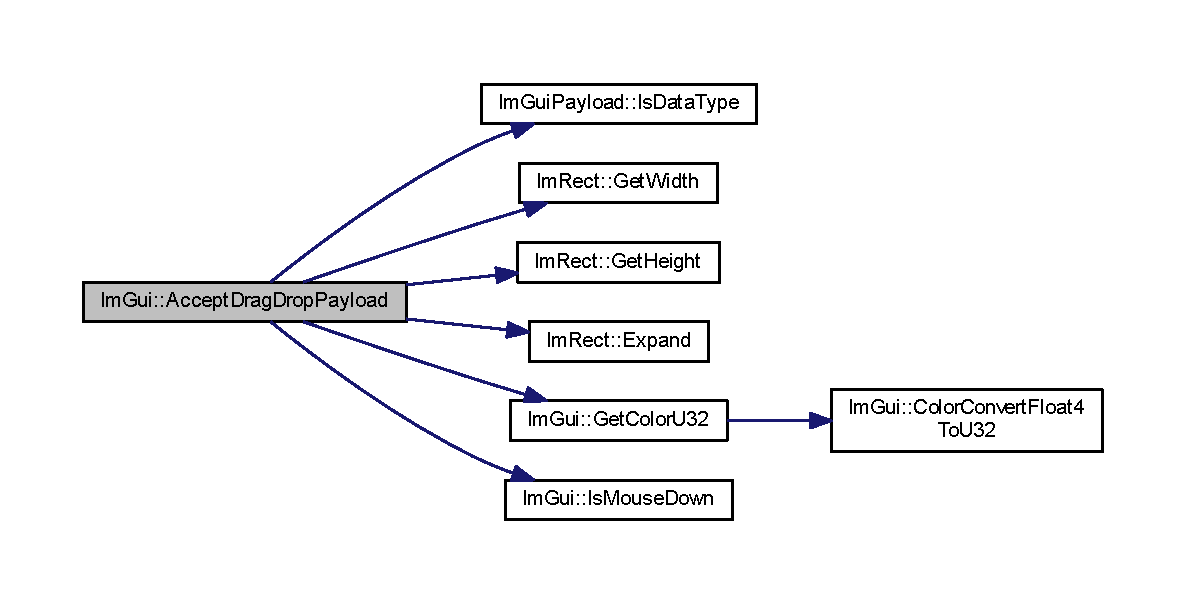
\includegraphics[width=350pt]{namespace_im_gui_a5e0dac39e249bf50e2ae96dc4a97cb18_cgraph}
\end{center}
\end{figure}
\mbox{\Hypertarget{namespace_im_gui_ac56279417745ae5680a7ae5b00a2a60f}\label{namespace_im_gui_ac56279417745ae5680a7ae5b00a2a60f}} 
\index{Im\+Gui@{Im\+Gui}!Activate\+Item@{Activate\+Item}}
\index{Activate\+Item@{Activate\+Item}!Im\+Gui@{Im\+Gui}}
\subsubsection{\texorpdfstring{Activate\+Item()}{ActivateItem()}}
{\footnotesize\ttfamily void Im\+Gui\+::\+Activate\+Item (\begin{DoxyParamCaption}\item[{\mbox{\hyperlink{imgui_8h_a1785c9b6f4e16406764a85f32582236f}{Im\+Gui\+ID}}}]{id }\end{DoxyParamCaption})}

\mbox{\Hypertarget{namespace_im_gui_ae14be3a3bec106de7c91aaa2a9a558a1}\label{namespace_im_gui_ae14be3a3bec106de7c91aaa2a9a558a1}} 
\index{Im\+Gui@{Im\+Gui}!Align\+Text\+To\+Frame\+Padding@{Align\+Text\+To\+Frame\+Padding}}
\index{Align\+Text\+To\+Frame\+Padding@{Align\+Text\+To\+Frame\+Padding}!Im\+Gui@{Im\+Gui}}
\subsubsection{\texorpdfstring{Align\+Text\+To\+Frame\+Padding()}{AlignTextToFramePadding()}}
{\footnotesize\ttfamily void Im\+Gui\+::\+Align\+Text\+To\+Frame\+Padding (\begin{DoxyParamCaption}{ }\end{DoxyParamCaption})}

Here is the call graph for this function\+:
\nopagebreak
\begin{figure}[H]
\begin{center}
\leavevmode
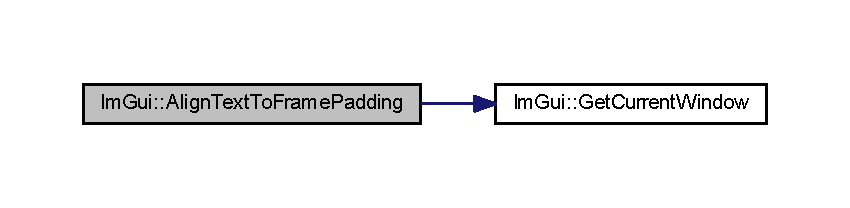
\includegraphics[width=350pt]{namespace_im_gui_ae14be3a3bec106de7c91aaa2a9a558a1_cgraph}
\end{center}
\end{figure}
\mbox{\Hypertarget{namespace_im_gui_ad2bc397a02d5e4b8a14360d89abc6242}\label{namespace_im_gui_ad2bc397a02d5e4b8a14360d89abc6242}} 
\index{Im\+Gui@{Im\+Gui}!Arrow\+Button@{Arrow\+Button}}
\index{Arrow\+Button@{Arrow\+Button}!Im\+Gui@{Im\+Gui}}
\subsubsection{\texorpdfstring{Arrow\+Button()}{ArrowButton()}}
{\footnotesize\ttfamily bool Im\+Gui\+::\+Arrow\+Button (\begin{DoxyParamCaption}\item[{const char $\ast$}]{str\+\_\+id,  }\item[{\mbox{\hyperlink{imgui_8h_a874086389bc27cc9647118d22a806403}{Im\+Gui\+Dir}}}]{dir }\end{DoxyParamCaption})}

Here is the call graph for this function\+:
\nopagebreak
\begin{figure}[H]
\begin{center}
\leavevmode
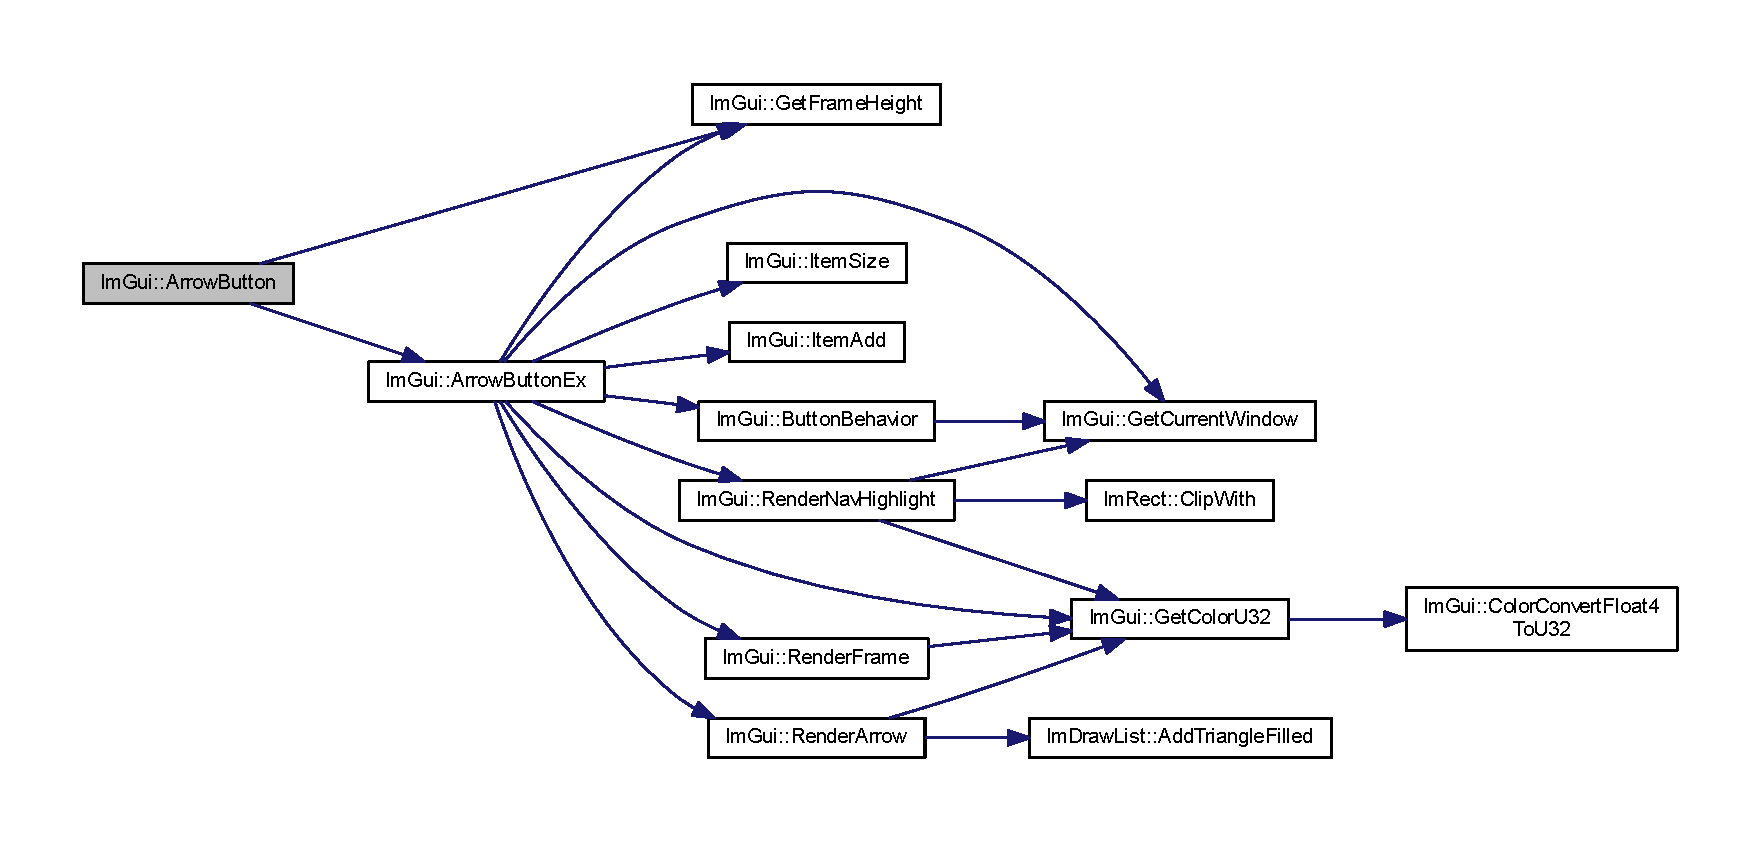
\includegraphics[width=350pt]{namespace_im_gui_ad2bc397a02d5e4b8a14360d89abc6242_cgraph}
\end{center}
\end{figure}
\mbox{\Hypertarget{namespace_im_gui_af8efa3144c85104fbb0aa2e7bc6a6069}\label{namespace_im_gui_af8efa3144c85104fbb0aa2e7bc6a6069}} 
\index{Im\+Gui@{Im\+Gui}!Arrow\+Button\+Ex@{Arrow\+Button\+Ex}}
\index{Arrow\+Button\+Ex@{Arrow\+Button\+Ex}!Im\+Gui@{Im\+Gui}}
\subsubsection{\texorpdfstring{Arrow\+Button\+Ex()}{ArrowButtonEx()}}
{\footnotesize\ttfamily bool Im\+Gui\+::\+Arrow\+Button\+Ex (\begin{DoxyParamCaption}\item[{const char $\ast$}]{str\+\_\+id,  }\item[{\mbox{\hyperlink{imgui_8h_a874086389bc27cc9647118d22a806403}{Im\+Gui\+Dir}}}]{dir,  }\item[{\mbox{\hyperlink{struct_im_vec2}{Im\+Vec2}}}]{size\+\_\+arg,  }\item[{\mbox{\hyperlink{imgui__internal_8h_a990fae518aa1d95f571ee40989de4c22}{Im\+Gui\+Button\+Flags}}}]{flags }\end{DoxyParamCaption})}

Here is the call graph for this function\+:
\nopagebreak
\begin{figure}[H]
\begin{center}
\leavevmode
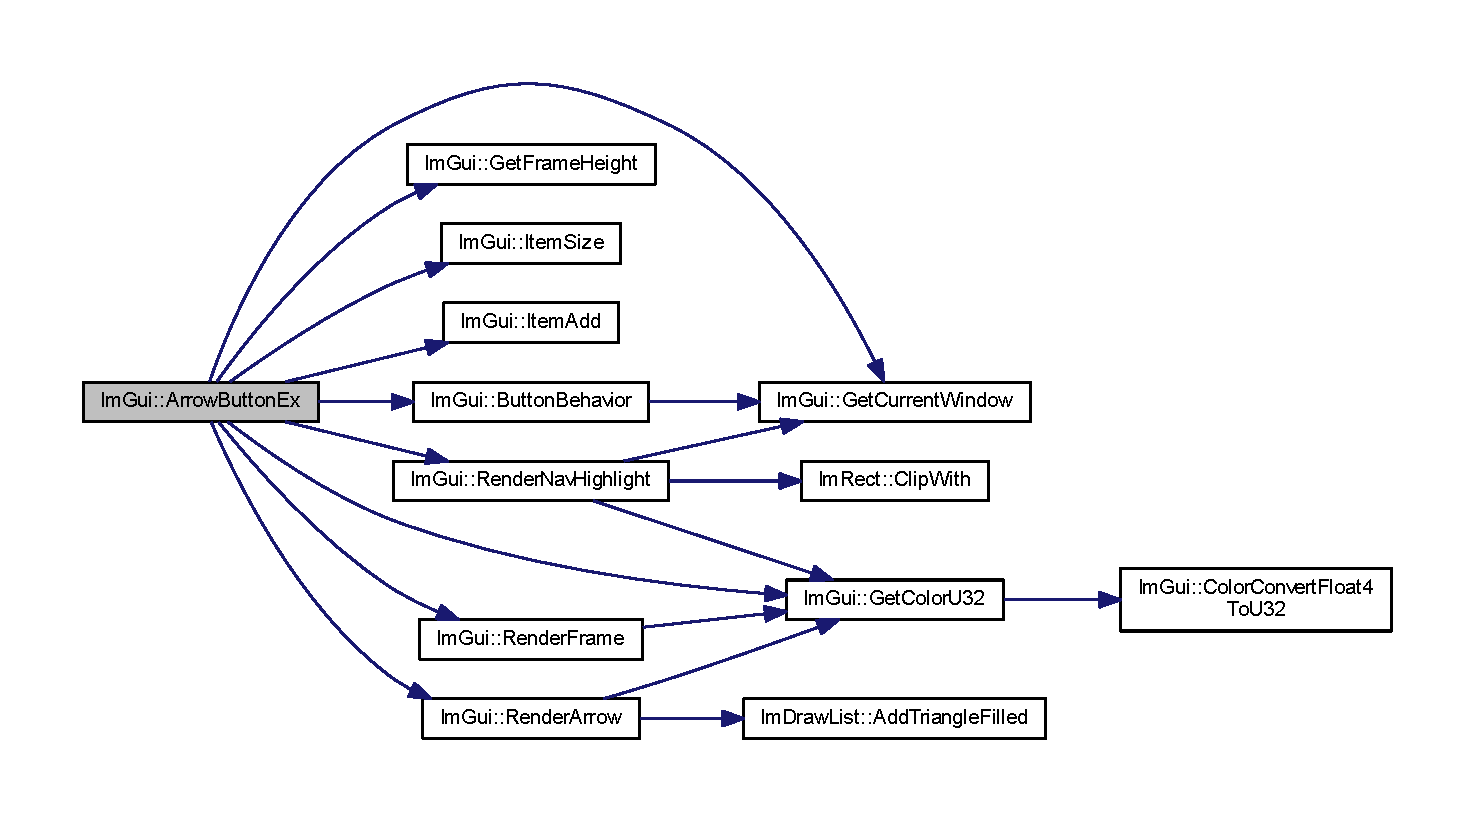
\includegraphics[width=350pt]{namespace_im_gui_af8efa3144c85104fbb0aa2e7bc6a6069_cgraph}
\end{center}
\end{figure}
Here is the caller graph for this function\+:
\nopagebreak
\begin{figure}[H]
\begin{center}
\leavevmode
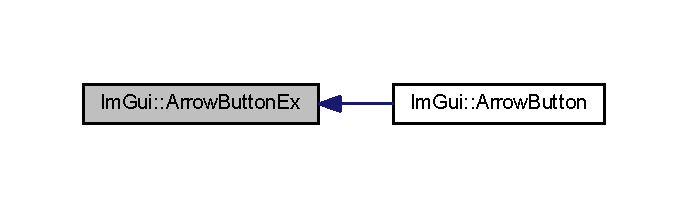
\includegraphics[width=330pt]{namespace_im_gui_af8efa3144c85104fbb0aa2e7bc6a6069_icgraph}
\end{center}
\end{figure}
\mbox{\Hypertarget{namespace_im_gui_a581e58db0bc930bafa4a5d23093a2b99}\label{namespace_im_gui_a581e58db0bc930bafa4a5d23093a2b99}} 
\index{Im\+Gui@{Im\+Gui}!Begin@{Begin}}
\index{Begin@{Begin}!Im\+Gui@{Im\+Gui}}
\subsubsection{\texorpdfstring{Begin()}{Begin()}\hspace{0.1cm}{\footnotesize\ttfamily [1/2]}}
{\footnotesize\ttfamily bool Im\+Gui\+::\+Begin (\begin{DoxyParamCaption}\item[{const char $\ast$}]{name,  }\item[{bool $\ast$}]{p\+\_\+open = {\ttfamily NULL},  }\item[{\mbox{\hyperlink{imgui_8h_a0b8e067ab4f7a818828c8d89e531addc}{Im\+Gui\+Window\+Flags}}}]{flags = {\ttfamily 0} }\end{DoxyParamCaption})}

Here is the call graph for this function\+:
\nopagebreak
\begin{figure}[H]
\begin{center}
\leavevmode
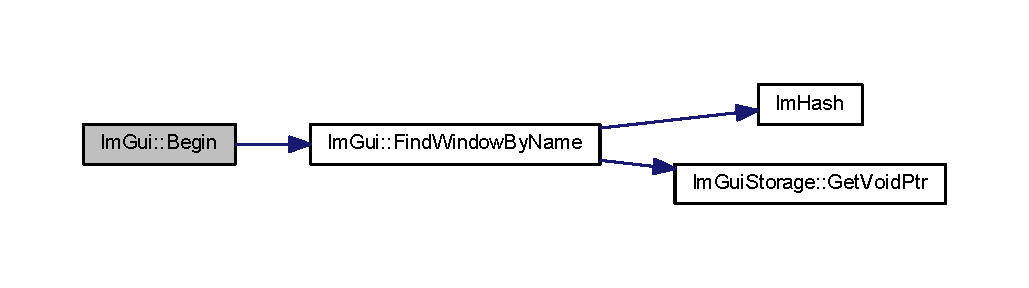
\includegraphics[width=350pt]{namespace_im_gui_a581e58db0bc930bafa4a5d23093a2b99_cgraph}
\end{center}
\end{figure}
Here is the caller graph for this function\+:
\nopagebreak
\begin{figure}[H]
\begin{center}
\leavevmode
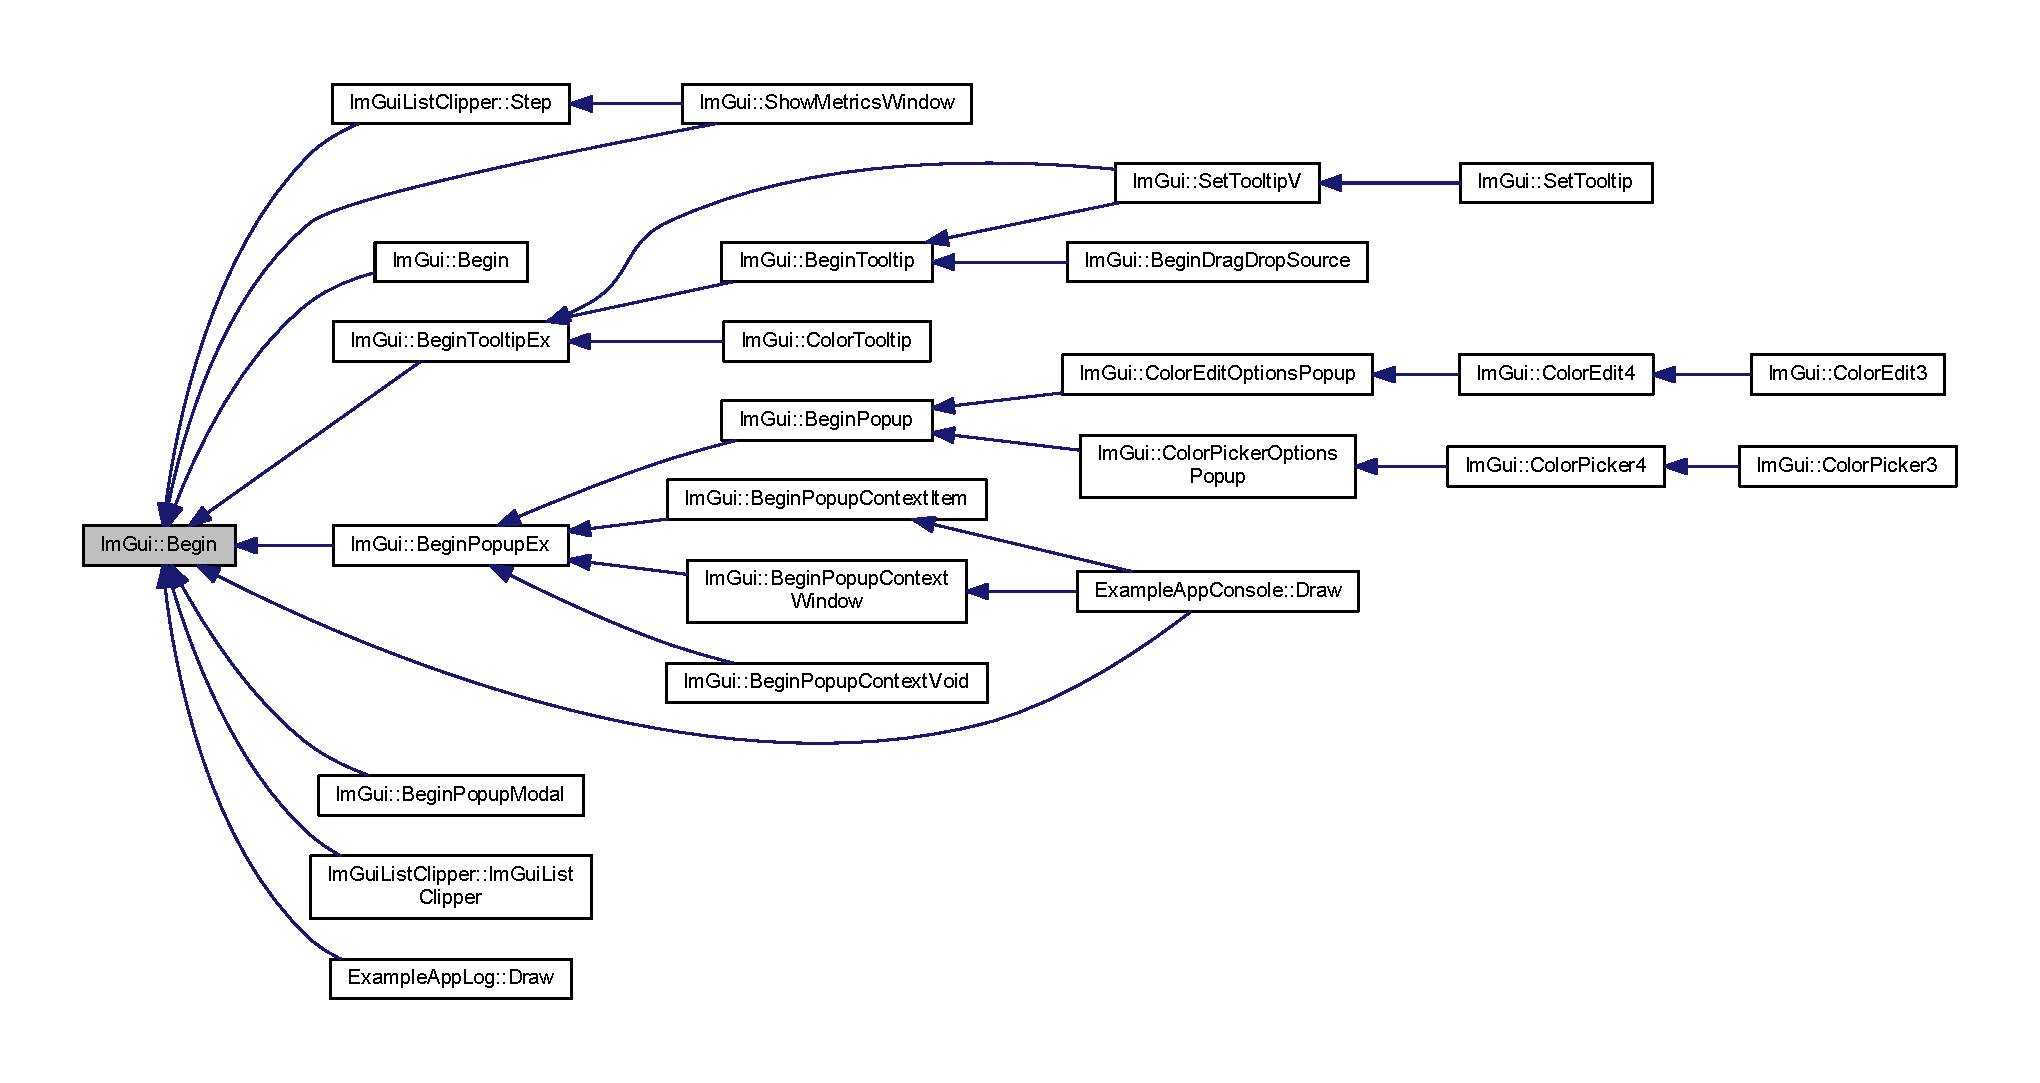
\includegraphics[width=350pt]{namespace_im_gui_a581e58db0bc930bafa4a5d23093a2b99_icgraph}
\end{center}
\end{figure}
\mbox{\Hypertarget{namespace_im_gui_a288e01ff1c8102d6374a6b1e409b9878}\label{namespace_im_gui_a288e01ff1c8102d6374a6b1e409b9878}} 
\index{Im\+Gui@{Im\+Gui}!Begin@{Begin}}
\index{Begin@{Begin}!Im\+Gui@{Im\+Gui}}
\subsubsection{\texorpdfstring{Begin()}{Begin()}\hspace{0.1cm}{\footnotesize\ttfamily [2/2]}}
{\footnotesize\ttfamily bool Im\+Gui\+::\+Begin (\begin{DoxyParamCaption}\item[{const char $\ast$}]{name,  }\item[{bool $\ast$}]{p\+\_\+open,  }\item[{const \mbox{\hyperlink{struct_im_vec2}{Im\+Vec2}} \&}]{size\+\_\+on\+\_\+first\+\_\+use,  }\item[{float}]{bg\+\_\+alpha\+\_\+override = {\ttfamily -\/1.0f},  }\item[{\mbox{\hyperlink{imgui_8h_a0b8e067ab4f7a818828c8d89e531addc}{Im\+Gui\+Window\+Flags}}}]{flags = {\ttfamily 0} }\end{DoxyParamCaption})}

Here is the call graph for this function\+:
\nopagebreak
\begin{figure}[H]
\begin{center}
\leavevmode
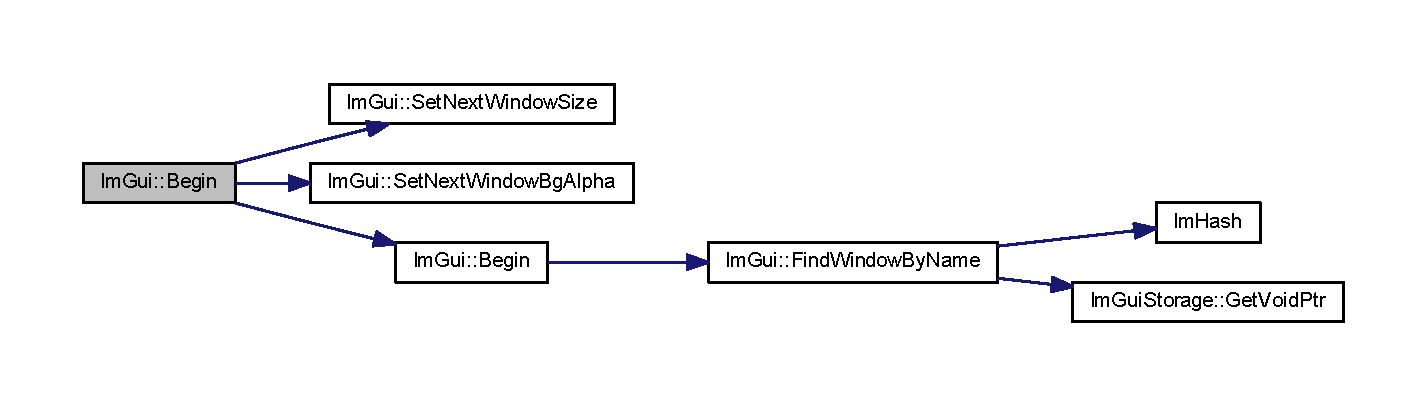
\includegraphics[width=350pt]{namespace_im_gui_a288e01ff1c8102d6374a6b1e409b9878_cgraph}
\end{center}
\end{figure}
\mbox{\Hypertarget{namespace_im_gui_a5db08f552118a1f946e19b5933dce181}\label{namespace_im_gui_a5db08f552118a1f946e19b5933dce181}} 
\index{Im\+Gui@{Im\+Gui}!Begin\+Child@{Begin\+Child}}
\index{Begin\+Child@{Begin\+Child}!Im\+Gui@{Im\+Gui}}
\subsubsection{\texorpdfstring{Begin\+Child()}{BeginChild()}\hspace{0.1cm}{\footnotesize\ttfamily [1/2]}}
{\footnotesize\ttfamily bool Im\+Gui\+::\+Begin\+Child (\begin{DoxyParamCaption}\item[{const char $\ast$}]{str\+\_\+id,  }\item[{const \mbox{\hyperlink{struct_im_vec2}{Im\+Vec2}} \&}]{size = {\ttfamily \mbox{\hyperlink{struct_im_vec2}{Im\+Vec2}}(0,0)},  }\item[{bool}]{border = {\ttfamily false},  }\item[{\mbox{\hyperlink{imgui_8h_a0b8e067ab4f7a818828c8d89e531addc}{Im\+Gui\+Window\+Flags}}}]{flags = {\ttfamily 0} }\end{DoxyParamCaption})}

Here is the call graph for this function\+:
\nopagebreak
\begin{figure}[H]
\begin{center}
\leavevmode
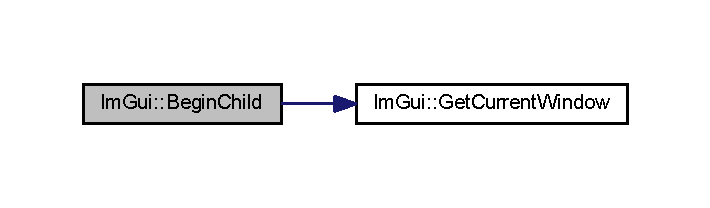
\includegraphics[width=341pt]{namespace_im_gui_a5db08f552118a1f946e19b5933dce181_cgraph}
\end{center}
\end{figure}
Here is the caller graph for this function\+:
\nopagebreak
\begin{figure}[H]
\begin{center}
\leavevmode
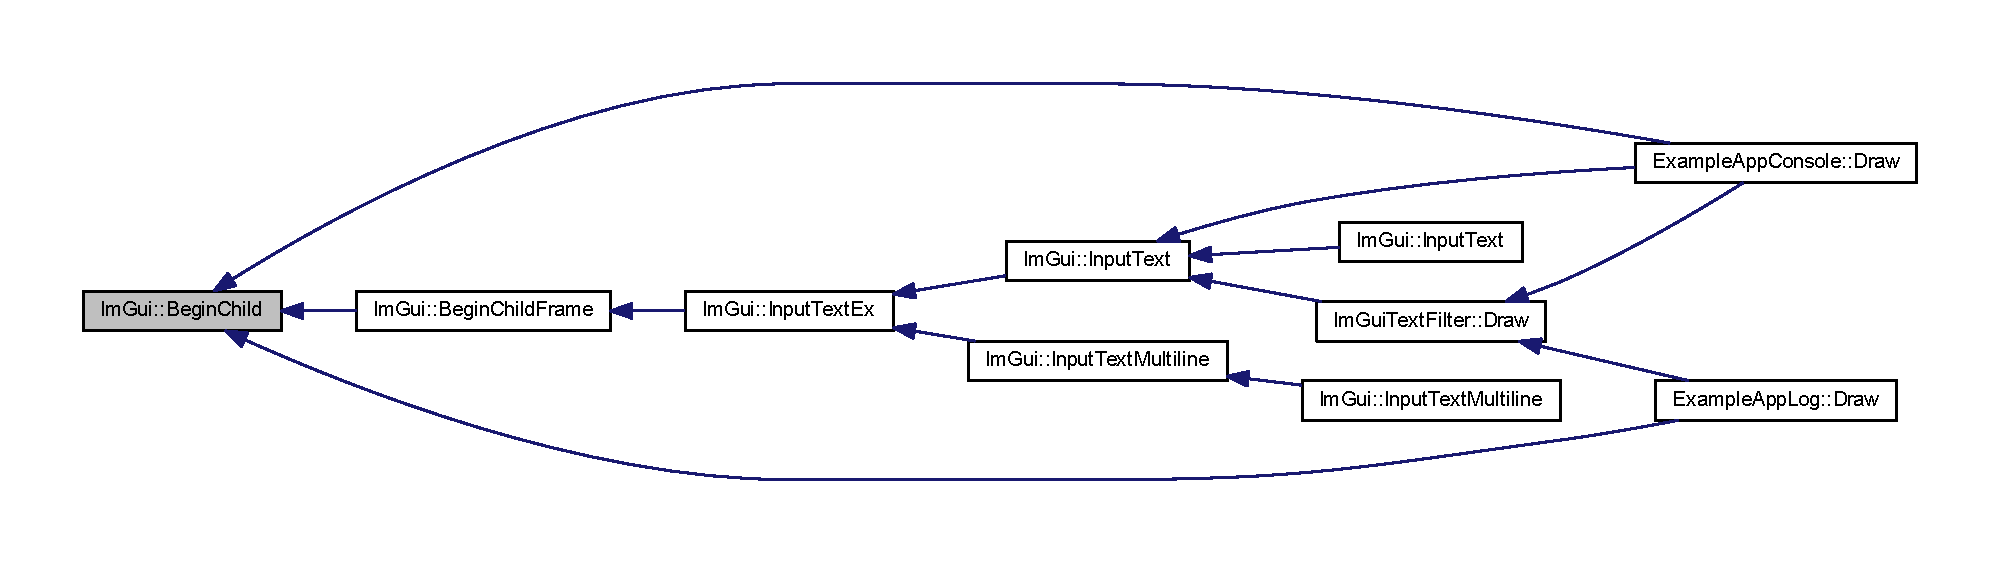
\includegraphics[width=350pt]{namespace_im_gui_a5db08f552118a1f946e19b5933dce181_icgraph}
\end{center}
\end{figure}
\mbox{\Hypertarget{namespace_im_gui_a7001666723434ae00316b8a0160e7de0}\label{namespace_im_gui_a7001666723434ae00316b8a0160e7de0}} 
\index{Im\+Gui@{Im\+Gui}!Begin\+Child@{Begin\+Child}}
\index{Begin\+Child@{Begin\+Child}!Im\+Gui@{Im\+Gui}}
\subsubsection{\texorpdfstring{Begin\+Child()}{BeginChild()}\hspace{0.1cm}{\footnotesize\ttfamily [2/2]}}
{\footnotesize\ttfamily bool Im\+Gui\+::\+Begin\+Child (\begin{DoxyParamCaption}\item[{\mbox{\hyperlink{imgui_8h_a1785c9b6f4e16406764a85f32582236f}{Im\+Gui\+ID}}}]{id,  }\item[{const \mbox{\hyperlink{struct_im_vec2}{Im\+Vec2}} \&}]{size = {\ttfamily \mbox{\hyperlink{struct_im_vec2}{Im\+Vec2}}(0,0)},  }\item[{bool}]{border = {\ttfamily false},  }\item[{\mbox{\hyperlink{imgui_8h_a0b8e067ab4f7a818828c8d89e531addc}{Im\+Gui\+Window\+Flags}}}]{flags = {\ttfamily 0} }\end{DoxyParamCaption})}

\mbox{\Hypertarget{namespace_im_gui_a0565e1ef69c897b1f30f37f95dd787f1}\label{namespace_im_gui_a0565e1ef69c897b1f30f37f95dd787f1}} 
\index{Im\+Gui@{Im\+Gui}!Begin\+Child\+Frame@{Begin\+Child\+Frame}}
\index{Begin\+Child\+Frame@{Begin\+Child\+Frame}!Im\+Gui@{Im\+Gui}}
\subsubsection{\texorpdfstring{Begin\+Child\+Frame()}{BeginChildFrame()}}
{\footnotesize\ttfamily bool Im\+Gui\+::\+Begin\+Child\+Frame (\begin{DoxyParamCaption}\item[{\mbox{\hyperlink{imgui_8h_a1785c9b6f4e16406764a85f32582236f}{Im\+Gui\+ID}}}]{id,  }\item[{const \mbox{\hyperlink{struct_im_vec2}{Im\+Vec2}} \&}]{size,  }\item[{\mbox{\hyperlink{imgui_8h_a0b8e067ab4f7a818828c8d89e531addc}{Im\+Gui\+Window\+Flags}}}]{flags = {\ttfamily 0} }\end{DoxyParamCaption})}

Here is the call graph for this function\+:
\nopagebreak
\begin{figure}[H]
\begin{center}
\leavevmode
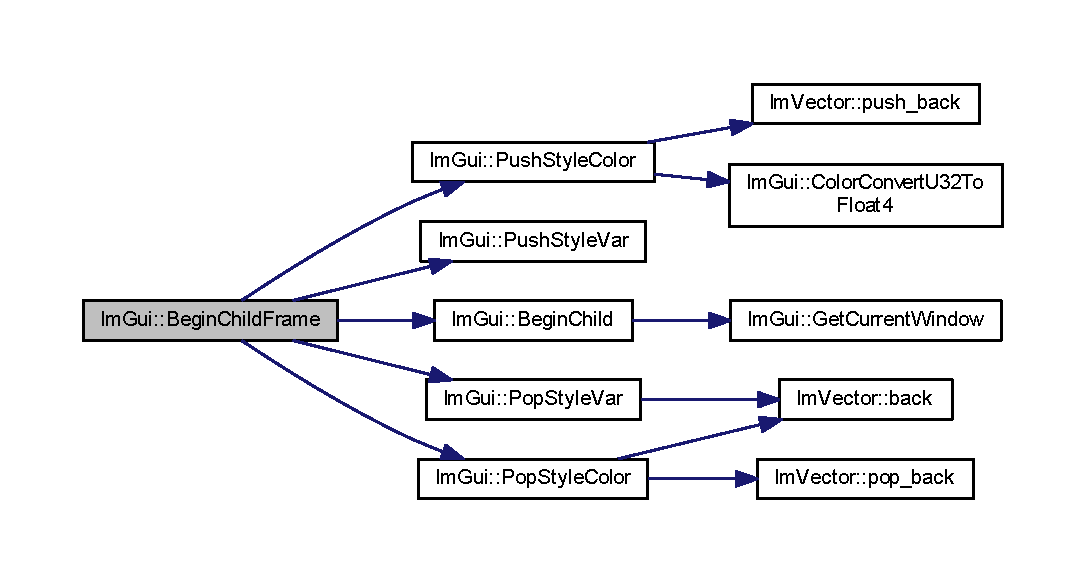
\includegraphics[width=350pt]{namespace_im_gui_a0565e1ef69c897b1f30f37f95dd787f1_cgraph}
\end{center}
\end{figure}
Here is the caller graph for this function\+:
\nopagebreak
\begin{figure}[H]
\begin{center}
\leavevmode
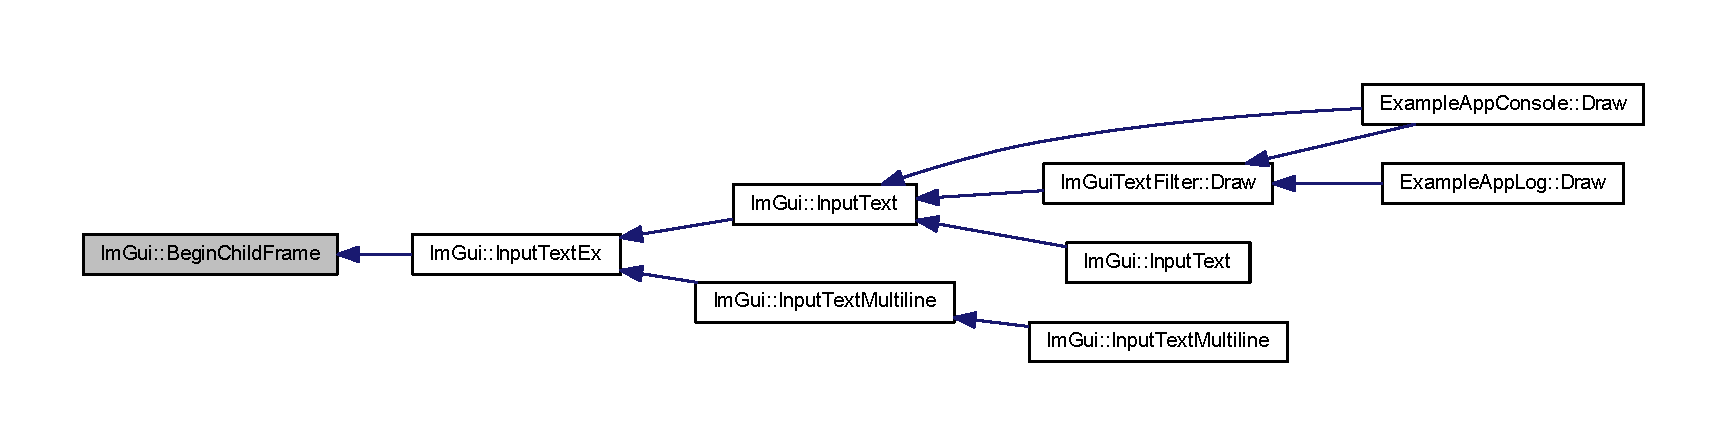
\includegraphics[width=350pt]{namespace_im_gui_a0565e1ef69c897b1f30f37f95dd787f1_icgraph}
\end{center}
\end{figure}
\mbox{\Hypertarget{namespace_im_gui_a6992289cbdb087a690403e48340bfb23}\label{namespace_im_gui_a6992289cbdb087a690403e48340bfb23}} 
\index{Im\+Gui@{Im\+Gui}!Begin\+Columns@{Begin\+Columns}}
\index{Begin\+Columns@{Begin\+Columns}!Im\+Gui@{Im\+Gui}}
\subsubsection{\texorpdfstring{Begin\+Columns()}{BeginColumns()}}
{\footnotesize\ttfamily void Im\+Gui\+::\+Begin\+Columns (\begin{DoxyParamCaption}\item[{const char $\ast$}]{str\+\_\+id,  }\item[{int}]{count,  }\item[{\mbox{\hyperlink{imgui_8h_a0edb3053546fcf6c5f7dcb7531c3a17a}{Im\+Gui\+Columns\+Flags}}}]{flags = {\ttfamily 0} }\end{DoxyParamCaption})}

Here is the call graph for this function\+:
\nopagebreak
\begin{figure}[H]
\begin{center}
\leavevmode
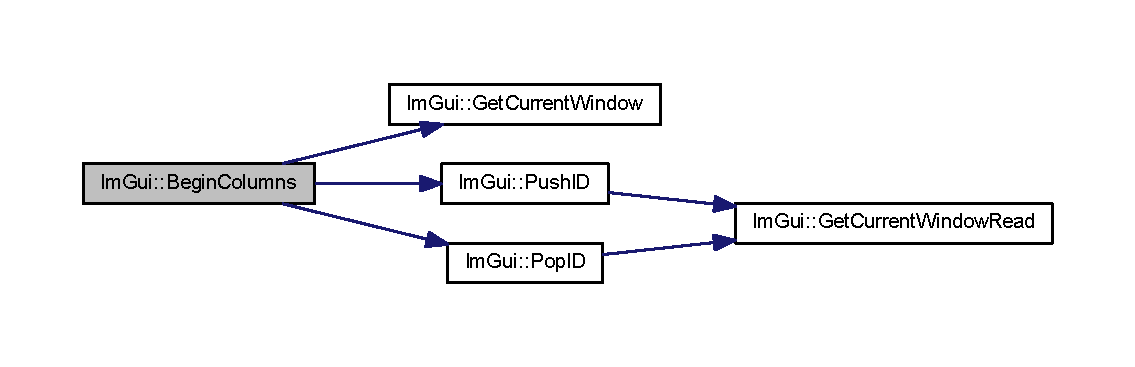
\includegraphics[width=350pt]{namespace_im_gui_a6992289cbdb087a690403e48340bfb23_cgraph}
\end{center}
\end{figure}
Here is the caller graph for this function\+:
\nopagebreak
\begin{figure}[H]
\begin{center}
\leavevmode
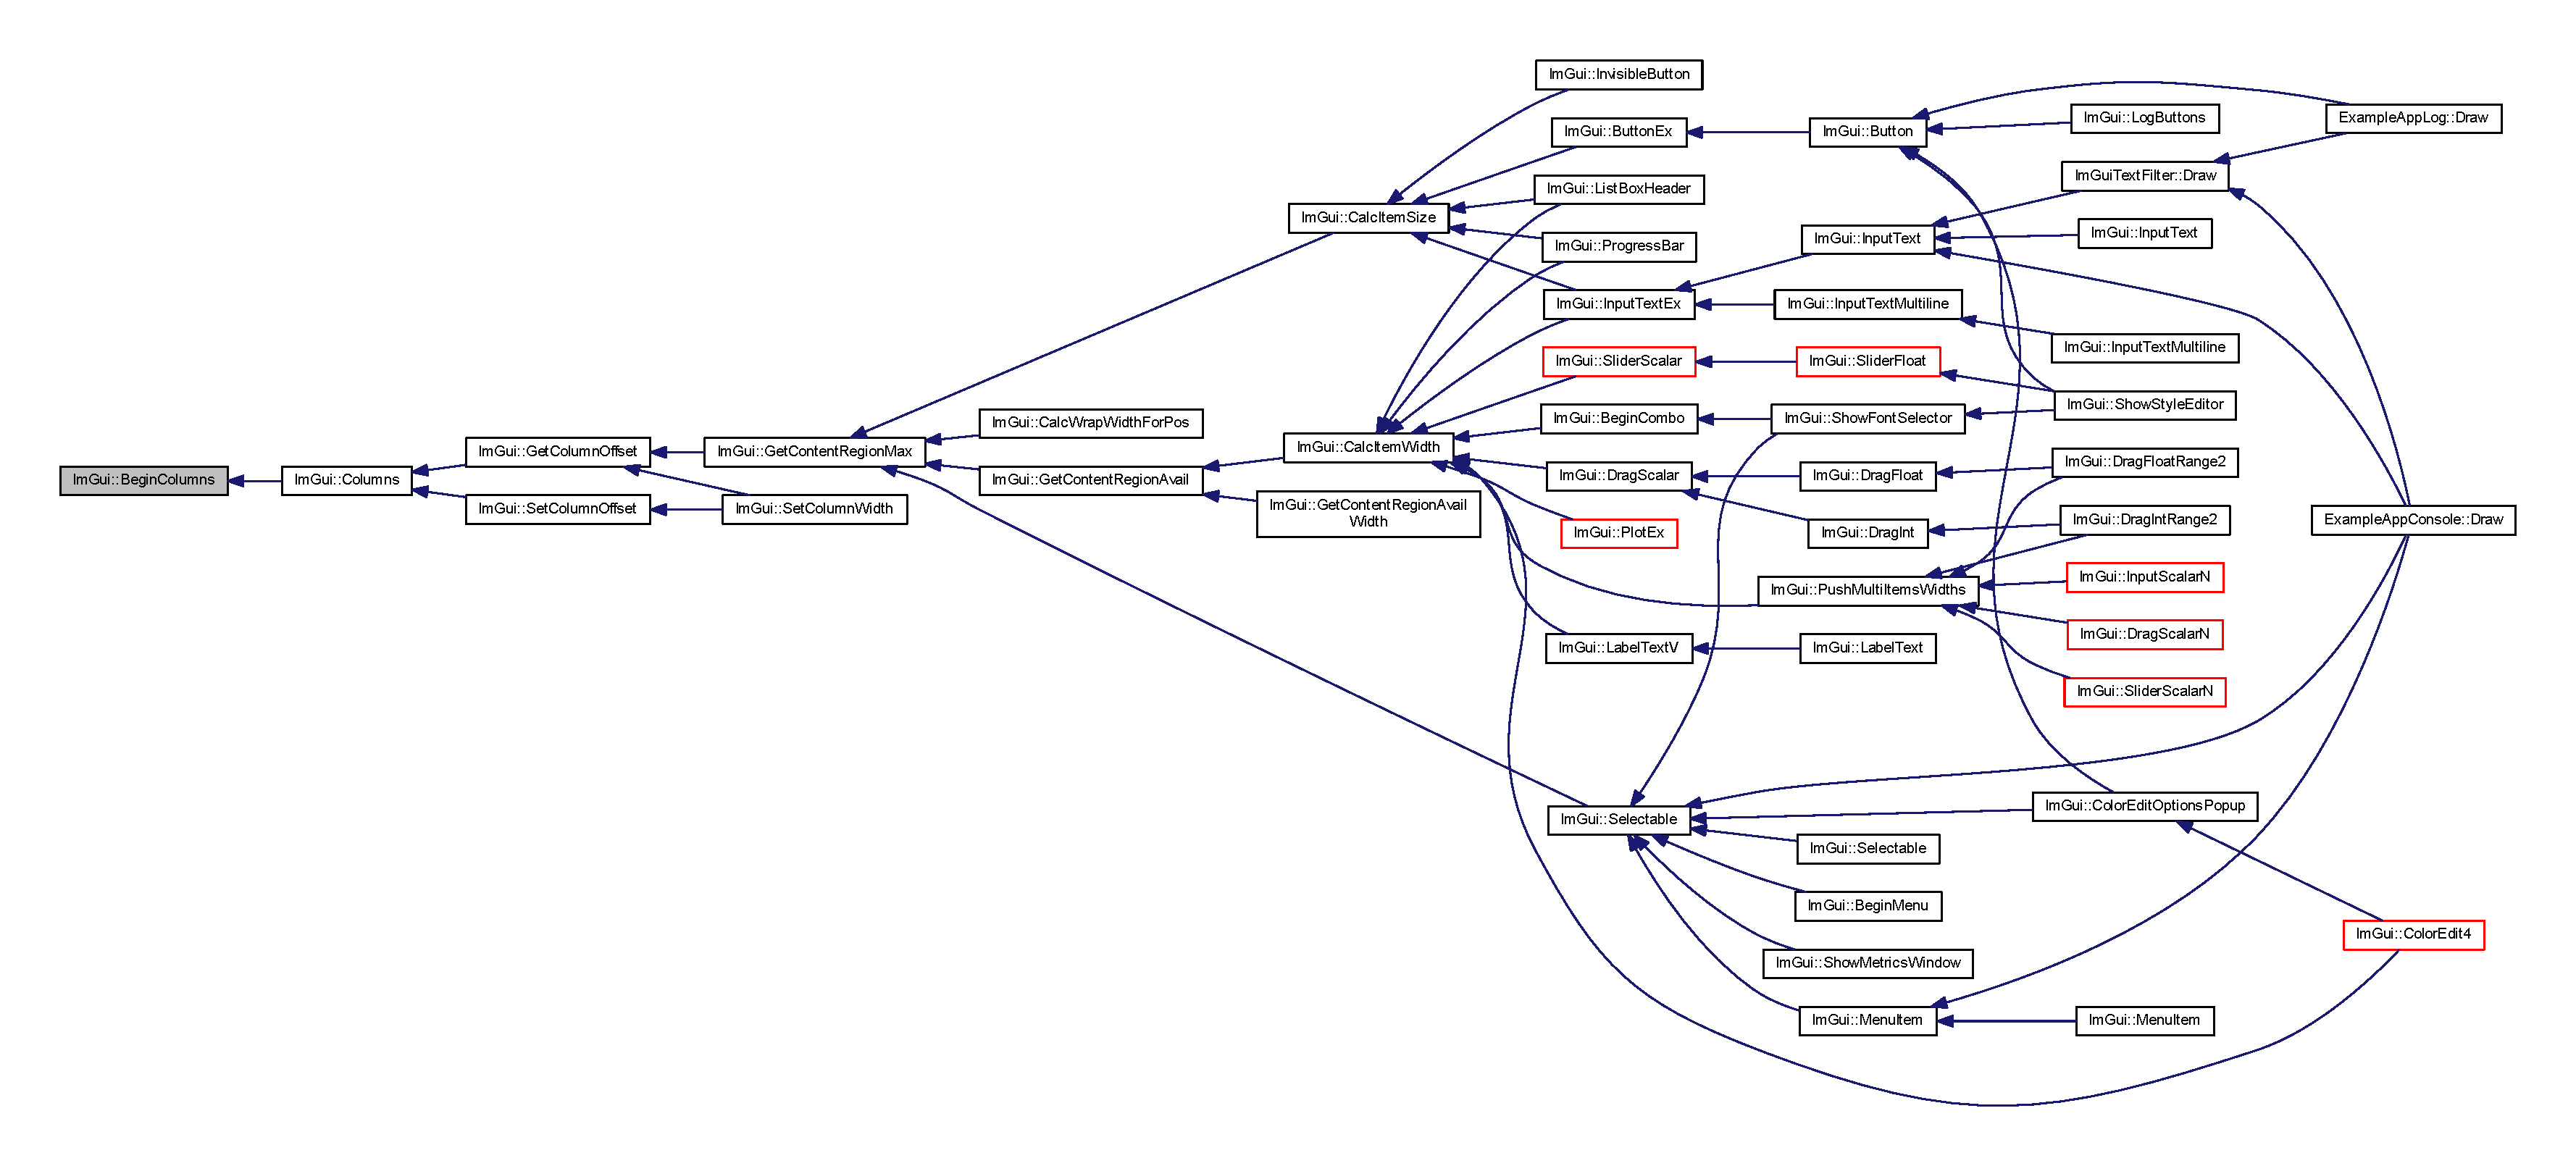
\includegraphics[width=350pt]{namespace_im_gui_a6992289cbdb087a690403e48340bfb23_icgraph}
\end{center}
\end{figure}
\mbox{\Hypertarget{namespace_im_gui_aa895095bdc7a2907375c555e245575ea}\label{namespace_im_gui_aa895095bdc7a2907375c555e245575ea}} 
\index{Im\+Gui@{Im\+Gui}!Begin\+Combo@{Begin\+Combo}}
\index{Begin\+Combo@{Begin\+Combo}!Im\+Gui@{Im\+Gui}}
\subsubsection{\texorpdfstring{Begin\+Combo()}{BeginCombo()}}
{\footnotesize\ttfamily bool Im\+Gui\+::\+Begin\+Combo (\begin{DoxyParamCaption}\item[{const char $\ast$}]{label,  }\item[{const char $\ast$}]{preview\+\_\+value,  }\item[{\mbox{\hyperlink{imgui_8h_aae31d1cfbcc55ae20b4122a7149d435e}{Im\+Gui\+Combo\+Flags}}}]{flags = {\ttfamily 0} }\end{DoxyParamCaption})}

Here is the call graph for this function\+:
\nopagebreak
\begin{figure}[H]
\begin{center}
\leavevmode
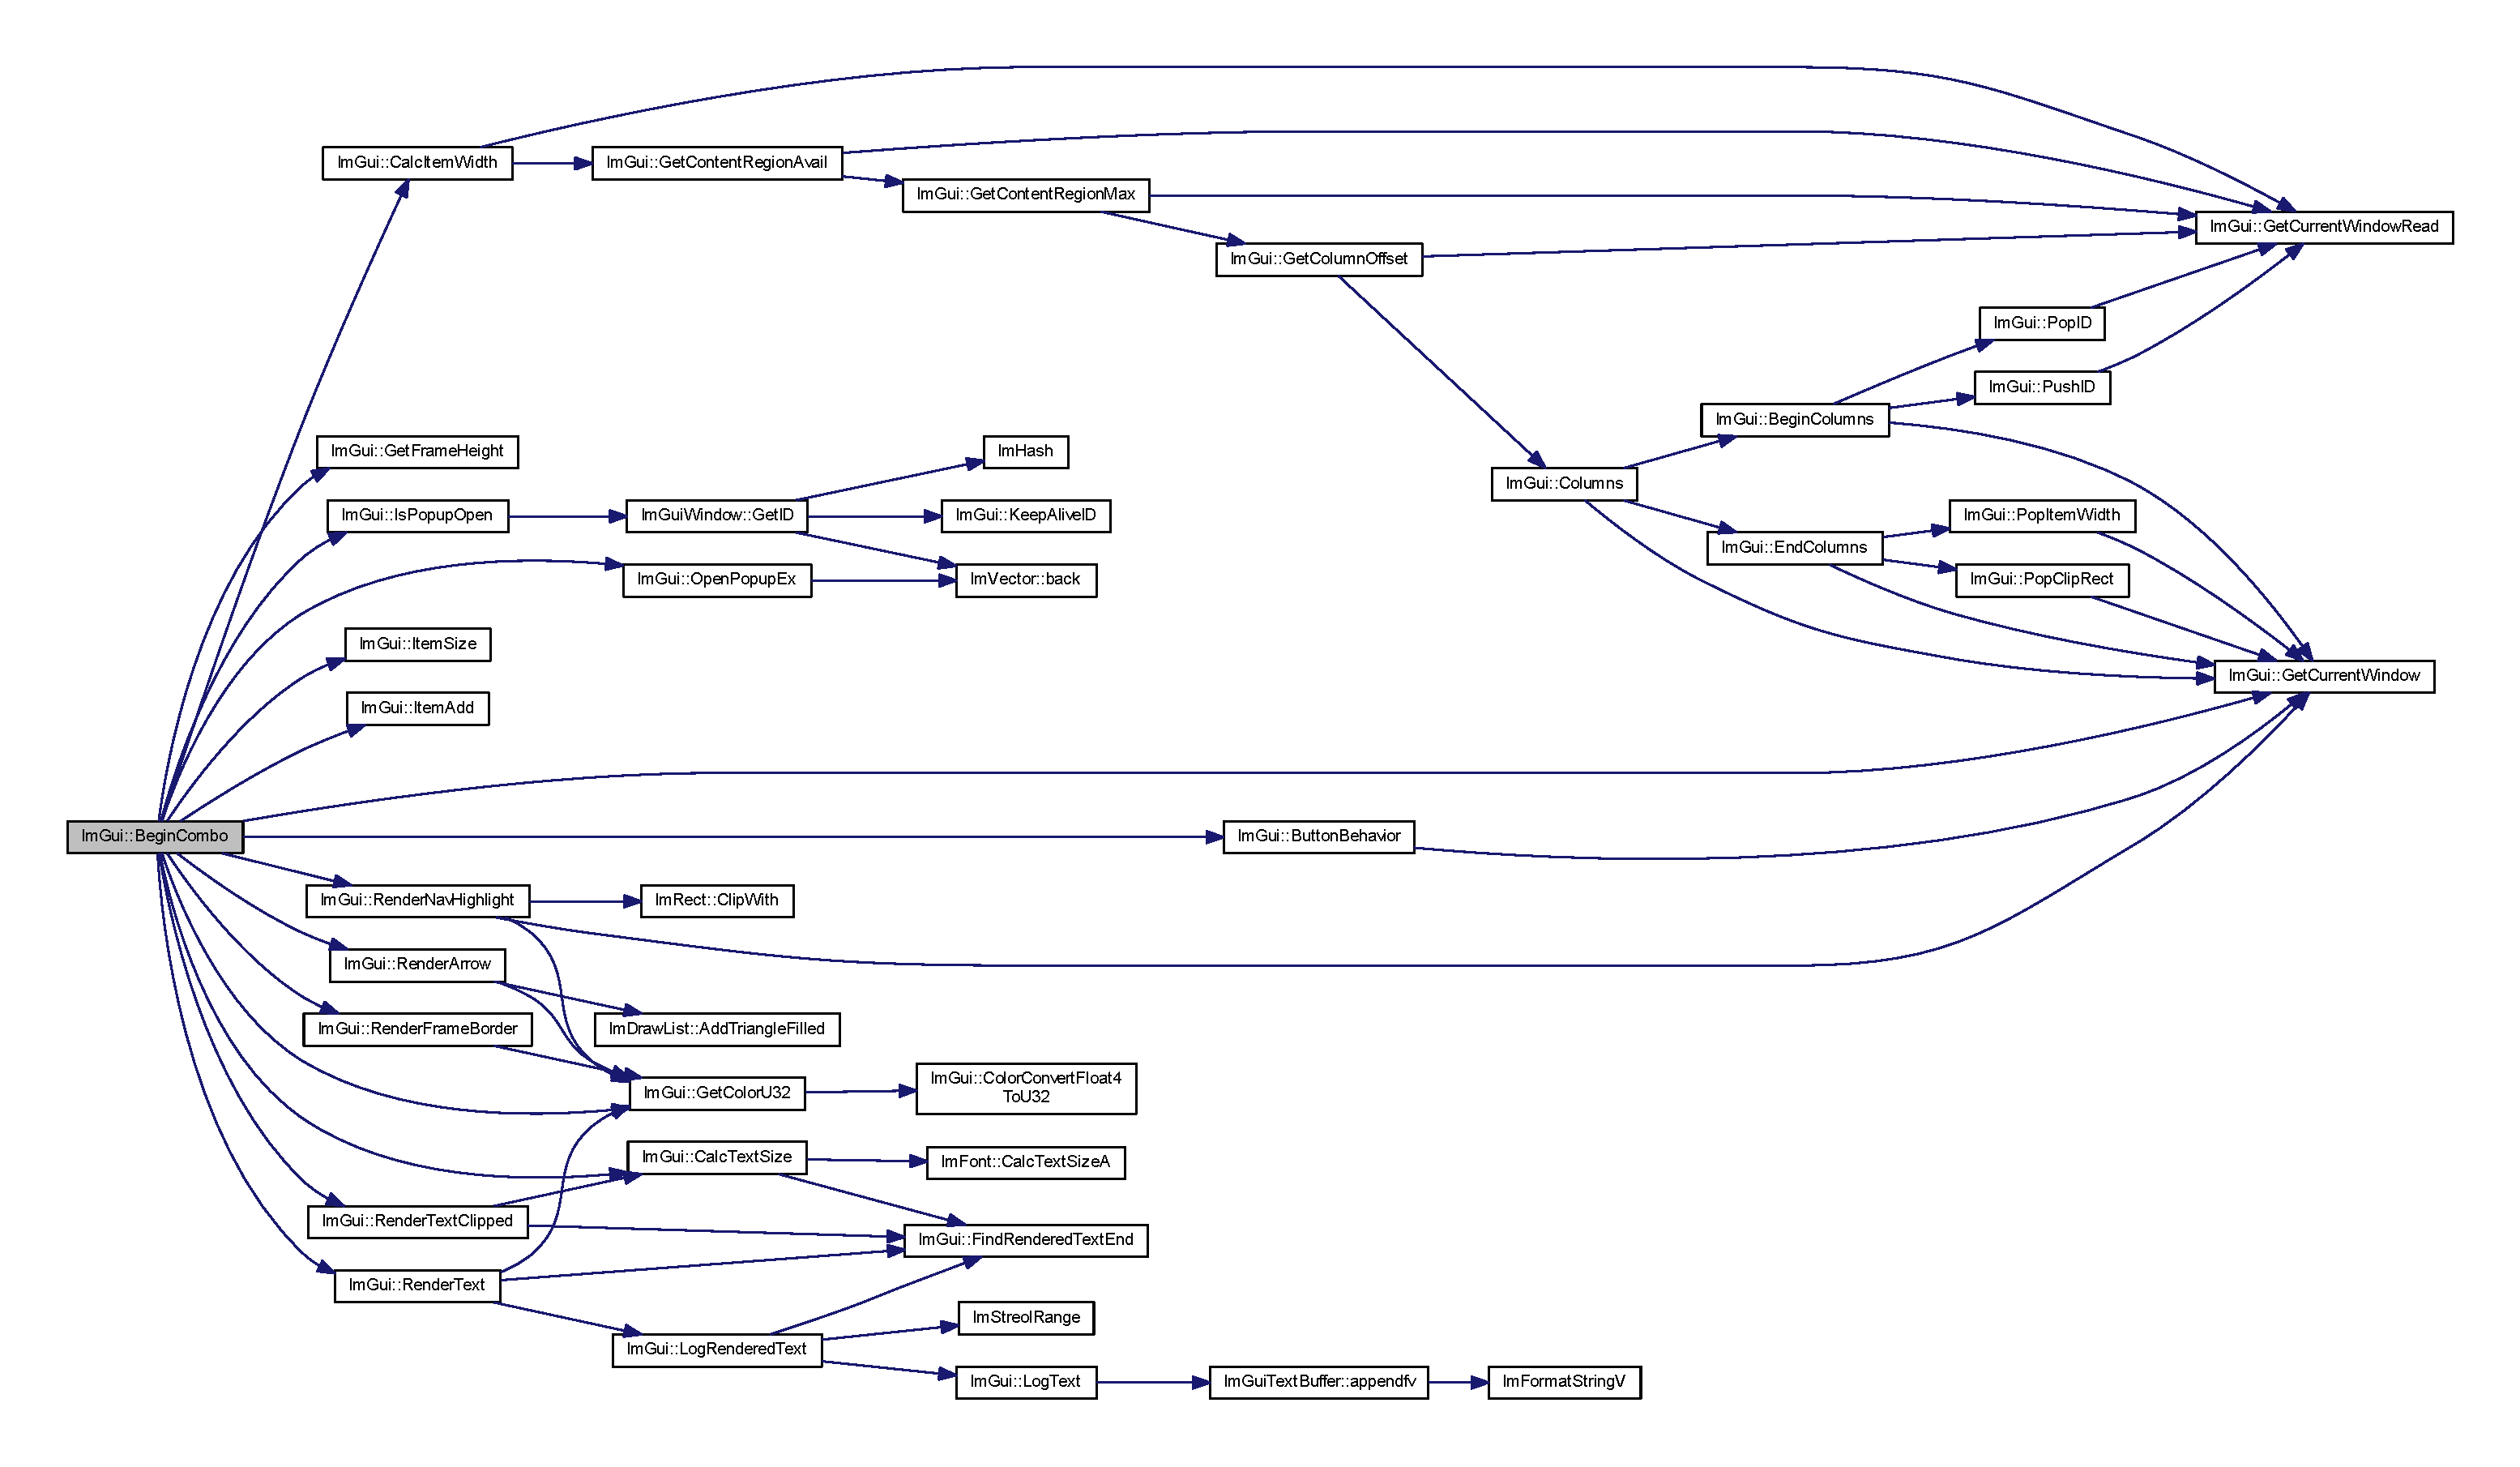
\includegraphics[width=350pt]{namespace_im_gui_aa895095bdc7a2907375c555e245575ea_cgraph}
\end{center}
\end{figure}
Here is the caller graph for this function\+:
\nopagebreak
\begin{figure}[H]
\begin{center}
\leavevmode
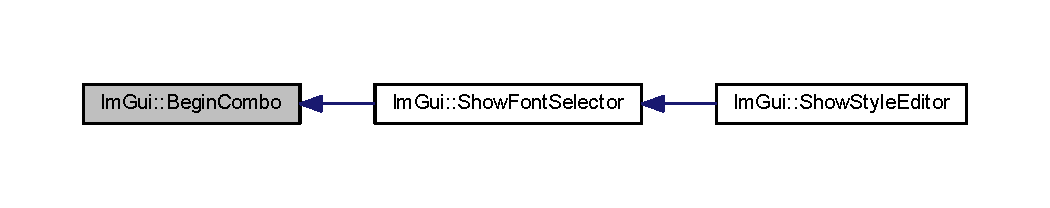
\includegraphics[width=350pt]{namespace_im_gui_aa895095bdc7a2907375c555e245575ea_icgraph}
\end{center}
\end{figure}
\mbox{\Hypertarget{namespace_im_gui_ac2609b0f034d3bcd8d70d26df8694eaa}\label{namespace_im_gui_ac2609b0f034d3bcd8d70d26df8694eaa}} 
\index{Im\+Gui@{Im\+Gui}!Begin\+Drag\+Drop\+Source@{Begin\+Drag\+Drop\+Source}}
\index{Begin\+Drag\+Drop\+Source@{Begin\+Drag\+Drop\+Source}!Im\+Gui@{Im\+Gui}}
\subsubsection{\texorpdfstring{Begin\+Drag\+Drop\+Source()}{BeginDragDropSource()}}
{\footnotesize\ttfamily bool Im\+Gui\+::\+Begin\+Drag\+Drop\+Source (\begin{DoxyParamCaption}\item[{\mbox{\hyperlink{imgui_8h_a4e54f95ded29d2584125d116df22e430}{Im\+Gui\+Drag\+Drop\+Flags}}}]{flags = {\ttfamily 0} }\end{DoxyParamCaption})}

Here is the call graph for this function\+:
\nopagebreak
\begin{figure}[H]
\begin{center}
\leavevmode
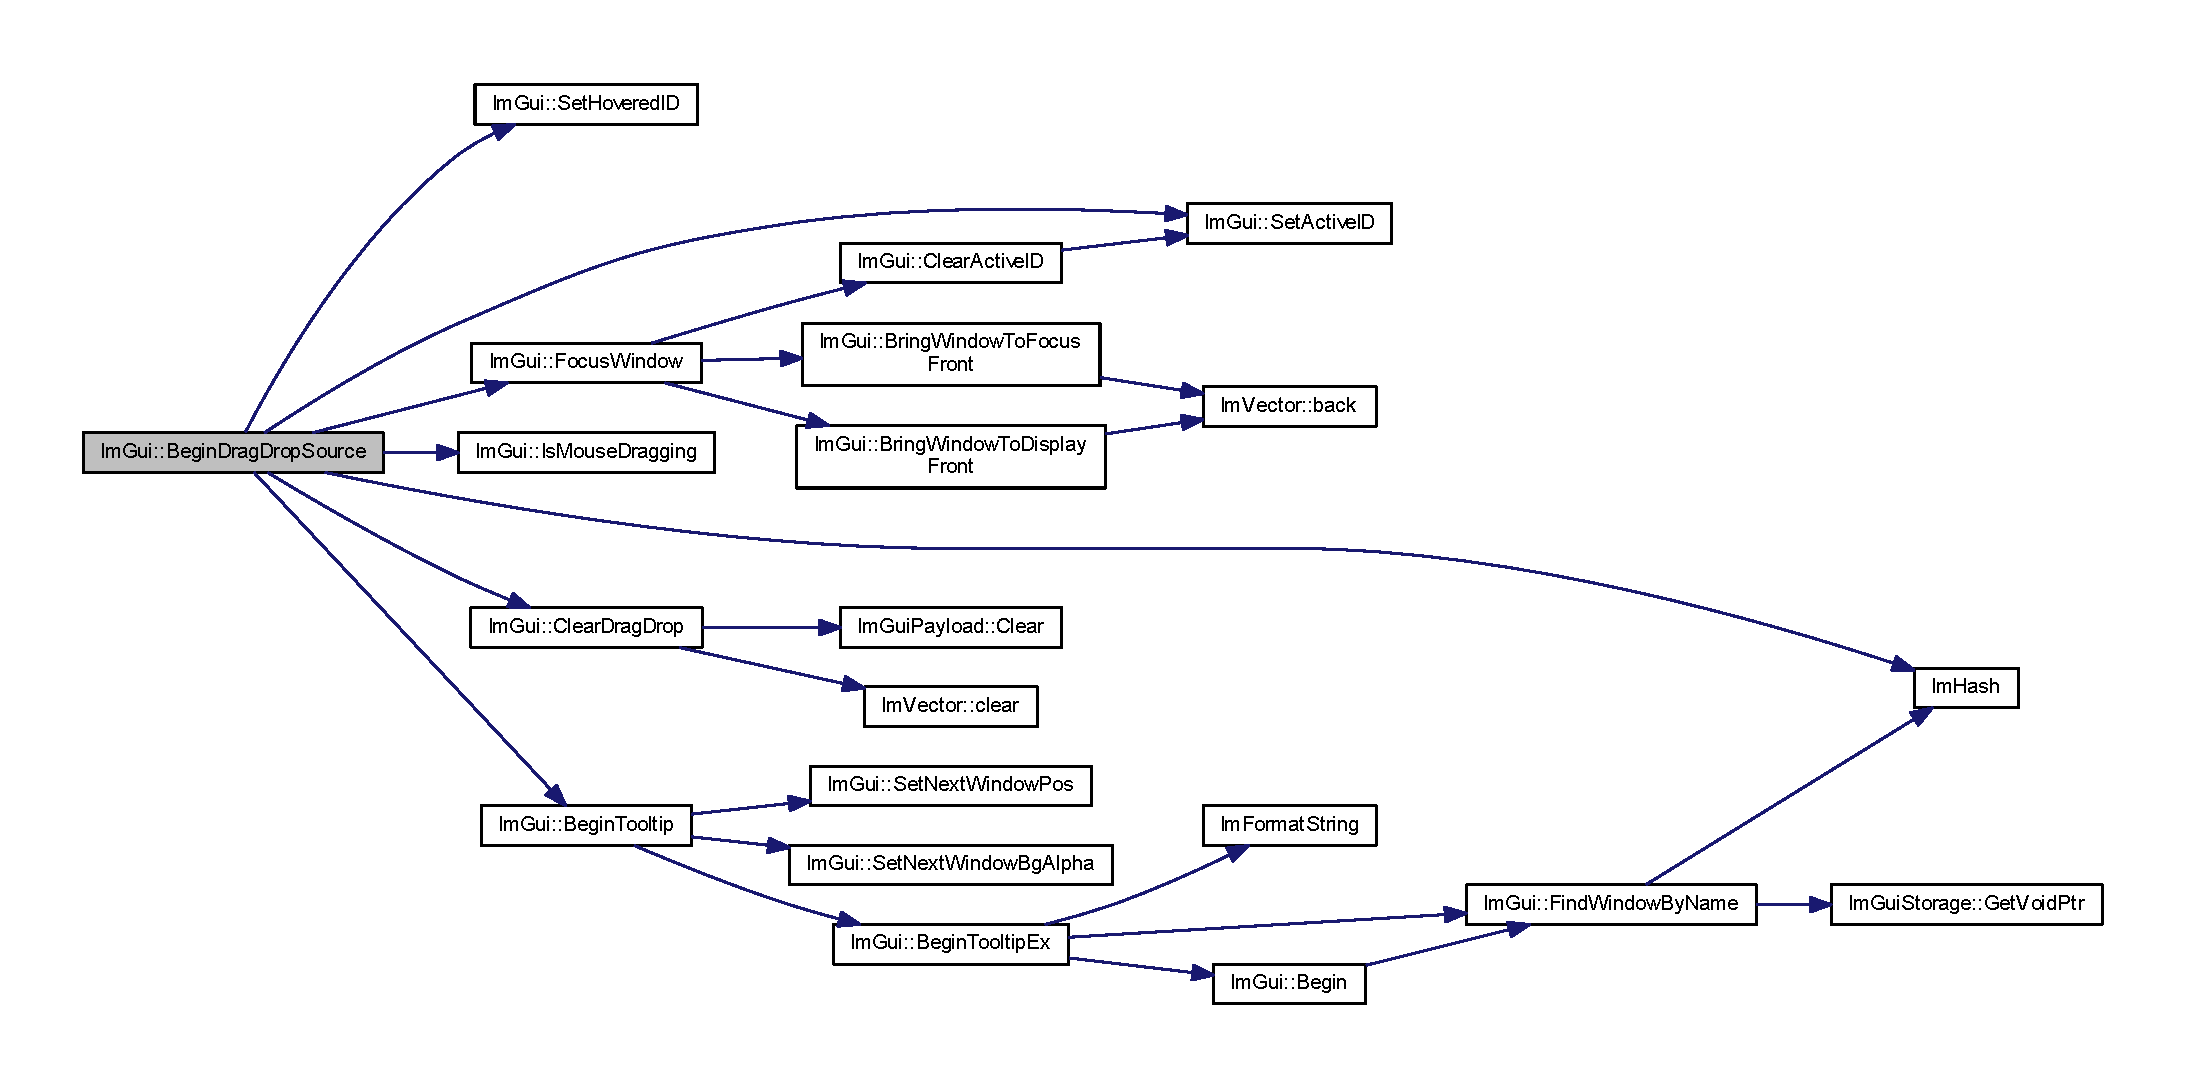
\includegraphics[width=350pt]{namespace_im_gui_ac2609b0f034d3bcd8d70d26df8694eaa_cgraph}
\end{center}
\end{figure}
\mbox{\Hypertarget{namespace_im_gui_ac42384c3181406bbd0f3f4f77a73c7ed}\label{namespace_im_gui_ac42384c3181406bbd0f3f4f77a73c7ed}} 
\index{Im\+Gui@{Im\+Gui}!Begin\+Drag\+Drop\+Target@{Begin\+Drag\+Drop\+Target}}
\index{Begin\+Drag\+Drop\+Target@{Begin\+Drag\+Drop\+Target}!Im\+Gui@{Im\+Gui}}
\subsubsection{\texorpdfstring{Begin\+Drag\+Drop\+Target()}{BeginDragDropTarget()}}
{\footnotesize\ttfamily bool Im\+Gui\+::\+Begin\+Drag\+Drop\+Target (\begin{DoxyParamCaption}{ }\end{DoxyParamCaption})}

\mbox{\Hypertarget{namespace_im_gui_a929a420d3af29051a140d0f36addbcd2}\label{namespace_im_gui_a929a420d3af29051a140d0f36addbcd2}} 
\index{Im\+Gui@{Im\+Gui}!Begin\+Drag\+Drop\+Target\+Custom@{Begin\+Drag\+Drop\+Target\+Custom}}
\index{Begin\+Drag\+Drop\+Target\+Custom@{Begin\+Drag\+Drop\+Target\+Custom}!Im\+Gui@{Im\+Gui}}
\subsubsection{\texorpdfstring{Begin\+Drag\+Drop\+Target\+Custom()}{BeginDragDropTargetCustom()}}
{\footnotesize\ttfamily bool Im\+Gui\+::\+Begin\+Drag\+Drop\+Target\+Custom (\begin{DoxyParamCaption}\item[{const \mbox{\hyperlink{struct_im_rect}{Im\+Rect}} \&}]{bb,  }\item[{\mbox{\hyperlink{imgui_8h_a1785c9b6f4e16406764a85f32582236f}{Im\+Gui\+ID}}}]{id }\end{DoxyParamCaption})}

Here is the call graph for this function\+:
\nopagebreak
\begin{figure}[H]
\begin{center}
\leavevmode
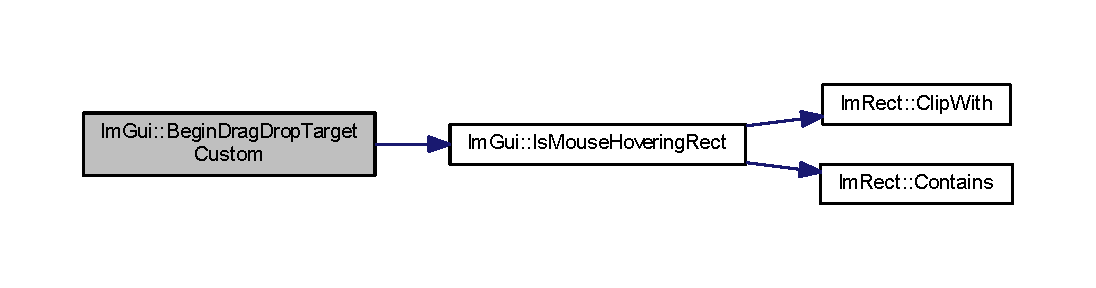
\includegraphics[width=350pt]{namespace_im_gui_a929a420d3af29051a140d0f36addbcd2_cgraph}
\end{center}
\end{figure}
\mbox{\Hypertarget{namespace_im_gui_a42407e196b7ed2a8755bff28aae9805f}\label{namespace_im_gui_a42407e196b7ed2a8755bff28aae9805f}} 
\index{Im\+Gui@{Im\+Gui}!Begin\+Group@{Begin\+Group}}
\index{Begin\+Group@{Begin\+Group}!Im\+Gui@{Im\+Gui}}
\subsubsection{\texorpdfstring{Begin\+Group()}{BeginGroup()}}
{\footnotesize\ttfamily void Im\+Gui\+::\+Begin\+Group (\begin{DoxyParamCaption}{ }\end{DoxyParamCaption})}

Here is the call graph for this function\+:
\nopagebreak
\begin{figure}[H]
\begin{center}
\leavevmode
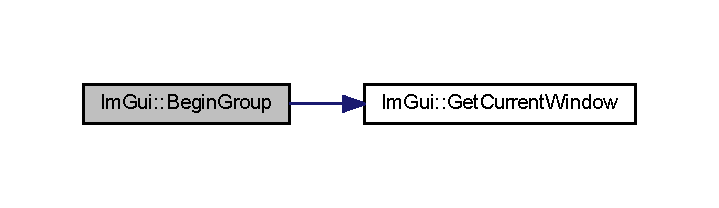
\includegraphics[width=345pt]{namespace_im_gui_a42407e196b7ed2a8755bff28aae9805f_cgraph}
\end{center}
\end{figure}
Here is the caller graph for this function\+:
\nopagebreak
\begin{figure}[H]
\begin{center}
\leavevmode
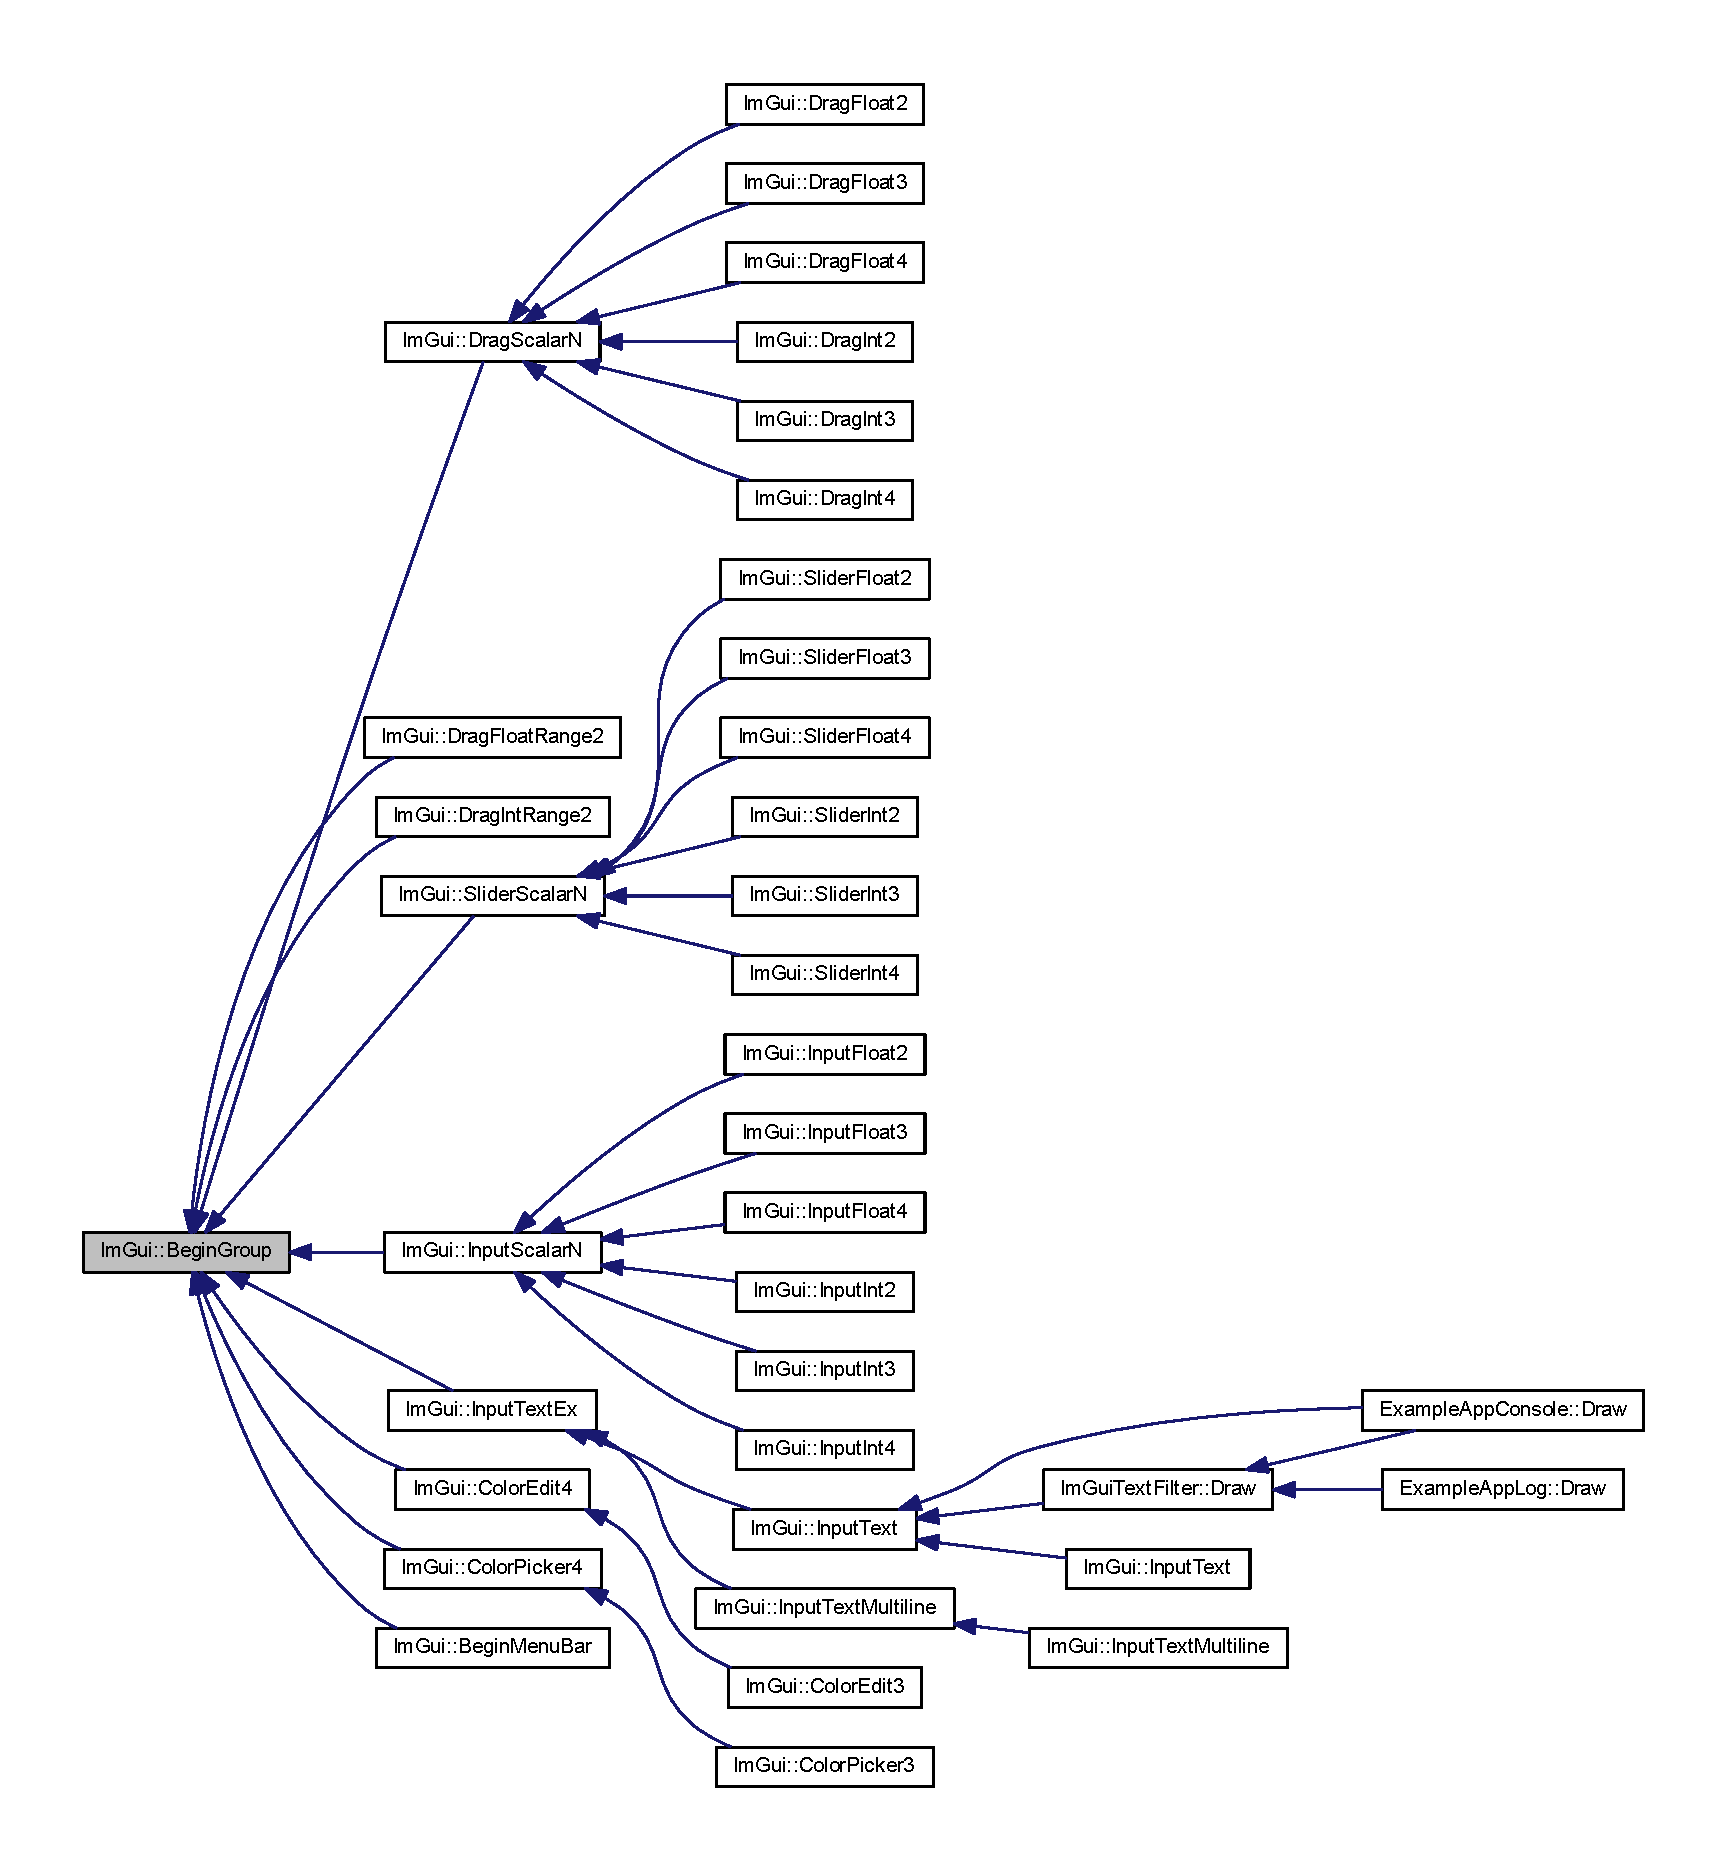
\includegraphics[width=350pt]{namespace_im_gui_a42407e196b7ed2a8755bff28aae9805f_icgraph}
\end{center}
\end{figure}
\mbox{\Hypertarget{namespace_im_gui_a55cb9cfb9865204ac6fb21c965784f78}\label{namespace_im_gui_a55cb9cfb9865204ac6fb21c965784f78}} 
\index{Im\+Gui@{Im\+Gui}!Begin\+Main\+Menu\+Bar@{Begin\+Main\+Menu\+Bar}}
\index{Begin\+Main\+Menu\+Bar@{Begin\+Main\+Menu\+Bar}!Im\+Gui@{Im\+Gui}}
\subsubsection{\texorpdfstring{Begin\+Main\+Menu\+Bar()}{BeginMainMenuBar()}}
{\footnotesize\ttfamily bool Im\+Gui\+::\+Begin\+Main\+Menu\+Bar (\begin{DoxyParamCaption}{ }\end{DoxyParamCaption})}

\mbox{\Hypertarget{namespace_im_gui_a1e55711a21f97d5dff919d697d3a7201}\label{namespace_im_gui_a1e55711a21f97d5dff919d697d3a7201}} 
\index{Im\+Gui@{Im\+Gui}!Begin\+Menu@{Begin\+Menu}}
\index{Begin\+Menu@{Begin\+Menu}!Im\+Gui@{Im\+Gui}}
\subsubsection{\texorpdfstring{Begin\+Menu()}{BeginMenu()}}
{\footnotesize\ttfamily bool Im\+Gui\+::\+Begin\+Menu (\begin{DoxyParamCaption}\item[{const char $\ast$}]{label,  }\item[{bool}]{enabled = {\ttfamily true} }\end{DoxyParamCaption})}

Here is the call graph for this function\+:
\nopagebreak
\begin{figure}[H]
\begin{center}
\leavevmode
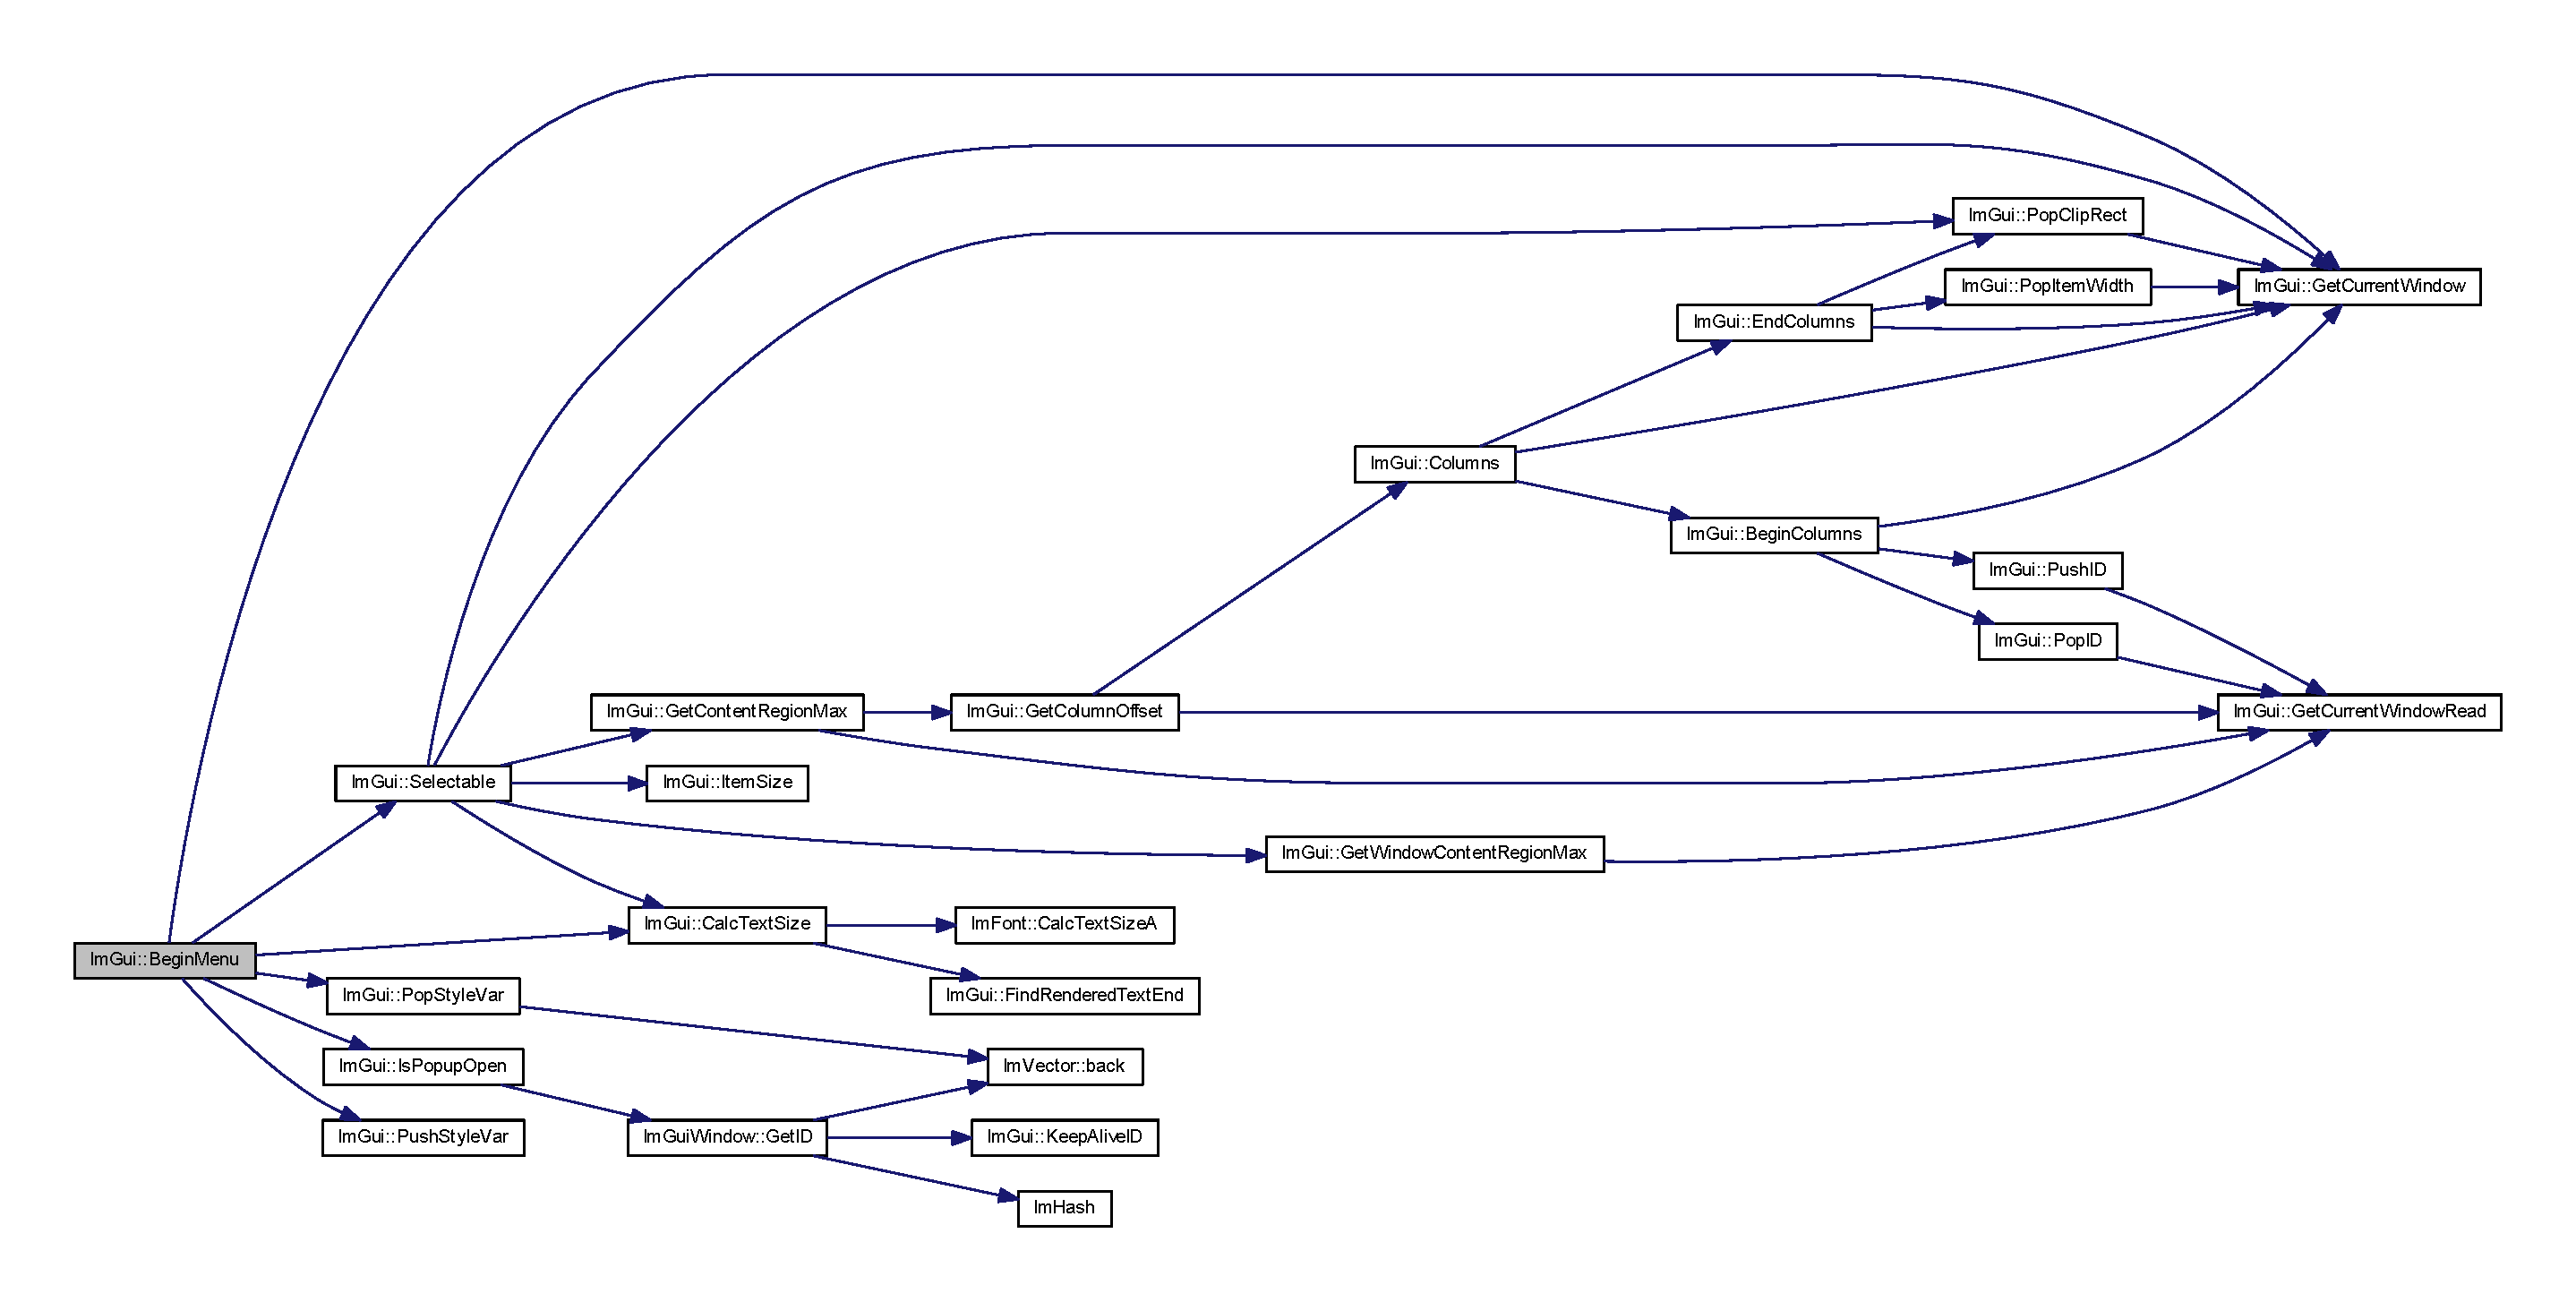
\includegraphics[width=350pt]{namespace_im_gui_a1e55711a21f97d5dff919d697d3a7201_cgraph}
\end{center}
\end{figure}
\mbox{\Hypertarget{namespace_im_gui_a4852dff802922163fc747e2e0df5b88f}\label{namespace_im_gui_a4852dff802922163fc747e2e0df5b88f}} 
\index{Im\+Gui@{Im\+Gui}!Begin\+Menu\+Bar@{Begin\+Menu\+Bar}}
\index{Begin\+Menu\+Bar@{Begin\+Menu\+Bar}!Im\+Gui@{Im\+Gui}}
\subsubsection{\texorpdfstring{Begin\+Menu\+Bar()}{BeginMenuBar()}}
{\footnotesize\ttfamily bool Im\+Gui\+::\+Begin\+Menu\+Bar (\begin{DoxyParamCaption}{ }\end{DoxyParamCaption})}

Here is the call graph for this function\+:
\nopagebreak
\begin{figure}[H]
\begin{center}
\leavevmode
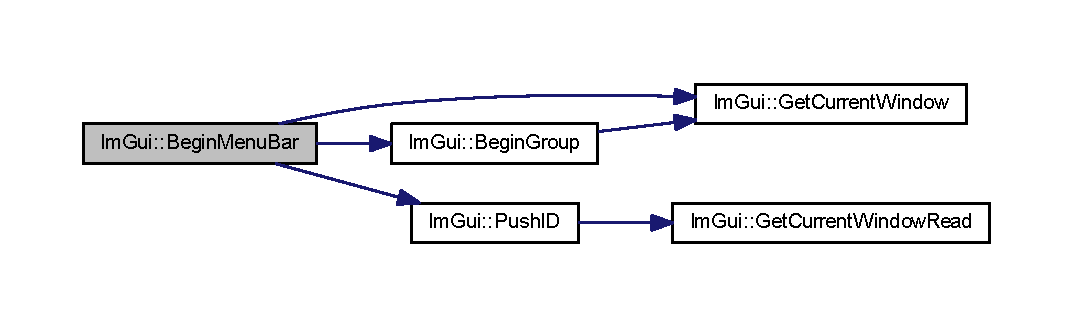
\includegraphics[width=350pt]{namespace_im_gui_a4852dff802922163fc747e2e0df5b88f_cgraph}
\end{center}
\end{figure}
\mbox{\Hypertarget{namespace_im_gui_a10e213926d8ca212266bc5fbded1e026}\label{namespace_im_gui_a10e213926d8ca212266bc5fbded1e026}} 
\index{Im\+Gui@{Im\+Gui}!Begin\+Popup@{Begin\+Popup}}
\index{Begin\+Popup@{Begin\+Popup}!Im\+Gui@{Im\+Gui}}
\subsubsection{\texorpdfstring{Begin\+Popup()}{BeginPopup()}}
{\footnotesize\ttfamily bool Im\+Gui\+::\+Begin\+Popup (\begin{DoxyParamCaption}\item[{const char $\ast$}]{str\+\_\+id,  }\item[{\mbox{\hyperlink{imgui_8h_a0b8e067ab4f7a818828c8d89e531addc}{Im\+Gui\+Window\+Flags}}}]{flags = {\ttfamily 0} }\end{DoxyParamCaption})}

Here is the call graph for this function\+:
\nopagebreak
\begin{figure}[H]
\begin{center}
\leavevmode
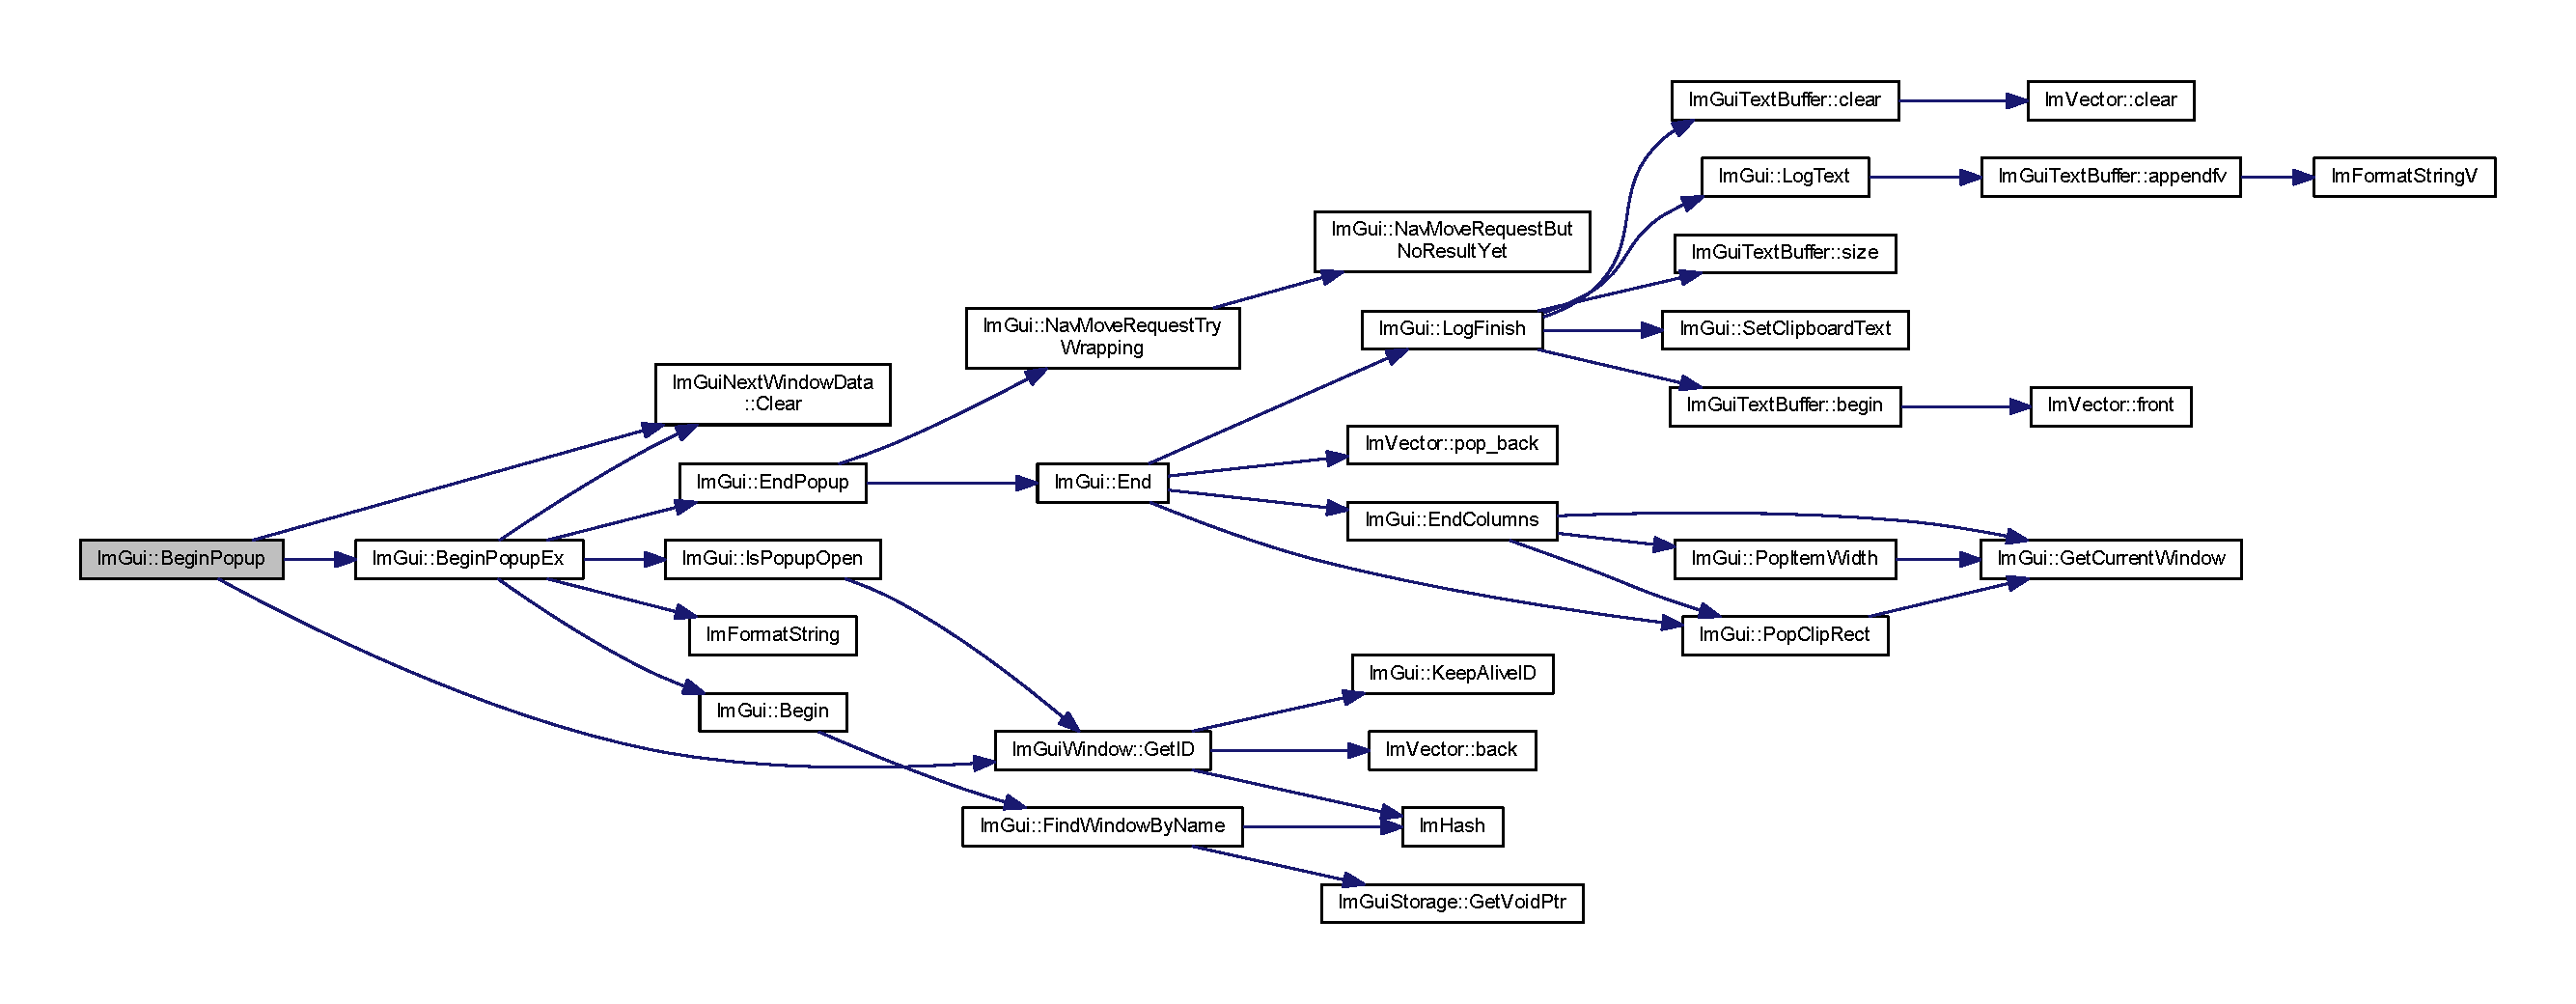
\includegraphics[width=350pt]{namespace_im_gui_a10e213926d8ca212266bc5fbded1e026_cgraph}
\end{center}
\end{figure}
Here is the caller graph for this function\+:
\nopagebreak
\begin{figure}[H]
\begin{center}
\leavevmode
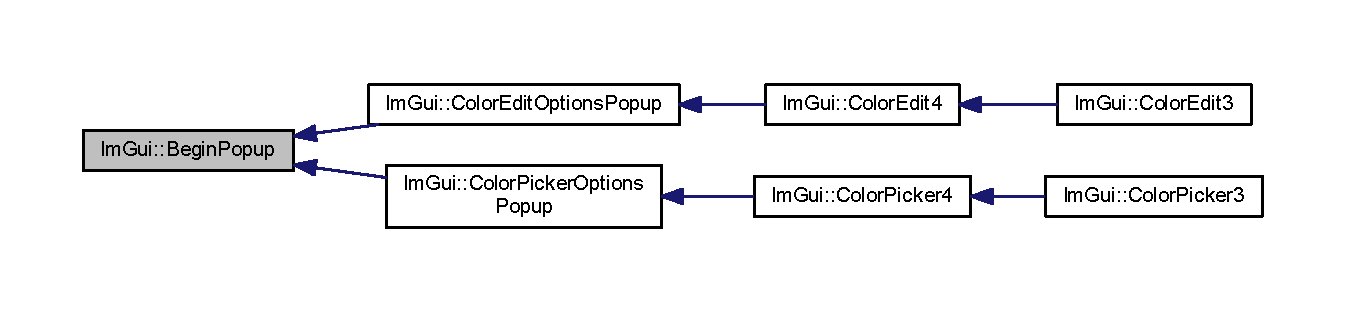
\includegraphics[width=350pt]{namespace_im_gui_a10e213926d8ca212266bc5fbded1e026_icgraph}
\end{center}
\end{figure}
\mbox{\Hypertarget{namespace_im_gui_a579fc507f5b5d164c8fd628aee3d7bbd}\label{namespace_im_gui_a579fc507f5b5d164c8fd628aee3d7bbd}} 
\index{Im\+Gui@{Im\+Gui}!Begin\+Popup\+Context\+Item@{Begin\+Popup\+Context\+Item}}
\index{Begin\+Popup\+Context\+Item@{Begin\+Popup\+Context\+Item}!Im\+Gui@{Im\+Gui}}
\subsubsection{\texorpdfstring{Begin\+Popup\+Context\+Item()}{BeginPopupContextItem()}}
{\footnotesize\ttfamily bool Im\+Gui\+::\+Begin\+Popup\+Context\+Item (\begin{DoxyParamCaption}\item[{const char $\ast$}]{str\+\_\+id = {\ttfamily NULL},  }\item[{int}]{mouse\+\_\+button = {\ttfamily 1} }\end{DoxyParamCaption})}

Here is the call graph for this function\+:
\nopagebreak
\begin{figure}[H]
\begin{center}
\leavevmode
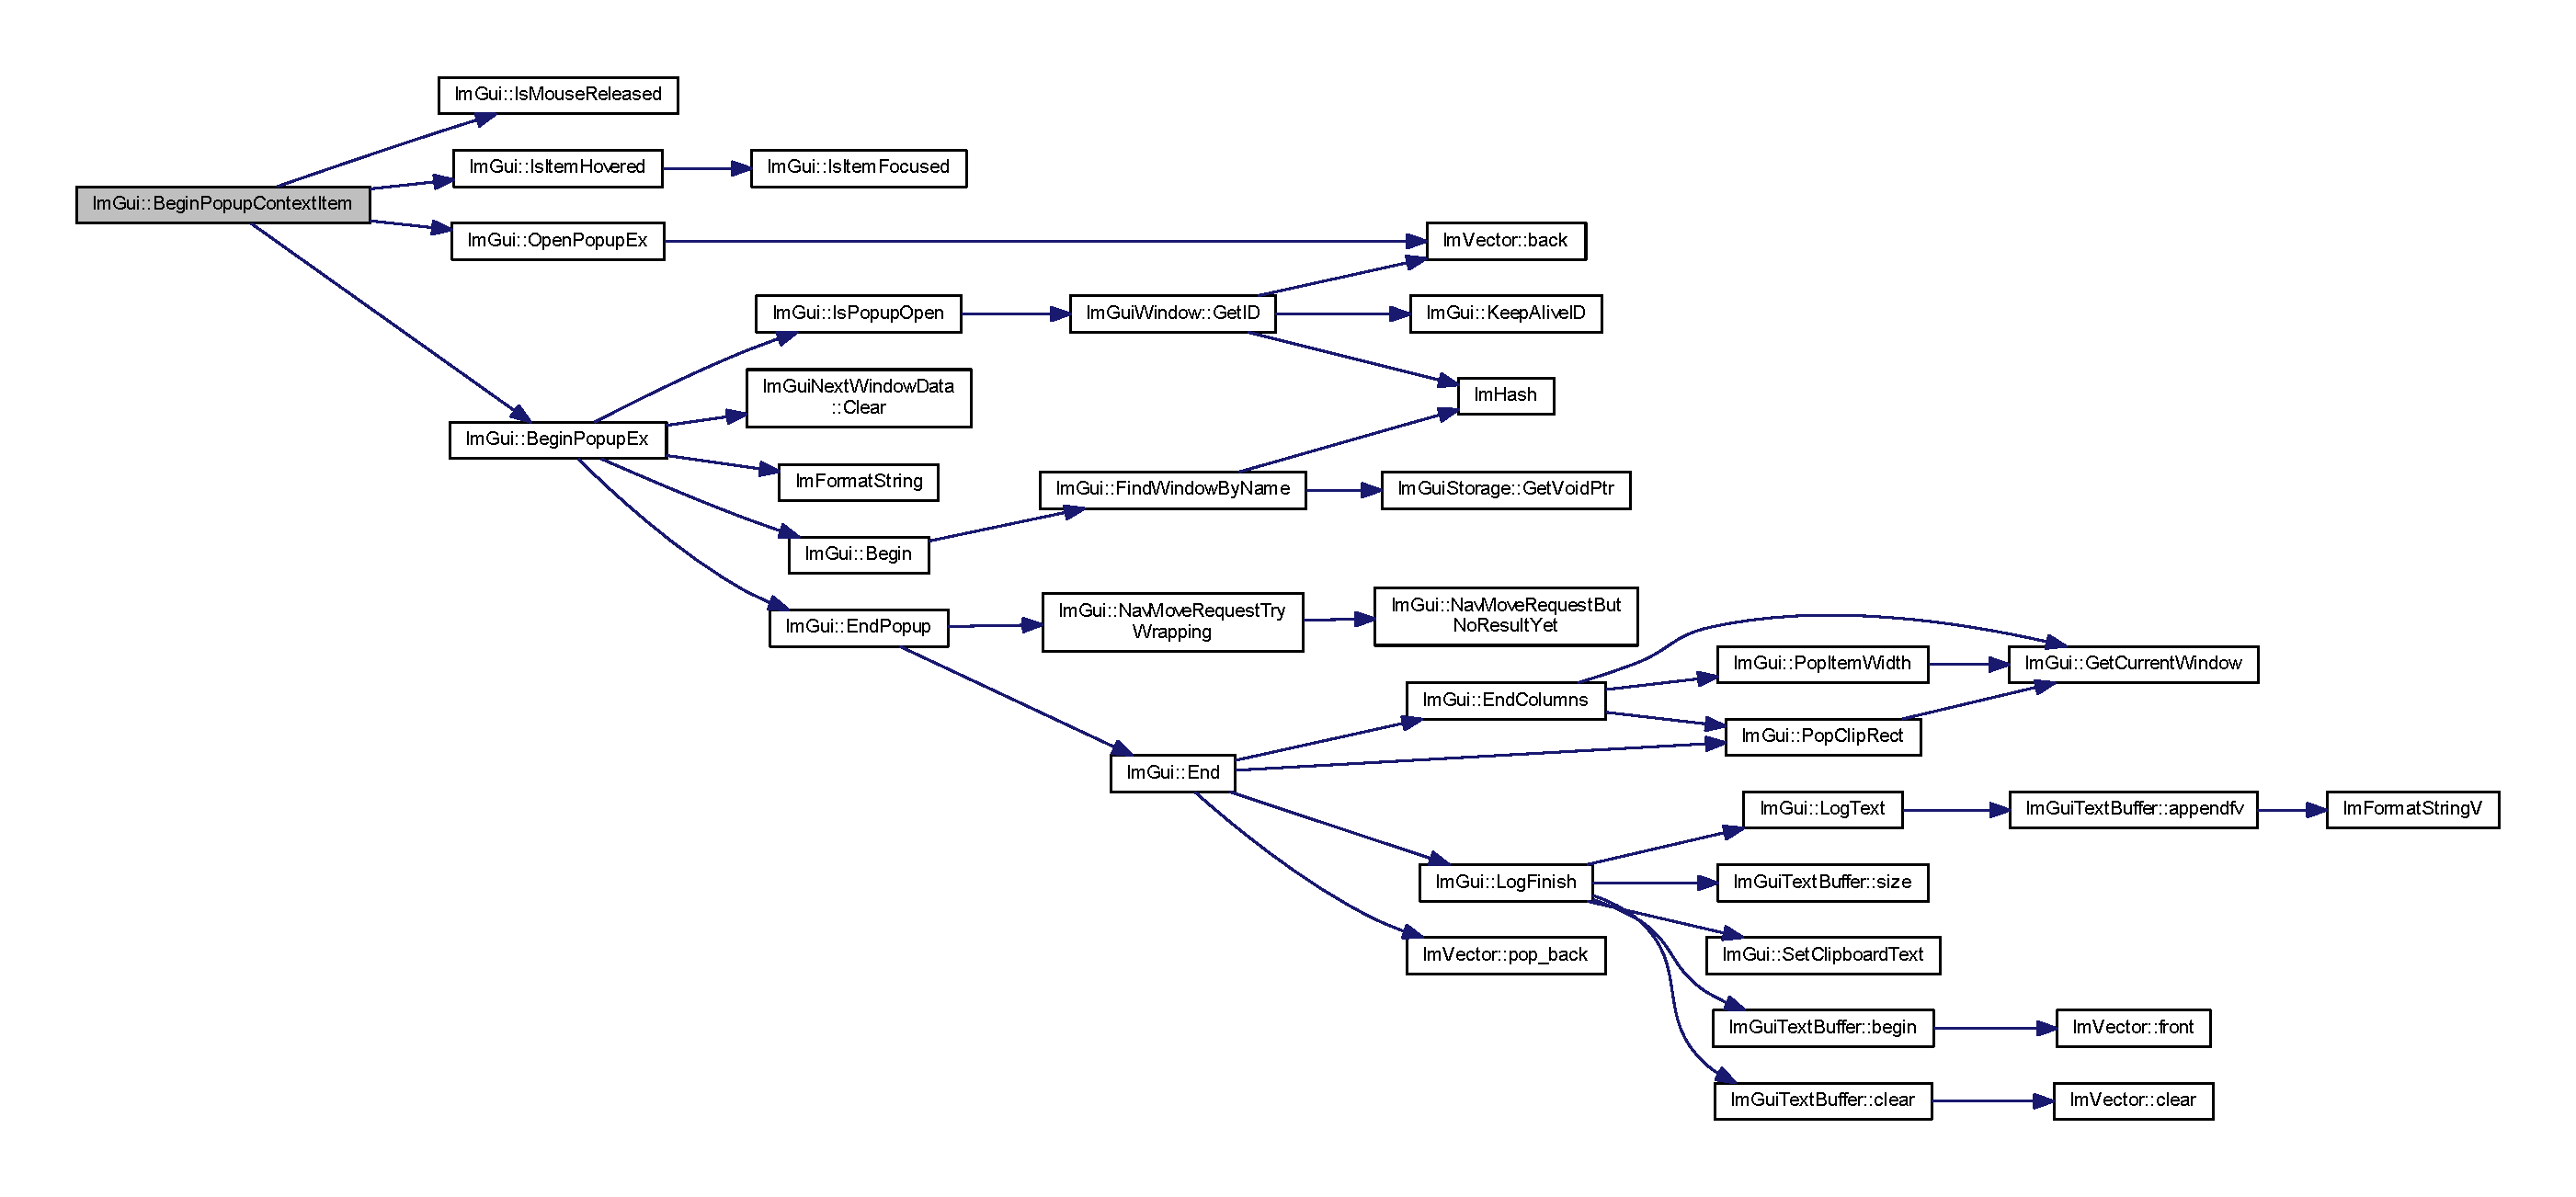
\includegraphics[width=350pt]{namespace_im_gui_a579fc507f5b5d164c8fd628aee3d7bbd_cgraph}
\end{center}
\end{figure}
Here is the caller graph for this function\+:
\nopagebreak
\begin{figure}[H]
\begin{center}
\leavevmode
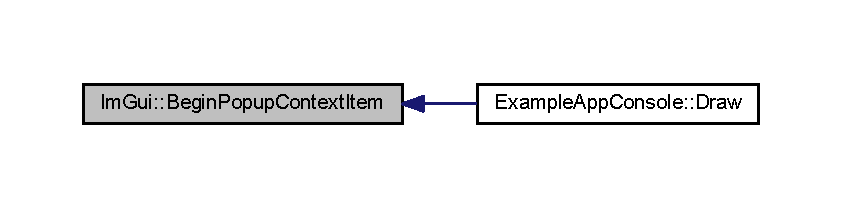
\includegraphics[width=350pt]{namespace_im_gui_a579fc507f5b5d164c8fd628aee3d7bbd_icgraph}
\end{center}
\end{figure}
\mbox{\Hypertarget{namespace_im_gui_a87a2228929503fff067d2e167a690751}\label{namespace_im_gui_a87a2228929503fff067d2e167a690751}} 
\index{Im\+Gui@{Im\+Gui}!Begin\+Popup\+Context\+Void@{Begin\+Popup\+Context\+Void}}
\index{Begin\+Popup\+Context\+Void@{Begin\+Popup\+Context\+Void}!Im\+Gui@{Im\+Gui}}
\subsubsection{\texorpdfstring{Begin\+Popup\+Context\+Void()}{BeginPopupContextVoid()}}
{\footnotesize\ttfamily bool Im\+Gui\+::\+Begin\+Popup\+Context\+Void (\begin{DoxyParamCaption}\item[{const char $\ast$}]{str\+\_\+id = {\ttfamily NULL},  }\item[{int}]{mouse\+\_\+button = {\ttfamily 1} }\end{DoxyParamCaption})}

Here is the call graph for this function\+:
\nopagebreak
\begin{figure}[H]
\begin{center}
\leavevmode
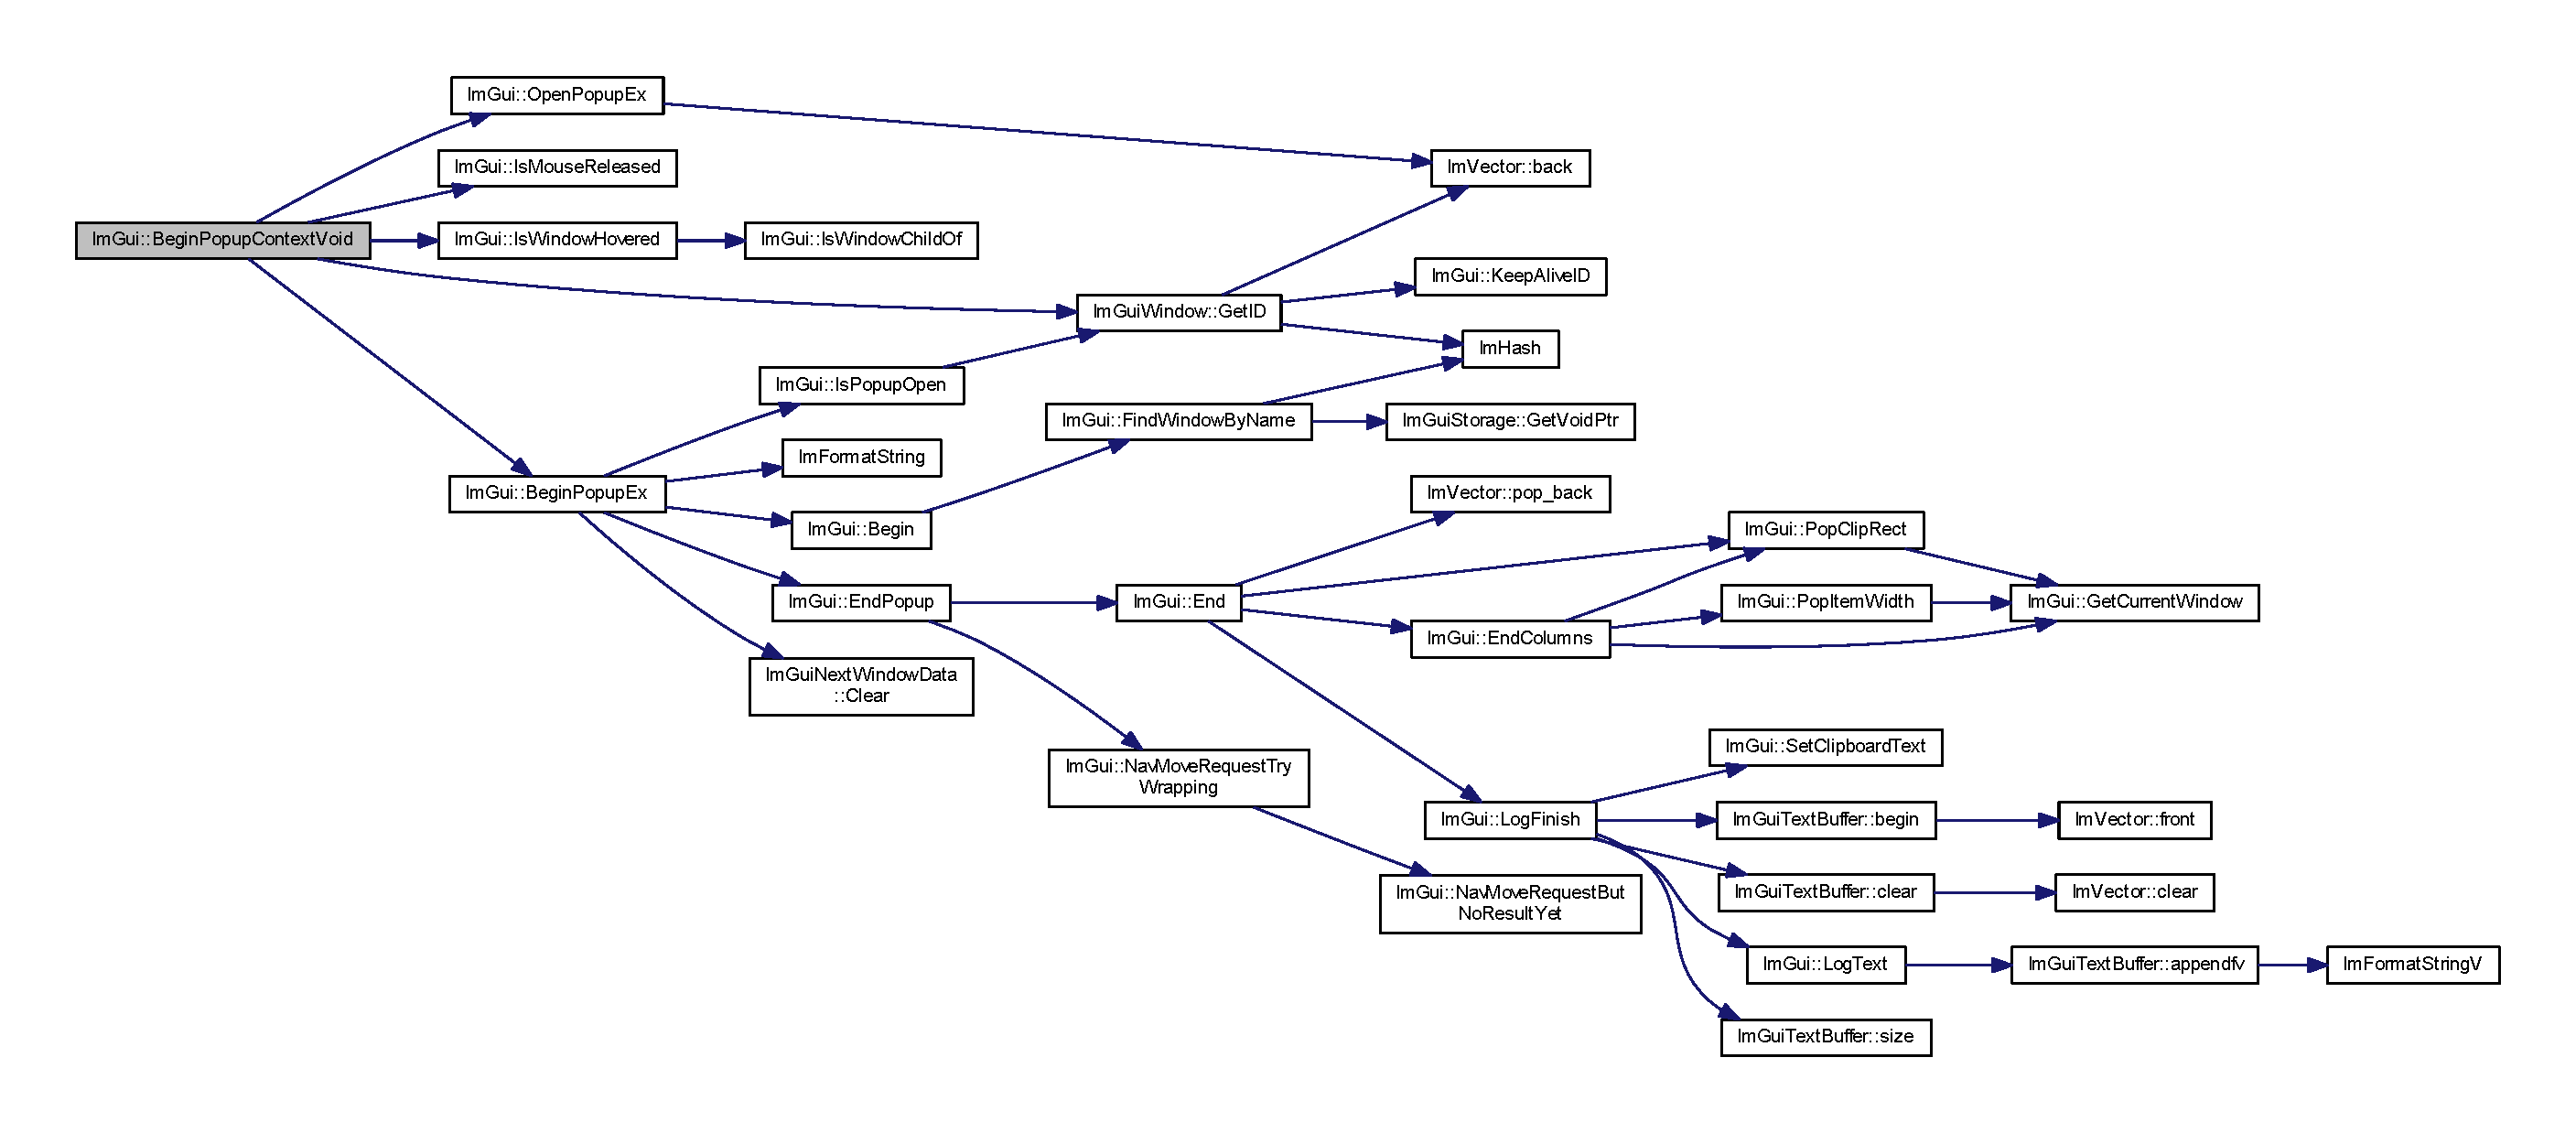
\includegraphics[width=350pt]{namespace_im_gui_a87a2228929503fff067d2e167a690751_cgraph}
\end{center}
\end{figure}
\mbox{\Hypertarget{namespace_im_gui_acf98c99f041ea341d0328e071c56411b}\label{namespace_im_gui_acf98c99f041ea341d0328e071c56411b}} 
\index{Im\+Gui@{Im\+Gui}!Begin\+Popup\+Context\+Window@{Begin\+Popup\+Context\+Window}}
\index{Begin\+Popup\+Context\+Window@{Begin\+Popup\+Context\+Window}!Im\+Gui@{Im\+Gui}}
\subsubsection{\texorpdfstring{Begin\+Popup\+Context\+Window()}{BeginPopupContextWindow()}}
{\footnotesize\ttfamily bool Im\+Gui\+::\+Begin\+Popup\+Context\+Window (\begin{DoxyParamCaption}\item[{const char $\ast$}]{str\+\_\+id = {\ttfamily NULL},  }\item[{int}]{mouse\+\_\+button = {\ttfamily 1},  }\item[{bool}]{also\+\_\+over\+\_\+items = {\ttfamily true} }\end{DoxyParamCaption})}

Here is the call graph for this function\+:
\nopagebreak
\begin{figure}[H]
\begin{center}
\leavevmode
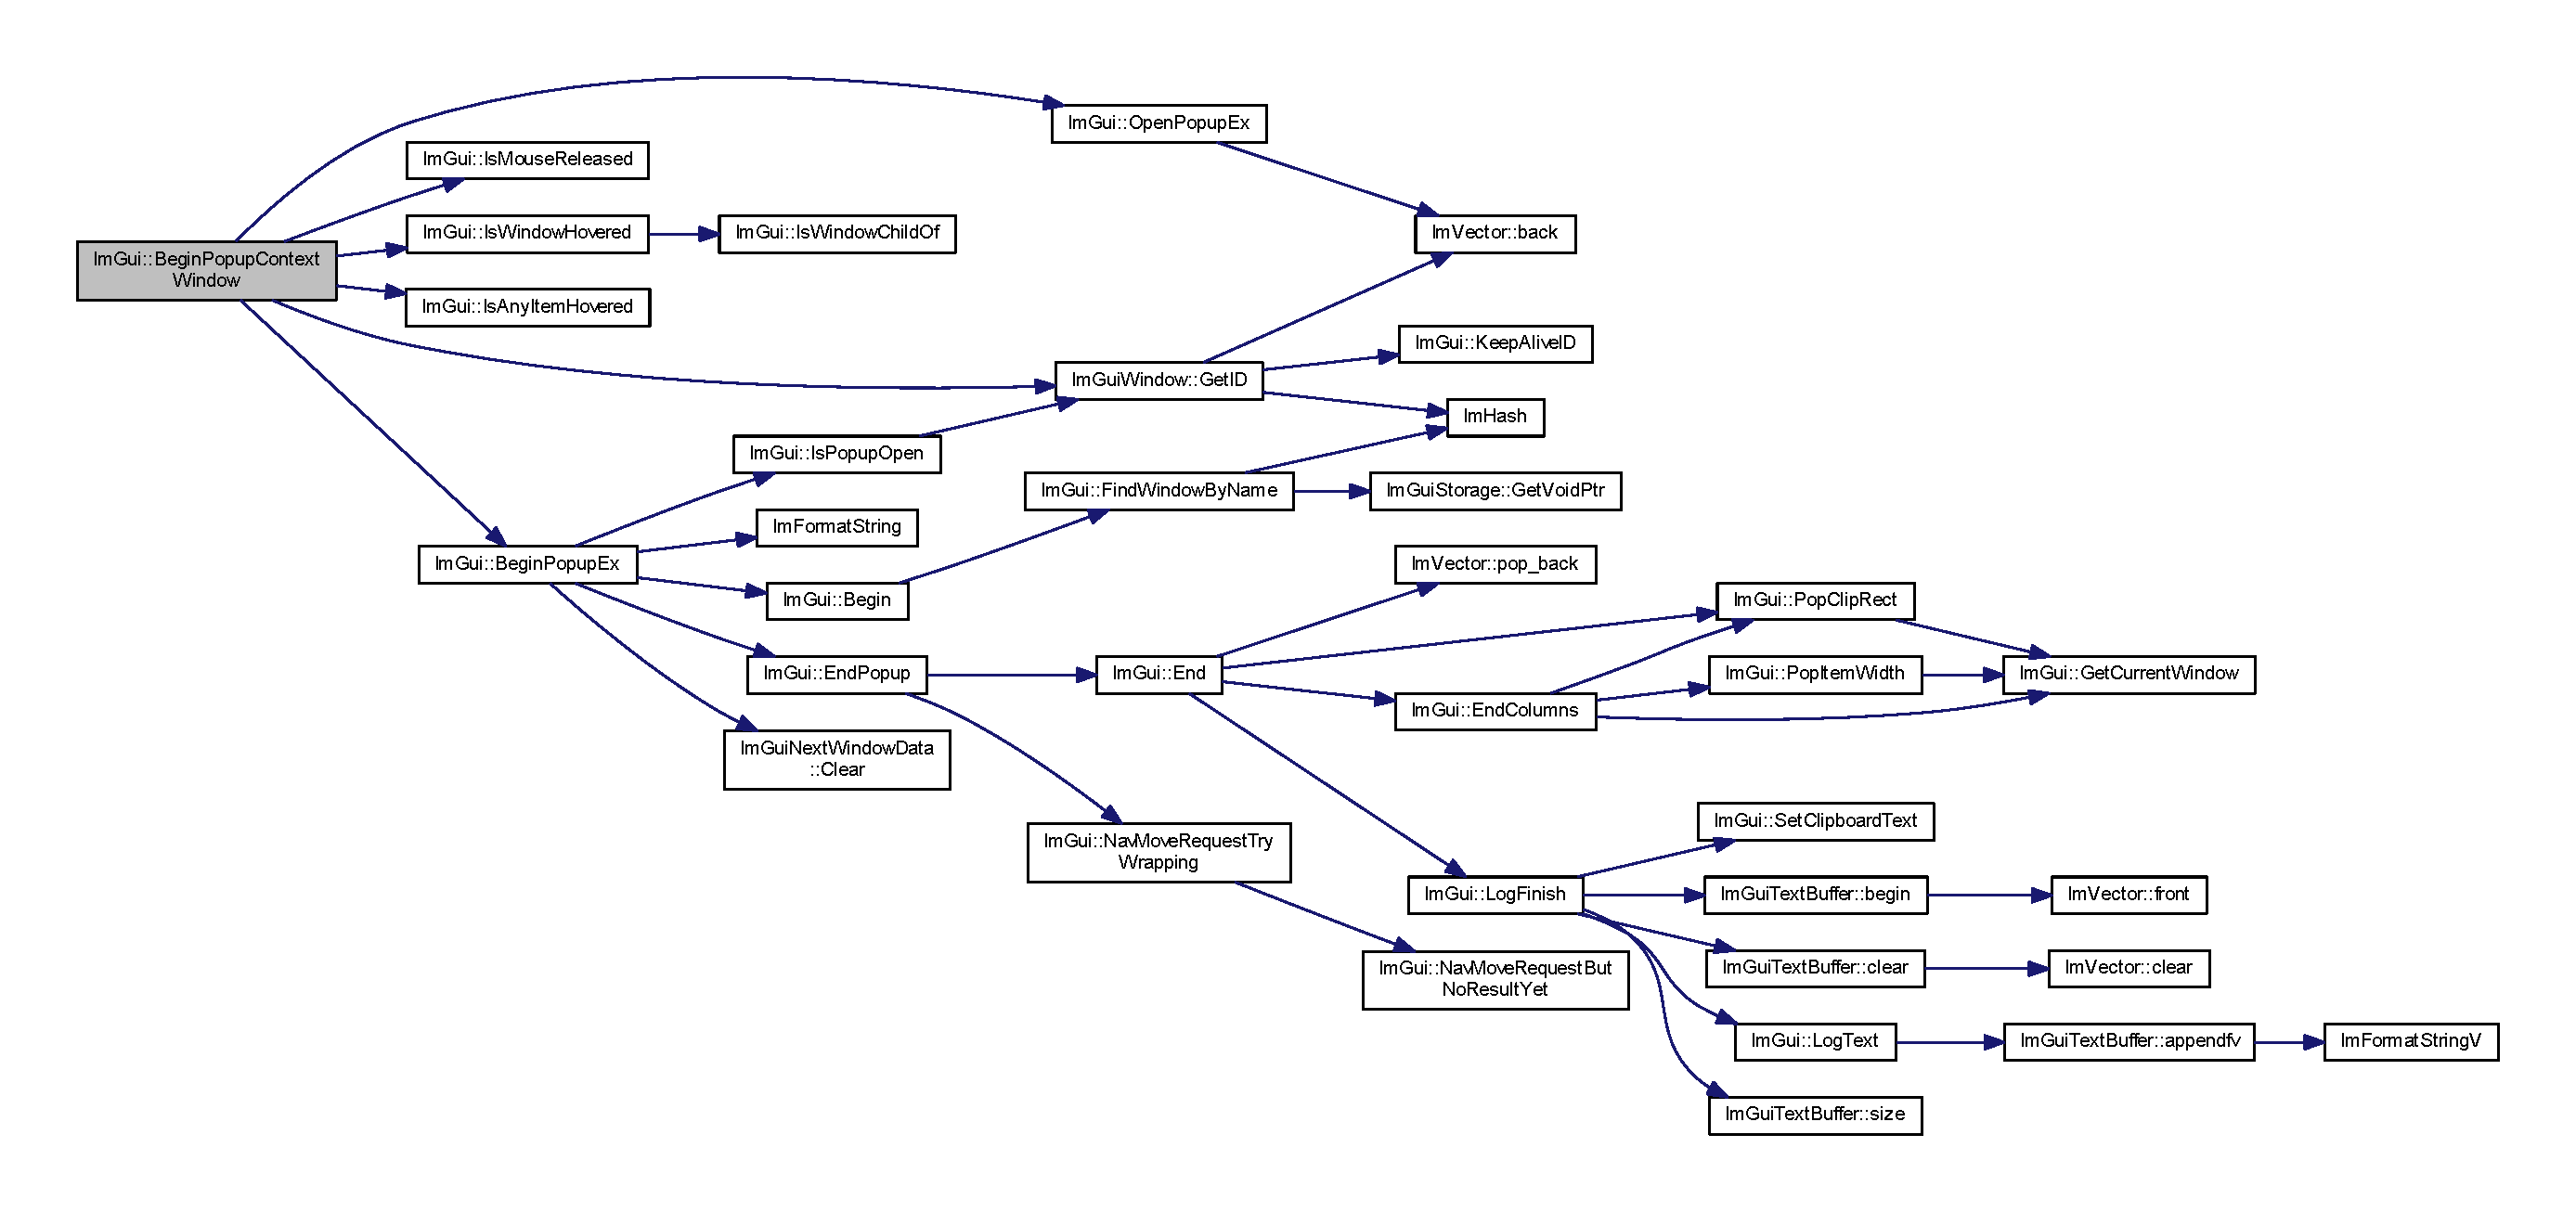
\includegraphics[width=350pt]{namespace_im_gui_acf98c99f041ea341d0328e071c56411b_cgraph}
\end{center}
\end{figure}
Here is the caller graph for this function\+:
\nopagebreak
\begin{figure}[H]
\begin{center}
\leavevmode
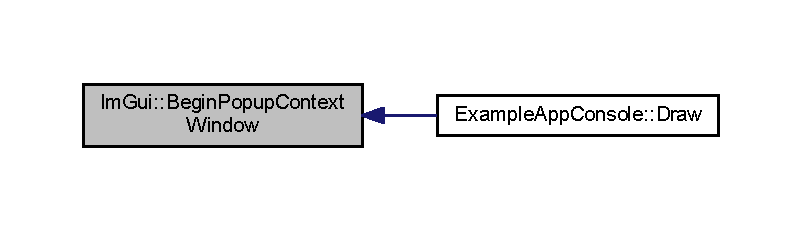
\includegraphics[width=350pt]{namespace_im_gui_acf98c99f041ea341d0328e071c56411b_icgraph}
\end{center}
\end{figure}
\mbox{\Hypertarget{namespace_im_gui_a89da3a22300e8293257b6cfdf1b83b7a}\label{namespace_im_gui_a89da3a22300e8293257b6cfdf1b83b7a}} 
\index{Im\+Gui@{Im\+Gui}!Begin\+Popup\+Ex@{Begin\+Popup\+Ex}}
\index{Begin\+Popup\+Ex@{Begin\+Popup\+Ex}!Im\+Gui@{Im\+Gui}}
\subsubsection{\texorpdfstring{Begin\+Popup\+Ex()}{BeginPopupEx()}}
{\footnotesize\ttfamily bool Im\+Gui\+::\+Begin\+Popup\+Ex (\begin{DoxyParamCaption}\item[{\mbox{\hyperlink{imgui_8h_a1785c9b6f4e16406764a85f32582236f}{Im\+Gui\+ID}}}]{id,  }\item[{\mbox{\hyperlink{imgui_8h_a0b8e067ab4f7a818828c8d89e531addc}{Im\+Gui\+Window\+Flags}}}]{extra\+\_\+flags }\end{DoxyParamCaption})}

Here is the call graph for this function\+:
\nopagebreak
\begin{figure}[H]
\begin{center}
\leavevmode
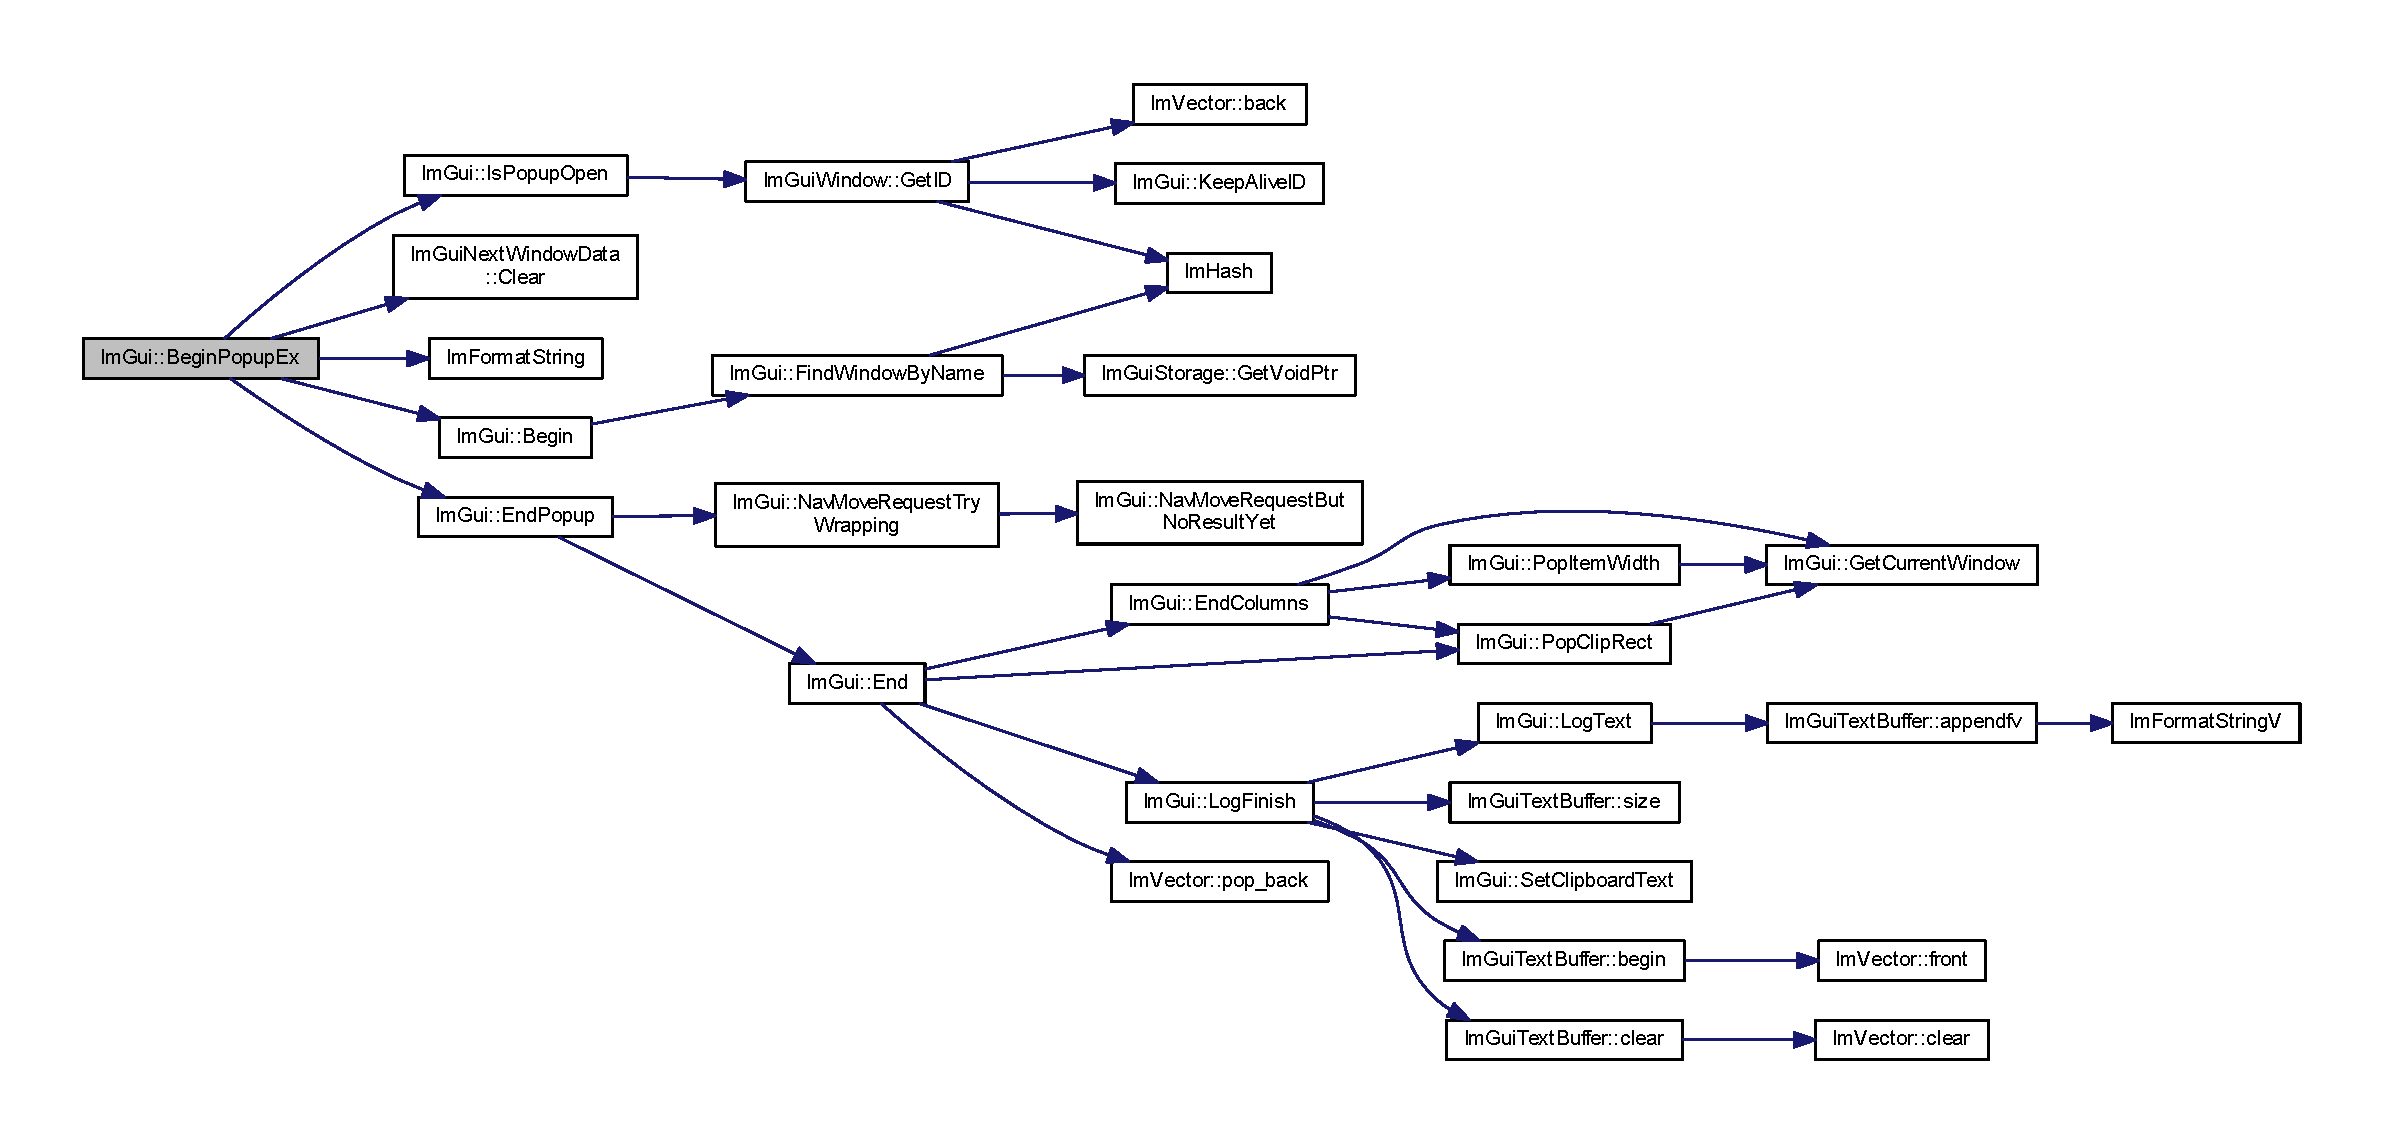
\includegraphics[width=350pt]{namespace_im_gui_a89da3a22300e8293257b6cfdf1b83b7a_cgraph}
\end{center}
\end{figure}
Here is the caller graph for this function\+:
\nopagebreak
\begin{figure}[H]
\begin{center}
\leavevmode
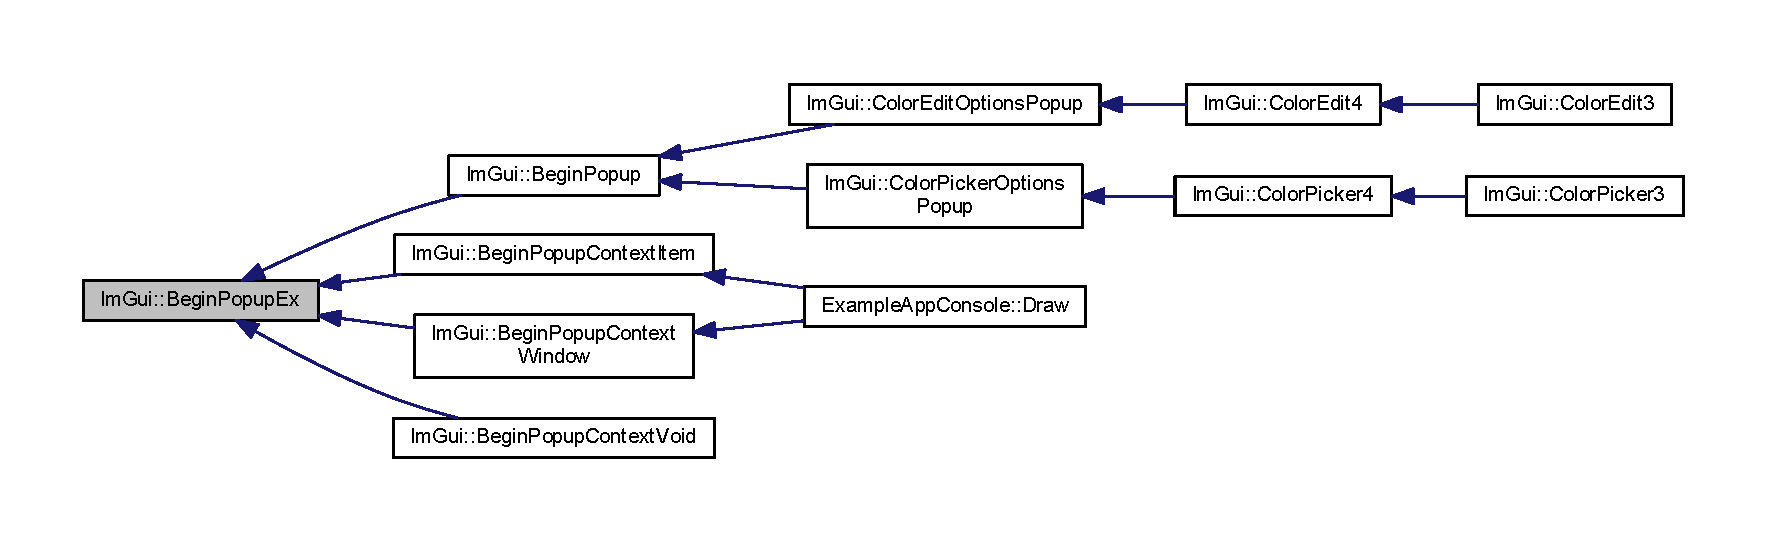
\includegraphics[width=350pt]{namespace_im_gui_a89da3a22300e8293257b6cfdf1b83b7a_icgraph}
\end{center}
\end{figure}
\mbox{\Hypertarget{namespace_im_gui_a6d840f615c198c2342968f733fda11b3}\label{namespace_im_gui_a6d840f615c198c2342968f733fda11b3}} 
\index{Im\+Gui@{Im\+Gui}!Begin\+Popup\+Modal@{Begin\+Popup\+Modal}}
\index{Begin\+Popup\+Modal@{Begin\+Popup\+Modal}!Im\+Gui@{Im\+Gui}}
\subsubsection{\texorpdfstring{Begin\+Popup\+Modal()}{BeginPopupModal()}}
{\footnotesize\ttfamily bool Im\+Gui\+::\+Begin\+Popup\+Modal (\begin{DoxyParamCaption}\item[{const char $\ast$}]{name,  }\item[{bool $\ast$}]{p\+\_\+open = {\ttfamily NULL},  }\item[{\mbox{\hyperlink{imgui_8h_a0b8e067ab4f7a818828c8d89e531addc}{Im\+Gui\+Window\+Flags}}}]{flags = {\ttfamily 0} }\end{DoxyParamCaption})}

Here is the call graph for this function\+:
\nopagebreak
\begin{figure}[H]
\begin{center}
\leavevmode
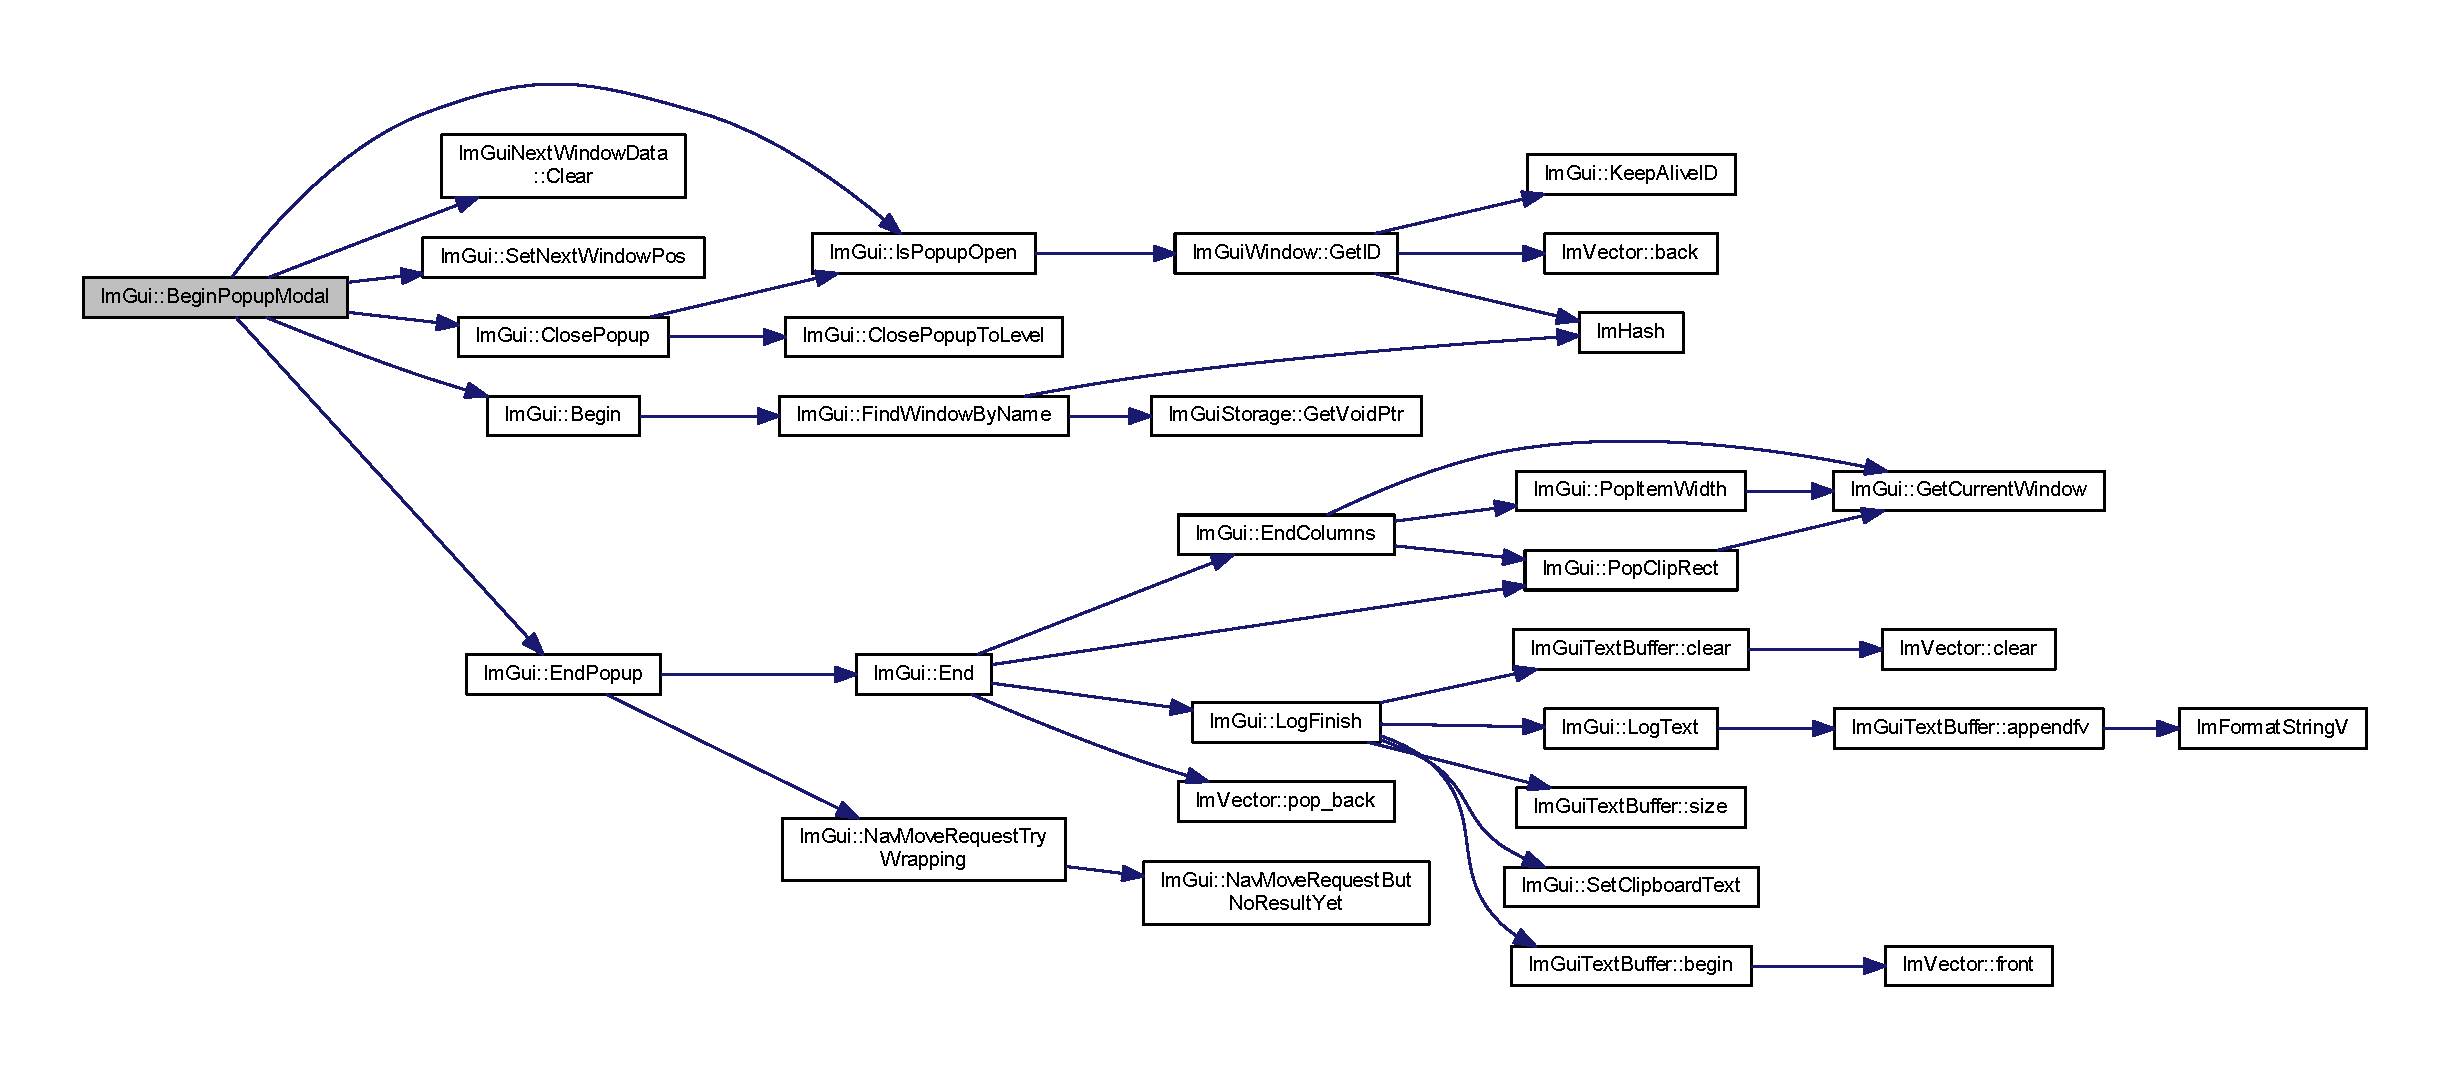
\includegraphics[width=350pt]{namespace_im_gui_a6d840f615c198c2342968f733fda11b3_cgraph}
\end{center}
\end{figure}
\mbox{\Hypertarget{namespace_im_gui_a36816a48385f4759d746a03cf6202512}\label{namespace_im_gui_a36816a48385f4759d746a03cf6202512}} 
\index{Im\+Gui@{Im\+Gui}!Begin\+Tooltip@{Begin\+Tooltip}}
\index{Begin\+Tooltip@{Begin\+Tooltip}!Im\+Gui@{Im\+Gui}}
\subsubsection{\texorpdfstring{Begin\+Tooltip()}{BeginTooltip()}}
{\footnotesize\ttfamily void Im\+Gui\+::\+Begin\+Tooltip (\begin{DoxyParamCaption}{ }\end{DoxyParamCaption})}

Here is the call graph for this function\+:
\nopagebreak
\begin{figure}[H]
\begin{center}
\leavevmode
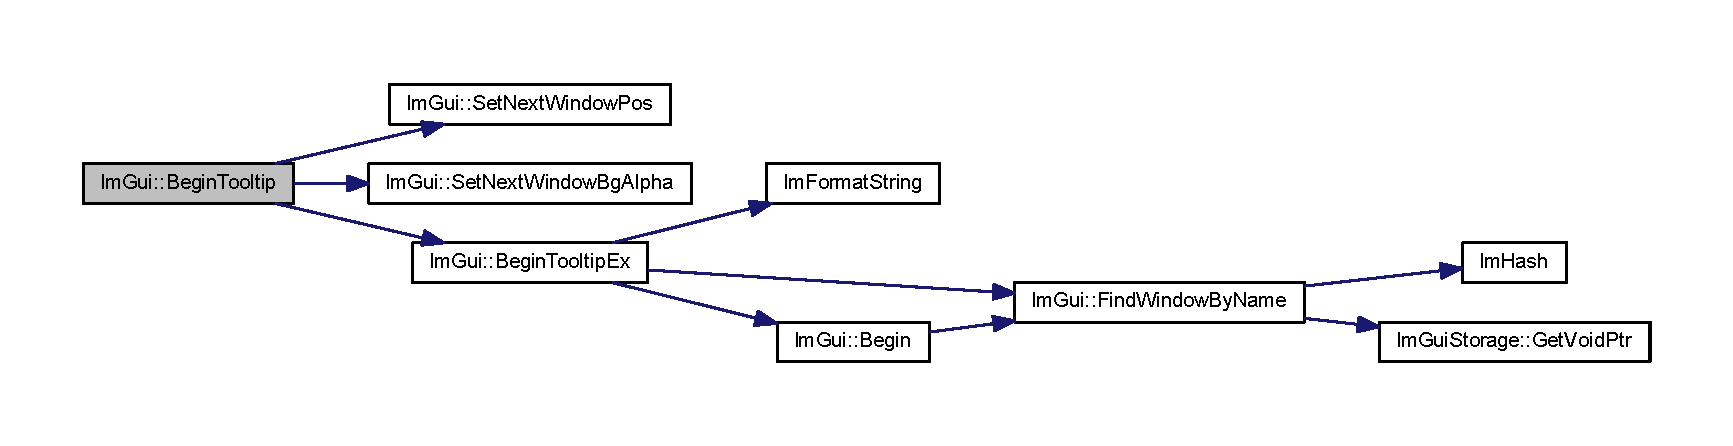
\includegraphics[width=350pt]{namespace_im_gui_a36816a48385f4759d746a03cf6202512_cgraph}
\end{center}
\end{figure}
Here is the caller graph for this function\+:
\nopagebreak
\begin{figure}[H]
\begin{center}
\leavevmode
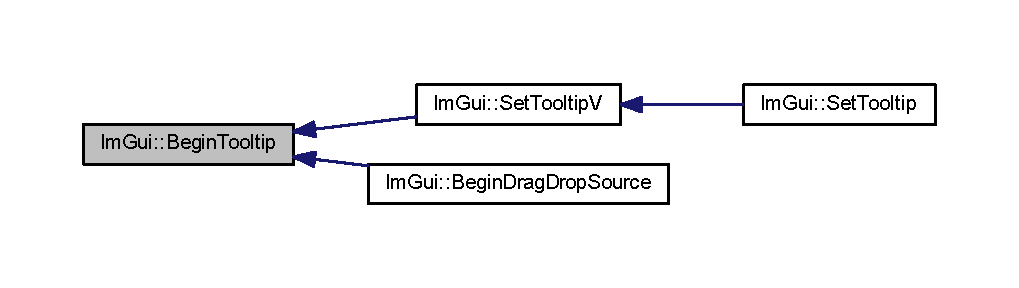
\includegraphics[width=350pt]{namespace_im_gui_a36816a48385f4759d746a03cf6202512_icgraph}
\end{center}
\end{figure}
\mbox{\Hypertarget{namespace_im_gui_a3189530b7795a9b99169eb95f36c516d}\label{namespace_im_gui_a3189530b7795a9b99169eb95f36c516d}} 
\index{Im\+Gui@{Im\+Gui}!Begin\+Tooltip\+Ex@{Begin\+Tooltip\+Ex}}
\index{Begin\+Tooltip\+Ex@{Begin\+Tooltip\+Ex}!Im\+Gui@{Im\+Gui}}
\subsubsection{\texorpdfstring{Begin\+Tooltip\+Ex()}{BeginTooltipEx()}}
{\footnotesize\ttfamily void Im\+Gui\+::\+Begin\+Tooltip\+Ex (\begin{DoxyParamCaption}\item[{\mbox{\hyperlink{imgui_8h_a0b8e067ab4f7a818828c8d89e531addc}{Im\+Gui\+Window\+Flags}}}]{extra\+\_\+flags,  }\item[{bool}]{override\+\_\+previous\+\_\+tooltip = {\ttfamily true} }\end{DoxyParamCaption})}

Here is the call graph for this function\+:
\nopagebreak
\begin{figure}[H]
\begin{center}
\leavevmode
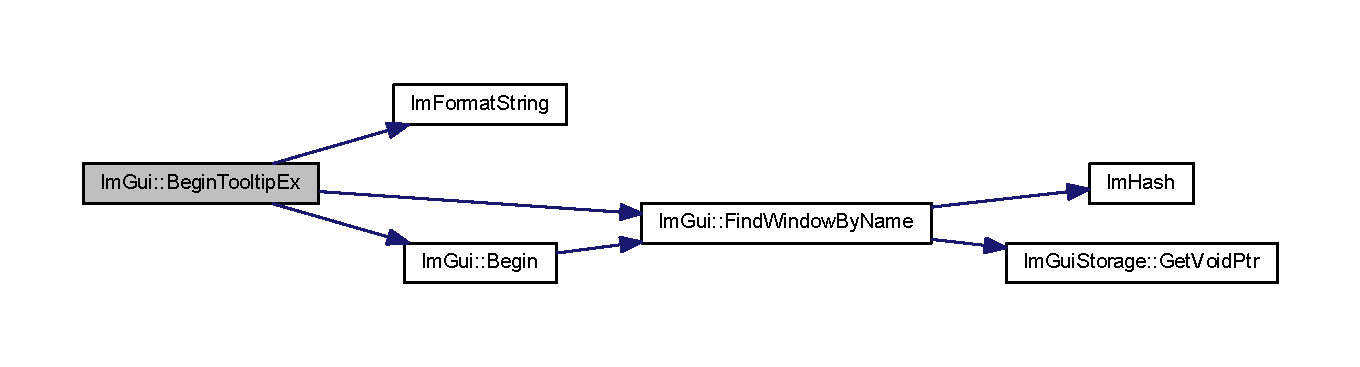
\includegraphics[width=350pt]{namespace_im_gui_a3189530b7795a9b99169eb95f36c516d_cgraph}
\end{center}
\end{figure}
Here is the caller graph for this function\+:
\nopagebreak
\begin{figure}[H]
\begin{center}
\leavevmode
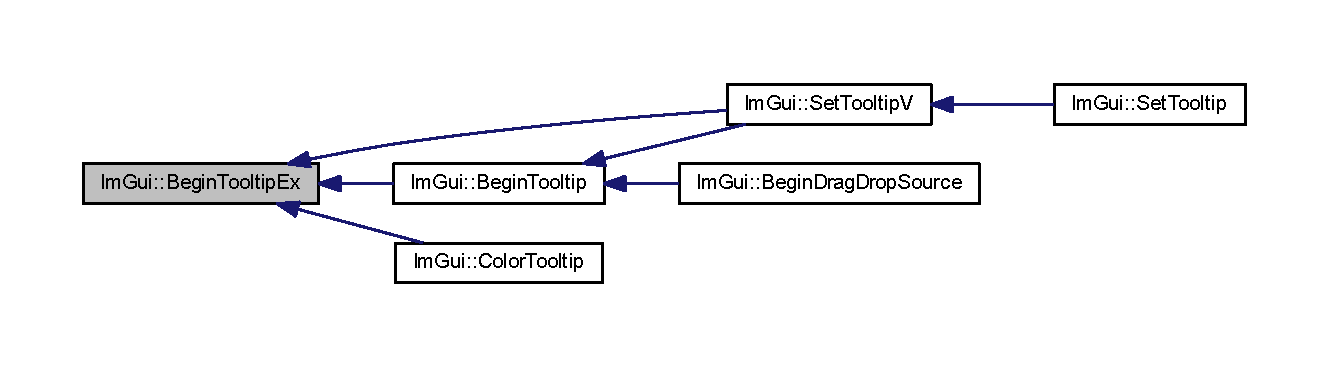
\includegraphics[width=350pt]{namespace_im_gui_a3189530b7795a9b99169eb95f36c516d_icgraph}
\end{center}
\end{figure}
\mbox{\Hypertarget{namespace_im_gui_a34d2363f631f1df5ab1a2a131ab98fa7}\label{namespace_im_gui_a34d2363f631f1df5ab1a2a131ab98fa7}} 
\index{Im\+Gui@{Im\+Gui}!Bring\+Window\+To\+Display\+Back@{Bring\+Window\+To\+Display\+Back}}
\index{Bring\+Window\+To\+Display\+Back@{Bring\+Window\+To\+Display\+Back}!Im\+Gui@{Im\+Gui}}
\subsubsection{\texorpdfstring{Bring\+Window\+To\+Display\+Back()}{BringWindowToDisplayBack()}}
{\footnotesize\ttfamily void Im\+Gui\+::\+Bring\+Window\+To\+Display\+Back (\begin{DoxyParamCaption}\item[{\mbox{\hyperlink{struct_im_gui_window}{Im\+Gui\+Window}} $\ast$}]{window }\end{DoxyParamCaption})}

\mbox{\Hypertarget{namespace_im_gui_a1f7b95f36d03751c928af7b1b745e959}\label{namespace_im_gui_a1f7b95f36d03751c928af7b1b745e959}} 
\index{Im\+Gui@{Im\+Gui}!Bring\+Window\+To\+Display\+Front@{Bring\+Window\+To\+Display\+Front}}
\index{Bring\+Window\+To\+Display\+Front@{Bring\+Window\+To\+Display\+Front}!Im\+Gui@{Im\+Gui}}
\subsubsection{\texorpdfstring{Bring\+Window\+To\+Display\+Front()}{BringWindowToDisplayFront()}}
{\footnotesize\ttfamily void Im\+Gui\+::\+Bring\+Window\+To\+Display\+Front (\begin{DoxyParamCaption}\item[{\mbox{\hyperlink{struct_im_gui_window}{Im\+Gui\+Window}} $\ast$}]{window }\end{DoxyParamCaption})}

Here is the call graph for this function\+:
\nopagebreak
\begin{figure}[H]
\begin{center}
\leavevmode
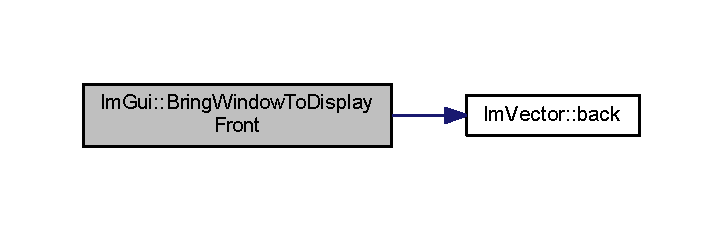
\includegraphics[width=347pt]{namespace_im_gui_a1f7b95f36d03751c928af7b1b745e959_cgraph}
\end{center}
\end{figure}
Here is the caller graph for this function\+:
\nopagebreak
\begin{figure}[H]
\begin{center}
\leavevmode
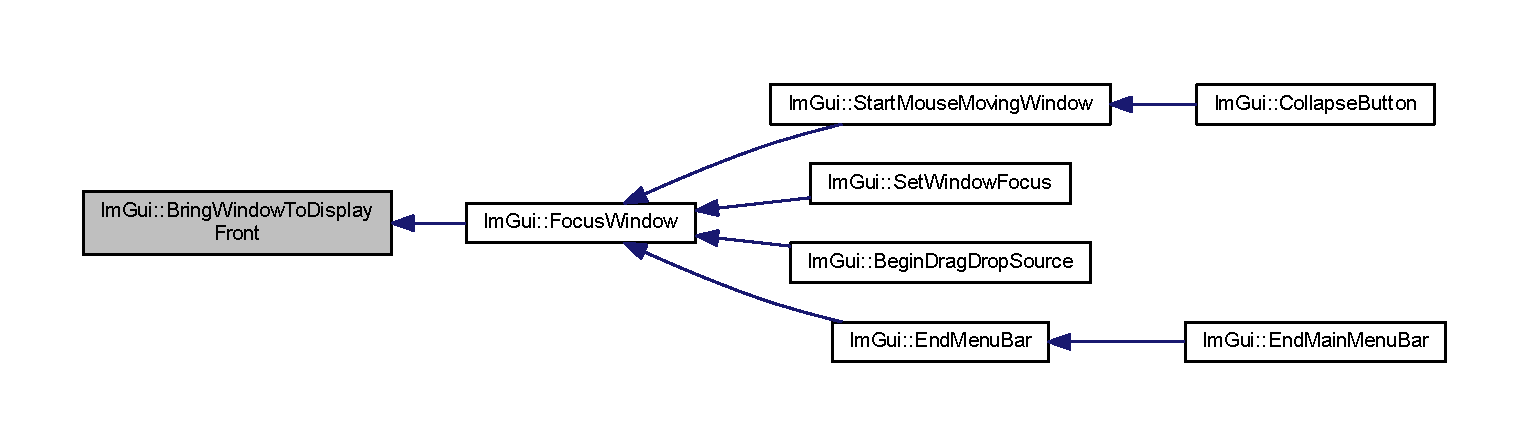
\includegraphics[width=350pt]{namespace_im_gui_a1f7b95f36d03751c928af7b1b745e959_icgraph}
\end{center}
\end{figure}
\mbox{\Hypertarget{namespace_im_gui_affe95a2dc969f0d15fbd4b588c94ac1a}\label{namespace_im_gui_affe95a2dc969f0d15fbd4b588c94ac1a}} 
\index{Im\+Gui@{Im\+Gui}!Bring\+Window\+To\+Focus\+Front@{Bring\+Window\+To\+Focus\+Front}}
\index{Bring\+Window\+To\+Focus\+Front@{Bring\+Window\+To\+Focus\+Front}!Im\+Gui@{Im\+Gui}}
\subsubsection{\texorpdfstring{Bring\+Window\+To\+Focus\+Front()}{BringWindowToFocusFront()}}
{\footnotesize\ttfamily void Im\+Gui\+::\+Bring\+Window\+To\+Focus\+Front (\begin{DoxyParamCaption}\item[{\mbox{\hyperlink{struct_im_gui_window}{Im\+Gui\+Window}} $\ast$}]{window }\end{DoxyParamCaption})}

Here is the call graph for this function\+:
\nopagebreak
\begin{figure}[H]
\begin{center}
\leavevmode
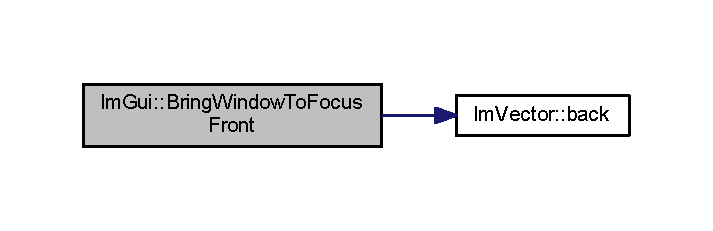
\includegraphics[width=342pt]{namespace_im_gui_affe95a2dc969f0d15fbd4b588c94ac1a_cgraph}
\end{center}
\end{figure}
Here is the caller graph for this function\+:
\nopagebreak
\begin{figure}[H]
\begin{center}
\leavevmode
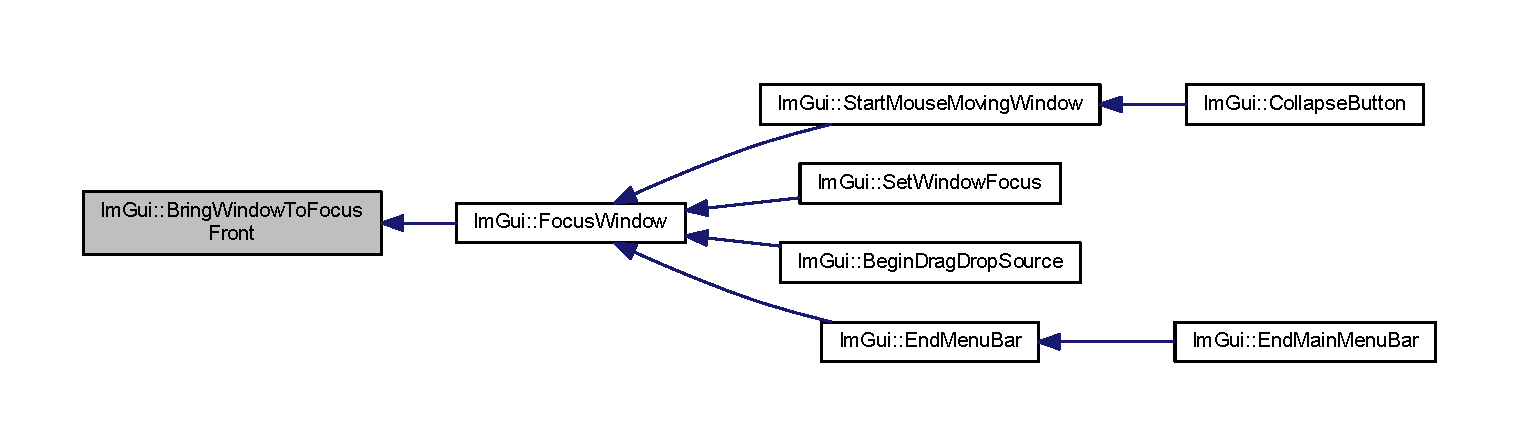
\includegraphics[width=350pt]{namespace_im_gui_affe95a2dc969f0d15fbd4b588c94ac1a_icgraph}
\end{center}
\end{figure}
\mbox{\Hypertarget{namespace_im_gui_ae2d22212681556d2c2398dfd152f3121}\label{namespace_im_gui_ae2d22212681556d2c2398dfd152f3121}} 
\index{Im\+Gui@{Im\+Gui}!Bullet@{Bullet}}
\index{Bullet@{Bullet}!Im\+Gui@{Im\+Gui}}
\subsubsection{\texorpdfstring{Bullet()}{Bullet()}}
{\footnotesize\ttfamily void Im\+Gui\+::\+Bullet (\begin{DoxyParamCaption}{ }\end{DoxyParamCaption})}

Here is the call graph for this function\+:
\nopagebreak
\begin{figure}[H]
\begin{center}
\leavevmode
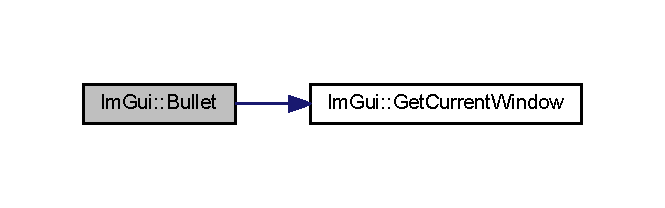
\includegraphics[width=319pt]{namespace_im_gui_ae2d22212681556d2c2398dfd152f3121_cgraph}
\end{center}
\end{figure}
\mbox{\Hypertarget{namespace_im_gui_af8d34d563b17c683943a0fa7bf5807bc}\label{namespace_im_gui_af8d34d563b17c683943a0fa7bf5807bc}} 
\index{Im\+Gui@{Im\+Gui}!Bullet\+Text@{Bullet\+Text}}
\index{Bullet\+Text@{Bullet\+Text}!Im\+Gui@{Im\+Gui}}
\subsubsection{\texorpdfstring{Bullet\+Text()}{BulletText()}}
{\footnotesize\ttfamily void Im\+Gui\+::\+Bullet\+Text (\begin{DoxyParamCaption}\item[{const char $\ast$}]{fmt,  }\item[{}]{... }\end{DoxyParamCaption})}

Here is the call graph for this function\+:
\nopagebreak
\begin{figure}[H]
\begin{center}
\leavevmode
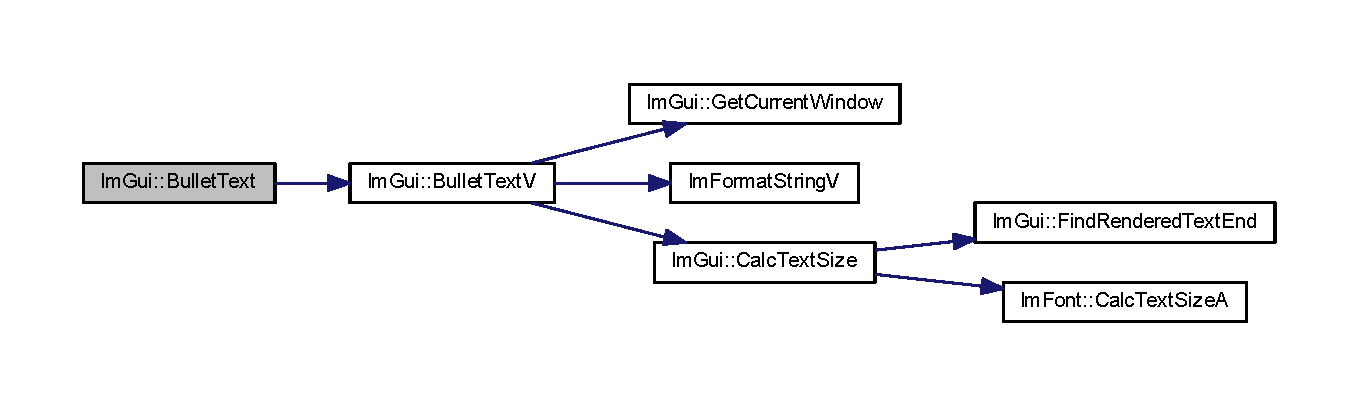
\includegraphics[width=350pt]{namespace_im_gui_af8d34d563b17c683943a0fa7bf5807bc_cgraph}
\end{center}
\end{figure}
Here is the caller graph for this function\+:
\nopagebreak
\begin{figure}[H]
\begin{center}
\leavevmode
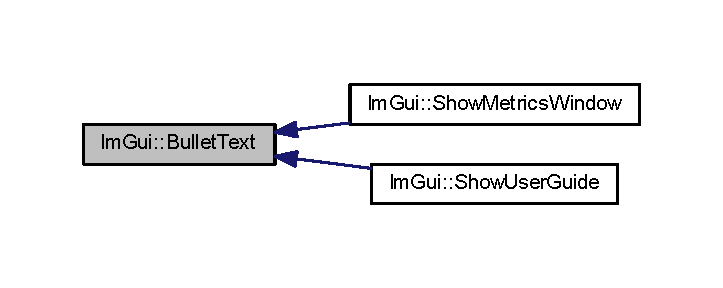
\includegraphics[width=347pt]{namespace_im_gui_af8d34d563b17c683943a0fa7bf5807bc_icgraph}
\end{center}
\end{figure}
\mbox{\Hypertarget{namespace_im_gui_af8f4b5e96c745e205974857f9a584583}\label{namespace_im_gui_af8f4b5e96c745e205974857f9a584583}} 
\index{Im\+Gui@{Im\+Gui}!Bullet\+TextV@{Bullet\+TextV}}
\index{Bullet\+TextV@{Bullet\+TextV}!Im\+Gui@{Im\+Gui}}
\subsubsection{\texorpdfstring{Bullet\+Text\+V()}{BulletTextV()}}
{\footnotesize\ttfamily void Im\+Gui\+::\+Bullet\+TextV (\begin{DoxyParamCaption}\item[{const char $\ast$}]{fmt,  }\item[{va\+\_\+list}]{args }\end{DoxyParamCaption})}

Here is the call graph for this function\+:
\nopagebreak
\begin{figure}[H]
\begin{center}
\leavevmode
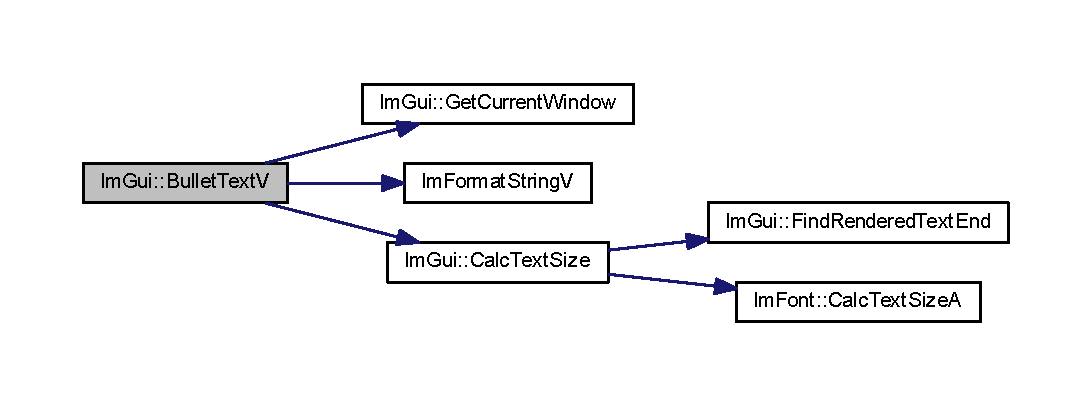
\includegraphics[width=350pt]{namespace_im_gui_af8f4b5e96c745e205974857f9a584583_cgraph}
\end{center}
\end{figure}
Here is the caller graph for this function\+:
\nopagebreak
\begin{figure}[H]
\begin{center}
\leavevmode
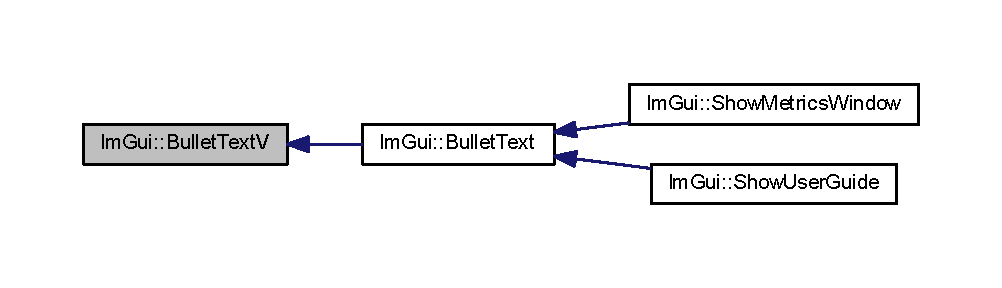
\includegraphics[width=350pt]{namespace_im_gui_af8f4b5e96c745e205974857f9a584583_icgraph}
\end{center}
\end{figure}
\mbox{\Hypertarget{namespace_im_gui_a38094c568ce398db5a3abb9d3ac92030}\label{namespace_im_gui_a38094c568ce398db5a3abb9d3ac92030}} 
\index{Im\+Gui@{Im\+Gui}!Button@{Button}}
\index{Button@{Button}!Im\+Gui@{Im\+Gui}}
\subsubsection{\texorpdfstring{Button()}{Button()}}
{\footnotesize\ttfamily bool Im\+Gui\+::\+Button (\begin{DoxyParamCaption}\item[{const char $\ast$}]{label,  }\item[{const \mbox{\hyperlink{struct_im_vec2}{Im\+Vec2}} \&}]{size = {\ttfamily \mbox{\hyperlink{struct_im_vec2}{Im\+Vec2}}(0,0)} }\end{DoxyParamCaption})}

Here is the call graph for this function\+:
\nopagebreak
\begin{figure}[H]
\begin{center}
\leavevmode
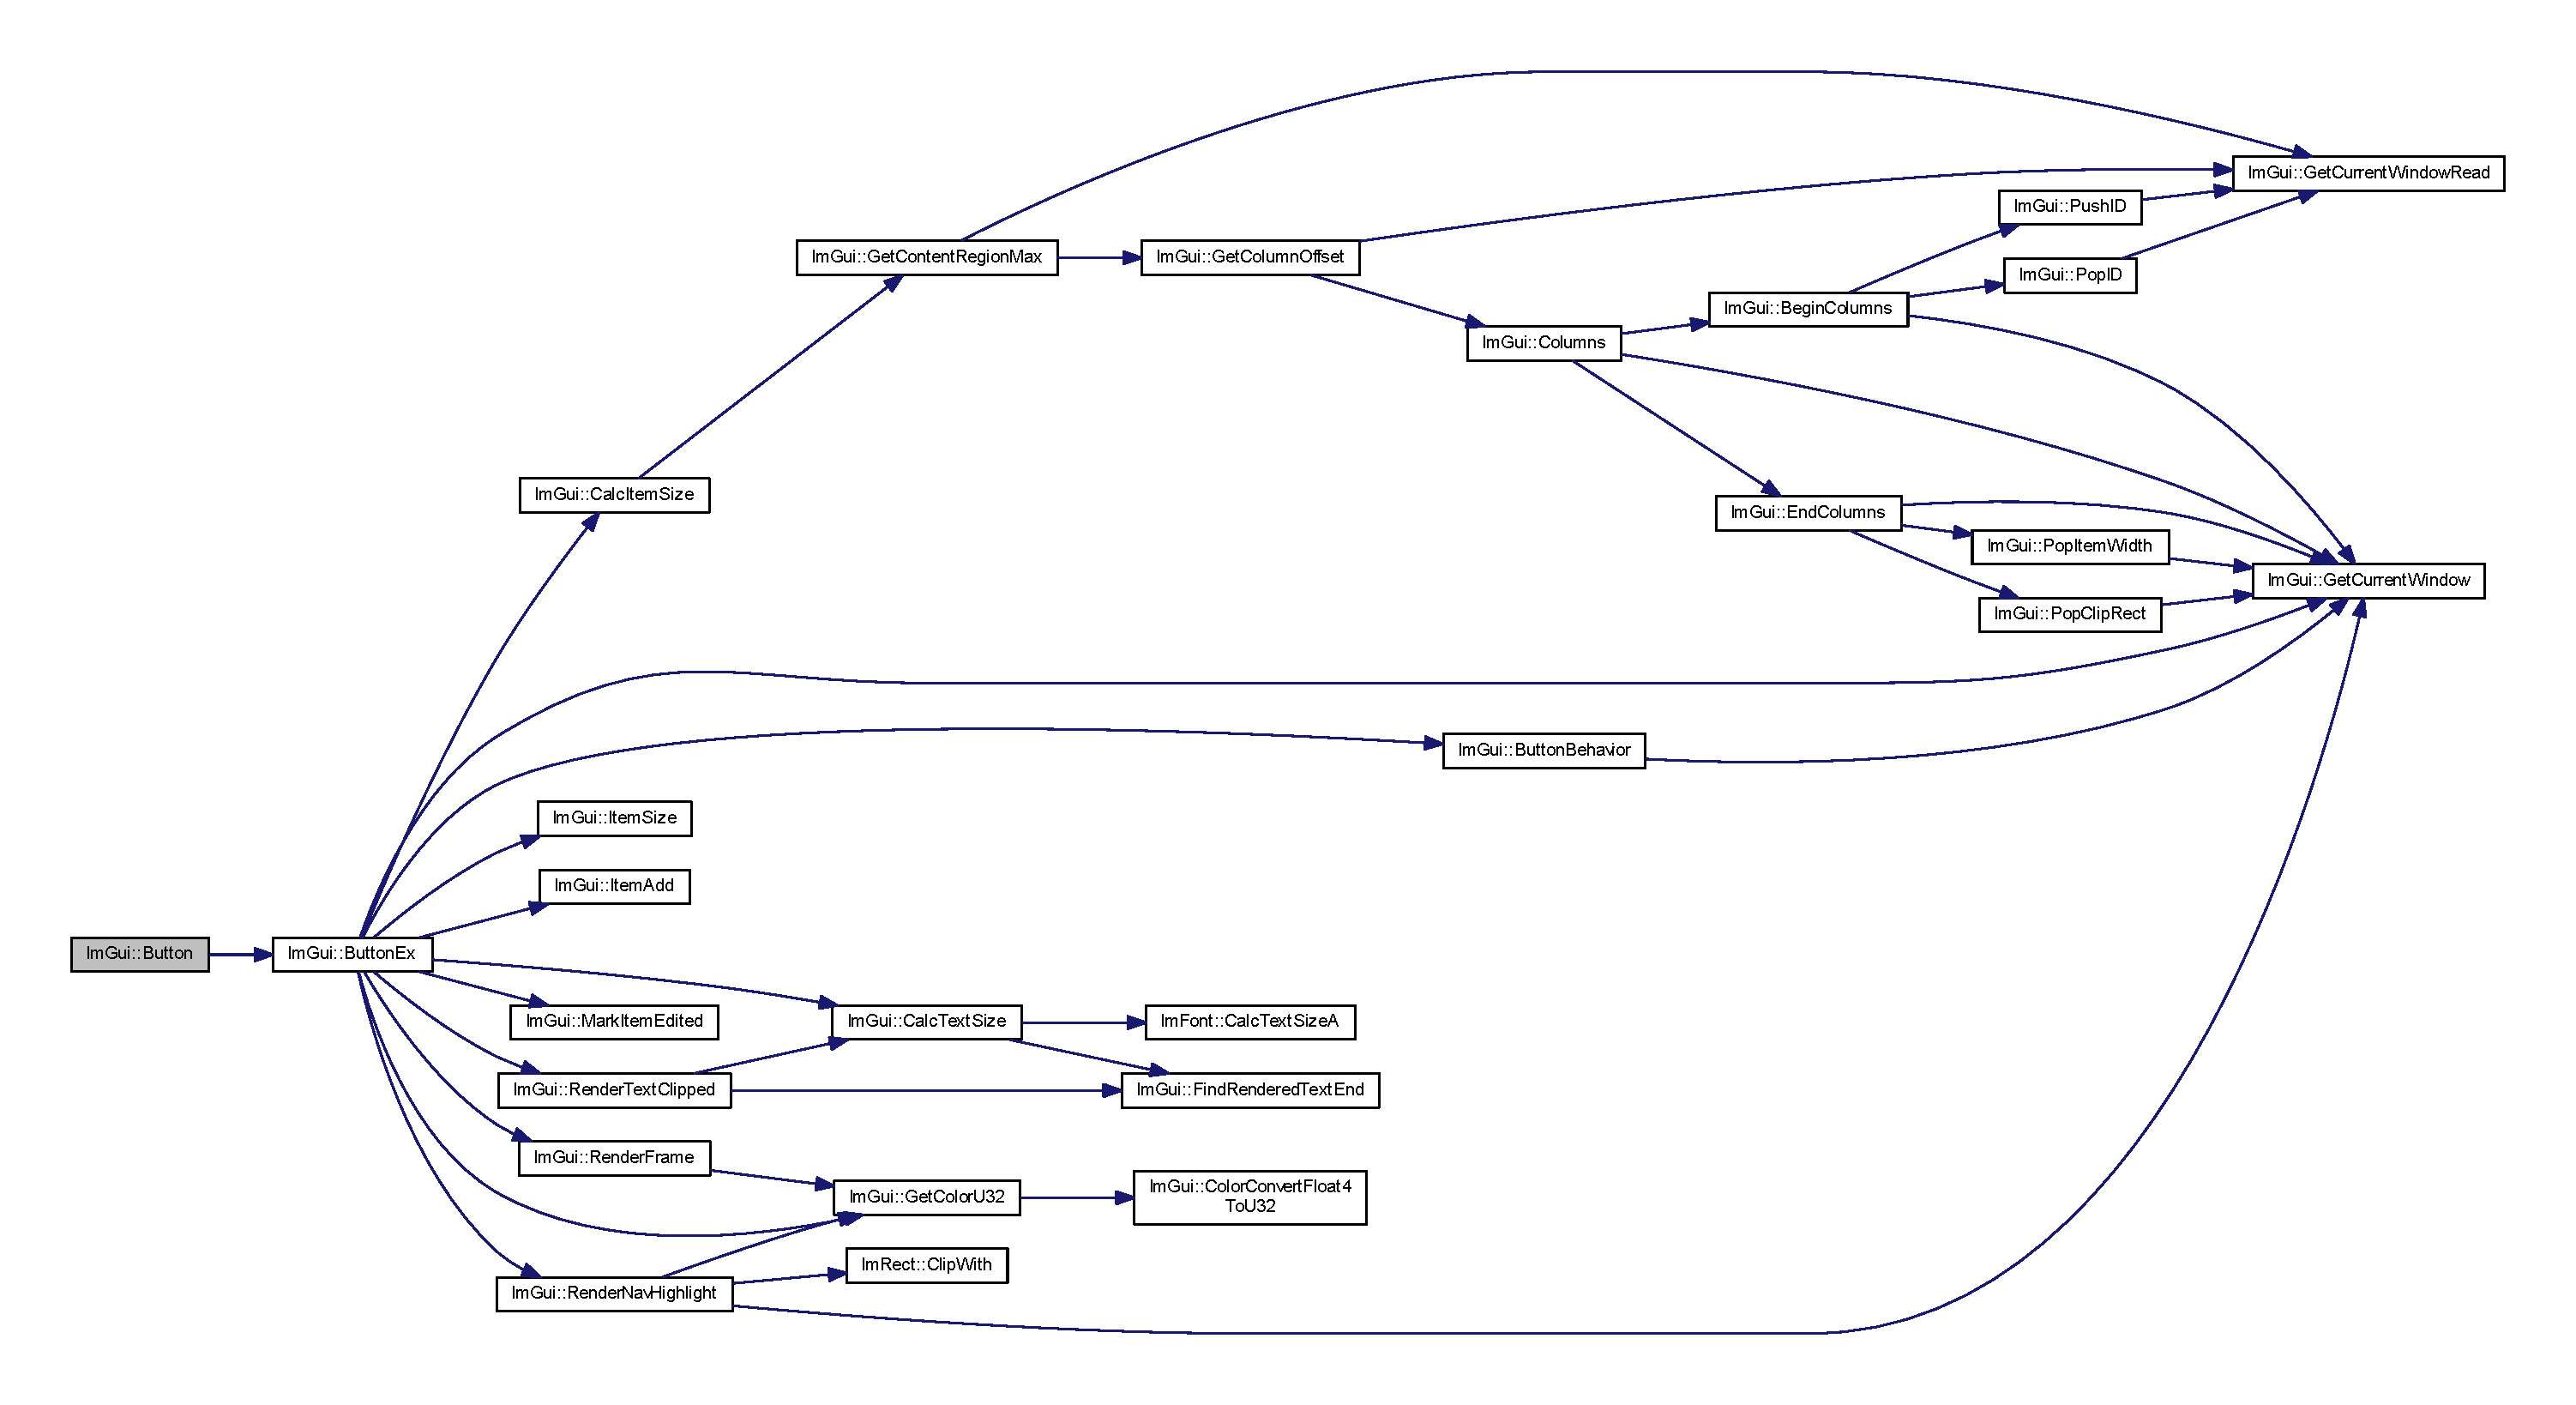
\includegraphics[width=350pt]{namespace_im_gui_a38094c568ce398db5a3abb9d3ac92030_cgraph}
\end{center}
\end{figure}
Here is the caller graph for this function\+:
\nopagebreak
\begin{figure}[H]
\begin{center}
\leavevmode
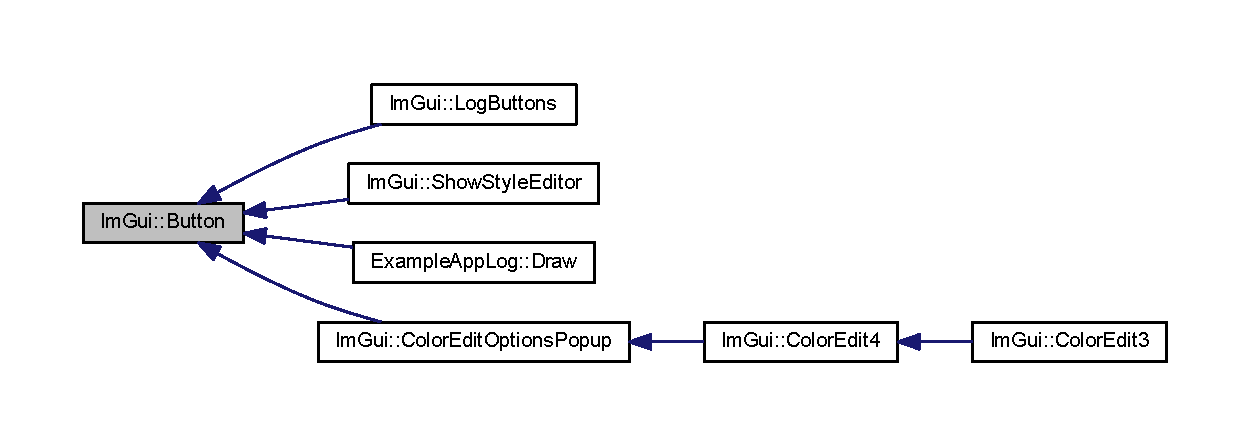
\includegraphics[width=350pt]{namespace_im_gui_a38094c568ce398db5a3abb9d3ac92030_icgraph}
\end{center}
\end{figure}
\mbox{\Hypertarget{namespace_im_gui_a65a4f18b1bc8ce0f351687922089f374}\label{namespace_im_gui_a65a4f18b1bc8ce0f351687922089f374}} 
\index{Im\+Gui@{Im\+Gui}!Button\+Behavior@{Button\+Behavior}}
\index{Button\+Behavior@{Button\+Behavior}!Im\+Gui@{Im\+Gui}}
\subsubsection{\texorpdfstring{Button\+Behavior()}{ButtonBehavior()}}
{\footnotesize\ttfamily bool Im\+Gui\+::\+Button\+Behavior (\begin{DoxyParamCaption}\item[{const \mbox{\hyperlink{struct_im_rect}{Im\+Rect}} \&}]{bb,  }\item[{\mbox{\hyperlink{imgui_8h_a1785c9b6f4e16406764a85f32582236f}{Im\+Gui\+ID}}}]{id,  }\item[{bool $\ast$}]{out\+\_\+hovered,  }\item[{bool $\ast$}]{out\+\_\+held,  }\item[{\mbox{\hyperlink{imgui__internal_8h_a990fae518aa1d95f571ee40989de4c22}{Im\+Gui\+Button\+Flags}}}]{flags = {\ttfamily 0} }\end{DoxyParamCaption})}

Here is the call graph for this function\+:
\nopagebreak
\begin{figure}[H]
\begin{center}
\leavevmode
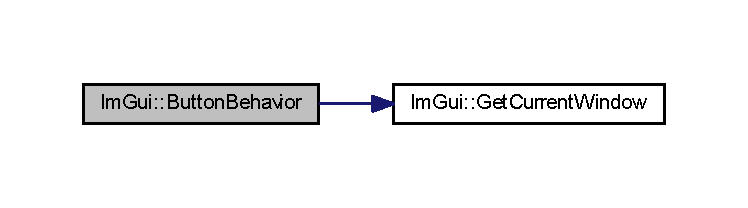
\includegraphics[width=350pt]{namespace_im_gui_a65a4f18b1bc8ce0f351687922089f374_cgraph}
\end{center}
\end{figure}
Here is the caller graph for this function\+:
\nopagebreak
\begin{figure}[H]
\begin{center}
\leavevmode
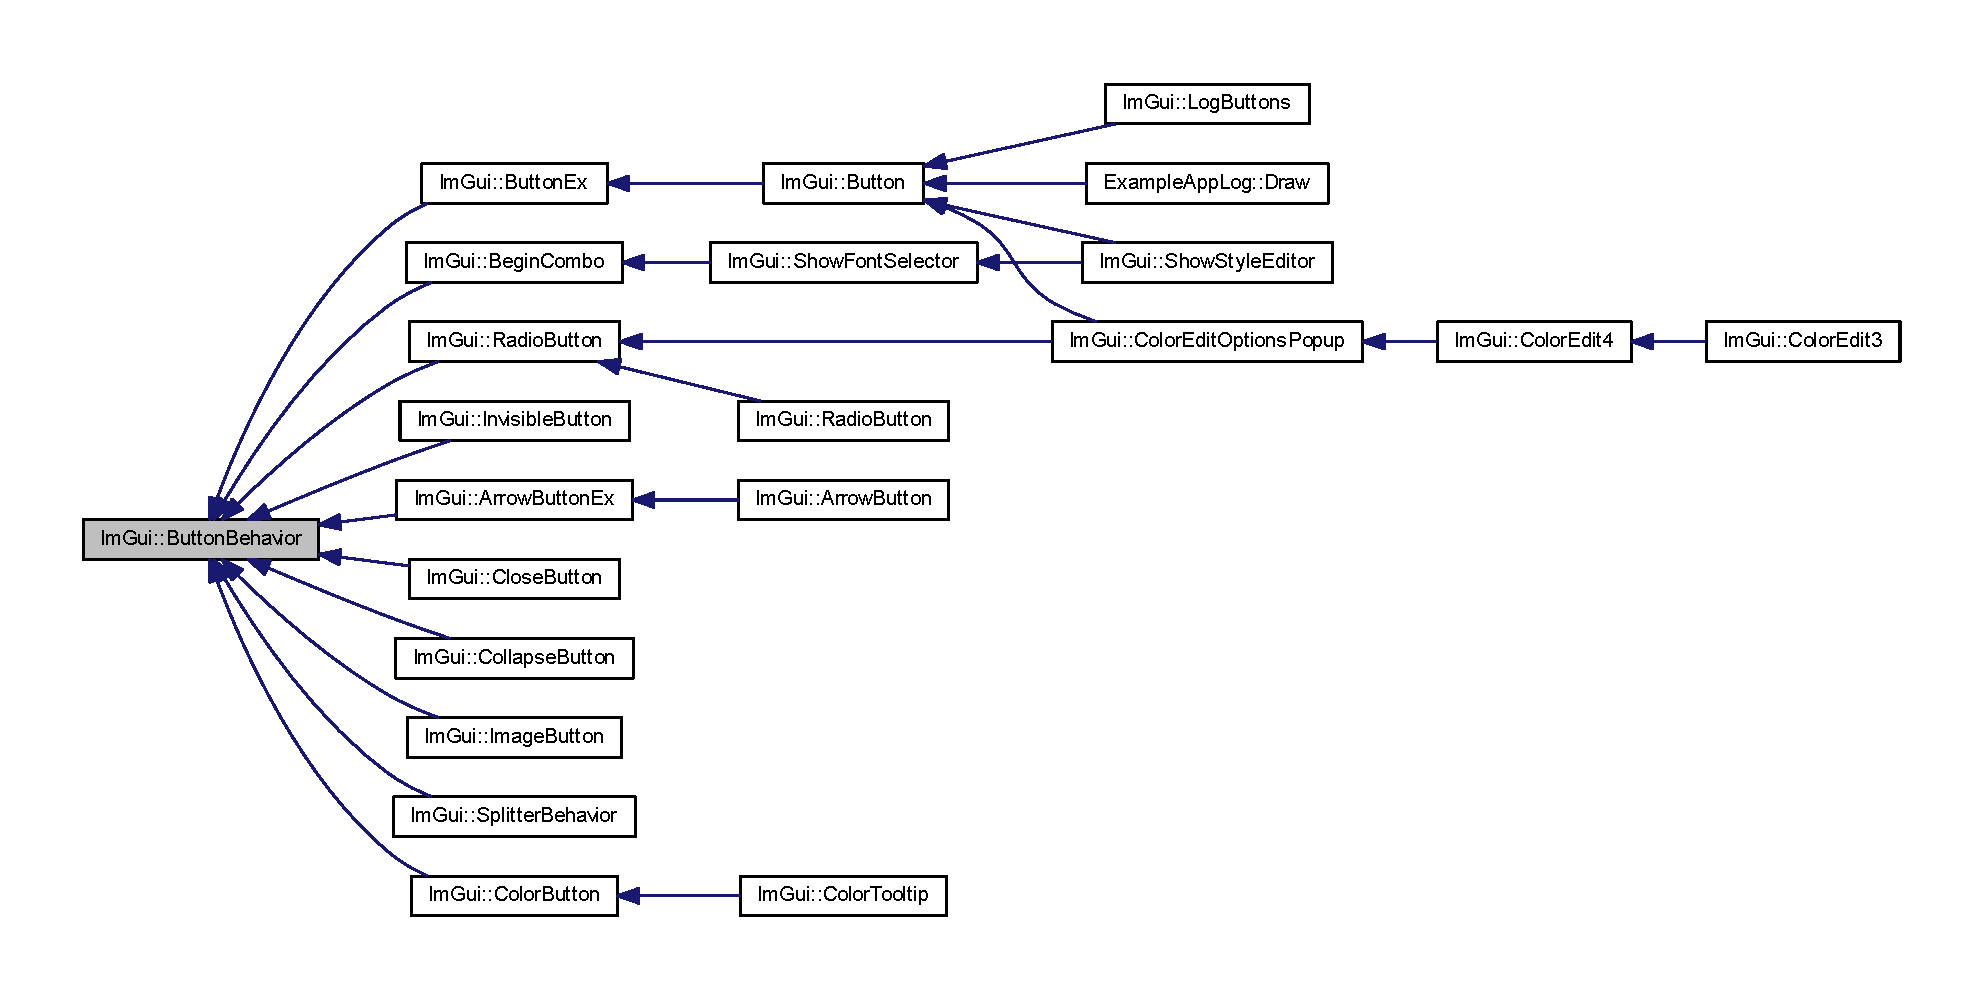
\includegraphics[width=350pt]{namespace_im_gui_a65a4f18b1bc8ce0f351687922089f374_icgraph}
\end{center}
\end{figure}
\mbox{\Hypertarget{namespace_im_gui_ae479220c66b039874c6e4c9e9b22849f}\label{namespace_im_gui_ae479220c66b039874c6e4c9e9b22849f}} 
\index{Im\+Gui@{Im\+Gui}!Button\+Ex@{Button\+Ex}}
\index{Button\+Ex@{Button\+Ex}!Im\+Gui@{Im\+Gui}}
\subsubsection{\texorpdfstring{Button\+Ex()}{ButtonEx()}}
{\footnotesize\ttfamily bool Im\+Gui\+::\+Button\+Ex (\begin{DoxyParamCaption}\item[{const char $\ast$}]{label,  }\item[{const \mbox{\hyperlink{struct_im_vec2}{Im\+Vec2}} \&}]{size\+\_\+arg = {\ttfamily \mbox{\hyperlink{struct_im_vec2}{Im\+Vec2}}(0,0)},  }\item[{\mbox{\hyperlink{imgui__internal_8h_a990fae518aa1d95f571ee40989de4c22}{Im\+Gui\+Button\+Flags}}}]{flags = {\ttfamily 0} }\end{DoxyParamCaption})}

Here is the call graph for this function\+:
\nopagebreak
\begin{figure}[H]
\begin{center}
\leavevmode
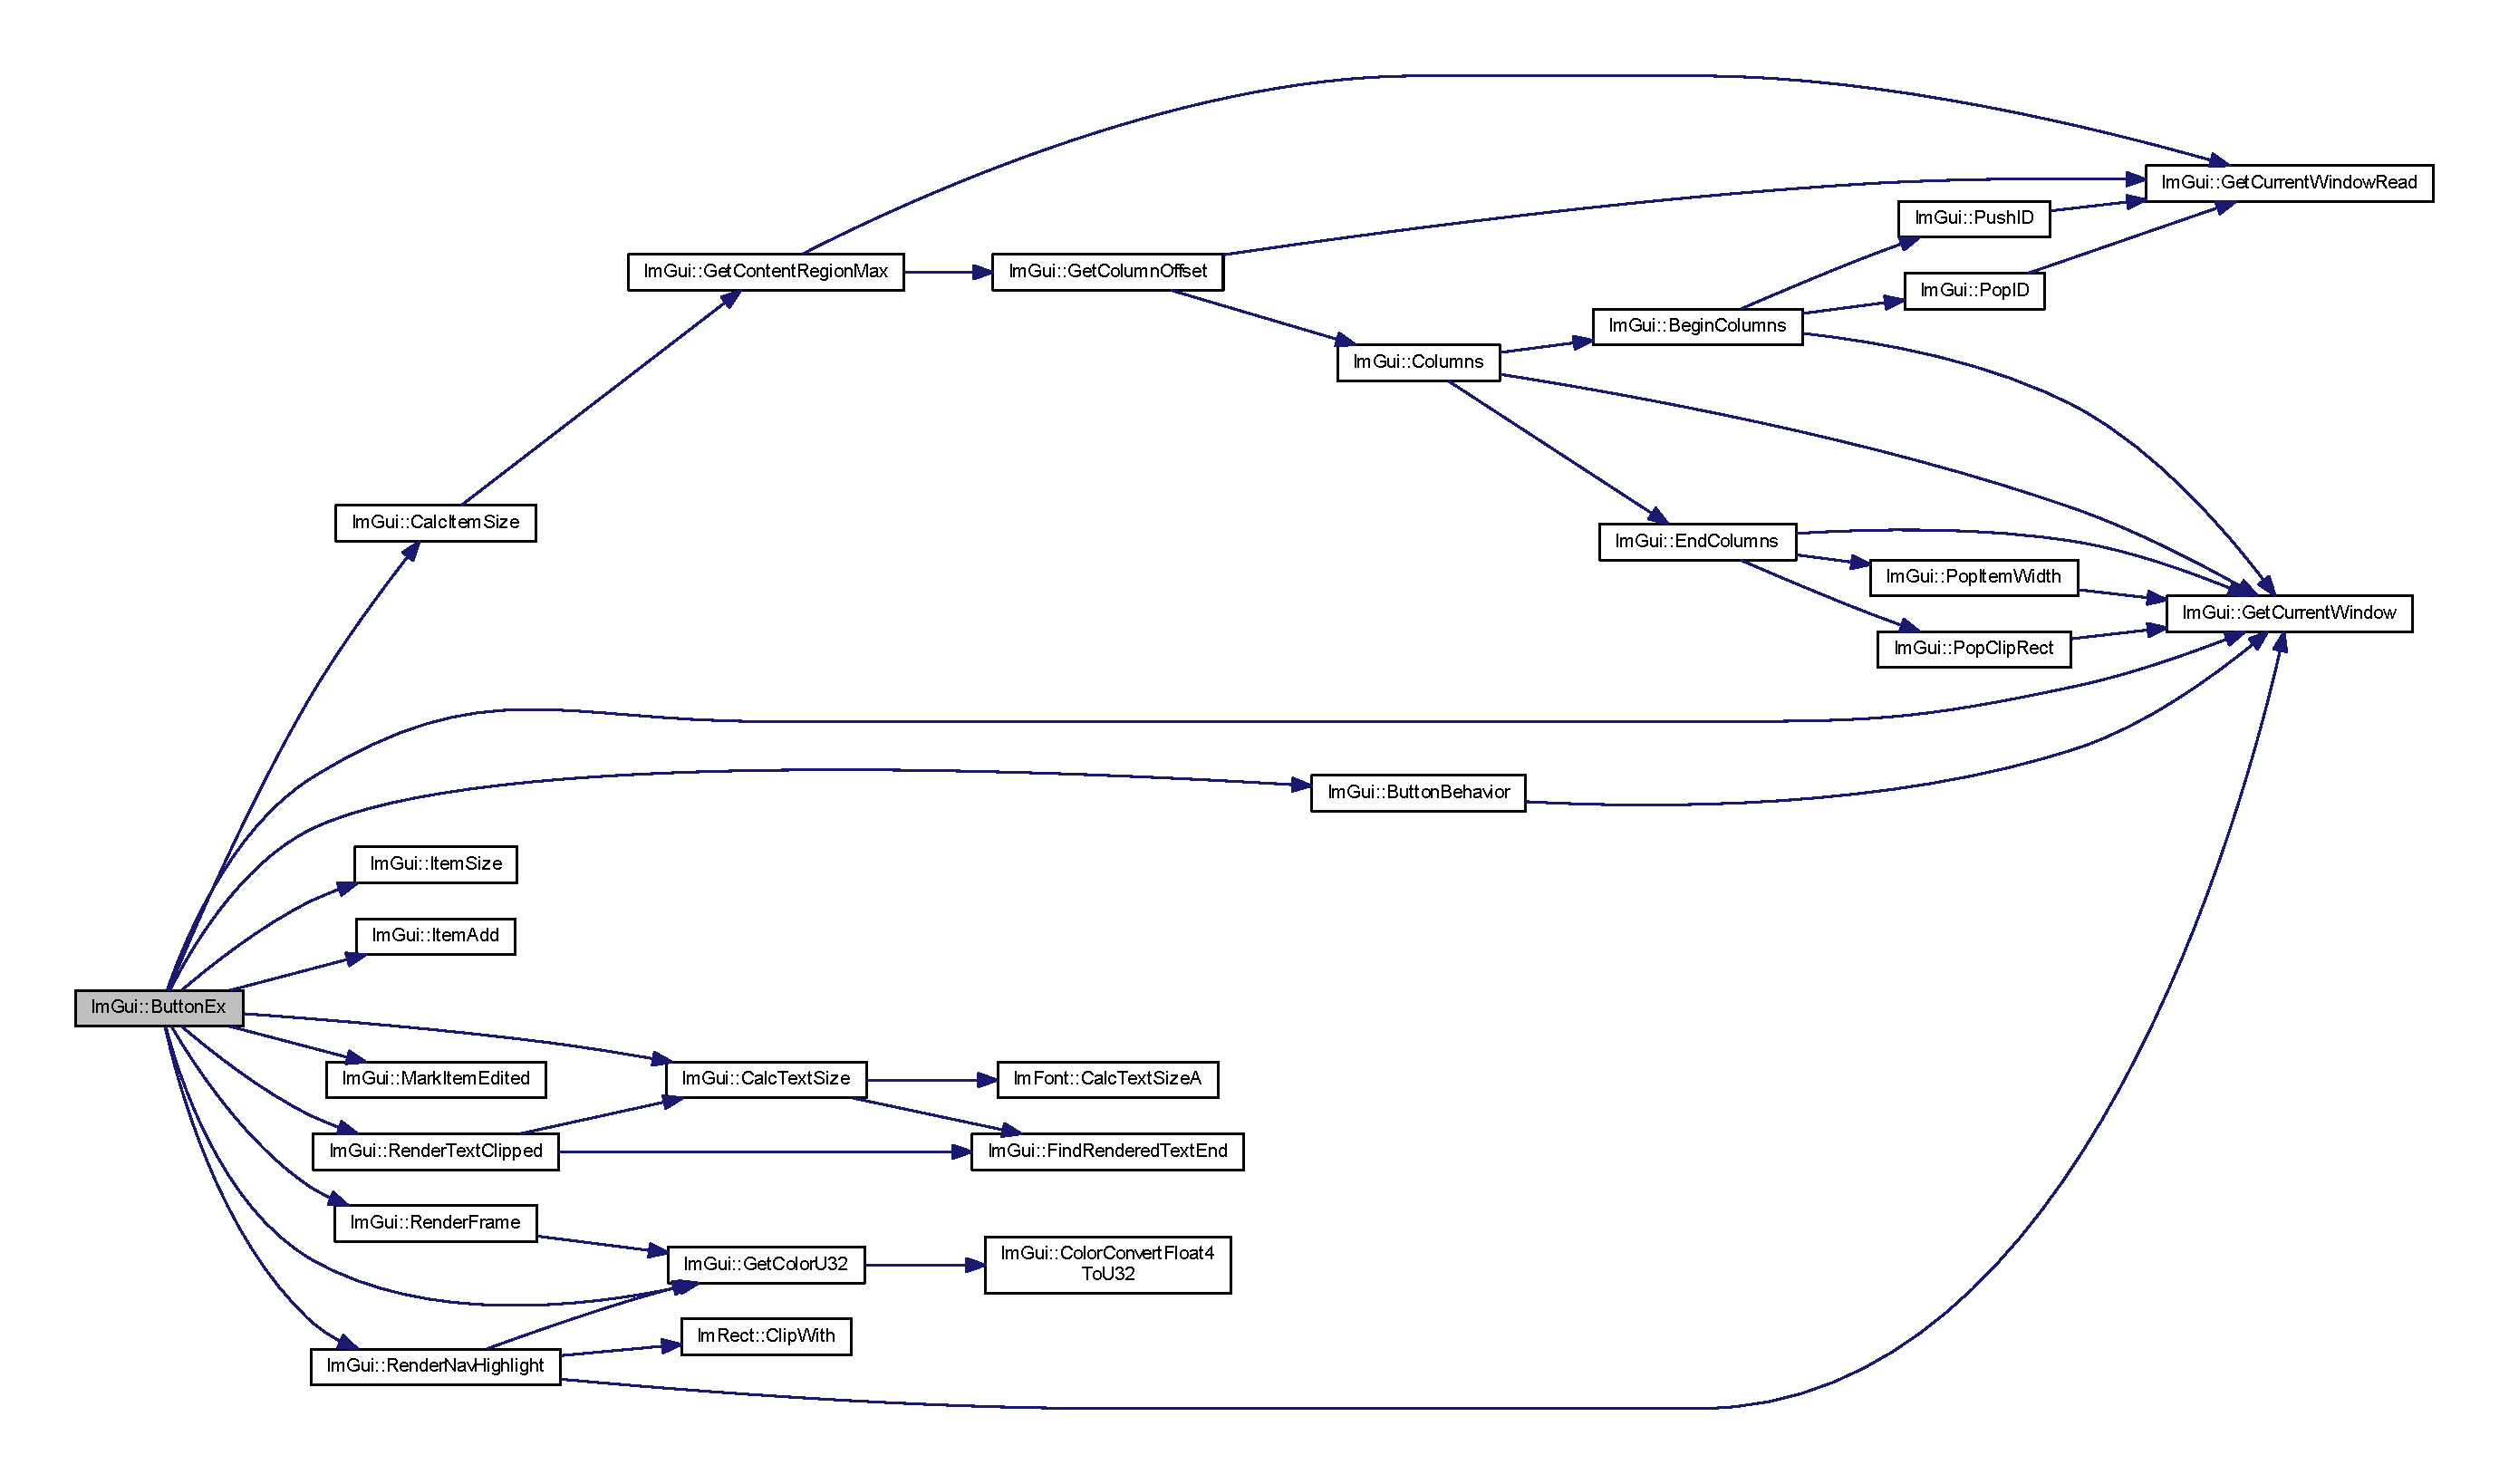
\includegraphics[width=350pt]{namespace_im_gui_ae479220c66b039874c6e4c9e9b22849f_cgraph}
\end{center}
\end{figure}
Here is the caller graph for this function\+:
\nopagebreak
\begin{figure}[H]
\begin{center}
\leavevmode
\includegraphics[width=350pt]{namespace_im_gui_ae479220c66b039874c6e4c9e9b22849f_icgraph}
\end{center}
\end{figure}
\mbox{\Hypertarget{namespace_im_gui_a3c1505e785f9571ed82500692a727c5f}\label{namespace_im_gui_a3c1505e785f9571ed82500692a727c5f}} 
\index{Im\+Gui@{Im\+Gui}!Calc\+Item\+Size@{Calc\+Item\+Size}}
\index{Calc\+Item\+Size@{Calc\+Item\+Size}!Im\+Gui@{Im\+Gui}}
\subsubsection{\texorpdfstring{Calc\+Item\+Size()}{CalcItemSize()}}
{\footnotesize\ttfamily \mbox{\hyperlink{struct_im_vec2}{Im\+Vec2}} Im\+Gui\+::\+Calc\+Item\+Size (\begin{DoxyParamCaption}\item[{\mbox{\hyperlink{struct_im_vec2}{Im\+Vec2}}}]{size,  }\item[{float}]{default\+\_\+x,  }\item[{float}]{default\+\_\+y }\end{DoxyParamCaption})}

Here is the call graph for this function\+:
\nopagebreak
\begin{figure}[H]
\begin{center}
\leavevmode
\includegraphics[width=350pt]{namespace_im_gui_a3c1505e785f9571ed82500692a727c5f_cgraph}
\end{center}
\end{figure}
Here is the caller graph for this function\+:
\nopagebreak
\begin{figure}[H]
\begin{center}
\leavevmode
\includegraphics[width=350pt]{namespace_im_gui_a3c1505e785f9571ed82500692a727c5f_icgraph}
\end{center}
\end{figure}
\mbox{\Hypertarget{namespace_im_gui_ab3b3ba92ebd8bca4a552dd93321a1994}\label{namespace_im_gui_ab3b3ba92ebd8bca4a552dd93321a1994}} 
\index{Im\+Gui@{Im\+Gui}!Calc\+Item\+Width@{Calc\+Item\+Width}}
\index{Calc\+Item\+Width@{Calc\+Item\+Width}!Im\+Gui@{Im\+Gui}}
\subsubsection{\texorpdfstring{Calc\+Item\+Width()}{CalcItemWidth()}}
{\footnotesize\ttfamily float Im\+Gui\+::\+Calc\+Item\+Width (\begin{DoxyParamCaption}{ }\end{DoxyParamCaption})}

Here is the call graph for this function\+:
\nopagebreak
\begin{figure}[H]
\begin{center}
\leavevmode
\includegraphics[width=350pt]{namespace_im_gui_ab3b3ba92ebd8bca4a552dd93321a1994_cgraph}
\end{center}
\end{figure}
Here is the caller graph for this function\+:
\nopagebreak
\begin{figure}[H]
\begin{center}
\leavevmode
\includegraphics[width=350pt]{namespace_im_gui_ab3b3ba92ebd8bca4a552dd93321a1994_icgraph}
\end{center}
\end{figure}
\mbox{\Hypertarget{namespace_im_gui_ae5319370628374ef8febf0c25c285b7e}\label{namespace_im_gui_ae5319370628374ef8febf0c25c285b7e}} 
\index{Im\+Gui@{Im\+Gui}!Calc\+List\+Clipping@{Calc\+List\+Clipping}}
\index{Calc\+List\+Clipping@{Calc\+List\+Clipping}!Im\+Gui@{Im\+Gui}}
\subsubsection{\texorpdfstring{Calc\+List\+Clipping()}{CalcListClipping()}}
{\footnotesize\ttfamily void Im\+Gui\+::\+Calc\+List\+Clipping (\begin{DoxyParamCaption}\item[{int}]{items\+\_\+count,  }\item[{float}]{items\+\_\+height,  }\item[{int $\ast$}]{out\+\_\+items\+\_\+display\+\_\+start,  }\item[{int $\ast$}]{out\+\_\+items\+\_\+display\+\_\+end }\end{DoxyParamCaption})}

Here is the call graph for this function\+:
\nopagebreak
\begin{figure}[H]
\begin{center}
\leavevmode
\includegraphics[width=305pt]{namespace_im_gui_ae5319370628374ef8febf0c25c285b7e_cgraph}
\end{center}
\end{figure}
Here is the caller graph for this function\+:
\nopagebreak
\begin{figure}[H]
\begin{center}
\leavevmode
\includegraphics[width=350pt]{namespace_im_gui_ae5319370628374ef8febf0c25c285b7e_icgraph}
\end{center}
\end{figure}
\mbox{\Hypertarget{namespace_im_gui_a848b9db6cc4a186751c0ecebcaadc33b}\label{namespace_im_gui_a848b9db6cc4a186751c0ecebcaadc33b}} 
\index{Im\+Gui@{Im\+Gui}!Calc\+Text\+Size@{Calc\+Text\+Size}}
\index{Calc\+Text\+Size@{Calc\+Text\+Size}!Im\+Gui@{Im\+Gui}}
\subsubsection{\texorpdfstring{Calc\+Text\+Size()}{CalcTextSize()}}
{\footnotesize\ttfamily \mbox{\hyperlink{struct_im_vec2}{Im\+Vec2}} Im\+Gui\+::\+Calc\+Text\+Size (\begin{DoxyParamCaption}\item[{const char $\ast$}]{text,  }\item[{const char $\ast$}]{text\+\_\+end = {\ttfamily NULL},  }\item[{bool}]{hide\+\_\+text\+\_\+after\+\_\+double\+\_\+hash = {\ttfamily false},  }\item[{float}]{wrap\+\_\+width = {\ttfamily -\/1.0f} }\end{DoxyParamCaption})}

Here is the call graph for this function\+:
\nopagebreak
\begin{figure}[H]
\begin{center}
\leavevmode
\includegraphics[width=350pt]{namespace_im_gui_a848b9db6cc4a186751c0ecebcaadc33b_cgraph}
\end{center}
\end{figure}
Here is the caller graph for this function\+:
\nopagebreak
\begin{figure}[H]
\begin{center}
\leavevmode
\includegraphics[width=350pt]{namespace_im_gui_a848b9db6cc4a186751c0ecebcaadc33b_icgraph}
\end{center}
\end{figure}
\mbox{\Hypertarget{namespace_im_gui_ad3af0fc327467a44116d7d04018b9124}\label{namespace_im_gui_ad3af0fc327467a44116d7d04018b9124}} 
\index{Im\+Gui@{Im\+Gui}!Calc\+Typematic\+Pressed\+Repeat\+Amount@{Calc\+Typematic\+Pressed\+Repeat\+Amount}}
\index{Calc\+Typematic\+Pressed\+Repeat\+Amount@{Calc\+Typematic\+Pressed\+Repeat\+Amount}!Im\+Gui@{Im\+Gui}}
\subsubsection{\texorpdfstring{Calc\+Typematic\+Pressed\+Repeat\+Amount()}{CalcTypematicPressedRepeatAmount()}}
{\footnotesize\ttfamily int Im\+Gui\+::\+Calc\+Typematic\+Pressed\+Repeat\+Amount (\begin{DoxyParamCaption}\item[{float}]{t,  }\item[{float}]{t\+\_\+prev,  }\item[{float}]{repeat\+\_\+delay,  }\item[{float}]{repeat\+\_\+rate }\end{DoxyParamCaption})}

Here is the caller graph for this function\+:
\nopagebreak
\begin{figure}[H]
\begin{center}
\leavevmode
\includegraphics[width=350pt]{namespace_im_gui_ad3af0fc327467a44116d7d04018b9124_icgraph}
\end{center}
\end{figure}
\mbox{\Hypertarget{namespace_im_gui_ae81c20afd5ce4b663f48d05c40af93f9}\label{namespace_im_gui_ae81c20afd5ce4b663f48d05c40af93f9}} 
\index{Im\+Gui@{Im\+Gui}!Calc\+Window\+Expected\+Size@{Calc\+Window\+Expected\+Size}}
\index{Calc\+Window\+Expected\+Size@{Calc\+Window\+Expected\+Size}!Im\+Gui@{Im\+Gui}}
\subsubsection{\texorpdfstring{Calc\+Window\+Expected\+Size()}{CalcWindowExpectedSize()}}
{\footnotesize\ttfamily \mbox{\hyperlink{struct_im_vec2}{Im\+Vec2}} Im\+Gui\+::\+Calc\+Window\+Expected\+Size (\begin{DoxyParamCaption}\item[{\mbox{\hyperlink{struct_im_gui_window}{Im\+Gui\+Window}} $\ast$}]{window }\end{DoxyParamCaption})}

\mbox{\Hypertarget{namespace_im_gui_a66416151e58c34cd02973976de66e0e9}\label{namespace_im_gui_a66416151e58c34cd02973976de66e0e9}} 
\index{Im\+Gui@{Im\+Gui}!Calc\+Wrap\+Width\+For\+Pos@{Calc\+Wrap\+Width\+For\+Pos}}
\index{Calc\+Wrap\+Width\+For\+Pos@{Calc\+Wrap\+Width\+For\+Pos}!Im\+Gui@{Im\+Gui}}
\subsubsection{\texorpdfstring{Calc\+Wrap\+Width\+For\+Pos()}{CalcWrapWidthForPos()}}
{\footnotesize\ttfamily float Im\+Gui\+::\+Calc\+Wrap\+Width\+For\+Pos (\begin{DoxyParamCaption}\item[{const \mbox{\hyperlink{struct_im_vec2}{Im\+Vec2}} \&}]{pos,  }\item[{float}]{wrap\+\_\+pos\+\_\+x }\end{DoxyParamCaption})}

Here is the call graph for this function\+:
\nopagebreak
\begin{figure}[H]
\begin{center}
\leavevmode
\includegraphics[width=350pt]{namespace_im_gui_a66416151e58c34cd02973976de66e0e9_cgraph}
\end{center}
\end{figure}
\mbox{\Hypertarget{namespace_im_gui_af382f9360d73917a9e9c0d26b5797552}\label{namespace_im_gui_af382f9360d73917a9e9c0d26b5797552}} 
\index{Im\+Gui@{Im\+Gui}!Capture\+Keyboard\+From\+App@{Capture\+Keyboard\+From\+App}}
\index{Capture\+Keyboard\+From\+App@{Capture\+Keyboard\+From\+App}!Im\+Gui@{Im\+Gui}}
\subsubsection{\texorpdfstring{Capture\+Keyboard\+From\+App()}{CaptureKeyboardFromApp()}}
{\footnotesize\ttfamily void Im\+Gui\+::\+Capture\+Keyboard\+From\+App (\begin{DoxyParamCaption}\item[{bool}]{capture = {\ttfamily true} }\end{DoxyParamCaption})}

\mbox{\Hypertarget{namespace_im_gui_a3a86fbf0d334b30dc16fb44955f1ce54}\label{namespace_im_gui_a3a86fbf0d334b30dc16fb44955f1ce54}} 
\index{Im\+Gui@{Im\+Gui}!Capture\+Mouse\+From\+App@{Capture\+Mouse\+From\+App}}
\index{Capture\+Mouse\+From\+App@{Capture\+Mouse\+From\+App}!Im\+Gui@{Im\+Gui}}
\subsubsection{\texorpdfstring{Capture\+Mouse\+From\+App()}{CaptureMouseFromApp()}}
{\footnotesize\ttfamily void Im\+Gui\+::\+Capture\+Mouse\+From\+App (\begin{DoxyParamCaption}\item[{bool}]{capture = {\ttfamily true} }\end{DoxyParamCaption})}

\mbox{\Hypertarget{namespace_im_gui_a57d73c1d0ef807fef734d91024092027}\label{namespace_im_gui_a57d73c1d0ef807fef734d91024092027}} 
\index{Im\+Gui@{Im\+Gui}!Checkbox@{Checkbox}}
\index{Checkbox@{Checkbox}!Im\+Gui@{Im\+Gui}}
\subsubsection{\texorpdfstring{Checkbox()}{Checkbox()}}
{\footnotesize\ttfamily bool Im\+Gui\+::\+Checkbox (\begin{DoxyParamCaption}\item[{const char $\ast$}]{label,  }\item[{bool $\ast$}]{v }\end{DoxyParamCaption})}

Here is the call graph for this function\+:
\nopagebreak
\begin{figure}[H]
\begin{center}
\leavevmode
\includegraphics[width=350pt]{namespace_im_gui_a57d73c1d0ef807fef734d91024092027_cgraph}
\end{center}
\end{figure}
Here is the caller graph for this function\+:
\nopagebreak
\begin{figure}[H]
\begin{center}
\leavevmode
\includegraphics[width=347pt]{namespace_im_gui_a57d73c1d0ef807fef734d91024092027_icgraph}
\end{center}
\end{figure}
\mbox{\Hypertarget{namespace_im_gui_aeca400dcf5a82c312b3e669d2fe6e88d}\label{namespace_im_gui_aeca400dcf5a82c312b3e669d2fe6e88d}} 
\index{Im\+Gui@{Im\+Gui}!Checkbox\+Flags@{Checkbox\+Flags}}
\index{Checkbox\+Flags@{Checkbox\+Flags}!Im\+Gui@{Im\+Gui}}
\subsubsection{\texorpdfstring{Checkbox\+Flags()}{CheckboxFlags()}}
{\footnotesize\ttfamily bool Im\+Gui\+::\+Checkbox\+Flags (\begin{DoxyParamCaption}\item[{const char $\ast$}]{label,  }\item[{unsigned int $\ast$}]{flags,  }\item[{unsigned int}]{flags\+\_\+value }\end{DoxyParamCaption})}

Here is the call graph for this function\+:
\nopagebreak
\begin{figure}[H]
\begin{center}
\leavevmode
\includegraphics[width=350pt]{namespace_im_gui_aeca400dcf5a82c312b3e669d2fe6e88d_cgraph}
\end{center}
\end{figure}
\mbox{\Hypertarget{namespace_im_gui_a17ff60ad1e2669130ac38a04d16eb354}\label{namespace_im_gui_a17ff60ad1e2669130ac38a04d16eb354}} 
\index{Im\+Gui@{Im\+Gui}!Clear\+Active\+ID@{Clear\+Active\+ID}}
\index{Clear\+Active\+ID@{Clear\+Active\+ID}!Im\+Gui@{Im\+Gui}}
\subsubsection{\texorpdfstring{Clear\+Active\+I\+D()}{ClearActiveID()}}
{\footnotesize\ttfamily void Im\+Gui\+::\+Clear\+Active\+ID (\begin{DoxyParamCaption}{ }\end{DoxyParamCaption})}

Here is the call graph for this function\+:
\nopagebreak
\begin{figure}[H]
\begin{center}
\leavevmode
\includegraphics[width=320pt]{namespace_im_gui_a17ff60ad1e2669130ac38a04d16eb354_cgraph}
\end{center}
\end{figure}
Here is the caller graph for this function\+:
\nopagebreak
\begin{figure}[H]
\begin{center}
\leavevmode
\includegraphics[width=350pt]{namespace_im_gui_a17ff60ad1e2669130ac38a04d16eb354_icgraph}
\end{center}
\end{figure}
\mbox{\Hypertarget{namespace_im_gui_adae8f94649956a2a717c00dbf81a5df9}\label{namespace_im_gui_adae8f94649956a2a717c00dbf81a5df9}} 
\index{Im\+Gui@{Im\+Gui}!Clear\+Drag\+Drop@{Clear\+Drag\+Drop}}
\index{Clear\+Drag\+Drop@{Clear\+Drag\+Drop}!Im\+Gui@{Im\+Gui}}
\subsubsection{\texorpdfstring{Clear\+Drag\+Drop()}{ClearDragDrop()}}
{\footnotesize\ttfamily void Im\+Gui\+::\+Clear\+Drag\+Drop (\begin{DoxyParamCaption}{ }\end{DoxyParamCaption})}

Here is the call graph for this function\+:
\nopagebreak
\begin{figure}[H]
\begin{center}
\leavevmode
\includegraphics[width=333pt]{namespace_im_gui_adae8f94649956a2a717c00dbf81a5df9_cgraph}
\end{center}
\end{figure}
Here is the caller graph for this function\+:
\nopagebreak
\begin{figure}[H]
\begin{center}
\leavevmode
\includegraphics[width=350pt]{namespace_im_gui_adae8f94649956a2a717c00dbf81a5df9_icgraph}
\end{center}
\end{figure}
\mbox{\Hypertarget{namespace_im_gui_a5e8e4df6418dcda3c4c5d15ecdf7d968}\label{namespace_im_gui_a5e8e4df6418dcda3c4c5d15ecdf7d968}} 
\index{Im\+Gui@{Im\+Gui}!Close\+Button@{Close\+Button}}
\index{Close\+Button@{Close\+Button}!Im\+Gui@{Im\+Gui}}
\subsubsection{\texorpdfstring{Close\+Button()}{CloseButton()}}
{\footnotesize\ttfamily bool Im\+Gui\+::\+Close\+Button (\begin{DoxyParamCaption}\item[{\mbox{\hyperlink{imgui_8h_a1785c9b6f4e16406764a85f32582236f}{Im\+Gui\+ID}}}]{id,  }\item[{const \mbox{\hyperlink{struct_im_vec2}{Im\+Vec2}} \&}]{pos,  }\item[{float}]{radius }\end{DoxyParamCaption})}

Here is the call graph for this function\+:
\nopagebreak
\begin{figure}[H]
\begin{center}
\leavevmode
\includegraphics[width=350pt]{namespace_im_gui_a5e8e4df6418dcda3c4c5d15ecdf7d968_cgraph}
\end{center}
\end{figure}
\mbox{\Hypertarget{namespace_im_gui_aeaec6479834db7918260fc082107f90b}\label{namespace_im_gui_aeaec6479834db7918260fc082107f90b}} 
\index{Im\+Gui@{Im\+Gui}!Close\+Current\+Popup@{Close\+Current\+Popup}}
\index{Close\+Current\+Popup@{Close\+Current\+Popup}!Im\+Gui@{Im\+Gui}}
\subsubsection{\texorpdfstring{Close\+Current\+Popup()}{CloseCurrentPopup()}}
{\footnotesize\ttfamily void Im\+Gui\+::\+Close\+Current\+Popup (\begin{DoxyParamCaption}{ }\end{DoxyParamCaption})}

Here is the call graph for this function\+:
\nopagebreak
\begin{figure}[H]
\begin{center}
\leavevmode
\includegraphics[width=350pt]{namespace_im_gui_aeaec6479834db7918260fc082107f90b_cgraph}
\end{center}
\end{figure}
\mbox{\Hypertarget{namespace_im_gui_a7f3f82fc44d67af554faf104b913ea55}\label{namespace_im_gui_a7f3f82fc44d67af554faf104b913ea55}} 
\index{Im\+Gui@{Im\+Gui}!Close\+Popup@{Close\+Popup}}
\index{Close\+Popup@{Close\+Popup}!Im\+Gui@{Im\+Gui}}
\subsubsection{\texorpdfstring{Close\+Popup()}{ClosePopup()}}
{\footnotesize\ttfamily void Im\+Gui\+::\+Close\+Popup (\begin{DoxyParamCaption}\item[{\mbox{\hyperlink{imgui_8h_a1785c9b6f4e16406764a85f32582236f}{Im\+Gui\+ID}}}]{id }\end{DoxyParamCaption})}

Here is the call graph for this function\+:
\nopagebreak
\begin{figure}[H]
\begin{center}
\leavevmode
\includegraphics[width=350pt]{namespace_im_gui_a7f3f82fc44d67af554faf104b913ea55_cgraph}
\end{center}
\end{figure}
Here is the caller graph for this function\+:
\nopagebreak
\begin{figure}[H]
\begin{center}
\leavevmode
\includegraphics[width=344pt]{namespace_im_gui_a7f3f82fc44d67af554faf104b913ea55_icgraph}
\end{center}
\end{figure}
\mbox{\Hypertarget{namespace_im_gui_a2febc7edd279491870160d390fd6e2e5}\label{namespace_im_gui_a2febc7edd279491870160d390fd6e2e5}} 
\index{Im\+Gui@{Im\+Gui}!Close\+Popups\+Over\+Window@{Close\+Popups\+Over\+Window}}
\index{Close\+Popups\+Over\+Window@{Close\+Popups\+Over\+Window}!Im\+Gui@{Im\+Gui}}
\subsubsection{\texorpdfstring{Close\+Popups\+Over\+Window()}{ClosePopupsOverWindow()}}
{\footnotesize\ttfamily void Im\+Gui\+::\+Close\+Popups\+Over\+Window (\begin{DoxyParamCaption}\item[{\mbox{\hyperlink{struct_im_gui_window}{Im\+Gui\+Window}} $\ast$}]{ref\+\_\+window }\end{DoxyParamCaption})}

Here is the call graph for this function\+:
\nopagebreak
\begin{figure}[H]
\begin{center}
\leavevmode
\includegraphics[width=350pt]{namespace_im_gui_a2febc7edd279491870160d390fd6e2e5_cgraph}
\end{center}
\end{figure}
\mbox{\Hypertarget{namespace_im_gui_abaa7a1d867e9f6fbb8c7c20bf8344a8b}\label{namespace_im_gui_abaa7a1d867e9f6fbb8c7c20bf8344a8b}} 
\index{Im\+Gui@{Im\+Gui}!Close\+Popup\+To\+Level@{Close\+Popup\+To\+Level}}
\index{Close\+Popup\+To\+Level@{Close\+Popup\+To\+Level}!Im\+Gui@{Im\+Gui}}
\subsubsection{\texorpdfstring{Close\+Popup\+To\+Level()}{ClosePopupToLevel()}}
{\footnotesize\ttfamily void Im\+Gui\+::\+Close\+Popup\+To\+Level (\begin{DoxyParamCaption}\item[{int}]{remaining }\end{DoxyParamCaption})}

Here is the caller graph for this function\+:
\nopagebreak
\begin{figure}[H]
\begin{center}
\leavevmode
\includegraphics[width=350pt]{namespace_im_gui_abaa7a1d867e9f6fbb8c7c20bf8344a8b_icgraph}
\end{center}
\end{figure}
\mbox{\Hypertarget{namespace_im_gui_acd027458d7a062d3d3073339454624e3}\label{namespace_im_gui_acd027458d7a062d3d3073339454624e3}} 
\index{Im\+Gui@{Im\+Gui}!Collapse\+Button@{Collapse\+Button}}
\index{Collapse\+Button@{Collapse\+Button}!Im\+Gui@{Im\+Gui}}
\subsubsection{\texorpdfstring{Collapse\+Button()}{CollapseButton()}}
{\footnotesize\ttfamily bool Im\+Gui\+::\+Collapse\+Button (\begin{DoxyParamCaption}\item[{\mbox{\hyperlink{imgui_8h_a1785c9b6f4e16406764a85f32582236f}{Im\+Gui\+ID}}}]{id,  }\item[{const \mbox{\hyperlink{struct_im_vec2}{Im\+Vec2}} \&}]{pos }\end{DoxyParamCaption})}

Here is the call graph for this function\+:
\nopagebreak
\begin{figure}[H]
\begin{center}
\leavevmode
\includegraphics[width=350pt]{namespace_im_gui_acd027458d7a062d3d3073339454624e3_cgraph}
\end{center}
\end{figure}
\mbox{\Hypertarget{namespace_im_gui_ab52f9e08698c9d64abb05b98f5355146}\label{namespace_im_gui_ab52f9e08698c9d64abb05b98f5355146}} 
\index{Im\+Gui@{Im\+Gui}!Collapsing\+Header@{Collapsing\+Header}}
\index{Collapsing\+Header@{Collapsing\+Header}!Im\+Gui@{Im\+Gui}}
\subsubsection{\texorpdfstring{Collapsing\+Header()}{CollapsingHeader()}\hspace{0.1cm}{\footnotesize\ttfamily [1/2]}}
{\footnotesize\ttfamily bool Im\+Gui\+::\+Collapsing\+Header (\begin{DoxyParamCaption}\item[{const char $\ast$}]{label,  }\item[{\mbox{\hyperlink{imgui_8h_a0588fdd10c59b49a0159484fe9ec4564}{Im\+Gui\+Tree\+Node\+Flags}}}]{flags = {\ttfamily 0} }\end{DoxyParamCaption})}

Here is the call graph for this function\+:
\nopagebreak
\begin{figure}[H]
\begin{center}
\leavevmode
\includegraphics[width=350pt]{namespace_im_gui_ab52f9e08698c9d64abb05b98f5355146_cgraph}
\end{center}
\end{figure}
\mbox{\Hypertarget{namespace_im_gui_a19f369fc61f49ab7995ebb4da99028db}\label{namespace_im_gui_a19f369fc61f49ab7995ebb4da99028db}} 
\index{Im\+Gui@{Im\+Gui}!Collapsing\+Header@{Collapsing\+Header}}
\index{Collapsing\+Header@{Collapsing\+Header}!Im\+Gui@{Im\+Gui}}
\subsubsection{\texorpdfstring{Collapsing\+Header()}{CollapsingHeader()}\hspace{0.1cm}{\footnotesize\ttfamily [2/2]}}
{\footnotesize\ttfamily bool Im\+Gui\+::\+Collapsing\+Header (\begin{DoxyParamCaption}\item[{const char $\ast$}]{label,  }\item[{bool $\ast$}]{p\+\_\+open,  }\item[{\mbox{\hyperlink{imgui_8h_a0588fdd10c59b49a0159484fe9ec4564}{Im\+Gui\+Tree\+Node\+Flags}}}]{flags = {\ttfamily 0} }\end{DoxyParamCaption})}

Here is the call graph for this function\+:
\nopagebreak
\begin{figure}[H]
\begin{center}
\leavevmode
\includegraphics[width=350pt]{namespace_im_gui_a19f369fc61f49ab7995ebb4da99028db_cgraph}
\end{center}
\end{figure}
\mbox{\Hypertarget{namespace_im_gui_a82b18bfe08594b76c08894848d1e6fce}\label{namespace_im_gui_a82b18bfe08594b76c08894848d1e6fce}} 
\index{Im\+Gui@{Im\+Gui}!Color\+Button@{Color\+Button}}
\index{Color\+Button@{Color\+Button}!Im\+Gui@{Im\+Gui}}
\subsubsection{\texorpdfstring{Color\+Button()}{ColorButton()}}
{\footnotesize\ttfamily bool Im\+Gui\+::\+Color\+Button (\begin{DoxyParamCaption}\item[{const char $\ast$}]{desc\+\_\+id,  }\item[{const \mbox{\hyperlink{struct_im_vec4}{Im\+Vec4}} \&}]{col,  }\item[{\mbox{\hyperlink{imgui_8h_a6b2d5e95adc38f22c021252189f669c6}{Im\+Gui\+Color\+Edit\+Flags}}}]{flags = {\ttfamily 0},  }\item[{\mbox{\hyperlink{struct_im_vec2}{Im\+Vec2}}}]{size = {\ttfamily \mbox{\hyperlink{struct_im_vec2}{Im\+Vec2}}(0,0)} }\end{DoxyParamCaption})}

Here is the call graph for this function\+:
\nopagebreak
\begin{figure}[H]
\begin{center}
\leavevmode
\includegraphics[width=350pt]{namespace_im_gui_a82b18bfe08594b76c08894848d1e6fce_cgraph}
\end{center}
\end{figure}
Here is the caller graph for this function\+:
\nopagebreak
\begin{figure}[H]
\begin{center}
\leavevmode
\includegraphics[width=314pt]{namespace_im_gui_a82b18bfe08594b76c08894848d1e6fce_icgraph}
\end{center}
\end{figure}
\mbox{\Hypertarget{namespace_im_gui_abe2691de0b1a71c774ab24cc91564a94}\label{namespace_im_gui_abe2691de0b1a71c774ab24cc91564a94}} 
\index{Im\+Gui@{Im\+Gui}!Color\+Convert\+Float4\+To\+U32@{Color\+Convert\+Float4\+To\+U32}}
\index{Color\+Convert\+Float4\+To\+U32@{Color\+Convert\+Float4\+To\+U32}!Im\+Gui@{Im\+Gui}}
\subsubsection{\texorpdfstring{Color\+Convert\+Float4\+To\+U32()}{ColorConvertFloat4ToU32()}}
{\footnotesize\ttfamily \mbox{\hyperlink{imgui_8h_a118cff4eeb8d00e7d07ce3d6460eed36}{Im\+U32}} Im\+Gui\+::\+Color\+Convert\+Float4\+To\+U32 (\begin{DoxyParamCaption}\item[{const \mbox{\hyperlink{struct_im_vec4}{Im\+Vec4}} \&}]{in }\end{DoxyParamCaption})}

Here is the caller graph for this function\+:
\nopagebreak
\begin{figure}[H]
\begin{center}
\leavevmode
\includegraphics[width=350pt]{namespace_im_gui_abe2691de0b1a71c774ab24cc91564a94_icgraph}
\end{center}
\end{figure}
\mbox{\Hypertarget{namespace_im_gui_a074427678b3e56378b7dcdefa4c8b5c7}\label{namespace_im_gui_a074427678b3e56378b7dcdefa4c8b5c7}} 
\index{Im\+Gui@{Im\+Gui}!Color\+Convert\+H\+S\+Vto\+R\+GB@{Color\+Convert\+H\+S\+Vto\+R\+GB}}
\index{Color\+Convert\+H\+S\+Vto\+R\+GB@{Color\+Convert\+H\+S\+Vto\+R\+GB}!Im\+Gui@{Im\+Gui}}
\subsubsection{\texorpdfstring{Color\+Convert\+H\+S\+Vto\+R\+G\+B()}{ColorConvertHSVtoRGB()}}
{\footnotesize\ttfamily void Im\+Gui\+::\+Color\+Convert\+H\+S\+Vto\+R\+GB (\begin{DoxyParamCaption}\item[{float}]{h,  }\item[{float}]{s,  }\item[{float}]{v,  }\item[{float \&}]{out\+\_\+r,  }\item[{float \&}]{out\+\_\+g,  }\item[{float \&}]{out\+\_\+b }\end{DoxyParamCaption})}

Here is the caller graph for this function\+:
\nopagebreak
\begin{figure}[H]
\begin{center}
\leavevmode
\includegraphics[width=350pt]{namespace_im_gui_a074427678b3e56378b7dcdefa4c8b5c7_icgraph}
\end{center}
\end{figure}
\mbox{\Hypertarget{namespace_im_gui_aaed5ed34aaaa02b61cbb67598c0ad9ca}\label{namespace_im_gui_aaed5ed34aaaa02b61cbb67598c0ad9ca}} 
\index{Im\+Gui@{Im\+Gui}!Color\+Convert\+R\+G\+Bto\+H\+SV@{Color\+Convert\+R\+G\+Bto\+H\+SV}}
\index{Color\+Convert\+R\+G\+Bto\+H\+SV@{Color\+Convert\+R\+G\+Bto\+H\+SV}!Im\+Gui@{Im\+Gui}}
\subsubsection{\texorpdfstring{Color\+Convert\+R\+G\+Bto\+H\+S\+V()}{ColorConvertRGBtoHSV()}}
{\footnotesize\ttfamily void Im\+Gui\+::\+Color\+Convert\+R\+G\+Bto\+H\+SV (\begin{DoxyParamCaption}\item[{float}]{r,  }\item[{float}]{g,  }\item[{float}]{b,  }\item[{float \&}]{out\+\_\+h,  }\item[{float \&}]{out\+\_\+s,  }\item[{float \&}]{out\+\_\+v }\end{DoxyParamCaption})}

Here is the caller graph for this function\+:
\nopagebreak
\begin{figure}[H]
\begin{center}
\leavevmode
\includegraphics[width=350pt]{namespace_im_gui_aaed5ed34aaaa02b61cbb67598c0ad9ca_icgraph}
\end{center}
\end{figure}
\mbox{\Hypertarget{namespace_im_gui_a74df648cad381b5ad979c3609b7f4b2a}\label{namespace_im_gui_a74df648cad381b5ad979c3609b7f4b2a}} 
\index{Im\+Gui@{Im\+Gui}!Color\+Convert\+U32\+To\+Float4@{Color\+Convert\+U32\+To\+Float4}}
\index{Color\+Convert\+U32\+To\+Float4@{Color\+Convert\+U32\+To\+Float4}!Im\+Gui@{Im\+Gui}}
\subsubsection{\texorpdfstring{Color\+Convert\+U32\+To\+Float4()}{ColorConvertU32ToFloat4()}}
{\footnotesize\ttfamily \mbox{\hyperlink{struct_im_vec4}{Im\+Vec4}} Im\+Gui\+::\+Color\+Convert\+U32\+To\+Float4 (\begin{DoxyParamCaption}\item[{\mbox{\hyperlink{imgui_8h_a118cff4eeb8d00e7d07ce3d6460eed36}{Im\+U32}}}]{in }\end{DoxyParamCaption})}

Here is the caller graph for this function\+:
\nopagebreak
\begin{figure}[H]
\begin{center}
\leavevmode
\includegraphics[width=350pt]{namespace_im_gui_a74df648cad381b5ad979c3609b7f4b2a_icgraph}
\end{center}
\end{figure}
\mbox{\Hypertarget{namespace_im_gui_a5afe76ba1c91f07363e40396e7df656e}\label{namespace_im_gui_a5afe76ba1c91f07363e40396e7df656e}} 
\index{Im\+Gui@{Im\+Gui}!Color\+Edit3@{Color\+Edit3}}
\index{Color\+Edit3@{Color\+Edit3}!Im\+Gui@{Im\+Gui}}
\subsubsection{\texorpdfstring{Color\+Edit3()}{ColorEdit3()}}
{\footnotesize\ttfamily bool Im\+Gui\+::\+Color\+Edit3 (\begin{DoxyParamCaption}\item[{const char $\ast$}]{label,  }\item[{float}]{col\mbox{[}3\mbox{]},  }\item[{\mbox{\hyperlink{imgui_8h_a6b2d5e95adc38f22c021252189f669c6}{Im\+Gui\+Color\+Edit\+Flags}}}]{flags = {\ttfamily 0} }\end{DoxyParamCaption})}

Here is the call graph for this function\+:
\nopagebreak
\begin{figure}[H]
\begin{center}
\leavevmode
\includegraphics[width=350pt]{namespace_im_gui_a5afe76ba1c91f07363e40396e7df656e_cgraph}
\end{center}
\end{figure}
\mbox{\Hypertarget{namespace_im_gui_ac3f45e2aa0b1d591cc8a2cdf8b566a45}\label{namespace_im_gui_ac3f45e2aa0b1d591cc8a2cdf8b566a45}} 
\index{Im\+Gui@{Im\+Gui}!Color\+Edit4@{Color\+Edit4}}
\index{Color\+Edit4@{Color\+Edit4}!Im\+Gui@{Im\+Gui}}
\subsubsection{\texorpdfstring{Color\+Edit4()}{ColorEdit4()}}
{\footnotesize\ttfamily bool Im\+Gui\+::\+Color\+Edit4 (\begin{DoxyParamCaption}\item[{const char $\ast$}]{label,  }\item[{float}]{col\mbox{[}4\mbox{]},  }\item[{\mbox{\hyperlink{imgui_8h_a6b2d5e95adc38f22c021252189f669c6}{Im\+Gui\+Color\+Edit\+Flags}}}]{flags = {\ttfamily 0} }\end{DoxyParamCaption})}

Here is the call graph for this function\+:
\nopagebreak
\begin{figure}[H]
\begin{center}
\leavevmode
\includegraphics[width=350pt]{namespace_im_gui_ac3f45e2aa0b1d591cc8a2cdf8b566a45_cgraph}
\end{center}
\end{figure}
Here is the caller graph for this function\+:
\nopagebreak
\begin{figure}[H]
\begin{center}
\leavevmode
\includegraphics[width=302pt]{namespace_im_gui_ac3f45e2aa0b1d591cc8a2cdf8b566a45_icgraph}
\end{center}
\end{figure}
\mbox{\Hypertarget{namespace_im_gui_a6bfb117816d669f8704e5d0c0c0795fe}\label{namespace_im_gui_a6bfb117816d669f8704e5d0c0c0795fe}} 
\index{Im\+Gui@{Im\+Gui}!Color\+Edit\+Options\+Popup@{Color\+Edit\+Options\+Popup}}
\index{Color\+Edit\+Options\+Popup@{Color\+Edit\+Options\+Popup}!Im\+Gui@{Im\+Gui}}
\subsubsection{\texorpdfstring{Color\+Edit\+Options\+Popup()}{ColorEditOptionsPopup()}}
{\footnotesize\ttfamily void Im\+Gui\+::\+Color\+Edit\+Options\+Popup (\begin{DoxyParamCaption}\item[{const float $\ast$}]{col,  }\item[{\mbox{\hyperlink{imgui_8h_a6b2d5e95adc38f22c021252189f669c6}{Im\+Gui\+Color\+Edit\+Flags}}}]{flags }\end{DoxyParamCaption})}

Here is the call graph for this function\+:
\nopagebreak
\begin{figure}[H]
\begin{center}
\leavevmode
\includegraphics[width=350pt]{namespace_im_gui_a6bfb117816d669f8704e5d0c0c0795fe_cgraph}
\end{center}
\end{figure}
Here is the caller graph for this function\+:
\nopagebreak
\begin{figure}[H]
\begin{center}
\leavevmode
\includegraphics[width=350pt]{namespace_im_gui_a6bfb117816d669f8704e5d0c0c0795fe_icgraph}
\end{center}
\end{figure}
\mbox{\Hypertarget{namespace_im_gui_a2a2a98cb9a17b18702be6b954670b388}\label{namespace_im_gui_a2a2a98cb9a17b18702be6b954670b388}} 
\index{Im\+Gui@{Im\+Gui}!Color\+Picker3@{Color\+Picker3}}
\index{Color\+Picker3@{Color\+Picker3}!Im\+Gui@{Im\+Gui}}
\subsubsection{\texorpdfstring{Color\+Picker3()}{ColorPicker3()}}
{\footnotesize\ttfamily bool Im\+Gui\+::\+Color\+Picker3 (\begin{DoxyParamCaption}\item[{const char $\ast$}]{label,  }\item[{float}]{col\mbox{[}3\mbox{]},  }\item[{\mbox{\hyperlink{imgui_8h_a6b2d5e95adc38f22c021252189f669c6}{Im\+Gui\+Color\+Edit\+Flags}}}]{flags = {\ttfamily 0} }\end{DoxyParamCaption})}

Here is the call graph for this function\+:
\nopagebreak
\begin{figure}[H]
\begin{center}
\leavevmode
\includegraphics[width=350pt]{namespace_im_gui_a2a2a98cb9a17b18702be6b954670b388_cgraph}
\end{center}
\end{figure}
\mbox{\Hypertarget{namespace_im_gui_a3d5aae9e0a14aa051d5a799abbe97b32}\label{namespace_im_gui_a3d5aae9e0a14aa051d5a799abbe97b32}} 
\index{Im\+Gui@{Im\+Gui}!Color\+Picker4@{Color\+Picker4}}
\index{Color\+Picker4@{Color\+Picker4}!Im\+Gui@{Im\+Gui}}
\subsubsection{\texorpdfstring{Color\+Picker4()}{ColorPicker4()}}
{\footnotesize\ttfamily bool Im\+Gui\+::\+Color\+Picker4 (\begin{DoxyParamCaption}\item[{const char $\ast$}]{label,  }\item[{float}]{col\mbox{[}4\mbox{]},  }\item[{\mbox{\hyperlink{imgui_8h_a6b2d5e95adc38f22c021252189f669c6}{Im\+Gui\+Color\+Edit\+Flags}}}]{flags = {\ttfamily 0},  }\item[{const float $\ast$}]{ref\+\_\+col = {\ttfamily NULL} }\end{DoxyParamCaption})}

Here is the call graph for this function\+:
\nopagebreak
\begin{figure}[H]
\begin{center}
\leavevmode
\includegraphics[width=350pt]{namespace_im_gui_a3d5aae9e0a14aa051d5a799abbe97b32_cgraph}
\end{center}
\end{figure}
Here is the caller graph for this function\+:
\nopagebreak
\begin{figure}[H]
\begin{center}
\leavevmode
\includegraphics[width=324pt]{namespace_im_gui_a3d5aae9e0a14aa051d5a799abbe97b32_icgraph}
\end{center}
\end{figure}
\mbox{\Hypertarget{namespace_im_gui_a6d112eeb6d8ffdebbc9d9a8c66babbee}\label{namespace_im_gui_a6d112eeb6d8ffdebbc9d9a8c66babbee}} 
\index{Im\+Gui@{Im\+Gui}!Color\+Picker\+Options\+Popup@{Color\+Picker\+Options\+Popup}}
\index{Color\+Picker\+Options\+Popup@{Color\+Picker\+Options\+Popup}!Im\+Gui@{Im\+Gui}}
\subsubsection{\texorpdfstring{Color\+Picker\+Options\+Popup()}{ColorPickerOptionsPopup()}}
{\footnotesize\ttfamily void Im\+Gui\+::\+Color\+Picker\+Options\+Popup (\begin{DoxyParamCaption}\item[{const float $\ast$}]{ref\+\_\+col,  }\item[{\mbox{\hyperlink{imgui_8h_a6b2d5e95adc38f22c021252189f669c6}{Im\+Gui\+Color\+Edit\+Flags}}}]{flags }\end{DoxyParamCaption})}

Here is the call graph for this function\+:
\nopagebreak
\begin{figure}[H]
\begin{center}
\leavevmode
\includegraphics[width=350pt]{namespace_im_gui_a6d112eeb6d8ffdebbc9d9a8c66babbee_cgraph}
\end{center}
\end{figure}
Here is the caller graph for this function\+:
\nopagebreak
\begin{figure}[H]
\begin{center}
\leavevmode
\includegraphics[width=350pt]{namespace_im_gui_a6d112eeb6d8ffdebbc9d9a8c66babbee_icgraph}
\end{center}
\end{figure}
\mbox{\Hypertarget{namespace_im_gui_afad90b366b6471e3b13175c0ebeb26c8}\label{namespace_im_gui_afad90b366b6471e3b13175c0ebeb26c8}} 
\index{Im\+Gui@{Im\+Gui}!Color\+Tooltip@{Color\+Tooltip}}
\index{Color\+Tooltip@{Color\+Tooltip}!Im\+Gui@{Im\+Gui}}
\subsubsection{\texorpdfstring{Color\+Tooltip()}{ColorTooltip()}}
{\footnotesize\ttfamily void Im\+Gui\+::\+Color\+Tooltip (\begin{DoxyParamCaption}\item[{const char $\ast$}]{text,  }\item[{const float $\ast$}]{col,  }\item[{\mbox{\hyperlink{imgui_8h_a6b2d5e95adc38f22c021252189f669c6}{Im\+Gui\+Color\+Edit\+Flags}}}]{flags }\end{DoxyParamCaption})}

Here is the call graph for this function\+:
\nopagebreak
\begin{figure}[H]
\begin{center}
\leavevmode
\includegraphics[width=350pt]{namespace_im_gui_afad90b366b6471e3b13175c0ebeb26c8_cgraph}
\end{center}
\end{figure}
\mbox{\Hypertarget{namespace_im_gui_a0e2889956542527c4039b6b8bf5c2a38}\label{namespace_im_gui_a0e2889956542527c4039b6b8bf5c2a38}} 
\index{Im\+Gui@{Im\+Gui}!Columns@{Columns}}
\index{Columns@{Columns}!Im\+Gui@{Im\+Gui}}
\subsubsection{\texorpdfstring{Columns()}{Columns()}}
{\footnotesize\ttfamily void Im\+Gui\+::\+Columns (\begin{DoxyParamCaption}\item[{int}]{count = {\ttfamily 1},  }\item[{const char $\ast$}]{id = {\ttfamily NULL},  }\item[{bool}]{border = {\ttfamily true} }\end{DoxyParamCaption})}

Here is the call graph for this function\+:
\nopagebreak
\begin{figure}[H]
\begin{center}
\leavevmode
\includegraphics[width=350pt]{namespace_im_gui_a0e2889956542527c4039b6b8bf5c2a38_cgraph}
\end{center}
\end{figure}
Here is the caller graph for this function\+:
\nopagebreak
\begin{figure}[H]
\begin{center}
\leavevmode
\includegraphics[width=350pt]{namespace_im_gui_a0e2889956542527c4039b6b8bf5c2a38_icgraph}
\end{center}
\end{figure}
\mbox{\Hypertarget{namespace_im_gui_aa2979368da5b9e98d368449b36d166b2}\label{namespace_im_gui_aa2979368da5b9e98d368449b36d166b2}} 
\index{Im\+Gui@{Im\+Gui}!Combo@{Combo}}
\index{Combo@{Combo}!Im\+Gui@{Im\+Gui}}
\subsubsection{\texorpdfstring{Combo()}{Combo()}\hspace{0.1cm}{\footnotesize\ttfamily [1/3]}}
{\footnotesize\ttfamily bool Im\+Gui\+::\+Combo (\begin{DoxyParamCaption}\item[{const char $\ast$}]{label,  }\item[{int $\ast$}]{current\+\_\+item,  }\item[{const char $\ast$const}]{items\mbox{[}$\,$\mbox{]},  }\item[{int}]{items\+\_\+count,  }\item[{int}]{popup\+\_\+max\+\_\+height\+\_\+in\+\_\+items = {\ttfamily -\/1} }\end{DoxyParamCaption})}

Here is the caller graph for this function\+:
\nopagebreak
\begin{figure}[H]
\begin{center}
\leavevmode
\includegraphics[width=350pt]{namespace_im_gui_aa2979368da5b9e98d368449b36d166b2_icgraph}
\end{center}
\end{figure}
\mbox{\Hypertarget{namespace_im_gui_ab982779804105fdc57355868ab531cad}\label{namespace_im_gui_ab982779804105fdc57355868ab531cad}} 
\index{Im\+Gui@{Im\+Gui}!Combo@{Combo}}
\index{Combo@{Combo}!Im\+Gui@{Im\+Gui}}
\subsubsection{\texorpdfstring{Combo()}{Combo()}\hspace{0.1cm}{\footnotesize\ttfamily [2/3]}}
{\footnotesize\ttfamily bool Im\+Gui\+::\+Combo (\begin{DoxyParamCaption}\item[{const char $\ast$}]{label,  }\item[{int $\ast$}]{current\+\_\+item,  }\item[{const char $\ast$}]{items\+\_\+separated\+\_\+by\+\_\+zeros,  }\item[{int}]{popup\+\_\+max\+\_\+height\+\_\+in\+\_\+items = {\ttfamily -\/1} }\end{DoxyParamCaption})}

Here is the call graph for this function\+:
\nopagebreak
\begin{figure}[H]
\begin{center}
\leavevmode
\includegraphics[width=274pt]{namespace_im_gui_ab982779804105fdc57355868ab531cad_cgraph}
\end{center}
\end{figure}
\mbox{\Hypertarget{namespace_im_gui_ae667a68f13233556aa1de9f672dd3f25}\label{namespace_im_gui_ae667a68f13233556aa1de9f672dd3f25}} 
\index{Im\+Gui@{Im\+Gui}!Combo@{Combo}}
\index{Combo@{Combo}!Im\+Gui@{Im\+Gui}}
\subsubsection{\texorpdfstring{Combo()}{Combo()}\hspace{0.1cm}{\footnotesize\ttfamily [3/3]}}
{\footnotesize\ttfamily \mbox{\hyperlink{imgui_8h_a43829975e84e45d1149597467a14bbf5}{I\+M\+G\+U\+I\+\_\+\+A\+PI}} bool Im\+Gui\+::\+Combo (\begin{DoxyParamCaption}\item[{const char $\ast$}]{label,  }\item[{int $\ast$}]{current\+\_\+item,  }\item[{bool($\ast$)(void $\ast$data, int idx, const char $\ast$$\ast$out\+\_\+text)}]{items\+\_\+getter,  }\item[{void $\ast$}]{data,  }\item[{int}]{items\+\_\+count,  }\item[{int}]{popup\+\_\+max\+\_\+height\+\_\+in\+\_\+items = {\ttfamily -\/1} }\end{DoxyParamCaption})}

\mbox{\Hypertarget{namespace_im_gui_a4ff6c9ad05a0eba37ce1b5ff1607810a}\label{namespace_im_gui_a4ff6c9ad05a0eba37ce1b5ff1607810a}} 
\index{Im\+Gui@{Im\+Gui}!Create\+Context@{Create\+Context}}
\index{Create\+Context@{Create\+Context}!Im\+Gui@{Im\+Gui}}
\subsubsection{\texorpdfstring{Create\+Context()}{CreateContext()}}
{\footnotesize\ttfamily \mbox{\hyperlink{struct_im_gui_context}{Im\+Gui\+Context}} $\ast$ Im\+Gui\+::\+Create\+Context (\begin{DoxyParamCaption}\item[{\mbox{\hyperlink{struct_im_font_atlas}{Im\+Font\+Atlas}} $\ast$}]{shared\+\_\+font\+\_\+atlas = {\ttfamily NULL} }\end{DoxyParamCaption})}

Here is the call graph for this function\+:
\nopagebreak
\begin{figure}[H]
\begin{center}
\leavevmode
\includegraphics[width=350pt]{namespace_im_gui_a4ff6c9ad05a0eba37ce1b5ff1607810a_cgraph}
\end{center}
\end{figure}
Here is the caller graph for this function\+:
\nopagebreak
\begin{figure}[H]
\begin{center}
\leavevmode
\includegraphics[width=350pt]{namespace_im_gui_a4ff6c9ad05a0eba37ce1b5ff1607810a_icgraph}
\end{center}
\end{figure}
\mbox{\Hypertarget{namespace_im_gui_a2f325a08e833855b408f70a96d5fa064}\label{namespace_im_gui_a2f325a08e833855b408f70a96d5fa064}} 
\index{Im\+Gui@{Im\+Gui}!Create\+New\+Window\+Settings@{Create\+New\+Window\+Settings}}
\index{Create\+New\+Window\+Settings@{Create\+New\+Window\+Settings}!Im\+Gui@{Im\+Gui}}
\subsubsection{\texorpdfstring{Create\+New\+Window\+Settings()}{CreateNewWindowSettings()}}
{\footnotesize\ttfamily \mbox{\hyperlink{struct_im_gui_window_settings}{Im\+Gui\+Window\+Settings}} $\ast$ Im\+Gui\+::\+Create\+New\+Window\+Settings (\begin{DoxyParamCaption}\item[{const char $\ast$}]{name }\end{DoxyParamCaption})}

Here is the call graph for this function\+:
\nopagebreak
\begin{figure}[H]
\begin{center}
\leavevmode
\includegraphics[width=350pt]{namespace_im_gui_a2f325a08e833855b408f70a96d5fa064_cgraph}
\end{center}
\end{figure}
\mbox{\Hypertarget{namespace_im_gui_ad176ebe838d966eedd373224d9515cfe}\label{namespace_im_gui_ad176ebe838d966eedd373224d9515cfe}} 
\index{Im\+Gui@{Im\+Gui}!Debug\+Check\+Version\+And\+Data\+Layout@{Debug\+Check\+Version\+And\+Data\+Layout}}
\index{Debug\+Check\+Version\+And\+Data\+Layout@{Debug\+Check\+Version\+And\+Data\+Layout}!Im\+Gui@{Im\+Gui}}
\subsubsection{\texorpdfstring{Debug\+Check\+Version\+And\+Data\+Layout()}{DebugCheckVersionAndDataLayout()}}
{\footnotesize\ttfamily bool Im\+Gui\+::\+Debug\+Check\+Version\+And\+Data\+Layout (\begin{DoxyParamCaption}\item[{const char $\ast$}]{version\+\_\+str,  }\item[{size\+\_\+t}]{sz\+\_\+io,  }\item[{size\+\_\+t}]{sz\+\_\+style,  }\item[{size\+\_\+t}]{sz\+\_\+vec2,  }\item[{size\+\_\+t}]{sz\+\_\+vec4,  }\item[{size\+\_\+t}]{sz\+\_\+drawvert }\end{DoxyParamCaption})}

\mbox{\Hypertarget{namespace_im_gui_ab9132deece575023170cd8e681d0581d}\label{namespace_im_gui_ab9132deece575023170cd8e681d0581d}} 
\index{Im\+Gui@{Im\+Gui}!Destroy\+Context@{Destroy\+Context}}
\index{Destroy\+Context@{Destroy\+Context}!Im\+Gui@{Im\+Gui}}
\subsubsection{\texorpdfstring{Destroy\+Context()}{DestroyContext()}}
{\footnotesize\ttfamily void Im\+Gui\+::\+Destroy\+Context (\begin{DoxyParamCaption}\item[{\mbox{\hyperlink{struct_im_gui_context}{Im\+Gui\+Context}} $\ast$}]{ctx = {\ttfamily NULL} }\end{DoxyParamCaption})}

Here is the call graph for this function\+:
\nopagebreak
\begin{figure}[H]
\begin{center}
\leavevmode
\includegraphics[width=350pt]{namespace_im_gui_ab9132deece575023170cd8e681d0581d_cgraph}
\end{center}
\end{figure}
\mbox{\Hypertarget{namespace_im_gui_aa92640ed1ce4a58db1976487d6c4dea2}\label{namespace_im_gui_aa92640ed1ce4a58db1976487d6c4dea2}} 
\index{Im\+Gui@{Im\+Gui}!Drag\+Behavior@{Drag\+Behavior}}
\index{Drag\+Behavior@{Drag\+Behavior}!Im\+Gui@{Im\+Gui}}
\subsubsection{\texorpdfstring{Drag\+Behavior()}{DragBehavior()}}
{\footnotesize\ttfamily bool Im\+Gui\+::\+Drag\+Behavior (\begin{DoxyParamCaption}\item[{\mbox{\hyperlink{imgui_8h_a1785c9b6f4e16406764a85f32582236f}{Im\+Gui\+ID}}}]{id,  }\item[{\mbox{\hyperlink{imgui_8h_a4cfa8697a3d76722fff83eb18922e9d5}{Im\+Gui\+Data\+Type}}}]{data\+\_\+type,  }\item[{void $\ast$}]{v,  }\item[{float}]{v\+\_\+speed,  }\item[{const void $\ast$}]{v\+\_\+min,  }\item[{const void $\ast$}]{v\+\_\+max,  }\item[{const char $\ast$}]{format,  }\item[{float}]{power }\end{DoxyParamCaption})}

Here is the call graph for this function\+:
\nopagebreak
\begin{figure}[H]
\begin{center}
\leavevmode
\includegraphics[width=350pt]{namespace_im_gui_aa92640ed1ce4a58db1976487d6c4dea2_cgraph}
\end{center}
\end{figure}
\mbox{\Hypertarget{namespace_im_gui_a36170175bcdad063eff30717dae91108}\label{namespace_im_gui_a36170175bcdad063eff30717dae91108}} 
\index{Im\+Gui@{Im\+Gui}!Drag\+BehaviorT@{Drag\+BehaviorT}}
\index{Drag\+BehaviorT@{Drag\+BehaviorT}!Im\+Gui@{Im\+Gui}}
\subsubsection{\texorpdfstring{Drag\+Behavior\+T()}{DragBehaviorT()}}
{\footnotesize\ttfamily template$<$typename T , typename S\+I\+G\+N\+E\+D\+\_\+T , typename F\+L\+O\+A\+T\+\_\+T $>$ \\
\mbox{\hyperlink{imgui_8h_a43829975e84e45d1149597467a14bbf5}{I\+M\+G\+U\+I\+\_\+\+A\+PI}} bool Im\+Gui\+::\+Drag\+BehaviorT (\begin{DoxyParamCaption}\item[{\mbox{\hyperlink{imgui_8h_a4cfa8697a3d76722fff83eb18922e9d5}{Im\+Gui\+Data\+Type}}}]{data\+\_\+type,  }\item[{T $\ast$}]{v,  }\item[{float}]{v\+\_\+speed,  }\item[{const T}]{v\+\_\+min,  }\item[{const T}]{v\+\_\+max,  }\item[{const char $\ast$}]{format,  }\item[{float}]{power }\end{DoxyParamCaption})}

\mbox{\Hypertarget{namespace_im_gui_aa797a92d52ffa907cb5186a8476f1c20}\label{namespace_im_gui_aa797a92d52ffa907cb5186a8476f1c20}} 
\index{Im\+Gui@{Im\+Gui}!Drag\+Float@{Drag\+Float}}
\index{Drag\+Float@{Drag\+Float}!Im\+Gui@{Im\+Gui}}
\subsubsection{\texorpdfstring{Drag\+Float()}{DragFloat()}}
{\footnotesize\ttfamily bool Im\+Gui\+::\+Drag\+Float (\begin{DoxyParamCaption}\item[{const char $\ast$}]{label,  }\item[{float $\ast$}]{v,  }\item[{float}]{v\+\_\+speed = {\ttfamily 1.0f},  }\item[{float}]{v\+\_\+min = {\ttfamily 0.0f},  }\item[{float}]{v\+\_\+max = {\ttfamily 0.0f},  }\item[{const char $\ast$}]{format = {\ttfamily \char`\"{}\%.3f\char`\"{}},  }\item[{float}]{power = {\ttfamily 1.0f} }\end{DoxyParamCaption})}

Here is the call graph for this function\+:
\nopagebreak
\begin{figure}[H]
\begin{center}
\leavevmode
\includegraphics[width=350pt]{namespace_im_gui_aa797a92d52ffa907cb5186a8476f1c20_cgraph}
\end{center}
\end{figure}
Here is the caller graph for this function\+:
\nopagebreak
\begin{figure}[H]
\begin{center}
\leavevmode
\includegraphics[width=329pt]{namespace_im_gui_aa797a92d52ffa907cb5186a8476f1c20_icgraph}
\end{center}
\end{figure}
\mbox{\Hypertarget{namespace_im_gui_acabf4e1f3f5d878e88591424623526e9}\label{namespace_im_gui_acabf4e1f3f5d878e88591424623526e9}} 
\index{Im\+Gui@{Im\+Gui}!Drag\+Float2@{Drag\+Float2}}
\index{Drag\+Float2@{Drag\+Float2}!Im\+Gui@{Im\+Gui}}
\subsubsection{\texorpdfstring{Drag\+Float2()}{DragFloat2()}}
{\footnotesize\ttfamily bool Im\+Gui\+::\+Drag\+Float2 (\begin{DoxyParamCaption}\item[{const char $\ast$}]{label,  }\item[{float}]{v\mbox{[}2\mbox{]},  }\item[{float}]{v\+\_\+speed = {\ttfamily 1.0f},  }\item[{float}]{v\+\_\+min = {\ttfamily 0.0f},  }\item[{float}]{v\+\_\+max = {\ttfamily 0.0f},  }\item[{const char $\ast$}]{format = {\ttfamily \char`\"{}\%.3f\char`\"{}},  }\item[{float}]{power = {\ttfamily 1.0f} }\end{DoxyParamCaption})}

Here is the call graph for this function\+:
\nopagebreak
\begin{figure}[H]
\begin{center}
\leavevmode
\includegraphics[width=350pt]{namespace_im_gui_acabf4e1f3f5d878e88591424623526e9_cgraph}
\end{center}
\end{figure}
\mbox{\Hypertarget{namespace_im_gui_a9de2c920447597c0b087d8261a0c34b7}\label{namespace_im_gui_a9de2c920447597c0b087d8261a0c34b7}} 
\index{Im\+Gui@{Im\+Gui}!Drag\+Float3@{Drag\+Float3}}
\index{Drag\+Float3@{Drag\+Float3}!Im\+Gui@{Im\+Gui}}
\subsubsection{\texorpdfstring{Drag\+Float3()}{DragFloat3()}}
{\footnotesize\ttfamily bool Im\+Gui\+::\+Drag\+Float3 (\begin{DoxyParamCaption}\item[{const char $\ast$}]{label,  }\item[{float}]{v\mbox{[}3\mbox{]},  }\item[{float}]{v\+\_\+speed = {\ttfamily 1.0f},  }\item[{float}]{v\+\_\+min = {\ttfamily 0.0f},  }\item[{float}]{v\+\_\+max = {\ttfamily 0.0f},  }\item[{const char $\ast$}]{format = {\ttfamily \char`\"{}\%.3f\char`\"{}},  }\item[{float}]{power = {\ttfamily 1.0f} }\end{DoxyParamCaption})}

Here is the call graph for this function\+:
\nopagebreak
\begin{figure}[H]
\begin{center}
\leavevmode
\includegraphics[width=350pt]{namespace_im_gui_a9de2c920447597c0b087d8261a0c34b7_cgraph}
\end{center}
\end{figure}
\mbox{\Hypertarget{namespace_im_gui_a091e461705a8f49156f44e08ba29ced1}\label{namespace_im_gui_a091e461705a8f49156f44e08ba29ced1}} 
\index{Im\+Gui@{Im\+Gui}!Drag\+Float4@{Drag\+Float4}}
\index{Drag\+Float4@{Drag\+Float4}!Im\+Gui@{Im\+Gui}}
\subsubsection{\texorpdfstring{Drag\+Float4()}{DragFloat4()}}
{\footnotesize\ttfamily bool Im\+Gui\+::\+Drag\+Float4 (\begin{DoxyParamCaption}\item[{const char $\ast$}]{label,  }\item[{float}]{v\mbox{[}4\mbox{]},  }\item[{float}]{v\+\_\+speed = {\ttfamily 1.0f},  }\item[{float}]{v\+\_\+min = {\ttfamily 0.0f},  }\item[{float}]{v\+\_\+max = {\ttfamily 0.0f},  }\item[{const char $\ast$}]{format = {\ttfamily \char`\"{}\%.3f\char`\"{}},  }\item[{float}]{power = {\ttfamily 1.0f} }\end{DoxyParamCaption})}

Here is the call graph for this function\+:
\nopagebreak
\begin{figure}[H]
\begin{center}
\leavevmode
\includegraphics[width=350pt]{namespace_im_gui_a091e461705a8f49156f44e08ba29ced1_cgraph}
\end{center}
\end{figure}
\mbox{\Hypertarget{namespace_im_gui_a6f27fa140df683e09943411c959a1f2b}\label{namespace_im_gui_a6f27fa140df683e09943411c959a1f2b}} 
\index{Im\+Gui@{Im\+Gui}!Drag\+Float\+Range2@{Drag\+Float\+Range2}}
\index{Drag\+Float\+Range2@{Drag\+Float\+Range2}!Im\+Gui@{Im\+Gui}}
\subsubsection{\texorpdfstring{Drag\+Float\+Range2()}{DragFloatRange2()}}
{\footnotesize\ttfamily bool Im\+Gui\+::\+Drag\+Float\+Range2 (\begin{DoxyParamCaption}\item[{const char $\ast$}]{label,  }\item[{float $\ast$}]{v\+\_\+current\+\_\+min,  }\item[{float $\ast$}]{v\+\_\+current\+\_\+max,  }\item[{float}]{v\+\_\+speed = {\ttfamily 1.0f},  }\item[{float}]{v\+\_\+min = {\ttfamily 0.0f},  }\item[{float}]{v\+\_\+max = {\ttfamily 0.0f},  }\item[{const char $\ast$}]{format = {\ttfamily \char`\"{}\%.3f\char`\"{}},  }\item[{const char $\ast$}]{format\+\_\+max = {\ttfamily NULL},  }\item[{float}]{power = {\ttfamily 1.0f} }\end{DoxyParamCaption})}

Here is the call graph for this function\+:
\nopagebreak
\begin{figure}[H]
\begin{center}
\leavevmode
\includegraphics[width=350pt]{namespace_im_gui_a6f27fa140df683e09943411c959a1f2b_cgraph}
\end{center}
\end{figure}
\mbox{\Hypertarget{namespace_im_gui_a202444c7b59820ae0a16d26f4322b4a9}\label{namespace_im_gui_a202444c7b59820ae0a16d26f4322b4a9}} 
\index{Im\+Gui@{Im\+Gui}!Drag\+Int@{Drag\+Int}}
\index{Drag\+Int@{Drag\+Int}!Im\+Gui@{Im\+Gui}}
\subsubsection{\texorpdfstring{Drag\+Int()}{DragInt()}}
{\footnotesize\ttfamily bool Im\+Gui\+::\+Drag\+Int (\begin{DoxyParamCaption}\item[{const char $\ast$}]{label,  }\item[{int $\ast$}]{v,  }\item[{float}]{v\+\_\+speed = {\ttfamily 1.0f},  }\item[{int}]{v\+\_\+min = {\ttfamily 0},  }\item[{int}]{v\+\_\+max = {\ttfamily 0},  }\item[{const char $\ast$}]{format = {\ttfamily \char`\"{}\%d\char`\"{}} }\end{DoxyParamCaption})}

Here is the call graph for this function\+:
\nopagebreak
\begin{figure}[H]
\begin{center}
\leavevmode
\includegraphics[width=350pt]{namespace_im_gui_a202444c7b59820ae0a16d26f4322b4a9_cgraph}
\end{center}
\end{figure}
Here is the caller graph for this function\+:
\nopagebreak
\begin{figure}[H]
\begin{center}
\leavevmode
\includegraphics[width=307pt]{namespace_im_gui_a202444c7b59820ae0a16d26f4322b4a9_icgraph}
\end{center}
\end{figure}
\mbox{\Hypertarget{namespace_im_gui_a8a1121ff004dbc90c2c81b04e6623429}\label{namespace_im_gui_a8a1121ff004dbc90c2c81b04e6623429}} 
\index{Im\+Gui@{Im\+Gui}!Drag\+Int2@{Drag\+Int2}}
\index{Drag\+Int2@{Drag\+Int2}!Im\+Gui@{Im\+Gui}}
\subsubsection{\texorpdfstring{Drag\+Int2()}{DragInt2()}}
{\footnotesize\ttfamily bool Im\+Gui\+::\+Drag\+Int2 (\begin{DoxyParamCaption}\item[{const char $\ast$}]{label,  }\item[{int}]{v\mbox{[}2\mbox{]},  }\item[{float}]{v\+\_\+speed = {\ttfamily 1.0f},  }\item[{int}]{v\+\_\+min = {\ttfamily 0},  }\item[{int}]{v\+\_\+max = {\ttfamily 0},  }\item[{const char $\ast$}]{format = {\ttfamily \char`\"{}\%d\char`\"{}} }\end{DoxyParamCaption})}

Here is the call graph for this function\+:
\nopagebreak
\begin{figure}[H]
\begin{center}
\leavevmode
\includegraphics[width=350pt]{namespace_im_gui_a8a1121ff004dbc90c2c81b04e6623429_cgraph}
\end{center}
\end{figure}
\mbox{\Hypertarget{namespace_im_gui_a2bc8e645a1569dcb657d02f97041adda}\label{namespace_im_gui_a2bc8e645a1569dcb657d02f97041adda}} 
\index{Im\+Gui@{Im\+Gui}!Drag\+Int3@{Drag\+Int3}}
\index{Drag\+Int3@{Drag\+Int3}!Im\+Gui@{Im\+Gui}}
\subsubsection{\texorpdfstring{Drag\+Int3()}{DragInt3()}}
{\footnotesize\ttfamily bool Im\+Gui\+::\+Drag\+Int3 (\begin{DoxyParamCaption}\item[{const char $\ast$}]{label,  }\item[{int}]{v\mbox{[}3\mbox{]},  }\item[{float}]{v\+\_\+speed = {\ttfamily 1.0f},  }\item[{int}]{v\+\_\+min = {\ttfamily 0},  }\item[{int}]{v\+\_\+max = {\ttfamily 0},  }\item[{const char $\ast$}]{format = {\ttfamily \char`\"{}\%d\char`\"{}} }\end{DoxyParamCaption})}

Here is the call graph for this function\+:
\nopagebreak
\begin{figure}[H]
\begin{center}
\leavevmode
\includegraphics[width=350pt]{namespace_im_gui_a2bc8e645a1569dcb657d02f97041adda_cgraph}
\end{center}
\end{figure}
\mbox{\Hypertarget{namespace_im_gui_a67acd6e50be3c7091fbc4c21d829e2e0}\label{namespace_im_gui_a67acd6e50be3c7091fbc4c21d829e2e0}} 
\index{Im\+Gui@{Im\+Gui}!Drag\+Int4@{Drag\+Int4}}
\index{Drag\+Int4@{Drag\+Int4}!Im\+Gui@{Im\+Gui}}
\subsubsection{\texorpdfstring{Drag\+Int4()}{DragInt4()}}
{\footnotesize\ttfamily bool Im\+Gui\+::\+Drag\+Int4 (\begin{DoxyParamCaption}\item[{const char $\ast$}]{label,  }\item[{int}]{v\mbox{[}4\mbox{]},  }\item[{float}]{v\+\_\+speed = {\ttfamily 1.0f},  }\item[{int}]{v\+\_\+min = {\ttfamily 0},  }\item[{int}]{v\+\_\+max = {\ttfamily 0},  }\item[{const char $\ast$}]{format = {\ttfamily \char`\"{}\%d\char`\"{}} }\end{DoxyParamCaption})}

Here is the call graph for this function\+:
\nopagebreak
\begin{figure}[H]
\begin{center}
\leavevmode
\includegraphics[width=350pt]{namespace_im_gui_a67acd6e50be3c7091fbc4c21d829e2e0_cgraph}
\end{center}
\end{figure}
\mbox{\Hypertarget{namespace_im_gui_ae3c5fcb2ff6c529d518a646a97a65186}\label{namespace_im_gui_ae3c5fcb2ff6c529d518a646a97a65186}} 
\index{Im\+Gui@{Im\+Gui}!Drag\+Int\+Range2@{Drag\+Int\+Range2}}
\index{Drag\+Int\+Range2@{Drag\+Int\+Range2}!Im\+Gui@{Im\+Gui}}
\subsubsection{\texorpdfstring{Drag\+Int\+Range2()}{DragIntRange2()}}
{\footnotesize\ttfamily bool Im\+Gui\+::\+Drag\+Int\+Range2 (\begin{DoxyParamCaption}\item[{const char $\ast$}]{label,  }\item[{int $\ast$}]{v\+\_\+current\+\_\+min,  }\item[{int $\ast$}]{v\+\_\+current\+\_\+max,  }\item[{float}]{v\+\_\+speed = {\ttfamily 1.0f},  }\item[{int}]{v\+\_\+min = {\ttfamily 0},  }\item[{int}]{v\+\_\+max = {\ttfamily 0},  }\item[{const char $\ast$}]{format = {\ttfamily \char`\"{}\%d\char`\"{}},  }\item[{const char $\ast$}]{format\+\_\+max = {\ttfamily NULL} }\end{DoxyParamCaption})}

Here is the call graph for this function\+:
\nopagebreak
\begin{figure}[H]
\begin{center}
\leavevmode
\includegraphics[width=350pt]{namespace_im_gui_ae3c5fcb2ff6c529d518a646a97a65186_cgraph}
\end{center}
\end{figure}
\mbox{\Hypertarget{namespace_im_gui_a127eccba6a956933f8c0f35b9e55105e}\label{namespace_im_gui_a127eccba6a956933f8c0f35b9e55105e}} 
\index{Im\+Gui@{Im\+Gui}!Drag\+Scalar@{Drag\+Scalar}}
\index{Drag\+Scalar@{Drag\+Scalar}!Im\+Gui@{Im\+Gui}}
\subsubsection{\texorpdfstring{Drag\+Scalar()}{DragScalar()}}
{\footnotesize\ttfamily bool Im\+Gui\+::\+Drag\+Scalar (\begin{DoxyParamCaption}\item[{const char $\ast$}]{label,  }\item[{\mbox{\hyperlink{imgui_8h_a4cfa8697a3d76722fff83eb18922e9d5}{Im\+Gui\+Data\+Type}}}]{data\+\_\+type,  }\item[{void $\ast$}]{v,  }\item[{float}]{v\+\_\+speed,  }\item[{const void $\ast$}]{v\+\_\+min = {\ttfamily NULL},  }\item[{const void $\ast$}]{v\+\_\+max = {\ttfamily NULL},  }\item[{const char $\ast$}]{format = {\ttfamily NULL},  }\item[{float}]{power = {\ttfamily 1.0f} }\end{DoxyParamCaption})}

Here is the call graph for this function\+:
\nopagebreak
\begin{figure}[H]
\begin{center}
\leavevmode
\includegraphics[width=350pt]{namespace_im_gui_a127eccba6a956933f8c0f35b9e55105e_cgraph}
\end{center}
\end{figure}
Here is the caller graph for this function\+:
\nopagebreak
\begin{figure}[H]
\begin{center}
\leavevmode
\includegraphics[width=350pt]{namespace_im_gui_a127eccba6a956933f8c0f35b9e55105e_icgraph}
\end{center}
\end{figure}
\mbox{\Hypertarget{namespace_im_gui_a8772a7febac2b035d3f2f240f7e7c2e9}\label{namespace_im_gui_a8772a7febac2b035d3f2f240f7e7c2e9}} 
\index{Im\+Gui@{Im\+Gui}!Drag\+ScalarN@{Drag\+ScalarN}}
\index{Drag\+ScalarN@{Drag\+ScalarN}!Im\+Gui@{Im\+Gui}}
\subsubsection{\texorpdfstring{Drag\+Scalar\+N()}{DragScalarN()}}
{\footnotesize\ttfamily bool Im\+Gui\+::\+Drag\+ScalarN (\begin{DoxyParamCaption}\item[{const char $\ast$}]{label,  }\item[{\mbox{\hyperlink{imgui_8h_a4cfa8697a3d76722fff83eb18922e9d5}{Im\+Gui\+Data\+Type}}}]{data\+\_\+type,  }\item[{void $\ast$}]{v,  }\item[{int}]{components,  }\item[{float}]{v\+\_\+speed,  }\item[{const void $\ast$}]{v\+\_\+min = {\ttfamily NULL},  }\item[{const void $\ast$}]{v\+\_\+max = {\ttfamily NULL},  }\item[{const char $\ast$}]{format = {\ttfamily NULL},  }\item[{float}]{power = {\ttfamily 1.0f} }\end{DoxyParamCaption})}

Here is the call graph for this function\+:
\nopagebreak
\begin{figure}[H]
\begin{center}
\leavevmode
\includegraphics[width=350pt]{namespace_im_gui_a8772a7febac2b035d3f2f240f7e7c2e9_cgraph}
\end{center}
\end{figure}
Here is the caller graph for this function\+:
\nopagebreak
\begin{figure}[H]
\begin{center}
\leavevmode
\includegraphics[width=314pt]{namespace_im_gui_a8772a7febac2b035d3f2f240f7e7c2e9_icgraph}
\end{center}
\end{figure}
\mbox{\Hypertarget{namespace_im_gui_a8b0fb07113251301ff897b8578a53f34}\label{namespace_im_gui_a8b0fb07113251301ff897b8578a53f34}} 
\index{Im\+Gui@{Im\+Gui}!Dummy@{Dummy}}
\index{Dummy@{Dummy}!Im\+Gui@{Im\+Gui}}
\subsubsection{\texorpdfstring{Dummy()}{Dummy()}}
{\footnotesize\ttfamily void Im\+Gui\+::\+Dummy (\begin{DoxyParamCaption}\item[{const \mbox{\hyperlink{struct_im_vec2}{Im\+Vec2}} \&}]{size }\end{DoxyParamCaption})}

Here is the call graph for this function\+:
\nopagebreak
\begin{figure}[H]
\begin{center}
\leavevmode
\includegraphics[width=328pt]{namespace_im_gui_a8b0fb07113251301ff897b8578a53f34_cgraph}
\end{center}
\end{figure}
\mbox{\Hypertarget{namespace_im_gui_a5479d93794a004c67ceb6d13f37c8254}\label{namespace_im_gui_a5479d93794a004c67ceb6d13f37c8254}} 
\index{Im\+Gui@{Im\+Gui}!End@{End}}
\index{End@{End}!Im\+Gui@{Im\+Gui}}
\subsubsection{\texorpdfstring{End()}{End()}}
{\footnotesize\ttfamily void Im\+Gui\+::\+End (\begin{DoxyParamCaption}{ }\end{DoxyParamCaption})}

Here is the call graph for this function\+:
\nopagebreak
\begin{figure}[H]
\begin{center}
\leavevmode
\includegraphics[width=350pt]{namespace_im_gui_a5479d93794a004c67ceb6d13f37c8254_cgraph}
\end{center}
\end{figure}
Here is the caller graph for this function\+:
\nopagebreak
\begin{figure}[H]
\begin{center}
\leavevmode
\includegraphics[width=350pt]{namespace_im_gui_a5479d93794a004c67ceb6d13f37c8254_icgraph}
\end{center}
\end{figure}
\mbox{\Hypertarget{namespace_im_gui_af8de559a88c1442d6df8c1b04c86e997}\label{namespace_im_gui_af8de559a88c1442d6df8c1b04c86e997}} 
\index{Im\+Gui@{Im\+Gui}!End\+Child@{End\+Child}}
\index{End\+Child@{End\+Child}!Im\+Gui@{Im\+Gui}}
\subsubsection{\texorpdfstring{End\+Child()}{EndChild()}}
{\footnotesize\ttfamily void Im\+Gui\+::\+End\+Child (\begin{DoxyParamCaption}{ }\end{DoxyParamCaption})}

Here is the call graph for this function\+:
\nopagebreak
\begin{figure}[H]
\begin{center}
\leavevmode
\includegraphics[width=350pt]{namespace_im_gui_af8de559a88c1442d6df8c1b04c86e997_cgraph}
\end{center}
\end{figure}
Here is the caller graph for this function\+:
\nopagebreak
\begin{figure}[H]
\begin{center}
\leavevmode
\includegraphics[width=350pt]{namespace_im_gui_af8de559a88c1442d6df8c1b04c86e997_icgraph}
\end{center}
\end{figure}
\mbox{\Hypertarget{namespace_im_gui_ac4bd9024554b5074805bc0ce3076c514}\label{namespace_im_gui_ac4bd9024554b5074805bc0ce3076c514}} 
\index{Im\+Gui@{Im\+Gui}!End\+Child\+Frame@{End\+Child\+Frame}}
\index{End\+Child\+Frame@{End\+Child\+Frame}!Im\+Gui@{Im\+Gui}}
\subsubsection{\texorpdfstring{End\+Child\+Frame()}{EndChildFrame()}}
{\footnotesize\ttfamily void Im\+Gui\+::\+End\+Child\+Frame (\begin{DoxyParamCaption}{ }\end{DoxyParamCaption})}

Here is the call graph for this function\+:
\nopagebreak
\begin{figure}[H]
\begin{center}
\leavevmode
\includegraphics[width=350pt]{namespace_im_gui_ac4bd9024554b5074805bc0ce3076c514_cgraph}
\end{center}
\end{figure}
Here is the caller graph for this function\+:
\nopagebreak
\begin{figure}[H]
\begin{center}
\leavevmode
\includegraphics[width=350pt]{namespace_im_gui_ac4bd9024554b5074805bc0ce3076c514_icgraph}
\end{center}
\end{figure}
\mbox{\Hypertarget{namespace_im_gui_af93bed3bce5475fe4d525d744f16aa20}\label{namespace_im_gui_af93bed3bce5475fe4d525d744f16aa20}} 
\index{Im\+Gui@{Im\+Gui}!End\+Columns@{End\+Columns}}
\index{End\+Columns@{End\+Columns}!Im\+Gui@{Im\+Gui}}
\subsubsection{\texorpdfstring{End\+Columns()}{EndColumns()}}
{\footnotesize\ttfamily void Im\+Gui\+::\+End\+Columns (\begin{DoxyParamCaption}{ }\end{DoxyParamCaption})}

Here is the call graph for this function\+:
\nopagebreak
\begin{figure}[H]
\begin{center}
\leavevmode
\includegraphics[width=350pt]{namespace_im_gui_af93bed3bce5475fe4d525d744f16aa20_cgraph}
\end{center}
\end{figure}
Here is the caller graph for this function\+:
\nopagebreak
\begin{figure}[H]
\begin{center}
\leavevmode
\includegraphics[width=350pt]{namespace_im_gui_af93bed3bce5475fe4d525d744f16aa20_icgraph}
\end{center}
\end{figure}
\mbox{\Hypertarget{namespace_im_gui_a63434692d7de278875c7ea0143fbe6e4}\label{namespace_im_gui_a63434692d7de278875c7ea0143fbe6e4}} 
\index{Im\+Gui@{Im\+Gui}!End\+Combo@{End\+Combo}}
\index{End\+Combo@{End\+Combo}!Im\+Gui@{Im\+Gui}}
\subsubsection{\texorpdfstring{End\+Combo()}{EndCombo()}}
{\footnotesize\ttfamily void Im\+Gui\+::\+End\+Combo (\begin{DoxyParamCaption}{ }\end{DoxyParamCaption})}

Here is the call graph for this function\+:
\nopagebreak
\begin{figure}[H]
\begin{center}
\leavevmode
\includegraphics[width=350pt]{namespace_im_gui_a63434692d7de278875c7ea0143fbe6e4_cgraph}
\end{center}
\end{figure}
Here is the caller graph for this function\+:
\nopagebreak
\begin{figure}[H]
\begin{center}
\leavevmode
\includegraphics[width=350pt]{namespace_im_gui_a63434692d7de278875c7ea0143fbe6e4_icgraph}
\end{center}
\end{figure}
\mbox{\Hypertarget{namespace_im_gui_a02f225fefff2a046038ed99ab20606da}\label{namespace_im_gui_a02f225fefff2a046038ed99ab20606da}} 
\index{Im\+Gui@{Im\+Gui}!End\+Drag\+Drop\+Source@{End\+Drag\+Drop\+Source}}
\index{End\+Drag\+Drop\+Source@{End\+Drag\+Drop\+Source}!Im\+Gui@{Im\+Gui}}
\subsubsection{\texorpdfstring{End\+Drag\+Drop\+Source()}{EndDragDropSource()}}
{\footnotesize\ttfamily void Im\+Gui\+::\+End\+Drag\+Drop\+Source (\begin{DoxyParamCaption}{ }\end{DoxyParamCaption})}

Here is the call graph for this function\+:
\nopagebreak
\begin{figure}[H]
\begin{center}
\leavevmode
\includegraphics[width=350pt]{namespace_im_gui_a02f225fefff2a046038ed99ab20606da_cgraph}
\end{center}
\end{figure}
\mbox{\Hypertarget{namespace_im_gui_ae8313266214728f86c2cb7cb30a30e89}\label{namespace_im_gui_ae8313266214728f86c2cb7cb30a30e89}} 
\index{Im\+Gui@{Im\+Gui}!End\+Drag\+Drop\+Target@{End\+Drag\+Drop\+Target}}
\index{End\+Drag\+Drop\+Target@{End\+Drag\+Drop\+Target}!Im\+Gui@{Im\+Gui}}
\subsubsection{\texorpdfstring{End\+Drag\+Drop\+Target()}{EndDragDropTarget()}}
{\footnotesize\ttfamily void Im\+Gui\+::\+End\+Drag\+Drop\+Target (\begin{DoxyParamCaption}{ }\end{DoxyParamCaption})}

\mbox{\Hypertarget{namespace_im_gui_a246c37da45e88a12ade440a0feacb4ee}\label{namespace_im_gui_a246c37da45e88a12ade440a0feacb4ee}} 
\index{Im\+Gui@{Im\+Gui}!End\+Frame@{End\+Frame}}
\index{End\+Frame@{End\+Frame}!Im\+Gui@{Im\+Gui}}
\subsubsection{\texorpdfstring{End\+Frame()}{EndFrame()}}
{\footnotesize\ttfamily void Im\+Gui\+::\+End\+Frame (\begin{DoxyParamCaption}{ }\end{DoxyParamCaption})}

Here is the caller graph for this function\+:
\nopagebreak
\begin{figure}[H]
\begin{center}
\leavevmode
\includegraphics[width=288pt]{namespace_im_gui_a246c37da45e88a12ade440a0feacb4ee_icgraph}
\end{center}
\end{figure}
\mbox{\Hypertarget{namespace_im_gui_a05fc97fc64f28a55486087f503d9a622}\label{namespace_im_gui_a05fc97fc64f28a55486087f503d9a622}} 
\index{Im\+Gui@{Im\+Gui}!End\+Group@{End\+Group}}
\index{End\+Group@{End\+Group}!Im\+Gui@{Im\+Gui}}
\subsubsection{\texorpdfstring{End\+Group()}{EndGroup()}}
{\footnotesize\ttfamily void Im\+Gui\+::\+End\+Group (\begin{DoxyParamCaption}{ }\end{DoxyParamCaption})}

Here is the call graph for this function\+:
\nopagebreak
\begin{figure}[H]
\begin{center}
\leavevmode
\includegraphics[width=338pt]{namespace_im_gui_a05fc97fc64f28a55486087f503d9a622_cgraph}
\end{center}
\end{figure}
Here is the caller graph for this function\+:
\nopagebreak
\begin{figure}[H]
\begin{center}
\leavevmode
\includegraphics[width=350pt]{namespace_im_gui_a05fc97fc64f28a55486087f503d9a622_icgraph}
\end{center}
\end{figure}
\mbox{\Hypertarget{namespace_im_gui_ab92f330c808546b340eb7bdf7e5f7c95}\label{namespace_im_gui_ab92f330c808546b340eb7bdf7e5f7c95}} 
\index{Im\+Gui@{Im\+Gui}!End\+Main\+Menu\+Bar@{End\+Main\+Menu\+Bar}}
\index{End\+Main\+Menu\+Bar@{End\+Main\+Menu\+Bar}!Im\+Gui@{Im\+Gui}}
\subsubsection{\texorpdfstring{End\+Main\+Menu\+Bar()}{EndMainMenuBar()}}
{\footnotesize\ttfamily void Im\+Gui\+::\+End\+Main\+Menu\+Bar (\begin{DoxyParamCaption}{ }\end{DoxyParamCaption})}

Here is the call graph for this function\+:
\nopagebreak
\begin{figure}[H]
\begin{center}
\leavevmode
\includegraphics[width=350pt]{namespace_im_gui_ab92f330c808546b340eb7bdf7e5f7c95_cgraph}
\end{center}
\end{figure}
\mbox{\Hypertarget{namespace_im_gui_a1448a5a4e8c431c15f991e9255c0df95}\label{namespace_im_gui_a1448a5a4e8c431c15f991e9255c0df95}} 
\index{Im\+Gui@{Im\+Gui}!End\+Menu@{End\+Menu}}
\index{End\+Menu@{End\+Menu}!Im\+Gui@{Im\+Gui}}
\subsubsection{\texorpdfstring{End\+Menu()}{EndMenu()}}
{\footnotesize\ttfamily void Im\+Gui\+::\+End\+Menu (\begin{DoxyParamCaption}{ }\end{DoxyParamCaption})}

Here is the call graph for this function\+:
\nopagebreak
\begin{figure}[H]
\begin{center}
\leavevmode
\includegraphics[width=350pt]{namespace_im_gui_a1448a5a4e8c431c15f991e9255c0df95_cgraph}
\end{center}
\end{figure}
\mbox{\Hypertarget{namespace_im_gui_aa226265c140eb6ee375c5b9abc69c4fc}\label{namespace_im_gui_aa226265c140eb6ee375c5b9abc69c4fc}} 
\index{Im\+Gui@{Im\+Gui}!End\+Menu\+Bar@{End\+Menu\+Bar}}
\index{End\+Menu\+Bar@{End\+Menu\+Bar}!Im\+Gui@{Im\+Gui}}
\subsubsection{\texorpdfstring{End\+Menu\+Bar()}{EndMenuBar()}}
{\footnotesize\ttfamily void Im\+Gui\+::\+End\+Menu\+Bar (\begin{DoxyParamCaption}{ }\end{DoxyParamCaption})}

Here is the call graph for this function\+:
\nopagebreak
\begin{figure}[H]
\begin{center}
\leavevmode
\includegraphics[width=350pt]{namespace_im_gui_aa226265c140eb6ee375c5b9abc69c4fc_cgraph}
\end{center}
\end{figure}
Here is the caller graph for this function\+:
\nopagebreak
\begin{figure}[H]
\begin{center}
\leavevmode
\includegraphics[width=345pt]{namespace_im_gui_aa226265c140eb6ee375c5b9abc69c4fc_icgraph}
\end{center}
\end{figure}
\mbox{\Hypertarget{namespace_im_gui_aa6a9b5696f2ea7eed7683425fc77b8f2}\label{namespace_im_gui_aa6a9b5696f2ea7eed7683425fc77b8f2}} 
\index{Im\+Gui@{Im\+Gui}!End\+Popup@{End\+Popup}}
\index{End\+Popup@{End\+Popup}!Im\+Gui@{Im\+Gui}}
\subsubsection{\texorpdfstring{End\+Popup()}{EndPopup()}}
{\footnotesize\ttfamily void Im\+Gui\+::\+End\+Popup (\begin{DoxyParamCaption}{ }\end{DoxyParamCaption})}

Here is the call graph for this function\+:
\nopagebreak
\begin{figure}[H]
\begin{center}
\leavevmode
\includegraphics[width=350pt]{namespace_im_gui_aa6a9b5696f2ea7eed7683425fc77b8f2_cgraph}
\end{center}
\end{figure}
Here is the caller graph for this function\+:
\nopagebreak
\begin{figure}[H]
\begin{center}
\leavevmode
\includegraphics[width=350pt]{namespace_im_gui_aa6a9b5696f2ea7eed7683425fc77b8f2_icgraph}
\end{center}
\end{figure}
\mbox{\Hypertarget{namespace_im_gui_ac8d75c160cfdf43d512f773ca133a1c6}\label{namespace_im_gui_ac8d75c160cfdf43d512f773ca133a1c6}} 
\index{Im\+Gui@{Im\+Gui}!End\+Tooltip@{End\+Tooltip}}
\index{End\+Tooltip@{End\+Tooltip}!Im\+Gui@{Im\+Gui}}
\subsubsection{\texorpdfstring{End\+Tooltip()}{EndTooltip()}}
{\footnotesize\ttfamily void Im\+Gui\+::\+End\+Tooltip (\begin{DoxyParamCaption}{ }\end{DoxyParamCaption})}

Here is the call graph for this function\+:
\nopagebreak
\begin{figure}[H]
\begin{center}
\leavevmode
\includegraphics[width=350pt]{namespace_im_gui_ac8d75c160cfdf43d512f773ca133a1c6_cgraph}
\end{center}
\end{figure}
Here is the caller graph for this function\+:
\nopagebreak
\begin{figure}[H]
\begin{center}
\leavevmode
\includegraphics[width=350pt]{namespace_im_gui_ac8d75c160cfdf43d512f773ca133a1c6_icgraph}
\end{center}
\end{figure}
\mbox{\Hypertarget{namespace_im_gui_a310ff87cbe678e2c632bf1f5577a7fbd}\label{namespace_im_gui_a310ff87cbe678e2c632bf1f5577a7fbd}} 
\index{Im\+Gui@{Im\+Gui}!Find\+Best\+Window\+Pos\+For\+Popup@{Find\+Best\+Window\+Pos\+For\+Popup}}
\index{Find\+Best\+Window\+Pos\+For\+Popup@{Find\+Best\+Window\+Pos\+For\+Popup}!Im\+Gui@{Im\+Gui}}
\subsubsection{\texorpdfstring{Find\+Best\+Window\+Pos\+For\+Popup()}{FindBestWindowPosForPopup()}}
{\footnotesize\ttfamily \mbox{\hyperlink{struct_im_vec2}{Im\+Vec2}} Im\+Gui\+::\+Find\+Best\+Window\+Pos\+For\+Popup (\begin{DoxyParamCaption}\item[{\mbox{\hyperlink{struct_im_gui_window}{Im\+Gui\+Window}} $\ast$}]{window }\end{DoxyParamCaption})}

Here is the call graph for this function\+:
\nopagebreak
\begin{figure}[H]
\begin{center}
\leavevmode
\includegraphics[width=350pt]{namespace_im_gui_a310ff87cbe678e2c632bf1f5577a7fbd_cgraph}
\end{center}
\end{figure}
\mbox{\Hypertarget{namespace_im_gui_a4159d978951d11bb8be459911ae58db2}\label{namespace_im_gui_a4159d978951d11bb8be459911ae58db2}} 
\index{Im\+Gui@{Im\+Gui}!Find\+Best\+Window\+Pos\+For\+Popup\+Ex@{Find\+Best\+Window\+Pos\+For\+Popup\+Ex}}
\index{Find\+Best\+Window\+Pos\+For\+Popup\+Ex@{Find\+Best\+Window\+Pos\+For\+Popup\+Ex}!Im\+Gui@{Im\+Gui}}
\subsubsection{\texorpdfstring{Find\+Best\+Window\+Pos\+For\+Popup\+Ex()}{FindBestWindowPosForPopupEx()}}
{\footnotesize\ttfamily \mbox{\hyperlink{struct_im_vec2}{Im\+Vec2}} Im\+Gui\+::\+Find\+Best\+Window\+Pos\+For\+Popup\+Ex (\begin{DoxyParamCaption}\item[{const \mbox{\hyperlink{struct_im_vec2}{Im\+Vec2}} \&}]{ref\+\_\+pos,  }\item[{const \mbox{\hyperlink{struct_im_vec2}{Im\+Vec2}} \&}]{size,  }\item[{\mbox{\hyperlink{imgui_8h_a874086389bc27cc9647118d22a806403}{Im\+Gui\+Dir}} $\ast$}]{last\+\_\+dir,  }\item[{const \mbox{\hyperlink{struct_im_rect}{Im\+Rect}} \&}]{r\+\_\+outer,  }\item[{const \mbox{\hyperlink{struct_im_rect}{Im\+Rect}} \&}]{r\+\_\+avoid,  }\item[{\mbox{\hyperlink{imgui__internal_8h_a9c122103feadc7b225fc21698ff0f4d8}{Im\+Gui\+Popup\+Position\+Policy}}}]{policy = {\ttfamily \mbox{\hyperlink{imgui__internal_8h_a9c122103feadc7b225fc21698ff0f4d8ab8a9815cfc6ed3f721aa8e75d960dbdf}{Im\+Gui\+Popup\+Position\+Policy\+\_\+\+Default}}} }\end{DoxyParamCaption})}

Here is the caller graph for this function\+:
\nopagebreak
\begin{figure}[H]
\begin{center}
\leavevmode
\includegraphics[width=350pt]{namespace_im_gui_a4159d978951d11bb8be459911ae58db2_icgraph}
\end{center}
\end{figure}
\mbox{\Hypertarget{namespace_im_gui_a7671e1dbc803a31b06081b52a771d83f}\label{namespace_im_gui_a7671e1dbc803a31b06081b52a771d83f}} 
\index{Im\+Gui@{Im\+Gui}!Find\+Rendered\+Text\+End@{Find\+Rendered\+Text\+End}}
\index{Find\+Rendered\+Text\+End@{Find\+Rendered\+Text\+End}!Im\+Gui@{Im\+Gui}}
\subsubsection{\texorpdfstring{Find\+Rendered\+Text\+End()}{FindRenderedTextEnd()}}
{\footnotesize\ttfamily const char $\ast$ Im\+Gui\+::\+Find\+Rendered\+Text\+End (\begin{DoxyParamCaption}\item[{const char $\ast$}]{text,  }\item[{const char $\ast$}]{text\+\_\+end = {\ttfamily NULL} }\end{DoxyParamCaption})}

Here is the caller graph for this function\+:
\nopagebreak
\begin{figure}[H]
\begin{center}
\leavevmode
\includegraphics[width=350pt]{namespace_im_gui_a7671e1dbc803a31b06081b52a771d83f_icgraph}
\end{center}
\end{figure}
\mbox{\Hypertarget{namespace_im_gui_ad9e15440c52f63aa96ef3b3938d566f8}\label{namespace_im_gui_ad9e15440c52f63aa96ef3b3938d566f8}} 
\index{Im\+Gui@{Im\+Gui}!Find\+Settings\+Handler@{Find\+Settings\+Handler}}
\index{Find\+Settings\+Handler@{Find\+Settings\+Handler}!Im\+Gui@{Im\+Gui}}
\subsubsection{\texorpdfstring{Find\+Settings\+Handler()}{FindSettingsHandler()}}
{\footnotesize\ttfamily \mbox{\hyperlink{struct_im_gui_settings_handler}{Im\+Gui\+Settings\+Handler}} $\ast$ Im\+Gui\+::\+Find\+Settings\+Handler (\begin{DoxyParamCaption}\item[{const char $\ast$}]{type\+\_\+name }\end{DoxyParamCaption})}

Here is the call graph for this function\+:
\nopagebreak
\begin{figure}[H]
\begin{center}
\leavevmode
\includegraphics[width=302pt]{namespace_im_gui_ad9e15440c52f63aa96ef3b3938d566f8_cgraph}
\end{center}
\end{figure}
Here is the caller graph for this function\+:
\nopagebreak
\begin{figure}[H]
\begin{center}
\leavevmode
\includegraphics[width=350pt]{namespace_im_gui_ad9e15440c52f63aa96ef3b3938d566f8_icgraph}
\end{center}
\end{figure}
\mbox{\Hypertarget{namespace_im_gui_abca25f22c02e73d5eb2e9c72c4557813}\label{namespace_im_gui_abca25f22c02e73d5eb2e9c72c4557813}} 
\index{Im\+Gui@{Im\+Gui}!Find\+Window\+By\+Name@{Find\+Window\+By\+Name}}
\index{Find\+Window\+By\+Name@{Find\+Window\+By\+Name}!Im\+Gui@{Im\+Gui}}
\subsubsection{\texorpdfstring{Find\+Window\+By\+Name()}{FindWindowByName()}}
{\footnotesize\ttfamily \mbox{\hyperlink{struct_im_gui_window}{Im\+Gui\+Window}} $\ast$ Im\+Gui\+::\+Find\+Window\+By\+Name (\begin{DoxyParamCaption}\item[{const char $\ast$}]{name }\end{DoxyParamCaption})}

Here is the call graph for this function\+:
\nopagebreak
\begin{figure}[H]
\begin{center}
\leavevmode
\includegraphics[width=350pt]{namespace_im_gui_abca25f22c02e73d5eb2e9c72c4557813_cgraph}
\end{center}
\end{figure}
Here is the caller graph for this function\+:
\nopagebreak
\begin{figure}[H]
\begin{center}
\leavevmode
\includegraphics[width=350pt]{namespace_im_gui_abca25f22c02e73d5eb2e9c72c4557813_icgraph}
\end{center}
\end{figure}
\mbox{\Hypertarget{namespace_im_gui_a9920e3b99972583f7fed0357b64a3fb2}\label{namespace_im_gui_a9920e3b99972583f7fed0357b64a3fb2}} 
\index{Im\+Gui@{Im\+Gui}!Find\+Window\+Settings@{Find\+Window\+Settings}}
\index{Find\+Window\+Settings@{Find\+Window\+Settings}!Im\+Gui@{Im\+Gui}}
\subsubsection{\texorpdfstring{Find\+Window\+Settings()}{FindWindowSettings()}}
{\footnotesize\ttfamily \mbox{\hyperlink{struct_im_gui_window_settings}{Im\+Gui\+Window\+Settings}} $\ast$ Im\+Gui\+::\+Find\+Window\+Settings (\begin{DoxyParamCaption}\item[{\mbox{\hyperlink{imgui_8h_a1785c9b6f4e16406764a85f32582236f}{Im\+Gui\+ID}}}]{id }\end{DoxyParamCaption})}

\mbox{\Hypertarget{namespace_im_gui_ab1e2f7069edbab669b56e93e30930c45}\label{namespace_im_gui_ab1e2f7069edbab669b56e93e30930c45}} 
\index{Im\+Gui@{Im\+Gui}!Focusable\+Item\+Register@{Focusable\+Item\+Register}}
\index{Focusable\+Item\+Register@{Focusable\+Item\+Register}!Im\+Gui@{Im\+Gui}}
\subsubsection{\texorpdfstring{Focusable\+Item\+Register()}{FocusableItemRegister()}}
{\footnotesize\ttfamily bool Im\+Gui\+::\+Focusable\+Item\+Register (\begin{DoxyParamCaption}\item[{\mbox{\hyperlink{struct_im_gui_window}{Im\+Gui\+Window}} $\ast$}]{window,  }\item[{\mbox{\hyperlink{imgui_8h_a1785c9b6f4e16406764a85f32582236f}{Im\+Gui\+ID}}}]{id,  }\item[{bool}]{tab\+\_\+stop = {\ttfamily true} }\end{DoxyParamCaption})}

Here is the call graph for this function\+:
\nopagebreak
\begin{figure}[H]
\begin{center}
\leavevmode
\includegraphics[width=350pt]{namespace_im_gui_ab1e2f7069edbab669b56e93e30930c45_cgraph}
\end{center}
\end{figure}
Here is the caller graph for this function\+:
\nopagebreak
\begin{figure}[H]
\begin{center}
\leavevmode
\includegraphics[width=350pt]{namespace_im_gui_ab1e2f7069edbab669b56e93e30930c45_icgraph}
\end{center}
\end{figure}
\mbox{\Hypertarget{namespace_im_gui_a390518fcaef04b4d399d2475d4d84df7}\label{namespace_im_gui_a390518fcaef04b4d399d2475d4d84df7}} 
\index{Im\+Gui@{Im\+Gui}!Focusable\+Item\+Unregister@{Focusable\+Item\+Unregister}}
\index{Focusable\+Item\+Unregister@{Focusable\+Item\+Unregister}!Im\+Gui@{Im\+Gui}}
\subsubsection{\texorpdfstring{Focusable\+Item\+Unregister()}{FocusableItemUnregister()}}
{\footnotesize\ttfamily void Im\+Gui\+::\+Focusable\+Item\+Unregister (\begin{DoxyParamCaption}\item[{\mbox{\hyperlink{struct_im_gui_window}{Im\+Gui\+Window}} $\ast$}]{window }\end{DoxyParamCaption})}

Here is the caller graph for this function\+:
\nopagebreak
\begin{figure}[H]
\begin{center}
\leavevmode
\includegraphics[width=350pt]{namespace_im_gui_a390518fcaef04b4d399d2475d4d84df7_icgraph}
\end{center}
\end{figure}
\mbox{\Hypertarget{namespace_im_gui_afbd916bd6d921233e57bfdf1309dae65}\label{namespace_im_gui_afbd916bd6d921233e57bfdf1309dae65}} 
\index{Im\+Gui@{Im\+Gui}!Focus\+Previous\+Window\+Ignoring\+One@{Focus\+Previous\+Window\+Ignoring\+One}}
\index{Focus\+Previous\+Window\+Ignoring\+One@{Focus\+Previous\+Window\+Ignoring\+One}!Im\+Gui@{Im\+Gui}}
\subsubsection{\texorpdfstring{Focus\+Previous\+Window\+Ignoring\+One()}{FocusPreviousWindowIgnoringOne()}}
{\footnotesize\ttfamily void Im\+Gui\+::\+Focus\+Previous\+Window\+Ignoring\+One (\begin{DoxyParamCaption}\item[{\mbox{\hyperlink{struct_im_gui_window}{Im\+Gui\+Window}} $\ast$}]{ignore\+\_\+window }\end{DoxyParamCaption})}

Here is the caller graph for this function\+:
\nopagebreak
\begin{figure}[H]
\begin{center}
\leavevmode
\includegraphics[width=350pt]{namespace_im_gui_afbd916bd6d921233e57bfdf1309dae65_icgraph}
\end{center}
\end{figure}
\mbox{\Hypertarget{namespace_im_gui_ade4c08e7e7ad7bbfa4835248f5f3a7c6}\label{namespace_im_gui_ade4c08e7e7ad7bbfa4835248f5f3a7c6}} 
\index{Im\+Gui@{Im\+Gui}!Focus\+Window@{Focus\+Window}}
\index{Focus\+Window@{Focus\+Window}!Im\+Gui@{Im\+Gui}}
\subsubsection{\texorpdfstring{Focus\+Window()}{FocusWindow()}}
{\footnotesize\ttfamily void Im\+Gui\+::\+Focus\+Window (\begin{DoxyParamCaption}\item[{\mbox{\hyperlink{struct_im_gui_window}{Im\+Gui\+Window}} $\ast$}]{window }\end{DoxyParamCaption})}

Here is the call graph for this function\+:
\nopagebreak
\begin{figure}[H]
\begin{center}
\leavevmode
\includegraphics[width=350pt]{namespace_im_gui_ade4c08e7e7ad7bbfa4835248f5f3a7c6_cgraph}
\end{center}
\end{figure}
Here is the caller graph for this function\+:
\nopagebreak
\begin{figure}[H]
\begin{center}
\leavevmode
\includegraphics[width=350pt]{namespace_im_gui_ade4c08e7e7ad7bbfa4835248f5f3a7c6_icgraph}
\end{center}
\end{figure}
\mbox{\Hypertarget{namespace_im_gui_a2577aabfddbb8c092a014cbdcc333204}\label{namespace_im_gui_a2577aabfddbb8c092a014cbdcc333204}} 
\index{Im\+Gui@{Im\+Gui}!Get\+Active\+ID@{Get\+Active\+ID}}
\index{Get\+Active\+ID@{Get\+Active\+ID}!Im\+Gui@{Im\+Gui}}
\subsubsection{\texorpdfstring{Get\+Active\+I\+D()}{GetActiveID()}}
{\footnotesize\ttfamily \mbox{\hyperlink{imgui_8h_a1785c9b6f4e16406764a85f32582236f}{Im\+Gui\+ID}} Im\+Gui\+::\+Get\+Active\+ID (\begin{DoxyParamCaption}{ }\end{DoxyParamCaption})\hspace{0.3cm}{\ttfamily [inline]}}

\mbox{\Hypertarget{namespace_im_gui_a11837daee819fd90e17d80ab1eef1f99}\label{namespace_im_gui_a11837daee819fd90e17d80ab1eef1f99}} 
\index{Im\+Gui@{Im\+Gui}!Get\+Clipboard\+Text@{Get\+Clipboard\+Text}}
\index{Get\+Clipboard\+Text@{Get\+Clipboard\+Text}!Im\+Gui@{Im\+Gui}}
\subsubsection{\texorpdfstring{Get\+Clipboard\+Text()}{GetClipboardText()}}
{\footnotesize\ttfamily const char $\ast$ Im\+Gui\+::\+Get\+Clipboard\+Text (\begin{DoxyParamCaption}{ }\end{DoxyParamCaption})}

\mbox{\Hypertarget{namespace_im_gui_a0de2d9bd347d9866511eb8d014e62556}\label{namespace_im_gui_a0de2d9bd347d9866511eb8d014e62556}} 
\index{Im\+Gui@{Im\+Gui}!Get\+Color\+U32@{Get\+Color\+U32}}
\index{Get\+Color\+U32@{Get\+Color\+U32}!Im\+Gui@{Im\+Gui}}
\subsubsection{\texorpdfstring{Get\+Color\+U32()}{GetColorU32()}\hspace{0.1cm}{\footnotesize\ttfamily [1/3]}}
{\footnotesize\ttfamily \mbox{\hyperlink{imgui_8h_a118cff4eeb8d00e7d07ce3d6460eed36}{Im\+U32}} Im\+Gui\+::\+Get\+Color\+U32 (\begin{DoxyParamCaption}\item[{\mbox{\hyperlink{imgui_8h_a1b0467ec582e731ae6292fef726fb5fe}{Im\+Gui\+Col}}}]{idx,  }\item[{float}]{alpha\+\_\+mul = {\ttfamily 1.0f} }\end{DoxyParamCaption})}

Here is the call graph for this function\+:
\nopagebreak
\begin{figure}[H]
\begin{center}
\leavevmode
\includegraphics[width=350pt]{namespace_im_gui_a0de2d9bd347d9866511eb8d014e62556_cgraph}
\end{center}
\end{figure}
Here is the caller graph for this function\+:
\nopagebreak
\begin{figure}[H]
\begin{center}
\leavevmode
\includegraphics[width=350pt]{namespace_im_gui_a0de2d9bd347d9866511eb8d014e62556_icgraph}
\end{center}
\end{figure}
\mbox{\Hypertarget{namespace_im_gui_ac701752365ddd58cecc1956fc62921a8}\label{namespace_im_gui_ac701752365ddd58cecc1956fc62921a8}} 
\index{Im\+Gui@{Im\+Gui}!Get\+Color\+U32@{Get\+Color\+U32}}
\index{Get\+Color\+U32@{Get\+Color\+U32}!Im\+Gui@{Im\+Gui}}
\subsubsection{\texorpdfstring{Get\+Color\+U32()}{GetColorU32()}\hspace{0.1cm}{\footnotesize\ttfamily [2/3]}}
{\footnotesize\ttfamily \mbox{\hyperlink{imgui_8h_a118cff4eeb8d00e7d07ce3d6460eed36}{Im\+U32}} Im\+Gui\+::\+Get\+Color\+U32 (\begin{DoxyParamCaption}\item[{const \mbox{\hyperlink{struct_im_vec4}{Im\+Vec4}} \&}]{col }\end{DoxyParamCaption})}

Here is the call graph for this function\+:
\nopagebreak
\begin{figure}[H]
\begin{center}
\leavevmode
\includegraphics[width=350pt]{namespace_im_gui_ac701752365ddd58cecc1956fc62921a8_cgraph}
\end{center}
\end{figure}
\mbox{\Hypertarget{namespace_im_gui_a834649713437e8fdfa0e5a4fb780d35b}\label{namespace_im_gui_a834649713437e8fdfa0e5a4fb780d35b}} 
\index{Im\+Gui@{Im\+Gui}!Get\+Color\+U32@{Get\+Color\+U32}}
\index{Get\+Color\+U32@{Get\+Color\+U32}!Im\+Gui@{Im\+Gui}}
\subsubsection{\texorpdfstring{Get\+Color\+U32()}{GetColorU32()}\hspace{0.1cm}{\footnotesize\ttfamily [3/3]}}
{\footnotesize\ttfamily \mbox{\hyperlink{imgui_8h_a118cff4eeb8d00e7d07ce3d6460eed36}{Im\+U32}} Im\+Gui\+::\+Get\+Color\+U32 (\begin{DoxyParamCaption}\item[{\mbox{\hyperlink{imgui_8h_a118cff4eeb8d00e7d07ce3d6460eed36}{Im\+U32}}}]{col }\end{DoxyParamCaption})}

\mbox{\Hypertarget{namespace_im_gui_acc31f8eea4fcfb86edeb3ac12d82fc05}\label{namespace_im_gui_acc31f8eea4fcfb86edeb3ac12d82fc05}} 
\index{Im\+Gui@{Im\+Gui}!Get\+Column\+Index@{Get\+Column\+Index}}
\index{Get\+Column\+Index@{Get\+Column\+Index}!Im\+Gui@{Im\+Gui}}
\subsubsection{\texorpdfstring{Get\+Column\+Index()}{GetColumnIndex()}}
{\footnotesize\ttfamily int Im\+Gui\+::\+Get\+Column\+Index (\begin{DoxyParamCaption}{ }\end{DoxyParamCaption})}

Here is the call graph for this function\+:
\nopagebreak
\begin{figure}[H]
\begin{center}
\leavevmode
\includegraphics[width=350pt]{namespace_im_gui_acc31f8eea4fcfb86edeb3ac12d82fc05_cgraph}
\end{center}
\end{figure}
\mbox{\Hypertarget{namespace_im_gui_a79c22e9c5c208b6c9534a273be71a9e6}\label{namespace_im_gui_a79c22e9c5c208b6c9534a273be71a9e6}} 
\index{Im\+Gui@{Im\+Gui}!Get\+Column\+Offset@{Get\+Column\+Offset}}
\index{Get\+Column\+Offset@{Get\+Column\+Offset}!Im\+Gui@{Im\+Gui}}
\subsubsection{\texorpdfstring{Get\+Column\+Offset()}{GetColumnOffset()}}
{\footnotesize\ttfamily float Im\+Gui\+::\+Get\+Column\+Offset (\begin{DoxyParamCaption}\item[{int}]{column\+\_\+index = {\ttfamily -\/1} }\end{DoxyParamCaption})}

Here is the call graph for this function\+:
\nopagebreak
\begin{figure}[H]
\begin{center}
\leavevmode
\includegraphics[width=350pt]{namespace_im_gui_a79c22e9c5c208b6c9534a273be71a9e6_cgraph}
\end{center}
\end{figure}
Here is the caller graph for this function\+:
\nopagebreak
\begin{figure}[H]
\begin{center}
\leavevmode
\includegraphics[width=350pt]{namespace_im_gui_a79c22e9c5c208b6c9534a273be71a9e6_icgraph}
\end{center}
\end{figure}
\mbox{\Hypertarget{namespace_im_gui_a3c2998ad9527948a4e4166c4f7db9ec9}\label{namespace_im_gui_a3c2998ad9527948a4e4166c4f7db9ec9}} 
\index{Im\+Gui@{Im\+Gui}!Get\+Columns\+Count@{Get\+Columns\+Count}}
\index{Get\+Columns\+Count@{Get\+Columns\+Count}!Im\+Gui@{Im\+Gui}}
\subsubsection{\texorpdfstring{Get\+Columns\+Count()}{GetColumnsCount()}}
{\footnotesize\ttfamily int Im\+Gui\+::\+Get\+Columns\+Count (\begin{DoxyParamCaption}{ }\end{DoxyParamCaption})}

Here is the call graph for this function\+:
\nopagebreak
\begin{figure}[H]
\begin{center}
\leavevmode
\includegraphics[width=350pt]{namespace_im_gui_a3c2998ad9527948a4e4166c4f7db9ec9_cgraph}
\end{center}
\end{figure}
\mbox{\Hypertarget{namespace_im_gui_a3d205d86dab5ca0763a92997283ac36e}\label{namespace_im_gui_a3d205d86dab5ca0763a92997283ac36e}} 
\index{Im\+Gui@{Im\+Gui}!Get\+Column\+Width@{Get\+Column\+Width}}
\index{Get\+Column\+Width@{Get\+Column\+Width}!Im\+Gui@{Im\+Gui}}
\subsubsection{\texorpdfstring{Get\+Column\+Width()}{GetColumnWidth()}}
{\footnotesize\ttfamily float Im\+Gui\+::\+Get\+Column\+Width (\begin{DoxyParamCaption}\item[{int}]{column\+\_\+index = {\ttfamily -\/1} }\end{DoxyParamCaption})}

Here is the call graph for this function\+:
\nopagebreak
\begin{figure}[H]
\begin{center}
\leavevmode
\includegraphics[width=350pt]{namespace_im_gui_a3d205d86dab5ca0763a92997283ac36e_cgraph}
\end{center}
\end{figure}
\mbox{\Hypertarget{namespace_im_gui_a410c8e19b2fea8b52746ca11b3930301}\label{namespace_im_gui_a410c8e19b2fea8b52746ca11b3930301}} 
\index{Im\+Gui@{Im\+Gui}!Get\+Content\+Region\+Avail@{Get\+Content\+Region\+Avail}}
\index{Get\+Content\+Region\+Avail@{Get\+Content\+Region\+Avail}!Im\+Gui@{Im\+Gui}}
\subsubsection{\texorpdfstring{Get\+Content\+Region\+Avail()}{GetContentRegionAvail()}}
{\footnotesize\ttfamily \mbox{\hyperlink{struct_im_vec2}{Im\+Vec2}} Im\+Gui\+::\+Get\+Content\+Region\+Avail (\begin{DoxyParamCaption}{ }\end{DoxyParamCaption})}

Here is the call graph for this function\+:
\nopagebreak
\begin{figure}[H]
\begin{center}
\leavevmode
\includegraphics[width=350pt]{namespace_im_gui_a410c8e19b2fea8b52746ca11b3930301_cgraph}
\end{center}
\end{figure}
Here is the caller graph for this function\+:
\nopagebreak
\begin{figure}[H]
\begin{center}
\leavevmode
\includegraphics[width=350pt]{namespace_im_gui_a410c8e19b2fea8b52746ca11b3930301_icgraph}
\end{center}
\end{figure}
\mbox{\Hypertarget{namespace_im_gui_a52e3311f46626a5d0369139d20da993a}\label{namespace_im_gui_a52e3311f46626a5d0369139d20da993a}} 
\index{Im\+Gui@{Im\+Gui}!Get\+Content\+Region\+Avail\+Width@{Get\+Content\+Region\+Avail\+Width}}
\index{Get\+Content\+Region\+Avail\+Width@{Get\+Content\+Region\+Avail\+Width}!Im\+Gui@{Im\+Gui}}
\subsubsection{\texorpdfstring{Get\+Content\+Region\+Avail\+Width()}{GetContentRegionAvailWidth()}}
{\footnotesize\ttfamily float Im\+Gui\+::\+Get\+Content\+Region\+Avail\+Width (\begin{DoxyParamCaption}{ }\end{DoxyParamCaption})}

Here is the call graph for this function\+:
\nopagebreak
\begin{figure}[H]
\begin{center}
\leavevmode
\includegraphics[width=350pt]{namespace_im_gui_a52e3311f46626a5d0369139d20da993a_cgraph}
\end{center}
\end{figure}
\mbox{\Hypertarget{namespace_im_gui_a0a4dbfabbfa45d74319ef541962ce2eb}\label{namespace_im_gui_a0a4dbfabbfa45d74319ef541962ce2eb}} 
\index{Im\+Gui@{Im\+Gui}!Get\+Content\+Region\+Max@{Get\+Content\+Region\+Max}}
\index{Get\+Content\+Region\+Max@{Get\+Content\+Region\+Max}!Im\+Gui@{Im\+Gui}}
\subsubsection{\texorpdfstring{Get\+Content\+Region\+Max()}{GetContentRegionMax()}}
{\footnotesize\ttfamily \mbox{\hyperlink{struct_im_vec2}{Im\+Vec2}} Im\+Gui\+::\+Get\+Content\+Region\+Max (\begin{DoxyParamCaption}{ }\end{DoxyParamCaption})}

Here is the call graph for this function\+:
\nopagebreak
\begin{figure}[H]
\begin{center}
\leavevmode
\includegraphics[width=350pt]{namespace_im_gui_a0a4dbfabbfa45d74319ef541962ce2eb_cgraph}
\end{center}
\end{figure}
Here is the caller graph for this function\+:
\nopagebreak
\begin{figure}[H]
\begin{center}
\leavevmode
\includegraphics[width=350pt]{namespace_im_gui_a0a4dbfabbfa45d74319ef541962ce2eb_icgraph}
\end{center}
\end{figure}
\mbox{\Hypertarget{namespace_im_gui_af557a6de5538099a0f6047eb994bbf42}\label{namespace_im_gui_af557a6de5538099a0f6047eb994bbf42}} 
\index{Im\+Gui@{Im\+Gui}!Get\+Current\+Context@{Get\+Current\+Context}}
\index{Get\+Current\+Context@{Get\+Current\+Context}!Im\+Gui@{Im\+Gui}}
\subsubsection{\texorpdfstring{Get\+Current\+Context()}{GetCurrentContext()}}
{\footnotesize\ttfamily \mbox{\hyperlink{struct_im_gui_context}{Im\+Gui\+Context}} $\ast$ Im\+Gui\+::\+Get\+Current\+Context (\begin{DoxyParamCaption}{ }\end{DoxyParamCaption})}

\mbox{\Hypertarget{namespace_im_gui_a7ceba68eca2b09fb6bf1ad88037e6203}\label{namespace_im_gui_a7ceba68eca2b09fb6bf1ad88037e6203}} 
\index{Im\+Gui@{Im\+Gui}!Get\+Current\+Window@{Get\+Current\+Window}}
\index{Get\+Current\+Window@{Get\+Current\+Window}!Im\+Gui@{Im\+Gui}}
\subsubsection{\texorpdfstring{Get\+Current\+Window()}{GetCurrentWindow()}}
{\footnotesize\ttfamily \mbox{\hyperlink{struct_im_gui_window}{Im\+Gui\+Window}}$\ast$ Im\+Gui\+::\+Get\+Current\+Window (\begin{DoxyParamCaption}{ }\end{DoxyParamCaption})\hspace{0.3cm}{\ttfamily [inline]}}

\mbox{\Hypertarget{namespace_im_gui_a408f9ddac92f8629a7e273ced5f8c3aa}\label{namespace_im_gui_a408f9ddac92f8629a7e273ced5f8c3aa}} 
\index{Im\+Gui@{Im\+Gui}!Get\+Current\+Window\+Read@{Get\+Current\+Window\+Read}}
\index{Get\+Current\+Window\+Read@{Get\+Current\+Window\+Read}!Im\+Gui@{Im\+Gui}}
\subsubsection{\texorpdfstring{Get\+Current\+Window\+Read()}{GetCurrentWindowRead()}}
{\footnotesize\ttfamily \mbox{\hyperlink{struct_im_gui_window}{Im\+Gui\+Window}}$\ast$ Im\+Gui\+::\+Get\+Current\+Window\+Read (\begin{DoxyParamCaption}{ }\end{DoxyParamCaption})\hspace{0.3cm}{\ttfamily [inline]}}

Here is the caller graph for this function\+:
\nopagebreak
\begin{figure}[H]
\begin{center}
\leavevmode
\includegraphics[width=350pt]{namespace_im_gui_a408f9ddac92f8629a7e273ced5f8c3aa_icgraph}
\end{center}
\end{figure}
\mbox{\Hypertarget{namespace_im_gui_a2fa4eb57e0f73b90e8edcd226a0cc7d5}\label{namespace_im_gui_a2fa4eb57e0f73b90e8edcd226a0cc7d5}} 
\index{Im\+Gui@{Im\+Gui}!Get\+Cursor\+Pos@{Get\+Cursor\+Pos}}
\index{Get\+Cursor\+Pos@{Get\+Cursor\+Pos}!Im\+Gui@{Im\+Gui}}
\subsubsection{\texorpdfstring{Get\+Cursor\+Pos()}{GetCursorPos()}}
{\footnotesize\ttfamily \mbox{\hyperlink{struct_im_vec2}{Im\+Vec2}} Im\+Gui\+::\+Get\+Cursor\+Pos (\begin{DoxyParamCaption}{ }\end{DoxyParamCaption})}

Here is the call graph for this function\+:
\nopagebreak
\begin{figure}[H]
\begin{center}
\leavevmode
\includegraphics[width=350pt]{namespace_im_gui_a2fa4eb57e0f73b90e8edcd226a0cc7d5_cgraph}
\end{center}
\end{figure}
\mbox{\Hypertarget{namespace_im_gui_a022e32c808ac899e25847f4d65633b77}\label{namespace_im_gui_a022e32c808ac899e25847f4d65633b77}} 
\index{Im\+Gui@{Im\+Gui}!Get\+Cursor\+PosX@{Get\+Cursor\+PosX}}
\index{Get\+Cursor\+PosX@{Get\+Cursor\+PosX}!Im\+Gui@{Im\+Gui}}
\subsubsection{\texorpdfstring{Get\+Cursor\+Pos\+X()}{GetCursorPosX()}}
{\footnotesize\ttfamily float Im\+Gui\+::\+Get\+Cursor\+PosX (\begin{DoxyParamCaption}{ }\end{DoxyParamCaption})}

Here is the call graph for this function\+:
\nopagebreak
\begin{figure}[H]
\begin{center}
\leavevmode
\includegraphics[width=350pt]{namespace_im_gui_a022e32c808ac899e25847f4d65633b77_cgraph}
\end{center}
\end{figure}
\mbox{\Hypertarget{namespace_im_gui_a86e409551f256b542166989c558d41c1}\label{namespace_im_gui_a86e409551f256b542166989c558d41c1}} 
\index{Im\+Gui@{Im\+Gui}!Get\+Cursor\+PosY@{Get\+Cursor\+PosY}}
\index{Get\+Cursor\+PosY@{Get\+Cursor\+PosY}!Im\+Gui@{Im\+Gui}}
\subsubsection{\texorpdfstring{Get\+Cursor\+Pos\+Y()}{GetCursorPosY()}}
{\footnotesize\ttfamily float Im\+Gui\+::\+Get\+Cursor\+PosY (\begin{DoxyParamCaption}{ }\end{DoxyParamCaption})}

Here is the call graph for this function\+:
\nopagebreak
\begin{figure}[H]
\begin{center}
\leavevmode
\includegraphics[width=350pt]{namespace_im_gui_a86e409551f256b542166989c558d41c1_cgraph}
\end{center}
\end{figure}
Here is the caller graph for this function\+:
\nopagebreak
\begin{figure}[H]
\begin{center}
\leavevmode
\includegraphics[width=350pt]{namespace_im_gui_a86e409551f256b542166989c558d41c1_icgraph}
\end{center}
\end{figure}
\mbox{\Hypertarget{namespace_im_gui_adb0db3c1ee36f5085f35890a4229ae75}\label{namespace_im_gui_adb0db3c1ee36f5085f35890a4229ae75}} 
\index{Im\+Gui@{Im\+Gui}!Get\+Cursor\+Screen\+Pos@{Get\+Cursor\+Screen\+Pos}}
\index{Get\+Cursor\+Screen\+Pos@{Get\+Cursor\+Screen\+Pos}!Im\+Gui@{Im\+Gui}}
\subsubsection{\texorpdfstring{Get\+Cursor\+Screen\+Pos()}{GetCursorScreenPos()}}
{\footnotesize\ttfamily \mbox{\hyperlink{struct_im_vec2}{Im\+Vec2}} Im\+Gui\+::\+Get\+Cursor\+Screen\+Pos (\begin{DoxyParamCaption}{ }\end{DoxyParamCaption})}

Here is the call graph for this function\+:
\nopagebreak
\begin{figure}[H]
\begin{center}
\leavevmode
\includegraphics[width=350pt]{namespace_im_gui_adb0db3c1ee36f5085f35890a4229ae75_cgraph}
\end{center}
\end{figure}
\mbox{\Hypertarget{namespace_im_gui_a8ee9647de3b39fc7b77395082fc9e0cc}\label{namespace_im_gui_a8ee9647de3b39fc7b77395082fc9e0cc}} 
\index{Im\+Gui@{Im\+Gui}!Get\+Cursor\+Start\+Pos@{Get\+Cursor\+Start\+Pos}}
\index{Get\+Cursor\+Start\+Pos@{Get\+Cursor\+Start\+Pos}!Im\+Gui@{Im\+Gui}}
\subsubsection{\texorpdfstring{Get\+Cursor\+Start\+Pos()}{GetCursorStartPos()}}
{\footnotesize\ttfamily \mbox{\hyperlink{struct_im_vec2}{Im\+Vec2}} Im\+Gui\+::\+Get\+Cursor\+Start\+Pos (\begin{DoxyParamCaption}{ }\end{DoxyParamCaption})}

Here is the call graph for this function\+:
\nopagebreak
\begin{figure}[H]
\begin{center}
\leavevmode
\includegraphics[width=350pt]{namespace_im_gui_a8ee9647de3b39fc7b77395082fc9e0cc_cgraph}
\end{center}
\end{figure}
\mbox{\Hypertarget{namespace_im_gui_a78aef54ecb95954deefaca2e850148a3}\label{namespace_im_gui_a78aef54ecb95954deefaca2e850148a3}} 
\index{Im\+Gui@{Im\+Gui}!Get\+Default\+Font@{Get\+Default\+Font}}
\index{Get\+Default\+Font@{Get\+Default\+Font}!Im\+Gui@{Im\+Gui}}
\subsubsection{\texorpdfstring{Get\+Default\+Font()}{GetDefaultFont()}}
{\footnotesize\ttfamily \mbox{\hyperlink{struct_im_font}{Im\+Font}}$\ast$ Im\+Gui\+::\+Get\+Default\+Font (\begin{DoxyParamCaption}{ }\end{DoxyParamCaption})\hspace{0.3cm}{\ttfamily [inline]}}

Here is the caller graph for this function\+:
\nopagebreak
\begin{figure}[H]
\begin{center}
\leavevmode
\includegraphics[width=350pt]{namespace_im_gui_a78aef54ecb95954deefaca2e850148a3_icgraph}
\end{center}
\end{figure}
\mbox{\Hypertarget{namespace_im_gui_a1756b37d61154de489f1520179b4e294}\label{namespace_im_gui_a1756b37d61154de489f1520179b4e294}} 
\index{Im\+Gui@{Im\+Gui}!Get\+Drag\+Drop\+Payload@{Get\+Drag\+Drop\+Payload}}
\index{Get\+Drag\+Drop\+Payload@{Get\+Drag\+Drop\+Payload}!Im\+Gui@{Im\+Gui}}
\subsubsection{\texorpdfstring{Get\+Drag\+Drop\+Payload()}{GetDragDropPayload()}}
{\footnotesize\ttfamily const \mbox{\hyperlink{struct_im_gui_payload}{Im\+Gui\+Payload}} $\ast$ Im\+Gui\+::\+Get\+Drag\+Drop\+Payload (\begin{DoxyParamCaption}{ }\end{DoxyParamCaption})}

\mbox{\Hypertarget{namespace_im_gui_ab73131dc44b1267dac04f0c2bb0af983}\label{namespace_im_gui_ab73131dc44b1267dac04f0c2bb0af983}} 
\index{Im\+Gui@{Im\+Gui}!Get\+Draw\+Data@{Get\+Draw\+Data}}
\index{Get\+Draw\+Data@{Get\+Draw\+Data}!Im\+Gui@{Im\+Gui}}
\subsubsection{\texorpdfstring{Get\+Draw\+Data()}{GetDrawData()}}
{\footnotesize\ttfamily \mbox{\hyperlink{struct_im_draw_data}{Im\+Draw\+Data}} $\ast$ Im\+Gui\+::\+Get\+Draw\+Data (\begin{DoxyParamCaption}{ }\end{DoxyParamCaption})}

\mbox{\Hypertarget{namespace_im_gui_a2a5a77bd5b6215e8cb47a8a457224a52}\label{namespace_im_gui_a2a5a77bd5b6215e8cb47a8a457224a52}} 
\index{Im\+Gui@{Im\+Gui}!Get\+Draw\+List\+Shared\+Data@{Get\+Draw\+List\+Shared\+Data}}
\index{Get\+Draw\+List\+Shared\+Data@{Get\+Draw\+List\+Shared\+Data}!Im\+Gui@{Im\+Gui}}
\subsubsection{\texorpdfstring{Get\+Draw\+List\+Shared\+Data()}{GetDrawListSharedData()}}
{\footnotesize\ttfamily \mbox{\hyperlink{struct_im_draw_list_shared_data}{Im\+Draw\+List\+Shared\+Data}} $\ast$ Im\+Gui\+::\+Get\+Draw\+List\+Shared\+Data (\begin{DoxyParamCaption}{ }\end{DoxyParamCaption})}

\mbox{\Hypertarget{namespace_im_gui_a2657245e3c14385d8caf03e06a8b76aa}\label{namespace_im_gui_a2657245e3c14385d8caf03e06a8b76aa}} 
\index{Im\+Gui@{Im\+Gui}!Get\+Focus\+ID@{Get\+Focus\+ID}}
\index{Get\+Focus\+ID@{Get\+Focus\+ID}!Im\+Gui@{Im\+Gui}}
\subsubsection{\texorpdfstring{Get\+Focus\+I\+D()}{GetFocusID()}}
{\footnotesize\ttfamily \mbox{\hyperlink{imgui_8h_a1785c9b6f4e16406764a85f32582236f}{Im\+Gui\+ID}} Im\+Gui\+::\+Get\+Focus\+ID (\begin{DoxyParamCaption}{ }\end{DoxyParamCaption})\hspace{0.3cm}{\ttfamily [inline]}}

\mbox{\Hypertarget{namespace_im_gui_a43cf349576e20fac4a1300269320ad8f}\label{namespace_im_gui_a43cf349576e20fac4a1300269320ad8f}} 
\index{Im\+Gui@{Im\+Gui}!Get\+Font@{Get\+Font}}
\index{Get\+Font@{Get\+Font}!Im\+Gui@{Im\+Gui}}
\subsubsection{\texorpdfstring{Get\+Font()}{GetFont()}}
{\footnotesize\ttfamily \mbox{\hyperlink{struct_im_font}{Im\+Font}} $\ast$ Im\+Gui\+::\+Get\+Font (\begin{DoxyParamCaption}{ }\end{DoxyParamCaption})}

Here is the caller graph for this function\+:
\nopagebreak
\begin{figure}[H]
\begin{center}
\leavevmode
\includegraphics[width=350pt]{namespace_im_gui_a43cf349576e20fac4a1300269320ad8f_icgraph}
\end{center}
\end{figure}
\mbox{\Hypertarget{namespace_im_gui_ac592ae8e0aa4a1a06502ec7872bc8da8}\label{namespace_im_gui_ac592ae8e0aa4a1a06502ec7872bc8da8}} 
\index{Im\+Gui@{Im\+Gui}!Get\+Font\+Size@{Get\+Font\+Size}}
\index{Get\+Font\+Size@{Get\+Font\+Size}!Im\+Gui@{Im\+Gui}}
\subsubsection{\texorpdfstring{Get\+Font\+Size()}{GetFontSize()}}
{\footnotesize\ttfamily float Im\+Gui\+::\+Get\+Font\+Size (\begin{DoxyParamCaption}{ }\end{DoxyParamCaption})}

\mbox{\Hypertarget{namespace_im_gui_a3092da6abc1d04f3287c084435dc6026}\label{namespace_im_gui_a3092da6abc1d04f3287c084435dc6026}} 
\index{Im\+Gui@{Im\+Gui}!Get\+Font\+Tex\+Uv\+White\+Pixel@{Get\+Font\+Tex\+Uv\+White\+Pixel}}
\index{Get\+Font\+Tex\+Uv\+White\+Pixel@{Get\+Font\+Tex\+Uv\+White\+Pixel}!Im\+Gui@{Im\+Gui}}
\subsubsection{\texorpdfstring{Get\+Font\+Tex\+Uv\+White\+Pixel()}{GetFontTexUvWhitePixel()}}
{\footnotesize\ttfamily \mbox{\hyperlink{struct_im_vec2}{Im\+Vec2}} Im\+Gui\+::\+Get\+Font\+Tex\+Uv\+White\+Pixel (\begin{DoxyParamCaption}{ }\end{DoxyParamCaption})}

\mbox{\Hypertarget{namespace_im_gui_a0180211f23fc10807dfc3d2f6e8681f9}\label{namespace_im_gui_a0180211f23fc10807dfc3d2f6e8681f9}} 
\index{Im\+Gui@{Im\+Gui}!Get\+Frame\+Count@{Get\+Frame\+Count}}
\index{Get\+Frame\+Count@{Get\+Frame\+Count}!Im\+Gui@{Im\+Gui}}
\subsubsection{\texorpdfstring{Get\+Frame\+Count()}{GetFrameCount()}}
{\footnotesize\ttfamily int Im\+Gui\+::\+Get\+Frame\+Count (\begin{DoxyParamCaption}{ }\end{DoxyParamCaption})}

Here is the caller graph for this function\+:
\nopagebreak
\begin{figure}[H]
\begin{center}
\leavevmode
\includegraphics[width=350pt]{namespace_im_gui_a0180211f23fc10807dfc3d2f6e8681f9_icgraph}
\end{center}
\end{figure}
\mbox{\Hypertarget{namespace_im_gui_ae560f17cf3262017cee888d1eb77f294}\label{namespace_im_gui_ae560f17cf3262017cee888d1eb77f294}} 
\index{Im\+Gui@{Im\+Gui}!Get\+Frame\+Height@{Get\+Frame\+Height}}
\index{Get\+Frame\+Height@{Get\+Frame\+Height}!Im\+Gui@{Im\+Gui}}
\subsubsection{\texorpdfstring{Get\+Frame\+Height()}{GetFrameHeight()}}
{\footnotesize\ttfamily float Im\+Gui\+::\+Get\+Frame\+Height (\begin{DoxyParamCaption}{ }\end{DoxyParamCaption})}

Here is the caller graph for this function\+:
\nopagebreak
\begin{figure}[H]
\begin{center}
\leavevmode
\includegraphics[width=350pt]{namespace_im_gui_ae560f17cf3262017cee888d1eb77f294_icgraph}
\end{center}
\end{figure}
\mbox{\Hypertarget{namespace_im_gui_a8de260eebd333718fa0c3b6c80258c67}\label{namespace_im_gui_a8de260eebd333718fa0c3b6c80258c67}} 
\index{Im\+Gui@{Im\+Gui}!Get\+Frame\+Height\+With\+Spacing@{Get\+Frame\+Height\+With\+Spacing}}
\index{Get\+Frame\+Height\+With\+Spacing@{Get\+Frame\+Height\+With\+Spacing}!Im\+Gui@{Im\+Gui}}
\subsubsection{\texorpdfstring{Get\+Frame\+Height\+With\+Spacing()}{GetFrameHeightWithSpacing()}}
{\footnotesize\ttfamily float Im\+Gui\+::\+Get\+Frame\+Height\+With\+Spacing (\begin{DoxyParamCaption}{ }\end{DoxyParamCaption})}

Here is the caller graph for this function\+:
\nopagebreak
\begin{figure}[H]
\begin{center}
\leavevmode
\includegraphics[width=350pt]{namespace_im_gui_a8de260eebd333718fa0c3b6c80258c67_icgraph}
\end{center}
\end{figure}
\mbox{\Hypertarget{namespace_im_gui_a780ad366ee59b123675d598136011970}\label{namespace_im_gui_a780ad366ee59b123675d598136011970}} 
\index{Im\+Gui@{Im\+Gui}!Get\+Front\+Most\+Popup\+Modal@{Get\+Front\+Most\+Popup\+Modal}}
\index{Get\+Front\+Most\+Popup\+Modal@{Get\+Front\+Most\+Popup\+Modal}!Im\+Gui@{Im\+Gui}}
\subsubsection{\texorpdfstring{Get\+Front\+Most\+Popup\+Modal()}{GetFrontMostPopupModal()}}
{\footnotesize\ttfamily \mbox{\hyperlink{struct_im_gui_window}{Im\+Gui\+Window}} $\ast$ Im\+Gui\+::\+Get\+Front\+Most\+Popup\+Modal (\begin{DoxyParamCaption}{ }\end{DoxyParamCaption})}

\mbox{\Hypertarget{namespace_im_gui_ad57aba42e0eb99a7302a614ddbc363c9}\label{namespace_im_gui_ad57aba42e0eb99a7302a614ddbc363c9}} 
\index{Im\+Gui@{Im\+Gui}!Get\+Hovered\+ID@{Get\+Hovered\+ID}}
\index{Get\+Hovered\+ID@{Get\+Hovered\+ID}!Im\+Gui@{Im\+Gui}}
\subsubsection{\texorpdfstring{Get\+Hovered\+I\+D()}{GetHoveredID()}}
{\footnotesize\ttfamily \mbox{\hyperlink{imgui_8h_a1785c9b6f4e16406764a85f32582236f}{Im\+Gui\+ID}} Im\+Gui\+::\+Get\+Hovered\+ID (\begin{DoxyParamCaption}{ }\end{DoxyParamCaption})}

\mbox{\Hypertarget{namespace_im_gui_a3329b04bd4235e90ad9deb00ffb38ae4}\label{namespace_im_gui_a3329b04bd4235e90ad9deb00ffb38ae4}} 
\index{Im\+Gui@{Im\+Gui}!Get\+ID@{Get\+ID}}
\index{Get\+ID@{Get\+ID}!Im\+Gui@{Im\+Gui}}
\subsubsection{\texorpdfstring{Get\+I\+D()}{GetID()}\hspace{0.1cm}{\footnotesize\ttfamily [1/3]}}
{\footnotesize\ttfamily \mbox{\hyperlink{imgui_8h_a1785c9b6f4e16406764a85f32582236f}{Im\+Gui\+ID}} Im\+Gui\+::\+Get\+ID (\begin{DoxyParamCaption}\item[{const char $\ast$}]{str\+\_\+id }\end{DoxyParamCaption})}

Here is the call graph for this function\+:
\nopagebreak
\begin{figure}[H]
\begin{center}
\leavevmode
\includegraphics[width=350pt]{namespace_im_gui_a3329b04bd4235e90ad9deb00ffb38ae4_cgraph}
\end{center}
\end{figure}
Here is the caller graph for this function\+:
\nopagebreak
\begin{figure}[H]
\begin{center}
\leavevmode
\includegraphics[width=301pt]{namespace_im_gui_a3329b04bd4235e90ad9deb00ffb38ae4_icgraph}
\end{center}
\end{figure}
\mbox{\Hypertarget{namespace_im_gui_a26064d74efebef3aa86e1a78b3e4c333}\label{namespace_im_gui_a26064d74efebef3aa86e1a78b3e4c333}} 
\index{Im\+Gui@{Im\+Gui}!Get\+ID@{Get\+ID}}
\index{Get\+ID@{Get\+ID}!Im\+Gui@{Im\+Gui}}
\subsubsection{\texorpdfstring{Get\+I\+D()}{GetID()}\hspace{0.1cm}{\footnotesize\ttfamily [2/3]}}
{\footnotesize\ttfamily \mbox{\hyperlink{imgui_8h_a1785c9b6f4e16406764a85f32582236f}{Im\+Gui\+ID}} Im\+Gui\+::\+Get\+ID (\begin{DoxyParamCaption}\item[{const char $\ast$}]{str\+\_\+id\+\_\+begin,  }\item[{const char $\ast$}]{str\+\_\+id\+\_\+end }\end{DoxyParamCaption})}

Here is the call graph for this function\+:
\nopagebreak
\begin{figure}[H]
\begin{center}
\leavevmode
\includegraphics[width=350pt]{namespace_im_gui_a26064d74efebef3aa86e1a78b3e4c333_cgraph}
\end{center}
\end{figure}
\mbox{\Hypertarget{namespace_im_gui_a220123ad62c2180ded92b2ef91f27c5a}\label{namespace_im_gui_a220123ad62c2180ded92b2ef91f27c5a}} 
\index{Im\+Gui@{Im\+Gui}!Get\+ID@{Get\+ID}}
\index{Get\+ID@{Get\+ID}!Im\+Gui@{Im\+Gui}}
\subsubsection{\texorpdfstring{Get\+I\+D()}{GetID()}\hspace{0.1cm}{\footnotesize\ttfamily [3/3]}}
{\footnotesize\ttfamily \mbox{\hyperlink{imgui_8h_a1785c9b6f4e16406764a85f32582236f}{Im\+Gui\+ID}} Im\+Gui\+::\+Get\+ID (\begin{DoxyParamCaption}\item[{const void $\ast$}]{ptr\+\_\+id }\end{DoxyParamCaption})}

Here is the call graph for this function\+:
\nopagebreak
\begin{figure}[H]
\begin{center}
\leavevmode
\includegraphics[width=350pt]{namespace_im_gui_a220123ad62c2180ded92b2ef91f27c5a_cgraph}
\end{center}
\end{figure}
\mbox{\Hypertarget{namespace_im_gui_a3179e560812f878f3961ce803a5d9302}\label{namespace_im_gui_a3179e560812f878f3961ce803a5d9302}} 
\index{Im\+Gui@{Im\+Gui}!Get\+IO@{Get\+IO}}
\index{Get\+IO@{Get\+IO}!Im\+Gui@{Im\+Gui}}
\subsubsection{\texorpdfstring{Get\+I\+O()}{GetIO()}}
{\footnotesize\ttfamily \mbox{\hyperlink{struct_im_gui_i_o}{Im\+Gui\+IO}} \& Im\+Gui\+::\+Get\+IO (\begin{DoxyParamCaption}{ }\end{DoxyParamCaption})}

Here is the caller graph for this function\+:
\nopagebreak
\begin{figure}[H]
\begin{center}
\leavevmode
\includegraphics[width=350pt]{namespace_im_gui_a3179e560812f878f3961ce803a5d9302_icgraph}
\end{center}
\end{figure}
\mbox{\Hypertarget{namespace_im_gui_a102bd745dcb69ab33637e25ceeabb444}\label{namespace_im_gui_a102bd745dcb69ab33637e25ceeabb444}} 
\index{Im\+Gui@{Im\+Gui}!Get\+Item\+ID@{Get\+Item\+ID}}
\index{Get\+Item\+ID@{Get\+Item\+ID}!Im\+Gui@{Im\+Gui}}
\subsubsection{\texorpdfstring{Get\+Item\+I\+D()}{GetItemID()}}
{\footnotesize\ttfamily \mbox{\hyperlink{imgui_8h_a1785c9b6f4e16406764a85f32582236f}{Im\+Gui\+ID}} Im\+Gui\+::\+Get\+Item\+ID (\begin{DoxyParamCaption}{ }\end{DoxyParamCaption})\hspace{0.3cm}{\ttfamily [inline]}}

\mbox{\Hypertarget{namespace_im_gui_a3d260209b8dc25a2c942e8cfd1ed0e51}\label{namespace_im_gui_a3d260209b8dc25a2c942e8cfd1ed0e51}} 
\index{Im\+Gui@{Im\+Gui}!Get\+Item\+Rect\+Max@{Get\+Item\+Rect\+Max}}
\index{Get\+Item\+Rect\+Max@{Get\+Item\+Rect\+Max}!Im\+Gui@{Im\+Gui}}
\subsubsection{\texorpdfstring{Get\+Item\+Rect\+Max()}{GetItemRectMax()}}
{\footnotesize\ttfamily \mbox{\hyperlink{struct_im_vec2}{Im\+Vec2}} Im\+Gui\+::\+Get\+Item\+Rect\+Max (\begin{DoxyParamCaption}{ }\end{DoxyParamCaption})}

Here is the call graph for this function\+:
\nopagebreak
\begin{figure}[H]
\begin{center}
\leavevmode
\includegraphics[width=350pt]{namespace_im_gui_a3d260209b8dc25a2c942e8cfd1ed0e51_cgraph}
\end{center}
\end{figure}
\mbox{\Hypertarget{namespace_im_gui_a65b24b72ec0e8444c705cebf3e91f570}\label{namespace_im_gui_a65b24b72ec0e8444c705cebf3e91f570}} 
\index{Im\+Gui@{Im\+Gui}!Get\+Item\+Rect\+Min@{Get\+Item\+Rect\+Min}}
\index{Get\+Item\+Rect\+Min@{Get\+Item\+Rect\+Min}!Im\+Gui@{Im\+Gui}}
\subsubsection{\texorpdfstring{Get\+Item\+Rect\+Min()}{GetItemRectMin()}}
{\footnotesize\ttfamily \mbox{\hyperlink{struct_im_vec2}{Im\+Vec2}} Im\+Gui\+::\+Get\+Item\+Rect\+Min (\begin{DoxyParamCaption}{ }\end{DoxyParamCaption})}

Here is the call graph for this function\+:
\nopagebreak
\begin{figure}[H]
\begin{center}
\leavevmode
\includegraphics[width=350pt]{namespace_im_gui_a65b24b72ec0e8444c705cebf3e91f570_cgraph}
\end{center}
\end{figure}
\mbox{\Hypertarget{namespace_im_gui_a3303d1c37041307e11fd46fc43b2274d}\label{namespace_im_gui_a3303d1c37041307e11fd46fc43b2274d}} 
\index{Im\+Gui@{Im\+Gui}!Get\+Item\+Rect\+Size@{Get\+Item\+Rect\+Size}}
\index{Get\+Item\+Rect\+Size@{Get\+Item\+Rect\+Size}!Im\+Gui@{Im\+Gui}}
\subsubsection{\texorpdfstring{Get\+Item\+Rect\+Size()}{GetItemRectSize()}}
{\footnotesize\ttfamily \mbox{\hyperlink{struct_im_vec2}{Im\+Vec2}} Im\+Gui\+::\+Get\+Item\+Rect\+Size (\begin{DoxyParamCaption}{ }\end{DoxyParamCaption})}

Here is the call graph for this function\+:
\nopagebreak
\begin{figure}[H]
\begin{center}
\leavevmode
\includegraphics[width=350pt]{namespace_im_gui_a3303d1c37041307e11fd46fc43b2274d_cgraph}
\end{center}
\end{figure}
\mbox{\Hypertarget{namespace_im_gui_a6cf235f0d0787d51a93f6d90e0bdff9b}\label{namespace_im_gui_a6cf235f0d0787d51a93f6d90e0bdff9b}} 
\index{Im\+Gui@{Im\+Gui}!Get\+Key\+Index@{Get\+Key\+Index}}
\index{Get\+Key\+Index@{Get\+Key\+Index}!Im\+Gui@{Im\+Gui}}
\subsubsection{\texorpdfstring{Get\+Key\+Index()}{GetKeyIndex()}}
{\footnotesize\ttfamily int Im\+Gui\+::\+Get\+Key\+Index (\begin{DoxyParamCaption}\item[{\mbox{\hyperlink{imgui_8h_a1671ca739cf1384a8cc268758f27b4e7}{Im\+Gui\+Key}}}]{imgui\+\_\+key }\end{DoxyParamCaption})}

\mbox{\Hypertarget{namespace_im_gui_ad94a09fc01052f02fe11bec5a3c11275}\label{namespace_im_gui_ad94a09fc01052f02fe11bec5a3c11275}} 
\index{Im\+Gui@{Im\+Gui}!Get\+Key\+Pressed\+Amount@{Get\+Key\+Pressed\+Amount}}
\index{Get\+Key\+Pressed\+Amount@{Get\+Key\+Pressed\+Amount}!Im\+Gui@{Im\+Gui}}
\subsubsection{\texorpdfstring{Get\+Key\+Pressed\+Amount()}{GetKeyPressedAmount()}}
{\footnotesize\ttfamily int Im\+Gui\+::\+Get\+Key\+Pressed\+Amount (\begin{DoxyParamCaption}\item[{int}]{key\+\_\+index,  }\item[{float}]{repeat\+\_\+delay,  }\item[{float}]{rate }\end{DoxyParamCaption})}

Here is the call graph for this function\+:
\nopagebreak
\begin{figure}[H]
\begin{center}
\leavevmode
\includegraphics[width=350pt]{namespace_im_gui_ad94a09fc01052f02fe11bec5a3c11275_cgraph}
\end{center}
\end{figure}
Here is the caller graph for this function\+:
\nopagebreak
\begin{figure}[H]
\begin{center}
\leavevmode
\includegraphics[width=350pt]{namespace_im_gui_ad94a09fc01052f02fe11bec5a3c11275_icgraph}
\end{center}
\end{figure}
\mbox{\Hypertarget{namespace_im_gui_a3b955bb840a2411f7c19ac6687d57392}\label{namespace_im_gui_a3b955bb840a2411f7c19ac6687d57392}} 
\index{Im\+Gui@{Im\+Gui}!Get\+Mouse\+Cursor@{Get\+Mouse\+Cursor}}
\index{Get\+Mouse\+Cursor@{Get\+Mouse\+Cursor}!Im\+Gui@{Im\+Gui}}
\subsubsection{\texorpdfstring{Get\+Mouse\+Cursor()}{GetMouseCursor()}}
{\footnotesize\ttfamily \mbox{\hyperlink{imgui_8h_a9223d6c82bb5d12c2eab5f829ca520ef}{Im\+Gui\+Mouse\+Cursor}} Im\+Gui\+::\+Get\+Mouse\+Cursor (\begin{DoxyParamCaption}{ }\end{DoxyParamCaption})}

\mbox{\Hypertarget{namespace_im_gui_a94b8aecab8a4128145fea1ad7d381197}\label{namespace_im_gui_a94b8aecab8a4128145fea1ad7d381197}} 
\index{Im\+Gui@{Im\+Gui}!Get\+Mouse\+Drag\+Delta@{Get\+Mouse\+Drag\+Delta}}
\index{Get\+Mouse\+Drag\+Delta@{Get\+Mouse\+Drag\+Delta}!Im\+Gui@{Im\+Gui}}
\subsubsection{\texorpdfstring{Get\+Mouse\+Drag\+Delta()}{GetMouseDragDelta()}}
{\footnotesize\ttfamily \mbox{\hyperlink{struct_im_vec2}{Im\+Vec2}} Im\+Gui\+::\+Get\+Mouse\+Drag\+Delta (\begin{DoxyParamCaption}\item[{int}]{button = {\ttfamily 0},  }\item[{float}]{lock\+\_\+threshold = {\ttfamily -\/1.0f} }\end{DoxyParamCaption})}

\mbox{\Hypertarget{namespace_im_gui_abf11873349874c5d302861583c00d451}\label{namespace_im_gui_abf11873349874c5d302861583c00d451}} 
\index{Im\+Gui@{Im\+Gui}!Get\+Mouse\+Pos@{Get\+Mouse\+Pos}}
\index{Get\+Mouse\+Pos@{Get\+Mouse\+Pos}!Im\+Gui@{Im\+Gui}}
\subsubsection{\texorpdfstring{Get\+Mouse\+Pos()}{GetMousePos()}}
{\footnotesize\ttfamily \mbox{\hyperlink{struct_im_vec2}{Im\+Vec2}} Im\+Gui\+::\+Get\+Mouse\+Pos (\begin{DoxyParamCaption}{ }\end{DoxyParamCaption})}

\mbox{\Hypertarget{namespace_im_gui_ac1ba5d7b76e11d47660b32dc851afd2f}\label{namespace_im_gui_ac1ba5d7b76e11d47660b32dc851afd2f}} 
\index{Im\+Gui@{Im\+Gui}!Get\+Mouse\+Pos\+On\+Opening\+Current\+Popup@{Get\+Mouse\+Pos\+On\+Opening\+Current\+Popup}}
\index{Get\+Mouse\+Pos\+On\+Opening\+Current\+Popup@{Get\+Mouse\+Pos\+On\+Opening\+Current\+Popup}!Im\+Gui@{Im\+Gui}}
\subsubsection{\texorpdfstring{Get\+Mouse\+Pos\+On\+Opening\+Current\+Popup()}{GetMousePosOnOpeningCurrentPopup()}}
{\footnotesize\ttfamily \mbox{\hyperlink{struct_im_vec2}{Im\+Vec2}} Im\+Gui\+::\+Get\+Mouse\+Pos\+On\+Opening\+Current\+Popup (\begin{DoxyParamCaption}{ }\end{DoxyParamCaption})}

\mbox{\Hypertarget{namespace_im_gui_a468ab885f9d3bd81cc7e8c3608c05193}\label{namespace_im_gui_a468ab885f9d3bd81cc7e8c3608c05193}} 
\index{Im\+Gui@{Im\+Gui}!Get\+Nav\+Input\+Amount@{Get\+Nav\+Input\+Amount}}
\index{Get\+Nav\+Input\+Amount@{Get\+Nav\+Input\+Amount}!Im\+Gui@{Im\+Gui}}
\subsubsection{\texorpdfstring{Get\+Nav\+Input\+Amount()}{GetNavInputAmount()}}
{\footnotesize\ttfamily float Im\+Gui\+::\+Get\+Nav\+Input\+Amount (\begin{DoxyParamCaption}\item[{\mbox{\hyperlink{imgui_8h_a8334d2b3901efd9820b64e2413967469}{Im\+Gui\+Nav\+Input}}}]{n,  }\item[{\mbox{\hyperlink{imgui__internal_8h_a595aad51728e2685daff714edb3d05fd}{Im\+Gui\+Input\+Read\+Mode}}}]{mode }\end{DoxyParamCaption})}

Here is the call graph for this function\+:
\nopagebreak
\begin{figure}[H]
\begin{center}
\leavevmode
\includegraphics[width=350pt]{namespace_im_gui_a468ab885f9d3bd81cc7e8c3608c05193_cgraph}
\end{center}
\end{figure}
Here is the caller graph for this function\+:
\nopagebreak
\begin{figure}[H]
\begin{center}
\leavevmode
\includegraphics[width=350pt]{namespace_im_gui_a468ab885f9d3bd81cc7e8c3608c05193_icgraph}
\end{center}
\end{figure}
\mbox{\Hypertarget{namespace_im_gui_a7b84c4630dad4ef5d07b366d36c39476}\label{namespace_im_gui_a7b84c4630dad4ef5d07b366d36c39476}} 
\index{Im\+Gui@{Im\+Gui}!Get\+Nav\+Input\+Amount2d@{Get\+Nav\+Input\+Amount2d}}
\index{Get\+Nav\+Input\+Amount2d@{Get\+Nav\+Input\+Amount2d}!Im\+Gui@{Im\+Gui}}
\subsubsection{\texorpdfstring{Get\+Nav\+Input\+Amount2d()}{GetNavInputAmount2d()}}
{\footnotesize\ttfamily \mbox{\hyperlink{struct_im_vec2}{Im\+Vec2}} Im\+Gui\+::\+Get\+Nav\+Input\+Amount2d (\begin{DoxyParamCaption}\item[{\mbox{\hyperlink{imgui__internal_8h_a83858661b68556d7da82de40d020e152}{Im\+Gui\+Nav\+Dir\+Source\+Flags}}}]{dir\+\_\+sources,  }\item[{\mbox{\hyperlink{imgui__internal_8h_a595aad51728e2685daff714edb3d05fd}{Im\+Gui\+Input\+Read\+Mode}}}]{mode,  }\item[{float}]{slow\+\_\+factor = {\ttfamily 0.0f},  }\item[{float}]{fast\+\_\+factor = {\ttfamily 0.0f} }\end{DoxyParamCaption})}

Here is the call graph for this function\+:
\nopagebreak
\begin{figure}[H]
\begin{center}
\leavevmode
\includegraphics[width=350pt]{namespace_im_gui_a7b84c4630dad4ef5d07b366d36c39476_cgraph}
\end{center}
\end{figure}
\mbox{\Hypertarget{namespace_im_gui_aa992d915c56bb56a87737964352614ae}\label{namespace_im_gui_aa992d915c56bb56a87737964352614ae}} 
\index{Im\+Gui@{Im\+Gui}!Get\+Overlay\+Draw\+List@{Get\+Overlay\+Draw\+List}}
\index{Get\+Overlay\+Draw\+List@{Get\+Overlay\+Draw\+List}!Im\+Gui@{Im\+Gui}}
\subsubsection{\texorpdfstring{Get\+Overlay\+Draw\+List()}{GetOverlayDrawList()}}
{\footnotesize\ttfamily \mbox{\hyperlink{struct_im_draw_list}{Im\+Draw\+List}} $\ast$ Im\+Gui\+::\+Get\+Overlay\+Draw\+List (\begin{DoxyParamCaption}{ }\end{DoxyParamCaption})}

Here is the caller graph for this function\+:
\nopagebreak
\begin{figure}[H]
\begin{center}
\leavevmode
\includegraphics[width=350pt]{namespace_im_gui_aa992d915c56bb56a87737964352614ae_icgraph}
\end{center}
\end{figure}
\mbox{\Hypertarget{namespace_im_gui_af472cb090157c22e65a0aa1662b9f3d0}\label{namespace_im_gui_af472cb090157c22e65a0aa1662b9f3d0}} 
\index{Im\+Gui@{Im\+Gui}!Get\+Scroll\+MaxX@{Get\+Scroll\+MaxX}}
\index{Get\+Scroll\+MaxX@{Get\+Scroll\+MaxX}!Im\+Gui@{Im\+Gui}}
\subsubsection{\texorpdfstring{Get\+Scroll\+Max\+X()}{GetScrollMaxX()}}
{\footnotesize\ttfamily float Im\+Gui\+::\+Get\+Scroll\+MaxX (\begin{DoxyParamCaption}{ }\end{DoxyParamCaption})}

Here is the call graph for this function\+:
\nopagebreak
\begin{figure}[H]
\begin{center}
\leavevmode
\includegraphics[width=350pt]{namespace_im_gui_af472cb090157c22e65a0aa1662b9f3d0_cgraph}
\end{center}
\end{figure}
\mbox{\Hypertarget{namespace_im_gui_ab34c0d5c63908a7ff50923151730f76a}\label{namespace_im_gui_ab34c0d5c63908a7ff50923151730f76a}} 
\index{Im\+Gui@{Im\+Gui}!Get\+Scroll\+MaxY@{Get\+Scroll\+MaxY}}
\index{Get\+Scroll\+MaxY@{Get\+Scroll\+MaxY}!Im\+Gui@{Im\+Gui}}
\subsubsection{\texorpdfstring{Get\+Scroll\+Max\+Y()}{GetScrollMaxY()}}
{\footnotesize\ttfamily float Im\+Gui\+::\+Get\+Scroll\+MaxY (\begin{DoxyParamCaption}{ }\end{DoxyParamCaption})}

Here is the call graph for this function\+:
\nopagebreak
\begin{figure}[H]
\begin{center}
\leavevmode
\includegraphics[width=350pt]{namespace_im_gui_ab34c0d5c63908a7ff50923151730f76a_cgraph}
\end{center}
\end{figure}
\mbox{\Hypertarget{namespace_im_gui_a6f88335d87da3be81dc6e24cb1812923}\label{namespace_im_gui_a6f88335d87da3be81dc6e24cb1812923}} 
\index{Im\+Gui@{Im\+Gui}!Get\+ScrollX@{Get\+ScrollX}}
\index{Get\+ScrollX@{Get\+ScrollX}!Im\+Gui@{Im\+Gui}}
\subsubsection{\texorpdfstring{Get\+Scroll\+X()}{GetScrollX()}}
{\footnotesize\ttfamily float Im\+Gui\+::\+Get\+ScrollX (\begin{DoxyParamCaption}{ }\end{DoxyParamCaption})}

\mbox{\Hypertarget{namespace_im_gui_a3c924a2eeb8b2ddfb40ea17be7ea12a6}\label{namespace_im_gui_a3c924a2eeb8b2ddfb40ea17be7ea12a6}} 
\index{Im\+Gui@{Im\+Gui}!Get\+ScrollY@{Get\+ScrollY}}
\index{Get\+ScrollY@{Get\+ScrollY}!Im\+Gui@{Im\+Gui}}
\subsubsection{\texorpdfstring{Get\+Scroll\+Y()}{GetScrollY()}}
{\footnotesize\ttfamily float Im\+Gui\+::\+Get\+ScrollY (\begin{DoxyParamCaption}{ }\end{DoxyParamCaption})}

\mbox{\Hypertarget{namespace_im_gui_aa2b8fa1a5320cd70f23a53d8fe604fb2}\label{namespace_im_gui_aa2b8fa1a5320cd70f23a53d8fe604fb2}} 
\index{Im\+Gui@{Im\+Gui}!Get\+State\+Storage@{Get\+State\+Storage}}
\index{Get\+State\+Storage@{Get\+State\+Storage}!Im\+Gui@{Im\+Gui}}
\subsubsection{\texorpdfstring{Get\+State\+Storage()}{GetStateStorage()}}
{\footnotesize\ttfamily \mbox{\hyperlink{struct_im_gui_storage}{Im\+Gui\+Storage}} $\ast$ Im\+Gui\+::\+Get\+State\+Storage (\begin{DoxyParamCaption}{ }\end{DoxyParamCaption})}

Here is the call graph for this function\+:
\nopagebreak
\begin{figure}[H]
\begin{center}
\leavevmode
\includegraphics[width=350pt]{namespace_im_gui_aa2b8fa1a5320cd70f23a53d8fe604fb2_cgraph}
\end{center}
\end{figure}
\mbox{\Hypertarget{namespace_im_gui_abafef4bb3e3654efd96a47b2e22870a7}\label{namespace_im_gui_abafef4bb3e3654efd96a47b2e22870a7}} 
\index{Im\+Gui@{Im\+Gui}!Get\+Style@{Get\+Style}}
\index{Get\+Style@{Get\+Style}!Im\+Gui@{Im\+Gui}}
\subsubsection{\texorpdfstring{Get\+Style()}{GetStyle()}}
{\footnotesize\ttfamily \mbox{\hyperlink{struct_im_gui_style}{Im\+Gui\+Style}} \& Im\+Gui\+::\+Get\+Style (\begin{DoxyParamCaption}{ }\end{DoxyParamCaption})}

Here is the caller graph for this function\+:
\nopagebreak
\begin{figure}[H]
\begin{center}
\leavevmode
\includegraphics[width=350pt]{namespace_im_gui_abafef4bb3e3654efd96a47b2e22870a7_icgraph}
\end{center}
\end{figure}
\mbox{\Hypertarget{namespace_im_gui_a265d7614c4c0b92ba6dd43946a3293e0}\label{namespace_im_gui_a265d7614c4c0b92ba6dd43946a3293e0}} 
\index{Im\+Gui@{Im\+Gui}!Get\+Style\+Color\+Name@{Get\+Style\+Color\+Name}}
\index{Get\+Style\+Color\+Name@{Get\+Style\+Color\+Name}!Im\+Gui@{Im\+Gui}}
\subsubsection{\texorpdfstring{Get\+Style\+Color\+Name()}{GetStyleColorName()}}
{\footnotesize\ttfamily const char $\ast$ Im\+Gui\+::\+Get\+Style\+Color\+Name (\begin{DoxyParamCaption}\item[{\mbox{\hyperlink{imgui_8h_a1b0467ec582e731ae6292fef726fb5fe}{Im\+Gui\+Col}}}]{idx }\end{DoxyParamCaption})}

\mbox{\Hypertarget{namespace_im_gui_ad838e580972e2c4b3da2b0f60754b662}\label{namespace_im_gui_ad838e580972e2c4b3da2b0f60754b662}} 
\index{Im\+Gui@{Im\+Gui}!Get\+Style\+Color\+Vec4@{Get\+Style\+Color\+Vec4}}
\index{Get\+Style\+Color\+Vec4@{Get\+Style\+Color\+Vec4}!Im\+Gui@{Im\+Gui}}
\subsubsection{\texorpdfstring{Get\+Style\+Color\+Vec4()}{GetStyleColorVec4()}}
{\footnotesize\ttfamily const \mbox{\hyperlink{struct_im_vec4}{Im\+Vec4}} \& Im\+Gui\+::\+Get\+Style\+Color\+Vec4 (\begin{DoxyParamCaption}\item[{\mbox{\hyperlink{imgui_8h_a1b0467ec582e731ae6292fef726fb5fe}{Im\+Gui\+Col}}}]{idx }\end{DoxyParamCaption})}

Here is the caller graph for this function\+:
\nopagebreak
\begin{figure}[H]
\begin{center}
\leavevmode
\includegraphics[width=350pt]{namespace_im_gui_ad838e580972e2c4b3da2b0f60754b662_icgraph}
\end{center}
\end{figure}
\mbox{\Hypertarget{namespace_im_gui_aaba5637199d31ea23d4d143b30a44aff}\label{namespace_im_gui_aaba5637199d31ea23d4d143b30a44aff}} 
\index{Im\+Gui@{Im\+Gui}!Get\+Text\+Line\+Height@{Get\+Text\+Line\+Height}}
\index{Get\+Text\+Line\+Height@{Get\+Text\+Line\+Height}!Im\+Gui@{Im\+Gui}}
\subsubsection{\texorpdfstring{Get\+Text\+Line\+Height()}{GetTextLineHeight()}}
{\footnotesize\ttfamily float Im\+Gui\+::\+Get\+Text\+Line\+Height (\begin{DoxyParamCaption}{ }\end{DoxyParamCaption})}

Here is the caller graph for this function\+:
\nopagebreak
\begin{figure}[H]
\begin{center}
\leavevmode
\includegraphics[width=350pt]{namespace_im_gui_aaba5637199d31ea23d4d143b30a44aff_icgraph}
\end{center}
\end{figure}
\mbox{\Hypertarget{namespace_im_gui_aa1616f6082fd210fde8d98c511bf8f56}\label{namespace_im_gui_aa1616f6082fd210fde8d98c511bf8f56}} 
\index{Im\+Gui@{Im\+Gui}!Get\+Text\+Line\+Height\+With\+Spacing@{Get\+Text\+Line\+Height\+With\+Spacing}}
\index{Get\+Text\+Line\+Height\+With\+Spacing@{Get\+Text\+Line\+Height\+With\+Spacing}!Im\+Gui@{Im\+Gui}}
\subsubsection{\texorpdfstring{Get\+Text\+Line\+Height\+With\+Spacing()}{GetTextLineHeightWithSpacing()}}
{\footnotesize\ttfamily float Im\+Gui\+::\+Get\+Text\+Line\+Height\+With\+Spacing (\begin{DoxyParamCaption}{ }\end{DoxyParamCaption})}

Here is the caller graph for this function\+:
\nopagebreak
\begin{figure}[H]
\begin{center}
\leavevmode
\includegraphics[width=350pt]{namespace_im_gui_aa1616f6082fd210fde8d98c511bf8f56_icgraph}
\end{center}
\end{figure}
\mbox{\Hypertarget{namespace_im_gui_a3f983cf463367c8fd3a3d5793639dc59}\label{namespace_im_gui_a3f983cf463367c8fd3a3d5793639dc59}} 
\index{Im\+Gui@{Im\+Gui}!Get\+Time@{Get\+Time}}
\index{Get\+Time@{Get\+Time}!Im\+Gui@{Im\+Gui}}
\subsubsection{\texorpdfstring{Get\+Time()}{GetTime()}}
{\footnotesize\ttfamily double Im\+Gui\+::\+Get\+Time (\begin{DoxyParamCaption}{ }\end{DoxyParamCaption})}

Here is the caller graph for this function\+:
\nopagebreak
\begin{figure}[H]
\begin{center}
\leavevmode
\includegraphics[width=271pt]{namespace_im_gui_a3f983cf463367c8fd3a3d5793639dc59_icgraph}
\end{center}
\end{figure}
\mbox{\Hypertarget{namespace_im_gui_a5c89cb6b42296d0f7db75027efc0fb7a}\label{namespace_im_gui_a5c89cb6b42296d0f7db75027efc0fb7a}} 
\index{Im\+Gui@{Im\+Gui}!Get\+Tree\+Node\+To\+Label\+Spacing@{Get\+Tree\+Node\+To\+Label\+Spacing}}
\index{Get\+Tree\+Node\+To\+Label\+Spacing@{Get\+Tree\+Node\+To\+Label\+Spacing}!Im\+Gui@{Im\+Gui}}
\subsubsection{\texorpdfstring{Get\+Tree\+Node\+To\+Label\+Spacing()}{GetTreeNodeToLabelSpacing()}}
{\footnotesize\ttfamily float Im\+Gui\+::\+Get\+Tree\+Node\+To\+Label\+Spacing (\begin{DoxyParamCaption}{ }\end{DoxyParamCaption})}

Here is the caller graph for this function\+:
\nopagebreak
\begin{figure}[H]
\begin{center}
\leavevmode
\includegraphics[width=350pt]{namespace_im_gui_a5c89cb6b42296d0f7db75027efc0fb7a_icgraph}
\end{center}
\end{figure}
\mbox{\Hypertarget{namespace_im_gui_a6488c3cfa6331c8a1e93769e580ce020}\label{namespace_im_gui_a6488c3cfa6331c8a1e93769e580ce020}} 
\index{Im\+Gui@{Im\+Gui}!Get\+Version@{Get\+Version}}
\index{Get\+Version@{Get\+Version}!Im\+Gui@{Im\+Gui}}
\subsubsection{\texorpdfstring{Get\+Version()}{GetVersion()}}
{\footnotesize\ttfamily const char $\ast$ Im\+Gui\+::\+Get\+Version (\begin{DoxyParamCaption}{ }\end{DoxyParamCaption})}

Here is the caller graph for this function\+:
\nopagebreak
\begin{figure}[H]
\begin{center}
\leavevmode
\includegraphics[width=350pt]{namespace_im_gui_a6488c3cfa6331c8a1e93769e580ce020_icgraph}
\end{center}
\end{figure}
\mbox{\Hypertarget{namespace_im_gui_a4189cc4ec6ac56f3b21b29165d09ff98}\label{namespace_im_gui_a4189cc4ec6ac56f3b21b29165d09ff98}} 
\index{Im\+Gui@{Im\+Gui}!Get\+Window\+Allowed\+Extent\+Rect@{Get\+Window\+Allowed\+Extent\+Rect}}
\index{Get\+Window\+Allowed\+Extent\+Rect@{Get\+Window\+Allowed\+Extent\+Rect}!Im\+Gui@{Im\+Gui}}
\subsubsection{\texorpdfstring{Get\+Window\+Allowed\+Extent\+Rect()}{GetWindowAllowedExtentRect()}}
{\footnotesize\ttfamily \mbox{\hyperlink{struct_im_rect}{Im\+Rect}} Im\+Gui\+::\+Get\+Window\+Allowed\+Extent\+Rect (\begin{DoxyParamCaption}\item[{\mbox{\hyperlink{struct_im_gui_window}{Im\+Gui\+Window}} $\ast$}]{window }\end{DoxyParamCaption})}

Here is the caller graph for this function\+:
\nopagebreak
\begin{figure}[H]
\begin{center}
\leavevmode
\includegraphics[width=350pt]{namespace_im_gui_a4189cc4ec6ac56f3b21b29165d09ff98_icgraph}
\end{center}
\end{figure}
\mbox{\Hypertarget{namespace_im_gui_a96ce6060592d3ef975594357e650adc6}\label{namespace_im_gui_a96ce6060592d3ef975594357e650adc6}} 
\index{Im\+Gui@{Im\+Gui}!Get\+Window\+Content\+Region\+Max@{Get\+Window\+Content\+Region\+Max}}
\index{Get\+Window\+Content\+Region\+Max@{Get\+Window\+Content\+Region\+Max}!Im\+Gui@{Im\+Gui}}
\subsubsection{\texorpdfstring{Get\+Window\+Content\+Region\+Max()}{GetWindowContentRegionMax()}}
{\footnotesize\ttfamily \mbox{\hyperlink{struct_im_vec2}{Im\+Vec2}} Im\+Gui\+::\+Get\+Window\+Content\+Region\+Max (\begin{DoxyParamCaption}{ }\end{DoxyParamCaption})}

Here is the call graph for this function\+:
\nopagebreak
\begin{figure}[H]
\begin{center}
\leavevmode
\includegraphics[width=350pt]{namespace_im_gui_a96ce6060592d3ef975594357e650adc6_cgraph}
\end{center}
\end{figure}
Here is the caller graph for this function\+:
\nopagebreak
\begin{figure}[H]
\begin{center}
\leavevmode
\includegraphics[width=350pt]{namespace_im_gui_a96ce6060592d3ef975594357e650adc6_icgraph}
\end{center}
\end{figure}
\mbox{\Hypertarget{namespace_im_gui_a790123aa15c266798f35050ba36b7197}\label{namespace_im_gui_a790123aa15c266798f35050ba36b7197}} 
\index{Im\+Gui@{Im\+Gui}!Get\+Window\+Content\+Region\+Min@{Get\+Window\+Content\+Region\+Min}}
\index{Get\+Window\+Content\+Region\+Min@{Get\+Window\+Content\+Region\+Min}!Im\+Gui@{Im\+Gui}}
\subsubsection{\texorpdfstring{Get\+Window\+Content\+Region\+Min()}{GetWindowContentRegionMin()}}
{\footnotesize\ttfamily \mbox{\hyperlink{struct_im_vec2}{Im\+Vec2}} Im\+Gui\+::\+Get\+Window\+Content\+Region\+Min (\begin{DoxyParamCaption}{ }\end{DoxyParamCaption})}

Here is the call graph for this function\+:
\nopagebreak
\begin{figure}[H]
\begin{center}
\leavevmode
\includegraphics[width=350pt]{namespace_im_gui_a790123aa15c266798f35050ba36b7197_cgraph}
\end{center}
\end{figure}
\mbox{\Hypertarget{namespace_im_gui_a87c1de99e670bff87c43bfb07bbf898f}\label{namespace_im_gui_a87c1de99e670bff87c43bfb07bbf898f}} 
\index{Im\+Gui@{Im\+Gui}!Get\+Window\+Content\+Region\+Width@{Get\+Window\+Content\+Region\+Width}}
\index{Get\+Window\+Content\+Region\+Width@{Get\+Window\+Content\+Region\+Width}!Im\+Gui@{Im\+Gui}}
\subsubsection{\texorpdfstring{Get\+Window\+Content\+Region\+Width()}{GetWindowContentRegionWidth()}}
{\footnotesize\ttfamily float Im\+Gui\+::\+Get\+Window\+Content\+Region\+Width (\begin{DoxyParamCaption}{ }\end{DoxyParamCaption})}

Here is the call graph for this function\+:
\nopagebreak
\begin{figure}[H]
\begin{center}
\leavevmode
\includegraphics[width=350pt]{namespace_im_gui_a87c1de99e670bff87c43bfb07bbf898f_cgraph}
\end{center}
\end{figure}
\mbox{\Hypertarget{namespace_im_gui_aa100c22a9feafe843fa12c66590cbda0}\label{namespace_im_gui_aa100c22a9feafe843fa12c66590cbda0}} 
\index{Im\+Gui@{Im\+Gui}!Get\+Window\+Draw\+List@{Get\+Window\+Draw\+List}}
\index{Get\+Window\+Draw\+List@{Get\+Window\+Draw\+List}!Im\+Gui@{Im\+Gui}}
\subsubsection{\texorpdfstring{Get\+Window\+Draw\+List()}{GetWindowDrawList()}}
{\footnotesize\ttfamily \mbox{\hyperlink{struct_im_draw_list}{Im\+Draw\+List}} $\ast$ Im\+Gui\+::\+Get\+Window\+Draw\+List (\begin{DoxyParamCaption}{ }\end{DoxyParamCaption})}

Here is the call graph for this function\+:
\nopagebreak
\begin{figure}[H]
\begin{center}
\leavevmode
\includegraphics[width=350pt]{namespace_im_gui_aa100c22a9feafe843fa12c66590cbda0_cgraph}
\end{center}
\end{figure}
Here is the caller graph for this function\+:
\nopagebreak
\begin{figure}[H]
\begin{center}
\leavevmode
\includegraphics[width=350pt]{namespace_im_gui_aa100c22a9feafe843fa12c66590cbda0_icgraph}
\end{center}
\end{figure}
\mbox{\Hypertarget{namespace_im_gui_a44d2bfb80e0d2dd232a553ab29a91b52}\label{namespace_im_gui_a44d2bfb80e0d2dd232a553ab29a91b52}} 
\index{Im\+Gui@{Im\+Gui}!Get\+Window\+Height@{Get\+Window\+Height}}
\index{Get\+Window\+Height@{Get\+Window\+Height}!Im\+Gui@{Im\+Gui}}
\subsubsection{\texorpdfstring{Get\+Window\+Height()}{GetWindowHeight()}}
{\footnotesize\ttfamily float Im\+Gui\+::\+Get\+Window\+Height (\begin{DoxyParamCaption}{ }\end{DoxyParamCaption})}

\mbox{\Hypertarget{namespace_im_gui_a413d939f3ef416a47d6e5b48be955146}\label{namespace_im_gui_a413d939f3ef416a47d6e5b48be955146}} 
\index{Im\+Gui@{Im\+Gui}!Get\+Window\+Pos@{Get\+Window\+Pos}}
\index{Get\+Window\+Pos@{Get\+Window\+Pos}!Im\+Gui@{Im\+Gui}}
\subsubsection{\texorpdfstring{Get\+Window\+Pos()}{GetWindowPos()}}
{\footnotesize\ttfamily \mbox{\hyperlink{struct_im_vec2}{Im\+Vec2}} Im\+Gui\+::\+Get\+Window\+Pos (\begin{DoxyParamCaption}{ }\end{DoxyParamCaption})}

\mbox{\Hypertarget{namespace_im_gui_a3675c33f4780febb0ea9801499a4b262}\label{namespace_im_gui_a3675c33f4780febb0ea9801499a4b262}} 
\index{Im\+Gui@{Im\+Gui}!Get\+Window\+Scroll\+MaxX@{Get\+Window\+Scroll\+MaxX}}
\index{Get\+Window\+Scroll\+MaxX@{Get\+Window\+Scroll\+MaxX}!Im\+Gui@{Im\+Gui}}
\subsubsection{\texorpdfstring{Get\+Window\+Scroll\+Max\+X()}{GetWindowScrollMaxX()}}
{\footnotesize\ttfamily float Im\+Gui\+::\+Get\+Window\+Scroll\+MaxX (\begin{DoxyParamCaption}\item[{\mbox{\hyperlink{struct_im_gui_window}{Im\+Gui\+Window}} $\ast$}]{window }\end{DoxyParamCaption})}

Here is the caller graph for this function\+:
\nopagebreak
\begin{figure}[H]
\begin{center}
\leavevmode
\includegraphics[width=350pt]{namespace_im_gui_a3675c33f4780febb0ea9801499a4b262_icgraph}
\end{center}
\end{figure}
\mbox{\Hypertarget{namespace_im_gui_a1016c33aeb30e58a7aa4a66adceed436}\label{namespace_im_gui_a1016c33aeb30e58a7aa4a66adceed436}} 
\index{Im\+Gui@{Im\+Gui}!Get\+Window\+Scroll\+MaxY@{Get\+Window\+Scroll\+MaxY}}
\index{Get\+Window\+Scroll\+MaxY@{Get\+Window\+Scroll\+MaxY}!Im\+Gui@{Im\+Gui}}
\subsubsection{\texorpdfstring{Get\+Window\+Scroll\+Max\+Y()}{GetWindowScrollMaxY()}}
{\footnotesize\ttfamily float Im\+Gui\+::\+Get\+Window\+Scroll\+MaxY (\begin{DoxyParamCaption}\item[{\mbox{\hyperlink{struct_im_gui_window}{Im\+Gui\+Window}} $\ast$}]{window }\end{DoxyParamCaption})}

Here is the caller graph for this function\+:
\nopagebreak
\begin{figure}[H]
\begin{center}
\leavevmode
\includegraphics[width=350pt]{namespace_im_gui_a1016c33aeb30e58a7aa4a66adceed436_icgraph}
\end{center}
\end{figure}
\mbox{\Hypertarget{namespace_im_gui_aaa5c0bfac7125ba9850a08b6db2e90c9}\label{namespace_im_gui_aaa5c0bfac7125ba9850a08b6db2e90c9}} 
\index{Im\+Gui@{Im\+Gui}!Get\+Window\+Size@{Get\+Window\+Size}}
\index{Get\+Window\+Size@{Get\+Window\+Size}!Im\+Gui@{Im\+Gui}}
\subsubsection{\texorpdfstring{Get\+Window\+Size()}{GetWindowSize()}}
{\footnotesize\ttfamily \mbox{\hyperlink{struct_im_vec2}{Im\+Vec2}} Im\+Gui\+::\+Get\+Window\+Size (\begin{DoxyParamCaption}{ }\end{DoxyParamCaption})}

Here is the call graph for this function\+:
\nopagebreak
\begin{figure}[H]
\begin{center}
\leavevmode
\includegraphics[width=350pt]{namespace_im_gui_aaa5c0bfac7125ba9850a08b6db2e90c9_cgraph}
\end{center}
\end{figure}
\mbox{\Hypertarget{namespace_im_gui_a471ff23945b99541c506dbdc2a9004cf}\label{namespace_im_gui_a471ff23945b99541c506dbdc2a9004cf}} 
\index{Im\+Gui@{Im\+Gui}!Get\+Window\+Width@{Get\+Window\+Width}}
\index{Get\+Window\+Width@{Get\+Window\+Width}!Im\+Gui@{Im\+Gui}}
\subsubsection{\texorpdfstring{Get\+Window\+Width()}{GetWindowWidth()}}
{\footnotesize\ttfamily float Im\+Gui\+::\+Get\+Window\+Width (\begin{DoxyParamCaption}{ }\end{DoxyParamCaption})}

Here is the caller graph for this function\+:
\nopagebreak
\begin{figure}[H]
\begin{center}
\leavevmode
\includegraphics[width=350pt]{namespace_im_gui_a471ff23945b99541c506dbdc2a9004cf_icgraph}
\end{center}
\end{figure}
\mbox{\Hypertarget{namespace_im_gui_ad8705ac3b718c1b2e84e7b8c34f90249}\label{namespace_im_gui_ad8705ac3b718c1b2e84e7b8c34f90249}} 
\index{Im\+Gui@{Im\+Gui}!Image@{Image}}
\index{Image@{Image}!Im\+Gui@{Im\+Gui}}
\subsubsection{\texorpdfstring{Image()}{Image()}}
{\footnotesize\ttfamily void Im\+Gui\+::\+Image (\begin{DoxyParamCaption}\item[{\mbox{\hyperlink{imgui_8h_a364f4447ecbc4ca176145ccff9db6286}{Im\+Texture\+ID}}}]{user\+\_\+texture\+\_\+id,  }\item[{const \mbox{\hyperlink{struct_im_vec2}{Im\+Vec2}} \&}]{size,  }\item[{const \mbox{\hyperlink{struct_im_vec2}{Im\+Vec2}} \&}]{uv0 = {\ttfamily \mbox{\hyperlink{struct_im_vec2}{Im\+Vec2}}(0,0)},  }\item[{const \mbox{\hyperlink{struct_im_vec2}{Im\+Vec2}} \&}]{uv1 = {\ttfamily \mbox{\hyperlink{struct_im_vec2}{Im\+Vec2}}(1,1)},  }\item[{const \mbox{\hyperlink{struct_im_vec4}{Im\+Vec4}} \&}]{tint\+\_\+col = {\ttfamily \mbox{\hyperlink{struct_im_vec4}{Im\+Vec4}}(1,1,1,1)},  }\item[{const \mbox{\hyperlink{struct_im_vec4}{Im\+Vec4}} \&}]{border\+\_\+col = {\ttfamily \mbox{\hyperlink{struct_im_vec4}{Im\+Vec4}}(0,0,0,0)} }\end{DoxyParamCaption})}

Here is the call graph for this function\+:
\nopagebreak
\begin{figure}[H]
\begin{center}
\leavevmode
\includegraphics[width=350pt]{namespace_im_gui_ad8705ac3b718c1b2e84e7b8c34f90249_cgraph}
\end{center}
\end{figure}
\mbox{\Hypertarget{namespace_im_gui_ac79ef64e8b9e1db73d8237f6a999da14}\label{namespace_im_gui_ac79ef64e8b9e1db73d8237f6a999da14}} 
\index{Im\+Gui@{Im\+Gui}!Image\+Button@{Image\+Button}}
\index{Image\+Button@{Image\+Button}!Im\+Gui@{Im\+Gui}}
\subsubsection{\texorpdfstring{Image\+Button()}{ImageButton()}}
{\footnotesize\ttfamily bool Im\+Gui\+::\+Image\+Button (\begin{DoxyParamCaption}\item[{\mbox{\hyperlink{imgui_8h_a364f4447ecbc4ca176145ccff9db6286}{Im\+Texture\+ID}}}]{user\+\_\+texture\+\_\+id,  }\item[{const \mbox{\hyperlink{struct_im_vec2}{Im\+Vec2}} \&}]{size,  }\item[{const \mbox{\hyperlink{struct_im_vec2}{Im\+Vec2}} \&}]{uv0 = {\ttfamily \mbox{\hyperlink{struct_im_vec2}{Im\+Vec2}}(0,0)},  }\item[{const \mbox{\hyperlink{struct_im_vec2}{Im\+Vec2}} \&}]{uv1 = {\ttfamily \mbox{\hyperlink{struct_im_vec2}{Im\+Vec2}}(1,1)},  }\item[{int}]{frame\+\_\+padding = {\ttfamily -\/1},  }\item[{const \mbox{\hyperlink{struct_im_vec4}{Im\+Vec4}} \&}]{bg\+\_\+col = {\ttfamily \mbox{\hyperlink{struct_im_vec4}{Im\+Vec4}}(0,0,0,0)},  }\item[{const \mbox{\hyperlink{struct_im_vec4}{Im\+Vec4}} \&}]{tint\+\_\+col = {\ttfamily \mbox{\hyperlink{struct_im_vec4}{Im\+Vec4}}(1,1,1,1)} }\end{DoxyParamCaption})}

Here is the call graph for this function\+:
\nopagebreak
\begin{figure}[H]
\begin{center}
\leavevmode
\includegraphics[width=350pt]{namespace_im_gui_ac79ef64e8b9e1db73d8237f6a999da14_cgraph}
\end{center}
\end{figure}
\mbox{\Hypertarget{namespace_im_gui_a6c7b9f2d60951462eeebad80154a8926}\label{namespace_im_gui_a6c7b9f2d60951462eeebad80154a8926}} 
\index{Im\+Gui@{Im\+Gui}!Indent@{Indent}}
\index{Indent@{Indent}!Im\+Gui@{Im\+Gui}}
\subsubsection{\texorpdfstring{Indent()}{Indent()}}
{\footnotesize\ttfamily void Im\+Gui\+::\+Indent (\begin{DoxyParamCaption}\item[{float}]{indent\+\_\+w = {\ttfamily 0.0f} }\end{DoxyParamCaption})}

Here is the call graph for this function\+:
\nopagebreak
\begin{figure}[H]
\begin{center}
\leavevmode
\includegraphics[width=320pt]{namespace_im_gui_a6c7b9f2d60951462eeebad80154a8926_cgraph}
\end{center}
\end{figure}
Here is the caller graph for this function\+:
\nopagebreak
\begin{figure}[H]
\begin{center}
\leavevmode
\includegraphics[width=317pt]{namespace_im_gui_a6c7b9f2d60951462eeebad80154a8926_icgraph}
\end{center}
\end{figure}
\mbox{\Hypertarget{namespace_im_gui_a2e1fd6aabbb02f367fd6aee248506782}\label{namespace_im_gui_a2e1fd6aabbb02f367fd6aee248506782}} 
\index{Im\+Gui@{Im\+Gui}!Initialize@{Initialize}}
\index{Initialize@{Initialize}!Im\+Gui@{Im\+Gui}}
\subsubsection{\texorpdfstring{Initialize()}{Initialize()}}
{\footnotesize\ttfamily void Im\+Gui\+::\+Initialize (\begin{DoxyParamCaption}\item[{\mbox{\hyperlink{struct_im_gui_context}{Im\+Gui\+Context}} $\ast$}]{context }\end{DoxyParamCaption})}

Here is the call graph for this function\+:
\nopagebreak
\begin{figure}[H]
\begin{center}
\leavevmode
\includegraphics[width=249pt]{namespace_im_gui_a2e1fd6aabbb02f367fd6aee248506782_cgraph}
\end{center}
\end{figure}
Here is the caller graph for this function\+:
\nopagebreak
\begin{figure}[H]
\begin{center}
\leavevmode
\includegraphics[width=350pt]{namespace_im_gui_a2e1fd6aabbb02f367fd6aee248506782_icgraph}
\end{center}
\end{figure}
\mbox{\Hypertarget{namespace_im_gui_a1c3c95609588b324e21ce0c7a549025f}\label{namespace_im_gui_a1c3c95609588b324e21ce0c7a549025f}} 
\index{Im\+Gui@{Im\+Gui}!Input\+Double@{Input\+Double}}
\index{Input\+Double@{Input\+Double}!Im\+Gui@{Im\+Gui}}
\subsubsection{\texorpdfstring{Input\+Double()}{InputDouble()}}
{\footnotesize\ttfamily bool Im\+Gui\+::\+Input\+Double (\begin{DoxyParamCaption}\item[{const char $\ast$}]{label,  }\item[{double $\ast$}]{v,  }\item[{double}]{step = {\ttfamily 0.0f},  }\item[{double}]{step\+\_\+fast = {\ttfamily 0.0f},  }\item[{const char $\ast$}]{format = {\ttfamily \char`\"{}\%.6f\char`\"{}},  }\item[{\mbox{\hyperlink{imgui_8h_a7d2c6153a6b9b5d3178ce82434ac9fb8}{Im\+Gui\+Input\+Text\+Flags}}}]{extra\+\_\+flags = {\ttfamily 0} }\end{DoxyParamCaption})}

Here is the call graph for this function\+:
\nopagebreak
\begin{figure}[H]
\begin{center}
\leavevmode
\includegraphics[width=350pt]{namespace_im_gui_a1c3c95609588b324e21ce0c7a549025f_cgraph}
\end{center}
\end{figure}
\mbox{\Hypertarget{namespace_im_gui_af10a28bbd9577edd54849516819872f5}\label{namespace_im_gui_af10a28bbd9577edd54849516819872f5}} 
\index{Im\+Gui@{Im\+Gui}!Input\+Float@{Input\+Float}}
\index{Input\+Float@{Input\+Float}!Im\+Gui@{Im\+Gui}}
\subsubsection{\texorpdfstring{Input\+Float()}{InputFloat()}\hspace{0.1cm}{\footnotesize\ttfamily [1/2]}}
{\footnotesize\ttfamily bool Im\+Gui\+::\+Input\+Float (\begin{DoxyParamCaption}\item[{const char $\ast$}]{label,  }\item[{float $\ast$}]{v,  }\item[{float}]{step = {\ttfamily 0.0f},  }\item[{float}]{step\+\_\+fast = {\ttfamily 0.0f},  }\item[{const char $\ast$}]{format = {\ttfamily \char`\"{}\%.3f\char`\"{}},  }\item[{\mbox{\hyperlink{imgui_8h_a7d2c6153a6b9b5d3178ce82434ac9fb8}{Im\+Gui\+Input\+Text\+Flags}}}]{extra\+\_\+flags = {\ttfamily 0} }\end{DoxyParamCaption})}

Here is the call graph for this function\+:
\nopagebreak
\begin{figure}[H]
\begin{center}
\leavevmode
\includegraphics[width=350pt]{namespace_im_gui_af10a28bbd9577edd54849516819872f5_cgraph}
\end{center}
\end{figure}
Here is the caller graph for this function\+:
\nopagebreak
\begin{figure}[H]
\begin{center}
\leavevmode
\includegraphics[width=298pt]{namespace_im_gui_af10a28bbd9577edd54849516819872f5_icgraph}
\end{center}
\end{figure}
\mbox{\Hypertarget{namespace_im_gui_a15edd4acce19b15d9309d3cab51445be}\label{namespace_im_gui_a15edd4acce19b15d9309d3cab51445be}} 
\index{Im\+Gui@{Im\+Gui}!Input\+Float@{Input\+Float}}
\index{Input\+Float@{Input\+Float}!Im\+Gui@{Im\+Gui}}
\subsubsection{\texorpdfstring{Input\+Float()}{InputFloat()}\hspace{0.1cm}{\footnotesize\ttfamily [2/2]}}
{\footnotesize\ttfamily bool Im\+Gui\+::\+Input\+Float (\begin{DoxyParamCaption}\item[{const char $\ast$}]{label,  }\item[{float $\ast$}]{v,  }\item[{float}]{step,  }\item[{float}]{step\+\_\+fast,  }\item[{int}]{decimal\+\_\+precision,  }\item[{\mbox{\hyperlink{imgui_8h_a7d2c6153a6b9b5d3178ce82434ac9fb8}{Im\+Gui\+Input\+Text\+Flags}}}]{extra\+\_\+flags = {\ttfamily 0} }\end{DoxyParamCaption})}

Here is the call graph for this function\+:
\nopagebreak
\begin{figure}[H]
\begin{center}
\leavevmode
\includegraphics[width=350pt]{namespace_im_gui_a15edd4acce19b15d9309d3cab51445be_cgraph}
\end{center}
\end{figure}
\mbox{\Hypertarget{namespace_im_gui_ad7b5c47b0ff982749dfdbe2e3d32b397}\label{namespace_im_gui_ad7b5c47b0ff982749dfdbe2e3d32b397}} 
\index{Im\+Gui@{Im\+Gui}!Input\+Float2@{Input\+Float2}}
\index{Input\+Float2@{Input\+Float2}!Im\+Gui@{Im\+Gui}}
\subsubsection{\texorpdfstring{Input\+Float2()}{InputFloat2()}\hspace{0.1cm}{\footnotesize\ttfamily [1/2]}}
{\footnotesize\ttfamily bool Im\+Gui\+::\+Input\+Float2 (\begin{DoxyParamCaption}\item[{const char $\ast$}]{label,  }\item[{float}]{v\mbox{[}2\mbox{]},  }\item[{const char $\ast$}]{format = {\ttfamily \char`\"{}\%.3f\char`\"{}},  }\item[{\mbox{\hyperlink{imgui_8h_a7d2c6153a6b9b5d3178ce82434ac9fb8}{Im\+Gui\+Input\+Text\+Flags}}}]{extra\+\_\+flags = {\ttfamily 0} }\end{DoxyParamCaption})}

Here is the call graph for this function\+:
\nopagebreak
\begin{figure}[H]
\begin{center}
\leavevmode
\includegraphics[width=350pt]{namespace_im_gui_ad7b5c47b0ff982749dfdbe2e3d32b397_cgraph}
\end{center}
\end{figure}
\mbox{\Hypertarget{namespace_im_gui_a320460d1aa6c93f09ef77d6532a013db}\label{namespace_im_gui_a320460d1aa6c93f09ef77d6532a013db}} 
\index{Im\+Gui@{Im\+Gui}!Input\+Float2@{Input\+Float2}}
\index{Input\+Float2@{Input\+Float2}!Im\+Gui@{Im\+Gui}}
\subsubsection{\texorpdfstring{Input\+Float2()}{InputFloat2()}\hspace{0.1cm}{\footnotesize\ttfamily [2/2]}}
{\footnotesize\ttfamily bool Im\+Gui\+::\+Input\+Float2 (\begin{DoxyParamCaption}\item[{const char $\ast$}]{label,  }\item[{float}]{v\mbox{[}2\mbox{]},  }\item[{int}]{decimal\+\_\+precision,  }\item[{\mbox{\hyperlink{imgui_8h_a7d2c6153a6b9b5d3178ce82434ac9fb8}{Im\+Gui\+Input\+Text\+Flags}}}]{extra\+\_\+flags = {\ttfamily 0} }\end{DoxyParamCaption})}

Here is the call graph for this function\+:
\nopagebreak
\begin{figure}[H]
\begin{center}
\leavevmode
\includegraphics[width=350pt]{namespace_im_gui_a320460d1aa6c93f09ef77d6532a013db_cgraph}
\end{center}
\end{figure}
\mbox{\Hypertarget{namespace_im_gui_a654b614a653848b8fc9a4ad8d1fa4257}\label{namespace_im_gui_a654b614a653848b8fc9a4ad8d1fa4257}} 
\index{Im\+Gui@{Im\+Gui}!Input\+Float3@{Input\+Float3}}
\index{Input\+Float3@{Input\+Float3}!Im\+Gui@{Im\+Gui}}
\subsubsection{\texorpdfstring{Input\+Float3()}{InputFloat3()}\hspace{0.1cm}{\footnotesize\ttfamily [1/2]}}
{\footnotesize\ttfamily bool Im\+Gui\+::\+Input\+Float3 (\begin{DoxyParamCaption}\item[{const char $\ast$}]{label,  }\item[{float}]{v\mbox{[}3\mbox{]},  }\item[{const char $\ast$}]{format = {\ttfamily \char`\"{}\%.3f\char`\"{}},  }\item[{\mbox{\hyperlink{imgui_8h_a7d2c6153a6b9b5d3178ce82434ac9fb8}{Im\+Gui\+Input\+Text\+Flags}}}]{extra\+\_\+flags = {\ttfamily 0} }\end{DoxyParamCaption})}

Here is the call graph for this function\+:
\nopagebreak
\begin{figure}[H]
\begin{center}
\leavevmode
\includegraphics[width=350pt]{namespace_im_gui_a654b614a653848b8fc9a4ad8d1fa4257_cgraph}
\end{center}
\end{figure}
\mbox{\Hypertarget{namespace_im_gui_acc969c47f54c63f94bee997a51fca39d}\label{namespace_im_gui_acc969c47f54c63f94bee997a51fca39d}} 
\index{Im\+Gui@{Im\+Gui}!Input\+Float3@{Input\+Float3}}
\index{Input\+Float3@{Input\+Float3}!Im\+Gui@{Im\+Gui}}
\subsubsection{\texorpdfstring{Input\+Float3()}{InputFloat3()}\hspace{0.1cm}{\footnotesize\ttfamily [2/2]}}
{\footnotesize\ttfamily bool Im\+Gui\+::\+Input\+Float3 (\begin{DoxyParamCaption}\item[{const char $\ast$}]{label,  }\item[{float}]{v\mbox{[}3\mbox{]},  }\item[{int}]{decimal\+\_\+precision,  }\item[{\mbox{\hyperlink{imgui_8h_a7d2c6153a6b9b5d3178ce82434ac9fb8}{Im\+Gui\+Input\+Text\+Flags}}}]{extra\+\_\+flags = {\ttfamily 0} }\end{DoxyParamCaption})}

Here is the call graph for this function\+:
\nopagebreak
\begin{figure}[H]
\begin{center}
\leavevmode
\includegraphics[width=350pt]{namespace_im_gui_acc969c47f54c63f94bee997a51fca39d_cgraph}
\end{center}
\end{figure}
\mbox{\Hypertarget{namespace_im_gui_a2e45de8550d78834f6c9a0a16db4c38c}\label{namespace_im_gui_a2e45de8550d78834f6c9a0a16db4c38c}} 
\index{Im\+Gui@{Im\+Gui}!Input\+Float4@{Input\+Float4}}
\index{Input\+Float4@{Input\+Float4}!Im\+Gui@{Im\+Gui}}
\subsubsection{\texorpdfstring{Input\+Float4()}{InputFloat4()}\hspace{0.1cm}{\footnotesize\ttfamily [1/2]}}
{\footnotesize\ttfamily bool Im\+Gui\+::\+Input\+Float4 (\begin{DoxyParamCaption}\item[{const char $\ast$}]{label,  }\item[{float}]{v\mbox{[}4\mbox{]},  }\item[{const char $\ast$}]{format = {\ttfamily \char`\"{}\%.3f\char`\"{}},  }\item[{\mbox{\hyperlink{imgui_8h_a7d2c6153a6b9b5d3178ce82434ac9fb8}{Im\+Gui\+Input\+Text\+Flags}}}]{extra\+\_\+flags = {\ttfamily 0} }\end{DoxyParamCaption})}

Here is the call graph for this function\+:
\nopagebreak
\begin{figure}[H]
\begin{center}
\leavevmode
\includegraphics[width=350pt]{namespace_im_gui_a2e45de8550d78834f6c9a0a16db4c38c_cgraph}
\end{center}
\end{figure}
\mbox{\Hypertarget{namespace_im_gui_aba9f9d8922403f96ca246c65e4929198}\label{namespace_im_gui_aba9f9d8922403f96ca246c65e4929198}} 
\index{Im\+Gui@{Im\+Gui}!Input\+Float4@{Input\+Float4}}
\index{Input\+Float4@{Input\+Float4}!Im\+Gui@{Im\+Gui}}
\subsubsection{\texorpdfstring{Input\+Float4()}{InputFloat4()}\hspace{0.1cm}{\footnotesize\ttfamily [2/2]}}
{\footnotesize\ttfamily bool Im\+Gui\+::\+Input\+Float4 (\begin{DoxyParamCaption}\item[{const char $\ast$}]{label,  }\item[{float}]{v\mbox{[}4\mbox{]},  }\item[{int}]{decimal\+\_\+precision,  }\item[{\mbox{\hyperlink{imgui_8h_a7d2c6153a6b9b5d3178ce82434ac9fb8}{Im\+Gui\+Input\+Text\+Flags}}}]{extra\+\_\+flags = {\ttfamily 0} }\end{DoxyParamCaption})}

Here is the call graph for this function\+:
\nopagebreak
\begin{figure}[H]
\begin{center}
\leavevmode
\includegraphics[width=350pt]{namespace_im_gui_aba9f9d8922403f96ca246c65e4929198_cgraph}
\end{center}
\end{figure}
\mbox{\Hypertarget{namespace_im_gui_a8b5e9de08c18d6053d2f718b99be94a6}\label{namespace_im_gui_a8b5e9de08c18d6053d2f718b99be94a6}} 
\index{Im\+Gui@{Im\+Gui}!Input\+Int@{Input\+Int}}
\index{Input\+Int@{Input\+Int}!Im\+Gui@{Im\+Gui}}
\subsubsection{\texorpdfstring{Input\+Int()}{InputInt()}}
{\footnotesize\ttfamily bool Im\+Gui\+::\+Input\+Int (\begin{DoxyParamCaption}\item[{const char $\ast$}]{label,  }\item[{int $\ast$}]{v,  }\item[{int}]{step = {\ttfamily 1},  }\item[{int}]{step\+\_\+fast = {\ttfamily 100},  }\item[{\mbox{\hyperlink{imgui_8h_a7d2c6153a6b9b5d3178ce82434ac9fb8}{Im\+Gui\+Input\+Text\+Flags}}}]{extra\+\_\+flags = {\ttfamily 0} }\end{DoxyParamCaption})}

Here is the call graph for this function\+:
\nopagebreak
\begin{figure}[H]
\begin{center}
\leavevmode
\includegraphics[width=350pt]{namespace_im_gui_a8b5e9de08c18d6053d2f718b99be94a6_cgraph}
\end{center}
\end{figure}
\mbox{\Hypertarget{namespace_im_gui_a4142cc4545d789d76d51dee61c959a03}\label{namespace_im_gui_a4142cc4545d789d76d51dee61c959a03}} 
\index{Im\+Gui@{Im\+Gui}!Input\+Int2@{Input\+Int2}}
\index{Input\+Int2@{Input\+Int2}!Im\+Gui@{Im\+Gui}}
\subsubsection{\texorpdfstring{Input\+Int2()}{InputInt2()}}
{\footnotesize\ttfamily bool Im\+Gui\+::\+Input\+Int2 (\begin{DoxyParamCaption}\item[{const char $\ast$}]{label,  }\item[{int}]{v\mbox{[}2\mbox{]},  }\item[{\mbox{\hyperlink{imgui_8h_a7d2c6153a6b9b5d3178ce82434ac9fb8}{Im\+Gui\+Input\+Text\+Flags}}}]{extra\+\_\+flags = {\ttfamily 0} }\end{DoxyParamCaption})}

Here is the call graph for this function\+:
\nopagebreak
\begin{figure}[H]
\begin{center}
\leavevmode
\includegraphics[width=350pt]{namespace_im_gui_a4142cc4545d789d76d51dee61c959a03_cgraph}
\end{center}
\end{figure}
\mbox{\Hypertarget{namespace_im_gui_ab02fc4a19ed153984d3585296e1c74b1}\label{namespace_im_gui_ab02fc4a19ed153984d3585296e1c74b1}} 
\index{Im\+Gui@{Im\+Gui}!Input\+Int3@{Input\+Int3}}
\index{Input\+Int3@{Input\+Int3}!Im\+Gui@{Im\+Gui}}
\subsubsection{\texorpdfstring{Input\+Int3()}{InputInt3()}}
{\footnotesize\ttfamily bool Im\+Gui\+::\+Input\+Int3 (\begin{DoxyParamCaption}\item[{const char $\ast$}]{label,  }\item[{int}]{v\mbox{[}3\mbox{]},  }\item[{\mbox{\hyperlink{imgui_8h_a7d2c6153a6b9b5d3178ce82434ac9fb8}{Im\+Gui\+Input\+Text\+Flags}}}]{extra\+\_\+flags = {\ttfamily 0} }\end{DoxyParamCaption})}

Here is the call graph for this function\+:
\nopagebreak
\begin{figure}[H]
\begin{center}
\leavevmode
\includegraphics[width=350pt]{namespace_im_gui_ab02fc4a19ed153984d3585296e1c74b1_cgraph}
\end{center}
\end{figure}
\mbox{\Hypertarget{namespace_im_gui_ac714ecf202c82dc6caa0cbf344c85a13}\label{namespace_im_gui_ac714ecf202c82dc6caa0cbf344c85a13}} 
\index{Im\+Gui@{Im\+Gui}!Input\+Int4@{Input\+Int4}}
\index{Input\+Int4@{Input\+Int4}!Im\+Gui@{Im\+Gui}}
\subsubsection{\texorpdfstring{Input\+Int4()}{InputInt4()}}
{\footnotesize\ttfamily bool Im\+Gui\+::\+Input\+Int4 (\begin{DoxyParamCaption}\item[{const char $\ast$}]{label,  }\item[{int}]{v\mbox{[}4\mbox{]},  }\item[{\mbox{\hyperlink{imgui_8h_a7d2c6153a6b9b5d3178ce82434ac9fb8}{Im\+Gui\+Input\+Text\+Flags}}}]{extra\+\_\+flags = {\ttfamily 0} }\end{DoxyParamCaption})}

Here is the call graph for this function\+:
\nopagebreak
\begin{figure}[H]
\begin{center}
\leavevmode
\includegraphics[width=350pt]{namespace_im_gui_ac714ecf202c82dc6caa0cbf344c85a13_cgraph}
\end{center}
\end{figure}
\mbox{\Hypertarget{namespace_im_gui_a9d6eada4e703c3bf4b2b5e5533a127fd}\label{namespace_im_gui_a9d6eada4e703c3bf4b2b5e5533a127fd}} 
\index{Im\+Gui@{Im\+Gui}!Input\+Scalar@{Input\+Scalar}}
\index{Input\+Scalar@{Input\+Scalar}!Im\+Gui@{Im\+Gui}}
\subsubsection{\texorpdfstring{Input\+Scalar()}{InputScalar()}}
{\footnotesize\ttfamily bool Im\+Gui\+::\+Input\+Scalar (\begin{DoxyParamCaption}\item[{const char $\ast$}]{label,  }\item[{\mbox{\hyperlink{imgui_8h_a4cfa8697a3d76722fff83eb18922e9d5}{Im\+Gui\+Data\+Type}}}]{data\+\_\+type,  }\item[{void $\ast$}]{v,  }\item[{const void $\ast$}]{step = {\ttfamily NULL},  }\item[{const void $\ast$}]{step\+\_\+fast = {\ttfamily NULL},  }\item[{const char $\ast$}]{format = {\ttfamily NULL},  }\item[{\mbox{\hyperlink{imgui_8h_a7d2c6153a6b9b5d3178ce82434ac9fb8}{Im\+Gui\+Input\+Text\+Flags}}}]{extra\+\_\+flags = {\ttfamily 0} }\end{DoxyParamCaption})}

Here is the call graph for this function\+:
\nopagebreak
\begin{figure}[H]
\begin{center}
\leavevmode
\includegraphics[width=343pt]{namespace_im_gui_a9d6eada4e703c3bf4b2b5e5533a127fd_cgraph}
\end{center}
\end{figure}
Here is the caller graph for this function\+:
\nopagebreak
\begin{figure}[H]
\begin{center}
\leavevmode
\includegraphics[width=350pt]{namespace_im_gui_a9d6eada4e703c3bf4b2b5e5533a127fd_icgraph}
\end{center}
\end{figure}
\mbox{\Hypertarget{namespace_im_gui_ad724ab94c8aff2440c6a1b58ae7b2334}\label{namespace_im_gui_ad724ab94c8aff2440c6a1b58ae7b2334}} 
\index{Im\+Gui@{Im\+Gui}!Input\+Scalar\+As\+Widget\+Replacement@{Input\+Scalar\+As\+Widget\+Replacement}}
\index{Input\+Scalar\+As\+Widget\+Replacement@{Input\+Scalar\+As\+Widget\+Replacement}!Im\+Gui@{Im\+Gui}}
\subsubsection{\texorpdfstring{Input\+Scalar\+As\+Widget\+Replacement()}{InputScalarAsWidgetReplacement()}}
{\footnotesize\ttfamily bool Im\+Gui\+::\+Input\+Scalar\+As\+Widget\+Replacement (\begin{DoxyParamCaption}\item[{const \mbox{\hyperlink{struct_im_rect}{Im\+Rect}} \&}]{bb,  }\item[{\mbox{\hyperlink{imgui_8h_a1785c9b6f4e16406764a85f32582236f}{Im\+Gui\+ID}}}]{id,  }\item[{const char $\ast$}]{label,  }\item[{\mbox{\hyperlink{imgui_8h_a4cfa8697a3d76722fff83eb18922e9d5}{Im\+Gui\+Data\+Type}}}]{data\+\_\+type,  }\item[{void $\ast$}]{data\+\_\+ptr,  }\item[{const char $\ast$}]{format }\end{DoxyParamCaption})}

Here is the call graph for this function\+:
\nopagebreak
\begin{figure}[H]
\begin{center}
\leavevmode
\includegraphics[width=350pt]{namespace_im_gui_ad724ab94c8aff2440c6a1b58ae7b2334_cgraph}
\end{center}
\end{figure}
\mbox{\Hypertarget{namespace_im_gui_a885fc00fd3382f0aeb34c1140303c86a}\label{namespace_im_gui_a885fc00fd3382f0aeb34c1140303c86a}} 
\index{Im\+Gui@{Im\+Gui}!Input\+ScalarN@{Input\+ScalarN}}
\index{Input\+ScalarN@{Input\+ScalarN}!Im\+Gui@{Im\+Gui}}
\subsubsection{\texorpdfstring{Input\+Scalar\+N()}{InputScalarN()}}
{\footnotesize\ttfamily bool Im\+Gui\+::\+Input\+ScalarN (\begin{DoxyParamCaption}\item[{const char $\ast$}]{label,  }\item[{\mbox{\hyperlink{imgui_8h_a4cfa8697a3d76722fff83eb18922e9d5}{Im\+Gui\+Data\+Type}}}]{data\+\_\+type,  }\item[{void $\ast$}]{v,  }\item[{int}]{components,  }\item[{const void $\ast$}]{step = {\ttfamily NULL},  }\item[{const void $\ast$}]{step\+\_\+fast = {\ttfamily NULL},  }\item[{const char $\ast$}]{format = {\ttfamily NULL},  }\item[{\mbox{\hyperlink{imgui_8h_a7d2c6153a6b9b5d3178ce82434ac9fb8}{Im\+Gui\+Input\+Text\+Flags}}}]{extra\+\_\+flags = {\ttfamily 0} }\end{DoxyParamCaption})}

Here is the call graph for this function\+:
\nopagebreak
\begin{figure}[H]
\begin{center}
\leavevmode
\includegraphics[width=350pt]{namespace_im_gui_a885fc00fd3382f0aeb34c1140303c86a_cgraph}
\end{center}
\end{figure}
Here is the caller graph for this function\+:
\nopagebreak
\begin{figure}[H]
\begin{center}
\leavevmode
\includegraphics[width=316pt]{namespace_im_gui_a885fc00fd3382f0aeb34c1140303c86a_icgraph}
\end{center}
\end{figure}
\mbox{\Hypertarget{namespace_im_gui_a1da680314eaf3f60ea2a42c76f3584b0}\label{namespace_im_gui_a1da680314eaf3f60ea2a42c76f3584b0}} 
\index{Im\+Gui@{Im\+Gui}!Input\+Text@{Input\+Text}}
\index{Input\+Text@{Input\+Text}!Im\+Gui@{Im\+Gui}}
\subsubsection{\texorpdfstring{Input\+Text()}{InputText()}\hspace{0.1cm}{\footnotesize\ttfamily [1/2]}}
{\footnotesize\ttfamily bool Im\+Gui\+::\+Input\+Text (\begin{DoxyParamCaption}\item[{const char $\ast$}]{label,  }\item[{std\+::string $\ast$}]{str,  }\item[{\mbox{\hyperlink{imgui_8h_a7d2c6153a6b9b5d3178ce82434ac9fb8}{Im\+Gui\+Input\+Text\+Flags}}}]{flags = {\ttfamily 0},  }\item[{\mbox{\hyperlink{imgui_8h_a65fd2b568a62c9aa2a28a8a13eb65ad7}{Im\+Gui\+Input\+Text\+Callback}}}]{callback = {\ttfamily NULL},  }\item[{void $\ast$}]{user\+\_\+data = {\ttfamily NULL} }\end{DoxyParamCaption})}

Here is the call graph for this function\+:
\nopagebreak
\begin{figure}[H]
\begin{center}
\leavevmode
\includegraphics[width=350pt]{namespace_im_gui_a1da680314eaf3f60ea2a42c76f3584b0_cgraph}
\end{center}
\end{figure}
\mbox{\Hypertarget{namespace_im_gui_aa72b5760a3a206729723a587ac7c8519}\label{namespace_im_gui_aa72b5760a3a206729723a587ac7c8519}} 
\index{Im\+Gui@{Im\+Gui}!Input\+Text@{Input\+Text}}
\index{Input\+Text@{Input\+Text}!Im\+Gui@{Im\+Gui}}
\subsubsection{\texorpdfstring{Input\+Text()}{InputText()}\hspace{0.1cm}{\footnotesize\ttfamily [2/2]}}
{\footnotesize\ttfamily bool Im\+Gui\+::\+Input\+Text (\begin{DoxyParamCaption}\item[{const char $\ast$}]{label,  }\item[{char $\ast$}]{buf,  }\item[{size\+\_\+t}]{buf\+\_\+size,  }\item[{\mbox{\hyperlink{imgui_8h_a7d2c6153a6b9b5d3178ce82434ac9fb8}{Im\+Gui\+Input\+Text\+Flags}}}]{flags = {\ttfamily 0},  }\item[{\mbox{\hyperlink{imgui_8h_a65fd2b568a62c9aa2a28a8a13eb65ad7}{Im\+Gui\+Input\+Text\+Callback}}}]{callback = {\ttfamily NULL},  }\item[{void $\ast$}]{user\+\_\+data = {\ttfamily NULL} }\end{DoxyParamCaption})}

Here is the call graph for this function\+:
\nopagebreak
\begin{figure}[H]
\begin{center}
\leavevmode
\includegraphics[width=350pt]{namespace_im_gui_aa72b5760a3a206729723a587ac7c8519_cgraph}
\end{center}
\end{figure}
Here is the caller graph for this function\+:
\nopagebreak
\begin{figure}[H]
\begin{center}
\leavevmode
\includegraphics[width=350pt]{namespace_im_gui_aa72b5760a3a206729723a587ac7c8519_icgraph}
\end{center}
\end{figure}
\mbox{\Hypertarget{namespace_im_gui_acc8cda7bb7c80b9dd36bc394723d1606}\label{namespace_im_gui_acc8cda7bb7c80b9dd36bc394723d1606}} 
\index{Im\+Gui@{Im\+Gui}!Input\+Text\+Ex@{Input\+Text\+Ex}}
\index{Input\+Text\+Ex@{Input\+Text\+Ex}!Im\+Gui@{Im\+Gui}}
\subsubsection{\texorpdfstring{Input\+Text\+Ex()}{InputTextEx()}}
{\footnotesize\ttfamily bool Im\+Gui\+::\+Input\+Text\+Ex (\begin{DoxyParamCaption}\item[{const char $\ast$}]{label,  }\item[{char $\ast$}]{buf,  }\item[{int}]{buf\+\_\+size,  }\item[{const \mbox{\hyperlink{struct_im_vec2}{Im\+Vec2}} \&}]{size\+\_\+arg,  }\item[{\mbox{\hyperlink{imgui_8h_a7d2c6153a6b9b5d3178ce82434ac9fb8}{Im\+Gui\+Input\+Text\+Flags}}}]{flags,  }\item[{\mbox{\hyperlink{imgui_8h_a65fd2b568a62c9aa2a28a8a13eb65ad7}{Im\+Gui\+Input\+Text\+Callback}}}]{callback = {\ttfamily NULL},  }\item[{void $\ast$}]{user\+\_\+data = {\ttfamily NULL} }\end{DoxyParamCaption})}

Here is the call graph for this function\+:
\nopagebreak
\begin{figure}[H]
\begin{center}
\leavevmode
\includegraphics[width=350pt]{namespace_im_gui_acc8cda7bb7c80b9dd36bc394723d1606_cgraph}
\end{center}
\end{figure}
Here is the caller graph for this function\+:
\nopagebreak
\begin{figure}[H]
\begin{center}
\leavevmode
\includegraphics[width=350pt]{namespace_im_gui_acc8cda7bb7c80b9dd36bc394723d1606_icgraph}
\end{center}
\end{figure}
\mbox{\Hypertarget{namespace_im_gui_a81dd8855d2cec99457d2339498cc3c4a}\label{namespace_im_gui_a81dd8855d2cec99457d2339498cc3c4a}} 
\index{Im\+Gui@{Im\+Gui}!Input\+Text\+Multiline@{Input\+Text\+Multiline}}
\index{Input\+Text\+Multiline@{Input\+Text\+Multiline}!Im\+Gui@{Im\+Gui}}
\subsubsection{\texorpdfstring{Input\+Text\+Multiline()}{InputTextMultiline()}\hspace{0.1cm}{\footnotesize\ttfamily [1/2]}}
{\footnotesize\ttfamily bool Im\+Gui\+::\+Input\+Text\+Multiline (\begin{DoxyParamCaption}\item[{const char $\ast$}]{label,  }\item[{std\+::string $\ast$}]{str,  }\item[{const \mbox{\hyperlink{struct_im_vec2}{Im\+Vec2}} \&}]{size = {\ttfamily \mbox{\hyperlink{struct_im_vec2}{Im\+Vec2}}(0,~0)},  }\item[{\mbox{\hyperlink{imgui_8h_a7d2c6153a6b9b5d3178ce82434ac9fb8}{Im\+Gui\+Input\+Text\+Flags}}}]{flags = {\ttfamily 0},  }\item[{\mbox{\hyperlink{imgui_8h_a65fd2b568a62c9aa2a28a8a13eb65ad7}{Im\+Gui\+Input\+Text\+Callback}}}]{callback = {\ttfamily NULL},  }\item[{void $\ast$}]{user\+\_\+data = {\ttfamily NULL} }\end{DoxyParamCaption})}

Here is the call graph for this function\+:
\nopagebreak
\begin{figure}[H]
\begin{center}
\leavevmode
\includegraphics[width=350pt]{namespace_im_gui_a81dd8855d2cec99457d2339498cc3c4a_cgraph}
\end{center}
\end{figure}
\mbox{\Hypertarget{namespace_im_gui_a0470693929ed9930cbf5b737577c2414}\label{namespace_im_gui_a0470693929ed9930cbf5b737577c2414}} 
\index{Im\+Gui@{Im\+Gui}!Input\+Text\+Multiline@{Input\+Text\+Multiline}}
\index{Input\+Text\+Multiline@{Input\+Text\+Multiline}!Im\+Gui@{Im\+Gui}}
\subsubsection{\texorpdfstring{Input\+Text\+Multiline()}{InputTextMultiline()}\hspace{0.1cm}{\footnotesize\ttfamily [2/2]}}
{\footnotesize\ttfamily bool Im\+Gui\+::\+Input\+Text\+Multiline (\begin{DoxyParamCaption}\item[{const char $\ast$}]{label,  }\item[{char $\ast$}]{buf,  }\item[{size\+\_\+t}]{buf\+\_\+size,  }\item[{const \mbox{\hyperlink{struct_im_vec2}{Im\+Vec2}} \&}]{size = {\ttfamily \mbox{\hyperlink{struct_im_vec2}{Im\+Vec2}}(0,0)},  }\item[{\mbox{\hyperlink{imgui_8h_a7d2c6153a6b9b5d3178ce82434ac9fb8}{Im\+Gui\+Input\+Text\+Flags}}}]{flags = {\ttfamily 0},  }\item[{\mbox{\hyperlink{imgui_8h_a65fd2b568a62c9aa2a28a8a13eb65ad7}{Im\+Gui\+Input\+Text\+Callback}}}]{callback = {\ttfamily NULL},  }\item[{void $\ast$}]{user\+\_\+data = {\ttfamily NULL} }\end{DoxyParamCaption})}

Here is the call graph for this function\+:
\nopagebreak
\begin{figure}[H]
\begin{center}
\leavevmode
\includegraphics[width=350pt]{namespace_im_gui_a0470693929ed9930cbf5b737577c2414_cgraph}
\end{center}
\end{figure}
Here is the caller graph for this function\+:
\nopagebreak
\begin{figure}[H]
\begin{center}
\leavevmode
\includegraphics[width=350pt]{namespace_im_gui_a0470693929ed9930cbf5b737577c2414_icgraph}
\end{center}
\end{figure}
\mbox{\Hypertarget{namespace_im_gui_a22668d440cbbb1f8be07241d9c6d9096}\label{namespace_im_gui_a22668d440cbbb1f8be07241d9c6d9096}} 
\index{Im\+Gui@{Im\+Gui}!Invisible\+Button@{Invisible\+Button}}
\index{Invisible\+Button@{Invisible\+Button}!Im\+Gui@{Im\+Gui}}
\subsubsection{\texorpdfstring{Invisible\+Button()}{InvisibleButton()}}
{\footnotesize\ttfamily bool Im\+Gui\+::\+Invisible\+Button (\begin{DoxyParamCaption}\item[{const char $\ast$}]{str\+\_\+id,  }\item[{const \mbox{\hyperlink{struct_im_vec2}{Im\+Vec2}} \&}]{size }\end{DoxyParamCaption})}

Here is the call graph for this function\+:
\nopagebreak
\begin{figure}[H]
\begin{center}
\leavevmode
\includegraphics[width=350pt]{namespace_im_gui_a22668d440cbbb1f8be07241d9c6d9096_cgraph}
\end{center}
\end{figure}
\mbox{\Hypertarget{namespace_im_gui_acdc18199d50d26919312db5f9707b8dc}\label{namespace_im_gui_acdc18199d50d26919312db5f9707b8dc}} 
\index{Im\+Gui@{Im\+Gui}!Is\+Any\+Item\+Active@{Is\+Any\+Item\+Active}}
\index{Is\+Any\+Item\+Active@{Is\+Any\+Item\+Active}!Im\+Gui@{Im\+Gui}}
\subsubsection{\texorpdfstring{Is\+Any\+Item\+Active()}{IsAnyItemActive()}}
{\footnotesize\ttfamily bool Im\+Gui\+::\+Is\+Any\+Item\+Active (\begin{DoxyParamCaption}{ }\end{DoxyParamCaption})}

\mbox{\Hypertarget{namespace_im_gui_a89514ca4c0a2b883c878736d92352656}\label{namespace_im_gui_a89514ca4c0a2b883c878736d92352656}} 
\index{Im\+Gui@{Im\+Gui}!Is\+Any\+Item\+Focused@{Is\+Any\+Item\+Focused}}
\index{Is\+Any\+Item\+Focused@{Is\+Any\+Item\+Focused}!Im\+Gui@{Im\+Gui}}
\subsubsection{\texorpdfstring{Is\+Any\+Item\+Focused()}{IsAnyItemFocused()}}
{\footnotesize\ttfamily bool Im\+Gui\+::\+Is\+Any\+Item\+Focused (\begin{DoxyParamCaption}{ }\end{DoxyParamCaption})}

\mbox{\Hypertarget{namespace_im_gui_a0512146617bb55e24ebcfbe3ce6553d5}\label{namespace_im_gui_a0512146617bb55e24ebcfbe3ce6553d5}} 
\index{Im\+Gui@{Im\+Gui}!Is\+Any\+Item\+Hovered@{Is\+Any\+Item\+Hovered}}
\index{Is\+Any\+Item\+Hovered@{Is\+Any\+Item\+Hovered}!Im\+Gui@{Im\+Gui}}
\subsubsection{\texorpdfstring{Is\+Any\+Item\+Hovered()}{IsAnyItemHovered()}}
{\footnotesize\ttfamily bool Im\+Gui\+::\+Is\+Any\+Item\+Hovered (\begin{DoxyParamCaption}{ }\end{DoxyParamCaption})}

Here is the caller graph for this function\+:
\nopagebreak
\begin{figure}[H]
\begin{center}
\leavevmode
\includegraphics[width=350pt]{namespace_im_gui_a0512146617bb55e24ebcfbe3ce6553d5_icgraph}
\end{center}
\end{figure}
\mbox{\Hypertarget{namespace_im_gui_a0ce3f28b6b09f031e12e7a81708c043a}\label{namespace_im_gui_a0ce3f28b6b09f031e12e7a81708c043a}} 
\index{Im\+Gui@{Im\+Gui}!Is\+Any\+Mouse\+Down@{Is\+Any\+Mouse\+Down}}
\index{Is\+Any\+Mouse\+Down@{Is\+Any\+Mouse\+Down}!Im\+Gui@{Im\+Gui}}
\subsubsection{\texorpdfstring{Is\+Any\+Mouse\+Down()}{IsAnyMouseDown()}}
{\footnotesize\ttfamily bool Im\+Gui\+::\+Is\+Any\+Mouse\+Down (\begin{DoxyParamCaption}{ }\end{DoxyParamCaption})}

\mbox{\Hypertarget{namespace_im_gui_a8674467ae34d04bc99df1f7f98f47407}\label{namespace_im_gui_a8674467ae34d04bc99df1f7f98f47407}} 
\index{Im\+Gui@{Im\+Gui}!Is\+Clipped\+Ex@{Is\+Clipped\+Ex}}
\index{Is\+Clipped\+Ex@{Is\+Clipped\+Ex}!Im\+Gui@{Im\+Gui}}
\subsubsection{\texorpdfstring{Is\+Clipped\+Ex()}{IsClippedEx()}}
{\footnotesize\ttfamily bool Im\+Gui\+::\+Is\+Clipped\+Ex (\begin{DoxyParamCaption}\item[{const \mbox{\hyperlink{struct_im_rect}{Im\+Rect}} \&}]{bb,  }\item[{\mbox{\hyperlink{imgui_8h_a1785c9b6f4e16406764a85f32582236f}{Im\+Gui\+ID}}}]{id,  }\item[{bool}]{clip\+\_\+even\+\_\+when\+\_\+logged }\end{DoxyParamCaption})}

Here is the call graph for this function\+:
\nopagebreak
\begin{figure}[H]
\begin{center}
\leavevmode
\includegraphics[width=307pt]{namespace_im_gui_a8674467ae34d04bc99df1f7f98f47407_cgraph}
\end{center}
\end{figure}
Here is the caller graph for this function\+:
\nopagebreak
\begin{figure}[H]
\begin{center}
\leavevmode
\includegraphics[width=350pt]{namespace_im_gui_a8674467ae34d04bc99df1f7f98f47407_icgraph}
\end{center}
\end{figure}
\mbox{\Hypertarget{namespace_im_gui_a673042a1ed3eeb3c19781faed83ad4a8}\label{namespace_im_gui_a673042a1ed3eeb3c19781faed83ad4a8}} 
\index{Im\+Gui@{Im\+Gui}!Is\+Drag\+Drop\+Payload\+Being\+Accepted@{Is\+Drag\+Drop\+Payload\+Being\+Accepted}}
\index{Is\+Drag\+Drop\+Payload\+Being\+Accepted@{Is\+Drag\+Drop\+Payload\+Being\+Accepted}!Im\+Gui@{Im\+Gui}}
\subsubsection{\texorpdfstring{Is\+Drag\+Drop\+Payload\+Being\+Accepted()}{IsDragDropPayloadBeingAccepted()}}
{\footnotesize\ttfamily bool Im\+Gui\+::\+Is\+Drag\+Drop\+Payload\+Being\+Accepted (\begin{DoxyParamCaption}{ }\end{DoxyParamCaption})}

\mbox{\Hypertarget{namespace_im_gui_a2d8ac4569456a8003e4dddd39caf771c}\label{namespace_im_gui_a2d8ac4569456a8003e4dddd39caf771c}} 
\index{Im\+Gui@{Im\+Gui}!Is\+Item\+Active@{Is\+Item\+Active}}
\index{Is\+Item\+Active@{Is\+Item\+Active}!Im\+Gui@{Im\+Gui}}
\subsubsection{\texorpdfstring{Is\+Item\+Active()}{IsItemActive()}}
{\footnotesize\ttfamily bool Im\+Gui\+::\+Is\+Item\+Active (\begin{DoxyParamCaption}{ }\end{DoxyParamCaption})}

Here is the caller graph for this function\+:
\nopagebreak
\begin{figure}[H]
\begin{center}
\leavevmode
\includegraphics[width=331pt]{namespace_im_gui_a2d8ac4569456a8003e4dddd39caf771c_icgraph}
\end{center}
\end{figure}
\mbox{\Hypertarget{namespace_im_gui_a0b5780dbd580e28f5d31f39da80b0b01}\label{namespace_im_gui_a0b5780dbd580e28f5d31f39da80b0b01}} 
\index{Im\+Gui@{Im\+Gui}!Is\+Item\+Clicked@{Is\+Item\+Clicked}}
\index{Is\+Item\+Clicked@{Is\+Item\+Clicked}!Im\+Gui@{Im\+Gui}}
\subsubsection{\texorpdfstring{Is\+Item\+Clicked()}{IsItemClicked()}}
{\footnotesize\ttfamily bool Im\+Gui\+::\+Is\+Item\+Clicked (\begin{DoxyParamCaption}\item[{int}]{mouse\+\_\+button = {\ttfamily 0} }\end{DoxyParamCaption})}

Here is the call graph for this function\+:
\nopagebreak
\begin{figure}[H]
\begin{center}
\leavevmode
\includegraphics[width=350pt]{namespace_im_gui_a0b5780dbd580e28f5d31f39da80b0b01_cgraph}
\end{center}
\end{figure}
\mbox{\Hypertarget{namespace_im_gui_ada3b1cb76907bb9e630b2482f52f0599}\label{namespace_im_gui_ada3b1cb76907bb9e630b2482f52f0599}} 
\index{Im\+Gui@{Im\+Gui}!Is\+Item\+Deactivated@{Is\+Item\+Deactivated}}
\index{Is\+Item\+Deactivated@{Is\+Item\+Deactivated}!Im\+Gui@{Im\+Gui}}
\subsubsection{\texorpdfstring{Is\+Item\+Deactivated()}{IsItemDeactivated()}}
{\footnotesize\ttfamily bool Im\+Gui\+::\+Is\+Item\+Deactivated (\begin{DoxyParamCaption}{ }\end{DoxyParamCaption})}

Here is the caller graph for this function\+:
\nopagebreak
\begin{figure}[H]
\begin{center}
\leavevmode
\includegraphics[width=350pt]{namespace_im_gui_ada3b1cb76907bb9e630b2482f52f0599_icgraph}
\end{center}
\end{figure}
\mbox{\Hypertarget{namespace_im_gui_a8bb4c0fc2b9d0e90249310bb4e822485}\label{namespace_im_gui_a8bb4c0fc2b9d0e90249310bb4e822485}} 
\index{Im\+Gui@{Im\+Gui}!Is\+Item\+Deactivated\+After\+Edit@{Is\+Item\+Deactivated\+After\+Edit}}
\index{Is\+Item\+Deactivated\+After\+Edit@{Is\+Item\+Deactivated\+After\+Edit}!Im\+Gui@{Im\+Gui}}
\subsubsection{\texorpdfstring{Is\+Item\+Deactivated\+After\+Edit()}{IsItemDeactivatedAfterEdit()}}
{\footnotesize\ttfamily bool Im\+Gui\+::\+Is\+Item\+Deactivated\+After\+Edit (\begin{DoxyParamCaption}{ }\end{DoxyParamCaption})}

Here is the call graph for this function\+:
\nopagebreak
\begin{figure}[H]
\begin{center}
\leavevmode
\includegraphics[width=350pt]{namespace_im_gui_a8bb4c0fc2b9d0e90249310bb4e822485_cgraph}
\end{center}
\end{figure}
\mbox{\Hypertarget{namespace_im_gui_a6508c0e1f28d1e7f9328a944b4f35ff7}\label{namespace_im_gui_a6508c0e1f28d1e7f9328a944b4f35ff7}} 
\index{Im\+Gui@{Im\+Gui}!Is\+Item\+Edited@{Is\+Item\+Edited}}
\index{Is\+Item\+Edited@{Is\+Item\+Edited}!Im\+Gui@{Im\+Gui}}
\subsubsection{\texorpdfstring{Is\+Item\+Edited()}{IsItemEdited()}}
{\footnotesize\ttfamily bool Im\+Gui\+::\+Is\+Item\+Edited (\begin{DoxyParamCaption}{ }\end{DoxyParamCaption})}

Here is the call graph for this function\+:
\nopagebreak
\begin{figure}[H]
\begin{center}
\leavevmode
\includegraphics[width=350pt]{namespace_im_gui_a6508c0e1f28d1e7f9328a944b4f35ff7_cgraph}
\end{center}
\end{figure}
\mbox{\Hypertarget{namespace_im_gui_add3290865a67327258c3a32b695adb28}\label{namespace_im_gui_add3290865a67327258c3a32b695adb28}} 
\index{Im\+Gui@{Im\+Gui}!Is\+Item\+Focused@{Is\+Item\+Focused}}
\index{Is\+Item\+Focused@{Is\+Item\+Focused}!Im\+Gui@{Im\+Gui}}
\subsubsection{\texorpdfstring{Is\+Item\+Focused()}{IsItemFocused()}}
{\footnotesize\ttfamily bool Im\+Gui\+::\+Is\+Item\+Focused (\begin{DoxyParamCaption}{ }\end{DoxyParamCaption})}

Here is the caller graph for this function\+:
\nopagebreak
\begin{figure}[H]
\begin{center}
\leavevmode
\includegraphics[width=350pt]{namespace_im_gui_add3290865a67327258c3a32b695adb28_icgraph}
\end{center}
\end{figure}
\mbox{\Hypertarget{namespace_im_gui_ac9a400eff3a9561d95e80486c52a660b}\label{namespace_im_gui_ac9a400eff3a9561d95e80486c52a660b}} 
\index{Im\+Gui@{Im\+Gui}!Is\+Item\+Hovered@{Is\+Item\+Hovered}}
\index{Is\+Item\+Hovered@{Is\+Item\+Hovered}!Im\+Gui@{Im\+Gui}}
\subsubsection{\texorpdfstring{Is\+Item\+Hovered()}{IsItemHovered()}}
{\footnotesize\ttfamily bool Im\+Gui\+::\+Is\+Item\+Hovered (\begin{DoxyParamCaption}\item[{\mbox{\hyperlink{imgui_8h_a3a8f688665e5ea0bd9700e1251580a2c}{Im\+Gui\+Hovered\+Flags}}}]{flags = {\ttfamily 0} }\end{DoxyParamCaption})}

Here is the call graph for this function\+:
\nopagebreak
\begin{figure}[H]
\begin{center}
\leavevmode
\includegraphics[width=337pt]{namespace_im_gui_ac9a400eff3a9561d95e80486c52a660b_cgraph}
\end{center}
\end{figure}
Here is the caller graph for this function\+:
\nopagebreak
\begin{figure}[H]
\begin{center}
\leavevmode
\includegraphics[width=350pt]{namespace_im_gui_ac9a400eff3a9561d95e80486c52a660b_icgraph}
\end{center}
\end{figure}
\mbox{\Hypertarget{namespace_im_gui_a0e9273fc53bdf7ca39d59cdb657c3c2f}\label{namespace_im_gui_a0e9273fc53bdf7ca39d59cdb657c3c2f}} 
\index{Im\+Gui@{Im\+Gui}!Is\+Item\+Visible@{Is\+Item\+Visible}}
\index{Is\+Item\+Visible@{Is\+Item\+Visible}!Im\+Gui@{Im\+Gui}}
\subsubsection{\texorpdfstring{Is\+Item\+Visible()}{IsItemVisible()}}
{\footnotesize\ttfamily bool Im\+Gui\+::\+Is\+Item\+Visible (\begin{DoxyParamCaption}{ }\end{DoxyParamCaption})}

Here is the call graph for this function\+:
\nopagebreak
\begin{figure}[H]
\begin{center}
\leavevmode
\includegraphics[width=350pt]{namespace_im_gui_a0e9273fc53bdf7ca39d59cdb657c3c2f_cgraph}
\end{center}
\end{figure}
\mbox{\Hypertarget{namespace_im_gui_a633d848504c89e7756ddd33474bc78d2}\label{namespace_im_gui_a633d848504c89e7756ddd33474bc78d2}} 
\index{Im\+Gui@{Im\+Gui}!Is\+Key\+Down@{Is\+Key\+Down}}
\index{Is\+Key\+Down@{Is\+Key\+Down}!Im\+Gui@{Im\+Gui}}
\subsubsection{\texorpdfstring{Is\+Key\+Down()}{IsKeyDown()}}
{\footnotesize\ttfamily bool Im\+Gui\+::\+Is\+Key\+Down (\begin{DoxyParamCaption}\item[{int}]{user\+\_\+key\+\_\+index }\end{DoxyParamCaption})}

\mbox{\Hypertarget{namespace_im_gui_a83331a8afa5316bc98ed9c98b151ac01}\label{namespace_im_gui_a83331a8afa5316bc98ed9c98b151ac01}} 
\index{Im\+Gui@{Im\+Gui}!Is\+Key\+Pressed@{Is\+Key\+Pressed}}
\index{Is\+Key\+Pressed@{Is\+Key\+Pressed}!Im\+Gui@{Im\+Gui}}
\subsubsection{\texorpdfstring{Is\+Key\+Pressed()}{IsKeyPressed()}}
{\footnotesize\ttfamily bool Im\+Gui\+::\+Is\+Key\+Pressed (\begin{DoxyParamCaption}\item[{int}]{user\+\_\+key\+\_\+index,  }\item[{bool}]{repeat = {\ttfamily true} }\end{DoxyParamCaption})}

Here is the call graph for this function\+:
\nopagebreak
\begin{figure}[H]
\begin{center}
\leavevmode
\includegraphics[width=350pt]{namespace_im_gui_a83331a8afa5316bc98ed9c98b151ac01_cgraph}
\end{center}
\end{figure}
Here is the caller graph for this function\+:
\nopagebreak
\begin{figure}[H]
\begin{center}
\leavevmode
\includegraphics[width=350pt]{namespace_im_gui_a83331a8afa5316bc98ed9c98b151ac01_icgraph}
\end{center}
\end{figure}
\mbox{\Hypertarget{namespace_im_gui_aa4c4806c81aef3abe125b209f19d4a2b}\label{namespace_im_gui_aa4c4806c81aef3abe125b209f19d4a2b}} 
\index{Im\+Gui@{Im\+Gui}!Is\+Key\+Pressed\+Map@{Is\+Key\+Pressed\+Map}}
\index{Is\+Key\+Pressed\+Map@{Is\+Key\+Pressed\+Map}!Im\+Gui@{Im\+Gui}}
\subsubsection{\texorpdfstring{Is\+Key\+Pressed\+Map()}{IsKeyPressedMap()}}
{\footnotesize\ttfamily bool Im\+Gui\+::\+Is\+Key\+Pressed\+Map (\begin{DoxyParamCaption}\item[{\mbox{\hyperlink{imgui_8h_a1671ca739cf1384a8cc268758f27b4e7}{Im\+Gui\+Key}}}]{key,  }\item[{bool}]{repeat = {\ttfamily true} }\end{DoxyParamCaption})\hspace{0.3cm}{\ttfamily [inline]}}

Here is the call graph for this function\+:
\nopagebreak
\begin{figure}[H]
\begin{center}
\leavevmode
\includegraphics[width=350pt]{namespace_im_gui_aa4c4806c81aef3abe125b209f19d4a2b_cgraph}
\end{center}
\end{figure}
Here is the caller graph for this function\+:
\nopagebreak
\begin{figure}[H]
\begin{center}
\leavevmode
\includegraphics[width=350pt]{namespace_im_gui_aa4c4806c81aef3abe125b209f19d4a2b_icgraph}
\end{center}
\end{figure}
\mbox{\Hypertarget{namespace_im_gui_a3fb25247181c5c292fe4f932bd20de88}\label{namespace_im_gui_a3fb25247181c5c292fe4f932bd20de88}} 
\index{Im\+Gui@{Im\+Gui}!Is\+Key\+Released@{Is\+Key\+Released}}
\index{Is\+Key\+Released@{Is\+Key\+Released}!Im\+Gui@{Im\+Gui}}
\subsubsection{\texorpdfstring{Is\+Key\+Released()}{IsKeyReleased()}}
{\footnotesize\ttfamily bool Im\+Gui\+::\+Is\+Key\+Released (\begin{DoxyParamCaption}\item[{int}]{user\+\_\+key\+\_\+index }\end{DoxyParamCaption})}

\mbox{\Hypertarget{namespace_im_gui_a22b689cf4cf519590c2e2ad4f5462f29}\label{namespace_im_gui_a22b689cf4cf519590c2e2ad4f5462f29}} 
\index{Im\+Gui@{Im\+Gui}!Is\+Mouse\+Clicked@{Is\+Mouse\+Clicked}}
\index{Is\+Mouse\+Clicked@{Is\+Mouse\+Clicked}!Im\+Gui@{Im\+Gui}}
\subsubsection{\texorpdfstring{Is\+Mouse\+Clicked()}{IsMouseClicked()}}
{\footnotesize\ttfamily bool Im\+Gui\+::\+Is\+Mouse\+Clicked (\begin{DoxyParamCaption}\item[{int}]{button,  }\item[{bool}]{repeat = {\ttfamily false} }\end{DoxyParamCaption})}

Here is the caller graph for this function\+:
\nopagebreak
\begin{figure}[H]
\begin{center}
\leavevmode
\includegraphics[width=340pt]{namespace_im_gui_a22b689cf4cf519590c2e2ad4f5462f29_icgraph}
\end{center}
\end{figure}
\mbox{\Hypertarget{namespace_im_gui_a0d39701e7a0d7629e1b96b68e935542e}\label{namespace_im_gui_a0d39701e7a0d7629e1b96b68e935542e}} 
\index{Im\+Gui@{Im\+Gui}!Is\+Mouse\+Double\+Clicked@{Is\+Mouse\+Double\+Clicked}}
\index{Is\+Mouse\+Double\+Clicked@{Is\+Mouse\+Double\+Clicked}!Im\+Gui@{Im\+Gui}}
\subsubsection{\texorpdfstring{Is\+Mouse\+Double\+Clicked()}{IsMouseDoubleClicked()}}
{\footnotesize\ttfamily bool Im\+Gui\+::\+Is\+Mouse\+Double\+Clicked (\begin{DoxyParamCaption}\item[{int}]{button }\end{DoxyParamCaption})}

\mbox{\Hypertarget{namespace_im_gui_a8ddf4d05de8ab8b9aa70906a22a9973e}\label{namespace_im_gui_a8ddf4d05de8ab8b9aa70906a22a9973e}} 
\index{Im\+Gui@{Im\+Gui}!Is\+Mouse\+Down@{Is\+Mouse\+Down}}
\index{Is\+Mouse\+Down@{Is\+Mouse\+Down}!Im\+Gui@{Im\+Gui}}
\subsubsection{\texorpdfstring{Is\+Mouse\+Down()}{IsMouseDown()}}
{\footnotesize\ttfamily bool Im\+Gui\+::\+Is\+Mouse\+Down (\begin{DoxyParamCaption}\item[{int}]{button }\end{DoxyParamCaption})}

Here is the caller graph for this function\+:
\nopagebreak
\begin{figure}[H]
\begin{center}
\leavevmode
\includegraphics[width=350pt]{namespace_im_gui_a8ddf4d05de8ab8b9aa70906a22a9973e_icgraph}
\end{center}
\end{figure}
\mbox{\Hypertarget{namespace_im_gui_a7905828a024c6c005fa1887e62235ca4}\label{namespace_im_gui_a7905828a024c6c005fa1887e62235ca4}} 
\index{Im\+Gui@{Im\+Gui}!Is\+Mouse\+Dragging@{Is\+Mouse\+Dragging}}
\index{Is\+Mouse\+Dragging@{Is\+Mouse\+Dragging}!Im\+Gui@{Im\+Gui}}
\subsubsection{\texorpdfstring{Is\+Mouse\+Dragging()}{IsMouseDragging()}}
{\footnotesize\ttfamily bool Im\+Gui\+::\+Is\+Mouse\+Dragging (\begin{DoxyParamCaption}\item[{int}]{button = {\ttfamily 0},  }\item[{float}]{lock\+\_\+threshold = {\ttfamily -\/1.0f} }\end{DoxyParamCaption})}

Here is the caller graph for this function\+:
\nopagebreak
\begin{figure}[H]
\begin{center}
\leavevmode
\includegraphics[width=350pt]{namespace_im_gui_a7905828a024c6c005fa1887e62235ca4_icgraph}
\end{center}
\end{figure}
\mbox{\Hypertarget{namespace_im_gui_ae0b8ea0e06c457316d6aed6c5b2a1c25}\label{namespace_im_gui_ae0b8ea0e06c457316d6aed6c5b2a1c25}} 
\index{Im\+Gui@{Im\+Gui}!Is\+Mouse\+Hovering\+Rect@{Is\+Mouse\+Hovering\+Rect}}
\index{Is\+Mouse\+Hovering\+Rect@{Is\+Mouse\+Hovering\+Rect}!Im\+Gui@{Im\+Gui}}
\subsubsection{\texorpdfstring{Is\+Mouse\+Hovering\+Rect()}{IsMouseHoveringRect()}}
{\footnotesize\ttfamily bool Im\+Gui\+::\+Is\+Mouse\+Hovering\+Rect (\begin{DoxyParamCaption}\item[{const \mbox{\hyperlink{struct_im_vec2}{Im\+Vec2}} \&}]{r\+\_\+min,  }\item[{const \mbox{\hyperlink{struct_im_vec2}{Im\+Vec2}} \&}]{r\+\_\+max,  }\item[{bool}]{clip = {\ttfamily true} }\end{DoxyParamCaption})}

Here is the call graph for this function\+:
\nopagebreak
\begin{figure}[H]
\begin{center}
\leavevmode
\includegraphics[width=350pt]{namespace_im_gui_ae0b8ea0e06c457316d6aed6c5b2a1c25_cgraph}
\end{center}
\end{figure}
Here is the caller graph for this function\+:
\nopagebreak
\begin{figure}[H]
\begin{center}
\leavevmode
\includegraphics[width=350pt]{namespace_im_gui_ae0b8ea0e06c457316d6aed6c5b2a1c25_icgraph}
\end{center}
\end{figure}
\mbox{\Hypertarget{namespace_im_gui_a22d482190e8f549d5904aded1c6f7778}\label{namespace_im_gui_a22d482190e8f549d5904aded1c6f7778}} 
\index{Im\+Gui@{Im\+Gui}!Is\+Mouse\+Pos\+Valid@{Is\+Mouse\+Pos\+Valid}}
\index{Is\+Mouse\+Pos\+Valid@{Is\+Mouse\+Pos\+Valid}!Im\+Gui@{Im\+Gui}}
\subsubsection{\texorpdfstring{Is\+Mouse\+Pos\+Valid()}{IsMousePosValid()}}
{\footnotesize\ttfamily bool Im\+Gui\+::\+Is\+Mouse\+Pos\+Valid (\begin{DoxyParamCaption}\item[{const \mbox{\hyperlink{struct_im_vec2}{Im\+Vec2}} $\ast$}]{mouse\+\_\+pos = {\ttfamily NULL} }\end{DoxyParamCaption})}

Here is the caller graph for this function\+:
\nopagebreak
\begin{figure}[H]
\begin{center}
\leavevmode
\includegraphics[width=350pt]{namespace_im_gui_a22d482190e8f549d5904aded1c6f7778_icgraph}
\end{center}
\end{figure}
\mbox{\Hypertarget{namespace_im_gui_aef586112e8d1eb26ce28198d9efe9bba}\label{namespace_im_gui_aef586112e8d1eb26ce28198d9efe9bba}} 
\index{Im\+Gui@{Im\+Gui}!Is\+Mouse\+Released@{Is\+Mouse\+Released}}
\index{Is\+Mouse\+Released@{Is\+Mouse\+Released}!Im\+Gui@{Im\+Gui}}
\subsubsection{\texorpdfstring{Is\+Mouse\+Released()}{IsMouseReleased()}}
{\footnotesize\ttfamily bool Im\+Gui\+::\+Is\+Mouse\+Released (\begin{DoxyParamCaption}\item[{int}]{button }\end{DoxyParamCaption})}

Here is the caller graph for this function\+:
\nopagebreak
\begin{figure}[H]
\begin{center}
\leavevmode
\includegraphics[width=350pt]{namespace_im_gui_aef586112e8d1eb26ce28198d9efe9bba_icgraph}
\end{center}
\end{figure}
\mbox{\Hypertarget{namespace_im_gui_a6e17ebbbba6b83702bb1059aee98e420}\label{namespace_im_gui_a6e17ebbbba6b83702bb1059aee98e420}} 
\index{Im\+Gui@{Im\+Gui}!Is\+Nav\+Input\+Down@{Is\+Nav\+Input\+Down}}
\index{Is\+Nav\+Input\+Down@{Is\+Nav\+Input\+Down}!Im\+Gui@{Im\+Gui}}
\subsubsection{\texorpdfstring{Is\+Nav\+Input\+Down()}{IsNavInputDown()}}
{\footnotesize\ttfamily bool Im\+Gui\+::\+Is\+Nav\+Input\+Down (\begin{DoxyParamCaption}\item[{\mbox{\hyperlink{imgui_8h_a8334d2b3901efd9820b64e2413967469}{Im\+Gui\+Nav\+Input}}}]{n }\end{DoxyParamCaption})\hspace{0.3cm}{\ttfamily [inline]}}

Here is the caller graph for this function\+:
\nopagebreak
\begin{figure}[H]
\begin{center}
\leavevmode
\includegraphics[width=350pt]{namespace_im_gui_a6e17ebbbba6b83702bb1059aee98e420_icgraph}
\end{center}
\end{figure}
\mbox{\Hypertarget{namespace_im_gui_a1ad1c0c31f7299147da51093baa1663e}\label{namespace_im_gui_a1ad1c0c31f7299147da51093baa1663e}} 
\index{Im\+Gui@{Im\+Gui}!Is\+Nav\+Input\+Pressed@{Is\+Nav\+Input\+Pressed}}
\index{Is\+Nav\+Input\+Pressed@{Is\+Nav\+Input\+Pressed}!Im\+Gui@{Im\+Gui}}
\subsubsection{\texorpdfstring{Is\+Nav\+Input\+Pressed()}{IsNavInputPressed()}}
{\footnotesize\ttfamily bool Im\+Gui\+::\+Is\+Nav\+Input\+Pressed (\begin{DoxyParamCaption}\item[{\mbox{\hyperlink{imgui_8h_a8334d2b3901efd9820b64e2413967469}{Im\+Gui\+Nav\+Input}}}]{n,  }\item[{\mbox{\hyperlink{imgui__internal_8h_a595aad51728e2685daff714edb3d05fd}{Im\+Gui\+Input\+Read\+Mode}}}]{mode }\end{DoxyParamCaption})\hspace{0.3cm}{\ttfamily [inline]}}

Here is the call graph for this function\+:
\nopagebreak
\begin{figure}[H]
\begin{center}
\leavevmode
\includegraphics[width=350pt]{namespace_im_gui_a1ad1c0c31f7299147da51093baa1663e_cgraph}
\end{center}
\end{figure}
\mbox{\Hypertarget{namespace_im_gui_a9e235473624d8c3c1539add6df8bf032}\label{namespace_im_gui_a9e235473624d8c3c1539add6df8bf032}} 
\index{Im\+Gui@{Im\+Gui}!Is\+Nav\+Input\+Pressed\+Any\+Of\+Two@{Is\+Nav\+Input\+Pressed\+Any\+Of\+Two}}
\index{Is\+Nav\+Input\+Pressed\+Any\+Of\+Two@{Is\+Nav\+Input\+Pressed\+Any\+Of\+Two}!Im\+Gui@{Im\+Gui}}
\subsubsection{\texorpdfstring{Is\+Nav\+Input\+Pressed\+Any\+Of\+Two()}{IsNavInputPressedAnyOfTwo()}}
{\footnotesize\ttfamily bool Im\+Gui\+::\+Is\+Nav\+Input\+Pressed\+Any\+Of\+Two (\begin{DoxyParamCaption}\item[{\mbox{\hyperlink{imgui_8h_a8334d2b3901efd9820b64e2413967469}{Im\+Gui\+Nav\+Input}}}]{n1,  }\item[{\mbox{\hyperlink{imgui_8h_a8334d2b3901efd9820b64e2413967469}{Im\+Gui\+Nav\+Input}}}]{n2,  }\item[{\mbox{\hyperlink{imgui__internal_8h_a595aad51728e2685daff714edb3d05fd}{Im\+Gui\+Input\+Read\+Mode}}}]{mode }\end{DoxyParamCaption})\hspace{0.3cm}{\ttfamily [inline]}}

Here is the call graph for this function\+:
\nopagebreak
\begin{figure}[H]
\begin{center}
\leavevmode
\includegraphics[width=350pt]{namespace_im_gui_a9e235473624d8c3c1539add6df8bf032_cgraph}
\end{center}
\end{figure}
\mbox{\Hypertarget{namespace_im_gui_a8f25c1565fca7cb9796c54e5cebc44ee}\label{namespace_im_gui_a8f25c1565fca7cb9796c54e5cebc44ee}} 
\index{Im\+Gui@{Im\+Gui}!Is\+Popup\+Open@{Is\+Popup\+Open}}
\index{Is\+Popup\+Open@{Is\+Popup\+Open}!Im\+Gui@{Im\+Gui}}
\subsubsection{\texorpdfstring{Is\+Popup\+Open()}{IsPopupOpen()}\hspace{0.1cm}{\footnotesize\ttfamily [1/2]}}
{\footnotesize\ttfamily bool Im\+Gui\+::\+Is\+Popup\+Open (\begin{DoxyParamCaption}\item[{const char $\ast$}]{str\+\_\+id }\end{DoxyParamCaption})}

Here is the call graph for this function\+:
\nopagebreak
\begin{figure}[H]
\begin{center}
\leavevmode
\includegraphics[width=350pt]{namespace_im_gui_a8f25c1565fca7cb9796c54e5cebc44ee_cgraph}
\end{center}
\end{figure}
Here is the caller graph for this function\+:
\nopagebreak
\begin{figure}[H]
\begin{center}
\leavevmode
\includegraphics[width=350pt]{namespace_im_gui_a8f25c1565fca7cb9796c54e5cebc44ee_icgraph}
\end{center}
\end{figure}
\mbox{\Hypertarget{namespace_im_gui_ae747d8e0c6ff9c24535e9d07e9350397}\label{namespace_im_gui_ae747d8e0c6ff9c24535e9d07e9350397}} 
\index{Im\+Gui@{Im\+Gui}!Is\+Popup\+Open@{Is\+Popup\+Open}}
\index{Is\+Popup\+Open@{Is\+Popup\+Open}!Im\+Gui@{Im\+Gui}}
\subsubsection{\texorpdfstring{Is\+Popup\+Open()}{IsPopupOpen()}\hspace{0.1cm}{\footnotesize\ttfamily [2/2]}}
{\footnotesize\ttfamily bool Im\+Gui\+::\+Is\+Popup\+Open (\begin{DoxyParamCaption}\item[{\mbox{\hyperlink{imgui_8h_a1785c9b6f4e16406764a85f32582236f}{Im\+Gui\+ID}}}]{id }\end{DoxyParamCaption})}

\mbox{\Hypertarget{namespace_im_gui_a578ead6237b3ed05497ed361f18d9f97}\label{namespace_im_gui_a578ead6237b3ed05497ed361f18d9f97}} 
\index{Im\+Gui@{Im\+Gui}!Is\+Rect\+Visible@{Is\+Rect\+Visible}}
\index{Is\+Rect\+Visible@{Is\+Rect\+Visible}!Im\+Gui@{Im\+Gui}}
\subsubsection{\texorpdfstring{Is\+Rect\+Visible()}{IsRectVisible()}\hspace{0.1cm}{\footnotesize\ttfamily [1/2]}}
{\footnotesize\ttfamily bool Im\+Gui\+::\+Is\+Rect\+Visible (\begin{DoxyParamCaption}\item[{const \mbox{\hyperlink{struct_im_vec2}{Im\+Vec2}} \&}]{size }\end{DoxyParamCaption})}

Here is the call graph for this function\+:
\nopagebreak
\begin{figure}[H]
\begin{center}
\leavevmode
\includegraphics[width=350pt]{namespace_im_gui_a578ead6237b3ed05497ed361f18d9f97_cgraph}
\end{center}
\end{figure}
\mbox{\Hypertarget{namespace_im_gui_a5aca7e6939e07caaca489aa8c776fd81}\label{namespace_im_gui_a5aca7e6939e07caaca489aa8c776fd81}} 
\index{Im\+Gui@{Im\+Gui}!Is\+Rect\+Visible@{Is\+Rect\+Visible}}
\index{Is\+Rect\+Visible@{Is\+Rect\+Visible}!Im\+Gui@{Im\+Gui}}
\subsubsection{\texorpdfstring{Is\+Rect\+Visible()}{IsRectVisible()}\hspace{0.1cm}{\footnotesize\ttfamily [2/2]}}
{\footnotesize\ttfamily bool Im\+Gui\+::\+Is\+Rect\+Visible (\begin{DoxyParamCaption}\item[{const \mbox{\hyperlink{struct_im_vec2}{Im\+Vec2}} \&}]{rect\+\_\+min,  }\item[{const \mbox{\hyperlink{struct_im_vec2}{Im\+Vec2}} \&}]{rect\+\_\+max }\end{DoxyParamCaption})}

Here is the call graph for this function\+:
\nopagebreak
\begin{figure}[H]
\begin{center}
\leavevmode
\includegraphics[width=350pt]{namespace_im_gui_a5aca7e6939e07caaca489aa8c776fd81_cgraph}
\end{center}
\end{figure}
\mbox{\Hypertarget{namespace_im_gui_a99fd14154aae264087d471132e56a42e}\label{namespace_im_gui_a99fd14154aae264087d471132e56a42e}} 
\index{Im\+Gui@{Im\+Gui}!Is\+Window\+Appearing@{Is\+Window\+Appearing}}
\index{Is\+Window\+Appearing@{Is\+Window\+Appearing}!Im\+Gui@{Im\+Gui}}
\subsubsection{\texorpdfstring{Is\+Window\+Appearing()}{IsWindowAppearing()}}
{\footnotesize\ttfamily bool Im\+Gui\+::\+Is\+Window\+Appearing (\begin{DoxyParamCaption}{ }\end{DoxyParamCaption})}

Here is the call graph for this function\+:
\nopagebreak
\begin{figure}[H]
\begin{center}
\leavevmode
\includegraphics[width=350pt]{namespace_im_gui_a99fd14154aae264087d471132e56a42e_cgraph}
\end{center}
\end{figure}
\mbox{\Hypertarget{namespace_im_gui_a2ca7721bfc85f5e98c212c2e9ad793b5}\label{namespace_im_gui_a2ca7721bfc85f5e98c212c2e9ad793b5}} 
\index{Im\+Gui@{Im\+Gui}!Is\+Window\+Child\+Of@{Is\+Window\+Child\+Of}}
\index{Is\+Window\+Child\+Of@{Is\+Window\+Child\+Of}!Im\+Gui@{Im\+Gui}}
\subsubsection{\texorpdfstring{Is\+Window\+Child\+Of()}{IsWindowChildOf()}}
{\footnotesize\ttfamily bool Im\+Gui\+::\+Is\+Window\+Child\+Of (\begin{DoxyParamCaption}\item[{\mbox{\hyperlink{struct_im_gui_window}{Im\+Gui\+Window}} $\ast$}]{window,  }\item[{\mbox{\hyperlink{struct_im_gui_window}{Im\+Gui\+Window}} $\ast$}]{potential\+\_\+parent }\end{DoxyParamCaption})}

Here is the caller graph for this function\+:
\nopagebreak
\begin{figure}[H]
\begin{center}
\leavevmode
\includegraphics[width=350pt]{namespace_im_gui_a2ca7721bfc85f5e98c212c2e9ad793b5_icgraph}
\end{center}
\end{figure}
\mbox{\Hypertarget{namespace_im_gui_a2a6492aea9013c0078fc530a66e11768}\label{namespace_im_gui_a2a6492aea9013c0078fc530a66e11768}} 
\index{Im\+Gui@{Im\+Gui}!Is\+Window\+Collapsed@{Is\+Window\+Collapsed}}
\index{Is\+Window\+Collapsed@{Is\+Window\+Collapsed}!Im\+Gui@{Im\+Gui}}
\subsubsection{\texorpdfstring{Is\+Window\+Collapsed()}{IsWindowCollapsed()}}
{\footnotesize\ttfamily bool Im\+Gui\+::\+Is\+Window\+Collapsed (\begin{DoxyParamCaption}{ }\end{DoxyParamCaption})}

Here is the call graph for this function\+:
\nopagebreak
\begin{figure}[H]
\begin{center}
\leavevmode
\includegraphics[width=350pt]{namespace_im_gui_a2a6492aea9013c0078fc530a66e11768_cgraph}
\end{center}
\end{figure}
\mbox{\Hypertarget{namespace_im_gui_a51ed119ab4be7fcf47a34644e262c87e}\label{namespace_im_gui_a51ed119ab4be7fcf47a34644e262c87e}} 
\index{Im\+Gui@{Im\+Gui}!Is\+Window\+Focused@{Is\+Window\+Focused}}
\index{Is\+Window\+Focused@{Is\+Window\+Focused}!Im\+Gui@{Im\+Gui}}
\subsubsection{\texorpdfstring{Is\+Window\+Focused()}{IsWindowFocused()}}
{\footnotesize\ttfamily bool Im\+Gui\+::\+Is\+Window\+Focused (\begin{DoxyParamCaption}\item[{\mbox{\hyperlink{imgui_8h_a4445363c9e1c008fee2c255d83046248}{Im\+Gui\+Focused\+Flags}}}]{flags = {\ttfamily 0} }\end{DoxyParamCaption})}

Here is the call graph for this function\+:
\nopagebreak
\begin{figure}[H]
\begin{center}
\leavevmode
\includegraphics[width=350pt]{namespace_im_gui_a51ed119ab4be7fcf47a34644e262c87e_cgraph}
\end{center}
\end{figure}
\mbox{\Hypertarget{namespace_im_gui_aaed1ebf40cc2cb2ec30b0ba39b91d4a5}\label{namespace_im_gui_aaed1ebf40cc2cb2ec30b0ba39b91d4a5}} 
\index{Im\+Gui@{Im\+Gui}!Is\+Window\+Hovered@{Is\+Window\+Hovered}}
\index{Is\+Window\+Hovered@{Is\+Window\+Hovered}!Im\+Gui@{Im\+Gui}}
\subsubsection{\texorpdfstring{Is\+Window\+Hovered()}{IsWindowHovered()}}
{\footnotesize\ttfamily bool Im\+Gui\+::\+Is\+Window\+Hovered (\begin{DoxyParamCaption}\item[{\mbox{\hyperlink{imgui_8h_a3a8f688665e5ea0bd9700e1251580a2c}{Im\+Gui\+Hovered\+Flags}}}]{flags = {\ttfamily 0} }\end{DoxyParamCaption})}

Here is the call graph for this function\+:
\nopagebreak
\begin{figure}[H]
\begin{center}
\leavevmode
\includegraphics[width=350pt]{namespace_im_gui_aaed1ebf40cc2cb2ec30b0ba39b91d4a5_cgraph}
\end{center}
\end{figure}
Here is the caller graph for this function\+:
\nopagebreak
\begin{figure}[H]
\begin{center}
\leavevmode
\includegraphics[width=350pt]{namespace_im_gui_aaed1ebf40cc2cb2ec30b0ba39b91d4a5_icgraph}
\end{center}
\end{figure}
\mbox{\Hypertarget{namespace_im_gui_a6dfaa7187edcbc862be2edb2bbc987bb}\label{namespace_im_gui_a6dfaa7187edcbc862be2edb2bbc987bb}} 
\index{Im\+Gui@{Im\+Gui}!Is\+Window\+Nav\+Focusable@{Is\+Window\+Nav\+Focusable}}
\index{Is\+Window\+Nav\+Focusable@{Is\+Window\+Nav\+Focusable}!Im\+Gui@{Im\+Gui}}
\subsubsection{\texorpdfstring{Is\+Window\+Nav\+Focusable()}{IsWindowNavFocusable()}}
{\footnotesize\ttfamily bool Im\+Gui\+::\+Is\+Window\+Nav\+Focusable (\begin{DoxyParamCaption}\item[{\mbox{\hyperlink{struct_im_gui_window}{Im\+Gui\+Window}} $\ast$}]{window }\end{DoxyParamCaption})}

\mbox{\Hypertarget{namespace_im_gui_aa6e503009550f5e42d6eb4c146090929}\label{namespace_im_gui_aa6e503009550f5e42d6eb4c146090929}} 
\index{Im\+Gui@{Im\+Gui}!Item\+Add@{Item\+Add}}
\index{Item\+Add@{Item\+Add}!Im\+Gui@{Im\+Gui}}
\subsubsection{\texorpdfstring{Item\+Add()}{ItemAdd()}}
{\footnotesize\ttfamily bool Im\+Gui\+::\+Item\+Add (\begin{DoxyParamCaption}\item[{const \mbox{\hyperlink{struct_im_rect}{Im\+Rect}} \&}]{bb,  }\item[{\mbox{\hyperlink{imgui_8h_a1785c9b6f4e16406764a85f32582236f}{Im\+Gui\+ID}}}]{id,  }\item[{const \mbox{\hyperlink{struct_im_rect}{Im\+Rect}} $\ast$}]{nav\+\_\+bb = {\ttfamily NULL} }\end{DoxyParamCaption})}

Here is the caller graph for this function\+:
\nopagebreak
\begin{figure}[H]
\begin{center}
\leavevmode
\includegraphics[width=350pt]{namespace_im_gui_aa6e503009550f5e42d6eb4c146090929_icgraph}
\end{center}
\end{figure}
\mbox{\Hypertarget{namespace_im_gui_a488b86a9f235923304186fb86ff64ffb}\label{namespace_im_gui_a488b86a9f235923304186fb86ff64ffb}} 
\index{Im\+Gui@{Im\+Gui}!Item\+Hoverable@{Item\+Hoverable}}
\index{Item\+Hoverable@{Item\+Hoverable}!Im\+Gui@{Im\+Gui}}
\subsubsection{\texorpdfstring{Item\+Hoverable()}{ItemHoverable()}}
{\footnotesize\ttfamily bool Im\+Gui\+::\+Item\+Hoverable (\begin{DoxyParamCaption}\item[{const \mbox{\hyperlink{struct_im_rect}{Im\+Rect}} \&}]{bb,  }\item[{\mbox{\hyperlink{imgui_8h_a1785c9b6f4e16406764a85f32582236f}{Im\+Gui\+ID}}}]{id }\end{DoxyParamCaption})}

Here is the call graph for this function\+:
\nopagebreak
\begin{figure}[H]
\begin{center}
\leavevmode
\includegraphics[width=350pt]{namespace_im_gui_a488b86a9f235923304186fb86ff64ffb_cgraph}
\end{center}
\end{figure}
Here is the caller graph for this function\+:
\nopagebreak
\begin{figure}[H]
\begin{center}
\leavevmode
\includegraphics[width=350pt]{namespace_im_gui_a488b86a9f235923304186fb86ff64ffb_icgraph}
\end{center}
\end{figure}
\mbox{\Hypertarget{namespace_im_gui_ac7b9a7399d9606b25278002303f545b6}\label{namespace_im_gui_ac7b9a7399d9606b25278002303f545b6}} 
\index{Im\+Gui@{Im\+Gui}!Item\+Size@{Item\+Size}}
\index{Item\+Size@{Item\+Size}!Im\+Gui@{Im\+Gui}}
\subsubsection{\texorpdfstring{Item\+Size()}{ItemSize()}\hspace{0.1cm}{\footnotesize\ttfamily [1/2]}}
{\footnotesize\ttfamily void Im\+Gui\+::\+Item\+Size (\begin{DoxyParamCaption}\item[{const \mbox{\hyperlink{struct_im_vec2}{Im\+Vec2}} \&}]{size,  }\item[{float}]{text\+\_\+offset\+\_\+y = {\ttfamily 0.0f} }\end{DoxyParamCaption})}

Here is the caller graph for this function\+:
\nopagebreak
\begin{figure}[H]
\begin{center}
\leavevmode
\includegraphics[height=550pt]{namespace_im_gui_ac7b9a7399d9606b25278002303f545b6_icgraph}
\end{center}
\end{figure}
\mbox{\Hypertarget{namespace_im_gui_a97b821f022e36964b40973fe1ff4367b}\label{namespace_im_gui_a97b821f022e36964b40973fe1ff4367b}} 
\index{Im\+Gui@{Im\+Gui}!Item\+Size@{Item\+Size}}
\index{Item\+Size@{Item\+Size}!Im\+Gui@{Im\+Gui}}
\subsubsection{\texorpdfstring{Item\+Size()}{ItemSize()}\hspace{0.1cm}{\footnotesize\ttfamily [2/2]}}
{\footnotesize\ttfamily void Im\+Gui\+::\+Item\+Size (\begin{DoxyParamCaption}\item[{const \mbox{\hyperlink{struct_im_rect}{Im\+Rect}} \&}]{bb,  }\item[{float}]{text\+\_\+offset\+\_\+y = {\ttfamily 0.0f} }\end{DoxyParamCaption})}

Here is the call graph for this function\+:
\nopagebreak
\begin{figure}[H]
\begin{center}
\leavevmode
\includegraphics[width=291pt]{namespace_im_gui_a97b821f022e36964b40973fe1ff4367b_cgraph}
\end{center}
\end{figure}
\mbox{\Hypertarget{namespace_im_gui_a85a245c78a9f7c351636bdad6e60c488}\label{namespace_im_gui_a85a245c78a9f7c351636bdad6e60c488}} 
\index{Im\+Gui@{Im\+Gui}!Keep\+Alive\+ID@{Keep\+Alive\+ID}}
\index{Keep\+Alive\+ID@{Keep\+Alive\+ID}!Im\+Gui@{Im\+Gui}}
\subsubsection{\texorpdfstring{Keep\+Alive\+I\+D()}{KeepAliveID()}}
{\footnotesize\ttfamily void Im\+Gui\+::\+Keep\+Alive\+ID (\begin{DoxyParamCaption}\item[{\mbox{\hyperlink{imgui_8h_a1785c9b6f4e16406764a85f32582236f}{Im\+Gui\+ID}}}]{id }\end{DoxyParamCaption})}

Here is the caller graph for this function\+:
\nopagebreak
\begin{figure}[H]
\begin{center}
\leavevmode
\includegraphics[width=350pt]{namespace_im_gui_a85a245c78a9f7c351636bdad6e60c488_icgraph}
\end{center}
\end{figure}
\mbox{\Hypertarget{namespace_im_gui_ad92ccfbc33d448ff40cfcf9219177344}\label{namespace_im_gui_ad92ccfbc33d448ff40cfcf9219177344}} 
\index{Im\+Gui@{Im\+Gui}!Label\+Text@{Label\+Text}}
\index{Label\+Text@{Label\+Text}!Im\+Gui@{Im\+Gui}}
\subsubsection{\texorpdfstring{Label\+Text()}{LabelText()}}
{\footnotesize\ttfamily void Im\+Gui\+::\+Label\+Text (\begin{DoxyParamCaption}\item[{const char $\ast$}]{label,  }\item[{const char $\ast$}]{fmt,  }\item[{}]{... }\end{DoxyParamCaption})}

Here is the call graph for this function\+:
\nopagebreak
\begin{figure}[H]
\begin{center}
\leavevmode
\includegraphics[width=350pt]{namespace_im_gui_ad92ccfbc33d448ff40cfcf9219177344_cgraph}
\end{center}
\end{figure}
\mbox{\Hypertarget{namespace_im_gui_a55e5a7edb676a8f5cd7f65443138a8a0}\label{namespace_im_gui_a55e5a7edb676a8f5cd7f65443138a8a0}} 
\index{Im\+Gui@{Im\+Gui}!Label\+TextV@{Label\+TextV}}
\index{Label\+TextV@{Label\+TextV}!Im\+Gui@{Im\+Gui}}
\subsubsection{\texorpdfstring{Label\+Text\+V()}{LabelTextV()}}
{\footnotesize\ttfamily void Im\+Gui\+::\+Label\+TextV (\begin{DoxyParamCaption}\item[{const char $\ast$}]{label,  }\item[{const char $\ast$}]{fmt,  }\item[{va\+\_\+list}]{args }\end{DoxyParamCaption})}

Here is the call graph for this function\+:
\nopagebreak
\begin{figure}[H]
\begin{center}
\leavevmode
\includegraphics[width=350pt]{namespace_im_gui_a55e5a7edb676a8f5cd7f65443138a8a0_cgraph}
\end{center}
\end{figure}
Here is the caller graph for this function\+:
\nopagebreak
\begin{figure}[H]
\begin{center}
\leavevmode
\includegraphics[width=303pt]{namespace_im_gui_a55e5a7edb676a8f5cd7f65443138a8a0_icgraph}
\end{center}
\end{figure}
\mbox{\Hypertarget{namespace_im_gui_a44379fe654f54ae8bd8cc1b88bf7c822}\label{namespace_im_gui_a44379fe654f54ae8bd8cc1b88bf7c822}} 
\index{Im\+Gui@{Im\+Gui}!List\+Box@{List\+Box}}
\index{List\+Box@{List\+Box}!Im\+Gui@{Im\+Gui}}
\subsubsection{\texorpdfstring{List\+Box()}{ListBox()}\hspace{0.1cm}{\footnotesize\ttfamily [1/2]}}
{\footnotesize\ttfamily bool Im\+Gui\+::\+List\+Box (\begin{DoxyParamCaption}\item[{const char $\ast$}]{label,  }\item[{int $\ast$}]{current\+\_\+item,  }\item[{const char $\ast$const}]{items\mbox{[}$\,$\mbox{]},  }\item[{int}]{items\+\_\+count,  }\item[{int}]{height\+\_\+in\+\_\+items = {\ttfamily -\/1} }\end{DoxyParamCaption})}

\mbox{\Hypertarget{namespace_im_gui_ab5865b671bfa22738fac9ffd214470e2}\label{namespace_im_gui_ab5865b671bfa22738fac9ffd214470e2}} 
\index{Im\+Gui@{Im\+Gui}!List\+Box@{List\+Box}}
\index{List\+Box@{List\+Box}!Im\+Gui@{Im\+Gui}}
\subsubsection{\texorpdfstring{List\+Box()}{ListBox()}\hspace{0.1cm}{\footnotesize\ttfamily [2/2]}}
{\footnotesize\ttfamily \mbox{\hyperlink{imgui_8h_a43829975e84e45d1149597467a14bbf5}{I\+M\+G\+U\+I\+\_\+\+A\+PI}} bool Im\+Gui\+::\+List\+Box (\begin{DoxyParamCaption}\item[{const char $\ast$}]{label,  }\item[{int $\ast$}]{current\+\_\+item,  }\item[{bool($\ast$)(void $\ast$data, int idx, const char $\ast$$\ast$out\+\_\+text)}]{items\+\_\+getter,  }\item[{void $\ast$}]{data,  }\item[{int}]{items\+\_\+count,  }\item[{int}]{height\+\_\+in\+\_\+items = {\ttfamily -\/1} }\end{DoxyParamCaption})}

\mbox{\Hypertarget{namespace_im_gui_a9a0a8f6a4a67280dce7bd91310a83a03}\label{namespace_im_gui_a9a0a8f6a4a67280dce7bd91310a83a03}} 
\index{Im\+Gui@{Im\+Gui}!List\+Box\+Footer@{List\+Box\+Footer}}
\index{List\+Box\+Footer@{List\+Box\+Footer}!Im\+Gui@{Im\+Gui}}
\subsubsection{\texorpdfstring{List\+Box\+Footer()}{ListBoxFooter()}}
{\footnotesize\ttfamily void Im\+Gui\+::\+List\+Box\+Footer (\begin{DoxyParamCaption}{ }\end{DoxyParamCaption})}

Here is the call graph for this function\+:
\nopagebreak
\begin{figure}[H]
\begin{center}
\leavevmode
\includegraphics[width=350pt]{namespace_im_gui_a9a0a8f6a4a67280dce7bd91310a83a03_cgraph}
\end{center}
\end{figure}
\mbox{\Hypertarget{namespace_im_gui_a4003d6a6ab57f2fb43db80c6339a1aed}\label{namespace_im_gui_a4003d6a6ab57f2fb43db80c6339a1aed}} 
\index{Im\+Gui@{Im\+Gui}!List\+Box\+Header@{List\+Box\+Header}}
\index{List\+Box\+Header@{List\+Box\+Header}!Im\+Gui@{Im\+Gui}}
\subsubsection{\texorpdfstring{List\+Box\+Header()}{ListBoxHeader()}\hspace{0.1cm}{\footnotesize\ttfamily [1/2]}}
{\footnotesize\ttfamily bool Im\+Gui\+::\+List\+Box\+Header (\begin{DoxyParamCaption}\item[{const char $\ast$}]{label,  }\item[{const \mbox{\hyperlink{struct_im_vec2}{Im\+Vec2}} \&}]{size = {\ttfamily \mbox{\hyperlink{struct_im_vec2}{Im\+Vec2}}(0,0)} }\end{DoxyParamCaption})}

Here is the call graph for this function\+:
\nopagebreak
\begin{figure}[H]
\begin{center}
\leavevmode
\includegraphics[width=350pt]{namespace_im_gui_a4003d6a6ab57f2fb43db80c6339a1aed_cgraph}
\end{center}
\end{figure}
\mbox{\Hypertarget{namespace_im_gui_a6c5c48e5e5b90365f3f6faaa3307af26}\label{namespace_im_gui_a6c5c48e5e5b90365f3f6faaa3307af26}} 
\index{Im\+Gui@{Im\+Gui}!List\+Box\+Header@{List\+Box\+Header}}
\index{List\+Box\+Header@{List\+Box\+Header}!Im\+Gui@{Im\+Gui}}
\subsubsection{\texorpdfstring{List\+Box\+Header()}{ListBoxHeader()}\hspace{0.1cm}{\footnotesize\ttfamily [2/2]}}
{\footnotesize\ttfamily bool Im\+Gui\+::\+List\+Box\+Header (\begin{DoxyParamCaption}\item[{const char $\ast$}]{label,  }\item[{int}]{items\+\_\+count,  }\item[{int}]{height\+\_\+in\+\_\+items = {\ttfamily -\/1} }\end{DoxyParamCaption})}

\mbox{\Hypertarget{namespace_im_gui_a4bf22fb84ba768fc18383af50e8c217f}\label{namespace_im_gui_a4bf22fb84ba768fc18383af50e8c217f}} 
\index{Im\+Gui@{Im\+Gui}!Load\+Ini\+Settings\+From\+Disk@{Load\+Ini\+Settings\+From\+Disk}}
\index{Load\+Ini\+Settings\+From\+Disk@{Load\+Ini\+Settings\+From\+Disk}!Im\+Gui@{Im\+Gui}}
\subsubsection{\texorpdfstring{Load\+Ini\+Settings\+From\+Disk()}{LoadIniSettingsFromDisk()}}
{\footnotesize\ttfamily void Im\+Gui\+::\+Load\+Ini\+Settings\+From\+Disk (\begin{DoxyParamCaption}\item[{const char $\ast$}]{ini\+\_\+filename }\end{DoxyParamCaption})}

Here is the call graph for this function\+:
\nopagebreak
\begin{figure}[H]
\begin{center}
\leavevmode
\includegraphics[width=350pt]{namespace_im_gui_a4bf22fb84ba768fc18383af50e8c217f_cgraph}
\end{center}
\end{figure}
Here is the caller graph for this function\+:
\nopagebreak
\begin{figure}[H]
\begin{center}
\leavevmode
\includegraphics[width=350pt]{namespace_im_gui_a4bf22fb84ba768fc18383af50e8c217f_icgraph}
\end{center}
\end{figure}
\mbox{\Hypertarget{namespace_im_gui_a8e37b6a0b2feb6cd6ac61a4259392861}\label{namespace_im_gui_a8e37b6a0b2feb6cd6ac61a4259392861}} 
\index{Im\+Gui@{Im\+Gui}!Load\+Ini\+Settings\+From\+Memory@{Load\+Ini\+Settings\+From\+Memory}}
\index{Load\+Ini\+Settings\+From\+Memory@{Load\+Ini\+Settings\+From\+Memory}!Im\+Gui@{Im\+Gui}}
\subsubsection{\texorpdfstring{Load\+Ini\+Settings\+From\+Memory()}{LoadIniSettingsFromMemory()}}
{\footnotesize\ttfamily void Im\+Gui\+::\+Load\+Ini\+Settings\+From\+Memory (\begin{DoxyParamCaption}\item[{const char $\ast$}]{ini\+\_\+data,  }\item[{size\+\_\+t}]{ini\+\_\+size = {\ttfamily 0} }\end{DoxyParamCaption})}

Here is the call graph for this function\+:
\nopagebreak
\begin{figure}[H]
\begin{center}
\leavevmode
\includegraphics[width=350pt]{namespace_im_gui_a8e37b6a0b2feb6cd6ac61a4259392861_cgraph}
\end{center}
\end{figure}
Here is the caller graph for this function\+:
\nopagebreak
\begin{figure}[H]
\begin{center}
\leavevmode
\includegraphics[width=350pt]{namespace_im_gui_a8e37b6a0b2feb6cd6ac61a4259392861_icgraph}
\end{center}
\end{figure}
\mbox{\Hypertarget{namespace_im_gui_a7bd295da4be19bab98262c76fcaeb4fb}\label{namespace_im_gui_a7bd295da4be19bab98262c76fcaeb4fb}} 
\index{Im\+Gui@{Im\+Gui}!Log\+Buttons@{Log\+Buttons}}
\index{Log\+Buttons@{Log\+Buttons}!Im\+Gui@{Im\+Gui}}
\subsubsection{\texorpdfstring{Log\+Buttons()}{LogButtons()}}
{\footnotesize\ttfamily void Im\+Gui\+::\+Log\+Buttons (\begin{DoxyParamCaption}{ }\end{DoxyParamCaption})}

Here is the call graph for this function\+:
\nopagebreak
\begin{figure}[H]
\begin{center}
\leavevmode
\includegraphics[width=350pt]{namespace_im_gui_a7bd295da4be19bab98262c76fcaeb4fb_cgraph}
\end{center}
\end{figure}
\mbox{\Hypertarget{namespace_im_gui_a2ebcd048d1ca025fb972e1c2e920e3f3}\label{namespace_im_gui_a2ebcd048d1ca025fb972e1c2e920e3f3}} 
\index{Im\+Gui@{Im\+Gui}!Log\+Finish@{Log\+Finish}}
\index{Log\+Finish@{Log\+Finish}!Im\+Gui@{Im\+Gui}}
\subsubsection{\texorpdfstring{Log\+Finish()}{LogFinish()}}
{\footnotesize\ttfamily void Im\+Gui\+::\+Log\+Finish (\begin{DoxyParamCaption}{ }\end{DoxyParamCaption})}

Here is the call graph for this function\+:
\nopagebreak
\begin{figure}[H]
\begin{center}
\leavevmode
\includegraphics[width=350pt]{namespace_im_gui_a2ebcd048d1ca025fb972e1c2e920e3f3_cgraph}
\end{center}
\end{figure}
Here is the caller graph for this function\+:
\nopagebreak
\begin{figure}[H]
\begin{center}
\leavevmode
\includegraphics[width=350pt]{namespace_im_gui_a2ebcd048d1ca025fb972e1c2e920e3f3_icgraph}
\end{center}
\end{figure}
\mbox{\Hypertarget{namespace_im_gui_a7a0d62e33f2236ec2f789e24ca0fb56f}\label{namespace_im_gui_a7a0d62e33f2236ec2f789e24ca0fb56f}} 
\index{Im\+Gui@{Im\+Gui}!Log\+Rendered\+Text@{Log\+Rendered\+Text}}
\index{Log\+Rendered\+Text@{Log\+Rendered\+Text}!Im\+Gui@{Im\+Gui}}
\subsubsection{\texorpdfstring{Log\+Rendered\+Text()}{LogRenderedText()}}
{\footnotesize\ttfamily void Im\+Gui\+::\+Log\+Rendered\+Text (\begin{DoxyParamCaption}\item[{const \mbox{\hyperlink{struct_im_vec2}{Im\+Vec2}} $\ast$}]{ref\+\_\+pos,  }\item[{const char $\ast$}]{text,  }\item[{const char $\ast$}]{text\+\_\+end = {\ttfamily NULL} }\end{DoxyParamCaption})}

Here is the call graph for this function\+:
\nopagebreak
\begin{figure}[H]
\begin{center}
\leavevmode
\includegraphics[width=350pt]{namespace_im_gui_a7a0d62e33f2236ec2f789e24ca0fb56f_cgraph}
\end{center}
\end{figure}
Here is the caller graph for this function\+:
\nopagebreak
\begin{figure}[H]
\begin{center}
\leavevmode
\includegraphics[width=350pt]{namespace_im_gui_a7a0d62e33f2236ec2f789e24ca0fb56f_icgraph}
\end{center}
\end{figure}
\mbox{\Hypertarget{namespace_im_gui_aa548475d8f771ab6524d73d900a41198}\label{namespace_im_gui_aa548475d8f771ab6524d73d900a41198}} 
\index{Im\+Gui@{Im\+Gui}!Log\+Text@{Log\+Text}}
\index{Log\+Text@{Log\+Text}!Im\+Gui@{Im\+Gui}}
\subsubsection{\texorpdfstring{Log\+Text()}{LogText()}}
{\footnotesize\ttfamily void Im\+Gui\+::\+Log\+Text (\begin{DoxyParamCaption}\item[{const char $\ast$}]{fmt,  }\item[{}]{... }\end{DoxyParamCaption})}

Here is the call graph for this function\+:
\nopagebreak
\begin{figure}[H]
\begin{center}
\leavevmode
\includegraphics[width=350pt]{namespace_im_gui_aa548475d8f771ab6524d73d900a41198_cgraph}
\end{center}
\end{figure}
Here is the caller graph for this function\+:
\nopagebreak
\begin{figure}[H]
\begin{center}
\leavevmode
\includegraphics[width=350pt]{namespace_im_gui_aa548475d8f771ab6524d73d900a41198_icgraph}
\end{center}
\end{figure}
\mbox{\Hypertarget{namespace_im_gui_a81add991d176834b8a6e315dfc78e4f7}\label{namespace_im_gui_a81add991d176834b8a6e315dfc78e4f7}} 
\index{Im\+Gui@{Im\+Gui}!Log\+To\+Clipboard@{Log\+To\+Clipboard}}
\index{Log\+To\+Clipboard@{Log\+To\+Clipboard}!Im\+Gui@{Im\+Gui}}
\subsubsection{\texorpdfstring{Log\+To\+Clipboard()}{LogToClipboard()}}
{\footnotesize\ttfamily void Im\+Gui\+::\+Log\+To\+Clipboard (\begin{DoxyParamCaption}\item[{int}]{max\+\_\+depth = {\ttfamily -\/1} }\end{DoxyParamCaption})}

Here is the caller graph for this function\+:
\nopagebreak
\begin{figure}[H]
\begin{center}
\leavevmode
\includegraphics[width=350pt]{namespace_im_gui_a81add991d176834b8a6e315dfc78e4f7_icgraph}
\end{center}
\end{figure}
\mbox{\Hypertarget{namespace_im_gui_ab62461a65c153b9f40842debef8aa755}\label{namespace_im_gui_ab62461a65c153b9f40842debef8aa755}} 
\index{Im\+Gui@{Im\+Gui}!Log\+To\+File@{Log\+To\+File}}
\index{Log\+To\+File@{Log\+To\+File}!Im\+Gui@{Im\+Gui}}
\subsubsection{\texorpdfstring{Log\+To\+File()}{LogToFile()}}
{\footnotesize\ttfamily void Im\+Gui\+::\+Log\+To\+File (\begin{DoxyParamCaption}\item[{int}]{max\+\_\+depth = {\ttfamily -\/1},  }\item[{const char $\ast$}]{filename = {\ttfamily NULL} }\end{DoxyParamCaption})}

Here is the call graph for this function\+:
\nopagebreak
\begin{figure}[H]
\begin{center}
\leavevmode
\includegraphics[width=350pt]{namespace_im_gui_ab62461a65c153b9f40842debef8aa755_cgraph}
\end{center}
\end{figure}
Here is the caller graph for this function\+:
\nopagebreak
\begin{figure}[H]
\begin{center}
\leavevmode
\includegraphics[width=304pt]{namespace_im_gui_ab62461a65c153b9f40842debef8aa755_icgraph}
\end{center}
\end{figure}
\mbox{\Hypertarget{namespace_im_gui_a37696f5296f33ae4218f53b40b81cccc}\label{namespace_im_gui_a37696f5296f33ae4218f53b40b81cccc}} 
\index{Im\+Gui@{Im\+Gui}!Log\+To\+T\+TY@{Log\+To\+T\+TY}}
\index{Log\+To\+T\+TY@{Log\+To\+T\+TY}!Im\+Gui@{Im\+Gui}}
\subsubsection{\texorpdfstring{Log\+To\+T\+T\+Y()}{LogToTTY()}}
{\footnotesize\ttfamily void Im\+Gui\+::\+Log\+To\+T\+TY (\begin{DoxyParamCaption}\item[{int}]{max\+\_\+depth = {\ttfamily -\/1} }\end{DoxyParamCaption})}

Here is the caller graph for this function\+:
\nopagebreak
\begin{figure}[H]
\begin{center}
\leavevmode
\includegraphics[width=306pt]{namespace_im_gui_a37696f5296f33ae4218f53b40b81cccc_icgraph}
\end{center}
\end{figure}
\mbox{\Hypertarget{namespace_im_gui_aee9b660c1d6786c00fc47c71c66eb1eb}\label{namespace_im_gui_aee9b660c1d6786c00fc47c71c66eb1eb}} 
\index{Im\+Gui@{Im\+Gui}!Mark\+Ini\+Settings\+Dirty@{Mark\+Ini\+Settings\+Dirty}}
\index{Mark\+Ini\+Settings\+Dirty@{Mark\+Ini\+Settings\+Dirty}!Im\+Gui@{Im\+Gui}}
\subsubsection{\texorpdfstring{Mark\+Ini\+Settings\+Dirty()}{MarkIniSettingsDirty()}\hspace{0.1cm}{\footnotesize\ttfamily [1/2]}}
{\footnotesize\ttfamily void Im\+Gui\+::\+Mark\+Ini\+Settings\+Dirty (\begin{DoxyParamCaption}{ }\end{DoxyParamCaption})}

Here is the caller graph for this function\+:
\nopagebreak
\begin{figure}[H]
\begin{center}
\leavevmode
\includegraphics[width=350pt]{namespace_im_gui_aee9b660c1d6786c00fc47c71c66eb1eb_icgraph}
\end{center}
\end{figure}
\mbox{\Hypertarget{namespace_im_gui_a6b682344c53a8fc93b08b833021a49ee}\label{namespace_im_gui_a6b682344c53a8fc93b08b833021a49ee}} 
\index{Im\+Gui@{Im\+Gui}!Mark\+Ini\+Settings\+Dirty@{Mark\+Ini\+Settings\+Dirty}}
\index{Mark\+Ini\+Settings\+Dirty@{Mark\+Ini\+Settings\+Dirty}!Im\+Gui@{Im\+Gui}}
\subsubsection{\texorpdfstring{Mark\+Ini\+Settings\+Dirty()}{MarkIniSettingsDirty()}\hspace{0.1cm}{\footnotesize\ttfamily [2/2]}}
{\footnotesize\ttfamily void Im\+Gui\+::\+Mark\+Ini\+Settings\+Dirty (\begin{DoxyParamCaption}\item[{\mbox{\hyperlink{struct_im_gui_window}{Im\+Gui\+Window}} $\ast$}]{window }\end{DoxyParamCaption})}

\mbox{\Hypertarget{namespace_im_gui_a83036681a36fbee2d35b5b57a1ef72e6}\label{namespace_im_gui_a83036681a36fbee2d35b5b57a1ef72e6}} 
\index{Im\+Gui@{Im\+Gui}!Mark\+Item\+Edited@{Mark\+Item\+Edited}}
\index{Mark\+Item\+Edited@{Mark\+Item\+Edited}!Im\+Gui@{Im\+Gui}}
\subsubsection{\texorpdfstring{Mark\+Item\+Edited()}{MarkItemEdited()}}
{\footnotesize\ttfamily void Im\+Gui\+::\+Mark\+Item\+Edited (\begin{DoxyParamCaption}\item[{\mbox{\hyperlink{imgui_8h_a1785c9b6f4e16406764a85f32582236f}{Im\+Gui\+ID}}}]{id }\end{DoxyParamCaption})}

Here is the caller graph for this function\+:
\nopagebreak
\begin{figure}[H]
\begin{center}
\leavevmode
\includegraphics[width=350pt]{namespace_im_gui_a83036681a36fbee2d35b5b57a1ef72e6_icgraph}
\end{center}
\end{figure}
\mbox{\Hypertarget{namespace_im_gui_aed896913f2e140cd0ad7431060dba50b}\label{namespace_im_gui_aed896913f2e140cd0ad7431060dba50b}} 
\index{Im\+Gui@{Im\+Gui}!Mem\+Alloc@{Mem\+Alloc}}
\index{Mem\+Alloc@{Mem\+Alloc}!Im\+Gui@{Im\+Gui}}
\subsubsection{\texorpdfstring{Mem\+Alloc()}{MemAlloc()}}
{\footnotesize\ttfamily void $\ast$ Im\+Gui\+::\+Mem\+Alloc (\begin{DoxyParamCaption}\item[{size\+\_\+t}]{size }\end{DoxyParamCaption})}

Here is the caller graph for this function\+:
\nopagebreak
\begin{figure}[H]
\begin{center}
\leavevmode
\includegraphics[width=350pt]{namespace_im_gui_aed896913f2e140cd0ad7431060dba50b_icgraph}
\end{center}
\end{figure}
\mbox{\Hypertarget{namespace_im_gui_a269ec695c6e722ec3da85dae37f0675d}\label{namespace_im_gui_a269ec695c6e722ec3da85dae37f0675d}} 
\index{Im\+Gui@{Im\+Gui}!Mem\+Free@{Mem\+Free}}
\index{Mem\+Free@{Mem\+Free}!Im\+Gui@{Im\+Gui}}
\subsubsection{\texorpdfstring{Mem\+Free()}{MemFree()}}
{\footnotesize\ttfamily void Im\+Gui\+::\+Mem\+Free (\begin{DoxyParamCaption}\item[{void $\ast$}]{ptr }\end{DoxyParamCaption})}

Here is the caller graph for this function\+:
\nopagebreak
\begin{figure}[H]
\begin{center}
\leavevmode
\includegraphics[width=350pt]{namespace_im_gui_a269ec695c6e722ec3da85dae37f0675d_icgraph}
\end{center}
\end{figure}
\mbox{\Hypertarget{namespace_im_gui_aa1bae511ca47478998693a9d8c84f2e6}\label{namespace_im_gui_aa1bae511ca47478998693a9d8c84f2e6}} 
\index{Im\+Gui@{Im\+Gui}!Menu\+Item@{Menu\+Item}}
\index{Menu\+Item@{Menu\+Item}!Im\+Gui@{Im\+Gui}}
\subsubsection{\texorpdfstring{Menu\+Item()}{MenuItem()}\hspace{0.1cm}{\footnotesize\ttfamily [1/2]}}
{\footnotesize\ttfamily bool Im\+Gui\+::\+Menu\+Item (\begin{DoxyParamCaption}\item[{const char $\ast$}]{label,  }\item[{const char $\ast$}]{shortcut = {\ttfamily NULL},  }\item[{bool}]{selected = {\ttfamily false},  }\item[{bool}]{enabled = {\ttfamily true} }\end{DoxyParamCaption})}

Here is the call graph for this function\+:
\nopagebreak
\begin{figure}[H]
\begin{center}
\leavevmode
\includegraphics[width=350pt]{namespace_im_gui_aa1bae511ca47478998693a9d8c84f2e6_cgraph}
\end{center}
\end{figure}
Here is the caller graph for this function\+:
\nopagebreak
\begin{figure}[H]
\begin{center}
\leavevmode
\includegraphics[width=342pt]{namespace_im_gui_aa1bae511ca47478998693a9d8c84f2e6_icgraph}
\end{center}
\end{figure}
\mbox{\Hypertarget{namespace_im_gui_a237e76bff3088f1c2622f4aebae2356e}\label{namespace_im_gui_a237e76bff3088f1c2622f4aebae2356e}} 
\index{Im\+Gui@{Im\+Gui}!Menu\+Item@{Menu\+Item}}
\index{Menu\+Item@{Menu\+Item}!Im\+Gui@{Im\+Gui}}
\subsubsection{\texorpdfstring{Menu\+Item()}{MenuItem()}\hspace{0.1cm}{\footnotesize\ttfamily [2/2]}}
{\footnotesize\ttfamily bool Im\+Gui\+::\+Menu\+Item (\begin{DoxyParamCaption}\item[{const char $\ast$}]{label,  }\item[{const char $\ast$}]{shortcut,  }\item[{bool $\ast$}]{p\+\_\+selected,  }\item[{bool}]{enabled = {\ttfamily true} }\end{DoxyParamCaption})}

Here is the call graph for this function\+:
\nopagebreak
\begin{figure}[H]
\begin{center}
\leavevmode
\includegraphics[width=350pt]{namespace_im_gui_a237e76bff3088f1c2622f4aebae2356e_cgraph}
\end{center}
\end{figure}
\mbox{\Hypertarget{namespace_im_gui_ae46a79d836c4b223c7030ea432e3ec15}\label{namespace_im_gui_ae46a79d836c4b223c7030ea432e3ec15}} 
\index{Im\+Gui@{Im\+Gui}!Nav\+Init\+Window@{Nav\+Init\+Window}}
\index{Nav\+Init\+Window@{Nav\+Init\+Window}!Im\+Gui@{Im\+Gui}}
\subsubsection{\texorpdfstring{Nav\+Init\+Window()}{NavInitWindow()}}
{\footnotesize\ttfamily void Im\+Gui\+::\+Nav\+Init\+Window (\begin{DoxyParamCaption}\item[{\mbox{\hyperlink{struct_im_gui_window}{Im\+Gui\+Window}} $\ast$}]{window,  }\item[{bool}]{force\+\_\+reinit }\end{DoxyParamCaption})}

Here is the call graph for this function\+:
\nopagebreak
\begin{figure}[H]
\begin{center}
\leavevmode
\includegraphics[width=315pt]{namespace_im_gui_ae46a79d836c4b223c7030ea432e3ec15_cgraph}
\end{center}
\end{figure}
\mbox{\Hypertarget{namespace_im_gui_a3fab98556d11690efd4f7f2fde94968e}\label{namespace_im_gui_a3fab98556d11690efd4f7f2fde94968e}} 
\index{Im\+Gui@{Im\+Gui}!Nav\+Move\+Request\+But\+No\+Result\+Yet@{Nav\+Move\+Request\+But\+No\+Result\+Yet}}
\index{Nav\+Move\+Request\+But\+No\+Result\+Yet@{Nav\+Move\+Request\+But\+No\+Result\+Yet}!Im\+Gui@{Im\+Gui}}
\subsubsection{\texorpdfstring{Nav\+Move\+Request\+But\+No\+Result\+Yet()}{NavMoveRequestButNoResultYet()}}
{\footnotesize\ttfamily bool Im\+Gui\+::\+Nav\+Move\+Request\+But\+No\+Result\+Yet (\begin{DoxyParamCaption}{ }\end{DoxyParamCaption})}

Here is the caller graph for this function\+:
\nopagebreak
\begin{figure}[H]
\begin{center}
\leavevmode
\includegraphics[width=350pt]{namespace_im_gui_a3fab98556d11690efd4f7f2fde94968e_icgraph}
\end{center}
\end{figure}
\mbox{\Hypertarget{namespace_im_gui_a43326bb080d9fa80327ed81d864d8b8d}\label{namespace_im_gui_a43326bb080d9fa80327ed81d864d8b8d}} 
\index{Im\+Gui@{Im\+Gui}!Nav\+Move\+Request\+Cancel@{Nav\+Move\+Request\+Cancel}}
\index{Nav\+Move\+Request\+Cancel@{Nav\+Move\+Request\+Cancel}!Im\+Gui@{Im\+Gui}}
\subsubsection{\texorpdfstring{Nav\+Move\+Request\+Cancel()}{NavMoveRequestCancel()}}
{\footnotesize\ttfamily void Im\+Gui\+::\+Nav\+Move\+Request\+Cancel (\begin{DoxyParamCaption}{ }\end{DoxyParamCaption})}

Here is the caller graph for this function\+:
\nopagebreak
\begin{figure}[H]
\begin{center}
\leavevmode
\includegraphics[width=350pt]{namespace_im_gui_a43326bb080d9fa80327ed81d864d8b8d_icgraph}
\end{center}
\end{figure}
\mbox{\Hypertarget{namespace_im_gui_a8a96ace94b2000ada6f21d7459d51920}\label{namespace_im_gui_a8a96ace94b2000ada6f21d7459d51920}} 
\index{Im\+Gui@{Im\+Gui}!Nav\+Move\+Request\+Forward@{Nav\+Move\+Request\+Forward}}
\index{Nav\+Move\+Request\+Forward@{Nav\+Move\+Request\+Forward}!Im\+Gui@{Im\+Gui}}
\subsubsection{\texorpdfstring{Nav\+Move\+Request\+Forward()}{NavMoveRequestForward()}}
{\footnotesize\ttfamily void Im\+Gui\+::\+Nav\+Move\+Request\+Forward (\begin{DoxyParamCaption}\item[{\mbox{\hyperlink{imgui_8h_a874086389bc27cc9647118d22a806403}{Im\+Gui\+Dir}}}]{move\+\_\+dir,  }\item[{\mbox{\hyperlink{imgui_8h_a874086389bc27cc9647118d22a806403}{Im\+Gui\+Dir}}}]{clip\+\_\+dir,  }\item[{const \mbox{\hyperlink{struct_im_rect}{Im\+Rect}} \&}]{bb\+\_\+rel,  }\item[{\mbox{\hyperlink{imgui__internal_8h_aff7a453b89555bb074f2fe46a159ac25}{Im\+Gui\+Nav\+Move\+Flags}}}]{move\+\_\+flags }\end{DoxyParamCaption})}

Here is the call graph for this function\+:
\nopagebreak
\begin{figure}[H]
\begin{center}
\leavevmode
\includegraphics[width=350pt]{namespace_im_gui_a8a96ace94b2000ada6f21d7459d51920_cgraph}
\end{center}
\end{figure}
\mbox{\Hypertarget{namespace_im_gui_a95a9a1a5411cccb918fc29a0b0d3f953}\label{namespace_im_gui_a95a9a1a5411cccb918fc29a0b0d3f953}} 
\index{Im\+Gui@{Im\+Gui}!Nav\+Move\+Request\+Try\+Wrapping@{Nav\+Move\+Request\+Try\+Wrapping}}
\index{Nav\+Move\+Request\+Try\+Wrapping@{Nav\+Move\+Request\+Try\+Wrapping}!Im\+Gui@{Im\+Gui}}
\subsubsection{\texorpdfstring{Nav\+Move\+Request\+Try\+Wrapping()}{NavMoveRequestTryWrapping()}}
{\footnotesize\ttfamily void Im\+Gui\+::\+Nav\+Move\+Request\+Try\+Wrapping (\begin{DoxyParamCaption}\item[{\mbox{\hyperlink{struct_im_gui_window}{Im\+Gui\+Window}} $\ast$}]{window,  }\item[{\mbox{\hyperlink{imgui__internal_8h_aff7a453b89555bb074f2fe46a159ac25}{Im\+Gui\+Nav\+Move\+Flags}}}]{move\+\_\+flags }\end{DoxyParamCaption})}

Here is the call graph for this function\+:
\nopagebreak
\begin{figure}[H]
\begin{center}
\leavevmode
\includegraphics[width=350pt]{namespace_im_gui_a95a9a1a5411cccb918fc29a0b0d3f953_cgraph}
\end{center}
\end{figure}
Here is the caller graph for this function\+:
\nopagebreak
\begin{figure}[H]
\begin{center}
\leavevmode
\includegraphics[width=350pt]{namespace_im_gui_a95a9a1a5411cccb918fc29a0b0d3f953_icgraph}
\end{center}
\end{figure}
\mbox{\Hypertarget{namespace_im_gui_ab3f1fc018f903b7ad79fd10663375774}\label{namespace_im_gui_ab3f1fc018f903b7ad79fd10663375774}} 
\index{Im\+Gui@{Im\+Gui}!New\+Frame@{New\+Frame}}
\index{New\+Frame@{New\+Frame}!Im\+Gui@{Im\+Gui}}
\subsubsection{\texorpdfstring{New\+Frame()}{NewFrame()}}
{\footnotesize\ttfamily void Im\+Gui\+::\+New\+Frame (\begin{DoxyParamCaption}{ }\end{DoxyParamCaption})}

Here is the call graph for this function\+:
\nopagebreak
\begin{figure}[H]
\begin{center}
\leavevmode
\includegraphics[width=350pt]{namespace_im_gui_ab3f1fc018f903b7ad79fd10663375774_cgraph}
\end{center}
\end{figure}
Here is the caller graph for this function\+:
\nopagebreak
\begin{figure}[H]
\begin{center}
\leavevmode
\includegraphics[width=350pt]{namespace_im_gui_ab3f1fc018f903b7ad79fd10663375774_icgraph}
\end{center}
\end{figure}
\mbox{\Hypertarget{namespace_im_gui_a77f8b0a33e5335f98661f99e720411da}\label{namespace_im_gui_a77f8b0a33e5335f98661f99e720411da}} 
\index{Im\+Gui@{Im\+Gui}!New\+Line@{New\+Line}}
\index{New\+Line@{New\+Line}!Im\+Gui@{Im\+Gui}}
\subsubsection{\texorpdfstring{New\+Line()}{NewLine()}}
{\footnotesize\ttfamily void Im\+Gui\+::\+New\+Line (\begin{DoxyParamCaption}{ }\end{DoxyParamCaption})}

Here is the call graph for this function\+:
\nopagebreak
\begin{figure}[H]
\begin{center}
\leavevmode
\includegraphics[width=331pt]{namespace_im_gui_a77f8b0a33e5335f98661f99e720411da_cgraph}
\end{center}
\end{figure}
\mbox{\Hypertarget{namespace_im_gui_a8f97746d6a9d59c8400c26fb7613a2ff}\label{namespace_im_gui_a8f97746d6a9d59c8400c26fb7613a2ff}} 
\index{Im\+Gui@{Im\+Gui}!Next\+Column@{Next\+Column}}
\index{Next\+Column@{Next\+Column}!Im\+Gui@{Im\+Gui}}
\subsubsection{\texorpdfstring{Next\+Column()}{NextColumn()}}
{\footnotesize\ttfamily void Im\+Gui\+::\+Next\+Column (\begin{DoxyParamCaption}{ }\end{DoxyParamCaption})}

Here is the call graph for this function\+:
\nopagebreak
\begin{figure}[H]
\begin{center}
\leavevmode
\includegraphics[width=350pt]{namespace_im_gui_a8f97746d6a9d59c8400c26fb7613a2ff_cgraph}
\end{center}
\end{figure}
\mbox{\Hypertarget{namespace_im_gui_a9576648c40b92f54b671e2e51654dd2c}\label{namespace_im_gui_a9576648c40b92f54b671e2e51654dd2c}} 
\index{Im\+Gui@{Im\+Gui}!Open\+Popup@{Open\+Popup}}
\index{Open\+Popup@{Open\+Popup}!Im\+Gui@{Im\+Gui}}
\subsubsection{\texorpdfstring{Open\+Popup()}{OpenPopup()}}
{\footnotesize\ttfamily void Im\+Gui\+::\+Open\+Popup (\begin{DoxyParamCaption}\item[{const char $\ast$}]{str\+\_\+id }\end{DoxyParamCaption})}

Here is the call graph for this function\+:
\nopagebreak
\begin{figure}[H]
\begin{center}
\leavevmode
\includegraphics[width=350pt]{namespace_im_gui_a9576648c40b92f54b671e2e51654dd2c_cgraph}
\end{center}
\end{figure}
Here is the caller graph for this function\+:
\nopagebreak
\begin{figure}[H]
\begin{center}
\leavevmode
\includegraphics[width=350pt]{namespace_im_gui_a9576648c40b92f54b671e2e51654dd2c_icgraph}
\end{center}
\end{figure}
\mbox{\Hypertarget{namespace_im_gui_a6ce26d34d09c7657d7abd8e28cbb1b85}\label{namespace_im_gui_a6ce26d34d09c7657d7abd8e28cbb1b85}} 
\index{Im\+Gui@{Im\+Gui}!Open\+Popup\+Ex@{Open\+Popup\+Ex}}
\index{Open\+Popup\+Ex@{Open\+Popup\+Ex}!Im\+Gui@{Im\+Gui}}
\subsubsection{\texorpdfstring{Open\+Popup\+Ex()}{OpenPopupEx()}}
{\footnotesize\ttfamily void Im\+Gui\+::\+Open\+Popup\+Ex (\begin{DoxyParamCaption}\item[{\mbox{\hyperlink{imgui_8h_a1785c9b6f4e16406764a85f32582236f}{Im\+Gui\+ID}}}]{id }\end{DoxyParamCaption})}

Here is the call graph for this function\+:
\nopagebreak
\begin{figure}[H]
\begin{center}
\leavevmode
\includegraphics[width=310pt]{namespace_im_gui_a6ce26d34d09c7657d7abd8e28cbb1b85_cgraph}
\end{center}
\end{figure}
Here is the caller graph for this function\+:
\nopagebreak
\begin{figure}[H]
\begin{center}
\leavevmode
\includegraphics[width=350pt]{namespace_im_gui_a6ce26d34d09c7657d7abd8e28cbb1b85_icgraph}
\end{center}
\end{figure}
\mbox{\Hypertarget{namespace_im_gui_a546fc46d8f510cb17a2f272891e2f5b3}\label{namespace_im_gui_a546fc46d8f510cb17a2f272891e2f5b3}} 
\index{Im\+Gui@{Im\+Gui}!Open\+Popup\+On\+Item\+Click@{Open\+Popup\+On\+Item\+Click}}
\index{Open\+Popup\+On\+Item\+Click@{Open\+Popup\+On\+Item\+Click}!Im\+Gui@{Im\+Gui}}
\subsubsection{\texorpdfstring{Open\+Popup\+On\+Item\+Click()}{OpenPopupOnItemClick()}}
{\footnotesize\ttfamily bool Im\+Gui\+::\+Open\+Popup\+On\+Item\+Click (\begin{DoxyParamCaption}\item[{const char $\ast$}]{str\+\_\+id = {\ttfamily NULL},  }\item[{int}]{mouse\+\_\+button = {\ttfamily 1} }\end{DoxyParamCaption})}

Here is the call graph for this function\+:
\nopagebreak
\begin{figure}[H]
\begin{center}
\leavevmode
\includegraphics[width=350pt]{namespace_im_gui_a546fc46d8f510cb17a2f272891e2f5b3_cgraph}
\end{center}
\end{figure}
\mbox{\Hypertarget{namespace_im_gui_a0a18ae07b294d5667f95a5c003d2efb6}\label{namespace_im_gui_a0a18ae07b294d5667f95a5c003d2efb6}} 
\index{Im\+Gui@{Im\+Gui}!Plot\+Ex@{Plot\+Ex}}
\index{Plot\+Ex@{Plot\+Ex}!Im\+Gui@{Im\+Gui}}
\subsubsection{\texorpdfstring{Plot\+Ex()}{PlotEx()}}
{\footnotesize\ttfamily void Im\+Gui\+::\+Plot\+Ex (\begin{DoxyParamCaption}\item[{\mbox{\hyperlink{imgui__internal_8h_a9d5efcdd8895aa3544f1e8ce366c2728}{Im\+Gui\+Plot\+Type}}}]{plot\+\_\+type,  }\item[{const char $\ast$}]{label,  }\item[{float($\ast$)(void $\ast$data, int idx)}]{values\+\_\+getter,  }\item[{void $\ast$}]{data,  }\item[{int}]{values\+\_\+count,  }\item[{int}]{values\+\_\+offset,  }\item[{const char $\ast$}]{overlay\+\_\+text,  }\item[{float}]{scale\+\_\+min,  }\item[{float}]{scale\+\_\+max,  }\item[{\mbox{\hyperlink{struct_im_vec2}{Im\+Vec2}}}]{graph\+\_\+size }\end{DoxyParamCaption})}

Here is the call graph for this function\+:
\nopagebreak
\begin{figure}[H]
\begin{center}
\leavevmode
\includegraphics[width=350pt]{namespace_im_gui_a0a18ae07b294d5667f95a5c003d2efb6_cgraph}
\end{center}
\end{figure}
Here is the caller graph for this function\+:
\nopagebreak
\begin{figure}[H]
\begin{center}
\leavevmode
\includegraphics[width=350pt]{namespace_im_gui_a0a18ae07b294d5667f95a5c003d2efb6_icgraph}
\end{center}
\end{figure}
\mbox{\Hypertarget{namespace_im_gui_af7a92b2118981835b5251bfdaac50252}\label{namespace_im_gui_af7a92b2118981835b5251bfdaac50252}} 
\index{Im\+Gui@{Im\+Gui}!Plot\+Histogram@{Plot\+Histogram}}
\index{Plot\+Histogram@{Plot\+Histogram}!Im\+Gui@{Im\+Gui}}
\subsubsection{\texorpdfstring{Plot\+Histogram()}{PlotHistogram()}\hspace{0.1cm}{\footnotesize\ttfamily [1/2]}}
{\footnotesize\ttfamily void Im\+Gui\+::\+Plot\+Histogram (\begin{DoxyParamCaption}\item[{const char $\ast$}]{label,  }\item[{const float $\ast$}]{values,  }\item[{int}]{values\+\_\+count,  }\item[{int}]{values\+\_\+offset = {\ttfamily 0},  }\item[{const char $\ast$}]{overlay\+\_\+text = {\ttfamily NULL},  }\item[{float}]{scale\+\_\+min = {\ttfamily FLT\+\_\+MAX},  }\item[{float}]{scale\+\_\+max = {\ttfamily FLT\+\_\+MAX},  }\item[{\mbox{\hyperlink{struct_im_vec2}{Im\+Vec2}}}]{graph\+\_\+size = {\ttfamily \mbox{\hyperlink{struct_im_vec2}{Im\+Vec2}}(0,~0)},  }\item[{int}]{stride = {\ttfamily sizeof(float)} }\end{DoxyParamCaption})}

Here is the call graph for this function\+:
\nopagebreak
\begin{figure}[H]
\begin{center}
\leavevmode
\includegraphics[width=350pt]{namespace_im_gui_af7a92b2118981835b5251bfdaac50252_cgraph}
\end{center}
\end{figure}
\mbox{\Hypertarget{namespace_im_gui_af8089203baf8cf723a158c9e34bda2a4}\label{namespace_im_gui_af8089203baf8cf723a158c9e34bda2a4}} 
\index{Im\+Gui@{Im\+Gui}!Plot\+Histogram@{Plot\+Histogram}}
\index{Plot\+Histogram@{Plot\+Histogram}!Im\+Gui@{Im\+Gui}}
\subsubsection{\texorpdfstring{Plot\+Histogram()}{PlotHistogram()}\hspace{0.1cm}{\footnotesize\ttfamily [2/2]}}
{\footnotesize\ttfamily void Im\+Gui\+::\+Plot\+Histogram (\begin{DoxyParamCaption}\item[{const char $\ast$}]{label,  }\item[{float($\ast$)(void $\ast$data, int idx)}]{values\+\_\+getter,  }\item[{void $\ast$}]{data,  }\item[{int}]{values\+\_\+count,  }\item[{int}]{values\+\_\+offset = {\ttfamily 0},  }\item[{const char $\ast$}]{overlay\+\_\+text = {\ttfamily NULL},  }\item[{float}]{scale\+\_\+min = {\ttfamily FLT\+\_\+MAX},  }\item[{float}]{scale\+\_\+max = {\ttfamily FLT\+\_\+MAX},  }\item[{\mbox{\hyperlink{struct_im_vec2}{Im\+Vec2}}}]{graph\+\_\+size = {\ttfamily \mbox{\hyperlink{struct_im_vec2}{Im\+Vec2}}(0,~0)} }\end{DoxyParamCaption})}

Here is the call graph for this function\+:
\nopagebreak
\begin{figure}[H]
\begin{center}
\leavevmode
\includegraphics[width=350pt]{namespace_im_gui_af8089203baf8cf723a158c9e34bda2a4_cgraph}
\end{center}
\end{figure}
\mbox{\Hypertarget{namespace_im_gui_a2bc21c56e4796855313804086cca114f}\label{namespace_im_gui_a2bc21c56e4796855313804086cca114f}} 
\index{Im\+Gui@{Im\+Gui}!Plot\+Lines@{Plot\+Lines}}
\index{Plot\+Lines@{Plot\+Lines}!Im\+Gui@{Im\+Gui}}
\subsubsection{\texorpdfstring{Plot\+Lines()}{PlotLines()}\hspace{0.1cm}{\footnotesize\ttfamily [1/2]}}
{\footnotesize\ttfamily void Im\+Gui\+::\+Plot\+Lines (\begin{DoxyParamCaption}\item[{const char $\ast$}]{label,  }\item[{const float $\ast$}]{values,  }\item[{int}]{values\+\_\+count,  }\item[{int}]{values\+\_\+offset = {\ttfamily 0},  }\item[{const char $\ast$}]{overlay\+\_\+text = {\ttfamily NULL},  }\item[{float}]{scale\+\_\+min = {\ttfamily FLT\+\_\+MAX},  }\item[{float}]{scale\+\_\+max = {\ttfamily FLT\+\_\+MAX},  }\item[{\mbox{\hyperlink{struct_im_vec2}{Im\+Vec2}}}]{graph\+\_\+size = {\ttfamily \mbox{\hyperlink{struct_im_vec2}{Im\+Vec2}}(0,~0)},  }\item[{int}]{stride = {\ttfamily sizeof(float)} }\end{DoxyParamCaption})}

Here is the call graph for this function\+:
\nopagebreak
\begin{figure}[H]
\begin{center}
\leavevmode
\includegraphics[width=350pt]{namespace_im_gui_a2bc21c56e4796855313804086cca114f_cgraph}
\end{center}
\end{figure}
Here is the caller graph for this function\+:
\nopagebreak
\begin{figure}[H]
\begin{center}
\leavevmode
\includegraphics[width=275pt]{namespace_im_gui_a2bc21c56e4796855313804086cca114f_icgraph}
\end{center}
\end{figure}
\mbox{\Hypertarget{namespace_im_gui_a94a2645d45c96da35b834dc7db93a9f1}\label{namespace_im_gui_a94a2645d45c96da35b834dc7db93a9f1}} 
\index{Im\+Gui@{Im\+Gui}!Plot\+Lines@{Plot\+Lines}}
\index{Plot\+Lines@{Plot\+Lines}!Im\+Gui@{Im\+Gui}}
\subsubsection{\texorpdfstring{Plot\+Lines()}{PlotLines()}\hspace{0.1cm}{\footnotesize\ttfamily [2/2]}}
{\footnotesize\ttfamily void Im\+Gui\+::\+Plot\+Lines (\begin{DoxyParamCaption}\item[{const char $\ast$}]{label,  }\item[{float($\ast$)(void $\ast$data, int idx)}]{values\+\_\+getter,  }\item[{void $\ast$}]{data,  }\item[{int}]{values\+\_\+count,  }\item[{int}]{values\+\_\+offset = {\ttfamily 0},  }\item[{const char $\ast$}]{overlay\+\_\+text = {\ttfamily NULL},  }\item[{float}]{scale\+\_\+min = {\ttfamily FLT\+\_\+MAX},  }\item[{float}]{scale\+\_\+max = {\ttfamily FLT\+\_\+MAX},  }\item[{\mbox{\hyperlink{struct_im_vec2}{Im\+Vec2}}}]{graph\+\_\+size = {\ttfamily \mbox{\hyperlink{struct_im_vec2}{Im\+Vec2}}(0,~0)} }\end{DoxyParamCaption})}

Here is the call graph for this function\+:
\nopagebreak
\begin{figure}[H]
\begin{center}
\leavevmode
\includegraphics[width=350pt]{namespace_im_gui_a94a2645d45c96da35b834dc7db93a9f1_cgraph}
\end{center}
\end{figure}
\mbox{\Hypertarget{namespace_im_gui_a017db69016de97685aec978e504dc96d}\label{namespace_im_gui_a017db69016de97685aec978e504dc96d}} 
\index{Im\+Gui@{Im\+Gui}!Pop\+Allow\+Keyboard\+Focus@{Pop\+Allow\+Keyboard\+Focus}}
\index{Pop\+Allow\+Keyboard\+Focus@{Pop\+Allow\+Keyboard\+Focus}!Im\+Gui@{Im\+Gui}}
\subsubsection{\texorpdfstring{Pop\+Allow\+Keyboard\+Focus()}{PopAllowKeyboardFocus()}}
{\footnotesize\ttfamily void Im\+Gui\+::\+Pop\+Allow\+Keyboard\+Focus (\begin{DoxyParamCaption}{ }\end{DoxyParamCaption})}

Here is the call graph for this function\+:
\nopagebreak
\begin{figure}[H]
\begin{center}
\leavevmode
\includegraphics[width=350pt]{namespace_im_gui_a017db69016de97685aec978e504dc96d_cgraph}
\end{center}
\end{figure}
Here is the caller graph for this function\+:
\nopagebreak
\begin{figure}[H]
\begin{center}
\leavevmode
\includegraphics[width=350pt]{namespace_im_gui_a017db69016de97685aec978e504dc96d_icgraph}
\end{center}
\end{figure}
\mbox{\Hypertarget{namespace_im_gui_a0f883e8507be797ca8ba1448d2b9dbb0}\label{namespace_im_gui_a0f883e8507be797ca8ba1448d2b9dbb0}} 
\index{Im\+Gui@{Im\+Gui}!Pop\+Button\+Repeat@{Pop\+Button\+Repeat}}
\index{Pop\+Button\+Repeat@{Pop\+Button\+Repeat}!Im\+Gui@{Im\+Gui}}
\subsubsection{\texorpdfstring{Pop\+Button\+Repeat()}{PopButtonRepeat()}}
{\footnotesize\ttfamily void Im\+Gui\+::\+Pop\+Button\+Repeat (\begin{DoxyParamCaption}{ }\end{DoxyParamCaption})}

Here is the call graph for this function\+:
\nopagebreak
\begin{figure}[H]
\begin{center}
\leavevmode
\includegraphics[width=350pt]{namespace_im_gui_a0f883e8507be797ca8ba1448d2b9dbb0_cgraph}
\end{center}
\end{figure}
\mbox{\Hypertarget{namespace_im_gui_aef1c8a6e5a3c70cb10d03d2a2a66dfd8}\label{namespace_im_gui_aef1c8a6e5a3c70cb10d03d2a2a66dfd8}} 
\index{Im\+Gui@{Im\+Gui}!Pop\+Clip\+Rect@{Pop\+Clip\+Rect}}
\index{Pop\+Clip\+Rect@{Pop\+Clip\+Rect}!Im\+Gui@{Im\+Gui}}
\subsubsection{\texorpdfstring{Pop\+Clip\+Rect()}{PopClipRect()}}
{\footnotesize\ttfamily void Im\+Gui\+::\+Pop\+Clip\+Rect (\begin{DoxyParamCaption}{ }\end{DoxyParamCaption})}

Here is the call graph for this function\+:
\nopagebreak
\begin{figure}[H]
\begin{center}
\leavevmode
\includegraphics[width=348pt]{namespace_im_gui_aef1c8a6e5a3c70cb10d03d2a2a66dfd8_cgraph}
\end{center}
\end{figure}
Here is the caller graph for this function\+:
\nopagebreak
\begin{figure}[H]
\begin{center}
\leavevmode
\includegraphics[width=350pt]{namespace_im_gui_aef1c8a6e5a3c70cb10d03d2a2a66dfd8_icgraph}
\end{center}
\end{figure}
\mbox{\Hypertarget{namespace_im_gui_af66649bc37022bf3cf2496c73af9a499}\label{namespace_im_gui_af66649bc37022bf3cf2496c73af9a499}} 
\index{Im\+Gui@{Im\+Gui}!Pop\+Font@{Pop\+Font}}
\index{Pop\+Font@{Pop\+Font}!Im\+Gui@{Im\+Gui}}
\subsubsection{\texorpdfstring{Pop\+Font()}{PopFont()}}
{\footnotesize\ttfamily void Im\+Gui\+::\+Pop\+Font (\begin{DoxyParamCaption}{ }\end{DoxyParamCaption})}

Here is the call graph for this function\+:
\nopagebreak
\begin{figure}[H]
\begin{center}
\leavevmode
\includegraphics[width=350pt]{namespace_im_gui_af66649bc37022bf3cf2496c73af9a499_cgraph}
\end{center}
\end{figure}
\mbox{\Hypertarget{namespace_im_gui_aba0b2d8f890a5d435ae43d0c4a2d4dd1}\label{namespace_im_gui_aba0b2d8f890a5d435ae43d0c4a2d4dd1}} 
\index{Im\+Gui@{Im\+Gui}!Pop\+ID@{Pop\+ID}}
\index{Pop\+ID@{Pop\+ID}!Im\+Gui@{Im\+Gui}}
\subsubsection{\texorpdfstring{Pop\+I\+D()}{PopID()}}
{\footnotesize\ttfamily void Im\+Gui\+::\+Pop\+ID (\begin{DoxyParamCaption}{ }\end{DoxyParamCaption})}

Here is the call graph for this function\+:
\nopagebreak
\begin{figure}[H]
\begin{center}
\leavevmode
\includegraphics[width=342pt]{namespace_im_gui_aba0b2d8f890a5d435ae43d0c4a2d4dd1_cgraph}
\end{center}
\end{figure}
Here is the caller graph for this function\+:
\nopagebreak
\begin{figure}[H]
\begin{center}
\leavevmode
\includegraphics[width=350pt]{namespace_im_gui_aba0b2d8f890a5d435ae43d0c4a2d4dd1_icgraph}
\end{center}
\end{figure}
\mbox{\Hypertarget{namespace_im_gui_aa93281155e1dd23715dbd384e91edc6b}\label{namespace_im_gui_aa93281155e1dd23715dbd384e91edc6b}} 
\index{Im\+Gui@{Im\+Gui}!Pop\+Item\+Flag@{Pop\+Item\+Flag}}
\index{Pop\+Item\+Flag@{Pop\+Item\+Flag}!Im\+Gui@{Im\+Gui}}
\subsubsection{\texorpdfstring{Pop\+Item\+Flag()}{PopItemFlag()}}
{\footnotesize\ttfamily void Im\+Gui\+::\+Pop\+Item\+Flag (\begin{DoxyParamCaption}{ }\end{DoxyParamCaption})}

Here is the call graph for this function\+:
\nopagebreak
\begin{figure}[H]
\begin{center}
\leavevmode
\includegraphics[width=349pt]{namespace_im_gui_aa93281155e1dd23715dbd384e91edc6b_cgraph}
\end{center}
\end{figure}
Here is the caller graph for this function\+:
\nopagebreak
\begin{figure}[H]
\begin{center}
\leavevmode
\includegraphics[width=350pt]{namespace_im_gui_aa93281155e1dd23715dbd384e91edc6b_icgraph}
\end{center}
\end{figure}
\mbox{\Hypertarget{namespace_im_gui_ad29a3fc0cb5dfc7f9fc7224512ce90bf}\label{namespace_im_gui_ad29a3fc0cb5dfc7f9fc7224512ce90bf}} 
\index{Im\+Gui@{Im\+Gui}!Pop\+Item\+Width@{Pop\+Item\+Width}}
\index{Pop\+Item\+Width@{Pop\+Item\+Width}!Im\+Gui@{Im\+Gui}}
\subsubsection{\texorpdfstring{Pop\+Item\+Width()}{PopItemWidth()}}
{\footnotesize\ttfamily void Im\+Gui\+::\+Pop\+Item\+Width (\begin{DoxyParamCaption}{ }\end{DoxyParamCaption})}

Here is the call graph for this function\+:
\nopagebreak
\begin{figure}[H]
\begin{center}
\leavevmode
\includegraphics[width=350pt]{namespace_im_gui_ad29a3fc0cb5dfc7f9fc7224512ce90bf_cgraph}
\end{center}
\end{figure}
Here is the caller graph for this function\+:
\nopagebreak
\begin{figure}[H]
\begin{center}
\leavevmode
\includegraphics[width=350pt]{namespace_im_gui_ad29a3fc0cb5dfc7f9fc7224512ce90bf_icgraph}
\end{center}
\end{figure}
\mbox{\Hypertarget{namespace_im_gui_a9795f730b4043a98b6254738d86efcdc}\label{namespace_im_gui_a9795f730b4043a98b6254738d86efcdc}} 
\index{Im\+Gui@{Im\+Gui}!Pop\+Style\+Color@{Pop\+Style\+Color}}
\index{Pop\+Style\+Color@{Pop\+Style\+Color}!Im\+Gui@{Im\+Gui}}
\subsubsection{\texorpdfstring{Pop\+Style\+Color()}{PopStyleColor()}}
{\footnotesize\ttfamily void Im\+Gui\+::\+Pop\+Style\+Color (\begin{DoxyParamCaption}\item[{int}]{count = {\ttfamily 1} }\end{DoxyParamCaption})}

Here is the call graph for this function\+:
\nopagebreak
\begin{figure}[H]
\begin{center}
\leavevmode
\includegraphics[width=330pt]{namespace_im_gui_a9795f730b4043a98b6254738d86efcdc_cgraph}
\end{center}
\end{figure}
Here is the caller graph for this function\+:
\nopagebreak
\begin{figure}[H]
\begin{center}
\leavevmode
\includegraphics[width=350pt]{namespace_im_gui_a9795f730b4043a98b6254738d86efcdc_icgraph}
\end{center}
\end{figure}
\mbox{\Hypertarget{namespace_im_gui_a14116e57d81e326adef2a702e65781d4}\label{namespace_im_gui_a14116e57d81e326adef2a702e65781d4}} 
\index{Im\+Gui@{Im\+Gui}!Pop\+Style\+Var@{Pop\+Style\+Var}}
\index{Pop\+Style\+Var@{Pop\+Style\+Var}!Im\+Gui@{Im\+Gui}}
\subsubsection{\texorpdfstring{Pop\+Style\+Var()}{PopStyleVar()}}
{\footnotesize\ttfamily void Im\+Gui\+::\+Pop\+Style\+Var (\begin{DoxyParamCaption}\item[{int}]{count = {\ttfamily 1} }\end{DoxyParamCaption})}

Here is the call graph for this function\+:
\nopagebreak
\begin{figure}[H]
\begin{center}
\leavevmode
\includegraphics[width=302pt]{namespace_im_gui_a14116e57d81e326adef2a702e65781d4_cgraph}
\end{center}
\end{figure}
Here is the caller graph for this function\+:
\nopagebreak
\begin{figure}[H]
\begin{center}
\leavevmode
\includegraphics[width=350pt]{namespace_im_gui_a14116e57d81e326adef2a702e65781d4_icgraph}
\end{center}
\end{figure}
\mbox{\Hypertarget{namespace_im_gui_a08000421b9cc13757430efe54178ae0f}\label{namespace_im_gui_a08000421b9cc13757430efe54178ae0f}} 
\index{Im\+Gui@{Im\+Gui}!Pop\+Text\+Wrap\+Pos@{Pop\+Text\+Wrap\+Pos}}
\index{Pop\+Text\+Wrap\+Pos@{Pop\+Text\+Wrap\+Pos}!Im\+Gui@{Im\+Gui}}
\subsubsection{\texorpdfstring{Pop\+Text\+Wrap\+Pos()}{PopTextWrapPos()}}
{\footnotesize\ttfamily void Im\+Gui\+::\+Pop\+Text\+Wrap\+Pos (\begin{DoxyParamCaption}{ }\end{DoxyParamCaption})}

Here is the call graph for this function\+:
\nopagebreak
\begin{figure}[H]
\begin{center}
\leavevmode
\includegraphics[width=350pt]{namespace_im_gui_a08000421b9cc13757430efe54178ae0f_cgraph}
\end{center}
\end{figure}
Here is the caller graph for this function\+:
\nopagebreak
\begin{figure}[H]
\begin{center}
\leavevmode
\includegraphics[width=350pt]{namespace_im_gui_a08000421b9cc13757430efe54178ae0f_icgraph}
\end{center}
\end{figure}
\mbox{\Hypertarget{namespace_im_gui_a83349d38c7c73f92ae977bc5b530a9e9}\label{namespace_im_gui_a83349d38c7c73f92ae977bc5b530a9e9}} 
\index{Im\+Gui@{Im\+Gui}!Progress\+Bar@{Progress\+Bar}}
\index{Progress\+Bar@{Progress\+Bar}!Im\+Gui@{Im\+Gui}}
\subsubsection{\texorpdfstring{Progress\+Bar()}{ProgressBar()}}
{\footnotesize\ttfamily void Im\+Gui\+::\+Progress\+Bar (\begin{DoxyParamCaption}\item[{float}]{fraction,  }\item[{const \mbox{\hyperlink{struct_im_vec2}{Im\+Vec2}} \&}]{size\+\_\+arg = {\ttfamily \mbox{\hyperlink{struct_im_vec2}{Im\+Vec2}}(-\/1,0)},  }\item[{const char $\ast$}]{overlay = {\ttfamily NULL} }\end{DoxyParamCaption})}

Here is the call graph for this function\+:
\nopagebreak
\begin{figure}[H]
\begin{center}
\leavevmode
\includegraphics[width=350pt]{namespace_im_gui_a83349d38c7c73f92ae977bc5b530a9e9_cgraph}
\end{center}
\end{figure}
\mbox{\Hypertarget{namespace_im_gui_adf7c3cfdcbb06617bb70ff1526d064f4}\label{namespace_im_gui_adf7c3cfdcbb06617bb70ff1526d064f4}} 
\index{Im\+Gui@{Im\+Gui}!Push\+Allow\+Keyboard\+Focus@{Push\+Allow\+Keyboard\+Focus}}
\index{Push\+Allow\+Keyboard\+Focus@{Push\+Allow\+Keyboard\+Focus}!Im\+Gui@{Im\+Gui}}
\subsubsection{\texorpdfstring{Push\+Allow\+Keyboard\+Focus()}{PushAllowKeyboardFocus()}}
{\footnotesize\ttfamily void Im\+Gui\+::\+Push\+Allow\+Keyboard\+Focus (\begin{DoxyParamCaption}\item[{bool}]{allow\+\_\+keyboard\+\_\+focus }\end{DoxyParamCaption})}

Here is the call graph for this function\+:
\nopagebreak
\begin{figure}[H]
\begin{center}
\leavevmode
\includegraphics[width=350pt]{namespace_im_gui_adf7c3cfdcbb06617bb70ff1526d064f4_cgraph}
\end{center}
\end{figure}
Here is the caller graph for this function\+:
\nopagebreak
\begin{figure}[H]
\begin{center}
\leavevmode
\includegraphics[width=349pt]{namespace_im_gui_adf7c3cfdcbb06617bb70ff1526d064f4_icgraph}
\end{center}
\end{figure}
\mbox{\Hypertarget{namespace_im_gui_a61d3e0191d67bedaf45f0178f87e3125}\label{namespace_im_gui_a61d3e0191d67bedaf45f0178f87e3125}} 
\index{Im\+Gui@{Im\+Gui}!Push\+Button\+Repeat@{Push\+Button\+Repeat}}
\index{Push\+Button\+Repeat@{Push\+Button\+Repeat}!Im\+Gui@{Im\+Gui}}
\subsubsection{\texorpdfstring{Push\+Button\+Repeat()}{PushButtonRepeat()}}
{\footnotesize\ttfamily void Im\+Gui\+::\+Push\+Button\+Repeat (\begin{DoxyParamCaption}\item[{bool}]{repeat }\end{DoxyParamCaption})}

Here is the call graph for this function\+:
\nopagebreak
\begin{figure}[H]
\begin{center}
\leavevmode
\includegraphics[width=350pt]{namespace_im_gui_a61d3e0191d67bedaf45f0178f87e3125_cgraph}
\end{center}
\end{figure}
\mbox{\Hypertarget{namespace_im_gui_a11c8bd8676e1281e15b24c9615b6904a}\label{namespace_im_gui_a11c8bd8676e1281e15b24c9615b6904a}} 
\index{Im\+Gui@{Im\+Gui}!Push\+Clip\+Rect@{Push\+Clip\+Rect}}
\index{Push\+Clip\+Rect@{Push\+Clip\+Rect}!Im\+Gui@{Im\+Gui}}
\subsubsection{\texorpdfstring{Push\+Clip\+Rect()}{PushClipRect()}}
{\footnotesize\ttfamily void Im\+Gui\+::\+Push\+Clip\+Rect (\begin{DoxyParamCaption}\item[{const \mbox{\hyperlink{struct_im_vec2}{Im\+Vec2}} \&}]{clip\+\_\+rect\+\_\+min,  }\item[{const \mbox{\hyperlink{struct_im_vec2}{Im\+Vec2}} \&}]{clip\+\_\+rect\+\_\+max,  }\item[{bool}]{intersect\+\_\+with\+\_\+current\+\_\+clip\+\_\+rect }\end{DoxyParamCaption})}

Here is the call graph for this function\+:
\nopagebreak
\begin{figure}[H]
\begin{center}
\leavevmode
\includegraphics[width=350pt]{namespace_im_gui_a11c8bd8676e1281e15b24c9615b6904a_cgraph}
\end{center}
\end{figure}
Here is the caller graph for this function\+:
\nopagebreak
\begin{figure}[H]
\begin{center}
\leavevmode
\includegraphics[width=350pt]{namespace_im_gui_a11c8bd8676e1281e15b24c9615b6904a_icgraph}
\end{center}
\end{figure}
\mbox{\Hypertarget{namespace_im_gui_abb20c9f8365cab62d9394ebb1dd5d769}\label{namespace_im_gui_abb20c9f8365cab62d9394ebb1dd5d769}} 
\index{Im\+Gui@{Im\+Gui}!Push\+Column\+Clip\+Rect@{Push\+Column\+Clip\+Rect}}
\index{Push\+Column\+Clip\+Rect@{Push\+Column\+Clip\+Rect}!Im\+Gui@{Im\+Gui}}
\subsubsection{\texorpdfstring{Push\+Column\+Clip\+Rect()}{PushColumnClipRect()}}
{\footnotesize\ttfamily void Im\+Gui\+::\+Push\+Column\+Clip\+Rect (\begin{DoxyParamCaption}\item[{int}]{column\+\_\+index = {\ttfamily -\/1} }\end{DoxyParamCaption})}

Here is the call graph for this function\+:
\nopagebreak
\begin{figure}[H]
\begin{center}
\leavevmode
\includegraphics[width=350pt]{namespace_im_gui_abb20c9f8365cab62d9394ebb1dd5d769_cgraph}
\end{center}
\end{figure}
\mbox{\Hypertarget{namespace_im_gui_ac5a59f4f8226fd35786d8973c85b85a9}\label{namespace_im_gui_ac5a59f4f8226fd35786d8973c85b85a9}} 
\index{Im\+Gui@{Im\+Gui}!Push\+Font@{Push\+Font}}
\index{Push\+Font@{Push\+Font}!Im\+Gui@{Im\+Gui}}
\subsubsection{\texorpdfstring{Push\+Font()}{PushFont()}}
{\footnotesize\ttfamily void Im\+Gui\+::\+Push\+Font (\begin{DoxyParamCaption}\item[{\mbox{\hyperlink{struct_im_font}{Im\+Font}} $\ast$}]{font }\end{DoxyParamCaption})}

Here is the call graph for this function\+:
\nopagebreak
\begin{figure}[H]
\begin{center}
\leavevmode
\includegraphics[width=350pt]{namespace_im_gui_ac5a59f4f8226fd35786d8973c85b85a9_cgraph}
\end{center}
\end{figure}
Here is the caller graph for this function\+:
\nopagebreak
\begin{figure}[H]
\begin{center}
\leavevmode
\includegraphics[width=350pt]{namespace_im_gui_ac5a59f4f8226fd35786d8973c85b85a9_icgraph}
\end{center}
\end{figure}
\mbox{\Hypertarget{namespace_im_gui_a27a8533605dc5b8cabf161bf7715bbde}\label{namespace_im_gui_a27a8533605dc5b8cabf161bf7715bbde}} 
\index{Im\+Gui@{Im\+Gui}!Push\+ID@{Push\+ID}}
\index{Push\+ID@{Push\+ID}!Im\+Gui@{Im\+Gui}}
\subsubsection{\texorpdfstring{Push\+I\+D()}{PushID()}\hspace{0.1cm}{\footnotesize\ttfamily [1/4]}}
{\footnotesize\ttfamily void Im\+Gui\+::\+Push\+ID (\begin{DoxyParamCaption}\item[{const char $\ast$}]{str\+\_\+id }\end{DoxyParamCaption})}

Here is the call graph for this function\+:
\nopagebreak
\begin{figure}[H]
\begin{center}
\leavevmode
\includegraphics[width=348pt]{namespace_im_gui_a27a8533605dc5b8cabf161bf7715bbde_cgraph}
\end{center}
\end{figure}
Here is the caller graph for this function\+:
\nopagebreak
\begin{figure}[H]
\begin{center}
\leavevmode
\includegraphics[width=350pt]{namespace_im_gui_a27a8533605dc5b8cabf161bf7715bbde_icgraph}
\end{center}
\end{figure}
\mbox{\Hypertarget{namespace_im_gui_af5e55788830807a7c53d5dd7865b692a}\label{namespace_im_gui_af5e55788830807a7c53d5dd7865b692a}} 
\index{Im\+Gui@{Im\+Gui}!Push\+ID@{Push\+ID}}
\index{Push\+ID@{Push\+ID}!Im\+Gui@{Im\+Gui}}
\subsubsection{\texorpdfstring{Push\+I\+D()}{PushID()}\hspace{0.1cm}{\footnotesize\ttfamily [2/4]}}
{\footnotesize\ttfamily void Im\+Gui\+::\+Push\+ID (\begin{DoxyParamCaption}\item[{const char $\ast$}]{str\+\_\+id\+\_\+begin,  }\item[{const char $\ast$}]{str\+\_\+id\+\_\+end }\end{DoxyParamCaption})}

Here is the call graph for this function\+:
\nopagebreak
\begin{figure}[H]
\begin{center}
\leavevmode
\includegraphics[width=348pt]{namespace_im_gui_af5e55788830807a7c53d5dd7865b692a_cgraph}
\end{center}
\end{figure}
\mbox{\Hypertarget{namespace_im_gui_af9cf42fdf2fbc5eeec7521de14996bfb}\label{namespace_im_gui_af9cf42fdf2fbc5eeec7521de14996bfb}} 
\index{Im\+Gui@{Im\+Gui}!Push\+ID@{Push\+ID}}
\index{Push\+ID@{Push\+ID}!Im\+Gui@{Im\+Gui}}
\subsubsection{\texorpdfstring{Push\+I\+D()}{PushID()}\hspace{0.1cm}{\footnotesize\ttfamily [3/4]}}
{\footnotesize\ttfamily void Im\+Gui\+::\+Push\+ID (\begin{DoxyParamCaption}\item[{const void $\ast$}]{ptr\+\_\+id }\end{DoxyParamCaption})}

Here is the call graph for this function\+:
\nopagebreak
\begin{figure}[H]
\begin{center}
\leavevmode
\includegraphics[width=348pt]{namespace_im_gui_af9cf42fdf2fbc5eeec7521de14996bfb_cgraph}
\end{center}
\end{figure}
\mbox{\Hypertarget{namespace_im_gui_a6a11664be2a0b9a0e7054bb339e009ac}\label{namespace_im_gui_a6a11664be2a0b9a0e7054bb339e009ac}} 
\index{Im\+Gui@{Im\+Gui}!Push\+ID@{Push\+ID}}
\index{Push\+ID@{Push\+ID}!Im\+Gui@{Im\+Gui}}
\subsubsection{\texorpdfstring{Push\+I\+D()}{PushID()}\hspace{0.1cm}{\footnotesize\ttfamily [4/4]}}
{\footnotesize\ttfamily void Im\+Gui\+::\+Push\+ID (\begin{DoxyParamCaption}\item[{int}]{int\+\_\+id }\end{DoxyParamCaption})}

Here is the call graph for this function\+:
\nopagebreak
\begin{figure}[H]
\begin{center}
\leavevmode
\includegraphics[width=348pt]{namespace_im_gui_a6a11664be2a0b9a0e7054bb339e009ac_cgraph}
\end{center}
\end{figure}
\mbox{\Hypertarget{namespace_im_gui_ac7301f6378333f6d17f47823eed9e00a}\label{namespace_im_gui_ac7301f6378333f6d17f47823eed9e00a}} 
\index{Im\+Gui@{Im\+Gui}!Push\+Item\+Flag@{Push\+Item\+Flag}}
\index{Push\+Item\+Flag@{Push\+Item\+Flag}!Im\+Gui@{Im\+Gui}}
\subsubsection{\texorpdfstring{Push\+Item\+Flag()}{PushItemFlag()}}
{\footnotesize\ttfamily void Im\+Gui\+::\+Push\+Item\+Flag (\begin{DoxyParamCaption}\item[{\mbox{\hyperlink{imgui__internal_8h_abcf9eafab4557e911b2c0d8fe2feeb38}{Im\+Gui\+Item\+Flags}}}]{option,  }\item[{bool}]{enabled }\end{DoxyParamCaption})}

Here is the call graph for this function\+:
\nopagebreak
\begin{figure}[H]
\begin{center}
\leavevmode
\includegraphics[width=350pt]{namespace_im_gui_ac7301f6378333f6d17f47823eed9e00a_cgraph}
\end{center}
\end{figure}
Here is the caller graph for this function\+:
\nopagebreak
\begin{figure}[H]
\begin{center}
\leavevmode
\includegraphics[width=350pt]{namespace_im_gui_ac7301f6378333f6d17f47823eed9e00a_icgraph}
\end{center}
\end{figure}
\mbox{\Hypertarget{namespace_im_gui_a4ad13bf38f0521a339133248ef3e3036}\label{namespace_im_gui_a4ad13bf38f0521a339133248ef3e3036}} 
\index{Im\+Gui@{Im\+Gui}!Push\+Item\+Width@{Push\+Item\+Width}}
\index{Push\+Item\+Width@{Push\+Item\+Width}!Im\+Gui@{Im\+Gui}}
\subsubsection{\texorpdfstring{Push\+Item\+Width()}{PushItemWidth()}}
{\footnotesize\ttfamily void Im\+Gui\+::\+Push\+Item\+Width (\begin{DoxyParamCaption}\item[{float}]{item\+\_\+width }\end{DoxyParamCaption})}

Here is the call graph for this function\+:
\nopagebreak
\begin{figure}[H]
\begin{center}
\leavevmode
\includegraphics[width=350pt]{namespace_im_gui_a4ad13bf38f0521a339133248ef3e3036_cgraph}
\end{center}
\end{figure}
Here is the caller graph for this function\+:
\nopagebreak
\begin{figure}[H]
\begin{center}
\leavevmode
\includegraphics[width=350pt]{namespace_im_gui_a4ad13bf38f0521a339133248ef3e3036_icgraph}
\end{center}
\end{figure}
\mbox{\Hypertarget{namespace_im_gui_ab913605fcf6d405d102cdf56cd414a5a}\label{namespace_im_gui_ab913605fcf6d405d102cdf56cd414a5a}} 
\index{Im\+Gui@{Im\+Gui}!Push\+Multi\+Items\+Widths@{Push\+Multi\+Items\+Widths}}
\index{Push\+Multi\+Items\+Widths@{Push\+Multi\+Items\+Widths}!Im\+Gui@{Im\+Gui}}
\subsubsection{\texorpdfstring{Push\+Multi\+Items\+Widths()}{PushMultiItemsWidths()}}
{\footnotesize\ttfamily void Im\+Gui\+::\+Push\+Multi\+Items\+Widths (\begin{DoxyParamCaption}\item[{int}]{components,  }\item[{float}]{width\+\_\+full = {\ttfamily 0.0f} }\end{DoxyParamCaption})}

Here is the call graph for this function\+:
\nopagebreak
\begin{figure}[H]
\begin{center}
\leavevmode
\includegraphics[width=350pt]{namespace_im_gui_ab913605fcf6d405d102cdf56cd414a5a_cgraph}
\end{center}
\end{figure}
Here is the caller graph for this function\+:
\nopagebreak
\begin{figure}[H]
\begin{center}
\leavevmode
\includegraphics[width=350pt]{namespace_im_gui_ab913605fcf6d405d102cdf56cd414a5a_icgraph}
\end{center}
\end{figure}
\mbox{\Hypertarget{namespace_im_gui_a77ee84afb636e05eb4b2d6eeddcc2aa8}\label{namespace_im_gui_a77ee84afb636e05eb4b2d6eeddcc2aa8}} 
\index{Im\+Gui@{Im\+Gui}!Push\+Style\+Color@{Push\+Style\+Color}}
\index{Push\+Style\+Color@{Push\+Style\+Color}!Im\+Gui@{Im\+Gui}}
\subsubsection{\texorpdfstring{Push\+Style\+Color()}{PushStyleColor()}\hspace{0.1cm}{\footnotesize\ttfamily [1/2]}}
{\footnotesize\ttfamily void Im\+Gui\+::\+Push\+Style\+Color (\begin{DoxyParamCaption}\item[{\mbox{\hyperlink{imgui_8h_a1b0467ec582e731ae6292fef726fb5fe}{Im\+Gui\+Col}}}]{idx,  }\item[{\mbox{\hyperlink{imgui_8h_a118cff4eeb8d00e7d07ce3d6460eed36}{Im\+U32}}}]{col }\end{DoxyParamCaption})}

Here is the call graph for this function\+:
\nopagebreak
\begin{figure}[H]
\begin{center}
\leavevmode
\includegraphics[width=350pt]{namespace_im_gui_a77ee84afb636e05eb4b2d6eeddcc2aa8_cgraph}
\end{center}
\end{figure}
Here is the caller graph for this function\+:
\nopagebreak
\begin{figure}[H]
\begin{center}
\leavevmode
\includegraphics[width=350pt]{namespace_im_gui_a77ee84afb636e05eb4b2d6eeddcc2aa8_icgraph}
\end{center}
\end{figure}
\mbox{\Hypertarget{namespace_im_gui_a5bd052ebf55015312a53739974950e7b}\label{namespace_im_gui_a5bd052ebf55015312a53739974950e7b}} 
\index{Im\+Gui@{Im\+Gui}!Push\+Style\+Color@{Push\+Style\+Color}}
\index{Push\+Style\+Color@{Push\+Style\+Color}!Im\+Gui@{Im\+Gui}}
\subsubsection{\texorpdfstring{Push\+Style\+Color()}{PushStyleColor()}\hspace{0.1cm}{\footnotesize\ttfamily [2/2]}}
{\footnotesize\ttfamily void Im\+Gui\+::\+Push\+Style\+Color (\begin{DoxyParamCaption}\item[{\mbox{\hyperlink{imgui_8h_a1b0467ec582e731ae6292fef726fb5fe}{Im\+Gui\+Col}}}]{idx,  }\item[{const \mbox{\hyperlink{struct_im_vec4}{Im\+Vec4}} \&}]{col }\end{DoxyParamCaption})}

Here is the call graph for this function\+:
\nopagebreak
\begin{figure}[H]
\begin{center}
\leavevmode
\includegraphics[width=341pt]{namespace_im_gui_a5bd052ebf55015312a53739974950e7b_cgraph}
\end{center}
\end{figure}
\mbox{\Hypertarget{namespace_im_gui_aab3f43009094462cf2a5eb554785949b}\label{namespace_im_gui_aab3f43009094462cf2a5eb554785949b}} 
\index{Im\+Gui@{Im\+Gui}!Push\+Style\+Var@{Push\+Style\+Var}}
\index{Push\+Style\+Var@{Push\+Style\+Var}!Im\+Gui@{Im\+Gui}}
\subsubsection{\texorpdfstring{Push\+Style\+Var()}{PushStyleVar()}\hspace{0.1cm}{\footnotesize\ttfamily [1/2]}}
{\footnotesize\ttfamily void Im\+Gui\+::\+Push\+Style\+Var (\begin{DoxyParamCaption}\item[{\mbox{\hyperlink{imgui_8h_ac919acabce24faae590e295b424874ca}{Im\+Gui\+Style\+Var}}}]{idx,  }\item[{float}]{val }\end{DoxyParamCaption})}

Here is the caller graph for this function\+:
\nopagebreak
\begin{figure}[H]
\begin{center}
\leavevmode
\includegraphics[width=350pt]{namespace_im_gui_aab3f43009094462cf2a5eb554785949b_icgraph}
\end{center}
\end{figure}
\mbox{\Hypertarget{namespace_im_gui_ae404b6978e9aedec5c16627d8c45f923}\label{namespace_im_gui_ae404b6978e9aedec5c16627d8c45f923}} 
\index{Im\+Gui@{Im\+Gui}!Push\+Style\+Var@{Push\+Style\+Var}}
\index{Push\+Style\+Var@{Push\+Style\+Var}!Im\+Gui@{Im\+Gui}}
\subsubsection{\texorpdfstring{Push\+Style\+Var()}{PushStyleVar()}\hspace{0.1cm}{\footnotesize\ttfamily [2/2]}}
{\footnotesize\ttfamily void Im\+Gui\+::\+Push\+Style\+Var (\begin{DoxyParamCaption}\item[{\mbox{\hyperlink{imgui_8h_ac919acabce24faae590e295b424874ca}{Im\+Gui\+Style\+Var}}}]{idx,  }\item[{const \mbox{\hyperlink{struct_im_vec2}{Im\+Vec2}} \&}]{val }\end{DoxyParamCaption})}

\mbox{\Hypertarget{namespace_im_gui_ab3b203dc94e7ee61a524609b3f3be50a}\label{namespace_im_gui_ab3b203dc94e7ee61a524609b3f3be50a}} 
\index{Im\+Gui@{Im\+Gui}!Push\+Text\+Wrap\+Pos@{Push\+Text\+Wrap\+Pos}}
\index{Push\+Text\+Wrap\+Pos@{Push\+Text\+Wrap\+Pos}!Im\+Gui@{Im\+Gui}}
\subsubsection{\texorpdfstring{Push\+Text\+Wrap\+Pos()}{PushTextWrapPos()}}
{\footnotesize\ttfamily void Im\+Gui\+::\+Push\+Text\+Wrap\+Pos (\begin{DoxyParamCaption}\item[{float}]{wrap\+\_\+pos\+\_\+x = {\ttfamily 0.0f} }\end{DoxyParamCaption})}

Here is the call graph for this function\+:
\nopagebreak
\begin{figure}[H]
\begin{center}
\leavevmode
\includegraphics[width=350pt]{namespace_im_gui_ab3b203dc94e7ee61a524609b3f3be50a_cgraph}
\end{center}
\end{figure}
Here is the caller graph for this function\+:
\nopagebreak
\begin{figure}[H]
\begin{center}
\leavevmode
\includegraphics[width=350pt]{namespace_im_gui_ab3b203dc94e7ee61a524609b3f3be50a_icgraph}
\end{center}
\end{figure}
\mbox{\Hypertarget{namespace_im_gui_a6b146763845cbad5a4144772279631bc}\label{namespace_im_gui_a6b146763845cbad5a4144772279631bc}} 
\index{Im\+Gui@{Im\+Gui}!Radio\+Button@{Radio\+Button}}
\index{Radio\+Button@{Radio\+Button}!Im\+Gui@{Im\+Gui}}
\subsubsection{\texorpdfstring{Radio\+Button()}{RadioButton()}\hspace{0.1cm}{\footnotesize\ttfamily [1/2]}}
{\footnotesize\ttfamily bool Im\+Gui\+::\+Radio\+Button (\begin{DoxyParamCaption}\item[{const char $\ast$}]{label,  }\item[{bool}]{active }\end{DoxyParamCaption})}

Here is the call graph for this function\+:
\nopagebreak
\begin{figure}[H]
\begin{center}
\leavevmode
\includegraphics[width=350pt]{namespace_im_gui_a6b146763845cbad5a4144772279631bc_cgraph}
\end{center}
\end{figure}
Here is the caller graph for this function\+:
\nopagebreak
\begin{figure}[H]
\begin{center}
\leavevmode
\includegraphics[width=350pt]{namespace_im_gui_a6b146763845cbad5a4144772279631bc_icgraph}
\end{center}
\end{figure}
\mbox{\Hypertarget{namespace_im_gui_a018d2b61d2f00bb7a9dd2b1f933b93a5}\label{namespace_im_gui_a018d2b61d2f00bb7a9dd2b1f933b93a5}} 
\index{Im\+Gui@{Im\+Gui}!Radio\+Button@{Radio\+Button}}
\index{Radio\+Button@{Radio\+Button}!Im\+Gui@{Im\+Gui}}
\subsubsection{\texorpdfstring{Radio\+Button()}{RadioButton()}\hspace{0.1cm}{\footnotesize\ttfamily [2/2]}}
{\footnotesize\ttfamily bool Im\+Gui\+::\+Radio\+Button (\begin{DoxyParamCaption}\item[{const char $\ast$}]{label,  }\item[{int $\ast$}]{v,  }\item[{int}]{v\+\_\+button }\end{DoxyParamCaption})}

Here is the call graph for this function\+:
\nopagebreak
\begin{figure}[H]
\begin{center}
\leavevmode
\includegraphics[width=350pt]{namespace_im_gui_a018d2b61d2f00bb7a9dd2b1f933b93a5_cgraph}
\end{center}
\end{figure}
\mbox{\Hypertarget{namespace_im_gui_ab51a164f547317c16c441f1599e3946d}\label{namespace_im_gui_ab51a164f547317c16c441f1599e3946d}} 
\index{Im\+Gui@{Im\+Gui}!Render@{Render}}
\index{Render@{Render}!Im\+Gui@{Im\+Gui}}
\subsubsection{\texorpdfstring{Render()}{Render()}}
{\footnotesize\ttfamily void Im\+Gui\+::\+Render (\begin{DoxyParamCaption}{ }\end{DoxyParamCaption})}

Here is the call graph for this function\+:
\nopagebreak
\begin{figure}[H]
\begin{center}
\leavevmode
\includegraphics[width=300pt]{namespace_im_gui_ab51a164f547317c16c441f1599e3946d_cgraph}
\end{center}
\end{figure}
\mbox{\Hypertarget{namespace_im_gui_a23383180b2870fa1326f5c5394fc03d7}\label{namespace_im_gui_a23383180b2870fa1326f5c5394fc03d7}} 
\index{Im\+Gui@{Im\+Gui}!Render\+Arrow@{Render\+Arrow}}
\index{Render\+Arrow@{Render\+Arrow}!Im\+Gui@{Im\+Gui}}
\subsubsection{\texorpdfstring{Render\+Arrow()}{RenderArrow()}}
{\footnotesize\ttfamily void Im\+Gui\+::\+Render\+Arrow (\begin{DoxyParamCaption}\item[{\mbox{\hyperlink{struct_im_vec2}{Im\+Vec2}}}]{pos,  }\item[{\mbox{\hyperlink{imgui_8h_a874086389bc27cc9647118d22a806403}{Im\+Gui\+Dir}}}]{dir,  }\item[{float}]{scale = {\ttfamily 1.0f} }\end{DoxyParamCaption})}

Here is the call graph for this function\+:
\nopagebreak
\begin{figure}[H]
\begin{center}
\leavevmode
\includegraphics[width=350pt]{namespace_im_gui_a23383180b2870fa1326f5c5394fc03d7_cgraph}
\end{center}
\end{figure}
Here is the caller graph for this function\+:
\nopagebreak
\begin{figure}[H]
\begin{center}
\leavevmode
\includegraphics[width=350pt]{namespace_im_gui_a23383180b2870fa1326f5c5394fc03d7_icgraph}
\end{center}
\end{figure}
\mbox{\Hypertarget{namespace_im_gui_af1ea568bffa58ec26100de3bf60af5f2}\label{namespace_im_gui_af1ea568bffa58ec26100de3bf60af5f2}} 
\index{Im\+Gui@{Im\+Gui}!Render\+Arrow\+Pointing\+At@{Render\+Arrow\+Pointing\+At}}
\index{Render\+Arrow\+Pointing\+At@{Render\+Arrow\+Pointing\+At}!Im\+Gui@{Im\+Gui}}
\subsubsection{\texorpdfstring{Render\+Arrow\+Pointing\+At()}{RenderArrowPointingAt()}}
{\footnotesize\ttfamily void Im\+Gui\+::\+Render\+Arrow\+Pointing\+At (\begin{DoxyParamCaption}\item[{\mbox{\hyperlink{struct_im_draw_list}{Im\+Draw\+List}} $\ast$}]{draw\+\_\+list,  }\item[{\mbox{\hyperlink{struct_im_vec2}{Im\+Vec2}}}]{pos,  }\item[{\mbox{\hyperlink{struct_im_vec2}{Im\+Vec2}}}]{half\+\_\+sz,  }\item[{\mbox{\hyperlink{imgui_8h_a874086389bc27cc9647118d22a806403}{Im\+Gui\+Dir}}}]{direction,  }\item[{\mbox{\hyperlink{imgui_8h_a118cff4eeb8d00e7d07ce3d6460eed36}{Im\+U32}}}]{col }\end{DoxyParamCaption})}

Here is the call graph for this function\+:
\nopagebreak
\begin{figure}[H]
\begin{center}
\leavevmode
\includegraphics[width=350pt]{namespace_im_gui_af1ea568bffa58ec26100de3bf60af5f2_cgraph}
\end{center}
\end{figure}
\mbox{\Hypertarget{namespace_im_gui_a2d0e4160081b3953fc8f88e2d8e8da15}\label{namespace_im_gui_a2d0e4160081b3953fc8f88e2d8e8da15}} 
\index{Im\+Gui@{Im\+Gui}!Render\+Bullet@{Render\+Bullet}}
\index{Render\+Bullet@{Render\+Bullet}!Im\+Gui@{Im\+Gui}}
\subsubsection{\texorpdfstring{Render\+Bullet()}{RenderBullet()}}
{\footnotesize\ttfamily void Im\+Gui\+::\+Render\+Bullet (\begin{DoxyParamCaption}\item[{\mbox{\hyperlink{struct_im_vec2}{Im\+Vec2}}}]{pos }\end{DoxyParamCaption})}

Here is the call graph for this function\+:
\nopagebreak
\begin{figure}[H]
\begin{center}
\leavevmode
\includegraphics[width=350pt]{namespace_im_gui_a2d0e4160081b3953fc8f88e2d8e8da15_cgraph}
\end{center}
\end{figure}
\mbox{\Hypertarget{namespace_im_gui_a6adfc430445ed42a65556ffb0d58a8b8}\label{namespace_im_gui_a6adfc430445ed42a65556ffb0d58a8b8}} 
\index{Im\+Gui@{Im\+Gui}!Render\+Check\+Mark@{Render\+Check\+Mark}}
\index{Render\+Check\+Mark@{Render\+Check\+Mark}!Im\+Gui@{Im\+Gui}}
\subsubsection{\texorpdfstring{Render\+Check\+Mark()}{RenderCheckMark()}}
{\footnotesize\ttfamily void Im\+Gui\+::\+Render\+Check\+Mark (\begin{DoxyParamCaption}\item[{\mbox{\hyperlink{struct_im_vec2}{Im\+Vec2}}}]{pos,  }\item[{\mbox{\hyperlink{imgui_8h_a118cff4eeb8d00e7d07ce3d6460eed36}{Im\+U32}}}]{col,  }\item[{float}]{sz }\end{DoxyParamCaption})}

\mbox{\Hypertarget{namespace_im_gui_a4715686ee0c613e8518c0f5e92c358ce}\label{namespace_im_gui_a4715686ee0c613e8518c0f5e92c358ce}} 
\index{Im\+Gui@{Im\+Gui}!Render\+Color\+Rect\+With\+Alpha\+Checkerboard@{Render\+Color\+Rect\+With\+Alpha\+Checkerboard}}
\index{Render\+Color\+Rect\+With\+Alpha\+Checkerboard@{Render\+Color\+Rect\+With\+Alpha\+Checkerboard}!Im\+Gui@{Im\+Gui}}
\subsubsection{\texorpdfstring{Render\+Color\+Rect\+With\+Alpha\+Checkerboard()}{RenderColorRectWithAlphaCheckerboard()}}
{\footnotesize\ttfamily void Im\+Gui\+::\+Render\+Color\+Rect\+With\+Alpha\+Checkerboard (\begin{DoxyParamCaption}\item[{\mbox{\hyperlink{struct_im_vec2}{Im\+Vec2}}}]{p\+\_\+min,  }\item[{\mbox{\hyperlink{struct_im_vec2}{Im\+Vec2}}}]{p\+\_\+max,  }\item[{\mbox{\hyperlink{imgui_8h_a118cff4eeb8d00e7d07ce3d6460eed36}{Im\+U32}}}]{fill\+\_\+col,  }\item[{float}]{grid\+\_\+step,  }\item[{\mbox{\hyperlink{struct_im_vec2}{Im\+Vec2}}}]{grid\+\_\+off,  }\item[{float}]{rounding = {\ttfamily 0.0f},  }\item[{int}]{rounding\+\_\+corners\+\_\+flags = {\ttfamily $\sim$0} }\end{DoxyParamCaption})}

Here is the call graph for this function\+:
\nopagebreak
\begin{figure}[H]
\begin{center}
\leavevmode
\includegraphics[width=350pt]{namespace_im_gui_a4715686ee0c613e8518c0f5e92c358ce_cgraph}
\end{center}
\end{figure}
\mbox{\Hypertarget{namespace_im_gui_a621ba649568ede3939d4f10d83b86d04}\label{namespace_im_gui_a621ba649568ede3939d4f10d83b86d04}} 
\index{Im\+Gui@{Im\+Gui}!Render\+Frame@{Render\+Frame}}
\index{Render\+Frame@{Render\+Frame}!Im\+Gui@{Im\+Gui}}
\subsubsection{\texorpdfstring{Render\+Frame()}{RenderFrame()}}
{\footnotesize\ttfamily void Im\+Gui\+::\+Render\+Frame (\begin{DoxyParamCaption}\item[{\mbox{\hyperlink{struct_im_vec2}{Im\+Vec2}}}]{p\+\_\+min,  }\item[{\mbox{\hyperlink{struct_im_vec2}{Im\+Vec2}}}]{p\+\_\+max,  }\item[{\mbox{\hyperlink{imgui_8h_a118cff4eeb8d00e7d07ce3d6460eed36}{Im\+U32}}}]{fill\+\_\+col,  }\item[{bool}]{border = {\ttfamily true},  }\item[{float}]{rounding = {\ttfamily 0.0f} }\end{DoxyParamCaption})}

Here is the call graph for this function\+:
\nopagebreak
\begin{figure}[H]
\begin{center}
\leavevmode
\includegraphics[width=350pt]{namespace_im_gui_a621ba649568ede3939d4f10d83b86d04_cgraph}
\end{center}
\end{figure}
Here is the caller graph for this function\+:
\nopagebreak
\begin{figure}[H]
\begin{center}
\leavevmode
\includegraphics[width=350pt]{namespace_im_gui_a621ba649568ede3939d4f10d83b86d04_icgraph}
\end{center}
\end{figure}
\mbox{\Hypertarget{namespace_im_gui_adc76239c2006e66f8dab7638529a763d}\label{namespace_im_gui_adc76239c2006e66f8dab7638529a763d}} 
\index{Im\+Gui@{Im\+Gui}!Render\+Frame\+Border@{Render\+Frame\+Border}}
\index{Render\+Frame\+Border@{Render\+Frame\+Border}!Im\+Gui@{Im\+Gui}}
\subsubsection{\texorpdfstring{Render\+Frame\+Border()}{RenderFrameBorder()}}
{\footnotesize\ttfamily void Im\+Gui\+::\+Render\+Frame\+Border (\begin{DoxyParamCaption}\item[{\mbox{\hyperlink{struct_im_vec2}{Im\+Vec2}}}]{p\+\_\+min,  }\item[{\mbox{\hyperlink{struct_im_vec2}{Im\+Vec2}}}]{p\+\_\+max,  }\item[{float}]{rounding = {\ttfamily 0.0f} }\end{DoxyParamCaption})}

Here is the call graph for this function\+:
\nopagebreak
\begin{figure}[H]
\begin{center}
\leavevmode
\includegraphics[width=350pt]{namespace_im_gui_adc76239c2006e66f8dab7638529a763d_cgraph}
\end{center}
\end{figure}
Here is the caller graph for this function\+:
\nopagebreak
\begin{figure}[H]
\begin{center}
\leavevmode
\includegraphics[width=350pt]{namespace_im_gui_adc76239c2006e66f8dab7638529a763d_icgraph}
\end{center}
\end{figure}
\mbox{\Hypertarget{namespace_im_gui_a01dc52b1969c6b3ae52fdd3228b377ad}\label{namespace_im_gui_a01dc52b1969c6b3ae52fdd3228b377ad}} 
\index{Im\+Gui@{Im\+Gui}!Render\+Mouse\+Cursor@{Render\+Mouse\+Cursor}}
\index{Render\+Mouse\+Cursor@{Render\+Mouse\+Cursor}!Im\+Gui@{Im\+Gui}}
\subsubsection{\texorpdfstring{Render\+Mouse\+Cursor()}{RenderMouseCursor()}}
{\footnotesize\ttfamily void Im\+Gui\+::\+Render\+Mouse\+Cursor (\begin{DoxyParamCaption}\item[{\mbox{\hyperlink{struct_im_draw_list}{Im\+Draw\+List}} $\ast$}]{draw\+\_\+list,  }\item[{\mbox{\hyperlink{struct_im_vec2}{Im\+Vec2}}}]{pos,  }\item[{float}]{scale,  }\item[{\mbox{\hyperlink{imgui_8h_a9223d6c82bb5d12c2eab5f829ca520ef}{Im\+Gui\+Mouse\+Cursor}}}]{mouse\+\_\+cursor = {\ttfamily \mbox{\hyperlink{imgui_8h_a2eb1181cc1d7872a061df8731141dde9ad0616df87319845990941ce7c9deb197}{Im\+Gui\+Mouse\+Cursor\+\_\+\+Arrow}}} }\end{DoxyParamCaption})}

Here is the call graph for this function\+:
\nopagebreak
\begin{figure}[H]
\begin{center}
\leavevmode
\includegraphics[width=350pt]{namespace_im_gui_a01dc52b1969c6b3ae52fdd3228b377ad_cgraph}
\end{center}
\end{figure}
\mbox{\Hypertarget{namespace_im_gui_afc84af0481214603f058b6ee31d20855}\label{namespace_im_gui_afc84af0481214603f058b6ee31d20855}} 
\index{Im\+Gui@{Im\+Gui}!Render\+Nav\+Highlight@{Render\+Nav\+Highlight}}
\index{Render\+Nav\+Highlight@{Render\+Nav\+Highlight}!Im\+Gui@{Im\+Gui}}
\subsubsection{\texorpdfstring{Render\+Nav\+Highlight()}{RenderNavHighlight()}}
{\footnotesize\ttfamily void Im\+Gui\+::\+Render\+Nav\+Highlight (\begin{DoxyParamCaption}\item[{const \mbox{\hyperlink{struct_im_rect}{Im\+Rect}} \&}]{bb,  }\item[{\mbox{\hyperlink{imgui_8h_a1785c9b6f4e16406764a85f32582236f}{Im\+Gui\+ID}}}]{id,  }\item[{\mbox{\hyperlink{imgui__internal_8h_a8c2855ba575756109c607c10697bcccd}{Im\+Gui\+Nav\+Highlight\+Flags}}}]{flags = {\ttfamily \mbox{\hyperlink{imgui__internal_8h_a55ae92b6fb7a0edbe4814f6e261d9e26ae54860a6f56817772ef7f1f42ca3c1bd}{Im\+Gui\+Nav\+Highlight\+Flags\+\_\+\+Type\+Default}}} }\end{DoxyParamCaption})}

Here is the call graph for this function\+:
\nopagebreak
\begin{figure}[H]
\begin{center}
\leavevmode
\includegraphics[width=350pt]{namespace_im_gui_afc84af0481214603f058b6ee31d20855_cgraph}
\end{center}
\end{figure}
Here is the caller graph for this function\+:
\nopagebreak
\begin{figure}[H]
\begin{center}
\leavevmode
\includegraphics[width=350pt]{namespace_im_gui_afc84af0481214603f058b6ee31d20855_icgraph}
\end{center}
\end{figure}
\mbox{\Hypertarget{namespace_im_gui_af311762331bda4508b25e05f6afc7f45}\label{namespace_im_gui_af311762331bda4508b25e05f6afc7f45}} 
\index{Im\+Gui@{Im\+Gui}!Render\+Rect\+Filled\+RangeH@{Render\+Rect\+Filled\+RangeH}}
\index{Render\+Rect\+Filled\+RangeH@{Render\+Rect\+Filled\+RangeH}!Im\+Gui@{Im\+Gui}}
\subsubsection{\texorpdfstring{Render\+Rect\+Filled\+Range\+H()}{RenderRectFilledRangeH()}}
{\footnotesize\ttfamily void Im\+Gui\+::\+Render\+Rect\+Filled\+RangeH (\begin{DoxyParamCaption}\item[{\mbox{\hyperlink{struct_im_draw_list}{Im\+Draw\+List}} $\ast$}]{draw\+\_\+list,  }\item[{const \mbox{\hyperlink{struct_im_rect}{Im\+Rect}} \&}]{rect,  }\item[{\mbox{\hyperlink{imgui_8h_a118cff4eeb8d00e7d07ce3d6460eed36}{Im\+U32}}}]{col,  }\item[{float}]{x\+\_\+start\+\_\+norm,  }\item[{float}]{x\+\_\+end\+\_\+norm,  }\item[{float}]{rounding }\end{DoxyParamCaption})}

\mbox{\Hypertarget{namespace_im_gui_a9971ce57f2a288ac3a12df886c5550d1}\label{namespace_im_gui_a9971ce57f2a288ac3a12df886c5550d1}} 
\index{Im\+Gui@{Im\+Gui}!Render\+Text@{Render\+Text}}
\index{Render\+Text@{Render\+Text}!Im\+Gui@{Im\+Gui}}
\subsubsection{\texorpdfstring{Render\+Text()}{RenderText()}}
{\footnotesize\ttfamily void Im\+Gui\+::\+Render\+Text (\begin{DoxyParamCaption}\item[{\mbox{\hyperlink{struct_im_vec2}{Im\+Vec2}}}]{pos,  }\item[{const char $\ast$}]{text,  }\item[{const char $\ast$}]{text\+\_\+end = {\ttfamily NULL},  }\item[{bool}]{hide\+\_\+text\+\_\+after\+\_\+hash = {\ttfamily true} }\end{DoxyParamCaption})}

Here is the call graph for this function\+:
\nopagebreak
\begin{figure}[H]
\begin{center}
\leavevmode
\includegraphics[width=350pt]{namespace_im_gui_a9971ce57f2a288ac3a12df886c5550d1_cgraph}
\end{center}
\end{figure}
Here is the caller graph for this function\+:
\nopagebreak
\begin{figure}[H]
\begin{center}
\leavevmode
\includegraphics[width=350pt]{namespace_im_gui_a9971ce57f2a288ac3a12df886c5550d1_icgraph}
\end{center}
\end{figure}
\mbox{\Hypertarget{namespace_im_gui_ab362eafae794c7364a6b96ea06f38eb9}\label{namespace_im_gui_ab362eafae794c7364a6b96ea06f38eb9}} 
\index{Im\+Gui@{Im\+Gui}!Render\+Text\+Clipped@{Render\+Text\+Clipped}}
\index{Render\+Text\+Clipped@{Render\+Text\+Clipped}!Im\+Gui@{Im\+Gui}}
\subsubsection{\texorpdfstring{Render\+Text\+Clipped()}{RenderTextClipped()}}
{\footnotesize\ttfamily void Im\+Gui\+::\+Render\+Text\+Clipped (\begin{DoxyParamCaption}\item[{const \mbox{\hyperlink{struct_im_vec2}{Im\+Vec2}} \&}]{pos\+\_\+min,  }\item[{const \mbox{\hyperlink{struct_im_vec2}{Im\+Vec2}} \&}]{pos\+\_\+max,  }\item[{const char $\ast$}]{text,  }\item[{const char $\ast$}]{text\+\_\+end,  }\item[{const \mbox{\hyperlink{struct_im_vec2}{Im\+Vec2}} $\ast$}]{text\+\_\+size\+\_\+if\+\_\+known,  }\item[{const \mbox{\hyperlink{struct_im_vec2}{Im\+Vec2}} \&}]{align = {\ttfamily \mbox{\hyperlink{struct_im_vec2}{Im\+Vec2}}(0,0)},  }\item[{const \mbox{\hyperlink{struct_im_rect}{Im\+Rect}} $\ast$}]{clip\+\_\+rect = {\ttfamily NULL} }\end{DoxyParamCaption})}

Here is the call graph for this function\+:
\nopagebreak
\begin{figure}[H]
\begin{center}
\leavevmode
\includegraphics[width=350pt]{namespace_im_gui_ab362eafae794c7364a6b96ea06f38eb9_cgraph}
\end{center}
\end{figure}
Here is the caller graph for this function\+:
\nopagebreak
\begin{figure}[H]
\begin{center}
\leavevmode
\includegraphics[width=350pt]{namespace_im_gui_ab362eafae794c7364a6b96ea06f38eb9_icgraph}
\end{center}
\end{figure}
\mbox{\Hypertarget{namespace_im_gui_aa483b40f6899e1b289b4bf6c2673d1d2}\label{namespace_im_gui_aa483b40f6899e1b289b4bf6c2673d1d2}} 
\index{Im\+Gui@{Im\+Gui}!Render\+Text\+Wrapped@{Render\+Text\+Wrapped}}
\index{Render\+Text\+Wrapped@{Render\+Text\+Wrapped}!Im\+Gui@{Im\+Gui}}
\subsubsection{\texorpdfstring{Render\+Text\+Wrapped()}{RenderTextWrapped()}}
{\footnotesize\ttfamily void Im\+Gui\+::\+Render\+Text\+Wrapped (\begin{DoxyParamCaption}\item[{\mbox{\hyperlink{struct_im_vec2}{Im\+Vec2}}}]{pos,  }\item[{const char $\ast$}]{text,  }\item[{const char $\ast$}]{text\+\_\+end,  }\item[{float}]{wrap\+\_\+width }\end{DoxyParamCaption})}

Here is the call graph for this function\+:
\nopagebreak
\begin{figure}[H]
\begin{center}
\leavevmode
\includegraphics[width=350pt]{namespace_im_gui_aa483b40f6899e1b289b4bf6c2673d1d2_cgraph}
\end{center}
\end{figure}
\mbox{\Hypertarget{namespace_im_gui_aa03f31a184cafdf506feb2e8ba07f91e}\label{namespace_im_gui_aa03f31a184cafdf506feb2e8ba07f91e}} 
\index{Im\+Gui@{Im\+Gui}!Reset\+Mouse\+Drag\+Delta@{Reset\+Mouse\+Drag\+Delta}}
\index{Reset\+Mouse\+Drag\+Delta@{Reset\+Mouse\+Drag\+Delta}!Im\+Gui@{Im\+Gui}}
\subsubsection{\texorpdfstring{Reset\+Mouse\+Drag\+Delta()}{ResetMouseDragDelta()}}
{\footnotesize\ttfamily void Im\+Gui\+::\+Reset\+Mouse\+Drag\+Delta (\begin{DoxyParamCaption}\item[{int}]{button = {\ttfamily 0} }\end{DoxyParamCaption})}

\mbox{\Hypertarget{namespace_im_gui_ad10f0dd923775bac3903666a2751f08a}\label{namespace_im_gui_ad10f0dd923775bac3903666a2751f08a}} 
\index{Im\+Gui@{Im\+Gui}!Round\+Scalar\+With\+FormatT@{Round\+Scalar\+With\+FormatT}}
\index{Round\+Scalar\+With\+FormatT@{Round\+Scalar\+With\+FormatT}!Im\+Gui@{Im\+Gui}}
\subsubsection{\texorpdfstring{Round\+Scalar\+With\+Format\+T()}{RoundScalarWithFormatT()}}
{\footnotesize\ttfamily template$<$typename T , typename S\+I\+G\+N\+E\+D\+\_\+T $>$ \\
\mbox{\hyperlink{imgui_8h_a43829975e84e45d1149597467a14bbf5}{I\+M\+G\+U\+I\+\_\+\+A\+PI}} T Im\+Gui\+::\+Round\+Scalar\+With\+FormatT (\begin{DoxyParamCaption}\item[{const char $\ast$}]{format,  }\item[{\mbox{\hyperlink{imgui_8h_a4cfa8697a3d76722fff83eb18922e9d5}{Im\+Gui\+Data\+Type}}}]{data\+\_\+type,  }\item[{T}]{v }\end{DoxyParamCaption})}

\mbox{\Hypertarget{namespace_im_gui_a9a01bed1445b5b7edaf0af6a31c08d2c}\label{namespace_im_gui_a9a01bed1445b5b7edaf0af6a31c08d2c}} 
\index{Im\+Gui@{Im\+Gui}!Same\+Line@{Same\+Line}}
\index{Same\+Line@{Same\+Line}!Im\+Gui@{Im\+Gui}}
\subsubsection{\texorpdfstring{Same\+Line()}{SameLine()}}
{\footnotesize\ttfamily void Im\+Gui\+::\+Same\+Line (\begin{DoxyParamCaption}\item[{float}]{pos\+\_\+x = {\ttfamily 0.0f},  }\item[{float}]{spacing\+\_\+w = {\ttfamily -\/1.0f} }\end{DoxyParamCaption})}

Here is the call graph for this function\+:
\nopagebreak
\begin{figure}[H]
\begin{center}
\leavevmode
\includegraphics[width=338pt]{namespace_im_gui_a9a01bed1445b5b7edaf0af6a31c08d2c_cgraph}
\end{center}
\end{figure}
Here is the caller graph for this function\+:
\nopagebreak
\begin{figure}[H]
\begin{center}
\leavevmode
\includegraphics[width=350pt]{namespace_im_gui_a9a01bed1445b5b7edaf0af6a31c08d2c_icgraph}
\end{center}
\end{figure}
\mbox{\Hypertarget{namespace_im_gui_afa4985e7810be4e687bc4ff28cec8a4d}\label{namespace_im_gui_afa4985e7810be4e687bc4ff28cec8a4d}} 
\index{Im\+Gui@{Im\+Gui}!Save\+Ini\+Settings\+To\+Disk@{Save\+Ini\+Settings\+To\+Disk}}
\index{Save\+Ini\+Settings\+To\+Disk@{Save\+Ini\+Settings\+To\+Disk}!Im\+Gui@{Im\+Gui}}
\subsubsection{\texorpdfstring{Save\+Ini\+Settings\+To\+Disk()}{SaveIniSettingsToDisk()}}
{\footnotesize\ttfamily void Im\+Gui\+::\+Save\+Ini\+Settings\+To\+Disk (\begin{DoxyParamCaption}\item[{const char $\ast$}]{ini\+\_\+filename }\end{DoxyParamCaption})}

Here is the call graph for this function\+:
\nopagebreak
\begin{figure}[H]
\begin{center}
\leavevmode
\includegraphics[width=350pt]{namespace_im_gui_afa4985e7810be4e687bc4ff28cec8a4d_cgraph}
\end{center}
\end{figure}
Here is the caller graph for this function\+:
\nopagebreak
\begin{figure}[H]
\begin{center}
\leavevmode
\includegraphics[width=350pt]{namespace_im_gui_afa4985e7810be4e687bc4ff28cec8a4d_icgraph}
\end{center}
\end{figure}
\mbox{\Hypertarget{namespace_im_gui_a27043a530e0e842e01c279dd4207f9eb}\label{namespace_im_gui_a27043a530e0e842e01c279dd4207f9eb}} 
\index{Im\+Gui@{Im\+Gui}!Save\+Ini\+Settings\+To\+Memory@{Save\+Ini\+Settings\+To\+Memory}}
\index{Save\+Ini\+Settings\+To\+Memory@{Save\+Ini\+Settings\+To\+Memory}!Im\+Gui@{Im\+Gui}}
\subsubsection{\texorpdfstring{Save\+Ini\+Settings\+To\+Memory()}{SaveIniSettingsToMemory()}}
{\footnotesize\ttfamily const char $\ast$ Im\+Gui\+::\+Save\+Ini\+Settings\+To\+Memory (\begin{DoxyParamCaption}\item[{size\+\_\+t $\ast$}]{out\+\_\+ini\+\_\+size = {\ttfamily NULL} }\end{DoxyParamCaption})}

Here is the call graph for this function\+:
\nopagebreak
\begin{figure}[H]
\begin{center}
\leavevmode
\includegraphics[width=350pt]{namespace_im_gui_a27043a530e0e842e01c279dd4207f9eb_cgraph}
\end{center}
\end{figure}
Here is the caller graph for this function\+:
\nopagebreak
\begin{figure}[H]
\begin{center}
\leavevmode
\includegraphics[width=350pt]{namespace_im_gui_a27043a530e0e842e01c279dd4207f9eb_icgraph}
\end{center}
\end{figure}
\mbox{\Hypertarget{namespace_im_gui_abf1d7a83c5f0a555bbe7f831b0319c8a}\label{namespace_im_gui_abf1d7a83c5f0a555bbe7f831b0319c8a}} 
\index{Im\+Gui@{Im\+Gui}!Scrollbar@{Scrollbar}}
\index{Scrollbar@{Scrollbar}!Im\+Gui@{Im\+Gui}}
\subsubsection{\texorpdfstring{Scrollbar()}{Scrollbar()}}
{\footnotesize\ttfamily void Im\+Gui\+::\+Scrollbar (\begin{DoxyParamCaption}\item[{\mbox{\hyperlink{imgui__internal_8h_a86d7bb2ee8297d38b131d8ea7e6430c6}{Im\+Gui\+Layout\+Type}}}]{direction }\end{DoxyParamCaption})}

Here is the call graph for this function\+:
\nopagebreak
\begin{figure}[H]
\begin{center}
\leavevmode
\includegraphics[width=299pt]{namespace_im_gui_abf1d7a83c5f0a555bbe7f831b0319c8a_cgraph}
\end{center}
\end{figure}
\mbox{\Hypertarget{namespace_im_gui_af98575238bda183a523df19fb447af60}\label{namespace_im_gui_af98575238bda183a523df19fb447af60}} 
\index{Im\+Gui@{Im\+Gui}!Selectable@{Selectable}}
\index{Selectable@{Selectable}!Im\+Gui@{Im\+Gui}}
\subsubsection{\texorpdfstring{Selectable()}{Selectable()}\hspace{0.1cm}{\footnotesize\ttfamily [1/2]}}
{\footnotesize\ttfamily bool Im\+Gui\+::\+Selectable (\begin{DoxyParamCaption}\item[{const char $\ast$}]{label,  }\item[{bool}]{selected = {\ttfamily false},  }\item[{\mbox{\hyperlink{imgui_8h_aab0fe56421d75949dedfbfbbaa674b6b}{Im\+Gui\+Selectable\+Flags}}}]{flags = {\ttfamily 0},  }\item[{const \mbox{\hyperlink{struct_im_vec2}{Im\+Vec2}} \&}]{size = {\ttfamily \mbox{\hyperlink{struct_im_vec2}{Im\+Vec2}}(0,0)} }\end{DoxyParamCaption})}

Here is the call graph for this function\+:
\nopagebreak
\begin{figure}[H]
\begin{center}
\leavevmode
\includegraphics[width=350pt]{namespace_im_gui_af98575238bda183a523df19fb447af60_cgraph}
\end{center}
\end{figure}
Here is the caller graph for this function\+:
\nopagebreak
\begin{figure}[H]
\begin{center}
\leavevmode
\includegraphics[width=350pt]{namespace_im_gui_af98575238bda183a523df19fb447af60_icgraph}
\end{center}
\end{figure}
\mbox{\Hypertarget{namespace_im_gui_a9229a9c3c304ffc0c98ffe2ee4ff5e40}\label{namespace_im_gui_a9229a9c3c304ffc0c98ffe2ee4ff5e40}} 
\index{Im\+Gui@{Im\+Gui}!Selectable@{Selectable}}
\index{Selectable@{Selectable}!Im\+Gui@{Im\+Gui}}
\subsubsection{\texorpdfstring{Selectable()}{Selectable()}\hspace{0.1cm}{\footnotesize\ttfamily [2/2]}}
{\footnotesize\ttfamily bool Im\+Gui\+::\+Selectable (\begin{DoxyParamCaption}\item[{const char $\ast$}]{label,  }\item[{bool $\ast$}]{p\+\_\+selected,  }\item[{\mbox{\hyperlink{imgui_8h_aab0fe56421d75949dedfbfbbaa674b6b}{Im\+Gui\+Selectable\+Flags}}}]{flags = {\ttfamily 0},  }\item[{const \mbox{\hyperlink{struct_im_vec2}{Im\+Vec2}} \&}]{size = {\ttfamily \mbox{\hyperlink{struct_im_vec2}{Im\+Vec2}}(0,0)} }\end{DoxyParamCaption})}

Here is the call graph for this function\+:
\nopagebreak
\begin{figure}[H]
\begin{center}
\leavevmode
\includegraphics[width=350pt]{namespace_im_gui_a9229a9c3c304ffc0c98ffe2ee4ff5e40_cgraph}
\end{center}
\end{figure}
\mbox{\Hypertarget{namespace_im_gui_a191123597a5084d003c8beac7eeb029e}\label{namespace_im_gui_a191123597a5084d003c8beac7eeb029e}} 
\index{Im\+Gui@{Im\+Gui}!Separator@{Separator}}
\index{Separator@{Separator}!Im\+Gui@{Im\+Gui}}
\subsubsection{\texorpdfstring{Separator()}{Separator()}}
{\footnotesize\ttfamily void Im\+Gui\+::\+Separator (\begin{DoxyParamCaption}{ }\end{DoxyParamCaption})}

Here is the call graph for this function\+:
\nopagebreak
\begin{figure}[H]
\begin{center}
\leavevmode
\includegraphics[width=336pt]{namespace_im_gui_a191123597a5084d003c8beac7eeb029e_cgraph}
\end{center}
\end{figure}
Here is the caller graph for this function\+:
\nopagebreak
\begin{figure}[H]
\begin{center}
\leavevmode
\includegraphics[width=350pt]{namespace_im_gui_a191123597a5084d003c8beac7eeb029e_icgraph}
\end{center}
\end{figure}
\mbox{\Hypertarget{namespace_im_gui_a27b8ace13a8c421ee8405f0cbebe4ead}\label{namespace_im_gui_a27b8ace13a8c421ee8405f0cbebe4ead}} 
\index{Im\+Gui@{Im\+Gui}!Set\+Active\+ID@{Set\+Active\+ID}}
\index{Set\+Active\+ID@{Set\+Active\+ID}!Im\+Gui@{Im\+Gui}}
\subsubsection{\texorpdfstring{Set\+Active\+I\+D()}{SetActiveID()}}
{\footnotesize\ttfamily void Im\+Gui\+::\+Set\+Active\+ID (\begin{DoxyParamCaption}\item[{\mbox{\hyperlink{imgui_8h_a1785c9b6f4e16406764a85f32582236f}{Im\+Gui\+ID}}}]{id,  }\item[{\mbox{\hyperlink{struct_im_gui_window}{Im\+Gui\+Window}} $\ast$}]{window }\end{DoxyParamCaption})}

Here is the caller graph for this function\+:
\nopagebreak
\begin{figure}[H]
\begin{center}
\leavevmode
\includegraphics[width=350pt]{namespace_im_gui_a27b8ace13a8c421ee8405f0cbebe4ead_icgraph}
\end{center}
\end{figure}
\mbox{\Hypertarget{namespace_im_gui_aa06dc28aca85fb0f38edd2c9e639f03f}\label{namespace_im_gui_aa06dc28aca85fb0f38edd2c9e639f03f}} 
\index{Im\+Gui@{Im\+Gui}!Set\+Allocator\+Functions@{Set\+Allocator\+Functions}}
\index{Set\+Allocator\+Functions@{Set\+Allocator\+Functions}!Im\+Gui@{Im\+Gui}}
\subsubsection{\texorpdfstring{Set\+Allocator\+Functions()}{SetAllocatorFunctions()}}
{\footnotesize\ttfamily void Im\+Gui\+::\+Set\+Allocator\+Functions (\begin{DoxyParamCaption}\item[{void $\ast$($\ast$)(size\+\_\+t sz, void $\ast$user\+\_\+data)}]{alloc\+\_\+func,  }\item[{void($\ast$)(void $\ast$ptr, void $\ast$user\+\_\+data)}]{free\+\_\+func,  }\item[{void $\ast$}]{user\+\_\+data = {\ttfamily NULL} }\end{DoxyParamCaption})}

\mbox{\Hypertarget{namespace_im_gui_aa4824a1b351c063b4aff9b9f4fb5fd4d}\label{namespace_im_gui_aa4824a1b351c063b4aff9b9f4fb5fd4d}} 
\index{Im\+Gui@{Im\+Gui}!Set\+Clipboard\+Text@{Set\+Clipboard\+Text}}
\index{Set\+Clipboard\+Text@{Set\+Clipboard\+Text}!Im\+Gui@{Im\+Gui}}
\subsubsection{\texorpdfstring{Set\+Clipboard\+Text()}{SetClipboardText()}}
{\footnotesize\ttfamily void Im\+Gui\+::\+Set\+Clipboard\+Text (\begin{DoxyParamCaption}\item[{const char $\ast$}]{text }\end{DoxyParamCaption})}

Here is the caller graph for this function\+:
\nopagebreak
\begin{figure}[H]
\begin{center}
\leavevmode
\includegraphics[width=350pt]{namespace_im_gui_aa4824a1b351c063b4aff9b9f4fb5fd4d_icgraph}
\end{center}
\end{figure}
\mbox{\Hypertarget{namespace_im_gui_ac768151f2ac6c7d79b31b934cc0e9d05}\label{namespace_im_gui_ac768151f2ac6c7d79b31b934cc0e9d05}} 
\index{Im\+Gui@{Im\+Gui}!Set\+Color\+Edit\+Options@{Set\+Color\+Edit\+Options}}
\index{Set\+Color\+Edit\+Options@{Set\+Color\+Edit\+Options}!Im\+Gui@{Im\+Gui}}
\subsubsection{\texorpdfstring{Set\+Color\+Edit\+Options()}{SetColorEditOptions()}}
{\footnotesize\ttfamily void Im\+Gui\+::\+Set\+Color\+Edit\+Options (\begin{DoxyParamCaption}\item[{\mbox{\hyperlink{imgui_8h_a6b2d5e95adc38f22c021252189f669c6}{Im\+Gui\+Color\+Edit\+Flags}}}]{flags }\end{DoxyParamCaption})}

\mbox{\Hypertarget{namespace_im_gui_a8cc207211d6cf3f77b505e24aed4ebcc}\label{namespace_im_gui_a8cc207211d6cf3f77b505e24aed4ebcc}} 
\index{Im\+Gui@{Im\+Gui}!Set\+Column\+Offset@{Set\+Column\+Offset}}
\index{Set\+Column\+Offset@{Set\+Column\+Offset}!Im\+Gui@{Im\+Gui}}
\subsubsection{\texorpdfstring{Set\+Column\+Offset()}{SetColumnOffset()}}
{\footnotesize\ttfamily void Im\+Gui\+::\+Set\+Column\+Offset (\begin{DoxyParamCaption}\item[{int}]{column\+\_\+index,  }\item[{float}]{offset\+\_\+x }\end{DoxyParamCaption})}

Here is the call graph for this function\+:
\nopagebreak
\begin{figure}[H]
\begin{center}
\leavevmode
\includegraphics[width=350pt]{namespace_im_gui_a8cc207211d6cf3f77b505e24aed4ebcc_cgraph}
\end{center}
\end{figure}
Here is the caller graph for this function\+:
\nopagebreak
\begin{figure}[H]
\begin{center}
\leavevmode
\includegraphics[width=350pt]{namespace_im_gui_a8cc207211d6cf3f77b505e24aed4ebcc_icgraph}
\end{center}
\end{figure}
\mbox{\Hypertarget{namespace_im_gui_af17222ec47aebb5ede00be7b52de9f5d}\label{namespace_im_gui_af17222ec47aebb5ede00be7b52de9f5d}} 
\index{Im\+Gui@{Im\+Gui}!Set\+Column\+Width@{Set\+Column\+Width}}
\index{Set\+Column\+Width@{Set\+Column\+Width}!Im\+Gui@{Im\+Gui}}
\subsubsection{\texorpdfstring{Set\+Column\+Width()}{SetColumnWidth()}}
{\footnotesize\ttfamily void Im\+Gui\+::\+Set\+Column\+Width (\begin{DoxyParamCaption}\item[{int}]{column\+\_\+index,  }\item[{float}]{width }\end{DoxyParamCaption})}

Here is the call graph for this function\+:
\nopagebreak
\begin{figure}[H]
\begin{center}
\leavevmode
\includegraphics[width=350pt]{namespace_im_gui_af17222ec47aebb5ede00be7b52de9f5d_cgraph}
\end{center}
\end{figure}
\mbox{\Hypertarget{namespace_im_gui_a289dbbbffdadcf1231821d97a7c4a9be}\label{namespace_im_gui_a289dbbbffdadcf1231821d97a7c4a9be}} 
\index{Im\+Gui@{Im\+Gui}!Set\+Current\+Context@{Set\+Current\+Context}}
\index{Set\+Current\+Context@{Set\+Current\+Context}!Im\+Gui@{Im\+Gui}}
\subsubsection{\texorpdfstring{Set\+Current\+Context()}{SetCurrentContext()}}
{\footnotesize\ttfamily void Im\+Gui\+::\+Set\+Current\+Context (\begin{DoxyParamCaption}\item[{\mbox{\hyperlink{struct_im_gui_context}{Im\+Gui\+Context}} $\ast$}]{ctx }\end{DoxyParamCaption})}

Here is the caller graph for this function\+:
\nopagebreak
\begin{figure}[H]
\begin{center}
\leavevmode
\includegraphics[width=350pt]{namespace_im_gui_a289dbbbffdadcf1231821d97a7c4a9be_icgraph}
\end{center}
\end{figure}
\mbox{\Hypertarget{namespace_im_gui_a4f83c0a884e07247a00700d3dd3d01e3}\label{namespace_im_gui_a4f83c0a884e07247a00700d3dd3d01e3}} 
\index{Im\+Gui@{Im\+Gui}!Set\+Current\+Font@{Set\+Current\+Font}}
\index{Set\+Current\+Font@{Set\+Current\+Font}!Im\+Gui@{Im\+Gui}}
\subsubsection{\texorpdfstring{Set\+Current\+Font()}{SetCurrentFont()}}
{\footnotesize\ttfamily void Im\+Gui\+::\+Set\+Current\+Font (\begin{DoxyParamCaption}\item[{\mbox{\hyperlink{struct_im_font}{Im\+Font}} $\ast$}]{font }\end{DoxyParamCaption})}

Here is the call graph for this function\+:
\nopagebreak
\begin{figure}[H]
\begin{center}
\leavevmode
\includegraphics[width=350pt]{namespace_im_gui_a4f83c0a884e07247a00700d3dd3d01e3_cgraph}
\end{center}
\end{figure}
Here is the caller graph for this function\+:
\nopagebreak
\begin{figure}[H]
\begin{center}
\leavevmode
\includegraphics[width=350pt]{namespace_im_gui_a4f83c0a884e07247a00700d3dd3d01e3_icgraph}
\end{center}
\end{figure}
\mbox{\Hypertarget{namespace_im_gui_a51ea13c986360d8a2e868dc9eeac2115}\label{namespace_im_gui_a51ea13c986360d8a2e868dc9eeac2115}} 
\index{Im\+Gui@{Im\+Gui}!Set\+Cursor\+Pos@{Set\+Cursor\+Pos}}
\index{Set\+Cursor\+Pos@{Set\+Cursor\+Pos}!Im\+Gui@{Im\+Gui}}
\subsubsection{\texorpdfstring{Set\+Cursor\+Pos()}{SetCursorPos()}}
{\footnotesize\ttfamily void Im\+Gui\+::\+Set\+Cursor\+Pos (\begin{DoxyParamCaption}\item[{const \mbox{\hyperlink{struct_im_vec2}{Im\+Vec2}} \&}]{local\+\_\+pos }\end{DoxyParamCaption})}

Here is the call graph for this function\+:
\nopagebreak
\begin{figure}[H]
\begin{center}
\leavevmode
\includegraphics[width=350pt]{namespace_im_gui_a51ea13c986360d8a2e868dc9eeac2115_cgraph}
\end{center}
\end{figure}
\mbox{\Hypertarget{namespace_im_gui_a8f56616f8d0b35e6e756c0b7f198ac0f}\label{namespace_im_gui_a8f56616f8d0b35e6e756c0b7f198ac0f}} 
\index{Im\+Gui@{Im\+Gui}!Set\+Cursor\+PosX@{Set\+Cursor\+PosX}}
\index{Set\+Cursor\+PosX@{Set\+Cursor\+PosX}!Im\+Gui@{Im\+Gui}}
\subsubsection{\texorpdfstring{Set\+Cursor\+Pos\+X()}{SetCursorPosX()}}
{\footnotesize\ttfamily void Im\+Gui\+::\+Set\+Cursor\+PosX (\begin{DoxyParamCaption}\item[{float}]{x }\end{DoxyParamCaption})}

Here is the call graph for this function\+:
\nopagebreak
\begin{figure}[H]
\begin{center}
\leavevmode
\includegraphics[width=350pt]{namespace_im_gui_a8f56616f8d0b35e6e756c0b7f198ac0f_cgraph}
\end{center}
\end{figure}
\mbox{\Hypertarget{namespace_im_gui_a0174d351957d5c5677ebc214dd54f499}\label{namespace_im_gui_a0174d351957d5c5677ebc214dd54f499}} 
\index{Im\+Gui@{Im\+Gui}!Set\+Cursor\+PosY@{Set\+Cursor\+PosY}}
\index{Set\+Cursor\+PosY@{Set\+Cursor\+PosY}!Im\+Gui@{Im\+Gui}}
\subsubsection{\texorpdfstring{Set\+Cursor\+Pos\+Y()}{SetCursorPosY()}}
{\footnotesize\ttfamily void Im\+Gui\+::\+Set\+Cursor\+PosY (\begin{DoxyParamCaption}\item[{float}]{y }\end{DoxyParamCaption})}

Here is the call graph for this function\+:
\nopagebreak
\begin{figure}[H]
\begin{center}
\leavevmode
\includegraphics[width=350pt]{namespace_im_gui_a0174d351957d5c5677ebc214dd54f499_cgraph}
\end{center}
\end{figure}
\mbox{\Hypertarget{namespace_im_gui_ab2f9a9014436bad2eadb8b01a42f6817}\label{namespace_im_gui_ab2f9a9014436bad2eadb8b01a42f6817}} 
\index{Im\+Gui@{Im\+Gui}!Set\+Cursor\+Screen\+Pos@{Set\+Cursor\+Screen\+Pos}}
\index{Set\+Cursor\+Screen\+Pos@{Set\+Cursor\+Screen\+Pos}!Im\+Gui@{Im\+Gui}}
\subsubsection{\texorpdfstring{Set\+Cursor\+Screen\+Pos()}{SetCursorScreenPos()}}
{\footnotesize\ttfamily void Im\+Gui\+::\+Set\+Cursor\+Screen\+Pos (\begin{DoxyParamCaption}\item[{const \mbox{\hyperlink{struct_im_vec2}{Im\+Vec2}} \&}]{screen\+\_\+pos }\end{DoxyParamCaption})}

Here is the call graph for this function\+:
\nopagebreak
\begin{figure}[H]
\begin{center}
\leavevmode
\includegraphics[width=350pt]{namespace_im_gui_ab2f9a9014436bad2eadb8b01a42f6817_cgraph}
\end{center}
\end{figure}
\mbox{\Hypertarget{namespace_im_gui_adc77aecd872e578e347d8bc0dfcfa663}\label{namespace_im_gui_adc77aecd872e578e347d8bc0dfcfa663}} 
\index{Im\+Gui@{Im\+Gui}!Set\+Drag\+Drop\+Payload@{Set\+Drag\+Drop\+Payload}}
\index{Set\+Drag\+Drop\+Payload@{Set\+Drag\+Drop\+Payload}!Im\+Gui@{Im\+Gui}}
\subsubsection{\texorpdfstring{Set\+Drag\+Drop\+Payload()}{SetDragDropPayload()}}
{\footnotesize\ttfamily bool Im\+Gui\+::\+Set\+Drag\+Drop\+Payload (\begin{DoxyParamCaption}\item[{const char $\ast$}]{type,  }\item[{const void $\ast$}]{data,  }\item[{size\+\_\+t}]{size,  }\item[{\mbox{\hyperlink{imgui_8h_aef890d6ac872e12c5804d0b3e4f7f103}{Im\+Gui\+Cond}}}]{cond = {\ttfamily 0} }\end{DoxyParamCaption})}

Here is the call graph for this function\+:
\nopagebreak
\begin{figure}[H]
\begin{center}
\leavevmode
\includegraphics[width=343pt]{namespace_im_gui_adc77aecd872e578e347d8bc0dfcfa663_cgraph}
\end{center}
\end{figure}
\mbox{\Hypertarget{namespace_im_gui_a8ad578d7141486ff12b59b0c251234e6}\label{namespace_im_gui_a8ad578d7141486ff12b59b0c251234e6}} 
\index{Im\+Gui@{Im\+Gui}!Set\+Focus\+ID@{Set\+Focus\+ID}}
\index{Set\+Focus\+ID@{Set\+Focus\+ID}!Im\+Gui@{Im\+Gui}}
\subsubsection{\texorpdfstring{Set\+Focus\+I\+D()}{SetFocusID()}}
{\footnotesize\ttfamily void Im\+Gui\+::\+Set\+Focus\+ID (\begin{DoxyParamCaption}\item[{\mbox{\hyperlink{imgui_8h_a1785c9b6f4e16406764a85f32582236f}{Im\+Gui\+ID}}}]{id,  }\item[{\mbox{\hyperlink{struct_im_gui_window}{Im\+Gui\+Window}} $\ast$}]{window }\end{DoxyParamCaption})}

\mbox{\Hypertarget{namespace_im_gui_aba1f0c75d6f98702e6b02eb1bc30d915}\label{namespace_im_gui_aba1f0c75d6f98702e6b02eb1bc30d915}} 
\index{Im\+Gui@{Im\+Gui}!Set\+Hovered\+ID@{Set\+Hovered\+ID}}
\index{Set\+Hovered\+ID@{Set\+Hovered\+ID}!Im\+Gui@{Im\+Gui}}
\subsubsection{\texorpdfstring{Set\+Hovered\+I\+D()}{SetHoveredID()}}
{\footnotesize\ttfamily void Im\+Gui\+::\+Set\+Hovered\+ID (\begin{DoxyParamCaption}\item[{\mbox{\hyperlink{imgui_8h_a1785c9b6f4e16406764a85f32582236f}{Im\+Gui\+ID}}}]{id }\end{DoxyParamCaption})}

Here is the caller graph for this function\+:
\nopagebreak
\begin{figure}[H]
\begin{center}
\leavevmode
\includegraphics[width=350pt]{namespace_im_gui_aba1f0c75d6f98702e6b02eb1bc30d915_icgraph}
\end{center}
\end{figure}
\mbox{\Hypertarget{namespace_im_gui_a3291356b06ebe5f771d60b334a831d4b}\label{namespace_im_gui_a3291356b06ebe5f771d60b334a831d4b}} 
\index{Im\+Gui@{Im\+Gui}!Set\+Item\+Allow\+Overlap@{Set\+Item\+Allow\+Overlap}}
\index{Set\+Item\+Allow\+Overlap@{Set\+Item\+Allow\+Overlap}!Im\+Gui@{Im\+Gui}}
\subsubsection{\texorpdfstring{Set\+Item\+Allow\+Overlap()}{SetItemAllowOverlap()}}
{\footnotesize\ttfamily void Im\+Gui\+::\+Set\+Item\+Allow\+Overlap (\begin{DoxyParamCaption}{ }\end{DoxyParamCaption})}

Here is the caller graph for this function\+:
\nopagebreak
\begin{figure}[H]
\begin{center}
\leavevmode
\includegraphics[width=350pt]{namespace_im_gui_a3291356b06ebe5f771d60b334a831d4b_icgraph}
\end{center}
\end{figure}
\mbox{\Hypertarget{namespace_im_gui_a3720a69496e9b8cf110a11dfe7d334e6}\label{namespace_im_gui_a3720a69496e9b8cf110a11dfe7d334e6}} 
\index{Im\+Gui@{Im\+Gui}!Set\+Item\+Default\+Focus@{Set\+Item\+Default\+Focus}}
\index{Set\+Item\+Default\+Focus@{Set\+Item\+Default\+Focus}!Im\+Gui@{Im\+Gui}}
\subsubsection{\texorpdfstring{Set\+Item\+Default\+Focus()}{SetItemDefaultFocus()}}
{\footnotesize\ttfamily void Im\+Gui\+::\+Set\+Item\+Default\+Focus (\begin{DoxyParamCaption}{ }\end{DoxyParamCaption})}

Here is the caller graph for this function\+:
\nopagebreak
\begin{figure}[H]
\begin{center}
\leavevmode
\includegraphics[width=350pt]{namespace_im_gui_a3720a69496e9b8cf110a11dfe7d334e6_icgraph}
\end{center}
\end{figure}
\mbox{\Hypertarget{namespace_im_gui_ae85e5fba7e88cea8bd3ba5b687c979f2}\label{namespace_im_gui_ae85e5fba7e88cea8bd3ba5b687c979f2}} 
\index{Im\+Gui@{Im\+Gui}!Set\+Keyboard\+Focus\+Here@{Set\+Keyboard\+Focus\+Here}}
\index{Set\+Keyboard\+Focus\+Here@{Set\+Keyboard\+Focus\+Here}!Im\+Gui@{Im\+Gui}}
\subsubsection{\texorpdfstring{Set\+Keyboard\+Focus\+Here()}{SetKeyboardFocusHere()}}
{\footnotesize\ttfamily void Im\+Gui\+::\+Set\+Keyboard\+Focus\+Here (\begin{DoxyParamCaption}\item[{int}]{offset = {\ttfamily 0} }\end{DoxyParamCaption})}

Here is the call graph for this function\+:
\nopagebreak
\begin{figure}[H]
\begin{center}
\leavevmode
\includegraphics[width=350pt]{namespace_im_gui_ae85e5fba7e88cea8bd3ba5b687c979f2_cgraph}
\end{center}
\end{figure}
Here is the caller graph for this function\+:
\nopagebreak
\begin{figure}[H]
\begin{center}
\leavevmode
\includegraphics[width=350pt]{namespace_im_gui_ae85e5fba7e88cea8bd3ba5b687c979f2_icgraph}
\end{center}
\end{figure}
\mbox{\Hypertarget{namespace_im_gui_ae212a3516efcba50a684df202c8e63ad}\label{namespace_im_gui_ae212a3516efcba50a684df202c8e63ad}} 
\index{Im\+Gui@{Im\+Gui}!Set\+Mouse\+Cursor@{Set\+Mouse\+Cursor}}
\index{Set\+Mouse\+Cursor@{Set\+Mouse\+Cursor}!Im\+Gui@{Im\+Gui}}
\subsubsection{\texorpdfstring{Set\+Mouse\+Cursor()}{SetMouseCursor()}}
{\footnotesize\ttfamily void Im\+Gui\+::\+Set\+Mouse\+Cursor (\begin{DoxyParamCaption}\item[{\mbox{\hyperlink{imgui_8h_a9223d6c82bb5d12c2eab5f829ca520ef}{Im\+Gui\+Mouse\+Cursor}}}]{type }\end{DoxyParamCaption})}

Here is the caller graph for this function\+:
\nopagebreak
\begin{figure}[H]
\begin{center}
\leavevmode
\includegraphics[width=350pt]{namespace_im_gui_ae212a3516efcba50a684df202c8e63ad_icgraph}
\end{center}
\end{figure}
\mbox{\Hypertarget{namespace_im_gui_acb36abbe2ac25534eed9fc73f8c6adef}\label{namespace_im_gui_acb36abbe2ac25534eed9fc73f8c6adef}} 
\index{Im\+Gui@{Im\+Gui}!Set\+Nav\+ID@{Set\+Nav\+ID}}
\index{Set\+Nav\+ID@{Set\+Nav\+ID}!Im\+Gui@{Im\+Gui}}
\subsubsection{\texorpdfstring{Set\+Nav\+I\+D()}{SetNavID()}}
{\footnotesize\ttfamily void Im\+Gui\+::\+Set\+Nav\+ID (\begin{DoxyParamCaption}\item[{\mbox{\hyperlink{imgui_8h_a1785c9b6f4e16406764a85f32582236f}{Im\+Gui\+ID}}}]{id,  }\item[{int}]{nav\+\_\+layer }\end{DoxyParamCaption})}

Here is the caller graph for this function\+:
\nopagebreak
\begin{figure}[H]
\begin{center}
\leavevmode
\includegraphics[width=350pt]{namespace_im_gui_acb36abbe2ac25534eed9fc73f8c6adef_icgraph}
\end{center}
\end{figure}
\mbox{\Hypertarget{namespace_im_gui_a91892871e19fba553a0f81e2cc49b0d3}\label{namespace_im_gui_a91892871e19fba553a0f81e2cc49b0d3}} 
\index{Im\+Gui@{Im\+Gui}!Set\+Nav\+I\+D\+With\+Rect\+Rel@{Set\+Nav\+I\+D\+With\+Rect\+Rel}}
\index{Set\+Nav\+I\+D\+With\+Rect\+Rel@{Set\+Nav\+I\+D\+With\+Rect\+Rel}!Im\+Gui@{Im\+Gui}}
\subsubsection{\texorpdfstring{Set\+Nav\+I\+D\+With\+Rect\+Rel()}{SetNavIDWithRectRel()}}
{\footnotesize\ttfamily void Im\+Gui\+::\+Set\+Nav\+I\+D\+With\+Rect\+Rel (\begin{DoxyParamCaption}\item[{\mbox{\hyperlink{imgui_8h_a1785c9b6f4e16406764a85f32582236f}{Im\+Gui\+ID}}}]{id,  }\item[{int}]{nav\+\_\+layer,  }\item[{const \mbox{\hyperlink{struct_im_rect}{Im\+Rect}} \&}]{rect\+\_\+rel }\end{DoxyParamCaption})}

Here is the call graph for this function\+:
\nopagebreak
\begin{figure}[H]
\begin{center}
\leavevmode
\includegraphics[width=347pt]{namespace_im_gui_a91892871e19fba553a0f81e2cc49b0d3_cgraph}
\end{center}
\end{figure}
Here is the caller graph for this function\+:
\nopagebreak
\begin{figure}[H]
\begin{center}
\leavevmode
\includegraphics[width=350pt]{namespace_im_gui_a91892871e19fba553a0f81e2cc49b0d3_icgraph}
\end{center}
\end{figure}
\mbox{\Hypertarget{namespace_im_gui_ab9a0c20b04a753449494fb20ec2e0e87}\label{namespace_im_gui_ab9a0c20b04a753449494fb20ec2e0e87}} 
\index{Im\+Gui@{Im\+Gui}!Set\+Next\+Tree\+Node\+Open@{Set\+Next\+Tree\+Node\+Open}}
\index{Set\+Next\+Tree\+Node\+Open@{Set\+Next\+Tree\+Node\+Open}!Im\+Gui@{Im\+Gui}}
\subsubsection{\texorpdfstring{Set\+Next\+Tree\+Node\+Open()}{SetNextTreeNodeOpen()}}
{\footnotesize\ttfamily void Im\+Gui\+::\+Set\+Next\+Tree\+Node\+Open (\begin{DoxyParamCaption}\item[{bool}]{is\+\_\+open,  }\item[{\mbox{\hyperlink{imgui_8h_aef890d6ac872e12c5804d0b3e4f7f103}{Im\+Gui\+Cond}}}]{cond = {\ttfamily 0} }\end{DoxyParamCaption})}

\mbox{\Hypertarget{namespace_im_gui_a7de5a63cec4babe417f972403db6430c}\label{namespace_im_gui_a7de5a63cec4babe417f972403db6430c}} 
\index{Im\+Gui@{Im\+Gui}!Set\+Next\+Window\+Bg\+Alpha@{Set\+Next\+Window\+Bg\+Alpha}}
\index{Set\+Next\+Window\+Bg\+Alpha@{Set\+Next\+Window\+Bg\+Alpha}!Im\+Gui@{Im\+Gui}}
\subsubsection{\texorpdfstring{Set\+Next\+Window\+Bg\+Alpha()}{SetNextWindowBgAlpha()}}
{\footnotesize\ttfamily void Im\+Gui\+::\+Set\+Next\+Window\+Bg\+Alpha (\begin{DoxyParamCaption}\item[{float}]{alpha }\end{DoxyParamCaption})}

Here is the caller graph for this function\+:
\nopagebreak
\begin{figure}[H]
\begin{center}
\leavevmode
\includegraphics[width=350pt]{namespace_im_gui_a7de5a63cec4babe417f972403db6430c_icgraph}
\end{center}
\end{figure}
\mbox{\Hypertarget{namespace_im_gui_a3e9380e253a3c49665a404e56950a52a}\label{namespace_im_gui_a3e9380e253a3c49665a404e56950a52a}} 
\index{Im\+Gui@{Im\+Gui}!Set\+Next\+Window\+Collapsed@{Set\+Next\+Window\+Collapsed}}
\index{Set\+Next\+Window\+Collapsed@{Set\+Next\+Window\+Collapsed}!Im\+Gui@{Im\+Gui}}
\subsubsection{\texorpdfstring{Set\+Next\+Window\+Collapsed()}{SetNextWindowCollapsed()}}
{\footnotesize\ttfamily void Im\+Gui\+::\+Set\+Next\+Window\+Collapsed (\begin{DoxyParamCaption}\item[{bool}]{collapsed,  }\item[{\mbox{\hyperlink{imgui_8h_aef890d6ac872e12c5804d0b3e4f7f103}{Im\+Gui\+Cond}}}]{cond = {\ttfamily 0} }\end{DoxyParamCaption})}

\mbox{\Hypertarget{namespace_im_gui_aae55a58c38d8e84b10eb1e8b1531372d}\label{namespace_im_gui_aae55a58c38d8e84b10eb1e8b1531372d}} 
\index{Im\+Gui@{Im\+Gui}!Set\+Next\+Window\+Content\+Size@{Set\+Next\+Window\+Content\+Size}}
\index{Set\+Next\+Window\+Content\+Size@{Set\+Next\+Window\+Content\+Size}!Im\+Gui@{Im\+Gui}}
\subsubsection{\texorpdfstring{Set\+Next\+Window\+Content\+Size()}{SetNextWindowContentSize()}}
{\footnotesize\ttfamily void Im\+Gui\+::\+Set\+Next\+Window\+Content\+Size (\begin{DoxyParamCaption}\item[{const \mbox{\hyperlink{struct_im_vec2}{Im\+Vec2}} \&}]{size }\end{DoxyParamCaption})}

\mbox{\Hypertarget{namespace_im_gui_ac2d2b163c95cd8c8391aba85bc50d170}\label{namespace_im_gui_ac2d2b163c95cd8c8391aba85bc50d170}} 
\index{Im\+Gui@{Im\+Gui}!Set\+Next\+Window\+Focus@{Set\+Next\+Window\+Focus}}
\index{Set\+Next\+Window\+Focus@{Set\+Next\+Window\+Focus}!Im\+Gui@{Im\+Gui}}
\subsubsection{\texorpdfstring{Set\+Next\+Window\+Focus()}{SetNextWindowFocus()}}
{\footnotesize\ttfamily void Im\+Gui\+::\+Set\+Next\+Window\+Focus (\begin{DoxyParamCaption}{ }\end{DoxyParamCaption})}

\mbox{\Hypertarget{namespace_im_gui_afbccd31113430670b5ab2bf0d6f509bf}\label{namespace_im_gui_afbccd31113430670b5ab2bf0d6f509bf}} 
\index{Im\+Gui@{Im\+Gui}!Set\+Next\+Window\+Pos@{Set\+Next\+Window\+Pos}}
\index{Set\+Next\+Window\+Pos@{Set\+Next\+Window\+Pos}!Im\+Gui@{Im\+Gui}}
\subsubsection{\texorpdfstring{Set\+Next\+Window\+Pos()}{SetNextWindowPos()}}
{\footnotesize\ttfamily void Im\+Gui\+::\+Set\+Next\+Window\+Pos (\begin{DoxyParamCaption}\item[{const \mbox{\hyperlink{struct_im_vec2}{Im\+Vec2}} \&}]{pos,  }\item[{\mbox{\hyperlink{imgui_8h_aef890d6ac872e12c5804d0b3e4f7f103}{Im\+Gui\+Cond}}}]{cond = {\ttfamily 0},  }\item[{const \mbox{\hyperlink{struct_im_vec2}{Im\+Vec2}} \&}]{pivot = {\ttfamily \mbox{\hyperlink{struct_im_vec2}{Im\+Vec2}}(0,0)} }\end{DoxyParamCaption})}

Here is the caller graph for this function\+:
\nopagebreak
\begin{figure}[H]
\begin{center}
\leavevmode
\includegraphics[width=350pt]{namespace_im_gui_afbccd31113430670b5ab2bf0d6f509bf_icgraph}
\end{center}
\end{figure}
\mbox{\Hypertarget{namespace_im_gui_ab33717bb71ef5e393ae18656fc6b229d}\label{namespace_im_gui_ab33717bb71ef5e393ae18656fc6b229d}} 
\index{Im\+Gui@{Im\+Gui}!Set\+Next\+Window\+Size@{Set\+Next\+Window\+Size}}
\index{Set\+Next\+Window\+Size@{Set\+Next\+Window\+Size}!Im\+Gui@{Im\+Gui}}
\subsubsection{\texorpdfstring{Set\+Next\+Window\+Size()}{SetNextWindowSize()}}
{\footnotesize\ttfamily void Im\+Gui\+::\+Set\+Next\+Window\+Size (\begin{DoxyParamCaption}\item[{const \mbox{\hyperlink{struct_im_vec2}{Im\+Vec2}} \&}]{size,  }\item[{\mbox{\hyperlink{imgui_8h_aef890d6ac872e12c5804d0b3e4f7f103}{Im\+Gui\+Cond}}}]{cond = {\ttfamily 0} }\end{DoxyParamCaption})}

Here is the caller graph for this function\+:
\nopagebreak
\begin{figure}[H]
\begin{center}
\leavevmode
\includegraphics[width=350pt]{namespace_im_gui_ab33717bb71ef5e393ae18656fc6b229d_icgraph}
\end{center}
\end{figure}
\mbox{\Hypertarget{namespace_im_gui_a157d5bcc362951e77eb3236864e879ce}\label{namespace_im_gui_a157d5bcc362951e77eb3236864e879ce}} 
\index{Im\+Gui@{Im\+Gui}!Set\+Next\+Window\+Size\+Constraints@{Set\+Next\+Window\+Size\+Constraints}}
\index{Set\+Next\+Window\+Size\+Constraints@{Set\+Next\+Window\+Size\+Constraints}!Im\+Gui@{Im\+Gui}}
\subsubsection{\texorpdfstring{Set\+Next\+Window\+Size\+Constraints()}{SetNextWindowSizeConstraints()}}
{\footnotesize\ttfamily void Im\+Gui\+::\+Set\+Next\+Window\+Size\+Constraints (\begin{DoxyParamCaption}\item[{const \mbox{\hyperlink{struct_im_vec2}{Im\+Vec2}} \&}]{size\+\_\+min,  }\item[{const \mbox{\hyperlink{struct_im_vec2}{Im\+Vec2}} \&}]{size\+\_\+max,  }\item[{\mbox{\hyperlink{imgui_8h_a1cccf55557c2153a9d4af6db73dc3a91}{Im\+Gui\+Size\+Callback}}}]{custom\+\_\+callback = {\ttfamily NULL},  }\item[{void $\ast$}]{custom\+\_\+callback\+\_\+data = {\ttfamily NULL} }\end{DoxyParamCaption})}

\mbox{\Hypertarget{namespace_im_gui_a57d8e9497ad39584ba740cef70b78fb4}\label{namespace_im_gui_a57d8e9497ad39584ba740cef70b78fb4}} 
\index{Im\+Gui@{Im\+Gui}!Set\+Scroll\+From\+PosY@{Set\+Scroll\+From\+PosY}}
\index{Set\+Scroll\+From\+PosY@{Set\+Scroll\+From\+PosY}!Im\+Gui@{Im\+Gui}}
\subsubsection{\texorpdfstring{Set\+Scroll\+From\+Pos\+Y()}{SetScrollFromPosY()}}
{\footnotesize\ttfamily void Im\+Gui\+::\+Set\+Scroll\+From\+PosY (\begin{DoxyParamCaption}\item[{float}]{pos\+\_\+y,  }\item[{float}]{center\+\_\+y\+\_\+ratio = {\ttfamily 0.5f} }\end{DoxyParamCaption})}

Here is the call graph for this function\+:
\nopagebreak
\begin{figure}[H]
\begin{center}
\leavevmode
\includegraphics[width=350pt]{namespace_im_gui_a57d8e9497ad39584ba740cef70b78fb4_cgraph}
\end{center}
\end{figure}
Here is the caller graph for this function\+:
\nopagebreak
\begin{figure}[H]
\begin{center}
\leavevmode
\includegraphics[width=350pt]{namespace_im_gui_a57d8e9497ad39584ba740cef70b78fb4_icgraph}
\end{center}
\end{figure}
\mbox{\Hypertarget{namespace_im_gui_ac74487b4d75580ca637659103fef1368}\label{namespace_im_gui_ac74487b4d75580ca637659103fef1368}} 
\index{Im\+Gui@{Im\+Gui}!Set\+Scroll\+HereY@{Set\+Scroll\+HereY}}
\index{Set\+Scroll\+HereY@{Set\+Scroll\+HereY}!Im\+Gui@{Im\+Gui}}
\subsubsection{\texorpdfstring{Set\+Scroll\+Here\+Y()}{SetScrollHereY()}}
{\footnotesize\ttfamily void Im\+Gui\+::\+Set\+Scroll\+HereY (\begin{DoxyParamCaption}\item[{float}]{center\+\_\+y\+\_\+ratio = {\ttfamily 0.5f} }\end{DoxyParamCaption})}

Here is the call graph for this function\+:
\nopagebreak
\begin{figure}[H]
\begin{center}
\leavevmode
\includegraphics[width=350pt]{namespace_im_gui_ac74487b4d75580ca637659103fef1368_cgraph}
\end{center}
\end{figure}
Here is the caller graph for this function\+:
\nopagebreak
\begin{figure}[H]
\begin{center}
\leavevmode
\includegraphics[width=350pt]{namespace_im_gui_ac74487b4d75580ca637659103fef1368_icgraph}
\end{center}
\end{figure}
\mbox{\Hypertarget{namespace_im_gui_a0796750de8c50555d895f63e79ac87f0}\label{namespace_im_gui_a0796750de8c50555d895f63e79ac87f0}} 
\index{Im\+Gui@{Im\+Gui}!Set\+ScrollX@{Set\+ScrollX}}
\index{Set\+ScrollX@{Set\+ScrollX}!Im\+Gui@{Im\+Gui}}
\subsubsection{\texorpdfstring{Set\+Scroll\+X()}{SetScrollX()}}
{\footnotesize\ttfamily void Im\+Gui\+::\+Set\+ScrollX (\begin{DoxyParamCaption}\item[{float}]{scroll\+\_\+x }\end{DoxyParamCaption})}

Here is the call graph for this function\+:
\nopagebreak
\begin{figure}[H]
\begin{center}
\leavevmode
\includegraphics[width=339pt]{namespace_im_gui_a0796750de8c50555d895f63e79ac87f0_cgraph}
\end{center}
\end{figure}
\mbox{\Hypertarget{namespace_im_gui_a41833555962807384432e6fc94d46ec9}\label{namespace_im_gui_a41833555962807384432e6fc94d46ec9}} 
\index{Im\+Gui@{Im\+Gui}!Set\+ScrollY@{Set\+ScrollY}}
\index{Set\+ScrollY@{Set\+ScrollY}!Im\+Gui@{Im\+Gui}}
\subsubsection{\texorpdfstring{Set\+Scroll\+Y()}{SetScrollY()}}
{\footnotesize\ttfamily void Im\+Gui\+::\+Set\+ScrollY (\begin{DoxyParamCaption}\item[{float}]{scroll\+\_\+y }\end{DoxyParamCaption})}

Here is the call graph for this function\+:
\nopagebreak
\begin{figure}[H]
\begin{center}
\leavevmode
\includegraphics[width=341pt]{namespace_im_gui_a41833555962807384432e6fc94d46ec9_cgraph}
\end{center}
\end{figure}
\mbox{\Hypertarget{namespace_im_gui_a5ba1bf82e3ecdd09dcb6ad733bcf5726}\label{namespace_im_gui_a5ba1bf82e3ecdd09dcb6ad733bcf5726}} 
\index{Im\+Gui@{Im\+Gui}!Set\+State\+Storage@{Set\+State\+Storage}}
\index{Set\+State\+Storage@{Set\+State\+Storage}!Im\+Gui@{Im\+Gui}}
\subsubsection{\texorpdfstring{Set\+State\+Storage()}{SetStateStorage()}}
{\footnotesize\ttfamily void Im\+Gui\+::\+Set\+State\+Storage (\begin{DoxyParamCaption}\item[{\mbox{\hyperlink{struct_im_gui_storage}{Im\+Gui\+Storage}} $\ast$}]{storage }\end{DoxyParamCaption})}

Here is the call graph for this function\+:
\nopagebreak
\begin{figure}[H]
\begin{center}
\leavevmode
\includegraphics[width=350pt]{namespace_im_gui_a5ba1bf82e3ecdd09dcb6ad733bcf5726_cgraph}
\end{center}
\end{figure}
\mbox{\Hypertarget{namespace_im_gui_a313073fa01b8a9791f241ef93091ce92}\label{namespace_im_gui_a313073fa01b8a9791f241ef93091ce92}} 
\index{Im\+Gui@{Im\+Gui}!Set\+Tooltip@{Set\+Tooltip}}
\index{Set\+Tooltip@{Set\+Tooltip}!Im\+Gui@{Im\+Gui}}
\subsubsection{\texorpdfstring{Set\+Tooltip()}{SetTooltip()}}
{\footnotesize\ttfamily void Im\+Gui\+::\+Set\+Tooltip (\begin{DoxyParamCaption}\item[{const char $\ast$}]{fmt,  }\item[{}]{... }\end{DoxyParamCaption})}

Here is the call graph for this function\+:
\nopagebreak
\begin{figure}[H]
\begin{center}
\leavevmode
\includegraphics[width=350pt]{namespace_im_gui_a313073fa01b8a9791f241ef93091ce92_cgraph}
\end{center}
\end{figure}
\mbox{\Hypertarget{namespace_im_gui_a3826acf68fc4a12bb66401575f51d6a2}\label{namespace_im_gui_a3826acf68fc4a12bb66401575f51d6a2}} 
\index{Im\+Gui@{Im\+Gui}!Set\+TooltipV@{Set\+TooltipV}}
\index{Set\+TooltipV@{Set\+TooltipV}!Im\+Gui@{Im\+Gui}}
\subsubsection{\texorpdfstring{Set\+Tooltip\+V()}{SetTooltipV()}}
{\footnotesize\ttfamily void Im\+Gui\+::\+Set\+TooltipV (\begin{DoxyParamCaption}\item[{const char $\ast$}]{fmt,  }\item[{va\+\_\+list}]{args }\end{DoxyParamCaption})}

Here is the call graph for this function\+:
\nopagebreak
\begin{figure}[H]
\begin{center}
\leavevmode
\includegraphics[width=350pt]{namespace_im_gui_a3826acf68fc4a12bb66401575f51d6a2_cgraph}
\end{center}
\end{figure}
Here is the caller graph for this function\+:
\nopagebreak
\begin{figure}[H]
\begin{center}
\leavevmode
\includegraphics[width=306pt]{namespace_im_gui_a3826acf68fc4a12bb66401575f51d6a2_icgraph}
\end{center}
\end{figure}
\mbox{\Hypertarget{namespace_im_gui_ab5445711a74e0e1a58d1e464cdda252f}\label{namespace_im_gui_ab5445711a74e0e1a58d1e464cdda252f}} 
\index{Im\+Gui@{Im\+Gui}!Set\+Window\+Collapsed@{Set\+Window\+Collapsed}}
\index{Set\+Window\+Collapsed@{Set\+Window\+Collapsed}!Im\+Gui@{Im\+Gui}}
\subsubsection{\texorpdfstring{Set\+Window\+Collapsed()}{SetWindowCollapsed()}\hspace{0.1cm}{\footnotesize\ttfamily [1/2]}}
{\footnotesize\ttfamily void Im\+Gui\+::\+Set\+Window\+Collapsed (\begin{DoxyParamCaption}\item[{bool}]{collapsed,  }\item[{\mbox{\hyperlink{imgui_8h_aef890d6ac872e12c5804d0b3e4f7f103}{Im\+Gui\+Cond}}}]{cond = {\ttfamily 0} }\end{DoxyParamCaption})}

\mbox{\Hypertarget{namespace_im_gui_ac349187d6aae141cd3b4476e54bcc338}\label{namespace_im_gui_ac349187d6aae141cd3b4476e54bcc338}} 
\index{Im\+Gui@{Im\+Gui}!Set\+Window\+Collapsed@{Set\+Window\+Collapsed}}
\index{Set\+Window\+Collapsed@{Set\+Window\+Collapsed}!Im\+Gui@{Im\+Gui}}
\subsubsection{\texorpdfstring{Set\+Window\+Collapsed()}{SetWindowCollapsed()}\hspace{0.1cm}{\footnotesize\ttfamily [2/2]}}
{\footnotesize\ttfamily void Im\+Gui\+::\+Set\+Window\+Collapsed (\begin{DoxyParamCaption}\item[{const char $\ast$}]{name,  }\item[{bool}]{collapsed,  }\item[{\mbox{\hyperlink{imgui_8h_aef890d6ac872e12c5804d0b3e4f7f103}{Im\+Gui\+Cond}}}]{cond = {\ttfamily 0} }\end{DoxyParamCaption})}

Here is the call graph for this function\+:
\nopagebreak
\begin{figure}[H]
\begin{center}
\leavevmode
\includegraphics[width=350pt]{namespace_im_gui_ac349187d6aae141cd3b4476e54bcc338_cgraph}
\end{center}
\end{figure}
\mbox{\Hypertarget{namespace_im_gui_ac71920931ed7b7c8594ee84c6a94e7b8}\label{namespace_im_gui_ac71920931ed7b7c8594ee84c6a94e7b8}} 
\index{Im\+Gui@{Im\+Gui}!Set\+Window\+Focus@{Set\+Window\+Focus}}
\index{Set\+Window\+Focus@{Set\+Window\+Focus}!Im\+Gui@{Im\+Gui}}
\subsubsection{\texorpdfstring{Set\+Window\+Focus()}{SetWindowFocus()}\hspace{0.1cm}{\footnotesize\ttfamily [1/2]}}
{\footnotesize\ttfamily void Im\+Gui\+::\+Set\+Window\+Focus (\begin{DoxyParamCaption}{ }\end{DoxyParamCaption})}

Here is the call graph for this function\+:
\nopagebreak
\begin{figure}[H]
\begin{center}
\leavevmode
\includegraphics[width=350pt]{namespace_im_gui_ac71920931ed7b7c8594ee84c6a94e7b8_cgraph}
\end{center}
\end{figure}
\mbox{\Hypertarget{namespace_im_gui_aa612adbb975051090898f094a1608f24}\label{namespace_im_gui_aa612adbb975051090898f094a1608f24}} 
\index{Im\+Gui@{Im\+Gui}!Set\+Window\+Focus@{Set\+Window\+Focus}}
\index{Set\+Window\+Focus@{Set\+Window\+Focus}!Im\+Gui@{Im\+Gui}}
\subsubsection{\texorpdfstring{Set\+Window\+Focus()}{SetWindowFocus()}\hspace{0.1cm}{\footnotesize\ttfamily [2/2]}}
{\footnotesize\ttfamily void Im\+Gui\+::\+Set\+Window\+Focus (\begin{DoxyParamCaption}\item[{const char $\ast$}]{name }\end{DoxyParamCaption})}

Here is the call graph for this function\+:
\nopagebreak
\begin{figure}[H]
\begin{center}
\leavevmode
\includegraphics[width=350pt]{namespace_im_gui_aa612adbb975051090898f094a1608f24_cgraph}
\end{center}
\end{figure}
\mbox{\Hypertarget{namespace_im_gui_a11f2f343dbc9b00ccd9e99ebd59cfe8b}\label{namespace_im_gui_a11f2f343dbc9b00ccd9e99ebd59cfe8b}} 
\index{Im\+Gui@{Im\+Gui}!Set\+Window\+Font\+Scale@{Set\+Window\+Font\+Scale}}
\index{Set\+Window\+Font\+Scale@{Set\+Window\+Font\+Scale}!Im\+Gui@{Im\+Gui}}
\subsubsection{\texorpdfstring{Set\+Window\+Font\+Scale()}{SetWindowFontScale()}}
{\footnotesize\ttfamily void Im\+Gui\+::\+Set\+Window\+Font\+Scale (\begin{DoxyParamCaption}\item[{float}]{scale }\end{DoxyParamCaption})}

Here is the call graph for this function\+:
\nopagebreak
\begin{figure}[H]
\begin{center}
\leavevmode
\includegraphics[width=350pt]{namespace_im_gui_a11f2f343dbc9b00ccd9e99ebd59cfe8b_cgraph}
\end{center}
\end{figure}
\mbox{\Hypertarget{namespace_im_gui_aaa81e004de4c0a5cedb836e92e8aa0e5}\label{namespace_im_gui_aaa81e004de4c0a5cedb836e92e8aa0e5}} 
\index{Im\+Gui@{Im\+Gui}!Set\+Window\+Pos@{Set\+Window\+Pos}}
\index{Set\+Window\+Pos@{Set\+Window\+Pos}!Im\+Gui@{Im\+Gui}}
\subsubsection{\texorpdfstring{Set\+Window\+Pos()}{SetWindowPos()}\hspace{0.1cm}{\footnotesize\ttfamily [1/2]}}
{\footnotesize\ttfamily void Im\+Gui\+::\+Set\+Window\+Pos (\begin{DoxyParamCaption}\item[{const \mbox{\hyperlink{struct_im_vec2}{Im\+Vec2}} \&}]{pos,  }\item[{\mbox{\hyperlink{imgui_8h_aef890d6ac872e12c5804d0b3e4f7f103}{Im\+Gui\+Cond}}}]{cond = {\ttfamily 0} }\end{DoxyParamCaption})}

Here is the call graph for this function\+:
\nopagebreak
\begin{figure}[H]
\begin{center}
\leavevmode
\includegraphics[width=350pt]{namespace_im_gui_aaa81e004de4c0a5cedb836e92e8aa0e5_cgraph}
\end{center}
\end{figure}
\mbox{\Hypertarget{namespace_im_gui_a32032b56f975bb3145adbe19f38f3b56}\label{namespace_im_gui_a32032b56f975bb3145adbe19f38f3b56}} 
\index{Im\+Gui@{Im\+Gui}!Set\+Window\+Pos@{Set\+Window\+Pos}}
\index{Set\+Window\+Pos@{Set\+Window\+Pos}!Im\+Gui@{Im\+Gui}}
\subsubsection{\texorpdfstring{Set\+Window\+Pos()}{SetWindowPos()}\hspace{0.1cm}{\footnotesize\ttfamily [2/2]}}
{\footnotesize\ttfamily void Im\+Gui\+::\+Set\+Window\+Pos (\begin{DoxyParamCaption}\item[{const char $\ast$}]{name,  }\item[{const \mbox{\hyperlink{struct_im_vec2}{Im\+Vec2}} \&}]{pos,  }\item[{\mbox{\hyperlink{imgui_8h_aef890d6ac872e12c5804d0b3e4f7f103}{Im\+Gui\+Cond}}}]{cond = {\ttfamily 0} }\end{DoxyParamCaption})}

Here is the call graph for this function\+:
\nopagebreak
\begin{figure}[H]
\begin{center}
\leavevmode
\includegraphics[width=350pt]{namespace_im_gui_a32032b56f975bb3145adbe19f38f3b56_cgraph}
\end{center}
\end{figure}
\mbox{\Hypertarget{namespace_im_gui_acf275b9e13b29083f8ec22adb3e76306}\label{namespace_im_gui_acf275b9e13b29083f8ec22adb3e76306}} 
\index{Im\+Gui@{Im\+Gui}!Set\+Window\+ScrollX@{Set\+Window\+ScrollX}}
\index{Set\+Window\+ScrollX@{Set\+Window\+ScrollX}!Im\+Gui@{Im\+Gui}}
\subsubsection{\texorpdfstring{Set\+Window\+Scroll\+X()}{SetWindowScrollX()}}
{\footnotesize\ttfamily void Im\+Gui\+::\+Set\+Window\+ScrollX (\begin{DoxyParamCaption}\item[{\mbox{\hyperlink{struct_im_gui_window}{Im\+Gui\+Window}} $\ast$}]{window,  }\item[{float}]{new\+\_\+scroll\+\_\+x }\end{DoxyParamCaption})}

\mbox{\Hypertarget{namespace_im_gui_aa6ccd0096d175543a43078b3f6ecb333}\label{namespace_im_gui_aa6ccd0096d175543a43078b3f6ecb333}} 
\index{Im\+Gui@{Im\+Gui}!Set\+Window\+ScrollY@{Set\+Window\+ScrollY}}
\index{Set\+Window\+ScrollY@{Set\+Window\+ScrollY}!Im\+Gui@{Im\+Gui}}
\subsubsection{\texorpdfstring{Set\+Window\+Scroll\+Y()}{SetWindowScrollY()}}
{\footnotesize\ttfamily void Im\+Gui\+::\+Set\+Window\+ScrollY (\begin{DoxyParamCaption}\item[{\mbox{\hyperlink{struct_im_gui_window}{Im\+Gui\+Window}} $\ast$}]{window,  }\item[{float}]{new\+\_\+scroll\+\_\+y }\end{DoxyParamCaption})}

\mbox{\Hypertarget{namespace_im_gui_a657c6cc2246485332f608a5204447ea1}\label{namespace_im_gui_a657c6cc2246485332f608a5204447ea1}} 
\index{Im\+Gui@{Im\+Gui}!Set\+Window\+Size@{Set\+Window\+Size}}
\index{Set\+Window\+Size@{Set\+Window\+Size}!Im\+Gui@{Im\+Gui}}
\subsubsection{\texorpdfstring{Set\+Window\+Size()}{SetWindowSize()}\hspace{0.1cm}{\footnotesize\ttfamily [1/2]}}
{\footnotesize\ttfamily void Im\+Gui\+::\+Set\+Window\+Size (\begin{DoxyParamCaption}\item[{const \mbox{\hyperlink{struct_im_vec2}{Im\+Vec2}} \&}]{size,  }\item[{\mbox{\hyperlink{imgui_8h_aef890d6ac872e12c5804d0b3e4f7f103}{Im\+Gui\+Cond}}}]{cond = {\ttfamily 0} }\end{DoxyParamCaption})}

\mbox{\Hypertarget{namespace_im_gui_a441528b9198d4531e79337121212cd33}\label{namespace_im_gui_a441528b9198d4531e79337121212cd33}} 
\index{Im\+Gui@{Im\+Gui}!Set\+Window\+Size@{Set\+Window\+Size}}
\index{Set\+Window\+Size@{Set\+Window\+Size}!Im\+Gui@{Im\+Gui}}
\subsubsection{\texorpdfstring{Set\+Window\+Size()}{SetWindowSize()}\hspace{0.1cm}{\footnotesize\ttfamily [2/2]}}
{\footnotesize\ttfamily void Im\+Gui\+::\+Set\+Window\+Size (\begin{DoxyParamCaption}\item[{const char $\ast$}]{name,  }\item[{const \mbox{\hyperlink{struct_im_vec2}{Im\+Vec2}} \&}]{size,  }\item[{\mbox{\hyperlink{imgui_8h_aef890d6ac872e12c5804d0b3e4f7f103}{Im\+Gui\+Cond}}}]{cond = {\ttfamily 0} }\end{DoxyParamCaption})}

Here is the call graph for this function\+:
\nopagebreak
\begin{figure}[H]
\begin{center}
\leavevmode
\includegraphics[width=350pt]{namespace_im_gui_a441528b9198d4531e79337121212cd33_cgraph}
\end{center}
\end{figure}
\mbox{\Hypertarget{namespace_im_gui_acd137f6ee31f657e539eaa7e62f4f28a}\label{namespace_im_gui_acd137f6ee31f657e539eaa7e62f4f28a}} 
\index{Im\+Gui@{Im\+Gui}!Shade\+Verts\+Linear\+Color\+Gradient\+Keep\+Alpha@{Shade\+Verts\+Linear\+Color\+Gradient\+Keep\+Alpha}}
\index{Shade\+Verts\+Linear\+Color\+Gradient\+Keep\+Alpha@{Shade\+Verts\+Linear\+Color\+Gradient\+Keep\+Alpha}!Im\+Gui@{Im\+Gui}}
\subsubsection{\texorpdfstring{Shade\+Verts\+Linear\+Color\+Gradient\+Keep\+Alpha()}{ShadeVertsLinearColorGradientKeepAlpha()}}
{\footnotesize\ttfamily void Im\+Gui\+::\+Shade\+Verts\+Linear\+Color\+Gradient\+Keep\+Alpha (\begin{DoxyParamCaption}\item[{\mbox{\hyperlink{struct_im_draw_list}{Im\+Draw\+List}} $\ast$}]{draw\+\_\+list,  }\item[{int}]{vert\+\_\+start\+\_\+idx,  }\item[{int}]{vert\+\_\+end\+\_\+idx,  }\item[{\mbox{\hyperlink{struct_im_vec2}{Im\+Vec2}}}]{gradient\+\_\+p0,  }\item[{\mbox{\hyperlink{struct_im_vec2}{Im\+Vec2}}}]{gradient\+\_\+p1,  }\item[{\mbox{\hyperlink{imgui_8h_a118cff4eeb8d00e7d07ce3d6460eed36}{Im\+U32}}}]{col0,  }\item[{\mbox{\hyperlink{imgui_8h_a118cff4eeb8d00e7d07ce3d6460eed36}{Im\+U32}}}]{col1 }\end{DoxyParamCaption})}

\mbox{\Hypertarget{namespace_im_gui_a676637659ec4291b07f386454840b58a}\label{namespace_im_gui_a676637659ec4291b07f386454840b58a}} 
\index{Im\+Gui@{Im\+Gui}!Shade\+Verts\+Linear\+UV@{Shade\+Verts\+Linear\+UV}}
\index{Shade\+Verts\+Linear\+UV@{Shade\+Verts\+Linear\+UV}!Im\+Gui@{Im\+Gui}}
\subsubsection{\texorpdfstring{Shade\+Verts\+Linear\+U\+V()}{ShadeVertsLinearUV()}}
{\footnotesize\ttfamily void Im\+Gui\+::\+Shade\+Verts\+Linear\+UV (\begin{DoxyParamCaption}\item[{\mbox{\hyperlink{struct_im_draw_list}{Im\+Draw\+List}} $\ast$}]{draw\+\_\+list,  }\item[{int}]{vert\+\_\+start\+\_\+idx,  }\item[{int}]{vert\+\_\+end\+\_\+idx,  }\item[{const \mbox{\hyperlink{struct_im_vec2}{Im\+Vec2}} \&}]{a,  }\item[{const \mbox{\hyperlink{struct_im_vec2}{Im\+Vec2}} \&}]{b,  }\item[{const \mbox{\hyperlink{struct_im_vec2}{Im\+Vec2}} \&}]{uv\+\_\+a,  }\item[{const \mbox{\hyperlink{struct_im_vec2}{Im\+Vec2}} \&}]{uv\+\_\+b,  }\item[{bool}]{clamp }\end{DoxyParamCaption})}

Here is the caller graph for this function\+:
\nopagebreak
\begin{figure}[H]
\begin{center}
\leavevmode
\includegraphics[width=350pt]{namespace_im_gui_a676637659ec4291b07f386454840b58a_icgraph}
\end{center}
\end{figure}
\mbox{\Hypertarget{namespace_im_gui_af95643a0ce4893b9e57c12991922fb18}\label{namespace_im_gui_af95643a0ce4893b9e57c12991922fb18}} 
\index{Im\+Gui@{Im\+Gui}!Show\+Demo\+Window@{Show\+Demo\+Window}}
\index{Show\+Demo\+Window@{Show\+Demo\+Window}!Im\+Gui@{Im\+Gui}}
\subsubsection{\texorpdfstring{Show\+Demo\+Window()}{ShowDemoWindow()}}
{\footnotesize\ttfamily void Im\+Gui\+::\+Show\+Demo\+Window (\begin{DoxyParamCaption}\item[{bool $\ast$}]{p\+\_\+open = {\ttfamily NULL} }\end{DoxyParamCaption})}

Here is the caller graph for this function\+:
\nopagebreak
\begin{figure}[H]
\begin{center}
\leavevmode
\includegraphics[width=350pt]{namespace_im_gui_af95643a0ce4893b9e57c12991922fb18_icgraph}
\end{center}
\end{figure}
\mbox{\Hypertarget{namespace_im_gui_a0bdce99eef17ef1e1fef40a18bd811ab}\label{namespace_im_gui_a0bdce99eef17ef1e1fef40a18bd811ab}} 
\index{Im\+Gui@{Im\+Gui}!Show\+Font\+Selector@{Show\+Font\+Selector}}
\index{Show\+Font\+Selector@{Show\+Font\+Selector}!Im\+Gui@{Im\+Gui}}
\subsubsection{\texorpdfstring{Show\+Font\+Selector()}{ShowFontSelector()}}
{\footnotesize\ttfamily void Im\+Gui\+::\+Show\+Font\+Selector (\begin{DoxyParamCaption}\item[{const char $\ast$}]{label }\end{DoxyParamCaption})}

Here is the call graph for this function\+:
\nopagebreak
\begin{figure}[H]
\begin{center}
\leavevmode
\includegraphics[width=350pt]{namespace_im_gui_a0bdce99eef17ef1e1fef40a18bd811ab_cgraph}
\end{center}
\end{figure}
Here is the caller graph for this function\+:
\nopagebreak
\begin{figure}[H]
\begin{center}
\leavevmode
\includegraphics[width=350pt]{namespace_im_gui_a0bdce99eef17ef1e1fef40a18bd811ab_icgraph}
\end{center}
\end{figure}
\mbox{\Hypertarget{namespace_im_gui_afe7a28c6eb52fff3cc27d5a698fea4ff}\label{namespace_im_gui_afe7a28c6eb52fff3cc27d5a698fea4ff}} 
\index{Im\+Gui@{Im\+Gui}!Show\+Metrics\+Window@{Show\+Metrics\+Window}}
\index{Show\+Metrics\+Window@{Show\+Metrics\+Window}!Im\+Gui@{Im\+Gui}}
\subsubsection{\texorpdfstring{Show\+Metrics\+Window()}{ShowMetricsWindow()}}
{\footnotesize\ttfamily void Im\+Gui\+::\+Show\+Metrics\+Window (\begin{DoxyParamCaption}\item[{bool $\ast$}]{p\+\_\+open = {\ttfamily NULL} }\end{DoxyParamCaption})}

Here is the call graph for this function\+:
\nopagebreak
\begin{figure}[H]
\begin{center}
\leavevmode
\includegraphics[width=350pt]{namespace_im_gui_afe7a28c6eb52fff3cc27d5a698fea4ff_cgraph}
\end{center}
\end{figure}
\mbox{\Hypertarget{namespace_im_gui_ab2eb3dec78d054fe3feab1c091ec5de5}\label{namespace_im_gui_ab2eb3dec78d054fe3feab1c091ec5de5}} 
\index{Im\+Gui@{Im\+Gui}!Show\+Style\+Editor@{Show\+Style\+Editor}}
\index{Show\+Style\+Editor@{Show\+Style\+Editor}!Im\+Gui@{Im\+Gui}}
\subsubsection{\texorpdfstring{Show\+Style\+Editor()}{ShowStyleEditor()}}
{\footnotesize\ttfamily void Im\+Gui\+::\+Show\+Style\+Editor (\begin{DoxyParamCaption}\item[{\mbox{\hyperlink{struct_im_gui_style}{Im\+Gui\+Style}} $\ast$}]{ref = {\ttfamily NULL} }\end{DoxyParamCaption})}

Here is the call graph for this function\+:
\nopagebreak
\begin{figure}[H]
\begin{center}
\leavevmode
\includegraphics[width=350pt]{namespace_im_gui_ab2eb3dec78d054fe3feab1c091ec5de5_cgraph}
\end{center}
\end{figure}
\mbox{\Hypertarget{namespace_im_gui_a83f4e863c102b0a05e0e3308b371b394}\label{namespace_im_gui_a83f4e863c102b0a05e0e3308b371b394}} 
\index{Im\+Gui@{Im\+Gui}!Show\+Style\+Selector@{Show\+Style\+Selector}}
\index{Show\+Style\+Selector@{Show\+Style\+Selector}!Im\+Gui@{Im\+Gui}}
\subsubsection{\texorpdfstring{Show\+Style\+Selector()}{ShowStyleSelector()}}
{\footnotesize\ttfamily bool Im\+Gui\+::\+Show\+Style\+Selector (\begin{DoxyParamCaption}\item[{const char $\ast$}]{label }\end{DoxyParamCaption})}

Here is the call graph for this function\+:
\nopagebreak
\begin{figure}[H]
\begin{center}
\leavevmode
\includegraphics[width=350pt]{namespace_im_gui_a83f4e863c102b0a05e0e3308b371b394_cgraph}
\end{center}
\end{figure}
Here is the caller graph for this function\+:
\nopagebreak
\begin{figure}[H]
\begin{center}
\leavevmode
\includegraphics[width=350pt]{namespace_im_gui_a83f4e863c102b0a05e0e3308b371b394_icgraph}
\end{center}
\end{figure}
\mbox{\Hypertarget{namespace_im_gui_ad6f4919bc9aa806ca8d2c1d6e2bfb051}\label{namespace_im_gui_ad6f4919bc9aa806ca8d2c1d6e2bfb051}} 
\index{Im\+Gui@{Im\+Gui}!Show\+User\+Guide@{Show\+User\+Guide}}
\index{Show\+User\+Guide@{Show\+User\+Guide}!Im\+Gui@{Im\+Gui}}
\subsubsection{\texorpdfstring{Show\+User\+Guide()}{ShowUserGuide()}}
{\footnotesize\ttfamily void Im\+Gui\+::\+Show\+User\+Guide (\begin{DoxyParamCaption}{ }\end{DoxyParamCaption})}

Here is the call graph for this function\+:
\nopagebreak
\begin{figure}[H]
\begin{center}
\leavevmode
\includegraphics[width=350pt]{namespace_im_gui_ad6f4919bc9aa806ca8d2c1d6e2bfb051_cgraph}
\end{center}
\end{figure}
\mbox{\Hypertarget{namespace_im_gui_ae8e2043e5d630169423e2d14a913afa1}\label{namespace_im_gui_ae8e2043e5d630169423e2d14a913afa1}} 
\index{Im\+Gui@{Im\+Gui}!Shutdown@{Shutdown}}
\index{Shutdown@{Shutdown}!Im\+Gui@{Im\+Gui}}
\subsubsection{\texorpdfstring{Shutdown()}{Shutdown()}}
{\footnotesize\ttfamily void Im\+Gui\+::\+Shutdown (\begin{DoxyParamCaption}\item[{\mbox{\hyperlink{struct_im_gui_context}{Im\+Gui\+Context}} $\ast$}]{context }\end{DoxyParamCaption})}

Here is the call graph for this function\+:
\nopagebreak
\begin{figure}[H]
\begin{center}
\leavevmode
\includegraphics[width=350pt]{namespace_im_gui_ae8e2043e5d630169423e2d14a913afa1_cgraph}
\end{center}
\end{figure}
Here is the caller graph for this function\+:
\nopagebreak
\begin{figure}[H]
\begin{center}
\leavevmode
\includegraphics[width=323pt]{namespace_im_gui_ae8e2043e5d630169423e2d14a913afa1_icgraph}
\end{center}
\end{figure}
\mbox{\Hypertarget{namespace_im_gui_ad20170a9fff4ded0076476dad8ec6645}\label{namespace_im_gui_ad20170a9fff4ded0076476dad8ec6645}} 
\index{Im\+Gui@{Im\+Gui}!Slider\+Angle@{Slider\+Angle}}
\index{Slider\+Angle@{Slider\+Angle}!Im\+Gui@{Im\+Gui}}
\subsubsection{\texorpdfstring{Slider\+Angle()}{SliderAngle()}}
{\footnotesize\ttfamily bool Im\+Gui\+::\+Slider\+Angle (\begin{DoxyParamCaption}\item[{const char $\ast$}]{label,  }\item[{float $\ast$}]{v\+\_\+rad,  }\item[{float}]{v\+\_\+degrees\+\_\+min = {\ttfamily -\/360.0f},  }\item[{float}]{v\+\_\+degrees\+\_\+max = {\ttfamily +360.0f} }\end{DoxyParamCaption})}

Here is the call graph for this function\+:
\nopagebreak
\begin{figure}[H]
\begin{center}
\leavevmode
\includegraphics[width=350pt]{namespace_im_gui_ad20170a9fff4ded0076476dad8ec6645_cgraph}
\end{center}
\end{figure}
\mbox{\Hypertarget{namespace_im_gui_a4e0edc9434473ac6590d8d8af2291f24}\label{namespace_im_gui_a4e0edc9434473ac6590d8d8af2291f24}} 
\index{Im\+Gui@{Im\+Gui}!Slider\+Behavior@{Slider\+Behavior}}
\index{Slider\+Behavior@{Slider\+Behavior}!Im\+Gui@{Im\+Gui}}
\subsubsection{\texorpdfstring{Slider\+Behavior()}{SliderBehavior()}}
{\footnotesize\ttfamily bool Im\+Gui\+::\+Slider\+Behavior (\begin{DoxyParamCaption}\item[{const \mbox{\hyperlink{struct_im_rect}{Im\+Rect}} \&}]{bb,  }\item[{\mbox{\hyperlink{imgui_8h_a1785c9b6f4e16406764a85f32582236f}{Im\+Gui\+ID}}}]{id,  }\item[{\mbox{\hyperlink{imgui_8h_a4cfa8697a3d76722fff83eb18922e9d5}{Im\+Gui\+Data\+Type}}}]{data\+\_\+type,  }\item[{void $\ast$}]{v,  }\item[{const void $\ast$}]{v\+\_\+min,  }\item[{const void $\ast$}]{v\+\_\+max,  }\item[{const char $\ast$}]{format,  }\item[{float}]{power,  }\item[{\mbox{\hyperlink{imgui__internal_8h_a50cc3e3e4beb155e2186f8c1dc057e18}{Im\+Gui\+Slider\+Flags}}}]{flags,  }\item[{\mbox{\hyperlink{struct_im_rect}{Im\+Rect}} $\ast$}]{out\+\_\+grab\+\_\+bb }\end{DoxyParamCaption})}

\mbox{\Hypertarget{namespace_im_gui_ab9dee3b5cb6249c0929f90ed0647bd8b}\label{namespace_im_gui_ab9dee3b5cb6249c0929f90ed0647bd8b}} 
\index{Im\+Gui@{Im\+Gui}!Slider\+BehaviorT@{Slider\+BehaviorT}}
\index{Slider\+BehaviorT@{Slider\+BehaviorT}!Im\+Gui@{Im\+Gui}}
\subsubsection{\texorpdfstring{Slider\+Behavior\+T()}{SliderBehaviorT()}}
{\footnotesize\ttfamily template$<$typename T , typename S\+I\+G\+N\+E\+D\+\_\+T , typename F\+L\+O\+A\+T\+\_\+T $>$ \\
\mbox{\hyperlink{imgui_8h_a43829975e84e45d1149597467a14bbf5}{I\+M\+G\+U\+I\+\_\+\+A\+PI}} bool Im\+Gui\+::\+Slider\+BehaviorT (\begin{DoxyParamCaption}\item[{const \mbox{\hyperlink{struct_im_rect}{Im\+Rect}} \&}]{bb,  }\item[{\mbox{\hyperlink{imgui_8h_a1785c9b6f4e16406764a85f32582236f}{Im\+Gui\+ID}}}]{id,  }\item[{\mbox{\hyperlink{imgui_8h_a4cfa8697a3d76722fff83eb18922e9d5}{Im\+Gui\+Data\+Type}}}]{data\+\_\+type,  }\item[{T $\ast$}]{v,  }\item[{const T}]{v\+\_\+min,  }\item[{const T}]{v\+\_\+max,  }\item[{const char $\ast$}]{format,  }\item[{float}]{power,  }\item[{\mbox{\hyperlink{imgui__internal_8h_a50cc3e3e4beb155e2186f8c1dc057e18}{Im\+Gui\+Slider\+Flags}}}]{flags,  }\item[{\mbox{\hyperlink{struct_im_rect}{Im\+Rect}} $\ast$}]{out\+\_\+grab\+\_\+bb }\end{DoxyParamCaption})}

\mbox{\Hypertarget{namespace_im_gui_adbcf6e29a3059e11aebe37d89cc77991}\label{namespace_im_gui_adbcf6e29a3059e11aebe37d89cc77991}} 
\index{Im\+Gui@{Im\+Gui}!Slider\+Calc\+Ratio\+From\+ValueT@{Slider\+Calc\+Ratio\+From\+ValueT}}
\index{Slider\+Calc\+Ratio\+From\+ValueT@{Slider\+Calc\+Ratio\+From\+ValueT}!Im\+Gui@{Im\+Gui}}
\subsubsection{\texorpdfstring{Slider\+Calc\+Ratio\+From\+Value\+T()}{SliderCalcRatioFromValueT()}}
{\footnotesize\ttfamily template$<$typename T , typename F\+L\+O\+A\+T\+\_\+T $>$ \\
\mbox{\hyperlink{imgui_8h_a43829975e84e45d1149597467a14bbf5}{I\+M\+G\+U\+I\+\_\+\+A\+PI}} float Im\+Gui\+::\+Slider\+Calc\+Ratio\+From\+ValueT (\begin{DoxyParamCaption}\item[{\mbox{\hyperlink{imgui_8h_a4cfa8697a3d76722fff83eb18922e9d5}{Im\+Gui\+Data\+Type}}}]{data\+\_\+type,  }\item[{T}]{v,  }\item[{T}]{v\+\_\+min,  }\item[{T}]{v\+\_\+max,  }\item[{float}]{power,  }\item[{float}]{linear\+\_\+zero\+\_\+pos }\end{DoxyParamCaption})}

\mbox{\Hypertarget{namespace_im_gui_a35dcc90b1981663bcc6e3e8eb5c75021}\label{namespace_im_gui_a35dcc90b1981663bcc6e3e8eb5c75021}} 
\index{Im\+Gui@{Im\+Gui}!Slider\+Float@{Slider\+Float}}
\index{Slider\+Float@{Slider\+Float}!Im\+Gui@{Im\+Gui}}
\subsubsection{\texorpdfstring{Slider\+Float()}{SliderFloat()}}
{\footnotesize\ttfamily bool Im\+Gui\+::\+Slider\+Float (\begin{DoxyParamCaption}\item[{const char $\ast$}]{label,  }\item[{float $\ast$}]{v,  }\item[{float}]{v\+\_\+min,  }\item[{float}]{v\+\_\+max,  }\item[{const char $\ast$}]{format = {\ttfamily \char`\"{}\%.3f\char`\"{}},  }\item[{float}]{power = {\ttfamily 1.0f} }\end{DoxyParamCaption})}

Here is the call graph for this function\+:
\nopagebreak
\begin{figure}[H]
\begin{center}
\leavevmode
\includegraphics[width=350pt]{namespace_im_gui_a35dcc90b1981663bcc6e3e8eb5c75021_cgraph}
\end{center}
\end{figure}
Here is the caller graph for this function\+:
\nopagebreak
\begin{figure}[H]
\begin{center}
\leavevmode
\includegraphics[width=331pt]{namespace_im_gui_a35dcc90b1981663bcc6e3e8eb5c75021_icgraph}
\end{center}
\end{figure}
\mbox{\Hypertarget{namespace_im_gui_a663988b63d70d864e3acfe51f5be602c}\label{namespace_im_gui_a663988b63d70d864e3acfe51f5be602c}} 
\index{Im\+Gui@{Im\+Gui}!Slider\+Float2@{Slider\+Float2}}
\index{Slider\+Float2@{Slider\+Float2}!Im\+Gui@{Im\+Gui}}
\subsubsection{\texorpdfstring{Slider\+Float2()}{SliderFloat2()}}
{\footnotesize\ttfamily bool Im\+Gui\+::\+Slider\+Float2 (\begin{DoxyParamCaption}\item[{const char $\ast$}]{label,  }\item[{float}]{v\mbox{[}2\mbox{]},  }\item[{float}]{v\+\_\+min,  }\item[{float}]{v\+\_\+max,  }\item[{const char $\ast$}]{format = {\ttfamily \char`\"{}\%.3f\char`\"{}},  }\item[{float}]{power = {\ttfamily 1.0f} }\end{DoxyParamCaption})}

Here is the call graph for this function\+:
\nopagebreak
\begin{figure}[H]
\begin{center}
\leavevmode
\includegraphics[width=350pt]{namespace_im_gui_a663988b63d70d864e3acfe51f5be602c_cgraph}
\end{center}
\end{figure}
\mbox{\Hypertarget{namespace_im_gui_a946f179f439f8b94a2c4145d8050d5af}\label{namespace_im_gui_a946f179f439f8b94a2c4145d8050d5af}} 
\index{Im\+Gui@{Im\+Gui}!Slider\+Float3@{Slider\+Float3}}
\index{Slider\+Float3@{Slider\+Float3}!Im\+Gui@{Im\+Gui}}
\subsubsection{\texorpdfstring{Slider\+Float3()}{SliderFloat3()}}
{\footnotesize\ttfamily bool Im\+Gui\+::\+Slider\+Float3 (\begin{DoxyParamCaption}\item[{const char $\ast$}]{label,  }\item[{float}]{v\mbox{[}3\mbox{]},  }\item[{float}]{v\+\_\+min,  }\item[{float}]{v\+\_\+max,  }\item[{const char $\ast$}]{format = {\ttfamily \char`\"{}\%.3f\char`\"{}},  }\item[{float}]{power = {\ttfamily 1.0f} }\end{DoxyParamCaption})}

Here is the call graph for this function\+:
\nopagebreak
\begin{figure}[H]
\begin{center}
\leavevmode
\includegraphics[width=350pt]{namespace_im_gui_a946f179f439f8b94a2c4145d8050d5af_cgraph}
\end{center}
\end{figure}
\mbox{\Hypertarget{namespace_im_gui_a87b3572fa26313a1d3fc5f755e6b7dbb}\label{namespace_im_gui_a87b3572fa26313a1d3fc5f755e6b7dbb}} 
\index{Im\+Gui@{Im\+Gui}!Slider\+Float4@{Slider\+Float4}}
\index{Slider\+Float4@{Slider\+Float4}!Im\+Gui@{Im\+Gui}}
\subsubsection{\texorpdfstring{Slider\+Float4()}{SliderFloat4()}}
{\footnotesize\ttfamily bool Im\+Gui\+::\+Slider\+Float4 (\begin{DoxyParamCaption}\item[{const char $\ast$}]{label,  }\item[{float}]{v\mbox{[}4\mbox{]},  }\item[{float}]{v\+\_\+min,  }\item[{float}]{v\+\_\+max,  }\item[{const char $\ast$}]{format = {\ttfamily \char`\"{}\%.3f\char`\"{}},  }\item[{float}]{power = {\ttfamily 1.0f} }\end{DoxyParamCaption})}

Here is the call graph for this function\+:
\nopagebreak
\begin{figure}[H]
\begin{center}
\leavevmode
\includegraphics[width=350pt]{namespace_im_gui_a87b3572fa26313a1d3fc5f755e6b7dbb_cgraph}
\end{center}
\end{figure}
\mbox{\Hypertarget{namespace_im_gui_a2a78a45bfc70a98c7894bc8e75c53e4b}\label{namespace_im_gui_a2a78a45bfc70a98c7894bc8e75c53e4b}} 
\index{Im\+Gui@{Im\+Gui}!Slider\+Int@{Slider\+Int}}
\index{Slider\+Int@{Slider\+Int}!Im\+Gui@{Im\+Gui}}
\subsubsection{\texorpdfstring{Slider\+Int()}{SliderInt()}}
{\footnotesize\ttfamily bool Im\+Gui\+::\+Slider\+Int (\begin{DoxyParamCaption}\item[{const char $\ast$}]{label,  }\item[{int $\ast$}]{v,  }\item[{int}]{v\+\_\+min,  }\item[{int}]{v\+\_\+max,  }\item[{const char $\ast$}]{format = {\ttfamily \char`\"{}\%d\char`\"{}} }\end{DoxyParamCaption})}

Here is the call graph for this function\+:
\nopagebreak
\begin{figure}[H]
\begin{center}
\leavevmode
\includegraphics[width=350pt]{namespace_im_gui_a2a78a45bfc70a98c7894bc8e75c53e4b_cgraph}
\end{center}
\end{figure}
Here is the caller graph for this function\+:
\nopagebreak
\begin{figure}[H]
\begin{center}
\leavevmode
\includegraphics[width=297pt]{namespace_im_gui_a2a78a45bfc70a98c7894bc8e75c53e4b_icgraph}
\end{center}
\end{figure}
\mbox{\Hypertarget{namespace_im_gui_a4d65e19b43b2f70d22e47cac3130cddd}\label{namespace_im_gui_a4d65e19b43b2f70d22e47cac3130cddd}} 
\index{Im\+Gui@{Im\+Gui}!Slider\+Int2@{Slider\+Int2}}
\index{Slider\+Int2@{Slider\+Int2}!Im\+Gui@{Im\+Gui}}
\subsubsection{\texorpdfstring{Slider\+Int2()}{SliderInt2()}}
{\footnotesize\ttfamily bool Im\+Gui\+::\+Slider\+Int2 (\begin{DoxyParamCaption}\item[{const char $\ast$}]{label,  }\item[{int}]{v\mbox{[}2\mbox{]},  }\item[{int}]{v\+\_\+min,  }\item[{int}]{v\+\_\+max,  }\item[{const char $\ast$}]{format = {\ttfamily \char`\"{}\%d\char`\"{}} }\end{DoxyParamCaption})}

Here is the call graph for this function\+:
\nopagebreak
\begin{figure}[H]
\begin{center}
\leavevmode
\includegraphics[width=350pt]{namespace_im_gui_a4d65e19b43b2f70d22e47cac3130cddd_cgraph}
\end{center}
\end{figure}
\mbox{\Hypertarget{namespace_im_gui_a36ecf351f979f7c2c5498846c0cf0b12}\label{namespace_im_gui_a36ecf351f979f7c2c5498846c0cf0b12}} 
\index{Im\+Gui@{Im\+Gui}!Slider\+Int3@{Slider\+Int3}}
\index{Slider\+Int3@{Slider\+Int3}!Im\+Gui@{Im\+Gui}}
\subsubsection{\texorpdfstring{Slider\+Int3()}{SliderInt3()}}
{\footnotesize\ttfamily bool Im\+Gui\+::\+Slider\+Int3 (\begin{DoxyParamCaption}\item[{const char $\ast$}]{label,  }\item[{int}]{v\mbox{[}3\mbox{]},  }\item[{int}]{v\+\_\+min,  }\item[{int}]{v\+\_\+max,  }\item[{const char $\ast$}]{format = {\ttfamily \char`\"{}\%d\char`\"{}} }\end{DoxyParamCaption})}

Here is the call graph for this function\+:
\nopagebreak
\begin{figure}[H]
\begin{center}
\leavevmode
\includegraphics[width=350pt]{namespace_im_gui_a36ecf351f979f7c2c5498846c0cf0b12_cgraph}
\end{center}
\end{figure}
\mbox{\Hypertarget{namespace_im_gui_a3d98443b7e6844aaae3f90348c4d3499}\label{namespace_im_gui_a3d98443b7e6844aaae3f90348c4d3499}} 
\index{Im\+Gui@{Im\+Gui}!Slider\+Int4@{Slider\+Int4}}
\index{Slider\+Int4@{Slider\+Int4}!Im\+Gui@{Im\+Gui}}
\subsubsection{\texorpdfstring{Slider\+Int4()}{SliderInt4()}}
{\footnotesize\ttfamily bool Im\+Gui\+::\+Slider\+Int4 (\begin{DoxyParamCaption}\item[{const char $\ast$}]{label,  }\item[{int}]{v\mbox{[}4\mbox{]},  }\item[{int}]{v\+\_\+min,  }\item[{int}]{v\+\_\+max,  }\item[{const char $\ast$}]{format = {\ttfamily \char`\"{}\%d\char`\"{}} }\end{DoxyParamCaption})}

Here is the call graph for this function\+:
\nopagebreak
\begin{figure}[H]
\begin{center}
\leavevmode
\includegraphics[width=350pt]{namespace_im_gui_a3d98443b7e6844aaae3f90348c4d3499_cgraph}
\end{center}
\end{figure}
\mbox{\Hypertarget{namespace_im_gui_acc71e7cef0759bcff8577e6e37370dcf}\label{namespace_im_gui_acc71e7cef0759bcff8577e6e37370dcf}} 
\index{Im\+Gui@{Im\+Gui}!Slider\+Scalar@{Slider\+Scalar}}
\index{Slider\+Scalar@{Slider\+Scalar}!Im\+Gui@{Im\+Gui}}
\subsubsection{\texorpdfstring{Slider\+Scalar()}{SliderScalar()}}
{\footnotesize\ttfamily bool Im\+Gui\+::\+Slider\+Scalar (\begin{DoxyParamCaption}\item[{const char $\ast$}]{label,  }\item[{\mbox{\hyperlink{imgui_8h_a4cfa8697a3d76722fff83eb18922e9d5}{Im\+Gui\+Data\+Type}}}]{data\+\_\+type,  }\item[{void $\ast$}]{v,  }\item[{const void $\ast$}]{v\+\_\+min,  }\item[{const void $\ast$}]{v\+\_\+max,  }\item[{const char $\ast$}]{format = {\ttfamily NULL},  }\item[{float}]{power = {\ttfamily 1.0f} }\end{DoxyParamCaption})}

Here is the call graph for this function\+:
\nopagebreak
\begin{figure}[H]
\begin{center}
\leavevmode
\includegraphics[width=350pt]{namespace_im_gui_acc71e7cef0759bcff8577e6e37370dcf_cgraph}
\end{center}
\end{figure}
Here is the caller graph for this function\+:
\nopagebreak
\begin{figure}[H]
\begin{center}
\leavevmode
\includegraphics[width=350pt]{namespace_im_gui_acc71e7cef0759bcff8577e6e37370dcf_icgraph}
\end{center}
\end{figure}
\mbox{\Hypertarget{namespace_im_gui_a2bb2e8ade96b0b2e64bd12d9db3515d3}\label{namespace_im_gui_a2bb2e8ade96b0b2e64bd12d9db3515d3}} 
\index{Im\+Gui@{Im\+Gui}!Slider\+ScalarN@{Slider\+ScalarN}}
\index{Slider\+ScalarN@{Slider\+ScalarN}!Im\+Gui@{Im\+Gui}}
\subsubsection{\texorpdfstring{Slider\+Scalar\+N()}{SliderScalarN()}}
{\footnotesize\ttfamily bool Im\+Gui\+::\+Slider\+ScalarN (\begin{DoxyParamCaption}\item[{const char $\ast$}]{label,  }\item[{\mbox{\hyperlink{imgui_8h_a4cfa8697a3d76722fff83eb18922e9d5}{Im\+Gui\+Data\+Type}}}]{data\+\_\+type,  }\item[{void $\ast$}]{v,  }\item[{int}]{components,  }\item[{const void $\ast$}]{v\+\_\+min,  }\item[{const void $\ast$}]{v\+\_\+max,  }\item[{const char $\ast$}]{format = {\ttfamily NULL},  }\item[{float}]{power = {\ttfamily 1.0f} }\end{DoxyParamCaption})}

Here is the call graph for this function\+:
\nopagebreak
\begin{figure}[H]
\begin{center}
\leavevmode
\includegraphics[width=350pt]{namespace_im_gui_a2bb2e8ade96b0b2e64bd12d9db3515d3_cgraph}
\end{center}
\end{figure}
Here is the caller graph for this function\+:
\nopagebreak
\begin{figure}[H]
\begin{center}
\leavevmode
\includegraphics[width=323pt]{namespace_im_gui_a2bb2e8ade96b0b2e64bd12d9db3515d3_icgraph}
\end{center}
\end{figure}
\mbox{\Hypertarget{namespace_im_gui_a5b76ec69758aeb0a00a66f142f7a4fb2}\label{namespace_im_gui_a5b76ec69758aeb0a00a66f142f7a4fb2}} 
\index{Im\+Gui@{Im\+Gui}!Small\+Button@{Small\+Button}}
\index{Small\+Button@{Small\+Button}!Im\+Gui@{Im\+Gui}}
\subsubsection{\texorpdfstring{Small\+Button()}{SmallButton()}}
{\footnotesize\ttfamily bool Im\+Gui\+::\+Small\+Button (\begin{DoxyParamCaption}\item[{const char $\ast$}]{label }\end{DoxyParamCaption})}

Here is the caller graph for this function\+:
\nopagebreak
\begin{figure}[H]
\begin{center}
\leavevmode
\includegraphics[width=350pt]{namespace_im_gui_a5b76ec69758aeb0a00a66f142f7a4fb2_icgraph}
\end{center}
\end{figure}
\mbox{\Hypertarget{namespace_im_gui_a2659e2bfe84b4cad0facd65d5c1ac90d}\label{namespace_im_gui_a2659e2bfe84b4cad0facd65d5c1ac90d}} 
\index{Im\+Gui@{Im\+Gui}!Spacing@{Spacing}}
\index{Spacing@{Spacing}!Im\+Gui@{Im\+Gui}}
\subsubsection{\texorpdfstring{Spacing()}{Spacing()}}
{\footnotesize\ttfamily void Im\+Gui\+::\+Spacing (\begin{DoxyParamCaption}{ }\end{DoxyParamCaption})}

Here is the call graph for this function\+:
\nopagebreak
\begin{figure}[H]
\begin{center}
\leavevmode
\includegraphics[width=329pt]{namespace_im_gui_a2659e2bfe84b4cad0facd65d5c1ac90d_cgraph}
\end{center}
\end{figure}
\mbox{\Hypertarget{namespace_im_gui_a9d222e1384c6c56ff61b61cfa3016855}\label{namespace_im_gui_a9d222e1384c6c56ff61b61cfa3016855}} 
\index{Im\+Gui@{Im\+Gui}!Splitter\+Behavior@{Splitter\+Behavior}}
\index{Splitter\+Behavior@{Splitter\+Behavior}!Im\+Gui@{Im\+Gui}}
\subsubsection{\texorpdfstring{Splitter\+Behavior()}{SplitterBehavior()}}
{\footnotesize\ttfamily bool Im\+Gui\+::\+Splitter\+Behavior (\begin{DoxyParamCaption}\item[{const \mbox{\hyperlink{struct_im_rect}{Im\+Rect}} \&}]{bb,  }\item[{\mbox{\hyperlink{imgui_8h_a1785c9b6f4e16406764a85f32582236f}{Im\+Gui\+ID}}}]{id,  }\item[{\mbox{\hyperlink{imgui__internal_8h_a468e54d5ed387abfbf0d1fc1e33ab483}{Im\+Gui\+Axis}}}]{axis,  }\item[{float $\ast$}]{size1,  }\item[{float $\ast$}]{size2,  }\item[{float}]{min\+\_\+size1,  }\item[{float}]{min\+\_\+size2,  }\item[{float}]{hover\+\_\+extend = {\ttfamily 0.0f},  }\item[{float}]{hover\+\_\+visibility\+\_\+delay = {\ttfamily 0.0f} }\end{DoxyParamCaption})}

Here is the call graph for this function\+:
\nopagebreak
\begin{figure}[H]
\begin{center}
\leavevmode
\includegraphics[width=350pt]{namespace_im_gui_a9d222e1384c6c56ff61b61cfa3016855_cgraph}
\end{center}
\end{figure}
\mbox{\Hypertarget{namespace_im_gui_afd03199380411a711c74893434d91258}\label{namespace_im_gui_afd03199380411a711c74893434d91258}} 
\index{Im\+Gui@{Im\+Gui}!Start\+Mouse\+Moving\+Window@{Start\+Mouse\+Moving\+Window}}
\index{Start\+Mouse\+Moving\+Window@{Start\+Mouse\+Moving\+Window}!Im\+Gui@{Im\+Gui}}
\subsubsection{\texorpdfstring{Start\+Mouse\+Moving\+Window()}{StartMouseMovingWindow()}}
{\footnotesize\ttfamily void Im\+Gui\+::\+Start\+Mouse\+Moving\+Window (\begin{DoxyParamCaption}\item[{\mbox{\hyperlink{struct_im_gui_window}{Im\+Gui\+Window}} $\ast$}]{window }\end{DoxyParamCaption})}

Here is the call graph for this function\+:
\nopagebreak
\begin{figure}[H]
\begin{center}
\leavevmode
\includegraphics[width=350pt]{namespace_im_gui_afd03199380411a711c74893434d91258_cgraph}
\end{center}
\end{figure}
Here is the caller graph for this function\+:
\nopagebreak
\begin{figure}[H]
\begin{center}
\leavevmode
\includegraphics[width=350pt]{namespace_im_gui_afd03199380411a711c74893434d91258_icgraph}
\end{center}
\end{figure}
\mbox{\Hypertarget{namespace_im_gui_a1cf931a42a10f71150def3ce222434b6}\label{namespace_im_gui_a1cf931a42a10f71150def3ce222434b6}} 
\index{Im\+Gui@{Im\+Gui}!Style\+Colors\+Classic@{Style\+Colors\+Classic}}
\index{Style\+Colors\+Classic@{Style\+Colors\+Classic}!Im\+Gui@{Im\+Gui}}
\subsubsection{\texorpdfstring{Style\+Colors\+Classic()}{StyleColorsClassic()}}
{\footnotesize\ttfamily void Im\+Gui\+::\+Style\+Colors\+Classic (\begin{DoxyParamCaption}\item[{\mbox{\hyperlink{struct_im_gui_style}{Im\+Gui\+Style}} $\ast$}]{dst = {\ttfamily NULL} }\end{DoxyParamCaption})}

Here is the call graph for this function\+:
\nopagebreak
\begin{figure}[H]
\begin{center}
\leavevmode
\includegraphics[width=333pt]{namespace_im_gui_a1cf931a42a10f71150def3ce222434b6_cgraph}
\end{center}
\end{figure}
Here is the caller graph for this function\+:
\nopagebreak
\begin{figure}[H]
\begin{center}
\leavevmode
\includegraphics[width=350pt]{namespace_im_gui_a1cf931a42a10f71150def3ce222434b6_icgraph}
\end{center}
\end{figure}
\mbox{\Hypertarget{namespace_im_gui_a26c67fc14081b359566d5e135cd8c767}\label{namespace_im_gui_a26c67fc14081b359566d5e135cd8c767}} 
\index{Im\+Gui@{Im\+Gui}!Style\+Colors\+Dark@{Style\+Colors\+Dark}}
\index{Style\+Colors\+Dark@{Style\+Colors\+Dark}!Im\+Gui@{Im\+Gui}}
\subsubsection{\texorpdfstring{Style\+Colors\+Dark()}{StyleColorsDark()}}
{\footnotesize\ttfamily void Im\+Gui\+::\+Style\+Colors\+Dark (\begin{DoxyParamCaption}\item[{\mbox{\hyperlink{struct_im_gui_style}{Im\+Gui\+Style}} $\ast$}]{dst = {\ttfamily NULL} }\end{DoxyParamCaption})}

Here is the call graph for this function\+:
\nopagebreak
\begin{figure}[H]
\begin{center}
\leavevmode
\includegraphics[width=321pt]{namespace_im_gui_a26c67fc14081b359566d5e135cd8c767_cgraph}
\end{center}
\end{figure}
Here is the caller graph for this function\+:
\nopagebreak
\begin{figure}[H]
\begin{center}
\leavevmode
\includegraphics[width=350pt]{namespace_im_gui_a26c67fc14081b359566d5e135cd8c767_icgraph}
\end{center}
\end{figure}
\mbox{\Hypertarget{namespace_im_gui_ae1fc558bfbc557b228d63f7facfc86e1}\label{namespace_im_gui_ae1fc558bfbc557b228d63f7facfc86e1}} 
\index{Im\+Gui@{Im\+Gui}!Style\+Colors\+Light@{Style\+Colors\+Light}}
\index{Style\+Colors\+Light@{Style\+Colors\+Light}!Im\+Gui@{Im\+Gui}}
\subsubsection{\texorpdfstring{Style\+Colors\+Light()}{StyleColorsLight()}}
{\footnotesize\ttfamily void Im\+Gui\+::\+Style\+Colors\+Light (\begin{DoxyParamCaption}\item[{\mbox{\hyperlink{struct_im_gui_style}{Im\+Gui\+Style}} $\ast$}]{dst = {\ttfamily NULL} }\end{DoxyParamCaption})}

Here is the call graph for this function\+:
\nopagebreak
\begin{figure}[H]
\begin{center}
\leavevmode
\includegraphics[width=321pt]{namespace_im_gui_ae1fc558bfbc557b228d63f7facfc86e1_cgraph}
\end{center}
\end{figure}
Here is the caller graph for this function\+:
\nopagebreak
\begin{figure}[H]
\begin{center}
\leavevmode
\includegraphics[width=350pt]{namespace_im_gui_ae1fc558bfbc557b228d63f7facfc86e1_icgraph}
\end{center}
\end{figure}
\mbox{\Hypertarget{namespace_im_gui_a9e7b83611fe441d54fad2effb4bf4965}\label{namespace_im_gui_a9e7b83611fe441d54fad2effb4bf4965}} 
\index{Im\+Gui@{Im\+Gui}!Text@{Text}}
\index{Text@{Text}!Im\+Gui@{Im\+Gui}}
\subsubsection{\texorpdfstring{Text()}{Text()}}
{\footnotesize\ttfamily void Im\+Gui\+::\+Text (\begin{DoxyParamCaption}\item[{const char $\ast$}]{fmt,  }\item[{}]{... }\end{DoxyParamCaption})}

Here is the call graph for this function\+:
\nopagebreak
\begin{figure}[H]
\begin{center}
\leavevmode
\includegraphics[width=350pt]{namespace_im_gui_a9e7b83611fe441d54fad2effb4bf4965_cgraph}
\end{center}
\end{figure}
Here is the caller graph for this function\+:
\nopagebreak
\begin{figure}[H]
\begin{center}
\leavevmode
\includegraphics[width=350pt]{namespace_im_gui_a9e7b83611fe441d54fad2effb4bf4965_icgraph}
\end{center}
\end{figure}
\mbox{\Hypertarget{namespace_im_gui_a36ab8fcad68b26863d6e910755de04c2}\label{namespace_im_gui_a36ab8fcad68b26863d6e910755de04c2}} 
\index{Im\+Gui@{Im\+Gui}!Text\+Colored@{Text\+Colored}}
\index{Text\+Colored@{Text\+Colored}!Im\+Gui@{Im\+Gui}}
\subsubsection{\texorpdfstring{Text\+Colored()}{TextColored()}}
{\footnotesize\ttfamily void Im\+Gui\+::\+Text\+Colored (\begin{DoxyParamCaption}\item[{const \mbox{\hyperlink{struct_im_vec4}{Im\+Vec4}} \&}]{col,  }\item[{const char $\ast$}]{fmt,  }\item[{}]{... }\end{DoxyParamCaption})}

Here is the call graph for this function\+:
\nopagebreak
\begin{figure}[H]
\begin{center}
\leavevmode
\includegraphics[width=350pt]{namespace_im_gui_a36ab8fcad68b26863d6e910755de04c2_cgraph}
\end{center}
\end{figure}
Here is the caller graph for this function\+:
\nopagebreak
\begin{figure}[H]
\begin{center}
\leavevmode
\includegraphics[width=350pt]{namespace_im_gui_a36ab8fcad68b26863d6e910755de04c2_icgraph}
\end{center}
\end{figure}
\mbox{\Hypertarget{namespace_im_gui_a87c24ece994188a7145d8feecb4439ed}\label{namespace_im_gui_a87c24ece994188a7145d8feecb4439ed}} 
\index{Im\+Gui@{Im\+Gui}!Text\+ColoredV@{Text\+ColoredV}}
\index{Text\+ColoredV@{Text\+ColoredV}!Im\+Gui@{Im\+Gui}}
\subsubsection{\texorpdfstring{Text\+Colored\+V()}{TextColoredV()}}
{\footnotesize\ttfamily void Im\+Gui\+::\+Text\+ColoredV (\begin{DoxyParamCaption}\item[{const \mbox{\hyperlink{struct_im_vec4}{Im\+Vec4}} \&}]{col,  }\item[{const char $\ast$}]{fmt,  }\item[{va\+\_\+list}]{args }\end{DoxyParamCaption})}

Here is the call graph for this function\+:
\nopagebreak
\begin{figure}[H]
\begin{center}
\leavevmode
\includegraphics[width=350pt]{namespace_im_gui_a87c24ece994188a7145d8feecb4439ed_cgraph}
\end{center}
\end{figure}
Here is the caller graph for this function\+:
\nopagebreak
\begin{figure}[H]
\begin{center}
\leavevmode
\includegraphics[width=350pt]{namespace_im_gui_a87c24ece994188a7145d8feecb4439ed_icgraph}
\end{center}
\end{figure}
\mbox{\Hypertarget{namespace_im_gui_aa96bf14c5fa288e106820aeb4ba7fcb6}\label{namespace_im_gui_aa96bf14c5fa288e106820aeb4ba7fcb6}} 
\index{Im\+Gui@{Im\+Gui}!Text\+Disabled@{Text\+Disabled}}
\index{Text\+Disabled@{Text\+Disabled}!Im\+Gui@{Im\+Gui}}
\subsubsection{\texorpdfstring{Text\+Disabled()}{TextDisabled()}}
{\footnotesize\ttfamily void Im\+Gui\+::\+Text\+Disabled (\begin{DoxyParamCaption}\item[{const char $\ast$}]{fmt,  }\item[{}]{... }\end{DoxyParamCaption})}

Here is the call graph for this function\+:
\nopagebreak
\begin{figure}[H]
\begin{center}
\leavevmode
\includegraphics[width=350pt]{namespace_im_gui_aa96bf14c5fa288e106820aeb4ba7fcb6_cgraph}
\end{center}
\end{figure}
\mbox{\Hypertarget{namespace_im_gui_a5b128d4f12d7e33e95fb9cef7dce027e}\label{namespace_im_gui_a5b128d4f12d7e33e95fb9cef7dce027e}} 
\index{Im\+Gui@{Im\+Gui}!Text\+DisabledV@{Text\+DisabledV}}
\index{Text\+DisabledV@{Text\+DisabledV}!Im\+Gui@{Im\+Gui}}
\subsubsection{\texorpdfstring{Text\+Disabled\+V()}{TextDisabledV()}}
{\footnotesize\ttfamily void Im\+Gui\+::\+Text\+DisabledV (\begin{DoxyParamCaption}\item[{const char $\ast$}]{fmt,  }\item[{va\+\_\+list}]{args }\end{DoxyParamCaption})}

Here is the call graph for this function\+:
\nopagebreak
\begin{figure}[H]
\begin{center}
\leavevmode
\includegraphics[width=350pt]{namespace_im_gui_a5b128d4f12d7e33e95fb9cef7dce027e_cgraph}
\end{center}
\end{figure}
Here is the caller graph for this function\+:
\nopagebreak
\begin{figure}[H]
\begin{center}
\leavevmode
\includegraphics[width=331pt]{namespace_im_gui_a5b128d4f12d7e33e95fb9cef7dce027e_icgraph}
\end{center}
\end{figure}
\mbox{\Hypertarget{namespace_im_gui_a96a5f42789ecc419b2ae8af7b2acc28e}\label{namespace_im_gui_a96a5f42789ecc419b2ae8af7b2acc28e}} 
\index{Im\+Gui@{Im\+Gui}!Text\+Unformatted@{Text\+Unformatted}}
\index{Text\+Unformatted@{Text\+Unformatted}!Im\+Gui@{Im\+Gui}}
\subsubsection{\texorpdfstring{Text\+Unformatted()}{TextUnformatted()}}
{\footnotesize\ttfamily void Im\+Gui\+::\+Text\+Unformatted (\begin{DoxyParamCaption}\item[{const char $\ast$}]{text,  }\item[{const char $\ast$}]{text\+\_\+end = {\ttfamily NULL} }\end{DoxyParamCaption})}

Here is the call graph for this function\+:
\nopagebreak
\begin{figure}[H]
\begin{center}
\leavevmode
\includegraphics[width=350pt]{namespace_im_gui_a96a5f42789ecc419b2ae8af7b2acc28e_cgraph}
\end{center}
\end{figure}
Here is the caller graph for this function\+:
\nopagebreak
\begin{figure}[H]
\begin{center}
\leavevmode
\includegraphics[width=350pt]{namespace_im_gui_a96a5f42789ecc419b2ae8af7b2acc28e_icgraph}
\end{center}
\end{figure}
\mbox{\Hypertarget{namespace_im_gui_a10a0d6362178c2f743092f21e1b6cd20}\label{namespace_im_gui_a10a0d6362178c2f743092f21e1b6cd20}} 
\index{Im\+Gui@{Im\+Gui}!TextV@{TextV}}
\index{TextV@{TextV}!Im\+Gui@{Im\+Gui}}
\subsubsection{\texorpdfstring{Text\+V()}{TextV()}}
{\footnotesize\ttfamily void Im\+Gui\+::\+TextV (\begin{DoxyParamCaption}\item[{const char $\ast$}]{fmt,  }\item[{va\+\_\+list}]{args }\end{DoxyParamCaption})}

Here is the call graph for this function\+:
\nopagebreak
\begin{figure}[H]
\begin{center}
\leavevmode
\includegraphics[width=350pt]{namespace_im_gui_a10a0d6362178c2f743092f21e1b6cd20_cgraph}
\end{center}
\end{figure}
Here is the caller graph for this function\+:
\nopagebreak
\begin{figure}[H]
\begin{center}
\leavevmode
\includegraphics[width=350pt]{namespace_im_gui_a10a0d6362178c2f743092f21e1b6cd20_icgraph}
\end{center}
\end{figure}
\mbox{\Hypertarget{namespace_im_gui_ad57bb15c599e73b2ccc7c0f7de6e5823}\label{namespace_im_gui_ad57bb15c599e73b2ccc7c0f7de6e5823}} 
\index{Im\+Gui@{Im\+Gui}!Text\+Wrapped@{Text\+Wrapped}}
\index{Text\+Wrapped@{Text\+Wrapped}!Im\+Gui@{Im\+Gui}}
\subsubsection{\texorpdfstring{Text\+Wrapped()}{TextWrapped()}}
{\footnotesize\ttfamily void Im\+Gui\+::\+Text\+Wrapped (\begin{DoxyParamCaption}\item[{const char $\ast$}]{fmt,  }\item[{}]{... }\end{DoxyParamCaption})}

Here is the call graph for this function\+:
\nopagebreak
\begin{figure}[H]
\begin{center}
\leavevmode
\includegraphics[width=350pt]{namespace_im_gui_ad57bb15c599e73b2ccc7c0f7de6e5823_cgraph}
\end{center}
\end{figure}
Here is the caller graph for this function\+:
\nopagebreak
\begin{figure}[H]
\begin{center}
\leavevmode
\includegraphics[width=350pt]{namespace_im_gui_ad57bb15c599e73b2ccc7c0f7de6e5823_icgraph}
\end{center}
\end{figure}
\mbox{\Hypertarget{namespace_im_gui_a9019a388cd0c410bcb3d3ae63a008123}\label{namespace_im_gui_a9019a388cd0c410bcb3d3ae63a008123}} 
\index{Im\+Gui@{Im\+Gui}!Text\+WrappedV@{Text\+WrappedV}}
\index{Text\+WrappedV@{Text\+WrappedV}!Im\+Gui@{Im\+Gui}}
\subsubsection{\texorpdfstring{Text\+Wrapped\+V()}{TextWrappedV()}}
{\footnotesize\ttfamily void Im\+Gui\+::\+Text\+WrappedV (\begin{DoxyParamCaption}\item[{const char $\ast$}]{fmt,  }\item[{va\+\_\+list}]{args }\end{DoxyParamCaption})}

Here is the call graph for this function\+:
\nopagebreak
\begin{figure}[H]
\begin{center}
\leavevmode
\includegraphics[width=350pt]{namespace_im_gui_a9019a388cd0c410bcb3d3ae63a008123_cgraph}
\end{center}
\end{figure}
Here is the caller graph for this function\+:
\nopagebreak
\begin{figure}[H]
\begin{center}
\leavevmode
\includegraphics[width=350pt]{namespace_im_gui_a9019a388cd0c410bcb3d3ae63a008123_icgraph}
\end{center}
\end{figure}
\mbox{\Hypertarget{namespace_im_gui_a54e15c2f65cea3aeddd66b5dcfb45716}\label{namespace_im_gui_a54e15c2f65cea3aeddd66b5dcfb45716}} 
\index{Im\+Gui@{Im\+Gui}!Tree\+Advance\+To\+Label\+Pos@{Tree\+Advance\+To\+Label\+Pos}}
\index{Tree\+Advance\+To\+Label\+Pos@{Tree\+Advance\+To\+Label\+Pos}!Im\+Gui@{Im\+Gui}}
\subsubsection{\texorpdfstring{Tree\+Advance\+To\+Label\+Pos()}{TreeAdvanceToLabelPos()}}
{\footnotesize\ttfamily void Im\+Gui\+::\+Tree\+Advance\+To\+Label\+Pos (\begin{DoxyParamCaption}{ }\end{DoxyParamCaption})}

Here is the call graph for this function\+:
\nopagebreak
\begin{figure}[H]
\begin{center}
\leavevmode
\includegraphics[width=350pt]{namespace_im_gui_a54e15c2f65cea3aeddd66b5dcfb45716_cgraph}
\end{center}
\end{figure}
\mbox{\Hypertarget{namespace_im_gui_a4dff507ce8bbe0da9556bb50b1e60d7f}\label{namespace_im_gui_a4dff507ce8bbe0da9556bb50b1e60d7f}} 
\index{Im\+Gui@{Im\+Gui}!Tree\+Node@{Tree\+Node}}
\index{Tree\+Node@{Tree\+Node}!Im\+Gui@{Im\+Gui}}
\subsubsection{\texorpdfstring{Tree\+Node()}{TreeNode()}\hspace{0.1cm}{\footnotesize\ttfamily [1/3]}}
{\footnotesize\ttfamily bool Im\+Gui\+::\+Tree\+Node (\begin{DoxyParamCaption}\item[{const char $\ast$}]{label }\end{DoxyParamCaption})}

Here is the call graph for this function\+:
\nopagebreak
\begin{figure}[H]
\begin{center}
\leavevmode
\includegraphics[width=350pt]{namespace_im_gui_a4dff507ce8bbe0da9556bb50b1e60d7f_cgraph}
\end{center}
\end{figure}
Here is the caller graph for this function\+:
\nopagebreak
\begin{figure}[H]
\begin{center}
\leavevmode
\includegraphics[width=344pt]{namespace_im_gui_a4dff507ce8bbe0da9556bb50b1e60d7f_icgraph}
\end{center}
\end{figure}
\mbox{\Hypertarget{namespace_im_gui_a6e6e4de20291002430854cbd8cd58843}\label{namespace_im_gui_a6e6e4de20291002430854cbd8cd58843}} 
\index{Im\+Gui@{Im\+Gui}!Tree\+Node@{Tree\+Node}}
\index{Tree\+Node@{Tree\+Node}!Im\+Gui@{Im\+Gui}}
\subsubsection{\texorpdfstring{Tree\+Node()}{TreeNode()}\hspace{0.1cm}{\footnotesize\ttfamily [2/3]}}
{\footnotesize\ttfamily bool Im\+Gui\+::\+Tree\+Node (\begin{DoxyParamCaption}\item[{const char $\ast$}]{str\+\_\+id,  }\item[{const char $\ast$}]{fmt,  }\item[{}]{... }\end{DoxyParamCaption})}

Here is the call graph for this function\+:
\nopagebreak
\begin{figure}[H]
\begin{center}
\leavevmode
\includegraphics[width=350pt]{namespace_im_gui_a6e6e4de20291002430854cbd8cd58843_cgraph}
\end{center}
\end{figure}
\mbox{\Hypertarget{namespace_im_gui_a47f1421323f90fdd0a9cbfea2338b10f}\label{namespace_im_gui_a47f1421323f90fdd0a9cbfea2338b10f}} 
\index{Im\+Gui@{Im\+Gui}!Tree\+Node@{Tree\+Node}}
\index{Tree\+Node@{Tree\+Node}!Im\+Gui@{Im\+Gui}}
\subsubsection{\texorpdfstring{Tree\+Node()}{TreeNode()}\hspace{0.1cm}{\footnotesize\ttfamily [3/3]}}
{\footnotesize\ttfamily bool Im\+Gui\+::\+Tree\+Node (\begin{DoxyParamCaption}\item[{const void $\ast$}]{ptr\+\_\+id,  }\item[{const char $\ast$}]{fmt,  }\item[{}]{... }\end{DoxyParamCaption})}

Here is the call graph for this function\+:
\nopagebreak
\begin{figure}[H]
\begin{center}
\leavevmode
\includegraphics[width=350pt]{namespace_im_gui_a47f1421323f90fdd0a9cbfea2338b10f_cgraph}
\end{center}
\end{figure}
\mbox{\Hypertarget{namespace_im_gui_a918eabf70d288e93b2519ee1eac2c0b4}\label{namespace_im_gui_a918eabf70d288e93b2519ee1eac2c0b4}} 
\index{Im\+Gui@{Im\+Gui}!Tree\+Node\+Behavior@{Tree\+Node\+Behavior}}
\index{Tree\+Node\+Behavior@{Tree\+Node\+Behavior}!Im\+Gui@{Im\+Gui}}
\subsubsection{\texorpdfstring{Tree\+Node\+Behavior()}{TreeNodeBehavior()}}
{\footnotesize\ttfamily bool Im\+Gui\+::\+Tree\+Node\+Behavior (\begin{DoxyParamCaption}\item[{\mbox{\hyperlink{imgui_8h_a1785c9b6f4e16406764a85f32582236f}{Im\+Gui\+ID}}}]{id,  }\item[{\mbox{\hyperlink{imgui_8h_a0588fdd10c59b49a0159484fe9ec4564}{Im\+Gui\+Tree\+Node\+Flags}}}]{flags,  }\item[{const char $\ast$}]{label,  }\item[{const char $\ast$}]{label\+\_\+end = {\ttfamily NULL} }\end{DoxyParamCaption})}

Here is the call graph for this function\+:
\nopagebreak
\begin{figure}[H]
\begin{center}
\leavevmode
\includegraphics[width=350pt]{namespace_im_gui_a918eabf70d288e93b2519ee1eac2c0b4_cgraph}
\end{center}
\end{figure}
Here is the caller graph for this function\+:
\nopagebreak
\begin{figure}[H]
\begin{center}
\leavevmode
\includegraphics[width=350pt]{namespace_im_gui_a918eabf70d288e93b2519ee1eac2c0b4_icgraph}
\end{center}
\end{figure}
\mbox{\Hypertarget{namespace_im_gui_a22cc50485aad6da8a3a4e156b500ed4a}\label{namespace_im_gui_a22cc50485aad6da8a3a4e156b500ed4a}} 
\index{Im\+Gui@{Im\+Gui}!Tree\+Node\+Behavior\+Is\+Open@{Tree\+Node\+Behavior\+Is\+Open}}
\index{Tree\+Node\+Behavior\+Is\+Open@{Tree\+Node\+Behavior\+Is\+Open}!Im\+Gui@{Im\+Gui}}
\subsubsection{\texorpdfstring{Tree\+Node\+Behavior\+Is\+Open()}{TreeNodeBehaviorIsOpen()}}
{\footnotesize\ttfamily bool Im\+Gui\+::\+Tree\+Node\+Behavior\+Is\+Open (\begin{DoxyParamCaption}\item[{\mbox{\hyperlink{imgui_8h_a1785c9b6f4e16406764a85f32582236f}{Im\+Gui\+ID}}}]{id,  }\item[{\mbox{\hyperlink{imgui_8h_a0588fdd10c59b49a0159484fe9ec4564}{Im\+Gui\+Tree\+Node\+Flags}}}]{flags = {\ttfamily 0} }\end{DoxyParamCaption})}

Here is the call graph for this function\+:
\nopagebreak
\begin{figure}[H]
\begin{center}
\leavevmode
\includegraphics[width=350pt]{namespace_im_gui_a22cc50485aad6da8a3a4e156b500ed4a_cgraph}
\end{center}
\end{figure}
\mbox{\Hypertarget{namespace_im_gui_a21f62e092dac9556a15a8edee2f70522}\label{namespace_im_gui_a21f62e092dac9556a15a8edee2f70522}} 
\index{Im\+Gui@{Im\+Gui}!Tree\+Node\+Ex@{Tree\+Node\+Ex}}
\index{Tree\+Node\+Ex@{Tree\+Node\+Ex}!Im\+Gui@{Im\+Gui}}
\subsubsection{\texorpdfstring{Tree\+Node\+Ex()}{TreeNodeEx()}\hspace{0.1cm}{\footnotesize\ttfamily [1/3]}}
{\footnotesize\ttfamily bool Im\+Gui\+::\+Tree\+Node\+Ex (\begin{DoxyParamCaption}\item[{const char $\ast$}]{label,  }\item[{\mbox{\hyperlink{imgui_8h_a0588fdd10c59b49a0159484fe9ec4564}{Im\+Gui\+Tree\+Node\+Flags}}}]{flags = {\ttfamily 0} }\end{DoxyParamCaption})}

Here is the call graph for this function\+:
\nopagebreak
\begin{figure}[H]
\begin{center}
\leavevmode
\includegraphics[width=350pt]{namespace_im_gui_a21f62e092dac9556a15a8edee2f70522_cgraph}
\end{center}
\end{figure}
\mbox{\Hypertarget{namespace_im_gui_a9ca2fae922b38cfddc3259f874c18a5d}\label{namespace_im_gui_a9ca2fae922b38cfddc3259f874c18a5d}} 
\index{Im\+Gui@{Im\+Gui}!Tree\+Node\+Ex@{Tree\+Node\+Ex}}
\index{Tree\+Node\+Ex@{Tree\+Node\+Ex}!Im\+Gui@{Im\+Gui}}
\subsubsection{\texorpdfstring{Tree\+Node\+Ex()}{TreeNodeEx()}\hspace{0.1cm}{\footnotesize\ttfamily [2/3]}}
{\footnotesize\ttfamily bool Im\+Gui\+::\+Tree\+Node\+Ex (\begin{DoxyParamCaption}\item[{const char $\ast$}]{str\+\_\+id,  }\item[{\mbox{\hyperlink{imgui_8h_a0588fdd10c59b49a0159484fe9ec4564}{Im\+Gui\+Tree\+Node\+Flags}}}]{flags,  }\item[{const char $\ast$}]{fmt,  }\item[{}]{... }\end{DoxyParamCaption})}

Here is the call graph for this function\+:
\nopagebreak
\begin{figure}[H]
\begin{center}
\leavevmode
\includegraphics[width=350pt]{namespace_im_gui_a9ca2fae922b38cfddc3259f874c18a5d_cgraph}
\end{center}
\end{figure}
\mbox{\Hypertarget{namespace_im_gui_adce362ad94baa9b00f5914cbcab00452}\label{namespace_im_gui_adce362ad94baa9b00f5914cbcab00452}} 
\index{Im\+Gui@{Im\+Gui}!Tree\+Node\+Ex@{Tree\+Node\+Ex}}
\index{Tree\+Node\+Ex@{Tree\+Node\+Ex}!Im\+Gui@{Im\+Gui}}
\subsubsection{\texorpdfstring{Tree\+Node\+Ex()}{TreeNodeEx()}\hspace{0.1cm}{\footnotesize\ttfamily [3/3]}}
{\footnotesize\ttfamily bool Im\+Gui\+::\+Tree\+Node\+Ex (\begin{DoxyParamCaption}\item[{const void $\ast$}]{ptr\+\_\+id,  }\item[{\mbox{\hyperlink{imgui_8h_a0588fdd10c59b49a0159484fe9ec4564}{Im\+Gui\+Tree\+Node\+Flags}}}]{flags,  }\item[{const char $\ast$}]{fmt,  }\item[{}]{... }\end{DoxyParamCaption})}

Here is the call graph for this function\+:
\nopagebreak
\begin{figure}[H]
\begin{center}
\leavevmode
\includegraphics[width=350pt]{namespace_im_gui_adce362ad94baa9b00f5914cbcab00452_cgraph}
\end{center}
\end{figure}
\mbox{\Hypertarget{namespace_im_gui_a251cd4acbdad4cef2246d9b573a83ce0}\label{namespace_im_gui_a251cd4acbdad4cef2246d9b573a83ce0}} 
\index{Im\+Gui@{Im\+Gui}!Tree\+Node\+ExV@{Tree\+Node\+ExV}}
\index{Tree\+Node\+ExV@{Tree\+Node\+ExV}!Im\+Gui@{Im\+Gui}}
\subsubsection{\texorpdfstring{Tree\+Node\+Ex\+V()}{TreeNodeExV()}\hspace{0.1cm}{\footnotesize\ttfamily [1/2]}}
{\footnotesize\ttfamily bool Im\+Gui\+::\+Tree\+Node\+ExV (\begin{DoxyParamCaption}\item[{const char $\ast$}]{str\+\_\+id,  }\item[{\mbox{\hyperlink{imgui_8h_a0588fdd10c59b49a0159484fe9ec4564}{Im\+Gui\+Tree\+Node\+Flags}}}]{flags,  }\item[{const char $\ast$}]{fmt,  }\item[{va\+\_\+list}]{args }\end{DoxyParamCaption})}

Here is the call graph for this function\+:
\nopagebreak
\begin{figure}[H]
\begin{center}
\leavevmode
\includegraphics[width=350pt]{namespace_im_gui_a251cd4acbdad4cef2246d9b573a83ce0_cgraph}
\end{center}
\end{figure}
Here is the caller graph for this function\+:
\nopagebreak
\begin{figure}[H]
\begin{center}
\leavevmode
\includegraphics[width=325pt]{namespace_im_gui_a251cd4acbdad4cef2246d9b573a83ce0_icgraph}
\end{center}
\end{figure}
\mbox{\Hypertarget{namespace_im_gui_aaae827898572d17e064a88a1afc8e6b0}\label{namespace_im_gui_aaae827898572d17e064a88a1afc8e6b0}} 
\index{Im\+Gui@{Im\+Gui}!Tree\+Node\+ExV@{Tree\+Node\+ExV}}
\index{Tree\+Node\+ExV@{Tree\+Node\+ExV}!Im\+Gui@{Im\+Gui}}
\subsubsection{\texorpdfstring{Tree\+Node\+Ex\+V()}{TreeNodeExV()}\hspace{0.1cm}{\footnotesize\ttfamily [2/2]}}
{\footnotesize\ttfamily bool Im\+Gui\+::\+Tree\+Node\+ExV (\begin{DoxyParamCaption}\item[{const void $\ast$}]{ptr\+\_\+id,  }\item[{\mbox{\hyperlink{imgui_8h_a0588fdd10c59b49a0159484fe9ec4564}{Im\+Gui\+Tree\+Node\+Flags}}}]{flags,  }\item[{const char $\ast$}]{fmt,  }\item[{va\+\_\+list}]{args }\end{DoxyParamCaption})}

Here is the call graph for this function\+:
\nopagebreak
\begin{figure}[H]
\begin{center}
\leavevmode
\includegraphics[width=350pt]{namespace_im_gui_aaae827898572d17e064a88a1afc8e6b0_cgraph}
\end{center}
\end{figure}
\mbox{\Hypertarget{namespace_im_gui_a9bc1075c583973d76d8d65ea89787453}\label{namespace_im_gui_a9bc1075c583973d76d8d65ea89787453}} 
\index{Im\+Gui@{Im\+Gui}!Tree\+NodeV@{Tree\+NodeV}}
\index{Tree\+NodeV@{Tree\+NodeV}!Im\+Gui@{Im\+Gui}}
\subsubsection{\texorpdfstring{Tree\+Node\+V()}{TreeNodeV()}\hspace{0.1cm}{\footnotesize\ttfamily [1/2]}}
{\footnotesize\ttfamily bool Im\+Gui\+::\+Tree\+NodeV (\begin{DoxyParamCaption}\item[{const char $\ast$}]{str\+\_\+id,  }\item[{const char $\ast$}]{fmt,  }\item[{va\+\_\+list}]{args }\end{DoxyParamCaption})}

Here is the call graph for this function\+:
\nopagebreak
\begin{figure}[H]
\begin{center}
\leavevmode
\includegraphics[width=350pt]{namespace_im_gui_a9bc1075c583973d76d8d65ea89787453_cgraph}
\end{center}
\end{figure}
\mbox{\Hypertarget{namespace_im_gui_a15320f61ba6b4916af3323bf7844602e}\label{namespace_im_gui_a15320f61ba6b4916af3323bf7844602e}} 
\index{Im\+Gui@{Im\+Gui}!Tree\+NodeV@{Tree\+NodeV}}
\index{Tree\+NodeV@{Tree\+NodeV}!Im\+Gui@{Im\+Gui}}
\subsubsection{\texorpdfstring{Tree\+Node\+V()}{TreeNodeV()}\hspace{0.1cm}{\footnotesize\ttfamily [2/2]}}
{\footnotesize\ttfamily bool Im\+Gui\+::\+Tree\+NodeV (\begin{DoxyParamCaption}\item[{const void $\ast$}]{ptr\+\_\+id,  }\item[{const char $\ast$}]{fmt,  }\item[{va\+\_\+list}]{args }\end{DoxyParamCaption})}

Here is the call graph for this function\+:
\nopagebreak
\begin{figure}[H]
\begin{center}
\leavevmode
\includegraphics[width=350pt]{namespace_im_gui_a15320f61ba6b4916af3323bf7844602e_cgraph}
\end{center}
\end{figure}
\mbox{\Hypertarget{namespace_im_gui_a41ecf265e5f678c78fc9c30b3cf2077f}\label{namespace_im_gui_a41ecf265e5f678c78fc9c30b3cf2077f}} 
\index{Im\+Gui@{Im\+Gui}!Tree\+Pop@{Tree\+Pop}}
\index{Tree\+Pop@{Tree\+Pop}!Im\+Gui@{Im\+Gui}}
\subsubsection{\texorpdfstring{Tree\+Pop()}{TreePop()}}
{\footnotesize\ttfamily void Im\+Gui\+::\+Tree\+Pop (\begin{DoxyParamCaption}{ }\end{DoxyParamCaption})}

Here is the call graph for this function\+:
\nopagebreak
\begin{figure}[H]
\begin{center}
\leavevmode
\includegraphics[width=350pt]{namespace_im_gui_a41ecf265e5f678c78fc9c30b3cf2077f_cgraph}
\end{center}
\end{figure}
Here is the caller graph for this function\+:
\nopagebreak
\begin{figure}[H]
\begin{center}
\leavevmode
\includegraphics[width=339pt]{namespace_im_gui_a41ecf265e5f678c78fc9c30b3cf2077f_icgraph}
\end{center}
\end{figure}
\mbox{\Hypertarget{namespace_im_gui_a30b5df3be04a6e712985612bbdea6656}\label{namespace_im_gui_a30b5df3be04a6e712985612bbdea6656}} 
\index{Im\+Gui@{Im\+Gui}!Tree\+Push@{Tree\+Push}}
\index{Tree\+Push@{Tree\+Push}!Im\+Gui@{Im\+Gui}}
\subsubsection{\texorpdfstring{Tree\+Push()}{TreePush()}\hspace{0.1cm}{\footnotesize\ttfamily [1/2]}}
{\footnotesize\ttfamily void Im\+Gui\+::\+Tree\+Push (\begin{DoxyParamCaption}\item[{const char $\ast$}]{str\+\_\+id }\end{DoxyParamCaption})}

Here is the call graph for this function\+:
\nopagebreak
\begin{figure}[H]
\begin{center}
\leavevmode
\includegraphics[width=350pt]{namespace_im_gui_a30b5df3be04a6e712985612bbdea6656_cgraph}
\end{center}
\end{figure}
\mbox{\Hypertarget{namespace_im_gui_a71440d86edee2b23abc25cb80e9c9444}\label{namespace_im_gui_a71440d86edee2b23abc25cb80e9c9444}} 
\index{Im\+Gui@{Im\+Gui}!Tree\+Push@{Tree\+Push}}
\index{Tree\+Push@{Tree\+Push}!Im\+Gui@{Im\+Gui}}
\subsubsection{\texorpdfstring{Tree\+Push()}{TreePush()}\hspace{0.1cm}{\footnotesize\ttfamily [2/2]}}
{\footnotesize\ttfamily void Im\+Gui\+::\+Tree\+Push (\begin{DoxyParamCaption}\item[{const void $\ast$}]{ptr\+\_\+id = {\ttfamily NULL} }\end{DoxyParamCaption})}

Here is the call graph for this function\+:
\nopagebreak
\begin{figure}[H]
\begin{center}
\leavevmode
\includegraphics[width=350pt]{namespace_im_gui_a71440d86edee2b23abc25cb80e9c9444_cgraph}
\end{center}
\end{figure}
\mbox{\Hypertarget{namespace_im_gui_afddcddce9f2801769e4c79ef769ab600}\label{namespace_im_gui_afddcddce9f2801769e4c79ef769ab600}} 
\index{Im\+Gui@{Im\+Gui}!Tree\+Push\+Raw\+ID@{Tree\+Push\+Raw\+ID}}
\index{Tree\+Push\+Raw\+ID@{Tree\+Push\+Raw\+ID}!Im\+Gui@{Im\+Gui}}
\subsubsection{\texorpdfstring{Tree\+Push\+Raw\+I\+D()}{TreePushRawID()}}
{\footnotesize\ttfamily void Im\+Gui\+::\+Tree\+Push\+Raw\+ID (\begin{DoxyParamCaption}\item[{\mbox{\hyperlink{imgui_8h_a1785c9b6f4e16406764a85f32582236f}{Im\+Gui\+ID}}}]{id }\end{DoxyParamCaption})}

Here is the call graph for this function\+:
\nopagebreak
\begin{figure}[H]
\begin{center}
\leavevmode
\includegraphics[width=350pt]{namespace_im_gui_afddcddce9f2801769e4c79ef769ab600_cgraph}
\end{center}
\end{figure}
\mbox{\Hypertarget{namespace_im_gui_ad577d36753634c9bbdc3750b0e5217f5}\label{namespace_im_gui_ad577d36753634c9bbdc3750b0e5217f5}} 
\index{Im\+Gui@{Im\+Gui}!Unindent@{Unindent}}
\index{Unindent@{Unindent}!Im\+Gui@{Im\+Gui}}
\subsubsection{\texorpdfstring{Unindent()}{Unindent()}}
{\footnotesize\ttfamily void Im\+Gui\+::\+Unindent (\begin{DoxyParamCaption}\item[{float}]{indent\+\_\+w = {\ttfamily 0.0f} }\end{DoxyParamCaption})}

Here is the call graph for this function\+:
\nopagebreak
\begin{figure}[H]
\begin{center}
\leavevmode
\includegraphics[width=332pt]{namespace_im_gui_ad577d36753634c9bbdc3750b0e5217f5_cgraph}
\end{center}
\end{figure}
Here is the caller graph for this function\+:
\nopagebreak
\begin{figure}[H]
\begin{center}
\leavevmode
\includegraphics[width=350pt]{namespace_im_gui_ad577d36753634c9bbdc3750b0e5217f5_icgraph}
\end{center}
\end{figure}
\mbox{\Hypertarget{namespace_im_gui_a8156f9d63c3184d40e7e303be175b5fb}\label{namespace_im_gui_a8156f9d63c3184d40e7e303be175b5fb}} 
\index{Im\+Gui@{Im\+Gui}!Update\+Hovered\+Window\+And\+Capture\+Flags@{Update\+Hovered\+Window\+And\+Capture\+Flags}}
\index{Update\+Hovered\+Window\+And\+Capture\+Flags@{Update\+Hovered\+Window\+And\+Capture\+Flags}!Im\+Gui@{Im\+Gui}}
\subsubsection{\texorpdfstring{Update\+Hovered\+Window\+And\+Capture\+Flags()}{UpdateHoveredWindowAndCaptureFlags()}}
{\footnotesize\ttfamily void Im\+Gui\+::\+Update\+Hovered\+Window\+And\+Capture\+Flags (\begin{DoxyParamCaption}{ }\end{DoxyParamCaption})}

\mbox{\Hypertarget{namespace_im_gui_a67808962a8f76d51e7dfc701729f1591}\label{namespace_im_gui_a67808962a8f76d51e7dfc701729f1591}} 
\index{Im\+Gui@{Im\+Gui}!Update\+Mouse\+Moving\+Window@{Update\+Mouse\+Moving\+Window}}
\index{Update\+Mouse\+Moving\+Window@{Update\+Mouse\+Moving\+Window}!Im\+Gui@{Im\+Gui}}
\subsubsection{\texorpdfstring{Update\+Mouse\+Moving\+Window()}{UpdateMouseMovingWindow()}}
{\footnotesize\ttfamily void Im\+Gui\+::\+Update\+Mouse\+Moving\+Window (\begin{DoxyParamCaption}{ }\end{DoxyParamCaption})}

Here is the call graph for this function\+:
\nopagebreak
\begin{figure}[H]
\begin{center}
\leavevmode
\includegraphics[width=350pt]{namespace_im_gui_a67808962a8f76d51e7dfc701729f1591_cgraph}
\end{center}
\end{figure}
\mbox{\Hypertarget{namespace_im_gui_a85d7262320ed7ce8e40863b99f8db4a3}\label{namespace_im_gui_a85d7262320ed7ce8e40863b99f8db4a3}} 
\index{Im\+Gui@{Im\+Gui}!Update\+Window\+Parent\+And\+Root\+Links@{Update\+Window\+Parent\+And\+Root\+Links}}
\index{Update\+Window\+Parent\+And\+Root\+Links@{Update\+Window\+Parent\+And\+Root\+Links}!Im\+Gui@{Im\+Gui}}
\subsubsection{\texorpdfstring{Update\+Window\+Parent\+And\+Root\+Links()}{UpdateWindowParentAndRootLinks()}}
{\footnotesize\ttfamily void Im\+Gui\+::\+Update\+Window\+Parent\+And\+Root\+Links (\begin{DoxyParamCaption}\item[{\mbox{\hyperlink{struct_im_gui_window}{Im\+Gui\+Window}} $\ast$}]{window,  }\item[{\mbox{\hyperlink{imgui_8h_a0b8e067ab4f7a818828c8d89e531addc}{Im\+Gui\+Window\+Flags}}}]{flags,  }\item[{\mbox{\hyperlink{struct_im_gui_window}{Im\+Gui\+Window}} $\ast$}]{parent\+\_\+window }\end{DoxyParamCaption})}

\mbox{\Hypertarget{namespace_im_gui_a1b3324308e43eeded5c3599fa0f03e85}\label{namespace_im_gui_a1b3324308e43eeded5c3599fa0f03e85}} 
\index{Im\+Gui@{Im\+Gui}!Value@{Value}}
\index{Value@{Value}!Im\+Gui@{Im\+Gui}}
\subsubsection{\texorpdfstring{Value()}{Value()}\hspace{0.1cm}{\footnotesize\ttfamily [1/4]}}
{\footnotesize\ttfamily void Im\+Gui\+::\+Value (\begin{DoxyParamCaption}\item[{const char $\ast$}]{prefix,  }\item[{bool}]{b }\end{DoxyParamCaption})}

Here is the call graph for this function\+:
\nopagebreak
\begin{figure}[H]
\begin{center}
\leavevmode
\includegraphics[width=350pt]{namespace_im_gui_a1b3324308e43eeded5c3599fa0f03e85_cgraph}
\end{center}
\end{figure}
Here is the caller graph for this function\+:
\nopagebreak
\begin{figure}[H]
\begin{center}
\leavevmode
\includegraphics[width=316pt]{namespace_im_gui_a1b3324308e43eeded5c3599fa0f03e85_icgraph}
\end{center}
\end{figure}
\mbox{\Hypertarget{namespace_im_gui_a654ceb70f2dd1598f88861f54764ee08}\label{namespace_im_gui_a654ceb70f2dd1598f88861f54764ee08}} 
\index{Im\+Gui@{Im\+Gui}!Value@{Value}}
\index{Value@{Value}!Im\+Gui@{Im\+Gui}}
\subsubsection{\texorpdfstring{Value()}{Value()}\hspace{0.1cm}{\footnotesize\ttfamily [2/4]}}
{\footnotesize\ttfamily void Im\+Gui\+::\+Value (\begin{DoxyParamCaption}\item[{const char $\ast$}]{prefix,  }\item[{int}]{v }\end{DoxyParamCaption})}

Here is the call graph for this function\+:
\nopagebreak
\begin{figure}[H]
\begin{center}
\leavevmode
\includegraphics[width=350pt]{namespace_im_gui_a654ceb70f2dd1598f88861f54764ee08_cgraph}
\end{center}
\end{figure}
\mbox{\Hypertarget{namespace_im_gui_aec80a3e35bf7c1ff5704334e5a3ebd5a}\label{namespace_im_gui_aec80a3e35bf7c1ff5704334e5a3ebd5a}} 
\index{Im\+Gui@{Im\+Gui}!Value@{Value}}
\index{Value@{Value}!Im\+Gui@{Im\+Gui}}
\subsubsection{\texorpdfstring{Value()}{Value()}\hspace{0.1cm}{\footnotesize\ttfamily [3/4]}}
{\footnotesize\ttfamily void Im\+Gui\+::\+Value (\begin{DoxyParamCaption}\item[{const char $\ast$}]{prefix,  }\item[{unsigned int}]{v }\end{DoxyParamCaption})}

Here is the call graph for this function\+:
\nopagebreak
\begin{figure}[H]
\begin{center}
\leavevmode
\includegraphics[width=350pt]{namespace_im_gui_aec80a3e35bf7c1ff5704334e5a3ebd5a_cgraph}
\end{center}
\end{figure}
\mbox{\Hypertarget{namespace_im_gui_a0c8b87438082a1d0a46ae2a76090ca16}\label{namespace_im_gui_a0c8b87438082a1d0a46ae2a76090ca16}} 
\index{Im\+Gui@{Im\+Gui}!Value@{Value}}
\index{Value@{Value}!Im\+Gui@{Im\+Gui}}
\subsubsection{\texorpdfstring{Value()}{Value()}\hspace{0.1cm}{\footnotesize\ttfamily [4/4]}}
{\footnotesize\ttfamily void Im\+Gui\+::\+Value (\begin{DoxyParamCaption}\item[{const char $\ast$}]{prefix,  }\item[{float}]{v,  }\item[{const char $\ast$}]{float\+\_\+format = {\ttfamily NULL} }\end{DoxyParamCaption})}

Here is the call graph for this function\+:
\nopagebreak
\begin{figure}[H]
\begin{center}
\leavevmode
\includegraphics[width=350pt]{namespace_im_gui_a0c8b87438082a1d0a46ae2a76090ca16_cgraph}
\end{center}
\end{figure}
\mbox{\Hypertarget{namespace_im_gui_ae60f7b8ece8808c477796e6594c8d796}\label{namespace_im_gui_ae60f7b8ece8808c477796e6594c8d796}} 
\index{Im\+Gui@{Im\+Gui}!Vertical\+Separator@{Vertical\+Separator}}
\index{Vertical\+Separator@{Vertical\+Separator}!Im\+Gui@{Im\+Gui}}
\subsubsection{\texorpdfstring{Vertical\+Separator()}{VerticalSeparator()}}
{\footnotesize\ttfamily void Im\+Gui\+::\+Vertical\+Separator (\begin{DoxyParamCaption}{ }\end{DoxyParamCaption})}

Here is the call graph for this function\+:
\nopagebreak
\begin{figure}[H]
\begin{center}
\leavevmode
\includegraphics[width=350pt]{namespace_im_gui_ae60f7b8ece8808c477796e6594c8d796_cgraph}
\end{center}
\end{figure}
\mbox{\Hypertarget{namespace_im_gui_a7ea15bc568ae408a53fb91862693a224}\label{namespace_im_gui_a7ea15bc568ae408a53fb91862693a224}} 
\index{Im\+Gui@{Im\+Gui}!V\+Slider\+Float@{V\+Slider\+Float}}
\index{V\+Slider\+Float@{V\+Slider\+Float}!Im\+Gui@{Im\+Gui}}
\subsubsection{\texorpdfstring{V\+Slider\+Float()}{VSliderFloat()}}
{\footnotesize\ttfamily bool Im\+Gui\+::\+V\+Slider\+Float (\begin{DoxyParamCaption}\item[{const char $\ast$}]{label,  }\item[{const \mbox{\hyperlink{struct_im_vec2}{Im\+Vec2}} \&}]{size,  }\item[{float $\ast$}]{v,  }\item[{float}]{v\+\_\+min,  }\item[{float}]{v\+\_\+max,  }\item[{const char $\ast$}]{format = {\ttfamily \char`\"{}\%.3f\char`\"{}},  }\item[{float}]{power = {\ttfamily 1.0f} }\end{DoxyParamCaption})}

Here is the call graph for this function\+:
\nopagebreak
\begin{figure}[H]
\begin{center}
\leavevmode
\includegraphics[width=350pt]{namespace_im_gui_a7ea15bc568ae408a53fb91862693a224_cgraph}
\end{center}
\end{figure}
\mbox{\Hypertarget{namespace_im_gui_a8adb506ea3ac2648a1f7655297b593c8}\label{namespace_im_gui_a8adb506ea3ac2648a1f7655297b593c8}} 
\index{Im\+Gui@{Im\+Gui}!V\+Slider\+Int@{V\+Slider\+Int}}
\index{V\+Slider\+Int@{V\+Slider\+Int}!Im\+Gui@{Im\+Gui}}
\subsubsection{\texorpdfstring{V\+Slider\+Int()}{VSliderInt()}}
{\footnotesize\ttfamily bool Im\+Gui\+::\+V\+Slider\+Int (\begin{DoxyParamCaption}\item[{const char $\ast$}]{label,  }\item[{const \mbox{\hyperlink{struct_im_vec2}{Im\+Vec2}} \&}]{size,  }\item[{int $\ast$}]{v,  }\item[{int}]{v\+\_\+min,  }\item[{int}]{v\+\_\+max,  }\item[{const char $\ast$}]{format = {\ttfamily \char`\"{}\%d\char`\"{}} }\end{DoxyParamCaption})}

Here is the call graph for this function\+:
\nopagebreak
\begin{figure}[H]
\begin{center}
\leavevmode
\includegraphics[width=350pt]{namespace_im_gui_a8adb506ea3ac2648a1f7655297b593c8_cgraph}
\end{center}
\end{figure}
\mbox{\Hypertarget{namespace_im_gui_a8cf70d5b37efd3571df69472bc9c92bb}\label{namespace_im_gui_a8cf70d5b37efd3571df69472bc9c92bb}} 
\index{Im\+Gui@{Im\+Gui}!V\+Slider\+Scalar@{V\+Slider\+Scalar}}
\index{V\+Slider\+Scalar@{V\+Slider\+Scalar}!Im\+Gui@{Im\+Gui}}
\subsubsection{\texorpdfstring{V\+Slider\+Scalar()}{VSliderScalar()}}
{\footnotesize\ttfamily bool Im\+Gui\+::\+V\+Slider\+Scalar (\begin{DoxyParamCaption}\item[{const char $\ast$}]{label,  }\item[{const \mbox{\hyperlink{struct_im_vec2}{Im\+Vec2}} \&}]{size,  }\item[{\mbox{\hyperlink{imgui_8h_a4cfa8697a3d76722fff83eb18922e9d5}{Im\+Gui\+Data\+Type}}}]{data\+\_\+type,  }\item[{void $\ast$}]{v,  }\item[{const void $\ast$}]{v\+\_\+min,  }\item[{const void $\ast$}]{v\+\_\+max,  }\item[{const char $\ast$}]{format = {\ttfamily NULL},  }\item[{float}]{power = {\ttfamily 1.0f} }\end{DoxyParamCaption})}

Here is the call graph for this function\+:
\nopagebreak
\begin{figure}[H]
\begin{center}
\leavevmode
\includegraphics[width=350pt]{namespace_im_gui_a8cf70d5b37efd3571df69472bc9c92bb_cgraph}
\end{center}
\end{figure}
Here is the caller graph for this function\+:
\nopagebreak
\begin{figure}[H]
\begin{center}
\leavevmode
\includegraphics[width=324pt]{namespace_im_gui_a8cf70d5b37efd3571df69472bc9c92bb_icgraph}
\end{center}
\end{figure}

\hypertarget{namespace_im_gui_free_type}{}\section{Im\+Gui\+Free\+Type Namespace Reference}
\label{namespace_im_gui_free_type}\index{Im\+Gui\+Free\+Type@{Im\+Gui\+Free\+Type}}
\subsection*{Enumerations}
\begin{DoxyCompactItemize}
\item 
enum \mbox{\hyperlink{namespace_im_gui_free_type_a2f8e91ffa41706b44072258dcff5696f}{Rasterizer\+Flags}} \{ \newline
\mbox{\hyperlink{namespace_im_gui_free_type_a2f8e91ffa41706b44072258dcff5696face7188583b9431ddd892d1342e9f39fd}{No\+Hinting}} = 1 $<$$<$ 0, 
\mbox{\hyperlink{namespace_im_gui_free_type_a2f8e91ffa41706b44072258dcff5696fa6a22d496715b6af4de4a8426c2504b69}{No\+Auto\+Hint}} = 1 $<$$<$ 1, 
\mbox{\hyperlink{namespace_im_gui_free_type_a2f8e91ffa41706b44072258dcff5696fa58d19a4ea34bc6d9b4a9cd62772eb60f}{Force\+Auto\+Hint}} = 1 $<$$<$ 2, 
\mbox{\hyperlink{namespace_im_gui_free_type_a2f8e91ffa41706b44072258dcff5696fab3a834eea17bd33d049455419c13ad12}{Light\+Hinting}} = 1 $<$$<$ 3, 
\newline
\mbox{\hyperlink{namespace_im_gui_free_type_a2f8e91ffa41706b44072258dcff5696fa72df44b235579eb99d1d318ae26d5dba}{Mono\+Hinting}} = 1 $<$$<$ 4, 
\mbox{\hyperlink{namespace_im_gui_free_type_a2f8e91ffa41706b44072258dcff5696fac371423e8763e294ce6c16f4bdb9e878}{Bold}} = 1 $<$$<$ 5, 
\mbox{\hyperlink{namespace_im_gui_free_type_a2f8e91ffa41706b44072258dcff5696fa47d65041189aa56535c93e54745868af}{Oblique}} = 1 $<$$<$ 6
 \}
\end{DoxyCompactItemize}
\subsection*{Functions}
\begin{DoxyCompactItemize}
\item 
\mbox{\hyperlink{imgui_8h_a43829975e84e45d1149597467a14bbf5}{I\+M\+G\+U\+I\+\_\+\+A\+PI}} bool \mbox{\hyperlink{namespace_im_gui_free_type_acb5c34ce2486d90e3afe7944664cc677}{Build\+Font\+Atlas}} (\mbox{\hyperlink{struct_im_font_atlas}{Im\+Font\+Atlas}} $\ast$atlas, unsigned int extra\+\_\+flags=0)
\end{DoxyCompactItemize}


\subsection{Enumeration Type Documentation}
\mbox{\Hypertarget{namespace_im_gui_free_type_a2f8e91ffa41706b44072258dcff5696f}\label{namespace_im_gui_free_type_a2f8e91ffa41706b44072258dcff5696f}} 
\index{Im\+Gui\+Free\+Type@{Im\+Gui\+Free\+Type}!Rasterizer\+Flags@{Rasterizer\+Flags}}
\index{Rasterizer\+Flags@{Rasterizer\+Flags}!Im\+Gui\+Free\+Type@{Im\+Gui\+Free\+Type}}
\subsubsection{\texorpdfstring{Rasterizer\+Flags}{RasterizerFlags}}
{\footnotesize\ttfamily enum \mbox{\hyperlink{namespace_im_gui_free_type_a2f8e91ffa41706b44072258dcff5696f}{Im\+Gui\+Free\+Type\+::\+Rasterizer\+Flags}}}

\begin{DoxyEnumFields}{Enumerator}
\raisebox{\heightof{T}}[0pt][0pt]{\index{No\+Hinting@{No\+Hinting}!Im\+Gui\+Free\+Type@{Im\+Gui\+Free\+Type}}\index{Im\+Gui\+Free\+Type@{Im\+Gui\+Free\+Type}!No\+Hinting@{No\+Hinting}}}\mbox{\Hypertarget{namespace_im_gui_free_type_a2f8e91ffa41706b44072258dcff5696face7188583b9431ddd892d1342e9f39fd}\label{namespace_im_gui_free_type_a2f8e91ffa41706b44072258dcff5696face7188583b9431ddd892d1342e9f39fd}} 
No\+Hinting&\\
\hline

\raisebox{\heightof{T}}[0pt][0pt]{\index{No\+Auto\+Hint@{No\+Auto\+Hint}!Im\+Gui\+Free\+Type@{Im\+Gui\+Free\+Type}}\index{Im\+Gui\+Free\+Type@{Im\+Gui\+Free\+Type}!No\+Auto\+Hint@{No\+Auto\+Hint}}}\mbox{\Hypertarget{namespace_im_gui_free_type_a2f8e91ffa41706b44072258dcff5696fa6a22d496715b6af4de4a8426c2504b69}\label{namespace_im_gui_free_type_a2f8e91ffa41706b44072258dcff5696fa6a22d496715b6af4de4a8426c2504b69}} 
No\+Auto\+Hint&\\
\hline

\raisebox{\heightof{T}}[0pt][0pt]{\index{Force\+Auto\+Hint@{Force\+Auto\+Hint}!Im\+Gui\+Free\+Type@{Im\+Gui\+Free\+Type}}\index{Im\+Gui\+Free\+Type@{Im\+Gui\+Free\+Type}!Force\+Auto\+Hint@{Force\+Auto\+Hint}}}\mbox{\Hypertarget{namespace_im_gui_free_type_a2f8e91ffa41706b44072258dcff5696fa58d19a4ea34bc6d9b4a9cd62772eb60f}\label{namespace_im_gui_free_type_a2f8e91ffa41706b44072258dcff5696fa58d19a4ea34bc6d9b4a9cd62772eb60f}} 
Force\+Auto\+Hint&\\
\hline

\raisebox{\heightof{T}}[0pt][0pt]{\index{Light\+Hinting@{Light\+Hinting}!Im\+Gui\+Free\+Type@{Im\+Gui\+Free\+Type}}\index{Im\+Gui\+Free\+Type@{Im\+Gui\+Free\+Type}!Light\+Hinting@{Light\+Hinting}}}\mbox{\Hypertarget{namespace_im_gui_free_type_a2f8e91ffa41706b44072258dcff5696fab3a834eea17bd33d049455419c13ad12}\label{namespace_im_gui_free_type_a2f8e91ffa41706b44072258dcff5696fab3a834eea17bd33d049455419c13ad12}} 
Light\+Hinting&\\
\hline

\raisebox{\heightof{T}}[0pt][0pt]{\index{Mono\+Hinting@{Mono\+Hinting}!Im\+Gui\+Free\+Type@{Im\+Gui\+Free\+Type}}\index{Im\+Gui\+Free\+Type@{Im\+Gui\+Free\+Type}!Mono\+Hinting@{Mono\+Hinting}}}\mbox{\Hypertarget{namespace_im_gui_free_type_a2f8e91ffa41706b44072258dcff5696fa72df44b235579eb99d1d318ae26d5dba}\label{namespace_im_gui_free_type_a2f8e91ffa41706b44072258dcff5696fa72df44b235579eb99d1d318ae26d5dba}} 
Mono\+Hinting&\\
\hline

\raisebox{\heightof{T}}[0pt][0pt]{\index{Bold@{Bold}!Im\+Gui\+Free\+Type@{Im\+Gui\+Free\+Type}}\index{Im\+Gui\+Free\+Type@{Im\+Gui\+Free\+Type}!Bold@{Bold}}}\mbox{\Hypertarget{namespace_im_gui_free_type_a2f8e91ffa41706b44072258dcff5696fac371423e8763e294ce6c16f4bdb9e878}\label{namespace_im_gui_free_type_a2f8e91ffa41706b44072258dcff5696fac371423e8763e294ce6c16f4bdb9e878}} 
Bold&\\
\hline

\raisebox{\heightof{T}}[0pt][0pt]{\index{Oblique@{Oblique}!Im\+Gui\+Free\+Type@{Im\+Gui\+Free\+Type}}\index{Im\+Gui\+Free\+Type@{Im\+Gui\+Free\+Type}!Oblique@{Oblique}}}\mbox{\Hypertarget{namespace_im_gui_free_type_a2f8e91ffa41706b44072258dcff5696fa47d65041189aa56535c93e54745868af}\label{namespace_im_gui_free_type_a2f8e91ffa41706b44072258dcff5696fa47d65041189aa56535c93e54745868af}} 
Oblique&\\
\hline

\end{DoxyEnumFields}


\subsection{Function Documentation}
\mbox{\Hypertarget{namespace_im_gui_free_type_acb5c34ce2486d90e3afe7944664cc677}\label{namespace_im_gui_free_type_acb5c34ce2486d90e3afe7944664cc677}} 
\index{Im\+Gui\+Free\+Type@{Im\+Gui\+Free\+Type}!Build\+Font\+Atlas@{Build\+Font\+Atlas}}
\index{Build\+Font\+Atlas@{Build\+Font\+Atlas}!Im\+Gui\+Free\+Type@{Im\+Gui\+Free\+Type}}
\subsubsection{\texorpdfstring{Build\+Font\+Atlas()}{BuildFontAtlas()}}
{\footnotesize\ttfamily bool Im\+Gui\+Free\+Type\+::\+Build\+Font\+Atlas (\begin{DoxyParamCaption}\item[{\mbox{\hyperlink{struct_im_font_atlas}{Im\+Font\+Atlas}} $\ast$}]{atlas,  }\item[{unsigned int}]{extra\+\_\+flags = {\ttfamily 0} }\end{DoxyParamCaption})}

Here is the call graph for this function\+:
\nopagebreak
\begin{figure}[H]
\begin{center}
\leavevmode
\includegraphics[width=350pt]{namespace_im_gui_free_type_acb5c34ce2486d90e3afe7944664cc677_cgraph}
\end{center}
\end{figure}

\hypertarget{namespace_im_gui_stb}{}\section{Im\+Gui\+Stb Namespace Reference}
\label{namespace_im_gui_stb}\index{Im\+Gui\+Stb@{Im\+Gui\+Stb}}
\subsection*{Classes}
\begin{DoxyCompactItemize}
\item 
struct \mbox{\hyperlink{struct_im_gui_stb_1_1_s_t_b___textedit_state}{S\+T\+B\+\_\+\+Textedit\+State}}
\item 
struct \mbox{\hyperlink{struct_im_gui_stb_1_1_stb_find_state}{Stb\+Find\+State}}
\item 
struct \mbox{\hyperlink{struct_im_gui_stb_1_1_stb_textedit_row}{Stb\+Textedit\+Row}}
\item 
struct \mbox{\hyperlink{struct_im_gui_stb_1_1_stb_undo_record}{Stb\+Undo\+Record}}
\item 
struct \mbox{\hyperlink{struct_im_gui_stb_1_1_stb_undo_state}{Stb\+Undo\+State}}
\end{DoxyCompactItemize}

\chapter{Class Documentation}
\hypertarget{structais__state}{}\section{ais\+\_\+state Struct Reference}
\label{structais__state}\index{ais\+\_\+state@{ais\+\_\+state}}


{\ttfamily \#include $<$vdm\+\_\+parse.\+h$>$}



Collaboration diagram for ais\+\_\+state\+:
\nopagebreak
\begin{figure}[H]
\begin{center}
\leavevmode
\includegraphics[width=174pt]{structais__state__coll__graph}
\end{center}
\end{figure}
\subsection*{Public Attributes}
\begin{DoxyCompactItemize}
\item 
unsigned char \mbox{\hyperlink{structais__state_a60e9e905fb708ad025c8f05235ea45c0}{msgid}}
\begin{DoxyCompactList}\small\item\em Message ID 0-\/31. \end{DoxyCompactList}\item 
unsigned int \mbox{\hyperlink{structais__state_acc3dec0720044a75c7419a35ed01e903}{sequence}}
\begin{DoxyCompactList}\small\item\em V\+DM message sequence number. \end{DoxyCompactList}\item 
unsigned int \mbox{\hyperlink{structais__state_a21fa7f41c319c8b0b8a8683424ca449e}{total}}
\begin{DoxyCompactList}\small\item\em Total \# of parts for the message. \end{DoxyCompactList}\item 
unsigned int \mbox{\hyperlink{structais__state_ab9e57e0fec53505653a2e6d31c5b80d8}{num}}
\begin{DoxyCompactList}\small\item\em Number of the last part stored. \end{DoxyCompactList}\item 
char \mbox{\hyperlink{structais__state_a5878295f539fbcd20ae5cb12c4e2da19}{channel}}
\begin{DoxyCompactList}\small\item\em A\+IS Channel character. \end{DoxyCompactList}\item 
\mbox{\hyperlink{structsixbit}{sixbit}} \mbox{\hyperlink{structais__state_a7f348a9ab6b6c2d0d3679a4e802879f1}{six\+\_\+state}}
\begin{DoxyCompactList}\small\item\em sixbit parser state \end{DoxyCompactList}\end{DoxyCompactItemize}


\subsection{Detailed Description}
\mbox{\hyperlink{structais__state}{ais\+\_\+state}} the state for the Message Parser

It keeps track partial messages until a complete message has been received and it hols the sixbit state for exteacting bits from the message. 

\subsection{Member Data Documentation}
\mbox{\Hypertarget{structais__state_a5878295f539fbcd20ae5cb12c4e2da19}\label{structais__state_a5878295f539fbcd20ae5cb12c4e2da19}} 
\index{ais\+\_\+state@{ais\+\_\+state}!channel@{channel}}
\index{channel@{channel}!ais\+\_\+state@{ais\+\_\+state}}
\subsubsection{\texorpdfstring{channel}{channel}}
{\footnotesize\ttfamily char ais\+\_\+state\+::channel}



A\+IS Channel character. 

\mbox{\Hypertarget{structais__state_a60e9e905fb708ad025c8f05235ea45c0}\label{structais__state_a60e9e905fb708ad025c8f05235ea45c0}} 
\index{ais\+\_\+state@{ais\+\_\+state}!msgid@{msgid}}
\index{msgid@{msgid}!ais\+\_\+state@{ais\+\_\+state}}
\subsubsection{\texorpdfstring{msgid}{msgid}}
{\footnotesize\ttfamily unsigned char ais\+\_\+state\+::msgid}



Message ID 0-\/31. 

\mbox{\Hypertarget{structais__state_ab9e57e0fec53505653a2e6d31c5b80d8}\label{structais__state_ab9e57e0fec53505653a2e6d31c5b80d8}} 
\index{ais\+\_\+state@{ais\+\_\+state}!num@{num}}
\index{num@{num}!ais\+\_\+state@{ais\+\_\+state}}
\subsubsection{\texorpdfstring{num}{num}}
{\footnotesize\ttfamily unsigned int ais\+\_\+state\+::num}



Number of the last part stored. 

\mbox{\Hypertarget{structais__state_acc3dec0720044a75c7419a35ed01e903}\label{structais__state_acc3dec0720044a75c7419a35ed01e903}} 
\index{ais\+\_\+state@{ais\+\_\+state}!sequence@{sequence}}
\index{sequence@{sequence}!ais\+\_\+state@{ais\+\_\+state}}
\subsubsection{\texorpdfstring{sequence}{sequence}}
{\footnotesize\ttfamily unsigned int ais\+\_\+state\+::sequence}



V\+DM message sequence number. 

\mbox{\Hypertarget{structais__state_a7f348a9ab6b6c2d0d3679a4e802879f1}\label{structais__state_a7f348a9ab6b6c2d0d3679a4e802879f1}} 
\index{ais\+\_\+state@{ais\+\_\+state}!six\+\_\+state@{six\+\_\+state}}
\index{six\+\_\+state@{six\+\_\+state}!ais\+\_\+state@{ais\+\_\+state}}
\subsubsection{\texorpdfstring{six\+\_\+state}{six\_state}}
{\footnotesize\ttfamily \mbox{\hyperlink{structsixbit}{sixbit}} ais\+\_\+state\+::six\+\_\+state}



sixbit parser state 

\mbox{\Hypertarget{structais__state_a21fa7f41c319c8b0b8a8683424ca449e}\label{structais__state_a21fa7f41c319c8b0b8a8683424ca449e}} 
\index{ais\+\_\+state@{ais\+\_\+state}!total@{total}}
\index{total@{total}!ais\+\_\+state@{ais\+\_\+state}}
\subsubsection{\texorpdfstring{total}{total}}
{\footnotesize\ttfamily unsigned int ais\+\_\+state\+::total}



Total \# of parts for the message. 



The documentation for this struct was generated from the following file\+:\begin{DoxyCompactItemize}
\item 
\mbox{\hyperlink{vdm__parse_8h}{vdm\+\_\+parse.\+h}}\end{DoxyCompactItemize}

\hypertarget{structaismsg__1}{}\section{aismsg\+\_\+1 Struct Reference}
\label{structaismsg__1}\index{aismsg\+\_\+1@{aismsg\+\_\+1}}


{\ttfamily \#include $<$vdm\+\_\+parse.\+h$>$}



Collaboration diagram for aismsg\+\_\+1\+:
\nopagebreak
\begin{figure}[H]
\begin{center}
\leavevmode
\includegraphics[width=154pt]{structaismsg__1__coll__graph}
\end{center}
\end{figure}
\subsection*{Public Attributes}
\begin{DoxyCompactItemize}
\item 
char \mbox{\hyperlink{structaismsg__1_a8e7ddbbc35c32853cca74b618a71705e}{msgid}}
\begin{DoxyCompactList}\small\item\em 6 bits \+: Message ID (1) \end{DoxyCompactList}\item 
char \mbox{\hyperlink{structaismsg__1_aaf1cf4bd7b789788e6e906877d88b61b}{repeat}}
\begin{DoxyCompactList}\small\item\em 2 bits \+: Repeated \end{DoxyCompactList}\item 
unsigned long \mbox{\hyperlink{structaismsg__1_a896ad74aef1c82a466b820f678783b60}{userid}}
\begin{DoxyCompactList}\small\item\em 30 bits \+: User\+ID / M\+M\+SI \end{DoxyCompactList}\item 
char \mbox{\hyperlink{structaismsg__1_a51fc1939072a7a6381d928455bec038d}{nav\+\_\+status}}
\begin{DoxyCompactList}\small\item\em 4 bits \+: Navigational Status \end{DoxyCompactList}\item 
unsigned char \mbox{\hyperlink{structaismsg__1_a34c51d7cc9731a67abaaae00d5623618}{rot}}
\begin{DoxyCompactList}\small\item\em 8 bits \+: Rate of Turn \end{DoxyCompactList}\item 
int \mbox{\hyperlink{structaismsg__1_accf54407c326f0d1d28e047243c1b15e}{sog}}
\begin{DoxyCompactList}\small\item\em 10 bits \+: Speed Over Ground \end{DoxyCompactList}\item 
char \mbox{\hyperlink{structaismsg__1_a4dbea8cf64bf59ba8633ad07931c340a}{pos\+\_\+acc}}
\begin{DoxyCompactList}\small\item\em 1 bit \+: Position Accuracy \end{DoxyCompactList}\item 
long \mbox{\hyperlink{structaismsg__1_a97c06b7dcfa538fdbf6eddf99cbbfb29}{longitude}}
\begin{DoxyCompactList}\small\item\em 28 bits \+: Longitude in 1/10000 minute \end{DoxyCompactList}\item 
long \mbox{\hyperlink{structaismsg__1_ac084e306c9aca5fce13c4881fa299453}{latitude}}
\begin{DoxyCompactList}\small\item\em 27 bits \+: Latitude in 1/10000 minute \end{DoxyCompactList}\item 
int \mbox{\hyperlink{structaismsg__1_a5d51c80074e1ed65fc01ee0b728e6b0b}{cog}}
\begin{DoxyCompactList}\small\item\em 12 bits \+: Course over Ground \end{DoxyCompactList}\item 
int \mbox{\hyperlink{structaismsg__1_ae98ca0e4721cb6a8e796079581e44cf7}{truee}}
\begin{DoxyCompactList}\small\item\em 9 bits \+: True heading \end{DoxyCompactList}\item 
char \mbox{\hyperlink{structaismsg__1_a65eebaa7af12655f55f92e9d3adabb0c}{utc\+\_\+sec}}
\begin{DoxyCompactList}\small\item\em 6 bits \+: U\+TC Seconds \end{DoxyCompactList}\item 
char \mbox{\hyperlink{structaismsg__1_ab3f8425a50c3480d175354e2438e9e04}{regional}}
\begin{DoxyCompactList}\small\item\em 4 bits \+: Regional bits \end{DoxyCompactList}\item 
char \mbox{\hyperlink{structaismsg__1_a45d0b9de3cee87e94e8bb33b82808039}{spare}}
\begin{DoxyCompactList}\small\item\em 1 bit \+: Spare \end{DoxyCompactList}\item 
char \mbox{\hyperlink{structaismsg__1_ae3afec956036ee615d86fc8deda89858}{raim}}
\begin{DoxyCompactList}\small\item\em 1 bit \+: R\+A\+IM flag \end{DoxyCompactList}\item 
char \mbox{\hyperlink{structaismsg__1_a3124bb3fe2b89616922d84e0d0172c2c}{sync\+\_\+state}}
\begin{DoxyCompactList}\small\item\em 2 bits \+: S\+O\+T\+D\+MA sync state \end{DoxyCompactList}\item 
char \mbox{\hyperlink{structaismsg__1_a01116b72acb9d90e5cdb0480f31f1466}{slot\+\_\+timeout}}
\begin{DoxyCompactList}\small\item\em 3 bits \+: S\+O\+T\+D\+MA Slot Timeout \end{DoxyCompactList}\item 
int \mbox{\hyperlink{structaismsg__1_ad1571b3f751a8277ec252b26580db719}{sub\+\_\+message}}
\begin{DoxyCompactList}\small\item\em 14 bits \+: S\+O\+T\+D\+MA sub-\/message \end{DoxyCompactList}\end{DoxyCompactItemize}


\subsection{Detailed Description}
A\+IS Message 1 -\/ Position Report with S\+O\+T\+D\+MA 

\subsection{Member Data Documentation}
\mbox{\Hypertarget{structaismsg__1_a5d51c80074e1ed65fc01ee0b728e6b0b}\label{structaismsg__1_a5d51c80074e1ed65fc01ee0b728e6b0b}} 
\index{aismsg\+\_\+1@{aismsg\+\_\+1}!cog@{cog}}
\index{cog@{cog}!aismsg\+\_\+1@{aismsg\+\_\+1}}
\subsubsection{\texorpdfstring{cog}{cog}}
{\footnotesize\ttfamily int aismsg\+\_\+1\+::cog}



12 bits \+: Course over Ground 

\mbox{\Hypertarget{structaismsg__1_ac084e306c9aca5fce13c4881fa299453}\label{structaismsg__1_ac084e306c9aca5fce13c4881fa299453}} 
\index{aismsg\+\_\+1@{aismsg\+\_\+1}!latitude@{latitude}}
\index{latitude@{latitude}!aismsg\+\_\+1@{aismsg\+\_\+1}}
\subsubsection{\texorpdfstring{latitude}{latitude}}
{\footnotesize\ttfamily long aismsg\+\_\+1\+::latitude}



27 bits \+: Latitude in 1/10000 minute 

\mbox{\Hypertarget{structaismsg__1_a97c06b7dcfa538fdbf6eddf99cbbfb29}\label{structaismsg__1_a97c06b7dcfa538fdbf6eddf99cbbfb29}} 
\index{aismsg\+\_\+1@{aismsg\+\_\+1}!longitude@{longitude}}
\index{longitude@{longitude}!aismsg\+\_\+1@{aismsg\+\_\+1}}
\subsubsection{\texorpdfstring{longitude}{longitude}}
{\footnotesize\ttfamily long aismsg\+\_\+1\+::longitude}



28 bits \+: Longitude in 1/10000 minute 

\mbox{\Hypertarget{structaismsg__1_a8e7ddbbc35c32853cca74b618a71705e}\label{structaismsg__1_a8e7ddbbc35c32853cca74b618a71705e}} 
\index{aismsg\+\_\+1@{aismsg\+\_\+1}!msgid@{msgid}}
\index{msgid@{msgid}!aismsg\+\_\+1@{aismsg\+\_\+1}}
\subsubsection{\texorpdfstring{msgid}{msgid}}
{\footnotesize\ttfamily char aismsg\+\_\+1\+::msgid}



6 bits \+: Message ID (1) 

\mbox{\Hypertarget{structaismsg__1_a51fc1939072a7a6381d928455bec038d}\label{structaismsg__1_a51fc1939072a7a6381d928455bec038d}} 
\index{aismsg\+\_\+1@{aismsg\+\_\+1}!nav\+\_\+status@{nav\+\_\+status}}
\index{nav\+\_\+status@{nav\+\_\+status}!aismsg\+\_\+1@{aismsg\+\_\+1}}
\subsubsection{\texorpdfstring{nav\+\_\+status}{nav\_status}}
{\footnotesize\ttfamily char aismsg\+\_\+1\+::nav\+\_\+status}



4 bits \+: Navigational Status 

\mbox{\Hypertarget{structaismsg__1_a4dbea8cf64bf59ba8633ad07931c340a}\label{structaismsg__1_a4dbea8cf64bf59ba8633ad07931c340a}} 
\index{aismsg\+\_\+1@{aismsg\+\_\+1}!pos\+\_\+acc@{pos\+\_\+acc}}
\index{pos\+\_\+acc@{pos\+\_\+acc}!aismsg\+\_\+1@{aismsg\+\_\+1}}
\subsubsection{\texorpdfstring{pos\+\_\+acc}{pos\_acc}}
{\footnotesize\ttfamily char aismsg\+\_\+1\+::pos\+\_\+acc}



1 bit \+: Position Accuracy 

\mbox{\Hypertarget{structaismsg__1_ae3afec956036ee615d86fc8deda89858}\label{structaismsg__1_ae3afec956036ee615d86fc8deda89858}} 
\index{aismsg\+\_\+1@{aismsg\+\_\+1}!raim@{raim}}
\index{raim@{raim}!aismsg\+\_\+1@{aismsg\+\_\+1}}
\subsubsection{\texorpdfstring{raim}{raim}}
{\footnotesize\ttfamily char aismsg\+\_\+1\+::raim}



1 bit \+: R\+A\+IM flag 

\mbox{\Hypertarget{structaismsg__1_ab3f8425a50c3480d175354e2438e9e04}\label{structaismsg__1_ab3f8425a50c3480d175354e2438e9e04}} 
\index{aismsg\+\_\+1@{aismsg\+\_\+1}!regional@{regional}}
\index{regional@{regional}!aismsg\+\_\+1@{aismsg\+\_\+1}}
\subsubsection{\texorpdfstring{regional}{regional}}
{\footnotesize\ttfamily char aismsg\+\_\+1\+::regional}



4 bits \+: Regional bits 

\mbox{\Hypertarget{structaismsg__1_aaf1cf4bd7b789788e6e906877d88b61b}\label{structaismsg__1_aaf1cf4bd7b789788e6e906877d88b61b}} 
\index{aismsg\+\_\+1@{aismsg\+\_\+1}!repeat@{repeat}}
\index{repeat@{repeat}!aismsg\+\_\+1@{aismsg\+\_\+1}}
\subsubsection{\texorpdfstring{repeat}{repeat}}
{\footnotesize\ttfamily char aismsg\+\_\+1\+::repeat}



2 bits \+: Repeated 

\mbox{\Hypertarget{structaismsg__1_a34c51d7cc9731a67abaaae00d5623618}\label{structaismsg__1_a34c51d7cc9731a67abaaae00d5623618}} 
\index{aismsg\+\_\+1@{aismsg\+\_\+1}!rot@{rot}}
\index{rot@{rot}!aismsg\+\_\+1@{aismsg\+\_\+1}}
\subsubsection{\texorpdfstring{rot}{rot}}
{\footnotesize\ttfamily unsigned char aismsg\+\_\+1\+::rot}



8 bits \+: Rate of Turn 

\mbox{\Hypertarget{structaismsg__1_a01116b72acb9d90e5cdb0480f31f1466}\label{structaismsg__1_a01116b72acb9d90e5cdb0480f31f1466}} 
\index{aismsg\+\_\+1@{aismsg\+\_\+1}!slot\+\_\+timeout@{slot\+\_\+timeout}}
\index{slot\+\_\+timeout@{slot\+\_\+timeout}!aismsg\+\_\+1@{aismsg\+\_\+1}}
\subsubsection{\texorpdfstring{slot\+\_\+timeout}{slot\_timeout}}
{\footnotesize\ttfamily char aismsg\+\_\+1\+::slot\+\_\+timeout}



3 bits \+: S\+O\+T\+D\+MA Slot Timeout 

\mbox{\Hypertarget{structaismsg__1_accf54407c326f0d1d28e047243c1b15e}\label{structaismsg__1_accf54407c326f0d1d28e047243c1b15e}} 
\index{aismsg\+\_\+1@{aismsg\+\_\+1}!sog@{sog}}
\index{sog@{sog}!aismsg\+\_\+1@{aismsg\+\_\+1}}
\subsubsection{\texorpdfstring{sog}{sog}}
{\footnotesize\ttfamily int aismsg\+\_\+1\+::sog}



10 bits \+: Speed Over Ground 

\mbox{\Hypertarget{structaismsg__1_a45d0b9de3cee87e94e8bb33b82808039}\label{structaismsg__1_a45d0b9de3cee87e94e8bb33b82808039}} 
\index{aismsg\+\_\+1@{aismsg\+\_\+1}!spare@{spare}}
\index{spare@{spare}!aismsg\+\_\+1@{aismsg\+\_\+1}}
\subsubsection{\texorpdfstring{spare}{spare}}
{\footnotesize\ttfamily char aismsg\+\_\+1\+::spare}



1 bit \+: Spare 

\mbox{\Hypertarget{structaismsg__1_ad1571b3f751a8277ec252b26580db719}\label{structaismsg__1_ad1571b3f751a8277ec252b26580db719}} 
\index{aismsg\+\_\+1@{aismsg\+\_\+1}!sub\+\_\+message@{sub\+\_\+message}}
\index{sub\+\_\+message@{sub\+\_\+message}!aismsg\+\_\+1@{aismsg\+\_\+1}}
\subsubsection{\texorpdfstring{sub\+\_\+message}{sub\_message}}
{\footnotesize\ttfamily int aismsg\+\_\+1\+::sub\+\_\+message}



14 bits \+: S\+O\+T\+D\+MA sub-\/message 

\mbox{\Hypertarget{structaismsg__1_a3124bb3fe2b89616922d84e0d0172c2c}\label{structaismsg__1_a3124bb3fe2b89616922d84e0d0172c2c}} 
\index{aismsg\+\_\+1@{aismsg\+\_\+1}!sync\+\_\+state@{sync\+\_\+state}}
\index{sync\+\_\+state@{sync\+\_\+state}!aismsg\+\_\+1@{aismsg\+\_\+1}}
\subsubsection{\texorpdfstring{sync\+\_\+state}{sync\_state}}
{\footnotesize\ttfamily char aismsg\+\_\+1\+::sync\+\_\+state}



2 bits \+: S\+O\+T\+D\+MA sync state 

\mbox{\Hypertarget{structaismsg__1_ae98ca0e4721cb6a8e796079581e44cf7}\label{structaismsg__1_ae98ca0e4721cb6a8e796079581e44cf7}} 
\index{aismsg\+\_\+1@{aismsg\+\_\+1}!truee@{truee}}
\index{truee@{truee}!aismsg\+\_\+1@{aismsg\+\_\+1}}
\subsubsection{\texorpdfstring{truee}{truee}}
{\footnotesize\ttfamily int aismsg\+\_\+1\+::truee}



9 bits \+: True heading 

\mbox{\Hypertarget{structaismsg__1_a896ad74aef1c82a466b820f678783b60}\label{structaismsg__1_a896ad74aef1c82a466b820f678783b60}} 
\index{aismsg\+\_\+1@{aismsg\+\_\+1}!userid@{userid}}
\index{userid@{userid}!aismsg\+\_\+1@{aismsg\+\_\+1}}
\subsubsection{\texorpdfstring{userid}{userid}}
{\footnotesize\ttfamily unsigned long aismsg\+\_\+1\+::userid}



30 bits \+: User\+ID / M\+M\+SI 

\mbox{\Hypertarget{structaismsg__1_a65eebaa7af12655f55f92e9d3adabb0c}\label{structaismsg__1_a65eebaa7af12655f55f92e9d3adabb0c}} 
\index{aismsg\+\_\+1@{aismsg\+\_\+1}!utc\+\_\+sec@{utc\+\_\+sec}}
\index{utc\+\_\+sec@{utc\+\_\+sec}!aismsg\+\_\+1@{aismsg\+\_\+1}}
\subsubsection{\texorpdfstring{utc\+\_\+sec}{utc\_sec}}
{\footnotesize\ttfamily char aismsg\+\_\+1\+::utc\+\_\+sec}



6 bits \+: U\+TC Seconds 



The documentation for this struct was generated from the following file\+:\begin{DoxyCompactItemize}
\item 
\mbox{\hyperlink{vdm__parse_8h}{vdm\+\_\+parse.\+h}}\end{DoxyCompactItemize}

\hypertarget{structaismsg__10}{}\section{aismsg\+\_\+10 Struct Reference}
\label{structaismsg__10}\index{aismsg\+\_\+10@{aismsg\+\_\+10}}


{\ttfamily \#include $<$vdm\+\_\+parse.\+h$>$}



Collaboration diagram for aismsg\+\_\+10\+:
\nopagebreak
\begin{figure}[H]
\begin{center}
\leavevmode
\includegraphics[width=153pt]{structaismsg__10__coll__graph}
\end{center}
\end{figure}
\subsection*{Public Attributes}
\begin{DoxyCompactItemize}
\item 
char \mbox{\hyperlink{structaismsg__10_afb309efb8174b0c206d7b4c068f01f06}{msgid}}
\begin{DoxyCompactList}\small\item\em 6 bits \+: Message\+ID (10) \end{DoxyCompactList}\item 
char \mbox{\hyperlink{structaismsg__10_aada037b596e36d3974ded7c911356ce1}{repeat}}
\begin{DoxyCompactList}\small\item\em 2 bits \+: Repeated \end{DoxyCompactList}\item 
unsigned long \mbox{\hyperlink{structaismsg__10_aa62b226245d329c6707afc9872fc96ba}{userid}}
\begin{DoxyCompactList}\small\item\em 30 bits \+: User\+ID / M\+M\+SI \end{DoxyCompactList}\item 
char \mbox{\hyperlink{structaismsg__10_ae61b9178eee4ffc2985e2eb7ea6037fe}{spare1}}
\begin{DoxyCompactList}\small\item\em 2 bits \+: Spare \end{DoxyCompactList}\item 
unsigned long \mbox{\hyperlink{structaismsg__10_a59ddf19b05f2a8a2de2fb6399bef3575}{destination}}
\begin{DoxyCompactList}\small\item\em 30 bits \+: Destination M\+M\+SI \end{DoxyCompactList}\item 
char \mbox{\hyperlink{structaismsg__10_af4f70bcf92fc82e9676326292691dbd7}{spare2}}
\begin{DoxyCompactList}\small\item\em 2 bits \+: Spare \end{DoxyCompactList}\end{DoxyCompactItemize}


\subsection{Detailed Description}
A\+IS Message 10 -\/ U\+TC and Date inquiry 

\subsection{Member Data Documentation}
\mbox{\Hypertarget{structaismsg__10_a59ddf19b05f2a8a2de2fb6399bef3575}\label{structaismsg__10_a59ddf19b05f2a8a2de2fb6399bef3575}} 
\index{aismsg\+\_\+10@{aismsg\+\_\+10}!destination@{destination}}
\index{destination@{destination}!aismsg\+\_\+10@{aismsg\+\_\+10}}
\subsubsection{\texorpdfstring{destination}{destination}}
{\footnotesize\ttfamily unsigned long aismsg\+\_\+10\+::destination}



30 bits \+: Destination M\+M\+SI 

\mbox{\Hypertarget{structaismsg__10_afb309efb8174b0c206d7b4c068f01f06}\label{structaismsg__10_afb309efb8174b0c206d7b4c068f01f06}} 
\index{aismsg\+\_\+10@{aismsg\+\_\+10}!msgid@{msgid}}
\index{msgid@{msgid}!aismsg\+\_\+10@{aismsg\+\_\+10}}
\subsubsection{\texorpdfstring{msgid}{msgid}}
{\footnotesize\ttfamily char aismsg\+\_\+10\+::msgid}



6 bits \+: Message\+ID (10) 

\mbox{\Hypertarget{structaismsg__10_aada037b596e36d3974ded7c911356ce1}\label{structaismsg__10_aada037b596e36d3974ded7c911356ce1}} 
\index{aismsg\+\_\+10@{aismsg\+\_\+10}!repeat@{repeat}}
\index{repeat@{repeat}!aismsg\+\_\+10@{aismsg\+\_\+10}}
\subsubsection{\texorpdfstring{repeat}{repeat}}
{\footnotesize\ttfamily char aismsg\+\_\+10\+::repeat}



2 bits \+: Repeated 

\mbox{\Hypertarget{structaismsg__10_ae61b9178eee4ffc2985e2eb7ea6037fe}\label{structaismsg__10_ae61b9178eee4ffc2985e2eb7ea6037fe}} 
\index{aismsg\+\_\+10@{aismsg\+\_\+10}!spare1@{spare1}}
\index{spare1@{spare1}!aismsg\+\_\+10@{aismsg\+\_\+10}}
\subsubsection{\texorpdfstring{spare1}{spare1}}
{\footnotesize\ttfamily char aismsg\+\_\+10\+::spare1}



2 bits \+: Spare 

\mbox{\Hypertarget{structaismsg__10_af4f70bcf92fc82e9676326292691dbd7}\label{structaismsg__10_af4f70bcf92fc82e9676326292691dbd7}} 
\index{aismsg\+\_\+10@{aismsg\+\_\+10}!spare2@{spare2}}
\index{spare2@{spare2}!aismsg\+\_\+10@{aismsg\+\_\+10}}
\subsubsection{\texorpdfstring{spare2}{spare2}}
{\footnotesize\ttfamily char aismsg\+\_\+10\+::spare2}



2 bits \+: Spare 

\mbox{\Hypertarget{structaismsg__10_aa62b226245d329c6707afc9872fc96ba}\label{structaismsg__10_aa62b226245d329c6707afc9872fc96ba}} 
\index{aismsg\+\_\+10@{aismsg\+\_\+10}!userid@{userid}}
\index{userid@{userid}!aismsg\+\_\+10@{aismsg\+\_\+10}}
\subsubsection{\texorpdfstring{userid}{userid}}
{\footnotesize\ttfamily unsigned long aismsg\+\_\+10\+::userid}



30 bits \+: User\+ID / M\+M\+SI 



The documentation for this struct was generated from the following file\+:\begin{DoxyCompactItemize}
\item 
\mbox{\hyperlink{vdm__parse_8h}{vdm\+\_\+parse.\+h}}\end{DoxyCompactItemize}

\hypertarget{structaismsg__11}{}\section{aismsg\+\_\+11 Struct Reference}
\label{structaismsg__11}\index{aismsg\+\_\+11@{aismsg\+\_\+11}}


{\ttfamily \#include $<$vdm\+\_\+parse.\+h$>$}



Collaboration diagram for aismsg\+\_\+11\+:
\nopagebreak
\begin{figure}[H]
\begin{center}
\leavevmode
\includegraphics[width=156pt]{structaismsg__11__coll__graph}
\end{center}
\end{figure}
\subsection*{Public Attributes}
\begin{DoxyCompactItemize}
\item 
char \mbox{\hyperlink{structaismsg__11_a378cd886896d0ae47b462ef13cb15ab9}{msgid}}
\begin{DoxyCompactList}\small\item\em 6 bits \+: Message\+ID (4) \end{DoxyCompactList}\item 
char \mbox{\hyperlink{structaismsg__11_ad1937ac97006ae54315b6ffa09100aab}{repeat}}
\begin{DoxyCompactList}\small\item\em 2 bits \+: Repeated \end{DoxyCompactList}\item 
unsigned long \mbox{\hyperlink{structaismsg__11_ac9f76c34f8ee1f87ef43c5ad1a4fc35f}{userid}}
\begin{DoxyCompactList}\small\item\em 30 bits \+: User\+ID / M\+M\+SI \end{DoxyCompactList}\item 
int \mbox{\hyperlink{structaismsg__11_a5472f5812abca6419dec0a21bb8729bf}{utc\+\_\+year}}
\begin{DoxyCompactList}\small\item\em 14 bits \+: U\+TC Year \end{DoxyCompactList}\item 
char \mbox{\hyperlink{structaismsg__11_afd9f140978135b126a665329aeabe091}{utc\+\_\+month}}
\begin{DoxyCompactList}\small\item\em 4 bits \+: U\+TC Month \end{DoxyCompactList}\item 
char \mbox{\hyperlink{structaismsg__11_ac2c95775ba57b89bf36eece8bda82af7}{utc\+\_\+day}}
\begin{DoxyCompactList}\small\item\em 5 bits \+: U\+TC Day \end{DoxyCompactList}\item 
char \mbox{\hyperlink{structaismsg__11_a87e40d0e0c9e2319f1871f894d20107a}{utc\+\_\+hour}}
\begin{DoxyCompactList}\small\item\em 5 bits \+: U\+TC Hour \end{DoxyCompactList}\item 
char \mbox{\hyperlink{structaismsg__11_a6eb48cd12b8e839a768109d820489fa1}{utc\+\_\+minute}}
\begin{DoxyCompactList}\small\item\em 6 bits \+: U\+TC Minute \end{DoxyCompactList}\item 
char \mbox{\hyperlink{structaismsg__11_a5aad3a20977f8a95a9c79f459a6e89f0}{utc\+\_\+second}}
\begin{DoxyCompactList}\small\item\em 6 bits \+: U\+TC Second \end{DoxyCompactList}\item 
char \mbox{\hyperlink{structaismsg__11_a490e48106a94e377432062bf955f430c}{pos\+\_\+acc}}
\begin{DoxyCompactList}\small\item\em 1 bit \+: Position Accuracy \end{DoxyCompactList}\item 
long \mbox{\hyperlink{structaismsg__11_a5a503c16d031b3e8ddbfb169ba07e271}{longitude}}
\begin{DoxyCompactList}\small\item\em 28 bits \+: Longitude in 1/10000 minute \end{DoxyCompactList}\item 
long \mbox{\hyperlink{structaismsg__11_a95446c6a1f69364c5506598ae66d7339}{latitude}}
\begin{DoxyCompactList}\small\item\em 27 bits \+: Latitude in 1/10000 minute \end{DoxyCompactList}\item 
char \mbox{\hyperlink{structaismsg__11_ad95c35ee4364bc769b8ddbf03aa557d5}{pos\+\_\+type}}
\begin{DoxyCompactList}\small\item\em 4 bits \+: Type of position fixing device \end{DoxyCompactList}\item 
int \mbox{\hyperlink{structaismsg__11_afb7ce3a87db5a4cb8eced18e512ba1a4}{spare}}
\begin{DoxyCompactList}\small\item\em 10 bits \+: Spare \end{DoxyCompactList}\item 
char \mbox{\hyperlink{structaismsg__11_a2541000f514e98bbd61fb9f9f50fa349}{raim}}
\begin{DoxyCompactList}\small\item\em 1 bit \+: R\+A\+IM flag \end{DoxyCompactList}\item 
char \mbox{\hyperlink{structaismsg__11_a3de802b402f0821a9a364daa7515a309}{sync\+\_\+state}}
\begin{DoxyCompactList}\small\item\em 2 bits \+: S\+O\+T\+D\+MA sync state \end{DoxyCompactList}\item 
char \mbox{\hyperlink{structaismsg__11_a8b791ab814507eee8cfa234ec7f80e5e}{slot\+\_\+timeout}}
\begin{DoxyCompactList}\small\item\em 3 bits \+: S\+O\+T\+D\+MA Slot Timeout \end{DoxyCompactList}\item 
int \mbox{\hyperlink{structaismsg__11_af40a5804ec7a5fbcdaededef861caa4e}{sub\+\_\+message}}
\begin{DoxyCompactList}\small\item\em 14 bits \+: S\+O\+T\+D\+MA sub-\/message \end{DoxyCompactList}\end{DoxyCompactItemize}


\subsection{Detailed Description}
A\+IS Message 11 -\/ U\+TC and Date response 

\subsection{Member Data Documentation}
\mbox{\Hypertarget{structaismsg__11_a95446c6a1f69364c5506598ae66d7339}\label{structaismsg__11_a95446c6a1f69364c5506598ae66d7339}} 
\index{aismsg\+\_\+11@{aismsg\+\_\+11}!latitude@{latitude}}
\index{latitude@{latitude}!aismsg\+\_\+11@{aismsg\+\_\+11}}
\subsubsection{\texorpdfstring{latitude}{latitude}}
{\footnotesize\ttfamily long aismsg\+\_\+11\+::latitude}



27 bits \+: Latitude in 1/10000 minute 

\mbox{\Hypertarget{structaismsg__11_a5a503c16d031b3e8ddbfb169ba07e271}\label{structaismsg__11_a5a503c16d031b3e8ddbfb169ba07e271}} 
\index{aismsg\+\_\+11@{aismsg\+\_\+11}!longitude@{longitude}}
\index{longitude@{longitude}!aismsg\+\_\+11@{aismsg\+\_\+11}}
\subsubsection{\texorpdfstring{longitude}{longitude}}
{\footnotesize\ttfamily long aismsg\+\_\+11\+::longitude}



28 bits \+: Longitude in 1/10000 minute 

\mbox{\Hypertarget{structaismsg__11_a378cd886896d0ae47b462ef13cb15ab9}\label{structaismsg__11_a378cd886896d0ae47b462ef13cb15ab9}} 
\index{aismsg\+\_\+11@{aismsg\+\_\+11}!msgid@{msgid}}
\index{msgid@{msgid}!aismsg\+\_\+11@{aismsg\+\_\+11}}
\subsubsection{\texorpdfstring{msgid}{msgid}}
{\footnotesize\ttfamily char aismsg\+\_\+11\+::msgid}



6 bits \+: Message\+ID (4) 

\mbox{\Hypertarget{structaismsg__11_a490e48106a94e377432062bf955f430c}\label{structaismsg__11_a490e48106a94e377432062bf955f430c}} 
\index{aismsg\+\_\+11@{aismsg\+\_\+11}!pos\+\_\+acc@{pos\+\_\+acc}}
\index{pos\+\_\+acc@{pos\+\_\+acc}!aismsg\+\_\+11@{aismsg\+\_\+11}}
\subsubsection{\texorpdfstring{pos\+\_\+acc}{pos\_acc}}
{\footnotesize\ttfamily char aismsg\+\_\+11\+::pos\+\_\+acc}



1 bit \+: Position Accuracy 

\mbox{\Hypertarget{structaismsg__11_ad95c35ee4364bc769b8ddbf03aa557d5}\label{structaismsg__11_ad95c35ee4364bc769b8ddbf03aa557d5}} 
\index{aismsg\+\_\+11@{aismsg\+\_\+11}!pos\+\_\+type@{pos\+\_\+type}}
\index{pos\+\_\+type@{pos\+\_\+type}!aismsg\+\_\+11@{aismsg\+\_\+11}}
\subsubsection{\texorpdfstring{pos\+\_\+type}{pos\_type}}
{\footnotesize\ttfamily char aismsg\+\_\+11\+::pos\+\_\+type}



4 bits \+: Type of position fixing device 

\mbox{\Hypertarget{structaismsg__11_a2541000f514e98bbd61fb9f9f50fa349}\label{structaismsg__11_a2541000f514e98bbd61fb9f9f50fa349}} 
\index{aismsg\+\_\+11@{aismsg\+\_\+11}!raim@{raim}}
\index{raim@{raim}!aismsg\+\_\+11@{aismsg\+\_\+11}}
\subsubsection{\texorpdfstring{raim}{raim}}
{\footnotesize\ttfamily char aismsg\+\_\+11\+::raim}



1 bit \+: R\+A\+IM flag 

\mbox{\Hypertarget{structaismsg__11_ad1937ac97006ae54315b6ffa09100aab}\label{structaismsg__11_ad1937ac97006ae54315b6ffa09100aab}} 
\index{aismsg\+\_\+11@{aismsg\+\_\+11}!repeat@{repeat}}
\index{repeat@{repeat}!aismsg\+\_\+11@{aismsg\+\_\+11}}
\subsubsection{\texorpdfstring{repeat}{repeat}}
{\footnotesize\ttfamily char aismsg\+\_\+11\+::repeat}



2 bits \+: Repeated 

\mbox{\Hypertarget{structaismsg__11_a8b791ab814507eee8cfa234ec7f80e5e}\label{structaismsg__11_a8b791ab814507eee8cfa234ec7f80e5e}} 
\index{aismsg\+\_\+11@{aismsg\+\_\+11}!slot\+\_\+timeout@{slot\+\_\+timeout}}
\index{slot\+\_\+timeout@{slot\+\_\+timeout}!aismsg\+\_\+11@{aismsg\+\_\+11}}
\subsubsection{\texorpdfstring{slot\+\_\+timeout}{slot\_timeout}}
{\footnotesize\ttfamily char aismsg\+\_\+11\+::slot\+\_\+timeout}



3 bits \+: S\+O\+T\+D\+MA Slot Timeout 

\mbox{\Hypertarget{structaismsg__11_afb7ce3a87db5a4cb8eced18e512ba1a4}\label{structaismsg__11_afb7ce3a87db5a4cb8eced18e512ba1a4}} 
\index{aismsg\+\_\+11@{aismsg\+\_\+11}!spare@{spare}}
\index{spare@{spare}!aismsg\+\_\+11@{aismsg\+\_\+11}}
\subsubsection{\texorpdfstring{spare}{spare}}
{\footnotesize\ttfamily int aismsg\+\_\+11\+::spare}



10 bits \+: Spare 

\mbox{\Hypertarget{structaismsg__11_af40a5804ec7a5fbcdaededef861caa4e}\label{structaismsg__11_af40a5804ec7a5fbcdaededef861caa4e}} 
\index{aismsg\+\_\+11@{aismsg\+\_\+11}!sub\+\_\+message@{sub\+\_\+message}}
\index{sub\+\_\+message@{sub\+\_\+message}!aismsg\+\_\+11@{aismsg\+\_\+11}}
\subsubsection{\texorpdfstring{sub\+\_\+message}{sub\_message}}
{\footnotesize\ttfamily int aismsg\+\_\+11\+::sub\+\_\+message}



14 bits \+: S\+O\+T\+D\+MA sub-\/message 

\mbox{\Hypertarget{structaismsg__11_a3de802b402f0821a9a364daa7515a309}\label{structaismsg__11_a3de802b402f0821a9a364daa7515a309}} 
\index{aismsg\+\_\+11@{aismsg\+\_\+11}!sync\+\_\+state@{sync\+\_\+state}}
\index{sync\+\_\+state@{sync\+\_\+state}!aismsg\+\_\+11@{aismsg\+\_\+11}}
\subsubsection{\texorpdfstring{sync\+\_\+state}{sync\_state}}
{\footnotesize\ttfamily char aismsg\+\_\+11\+::sync\+\_\+state}



2 bits \+: S\+O\+T\+D\+MA sync state 

\mbox{\Hypertarget{structaismsg__11_ac9f76c34f8ee1f87ef43c5ad1a4fc35f}\label{structaismsg__11_ac9f76c34f8ee1f87ef43c5ad1a4fc35f}} 
\index{aismsg\+\_\+11@{aismsg\+\_\+11}!userid@{userid}}
\index{userid@{userid}!aismsg\+\_\+11@{aismsg\+\_\+11}}
\subsubsection{\texorpdfstring{userid}{userid}}
{\footnotesize\ttfamily unsigned long aismsg\+\_\+11\+::userid}



30 bits \+: User\+ID / M\+M\+SI 

\mbox{\Hypertarget{structaismsg__11_ac2c95775ba57b89bf36eece8bda82af7}\label{structaismsg__11_ac2c95775ba57b89bf36eece8bda82af7}} 
\index{aismsg\+\_\+11@{aismsg\+\_\+11}!utc\+\_\+day@{utc\+\_\+day}}
\index{utc\+\_\+day@{utc\+\_\+day}!aismsg\+\_\+11@{aismsg\+\_\+11}}
\subsubsection{\texorpdfstring{utc\+\_\+day}{utc\_day}}
{\footnotesize\ttfamily char aismsg\+\_\+11\+::utc\+\_\+day}



5 bits \+: U\+TC Day 

\mbox{\Hypertarget{structaismsg__11_a87e40d0e0c9e2319f1871f894d20107a}\label{structaismsg__11_a87e40d0e0c9e2319f1871f894d20107a}} 
\index{aismsg\+\_\+11@{aismsg\+\_\+11}!utc\+\_\+hour@{utc\+\_\+hour}}
\index{utc\+\_\+hour@{utc\+\_\+hour}!aismsg\+\_\+11@{aismsg\+\_\+11}}
\subsubsection{\texorpdfstring{utc\+\_\+hour}{utc\_hour}}
{\footnotesize\ttfamily char aismsg\+\_\+11\+::utc\+\_\+hour}



5 bits \+: U\+TC Hour 

\mbox{\Hypertarget{structaismsg__11_a6eb48cd12b8e839a768109d820489fa1}\label{structaismsg__11_a6eb48cd12b8e839a768109d820489fa1}} 
\index{aismsg\+\_\+11@{aismsg\+\_\+11}!utc\+\_\+minute@{utc\+\_\+minute}}
\index{utc\+\_\+minute@{utc\+\_\+minute}!aismsg\+\_\+11@{aismsg\+\_\+11}}
\subsubsection{\texorpdfstring{utc\+\_\+minute}{utc\_minute}}
{\footnotesize\ttfamily char aismsg\+\_\+11\+::utc\+\_\+minute}



6 bits \+: U\+TC Minute 

\mbox{\Hypertarget{structaismsg__11_afd9f140978135b126a665329aeabe091}\label{structaismsg__11_afd9f140978135b126a665329aeabe091}} 
\index{aismsg\+\_\+11@{aismsg\+\_\+11}!utc\+\_\+month@{utc\+\_\+month}}
\index{utc\+\_\+month@{utc\+\_\+month}!aismsg\+\_\+11@{aismsg\+\_\+11}}
\subsubsection{\texorpdfstring{utc\+\_\+month}{utc\_month}}
{\footnotesize\ttfamily char aismsg\+\_\+11\+::utc\+\_\+month}



4 bits \+: U\+TC Month 

\mbox{\Hypertarget{structaismsg__11_a5aad3a20977f8a95a9c79f459a6e89f0}\label{structaismsg__11_a5aad3a20977f8a95a9c79f459a6e89f0}} 
\index{aismsg\+\_\+11@{aismsg\+\_\+11}!utc\+\_\+second@{utc\+\_\+second}}
\index{utc\+\_\+second@{utc\+\_\+second}!aismsg\+\_\+11@{aismsg\+\_\+11}}
\subsubsection{\texorpdfstring{utc\+\_\+second}{utc\_second}}
{\footnotesize\ttfamily char aismsg\+\_\+11\+::utc\+\_\+second}



6 bits \+: U\+TC Second 

\mbox{\Hypertarget{structaismsg__11_a5472f5812abca6419dec0a21bb8729bf}\label{structaismsg__11_a5472f5812abca6419dec0a21bb8729bf}} 
\index{aismsg\+\_\+11@{aismsg\+\_\+11}!utc\+\_\+year@{utc\+\_\+year}}
\index{utc\+\_\+year@{utc\+\_\+year}!aismsg\+\_\+11@{aismsg\+\_\+11}}
\subsubsection{\texorpdfstring{utc\+\_\+year}{utc\_year}}
{\footnotesize\ttfamily int aismsg\+\_\+11\+::utc\+\_\+year}



14 bits \+: U\+TC Year 



The documentation for this struct was generated from the following file\+:\begin{DoxyCompactItemize}
\item 
\mbox{\hyperlink{vdm__parse_8h}{vdm\+\_\+parse.\+h}}\end{DoxyCompactItemize}

\hypertarget{structaismsg__12}{}\section{aismsg\+\_\+12 Struct Reference}
\label{structaismsg__12}\index{aismsg\+\_\+12@{aismsg\+\_\+12}}


{\ttfamily \#include $<$vdm\+\_\+parse.\+h$>$}



Collaboration diagram for aismsg\+\_\+12\+:
\nopagebreak
\begin{figure}[H]
\begin{center}
\leavevmode
\includegraphics[width=153pt]{structaismsg__12__coll__graph}
\end{center}
\end{figure}
\subsection*{Public Attributes}
\begin{DoxyCompactItemize}
\item 
char \mbox{\hyperlink{structaismsg__12_a8b3dee970f26be48e167ae72d8245a0b}{msgid}}
\begin{DoxyCompactList}\small\item\em 6 bits \+: Message\+ID (12) \end{DoxyCompactList}\item 
char \mbox{\hyperlink{structaismsg__12_a7919c4fdbbdf43619c625df928e32ead}{repeat}}
\begin{DoxyCompactList}\small\item\em 2 bits \+: Repeated \end{DoxyCompactList}\item 
unsigned long \mbox{\hyperlink{structaismsg__12_a13279b63437d173caf794365a318aea9}{userid}}
\begin{DoxyCompactList}\small\item\em 30 bits \+: User\+ID / M\+M\+SI \end{DoxyCompactList}\item 
char \mbox{\hyperlink{structaismsg__12_af8ed3f3c3bfb11a8d16589fbe815155e}{sequence}}
\begin{DoxyCompactList}\small\item\em 2 bits \+: Sequence \end{DoxyCompactList}\item 
unsigned long \mbox{\hyperlink{structaismsg__12_a884b03b535b98aa254e1d37ed9c2ed5b}{destination}}
\begin{DoxyCompactList}\small\item\em 30 bits \+: Destination M\+M\+SI \end{DoxyCompactList}\item 
char \mbox{\hyperlink{structaismsg__12_a4220a4c65c732e998a9dd9f7b831268b}{retransmit}}
\begin{DoxyCompactList}\small\item\em 1 bit \+: Retransmit \end{DoxyCompactList}\item 
char \mbox{\hyperlink{structaismsg__12_af85023b905d3755d9b7318e01cf0c899}{spare}}
\begin{DoxyCompactList}\small\item\em 1 bit \+: Spare \end{DoxyCompactList}\item 
char \mbox{\hyperlink{structaismsg__12_a7f5612e9f1e4b3184d4515a373234fe9}{message}} \mbox{[}158\mbox{]}
\begin{DoxyCompactList}\small\item\em 936 bits \+: Message in A\+S\+C\+II \end{DoxyCompactList}\end{DoxyCompactItemize}


\subsection{Detailed Description}
A\+IS Message 12 -\/ Addressed safety related message 

\subsection{Member Data Documentation}
\mbox{\Hypertarget{structaismsg__12_a884b03b535b98aa254e1d37ed9c2ed5b}\label{structaismsg__12_a884b03b535b98aa254e1d37ed9c2ed5b}} 
\index{aismsg\+\_\+12@{aismsg\+\_\+12}!destination@{destination}}
\index{destination@{destination}!aismsg\+\_\+12@{aismsg\+\_\+12}}
\subsubsection{\texorpdfstring{destination}{destination}}
{\footnotesize\ttfamily unsigned long aismsg\+\_\+12\+::destination}



30 bits \+: Destination M\+M\+SI 

\mbox{\Hypertarget{structaismsg__12_a7f5612e9f1e4b3184d4515a373234fe9}\label{structaismsg__12_a7f5612e9f1e4b3184d4515a373234fe9}} 
\index{aismsg\+\_\+12@{aismsg\+\_\+12}!message@{message}}
\index{message@{message}!aismsg\+\_\+12@{aismsg\+\_\+12}}
\subsubsection{\texorpdfstring{message}{message}}
{\footnotesize\ttfamily char aismsg\+\_\+12\+::message\mbox{[}158\mbox{]}}



936 bits \+: Message in A\+S\+C\+II 

\mbox{\Hypertarget{structaismsg__12_a8b3dee970f26be48e167ae72d8245a0b}\label{structaismsg__12_a8b3dee970f26be48e167ae72d8245a0b}} 
\index{aismsg\+\_\+12@{aismsg\+\_\+12}!msgid@{msgid}}
\index{msgid@{msgid}!aismsg\+\_\+12@{aismsg\+\_\+12}}
\subsubsection{\texorpdfstring{msgid}{msgid}}
{\footnotesize\ttfamily char aismsg\+\_\+12\+::msgid}



6 bits \+: Message\+ID (12) 

\mbox{\Hypertarget{structaismsg__12_a7919c4fdbbdf43619c625df928e32ead}\label{structaismsg__12_a7919c4fdbbdf43619c625df928e32ead}} 
\index{aismsg\+\_\+12@{aismsg\+\_\+12}!repeat@{repeat}}
\index{repeat@{repeat}!aismsg\+\_\+12@{aismsg\+\_\+12}}
\subsubsection{\texorpdfstring{repeat}{repeat}}
{\footnotesize\ttfamily char aismsg\+\_\+12\+::repeat}



2 bits \+: Repeated 

\mbox{\Hypertarget{structaismsg__12_a4220a4c65c732e998a9dd9f7b831268b}\label{structaismsg__12_a4220a4c65c732e998a9dd9f7b831268b}} 
\index{aismsg\+\_\+12@{aismsg\+\_\+12}!retransmit@{retransmit}}
\index{retransmit@{retransmit}!aismsg\+\_\+12@{aismsg\+\_\+12}}
\subsubsection{\texorpdfstring{retransmit}{retransmit}}
{\footnotesize\ttfamily char aismsg\+\_\+12\+::retransmit}



1 bit \+: Retransmit 

\mbox{\Hypertarget{structaismsg__12_af8ed3f3c3bfb11a8d16589fbe815155e}\label{structaismsg__12_af8ed3f3c3bfb11a8d16589fbe815155e}} 
\index{aismsg\+\_\+12@{aismsg\+\_\+12}!sequence@{sequence}}
\index{sequence@{sequence}!aismsg\+\_\+12@{aismsg\+\_\+12}}
\subsubsection{\texorpdfstring{sequence}{sequence}}
{\footnotesize\ttfamily char aismsg\+\_\+12\+::sequence}



2 bits \+: Sequence 

\mbox{\Hypertarget{structaismsg__12_af85023b905d3755d9b7318e01cf0c899}\label{structaismsg__12_af85023b905d3755d9b7318e01cf0c899}} 
\index{aismsg\+\_\+12@{aismsg\+\_\+12}!spare@{spare}}
\index{spare@{spare}!aismsg\+\_\+12@{aismsg\+\_\+12}}
\subsubsection{\texorpdfstring{spare}{spare}}
{\footnotesize\ttfamily char aismsg\+\_\+12\+::spare}



1 bit \+: Spare 

\mbox{\Hypertarget{structaismsg__12_a13279b63437d173caf794365a318aea9}\label{structaismsg__12_a13279b63437d173caf794365a318aea9}} 
\index{aismsg\+\_\+12@{aismsg\+\_\+12}!userid@{userid}}
\index{userid@{userid}!aismsg\+\_\+12@{aismsg\+\_\+12}}
\subsubsection{\texorpdfstring{userid}{userid}}
{\footnotesize\ttfamily unsigned long aismsg\+\_\+12\+::userid}



30 bits \+: User\+ID / M\+M\+SI 



The documentation for this struct was generated from the following file\+:\begin{DoxyCompactItemize}
\item 
\mbox{\hyperlink{vdm__parse_8h}{vdm\+\_\+parse.\+h}}\end{DoxyCompactItemize}

\hypertarget{structaismsg__13}{}\section{aismsg\+\_\+13 Struct Reference}
\label{structaismsg__13}\index{aismsg\+\_\+13@{aismsg\+\_\+13}}


{\ttfamily \#include $<$vdm\+\_\+parse.\+h$>$}



Collaboration diagram for aismsg\+\_\+13\+:
\nopagebreak
\begin{figure}[H]
\begin{center}
\leavevmode
\includegraphics[width=158pt]{structaismsg__13__coll__graph}
\end{center}
\end{figure}
\subsection*{Public Attributes}
\begin{DoxyCompactItemize}
\item 
char \mbox{\hyperlink{structaismsg__13_af5fe05db64597fe3218390e06406e848}{msgid}}
\begin{DoxyCompactList}\small\item\em 6 bits \+: Message\+ID (13) \end{DoxyCompactList}\item 
char \mbox{\hyperlink{structaismsg__13_ad02fcc6d5a26721ca30cb26ac3fa9a5c}{repeat}}
\begin{DoxyCompactList}\small\item\em 2 bits \+: Repeated \end{DoxyCompactList}\item 
unsigned long \mbox{\hyperlink{structaismsg__13_add4a6b65ea2131347397e18a8bff4aba}{userid}}
\begin{DoxyCompactList}\small\item\em 30 bits \+: User\+ID / M\+M\+SI \end{DoxyCompactList}\item 
char \mbox{\hyperlink{structaismsg__13_ab54125997275e0a21df81261387154f9}{spare}}
\begin{DoxyCompactList}\small\item\em 2 bits \+: Spare \end{DoxyCompactList}\item 
unsigned long \mbox{\hyperlink{structaismsg__13_a06cb425d1249a04dc565fb5e3b61be33}{destid\+\_\+1}}
\begin{DoxyCompactList}\small\item\em 30 bits \+: Destination M\+M\+SI 1 \end{DoxyCompactList}\item 
char \mbox{\hyperlink{structaismsg__13_a8b2a707b6ad5e11bec1f62f381efaa28}{sequence\+\_\+1}}
\begin{DoxyCompactList}\small\item\em 2 bits \+: Sequence Number 1 \end{DoxyCompactList}\item 
unsigned long \mbox{\hyperlink{structaismsg__13_a1e669036fb17300c898ae68bb396dc2c}{destid\+\_\+2}}
\begin{DoxyCompactList}\small\item\em 30 bits \+: Destination M\+M\+SI 2 \end{DoxyCompactList}\item 
char \mbox{\hyperlink{structaismsg__13_add43c1c4814c4a751c2b51c747e12422}{sequence\+\_\+2}}
\begin{DoxyCompactList}\small\item\em 2 bits \+: Sequence Number 2 \end{DoxyCompactList}\item 
unsigned long \mbox{\hyperlink{structaismsg__13_a52f67c3beec205c4c82cbfbad2c5d8ec}{destid\+\_\+3}}
\begin{DoxyCompactList}\small\item\em 30 bits \+: Destination M\+M\+SI 3 \end{DoxyCompactList}\item 
char \mbox{\hyperlink{structaismsg__13_a904a4b74c332ff33bc9b36486e291ccb}{sequence\+\_\+3}}
\begin{DoxyCompactList}\small\item\em 2 bits \+: Sequence Number 3 \end{DoxyCompactList}\item 
unsigned long \mbox{\hyperlink{structaismsg__13_a5738dbbc2ec05e957aa94fca7856b261}{destid\+\_\+4}}
\begin{DoxyCompactList}\small\item\em 30 bits \+: Destination M\+M\+SI 4 \end{DoxyCompactList}\item 
char \mbox{\hyperlink{structaismsg__13_aee93ef8f1ca5ed72ffabf2727bfde14f}{sequence\+\_\+4}}
\begin{DoxyCompactList}\small\item\em 2 bits \+: Sequence Number 4 \end{DoxyCompactList}\item 
char \mbox{\hyperlink{structaismsg__13_ac45c61e81441ce785600fc0584c9e079}{num\+\_\+acks}}
\begin{DoxyCompactList}\small\item\em Number of acks. \end{DoxyCompactList}\end{DoxyCompactItemize}


\subsection{Detailed Description}
A\+IS Message 13 -\/ Safety related Acknowledge 

\subsection{Member Data Documentation}
\mbox{\Hypertarget{structaismsg__13_a06cb425d1249a04dc565fb5e3b61be33}\label{structaismsg__13_a06cb425d1249a04dc565fb5e3b61be33}} 
\index{aismsg\+\_\+13@{aismsg\+\_\+13}!destid\+\_\+1@{destid\+\_\+1}}
\index{destid\+\_\+1@{destid\+\_\+1}!aismsg\+\_\+13@{aismsg\+\_\+13}}
\subsubsection{\texorpdfstring{destid\+\_\+1}{destid\_1}}
{\footnotesize\ttfamily unsigned long aismsg\+\_\+13\+::destid\+\_\+1}



30 bits \+: Destination M\+M\+SI 1 

\mbox{\Hypertarget{structaismsg__13_a1e669036fb17300c898ae68bb396dc2c}\label{structaismsg__13_a1e669036fb17300c898ae68bb396dc2c}} 
\index{aismsg\+\_\+13@{aismsg\+\_\+13}!destid\+\_\+2@{destid\+\_\+2}}
\index{destid\+\_\+2@{destid\+\_\+2}!aismsg\+\_\+13@{aismsg\+\_\+13}}
\subsubsection{\texorpdfstring{destid\+\_\+2}{destid\_2}}
{\footnotesize\ttfamily unsigned long aismsg\+\_\+13\+::destid\+\_\+2}



30 bits \+: Destination M\+M\+SI 2 

\mbox{\Hypertarget{structaismsg__13_a52f67c3beec205c4c82cbfbad2c5d8ec}\label{structaismsg__13_a52f67c3beec205c4c82cbfbad2c5d8ec}} 
\index{aismsg\+\_\+13@{aismsg\+\_\+13}!destid\+\_\+3@{destid\+\_\+3}}
\index{destid\+\_\+3@{destid\+\_\+3}!aismsg\+\_\+13@{aismsg\+\_\+13}}
\subsubsection{\texorpdfstring{destid\+\_\+3}{destid\_3}}
{\footnotesize\ttfamily unsigned long aismsg\+\_\+13\+::destid\+\_\+3}



30 bits \+: Destination M\+M\+SI 3 

\mbox{\Hypertarget{structaismsg__13_a5738dbbc2ec05e957aa94fca7856b261}\label{structaismsg__13_a5738dbbc2ec05e957aa94fca7856b261}} 
\index{aismsg\+\_\+13@{aismsg\+\_\+13}!destid\+\_\+4@{destid\+\_\+4}}
\index{destid\+\_\+4@{destid\+\_\+4}!aismsg\+\_\+13@{aismsg\+\_\+13}}
\subsubsection{\texorpdfstring{destid\+\_\+4}{destid\_4}}
{\footnotesize\ttfamily unsigned long aismsg\+\_\+13\+::destid\+\_\+4}



30 bits \+: Destination M\+M\+SI 4 

\mbox{\Hypertarget{structaismsg__13_af5fe05db64597fe3218390e06406e848}\label{structaismsg__13_af5fe05db64597fe3218390e06406e848}} 
\index{aismsg\+\_\+13@{aismsg\+\_\+13}!msgid@{msgid}}
\index{msgid@{msgid}!aismsg\+\_\+13@{aismsg\+\_\+13}}
\subsubsection{\texorpdfstring{msgid}{msgid}}
{\footnotesize\ttfamily char aismsg\+\_\+13\+::msgid}



6 bits \+: Message\+ID (13) 

\mbox{\Hypertarget{structaismsg__13_ac45c61e81441ce785600fc0584c9e079}\label{structaismsg__13_ac45c61e81441ce785600fc0584c9e079}} 
\index{aismsg\+\_\+13@{aismsg\+\_\+13}!num\+\_\+acks@{num\+\_\+acks}}
\index{num\+\_\+acks@{num\+\_\+acks}!aismsg\+\_\+13@{aismsg\+\_\+13}}
\subsubsection{\texorpdfstring{num\+\_\+acks}{num\_acks}}
{\footnotesize\ttfamily char aismsg\+\_\+13\+::num\+\_\+acks}



Number of acks. 

\mbox{\Hypertarget{structaismsg__13_ad02fcc6d5a26721ca30cb26ac3fa9a5c}\label{structaismsg__13_ad02fcc6d5a26721ca30cb26ac3fa9a5c}} 
\index{aismsg\+\_\+13@{aismsg\+\_\+13}!repeat@{repeat}}
\index{repeat@{repeat}!aismsg\+\_\+13@{aismsg\+\_\+13}}
\subsubsection{\texorpdfstring{repeat}{repeat}}
{\footnotesize\ttfamily char aismsg\+\_\+13\+::repeat}



2 bits \+: Repeated 

\mbox{\Hypertarget{structaismsg__13_a8b2a707b6ad5e11bec1f62f381efaa28}\label{structaismsg__13_a8b2a707b6ad5e11bec1f62f381efaa28}} 
\index{aismsg\+\_\+13@{aismsg\+\_\+13}!sequence\+\_\+1@{sequence\+\_\+1}}
\index{sequence\+\_\+1@{sequence\+\_\+1}!aismsg\+\_\+13@{aismsg\+\_\+13}}
\subsubsection{\texorpdfstring{sequence\+\_\+1}{sequence\_1}}
{\footnotesize\ttfamily char aismsg\+\_\+13\+::sequence\+\_\+1}



2 bits \+: Sequence Number 1 

\mbox{\Hypertarget{structaismsg__13_add43c1c4814c4a751c2b51c747e12422}\label{structaismsg__13_add43c1c4814c4a751c2b51c747e12422}} 
\index{aismsg\+\_\+13@{aismsg\+\_\+13}!sequence\+\_\+2@{sequence\+\_\+2}}
\index{sequence\+\_\+2@{sequence\+\_\+2}!aismsg\+\_\+13@{aismsg\+\_\+13}}
\subsubsection{\texorpdfstring{sequence\+\_\+2}{sequence\_2}}
{\footnotesize\ttfamily char aismsg\+\_\+13\+::sequence\+\_\+2}



2 bits \+: Sequence Number 2 

\mbox{\Hypertarget{structaismsg__13_a904a4b74c332ff33bc9b36486e291ccb}\label{structaismsg__13_a904a4b74c332ff33bc9b36486e291ccb}} 
\index{aismsg\+\_\+13@{aismsg\+\_\+13}!sequence\+\_\+3@{sequence\+\_\+3}}
\index{sequence\+\_\+3@{sequence\+\_\+3}!aismsg\+\_\+13@{aismsg\+\_\+13}}
\subsubsection{\texorpdfstring{sequence\+\_\+3}{sequence\_3}}
{\footnotesize\ttfamily char aismsg\+\_\+13\+::sequence\+\_\+3}



2 bits \+: Sequence Number 3 

\mbox{\Hypertarget{structaismsg__13_aee93ef8f1ca5ed72ffabf2727bfde14f}\label{structaismsg__13_aee93ef8f1ca5ed72ffabf2727bfde14f}} 
\index{aismsg\+\_\+13@{aismsg\+\_\+13}!sequence\+\_\+4@{sequence\+\_\+4}}
\index{sequence\+\_\+4@{sequence\+\_\+4}!aismsg\+\_\+13@{aismsg\+\_\+13}}
\subsubsection{\texorpdfstring{sequence\+\_\+4}{sequence\_4}}
{\footnotesize\ttfamily char aismsg\+\_\+13\+::sequence\+\_\+4}



2 bits \+: Sequence Number 4 

\mbox{\Hypertarget{structaismsg__13_ab54125997275e0a21df81261387154f9}\label{structaismsg__13_ab54125997275e0a21df81261387154f9}} 
\index{aismsg\+\_\+13@{aismsg\+\_\+13}!spare@{spare}}
\index{spare@{spare}!aismsg\+\_\+13@{aismsg\+\_\+13}}
\subsubsection{\texorpdfstring{spare}{spare}}
{\footnotesize\ttfamily char aismsg\+\_\+13\+::spare}



2 bits \+: Spare 

\mbox{\Hypertarget{structaismsg__13_add4a6b65ea2131347397e18a8bff4aba}\label{structaismsg__13_add4a6b65ea2131347397e18a8bff4aba}} 
\index{aismsg\+\_\+13@{aismsg\+\_\+13}!userid@{userid}}
\index{userid@{userid}!aismsg\+\_\+13@{aismsg\+\_\+13}}
\subsubsection{\texorpdfstring{userid}{userid}}
{\footnotesize\ttfamily unsigned long aismsg\+\_\+13\+::userid}



30 bits \+: User\+ID / M\+M\+SI 



The documentation for this struct was generated from the following file\+:\begin{DoxyCompactItemize}
\item 
\mbox{\hyperlink{vdm__parse_8h}{vdm\+\_\+parse.\+h}}\end{DoxyCompactItemize}

\hypertarget{structaismsg__14}{}\section{aismsg\+\_\+14 Struct Reference}
\label{structaismsg__14}\index{aismsg\+\_\+14@{aismsg\+\_\+14}}


{\ttfamily \#include $<$vdm\+\_\+parse.\+h$>$}



Collaboration diagram for aismsg\+\_\+14\+:
\nopagebreak
\begin{figure}[H]
\begin{center}
\leavevmode
\includegraphics[width=145pt]{structaismsg__14__coll__graph}
\end{center}
\end{figure}
\subsection*{Public Attributes}
\begin{DoxyCompactItemize}
\item 
char \mbox{\hyperlink{structaismsg__14_a930eeeadf11506affdb9327684967760}{msgid}}
\begin{DoxyCompactList}\small\item\em 6 bits \+: Message\+ID (14) \end{DoxyCompactList}\item 
char \mbox{\hyperlink{structaismsg__14_a058e616dc9f292c9d934e27ae8653115}{repeat}}
\begin{DoxyCompactList}\small\item\em 2 bits \+: Repeated \end{DoxyCompactList}\item 
unsigned long \mbox{\hyperlink{structaismsg__14_a6e8df8523bb1037792f63fb8fed6f197}{userid}}
\begin{DoxyCompactList}\small\item\em 30 bits \+: User\+ID / M\+M\+SI \end{DoxyCompactList}\item 
char \mbox{\hyperlink{structaismsg__14_adc2fad7168452cecc3bf07c0f5116129}{spare}}
\begin{DoxyCompactList}\small\item\em 2 bits \+: Spare \end{DoxyCompactList}\item 
char \mbox{\hyperlink{structaismsg__14_a1150bcf23ebb1430d5dfebf237d2576d}{message}} \mbox{[}164\mbox{]}
\begin{DoxyCompactList}\small\item\em 968 bits \+: Message in A\+S\+C\+II \end{DoxyCompactList}\end{DoxyCompactItemize}


\subsection{Detailed Description}
A\+IS Message 14 -\/ Safety related Broadcast Message 

\subsection{Member Data Documentation}
\mbox{\Hypertarget{structaismsg__14_a1150bcf23ebb1430d5dfebf237d2576d}\label{structaismsg__14_a1150bcf23ebb1430d5dfebf237d2576d}} 
\index{aismsg\+\_\+14@{aismsg\+\_\+14}!message@{message}}
\index{message@{message}!aismsg\+\_\+14@{aismsg\+\_\+14}}
\subsubsection{\texorpdfstring{message}{message}}
{\footnotesize\ttfamily char aismsg\+\_\+14\+::message\mbox{[}164\mbox{]}}



968 bits \+: Message in A\+S\+C\+II 

\mbox{\Hypertarget{structaismsg__14_a930eeeadf11506affdb9327684967760}\label{structaismsg__14_a930eeeadf11506affdb9327684967760}} 
\index{aismsg\+\_\+14@{aismsg\+\_\+14}!msgid@{msgid}}
\index{msgid@{msgid}!aismsg\+\_\+14@{aismsg\+\_\+14}}
\subsubsection{\texorpdfstring{msgid}{msgid}}
{\footnotesize\ttfamily char aismsg\+\_\+14\+::msgid}



6 bits \+: Message\+ID (14) 

\mbox{\Hypertarget{structaismsg__14_a058e616dc9f292c9d934e27ae8653115}\label{structaismsg__14_a058e616dc9f292c9d934e27ae8653115}} 
\index{aismsg\+\_\+14@{aismsg\+\_\+14}!repeat@{repeat}}
\index{repeat@{repeat}!aismsg\+\_\+14@{aismsg\+\_\+14}}
\subsubsection{\texorpdfstring{repeat}{repeat}}
{\footnotesize\ttfamily char aismsg\+\_\+14\+::repeat}



2 bits \+: Repeated 

\mbox{\Hypertarget{structaismsg__14_adc2fad7168452cecc3bf07c0f5116129}\label{structaismsg__14_adc2fad7168452cecc3bf07c0f5116129}} 
\index{aismsg\+\_\+14@{aismsg\+\_\+14}!spare@{spare}}
\index{spare@{spare}!aismsg\+\_\+14@{aismsg\+\_\+14}}
\subsubsection{\texorpdfstring{spare}{spare}}
{\footnotesize\ttfamily char aismsg\+\_\+14\+::spare}



2 bits \+: Spare 

\mbox{\Hypertarget{structaismsg__14_a6e8df8523bb1037792f63fb8fed6f197}\label{structaismsg__14_a6e8df8523bb1037792f63fb8fed6f197}} 
\index{aismsg\+\_\+14@{aismsg\+\_\+14}!userid@{userid}}
\index{userid@{userid}!aismsg\+\_\+14@{aismsg\+\_\+14}}
\subsubsection{\texorpdfstring{userid}{userid}}
{\footnotesize\ttfamily unsigned long aismsg\+\_\+14\+::userid}



30 bits \+: User\+ID / M\+M\+SI 



The documentation for this struct was generated from the following file\+:\begin{DoxyCompactItemize}
\item 
\mbox{\hyperlink{vdm__parse_8h}{vdm\+\_\+parse.\+h}}\end{DoxyCompactItemize}

\hypertarget{structaismsg__15}{}\section{aismsg\+\_\+15 Struct Reference}
\label{structaismsg__15}\index{aismsg\+\_\+15@{aismsg\+\_\+15}}


{\ttfamily \#include $<$vdm\+\_\+parse.\+h$>$}



Collaboration diagram for aismsg\+\_\+15\+:
\nopagebreak
\begin{figure}[H]
\begin{center}
\leavevmode
\includegraphics[width=154pt]{structaismsg__15__coll__graph}
\end{center}
\end{figure}
\subsection*{Public Attributes}
\begin{DoxyCompactItemize}
\item 
char \mbox{\hyperlink{structaismsg__15_abb9872defabbb7604feb05b3a99c105e}{msgid}}
\begin{DoxyCompactList}\small\item\em 6 bits \+: Message\+ID (15) \end{DoxyCompactList}\item 
char \mbox{\hyperlink{structaismsg__15_aac1062cafe02a827d844dad71c827d6f}{repeat}}
\begin{DoxyCompactList}\small\item\em 2 bits \+: Repeated \end{DoxyCompactList}\item 
unsigned long \mbox{\hyperlink{structaismsg__15_a8e938c4246346c4ef8b17f707811eb54}{userid}}
\begin{DoxyCompactList}\small\item\em 30 bits \+: User\+ID / M\+M\+SI \end{DoxyCompactList}\item 
char \mbox{\hyperlink{structaismsg__15_a3a683dda3da78dbe9c189a952e44c5a5}{spare1}}
\begin{DoxyCompactList}\small\item\em 2 bits \+: Spare \end{DoxyCompactList}\item 
unsigned long \mbox{\hyperlink{structaismsg__15_a392e77958a0f98c8029ad7e7e549b934}{destid1}}
\begin{DoxyCompactList}\small\item\em 30 bits \+: Destination M\+M\+SI 1 \end{DoxyCompactList}\item 
char \mbox{\hyperlink{structaismsg__15_a09dfdda53f5e5560a75e0500fc5dff46}{msgid1\+\_\+1}}
\begin{DoxyCompactList}\small\item\em 6 bits \+: Message\+ID 1.\+1 \end{DoxyCompactList}\item 
int \mbox{\hyperlink{structaismsg__15_a5d4840273e876125167b20914b2f72d0}{offset1\+\_\+1}}
\begin{DoxyCompactList}\small\item\em 12 bits \+: Slot Offset 1.\+1 \end{DoxyCompactList}\item 
char \mbox{\hyperlink{structaismsg__15_a02d1fce5d7d19a977fcd505fd58c0fe9}{spare2}}
\begin{DoxyCompactList}\small\item\em 2 bits \+: Spare \end{DoxyCompactList}\item 
char \mbox{\hyperlink{structaismsg__15_af8082afe248f87124a91b2f54fb41bb3}{msgid1\+\_\+2}}
\begin{DoxyCompactList}\small\item\em 6 bits \+: Message\+ID 1.\+2 \end{DoxyCompactList}\item 
int \mbox{\hyperlink{structaismsg__15_a45c0f6e51d8791cb564b1b0cc425b8fb}{offset1\+\_\+2}}
\begin{DoxyCompactList}\small\item\em 12 bits \+: Slot Offset 1.\+2 \end{DoxyCompactList}\item 
char \mbox{\hyperlink{structaismsg__15_a69540d23c6e27a295fab50a7173689df}{spare3}}
\begin{DoxyCompactList}\small\item\em 2 bits \+: Spare \end{DoxyCompactList}\item 
unsigned long \mbox{\hyperlink{structaismsg__15_a255aa983705371f28ea9ea335ee6781a}{destid2}}
\begin{DoxyCompactList}\small\item\em 30 bits \+: Destination M\+M\+SI 2 \end{DoxyCompactList}\item 
char \mbox{\hyperlink{structaismsg__15_a31e9e533e475f0d1646ab623908a559e}{msgid2\+\_\+1}}
\begin{DoxyCompactList}\small\item\em 6 bits \+: Message\+ID 2.\+1 \end{DoxyCompactList}\item 
int \mbox{\hyperlink{structaismsg__15_ac33e929bc28d613bf7435edc3c68c1e9}{offset2\+\_\+1}}
\begin{DoxyCompactList}\small\item\em 12 bits \+: Slot Offset 2.\+1 \end{DoxyCompactList}\item 
char \mbox{\hyperlink{structaismsg__15_ad1023e1bd8b96e3df34537e36075de2b}{spare4}}
\begin{DoxyCompactList}\small\item\em 2 bits \+: Spare \end{DoxyCompactList}\item 
char \mbox{\hyperlink{structaismsg__15_a6201a327ecf8624a35b434e8e88815c6}{num\+\_\+reqs}}
\begin{DoxyCompactList}\small\item\em Number of interrogation requests. \end{DoxyCompactList}\end{DoxyCompactItemize}


\subsection{Detailed Description}
A\+IS Message 15 -\/ Interrogation 

\subsection{Member Data Documentation}
\mbox{\Hypertarget{structaismsg__15_a392e77958a0f98c8029ad7e7e549b934}\label{structaismsg__15_a392e77958a0f98c8029ad7e7e549b934}} 
\index{aismsg\+\_\+15@{aismsg\+\_\+15}!destid1@{destid1}}
\index{destid1@{destid1}!aismsg\+\_\+15@{aismsg\+\_\+15}}
\subsubsection{\texorpdfstring{destid1}{destid1}}
{\footnotesize\ttfamily unsigned long aismsg\+\_\+15\+::destid1}



30 bits \+: Destination M\+M\+SI 1 

\mbox{\Hypertarget{structaismsg__15_a255aa983705371f28ea9ea335ee6781a}\label{structaismsg__15_a255aa983705371f28ea9ea335ee6781a}} 
\index{aismsg\+\_\+15@{aismsg\+\_\+15}!destid2@{destid2}}
\index{destid2@{destid2}!aismsg\+\_\+15@{aismsg\+\_\+15}}
\subsubsection{\texorpdfstring{destid2}{destid2}}
{\footnotesize\ttfamily unsigned long aismsg\+\_\+15\+::destid2}



30 bits \+: Destination M\+M\+SI 2 

\mbox{\Hypertarget{structaismsg__15_abb9872defabbb7604feb05b3a99c105e}\label{structaismsg__15_abb9872defabbb7604feb05b3a99c105e}} 
\index{aismsg\+\_\+15@{aismsg\+\_\+15}!msgid@{msgid}}
\index{msgid@{msgid}!aismsg\+\_\+15@{aismsg\+\_\+15}}
\subsubsection{\texorpdfstring{msgid}{msgid}}
{\footnotesize\ttfamily char aismsg\+\_\+15\+::msgid}



6 bits \+: Message\+ID (15) 

\mbox{\Hypertarget{structaismsg__15_a09dfdda53f5e5560a75e0500fc5dff46}\label{structaismsg__15_a09dfdda53f5e5560a75e0500fc5dff46}} 
\index{aismsg\+\_\+15@{aismsg\+\_\+15}!msgid1\+\_\+1@{msgid1\+\_\+1}}
\index{msgid1\+\_\+1@{msgid1\+\_\+1}!aismsg\+\_\+15@{aismsg\+\_\+15}}
\subsubsection{\texorpdfstring{msgid1\+\_\+1}{msgid1\_1}}
{\footnotesize\ttfamily char aismsg\+\_\+15\+::msgid1\+\_\+1}



6 bits \+: Message\+ID 1.\+1 

\mbox{\Hypertarget{structaismsg__15_af8082afe248f87124a91b2f54fb41bb3}\label{structaismsg__15_af8082afe248f87124a91b2f54fb41bb3}} 
\index{aismsg\+\_\+15@{aismsg\+\_\+15}!msgid1\+\_\+2@{msgid1\+\_\+2}}
\index{msgid1\+\_\+2@{msgid1\+\_\+2}!aismsg\+\_\+15@{aismsg\+\_\+15}}
\subsubsection{\texorpdfstring{msgid1\+\_\+2}{msgid1\_2}}
{\footnotesize\ttfamily char aismsg\+\_\+15\+::msgid1\+\_\+2}



6 bits \+: Message\+ID 1.\+2 

\mbox{\Hypertarget{structaismsg__15_a31e9e533e475f0d1646ab623908a559e}\label{structaismsg__15_a31e9e533e475f0d1646ab623908a559e}} 
\index{aismsg\+\_\+15@{aismsg\+\_\+15}!msgid2\+\_\+1@{msgid2\+\_\+1}}
\index{msgid2\+\_\+1@{msgid2\+\_\+1}!aismsg\+\_\+15@{aismsg\+\_\+15}}
\subsubsection{\texorpdfstring{msgid2\+\_\+1}{msgid2\_1}}
{\footnotesize\ttfamily char aismsg\+\_\+15\+::msgid2\+\_\+1}



6 bits \+: Message\+ID 2.\+1 

\mbox{\Hypertarget{structaismsg__15_a6201a327ecf8624a35b434e8e88815c6}\label{structaismsg__15_a6201a327ecf8624a35b434e8e88815c6}} 
\index{aismsg\+\_\+15@{aismsg\+\_\+15}!num\+\_\+reqs@{num\+\_\+reqs}}
\index{num\+\_\+reqs@{num\+\_\+reqs}!aismsg\+\_\+15@{aismsg\+\_\+15}}
\subsubsection{\texorpdfstring{num\+\_\+reqs}{num\_reqs}}
{\footnotesize\ttfamily char aismsg\+\_\+15\+::num\+\_\+reqs}



Number of interrogation requests. 

\mbox{\Hypertarget{structaismsg__15_a5d4840273e876125167b20914b2f72d0}\label{structaismsg__15_a5d4840273e876125167b20914b2f72d0}} 
\index{aismsg\+\_\+15@{aismsg\+\_\+15}!offset1\+\_\+1@{offset1\+\_\+1}}
\index{offset1\+\_\+1@{offset1\+\_\+1}!aismsg\+\_\+15@{aismsg\+\_\+15}}
\subsubsection{\texorpdfstring{offset1\+\_\+1}{offset1\_1}}
{\footnotesize\ttfamily int aismsg\+\_\+15\+::offset1\+\_\+1}



12 bits \+: Slot Offset 1.\+1 

\mbox{\Hypertarget{structaismsg__15_a45c0f6e51d8791cb564b1b0cc425b8fb}\label{structaismsg__15_a45c0f6e51d8791cb564b1b0cc425b8fb}} 
\index{aismsg\+\_\+15@{aismsg\+\_\+15}!offset1\+\_\+2@{offset1\+\_\+2}}
\index{offset1\+\_\+2@{offset1\+\_\+2}!aismsg\+\_\+15@{aismsg\+\_\+15}}
\subsubsection{\texorpdfstring{offset1\+\_\+2}{offset1\_2}}
{\footnotesize\ttfamily int aismsg\+\_\+15\+::offset1\+\_\+2}



12 bits \+: Slot Offset 1.\+2 

\mbox{\Hypertarget{structaismsg__15_ac33e929bc28d613bf7435edc3c68c1e9}\label{structaismsg__15_ac33e929bc28d613bf7435edc3c68c1e9}} 
\index{aismsg\+\_\+15@{aismsg\+\_\+15}!offset2\+\_\+1@{offset2\+\_\+1}}
\index{offset2\+\_\+1@{offset2\+\_\+1}!aismsg\+\_\+15@{aismsg\+\_\+15}}
\subsubsection{\texorpdfstring{offset2\+\_\+1}{offset2\_1}}
{\footnotesize\ttfamily int aismsg\+\_\+15\+::offset2\+\_\+1}



12 bits \+: Slot Offset 2.\+1 

\mbox{\Hypertarget{structaismsg__15_aac1062cafe02a827d844dad71c827d6f}\label{structaismsg__15_aac1062cafe02a827d844dad71c827d6f}} 
\index{aismsg\+\_\+15@{aismsg\+\_\+15}!repeat@{repeat}}
\index{repeat@{repeat}!aismsg\+\_\+15@{aismsg\+\_\+15}}
\subsubsection{\texorpdfstring{repeat}{repeat}}
{\footnotesize\ttfamily char aismsg\+\_\+15\+::repeat}



2 bits \+: Repeated 

\mbox{\Hypertarget{structaismsg__15_a3a683dda3da78dbe9c189a952e44c5a5}\label{structaismsg__15_a3a683dda3da78dbe9c189a952e44c5a5}} 
\index{aismsg\+\_\+15@{aismsg\+\_\+15}!spare1@{spare1}}
\index{spare1@{spare1}!aismsg\+\_\+15@{aismsg\+\_\+15}}
\subsubsection{\texorpdfstring{spare1}{spare1}}
{\footnotesize\ttfamily char aismsg\+\_\+15\+::spare1}



2 bits \+: Spare 

\mbox{\Hypertarget{structaismsg__15_a02d1fce5d7d19a977fcd505fd58c0fe9}\label{structaismsg__15_a02d1fce5d7d19a977fcd505fd58c0fe9}} 
\index{aismsg\+\_\+15@{aismsg\+\_\+15}!spare2@{spare2}}
\index{spare2@{spare2}!aismsg\+\_\+15@{aismsg\+\_\+15}}
\subsubsection{\texorpdfstring{spare2}{spare2}}
{\footnotesize\ttfamily char aismsg\+\_\+15\+::spare2}



2 bits \+: Spare 

\mbox{\Hypertarget{structaismsg__15_a69540d23c6e27a295fab50a7173689df}\label{structaismsg__15_a69540d23c6e27a295fab50a7173689df}} 
\index{aismsg\+\_\+15@{aismsg\+\_\+15}!spare3@{spare3}}
\index{spare3@{spare3}!aismsg\+\_\+15@{aismsg\+\_\+15}}
\subsubsection{\texorpdfstring{spare3}{spare3}}
{\footnotesize\ttfamily char aismsg\+\_\+15\+::spare3}



2 bits \+: Spare 

\mbox{\Hypertarget{structaismsg__15_ad1023e1bd8b96e3df34537e36075de2b}\label{structaismsg__15_ad1023e1bd8b96e3df34537e36075de2b}} 
\index{aismsg\+\_\+15@{aismsg\+\_\+15}!spare4@{spare4}}
\index{spare4@{spare4}!aismsg\+\_\+15@{aismsg\+\_\+15}}
\subsubsection{\texorpdfstring{spare4}{spare4}}
{\footnotesize\ttfamily char aismsg\+\_\+15\+::spare4}



2 bits \+: Spare 

\mbox{\Hypertarget{structaismsg__15_a8e938c4246346c4ef8b17f707811eb54}\label{structaismsg__15_a8e938c4246346c4ef8b17f707811eb54}} 
\index{aismsg\+\_\+15@{aismsg\+\_\+15}!userid@{userid}}
\index{userid@{userid}!aismsg\+\_\+15@{aismsg\+\_\+15}}
\subsubsection{\texorpdfstring{userid}{userid}}
{\footnotesize\ttfamily unsigned long aismsg\+\_\+15\+::userid}



30 bits \+: User\+ID / M\+M\+SI 



The documentation for this struct was generated from the following file\+:\begin{DoxyCompactItemize}
\item 
\mbox{\hyperlink{vdm__parse_8h}{vdm\+\_\+parse.\+h}}\end{DoxyCompactItemize}

\hypertarget{structaismsg__16}{}\section{aismsg\+\_\+16 Struct Reference}
\label{structaismsg__16}\index{aismsg\+\_\+16@{aismsg\+\_\+16}}


{\ttfamily \#include $<$vdm\+\_\+parse.\+h$>$}



Collaboration diagram for aismsg\+\_\+16\+:
\nopagebreak
\begin{figure}[H]
\begin{center}
\leavevmode
\includegraphics[width=159pt]{structaismsg__16__coll__graph}
\end{center}
\end{figure}
\subsection*{Public Attributes}
\begin{DoxyCompactItemize}
\item 
char \mbox{\hyperlink{structaismsg__16_a50ff62f233b1c59233ca4b956ce66439}{msgid}}
\begin{DoxyCompactList}\small\item\em 6 bits \+: Message\+ID (16) \end{DoxyCompactList}\item 
char \mbox{\hyperlink{structaismsg__16_a4015419e0516d74f359f17a13b70b894}{repeat}}
\begin{DoxyCompactList}\small\item\em 2 bits \+: Repeated \end{DoxyCompactList}\item 
unsigned long \mbox{\hyperlink{structaismsg__16_a7e811edb86e859681646be5aad3970a6}{userid}}
\begin{DoxyCompactList}\small\item\em 30 bits \+: User\+ID / M\+M\+SI \end{DoxyCompactList}\item 
char \mbox{\hyperlink{structaismsg__16_a5458942f28ab2515b519f6a1d18845db}{spare1}}
\begin{DoxyCompactList}\small\item\em 2 bits \+: Spare \end{DoxyCompactList}\item 
unsigned long \mbox{\hyperlink{structaismsg__16_a30a42eb8b0449613fb1d327b36b20617}{destid\+\_\+a}}
\begin{DoxyCompactList}\small\item\em 30 bits \+: Destination M\+M\+SI A \end{DoxyCompactList}\item 
int \mbox{\hyperlink{structaismsg__16_aad02c6a8d52b1d1b4c9fe3b024a5bb3d}{offset\+\_\+a}}
\begin{DoxyCompactList}\small\item\em 12 bits \+: Slot Offset A \end{DoxyCompactList}\item 
int \mbox{\hyperlink{structaismsg__16_a9c30330fc44bf824d92970e5d116b1d2}{increment\+\_\+a}}
\begin{DoxyCompactList}\small\item\em 10 bits \+: Increment A \end{DoxyCompactList}\item 
unsigned long \mbox{\hyperlink{structaismsg__16_acd56772a6e5c43621f1cfdca23bb7ffd}{destid\+\_\+b}}
\begin{DoxyCompactList}\small\item\em 30 bits \+: Destination M\+M\+SI B \end{DoxyCompactList}\item 
int \mbox{\hyperlink{structaismsg__16_a829a14b0b75c3ca56567675022c66fb3}{offset\+\_\+b}}
\begin{DoxyCompactList}\small\item\em 12 bits \+: Slot Offset B \end{DoxyCompactList}\item 
int \mbox{\hyperlink{structaismsg__16_a3a99bad551b09b4ec8f4f1c34c1d7762}{increment\+\_\+b}}
\begin{DoxyCompactList}\small\item\em 10 bits \+: Increment B \end{DoxyCompactList}\item 
char \mbox{\hyperlink{structaismsg__16_a85c81d792d81c32b331d49d06be1ca78}{spare2}}
\begin{DoxyCompactList}\small\item\em 4 bits \+: Spare \end{DoxyCompactList}\item 
char \mbox{\hyperlink{structaismsg__16_af11883a62a1591d10262e210f83b40b3}{num\+\_\+cmds}}
\begin{DoxyCompactList}\small\item\em Number of commands received. \end{DoxyCompactList}\end{DoxyCompactItemize}


\subsection{Detailed Description}
A\+IS Message 16 -\/ Assigned Mode Command 

\subsection{Member Data Documentation}
\mbox{\Hypertarget{structaismsg__16_a30a42eb8b0449613fb1d327b36b20617}\label{structaismsg__16_a30a42eb8b0449613fb1d327b36b20617}} 
\index{aismsg\+\_\+16@{aismsg\+\_\+16}!destid\+\_\+a@{destid\+\_\+a}}
\index{destid\+\_\+a@{destid\+\_\+a}!aismsg\+\_\+16@{aismsg\+\_\+16}}
\subsubsection{\texorpdfstring{destid\+\_\+a}{destid\_a}}
{\footnotesize\ttfamily unsigned long aismsg\+\_\+16\+::destid\+\_\+a}



30 bits \+: Destination M\+M\+SI A 

\mbox{\Hypertarget{structaismsg__16_acd56772a6e5c43621f1cfdca23bb7ffd}\label{structaismsg__16_acd56772a6e5c43621f1cfdca23bb7ffd}} 
\index{aismsg\+\_\+16@{aismsg\+\_\+16}!destid\+\_\+b@{destid\+\_\+b}}
\index{destid\+\_\+b@{destid\+\_\+b}!aismsg\+\_\+16@{aismsg\+\_\+16}}
\subsubsection{\texorpdfstring{destid\+\_\+b}{destid\_b}}
{\footnotesize\ttfamily unsigned long aismsg\+\_\+16\+::destid\+\_\+b}



30 bits \+: Destination M\+M\+SI B 

\mbox{\Hypertarget{structaismsg__16_a9c30330fc44bf824d92970e5d116b1d2}\label{structaismsg__16_a9c30330fc44bf824d92970e5d116b1d2}} 
\index{aismsg\+\_\+16@{aismsg\+\_\+16}!increment\+\_\+a@{increment\+\_\+a}}
\index{increment\+\_\+a@{increment\+\_\+a}!aismsg\+\_\+16@{aismsg\+\_\+16}}
\subsubsection{\texorpdfstring{increment\+\_\+a}{increment\_a}}
{\footnotesize\ttfamily int aismsg\+\_\+16\+::increment\+\_\+a}



10 bits \+: Increment A 

\mbox{\Hypertarget{structaismsg__16_a3a99bad551b09b4ec8f4f1c34c1d7762}\label{structaismsg__16_a3a99bad551b09b4ec8f4f1c34c1d7762}} 
\index{aismsg\+\_\+16@{aismsg\+\_\+16}!increment\+\_\+b@{increment\+\_\+b}}
\index{increment\+\_\+b@{increment\+\_\+b}!aismsg\+\_\+16@{aismsg\+\_\+16}}
\subsubsection{\texorpdfstring{increment\+\_\+b}{increment\_b}}
{\footnotesize\ttfamily int aismsg\+\_\+16\+::increment\+\_\+b}



10 bits \+: Increment B 

\mbox{\Hypertarget{structaismsg__16_a50ff62f233b1c59233ca4b956ce66439}\label{structaismsg__16_a50ff62f233b1c59233ca4b956ce66439}} 
\index{aismsg\+\_\+16@{aismsg\+\_\+16}!msgid@{msgid}}
\index{msgid@{msgid}!aismsg\+\_\+16@{aismsg\+\_\+16}}
\subsubsection{\texorpdfstring{msgid}{msgid}}
{\footnotesize\ttfamily char aismsg\+\_\+16\+::msgid}



6 bits \+: Message\+ID (16) 

\mbox{\Hypertarget{structaismsg__16_af11883a62a1591d10262e210f83b40b3}\label{structaismsg__16_af11883a62a1591d10262e210f83b40b3}} 
\index{aismsg\+\_\+16@{aismsg\+\_\+16}!num\+\_\+cmds@{num\+\_\+cmds}}
\index{num\+\_\+cmds@{num\+\_\+cmds}!aismsg\+\_\+16@{aismsg\+\_\+16}}
\subsubsection{\texorpdfstring{num\+\_\+cmds}{num\_cmds}}
{\footnotesize\ttfamily char aismsg\+\_\+16\+::num\+\_\+cmds}



Number of commands received. 

\mbox{\Hypertarget{structaismsg__16_aad02c6a8d52b1d1b4c9fe3b024a5bb3d}\label{structaismsg__16_aad02c6a8d52b1d1b4c9fe3b024a5bb3d}} 
\index{aismsg\+\_\+16@{aismsg\+\_\+16}!offset\+\_\+a@{offset\+\_\+a}}
\index{offset\+\_\+a@{offset\+\_\+a}!aismsg\+\_\+16@{aismsg\+\_\+16}}
\subsubsection{\texorpdfstring{offset\+\_\+a}{offset\_a}}
{\footnotesize\ttfamily int aismsg\+\_\+16\+::offset\+\_\+a}



12 bits \+: Slot Offset A 

\mbox{\Hypertarget{structaismsg__16_a829a14b0b75c3ca56567675022c66fb3}\label{structaismsg__16_a829a14b0b75c3ca56567675022c66fb3}} 
\index{aismsg\+\_\+16@{aismsg\+\_\+16}!offset\+\_\+b@{offset\+\_\+b}}
\index{offset\+\_\+b@{offset\+\_\+b}!aismsg\+\_\+16@{aismsg\+\_\+16}}
\subsubsection{\texorpdfstring{offset\+\_\+b}{offset\_b}}
{\footnotesize\ttfamily int aismsg\+\_\+16\+::offset\+\_\+b}



12 bits \+: Slot Offset B 

\mbox{\Hypertarget{structaismsg__16_a4015419e0516d74f359f17a13b70b894}\label{structaismsg__16_a4015419e0516d74f359f17a13b70b894}} 
\index{aismsg\+\_\+16@{aismsg\+\_\+16}!repeat@{repeat}}
\index{repeat@{repeat}!aismsg\+\_\+16@{aismsg\+\_\+16}}
\subsubsection{\texorpdfstring{repeat}{repeat}}
{\footnotesize\ttfamily char aismsg\+\_\+16\+::repeat}



2 bits \+: Repeated 

\mbox{\Hypertarget{structaismsg__16_a5458942f28ab2515b519f6a1d18845db}\label{structaismsg__16_a5458942f28ab2515b519f6a1d18845db}} 
\index{aismsg\+\_\+16@{aismsg\+\_\+16}!spare1@{spare1}}
\index{spare1@{spare1}!aismsg\+\_\+16@{aismsg\+\_\+16}}
\subsubsection{\texorpdfstring{spare1}{spare1}}
{\footnotesize\ttfamily char aismsg\+\_\+16\+::spare1}



2 bits \+: Spare 

\mbox{\Hypertarget{structaismsg__16_a85c81d792d81c32b331d49d06be1ca78}\label{structaismsg__16_a85c81d792d81c32b331d49d06be1ca78}} 
\index{aismsg\+\_\+16@{aismsg\+\_\+16}!spare2@{spare2}}
\index{spare2@{spare2}!aismsg\+\_\+16@{aismsg\+\_\+16}}
\subsubsection{\texorpdfstring{spare2}{spare2}}
{\footnotesize\ttfamily char aismsg\+\_\+16\+::spare2}



4 bits \+: Spare 

\mbox{\Hypertarget{structaismsg__16_a7e811edb86e859681646be5aad3970a6}\label{structaismsg__16_a7e811edb86e859681646be5aad3970a6}} 
\index{aismsg\+\_\+16@{aismsg\+\_\+16}!userid@{userid}}
\index{userid@{userid}!aismsg\+\_\+16@{aismsg\+\_\+16}}
\subsubsection{\texorpdfstring{userid}{userid}}
{\footnotesize\ttfamily unsigned long aismsg\+\_\+16\+::userid}



30 bits \+: User\+ID / M\+M\+SI 



The documentation for this struct was generated from the following file\+:\begin{DoxyCompactItemize}
\item 
\mbox{\hyperlink{vdm__parse_8h}{vdm\+\_\+parse.\+h}}\end{DoxyCompactItemize}

\hypertarget{structaismsg__17}{}\section{aismsg\+\_\+17 Struct Reference}
\label{structaismsg__17}\index{aismsg\+\_\+17@{aismsg\+\_\+17}}


{\ttfamily \#include $<$vdm\+\_\+parse.\+h$>$}



Collaboration diagram for aismsg\+\_\+17\+:
\nopagebreak
\begin{figure}[H]
\begin{center}
\leavevmode
\includegraphics[width=169pt]{structaismsg__17__coll__graph}
\end{center}
\end{figure}
\subsection*{Public Attributes}
\begin{DoxyCompactItemize}
\item 
char \mbox{\hyperlink{structaismsg__17_ad1ed96391525853f34323499e6fa2040}{msgid}}
\begin{DoxyCompactList}\small\item\em 6 bits \+: Message\+ID (17) \end{DoxyCompactList}\item 
char \mbox{\hyperlink{structaismsg__17_a05d124ed703c5fa11963fd2a24303300}{repeat}}
\begin{DoxyCompactList}\small\item\em 2 bits \+: Repeated \end{DoxyCompactList}\item 
unsigned long \mbox{\hyperlink{structaismsg__17_ac5e1b074133bdc942c3dd5fd13b420f8}{userid}}
\begin{DoxyCompactList}\small\item\em 30 bits \+: User\+ID / M\+M\+SI \end{DoxyCompactList}\item 
char \mbox{\hyperlink{structaismsg__17_a09ac75cd600194f44f44cf6e1fa61ea1}{spare1}}
\begin{DoxyCompactList}\small\item\em 2 bits \+: Spare \end{DoxyCompactList}\item 
long \mbox{\hyperlink{structaismsg__17_a15bc801d51c5e0a5c666644f144452f5}{longitude}}
\begin{DoxyCompactList}\small\item\em 18 bits \+: Longitude in 1/1000 minute \end{DoxyCompactList}\item 
long \mbox{\hyperlink{structaismsg__17_a92c4c3008fe1da2ae4ab588cece719d3}{latitude}}
\begin{DoxyCompactList}\small\item\em 17 bits \+: Latitude in 1/1000 minute \end{DoxyCompactList}\item 
char \mbox{\hyperlink{structaismsg__17_ac19c0a28b731cd7764c9b06fec986689}{spare2}}
\begin{DoxyCompactList}\small\item\em 5 bits \+: Spare \end{DoxyCompactList}\item 
char \mbox{\hyperlink{structaismsg__17_aae1c0f82df9d72e5618b09c4a0ca2420}{msg\+\_\+type}}
\begin{DoxyCompactList}\small\item\em 6 bits \+: Mesage Type from M.\+823 \end{DoxyCompactList}\item 
int \mbox{\hyperlink{structaismsg__17_a550ec42bc073903d5a4b07b9f4570b3a}{station\+\_\+id}}
\begin{DoxyCompactList}\small\item\em 10 bits \+: Station ID from M.\+823 \end{DoxyCompactList}\item 
int \mbox{\hyperlink{structaismsg__17_ac17316cf543595f13a57ed69a5d7f755}{z\+\_\+count}}
\begin{DoxyCompactList}\small\item\em 13 bits \+: Z Count \end{DoxyCompactList}\item 
char \mbox{\hyperlink{structaismsg__17_ac8a3a36ccd85fa1da4d4c0ded928a140}{seq\+\_\+num}}
\begin{DoxyCompactList}\small\item\em 3 bits \+: Sequence Number \end{DoxyCompactList}\item 
char \mbox{\hyperlink{structaismsg__17_a6e563d70627a2810b607c8c8a4ece22d}{num\+\_\+words}}
\begin{DoxyCompactList}\small\item\em 5 bits \+: Number of Data Words \end{DoxyCompactList}\item 
char \mbox{\hyperlink{structaismsg__17_a44ecea7299eee0da802cab93e6ae6d20}{health}}
\begin{DoxyCompactList}\small\item\em 3 bits \+: Reference Station Health from M.\+823 \end{DoxyCompactList}\item 
\mbox{\hyperlink{structsixbit}{sixbit}} \mbox{\hyperlink{structaismsg__17_ac9a97be376f6d2ba511e35c77eb86e7c}{data}}
\begin{DoxyCompactList}\small\item\em 0-\/696 bits \+: Data payload \end{DoxyCompactList}\end{DoxyCompactItemize}


\subsection{Detailed Description}
A\+IS Message 17 -\/ G\+N\+SS Binary Broadcast Message 

\subsection{Member Data Documentation}
\mbox{\Hypertarget{structaismsg__17_ac9a97be376f6d2ba511e35c77eb86e7c}\label{structaismsg__17_ac9a97be376f6d2ba511e35c77eb86e7c}} 
\index{aismsg\+\_\+17@{aismsg\+\_\+17}!data@{data}}
\index{data@{data}!aismsg\+\_\+17@{aismsg\+\_\+17}}
\subsubsection{\texorpdfstring{data}{data}}
{\footnotesize\ttfamily \mbox{\hyperlink{structsixbit}{sixbit}} aismsg\+\_\+17\+::data}



0-\/696 bits \+: Data payload 

\mbox{\Hypertarget{structaismsg__17_a44ecea7299eee0da802cab93e6ae6d20}\label{structaismsg__17_a44ecea7299eee0da802cab93e6ae6d20}} 
\index{aismsg\+\_\+17@{aismsg\+\_\+17}!health@{health}}
\index{health@{health}!aismsg\+\_\+17@{aismsg\+\_\+17}}
\subsubsection{\texorpdfstring{health}{health}}
{\footnotesize\ttfamily char aismsg\+\_\+17\+::health}



3 bits \+: Reference Station Health from M.\+823 

\mbox{\Hypertarget{structaismsg__17_a92c4c3008fe1da2ae4ab588cece719d3}\label{structaismsg__17_a92c4c3008fe1da2ae4ab588cece719d3}} 
\index{aismsg\+\_\+17@{aismsg\+\_\+17}!latitude@{latitude}}
\index{latitude@{latitude}!aismsg\+\_\+17@{aismsg\+\_\+17}}
\subsubsection{\texorpdfstring{latitude}{latitude}}
{\footnotesize\ttfamily long aismsg\+\_\+17\+::latitude}



17 bits \+: Latitude in 1/1000 minute 

\mbox{\Hypertarget{structaismsg__17_a15bc801d51c5e0a5c666644f144452f5}\label{structaismsg__17_a15bc801d51c5e0a5c666644f144452f5}} 
\index{aismsg\+\_\+17@{aismsg\+\_\+17}!longitude@{longitude}}
\index{longitude@{longitude}!aismsg\+\_\+17@{aismsg\+\_\+17}}
\subsubsection{\texorpdfstring{longitude}{longitude}}
{\footnotesize\ttfamily long aismsg\+\_\+17\+::longitude}



18 bits \+: Longitude in 1/1000 minute 

\mbox{\Hypertarget{structaismsg__17_aae1c0f82df9d72e5618b09c4a0ca2420}\label{structaismsg__17_aae1c0f82df9d72e5618b09c4a0ca2420}} 
\index{aismsg\+\_\+17@{aismsg\+\_\+17}!msg\+\_\+type@{msg\+\_\+type}}
\index{msg\+\_\+type@{msg\+\_\+type}!aismsg\+\_\+17@{aismsg\+\_\+17}}
\subsubsection{\texorpdfstring{msg\+\_\+type}{msg\_type}}
{\footnotesize\ttfamily char aismsg\+\_\+17\+::msg\+\_\+type}



6 bits \+: Mesage Type from M.\+823 

\mbox{\Hypertarget{structaismsg__17_ad1ed96391525853f34323499e6fa2040}\label{structaismsg__17_ad1ed96391525853f34323499e6fa2040}} 
\index{aismsg\+\_\+17@{aismsg\+\_\+17}!msgid@{msgid}}
\index{msgid@{msgid}!aismsg\+\_\+17@{aismsg\+\_\+17}}
\subsubsection{\texorpdfstring{msgid}{msgid}}
{\footnotesize\ttfamily char aismsg\+\_\+17\+::msgid}



6 bits \+: Message\+ID (17) 

\mbox{\Hypertarget{structaismsg__17_a6e563d70627a2810b607c8c8a4ece22d}\label{structaismsg__17_a6e563d70627a2810b607c8c8a4ece22d}} 
\index{aismsg\+\_\+17@{aismsg\+\_\+17}!num\+\_\+words@{num\+\_\+words}}
\index{num\+\_\+words@{num\+\_\+words}!aismsg\+\_\+17@{aismsg\+\_\+17}}
\subsubsection{\texorpdfstring{num\+\_\+words}{num\_words}}
{\footnotesize\ttfamily char aismsg\+\_\+17\+::num\+\_\+words}



5 bits \+: Number of Data Words 

\mbox{\Hypertarget{structaismsg__17_a05d124ed703c5fa11963fd2a24303300}\label{structaismsg__17_a05d124ed703c5fa11963fd2a24303300}} 
\index{aismsg\+\_\+17@{aismsg\+\_\+17}!repeat@{repeat}}
\index{repeat@{repeat}!aismsg\+\_\+17@{aismsg\+\_\+17}}
\subsubsection{\texorpdfstring{repeat}{repeat}}
{\footnotesize\ttfamily char aismsg\+\_\+17\+::repeat}



2 bits \+: Repeated 

\mbox{\Hypertarget{structaismsg__17_ac8a3a36ccd85fa1da4d4c0ded928a140}\label{structaismsg__17_ac8a3a36ccd85fa1da4d4c0ded928a140}} 
\index{aismsg\+\_\+17@{aismsg\+\_\+17}!seq\+\_\+num@{seq\+\_\+num}}
\index{seq\+\_\+num@{seq\+\_\+num}!aismsg\+\_\+17@{aismsg\+\_\+17}}
\subsubsection{\texorpdfstring{seq\+\_\+num}{seq\_num}}
{\footnotesize\ttfamily char aismsg\+\_\+17\+::seq\+\_\+num}



3 bits \+: Sequence Number 

\mbox{\Hypertarget{structaismsg__17_a09ac75cd600194f44f44cf6e1fa61ea1}\label{structaismsg__17_a09ac75cd600194f44f44cf6e1fa61ea1}} 
\index{aismsg\+\_\+17@{aismsg\+\_\+17}!spare1@{spare1}}
\index{spare1@{spare1}!aismsg\+\_\+17@{aismsg\+\_\+17}}
\subsubsection{\texorpdfstring{spare1}{spare1}}
{\footnotesize\ttfamily char aismsg\+\_\+17\+::spare1}



2 bits \+: Spare 

\mbox{\Hypertarget{structaismsg__17_ac19c0a28b731cd7764c9b06fec986689}\label{structaismsg__17_ac19c0a28b731cd7764c9b06fec986689}} 
\index{aismsg\+\_\+17@{aismsg\+\_\+17}!spare2@{spare2}}
\index{spare2@{spare2}!aismsg\+\_\+17@{aismsg\+\_\+17}}
\subsubsection{\texorpdfstring{spare2}{spare2}}
{\footnotesize\ttfamily char aismsg\+\_\+17\+::spare2}



5 bits \+: Spare 

\mbox{\Hypertarget{structaismsg__17_a550ec42bc073903d5a4b07b9f4570b3a}\label{structaismsg__17_a550ec42bc073903d5a4b07b9f4570b3a}} 
\index{aismsg\+\_\+17@{aismsg\+\_\+17}!station\+\_\+id@{station\+\_\+id}}
\index{station\+\_\+id@{station\+\_\+id}!aismsg\+\_\+17@{aismsg\+\_\+17}}
\subsubsection{\texorpdfstring{station\+\_\+id}{station\_id}}
{\footnotesize\ttfamily int aismsg\+\_\+17\+::station\+\_\+id}



10 bits \+: Station ID from M.\+823 

\mbox{\Hypertarget{structaismsg__17_ac5e1b074133bdc942c3dd5fd13b420f8}\label{structaismsg__17_ac5e1b074133bdc942c3dd5fd13b420f8}} 
\index{aismsg\+\_\+17@{aismsg\+\_\+17}!userid@{userid}}
\index{userid@{userid}!aismsg\+\_\+17@{aismsg\+\_\+17}}
\subsubsection{\texorpdfstring{userid}{userid}}
{\footnotesize\ttfamily unsigned long aismsg\+\_\+17\+::userid}



30 bits \+: User\+ID / M\+M\+SI 

\mbox{\Hypertarget{structaismsg__17_ac17316cf543595f13a57ed69a5d7f755}\label{structaismsg__17_ac17316cf543595f13a57ed69a5d7f755}} 
\index{aismsg\+\_\+17@{aismsg\+\_\+17}!z\+\_\+count@{z\+\_\+count}}
\index{z\+\_\+count@{z\+\_\+count}!aismsg\+\_\+17@{aismsg\+\_\+17}}
\subsubsection{\texorpdfstring{z\+\_\+count}{z\_count}}
{\footnotesize\ttfamily int aismsg\+\_\+17\+::z\+\_\+count}



13 bits \+: Z Count 



The documentation for this struct was generated from the following file\+:\begin{DoxyCompactItemize}
\item 
\mbox{\hyperlink{vdm__parse_8h}{vdm\+\_\+parse.\+h}}\end{DoxyCompactItemize}

\hypertarget{structaismsg__18}{}\section{aismsg\+\_\+18 Struct Reference}
\label{structaismsg__18}\index{aismsg\+\_\+18@{aismsg\+\_\+18}}


{\ttfamily \#include $<$vdm\+\_\+parse.\+h$>$}



Collaboration diagram for aismsg\+\_\+18\+:
\nopagebreak
\begin{figure}[H]
\begin{center}
\leavevmode
\includegraphics[width=160pt]{structaismsg__18__coll__graph}
\end{center}
\end{figure}
\subsection*{Public Attributes}
\begin{DoxyCompactItemize}
\item 
char \mbox{\hyperlink{structaismsg__18_a38d398e7f24d42179be653fc151479e5}{msgid}}
\begin{DoxyCompactList}\small\item\em 6 bits \+: Message\+ID (18) \end{DoxyCompactList}\item 
char \mbox{\hyperlink{structaismsg__18_aac7b1ec5baead1daa41100de74e1f5a2}{repeat}}
\begin{DoxyCompactList}\small\item\em 2 bits \+: Repeated \end{DoxyCompactList}\item 
unsigned long \mbox{\hyperlink{structaismsg__18_ab335d571702a0d31b3503e6e2ea32915}{userid}}
\begin{DoxyCompactList}\small\item\em 30 bits \+: User\+ID / M\+M\+SI \end{DoxyCompactList}\item 
unsigned char \mbox{\hyperlink{structaismsg__18_a2a66b68670159a6168a4f126ec913c65}{regional1}}
\begin{DoxyCompactList}\small\item\em 8 bits \+: Regional Bits \end{DoxyCompactList}\item 
int \mbox{\hyperlink{structaismsg__18_a659abb523d3245ecf2d6620d96e38413}{sog}}
\begin{DoxyCompactList}\small\item\em 10 bits \+: Speed Over Ground \end{DoxyCompactList}\item 
char \mbox{\hyperlink{structaismsg__18_a0bc074881c9ed3929c5d72ed09d15170}{pos\+\_\+acc}}
\begin{DoxyCompactList}\small\item\em 1 bit \+: Position Accuracy \end{DoxyCompactList}\item 
long \mbox{\hyperlink{structaismsg__18_a971102ab19428aef340b1cf5de7ed940}{longitude}}
\begin{DoxyCompactList}\small\item\em 28 bits \+: Longitude in 1/10000 minute \end{DoxyCompactList}\item 
long \mbox{\hyperlink{structaismsg__18_aa6a23fa689523d11dd9b9bf6f5884dce}{latitude}}
\begin{DoxyCompactList}\small\item\em 27 bits \+: Latitude in 1/10000 minute \end{DoxyCompactList}\item 
int \mbox{\hyperlink{structaismsg__18_a4197557730ba29c58eff91232bd2df8c}{cog}}
\begin{DoxyCompactList}\small\item\em 12 bits \+: Course Over Ground \end{DoxyCompactList}\item 
int \mbox{\hyperlink{structaismsg__18_af2d1be0927888078ec95b1079809ca2e}{truee}}
\begin{DoxyCompactList}\small\item\em 9 bits \+: True Heading \end{DoxyCompactList}\item 
char \mbox{\hyperlink{structaismsg__18_afb1c5d241b518e43e8dd43849867c805}{utc\+\_\+sec}}
\begin{DoxyCompactList}\small\item\em 6 bits \+: U\+TC Seconds \end{DoxyCompactList}\item 
char \mbox{\hyperlink{structaismsg__18_a22e05545137d473c132db988b024fc4f}{regional2}}
\begin{DoxyCompactList}\small\item\em 2 bits \+: Regional Bits \end{DoxyCompactList}\item 
char \mbox{\hyperlink{structaismsg__18_a57732ace4f42c2240ab3744b61420680}{unit\+\_\+flag}}
\begin{DoxyCompactList}\small\item\em 1 bit \+: Class B CS Flag \end{DoxyCompactList}\item 
char \mbox{\hyperlink{structaismsg__18_a68c4aa0f09dde99722bbc4f8dd6c2d95}{display\+\_\+flag}}
\begin{DoxyCompactList}\small\item\em 1 bit \+: Integrated msg14 Display Flag \end{DoxyCompactList}\item 
char \mbox{\hyperlink{structaismsg__18_a3cc9a895eb5fed0bfb4ad1f4f0c752eb}{dsc\+\_\+flag}}
\begin{DoxyCompactList}\small\item\em 1 bit \+: D\+SC Capability flag \end{DoxyCompactList}\item 
char \mbox{\hyperlink{structaismsg__18_ab0cfca849d733ab353d842ea47f17ed2}{band\+\_\+flag}}
\begin{DoxyCompactList}\small\item\em 1 bit \+: Marine Band Operation Flag \end{DoxyCompactList}\item 
char \mbox{\hyperlink{structaismsg__18_abd59606240292c28f726789e128dd33b}{msg22\+\_\+flag}}
\begin{DoxyCompactList}\small\item\em 1 bit \+: Msg22 Frequency Management Flag \end{DoxyCompactList}\item 
char \mbox{\hyperlink{structaismsg__18_ae90af08ed731e396b88dae0745c76654}{mode\+\_\+flag}}
\begin{DoxyCompactList}\small\item\em 1 bit \+: Autonomous Mode Flag \end{DoxyCompactList}\item 
char \mbox{\hyperlink{structaismsg__18_a13d9655d60d11cd8a957c7b911c97233}{raim}}
\begin{DoxyCompactList}\small\item\em 1 bit \+: R\+A\+IM Flag \end{DoxyCompactList}\item 
char \mbox{\hyperlink{structaismsg__18_af65915c5c7cea0815105384f3e858403}{comm\+\_\+state}}
\begin{DoxyCompactList}\small\item\em 1 bit \+: Comm State Flag \end{DoxyCompactList}\item 
\begin{tabbing}
xx\=xx\=xx\=xx\=xx\=xx\=xx\=xx\=xx\=\kill
struct \{\\
\>char \mbox{\hyperlink{structaismsg__18_a4a94651585d0b788d0151005f241dabc}{sync\_state}}\\
\>\>{\em 2 bits : SOTDMA Sync State }\\
\>char \mbox{\hyperlink{structaismsg__18_acc10a293afb3ad79c34bbe3ef0592dfc}{slot\_timeout}}\\
\>\>{\em 3 bits : SOTDMA Slot Timeout }\\
\>int \mbox{\hyperlink{structaismsg__18_ab3fe58dd1f294c9481c8e050841999d5}{sub\_message}}\\
\>\>{\em 14 bits : SOTDMA Sub-\/Message }\\
\} \mbox{\hyperlink{structaismsg__18_a7303c9b1e6d733279a5cd44aa47dd220}{sotdma}}\\

\end{tabbing}\item 
\begin{tabbing}
xx\=xx\=xx\=xx\=xx\=xx\=xx\=xx\=xx\=\kill
struct \{\\
\>char \mbox{\hyperlink{structaismsg__18_a4a94651585d0b788d0151005f241dabc}{sync\_state}}\\
\>\>{\em 2 bits : ITDMA Sync State }\\
\>int \mbox{\hyperlink{structaismsg__18_a80e83dbf4ef32580917e2f9633390d23}{slot\_inc}}\\
\>\>{\em 13 bits : ITDMA Slot Increment }\\
\>char \mbox{\hyperlink{structaismsg__18_ae59291c0775b0395e27a2449afcebc52}{num\_slots}}\\
\>\>{\em 3 bits : ITDMA Number of Slots }\\
\>char \mbox{\hyperlink{structaismsg__18_a0889a91dcd3df97a40cf5720ec31aeb1}{keep\_flag}}\\
\>\>{\em 1 bit : ITDMA Keep Flag }\\
\} \mbox{\hyperlink{structaismsg__18_a018b2d5d49193b49409ce2f2fdfbace8}{itdma}}\\

\end{tabbing}\end{DoxyCompactItemize}


\subsection{Detailed Description}
A\+IS Message 18 -\/ Standard Class B CS Position Report

From I\+EC 62287. This differs slightly from the original message, some of the regional bits were changed to flags. 

\subsection{Member Data Documentation}
\mbox{\Hypertarget{structaismsg__18_ab0cfca849d733ab353d842ea47f17ed2}\label{structaismsg__18_ab0cfca849d733ab353d842ea47f17ed2}} 
\index{aismsg\+\_\+18@{aismsg\+\_\+18}!band\+\_\+flag@{band\+\_\+flag}}
\index{band\+\_\+flag@{band\+\_\+flag}!aismsg\+\_\+18@{aismsg\+\_\+18}}
\subsubsection{\texorpdfstring{band\+\_\+flag}{band\_flag}}
{\footnotesize\ttfamily char aismsg\+\_\+18\+::band\+\_\+flag}



1 bit \+: Marine Band Operation Flag 

\mbox{\Hypertarget{structaismsg__18_a4197557730ba29c58eff91232bd2df8c}\label{structaismsg__18_a4197557730ba29c58eff91232bd2df8c}} 
\index{aismsg\+\_\+18@{aismsg\+\_\+18}!cog@{cog}}
\index{cog@{cog}!aismsg\+\_\+18@{aismsg\+\_\+18}}
\subsubsection{\texorpdfstring{cog}{cog}}
{\footnotesize\ttfamily int aismsg\+\_\+18\+::cog}



12 bits \+: Course Over Ground 

\mbox{\Hypertarget{structaismsg__18_af65915c5c7cea0815105384f3e858403}\label{structaismsg__18_af65915c5c7cea0815105384f3e858403}} 
\index{aismsg\+\_\+18@{aismsg\+\_\+18}!comm\+\_\+state@{comm\+\_\+state}}
\index{comm\+\_\+state@{comm\+\_\+state}!aismsg\+\_\+18@{aismsg\+\_\+18}}
\subsubsection{\texorpdfstring{comm\+\_\+state}{comm\_state}}
{\footnotesize\ttfamily char aismsg\+\_\+18\+::comm\+\_\+state}



1 bit \+: Comm State Flag 

\mbox{\Hypertarget{structaismsg__18_a68c4aa0f09dde99722bbc4f8dd6c2d95}\label{structaismsg__18_a68c4aa0f09dde99722bbc4f8dd6c2d95}} 
\index{aismsg\+\_\+18@{aismsg\+\_\+18}!display\+\_\+flag@{display\+\_\+flag}}
\index{display\+\_\+flag@{display\+\_\+flag}!aismsg\+\_\+18@{aismsg\+\_\+18}}
\subsubsection{\texorpdfstring{display\+\_\+flag}{display\_flag}}
{\footnotesize\ttfamily char aismsg\+\_\+18\+::display\+\_\+flag}



1 bit \+: Integrated msg14 Display Flag 

\mbox{\Hypertarget{structaismsg__18_a3cc9a895eb5fed0bfb4ad1f4f0c752eb}\label{structaismsg__18_a3cc9a895eb5fed0bfb4ad1f4f0c752eb}} 
\index{aismsg\+\_\+18@{aismsg\+\_\+18}!dsc\+\_\+flag@{dsc\+\_\+flag}}
\index{dsc\+\_\+flag@{dsc\+\_\+flag}!aismsg\+\_\+18@{aismsg\+\_\+18}}
\subsubsection{\texorpdfstring{dsc\+\_\+flag}{dsc\_flag}}
{\footnotesize\ttfamily char aismsg\+\_\+18\+::dsc\+\_\+flag}



1 bit \+: D\+SC Capability flag 

\mbox{\Hypertarget{structaismsg__18_a018b2d5d49193b49409ce2f2fdfbace8}\label{structaismsg__18_a018b2d5d49193b49409ce2f2fdfbace8}} 
\index{aismsg\+\_\+18@{aismsg\+\_\+18}!itdma@{itdma}}
\index{itdma@{itdma}!aismsg\+\_\+18@{aismsg\+\_\+18}}
\subsubsection{\texorpdfstring{itdma}{itdma}}
{\footnotesize\ttfamily struct \{ ... \}   aismsg\+\_\+18\+::itdma}

\mbox{\Hypertarget{structaismsg__18_a0889a91dcd3df97a40cf5720ec31aeb1}\label{structaismsg__18_a0889a91dcd3df97a40cf5720ec31aeb1}} 
\index{aismsg\+\_\+18@{aismsg\+\_\+18}!keep\+\_\+flag@{keep\+\_\+flag}}
\index{keep\+\_\+flag@{keep\+\_\+flag}!aismsg\+\_\+18@{aismsg\+\_\+18}}
\subsubsection{\texorpdfstring{keep\+\_\+flag}{keep\_flag}}
{\footnotesize\ttfamily char aismsg\+\_\+18\+::keep\+\_\+flag}



1 bit \+: I\+T\+D\+MA Keep Flag 

\mbox{\Hypertarget{structaismsg__18_aa6a23fa689523d11dd9b9bf6f5884dce}\label{structaismsg__18_aa6a23fa689523d11dd9b9bf6f5884dce}} 
\index{aismsg\+\_\+18@{aismsg\+\_\+18}!latitude@{latitude}}
\index{latitude@{latitude}!aismsg\+\_\+18@{aismsg\+\_\+18}}
\subsubsection{\texorpdfstring{latitude}{latitude}}
{\footnotesize\ttfamily long aismsg\+\_\+18\+::latitude}



27 bits \+: Latitude in 1/10000 minute 

\mbox{\Hypertarget{structaismsg__18_a971102ab19428aef340b1cf5de7ed940}\label{structaismsg__18_a971102ab19428aef340b1cf5de7ed940}} 
\index{aismsg\+\_\+18@{aismsg\+\_\+18}!longitude@{longitude}}
\index{longitude@{longitude}!aismsg\+\_\+18@{aismsg\+\_\+18}}
\subsubsection{\texorpdfstring{longitude}{longitude}}
{\footnotesize\ttfamily long aismsg\+\_\+18\+::longitude}



28 bits \+: Longitude in 1/10000 minute 

\mbox{\Hypertarget{structaismsg__18_ae90af08ed731e396b88dae0745c76654}\label{structaismsg__18_ae90af08ed731e396b88dae0745c76654}} 
\index{aismsg\+\_\+18@{aismsg\+\_\+18}!mode\+\_\+flag@{mode\+\_\+flag}}
\index{mode\+\_\+flag@{mode\+\_\+flag}!aismsg\+\_\+18@{aismsg\+\_\+18}}
\subsubsection{\texorpdfstring{mode\+\_\+flag}{mode\_flag}}
{\footnotesize\ttfamily char aismsg\+\_\+18\+::mode\+\_\+flag}



1 bit \+: Autonomous Mode Flag 

\mbox{\Hypertarget{structaismsg__18_abd59606240292c28f726789e128dd33b}\label{structaismsg__18_abd59606240292c28f726789e128dd33b}} 
\index{aismsg\+\_\+18@{aismsg\+\_\+18}!msg22\+\_\+flag@{msg22\+\_\+flag}}
\index{msg22\+\_\+flag@{msg22\+\_\+flag}!aismsg\+\_\+18@{aismsg\+\_\+18}}
\subsubsection{\texorpdfstring{msg22\+\_\+flag}{msg22\_flag}}
{\footnotesize\ttfamily char aismsg\+\_\+18\+::msg22\+\_\+flag}



1 bit \+: Msg22 Frequency Management Flag 

\mbox{\Hypertarget{structaismsg__18_a38d398e7f24d42179be653fc151479e5}\label{structaismsg__18_a38d398e7f24d42179be653fc151479e5}} 
\index{aismsg\+\_\+18@{aismsg\+\_\+18}!msgid@{msgid}}
\index{msgid@{msgid}!aismsg\+\_\+18@{aismsg\+\_\+18}}
\subsubsection{\texorpdfstring{msgid}{msgid}}
{\footnotesize\ttfamily char aismsg\+\_\+18\+::msgid}



6 bits \+: Message\+ID (18) 

\mbox{\Hypertarget{structaismsg__18_ae59291c0775b0395e27a2449afcebc52}\label{structaismsg__18_ae59291c0775b0395e27a2449afcebc52}} 
\index{aismsg\+\_\+18@{aismsg\+\_\+18}!num\+\_\+slots@{num\+\_\+slots}}
\index{num\+\_\+slots@{num\+\_\+slots}!aismsg\+\_\+18@{aismsg\+\_\+18}}
\subsubsection{\texorpdfstring{num\+\_\+slots}{num\_slots}}
{\footnotesize\ttfamily char aismsg\+\_\+18\+::num\+\_\+slots}



3 bits \+: I\+T\+D\+MA Number of Slots 

\mbox{\Hypertarget{structaismsg__18_a0bc074881c9ed3929c5d72ed09d15170}\label{structaismsg__18_a0bc074881c9ed3929c5d72ed09d15170}} 
\index{aismsg\+\_\+18@{aismsg\+\_\+18}!pos\+\_\+acc@{pos\+\_\+acc}}
\index{pos\+\_\+acc@{pos\+\_\+acc}!aismsg\+\_\+18@{aismsg\+\_\+18}}
\subsubsection{\texorpdfstring{pos\+\_\+acc}{pos\_acc}}
{\footnotesize\ttfamily char aismsg\+\_\+18\+::pos\+\_\+acc}



1 bit \+: Position Accuracy 

\mbox{\Hypertarget{structaismsg__18_a13d9655d60d11cd8a957c7b911c97233}\label{structaismsg__18_a13d9655d60d11cd8a957c7b911c97233}} 
\index{aismsg\+\_\+18@{aismsg\+\_\+18}!raim@{raim}}
\index{raim@{raim}!aismsg\+\_\+18@{aismsg\+\_\+18}}
\subsubsection{\texorpdfstring{raim}{raim}}
{\footnotesize\ttfamily char aismsg\+\_\+18\+::raim}



1 bit \+: R\+A\+IM Flag 

\mbox{\Hypertarget{structaismsg__18_a2a66b68670159a6168a4f126ec913c65}\label{structaismsg__18_a2a66b68670159a6168a4f126ec913c65}} 
\index{aismsg\+\_\+18@{aismsg\+\_\+18}!regional1@{regional1}}
\index{regional1@{regional1}!aismsg\+\_\+18@{aismsg\+\_\+18}}
\subsubsection{\texorpdfstring{regional1}{regional1}}
{\footnotesize\ttfamily unsigned char aismsg\+\_\+18\+::regional1}



8 bits \+: Regional Bits 

\mbox{\Hypertarget{structaismsg__18_a22e05545137d473c132db988b024fc4f}\label{structaismsg__18_a22e05545137d473c132db988b024fc4f}} 
\index{aismsg\+\_\+18@{aismsg\+\_\+18}!regional2@{regional2}}
\index{regional2@{regional2}!aismsg\+\_\+18@{aismsg\+\_\+18}}
\subsubsection{\texorpdfstring{regional2}{regional2}}
{\footnotesize\ttfamily char aismsg\+\_\+18\+::regional2}



2 bits \+: Regional Bits 

\mbox{\Hypertarget{structaismsg__18_aac7b1ec5baead1daa41100de74e1f5a2}\label{structaismsg__18_aac7b1ec5baead1daa41100de74e1f5a2}} 
\index{aismsg\+\_\+18@{aismsg\+\_\+18}!repeat@{repeat}}
\index{repeat@{repeat}!aismsg\+\_\+18@{aismsg\+\_\+18}}
\subsubsection{\texorpdfstring{repeat}{repeat}}
{\footnotesize\ttfamily char aismsg\+\_\+18\+::repeat}



2 bits \+: Repeated 

\mbox{\Hypertarget{structaismsg__18_a80e83dbf4ef32580917e2f9633390d23}\label{structaismsg__18_a80e83dbf4ef32580917e2f9633390d23}} 
\index{aismsg\+\_\+18@{aismsg\+\_\+18}!slot\+\_\+inc@{slot\+\_\+inc}}
\index{slot\+\_\+inc@{slot\+\_\+inc}!aismsg\+\_\+18@{aismsg\+\_\+18}}
\subsubsection{\texorpdfstring{slot\+\_\+inc}{slot\_inc}}
{\footnotesize\ttfamily int aismsg\+\_\+18\+::slot\+\_\+inc}



13 bits \+: I\+T\+D\+MA Slot Increment 

\mbox{\Hypertarget{structaismsg__18_acc10a293afb3ad79c34bbe3ef0592dfc}\label{structaismsg__18_acc10a293afb3ad79c34bbe3ef0592dfc}} 
\index{aismsg\+\_\+18@{aismsg\+\_\+18}!slot\+\_\+timeout@{slot\+\_\+timeout}}
\index{slot\+\_\+timeout@{slot\+\_\+timeout}!aismsg\+\_\+18@{aismsg\+\_\+18}}
\subsubsection{\texorpdfstring{slot\+\_\+timeout}{slot\_timeout}}
{\footnotesize\ttfamily char aismsg\+\_\+18\+::slot\+\_\+timeout}



3 bits \+: S\+O\+T\+D\+MA Slot Timeout 

\mbox{\Hypertarget{structaismsg__18_a659abb523d3245ecf2d6620d96e38413}\label{structaismsg__18_a659abb523d3245ecf2d6620d96e38413}} 
\index{aismsg\+\_\+18@{aismsg\+\_\+18}!sog@{sog}}
\index{sog@{sog}!aismsg\+\_\+18@{aismsg\+\_\+18}}
\subsubsection{\texorpdfstring{sog}{sog}}
{\footnotesize\ttfamily int aismsg\+\_\+18\+::sog}



10 bits \+: Speed Over Ground 

\mbox{\Hypertarget{structaismsg__18_a7303c9b1e6d733279a5cd44aa47dd220}\label{structaismsg__18_a7303c9b1e6d733279a5cd44aa47dd220}} 
\index{aismsg\+\_\+18@{aismsg\+\_\+18}!sotdma@{sotdma}}
\index{sotdma@{sotdma}!aismsg\+\_\+18@{aismsg\+\_\+18}}
\subsubsection{\texorpdfstring{sotdma}{sotdma}}
{\footnotesize\ttfamily struct \{ ... \}   aismsg\+\_\+18\+::sotdma}

\mbox{\Hypertarget{structaismsg__18_ab3fe58dd1f294c9481c8e050841999d5}\label{structaismsg__18_ab3fe58dd1f294c9481c8e050841999d5}} 
\index{aismsg\+\_\+18@{aismsg\+\_\+18}!sub\+\_\+message@{sub\+\_\+message}}
\index{sub\+\_\+message@{sub\+\_\+message}!aismsg\+\_\+18@{aismsg\+\_\+18}}
\subsubsection{\texorpdfstring{sub\+\_\+message}{sub\_message}}
{\footnotesize\ttfamily int aismsg\+\_\+18\+::sub\+\_\+message}



14 bits \+: S\+O\+T\+D\+MA Sub-\/\+Message 

\mbox{\Hypertarget{structaismsg__18_a4a94651585d0b788d0151005f241dabc}\label{structaismsg__18_a4a94651585d0b788d0151005f241dabc}} 
\index{aismsg\+\_\+18@{aismsg\+\_\+18}!sync\+\_\+state@{sync\+\_\+state}}
\index{sync\+\_\+state@{sync\+\_\+state}!aismsg\+\_\+18@{aismsg\+\_\+18}}
\subsubsection{\texorpdfstring{sync\+\_\+state}{sync\_state}}
{\footnotesize\ttfamily char aismsg\+\_\+18\+::sync\+\_\+state}



2 bits \+: S\+O\+T\+D\+MA Sync State 

2 bits \+: I\+T\+D\+MA Sync State \mbox{\Hypertarget{structaismsg__18_af2d1be0927888078ec95b1079809ca2e}\label{structaismsg__18_af2d1be0927888078ec95b1079809ca2e}} 
\index{aismsg\+\_\+18@{aismsg\+\_\+18}!truee@{truee}}
\index{truee@{truee}!aismsg\+\_\+18@{aismsg\+\_\+18}}
\subsubsection{\texorpdfstring{truee}{truee}}
{\footnotesize\ttfamily int aismsg\+\_\+18\+::truee}



9 bits \+: True Heading 

\mbox{\Hypertarget{structaismsg__18_a57732ace4f42c2240ab3744b61420680}\label{structaismsg__18_a57732ace4f42c2240ab3744b61420680}} 
\index{aismsg\+\_\+18@{aismsg\+\_\+18}!unit\+\_\+flag@{unit\+\_\+flag}}
\index{unit\+\_\+flag@{unit\+\_\+flag}!aismsg\+\_\+18@{aismsg\+\_\+18}}
\subsubsection{\texorpdfstring{unit\+\_\+flag}{unit\_flag}}
{\footnotesize\ttfamily char aismsg\+\_\+18\+::unit\+\_\+flag}



1 bit \+: Class B CS Flag 

\mbox{\Hypertarget{structaismsg__18_ab335d571702a0d31b3503e6e2ea32915}\label{structaismsg__18_ab335d571702a0d31b3503e6e2ea32915}} 
\index{aismsg\+\_\+18@{aismsg\+\_\+18}!userid@{userid}}
\index{userid@{userid}!aismsg\+\_\+18@{aismsg\+\_\+18}}
\subsubsection{\texorpdfstring{userid}{userid}}
{\footnotesize\ttfamily unsigned long aismsg\+\_\+18\+::userid}



30 bits \+: User\+ID / M\+M\+SI 

\mbox{\Hypertarget{structaismsg__18_afb1c5d241b518e43e8dd43849867c805}\label{structaismsg__18_afb1c5d241b518e43e8dd43849867c805}} 
\index{aismsg\+\_\+18@{aismsg\+\_\+18}!utc\+\_\+sec@{utc\+\_\+sec}}
\index{utc\+\_\+sec@{utc\+\_\+sec}!aismsg\+\_\+18@{aismsg\+\_\+18}}
\subsubsection{\texorpdfstring{utc\+\_\+sec}{utc\_sec}}
{\footnotesize\ttfamily char aismsg\+\_\+18\+::utc\+\_\+sec}



6 bits \+: U\+TC Seconds 



The documentation for this struct was generated from the following file\+:\begin{DoxyCompactItemize}
\item 
\mbox{\hyperlink{vdm__parse_8h}{vdm\+\_\+parse.\+h}}\end{DoxyCompactItemize}

\hypertarget{structaismsg__19}{}\section{aismsg\+\_\+19 Struct Reference}
\label{structaismsg__19}\index{aismsg\+\_\+19@{aismsg\+\_\+19}}


{\ttfamily \#include $<$vdm\+\_\+parse.\+h$>$}



Collaboration diagram for aismsg\+\_\+19\+:
\nopagebreak
\begin{figure}[H]
\begin{center}
\leavevmode
\includegraphics[width=160pt]{structaismsg__19__coll__graph}
\end{center}
\end{figure}
\subsection*{Public Attributes}
\begin{DoxyCompactItemize}
\item 
char \mbox{\hyperlink{structaismsg__19_a7af7e87bf7e73ee7a2de7ea325014085}{msgid}}
\begin{DoxyCompactList}\small\item\em 6 bits \+: Message\+ID (19) \end{DoxyCompactList}\item 
char \mbox{\hyperlink{structaismsg__19_a185d29070f41e1b4cab19aa7b5682df1}{repeat}}
\begin{DoxyCompactList}\small\item\em 2 bits \+: Repeated \end{DoxyCompactList}\item 
unsigned long \mbox{\hyperlink{structaismsg__19_adf5369af8d06a58277974b7dabbda529}{userid}}
\begin{DoxyCompactList}\small\item\em 30 bits \+: User\+ID / M\+M\+SI \end{DoxyCompactList}\item 
char \mbox{\hyperlink{structaismsg__19_a2f9a49f0575fa9444045c69fb55a51fd}{regional1}}
\begin{DoxyCompactList}\small\item\em 8 bits \+: Regional Bits \end{DoxyCompactList}\item 
int \mbox{\hyperlink{structaismsg__19_a9796c7b6c41001610694ac944588c305}{sog}}
\begin{DoxyCompactList}\small\item\em 10 bits \+: Speed Over Ground \end{DoxyCompactList}\item 
char \mbox{\hyperlink{structaismsg__19_aceaefec99f3b6ecd2938b87993d40203}{pos\+\_\+acc}}
\begin{DoxyCompactList}\small\item\em 1 bit \+: Position Accuracy \end{DoxyCompactList}\item 
long \mbox{\hyperlink{structaismsg__19_aa635c5e55300ddc875e9618d0d935ec0}{longitude}}
\begin{DoxyCompactList}\small\item\em 28 bits \+: Longitude in 1/10000 minute \end{DoxyCompactList}\item 
long \mbox{\hyperlink{structaismsg__19_afab8fdc41577f60bac38aecfefb89c73}{latitude}}
\begin{DoxyCompactList}\small\item\em 27 bits \+: Latitude in 1/10000 minute \end{DoxyCompactList}\item 
int \mbox{\hyperlink{structaismsg__19_a24a0be344fee0ebebd333b2569ba899f}{cog}}
\begin{DoxyCompactList}\small\item\em 12 bits \+: Course Over Ground \end{DoxyCompactList}\item 
int \mbox{\hyperlink{structaismsg__19_a2fe4fcd488faced6657ec03fed79ad36}{truee}}
\begin{DoxyCompactList}\small\item\em 9 bits \+: True Heading \end{DoxyCompactList}\item 
char \mbox{\hyperlink{structaismsg__19_a3f6d4d190a93ec0c33318ca8d8c8ff5c}{utc\+\_\+sec}}
\begin{DoxyCompactList}\small\item\em 6 bits \+: U\+TC Seconds \end{DoxyCompactList}\item 
char \mbox{\hyperlink{structaismsg__19_a13763f57cff0c509336b32984eb286bd}{regional2}}
\begin{DoxyCompactList}\small\item\em 4 bits \+: Regional Bits \end{DoxyCompactList}\item 
char \mbox{\hyperlink{structaismsg__19_a099f998a1e11d3f6a25782e1fb86dbd1}{name}} \mbox{[}21\mbox{]}
\begin{DoxyCompactList}\small\item\em 120 bits \+: Ship Name in A\+S\+C\+II \end{DoxyCompactList}\item 
unsigned char \mbox{\hyperlink{structaismsg__19_a48bd484c48c54a9c5da019c6409ccbf5}{ship\+\_\+type}}
\begin{DoxyCompactList}\small\item\em 8 bits \+: Type of Ship and Cargo \end{DoxyCompactList}\item 
int \mbox{\hyperlink{structaismsg__19_a6d2b5390fa66f946730b37f49ec1daf6}{dim\+\_\+bow}}
\begin{DoxyCompactList}\small\item\em 9 bits \+: G\+PS Ant. Distance from Bow \end{DoxyCompactList}\item 
int \mbox{\hyperlink{structaismsg__19_a235be1a7e87eab6fb76d2e390b1c7446}{dim\+\_\+stern}}
\begin{DoxyCompactList}\small\item\em 9 bits \+: G\+PS Ant. Distance from Stern \end{DoxyCompactList}\item 
char \mbox{\hyperlink{structaismsg__19_a94a168ed3f3957a6e992cc987d85f993}{dim\+\_\+port}}
\begin{DoxyCompactList}\small\item\em 6 bits \+: G\+PS Ant. Distance from Port \end{DoxyCompactList}\item 
char \mbox{\hyperlink{structaismsg__19_a1a2dab0c42e2bf575e1c133cde4efd8a}{dim\+\_\+starboard}}
\begin{DoxyCompactList}\small\item\em 6 bits \+: G\+PS Ant. Distance from Starboard \end{DoxyCompactList}\item 
char \mbox{\hyperlink{structaismsg__19_a230f85c79ce09ee675801f8edfe7637d}{pos\+\_\+type}}
\begin{DoxyCompactList}\small\item\em 4 bits \+: Type of Position Fixing Device \end{DoxyCompactList}\item 
char \mbox{\hyperlink{structaismsg__19_a03139181ad6b821f6464a0a911e07e70}{raim}}
\begin{DoxyCompactList}\small\item\em 1 bit \+: R\+A\+IM Flag \end{DoxyCompactList}\item 
char \mbox{\hyperlink{structaismsg__19_a75a40ecb9ffae60f51b11ad0b491f734}{dte}}
\begin{DoxyCompactList}\small\item\em 1 bit \+: D\+TE Flag \end{DoxyCompactList}\item 
char \mbox{\hyperlink{structaismsg__19_a0c19be8325db0bc2d4c1689b0cf08c36}{spare}}
\begin{DoxyCompactList}\small\item\em 5 bits \+: Spare \end{DoxyCompactList}\end{DoxyCompactItemize}


\subsection{Detailed Description}
A\+IS Message 19 -\/ Extended Class B Equipment Position Report 

\subsection{Member Data Documentation}
\mbox{\Hypertarget{structaismsg__19_a24a0be344fee0ebebd333b2569ba899f}\label{structaismsg__19_a24a0be344fee0ebebd333b2569ba899f}} 
\index{aismsg\+\_\+19@{aismsg\+\_\+19}!cog@{cog}}
\index{cog@{cog}!aismsg\+\_\+19@{aismsg\+\_\+19}}
\subsubsection{\texorpdfstring{cog}{cog}}
{\footnotesize\ttfamily int aismsg\+\_\+19\+::cog}



12 bits \+: Course Over Ground 

\mbox{\Hypertarget{structaismsg__19_a6d2b5390fa66f946730b37f49ec1daf6}\label{structaismsg__19_a6d2b5390fa66f946730b37f49ec1daf6}} 
\index{aismsg\+\_\+19@{aismsg\+\_\+19}!dim\+\_\+bow@{dim\+\_\+bow}}
\index{dim\+\_\+bow@{dim\+\_\+bow}!aismsg\+\_\+19@{aismsg\+\_\+19}}
\subsubsection{\texorpdfstring{dim\+\_\+bow}{dim\_bow}}
{\footnotesize\ttfamily int aismsg\+\_\+19\+::dim\+\_\+bow}



9 bits \+: G\+PS Ant. Distance from Bow 

\mbox{\Hypertarget{structaismsg__19_a94a168ed3f3957a6e992cc987d85f993}\label{structaismsg__19_a94a168ed3f3957a6e992cc987d85f993}} 
\index{aismsg\+\_\+19@{aismsg\+\_\+19}!dim\+\_\+port@{dim\+\_\+port}}
\index{dim\+\_\+port@{dim\+\_\+port}!aismsg\+\_\+19@{aismsg\+\_\+19}}
\subsubsection{\texorpdfstring{dim\+\_\+port}{dim\_port}}
{\footnotesize\ttfamily char aismsg\+\_\+19\+::dim\+\_\+port}



6 bits \+: G\+PS Ant. Distance from Port 

\mbox{\Hypertarget{structaismsg__19_a1a2dab0c42e2bf575e1c133cde4efd8a}\label{structaismsg__19_a1a2dab0c42e2bf575e1c133cde4efd8a}} 
\index{aismsg\+\_\+19@{aismsg\+\_\+19}!dim\+\_\+starboard@{dim\+\_\+starboard}}
\index{dim\+\_\+starboard@{dim\+\_\+starboard}!aismsg\+\_\+19@{aismsg\+\_\+19}}
\subsubsection{\texorpdfstring{dim\+\_\+starboard}{dim\_starboard}}
{\footnotesize\ttfamily char aismsg\+\_\+19\+::dim\+\_\+starboard}



6 bits \+: G\+PS Ant. Distance from Starboard 

\mbox{\Hypertarget{structaismsg__19_a235be1a7e87eab6fb76d2e390b1c7446}\label{structaismsg__19_a235be1a7e87eab6fb76d2e390b1c7446}} 
\index{aismsg\+\_\+19@{aismsg\+\_\+19}!dim\+\_\+stern@{dim\+\_\+stern}}
\index{dim\+\_\+stern@{dim\+\_\+stern}!aismsg\+\_\+19@{aismsg\+\_\+19}}
\subsubsection{\texorpdfstring{dim\+\_\+stern}{dim\_stern}}
{\footnotesize\ttfamily int aismsg\+\_\+19\+::dim\+\_\+stern}



9 bits \+: G\+PS Ant. Distance from Stern 

\mbox{\Hypertarget{structaismsg__19_a75a40ecb9ffae60f51b11ad0b491f734}\label{structaismsg__19_a75a40ecb9ffae60f51b11ad0b491f734}} 
\index{aismsg\+\_\+19@{aismsg\+\_\+19}!dte@{dte}}
\index{dte@{dte}!aismsg\+\_\+19@{aismsg\+\_\+19}}
\subsubsection{\texorpdfstring{dte}{dte}}
{\footnotesize\ttfamily char aismsg\+\_\+19\+::dte}



1 bit \+: D\+TE Flag 

\mbox{\Hypertarget{structaismsg__19_afab8fdc41577f60bac38aecfefb89c73}\label{structaismsg__19_afab8fdc41577f60bac38aecfefb89c73}} 
\index{aismsg\+\_\+19@{aismsg\+\_\+19}!latitude@{latitude}}
\index{latitude@{latitude}!aismsg\+\_\+19@{aismsg\+\_\+19}}
\subsubsection{\texorpdfstring{latitude}{latitude}}
{\footnotesize\ttfamily long aismsg\+\_\+19\+::latitude}



27 bits \+: Latitude in 1/10000 minute 

\mbox{\Hypertarget{structaismsg__19_aa635c5e55300ddc875e9618d0d935ec0}\label{structaismsg__19_aa635c5e55300ddc875e9618d0d935ec0}} 
\index{aismsg\+\_\+19@{aismsg\+\_\+19}!longitude@{longitude}}
\index{longitude@{longitude}!aismsg\+\_\+19@{aismsg\+\_\+19}}
\subsubsection{\texorpdfstring{longitude}{longitude}}
{\footnotesize\ttfamily long aismsg\+\_\+19\+::longitude}



28 bits \+: Longitude in 1/10000 minute 

\mbox{\Hypertarget{structaismsg__19_a7af7e87bf7e73ee7a2de7ea325014085}\label{structaismsg__19_a7af7e87bf7e73ee7a2de7ea325014085}} 
\index{aismsg\+\_\+19@{aismsg\+\_\+19}!msgid@{msgid}}
\index{msgid@{msgid}!aismsg\+\_\+19@{aismsg\+\_\+19}}
\subsubsection{\texorpdfstring{msgid}{msgid}}
{\footnotesize\ttfamily char aismsg\+\_\+19\+::msgid}



6 bits \+: Message\+ID (19) 

\mbox{\Hypertarget{structaismsg__19_a099f998a1e11d3f6a25782e1fb86dbd1}\label{structaismsg__19_a099f998a1e11d3f6a25782e1fb86dbd1}} 
\index{aismsg\+\_\+19@{aismsg\+\_\+19}!name@{name}}
\index{name@{name}!aismsg\+\_\+19@{aismsg\+\_\+19}}
\subsubsection{\texorpdfstring{name}{name}}
{\footnotesize\ttfamily char aismsg\+\_\+19\+::name\mbox{[}21\mbox{]}}



120 bits \+: Ship Name in A\+S\+C\+II 

\mbox{\Hypertarget{structaismsg__19_aceaefec99f3b6ecd2938b87993d40203}\label{structaismsg__19_aceaefec99f3b6ecd2938b87993d40203}} 
\index{aismsg\+\_\+19@{aismsg\+\_\+19}!pos\+\_\+acc@{pos\+\_\+acc}}
\index{pos\+\_\+acc@{pos\+\_\+acc}!aismsg\+\_\+19@{aismsg\+\_\+19}}
\subsubsection{\texorpdfstring{pos\+\_\+acc}{pos\_acc}}
{\footnotesize\ttfamily char aismsg\+\_\+19\+::pos\+\_\+acc}



1 bit \+: Position Accuracy 

\mbox{\Hypertarget{structaismsg__19_a230f85c79ce09ee675801f8edfe7637d}\label{structaismsg__19_a230f85c79ce09ee675801f8edfe7637d}} 
\index{aismsg\+\_\+19@{aismsg\+\_\+19}!pos\+\_\+type@{pos\+\_\+type}}
\index{pos\+\_\+type@{pos\+\_\+type}!aismsg\+\_\+19@{aismsg\+\_\+19}}
\subsubsection{\texorpdfstring{pos\+\_\+type}{pos\_type}}
{\footnotesize\ttfamily char aismsg\+\_\+19\+::pos\+\_\+type}



4 bits \+: Type of Position Fixing Device 

\mbox{\Hypertarget{structaismsg__19_a03139181ad6b821f6464a0a911e07e70}\label{structaismsg__19_a03139181ad6b821f6464a0a911e07e70}} 
\index{aismsg\+\_\+19@{aismsg\+\_\+19}!raim@{raim}}
\index{raim@{raim}!aismsg\+\_\+19@{aismsg\+\_\+19}}
\subsubsection{\texorpdfstring{raim}{raim}}
{\footnotesize\ttfamily char aismsg\+\_\+19\+::raim}



1 bit \+: R\+A\+IM Flag 

\mbox{\Hypertarget{structaismsg__19_a2f9a49f0575fa9444045c69fb55a51fd}\label{structaismsg__19_a2f9a49f0575fa9444045c69fb55a51fd}} 
\index{aismsg\+\_\+19@{aismsg\+\_\+19}!regional1@{regional1}}
\index{regional1@{regional1}!aismsg\+\_\+19@{aismsg\+\_\+19}}
\subsubsection{\texorpdfstring{regional1}{regional1}}
{\footnotesize\ttfamily char aismsg\+\_\+19\+::regional1}



8 bits \+: Regional Bits 

\mbox{\Hypertarget{structaismsg__19_a13763f57cff0c509336b32984eb286bd}\label{structaismsg__19_a13763f57cff0c509336b32984eb286bd}} 
\index{aismsg\+\_\+19@{aismsg\+\_\+19}!regional2@{regional2}}
\index{regional2@{regional2}!aismsg\+\_\+19@{aismsg\+\_\+19}}
\subsubsection{\texorpdfstring{regional2}{regional2}}
{\footnotesize\ttfamily char aismsg\+\_\+19\+::regional2}



4 bits \+: Regional Bits 

\mbox{\Hypertarget{structaismsg__19_a185d29070f41e1b4cab19aa7b5682df1}\label{structaismsg__19_a185d29070f41e1b4cab19aa7b5682df1}} 
\index{aismsg\+\_\+19@{aismsg\+\_\+19}!repeat@{repeat}}
\index{repeat@{repeat}!aismsg\+\_\+19@{aismsg\+\_\+19}}
\subsubsection{\texorpdfstring{repeat}{repeat}}
{\footnotesize\ttfamily char aismsg\+\_\+19\+::repeat}



2 bits \+: Repeated 

\mbox{\Hypertarget{structaismsg__19_a48bd484c48c54a9c5da019c6409ccbf5}\label{structaismsg__19_a48bd484c48c54a9c5da019c6409ccbf5}} 
\index{aismsg\+\_\+19@{aismsg\+\_\+19}!ship\+\_\+type@{ship\+\_\+type}}
\index{ship\+\_\+type@{ship\+\_\+type}!aismsg\+\_\+19@{aismsg\+\_\+19}}
\subsubsection{\texorpdfstring{ship\+\_\+type}{ship\_type}}
{\footnotesize\ttfamily unsigned char aismsg\+\_\+19\+::ship\+\_\+type}



8 bits \+: Type of Ship and Cargo 

\mbox{\Hypertarget{structaismsg__19_a9796c7b6c41001610694ac944588c305}\label{structaismsg__19_a9796c7b6c41001610694ac944588c305}} 
\index{aismsg\+\_\+19@{aismsg\+\_\+19}!sog@{sog}}
\index{sog@{sog}!aismsg\+\_\+19@{aismsg\+\_\+19}}
\subsubsection{\texorpdfstring{sog}{sog}}
{\footnotesize\ttfamily int aismsg\+\_\+19\+::sog}



10 bits \+: Speed Over Ground 

\mbox{\Hypertarget{structaismsg__19_a0c19be8325db0bc2d4c1689b0cf08c36}\label{structaismsg__19_a0c19be8325db0bc2d4c1689b0cf08c36}} 
\index{aismsg\+\_\+19@{aismsg\+\_\+19}!spare@{spare}}
\index{spare@{spare}!aismsg\+\_\+19@{aismsg\+\_\+19}}
\subsubsection{\texorpdfstring{spare}{spare}}
{\footnotesize\ttfamily char aismsg\+\_\+19\+::spare}



5 bits \+: Spare 

\mbox{\Hypertarget{structaismsg__19_a2fe4fcd488faced6657ec03fed79ad36}\label{structaismsg__19_a2fe4fcd488faced6657ec03fed79ad36}} 
\index{aismsg\+\_\+19@{aismsg\+\_\+19}!truee@{truee}}
\index{truee@{truee}!aismsg\+\_\+19@{aismsg\+\_\+19}}
\subsubsection{\texorpdfstring{truee}{truee}}
{\footnotesize\ttfamily int aismsg\+\_\+19\+::truee}



9 bits \+: True Heading 

\mbox{\Hypertarget{structaismsg__19_adf5369af8d06a58277974b7dabbda529}\label{structaismsg__19_adf5369af8d06a58277974b7dabbda529}} 
\index{aismsg\+\_\+19@{aismsg\+\_\+19}!userid@{userid}}
\index{userid@{userid}!aismsg\+\_\+19@{aismsg\+\_\+19}}
\subsubsection{\texorpdfstring{userid}{userid}}
{\footnotesize\ttfamily unsigned long aismsg\+\_\+19\+::userid}



30 bits \+: User\+ID / M\+M\+SI 

\mbox{\Hypertarget{structaismsg__19_a3f6d4d190a93ec0c33318ca8d8c8ff5c}\label{structaismsg__19_a3f6d4d190a93ec0c33318ca8d8c8ff5c}} 
\index{aismsg\+\_\+19@{aismsg\+\_\+19}!utc\+\_\+sec@{utc\+\_\+sec}}
\index{utc\+\_\+sec@{utc\+\_\+sec}!aismsg\+\_\+19@{aismsg\+\_\+19}}
\subsubsection{\texorpdfstring{utc\+\_\+sec}{utc\_sec}}
{\footnotesize\ttfamily char aismsg\+\_\+19\+::utc\+\_\+sec}



6 bits \+: U\+TC Seconds 



The documentation for this struct was generated from the following file\+:\begin{DoxyCompactItemize}
\item 
\mbox{\hyperlink{vdm__parse_8h}{vdm\+\_\+parse.\+h}}\end{DoxyCompactItemize}

\hypertarget{structaismsg__2}{}\section{aismsg\+\_\+2 Struct Reference}
\label{structaismsg__2}\index{aismsg\+\_\+2@{aismsg\+\_\+2}}


{\ttfamily \#include $<$vdm\+\_\+parse.\+h$>$}



Collaboration diagram for aismsg\+\_\+2\+:
\nopagebreak
\begin{figure}[H]
\begin{center}
\leavevmode
\includegraphics[width=154pt]{structaismsg__2__coll__graph}
\end{center}
\end{figure}
\subsection*{Public Attributes}
\begin{DoxyCompactItemize}
\item 
char \mbox{\hyperlink{structaismsg__2_af2f29c63ade4e3b6d7f76ed3d587184a}{msgid}}
\begin{DoxyCompactList}\small\item\em 6 bits \+: Message ID (2) \end{DoxyCompactList}\item 
char \mbox{\hyperlink{structaismsg__2_a539fe22f6ca08acf80f7e7d86068fafc}{repeat}}
\begin{DoxyCompactList}\small\item\em 2 bits \+: Repeated \end{DoxyCompactList}\item 
unsigned long \mbox{\hyperlink{structaismsg__2_af350954bbb7c1f3918ff50da34a230ce}{userid}}
\begin{DoxyCompactList}\small\item\em 30 bits \+: User\+ID / M\+M\+SI \end{DoxyCompactList}\item 
char \mbox{\hyperlink{structaismsg__2_a84f1323553ebc2bbe2e7f0db39dac174}{nav\+\_\+status}}
\begin{DoxyCompactList}\small\item\em 4 bits \+: Navigational Status \end{DoxyCompactList}\item 
unsigned char \mbox{\hyperlink{structaismsg__2_a343923914bd8dc85cb544b982ca0ad47}{rot}}
\begin{DoxyCompactList}\small\item\em 8 bits \+: Rate of Turn \end{DoxyCompactList}\item 
int \mbox{\hyperlink{structaismsg__2_a27e640231cf46b67eadd7dacc9aa4507}{sog}}
\begin{DoxyCompactList}\small\item\em 10 bits \+: Speed Over ground \end{DoxyCompactList}\item 
char \mbox{\hyperlink{structaismsg__2_a9aaa8f557c4be30705cd08122879704b}{pos\+\_\+acc}}
\begin{DoxyCompactList}\small\item\em 1 bit \+: Position Accuracy \end{DoxyCompactList}\item 
long \mbox{\hyperlink{structaismsg__2_a04b85fb57d702e8bd501e1048681568f}{longitude}}
\begin{DoxyCompactList}\small\item\em 28 bits \+: Longitude in 1/10000 minute \end{DoxyCompactList}\item 
long \mbox{\hyperlink{structaismsg__2_ab3d9d1e6326b92c11bcc22cc710797d8}{latitude}}
\begin{DoxyCompactList}\small\item\em 27 bits \+: Latitude in 1/10000 minute \end{DoxyCompactList}\item 
int \mbox{\hyperlink{structaismsg__2_a9f41728f55cd8b7f3c8c811b149297ff}{cog}}
\begin{DoxyCompactList}\small\item\em 12 bits \+: Course over Ground \end{DoxyCompactList}\item 
int \mbox{\hyperlink{structaismsg__2_ac3b0a063d1c12347d202bc2a398e4a3f}{truee}}
\begin{DoxyCompactList}\small\item\em 9 bits \+: True Heading \end{DoxyCompactList}\item 
char \mbox{\hyperlink{structaismsg__2_aaedf95571f256b1f7cd697319fcbf2ed}{utc\+\_\+sec}}
\begin{DoxyCompactList}\small\item\em 6 bits \+: U\+TC Seconds \end{DoxyCompactList}\item 
char \mbox{\hyperlink{structaismsg__2_add64754330391b21fb284355cd6d5de4}{regional}}
\begin{DoxyCompactList}\small\item\em 4 bits \+: Regional bits \end{DoxyCompactList}\item 
char \mbox{\hyperlink{structaismsg__2_af5d3d5ed05bef69384115ac74e03ae2b}{spare}}
\begin{DoxyCompactList}\small\item\em 1 bit \+: Spare \end{DoxyCompactList}\item 
char \mbox{\hyperlink{structaismsg__2_abe0ad6fa8de23d9414c6a660dc4eb3c5}{raim}}
\begin{DoxyCompactList}\small\item\em 1 bit \+: R\+A\+IM flag \end{DoxyCompactList}\item 
char \mbox{\hyperlink{structaismsg__2_a2ead7286be168983aa969df7ff023150}{sync\+\_\+state}}
\begin{DoxyCompactList}\small\item\em 2 bits \+: S\+O\+T\+D\+MA sync state \end{DoxyCompactList}\item 
char \mbox{\hyperlink{structaismsg__2_a5a592589ba16571e308dbea3dd5112e4}{slot\+\_\+timeout}}
\begin{DoxyCompactList}\small\item\em 3 bits \+: S\+O\+T\+D\+MA Slot Timeout \end{DoxyCompactList}\item 
int \mbox{\hyperlink{structaismsg__2_acb516398aaa2f3c9e386ed1212edf331}{sub\+\_\+message}}
\begin{DoxyCompactList}\small\item\em 14 bits \+: S\+O\+T\+D\+MA sub-\/message \end{DoxyCompactList}\end{DoxyCompactItemize}


\subsection{Detailed Description}
A\+IS Message 2 -\/ Position Report with S\+O\+T\+D\+MA 

\subsection{Member Data Documentation}
\mbox{\Hypertarget{structaismsg__2_a9f41728f55cd8b7f3c8c811b149297ff}\label{structaismsg__2_a9f41728f55cd8b7f3c8c811b149297ff}} 
\index{aismsg\+\_\+2@{aismsg\+\_\+2}!cog@{cog}}
\index{cog@{cog}!aismsg\+\_\+2@{aismsg\+\_\+2}}
\subsubsection{\texorpdfstring{cog}{cog}}
{\footnotesize\ttfamily int aismsg\+\_\+2\+::cog}



12 bits \+: Course over Ground 

\mbox{\Hypertarget{structaismsg__2_ab3d9d1e6326b92c11bcc22cc710797d8}\label{structaismsg__2_ab3d9d1e6326b92c11bcc22cc710797d8}} 
\index{aismsg\+\_\+2@{aismsg\+\_\+2}!latitude@{latitude}}
\index{latitude@{latitude}!aismsg\+\_\+2@{aismsg\+\_\+2}}
\subsubsection{\texorpdfstring{latitude}{latitude}}
{\footnotesize\ttfamily long aismsg\+\_\+2\+::latitude}



27 bits \+: Latitude in 1/10000 minute 

\mbox{\Hypertarget{structaismsg__2_a04b85fb57d702e8bd501e1048681568f}\label{structaismsg__2_a04b85fb57d702e8bd501e1048681568f}} 
\index{aismsg\+\_\+2@{aismsg\+\_\+2}!longitude@{longitude}}
\index{longitude@{longitude}!aismsg\+\_\+2@{aismsg\+\_\+2}}
\subsubsection{\texorpdfstring{longitude}{longitude}}
{\footnotesize\ttfamily long aismsg\+\_\+2\+::longitude}



28 bits \+: Longitude in 1/10000 minute 

\mbox{\Hypertarget{structaismsg__2_af2f29c63ade4e3b6d7f76ed3d587184a}\label{structaismsg__2_af2f29c63ade4e3b6d7f76ed3d587184a}} 
\index{aismsg\+\_\+2@{aismsg\+\_\+2}!msgid@{msgid}}
\index{msgid@{msgid}!aismsg\+\_\+2@{aismsg\+\_\+2}}
\subsubsection{\texorpdfstring{msgid}{msgid}}
{\footnotesize\ttfamily char aismsg\+\_\+2\+::msgid}



6 bits \+: Message ID (2) 

\mbox{\Hypertarget{structaismsg__2_a84f1323553ebc2bbe2e7f0db39dac174}\label{structaismsg__2_a84f1323553ebc2bbe2e7f0db39dac174}} 
\index{aismsg\+\_\+2@{aismsg\+\_\+2}!nav\+\_\+status@{nav\+\_\+status}}
\index{nav\+\_\+status@{nav\+\_\+status}!aismsg\+\_\+2@{aismsg\+\_\+2}}
\subsubsection{\texorpdfstring{nav\+\_\+status}{nav\_status}}
{\footnotesize\ttfamily char aismsg\+\_\+2\+::nav\+\_\+status}



4 bits \+: Navigational Status 

\mbox{\Hypertarget{structaismsg__2_a9aaa8f557c4be30705cd08122879704b}\label{structaismsg__2_a9aaa8f557c4be30705cd08122879704b}} 
\index{aismsg\+\_\+2@{aismsg\+\_\+2}!pos\+\_\+acc@{pos\+\_\+acc}}
\index{pos\+\_\+acc@{pos\+\_\+acc}!aismsg\+\_\+2@{aismsg\+\_\+2}}
\subsubsection{\texorpdfstring{pos\+\_\+acc}{pos\_acc}}
{\footnotesize\ttfamily char aismsg\+\_\+2\+::pos\+\_\+acc}



1 bit \+: Position Accuracy 

\mbox{\Hypertarget{structaismsg__2_abe0ad6fa8de23d9414c6a660dc4eb3c5}\label{structaismsg__2_abe0ad6fa8de23d9414c6a660dc4eb3c5}} 
\index{aismsg\+\_\+2@{aismsg\+\_\+2}!raim@{raim}}
\index{raim@{raim}!aismsg\+\_\+2@{aismsg\+\_\+2}}
\subsubsection{\texorpdfstring{raim}{raim}}
{\footnotesize\ttfamily char aismsg\+\_\+2\+::raim}



1 bit \+: R\+A\+IM flag 

\mbox{\Hypertarget{structaismsg__2_add64754330391b21fb284355cd6d5de4}\label{structaismsg__2_add64754330391b21fb284355cd6d5de4}} 
\index{aismsg\+\_\+2@{aismsg\+\_\+2}!regional@{regional}}
\index{regional@{regional}!aismsg\+\_\+2@{aismsg\+\_\+2}}
\subsubsection{\texorpdfstring{regional}{regional}}
{\footnotesize\ttfamily char aismsg\+\_\+2\+::regional}



4 bits \+: Regional bits 

\mbox{\Hypertarget{structaismsg__2_a539fe22f6ca08acf80f7e7d86068fafc}\label{structaismsg__2_a539fe22f6ca08acf80f7e7d86068fafc}} 
\index{aismsg\+\_\+2@{aismsg\+\_\+2}!repeat@{repeat}}
\index{repeat@{repeat}!aismsg\+\_\+2@{aismsg\+\_\+2}}
\subsubsection{\texorpdfstring{repeat}{repeat}}
{\footnotesize\ttfamily char aismsg\+\_\+2\+::repeat}



2 bits \+: Repeated 

\mbox{\Hypertarget{structaismsg__2_a343923914bd8dc85cb544b982ca0ad47}\label{structaismsg__2_a343923914bd8dc85cb544b982ca0ad47}} 
\index{aismsg\+\_\+2@{aismsg\+\_\+2}!rot@{rot}}
\index{rot@{rot}!aismsg\+\_\+2@{aismsg\+\_\+2}}
\subsubsection{\texorpdfstring{rot}{rot}}
{\footnotesize\ttfamily unsigned char aismsg\+\_\+2\+::rot}



8 bits \+: Rate of Turn 

\mbox{\Hypertarget{structaismsg__2_a5a592589ba16571e308dbea3dd5112e4}\label{structaismsg__2_a5a592589ba16571e308dbea3dd5112e4}} 
\index{aismsg\+\_\+2@{aismsg\+\_\+2}!slot\+\_\+timeout@{slot\+\_\+timeout}}
\index{slot\+\_\+timeout@{slot\+\_\+timeout}!aismsg\+\_\+2@{aismsg\+\_\+2}}
\subsubsection{\texorpdfstring{slot\+\_\+timeout}{slot\_timeout}}
{\footnotesize\ttfamily char aismsg\+\_\+2\+::slot\+\_\+timeout}



3 bits \+: S\+O\+T\+D\+MA Slot Timeout 

\mbox{\Hypertarget{structaismsg__2_a27e640231cf46b67eadd7dacc9aa4507}\label{structaismsg__2_a27e640231cf46b67eadd7dacc9aa4507}} 
\index{aismsg\+\_\+2@{aismsg\+\_\+2}!sog@{sog}}
\index{sog@{sog}!aismsg\+\_\+2@{aismsg\+\_\+2}}
\subsubsection{\texorpdfstring{sog}{sog}}
{\footnotesize\ttfamily int aismsg\+\_\+2\+::sog}



10 bits \+: Speed Over ground 

\mbox{\Hypertarget{structaismsg__2_af5d3d5ed05bef69384115ac74e03ae2b}\label{structaismsg__2_af5d3d5ed05bef69384115ac74e03ae2b}} 
\index{aismsg\+\_\+2@{aismsg\+\_\+2}!spare@{spare}}
\index{spare@{spare}!aismsg\+\_\+2@{aismsg\+\_\+2}}
\subsubsection{\texorpdfstring{spare}{spare}}
{\footnotesize\ttfamily char aismsg\+\_\+2\+::spare}



1 bit \+: Spare 

\mbox{\Hypertarget{structaismsg__2_acb516398aaa2f3c9e386ed1212edf331}\label{structaismsg__2_acb516398aaa2f3c9e386ed1212edf331}} 
\index{aismsg\+\_\+2@{aismsg\+\_\+2}!sub\+\_\+message@{sub\+\_\+message}}
\index{sub\+\_\+message@{sub\+\_\+message}!aismsg\+\_\+2@{aismsg\+\_\+2}}
\subsubsection{\texorpdfstring{sub\+\_\+message}{sub\_message}}
{\footnotesize\ttfamily int aismsg\+\_\+2\+::sub\+\_\+message}



14 bits \+: S\+O\+T\+D\+MA sub-\/message 

\mbox{\Hypertarget{structaismsg__2_a2ead7286be168983aa969df7ff023150}\label{structaismsg__2_a2ead7286be168983aa969df7ff023150}} 
\index{aismsg\+\_\+2@{aismsg\+\_\+2}!sync\+\_\+state@{sync\+\_\+state}}
\index{sync\+\_\+state@{sync\+\_\+state}!aismsg\+\_\+2@{aismsg\+\_\+2}}
\subsubsection{\texorpdfstring{sync\+\_\+state}{sync\_state}}
{\footnotesize\ttfamily char aismsg\+\_\+2\+::sync\+\_\+state}



2 bits \+: S\+O\+T\+D\+MA sync state 

\mbox{\Hypertarget{structaismsg__2_ac3b0a063d1c12347d202bc2a398e4a3f}\label{structaismsg__2_ac3b0a063d1c12347d202bc2a398e4a3f}} 
\index{aismsg\+\_\+2@{aismsg\+\_\+2}!truee@{truee}}
\index{truee@{truee}!aismsg\+\_\+2@{aismsg\+\_\+2}}
\subsubsection{\texorpdfstring{truee}{truee}}
{\footnotesize\ttfamily int aismsg\+\_\+2\+::truee}



9 bits \+: True Heading 

\mbox{\Hypertarget{structaismsg__2_af350954bbb7c1f3918ff50da34a230ce}\label{structaismsg__2_af350954bbb7c1f3918ff50da34a230ce}} 
\index{aismsg\+\_\+2@{aismsg\+\_\+2}!userid@{userid}}
\index{userid@{userid}!aismsg\+\_\+2@{aismsg\+\_\+2}}
\subsubsection{\texorpdfstring{userid}{userid}}
{\footnotesize\ttfamily unsigned long aismsg\+\_\+2\+::userid}



30 bits \+: User\+ID / M\+M\+SI 

\mbox{\Hypertarget{structaismsg__2_aaedf95571f256b1f7cd697319fcbf2ed}\label{structaismsg__2_aaedf95571f256b1f7cd697319fcbf2ed}} 
\index{aismsg\+\_\+2@{aismsg\+\_\+2}!utc\+\_\+sec@{utc\+\_\+sec}}
\index{utc\+\_\+sec@{utc\+\_\+sec}!aismsg\+\_\+2@{aismsg\+\_\+2}}
\subsubsection{\texorpdfstring{utc\+\_\+sec}{utc\_sec}}
{\footnotesize\ttfamily char aismsg\+\_\+2\+::utc\+\_\+sec}



6 bits \+: U\+TC Seconds 



The documentation for this struct was generated from the following file\+:\begin{DoxyCompactItemize}
\item 
\mbox{\hyperlink{vdm__parse_8h}{vdm\+\_\+parse.\+h}}\end{DoxyCompactItemize}

\hypertarget{structaismsg__20}{}\section{aismsg\+\_\+20 Struct Reference}
\label{structaismsg__20}\index{aismsg\+\_\+20@{aismsg\+\_\+20}}


{\ttfamily \#include $<$vdm\+\_\+parse.\+h$>$}



Collaboration diagram for aismsg\+\_\+20\+:
\nopagebreak
\begin{figure}[H]
\begin{center}
\leavevmode
\includegraphics[width=160pt]{structaismsg__20__coll__graph}
\end{center}
\end{figure}
\subsection*{Public Attributes}
\begin{DoxyCompactItemize}
\item 
char \mbox{\hyperlink{structaismsg__20_a5220e0e88811e11a8fa71586d88d8b0d}{msgid}}
\begin{DoxyCompactList}\small\item\em 6 bits \+: Message\+ID (20) \end{DoxyCompactList}\item 
char \mbox{\hyperlink{structaismsg__20_a4fbab292ae841079bd1d72228c213f9d}{repeat}}
\begin{DoxyCompactList}\small\item\em 2 bits \+: Repeated \end{DoxyCompactList}\item 
unsigned long \mbox{\hyperlink{structaismsg__20_a8e37854d7dcf380ed6735a19190c2809}{userid}}
\begin{DoxyCompactList}\small\item\em 30 bits \+: User\+ID / M\+M\+SI \end{DoxyCompactList}\item 
char \mbox{\hyperlink{structaismsg__20_a1f3921ab0128b40e0512ac5a891081cb}{spare1}}
\begin{DoxyCompactList}\small\item\em 2 bits \+: Spare \end{DoxyCompactList}\item 
int \mbox{\hyperlink{structaismsg__20_a4afd862f9ce1b68acaa4acba2ab13058}{offset1}}
\begin{DoxyCompactList}\small\item\em 12 bits \+: Slot Offset 1 \end{DoxyCompactList}\item 
char \mbox{\hyperlink{structaismsg__20_a394876b5ea47e0069059f7ceb808701e}{slots1}}
\begin{DoxyCompactList}\small\item\em 4 bits \+: Number of Slots 1 \end{DoxyCompactList}\item 
char \mbox{\hyperlink{structaismsg__20_ae1ab4d78654bf87c150e761188193b35}{timeout1}}
\begin{DoxyCompactList}\small\item\em 3 bits \+: Timeout in Minutes 2 \end{DoxyCompactList}\item 
int \mbox{\hyperlink{structaismsg__20_a73c4ecb586e692600dc98cc4655d29c2}{increment1}}
\begin{DoxyCompactList}\small\item\em 11 bits \+: Slot Increment 1 \end{DoxyCompactList}\item 
int \mbox{\hyperlink{structaismsg__20_a19dde01a8ac18f0a0d1521e455201fe0}{offset2}}
\begin{DoxyCompactList}\small\item\em 12 bits \+: Slot Offset 2 \end{DoxyCompactList}\item 
char \mbox{\hyperlink{structaismsg__20_a2e3999af7e254deac7f86245d3ec891d}{slots2}}
\begin{DoxyCompactList}\small\item\em 4 bits \+: Number of Slots 2 \end{DoxyCompactList}\item 
char \mbox{\hyperlink{structaismsg__20_a6eef4d0867c10f840b4ee96e9ac2a4b9}{timeout2}}
\begin{DoxyCompactList}\small\item\em 3 bits \+: Timeout in Minutes 2 \end{DoxyCompactList}\item 
int \mbox{\hyperlink{structaismsg__20_a964514d7a9f6640f60363c94c9189a7e}{increment2}}
\begin{DoxyCompactList}\small\item\em 11 bits \+: Slot Increment 2 \end{DoxyCompactList}\item 
int \mbox{\hyperlink{structaismsg__20_aa33b542acaae7e7bdd0a44360cb516a8}{offset3}}
\begin{DoxyCompactList}\small\item\em 12 bits \+: Slot Offset 3 \end{DoxyCompactList}\item 
char \mbox{\hyperlink{structaismsg__20_a8cdce213a8704d661a50d63423347ede}{slots3}}
\begin{DoxyCompactList}\small\item\em 4 bits \+: Number of Slots 3 \end{DoxyCompactList}\item 
char \mbox{\hyperlink{structaismsg__20_ad61bf55a8dd0853d63c25c4ab47c4cf2}{timeout3}}
\begin{DoxyCompactList}\small\item\em 3 bits \+: Timeout in Minutes 3 \end{DoxyCompactList}\item 
int \mbox{\hyperlink{structaismsg__20_ad7d38fa9e8bca35e25329d1cf828a584}{increment3}}
\begin{DoxyCompactList}\small\item\em 11 bits \+: Slot Increment 3 \end{DoxyCompactList}\item 
int \mbox{\hyperlink{structaismsg__20_a7541d4e5c9f8ee304a30bb6c45eda969}{offset4}}
\begin{DoxyCompactList}\small\item\em 12 bits \+: Slot Offset 4 \end{DoxyCompactList}\item 
char \mbox{\hyperlink{structaismsg__20_a204e00f9808a37ce281487a3f67f4e6d}{slots4}}
\begin{DoxyCompactList}\small\item\em 4 bits \+: Number of Slots 4 \end{DoxyCompactList}\item 
char \mbox{\hyperlink{structaismsg__20_a8dac791855bd8ad2c16d510af2249a49}{timeout4}}
\begin{DoxyCompactList}\small\item\em 3 bits \+: Timeout in Minutes 4 \end{DoxyCompactList}\item 
int \mbox{\hyperlink{structaismsg__20_af0ae2176bbbab5923a2f54d7b591be4a}{increment4}}
\begin{DoxyCompactList}\small\item\em 11 bits \+: Slot Increment 4 \end{DoxyCompactList}\item 
char \mbox{\hyperlink{structaismsg__20_a8afbd0cd628f7a4a26298fe985064266}{spare2}}
\begin{DoxyCompactList}\small\item\em 0-\/6 bits \+: Spare \end{DoxyCompactList}\item 
char \mbox{\hyperlink{structaismsg__20_a09a00d39940d3c61ba519cc2733ff53f}{num\+\_\+cmds}}
\begin{DoxyCompactList}\small\item\em Number of commands received. \end{DoxyCompactList}\end{DoxyCompactItemize}


\subsection{Detailed Description}
A\+IS Message 20 -\/ Data Link Management 

\subsection{Member Data Documentation}
\mbox{\Hypertarget{structaismsg__20_a73c4ecb586e692600dc98cc4655d29c2}\label{structaismsg__20_a73c4ecb586e692600dc98cc4655d29c2}} 
\index{aismsg\+\_\+20@{aismsg\+\_\+20}!increment1@{increment1}}
\index{increment1@{increment1}!aismsg\+\_\+20@{aismsg\+\_\+20}}
\subsubsection{\texorpdfstring{increment1}{increment1}}
{\footnotesize\ttfamily int aismsg\+\_\+20\+::increment1}



11 bits \+: Slot Increment 1 

\mbox{\Hypertarget{structaismsg__20_a964514d7a9f6640f60363c94c9189a7e}\label{structaismsg__20_a964514d7a9f6640f60363c94c9189a7e}} 
\index{aismsg\+\_\+20@{aismsg\+\_\+20}!increment2@{increment2}}
\index{increment2@{increment2}!aismsg\+\_\+20@{aismsg\+\_\+20}}
\subsubsection{\texorpdfstring{increment2}{increment2}}
{\footnotesize\ttfamily int aismsg\+\_\+20\+::increment2}



11 bits \+: Slot Increment 2 

\mbox{\Hypertarget{structaismsg__20_ad7d38fa9e8bca35e25329d1cf828a584}\label{structaismsg__20_ad7d38fa9e8bca35e25329d1cf828a584}} 
\index{aismsg\+\_\+20@{aismsg\+\_\+20}!increment3@{increment3}}
\index{increment3@{increment3}!aismsg\+\_\+20@{aismsg\+\_\+20}}
\subsubsection{\texorpdfstring{increment3}{increment3}}
{\footnotesize\ttfamily int aismsg\+\_\+20\+::increment3}



11 bits \+: Slot Increment 3 

\mbox{\Hypertarget{structaismsg__20_af0ae2176bbbab5923a2f54d7b591be4a}\label{structaismsg__20_af0ae2176bbbab5923a2f54d7b591be4a}} 
\index{aismsg\+\_\+20@{aismsg\+\_\+20}!increment4@{increment4}}
\index{increment4@{increment4}!aismsg\+\_\+20@{aismsg\+\_\+20}}
\subsubsection{\texorpdfstring{increment4}{increment4}}
{\footnotesize\ttfamily int aismsg\+\_\+20\+::increment4}



11 bits \+: Slot Increment 4 

\mbox{\Hypertarget{structaismsg__20_a5220e0e88811e11a8fa71586d88d8b0d}\label{structaismsg__20_a5220e0e88811e11a8fa71586d88d8b0d}} 
\index{aismsg\+\_\+20@{aismsg\+\_\+20}!msgid@{msgid}}
\index{msgid@{msgid}!aismsg\+\_\+20@{aismsg\+\_\+20}}
\subsubsection{\texorpdfstring{msgid}{msgid}}
{\footnotesize\ttfamily char aismsg\+\_\+20\+::msgid}



6 bits \+: Message\+ID (20) 

\mbox{\Hypertarget{structaismsg__20_a09a00d39940d3c61ba519cc2733ff53f}\label{structaismsg__20_a09a00d39940d3c61ba519cc2733ff53f}} 
\index{aismsg\+\_\+20@{aismsg\+\_\+20}!num\+\_\+cmds@{num\+\_\+cmds}}
\index{num\+\_\+cmds@{num\+\_\+cmds}!aismsg\+\_\+20@{aismsg\+\_\+20}}
\subsubsection{\texorpdfstring{num\+\_\+cmds}{num\_cmds}}
{\footnotesize\ttfamily char aismsg\+\_\+20\+::num\+\_\+cmds}



Number of commands received. 

\mbox{\Hypertarget{structaismsg__20_a4afd862f9ce1b68acaa4acba2ab13058}\label{structaismsg__20_a4afd862f9ce1b68acaa4acba2ab13058}} 
\index{aismsg\+\_\+20@{aismsg\+\_\+20}!offset1@{offset1}}
\index{offset1@{offset1}!aismsg\+\_\+20@{aismsg\+\_\+20}}
\subsubsection{\texorpdfstring{offset1}{offset1}}
{\footnotesize\ttfamily int aismsg\+\_\+20\+::offset1}



12 bits \+: Slot Offset 1 

\mbox{\Hypertarget{structaismsg__20_a19dde01a8ac18f0a0d1521e455201fe0}\label{structaismsg__20_a19dde01a8ac18f0a0d1521e455201fe0}} 
\index{aismsg\+\_\+20@{aismsg\+\_\+20}!offset2@{offset2}}
\index{offset2@{offset2}!aismsg\+\_\+20@{aismsg\+\_\+20}}
\subsubsection{\texorpdfstring{offset2}{offset2}}
{\footnotesize\ttfamily int aismsg\+\_\+20\+::offset2}



12 bits \+: Slot Offset 2 

\mbox{\Hypertarget{structaismsg__20_aa33b542acaae7e7bdd0a44360cb516a8}\label{structaismsg__20_aa33b542acaae7e7bdd0a44360cb516a8}} 
\index{aismsg\+\_\+20@{aismsg\+\_\+20}!offset3@{offset3}}
\index{offset3@{offset3}!aismsg\+\_\+20@{aismsg\+\_\+20}}
\subsubsection{\texorpdfstring{offset3}{offset3}}
{\footnotesize\ttfamily int aismsg\+\_\+20\+::offset3}



12 bits \+: Slot Offset 3 

\mbox{\Hypertarget{structaismsg__20_a7541d4e5c9f8ee304a30bb6c45eda969}\label{structaismsg__20_a7541d4e5c9f8ee304a30bb6c45eda969}} 
\index{aismsg\+\_\+20@{aismsg\+\_\+20}!offset4@{offset4}}
\index{offset4@{offset4}!aismsg\+\_\+20@{aismsg\+\_\+20}}
\subsubsection{\texorpdfstring{offset4}{offset4}}
{\footnotesize\ttfamily int aismsg\+\_\+20\+::offset4}



12 bits \+: Slot Offset 4 

\mbox{\Hypertarget{structaismsg__20_a4fbab292ae841079bd1d72228c213f9d}\label{structaismsg__20_a4fbab292ae841079bd1d72228c213f9d}} 
\index{aismsg\+\_\+20@{aismsg\+\_\+20}!repeat@{repeat}}
\index{repeat@{repeat}!aismsg\+\_\+20@{aismsg\+\_\+20}}
\subsubsection{\texorpdfstring{repeat}{repeat}}
{\footnotesize\ttfamily char aismsg\+\_\+20\+::repeat}



2 bits \+: Repeated 

\mbox{\Hypertarget{structaismsg__20_a394876b5ea47e0069059f7ceb808701e}\label{structaismsg__20_a394876b5ea47e0069059f7ceb808701e}} 
\index{aismsg\+\_\+20@{aismsg\+\_\+20}!slots1@{slots1}}
\index{slots1@{slots1}!aismsg\+\_\+20@{aismsg\+\_\+20}}
\subsubsection{\texorpdfstring{slots1}{slots1}}
{\footnotesize\ttfamily char aismsg\+\_\+20\+::slots1}



4 bits \+: Number of Slots 1 

\mbox{\Hypertarget{structaismsg__20_a2e3999af7e254deac7f86245d3ec891d}\label{structaismsg__20_a2e3999af7e254deac7f86245d3ec891d}} 
\index{aismsg\+\_\+20@{aismsg\+\_\+20}!slots2@{slots2}}
\index{slots2@{slots2}!aismsg\+\_\+20@{aismsg\+\_\+20}}
\subsubsection{\texorpdfstring{slots2}{slots2}}
{\footnotesize\ttfamily char aismsg\+\_\+20\+::slots2}



4 bits \+: Number of Slots 2 

\mbox{\Hypertarget{structaismsg__20_a8cdce213a8704d661a50d63423347ede}\label{structaismsg__20_a8cdce213a8704d661a50d63423347ede}} 
\index{aismsg\+\_\+20@{aismsg\+\_\+20}!slots3@{slots3}}
\index{slots3@{slots3}!aismsg\+\_\+20@{aismsg\+\_\+20}}
\subsubsection{\texorpdfstring{slots3}{slots3}}
{\footnotesize\ttfamily char aismsg\+\_\+20\+::slots3}



4 bits \+: Number of Slots 3 

\mbox{\Hypertarget{structaismsg__20_a204e00f9808a37ce281487a3f67f4e6d}\label{structaismsg__20_a204e00f9808a37ce281487a3f67f4e6d}} 
\index{aismsg\+\_\+20@{aismsg\+\_\+20}!slots4@{slots4}}
\index{slots4@{slots4}!aismsg\+\_\+20@{aismsg\+\_\+20}}
\subsubsection{\texorpdfstring{slots4}{slots4}}
{\footnotesize\ttfamily char aismsg\+\_\+20\+::slots4}



4 bits \+: Number of Slots 4 

\mbox{\Hypertarget{structaismsg__20_a1f3921ab0128b40e0512ac5a891081cb}\label{structaismsg__20_a1f3921ab0128b40e0512ac5a891081cb}} 
\index{aismsg\+\_\+20@{aismsg\+\_\+20}!spare1@{spare1}}
\index{spare1@{spare1}!aismsg\+\_\+20@{aismsg\+\_\+20}}
\subsubsection{\texorpdfstring{spare1}{spare1}}
{\footnotesize\ttfamily char aismsg\+\_\+20\+::spare1}



2 bits \+: Spare 

\mbox{\Hypertarget{structaismsg__20_a8afbd0cd628f7a4a26298fe985064266}\label{structaismsg__20_a8afbd0cd628f7a4a26298fe985064266}} 
\index{aismsg\+\_\+20@{aismsg\+\_\+20}!spare2@{spare2}}
\index{spare2@{spare2}!aismsg\+\_\+20@{aismsg\+\_\+20}}
\subsubsection{\texorpdfstring{spare2}{spare2}}
{\footnotesize\ttfamily char aismsg\+\_\+20\+::spare2}



0-\/6 bits \+: Spare 

\mbox{\Hypertarget{structaismsg__20_ae1ab4d78654bf87c150e761188193b35}\label{structaismsg__20_ae1ab4d78654bf87c150e761188193b35}} 
\index{aismsg\+\_\+20@{aismsg\+\_\+20}!timeout1@{timeout1}}
\index{timeout1@{timeout1}!aismsg\+\_\+20@{aismsg\+\_\+20}}
\subsubsection{\texorpdfstring{timeout1}{timeout1}}
{\footnotesize\ttfamily char aismsg\+\_\+20\+::timeout1}



3 bits \+: Timeout in Minutes 2 

\mbox{\Hypertarget{structaismsg__20_a6eef4d0867c10f840b4ee96e9ac2a4b9}\label{structaismsg__20_a6eef4d0867c10f840b4ee96e9ac2a4b9}} 
\index{aismsg\+\_\+20@{aismsg\+\_\+20}!timeout2@{timeout2}}
\index{timeout2@{timeout2}!aismsg\+\_\+20@{aismsg\+\_\+20}}
\subsubsection{\texorpdfstring{timeout2}{timeout2}}
{\footnotesize\ttfamily char aismsg\+\_\+20\+::timeout2}



3 bits \+: Timeout in Minutes 2 

\mbox{\Hypertarget{structaismsg__20_ad61bf55a8dd0853d63c25c4ab47c4cf2}\label{structaismsg__20_ad61bf55a8dd0853d63c25c4ab47c4cf2}} 
\index{aismsg\+\_\+20@{aismsg\+\_\+20}!timeout3@{timeout3}}
\index{timeout3@{timeout3}!aismsg\+\_\+20@{aismsg\+\_\+20}}
\subsubsection{\texorpdfstring{timeout3}{timeout3}}
{\footnotesize\ttfamily char aismsg\+\_\+20\+::timeout3}



3 bits \+: Timeout in Minutes 3 

\mbox{\Hypertarget{structaismsg__20_a8dac791855bd8ad2c16d510af2249a49}\label{structaismsg__20_a8dac791855bd8ad2c16d510af2249a49}} 
\index{aismsg\+\_\+20@{aismsg\+\_\+20}!timeout4@{timeout4}}
\index{timeout4@{timeout4}!aismsg\+\_\+20@{aismsg\+\_\+20}}
\subsubsection{\texorpdfstring{timeout4}{timeout4}}
{\footnotesize\ttfamily char aismsg\+\_\+20\+::timeout4}



3 bits \+: Timeout in Minutes 4 

\mbox{\Hypertarget{structaismsg__20_a8e37854d7dcf380ed6735a19190c2809}\label{structaismsg__20_a8e37854d7dcf380ed6735a19190c2809}} 
\index{aismsg\+\_\+20@{aismsg\+\_\+20}!userid@{userid}}
\index{userid@{userid}!aismsg\+\_\+20@{aismsg\+\_\+20}}
\subsubsection{\texorpdfstring{userid}{userid}}
{\footnotesize\ttfamily unsigned long aismsg\+\_\+20\+::userid}



30 bits \+: User\+ID / M\+M\+SI 



The documentation for this struct was generated from the following file\+:\begin{DoxyCompactItemize}
\item 
\mbox{\hyperlink{vdm__parse_8h}{vdm\+\_\+parse.\+h}}\end{DoxyCompactItemize}

\hypertarget{structaismsg__21}{}\section{aismsg\+\_\+21 Struct Reference}
\label{structaismsg__21}\index{aismsg\+\_\+21@{aismsg\+\_\+21}}


{\ttfamily \#include $<$vdm\+\_\+parse.\+h$>$}



Collaboration diagram for aismsg\+\_\+21\+:
\nopagebreak
\begin{figure}[H]
\begin{center}
\leavevmode
\includegraphics[width=160pt]{structaismsg__21__coll__graph}
\end{center}
\end{figure}
\subsection*{Public Attributes}
\begin{DoxyCompactItemize}
\item 
char \mbox{\hyperlink{structaismsg__21_a67d7defa6e57063aae5cf9390f7a8f9d}{msgid}}
\begin{DoxyCompactList}\small\item\em 6 bits \+: Message\+ID (21) \end{DoxyCompactList}\item 
char \mbox{\hyperlink{structaismsg__21_aae372acd4123eae74e9d8d250e513745}{repeat}}
\begin{DoxyCompactList}\small\item\em 2 bits \+: Repeated \end{DoxyCompactList}\item 
unsigned long \mbox{\hyperlink{structaismsg__21_ac46f44ac1163cc96082341ab5864f657}{userid}}
\begin{DoxyCompactList}\small\item\em 30 bits \+: User\+ID / M\+M\+SI \end{DoxyCompactList}\item 
char \mbox{\hyperlink{structaismsg__21_afbf742d78ac3fd144bf01317b0d7840a}{aton\+\_\+type}}
\begin{DoxyCompactList}\small\item\em 5 bits \+: Type of AtoN \end{DoxyCompactList}\item 
char \mbox{\hyperlink{structaismsg__21_a7bbfaf31020fa81230fa9b0aa4041848}{name}} \mbox{[}21\mbox{]}
\begin{DoxyCompactList}\small\item\em 120 bits \+: Name of AtoN in A\+S\+C\+II \end{DoxyCompactList}\item 
char \mbox{\hyperlink{structaismsg__21_a44763870489c05c8faf73bacc9cda873}{pos\+\_\+acc}}
\begin{DoxyCompactList}\small\item\em 1 bit \+: Position Accuracy \end{DoxyCompactList}\item 
long \mbox{\hyperlink{structaismsg__21_aaaba1b630b483ebf5f4ee8cb9810bbca}{longitude}}
\begin{DoxyCompactList}\small\item\em 28 bits \+: Longitude in 1/10000 minutes \end{DoxyCompactList}\item 
long \mbox{\hyperlink{structaismsg__21_abd477d0fb604b0594eaa18bb9125d9b3}{latitude}}
\begin{DoxyCompactList}\small\item\em 27 bits \+: Latitude in 1/10000 minutes \end{DoxyCompactList}\item 
int \mbox{\hyperlink{structaismsg__21_ab4842eb80704ca1fb498ce9617c4b62d}{dim\+\_\+bow}}
\begin{DoxyCompactList}\small\item\em 9 bits \+: G\+PS Ant. Distance from Bow \end{DoxyCompactList}\item 
int \mbox{\hyperlink{structaismsg__21_a01c848c97910c1d4cbccee90c390b12b}{dim\+\_\+stern}}
\begin{DoxyCompactList}\small\item\em 9 bits \+: G\+PS Ant. Distance from Stern \end{DoxyCompactList}\item 
char \mbox{\hyperlink{structaismsg__21_ab40b0ddfb33c52f7fe4144ec6debf63f}{dim\+\_\+port}}
\begin{DoxyCompactList}\small\item\em 6 bits \+: G\+PS Ant. Distance from Port \end{DoxyCompactList}\item 
char \mbox{\hyperlink{structaismsg__21_aa1d99282bcf1dd55c6f1abed816e5982}{dim\+\_\+starboard}}
\begin{DoxyCompactList}\small\item\em 6 bits \+: G\+PS Ant. Distance from Starboard \end{DoxyCompactList}\item 
char \mbox{\hyperlink{structaismsg__21_a8501ac816db46d49b3fed3a1ebd0aabe}{pos\+\_\+type}}
\begin{DoxyCompactList}\small\item\em 4 bits \+: Type of Position Fixing Device \end{DoxyCompactList}\item 
char \mbox{\hyperlink{structaismsg__21_a99bfa826d1d9dc4ddfb37a681d3192e1}{utc\+\_\+sec}}
\begin{DoxyCompactList}\small\item\em 6 bits \+: U\+TC Seconds \end{DoxyCompactList}\item 
char \mbox{\hyperlink{structaismsg__21_a7c42f2530eb9c92614904564d316be93}{off\+\_\+position}}
\begin{DoxyCompactList}\small\item\em 1 bit \+: Off Position Flag \end{DoxyCompactList}\item 
unsigned char \mbox{\hyperlink{structaismsg__21_a8d5d01af9c60b44690eed9807971c190}{regional}}
\begin{DoxyCompactList}\small\item\em 8 bits \+: Regional Bits \end{DoxyCompactList}\item 
char \mbox{\hyperlink{structaismsg__21_ad53153647b762b51c770c02c61b9e173}{raim}}
\begin{DoxyCompactList}\small\item\em 1 bit \+: R\+A\+IM Flag \end{DoxyCompactList}\item 
char \mbox{\hyperlink{structaismsg__21_a25957600de676c7d6a60cb298527f56a}{virtuale}}
\begin{DoxyCompactList}\small\item\em 1 bit \+: Virtual/\+Pseudo AtoN Flag \end{DoxyCompactList}\item 
char \mbox{\hyperlink{structaismsg__21_a59e5ca53d6ace1f26e1e41d1376c47da}{assigned}}
\begin{DoxyCompactList}\small\item\em 1 bit \+: Assigned Mode Flag \end{DoxyCompactList}\item 
char \mbox{\hyperlink{structaismsg__21_a42943a66e673de57b63276e1e7c30719}{spare1}}
\begin{DoxyCompactList}\small\item\em 1 bit \+: Spare \end{DoxyCompactList}\item 
char \mbox{\hyperlink{structaismsg__21_aa432155ed79403ef9b950315bee182b8}{name\+\_\+ext}} \mbox{[}16\mbox{]}
\begin{DoxyCompactList}\small\item\em 0-\/84 bits \+: Extended name in A\+S\+C\+II \end{DoxyCompactList}\item 
char \mbox{\hyperlink{structaismsg__21_a39c9ffcc472c3cea6c6206434d6b334b}{spare2}}
\begin{DoxyCompactList}\small\item\em 0-\/6 bits \+: Spare \end{DoxyCompactList}\end{DoxyCompactItemize}


\subsection{Detailed Description}
A\+IS Message 21 -\/ Aids-\/to-\/navigation Report 

\subsection{Member Data Documentation}
\mbox{\Hypertarget{structaismsg__21_a59e5ca53d6ace1f26e1e41d1376c47da}\label{structaismsg__21_a59e5ca53d6ace1f26e1e41d1376c47da}} 
\index{aismsg\+\_\+21@{aismsg\+\_\+21}!assigned@{assigned}}
\index{assigned@{assigned}!aismsg\+\_\+21@{aismsg\+\_\+21}}
\subsubsection{\texorpdfstring{assigned}{assigned}}
{\footnotesize\ttfamily char aismsg\+\_\+21\+::assigned}



1 bit \+: Assigned Mode Flag 

\mbox{\Hypertarget{structaismsg__21_afbf742d78ac3fd144bf01317b0d7840a}\label{structaismsg__21_afbf742d78ac3fd144bf01317b0d7840a}} 
\index{aismsg\+\_\+21@{aismsg\+\_\+21}!aton\+\_\+type@{aton\+\_\+type}}
\index{aton\+\_\+type@{aton\+\_\+type}!aismsg\+\_\+21@{aismsg\+\_\+21}}
\subsubsection{\texorpdfstring{aton\+\_\+type}{aton\_type}}
{\footnotesize\ttfamily char aismsg\+\_\+21\+::aton\+\_\+type}



5 bits \+: Type of AtoN 

\mbox{\Hypertarget{structaismsg__21_ab4842eb80704ca1fb498ce9617c4b62d}\label{structaismsg__21_ab4842eb80704ca1fb498ce9617c4b62d}} 
\index{aismsg\+\_\+21@{aismsg\+\_\+21}!dim\+\_\+bow@{dim\+\_\+bow}}
\index{dim\+\_\+bow@{dim\+\_\+bow}!aismsg\+\_\+21@{aismsg\+\_\+21}}
\subsubsection{\texorpdfstring{dim\+\_\+bow}{dim\_bow}}
{\footnotesize\ttfamily int aismsg\+\_\+21\+::dim\+\_\+bow}



9 bits \+: G\+PS Ant. Distance from Bow 

\mbox{\Hypertarget{structaismsg__21_ab40b0ddfb33c52f7fe4144ec6debf63f}\label{structaismsg__21_ab40b0ddfb33c52f7fe4144ec6debf63f}} 
\index{aismsg\+\_\+21@{aismsg\+\_\+21}!dim\+\_\+port@{dim\+\_\+port}}
\index{dim\+\_\+port@{dim\+\_\+port}!aismsg\+\_\+21@{aismsg\+\_\+21}}
\subsubsection{\texorpdfstring{dim\+\_\+port}{dim\_port}}
{\footnotesize\ttfamily char aismsg\+\_\+21\+::dim\+\_\+port}



6 bits \+: G\+PS Ant. Distance from Port 

\mbox{\Hypertarget{structaismsg__21_aa1d99282bcf1dd55c6f1abed816e5982}\label{structaismsg__21_aa1d99282bcf1dd55c6f1abed816e5982}} 
\index{aismsg\+\_\+21@{aismsg\+\_\+21}!dim\+\_\+starboard@{dim\+\_\+starboard}}
\index{dim\+\_\+starboard@{dim\+\_\+starboard}!aismsg\+\_\+21@{aismsg\+\_\+21}}
\subsubsection{\texorpdfstring{dim\+\_\+starboard}{dim\_starboard}}
{\footnotesize\ttfamily char aismsg\+\_\+21\+::dim\+\_\+starboard}



6 bits \+: G\+PS Ant. Distance from Starboard 

\mbox{\Hypertarget{structaismsg__21_a01c848c97910c1d4cbccee90c390b12b}\label{structaismsg__21_a01c848c97910c1d4cbccee90c390b12b}} 
\index{aismsg\+\_\+21@{aismsg\+\_\+21}!dim\+\_\+stern@{dim\+\_\+stern}}
\index{dim\+\_\+stern@{dim\+\_\+stern}!aismsg\+\_\+21@{aismsg\+\_\+21}}
\subsubsection{\texorpdfstring{dim\+\_\+stern}{dim\_stern}}
{\footnotesize\ttfamily int aismsg\+\_\+21\+::dim\+\_\+stern}



9 bits \+: G\+PS Ant. Distance from Stern 

\mbox{\Hypertarget{structaismsg__21_abd477d0fb604b0594eaa18bb9125d9b3}\label{structaismsg__21_abd477d0fb604b0594eaa18bb9125d9b3}} 
\index{aismsg\+\_\+21@{aismsg\+\_\+21}!latitude@{latitude}}
\index{latitude@{latitude}!aismsg\+\_\+21@{aismsg\+\_\+21}}
\subsubsection{\texorpdfstring{latitude}{latitude}}
{\footnotesize\ttfamily long aismsg\+\_\+21\+::latitude}



27 bits \+: Latitude in 1/10000 minutes 

\mbox{\Hypertarget{structaismsg__21_aaaba1b630b483ebf5f4ee8cb9810bbca}\label{structaismsg__21_aaaba1b630b483ebf5f4ee8cb9810bbca}} 
\index{aismsg\+\_\+21@{aismsg\+\_\+21}!longitude@{longitude}}
\index{longitude@{longitude}!aismsg\+\_\+21@{aismsg\+\_\+21}}
\subsubsection{\texorpdfstring{longitude}{longitude}}
{\footnotesize\ttfamily long aismsg\+\_\+21\+::longitude}



28 bits \+: Longitude in 1/10000 minutes 

\mbox{\Hypertarget{structaismsg__21_a67d7defa6e57063aae5cf9390f7a8f9d}\label{structaismsg__21_a67d7defa6e57063aae5cf9390f7a8f9d}} 
\index{aismsg\+\_\+21@{aismsg\+\_\+21}!msgid@{msgid}}
\index{msgid@{msgid}!aismsg\+\_\+21@{aismsg\+\_\+21}}
\subsubsection{\texorpdfstring{msgid}{msgid}}
{\footnotesize\ttfamily char aismsg\+\_\+21\+::msgid}



6 bits \+: Message\+ID (21) 

\mbox{\Hypertarget{structaismsg__21_a7bbfaf31020fa81230fa9b0aa4041848}\label{structaismsg__21_a7bbfaf31020fa81230fa9b0aa4041848}} 
\index{aismsg\+\_\+21@{aismsg\+\_\+21}!name@{name}}
\index{name@{name}!aismsg\+\_\+21@{aismsg\+\_\+21}}
\subsubsection{\texorpdfstring{name}{name}}
{\footnotesize\ttfamily char aismsg\+\_\+21\+::name\mbox{[}21\mbox{]}}



120 bits \+: Name of AtoN in A\+S\+C\+II 

\mbox{\Hypertarget{structaismsg__21_aa432155ed79403ef9b950315bee182b8}\label{structaismsg__21_aa432155ed79403ef9b950315bee182b8}} 
\index{aismsg\+\_\+21@{aismsg\+\_\+21}!name\+\_\+ext@{name\+\_\+ext}}
\index{name\+\_\+ext@{name\+\_\+ext}!aismsg\+\_\+21@{aismsg\+\_\+21}}
\subsubsection{\texorpdfstring{name\+\_\+ext}{name\_ext}}
{\footnotesize\ttfamily char aismsg\+\_\+21\+::name\+\_\+ext\mbox{[}16\mbox{]}}



0-\/84 bits \+: Extended name in A\+S\+C\+II 

\mbox{\Hypertarget{structaismsg__21_a7c42f2530eb9c92614904564d316be93}\label{structaismsg__21_a7c42f2530eb9c92614904564d316be93}} 
\index{aismsg\+\_\+21@{aismsg\+\_\+21}!off\+\_\+position@{off\+\_\+position}}
\index{off\+\_\+position@{off\+\_\+position}!aismsg\+\_\+21@{aismsg\+\_\+21}}
\subsubsection{\texorpdfstring{off\+\_\+position}{off\_position}}
{\footnotesize\ttfamily char aismsg\+\_\+21\+::off\+\_\+position}



1 bit \+: Off Position Flag 

\mbox{\Hypertarget{structaismsg__21_a44763870489c05c8faf73bacc9cda873}\label{structaismsg__21_a44763870489c05c8faf73bacc9cda873}} 
\index{aismsg\+\_\+21@{aismsg\+\_\+21}!pos\+\_\+acc@{pos\+\_\+acc}}
\index{pos\+\_\+acc@{pos\+\_\+acc}!aismsg\+\_\+21@{aismsg\+\_\+21}}
\subsubsection{\texorpdfstring{pos\+\_\+acc}{pos\_acc}}
{\footnotesize\ttfamily char aismsg\+\_\+21\+::pos\+\_\+acc}



1 bit \+: Position Accuracy 

\mbox{\Hypertarget{structaismsg__21_a8501ac816db46d49b3fed3a1ebd0aabe}\label{structaismsg__21_a8501ac816db46d49b3fed3a1ebd0aabe}} 
\index{aismsg\+\_\+21@{aismsg\+\_\+21}!pos\+\_\+type@{pos\+\_\+type}}
\index{pos\+\_\+type@{pos\+\_\+type}!aismsg\+\_\+21@{aismsg\+\_\+21}}
\subsubsection{\texorpdfstring{pos\+\_\+type}{pos\_type}}
{\footnotesize\ttfamily char aismsg\+\_\+21\+::pos\+\_\+type}



4 bits \+: Type of Position Fixing Device 

\mbox{\Hypertarget{structaismsg__21_ad53153647b762b51c770c02c61b9e173}\label{structaismsg__21_ad53153647b762b51c770c02c61b9e173}} 
\index{aismsg\+\_\+21@{aismsg\+\_\+21}!raim@{raim}}
\index{raim@{raim}!aismsg\+\_\+21@{aismsg\+\_\+21}}
\subsubsection{\texorpdfstring{raim}{raim}}
{\footnotesize\ttfamily char aismsg\+\_\+21\+::raim}



1 bit \+: R\+A\+IM Flag 

\mbox{\Hypertarget{structaismsg__21_a8d5d01af9c60b44690eed9807971c190}\label{structaismsg__21_a8d5d01af9c60b44690eed9807971c190}} 
\index{aismsg\+\_\+21@{aismsg\+\_\+21}!regional@{regional}}
\index{regional@{regional}!aismsg\+\_\+21@{aismsg\+\_\+21}}
\subsubsection{\texorpdfstring{regional}{regional}}
{\footnotesize\ttfamily unsigned char aismsg\+\_\+21\+::regional}



8 bits \+: Regional Bits 

\mbox{\Hypertarget{structaismsg__21_aae372acd4123eae74e9d8d250e513745}\label{structaismsg__21_aae372acd4123eae74e9d8d250e513745}} 
\index{aismsg\+\_\+21@{aismsg\+\_\+21}!repeat@{repeat}}
\index{repeat@{repeat}!aismsg\+\_\+21@{aismsg\+\_\+21}}
\subsubsection{\texorpdfstring{repeat}{repeat}}
{\footnotesize\ttfamily char aismsg\+\_\+21\+::repeat}



2 bits \+: Repeated 

\mbox{\Hypertarget{structaismsg__21_a42943a66e673de57b63276e1e7c30719}\label{structaismsg__21_a42943a66e673de57b63276e1e7c30719}} 
\index{aismsg\+\_\+21@{aismsg\+\_\+21}!spare1@{spare1}}
\index{spare1@{spare1}!aismsg\+\_\+21@{aismsg\+\_\+21}}
\subsubsection{\texorpdfstring{spare1}{spare1}}
{\footnotesize\ttfamily char aismsg\+\_\+21\+::spare1}



1 bit \+: Spare 

\mbox{\Hypertarget{structaismsg__21_a39c9ffcc472c3cea6c6206434d6b334b}\label{structaismsg__21_a39c9ffcc472c3cea6c6206434d6b334b}} 
\index{aismsg\+\_\+21@{aismsg\+\_\+21}!spare2@{spare2}}
\index{spare2@{spare2}!aismsg\+\_\+21@{aismsg\+\_\+21}}
\subsubsection{\texorpdfstring{spare2}{spare2}}
{\footnotesize\ttfamily char aismsg\+\_\+21\+::spare2}



0-\/6 bits \+: Spare 

\mbox{\Hypertarget{structaismsg__21_ac46f44ac1163cc96082341ab5864f657}\label{structaismsg__21_ac46f44ac1163cc96082341ab5864f657}} 
\index{aismsg\+\_\+21@{aismsg\+\_\+21}!userid@{userid}}
\index{userid@{userid}!aismsg\+\_\+21@{aismsg\+\_\+21}}
\subsubsection{\texorpdfstring{userid}{userid}}
{\footnotesize\ttfamily unsigned long aismsg\+\_\+21\+::userid}



30 bits \+: User\+ID / M\+M\+SI 

\mbox{\Hypertarget{structaismsg__21_a99bfa826d1d9dc4ddfb37a681d3192e1}\label{structaismsg__21_a99bfa826d1d9dc4ddfb37a681d3192e1}} 
\index{aismsg\+\_\+21@{aismsg\+\_\+21}!utc\+\_\+sec@{utc\+\_\+sec}}
\index{utc\+\_\+sec@{utc\+\_\+sec}!aismsg\+\_\+21@{aismsg\+\_\+21}}
\subsubsection{\texorpdfstring{utc\+\_\+sec}{utc\_sec}}
{\footnotesize\ttfamily char aismsg\+\_\+21\+::utc\+\_\+sec}



6 bits \+: U\+TC Seconds 

\mbox{\Hypertarget{structaismsg__21_a25957600de676c7d6a60cb298527f56a}\label{structaismsg__21_a25957600de676c7d6a60cb298527f56a}} 
\index{aismsg\+\_\+21@{aismsg\+\_\+21}!virtuale@{virtuale}}
\index{virtuale@{virtuale}!aismsg\+\_\+21@{aismsg\+\_\+21}}
\subsubsection{\texorpdfstring{virtuale}{virtuale}}
{\footnotesize\ttfamily char aismsg\+\_\+21\+::virtuale}



1 bit \+: Virtual/\+Pseudo AtoN Flag 



The documentation for this struct was generated from the following file\+:\begin{DoxyCompactItemize}
\item 
\mbox{\hyperlink{vdm__parse_8h}{vdm\+\_\+parse.\+h}}\end{DoxyCompactItemize}

\hypertarget{structaismsg__22}{}\section{aismsg\+\_\+22 Struct Reference}
\label{structaismsg__22}\index{aismsg\+\_\+22@{aismsg\+\_\+22}}


{\ttfamily \#include $<$vdm\+\_\+parse.\+h$>$}



Collaboration diagram for aismsg\+\_\+22\+:
\nopagebreak
\begin{figure}[H]
\begin{center}
\leavevmode
\includegraphics[width=163pt]{structaismsg__22__coll__graph}
\end{center}
\end{figure}
\subsection*{Public Attributes}
\begin{DoxyCompactItemize}
\item 
char \mbox{\hyperlink{structaismsg__22_a64c77ae59ef591a33fda4edbe63717d7}{msgid}}
\begin{DoxyCompactList}\small\item\em 6 bits \+: Message\+ID (22) \end{DoxyCompactList}\item 
char \mbox{\hyperlink{structaismsg__22_abc92f086212c12847c62e40ad400175c}{repeat}}
\begin{DoxyCompactList}\small\item\em 2 bits \+: Repeated \end{DoxyCompactList}\item 
unsigned long \mbox{\hyperlink{structaismsg__22_a171e90386762b51830a5c27f1c8df835}{userid}}
\begin{DoxyCompactList}\small\item\em 30 bits \+: User\+ID / M\+M\+SI \end{DoxyCompactList}\item 
char \mbox{\hyperlink{structaismsg__22_af4cd0dc6b79dbecd8695df8cd5c21b66}{spare1}}
\begin{DoxyCompactList}\small\item\em 2 bits \+: Spare \end{DoxyCompactList}\item 
int \mbox{\hyperlink{structaismsg__22_a3a01a92788c47ccb58e4d1d479c5bc48}{channel\+\_\+a}}
\begin{DoxyCompactList}\small\item\em 12 bits \+: M.\+1084 Channel A Frequency \end{DoxyCompactList}\item 
int \mbox{\hyperlink{structaismsg__22_a740a96027a0a786dcd7928da3d150118}{channel\+\_\+b}}
\begin{DoxyCompactList}\small\item\em 12 bits \+: M.\+1084 Channel B Frequency \end{DoxyCompactList}\item 
char \mbox{\hyperlink{structaismsg__22_ad2030bfc2c9066e52a3ea201ef530949}{txrx\+\_\+mode}}
\begin{DoxyCompactList}\small\item\em 4 bits \+: T\+X/\+RX Mode \end{DoxyCompactList}\item 
char \mbox{\hyperlink{structaismsg__22_ae87a0383c97732f8674653b0d6a3fd10}{power}}
\begin{DoxyCompactList}\small\item\em 1 bit \+: Power Level \end{DoxyCompactList}\item 
long \mbox{\hyperlink{structaismsg__22_aed8d0468e3a9ea3edbdeae19f516326d}{N\+E\+\_\+longitude}}
\begin{DoxyCompactList}\small\item\em 18 bits \+: Longitude in 1/1000 minutes \end{DoxyCompactList}\item 
long \mbox{\hyperlink{structaismsg__22_a7bee3419941b32aa1a43d865251d8bf7}{N\+E\+\_\+latitude}}
\begin{DoxyCompactList}\small\item\em 17 bits \+: Latitude in 1/1000 minutes \end{DoxyCompactList}\item 
unsigned long \mbox{\hyperlink{structaismsg__22_a4bea924a9151daf7eefa6fb66946d3a8}{addressed\+\_\+1}}
\begin{DoxyCompactList}\small\item\em 30 bits \+: Destination M\+M\+SI 1 \end{DoxyCompactList}\item 
long \mbox{\hyperlink{structaismsg__22_a9935056db59b3a0ba7037fb7e5c3468b}{S\+W\+\_\+longitude}}
\begin{DoxyCompactList}\small\item\em 18 bits \+: Longitude in 1/1000 minutes \end{DoxyCompactList}\item 
long \mbox{\hyperlink{structaismsg__22_ae80faa358d573074daba810134427863}{S\+W\+\_\+latitude}}
\begin{DoxyCompactList}\small\item\em 17 bits \+: Latitude in 1/1000 minutes \end{DoxyCompactList}\item 
unsigned long \mbox{\hyperlink{structaismsg__22_a6fbf36e1da211c96dcdde63d4a0f7b30}{addressed\+\_\+2}}
\begin{DoxyCompactList}\small\item\em 30 bits \+: Destination M\+M\+SI 2 \end{DoxyCompactList}\item 
char \mbox{\hyperlink{structaismsg__22_ac3ed55d23d45cda49607dffb82ebca40}{addressed}}
\begin{DoxyCompactList}\small\item\em 1 bit \+: Addressed flag \end{DoxyCompactList}\item 
char \mbox{\hyperlink{structaismsg__22_af3ba83357d64e2e86302cd8e248e1011}{bw\+\_\+a}}
\begin{DoxyCompactList}\small\item\em 1 bit \+: Channel A Bandwidth \end{DoxyCompactList}\item 
char \mbox{\hyperlink{structaismsg__22_a5a368baceba365a60270255dae616e1e}{bw\+\_\+b}}
\begin{DoxyCompactList}\small\item\em 1 bit \+: Channel B Bandwidth \end{DoxyCompactList}\item 
char \mbox{\hyperlink{structaismsg__22_a39eaf2f56d7b224ea3254b3b4674e56d}{tz\+\_\+size}}
\begin{DoxyCompactList}\small\item\em 3 bits \+: Transitional Zone size \end{DoxyCompactList}\item 
unsigned long \mbox{\hyperlink{structaismsg__22_a04464450dac6d3e0061681f9ee98725f}{spare2}}
\begin{DoxyCompactList}\small\item\em 23 bits \+: Spare \end{DoxyCompactList}\end{DoxyCompactItemize}


\subsection{Detailed Description}
A\+IS Message 22 -\/ Channel Management

If the message is for a geographic area its 2 corners are defined by the NE and SW positions. If it is an assigned message the destination M\+M\+SI will be in addressed\+\_\+1 and addressed\+\_\+2. 

\subsection{Member Data Documentation}
\mbox{\Hypertarget{structaismsg__22_ac3ed55d23d45cda49607dffb82ebca40}\label{structaismsg__22_ac3ed55d23d45cda49607dffb82ebca40}} 
\index{aismsg\+\_\+22@{aismsg\+\_\+22}!addressed@{addressed}}
\index{addressed@{addressed}!aismsg\+\_\+22@{aismsg\+\_\+22}}
\subsubsection{\texorpdfstring{addressed}{addressed}}
{\footnotesize\ttfamily char aismsg\+\_\+22\+::addressed}



1 bit \+: Addressed flag 

\mbox{\Hypertarget{structaismsg__22_a4bea924a9151daf7eefa6fb66946d3a8}\label{structaismsg__22_a4bea924a9151daf7eefa6fb66946d3a8}} 
\index{aismsg\+\_\+22@{aismsg\+\_\+22}!addressed\+\_\+1@{addressed\+\_\+1}}
\index{addressed\+\_\+1@{addressed\+\_\+1}!aismsg\+\_\+22@{aismsg\+\_\+22}}
\subsubsection{\texorpdfstring{addressed\+\_\+1}{addressed\_1}}
{\footnotesize\ttfamily unsigned long aismsg\+\_\+22\+::addressed\+\_\+1}



30 bits \+: Destination M\+M\+SI 1 

\mbox{\Hypertarget{structaismsg__22_a6fbf36e1da211c96dcdde63d4a0f7b30}\label{structaismsg__22_a6fbf36e1da211c96dcdde63d4a0f7b30}} 
\index{aismsg\+\_\+22@{aismsg\+\_\+22}!addressed\+\_\+2@{addressed\+\_\+2}}
\index{addressed\+\_\+2@{addressed\+\_\+2}!aismsg\+\_\+22@{aismsg\+\_\+22}}
\subsubsection{\texorpdfstring{addressed\+\_\+2}{addressed\_2}}
{\footnotesize\ttfamily unsigned long aismsg\+\_\+22\+::addressed\+\_\+2}



30 bits \+: Destination M\+M\+SI 2 

\mbox{\Hypertarget{structaismsg__22_af3ba83357d64e2e86302cd8e248e1011}\label{structaismsg__22_af3ba83357d64e2e86302cd8e248e1011}} 
\index{aismsg\+\_\+22@{aismsg\+\_\+22}!bw\+\_\+a@{bw\+\_\+a}}
\index{bw\+\_\+a@{bw\+\_\+a}!aismsg\+\_\+22@{aismsg\+\_\+22}}
\subsubsection{\texorpdfstring{bw\+\_\+a}{bw\_a}}
{\footnotesize\ttfamily char aismsg\+\_\+22\+::bw\+\_\+a}



1 bit \+: Channel A Bandwidth 

\mbox{\Hypertarget{structaismsg__22_a5a368baceba365a60270255dae616e1e}\label{structaismsg__22_a5a368baceba365a60270255dae616e1e}} 
\index{aismsg\+\_\+22@{aismsg\+\_\+22}!bw\+\_\+b@{bw\+\_\+b}}
\index{bw\+\_\+b@{bw\+\_\+b}!aismsg\+\_\+22@{aismsg\+\_\+22}}
\subsubsection{\texorpdfstring{bw\+\_\+b}{bw\_b}}
{\footnotesize\ttfamily char aismsg\+\_\+22\+::bw\+\_\+b}



1 bit \+: Channel B Bandwidth 

\mbox{\Hypertarget{structaismsg__22_a3a01a92788c47ccb58e4d1d479c5bc48}\label{structaismsg__22_a3a01a92788c47ccb58e4d1d479c5bc48}} 
\index{aismsg\+\_\+22@{aismsg\+\_\+22}!channel\+\_\+a@{channel\+\_\+a}}
\index{channel\+\_\+a@{channel\+\_\+a}!aismsg\+\_\+22@{aismsg\+\_\+22}}
\subsubsection{\texorpdfstring{channel\+\_\+a}{channel\_a}}
{\footnotesize\ttfamily int aismsg\+\_\+22\+::channel\+\_\+a}



12 bits \+: M.\+1084 Channel A Frequency 

\mbox{\Hypertarget{structaismsg__22_a740a96027a0a786dcd7928da3d150118}\label{structaismsg__22_a740a96027a0a786dcd7928da3d150118}} 
\index{aismsg\+\_\+22@{aismsg\+\_\+22}!channel\+\_\+b@{channel\+\_\+b}}
\index{channel\+\_\+b@{channel\+\_\+b}!aismsg\+\_\+22@{aismsg\+\_\+22}}
\subsubsection{\texorpdfstring{channel\+\_\+b}{channel\_b}}
{\footnotesize\ttfamily int aismsg\+\_\+22\+::channel\+\_\+b}



12 bits \+: M.\+1084 Channel B Frequency 

\mbox{\Hypertarget{structaismsg__22_a64c77ae59ef591a33fda4edbe63717d7}\label{structaismsg__22_a64c77ae59ef591a33fda4edbe63717d7}} 
\index{aismsg\+\_\+22@{aismsg\+\_\+22}!msgid@{msgid}}
\index{msgid@{msgid}!aismsg\+\_\+22@{aismsg\+\_\+22}}
\subsubsection{\texorpdfstring{msgid}{msgid}}
{\footnotesize\ttfamily char aismsg\+\_\+22\+::msgid}



6 bits \+: Message\+ID (22) 

\mbox{\Hypertarget{structaismsg__22_a7bee3419941b32aa1a43d865251d8bf7}\label{structaismsg__22_a7bee3419941b32aa1a43d865251d8bf7}} 
\index{aismsg\+\_\+22@{aismsg\+\_\+22}!N\+E\+\_\+latitude@{N\+E\+\_\+latitude}}
\index{N\+E\+\_\+latitude@{N\+E\+\_\+latitude}!aismsg\+\_\+22@{aismsg\+\_\+22}}
\subsubsection{\texorpdfstring{N\+E\+\_\+latitude}{NE\_latitude}}
{\footnotesize\ttfamily long aismsg\+\_\+22\+::\+N\+E\+\_\+latitude}



17 bits \+: Latitude in 1/1000 minutes 

\mbox{\Hypertarget{structaismsg__22_aed8d0468e3a9ea3edbdeae19f516326d}\label{structaismsg__22_aed8d0468e3a9ea3edbdeae19f516326d}} 
\index{aismsg\+\_\+22@{aismsg\+\_\+22}!N\+E\+\_\+longitude@{N\+E\+\_\+longitude}}
\index{N\+E\+\_\+longitude@{N\+E\+\_\+longitude}!aismsg\+\_\+22@{aismsg\+\_\+22}}
\subsubsection{\texorpdfstring{N\+E\+\_\+longitude}{NE\_longitude}}
{\footnotesize\ttfamily long aismsg\+\_\+22\+::\+N\+E\+\_\+longitude}



18 bits \+: Longitude in 1/1000 minutes 

\mbox{\Hypertarget{structaismsg__22_ae87a0383c97732f8674653b0d6a3fd10}\label{structaismsg__22_ae87a0383c97732f8674653b0d6a3fd10}} 
\index{aismsg\+\_\+22@{aismsg\+\_\+22}!power@{power}}
\index{power@{power}!aismsg\+\_\+22@{aismsg\+\_\+22}}
\subsubsection{\texorpdfstring{power}{power}}
{\footnotesize\ttfamily char aismsg\+\_\+22\+::power}



1 bit \+: Power Level 

\mbox{\Hypertarget{structaismsg__22_abc92f086212c12847c62e40ad400175c}\label{structaismsg__22_abc92f086212c12847c62e40ad400175c}} 
\index{aismsg\+\_\+22@{aismsg\+\_\+22}!repeat@{repeat}}
\index{repeat@{repeat}!aismsg\+\_\+22@{aismsg\+\_\+22}}
\subsubsection{\texorpdfstring{repeat}{repeat}}
{\footnotesize\ttfamily char aismsg\+\_\+22\+::repeat}



2 bits \+: Repeated 

\mbox{\Hypertarget{structaismsg__22_af4cd0dc6b79dbecd8695df8cd5c21b66}\label{structaismsg__22_af4cd0dc6b79dbecd8695df8cd5c21b66}} 
\index{aismsg\+\_\+22@{aismsg\+\_\+22}!spare1@{spare1}}
\index{spare1@{spare1}!aismsg\+\_\+22@{aismsg\+\_\+22}}
\subsubsection{\texorpdfstring{spare1}{spare1}}
{\footnotesize\ttfamily char aismsg\+\_\+22\+::spare1}



2 bits \+: Spare 

\mbox{\Hypertarget{structaismsg__22_a04464450dac6d3e0061681f9ee98725f}\label{structaismsg__22_a04464450dac6d3e0061681f9ee98725f}} 
\index{aismsg\+\_\+22@{aismsg\+\_\+22}!spare2@{spare2}}
\index{spare2@{spare2}!aismsg\+\_\+22@{aismsg\+\_\+22}}
\subsubsection{\texorpdfstring{spare2}{spare2}}
{\footnotesize\ttfamily unsigned long aismsg\+\_\+22\+::spare2}



23 bits \+: Spare 

\mbox{\Hypertarget{structaismsg__22_ae80faa358d573074daba810134427863}\label{structaismsg__22_ae80faa358d573074daba810134427863}} 
\index{aismsg\+\_\+22@{aismsg\+\_\+22}!S\+W\+\_\+latitude@{S\+W\+\_\+latitude}}
\index{S\+W\+\_\+latitude@{S\+W\+\_\+latitude}!aismsg\+\_\+22@{aismsg\+\_\+22}}
\subsubsection{\texorpdfstring{S\+W\+\_\+latitude}{SW\_latitude}}
{\footnotesize\ttfamily long aismsg\+\_\+22\+::\+S\+W\+\_\+latitude}



17 bits \+: Latitude in 1/1000 minutes 

\mbox{\Hypertarget{structaismsg__22_a9935056db59b3a0ba7037fb7e5c3468b}\label{structaismsg__22_a9935056db59b3a0ba7037fb7e5c3468b}} 
\index{aismsg\+\_\+22@{aismsg\+\_\+22}!S\+W\+\_\+longitude@{S\+W\+\_\+longitude}}
\index{S\+W\+\_\+longitude@{S\+W\+\_\+longitude}!aismsg\+\_\+22@{aismsg\+\_\+22}}
\subsubsection{\texorpdfstring{S\+W\+\_\+longitude}{SW\_longitude}}
{\footnotesize\ttfamily long aismsg\+\_\+22\+::\+S\+W\+\_\+longitude}



18 bits \+: Longitude in 1/1000 minutes 

\mbox{\Hypertarget{structaismsg__22_ad2030bfc2c9066e52a3ea201ef530949}\label{structaismsg__22_ad2030bfc2c9066e52a3ea201ef530949}} 
\index{aismsg\+\_\+22@{aismsg\+\_\+22}!txrx\+\_\+mode@{txrx\+\_\+mode}}
\index{txrx\+\_\+mode@{txrx\+\_\+mode}!aismsg\+\_\+22@{aismsg\+\_\+22}}
\subsubsection{\texorpdfstring{txrx\+\_\+mode}{txrx\_mode}}
{\footnotesize\ttfamily char aismsg\+\_\+22\+::txrx\+\_\+mode}



4 bits \+: T\+X/\+RX Mode 

\mbox{\Hypertarget{structaismsg__22_a39eaf2f56d7b224ea3254b3b4674e56d}\label{structaismsg__22_a39eaf2f56d7b224ea3254b3b4674e56d}} 
\index{aismsg\+\_\+22@{aismsg\+\_\+22}!tz\+\_\+size@{tz\+\_\+size}}
\index{tz\+\_\+size@{tz\+\_\+size}!aismsg\+\_\+22@{aismsg\+\_\+22}}
\subsubsection{\texorpdfstring{tz\+\_\+size}{tz\_size}}
{\footnotesize\ttfamily char aismsg\+\_\+22\+::tz\+\_\+size}



3 bits \+: Transitional Zone size 

\mbox{\Hypertarget{structaismsg__22_a171e90386762b51830a5c27f1c8df835}\label{structaismsg__22_a171e90386762b51830a5c27f1c8df835}} 
\index{aismsg\+\_\+22@{aismsg\+\_\+22}!userid@{userid}}
\index{userid@{userid}!aismsg\+\_\+22@{aismsg\+\_\+22}}
\subsubsection{\texorpdfstring{userid}{userid}}
{\footnotesize\ttfamily unsigned long aismsg\+\_\+22\+::userid}



30 bits \+: User\+ID / M\+M\+SI 



The documentation for this struct was generated from the following file\+:\begin{DoxyCompactItemize}
\item 
\mbox{\hyperlink{vdm__parse_8h}{vdm\+\_\+parse.\+h}}\end{DoxyCompactItemize}

\hypertarget{structaismsg__23}{}\section{aismsg\+\_\+23 Struct Reference}
\label{structaismsg__23}\index{aismsg\+\_\+23@{aismsg\+\_\+23}}


{\ttfamily \#include $<$vdm\+\_\+parse.\+h$>$}



Collaboration diagram for aismsg\+\_\+23\+:
\nopagebreak
\begin{figure}[H]
\begin{center}
\leavevmode
\includegraphics[width=166pt]{structaismsg__23__coll__graph}
\end{center}
\end{figure}
\subsection*{Public Attributes}
\begin{DoxyCompactItemize}
\item 
char \mbox{\hyperlink{structaismsg__23_adc2906d66d6e0e2b2ebb76e6ef5b0b1b}{msgid}}
\begin{DoxyCompactList}\small\item\em 6 bits \+: Message\+ID (23) \end{DoxyCompactList}\item 
char \mbox{\hyperlink{structaismsg__23_a9c3cab8634e095e75fb284e7605adcd5}{repeat}}
\begin{DoxyCompactList}\small\item\em 2 bits \+: Repeated \end{DoxyCompactList}\item 
unsigned long \mbox{\hyperlink{structaismsg__23_a862fd5d6fb56e83c1f4aef145ac4850a}{userid}}
\begin{DoxyCompactList}\small\item\em 30 bits \+: User\+ID / M\+M\+SI \end{DoxyCompactList}\item 
char \mbox{\hyperlink{structaismsg__23_ad69c4e6c1a9e9e75a98bd920ef25a758}{spare1}}
\begin{DoxyCompactList}\small\item\em 2 bits \+: Spare \end{DoxyCompactList}\item 
long \mbox{\hyperlink{structaismsg__23_a3f871bfde4885f298021af1375f0ee9c}{N\+E\+\_\+longitude}}
\begin{DoxyCompactList}\small\item\em 18 bits \+: Longitude in 1/1000 minutes \end{DoxyCompactList}\item 
long \mbox{\hyperlink{structaismsg__23_a3471f451bd9702099dabe115f01bddff}{N\+E\+\_\+latitude}}
\begin{DoxyCompactList}\small\item\em 17 bits \+: Latitude in 1/1000 minutes \end{DoxyCompactList}\item 
long \mbox{\hyperlink{structaismsg__23_aee9f9133a81157e690760c342c13ea73}{S\+W\+\_\+longitude}}
\begin{DoxyCompactList}\small\item\em 18 bits \+: Longitude in 1/1000 minutes \end{DoxyCompactList}\item 
long \mbox{\hyperlink{structaismsg__23_ac822afe7a2821e10a09e007e55616ad4}{S\+W\+\_\+latitude}}
\begin{DoxyCompactList}\small\item\em 17 bits \+: Latitude in 1/1000 minutes \end{DoxyCompactList}\item 
char \mbox{\hyperlink{structaismsg__23_a2bd301660a0f40633832c4433aceab11}{station\+\_\+type}}
\begin{DoxyCompactList}\small\item\em 4 bits \+: Station Type \end{DoxyCompactList}\item 
unsigned char \mbox{\hyperlink{structaismsg__23_af5e72a1092ef715a37048d1c687daced}{ship\+\_\+type}}
\begin{DoxyCompactList}\small\item\em 8 bits \+: Type of Ship and Cargo \end{DoxyCompactList}\item 
unsigned long \mbox{\hyperlink{structaismsg__23_ab89d257cab0e0e65a73ef850e683a7c4}{spare2}}
\begin{DoxyCompactList}\small\item\em 22 bits \+: Spare \end{DoxyCompactList}\item 
char \mbox{\hyperlink{structaismsg__23_a840683386b370ac6b11d9dce20a31f7c}{txrx\+\_\+mode}}
\begin{DoxyCompactList}\small\item\em 2 bits \+: T\+X/\+RX Mode \end{DoxyCompactList}\item 
char \mbox{\hyperlink{structaismsg__23_ac045e7c0b7f05c999d597ea7e2e79930}{report\+\_\+interval}}
\begin{DoxyCompactList}\small\item\em 4 bits \+: Reporting Interval from I\+EC 62287 Table 17 \end{DoxyCompactList}\item 
char \mbox{\hyperlink{structaismsg__23_a62581fdee5f20c04414ef03648573c58}{quiet\+\_\+time}}
\begin{DoxyCompactList}\small\item\em 4 bits \+: Quiet Time in Minutes \end{DoxyCompactList}\item 
char \mbox{\hyperlink{structaismsg__23_a9c2e91297f11b3807d6aa723b9c08284}{spare3}}
\begin{DoxyCompactList}\small\item\em 6 bits \+: Spare \end{DoxyCompactList}\end{DoxyCompactItemize}


\subsection{Detailed Description}
A\+IS Message 23 -\/ Group Assignment Command

The geographic area is defined by 2 corners, stored in the NE and SW positions. 

\subsection{Member Data Documentation}
\mbox{\Hypertarget{structaismsg__23_adc2906d66d6e0e2b2ebb76e6ef5b0b1b}\label{structaismsg__23_adc2906d66d6e0e2b2ebb76e6ef5b0b1b}} 
\index{aismsg\+\_\+23@{aismsg\+\_\+23}!msgid@{msgid}}
\index{msgid@{msgid}!aismsg\+\_\+23@{aismsg\+\_\+23}}
\subsubsection{\texorpdfstring{msgid}{msgid}}
{\footnotesize\ttfamily char aismsg\+\_\+23\+::msgid}



6 bits \+: Message\+ID (23) 

\mbox{\Hypertarget{structaismsg__23_a3471f451bd9702099dabe115f01bddff}\label{structaismsg__23_a3471f451bd9702099dabe115f01bddff}} 
\index{aismsg\+\_\+23@{aismsg\+\_\+23}!N\+E\+\_\+latitude@{N\+E\+\_\+latitude}}
\index{N\+E\+\_\+latitude@{N\+E\+\_\+latitude}!aismsg\+\_\+23@{aismsg\+\_\+23}}
\subsubsection{\texorpdfstring{N\+E\+\_\+latitude}{NE\_latitude}}
{\footnotesize\ttfamily long aismsg\+\_\+23\+::\+N\+E\+\_\+latitude}



17 bits \+: Latitude in 1/1000 minutes 

\mbox{\Hypertarget{structaismsg__23_a3f871bfde4885f298021af1375f0ee9c}\label{structaismsg__23_a3f871bfde4885f298021af1375f0ee9c}} 
\index{aismsg\+\_\+23@{aismsg\+\_\+23}!N\+E\+\_\+longitude@{N\+E\+\_\+longitude}}
\index{N\+E\+\_\+longitude@{N\+E\+\_\+longitude}!aismsg\+\_\+23@{aismsg\+\_\+23}}
\subsubsection{\texorpdfstring{N\+E\+\_\+longitude}{NE\_longitude}}
{\footnotesize\ttfamily long aismsg\+\_\+23\+::\+N\+E\+\_\+longitude}



18 bits \+: Longitude in 1/1000 minutes 

\mbox{\Hypertarget{structaismsg__23_a62581fdee5f20c04414ef03648573c58}\label{structaismsg__23_a62581fdee5f20c04414ef03648573c58}} 
\index{aismsg\+\_\+23@{aismsg\+\_\+23}!quiet\+\_\+time@{quiet\+\_\+time}}
\index{quiet\+\_\+time@{quiet\+\_\+time}!aismsg\+\_\+23@{aismsg\+\_\+23}}
\subsubsection{\texorpdfstring{quiet\+\_\+time}{quiet\_time}}
{\footnotesize\ttfamily char aismsg\+\_\+23\+::quiet\+\_\+time}



4 bits \+: Quiet Time in Minutes 

\mbox{\Hypertarget{structaismsg__23_a9c3cab8634e095e75fb284e7605adcd5}\label{structaismsg__23_a9c3cab8634e095e75fb284e7605adcd5}} 
\index{aismsg\+\_\+23@{aismsg\+\_\+23}!repeat@{repeat}}
\index{repeat@{repeat}!aismsg\+\_\+23@{aismsg\+\_\+23}}
\subsubsection{\texorpdfstring{repeat}{repeat}}
{\footnotesize\ttfamily char aismsg\+\_\+23\+::repeat}



2 bits \+: Repeated 

\mbox{\Hypertarget{structaismsg__23_ac045e7c0b7f05c999d597ea7e2e79930}\label{structaismsg__23_ac045e7c0b7f05c999d597ea7e2e79930}} 
\index{aismsg\+\_\+23@{aismsg\+\_\+23}!report\+\_\+interval@{report\+\_\+interval}}
\index{report\+\_\+interval@{report\+\_\+interval}!aismsg\+\_\+23@{aismsg\+\_\+23}}
\subsubsection{\texorpdfstring{report\+\_\+interval}{report\_interval}}
{\footnotesize\ttfamily char aismsg\+\_\+23\+::report\+\_\+interval}



4 bits \+: Reporting Interval from I\+EC 62287 Table 17 

\mbox{\Hypertarget{structaismsg__23_af5e72a1092ef715a37048d1c687daced}\label{structaismsg__23_af5e72a1092ef715a37048d1c687daced}} 
\index{aismsg\+\_\+23@{aismsg\+\_\+23}!ship\+\_\+type@{ship\+\_\+type}}
\index{ship\+\_\+type@{ship\+\_\+type}!aismsg\+\_\+23@{aismsg\+\_\+23}}
\subsubsection{\texorpdfstring{ship\+\_\+type}{ship\_type}}
{\footnotesize\ttfamily unsigned char aismsg\+\_\+23\+::ship\+\_\+type}



8 bits \+: Type of Ship and Cargo 

\mbox{\Hypertarget{structaismsg__23_ad69c4e6c1a9e9e75a98bd920ef25a758}\label{structaismsg__23_ad69c4e6c1a9e9e75a98bd920ef25a758}} 
\index{aismsg\+\_\+23@{aismsg\+\_\+23}!spare1@{spare1}}
\index{spare1@{spare1}!aismsg\+\_\+23@{aismsg\+\_\+23}}
\subsubsection{\texorpdfstring{spare1}{spare1}}
{\footnotesize\ttfamily char aismsg\+\_\+23\+::spare1}



2 bits \+: Spare 

\mbox{\Hypertarget{structaismsg__23_ab89d257cab0e0e65a73ef850e683a7c4}\label{structaismsg__23_ab89d257cab0e0e65a73ef850e683a7c4}} 
\index{aismsg\+\_\+23@{aismsg\+\_\+23}!spare2@{spare2}}
\index{spare2@{spare2}!aismsg\+\_\+23@{aismsg\+\_\+23}}
\subsubsection{\texorpdfstring{spare2}{spare2}}
{\footnotesize\ttfamily unsigned long aismsg\+\_\+23\+::spare2}



22 bits \+: Spare 

\mbox{\Hypertarget{structaismsg__23_a9c2e91297f11b3807d6aa723b9c08284}\label{structaismsg__23_a9c2e91297f11b3807d6aa723b9c08284}} 
\index{aismsg\+\_\+23@{aismsg\+\_\+23}!spare3@{spare3}}
\index{spare3@{spare3}!aismsg\+\_\+23@{aismsg\+\_\+23}}
\subsubsection{\texorpdfstring{spare3}{spare3}}
{\footnotesize\ttfamily char aismsg\+\_\+23\+::spare3}



6 bits \+: Spare 

\mbox{\Hypertarget{structaismsg__23_a2bd301660a0f40633832c4433aceab11}\label{structaismsg__23_a2bd301660a0f40633832c4433aceab11}} 
\index{aismsg\+\_\+23@{aismsg\+\_\+23}!station\+\_\+type@{station\+\_\+type}}
\index{station\+\_\+type@{station\+\_\+type}!aismsg\+\_\+23@{aismsg\+\_\+23}}
\subsubsection{\texorpdfstring{station\+\_\+type}{station\_type}}
{\footnotesize\ttfamily char aismsg\+\_\+23\+::station\+\_\+type}



4 bits \+: Station Type 

\mbox{\Hypertarget{structaismsg__23_ac822afe7a2821e10a09e007e55616ad4}\label{structaismsg__23_ac822afe7a2821e10a09e007e55616ad4}} 
\index{aismsg\+\_\+23@{aismsg\+\_\+23}!S\+W\+\_\+latitude@{S\+W\+\_\+latitude}}
\index{S\+W\+\_\+latitude@{S\+W\+\_\+latitude}!aismsg\+\_\+23@{aismsg\+\_\+23}}
\subsubsection{\texorpdfstring{S\+W\+\_\+latitude}{SW\_latitude}}
{\footnotesize\ttfamily long aismsg\+\_\+23\+::\+S\+W\+\_\+latitude}



17 bits \+: Latitude in 1/1000 minutes 

\mbox{\Hypertarget{structaismsg__23_aee9f9133a81157e690760c342c13ea73}\label{structaismsg__23_aee9f9133a81157e690760c342c13ea73}} 
\index{aismsg\+\_\+23@{aismsg\+\_\+23}!S\+W\+\_\+longitude@{S\+W\+\_\+longitude}}
\index{S\+W\+\_\+longitude@{S\+W\+\_\+longitude}!aismsg\+\_\+23@{aismsg\+\_\+23}}
\subsubsection{\texorpdfstring{S\+W\+\_\+longitude}{SW\_longitude}}
{\footnotesize\ttfamily long aismsg\+\_\+23\+::\+S\+W\+\_\+longitude}



18 bits \+: Longitude in 1/1000 minutes 

\mbox{\Hypertarget{structaismsg__23_a840683386b370ac6b11d9dce20a31f7c}\label{structaismsg__23_a840683386b370ac6b11d9dce20a31f7c}} 
\index{aismsg\+\_\+23@{aismsg\+\_\+23}!txrx\+\_\+mode@{txrx\+\_\+mode}}
\index{txrx\+\_\+mode@{txrx\+\_\+mode}!aismsg\+\_\+23@{aismsg\+\_\+23}}
\subsubsection{\texorpdfstring{txrx\+\_\+mode}{txrx\_mode}}
{\footnotesize\ttfamily char aismsg\+\_\+23\+::txrx\+\_\+mode}



2 bits \+: T\+X/\+RX Mode 

\mbox{\Hypertarget{structaismsg__23_a862fd5d6fb56e83c1f4aef145ac4850a}\label{structaismsg__23_a862fd5d6fb56e83c1f4aef145ac4850a}} 
\index{aismsg\+\_\+23@{aismsg\+\_\+23}!userid@{userid}}
\index{userid@{userid}!aismsg\+\_\+23@{aismsg\+\_\+23}}
\subsubsection{\texorpdfstring{userid}{userid}}
{\footnotesize\ttfamily unsigned long aismsg\+\_\+23\+::userid}



30 bits \+: User\+ID / M\+M\+SI 



The documentation for this struct was generated from the following file\+:\begin{DoxyCompactItemize}
\item 
\mbox{\hyperlink{vdm__parse_8h}{vdm\+\_\+parse.\+h}}\end{DoxyCompactItemize}

\hypertarget{structaismsg__24}{}\section{aismsg\+\_\+24 Struct Reference}
\label{structaismsg__24}\index{aismsg\+\_\+24@{aismsg\+\_\+24}}


{\ttfamily \#include $<$vdm\+\_\+parse.\+h$>$}



Collaboration diagram for aismsg\+\_\+24\+:
\nopagebreak
\begin{figure}[H]
\begin{center}
\leavevmode
\includegraphics[width=167pt]{structaismsg__24__coll__graph}
\end{center}
\end{figure}
\subsection*{Public Attributes}
\begin{DoxyCompactItemize}
\item 
char \mbox{\hyperlink{structaismsg__24_a74a2b7bc3f9f59660145982f7343080f}{msgid}}
\begin{DoxyCompactList}\small\item\em 6 bits \+: Message\+ID (24) \end{DoxyCompactList}\item 
char \mbox{\hyperlink{structaismsg__24_a3b7620ae515776496d84d16d75ac4e9e}{repeat}}
\begin{DoxyCompactList}\small\item\em 2 bits \+: Repeated \end{DoxyCompactList}\item 
unsigned long \mbox{\hyperlink{structaismsg__24_a8eabfc1e4a4372e492f82e871cd2f870}{userid}}
\begin{DoxyCompactList}\small\item\em 30 bits \+: User\+ID / M\+M\+SI \end{DoxyCompactList}\item 
char \mbox{\hyperlink{structaismsg__24_a316709966eedd71c28b4d8ae5436e106}{part\+\_\+number}}
\begin{DoxyCompactList}\small\item\em 2 bits \+: Part Number \end{DoxyCompactList}\item 
char \mbox{\hyperlink{structaismsg__24_a439ea42e22b0db680d8d608c08c0b19e}{name}} \mbox{[}21\mbox{]}
\begin{DoxyCompactList}\small\item\em 120 bits \+: Ship Name in A\+S\+C\+II \end{DoxyCompactList}\item 
unsigned char \mbox{\hyperlink{structaismsg__24_ad4e0aaee702cbf90aaf9ad0da5886d32}{ship\+\_\+type}}
\begin{DoxyCompactList}\small\item\em 8 bits \+: Type of Ship and Cargo \end{DoxyCompactList}\item 
char \mbox{\hyperlink{structaismsg__24_af54a6f8e63bb033a2f1189f75a6d7f32}{vendor\+\_\+id}} \mbox{[}8\mbox{]}
\begin{DoxyCompactList}\small\item\em 42 bits \+: Vendor ID in A\+S\+C\+II \end{DoxyCompactList}\item 
char \mbox{\hyperlink{structaismsg__24_a4f228566aa426dcbae33dc20b5ceb966}{callsign}} \mbox{[}8\mbox{]}
\begin{DoxyCompactList}\small\item\em 42 bits \+: Callsign in A\+S\+C\+II \end{DoxyCompactList}\item 
int \mbox{\hyperlink{structaismsg__24_ac5d275e5489beeab8d031950269bc5fe}{dim\+\_\+bow}}
\begin{DoxyCompactList}\small\item\em 9 bits \+: G\+PS Ant. Distance from Bow \end{DoxyCompactList}\item 
int \mbox{\hyperlink{structaismsg__24_afa24ce0757b54600f9be4bab8bd4bb64}{dim\+\_\+stern}}
\begin{DoxyCompactList}\small\item\em 9 bits \+: G\+PS Ant. Distance from Stern \end{DoxyCompactList}\item 
char \mbox{\hyperlink{structaismsg__24_aa97c1413316032a1a67219a09b00b774}{dim\+\_\+port}}
\begin{DoxyCompactList}\small\item\em 6 bits \+: G\+PS Ant. Distance from Port \end{DoxyCompactList}\item 
char \mbox{\hyperlink{structaismsg__24_a4e020d67718ed77036c5761f93a69c45}{dim\+\_\+starboard}}
\begin{DoxyCompactList}\small\item\em 6 bits \+: G\+PS Ant. Distance from Starboard \end{DoxyCompactList}\item 
char \mbox{\hyperlink{structaismsg__24_a748f9c1c3f591156bb53dab0bc5c1959}{spare}}
\begin{DoxyCompactList}\small\item\em 6 bits \+: Spare \end{DoxyCompactList}\item 
char \mbox{\hyperlink{structaismsg__24_aefca52b145c57fbea09fcc696daafdbc}{flags}}
\begin{DoxyCompactList}\small\item\em A/B flags -\/ A = 1 B = 2 Both = 3. \end{DoxyCompactList}\end{DoxyCompactItemize}


\subsection{Detailed Description}
A\+IS Message 24 -\/ Class B CS Static Data Report

Message 24 is a 2 part message, 24A with the name and 24B with the dimensions, etc. This structure is used to hold the results. 

\subsection{Member Data Documentation}
\mbox{\Hypertarget{structaismsg__24_a4f228566aa426dcbae33dc20b5ceb966}\label{structaismsg__24_a4f228566aa426dcbae33dc20b5ceb966}} 
\index{aismsg\+\_\+24@{aismsg\+\_\+24}!callsign@{callsign}}
\index{callsign@{callsign}!aismsg\+\_\+24@{aismsg\+\_\+24}}
\subsubsection{\texorpdfstring{callsign}{callsign}}
{\footnotesize\ttfamily char aismsg\+\_\+24\+::callsign\mbox{[}8\mbox{]}}



42 bits \+: Callsign in A\+S\+C\+II 

\mbox{\Hypertarget{structaismsg__24_ac5d275e5489beeab8d031950269bc5fe}\label{structaismsg__24_ac5d275e5489beeab8d031950269bc5fe}} 
\index{aismsg\+\_\+24@{aismsg\+\_\+24}!dim\+\_\+bow@{dim\+\_\+bow}}
\index{dim\+\_\+bow@{dim\+\_\+bow}!aismsg\+\_\+24@{aismsg\+\_\+24}}
\subsubsection{\texorpdfstring{dim\+\_\+bow}{dim\_bow}}
{\footnotesize\ttfamily int aismsg\+\_\+24\+::dim\+\_\+bow}



9 bits \+: G\+PS Ant. Distance from Bow 

\mbox{\Hypertarget{structaismsg__24_aa97c1413316032a1a67219a09b00b774}\label{structaismsg__24_aa97c1413316032a1a67219a09b00b774}} 
\index{aismsg\+\_\+24@{aismsg\+\_\+24}!dim\+\_\+port@{dim\+\_\+port}}
\index{dim\+\_\+port@{dim\+\_\+port}!aismsg\+\_\+24@{aismsg\+\_\+24}}
\subsubsection{\texorpdfstring{dim\+\_\+port}{dim\_port}}
{\footnotesize\ttfamily char aismsg\+\_\+24\+::dim\+\_\+port}



6 bits \+: G\+PS Ant. Distance from Port 

\mbox{\Hypertarget{structaismsg__24_a4e020d67718ed77036c5761f93a69c45}\label{structaismsg__24_a4e020d67718ed77036c5761f93a69c45}} 
\index{aismsg\+\_\+24@{aismsg\+\_\+24}!dim\+\_\+starboard@{dim\+\_\+starboard}}
\index{dim\+\_\+starboard@{dim\+\_\+starboard}!aismsg\+\_\+24@{aismsg\+\_\+24}}
\subsubsection{\texorpdfstring{dim\+\_\+starboard}{dim\_starboard}}
{\footnotesize\ttfamily char aismsg\+\_\+24\+::dim\+\_\+starboard}



6 bits \+: G\+PS Ant. Distance from Starboard 

\mbox{\Hypertarget{structaismsg__24_afa24ce0757b54600f9be4bab8bd4bb64}\label{structaismsg__24_afa24ce0757b54600f9be4bab8bd4bb64}} 
\index{aismsg\+\_\+24@{aismsg\+\_\+24}!dim\+\_\+stern@{dim\+\_\+stern}}
\index{dim\+\_\+stern@{dim\+\_\+stern}!aismsg\+\_\+24@{aismsg\+\_\+24}}
\subsubsection{\texorpdfstring{dim\+\_\+stern}{dim\_stern}}
{\footnotesize\ttfamily int aismsg\+\_\+24\+::dim\+\_\+stern}



9 bits \+: G\+PS Ant. Distance from Stern 

\mbox{\Hypertarget{structaismsg__24_aefca52b145c57fbea09fcc696daafdbc}\label{structaismsg__24_aefca52b145c57fbea09fcc696daafdbc}} 
\index{aismsg\+\_\+24@{aismsg\+\_\+24}!flags@{flags}}
\index{flags@{flags}!aismsg\+\_\+24@{aismsg\+\_\+24}}
\subsubsection{\texorpdfstring{flags}{flags}}
{\footnotesize\ttfamily char aismsg\+\_\+24\+::flags}



A/B flags -\/ A = 1 B = 2 Both = 3. 

\mbox{\Hypertarget{structaismsg__24_a74a2b7bc3f9f59660145982f7343080f}\label{structaismsg__24_a74a2b7bc3f9f59660145982f7343080f}} 
\index{aismsg\+\_\+24@{aismsg\+\_\+24}!msgid@{msgid}}
\index{msgid@{msgid}!aismsg\+\_\+24@{aismsg\+\_\+24}}
\subsubsection{\texorpdfstring{msgid}{msgid}}
{\footnotesize\ttfamily char aismsg\+\_\+24\+::msgid}



6 bits \+: Message\+ID (24) 

\mbox{\Hypertarget{structaismsg__24_a439ea42e22b0db680d8d608c08c0b19e}\label{structaismsg__24_a439ea42e22b0db680d8d608c08c0b19e}} 
\index{aismsg\+\_\+24@{aismsg\+\_\+24}!name@{name}}
\index{name@{name}!aismsg\+\_\+24@{aismsg\+\_\+24}}
\subsubsection{\texorpdfstring{name}{name}}
{\footnotesize\ttfamily char aismsg\+\_\+24\+::name\mbox{[}21\mbox{]}}



120 bits \+: Ship Name in A\+S\+C\+II 

Message 24B \mbox{\Hypertarget{structaismsg__24_a316709966eedd71c28b4d8ae5436e106}\label{structaismsg__24_a316709966eedd71c28b4d8ae5436e106}} 
\index{aismsg\+\_\+24@{aismsg\+\_\+24}!part\+\_\+number@{part\+\_\+number}}
\index{part\+\_\+number@{part\+\_\+number}!aismsg\+\_\+24@{aismsg\+\_\+24}}
\subsubsection{\texorpdfstring{part\+\_\+number}{part\_number}}
{\footnotesize\ttfamily char aismsg\+\_\+24\+::part\+\_\+number}



2 bits \+: Part Number 

Message 24A \mbox{\Hypertarget{structaismsg__24_a3b7620ae515776496d84d16d75ac4e9e}\label{structaismsg__24_a3b7620ae515776496d84d16d75ac4e9e}} 
\index{aismsg\+\_\+24@{aismsg\+\_\+24}!repeat@{repeat}}
\index{repeat@{repeat}!aismsg\+\_\+24@{aismsg\+\_\+24}}
\subsubsection{\texorpdfstring{repeat}{repeat}}
{\footnotesize\ttfamily char aismsg\+\_\+24\+::repeat}



2 bits \+: Repeated 

\mbox{\Hypertarget{structaismsg__24_ad4e0aaee702cbf90aaf9ad0da5886d32}\label{structaismsg__24_ad4e0aaee702cbf90aaf9ad0da5886d32}} 
\index{aismsg\+\_\+24@{aismsg\+\_\+24}!ship\+\_\+type@{ship\+\_\+type}}
\index{ship\+\_\+type@{ship\+\_\+type}!aismsg\+\_\+24@{aismsg\+\_\+24}}
\subsubsection{\texorpdfstring{ship\+\_\+type}{ship\_type}}
{\footnotesize\ttfamily unsigned char aismsg\+\_\+24\+::ship\+\_\+type}



8 bits \+: Type of Ship and Cargo 

\mbox{\Hypertarget{structaismsg__24_a748f9c1c3f591156bb53dab0bc5c1959}\label{structaismsg__24_a748f9c1c3f591156bb53dab0bc5c1959}} 
\index{aismsg\+\_\+24@{aismsg\+\_\+24}!spare@{spare}}
\index{spare@{spare}!aismsg\+\_\+24@{aismsg\+\_\+24}}
\subsubsection{\texorpdfstring{spare}{spare}}
{\footnotesize\ttfamily char aismsg\+\_\+24\+::spare}



6 bits \+: Spare 

\mbox{\Hypertarget{structaismsg__24_a8eabfc1e4a4372e492f82e871cd2f870}\label{structaismsg__24_a8eabfc1e4a4372e492f82e871cd2f870}} 
\index{aismsg\+\_\+24@{aismsg\+\_\+24}!userid@{userid}}
\index{userid@{userid}!aismsg\+\_\+24@{aismsg\+\_\+24}}
\subsubsection{\texorpdfstring{userid}{userid}}
{\footnotesize\ttfamily unsigned long aismsg\+\_\+24\+::userid}



30 bits \+: User\+ID / M\+M\+SI 

\mbox{\Hypertarget{structaismsg__24_af54a6f8e63bb033a2f1189f75a6d7f32}\label{structaismsg__24_af54a6f8e63bb033a2f1189f75a6d7f32}} 
\index{aismsg\+\_\+24@{aismsg\+\_\+24}!vendor\+\_\+id@{vendor\+\_\+id}}
\index{vendor\+\_\+id@{vendor\+\_\+id}!aismsg\+\_\+24@{aismsg\+\_\+24}}
\subsubsection{\texorpdfstring{vendor\+\_\+id}{vendor\_id}}
{\footnotesize\ttfamily char aismsg\+\_\+24\+::vendor\+\_\+id\mbox{[}8\mbox{]}}



42 bits \+: Vendor ID in A\+S\+C\+II 



The documentation for this struct was generated from the following file\+:\begin{DoxyCompactItemize}
\item 
\mbox{\hyperlink{vdm__parse_8h}{vdm\+\_\+parse.\+h}}\end{DoxyCompactItemize}

\hypertarget{structaismsg__3}{}\section{aismsg\+\_\+3 Struct Reference}
\label{structaismsg__3}\index{aismsg\+\_\+3@{aismsg\+\_\+3}}


{\ttfamily \#include $<$vdm\+\_\+parse.\+h$>$}



Collaboration diagram for aismsg\+\_\+3\+:
\nopagebreak
\begin{figure}[H]
\begin{center}
\leavevmode
\includegraphics[width=154pt]{structaismsg__3__coll__graph}
\end{center}
\end{figure}
\subsection*{Public Attributes}
\begin{DoxyCompactItemize}
\item 
char \mbox{\hyperlink{structaismsg__3_a2c58a9bee5da3b603250fff36632cf02}{msgid}}
\begin{DoxyCompactList}\small\item\em 6 bits \+: Message\+ID (3) \end{DoxyCompactList}\item 
char \mbox{\hyperlink{structaismsg__3_ac94b047f6357e9e54468b2b55405e33c}{repeat}}
\begin{DoxyCompactList}\small\item\em 2 bits \+: Repeated \end{DoxyCompactList}\item 
unsigned long \mbox{\hyperlink{structaismsg__3_a663a6cb942ad6e9a61427a85058536f6}{userid}}
\begin{DoxyCompactList}\small\item\em 30 bits \+: User\+ID / M\+M\+SI \end{DoxyCompactList}\item 
char \mbox{\hyperlink{structaismsg__3_acb18dee67e0b9279ccfe8ddd9d1a5f70}{nav\+\_\+status}}
\begin{DoxyCompactList}\small\item\em 4 bits \+: Navigational Status \end{DoxyCompactList}\item 
unsigned char \mbox{\hyperlink{structaismsg__3_ace79e407574ce02acb2da6f36fcbaf65}{rot}}
\begin{DoxyCompactList}\small\item\em 8 bits \+: Rate of Turn \end{DoxyCompactList}\item 
int \mbox{\hyperlink{structaismsg__3_a12cc72d13a2a323cb565971cba225693}{sog}}
\begin{DoxyCompactList}\small\item\em 10 bits \+: Speed Over Ground \end{DoxyCompactList}\item 
char \mbox{\hyperlink{structaismsg__3_a811fb76a7e21962f43c35c29cc0f7d91}{pos\+\_\+acc}}
\begin{DoxyCompactList}\small\item\em 1 bit \+: Position Accuracy \end{DoxyCompactList}\item 
long \mbox{\hyperlink{structaismsg__3_ae0d2d6a40b2a4b7afd354141ec4679b4}{longitude}}
\begin{DoxyCompactList}\small\item\em 28 bits \+: Longitude in 1/10000 minute \end{DoxyCompactList}\item 
long \mbox{\hyperlink{structaismsg__3_a6de5fffec4489813545e2f1c83dc4451}{latitude}}
\begin{DoxyCompactList}\small\item\em 27 bits \+: Latitude in 1/10000 minute \end{DoxyCompactList}\item 
int \mbox{\hyperlink{structaismsg__3_a835fa458851b1c28ba11bea80032c962}{cog}}
\begin{DoxyCompactList}\small\item\em 12 bits \+: Course over Ground \end{DoxyCompactList}\item 
int \mbox{\hyperlink{structaismsg__3_a92f36d0118963a397d4a94e53ccf999f}{truee}}
\begin{DoxyCompactList}\small\item\em 9 bits \+: True Heading \end{DoxyCompactList}\item 
char \mbox{\hyperlink{structaismsg__3_a8312635e0041843ce9e2d0e96bcf1cfd}{utc\+\_\+sec}}
\begin{DoxyCompactList}\small\item\em 6 bits \+: U\+TC Seconds \end{DoxyCompactList}\item 
char \mbox{\hyperlink{structaismsg__3_aeb21a8b5b7abe15d32830184ec88e23e}{regional}}
\begin{DoxyCompactList}\small\item\em 4 bits \+: Regional bits \end{DoxyCompactList}\item 
char \mbox{\hyperlink{structaismsg__3_a3802b885b99e4f2c6be5436a74665235}{spare}}
\begin{DoxyCompactList}\small\item\em 1 bit \+: Spare \end{DoxyCompactList}\item 
char \mbox{\hyperlink{structaismsg__3_a6073a0e61236c2334ce06588950c85cd}{raim}}
\begin{DoxyCompactList}\small\item\em 1 bit \+: R\+A\+IM Flag \end{DoxyCompactList}\item 
char \mbox{\hyperlink{structaismsg__3_a01c010a9d009cd92c793430877e8d94d}{sync\+\_\+state}}
\begin{DoxyCompactList}\small\item\em 2 bits \+: I\+T\+D\+MA sync state \end{DoxyCompactList}\item 
int \mbox{\hyperlink{structaismsg__3_ab12da2139a0b02e66a78cf910c5e1f6c}{slot\+\_\+increment}}
\begin{DoxyCompactList}\small\item\em 13 bits \+: I\+T\+D\+MA Slot Increment \end{DoxyCompactList}\item 
char \mbox{\hyperlink{structaismsg__3_a76d66b19a4f6acf258ab32febf01d20e}{num\+\_\+slots}}
\begin{DoxyCompactList}\small\item\em 3 bits \+: I\+T\+D\+MA Number of Slots \end{DoxyCompactList}\item 
char \mbox{\hyperlink{structaismsg__3_ae25e531216ad572cd2fa82eee759e0fb}{keep}}
\begin{DoxyCompactList}\small\item\em 1 bit \+: I\+T\+D\+MA Keep Flag \end{DoxyCompactList}\end{DoxyCompactItemize}


\subsection{Detailed Description}
A\+IS Message 3 -\/ Position Report with I\+T\+D\+MA 

\subsection{Member Data Documentation}
\mbox{\Hypertarget{structaismsg__3_a835fa458851b1c28ba11bea80032c962}\label{structaismsg__3_a835fa458851b1c28ba11bea80032c962}} 
\index{aismsg\+\_\+3@{aismsg\+\_\+3}!cog@{cog}}
\index{cog@{cog}!aismsg\+\_\+3@{aismsg\+\_\+3}}
\subsubsection{\texorpdfstring{cog}{cog}}
{\footnotesize\ttfamily int aismsg\+\_\+3\+::cog}



12 bits \+: Course over Ground 

\mbox{\Hypertarget{structaismsg__3_ae25e531216ad572cd2fa82eee759e0fb}\label{structaismsg__3_ae25e531216ad572cd2fa82eee759e0fb}} 
\index{aismsg\+\_\+3@{aismsg\+\_\+3}!keep@{keep}}
\index{keep@{keep}!aismsg\+\_\+3@{aismsg\+\_\+3}}
\subsubsection{\texorpdfstring{keep}{keep}}
{\footnotesize\ttfamily char aismsg\+\_\+3\+::keep}



1 bit \+: I\+T\+D\+MA Keep Flag 

\mbox{\Hypertarget{structaismsg__3_a6de5fffec4489813545e2f1c83dc4451}\label{structaismsg__3_a6de5fffec4489813545e2f1c83dc4451}} 
\index{aismsg\+\_\+3@{aismsg\+\_\+3}!latitude@{latitude}}
\index{latitude@{latitude}!aismsg\+\_\+3@{aismsg\+\_\+3}}
\subsubsection{\texorpdfstring{latitude}{latitude}}
{\footnotesize\ttfamily long aismsg\+\_\+3\+::latitude}



27 bits \+: Latitude in 1/10000 minute 

\mbox{\Hypertarget{structaismsg__3_ae0d2d6a40b2a4b7afd354141ec4679b4}\label{structaismsg__3_ae0d2d6a40b2a4b7afd354141ec4679b4}} 
\index{aismsg\+\_\+3@{aismsg\+\_\+3}!longitude@{longitude}}
\index{longitude@{longitude}!aismsg\+\_\+3@{aismsg\+\_\+3}}
\subsubsection{\texorpdfstring{longitude}{longitude}}
{\footnotesize\ttfamily long aismsg\+\_\+3\+::longitude}



28 bits \+: Longitude in 1/10000 minute 

\mbox{\Hypertarget{structaismsg__3_a2c58a9bee5da3b603250fff36632cf02}\label{structaismsg__3_a2c58a9bee5da3b603250fff36632cf02}} 
\index{aismsg\+\_\+3@{aismsg\+\_\+3}!msgid@{msgid}}
\index{msgid@{msgid}!aismsg\+\_\+3@{aismsg\+\_\+3}}
\subsubsection{\texorpdfstring{msgid}{msgid}}
{\footnotesize\ttfamily char aismsg\+\_\+3\+::msgid}



6 bits \+: Message\+ID (3) 

\mbox{\Hypertarget{structaismsg__3_acb18dee67e0b9279ccfe8ddd9d1a5f70}\label{structaismsg__3_acb18dee67e0b9279ccfe8ddd9d1a5f70}} 
\index{aismsg\+\_\+3@{aismsg\+\_\+3}!nav\+\_\+status@{nav\+\_\+status}}
\index{nav\+\_\+status@{nav\+\_\+status}!aismsg\+\_\+3@{aismsg\+\_\+3}}
\subsubsection{\texorpdfstring{nav\+\_\+status}{nav\_status}}
{\footnotesize\ttfamily char aismsg\+\_\+3\+::nav\+\_\+status}



4 bits \+: Navigational Status 

\mbox{\Hypertarget{structaismsg__3_a76d66b19a4f6acf258ab32febf01d20e}\label{structaismsg__3_a76d66b19a4f6acf258ab32febf01d20e}} 
\index{aismsg\+\_\+3@{aismsg\+\_\+3}!num\+\_\+slots@{num\+\_\+slots}}
\index{num\+\_\+slots@{num\+\_\+slots}!aismsg\+\_\+3@{aismsg\+\_\+3}}
\subsubsection{\texorpdfstring{num\+\_\+slots}{num\_slots}}
{\footnotesize\ttfamily char aismsg\+\_\+3\+::num\+\_\+slots}



3 bits \+: I\+T\+D\+MA Number of Slots 

\mbox{\Hypertarget{structaismsg__3_a811fb76a7e21962f43c35c29cc0f7d91}\label{structaismsg__3_a811fb76a7e21962f43c35c29cc0f7d91}} 
\index{aismsg\+\_\+3@{aismsg\+\_\+3}!pos\+\_\+acc@{pos\+\_\+acc}}
\index{pos\+\_\+acc@{pos\+\_\+acc}!aismsg\+\_\+3@{aismsg\+\_\+3}}
\subsubsection{\texorpdfstring{pos\+\_\+acc}{pos\_acc}}
{\footnotesize\ttfamily char aismsg\+\_\+3\+::pos\+\_\+acc}



1 bit \+: Position Accuracy 

\mbox{\Hypertarget{structaismsg__3_a6073a0e61236c2334ce06588950c85cd}\label{structaismsg__3_a6073a0e61236c2334ce06588950c85cd}} 
\index{aismsg\+\_\+3@{aismsg\+\_\+3}!raim@{raim}}
\index{raim@{raim}!aismsg\+\_\+3@{aismsg\+\_\+3}}
\subsubsection{\texorpdfstring{raim}{raim}}
{\footnotesize\ttfamily char aismsg\+\_\+3\+::raim}



1 bit \+: R\+A\+IM Flag 

\mbox{\Hypertarget{structaismsg__3_aeb21a8b5b7abe15d32830184ec88e23e}\label{structaismsg__3_aeb21a8b5b7abe15d32830184ec88e23e}} 
\index{aismsg\+\_\+3@{aismsg\+\_\+3}!regional@{regional}}
\index{regional@{regional}!aismsg\+\_\+3@{aismsg\+\_\+3}}
\subsubsection{\texorpdfstring{regional}{regional}}
{\footnotesize\ttfamily char aismsg\+\_\+3\+::regional}



4 bits \+: Regional bits 

\mbox{\Hypertarget{structaismsg__3_ac94b047f6357e9e54468b2b55405e33c}\label{structaismsg__3_ac94b047f6357e9e54468b2b55405e33c}} 
\index{aismsg\+\_\+3@{aismsg\+\_\+3}!repeat@{repeat}}
\index{repeat@{repeat}!aismsg\+\_\+3@{aismsg\+\_\+3}}
\subsubsection{\texorpdfstring{repeat}{repeat}}
{\footnotesize\ttfamily char aismsg\+\_\+3\+::repeat}



2 bits \+: Repeated 

\mbox{\Hypertarget{structaismsg__3_ace79e407574ce02acb2da6f36fcbaf65}\label{structaismsg__3_ace79e407574ce02acb2da6f36fcbaf65}} 
\index{aismsg\+\_\+3@{aismsg\+\_\+3}!rot@{rot}}
\index{rot@{rot}!aismsg\+\_\+3@{aismsg\+\_\+3}}
\subsubsection{\texorpdfstring{rot}{rot}}
{\footnotesize\ttfamily unsigned char aismsg\+\_\+3\+::rot}



8 bits \+: Rate of Turn 

\mbox{\Hypertarget{structaismsg__3_ab12da2139a0b02e66a78cf910c5e1f6c}\label{structaismsg__3_ab12da2139a0b02e66a78cf910c5e1f6c}} 
\index{aismsg\+\_\+3@{aismsg\+\_\+3}!slot\+\_\+increment@{slot\+\_\+increment}}
\index{slot\+\_\+increment@{slot\+\_\+increment}!aismsg\+\_\+3@{aismsg\+\_\+3}}
\subsubsection{\texorpdfstring{slot\+\_\+increment}{slot\_increment}}
{\footnotesize\ttfamily int aismsg\+\_\+3\+::slot\+\_\+increment}



13 bits \+: I\+T\+D\+MA Slot Increment 

\mbox{\Hypertarget{structaismsg__3_a12cc72d13a2a323cb565971cba225693}\label{structaismsg__3_a12cc72d13a2a323cb565971cba225693}} 
\index{aismsg\+\_\+3@{aismsg\+\_\+3}!sog@{sog}}
\index{sog@{sog}!aismsg\+\_\+3@{aismsg\+\_\+3}}
\subsubsection{\texorpdfstring{sog}{sog}}
{\footnotesize\ttfamily int aismsg\+\_\+3\+::sog}



10 bits \+: Speed Over Ground 

\mbox{\Hypertarget{structaismsg__3_a3802b885b99e4f2c6be5436a74665235}\label{structaismsg__3_a3802b885b99e4f2c6be5436a74665235}} 
\index{aismsg\+\_\+3@{aismsg\+\_\+3}!spare@{spare}}
\index{spare@{spare}!aismsg\+\_\+3@{aismsg\+\_\+3}}
\subsubsection{\texorpdfstring{spare}{spare}}
{\footnotesize\ttfamily char aismsg\+\_\+3\+::spare}



1 bit \+: Spare 

\mbox{\Hypertarget{structaismsg__3_a01c010a9d009cd92c793430877e8d94d}\label{structaismsg__3_a01c010a9d009cd92c793430877e8d94d}} 
\index{aismsg\+\_\+3@{aismsg\+\_\+3}!sync\+\_\+state@{sync\+\_\+state}}
\index{sync\+\_\+state@{sync\+\_\+state}!aismsg\+\_\+3@{aismsg\+\_\+3}}
\subsubsection{\texorpdfstring{sync\+\_\+state}{sync\_state}}
{\footnotesize\ttfamily char aismsg\+\_\+3\+::sync\+\_\+state}



2 bits \+: I\+T\+D\+MA sync state 

\mbox{\Hypertarget{structaismsg__3_a92f36d0118963a397d4a94e53ccf999f}\label{structaismsg__3_a92f36d0118963a397d4a94e53ccf999f}} 
\index{aismsg\+\_\+3@{aismsg\+\_\+3}!truee@{truee}}
\index{truee@{truee}!aismsg\+\_\+3@{aismsg\+\_\+3}}
\subsubsection{\texorpdfstring{truee}{truee}}
{\footnotesize\ttfamily int aismsg\+\_\+3\+::truee}



9 bits \+: True Heading 

\mbox{\Hypertarget{structaismsg__3_a663a6cb942ad6e9a61427a85058536f6}\label{structaismsg__3_a663a6cb942ad6e9a61427a85058536f6}} 
\index{aismsg\+\_\+3@{aismsg\+\_\+3}!userid@{userid}}
\index{userid@{userid}!aismsg\+\_\+3@{aismsg\+\_\+3}}
\subsubsection{\texorpdfstring{userid}{userid}}
{\footnotesize\ttfamily unsigned long aismsg\+\_\+3\+::userid}



30 bits \+: User\+ID / M\+M\+SI 

\mbox{\Hypertarget{structaismsg__3_a8312635e0041843ce9e2d0e96bcf1cfd}\label{structaismsg__3_a8312635e0041843ce9e2d0e96bcf1cfd}} 
\index{aismsg\+\_\+3@{aismsg\+\_\+3}!utc\+\_\+sec@{utc\+\_\+sec}}
\index{utc\+\_\+sec@{utc\+\_\+sec}!aismsg\+\_\+3@{aismsg\+\_\+3}}
\subsubsection{\texorpdfstring{utc\+\_\+sec}{utc\_sec}}
{\footnotesize\ttfamily char aismsg\+\_\+3\+::utc\+\_\+sec}



6 bits \+: U\+TC Seconds 



The documentation for this struct was generated from the following file\+:\begin{DoxyCompactItemize}
\item 
\mbox{\hyperlink{vdm__parse_8h}{vdm\+\_\+parse.\+h}}\end{DoxyCompactItemize}

\hypertarget{structaismsg__4}{}\section{aismsg\+\_\+4 Struct Reference}
\label{structaismsg__4}\index{aismsg\+\_\+4@{aismsg\+\_\+4}}


{\ttfamily \#include $<$vdm\+\_\+parse.\+h$>$}



Collaboration diagram for aismsg\+\_\+4\+:
\nopagebreak
\begin{figure}[H]
\begin{center}
\leavevmode
\includegraphics[width=156pt]{structaismsg__4__coll__graph}
\end{center}
\end{figure}
\subsection*{Public Attributes}
\begin{DoxyCompactItemize}
\item 
char \mbox{\hyperlink{structaismsg__4_af8e6730f0974b45b58c501fd54a1daa8}{msgid}}
\begin{DoxyCompactList}\small\item\em 6 bits \+: Message\+ID (4) \end{DoxyCompactList}\item 
char \mbox{\hyperlink{structaismsg__4_ad8d75babe5b8c41cd4ca0ae60a68a3a5}{repeat}}
\begin{DoxyCompactList}\small\item\em 2 bits \+: Repeated \end{DoxyCompactList}\item 
unsigned long \mbox{\hyperlink{structaismsg__4_a812e70711a8391a706b822af75966de8}{userid}}
\begin{DoxyCompactList}\small\item\em 30 bits \+: User\+ID / M\+M\+SI \end{DoxyCompactList}\item 
int \mbox{\hyperlink{structaismsg__4_a9f133fbc7159b755b25a460d7ac4e122}{utc\+\_\+year}}
\begin{DoxyCompactList}\small\item\em 14 bits \+: U\+TC Year \end{DoxyCompactList}\item 
char \mbox{\hyperlink{structaismsg__4_adee1c79edb63717101e666877be68e02}{utc\+\_\+month}}
\begin{DoxyCompactList}\small\item\em 4 bits \+: U\+TC Month \end{DoxyCompactList}\item 
char \mbox{\hyperlink{structaismsg__4_a41b69242252398b210d57750348cd27e}{utc\+\_\+day}}
\begin{DoxyCompactList}\small\item\em 5 bits \+: U\+TC Day \end{DoxyCompactList}\item 
char \mbox{\hyperlink{structaismsg__4_a0262c91b6e2f7948583fc30a83b75b5f}{utc\+\_\+hour}}
\begin{DoxyCompactList}\small\item\em 5 bits \+: U\+TC Hour \end{DoxyCompactList}\item 
char \mbox{\hyperlink{structaismsg__4_a6d66f74ac0ce1ea875df08d9defd3ebb}{utc\+\_\+minute}}
\begin{DoxyCompactList}\small\item\em 6 bits \+: U\+TC Minute \end{DoxyCompactList}\item 
char \mbox{\hyperlink{structaismsg__4_ab89f40bd8f6ab20b0af5c797ffe7d13c}{utc\+\_\+second}}
\begin{DoxyCompactList}\small\item\em 6 bits \+: U\+TC Second \end{DoxyCompactList}\item 
char \mbox{\hyperlink{structaismsg__4_a32241b33bc1b162dc4c3c5b8e658d633}{pos\+\_\+acc}}
\begin{DoxyCompactList}\small\item\em 1 bit \+: Position Accuracy \end{DoxyCompactList}\item 
long \mbox{\hyperlink{structaismsg__4_a904297794e0662968ec742eeb794a701}{longitude}}
\begin{DoxyCompactList}\small\item\em 28 bits \+: Longitude in 1/10000 minute \end{DoxyCompactList}\item 
long \mbox{\hyperlink{structaismsg__4_a911867f9c6e400613305ff3a17ed0fe7}{latitude}}
\begin{DoxyCompactList}\small\item\em 27 bits \+: Latitude in 1/10000 minute \end{DoxyCompactList}\item 
char \mbox{\hyperlink{structaismsg__4_a3d307c76e8cd34bbdda13ae39bf59792}{pos\+\_\+type}}
\begin{DoxyCompactList}\small\item\em 4 bits \+: Type of position fixing device \end{DoxyCompactList}\item 
int \mbox{\hyperlink{structaismsg__4_a640be58ad8b780ead7d98c3be329c6ed}{spare}}
\begin{DoxyCompactList}\small\item\em 10 bits \+: Spare \end{DoxyCompactList}\item 
char \mbox{\hyperlink{structaismsg__4_a9cffeb466e40c4376000398e208ab076}{raim}}
\begin{DoxyCompactList}\small\item\em 1 bit \+: R\+A\+IM flag \end{DoxyCompactList}\item 
char \mbox{\hyperlink{structaismsg__4_a5fceafa9fcd7fc7673fb6e075f555de1}{sync\+\_\+state}}
\begin{DoxyCompactList}\small\item\em 2 bits \+: S\+O\+T\+D\+MA sync state \end{DoxyCompactList}\item 
char \mbox{\hyperlink{structaismsg__4_a97a4bb86143f397dd0f7352365a86f36}{slot\+\_\+timeout}}
\begin{DoxyCompactList}\small\item\em 3 bits \+: S\+O\+T\+D\+MA Slot Timeout \end{DoxyCompactList}\item 
int \mbox{\hyperlink{structaismsg__4_a254346f0018d3d09d2121872cef2d3bf}{sub\+\_\+message}}
\begin{DoxyCompactList}\small\item\em 14 bits \+: S\+O\+T\+D\+MA sub-\/message \end{DoxyCompactList}\end{DoxyCompactItemize}


\subsection{Detailed Description}
A\+IS Message 4 -\/ Base Station Report 

\subsection{Member Data Documentation}
\mbox{\Hypertarget{structaismsg__4_a911867f9c6e400613305ff3a17ed0fe7}\label{structaismsg__4_a911867f9c6e400613305ff3a17ed0fe7}} 
\index{aismsg\+\_\+4@{aismsg\+\_\+4}!latitude@{latitude}}
\index{latitude@{latitude}!aismsg\+\_\+4@{aismsg\+\_\+4}}
\subsubsection{\texorpdfstring{latitude}{latitude}}
{\footnotesize\ttfamily long aismsg\+\_\+4\+::latitude}



27 bits \+: Latitude in 1/10000 minute 

\mbox{\Hypertarget{structaismsg__4_a904297794e0662968ec742eeb794a701}\label{structaismsg__4_a904297794e0662968ec742eeb794a701}} 
\index{aismsg\+\_\+4@{aismsg\+\_\+4}!longitude@{longitude}}
\index{longitude@{longitude}!aismsg\+\_\+4@{aismsg\+\_\+4}}
\subsubsection{\texorpdfstring{longitude}{longitude}}
{\footnotesize\ttfamily long aismsg\+\_\+4\+::longitude}



28 bits \+: Longitude in 1/10000 minute 

\mbox{\Hypertarget{structaismsg__4_af8e6730f0974b45b58c501fd54a1daa8}\label{structaismsg__4_af8e6730f0974b45b58c501fd54a1daa8}} 
\index{aismsg\+\_\+4@{aismsg\+\_\+4}!msgid@{msgid}}
\index{msgid@{msgid}!aismsg\+\_\+4@{aismsg\+\_\+4}}
\subsubsection{\texorpdfstring{msgid}{msgid}}
{\footnotesize\ttfamily char aismsg\+\_\+4\+::msgid}



6 bits \+: Message\+ID (4) 

\mbox{\Hypertarget{structaismsg__4_a32241b33bc1b162dc4c3c5b8e658d633}\label{structaismsg__4_a32241b33bc1b162dc4c3c5b8e658d633}} 
\index{aismsg\+\_\+4@{aismsg\+\_\+4}!pos\+\_\+acc@{pos\+\_\+acc}}
\index{pos\+\_\+acc@{pos\+\_\+acc}!aismsg\+\_\+4@{aismsg\+\_\+4}}
\subsubsection{\texorpdfstring{pos\+\_\+acc}{pos\_acc}}
{\footnotesize\ttfamily char aismsg\+\_\+4\+::pos\+\_\+acc}



1 bit \+: Position Accuracy 

\mbox{\Hypertarget{structaismsg__4_a3d307c76e8cd34bbdda13ae39bf59792}\label{structaismsg__4_a3d307c76e8cd34bbdda13ae39bf59792}} 
\index{aismsg\+\_\+4@{aismsg\+\_\+4}!pos\+\_\+type@{pos\+\_\+type}}
\index{pos\+\_\+type@{pos\+\_\+type}!aismsg\+\_\+4@{aismsg\+\_\+4}}
\subsubsection{\texorpdfstring{pos\+\_\+type}{pos\_type}}
{\footnotesize\ttfamily char aismsg\+\_\+4\+::pos\+\_\+type}



4 bits \+: Type of position fixing device 

\mbox{\Hypertarget{structaismsg__4_a9cffeb466e40c4376000398e208ab076}\label{structaismsg__4_a9cffeb466e40c4376000398e208ab076}} 
\index{aismsg\+\_\+4@{aismsg\+\_\+4}!raim@{raim}}
\index{raim@{raim}!aismsg\+\_\+4@{aismsg\+\_\+4}}
\subsubsection{\texorpdfstring{raim}{raim}}
{\footnotesize\ttfamily char aismsg\+\_\+4\+::raim}



1 bit \+: R\+A\+IM flag 

\mbox{\Hypertarget{structaismsg__4_ad8d75babe5b8c41cd4ca0ae60a68a3a5}\label{structaismsg__4_ad8d75babe5b8c41cd4ca0ae60a68a3a5}} 
\index{aismsg\+\_\+4@{aismsg\+\_\+4}!repeat@{repeat}}
\index{repeat@{repeat}!aismsg\+\_\+4@{aismsg\+\_\+4}}
\subsubsection{\texorpdfstring{repeat}{repeat}}
{\footnotesize\ttfamily char aismsg\+\_\+4\+::repeat}



2 bits \+: Repeated 

\mbox{\Hypertarget{structaismsg__4_a97a4bb86143f397dd0f7352365a86f36}\label{structaismsg__4_a97a4bb86143f397dd0f7352365a86f36}} 
\index{aismsg\+\_\+4@{aismsg\+\_\+4}!slot\+\_\+timeout@{slot\+\_\+timeout}}
\index{slot\+\_\+timeout@{slot\+\_\+timeout}!aismsg\+\_\+4@{aismsg\+\_\+4}}
\subsubsection{\texorpdfstring{slot\+\_\+timeout}{slot\_timeout}}
{\footnotesize\ttfamily char aismsg\+\_\+4\+::slot\+\_\+timeout}



3 bits \+: S\+O\+T\+D\+MA Slot Timeout 

\mbox{\Hypertarget{structaismsg__4_a640be58ad8b780ead7d98c3be329c6ed}\label{structaismsg__4_a640be58ad8b780ead7d98c3be329c6ed}} 
\index{aismsg\+\_\+4@{aismsg\+\_\+4}!spare@{spare}}
\index{spare@{spare}!aismsg\+\_\+4@{aismsg\+\_\+4}}
\subsubsection{\texorpdfstring{spare}{spare}}
{\footnotesize\ttfamily int aismsg\+\_\+4\+::spare}



10 bits \+: Spare 

\mbox{\Hypertarget{structaismsg__4_a254346f0018d3d09d2121872cef2d3bf}\label{structaismsg__4_a254346f0018d3d09d2121872cef2d3bf}} 
\index{aismsg\+\_\+4@{aismsg\+\_\+4}!sub\+\_\+message@{sub\+\_\+message}}
\index{sub\+\_\+message@{sub\+\_\+message}!aismsg\+\_\+4@{aismsg\+\_\+4}}
\subsubsection{\texorpdfstring{sub\+\_\+message}{sub\_message}}
{\footnotesize\ttfamily int aismsg\+\_\+4\+::sub\+\_\+message}



14 bits \+: S\+O\+T\+D\+MA sub-\/message 

\mbox{\Hypertarget{structaismsg__4_a5fceafa9fcd7fc7673fb6e075f555de1}\label{structaismsg__4_a5fceafa9fcd7fc7673fb6e075f555de1}} 
\index{aismsg\+\_\+4@{aismsg\+\_\+4}!sync\+\_\+state@{sync\+\_\+state}}
\index{sync\+\_\+state@{sync\+\_\+state}!aismsg\+\_\+4@{aismsg\+\_\+4}}
\subsubsection{\texorpdfstring{sync\+\_\+state}{sync\_state}}
{\footnotesize\ttfamily char aismsg\+\_\+4\+::sync\+\_\+state}



2 bits \+: S\+O\+T\+D\+MA sync state 

\mbox{\Hypertarget{structaismsg__4_a812e70711a8391a706b822af75966de8}\label{structaismsg__4_a812e70711a8391a706b822af75966de8}} 
\index{aismsg\+\_\+4@{aismsg\+\_\+4}!userid@{userid}}
\index{userid@{userid}!aismsg\+\_\+4@{aismsg\+\_\+4}}
\subsubsection{\texorpdfstring{userid}{userid}}
{\footnotesize\ttfamily unsigned long aismsg\+\_\+4\+::userid}



30 bits \+: User\+ID / M\+M\+SI 

\mbox{\Hypertarget{structaismsg__4_a41b69242252398b210d57750348cd27e}\label{structaismsg__4_a41b69242252398b210d57750348cd27e}} 
\index{aismsg\+\_\+4@{aismsg\+\_\+4}!utc\+\_\+day@{utc\+\_\+day}}
\index{utc\+\_\+day@{utc\+\_\+day}!aismsg\+\_\+4@{aismsg\+\_\+4}}
\subsubsection{\texorpdfstring{utc\+\_\+day}{utc\_day}}
{\footnotesize\ttfamily char aismsg\+\_\+4\+::utc\+\_\+day}



5 bits \+: U\+TC Day 

\mbox{\Hypertarget{structaismsg__4_a0262c91b6e2f7948583fc30a83b75b5f}\label{structaismsg__4_a0262c91b6e2f7948583fc30a83b75b5f}} 
\index{aismsg\+\_\+4@{aismsg\+\_\+4}!utc\+\_\+hour@{utc\+\_\+hour}}
\index{utc\+\_\+hour@{utc\+\_\+hour}!aismsg\+\_\+4@{aismsg\+\_\+4}}
\subsubsection{\texorpdfstring{utc\+\_\+hour}{utc\_hour}}
{\footnotesize\ttfamily char aismsg\+\_\+4\+::utc\+\_\+hour}



5 bits \+: U\+TC Hour 

\mbox{\Hypertarget{structaismsg__4_a6d66f74ac0ce1ea875df08d9defd3ebb}\label{structaismsg__4_a6d66f74ac0ce1ea875df08d9defd3ebb}} 
\index{aismsg\+\_\+4@{aismsg\+\_\+4}!utc\+\_\+minute@{utc\+\_\+minute}}
\index{utc\+\_\+minute@{utc\+\_\+minute}!aismsg\+\_\+4@{aismsg\+\_\+4}}
\subsubsection{\texorpdfstring{utc\+\_\+minute}{utc\_minute}}
{\footnotesize\ttfamily char aismsg\+\_\+4\+::utc\+\_\+minute}



6 bits \+: U\+TC Minute 

\mbox{\Hypertarget{structaismsg__4_adee1c79edb63717101e666877be68e02}\label{structaismsg__4_adee1c79edb63717101e666877be68e02}} 
\index{aismsg\+\_\+4@{aismsg\+\_\+4}!utc\+\_\+month@{utc\+\_\+month}}
\index{utc\+\_\+month@{utc\+\_\+month}!aismsg\+\_\+4@{aismsg\+\_\+4}}
\subsubsection{\texorpdfstring{utc\+\_\+month}{utc\_month}}
{\footnotesize\ttfamily char aismsg\+\_\+4\+::utc\+\_\+month}



4 bits \+: U\+TC Month 

\mbox{\Hypertarget{structaismsg__4_ab89f40bd8f6ab20b0af5c797ffe7d13c}\label{structaismsg__4_ab89f40bd8f6ab20b0af5c797ffe7d13c}} 
\index{aismsg\+\_\+4@{aismsg\+\_\+4}!utc\+\_\+second@{utc\+\_\+second}}
\index{utc\+\_\+second@{utc\+\_\+second}!aismsg\+\_\+4@{aismsg\+\_\+4}}
\subsubsection{\texorpdfstring{utc\+\_\+second}{utc\_second}}
{\footnotesize\ttfamily char aismsg\+\_\+4\+::utc\+\_\+second}



6 bits \+: U\+TC Second 

\mbox{\Hypertarget{structaismsg__4_a9f133fbc7159b755b25a460d7ac4e122}\label{structaismsg__4_a9f133fbc7159b755b25a460d7ac4e122}} 
\index{aismsg\+\_\+4@{aismsg\+\_\+4}!utc\+\_\+year@{utc\+\_\+year}}
\index{utc\+\_\+year@{utc\+\_\+year}!aismsg\+\_\+4@{aismsg\+\_\+4}}
\subsubsection{\texorpdfstring{utc\+\_\+year}{utc\_year}}
{\footnotesize\ttfamily int aismsg\+\_\+4\+::utc\+\_\+year}



14 bits \+: U\+TC Year 



The documentation for this struct was generated from the following file\+:\begin{DoxyCompactItemize}
\item 
\mbox{\hyperlink{vdm__parse_8h}{vdm\+\_\+parse.\+h}}\end{DoxyCompactItemize}

\hypertarget{structaismsg__5}{}\section{aismsg\+\_\+5 Struct Reference}
\label{structaismsg__5}\index{aismsg\+\_\+5@{aismsg\+\_\+5}}


{\ttfamily \#include $<$vdm\+\_\+parse.\+h$>$}



Collaboration diagram for aismsg\+\_\+5\+:
\nopagebreak
\begin{figure}[H]
\begin{center}
\leavevmode
\includegraphics[width=154pt]{structaismsg__5__coll__graph}
\end{center}
\end{figure}
\subsection*{Public Attributes}
\begin{DoxyCompactItemize}
\item 
char \mbox{\hyperlink{structaismsg__5_aa418d33fceb1bf19b3f662293abdaaf9}{msgid}}
\begin{DoxyCompactList}\small\item\em 6 bits \+: Message\+ID (5) \end{DoxyCompactList}\item 
char \mbox{\hyperlink{structaismsg__5_a6c4c5bd8281696df1a4274a7163efc96}{repeat}}
\begin{DoxyCompactList}\small\item\em 2 bits \+: Repeated \end{DoxyCompactList}\item 
unsigned long \mbox{\hyperlink{structaismsg__5_a4e2580f2c9e8a3102884194828d69110}{userid}}
\begin{DoxyCompactList}\small\item\em 30 bits \+: User\+ID / M\+M\+SI \end{DoxyCompactList}\item 
char \mbox{\hyperlink{structaismsg__5_a0043227d5365afa146a8ca3404c1f6a7}{version}}
\begin{DoxyCompactList}\small\item\em 2 bits \+: A\+IS Version \end{DoxyCompactList}\item 
unsigned long \mbox{\hyperlink{structaismsg__5_aa3c95a1bb3e2adb8749ed893a15783f8}{imo}}
\begin{DoxyCompactList}\small\item\em 30 bits \+: I\+MO Number \end{DoxyCompactList}\item 
char \mbox{\hyperlink{structaismsg__5_acf513c07ef92b555d4d36283c78b80a7}{callsign}} \mbox{[}8\mbox{]}
\begin{DoxyCompactList}\small\item\em 7x6 (42) bits \+: Callsign \end{DoxyCompactList}\item 
char \mbox{\hyperlink{structaismsg__5_a8095c03b864149d73de214ea3dfa6a9e}{name}} \mbox{[}21\mbox{]}
\begin{DoxyCompactList}\small\item\em 20x6 (120) bits \+: Ship Name \end{DoxyCompactList}\item 
unsigned char \mbox{\hyperlink{structaismsg__5_a18f68dd71d779d3153eb541f51cbd7c4}{ship\+\_\+type}}
\begin{DoxyCompactList}\small\item\em 8 bits \+: Type of Ship and Cargo \end{DoxyCompactList}\item 
int \mbox{\hyperlink{structaismsg__5_a7e5c5344921bc9ab5259802656629e50}{dim\+\_\+bow}}
\begin{DoxyCompactList}\small\item\em 9 bits \+: G\+PS Ant. Distance from Bow \end{DoxyCompactList}\item 
int \mbox{\hyperlink{structaismsg__5_a4fd6867f4825ec996d22a97205fb2f23}{dim\+\_\+stern}}
\begin{DoxyCompactList}\small\item\em 9 bits \+: G\+PS Ant. Distance from stern \end{DoxyCompactList}\item 
char \mbox{\hyperlink{structaismsg__5_af55fa8562c59bf6cfd4d94782a2f1543}{dim\+\_\+port}}
\begin{DoxyCompactList}\small\item\em 6 bits \+: G\+PS Ant. Distance from port \end{DoxyCompactList}\item 
char \mbox{\hyperlink{structaismsg__5_a2fb98e2d506694db9f47320aa63aabeb}{dim\+\_\+starboard}}
\begin{DoxyCompactList}\small\item\em 6 bits \+: G\+PS Ant. Distance from starboard \end{DoxyCompactList}\item 
char \mbox{\hyperlink{structaismsg__5_a8b13d1e367346a69166b0280f5fc95c3}{pos\+\_\+type}}
\begin{DoxyCompactList}\small\item\em 4 bits \+: Type of position fixing device \end{DoxyCompactList}\item 
unsigned long \mbox{\hyperlink{structaismsg__5_aedf0bb8fc2c7d57776258529c2d4f5be}{eta}}
\begin{DoxyCompactList}\small\item\em 20 bits \+: Estimated Time of Arrival M\+M\+D\+D\+H\+H\+MM \end{DoxyCompactList}\item 
unsigned char \mbox{\hyperlink{structaismsg__5_ac135c36dd38e20510f22d48ec09fce72}{draught}}
\begin{DoxyCompactList}\small\item\em 8 bits \+: Maximum present static draught \end{DoxyCompactList}\item 
char \mbox{\hyperlink{structaismsg__5_a6dca583bfbfa450ae5642c783b3b91f9}{dest}} \mbox{[}21\mbox{]}
\begin{DoxyCompactList}\small\item\em 6x20 (120) bits \+: Ship Destination \end{DoxyCompactList}\item 
char \mbox{\hyperlink{structaismsg__5_af6a74c42fdd03f33226e241e21dcdcb4}{dte}}
\begin{DoxyCompactList}\small\item\em 1 bit \+: D\+TE flag \end{DoxyCompactList}\item 
char \mbox{\hyperlink{structaismsg__5_a1869c39b4f9fe8699776413b02d48cfc}{spare}}
\begin{DoxyCompactList}\small\item\em 1 bit \+: spare \end{DoxyCompactList}\end{DoxyCompactItemize}


\subsection{Detailed Description}
A\+IS Message 5 -\/ Ship static and voyage related data 

\subsection{Member Data Documentation}
\mbox{\Hypertarget{structaismsg__5_acf513c07ef92b555d4d36283c78b80a7}\label{structaismsg__5_acf513c07ef92b555d4d36283c78b80a7}} 
\index{aismsg\+\_\+5@{aismsg\+\_\+5}!callsign@{callsign}}
\index{callsign@{callsign}!aismsg\+\_\+5@{aismsg\+\_\+5}}
\subsubsection{\texorpdfstring{callsign}{callsign}}
{\footnotesize\ttfamily char aismsg\+\_\+5\+::callsign\mbox{[}8\mbox{]}}



7x6 (42) bits \+: Callsign 

\mbox{\Hypertarget{structaismsg__5_a6dca583bfbfa450ae5642c783b3b91f9}\label{structaismsg__5_a6dca583bfbfa450ae5642c783b3b91f9}} 
\index{aismsg\+\_\+5@{aismsg\+\_\+5}!dest@{dest}}
\index{dest@{dest}!aismsg\+\_\+5@{aismsg\+\_\+5}}
\subsubsection{\texorpdfstring{dest}{dest}}
{\footnotesize\ttfamily char aismsg\+\_\+5\+::dest\mbox{[}21\mbox{]}}



6x20 (120) bits \+: Ship Destination 

\mbox{\Hypertarget{structaismsg__5_a7e5c5344921bc9ab5259802656629e50}\label{structaismsg__5_a7e5c5344921bc9ab5259802656629e50}} 
\index{aismsg\+\_\+5@{aismsg\+\_\+5}!dim\+\_\+bow@{dim\+\_\+bow}}
\index{dim\+\_\+bow@{dim\+\_\+bow}!aismsg\+\_\+5@{aismsg\+\_\+5}}
\subsubsection{\texorpdfstring{dim\+\_\+bow}{dim\_bow}}
{\footnotesize\ttfamily int aismsg\+\_\+5\+::dim\+\_\+bow}



9 bits \+: G\+PS Ant. Distance from Bow 

\mbox{\Hypertarget{structaismsg__5_af55fa8562c59bf6cfd4d94782a2f1543}\label{structaismsg__5_af55fa8562c59bf6cfd4d94782a2f1543}} 
\index{aismsg\+\_\+5@{aismsg\+\_\+5}!dim\+\_\+port@{dim\+\_\+port}}
\index{dim\+\_\+port@{dim\+\_\+port}!aismsg\+\_\+5@{aismsg\+\_\+5}}
\subsubsection{\texorpdfstring{dim\+\_\+port}{dim\_port}}
{\footnotesize\ttfamily char aismsg\+\_\+5\+::dim\+\_\+port}



6 bits \+: G\+PS Ant. Distance from port 

\mbox{\Hypertarget{structaismsg__5_a2fb98e2d506694db9f47320aa63aabeb}\label{structaismsg__5_a2fb98e2d506694db9f47320aa63aabeb}} 
\index{aismsg\+\_\+5@{aismsg\+\_\+5}!dim\+\_\+starboard@{dim\+\_\+starboard}}
\index{dim\+\_\+starboard@{dim\+\_\+starboard}!aismsg\+\_\+5@{aismsg\+\_\+5}}
\subsubsection{\texorpdfstring{dim\+\_\+starboard}{dim\_starboard}}
{\footnotesize\ttfamily char aismsg\+\_\+5\+::dim\+\_\+starboard}



6 bits \+: G\+PS Ant. Distance from starboard 

\mbox{\Hypertarget{structaismsg__5_a4fd6867f4825ec996d22a97205fb2f23}\label{structaismsg__5_a4fd6867f4825ec996d22a97205fb2f23}} 
\index{aismsg\+\_\+5@{aismsg\+\_\+5}!dim\+\_\+stern@{dim\+\_\+stern}}
\index{dim\+\_\+stern@{dim\+\_\+stern}!aismsg\+\_\+5@{aismsg\+\_\+5}}
\subsubsection{\texorpdfstring{dim\+\_\+stern}{dim\_stern}}
{\footnotesize\ttfamily int aismsg\+\_\+5\+::dim\+\_\+stern}



9 bits \+: G\+PS Ant. Distance from stern 

\mbox{\Hypertarget{structaismsg__5_ac135c36dd38e20510f22d48ec09fce72}\label{structaismsg__5_ac135c36dd38e20510f22d48ec09fce72}} 
\index{aismsg\+\_\+5@{aismsg\+\_\+5}!draught@{draught}}
\index{draught@{draught}!aismsg\+\_\+5@{aismsg\+\_\+5}}
\subsubsection{\texorpdfstring{draught}{draught}}
{\footnotesize\ttfamily unsigned char aismsg\+\_\+5\+::draught}



8 bits \+: Maximum present static draught 

\mbox{\Hypertarget{structaismsg__5_af6a74c42fdd03f33226e241e21dcdcb4}\label{structaismsg__5_af6a74c42fdd03f33226e241e21dcdcb4}} 
\index{aismsg\+\_\+5@{aismsg\+\_\+5}!dte@{dte}}
\index{dte@{dte}!aismsg\+\_\+5@{aismsg\+\_\+5}}
\subsubsection{\texorpdfstring{dte}{dte}}
{\footnotesize\ttfamily char aismsg\+\_\+5\+::dte}



1 bit \+: D\+TE flag 

\mbox{\Hypertarget{structaismsg__5_aedf0bb8fc2c7d57776258529c2d4f5be}\label{structaismsg__5_aedf0bb8fc2c7d57776258529c2d4f5be}} 
\index{aismsg\+\_\+5@{aismsg\+\_\+5}!eta@{eta}}
\index{eta@{eta}!aismsg\+\_\+5@{aismsg\+\_\+5}}
\subsubsection{\texorpdfstring{eta}{eta}}
{\footnotesize\ttfamily unsigned long aismsg\+\_\+5\+::eta}



20 bits \+: Estimated Time of Arrival M\+M\+D\+D\+H\+H\+MM 

\mbox{\Hypertarget{structaismsg__5_aa3c95a1bb3e2adb8749ed893a15783f8}\label{structaismsg__5_aa3c95a1bb3e2adb8749ed893a15783f8}} 
\index{aismsg\+\_\+5@{aismsg\+\_\+5}!imo@{imo}}
\index{imo@{imo}!aismsg\+\_\+5@{aismsg\+\_\+5}}
\subsubsection{\texorpdfstring{imo}{imo}}
{\footnotesize\ttfamily unsigned long aismsg\+\_\+5\+::imo}



30 bits \+: I\+MO Number 

\mbox{\Hypertarget{structaismsg__5_aa418d33fceb1bf19b3f662293abdaaf9}\label{structaismsg__5_aa418d33fceb1bf19b3f662293abdaaf9}} 
\index{aismsg\+\_\+5@{aismsg\+\_\+5}!msgid@{msgid}}
\index{msgid@{msgid}!aismsg\+\_\+5@{aismsg\+\_\+5}}
\subsubsection{\texorpdfstring{msgid}{msgid}}
{\footnotesize\ttfamily char aismsg\+\_\+5\+::msgid}



6 bits \+: Message\+ID (5) 

\mbox{\Hypertarget{structaismsg__5_a8095c03b864149d73de214ea3dfa6a9e}\label{structaismsg__5_a8095c03b864149d73de214ea3dfa6a9e}} 
\index{aismsg\+\_\+5@{aismsg\+\_\+5}!name@{name}}
\index{name@{name}!aismsg\+\_\+5@{aismsg\+\_\+5}}
\subsubsection{\texorpdfstring{name}{name}}
{\footnotesize\ttfamily char aismsg\+\_\+5\+::name\mbox{[}21\mbox{]}}



20x6 (120) bits \+: Ship Name 

\mbox{\Hypertarget{structaismsg__5_a8b13d1e367346a69166b0280f5fc95c3}\label{structaismsg__5_a8b13d1e367346a69166b0280f5fc95c3}} 
\index{aismsg\+\_\+5@{aismsg\+\_\+5}!pos\+\_\+type@{pos\+\_\+type}}
\index{pos\+\_\+type@{pos\+\_\+type}!aismsg\+\_\+5@{aismsg\+\_\+5}}
\subsubsection{\texorpdfstring{pos\+\_\+type}{pos\_type}}
{\footnotesize\ttfamily char aismsg\+\_\+5\+::pos\+\_\+type}



4 bits \+: Type of position fixing device 

\mbox{\Hypertarget{structaismsg__5_a6c4c5bd8281696df1a4274a7163efc96}\label{structaismsg__5_a6c4c5bd8281696df1a4274a7163efc96}} 
\index{aismsg\+\_\+5@{aismsg\+\_\+5}!repeat@{repeat}}
\index{repeat@{repeat}!aismsg\+\_\+5@{aismsg\+\_\+5}}
\subsubsection{\texorpdfstring{repeat}{repeat}}
{\footnotesize\ttfamily char aismsg\+\_\+5\+::repeat}



2 bits \+: Repeated 

\mbox{\Hypertarget{structaismsg__5_a18f68dd71d779d3153eb541f51cbd7c4}\label{structaismsg__5_a18f68dd71d779d3153eb541f51cbd7c4}} 
\index{aismsg\+\_\+5@{aismsg\+\_\+5}!ship\+\_\+type@{ship\+\_\+type}}
\index{ship\+\_\+type@{ship\+\_\+type}!aismsg\+\_\+5@{aismsg\+\_\+5}}
\subsubsection{\texorpdfstring{ship\+\_\+type}{ship\_type}}
{\footnotesize\ttfamily unsigned char aismsg\+\_\+5\+::ship\+\_\+type}



8 bits \+: Type of Ship and Cargo 

\mbox{\Hypertarget{structaismsg__5_a1869c39b4f9fe8699776413b02d48cfc}\label{structaismsg__5_a1869c39b4f9fe8699776413b02d48cfc}} 
\index{aismsg\+\_\+5@{aismsg\+\_\+5}!spare@{spare}}
\index{spare@{spare}!aismsg\+\_\+5@{aismsg\+\_\+5}}
\subsubsection{\texorpdfstring{spare}{spare}}
{\footnotesize\ttfamily char aismsg\+\_\+5\+::spare}



1 bit \+: spare 

\mbox{\Hypertarget{structaismsg__5_a4e2580f2c9e8a3102884194828d69110}\label{structaismsg__5_a4e2580f2c9e8a3102884194828d69110}} 
\index{aismsg\+\_\+5@{aismsg\+\_\+5}!userid@{userid}}
\index{userid@{userid}!aismsg\+\_\+5@{aismsg\+\_\+5}}
\subsubsection{\texorpdfstring{userid}{userid}}
{\footnotesize\ttfamily unsigned long aismsg\+\_\+5\+::userid}



30 bits \+: User\+ID / M\+M\+SI 

\mbox{\Hypertarget{structaismsg__5_a0043227d5365afa146a8ca3404c1f6a7}\label{structaismsg__5_a0043227d5365afa146a8ca3404c1f6a7}} 
\index{aismsg\+\_\+5@{aismsg\+\_\+5}!version@{version}}
\index{version@{version}!aismsg\+\_\+5@{aismsg\+\_\+5}}
\subsubsection{\texorpdfstring{version}{version}}
{\footnotesize\ttfamily char aismsg\+\_\+5\+::version}



2 bits \+: A\+IS Version 



The documentation for this struct was generated from the following file\+:\begin{DoxyCompactItemize}
\item 
\mbox{\hyperlink{vdm__parse_8h}{vdm\+\_\+parse.\+h}}\end{DoxyCompactItemize}

\hypertarget{structaismsg__6}{}\section{aismsg\+\_\+6 Struct Reference}
\label{structaismsg__6}\index{aismsg\+\_\+6@{aismsg\+\_\+6}}


{\ttfamily \#include $<$vdm\+\_\+parse.\+h$>$}



Collaboration diagram for aismsg\+\_\+6\+:
\nopagebreak
\begin{figure}[H]
\begin{center}
\leavevmode
\includegraphics[width=169pt]{structaismsg__6__coll__graph}
\end{center}
\end{figure}
\subsection*{Public Attributes}
\begin{DoxyCompactItemize}
\item 
char \mbox{\hyperlink{structaismsg__6_a674410e5087a513a8cc18c7ed5a25ceb}{msgid}}
\begin{DoxyCompactList}\small\item\em 6 bits \+: Message\+ID (6) \end{DoxyCompactList}\item 
char \mbox{\hyperlink{structaismsg__6_aac3a52c354d7575cd8e72b1c5eeef307}{repeat}}
\begin{DoxyCompactList}\small\item\em 2 bits \+: Repeated \end{DoxyCompactList}\item 
unsigned long \mbox{\hyperlink{structaismsg__6_af0d49825cc9197fe5e9d04bf61abf812}{userid}}
\begin{DoxyCompactList}\small\item\em 30 bits \+: User\+ID / M\+M\+SI \end{DoxyCompactList}\item 
char \mbox{\hyperlink{structaismsg__6_ae08724a1cd338cf62c3fbef505d920ff}{sequence}}
\begin{DoxyCompactList}\small\item\em 2 bits \+: Sequence number \end{DoxyCompactList}\item 
unsigned long \mbox{\hyperlink{structaismsg__6_ab93792be1d7e4bd787bbaff0c661689e}{destination}}
\begin{DoxyCompactList}\small\item\em 30 bits \+: Destination M\+M\+SI \end{DoxyCompactList}\item 
char \mbox{\hyperlink{structaismsg__6_a6a1494f605a9a8513af82360ecdccc47}{retransmit}}
\begin{DoxyCompactList}\small\item\em 1 bit \+: Retransmit \end{DoxyCompactList}\item 
char \mbox{\hyperlink{structaismsg__6_a02e2f42ebc0a40f12ddf478b4920ebe7}{spare}}
\begin{DoxyCompactList}\small\item\em 1 bit \+: Spare \end{DoxyCompactList}\item 
unsigned int \mbox{\hyperlink{structaismsg__6_a19432e2bf3c4f9404c167f7446c5eda2}{app\+\_\+id}}
\begin{DoxyCompactList}\small\item\em 16 bits \+: Application ID \end{DoxyCompactList}\item 
\mbox{\hyperlink{structsixbit}{sixbit}} \mbox{\hyperlink{structaismsg__6_a749d7ea5722842dc7b4411d9b5318b9b}{data}}
\begin{DoxyCompactList}\small\item\em 960 bits \+: Data payload \end{DoxyCompactList}\end{DoxyCompactItemize}


\subsection{Detailed Description}
A\+IS Message 6 -\/ Addressed Binary Message 

\subsection{Member Data Documentation}
\mbox{\Hypertarget{structaismsg__6_a19432e2bf3c4f9404c167f7446c5eda2}\label{structaismsg__6_a19432e2bf3c4f9404c167f7446c5eda2}} 
\index{aismsg\+\_\+6@{aismsg\+\_\+6}!app\+\_\+id@{app\+\_\+id}}
\index{app\+\_\+id@{app\+\_\+id}!aismsg\+\_\+6@{aismsg\+\_\+6}}
\subsubsection{\texorpdfstring{app\+\_\+id}{app\_id}}
{\footnotesize\ttfamily unsigned int aismsg\+\_\+6\+::app\+\_\+id}



16 bits \+: Application ID 

\mbox{\Hypertarget{structaismsg__6_a749d7ea5722842dc7b4411d9b5318b9b}\label{structaismsg__6_a749d7ea5722842dc7b4411d9b5318b9b}} 
\index{aismsg\+\_\+6@{aismsg\+\_\+6}!data@{data}}
\index{data@{data}!aismsg\+\_\+6@{aismsg\+\_\+6}}
\subsubsection{\texorpdfstring{data}{data}}
{\footnotesize\ttfamily \mbox{\hyperlink{structsixbit}{sixbit}} aismsg\+\_\+6\+::data}



960 bits \+: Data payload 

\mbox{\Hypertarget{structaismsg__6_ab93792be1d7e4bd787bbaff0c661689e}\label{structaismsg__6_ab93792be1d7e4bd787bbaff0c661689e}} 
\index{aismsg\+\_\+6@{aismsg\+\_\+6}!destination@{destination}}
\index{destination@{destination}!aismsg\+\_\+6@{aismsg\+\_\+6}}
\subsubsection{\texorpdfstring{destination}{destination}}
{\footnotesize\ttfamily unsigned long aismsg\+\_\+6\+::destination}



30 bits \+: Destination M\+M\+SI 

\mbox{\Hypertarget{structaismsg__6_a674410e5087a513a8cc18c7ed5a25ceb}\label{structaismsg__6_a674410e5087a513a8cc18c7ed5a25ceb}} 
\index{aismsg\+\_\+6@{aismsg\+\_\+6}!msgid@{msgid}}
\index{msgid@{msgid}!aismsg\+\_\+6@{aismsg\+\_\+6}}
\subsubsection{\texorpdfstring{msgid}{msgid}}
{\footnotesize\ttfamily char aismsg\+\_\+6\+::msgid}



6 bits \+: Message\+ID (6) 

\mbox{\Hypertarget{structaismsg__6_aac3a52c354d7575cd8e72b1c5eeef307}\label{structaismsg__6_aac3a52c354d7575cd8e72b1c5eeef307}} 
\index{aismsg\+\_\+6@{aismsg\+\_\+6}!repeat@{repeat}}
\index{repeat@{repeat}!aismsg\+\_\+6@{aismsg\+\_\+6}}
\subsubsection{\texorpdfstring{repeat}{repeat}}
{\footnotesize\ttfamily char aismsg\+\_\+6\+::repeat}



2 bits \+: Repeated 

\mbox{\Hypertarget{structaismsg__6_a6a1494f605a9a8513af82360ecdccc47}\label{structaismsg__6_a6a1494f605a9a8513af82360ecdccc47}} 
\index{aismsg\+\_\+6@{aismsg\+\_\+6}!retransmit@{retransmit}}
\index{retransmit@{retransmit}!aismsg\+\_\+6@{aismsg\+\_\+6}}
\subsubsection{\texorpdfstring{retransmit}{retransmit}}
{\footnotesize\ttfamily char aismsg\+\_\+6\+::retransmit}



1 bit \+: Retransmit 

\mbox{\Hypertarget{structaismsg__6_ae08724a1cd338cf62c3fbef505d920ff}\label{structaismsg__6_ae08724a1cd338cf62c3fbef505d920ff}} 
\index{aismsg\+\_\+6@{aismsg\+\_\+6}!sequence@{sequence}}
\index{sequence@{sequence}!aismsg\+\_\+6@{aismsg\+\_\+6}}
\subsubsection{\texorpdfstring{sequence}{sequence}}
{\footnotesize\ttfamily char aismsg\+\_\+6\+::sequence}



2 bits \+: Sequence number 

\mbox{\Hypertarget{structaismsg__6_a02e2f42ebc0a40f12ddf478b4920ebe7}\label{structaismsg__6_a02e2f42ebc0a40f12ddf478b4920ebe7}} 
\index{aismsg\+\_\+6@{aismsg\+\_\+6}!spare@{spare}}
\index{spare@{spare}!aismsg\+\_\+6@{aismsg\+\_\+6}}
\subsubsection{\texorpdfstring{spare}{spare}}
{\footnotesize\ttfamily char aismsg\+\_\+6\+::spare}



1 bit \+: Spare 

\mbox{\Hypertarget{structaismsg__6_af0d49825cc9197fe5e9d04bf61abf812}\label{structaismsg__6_af0d49825cc9197fe5e9d04bf61abf812}} 
\index{aismsg\+\_\+6@{aismsg\+\_\+6}!userid@{userid}}
\index{userid@{userid}!aismsg\+\_\+6@{aismsg\+\_\+6}}
\subsubsection{\texorpdfstring{userid}{userid}}
{\footnotesize\ttfamily unsigned long aismsg\+\_\+6\+::userid}



30 bits \+: User\+ID / M\+M\+SI 



The documentation for this struct was generated from the following file\+:\begin{DoxyCompactItemize}
\item 
\mbox{\hyperlink{vdm__parse_8h}{vdm\+\_\+parse.\+h}}\end{DoxyCompactItemize}

\hypertarget{structaismsg__7}{}\section{aismsg\+\_\+7 Struct Reference}
\label{structaismsg__7}\index{aismsg\+\_\+7@{aismsg\+\_\+7}}


{\ttfamily \#include $<$vdm\+\_\+parse.\+h$>$}



Collaboration diagram for aismsg\+\_\+7\+:
\nopagebreak
\begin{figure}[H]
\begin{center}
\leavevmode
\includegraphics[width=158pt]{structaismsg__7__coll__graph}
\end{center}
\end{figure}
\subsection*{Public Attributes}
\begin{DoxyCompactItemize}
\item 
char \mbox{\hyperlink{structaismsg__7_a1b6fdd5258467b877e56004e608386ce}{msgid}}
\begin{DoxyCompactList}\small\item\em 6 bits \+: Message\+ID (7) \end{DoxyCompactList}\item 
char \mbox{\hyperlink{structaismsg__7_ab2f3e64200f9ec73a852da149d5ddb9a}{repeat}}
\begin{DoxyCompactList}\small\item\em 2 bits \+: Repeated \end{DoxyCompactList}\item 
unsigned long \mbox{\hyperlink{structaismsg__7_a4473350cfa86bc88c1bf890e6d132e55}{userid}}
\begin{DoxyCompactList}\small\item\em 30 bits \+: User\+ID / M\+M\+SI \end{DoxyCompactList}\item 
char \mbox{\hyperlink{structaismsg__7_a8e41dd90e02216cc683bd1d8000ea71f}{spare}}
\begin{DoxyCompactList}\small\item\em 2 bits \+: Spare \end{DoxyCompactList}\item 
unsigned long \mbox{\hyperlink{structaismsg__7_aa471618b24cce4644dd314bdc197742c}{destid\+\_\+1}}
\begin{DoxyCompactList}\small\item\em 30 bits \+: Destination M\+M\+SI 1 \end{DoxyCompactList}\item 
char \mbox{\hyperlink{structaismsg__7_a970700e972022e922566601ef0c0c7f3}{sequence\+\_\+1}}
\begin{DoxyCompactList}\small\item\em 2 bits \+: Sequence Number 1 \end{DoxyCompactList}\item 
unsigned long \mbox{\hyperlink{structaismsg__7_afab371740e381a118754fd101b736bad}{destid\+\_\+2}}
\begin{DoxyCompactList}\small\item\em 30 bits \+: Destination M\+M\+SI 2 \end{DoxyCompactList}\item 
char \mbox{\hyperlink{structaismsg__7_a9b5664a5a889a241b5d5ca0aeaadd461}{sequence\+\_\+2}}
\begin{DoxyCompactList}\small\item\em 2 bits \+: Sequence Number 2 \end{DoxyCompactList}\item 
unsigned long \mbox{\hyperlink{structaismsg__7_a3c4e1ad129261cf18d641065030ae771}{destid\+\_\+3}}
\begin{DoxyCompactList}\small\item\em 30 bits \+: Destination M\+M\+SI 3 \end{DoxyCompactList}\item 
char \mbox{\hyperlink{structaismsg__7_a302c1d225ebc7a67819bc70946bad3b0}{sequence\+\_\+3}}
\begin{DoxyCompactList}\small\item\em 2 bits \+: Sequence Number 3 \end{DoxyCompactList}\item 
unsigned long \mbox{\hyperlink{structaismsg__7_abe978f370fb09a268b0207e57c14cb34}{destid\+\_\+4}}
\begin{DoxyCompactList}\small\item\em 30 bits \+: Destination M\+M\+SI 4 \end{DoxyCompactList}\item 
char \mbox{\hyperlink{structaismsg__7_a341ddae57ee4349bff3215a9acf846ec}{sequence\+\_\+4}}
\begin{DoxyCompactList}\small\item\em 2 bits \+: Sequence Number 4 \end{DoxyCompactList}\item 
char \mbox{\hyperlink{structaismsg__7_a44e987a476522c9368b108ae031dd9ab}{num\+\_\+acks}}
\begin{DoxyCompactList}\small\item\em Number of acks. \end{DoxyCompactList}\end{DoxyCompactItemize}


\subsection{Detailed Description}
A\+IS Message 7 -\/ Binary Acknowledge 

\subsection{Member Data Documentation}
\mbox{\Hypertarget{structaismsg__7_aa471618b24cce4644dd314bdc197742c}\label{structaismsg__7_aa471618b24cce4644dd314bdc197742c}} 
\index{aismsg\+\_\+7@{aismsg\+\_\+7}!destid\+\_\+1@{destid\+\_\+1}}
\index{destid\+\_\+1@{destid\+\_\+1}!aismsg\+\_\+7@{aismsg\+\_\+7}}
\subsubsection{\texorpdfstring{destid\+\_\+1}{destid\_1}}
{\footnotesize\ttfamily unsigned long aismsg\+\_\+7\+::destid\+\_\+1}



30 bits \+: Destination M\+M\+SI 1 

\mbox{\Hypertarget{structaismsg__7_afab371740e381a118754fd101b736bad}\label{structaismsg__7_afab371740e381a118754fd101b736bad}} 
\index{aismsg\+\_\+7@{aismsg\+\_\+7}!destid\+\_\+2@{destid\+\_\+2}}
\index{destid\+\_\+2@{destid\+\_\+2}!aismsg\+\_\+7@{aismsg\+\_\+7}}
\subsubsection{\texorpdfstring{destid\+\_\+2}{destid\_2}}
{\footnotesize\ttfamily unsigned long aismsg\+\_\+7\+::destid\+\_\+2}



30 bits \+: Destination M\+M\+SI 2 

\mbox{\Hypertarget{structaismsg__7_a3c4e1ad129261cf18d641065030ae771}\label{structaismsg__7_a3c4e1ad129261cf18d641065030ae771}} 
\index{aismsg\+\_\+7@{aismsg\+\_\+7}!destid\+\_\+3@{destid\+\_\+3}}
\index{destid\+\_\+3@{destid\+\_\+3}!aismsg\+\_\+7@{aismsg\+\_\+7}}
\subsubsection{\texorpdfstring{destid\+\_\+3}{destid\_3}}
{\footnotesize\ttfamily unsigned long aismsg\+\_\+7\+::destid\+\_\+3}



30 bits \+: Destination M\+M\+SI 3 

\mbox{\Hypertarget{structaismsg__7_abe978f370fb09a268b0207e57c14cb34}\label{structaismsg__7_abe978f370fb09a268b0207e57c14cb34}} 
\index{aismsg\+\_\+7@{aismsg\+\_\+7}!destid\+\_\+4@{destid\+\_\+4}}
\index{destid\+\_\+4@{destid\+\_\+4}!aismsg\+\_\+7@{aismsg\+\_\+7}}
\subsubsection{\texorpdfstring{destid\+\_\+4}{destid\_4}}
{\footnotesize\ttfamily unsigned long aismsg\+\_\+7\+::destid\+\_\+4}



30 bits \+: Destination M\+M\+SI 4 

\mbox{\Hypertarget{structaismsg__7_a1b6fdd5258467b877e56004e608386ce}\label{structaismsg__7_a1b6fdd5258467b877e56004e608386ce}} 
\index{aismsg\+\_\+7@{aismsg\+\_\+7}!msgid@{msgid}}
\index{msgid@{msgid}!aismsg\+\_\+7@{aismsg\+\_\+7}}
\subsubsection{\texorpdfstring{msgid}{msgid}}
{\footnotesize\ttfamily char aismsg\+\_\+7\+::msgid}



6 bits \+: Message\+ID (7) 

\mbox{\Hypertarget{structaismsg__7_a44e987a476522c9368b108ae031dd9ab}\label{structaismsg__7_a44e987a476522c9368b108ae031dd9ab}} 
\index{aismsg\+\_\+7@{aismsg\+\_\+7}!num\+\_\+acks@{num\+\_\+acks}}
\index{num\+\_\+acks@{num\+\_\+acks}!aismsg\+\_\+7@{aismsg\+\_\+7}}
\subsubsection{\texorpdfstring{num\+\_\+acks}{num\_acks}}
{\footnotesize\ttfamily char aismsg\+\_\+7\+::num\+\_\+acks}



Number of acks. 

\mbox{\Hypertarget{structaismsg__7_ab2f3e64200f9ec73a852da149d5ddb9a}\label{structaismsg__7_ab2f3e64200f9ec73a852da149d5ddb9a}} 
\index{aismsg\+\_\+7@{aismsg\+\_\+7}!repeat@{repeat}}
\index{repeat@{repeat}!aismsg\+\_\+7@{aismsg\+\_\+7}}
\subsubsection{\texorpdfstring{repeat}{repeat}}
{\footnotesize\ttfamily char aismsg\+\_\+7\+::repeat}



2 bits \+: Repeated 

\mbox{\Hypertarget{structaismsg__7_a970700e972022e922566601ef0c0c7f3}\label{structaismsg__7_a970700e972022e922566601ef0c0c7f3}} 
\index{aismsg\+\_\+7@{aismsg\+\_\+7}!sequence\+\_\+1@{sequence\+\_\+1}}
\index{sequence\+\_\+1@{sequence\+\_\+1}!aismsg\+\_\+7@{aismsg\+\_\+7}}
\subsubsection{\texorpdfstring{sequence\+\_\+1}{sequence\_1}}
{\footnotesize\ttfamily char aismsg\+\_\+7\+::sequence\+\_\+1}



2 bits \+: Sequence Number 1 

\mbox{\Hypertarget{structaismsg__7_a9b5664a5a889a241b5d5ca0aeaadd461}\label{structaismsg__7_a9b5664a5a889a241b5d5ca0aeaadd461}} 
\index{aismsg\+\_\+7@{aismsg\+\_\+7}!sequence\+\_\+2@{sequence\+\_\+2}}
\index{sequence\+\_\+2@{sequence\+\_\+2}!aismsg\+\_\+7@{aismsg\+\_\+7}}
\subsubsection{\texorpdfstring{sequence\+\_\+2}{sequence\_2}}
{\footnotesize\ttfamily char aismsg\+\_\+7\+::sequence\+\_\+2}



2 bits \+: Sequence Number 2 

\mbox{\Hypertarget{structaismsg__7_a302c1d225ebc7a67819bc70946bad3b0}\label{structaismsg__7_a302c1d225ebc7a67819bc70946bad3b0}} 
\index{aismsg\+\_\+7@{aismsg\+\_\+7}!sequence\+\_\+3@{sequence\+\_\+3}}
\index{sequence\+\_\+3@{sequence\+\_\+3}!aismsg\+\_\+7@{aismsg\+\_\+7}}
\subsubsection{\texorpdfstring{sequence\+\_\+3}{sequence\_3}}
{\footnotesize\ttfamily char aismsg\+\_\+7\+::sequence\+\_\+3}



2 bits \+: Sequence Number 3 

\mbox{\Hypertarget{structaismsg__7_a341ddae57ee4349bff3215a9acf846ec}\label{structaismsg__7_a341ddae57ee4349bff3215a9acf846ec}} 
\index{aismsg\+\_\+7@{aismsg\+\_\+7}!sequence\+\_\+4@{sequence\+\_\+4}}
\index{sequence\+\_\+4@{sequence\+\_\+4}!aismsg\+\_\+7@{aismsg\+\_\+7}}
\subsubsection{\texorpdfstring{sequence\+\_\+4}{sequence\_4}}
{\footnotesize\ttfamily char aismsg\+\_\+7\+::sequence\+\_\+4}



2 bits \+: Sequence Number 4 

\mbox{\Hypertarget{structaismsg__7_a8e41dd90e02216cc683bd1d8000ea71f}\label{structaismsg__7_a8e41dd90e02216cc683bd1d8000ea71f}} 
\index{aismsg\+\_\+7@{aismsg\+\_\+7}!spare@{spare}}
\index{spare@{spare}!aismsg\+\_\+7@{aismsg\+\_\+7}}
\subsubsection{\texorpdfstring{spare}{spare}}
{\footnotesize\ttfamily char aismsg\+\_\+7\+::spare}



2 bits \+: Spare 

\mbox{\Hypertarget{structaismsg__7_a4473350cfa86bc88c1bf890e6d132e55}\label{structaismsg__7_a4473350cfa86bc88c1bf890e6d132e55}} 
\index{aismsg\+\_\+7@{aismsg\+\_\+7}!userid@{userid}}
\index{userid@{userid}!aismsg\+\_\+7@{aismsg\+\_\+7}}
\subsubsection{\texorpdfstring{userid}{userid}}
{\footnotesize\ttfamily unsigned long aismsg\+\_\+7\+::userid}



30 bits \+: User\+ID / M\+M\+SI 



The documentation for this struct was generated from the following file\+:\begin{DoxyCompactItemize}
\item 
\mbox{\hyperlink{vdm__parse_8h}{vdm\+\_\+parse.\+h}}\end{DoxyCompactItemize}

\hypertarget{structaismsg__8}{}\section{aismsg\+\_\+8 Struct Reference}
\label{structaismsg__8}\index{aismsg\+\_\+8@{aismsg\+\_\+8}}


{\ttfamily \#include $<$vdm\+\_\+parse.\+h$>$}



Collaboration diagram for aismsg\+\_\+8\+:
\nopagebreak
\begin{figure}[H]
\begin{center}
\leavevmode
\includegraphics[width=169pt]{structaismsg__8__coll__graph}
\end{center}
\end{figure}
\subsection*{Public Attributes}
\begin{DoxyCompactItemize}
\item 
char \mbox{\hyperlink{structaismsg__8_adc222cb89285a262627463a800d17abd}{msgid}}
\begin{DoxyCompactList}\small\item\em 6 bits \+: Message\+ID (8) \end{DoxyCompactList}\item 
char \mbox{\hyperlink{structaismsg__8_af47fdf710cf22896e221dadcf6f4d5c9}{repeat}}
\begin{DoxyCompactList}\small\item\em 2 bits \+: Repeated \end{DoxyCompactList}\item 
unsigned long \mbox{\hyperlink{structaismsg__8_a6360180e0963f7965b0584af6900c53a}{userid}}
\begin{DoxyCompactList}\small\item\em 30 bits \+: User\+ID / M\+M\+SI \end{DoxyCompactList}\item 
char \mbox{\hyperlink{structaismsg__8_a93279dd4cf452d1059570d2d544a192c}{spare}}
\begin{DoxyCompactList}\small\item\em 2 bits \+: Spare \end{DoxyCompactList}\item 
unsigned int \mbox{\hyperlink{structaismsg__8_a083a6bc8a91bc86c7a47b783cdaf2687}{app\+\_\+id}}
\begin{DoxyCompactList}\small\item\em 16 bits \+: Application ID \end{DoxyCompactList}\item 
\mbox{\hyperlink{structsixbit}{sixbit}} \mbox{\hyperlink{structaismsg__8_abc710e9927cccea052dc2cd139dd2364}{data}}
\begin{DoxyCompactList}\small\item\em 952 bits \+: Data payload \end{DoxyCompactList}\end{DoxyCompactItemize}


\subsection{Detailed Description}
A\+IS Message 8 -\/ Binary Broadcast Message 

\subsection{Member Data Documentation}
\mbox{\Hypertarget{structaismsg__8_a083a6bc8a91bc86c7a47b783cdaf2687}\label{structaismsg__8_a083a6bc8a91bc86c7a47b783cdaf2687}} 
\index{aismsg\+\_\+8@{aismsg\+\_\+8}!app\+\_\+id@{app\+\_\+id}}
\index{app\+\_\+id@{app\+\_\+id}!aismsg\+\_\+8@{aismsg\+\_\+8}}
\subsubsection{\texorpdfstring{app\+\_\+id}{app\_id}}
{\footnotesize\ttfamily unsigned int aismsg\+\_\+8\+::app\+\_\+id}



16 bits \+: Application ID 

\mbox{\Hypertarget{structaismsg__8_abc710e9927cccea052dc2cd139dd2364}\label{structaismsg__8_abc710e9927cccea052dc2cd139dd2364}} 
\index{aismsg\+\_\+8@{aismsg\+\_\+8}!data@{data}}
\index{data@{data}!aismsg\+\_\+8@{aismsg\+\_\+8}}
\subsubsection{\texorpdfstring{data}{data}}
{\footnotesize\ttfamily \mbox{\hyperlink{structsixbit}{sixbit}} aismsg\+\_\+8\+::data}



952 bits \+: Data payload 

\mbox{\Hypertarget{structaismsg__8_adc222cb89285a262627463a800d17abd}\label{structaismsg__8_adc222cb89285a262627463a800d17abd}} 
\index{aismsg\+\_\+8@{aismsg\+\_\+8}!msgid@{msgid}}
\index{msgid@{msgid}!aismsg\+\_\+8@{aismsg\+\_\+8}}
\subsubsection{\texorpdfstring{msgid}{msgid}}
{\footnotesize\ttfamily char aismsg\+\_\+8\+::msgid}



6 bits \+: Message\+ID (8) 

\mbox{\Hypertarget{structaismsg__8_af47fdf710cf22896e221dadcf6f4d5c9}\label{structaismsg__8_af47fdf710cf22896e221dadcf6f4d5c9}} 
\index{aismsg\+\_\+8@{aismsg\+\_\+8}!repeat@{repeat}}
\index{repeat@{repeat}!aismsg\+\_\+8@{aismsg\+\_\+8}}
\subsubsection{\texorpdfstring{repeat}{repeat}}
{\footnotesize\ttfamily char aismsg\+\_\+8\+::repeat}



2 bits \+: Repeated 

\mbox{\Hypertarget{structaismsg__8_a93279dd4cf452d1059570d2d544a192c}\label{structaismsg__8_a93279dd4cf452d1059570d2d544a192c}} 
\index{aismsg\+\_\+8@{aismsg\+\_\+8}!spare@{spare}}
\index{spare@{spare}!aismsg\+\_\+8@{aismsg\+\_\+8}}
\subsubsection{\texorpdfstring{spare}{spare}}
{\footnotesize\ttfamily char aismsg\+\_\+8\+::spare}



2 bits \+: Spare 

\mbox{\Hypertarget{structaismsg__8_a6360180e0963f7965b0584af6900c53a}\label{structaismsg__8_a6360180e0963f7965b0584af6900c53a}} 
\index{aismsg\+\_\+8@{aismsg\+\_\+8}!userid@{userid}}
\index{userid@{userid}!aismsg\+\_\+8@{aismsg\+\_\+8}}
\subsubsection{\texorpdfstring{userid}{userid}}
{\footnotesize\ttfamily unsigned long aismsg\+\_\+8\+::userid}



30 bits \+: User\+ID / M\+M\+SI 



The documentation for this struct was generated from the following file\+:\begin{DoxyCompactItemize}
\item 
\mbox{\hyperlink{vdm__parse_8h}{vdm\+\_\+parse.\+h}}\end{DoxyCompactItemize}

\hypertarget{structaismsg__9}{}\section{aismsg\+\_\+9 Struct Reference}
\label{structaismsg__9}\index{aismsg\+\_\+9@{aismsg\+\_\+9}}


{\ttfamily \#include $<$vdm\+\_\+parse.\+h$>$}



Collaboration diagram for aismsg\+\_\+9\+:
\nopagebreak
\begin{figure}[H]
\begin{center}
\leavevmode
\includegraphics[width=160pt]{structaismsg__9__coll__graph}
\end{center}
\end{figure}
\subsection*{Public Attributes}
\begin{DoxyCompactItemize}
\item 
char \mbox{\hyperlink{structaismsg__9_a2b2c8b45668ed080ba65705f0a3000ce}{msgid}}
\begin{DoxyCompactList}\small\item\em 6 bits \+: Message\+ID (9) \end{DoxyCompactList}\item 
char \mbox{\hyperlink{structaismsg__9_a1e94f7d421b46a4e7e308cc92c78d03f}{repeat}}
\begin{DoxyCompactList}\small\item\em 2 bits \+: Repeated \end{DoxyCompactList}\item 
unsigned long \mbox{\hyperlink{structaismsg__9_a59d55a49e7c75c17c37d407c6fa7cf8d}{userid}}
\begin{DoxyCompactList}\small\item\em 30 bits \+: User\+ID / M\+M\+SI \end{DoxyCompactList}\item 
int \mbox{\hyperlink{structaismsg__9_a6b2d1659d3ad3df8c1bb77646a5c6bf7}{altitude}}
\begin{DoxyCompactList}\small\item\em 12 bits \+: Altitude \end{DoxyCompactList}\item 
int \mbox{\hyperlink{structaismsg__9_ab9dd43a3ac0d1e6508cf7e54ccff26f0}{sog}}
\begin{DoxyCompactList}\small\item\em 10 bits \+: Speed Over Ground \end{DoxyCompactList}\item 
char \mbox{\hyperlink{structaismsg__9_a099a7480fa8b032cbdb7fd587ec0130e}{pos\+\_\+acc}}
\begin{DoxyCompactList}\small\item\em 1 bit \+: Position Accuracy \end{DoxyCompactList}\item 
long \mbox{\hyperlink{structaismsg__9_a635359dcddfaee8c8dbdef4a1054165e}{longitude}}
\begin{DoxyCompactList}\small\item\em 28 bits \+: Longitude in 1/10000 minute \end{DoxyCompactList}\item 
long \mbox{\hyperlink{structaismsg__9_ad09461b522182e4611aee0b00f6fb363}{latitude}}
\begin{DoxyCompactList}\small\item\em 27 bits \+: Latitude in 1/10000 minute \end{DoxyCompactList}\item 
int \mbox{\hyperlink{structaismsg__9_a5220b7d7fe7f9e4e4b2ea298255fd357}{cog}}
\begin{DoxyCompactList}\small\item\em 12 bits \+: Course Over Ground \end{DoxyCompactList}\item 
char \mbox{\hyperlink{structaismsg__9_a83ae2d2e1685c564df365bc1bdc1c419}{utc\+\_\+sec}}
\begin{DoxyCompactList}\small\item\em 6 bits \+: U\+TC Seconds \end{DoxyCompactList}\item 
unsigned char \mbox{\hyperlink{structaismsg__9_a071f16f358ffbc5b85c9f0e5540fa7e5}{regional}}
\begin{DoxyCompactList}\small\item\em 8 bits \+: Regional bits \end{DoxyCompactList}\item 
char \mbox{\hyperlink{structaismsg__9_a0a29f6881fc19c47d4d4801d7d27b30f}{dte}}
\begin{DoxyCompactList}\small\item\em 1 bit \+: D\+TE flag \end{DoxyCompactList}\item 
char \mbox{\hyperlink{structaismsg__9_a1b9cadb72d7a98790eab470df9bd4393}{spare}}
\begin{DoxyCompactList}\small\item\em 3 bits \+: Spare \end{DoxyCompactList}\item 
char \mbox{\hyperlink{structaismsg__9_a4877f217abcbbb89cd4b49b141c6f730}{assigned}}
\begin{DoxyCompactList}\small\item\em 1 bit \+: Assigned mode flag \end{DoxyCompactList}\item 
char \mbox{\hyperlink{structaismsg__9_a62055e7800d3222ddea078ed282865fc}{raim}}
\begin{DoxyCompactList}\small\item\em 1 bit \+: R\+A\+IM flag \end{DoxyCompactList}\item 
char \mbox{\hyperlink{structaismsg__9_ab892d4a2d1113b55991b93d91a638630}{comm\+\_\+state}}
\begin{DoxyCompactList}\small\item\em 1 bit \+: Comm State Flag \end{DoxyCompactList}\item 
\begin{tabbing}
xx\=xx\=xx\=xx\=xx\=xx\=xx\=xx\=xx\=\kill
struct \{\\
\>char \mbox{\hyperlink{structaismsg__9_ab8d3e28d3fd5dd63dfbabb062542bc2e}{sync\_state}}\\
\>\>{\em 2 bits : SOTDMA Sync State }\\
\>char \mbox{\hyperlink{structaismsg__9_acfb357582c843a5ebab66dc0c8fca310}{slot\_timeout}}\\
\>\>{\em 3 bits : SOTDMA Slot Timeout }\\
\>int \mbox{\hyperlink{structaismsg__9_a9d2f899ec16707fbbf0d4ad5ab6c8b48}{sub\_message}}\\
\>\>{\em 14 bits : SOTDMA Sub-\/Messsage }\\
\} \mbox{\hyperlink{structaismsg__9_ab1aaa1ece43de71eac51307706335d0b}{sotdma}}\\

\end{tabbing}\item 
\begin{tabbing}
xx\=xx\=xx\=xx\=xx\=xx\=xx\=xx\=xx\=\kill
struct \{\\
\>char \mbox{\hyperlink{structaismsg__9_ab8d3e28d3fd5dd63dfbabb062542bc2e}{sync\_state}}\\
\>\>{\em 2 bits : ITDMA Sync State }\\
\>int \mbox{\hyperlink{structaismsg__9_a7b81b6ff7daa453ccfbc33034f913704}{slot\_inc}}\\
\>\>{\em 13 bits : ITDMA Slot Increment }\\
\>char \mbox{\hyperlink{structaismsg__9_ad073c40d4bafdf413ac4b37b37e2b314}{num\_slots}}\\
\>\>{\em 3 bits : ITDMA Number of Slots }\\
\>char \mbox{\hyperlink{structaismsg__9_af5c092aadb88d05b1aad19abd599e66c}{keep\_flag}}\\
\>\>{\em 1 bit : ITDMA Keep Flag }\\
\} \mbox{\hyperlink{structaismsg__9_a6e9c9c7038c7564b276cb945e0ed39d2}{itdma}}\\

\end{tabbing}\end{DoxyCompactItemize}


\subsection{Detailed Description}
A\+IS Message 9 -\/ Standard S\+AR Aircraft position report 

\subsection{Member Data Documentation}
\mbox{\Hypertarget{structaismsg__9_a6b2d1659d3ad3df8c1bb77646a5c6bf7}\label{structaismsg__9_a6b2d1659d3ad3df8c1bb77646a5c6bf7}} 
\index{aismsg\+\_\+9@{aismsg\+\_\+9}!altitude@{altitude}}
\index{altitude@{altitude}!aismsg\+\_\+9@{aismsg\+\_\+9}}
\subsubsection{\texorpdfstring{altitude}{altitude}}
{\footnotesize\ttfamily int aismsg\+\_\+9\+::altitude}



12 bits \+: Altitude 

\mbox{\Hypertarget{structaismsg__9_a4877f217abcbbb89cd4b49b141c6f730}\label{structaismsg__9_a4877f217abcbbb89cd4b49b141c6f730}} 
\index{aismsg\+\_\+9@{aismsg\+\_\+9}!assigned@{assigned}}
\index{assigned@{assigned}!aismsg\+\_\+9@{aismsg\+\_\+9}}
\subsubsection{\texorpdfstring{assigned}{assigned}}
{\footnotesize\ttfamily char aismsg\+\_\+9\+::assigned}



1 bit \+: Assigned mode flag 

\mbox{\Hypertarget{structaismsg__9_a5220b7d7fe7f9e4e4b2ea298255fd357}\label{structaismsg__9_a5220b7d7fe7f9e4e4b2ea298255fd357}} 
\index{aismsg\+\_\+9@{aismsg\+\_\+9}!cog@{cog}}
\index{cog@{cog}!aismsg\+\_\+9@{aismsg\+\_\+9}}
\subsubsection{\texorpdfstring{cog}{cog}}
{\footnotesize\ttfamily int aismsg\+\_\+9\+::cog}



12 bits \+: Course Over Ground 

\mbox{\Hypertarget{structaismsg__9_ab892d4a2d1113b55991b93d91a638630}\label{structaismsg__9_ab892d4a2d1113b55991b93d91a638630}} 
\index{aismsg\+\_\+9@{aismsg\+\_\+9}!comm\+\_\+state@{comm\+\_\+state}}
\index{comm\+\_\+state@{comm\+\_\+state}!aismsg\+\_\+9@{aismsg\+\_\+9}}
\subsubsection{\texorpdfstring{comm\+\_\+state}{comm\_state}}
{\footnotesize\ttfamily char aismsg\+\_\+9\+::comm\+\_\+state}



1 bit \+: Comm State Flag 

\mbox{\Hypertarget{structaismsg__9_a0a29f6881fc19c47d4d4801d7d27b30f}\label{structaismsg__9_a0a29f6881fc19c47d4d4801d7d27b30f}} 
\index{aismsg\+\_\+9@{aismsg\+\_\+9}!dte@{dte}}
\index{dte@{dte}!aismsg\+\_\+9@{aismsg\+\_\+9}}
\subsubsection{\texorpdfstring{dte}{dte}}
{\footnotesize\ttfamily char aismsg\+\_\+9\+::dte}



1 bit \+: D\+TE flag 

\mbox{\Hypertarget{structaismsg__9_a6e9c9c7038c7564b276cb945e0ed39d2}\label{structaismsg__9_a6e9c9c7038c7564b276cb945e0ed39d2}} 
\index{aismsg\+\_\+9@{aismsg\+\_\+9}!itdma@{itdma}}
\index{itdma@{itdma}!aismsg\+\_\+9@{aismsg\+\_\+9}}
\subsubsection{\texorpdfstring{itdma}{itdma}}
{\footnotesize\ttfamily struct \{ ... \}   aismsg\+\_\+9\+::itdma}

\mbox{\Hypertarget{structaismsg__9_af5c092aadb88d05b1aad19abd599e66c}\label{structaismsg__9_af5c092aadb88d05b1aad19abd599e66c}} 
\index{aismsg\+\_\+9@{aismsg\+\_\+9}!keep\+\_\+flag@{keep\+\_\+flag}}
\index{keep\+\_\+flag@{keep\+\_\+flag}!aismsg\+\_\+9@{aismsg\+\_\+9}}
\subsubsection{\texorpdfstring{keep\+\_\+flag}{keep\_flag}}
{\footnotesize\ttfamily char aismsg\+\_\+9\+::keep\+\_\+flag}



1 bit \+: I\+T\+D\+MA Keep Flag 

\mbox{\Hypertarget{structaismsg__9_ad09461b522182e4611aee0b00f6fb363}\label{structaismsg__9_ad09461b522182e4611aee0b00f6fb363}} 
\index{aismsg\+\_\+9@{aismsg\+\_\+9}!latitude@{latitude}}
\index{latitude@{latitude}!aismsg\+\_\+9@{aismsg\+\_\+9}}
\subsubsection{\texorpdfstring{latitude}{latitude}}
{\footnotesize\ttfamily long aismsg\+\_\+9\+::latitude}



27 bits \+: Latitude in 1/10000 minute 

\mbox{\Hypertarget{structaismsg__9_a635359dcddfaee8c8dbdef4a1054165e}\label{structaismsg__9_a635359dcddfaee8c8dbdef4a1054165e}} 
\index{aismsg\+\_\+9@{aismsg\+\_\+9}!longitude@{longitude}}
\index{longitude@{longitude}!aismsg\+\_\+9@{aismsg\+\_\+9}}
\subsubsection{\texorpdfstring{longitude}{longitude}}
{\footnotesize\ttfamily long aismsg\+\_\+9\+::longitude}



28 bits \+: Longitude in 1/10000 minute 

\mbox{\Hypertarget{structaismsg__9_a2b2c8b45668ed080ba65705f0a3000ce}\label{structaismsg__9_a2b2c8b45668ed080ba65705f0a3000ce}} 
\index{aismsg\+\_\+9@{aismsg\+\_\+9}!msgid@{msgid}}
\index{msgid@{msgid}!aismsg\+\_\+9@{aismsg\+\_\+9}}
\subsubsection{\texorpdfstring{msgid}{msgid}}
{\footnotesize\ttfamily char aismsg\+\_\+9\+::msgid}



6 bits \+: Message\+ID (9) 

\mbox{\Hypertarget{structaismsg__9_ad073c40d4bafdf413ac4b37b37e2b314}\label{structaismsg__9_ad073c40d4bafdf413ac4b37b37e2b314}} 
\index{aismsg\+\_\+9@{aismsg\+\_\+9}!num\+\_\+slots@{num\+\_\+slots}}
\index{num\+\_\+slots@{num\+\_\+slots}!aismsg\+\_\+9@{aismsg\+\_\+9}}
\subsubsection{\texorpdfstring{num\+\_\+slots}{num\_slots}}
{\footnotesize\ttfamily char aismsg\+\_\+9\+::num\+\_\+slots}



3 bits \+: I\+T\+D\+MA Number of Slots 

\mbox{\Hypertarget{structaismsg__9_a099a7480fa8b032cbdb7fd587ec0130e}\label{structaismsg__9_a099a7480fa8b032cbdb7fd587ec0130e}} 
\index{aismsg\+\_\+9@{aismsg\+\_\+9}!pos\+\_\+acc@{pos\+\_\+acc}}
\index{pos\+\_\+acc@{pos\+\_\+acc}!aismsg\+\_\+9@{aismsg\+\_\+9}}
\subsubsection{\texorpdfstring{pos\+\_\+acc}{pos\_acc}}
{\footnotesize\ttfamily char aismsg\+\_\+9\+::pos\+\_\+acc}



1 bit \+: Position Accuracy 

\mbox{\Hypertarget{structaismsg__9_a62055e7800d3222ddea078ed282865fc}\label{structaismsg__9_a62055e7800d3222ddea078ed282865fc}} 
\index{aismsg\+\_\+9@{aismsg\+\_\+9}!raim@{raim}}
\index{raim@{raim}!aismsg\+\_\+9@{aismsg\+\_\+9}}
\subsubsection{\texorpdfstring{raim}{raim}}
{\footnotesize\ttfamily char aismsg\+\_\+9\+::raim}



1 bit \+: R\+A\+IM flag 

\mbox{\Hypertarget{structaismsg__9_a071f16f358ffbc5b85c9f0e5540fa7e5}\label{structaismsg__9_a071f16f358ffbc5b85c9f0e5540fa7e5}} 
\index{aismsg\+\_\+9@{aismsg\+\_\+9}!regional@{regional}}
\index{regional@{regional}!aismsg\+\_\+9@{aismsg\+\_\+9}}
\subsubsection{\texorpdfstring{regional}{regional}}
{\footnotesize\ttfamily unsigned char aismsg\+\_\+9\+::regional}



8 bits \+: Regional bits 

\mbox{\Hypertarget{structaismsg__9_a1e94f7d421b46a4e7e308cc92c78d03f}\label{structaismsg__9_a1e94f7d421b46a4e7e308cc92c78d03f}} 
\index{aismsg\+\_\+9@{aismsg\+\_\+9}!repeat@{repeat}}
\index{repeat@{repeat}!aismsg\+\_\+9@{aismsg\+\_\+9}}
\subsubsection{\texorpdfstring{repeat}{repeat}}
{\footnotesize\ttfamily char aismsg\+\_\+9\+::repeat}



2 bits \+: Repeated 

\mbox{\Hypertarget{structaismsg__9_a7b81b6ff7daa453ccfbc33034f913704}\label{structaismsg__9_a7b81b6ff7daa453ccfbc33034f913704}} 
\index{aismsg\+\_\+9@{aismsg\+\_\+9}!slot\+\_\+inc@{slot\+\_\+inc}}
\index{slot\+\_\+inc@{slot\+\_\+inc}!aismsg\+\_\+9@{aismsg\+\_\+9}}
\subsubsection{\texorpdfstring{slot\+\_\+inc}{slot\_inc}}
{\footnotesize\ttfamily int aismsg\+\_\+9\+::slot\+\_\+inc}



13 bits \+: I\+T\+D\+MA Slot Increment 

\mbox{\Hypertarget{structaismsg__9_acfb357582c843a5ebab66dc0c8fca310}\label{structaismsg__9_acfb357582c843a5ebab66dc0c8fca310}} 
\index{aismsg\+\_\+9@{aismsg\+\_\+9}!slot\+\_\+timeout@{slot\+\_\+timeout}}
\index{slot\+\_\+timeout@{slot\+\_\+timeout}!aismsg\+\_\+9@{aismsg\+\_\+9}}
\subsubsection{\texorpdfstring{slot\+\_\+timeout}{slot\_timeout}}
{\footnotesize\ttfamily char aismsg\+\_\+9\+::slot\+\_\+timeout}



3 bits \+: S\+O\+T\+D\+MA Slot Timeout 

\mbox{\Hypertarget{structaismsg__9_ab9dd43a3ac0d1e6508cf7e54ccff26f0}\label{structaismsg__9_ab9dd43a3ac0d1e6508cf7e54ccff26f0}} 
\index{aismsg\+\_\+9@{aismsg\+\_\+9}!sog@{sog}}
\index{sog@{sog}!aismsg\+\_\+9@{aismsg\+\_\+9}}
\subsubsection{\texorpdfstring{sog}{sog}}
{\footnotesize\ttfamily int aismsg\+\_\+9\+::sog}



10 bits \+: Speed Over Ground 

\mbox{\Hypertarget{structaismsg__9_ab1aaa1ece43de71eac51307706335d0b}\label{structaismsg__9_ab1aaa1ece43de71eac51307706335d0b}} 
\index{aismsg\+\_\+9@{aismsg\+\_\+9}!sotdma@{sotdma}}
\index{sotdma@{sotdma}!aismsg\+\_\+9@{aismsg\+\_\+9}}
\subsubsection{\texorpdfstring{sotdma}{sotdma}}
{\footnotesize\ttfamily struct \{ ... \}   aismsg\+\_\+9\+::sotdma}

\mbox{\Hypertarget{structaismsg__9_a1b9cadb72d7a98790eab470df9bd4393}\label{structaismsg__9_a1b9cadb72d7a98790eab470df9bd4393}} 
\index{aismsg\+\_\+9@{aismsg\+\_\+9}!spare@{spare}}
\index{spare@{spare}!aismsg\+\_\+9@{aismsg\+\_\+9}}
\subsubsection{\texorpdfstring{spare}{spare}}
{\footnotesize\ttfamily char aismsg\+\_\+9\+::spare}



3 bits \+: Spare 

\mbox{\Hypertarget{structaismsg__9_a9d2f899ec16707fbbf0d4ad5ab6c8b48}\label{structaismsg__9_a9d2f899ec16707fbbf0d4ad5ab6c8b48}} 
\index{aismsg\+\_\+9@{aismsg\+\_\+9}!sub\+\_\+message@{sub\+\_\+message}}
\index{sub\+\_\+message@{sub\+\_\+message}!aismsg\+\_\+9@{aismsg\+\_\+9}}
\subsubsection{\texorpdfstring{sub\+\_\+message}{sub\_message}}
{\footnotesize\ttfamily int aismsg\+\_\+9\+::sub\+\_\+message}



14 bits \+: S\+O\+T\+D\+MA Sub-\/\+Messsage 

\mbox{\Hypertarget{structaismsg__9_ab8d3e28d3fd5dd63dfbabb062542bc2e}\label{structaismsg__9_ab8d3e28d3fd5dd63dfbabb062542bc2e}} 
\index{aismsg\+\_\+9@{aismsg\+\_\+9}!sync\+\_\+state@{sync\+\_\+state}}
\index{sync\+\_\+state@{sync\+\_\+state}!aismsg\+\_\+9@{aismsg\+\_\+9}}
\subsubsection{\texorpdfstring{sync\+\_\+state}{sync\_state}}
{\footnotesize\ttfamily char aismsg\+\_\+9\+::sync\+\_\+state}



2 bits \+: S\+O\+T\+D\+MA Sync State 

2 bits \+: I\+T\+D\+MA Sync State \mbox{\Hypertarget{structaismsg__9_a59d55a49e7c75c17c37d407c6fa7cf8d}\label{structaismsg__9_a59d55a49e7c75c17c37d407c6fa7cf8d}} 
\index{aismsg\+\_\+9@{aismsg\+\_\+9}!userid@{userid}}
\index{userid@{userid}!aismsg\+\_\+9@{aismsg\+\_\+9}}
\subsubsection{\texorpdfstring{userid}{userid}}
{\footnotesize\ttfamily unsigned long aismsg\+\_\+9\+::userid}



30 bits \+: User\+ID / M\+M\+SI 

\mbox{\Hypertarget{structaismsg__9_a83ae2d2e1685c564df365bc1bdc1c419}\label{structaismsg__9_a83ae2d2e1685c564df365bc1bdc1c419}} 
\index{aismsg\+\_\+9@{aismsg\+\_\+9}!utc\+\_\+sec@{utc\+\_\+sec}}
\index{utc\+\_\+sec@{utc\+\_\+sec}!aismsg\+\_\+9@{aismsg\+\_\+9}}
\subsubsection{\texorpdfstring{utc\+\_\+sec}{utc\_sec}}
{\footnotesize\ttfamily char aismsg\+\_\+9\+::utc\+\_\+sec}



6 bits \+: U\+TC Seconds 



The documentation for this struct was generated from the following file\+:\begin{DoxyCompactItemize}
\item 
\mbox{\hyperlink{vdm__parse_8h}{vdm\+\_\+parse.\+h}}\end{DoxyCompactItemize}

\hypertarget{structbinary__state}{}\section{binary\+\_\+state Struct Reference}
\label{structbinary__state}\index{binary\+\_\+state@{binary\+\_\+state}}


{\ttfamily \#include $<$vdm\+\_\+parse.\+h$>$}



Collaboration diagram for binary\+\_\+state\+:
\nopagebreak
\begin{figure}[H]
\begin{center}
\leavevmode
\includegraphics[width=174pt]{structbinary__state__coll__graph}
\end{center}
\end{figure}
\subsection*{Public Attributes}
\begin{DoxyCompactItemize}
\item 
int \mbox{\hyperlink{structbinary__state_ae8cf4591ee7170f618edc13bb96d340a}{dac}}
\begin{DoxyCompactList}\small\item\em D\+AC. \end{DoxyCompactList}\item 
char \mbox{\hyperlink{structbinary__state_a204ab2eec6e01aab85747a8014dd0425}{fi}}
\begin{DoxyCompactList}\small\item\em FI. \end{DoxyCompactList}\item 
char \mbox{\hyperlink{structbinary__state_ace2dab0bdacb7a7929db1377b36f20cc}{spare}}
\begin{DoxyCompactList}\small\item\em 2 bits Spare \end{DoxyCompactList}\item 
char \mbox{\hyperlink{structbinary__state_afa92bba159375e76df8924ecf0de2789}{msgid}}
\begin{DoxyCompactList}\small\item\em 6 bits Message ID 0-\/31 \end{DoxyCompactList}\item 
\mbox{\hyperlink{structsixbit}{sixbit}} \mbox{\hyperlink{structbinary__state_a482cffe8a412223abc3a14f791340cd3}{six\+\_\+state}}
\begin{DoxyCompactList}\small\item\em sixbit parser state \end{DoxyCompactList}\end{DoxyCompactItemize}


\subsection{Detailed Description}
\mbox{\hyperlink{structbinary__state}{binary\+\_\+state}} the state for the Seaway/\+I\+MO Message Parser

Holds the D\+AC, FI, msgid and the message bits in six\+\_\+state Used for processing the data portion of a binary message 

\subsection{Member Data Documentation}
\mbox{\Hypertarget{structbinary__state_ae8cf4591ee7170f618edc13bb96d340a}\label{structbinary__state_ae8cf4591ee7170f618edc13bb96d340a}} 
\index{binary\+\_\+state@{binary\+\_\+state}!dac@{dac}}
\index{dac@{dac}!binary\+\_\+state@{binary\+\_\+state}}
\subsubsection{\texorpdfstring{dac}{dac}}
{\footnotesize\ttfamily int binary\+\_\+state\+::dac}



D\+AC. 

\mbox{\Hypertarget{structbinary__state_a204ab2eec6e01aab85747a8014dd0425}\label{structbinary__state_a204ab2eec6e01aab85747a8014dd0425}} 
\index{binary\+\_\+state@{binary\+\_\+state}!fi@{fi}}
\index{fi@{fi}!binary\+\_\+state@{binary\+\_\+state}}
\subsubsection{\texorpdfstring{fi}{fi}}
{\footnotesize\ttfamily char binary\+\_\+state\+::fi}



FI. 

\mbox{\Hypertarget{structbinary__state_afa92bba159375e76df8924ecf0de2789}\label{structbinary__state_afa92bba159375e76df8924ecf0de2789}} 
\index{binary\+\_\+state@{binary\+\_\+state}!msgid@{msgid}}
\index{msgid@{msgid}!binary\+\_\+state@{binary\+\_\+state}}
\subsubsection{\texorpdfstring{msgid}{msgid}}
{\footnotesize\ttfamily char binary\+\_\+state\+::msgid}



6 bits Message ID 0-\/31 

\mbox{\Hypertarget{structbinary__state_a482cffe8a412223abc3a14f791340cd3}\label{structbinary__state_a482cffe8a412223abc3a14f791340cd3}} 
\index{binary\+\_\+state@{binary\+\_\+state}!six\+\_\+state@{six\+\_\+state}}
\index{six\+\_\+state@{six\+\_\+state}!binary\+\_\+state@{binary\+\_\+state}}
\subsubsection{\texorpdfstring{six\+\_\+state}{six\_state}}
{\footnotesize\ttfamily \mbox{\hyperlink{structsixbit}{sixbit}} binary\+\_\+state\+::six\+\_\+state}



sixbit parser state 

\mbox{\Hypertarget{structbinary__state_ace2dab0bdacb7a7929db1377b36f20cc}\label{structbinary__state_ace2dab0bdacb7a7929db1377b36f20cc}} 
\index{binary\+\_\+state@{binary\+\_\+state}!spare@{spare}}
\index{spare@{spare}!binary\+\_\+state@{binary\+\_\+state}}
\subsubsection{\texorpdfstring{spare}{spare}}
{\footnotesize\ttfamily char binary\+\_\+state\+::spare}



2 bits Spare 



The documentation for this struct was generated from the following file\+:\begin{DoxyCompactItemize}
\item 
\mbox{\hyperlink{vdm__parse_8h}{vdm\+\_\+parse.\+h}}\end{DoxyCompactItemize}

\hypertarget{struct_character}{}\section{Character Struct Reference}
\label{struct_character}\index{Character@{Character}}


{\ttfamily \#include $<$Font\+Renderer.\+h$>$}



Collaboration diagram for Character\+:
\nopagebreak
\begin{figure}[H]
\begin{center}
\leavevmode
\includegraphics[width=147pt]{struct_character__coll__graph}
\end{center}
\end{figure}
\subsection*{Public Attributes}
\begin{DoxyCompactItemize}
\item 
G\+Luint \mbox{\hyperlink{struct_character_a51d894cc31d79e95fe1a47fb65c6e889}{Texture\+ID}}
\item 
glm\+::ivec2 \mbox{\hyperlink{struct_character_aaaa598050e0ef590fe6903fd2bab40b8}{Size}}
\item 
glm\+::ivec2 \mbox{\hyperlink{struct_character_afef98bf9c7f5313d96476f6f3f85f872}{Bearing}}
\item 
G\+Luint \mbox{\hyperlink{struct_character_ab35bae8be6740729fc5839c237a659f6}{Advance}}
\end{DoxyCompactItemize}


\subsection{Member Data Documentation}
\mbox{\Hypertarget{struct_character_ab35bae8be6740729fc5839c237a659f6}\label{struct_character_ab35bae8be6740729fc5839c237a659f6}} 
\index{Character@{Character}!Advance@{Advance}}
\index{Advance@{Advance}!Character@{Character}}
\subsubsection{\texorpdfstring{Advance}{Advance}}
{\footnotesize\ttfamily G\+Luint Character\+::\+Advance}

\mbox{\Hypertarget{struct_character_afef98bf9c7f5313d96476f6f3f85f872}\label{struct_character_afef98bf9c7f5313d96476f6f3f85f872}} 
\index{Character@{Character}!Bearing@{Bearing}}
\index{Bearing@{Bearing}!Character@{Character}}
\subsubsection{\texorpdfstring{Bearing}{Bearing}}
{\footnotesize\ttfamily glm\+::ivec2 Character\+::\+Bearing}

\mbox{\Hypertarget{struct_character_aaaa598050e0ef590fe6903fd2bab40b8}\label{struct_character_aaaa598050e0ef590fe6903fd2bab40b8}} 
\index{Character@{Character}!Size@{Size}}
\index{Size@{Size}!Character@{Character}}
\subsubsection{\texorpdfstring{Size}{Size}}
{\footnotesize\ttfamily glm\+::ivec2 Character\+::\+Size}

\mbox{\Hypertarget{struct_character_a51d894cc31d79e95fe1a47fb65c6e889}\label{struct_character_a51d894cc31d79e95fe1a47fb65c6e889}} 
\index{Character@{Character}!Texture\+ID@{Texture\+ID}}
\index{Texture\+ID@{Texture\+ID}!Character@{Character}}
\subsubsection{\texorpdfstring{Texture\+ID}{TextureID}}
{\footnotesize\ttfamily G\+Luint Character\+::\+Texture\+ID}



The documentation for this struct was generated from the following file\+:\begin{DoxyCompactItemize}
\item 
\mbox{\hyperlink{_font_renderer_8h}{Font\+Renderer.\+h}}\end{DoxyCompactItemize}

\hypertarget{class_client_network}{}\section{Client\+Network Class Reference}
\label{class_client_network}\index{Client\+Network@{Client\+Network}}


{\ttfamily \#include $<$Client\+Network.\+h$>$}



Collaboration diagram for Client\+Network\+:
\nopagebreak
\begin{figure}[H]
\begin{center}
\leavevmode
\includegraphics[width=178pt]{class_client_network__coll__graph}
\end{center}
\end{figure}
\subsection*{Public Member Functions}
\begin{DoxyCompactItemize}
\item 
\mbox{\hyperlink{class_client_network_a22c4fa85099f8e20657cb40e9ba6cb6f}{Client\+Network}} (void)
\item 
\mbox{\hyperlink{class_client_network_a5a9041029d317343e844a54e2cc1edd4}{$\sim$\+Client\+Network}} (void)
\end{DoxyCompactItemize}
\subsection*{Public Attributes}
\begin{DoxyCompactItemize}
\item 
int \mbox{\hyperlink{class_client_network_abd41d3abe0a3816b17c1f7f2f7954791}{i\+Result}}
\item 
S\+O\+C\+K\+ET \mbox{\hyperlink{class_client_network_a350f1d28c591829adedb9b9f08bc4d4b}{Client\+Socket}}
\end{DoxyCompactItemize}


\subsection{Constructor \& Destructor Documentation}
\mbox{\Hypertarget{class_client_network_a22c4fa85099f8e20657cb40e9ba6cb6f}\label{class_client_network_a22c4fa85099f8e20657cb40e9ba6cb6f}} 
\index{Client\+Network@{Client\+Network}!Client\+Network@{Client\+Network}}
\index{Client\+Network@{Client\+Network}!Client\+Network@{Client\+Network}}
\subsubsection{\texorpdfstring{Client\+Network()}{ClientNetwork()}}
{\footnotesize\ttfamily Client\+Network\+::\+Client\+Network (\begin{DoxyParamCaption}\item[{void}]{ }\end{DoxyParamCaption})}

\mbox{\Hypertarget{class_client_network_a5a9041029d317343e844a54e2cc1edd4}\label{class_client_network_a5a9041029d317343e844a54e2cc1edd4}} 
\index{Client\+Network@{Client\+Network}!````~Client\+Network@{$\sim$\+Client\+Network}}
\index{````~Client\+Network@{$\sim$\+Client\+Network}!Client\+Network@{Client\+Network}}
\subsubsection{\texorpdfstring{$\sim$\+Client\+Network()}{~ClientNetwork()}}
{\footnotesize\ttfamily Client\+Network\+::$\sim$\+Client\+Network (\begin{DoxyParamCaption}\item[{void}]{ }\end{DoxyParamCaption})}



\subsection{Member Data Documentation}
\mbox{\Hypertarget{class_client_network_a350f1d28c591829adedb9b9f08bc4d4b}\label{class_client_network_a350f1d28c591829adedb9b9f08bc4d4b}} 
\index{Client\+Network@{Client\+Network}!Client\+Socket@{Client\+Socket}}
\index{Client\+Socket@{Client\+Socket}!Client\+Network@{Client\+Network}}
\subsubsection{\texorpdfstring{Client\+Socket}{ClientSocket}}
{\footnotesize\ttfamily S\+O\+C\+K\+ET Client\+Network\+::\+Client\+Socket}

\mbox{\Hypertarget{class_client_network_abd41d3abe0a3816b17c1f7f2f7954791}\label{class_client_network_abd41d3abe0a3816b17c1f7f2f7954791}} 
\index{Client\+Network@{Client\+Network}!i\+Result@{i\+Result}}
\index{i\+Result@{i\+Result}!Client\+Network@{Client\+Network}}
\subsubsection{\texorpdfstring{i\+Result}{iResult}}
{\footnotesize\ttfamily int Client\+Network\+::i\+Result}



The documentation for this class was generated from the following files\+:\begin{DoxyCompactItemize}
\item 
\mbox{\hyperlink{_client_network_8h}{Client\+Network.\+h}}\item 
\mbox{\hyperlink{_client_network_8cpp}{Client\+Network.\+cpp}}\end{DoxyCompactItemize}

\hypertarget{struct_im_font_atlas_1_1_custom_rect}{}\section{Im\+Font\+Atlas\+:\+:Custom\+Rect Struct Reference}
\label{struct_im_font_atlas_1_1_custom_rect}\index{Im\+Font\+Atlas\+::\+Custom\+Rect@{Im\+Font\+Atlas\+::\+Custom\+Rect}}


{\ttfamily \#include $<$imgui.\+h$>$}



Collaboration diagram for Im\+Font\+Atlas\+:\+:Custom\+Rect\+:
\nopagebreak
\begin{figure}[H]
\begin{center}
\leavevmode
\includegraphics[height=550pt]{struct_im_font_atlas_1_1_custom_rect__coll__graph}
\end{center}
\end{figure}
\subsection*{Public Member Functions}
\begin{DoxyCompactItemize}
\item 
\mbox{\hyperlink{struct_im_font_atlas_1_1_custom_rect_abee2845214da5ffc9c77bb388402a0a9}{Custom\+Rect}} ()
\item 
bool \mbox{\hyperlink{struct_im_font_atlas_1_1_custom_rect_ac15602342c8eabbddf559bc84a3e6700}{Is\+Packed}} () const
\end{DoxyCompactItemize}
\subsection*{Public Attributes}
\begin{DoxyCompactItemize}
\item 
unsigned int \mbox{\hyperlink{struct_im_font_atlas_1_1_custom_rect_a1afc9c6d72105e6695fbefa08e086387}{ID}}
\item 
unsigned short \mbox{\hyperlink{struct_im_font_atlas_1_1_custom_rect_a961e02b6cda1eb69dfd2f2d40ae40d5f}{Width}}
\item 
unsigned short \mbox{\hyperlink{struct_im_font_atlas_1_1_custom_rect_a7b423a44d98a6f5695941300906418e5}{Height}}
\item 
unsigned short \mbox{\hyperlink{struct_im_font_atlas_1_1_custom_rect_af080bc8663332dfd5576d9a6a5313089}{X}}
\item 
unsigned short \mbox{\hyperlink{struct_im_font_atlas_1_1_custom_rect_ae1739c480b82fa11ebdd1edb9e3cf5eb}{Y}}
\item 
float \mbox{\hyperlink{struct_im_font_atlas_1_1_custom_rect_afb55b310d9816386f2eb2f11df9f11e2}{Glyph\+AdvanceX}}
\item 
\mbox{\hyperlink{struct_im_vec2}{Im\+Vec2}} \mbox{\hyperlink{struct_im_font_atlas_1_1_custom_rect_a18a84c649c382fafe75eba628b5d599e}{Glyph\+Offset}}
\item 
\mbox{\hyperlink{struct_im_font}{Im\+Font}} $\ast$ \mbox{\hyperlink{struct_im_font_atlas_1_1_custom_rect_aeffa65b37c8d9241e3720472a019aad2}{Font}}
\end{DoxyCompactItemize}


\subsection{Constructor \& Destructor Documentation}
\mbox{\Hypertarget{struct_im_font_atlas_1_1_custom_rect_abee2845214da5ffc9c77bb388402a0a9}\label{struct_im_font_atlas_1_1_custom_rect_abee2845214da5ffc9c77bb388402a0a9}} 
\index{Im\+Font\+Atlas\+::\+Custom\+Rect@{Im\+Font\+Atlas\+::\+Custom\+Rect}!Custom\+Rect@{Custom\+Rect}}
\index{Custom\+Rect@{Custom\+Rect}!Im\+Font\+Atlas\+::\+Custom\+Rect@{Im\+Font\+Atlas\+::\+Custom\+Rect}}
\subsubsection{\texorpdfstring{Custom\+Rect()}{CustomRect()}}
{\footnotesize\ttfamily Im\+Font\+Atlas\+::\+Custom\+Rect\+::\+Custom\+Rect (\begin{DoxyParamCaption}{ }\end{DoxyParamCaption})\hspace{0.3cm}{\ttfamily [inline]}}



\subsection{Member Function Documentation}
\mbox{\Hypertarget{struct_im_font_atlas_1_1_custom_rect_ac15602342c8eabbddf559bc84a3e6700}\label{struct_im_font_atlas_1_1_custom_rect_ac15602342c8eabbddf559bc84a3e6700}} 
\index{Im\+Font\+Atlas\+::\+Custom\+Rect@{Im\+Font\+Atlas\+::\+Custom\+Rect}!Is\+Packed@{Is\+Packed}}
\index{Is\+Packed@{Is\+Packed}!Im\+Font\+Atlas\+::\+Custom\+Rect@{Im\+Font\+Atlas\+::\+Custom\+Rect}}
\subsubsection{\texorpdfstring{Is\+Packed()}{IsPacked()}}
{\footnotesize\ttfamily bool Im\+Font\+Atlas\+::\+Custom\+Rect\+::\+Is\+Packed (\begin{DoxyParamCaption}{ }\end{DoxyParamCaption}) const\hspace{0.3cm}{\ttfamily [inline]}}

Here is the caller graph for this function\+:
\nopagebreak
\begin{figure}[H]
\begin{center}
\leavevmode
\includegraphics[width=350pt]{struct_im_font_atlas_1_1_custom_rect_ac15602342c8eabbddf559bc84a3e6700_icgraph}
\end{center}
\end{figure}


\subsection{Member Data Documentation}
\mbox{\Hypertarget{struct_im_font_atlas_1_1_custom_rect_aeffa65b37c8d9241e3720472a019aad2}\label{struct_im_font_atlas_1_1_custom_rect_aeffa65b37c8d9241e3720472a019aad2}} 
\index{Im\+Font\+Atlas\+::\+Custom\+Rect@{Im\+Font\+Atlas\+::\+Custom\+Rect}!Font@{Font}}
\index{Font@{Font}!Im\+Font\+Atlas\+::\+Custom\+Rect@{Im\+Font\+Atlas\+::\+Custom\+Rect}}
\subsubsection{\texorpdfstring{Font}{Font}}
{\footnotesize\ttfamily \mbox{\hyperlink{struct_im_font}{Im\+Font}}$\ast$ Im\+Font\+Atlas\+::\+Custom\+Rect\+::\+Font}

\mbox{\Hypertarget{struct_im_font_atlas_1_1_custom_rect_afb55b310d9816386f2eb2f11df9f11e2}\label{struct_im_font_atlas_1_1_custom_rect_afb55b310d9816386f2eb2f11df9f11e2}} 
\index{Im\+Font\+Atlas\+::\+Custom\+Rect@{Im\+Font\+Atlas\+::\+Custom\+Rect}!Glyph\+AdvanceX@{Glyph\+AdvanceX}}
\index{Glyph\+AdvanceX@{Glyph\+AdvanceX}!Im\+Font\+Atlas\+::\+Custom\+Rect@{Im\+Font\+Atlas\+::\+Custom\+Rect}}
\subsubsection{\texorpdfstring{Glyph\+AdvanceX}{GlyphAdvanceX}}
{\footnotesize\ttfamily float Im\+Font\+Atlas\+::\+Custom\+Rect\+::\+Glyph\+AdvanceX}

\mbox{\Hypertarget{struct_im_font_atlas_1_1_custom_rect_a18a84c649c382fafe75eba628b5d599e}\label{struct_im_font_atlas_1_1_custom_rect_a18a84c649c382fafe75eba628b5d599e}} 
\index{Im\+Font\+Atlas\+::\+Custom\+Rect@{Im\+Font\+Atlas\+::\+Custom\+Rect}!Glyph\+Offset@{Glyph\+Offset}}
\index{Glyph\+Offset@{Glyph\+Offset}!Im\+Font\+Atlas\+::\+Custom\+Rect@{Im\+Font\+Atlas\+::\+Custom\+Rect}}
\subsubsection{\texorpdfstring{Glyph\+Offset}{GlyphOffset}}
{\footnotesize\ttfamily \mbox{\hyperlink{struct_im_vec2}{Im\+Vec2}} Im\+Font\+Atlas\+::\+Custom\+Rect\+::\+Glyph\+Offset}

\mbox{\Hypertarget{struct_im_font_atlas_1_1_custom_rect_a7b423a44d98a6f5695941300906418e5}\label{struct_im_font_atlas_1_1_custom_rect_a7b423a44d98a6f5695941300906418e5}} 
\index{Im\+Font\+Atlas\+::\+Custom\+Rect@{Im\+Font\+Atlas\+::\+Custom\+Rect}!Height@{Height}}
\index{Height@{Height}!Im\+Font\+Atlas\+::\+Custom\+Rect@{Im\+Font\+Atlas\+::\+Custom\+Rect}}
\subsubsection{\texorpdfstring{Height}{Height}}
{\footnotesize\ttfamily unsigned short Im\+Font\+Atlas\+::\+Custom\+Rect\+::\+Height}

\mbox{\Hypertarget{struct_im_font_atlas_1_1_custom_rect_a1afc9c6d72105e6695fbefa08e086387}\label{struct_im_font_atlas_1_1_custom_rect_a1afc9c6d72105e6695fbefa08e086387}} 
\index{Im\+Font\+Atlas\+::\+Custom\+Rect@{Im\+Font\+Atlas\+::\+Custom\+Rect}!ID@{ID}}
\index{ID@{ID}!Im\+Font\+Atlas\+::\+Custom\+Rect@{Im\+Font\+Atlas\+::\+Custom\+Rect}}
\subsubsection{\texorpdfstring{ID}{ID}}
{\footnotesize\ttfamily unsigned int Im\+Font\+Atlas\+::\+Custom\+Rect\+::\+ID}

\mbox{\Hypertarget{struct_im_font_atlas_1_1_custom_rect_a961e02b6cda1eb69dfd2f2d40ae40d5f}\label{struct_im_font_atlas_1_1_custom_rect_a961e02b6cda1eb69dfd2f2d40ae40d5f}} 
\index{Im\+Font\+Atlas\+::\+Custom\+Rect@{Im\+Font\+Atlas\+::\+Custom\+Rect}!Width@{Width}}
\index{Width@{Width}!Im\+Font\+Atlas\+::\+Custom\+Rect@{Im\+Font\+Atlas\+::\+Custom\+Rect}}
\subsubsection{\texorpdfstring{Width}{Width}}
{\footnotesize\ttfamily unsigned short Im\+Font\+Atlas\+::\+Custom\+Rect\+::\+Width}

\mbox{\Hypertarget{struct_im_font_atlas_1_1_custom_rect_af080bc8663332dfd5576d9a6a5313089}\label{struct_im_font_atlas_1_1_custom_rect_af080bc8663332dfd5576d9a6a5313089}} 
\index{Im\+Font\+Atlas\+::\+Custom\+Rect@{Im\+Font\+Atlas\+::\+Custom\+Rect}!X@{X}}
\index{X@{X}!Im\+Font\+Atlas\+::\+Custom\+Rect@{Im\+Font\+Atlas\+::\+Custom\+Rect}}
\subsubsection{\texorpdfstring{X}{X}}
{\footnotesize\ttfamily unsigned short Im\+Font\+Atlas\+::\+Custom\+Rect\+::X}

\mbox{\Hypertarget{struct_im_font_atlas_1_1_custom_rect_ae1739c480b82fa11ebdd1edb9e3cf5eb}\label{struct_im_font_atlas_1_1_custom_rect_ae1739c480b82fa11ebdd1edb9e3cf5eb}} 
\index{Im\+Font\+Atlas\+::\+Custom\+Rect@{Im\+Font\+Atlas\+::\+Custom\+Rect}!Y@{Y}}
\index{Y@{Y}!Im\+Font\+Atlas\+::\+Custom\+Rect@{Im\+Font\+Atlas\+::\+Custom\+Rect}}
\subsubsection{\texorpdfstring{Y}{Y}}
{\footnotesize\ttfamily unsigned short Im\+Font\+Atlas\+::\+Custom\+Rect\+::Y}



The documentation for this struct was generated from the following file\+:\begin{DoxyCompactItemize}
\item 
\mbox{\hyperlink{imgui_8h}{imgui.\+h}}\end{DoxyCompactItemize}

\hypertarget{struct_example_app_console}{}\section{Example\+App\+Console Struct Reference}
\label{struct_example_app_console}\index{Example\+App\+Console@{Example\+App\+Console}}


Collaboration diagram for Example\+App\+Console\+:
\nopagebreak
\begin{figure}[H]
\begin{center}
\leavevmode
\includegraphics[width=318pt]{struct_example_app_console__coll__graph}
\end{center}
\end{figure}
\subsection*{Public Member Functions}
\begin{DoxyCompactItemize}
\item 
\mbox{\hyperlink{struct_example_app_console_a405521e6aa8f97954b67315baf8d6147}{Example\+App\+Console}} ()
\item 
\mbox{\hyperlink{struct_example_app_console_a91ef200056f867cf97a57db91bb991c4}{$\sim$\+Example\+App\+Console}} ()
\item 
void \mbox{\hyperlink{struct_example_app_console_a2ef13f00c474b16b8da2ec062d5e5cc2}{Clear\+Log}} ()
\item 
void \mbox{\hyperlink{struct_example_app_console_a719354ce6be7481923a5fd702e785952}{Add\+Log}} (const char $\ast$fmt,...) \mbox{\hyperlink{imgui_8h_a1251c2f9ddac0873dbad8181bd82c9f1}{I\+M\+\_\+\+F\+M\+T\+A\+R\+GS}}(2)
\item 
void \mbox{\hyperlink{struct_example_app_console_a0518a09c7e8648dd52c7c06df19ac17a}{Draw}} (const char $\ast$title, bool $\ast$p\+\_\+open)
\item 
void \mbox{\hyperlink{struct_example_app_console_aa1e8bf1f3795cbc41597e1ff081c6589}{Exec\+Command}} (const char $\ast$command\+\_\+line)
\item 
int \mbox{\hyperlink{struct_example_app_console_a0bc85c5dd2bef56ae1a64697be00ec87}{Text\+Edit\+Callback}} (\mbox{\hyperlink{struct_im_gui_input_text_callback_data}{Im\+Gui\+Input\+Text\+Callback\+Data}} $\ast$data)
\end{DoxyCompactItemize}
\subsection*{Static Public Member Functions}
\begin{DoxyCompactItemize}
\item 
static int \mbox{\hyperlink{struct_example_app_console_a6e5e5d66e77618eff0f89785261c9391}{Stricmp}} (const char $\ast$str1, const char $\ast$str2)
\item 
static int \mbox{\hyperlink{struct_example_app_console_a11bcb7a4b801e5eeb0c098c082fedc25}{Strnicmp}} (const char $\ast$str1, const char $\ast$str2, int n)
\item 
static char $\ast$ \mbox{\hyperlink{struct_example_app_console_a61d0da41ef31ea8690b23681a1e54dba}{Strdup}} (const char $\ast$str)
\item 
static void \mbox{\hyperlink{struct_example_app_console_af9a1afa791f9bd14701bed396b09de1c}{Strtrim}} (char $\ast$str)
\item 
static int \mbox{\hyperlink{struct_example_app_console_a394debe3cbf3cfd93b9bfd2835a4fdec}{Text\+Edit\+Callback\+Stub}} (\mbox{\hyperlink{struct_im_gui_input_text_callback_data}{Im\+Gui\+Input\+Text\+Callback\+Data}} $\ast$data)
\end{DoxyCompactItemize}
\subsection*{Public Attributes}
\begin{DoxyCompactItemize}
\item 
char \mbox{\hyperlink{struct_example_app_console_ab30accde81ae6833bd2ecf35f43f01ab}{Input\+Buf}} \mbox{[}256\mbox{]}
\item 
\mbox{\hyperlink{class_im_vector}{Im\+Vector}}$<$ char $\ast$ $>$ \mbox{\hyperlink{struct_example_app_console_acfde7d45fb733ac72d5d500168557b36}{Items}}
\item 
bool \mbox{\hyperlink{struct_example_app_console_a69b1406795fd71a3757761b0767ea1c5}{Scroll\+To\+Bottom}}
\item 
\mbox{\hyperlink{class_im_vector}{Im\+Vector}}$<$ char $\ast$ $>$ \mbox{\hyperlink{struct_example_app_console_a11c7fa54e744288f3606e4d6521d6345}{History}}
\item 
int \mbox{\hyperlink{struct_example_app_console_a2508db0a7d205947cea65b141d4ed589}{History\+Pos}}
\item 
\mbox{\hyperlink{class_im_vector}{Im\+Vector}}$<$ const char $\ast$ $>$ \mbox{\hyperlink{struct_example_app_console_a1eebee69cceb0345cf9d9b6e6beb9d03}{Commands}}
\end{DoxyCompactItemize}


\subsection{Constructor \& Destructor Documentation}
\mbox{\Hypertarget{struct_example_app_console_a405521e6aa8f97954b67315baf8d6147}\label{struct_example_app_console_a405521e6aa8f97954b67315baf8d6147}} 
\index{Example\+App\+Console@{Example\+App\+Console}!Example\+App\+Console@{Example\+App\+Console}}
\index{Example\+App\+Console@{Example\+App\+Console}!Example\+App\+Console@{Example\+App\+Console}}
\subsubsection{\texorpdfstring{Example\+App\+Console()}{ExampleAppConsole()}}
{\footnotesize\ttfamily Example\+App\+Console\+::\+Example\+App\+Console (\begin{DoxyParamCaption}{ }\end{DoxyParamCaption})\hspace{0.3cm}{\ttfamily [inline]}}

Here is the call graph for this function\+:
\nopagebreak
\begin{figure}[H]
\begin{center}
\leavevmode
\includegraphics[width=350pt]{struct_example_app_console_a405521e6aa8f97954b67315baf8d6147_cgraph}
\end{center}
\end{figure}
\mbox{\Hypertarget{struct_example_app_console_a91ef200056f867cf97a57db91bb991c4}\label{struct_example_app_console_a91ef200056f867cf97a57db91bb991c4}} 
\index{Example\+App\+Console@{Example\+App\+Console}!````~Example\+App\+Console@{$\sim$\+Example\+App\+Console}}
\index{````~Example\+App\+Console@{$\sim$\+Example\+App\+Console}!Example\+App\+Console@{Example\+App\+Console}}
\subsubsection{\texorpdfstring{$\sim$\+Example\+App\+Console()}{~ExampleAppConsole()}}
{\footnotesize\ttfamily Example\+App\+Console\+::$\sim$\+Example\+App\+Console (\begin{DoxyParamCaption}{ }\end{DoxyParamCaption})\hspace{0.3cm}{\ttfamily [inline]}}

Here is the call graph for this function\+:
\nopagebreak
\begin{figure}[H]
\begin{center}
\leavevmode
\includegraphics[width=350pt]{struct_example_app_console_a91ef200056f867cf97a57db91bb991c4_cgraph}
\end{center}
\end{figure}


\subsection{Member Function Documentation}
\mbox{\Hypertarget{struct_example_app_console_a719354ce6be7481923a5fd702e785952}\label{struct_example_app_console_a719354ce6be7481923a5fd702e785952}} 
\index{Example\+App\+Console@{Example\+App\+Console}!Add\+Log@{Add\+Log}}
\index{Add\+Log@{Add\+Log}!Example\+App\+Console@{Example\+App\+Console}}
\subsubsection{\texorpdfstring{Add\+Log()}{AddLog()}}
{\footnotesize\ttfamily void Example\+App\+Console\+::\+Add\+Log (\begin{DoxyParamCaption}\item[{const char $\ast$}]{fmt,  }\item[{}]{... }\end{DoxyParamCaption})\hspace{0.3cm}{\ttfamily [inline]}}

Here is the call graph for this function\+:
\nopagebreak
\begin{figure}[H]
\begin{center}
\leavevmode
\includegraphics[width=342pt]{struct_example_app_console_a719354ce6be7481923a5fd702e785952_cgraph}
\end{center}
\end{figure}
Here is the caller graph for this function\+:
\nopagebreak
\begin{figure}[H]
\begin{center}
\leavevmode
\includegraphics[width=350pt]{struct_example_app_console_a719354ce6be7481923a5fd702e785952_icgraph}
\end{center}
\end{figure}
\mbox{\Hypertarget{struct_example_app_console_a2ef13f00c474b16b8da2ec062d5e5cc2}\label{struct_example_app_console_a2ef13f00c474b16b8da2ec062d5e5cc2}} 
\index{Example\+App\+Console@{Example\+App\+Console}!Clear\+Log@{Clear\+Log}}
\index{Clear\+Log@{Clear\+Log}!Example\+App\+Console@{Example\+App\+Console}}
\subsubsection{\texorpdfstring{Clear\+Log()}{ClearLog()}}
{\footnotesize\ttfamily void Example\+App\+Console\+::\+Clear\+Log (\begin{DoxyParamCaption}{ }\end{DoxyParamCaption})\hspace{0.3cm}{\ttfamily [inline]}}

Here is the call graph for this function\+:
\nopagebreak
\begin{figure}[H]
\begin{center}
\leavevmode
\includegraphics[width=312pt]{struct_example_app_console_a2ef13f00c474b16b8da2ec062d5e5cc2_cgraph}
\end{center}
\end{figure}
Here is the caller graph for this function\+:
\nopagebreak
\begin{figure}[H]
\begin{center}
\leavevmode
\includegraphics[width=350pt]{struct_example_app_console_a2ef13f00c474b16b8da2ec062d5e5cc2_icgraph}
\end{center}
\end{figure}
\mbox{\Hypertarget{struct_example_app_console_a0518a09c7e8648dd52c7c06df19ac17a}\label{struct_example_app_console_a0518a09c7e8648dd52c7c06df19ac17a}} 
\index{Example\+App\+Console@{Example\+App\+Console}!Draw@{Draw}}
\index{Draw@{Draw}!Example\+App\+Console@{Example\+App\+Console}}
\subsubsection{\texorpdfstring{Draw()}{Draw()}}
{\footnotesize\ttfamily void Example\+App\+Console\+::\+Draw (\begin{DoxyParamCaption}\item[{const char $\ast$}]{title,  }\item[{bool $\ast$}]{p\+\_\+open }\end{DoxyParamCaption})\hspace{0.3cm}{\ttfamily [inline]}}

Here is the call graph for this function\+:
\nopagebreak
\begin{figure}[H]
\begin{center}
\leavevmode
\includegraphics[width=350pt]{struct_example_app_console_a0518a09c7e8648dd52c7c06df19ac17a_cgraph}
\end{center}
\end{figure}
\mbox{\Hypertarget{struct_example_app_console_aa1e8bf1f3795cbc41597e1ff081c6589}\label{struct_example_app_console_aa1e8bf1f3795cbc41597e1ff081c6589}} 
\index{Example\+App\+Console@{Example\+App\+Console}!Exec\+Command@{Exec\+Command}}
\index{Exec\+Command@{Exec\+Command}!Example\+App\+Console@{Example\+App\+Console}}
\subsubsection{\texorpdfstring{Exec\+Command()}{ExecCommand()}}
{\footnotesize\ttfamily void Example\+App\+Console\+::\+Exec\+Command (\begin{DoxyParamCaption}\item[{const char $\ast$}]{command\+\_\+line }\end{DoxyParamCaption})\hspace{0.3cm}{\ttfamily [inline]}}

Here is the call graph for this function\+:
\nopagebreak
\begin{figure}[H]
\begin{center}
\leavevmode
\includegraphics[width=350pt]{struct_example_app_console_aa1e8bf1f3795cbc41597e1ff081c6589_cgraph}
\end{center}
\end{figure}
Here is the caller graph for this function\+:
\nopagebreak
\begin{figure}[H]
\begin{center}
\leavevmode
\includegraphics[width=350pt]{struct_example_app_console_aa1e8bf1f3795cbc41597e1ff081c6589_icgraph}
\end{center}
\end{figure}
\mbox{\Hypertarget{struct_example_app_console_a61d0da41ef31ea8690b23681a1e54dba}\label{struct_example_app_console_a61d0da41ef31ea8690b23681a1e54dba}} 
\index{Example\+App\+Console@{Example\+App\+Console}!Strdup@{Strdup}}
\index{Strdup@{Strdup}!Example\+App\+Console@{Example\+App\+Console}}
\subsubsection{\texorpdfstring{Strdup()}{Strdup()}}
{\footnotesize\ttfamily static char$\ast$ Example\+App\+Console\+::\+Strdup (\begin{DoxyParamCaption}\item[{const char $\ast$}]{str }\end{DoxyParamCaption})\hspace{0.3cm}{\ttfamily [inline]}, {\ttfamily [static]}}

Here is the caller graph for this function\+:
\nopagebreak
\begin{figure}[H]
\begin{center}
\leavevmode
\includegraphics[width=350pt]{struct_example_app_console_a61d0da41ef31ea8690b23681a1e54dba_icgraph}
\end{center}
\end{figure}
\mbox{\Hypertarget{struct_example_app_console_a6e5e5d66e77618eff0f89785261c9391}\label{struct_example_app_console_a6e5e5d66e77618eff0f89785261c9391}} 
\index{Example\+App\+Console@{Example\+App\+Console}!Stricmp@{Stricmp}}
\index{Stricmp@{Stricmp}!Example\+App\+Console@{Example\+App\+Console}}
\subsubsection{\texorpdfstring{Stricmp()}{Stricmp()}}
{\footnotesize\ttfamily static int Example\+App\+Console\+::\+Stricmp (\begin{DoxyParamCaption}\item[{const char $\ast$}]{str1,  }\item[{const char $\ast$}]{str2 }\end{DoxyParamCaption})\hspace{0.3cm}{\ttfamily [inline]}, {\ttfamily [static]}}

Here is the caller graph for this function\+:
\nopagebreak
\begin{figure}[H]
\begin{center}
\leavevmode
\includegraphics[width=350pt]{struct_example_app_console_a6e5e5d66e77618eff0f89785261c9391_icgraph}
\end{center}
\end{figure}
\mbox{\Hypertarget{struct_example_app_console_a11bcb7a4b801e5eeb0c098c082fedc25}\label{struct_example_app_console_a11bcb7a4b801e5eeb0c098c082fedc25}} 
\index{Example\+App\+Console@{Example\+App\+Console}!Strnicmp@{Strnicmp}}
\index{Strnicmp@{Strnicmp}!Example\+App\+Console@{Example\+App\+Console}}
\subsubsection{\texorpdfstring{Strnicmp()}{Strnicmp()}}
{\footnotesize\ttfamily static int Example\+App\+Console\+::\+Strnicmp (\begin{DoxyParamCaption}\item[{const char $\ast$}]{str1,  }\item[{const char $\ast$}]{str2,  }\item[{int}]{n }\end{DoxyParamCaption})\hspace{0.3cm}{\ttfamily [inline]}, {\ttfamily [static]}}

Here is the caller graph for this function\+:
\nopagebreak
\begin{figure}[H]
\begin{center}
\leavevmode
\includegraphics[width=350pt]{struct_example_app_console_a11bcb7a4b801e5eeb0c098c082fedc25_icgraph}
\end{center}
\end{figure}
\mbox{\Hypertarget{struct_example_app_console_af9a1afa791f9bd14701bed396b09de1c}\label{struct_example_app_console_af9a1afa791f9bd14701bed396b09de1c}} 
\index{Example\+App\+Console@{Example\+App\+Console}!Strtrim@{Strtrim}}
\index{Strtrim@{Strtrim}!Example\+App\+Console@{Example\+App\+Console}}
\subsubsection{\texorpdfstring{Strtrim()}{Strtrim()}}
{\footnotesize\ttfamily static void Example\+App\+Console\+::\+Strtrim (\begin{DoxyParamCaption}\item[{char $\ast$}]{str }\end{DoxyParamCaption})\hspace{0.3cm}{\ttfamily [inline]}, {\ttfamily [static]}}

Here is the caller graph for this function\+:
\nopagebreak
\begin{figure}[H]
\begin{center}
\leavevmode
\includegraphics[width=350pt]{struct_example_app_console_af9a1afa791f9bd14701bed396b09de1c_icgraph}
\end{center}
\end{figure}
\mbox{\Hypertarget{struct_example_app_console_a0bc85c5dd2bef56ae1a64697be00ec87}\label{struct_example_app_console_a0bc85c5dd2bef56ae1a64697be00ec87}} 
\index{Example\+App\+Console@{Example\+App\+Console}!Text\+Edit\+Callback@{Text\+Edit\+Callback}}
\index{Text\+Edit\+Callback@{Text\+Edit\+Callback}!Example\+App\+Console@{Example\+App\+Console}}
\subsubsection{\texorpdfstring{Text\+Edit\+Callback()}{TextEditCallback()}}
{\footnotesize\ttfamily int Example\+App\+Console\+::\+Text\+Edit\+Callback (\begin{DoxyParamCaption}\item[{\mbox{\hyperlink{struct_im_gui_input_text_callback_data}{Im\+Gui\+Input\+Text\+Callback\+Data}} $\ast$}]{data }\end{DoxyParamCaption})\hspace{0.3cm}{\ttfamily [inline]}}

Here is the call graph for this function\+:
\nopagebreak
\begin{figure}[H]
\begin{center}
\leavevmode
\includegraphics[width=350pt]{struct_example_app_console_a0bc85c5dd2bef56ae1a64697be00ec87_cgraph}
\end{center}
\end{figure}
Here is the caller graph for this function\+:
\nopagebreak
\begin{figure}[H]
\begin{center}
\leavevmode
\includegraphics[width=350pt]{struct_example_app_console_a0bc85c5dd2bef56ae1a64697be00ec87_icgraph}
\end{center}
\end{figure}
\mbox{\Hypertarget{struct_example_app_console_a394debe3cbf3cfd93b9bfd2835a4fdec}\label{struct_example_app_console_a394debe3cbf3cfd93b9bfd2835a4fdec}} 
\index{Example\+App\+Console@{Example\+App\+Console}!Text\+Edit\+Callback\+Stub@{Text\+Edit\+Callback\+Stub}}
\index{Text\+Edit\+Callback\+Stub@{Text\+Edit\+Callback\+Stub}!Example\+App\+Console@{Example\+App\+Console}}
\subsubsection{\texorpdfstring{Text\+Edit\+Callback\+Stub()}{TextEditCallbackStub()}}
{\footnotesize\ttfamily static int Example\+App\+Console\+::\+Text\+Edit\+Callback\+Stub (\begin{DoxyParamCaption}\item[{\mbox{\hyperlink{struct_im_gui_input_text_callback_data}{Im\+Gui\+Input\+Text\+Callback\+Data}} $\ast$}]{data }\end{DoxyParamCaption})\hspace{0.3cm}{\ttfamily [inline]}, {\ttfamily [static]}}

Here is the call graph for this function\+:
\nopagebreak
\begin{figure}[H]
\begin{center}
\leavevmode
\includegraphics[width=350pt]{struct_example_app_console_a394debe3cbf3cfd93b9bfd2835a4fdec_cgraph}
\end{center}
\end{figure}
Here is the caller graph for this function\+:
\nopagebreak
\begin{figure}[H]
\begin{center}
\leavevmode
\includegraphics[width=350pt]{struct_example_app_console_a394debe3cbf3cfd93b9bfd2835a4fdec_icgraph}
\end{center}
\end{figure}


\subsection{Member Data Documentation}
\mbox{\Hypertarget{struct_example_app_console_a1eebee69cceb0345cf9d9b6e6beb9d03}\label{struct_example_app_console_a1eebee69cceb0345cf9d9b6e6beb9d03}} 
\index{Example\+App\+Console@{Example\+App\+Console}!Commands@{Commands}}
\index{Commands@{Commands}!Example\+App\+Console@{Example\+App\+Console}}
\subsubsection{\texorpdfstring{Commands}{Commands}}
{\footnotesize\ttfamily \mbox{\hyperlink{class_im_vector}{Im\+Vector}}$<$const char$\ast$$>$ Example\+App\+Console\+::\+Commands}

\mbox{\Hypertarget{struct_example_app_console_a11c7fa54e744288f3606e4d6521d6345}\label{struct_example_app_console_a11c7fa54e744288f3606e4d6521d6345}} 
\index{Example\+App\+Console@{Example\+App\+Console}!History@{History}}
\index{History@{History}!Example\+App\+Console@{Example\+App\+Console}}
\subsubsection{\texorpdfstring{History}{History}}
{\footnotesize\ttfamily \mbox{\hyperlink{class_im_vector}{Im\+Vector}}$<$char$\ast$$>$ Example\+App\+Console\+::\+History}

\mbox{\Hypertarget{struct_example_app_console_a2508db0a7d205947cea65b141d4ed589}\label{struct_example_app_console_a2508db0a7d205947cea65b141d4ed589}} 
\index{Example\+App\+Console@{Example\+App\+Console}!History\+Pos@{History\+Pos}}
\index{History\+Pos@{History\+Pos}!Example\+App\+Console@{Example\+App\+Console}}
\subsubsection{\texorpdfstring{History\+Pos}{HistoryPos}}
{\footnotesize\ttfamily int Example\+App\+Console\+::\+History\+Pos}

\mbox{\Hypertarget{struct_example_app_console_ab30accde81ae6833bd2ecf35f43f01ab}\label{struct_example_app_console_ab30accde81ae6833bd2ecf35f43f01ab}} 
\index{Example\+App\+Console@{Example\+App\+Console}!Input\+Buf@{Input\+Buf}}
\index{Input\+Buf@{Input\+Buf}!Example\+App\+Console@{Example\+App\+Console}}
\subsubsection{\texorpdfstring{Input\+Buf}{InputBuf}}
{\footnotesize\ttfamily char Example\+App\+Console\+::\+Input\+Buf\mbox{[}256\mbox{]}}

\mbox{\Hypertarget{struct_example_app_console_acfde7d45fb733ac72d5d500168557b36}\label{struct_example_app_console_acfde7d45fb733ac72d5d500168557b36}} 
\index{Example\+App\+Console@{Example\+App\+Console}!Items@{Items}}
\index{Items@{Items}!Example\+App\+Console@{Example\+App\+Console}}
\subsubsection{\texorpdfstring{Items}{Items}}
{\footnotesize\ttfamily \mbox{\hyperlink{class_im_vector}{Im\+Vector}}$<$char$\ast$$>$ Example\+App\+Console\+::\+Items}

\mbox{\Hypertarget{struct_example_app_console_a69b1406795fd71a3757761b0767ea1c5}\label{struct_example_app_console_a69b1406795fd71a3757761b0767ea1c5}} 
\index{Example\+App\+Console@{Example\+App\+Console}!Scroll\+To\+Bottom@{Scroll\+To\+Bottom}}
\index{Scroll\+To\+Bottom@{Scroll\+To\+Bottom}!Example\+App\+Console@{Example\+App\+Console}}
\subsubsection{\texorpdfstring{Scroll\+To\+Bottom}{ScrollToBottom}}
{\footnotesize\ttfamily bool Example\+App\+Console\+::\+Scroll\+To\+Bottom}



The documentation for this struct was generated from the following file\+:\begin{DoxyCompactItemize}
\item 
\mbox{\hyperlink{imgui__demo_8cpp}{imgui\+\_\+demo.\+cpp}}\end{DoxyCompactItemize}

\hypertarget{struct_example_app_log}{}\section{Example\+App\+Log Struct Reference}
\label{struct_example_app_log}\index{Example\+App\+Log@{Example\+App\+Log}}


Collaboration diagram for Example\+App\+Log\+:
\nopagebreak
\begin{figure}[H]
\begin{center}
\leavevmode
\includegraphics[height=550pt]{struct_example_app_log__coll__graph}
\end{center}
\end{figure}
\subsection*{Public Member Functions}
\begin{DoxyCompactItemize}
\item 
void \mbox{\hyperlink{struct_example_app_log_ab9c298defddbb106fdfe4ab16c5eebac}{Clear}} ()
\item 
void \mbox{\hyperlink{struct_example_app_log_afd296fb3b2559acd341fd92883f8f571}{Add\+Log}} (const char $\ast$fmt,...) \mbox{\hyperlink{imgui_8h_a1251c2f9ddac0873dbad8181bd82c9f1}{I\+M\+\_\+\+F\+M\+T\+A\+R\+GS}}(2)
\item 
void \mbox{\hyperlink{struct_example_app_log_a5ad3a4bdb89171b84aeaff96948a1f77}{Draw}} (const char $\ast$title, bool $\ast$p\+\_\+open=N\+U\+LL)
\end{DoxyCompactItemize}
\subsection*{Public Attributes}
\begin{DoxyCompactItemize}
\item 
\mbox{\hyperlink{struct_im_gui_text_buffer}{Im\+Gui\+Text\+Buffer}} \mbox{\hyperlink{struct_example_app_log_a74fb7cd7bd8c2507b41331ebb7d0e56d}{Buf}}
\item 
\mbox{\hyperlink{struct_im_gui_text_filter}{Im\+Gui\+Text\+Filter}} \mbox{\hyperlink{struct_example_app_log_a4571947a6000e984ec8da9b7166e1e2b}{Filter}}
\item 
\mbox{\hyperlink{class_im_vector}{Im\+Vector}}$<$ int $>$ \mbox{\hyperlink{struct_example_app_log_af197fca7116f9033a5a5e831ee764ee2}{Line\+Offsets}}
\item 
bool \mbox{\hyperlink{struct_example_app_log_a6834b71563c0595e67b78afb6c7ce39d}{Scroll\+To\+Bottom}}
\end{DoxyCompactItemize}


\subsection{Member Function Documentation}
\mbox{\Hypertarget{struct_example_app_log_afd296fb3b2559acd341fd92883f8f571}\label{struct_example_app_log_afd296fb3b2559acd341fd92883f8f571}} 
\index{Example\+App\+Log@{Example\+App\+Log}!Add\+Log@{Add\+Log}}
\index{Add\+Log@{Add\+Log}!Example\+App\+Log@{Example\+App\+Log}}
\subsubsection{\texorpdfstring{Add\+Log()}{AddLog()}}
{\footnotesize\ttfamily void Example\+App\+Log\+::\+Add\+Log (\begin{DoxyParamCaption}\item[{const char $\ast$}]{fmt,  }\item[{}]{... }\end{DoxyParamCaption})\hspace{0.3cm}{\ttfamily [inline]}}

Here is the call graph for this function\+:
\nopagebreak
\begin{figure}[H]
\begin{center}
\leavevmode
\includegraphics[width=350pt]{struct_example_app_log_afd296fb3b2559acd341fd92883f8f571_cgraph}
\end{center}
\end{figure}
\mbox{\Hypertarget{struct_example_app_log_ab9c298defddbb106fdfe4ab16c5eebac}\label{struct_example_app_log_ab9c298defddbb106fdfe4ab16c5eebac}} 
\index{Example\+App\+Log@{Example\+App\+Log}!Clear@{Clear}}
\index{Clear@{Clear}!Example\+App\+Log@{Example\+App\+Log}}
\subsubsection{\texorpdfstring{Clear()}{Clear()}}
{\footnotesize\ttfamily void Example\+App\+Log\+::\+Clear (\begin{DoxyParamCaption}{ }\end{DoxyParamCaption})\hspace{0.3cm}{\ttfamily [inline]}}

Here is the call graph for this function\+:
\nopagebreak
\begin{figure}[H]
\begin{center}
\leavevmode
\includegraphics[width=350pt]{struct_example_app_log_ab9c298defddbb106fdfe4ab16c5eebac_cgraph}
\end{center}
\end{figure}
Here is the caller graph for this function\+:
\nopagebreak
\begin{figure}[H]
\begin{center}
\leavevmode
\includegraphics[width=348pt]{struct_example_app_log_ab9c298defddbb106fdfe4ab16c5eebac_icgraph}
\end{center}
\end{figure}
\mbox{\Hypertarget{struct_example_app_log_a5ad3a4bdb89171b84aeaff96948a1f77}\label{struct_example_app_log_a5ad3a4bdb89171b84aeaff96948a1f77}} 
\index{Example\+App\+Log@{Example\+App\+Log}!Draw@{Draw}}
\index{Draw@{Draw}!Example\+App\+Log@{Example\+App\+Log}}
\subsubsection{\texorpdfstring{Draw()}{Draw()}}
{\footnotesize\ttfamily void Example\+App\+Log\+::\+Draw (\begin{DoxyParamCaption}\item[{const char $\ast$}]{title,  }\item[{bool $\ast$}]{p\+\_\+open = {\ttfamily NULL} }\end{DoxyParamCaption})\hspace{0.3cm}{\ttfamily [inline]}}

Here is the call graph for this function\+:
\nopagebreak
\begin{figure}[H]
\begin{center}
\leavevmode
\includegraphics[width=350pt]{struct_example_app_log_a5ad3a4bdb89171b84aeaff96948a1f77_cgraph}
\end{center}
\end{figure}


\subsection{Member Data Documentation}
\mbox{\Hypertarget{struct_example_app_log_a74fb7cd7bd8c2507b41331ebb7d0e56d}\label{struct_example_app_log_a74fb7cd7bd8c2507b41331ebb7d0e56d}} 
\index{Example\+App\+Log@{Example\+App\+Log}!Buf@{Buf}}
\index{Buf@{Buf}!Example\+App\+Log@{Example\+App\+Log}}
\subsubsection{\texorpdfstring{Buf}{Buf}}
{\footnotesize\ttfamily \mbox{\hyperlink{struct_im_gui_text_buffer}{Im\+Gui\+Text\+Buffer}} Example\+App\+Log\+::\+Buf}

\mbox{\Hypertarget{struct_example_app_log_a4571947a6000e984ec8da9b7166e1e2b}\label{struct_example_app_log_a4571947a6000e984ec8da9b7166e1e2b}} 
\index{Example\+App\+Log@{Example\+App\+Log}!Filter@{Filter}}
\index{Filter@{Filter}!Example\+App\+Log@{Example\+App\+Log}}
\subsubsection{\texorpdfstring{Filter}{Filter}}
{\footnotesize\ttfamily \mbox{\hyperlink{struct_im_gui_text_filter}{Im\+Gui\+Text\+Filter}} Example\+App\+Log\+::\+Filter}

\mbox{\Hypertarget{struct_example_app_log_af197fca7116f9033a5a5e831ee764ee2}\label{struct_example_app_log_af197fca7116f9033a5a5e831ee764ee2}} 
\index{Example\+App\+Log@{Example\+App\+Log}!Line\+Offsets@{Line\+Offsets}}
\index{Line\+Offsets@{Line\+Offsets}!Example\+App\+Log@{Example\+App\+Log}}
\subsubsection{\texorpdfstring{Line\+Offsets}{LineOffsets}}
{\footnotesize\ttfamily \mbox{\hyperlink{class_im_vector}{Im\+Vector}}$<$int$>$ Example\+App\+Log\+::\+Line\+Offsets}

\mbox{\Hypertarget{struct_example_app_log_a6834b71563c0595e67b78afb6c7ce39d}\label{struct_example_app_log_a6834b71563c0595e67b78afb6c7ce39d}} 
\index{Example\+App\+Log@{Example\+App\+Log}!Scroll\+To\+Bottom@{Scroll\+To\+Bottom}}
\index{Scroll\+To\+Bottom@{Scroll\+To\+Bottom}!Example\+App\+Log@{Example\+App\+Log}}
\subsubsection{\texorpdfstring{Scroll\+To\+Bottom}{ScrollToBottom}}
{\footnotesize\ttfamily bool Example\+App\+Log\+::\+Scroll\+To\+Bottom}



The documentation for this struct was generated from the following file\+:\begin{DoxyCompactItemize}
\item 
\mbox{\hyperlink{imgui__demo_8cpp}{imgui\+\_\+demo.\+cpp}}\end{DoxyCompactItemize}

\hypertarget{class_font_renderer}{}\section{Font\+Renderer Class Reference}
\label{class_font_renderer}\index{Font\+Renderer@{Font\+Renderer}}


{\ttfamily \#include $<$Font\+Renderer.\+h$>$}



Collaboration diagram for Font\+Renderer\+:
\nopagebreak
\begin{figure}[H]
\begin{center}
\leavevmode
\includegraphics[width=161pt]{class_font_renderer__coll__graph}
\end{center}
\end{figure}
\subsection*{Public Member Functions}
\begin{DoxyCompactItemize}
\item 
void \mbox{\hyperlink{class_font_renderer_adaedb69de45aa987661d83539b0d4ed8}{Render\+Text}} (\mbox{\hyperlink{class_shader__s}{Shader\+\_\+s}} fshader, std\+::string text, G\+Lfloat x, G\+Lfloat y, G\+Lfloat scale, G\+Luint \mbox{\hyperlink{graphics_8cpp_ad111da7b6c832d91b7277bcc1af37b91}{va\+\_\+font}}, G\+Luint \mbox{\hyperlink{graphics_8cpp_a6f23896e3d54250f32e9be845a528e0c}{vb\+\_\+font}})
\item 
\mbox{\hyperlink{class_shader__s}{Shader\+\_\+s}} \mbox{\hyperlink{class_font_renderer_aa3830287fab6a8da56cde9c84aaf9032}{Font\+Init}} ()
\item 
void \mbox{\hyperlink{class_font_renderer_aa53dc1273b15862d310a4bc66817a5d5}{Font\+Setup}} ()
\end{DoxyCompactItemize}


\subsection{Member Function Documentation}
\mbox{\Hypertarget{class_font_renderer_aa3830287fab6a8da56cde9c84aaf9032}\label{class_font_renderer_aa3830287fab6a8da56cde9c84aaf9032}} 
\index{Font\+Renderer@{Font\+Renderer}!Font\+Init@{Font\+Init}}
\index{Font\+Init@{Font\+Init}!Font\+Renderer@{Font\+Renderer}}
\subsubsection{\texorpdfstring{Font\+Init()}{FontInit()}}
{\footnotesize\ttfamily \mbox{\hyperlink{class_shader__s}{Shader\+\_\+s}} Font\+Renderer\+::\+Font\+Init (\begin{DoxyParamCaption}{ }\end{DoxyParamCaption})}

Here is the call graph for this function\+:
\nopagebreak
\begin{figure}[H]
\begin{center}
\leavevmode
\includegraphics[width=309pt]{class_font_renderer_aa3830287fab6a8da56cde9c84aaf9032_cgraph}
\end{center}
\end{figure}
Here is the caller graph for this function\+:
\nopagebreak
\begin{figure}[H]
\begin{center}
\leavevmode
\includegraphics[width=350pt]{class_font_renderer_aa3830287fab6a8da56cde9c84aaf9032_icgraph}
\end{center}
\end{figure}
\mbox{\Hypertarget{class_font_renderer_aa53dc1273b15862d310a4bc66817a5d5}\label{class_font_renderer_aa53dc1273b15862d310a4bc66817a5d5}} 
\index{Font\+Renderer@{Font\+Renderer}!Font\+Setup@{Font\+Setup}}
\index{Font\+Setup@{Font\+Setup}!Font\+Renderer@{Font\+Renderer}}
\subsubsection{\texorpdfstring{Font\+Setup()}{FontSetup()}}
{\footnotesize\ttfamily void Font\+Renderer\+::\+Font\+Setup (\begin{DoxyParamCaption}{ }\end{DoxyParamCaption})}

Here is the caller graph for this function\+:
\nopagebreak
\begin{figure}[H]
\begin{center}
\leavevmode
\includegraphics[width=350pt]{class_font_renderer_aa53dc1273b15862d310a4bc66817a5d5_icgraph}
\end{center}
\end{figure}
\mbox{\Hypertarget{class_font_renderer_adaedb69de45aa987661d83539b0d4ed8}\label{class_font_renderer_adaedb69de45aa987661d83539b0d4ed8}} 
\index{Font\+Renderer@{Font\+Renderer}!Render\+Text@{Render\+Text}}
\index{Render\+Text@{Render\+Text}!Font\+Renderer@{Font\+Renderer}}
\subsubsection{\texorpdfstring{Render\+Text()}{RenderText()}}
{\footnotesize\ttfamily void Font\+Renderer\+::\+Render\+Text (\begin{DoxyParamCaption}\item[{\mbox{\hyperlink{class_shader__s}{Shader\+\_\+s}}}]{fshader,  }\item[{std\+::string}]{text,  }\item[{G\+Lfloat}]{x,  }\item[{G\+Lfloat}]{y,  }\item[{G\+Lfloat}]{scale,  }\item[{G\+Luint}]{va\+\_\+font,  }\item[{G\+Luint}]{vb\+\_\+font }\end{DoxyParamCaption})}

Here is the call graph for this function\+:
\nopagebreak
\begin{figure}[H]
\begin{center}
\leavevmode
\includegraphics[width=327pt]{class_font_renderer_adaedb69de45aa987661d83539b0d4ed8_cgraph}
\end{center}
\end{figure}


The documentation for this class was generated from the following files\+:\begin{DoxyCompactItemize}
\item 
\mbox{\hyperlink{_font_renderer_8h}{Font\+Renderer.\+h}}\item 
\mbox{\hyperlink{_font_renderer_8cpp}{Font\+Renderer.\+cpp}}\end{DoxyCompactItemize}

\hypertarget{struct_im_font_atlas_1_1_glyph_ranges_builder}{}\section{Im\+Font\+Atlas\+:\+:Glyph\+Ranges\+Builder Struct Reference}
\label{struct_im_font_atlas_1_1_glyph_ranges_builder}\index{Im\+Font\+Atlas\+::\+Glyph\+Ranges\+Builder@{Im\+Font\+Atlas\+::\+Glyph\+Ranges\+Builder}}


{\ttfamily \#include $<$imgui.\+h$>$}



Collaboration diagram for Im\+Font\+Atlas\+:\+:Glyph\+Ranges\+Builder\+:
\nopagebreak
\begin{figure}[H]
\begin{center}
\leavevmode
\includegraphics[width=214pt]{struct_im_font_atlas_1_1_glyph_ranges_builder__coll__graph}
\end{center}
\end{figure}
\subsection*{Public Member Functions}
\begin{DoxyCompactItemize}
\item 
\mbox{\hyperlink{struct_im_font_atlas_1_1_glyph_ranges_builder_a3c8d81e21a62329830d4c36ca4a1fbc3}{Glyph\+Ranges\+Builder}} ()
\item 
bool \mbox{\hyperlink{struct_im_font_atlas_1_1_glyph_ranges_builder_a3402695bdeebd7528da9f143b385fb27}{Get\+Bit}} (int n) const
\item 
void \mbox{\hyperlink{struct_im_font_atlas_1_1_glyph_ranges_builder_aff570c016f17c1cd8d3a819b5f7a056c}{Set\+Bit}} (int n)
\item 
void \mbox{\hyperlink{struct_im_font_atlas_1_1_glyph_ranges_builder_a6b6b18e5c5fc4366afc98ff7391ba0bf}{Add\+Char}} (\mbox{\hyperlink{imgui_8h_af2c7badaf05a0008e15ef76d40875e97}{Im\+Wchar}} c)
\item 
\mbox{\hyperlink{imgui_8h_a43829975e84e45d1149597467a14bbf5}{I\+M\+G\+U\+I\+\_\+\+A\+PI}} void \mbox{\hyperlink{struct_im_font_atlas_1_1_glyph_ranges_builder_a6c0f9756dc8ea184920d5ff28bfdb669}{Add\+Text}} (const char $\ast$text, const char $\ast$text\+\_\+end=N\+U\+LL)
\item 
\mbox{\hyperlink{imgui_8h_a43829975e84e45d1149597467a14bbf5}{I\+M\+G\+U\+I\+\_\+\+A\+PI}} void \mbox{\hyperlink{struct_im_font_atlas_1_1_glyph_ranges_builder_a93174d62f8cf366528b654806ca7be49}{Add\+Ranges}} (const \mbox{\hyperlink{imgui_8h_af2c7badaf05a0008e15ef76d40875e97}{Im\+Wchar}} $\ast$ranges)
\item 
\mbox{\hyperlink{imgui_8h_a43829975e84e45d1149597467a14bbf5}{I\+M\+G\+U\+I\+\_\+\+A\+PI}} void \mbox{\hyperlink{struct_im_font_atlas_1_1_glyph_ranges_builder_aa55b5710971adef2e4c690a3e46de6d5}{Build\+Ranges}} (\mbox{\hyperlink{class_im_vector}{Im\+Vector}}$<$ \mbox{\hyperlink{imgui_8h_af2c7badaf05a0008e15ef76d40875e97}{Im\+Wchar}} $>$ $\ast$out\+\_\+ranges)
\end{DoxyCompactItemize}
\subsection*{Public Attributes}
\begin{DoxyCompactItemize}
\item 
\mbox{\hyperlink{class_im_vector}{Im\+Vector}}$<$ unsigned char $>$ \mbox{\hyperlink{struct_im_font_atlas_1_1_glyph_ranges_builder_a369924c3fbeeac0402a6c02d62dd4a71}{Used\+Chars}}
\end{DoxyCompactItemize}


\subsection{Constructor \& Destructor Documentation}
\mbox{\Hypertarget{struct_im_font_atlas_1_1_glyph_ranges_builder_a3c8d81e21a62329830d4c36ca4a1fbc3}\label{struct_im_font_atlas_1_1_glyph_ranges_builder_a3c8d81e21a62329830d4c36ca4a1fbc3}} 
\index{Im\+Font\+Atlas\+::\+Glyph\+Ranges\+Builder@{Im\+Font\+Atlas\+::\+Glyph\+Ranges\+Builder}!Glyph\+Ranges\+Builder@{Glyph\+Ranges\+Builder}}
\index{Glyph\+Ranges\+Builder@{Glyph\+Ranges\+Builder}!Im\+Font\+Atlas\+::\+Glyph\+Ranges\+Builder@{Im\+Font\+Atlas\+::\+Glyph\+Ranges\+Builder}}
\subsubsection{\texorpdfstring{Glyph\+Ranges\+Builder()}{GlyphRangesBuilder()}}
{\footnotesize\ttfamily Im\+Font\+Atlas\+::\+Glyph\+Ranges\+Builder\+::\+Glyph\+Ranges\+Builder (\begin{DoxyParamCaption}{ }\end{DoxyParamCaption})\hspace{0.3cm}{\ttfamily [inline]}}

Here is the call graph for this function\+:
\nopagebreak
\begin{figure}[H]
\begin{center}
\leavevmode
\includegraphics[width=345pt]{struct_im_font_atlas_1_1_glyph_ranges_builder_a3c8d81e21a62329830d4c36ca4a1fbc3_cgraph}
\end{center}
\end{figure}


\subsection{Member Function Documentation}
\mbox{\Hypertarget{struct_im_font_atlas_1_1_glyph_ranges_builder_a6b6b18e5c5fc4366afc98ff7391ba0bf}\label{struct_im_font_atlas_1_1_glyph_ranges_builder_a6b6b18e5c5fc4366afc98ff7391ba0bf}} 
\index{Im\+Font\+Atlas\+::\+Glyph\+Ranges\+Builder@{Im\+Font\+Atlas\+::\+Glyph\+Ranges\+Builder}!Add\+Char@{Add\+Char}}
\index{Add\+Char@{Add\+Char}!Im\+Font\+Atlas\+::\+Glyph\+Ranges\+Builder@{Im\+Font\+Atlas\+::\+Glyph\+Ranges\+Builder}}
\subsubsection{\texorpdfstring{Add\+Char()}{AddChar()}}
{\footnotesize\ttfamily void Im\+Font\+Atlas\+::\+Glyph\+Ranges\+Builder\+::\+Add\+Char (\begin{DoxyParamCaption}\item[{\mbox{\hyperlink{imgui_8h_af2c7badaf05a0008e15ef76d40875e97}{Im\+Wchar}}}]{c }\end{DoxyParamCaption})\hspace{0.3cm}{\ttfamily [inline]}}

\mbox{\Hypertarget{struct_im_font_atlas_1_1_glyph_ranges_builder_a93174d62f8cf366528b654806ca7be49}\label{struct_im_font_atlas_1_1_glyph_ranges_builder_a93174d62f8cf366528b654806ca7be49}} 
\index{Im\+Font\+Atlas\+::\+Glyph\+Ranges\+Builder@{Im\+Font\+Atlas\+::\+Glyph\+Ranges\+Builder}!Add\+Ranges@{Add\+Ranges}}
\index{Add\+Ranges@{Add\+Ranges}!Im\+Font\+Atlas\+::\+Glyph\+Ranges\+Builder@{Im\+Font\+Atlas\+::\+Glyph\+Ranges\+Builder}}
\subsubsection{\texorpdfstring{Add\+Ranges()}{AddRanges()}}
{\footnotesize\ttfamily void Im\+Font\+Atlas\+::\+Glyph\+Ranges\+Builder\+::\+Add\+Ranges (\begin{DoxyParamCaption}\item[{const \mbox{\hyperlink{imgui_8h_af2c7badaf05a0008e15ef76d40875e97}{Im\+Wchar}} $\ast$}]{ranges }\end{DoxyParamCaption})}

\mbox{\Hypertarget{struct_im_font_atlas_1_1_glyph_ranges_builder_a6c0f9756dc8ea184920d5ff28bfdb669}\label{struct_im_font_atlas_1_1_glyph_ranges_builder_a6c0f9756dc8ea184920d5ff28bfdb669}} 
\index{Im\+Font\+Atlas\+::\+Glyph\+Ranges\+Builder@{Im\+Font\+Atlas\+::\+Glyph\+Ranges\+Builder}!Add\+Text@{Add\+Text}}
\index{Add\+Text@{Add\+Text}!Im\+Font\+Atlas\+::\+Glyph\+Ranges\+Builder@{Im\+Font\+Atlas\+::\+Glyph\+Ranges\+Builder}}
\subsubsection{\texorpdfstring{Add\+Text()}{AddText()}}
{\footnotesize\ttfamily void Im\+Font\+Atlas\+::\+Glyph\+Ranges\+Builder\+::\+Add\+Text (\begin{DoxyParamCaption}\item[{const char $\ast$}]{text,  }\item[{const char $\ast$}]{text\+\_\+end = {\ttfamily NULL} }\end{DoxyParamCaption})}

Here is the call graph for this function\+:
\nopagebreak
\begin{figure}[H]
\begin{center}
\leavevmode
\includegraphics[width=350pt]{struct_im_font_atlas_1_1_glyph_ranges_builder_a6c0f9756dc8ea184920d5ff28bfdb669_cgraph}
\end{center}
\end{figure}
\mbox{\Hypertarget{struct_im_font_atlas_1_1_glyph_ranges_builder_aa55b5710971adef2e4c690a3e46de6d5}\label{struct_im_font_atlas_1_1_glyph_ranges_builder_aa55b5710971adef2e4c690a3e46de6d5}} 
\index{Im\+Font\+Atlas\+::\+Glyph\+Ranges\+Builder@{Im\+Font\+Atlas\+::\+Glyph\+Ranges\+Builder}!Build\+Ranges@{Build\+Ranges}}
\index{Build\+Ranges@{Build\+Ranges}!Im\+Font\+Atlas\+::\+Glyph\+Ranges\+Builder@{Im\+Font\+Atlas\+::\+Glyph\+Ranges\+Builder}}
\subsubsection{\texorpdfstring{Build\+Ranges()}{BuildRanges()}}
{\footnotesize\ttfamily void Im\+Font\+Atlas\+::\+Glyph\+Ranges\+Builder\+::\+Build\+Ranges (\begin{DoxyParamCaption}\item[{\mbox{\hyperlink{class_im_vector}{Im\+Vector}}$<$ \mbox{\hyperlink{imgui_8h_af2c7badaf05a0008e15ef76d40875e97}{Im\+Wchar}} $>$ $\ast$}]{out\+\_\+ranges }\end{DoxyParamCaption})}

Here is the call graph for this function\+:
\nopagebreak
\begin{figure}[H]
\begin{center}
\leavevmode
\includegraphics[width=350pt]{struct_im_font_atlas_1_1_glyph_ranges_builder_aa55b5710971adef2e4c690a3e46de6d5_cgraph}
\end{center}
\end{figure}
\mbox{\Hypertarget{struct_im_font_atlas_1_1_glyph_ranges_builder_a3402695bdeebd7528da9f143b385fb27}\label{struct_im_font_atlas_1_1_glyph_ranges_builder_a3402695bdeebd7528da9f143b385fb27}} 
\index{Im\+Font\+Atlas\+::\+Glyph\+Ranges\+Builder@{Im\+Font\+Atlas\+::\+Glyph\+Ranges\+Builder}!Get\+Bit@{Get\+Bit}}
\index{Get\+Bit@{Get\+Bit}!Im\+Font\+Atlas\+::\+Glyph\+Ranges\+Builder@{Im\+Font\+Atlas\+::\+Glyph\+Ranges\+Builder}}
\subsubsection{\texorpdfstring{Get\+Bit()}{GetBit()}}
{\footnotesize\ttfamily bool Im\+Font\+Atlas\+::\+Glyph\+Ranges\+Builder\+::\+Get\+Bit (\begin{DoxyParamCaption}\item[{int}]{n }\end{DoxyParamCaption}) const\hspace{0.3cm}{\ttfamily [inline]}}

\mbox{\Hypertarget{struct_im_font_atlas_1_1_glyph_ranges_builder_aff570c016f17c1cd8d3a819b5f7a056c}\label{struct_im_font_atlas_1_1_glyph_ranges_builder_aff570c016f17c1cd8d3a819b5f7a056c}} 
\index{Im\+Font\+Atlas\+::\+Glyph\+Ranges\+Builder@{Im\+Font\+Atlas\+::\+Glyph\+Ranges\+Builder}!Set\+Bit@{Set\+Bit}}
\index{Set\+Bit@{Set\+Bit}!Im\+Font\+Atlas\+::\+Glyph\+Ranges\+Builder@{Im\+Font\+Atlas\+::\+Glyph\+Ranges\+Builder}}
\subsubsection{\texorpdfstring{Set\+Bit()}{SetBit()}}
{\footnotesize\ttfamily void Im\+Font\+Atlas\+::\+Glyph\+Ranges\+Builder\+::\+Set\+Bit (\begin{DoxyParamCaption}\item[{int}]{n }\end{DoxyParamCaption})\hspace{0.3cm}{\ttfamily [inline]}}



\subsection{Member Data Documentation}
\mbox{\Hypertarget{struct_im_font_atlas_1_1_glyph_ranges_builder_a369924c3fbeeac0402a6c02d62dd4a71}\label{struct_im_font_atlas_1_1_glyph_ranges_builder_a369924c3fbeeac0402a6c02d62dd4a71}} 
\index{Im\+Font\+Atlas\+::\+Glyph\+Ranges\+Builder@{Im\+Font\+Atlas\+::\+Glyph\+Ranges\+Builder}!Used\+Chars@{Used\+Chars}}
\index{Used\+Chars@{Used\+Chars}!Im\+Font\+Atlas\+::\+Glyph\+Ranges\+Builder@{Im\+Font\+Atlas\+::\+Glyph\+Ranges\+Builder}}
\subsubsection{\texorpdfstring{Used\+Chars}{UsedChars}}
{\footnotesize\ttfamily \mbox{\hyperlink{class_im_vector}{Im\+Vector}}$<$unsigned char$>$ Im\+Font\+Atlas\+::\+Glyph\+Ranges\+Builder\+::\+Used\+Chars}



The documentation for this struct was generated from the following files\+:\begin{DoxyCompactItemize}
\item 
\mbox{\hyperlink{imgui_8h}{imgui.\+h}}\item 
\mbox{\hyperlink{imgui__draw_8cpp}{imgui\+\_\+draw.\+cpp}}\end{DoxyCompactItemize}

\hypertarget{struct_im_color}{}\section{Im\+Color Struct Reference}
\label{struct_im_color}\index{Im\+Color@{Im\+Color}}


{\ttfamily \#include $<$imgui.\+h$>$}



Collaboration diagram for Im\+Color\+:
\nopagebreak
\begin{figure}[H]
\begin{center}
\leavevmode
\includegraphics[width=183pt]{struct_im_color__coll__graph}
\end{center}
\end{figure}
\subsection*{Public Member Functions}
\begin{DoxyCompactItemize}
\item 
\mbox{\hyperlink{struct_im_color_a95206b688dcc03f725790538c74f4526}{Im\+Color}} ()
\item 
\mbox{\hyperlink{struct_im_color_ab4ba02f8290d5dadc1ebc57b2c8a9cbe}{Im\+Color}} (int r, int g, int b, int a=255)
\item 
\mbox{\hyperlink{struct_im_color_ad306332841a2b1f903f40262a19f9412}{Im\+Color}} (\mbox{\hyperlink{imgui_8h_a118cff4eeb8d00e7d07ce3d6460eed36}{Im\+U32}} rgba)
\item 
\mbox{\hyperlink{struct_im_color_a92b53917ca9d90a7207b18270ff5453d}{Im\+Color}} (float r, float g, float b, float a=1.\+0f)
\item 
\mbox{\hyperlink{struct_im_color_aa5306926b3ef766a8647b26bdfd9f8d2}{Im\+Color}} (const \mbox{\hyperlink{struct_im_vec4}{Im\+Vec4}} \&col)
\item 
\mbox{\hyperlink{struct_im_color_a4f4fc53e0676d50404d6d5ffcf16637f}{operator Im\+U32}} () const
\item 
\mbox{\hyperlink{struct_im_color_a10f1de242f13c93f8be64545e4cbcb0a}{operator Im\+Vec4}} () const
\item 
void \mbox{\hyperlink{struct_im_color_afcff20160db703b956d56e5a9fa88e24}{Set\+H\+SV}} (float h, float s, float v, float a=1.\+0f)
\end{DoxyCompactItemize}
\subsection*{Static Public Member Functions}
\begin{DoxyCompactItemize}
\item 
static \mbox{\hyperlink{struct_im_color}{Im\+Color}} \mbox{\hyperlink{struct_im_color_ac8cb52119648523038818a613becf010}{H\+SV}} (float h, float s, float v, float a=1.\+0f)
\end{DoxyCompactItemize}
\subsection*{Public Attributes}
\begin{DoxyCompactItemize}
\item 
\mbox{\hyperlink{struct_im_vec4}{Im\+Vec4}} \mbox{\hyperlink{struct_im_color_a4cf43bd58e30decaa0248f839fc85e95}{Value}}
\end{DoxyCompactItemize}


\subsection{Constructor \& Destructor Documentation}
\mbox{\Hypertarget{struct_im_color_a95206b688dcc03f725790538c74f4526}\label{struct_im_color_a95206b688dcc03f725790538c74f4526}} 
\index{Im\+Color@{Im\+Color}!Im\+Color@{Im\+Color}}
\index{Im\+Color@{Im\+Color}!Im\+Color@{Im\+Color}}
\subsubsection{\texorpdfstring{Im\+Color()}{ImColor()}\hspace{0.1cm}{\footnotesize\ttfamily [1/5]}}
{\footnotesize\ttfamily Im\+Color\+::\+Im\+Color (\begin{DoxyParamCaption}{ }\end{DoxyParamCaption})\hspace{0.3cm}{\ttfamily [inline]}}

Here is the call graph for this function\+:
\nopagebreak
\begin{figure}[H]
\begin{center}
\leavevmode
\includegraphics[width=350pt]{struct_im_color_a95206b688dcc03f725790538c74f4526_cgraph}
\end{center}
\end{figure}
\mbox{\Hypertarget{struct_im_color_ab4ba02f8290d5dadc1ebc57b2c8a9cbe}\label{struct_im_color_ab4ba02f8290d5dadc1ebc57b2c8a9cbe}} 
\index{Im\+Color@{Im\+Color}!Im\+Color@{Im\+Color}}
\index{Im\+Color@{Im\+Color}!Im\+Color@{Im\+Color}}
\subsubsection{\texorpdfstring{Im\+Color()}{ImColor()}\hspace{0.1cm}{\footnotesize\ttfamily [2/5]}}
{\footnotesize\ttfamily Im\+Color\+::\+Im\+Color (\begin{DoxyParamCaption}\item[{int}]{r,  }\item[{int}]{g,  }\item[{int}]{b,  }\item[{int}]{a = {\ttfamily 255} }\end{DoxyParamCaption})\hspace{0.3cm}{\ttfamily [inline]}}

Here is the call graph for this function\+:
\nopagebreak
\begin{figure}[H]
\begin{center}
\leavevmode
\includegraphics[width=350pt]{struct_im_color_ab4ba02f8290d5dadc1ebc57b2c8a9cbe_cgraph}
\end{center}
\end{figure}
\mbox{\Hypertarget{struct_im_color_ad306332841a2b1f903f40262a19f9412}\label{struct_im_color_ad306332841a2b1f903f40262a19f9412}} 
\index{Im\+Color@{Im\+Color}!Im\+Color@{Im\+Color}}
\index{Im\+Color@{Im\+Color}!Im\+Color@{Im\+Color}}
\subsubsection{\texorpdfstring{Im\+Color()}{ImColor()}\hspace{0.1cm}{\footnotesize\ttfamily [3/5]}}
{\footnotesize\ttfamily Im\+Color\+::\+Im\+Color (\begin{DoxyParamCaption}\item[{\mbox{\hyperlink{imgui_8h_a118cff4eeb8d00e7d07ce3d6460eed36}{Im\+U32}}}]{rgba }\end{DoxyParamCaption})\hspace{0.3cm}{\ttfamily [inline]}}

Here is the call graph for this function\+:
\nopagebreak
\begin{figure}[H]
\begin{center}
\leavevmode
\includegraphics[width=350pt]{struct_im_color_ad306332841a2b1f903f40262a19f9412_cgraph}
\end{center}
\end{figure}
\mbox{\Hypertarget{struct_im_color_a92b53917ca9d90a7207b18270ff5453d}\label{struct_im_color_a92b53917ca9d90a7207b18270ff5453d}} 
\index{Im\+Color@{Im\+Color}!Im\+Color@{Im\+Color}}
\index{Im\+Color@{Im\+Color}!Im\+Color@{Im\+Color}}
\subsubsection{\texorpdfstring{Im\+Color()}{ImColor()}\hspace{0.1cm}{\footnotesize\ttfamily [4/5]}}
{\footnotesize\ttfamily Im\+Color\+::\+Im\+Color (\begin{DoxyParamCaption}\item[{float}]{r,  }\item[{float}]{g,  }\item[{float}]{b,  }\item[{float}]{a = {\ttfamily 1.0f} }\end{DoxyParamCaption})\hspace{0.3cm}{\ttfamily [inline]}}

Here is the call graph for this function\+:
\nopagebreak
\begin{figure}[H]
\begin{center}
\leavevmode
\includegraphics[width=350pt]{struct_im_color_a92b53917ca9d90a7207b18270ff5453d_cgraph}
\end{center}
\end{figure}
\mbox{\Hypertarget{struct_im_color_aa5306926b3ef766a8647b26bdfd9f8d2}\label{struct_im_color_aa5306926b3ef766a8647b26bdfd9f8d2}} 
\index{Im\+Color@{Im\+Color}!Im\+Color@{Im\+Color}}
\index{Im\+Color@{Im\+Color}!Im\+Color@{Im\+Color}}
\subsubsection{\texorpdfstring{Im\+Color()}{ImColor()}\hspace{0.1cm}{\footnotesize\ttfamily [5/5]}}
{\footnotesize\ttfamily Im\+Color\+::\+Im\+Color (\begin{DoxyParamCaption}\item[{const \mbox{\hyperlink{struct_im_vec4}{Im\+Vec4}} \&}]{col }\end{DoxyParamCaption})\hspace{0.3cm}{\ttfamily [inline]}}

Here is the call graph for this function\+:
\nopagebreak
\begin{figure}[H]
\begin{center}
\leavevmode
\includegraphics[width=350pt]{struct_im_color_aa5306926b3ef766a8647b26bdfd9f8d2_cgraph}
\end{center}
\end{figure}


\subsection{Member Function Documentation}
\mbox{\Hypertarget{struct_im_color_ac8cb52119648523038818a613becf010}\label{struct_im_color_ac8cb52119648523038818a613becf010}} 
\index{Im\+Color@{Im\+Color}!H\+SV@{H\+SV}}
\index{H\+SV@{H\+SV}!Im\+Color@{Im\+Color}}
\subsubsection{\texorpdfstring{H\+S\+V()}{HSV()}}
{\footnotesize\ttfamily static \mbox{\hyperlink{struct_im_color}{Im\+Color}} Im\+Color\+::\+H\+SV (\begin{DoxyParamCaption}\item[{float}]{h,  }\item[{float}]{s,  }\item[{float}]{v,  }\item[{float}]{a = {\ttfamily 1.0f} }\end{DoxyParamCaption})\hspace{0.3cm}{\ttfamily [inline]}, {\ttfamily [static]}}

Here is the call graph for this function\+:
\nopagebreak
\begin{figure}[H]
\begin{center}
\leavevmode
\includegraphics[width=344pt]{struct_im_color_ac8cb52119648523038818a613becf010_cgraph}
\end{center}
\end{figure}
\mbox{\Hypertarget{struct_im_color_a4f4fc53e0676d50404d6d5ffcf16637f}\label{struct_im_color_a4f4fc53e0676d50404d6d5ffcf16637f}} 
\index{Im\+Color@{Im\+Color}!operator Im\+U32@{operator Im\+U32}}
\index{operator Im\+U32@{operator Im\+U32}!Im\+Color@{Im\+Color}}
\subsubsection{\texorpdfstring{operator Im\+U32()}{operator ImU32()}}
{\footnotesize\ttfamily Im\+Color\+::operator \mbox{\hyperlink{imgui_8h_a118cff4eeb8d00e7d07ce3d6460eed36}{Im\+U32}} (\begin{DoxyParamCaption}{ }\end{DoxyParamCaption}) const\hspace{0.3cm}{\ttfamily [inline]}}

Here is the call graph for this function\+:
\nopagebreak
\begin{figure}[H]
\begin{center}
\leavevmode
\includegraphics[width=350pt]{struct_im_color_a4f4fc53e0676d50404d6d5ffcf16637f_cgraph}
\end{center}
\end{figure}
\mbox{\Hypertarget{struct_im_color_a10f1de242f13c93f8be64545e4cbcb0a}\label{struct_im_color_a10f1de242f13c93f8be64545e4cbcb0a}} 
\index{Im\+Color@{Im\+Color}!operator Im\+Vec4@{operator Im\+Vec4}}
\index{operator Im\+Vec4@{operator Im\+Vec4}!Im\+Color@{Im\+Color}}
\subsubsection{\texorpdfstring{operator Im\+Vec4()}{operator ImVec4()}}
{\footnotesize\ttfamily Im\+Color\+::operator \mbox{\hyperlink{struct_im_vec4}{Im\+Vec4}} (\begin{DoxyParamCaption}{ }\end{DoxyParamCaption}) const\hspace{0.3cm}{\ttfamily [inline]}}

Here is the call graph for this function\+:
\nopagebreak
\begin{figure}[H]
\begin{center}
\leavevmode
\includegraphics[width=350pt]{struct_im_color_a10f1de242f13c93f8be64545e4cbcb0a_cgraph}
\end{center}
\end{figure}
\mbox{\Hypertarget{struct_im_color_afcff20160db703b956d56e5a9fa88e24}\label{struct_im_color_afcff20160db703b956d56e5a9fa88e24}} 
\index{Im\+Color@{Im\+Color}!Set\+H\+SV@{Set\+H\+SV}}
\index{Set\+H\+SV@{Set\+H\+SV}!Im\+Color@{Im\+Color}}
\subsubsection{\texorpdfstring{Set\+H\+S\+V()}{SetHSV()}}
{\footnotesize\ttfamily void Im\+Color\+::\+Set\+H\+SV (\begin{DoxyParamCaption}\item[{float}]{h,  }\item[{float}]{s,  }\item[{float}]{v,  }\item[{float}]{a = {\ttfamily 1.0f} }\end{DoxyParamCaption})\hspace{0.3cm}{\ttfamily [inline]}}

Here is the call graph for this function\+:
\nopagebreak
\begin{figure}[H]
\begin{center}
\leavevmode
\includegraphics[width=350pt]{struct_im_color_afcff20160db703b956d56e5a9fa88e24_cgraph}
\end{center}
\end{figure}


\subsection{Member Data Documentation}
\mbox{\Hypertarget{struct_im_color_a4cf43bd58e30decaa0248f839fc85e95}\label{struct_im_color_a4cf43bd58e30decaa0248f839fc85e95}} 
\index{Im\+Color@{Im\+Color}!Value@{Value}}
\index{Value@{Value}!Im\+Color@{Im\+Color}}
\subsubsection{\texorpdfstring{Value}{Value}}
{\footnotesize\ttfamily \mbox{\hyperlink{struct_im_vec4}{Im\+Vec4}} Im\+Color\+::\+Value}



The documentation for this struct was generated from the following file\+:\begin{DoxyCompactItemize}
\item 
\mbox{\hyperlink{imgui_8h}{imgui.\+h}}\end{DoxyCompactItemize}

\hypertarget{struct_im_draw_channel}{}\section{Im\+Draw\+Channel Struct Reference}
\label{struct_im_draw_channel}\index{Im\+Draw\+Channel@{Im\+Draw\+Channel}}


{\ttfamily \#include $<$imgui.\+h$>$}



Collaboration diagram for Im\+Draw\+Channel\+:
\nopagebreak
\begin{figure}[H]
\begin{center}
\leavevmode
\includegraphics[width=350pt]{struct_im_draw_channel__coll__graph}
\end{center}
\end{figure}
\subsection*{Public Attributes}
\begin{DoxyCompactItemize}
\item 
\mbox{\hyperlink{class_im_vector}{Im\+Vector}}$<$ \mbox{\hyperlink{struct_im_draw_cmd}{Im\+Draw\+Cmd}} $>$ \mbox{\hyperlink{struct_im_draw_channel_abdaa17053d55fb6757c1971d410ceddf}{Cmd\+Buffer}}
\item 
\mbox{\hyperlink{class_im_vector}{Im\+Vector}}$<$ \mbox{\hyperlink{imgui_8h_afdc8744a5ac1a968b1ddfa47e13b2fa1}{Im\+Draw\+Idx}} $>$ \mbox{\hyperlink{struct_im_draw_channel_a7fbed7d3523124fadd94859d5ac0fd67}{Idx\+Buffer}}
\end{DoxyCompactItemize}


\subsection{Member Data Documentation}
\mbox{\Hypertarget{struct_im_draw_channel_abdaa17053d55fb6757c1971d410ceddf}\label{struct_im_draw_channel_abdaa17053d55fb6757c1971d410ceddf}} 
\index{Im\+Draw\+Channel@{Im\+Draw\+Channel}!Cmd\+Buffer@{Cmd\+Buffer}}
\index{Cmd\+Buffer@{Cmd\+Buffer}!Im\+Draw\+Channel@{Im\+Draw\+Channel}}
\subsubsection{\texorpdfstring{Cmd\+Buffer}{CmdBuffer}}
{\footnotesize\ttfamily \mbox{\hyperlink{class_im_vector}{Im\+Vector}}$<$\mbox{\hyperlink{struct_im_draw_cmd}{Im\+Draw\+Cmd}}$>$ Im\+Draw\+Channel\+::\+Cmd\+Buffer}

\mbox{\Hypertarget{struct_im_draw_channel_a7fbed7d3523124fadd94859d5ac0fd67}\label{struct_im_draw_channel_a7fbed7d3523124fadd94859d5ac0fd67}} 
\index{Im\+Draw\+Channel@{Im\+Draw\+Channel}!Idx\+Buffer@{Idx\+Buffer}}
\index{Idx\+Buffer@{Idx\+Buffer}!Im\+Draw\+Channel@{Im\+Draw\+Channel}}
\subsubsection{\texorpdfstring{Idx\+Buffer}{IdxBuffer}}
{\footnotesize\ttfamily \mbox{\hyperlink{class_im_vector}{Im\+Vector}}$<$\mbox{\hyperlink{imgui_8h_afdc8744a5ac1a968b1ddfa47e13b2fa1}{Im\+Draw\+Idx}}$>$ Im\+Draw\+Channel\+::\+Idx\+Buffer}



The documentation for this struct was generated from the following file\+:\begin{DoxyCompactItemize}
\item 
\mbox{\hyperlink{imgui_8h}{imgui.\+h}}\end{DoxyCompactItemize}

\hypertarget{struct_im_draw_cmd}{}\section{Im\+Draw\+Cmd Struct Reference}
\label{struct_im_draw_cmd}\index{Im\+Draw\+Cmd@{Im\+Draw\+Cmd}}


{\ttfamily \#include $<$imgui.\+h$>$}



Collaboration diagram for Im\+Draw\+Cmd\+:
\nopagebreak
\begin{figure}[H]
\begin{center}
\leavevmode
\includegraphics[width=350pt]{struct_im_draw_cmd__coll__graph}
\end{center}
\end{figure}
\subsection*{Public Member Functions}
\begin{DoxyCompactItemize}
\item 
\mbox{\hyperlink{struct_im_draw_cmd_adcf30cacb8e6b747e90000603c87f1e3}{Im\+Draw\+Cmd}} ()
\end{DoxyCompactItemize}
\subsection*{Public Attributes}
\begin{DoxyCompactItemize}
\item 
unsigned int \mbox{\hyperlink{struct_im_draw_cmd_aafe2532964fb1f6905d67d84dd3e8730}{Elem\+Count}}
\item 
\mbox{\hyperlink{struct_im_vec4}{Im\+Vec4}} \mbox{\hyperlink{struct_im_draw_cmd_a838918f420ff81cb8dc7265077592daa}{Clip\+Rect}}
\item 
\mbox{\hyperlink{imgui_8h_a364f4447ecbc4ca176145ccff9db6286}{Im\+Texture\+ID}} \mbox{\hyperlink{struct_im_draw_cmd_a4f3b5985ece9ca6b71e7a8e7d85a82e5}{Texture\+Id}}
\item 
\mbox{\hyperlink{imgui_8h_a232a477233f9e3ab7640720bf94674de}{Im\+Draw\+Callback}} \mbox{\hyperlink{struct_im_draw_cmd_ad26dac4e939f5c4bb892cbca0f9e3af8}{User\+Callback}}
\item 
void $\ast$ \mbox{\hyperlink{struct_im_draw_cmd_ae2f5a0baf4a0b25942237b8ce6adb42d}{User\+Callback\+Data}}
\end{DoxyCompactItemize}


\subsection{Constructor \& Destructor Documentation}
\mbox{\Hypertarget{struct_im_draw_cmd_adcf30cacb8e6b747e90000603c87f1e3}\label{struct_im_draw_cmd_adcf30cacb8e6b747e90000603c87f1e3}} 
\index{Im\+Draw\+Cmd@{Im\+Draw\+Cmd}!Im\+Draw\+Cmd@{Im\+Draw\+Cmd}}
\index{Im\+Draw\+Cmd@{Im\+Draw\+Cmd}!Im\+Draw\+Cmd@{Im\+Draw\+Cmd}}
\subsubsection{\texorpdfstring{Im\+Draw\+Cmd()}{ImDrawCmd()}}
{\footnotesize\ttfamily Im\+Draw\+Cmd\+::\+Im\+Draw\+Cmd (\begin{DoxyParamCaption}{ }\end{DoxyParamCaption})\hspace{0.3cm}{\ttfamily [inline]}}



\subsection{Member Data Documentation}
\mbox{\Hypertarget{struct_im_draw_cmd_a838918f420ff81cb8dc7265077592daa}\label{struct_im_draw_cmd_a838918f420ff81cb8dc7265077592daa}} 
\index{Im\+Draw\+Cmd@{Im\+Draw\+Cmd}!Clip\+Rect@{Clip\+Rect}}
\index{Clip\+Rect@{Clip\+Rect}!Im\+Draw\+Cmd@{Im\+Draw\+Cmd}}
\subsubsection{\texorpdfstring{Clip\+Rect}{ClipRect}}
{\footnotesize\ttfamily \mbox{\hyperlink{struct_im_vec4}{Im\+Vec4}} Im\+Draw\+Cmd\+::\+Clip\+Rect}

\mbox{\Hypertarget{struct_im_draw_cmd_aafe2532964fb1f6905d67d84dd3e8730}\label{struct_im_draw_cmd_aafe2532964fb1f6905d67d84dd3e8730}} 
\index{Im\+Draw\+Cmd@{Im\+Draw\+Cmd}!Elem\+Count@{Elem\+Count}}
\index{Elem\+Count@{Elem\+Count}!Im\+Draw\+Cmd@{Im\+Draw\+Cmd}}
\subsubsection{\texorpdfstring{Elem\+Count}{ElemCount}}
{\footnotesize\ttfamily unsigned int Im\+Draw\+Cmd\+::\+Elem\+Count}

\mbox{\Hypertarget{struct_im_draw_cmd_a4f3b5985ece9ca6b71e7a8e7d85a82e5}\label{struct_im_draw_cmd_a4f3b5985ece9ca6b71e7a8e7d85a82e5}} 
\index{Im\+Draw\+Cmd@{Im\+Draw\+Cmd}!Texture\+Id@{Texture\+Id}}
\index{Texture\+Id@{Texture\+Id}!Im\+Draw\+Cmd@{Im\+Draw\+Cmd}}
\subsubsection{\texorpdfstring{Texture\+Id}{TextureId}}
{\footnotesize\ttfamily \mbox{\hyperlink{imgui_8h_a364f4447ecbc4ca176145ccff9db6286}{Im\+Texture\+ID}} Im\+Draw\+Cmd\+::\+Texture\+Id}

\mbox{\Hypertarget{struct_im_draw_cmd_ad26dac4e939f5c4bb892cbca0f9e3af8}\label{struct_im_draw_cmd_ad26dac4e939f5c4bb892cbca0f9e3af8}} 
\index{Im\+Draw\+Cmd@{Im\+Draw\+Cmd}!User\+Callback@{User\+Callback}}
\index{User\+Callback@{User\+Callback}!Im\+Draw\+Cmd@{Im\+Draw\+Cmd}}
\subsubsection{\texorpdfstring{User\+Callback}{UserCallback}}
{\footnotesize\ttfamily \mbox{\hyperlink{imgui_8h_a232a477233f9e3ab7640720bf94674de}{Im\+Draw\+Callback}} Im\+Draw\+Cmd\+::\+User\+Callback}

\mbox{\Hypertarget{struct_im_draw_cmd_ae2f5a0baf4a0b25942237b8ce6adb42d}\label{struct_im_draw_cmd_ae2f5a0baf4a0b25942237b8ce6adb42d}} 
\index{Im\+Draw\+Cmd@{Im\+Draw\+Cmd}!User\+Callback\+Data@{User\+Callback\+Data}}
\index{User\+Callback\+Data@{User\+Callback\+Data}!Im\+Draw\+Cmd@{Im\+Draw\+Cmd}}
\subsubsection{\texorpdfstring{User\+Callback\+Data}{UserCallbackData}}
{\footnotesize\ttfamily void$\ast$ Im\+Draw\+Cmd\+::\+User\+Callback\+Data}



The documentation for this struct was generated from the following file\+:\begin{DoxyCompactItemize}
\item 
\mbox{\hyperlink{imgui_8h}{imgui.\+h}}\end{DoxyCompactItemize}

\hypertarget{struct_im_draw_data}{}\section{Im\+Draw\+Data Struct Reference}
\label{struct_im_draw_data}\index{Im\+Draw\+Data@{Im\+Draw\+Data}}


{\ttfamily \#include $<$imgui.\+h$>$}



Collaboration diagram for Im\+Draw\+Data\+:
\nopagebreak
\begin{figure}[H]
\begin{center}
\leavevmode
\includegraphics[width=350pt]{struct_im_draw_data__coll__graph}
\end{center}
\end{figure}
\subsection*{Public Member Functions}
\begin{DoxyCompactItemize}
\item 
\mbox{\hyperlink{struct_im_draw_data_a96b50c40107c997e9eea7ac3ba1a6138}{Im\+Draw\+Data}} ()
\item 
\mbox{\hyperlink{struct_im_draw_data_a2a4d7fdfbd0ae04c093bfdd53285f762}{$\sim$\+Im\+Draw\+Data}} ()
\item 
void \mbox{\hyperlink{struct_im_draw_data_ab6a90612bd22eaff0d42539875e2e5c9}{Clear}} ()
\item 
\mbox{\hyperlink{imgui_8h_a43829975e84e45d1149597467a14bbf5}{I\+M\+G\+U\+I\+\_\+\+A\+PI}} void \mbox{\hyperlink{struct_im_draw_data_a88ae746e958b79ee527fe94dee29d57c}{De\+Index\+All\+Buffers}} ()
\item 
\mbox{\hyperlink{imgui_8h_a43829975e84e45d1149597467a14bbf5}{I\+M\+G\+U\+I\+\_\+\+A\+PI}} void \mbox{\hyperlink{struct_im_draw_data_abbfb7f8351b436da654f93b6f103f0e2}{Scale\+Clip\+Rects}} (const \mbox{\hyperlink{struct_im_vec2}{Im\+Vec2}} \&sc)
\end{DoxyCompactItemize}
\subsection*{Public Attributes}
\begin{DoxyCompactItemize}
\item 
bool \mbox{\hyperlink{struct_im_draw_data_ad01ab9ce5e8843b7860ccbb3eb9a6554}{Valid}}
\item 
\mbox{\hyperlink{struct_im_draw_list}{Im\+Draw\+List}} $\ast$$\ast$ \mbox{\hyperlink{struct_im_draw_data_a9e93fe7e620eb2e9f61e3b689d617edc}{Cmd\+Lists}}
\item 
int \mbox{\hyperlink{struct_im_draw_data_adc0bbc2881c15f78bdabe51d82582f4e}{Cmd\+Lists\+Count}}
\item 
int \mbox{\hyperlink{struct_im_draw_data_a1ac8a5d441f464628295ef91a0602fc5}{Total\+Idx\+Count}}
\item 
int \mbox{\hyperlink{struct_im_draw_data_af0035b52cdf91932b25eaf2da853965a}{Total\+Vtx\+Count}}
\item 
\mbox{\hyperlink{struct_im_vec2}{Im\+Vec2}} \mbox{\hyperlink{struct_im_draw_data_a1e7755e98f5e24b1f4d9152766e6346e}{Display\+Pos}}
\item 
\mbox{\hyperlink{struct_im_vec2}{Im\+Vec2}} \mbox{\hyperlink{struct_im_draw_data_a74d53447c8882a3ce6dc7aaa3e081f39}{Display\+Size}}
\end{DoxyCompactItemize}


\subsection{Constructor \& Destructor Documentation}
\mbox{\Hypertarget{struct_im_draw_data_a96b50c40107c997e9eea7ac3ba1a6138}\label{struct_im_draw_data_a96b50c40107c997e9eea7ac3ba1a6138}} 
\index{Im\+Draw\+Data@{Im\+Draw\+Data}!Im\+Draw\+Data@{Im\+Draw\+Data}}
\index{Im\+Draw\+Data@{Im\+Draw\+Data}!Im\+Draw\+Data@{Im\+Draw\+Data}}
\subsubsection{\texorpdfstring{Im\+Draw\+Data()}{ImDrawData()}}
{\footnotesize\ttfamily Im\+Draw\+Data\+::\+Im\+Draw\+Data (\begin{DoxyParamCaption}{ }\end{DoxyParamCaption})\hspace{0.3cm}{\ttfamily [inline]}}

\mbox{\Hypertarget{struct_im_draw_data_a2a4d7fdfbd0ae04c093bfdd53285f762}\label{struct_im_draw_data_a2a4d7fdfbd0ae04c093bfdd53285f762}} 
\index{Im\+Draw\+Data@{Im\+Draw\+Data}!````~Im\+Draw\+Data@{$\sim$\+Im\+Draw\+Data}}
\index{````~Im\+Draw\+Data@{$\sim$\+Im\+Draw\+Data}!Im\+Draw\+Data@{Im\+Draw\+Data}}
\subsubsection{\texorpdfstring{$\sim$\+Im\+Draw\+Data()}{~ImDrawData()}}
{\footnotesize\ttfamily Im\+Draw\+Data\+::$\sim$\+Im\+Draw\+Data (\begin{DoxyParamCaption}{ }\end{DoxyParamCaption})\hspace{0.3cm}{\ttfamily [inline]}}



\subsection{Member Function Documentation}
\mbox{\Hypertarget{struct_im_draw_data_ab6a90612bd22eaff0d42539875e2e5c9}\label{struct_im_draw_data_ab6a90612bd22eaff0d42539875e2e5c9}} 
\index{Im\+Draw\+Data@{Im\+Draw\+Data}!Clear@{Clear}}
\index{Clear@{Clear}!Im\+Draw\+Data@{Im\+Draw\+Data}}
\subsubsection{\texorpdfstring{Clear()}{Clear()}}
{\footnotesize\ttfamily void Im\+Draw\+Data\+::\+Clear (\begin{DoxyParamCaption}{ }\end{DoxyParamCaption})\hspace{0.3cm}{\ttfamily [inline]}}

Here is the caller graph for this function\+:
\nopagebreak
\begin{figure}[H]
\begin{center}
\leavevmode
\includegraphics[width=350pt]{struct_im_draw_data_ab6a90612bd22eaff0d42539875e2e5c9_icgraph}
\end{center}
\end{figure}
\mbox{\Hypertarget{struct_im_draw_data_a88ae746e958b79ee527fe94dee29d57c}\label{struct_im_draw_data_a88ae746e958b79ee527fe94dee29d57c}} 
\index{Im\+Draw\+Data@{Im\+Draw\+Data}!De\+Index\+All\+Buffers@{De\+Index\+All\+Buffers}}
\index{De\+Index\+All\+Buffers@{De\+Index\+All\+Buffers}!Im\+Draw\+Data@{Im\+Draw\+Data}}
\subsubsection{\texorpdfstring{De\+Index\+All\+Buffers()}{DeIndexAllBuffers()}}
{\footnotesize\ttfamily void Im\+Draw\+Data\+::\+De\+Index\+All\+Buffers (\begin{DoxyParamCaption}{ }\end{DoxyParamCaption})}

Here is the call graph for this function\+:
\nopagebreak
\begin{figure}[H]
\begin{center}
\leavevmode
\includegraphics[width=350pt]{struct_im_draw_data_a88ae746e958b79ee527fe94dee29d57c_cgraph}
\end{center}
\end{figure}
\mbox{\Hypertarget{struct_im_draw_data_abbfb7f8351b436da654f93b6f103f0e2}\label{struct_im_draw_data_abbfb7f8351b436da654f93b6f103f0e2}} 
\index{Im\+Draw\+Data@{Im\+Draw\+Data}!Scale\+Clip\+Rects@{Scale\+Clip\+Rects}}
\index{Scale\+Clip\+Rects@{Scale\+Clip\+Rects}!Im\+Draw\+Data@{Im\+Draw\+Data}}
\subsubsection{\texorpdfstring{Scale\+Clip\+Rects()}{ScaleClipRects()}}
{\footnotesize\ttfamily void Im\+Draw\+Data\+::\+Scale\+Clip\+Rects (\begin{DoxyParamCaption}\item[{const \mbox{\hyperlink{struct_im_vec2}{Im\+Vec2}} \&}]{sc }\end{DoxyParamCaption})}

Here is the caller graph for this function\+:
\nopagebreak
\begin{figure}[H]
\begin{center}
\leavevmode
\includegraphics[width=350pt]{struct_im_draw_data_abbfb7f8351b436da654f93b6f103f0e2_icgraph}
\end{center}
\end{figure}


\subsection{Member Data Documentation}
\mbox{\Hypertarget{struct_im_draw_data_a9e93fe7e620eb2e9f61e3b689d617edc}\label{struct_im_draw_data_a9e93fe7e620eb2e9f61e3b689d617edc}} 
\index{Im\+Draw\+Data@{Im\+Draw\+Data}!Cmd\+Lists@{Cmd\+Lists}}
\index{Cmd\+Lists@{Cmd\+Lists}!Im\+Draw\+Data@{Im\+Draw\+Data}}
\subsubsection{\texorpdfstring{Cmd\+Lists}{CmdLists}}
{\footnotesize\ttfamily \mbox{\hyperlink{struct_im_draw_list}{Im\+Draw\+List}}$\ast$$\ast$ Im\+Draw\+Data\+::\+Cmd\+Lists}

\mbox{\Hypertarget{struct_im_draw_data_adc0bbc2881c15f78bdabe51d82582f4e}\label{struct_im_draw_data_adc0bbc2881c15f78bdabe51d82582f4e}} 
\index{Im\+Draw\+Data@{Im\+Draw\+Data}!Cmd\+Lists\+Count@{Cmd\+Lists\+Count}}
\index{Cmd\+Lists\+Count@{Cmd\+Lists\+Count}!Im\+Draw\+Data@{Im\+Draw\+Data}}
\subsubsection{\texorpdfstring{Cmd\+Lists\+Count}{CmdListsCount}}
{\footnotesize\ttfamily int Im\+Draw\+Data\+::\+Cmd\+Lists\+Count}

\mbox{\Hypertarget{struct_im_draw_data_a1e7755e98f5e24b1f4d9152766e6346e}\label{struct_im_draw_data_a1e7755e98f5e24b1f4d9152766e6346e}} 
\index{Im\+Draw\+Data@{Im\+Draw\+Data}!Display\+Pos@{Display\+Pos}}
\index{Display\+Pos@{Display\+Pos}!Im\+Draw\+Data@{Im\+Draw\+Data}}
\subsubsection{\texorpdfstring{Display\+Pos}{DisplayPos}}
{\footnotesize\ttfamily \mbox{\hyperlink{struct_im_vec2}{Im\+Vec2}} Im\+Draw\+Data\+::\+Display\+Pos}

\mbox{\Hypertarget{struct_im_draw_data_a74d53447c8882a3ce6dc7aaa3e081f39}\label{struct_im_draw_data_a74d53447c8882a3ce6dc7aaa3e081f39}} 
\index{Im\+Draw\+Data@{Im\+Draw\+Data}!Display\+Size@{Display\+Size}}
\index{Display\+Size@{Display\+Size}!Im\+Draw\+Data@{Im\+Draw\+Data}}
\subsubsection{\texorpdfstring{Display\+Size}{DisplaySize}}
{\footnotesize\ttfamily \mbox{\hyperlink{struct_im_vec2}{Im\+Vec2}} Im\+Draw\+Data\+::\+Display\+Size}

\mbox{\Hypertarget{struct_im_draw_data_a1ac8a5d441f464628295ef91a0602fc5}\label{struct_im_draw_data_a1ac8a5d441f464628295ef91a0602fc5}} 
\index{Im\+Draw\+Data@{Im\+Draw\+Data}!Total\+Idx\+Count@{Total\+Idx\+Count}}
\index{Total\+Idx\+Count@{Total\+Idx\+Count}!Im\+Draw\+Data@{Im\+Draw\+Data}}
\subsubsection{\texorpdfstring{Total\+Idx\+Count}{TotalIdxCount}}
{\footnotesize\ttfamily int Im\+Draw\+Data\+::\+Total\+Idx\+Count}

\mbox{\Hypertarget{struct_im_draw_data_af0035b52cdf91932b25eaf2da853965a}\label{struct_im_draw_data_af0035b52cdf91932b25eaf2da853965a}} 
\index{Im\+Draw\+Data@{Im\+Draw\+Data}!Total\+Vtx\+Count@{Total\+Vtx\+Count}}
\index{Total\+Vtx\+Count@{Total\+Vtx\+Count}!Im\+Draw\+Data@{Im\+Draw\+Data}}
\subsubsection{\texorpdfstring{Total\+Vtx\+Count}{TotalVtxCount}}
{\footnotesize\ttfamily int Im\+Draw\+Data\+::\+Total\+Vtx\+Count}

\mbox{\Hypertarget{struct_im_draw_data_ad01ab9ce5e8843b7860ccbb3eb9a6554}\label{struct_im_draw_data_ad01ab9ce5e8843b7860ccbb3eb9a6554}} 
\index{Im\+Draw\+Data@{Im\+Draw\+Data}!Valid@{Valid}}
\index{Valid@{Valid}!Im\+Draw\+Data@{Im\+Draw\+Data}}
\subsubsection{\texorpdfstring{Valid}{Valid}}
{\footnotesize\ttfamily bool Im\+Draw\+Data\+::\+Valid}



The documentation for this struct was generated from the following files\+:\begin{DoxyCompactItemize}
\item 
\mbox{\hyperlink{imgui_8h}{imgui.\+h}}\item 
\mbox{\hyperlink{imgui__draw_8cpp}{imgui\+\_\+draw.\+cpp}}\end{DoxyCompactItemize}

\hypertarget{struct_im_draw_data_builder}{}\section{Im\+Draw\+Data\+Builder Struct Reference}
\label{struct_im_draw_data_builder}\index{Im\+Draw\+Data\+Builder@{Im\+Draw\+Data\+Builder}}


{\ttfamily \#include $<$imgui\+\_\+internal.\+h$>$}



Collaboration diagram for Im\+Draw\+Data\+Builder\+:
\nopagebreak
\begin{figure}[H]
\begin{center}
\leavevmode
\includegraphics[width=350pt]{struct_im_draw_data_builder__coll__graph}
\end{center}
\end{figure}
\subsection*{Public Member Functions}
\begin{DoxyCompactItemize}
\item 
void \mbox{\hyperlink{struct_im_draw_data_builder_a5306e78438b48a74f2d65d0e10d36d53}{Clear}} ()
\item 
void \mbox{\hyperlink{struct_im_draw_data_builder_a469040fce189f1225043171a3b58420d}{Clear\+Free\+Memory}} ()
\item 
\mbox{\hyperlink{imgui_8h_a43829975e84e45d1149597467a14bbf5}{I\+M\+G\+U\+I\+\_\+\+A\+PI}} void \mbox{\hyperlink{struct_im_draw_data_builder_a3893445f97c62e9755fa61e37b698487}{Flatten\+Into\+Single\+Layer}} ()
\end{DoxyCompactItemize}
\subsection*{Public Attributes}
\begin{DoxyCompactItemize}
\item 
\mbox{\hyperlink{class_im_vector}{Im\+Vector}}$<$ \mbox{\hyperlink{struct_im_draw_list}{Im\+Draw\+List}} $\ast$ $>$ \mbox{\hyperlink{struct_im_draw_data_builder_a2d03f8c80dac68fc0e2565dd79307dea}{Layers}} \mbox{[}2\mbox{]}
\end{DoxyCompactItemize}


\subsection{Member Function Documentation}
\mbox{\Hypertarget{struct_im_draw_data_builder_a5306e78438b48a74f2d65d0e10d36d53}\label{struct_im_draw_data_builder_a5306e78438b48a74f2d65d0e10d36d53}} 
\index{Im\+Draw\+Data\+Builder@{Im\+Draw\+Data\+Builder}!Clear@{Clear}}
\index{Clear@{Clear}!Im\+Draw\+Data\+Builder@{Im\+Draw\+Data\+Builder}}
\subsubsection{\texorpdfstring{Clear()}{Clear()}}
{\footnotesize\ttfamily void Im\+Draw\+Data\+Builder\+::\+Clear (\begin{DoxyParamCaption}{ }\end{DoxyParamCaption})\hspace{0.3cm}{\ttfamily [inline]}}

Here is the caller graph for this function\+:
\nopagebreak
\begin{figure}[H]
\begin{center}
\leavevmode
\includegraphics[width=300pt]{struct_im_draw_data_builder_a5306e78438b48a74f2d65d0e10d36d53_icgraph}
\end{center}
\end{figure}
\mbox{\Hypertarget{struct_im_draw_data_builder_a469040fce189f1225043171a3b58420d}\label{struct_im_draw_data_builder_a469040fce189f1225043171a3b58420d}} 
\index{Im\+Draw\+Data\+Builder@{Im\+Draw\+Data\+Builder}!Clear\+Free\+Memory@{Clear\+Free\+Memory}}
\index{Clear\+Free\+Memory@{Clear\+Free\+Memory}!Im\+Draw\+Data\+Builder@{Im\+Draw\+Data\+Builder}}
\subsubsection{\texorpdfstring{Clear\+Free\+Memory()}{ClearFreeMemory()}}
{\footnotesize\ttfamily void Im\+Draw\+Data\+Builder\+::\+Clear\+Free\+Memory (\begin{DoxyParamCaption}{ }\end{DoxyParamCaption})\hspace{0.3cm}{\ttfamily [inline]}}

Here is the caller graph for this function\+:
\nopagebreak
\begin{figure}[H]
\begin{center}
\leavevmode
\includegraphics[width=350pt]{struct_im_draw_data_builder_a469040fce189f1225043171a3b58420d_icgraph}
\end{center}
\end{figure}
\mbox{\Hypertarget{struct_im_draw_data_builder_a3893445f97c62e9755fa61e37b698487}\label{struct_im_draw_data_builder_a3893445f97c62e9755fa61e37b698487}} 
\index{Im\+Draw\+Data\+Builder@{Im\+Draw\+Data\+Builder}!Flatten\+Into\+Single\+Layer@{Flatten\+Into\+Single\+Layer}}
\index{Flatten\+Into\+Single\+Layer@{Flatten\+Into\+Single\+Layer}!Im\+Draw\+Data\+Builder@{Im\+Draw\+Data\+Builder}}
\subsubsection{\texorpdfstring{Flatten\+Into\+Single\+Layer()}{FlattenIntoSingleLayer()}}
{\footnotesize\ttfamily void Im\+Draw\+Data\+Builder\+::\+Flatten\+Into\+Single\+Layer (\begin{DoxyParamCaption}{ }\end{DoxyParamCaption})}

Here is the call graph for this function\+:
\nopagebreak
\begin{figure}[H]
\begin{center}
\leavevmode
\includegraphics[width=318pt]{struct_im_draw_data_builder_a3893445f97c62e9755fa61e37b698487_cgraph}
\end{center}
\end{figure}


\subsection{Member Data Documentation}
\mbox{\Hypertarget{struct_im_draw_data_builder_a2d03f8c80dac68fc0e2565dd79307dea}\label{struct_im_draw_data_builder_a2d03f8c80dac68fc0e2565dd79307dea}} 
\index{Im\+Draw\+Data\+Builder@{Im\+Draw\+Data\+Builder}!Layers@{Layers}}
\index{Layers@{Layers}!Im\+Draw\+Data\+Builder@{Im\+Draw\+Data\+Builder}}
\subsubsection{\texorpdfstring{Layers}{Layers}}
{\footnotesize\ttfamily \mbox{\hyperlink{class_im_vector}{Im\+Vector}}$<$\mbox{\hyperlink{struct_im_draw_list}{Im\+Draw\+List}}$\ast$$>$ Im\+Draw\+Data\+Builder\+::\+Layers\mbox{[}2\mbox{]}}



The documentation for this struct was generated from the following files\+:\begin{DoxyCompactItemize}
\item 
\mbox{\hyperlink{imgui__internal_8h}{imgui\+\_\+internal.\+h}}\item 
\mbox{\hyperlink{imgui_8cpp}{imgui.\+cpp}}\end{DoxyCompactItemize}

\hypertarget{struct_im_draw_list}{}\section{Im\+Draw\+List Struct Reference}
\label{struct_im_draw_list}\index{Im\+Draw\+List@{Im\+Draw\+List}}


{\ttfamily \#include $<$imgui.\+h$>$}



Collaboration diagram for Im\+Draw\+List\+:
\nopagebreak
\begin{figure}[H]
\begin{center}
\leavevmode
\includegraphics[width=350pt]{struct_im_draw_list__coll__graph}
\end{center}
\end{figure}
\subsection*{Public Member Functions}
\begin{DoxyCompactItemize}
\item 
\mbox{\hyperlink{struct_im_draw_list_a7c2af665f2c3e3bb5fc8aa34ef6dac91}{Im\+Draw\+List}} (const \mbox{\hyperlink{struct_im_draw_list_shared_data}{Im\+Draw\+List\+Shared\+Data}} $\ast$shared\+\_\+data)
\item 
\mbox{\hyperlink{struct_im_draw_list_a19fd8d920c202cf8ba5f5c55c43d1d2a}{$\sim$\+Im\+Draw\+List}} ()
\item 
\mbox{\hyperlink{imgui_8h_a43829975e84e45d1149597467a14bbf5}{I\+M\+G\+U\+I\+\_\+\+A\+PI}} void \mbox{\hyperlink{struct_im_draw_list_acb34e2d3708616cae4567f3b4af06962}{Push\+Clip\+Rect}} (\mbox{\hyperlink{struct_im_vec2}{Im\+Vec2}} clip\+\_\+rect\+\_\+min, \mbox{\hyperlink{struct_im_vec2}{Im\+Vec2}} clip\+\_\+rect\+\_\+max, bool intersect\+\_\+with\+\_\+current\+\_\+clip\+\_\+rect=false)
\item 
\mbox{\hyperlink{imgui_8h_a43829975e84e45d1149597467a14bbf5}{I\+M\+G\+U\+I\+\_\+\+A\+PI}} void \mbox{\hyperlink{struct_im_draw_list_a0ab1ab409f0e269755e50a77901bae39}{Push\+Clip\+Rect\+Full\+Screen}} ()
\item 
\mbox{\hyperlink{imgui_8h_a43829975e84e45d1149597467a14bbf5}{I\+M\+G\+U\+I\+\_\+\+A\+PI}} void \mbox{\hyperlink{struct_im_draw_list_a44f40c59ca755f559020f5a7fa81103a}{Pop\+Clip\+Rect}} ()
\item 
\mbox{\hyperlink{imgui_8h_a43829975e84e45d1149597467a14bbf5}{I\+M\+G\+U\+I\+\_\+\+A\+PI}} void \mbox{\hyperlink{struct_im_draw_list_a7ac41e329a9df911b4823ef0150cee16}{Push\+Texture\+ID}} (\mbox{\hyperlink{imgui_8h_a364f4447ecbc4ca176145ccff9db6286}{Im\+Texture\+ID}} texture\+\_\+id)
\item 
\mbox{\hyperlink{imgui_8h_a43829975e84e45d1149597467a14bbf5}{I\+M\+G\+U\+I\+\_\+\+A\+PI}} void \mbox{\hyperlink{struct_im_draw_list_ade9286c5ca58753f7bd571b30e2ff76c}{Pop\+Texture\+ID}} ()
\item 
\mbox{\hyperlink{struct_im_vec2}{Im\+Vec2}} \mbox{\hyperlink{struct_im_draw_list_a9d83896d3eb434a9e1072d56523a2754}{Get\+Clip\+Rect\+Min}} () const
\item 
\mbox{\hyperlink{struct_im_vec2}{Im\+Vec2}} \mbox{\hyperlink{struct_im_draw_list_a8e484a61eab501c1c1c416a8b45bb08e}{Get\+Clip\+Rect\+Max}} () const
\item 
\mbox{\hyperlink{imgui_8h_a43829975e84e45d1149597467a14bbf5}{I\+M\+G\+U\+I\+\_\+\+A\+PI}} void \mbox{\hyperlink{struct_im_draw_list_a6db76ca2506dc86ad4d602fdcd2e2ea8}{Add\+Line}} (const \mbox{\hyperlink{struct_im_vec2}{Im\+Vec2}} \&a, const \mbox{\hyperlink{struct_im_vec2}{Im\+Vec2}} \&b, \mbox{\hyperlink{imgui_8h_a118cff4eeb8d00e7d07ce3d6460eed36}{Im\+U32}} col, float thickness=1.\+0f)
\item 
\mbox{\hyperlink{imgui_8h_a43829975e84e45d1149597467a14bbf5}{I\+M\+G\+U\+I\+\_\+\+A\+PI}} void \mbox{\hyperlink{struct_im_draw_list_ac4a9baaadd92d203f61c395f6158c7e6}{Add\+Rect}} (const \mbox{\hyperlink{struct_im_vec2}{Im\+Vec2}} \&a, const \mbox{\hyperlink{struct_im_vec2}{Im\+Vec2}} \&b, \mbox{\hyperlink{imgui_8h_a118cff4eeb8d00e7d07ce3d6460eed36}{Im\+U32}} col, float rounding=0.\+0f, int rounding\+\_\+corners\+\_\+flags=\+Im\+Draw\+Corner\+Flags\+\_\+\+All, float thickness=1.\+0f)
\item 
\mbox{\hyperlink{imgui_8h_a43829975e84e45d1149597467a14bbf5}{I\+M\+G\+U\+I\+\_\+\+A\+PI}} void \mbox{\hyperlink{struct_im_draw_list_a6e8b2ae6cc8c905606e4400e4cfdeeeb}{Add\+Rect\+Filled}} (const \mbox{\hyperlink{struct_im_vec2}{Im\+Vec2}} \&a, const \mbox{\hyperlink{struct_im_vec2}{Im\+Vec2}} \&b, \mbox{\hyperlink{imgui_8h_a118cff4eeb8d00e7d07ce3d6460eed36}{Im\+U32}} col, float rounding=0.\+0f, int rounding\+\_\+corners\+\_\+flags=\+Im\+Draw\+Corner\+Flags\+\_\+\+All)
\item 
\mbox{\hyperlink{imgui_8h_a43829975e84e45d1149597467a14bbf5}{I\+M\+G\+U\+I\+\_\+\+A\+PI}} void \mbox{\hyperlink{struct_im_draw_list_ab658e574f3ef67a8d6cc0a86f13f5176}{Add\+Rect\+Filled\+Multi\+Color}} (const \mbox{\hyperlink{struct_im_vec2}{Im\+Vec2}} \&a, const \mbox{\hyperlink{struct_im_vec2}{Im\+Vec2}} \&b, \mbox{\hyperlink{imgui_8h_a118cff4eeb8d00e7d07ce3d6460eed36}{Im\+U32}} col\+\_\+upr\+\_\+left, \mbox{\hyperlink{imgui_8h_a118cff4eeb8d00e7d07ce3d6460eed36}{Im\+U32}} col\+\_\+upr\+\_\+right, \mbox{\hyperlink{imgui_8h_a118cff4eeb8d00e7d07ce3d6460eed36}{Im\+U32}} col\+\_\+bot\+\_\+right, \mbox{\hyperlink{imgui_8h_a118cff4eeb8d00e7d07ce3d6460eed36}{Im\+U32}} col\+\_\+bot\+\_\+left)
\item 
\mbox{\hyperlink{imgui_8h_a43829975e84e45d1149597467a14bbf5}{I\+M\+G\+U\+I\+\_\+\+A\+PI}} void \mbox{\hyperlink{struct_im_draw_list_ac3fd62862000b2a7a4e7f61da0a4e3fd}{Add\+Quad}} (const \mbox{\hyperlink{struct_im_vec2}{Im\+Vec2}} \&a, const \mbox{\hyperlink{struct_im_vec2}{Im\+Vec2}} \&b, const \mbox{\hyperlink{struct_im_vec2}{Im\+Vec2}} \&c, const \mbox{\hyperlink{struct_im_vec2}{Im\+Vec2}} \&d, \mbox{\hyperlink{imgui_8h_a118cff4eeb8d00e7d07ce3d6460eed36}{Im\+U32}} col, float thickness=1.\+0f)
\item 
\mbox{\hyperlink{imgui_8h_a43829975e84e45d1149597467a14bbf5}{I\+M\+G\+U\+I\+\_\+\+A\+PI}} void \mbox{\hyperlink{struct_im_draw_list_abefdc71c2dc6b6331193aee3ff680ed0}{Add\+Quad\+Filled}} (const \mbox{\hyperlink{struct_im_vec2}{Im\+Vec2}} \&a, const \mbox{\hyperlink{struct_im_vec2}{Im\+Vec2}} \&b, const \mbox{\hyperlink{struct_im_vec2}{Im\+Vec2}} \&c, const \mbox{\hyperlink{struct_im_vec2}{Im\+Vec2}} \&d, \mbox{\hyperlink{imgui_8h_a118cff4eeb8d00e7d07ce3d6460eed36}{Im\+U32}} col)
\item 
\mbox{\hyperlink{imgui_8h_a43829975e84e45d1149597467a14bbf5}{I\+M\+G\+U\+I\+\_\+\+A\+PI}} void \mbox{\hyperlink{struct_im_draw_list_ad04c8e04644b1cf54c7c7b8f352d5e41}{Add\+Triangle}} (const \mbox{\hyperlink{struct_im_vec2}{Im\+Vec2}} \&a, const \mbox{\hyperlink{struct_im_vec2}{Im\+Vec2}} \&b, const \mbox{\hyperlink{struct_im_vec2}{Im\+Vec2}} \&c, \mbox{\hyperlink{imgui_8h_a118cff4eeb8d00e7d07ce3d6460eed36}{Im\+U32}} col, float thickness=1.\+0f)
\item 
\mbox{\hyperlink{imgui_8h_a43829975e84e45d1149597467a14bbf5}{I\+M\+G\+U\+I\+\_\+\+A\+PI}} void \mbox{\hyperlink{struct_im_draw_list_a2395370cf2dab19fce3c0e2542cd4f25}{Add\+Triangle\+Filled}} (const \mbox{\hyperlink{struct_im_vec2}{Im\+Vec2}} \&a, const \mbox{\hyperlink{struct_im_vec2}{Im\+Vec2}} \&b, const \mbox{\hyperlink{struct_im_vec2}{Im\+Vec2}} \&c, \mbox{\hyperlink{imgui_8h_a118cff4eeb8d00e7d07ce3d6460eed36}{Im\+U32}} col)
\item 
\mbox{\hyperlink{imgui_8h_a43829975e84e45d1149597467a14bbf5}{I\+M\+G\+U\+I\+\_\+\+A\+PI}} void \mbox{\hyperlink{struct_im_draw_list_a26c34a87eca6aefa02ca4e4951dcd170}{Add\+Circle}} (const \mbox{\hyperlink{struct_im_vec2}{Im\+Vec2}} \&centre, float \mbox{\hyperlink{graphics_8cpp_a5050a760c11da521cd4aee6336f6529f}{radius}}, \mbox{\hyperlink{imgui_8h_a118cff4eeb8d00e7d07ce3d6460eed36}{Im\+U32}} col, int num\+\_\+segments=12, float thickness=1.\+0f)
\item 
\mbox{\hyperlink{imgui_8h_a43829975e84e45d1149597467a14bbf5}{I\+M\+G\+U\+I\+\_\+\+A\+PI}} void \mbox{\hyperlink{struct_im_draw_list_a293e87d22e17587e3994cf6deb20be45}{Add\+Circle\+Filled}} (const \mbox{\hyperlink{struct_im_vec2}{Im\+Vec2}} \&centre, float \mbox{\hyperlink{graphics_8cpp_a5050a760c11da521cd4aee6336f6529f}{radius}}, \mbox{\hyperlink{imgui_8h_a118cff4eeb8d00e7d07ce3d6460eed36}{Im\+U32}} col, int num\+\_\+segments=12)
\item 
\mbox{\hyperlink{imgui_8h_a43829975e84e45d1149597467a14bbf5}{I\+M\+G\+U\+I\+\_\+\+A\+PI}} void \mbox{\hyperlink{struct_im_draw_list_ac5221bd86b3429f6d5b6e6ffe454942d}{Add\+Text}} (const \mbox{\hyperlink{struct_im_vec2}{Im\+Vec2}} \&pos, \mbox{\hyperlink{imgui_8h_a118cff4eeb8d00e7d07ce3d6460eed36}{Im\+U32}} col, const char $\ast$text\+\_\+begin, const char $\ast$text\+\_\+end=N\+U\+LL)
\item 
\mbox{\hyperlink{imgui_8h_a43829975e84e45d1149597467a14bbf5}{I\+M\+G\+U\+I\+\_\+\+A\+PI}} void \mbox{\hyperlink{struct_im_draw_list_a0a226cbe9bb1480428e145d8535cda26}{Add\+Text}} (const \mbox{\hyperlink{struct_im_font}{Im\+Font}} $\ast$font, float font\+\_\+size, const \mbox{\hyperlink{struct_im_vec2}{Im\+Vec2}} \&pos, \mbox{\hyperlink{imgui_8h_a118cff4eeb8d00e7d07ce3d6460eed36}{Im\+U32}} col, const char $\ast$text\+\_\+begin, const char $\ast$text\+\_\+end=N\+U\+LL, float wrap\+\_\+width=0.\+0f, const Im\+Vec4 $\ast$cpu\+\_\+fine\+\_\+clip\+\_\+rect=\+N\+U\+L\+L)
\item 
\mbox{\hyperlink{imgui_8h_a43829975e84e45d1149597467a14bbf5}{I\+M\+G\+U\+I\+\_\+\+A\+PI}} void \mbox{\hyperlink{struct_im_draw_list_ac37cd998bf5f40705c7445004a029b66}{Add\+Image}} (\mbox{\hyperlink{imgui_8h_a364f4447ecbc4ca176145ccff9db6286}{Im\+Texture\+ID}} user\+\_\+texture\+\_\+id, const \mbox{\hyperlink{struct_im_vec2}{Im\+Vec2}} \&a, const \mbox{\hyperlink{struct_im_vec2}{Im\+Vec2}} \&b, const \mbox{\hyperlink{struct_im_vec2}{Im\+Vec2}} \&uv\+\_\+a=\mbox{\hyperlink{struct_im_vec2}{Im\+Vec2}}(0, 0), const \mbox{\hyperlink{struct_im_vec2}{Im\+Vec2}} \&uv\+\_\+b=\mbox{\hyperlink{struct_im_vec2}{Im\+Vec2}}(1, 1), \mbox{\hyperlink{imgui_8h_a118cff4eeb8d00e7d07ce3d6460eed36}{Im\+U32}} col=0x\+F\+F\+F\+F\+F\+F\+F\+F)
\item 
\mbox{\hyperlink{imgui_8h_a43829975e84e45d1149597467a14bbf5}{I\+M\+G\+U\+I\+\_\+\+A\+PI}} void \mbox{\hyperlink{struct_im_draw_list_a1cc1f8d4d1812c65c7887b8d5aef31fe}{Add\+Image\+Quad}} (\mbox{\hyperlink{imgui_8h_a364f4447ecbc4ca176145ccff9db6286}{Im\+Texture\+ID}} user\+\_\+texture\+\_\+id, const \mbox{\hyperlink{struct_im_vec2}{Im\+Vec2}} \&a, const \mbox{\hyperlink{struct_im_vec2}{Im\+Vec2}} \&b, const \mbox{\hyperlink{struct_im_vec2}{Im\+Vec2}} \&c, const \mbox{\hyperlink{struct_im_vec2}{Im\+Vec2}} \&d, const \mbox{\hyperlink{struct_im_vec2}{Im\+Vec2}} \&uv\+\_\+a=\mbox{\hyperlink{struct_im_vec2}{Im\+Vec2}}(0, 0), const \mbox{\hyperlink{struct_im_vec2}{Im\+Vec2}} \&uv\+\_\+b=\mbox{\hyperlink{struct_im_vec2}{Im\+Vec2}}(1, 0), const \mbox{\hyperlink{struct_im_vec2}{Im\+Vec2}} \&uv\+\_\+c=\mbox{\hyperlink{struct_im_vec2}{Im\+Vec2}}(1, 1), const \mbox{\hyperlink{struct_im_vec2}{Im\+Vec2}} \&uv\+\_\+d=\mbox{\hyperlink{struct_im_vec2}{Im\+Vec2}}(0, 1), \mbox{\hyperlink{imgui_8h_a118cff4eeb8d00e7d07ce3d6460eed36}{Im\+U32}} col=0x\+F\+F\+F\+F\+F\+F\+F\+F)
\item 
\mbox{\hyperlink{imgui_8h_a43829975e84e45d1149597467a14bbf5}{I\+M\+G\+U\+I\+\_\+\+A\+PI}} void \mbox{\hyperlink{struct_im_draw_list_a1418616a4350bad80b4c751cd8efac30}{Add\+Image\+Rounded}} (\mbox{\hyperlink{imgui_8h_a364f4447ecbc4ca176145ccff9db6286}{Im\+Texture\+ID}} user\+\_\+texture\+\_\+id, const \mbox{\hyperlink{struct_im_vec2}{Im\+Vec2}} \&a, const \mbox{\hyperlink{struct_im_vec2}{Im\+Vec2}} \&b, const \mbox{\hyperlink{struct_im_vec2}{Im\+Vec2}} \&uv\+\_\+a, const \mbox{\hyperlink{struct_im_vec2}{Im\+Vec2}} \&uv\+\_\+b, \mbox{\hyperlink{imgui_8h_a118cff4eeb8d00e7d07ce3d6460eed36}{Im\+U32}} col, float rounding, int rounding\+\_\+corners=\mbox{\hyperlink{imgui_8h_ad3b7317312a7b22064ff6b6d00a54258a4e075323857172f48c44c3953f5b03df}{Im\+Draw\+Corner\+Flags\+\_\+\+All}})
\item 
\mbox{\hyperlink{imgui_8h_a43829975e84e45d1149597467a14bbf5}{I\+M\+G\+U\+I\+\_\+\+A\+PI}} void \mbox{\hyperlink{struct_im_draw_list_aad1fcecdd4602fe6bb253fdee8ad5378}{Add\+Polyline}} (const \mbox{\hyperlink{struct_im_vec2}{Im\+Vec2}} $\ast$points, const int num\+\_\+points, \mbox{\hyperlink{imgui_8h_a118cff4eeb8d00e7d07ce3d6460eed36}{Im\+U32}} col, bool closed, float thickness)
\item 
\mbox{\hyperlink{imgui_8h_a43829975e84e45d1149597467a14bbf5}{I\+M\+G\+U\+I\+\_\+\+A\+PI}} void \mbox{\hyperlink{struct_im_draw_list_a9817e2a41cffdd2ff810a715bdb0eba9}{Add\+Convex\+Poly\+Filled}} (const \mbox{\hyperlink{struct_im_vec2}{Im\+Vec2}} $\ast$points, const int num\+\_\+points, \mbox{\hyperlink{imgui_8h_a118cff4eeb8d00e7d07ce3d6460eed36}{Im\+U32}} col)
\item 
\mbox{\hyperlink{imgui_8h_a43829975e84e45d1149597467a14bbf5}{I\+M\+G\+U\+I\+\_\+\+A\+PI}} void \mbox{\hyperlink{struct_im_draw_list_afd2eeeb8ed23b6222513953b03620101}{Add\+Bezier\+Curve}} (const \mbox{\hyperlink{struct_im_vec2}{Im\+Vec2}} \&pos0, const \mbox{\hyperlink{struct_im_vec2}{Im\+Vec2}} \&cp0, const \mbox{\hyperlink{struct_im_vec2}{Im\+Vec2}} \&cp1, const \mbox{\hyperlink{struct_im_vec2}{Im\+Vec2}} \&pos1, \mbox{\hyperlink{imgui_8h_a118cff4eeb8d00e7d07ce3d6460eed36}{Im\+U32}} col, float thickness, int num\+\_\+segments=0)
\item 
void \mbox{\hyperlink{struct_im_draw_list_ae9ad5f4d638b1bfd9383618dc60e3f18}{Path\+Clear}} ()
\item 
void \mbox{\hyperlink{struct_im_draw_list_a828d944325ed58d8b57abd3647bffaaf}{Path\+Line\+To}} (const \mbox{\hyperlink{struct_im_vec2}{Im\+Vec2}} \&pos)
\item 
void \mbox{\hyperlink{struct_im_draw_list_aa3dd11945fb62495f8b9e1392ed724e3}{Path\+Line\+To\+Merge\+Duplicate}} (const \mbox{\hyperlink{struct_im_vec2}{Im\+Vec2}} \&pos)
\item 
void \mbox{\hyperlink{struct_im_draw_list_aea9301cb99ebf4b27f5d3959017567c9}{Path\+Fill\+Convex}} (\mbox{\hyperlink{imgui_8h_a118cff4eeb8d00e7d07ce3d6460eed36}{Im\+U32}} col)
\item 
void \mbox{\hyperlink{struct_im_draw_list_ac3172e376a4b77915bb22b6d8092b8b2}{Path\+Stroke}} (\mbox{\hyperlink{imgui_8h_a118cff4eeb8d00e7d07ce3d6460eed36}{Im\+U32}} col, bool closed, float thickness=1.\+0f)
\item 
\mbox{\hyperlink{imgui_8h_a43829975e84e45d1149597467a14bbf5}{I\+M\+G\+U\+I\+\_\+\+A\+PI}} void \mbox{\hyperlink{struct_im_draw_list_acb69ef7febcc54c9e5e09d2460c85b61}{Path\+Arc\+To}} (const \mbox{\hyperlink{struct_im_vec2}{Im\+Vec2}} \&centre, float \mbox{\hyperlink{graphics_8cpp_a5050a760c11da521cd4aee6336f6529f}{radius}}, float a\+\_\+min, float a\+\_\+max, int num\+\_\+segments=10)
\item 
\mbox{\hyperlink{imgui_8h_a43829975e84e45d1149597467a14bbf5}{I\+M\+G\+U\+I\+\_\+\+A\+PI}} void \mbox{\hyperlink{struct_im_draw_list_a713cca3862e88aa1ee671db1c4cf6bdb}{Path\+Arc\+To\+Fast}} (const \mbox{\hyperlink{struct_im_vec2}{Im\+Vec2}} \&centre, float \mbox{\hyperlink{graphics_8cpp_a5050a760c11da521cd4aee6336f6529f}{radius}}, int a\+\_\+min\+\_\+of\+\_\+12, int a\+\_\+max\+\_\+of\+\_\+12)
\item 
\mbox{\hyperlink{imgui_8h_a43829975e84e45d1149597467a14bbf5}{I\+M\+G\+U\+I\+\_\+\+A\+PI}} void \mbox{\hyperlink{struct_im_draw_list_a495ca7dd4fd5a898e2414658321f4b18}{Path\+Bezier\+Curve\+To}} (const \mbox{\hyperlink{struct_im_vec2}{Im\+Vec2}} \&p1, const \mbox{\hyperlink{struct_im_vec2}{Im\+Vec2}} \&p2, const \mbox{\hyperlink{struct_im_vec2}{Im\+Vec2}} \&p3, int num\+\_\+segments=0)
\item 
\mbox{\hyperlink{imgui_8h_a43829975e84e45d1149597467a14bbf5}{I\+M\+G\+U\+I\+\_\+\+A\+PI}} void \mbox{\hyperlink{struct_im_draw_list_a6664e5392e7cca67fd95c4dc0eae7569}{Path\+Rect}} (const \mbox{\hyperlink{struct_im_vec2}{Im\+Vec2}} \&rect\+\_\+min, const \mbox{\hyperlink{struct_im_vec2}{Im\+Vec2}} \&rect\+\_\+max, float rounding=0.\+0f, int rounding\+\_\+corners\+\_\+flags=\+Im\+Draw\+Corner\+Flags\+\_\+\+All)
\item 
\mbox{\hyperlink{imgui_8h_a43829975e84e45d1149597467a14bbf5}{I\+M\+G\+U\+I\+\_\+\+A\+PI}} void \mbox{\hyperlink{struct_im_draw_list_a426f124ba049bed2d38c850c65f9f917}{Channels\+Split}} (int channels\+\_\+count)
\item 
\mbox{\hyperlink{imgui_8h_a43829975e84e45d1149597467a14bbf5}{I\+M\+G\+U\+I\+\_\+\+A\+PI}} void \mbox{\hyperlink{struct_im_draw_list_a2ed82c3f663cda520c90c55b94196274}{Channels\+Merge}} ()
\item 
\mbox{\hyperlink{imgui_8h_a43829975e84e45d1149597467a14bbf5}{I\+M\+G\+U\+I\+\_\+\+A\+PI}} void \mbox{\hyperlink{struct_im_draw_list_a7de44b9fdfce65f32063ecad9306a191}{Channels\+Set\+Current}} (int channel\+\_\+index)
\item 
\mbox{\hyperlink{imgui_8h_a43829975e84e45d1149597467a14bbf5}{I\+M\+G\+U\+I\+\_\+\+A\+PI}} void \mbox{\hyperlink{struct_im_draw_list_a14073d60ef9db9dc663dc7717a4893a5}{Add\+Callback}} (\mbox{\hyperlink{imgui_8h_a232a477233f9e3ab7640720bf94674de}{Im\+Draw\+Callback}} callback, void $\ast$callback\+\_\+data)
\item 
\mbox{\hyperlink{imgui_8h_a43829975e84e45d1149597467a14bbf5}{I\+M\+G\+U\+I\+\_\+\+A\+PI}} void \mbox{\hyperlink{struct_im_draw_list_a846714bb0321c6f1f908767abc8559e6}{Add\+Draw\+Cmd}} ()
\item 
\mbox{\hyperlink{imgui_8h_a43829975e84e45d1149597467a14bbf5}{I\+M\+G\+U\+I\+\_\+\+A\+PI}} \mbox{\hyperlink{struct_im_draw_list}{Im\+Draw\+List}} $\ast$ \mbox{\hyperlink{struct_im_draw_list_a24c853c3976c77e7b361fab39adde686}{Clone\+Output}} () const
\item 
\mbox{\hyperlink{imgui_8h_a43829975e84e45d1149597467a14bbf5}{I\+M\+G\+U\+I\+\_\+\+A\+PI}} void \mbox{\hyperlink{struct_im_draw_list_ac422590c71dc5593aea52f65793aee81}{Clear}} ()
\item 
\mbox{\hyperlink{imgui_8h_a43829975e84e45d1149597467a14bbf5}{I\+M\+G\+U\+I\+\_\+\+A\+PI}} void \mbox{\hyperlink{struct_im_draw_list_a8b2686e006f57c554b709dfc47e2ad63}{Clear\+Free\+Memory}} ()
\item 
\mbox{\hyperlink{imgui_8h_a43829975e84e45d1149597467a14bbf5}{I\+M\+G\+U\+I\+\_\+\+A\+PI}} void \mbox{\hyperlink{struct_im_draw_list_a879aa38dbfb0344e3e023d65c002c7d7}{Prim\+Reserve}} (int idx\+\_\+count, int vtx\+\_\+count)
\item 
\mbox{\hyperlink{imgui_8h_a43829975e84e45d1149597467a14bbf5}{I\+M\+G\+U\+I\+\_\+\+A\+PI}} void \mbox{\hyperlink{struct_im_draw_list_ae2be093563f1d20b8190b7c423113925}{Prim\+Rect}} (const \mbox{\hyperlink{struct_im_vec2}{Im\+Vec2}} \&a, const \mbox{\hyperlink{struct_im_vec2}{Im\+Vec2}} \&b, \mbox{\hyperlink{imgui_8h_a118cff4eeb8d00e7d07ce3d6460eed36}{Im\+U32}} col)
\item 
\mbox{\hyperlink{imgui_8h_a43829975e84e45d1149597467a14bbf5}{I\+M\+G\+U\+I\+\_\+\+A\+PI}} void \mbox{\hyperlink{struct_im_draw_list_a77d48ed5b33ccdd908824c0a3bebfff8}{Prim\+Rect\+UV}} (const \mbox{\hyperlink{struct_im_vec2}{Im\+Vec2}} \&a, const \mbox{\hyperlink{struct_im_vec2}{Im\+Vec2}} \&b, const \mbox{\hyperlink{struct_im_vec2}{Im\+Vec2}} \&uv\+\_\+a, const \mbox{\hyperlink{struct_im_vec2}{Im\+Vec2}} \&uv\+\_\+b, \mbox{\hyperlink{imgui_8h_a118cff4eeb8d00e7d07ce3d6460eed36}{Im\+U32}} col)
\item 
\mbox{\hyperlink{imgui_8h_a43829975e84e45d1149597467a14bbf5}{I\+M\+G\+U\+I\+\_\+\+A\+PI}} void \mbox{\hyperlink{struct_im_draw_list_a9df27414aaca5f34ac3664a8b82582b5}{Prim\+Quad\+UV}} (const \mbox{\hyperlink{struct_im_vec2}{Im\+Vec2}} \&a, const \mbox{\hyperlink{struct_im_vec2}{Im\+Vec2}} \&b, const \mbox{\hyperlink{struct_im_vec2}{Im\+Vec2}} \&c, const \mbox{\hyperlink{struct_im_vec2}{Im\+Vec2}} \&d, const \mbox{\hyperlink{struct_im_vec2}{Im\+Vec2}} \&uv\+\_\+a, const \mbox{\hyperlink{struct_im_vec2}{Im\+Vec2}} \&uv\+\_\+b, const \mbox{\hyperlink{struct_im_vec2}{Im\+Vec2}} \&uv\+\_\+c, const \mbox{\hyperlink{struct_im_vec2}{Im\+Vec2}} \&uv\+\_\+d, \mbox{\hyperlink{imgui_8h_a118cff4eeb8d00e7d07ce3d6460eed36}{Im\+U32}} col)
\item 
void \mbox{\hyperlink{struct_im_draw_list_af86de4faf6c8e978fb712ea14c5d0c5f}{Prim\+Write\+Vtx}} (const \mbox{\hyperlink{struct_im_vec2}{Im\+Vec2}} \&pos, const \mbox{\hyperlink{struct_im_vec2}{Im\+Vec2}} \&uv, \mbox{\hyperlink{imgui_8h_a118cff4eeb8d00e7d07ce3d6460eed36}{Im\+U32}} col)
\item 
void \mbox{\hyperlink{struct_im_draw_list_a42b72f87a0084c02f11dcd1560c8bbc7}{Prim\+Write\+Idx}} (\mbox{\hyperlink{imgui_8h_afdc8744a5ac1a968b1ddfa47e13b2fa1}{Im\+Draw\+Idx}} idx)
\item 
void \mbox{\hyperlink{struct_im_draw_list_a405377158f0028ad8b4fb6509eef4532}{Prim\+Vtx}} (const \mbox{\hyperlink{struct_im_vec2}{Im\+Vec2}} \&pos, const \mbox{\hyperlink{struct_im_vec2}{Im\+Vec2}} \&uv, \mbox{\hyperlink{imgui_8h_a118cff4eeb8d00e7d07ce3d6460eed36}{Im\+U32}} col)
\item 
\mbox{\hyperlink{imgui_8h_a43829975e84e45d1149597467a14bbf5}{I\+M\+G\+U\+I\+\_\+\+A\+PI}} void \mbox{\hyperlink{struct_im_draw_list_a5978db1fc49be781978699e85c6a3251}{Update\+Clip\+Rect}} ()
\item 
\mbox{\hyperlink{imgui_8h_a43829975e84e45d1149597467a14bbf5}{I\+M\+G\+U\+I\+\_\+\+A\+PI}} void \mbox{\hyperlink{struct_im_draw_list_a58998853ed37538ae5a638da032b0005}{Update\+Texture\+ID}} ()
\end{DoxyCompactItemize}
\subsection*{Public Attributes}
\begin{DoxyCompactItemize}
\item 
\mbox{\hyperlink{class_im_vector}{Im\+Vector}}$<$ \mbox{\hyperlink{struct_im_draw_cmd}{Im\+Draw\+Cmd}} $>$ \mbox{\hyperlink{struct_im_draw_list_a67a4b5cc4c83bc3b81d96c46cbd38a07}{Cmd\+Buffer}}
\item 
\mbox{\hyperlink{class_im_vector}{Im\+Vector}}$<$ \mbox{\hyperlink{imgui_8h_afdc8744a5ac1a968b1ddfa47e13b2fa1}{Im\+Draw\+Idx}} $>$ \mbox{\hyperlink{struct_im_draw_list_adf292ff70a954d82daf061c609e75dfc}{Idx\+Buffer}}
\item 
\mbox{\hyperlink{class_im_vector}{Im\+Vector}}$<$ \mbox{\hyperlink{struct_im_draw_vert}{Im\+Draw\+Vert}} $>$ \mbox{\hyperlink{struct_im_draw_list_aa8ff4aee39cf3c3791b7e29a7b4264be}{Vtx\+Buffer}}
\item 
\mbox{\hyperlink{imgui_8h_a1adb61806505bf501bb0fbcdf4414360}{Im\+Draw\+List\+Flags}} \mbox{\hyperlink{struct_im_draw_list_ada2c004661663ef875f4d4c7ec0b4557}{Flags}}
\item 
const \mbox{\hyperlink{struct_im_draw_list_shared_data}{Im\+Draw\+List\+Shared\+Data}} $\ast$ \mbox{\hyperlink{struct_im_draw_list_a606bbd354211fe6f84cc11ebe53e7903}{\+\_\+\+Data}}
\item 
const char $\ast$ \mbox{\hyperlink{struct_im_draw_list_a643f385fb9d5fc35a431e72a10a212f5}{\+\_\+\+Owner\+Name}}
\item 
unsigned int \mbox{\hyperlink{struct_im_draw_list_a2228793183665bc3d8612795555fe505}{\+\_\+\+Vtx\+Current\+Idx}}
\item 
\mbox{\hyperlink{struct_im_draw_vert}{Im\+Draw\+Vert}} $\ast$ \mbox{\hyperlink{struct_im_draw_list_a67f870f5140bf1cab14b8515b7386073}{\+\_\+\+Vtx\+Write\+Ptr}}
\item 
\mbox{\hyperlink{imgui_8h_afdc8744a5ac1a968b1ddfa47e13b2fa1}{Im\+Draw\+Idx}} $\ast$ \mbox{\hyperlink{struct_im_draw_list_a771f4c7f71873852fe030c3e498e5843}{\+\_\+\+Idx\+Write\+Ptr}}
\item 
\mbox{\hyperlink{class_im_vector}{Im\+Vector}}$<$ \mbox{\hyperlink{struct_im_vec4}{Im\+Vec4}} $>$ \mbox{\hyperlink{struct_im_draw_list_ae950024f053f3c94dc2c763d20be609d}{\+\_\+\+Clip\+Rect\+Stack}}
\item 
\mbox{\hyperlink{class_im_vector}{Im\+Vector}}$<$ \mbox{\hyperlink{imgui_8h_a364f4447ecbc4ca176145ccff9db6286}{Im\+Texture\+ID}} $>$ \mbox{\hyperlink{struct_im_draw_list_a848faddd121da050214b8d8159e5e704}{\+\_\+\+Texture\+Id\+Stack}}
\item 
\mbox{\hyperlink{class_im_vector}{Im\+Vector}}$<$ \mbox{\hyperlink{struct_im_vec2}{Im\+Vec2}} $>$ \mbox{\hyperlink{struct_im_draw_list_a5bdc39abf351360500048628b8dc1b07}{\+\_\+\+Path}}
\item 
int \mbox{\hyperlink{struct_im_draw_list_a143ff30108f3dca8c28c7925e23d358b}{\+\_\+\+Channels\+Current}}
\item 
int \mbox{\hyperlink{struct_im_draw_list_ae3854c12dbac41400f4acb65192f5015}{\+\_\+\+Channels\+Count}}
\item 
\mbox{\hyperlink{class_im_vector}{Im\+Vector}}$<$ \mbox{\hyperlink{struct_im_draw_channel}{Im\+Draw\+Channel}} $>$ \mbox{\hyperlink{struct_im_draw_list_ae6be941728e5b2c81a03c78e4aa22629}{\+\_\+\+Channels}}
\end{DoxyCompactItemize}


\subsection{Constructor \& Destructor Documentation}
\mbox{\Hypertarget{struct_im_draw_list_a7c2af665f2c3e3bb5fc8aa34ef6dac91}\label{struct_im_draw_list_a7c2af665f2c3e3bb5fc8aa34ef6dac91}} 
\index{Im\+Draw\+List@{Im\+Draw\+List}!Im\+Draw\+List@{Im\+Draw\+List}}
\index{Im\+Draw\+List@{Im\+Draw\+List}!Im\+Draw\+List@{Im\+Draw\+List}}
\subsubsection{\texorpdfstring{Im\+Draw\+List()}{ImDrawList()}}
{\footnotesize\ttfamily Im\+Draw\+List\+::\+Im\+Draw\+List (\begin{DoxyParamCaption}\item[{const \mbox{\hyperlink{struct_im_draw_list_shared_data}{Im\+Draw\+List\+Shared\+Data}} $\ast$}]{shared\+\_\+data }\end{DoxyParamCaption})\hspace{0.3cm}{\ttfamily [inline]}}

\mbox{\Hypertarget{struct_im_draw_list_a19fd8d920c202cf8ba5f5c55c43d1d2a}\label{struct_im_draw_list_a19fd8d920c202cf8ba5f5c55c43d1d2a}} 
\index{Im\+Draw\+List@{Im\+Draw\+List}!````~Im\+Draw\+List@{$\sim$\+Im\+Draw\+List}}
\index{````~Im\+Draw\+List@{$\sim$\+Im\+Draw\+List}!Im\+Draw\+List@{Im\+Draw\+List}}
\subsubsection{\texorpdfstring{$\sim$\+Im\+Draw\+List()}{~ImDrawList()}}
{\footnotesize\ttfamily Im\+Draw\+List\+::$\sim$\+Im\+Draw\+List (\begin{DoxyParamCaption}{ }\end{DoxyParamCaption})\hspace{0.3cm}{\ttfamily [inline]}}



\subsection{Member Function Documentation}
\mbox{\Hypertarget{struct_im_draw_list_afd2eeeb8ed23b6222513953b03620101}\label{struct_im_draw_list_afd2eeeb8ed23b6222513953b03620101}} 
\index{Im\+Draw\+List@{Im\+Draw\+List}!Add\+Bezier\+Curve@{Add\+Bezier\+Curve}}
\index{Add\+Bezier\+Curve@{Add\+Bezier\+Curve}!Im\+Draw\+List@{Im\+Draw\+List}}
\subsubsection{\texorpdfstring{Add\+Bezier\+Curve()}{AddBezierCurve()}}
{\footnotesize\ttfamily void Im\+Draw\+List\+::\+Add\+Bezier\+Curve (\begin{DoxyParamCaption}\item[{const \mbox{\hyperlink{struct_im_vec2}{Im\+Vec2}} \&}]{pos0,  }\item[{const \mbox{\hyperlink{struct_im_vec2}{Im\+Vec2}} \&}]{cp0,  }\item[{const \mbox{\hyperlink{struct_im_vec2}{Im\+Vec2}} \&}]{cp1,  }\item[{const \mbox{\hyperlink{struct_im_vec2}{Im\+Vec2}} \&}]{pos1,  }\item[{\mbox{\hyperlink{imgui_8h_a118cff4eeb8d00e7d07ce3d6460eed36}{Im\+U32}}}]{col,  }\item[{float}]{thickness,  }\item[{int}]{num\+\_\+segments = {\ttfamily 0} }\end{DoxyParamCaption})}

\mbox{\Hypertarget{struct_im_draw_list_a14073d60ef9db9dc663dc7717a4893a5}\label{struct_im_draw_list_a14073d60ef9db9dc663dc7717a4893a5}} 
\index{Im\+Draw\+List@{Im\+Draw\+List}!Add\+Callback@{Add\+Callback}}
\index{Add\+Callback@{Add\+Callback}!Im\+Draw\+List@{Im\+Draw\+List}}
\subsubsection{\texorpdfstring{Add\+Callback()}{AddCallback()}}
{\footnotesize\ttfamily void Im\+Draw\+List\+::\+Add\+Callback (\begin{DoxyParamCaption}\item[{\mbox{\hyperlink{imgui_8h_a232a477233f9e3ab7640720bf94674de}{Im\+Draw\+Callback}}}]{callback,  }\item[{void $\ast$}]{callback\+\_\+data }\end{DoxyParamCaption})}

\mbox{\Hypertarget{struct_im_draw_list_a26c34a87eca6aefa02ca4e4951dcd170}\label{struct_im_draw_list_a26c34a87eca6aefa02ca4e4951dcd170}} 
\index{Im\+Draw\+List@{Im\+Draw\+List}!Add\+Circle@{Add\+Circle}}
\index{Add\+Circle@{Add\+Circle}!Im\+Draw\+List@{Im\+Draw\+List}}
\subsubsection{\texorpdfstring{Add\+Circle()}{AddCircle()}}
{\footnotesize\ttfamily void Im\+Draw\+List\+::\+Add\+Circle (\begin{DoxyParamCaption}\item[{const \mbox{\hyperlink{struct_im_vec2}{Im\+Vec2}} \&}]{centre,  }\item[{float}]{radius,  }\item[{\mbox{\hyperlink{imgui_8h_a118cff4eeb8d00e7d07ce3d6460eed36}{Im\+U32}}}]{col,  }\item[{int}]{num\+\_\+segments = {\ttfamily 12},  }\item[{float}]{thickness = {\ttfamily 1.0f} }\end{DoxyParamCaption})}

\mbox{\Hypertarget{struct_im_draw_list_a293e87d22e17587e3994cf6deb20be45}\label{struct_im_draw_list_a293e87d22e17587e3994cf6deb20be45}} 
\index{Im\+Draw\+List@{Im\+Draw\+List}!Add\+Circle\+Filled@{Add\+Circle\+Filled}}
\index{Add\+Circle\+Filled@{Add\+Circle\+Filled}!Im\+Draw\+List@{Im\+Draw\+List}}
\subsubsection{\texorpdfstring{Add\+Circle\+Filled()}{AddCircleFilled()}}
{\footnotesize\ttfamily void Im\+Draw\+List\+::\+Add\+Circle\+Filled (\begin{DoxyParamCaption}\item[{const \mbox{\hyperlink{struct_im_vec2}{Im\+Vec2}} \&}]{centre,  }\item[{float}]{radius,  }\item[{\mbox{\hyperlink{imgui_8h_a118cff4eeb8d00e7d07ce3d6460eed36}{Im\+U32}}}]{col,  }\item[{int}]{num\+\_\+segments = {\ttfamily 12} }\end{DoxyParamCaption})}

\mbox{\Hypertarget{struct_im_draw_list_a9817e2a41cffdd2ff810a715bdb0eba9}\label{struct_im_draw_list_a9817e2a41cffdd2ff810a715bdb0eba9}} 
\index{Im\+Draw\+List@{Im\+Draw\+List}!Add\+Convex\+Poly\+Filled@{Add\+Convex\+Poly\+Filled}}
\index{Add\+Convex\+Poly\+Filled@{Add\+Convex\+Poly\+Filled}!Im\+Draw\+List@{Im\+Draw\+List}}
\subsubsection{\texorpdfstring{Add\+Convex\+Poly\+Filled()}{AddConvexPolyFilled()}}
{\footnotesize\ttfamily void Im\+Draw\+List\+::\+Add\+Convex\+Poly\+Filled (\begin{DoxyParamCaption}\item[{const \mbox{\hyperlink{struct_im_vec2}{Im\+Vec2}} $\ast$}]{points,  }\item[{const int}]{num\+\_\+points,  }\item[{\mbox{\hyperlink{imgui_8h_a118cff4eeb8d00e7d07ce3d6460eed36}{Im\+U32}}}]{col }\end{DoxyParamCaption})}

\mbox{\Hypertarget{struct_im_draw_list_a846714bb0321c6f1f908767abc8559e6}\label{struct_im_draw_list_a846714bb0321c6f1f908767abc8559e6}} 
\index{Im\+Draw\+List@{Im\+Draw\+List}!Add\+Draw\+Cmd@{Add\+Draw\+Cmd}}
\index{Add\+Draw\+Cmd@{Add\+Draw\+Cmd}!Im\+Draw\+List@{Im\+Draw\+List}}
\subsubsection{\texorpdfstring{Add\+Draw\+Cmd()}{AddDrawCmd()}}
{\footnotesize\ttfamily void Im\+Draw\+List\+::\+Add\+Draw\+Cmd (\begin{DoxyParamCaption}{ }\end{DoxyParamCaption})}

\mbox{\Hypertarget{struct_im_draw_list_ac37cd998bf5f40705c7445004a029b66}\label{struct_im_draw_list_ac37cd998bf5f40705c7445004a029b66}} 
\index{Im\+Draw\+List@{Im\+Draw\+List}!Add\+Image@{Add\+Image}}
\index{Add\+Image@{Add\+Image}!Im\+Draw\+List@{Im\+Draw\+List}}
\subsubsection{\texorpdfstring{Add\+Image()}{AddImage()}}
{\footnotesize\ttfamily void Im\+Draw\+List\+::\+Add\+Image (\begin{DoxyParamCaption}\item[{\mbox{\hyperlink{imgui_8h_a364f4447ecbc4ca176145ccff9db6286}{Im\+Texture\+ID}}}]{user\+\_\+texture\+\_\+id,  }\item[{const \mbox{\hyperlink{struct_im_vec2}{Im\+Vec2}} \&}]{a,  }\item[{const \mbox{\hyperlink{struct_im_vec2}{Im\+Vec2}} \&}]{b,  }\item[{const \mbox{\hyperlink{struct_im_vec2}{Im\+Vec2}} \&}]{uv\+\_\+a = {\ttfamily \mbox{\hyperlink{struct_im_vec2}{Im\+Vec2}}(0,0)},  }\item[{const \mbox{\hyperlink{struct_im_vec2}{Im\+Vec2}} \&}]{uv\+\_\+b = {\ttfamily \mbox{\hyperlink{struct_im_vec2}{Im\+Vec2}}(1,1)},  }\item[{\mbox{\hyperlink{imgui_8h_a118cff4eeb8d00e7d07ce3d6460eed36}{Im\+U32}}}]{col = {\ttfamily 0xFFFFFFFF} }\end{DoxyParamCaption})}

Here is the caller graph for this function\+:
\nopagebreak
\begin{figure}[H]
\begin{center}
\leavevmode
\includegraphics[width=350pt]{struct_im_draw_list_ac37cd998bf5f40705c7445004a029b66_icgraph}
\end{center}
\end{figure}
\mbox{\Hypertarget{struct_im_draw_list_a1cc1f8d4d1812c65c7887b8d5aef31fe}\label{struct_im_draw_list_a1cc1f8d4d1812c65c7887b8d5aef31fe}} 
\index{Im\+Draw\+List@{Im\+Draw\+List}!Add\+Image\+Quad@{Add\+Image\+Quad}}
\index{Add\+Image\+Quad@{Add\+Image\+Quad}!Im\+Draw\+List@{Im\+Draw\+List}}
\subsubsection{\texorpdfstring{Add\+Image\+Quad()}{AddImageQuad()}}
{\footnotesize\ttfamily void Im\+Draw\+List\+::\+Add\+Image\+Quad (\begin{DoxyParamCaption}\item[{\mbox{\hyperlink{imgui_8h_a364f4447ecbc4ca176145ccff9db6286}{Im\+Texture\+ID}}}]{user\+\_\+texture\+\_\+id,  }\item[{const \mbox{\hyperlink{struct_im_vec2}{Im\+Vec2}} \&}]{a,  }\item[{const \mbox{\hyperlink{struct_im_vec2}{Im\+Vec2}} \&}]{b,  }\item[{const \mbox{\hyperlink{struct_im_vec2}{Im\+Vec2}} \&}]{c,  }\item[{const \mbox{\hyperlink{struct_im_vec2}{Im\+Vec2}} \&}]{d,  }\item[{const \mbox{\hyperlink{struct_im_vec2}{Im\+Vec2}} \&}]{uv\+\_\+a = {\ttfamily \mbox{\hyperlink{struct_im_vec2}{Im\+Vec2}}(0,0)},  }\item[{const \mbox{\hyperlink{struct_im_vec2}{Im\+Vec2}} \&}]{uv\+\_\+b = {\ttfamily \mbox{\hyperlink{struct_im_vec2}{Im\+Vec2}}(1,0)},  }\item[{const \mbox{\hyperlink{struct_im_vec2}{Im\+Vec2}} \&}]{uv\+\_\+c = {\ttfamily \mbox{\hyperlink{struct_im_vec2}{Im\+Vec2}}(1,1)},  }\item[{const \mbox{\hyperlink{struct_im_vec2}{Im\+Vec2}} \&}]{uv\+\_\+d = {\ttfamily \mbox{\hyperlink{struct_im_vec2}{Im\+Vec2}}(0,1)},  }\item[{\mbox{\hyperlink{imgui_8h_a118cff4eeb8d00e7d07ce3d6460eed36}{Im\+U32}}}]{col = {\ttfamily 0xFFFFFFFF} }\end{DoxyParamCaption})}

\mbox{\Hypertarget{struct_im_draw_list_a1418616a4350bad80b4c751cd8efac30}\label{struct_im_draw_list_a1418616a4350bad80b4c751cd8efac30}} 
\index{Im\+Draw\+List@{Im\+Draw\+List}!Add\+Image\+Rounded@{Add\+Image\+Rounded}}
\index{Add\+Image\+Rounded@{Add\+Image\+Rounded}!Im\+Draw\+List@{Im\+Draw\+List}}
\subsubsection{\texorpdfstring{Add\+Image\+Rounded()}{AddImageRounded()}}
{\footnotesize\ttfamily void Im\+Draw\+List\+::\+Add\+Image\+Rounded (\begin{DoxyParamCaption}\item[{\mbox{\hyperlink{imgui_8h_a364f4447ecbc4ca176145ccff9db6286}{Im\+Texture\+ID}}}]{user\+\_\+texture\+\_\+id,  }\item[{const \mbox{\hyperlink{struct_im_vec2}{Im\+Vec2}} \&}]{a,  }\item[{const \mbox{\hyperlink{struct_im_vec2}{Im\+Vec2}} \&}]{b,  }\item[{const \mbox{\hyperlink{struct_im_vec2}{Im\+Vec2}} \&}]{uv\+\_\+a,  }\item[{const \mbox{\hyperlink{struct_im_vec2}{Im\+Vec2}} \&}]{uv\+\_\+b,  }\item[{\mbox{\hyperlink{imgui_8h_a118cff4eeb8d00e7d07ce3d6460eed36}{Im\+U32}}}]{col,  }\item[{float}]{rounding,  }\item[{int}]{rounding\+\_\+corners = {\ttfamily \mbox{\hyperlink{imgui_8h_ad3b7317312a7b22064ff6b6d00a54258a4e075323857172f48c44c3953f5b03df}{Im\+Draw\+Corner\+Flags\+\_\+\+All}}} }\end{DoxyParamCaption})}

Here is the call graph for this function\+:
\nopagebreak
\begin{figure}[H]
\begin{center}
\leavevmode
\includegraphics[width=350pt]{struct_im_draw_list_a1418616a4350bad80b4c751cd8efac30_cgraph}
\end{center}
\end{figure}
\mbox{\Hypertarget{struct_im_draw_list_a6db76ca2506dc86ad4d602fdcd2e2ea8}\label{struct_im_draw_list_a6db76ca2506dc86ad4d602fdcd2e2ea8}} 
\index{Im\+Draw\+List@{Im\+Draw\+List}!Add\+Line@{Add\+Line}}
\index{Add\+Line@{Add\+Line}!Im\+Draw\+List@{Im\+Draw\+List}}
\subsubsection{\texorpdfstring{Add\+Line()}{AddLine()}}
{\footnotesize\ttfamily void Im\+Draw\+List\+::\+Add\+Line (\begin{DoxyParamCaption}\item[{const \mbox{\hyperlink{struct_im_vec2}{Im\+Vec2}} \&}]{a,  }\item[{const \mbox{\hyperlink{struct_im_vec2}{Im\+Vec2}} \&}]{b,  }\item[{\mbox{\hyperlink{imgui_8h_a118cff4eeb8d00e7d07ce3d6460eed36}{Im\+U32}}}]{col,  }\item[{float}]{thickness = {\ttfamily 1.0f} }\end{DoxyParamCaption})}

\mbox{\Hypertarget{struct_im_draw_list_aad1fcecdd4602fe6bb253fdee8ad5378}\label{struct_im_draw_list_aad1fcecdd4602fe6bb253fdee8ad5378}} 
\index{Im\+Draw\+List@{Im\+Draw\+List}!Add\+Polyline@{Add\+Polyline}}
\index{Add\+Polyline@{Add\+Polyline}!Im\+Draw\+List@{Im\+Draw\+List}}
\subsubsection{\texorpdfstring{Add\+Polyline()}{AddPolyline()}}
{\footnotesize\ttfamily void Im\+Draw\+List\+::\+Add\+Polyline (\begin{DoxyParamCaption}\item[{const \mbox{\hyperlink{struct_im_vec2}{Im\+Vec2}} $\ast$}]{points,  }\item[{const int}]{num\+\_\+points,  }\item[{\mbox{\hyperlink{imgui_8h_a118cff4eeb8d00e7d07ce3d6460eed36}{Im\+U32}}}]{col,  }\item[{bool}]{closed,  }\item[{float}]{thickness }\end{DoxyParamCaption})}

Here is the caller graph for this function\+:
\nopagebreak
\begin{figure}[H]
\begin{center}
\leavevmode
\includegraphics[width=350pt]{struct_im_draw_list_aad1fcecdd4602fe6bb253fdee8ad5378_icgraph}
\end{center}
\end{figure}
\mbox{\Hypertarget{struct_im_draw_list_ac3fd62862000b2a7a4e7f61da0a4e3fd}\label{struct_im_draw_list_ac3fd62862000b2a7a4e7f61da0a4e3fd}} 
\index{Im\+Draw\+List@{Im\+Draw\+List}!Add\+Quad@{Add\+Quad}}
\index{Add\+Quad@{Add\+Quad}!Im\+Draw\+List@{Im\+Draw\+List}}
\subsubsection{\texorpdfstring{Add\+Quad()}{AddQuad()}}
{\footnotesize\ttfamily void Im\+Draw\+List\+::\+Add\+Quad (\begin{DoxyParamCaption}\item[{const \mbox{\hyperlink{struct_im_vec2}{Im\+Vec2}} \&}]{a,  }\item[{const \mbox{\hyperlink{struct_im_vec2}{Im\+Vec2}} \&}]{b,  }\item[{const \mbox{\hyperlink{struct_im_vec2}{Im\+Vec2}} \&}]{c,  }\item[{const \mbox{\hyperlink{struct_im_vec2}{Im\+Vec2}} \&}]{d,  }\item[{\mbox{\hyperlink{imgui_8h_a118cff4eeb8d00e7d07ce3d6460eed36}{Im\+U32}}}]{col,  }\item[{float}]{thickness = {\ttfamily 1.0f} }\end{DoxyParamCaption})}

\mbox{\Hypertarget{struct_im_draw_list_abefdc71c2dc6b6331193aee3ff680ed0}\label{struct_im_draw_list_abefdc71c2dc6b6331193aee3ff680ed0}} 
\index{Im\+Draw\+List@{Im\+Draw\+List}!Add\+Quad\+Filled@{Add\+Quad\+Filled}}
\index{Add\+Quad\+Filled@{Add\+Quad\+Filled}!Im\+Draw\+List@{Im\+Draw\+List}}
\subsubsection{\texorpdfstring{Add\+Quad\+Filled()}{AddQuadFilled()}}
{\footnotesize\ttfamily void Im\+Draw\+List\+::\+Add\+Quad\+Filled (\begin{DoxyParamCaption}\item[{const \mbox{\hyperlink{struct_im_vec2}{Im\+Vec2}} \&}]{a,  }\item[{const \mbox{\hyperlink{struct_im_vec2}{Im\+Vec2}} \&}]{b,  }\item[{const \mbox{\hyperlink{struct_im_vec2}{Im\+Vec2}} \&}]{c,  }\item[{const \mbox{\hyperlink{struct_im_vec2}{Im\+Vec2}} \&}]{d,  }\item[{\mbox{\hyperlink{imgui_8h_a118cff4eeb8d00e7d07ce3d6460eed36}{Im\+U32}}}]{col }\end{DoxyParamCaption})}

\mbox{\Hypertarget{struct_im_draw_list_ac4a9baaadd92d203f61c395f6158c7e6}\label{struct_im_draw_list_ac4a9baaadd92d203f61c395f6158c7e6}} 
\index{Im\+Draw\+List@{Im\+Draw\+List}!Add\+Rect@{Add\+Rect}}
\index{Add\+Rect@{Add\+Rect}!Im\+Draw\+List@{Im\+Draw\+List}}
\subsubsection{\texorpdfstring{Add\+Rect()}{AddRect()}}
{\footnotesize\ttfamily void Im\+Draw\+List\+::\+Add\+Rect (\begin{DoxyParamCaption}\item[{const \mbox{\hyperlink{struct_im_vec2}{Im\+Vec2}} \&}]{a,  }\item[{const \mbox{\hyperlink{struct_im_vec2}{Im\+Vec2}} \&}]{b,  }\item[{\mbox{\hyperlink{imgui_8h_a118cff4eeb8d00e7d07ce3d6460eed36}{Im\+U32}}}]{col,  }\item[{float}]{rounding = {\ttfamily 0.0f},  }\item[{int}]{rounding\+\_\+corners\+\_\+flags = {\ttfamily \mbox{\hyperlink{imgui_8h_ad3b7317312a7b22064ff6b6d00a54258a4e075323857172f48c44c3953f5b03df}{Im\+Draw\+Corner\+Flags\+\_\+\+All}}},  }\item[{float}]{thickness = {\ttfamily 1.0f} }\end{DoxyParamCaption})}

Here is the caller graph for this function\+:
\nopagebreak
\begin{figure}[H]
\begin{center}
\leavevmode
\includegraphics[width=350pt]{struct_im_draw_list_ac4a9baaadd92d203f61c395f6158c7e6_icgraph}
\end{center}
\end{figure}
\mbox{\Hypertarget{struct_im_draw_list_a6e8b2ae6cc8c905606e4400e4cfdeeeb}\label{struct_im_draw_list_a6e8b2ae6cc8c905606e4400e4cfdeeeb}} 
\index{Im\+Draw\+List@{Im\+Draw\+List}!Add\+Rect\+Filled@{Add\+Rect\+Filled}}
\index{Add\+Rect\+Filled@{Add\+Rect\+Filled}!Im\+Draw\+List@{Im\+Draw\+List}}
\subsubsection{\texorpdfstring{Add\+Rect\+Filled()}{AddRectFilled()}}
{\footnotesize\ttfamily void Im\+Draw\+List\+::\+Add\+Rect\+Filled (\begin{DoxyParamCaption}\item[{const \mbox{\hyperlink{struct_im_vec2}{Im\+Vec2}} \&}]{a,  }\item[{const \mbox{\hyperlink{struct_im_vec2}{Im\+Vec2}} \&}]{b,  }\item[{\mbox{\hyperlink{imgui_8h_a118cff4eeb8d00e7d07ce3d6460eed36}{Im\+U32}}}]{col,  }\item[{float}]{rounding = {\ttfamily 0.0f},  }\item[{int}]{rounding\+\_\+corners\+\_\+flags = {\ttfamily \mbox{\hyperlink{imgui_8h_ad3b7317312a7b22064ff6b6d00a54258a4e075323857172f48c44c3953f5b03df}{Im\+Draw\+Corner\+Flags\+\_\+\+All}}} }\end{DoxyParamCaption})}

\mbox{\Hypertarget{struct_im_draw_list_ab658e574f3ef67a8d6cc0a86f13f5176}\label{struct_im_draw_list_ab658e574f3ef67a8d6cc0a86f13f5176}} 
\index{Im\+Draw\+List@{Im\+Draw\+List}!Add\+Rect\+Filled\+Multi\+Color@{Add\+Rect\+Filled\+Multi\+Color}}
\index{Add\+Rect\+Filled\+Multi\+Color@{Add\+Rect\+Filled\+Multi\+Color}!Im\+Draw\+List@{Im\+Draw\+List}}
\subsubsection{\texorpdfstring{Add\+Rect\+Filled\+Multi\+Color()}{AddRectFilledMultiColor()}}
{\footnotesize\ttfamily void Im\+Draw\+List\+::\+Add\+Rect\+Filled\+Multi\+Color (\begin{DoxyParamCaption}\item[{const \mbox{\hyperlink{struct_im_vec2}{Im\+Vec2}} \&}]{a,  }\item[{const \mbox{\hyperlink{struct_im_vec2}{Im\+Vec2}} \&}]{b,  }\item[{\mbox{\hyperlink{imgui_8h_a118cff4eeb8d00e7d07ce3d6460eed36}{Im\+U32}}}]{col\+\_\+upr\+\_\+left,  }\item[{\mbox{\hyperlink{imgui_8h_a118cff4eeb8d00e7d07ce3d6460eed36}{Im\+U32}}}]{col\+\_\+upr\+\_\+right,  }\item[{\mbox{\hyperlink{imgui_8h_a118cff4eeb8d00e7d07ce3d6460eed36}{Im\+U32}}}]{col\+\_\+bot\+\_\+right,  }\item[{\mbox{\hyperlink{imgui_8h_a118cff4eeb8d00e7d07ce3d6460eed36}{Im\+U32}}}]{col\+\_\+bot\+\_\+left }\end{DoxyParamCaption})}

\mbox{\Hypertarget{struct_im_draw_list_ac5221bd86b3429f6d5b6e6ffe454942d}\label{struct_im_draw_list_ac5221bd86b3429f6d5b6e6ffe454942d}} 
\index{Im\+Draw\+List@{Im\+Draw\+List}!Add\+Text@{Add\+Text}}
\index{Add\+Text@{Add\+Text}!Im\+Draw\+List@{Im\+Draw\+List}}
\subsubsection{\texorpdfstring{Add\+Text()}{AddText()}\hspace{0.1cm}{\footnotesize\ttfamily [1/2]}}
{\footnotesize\ttfamily void Im\+Draw\+List\+::\+Add\+Text (\begin{DoxyParamCaption}\item[{const \mbox{\hyperlink{struct_im_vec2}{Im\+Vec2}} \&}]{pos,  }\item[{\mbox{\hyperlink{imgui_8h_a118cff4eeb8d00e7d07ce3d6460eed36}{Im\+U32}}}]{col,  }\item[{const char $\ast$}]{text\+\_\+begin,  }\item[{const char $\ast$}]{text\+\_\+end = {\ttfamily NULL} }\end{DoxyParamCaption})}

\mbox{\Hypertarget{struct_im_draw_list_a0a226cbe9bb1480428e145d8535cda26}\label{struct_im_draw_list_a0a226cbe9bb1480428e145d8535cda26}} 
\index{Im\+Draw\+List@{Im\+Draw\+List}!Add\+Text@{Add\+Text}}
\index{Add\+Text@{Add\+Text}!Im\+Draw\+List@{Im\+Draw\+List}}
\subsubsection{\texorpdfstring{Add\+Text()}{AddText()}\hspace{0.1cm}{\footnotesize\ttfamily [2/2]}}
{\footnotesize\ttfamily void Im\+Draw\+List\+::\+Add\+Text (\begin{DoxyParamCaption}\item[{const \mbox{\hyperlink{struct_im_font}{Im\+Font}} $\ast$}]{font,  }\item[{float}]{font\+\_\+size,  }\item[{const \mbox{\hyperlink{struct_im_vec2}{Im\+Vec2}} \&}]{pos,  }\item[{\mbox{\hyperlink{imgui_8h_a118cff4eeb8d00e7d07ce3d6460eed36}{Im\+U32}}}]{col,  }\item[{const char $\ast$}]{text\+\_\+begin,  }\item[{const char $\ast$}]{text\+\_\+end = {\ttfamily NULL},  }\item[{float}]{wrap\+\_\+width = {\ttfamily 0.0f},  }\item[{const \mbox{\hyperlink{struct_im_vec4}{Im\+Vec4}} $\ast$}]{cpu\+\_\+fine\+\_\+clip\+\_\+rect = {\ttfamily NULL} }\end{DoxyParamCaption})}

\mbox{\Hypertarget{struct_im_draw_list_ad04c8e04644b1cf54c7c7b8f352d5e41}\label{struct_im_draw_list_ad04c8e04644b1cf54c7c7b8f352d5e41}} 
\index{Im\+Draw\+List@{Im\+Draw\+List}!Add\+Triangle@{Add\+Triangle}}
\index{Add\+Triangle@{Add\+Triangle}!Im\+Draw\+List@{Im\+Draw\+List}}
\subsubsection{\texorpdfstring{Add\+Triangle()}{AddTriangle()}}
{\footnotesize\ttfamily void Im\+Draw\+List\+::\+Add\+Triangle (\begin{DoxyParamCaption}\item[{const \mbox{\hyperlink{struct_im_vec2}{Im\+Vec2}} \&}]{a,  }\item[{const \mbox{\hyperlink{struct_im_vec2}{Im\+Vec2}} \&}]{b,  }\item[{const \mbox{\hyperlink{struct_im_vec2}{Im\+Vec2}} \&}]{c,  }\item[{\mbox{\hyperlink{imgui_8h_a118cff4eeb8d00e7d07ce3d6460eed36}{Im\+U32}}}]{col,  }\item[{float}]{thickness = {\ttfamily 1.0f} }\end{DoxyParamCaption})}

\mbox{\Hypertarget{struct_im_draw_list_a2395370cf2dab19fce3c0e2542cd4f25}\label{struct_im_draw_list_a2395370cf2dab19fce3c0e2542cd4f25}} 
\index{Im\+Draw\+List@{Im\+Draw\+List}!Add\+Triangle\+Filled@{Add\+Triangle\+Filled}}
\index{Add\+Triangle\+Filled@{Add\+Triangle\+Filled}!Im\+Draw\+List@{Im\+Draw\+List}}
\subsubsection{\texorpdfstring{Add\+Triangle\+Filled()}{AddTriangleFilled()}}
{\footnotesize\ttfamily void Im\+Draw\+List\+::\+Add\+Triangle\+Filled (\begin{DoxyParamCaption}\item[{const \mbox{\hyperlink{struct_im_vec2}{Im\+Vec2}} \&}]{a,  }\item[{const \mbox{\hyperlink{struct_im_vec2}{Im\+Vec2}} \&}]{b,  }\item[{const \mbox{\hyperlink{struct_im_vec2}{Im\+Vec2}} \&}]{c,  }\item[{\mbox{\hyperlink{imgui_8h_a118cff4eeb8d00e7d07ce3d6460eed36}{Im\+U32}}}]{col }\end{DoxyParamCaption})}

Here is the caller graph for this function\+:
\nopagebreak
\begin{figure}[H]
\begin{center}
\leavevmode
\includegraphics[width=350pt]{struct_im_draw_list_a2395370cf2dab19fce3c0e2542cd4f25_icgraph}
\end{center}
\end{figure}
\mbox{\Hypertarget{struct_im_draw_list_a2ed82c3f663cda520c90c55b94196274}\label{struct_im_draw_list_a2ed82c3f663cda520c90c55b94196274}} 
\index{Im\+Draw\+List@{Im\+Draw\+List}!Channels\+Merge@{Channels\+Merge}}
\index{Channels\+Merge@{Channels\+Merge}!Im\+Draw\+List@{Im\+Draw\+List}}
\subsubsection{\texorpdfstring{Channels\+Merge()}{ChannelsMerge()}}
{\footnotesize\ttfamily void Im\+Draw\+List\+::\+Channels\+Merge (\begin{DoxyParamCaption}{ }\end{DoxyParamCaption})}

Here is the call graph for this function\+:
\nopagebreak
\begin{figure}[H]
\begin{center}
\leavevmode
\includegraphics[width=350pt]{struct_im_draw_list_a2ed82c3f663cda520c90c55b94196274_cgraph}
\end{center}
\end{figure}
\mbox{\Hypertarget{struct_im_draw_list_a7de44b9fdfce65f32063ecad9306a191}\label{struct_im_draw_list_a7de44b9fdfce65f32063ecad9306a191}} 
\index{Im\+Draw\+List@{Im\+Draw\+List}!Channels\+Set\+Current@{Channels\+Set\+Current}}
\index{Channels\+Set\+Current@{Channels\+Set\+Current}!Im\+Draw\+List@{Im\+Draw\+List}}
\subsubsection{\texorpdfstring{Channels\+Set\+Current()}{ChannelsSetCurrent()}}
{\footnotesize\ttfamily void Im\+Draw\+List\+::\+Channels\+Set\+Current (\begin{DoxyParamCaption}\item[{int}]{channel\+\_\+index }\end{DoxyParamCaption})}

\mbox{\Hypertarget{struct_im_draw_list_a426f124ba049bed2d38c850c65f9f917}\label{struct_im_draw_list_a426f124ba049bed2d38c850c65f9f917}} 
\index{Im\+Draw\+List@{Im\+Draw\+List}!Channels\+Split@{Channels\+Split}}
\index{Channels\+Split@{Channels\+Split}!Im\+Draw\+List@{Im\+Draw\+List}}
\subsubsection{\texorpdfstring{Channels\+Split()}{ChannelsSplit()}}
{\footnotesize\ttfamily void Im\+Draw\+List\+::\+Channels\+Split (\begin{DoxyParamCaption}\item[{int}]{channels\+\_\+count }\end{DoxyParamCaption})}

\mbox{\Hypertarget{struct_im_draw_list_ac422590c71dc5593aea52f65793aee81}\label{struct_im_draw_list_ac422590c71dc5593aea52f65793aee81}} 
\index{Im\+Draw\+List@{Im\+Draw\+List}!Clear@{Clear}}
\index{Clear@{Clear}!Im\+Draw\+List@{Im\+Draw\+List}}
\subsubsection{\texorpdfstring{Clear()}{Clear()}}
{\footnotesize\ttfamily void Im\+Draw\+List\+::\+Clear (\begin{DoxyParamCaption}{ }\end{DoxyParamCaption})}

Here is the caller graph for this function\+:
\nopagebreak
\begin{figure}[H]
\begin{center}
\leavevmode
\includegraphics[width=350pt]{struct_im_draw_list_ac422590c71dc5593aea52f65793aee81_icgraph}
\end{center}
\end{figure}
\mbox{\Hypertarget{struct_im_draw_list_a8b2686e006f57c554b709dfc47e2ad63}\label{struct_im_draw_list_a8b2686e006f57c554b709dfc47e2ad63}} 
\index{Im\+Draw\+List@{Im\+Draw\+List}!Clear\+Free\+Memory@{Clear\+Free\+Memory}}
\index{Clear\+Free\+Memory@{Clear\+Free\+Memory}!Im\+Draw\+List@{Im\+Draw\+List}}
\subsubsection{\texorpdfstring{Clear\+Free\+Memory()}{ClearFreeMemory()}}
{\footnotesize\ttfamily void Im\+Draw\+List\+::\+Clear\+Free\+Memory (\begin{DoxyParamCaption}{ }\end{DoxyParamCaption})}

Here is the caller graph for this function\+:
\nopagebreak
\begin{figure}[H]
\begin{center}
\leavevmode
\includegraphics[width=350pt]{struct_im_draw_list_a8b2686e006f57c554b709dfc47e2ad63_icgraph}
\end{center}
\end{figure}
\mbox{\Hypertarget{struct_im_draw_list_a24c853c3976c77e7b361fab39adde686}\label{struct_im_draw_list_a24c853c3976c77e7b361fab39adde686}} 
\index{Im\+Draw\+List@{Im\+Draw\+List}!Clone\+Output@{Clone\+Output}}
\index{Clone\+Output@{Clone\+Output}!Im\+Draw\+List@{Im\+Draw\+List}}
\subsubsection{\texorpdfstring{Clone\+Output()}{CloneOutput()}}
{\footnotesize\ttfamily \mbox{\hyperlink{struct_im_draw_list}{Im\+Draw\+List}} $\ast$ Im\+Draw\+List\+::\+Clone\+Output (\begin{DoxyParamCaption}{ }\end{DoxyParamCaption}) const}

\mbox{\Hypertarget{struct_im_draw_list_a8e484a61eab501c1c1c416a8b45bb08e}\label{struct_im_draw_list_a8e484a61eab501c1c1c416a8b45bb08e}} 
\index{Im\+Draw\+List@{Im\+Draw\+List}!Get\+Clip\+Rect\+Max@{Get\+Clip\+Rect\+Max}}
\index{Get\+Clip\+Rect\+Max@{Get\+Clip\+Rect\+Max}!Im\+Draw\+List@{Im\+Draw\+List}}
\subsubsection{\texorpdfstring{Get\+Clip\+Rect\+Max()}{GetClipRectMax()}}
{\footnotesize\ttfamily \mbox{\hyperlink{struct_im_vec2}{Im\+Vec2}} Im\+Draw\+List\+::\+Get\+Clip\+Rect\+Max (\begin{DoxyParamCaption}{ }\end{DoxyParamCaption}) const\hspace{0.3cm}{\ttfamily [inline]}}

Here is the call graph for this function\+:
\nopagebreak
\begin{figure}[H]
\begin{center}
\leavevmode
\includegraphics[width=341pt]{struct_im_draw_list_a8e484a61eab501c1c1c416a8b45bb08e_cgraph}
\end{center}
\end{figure}
\mbox{\Hypertarget{struct_im_draw_list_a9d83896d3eb434a9e1072d56523a2754}\label{struct_im_draw_list_a9d83896d3eb434a9e1072d56523a2754}} 
\index{Im\+Draw\+List@{Im\+Draw\+List}!Get\+Clip\+Rect\+Min@{Get\+Clip\+Rect\+Min}}
\index{Get\+Clip\+Rect\+Min@{Get\+Clip\+Rect\+Min}!Im\+Draw\+List@{Im\+Draw\+List}}
\subsubsection{\texorpdfstring{Get\+Clip\+Rect\+Min()}{GetClipRectMin()}}
{\footnotesize\ttfamily \mbox{\hyperlink{struct_im_vec2}{Im\+Vec2}} Im\+Draw\+List\+::\+Get\+Clip\+Rect\+Min (\begin{DoxyParamCaption}{ }\end{DoxyParamCaption}) const\hspace{0.3cm}{\ttfamily [inline]}}

Here is the call graph for this function\+:
\nopagebreak
\begin{figure}[H]
\begin{center}
\leavevmode
\includegraphics[width=338pt]{struct_im_draw_list_a9d83896d3eb434a9e1072d56523a2754_cgraph}
\end{center}
\end{figure}
\mbox{\Hypertarget{struct_im_draw_list_acb69ef7febcc54c9e5e09d2460c85b61}\label{struct_im_draw_list_acb69ef7febcc54c9e5e09d2460c85b61}} 
\index{Im\+Draw\+List@{Im\+Draw\+List}!Path\+Arc\+To@{Path\+Arc\+To}}
\index{Path\+Arc\+To@{Path\+Arc\+To}!Im\+Draw\+List@{Im\+Draw\+List}}
\subsubsection{\texorpdfstring{Path\+Arc\+To()}{PathArcTo()}}
{\footnotesize\ttfamily void Im\+Draw\+List\+::\+Path\+Arc\+To (\begin{DoxyParamCaption}\item[{const \mbox{\hyperlink{struct_im_vec2}{Im\+Vec2}} \&}]{centre,  }\item[{float}]{radius,  }\item[{float}]{a\+\_\+min,  }\item[{float}]{a\+\_\+max,  }\item[{int}]{num\+\_\+segments = {\ttfamily 10} }\end{DoxyParamCaption})}

\mbox{\Hypertarget{struct_im_draw_list_a713cca3862e88aa1ee671db1c4cf6bdb}\label{struct_im_draw_list_a713cca3862e88aa1ee671db1c4cf6bdb}} 
\index{Im\+Draw\+List@{Im\+Draw\+List}!Path\+Arc\+To\+Fast@{Path\+Arc\+To\+Fast}}
\index{Path\+Arc\+To\+Fast@{Path\+Arc\+To\+Fast}!Im\+Draw\+List@{Im\+Draw\+List}}
\subsubsection{\texorpdfstring{Path\+Arc\+To\+Fast()}{PathArcToFast()}}
{\footnotesize\ttfamily void Im\+Draw\+List\+::\+Path\+Arc\+To\+Fast (\begin{DoxyParamCaption}\item[{const \mbox{\hyperlink{struct_im_vec2}{Im\+Vec2}} \&}]{centre,  }\item[{float}]{radius,  }\item[{int}]{a\+\_\+min\+\_\+of\+\_\+12,  }\item[{int}]{a\+\_\+max\+\_\+of\+\_\+12 }\end{DoxyParamCaption})}

\mbox{\Hypertarget{struct_im_draw_list_a495ca7dd4fd5a898e2414658321f4b18}\label{struct_im_draw_list_a495ca7dd4fd5a898e2414658321f4b18}} 
\index{Im\+Draw\+List@{Im\+Draw\+List}!Path\+Bezier\+Curve\+To@{Path\+Bezier\+Curve\+To}}
\index{Path\+Bezier\+Curve\+To@{Path\+Bezier\+Curve\+To}!Im\+Draw\+List@{Im\+Draw\+List}}
\subsubsection{\texorpdfstring{Path\+Bezier\+Curve\+To()}{PathBezierCurveTo()}}
{\footnotesize\ttfamily void Im\+Draw\+List\+::\+Path\+Bezier\+Curve\+To (\begin{DoxyParamCaption}\item[{const \mbox{\hyperlink{struct_im_vec2}{Im\+Vec2}} \&}]{p1,  }\item[{const \mbox{\hyperlink{struct_im_vec2}{Im\+Vec2}} \&}]{p2,  }\item[{const \mbox{\hyperlink{struct_im_vec2}{Im\+Vec2}} \&}]{p3,  }\item[{int}]{num\+\_\+segments = {\ttfamily 0} }\end{DoxyParamCaption})}

\mbox{\Hypertarget{struct_im_draw_list_ae9ad5f4d638b1bfd9383618dc60e3f18}\label{struct_im_draw_list_ae9ad5f4d638b1bfd9383618dc60e3f18}} 
\index{Im\+Draw\+List@{Im\+Draw\+List}!Path\+Clear@{Path\+Clear}}
\index{Path\+Clear@{Path\+Clear}!Im\+Draw\+List@{Im\+Draw\+List}}
\subsubsection{\texorpdfstring{Path\+Clear()}{PathClear()}}
{\footnotesize\ttfamily void Im\+Draw\+List\+::\+Path\+Clear (\begin{DoxyParamCaption}{ }\end{DoxyParamCaption})\hspace{0.3cm}{\ttfamily [inline]}}

Here is the call graph for this function\+:
\nopagebreak
\begin{figure}[H]
\begin{center}
\leavevmode
\includegraphics[width=317pt]{struct_im_draw_list_ae9ad5f4d638b1bfd9383618dc60e3f18_cgraph}
\end{center}
\end{figure}
\mbox{\Hypertarget{struct_im_draw_list_aea9301cb99ebf4b27f5d3959017567c9}\label{struct_im_draw_list_aea9301cb99ebf4b27f5d3959017567c9}} 
\index{Im\+Draw\+List@{Im\+Draw\+List}!Path\+Fill\+Convex@{Path\+Fill\+Convex}}
\index{Path\+Fill\+Convex@{Path\+Fill\+Convex}!Im\+Draw\+List@{Im\+Draw\+List}}
\subsubsection{\texorpdfstring{Path\+Fill\+Convex()}{PathFillConvex()}}
{\footnotesize\ttfamily void Im\+Draw\+List\+::\+Path\+Fill\+Convex (\begin{DoxyParamCaption}\item[{\mbox{\hyperlink{imgui_8h_a118cff4eeb8d00e7d07ce3d6460eed36}{Im\+U32}}}]{col }\end{DoxyParamCaption})\hspace{0.3cm}{\ttfamily [inline]}}

\mbox{\Hypertarget{struct_im_draw_list_a828d944325ed58d8b57abd3647bffaaf}\label{struct_im_draw_list_a828d944325ed58d8b57abd3647bffaaf}} 
\index{Im\+Draw\+List@{Im\+Draw\+List}!Path\+Line\+To@{Path\+Line\+To}}
\index{Path\+Line\+To@{Path\+Line\+To}!Im\+Draw\+List@{Im\+Draw\+List}}
\subsubsection{\texorpdfstring{Path\+Line\+To()}{PathLineTo()}}
{\footnotesize\ttfamily void Im\+Draw\+List\+::\+Path\+Line\+To (\begin{DoxyParamCaption}\item[{const \mbox{\hyperlink{struct_im_vec2}{Im\+Vec2}} \&}]{pos }\end{DoxyParamCaption})\hspace{0.3cm}{\ttfamily [inline]}}

Here is the call graph for this function\+:
\nopagebreak
\begin{figure}[H]
\begin{center}
\leavevmode
\includegraphics[width=344pt]{struct_im_draw_list_a828d944325ed58d8b57abd3647bffaaf_cgraph}
\end{center}
\end{figure}
\mbox{\Hypertarget{struct_im_draw_list_aa3dd11945fb62495f8b9e1392ed724e3}\label{struct_im_draw_list_aa3dd11945fb62495f8b9e1392ed724e3}} 
\index{Im\+Draw\+List@{Im\+Draw\+List}!Path\+Line\+To\+Merge\+Duplicate@{Path\+Line\+To\+Merge\+Duplicate}}
\index{Path\+Line\+To\+Merge\+Duplicate@{Path\+Line\+To\+Merge\+Duplicate}!Im\+Draw\+List@{Im\+Draw\+List}}
\subsubsection{\texorpdfstring{Path\+Line\+To\+Merge\+Duplicate()}{PathLineToMergeDuplicate()}}
{\footnotesize\ttfamily void Im\+Draw\+List\+::\+Path\+Line\+To\+Merge\+Duplicate (\begin{DoxyParamCaption}\item[{const \mbox{\hyperlink{struct_im_vec2}{Im\+Vec2}} \&}]{pos }\end{DoxyParamCaption})\hspace{0.3cm}{\ttfamily [inline]}}

Here is the call graph for this function\+:
\nopagebreak
\begin{figure}[H]
\begin{center}
\leavevmode
\includegraphics[width=350pt]{struct_im_draw_list_aa3dd11945fb62495f8b9e1392ed724e3_cgraph}
\end{center}
\end{figure}
\mbox{\Hypertarget{struct_im_draw_list_a6664e5392e7cca67fd95c4dc0eae7569}\label{struct_im_draw_list_a6664e5392e7cca67fd95c4dc0eae7569}} 
\index{Im\+Draw\+List@{Im\+Draw\+List}!Path\+Rect@{Path\+Rect}}
\index{Path\+Rect@{Path\+Rect}!Im\+Draw\+List@{Im\+Draw\+List}}
\subsubsection{\texorpdfstring{Path\+Rect()}{PathRect()}}
{\footnotesize\ttfamily void Im\+Draw\+List\+::\+Path\+Rect (\begin{DoxyParamCaption}\item[{const \mbox{\hyperlink{struct_im_vec2}{Im\+Vec2}} \&}]{rect\+\_\+min,  }\item[{const \mbox{\hyperlink{struct_im_vec2}{Im\+Vec2}} \&}]{rect\+\_\+max,  }\item[{float}]{rounding = {\ttfamily 0.0f},  }\item[{int}]{rounding\+\_\+corners\+\_\+flags = {\ttfamily \mbox{\hyperlink{imgui_8h_ad3b7317312a7b22064ff6b6d00a54258a4e075323857172f48c44c3953f5b03df}{Im\+Draw\+Corner\+Flags\+\_\+\+All}}} }\end{DoxyParamCaption})}

\mbox{\Hypertarget{struct_im_draw_list_ac3172e376a4b77915bb22b6d8092b8b2}\label{struct_im_draw_list_ac3172e376a4b77915bb22b6d8092b8b2}} 
\index{Im\+Draw\+List@{Im\+Draw\+List}!Path\+Stroke@{Path\+Stroke}}
\index{Path\+Stroke@{Path\+Stroke}!Im\+Draw\+List@{Im\+Draw\+List}}
\subsubsection{\texorpdfstring{Path\+Stroke()}{PathStroke()}}
{\footnotesize\ttfamily void Im\+Draw\+List\+::\+Path\+Stroke (\begin{DoxyParamCaption}\item[{\mbox{\hyperlink{imgui_8h_a118cff4eeb8d00e7d07ce3d6460eed36}{Im\+U32}}}]{col,  }\item[{bool}]{closed,  }\item[{float}]{thickness = {\ttfamily 1.0f} }\end{DoxyParamCaption})\hspace{0.3cm}{\ttfamily [inline]}}

\mbox{\Hypertarget{struct_im_draw_list_a44f40c59ca755f559020f5a7fa81103a}\label{struct_im_draw_list_a44f40c59ca755f559020f5a7fa81103a}} 
\index{Im\+Draw\+List@{Im\+Draw\+List}!Pop\+Clip\+Rect@{Pop\+Clip\+Rect}}
\index{Pop\+Clip\+Rect@{Pop\+Clip\+Rect}!Im\+Draw\+List@{Im\+Draw\+List}}
\subsubsection{\texorpdfstring{Pop\+Clip\+Rect()}{PopClipRect()}}
{\footnotesize\ttfamily void Im\+Draw\+List\+::\+Pop\+Clip\+Rect (\begin{DoxyParamCaption}{ }\end{DoxyParamCaption})}

\mbox{\Hypertarget{struct_im_draw_list_ade9286c5ca58753f7bd571b30e2ff76c}\label{struct_im_draw_list_ade9286c5ca58753f7bd571b30e2ff76c}} 
\index{Im\+Draw\+List@{Im\+Draw\+List}!Pop\+Texture\+ID@{Pop\+Texture\+ID}}
\index{Pop\+Texture\+ID@{Pop\+Texture\+ID}!Im\+Draw\+List@{Im\+Draw\+List}}
\subsubsection{\texorpdfstring{Pop\+Texture\+I\+D()}{PopTextureID()}}
{\footnotesize\ttfamily void Im\+Draw\+List\+::\+Pop\+Texture\+ID (\begin{DoxyParamCaption}{ }\end{DoxyParamCaption})}

Here is the caller graph for this function\+:
\nopagebreak
\begin{figure}[H]
\begin{center}
\leavevmode
\includegraphics[width=350pt]{struct_im_draw_list_ade9286c5ca58753f7bd571b30e2ff76c_icgraph}
\end{center}
\end{figure}
\mbox{\Hypertarget{struct_im_draw_list_a9df27414aaca5f34ac3664a8b82582b5}\label{struct_im_draw_list_a9df27414aaca5f34ac3664a8b82582b5}} 
\index{Im\+Draw\+List@{Im\+Draw\+List}!Prim\+Quad\+UV@{Prim\+Quad\+UV}}
\index{Prim\+Quad\+UV@{Prim\+Quad\+UV}!Im\+Draw\+List@{Im\+Draw\+List}}
\subsubsection{\texorpdfstring{Prim\+Quad\+U\+V()}{PrimQuadUV()}}
{\footnotesize\ttfamily void Im\+Draw\+List\+::\+Prim\+Quad\+UV (\begin{DoxyParamCaption}\item[{const \mbox{\hyperlink{struct_im_vec2}{Im\+Vec2}} \&}]{a,  }\item[{const \mbox{\hyperlink{struct_im_vec2}{Im\+Vec2}} \&}]{b,  }\item[{const \mbox{\hyperlink{struct_im_vec2}{Im\+Vec2}} \&}]{c,  }\item[{const \mbox{\hyperlink{struct_im_vec2}{Im\+Vec2}} \&}]{d,  }\item[{const \mbox{\hyperlink{struct_im_vec2}{Im\+Vec2}} \&}]{uv\+\_\+a,  }\item[{const \mbox{\hyperlink{struct_im_vec2}{Im\+Vec2}} \&}]{uv\+\_\+b,  }\item[{const \mbox{\hyperlink{struct_im_vec2}{Im\+Vec2}} \&}]{uv\+\_\+c,  }\item[{const \mbox{\hyperlink{struct_im_vec2}{Im\+Vec2}} \&}]{uv\+\_\+d,  }\item[{\mbox{\hyperlink{imgui_8h_a118cff4eeb8d00e7d07ce3d6460eed36}{Im\+U32}}}]{col }\end{DoxyParamCaption})}

\mbox{\Hypertarget{struct_im_draw_list_ae2be093563f1d20b8190b7c423113925}\label{struct_im_draw_list_ae2be093563f1d20b8190b7c423113925}} 
\index{Im\+Draw\+List@{Im\+Draw\+List}!Prim\+Rect@{Prim\+Rect}}
\index{Prim\+Rect@{Prim\+Rect}!Im\+Draw\+List@{Im\+Draw\+List}}
\subsubsection{\texorpdfstring{Prim\+Rect()}{PrimRect()}}
{\footnotesize\ttfamily void Im\+Draw\+List\+::\+Prim\+Rect (\begin{DoxyParamCaption}\item[{const \mbox{\hyperlink{struct_im_vec2}{Im\+Vec2}} \&}]{a,  }\item[{const \mbox{\hyperlink{struct_im_vec2}{Im\+Vec2}} \&}]{b,  }\item[{\mbox{\hyperlink{imgui_8h_a118cff4eeb8d00e7d07ce3d6460eed36}{Im\+U32}}}]{col }\end{DoxyParamCaption})}

\mbox{\Hypertarget{struct_im_draw_list_a77d48ed5b33ccdd908824c0a3bebfff8}\label{struct_im_draw_list_a77d48ed5b33ccdd908824c0a3bebfff8}} 
\index{Im\+Draw\+List@{Im\+Draw\+List}!Prim\+Rect\+UV@{Prim\+Rect\+UV}}
\index{Prim\+Rect\+UV@{Prim\+Rect\+UV}!Im\+Draw\+List@{Im\+Draw\+List}}
\subsubsection{\texorpdfstring{Prim\+Rect\+U\+V()}{PrimRectUV()}}
{\footnotesize\ttfamily void Im\+Draw\+List\+::\+Prim\+Rect\+UV (\begin{DoxyParamCaption}\item[{const \mbox{\hyperlink{struct_im_vec2}{Im\+Vec2}} \&}]{a,  }\item[{const \mbox{\hyperlink{struct_im_vec2}{Im\+Vec2}} \&}]{b,  }\item[{const \mbox{\hyperlink{struct_im_vec2}{Im\+Vec2}} \&}]{uv\+\_\+a,  }\item[{const \mbox{\hyperlink{struct_im_vec2}{Im\+Vec2}} \&}]{uv\+\_\+b,  }\item[{\mbox{\hyperlink{imgui_8h_a118cff4eeb8d00e7d07ce3d6460eed36}{Im\+U32}}}]{col }\end{DoxyParamCaption})}

Here is the caller graph for this function\+:
\nopagebreak
\begin{figure}[H]
\begin{center}
\leavevmode
\includegraphics[width=345pt]{struct_im_draw_list_a77d48ed5b33ccdd908824c0a3bebfff8_icgraph}
\end{center}
\end{figure}
\mbox{\Hypertarget{struct_im_draw_list_a879aa38dbfb0344e3e023d65c002c7d7}\label{struct_im_draw_list_a879aa38dbfb0344e3e023d65c002c7d7}} 
\index{Im\+Draw\+List@{Im\+Draw\+List}!Prim\+Reserve@{Prim\+Reserve}}
\index{Prim\+Reserve@{Prim\+Reserve}!Im\+Draw\+List@{Im\+Draw\+List}}
\subsubsection{\texorpdfstring{Prim\+Reserve()}{PrimReserve()}}
{\footnotesize\ttfamily void Im\+Draw\+List\+::\+Prim\+Reserve (\begin{DoxyParamCaption}\item[{int}]{idx\+\_\+count,  }\item[{int}]{vtx\+\_\+count }\end{DoxyParamCaption})}

Here is the caller graph for this function\+:
\nopagebreak
\begin{figure}[H]
\begin{center}
\leavevmode
\includegraphics[width=345pt]{struct_im_draw_list_a879aa38dbfb0344e3e023d65c002c7d7_icgraph}
\end{center}
\end{figure}
\mbox{\Hypertarget{struct_im_draw_list_a405377158f0028ad8b4fb6509eef4532}\label{struct_im_draw_list_a405377158f0028ad8b4fb6509eef4532}} 
\index{Im\+Draw\+List@{Im\+Draw\+List}!Prim\+Vtx@{Prim\+Vtx}}
\index{Prim\+Vtx@{Prim\+Vtx}!Im\+Draw\+List@{Im\+Draw\+List}}
\subsubsection{\texorpdfstring{Prim\+Vtx()}{PrimVtx()}}
{\footnotesize\ttfamily void Im\+Draw\+List\+::\+Prim\+Vtx (\begin{DoxyParamCaption}\item[{const \mbox{\hyperlink{struct_im_vec2}{Im\+Vec2}} \&}]{pos,  }\item[{const \mbox{\hyperlink{struct_im_vec2}{Im\+Vec2}} \&}]{uv,  }\item[{\mbox{\hyperlink{imgui_8h_a118cff4eeb8d00e7d07ce3d6460eed36}{Im\+U32}}}]{col }\end{DoxyParamCaption})\hspace{0.3cm}{\ttfamily [inline]}}

\mbox{\Hypertarget{struct_im_draw_list_a42b72f87a0084c02f11dcd1560c8bbc7}\label{struct_im_draw_list_a42b72f87a0084c02f11dcd1560c8bbc7}} 
\index{Im\+Draw\+List@{Im\+Draw\+List}!Prim\+Write\+Idx@{Prim\+Write\+Idx}}
\index{Prim\+Write\+Idx@{Prim\+Write\+Idx}!Im\+Draw\+List@{Im\+Draw\+List}}
\subsubsection{\texorpdfstring{Prim\+Write\+Idx()}{PrimWriteIdx()}}
{\footnotesize\ttfamily void Im\+Draw\+List\+::\+Prim\+Write\+Idx (\begin{DoxyParamCaption}\item[{\mbox{\hyperlink{imgui_8h_afdc8744a5ac1a968b1ddfa47e13b2fa1}{Im\+Draw\+Idx}}}]{idx }\end{DoxyParamCaption})\hspace{0.3cm}{\ttfamily [inline]}}

\mbox{\Hypertarget{struct_im_draw_list_af86de4faf6c8e978fb712ea14c5d0c5f}\label{struct_im_draw_list_af86de4faf6c8e978fb712ea14c5d0c5f}} 
\index{Im\+Draw\+List@{Im\+Draw\+List}!Prim\+Write\+Vtx@{Prim\+Write\+Vtx}}
\index{Prim\+Write\+Vtx@{Prim\+Write\+Vtx}!Im\+Draw\+List@{Im\+Draw\+List}}
\subsubsection{\texorpdfstring{Prim\+Write\+Vtx()}{PrimWriteVtx()}}
{\footnotesize\ttfamily void Im\+Draw\+List\+::\+Prim\+Write\+Vtx (\begin{DoxyParamCaption}\item[{const \mbox{\hyperlink{struct_im_vec2}{Im\+Vec2}} \&}]{pos,  }\item[{const \mbox{\hyperlink{struct_im_vec2}{Im\+Vec2}} \&}]{uv,  }\item[{\mbox{\hyperlink{imgui_8h_a118cff4eeb8d00e7d07ce3d6460eed36}{Im\+U32}}}]{col }\end{DoxyParamCaption})\hspace{0.3cm}{\ttfamily [inline]}}

\mbox{\Hypertarget{struct_im_draw_list_acb34e2d3708616cae4567f3b4af06962}\label{struct_im_draw_list_acb34e2d3708616cae4567f3b4af06962}} 
\index{Im\+Draw\+List@{Im\+Draw\+List}!Push\+Clip\+Rect@{Push\+Clip\+Rect}}
\index{Push\+Clip\+Rect@{Push\+Clip\+Rect}!Im\+Draw\+List@{Im\+Draw\+List}}
\subsubsection{\texorpdfstring{Push\+Clip\+Rect()}{PushClipRect()}}
{\footnotesize\ttfamily void Im\+Draw\+List\+::\+Push\+Clip\+Rect (\begin{DoxyParamCaption}\item[{\mbox{\hyperlink{struct_im_vec2}{Im\+Vec2}}}]{clip\+\_\+rect\+\_\+min,  }\item[{\mbox{\hyperlink{struct_im_vec2}{Im\+Vec2}}}]{clip\+\_\+rect\+\_\+max,  }\item[{bool}]{intersect\+\_\+with\+\_\+current\+\_\+clip\+\_\+rect = {\ttfamily false} }\end{DoxyParamCaption})}

\mbox{\Hypertarget{struct_im_draw_list_a0ab1ab409f0e269755e50a77901bae39}\label{struct_im_draw_list_a0ab1ab409f0e269755e50a77901bae39}} 
\index{Im\+Draw\+List@{Im\+Draw\+List}!Push\+Clip\+Rect\+Full\+Screen@{Push\+Clip\+Rect\+Full\+Screen}}
\index{Push\+Clip\+Rect\+Full\+Screen@{Push\+Clip\+Rect\+Full\+Screen}!Im\+Draw\+List@{Im\+Draw\+List}}
\subsubsection{\texorpdfstring{Push\+Clip\+Rect\+Full\+Screen()}{PushClipRectFullScreen()}}
{\footnotesize\ttfamily void Im\+Draw\+List\+::\+Push\+Clip\+Rect\+Full\+Screen (\begin{DoxyParamCaption}{ }\end{DoxyParamCaption})}

Here is the call graph for this function\+:
\nopagebreak
\begin{figure}[H]
\begin{center}
\leavevmode
\includegraphics[width=350pt]{struct_im_draw_list_a0ab1ab409f0e269755e50a77901bae39_cgraph}
\end{center}
\end{figure}
Here is the caller graph for this function\+:
\nopagebreak
\begin{figure}[H]
\begin{center}
\leavevmode
\includegraphics[width=350pt]{struct_im_draw_list_a0ab1ab409f0e269755e50a77901bae39_icgraph}
\end{center}
\end{figure}
\mbox{\Hypertarget{struct_im_draw_list_a7ac41e329a9df911b4823ef0150cee16}\label{struct_im_draw_list_a7ac41e329a9df911b4823ef0150cee16}} 
\index{Im\+Draw\+List@{Im\+Draw\+List}!Push\+Texture\+ID@{Push\+Texture\+ID}}
\index{Push\+Texture\+ID@{Push\+Texture\+ID}!Im\+Draw\+List@{Im\+Draw\+List}}
\subsubsection{\texorpdfstring{Push\+Texture\+I\+D()}{PushTextureID()}}
{\footnotesize\ttfamily void Im\+Draw\+List\+::\+Push\+Texture\+ID (\begin{DoxyParamCaption}\item[{\mbox{\hyperlink{imgui_8h_a364f4447ecbc4ca176145ccff9db6286}{Im\+Texture\+ID}}}]{texture\+\_\+id }\end{DoxyParamCaption})}

Here is the caller graph for this function\+:
\nopagebreak
\begin{figure}[H]
\begin{center}
\leavevmode
\includegraphics[width=350pt]{struct_im_draw_list_a7ac41e329a9df911b4823ef0150cee16_icgraph}
\end{center}
\end{figure}
\mbox{\Hypertarget{struct_im_draw_list_a5978db1fc49be781978699e85c6a3251}\label{struct_im_draw_list_a5978db1fc49be781978699e85c6a3251}} 
\index{Im\+Draw\+List@{Im\+Draw\+List}!Update\+Clip\+Rect@{Update\+Clip\+Rect}}
\index{Update\+Clip\+Rect@{Update\+Clip\+Rect}!Im\+Draw\+List@{Im\+Draw\+List}}
\subsubsection{\texorpdfstring{Update\+Clip\+Rect()}{UpdateClipRect()}}
{\footnotesize\ttfamily void Im\+Draw\+List\+::\+Update\+Clip\+Rect (\begin{DoxyParamCaption}{ }\end{DoxyParamCaption})}

\mbox{\Hypertarget{struct_im_draw_list_a58998853ed37538ae5a638da032b0005}\label{struct_im_draw_list_a58998853ed37538ae5a638da032b0005}} 
\index{Im\+Draw\+List@{Im\+Draw\+List}!Update\+Texture\+ID@{Update\+Texture\+ID}}
\index{Update\+Texture\+ID@{Update\+Texture\+ID}!Im\+Draw\+List@{Im\+Draw\+List}}
\subsubsection{\texorpdfstring{Update\+Texture\+I\+D()}{UpdateTextureID()}}
{\footnotesize\ttfamily void Im\+Draw\+List\+::\+Update\+Texture\+ID (\begin{DoxyParamCaption}{ }\end{DoxyParamCaption})}



\subsection{Member Data Documentation}
\mbox{\Hypertarget{struct_im_draw_list_ae6be941728e5b2c81a03c78e4aa22629}\label{struct_im_draw_list_ae6be941728e5b2c81a03c78e4aa22629}} 
\index{Im\+Draw\+List@{Im\+Draw\+List}!\+\_\+\+Channels@{\+\_\+\+Channels}}
\index{\+\_\+\+Channels@{\+\_\+\+Channels}!Im\+Draw\+List@{Im\+Draw\+List}}
\subsubsection{\texorpdfstring{\+\_\+\+Channels}{\_Channels}}
{\footnotesize\ttfamily \mbox{\hyperlink{class_im_vector}{Im\+Vector}}$<$\mbox{\hyperlink{struct_im_draw_channel}{Im\+Draw\+Channel}}$>$ Im\+Draw\+List\+::\+\_\+\+Channels}

\mbox{\Hypertarget{struct_im_draw_list_ae3854c12dbac41400f4acb65192f5015}\label{struct_im_draw_list_ae3854c12dbac41400f4acb65192f5015}} 
\index{Im\+Draw\+List@{Im\+Draw\+List}!\+\_\+\+Channels\+Count@{\+\_\+\+Channels\+Count}}
\index{\+\_\+\+Channels\+Count@{\+\_\+\+Channels\+Count}!Im\+Draw\+List@{Im\+Draw\+List}}
\subsubsection{\texorpdfstring{\+\_\+\+Channels\+Count}{\_ChannelsCount}}
{\footnotesize\ttfamily int Im\+Draw\+List\+::\+\_\+\+Channels\+Count}

\mbox{\Hypertarget{struct_im_draw_list_a143ff30108f3dca8c28c7925e23d358b}\label{struct_im_draw_list_a143ff30108f3dca8c28c7925e23d358b}} 
\index{Im\+Draw\+List@{Im\+Draw\+List}!\+\_\+\+Channels\+Current@{\+\_\+\+Channels\+Current}}
\index{\+\_\+\+Channels\+Current@{\+\_\+\+Channels\+Current}!Im\+Draw\+List@{Im\+Draw\+List}}
\subsubsection{\texorpdfstring{\+\_\+\+Channels\+Current}{\_ChannelsCurrent}}
{\footnotesize\ttfamily int Im\+Draw\+List\+::\+\_\+\+Channels\+Current}

\mbox{\Hypertarget{struct_im_draw_list_ae950024f053f3c94dc2c763d20be609d}\label{struct_im_draw_list_ae950024f053f3c94dc2c763d20be609d}} 
\index{Im\+Draw\+List@{Im\+Draw\+List}!\+\_\+\+Clip\+Rect\+Stack@{\+\_\+\+Clip\+Rect\+Stack}}
\index{\+\_\+\+Clip\+Rect\+Stack@{\+\_\+\+Clip\+Rect\+Stack}!Im\+Draw\+List@{Im\+Draw\+List}}
\subsubsection{\texorpdfstring{\+\_\+\+Clip\+Rect\+Stack}{\_ClipRectStack}}
{\footnotesize\ttfamily \mbox{\hyperlink{class_im_vector}{Im\+Vector}}$<$\mbox{\hyperlink{struct_im_vec4}{Im\+Vec4}}$>$ Im\+Draw\+List\+::\+\_\+\+Clip\+Rect\+Stack}

\mbox{\Hypertarget{struct_im_draw_list_a606bbd354211fe6f84cc11ebe53e7903}\label{struct_im_draw_list_a606bbd354211fe6f84cc11ebe53e7903}} 
\index{Im\+Draw\+List@{Im\+Draw\+List}!\+\_\+\+Data@{\+\_\+\+Data}}
\index{\+\_\+\+Data@{\+\_\+\+Data}!Im\+Draw\+List@{Im\+Draw\+List}}
\subsubsection{\texorpdfstring{\+\_\+\+Data}{\_Data}}
{\footnotesize\ttfamily const \mbox{\hyperlink{struct_im_draw_list_shared_data}{Im\+Draw\+List\+Shared\+Data}}$\ast$ Im\+Draw\+List\+::\+\_\+\+Data}

\mbox{\Hypertarget{struct_im_draw_list_a771f4c7f71873852fe030c3e498e5843}\label{struct_im_draw_list_a771f4c7f71873852fe030c3e498e5843}} 
\index{Im\+Draw\+List@{Im\+Draw\+List}!\+\_\+\+Idx\+Write\+Ptr@{\+\_\+\+Idx\+Write\+Ptr}}
\index{\+\_\+\+Idx\+Write\+Ptr@{\+\_\+\+Idx\+Write\+Ptr}!Im\+Draw\+List@{Im\+Draw\+List}}
\subsubsection{\texorpdfstring{\+\_\+\+Idx\+Write\+Ptr}{\_IdxWritePtr}}
{\footnotesize\ttfamily \mbox{\hyperlink{imgui_8h_afdc8744a5ac1a968b1ddfa47e13b2fa1}{Im\+Draw\+Idx}}$\ast$ Im\+Draw\+List\+::\+\_\+\+Idx\+Write\+Ptr}

\mbox{\Hypertarget{struct_im_draw_list_a643f385fb9d5fc35a431e72a10a212f5}\label{struct_im_draw_list_a643f385fb9d5fc35a431e72a10a212f5}} 
\index{Im\+Draw\+List@{Im\+Draw\+List}!\+\_\+\+Owner\+Name@{\+\_\+\+Owner\+Name}}
\index{\+\_\+\+Owner\+Name@{\+\_\+\+Owner\+Name}!Im\+Draw\+List@{Im\+Draw\+List}}
\subsubsection{\texorpdfstring{\+\_\+\+Owner\+Name}{\_OwnerName}}
{\footnotesize\ttfamily const char$\ast$ Im\+Draw\+List\+::\+\_\+\+Owner\+Name}

\mbox{\Hypertarget{struct_im_draw_list_a5bdc39abf351360500048628b8dc1b07}\label{struct_im_draw_list_a5bdc39abf351360500048628b8dc1b07}} 
\index{Im\+Draw\+List@{Im\+Draw\+List}!\+\_\+\+Path@{\+\_\+\+Path}}
\index{\+\_\+\+Path@{\+\_\+\+Path}!Im\+Draw\+List@{Im\+Draw\+List}}
\subsubsection{\texorpdfstring{\+\_\+\+Path}{\_Path}}
{\footnotesize\ttfamily \mbox{\hyperlink{class_im_vector}{Im\+Vector}}$<$\mbox{\hyperlink{struct_im_vec2}{Im\+Vec2}}$>$ Im\+Draw\+List\+::\+\_\+\+Path}

\mbox{\Hypertarget{struct_im_draw_list_a848faddd121da050214b8d8159e5e704}\label{struct_im_draw_list_a848faddd121da050214b8d8159e5e704}} 
\index{Im\+Draw\+List@{Im\+Draw\+List}!\+\_\+\+Texture\+Id\+Stack@{\+\_\+\+Texture\+Id\+Stack}}
\index{\+\_\+\+Texture\+Id\+Stack@{\+\_\+\+Texture\+Id\+Stack}!Im\+Draw\+List@{Im\+Draw\+List}}
\subsubsection{\texorpdfstring{\+\_\+\+Texture\+Id\+Stack}{\_TextureIdStack}}
{\footnotesize\ttfamily \mbox{\hyperlink{class_im_vector}{Im\+Vector}}$<$\mbox{\hyperlink{imgui_8h_a364f4447ecbc4ca176145ccff9db6286}{Im\+Texture\+ID}}$>$ Im\+Draw\+List\+::\+\_\+\+Texture\+Id\+Stack}

\mbox{\Hypertarget{struct_im_draw_list_a2228793183665bc3d8612795555fe505}\label{struct_im_draw_list_a2228793183665bc3d8612795555fe505}} 
\index{Im\+Draw\+List@{Im\+Draw\+List}!\+\_\+\+Vtx\+Current\+Idx@{\+\_\+\+Vtx\+Current\+Idx}}
\index{\+\_\+\+Vtx\+Current\+Idx@{\+\_\+\+Vtx\+Current\+Idx}!Im\+Draw\+List@{Im\+Draw\+List}}
\subsubsection{\texorpdfstring{\+\_\+\+Vtx\+Current\+Idx}{\_VtxCurrentIdx}}
{\footnotesize\ttfamily unsigned int Im\+Draw\+List\+::\+\_\+\+Vtx\+Current\+Idx}

\mbox{\Hypertarget{struct_im_draw_list_a67f870f5140bf1cab14b8515b7386073}\label{struct_im_draw_list_a67f870f5140bf1cab14b8515b7386073}} 
\index{Im\+Draw\+List@{Im\+Draw\+List}!\+\_\+\+Vtx\+Write\+Ptr@{\+\_\+\+Vtx\+Write\+Ptr}}
\index{\+\_\+\+Vtx\+Write\+Ptr@{\+\_\+\+Vtx\+Write\+Ptr}!Im\+Draw\+List@{Im\+Draw\+List}}
\subsubsection{\texorpdfstring{\+\_\+\+Vtx\+Write\+Ptr}{\_VtxWritePtr}}
{\footnotesize\ttfamily \mbox{\hyperlink{struct_im_draw_vert}{Im\+Draw\+Vert}}$\ast$ Im\+Draw\+List\+::\+\_\+\+Vtx\+Write\+Ptr}

\mbox{\Hypertarget{struct_im_draw_list_a67a4b5cc4c83bc3b81d96c46cbd38a07}\label{struct_im_draw_list_a67a4b5cc4c83bc3b81d96c46cbd38a07}} 
\index{Im\+Draw\+List@{Im\+Draw\+List}!Cmd\+Buffer@{Cmd\+Buffer}}
\index{Cmd\+Buffer@{Cmd\+Buffer}!Im\+Draw\+List@{Im\+Draw\+List}}
\subsubsection{\texorpdfstring{Cmd\+Buffer}{CmdBuffer}}
{\footnotesize\ttfamily \mbox{\hyperlink{class_im_vector}{Im\+Vector}}$<$\mbox{\hyperlink{struct_im_draw_cmd}{Im\+Draw\+Cmd}}$>$ Im\+Draw\+List\+::\+Cmd\+Buffer}

\mbox{\Hypertarget{struct_im_draw_list_ada2c004661663ef875f4d4c7ec0b4557}\label{struct_im_draw_list_ada2c004661663ef875f4d4c7ec0b4557}} 
\index{Im\+Draw\+List@{Im\+Draw\+List}!Flags@{Flags}}
\index{Flags@{Flags}!Im\+Draw\+List@{Im\+Draw\+List}}
\subsubsection{\texorpdfstring{Flags}{Flags}}
{\footnotesize\ttfamily \mbox{\hyperlink{imgui_8h_a1adb61806505bf501bb0fbcdf4414360}{Im\+Draw\+List\+Flags}} Im\+Draw\+List\+::\+Flags}

\mbox{\Hypertarget{struct_im_draw_list_adf292ff70a954d82daf061c609e75dfc}\label{struct_im_draw_list_adf292ff70a954d82daf061c609e75dfc}} 
\index{Im\+Draw\+List@{Im\+Draw\+List}!Idx\+Buffer@{Idx\+Buffer}}
\index{Idx\+Buffer@{Idx\+Buffer}!Im\+Draw\+List@{Im\+Draw\+List}}
\subsubsection{\texorpdfstring{Idx\+Buffer}{IdxBuffer}}
{\footnotesize\ttfamily \mbox{\hyperlink{class_im_vector}{Im\+Vector}}$<$\mbox{\hyperlink{imgui_8h_afdc8744a5ac1a968b1ddfa47e13b2fa1}{Im\+Draw\+Idx}}$>$ Im\+Draw\+List\+::\+Idx\+Buffer}

\mbox{\Hypertarget{struct_im_draw_list_aa8ff4aee39cf3c3791b7e29a7b4264be}\label{struct_im_draw_list_aa8ff4aee39cf3c3791b7e29a7b4264be}} 
\index{Im\+Draw\+List@{Im\+Draw\+List}!Vtx\+Buffer@{Vtx\+Buffer}}
\index{Vtx\+Buffer@{Vtx\+Buffer}!Im\+Draw\+List@{Im\+Draw\+List}}
\subsubsection{\texorpdfstring{Vtx\+Buffer}{VtxBuffer}}
{\footnotesize\ttfamily \mbox{\hyperlink{class_im_vector}{Im\+Vector}}$<$\mbox{\hyperlink{struct_im_draw_vert}{Im\+Draw\+Vert}}$>$ Im\+Draw\+List\+::\+Vtx\+Buffer}



The documentation for this struct was generated from the following files\+:\begin{DoxyCompactItemize}
\item 
\mbox{\hyperlink{imgui_8h}{imgui.\+h}}\item 
\mbox{\hyperlink{imgui__draw_8cpp}{imgui\+\_\+draw.\+cpp}}\end{DoxyCompactItemize}

\hypertarget{struct_im_draw_list_shared_data}{}\section{Im\+Draw\+List\+Shared\+Data Struct Reference}
\label{struct_im_draw_list_shared_data}\index{Im\+Draw\+List\+Shared\+Data@{Im\+Draw\+List\+Shared\+Data}}


{\ttfamily \#include $<$imgui\+\_\+internal.\+h$>$}



Collaboration diagram for Im\+Draw\+List\+Shared\+Data\+:
\nopagebreak
\begin{figure}[H]
\begin{center}
\leavevmode
\includegraphics[height=550pt]{struct_im_draw_list_shared_data__coll__graph}
\end{center}
\end{figure}
\subsection*{Public Member Functions}
\begin{DoxyCompactItemize}
\item 
\mbox{\hyperlink{struct_im_draw_list_shared_data_a3fe9d30c0df68cce4db9d2033ba9a589}{Im\+Draw\+List\+Shared\+Data}} ()
\end{DoxyCompactItemize}
\subsection*{Public Attributes}
\begin{DoxyCompactItemize}
\item 
\mbox{\hyperlink{struct_im_vec2}{Im\+Vec2}} \mbox{\hyperlink{struct_im_draw_list_shared_data_a8dff5fc643cab17128012383d75d9ad8}{Tex\+Uv\+White\+Pixel}}
\item 
\mbox{\hyperlink{struct_im_font}{Im\+Font}} $\ast$ \mbox{\hyperlink{struct_im_draw_list_shared_data_a4542431d4afe5320a965fbe52a3cc39f}{Font}}
\item 
float \mbox{\hyperlink{struct_im_draw_list_shared_data_a189a412fcd4f66a1d60501ad758d04bd}{Font\+Size}}
\item 
float \mbox{\hyperlink{struct_im_draw_list_shared_data_a5b5bb46f5fd714b43e4b73a131b7f6f7}{Curve\+Tessellation\+Tol}}
\item 
\mbox{\hyperlink{struct_im_vec4}{Im\+Vec4}} \mbox{\hyperlink{struct_im_draw_list_shared_data_ac8737a7aae92c55d75998a6c9f6f3882}{Clip\+Rect\+Fullscreen}}
\item 
\mbox{\hyperlink{struct_im_vec2}{Im\+Vec2}} \mbox{\hyperlink{struct_im_draw_list_shared_data_aca28baf42970650f5ee59c71dc905971}{Circle\+Vtx12}} \mbox{[}12\mbox{]}
\end{DoxyCompactItemize}


\subsection{Constructor \& Destructor Documentation}
\mbox{\Hypertarget{struct_im_draw_list_shared_data_a3fe9d30c0df68cce4db9d2033ba9a589}\label{struct_im_draw_list_shared_data_a3fe9d30c0df68cce4db9d2033ba9a589}} 
\index{Im\+Draw\+List\+Shared\+Data@{Im\+Draw\+List\+Shared\+Data}!Im\+Draw\+List\+Shared\+Data@{Im\+Draw\+List\+Shared\+Data}}
\index{Im\+Draw\+List\+Shared\+Data@{Im\+Draw\+List\+Shared\+Data}!Im\+Draw\+List\+Shared\+Data@{Im\+Draw\+List\+Shared\+Data}}
\subsubsection{\texorpdfstring{Im\+Draw\+List\+Shared\+Data()}{ImDrawListSharedData()}}
{\footnotesize\ttfamily Im\+Draw\+List\+Shared\+Data\+::\+Im\+Draw\+List\+Shared\+Data (\begin{DoxyParamCaption}{ }\end{DoxyParamCaption})}



\subsection{Member Data Documentation}
\mbox{\Hypertarget{struct_im_draw_list_shared_data_aca28baf42970650f5ee59c71dc905971}\label{struct_im_draw_list_shared_data_aca28baf42970650f5ee59c71dc905971}} 
\index{Im\+Draw\+List\+Shared\+Data@{Im\+Draw\+List\+Shared\+Data}!Circle\+Vtx12@{Circle\+Vtx12}}
\index{Circle\+Vtx12@{Circle\+Vtx12}!Im\+Draw\+List\+Shared\+Data@{Im\+Draw\+List\+Shared\+Data}}
\subsubsection{\texorpdfstring{Circle\+Vtx12}{CircleVtx12}}
{\footnotesize\ttfamily \mbox{\hyperlink{struct_im_vec2}{Im\+Vec2}} Im\+Draw\+List\+Shared\+Data\+::\+Circle\+Vtx12\mbox{[}12\mbox{]}}

\mbox{\Hypertarget{struct_im_draw_list_shared_data_ac8737a7aae92c55d75998a6c9f6f3882}\label{struct_im_draw_list_shared_data_ac8737a7aae92c55d75998a6c9f6f3882}} 
\index{Im\+Draw\+List\+Shared\+Data@{Im\+Draw\+List\+Shared\+Data}!Clip\+Rect\+Fullscreen@{Clip\+Rect\+Fullscreen}}
\index{Clip\+Rect\+Fullscreen@{Clip\+Rect\+Fullscreen}!Im\+Draw\+List\+Shared\+Data@{Im\+Draw\+List\+Shared\+Data}}
\subsubsection{\texorpdfstring{Clip\+Rect\+Fullscreen}{ClipRectFullscreen}}
{\footnotesize\ttfamily \mbox{\hyperlink{struct_im_vec4}{Im\+Vec4}} Im\+Draw\+List\+Shared\+Data\+::\+Clip\+Rect\+Fullscreen}

\mbox{\Hypertarget{struct_im_draw_list_shared_data_a5b5bb46f5fd714b43e4b73a131b7f6f7}\label{struct_im_draw_list_shared_data_a5b5bb46f5fd714b43e4b73a131b7f6f7}} 
\index{Im\+Draw\+List\+Shared\+Data@{Im\+Draw\+List\+Shared\+Data}!Curve\+Tessellation\+Tol@{Curve\+Tessellation\+Tol}}
\index{Curve\+Tessellation\+Tol@{Curve\+Tessellation\+Tol}!Im\+Draw\+List\+Shared\+Data@{Im\+Draw\+List\+Shared\+Data}}
\subsubsection{\texorpdfstring{Curve\+Tessellation\+Tol}{CurveTessellationTol}}
{\footnotesize\ttfamily float Im\+Draw\+List\+Shared\+Data\+::\+Curve\+Tessellation\+Tol}

\mbox{\Hypertarget{struct_im_draw_list_shared_data_a4542431d4afe5320a965fbe52a3cc39f}\label{struct_im_draw_list_shared_data_a4542431d4afe5320a965fbe52a3cc39f}} 
\index{Im\+Draw\+List\+Shared\+Data@{Im\+Draw\+List\+Shared\+Data}!Font@{Font}}
\index{Font@{Font}!Im\+Draw\+List\+Shared\+Data@{Im\+Draw\+List\+Shared\+Data}}
\subsubsection{\texorpdfstring{Font}{Font}}
{\footnotesize\ttfamily \mbox{\hyperlink{struct_im_font}{Im\+Font}}$\ast$ Im\+Draw\+List\+Shared\+Data\+::\+Font}

\mbox{\Hypertarget{struct_im_draw_list_shared_data_a189a412fcd4f66a1d60501ad758d04bd}\label{struct_im_draw_list_shared_data_a189a412fcd4f66a1d60501ad758d04bd}} 
\index{Im\+Draw\+List\+Shared\+Data@{Im\+Draw\+List\+Shared\+Data}!Font\+Size@{Font\+Size}}
\index{Font\+Size@{Font\+Size}!Im\+Draw\+List\+Shared\+Data@{Im\+Draw\+List\+Shared\+Data}}
\subsubsection{\texorpdfstring{Font\+Size}{FontSize}}
{\footnotesize\ttfamily float Im\+Draw\+List\+Shared\+Data\+::\+Font\+Size}

\mbox{\Hypertarget{struct_im_draw_list_shared_data_a8dff5fc643cab17128012383d75d9ad8}\label{struct_im_draw_list_shared_data_a8dff5fc643cab17128012383d75d9ad8}} 
\index{Im\+Draw\+List\+Shared\+Data@{Im\+Draw\+List\+Shared\+Data}!Tex\+Uv\+White\+Pixel@{Tex\+Uv\+White\+Pixel}}
\index{Tex\+Uv\+White\+Pixel@{Tex\+Uv\+White\+Pixel}!Im\+Draw\+List\+Shared\+Data@{Im\+Draw\+List\+Shared\+Data}}
\subsubsection{\texorpdfstring{Tex\+Uv\+White\+Pixel}{TexUvWhitePixel}}
{\footnotesize\ttfamily \mbox{\hyperlink{struct_im_vec2}{Im\+Vec2}} Im\+Draw\+List\+Shared\+Data\+::\+Tex\+Uv\+White\+Pixel}



The documentation for this struct was generated from the following files\+:\begin{DoxyCompactItemize}
\item 
\mbox{\hyperlink{imgui__internal_8h}{imgui\+\_\+internal.\+h}}\item 
\mbox{\hyperlink{imgui__draw_8cpp}{imgui\+\_\+draw.\+cpp}}\end{DoxyCompactItemize}

\hypertarget{struct_im_draw_vert}{}\section{Im\+Draw\+Vert Struct Reference}
\label{struct_im_draw_vert}\index{Im\+Draw\+Vert@{Im\+Draw\+Vert}}


{\ttfamily \#include $<$imgui.\+h$>$}



Collaboration diagram for Im\+Draw\+Vert\+:
\nopagebreak
\begin{figure}[H]
\begin{center}
\leavevmode
\includegraphics[width=153pt]{struct_im_draw_vert__coll__graph}
\end{center}
\end{figure}
\subsection*{Public Attributes}
\begin{DoxyCompactItemize}
\item 
\mbox{\hyperlink{struct_im_vec2}{Im\+Vec2}} \mbox{\hyperlink{struct_im_draw_vert_aedc578bbf364ddea71be12b4f177a5b4}{pos}}
\item 
\mbox{\hyperlink{struct_im_vec2}{Im\+Vec2}} \mbox{\hyperlink{struct_im_draw_vert_abdf3183529055a6c3f709b23a4bf06b1}{uv}}
\item 
\mbox{\hyperlink{imgui_8h_a118cff4eeb8d00e7d07ce3d6460eed36}{Im\+U32}} \mbox{\hyperlink{struct_im_draw_vert_ab98ba53ce2690b56f5ba94682ed83940}{col}}
\end{DoxyCompactItemize}


\subsection{Member Data Documentation}
\mbox{\Hypertarget{struct_im_draw_vert_ab98ba53ce2690b56f5ba94682ed83940}\label{struct_im_draw_vert_ab98ba53ce2690b56f5ba94682ed83940}} 
\index{Im\+Draw\+Vert@{Im\+Draw\+Vert}!col@{col}}
\index{col@{col}!Im\+Draw\+Vert@{Im\+Draw\+Vert}}
\subsubsection{\texorpdfstring{col}{col}}
{\footnotesize\ttfamily \mbox{\hyperlink{imgui_8h_a118cff4eeb8d00e7d07ce3d6460eed36}{Im\+U32}} Im\+Draw\+Vert\+::col}

\mbox{\Hypertarget{struct_im_draw_vert_aedc578bbf364ddea71be12b4f177a5b4}\label{struct_im_draw_vert_aedc578bbf364ddea71be12b4f177a5b4}} 
\index{Im\+Draw\+Vert@{Im\+Draw\+Vert}!pos@{pos}}
\index{pos@{pos}!Im\+Draw\+Vert@{Im\+Draw\+Vert}}
\subsubsection{\texorpdfstring{pos}{pos}}
{\footnotesize\ttfamily \mbox{\hyperlink{struct_im_vec2}{Im\+Vec2}} Im\+Draw\+Vert\+::pos}

\mbox{\Hypertarget{struct_im_draw_vert_abdf3183529055a6c3f709b23a4bf06b1}\label{struct_im_draw_vert_abdf3183529055a6c3f709b23a4bf06b1}} 
\index{Im\+Draw\+Vert@{Im\+Draw\+Vert}!uv@{uv}}
\index{uv@{uv}!Im\+Draw\+Vert@{Im\+Draw\+Vert}}
\subsubsection{\texorpdfstring{uv}{uv}}
{\footnotesize\ttfamily \mbox{\hyperlink{struct_im_vec2}{Im\+Vec2}} Im\+Draw\+Vert\+::uv}



The documentation for this struct was generated from the following file\+:\begin{DoxyCompactItemize}
\item 
\mbox{\hyperlink{imgui_8h}{imgui.\+h}}\end{DoxyCompactItemize}

\hypertarget{struct_im_font}{}\section{Im\+Font Struct Reference}
\label{struct_im_font}\index{Im\+Font@{Im\+Font}}


{\ttfamily \#include $<$imgui.\+h$>$}



Collaboration diagram for Im\+Font\+:
\nopagebreak
\begin{figure}[H]
\begin{center}
\leavevmode
\includegraphics[height=550pt]{struct_im_font__coll__graph}
\end{center}
\end{figure}
\subsection*{Public Types}
\begin{DoxyCompactItemize}
\item 
typedef \mbox{\hyperlink{struct_im_font_glyph}{Im\+Font\+Glyph}} \mbox{\hyperlink{struct_im_font_a4b802233ac8d3f3beddc395837288683}{Glyph}}
\end{DoxyCompactItemize}
\subsection*{Public Member Functions}
\begin{DoxyCompactItemize}
\item 
\mbox{\hyperlink{imgui_8h_a43829975e84e45d1149597467a14bbf5}{I\+M\+G\+U\+I\+\_\+\+A\+PI}} \mbox{\hyperlink{struct_im_font_a1d35b1eb7c2f6a3a648308531e88e7f1}{Im\+Font}} ()
\item 
\mbox{\hyperlink{imgui_8h_a43829975e84e45d1149597467a14bbf5}{I\+M\+G\+U\+I\+\_\+\+A\+PI}} \mbox{\hyperlink{struct_im_font_a377366ed7c5d076363ad4760aeff63ec}{$\sim$\+Im\+Font}} ()
\item 
\mbox{\hyperlink{imgui_8h_a43829975e84e45d1149597467a14bbf5}{I\+M\+G\+U\+I\+\_\+\+A\+PI}} void \mbox{\hyperlink{struct_im_font_aecf7773b1c40b433f91ee245f463de12}{Clear\+Output\+Data}} ()
\item 
\mbox{\hyperlink{imgui_8h_a43829975e84e45d1149597467a14bbf5}{I\+M\+G\+U\+I\+\_\+\+A\+PI}} void \mbox{\hyperlink{struct_im_font_a04b3a1437bd0032722bbbd3613941162}{Build\+Lookup\+Table}} ()
\item 
\mbox{\hyperlink{imgui_8h_a43829975e84e45d1149597467a14bbf5}{I\+M\+G\+U\+I\+\_\+\+A\+PI}} const \mbox{\hyperlink{struct_im_font_glyph}{Im\+Font\+Glyph}} $\ast$ \mbox{\hyperlink{struct_im_font_ac6a773b73c6406fd8f08c4c93213a501}{Find\+Glyph}} (\mbox{\hyperlink{imgui_8h_af2c7badaf05a0008e15ef76d40875e97}{Im\+Wchar}} c) const
\item 
\mbox{\hyperlink{imgui_8h_a43829975e84e45d1149597467a14bbf5}{I\+M\+G\+U\+I\+\_\+\+A\+PI}} const \mbox{\hyperlink{struct_im_font_glyph}{Im\+Font\+Glyph}} $\ast$ \mbox{\hyperlink{struct_im_font_aa9ce4765070dfdee66bf5e5e81acaac3}{Find\+Glyph\+No\+Fallback}} (\mbox{\hyperlink{imgui_8h_af2c7badaf05a0008e15ef76d40875e97}{Im\+Wchar}} c) const
\item 
\mbox{\hyperlink{imgui_8h_a43829975e84e45d1149597467a14bbf5}{I\+M\+G\+U\+I\+\_\+\+A\+PI}} void \mbox{\hyperlink{struct_im_font_a1f504f78cc066db20ea2d688e73a560b}{Set\+Fallback\+Char}} (\mbox{\hyperlink{imgui_8h_af2c7badaf05a0008e15ef76d40875e97}{Im\+Wchar}} c)
\item 
float \mbox{\hyperlink{struct_im_font_adffcff4e4e2d17455410bd4ba76b42e4}{Get\+Char\+Advance}} (\mbox{\hyperlink{imgui_8h_af2c7badaf05a0008e15ef76d40875e97}{Im\+Wchar}} c) const
\item 
bool \mbox{\hyperlink{struct_im_font_a97dafa61cc94e84be396d69b0d42b1ce}{Is\+Loaded}} () const
\item 
const char $\ast$ \mbox{\hyperlink{struct_im_font_a11843ed46aaa122264d0da87ffafd627}{Get\+Debug\+Name}} () const
\item 
\mbox{\hyperlink{imgui_8h_a43829975e84e45d1149597467a14bbf5}{I\+M\+G\+U\+I\+\_\+\+A\+PI}} \mbox{\hyperlink{struct_im_vec2}{Im\+Vec2}} \mbox{\hyperlink{struct_im_font_ad67f64fd206ad197f4b93b1a1ae27cfe}{Calc\+Text\+SizeA}} (float size, float max\+\_\+width, float wrap\+\_\+width, const char $\ast$text\+\_\+begin, const char $\ast$text\+\_\+end=N\+U\+LL, const char $\ast$$\ast$remaining=N\+U\+LL) const
\item 
\mbox{\hyperlink{imgui_8h_a43829975e84e45d1149597467a14bbf5}{I\+M\+G\+U\+I\+\_\+\+A\+PI}} const char $\ast$ \mbox{\hyperlink{struct_im_font_a3781bb82a1ceba919cb6c98a398c7a67}{Calc\+Word\+Wrap\+PositionA}} (float scale, const char $\ast$text, const char $\ast$text\+\_\+end, float wrap\+\_\+width) const
\item 
\mbox{\hyperlink{imgui_8h_a43829975e84e45d1149597467a14bbf5}{I\+M\+G\+U\+I\+\_\+\+A\+PI}} void \mbox{\hyperlink{struct_im_font_aa8370ddcf8d3e4e034d07de9e00fcdd1}{Render\+Char}} (\mbox{\hyperlink{struct_im_draw_list}{Im\+Draw\+List}} $\ast$draw\+\_\+list, float size, \mbox{\hyperlink{struct_im_vec2}{Im\+Vec2}} pos, \mbox{\hyperlink{imgui_8h_a118cff4eeb8d00e7d07ce3d6460eed36}{Im\+U32}} col, \mbox{\hyperlink{imgui_8h_af2c7badaf05a0008e15ef76d40875e97}{Im\+Wchar}} c) const
\item 
\mbox{\hyperlink{imgui_8h_a43829975e84e45d1149597467a14bbf5}{I\+M\+G\+U\+I\+\_\+\+A\+PI}} void \mbox{\hyperlink{struct_im_font_a2877acf1cfcd964bc2e7fe600a08849e}{Render\+Text}} (\mbox{\hyperlink{struct_im_draw_list}{Im\+Draw\+List}} $\ast$draw\+\_\+list, float size, \mbox{\hyperlink{struct_im_vec2}{Im\+Vec2}} pos, \mbox{\hyperlink{imgui_8h_a118cff4eeb8d00e7d07ce3d6460eed36}{Im\+U32}} col, const \mbox{\hyperlink{struct_im_vec4}{Im\+Vec4}} \&clip\+\_\+rect, const char $\ast$text\+\_\+begin, const char $\ast$text\+\_\+end, float wrap\+\_\+width=0.\+0f, bool cpu\+\_\+fine\+\_\+clip=false) const
\item 
\mbox{\hyperlink{imgui_8h_a43829975e84e45d1149597467a14bbf5}{I\+M\+G\+U\+I\+\_\+\+A\+PI}} void \mbox{\hyperlink{struct_im_font_ab7865a365d9653b4636b198d2f222fd6}{Grow\+Index}} (int new\+\_\+size)
\item 
\mbox{\hyperlink{imgui_8h_a43829975e84e45d1149597467a14bbf5}{I\+M\+G\+U\+I\+\_\+\+A\+PI}} void \mbox{\hyperlink{struct_im_font_ae63d3d343052336d7718aacac8f394b7}{Add\+Glyph}} (\mbox{\hyperlink{imgui_8h_af2c7badaf05a0008e15ef76d40875e97}{Im\+Wchar}} c, float x0, float y0, float x1, float y1, float u0, float v0, float u1, float v1, float advance\+\_\+x)
\item 
\mbox{\hyperlink{imgui_8h_a43829975e84e45d1149597467a14bbf5}{I\+M\+G\+U\+I\+\_\+\+A\+PI}} void \mbox{\hyperlink{struct_im_font_aba8cd20f14ba47175d45d3f2063aa329}{Add\+Remap\+Char}} (\mbox{\hyperlink{imgui_8h_af2c7badaf05a0008e15ef76d40875e97}{Im\+Wchar}} dst, \mbox{\hyperlink{imgui_8h_af2c7badaf05a0008e15ef76d40875e97}{Im\+Wchar}} src, bool overwrite\+\_\+dst=true)
\end{DoxyCompactItemize}
\subsection*{Public Attributes}
\begin{DoxyCompactItemize}
\item 
float \mbox{\hyperlink{struct_im_font_a423e36d1594281f1a5a537e5b0d0a3d4}{Font\+Size}}
\item 
float \mbox{\hyperlink{struct_im_font_ae98fb07fd8862a7243d77b11f38bba19}{Scale}}
\item 
\mbox{\hyperlink{struct_im_vec2}{Im\+Vec2}} \mbox{\hyperlink{struct_im_font_af9b95f3df0b6d45f45903d82301d7f84}{Display\+Offset}}
\item 
\mbox{\hyperlink{class_im_vector}{Im\+Vector}}$<$ \mbox{\hyperlink{struct_im_font_glyph}{Im\+Font\+Glyph}} $>$ \mbox{\hyperlink{struct_im_font_a1a0901fc1a8cbd41d582d6cef4946bc9}{Glyphs}}
\item 
\mbox{\hyperlink{class_im_vector}{Im\+Vector}}$<$ float $>$ \mbox{\hyperlink{struct_im_font_af906476eda06d8a842d0a843a247f530}{Index\+AdvanceX}}
\item 
\mbox{\hyperlink{class_im_vector}{Im\+Vector}}$<$ \mbox{\hyperlink{imgui_8h_af2c7badaf05a0008e15ef76d40875e97}{Im\+Wchar}} $>$ \mbox{\hyperlink{struct_im_font_a0c948f3741da03da9bc1731e236173c8}{Index\+Lookup}}
\item 
const \mbox{\hyperlink{struct_im_font_glyph}{Im\+Font\+Glyph}} $\ast$ \mbox{\hyperlink{struct_im_font_a0e666b0c49646bd294103f4d288df4b8}{Fallback\+Glyph}}
\item 
float \mbox{\hyperlink{struct_im_font_ad58a5ee4492a3a9fa56f73e5a40d728d}{Fallback\+AdvanceX}}
\item 
\mbox{\hyperlink{imgui_8h_af2c7badaf05a0008e15ef76d40875e97}{Im\+Wchar}} \mbox{\hyperlink{struct_im_font_ae54c2c4184bfcbc7b8f6da9cbc4f93c0}{Fallback\+Char}}
\item 
short \mbox{\hyperlink{struct_im_font_a4a30fc7711d628ad582ccb3188a51ddd}{Config\+Data\+Count}}
\item 
\mbox{\hyperlink{struct_im_font_config}{Im\+Font\+Config}} $\ast$ \mbox{\hyperlink{struct_im_font_afa4eb6cfb979ffa120e9795f328623a1}{Config\+Data}}
\item 
\mbox{\hyperlink{struct_im_font_atlas}{Im\+Font\+Atlas}} $\ast$ \mbox{\hyperlink{struct_im_font_a8a5e0df6be5e3cabe91ae830524db960}{Container\+Atlas}}
\item 
float \mbox{\hyperlink{struct_im_font_a5238ef18f8ad02b783fb8b3a195b708e}{Ascent}}
\item 
float \mbox{\hyperlink{struct_im_font_abcca12aa908bf7105433e7db6088a5e5}{Descent}}
\item 
bool \mbox{\hyperlink{struct_im_font_a3858e851f69b3abbbefad76030a546ff}{Dirty\+Lookup\+Tables}}
\item 
int \mbox{\hyperlink{struct_im_font_a8087b2ee8b27dcf5c6e30a8318f87cc7}{Metrics\+Total\+Surface}}
\end{DoxyCompactItemize}


\subsection{Member Typedef Documentation}
\mbox{\Hypertarget{struct_im_font_a4b802233ac8d3f3beddc395837288683}\label{struct_im_font_a4b802233ac8d3f3beddc395837288683}} 
\index{Im\+Font@{Im\+Font}!Glyph@{Glyph}}
\index{Glyph@{Glyph}!Im\+Font@{Im\+Font}}
\subsubsection{\texorpdfstring{Glyph}{Glyph}}
{\footnotesize\ttfamily typedef \mbox{\hyperlink{struct_im_font_glyph}{Im\+Font\+Glyph}} \mbox{\hyperlink{struct_im_font_a4b802233ac8d3f3beddc395837288683}{Im\+Font\+::\+Glyph}}}



\subsection{Constructor \& Destructor Documentation}
\mbox{\Hypertarget{struct_im_font_a1d35b1eb7c2f6a3a648308531e88e7f1}\label{struct_im_font_a1d35b1eb7c2f6a3a648308531e88e7f1}} 
\index{Im\+Font@{Im\+Font}!Im\+Font@{Im\+Font}}
\index{Im\+Font@{Im\+Font}!Im\+Font@{Im\+Font}}
\subsubsection{\texorpdfstring{Im\+Font()}{ImFont()}}
{\footnotesize\ttfamily Im\+Font\+::\+Im\+Font (\begin{DoxyParamCaption}{ }\end{DoxyParamCaption})}

\mbox{\Hypertarget{struct_im_font_a377366ed7c5d076363ad4760aeff63ec}\label{struct_im_font_a377366ed7c5d076363ad4760aeff63ec}} 
\index{Im\+Font@{Im\+Font}!````~Im\+Font@{$\sim$\+Im\+Font}}
\index{````~Im\+Font@{$\sim$\+Im\+Font}!Im\+Font@{Im\+Font}}
\subsubsection{\texorpdfstring{$\sim$\+Im\+Font()}{~ImFont()}}
{\footnotesize\ttfamily Im\+Font\+::$\sim$\+Im\+Font (\begin{DoxyParamCaption}{ }\end{DoxyParamCaption})}



\subsection{Member Function Documentation}
\mbox{\Hypertarget{struct_im_font_ae63d3d343052336d7718aacac8f394b7}\label{struct_im_font_ae63d3d343052336d7718aacac8f394b7}} 
\index{Im\+Font@{Im\+Font}!Add\+Glyph@{Add\+Glyph}}
\index{Add\+Glyph@{Add\+Glyph}!Im\+Font@{Im\+Font}}
\subsubsection{\texorpdfstring{Add\+Glyph()}{AddGlyph()}}
{\footnotesize\ttfamily void Im\+Font\+::\+Add\+Glyph (\begin{DoxyParamCaption}\item[{\mbox{\hyperlink{imgui_8h_af2c7badaf05a0008e15ef76d40875e97}{Im\+Wchar}}}]{c,  }\item[{float}]{x0,  }\item[{float}]{y0,  }\item[{float}]{x1,  }\item[{float}]{y1,  }\item[{float}]{u0,  }\item[{float}]{v0,  }\item[{float}]{u1,  }\item[{float}]{v1,  }\item[{float}]{advance\+\_\+x }\end{DoxyParamCaption})}

\mbox{\Hypertarget{struct_im_font_aba8cd20f14ba47175d45d3f2063aa329}\label{struct_im_font_aba8cd20f14ba47175d45d3f2063aa329}} 
\index{Im\+Font@{Im\+Font}!Add\+Remap\+Char@{Add\+Remap\+Char}}
\index{Add\+Remap\+Char@{Add\+Remap\+Char}!Im\+Font@{Im\+Font}}
\subsubsection{\texorpdfstring{Add\+Remap\+Char()}{AddRemapChar()}}
{\footnotesize\ttfamily void Im\+Font\+::\+Add\+Remap\+Char (\begin{DoxyParamCaption}\item[{\mbox{\hyperlink{imgui_8h_af2c7badaf05a0008e15ef76d40875e97}{Im\+Wchar}}}]{dst,  }\item[{\mbox{\hyperlink{imgui_8h_af2c7badaf05a0008e15ef76d40875e97}{Im\+Wchar}}}]{src,  }\item[{bool}]{overwrite\+\_\+dst = {\ttfamily true} }\end{DoxyParamCaption})}

\mbox{\Hypertarget{struct_im_font_a04b3a1437bd0032722bbbd3613941162}\label{struct_im_font_a04b3a1437bd0032722bbbd3613941162}} 
\index{Im\+Font@{Im\+Font}!Build\+Lookup\+Table@{Build\+Lookup\+Table}}
\index{Build\+Lookup\+Table@{Build\+Lookup\+Table}!Im\+Font@{Im\+Font}}
\subsubsection{\texorpdfstring{Build\+Lookup\+Table()}{BuildLookupTable()}}
{\footnotesize\ttfamily void Im\+Font\+::\+Build\+Lookup\+Table (\begin{DoxyParamCaption}{ }\end{DoxyParamCaption})}

\mbox{\Hypertarget{struct_im_font_ad67f64fd206ad197f4b93b1a1ae27cfe}\label{struct_im_font_ad67f64fd206ad197f4b93b1a1ae27cfe}} 
\index{Im\+Font@{Im\+Font}!Calc\+Text\+SizeA@{Calc\+Text\+SizeA}}
\index{Calc\+Text\+SizeA@{Calc\+Text\+SizeA}!Im\+Font@{Im\+Font}}
\subsubsection{\texorpdfstring{Calc\+Text\+Size\+A()}{CalcTextSizeA()}}
{\footnotesize\ttfamily \mbox{\hyperlink{struct_im_vec2}{Im\+Vec2}} Im\+Font\+::\+Calc\+Text\+SizeA (\begin{DoxyParamCaption}\item[{float}]{size,  }\item[{float}]{max\+\_\+width,  }\item[{float}]{wrap\+\_\+width,  }\item[{const char $\ast$}]{text\+\_\+begin,  }\item[{const char $\ast$}]{text\+\_\+end = {\ttfamily NULL},  }\item[{const char $\ast$$\ast$}]{remaining = {\ttfamily NULL} }\end{DoxyParamCaption}) const}

Here is the caller graph for this function\+:
\nopagebreak
\begin{figure}[H]
\begin{center}
\leavevmode
\includegraphics[width=350pt]{struct_im_font_ad67f64fd206ad197f4b93b1a1ae27cfe_icgraph}
\end{center}
\end{figure}
\mbox{\Hypertarget{struct_im_font_a3781bb82a1ceba919cb6c98a398c7a67}\label{struct_im_font_a3781bb82a1ceba919cb6c98a398c7a67}} 
\index{Im\+Font@{Im\+Font}!Calc\+Word\+Wrap\+PositionA@{Calc\+Word\+Wrap\+PositionA}}
\index{Calc\+Word\+Wrap\+PositionA@{Calc\+Word\+Wrap\+PositionA}!Im\+Font@{Im\+Font}}
\subsubsection{\texorpdfstring{Calc\+Word\+Wrap\+Position\+A()}{CalcWordWrapPositionA()}}
{\footnotesize\ttfamily const char $\ast$ Im\+Font\+::\+Calc\+Word\+Wrap\+PositionA (\begin{DoxyParamCaption}\item[{float}]{scale,  }\item[{const char $\ast$}]{text,  }\item[{const char $\ast$}]{text\+\_\+end,  }\item[{float}]{wrap\+\_\+width }\end{DoxyParamCaption}) const}

Here is the call graph for this function\+:
\nopagebreak
\begin{figure}[H]
\begin{center}
\leavevmode
\includegraphics[width=350pt]{struct_im_font_a3781bb82a1ceba919cb6c98a398c7a67_cgraph}
\end{center}
\end{figure}
\mbox{\Hypertarget{struct_im_font_aecf7773b1c40b433f91ee245f463de12}\label{struct_im_font_aecf7773b1c40b433f91ee245f463de12}} 
\index{Im\+Font@{Im\+Font}!Clear\+Output\+Data@{Clear\+Output\+Data}}
\index{Clear\+Output\+Data@{Clear\+Output\+Data}!Im\+Font@{Im\+Font}}
\subsubsection{\texorpdfstring{Clear\+Output\+Data()}{ClearOutputData()}}
{\footnotesize\ttfamily void Im\+Font\+::\+Clear\+Output\+Data (\begin{DoxyParamCaption}{ }\end{DoxyParamCaption})}

Here is the caller graph for this function\+:
\nopagebreak
\begin{figure}[H]
\begin{center}
\leavevmode
\includegraphics[width=350pt]{struct_im_font_aecf7773b1c40b433f91ee245f463de12_icgraph}
\end{center}
\end{figure}
\mbox{\Hypertarget{struct_im_font_ac6a773b73c6406fd8f08c4c93213a501}\label{struct_im_font_ac6a773b73c6406fd8f08c4c93213a501}} 
\index{Im\+Font@{Im\+Font}!Find\+Glyph@{Find\+Glyph}}
\index{Find\+Glyph@{Find\+Glyph}!Im\+Font@{Im\+Font}}
\subsubsection{\texorpdfstring{Find\+Glyph()}{FindGlyph()}}
{\footnotesize\ttfamily const \mbox{\hyperlink{struct_im_font_glyph}{Im\+Font\+Glyph}} $\ast$ Im\+Font\+::\+Find\+Glyph (\begin{DoxyParamCaption}\item[{\mbox{\hyperlink{imgui_8h_af2c7badaf05a0008e15ef76d40875e97}{Im\+Wchar}}}]{c }\end{DoxyParamCaption}) const}

Here is the caller graph for this function\+:
\nopagebreak
\begin{figure}[H]
\begin{center}
\leavevmode
\includegraphics[width=350pt]{struct_im_font_ac6a773b73c6406fd8f08c4c93213a501_icgraph}
\end{center}
\end{figure}
\mbox{\Hypertarget{struct_im_font_aa9ce4765070dfdee66bf5e5e81acaac3}\label{struct_im_font_aa9ce4765070dfdee66bf5e5e81acaac3}} 
\index{Im\+Font@{Im\+Font}!Find\+Glyph\+No\+Fallback@{Find\+Glyph\+No\+Fallback}}
\index{Find\+Glyph\+No\+Fallback@{Find\+Glyph\+No\+Fallback}!Im\+Font@{Im\+Font}}
\subsubsection{\texorpdfstring{Find\+Glyph\+No\+Fallback()}{FindGlyphNoFallback()}}
{\footnotesize\ttfamily const \mbox{\hyperlink{struct_im_font_glyph}{Im\+Font\+Glyph}} $\ast$ Im\+Font\+::\+Find\+Glyph\+No\+Fallback (\begin{DoxyParamCaption}\item[{\mbox{\hyperlink{imgui_8h_af2c7badaf05a0008e15ef76d40875e97}{Im\+Wchar}}}]{c }\end{DoxyParamCaption}) const}

\mbox{\Hypertarget{struct_im_font_adffcff4e4e2d17455410bd4ba76b42e4}\label{struct_im_font_adffcff4e4e2d17455410bd4ba76b42e4}} 
\index{Im\+Font@{Im\+Font}!Get\+Char\+Advance@{Get\+Char\+Advance}}
\index{Get\+Char\+Advance@{Get\+Char\+Advance}!Im\+Font@{Im\+Font}}
\subsubsection{\texorpdfstring{Get\+Char\+Advance()}{GetCharAdvance()}}
{\footnotesize\ttfamily float Im\+Font\+::\+Get\+Char\+Advance (\begin{DoxyParamCaption}\item[{\mbox{\hyperlink{imgui_8h_af2c7badaf05a0008e15ef76d40875e97}{Im\+Wchar}}}]{c }\end{DoxyParamCaption}) const\hspace{0.3cm}{\ttfamily [inline]}}

\mbox{\Hypertarget{struct_im_font_a11843ed46aaa122264d0da87ffafd627}\label{struct_im_font_a11843ed46aaa122264d0da87ffafd627}} 
\index{Im\+Font@{Im\+Font}!Get\+Debug\+Name@{Get\+Debug\+Name}}
\index{Get\+Debug\+Name@{Get\+Debug\+Name}!Im\+Font@{Im\+Font}}
\subsubsection{\texorpdfstring{Get\+Debug\+Name()}{GetDebugName()}}
{\footnotesize\ttfamily const char$\ast$ Im\+Font\+::\+Get\+Debug\+Name (\begin{DoxyParamCaption}{ }\end{DoxyParamCaption}) const\hspace{0.3cm}{\ttfamily [inline]}}

Here is the caller graph for this function\+:
\nopagebreak
\begin{figure}[H]
\begin{center}
\leavevmode
\includegraphics[width=350pt]{struct_im_font_a11843ed46aaa122264d0da87ffafd627_icgraph}
\end{center}
\end{figure}
\mbox{\Hypertarget{struct_im_font_ab7865a365d9653b4636b198d2f222fd6}\label{struct_im_font_ab7865a365d9653b4636b198d2f222fd6}} 
\index{Im\+Font@{Im\+Font}!Grow\+Index@{Grow\+Index}}
\index{Grow\+Index@{Grow\+Index}!Im\+Font@{Im\+Font}}
\subsubsection{\texorpdfstring{Grow\+Index()}{GrowIndex()}}
{\footnotesize\ttfamily void Im\+Font\+::\+Grow\+Index (\begin{DoxyParamCaption}\item[{int}]{new\+\_\+size }\end{DoxyParamCaption})}

\mbox{\Hypertarget{struct_im_font_a97dafa61cc94e84be396d69b0d42b1ce}\label{struct_im_font_a97dafa61cc94e84be396d69b0d42b1ce}} 
\index{Im\+Font@{Im\+Font}!Is\+Loaded@{Is\+Loaded}}
\index{Is\+Loaded@{Is\+Loaded}!Im\+Font@{Im\+Font}}
\subsubsection{\texorpdfstring{Is\+Loaded()}{IsLoaded()}}
{\footnotesize\ttfamily bool Im\+Font\+::\+Is\+Loaded (\begin{DoxyParamCaption}{ }\end{DoxyParamCaption}) const\hspace{0.3cm}{\ttfamily [inline]}}

Here is the caller graph for this function\+:
\nopagebreak
\begin{figure}[H]
\begin{center}
\leavevmode
\includegraphics[width=350pt]{struct_im_font_a97dafa61cc94e84be396d69b0d42b1ce_icgraph}
\end{center}
\end{figure}
\mbox{\Hypertarget{struct_im_font_aa8370ddcf8d3e4e034d07de9e00fcdd1}\label{struct_im_font_aa8370ddcf8d3e4e034d07de9e00fcdd1}} 
\index{Im\+Font@{Im\+Font}!Render\+Char@{Render\+Char}}
\index{Render\+Char@{Render\+Char}!Im\+Font@{Im\+Font}}
\subsubsection{\texorpdfstring{Render\+Char()}{RenderChar()}}
{\footnotesize\ttfamily void Im\+Font\+::\+Render\+Char (\begin{DoxyParamCaption}\item[{\mbox{\hyperlink{struct_im_draw_list}{Im\+Draw\+List}} $\ast$}]{draw\+\_\+list,  }\item[{float}]{size,  }\item[{\mbox{\hyperlink{struct_im_vec2}{Im\+Vec2}}}]{pos,  }\item[{\mbox{\hyperlink{imgui_8h_a118cff4eeb8d00e7d07ce3d6460eed36}{Im\+U32}}}]{col,  }\item[{\mbox{\hyperlink{imgui_8h_af2c7badaf05a0008e15ef76d40875e97}{Im\+Wchar}}}]{c }\end{DoxyParamCaption}) const}

Here is the call graph for this function\+:
\nopagebreak
\begin{figure}[H]
\begin{center}
\leavevmode
\includegraphics[width=345pt]{struct_im_font_aa8370ddcf8d3e4e034d07de9e00fcdd1_cgraph}
\end{center}
\end{figure}
\mbox{\Hypertarget{struct_im_font_a2877acf1cfcd964bc2e7fe600a08849e}\label{struct_im_font_a2877acf1cfcd964bc2e7fe600a08849e}} 
\index{Im\+Font@{Im\+Font}!Render\+Text@{Render\+Text}}
\index{Render\+Text@{Render\+Text}!Im\+Font@{Im\+Font}}
\subsubsection{\texorpdfstring{Render\+Text()}{RenderText()}}
{\footnotesize\ttfamily void Im\+Font\+::\+Render\+Text (\begin{DoxyParamCaption}\item[{\mbox{\hyperlink{struct_im_draw_list}{Im\+Draw\+List}} $\ast$}]{draw\+\_\+list,  }\item[{float}]{size,  }\item[{\mbox{\hyperlink{struct_im_vec2}{Im\+Vec2}}}]{pos,  }\item[{\mbox{\hyperlink{imgui_8h_a118cff4eeb8d00e7d07ce3d6460eed36}{Im\+U32}}}]{col,  }\item[{const \mbox{\hyperlink{struct_im_vec4}{Im\+Vec4}} \&}]{clip\+\_\+rect,  }\item[{const char $\ast$}]{text\+\_\+begin,  }\item[{const char $\ast$}]{text\+\_\+end,  }\item[{float}]{wrap\+\_\+width = {\ttfamily 0.0f},  }\item[{bool}]{cpu\+\_\+fine\+\_\+clip = {\ttfamily false} }\end{DoxyParamCaption}) const}

Here is the call graph for this function\+:
\nopagebreak
\begin{figure}[H]
\begin{center}
\leavevmode
\includegraphics[width=343pt]{struct_im_font_a2877acf1cfcd964bc2e7fe600a08849e_cgraph}
\end{center}
\end{figure}
\mbox{\Hypertarget{struct_im_font_a1f504f78cc066db20ea2d688e73a560b}\label{struct_im_font_a1f504f78cc066db20ea2d688e73a560b}} 
\index{Im\+Font@{Im\+Font}!Set\+Fallback\+Char@{Set\+Fallback\+Char}}
\index{Set\+Fallback\+Char@{Set\+Fallback\+Char}!Im\+Font@{Im\+Font}}
\subsubsection{\texorpdfstring{Set\+Fallback\+Char()}{SetFallbackChar()}}
{\footnotesize\ttfamily void Im\+Font\+::\+Set\+Fallback\+Char (\begin{DoxyParamCaption}\item[{\mbox{\hyperlink{imgui_8h_af2c7badaf05a0008e15ef76d40875e97}{Im\+Wchar}}}]{c }\end{DoxyParamCaption})}



\subsection{Member Data Documentation}
\mbox{\Hypertarget{struct_im_font_a5238ef18f8ad02b783fb8b3a195b708e}\label{struct_im_font_a5238ef18f8ad02b783fb8b3a195b708e}} 
\index{Im\+Font@{Im\+Font}!Ascent@{Ascent}}
\index{Ascent@{Ascent}!Im\+Font@{Im\+Font}}
\subsubsection{\texorpdfstring{Ascent}{Ascent}}
{\footnotesize\ttfamily float Im\+Font\+::\+Ascent}

\mbox{\Hypertarget{struct_im_font_afa4eb6cfb979ffa120e9795f328623a1}\label{struct_im_font_afa4eb6cfb979ffa120e9795f328623a1}} 
\index{Im\+Font@{Im\+Font}!Config\+Data@{Config\+Data}}
\index{Config\+Data@{Config\+Data}!Im\+Font@{Im\+Font}}
\subsubsection{\texorpdfstring{Config\+Data}{ConfigData}}
{\footnotesize\ttfamily \mbox{\hyperlink{struct_im_font_config}{Im\+Font\+Config}}$\ast$ Im\+Font\+::\+Config\+Data}

\mbox{\Hypertarget{struct_im_font_a4a30fc7711d628ad582ccb3188a51ddd}\label{struct_im_font_a4a30fc7711d628ad582ccb3188a51ddd}} 
\index{Im\+Font@{Im\+Font}!Config\+Data\+Count@{Config\+Data\+Count}}
\index{Config\+Data\+Count@{Config\+Data\+Count}!Im\+Font@{Im\+Font}}
\subsubsection{\texorpdfstring{Config\+Data\+Count}{ConfigDataCount}}
{\footnotesize\ttfamily short Im\+Font\+::\+Config\+Data\+Count}

\mbox{\Hypertarget{struct_im_font_a8a5e0df6be5e3cabe91ae830524db960}\label{struct_im_font_a8a5e0df6be5e3cabe91ae830524db960}} 
\index{Im\+Font@{Im\+Font}!Container\+Atlas@{Container\+Atlas}}
\index{Container\+Atlas@{Container\+Atlas}!Im\+Font@{Im\+Font}}
\subsubsection{\texorpdfstring{Container\+Atlas}{ContainerAtlas}}
{\footnotesize\ttfamily \mbox{\hyperlink{struct_im_font_atlas}{Im\+Font\+Atlas}}$\ast$ Im\+Font\+::\+Container\+Atlas}

\mbox{\Hypertarget{struct_im_font_abcca12aa908bf7105433e7db6088a5e5}\label{struct_im_font_abcca12aa908bf7105433e7db6088a5e5}} 
\index{Im\+Font@{Im\+Font}!Descent@{Descent}}
\index{Descent@{Descent}!Im\+Font@{Im\+Font}}
\subsubsection{\texorpdfstring{Descent}{Descent}}
{\footnotesize\ttfamily float Im\+Font\+::\+Descent}

\mbox{\Hypertarget{struct_im_font_a3858e851f69b3abbbefad76030a546ff}\label{struct_im_font_a3858e851f69b3abbbefad76030a546ff}} 
\index{Im\+Font@{Im\+Font}!Dirty\+Lookup\+Tables@{Dirty\+Lookup\+Tables}}
\index{Dirty\+Lookup\+Tables@{Dirty\+Lookup\+Tables}!Im\+Font@{Im\+Font}}
\subsubsection{\texorpdfstring{Dirty\+Lookup\+Tables}{DirtyLookupTables}}
{\footnotesize\ttfamily bool Im\+Font\+::\+Dirty\+Lookup\+Tables}

\mbox{\Hypertarget{struct_im_font_af9b95f3df0b6d45f45903d82301d7f84}\label{struct_im_font_af9b95f3df0b6d45f45903d82301d7f84}} 
\index{Im\+Font@{Im\+Font}!Display\+Offset@{Display\+Offset}}
\index{Display\+Offset@{Display\+Offset}!Im\+Font@{Im\+Font}}
\subsubsection{\texorpdfstring{Display\+Offset}{DisplayOffset}}
{\footnotesize\ttfamily \mbox{\hyperlink{struct_im_vec2}{Im\+Vec2}} Im\+Font\+::\+Display\+Offset}

\mbox{\Hypertarget{struct_im_font_ad58a5ee4492a3a9fa56f73e5a40d728d}\label{struct_im_font_ad58a5ee4492a3a9fa56f73e5a40d728d}} 
\index{Im\+Font@{Im\+Font}!Fallback\+AdvanceX@{Fallback\+AdvanceX}}
\index{Fallback\+AdvanceX@{Fallback\+AdvanceX}!Im\+Font@{Im\+Font}}
\subsubsection{\texorpdfstring{Fallback\+AdvanceX}{FallbackAdvanceX}}
{\footnotesize\ttfamily float Im\+Font\+::\+Fallback\+AdvanceX}

\mbox{\Hypertarget{struct_im_font_ae54c2c4184bfcbc7b8f6da9cbc4f93c0}\label{struct_im_font_ae54c2c4184bfcbc7b8f6da9cbc4f93c0}} 
\index{Im\+Font@{Im\+Font}!Fallback\+Char@{Fallback\+Char}}
\index{Fallback\+Char@{Fallback\+Char}!Im\+Font@{Im\+Font}}
\subsubsection{\texorpdfstring{Fallback\+Char}{FallbackChar}}
{\footnotesize\ttfamily \mbox{\hyperlink{imgui_8h_af2c7badaf05a0008e15ef76d40875e97}{Im\+Wchar}} Im\+Font\+::\+Fallback\+Char}

\mbox{\Hypertarget{struct_im_font_a0e666b0c49646bd294103f4d288df4b8}\label{struct_im_font_a0e666b0c49646bd294103f4d288df4b8}} 
\index{Im\+Font@{Im\+Font}!Fallback\+Glyph@{Fallback\+Glyph}}
\index{Fallback\+Glyph@{Fallback\+Glyph}!Im\+Font@{Im\+Font}}
\subsubsection{\texorpdfstring{Fallback\+Glyph}{FallbackGlyph}}
{\footnotesize\ttfamily const \mbox{\hyperlink{struct_im_font_glyph}{Im\+Font\+Glyph}}$\ast$ Im\+Font\+::\+Fallback\+Glyph}

\mbox{\Hypertarget{struct_im_font_a423e36d1594281f1a5a537e5b0d0a3d4}\label{struct_im_font_a423e36d1594281f1a5a537e5b0d0a3d4}} 
\index{Im\+Font@{Im\+Font}!Font\+Size@{Font\+Size}}
\index{Font\+Size@{Font\+Size}!Im\+Font@{Im\+Font}}
\subsubsection{\texorpdfstring{Font\+Size}{FontSize}}
{\footnotesize\ttfamily float Im\+Font\+::\+Font\+Size}

\mbox{\Hypertarget{struct_im_font_a1a0901fc1a8cbd41d582d6cef4946bc9}\label{struct_im_font_a1a0901fc1a8cbd41d582d6cef4946bc9}} 
\index{Im\+Font@{Im\+Font}!Glyphs@{Glyphs}}
\index{Glyphs@{Glyphs}!Im\+Font@{Im\+Font}}
\subsubsection{\texorpdfstring{Glyphs}{Glyphs}}
{\footnotesize\ttfamily \mbox{\hyperlink{class_im_vector}{Im\+Vector}}$<$\mbox{\hyperlink{struct_im_font_glyph}{Im\+Font\+Glyph}}$>$ Im\+Font\+::\+Glyphs}

\mbox{\Hypertarget{struct_im_font_af906476eda06d8a842d0a843a247f530}\label{struct_im_font_af906476eda06d8a842d0a843a247f530}} 
\index{Im\+Font@{Im\+Font}!Index\+AdvanceX@{Index\+AdvanceX}}
\index{Index\+AdvanceX@{Index\+AdvanceX}!Im\+Font@{Im\+Font}}
\subsubsection{\texorpdfstring{Index\+AdvanceX}{IndexAdvanceX}}
{\footnotesize\ttfamily \mbox{\hyperlink{class_im_vector}{Im\+Vector}}$<$float$>$ Im\+Font\+::\+Index\+AdvanceX}

\mbox{\Hypertarget{struct_im_font_a0c948f3741da03da9bc1731e236173c8}\label{struct_im_font_a0c948f3741da03da9bc1731e236173c8}} 
\index{Im\+Font@{Im\+Font}!Index\+Lookup@{Index\+Lookup}}
\index{Index\+Lookup@{Index\+Lookup}!Im\+Font@{Im\+Font}}
\subsubsection{\texorpdfstring{Index\+Lookup}{IndexLookup}}
{\footnotesize\ttfamily \mbox{\hyperlink{class_im_vector}{Im\+Vector}}$<$\mbox{\hyperlink{imgui_8h_af2c7badaf05a0008e15ef76d40875e97}{Im\+Wchar}}$>$ Im\+Font\+::\+Index\+Lookup}

\mbox{\Hypertarget{struct_im_font_a8087b2ee8b27dcf5c6e30a8318f87cc7}\label{struct_im_font_a8087b2ee8b27dcf5c6e30a8318f87cc7}} 
\index{Im\+Font@{Im\+Font}!Metrics\+Total\+Surface@{Metrics\+Total\+Surface}}
\index{Metrics\+Total\+Surface@{Metrics\+Total\+Surface}!Im\+Font@{Im\+Font}}
\subsubsection{\texorpdfstring{Metrics\+Total\+Surface}{MetricsTotalSurface}}
{\footnotesize\ttfamily int Im\+Font\+::\+Metrics\+Total\+Surface}

\mbox{\Hypertarget{struct_im_font_ae98fb07fd8862a7243d77b11f38bba19}\label{struct_im_font_ae98fb07fd8862a7243d77b11f38bba19}} 
\index{Im\+Font@{Im\+Font}!Scale@{Scale}}
\index{Scale@{Scale}!Im\+Font@{Im\+Font}}
\subsubsection{\texorpdfstring{Scale}{Scale}}
{\footnotesize\ttfamily float Im\+Font\+::\+Scale}



The documentation for this struct was generated from the following files\+:\begin{DoxyCompactItemize}
\item 
\mbox{\hyperlink{imgui_8h}{imgui.\+h}}\item 
\mbox{\hyperlink{imgui__draw_8cpp}{imgui\+\_\+draw.\+cpp}}\end{DoxyCompactItemize}

\hypertarget{struct_im_font_atlas}{}\section{Im\+Font\+Atlas Struct Reference}
\label{struct_im_font_atlas}\index{Im\+Font\+Atlas@{Im\+Font\+Atlas}}


{\ttfamily \#include $<$imgui.\+h$>$}



Collaboration diagram for Im\+Font\+Atlas\+:
\nopagebreak
\begin{figure}[H]
\begin{center}
\leavevmode
\includegraphics[width=350pt]{struct_im_font_atlas__coll__graph}
\end{center}
\end{figure}
\subsection*{Classes}
\begin{DoxyCompactItemize}
\item 
struct \mbox{\hyperlink{struct_im_font_atlas_1_1_custom_rect}{Custom\+Rect}}
\item 
struct \mbox{\hyperlink{struct_im_font_atlas_1_1_glyph_ranges_builder}{Glyph\+Ranges\+Builder}}
\end{DoxyCompactItemize}
\subsection*{Public Member Functions}
\begin{DoxyCompactItemize}
\item 
\mbox{\hyperlink{imgui_8h_a43829975e84e45d1149597467a14bbf5}{I\+M\+G\+U\+I\+\_\+\+A\+PI}} \mbox{\hyperlink{struct_im_font_atlas_aa34e7909d30440d5c35aaef990ac741e}{Im\+Font\+Atlas}} ()
\item 
\mbox{\hyperlink{imgui_8h_a43829975e84e45d1149597467a14bbf5}{I\+M\+G\+U\+I\+\_\+\+A\+PI}} \mbox{\hyperlink{struct_im_font_atlas_a950b4f7586ad7786ae251b957d67a268}{$\sim$\+Im\+Font\+Atlas}} ()
\item 
\mbox{\hyperlink{imgui_8h_a43829975e84e45d1149597467a14bbf5}{I\+M\+G\+U\+I\+\_\+\+A\+PI}} \mbox{\hyperlink{struct_im_font}{Im\+Font}} $\ast$ \mbox{\hyperlink{struct_im_font_atlas_ad01c0f19a95d37a9e5ebab1e54525625}{Add\+Font}} (const \mbox{\hyperlink{struct_im_font_config}{Im\+Font\+Config}} $\ast$font\+\_\+cfg)
\item 
\mbox{\hyperlink{imgui_8h_a43829975e84e45d1149597467a14bbf5}{I\+M\+G\+U\+I\+\_\+\+A\+PI}} \mbox{\hyperlink{struct_im_font}{Im\+Font}} $\ast$ \mbox{\hyperlink{struct_im_font_atlas_a9d2b4a94579bf603a0d2662cd8348cbd}{Add\+Font\+Default}} (const \mbox{\hyperlink{struct_im_font_config}{Im\+Font\+Config}} $\ast$font\+\_\+cfg=N\+U\+LL)
\item 
\mbox{\hyperlink{imgui_8h_a43829975e84e45d1149597467a14bbf5}{I\+M\+G\+U\+I\+\_\+\+A\+PI}} \mbox{\hyperlink{struct_im_font}{Im\+Font}} $\ast$ \mbox{\hyperlink{struct_im_font_atlas_a26d0333bae95222ca2c2fd2886eae562}{Add\+Font\+From\+File\+T\+TF}} (const char $\ast$filename, float size\+\_\+pixels, const \mbox{\hyperlink{struct_im_font_config}{Im\+Font\+Config}} $\ast$font\+\_\+cfg=N\+U\+LL, const \mbox{\hyperlink{imgui_8h_af2c7badaf05a0008e15ef76d40875e97}{Im\+Wchar}} $\ast$glyph\+\_\+ranges=N\+U\+LL)
\item 
\mbox{\hyperlink{imgui_8h_a43829975e84e45d1149597467a14bbf5}{I\+M\+G\+U\+I\+\_\+\+A\+PI}} \mbox{\hyperlink{struct_im_font}{Im\+Font}} $\ast$ \mbox{\hyperlink{struct_im_font_atlas_adb01397920998a18e25bd8fed3f791a7}{Add\+Font\+From\+Memory\+T\+TF}} (void $\ast$font\+\_\+data, int font\+\_\+size, float size\+\_\+pixels, const \mbox{\hyperlink{struct_im_font_config}{Im\+Font\+Config}} $\ast$font\+\_\+cfg=N\+U\+LL, const \mbox{\hyperlink{imgui_8h_af2c7badaf05a0008e15ef76d40875e97}{Im\+Wchar}} $\ast$glyph\+\_\+ranges=N\+U\+LL)
\item 
\mbox{\hyperlink{imgui_8h_a43829975e84e45d1149597467a14bbf5}{I\+M\+G\+U\+I\+\_\+\+A\+PI}} \mbox{\hyperlink{struct_im_font}{Im\+Font}} $\ast$ \mbox{\hyperlink{struct_im_font_atlas_a579bb434bd116ea9ac4f892652ccefdb}{Add\+Font\+From\+Memory\+Compressed\+T\+TF}} (const void $\ast$compressed\+\_\+font\+\_\+data, int compressed\+\_\+font\+\_\+size, float size\+\_\+pixels, const \mbox{\hyperlink{struct_im_font_config}{Im\+Font\+Config}} $\ast$font\+\_\+cfg=N\+U\+LL, const \mbox{\hyperlink{imgui_8h_af2c7badaf05a0008e15ef76d40875e97}{Im\+Wchar}} $\ast$glyph\+\_\+ranges=N\+U\+LL)
\item 
\mbox{\hyperlink{imgui_8h_a43829975e84e45d1149597467a14bbf5}{I\+M\+G\+U\+I\+\_\+\+A\+PI}} \mbox{\hyperlink{struct_im_font}{Im\+Font}} $\ast$ \mbox{\hyperlink{struct_im_font_atlas_ab43b930beb57c0b998f42f4586677956}{Add\+Font\+From\+Memory\+Compressed\+Base85\+T\+TF}} (const char $\ast$compressed\+\_\+font\+\_\+data\+\_\+base85, float size\+\_\+pixels, const \mbox{\hyperlink{struct_im_font_config}{Im\+Font\+Config}} $\ast$font\+\_\+cfg=N\+U\+LL, const \mbox{\hyperlink{imgui_8h_af2c7badaf05a0008e15ef76d40875e97}{Im\+Wchar}} $\ast$glyph\+\_\+ranges=N\+U\+LL)
\item 
\mbox{\hyperlink{imgui_8h_a43829975e84e45d1149597467a14bbf5}{I\+M\+G\+U\+I\+\_\+\+A\+PI}} void \mbox{\hyperlink{struct_im_font_atlas_a3f5bcbb7a2683b1af106fcf4e1217662}{Clear\+Input\+Data}} ()
\item 
\mbox{\hyperlink{imgui_8h_a43829975e84e45d1149597467a14bbf5}{I\+M\+G\+U\+I\+\_\+\+A\+PI}} void \mbox{\hyperlink{struct_im_font_atlas_a3ede4bd513bec044c77ac392ad9c6e86}{Clear\+Tex\+Data}} ()
\item 
\mbox{\hyperlink{imgui_8h_a43829975e84e45d1149597467a14bbf5}{I\+M\+G\+U\+I\+\_\+\+A\+PI}} void \mbox{\hyperlink{struct_im_font_atlas_ad5c2560d708bd0c389e9bd9da2d9b055}{Clear\+Fonts}} ()
\item 
\mbox{\hyperlink{imgui_8h_a43829975e84e45d1149597467a14bbf5}{I\+M\+G\+U\+I\+\_\+\+A\+PI}} void \mbox{\hyperlink{struct_im_font_atlas_a8f6d01c671d8670f991ba651bbaf7e77}{Clear}} ()
\item 
\mbox{\hyperlink{imgui_8h_a43829975e84e45d1149597467a14bbf5}{I\+M\+G\+U\+I\+\_\+\+A\+PI}} bool \mbox{\hyperlink{struct_im_font_atlas_a81e39e30dffa4dd7e458a53297451e27}{Build}} ()
\item 
\mbox{\hyperlink{imgui_8h_a43829975e84e45d1149597467a14bbf5}{I\+M\+G\+U\+I\+\_\+\+A\+PI}} bool \mbox{\hyperlink{struct_im_font_atlas_a1819275e3e52fe14824454490b502250}{Is\+Built}} ()
\item 
\mbox{\hyperlink{imgui_8h_a43829975e84e45d1149597467a14bbf5}{I\+M\+G\+U\+I\+\_\+\+A\+PI}} void \mbox{\hyperlink{struct_im_font_atlas_aeff1a1044a1ab68d8f27bb2819cd9f44}{Get\+Tex\+Data\+As\+Alpha8}} (unsigned char $\ast$$\ast$out\+\_\+pixels, int $\ast$out\+\_\+width, int $\ast$out\+\_\+height, int $\ast$out\+\_\+bytes\+\_\+per\+\_\+pixel=N\+U\+LL)
\item 
\mbox{\hyperlink{imgui_8h_a43829975e84e45d1149597467a14bbf5}{I\+M\+G\+U\+I\+\_\+\+A\+PI}} void \mbox{\hyperlink{struct_im_font_atlas_a8abb0c4e67ebb38249d4df71218c4eec}{Get\+Tex\+Data\+As\+R\+G\+B\+A32}} (unsigned char $\ast$$\ast$out\+\_\+pixels, int $\ast$out\+\_\+width, int $\ast$out\+\_\+height, int $\ast$out\+\_\+bytes\+\_\+per\+\_\+pixel=N\+U\+LL)
\item 
void \mbox{\hyperlink{struct_im_font_atlas_a96ffd1956c11dac4f79b43c095828445}{Set\+Tex\+ID}} (\mbox{\hyperlink{imgui_8h_a364f4447ecbc4ca176145ccff9db6286}{Im\+Texture\+ID}} id)
\item 
\mbox{\hyperlink{imgui_8h_a43829975e84e45d1149597467a14bbf5}{I\+M\+G\+U\+I\+\_\+\+A\+PI}} const \mbox{\hyperlink{imgui_8h_af2c7badaf05a0008e15ef76d40875e97}{Im\+Wchar}} $\ast$ \mbox{\hyperlink{struct_im_font_atlas_adec0df140eb1dc01c2a22a5253d62820}{Get\+Glyph\+Ranges\+Default}} ()
\item 
\mbox{\hyperlink{imgui_8h_a43829975e84e45d1149597467a14bbf5}{I\+M\+G\+U\+I\+\_\+\+A\+PI}} const \mbox{\hyperlink{imgui_8h_af2c7badaf05a0008e15ef76d40875e97}{Im\+Wchar}} $\ast$ \mbox{\hyperlink{struct_im_font_atlas_ac70e07bd35913661c8fc50413b3bf969}{Get\+Glyph\+Ranges\+Korean}} ()
\item 
\mbox{\hyperlink{imgui_8h_a43829975e84e45d1149597467a14bbf5}{I\+M\+G\+U\+I\+\_\+\+A\+PI}} const \mbox{\hyperlink{imgui_8h_af2c7badaf05a0008e15ef76d40875e97}{Im\+Wchar}} $\ast$ \mbox{\hyperlink{struct_im_font_atlas_a2654afbbf73835bf08278cdc6c181a96}{Get\+Glyph\+Ranges\+Japanese}} ()
\item 
\mbox{\hyperlink{imgui_8h_a43829975e84e45d1149597467a14bbf5}{I\+M\+G\+U\+I\+\_\+\+A\+PI}} const \mbox{\hyperlink{imgui_8h_af2c7badaf05a0008e15ef76d40875e97}{Im\+Wchar}} $\ast$ \mbox{\hyperlink{struct_im_font_atlas_ab32e8e79cc4f3b36ef447f70034e7c57}{Get\+Glyph\+Ranges\+Chinese\+Full}} ()
\item 
\mbox{\hyperlink{imgui_8h_a43829975e84e45d1149597467a14bbf5}{I\+M\+G\+U\+I\+\_\+\+A\+PI}} const \mbox{\hyperlink{imgui_8h_af2c7badaf05a0008e15ef76d40875e97}{Im\+Wchar}} $\ast$ \mbox{\hyperlink{struct_im_font_atlas_a3a6b1a8afb01ba5e7c4d86957d6d2625}{Get\+Glyph\+Ranges\+Chinese\+Simplified\+Common}} ()
\item 
\mbox{\hyperlink{imgui_8h_a43829975e84e45d1149597467a14bbf5}{I\+M\+G\+U\+I\+\_\+\+A\+PI}} const \mbox{\hyperlink{imgui_8h_af2c7badaf05a0008e15ef76d40875e97}{Im\+Wchar}} $\ast$ \mbox{\hyperlink{struct_im_font_atlas_a5aaff3357d9ed401ce451c39942e869e}{Get\+Glyph\+Ranges\+Cyrillic}} ()
\item 
\mbox{\hyperlink{imgui_8h_a43829975e84e45d1149597467a14bbf5}{I\+M\+G\+U\+I\+\_\+\+A\+PI}} const \mbox{\hyperlink{imgui_8h_af2c7badaf05a0008e15ef76d40875e97}{Im\+Wchar}} $\ast$ \mbox{\hyperlink{struct_im_font_atlas_a4985c51d8a5270ff027f13fa44a14371}{Get\+Glyph\+Ranges\+Thai}} ()
\item 
\mbox{\hyperlink{imgui_8h_a43829975e84e45d1149597467a14bbf5}{I\+M\+G\+U\+I\+\_\+\+A\+PI}} int \mbox{\hyperlink{struct_im_font_atlas_ac51952803d2205f28ca9fc996c5f6243}{Add\+Custom\+Rect\+Regular}} (unsigned int id, int \mbox{\hyperlink{graphics_8cpp_a2474a5474cbff19523a51eb1de01cda4}{width}}, int \mbox{\hyperlink{graphics_8cpp_ad12fc34ce789bce6c8a05d8a17138534}{height}})
\item 
\mbox{\hyperlink{imgui_8h_a43829975e84e45d1149597467a14bbf5}{I\+M\+G\+U\+I\+\_\+\+A\+PI}} int \mbox{\hyperlink{struct_im_font_atlas_a5643182be4e3f1a442cfa6cdc0321c7c}{Add\+Custom\+Rect\+Font\+Glyph}} (\mbox{\hyperlink{struct_im_font}{Im\+Font}} $\ast$font, \mbox{\hyperlink{imgui_8h_af2c7badaf05a0008e15ef76d40875e97}{Im\+Wchar}} id, int \mbox{\hyperlink{graphics_8cpp_a2474a5474cbff19523a51eb1de01cda4}{width}}, int \mbox{\hyperlink{graphics_8cpp_ad12fc34ce789bce6c8a05d8a17138534}{height}}, float advance\+\_\+x, const \mbox{\hyperlink{struct_im_vec2}{Im\+Vec2}} \&offset=\mbox{\hyperlink{struct_im_vec2}{Im\+Vec2}}(0, 0))
\item 
const \mbox{\hyperlink{struct_im_font_atlas_1_1_custom_rect}{Custom\+Rect}} $\ast$ \mbox{\hyperlink{struct_im_font_atlas_a4d4403e920f1d93307936781050b52ee}{Get\+Custom\+Rect\+By\+Index}} (int index) const
\item 
\mbox{\hyperlink{imgui_8h_a43829975e84e45d1149597467a14bbf5}{I\+M\+G\+U\+I\+\_\+\+A\+PI}} void \mbox{\hyperlink{struct_im_font_atlas_a70e062104b11a213eb3d177151c418e2}{Calc\+Custom\+Rect\+UV}} (const \mbox{\hyperlink{struct_im_font_atlas_1_1_custom_rect}{Custom\+Rect}} $\ast$rect, \mbox{\hyperlink{struct_im_vec2}{Im\+Vec2}} $\ast$out\+\_\+uv\+\_\+min, \mbox{\hyperlink{struct_im_vec2}{Im\+Vec2}} $\ast$out\+\_\+uv\+\_\+max)
\item 
\mbox{\hyperlink{imgui_8h_a43829975e84e45d1149597467a14bbf5}{I\+M\+G\+U\+I\+\_\+\+A\+PI}} bool \mbox{\hyperlink{struct_im_font_atlas_a6d27a36fe034851310dd00d7dc5253c3}{Get\+Mouse\+Cursor\+Tex\+Data}} (\mbox{\hyperlink{imgui_8h_a9223d6c82bb5d12c2eab5f829ca520ef}{Im\+Gui\+Mouse\+Cursor}} cursor, \mbox{\hyperlink{struct_im_vec2}{Im\+Vec2}} $\ast$out\+\_\+offset, \mbox{\hyperlink{struct_im_vec2}{Im\+Vec2}} $\ast$out\+\_\+size, \mbox{\hyperlink{struct_im_vec2}{Im\+Vec2}} out\+\_\+uv\+\_\+border\mbox{[}2\mbox{]}, \mbox{\hyperlink{struct_im_vec2}{Im\+Vec2}} out\+\_\+uv\+\_\+fill\mbox{[}2\mbox{]})
\end{DoxyCompactItemize}
\subsection*{Public Attributes}
\begin{DoxyCompactItemize}
\item 
bool \mbox{\hyperlink{struct_im_font_atlas_a2222ff64ba974a8ee7a286617f879f9b}{Locked}}
\item 
\mbox{\hyperlink{imgui_8h_a6ac370f8e39385273ab2d0fcc644db6f}{Im\+Font\+Atlas\+Flags}} \mbox{\hyperlink{struct_im_font_atlas_adf2f2d04b46911ad01cfbef0f59e1f11}{Flags}}
\item 
\mbox{\hyperlink{imgui_8h_a364f4447ecbc4ca176145ccff9db6286}{Im\+Texture\+ID}} \mbox{\hyperlink{struct_im_font_atlas_a1d7be9a6190c75706f80bda16c87f28e}{Tex\+ID}}
\item 
int \mbox{\hyperlink{struct_im_font_atlas_aa1d62d7da5633f894dbe881547e9de7c}{Tex\+Desired\+Width}}
\item 
int \mbox{\hyperlink{struct_im_font_atlas_a32034b2aac4616d8c27ee666a1fd1b62}{Tex\+Glyph\+Padding}}
\item 
unsigned char $\ast$ \mbox{\hyperlink{struct_im_font_atlas_a443ea9e7c4cf85ee791ffe891280eff3}{Tex\+Pixels\+Alpha8}}
\item 
unsigned int $\ast$ \mbox{\hyperlink{struct_im_font_atlas_a41163489a5b8060f405c56e22590cba5}{Tex\+Pixels\+R\+G\+B\+A32}}
\item 
int \mbox{\hyperlink{struct_im_font_atlas_a2d0662502433e7a87b3aa4681ba17aa3}{Tex\+Width}}
\item 
int \mbox{\hyperlink{struct_im_font_atlas_a5ef74d37ec01d9e8aac5c57433296ce3}{Tex\+Height}}
\item 
\mbox{\hyperlink{struct_im_vec2}{Im\+Vec2}} \mbox{\hyperlink{struct_im_font_atlas_adbe3a6b1fd501108649fe04f882b8664}{Tex\+Uv\+Scale}}
\item 
\mbox{\hyperlink{struct_im_vec2}{Im\+Vec2}} \mbox{\hyperlink{struct_im_font_atlas_af1d05221e9a1607d7f625df92a4f9b7e}{Tex\+Uv\+White\+Pixel}}
\item 
\mbox{\hyperlink{class_im_vector}{Im\+Vector}}$<$ \mbox{\hyperlink{struct_im_font}{Im\+Font}} $\ast$ $>$ \mbox{\hyperlink{struct_im_font_atlas_a0198aeb17ef8bb810ccc8db103b93b1f}{Fonts}}
\item 
\mbox{\hyperlink{class_im_vector}{Im\+Vector}}$<$ \mbox{\hyperlink{struct_im_font_atlas_1_1_custom_rect}{Custom\+Rect}} $>$ \mbox{\hyperlink{struct_im_font_atlas_a6289931d958f734fdc2ac1fadec99577}{Custom\+Rects}}
\item 
\mbox{\hyperlink{class_im_vector}{Im\+Vector}}$<$ \mbox{\hyperlink{struct_im_font_config}{Im\+Font\+Config}} $>$ \mbox{\hyperlink{struct_im_font_atlas_afa4f7459807763d032fe2d0022fc0823}{Config\+Data}}
\item 
int \mbox{\hyperlink{struct_im_font_atlas_a608ad12c2ccf1eed97b63454e52ccbe8}{Custom\+Rect\+Ids}} \mbox{[}1\mbox{]}
\end{DoxyCompactItemize}


\subsection{Constructor \& Destructor Documentation}
\mbox{\Hypertarget{struct_im_font_atlas_aa34e7909d30440d5c35aaef990ac741e}\label{struct_im_font_atlas_aa34e7909d30440d5c35aaef990ac741e}} 
\index{Im\+Font\+Atlas@{Im\+Font\+Atlas}!Im\+Font\+Atlas@{Im\+Font\+Atlas}}
\index{Im\+Font\+Atlas@{Im\+Font\+Atlas}!Im\+Font\+Atlas@{Im\+Font\+Atlas}}
\subsubsection{\texorpdfstring{Im\+Font\+Atlas()}{ImFontAtlas()}}
{\footnotesize\ttfamily Im\+Font\+Atlas\+::\+Im\+Font\+Atlas (\begin{DoxyParamCaption}{ }\end{DoxyParamCaption})}

\mbox{\Hypertarget{struct_im_font_atlas_a950b4f7586ad7786ae251b957d67a268}\label{struct_im_font_atlas_a950b4f7586ad7786ae251b957d67a268}} 
\index{Im\+Font\+Atlas@{Im\+Font\+Atlas}!````~Im\+Font\+Atlas@{$\sim$\+Im\+Font\+Atlas}}
\index{````~Im\+Font\+Atlas@{$\sim$\+Im\+Font\+Atlas}!Im\+Font\+Atlas@{Im\+Font\+Atlas}}
\subsubsection{\texorpdfstring{$\sim$\+Im\+Font\+Atlas()}{~ImFontAtlas()}}
{\footnotesize\ttfamily Im\+Font\+Atlas\+::$\sim$\+Im\+Font\+Atlas (\begin{DoxyParamCaption}{ }\end{DoxyParamCaption})}



\subsection{Member Function Documentation}
\mbox{\Hypertarget{struct_im_font_atlas_a5643182be4e3f1a442cfa6cdc0321c7c}\label{struct_im_font_atlas_a5643182be4e3f1a442cfa6cdc0321c7c}} 
\index{Im\+Font\+Atlas@{Im\+Font\+Atlas}!Add\+Custom\+Rect\+Font\+Glyph@{Add\+Custom\+Rect\+Font\+Glyph}}
\index{Add\+Custom\+Rect\+Font\+Glyph@{Add\+Custom\+Rect\+Font\+Glyph}!Im\+Font\+Atlas@{Im\+Font\+Atlas}}
\subsubsection{\texorpdfstring{Add\+Custom\+Rect\+Font\+Glyph()}{AddCustomRectFontGlyph()}}
{\footnotesize\ttfamily int Im\+Font\+Atlas\+::\+Add\+Custom\+Rect\+Font\+Glyph (\begin{DoxyParamCaption}\item[{\mbox{\hyperlink{struct_im_font}{Im\+Font}} $\ast$}]{font,  }\item[{\mbox{\hyperlink{imgui_8h_af2c7badaf05a0008e15ef76d40875e97}{Im\+Wchar}}}]{id,  }\item[{int}]{width,  }\item[{int}]{height,  }\item[{float}]{advance\+\_\+x,  }\item[{const \mbox{\hyperlink{struct_im_vec2}{Im\+Vec2}} \&}]{offset = {\ttfamily \mbox{\hyperlink{struct_im_vec2}{Im\+Vec2}}(0,0)} }\end{DoxyParamCaption})}

\mbox{\Hypertarget{struct_im_font_atlas_ac51952803d2205f28ca9fc996c5f6243}\label{struct_im_font_atlas_ac51952803d2205f28ca9fc996c5f6243}} 
\index{Im\+Font\+Atlas@{Im\+Font\+Atlas}!Add\+Custom\+Rect\+Regular@{Add\+Custom\+Rect\+Regular}}
\index{Add\+Custom\+Rect\+Regular@{Add\+Custom\+Rect\+Regular}!Im\+Font\+Atlas@{Im\+Font\+Atlas}}
\subsubsection{\texorpdfstring{Add\+Custom\+Rect\+Regular()}{AddCustomRectRegular()}}
{\footnotesize\ttfamily int Im\+Font\+Atlas\+::\+Add\+Custom\+Rect\+Regular (\begin{DoxyParamCaption}\item[{unsigned int}]{id,  }\item[{int}]{width,  }\item[{int}]{height }\end{DoxyParamCaption})}

Here is the caller graph for this function\+:
\nopagebreak
\begin{figure}[H]
\begin{center}
\leavevmode
\includegraphics[width=350pt]{struct_im_font_atlas_ac51952803d2205f28ca9fc996c5f6243_icgraph}
\end{center}
\end{figure}
\mbox{\Hypertarget{struct_im_font_atlas_ad01c0f19a95d37a9e5ebab1e54525625}\label{struct_im_font_atlas_ad01c0f19a95d37a9e5ebab1e54525625}} 
\index{Im\+Font\+Atlas@{Im\+Font\+Atlas}!Add\+Font@{Add\+Font}}
\index{Add\+Font@{Add\+Font}!Im\+Font\+Atlas@{Im\+Font\+Atlas}}
\subsubsection{\texorpdfstring{Add\+Font()}{AddFont()}}
{\footnotesize\ttfamily \mbox{\hyperlink{struct_im_font}{Im\+Font}} $\ast$ Im\+Font\+Atlas\+::\+Add\+Font (\begin{DoxyParamCaption}\item[{const \mbox{\hyperlink{struct_im_font_config}{Im\+Font\+Config}} $\ast$}]{font\+\_\+cfg }\end{DoxyParamCaption})}

Here is the call graph for this function\+:
\nopagebreak
\begin{figure}[H]
\begin{center}
\leavevmode
\includegraphics[width=320pt]{struct_im_font_atlas_ad01c0f19a95d37a9e5ebab1e54525625_cgraph}
\end{center}
\end{figure}
\mbox{\Hypertarget{struct_im_font_atlas_a9d2b4a94579bf603a0d2662cd8348cbd}\label{struct_im_font_atlas_a9d2b4a94579bf603a0d2662cd8348cbd}} 
\index{Im\+Font\+Atlas@{Im\+Font\+Atlas}!Add\+Font\+Default@{Add\+Font\+Default}}
\index{Add\+Font\+Default@{Add\+Font\+Default}!Im\+Font\+Atlas@{Im\+Font\+Atlas}}
\subsubsection{\texorpdfstring{Add\+Font\+Default()}{AddFontDefault()}}
{\footnotesize\ttfamily \mbox{\hyperlink{struct_im_font}{Im\+Font}} $\ast$ Im\+Font\+Atlas\+::\+Add\+Font\+Default (\begin{DoxyParamCaption}\item[{const \mbox{\hyperlink{struct_im_font_config}{Im\+Font\+Config}} $\ast$}]{font\+\_\+cfg = {\ttfamily NULL} }\end{DoxyParamCaption})}

\mbox{\Hypertarget{struct_im_font_atlas_a26d0333bae95222ca2c2fd2886eae562}\label{struct_im_font_atlas_a26d0333bae95222ca2c2fd2886eae562}} 
\index{Im\+Font\+Atlas@{Im\+Font\+Atlas}!Add\+Font\+From\+File\+T\+TF@{Add\+Font\+From\+File\+T\+TF}}
\index{Add\+Font\+From\+File\+T\+TF@{Add\+Font\+From\+File\+T\+TF}!Im\+Font\+Atlas@{Im\+Font\+Atlas}}
\subsubsection{\texorpdfstring{Add\+Font\+From\+File\+T\+T\+F()}{AddFontFromFileTTF()}}
{\footnotesize\ttfamily \mbox{\hyperlink{struct_im_font}{Im\+Font}} $\ast$ Im\+Font\+Atlas\+::\+Add\+Font\+From\+File\+T\+TF (\begin{DoxyParamCaption}\item[{const char $\ast$}]{filename,  }\item[{float}]{size\+\_\+pixels,  }\item[{const \mbox{\hyperlink{struct_im_font_config}{Im\+Font\+Config}} $\ast$}]{font\+\_\+cfg = {\ttfamily NULL},  }\item[{const \mbox{\hyperlink{imgui_8h_af2c7badaf05a0008e15ef76d40875e97}{Im\+Wchar}} $\ast$}]{glyph\+\_\+ranges = {\ttfamily NULL} }\end{DoxyParamCaption})}

Here is the call graph for this function\+:
\nopagebreak
\begin{figure}[H]
\begin{center}
\leavevmode
\includegraphics[width=350pt]{struct_im_font_atlas_a26d0333bae95222ca2c2fd2886eae562_cgraph}
\end{center}
\end{figure}
\mbox{\Hypertarget{struct_im_font_atlas_ab43b930beb57c0b998f42f4586677956}\label{struct_im_font_atlas_ab43b930beb57c0b998f42f4586677956}} 
\index{Im\+Font\+Atlas@{Im\+Font\+Atlas}!Add\+Font\+From\+Memory\+Compressed\+Base85\+T\+TF@{Add\+Font\+From\+Memory\+Compressed\+Base85\+T\+TF}}
\index{Add\+Font\+From\+Memory\+Compressed\+Base85\+T\+TF@{Add\+Font\+From\+Memory\+Compressed\+Base85\+T\+TF}!Im\+Font\+Atlas@{Im\+Font\+Atlas}}
\subsubsection{\texorpdfstring{Add\+Font\+From\+Memory\+Compressed\+Base85\+T\+T\+F()}{AddFontFromMemoryCompressedBase85TTF()}}
{\footnotesize\ttfamily \mbox{\hyperlink{struct_im_font}{Im\+Font}} $\ast$ Im\+Font\+Atlas\+::\+Add\+Font\+From\+Memory\+Compressed\+Base85\+T\+TF (\begin{DoxyParamCaption}\item[{const char $\ast$}]{compressed\+\_\+font\+\_\+data\+\_\+base85,  }\item[{float}]{size\+\_\+pixels,  }\item[{const \mbox{\hyperlink{struct_im_font_config}{Im\+Font\+Config}} $\ast$}]{font\+\_\+cfg = {\ttfamily NULL},  }\item[{const \mbox{\hyperlink{imgui_8h_af2c7badaf05a0008e15ef76d40875e97}{Im\+Wchar}} $\ast$}]{glyph\+\_\+ranges = {\ttfamily NULL} }\end{DoxyParamCaption})}

Here is the call graph for this function\+:
\nopagebreak
\begin{figure}[H]
\begin{center}
\leavevmode
\includegraphics[width=350pt]{struct_im_font_atlas_ab43b930beb57c0b998f42f4586677956_cgraph}
\end{center}
\end{figure}
\mbox{\Hypertarget{struct_im_font_atlas_a579bb434bd116ea9ac4f892652ccefdb}\label{struct_im_font_atlas_a579bb434bd116ea9ac4f892652ccefdb}} 
\index{Im\+Font\+Atlas@{Im\+Font\+Atlas}!Add\+Font\+From\+Memory\+Compressed\+T\+TF@{Add\+Font\+From\+Memory\+Compressed\+T\+TF}}
\index{Add\+Font\+From\+Memory\+Compressed\+T\+TF@{Add\+Font\+From\+Memory\+Compressed\+T\+TF}!Im\+Font\+Atlas@{Im\+Font\+Atlas}}
\subsubsection{\texorpdfstring{Add\+Font\+From\+Memory\+Compressed\+T\+T\+F()}{AddFontFromMemoryCompressedTTF()}}
{\footnotesize\ttfamily \mbox{\hyperlink{struct_im_font}{Im\+Font}} $\ast$ Im\+Font\+Atlas\+::\+Add\+Font\+From\+Memory\+Compressed\+T\+TF (\begin{DoxyParamCaption}\item[{const void $\ast$}]{compressed\+\_\+font\+\_\+data,  }\item[{int}]{compressed\+\_\+font\+\_\+size,  }\item[{float}]{size\+\_\+pixels,  }\item[{const \mbox{\hyperlink{struct_im_font_config}{Im\+Font\+Config}} $\ast$}]{font\+\_\+cfg = {\ttfamily NULL},  }\item[{const \mbox{\hyperlink{imgui_8h_af2c7badaf05a0008e15ef76d40875e97}{Im\+Wchar}} $\ast$}]{glyph\+\_\+ranges = {\ttfamily NULL} }\end{DoxyParamCaption})}

\mbox{\Hypertarget{struct_im_font_atlas_adb01397920998a18e25bd8fed3f791a7}\label{struct_im_font_atlas_adb01397920998a18e25bd8fed3f791a7}} 
\index{Im\+Font\+Atlas@{Im\+Font\+Atlas}!Add\+Font\+From\+Memory\+T\+TF@{Add\+Font\+From\+Memory\+T\+TF}}
\index{Add\+Font\+From\+Memory\+T\+TF@{Add\+Font\+From\+Memory\+T\+TF}!Im\+Font\+Atlas@{Im\+Font\+Atlas}}
\subsubsection{\texorpdfstring{Add\+Font\+From\+Memory\+T\+T\+F()}{AddFontFromMemoryTTF()}}
{\footnotesize\ttfamily \mbox{\hyperlink{struct_im_font}{Im\+Font}} $\ast$ Im\+Font\+Atlas\+::\+Add\+Font\+From\+Memory\+T\+TF (\begin{DoxyParamCaption}\item[{void $\ast$}]{font\+\_\+data,  }\item[{int}]{font\+\_\+size,  }\item[{float}]{size\+\_\+pixels,  }\item[{const \mbox{\hyperlink{struct_im_font_config}{Im\+Font\+Config}} $\ast$}]{font\+\_\+cfg = {\ttfamily NULL},  }\item[{const \mbox{\hyperlink{imgui_8h_af2c7badaf05a0008e15ef76d40875e97}{Im\+Wchar}} $\ast$}]{glyph\+\_\+ranges = {\ttfamily NULL} }\end{DoxyParamCaption})}

\mbox{\Hypertarget{struct_im_font_atlas_a81e39e30dffa4dd7e458a53297451e27}\label{struct_im_font_atlas_a81e39e30dffa4dd7e458a53297451e27}} 
\index{Im\+Font\+Atlas@{Im\+Font\+Atlas}!Build@{Build}}
\index{Build@{Build}!Im\+Font\+Atlas@{Im\+Font\+Atlas}}
\subsubsection{\texorpdfstring{Build()}{Build()}}
{\footnotesize\ttfamily bool Im\+Font\+Atlas\+::\+Build (\begin{DoxyParamCaption}{ }\end{DoxyParamCaption})}

Here is the call graph for this function\+:
\nopagebreak
\begin{figure}[H]
\begin{center}
\leavevmode
\includegraphics[width=350pt]{struct_im_font_atlas_a81e39e30dffa4dd7e458a53297451e27_cgraph}
\end{center}
\end{figure}
\mbox{\Hypertarget{struct_im_font_atlas_a70e062104b11a213eb3d177151c418e2}\label{struct_im_font_atlas_a70e062104b11a213eb3d177151c418e2}} 
\index{Im\+Font\+Atlas@{Im\+Font\+Atlas}!Calc\+Custom\+Rect\+UV@{Calc\+Custom\+Rect\+UV}}
\index{Calc\+Custom\+Rect\+UV@{Calc\+Custom\+Rect\+UV}!Im\+Font\+Atlas@{Im\+Font\+Atlas}}
\subsubsection{\texorpdfstring{Calc\+Custom\+Rect\+U\+V()}{CalcCustomRectUV()}}
{\footnotesize\ttfamily void Im\+Font\+Atlas\+::\+Calc\+Custom\+Rect\+UV (\begin{DoxyParamCaption}\item[{const \mbox{\hyperlink{struct_im_font_atlas_1_1_custom_rect}{Custom\+Rect}} $\ast$}]{rect,  }\item[{\mbox{\hyperlink{struct_im_vec2}{Im\+Vec2}} $\ast$}]{out\+\_\+uv\+\_\+min,  }\item[{\mbox{\hyperlink{struct_im_vec2}{Im\+Vec2}} $\ast$}]{out\+\_\+uv\+\_\+max }\end{DoxyParamCaption})}

Here is the call graph for this function\+:
\nopagebreak
\begin{figure}[H]
\begin{center}
\leavevmode
\includegraphics[width=350pt]{struct_im_font_atlas_a70e062104b11a213eb3d177151c418e2_cgraph}
\end{center}
\end{figure}
\mbox{\Hypertarget{struct_im_font_atlas_a8f6d01c671d8670f991ba651bbaf7e77}\label{struct_im_font_atlas_a8f6d01c671d8670f991ba651bbaf7e77}} 
\index{Im\+Font\+Atlas@{Im\+Font\+Atlas}!Clear@{Clear}}
\index{Clear@{Clear}!Im\+Font\+Atlas@{Im\+Font\+Atlas}}
\subsubsection{\texorpdfstring{Clear()}{Clear()}}
{\footnotesize\ttfamily void Im\+Font\+Atlas\+::\+Clear (\begin{DoxyParamCaption}{ }\end{DoxyParamCaption})}

\mbox{\Hypertarget{struct_im_font_atlas_ad5c2560d708bd0c389e9bd9da2d9b055}\label{struct_im_font_atlas_ad5c2560d708bd0c389e9bd9da2d9b055}} 
\index{Im\+Font\+Atlas@{Im\+Font\+Atlas}!Clear\+Fonts@{Clear\+Fonts}}
\index{Clear\+Fonts@{Clear\+Fonts}!Im\+Font\+Atlas@{Im\+Font\+Atlas}}
\subsubsection{\texorpdfstring{Clear\+Fonts()}{ClearFonts()}}
{\footnotesize\ttfamily void Im\+Font\+Atlas\+::\+Clear\+Fonts (\begin{DoxyParamCaption}{ }\end{DoxyParamCaption})}

Here is the call graph for this function\+:
\nopagebreak
\begin{figure}[H]
\begin{center}
\leavevmode
\includegraphics[width=350pt]{struct_im_font_atlas_ad5c2560d708bd0c389e9bd9da2d9b055_cgraph}
\end{center}
\end{figure}
\mbox{\Hypertarget{struct_im_font_atlas_a3f5bcbb7a2683b1af106fcf4e1217662}\label{struct_im_font_atlas_a3f5bcbb7a2683b1af106fcf4e1217662}} 
\index{Im\+Font\+Atlas@{Im\+Font\+Atlas}!Clear\+Input\+Data@{Clear\+Input\+Data}}
\index{Clear\+Input\+Data@{Clear\+Input\+Data}!Im\+Font\+Atlas@{Im\+Font\+Atlas}}
\subsubsection{\texorpdfstring{Clear\+Input\+Data()}{ClearInputData()}}
{\footnotesize\ttfamily void Im\+Font\+Atlas\+::\+Clear\+Input\+Data (\begin{DoxyParamCaption}{ }\end{DoxyParamCaption})}

Here is the call graph for this function\+:
\nopagebreak
\begin{figure}[H]
\begin{center}
\leavevmode
\includegraphics[width=344pt]{struct_im_font_atlas_a3f5bcbb7a2683b1af106fcf4e1217662_cgraph}
\end{center}
\end{figure}
\mbox{\Hypertarget{struct_im_font_atlas_a3ede4bd513bec044c77ac392ad9c6e86}\label{struct_im_font_atlas_a3ede4bd513bec044c77ac392ad9c6e86}} 
\index{Im\+Font\+Atlas@{Im\+Font\+Atlas}!Clear\+Tex\+Data@{Clear\+Tex\+Data}}
\index{Clear\+Tex\+Data@{Clear\+Tex\+Data}!Im\+Font\+Atlas@{Im\+Font\+Atlas}}
\subsubsection{\texorpdfstring{Clear\+Tex\+Data()}{ClearTexData()}}
{\footnotesize\ttfamily void Im\+Font\+Atlas\+::\+Clear\+Tex\+Data (\begin{DoxyParamCaption}{ }\end{DoxyParamCaption})}

Here is the call graph for this function\+:
\nopagebreak
\begin{figure}[H]
\begin{center}
\leavevmode
\includegraphics[width=339pt]{struct_im_font_atlas_a3ede4bd513bec044c77ac392ad9c6e86_cgraph}
\end{center}
\end{figure}
Here is the caller graph for this function\+:
\nopagebreak
\begin{figure}[H]
\begin{center}
\leavevmode
\includegraphics[width=350pt]{struct_im_font_atlas_a3ede4bd513bec044c77ac392ad9c6e86_icgraph}
\end{center}
\end{figure}
\mbox{\Hypertarget{struct_im_font_atlas_a4d4403e920f1d93307936781050b52ee}\label{struct_im_font_atlas_a4d4403e920f1d93307936781050b52ee}} 
\index{Im\+Font\+Atlas@{Im\+Font\+Atlas}!Get\+Custom\+Rect\+By\+Index@{Get\+Custom\+Rect\+By\+Index}}
\index{Get\+Custom\+Rect\+By\+Index@{Get\+Custom\+Rect\+By\+Index}!Im\+Font\+Atlas@{Im\+Font\+Atlas}}
\subsubsection{\texorpdfstring{Get\+Custom\+Rect\+By\+Index()}{GetCustomRectByIndex()}}
{\footnotesize\ttfamily const \mbox{\hyperlink{struct_im_font_atlas_1_1_custom_rect}{Custom\+Rect}}$\ast$ Im\+Font\+Atlas\+::\+Get\+Custom\+Rect\+By\+Index (\begin{DoxyParamCaption}\item[{int}]{index }\end{DoxyParamCaption}) const\hspace{0.3cm}{\ttfamily [inline]}}

\mbox{\Hypertarget{struct_im_font_atlas_ab32e8e79cc4f3b36ef447f70034e7c57}\label{struct_im_font_atlas_ab32e8e79cc4f3b36ef447f70034e7c57}} 
\index{Im\+Font\+Atlas@{Im\+Font\+Atlas}!Get\+Glyph\+Ranges\+Chinese\+Full@{Get\+Glyph\+Ranges\+Chinese\+Full}}
\index{Get\+Glyph\+Ranges\+Chinese\+Full@{Get\+Glyph\+Ranges\+Chinese\+Full}!Im\+Font\+Atlas@{Im\+Font\+Atlas}}
\subsubsection{\texorpdfstring{Get\+Glyph\+Ranges\+Chinese\+Full()}{GetGlyphRangesChineseFull()}}
{\footnotesize\ttfamily const \mbox{\hyperlink{imgui_8h_af2c7badaf05a0008e15ef76d40875e97}{Im\+Wchar}} $\ast$ Im\+Font\+Atlas\+::\+Get\+Glyph\+Ranges\+Chinese\+Full (\begin{DoxyParamCaption}{ }\end{DoxyParamCaption})}

\mbox{\Hypertarget{struct_im_font_atlas_a3a6b1a8afb01ba5e7c4d86957d6d2625}\label{struct_im_font_atlas_a3a6b1a8afb01ba5e7c4d86957d6d2625}} 
\index{Im\+Font\+Atlas@{Im\+Font\+Atlas}!Get\+Glyph\+Ranges\+Chinese\+Simplified\+Common@{Get\+Glyph\+Ranges\+Chinese\+Simplified\+Common}}
\index{Get\+Glyph\+Ranges\+Chinese\+Simplified\+Common@{Get\+Glyph\+Ranges\+Chinese\+Simplified\+Common}!Im\+Font\+Atlas@{Im\+Font\+Atlas}}
\subsubsection{\texorpdfstring{Get\+Glyph\+Ranges\+Chinese\+Simplified\+Common()}{GetGlyphRangesChineseSimplifiedCommon()}}
{\footnotesize\ttfamily const \mbox{\hyperlink{imgui_8h_af2c7badaf05a0008e15ef76d40875e97}{Im\+Wchar}} $\ast$ Im\+Font\+Atlas\+::\+Get\+Glyph\+Ranges\+Chinese\+Simplified\+Common (\begin{DoxyParamCaption}{ }\end{DoxyParamCaption})}

\mbox{\Hypertarget{struct_im_font_atlas_a5aaff3357d9ed401ce451c39942e869e}\label{struct_im_font_atlas_a5aaff3357d9ed401ce451c39942e869e}} 
\index{Im\+Font\+Atlas@{Im\+Font\+Atlas}!Get\+Glyph\+Ranges\+Cyrillic@{Get\+Glyph\+Ranges\+Cyrillic}}
\index{Get\+Glyph\+Ranges\+Cyrillic@{Get\+Glyph\+Ranges\+Cyrillic}!Im\+Font\+Atlas@{Im\+Font\+Atlas}}
\subsubsection{\texorpdfstring{Get\+Glyph\+Ranges\+Cyrillic()}{GetGlyphRangesCyrillic()}}
{\footnotesize\ttfamily const \mbox{\hyperlink{imgui_8h_af2c7badaf05a0008e15ef76d40875e97}{Im\+Wchar}} $\ast$ Im\+Font\+Atlas\+::\+Get\+Glyph\+Ranges\+Cyrillic (\begin{DoxyParamCaption}{ }\end{DoxyParamCaption})}

\mbox{\Hypertarget{struct_im_font_atlas_adec0df140eb1dc01c2a22a5253d62820}\label{struct_im_font_atlas_adec0df140eb1dc01c2a22a5253d62820}} 
\index{Im\+Font\+Atlas@{Im\+Font\+Atlas}!Get\+Glyph\+Ranges\+Default@{Get\+Glyph\+Ranges\+Default}}
\index{Get\+Glyph\+Ranges\+Default@{Get\+Glyph\+Ranges\+Default}!Im\+Font\+Atlas@{Im\+Font\+Atlas}}
\subsubsection{\texorpdfstring{Get\+Glyph\+Ranges\+Default()}{GetGlyphRangesDefault()}}
{\footnotesize\ttfamily const \mbox{\hyperlink{imgui_8h_af2c7badaf05a0008e15ef76d40875e97}{Im\+Wchar}} $\ast$ Im\+Font\+Atlas\+::\+Get\+Glyph\+Ranges\+Default (\begin{DoxyParamCaption}{ }\end{DoxyParamCaption})}

Here is the caller graph for this function\+:
\nopagebreak
\begin{figure}[H]
\begin{center}
\leavevmode
\includegraphics[width=350pt]{struct_im_font_atlas_adec0df140eb1dc01c2a22a5253d62820_icgraph}
\end{center}
\end{figure}
\mbox{\Hypertarget{struct_im_font_atlas_a2654afbbf73835bf08278cdc6c181a96}\label{struct_im_font_atlas_a2654afbbf73835bf08278cdc6c181a96}} 
\index{Im\+Font\+Atlas@{Im\+Font\+Atlas}!Get\+Glyph\+Ranges\+Japanese@{Get\+Glyph\+Ranges\+Japanese}}
\index{Get\+Glyph\+Ranges\+Japanese@{Get\+Glyph\+Ranges\+Japanese}!Im\+Font\+Atlas@{Im\+Font\+Atlas}}
\subsubsection{\texorpdfstring{Get\+Glyph\+Ranges\+Japanese()}{GetGlyphRangesJapanese()}}
{\footnotesize\ttfamily const \mbox{\hyperlink{imgui_8h_af2c7badaf05a0008e15ef76d40875e97}{Im\+Wchar}} $\ast$ Im\+Font\+Atlas\+::\+Get\+Glyph\+Ranges\+Japanese (\begin{DoxyParamCaption}{ }\end{DoxyParamCaption})}

\mbox{\Hypertarget{struct_im_font_atlas_ac70e07bd35913661c8fc50413b3bf969}\label{struct_im_font_atlas_ac70e07bd35913661c8fc50413b3bf969}} 
\index{Im\+Font\+Atlas@{Im\+Font\+Atlas}!Get\+Glyph\+Ranges\+Korean@{Get\+Glyph\+Ranges\+Korean}}
\index{Get\+Glyph\+Ranges\+Korean@{Get\+Glyph\+Ranges\+Korean}!Im\+Font\+Atlas@{Im\+Font\+Atlas}}
\subsubsection{\texorpdfstring{Get\+Glyph\+Ranges\+Korean()}{GetGlyphRangesKorean()}}
{\footnotesize\ttfamily const \mbox{\hyperlink{imgui_8h_af2c7badaf05a0008e15ef76d40875e97}{Im\+Wchar}} $\ast$ Im\+Font\+Atlas\+::\+Get\+Glyph\+Ranges\+Korean (\begin{DoxyParamCaption}{ }\end{DoxyParamCaption})}

\mbox{\Hypertarget{struct_im_font_atlas_a4985c51d8a5270ff027f13fa44a14371}\label{struct_im_font_atlas_a4985c51d8a5270ff027f13fa44a14371}} 
\index{Im\+Font\+Atlas@{Im\+Font\+Atlas}!Get\+Glyph\+Ranges\+Thai@{Get\+Glyph\+Ranges\+Thai}}
\index{Get\+Glyph\+Ranges\+Thai@{Get\+Glyph\+Ranges\+Thai}!Im\+Font\+Atlas@{Im\+Font\+Atlas}}
\subsubsection{\texorpdfstring{Get\+Glyph\+Ranges\+Thai()}{GetGlyphRangesThai()}}
{\footnotesize\ttfamily const \mbox{\hyperlink{imgui_8h_af2c7badaf05a0008e15ef76d40875e97}{Im\+Wchar}} $\ast$ Im\+Font\+Atlas\+::\+Get\+Glyph\+Ranges\+Thai (\begin{DoxyParamCaption}{ }\end{DoxyParamCaption})}

\mbox{\Hypertarget{struct_im_font_atlas_a6d27a36fe034851310dd00d7dc5253c3}\label{struct_im_font_atlas_a6d27a36fe034851310dd00d7dc5253c3}} 
\index{Im\+Font\+Atlas@{Im\+Font\+Atlas}!Get\+Mouse\+Cursor\+Tex\+Data@{Get\+Mouse\+Cursor\+Tex\+Data}}
\index{Get\+Mouse\+Cursor\+Tex\+Data@{Get\+Mouse\+Cursor\+Tex\+Data}!Im\+Font\+Atlas@{Im\+Font\+Atlas}}
\subsubsection{\texorpdfstring{Get\+Mouse\+Cursor\+Tex\+Data()}{GetMouseCursorTexData()}}
{\footnotesize\ttfamily bool Im\+Font\+Atlas\+::\+Get\+Mouse\+Cursor\+Tex\+Data (\begin{DoxyParamCaption}\item[{\mbox{\hyperlink{imgui_8h_a9223d6c82bb5d12c2eab5f829ca520ef}{Im\+Gui\+Mouse\+Cursor}}}]{cursor,  }\item[{\mbox{\hyperlink{struct_im_vec2}{Im\+Vec2}} $\ast$}]{out\+\_\+offset,  }\item[{\mbox{\hyperlink{struct_im_vec2}{Im\+Vec2}} $\ast$}]{out\+\_\+size,  }\item[{\mbox{\hyperlink{struct_im_vec2}{Im\+Vec2}}}]{out\+\_\+uv\+\_\+border\mbox{[}2\mbox{]},  }\item[{\mbox{\hyperlink{struct_im_vec2}{Im\+Vec2}}}]{out\+\_\+uv\+\_\+fill\mbox{[}2\mbox{]} }\end{DoxyParamCaption})}

Here is the caller graph for this function\+:
\nopagebreak
\begin{figure}[H]
\begin{center}
\leavevmode
\includegraphics[width=350pt]{struct_im_font_atlas_a6d27a36fe034851310dd00d7dc5253c3_icgraph}
\end{center}
\end{figure}
\mbox{\Hypertarget{struct_im_font_atlas_aeff1a1044a1ab68d8f27bb2819cd9f44}\label{struct_im_font_atlas_aeff1a1044a1ab68d8f27bb2819cd9f44}} 
\index{Im\+Font\+Atlas@{Im\+Font\+Atlas}!Get\+Tex\+Data\+As\+Alpha8@{Get\+Tex\+Data\+As\+Alpha8}}
\index{Get\+Tex\+Data\+As\+Alpha8@{Get\+Tex\+Data\+As\+Alpha8}!Im\+Font\+Atlas@{Im\+Font\+Atlas}}
\subsubsection{\texorpdfstring{Get\+Tex\+Data\+As\+Alpha8()}{GetTexDataAsAlpha8()}}
{\footnotesize\ttfamily void Im\+Font\+Atlas\+::\+Get\+Tex\+Data\+As\+Alpha8 (\begin{DoxyParamCaption}\item[{unsigned char $\ast$$\ast$}]{out\+\_\+pixels,  }\item[{int $\ast$}]{out\+\_\+width,  }\item[{int $\ast$}]{out\+\_\+height,  }\item[{int $\ast$}]{out\+\_\+bytes\+\_\+per\+\_\+pixel = {\ttfamily NULL} }\end{DoxyParamCaption})}

\mbox{\Hypertarget{struct_im_font_atlas_a8abb0c4e67ebb38249d4df71218c4eec}\label{struct_im_font_atlas_a8abb0c4e67ebb38249d4df71218c4eec}} 
\index{Im\+Font\+Atlas@{Im\+Font\+Atlas}!Get\+Tex\+Data\+As\+R\+G\+B\+A32@{Get\+Tex\+Data\+As\+R\+G\+B\+A32}}
\index{Get\+Tex\+Data\+As\+R\+G\+B\+A32@{Get\+Tex\+Data\+As\+R\+G\+B\+A32}!Im\+Font\+Atlas@{Im\+Font\+Atlas}}
\subsubsection{\texorpdfstring{Get\+Tex\+Data\+As\+R\+G\+B\+A32()}{GetTexDataAsRGBA32()}}
{\footnotesize\ttfamily void Im\+Font\+Atlas\+::\+Get\+Tex\+Data\+As\+R\+G\+B\+A32 (\begin{DoxyParamCaption}\item[{unsigned char $\ast$$\ast$}]{out\+\_\+pixels,  }\item[{int $\ast$}]{out\+\_\+width,  }\item[{int $\ast$}]{out\+\_\+height,  }\item[{int $\ast$}]{out\+\_\+bytes\+\_\+per\+\_\+pixel = {\ttfamily NULL} }\end{DoxyParamCaption})}

Here is the call graph for this function\+:
\nopagebreak
\begin{figure}[H]
\begin{center}
\leavevmode
\includegraphics[width=347pt]{struct_im_font_atlas_a8abb0c4e67ebb38249d4df71218c4eec_cgraph}
\end{center}
\end{figure}
Here is the caller graph for this function\+:
\nopagebreak
\begin{figure}[H]
\begin{center}
\leavevmode
\includegraphics[width=350pt]{struct_im_font_atlas_a8abb0c4e67ebb38249d4df71218c4eec_icgraph}
\end{center}
\end{figure}
\mbox{\Hypertarget{struct_im_font_atlas_a1819275e3e52fe14824454490b502250}\label{struct_im_font_atlas_a1819275e3e52fe14824454490b502250}} 
\index{Im\+Font\+Atlas@{Im\+Font\+Atlas}!Is\+Built@{Is\+Built}}
\index{Is\+Built@{Is\+Built}!Im\+Font\+Atlas@{Im\+Font\+Atlas}}
\subsubsection{\texorpdfstring{Is\+Built()}{IsBuilt()}}
{\footnotesize\ttfamily \mbox{\hyperlink{imgui_8h_a43829975e84e45d1149597467a14bbf5}{I\+M\+G\+U\+I\+\_\+\+A\+PI}} bool Im\+Font\+Atlas\+::\+Is\+Built (\begin{DoxyParamCaption}{ }\end{DoxyParamCaption})\hspace{0.3cm}{\ttfamily [inline]}}

Here is the caller graph for this function\+:
\nopagebreak
\begin{figure}[H]
\begin{center}
\leavevmode
\includegraphics[width=350pt]{struct_im_font_atlas_a1819275e3e52fe14824454490b502250_icgraph}
\end{center}
\end{figure}
\mbox{\Hypertarget{struct_im_font_atlas_a96ffd1956c11dac4f79b43c095828445}\label{struct_im_font_atlas_a96ffd1956c11dac4f79b43c095828445}} 
\index{Im\+Font\+Atlas@{Im\+Font\+Atlas}!Set\+Tex\+ID@{Set\+Tex\+ID}}
\index{Set\+Tex\+ID@{Set\+Tex\+ID}!Im\+Font\+Atlas@{Im\+Font\+Atlas}}
\subsubsection{\texorpdfstring{Set\+Tex\+I\+D()}{SetTexID()}}
{\footnotesize\ttfamily void Im\+Font\+Atlas\+::\+Set\+Tex\+ID (\begin{DoxyParamCaption}\item[{\mbox{\hyperlink{imgui_8h_a364f4447ecbc4ca176145ccff9db6286}{Im\+Texture\+ID}}}]{id }\end{DoxyParamCaption})\hspace{0.3cm}{\ttfamily [inline]}}



\subsection{Member Data Documentation}
\mbox{\Hypertarget{struct_im_font_atlas_afa4f7459807763d032fe2d0022fc0823}\label{struct_im_font_atlas_afa4f7459807763d032fe2d0022fc0823}} 
\index{Im\+Font\+Atlas@{Im\+Font\+Atlas}!Config\+Data@{Config\+Data}}
\index{Config\+Data@{Config\+Data}!Im\+Font\+Atlas@{Im\+Font\+Atlas}}
\subsubsection{\texorpdfstring{Config\+Data}{ConfigData}}
{\footnotesize\ttfamily \mbox{\hyperlink{class_im_vector}{Im\+Vector}}$<$\mbox{\hyperlink{struct_im_font_config}{Im\+Font\+Config}}$>$ Im\+Font\+Atlas\+::\+Config\+Data}

\mbox{\Hypertarget{struct_im_font_atlas_a608ad12c2ccf1eed97b63454e52ccbe8}\label{struct_im_font_atlas_a608ad12c2ccf1eed97b63454e52ccbe8}} 
\index{Im\+Font\+Atlas@{Im\+Font\+Atlas}!Custom\+Rect\+Ids@{Custom\+Rect\+Ids}}
\index{Custom\+Rect\+Ids@{Custom\+Rect\+Ids}!Im\+Font\+Atlas@{Im\+Font\+Atlas}}
\subsubsection{\texorpdfstring{Custom\+Rect\+Ids}{CustomRectIds}}
{\footnotesize\ttfamily int Im\+Font\+Atlas\+::\+Custom\+Rect\+Ids\mbox{[}1\mbox{]}}

\mbox{\Hypertarget{struct_im_font_atlas_a6289931d958f734fdc2ac1fadec99577}\label{struct_im_font_atlas_a6289931d958f734fdc2ac1fadec99577}} 
\index{Im\+Font\+Atlas@{Im\+Font\+Atlas}!Custom\+Rects@{Custom\+Rects}}
\index{Custom\+Rects@{Custom\+Rects}!Im\+Font\+Atlas@{Im\+Font\+Atlas}}
\subsubsection{\texorpdfstring{Custom\+Rects}{CustomRects}}
{\footnotesize\ttfamily \mbox{\hyperlink{class_im_vector}{Im\+Vector}}$<$\mbox{\hyperlink{struct_im_font_atlas_1_1_custom_rect}{Custom\+Rect}}$>$ Im\+Font\+Atlas\+::\+Custom\+Rects}

\mbox{\Hypertarget{struct_im_font_atlas_adf2f2d04b46911ad01cfbef0f59e1f11}\label{struct_im_font_atlas_adf2f2d04b46911ad01cfbef0f59e1f11}} 
\index{Im\+Font\+Atlas@{Im\+Font\+Atlas}!Flags@{Flags}}
\index{Flags@{Flags}!Im\+Font\+Atlas@{Im\+Font\+Atlas}}
\subsubsection{\texorpdfstring{Flags}{Flags}}
{\footnotesize\ttfamily \mbox{\hyperlink{imgui_8h_a6ac370f8e39385273ab2d0fcc644db6f}{Im\+Font\+Atlas\+Flags}} Im\+Font\+Atlas\+::\+Flags}

\mbox{\Hypertarget{struct_im_font_atlas_a0198aeb17ef8bb810ccc8db103b93b1f}\label{struct_im_font_atlas_a0198aeb17ef8bb810ccc8db103b93b1f}} 
\index{Im\+Font\+Atlas@{Im\+Font\+Atlas}!Fonts@{Fonts}}
\index{Fonts@{Fonts}!Im\+Font\+Atlas@{Im\+Font\+Atlas}}
\subsubsection{\texorpdfstring{Fonts}{Fonts}}
{\footnotesize\ttfamily \mbox{\hyperlink{class_im_vector}{Im\+Vector}}$<$\mbox{\hyperlink{struct_im_font}{Im\+Font}}$\ast$$>$ Im\+Font\+Atlas\+::\+Fonts}

\mbox{\Hypertarget{struct_im_font_atlas_a2222ff64ba974a8ee7a286617f879f9b}\label{struct_im_font_atlas_a2222ff64ba974a8ee7a286617f879f9b}} 
\index{Im\+Font\+Atlas@{Im\+Font\+Atlas}!Locked@{Locked}}
\index{Locked@{Locked}!Im\+Font\+Atlas@{Im\+Font\+Atlas}}
\subsubsection{\texorpdfstring{Locked}{Locked}}
{\footnotesize\ttfamily bool Im\+Font\+Atlas\+::\+Locked}

\mbox{\Hypertarget{struct_im_font_atlas_aa1d62d7da5633f894dbe881547e9de7c}\label{struct_im_font_atlas_aa1d62d7da5633f894dbe881547e9de7c}} 
\index{Im\+Font\+Atlas@{Im\+Font\+Atlas}!Tex\+Desired\+Width@{Tex\+Desired\+Width}}
\index{Tex\+Desired\+Width@{Tex\+Desired\+Width}!Im\+Font\+Atlas@{Im\+Font\+Atlas}}
\subsubsection{\texorpdfstring{Tex\+Desired\+Width}{TexDesiredWidth}}
{\footnotesize\ttfamily int Im\+Font\+Atlas\+::\+Tex\+Desired\+Width}

\mbox{\Hypertarget{struct_im_font_atlas_a32034b2aac4616d8c27ee666a1fd1b62}\label{struct_im_font_atlas_a32034b2aac4616d8c27ee666a1fd1b62}} 
\index{Im\+Font\+Atlas@{Im\+Font\+Atlas}!Tex\+Glyph\+Padding@{Tex\+Glyph\+Padding}}
\index{Tex\+Glyph\+Padding@{Tex\+Glyph\+Padding}!Im\+Font\+Atlas@{Im\+Font\+Atlas}}
\subsubsection{\texorpdfstring{Tex\+Glyph\+Padding}{TexGlyphPadding}}
{\footnotesize\ttfamily int Im\+Font\+Atlas\+::\+Tex\+Glyph\+Padding}

\mbox{\Hypertarget{struct_im_font_atlas_a5ef74d37ec01d9e8aac5c57433296ce3}\label{struct_im_font_atlas_a5ef74d37ec01d9e8aac5c57433296ce3}} 
\index{Im\+Font\+Atlas@{Im\+Font\+Atlas}!Tex\+Height@{Tex\+Height}}
\index{Tex\+Height@{Tex\+Height}!Im\+Font\+Atlas@{Im\+Font\+Atlas}}
\subsubsection{\texorpdfstring{Tex\+Height}{TexHeight}}
{\footnotesize\ttfamily int Im\+Font\+Atlas\+::\+Tex\+Height}

\mbox{\Hypertarget{struct_im_font_atlas_a1d7be9a6190c75706f80bda16c87f28e}\label{struct_im_font_atlas_a1d7be9a6190c75706f80bda16c87f28e}} 
\index{Im\+Font\+Atlas@{Im\+Font\+Atlas}!Tex\+ID@{Tex\+ID}}
\index{Tex\+ID@{Tex\+ID}!Im\+Font\+Atlas@{Im\+Font\+Atlas}}
\subsubsection{\texorpdfstring{Tex\+ID}{TexID}}
{\footnotesize\ttfamily \mbox{\hyperlink{imgui_8h_a364f4447ecbc4ca176145ccff9db6286}{Im\+Texture\+ID}} Im\+Font\+Atlas\+::\+Tex\+ID}

\mbox{\Hypertarget{struct_im_font_atlas_a443ea9e7c4cf85ee791ffe891280eff3}\label{struct_im_font_atlas_a443ea9e7c4cf85ee791ffe891280eff3}} 
\index{Im\+Font\+Atlas@{Im\+Font\+Atlas}!Tex\+Pixels\+Alpha8@{Tex\+Pixels\+Alpha8}}
\index{Tex\+Pixels\+Alpha8@{Tex\+Pixels\+Alpha8}!Im\+Font\+Atlas@{Im\+Font\+Atlas}}
\subsubsection{\texorpdfstring{Tex\+Pixels\+Alpha8}{TexPixelsAlpha8}}
{\footnotesize\ttfamily unsigned char$\ast$ Im\+Font\+Atlas\+::\+Tex\+Pixels\+Alpha8}

\mbox{\Hypertarget{struct_im_font_atlas_a41163489a5b8060f405c56e22590cba5}\label{struct_im_font_atlas_a41163489a5b8060f405c56e22590cba5}} 
\index{Im\+Font\+Atlas@{Im\+Font\+Atlas}!Tex\+Pixels\+R\+G\+B\+A32@{Tex\+Pixels\+R\+G\+B\+A32}}
\index{Tex\+Pixels\+R\+G\+B\+A32@{Tex\+Pixels\+R\+G\+B\+A32}!Im\+Font\+Atlas@{Im\+Font\+Atlas}}
\subsubsection{\texorpdfstring{Tex\+Pixels\+R\+G\+B\+A32}{TexPixelsRGBA32}}
{\footnotesize\ttfamily unsigned int$\ast$ Im\+Font\+Atlas\+::\+Tex\+Pixels\+R\+G\+B\+A32}

\mbox{\Hypertarget{struct_im_font_atlas_adbe3a6b1fd501108649fe04f882b8664}\label{struct_im_font_atlas_adbe3a6b1fd501108649fe04f882b8664}} 
\index{Im\+Font\+Atlas@{Im\+Font\+Atlas}!Tex\+Uv\+Scale@{Tex\+Uv\+Scale}}
\index{Tex\+Uv\+Scale@{Tex\+Uv\+Scale}!Im\+Font\+Atlas@{Im\+Font\+Atlas}}
\subsubsection{\texorpdfstring{Tex\+Uv\+Scale}{TexUvScale}}
{\footnotesize\ttfamily \mbox{\hyperlink{struct_im_vec2}{Im\+Vec2}} Im\+Font\+Atlas\+::\+Tex\+Uv\+Scale}

\mbox{\Hypertarget{struct_im_font_atlas_af1d05221e9a1607d7f625df92a4f9b7e}\label{struct_im_font_atlas_af1d05221e9a1607d7f625df92a4f9b7e}} 
\index{Im\+Font\+Atlas@{Im\+Font\+Atlas}!Tex\+Uv\+White\+Pixel@{Tex\+Uv\+White\+Pixel}}
\index{Tex\+Uv\+White\+Pixel@{Tex\+Uv\+White\+Pixel}!Im\+Font\+Atlas@{Im\+Font\+Atlas}}
\subsubsection{\texorpdfstring{Tex\+Uv\+White\+Pixel}{TexUvWhitePixel}}
{\footnotesize\ttfamily \mbox{\hyperlink{struct_im_vec2}{Im\+Vec2}} Im\+Font\+Atlas\+::\+Tex\+Uv\+White\+Pixel}

\mbox{\Hypertarget{struct_im_font_atlas_a2d0662502433e7a87b3aa4681ba17aa3}\label{struct_im_font_atlas_a2d0662502433e7a87b3aa4681ba17aa3}} 
\index{Im\+Font\+Atlas@{Im\+Font\+Atlas}!Tex\+Width@{Tex\+Width}}
\index{Tex\+Width@{Tex\+Width}!Im\+Font\+Atlas@{Im\+Font\+Atlas}}
\subsubsection{\texorpdfstring{Tex\+Width}{TexWidth}}
{\footnotesize\ttfamily int Im\+Font\+Atlas\+::\+Tex\+Width}



The documentation for this struct was generated from the following files\+:\begin{DoxyCompactItemize}
\item 
\mbox{\hyperlink{imgui_8h}{imgui.\+h}}\item 
\mbox{\hyperlink{imgui__draw_8cpp}{imgui\+\_\+draw.\+cpp}}\end{DoxyCompactItemize}

\hypertarget{struct_im_font_config}{}\section{Im\+Font\+Config Struct Reference}
\label{struct_im_font_config}\index{Im\+Font\+Config@{Im\+Font\+Config}}


{\ttfamily \#include $<$imgui.\+h$>$}



Collaboration diagram for Im\+Font\+Config\+:
\nopagebreak
\begin{figure}[H]
\begin{center}
\leavevmode
\includegraphics[height=550pt]{struct_im_font_config__coll__graph}
\end{center}
\end{figure}
\subsection*{Public Member Functions}
\begin{DoxyCompactItemize}
\item 
\mbox{\hyperlink{imgui_8h_a43829975e84e45d1149597467a14bbf5}{I\+M\+G\+U\+I\+\_\+\+A\+PI}} \mbox{\hyperlink{struct_im_font_config_af56ce39ce94ce0fb5171f4d8aa93f79c}{Im\+Font\+Config}} ()
\end{DoxyCompactItemize}
\subsection*{Public Attributes}
\begin{DoxyCompactItemize}
\item 
void $\ast$ \mbox{\hyperlink{struct_im_font_config_a0265861de7ba7b0d953e1c97e7a50cf3}{Font\+Data}}
\item 
int \mbox{\hyperlink{struct_im_font_config_a39df7ad3bb496421ce2cc5d2428345ef}{Font\+Data\+Size}}
\item 
bool \mbox{\hyperlink{struct_im_font_config_a99dfbf61ef79cee89b6f03e17cbe63b4}{Font\+Data\+Owned\+By\+Atlas}}
\item 
int \mbox{\hyperlink{struct_im_font_config_ab37ee3d5cf76000a4000e9296161e527}{Font\+No}}
\item 
float \mbox{\hyperlink{struct_im_font_config_a2eff9cc7a11461414402f08ab910d277}{Size\+Pixels}}
\item 
int \mbox{\hyperlink{struct_im_font_config_ab460df0d8019ffa8d124e8988c710910}{OversampleH}}
\item 
int \mbox{\hyperlink{struct_im_font_config_a8018f84c60bfafb2b4629aeb77a047cb}{OversampleV}}
\item 
bool \mbox{\hyperlink{struct_im_font_config_a635b5fa03934467891fa949a037b5b89}{Pixel\+SnapH}}
\item 
\mbox{\hyperlink{struct_im_vec2}{Im\+Vec2}} \mbox{\hyperlink{struct_im_font_config_a82db103689b1c434ec92875721967c07}{Glyph\+Extra\+Spacing}}
\item 
\mbox{\hyperlink{struct_im_vec2}{Im\+Vec2}} \mbox{\hyperlink{struct_im_font_config_a290a81956fdcb7ad3b5e3152594db121}{Glyph\+Offset}}
\item 
const \mbox{\hyperlink{imgui_8h_af2c7badaf05a0008e15ef76d40875e97}{Im\+Wchar}} $\ast$ \mbox{\hyperlink{struct_im_font_config_aa174ceff80323012cd1b717d864258dd}{Glyph\+Ranges}}
\item 
float \mbox{\hyperlink{struct_im_font_config_a3015c4ad464a7b5abeb5b926e8896bf6}{Glyph\+Min\+AdvanceX}}
\item 
float \mbox{\hyperlink{struct_im_font_config_af9040efaa5998aef3add4b629d7dc255}{Glyph\+Max\+AdvanceX}}
\item 
bool \mbox{\hyperlink{struct_im_font_config_ad5cab281622e5bdec8e2d55cadc5601e}{Merge\+Mode}}
\item 
unsigned int \mbox{\hyperlink{struct_im_font_config_a80d05eea7733731a3e9ac1d9e905e5b3}{Rasterizer\+Flags}}
\item 
float \mbox{\hyperlink{struct_im_font_config_a9365265cc52098a8ecf89ff47f6106f2}{Rasterizer\+Multiply}}
\item 
char \mbox{\hyperlink{struct_im_font_config_a12d3c014914d3b77533e219a013dc750}{Name}} \mbox{[}40\mbox{]}
\item 
\mbox{\hyperlink{struct_im_font}{Im\+Font}} $\ast$ \mbox{\hyperlink{struct_im_font_config_a561773c311f6cf6de00642c2801e7b92}{Dst\+Font}}
\end{DoxyCompactItemize}


\subsection{Constructor \& Destructor Documentation}
\mbox{\Hypertarget{struct_im_font_config_af56ce39ce94ce0fb5171f4d8aa93f79c}\label{struct_im_font_config_af56ce39ce94ce0fb5171f4d8aa93f79c}} 
\index{Im\+Font\+Config@{Im\+Font\+Config}!Im\+Font\+Config@{Im\+Font\+Config}}
\index{Im\+Font\+Config@{Im\+Font\+Config}!Im\+Font\+Config@{Im\+Font\+Config}}
\subsubsection{\texorpdfstring{Im\+Font\+Config()}{ImFontConfig()}}
{\footnotesize\ttfamily Im\+Font\+Config\+::\+Im\+Font\+Config (\begin{DoxyParamCaption}{ }\end{DoxyParamCaption})}



\subsection{Member Data Documentation}
\mbox{\Hypertarget{struct_im_font_config_a561773c311f6cf6de00642c2801e7b92}\label{struct_im_font_config_a561773c311f6cf6de00642c2801e7b92}} 
\index{Im\+Font\+Config@{Im\+Font\+Config}!Dst\+Font@{Dst\+Font}}
\index{Dst\+Font@{Dst\+Font}!Im\+Font\+Config@{Im\+Font\+Config}}
\subsubsection{\texorpdfstring{Dst\+Font}{DstFont}}
{\footnotesize\ttfamily \mbox{\hyperlink{struct_im_font}{Im\+Font}}$\ast$ Im\+Font\+Config\+::\+Dst\+Font}

\mbox{\Hypertarget{struct_im_font_config_a0265861de7ba7b0d953e1c97e7a50cf3}\label{struct_im_font_config_a0265861de7ba7b0d953e1c97e7a50cf3}} 
\index{Im\+Font\+Config@{Im\+Font\+Config}!Font\+Data@{Font\+Data}}
\index{Font\+Data@{Font\+Data}!Im\+Font\+Config@{Im\+Font\+Config}}
\subsubsection{\texorpdfstring{Font\+Data}{FontData}}
{\footnotesize\ttfamily void$\ast$ Im\+Font\+Config\+::\+Font\+Data}

\mbox{\Hypertarget{struct_im_font_config_a99dfbf61ef79cee89b6f03e17cbe63b4}\label{struct_im_font_config_a99dfbf61ef79cee89b6f03e17cbe63b4}} 
\index{Im\+Font\+Config@{Im\+Font\+Config}!Font\+Data\+Owned\+By\+Atlas@{Font\+Data\+Owned\+By\+Atlas}}
\index{Font\+Data\+Owned\+By\+Atlas@{Font\+Data\+Owned\+By\+Atlas}!Im\+Font\+Config@{Im\+Font\+Config}}
\subsubsection{\texorpdfstring{Font\+Data\+Owned\+By\+Atlas}{FontDataOwnedByAtlas}}
{\footnotesize\ttfamily bool Im\+Font\+Config\+::\+Font\+Data\+Owned\+By\+Atlas}

\mbox{\Hypertarget{struct_im_font_config_a39df7ad3bb496421ce2cc5d2428345ef}\label{struct_im_font_config_a39df7ad3bb496421ce2cc5d2428345ef}} 
\index{Im\+Font\+Config@{Im\+Font\+Config}!Font\+Data\+Size@{Font\+Data\+Size}}
\index{Font\+Data\+Size@{Font\+Data\+Size}!Im\+Font\+Config@{Im\+Font\+Config}}
\subsubsection{\texorpdfstring{Font\+Data\+Size}{FontDataSize}}
{\footnotesize\ttfamily int Im\+Font\+Config\+::\+Font\+Data\+Size}

\mbox{\Hypertarget{struct_im_font_config_ab37ee3d5cf76000a4000e9296161e527}\label{struct_im_font_config_ab37ee3d5cf76000a4000e9296161e527}} 
\index{Im\+Font\+Config@{Im\+Font\+Config}!Font\+No@{Font\+No}}
\index{Font\+No@{Font\+No}!Im\+Font\+Config@{Im\+Font\+Config}}
\subsubsection{\texorpdfstring{Font\+No}{FontNo}}
{\footnotesize\ttfamily int Im\+Font\+Config\+::\+Font\+No}

\mbox{\Hypertarget{struct_im_font_config_a82db103689b1c434ec92875721967c07}\label{struct_im_font_config_a82db103689b1c434ec92875721967c07}} 
\index{Im\+Font\+Config@{Im\+Font\+Config}!Glyph\+Extra\+Spacing@{Glyph\+Extra\+Spacing}}
\index{Glyph\+Extra\+Spacing@{Glyph\+Extra\+Spacing}!Im\+Font\+Config@{Im\+Font\+Config}}
\subsubsection{\texorpdfstring{Glyph\+Extra\+Spacing}{GlyphExtraSpacing}}
{\footnotesize\ttfamily \mbox{\hyperlink{struct_im_vec2}{Im\+Vec2}} Im\+Font\+Config\+::\+Glyph\+Extra\+Spacing}

\mbox{\Hypertarget{struct_im_font_config_af9040efaa5998aef3add4b629d7dc255}\label{struct_im_font_config_af9040efaa5998aef3add4b629d7dc255}} 
\index{Im\+Font\+Config@{Im\+Font\+Config}!Glyph\+Max\+AdvanceX@{Glyph\+Max\+AdvanceX}}
\index{Glyph\+Max\+AdvanceX@{Glyph\+Max\+AdvanceX}!Im\+Font\+Config@{Im\+Font\+Config}}
\subsubsection{\texorpdfstring{Glyph\+Max\+AdvanceX}{GlyphMaxAdvanceX}}
{\footnotesize\ttfamily float Im\+Font\+Config\+::\+Glyph\+Max\+AdvanceX}

\mbox{\Hypertarget{struct_im_font_config_a3015c4ad464a7b5abeb5b926e8896bf6}\label{struct_im_font_config_a3015c4ad464a7b5abeb5b926e8896bf6}} 
\index{Im\+Font\+Config@{Im\+Font\+Config}!Glyph\+Min\+AdvanceX@{Glyph\+Min\+AdvanceX}}
\index{Glyph\+Min\+AdvanceX@{Glyph\+Min\+AdvanceX}!Im\+Font\+Config@{Im\+Font\+Config}}
\subsubsection{\texorpdfstring{Glyph\+Min\+AdvanceX}{GlyphMinAdvanceX}}
{\footnotesize\ttfamily float Im\+Font\+Config\+::\+Glyph\+Min\+AdvanceX}

\mbox{\Hypertarget{struct_im_font_config_a290a81956fdcb7ad3b5e3152594db121}\label{struct_im_font_config_a290a81956fdcb7ad3b5e3152594db121}} 
\index{Im\+Font\+Config@{Im\+Font\+Config}!Glyph\+Offset@{Glyph\+Offset}}
\index{Glyph\+Offset@{Glyph\+Offset}!Im\+Font\+Config@{Im\+Font\+Config}}
\subsubsection{\texorpdfstring{Glyph\+Offset}{GlyphOffset}}
{\footnotesize\ttfamily \mbox{\hyperlink{struct_im_vec2}{Im\+Vec2}} Im\+Font\+Config\+::\+Glyph\+Offset}

\mbox{\Hypertarget{struct_im_font_config_aa174ceff80323012cd1b717d864258dd}\label{struct_im_font_config_aa174ceff80323012cd1b717d864258dd}} 
\index{Im\+Font\+Config@{Im\+Font\+Config}!Glyph\+Ranges@{Glyph\+Ranges}}
\index{Glyph\+Ranges@{Glyph\+Ranges}!Im\+Font\+Config@{Im\+Font\+Config}}
\subsubsection{\texorpdfstring{Glyph\+Ranges}{GlyphRanges}}
{\footnotesize\ttfamily const \mbox{\hyperlink{imgui_8h_af2c7badaf05a0008e15ef76d40875e97}{Im\+Wchar}}$\ast$ Im\+Font\+Config\+::\+Glyph\+Ranges}

\mbox{\Hypertarget{struct_im_font_config_ad5cab281622e5bdec8e2d55cadc5601e}\label{struct_im_font_config_ad5cab281622e5bdec8e2d55cadc5601e}} 
\index{Im\+Font\+Config@{Im\+Font\+Config}!Merge\+Mode@{Merge\+Mode}}
\index{Merge\+Mode@{Merge\+Mode}!Im\+Font\+Config@{Im\+Font\+Config}}
\subsubsection{\texorpdfstring{Merge\+Mode}{MergeMode}}
{\footnotesize\ttfamily bool Im\+Font\+Config\+::\+Merge\+Mode}

\mbox{\Hypertarget{struct_im_font_config_a12d3c014914d3b77533e219a013dc750}\label{struct_im_font_config_a12d3c014914d3b77533e219a013dc750}} 
\index{Im\+Font\+Config@{Im\+Font\+Config}!Name@{Name}}
\index{Name@{Name}!Im\+Font\+Config@{Im\+Font\+Config}}
\subsubsection{\texorpdfstring{Name}{Name}}
{\footnotesize\ttfamily char Im\+Font\+Config\+::\+Name\mbox{[}40\mbox{]}}

\mbox{\Hypertarget{struct_im_font_config_ab460df0d8019ffa8d124e8988c710910}\label{struct_im_font_config_ab460df0d8019ffa8d124e8988c710910}} 
\index{Im\+Font\+Config@{Im\+Font\+Config}!OversampleH@{OversampleH}}
\index{OversampleH@{OversampleH}!Im\+Font\+Config@{Im\+Font\+Config}}
\subsubsection{\texorpdfstring{OversampleH}{OversampleH}}
{\footnotesize\ttfamily int Im\+Font\+Config\+::\+OversampleH}

\mbox{\Hypertarget{struct_im_font_config_a8018f84c60bfafb2b4629aeb77a047cb}\label{struct_im_font_config_a8018f84c60bfafb2b4629aeb77a047cb}} 
\index{Im\+Font\+Config@{Im\+Font\+Config}!OversampleV@{OversampleV}}
\index{OversampleV@{OversampleV}!Im\+Font\+Config@{Im\+Font\+Config}}
\subsubsection{\texorpdfstring{OversampleV}{OversampleV}}
{\footnotesize\ttfamily int Im\+Font\+Config\+::\+OversampleV}

\mbox{\Hypertarget{struct_im_font_config_a635b5fa03934467891fa949a037b5b89}\label{struct_im_font_config_a635b5fa03934467891fa949a037b5b89}} 
\index{Im\+Font\+Config@{Im\+Font\+Config}!Pixel\+SnapH@{Pixel\+SnapH}}
\index{Pixel\+SnapH@{Pixel\+SnapH}!Im\+Font\+Config@{Im\+Font\+Config}}
\subsubsection{\texorpdfstring{Pixel\+SnapH}{PixelSnapH}}
{\footnotesize\ttfamily bool Im\+Font\+Config\+::\+Pixel\+SnapH}

\mbox{\Hypertarget{struct_im_font_config_a80d05eea7733731a3e9ac1d9e905e5b3}\label{struct_im_font_config_a80d05eea7733731a3e9ac1d9e905e5b3}} 
\index{Im\+Font\+Config@{Im\+Font\+Config}!Rasterizer\+Flags@{Rasterizer\+Flags}}
\index{Rasterizer\+Flags@{Rasterizer\+Flags}!Im\+Font\+Config@{Im\+Font\+Config}}
\subsubsection{\texorpdfstring{Rasterizer\+Flags}{RasterizerFlags}}
{\footnotesize\ttfamily unsigned int Im\+Font\+Config\+::\+Rasterizer\+Flags}

\mbox{\Hypertarget{struct_im_font_config_a9365265cc52098a8ecf89ff47f6106f2}\label{struct_im_font_config_a9365265cc52098a8ecf89ff47f6106f2}} 
\index{Im\+Font\+Config@{Im\+Font\+Config}!Rasterizer\+Multiply@{Rasterizer\+Multiply}}
\index{Rasterizer\+Multiply@{Rasterizer\+Multiply}!Im\+Font\+Config@{Im\+Font\+Config}}
\subsubsection{\texorpdfstring{Rasterizer\+Multiply}{RasterizerMultiply}}
{\footnotesize\ttfamily float Im\+Font\+Config\+::\+Rasterizer\+Multiply}

\mbox{\Hypertarget{struct_im_font_config_a2eff9cc7a11461414402f08ab910d277}\label{struct_im_font_config_a2eff9cc7a11461414402f08ab910d277}} 
\index{Im\+Font\+Config@{Im\+Font\+Config}!Size\+Pixels@{Size\+Pixels}}
\index{Size\+Pixels@{Size\+Pixels}!Im\+Font\+Config@{Im\+Font\+Config}}
\subsubsection{\texorpdfstring{Size\+Pixels}{SizePixels}}
{\footnotesize\ttfamily float Im\+Font\+Config\+::\+Size\+Pixels}



The documentation for this struct was generated from the following files\+:\begin{DoxyCompactItemize}
\item 
\mbox{\hyperlink{imgui_8h}{imgui.\+h}}\item 
\mbox{\hyperlink{imgui__draw_8cpp}{imgui\+\_\+draw.\+cpp}}\end{DoxyCompactItemize}

\hypertarget{struct_im_font_glyph}{}\section{Im\+Font\+Glyph Struct Reference}
\label{struct_im_font_glyph}\index{Im\+Font\+Glyph@{Im\+Font\+Glyph}}


{\ttfamily \#include $<$imgui.\+h$>$}



Collaboration diagram for Im\+Font\+Glyph\+:
\nopagebreak
\begin{figure}[H]
\begin{center}
\leavevmode
\includegraphics[width=152pt]{struct_im_font_glyph__coll__graph}
\end{center}
\end{figure}
\subsection*{Public Attributes}
\begin{DoxyCompactItemize}
\item 
\mbox{\hyperlink{imgui_8h_af2c7badaf05a0008e15ef76d40875e97}{Im\+Wchar}} \mbox{\hyperlink{struct_im_font_glyph_a3ff56d019068137a3df514caa3961421}{Codepoint}}
\item 
float \mbox{\hyperlink{struct_im_font_glyph_a11bfab7bcdb497fe2d649745c7d39b33}{AdvanceX}}
\item 
float \mbox{\hyperlink{struct_im_font_glyph_a1e93bf7292c052549972fc46646ff104}{X0}}
\item 
float \mbox{\hyperlink{struct_im_font_glyph_ac1deecd5b352949f30d396a58b68dd09}{Y0}}
\item 
float \mbox{\hyperlink{struct_im_font_glyph_a1d907170d807c5e5f2a43d74b99f0d89}{X1}}
\item 
float \mbox{\hyperlink{struct_im_font_glyph_aa6a0440694ae06c4cf03316498327bd2}{Y1}}
\item 
float \mbox{\hyperlink{struct_im_font_glyph_a3c9d90fb39f6beaf9d69413fa4c8366f}{U0}}
\item 
float \mbox{\hyperlink{struct_im_font_glyph_a26b7b7b9ee43ab67e98af9ea1131ce20}{V0}}
\item 
float \mbox{\hyperlink{struct_im_font_glyph_aaca9625f2d6972016e05fed583db85b0}{U1}}
\item 
float \mbox{\hyperlink{struct_im_font_glyph_a3d28904aad639835cdff3e4416663d7c}{V1}}
\end{DoxyCompactItemize}


\subsection{Member Data Documentation}
\mbox{\Hypertarget{struct_im_font_glyph_a11bfab7bcdb497fe2d649745c7d39b33}\label{struct_im_font_glyph_a11bfab7bcdb497fe2d649745c7d39b33}} 
\index{Im\+Font\+Glyph@{Im\+Font\+Glyph}!AdvanceX@{AdvanceX}}
\index{AdvanceX@{AdvanceX}!Im\+Font\+Glyph@{Im\+Font\+Glyph}}
\subsubsection{\texorpdfstring{AdvanceX}{AdvanceX}}
{\footnotesize\ttfamily float Im\+Font\+Glyph\+::\+AdvanceX}

\mbox{\Hypertarget{struct_im_font_glyph_a3ff56d019068137a3df514caa3961421}\label{struct_im_font_glyph_a3ff56d019068137a3df514caa3961421}} 
\index{Im\+Font\+Glyph@{Im\+Font\+Glyph}!Codepoint@{Codepoint}}
\index{Codepoint@{Codepoint}!Im\+Font\+Glyph@{Im\+Font\+Glyph}}
\subsubsection{\texorpdfstring{Codepoint}{Codepoint}}
{\footnotesize\ttfamily \mbox{\hyperlink{imgui_8h_af2c7badaf05a0008e15ef76d40875e97}{Im\+Wchar}} Im\+Font\+Glyph\+::\+Codepoint}

\mbox{\Hypertarget{struct_im_font_glyph_a3c9d90fb39f6beaf9d69413fa4c8366f}\label{struct_im_font_glyph_a3c9d90fb39f6beaf9d69413fa4c8366f}} 
\index{Im\+Font\+Glyph@{Im\+Font\+Glyph}!U0@{U0}}
\index{U0@{U0}!Im\+Font\+Glyph@{Im\+Font\+Glyph}}
\subsubsection{\texorpdfstring{U0}{U0}}
{\footnotesize\ttfamily float Im\+Font\+Glyph\+::\+U0}

\mbox{\Hypertarget{struct_im_font_glyph_aaca9625f2d6972016e05fed583db85b0}\label{struct_im_font_glyph_aaca9625f2d6972016e05fed583db85b0}} 
\index{Im\+Font\+Glyph@{Im\+Font\+Glyph}!U1@{U1}}
\index{U1@{U1}!Im\+Font\+Glyph@{Im\+Font\+Glyph}}
\subsubsection{\texorpdfstring{U1}{U1}}
{\footnotesize\ttfamily float Im\+Font\+Glyph\+::\+U1}

\mbox{\Hypertarget{struct_im_font_glyph_a26b7b7b9ee43ab67e98af9ea1131ce20}\label{struct_im_font_glyph_a26b7b7b9ee43ab67e98af9ea1131ce20}} 
\index{Im\+Font\+Glyph@{Im\+Font\+Glyph}!V0@{V0}}
\index{V0@{V0}!Im\+Font\+Glyph@{Im\+Font\+Glyph}}
\subsubsection{\texorpdfstring{V0}{V0}}
{\footnotesize\ttfamily float Im\+Font\+Glyph\+::\+V0}

\mbox{\Hypertarget{struct_im_font_glyph_a3d28904aad639835cdff3e4416663d7c}\label{struct_im_font_glyph_a3d28904aad639835cdff3e4416663d7c}} 
\index{Im\+Font\+Glyph@{Im\+Font\+Glyph}!V1@{V1}}
\index{V1@{V1}!Im\+Font\+Glyph@{Im\+Font\+Glyph}}
\subsubsection{\texorpdfstring{V1}{V1}}
{\footnotesize\ttfamily float Im\+Font\+Glyph\+::\+V1}

\mbox{\Hypertarget{struct_im_font_glyph_a1e93bf7292c052549972fc46646ff104}\label{struct_im_font_glyph_a1e93bf7292c052549972fc46646ff104}} 
\index{Im\+Font\+Glyph@{Im\+Font\+Glyph}!X0@{X0}}
\index{X0@{X0}!Im\+Font\+Glyph@{Im\+Font\+Glyph}}
\subsubsection{\texorpdfstring{X0}{X0}}
{\footnotesize\ttfamily float Im\+Font\+Glyph\+::\+X0}

\mbox{\Hypertarget{struct_im_font_glyph_a1d907170d807c5e5f2a43d74b99f0d89}\label{struct_im_font_glyph_a1d907170d807c5e5f2a43d74b99f0d89}} 
\index{Im\+Font\+Glyph@{Im\+Font\+Glyph}!X1@{X1}}
\index{X1@{X1}!Im\+Font\+Glyph@{Im\+Font\+Glyph}}
\subsubsection{\texorpdfstring{X1}{X1}}
{\footnotesize\ttfamily float Im\+Font\+Glyph\+::\+X1}

\mbox{\Hypertarget{struct_im_font_glyph_ac1deecd5b352949f30d396a58b68dd09}\label{struct_im_font_glyph_ac1deecd5b352949f30d396a58b68dd09}} 
\index{Im\+Font\+Glyph@{Im\+Font\+Glyph}!Y0@{Y0}}
\index{Y0@{Y0}!Im\+Font\+Glyph@{Im\+Font\+Glyph}}
\subsubsection{\texorpdfstring{Y0}{Y0}}
{\footnotesize\ttfamily float Im\+Font\+Glyph\+::\+Y0}

\mbox{\Hypertarget{struct_im_font_glyph_aa6a0440694ae06c4cf03316498327bd2}\label{struct_im_font_glyph_aa6a0440694ae06c4cf03316498327bd2}} 
\index{Im\+Font\+Glyph@{Im\+Font\+Glyph}!Y1@{Y1}}
\index{Y1@{Y1}!Im\+Font\+Glyph@{Im\+Font\+Glyph}}
\subsubsection{\texorpdfstring{Y1}{Y1}}
{\footnotesize\ttfamily float Im\+Font\+Glyph\+::\+Y1}



The documentation for this struct was generated from the following file\+:\begin{DoxyCompactItemize}
\item 
\mbox{\hyperlink{imgui_8h}{imgui.\+h}}\end{DoxyCompactItemize}

\hypertarget{struct_im_gui_color_mod}{}\section{Im\+Gui\+Color\+Mod Struct Reference}
\label{struct_im_gui_color_mod}\index{Im\+Gui\+Color\+Mod@{Im\+Gui\+Color\+Mod}}


{\ttfamily \#include $<$imgui\+\_\+internal.\+h$>$}



Collaboration diagram for Im\+Gui\+Color\+Mod\+:
\nopagebreak
\begin{figure}[H]
\begin{center}
\leavevmode
\includegraphics[width=189pt]{struct_im_gui_color_mod__coll__graph}
\end{center}
\end{figure}
\subsection*{Public Attributes}
\begin{DoxyCompactItemize}
\item 
\mbox{\hyperlink{imgui_8h_a1b0467ec582e731ae6292fef726fb5fe}{Im\+Gui\+Col}} \mbox{\hyperlink{struct_im_gui_color_mod_a211171bd30d39348fc9b91289d253e1c}{Col}}
\item 
\mbox{\hyperlink{struct_im_vec4}{Im\+Vec4}} \mbox{\hyperlink{struct_im_gui_color_mod_a99134f8cabbe0c2c45bf7d693bd6dae7}{Backup\+Value}}
\end{DoxyCompactItemize}


\subsection{Member Data Documentation}
\mbox{\Hypertarget{struct_im_gui_color_mod_a99134f8cabbe0c2c45bf7d693bd6dae7}\label{struct_im_gui_color_mod_a99134f8cabbe0c2c45bf7d693bd6dae7}} 
\index{Im\+Gui\+Color\+Mod@{Im\+Gui\+Color\+Mod}!Backup\+Value@{Backup\+Value}}
\index{Backup\+Value@{Backup\+Value}!Im\+Gui\+Color\+Mod@{Im\+Gui\+Color\+Mod}}
\subsubsection{\texorpdfstring{Backup\+Value}{BackupValue}}
{\footnotesize\ttfamily \mbox{\hyperlink{struct_im_vec4}{Im\+Vec4}} Im\+Gui\+Color\+Mod\+::\+Backup\+Value}

\mbox{\Hypertarget{struct_im_gui_color_mod_a211171bd30d39348fc9b91289d253e1c}\label{struct_im_gui_color_mod_a211171bd30d39348fc9b91289d253e1c}} 
\index{Im\+Gui\+Color\+Mod@{Im\+Gui\+Color\+Mod}!Col@{Col}}
\index{Col@{Col}!Im\+Gui\+Color\+Mod@{Im\+Gui\+Color\+Mod}}
\subsubsection{\texorpdfstring{Col}{Col}}
{\footnotesize\ttfamily \mbox{\hyperlink{imgui_8h_a1b0467ec582e731ae6292fef726fb5fe}{Im\+Gui\+Col}} Im\+Gui\+Color\+Mod\+::\+Col}



The documentation for this struct was generated from the following file\+:\begin{DoxyCompactItemize}
\item 
\mbox{\hyperlink{imgui__internal_8h}{imgui\+\_\+internal.\+h}}\end{DoxyCompactItemize}

\hypertarget{struct_im_gui_column_data}{}\section{Im\+Gui\+Column\+Data Struct Reference}
\label{struct_im_gui_column_data}\index{Im\+Gui\+Column\+Data@{Im\+Gui\+Column\+Data}}


{\ttfamily \#include $<$imgui\+\_\+internal.\+h$>$}



Collaboration diagram for Im\+Gui\+Column\+Data\+:
\nopagebreak
\begin{figure}[H]
\begin{center}
\leavevmode
\includegraphics[width=212pt]{struct_im_gui_column_data__coll__graph}
\end{center}
\end{figure}
\subsection*{Public Member Functions}
\begin{DoxyCompactItemize}
\item 
\mbox{\hyperlink{struct_im_gui_column_data_a296c9275c6e711dfd63ac0a3c1bb8c99}{Im\+Gui\+Column\+Data}} ()
\end{DoxyCompactItemize}
\subsection*{Public Attributes}
\begin{DoxyCompactItemize}
\item 
float \mbox{\hyperlink{struct_im_gui_column_data_a9678a00f55c9fa44ed35ec14ea9b697b}{Offset\+Norm}}
\item 
float \mbox{\hyperlink{struct_im_gui_column_data_aa97d00380db4a4b11ebc1f1f8ef72fc8}{Offset\+Norm\+Before\+Resize}}
\item 
\mbox{\hyperlink{imgui_8h_a0edb3053546fcf6c5f7dcb7531c3a17a}{Im\+Gui\+Columns\+Flags}} \mbox{\hyperlink{struct_im_gui_column_data_ab683ea097b8c60f143dc3c31818fa8d8}{Flags}}
\item 
\mbox{\hyperlink{struct_im_rect}{Im\+Rect}} \mbox{\hyperlink{struct_im_gui_column_data_aeccf8bbbd380fdd9d3350b5aac95ad34}{Clip\+Rect}}
\end{DoxyCompactItemize}


\subsection{Constructor \& Destructor Documentation}
\mbox{\Hypertarget{struct_im_gui_column_data_a296c9275c6e711dfd63ac0a3c1bb8c99}\label{struct_im_gui_column_data_a296c9275c6e711dfd63ac0a3c1bb8c99}} 
\index{Im\+Gui\+Column\+Data@{Im\+Gui\+Column\+Data}!Im\+Gui\+Column\+Data@{Im\+Gui\+Column\+Data}}
\index{Im\+Gui\+Column\+Data@{Im\+Gui\+Column\+Data}!Im\+Gui\+Column\+Data@{Im\+Gui\+Column\+Data}}
\subsubsection{\texorpdfstring{Im\+Gui\+Column\+Data()}{ImGuiColumnData()}}
{\footnotesize\ttfamily Im\+Gui\+Column\+Data\+::\+Im\+Gui\+Column\+Data (\begin{DoxyParamCaption}{ }\end{DoxyParamCaption})\hspace{0.3cm}{\ttfamily [inline]}}



\subsection{Member Data Documentation}
\mbox{\Hypertarget{struct_im_gui_column_data_aeccf8bbbd380fdd9d3350b5aac95ad34}\label{struct_im_gui_column_data_aeccf8bbbd380fdd9d3350b5aac95ad34}} 
\index{Im\+Gui\+Column\+Data@{Im\+Gui\+Column\+Data}!Clip\+Rect@{Clip\+Rect}}
\index{Clip\+Rect@{Clip\+Rect}!Im\+Gui\+Column\+Data@{Im\+Gui\+Column\+Data}}
\subsubsection{\texorpdfstring{Clip\+Rect}{ClipRect}}
{\footnotesize\ttfamily \mbox{\hyperlink{struct_im_rect}{Im\+Rect}} Im\+Gui\+Column\+Data\+::\+Clip\+Rect}

\mbox{\Hypertarget{struct_im_gui_column_data_ab683ea097b8c60f143dc3c31818fa8d8}\label{struct_im_gui_column_data_ab683ea097b8c60f143dc3c31818fa8d8}} 
\index{Im\+Gui\+Column\+Data@{Im\+Gui\+Column\+Data}!Flags@{Flags}}
\index{Flags@{Flags}!Im\+Gui\+Column\+Data@{Im\+Gui\+Column\+Data}}
\subsubsection{\texorpdfstring{Flags}{Flags}}
{\footnotesize\ttfamily \mbox{\hyperlink{imgui_8h_a0edb3053546fcf6c5f7dcb7531c3a17a}{Im\+Gui\+Columns\+Flags}} Im\+Gui\+Column\+Data\+::\+Flags}

\mbox{\Hypertarget{struct_im_gui_column_data_a9678a00f55c9fa44ed35ec14ea9b697b}\label{struct_im_gui_column_data_a9678a00f55c9fa44ed35ec14ea9b697b}} 
\index{Im\+Gui\+Column\+Data@{Im\+Gui\+Column\+Data}!Offset\+Norm@{Offset\+Norm}}
\index{Offset\+Norm@{Offset\+Norm}!Im\+Gui\+Column\+Data@{Im\+Gui\+Column\+Data}}
\subsubsection{\texorpdfstring{Offset\+Norm}{OffsetNorm}}
{\footnotesize\ttfamily float Im\+Gui\+Column\+Data\+::\+Offset\+Norm}

\mbox{\Hypertarget{struct_im_gui_column_data_aa97d00380db4a4b11ebc1f1f8ef72fc8}\label{struct_im_gui_column_data_aa97d00380db4a4b11ebc1f1f8ef72fc8}} 
\index{Im\+Gui\+Column\+Data@{Im\+Gui\+Column\+Data}!Offset\+Norm\+Before\+Resize@{Offset\+Norm\+Before\+Resize}}
\index{Offset\+Norm\+Before\+Resize@{Offset\+Norm\+Before\+Resize}!Im\+Gui\+Column\+Data@{Im\+Gui\+Column\+Data}}
\subsubsection{\texorpdfstring{Offset\+Norm\+Before\+Resize}{OffsetNormBeforeResize}}
{\footnotesize\ttfamily float Im\+Gui\+Column\+Data\+::\+Offset\+Norm\+Before\+Resize}



The documentation for this struct was generated from the following file\+:\begin{DoxyCompactItemize}
\item 
\mbox{\hyperlink{imgui__internal_8h}{imgui\+\_\+internal.\+h}}\end{DoxyCompactItemize}

\hypertarget{struct_im_gui_columns_set}{}\section{Im\+Gui\+Columns\+Set Struct Reference}
\label{struct_im_gui_columns_set}\index{Im\+Gui\+Columns\+Set@{Im\+Gui\+Columns\+Set}}


{\ttfamily \#include $<$imgui\+\_\+internal.\+h$>$}



Collaboration diagram for Im\+Gui\+Columns\+Set\+:
\nopagebreak
\begin{figure}[H]
\begin{center}
\leavevmode
\includegraphics[height=550pt]{struct_im_gui_columns_set__coll__graph}
\end{center}
\end{figure}
\subsection*{Public Member Functions}
\begin{DoxyCompactItemize}
\item 
\mbox{\hyperlink{struct_im_gui_columns_set_a151a94550f1575639b6f8be0d63b7caa}{Im\+Gui\+Columns\+Set}} ()
\item 
void \mbox{\hyperlink{struct_im_gui_columns_set_acbaeb17ee3c2026ff36ecba69906eb6c}{Clear}} ()
\end{DoxyCompactItemize}
\subsection*{Public Attributes}
\begin{DoxyCompactItemize}
\item 
\mbox{\hyperlink{imgui_8h_a1785c9b6f4e16406764a85f32582236f}{Im\+Gui\+ID}} \mbox{\hyperlink{struct_im_gui_columns_set_af0d52f764471e070d0beca0526090e10}{ID}}
\item 
\mbox{\hyperlink{imgui_8h_a0edb3053546fcf6c5f7dcb7531c3a17a}{Im\+Gui\+Columns\+Flags}} \mbox{\hyperlink{struct_im_gui_columns_set_adb2a5aea8ba94e54502d71844ec3e23b}{Flags}}
\item 
bool \mbox{\hyperlink{struct_im_gui_columns_set_a814bdfd8c72548d2c93675c8d6e974e9}{Is\+First\+Frame}}
\item 
bool \mbox{\hyperlink{struct_im_gui_columns_set_af9ef4186dd06147173a0e1dc12085399}{Is\+Being\+Resized}}
\item 
int \mbox{\hyperlink{struct_im_gui_columns_set_a6a8816ed50ec3ca5d673b25b667d845f}{Current}}
\item 
int \mbox{\hyperlink{struct_im_gui_columns_set_aaa3e86fc2582a6bb749172a04b9d934c}{Count}}
\item 
float \mbox{\hyperlink{struct_im_gui_columns_set_a953e9dc01eab7503a48644e051b61476}{MinX}}
\item 
float \mbox{\hyperlink{struct_im_gui_columns_set_acea08c0e12158b9db78d499f1bb1242b}{MaxX}}
\item 
float \mbox{\hyperlink{struct_im_gui_columns_set_a6210b01b3a698c717dc7609a9e497074}{Line\+MinY}}
\item 
float \mbox{\hyperlink{struct_im_gui_columns_set_a55ecc0a1b27e495f154c3c939524c330}{Line\+MaxY}}
\item 
float \mbox{\hyperlink{struct_im_gui_columns_set_a32611b7e09fb2dbdcc5342fecc3a0f6c}{Start\+PosY}}
\item 
float \mbox{\hyperlink{struct_im_gui_columns_set_a61470bb069a752930fc8a838e9f552d3}{Start\+Max\+PosX}}
\item 
\mbox{\hyperlink{class_im_vector}{Im\+Vector}}$<$ \mbox{\hyperlink{struct_im_gui_column_data}{Im\+Gui\+Column\+Data}} $>$ \mbox{\hyperlink{struct_im_gui_columns_set_a7922acd94294791c3babf3ee92896d08}{Columns}}
\end{DoxyCompactItemize}


\subsection{Constructor \& Destructor Documentation}
\mbox{\Hypertarget{struct_im_gui_columns_set_a151a94550f1575639b6f8be0d63b7caa}\label{struct_im_gui_columns_set_a151a94550f1575639b6f8be0d63b7caa}} 
\index{Im\+Gui\+Columns\+Set@{Im\+Gui\+Columns\+Set}!Im\+Gui\+Columns\+Set@{Im\+Gui\+Columns\+Set}}
\index{Im\+Gui\+Columns\+Set@{Im\+Gui\+Columns\+Set}!Im\+Gui\+Columns\+Set@{Im\+Gui\+Columns\+Set}}
\subsubsection{\texorpdfstring{Im\+Gui\+Columns\+Set()}{ImGuiColumnsSet()}}
{\footnotesize\ttfamily Im\+Gui\+Columns\+Set\+::\+Im\+Gui\+Columns\+Set (\begin{DoxyParamCaption}{ }\end{DoxyParamCaption})\hspace{0.3cm}{\ttfamily [inline]}}

Here is the call graph for this function\+:
\nopagebreak
\begin{figure}[H]
\begin{center}
\leavevmode
\includegraphics[width=350pt]{struct_im_gui_columns_set_a151a94550f1575639b6f8be0d63b7caa_cgraph}
\end{center}
\end{figure}


\subsection{Member Function Documentation}
\mbox{\Hypertarget{struct_im_gui_columns_set_acbaeb17ee3c2026ff36ecba69906eb6c}\label{struct_im_gui_columns_set_acbaeb17ee3c2026ff36ecba69906eb6c}} 
\index{Im\+Gui\+Columns\+Set@{Im\+Gui\+Columns\+Set}!Clear@{Clear}}
\index{Clear@{Clear}!Im\+Gui\+Columns\+Set@{Im\+Gui\+Columns\+Set}}
\subsubsection{\texorpdfstring{Clear()}{Clear()}}
{\footnotesize\ttfamily void Im\+Gui\+Columns\+Set\+::\+Clear (\begin{DoxyParamCaption}{ }\end{DoxyParamCaption})\hspace{0.3cm}{\ttfamily [inline]}}

Here is the call graph for this function\+:
\nopagebreak
\begin{figure}[H]
\begin{center}
\leavevmode
\includegraphics[width=323pt]{struct_im_gui_columns_set_acbaeb17ee3c2026ff36ecba69906eb6c_cgraph}
\end{center}
\end{figure}
Here is the caller graph for this function\+:
\nopagebreak
\begin{figure}[H]
\begin{center}
\leavevmode
\includegraphics[width=350pt]{struct_im_gui_columns_set_acbaeb17ee3c2026ff36ecba69906eb6c_icgraph}
\end{center}
\end{figure}


\subsection{Member Data Documentation}
\mbox{\Hypertarget{struct_im_gui_columns_set_a7922acd94294791c3babf3ee92896d08}\label{struct_im_gui_columns_set_a7922acd94294791c3babf3ee92896d08}} 
\index{Im\+Gui\+Columns\+Set@{Im\+Gui\+Columns\+Set}!Columns@{Columns}}
\index{Columns@{Columns}!Im\+Gui\+Columns\+Set@{Im\+Gui\+Columns\+Set}}
\subsubsection{\texorpdfstring{Columns}{Columns}}
{\footnotesize\ttfamily \mbox{\hyperlink{class_im_vector}{Im\+Vector}}$<$\mbox{\hyperlink{struct_im_gui_column_data}{Im\+Gui\+Column\+Data}}$>$ Im\+Gui\+Columns\+Set\+::\+Columns}

\mbox{\Hypertarget{struct_im_gui_columns_set_aaa3e86fc2582a6bb749172a04b9d934c}\label{struct_im_gui_columns_set_aaa3e86fc2582a6bb749172a04b9d934c}} 
\index{Im\+Gui\+Columns\+Set@{Im\+Gui\+Columns\+Set}!Count@{Count}}
\index{Count@{Count}!Im\+Gui\+Columns\+Set@{Im\+Gui\+Columns\+Set}}
\subsubsection{\texorpdfstring{Count}{Count}}
{\footnotesize\ttfamily int Im\+Gui\+Columns\+Set\+::\+Count}

\mbox{\Hypertarget{struct_im_gui_columns_set_a6a8816ed50ec3ca5d673b25b667d845f}\label{struct_im_gui_columns_set_a6a8816ed50ec3ca5d673b25b667d845f}} 
\index{Im\+Gui\+Columns\+Set@{Im\+Gui\+Columns\+Set}!Current@{Current}}
\index{Current@{Current}!Im\+Gui\+Columns\+Set@{Im\+Gui\+Columns\+Set}}
\subsubsection{\texorpdfstring{Current}{Current}}
{\footnotesize\ttfamily int Im\+Gui\+Columns\+Set\+::\+Current}

\mbox{\Hypertarget{struct_im_gui_columns_set_adb2a5aea8ba94e54502d71844ec3e23b}\label{struct_im_gui_columns_set_adb2a5aea8ba94e54502d71844ec3e23b}} 
\index{Im\+Gui\+Columns\+Set@{Im\+Gui\+Columns\+Set}!Flags@{Flags}}
\index{Flags@{Flags}!Im\+Gui\+Columns\+Set@{Im\+Gui\+Columns\+Set}}
\subsubsection{\texorpdfstring{Flags}{Flags}}
{\footnotesize\ttfamily \mbox{\hyperlink{imgui_8h_a0edb3053546fcf6c5f7dcb7531c3a17a}{Im\+Gui\+Columns\+Flags}} Im\+Gui\+Columns\+Set\+::\+Flags}

\mbox{\Hypertarget{struct_im_gui_columns_set_af0d52f764471e070d0beca0526090e10}\label{struct_im_gui_columns_set_af0d52f764471e070d0beca0526090e10}} 
\index{Im\+Gui\+Columns\+Set@{Im\+Gui\+Columns\+Set}!ID@{ID}}
\index{ID@{ID}!Im\+Gui\+Columns\+Set@{Im\+Gui\+Columns\+Set}}
\subsubsection{\texorpdfstring{ID}{ID}}
{\footnotesize\ttfamily \mbox{\hyperlink{imgui_8h_a1785c9b6f4e16406764a85f32582236f}{Im\+Gui\+ID}} Im\+Gui\+Columns\+Set\+::\+ID}

\mbox{\Hypertarget{struct_im_gui_columns_set_af9ef4186dd06147173a0e1dc12085399}\label{struct_im_gui_columns_set_af9ef4186dd06147173a0e1dc12085399}} 
\index{Im\+Gui\+Columns\+Set@{Im\+Gui\+Columns\+Set}!Is\+Being\+Resized@{Is\+Being\+Resized}}
\index{Is\+Being\+Resized@{Is\+Being\+Resized}!Im\+Gui\+Columns\+Set@{Im\+Gui\+Columns\+Set}}
\subsubsection{\texorpdfstring{Is\+Being\+Resized}{IsBeingResized}}
{\footnotesize\ttfamily bool Im\+Gui\+Columns\+Set\+::\+Is\+Being\+Resized}

\mbox{\Hypertarget{struct_im_gui_columns_set_a814bdfd8c72548d2c93675c8d6e974e9}\label{struct_im_gui_columns_set_a814bdfd8c72548d2c93675c8d6e974e9}} 
\index{Im\+Gui\+Columns\+Set@{Im\+Gui\+Columns\+Set}!Is\+First\+Frame@{Is\+First\+Frame}}
\index{Is\+First\+Frame@{Is\+First\+Frame}!Im\+Gui\+Columns\+Set@{Im\+Gui\+Columns\+Set}}
\subsubsection{\texorpdfstring{Is\+First\+Frame}{IsFirstFrame}}
{\footnotesize\ttfamily bool Im\+Gui\+Columns\+Set\+::\+Is\+First\+Frame}

\mbox{\Hypertarget{struct_im_gui_columns_set_a55ecc0a1b27e495f154c3c939524c330}\label{struct_im_gui_columns_set_a55ecc0a1b27e495f154c3c939524c330}} 
\index{Im\+Gui\+Columns\+Set@{Im\+Gui\+Columns\+Set}!Line\+MaxY@{Line\+MaxY}}
\index{Line\+MaxY@{Line\+MaxY}!Im\+Gui\+Columns\+Set@{Im\+Gui\+Columns\+Set}}
\subsubsection{\texorpdfstring{Line\+MaxY}{LineMaxY}}
{\footnotesize\ttfamily float Im\+Gui\+Columns\+Set\+::\+Line\+MaxY}

\mbox{\Hypertarget{struct_im_gui_columns_set_a6210b01b3a698c717dc7609a9e497074}\label{struct_im_gui_columns_set_a6210b01b3a698c717dc7609a9e497074}} 
\index{Im\+Gui\+Columns\+Set@{Im\+Gui\+Columns\+Set}!Line\+MinY@{Line\+MinY}}
\index{Line\+MinY@{Line\+MinY}!Im\+Gui\+Columns\+Set@{Im\+Gui\+Columns\+Set}}
\subsubsection{\texorpdfstring{Line\+MinY}{LineMinY}}
{\footnotesize\ttfamily float Im\+Gui\+Columns\+Set\+::\+Line\+MinY}

\mbox{\Hypertarget{struct_im_gui_columns_set_acea08c0e12158b9db78d499f1bb1242b}\label{struct_im_gui_columns_set_acea08c0e12158b9db78d499f1bb1242b}} 
\index{Im\+Gui\+Columns\+Set@{Im\+Gui\+Columns\+Set}!MaxX@{MaxX}}
\index{MaxX@{MaxX}!Im\+Gui\+Columns\+Set@{Im\+Gui\+Columns\+Set}}
\subsubsection{\texorpdfstring{MaxX}{MaxX}}
{\footnotesize\ttfamily float Im\+Gui\+Columns\+Set\+::\+MaxX}

\mbox{\Hypertarget{struct_im_gui_columns_set_a953e9dc01eab7503a48644e051b61476}\label{struct_im_gui_columns_set_a953e9dc01eab7503a48644e051b61476}} 
\index{Im\+Gui\+Columns\+Set@{Im\+Gui\+Columns\+Set}!MinX@{MinX}}
\index{MinX@{MinX}!Im\+Gui\+Columns\+Set@{Im\+Gui\+Columns\+Set}}
\subsubsection{\texorpdfstring{MinX}{MinX}}
{\footnotesize\ttfamily float Im\+Gui\+Columns\+Set\+::\+MinX}

\mbox{\Hypertarget{struct_im_gui_columns_set_a61470bb069a752930fc8a838e9f552d3}\label{struct_im_gui_columns_set_a61470bb069a752930fc8a838e9f552d3}} 
\index{Im\+Gui\+Columns\+Set@{Im\+Gui\+Columns\+Set}!Start\+Max\+PosX@{Start\+Max\+PosX}}
\index{Start\+Max\+PosX@{Start\+Max\+PosX}!Im\+Gui\+Columns\+Set@{Im\+Gui\+Columns\+Set}}
\subsubsection{\texorpdfstring{Start\+Max\+PosX}{StartMaxPosX}}
{\footnotesize\ttfamily float Im\+Gui\+Columns\+Set\+::\+Start\+Max\+PosX}

\mbox{\Hypertarget{struct_im_gui_columns_set_a32611b7e09fb2dbdcc5342fecc3a0f6c}\label{struct_im_gui_columns_set_a32611b7e09fb2dbdcc5342fecc3a0f6c}} 
\index{Im\+Gui\+Columns\+Set@{Im\+Gui\+Columns\+Set}!Start\+PosY@{Start\+PosY}}
\index{Start\+PosY@{Start\+PosY}!Im\+Gui\+Columns\+Set@{Im\+Gui\+Columns\+Set}}
\subsubsection{\texorpdfstring{Start\+PosY}{StartPosY}}
{\footnotesize\ttfamily float Im\+Gui\+Columns\+Set\+::\+Start\+PosY}



The documentation for this struct was generated from the following file\+:\begin{DoxyCompactItemize}
\item 
\mbox{\hyperlink{imgui__internal_8h}{imgui\+\_\+internal.\+h}}\end{DoxyCompactItemize}

\hypertarget{struct_im_gui_context}{}\section{Im\+Gui\+Context Struct Reference}
\label{struct_im_gui_context}\index{Im\+Gui\+Context@{Im\+Gui\+Context}}


{\ttfamily \#include $<$imgui\+\_\+internal.\+h$>$}



Collaboration diagram for Im\+Gui\+Context\+:
\nopagebreak
\begin{figure}[H]
\begin{center}
\leavevmode
\includegraphics[width=350pt]{struct_im_gui_context__coll__graph}
\end{center}
\end{figure}
\subsection*{Public Member Functions}
\begin{DoxyCompactItemize}
\item 
\mbox{\hyperlink{struct_im_gui_context_a5842ccae7b18271370b6d5f7f698d8bd}{Im\+Gui\+Context}} (\mbox{\hyperlink{struct_im_font_atlas}{Im\+Font\+Atlas}} $\ast$shared\+\_\+font\+\_\+atlas)
\end{DoxyCompactItemize}
\subsection*{Public Attributes}
\begin{DoxyCompactItemize}
\item 
bool \mbox{\hyperlink{struct_im_gui_context_a71b32432f5c4658b4772b293640a66c0}{Initialized}}
\item 
bool \mbox{\hyperlink{struct_im_gui_context_aa79e158ac0aeaf53cc16e9277fd4431b}{Frame\+Scope\+Active}}
\item 
bool \mbox{\hyperlink{struct_im_gui_context_a06996a09451ec85ef2a34c4de4280441}{Font\+Atlas\+Owned\+By\+Context}}
\item 
\mbox{\hyperlink{struct_im_gui_i_o}{Im\+Gui\+IO}} \mbox{\hyperlink{struct_im_gui_context_add4fdcc8c6a437d8f8e7c837418be83c}{IO}}
\item 
\mbox{\hyperlink{struct_im_gui_style}{Im\+Gui\+Style}} \mbox{\hyperlink{struct_im_gui_context_a2e682502e1a3d2c399171dd3c4fc969d}{Style}}
\item 
\mbox{\hyperlink{struct_im_font}{Im\+Font}} $\ast$ \mbox{\hyperlink{struct_im_gui_context_aec64e774018a7d74515baeb9e06fb4e3}{Font}}
\item 
float \mbox{\hyperlink{struct_im_gui_context_af4022d1866887cdc400131fc6a65b200}{Font\+Size}}
\item 
float \mbox{\hyperlink{struct_im_gui_context_a0fcbda57d25b80111283ed7305ee3ee8}{Font\+Base\+Size}}
\item 
\mbox{\hyperlink{struct_im_draw_list_shared_data}{Im\+Draw\+List\+Shared\+Data}} \mbox{\hyperlink{struct_im_gui_context_a71045e6879ff2d074836273ba00674e6}{Draw\+List\+Shared\+Data}}
\item 
double \mbox{\hyperlink{struct_im_gui_context_a2b4eb26da74e5b80bdc7efa34d267570}{Time}}
\item 
int \mbox{\hyperlink{struct_im_gui_context_ab9a1f3b3f15f0a6c5f29aef85f1a8ea2}{Frame\+Count}}
\item 
int \mbox{\hyperlink{struct_im_gui_context_aa4cc3099c789be981d665c617b6d78a9}{Frame\+Count\+Ended}}
\item 
int \mbox{\hyperlink{struct_im_gui_context_a64a96ecd43f4b10c1fec8eb3fc9bff89}{Frame\+Count\+Rendered}}
\item 
\mbox{\hyperlink{class_im_vector}{Im\+Vector}}$<$ \mbox{\hyperlink{struct_im_gui_window}{Im\+Gui\+Window}} $\ast$ $>$ \mbox{\hyperlink{struct_im_gui_context_a0f59a9a861d097be066c6cc106e40f3e}{Windows}}
\item 
\mbox{\hyperlink{class_im_vector}{Im\+Vector}}$<$ \mbox{\hyperlink{struct_im_gui_window}{Im\+Gui\+Window}} $\ast$ $>$ \mbox{\hyperlink{struct_im_gui_context_a1fd9e62737932c069dce5f137a4a4fab}{Windows\+Focus\+Order}}
\item 
\mbox{\hyperlink{class_im_vector}{Im\+Vector}}$<$ \mbox{\hyperlink{struct_im_gui_window}{Im\+Gui\+Window}} $\ast$ $>$ \mbox{\hyperlink{struct_im_gui_context_af33de778de28b057fa7a42e4cbe0017a}{Windows\+Sort\+Buffer}}
\item 
\mbox{\hyperlink{class_im_vector}{Im\+Vector}}$<$ \mbox{\hyperlink{struct_im_gui_window}{Im\+Gui\+Window}} $\ast$ $>$ \mbox{\hyperlink{struct_im_gui_context_a19020a20e7bca2fadbb287106b92891b}{Current\+Window\+Stack}}
\item 
\mbox{\hyperlink{struct_im_gui_storage}{Im\+Gui\+Storage}} \mbox{\hyperlink{struct_im_gui_context_adc1e46e1c1582a0f0eb74d957efedf98}{Windows\+By\+Id}}
\item 
int \mbox{\hyperlink{struct_im_gui_context_a95237c5f9eb869da0f1947c54a521489}{Windows\+Active\+Count}}
\item 
\mbox{\hyperlink{struct_im_gui_window}{Im\+Gui\+Window}} $\ast$ \mbox{\hyperlink{struct_im_gui_context_aa923044f396241668aef5ed2f4c4d847}{Current\+Window}}
\item 
\mbox{\hyperlink{struct_im_gui_window}{Im\+Gui\+Window}} $\ast$ \mbox{\hyperlink{struct_im_gui_context_a6dd89693704216a036d2676b8c6610f8}{Hovered\+Window}}
\item 
\mbox{\hyperlink{struct_im_gui_window}{Im\+Gui\+Window}} $\ast$ \mbox{\hyperlink{struct_im_gui_context_ae5dcb8bed41ff948af2cfba6c9ae36d9}{Hovered\+Root\+Window}}
\item 
\mbox{\hyperlink{imgui_8h_a1785c9b6f4e16406764a85f32582236f}{Im\+Gui\+ID}} \mbox{\hyperlink{struct_im_gui_context_a32bef5a7740179ad8076643b001f15e4}{Hovered\+Id}}
\item 
bool \mbox{\hyperlink{struct_im_gui_context_a171f67ac705994d413a0bccf491aa4e1}{Hovered\+Id\+Allow\+Overlap}}
\item 
\mbox{\hyperlink{imgui_8h_a1785c9b6f4e16406764a85f32582236f}{Im\+Gui\+ID}} \mbox{\hyperlink{struct_im_gui_context_a08742c14087e26304ff47fb9212d8eb6}{Hovered\+Id\+Previous\+Frame}}
\item 
float \mbox{\hyperlink{struct_im_gui_context_a07a6bd929503077394ea0f80965470f9}{Hovered\+Id\+Timer}}
\item 
\mbox{\hyperlink{imgui_8h_a1785c9b6f4e16406764a85f32582236f}{Im\+Gui\+ID}} \mbox{\hyperlink{struct_im_gui_context_a11c874eb6cf74ba9162bd1d01c4ccbcc}{Active\+Id}}
\item 
\mbox{\hyperlink{imgui_8h_a1785c9b6f4e16406764a85f32582236f}{Im\+Gui\+ID}} \mbox{\hyperlink{struct_im_gui_context_af58aa479f6c97819694f1709b62c70d8}{Active\+Id\+Previous\+Frame}}
\item 
\mbox{\hyperlink{imgui_8h_a1785c9b6f4e16406764a85f32582236f}{Im\+Gui\+ID}} \mbox{\hyperlink{struct_im_gui_context_a91563e660064da31449958c97f70ceb0}{Active\+Id\+Is\+Alive}}
\item 
float \mbox{\hyperlink{struct_im_gui_context_a9deb2b22abfb5a4fd306371b19e2b9c4}{Active\+Id\+Timer}}
\item 
bool \mbox{\hyperlink{struct_im_gui_context_aa539096bf2b0ab28e0dbf73d595c64d8}{Active\+Id\+Is\+Just\+Activated}}
\item 
bool \mbox{\hyperlink{struct_im_gui_context_ab3234556023eabcfed157b79ba4c5869}{Active\+Id\+Allow\+Overlap}}
\item 
bool \mbox{\hyperlink{struct_im_gui_context_a554e7070ccdae5d5c9eb69b9957f1e85}{Active\+Id\+Has\+Been\+Edited}}
\item 
bool \mbox{\hyperlink{struct_im_gui_context_aaaf25ebc4878ed8b203106accfc6b896}{Active\+Id\+Previous\+Frame\+Is\+Alive}}
\item 
bool \mbox{\hyperlink{struct_im_gui_context_a0cd140aeedfcd5625c440d450468bb7c}{Active\+Id\+Previous\+Frame\+Has\+Been\+Edited}}
\item 
int \mbox{\hyperlink{struct_im_gui_context_a27b17ce018cfcd821f29636eba5407b6}{Active\+Id\+Allow\+Nav\+Dir\+Flags}}
\item 
\mbox{\hyperlink{struct_im_vec2}{Im\+Vec2}} \mbox{\hyperlink{struct_im_gui_context_a28afb4e9b4ac155825f4b4c94cdc516c}{Active\+Id\+Click\+Offset}}
\item 
\mbox{\hyperlink{struct_im_gui_window}{Im\+Gui\+Window}} $\ast$ \mbox{\hyperlink{struct_im_gui_context_a95a35b5d82d3fdea28b71580dc6a9618}{Active\+Id\+Window}}
\item 
\mbox{\hyperlink{struct_im_gui_window}{Im\+Gui\+Window}} $\ast$ \mbox{\hyperlink{struct_im_gui_context_ac164cf439dcb5d37f0e572f5e27eea25}{Active\+Id\+Previous\+Frame\+Window}}
\item 
\mbox{\hyperlink{imgui__internal_8h_a8ee603a145a3a4f4ab5c93c8c8333b78}{Im\+Gui\+Input\+Source}} \mbox{\hyperlink{struct_im_gui_context_a315c9fa88996fa84c260c93322941bf1}{Active\+Id\+Source}}
\item 
\mbox{\hyperlink{imgui_8h_a1785c9b6f4e16406764a85f32582236f}{Im\+Gui\+ID}} \mbox{\hyperlink{struct_im_gui_context_a8609dbb667eced2b9f1eb1f0c0aff838}{Last\+Active\+Id}}
\item 
float \mbox{\hyperlink{struct_im_gui_context_a7296c8f2a4794c561cfb4ad0af563928}{Last\+Active\+Id\+Timer}}
\item 
\mbox{\hyperlink{struct_im_gui_window}{Im\+Gui\+Window}} $\ast$ \mbox{\hyperlink{struct_im_gui_context_a28078cc22f615213fd8544016cd6ae20}{Moving\+Window}}
\item 
\mbox{\hyperlink{class_im_vector}{Im\+Vector}}$<$ \mbox{\hyperlink{struct_im_gui_color_mod}{Im\+Gui\+Color\+Mod}} $>$ \mbox{\hyperlink{struct_im_gui_context_a10f0f969b6c9886e5f2c080ed6f1370d}{Color\+Modifiers}}
\item 
\mbox{\hyperlink{class_im_vector}{Im\+Vector}}$<$ \mbox{\hyperlink{struct_im_gui_style_mod}{Im\+Gui\+Style\+Mod}} $>$ \mbox{\hyperlink{struct_im_gui_context_ac0feba14c36c7dff87211c3650815be7}{Style\+Modifiers}}
\item 
\mbox{\hyperlink{class_im_vector}{Im\+Vector}}$<$ \mbox{\hyperlink{struct_im_font}{Im\+Font}} $\ast$ $>$ \mbox{\hyperlink{struct_im_gui_context_a8a6a9f23604fe0d0b51c78e45e4432b0}{Font\+Stack}}
\item 
\mbox{\hyperlink{class_im_vector}{Im\+Vector}}$<$ \mbox{\hyperlink{struct_im_gui_popup_ref}{Im\+Gui\+Popup\+Ref}} $>$ \mbox{\hyperlink{struct_im_gui_context_af6c0e07cff9641d31bdf22b7e7df2842}{Open\+Popup\+Stack}}
\item 
\mbox{\hyperlink{class_im_vector}{Im\+Vector}}$<$ \mbox{\hyperlink{struct_im_gui_popup_ref}{Im\+Gui\+Popup\+Ref}} $>$ \mbox{\hyperlink{struct_im_gui_context_a7b2472ca52bcccb98e0db1a8b1b78853}{Current\+Popup\+Stack}}
\item 
\mbox{\hyperlink{struct_im_gui_next_window_data}{Im\+Gui\+Next\+Window\+Data}} \mbox{\hyperlink{struct_im_gui_context_a1220ef65a7464ef2dc4a6020cd1b9c47}{Next\+Window\+Data}}
\item 
bool \mbox{\hyperlink{struct_im_gui_context_aed0758191a1eb49ffed88a7682829c1f}{Next\+Tree\+Node\+Open\+Val}}
\item 
\mbox{\hyperlink{imgui_8h_aef890d6ac872e12c5804d0b3e4f7f103}{Im\+Gui\+Cond}} \mbox{\hyperlink{struct_im_gui_context_aeaca84fcb1dd6df0f9fb18df715e8460}{Next\+Tree\+Node\+Open\+Cond}}
\item 
\mbox{\hyperlink{struct_im_gui_window}{Im\+Gui\+Window}} $\ast$ \mbox{\hyperlink{struct_im_gui_context_ae06077e45c894488b28baaf2d7ff8e41}{Nav\+Window}}
\item 
\mbox{\hyperlink{imgui_8h_a1785c9b6f4e16406764a85f32582236f}{Im\+Gui\+ID}} \mbox{\hyperlink{struct_im_gui_context_a0416d655ac426f9923dab220d95a4b6b}{Nav\+Id}}
\item 
\mbox{\hyperlink{imgui_8h_a1785c9b6f4e16406764a85f32582236f}{Im\+Gui\+ID}} \mbox{\hyperlink{struct_im_gui_context_a809b5fc440a6198e4266b36150dc3396}{Nav\+Activate\+Id}}
\item 
\mbox{\hyperlink{imgui_8h_a1785c9b6f4e16406764a85f32582236f}{Im\+Gui\+ID}} \mbox{\hyperlink{struct_im_gui_context_a07e49e172b0aad8b1ff2ac3df71b788b}{Nav\+Activate\+Down\+Id}}
\item 
\mbox{\hyperlink{imgui_8h_a1785c9b6f4e16406764a85f32582236f}{Im\+Gui\+ID}} \mbox{\hyperlink{struct_im_gui_context_a24929a88fa69cfb49cfd41c8cb4225d0}{Nav\+Activate\+Pressed\+Id}}
\item 
\mbox{\hyperlink{imgui_8h_a1785c9b6f4e16406764a85f32582236f}{Im\+Gui\+ID}} \mbox{\hyperlink{struct_im_gui_context_a61db117ce7f7128f90be0ea560c004b2}{Nav\+Input\+Id}}
\item 
\mbox{\hyperlink{imgui_8h_a1785c9b6f4e16406764a85f32582236f}{Im\+Gui\+ID}} \mbox{\hyperlink{struct_im_gui_context_afe76d25a666183763466ab19cd7d4816}{Nav\+Just\+Tabbed\+Id}}
\item 
\mbox{\hyperlink{imgui_8h_a1785c9b6f4e16406764a85f32582236f}{Im\+Gui\+ID}} \mbox{\hyperlink{struct_im_gui_context_a1ad32892bff3773daf74bf39f525e2c0}{Nav\+Just\+Moved\+To\+Id}}
\item 
\mbox{\hyperlink{imgui_8h_a1785c9b6f4e16406764a85f32582236f}{Im\+Gui\+ID}} \mbox{\hyperlink{struct_im_gui_context_abc1fa0d9750d44d4595905a0ce178ded}{Nav\+Next\+Activate\+Id}}
\item 
\mbox{\hyperlink{imgui__internal_8h_a8ee603a145a3a4f4ab5c93c8c8333b78}{Im\+Gui\+Input\+Source}} \mbox{\hyperlink{struct_im_gui_context_a3054bc5ed01af6c56159cd8de77e7b44}{Nav\+Input\+Source}}
\item 
\mbox{\hyperlink{struct_im_rect}{Im\+Rect}} \mbox{\hyperlink{struct_im_gui_context_a066c51092023d97383ff348fed5e2a21}{Nav\+Scoring\+Rect\+Screen}}
\item 
int \mbox{\hyperlink{struct_im_gui_context_a2ff237a66a4d995620cc03f309268e53}{Nav\+Scoring\+Count}}
\item 
\mbox{\hyperlink{struct_im_gui_window}{Im\+Gui\+Window}} $\ast$ \mbox{\hyperlink{struct_im_gui_context_a90cb834d237027d39e0d2efbe3d90d04}{Nav\+Windowing\+Target}}
\item 
\mbox{\hyperlink{struct_im_gui_window}{Im\+Gui\+Window}} $\ast$ \mbox{\hyperlink{struct_im_gui_context_aaaf83b57ad918ef20a653bc8f5dbcde7}{Nav\+Windowing\+Target\+Anim}}
\item 
\mbox{\hyperlink{struct_im_gui_window}{Im\+Gui\+Window}} $\ast$ \mbox{\hyperlink{struct_im_gui_context_afec14eb3bd7e3a7881fd8def6591cdfe}{Nav\+Windowing\+List}}
\item 
float \mbox{\hyperlink{struct_im_gui_context_a412d61294f8c686db6ecc366c845bd08}{Nav\+Windowing\+Timer}}
\item 
float \mbox{\hyperlink{struct_im_gui_context_a58906b21765f83b753e33b4733fa596c}{Nav\+Windowing\+Highlight\+Alpha}}
\item 
bool \mbox{\hyperlink{struct_im_gui_context_a324b59dc38e7121a1aef959218d3563a}{Nav\+Windowing\+Toggle\+Layer}}
\item 
int \mbox{\hyperlink{struct_im_gui_context_ae048414959d95b70f63f9a067803956f}{Nav\+Layer}}
\item 
int \mbox{\hyperlink{struct_im_gui_context_a2a0858cb7aa0b8de0346e93b7f9d2cee}{Nav\+Id\+Tab\+Counter}}
\item 
bool \mbox{\hyperlink{struct_im_gui_context_aabd1e23f5be55f6331281f2c2ea9e411}{Nav\+Id\+Is\+Alive}}
\item 
bool \mbox{\hyperlink{struct_im_gui_context_a45d87c28d8ea54ea82cb5d26c12c13db}{Nav\+Mouse\+Pos\+Dirty}}
\item 
bool \mbox{\hyperlink{struct_im_gui_context_a15bae5126d0c9f911ff5eacda9e6958f}{Nav\+Disable\+Highlight}}
\item 
bool \mbox{\hyperlink{struct_im_gui_context_aee7132fe5dfc3afdecf13c319da7dbf6}{Nav\+Disable\+Mouse\+Hover}}
\item 
bool \mbox{\hyperlink{struct_im_gui_context_a2bb94ad4b29cd6359f5e2a6d0f24e617}{Nav\+Any\+Request}}
\item 
bool \mbox{\hyperlink{struct_im_gui_context_ac1e37ea3392df255f52f8cc53bf8180a}{Nav\+Init\+Request}}
\item 
bool \mbox{\hyperlink{struct_im_gui_context_a92dbda9104ae60cea64926e9e7d98702}{Nav\+Init\+Request\+From\+Move}}
\item 
\mbox{\hyperlink{imgui_8h_a1785c9b6f4e16406764a85f32582236f}{Im\+Gui\+ID}} \mbox{\hyperlink{struct_im_gui_context_a1a4e4062115647df8cfc566e595fe3e1}{Nav\+Init\+Result\+Id}}
\item 
\mbox{\hyperlink{struct_im_rect}{Im\+Rect}} \mbox{\hyperlink{struct_im_gui_context_a4d59fe60fd93303628212a3d52f6c9e0}{Nav\+Init\+Result\+Rect\+Rel}}
\item 
bool \mbox{\hyperlink{struct_im_gui_context_a5571249e733688870409369db98fde79}{Nav\+Move\+From\+Clamped\+Ref\+Rect}}
\item 
bool \mbox{\hyperlink{struct_im_gui_context_ab476c1e9c5fca5e45ca80001a5fd532e}{Nav\+Move\+Request}}
\item 
\mbox{\hyperlink{imgui__internal_8h_aff7a453b89555bb074f2fe46a159ac25}{Im\+Gui\+Nav\+Move\+Flags}} \mbox{\hyperlink{struct_im_gui_context_a04545cc7ba343f69391ea61b8dc62df2}{Nav\+Move\+Request\+Flags}}
\item 
\mbox{\hyperlink{imgui__internal_8h_a53d6374f774bfdc522d90c1b7a16a096}{Im\+Gui\+Nav\+Forward}} \mbox{\hyperlink{struct_im_gui_context_a96fd534ce6bec43e3b23cb71cda1b62c}{Nav\+Move\+Request\+Forward}}
\item 
\mbox{\hyperlink{imgui_8h_a874086389bc27cc9647118d22a806403}{Im\+Gui\+Dir}} \mbox{\hyperlink{struct_im_gui_context_a20208736529ff4a1067d8d15ef17400b}{Nav\+Move\+Dir}}
\item 
\mbox{\hyperlink{imgui_8h_a874086389bc27cc9647118d22a806403}{Im\+Gui\+Dir}} \mbox{\hyperlink{struct_im_gui_context_a74b9822c7771e7c331d72e0862910243}{Nav\+Move\+Dir\+Last}}
\item 
\mbox{\hyperlink{imgui_8h_a874086389bc27cc9647118d22a806403}{Im\+Gui\+Dir}} \mbox{\hyperlink{struct_im_gui_context_a445c588479dbf5122c062ba8bcdb99e2}{Nav\+Move\+Clip\+Dir}}
\item 
\mbox{\hyperlink{struct_im_gui_nav_move_result}{Im\+Gui\+Nav\+Move\+Result}} \mbox{\hyperlink{struct_im_gui_context_ad7d98d5f91fbbe9b0dacee866832ea6d}{Nav\+Move\+Result\+Local}}
\item 
\mbox{\hyperlink{struct_im_gui_nav_move_result}{Im\+Gui\+Nav\+Move\+Result}} \mbox{\hyperlink{struct_im_gui_context_a234e82aaa932f5cc000b274453b74942}{Nav\+Move\+Result\+Local\+Visible\+Set}}
\item 
\mbox{\hyperlink{struct_im_gui_nav_move_result}{Im\+Gui\+Nav\+Move\+Result}} \mbox{\hyperlink{struct_im_gui_context_a850becf9154be7f47580cfebc9f80127}{Nav\+Move\+Result\+Other}}
\item 
\mbox{\hyperlink{struct_im_draw_data}{Im\+Draw\+Data}} \mbox{\hyperlink{struct_im_gui_context_ac52ed6f3c516266f2c7a1e393693349b}{Draw\+Data}}
\item 
\mbox{\hyperlink{struct_im_draw_data_builder}{Im\+Draw\+Data\+Builder}} \mbox{\hyperlink{struct_im_gui_context_a73b17849eb0d2d1d5848493c6762e5a8}{Draw\+Data\+Builder}}
\item 
float \mbox{\hyperlink{struct_im_gui_context_af5761a79ad40a0b0fbdb1376ce0af4a1}{Dim\+Bg\+Ratio}}
\item 
\mbox{\hyperlink{struct_im_draw_list}{Im\+Draw\+List}} \mbox{\hyperlink{struct_im_gui_context_abc8e0592d9beea307d78661df0a38b1a}{Overlay\+Draw\+List}}
\item 
\mbox{\hyperlink{imgui_8h_a9223d6c82bb5d12c2eab5f829ca520ef}{Im\+Gui\+Mouse\+Cursor}} \mbox{\hyperlink{struct_im_gui_context_ab60730c7f9f601fd0b22dac060a822e3}{Mouse\+Cursor}}
\item 
bool \mbox{\hyperlink{struct_im_gui_context_a2de4fe755e10ccfee6b06aa84b3d9c0d}{Drag\+Drop\+Active}}
\item 
bool \mbox{\hyperlink{struct_im_gui_context_a9d9b14fca32e29c12cdf9a0ad83f7657}{Drag\+Drop\+Within\+Source\+Or\+Target}}
\item 
\mbox{\hyperlink{imgui_8h_a4e54f95ded29d2584125d116df22e430}{Im\+Gui\+Drag\+Drop\+Flags}} \mbox{\hyperlink{struct_im_gui_context_a61d6d8dbd670e2f4e70d50248caac012}{Drag\+Drop\+Source\+Flags}}
\item 
int \mbox{\hyperlink{struct_im_gui_context_a03bca20dc62ae39fb6c7eb047babf12c}{Drag\+Drop\+Source\+Frame\+Count}}
\item 
int \mbox{\hyperlink{struct_im_gui_context_a0efbd88ee7334cb922fccb1487ba496c}{Drag\+Drop\+Mouse\+Button}}
\item 
\mbox{\hyperlink{struct_im_gui_payload}{Im\+Gui\+Payload}} \mbox{\hyperlink{struct_im_gui_context_a35f39762769e30c083758c21fbde3e78}{Drag\+Drop\+Payload}}
\item 
\mbox{\hyperlink{struct_im_rect}{Im\+Rect}} \mbox{\hyperlink{struct_im_gui_context_a9c0b11750492d186c9b96b75d824e91b}{Drag\+Drop\+Target\+Rect}}
\item 
\mbox{\hyperlink{imgui_8h_a1785c9b6f4e16406764a85f32582236f}{Im\+Gui\+ID}} \mbox{\hyperlink{struct_im_gui_context_af8641ca16b62736c6af16364e65666ab}{Drag\+Drop\+Target\+Id}}
\item 
\mbox{\hyperlink{imgui_8h_a4e54f95ded29d2584125d116df22e430}{Im\+Gui\+Drag\+Drop\+Flags}} \mbox{\hyperlink{struct_im_gui_context_a7342ae93b69ed2c9d3ba08d184df2827}{Drag\+Drop\+Accept\+Flags}}
\item 
float \mbox{\hyperlink{struct_im_gui_context_a4a3aa38a5b88e2be8fd73b29e39e3fbc}{Drag\+Drop\+Accept\+Id\+Curr\+Rect\+Surface}}
\item 
\mbox{\hyperlink{imgui_8h_a1785c9b6f4e16406764a85f32582236f}{Im\+Gui\+ID}} \mbox{\hyperlink{struct_im_gui_context_af0ac51e2f6bd98443fe5f135f3e2ecac}{Drag\+Drop\+Accept\+Id\+Curr}}
\item 
\mbox{\hyperlink{imgui_8h_a1785c9b6f4e16406764a85f32582236f}{Im\+Gui\+ID}} \mbox{\hyperlink{struct_im_gui_context_ab835f6cb1536a4e91b6d589a100612f9}{Drag\+Drop\+Accept\+Id\+Prev}}
\item 
int \mbox{\hyperlink{struct_im_gui_context_a8163ed15c1f157390a3215dcb28feb9e}{Drag\+Drop\+Accept\+Frame\+Count}}
\item 
\mbox{\hyperlink{class_im_vector}{Im\+Vector}}$<$ unsigned char $>$ \mbox{\hyperlink{struct_im_gui_context_af4797d5b38c5c659d1aa0160d46549d8}{Drag\+Drop\+Payload\+Buf\+Heap}}
\item 
unsigned char \mbox{\hyperlink{struct_im_gui_context_ae4f0ffccf3107a3eb4e1ba3d6258c3e4}{Drag\+Drop\+Payload\+Buf\+Local}} \mbox{[}8\mbox{]}
\item 
\mbox{\hyperlink{struct_im_gui_input_text_state}{Im\+Gui\+Input\+Text\+State}} \mbox{\hyperlink{struct_im_gui_context_ab6f5d3daaa248a26bdbcb098d73640c1}{Input\+Text\+State}}
\item 
\mbox{\hyperlink{struct_im_font}{Im\+Font}} \mbox{\hyperlink{struct_im_gui_context_a6aa67b9b778bd741d9866ec34cc8ee8b}{Input\+Text\+Password\+Font}}
\item 
\mbox{\hyperlink{imgui_8h_a1785c9b6f4e16406764a85f32582236f}{Im\+Gui\+ID}} \mbox{\hyperlink{struct_im_gui_context_af7d6712f53762d620c4d4dac89dbc222}{Scalar\+As\+Input\+Text\+Id}}
\item 
\mbox{\hyperlink{imgui_8h_a6b2d5e95adc38f22c021252189f669c6}{Im\+Gui\+Color\+Edit\+Flags}} \mbox{\hyperlink{struct_im_gui_context_a122394766b40cdb6cbd8a40fbe6ac680}{Color\+Edit\+Options}}
\item 
\mbox{\hyperlink{struct_im_vec4}{Im\+Vec4}} \mbox{\hyperlink{struct_im_gui_context_ae3a119a9a71b31ede7ccc87447627b68}{Color\+Picker\+Ref}}
\item 
bool \mbox{\hyperlink{struct_im_gui_context_a2a465bca097a53eba66b613d01765636}{Drag\+Current\+Accum\+Dirty}}
\item 
float \mbox{\hyperlink{struct_im_gui_context_a524267e65a0b5c3c96a2b629902b4db2}{Drag\+Current\+Accum}}
\item 
float \mbox{\hyperlink{struct_im_gui_context_aea2d961c03a1d0879088385d8cf602dd}{Drag\+Speed\+Default\+Ratio}}
\item 
\mbox{\hyperlink{struct_im_vec2}{Im\+Vec2}} \mbox{\hyperlink{struct_im_gui_context_a07456ba31300e2ee1cb1827dfbd02fe6}{Scrollbar\+Click\+Delta\+To\+Grab\+Center}}
\item 
int \mbox{\hyperlink{struct_im_gui_context_a1c6e3c1b866fa1abf473d3cd9eafce0f}{Tooltip\+Override\+Count}}
\item 
\mbox{\hyperlink{class_im_vector}{Im\+Vector}}$<$ char $>$ \mbox{\hyperlink{struct_im_gui_context_a4ba950183c7c5e401ca4113e09b1ced4}{Private\+Clipboard}}
\item 
\mbox{\hyperlink{struct_im_vec2}{Im\+Vec2}} \mbox{\hyperlink{struct_im_gui_context_ae4f302f7b3f8f3705a0b5a823817554a}{Platform\+Ime\+Pos}}
\item 
\mbox{\hyperlink{struct_im_vec2}{Im\+Vec2}} \mbox{\hyperlink{struct_im_gui_context_aa07a9810576b2ff576d5f5a3f121ce3f}{Platform\+Ime\+Last\+Pos}}
\item 
bool \mbox{\hyperlink{struct_im_gui_context_a1043af3ac30119c12c2e85923e1ec20b}{Settings\+Loaded}}
\item 
float \mbox{\hyperlink{struct_im_gui_context_a7e0dd3aef4a4f0fd85ed39e13824f2ab}{Settings\+Dirty\+Timer}}
\item 
\mbox{\hyperlink{struct_im_gui_text_buffer}{Im\+Gui\+Text\+Buffer}} \mbox{\hyperlink{struct_im_gui_context_a5b4bad72af7065aa7e57b32fedd5ea0e}{Settings\+Ini\+Data}}
\item 
\mbox{\hyperlink{class_im_vector}{Im\+Vector}}$<$ \mbox{\hyperlink{struct_im_gui_settings_handler}{Im\+Gui\+Settings\+Handler}} $>$ \mbox{\hyperlink{struct_im_gui_context_aded9a2cb80c805407734b8bf7d0ef515}{Settings\+Handlers}}
\item 
\mbox{\hyperlink{class_im_vector}{Im\+Vector}}$<$ \mbox{\hyperlink{struct_im_gui_window_settings}{Im\+Gui\+Window\+Settings}} $>$ \mbox{\hyperlink{struct_im_gui_context_a19273d7eb5a729463c042671ae27ca58}{Settings\+Windows}}
\item 
bool \mbox{\hyperlink{struct_im_gui_context_a2508bec1862aa4477eca2c79d6924b82}{Log\+Enabled}}
\item 
F\+I\+LE $\ast$ \mbox{\hyperlink{struct_im_gui_context_a73a73a599720fb933e4fb5e673dde131}{Log\+File}}
\item 
\mbox{\hyperlink{struct_im_gui_text_buffer}{Im\+Gui\+Text\+Buffer}} \mbox{\hyperlink{struct_im_gui_context_aa3db2d2e4129e125e5afc5a26d6234c9}{Log\+Clipboard}}
\item 
int \mbox{\hyperlink{struct_im_gui_context_a6ac157821b3a0eb9d0411bc477df8665}{Log\+Start\+Depth}}
\item 
int \mbox{\hyperlink{struct_im_gui_context_a153d8c6eee2acdd3676ca55aec7b1079}{Log\+Auto\+Expand\+Max\+Depth}}
\item 
float \mbox{\hyperlink{struct_im_gui_context_aca772ab262c0094e8bbe7eae215fc23b}{Framerate\+Sec\+Per\+Frame}} \mbox{[}120\mbox{]}
\item 
int \mbox{\hyperlink{struct_im_gui_context_a64a96ad72dd7009dba134f6214a4936e}{Framerate\+Sec\+Per\+Frame\+Idx}}
\item 
float \mbox{\hyperlink{struct_im_gui_context_abcd18f2f8fedf0f45c3148b3e956e653}{Framerate\+Sec\+Per\+Frame\+Accum}}
\item 
int \mbox{\hyperlink{struct_im_gui_context_a7e7a9bbeaac9519abe29818ce6c2cc3b}{Want\+Capture\+Mouse\+Next\+Frame}}
\item 
int \mbox{\hyperlink{struct_im_gui_context_a0372056c72eac8b3e6de06c404caa5b3}{Want\+Capture\+Keyboard\+Next\+Frame}}
\item 
int \mbox{\hyperlink{struct_im_gui_context_abe551d35ea5c1aa61a4d5c785c8e0d9d}{Want\+Text\+Input\+Next\+Frame}}
\item 
char \mbox{\hyperlink{struct_im_gui_context_a875033fc5c10bc1e050f8701055ae93b}{Temp\+Buffer}} \mbox{[}1024 $\ast$3+1\mbox{]}
\end{DoxyCompactItemize}


\subsection{Constructor \& Destructor Documentation}
\mbox{\Hypertarget{struct_im_gui_context_a5842ccae7b18271370b6d5f7f698d8bd}\label{struct_im_gui_context_a5842ccae7b18271370b6d5f7f698d8bd}} 
\index{Im\+Gui\+Context@{Im\+Gui\+Context}!Im\+Gui\+Context@{Im\+Gui\+Context}}
\index{Im\+Gui\+Context@{Im\+Gui\+Context}!Im\+Gui\+Context@{Im\+Gui\+Context}}
\subsubsection{\texorpdfstring{Im\+Gui\+Context()}{ImGuiContext()}}
{\footnotesize\ttfamily Im\+Gui\+Context\+::\+Im\+Gui\+Context (\begin{DoxyParamCaption}\item[{\mbox{\hyperlink{struct_im_font_atlas}{Im\+Font\+Atlas}} $\ast$}]{shared\+\_\+font\+\_\+atlas }\end{DoxyParamCaption})\hspace{0.3cm}{\ttfamily [inline]}}



\subsection{Member Data Documentation}
\mbox{\Hypertarget{struct_im_gui_context_a11c874eb6cf74ba9162bd1d01c4ccbcc}\label{struct_im_gui_context_a11c874eb6cf74ba9162bd1d01c4ccbcc}} 
\index{Im\+Gui\+Context@{Im\+Gui\+Context}!Active\+Id@{Active\+Id}}
\index{Active\+Id@{Active\+Id}!Im\+Gui\+Context@{Im\+Gui\+Context}}
\subsubsection{\texorpdfstring{Active\+Id}{ActiveId}}
{\footnotesize\ttfamily \mbox{\hyperlink{imgui_8h_a1785c9b6f4e16406764a85f32582236f}{Im\+Gui\+ID}} Im\+Gui\+Context\+::\+Active\+Id}

\mbox{\Hypertarget{struct_im_gui_context_a27b17ce018cfcd821f29636eba5407b6}\label{struct_im_gui_context_a27b17ce018cfcd821f29636eba5407b6}} 
\index{Im\+Gui\+Context@{Im\+Gui\+Context}!Active\+Id\+Allow\+Nav\+Dir\+Flags@{Active\+Id\+Allow\+Nav\+Dir\+Flags}}
\index{Active\+Id\+Allow\+Nav\+Dir\+Flags@{Active\+Id\+Allow\+Nav\+Dir\+Flags}!Im\+Gui\+Context@{Im\+Gui\+Context}}
\subsubsection{\texorpdfstring{Active\+Id\+Allow\+Nav\+Dir\+Flags}{ActiveIdAllowNavDirFlags}}
{\footnotesize\ttfamily int Im\+Gui\+Context\+::\+Active\+Id\+Allow\+Nav\+Dir\+Flags}

\mbox{\Hypertarget{struct_im_gui_context_ab3234556023eabcfed157b79ba4c5869}\label{struct_im_gui_context_ab3234556023eabcfed157b79ba4c5869}} 
\index{Im\+Gui\+Context@{Im\+Gui\+Context}!Active\+Id\+Allow\+Overlap@{Active\+Id\+Allow\+Overlap}}
\index{Active\+Id\+Allow\+Overlap@{Active\+Id\+Allow\+Overlap}!Im\+Gui\+Context@{Im\+Gui\+Context}}
\subsubsection{\texorpdfstring{Active\+Id\+Allow\+Overlap}{ActiveIdAllowOverlap}}
{\footnotesize\ttfamily bool Im\+Gui\+Context\+::\+Active\+Id\+Allow\+Overlap}

\mbox{\Hypertarget{struct_im_gui_context_a28afb4e9b4ac155825f4b4c94cdc516c}\label{struct_im_gui_context_a28afb4e9b4ac155825f4b4c94cdc516c}} 
\index{Im\+Gui\+Context@{Im\+Gui\+Context}!Active\+Id\+Click\+Offset@{Active\+Id\+Click\+Offset}}
\index{Active\+Id\+Click\+Offset@{Active\+Id\+Click\+Offset}!Im\+Gui\+Context@{Im\+Gui\+Context}}
\subsubsection{\texorpdfstring{Active\+Id\+Click\+Offset}{ActiveIdClickOffset}}
{\footnotesize\ttfamily \mbox{\hyperlink{struct_im_vec2}{Im\+Vec2}} Im\+Gui\+Context\+::\+Active\+Id\+Click\+Offset}

\mbox{\Hypertarget{struct_im_gui_context_a554e7070ccdae5d5c9eb69b9957f1e85}\label{struct_im_gui_context_a554e7070ccdae5d5c9eb69b9957f1e85}} 
\index{Im\+Gui\+Context@{Im\+Gui\+Context}!Active\+Id\+Has\+Been\+Edited@{Active\+Id\+Has\+Been\+Edited}}
\index{Active\+Id\+Has\+Been\+Edited@{Active\+Id\+Has\+Been\+Edited}!Im\+Gui\+Context@{Im\+Gui\+Context}}
\subsubsection{\texorpdfstring{Active\+Id\+Has\+Been\+Edited}{ActiveIdHasBeenEdited}}
{\footnotesize\ttfamily bool Im\+Gui\+Context\+::\+Active\+Id\+Has\+Been\+Edited}

\mbox{\Hypertarget{struct_im_gui_context_a91563e660064da31449958c97f70ceb0}\label{struct_im_gui_context_a91563e660064da31449958c97f70ceb0}} 
\index{Im\+Gui\+Context@{Im\+Gui\+Context}!Active\+Id\+Is\+Alive@{Active\+Id\+Is\+Alive}}
\index{Active\+Id\+Is\+Alive@{Active\+Id\+Is\+Alive}!Im\+Gui\+Context@{Im\+Gui\+Context}}
\subsubsection{\texorpdfstring{Active\+Id\+Is\+Alive}{ActiveIdIsAlive}}
{\footnotesize\ttfamily \mbox{\hyperlink{imgui_8h_a1785c9b6f4e16406764a85f32582236f}{Im\+Gui\+ID}} Im\+Gui\+Context\+::\+Active\+Id\+Is\+Alive}

\mbox{\Hypertarget{struct_im_gui_context_aa539096bf2b0ab28e0dbf73d595c64d8}\label{struct_im_gui_context_aa539096bf2b0ab28e0dbf73d595c64d8}} 
\index{Im\+Gui\+Context@{Im\+Gui\+Context}!Active\+Id\+Is\+Just\+Activated@{Active\+Id\+Is\+Just\+Activated}}
\index{Active\+Id\+Is\+Just\+Activated@{Active\+Id\+Is\+Just\+Activated}!Im\+Gui\+Context@{Im\+Gui\+Context}}
\subsubsection{\texorpdfstring{Active\+Id\+Is\+Just\+Activated}{ActiveIdIsJustActivated}}
{\footnotesize\ttfamily bool Im\+Gui\+Context\+::\+Active\+Id\+Is\+Just\+Activated}

\mbox{\Hypertarget{struct_im_gui_context_af58aa479f6c97819694f1709b62c70d8}\label{struct_im_gui_context_af58aa479f6c97819694f1709b62c70d8}} 
\index{Im\+Gui\+Context@{Im\+Gui\+Context}!Active\+Id\+Previous\+Frame@{Active\+Id\+Previous\+Frame}}
\index{Active\+Id\+Previous\+Frame@{Active\+Id\+Previous\+Frame}!Im\+Gui\+Context@{Im\+Gui\+Context}}
\subsubsection{\texorpdfstring{Active\+Id\+Previous\+Frame}{ActiveIdPreviousFrame}}
{\footnotesize\ttfamily \mbox{\hyperlink{imgui_8h_a1785c9b6f4e16406764a85f32582236f}{Im\+Gui\+ID}} Im\+Gui\+Context\+::\+Active\+Id\+Previous\+Frame}

\mbox{\Hypertarget{struct_im_gui_context_a0cd140aeedfcd5625c440d450468bb7c}\label{struct_im_gui_context_a0cd140aeedfcd5625c440d450468bb7c}} 
\index{Im\+Gui\+Context@{Im\+Gui\+Context}!Active\+Id\+Previous\+Frame\+Has\+Been\+Edited@{Active\+Id\+Previous\+Frame\+Has\+Been\+Edited}}
\index{Active\+Id\+Previous\+Frame\+Has\+Been\+Edited@{Active\+Id\+Previous\+Frame\+Has\+Been\+Edited}!Im\+Gui\+Context@{Im\+Gui\+Context}}
\subsubsection{\texorpdfstring{Active\+Id\+Previous\+Frame\+Has\+Been\+Edited}{ActiveIdPreviousFrameHasBeenEdited}}
{\footnotesize\ttfamily bool Im\+Gui\+Context\+::\+Active\+Id\+Previous\+Frame\+Has\+Been\+Edited}

\mbox{\Hypertarget{struct_im_gui_context_aaaf25ebc4878ed8b203106accfc6b896}\label{struct_im_gui_context_aaaf25ebc4878ed8b203106accfc6b896}} 
\index{Im\+Gui\+Context@{Im\+Gui\+Context}!Active\+Id\+Previous\+Frame\+Is\+Alive@{Active\+Id\+Previous\+Frame\+Is\+Alive}}
\index{Active\+Id\+Previous\+Frame\+Is\+Alive@{Active\+Id\+Previous\+Frame\+Is\+Alive}!Im\+Gui\+Context@{Im\+Gui\+Context}}
\subsubsection{\texorpdfstring{Active\+Id\+Previous\+Frame\+Is\+Alive}{ActiveIdPreviousFrameIsAlive}}
{\footnotesize\ttfamily bool Im\+Gui\+Context\+::\+Active\+Id\+Previous\+Frame\+Is\+Alive}

\mbox{\Hypertarget{struct_im_gui_context_ac164cf439dcb5d37f0e572f5e27eea25}\label{struct_im_gui_context_ac164cf439dcb5d37f0e572f5e27eea25}} 
\index{Im\+Gui\+Context@{Im\+Gui\+Context}!Active\+Id\+Previous\+Frame\+Window@{Active\+Id\+Previous\+Frame\+Window}}
\index{Active\+Id\+Previous\+Frame\+Window@{Active\+Id\+Previous\+Frame\+Window}!Im\+Gui\+Context@{Im\+Gui\+Context}}
\subsubsection{\texorpdfstring{Active\+Id\+Previous\+Frame\+Window}{ActiveIdPreviousFrameWindow}}
{\footnotesize\ttfamily \mbox{\hyperlink{struct_im_gui_window}{Im\+Gui\+Window}}$\ast$ Im\+Gui\+Context\+::\+Active\+Id\+Previous\+Frame\+Window}

\mbox{\Hypertarget{struct_im_gui_context_a315c9fa88996fa84c260c93322941bf1}\label{struct_im_gui_context_a315c9fa88996fa84c260c93322941bf1}} 
\index{Im\+Gui\+Context@{Im\+Gui\+Context}!Active\+Id\+Source@{Active\+Id\+Source}}
\index{Active\+Id\+Source@{Active\+Id\+Source}!Im\+Gui\+Context@{Im\+Gui\+Context}}
\subsubsection{\texorpdfstring{Active\+Id\+Source}{ActiveIdSource}}
{\footnotesize\ttfamily \mbox{\hyperlink{imgui__internal_8h_a8ee603a145a3a4f4ab5c93c8c8333b78}{Im\+Gui\+Input\+Source}} Im\+Gui\+Context\+::\+Active\+Id\+Source}

\mbox{\Hypertarget{struct_im_gui_context_a9deb2b22abfb5a4fd306371b19e2b9c4}\label{struct_im_gui_context_a9deb2b22abfb5a4fd306371b19e2b9c4}} 
\index{Im\+Gui\+Context@{Im\+Gui\+Context}!Active\+Id\+Timer@{Active\+Id\+Timer}}
\index{Active\+Id\+Timer@{Active\+Id\+Timer}!Im\+Gui\+Context@{Im\+Gui\+Context}}
\subsubsection{\texorpdfstring{Active\+Id\+Timer}{ActiveIdTimer}}
{\footnotesize\ttfamily float Im\+Gui\+Context\+::\+Active\+Id\+Timer}

\mbox{\Hypertarget{struct_im_gui_context_a95a35b5d82d3fdea28b71580dc6a9618}\label{struct_im_gui_context_a95a35b5d82d3fdea28b71580dc6a9618}} 
\index{Im\+Gui\+Context@{Im\+Gui\+Context}!Active\+Id\+Window@{Active\+Id\+Window}}
\index{Active\+Id\+Window@{Active\+Id\+Window}!Im\+Gui\+Context@{Im\+Gui\+Context}}
\subsubsection{\texorpdfstring{Active\+Id\+Window}{ActiveIdWindow}}
{\footnotesize\ttfamily \mbox{\hyperlink{struct_im_gui_window}{Im\+Gui\+Window}}$\ast$ Im\+Gui\+Context\+::\+Active\+Id\+Window}

\mbox{\Hypertarget{struct_im_gui_context_a122394766b40cdb6cbd8a40fbe6ac680}\label{struct_im_gui_context_a122394766b40cdb6cbd8a40fbe6ac680}} 
\index{Im\+Gui\+Context@{Im\+Gui\+Context}!Color\+Edit\+Options@{Color\+Edit\+Options}}
\index{Color\+Edit\+Options@{Color\+Edit\+Options}!Im\+Gui\+Context@{Im\+Gui\+Context}}
\subsubsection{\texorpdfstring{Color\+Edit\+Options}{ColorEditOptions}}
{\footnotesize\ttfamily \mbox{\hyperlink{imgui_8h_a6b2d5e95adc38f22c021252189f669c6}{Im\+Gui\+Color\+Edit\+Flags}} Im\+Gui\+Context\+::\+Color\+Edit\+Options}

\mbox{\Hypertarget{struct_im_gui_context_a10f0f969b6c9886e5f2c080ed6f1370d}\label{struct_im_gui_context_a10f0f969b6c9886e5f2c080ed6f1370d}} 
\index{Im\+Gui\+Context@{Im\+Gui\+Context}!Color\+Modifiers@{Color\+Modifiers}}
\index{Color\+Modifiers@{Color\+Modifiers}!Im\+Gui\+Context@{Im\+Gui\+Context}}
\subsubsection{\texorpdfstring{Color\+Modifiers}{ColorModifiers}}
{\footnotesize\ttfamily \mbox{\hyperlink{class_im_vector}{Im\+Vector}}$<$\mbox{\hyperlink{struct_im_gui_color_mod}{Im\+Gui\+Color\+Mod}}$>$ Im\+Gui\+Context\+::\+Color\+Modifiers}

\mbox{\Hypertarget{struct_im_gui_context_ae3a119a9a71b31ede7ccc87447627b68}\label{struct_im_gui_context_ae3a119a9a71b31ede7ccc87447627b68}} 
\index{Im\+Gui\+Context@{Im\+Gui\+Context}!Color\+Picker\+Ref@{Color\+Picker\+Ref}}
\index{Color\+Picker\+Ref@{Color\+Picker\+Ref}!Im\+Gui\+Context@{Im\+Gui\+Context}}
\subsubsection{\texorpdfstring{Color\+Picker\+Ref}{ColorPickerRef}}
{\footnotesize\ttfamily \mbox{\hyperlink{struct_im_vec4}{Im\+Vec4}} Im\+Gui\+Context\+::\+Color\+Picker\+Ref}

\mbox{\Hypertarget{struct_im_gui_context_a7b2472ca52bcccb98e0db1a8b1b78853}\label{struct_im_gui_context_a7b2472ca52bcccb98e0db1a8b1b78853}} 
\index{Im\+Gui\+Context@{Im\+Gui\+Context}!Current\+Popup\+Stack@{Current\+Popup\+Stack}}
\index{Current\+Popup\+Stack@{Current\+Popup\+Stack}!Im\+Gui\+Context@{Im\+Gui\+Context}}
\subsubsection{\texorpdfstring{Current\+Popup\+Stack}{CurrentPopupStack}}
{\footnotesize\ttfamily \mbox{\hyperlink{class_im_vector}{Im\+Vector}}$<$\mbox{\hyperlink{struct_im_gui_popup_ref}{Im\+Gui\+Popup\+Ref}}$>$ Im\+Gui\+Context\+::\+Current\+Popup\+Stack}

\mbox{\Hypertarget{struct_im_gui_context_aa923044f396241668aef5ed2f4c4d847}\label{struct_im_gui_context_aa923044f396241668aef5ed2f4c4d847}} 
\index{Im\+Gui\+Context@{Im\+Gui\+Context}!Current\+Window@{Current\+Window}}
\index{Current\+Window@{Current\+Window}!Im\+Gui\+Context@{Im\+Gui\+Context}}
\subsubsection{\texorpdfstring{Current\+Window}{CurrentWindow}}
{\footnotesize\ttfamily \mbox{\hyperlink{struct_im_gui_window}{Im\+Gui\+Window}}$\ast$ Im\+Gui\+Context\+::\+Current\+Window}

\mbox{\Hypertarget{struct_im_gui_context_a19020a20e7bca2fadbb287106b92891b}\label{struct_im_gui_context_a19020a20e7bca2fadbb287106b92891b}} 
\index{Im\+Gui\+Context@{Im\+Gui\+Context}!Current\+Window\+Stack@{Current\+Window\+Stack}}
\index{Current\+Window\+Stack@{Current\+Window\+Stack}!Im\+Gui\+Context@{Im\+Gui\+Context}}
\subsubsection{\texorpdfstring{Current\+Window\+Stack}{CurrentWindowStack}}
{\footnotesize\ttfamily \mbox{\hyperlink{class_im_vector}{Im\+Vector}}$<$\mbox{\hyperlink{struct_im_gui_window}{Im\+Gui\+Window}}$\ast$$>$ Im\+Gui\+Context\+::\+Current\+Window\+Stack}

\mbox{\Hypertarget{struct_im_gui_context_af5761a79ad40a0b0fbdb1376ce0af4a1}\label{struct_im_gui_context_af5761a79ad40a0b0fbdb1376ce0af4a1}} 
\index{Im\+Gui\+Context@{Im\+Gui\+Context}!Dim\+Bg\+Ratio@{Dim\+Bg\+Ratio}}
\index{Dim\+Bg\+Ratio@{Dim\+Bg\+Ratio}!Im\+Gui\+Context@{Im\+Gui\+Context}}
\subsubsection{\texorpdfstring{Dim\+Bg\+Ratio}{DimBgRatio}}
{\footnotesize\ttfamily float Im\+Gui\+Context\+::\+Dim\+Bg\+Ratio}

\mbox{\Hypertarget{struct_im_gui_context_a524267e65a0b5c3c96a2b629902b4db2}\label{struct_im_gui_context_a524267e65a0b5c3c96a2b629902b4db2}} 
\index{Im\+Gui\+Context@{Im\+Gui\+Context}!Drag\+Current\+Accum@{Drag\+Current\+Accum}}
\index{Drag\+Current\+Accum@{Drag\+Current\+Accum}!Im\+Gui\+Context@{Im\+Gui\+Context}}
\subsubsection{\texorpdfstring{Drag\+Current\+Accum}{DragCurrentAccum}}
{\footnotesize\ttfamily float Im\+Gui\+Context\+::\+Drag\+Current\+Accum}

\mbox{\Hypertarget{struct_im_gui_context_a2a465bca097a53eba66b613d01765636}\label{struct_im_gui_context_a2a465bca097a53eba66b613d01765636}} 
\index{Im\+Gui\+Context@{Im\+Gui\+Context}!Drag\+Current\+Accum\+Dirty@{Drag\+Current\+Accum\+Dirty}}
\index{Drag\+Current\+Accum\+Dirty@{Drag\+Current\+Accum\+Dirty}!Im\+Gui\+Context@{Im\+Gui\+Context}}
\subsubsection{\texorpdfstring{Drag\+Current\+Accum\+Dirty}{DragCurrentAccumDirty}}
{\footnotesize\ttfamily bool Im\+Gui\+Context\+::\+Drag\+Current\+Accum\+Dirty}

\mbox{\Hypertarget{struct_im_gui_context_a7342ae93b69ed2c9d3ba08d184df2827}\label{struct_im_gui_context_a7342ae93b69ed2c9d3ba08d184df2827}} 
\index{Im\+Gui\+Context@{Im\+Gui\+Context}!Drag\+Drop\+Accept\+Flags@{Drag\+Drop\+Accept\+Flags}}
\index{Drag\+Drop\+Accept\+Flags@{Drag\+Drop\+Accept\+Flags}!Im\+Gui\+Context@{Im\+Gui\+Context}}
\subsubsection{\texorpdfstring{Drag\+Drop\+Accept\+Flags}{DragDropAcceptFlags}}
{\footnotesize\ttfamily \mbox{\hyperlink{imgui_8h_a4e54f95ded29d2584125d116df22e430}{Im\+Gui\+Drag\+Drop\+Flags}} Im\+Gui\+Context\+::\+Drag\+Drop\+Accept\+Flags}

\mbox{\Hypertarget{struct_im_gui_context_a8163ed15c1f157390a3215dcb28feb9e}\label{struct_im_gui_context_a8163ed15c1f157390a3215dcb28feb9e}} 
\index{Im\+Gui\+Context@{Im\+Gui\+Context}!Drag\+Drop\+Accept\+Frame\+Count@{Drag\+Drop\+Accept\+Frame\+Count}}
\index{Drag\+Drop\+Accept\+Frame\+Count@{Drag\+Drop\+Accept\+Frame\+Count}!Im\+Gui\+Context@{Im\+Gui\+Context}}
\subsubsection{\texorpdfstring{Drag\+Drop\+Accept\+Frame\+Count}{DragDropAcceptFrameCount}}
{\footnotesize\ttfamily int Im\+Gui\+Context\+::\+Drag\+Drop\+Accept\+Frame\+Count}

\mbox{\Hypertarget{struct_im_gui_context_af0ac51e2f6bd98443fe5f135f3e2ecac}\label{struct_im_gui_context_af0ac51e2f6bd98443fe5f135f3e2ecac}} 
\index{Im\+Gui\+Context@{Im\+Gui\+Context}!Drag\+Drop\+Accept\+Id\+Curr@{Drag\+Drop\+Accept\+Id\+Curr}}
\index{Drag\+Drop\+Accept\+Id\+Curr@{Drag\+Drop\+Accept\+Id\+Curr}!Im\+Gui\+Context@{Im\+Gui\+Context}}
\subsubsection{\texorpdfstring{Drag\+Drop\+Accept\+Id\+Curr}{DragDropAcceptIdCurr}}
{\footnotesize\ttfamily \mbox{\hyperlink{imgui_8h_a1785c9b6f4e16406764a85f32582236f}{Im\+Gui\+ID}} Im\+Gui\+Context\+::\+Drag\+Drop\+Accept\+Id\+Curr}

\mbox{\Hypertarget{struct_im_gui_context_a4a3aa38a5b88e2be8fd73b29e39e3fbc}\label{struct_im_gui_context_a4a3aa38a5b88e2be8fd73b29e39e3fbc}} 
\index{Im\+Gui\+Context@{Im\+Gui\+Context}!Drag\+Drop\+Accept\+Id\+Curr\+Rect\+Surface@{Drag\+Drop\+Accept\+Id\+Curr\+Rect\+Surface}}
\index{Drag\+Drop\+Accept\+Id\+Curr\+Rect\+Surface@{Drag\+Drop\+Accept\+Id\+Curr\+Rect\+Surface}!Im\+Gui\+Context@{Im\+Gui\+Context}}
\subsubsection{\texorpdfstring{Drag\+Drop\+Accept\+Id\+Curr\+Rect\+Surface}{DragDropAcceptIdCurrRectSurface}}
{\footnotesize\ttfamily float Im\+Gui\+Context\+::\+Drag\+Drop\+Accept\+Id\+Curr\+Rect\+Surface}

\mbox{\Hypertarget{struct_im_gui_context_ab835f6cb1536a4e91b6d589a100612f9}\label{struct_im_gui_context_ab835f6cb1536a4e91b6d589a100612f9}} 
\index{Im\+Gui\+Context@{Im\+Gui\+Context}!Drag\+Drop\+Accept\+Id\+Prev@{Drag\+Drop\+Accept\+Id\+Prev}}
\index{Drag\+Drop\+Accept\+Id\+Prev@{Drag\+Drop\+Accept\+Id\+Prev}!Im\+Gui\+Context@{Im\+Gui\+Context}}
\subsubsection{\texorpdfstring{Drag\+Drop\+Accept\+Id\+Prev}{DragDropAcceptIdPrev}}
{\footnotesize\ttfamily \mbox{\hyperlink{imgui_8h_a1785c9b6f4e16406764a85f32582236f}{Im\+Gui\+ID}} Im\+Gui\+Context\+::\+Drag\+Drop\+Accept\+Id\+Prev}

\mbox{\Hypertarget{struct_im_gui_context_a2de4fe755e10ccfee6b06aa84b3d9c0d}\label{struct_im_gui_context_a2de4fe755e10ccfee6b06aa84b3d9c0d}} 
\index{Im\+Gui\+Context@{Im\+Gui\+Context}!Drag\+Drop\+Active@{Drag\+Drop\+Active}}
\index{Drag\+Drop\+Active@{Drag\+Drop\+Active}!Im\+Gui\+Context@{Im\+Gui\+Context}}
\subsubsection{\texorpdfstring{Drag\+Drop\+Active}{DragDropActive}}
{\footnotesize\ttfamily bool Im\+Gui\+Context\+::\+Drag\+Drop\+Active}

\mbox{\Hypertarget{struct_im_gui_context_a0efbd88ee7334cb922fccb1487ba496c}\label{struct_im_gui_context_a0efbd88ee7334cb922fccb1487ba496c}} 
\index{Im\+Gui\+Context@{Im\+Gui\+Context}!Drag\+Drop\+Mouse\+Button@{Drag\+Drop\+Mouse\+Button}}
\index{Drag\+Drop\+Mouse\+Button@{Drag\+Drop\+Mouse\+Button}!Im\+Gui\+Context@{Im\+Gui\+Context}}
\subsubsection{\texorpdfstring{Drag\+Drop\+Mouse\+Button}{DragDropMouseButton}}
{\footnotesize\ttfamily int Im\+Gui\+Context\+::\+Drag\+Drop\+Mouse\+Button}

\mbox{\Hypertarget{struct_im_gui_context_a35f39762769e30c083758c21fbde3e78}\label{struct_im_gui_context_a35f39762769e30c083758c21fbde3e78}} 
\index{Im\+Gui\+Context@{Im\+Gui\+Context}!Drag\+Drop\+Payload@{Drag\+Drop\+Payload}}
\index{Drag\+Drop\+Payload@{Drag\+Drop\+Payload}!Im\+Gui\+Context@{Im\+Gui\+Context}}
\subsubsection{\texorpdfstring{Drag\+Drop\+Payload}{DragDropPayload}}
{\footnotesize\ttfamily \mbox{\hyperlink{struct_im_gui_payload}{Im\+Gui\+Payload}} Im\+Gui\+Context\+::\+Drag\+Drop\+Payload}

\mbox{\Hypertarget{struct_im_gui_context_af4797d5b38c5c659d1aa0160d46549d8}\label{struct_im_gui_context_af4797d5b38c5c659d1aa0160d46549d8}} 
\index{Im\+Gui\+Context@{Im\+Gui\+Context}!Drag\+Drop\+Payload\+Buf\+Heap@{Drag\+Drop\+Payload\+Buf\+Heap}}
\index{Drag\+Drop\+Payload\+Buf\+Heap@{Drag\+Drop\+Payload\+Buf\+Heap}!Im\+Gui\+Context@{Im\+Gui\+Context}}
\subsubsection{\texorpdfstring{Drag\+Drop\+Payload\+Buf\+Heap}{DragDropPayloadBufHeap}}
{\footnotesize\ttfamily \mbox{\hyperlink{class_im_vector}{Im\+Vector}}$<$unsigned char$>$ Im\+Gui\+Context\+::\+Drag\+Drop\+Payload\+Buf\+Heap}

\mbox{\Hypertarget{struct_im_gui_context_ae4f0ffccf3107a3eb4e1ba3d6258c3e4}\label{struct_im_gui_context_ae4f0ffccf3107a3eb4e1ba3d6258c3e4}} 
\index{Im\+Gui\+Context@{Im\+Gui\+Context}!Drag\+Drop\+Payload\+Buf\+Local@{Drag\+Drop\+Payload\+Buf\+Local}}
\index{Drag\+Drop\+Payload\+Buf\+Local@{Drag\+Drop\+Payload\+Buf\+Local}!Im\+Gui\+Context@{Im\+Gui\+Context}}
\subsubsection{\texorpdfstring{Drag\+Drop\+Payload\+Buf\+Local}{DragDropPayloadBufLocal}}
{\footnotesize\ttfamily unsigned char Im\+Gui\+Context\+::\+Drag\+Drop\+Payload\+Buf\+Local\mbox{[}8\mbox{]}}

\mbox{\Hypertarget{struct_im_gui_context_a61d6d8dbd670e2f4e70d50248caac012}\label{struct_im_gui_context_a61d6d8dbd670e2f4e70d50248caac012}} 
\index{Im\+Gui\+Context@{Im\+Gui\+Context}!Drag\+Drop\+Source\+Flags@{Drag\+Drop\+Source\+Flags}}
\index{Drag\+Drop\+Source\+Flags@{Drag\+Drop\+Source\+Flags}!Im\+Gui\+Context@{Im\+Gui\+Context}}
\subsubsection{\texorpdfstring{Drag\+Drop\+Source\+Flags}{DragDropSourceFlags}}
{\footnotesize\ttfamily \mbox{\hyperlink{imgui_8h_a4e54f95ded29d2584125d116df22e430}{Im\+Gui\+Drag\+Drop\+Flags}} Im\+Gui\+Context\+::\+Drag\+Drop\+Source\+Flags}

\mbox{\Hypertarget{struct_im_gui_context_a03bca20dc62ae39fb6c7eb047babf12c}\label{struct_im_gui_context_a03bca20dc62ae39fb6c7eb047babf12c}} 
\index{Im\+Gui\+Context@{Im\+Gui\+Context}!Drag\+Drop\+Source\+Frame\+Count@{Drag\+Drop\+Source\+Frame\+Count}}
\index{Drag\+Drop\+Source\+Frame\+Count@{Drag\+Drop\+Source\+Frame\+Count}!Im\+Gui\+Context@{Im\+Gui\+Context}}
\subsubsection{\texorpdfstring{Drag\+Drop\+Source\+Frame\+Count}{DragDropSourceFrameCount}}
{\footnotesize\ttfamily int Im\+Gui\+Context\+::\+Drag\+Drop\+Source\+Frame\+Count}

\mbox{\Hypertarget{struct_im_gui_context_af8641ca16b62736c6af16364e65666ab}\label{struct_im_gui_context_af8641ca16b62736c6af16364e65666ab}} 
\index{Im\+Gui\+Context@{Im\+Gui\+Context}!Drag\+Drop\+Target\+Id@{Drag\+Drop\+Target\+Id}}
\index{Drag\+Drop\+Target\+Id@{Drag\+Drop\+Target\+Id}!Im\+Gui\+Context@{Im\+Gui\+Context}}
\subsubsection{\texorpdfstring{Drag\+Drop\+Target\+Id}{DragDropTargetId}}
{\footnotesize\ttfamily \mbox{\hyperlink{imgui_8h_a1785c9b6f4e16406764a85f32582236f}{Im\+Gui\+ID}} Im\+Gui\+Context\+::\+Drag\+Drop\+Target\+Id}

\mbox{\Hypertarget{struct_im_gui_context_a9c0b11750492d186c9b96b75d824e91b}\label{struct_im_gui_context_a9c0b11750492d186c9b96b75d824e91b}} 
\index{Im\+Gui\+Context@{Im\+Gui\+Context}!Drag\+Drop\+Target\+Rect@{Drag\+Drop\+Target\+Rect}}
\index{Drag\+Drop\+Target\+Rect@{Drag\+Drop\+Target\+Rect}!Im\+Gui\+Context@{Im\+Gui\+Context}}
\subsubsection{\texorpdfstring{Drag\+Drop\+Target\+Rect}{DragDropTargetRect}}
{\footnotesize\ttfamily \mbox{\hyperlink{struct_im_rect}{Im\+Rect}} Im\+Gui\+Context\+::\+Drag\+Drop\+Target\+Rect}

\mbox{\Hypertarget{struct_im_gui_context_a9d9b14fca32e29c12cdf9a0ad83f7657}\label{struct_im_gui_context_a9d9b14fca32e29c12cdf9a0ad83f7657}} 
\index{Im\+Gui\+Context@{Im\+Gui\+Context}!Drag\+Drop\+Within\+Source\+Or\+Target@{Drag\+Drop\+Within\+Source\+Or\+Target}}
\index{Drag\+Drop\+Within\+Source\+Or\+Target@{Drag\+Drop\+Within\+Source\+Or\+Target}!Im\+Gui\+Context@{Im\+Gui\+Context}}
\subsubsection{\texorpdfstring{Drag\+Drop\+Within\+Source\+Or\+Target}{DragDropWithinSourceOrTarget}}
{\footnotesize\ttfamily bool Im\+Gui\+Context\+::\+Drag\+Drop\+Within\+Source\+Or\+Target}

\mbox{\Hypertarget{struct_im_gui_context_aea2d961c03a1d0879088385d8cf602dd}\label{struct_im_gui_context_aea2d961c03a1d0879088385d8cf602dd}} 
\index{Im\+Gui\+Context@{Im\+Gui\+Context}!Drag\+Speed\+Default\+Ratio@{Drag\+Speed\+Default\+Ratio}}
\index{Drag\+Speed\+Default\+Ratio@{Drag\+Speed\+Default\+Ratio}!Im\+Gui\+Context@{Im\+Gui\+Context}}
\subsubsection{\texorpdfstring{Drag\+Speed\+Default\+Ratio}{DragSpeedDefaultRatio}}
{\footnotesize\ttfamily float Im\+Gui\+Context\+::\+Drag\+Speed\+Default\+Ratio}

\mbox{\Hypertarget{struct_im_gui_context_ac52ed6f3c516266f2c7a1e393693349b}\label{struct_im_gui_context_ac52ed6f3c516266f2c7a1e393693349b}} 
\index{Im\+Gui\+Context@{Im\+Gui\+Context}!Draw\+Data@{Draw\+Data}}
\index{Draw\+Data@{Draw\+Data}!Im\+Gui\+Context@{Im\+Gui\+Context}}
\subsubsection{\texorpdfstring{Draw\+Data}{DrawData}}
{\footnotesize\ttfamily \mbox{\hyperlink{struct_im_draw_data}{Im\+Draw\+Data}} Im\+Gui\+Context\+::\+Draw\+Data}

\mbox{\Hypertarget{struct_im_gui_context_a73b17849eb0d2d1d5848493c6762e5a8}\label{struct_im_gui_context_a73b17849eb0d2d1d5848493c6762e5a8}} 
\index{Im\+Gui\+Context@{Im\+Gui\+Context}!Draw\+Data\+Builder@{Draw\+Data\+Builder}}
\index{Draw\+Data\+Builder@{Draw\+Data\+Builder}!Im\+Gui\+Context@{Im\+Gui\+Context}}
\subsubsection{\texorpdfstring{Draw\+Data\+Builder}{DrawDataBuilder}}
{\footnotesize\ttfamily \mbox{\hyperlink{struct_im_draw_data_builder}{Im\+Draw\+Data\+Builder}} Im\+Gui\+Context\+::\+Draw\+Data\+Builder}

\mbox{\Hypertarget{struct_im_gui_context_a71045e6879ff2d074836273ba00674e6}\label{struct_im_gui_context_a71045e6879ff2d074836273ba00674e6}} 
\index{Im\+Gui\+Context@{Im\+Gui\+Context}!Draw\+List\+Shared\+Data@{Draw\+List\+Shared\+Data}}
\index{Draw\+List\+Shared\+Data@{Draw\+List\+Shared\+Data}!Im\+Gui\+Context@{Im\+Gui\+Context}}
\subsubsection{\texorpdfstring{Draw\+List\+Shared\+Data}{DrawListSharedData}}
{\footnotesize\ttfamily \mbox{\hyperlink{struct_im_draw_list_shared_data}{Im\+Draw\+List\+Shared\+Data}} Im\+Gui\+Context\+::\+Draw\+List\+Shared\+Data}

\mbox{\Hypertarget{struct_im_gui_context_aec64e774018a7d74515baeb9e06fb4e3}\label{struct_im_gui_context_aec64e774018a7d74515baeb9e06fb4e3}} 
\index{Im\+Gui\+Context@{Im\+Gui\+Context}!Font@{Font}}
\index{Font@{Font}!Im\+Gui\+Context@{Im\+Gui\+Context}}
\subsubsection{\texorpdfstring{Font}{Font}}
{\footnotesize\ttfamily \mbox{\hyperlink{struct_im_font}{Im\+Font}}$\ast$ Im\+Gui\+Context\+::\+Font}

\mbox{\Hypertarget{struct_im_gui_context_a06996a09451ec85ef2a34c4de4280441}\label{struct_im_gui_context_a06996a09451ec85ef2a34c4de4280441}} 
\index{Im\+Gui\+Context@{Im\+Gui\+Context}!Font\+Atlas\+Owned\+By\+Context@{Font\+Atlas\+Owned\+By\+Context}}
\index{Font\+Atlas\+Owned\+By\+Context@{Font\+Atlas\+Owned\+By\+Context}!Im\+Gui\+Context@{Im\+Gui\+Context}}
\subsubsection{\texorpdfstring{Font\+Atlas\+Owned\+By\+Context}{FontAtlasOwnedByContext}}
{\footnotesize\ttfamily bool Im\+Gui\+Context\+::\+Font\+Atlas\+Owned\+By\+Context}

\mbox{\Hypertarget{struct_im_gui_context_a0fcbda57d25b80111283ed7305ee3ee8}\label{struct_im_gui_context_a0fcbda57d25b80111283ed7305ee3ee8}} 
\index{Im\+Gui\+Context@{Im\+Gui\+Context}!Font\+Base\+Size@{Font\+Base\+Size}}
\index{Font\+Base\+Size@{Font\+Base\+Size}!Im\+Gui\+Context@{Im\+Gui\+Context}}
\subsubsection{\texorpdfstring{Font\+Base\+Size}{FontBaseSize}}
{\footnotesize\ttfamily float Im\+Gui\+Context\+::\+Font\+Base\+Size}

\mbox{\Hypertarget{struct_im_gui_context_af4022d1866887cdc400131fc6a65b200}\label{struct_im_gui_context_af4022d1866887cdc400131fc6a65b200}} 
\index{Im\+Gui\+Context@{Im\+Gui\+Context}!Font\+Size@{Font\+Size}}
\index{Font\+Size@{Font\+Size}!Im\+Gui\+Context@{Im\+Gui\+Context}}
\subsubsection{\texorpdfstring{Font\+Size}{FontSize}}
{\footnotesize\ttfamily float Im\+Gui\+Context\+::\+Font\+Size}

\mbox{\Hypertarget{struct_im_gui_context_a8a6a9f23604fe0d0b51c78e45e4432b0}\label{struct_im_gui_context_a8a6a9f23604fe0d0b51c78e45e4432b0}} 
\index{Im\+Gui\+Context@{Im\+Gui\+Context}!Font\+Stack@{Font\+Stack}}
\index{Font\+Stack@{Font\+Stack}!Im\+Gui\+Context@{Im\+Gui\+Context}}
\subsubsection{\texorpdfstring{Font\+Stack}{FontStack}}
{\footnotesize\ttfamily \mbox{\hyperlink{class_im_vector}{Im\+Vector}}$<$\mbox{\hyperlink{struct_im_font}{Im\+Font}}$\ast$$>$ Im\+Gui\+Context\+::\+Font\+Stack}

\mbox{\Hypertarget{struct_im_gui_context_ab9a1f3b3f15f0a6c5f29aef85f1a8ea2}\label{struct_im_gui_context_ab9a1f3b3f15f0a6c5f29aef85f1a8ea2}} 
\index{Im\+Gui\+Context@{Im\+Gui\+Context}!Frame\+Count@{Frame\+Count}}
\index{Frame\+Count@{Frame\+Count}!Im\+Gui\+Context@{Im\+Gui\+Context}}
\subsubsection{\texorpdfstring{Frame\+Count}{FrameCount}}
{\footnotesize\ttfamily int Im\+Gui\+Context\+::\+Frame\+Count}

\mbox{\Hypertarget{struct_im_gui_context_aa4cc3099c789be981d665c617b6d78a9}\label{struct_im_gui_context_aa4cc3099c789be981d665c617b6d78a9}} 
\index{Im\+Gui\+Context@{Im\+Gui\+Context}!Frame\+Count\+Ended@{Frame\+Count\+Ended}}
\index{Frame\+Count\+Ended@{Frame\+Count\+Ended}!Im\+Gui\+Context@{Im\+Gui\+Context}}
\subsubsection{\texorpdfstring{Frame\+Count\+Ended}{FrameCountEnded}}
{\footnotesize\ttfamily int Im\+Gui\+Context\+::\+Frame\+Count\+Ended}

\mbox{\Hypertarget{struct_im_gui_context_a64a96ecd43f4b10c1fec8eb3fc9bff89}\label{struct_im_gui_context_a64a96ecd43f4b10c1fec8eb3fc9bff89}} 
\index{Im\+Gui\+Context@{Im\+Gui\+Context}!Frame\+Count\+Rendered@{Frame\+Count\+Rendered}}
\index{Frame\+Count\+Rendered@{Frame\+Count\+Rendered}!Im\+Gui\+Context@{Im\+Gui\+Context}}
\subsubsection{\texorpdfstring{Frame\+Count\+Rendered}{FrameCountRendered}}
{\footnotesize\ttfamily int Im\+Gui\+Context\+::\+Frame\+Count\+Rendered}

\mbox{\Hypertarget{struct_im_gui_context_aca772ab262c0094e8bbe7eae215fc23b}\label{struct_im_gui_context_aca772ab262c0094e8bbe7eae215fc23b}} 
\index{Im\+Gui\+Context@{Im\+Gui\+Context}!Framerate\+Sec\+Per\+Frame@{Framerate\+Sec\+Per\+Frame}}
\index{Framerate\+Sec\+Per\+Frame@{Framerate\+Sec\+Per\+Frame}!Im\+Gui\+Context@{Im\+Gui\+Context}}
\subsubsection{\texorpdfstring{Framerate\+Sec\+Per\+Frame}{FramerateSecPerFrame}}
{\footnotesize\ttfamily float Im\+Gui\+Context\+::\+Framerate\+Sec\+Per\+Frame\mbox{[}120\mbox{]}}

\mbox{\Hypertarget{struct_im_gui_context_abcd18f2f8fedf0f45c3148b3e956e653}\label{struct_im_gui_context_abcd18f2f8fedf0f45c3148b3e956e653}} 
\index{Im\+Gui\+Context@{Im\+Gui\+Context}!Framerate\+Sec\+Per\+Frame\+Accum@{Framerate\+Sec\+Per\+Frame\+Accum}}
\index{Framerate\+Sec\+Per\+Frame\+Accum@{Framerate\+Sec\+Per\+Frame\+Accum}!Im\+Gui\+Context@{Im\+Gui\+Context}}
\subsubsection{\texorpdfstring{Framerate\+Sec\+Per\+Frame\+Accum}{FramerateSecPerFrameAccum}}
{\footnotesize\ttfamily float Im\+Gui\+Context\+::\+Framerate\+Sec\+Per\+Frame\+Accum}

\mbox{\Hypertarget{struct_im_gui_context_a64a96ad72dd7009dba134f6214a4936e}\label{struct_im_gui_context_a64a96ad72dd7009dba134f6214a4936e}} 
\index{Im\+Gui\+Context@{Im\+Gui\+Context}!Framerate\+Sec\+Per\+Frame\+Idx@{Framerate\+Sec\+Per\+Frame\+Idx}}
\index{Framerate\+Sec\+Per\+Frame\+Idx@{Framerate\+Sec\+Per\+Frame\+Idx}!Im\+Gui\+Context@{Im\+Gui\+Context}}
\subsubsection{\texorpdfstring{Framerate\+Sec\+Per\+Frame\+Idx}{FramerateSecPerFrameIdx}}
{\footnotesize\ttfamily int Im\+Gui\+Context\+::\+Framerate\+Sec\+Per\+Frame\+Idx}

\mbox{\Hypertarget{struct_im_gui_context_aa79e158ac0aeaf53cc16e9277fd4431b}\label{struct_im_gui_context_aa79e158ac0aeaf53cc16e9277fd4431b}} 
\index{Im\+Gui\+Context@{Im\+Gui\+Context}!Frame\+Scope\+Active@{Frame\+Scope\+Active}}
\index{Frame\+Scope\+Active@{Frame\+Scope\+Active}!Im\+Gui\+Context@{Im\+Gui\+Context}}
\subsubsection{\texorpdfstring{Frame\+Scope\+Active}{FrameScopeActive}}
{\footnotesize\ttfamily bool Im\+Gui\+Context\+::\+Frame\+Scope\+Active}

\mbox{\Hypertarget{struct_im_gui_context_a32bef5a7740179ad8076643b001f15e4}\label{struct_im_gui_context_a32bef5a7740179ad8076643b001f15e4}} 
\index{Im\+Gui\+Context@{Im\+Gui\+Context}!Hovered\+Id@{Hovered\+Id}}
\index{Hovered\+Id@{Hovered\+Id}!Im\+Gui\+Context@{Im\+Gui\+Context}}
\subsubsection{\texorpdfstring{Hovered\+Id}{HoveredId}}
{\footnotesize\ttfamily \mbox{\hyperlink{imgui_8h_a1785c9b6f4e16406764a85f32582236f}{Im\+Gui\+ID}} Im\+Gui\+Context\+::\+Hovered\+Id}

\mbox{\Hypertarget{struct_im_gui_context_a171f67ac705994d413a0bccf491aa4e1}\label{struct_im_gui_context_a171f67ac705994d413a0bccf491aa4e1}} 
\index{Im\+Gui\+Context@{Im\+Gui\+Context}!Hovered\+Id\+Allow\+Overlap@{Hovered\+Id\+Allow\+Overlap}}
\index{Hovered\+Id\+Allow\+Overlap@{Hovered\+Id\+Allow\+Overlap}!Im\+Gui\+Context@{Im\+Gui\+Context}}
\subsubsection{\texorpdfstring{Hovered\+Id\+Allow\+Overlap}{HoveredIdAllowOverlap}}
{\footnotesize\ttfamily bool Im\+Gui\+Context\+::\+Hovered\+Id\+Allow\+Overlap}

\mbox{\Hypertarget{struct_im_gui_context_a08742c14087e26304ff47fb9212d8eb6}\label{struct_im_gui_context_a08742c14087e26304ff47fb9212d8eb6}} 
\index{Im\+Gui\+Context@{Im\+Gui\+Context}!Hovered\+Id\+Previous\+Frame@{Hovered\+Id\+Previous\+Frame}}
\index{Hovered\+Id\+Previous\+Frame@{Hovered\+Id\+Previous\+Frame}!Im\+Gui\+Context@{Im\+Gui\+Context}}
\subsubsection{\texorpdfstring{Hovered\+Id\+Previous\+Frame}{HoveredIdPreviousFrame}}
{\footnotesize\ttfamily \mbox{\hyperlink{imgui_8h_a1785c9b6f4e16406764a85f32582236f}{Im\+Gui\+ID}} Im\+Gui\+Context\+::\+Hovered\+Id\+Previous\+Frame}

\mbox{\Hypertarget{struct_im_gui_context_a07a6bd929503077394ea0f80965470f9}\label{struct_im_gui_context_a07a6bd929503077394ea0f80965470f9}} 
\index{Im\+Gui\+Context@{Im\+Gui\+Context}!Hovered\+Id\+Timer@{Hovered\+Id\+Timer}}
\index{Hovered\+Id\+Timer@{Hovered\+Id\+Timer}!Im\+Gui\+Context@{Im\+Gui\+Context}}
\subsubsection{\texorpdfstring{Hovered\+Id\+Timer}{HoveredIdTimer}}
{\footnotesize\ttfamily float Im\+Gui\+Context\+::\+Hovered\+Id\+Timer}

\mbox{\Hypertarget{struct_im_gui_context_ae5dcb8bed41ff948af2cfba6c9ae36d9}\label{struct_im_gui_context_ae5dcb8bed41ff948af2cfba6c9ae36d9}} 
\index{Im\+Gui\+Context@{Im\+Gui\+Context}!Hovered\+Root\+Window@{Hovered\+Root\+Window}}
\index{Hovered\+Root\+Window@{Hovered\+Root\+Window}!Im\+Gui\+Context@{Im\+Gui\+Context}}
\subsubsection{\texorpdfstring{Hovered\+Root\+Window}{HoveredRootWindow}}
{\footnotesize\ttfamily \mbox{\hyperlink{struct_im_gui_window}{Im\+Gui\+Window}}$\ast$ Im\+Gui\+Context\+::\+Hovered\+Root\+Window}

\mbox{\Hypertarget{struct_im_gui_context_a6dd89693704216a036d2676b8c6610f8}\label{struct_im_gui_context_a6dd89693704216a036d2676b8c6610f8}} 
\index{Im\+Gui\+Context@{Im\+Gui\+Context}!Hovered\+Window@{Hovered\+Window}}
\index{Hovered\+Window@{Hovered\+Window}!Im\+Gui\+Context@{Im\+Gui\+Context}}
\subsubsection{\texorpdfstring{Hovered\+Window}{HoveredWindow}}
{\footnotesize\ttfamily \mbox{\hyperlink{struct_im_gui_window}{Im\+Gui\+Window}}$\ast$ Im\+Gui\+Context\+::\+Hovered\+Window}

\mbox{\Hypertarget{struct_im_gui_context_a71b32432f5c4658b4772b293640a66c0}\label{struct_im_gui_context_a71b32432f5c4658b4772b293640a66c0}} 
\index{Im\+Gui\+Context@{Im\+Gui\+Context}!Initialized@{Initialized}}
\index{Initialized@{Initialized}!Im\+Gui\+Context@{Im\+Gui\+Context}}
\subsubsection{\texorpdfstring{Initialized}{Initialized}}
{\footnotesize\ttfamily bool Im\+Gui\+Context\+::\+Initialized}

\mbox{\Hypertarget{struct_im_gui_context_a6aa67b9b778bd741d9866ec34cc8ee8b}\label{struct_im_gui_context_a6aa67b9b778bd741d9866ec34cc8ee8b}} 
\index{Im\+Gui\+Context@{Im\+Gui\+Context}!Input\+Text\+Password\+Font@{Input\+Text\+Password\+Font}}
\index{Input\+Text\+Password\+Font@{Input\+Text\+Password\+Font}!Im\+Gui\+Context@{Im\+Gui\+Context}}
\subsubsection{\texorpdfstring{Input\+Text\+Password\+Font}{InputTextPasswordFont}}
{\footnotesize\ttfamily \mbox{\hyperlink{struct_im_font}{Im\+Font}} Im\+Gui\+Context\+::\+Input\+Text\+Password\+Font}

\mbox{\Hypertarget{struct_im_gui_context_ab6f5d3daaa248a26bdbcb098d73640c1}\label{struct_im_gui_context_ab6f5d3daaa248a26bdbcb098d73640c1}} 
\index{Im\+Gui\+Context@{Im\+Gui\+Context}!Input\+Text\+State@{Input\+Text\+State}}
\index{Input\+Text\+State@{Input\+Text\+State}!Im\+Gui\+Context@{Im\+Gui\+Context}}
\subsubsection{\texorpdfstring{Input\+Text\+State}{InputTextState}}
{\footnotesize\ttfamily \mbox{\hyperlink{struct_im_gui_input_text_state}{Im\+Gui\+Input\+Text\+State}} Im\+Gui\+Context\+::\+Input\+Text\+State}

\mbox{\Hypertarget{struct_im_gui_context_add4fdcc8c6a437d8f8e7c837418be83c}\label{struct_im_gui_context_add4fdcc8c6a437d8f8e7c837418be83c}} 
\index{Im\+Gui\+Context@{Im\+Gui\+Context}!IO@{IO}}
\index{IO@{IO}!Im\+Gui\+Context@{Im\+Gui\+Context}}
\subsubsection{\texorpdfstring{IO}{IO}}
{\footnotesize\ttfamily \mbox{\hyperlink{struct_im_gui_i_o}{Im\+Gui\+IO}} Im\+Gui\+Context\+::\+IO}

\mbox{\Hypertarget{struct_im_gui_context_a8609dbb667eced2b9f1eb1f0c0aff838}\label{struct_im_gui_context_a8609dbb667eced2b9f1eb1f0c0aff838}} 
\index{Im\+Gui\+Context@{Im\+Gui\+Context}!Last\+Active\+Id@{Last\+Active\+Id}}
\index{Last\+Active\+Id@{Last\+Active\+Id}!Im\+Gui\+Context@{Im\+Gui\+Context}}
\subsubsection{\texorpdfstring{Last\+Active\+Id}{LastActiveId}}
{\footnotesize\ttfamily \mbox{\hyperlink{imgui_8h_a1785c9b6f4e16406764a85f32582236f}{Im\+Gui\+ID}} Im\+Gui\+Context\+::\+Last\+Active\+Id}

\mbox{\Hypertarget{struct_im_gui_context_a7296c8f2a4794c561cfb4ad0af563928}\label{struct_im_gui_context_a7296c8f2a4794c561cfb4ad0af563928}} 
\index{Im\+Gui\+Context@{Im\+Gui\+Context}!Last\+Active\+Id\+Timer@{Last\+Active\+Id\+Timer}}
\index{Last\+Active\+Id\+Timer@{Last\+Active\+Id\+Timer}!Im\+Gui\+Context@{Im\+Gui\+Context}}
\subsubsection{\texorpdfstring{Last\+Active\+Id\+Timer}{LastActiveIdTimer}}
{\footnotesize\ttfamily float Im\+Gui\+Context\+::\+Last\+Active\+Id\+Timer}

\mbox{\Hypertarget{struct_im_gui_context_a153d8c6eee2acdd3676ca55aec7b1079}\label{struct_im_gui_context_a153d8c6eee2acdd3676ca55aec7b1079}} 
\index{Im\+Gui\+Context@{Im\+Gui\+Context}!Log\+Auto\+Expand\+Max\+Depth@{Log\+Auto\+Expand\+Max\+Depth}}
\index{Log\+Auto\+Expand\+Max\+Depth@{Log\+Auto\+Expand\+Max\+Depth}!Im\+Gui\+Context@{Im\+Gui\+Context}}
\subsubsection{\texorpdfstring{Log\+Auto\+Expand\+Max\+Depth}{LogAutoExpandMaxDepth}}
{\footnotesize\ttfamily int Im\+Gui\+Context\+::\+Log\+Auto\+Expand\+Max\+Depth}

\mbox{\Hypertarget{struct_im_gui_context_aa3db2d2e4129e125e5afc5a26d6234c9}\label{struct_im_gui_context_aa3db2d2e4129e125e5afc5a26d6234c9}} 
\index{Im\+Gui\+Context@{Im\+Gui\+Context}!Log\+Clipboard@{Log\+Clipboard}}
\index{Log\+Clipboard@{Log\+Clipboard}!Im\+Gui\+Context@{Im\+Gui\+Context}}
\subsubsection{\texorpdfstring{Log\+Clipboard}{LogClipboard}}
{\footnotesize\ttfamily \mbox{\hyperlink{struct_im_gui_text_buffer}{Im\+Gui\+Text\+Buffer}} Im\+Gui\+Context\+::\+Log\+Clipboard}

\mbox{\Hypertarget{struct_im_gui_context_a2508bec1862aa4477eca2c79d6924b82}\label{struct_im_gui_context_a2508bec1862aa4477eca2c79d6924b82}} 
\index{Im\+Gui\+Context@{Im\+Gui\+Context}!Log\+Enabled@{Log\+Enabled}}
\index{Log\+Enabled@{Log\+Enabled}!Im\+Gui\+Context@{Im\+Gui\+Context}}
\subsubsection{\texorpdfstring{Log\+Enabled}{LogEnabled}}
{\footnotesize\ttfamily bool Im\+Gui\+Context\+::\+Log\+Enabled}

\mbox{\Hypertarget{struct_im_gui_context_a73a73a599720fb933e4fb5e673dde131}\label{struct_im_gui_context_a73a73a599720fb933e4fb5e673dde131}} 
\index{Im\+Gui\+Context@{Im\+Gui\+Context}!Log\+File@{Log\+File}}
\index{Log\+File@{Log\+File}!Im\+Gui\+Context@{Im\+Gui\+Context}}
\subsubsection{\texorpdfstring{Log\+File}{LogFile}}
{\footnotesize\ttfamily F\+I\+LE$\ast$ Im\+Gui\+Context\+::\+Log\+File}

\mbox{\Hypertarget{struct_im_gui_context_a6ac157821b3a0eb9d0411bc477df8665}\label{struct_im_gui_context_a6ac157821b3a0eb9d0411bc477df8665}} 
\index{Im\+Gui\+Context@{Im\+Gui\+Context}!Log\+Start\+Depth@{Log\+Start\+Depth}}
\index{Log\+Start\+Depth@{Log\+Start\+Depth}!Im\+Gui\+Context@{Im\+Gui\+Context}}
\subsubsection{\texorpdfstring{Log\+Start\+Depth}{LogStartDepth}}
{\footnotesize\ttfamily int Im\+Gui\+Context\+::\+Log\+Start\+Depth}

\mbox{\Hypertarget{struct_im_gui_context_ab60730c7f9f601fd0b22dac060a822e3}\label{struct_im_gui_context_ab60730c7f9f601fd0b22dac060a822e3}} 
\index{Im\+Gui\+Context@{Im\+Gui\+Context}!Mouse\+Cursor@{Mouse\+Cursor}}
\index{Mouse\+Cursor@{Mouse\+Cursor}!Im\+Gui\+Context@{Im\+Gui\+Context}}
\subsubsection{\texorpdfstring{Mouse\+Cursor}{MouseCursor}}
{\footnotesize\ttfamily \mbox{\hyperlink{imgui_8h_a9223d6c82bb5d12c2eab5f829ca520ef}{Im\+Gui\+Mouse\+Cursor}} Im\+Gui\+Context\+::\+Mouse\+Cursor}

\mbox{\Hypertarget{struct_im_gui_context_a28078cc22f615213fd8544016cd6ae20}\label{struct_im_gui_context_a28078cc22f615213fd8544016cd6ae20}} 
\index{Im\+Gui\+Context@{Im\+Gui\+Context}!Moving\+Window@{Moving\+Window}}
\index{Moving\+Window@{Moving\+Window}!Im\+Gui\+Context@{Im\+Gui\+Context}}
\subsubsection{\texorpdfstring{Moving\+Window}{MovingWindow}}
{\footnotesize\ttfamily \mbox{\hyperlink{struct_im_gui_window}{Im\+Gui\+Window}}$\ast$ Im\+Gui\+Context\+::\+Moving\+Window}

\mbox{\Hypertarget{struct_im_gui_context_a07e49e172b0aad8b1ff2ac3df71b788b}\label{struct_im_gui_context_a07e49e172b0aad8b1ff2ac3df71b788b}} 
\index{Im\+Gui\+Context@{Im\+Gui\+Context}!Nav\+Activate\+Down\+Id@{Nav\+Activate\+Down\+Id}}
\index{Nav\+Activate\+Down\+Id@{Nav\+Activate\+Down\+Id}!Im\+Gui\+Context@{Im\+Gui\+Context}}
\subsubsection{\texorpdfstring{Nav\+Activate\+Down\+Id}{NavActivateDownId}}
{\footnotesize\ttfamily \mbox{\hyperlink{imgui_8h_a1785c9b6f4e16406764a85f32582236f}{Im\+Gui\+ID}} Im\+Gui\+Context\+::\+Nav\+Activate\+Down\+Id}

\mbox{\Hypertarget{struct_im_gui_context_a809b5fc440a6198e4266b36150dc3396}\label{struct_im_gui_context_a809b5fc440a6198e4266b36150dc3396}} 
\index{Im\+Gui\+Context@{Im\+Gui\+Context}!Nav\+Activate\+Id@{Nav\+Activate\+Id}}
\index{Nav\+Activate\+Id@{Nav\+Activate\+Id}!Im\+Gui\+Context@{Im\+Gui\+Context}}
\subsubsection{\texorpdfstring{Nav\+Activate\+Id}{NavActivateId}}
{\footnotesize\ttfamily \mbox{\hyperlink{imgui_8h_a1785c9b6f4e16406764a85f32582236f}{Im\+Gui\+ID}} Im\+Gui\+Context\+::\+Nav\+Activate\+Id}

\mbox{\Hypertarget{struct_im_gui_context_a24929a88fa69cfb49cfd41c8cb4225d0}\label{struct_im_gui_context_a24929a88fa69cfb49cfd41c8cb4225d0}} 
\index{Im\+Gui\+Context@{Im\+Gui\+Context}!Nav\+Activate\+Pressed\+Id@{Nav\+Activate\+Pressed\+Id}}
\index{Nav\+Activate\+Pressed\+Id@{Nav\+Activate\+Pressed\+Id}!Im\+Gui\+Context@{Im\+Gui\+Context}}
\subsubsection{\texorpdfstring{Nav\+Activate\+Pressed\+Id}{NavActivatePressedId}}
{\footnotesize\ttfamily \mbox{\hyperlink{imgui_8h_a1785c9b6f4e16406764a85f32582236f}{Im\+Gui\+ID}} Im\+Gui\+Context\+::\+Nav\+Activate\+Pressed\+Id}

\mbox{\Hypertarget{struct_im_gui_context_a2bb94ad4b29cd6359f5e2a6d0f24e617}\label{struct_im_gui_context_a2bb94ad4b29cd6359f5e2a6d0f24e617}} 
\index{Im\+Gui\+Context@{Im\+Gui\+Context}!Nav\+Any\+Request@{Nav\+Any\+Request}}
\index{Nav\+Any\+Request@{Nav\+Any\+Request}!Im\+Gui\+Context@{Im\+Gui\+Context}}
\subsubsection{\texorpdfstring{Nav\+Any\+Request}{NavAnyRequest}}
{\footnotesize\ttfamily bool Im\+Gui\+Context\+::\+Nav\+Any\+Request}

\mbox{\Hypertarget{struct_im_gui_context_a15bae5126d0c9f911ff5eacda9e6958f}\label{struct_im_gui_context_a15bae5126d0c9f911ff5eacda9e6958f}} 
\index{Im\+Gui\+Context@{Im\+Gui\+Context}!Nav\+Disable\+Highlight@{Nav\+Disable\+Highlight}}
\index{Nav\+Disable\+Highlight@{Nav\+Disable\+Highlight}!Im\+Gui\+Context@{Im\+Gui\+Context}}
\subsubsection{\texorpdfstring{Nav\+Disable\+Highlight}{NavDisableHighlight}}
{\footnotesize\ttfamily bool Im\+Gui\+Context\+::\+Nav\+Disable\+Highlight}

\mbox{\Hypertarget{struct_im_gui_context_aee7132fe5dfc3afdecf13c319da7dbf6}\label{struct_im_gui_context_aee7132fe5dfc3afdecf13c319da7dbf6}} 
\index{Im\+Gui\+Context@{Im\+Gui\+Context}!Nav\+Disable\+Mouse\+Hover@{Nav\+Disable\+Mouse\+Hover}}
\index{Nav\+Disable\+Mouse\+Hover@{Nav\+Disable\+Mouse\+Hover}!Im\+Gui\+Context@{Im\+Gui\+Context}}
\subsubsection{\texorpdfstring{Nav\+Disable\+Mouse\+Hover}{NavDisableMouseHover}}
{\footnotesize\ttfamily bool Im\+Gui\+Context\+::\+Nav\+Disable\+Mouse\+Hover}

\mbox{\Hypertarget{struct_im_gui_context_a0416d655ac426f9923dab220d95a4b6b}\label{struct_im_gui_context_a0416d655ac426f9923dab220d95a4b6b}} 
\index{Im\+Gui\+Context@{Im\+Gui\+Context}!Nav\+Id@{Nav\+Id}}
\index{Nav\+Id@{Nav\+Id}!Im\+Gui\+Context@{Im\+Gui\+Context}}
\subsubsection{\texorpdfstring{Nav\+Id}{NavId}}
{\footnotesize\ttfamily \mbox{\hyperlink{imgui_8h_a1785c9b6f4e16406764a85f32582236f}{Im\+Gui\+ID}} Im\+Gui\+Context\+::\+Nav\+Id}

\mbox{\Hypertarget{struct_im_gui_context_aabd1e23f5be55f6331281f2c2ea9e411}\label{struct_im_gui_context_aabd1e23f5be55f6331281f2c2ea9e411}} 
\index{Im\+Gui\+Context@{Im\+Gui\+Context}!Nav\+Id\+Is\+Alive@{Nav\+Id\+Is\+Alive}}
\index{Nav\+Id\+Is\+Alive@{Nav\+Id\+Is\+Alive}!Im\+Gui\+Context@{Im\+Gui\+Context}}
\subsubsection{\texorpdfstring{Nav\+Id\+Is\+Alive}{NavIdIsAlive}}
{\footnotesize\ttfamily bool Im\+Gui\+Context\+::\+Nav\+Id\+Is\+Alive}

\mbox{\Hypertarget{struct_im_gui_context_a2a0858cb7aa0b8de0346e93b7f9d2cee}\label{struct_im_gui_context_a2a0858cb7aa0b8de0346e93b7f9d2cee}} 
\index{Im\+Gui\+Context@{Im\+Gui\+Context}!Nav\+Id\+Tab\+Counter@{Nav\+Id\+Tab\+Counter}}
\index{Nav\+Id\+Tab\+Counter@{Nav\+Id\+Tab\+Counter}!Im\+Gui\+Context@{Im\+Gui\+Context}}
\subsubsection{\texorpdfstring{Nav\+Id\+Tab\+Counter}{NavIdTabCounter}}
{\footnotesize\ttfamily int Im\+Gui\+Context\+::\+Nav\+Id\+Tab\+Counter}

\mbox{\Hypertarget{struct_im_gui_context_ac1e37ea3392df255f52f8cc53bf8180a}\label{struct_im_gui_context_ac1e37ea3392df255f52f8cc53bf8180a}} 
\index{Im\+Gui\+Context@{Im\+Gui\+Context}!Nav\+Init\+Request@{Nav\+Init\+Request}}
\index{Nav\+Init\+Request@{Nav\+Init\+Request}!Im\+Gui\+Context@{Im\+Gui\+Context}}
\subsubsection{\texorpdfstring{Nav\+Init\+Request}{NavInitRequest}}
{\footnotesize\ttfamily bool Im\+Gui\+Context\+::\+Nav\+Init\+Request}

\mbox{\Hypertarget{struct_im_gui_context_a92dbda9104ae60cea64926e9e7d98702}\label{struct_im_gui_context_a92dbda9104ae60cea64926e9e7d98702}} 
\index{Im\+Gui\+Context@{Im\+Gui\+Context}!Nav\+Init\+Request\+From\+Move@{Nav\+Init\+Request\+From\+Move}}
\index{Nav\+Init\+Request\+From\+Move@{Nav\+Init\+Request\+From\+Move}!Im\+Gui\+Context@{Im\+Gui\+Context}}
\subsubsection{\texorpdfstring{Nav\+Init\+Request\+From\+Move}{NavInitRequestFromMove}}
{\footnotesize\ttfamily bool Im\+Gui\+Context\+::\+Nav\+Init\+Request\+From\+Move}

\mbox{\Hypertarget{struct_im_gui_context_a1a4e4062115647df8cfc566e595fe3e1}\label{struct_im_gui_context_a1a4e4062115647df8cfc566e595fe3e1}} 
\index{Im\+Gui\+Context@{Im\+Gui\+Context}!Nav\+Init\+Result\+Id@{Nav\+Init\+Result\+Id}}
\index{Nav\+Init\+Result\+Id@{Nav\+Init\+Result\+Id}!Im\+Gui\+Context@{Im\+Gui\+Context}}
\subsubsection{\texorpdfstring{Nav\+Init\+Result\+Id}{NavInitResultId}}
{\footnotesize\ttfamily \mbox{\hyperlink{imgui_8h_a1785c9b6f4e16406764a85f32582236f}{Im\+Gui\+ID}} Im\+Gui\+Context\+::\+Nav\+Init\+Result\+Id}

\mbox{\Hypertarget{struct_im_gui_context_a4d59fe60fd93303628212a3d52f6c9e0}\label{struct_im_gui_context_a4d59fe60fd93303628212a3d52f6c9e0}} 
\index{Im\+Gui\+Context@{Im\+Gui\+Context}!Nav\+Init\+Result\+Rect\+Rel@{Nav\+Init\+Result\+Rect\+Rel}}
\index{Nav\+Init\+Result\+Rect\+Rel@{Nav\+Init\+Result\+Rect\+Rel}!Im\+Gui\+Context@{Im\+Gui\+Context}}
\subsubsection{\texorpdfstring{Nav\+Init\+Result\+Rect\+Rel}{NavInitResultRectRel}}
{\footnotesize\ttfamily \mbox{\hyperlink{struct_im_rect}{Im\+Rect}} Im\+Gui\+Context\+::\+Nav\+Init\+Result\+Rect\+Rel}

\mbox{\Hypertarget{struct_im_gui_context_a61db117ce7f7128f90be0ea560c004b2}\label{struct_im_gui_context_a61db117ce7f7128f90be0ea560c004b2}} 
\index{Im\+Gui\+Context@{Im\+Gui\+Context}!Nav\+Input\+Id@{Nav\+Input\+Id}}
\index{Nav\+Input\+Id@{Nav\+Input\+Id}!Im\+Gui\+Context@{Im\+Gui\+Context}}
\subsubsection{\texorpdfstring{Nav\+Input\+Id}{NavInputId}}
{\footnotesize\ttfamily \mbox{\hyperlink{imgui_8h_a1785c9b6f4e16406764a85f32582236f}{Im\+Gui\+ID}} Im\+Gui\+Context\+::\+Nav\+Input\+Id}

\mbox{\Hypertarget{struct_im_gui_context_a3054bc5ed01af6c56159cd8de77e7b44}\label{struct_im_gui_context_a3054bc5ed01af6c56159cd8de77e7b44}} 
\index{Im\+Gui\+Context@{Im\+Gui\+Context}!Nav\+Input\+Source@{Nav\+Input\+Source}}
\index{Nav\+Input\+Source@{Nav\+Input\+Source}!Im\+Gui\+Context@{Im\+Gui\+Context}}
\subsubsection{\texorpdfstring{Nav\+Input\+Source}{NavInputSource}}
{\footnotesize\ttfamily \mbox{\hyperlink{imgui__internal_8h_a8ee603a145a3a4f4ab5c93c8c8333b78}{Im\+Gui\+Input\+Source}} Im\+Gui\+Context\+::\+Nav\+Input\+Source}

\mbox{\Hypertarget{struct_im_gui_context_a1ad32892bff3773daf74bf39f525e2c0}\label{struct_im_gui_context_a1ad32892bff3773daf74bf39f525e2c0}} 
\index{Im\+Gui\+Context@{Im\+Gui\+Context}!Nav\+Just\+Moved\+To\+Id@{Nav\+Just\+Moved\+To\+Id}}
\index{Nav\+Just\+Moved\+To\+Id@{Nav\+Just\+Moved\+To\+Id}!Im\+Gui\+Context@{Im\+Gui\+Context}}
\subsubsection{\texorpdfstring{Nav\+Just\+Moved\+To\+Id}{NavJustMovedToId}}
{\footnotesize\ttfamily \mbox{\hyperlink{imgui_8h_a1785c9b6f4e16406764a85f32582236f}{Im\+Gui\+ID}} Im\+Gui\+Context\+::\+Nav\+Just\+Moved\+To\+Id}

\mbox{\Hypertarget{struct_im_gui_context_afe76d25a666183763466ab19cd7d4816}\label{struct_im_gui_context_afe76d25a666183763466ab19cd7d4816}} 
\index{Im\+Gui\+Context@{Im\+Gui\+Context}!Nav\+Just\+Tabbed\+Id@{Nav\+Just\+Tabbed\+Id}}
\index{Nav\+Just\+Tabbed\+Id@{Nav\+Just\+Tabbed\+Id}!Im\+Gui\+Context@{Im\+Gui\+Context}}
\subsubsection{\texorpdfstring{Nav\+Just\+Tabbed\+Id}{NavJustTabbedId}}
{\footnotesize\ttfamily \mbox{\hyperlink{imgui_8h_a1785c9b6f4e16406764a85f32582236f}{Im\+Gui\+ID}} Im\+Gui\+Context\+::\+Nav\+Just\+Tabbed\+Id}

\mbox{\Hypertarget{struct_im_gui_context_ae048414959d95b70f63f9a067803956f}\label{struct_im_gui_context_ae048414959d95b70f63f9a067803956f}} 
\index{Im\+Gui\+Context@{Im\+Gui\+Context}!Nav\+Layer@{Nav\+Layer}}
\index{Nav\+Layer@{Nav\+Layer}!Im\+Gui\+Context@{Im\+Gui\+Context}}
\subsubsection{\texorpdfstring{Nav\+Layer}{NavLayer}}
{\footnotesize\ttfamily int Im\+Gui\+Context\+::\+Nav\+Layer}

\mbox{\Hypertarget{struct_im_gui_context_a45d87c28d8ea54ea82cb5d26c12c13db}\label{struct_im_gui_context_a45d87c28d8ea54ea82cb5d26c12c13db}} 
\index{Im\+Gui\+Context@{Im\+Gui\+Context}!Nav\+Mouse\+Pos\+Dirty@{Nav\+Mouse\+Pos\+Dirty}}
\index{Nav\+Mouse\+Pos\+Dirty@{Nav\+Mouse\+Pos\+Dirty}!Im\+Gui\+Context@{Im\+Gui\+Context}}
\subsubsection{\texorpdfstring{Nav\+Mouse\+Pos\+Dirty}{NavMousePosDirty}}
{\footnotesize\ttfamily bool Im\+Gui\+Context\+::\+Nav\+Mouse\+Pos\+Dirty}

\mbox{\Hypertarget{struct_im_gui_context_a445c588479dbf5122c062ba8bcdb99e2}\label{struct_im_gui_context_a445c588479dbf5122c062ba8bcdb99e2}} 
\index{Im\+Gui\+Context@{Im\+Gui\+Context}!Nav\+Move\+Clip\+Dir@{Nav\+Move\+Clip\+Dir}}
\index{Nav\+Move\+Clip\+Dir@{Nav\+Move\+Clip\+Dir}!Im\+Gui\+Context@{Im\+Gui\+Context}}
\subsubsection{\texorpdfstring{Nav\+Move\+Clip\+Dir}{NavMoveClipDir}}
{\footnotesize\ttfamily \mbox{\hyperlink{imgui_8h_a874086389bc27cc9647118d22a806403}{Im\+Gui\+Dir}} Im\+Gui\+Context\+::\+Nav\+Move\+Clip\+Dir}

\mbox{\Hypertarget{struct_im_gui_context_a20208736529ff4a1067d8d15ef17400b}\label{struct_im_gui_context_a20208736529ff4a1067d8d15ef17400b}} 
\index{Im\+Gui\+Context@{Im\+Gui\+Context}!Nav\+Move\+Dir@{Nav\+Move\+Dir}}
\index{Nav\+Move\+Dir@{Nav\+Move\+Dir}!Im\+Gui\+Context@{Im\+Gui\+Context}}
\subsubsection{\texorpdfstring{Nav\+Move\+Dir}{NavMoveDir}}
{\footnotesize\ttfamily \mbox{\hyperlink{imgui_8h_a874086389bc27cc9647118d22a806403}{Im\+Gui\+Dir}} Im\+Gui\+Context\+::\+Nav\+Move\+Dir}

\mbox{\Hypertarget{struct_im_gui_context_a74b9822c7771e7c331d72e0862910243}\label{struct_im_gui_context_a74b9822c7771e7c331d72e0862910243}} 
\index{Im\+Gui\+Context@{Im\+Gui\+Context}!Nav\+Move\+Dir\+Last@{Nav\+Move\+Dir\+Last}}
\index{Nav\+Move\+Dir\+Last@{Nav\+Move\+Dir\+Last}!Im\+Gui\+Context@{Im\+Gui\+Context}}
\subsubsection{\texorpdfstring{Nav\+Move\+Dir\+Last}{NavMoveDirLast}}
{\footnotesize\ttfamily \mbox{\hyperlink{imgui_8h_a874086389bc27cc9647118d22a806403}{Im\+Gui\+Dir}} Im\+Gui\+Context\+::\+Nav\+Move\+Dir\+Last}

\mbox{\Hypertarget{struct_im_gui_context_a5571249e733688870409369db98fde79}\label{struct_im_gui_context_a5571249e733688870409369db98fde79}} 
\index{Im\+Gui\+Context@{Im\+Gui\+Context}!Nav\+Move\+From\+Clamped\+Ref\+Rect@{Nav\+Move\+From\+Clamped\+Ref\+Rect}}
\index{Nav\+Move\+From\+Clamped\+Ref\+Rect@{Nav\+Move\+From\+Clamped\+Ref\+Rect}!Im\+Gui\+Context@{Im\+Gui\+Context}}
\subsubsection{\texorpdfstring{Nav\+Move\+From\+Clamped\+Ref\+Rect}{NavMoveFromClampedRefRect}}
{\footnotesize\ttfamily bool Im\+Gui\+Context\+::\+Nav\+Move\+From\+Clamped\+Ref\+Rect}

\mbox{\Hypertarget{struct_im_gui_context_ab476c1e9c5fca5e45ca80001a5fd532e}\label{struct_im_gui_context_ab476c1e9c5fca5e45ca80001a5fd532e}} 
\index{Im\+Gui\+Context@{Im\+Gui\+Context}!Nav\+Move\+Request@{Nav\+Move\+Request}}
\index{Nav\+Move\+Request@{Nav\+Move\+Request}!Im\+Gui\+Context@{Im\+Gui\+Context}}
\subsubsection{\texorpdfstring{Nav\+Move\+Request}{NavMoveRequest}}
{\footnotesize\ttfamily bool Im\+Gui\+Context\+::\+Nav\+Move\+Request}

\mbox{\Hypertarget{struct_im_gui_context_a04545cc7ba343f69391ea61b8dc62df2}\label{struct_im_gui_context_a04545cc7ba343f69391ea61b8dc62df2}} 
\index{Im\+Gui\+Context@{Im\+Gui\+Context}!Nav\+Move\+Request\+Flags@{Nav\+Move\+Request\+Flags}}
\index{Nav\+Move\+Request\+Flags@{Nav\+Move\+Request\+Flags}!Im\+Gui\+Context@{Im\+Gui\+Context}}
\subsubsection{\texorpdfstring{Nav\+Move\+Request\+Flags}{NavMoveRequestFlags}}
{\footnotesize\ttfamily \mbox{\hyperlink{imgui__internal_8h_aff7a453b89555bb074f2fe46a159ac25}{Im\+Gui\+Nav\+Move\+Flags}} Im\+Gui\+Context\+::\+Nav\+Move\+Request\+Flags}

\mbox{\Hypertarget{struct_im_gui_context_a96fd534ce6bec43e3b23cb71cda1b62c}\label{struct_im_gui_context_a96fd534ce6bec43e3b23cb71cda1b62c}} 
\index{Im\+Gui\+Context@{Im\+Gui\+Context}!Nav\+Move\+Request\+Forward@{Nav\+Move\+Request\+Forward}}
\index{Nav\+Move\+Request\+Forward@{Nav\+Move\+Request\+Forward}!Im\+Gui\+Context@{Im\+Gui\+Context}}
\subsubsection{\texorpdfstring{Nav\+Move\+Request\+Forward}{NavMoveRequestForward}}
{\footnotesize\ttfamily \mbox{\hyperlink{imgui__internal_8h_a53d6374f774bfdc522d90c1b7a16a096}{Im\+Gui\+Nav\+Forward}} Im\+Gui\+Context\+::\+Nav\+Move\+Request\+Forward}

\mbox{\Hypertarget{struct_im_gui_context_ad7d98d5f91fbbe9b0dacee866832ea6d}\label{struct_im_gui_context_ad7d98d5f91fbbe9b0dacee866832ea6d}} 
\index{Im\+Gui\+Context@{Im\+Gui\+Context}!Nav\+Move\+Result\+Local@{Nav\+Move\+Result\+Local}}
\index{Nav\+Move\+Result\+Local@{Nav\+Move\+Result\+Local}!Im\+Gui\+Context@{Im\+Gui\+Context}}
\subsubsection{\texorpdfstring{Nav\+Move\+Result\+Local}{NavMoveResultLocal}}
{\footnotesize\ttfamily \mbox{\hyperlink{struct_im_gui_nav_move_result}{Im\+Gui\+Nav\+Move\+Result}} Im\+Gui\+Context\+::\+Nav\+Move\+Result\+Local}

\mbox{\Hypertarget{struct_im_gui_context_a234e82aaa932f5cc000b274453b74942}\label{struct_im_gui_context_a234e82aaa932f5cc000b274453b74942}} 
\index{Im\+Gui\+Context@{Im\+Gui\+Context}!Nav\+Move\+Result\+Local\+Visible\+Set@{Nav\+Move\+Result\+Local\+Visible\+Set}}
\index{Nav\+Move\+Result\+Local\+Visible\+Set@{Nav\+Move\+Result\+Local\+Visible\+Set}!Im\+Gui\+Context@{Im\+Gui\+Context}}
\subsubsection{\texorpdfstring{Nav\+Move\+Result\+Local\+Visible\+Set}{NavMoveResultLocalVisibleSet}}
{\footnotesize\ttfamily \mbox{\hyperlink{struct_im_gui_nav_move_result}{Im\+Gui\+Nav\+Move\+Result}} Im\+Gui\+Context\+::\+Nav\+Move\+Result\+Local\+Visible\+Set}

\mbox{\Hypertarget{struct_im_gui_context_a850becf9154be7f47580cfebc9f80127}\label{struct_im_gui_context_a850becf9154be7f47580cfebc9f80127}} 
\index{Im\+Gui\+Context@{Im\+Gui\+Context}!Nav\+Move\+Result\+Other@{Nav\+Move\+Result\+Other}}
\index{Nav\+Move\+Result\+Other@{Nav\+Move\+Result\+Other}!Im\+Gui\+Context@{Im\+Gui\+Context}}
\subsubsection{\texorpdfstring{Nav\+Move\+Result\+Other}{NavMoveResultOther}}
{\footnotesize\ttfamily \mbox{\hyperlink{struct_im_gui_nav_move_result}{Im\+Gui\+Nav\+Move\+Result}} Im\+Gui\+Context\+::\+Nav\+Move\+Result\+Other}

\mbox{\Hypertarget{struct_im_gui_context_abc1fa0d9750d44d4595905a0ce178ded}\label{struct_im_gui_context_abc1fa0d9750d44d4595905a0ce178ded}} 
\index{Im\+Gui\+Context@{Im\+Gui\+Context}!Nav\+Next\+Activate\+Id@{Nav\+Next\+Activate\+Id}}
\index{Nav\+Next\+Activate\+Id@{Nav\+Next\+Activate\+Id}!Im\+Gui\+Context@{Im\+Gui\+Context}}
\subsubsection{\texorpdfstring{Nav\+Next\+Activate\+Id}{NavNextActivateId}}
{\footnotesize\ttfamily \mbox{\hyperlink{imgui_8h_a1785c9b6f4e16406764a85f32582236f}{Im\+Gui\+ID}} Im\+Gui\+Context\+::\+Nav\+Next\+Activate\+Id}

\mbox{\Hypertarget{struct_im_gui_context_a2ff237a66a4d995620cc03f309268e53}\label{struct_im_gui_context_a2ff237a66a4d995620cc03f309268e53}} 
\index{Im\+Gui\+Context@{Im\+Gui\+Context}!Nav\+Scoring\+Count@{Nav\+Scoring\+Count}}
\index{Nav\+Scoring\+Count@{Nav\+Scoring\+Count}!Im\+Gui\+Context@{Im\+Gui\+Context}}
\subsubsection{\texorpdfstring{Nav\+Scoring\+Count}{NavScoringCount}}
{\footnotesize\ttfamily int Im\+Gui\+Context\+::\+Nav\+Scoring\+Count}

\mbox{\Hypertarget{struct_im_gui_context_a066c51092023d97383ff348fed5e2a21}\label{struct_im_gui_context_a066c51092023d97383ff348fed5e2a21}} 
\index{Im\+Gui\+Context@{Im\+Gui\+Context}!Nav\+Scoring\+Rect\+Screen@{Nav\+Scoring\+Rect\+Screen}}
\index{Nav\+Scoring\+Rect\+Screen@{Nav\+Scoring\+Rect\+Screen}!Im\+Gui\+Context@{Im\+Gui\+Context}}
\subsubsection{\texorpdfstring{Nav\+Scoring\+Rect\+Screen}{NavScoringRectScreen}}
{\footnotesize\ttfamily \mbox{\hyperlink{struct_im_rect}{Im\+Rect}} Im\+Gui\+Context\+::\+Nav\+Scoring\+Rect\+Screen}

\mbox{\Hypertarget{struct_im_gui_context_ae06077e45c894488b28baaf2d7ff8e41}\label{struct_im_gui_context_ae06077e45c894488b28baaf2d7ff8e41}} 
\index{Im\+Gui\+Context@{Im\+Gui\+Context}!Nav\+Window@{Nav\+Window}}
\index{Nav\+Window@{Nav\+Window}!Im\+Gui\+Context@{Im\+Gui\+Context}}
\subsubsection{\texorpdfstring{Nav\+Window}{NavWindow}}
{\footnotesize\ttfamily \mbox{\hyperlink{struct_im_gui_window}{Im\+Gui\+Window}}$\ast$ Im\+Gui\+Context\+::\+Nav\+Window}

\mbox{\Hypertarget{struct_im_gui_context_a58906b21765f83b753e33b4733fa596c}\label{struct_im_gui_context_a58906b21765f83b753e33b4733fa596c}} 
\index{Im\+Gui\+Context@{Im\+Gui\+Context}!Nav\+Windowing\+Highlight\+Alpha@{Nav\+Windowing\+Highlight\+Alpha}}
\index{Nav\+Windowing\+Highlight\+Alpha@{Nav\+Windowing\+Highlight\+Alpha}!Im\+Gui\+Context@{Im\+Gui\+Context}}
\subsubsection{\texorpdfstring{Nav\+Windowing\+Highlight\+Alpha}{NavWindowingHighlightAlpha}}
{\footnotesize\ttfamily float Im\+Gui\+Context\+::\+Nav\+Windowing\+Highlight\+Alpha}

\mbox{\Hypertarget{struct_im_gui_context_afec14eb3bd7e3a7881fd8def6591cdfe}\label{struct_im_gui_context_afec14eb3bd7e3a7881fd8def6591cdfe}} 
\index{Im\+Gui\+Context@{Im\+Gui\+Context}!Nav\+Windowing\+List@{Nav\+Windowing\+List}}
\index{Nav\+Windowing\+List@{Nav\+Windowing\+List}!Im\+Gui\+Context@{Im\+Gui\+Context}}
\subsubsection{\texorpdfstring{Nav\+Windowing\+List}{NavWindowingList}}
{\footnotesize\ttfamily \mbox{\hyperlink{struct_im_gui_window}{Im\+Gui\+Window}}$\ast$ Im\+Gui\+Context\+::\+Nav\+Windowing\+List}

\mbox{\Hypertarget{struct_im_gui_context_a90cb834d237027d39e0d2efbe3d90d04}\label{struct_im_gui_context_a90cb834d237027d39e0d2efbe3d90d04}} 
\index{Im\+Gui\+Context@{Im\+Gui\+Context}!Nav\+Windowing\+Target@{Nav\+Windowing\+Target}}
\index{Nav\+Windowing\+Target@{Nav\+Windowing\+Target}!Im\+Gui\+Context@{Im\+Gui\+Context}}
\subsubsection{\texorpdfstring{Nav\+Windowing\+Target}{NavWindowingTarget}}
{\footnotesize\ttfamily \mbox{\hyperlink{struct_im_gui_window}{Im\+Gui\+Window}}$\ast$ Im\+Gui\+Context\+::\+Nav\+Windowing\+Target}

\mbox{\Hypertarget{struct_im_gui_context_aaaf83b57ad918ef20a653bc8f5dbcde7}\label{struct_im_gui_context_aaaf83b57ad918ef20a653bc8f5dbcde7}} 
\index{Im\+Gui\+Context@{Im\+Gui\+Context}!Nav\+Windowing\+Target\+Anim@{Nav\+Windowing\+Target\+Anim}}
\index{Nav\+Windowing\+Target\+Anim@{Nav\+Windowing\+Target\+Anim}!Im\+Gui\+Context@{Im\+Gui\+Context}}
\subsubsection{\texorpdfstring{Nav\+Windowing\+Target\+Anim}{NavWindowingTargetAnim}}
{\footnotesize\ttfamily \mbox{\hyperlink{struct_im_gui_window}{Im\+Gui\+Window}}$\ast$ Im\+Gui\+Context\+::\+Nav\+Windowing\+Target\+Anim}

\mbox{\Hypertarget{struct_im_gui_context_a412d61294f8c686db6ecc366c845bd08}\label{struct_im_gui_context_a412d61294f8c686db6ecc366c845bd08}} 
\index{Im\+Gui\+Context@{Im\+Gui\+Context}!Nav\+Windowing\+Timer@{Nav\+Windowing\+Timer}}
\index{Nav\+Windowing\+Timer@{Nav\+Windowing\+Timer}!Im\+Gui\+Context@{Im\+Gui\+Context}}
\subsubsection{\texorpdfstring{Nav\+Windowing\+Timer}{NavWindowingTimer}}
{\footnotesize\ttfamily float Im\+Gui\+Context\+::\+Nav\+Windowing\+Timer}

\mbox{\Hypertarget{struct_im_gui_context_a324b59dc38e7121a1aef959218d3563a}\label{struct_im_gui_context_a324b59dc38e7121a1aef959218d3563a}} 
\index{Im\+Gui\+Context@{Im\+Gui\+Context}!Nav\+Windowing\+Toggle\+Layer@{Nav\+Windowing\+Toggle\+Layer}}
\index{Nav\+Windowing\+Toggle\+Layer@{Nav\+Windowing\+Toggle\+Layer}!Im\+Gui\+Context@{Im\+Gui\+Context}}
\subsubsection{\texorpdfstring{Nav\+Windowing\+Toggle\+Layer}{NavWindowingToggleLayer}}
{\footnotesize\ttfamily bool Im\+Gui\+Context\+::\+Nav\+Windowing\+Toggle\+Layer}

\mbox{\Hypertarget{struct_im_gui_context_aeaca84fcb1dd6df0f9fb18df715e8460}\label{struct_im_gui_context_aeaca84fcb1dd6df0f9fb18df715e8460}} 
\index{Im\+Gui\+Context@{Im\+Gui\+Context}!Next\+Tree\+Node\+Open\+Cond@{Next\+Tree\+Node\+Open\+Cond}}
\index{Next\+Tree\+Node\+Open\+Cond@{Next\+Tree\+Node\+Open\+Cond}!Im\+Gui\+Context@{Im\+Gui\+Context}}
\subsubsection{\texorpdfstring{Next\+Tree\+Node\+Open\+Cond}{NextTreeNodeOpenCond}}
{\footnotesize\ttfamily \mbox{\hyperlink{imgui_8h_aef890d6ac872e12c5804d0b3e4f7f103}{Im\+Gui\+Cond}} Im\+Gui\+Context\+::\+Next\+Tree\+Node\+Open\+Cond}

\mbox{\Hypertarget{struct_im_gui_context_aed0758191a1eb49ffed88a7682829c1f}\label{struct_im_gui_context_aed0758191a1eb49ffed88a7682829c1f}} 
\index{Im\+Gui\+Context@{Im\+Gui\+Context}!Next\+Tree\+Node\+Open\+Val@{Next\+Tree\+Node\+Open\+Val}}
\index{Next\+Tree\+Node\+Open\+Val@{Next\+Tree\+Node\+Open\+Val}!Im\+Gui\+Context@{Im\+Gui\+Context}}
\subsubsection{\texorpdfstring{Next\+Tree\+Node\+Open\+Val}{NextTreeNodeOpenVal}}
{\footnotesize\ttfamily bool Im\+Gui\+Context\+::\+Next\+Tree\+Node\+Open\+Val}

\mbox{\Hypertarget{struct_im_gui_context_a1220ef65a7464ef2dc4a6020cd1b9c47}\label{struct_im_gui_context_a1220ef65a7464ef2dc4a6020cd1b9c47}} 
\index{Im\+Gui\+Context@{Im\+Gui\+Context}!Next\+Window\+Data@{Next\+Window\+Data}}
\index{Next\+Window\+Data@{Next\+Window\+Data}!Im\+Gui\+Context@{Im\+Gui\+Context}}
\subsubsection{\texorpdfstring{Next\+Window\+Data}{NextWindowData}}
{\footnotesize\ttfamily \mbox{\hyperlink{struct_im_gui_next_window_data}{Im\+Gui\+Next\+Window\+Data}} Im\+Gui\+Context\+::\+Next\+Window\+Data}

\mbox{\Hypertarget{struct_im_gui_context_af6c0e07cff9641d31bdf22b7e7df2842}\label{struct_im_gui_context_af6c0e07cff9641d31bdf22b7e7df2842}} 
\index{Im\+Gui\+Context@{Im\+Gui\+Context}!Open\+Popup\+Stack@{Open\+Popup\+Stack}}
\index{Open\+Popup\+Stack@{Open\+Popup\+Stack}!Im\+Gui\+Context@{Im\+Gui\+Context}}
\subsubsection{\texorpdfstring{Open\+Popup\+Stack}{OpenPopupStack}}
{\footnotesize\ttfamily \mbox{\hyperlink{class_im_vector}{Im\+Vector}}$<$\mbox{\hyperlink{struct_im_gui_popup_ref}{Im\+Gui\+Popup\+Ref}}$>$ Im\+Gui\+Context\+::\+Open\+Popup\+Stack}

\mbox{\Hypertarget{struct_im_gui_context_abc8e0592d9beea307d78661df0a38b1a}\label{struct_im_gui_context_abc8e0592d9beea307d78661df0a38b1a}} 
\index{Im\+Gui\+Context@{Im\+Gui\+Context}!Overlay\+Draw\+List@{Overlay\+Draw\+List}}
\index{Overlay\+Draw\+List@{Overlay\+Draw\+List}!Im\+Gui\+Context@{Im\+Gui\+Context}}
\subsubsection{\texorpdfstring{Overlay\+Draw\+List}{OverlayDrawList}}
{\footnotesize\ttfamily \mbox{\hyperlink{struct_im_draw_list}{Im\+Draw\+List}} Im\+Gui\+Context\+::\+Overlay\+Draw\+List}

\mbox{\Hypertarget{struct_im_gui_context_aa07a9810576b2ff576d5f5a3f121ce3f}\label{struct_im_gui_context_aa07a9810576b2ff576d5f5a3f121ce3f}} 
\index{Im\+Gui\+Context@{Im\+Gui\+Context}!Platform\+Ime\+Last\+Pos@{Platform\+Ime\+Last\+Pos}}
\index{Platform\+Ime\+Last\+Pos@{Platform\+Ime\+Last\+Pos}!Im\+Gui\+Context@{Im\+Gui\+Context}}
\subsubsection{\texorpdfstring{Platform\+Ime\+Last\+Pos}{PlatformImeLastPos}}
{\footnotesize\ttfamily \mbox{\hyperlink{struct_im_vec2}{Im\+Vec2}} Im\+Gui\+Context\+::\+Platform\+Ime\+Last\+Pos}

\mbox{\Hypertarget{struct_im_gui_context_ae4f302f7b3f8f3705a0b5a823817554a}\label{struct_im_gui_context_ae4f302f7b3f8f3705a0b5a823817554a}} 
\index{Im\+Gui\+Context@{Im\+Gui\+Context}!Platform\+Ime\+Pos@{Platform\+Ime\+Pos}}
\index{Platform\+Ime\+Pos@{Platform\+Ime\+Pos}!Im\+Gui\+Context@{Im\+Gui\+Context}}
\subsubsection{\texorpdfstring{Platform\+Ime\+Pos}{PlatformImePos}}
{\footnotesize\ttfamily \mbox{\hyperlink{struct_im_vec2}{Im\+Vec2}} Im\+Gui\+Context\+::\+Platform\+Ime\+Pos}

\mbox{\Hypertarget{struct_im_gui_context_a4ba950183c7c5e401ca4113e09b1ced4}\label{struct_im_gui_context_a4ba950183c7c5e401ca4113e09b1ced4}} 
\index{Im\+Gui\+Context@{Im\+Gui\+Context}!Private\+Clipboard@{Private\+Clipboard}}
\index{Private\+Clipboard@{Private\+Clipboard}!Im\+Gui\+Context@{Im\+Gui\+Context}}
\subsubsection{\texorpdfstring{Private\+Clipboard}{PrivateClipboard}}
{\footnotesize\ttfamily \mbox{\hyperlink{class_im_vector}{Im\+Vector}}$<$char$>$ Im\+Gui\+Context\+::\+Private\+Clipboard}

\mbox{\Hypertarget{struct_im_gui_context_af7d6712f53762d620c4d4dac89dbc222}\label{struct_im_gui_context_af7d6712f53762d620c4d4dac89dbc222}} 
\index{Im\+Gui\+Context@{Im\+Gui\+Context}!Scalar\+As\+Input\+Text\+Id@{Scalar\+As\+Input\+Text\+Id}}
\index{Scalar\+As\+Input\+Text\+Id@{Scalar\+As\+Input\+Text\+Id}!Im\+Gui\+Context@{Im\+Gui\+Context}}
\subsubsection{\texorpdfstring{Scalar\+As\+Input\+Text\+Id}{ScalarAsInputTextId}}
{\footnotesize\ttfamily \mbox{\hyperlink{imgui_8h_a1785c9b6f4e16406764a85f32582236f}{Im\+Gui\+ID}} Im\+Gui\+Context\+::\+Scalar\+As\+Input\+Text\+Id}

\mbox{\Hypertarget{struct_im_gui_context_a07456ba31300e2ee1cb1827dfbd02fe6}\label{struct_im_gui_context_a07456ba31300e2ee1cb1827dfbd02fe6}} 
\index{Im\+Gui\+Context@{Im\+Gui\+Context}!Scrollbar\+Click\+Delta\+To\+Grab\+Center@{Scrollbar\+Click\+Delta\+To\+Grab\+Center}}
\index{Scrollbar\+Click\+Delta\+To\+Grab\+Center@{Scrollbar\+Click\+Delta\+To\+Grab\+Center}!Im\+Gui\+Context@{Im\+Gui\+Context}}
\subsubsection{\texorpdfstring{Scrollbar\+Click\+Delta\+To\+Grab\+Center}{ScrollbarClickDeltaToGrabCenter}}
{\footnotesize\ttfamily \mbox{\hyperlink{struct_im_vec2}{Im\+Vec2}} Im\+Gui\+Context\+::\+Scrollbar\+Click\+Delta\+To\+Grab\+Center}

\mbox{\Hypertarget{struct_im_gui_context_a7e0dd3aef4a4f0fd85ed39e13824f2ab}\label{struct_im_gui_context_a7e0dd3aef4a4f0fd85ed39e13824f2ab}} 
\index{Im\+Gui\+Context@{Im\+Gui\+Context}!Settings\+Dirty\+Timer@{Settings\+Dirty\+Timer}}
\index{Settings\+Dirty\+Timer@{Settings\+Dirty\+Timer}!Im\+Gui\+Context@{Im\+Gui\+Context}}
\subsubsection{\texorpdfstring{Settings\+Dirty\+Timer}{SettingsDirtyTimer}}
{\footnotesize\ttfamily float Im\+Gui\+Context\+::\+Settings\+Dirty\+Timer}

\mbox{\Hypertarget{struct_im_gui_context_aded9a2cb80c805407734b8bf7d0ef515}\label{struct_im_gui_context_aded9a2cb80c805407734b8bf7d0ef515}} 
\index{Im\+Gui\+Context@{Im\+Gui\+Context}!Settings\+Handlers@{Settings\+Handlers}}
\index{Settings\+Handlers@{Settings\+Handlers}!Im\+Gui\+Context@{Im\+Gui\+Context}}
\subsubsection{\texorpdfstring{Settings\+Handlers}{SettingsHandlers}}
{\footnotesize\ttfamily \mbox{\hyperlink{class_im_vector}{Im\+Vector}}$<$\mbox{\hyperlink{struct_im_gui_settings_handler}{Im\+Gui\+Settings\+Handler}}$>$ Im\+Gui\+Context\+::\+Settings\+Handlers}

\mbox{\Hypertarget{struct_im_gui_context_a5b4bad72af7065aa7e57b32fedd5ea0e}\label{struct_im_gui_context_a5b4bad72af7065aa7e57b32fedd5ea0e}} 
\index{Im\+Gui\+Context@{Im\+Gui\+Context}!Settings\+Ini\+Data@{Settings\+Ini\+Data}}
\index{Settings\+Ini\+Data@{Settings\+Ini\+Data}!Im\+Gui\+Context@{Im\+Gui\+Context}}
\subsubsection{\texorpdfstring{Settings\+Ini\+Data}{SettingsIniData}}
{\footnotesize\ttfamily \mbox{\hyperlink{struct_im_gui_text_buffer}{Im\+Gui\+Text\+Buffer}} Im\+Gui\+Context\+::\+Settings\+Ini\+Data}

\mbox{\Hypertarget{struct_im_gui_context_a1043af3ac30119c12c2e85923e1ec20b}\label{struct_im_gui_context_a1043af3ac30119c12c2e85923e1ec20b}} 
\index{Im\+Gui\+Context@{Im\+Gui\+Context}!Settings\+Loaded@{Settings\+Loaded}}
\index{Settings\+Loaded@{Settings\+Loaded}!Im\+Gui\+Context@{Im\+Gui\+Context}}
\subsubsection{\texorpdfstring{Settings\+Loaded}{SettingsLoaded}}
{\footnotesize\ttfamily bool Im\+Gui\+Context\+::\+Settings\+Loaded}

\mbox{\Hypertarget{struct_im_gui_context_a19273d7eb5a729463c042671ae27ca58}\label{struct_im_gui_context_a19273d7eb5a729463c042671ae27ca58}} 
\index{Im\+Gui\+Context@{Im\+Gui\+Context}!Settings\+Windows@{Settings\+Windows}}
\index{Settings\+Windows@{Settings\+Windows}!Im\+Gui\+Context@{Im\+Gui\+Context}}
\subsubsection{\texorpdfstring{Settings\+Windows}{SettingsWindows}}
{\footnotesize\ttfamily \mbox{\hyperlink{class_im_vector}{Im\+Vector}}$<$\mbox{\hyperlink{struct_im_gui_window_settings}{Im\+Gui\+Window\+Settings}}$>$ Im\+Gui\+Context\+::\+Settings\+Windows}

\mbox{\Hypertarget{struct_im_gui_context_a2e682502e1a3d2c399171dd3c4fc969d}\label{struct_im_gui_context_a2e682502e1a3d2c399171dd3c4fc969d}} 
\index{Im\+Gui\+Context@{Im\+Gui\+Context}!Style@{Style}}
\index{Style@{Style}!Im\+Gui\+Context@{Im\+Gui\+Context}}
\subsubsection{\texorpdfstring{Style}{Style}}
{\footnotesize\ttfamily \mbox{\hyperlink{struct_im_gui_style}{Im\+Gui\+Style}} Im\+Gui\+Context\+::\+Style}

\mbox{\Hypertarget{struct_im_gui_context_ac0feba14c36c7dff87211c3650815be7}\label{struct_im_gui_context_ac0feba14c36c7dff87211c3650815be7}} 
\index{Im\+Gui\+Context@{Im\+Gui\+Context}!Style\+Modifiers@{Style\+Modifiers}}
\index{Style\+Modifiers@{Style\+Modifiers}!Im\+Gui\+Context@{Im\+Gui\+Context}}
\subsubsection{\texorpdfstring{Style\+Modifiers}{StyleModifiers}}
{\footnotesize\ttfamily \mbox{\hyperlink{class_im_vector}{Im\+Vector}}$<$\mbox{\hyperlink{struct_im_gui_style_mod}{Im\+Gui\+Style\+Mod}}$>$ Im\+Gui\+Context\+::\+Style\+Modifiers}

\mbox{\Hypertarget{struct_im_gui_context_a875033fc5c10bc1e050f8701055ae93b}\label{struct_im_gui_context_a875033fc5c10bc1e050f8701055ae93b}} 
\index{Im\+Gui\+Context@{Im\+Gui\+Context}!Temp\+Buffer@{Temp\+Buffer}}
\index{Temp\+Buffer@{Temp\+Buffer}!Im\+Gui\+Context@{Im\+Gui\+Context}}
\subsubsection{\texorpdfstring{Temp\+Buffer}{TempBuffer}}
{\footnotesize\ttfamily char Im\+Gui\+Context\+::\+Temp\+Buffer\mbox{[}1024 $\ast$3+1\mbox{]}}

\mbox{\Hypertarget{struct_im_gui_context_a2b4eb26da74e5b80bdc7efa34d267570}\label{struct_im_gui_context_a2b4eb26da74e5b80bdc7efa34d267570}} 
\index{Im\+Gui\+Context@{Im\+Gui\+Context}!Time@{Time}}
\index{Time@{Time}!Im\+Gui\+Context@{Im\+Gui\+Context}}
\subsubsection{\texorpdfstring{Time}{Time}}
{\footnotesize\ttfamily double Im\+Gui\+Context\+::\+Time}

\mbox{\Hypertarget{struct_im_gui_context_a1c6e3c1b866fa1abf473d3cd9eafce0f}\label{struct_im_gui_context_a1c6e3c1b866fa1abf473d3cd9eafce0f}} 
\index{Im\+Gui\+Context@{Im\+Gui\+Context}!Tooltip\+Override\+Count@{Tooltip\+Override\+Count}}
\index{Tooltip\+Override\+Count@{Tooltip\+Override\+Count}!Im\+Gui\+Context@{Im\+Gui\+Context}}
\subsubsection{\texorpdfstring{Tooltip\+Override\+Count}{TooltipOverrideCount}}
{\footnotesize\ttfamily int Im\+Gui\+Context\+::\+Tooltip\+Override\+Count}

\mbox{\Hypertarget{struct_im_gui_context_a0372056c72eac8b3e6de06c404caa5b3}\label{struct_im_gui_context_a0372056c72eac8b3e6de06c404caa5b3}} 
\index{Im\+Gui\+Context@{Im\+Gui\+Context}!Want\+Capture\+Keyboard\+Next\+Frame@{Want\+Capture\+Keyboard\+Next\+Frame}}
\index{Want\+Capture\+Keyboard\+Next\+Frame@{Want\+Capture\+Keyboard\+Next\+Frame}!Im\+Gui\+Context@{Im\+Gui\+Context}}
\subsubsection{\texorpdfstring{Want\+Capture\+Keyboard\+Next\+Frame}{WantCaptureKeyboardNextFrame}}
{\footnotesize\ttfamily int Im\+Gui\+Context\+::\+Want\+Capture\+Keyboard\+Next\+Frame}

\mbox{\Hypertarget{struct_im_gui_context_a7e7a9bbeaac9519abe29818ce6c2cc3b}\label{struct_im_gui_context_a7e7a9bbeaac9519abe29818ce6c2cc3b}} 
\index{Im\+Gui\+Context@{Im\+Gui\+Context}!Want\+Capture\+Mouse\+Next\+Frame@{Want\+Capture\+Mouse\+Next\+Frame}}
\index{Want\+Capture\+Mouse\+Next\+Frame@{Want\+Capture\+Mouse\+Next\+Frame}!Im\+Gui\+Context@{Im\+Gui\+Context}}
\subsubsection{\texorpdfstring{Want\+Capture\+Mouse\+Next\+Frame}{WantCaptureMouseNextFrame}}
{\footnotesize\ttfamily int Im\+Gui\+Context\+::\+Want\+Capture\+Mouse\+Next\+Frame}

\mbox{\Hypertarget{struct_im_gui_context_abe551d35ea5c1aa61a4d5c785c8e0d9d}\label{struct_im_gui_context_abe551d35ea5c1aa61a4d5c785c8e0d9d}} 
\index{Im\+Gui\+Context@{Im\+Gui\+Context}!Want\+Text\+Input\+Next\+Frame@{Want\+Text\+Input\+Next\+Frame}}
\index{Want\+Text\+Input\+Next\+Frame@{Want\+Text\+Input\+Next\+Frame}!Im\+Gui\+Context@{Im\+Gui\+Context}}
\subsubsection{\texorpdfstring{Want\+Text\+Input\+Next\+Frame}{WantTextInputNextFrame}}
{\footnotesize\ttfamily int Im\+Gui\+Context\+::\+Want\+Text\+Input\+Next\+Frame}

\mbox{\Hypertarget{struct_im_gui_context_a0f59a9a861d097be066c6cc106e40f3e}\label{struct_im_gui_context_a0f59a9a861d097be066c6cc106e40f3e}} 
\index{Im\+Gui\+Context@{Im\+Gui\+Context}!Windows@{Windows}}
\index{Windows@{Windows}!Im\+Gui\+Context@{Im\+Gui\+Context}}
\subsubsection{\texorpdfstring{Windows}{Windows}}
{\footnotesize\ttfamily \mbox{\hyperlink{class_im_vector}{Im\+Vector}}$<$\mbox{\hyperlink{struct_im_gui_window}{Im\+Gui\+Window}}$\ast$$>$ Im\+Gui\+Context\+::\+Windows}

\mbox{\Hypertarget{struct_im_gui_context_a95237c5f9eb869da0f1947c54a521489}\label{struct_im_gui_context_a95237c5f9eb869da0f1947c54a521489}} 
\index{Im\+Gui\+Context@{Im\+Gui\+Context}!Windows\+Active\+Count@{Windows\+Active\+Count}}
\index{Windows\+Active\+Count@{Windows\+Active\+Count}!Im\+Gui\+Context@{Im\+Gui\+Context}}
\subsubsection{\texorpdfstring{Windows\+Active\+Count}{WindowsActiveCount}}
{\footnotesize\ttfamily int Im\+Gui\+Context\+::\+Windows\+Active\+Count}

\mbox{\Hypertarget{struct_im_gui_context_adc1e46e1c1582a0f0eb74d957efedf98}\label{struct_im_gui_context_adc1e46e1c1582a0f0eb74d957efedf98}} 
\index{Im\+Gui\+Context@{Im\+Gui\+Context}!Windows\+By\+Id@{Windows\+By\+Id}}
\index{Windows\+By\+Id@{Windows\+By\+Id}!Im\+Gui\+Context@{Im\+Gui\+Context}}
\subsubsection{\texorpdfstring{Windows\+By\+Id}{WindowsById}}
{\footnotesize\ttfamily \mbox{\hyperlink{struct_im_gui_storage}{Im\+Gui\+Storage}} Im\+Gui\+Context\+::\+Windows\+By\+Id}

\mbox{\Hypertarget{struct_im_gui_context_a1fd9e62737932c069dce5f137a4a4fab}\label{struct_im_gui_context_a1fd9e62737932c069dce5f137a4a4fab}} 
\index{Im\+Gui\+Context@{Im\+Gui\+Context}!Windows\+Focus\+Order@{Windows\+Focus\+Order}}
\index{Windows\+Focus\+Order@{Windows\+Focus\+Order}!Im\+Gui\+Context@{Im\+Gui\+Context}}
\subsubsection{\texorpdfstring{Windows\+Focus\+Order}{WindowsFocusOrder}}
{\footnotesize\ttfamily \mbox{\hyperlink{class_im_vector}{Im\+Vector}}$<$\mbox{\hyperlink{struct_im_gui_window}{Im\+Gui\+Window}}$\ast$$>$ Im\+Gui\+Context\+::\+Windows\+Focus\+Order}

\mbox{\Hypertarget{struct_im_gui_context_af33de778de28b057fa7a42e4cbe0017a}\label{struct_im_gui_context_af33de778de28b057fa7a42e4cbe0017a}} 
\index{Im\+Gui\+Context@{Im\+Gui\+Context}!Windows\+Sort\+Buffer@{Windows\+Sort\+Buffer}}
\index{Windows\+Sort\+Buffer@{Windows\+Sort\+Buffer}!Im\+Gui\+Context@{Im\+Gui\+Context}}
\subsubsection{\texorpdfstring{Windows\+Sort\+Buffer}{WindowsSortBuffer}}
{\footnotesize\ttfamily \mbox{\hyperlink{class_im_vector}{Im\+Vector}}$<$\mbox{\hyperlink{struct_im_gui_window}{Im\+Gui\+Window}}$\ast$$>$ Im\+Gui\+Context\+::\+Windows\+Sort\+Buffer}



The documentation for this struct was generated from the following file\+:\begin{DoxyCompactItemize}
\item 
\mbox{\hyperlink{imgui__internal_8h}{imgui\+\_\+internal.\+h}}\end{DoxyCompactItemize}

\hypertarget{struct_im_gui_data_type_info}{}\section{Im\+Gui\+Data\+Type\+Info Struct Reference}
\label{struct_im_gui_data_type_info}\index{Im\+Gui\+Data\+Type\+Info@{Im\+Gui\+Data\+Type\+Info}}


Collaboration diagram for Im\+Gui\+Data\+Type\+Info\+:
\nopagebreak
\begin{figure}[H]
\begin{center}
\leavevmode
\includegraphics[width=178pt]{struct_im_gui_data_type_info__coll__graph}
\end{center}
\end{figure}
\subsection*{Public Attributes}
\begin{DoxyCompactItemize}
\item 
size\+\_\+t \mbox{\hyperlink{struct_im_gui_data_type_info_a49a2b2d99b93b7db968a74d92380ecbf}{Size}}
\item 
const char $\ast$ \mbox{\hyperlink{struct_im_gui_data_type_info_aa66ad5a40cbfe164121fcd0f35abd438}{Print\+Fmt}}
\item 
const char $\ast$ \mbox{\hyperlink{struct_im_gui_data_type_info_aaa2d211e7cc5f03786f82650b69e9cf3}{Scan\+Fmt}}
\end{DoxyCompactItemize}


\subsection{Member Data Documentation}
\mbox{\Hypertarget{struct_im_gui_data_type_info_aa66ad5a40cbfe164121fcd0f35abd438}\label{struct_im_gui_data_type_info_aa66ad5a40cbfe164121fcd0f35abd438}} 
\index{Im\+Gui\+Data\+Type\+Info@{Im\+Gui\+Data\+Type\+Info}!Print\+Fmt@{Print\+Fmt}}
\index{Print\+Fmt@{Print\+Fmt}!Im\+Gui\+Data\+Type\+Info@{Im\+Gui\+Data\+Type\+Info}}
\subsubsection{\texorpdfstring{Print\+Fmt}{PrintFmt}}
{\footnotesize\ttfamily const char$\ast$ Im\+Gui\+Data\+Type\+Info\+::\+Print\+Fmt}

\mbox{\Hypertarget{struct_im_gui_data_type_info_aaa2d211e7cc5f03786f82650b69e9cf3}\label{struct_im_gui_data_type_info_aaa2d211e7cc5f03786f82650b69e9cf3}} 
\index{Im\+Gui\+Data\+Type\+Info@{Im\+Gui\+Data\+Type\+Info}!Scan\+Fmt@{Scan\+Fmt}}
\index{Scan\+Fmt@{Scan\+Fmt}!Im\+Gui\+Data\+Type\+Info@{Im\+Gui\+Data\+Type\+Info}}
\subsubsection{\texorpdfstring{Scan\+Fmt}{ScanFmt}}
{\footnotesize\ttfamily const char$\ast$ Im\+Gui\+Data\+Type\+Info\+::\+Scan\+Fmt}

\mbox{\Hypertarget{struct_im_gui_data_type_info_a49a2b2d99b93b7db968a74d92380ecbf}\label{struct_im_gui_data_type_info_a49a2b2d99b93b7db968a74d92380ecbf}} 
\index{Im\+Gui\+Data\+Type\+Info@{Im\+Gui\+Data\+Type\+Info}!Size@{Size}}
\index{Size@{Size}!Im\+Gui\+Data\+Type\+Info@{Im\+Gui\+Data\+Type\+Info}}
\subsubsection{\texorpdfstring{Size}{Size}}
{\footnotesize\ttfamily size\+\_\+t Im\+Gui\+Data\+Type\+Info\+::\+Size}



The documentation for this struct was generated from the following file\+:\begin{DoxyCompactItemize}
\item 
\mbox{\hyperlink{imgui__widgets_8cpp}{imgui\+\_\+widgets.\+cpp}}\end{DoxyCompactItemize}

\hypertarget{struct_im_gui_group_data}{}\section{Im\+Gui\+Group\+Data Struct Reference}
\label{struct_im_gui_group_data}\index{Im\+Gui\+Group\+Data@{Im\+Gui\+Group\+Data}}


{\ttfamily \#include $<$imgui\+\_\+internal.\+h$>$}



Collaboration diagram for Im\+Gui\+Group\+Data\+:
\nopagebreak
\begin{figure}[H]
\begin{center}
\leavevmode
\includegraphics[width=326pt]{struct_im_gui_group_data__coll__graph}
\end{center}
\end{figure}
\subsection*{Public Attributes}
\begin{DoxyCompactItemize}
\item 
\mbox{\hyperlink{struct_im_vec2}{Im\+Vec2}} \mbox{\hyperlink{struct_im_gui_group_data_a8b29e2d9081876fd4847b1cd86c60500}{Backup\+Cursor\+Pos}}
\item 
\mbox{\hyperlink{struct_im_vec2}{Im\+Vec2}} \mbox{\hyperlink{struct_im_gui_group_data_abb83c4db050ef7d20485902cc14c4a0d}{Backup\+Cursor\+Max\+Pos}}
\item 
\mbox{\hyperlink{struct_im_vec1}{Im\+Vec1}} \mbox{\hyperlink{struct_im_gui_group_data_a0eea82f9d3952d538431a23295e1beaa}{Backup\+Indent}}
\item 
\mbox{\hyperlink{struct_im_vec1}{Im\+Vec1}} \mbox{\hyperlink{struct_im_gui_group_data_aebda25ad372538e8209c8fc3df9d64aa}{Backup\+Group\+Offset}}
\item 
\mbox{\hyperlink{struct_im_vec2}{Im\+Vec2}} \mbox{\hyperlink{struct_im_gui_group_data_aff11cf7d8aac55c6028e21df815a0b71}{Backup\+Current\+Line\+Size}}
\item 
float \mbox{\hyperlink{struct_im_gui_group_data_a3745219bd1f4c6ee5080d8d0aaa8a712}{Backup\+Current\+Line\+Text\+Base\+Offset}}
\item 
float \mbox{\hyperlink{struct_im_gui_group_data_af67f52c70f74a3b7bce8ce46affc856b}{Backup\+Log\+Line\+PosY}}
\item 
\mbox{\hyperlink{imgui_8h_a1785c9b6f4e16406764a85f32582236f}{Im\+Gui\+ID}} \mbox{\hyperlink{struct_im_gui_group_data_aacd18774380f912245f8be65f36889cc}{Backup\+Active\+Id\+Is\+Alive}}
\item 
bool \mbox{\hyperlink{struct_im_gui_group_data_afbb6878b27a6183b10af7b07fa16daa4}{Backup\+Active\+Id\+Previous\+Frame\+Is\+Alive}}
\item 
bool \mbox{\hyperlink{struct_im_gui_group_data_a2bfc0ee6236ec2ace16634a34eda72d7}{Advance\+Cursor}}
\end{DoxyCompactItemize}


\subsection{Member Data Documentation}
\mbox{\Hypertarget{struct_im_gui_group_data_a2bfc0ee6236ec2ace16634a34eda72d7}\label{struct_im_gui_group_data_a2bfc0ee6236ec2ace16634a34eda72d7}} 
\index{Im\+Gui\+Group\+Data@{Im\+Gui\+Group\+Data}!Advance\+Cursor@{Advance\+Cursor}}
\index{Advance\+Cursor@{Advance\+Cursor}!Im\+Gui\+Group\+Data@{Im\+Gui\+Group\+Data}}
\subsubsection{\texorpdfstring{Advance\+Cursor}{AdvanceCursor}}
{\footnotesize\ttfamily bool Im\+Gui\+Group\+Data\+::\+Advance\+Cursor}

\mbox{\Hypertarget{struct_im_gui_group_data_aacd18774380f912245f8be65f36889cc}\label{struct_im_gui_group_data_aacd18774380f912245f8be65f36889cc}} 
\index{Im\+Gui\+Group\+Data@{Im\+Gui\+Group\+Data}!Backup\+Active\+Id\+Is\+Alive@{Backup\+Active\+Id\+Is\+Alive}}
\index{Backup\+Active\+Id\+Is\+Alive@{Backup\+Active\+Id\+Is\+Alive}!Im\+Gui\+Group\+Data@{Im\+Gui\+Group\+Data}}
\subsubsection{\texorpdfstring{Backup\+Active\+Id\+Is\+Alive}{BackupActiveIdIsAlive}}
{\footnotesize\ttfamily \mbox{\hyperlink{imgui_8h_a1785c9b6f4e16406764a85f32582236f}{Im\+Gui\+ID}} Im\+Gui\+Group\+Data\+::\+Backup\+Active\+Id\+Is\+Alive}

\mbox{\Hypertarget{struct_im_gui_group_data_afbb6878b27a6183b10af7b07fa16daa4}\label{struct_im_gui_group_data_afbb6878b27a6183b10af7b07fa16daa4}} 
\index{Im\+Gui\+Group\+Data@{Im\+Gui\+Group\+Data}!Backup\+Active\+Id\+Previous\+Frame\+Is\+Alive@{Backup\+Active\+Id\+Previous\+Frame\+Is\+Alive}}
\index{Backup\+Active\+Id\+Previous\+Frame\+Is\+Alive@{Backup\+Active\+Id\+Previous\+Frame\+Is\+Alive}!Im\+Gui\+Group\+Data@{Im\+Gui\+Group\+Data}}
\subsubsection{\texorpdfstring{Backup\+Active\+Id\+Previous\+Frame\+Is\+Alive}{BackupActiveIdPreviousFrameIsAlive}}
{\footnotesize\ttfamily bool Im\+Gui\+Group\+Data\+::\+Backup\+Active\+Id\+Previous\+Frame\+Is\+Alive}

\mbox{\Hypertarget{struct_im_gui_group_data_aff11cf7d8aac55c6028e21df815a0b71}\label{struct_im_gui_group_data_aff11cf7d8aac55c6028e21df815a0b71}} 
\index{Im\+Gui\+Group\+Data@{Im\+Gui\+Group\+Data}!Backup\+Current\+Line\+Size@{Backup\+Current\+Line\+Size}}
\index{Backup\+Current\+Line\+Size@{Backup\+Current\+Line\+Size}!Im\+Gui\+Group\+Data@{Im\+Gui\+Group\+Data}}
\subsubsection{\texorpdfstring{Backup\+Current\+Line\+Size}{BackupCurrentLineSize}}
{\footnotesize\ttfamily \mbox{\hyperlink{struct_im_vec2}{Im\+Vec2}} Im\+Gui\+Group\+Data\+::\+Backup\+Current\+Line\+Size}

\mbox{\Hypertarget{struct_im_gui_group_data_a3745219bd1f4c6ee5080d8d0aaa8a712}\label{struct_im_gui_group_data_a3745219bd1f4c6ee5080d8d0aaa8a712}} 
\index{Im\+Gui\+Group\+Data@{Im\+Gui\+Group\+Data}!Backup\+Current\+Line\+Text\+Base\+Offset@{Backup\+Current\+Line\+Text\+Base\+Offset}}
\index{Backup\+Current\+Line\+Text\+Base\+Offset@{Backup\+Current\+Line\+Text\+Base\+Offset}!Im\+Gui\+Group\+Data@{Im\+Gui\+Group\+Data}}
\subsubsection{\texorpdfstring{Backup\+Current\+Line\+Text\+Base\+Offset}{BackupCurrentLineTextBaseOffset}}
{\footnotesize\ttfamily float Im\+Gui\+Group\+Data\+::\+Backup\+Current\+Line\+Text\+Base\+Offset}

\mbox{\Hypertarget{struct_im_gui_group_data_abb83c4db050ef7d20485902cc14c4a0d}\label{struct_im_gui_group_data_abb83c4db050ef7d20485902cc14c4a0d}} 
\index{Im\+Gui\+Group\+Data@{Im\+Gui\+Group\+Data}!Backup\+Cursor\+Max\+Pos@{Backup\+Cursor\+Max\+Pos}}
\index{Backup\+Cursor\+Max\+Pos@{Backup\+Cursor\+Max\+Pos}!Im\+Gui\+Group\+Data@{Im\+Gui\+Group\+Data}}
\subsubsection{\texorpdfstring{Backup\+Cursor\+Max\+Pos}{BackupCursorMaxPos}}
{\footnotesize\ttfamily \mbox{\hyperlink{struct_im_vec2}{Im\+Vec2}} Im\+Gui\+Group\+Data\+::\+Backup\+Cursor\+Max\+Pos}

\mbox{\Hypertarget{struct_im_gui_group_data_a8b29e2d9081876fd4847b1cd86c60500}\label{struct_im_gui_group_data_a8b29e2d9081876fd4847b1cd86c60500}} 
\index{Im\+Gui\+Group\+Data@{Im\+Gui\+Group\+Data}!Backup\+Cursor\+Pos@{Backup\+Cursor\+Pos}}
\index{Backup\+Cursor\+Pos@{Backup\+Cursor\+Pos}!Im\+Gui\+Group\+Data@{Im\+Gui\+Group\+Data}}
\subsubsection{\texorpdfstring{Backup\+Cursor\+Pos}{BackupCursorPos}}
{\footnotesize\ttfamily \mbox{\hyperlink{struct_im_vec2}{Im\+Vec2}} Im\+Gui\+Group\+Data\+::\+Backup\+Cursor\+Pos}

\mbox{\Hypertarget{struct_im_gui_group_data_aebda25ad372538e8209c8fc3df9d64aa}\label{struct_im_gui_group_data_aebda25ad372538e8209c8fc3df9d64aa}} 
\index{Im\+Gui\+Group\+Data@{Im\+Gui\+Group\+Data}!Backup\+Group\+Offset@{Backup\+Group\+Offset}}
\index{Backup\+Group\+Offset@{Backup\+Group\+Offset}!Im\+Gui\+Group\+Data@{Im\+Gui\+Group\+Data}}
\subsubsection{\texorpdfstring{Backup\+Group\+Offset}{BackupGroupOffset}}
{\footnotesize\ttfamily \mbox{\hyperlink{struct_im_vec1}{Im\+Vec1}} Im\+Gui\+Group\+Data\+::\+Backup\+Group\+Offset}

\mbox{\Hypertarget{struct_im_gui_group_data_a0eea82f9d3952d538431a23295e1beaa}\label{struct_im_gui_group_data_a0eea82f9d3952d538431a23295e1beaa}} 
\index{Im\+Gui\+Group\+Data@{Im\+Gui\+Group\+Data}!Backup\+Indent@{Backup\+Indent}}
\index{Backup\+Indent@{Backup\+Indent}!Im\+Gui\+Group\+Data@{Im\+Gui\+Group\+Data}}
\subsubsection{\texorpdfstring{Backup\+Indent}{BackupIndent}}
{\footnotesize\ttfamily \mbox{\hyperlink{struct_im_vec1}{Im\+Vec1}} Im\+Gui\+Group\+Data\+::\+Backup\+Indent}

\mbox{\Hypertarget{struct_im_gui_group_data_af67f52c70f74a3b7bce8ce46affc856b}\label{struct_im_gui_group_data_af67f52c70f74a3b7bce8ce46affc856b}} 
\index{Im\+Gui\+Group\+Data@{Im\+Gui\+Group\+Data}!Backup\+Log\+Line\+PosY@{Backup\+Log\+Line\+PosY}}
\index{Backup\+Log\+Line\+PosY@{Backup\+Log\+Line\+PosY}!Im\+Gui\+Group\+Data@{Im\+Gui\+Group\+Data}}
\subsubsection{\texorpdfstring{Backup\+Log\+Line\+PosY}{BackupLogLinePosY}}
{\footnotesize\ttfamily float Im\+Gui\+Group\+Data\+::\+Backup\+Log\+Line\+PosY}



The documentation for this struct was generated from the following file\+:\begin{DoxyCompactItemize}
\item 
\mbox{\hyperlink{imgui__internal_8h}{imgui\+\_\+internal.\+h}}\end{DoxyCompactItemize}

\hypertarget{struct_im_gui_input_text_callback_data}{}\section{Im\+Gui\+Input\+Text\+Callback\+Data Struct Reference}
\label{struct_im_gui_input_text_callback_data}\index{Im\+Gui\+Input\+Text\+Callback\+Data@{Im\+Gui\+Input\+Text\+Callback\+Data}}


{\ttfamily \#include $<$imgui.\+h$>$}



Collaboration diagram for Im\+Gui\+Input\+Text\+Callback\+Data\+:
\nopagebreak
\begin{figure}[H]
\begin{center}
\leavevmode
\includegraphics[width=235pt]{struct_im_gui_input_text_callback_data__coll__graph}
\end{center}
\end{figure}
\subsection*{Public Member Functions}
\begin{DoxyCompactItemize}
\item 
\mbox{\hyperlink{imgui_8h_a43829975e84e45d1149597467a14bbf5}{I\+M\+G\+U\+I\+\_\+\+A\+PI}} \mbox{\hyperlink{struct_im_gui_input_text_callback_data_ae19641bad15c1a163928d121075ca09c}{Im\+Gui\+Input\+Text\+Callback\+Data}} ()
\item 
\mbox{\hyperlink{imgui_8h_a43829975e84e45d1149597467a14bbf5}{I\+M\+G\+U\+I\+\_\+\+A\+PI}} void \mbox{\hyperlink{struct_im_gui_input_text_callback_data_ab5dc30d7edcf60efbd5bb8e677dab8bf}{Delete\+Chars}} (int pos, int bytes\+\_\+count)
\item 
\mbox{\hyperlink{imgui_8h_a43829975e84e45d1149597467a14bbf5}{I\+M\+G\+U\+I\+\_\+\+A\+PI}} void \mbox{\hyperlink{struct_im_gui_input_text_callback_data_a9963937f48aba00466c2af404dad1e25}{Insert\+Chars}} (int pos, const char $\ast$text, const char $\ast$text\+\_\+end=N\+U\+LL)
\item 
bool \mbox{\hyperlink{struct_im_gui_input_text_callback_data_aae1b69a904053961be171d7f47ef430e}{Has\+Selection}} () const
\end{DoxyCompactItemize}
\subsection*{Public Attributes}
\begin{DoxyCompactItemize}
\item 
\mbox{\hyperlink{imgui_8h_a7d2c6153a6b9b5d3178ce82434ac9fb8}{Im\+Gui\+Input\+Text\+Flags}} \mbox{\hyperlink{struct_im_gui_input_text_callback_data_a6ad2f8e385c68e56e6682fc0c4e79949}{Event\+Flag}}
\item 
\mbox{\hyperlink{imgui_8h_a7d2c6153a6b9b5d3178ce82434ac9fb8}{Im\+Gui\+Input\+Text\+Flags}} \mbox{\hyperlink{struct_im_gui_input_text_callback_data_aac3133cf2c9d194142481e54192d8fa1}{Flags}}
\item 
void $\ast$ \mbox{\hyperlink{struct_im_gui_input_text_callback_data_ae8358ea4135032204fcba6c9ada7c49f}{User\+Data}}
\item 
\mbox{\hyperlink{imgui_8h_af2c7badaf05a0008e15ef76d40875e97}{Im\+Wchar}} \mbox{\hyperlink{struct_im_gui_input_text_callback_data_a7a6e9a43c5db8f236cde912b913fe707}{Event\+Char}}
\item 
\mbox{\hyperlink{imgui_8h_a1671ca739cf1384a8cc268758f27b4e7}{Im\+Gui\+Key}} \mbox{\hyperlink{struct_im_gui_input_text_callback_data_a2db52e1da5e8109d4eeb5b0ab22200a9}{Event\+Key}}
\item 
char $\ast$ \mbox{\hyperlink{struct_im_gui_input_text_callback_data_ac8cd46c3473851c2822aae8240289069}{Buf}}
\item 
int \mbox{\hyperlink{struct_im_gui_input_text_callback_data_aa4db7629a772cfc3286a5a3fd1e5f1ab}{Buf\+Text\+Len}}
\item 
int \mbox{\hyperlink{struct_im_gui_input_text_callback_data_a0e391986e9359f6777ab27a3b08229a6}{Buf\+Size}}
\item 
bool \mbox{\hyperlink{struct_im_gui_input_text_callback_data_aa2d91cca2b46de3f2b218573579f122b}{Buf\+Dirty}}
\item 
int \mbox{\hyperlink{struct_im_gui_input_text_callback_data_a45b3cc4d7625b1bc38d5b995ca149b43}{Cursor\+Pos}}
\item 
int \mbox{\hyperlink{struct_im_gui_input_text_callback_data_a72642ac2ce877eaade95386cad70ee8a}{Selection\+Start}}
\item 
int \mbox{\hyperlink{struct_im_gui_input_text_callback_data_a616bf3a1f0c2d73b9133931f22ab44a7}{Selection\+End}}
\end{DoxyCompactItemize}


\subsection{Constructor \& Destructor Documentation}
\mbox{\Hypertarget{struct_im_gui_input_text_callback_data_ae19641bad15c1a163928d121075ca09c}\label{struct_im_gui_input_text_callback_data_ae19641bad15c1a163928d121075ca09c}} 
\index{Im\+Gui\+Input\+Text\+Callback\+Data@{Im\+Gui\+Input\+Text\+Callback\+Data}!Im\+Gui\+Input\+Text\+Callback\+Data@{Im\+Gui\+Input\+Text\+Callback\+Data}}
\index{Im\+Gui\+Input\+Text\+Callback\+Data@{Im\+Gui\+Input\+Text\+Callback\+Data}!Im\+Gui\+Input\+Text\+Callback\+Data@{Im\+Gui\+Input\+Text\+Callback\+Data}}
\subsubsection{\texorpdfstring{Im\+Gui\+Input\+Text\+Callback\+Data()}{ImGuiInputTextCallbackData()}}
{\footnotesize\ttfamily Im\+Gui\+Input\+Text\+Callback\+Data\+::\+Im\+Gui\+Input\+Text\+Callback\+Data (\begin{DoxyParamCaption}{ }\end{DoxyParamCaption})}



\subsection{Member Function Documentation}
\mbox{\Hypertarget{struct_im_gui_input_text_callback_data_ab5dc30d7edcf60efbd5bb8e677dab8bf}\label{struct_im_gui_input_text_callback_data_ab5dc30d7edcf60efbd5bb8e677dab8bf}} 
\index{Im\+Gui\+Input\+Text\+Callback\+Data@{Im\+Gui\+Input\+Text\+Callback\+Data}!Delete\+Chars@{Delete\+Chars}}
\index{Delete\+Chars@{Delete\+Chars}!Im\+Gui\+Input\+Text\+Callback\+Data@{Im\+Gui\+Input\+Text\+Callback\+Data}}
\subsubsection{\texorpdfstring{Delete\+Chars()}{DeleteChars()}}
{\footnotesize\ttfamily void Im\+Gui\+Input\+Text\+Callback\+Data\+::\+Delete\+Chars (\begin{DoxyParamCaption}\item[{int}]{pos,  }\item[{int}]{bytes\+\_\+count }\end{DoxyParamCaption})}

Here is the caller graph for this function\+:
\nopagebreak
\begin{figure}[H]
\begin{center}
\leavevmode
\includegraphics[width=350pt]{struct_im_gui_input_text_callback_data_ab5dc30d7edcf60efbd5bb8e677dab8bf_icgraph}
\end{center}
\end{figure}
\mbox{\Hypertarget{struct_im_gui_input_text_callback_data_aae1b69a904053961be171d7f47ef430e}\label{struct_im_gui_input_text_callback_data_aae1b69a904053961be171d7f47ef430e}} 
\index{Im\+Gui\+Input\+Text\+Callback\+Data@{Im\+Gui\+Input\+Text\+Callback\+Data}!Has\+Selection@{Has\+Selection}}
\index{Has\+Selection@{Has\+Selection}!Im\+Gui\+Input\+Text\+Callback\+Data@{Im\+Gui\+Input\+Text\+Callback\+Data}}
\subsubsection{\texorpdfstring{Has\+Selection()}{HasSelection()}}
{\footnotesize\ttfamily bool Im\+Gui\+Input\+Text\+Callback\+Data\+::\+Has\+Selection (\begin{DoxyParamCaption}{ }\end{DoxyParamCaption}) const\hspace{0.3cm}{\ttfamily [inline]}}

\mbox{\Hypertarget{struct_im_gui_input_text_callback_data_a9963937f48aba00466c2af404dad1e25}\label{struct_im_gui_input_text_callback_data_a9963937f48aba00466c2af404dad1e25}} 
\index{Im\+Gui\+Input\+Text\+Callback\+Data@{Im\+Gui\+Input\+Text\+Callback\+Data}!Insert\+Chars@{Insert\+Chars}}
\index{Insert\+Chars@{Insert\+Chars}!Im\+Gui\+Input\+Text\+Callback\+Data@{Im\+Gui\+Input\+Text\+Callback\+Data}}
\subsubsection{\texorpdfstring{Insert\+Chars()}{InsertChars()}}
{\footnotesize\ttfamily void Im\+Gui\+Input\+Text\+Callback\+Data\+::\+Insert\+Chars (\begin{DoxyParamCaption}\item[{int}]{pos,  }\item[{const char $\ast$}]{text,  }\item[{const char $\ast$}]{text\+\_\+end = {\ttfamily NULL} }\end{DoxyParamCaption})}

Here is the caller graph for this function\+:
\nopagebreak
\begin{figure}[H]
\begin{center}
\leavevmode
\includegraphics[width=350pt]{struct_im_gui_input_text_callback_data_a9963937f48aba00466c2af404dad1e25_icgraph}
\end{center}
\end{figure}


\subsection{Member Data Documentation}
\mbox{\Hypertarget{struct_im_gui_input_text_callback_data_ac8cd46c3473851c2822aae8240289069}\label{struct_im_gui_input_text_callback_data_ac8cd46c3473851c2822aae8240289069}} 
\index{Im\+Gui\+Input\+Text\+Callback\+Data@{Im\+Gui\+Input\+Text\+Callback\+Data}!Buf@{Buf}}
\index{Buf@{Buf}!Im\+Gui\+Input\+Text\+Callback\+Data@{Im\+Gui\+Input\+Text\+Callback\+Data}}
\subsubsection{\texorpdfstring{Buf}{Buf}}
{\footnotesize\ttfamily char$\ast$ Im\+Gui\+Input\+Text\+Callback\+Data\+::\+Buf}

\mbox{\Hypertarget{struct_im_gui_input_text_callback_data_aa2d91cca2b46de3f2b218573579f122b}\label{struct_im_gui_input_text_callback_data_aa2d91cca2b46de3f2b218573579f122b}} 
\index{Im\+Gui\+Input\+Text\+Callback\+Data@{Im\+Gui\+Input\+Text\+Callback\+Data}!Buf\+Dirty@{Buf\+Dirty}}
\index{Buf\+Dirty@{Buf\+Dirty}!Im\+Gui\+Input\+Text\+Callback\+Data@{Im\+Gui\+Input\+Text\+Callback\+Data}}
\subsubsection{\texorpdfstring{Buf\+Dirty}{BufDirty}}
{\footnotesize\ttfamily bool Im\+Gui\+Input\+Text\+Callback\+Data\+::\+Buf\+Dirty}

\mbox{\Hypertarget{struct_im_gui_input_text_callback_data_a0e391986e9359f6777ab27a3b08229a6}\label{struct_im_gui_input_text_callback_data_a0e391986e9359f6777ab27a3b08229a6}} 
\index{Im\+Gui\+Input\+Text\+Callback\+Data@{Im\+Gui\+Input\+Text\+Callback\+Data}!Buf\+Size@{Buf\+Size}}
\index{Buf\+Size@{Buf\+Size}!Im\+Gui\+Input\+Text\+Callback\+Data@{Im\+Gui\+Input\+Text\+Callback\+Data}}
\subsubsection{\texorpdfstring{Buf\+Size}{BufSize}}
{\footnotesize\ttfamily int Im\+Gui\+Input\+Text\+Callback\+Data\+::\+Buf\+Size}

\mbox{\Hypertarget{struct_im_gui_input_text_callback_data_aa4db7629a772cfc3286a5a3fd1e5f1ab}\label{struct_im_gui_input_text_callback_data_aa4db7629a772cfc3286a5a3fd1e5f1ab}} 
\index{Im\+Gui\+Input\+Text\+Callback\+Data@{Im\+Gui\+Input\+Text\+Callback\+Data}!Buf\+Text\+Len@{Buf\+Text\+Len}}
\index{Buf\+Text\+Len@{Buf\+Text\+Len}!Im\+Gui\+Input\+Text\+Callback\+Data@{Im\+Gui\+Input\+Text\+Callback\+Data}}
\subsubsection{\texorpdfstring{Buf\+Text\+Len}{BufTextLen}}
{\footnotesize\ttfamily int Im\+Gui\+Input\+Text\+Callback\+Data\+::\+Buf\+Text\+Len}

\mbox{\Hypertarget{struct_im_gui_input_text_callback_data_a45b3cc4d7625b1bc38d5b995ca149b43}\label{struct_im_gui_input_text_callback_data_a45b3cc4d7625b1bc38d5b995ca149b43}} 
\index{Im\+Gui\+Input\+Text\+Callback\+Data@{Im\+Gui\+Input\+Text\+Callback\+Data}!Cursor\+Pos@{Cursor\+Pos}}
\index{Cursor\+Pos@{Cursor\+Pos}!Im\+Gui\+Input\+Text\+Callback\+Data@{Im\+Gui\+Input\+Text\+Callback\+Data}}
\subsubsection{\texorpdfstring{Cursor\+Pos}{CursorPos}}
{\footnotesize\ttfamily int Im\+Gui\+Input\+Text\+Callback\+Data\+::\+Cursor\+Pos}

\mbox{\Hypertarget{struct_im_gui_input_text_callback_data_a7a6e9a43c5db8f236cde912b913fe707}\label{struct_im_gui_input_text_callback_data_a7a6e9a43c5db8f236cde912b913fe707}} 
\index{Im\+Gui\+Input\+Text\+Callback\+Data@{Im\+Gui\+Input\+Text\+Callback\+Data}!Event\+Char@{Event\+Char}}
\index{Event\+Char@{Event\+Char}!Im\+Gui\+Input\+Text\+Callback\+Data@{Im\+Gui\+Input\+Text\+Callback\+Data}}
\subsubsection{\texorpdfstring{Event\+Char}{EventChar}}
{\footnotesize\ttfamily \mbox{\hyperlink{imgui_8h_af2c7badaf05a0008e15ef76d40875e97}{Im\+Wchar}} Im\+Gui\+Input\+Text\+Callback\+Data\+::\+Event\+Char}

\mbox{\Hypertarget{struct_im_gui_input_text_callback_data_a6ad2f8e385c68e56e6682fc0c4e79949}\label{struct_im_gui_input_text_callback_data_a6ad2f8e385c68e56e6682fc0c4e79949}} 
\index{Im\+Gui\+Input\+Text\+Callback\+Data@{Im\+Gui\+Input\+Text\+Callback\+Data}!Event\+Flag@{Event\+Flag}}
\index{Event\+Flag@{Event\+Flag}!Im\+Gui\+Input\+Text\+Callback\+Data@{Im\+Gui\+Input\+Text\+Callback\+Data}}
\subsubsection{\texorpdfstring{Event\+Flag}{EventFlag}}
{\footnotesize\ttfamily \mbox{\hyperlink{imgui_8h_a7d2c6153a6b9b5d3178ce82434ac9fb8}{Im\+Gui\+Input\+Text\+Flags}} Im\+Gui\+Input\+Text\+Callback\+Data\+::\+Event\+Flag}

\mbox{\Hypertarget{struct_im_gui_input_text_callback_data_a2db52e1da5e8109d4eeb5b0ab22200a9}\label{struct_im_gui_input_text_callback_data_a2db52e1da5e8109d4eeb5b0ab22200a9}} 
\index{Im\+Gui\+Input\+Text\+Callback\+Data@{Im\+Gui\+Input\+Text\+Callback\+Data}!Event\+Key@{Event\+Key}}
\index{Event\+Key@{Event\+Key}!Im\+Gui\+Input\+Text\+Callback\+Data@{Im\+Gui\+Input\+Text\+Callback\+Data}}
\subsubsection{\texorpdfstring{Event\+Key}{EventKey}}
{\footnotesize\ttfamily \mbox{\hyperlink{imgui_8h_a1671ca739cf1384a8cc268758f27b4e7}{Im\+Gui\+Key}} Im\+Gui\+Input\+Text\+Callback\+Data\+::\+Event\+Key}

\mbox{\Hypertarget{struct_im_gui_input_text_callback_data_aac3133cf2c9d194142481e54192d8fa1}\label{struct_im_gui_input_text_callback_data_aac3133cf2c9d194142481e54192d8fa1}} 
\index{Im\+Gui\+Input\+Text\+Callback\+Data@{Im\+Gui\+Input\+Text\+Callback\+Data}!Flags@{Flags}}
\index{Flags@{Flags}!Im\+Gui\+Input\+Text\+Callback\+Data@{Im\+Gui\+Input\+Text\+Callback\+Data}}
\subsubsection{\texorpdfstring{Flags}{Flags}}
{\footnotesize\ttfamily \mbox{\hyperlink{imgui_8h_a7d2c6153a6b9b5d3178ce82434ac9fb8}{Im\+Gui\+Input\+Text\+Flags}} Im\+Gui\+Input\+Text\+Callback\+Data\+::\+Flags}

\mbox{\Hypertarget{struct_im_gui_input_text_callback_data_a616bf3a1f0c2d73b9133931f22ab44a7}\label{struct_im_gui_input_text_callback_data_a616bf3a1f0c2d73b9133931f22ab44a7}} 
\index{Im\+Gui\+Input\+Text\+Callback\+Data@{Im\+Gui\+Input\+Text\+Callback\+Data}!Selection\+End@{Selection\+End}}
\index{Selection\+End@{Selection\+End}!Im\+Gui\+Input\+Text\+Callback\+Data@{Im\+Gui\+Input\+Text\+Callback\+Data}}
\subsubsection{\texorpdfstring{Selection\+End}{SelectionEnd}}
{\footnotesize\ttfamily int Im\+Gui\+Input\+Text\+Callback\+Data\+::\+Selection\+End}

\mbox{\Hypertarget{struct_im_gui_input_text_callback_data_a72642ac2ce877eaade95386cad70ee8a}\label{struct_im_gui_input_text_callback_data_a72642ac2ce877eaade95386cad70ee8a}} 
\index{Im\+Gui\+Input\+Text\+Callback\+Data@{Im\+Gui\+Input\+Text\+Callback\+Data}!Selection\+Start@{Selection\+Start}}
\index{Selection\+Start@{Selection\+Start}!Im\+Gui\+Input\+Text\+Callback\+Data@{Im\+Gui\+Input\+Text\+Callback\+Data}}
\subsubsection{\texorpdfstring{Selection\+Start}{SelectionStart}}
{\footnotesize\ttfamily int Im\+Gui\+Input\+Text\+Callback\+Data\+::\+Selection\+Start}

\mbox{\Hypertarget{struct_im_gui_input_text_callback_data_ae8358ea4135032204fcba6c9ada7c49f}\label{struct_im_gui_input_text_callback_data_ae8358ea4135032204fcba6c9ada7c49f}} 
\index{Im\+Gui\+Input\+Text\+Callback\+Data@{Im\+Gui\+Input\+Text\+Callback\+Data}!User\+Data@{User\+Data}}
\index{User\+Data@{User\+Data}!Im\+Gui\+Input\+Text\+Callback\+Data@{Im\+Gui\+Input\+Text\+Callback\+Data}}
\subsubsection{\texorpdfstring{User\+Data}{UserData}}
{\footnotesize\ttfamily void$\ast$ Im\+Gui\+Input\+Text\+Callback\+Data\+::\+User\+Data}



The documentation for this struct was generated from the following files\+:\begin{DoxyCompactItemize}
\item 
\mbox{\hyperlink{imgui_8h}{imgui.\+h}}\item 
\mbox{\hyperlink{imgui__widgets_8cpp}{imgui\+\_\+widgets.\+cpp}}\end{DoxyCompactItemize}

\hypertarget{struct_im_gui_input_text_state}{}\section{Im\+Gui\+Input\+Text\+State Struct Reference}
\label{struct_im_gui_input_text_state}\index{Im\+Gui\+Input\+Text\+State@{Im\+Gui\+Input\+Text\+State}}


{\ttfamily \#include $<$imgui\+\_\+internal.\+h$>$}



Collaboration diagram for Im\+Gui\+Input\+Text\+State\+:
\nopagebreak
\begin{figure}[H]
\begin{center}
\leavevmode
\includegraphics[width=350pt]{struct_im_gui_input_text_state__coll__graph}
\end{center}
\end{figure}
\subsection*{Public Member Functions}
\begin{DoxyCompactItemize}
\item 
\mbox{\hyperlink{struct_im_gui_input_text_state_adc973b2e610237bdbede8e1fc01dcc5f}{Im\+Gui\+Input\+Text\+State}} ()
\item 
void \mbox{\hyperlink{struct_im_gui_input_text_state_a78a05f36dbfd38b9026a4980a15a6a3e}{Cursor\+Anim\+Reset}} ()
\item 
void \mbox{\hyperlink{struct_im_gui_input_text_state_a0924f1eead76c7d58090aa603cea4301}{Cursor\+Clamp}} ()
\item 
bool \mbox{\hyperlink{struct_im_gui_input_text_state_ab17832413ff121a5663319c06bbb989a}{Has\+Selection}} () const
\item 
void \mbox{\hyperlink{struct_im_gui_input_text_state_aa834c6b6c9f3d589b55eb22ca9a01c3e}{Clear\+Selection}} ()
\item 
void \mbox{\hyperlink{struct_im_gui_input_text_state_ac9ceb16a3551dc82a1e8be716236b811}{Select\+All}} ()
\item 
void \mbox{\hyperlink{struct_im_gui_input_text_state_a2cd5083f820d0012479bb706a45b04b0}{On\+Key\+Pressed}} (int key)
\end{DoxyCompactItemize}
\subsection*{Public Attributes}
\begin{DoxyCompactItemize}
\item 
\mbox{\hyperlink{imgui_8h_a1785c9b6f4e16406764a85f32582236f}{Im\+Gui\+ID}} \mbox{\hyperlink{struct_im_gui_input_text_state_a919642a77fb872cab950a011877c092b}{ID}}
\item 
\mbox{\hyperlink{class_im_vector}{Im\+Vector}}$<$ \mbox{\hyperlink{imgui_8h_af2c7badaf05a0008e15ef76d40875e97}{Im\+Wchar}} $>$ \mbox{\hyperlink{struct_im_gui_input_text_state_ad49ccde379925fb4238dcfa308aab418}{TextW}}
\item 
\mbox{\hyperlink{class_im_vector}{Im\+Vector}}$<$ char $>$ \mbox{\hyperlink{struct_im_gui_input_text_state_afd554be88b4f7cc0a8e217c02827d879}{Initial\+Text}}
\item 
\mbox{\hyperlink{class_im_vector}{Im\+Vector}}$<$ char $>$ \mbox{\hyperlink{struct_im_gui_input_text_state_a727a3be3486e713f04167c983211a040}{Temp\+Buffer}}
\item 
int \mbox{\hyperlink{struct_im_gui_input_text_state_abdba2cb00ac67ee3464c469d7ada163b}{Cur\+LenA}}
\item 
int \mbox{\hyperlink{struct_im_gui_input_text_state_a5e0304d69cd5fa3fab05a1fd7b991375}{Cur\+LenW}}
\item 
int \mbox{\hyperlink{struct_im_gui_input_text_state_a0dcf0134962cfb09d085f14538a59dac}{Buf\+CapacityA}}
\item 
float \mbox{\hyperlink{struct_im_gui_input_text_state_a730a350758ad428d845d895f85770b7f}{ScrollX}}
\item 
\mbox{\hyperlink{struct_im_gui_stb_1_1_s_t_b___textedit_state}{Im\+Gui\+Stb\+::\+S\+T\+B\+\_\+\+Textedit\+State}} \mbox{\hyperlink{struct_im_gui_input_text_state_aa6636d73a5dfeb752c737c9d66121b5f}{Stb\+State}}
\item 
float \mbox{\hyperlink{struct_im_gui_input_text_state_a95520b8289da18da2ca6480a64894516}{Cursor\+Anim}}
\item 
bool \mbox{\hyperlink{struct_im_gui_input_text_state_a8cfd858a20e7154e235cc6288fdae6f0}{Cursor\+Follow}}
\item 
bool \mbox{\hyperlink{struct_im_gui_input_text_state_a3ea23fdc7d6cc4983230055ba92bc422}{Selected\+All\+Mouse\+Lock}}
\item 
\mbox{\hyperlink{imgui_8h_a7d2c6153a6b9b5d3178ce82434ac9fb8}{Im\+Gui\+Input\+Text\+Flags}} \mbox{\hyperlink{struct_im_gui_input_text_state_a413a224016ccd2566de885d43445e976}{User\+Flags}}
\item 
\mbox{\hyperlink{imgui_8h_a65fd2b568a62c9aa2a28a8a13eb65ad7}{Im\+Gui\+Input\+Text\+Callback}} \mbox{\hyperlink{struct_im_gui_input_text_state_a416393864f1b6dbe9f446b197eb5e196}{User\+Callback}}
\item 
void $\ast$ \mbox{\hyperlink{struct_im_gui_input_text_state_a5b7922443d0aac7e81957cbf9ef64845}{User\+Callback\+Data}}
\end{DoxyCompactItemize}


\subsection{Constructor \& Destructor Documentation}
\mbox{\Hypertarget{struct_im_gui_input_text_state_adc973b2e610237bdbede8e1fc01dcc5f}\label{struct_im_gui_input_text_state_adc973b2e610237bdbede8e1fc01dcc5f}} 
\index{Im\+Gui\+Input\+Text\+State@{Im\+Gui\+Input\+Text\+State}!Im\+Gui\+Input\+Text\+State@{Im\+Gui\+Input\+Text\+State}}
\index{Im\+Gui\+Input\+Text\+State@{Im\+Gui\+Input\+Text\+State}!Im\+Gui\+Input\+Text\+State@{Im\+Gui\+Input\+Text\+State}}
\subsubsection{\texorpdfstring{Im\+Gui\+Input\+Text\+State()}{ImGuiInputTextState()}}
{\footnotesize\ttfamily Im\+Gui\+Input\+Text\+State\+::\+Im\+Gui\+Input\+Text\+State (\begin{DoxyParamCaption}{ }\end{DoxyParamCaption})\hspace{0.3cm}{\ttfamily [inline]}}



\subsection{Member Function Documentation}
\mbox{\Hypertarget{struct_im_gui_input_text_state_aa834c6b6c9f3d589b55eb22ca9a01c3e}\label{struct_im_gui_input_text_state_aa834c6b6c9f3d589b55eb22ca9a01c3e}} 
\index{Im\+Gui\+Input\+Text\+State@{Im\+Gui\+Input\+Text\+State}!Clear\+Selection@{Clear\+Selection}}
\index{Clear\+Selection@{Clear\+Selection}!Im\+Gui\+Input\+Text\+State@{Im\+Gui\+Input\+Text\+State}}
\subsubsection{\texorpdfstring{Clear\+Selection()}{ClearSelection()}}
{\footnotesize\ttfamily void Im\+Gui\+Input\+Text\+State\+::\+Clear\+Selection (\begin{DoxyParamCaption}{ }\end{DoxyParamCaption})\hspace{0.3cm}{\ttfamily [inline]}}

\mbox{\Hypertarget{struct_im_gui_input_text_state_a78a05f36dbfd38b9026a4980a15a6a3e}\label{struct_im_gui_input_text_state_a78a05f36dbfd38b9026a4980a15a6a3e}} 
\index{Im\+Gui\+Input\+Text\+State@{Im\+Gui\+Input\+Text\+State}!Cursor\+Anim\+Reset@{Cursor\+Anim\+Reset}}
\index{Cursor\+Anim\+Reset@{Cursor\+Anim\+Reset}!Im\+Gui\+Input\+Text\+State@{Im\+Gui\+Input\+Text\+State}}
\subsubsection{\texorpdfstring{Cursor\+Anim\+Reset()}{CursorAnimReset()}}
{\footnotesize\ttfamily void Im\+Gui\+Input\+Text\+State\+::\+Cursor\+Anim\+Reset (\begin{DoxyParamCaption}{ }\end{DoxyParamCaption})\hspace{0.3cm}{\ttfamily [inline]}}

Here is the caller graph for this function\+:
\nopagebreak
\begin{figure}[H]
\begin{center}
\leavevmode
\includegraphics[width=350pt]{struct_im_gui_input_text_state_a78a05f36dbfd38b9026a4980a15a6a3e_icgraph}
\end{center}
\end{figure}
\mbox{\Hypertarget{struct_im_gui_input_text_state_a0924f1eead76c7d58090aa603cea4301}\label{struct_im_gui_input_text_state_a0924f1eead76c7d58090aa603cea4301}} 
\index{Im\+Gui\+Input\+Text\+State@{Im\+Gui\+Input\+Text\+State}!Cursor\+Clamp@{Cursor\+Clamp}}
\index{Cursor\+Clamp@{Cursor\+Clamp}!Im\+Gui\+Input\+Text\+State@{Im\+Gui\+Input\+Text\+State}}
\subsubsection{\texorpdfstring{Cursor\+Clamp()}{CursorClamp()}}
{\footnotesize\ttfamily void Im\+Gui\+Input\+Text\+State\+::\+Cursor\+Clamp (\begin{DoxyParamCaption}{ }\end{DoxyParamCaption})\hspace{0.3cm}{\ttfamily [inline]}}

Here is the caller graph for this function\+:
\nopagebreak
\begin{figure}[H]
\begin{center}
\leavevmode
\includegraphics[width=350pt]{struct_im_gui_input_text_state_a0924f1eead76c7d58090aa603cea4301_icgraph}
\end{center}
\end{figure}
\mbox{\Hypertarget{struct_im_gui_input_text_state_ab17832413ff121a5663319c06bbb989a}\label{struct_im_gui_input_text_state_ab17832413ff121a5663319c06bbb989a}} 
\index{Im\+Gui\+Input\+Text\+State@{Im\+Gui\+Input\+Text\+State}!Has\+Selection@{Has\+Selection}}
\index{Has\+Selection@{Has\+Selection}!Im\+Gui\+Input\+Text\+State@{Im\+Gui\+Input\+Text\+State}}
\subsubsection{\texorpdfstring{Has\+Selection()}{HasSelection()}}
{\footnotesize\ttfamily bool Im\+Gui\+Input\+Text\+State\+::\+Has\+Selection (\begin{DoxyParamCaption}{ }\end{DoxyParamCaption}) const\hspace{0.3cm}{\ttfamily [inline]}}

\mbox{\Hypertarget{struct_im_gui_input_text_state_a2cd5083f820d0012479bb706a45b04b0}\label{struct_im_gui_input_text_state_a2cd5083f820d0012479bb706a45b04b0}} 
\index{Im\+Gui\+Input\+Text\+State@{Im\+Gui\+Input\+Text\+State}!On\+Key\+Pressed@{On\+Key\+Pressed}}
\index{On\+Key\+Pressed@{On\+Key\+Pressed}!Im\+Gui\+Input\+Text\+State@{Im\+Gui\+Input\+Text\+State}}
\subsubsection{\texorpdfstring{On\+Key\+Pressed()}{OnKeyPressed()}}
{\footnotesize\ttfamily void Im\+Gui\+Input\+Text\+State\+::\+On\+Key\+Pressed (\begin{DoxyParamCaption}\item[{int}]{key }\end{DoxyParamCaption})}

\mbox{\Hypertarget{struct_im_gui_input_text_state_ac9ceb16a3551dc82a1e8be716236b811}\label{struct_im_gui_input_text_state_ac9ceb16a3551dc82a1e8be716236b811}} 
\index{Im\+Gui\+Input\+Text\+State@{Im\+Gui\+Input\+Text\+State}!Select\+All@{Select\+All}}
\index{Select\+All@{Select\+All}!Im\+Gui\+Input\+Text\+State@{Im\+Gui\+Input\+Text\+State}}
\subsubsection{\texorpdfstring{Select\+All()}{SelectAll()}}
{\footnotesize\ttfamily void Im\+Gui\+Input\+Text\+State\+::\+Select\+All (\begin{DoxyParamCaption}{ }\end{DoxyParamCaption})\hspace{0.3cm}{\ttfamily [inline]}}



\subsection{Member Data Documentation}
\mbox{\Hypertarget{struct_im_gui_input_text_state_a0dcf0134962cfb09d085f14538a59dac}\label{struct_im_gui_input_text_state_a0dcf0134962cfb09d085f14538a59dac}} 
\index{Im\+Gui\+Input\+Text\+State@{Im\+Gui\+Input\+Text\+State}!Buf\+CapacityA@{Buf\+CapacityA}}
\index{Buf\+CapacityA@{Buf\+CapacityA}!Im\+Gui\+Input\+Text\+State@{Im\+Gui\+Input\+Text\+State}}
\subsubsection{\texorpdfstring{Buf\+CapacityA}{BufCapacityA}}
{\footnotesize\ttfamily int Im\+Gui\+Input\+Text\+State\+::\+Buf\+CapacityA}

\mbox{\Hypertarget{struct_im_gui_input_text_state_abdba2cb00ac67ee3464c469d7ada163b}\label{struct_im_gui_input_text_state_abdba2cb00ac67ee3464c469d7ada163b}} 
\index{Im\+Gui\+Input\+Text\+State@{Im\+Gui\+Input\+Text\+State}!Cur\+LenA@{Cur\+LenA}}
\index{Cur\+LenA@{Cur\+LenA}!Im\+Gui\+Input\+Text\+State@{Im\+Gui\+Input\+Text\+State}}
\subsubsection{\texorpdfstring{Cur\+LenA}{CurLenA}}
{\footnotesize\ttfamily int Im\+Gui\+Input\+Text\+State\+::\+Cur\+LenA}

\mbox{\Hypertarget{struct_im_gui_input_text_state_a5e0304d69cd5fa3fab05a1fd7b991375}\label{struct_im_gui_input_text_state_a5e0304d69cd5fa3fab05a1fd7b991375}} 
\index{Im\+Gui\+Input\+Text\+State@{Im\+Gui\+Input\+Text\+State}!Cur\+LenW@{Cur\+LenW}}
\index{Cur\+LenW@{Cur\+LenW}!Im\+Gui\+Input\+Text\+State@{Im\+Gui\+Input\+Text\+State}}
\subsubsection{\texorpdfstring{Cur\+LenW}{CurLenW}}
{\footnotesize\ttfamily int Im\+Gui\+Input\+Text\+State\+::\+Cur\+LenW}

\mbox{\Hypertarget{struct_im_gui_input_text_state_a95520b8289da18da2ca6480a64894516}\label{struct_im_gui_input_text_state_a95520b8289da18da2ca6480a64894516}} 
\index{Im\+Gui\+Input\+Text\+State@{Im\+Gui\+Input\+Text\+State}!Cursor\+Anim@{Cursor\+Anim}}
\index{Cursor\+Anim@{Cursor\+Anim}!Im\+Gui\+Input\+Text\+State@{Im\+Gui\+Input\+Text\+State}}
\subsubsection{\texorpdfstring{Cursor\+Anim}{CursorAnim}}
{\footnotesize\ttfamily float Im\+Gui\+Input\+Text\+State\+::\+Cursor\+Anim}

\mbox{\Hypertarget{struct_im_gui_input_text_state_a8cfd858a20e7154e235cc6288fdae6f0}\label{struct_im_gui_input_text_state_a8cfd858a20e7154e235cc6288fdae6f0}} 
\index{Im\+Gui\+Input\+Text\+State@{Im\+Gui\+Input\+Text\+State}!Cursor\+Follow@{Cursor\+Follow}}
\index{Cursor\+Follow@{Cursor\+Follow}!Im\+Gui\+Input\+Text\+State@{Im\+Gui\+Input\+Text\+State}}
\subsubsection{\texorpdfstring{Cursor\+Follow}{CursorFollow}}
{\footnotesize\ttfamily bool Im\+Gui\+Input\+Text\+State\+::\+Cursor\+Follow}

\mbox{\Hypertarget{struct_im_gui_input_text_state_a919642a77fb872cab950a011877c092b}\label{struct_im_gui_input_text_state_a919642a77fb872cab950a011877c092b}} 
\index{Im\+Gui\+Input\+Text\+State@{Im\+Gui\+Input\+Text\+State}!ID@{ID}}
\index{ID@{ID}!Im\+Gui\+Input\+Text\+State@{Im\+Gui\+Input\+Text\+State}}
\subsubsection{\texorpdfstring{ID}{ID}}
{\footnotesize\ttfamily \mbox{\hyperlink{imgui_8h_a1785c9b6f4e16406764a85f32582236f}{Im\+Gui\+ID}} Im\+Gui\+Input\+Text\+State\+::\+ID}

\mbox{\Hypertarget{struct_im_gui_input_text_state_afd554be88b4f7cc0a8e217c02827d879}\label{struct_im_gui_input_text_state_afd554be88b4f7cc0a8e217c02827d879}} 
\index{Im\+Gui\+Input\+Text\+State@{Im\+Gui\+Input\+Text\+State}!Initial\+Text@{Initial\+Text}}
\index{Initial\+Text@{Initial\+Text}!Im\+Gui\+Input\+Text\+State@{Im\+Gui\+Input\+Text\+State}}
\subsubsection{\texorpdfstring{Initial\+Text}{InitialText}}
{\footnotesize\ttfamily \mbox{\hyperlink{class_im_vector}{Im\+Vector}}$<$char$>$ Im\+Gui\+Input\+Text\+State\+::\+Initial\+Text}

\mbox{\Hypertarget{struct_im_gui_input_text_state_a730a350758ad428d845d895f85770b7f}\label{struct_im_gui_input_text_state_a730a350758ad428d845d895f85770b7f}} 
\index{Im\+Gui\+Input\+Text\+State@{Im\+Gui\+Input\+Text\+State}!ScrollX@{ScrollX}}
\index{ScrollX@{ScrollX}!Im\+Gui\+Input\+Text\+State@{Im\+Gui\+Input\+Text\+State}}
\subsubsection{\texorpdfstring{ScrollX}{ScrollX}}
{\footnotesize\ttfamily float Im\+Gui\+Input\+Text\+State\+::\+ScrollX}

\mbox{\Hypertarget{struct_im_gui_input_text_state_a3ea23fdc7d6cc4983230055ba92bc422}\label{struct_im_gui_input_text_state_a3ea23fdc7d6cc4983230055ba92bc422}} 
\index{Im\+Gui\+Input\+Text\+State@{Im\+Gui\+Input\+Text\+State}!Selected\+All\+Mouse\+Lock@{Selected\+All\+Mouse\+Lock}}
\index{Selected\+All\+Mouse\+Lock@{Selected\+All\+Mouse\+Lock}!Im\+Gui\+Input\+Text\+State@{Im\+Gui\+Input\+Text\+State}}
\subsubsection{\texorpdfstring{Selected\+All\+Mouse\+Lock}{SelectedAllMouseLock}}
{\footnotesize\ttfamily bool Im\+Gui\+Input\+Text\+State\+::\+Selected\+All\+Mouse\+Lock}

\mbox{\Hypertarget{struct_im_gui_input_text_state_aa6636d73a5dfeb752c737c9d66121b5f}\label{struct_im_gui_input_text_state_aa6636d73a5dfeb752c737c9d66121b5f}} 
\index{Im\+Gui\+Input\+Text\+State@{Im\+Gui\+Input\+Text\+State}!Stb\+State@{Stb\+State}}
\index{Stb\+State@{Stb\+State}!Im\+Gui\+Input\+Text\+State@{Im\+Gui\+Input\+Text\+State}}
\subsubsection{\texorpdfstring{Stb\+State}{StbState}}
{\footnotesize\ttfamily \mbox{\hyperlink{struct_im_gui_stb_1_1_s_t_b___textedit_state}{Im\+Gui\+Stb\+::\+S\+T\+B\+\_\+\+Textedit\+State}} Im\+Gui\+Input\+Text\+State\+::\+Stb\+State}

\mbox{\Hypertarget{struct_im_gui_input_text_state_a727a3be3486e713f04167c983211a040}\label{struct_im_gui_input_text_state_a727a3be3486e713f04167c983211a040}} 
\index{Im\+Gui\+Input\+Text\+State@{Im\+Gui\+Input\+Text\+State}!Temp\+Buffer@{Temp\+Buffer}}
\index{Temp\+Buffer@{Temp\+Buffer}!Im\+Gui\+Input\+Text\+State@{Im\+Gui\+Input\+Text\+State}}
\subsubsection{\texorpdfstring{Temp\+Buffer}{TempBuffer}}
{\footnotesize\ttfamily \mbox{\hyperlink{class_im_vector}{Im\+Vector}}$<$char$>$ Im\+Gui\+Input\+Text\+State\+::\+Temp\+Buffer}

\mbox{\Hypertarget{struct_im_gui_input_text_state_ad49ccde379925fb4238dcfa308aab418}\label{struct_im_gui_input_text_state_ad49ccde379925fb4238dcfa308aab418}} 
\index{Im\+Gui\+Input\+Text\+State@{Im\+Gui\+Input\+Text\+State}!TextW@{TextW}}
\index{TextW@{TextW}!Im\+Gui\+Input\+Text\+State@{Im\+Gui\+Input\+Text\+State}}
\subsubsection{\texorpdfstring{TextW}{TextW}}
{\footnotesize\ttfamily \mbox{\hyperlink{class_im_vector}{Im\+Vector}}$<$\mbox{\hyperlink{imgui_8h_af2c7badaf05a0008e15ef76d40875e97}{Im\+Wchar}}$>$ Im\+Gui\+Input\+Text\+State\+::\+TextW}

\mbox{\Hypertarget{struct_im_gui_input_text_state_a416393864f1b6dbe9f446b197eb5e196}\label{struct_im_gui_input_text_state_a416393864f1b6dbe9f446b197eb5e196}} 
\index{Im\+Gui\+Input\+Text\+State@{Im\+Gui\+Input\+Text\+State}!User\+Callback@{User\+Callback}}
\index{User\+Callback@{User\+Callback}!Im\+Gui\+Input\+Text\+State@{Im\+Gui\+Input\+Text\+State}}
\subsubsection{\texorpdfstring{User\+Callback}{UserCallback}}
{\footnotesize\ttfamily \mbox{\hyperlink{imgui_8h_a65fd2b568a62c9aa2a28a8a13eb65ad7}{Im\+Gui\+Input\+Text\+Callback}} Im\+Gui\+Input\+Text\+State\+::\+User\+Callback}

\mbox{\Hypertarget{struct_im_gui_input_text_state_a5b7922443d0aac7e81957cbf9ef64845}\label{struct_im_gui_input_text_state_a5b7922443d0aac7e81957cbf9ef64845}} 
\index{Im\+Gui\+Input\+Text\+State@{Im\+Gui\+Input\+Text\+State}!User\+Callback\+Data@{User\+Callback\+Data}}
\index{User\+Callback\+Data@{User\+Callback\+Data}!Im\+Gui\+Input\+Text\+State@{Im\+Gui\+Input\+Text\+State}}
\subsubsection{\texorpdfstring{User\+Callback\+Data}{UserCallbackData}}
{\footnotesize\ttfamily void$\ast$ Im\+Gui\+Input\+Text\+State\+::\+User\+Callback\+Data}

\mbox{\Hypertarget{struct_im_gui_input_text_state_a413a224016ccd2566de885d43445e976}\label{struct_im_gui_input_text_state_a413a224016ccd2566de885d43445e976}} 
\index{Im\+Gui\+Input\+Text\+State@{Im\+Gui\+Input\+Text\+State}!User\+Flags@{User\+Flags}}
\index{User\+Flags@{User\+Flags}!Im\+Gui\+Input\+Text\+State@{Im\+Gui\+Input\+Text\+State}}
\subsubsection{\texorpdfstring{User\+Flags}{UserFlags}}
{\footnotesize\ttfamily \mbox{\hyperlink{imgui_8h_a7d2c6153a6b9b5d3178ce82434ac9fb8}{Im\+Gui\+Input\+Text\+Flags}} Im\+Gui\+Input\+Text\+State\+::\+User\+Flags}



The documentation for this struct was generated from the following files\+:\begin{DoxyCompactItemize}
\item 
\mbox{\hyperlink{imgui__internal_8h}{imgui\+\_\+internal.\+h}}\item 
\mbox{\hyperlink{imgui__widgets_8cpp}{imgui\+\_\+widgets.\+cpp}}\end{DoxyCompactItemize}

\hypertarget{struct_im_gui_i_o}{}\section{Im\+Gui\+IO Struct Reference}
\label{struct_im_gui_i_o}\index{Im\+Gui\+IO@{Im\+Gui\+IO}}


{\ttfamily \#include $<$imgui.\+h$>$}



Collaboration diagram for Im\+Gui\+IO\+:
\nopagebreak
\begin{figure}[H]
\begin{center}
\leavevmode
\includegraphics[width=350pt]{struct_im_gui_i_o__coll__graph}
\end{center}
\end{figure}
\subsection*{Public Member Functions}
\begin{DoxyCompactItemize}
\item 
\mbox{\hyperlink{imgui_8h_a43829975e84e45d1149597467a14bbf5}{I\+M\+G\+U\+I\+\_\+\+A\+PI}} void \mbox{\hyperlink{struct_im_gui_i_o_a52b6bdef9278de5ae2031311a269cf14}{Add\+Input\+Character}} (\mbox{\hyperlink{imgui_8h_af2c7badaf05a0008e15ef76d40875e97}{Im\+Wchar}} c)
\item 
\mbox{\hyperlink{imgui_8h_a43829975e84e45d1149597467a14bbf5}{I\+M\+G\+U\+I\+\_\+\+A\+PI}} void \mbox{\hyperlink{struct_im_gui_i_o_adaf150a1908c02c3cae15a35915bbb26}{Add\+Input\+Characters\+U\+T\+F8}} (const char $\ast$utf8\+\_\+chars)
\item 
void \mbox{\hyperlink{struct_im_gui_i_o_a82d8794e14e628efbb026af4202c70ca}{Clear\+Input\+Characters}} ()
\item 
\mbox{\hyperlink{imgui_8h_a43829975e84e45d1149597467a14bbf5}{I\+M\+G\+U\+I\+\_\+\+A\+PI}} \mbox{\hyperlink{struct_im_gui_i_o_a0ad8d993e50108b81b0d279d2d43f69d}{Im\+Gui\+IO}} ()
\end{DoxyCompactItemize}
\subsection*{Public Attributes}
\begin{DoxyCompactItemize}
\item 
\mbox{\hyperlink{imgui_8h_a91442880bed105ca5fe1be683b91d9a0}{Im\+Gui\+Config\+Flags}} \mbox{\hyperlink{struct_im_gui_i_o_a6267b8a1ffa964035e6540f5e4296e39}{Config\+Flags}}
\item 
\mbox{\hyperlink{imgui_8h_a6f5b9be7d9e718571c52a785a9f35ea0}{Im\+Gui\+Backend\+Flags}} \mbox{\hyperlink{struct_im_gui_i_o_a92288d3e802788c8c408eac2c12e709c}{Backend\+Flags}}
\item 
\mbox{\hyperlink{struct_im_vec2}{Im\+Vec2}} \mbox{\hyperlink{struct_im_gui_i_o_a042cfb90bdc9ccfe37f86b92ade759fd}{Display\+Size}}
\item 
float \mbox{\hyperlink{struct_im_gui_i_o_a5068d5414a19c2a1bf58029bd732a7c7}{Delta\+Time}}
\item 
float \mbox{\hyperlink{struct_im_gui_i_o_a9b37eea17baa240a93b1288673a6eeb9}{Ini\+Saving\+Rate}}
\item 
const char $\ast$ \mbox{\hyperlink{struct_im_gui_i_o_a89e8efe8f82b539c961dc22cc2499402}{Ini\+Filename}}
\item 
const char $\ast$ \mbox{\hyperlink{struct_im_gui_i_o_ae77a1beed11820366800645232a6ad1c}{Log\+Filename}}
\item 
float \mbox{\hyperlink{struct_im_gui_i_o_aee056f6ed15363e0bcd8d879b312da7c}{Mouse\+Double\+Click\+Time}}
\item 
float \mbox{\hyperlink{struct_im_gui_i_o_a13334c1522aadc12af0ce3b31b0eb3a1}{Mouse\+Double\+Click\+Max\+Dist}}
\item 
float \mbox{\hyperlink{struct_im_gui_i_o_ad8b9a9924b0d6bde6a0fa35c17aa54ae}{Mouse\+Drag\+Threshold}}
\item 
int \mbox{\hyperlink{struct_im_gui_i_o_aa1cd0083960f8e5361eb6d49973c8823}{Key\+Map}} \mbox{[}\mbox{\hyperlink{imgui_8h_a683cc5d09c63d74035a98ac3b0dec545aec3107a9dcdc5632cdcd57d4f8bbed18}{Im\+Gui\+Key\+\_\+\+C\+O\+U\+NT}}\mbox{]}
\item 
float \mbox{\hyperlink{struct_im_gui_i_o_a390537e7cba21b98a8f89df857ea59fb}{Key\+Repeat\+Delay}}
\item 
float \mbox{\hyperlink{struct_im_gui_i_o_accd71987c895c4aec6d1a8c368cc9e0e}{Key\+Repeat\+Rate}}
\item 
void $\ast$ \mbox{\hyperlink{struct_im_gui_i_o_a8c5e74fd39c2655455329e09529da7d3}{User\+Data}}
\item 
\mbox{\hyperlink{struct_im_font_atlas}{Im\+Font\+Atlas}} $\ast$ \mbox{\hyperlink{struct_im_gui_i_o_a24e4f5201fe8780267abc2acfc24254c}{Fonts}}
\item 
float \mbox{\hyperlink{struct_im_gui_i_o_a74a64a74dcbe2a6ef0c1ef56ba328094}{Font\+Global\+Scale}}
\item 
bool \mbox{\hyperlink{struct_im_gui_i_o_af5fc6eae7ce68cce8473f006431f530e}{Font\+Allow\+User\+Scaling}}
\item 
\mbox{\hyperlink{struct_im_font}{Im\+Font}} $\ast$ \mbox{\hyperlink{struct_im_gui_i_o_a11016e4aefa603523bce61315b66bf00}{Font\+Default}}
\item 
\mbox{\hyperlink{struct_im_vec2}{Im\+Vec2}} \mbox{\hyperlink{struct_im_gui_i_o_a703cad6bd4c9e8972d056116104d27e8}{Display\+Framebuffer\+Scale}}
\item 
\mbox{\hyperlink{struct_im_vec2}{Im\+Vec2}} \mbox{\hyperlink{struct_im_gui_i_o_a45b49309f2f8765622962ed7f286674d}{Display\+Visible\+Min}}
\item 
\mbox{\hyperlink{struct_im_vec2}{Im\+Vec2}} \mbox{\hyperlink{struct_im_gui_i_o_a9bb46e8da3da68b83c66219beb861cb1}{Display\+Visible\+Max}}
\item 
bool \mbox{\hyperlink{struct_im_gui_i_o_a9b240460966bf2bd35c30f27b8db4028}{Mouse\+Draw\+Cursor}}
\item 
bool \mbox{\hyperlink{struct_im_gui_i_o_ab2b62c3ee538d4037e7467bf934fd7a2}{Config\+Mac\+O\+S\+X\+Behaviors}}
\item 
bool \mbox{\hyperlink{struct_im_gui_i_o_ad17e398044a43d0020f692af8a72a9ac}{Config\+Input\+Text\+Cursor\+Blink}}
\item 
bool \mbox{\hyperlink{struct_im_gui_i_o_a2c3fc8374be2956406e0aaa14ae46d22}{Config\+Resize\+Windows\+From\+Edges}}
\item 
const char $\ast$($\ast$ \mbox{\hyperlink{struct_im_gui_i_o_ab7face2b2efef720a22a7fb2143d415c}{Get\+Clipboard\+Text\+Fn}} )(void $\ast$user\+\_\+data)
\item 
void($\ast$ \mbox{\hyperlink{struct_im_gui_i_o_a1ee9c0763df33f7f3a9819235ce85078}{Set\+Clipboard\+Text\+Fn}} )(void $\ast$user\+\_\+data, const char $\ast$text)
\item 
void $\ast$ \mbox{\hyperlink{struct_im_gui_i_o_a162d9da988e8985df05d262640f2f91c}{Clipboard\+User\+Data}}
\item 
void($\ast$ \mbox{\hyperlink{struct_im_gui_i_o_ac59559342608fbdeb14778a4fd57c301}{Ime\+Set\+Input\+Screen\+Pos\+Fn}} )(int x, int y)
\item 
void $\ast$ \mbox{\hyperlink{struct_im_gui_i_o_a8baa252c4f76764eb866b920f227cfa2}{Ime\+Window\+Handle}}
\item 
void($\ast$ \mbox{\hyperlink{struct_im_gui_i_o_ae16a9f25f36fe9706d8a33fb128e538a}{Render\+Draw\+Lists\+Fn}} )(\mbox{\hyperlink{struct_im_draw_data}{Im\+Draw\+Data}} $\ast$data)
\item 
\mbox{\hyperlink{struct_im_vec2}{Im\+Vec2}} \mbox{\hyperlink{struct_im_gui_i_o_ad2e9e547cb4d2abe8e7d27407efffeb8}{Mouse\+Pos}}
\item 
bool \mbox{\hyperlink{struct_im_gui_i_o_a8f4613baafc93026175d9cdaf4e82d21}{Mouse\+Down}} \mbox{[}5\mbox{]}
\item 
float \mbox{\hyperlink{struct_im_gui_i_o_a21d3ca4928989a2c838b7b4ea95e5824}{Mouse\+Wheel}}
\item 
float \mbox{\hyperlink{struct_im_gui_i_o_a25bed9de908b086e583854438ca7927d}{Mouse\+WheelH}}
\item 
bool \mbox{\hyperlink{struct_im_gui_i_o_a51de8f65dcabb80ef4e0d3c759ffcd7f}{Key\+Ctrl}}
\item 
bool \mbox{\hyperlink{struct_im_gui_i_o_a3c7642214f88862af5b8467f98ac35c9}{Key\+Shift}}
\item 
bool \mbox{\hyperlink{struct_im_gui_i_o_a1e64ef08a4448a2cac874496130992cb}{Key\+Alt}}
\item 
bool \mbox{\hyperlink{struct_im_gui_i_o_afda9e11e21b7ba21573671c38d9f4a81}{Key\+Super}}
\item 
bool \mbox{\hyperlink{struct_im_gui_i_o_a182f42d74cb25a4cf611cc0f776b3848}{Keys\+Down}} \mbox{[}512\mbox{]}
\item 
\mbox{\hyperlink{imgui_8h_af2c7badaf05a0008e15ef76d40875e97}{Im\+Wchar}} \mbox{\hyperlink{struct_im_gui_i_o_af6283418a2bff9db1522a6245476c7ed}{Input\+Characters}} \mbox{[}16+1\mbox{]}
\item 
float \mbox{\hyperlink{struct_im_gui_i_o_a1e6e8142c2c2e09a715fa5efaa0db9fa}{Nav\+Inputs}} \mbox{[}\mbox{\hyperlink{imgui_8h_a1b685ae2d3bd43e9665e1b3e0f578117a649aced582f4c80f70b83814051ffcb3}{Im\+Gui\+Nav\+Input\+\_\+\+C\+O\+U\+NT}}\mbox{]}
\item 
bool \mbox{\hyperlink{struct_im_gui_i_o_af5b8add76c5d833a65df19b5456acd7e}{Want\+Capture\+Mouse}}
\item 
bool \mbox{\hyperlink{struct_im_gui_i_o_a458e4ca98d896adb16e3a41ec6d2b811}{Want\+Capture\+Keyboard}}
\item 
bool \mbox{\hyperlink{struct_im_gui_i_o_a0e53197e96187a57b2d86720bf163f4d}{Want\+Text\+Input}}
\item 
bool \mbox{\hyperlink{struct_im_gui_i_o_a877f6adba2c961f361df7697f908649a}{Want\+Set\+Mouse\+Pos}}
\item 
bool \mbox{\hyperlink{struct_im_gui_i_o_a68d3fb726b3f243fa974107fae291d8e}{Want\+Save\+Ini\+Settings}}
\item 
bool \mbox{\hyperlink{struct_im_gui_i_o_aa63cf74a15e9dd0ad469ff09ca840ddf}{Nav\+Active}}
\item 
bool \mbox{\hyperlink{struct_im_gui_i_o_a904bb563ee00c92cc6b6b072df2c7405}{Nav\+Visible}}
\item 
float \mbox{\hyperlink{struct_im_gui_i_o_a8c6c2be54ddeda3cfb4a73cf95701a54}{Framerate}}
\item 
int \mbox{\hyperlink{struct_im_gui_i_o_a8ec9d203f4543047a8820366c5734529}{Metrics\+Render\+Vertices}}
\item 
int \mbox{\hyperlink{struct_im_gui_i_o_a19daed6a7fa22819fe187dfc2a2f5683}{Metrics\+Render\+Indices}}
\item 
int \mbox{\hyperlink{struct_im_gui_i_o_aec04d38a9b3799d12259a672c42e7c7e}{Metrics\+Render\+Windows}}
\item 
int \mbox{\hyperlink{struct_im_gui_i_o_ae47a71018cc9b0c7b55912a4bfa9149c}{Metrics\+Active\+Windows}}
\item 
int \mbox{\hyperlink{struct_im_gui_i_o_a206a2d9a6b3adf9503b4d4c40abc6f7a}{Metrics\+Active\+Allocations}}
\item 
\mbox{\hyperlink{struct_im_vec2}{Im\+Vec2}} \mbox{\hyperlink{struct_im_gui_i_o_a5b5cc0c171104337e3e7e13a8f7b0938}{Mouse\+Delta}}
\item 
\mbox{\hyperlink{struct_im_vec2}{Im\+Vec2}} \mbox{\hyperlink{struct_im_gui_i_o_a0fa6601a709eb9e34460e6abc7e77ad7}{Mouse\+Pos\+Prev}}
\item 
\mbox{\hyperlink{struct_im_vec2}{Im\+Vec2}} \mbox{\hyperlink{struct_im_gui_i_o_a23c9c6c48a51774fee36b7f0bb75d331}{Mouse\+Clicked\+Pos}} \mbox{[}5\mbox{]}
\item 
double \mbox{\hyperlink{struct_im_gui_i_o_afc5a5a5250fdee3c558f45c4f0268308}{Mouse\+Clicked\+Time}} \mbox{[}5\mbox{]}
\item 
bool \mbox{\hyperlink{struct_im_gui_i_o_a8655587202ff9001e5b0ccc6ade42d93}{Mouse\+Clicked}} \mbox{[}5\mbox{]}
\item 
bool \mbox{\hyperlink{struct_im_gui_i_o_a8bc01048733dc554de3d03f40f57b9ca}{Mouse\+Double\+Clicked}} \mbox{[}5\mbox{]}
\item 
bool \mbox{\hyperlink{struct_im_gui_i_o_a3a2e7d52289eecfdbe8571e034e41b53}{Mouse\+Released}} \mbox{[}5\mbox{]}
\item 
bool \mbox{\hyperlink{struct_im_gui_i_o_a682f98d817f99058136cb47cf8a9bcc3}{Mouse\+Down\+Owned}} \mbox{[}5\mbox{]}
\item 
float \mbox{\hyperlink{struct_im_gui_i_o_ab464bf317051bbdf1c93ab36802fe3b7}{Mouse\+Down\+Duration}} \mbox{[}5\mbox{]}
\item 
float \mbox{\hyperlink{struct_im_gui_i_o_a59d19cf7ad831e57ce15f90295871881}{Mouse\+Down\+Duration\+Prev}} \mbox{[}5\mbox{]}
\item 
\mbox{\hyperlink{struct_im_vec2}{Im\+Vec2}} \mbox{\hyperlink{struct_im_gui_i_o_a402bca8838011fc4518c0895f24ffc92}{Mouse\+Drag\+Max\+Distance\+Abs}} \mbox{[}5\mbox{]}
\item 
float \mbox{\hyperlink{struct_im_gui_i_o_a86c7fe77349fd82a60ab7a279aa27f01}{Mouse\+Drag\+Max\+Distance\+Sqr}} \mbox{[}5\mbox{]}
\item 
float \mbox{\hyperlink{struct_im_gui_i_o_a6f1da2ea6d8e3398d9526fe983cf0a6f}{Keys\+Down\+Duration}} \mbox{[}512\mbox{]}
\item 
float \mbox{\hyperlink{struct_im_gui_i_o_ac079dcd415784a08fec74388e18abb97}{Keys\+Down\+Duration\+Prev}} \mbox{[}512\mbox{]}
\item 
float \mbox{\hyperlink{struct_im_gui_i_o_a4709a8f5435a50387d60ccb6fa928cf6}{Nav\+Inputs\+Down\+Duration}} \mbox{[}\mbox{\hyperlink{imgui_8h_a1b685ae2d3bd43e9665e1b3e0f578117a649aced582f4c80f70b83814051ffcb3}{Im\+Gui\+Nav\+Input\+\_\+\+C\+O\+U\+NT}}\mbox{]}
\item 
float \mbox{\hyperlink{struct_im_gui_i_o_ae2301639fd3e881177815d3b0133068f}{Nav\+Inputs\+Down\+Duration\+Prev}} \mbox{[}\mbox{\hyperlink{imgui_8h_a1b685ae2d3bd43e9665e1b3e0f578117a649aced582f4c80f70b83814051ffcb3}{Im\+Gui\+Nav\+Input\+\_\+\+C\+O\+U\+NT}}\mbox{]}
\end{DoxyCompactItemize}


\subsection{Constructor \& Destructor Documentation}
\mbox{\Hypertarget{struct_im_gui_i_o_a0ad8d993e50108b81b0d279d2d43f69d}\label{struct_im_gui_i_o_a0ad8d993e50108b81b0d279d2d43f69d}} 
\index{Im\+Gui\+IO@{Im\+Gui\+IO}!Im\+Gui\+IO@{Im\+Gui\+IO}}
\index{Im\+Gui\+IO@{Im\+Gui\+IO}!Im\+Gui\+IO@{Im\+Gui\+IO}}
\subsubsection{\texorpdfstring{Im\+Gui\+I\+O()}{ImGuiIO()}}
{\footnotesize\ttfamily Im\+Gui\+I\+O\+::\+Im\+Gui\+IO (\begin{DoxyParamCaption}{ }\end{DoxyParamCaption})}



\subsection{Member Function Documentation}
\mbox{\Hypertarget{struct_im_gui_i_o_a52b6bdef9278de5ae2031311a269cf14}\label{struct_im_gui_i_o_a52b6bdef9278de5ae2031311a269cf14}} 
\index{Im\+Gui\+IO@{Im\+Gui\+IO}!Add\+Input\+Character@{Add\+Input\+Character}}
\index{Add\+Input\+Character@{Add\+Input\+Character}!Im\+Gui\+IO@{Im\+Gui\+IO}}
\subsubsection{\texorpdfstring{Add\+Input\+Character()}{AddInputCharacter()}}
{\footnotesize\ttfamily void Im\+Gui\+I\+O\+::\+Add\+Input\+Character (\begin{DoxyParamCaption}\item[{\mbox{\hyperlink{imgui_8h_af2c7badaf05a0008e15ef76d40875e97}{Im\+Wchar}}}]{c }\end{DoxyParamCaption})}

Here is the call graph for this function\+:
\nopagebreak
\begin{figure}[H]
\begin{center}
\leavevmode
\includegraphics[width=316pt]{struct_im_gui_i_o_a52b6bdef9278de5ae2031311a269cf14_cgraph}
\end{center}
\end{figure}
Here is the caller graph for this function\+:
\nopagebreak
\begin{figure}[H]
\begin{center}
\leavevmode
\includegraphics[width=350pt]{struct_im_gui_i_o_a52b6bdef9278de5ae2031311a269cf14_icgraph}
\end{center}
\end{figure}
\mbox{\Hypertarget{struct_im_gui_i_o_adaf150a1908c02c3cae15a35915bbb26}\label{struct_im_gui_i_o_adaf150a1908c02c3cae15a35915bbb26}} 
\index{Im\+Gui\+IO@{Im\+Gui\+IO}!Add\+Input\+Characters\+U\+T\+F8@{Add\+Input\+Characters\+U\+T\+F8}}
\index{Add\+Input\+Characters\+U\+T\+F8@{Add\+Input\+Characters\+U\+T\+F8}!Im\+Gui\+IO@{Im\+Gui\+IO}}
\subsubsection{\texorpdfstring{Add\+Input\+Characters\+U\+T\+F8()}{AddInputCharactersUTF8()}}
{\footnotesize\ttfamily void Im\+Gui\+I\+O\+::\+Add\+Input\+Characters\+U\+T\+F8 (\begin{DoxyParamCaption}\item[{const char $\ast$}]{utf8\+\_\+chars }\end{DoxyParamCaption})}

Here is the call graph for this function\+:
\nopagebreak
\begin{figure}[H]
\begin{center}
\leavevmode
\includegraphics[width=350pt]{struct_im_gui_i_o_adaf150a1908c02c3cae15a35915bbb26_cgraph}
\end{center}
\end{figure}
\mbox{\Hypertarget{struct_im_gui_i_o_a82d8794e14e628efbb026af4202c70ca}\label{struct_im_gui_i_o_a82d8794e14e628efbb026af4202c70ca}} 
\index{Im\+Gui\+IO@{Im\+Gui\+IO}!Clear\+Input\+Characters@{Clear\+Input\+Characters}}
\index{Clear\+Input\+Characters@{Clear\+Input\+Characters}!Im\+Gui\+IO@{Im\+Gui\+IO}}
\subsubsection{\texorpdfstring{Clear\+Input\+Characters()}{ClearInputCharacters()}}
{\footnotesize\ttfamily void Im\+Gui\+I\+O\+::\+Clear\+Input\+Characters (\begin{DoxyParamCaption}{ }\end{DoxyParamCaption})\hspace{0.3cm}{\ttfamily [inline]}}



\subsection{Member Data Documentation}
\mbox{\Hypertarget{struct_im_gui_i_o_a92288d3e802788c8c408eac2c12e709c}\label{struct_im_gui_i_o_a92288d3e802788c8c408eac2c12e709c}} 
\index{Im\+Gui\+IO@{Im\+Gui\+IO}!Backend\+Flags@{Backend\+Flags}}
\index{Backend\+Flags@{Backend\+Flags}!Im\+Gui\+IO@{Im\+Gui\+IO}}
\subsubsection{\texorpdfstring{Backend\+Flags}{BackendFlags}}
{\footnotesize\ttfamily \mbox{\hyperlink{imgui_8h_a6f5b9be7d9e718571c52a785a9f35ea0}{Im\+Gui\+Backend\+Flags}} Im\+Gui\+I\+O\+::\+Backend\+Flags}

\mbox{\Hypertarget{struct_im_gui_i_o_a162d9da988e8985df05d262640f2f91c}\label{struct_im_gui_i_o_a162d9da988e8985df05d262640f2f91c}} 
\index{Im\+Gui\+IO@{Im\+Gui\+IO}!Clipboard\+User\+Data@{Clipboard\+User\+Data}}
\index{Clipboard\+User\+Data@{Clipboard\+User\+Data}!Im\+Gui\+IO@{Im\+Gui\+IO}}
\subsubsection{\texorpdfstring{Clipboard\+User\+Data}{ClipboardUserData}}
{\footnotesize\ttfamily void$\ast$ Im\+Gui\+I\+O\+::\+Clipboard\+User\+Data}

\mbox{\Hypertarget{struct_im_gui_i_o_a6267b8a1ffa964035e6540f5e4296e39}\label{struct_im_gui_i_o_a6267b8a1ffa964035e6540f5e4296e39}} 
\index{Im\+Gui\+IO@{Im\+Gui\+IO}!Config\+Flags@{Config\+Flags}}
\index{Config\+Flags@{Config\+Flags}!Im\+Gui\+IO@{Im\+Gui\+IO}}
\subsubsection{\texorpdfstring{Config\+Flags}{ConfigFlags}}
{\footnotesize\ttfamily \mbox{\hyperlink{imgui_8h_a91442880bed105ca5fe1be683b91d9a0}{Im\+Gui\+Config\+Flags}} Im\+Gui\+I\+O\+::\+Config\+Flags}

\mbox{\Hypertarget{struct_im_gui_i_o_ad17e398044a43d0020f692af8a72a9ac}\label{struct_im_gui_i_o_ad17e398044a43d0020f692af8a72a9ac}} 
\index{Im\+Gui\+IO@{Im\+Gui\+IO}!Config\+Input\+Text\+Cursor\+Blink@{Config\+Input\+Text\+Cursor\+Blink}}
\index{Config\+Input\+Text\+Cursor\+Blink@{Config\+Input\+Text\+Cursor\+Blink}!Im\+Gui\+IO@{Im\+Gui\+IO}}
\subsubsection{\texorpdfstring{Config\+Input\+Text\+Cursor\+Blink}{ConfigInputTextCursorBlink}}
{\footnotesize\ttfamily bool Im\+Gui\+I\+O\+::\+Config\+Input\+Text\+Cursor\+Blink}

\mbox{\Hypertarget{struct_im_gui_i_o_ab2b62c3ee538d4037e7467bf934fd7a2}\label{struct_im_gui_i_o_ab2b62c3ee538d4037e7467bf934fd7a2}} 
\index{Im\+Gui\+IO@{Im\+Gui\+IO}!Config\+Mac\+O\+S\+X\+Behaviors@{Config\+Mac\+O\+S\+X\+Behaviors}}
\index{Config\+Mac\+O\+S\+X\+Behaviors@{Config\+Mac\+O\+S\+X\+Behaviors}!Im\+Gui\+IO@{Im\+Gui\+IO}}
\subsubsection{\texorpdfstring{Config\+Mac\+O\+S\+X\+Behaviors}{ConfigMacOSXBehaviors}}
{\footnotesize\ttfamily bool Im\+Gui\+I\+O\+::\+Config\+Mac\+O\+S\+X\+Behaviors}

\mbox{\Hypertarget{struct_im_gui_i_o_a2c3fc8374be2956406e0aaa14ae46d22}\label{struct_im_gui_i_o_a2c3fc8374be2956406e0aaa14ae46d22}} 
\index{Im\+Gui\+IO@{Im\+Gui\+IO}!Config\+Resize\+Windows\+From\+Edges@{Config\+Resize\+Windows\+From\+Edges}}
\index{Config\+Resize\+Windows\+From\+Edges@{Config\+Resize\+Windows\+From\+Edges}!Im\+Gui\+IO@{Im\+Gui\+IO}}
\subsubsection{\texorpdfstring{Config\+Resize\+Windows\+From\+Edges}{ConfigResizeWindowsFromEdges}}
{\footnotesize\ttfamily bool Im\+Gui\+I\+O\+::\+Config\+Resize\+Windows\+From\+Edges}

\mbox{\Hypertarget{struct_im_gui_i_o_a5068d5414a19c2a1bf58029bd732a7c7}\label{struct_im_gui_i_o_a5068d5414a19c2a1bf58029bd732a7c7}} 
\index{Im\+Gui\+IO@{Im\+Gui\+IO}!Delta\+Time@{Delta\+Time}}
\index{Delta\+Time@{Delta\+Time}!Im\+Gui\+IO@{Im\+Gui\+IO}}
\subsubsection{\texorpdfstring{Delta\+Time}{DeltaTime}}
{\footnotesize\ttfamily float Im\+Gui\+I\+O\+::\+Delta\+Time}

\mbox{\Hypertarget{struct_im_gui_i_o_a703cad6bd4c9e8972d056116104d27e8}\label{struct_im_gui_i_o_a703cad6bd4c9e8972d056116104d27e8}} 
\index{Im\+Gui\+IO@{Im\+Gui\+IO}!Display\+Framebuffer\+Scale@{Display\+Framebuffer\+Scale}}
\index{Display\+Framebuffer\+Scale@{Display\+Framebuffer\+Scale}!Im\+Gui\+IO@{Im\+Gui\+IO}}
\subsubsection{\texorpdfstring{Display\+Framebuffer\+Scale}{DisplayFramebufferScale}}
{\footnotesize\ttfamily \mbox{\hyperlink{struct_im_vec2}{Im\+Vec2}} Im\+Gui\+I\+O\+::\+Display\+Framebuffer\+Scale}

\mbox{\Hypertarget{struct_im_gui_i_o_a042cfb90bdc9ccfe37f86b92ade759fd}\label{struct_im_gui_i_o_a042cfb90bdc9ccfe37f86b92ade759fd}} 
\index{Im\+Gui\+IO@{Im\+Gui\+IO}!Display\+Size@{Display\+Size}}
\index{Display\+Size@{Display\+Size}!Im\+Gui\+IO@{Im\+Gui\+IO}}
\subsubsection{\texorpdfstring{Display\+Size}{DisplaySize}}
{\footnotesize\ttfamily \mbox{\hyperlink{struct_im_vec2}{Im\+Vec2}} Im\+Gui\+I\+O\+::\+Display\+Size}

\mbox{\Hypertarget{struct_im_gui_i_o_a9bb46e8da3da68b83c66219beb861cb1}\label{struct_im_gui_i_o_a9bb46e8da3da68b83c66219beb861cb1}} 
\index{Im\+Gui\+IO@{Im\+Gui\+IO}!Display\+Visible\+Max@{Display\+Visible\+Max}}
\index{Display\+Visible\+Max@{Display\+Visible\+Max}!Im\+Gui\+IO@{Im\+Gui\+IO}}
\subsubsection{\texorpdfstring{Display\+Visible\+Max}{DisplayVisibleMax}}
{\footnotesize\ttfamily \mbox{\hyperlink{struct_im_vec2}{Im\+Vec2}} Im\+Gui\+I\+O\+::\+Display\+Visible\+Max}

\mbox{\Hypertarget{struct_im_gui_i_o_a45b49309f2f8765622962ed7f286674d}\label{struct_im_gui_i_o_a45b49309f2f8765622962ed7f286674d}} 
\index{Im\+Gui\+IO@{Im\+Gui\+IO}!Display\+Visible\+Min@{Display\+Visible\+Min}}
\index{Display\+Visible\+Min@{Display\+Visible\+Min}!Im\+Gui\+IO@{Im\+Gui\+IO}}
\subsubsection{\texorpdfstring{Display\+Visible\+Min}{DisplayVisibleMin}}
{\footnotesize\ttfamily \mbox{\hyperlink{struct_im_vec2}{Im\+Vec2}} Im\+Gui\+I\+O\+::\+Display\+Visible\+Min}

\mbox{\Hypertarget{struct_im_gui_i_o_af5fc6eae7ce68cce8473f006431f530e}\label{struct_im_gui_i_o_af5fc6eae7ce68cce8473f006431f530e}} 
\index{Im\+Gui\+IO@{Im\+Gui\+IO}!Font\+Allow\+User\+Scaling@{Font\+Allow\+User\+Scaling}}
\index{Font\+Allow\+User\+Scaling@{Font\+Allow\+User\+Scaling}!Im\+Gui\+IO@{Im\+Gui\+IO}}
\subsubsection{\texorpdfstring{Font\+Allow\+User\+Scaling}{FontAllowUserScaling}}
{\footnotesize\ttfamily bool Im\+Gui\+I\+O\+::\+Font\+Allow\+User\+Scaling}

\mbox{\Hypertarget{struct_im_gui_i_o_a11016e4aefa603523bce61315b66bf00}\label{struct_im_gui_i_o_a11016e4aefa603523bce61315b66bf00}} 
\index{Im\+Gui\+IO@{Im\+Gui\+IO}!Font\+Default@{Font\+Default}}
\index{Font\+Default@{Font\+Default}!Im\+Gui\+IO@{Im\+Gui\+IO}}
\subsubsection{\texorpdfstring{Font\+Default}{FontDefault}}
{\footnotesize\ttfamily \mbox{\hyperlink{struct_im_font}{Im\+Font}}$\ast$ Im\+Gui\+I\+O\+::\+Font\+Default}

\mbox{\Hypertarget{struct_im_gui_i_o_a74a64a74dcbe2a6ef0c1ef56ba328094}\label{struct_im_gui_i_o_a74a64a74dcbe2a6ef0c1ef56ba328094}} 
\index{Im\+Gui\+IO@{Im\+Gui\+IO}!Font\+Global\+Scale@{Font\+Global\+Scale}}
\index{Font\+Global\+Scale@{Font\+Global\+Scale}!Im\+Gui\+IO@{Im\+Gui\+IO}}
\subsubsection{\texorpdfstring{Font\+Global\+Scale}{FontGlobalScale}}
{\footnotesize\ttfamily float Im\+Gui\+I\+O\+::\+Font\+Global\+Scale}

\mbox{\Hypertarget{struct_im_gui_i_o_a24e4f5201fe8780267abc2acfc24254c}\label{struct_im_gui_i_o_a24e4f5201fe8780267abc2acfc24254c}} 
\index{Im\+Gui\+IO@{Im\+Gui\+IO}!Fonts@{Fonts}}
\index{Fonts@{Fonts}!Im\+Gui\+IO@{Im\+Gui\+IO}}
\subsubsection{\texorpdfstring{Fonts}{Fonts}}
{\footnotesize\ttfamily \mbox{\hyperlink{struct_im_font_atlas}{Im\+Font\+Atlas}}$\ast$ Im\+Gui\+I\+O\+::\+Fonts}

\mbox{\Hypertarget{struct_im_gui_i_o_a8c6c2be54ddeda3cfb4a73cf95701a54}\label{struct_im_gui_i_o_a8c6c2be54ddeda3cfb4a73cf95701a54}} 
\index{Im\+Gui\+IO@{Im\+Gui\+IO}!Framerate@{Framerate}}
\index{Framerate@{Framerate}!Im\+Gui\+IO@{Im\+Gui\+IO}}
\subsubsection{\texorpdfstring{Framerate}{Framerate}}
{\footnotesize\ttfamily float Im\+Gui\+I\+O\+::\+Framerate}

\mbox{\Hypertarget{struct_im_gui_i_o_ab7face2b2efef720a22a7fb2143d415c}\label{struct_im_gui_i_o_ab7face2b2efef720a22a7fb2143d415c}} 
\index{Im\+Gui\+IO@{Im\+Gui\+IO}!Get\+Clipboard\+Text\+Fn@{Get\+Clipboard\+Text\+Fn}}
\index{Get\+Clipboard\+Text\+Fn@{Get\+Clipboard\+Text\+Fn}!Im\+Gui\+IO@{Im\+Gui\+IO}}
\subsubsection{\texorpdfstring{Get\+Clipboard\+Text\+Fn}{GetClipboardTextFn}}
{\footnotesize\ttfamily const char$\ast$($\ast$ Im\+Gui\+I\+O\+::\+Get\+Clipboard\+Text\+Fn) (void $\ast$user\+\_\+data)}

\mbox{\Hypertarget{struct_im_gui_i_o_ac59559342608fbdeb14778a4fd57c301}\label{struct_im_gui_i_o_ac59559342608fbdeb14778a4fd57c301}} 
\index{Im\+Gui\+IO@{Im\+Gui\+IO}!Ime\+Set\+Input\+Screen\+Pos\+Fn@{Ime\+Set\+Input\+Screen\+Pos\+Fn}}
\index{Ime\+Set\+Input\+Screen\+Pos\+Fn@{Ime\+Set\+Input\+Screen\+Pos\+Fn}!Im\+Gui\+IO@{Im\+Gui\+IO}}
\subsubsection{\texorpdfstring{Ime\+Set\+Input\+Screen\+Pos\+Fn}{ImeSetInputScreenPosFn}}
{\footnotesize\ttfamily void($\ast$ Im\+Gui\+I\+O\+::\+Ime\+Set\+Input\+Screen\+Pos\+Fn) (int x, int y)}

\mbox{\Hypertarget{struct_im_gui_i_o_a8baa252c4f76764eb866b920f227cfa2}\label{struct_im_gui_i_o_a8baa252c4f76764eb866b920f227cfa2}} 
\index{Im\+Gui\+IO@{Im\+Gui\+IO}!Ime\+Window\+Handle@{Ime\+Window\+Handle}}
\index{Ime\+Window\+Handle@{Ime\+Window\+Handle}!Im\+Gui\+IO@{Im\+Gui\+IO}}
\subsubsection{\texorpdfstring{Ime\+Window\+Handle}{ImeWindowHandle}}
{\footnotesize\ttfamily void$\ast$ Im\+Gui\+I\+O\+::\+Ime\+Window\+Handle}

\mbox{\Hypertarget{struct_im_gui_i_o_a89e8efe8f82b539c961dc22cc2499402}\label{struct_im_gui_i_o_a89e8efe8f82b539c961dc22cc2499402}} 
\index{Im\+Gui\+IO@{Im\+Gui\+IO}!Ini\+Filename@{Ini\+Filename}}
\index{Ini\+Filename@{Ini\+Filename}!Im\+Gui\+IO@{Im\+Gui\+IO}}
\subsubsection{\texorpdfstring{Ini\+Filename}{IniFilename}}
{\footnotesize\ttfamily const char$\ast$ Im\+Gui\+I\+O\+::\+Ini\+Filename}

\mbox{\Hypertarget{struct_im_gui_i_o_a9b37eea17baa240a93b1288673a6eeb9}\label{struct_im_gui_i_o_a9b37eea17baa240a93b1288673a6eeb9}} 
\index{Im\+Gui\+IO@{Im\+Gui\+IO}!Ini\+Saving\+Rate@{Ini\+Saving\+Rate}}
\index{Ini\+Saving\+Rate@{Ini\+Saving\+Rate}!Im\+Gui\+IO@{Im\+Gui\+IO}}
\subsubsection{\texorpdfstring{Ini\+Saving\+Rate}{IniSavingRate}}
{\footnotesize\ttfamily float Im\+Gui\+I\+O\+::\+Ini\+Saving\+Rate}

\mbox{\Hypertarget{struct_im_gui_i_o_af6283418a2bff9db1522a6245476c7ed}\label{struct_im_gui_i_o_af6283418a2bff9db1522a6245476c7ed}} 
\index{Im\+Gui\+IO@{Im\+Gui\+IO}!Input\+Characters@{Input\+Characters}}
\index{Input\+Characters@{Input\+Characters}!Im\+Gui\+IO@{Im\+Gui\+IO}}
\subsubsection{\texorpdfstring{Input\+Characters}{InputCharacters}}
{\footnotesize\ttfamily \mbox{\hyperlink{imgui_8h_af2c7badaf05a0008e15ef76d40875e97}{Im\+Wchar}} Im\+Gui\+I\+O\+::\+Input\+Characters\mbox{[}16+1\mbox{]}}

\mbox{\Hypertarget{struct_im_gui_i_o_a1e64ef08a4448a2cac874496130992cb}\label{struct_im_gui_i_o_a1e64ef08a4448a2cac874496130992cb}} 
\index{Im\+Gui\+IO@{Im\+Gui\+IO}!Key\+Alt@{Key\+Alt}}
\index{Key\+Alt@{Key\+Alt}!Im\+Gui\+IO@{Im\+Gui\+IO}}
\subsubsection{\texorpdfstring{Key\+Alt}{KeyAlt}}
{\footnotesize\ttfamily bool Im\+Gui\+I\+O\+::\+Key\+Alt}

\mbox{\Hypertarget{struct_im_gui_i_o_a51de8f65dcabb80ef4e0d3c759ffcd7f}\label{struct_im_gui_i_o_a51de8f65dcabb80ef4e0d3c759ffcd7f}} 
\index{Im\+Gui\+IO@{Im\+Gui\+IO}!Key\+Ctrl@{Key\+Ctrl}}
\index{Key\+Ctrl@{Key\+Ctrl}!Im\+Gui\+IO@{Im\+Gui\+IO}}
\subsubsection{\texorpdfstring{Key\+Ctrl}{KeyCtrl}}
{\footnotesize\ttfamily bool Im\+Gui\+I\+O\+::\+Key\+Ctrl}

\mbox{\Hypertarget{struct_im_gui_i_o_aa1cd0083960f8e5361eb6d49973c8823}\label{struct_im_gui_i_o_aa1cd0083960f8e5361eb6d49973c8823}} 
\index{Im\+Gui\+IO@{Im\+Gui\+IO}!Key\+Map@{Key\+Map}}
\index{Key\+Map@{Key\+Map}!Im\+Gui\+IO@{Im\+Gui\+IO}}
\subsubsection{\texorpdfstring{Key\+Map}{KeyMap}}
{\footnotesize\ttfamily int Im\+Gui\+I\+O\+::\+Key\+Map\mbox{[}\mbox{\hyperlink{imgui_8h_a683cc5d09c63d74035a98ac3b0dec545aec3107a9dcdc5632cdcd57d4f8bbed18}{Im\+Gui\+Key\+\_\+\+C\+O\+U\+NT}}\mbox{]}}

\mbox{\Hypertarget{struct_im_gui_i_o_a390537e7cba21b98a8f89df857ea59fb}\label{struct_im_gui_i_o_a390537e7cba21b98a8f89df857ea59fb}} 
\index{Im\+Gui\+IO@{Im\+Gui\+IO}!Key\+Repeat\+Delay@{Key\+Repeat\+Delay}}
\index{Key\+Repeat\+Delay@{Key\+Repeat\+Delay}!Im\+Gui\+IO@{Im\+Gui\+IO}}
\subsubsection{\texorpdfstring{Key\+Repeat\+Delay}{KeyRepeatDelay}}
{\footnotesize\ttfamily float Im\+Gui\+I\+O\+::\+Key\+Repeat\+Delay}

\mbox{\Hypertarget{struct_im_gui_i_o_accd71987c895c4aec6d1a8c368cc9e0e}\label{struct_im_gui_i_o_accd71987c895c4aec6d1a8c368cc9e0e}} 
\index{Im\+Gui\+IO@{Im\+Gui\+IO}!Key\+Repeat\+Rate@{Key\+Repeat\+Rate}}
\index{Key\+Repeat\+Rate@{Key\+Repeat\+Rate}!Im\+Gui\+IO@{Im\+Gui\+IO}}
\subsubsection{\texorpdfstring{Key\+Repeat\+Rate}{KeyRepeatRate}}
{\footnotesize\ttfamily float Im\+Gui\+I\+O\+::\+Key\+Repeat\+Rate}

\mbox{\Hypertarget{struct_im_gui_i_o_a182f42d74cb25a4cf611cc0f776b3848}\label{struct_im_gui_i_o_a182f42d74cb25a4cf611cc0f776b3848}} 
\index{Im\+Gui\+IO@{Im\+Gui\+IO}!Keys\+Down@{Keys\+Down}}
\index{Keys\+Down@{Keys\+Down}!Im\+Gui\+IO@{Im\+Gui\+IO}}
\subsubsection{\texorpdfstring{Keys\+Down}{KeysDown}}
{\footnotesize\ttfamily bool Im\+Gui\+I\+O\+::\+Keys\+Down\mbox{[}512\mbox{]}}

\mbox{\Hypertarget{struct_im_gui_i_o_a6f1da2ea6d8e3398d9526fe983cf0a6f}\label{struct_im_gui_i_o_a6f1da2ea6d8e3398d9526fe983cf0a6f}} 
\index{Im\+Gui\+IO@{Im\+Gui\+IO}!Keys\+Down\+Duration@{Keys\+Down\+Duration}}
\index{Keys\+Down\+Duration@{Keys\+Down\+Duration}!Im\+Gui\+IO@{Im\+Gui\+IO}}
\subsubsection{\texorpdfstring{Keys\+Down\+Duration}{KeysDownDuration}}
{\footnotesize\ttfamily float Im\+Gui\+I\+O\+::\+Keys\+Down\+Duration\mbox{[}512\mbox{]}}

\mbox{\Hypertarget{struct_im_gui_i_o_ac079dcd415784a08fec74388e18abb97}\label{struct_im_gui_i_o_ac079dcd415784a08fec74388e18abb97}} 
\index{Im\+Gui\+IO@{Im\+Gui\+IO}!Keys\+Down\+Duration\+Prev@{Keys\+Down\+Duration\+Prev}}
\index{Keys\+Down\+Duration\+Prev@{Keys\+Down\+Duration\+Prev}!Im\+Gui\+IO@{Im\+Gui\+IO}}
\subsubsection{\texorpdfstring{Keys\+Down\+Duration\+Prev}{KeysDownDurationPrev}}
{\footnotesize\ttfamily float Im\+Gui\+I\+O\+::\+Keys\+Down\+Duration\+Prev\mbox{[}512\mbox{]}}

\mbox{\Hypertarget{struct_im_gui_i_o_a3c7642214f88862af5b8467f98ac35c9}\label{struct_im_gui_i_o_a3c7642214f88862af5b8467f98ac35c9}} 
\index{Im\+Gui\+IO@{Im\+Gui\+IO}!Key\+Shift@{Key\+Shift}}
\index{Key\+Shift@{Key\+Shift}!Im\+Gui\+IO@{Im\+Gui\+IO}}
\subsubsection{\texorpdfstring{Key\+Shift}{KeyShift}}
{\footnotesize\ttfamily bool Im\+Gui\+I\+O\+::\+Key\+Shift}

\mbox{\Hypertarget{struct_im_gui_i_o_afda9e11e21b7ba21573671c38d9f4a81}\label{struct_im_gui_i_o_afda9e11e21b7ba21573671c38d9f4a81}} 
\index{Im\+Gui\+IO@{Im\+Gui\+IO}!Key\+Super@{Key\+Super}}
\index{Key\+Super@{Key\+Super}!Im\+Gui\+IO@{Im\+Gui\+IO}}
\subsubsection{\texorpdfstring{Key\+Super}{KeySuper}}
{\footnotesize\ttfamily bool Im\+Gui\+I\+O\+::\+Key\+Super}

\mbox{\Hypertarget{struct_im_gui_i_o_ae77a1beed11820366800645232a6ad1c}\label{struct_im_gui_i_o_ae77a1beed11820366800645232a6ad1c}} 
\index{Im\+Gui\+IO@{Im\+Gui\+IO}!Log\+Filename@{Log\+Filename}}
\index{Log\+Filename@{Log\+Filename}!Im\+Gui\+IO@{Im\+Gui\+IO}}
\subsubsection{\texorpdfstring{Log\+Filename}{LogFilename}}
{\footnotesize\ttfamily const char$\ast$ Im\+Gui\+I\+O\+::\+Log\+Filename}

\mbox{\Hypertarget{struct_im_gui_i_o_a206a2d9a6b3adf9503b4d4c40abc6f7a}\label{struct_im_gui_i_o_a206a2d9a6b3adf9503b4d4c40abc6f7a}} 
\index{Im\+Gui\+IO@{Im\+Gui\+IO}!Metrics\+Active\+Allocations@{Metrics\+Active\+Allocations}}
\index{Metrics\+Active\+Allocations@{Metrics\+Active\+Allocations}!Im\+Gui\+IO@{Im\+Gui\+IO}}
\subsubsection{\texorpdfstring{Metrics\+Active\+Allocations}{MetricsActiveAllocations}}
{\footnotesize\ttfamily int Im\+Gui\+I\+O\+::\+Metrics\+Active\+Allocations}

\mbox{\Hypertarget{struct_im_gui_i_o_ae47a71018cc9b0c7b55912a4bfa9149c}\label{struct_im_gui_i_o_ae47a71018cc9b0c7b55912a4bfa9149c}} 
\index{Im\+Gui\+IO@{Im\+Gui\+IO}!Metrics\+Active\+Windows@{Metrics\+Active\+Windows}}
\index{Metrics\+Active\+Windows@{Metrics\+Active\+Windows}!Im\+Gui\+IO@{Im\+Gui\+IO}}
\subsubsection{\texorpdfstring{Metrics\+Active\+Windows}{MetricsActiveWindows}}
{\footnotesize\ttfamily int Im\+Gui\+I\+O\+::\+Metrics\+Active\+Windows}

\mbox{\Hypertarget{struct_im_gui_i_o_a19daed6a7fa22819fe187dfc2a2f5683}\label{struct_im_gui_i_o_a19daed6a7fa22819fe187dfc2a2f5683}} 
\index{Im\+Gui\+IO@{Im\+Gui\+IO}!Metrics\+Render\+Indices@{Metrics\+Render\+Indices}}
\index{Metrics\+Render\+Indices@{Metrics\+Render\+Indices}!Im\+Gui\+IO@{Im\+Gui\+IO}}
\subsubsection{\texorpdfstring{Metrics\+Render\+Indices}{MetricsRenderIndices}}
{\footnotesize\ttfamily int Im\+Gui\+I\+O\+::\+Metrics\+Render\+Indices}

\mbox{\Hypertarget{struct_im_gui_i_o_a8ec9d203f4543047a8820366c5734529}\label{struct_im_gui_i_o_a8ec9d203f4543047a8820366c5734529}} 
\index{Im\+Gui\+IO@{Im\+Gui\+IO}!Metrics\+Render\+Vertices@{Metrics\+Render\+Vertices}}
\index{Metrics\+Render\+Vertices@{Metrics\+Render\+Vertices}!Im\+Gui\+IO@{Im\+Gui\+IO}}
\subsubsection{\texorpdfstring{Metrics\+Render\+Vertices}{MetricsRenderVertices}}
{\footnotesize\ttfamily int Im\+Gui\+I\+O\+::\+Metrics\+Render\+Vertices}

\mbox{\Hypertarget{struct_im_gui_i_o_aec04d38a9b3799d12259a672c42e7c7e}\label{struct_im_gui_i_o_aec04d38a9b3799d12259a672c42e7c7e}} 
\index{Im\+Gui\+IO@{Im\+Gui\+IO}!Metrics\+Render\+Windows@{Metrics\+Render\+Windows}}
\index{Metrics\+Render\+Windows@{Metrics\+Render\+Windows}!Im\+Gui\+IO@{Im\+Gui\+IO}}
\subsubsection{\texorpdfstring{Metrics\+Render\+Windows}{MetricsRenderWindows}}
{\footnotesize\ttfamily int Im\+Gui\+I\+O\+::\+Metrics\+Render\+Windows}

\mbox{\Hypertarget{struct_im_gui_i_o_a8655587202ff9001e5b0ccc6ade42d93}\label{struct_im_gui_i_o_a8655587202ff9001e5b0ccc6ade42d93}} 
\index{Im\+Gui\+IO@{Im\+Gui\+IO}!Mouse\+Clicked@{Mouse\+Clicked}}
\index{Mouse\+Clicked@{Mouse\+Clicked}!Im\+Gui\+IO@{Im\+Gui\+IO}}
\subsubsection{\texorpdfstring{Mouse\+Clicked}{MouseClicked}}
{\footnotesize\ttfamily bool Im\+Gui\+I\+O\+::\+Mouse\+Clicked\mbox{[}5\mbox{]}}

\mbox{\Hypertarget{struct_im_gui_i_o_a23c9c6c48a51774fee36b7f0bb75d331}\label{struct_im_gui_i_o_a23c9c6c48a51774fee36b7f0bb75d331}} 
\index{Im\+Gui\+IO@{Im\+Gui\+IO}!Mouse\+Clicked\+Pos@{Mouse\+Clicked\+Pos}}
\index{Mouse\+Clicked\+Pos@{Mouse\+Clicked\+Pos}!Im\+Gui\+IO@{Im\+Gui\+IO}}
\subsubsection{\texorpdfstring{Mouse\+Clicked\+Pos}{MouseClickedPos}}
{\footnotesize\ttfamily \mbox{\hyperlink{struct_im_vec2}{Im\+Vec2}} Im\+Gui\+I\+O\+::\+Mouse\+Clicked\+Pos\mbox{[}5\mbox{]}}

\mbox{\Hypertarget{struct_im_gui_i_o_afc5a5a5250fdee3c558f45c4f0268308}\label{struct_im_gui_i_o_afc5a5a5250fdee3c558f45c4f0268308}} 
\index{Im\+Gui\+IO@{Im\+Gui\+IO}!Mouse\+Clicked\+Time@{Mouse\+Clicked\+Time}}
\index{Mouse\+Clicked\+Time@{Mouse\+Clicked\+Time}!Im\+Gui\+IO@{Im\+Gui\+IO}}
\subsubsection{\texorpdfstring{Mouse\+Clicked\+Time}{MouseClickedTime}}
{\footnotesize\ttfamily double Im\+Gui\+I\+O\+::\+Mouse\+Clicked\+Time\mbox{[}5\mbox{]}}

\mbox{\Hypertarget{struct_im_gui_i_o_a5b5cc0c171104337e3e7e13a8f7b0938}\label{struct_im_gui_i_o_a5b5cc0c171104337e3e7e13a8f7b0938}} 
\index{Im\+Gui\+IO@{Im\+Gui\+IO}!Mouse\+Delta@{Mouse\+Delta}}
\index{Mouse\+Delta@{Mouse\+Delta}!Im\+Gui\+IO@{Im\+Gui\+IO}}
\subsubsection{\texorpdfstring{Mouse\+Delta}{MouseDelta}}
{\footnotesize\ttfamily \mbox{\hyperlink{struct_im_vec2}{Im\+Vec2}} Im\+Gui\+I\+O\+::\+Mouse\+Delta}

\mbox{\Hypertarget{struct_im_gui_i_o_a8bc01048733dc554de3d03f40f57b9ca}\label{struct_im_gui_i_o_a8bc01048733dc554de3d03f40f57b9ca}} 
\index{Im\+Gui\+IO@{Im\+Gui\+IO}!Mouse\+Double\+Clicked@{Mouse\+Double\+Clicked}}
\index{Mouse\+Double\+Clicked@{Mouse\+Double\+Clicked}!Im\+Gui\+IO@{Im\+Gui\+IO}}
\subsubsection{\texorpdfstring{Mouse\+Double\+Clicked}{MouseDoubleClicked}}
{\footnotesize\ttfamily bool Im\+Gui\+I\+O\+::\+Mouse\+Double\+Clicked\mbox{[}5\mbox{]}}

\mbox{\Hypertarget{struct_im_gui_i_o_a13334c1522aadc12af0ce3b31b0eb3a1}\label{struct_im_gui_i_o_a13334c1522aadc12af0ce3b31b0eb3a1}} 
\index{Im\+Gui\+IO@{Im\+Gui\+IO}!Mouse\+Double\+Click\+Max\+Dist@{Mouse\+Double\+Click\+Max\+Dist}}
\index{Mouse\+Double\+Click\+Max\+Dist@{Mouse\+Double\+Click\+Max\+Dist}!Im\+Gui\+IO@{Im\+Gui\+IO}}
\subsubsection{\texorpdfstring{Mouse\+Double\+Click\+Max\+Dist}{MouseDoubleClickMaxDist}}
{\footnotesize\ttfamily float Im\+Gui\+I\+O\+::\+Mouse\+Double\+Click\+Max\+Dist}

\mbox{\Hypertarget{struct_im_gui_i_o_aee056f6ed15363e0bcd8d879b312da7c}\label{struct_im_gui_i_o_aee056f6ed15363e0bcd8d879b312da7c}} 
\index{Im\+Gui\+IO@{Im\+Gui\+IO}!Mouse\+Double\+Click\+Time@{Mouse\+Double\+Click\+Time}}
\index{Mouse\+Double\+Click\+Time@{Mouse\+Double\+Click\+Time}!Im\+Gui\+IO@{Im\+Gui\+IO}}
\subsubsection{\texorpdfstring{Mouse\+Double\+Click\+Time}{MouseDoubleClickTime}}
{\footnotesize\ttfamily float Im\+Gui\+I\+O\+::\+Mouse\+Double\+Click\+Time}

\mbox{\Hypertarget{struct_im_gui_i_o_a8f4613baafc93026175d9cdaf4e82d21}\label{struct_im_gui_i_o_a8f4613baafc93026175d9cdaf4e82d21}} 
\index{Im\+Gui\+IO@{Im\+Gui\+IO}!Mouse\+Down@{Mouse\+Down}}
\index{Mouse\+Down@{Mouse\+Down}!Im\+Gui\+IO@{Im\+Gui\+IO}}
\subsubsection{\texorpdfstring{Mouse\+Down}{MouseDown}}
{\footnotesize\ttfamily bool Im\+Gui\+I\+O\+::\+Mouse\+Down\mbox{[}5\mbox{]}}

\mbox{\Hypertarget{struct_im_gui_i_o_ab464bf317051bbdf1c93ab36802fe3b7}\label{struct_im_gui_i_o_ab464bf317051bbdf1c93ab36802fe3b7}} 
\index{Im\+Gui\+IO@{Im\+Gui\+IO}!Mouse\+Down\+Duration@{Mouse\+Down\+Duration}}
\index{Mouse\+Down\+Duration@{Mouse\+Down\+Duration}!Im\+Gui\+IO@{Im\+Gui\+IO}}
\subsubsection{\texorpdfstring{Mouse\+Down\+Duration}{MouseDownDuration}}
{\footnotesize\ttfamily float Im\+Gui\+I\+O\+::\+Mouse\+Down\+Duration\mbox{[}5\mbox{]}}

\mbox{\Hypertarget{struct_im_gui_i_o_a59d19cf7ad831e57ce15f90295871881}\label{struct_im_gui_i_o_a59d19cf7ad831e57ce15f90295871881}} 
\index{Im\+Gui\+IO@{Im\+Gui\+IO}!Mouse\+Down\+Duration\+Prev@{Mouse\+Down\+Duration\+Prev}}
\index{Mouse\+Down\+Duration\+Prev@{Mouse\+Down\+Duration\+Prev}!Im\+Gui\+IO@{Im\+Gui\+IO}}
\subsubsection{\texorpdfstring{Mouse\+Down\+Duration\+Prev}{MouseDownDurationPrev}}
{\footnotesize\ttfamily float Im\+Gui\+I\+O\+::\+Mouse\+Down\+Duration\+Prev\mbox{[}5\mbox{]}}

\mbox{\Hypertarget{struct_im_gui_i_o_a682f98d817f99058136cb47cf8a9bcc3}\label{struct_im_gui_i_o_a682f98d817f99058136cb47cf8a9bcc3}} 
\index{Im\+Gui\+IO@{Im\+Gui\+IO}!Mouse\+Down\+Owned@{Mouse\+Down\+Owned}}
\index{Mouse\+Down\+Owned@{Mouse\+Down\+Owned}!Im\+Gui\+IO@{Im\+Gui\+IO}}
\subsubsection{\texorpdfstring{Mouse\+Down\+Owned}{MouseDownOwned}}
{\footnotesize\ttfamily bool Im\+Gui\+I\+O\+::\+Mouse\+Down\+Owned\mbox{[}5\mbox{]}}

\mbox{\Hypertarget{struct_im_gui_i_o_a402bca8838011fc4518c0895f24ffc92}\label{struct_im_gui_i_o_a402bca8838011fc4518c0895f24ffc92}} 
\index{Im\+Gui\+IO@{Im\+Gui\+IO}!Mouse\+Drag\+Max\+Distance\+Abs@{Mouse\+Drag\+Max\+Distance\+Abs}}
\index{Mouse\+Drag\+Max\+Distance\+Abs@{Mouse\+Drag\+Max\+Distance\+Abs}!Im\+Gui\+IO@{Im\+Gui\+IO}}
\subsubsection{\texorpdfstring{Mouse\+Drag\+Max\+Distance\+Abs}{MouseDragMaxDistanceAbs}}
{\footnotesize\ttfamily \mbox{\hyperlink{struct_im_vec2}{Im\+Vec2}} Im\+Gui\+I\+O\+::\+Mouse\+Drag\+Max\+Distance\+Abs\mbox{[}5\mbox{]}}

\mbox{\Hypertarget{struct_im_gui_i_o_a86c7fe77349fd82a60ab7a279aa27f01}\label{struct_im_gui_i_o_a86c7fe77349fd82a60ab7a279aa27f01}} 
\index{Im\+Gui\+IO@{Im\+Gui\+IO}!Mouse\+Drag\+Max\+Distance\+Sqr@{Mouse\+Drag\+Max\+Distance\+Sqr}}
\index{Mouse\+Drag\+Max\+Distance\+Sqr@{Mouse\+Drag\+Max\+Distance\+Sqr}!Im\+Gui\+IO@{Im\+Gui\+IO}}
\subsubsection{\texorpdfstring{Mouse\+Drag\+Max\+Distance\+Sqr}{MouseDragMaxDistanceSqr}}
{\footnotesize\ttfamily float Im\+Gui\+I\+O\+::\+Mouse\+Drag\+Max\+Distance\+Sqr\mbox{[}5\mbox{]}}

\mbox{\Hypertarget{struct_im_gui_i_o_ad8b9a9924b0d6bde6a0fa35c17aa54ae}\label{struct_im_gui_i_o_ad8b9a9924b0d6bde6a0fa35c17aa54ae}} 
\index{Im\+Gui\+IO@{Im\+Gui\+IO}!Mouse\+Drag\+Threshold@{Mouse\+Drag\+Threshold}}
\index{Mouse\+Drag\+Threshold@{Mouse\+Drag\+Threshold}!Im\+Gui\+IO@{Im\+Gui\+IO}}
\subsubsection{\texorpdfstring{Mouse\+Drag\+Threshold}{MouseDragThreshold}}
{\footnotesize\ttfamily float Im\+Gui\+I\+O\+::\+Mouse\+Drag\+Threshold}

\mbox{\Hypertarget{struct_im_gui_i_o_a9b240460966bf2bd35c30f27b8db4028}\label{struct_im_gui_i_o_a9b240460966bf2bd35c30f27b8db4028}} 
\index{Im\+Gui\+IO@{Im\+Gui\+IO}!Mouse\+Draw\+Cursor@{Mouse\+Draw\+Cursor}}
\index{Mouse\+Draw\+Cursor@{Mouse\+Draw\+Cursor}!Im\+Gui\+IO@{Im\+Gui\+IO}}
\subsubsection{\texorpdfstring{Mouse\+Draw\+Cursor}{MouseDrawCursor}}
{\footnotesize\ttfamily bool Im\+Gui\+I\+O\+::\+Mouse\+Draw\+Cursor}

\mbox{\Hypertarget{struct_im_gui_i_o_ad2e9e547cb4d2abe8e7d27407efffeb8}\label{struct_im_gui_i_o_ad2e9e547cb4d2abe8e7d27407efffeb8}} 
\index{Im\+Gui\+IO@{Im\+Gui\+IO}!Mouse\+Pos@{Mouse\+Pos}}
\index{Mouse\+Pos@{Mouse\+Pos}!Im\+Gui\+IO@{Im\+Gui\+IO}}
\subsubsection{\texorpdfstring{Mouse\+Pos}{MousePos}}
{\footnotesize\ttfamily \mbox{\hyperlink{struct_im_vec2}{Im\+Vec2}} Im\+Gui\+I\+O\+::\+Mouse\+Pos}

\mbox{\Hypertarget{struct_im_gui_i_o_a0fa6601a709eb9e34460e6abc7e77ad7}\label{struct_im_gui_i_o_a0fa6601a709eb9e34460e6abc7e77ad7}} 
\index{Im\+Gui\+IO@{Im\+Gui\+IO}!Mouse\+Pos\+Prev@{Mouse\+Pos\+Prev}}
\index{Mouse\+Pos\+Prev@{Mouse\+Pos\+Prev}!Im\+Gui\+IO@{Im\+Gui\+IO}}
\subsubsection{\texorpdfstring{Mouse\+Pos\+Prev}{MousePosPrev}}
{\footnotesize\ttfamily \mbox{\hyperlink{struct_im_vec2}{Im\+Vec2}} Im\+Gui\+I\+O\+::\+Mouse\+Pos\+Prev}

\mbox{\Hypertarget{struct_im_gui_i_o_a3a2e7d52289eecfdbe8571e034e41b53}\label{struct_im_gui_i_o_a3a2e7d52289eecfdbe8571e034e41b53}} 
\index{Im\+Gui\+IO@{Im\+Gui\+IO}!Mouse\+Released@{Mouse\+Released}}
\index{Mouse\+Released@{Mouse\+Released}!Im\+Gui\+IO@{Im\+Gui\+IO}}
\subsubsection{\texorpdfstring{Mouse\+Released}{MouseReleased}}
{\footnotesize\ttfamily bool Im\+Gui\+I\+O\+::\+Mouse\+Released\mbox{[}5\mbox{]}}

\mbox{\Hypertarget{struct_im_gui_i_o_a21d3ca4928989a2c838b7b4ea95e5824}\label{struct_im_gui_i_o_a21d3ca4928989a2c838b7b4ea95e5824}} 
\index{Im\+Gui\+IO@{Im\+Gui\+IO}!Mouse\+Wheel@{Mouse\+Wheel}}
\index{Mouse\+Wheel@{Mouse\+Wheel}!Im\+Gui\+IO@{Im\+Gui\+IO}}
\subsubsection{\texorpdfstring{Mouse\+Wheel}{MouseWheel}}
{\footnotesize\ttfamily float Im\+Gui\+I\+O\+::\+Mouse\+Wheel}

\mbox{\Hypertarget{struct_im_gui_i_o_a25bed9de908b086e583854438ca7927d}\label{struct_im_gui_i_o_a25bed9de908b086e583854438ca7927d}} 
\index{Im\+Gui\+IO@{Im\+Gui\+IO}!Mouse\+WheelH@{Mouse\+WheelH}}
\index{Mouse\+WheelH@{Mouse\+WheelH}!Im\+Gui\+IO@{Im\+Gui\+IO}}
\subsubsection{\texorpdfstring{Mouse\+WheelH}{MouseWheelH}}
{\footnotesize\ttfamily float Im\+Gui\+I\+O\+::\+Mouse\+WheelH}

\mbox{\Hypertarget{struct_im_gui_i_o_aa63cf74a15e9dd0ad469ff09ca840ddf}\label{struct_im_gui_i_o_aa63cf74a15e9dd0ad469ff09ca840ddf}} 
\index{Im\+Gui\+IO@{Im\+Gui\+IO}!Nav\+Active@{Nav\+Active}}
\index{Nav\+Active@{Nav\+Active}!Im\+Gui\+IO@{Im\+Gui\+IO}}
\subsubsection{\texorpdfstring{Nav\+Active}{NavActive}}
{\footnotesize\ttfamily bool Im\+Gui\+I\+O\+::\+Nav\+Active}

\mbox{\Hypertarget{struct_im_gui_i_o_a1e6e8142c2c2e09a715fa5efaa0db9fa}\label{struct_im_gui_i_o_a1e6e8142c2c2e09a715fa5efaa0db9fa}} 
\index{Im\+Gui\+IO@{Im\+Gui\+IO}!Nav\+Inputs@{Nav\+Inputs}}
\index{Nav\+Inputs@{Nav\+Inputs}!Im\+Gui\+IO@{Im\+Gui\+IO}}
\subsubsection{\texorpdfstring{Nav\+Inputs}{NavInputs}}
{\footnotesize\ttfamily float Im\+Gui\+I\+O\+::\+Nav\+Inputs\mbox{[}\mbox{\hyperlink{imgui_8h_a1b685ae2d3bd43e9665e1b3e0f578117a649aced582f4c80f70b83814051ffcb3}{Im\+Gui\+Nav\+Input\+\_\+\+C\+O\+U\+NT}}\mbox{]}}

\mbox{\Hypertarget{struct_im_gui_i_o_a4709a8f5435a50387d60ccb6fa928cf6}\label{struct_im_gui_i_o_a4709a8f5435a50387d60ccb6fa928cf6}} 
\index{Im\+Gui\+IO@{Im\+Gui\+IO}!Nav\+Inputs\+Down\+Duration@{Nav\+Inputs\+Down\+Duration}}
\index{Nav\+Inputs\+Down\+Duration@{Nav\+Inputs\+Down\+Duration}!Im\+Gui\+IO@{Im\+Gui\+IO}}
\subsubsection{\texorpdfstring{Nav\+Inputs\+Down\+Duration}{NavInputsDownDuration}}
{\footnotesize\ttfamily float Im\+Gui\+I\+O\+::\+Nav\+Inputs\+Down\+Duration\mbox{[}\mbox{\hyperlink{imgui_8h_a1b685ae2d3bd43e9665e1b3e0f578117a649aced582f4c80f70b83814051ffcb3}{Im\+Gui\+Nav\+Input\+\_\+\+C\+O\+U\+NT}}\mbox{]}}

\mbox{\Hypertarget{struct_im_gui_i_o_ae2301639fd3e881177815d3b0133068f}\label{struct_im_gui_i_o_ae2301639fd3e881177815d3b0133068f}} 
\index{Im\+Gui\+IO@{Im\+Gui\+IO}!Nav\+Inputs\+Down\+Duration\+Prev@{Nav\+Inputs\+Down\+Duration\+Prev}}
\index{Nav\+Inputs\+Down\+Duration\+Prev@{Nav\+Inputs\+Down\+Duration\+Prev}!Im\+Gui\+IO@{Im\+Gui\+IO}}
\subsubsection{\texorpdfstring{Nav\+Inputs\+Down\+Duration\+Prev}{NavInputsDownDurationPrev}}
{\footnotesize\ttfamily float Im\+Gui\+I\+O\+::\+Nav\+Inputs\+Down\+Duration\+Prev\mbox{[}\mbox{\hyperlink{imgui_8h_a1b685ae2d3bd43e9665e1b3e0f578117a649aced582f4c80f70b83814051ffcb3}{Im\+Gui\+Nav\+Input\+\_\+\+C\+O\+U\+NT}}\mbox{]}}

\mbox{\Hypertarget{struct_im_gui_i_o_a904bb563ee00c92cc6b6b072df2c7405}\label{struct_im_gui_i_o_a904bb563ee00c92cc6b6b072df2c7405}} 
\index{Im\+Gui\+IO@{Im\+Gui\+IO}!Nav\+Visible@{Nav\+Visible}}
\index{Nav\+Visible@{Nav\+Visible}!Im\+Gui\+IO@{Im\+Gui\+IO}}
\subsubsection{\texorpdfstring{Nav\+Visible}{NavVisible}}
{\footnotesize\ttfamily bool Im\+Gui\+I\+O\+::\+Nav\+Visible}

\mbox{\Hypertarget{struct_im_gui_i_o_ae16a9f25f36fe9706d8a33fb128e538a}\label{struct_im_gui_i_o_ae16a9f25f36fe9706d8a33fb128e538a}} 
\index{Im\+Gui\+IO@{Im\+Gui\+IO}!Render\+Draw\+Lists\+Fn@{Render\+Draw\+Lists\+Fn}}
\index{Render\+Draw\+Lists\+Fn@{Render\+Draw\+Lists\+Fn}!Im\+Gui\+IO@{Im\+Gui\+IO}}
\subsubsection{\texorpdfstring{Render\+Draw\+Lists\+Fn}{RenderDrawListsFn}}
{\footnotesize\ttfamily void($\ast$ Im\+Gui\+I\+O\+::\+Render\+Draw\+Lists\+Fn) (\mbox{\hyperlink{struct_im_draw_data}{Im\+Draw\+Data}} $\ast$data)}

\mbox{\Hypertarget{struct_im_gui_i_o_a1ee9c0763df33f7f3a9819235ce85078}\label{struct_im_gui_i_o_a1ee9c0763df33f7f3a9819235ce85078}} 
\index{Im\+Gui\+IO@{Im\+Gui\+IO}!Set\+Clipboard\+Text\+Fn@{Set\+Clipboard\+Text\+Fn}}
\index{Set\+Clipboard\+Text\+Fn@{Set\+Clipboard\+Text\+Fn}!Im\+Gui\+IO@{Im\+Gui\+IO}}
\subsubsection{\texorpdfstring{Set\+Clipboard\+Text\+Fn}{SetClipboardTextFn}}
{\footnotesize\ttfamily void($\ast$ Im\+Gui\+I\+O\+::\+Set\+Clipboard\+Text\+Fn) (void $\ast$user\+\_\+data, const char $\ast$text)}

\mbox{\Hypertarget{struct_im_gui_i_o_a8c5e74fd39c2655455329e09529da7d3}\label{struct_im_gui_i_o_a8c5e74fd39c2655455329e09529da7d3}} 
\index{Im\+Gui\+IO@{Im\+Gui\+IO}!User\+Data@{User\+Data}}
\index{User\+Data@{User\+Data}!Im\+Gui\+IO@{Im\+Gui\+IO}}
\subsubsection{\texorpdfstring{User\+Data}{UserData}}
{\footnotesize\ttfamily void$\ast$ Im\+Gui\+I\+O\+::\+User\+Data}

\mbox{\Hypertarget{struct_im_gui_i_o_a458e4ca98d896adb16e3a41ec6d2b811}\label{struct_im_gui_i_o_a458e4ca98d896adb16e3a41ec6d2b811}} 
\index{Im\+Gui\+IO@{Im\+Gui\+IO}!Want\+Capture\+Keyboard@{Want\+Capture\+Keyboard}}
\index{Want\+Capture\+Keyboard@{Want\+Capture\+Keyboard}!Im\+Gui\+IO@{Im\+Gui\+IO}}
\subsubsection{\texorpdfstring{Want\+Capture\+Keyboard}{WantCaptureKeyboard}}
{\footnotesize\ttfamily bool Im\+Gui\+I\+O\+::\+Want\+Capture\+Keyboard}

\mbox{\Hypertarget{struct_im_gui_i_o_af5b8add76c5d833a65df19b5456acd7e}\label{struct_im_gui_i_o_af5b8add76c5d833a65df19b5456acd7e}} 
\index{Im\+Gui\+IO@{Im\+Gui\+IO}!Want\+Capture\+Mouse@{Want\+Capture\+Mouse}}
\index{Want\+Capture\+Mouse@{Want\+Capture\+Mouse}!Im\+Gui\+IO@{Im\+Gui\+IO}}
\subsubsection{\texorpdfstring{Want\+Capture\+Mouse}{WantCaptureMouse}}
{\footnotesize\ttfamily bool Im\+Gui\+I\+O\+::\+Want\+Capture\+Mouse}

\mbox{\Hypertarget{struct_im_gui_i_o_a68d3fb726b3f243fa974107fae291d8e}\label{struct_im_gui_i_o_a68d3fb726b3f243fa974107fae291d8e}} 
\index{Im\+Gui\+IO@{Im\+Gui\+IO}!Want\+Save\+Ini\+Settings@{Want\+Save\+Ini\+Settings}}
\index{Want\+Save\+Ini\+Settings@{Want\+Save\+Ini\+Settings}!Im\+Gui\+IO@{Im\+Gui\+IO}}
\subsubsection{\texorpdfstring{Want\+Save\+Ini\+Settings}{WantSaveIniSettings}}
{\footnotesize\ttfamily bool Im\+Gui\+I\+O\+::\+Want\+Save\+Ini\+Settings}

\mbox{\Hypertarget{struct_im_gui_i_o_a877f6adba2c961f361df7697f908649a}\label{struct_im_gui_i_o_a877f6adba2c961f361df7697f908649a}} 
\index{Im\+Gui\+IO@{Im\+Gui\+IO}!Want\+Set\+Mouse\+Pos@{Want\+Set\+Mouse\+Pos}}
\index{Want\+Set\+Mouse\+Pos@{Want\+Set\+Mouse\+Pos}!Im\+Gui\+IO@{Im\+Gui\+IO}}
\subsubsection{\texorpdfstring{Want\+Set\+Mouse\+Pos}{WantSetMousePos}}
{\footnotesize\ttfamily bool Im\+Gui\+I\+O\+::\+Want\+Set\+Mouse\+Pos}

\mbox{\Hypertarget{struct_im_gui_i_o_a0e53197e96187a57b2d86720bf163f4d}\label{struct_im_gui_i_o_a0e53197e96187a57b2d86720bf163f4d}} 
\index{Im\+Gui\+IO@{Im\+Gui\+IO}!Want\+Text\+Input@{Want\+Text\+Input}}
\index{Want\+Text\+Input@{Want\+Text\+Input}!Im\+Gui\+IO@{Im\+Gui\+IO}}
\subsubsection{\texorpdfstring{Want\+Text\+Input}{WantTextInput}}
{\footnotesize\ttfamily bool Im\+Gui\+I\+O\+::\+Want\+Text\+Input}



The documentation for this struct was generated from the following files\+:\begin{DoxyCompactItemize}
\item 
\mbox{\hyperlink{imgui_8h}{imgui.\+h}}\item 
\mbox{\hyperlink{imgui_8cpp}{imgui.\+cpp}}\end{DoxyCompactItemize}

\hypertarget{struct_im_gui_item_hovered_data_backup}{}\section{Im\+Gui\+Item\+Hovered\+Data\+Backup Struct Reference}
\label{struct_im_gui_item_hovered_data_backup}\index{Im\+Gui\+Item\+Hovered\+Data\+Backup@{Im\+Gui\+Item\+Hovered\+Data\+Backup}}


{\ttfamily \#include $<$imgui\+\_\+internal.\+h$>$}



Collaboration diagram for Im\+Gui\+Item\+Hovered\+Data\+Backup\+:
\nopagebreak
\begin{figure}[H]
\begin{center}
\leavevmode
\includegraphics[width=262pt]{struct_im_gui_item_hovered_data_backup__coll__graph}
\end{center}
\end{figure}
\subsection*{Public Member Functions}
\begin{DoxyCompactItemize}
\item 
\mbox{\hyperlink{struct_im_gui_item_hovered_data_backup_a242a83a1258e1366ebfecce938c83604}{Im\+Gui\+Item\+Hovered\+Data\+Backup}} ()
\item 
void \mbox{\hyperlink{struct_im_gui_item_hovered_data_backup_a2084500d9cbc9455e52fbe87c95f2315}{Backup}} ()
\item 
void \mbox{\hyperlink{struct_im_gui_item_hovered_data_backup_ae812e9cff1c84c7b438a5af502d778f5}{Restore}} () const
\end{DoxyCompactItemize}
\subsection*{Public Attributes}
\begin{DoxyCompactItemize}
\item 
\mbox{\hyperlink{imgui_8h_a1785c9b6f4e16406764a85f32582236f}{Im\+Gui\+ID}} \mbox{\hyperlink{struct_im_gui_item_hovered_data_backup_a5e0b18013d983269deba7976666fc501}{Last\+Item\+Id}}
\item 
\mbox{\hyperlink{imgui__internal_8h_a86b8f9e2fd4084fb2112f003070b53fa}{Im\+Gui\+Item\+Status\+Flags}} \mbox{\hyperlink{struct_im_gui_item_hovered_data_backup_a7454f4ebf549581f0e70625a010786cf}{Last\+Item\+Status\+Flags}}
\item 
\mbox{\hyperlink{struct_im_rect}{Im\+Rect}} \mbox{\hyperlink{struct_im_gui_item_hovered_data_backup_ae489c222bed561950104a46ddf1387f3}{Last\+Item\+Rect}}
\item 
\mbox{\hyperlink{struct_im_rect}{Im\+Rect}} \mbox{\hyperlink{struct_im_gui_item_hovered_data_backup_a8bab24e0a70229e2f0cb1aae0d510252}{Last\+Item\+Display\+Rect}}
\end{DoxyCompactItemize}


\subsection{Constructor \& Destructor Documentation}
\mbox{\Hypertarget{struct_im_gui_item_hovered_data_backup_a242a83a1258e1366ebfecce938c83604}\label{struct_im_gui_item_hovered_data_backup_a242a83a1258e1366ebfecce938c83604}} 
\index{Im\+Gui\+Item\+Hovered\+Data\+Backup@{Im\+Gui\+Item\+Hovered\+Data\+Backup}!Im\+Gui\+Item\+Hovered\+Data\+Backup@{Im\+Gui\+Item\+Hovered\+Data\+Backup}}
\index{Im\+Gui\+Item\+Hovered\+Data\+Backup@{Im\+Gui\+Item\+Hovered\+Data\+Backup}!Im\+Gui\+Item\+Hovered\+Data\+Backup@{Im\+Gui\+Item\+Hovered\+Data\+Backup}}
\subsubsection{\texorpdfstring{Im\+Gui\+Item\+Hovered\+Data\+Backup()}{ImGuiItemHoveredDataBackup()}}
{\footnotesize\ttfamily Im\+Gui\+Item\+Hovered\+Data\+Backup\+::\+Im\+Gui\+Item\+Hovered\+Data\+Backup (\begin{DoxyParamCaption}{ }\end{DoxyParamCaption})\hspace{0.3cm}{\ttfamily [inline]}}

Here is the call graph for this function\+:
\nopagebreak
\begin{figure}[H]
\begin{center}
\leavevmode
\includegraphics[width=350pt]{struct_im_gui_item_hovered_data_backup_a242a83a1258e1366ebfecce938c83604_cgraph}
\end{center}
\end{figure}


\subsection{Member Function Documentation}
\mbox{\Hypertarget{struct_im_gui_item_hovered_data_backup_a2084500d9cbc9455e52fbe87c95f2315}\label{struct_im_gui_item_hovered_data_backup_a2084500d9cbc9455e52fbe87c95f2315}} 
\index{Im\+Gui\+Item\+Hovered\+Data\+Backup@{Im\+Gui\+Item\+Hovered\+Data\+Backup}!Backup@{Backup}}
\index{Backup@{Backup}!Im\+Gui\+Item\+Hovered\+Data\+Backup@{Im\+Gui\+Item\+Hovered\+Data\+Backup}}
\subsubsection{\texorpdfstring{Backup()}{Backup()}}
{\footnotesize\ttfamily void Im\+Gui\+Item\+Hovered\+Data\+Backup\+::\+Backup (\begin{DoxyParamCaption}{ }\end{DoxyParamCaption})\hspace{0.3cm}{\ttfamily [inline]}}

Here is the caller graph for this function\+:
\nopagebreak
\begin{figure}[H]
\begin{center}
\leavevmode
\includegraphics[width=350pt]{struct_im_gui_item_hovered_data_backup_a2084500d9cbc9455e52fbe87c95f2315_icgraph}
\end{center}
\end{figure}
\mbox{\Hypertarget{struct_im_gui_item_hovered_data_backup_ae812e9cff1c84c7b438a5af502d778f5}\label{struct_im_gui_item_hovered_data_backup_ae812e9cff1c84c7b438a5af502d778f5}} 
\index{Im\+Gui\+Item\+Hovered\+Data\+Backup@{Im\+Gui\+Item\+Hovered\+Data\+Backup}!Restore@{Restore}}
\index{Restore@{Restore}!Im\+Gui\+Item\+Hovered\+Data\+Backup@{Im\+Gui\+Item\+Hovered\+Data\+Backup}}
\subsubsection{\texorpdfstring{Restore()}{Restore()}}
{\footnotesize\ttfamily void Im\+Gui\+Item\+Hovered\+Data\+Backup\+::\+Restore (\begin{DoxyParamCaption}{ }\end{DoxyParamCaption}) const\hspace{0.3cm}{\ttfamily [inline]}}



\subsection{Member Data Documentation}
\mbox{\Hypertarget{struct_im_gui_item_hovered_data_backup_a8bab24e0a70229e2f0cb1aae0d510252}\label{struct_im_gui_item_hovered_data_backup_a8bab24e0a70229e2f0cb1aae0d510252}} 
\index{Im\+Gui\+Item\+Hovered\+Data\+Backup@{Im\+Gui\+Item\+Hovered\+Data\+Backup}!Last\+Item\+Display\+Rect@{Last\+Item\+Display\+Rect}}
\index{Last\+Item\+Display\+Rect@{Last\+Item\+Display\+Rect}!Im\+Gui\+Item\+Hovered\+Data\+Backup@{Im\+Gui\+Item\+Hovered\+Data\+Backup}}
\subsubsection{\texorpdfstring{Last\+Item\+Display\+Rect}{LastItemDisplayRect}}
{\footnotesize\ttfamily \mbox{\hyperlink{struct_im_rect}{Im\+Rect}} Im\+Gui\+Item\+Hovered\+Data\+Backup\+::\+Last\+Item\+Display\+Rect}

\mbox{\Hypertarget{struct_im_gui_item_hovered_data_backup_a5e0b18013d983269deba7976666fc501}\label{struct_im_gui_item_hovered_data_backup_a5e0b18013d983269deba7976666fc501}} 
\index{Im\+Gui\+Item\+Hovered\+Data\+Backup@{Im\+Gui\+Item\+Hovered\+Data\+Backup}!Last\+Item\+Id@{Last\+Item\+Id}}
\index{Last\+Item\+Id@{Last\+Item\+Id}!Im\+Gui\+Item\+Hovered\+Data\+Backup@{Im\+Gui\+Item\+Hovered\+Data\+Backup}}
\subsubsection{\texorpdfstring{Last\+Item\+Id}{LastItemId}}
{\footnotesize\ttfamily \mbox{\hyperlink{imgui_8h_a1785c9b6f4e16406764a85f32582236f}{Im\+Gui\+ID}} Im\+Gui\+Item\+Hovered\+Data\+Backup\+::\+Last\+Item\+Id}

\mbox{\Hypertarget{struct_im_gui_item_hovered_data_backup_ae489c222bed561950104a46ddf1387f3}\label{struct_im_gui_item_hovered_data_backup_ae489c222bed561950104a46ddf1387f3}} 
\index{Im\+Gui\+Item\+Hovered\+Data\+Backup@{Im\+Gui\+Item\+Hovered\+Data\+Backup}!Last\+Item\+Rect@{Last\+Item\+Rect}}
\index{Last\+Item\+Rect@{Last\+Item\+Rect}!Im\+Gui\+Item\+Hovered\+Data\+Backup@{Im\+Gui\+Item\+Hovered\+Data\+Backup}}
\subsubsection{\texorpdfstring{Last\+Item\+Rect}{LastItemRect}}
{\footnotesize\ttfamily \mbox{\hyperlink{struct_im_rect}{Im\+Rect}} Im\+Gui\+Item\+Hovered\+Data\+Backup\+::\+Last\+Item\+Rect}

\mbox{\Hypertarget{struct_im_gui_item_hovered_data_backup_a7454f4ebf549581f0e70625a010786cf}\label{struct_im_gui_item_hovered_data_backup_a7454f4ebf549581f0e70625a010786cf}} 
\index{Im\+Gui\+Item\+Hovered\+Data\+Backup@{Im\+Gui\+Item\+Hovered\+Data\+Backup}!Last\+Item\+Status\+Flags@{Last\+Item\+Status\+Flags}}
\index{Last\+Item\+Status\+Flags@{Last\+Item\+Status\+Flags}!Im\+Gui\+Item\+Hovered\+Data\+Backup@{Im\+Gui\+Item\+Hovered\+Data\+Backup}}
\subsubsection{\texorpdfstring{Last\+Item\+Status\+Flags}{LastItemStatusFlags}}
{\footnotesize\ttfamily \mbox{\hyperlink{imgui__internal_8h_a86b8f9e2fd4084fb2112f003070b53fa}{Im\+Gui\+Item\+Status\+Flags}} Im\+Gui\+Item\+Hovered\+Data\+Backup\+::\+Last\+Item\+Status\+Flags}



The documentation for this struct was generated from the following file\+:\begin{DoxyCompactItemize}
\item 
\mbox{\hyperlink{imgui__internal_8h}{imgui\+\_\+internal.\+h}}\end{DoxyCompactItemize}

\hypertarget{struct_im_gui_list_clipper}{}\section{Im\+Gui\+List\+Clipper Struct Reference}
\label{struct_im_gui_list_clipper}\index{Im\+Gui\+List\+Clipper@{Im\+Gui\+List\+Clipper}}


{\ttfamily \#include $<$imgui.\+h$>$}



Collaboration diagram for Im\+Gui\+List\+Clipper\+:
\nopagebreak
\begin{figure}[H]
\begin{center}
\leavevmode
\includegraphics[width=189pt]{struct_im_gui_list_clipper__coll__graph}
\end{center}
\end{figure}
\subsection*{Public Member Functions}
\begin{DoxyCompactItemize}
\item 
\mbox{\hyperlink{struct_im_gui_list_clipper_a0dc870fa31a56d3ace7625450f42937a}{Im\+Gui\+List\+Clipper}} (int items\+\_\+count=-\/1, float items\+\_\+height=-\/1.\+0f)
\item 
\mbox{\hyperlink{struct_im_gui_list_clipper_ada915f0ae4446df73c1a2372bde65293}{$\sim$\+Im\+Gui\+List\+Clipper}} ()
\item 
\mbox{\hyperlink{imgui_8h_a43829975e84e45d1149597467a14bbf5}{I\+M\+G\+U\+I\+\_\+\+A\+PI}} bool \mbox{\hyperlink{struct_im_gui_list_clipper_ac3e115812c3c4e5a39578a7aa955379a}{Step}} ()
\item 
\mbox{\hyperlink{imgui_8h_a43829975e84e45d1149597467a14bbf5}{I\+M\+G\+U\+I\+\_\+\+A\+PI}} void \mbox{\hyperlink{struct_im_gui_list_clipper_a746fbd724a41dbe88fef4875a2b1e9c7}{Begin}} (int items\+\_\+count, float items\+\_\+height=-\/1.\+0f)
\item 
\mbox{\hyperlink{imgui_8h_a43829975e84e45d1149597467a14bbf5}{I\+M\+G\+U\+I\+\_\+\+A\+PI}} void \mbox{\hyperlink{struct_im_gui_list_clipper_a3e6aec0db317985319a78513fc2c8068}{End}} ()
\end{DoxyCompactItemize}
\subsection*{Public Attributes}
\begin{DoxyCompactItemize}
\item 
float \mbox{\hyperlink{struct_im_gui_list_clipper_affee91b338520cd4bd59b5b680dcb5ae}{Start\+PosY}}
\item 
float \mbox{\hyperlink{struct_im_gui_list_clipper_a19762cb78ff0adccb414027c25678a60}{Items\+Height}}
\item 
int \mbox{\hyperlink{struct_im_gui_list_clipper_a4e2b4e8efe10615d04ad2aeea467f522}{Items\+Count}}
\item 
int \mbox{\hyperlink{struct_im_gui_list_clipper_a8fe78f0368e16425c33fd35ca45d1912}{Step\+No}}
\item 
int \mbox{\hyperlink{struct_im_gui_list_clipper_a9d096e06e5633fd77a8a209c00fe454a}{Display\+Start}}
\item 
int \mbox{\hyperlink{struct_im_gui_list_clipper_aa49e30d04ad8f8b95fbaa62dfbb4ea3e}{Display\+End}}
\end{DoxyCompactItemize}


\subsection{Constructor \& Destructor Documentation}
\mbox{\Hypertarget{struct_im_gui_list_clipper_a0dc870fa31a56d3ace7625450f42937a}\label{struct_im_gui_list_clipper_a0dc870fa31a56d3ace7625450f42937a}} 
\index{Im\+Gui\+List\+Clipper@{Im\+Gui\+List\+Clipper}!Im\+Gui\+List\+Clipper@{Im\+Gui\+List\+Clipper}}
\index{Im\+Gui\+List\+Clipper@{Im\+Gui\+List\+Clipper}!Im\+Gui\+List\+Clipper@{Im\+Gui\+List\+Clipper}}
\subsubsection{\texorpdfstring{Im\+Gui\+List\+Clipper()}{ImGuiListClipper()}}
{\footnotesize\ttfamily Im\+Gui\+List\+Clipper\+::\+Im\+Gui\+List\+Clipper (\begin{DoxyParamCaption}\item[{int}]{items\+\_\+count = {\ttfamily -\/1},  }\item[{float}]{items\+\_\+height = {\ttfamily -\/1.0f} }\end{DoxyParamCaption})\hspace{0.3cm}{\ttfamily [inline]}}

Here is the call graph for this function\+:
\nopagebreak
\begin{figure}[H]
\begin{center}
\leavevmode
\includegraphics[width=350pt]{struct_im_gui_list_clipper_a0dc870fa31a56d3ace7625450f42937a_cgraph}
\end{center}
\end{figure}
\mbox{\Hypertarget{struct_im_gui_list_clipper_ada915f0ae4446df73c1a2372bde65293}\label{struct_im_gui_list_clipper_ada915f0ae4446df73c1a2372bde65293}} 
\index{Im\+Gui\+List\+Clipper@{Im\+Gui\+List\+Clipper}!````~Im\+Gui\+List\+Clipper@{$\sim$\+Im\+Gui\+List\+Clipper}}
\index{````~Im\+Gui\+List\+Clipper@{$\sim$\+Im\+Gui\+List\+Clipper}!Im\+Gui\+List\+Clipper@{Im\+Gui\+List\+Clipper}}
\subsubsection{\texorpdfstring{$\sim$\+Im\+Gui\+List\+Clipper()}{~ImGuiListClipper()}}
{\footnotesize\ttfamily Im\+Gui\+List\+Clipper\+::$\sim$\+Im\+Gui\+List\+Clipper (\begin{DoxyParamCaption}{ }\end{DoxyParamCaption})\hspace{0.3cm}{\ttfamily [inline]}}



\subsection{Member Function Documentation}
\mbox{\Hypertarget{struct_im_gui_list_clipper_a746fbd724a41dbe88fef4875a2b1e9c7}\label{struct_im_gui_list_clipper_a746fbd724a41dbe88fef4875a2b1e9c7}} 
\index{Im\+Gui\+List\+Clipper@{Im\+Gui\+List\+Clipper}!Begin@{Begin}}
\index{Begin@{Begin}!Im\+Gui\+List\+Clipper@{Im\+Gui\+List\+Clipper}}
\subsubsection{\texorpdfstring{Begin()}{Begin()}}
{\footnotesize\ttfamily void Im\+Gui\+List\+Clipper\+::\+Begin (\begin{DoxyParamCaption}\item[{int}]{items\+\_\+count,  }\item[{float}]{items\+\_\+height = {\ttfamily -\/1.0f} }\end{DoxyParamCaption})}

Here is the call graph for this function\+:
\nopagebreak
\begin{figure}[H]
\begin{center}
\leavevmode
\includegraphics[width=350pt]{struct_im_gui_list_clipper_a746fbd724a41dbe88fef4875a2b1e9c7_cgraph}
\end{center}
\end{figure}
\mbox{\Hypertarget{struct_im_gui_list_clipper_a3e6aec0db317985319a78513fc2c8068}\label{struct_im_gui_list_clipper_a3e6aec0db317985319a78513fc2c8068}} 
\index{Im\+Gui\+List\+Clipper@{Im\+Gui\+List\+Clipper}!End@{End}}
\index{End@{End}!Im\+Gui\+List\+Clipper@{Im\+Gui\+List\+Clipper}}
\subsubsection{\texorpdfstring{End()}{End()}}
{\footnotesize\ttfamily void Im\+Gui\+List\+Clipper\+::\+End (\begin{DoxyParamCaption}{ }\end{DoxyParamCaption})}

\mbox{\Hypertarget{struct_im_gui_list_clipper_ac3e115812c3c4e5a39578a7aa955379a}\label{struct_im_gui_list_clipper_ac3e115812c3c4e5a39578a7aa955379a}} 
\index{Im\+Gui\+List\+Clipper@{Im\+Gui\+List\+Clipper}!Step@{Step}}
\index{Step@{Step}!Im\+Gui\+List\+Clipper@{Im\+Gui\+List\+Clipper}}
\subsubsection{\texorpdfstring{Step()}{Step()}}
{\footnotesize\ttfamily bool Im\+Gui\+List\+Clipper\+::\+Step (\begin{DoxyParamCaption}{ }\end{DoxyParamCaption})}

Here is the call graph for this function\+:
\nopagebreak
\begin{figure}[H]
\begin{center}
\leavevmode
\includegraphics[width=350pt]{struct_im_gui_list_clipper_ac3e115812c3c4e5a39578a7aa955379a_cgraph}
\end{center}
\end{figure}
Here is the caller graph for this function\+:
\nopagebreak
\begin{figure}[H]
\begin{center}
\leavevmode
\includegraphics[width=350pt]{struct_im_gui_list_clipper_ac3e115812c3c4e5a39578a7aa955379a_icgraph}
\end{center}
\end{figure}


\subsection{Member Data Documentation}
\mbox{\Hypertarget{struct_im_gui_list_clipper_aa49e30d04ad8f8b95fbaa62dfbb4ea3e}\label{struct_im_gui_list_clipper_aa49e30d04ad8f8b95fbaa62dfbb4ea3e}} 
\index{Im\+Gui\+List\+Clipper@{Im\+Gui\+List\+Clipper}!Display\+End@{Display\+End}}
\index{Display\+End@{Display\+End}!Im\+Gui\+List\+Clipper@{Im\+Gui\+List\+Clipper}}
\subsubsection{\texorpdfstring{Display\+End}{DisplayEnd}}
{\footnotesize\ttfamily int Im\+Gui\+List\+Clipper\+::\+Display\+End}

\mbox{\Hypertarget{struct_im_gui_list_clipper_a9d096e06e5633fd77a8a209c00fe454a}\label{struct_im_gui_list_clipper_a9d096e06e5633fd77a8a209c00fe454a}} 
\index{Im\+Gui\+List\+Clipper@{Im\+Gui\+List\+Clipper}!Display\+Start@{Display\+Start}}
\index{Display\+Start@{Display\+Start}!Im\+Gui\+List\+Clipper@{Im\+Gui\+List\+Clipper}}
\subsubsection{\texorpdfstring{Display\+Start}{DisplayStart}}
{\footnotesize\ttfamily int Im\+Gui\+List\+Clipper\+::\+Display\+Start}

\mbox{\Hypertarget{struct_im_gui_list_clipper_a4e2b4e8efe10615d04ad2aeea467f522}\label{struct_im_gui_list_clipper_a4e2b4e8efe10615d04ad2aeea467f522}} 
\index{Im\+Gui\+List\+Clipper@{Im\+Gui\+List\+Clipper}!Items\+Count@{Items\+Count}}
\index{Items\+Count@{Items\+Count}!Im\+Gui\+List\+Clipper@{Im\+Gui\+List\+Clipper}}
\subsubsection{\texorpdfstring{Items\+Count}{ItemsCount}}
{\footnotesize\ttfamily int Im\+Gui\+List\+Clipper\+::\+Items\+Count}

\mbox{\Hypertarget{struct_im_gui_list_clipper_a19762cb78ff0adccb414027c25678a60}\label{struct_im_gui_list_clipper_a19762cb78ff0adccb414027c25678a60}} 
\index{Im\+Gui\+List\+Clipper@{Im\+Gui\+List\+Clipper}!Items\+Height@{Items\+Height}}
\index{Items\+Height@{Items\+Height}!Im\+Gui\+List\+Clipper@{Im\+Gui\+List\+Clipper}}
\subsubsection{\texorpdfstring{Items\+Height}{ItemsHeight}}
{\footnotesize\ttfamily float Im\+Gui\+List\+Clipper\+::\+Items\+Height}

\mbox{\Hypertarget{struct_im_gui_list_clipper_affee91b338520cd4bd59b5b680dcb5ae}\label{struct_im_gui_list_clipper_affee91b338520cd4bd59b5b680dcb5ae}} 
\index{Im\+Gui\+List\+Clipper@{Im\+Gui\+List\+Clipper}!Start\+PosY@{Start\+PosY}}
\index{Start\+PosY@{Start\+PosY}!Im\+Gui\+List\+Clipper@{Im\+Gui\+List\+Clipper}}
\subsubsection{\texorpdfstring{Start\+PosY}{StartPosY}}
{\footnotesize\ttfamily float Im\+Gui\+List\+Clipper\+::\+Start\+PosY}

\mbox{\Hypertarget{struct_im_gui_list_clipper_a8fe78f0368e16425c33fd35ca45d1912}\label{struct_im_gui_list_clipper_a8fe78f0368e16425c33fd35ca45d1912}} 
\index{Im\+Gui\+List\+Clipper@{Im\+Gui\+List\+Clipper}!Step\+No@{Step\+No}}
\index{Step\+No@{Step\+No}!Im\+Gui\+List\+Clipper@{Im\+Gui\+List\+Clipper}}
\subsubsection{\texorpdfstring{Step\+No}{StepNo}}
{\footnotesize\ttfamily int Im\+Gui\+List\+Clipper\+::\+Step\+No}



The documentation for this struct was generated from the following files\+:\begin{DoxyCompactItemize}
\item 
\mbox{\hyperlink{imgui_8h}{imgui.\+h}}\item 
\mbox{\hyperlink{imgui_8cpp}{imgui.\+cpp}}\end{DoxyCompactItemize}

\hypertarget{struct_im_gui_menu_columns}{}\section{Im\+Gui\+Menu\+Columns Struct Reference}
\label{struct_im_gui_menu_columns}\index{Im\+Gui\+Menu\+Columns@{Im\+Gui\+Menu\+Columns}}


{\ttfamily \#include $<$imgui\+\_\+internal.\+h$>$}



Collaboration diagram for Im\+Gui\+Menu\+Columns\+:
\nopagebreak
\begin{figure}[H]
\begin{center}
\leavevmode
\includegraphics[width=199pt]{struct_im_gui_menu_columns__coll__graph}
\end{center}
\end{figure}
\subsection*{Public Member Functions}
\begin{DoxyCompactItemize}
\item 
\mbox{\hyperlink{struct_im_gui_menu_columns_ac476e04a9d907280b3ccdfc429845803}{Im\+Gui\+Menu\+Columns}} ()
\item 
void \mbox{\hyperlink{struct_im_gui_menu_columns_a1104dfb001d48ab8c89bb1858da0eaf8}{Update}} (int count, float spacing, bool clear)
\item 
float \mbox{\hyperlink{struct_im_gui_menu_columns_ad8d50936ca3240d75c285d7e373bc892}{Decl\+Columns}} (float w0, float w1, float w2)
\item 
float \mbox{\hyperlink{struct_im_gui_menu_columns_a56aa33999066e80cab3ca37ac2e9ba37}{Calc\+Extra\+Space}} (float avail\+\_\+w)
\end{DoxyCompactItemize}
\subsection*{Public Attributes}
\begin{DoxyCompactItemize}
\item 
int \mbox{\hyperlink{struct_im_gui_menu_columns_af466eaa48622ff8c431b99cf46719ba5}{Count}}
\item 
float \mbox{\hyperlink{struct_im_gui_menu_columns_afed09334fed58658bc891f4c65106cb4}{Spacing}}
\item 
float \mbox{\hyperlink{struct_im_gui_menu_columns_a3cca7e65a4625a41a4b9c59c1aaea15d}{Width}}
\item 
float \mbox{\hyperlink{struct_im_gui_menu_columns_a0882d287ca8718a3b5b92d0d00df839d}{Next\+Width}}
\item 
float \mbox{\hyperlink{struct_im_gui_menu_columns_a048b77c3ebe6e6f2c8947686503aa7b4}{Pos}} \mbox{[}4\mbox{]}
\item 
float \mbox{\hyperlink{struct_im_gui_menu_columns_a458212d39dfc83dee9e5deb28c05ebd5}{Next\+Widths}} \mbox{[}4\mbox{]}
\end{DoxyCompactItemize}


\subsection{Constructor \& Destructor Documentation}
\mbox{\Hypertarget{struct_im_gui_menu_columns_ac476e04a9d907280b3ccdfc429845803}\label{struct_im_gui_menu_columns_ac476e04a9d907280b3ccdfc429845803}} 
\index{Im\+Gui\+Menu\+Columns@{Im\+Gui\+Menu\+Columns}!Im\+Gui\+Menu\+Columns@{Im\+Gui\+Menu\+Columns}}
\index{Im\+Gui\+Menu\+Columns@{Im\+Gui\+Menu\+Columns}!Im\+Gui\+Menu\+Columns@{Im\+Gui\+Menu\+Columns}}
\subsubsection{\texorpdfstring{Im\+Gui\+Menu\+Columns()}{ImGuiMenuColumns()}}
{\footnotesize\ttfamily Im\+Gui\+Menu\+Columns\+::\+Im\+Gui\+Menu\+Columns (\begin{DoxyParamCaption}{ }\end{DoxyParamCaption})}



\subsection{Member Function Documentation}
\mbox{\Hypertarget{struct_im_gui_menu_columns_a56aa33999066e80cab3ca37ac2e9ba37}\label{struct_im_gui_menu_columns_a56aa33999066e80cab3ca37ac2e9ba37}} 
\index{Im\+Gui\+Menu\+Columns@{Im\+Gui\+Menu\+Columns}!Calc\+Extra\+Space@{Calc\+Extra\+Space}}
\index{Calc\+Extra\+Space@{Calc\+Extra\+Space}!Im\+Gui\+Menu\+Columns@{Im\+Gui\+Menu\+Columns}}
\subsubsection{\texorpdfstring{Calc\+Extra\+Space()}{CalcExtraSpace()}}
{\footnotesize\ttfamily float Im\+Gui\+Menu\+Columns\+::\+Calc\+Extra\+Space (\begin{DoxyParamCaption}\item[{float}]{avail\+\_\+w }\end{DoxyParamCaption})}

\mbox{\Hypertarget{struct_im_gui_menu_columns_ad8d50936ca3240d75c285d7e373bc892}\label{struct_im_gui_menu_columns_ad8d50936ca3240d75c285d7e373bc892}} 
\index{Im\+Gui\+Menu\+Columns@{Im\+Gui\+Menu\+Columns}!Decl\+Columns@{Decl\+Columns}}
\index{Decl\+Columns@{Decl\+Columns}!Im\+Gui\+Menu\+Columns@{Im\+Gui\+Menu\+Columns}}
\subsubsection{\texorpdfstring{Decl\+Columns()}{DeclColumns()}}
{\footnotesize\ttfamily float Im\+Gui\+Menu\+Columns\+::\+Decl\+Columns (\begin{DoxyParamCaption}\item[{float}]{w0,  }\item[{float}]{w1,  }\item[{float}]{w2 }\end{DoxyParamCaption})}

\mbox{\Hypertarget{struct_im_gui_menu_columns_a1104dfb001d48ab8c89bb1858da0eaf8}\label{struct_im_gui_menu_columns_a1104dfb001d48ab8c89bb1858da0eaf8}} 
\index{Im\+Gui\+Menu\+Columns@{Im\+Gui\+Menu\+Columns}!Update@{Update}}
\index{Update@{Update}!Im\+Gui\+Menu\+Columns@{Im\+Gui\+Menu\+Columns}}
\subsubsection{\texorpdfstring{Update()}{Update()}}
{\footnotesize\ttfamily void Im\+Gui\+Menu\+Columns\+::\+Update (\begin{DoxyParamCaption}\item[{int}]{count,  }\item[{float}]{spacing,  }\item[{bool}]{clear }\end{DoxyParamCaption})}



\subsection{Member Data Documentation}
\mbox{\Hypertarget{struct_im_gui_menu_columns_af466eaa48622ff8c431b99cf46719ba5}\label{struct_im_gui_menu_columns_af466eaa48622ff8c431b99cf46719ba5}} 
\index{Im\+Gui\+Menu\+Columns@{Im\+Gui\+Menu\+Columns}!Count@{Count}}
\index{Count@{Count}!Im\+Gui\+Menu\+Columns@{Im\+Gui\+Menu\+Columns}}
\subsubsection{\texorpdfstring{Count}{Count}}
{\footnotesize\ttfamily int Im\+Gui\+Menu\+Columns\+::\+Count}

\mbox{\Hypertarget{struct_im_gui_menu_columns_a0882d287ca8718a3b5b92d0d00df839d}\label{struct_im_gui_menu_columns_a0882d287ca8718a3b5b92d0d00df839d}} 
\index{Im\+Gui\+Menu\+Columns@{Im\+Gui\+Menu\+Columns}!Next\+Width@{Next\+Width}}
\index{Next\+Width@{Next\+Width}!Im\+Gui\+Menu\+Columns@{Im\+Gui\+Menu\+Columns}}
\subsubsection{\texorpdfstring{Next\+Width}{NextWidth}}
{\footnotesize\ttfamily float Im\+Gui\+Menu\+Columns\+::\+Next\+Width}

\mbox{\Hypertarget{struct_im_gui_menu_columns_a458212d39dfc83dee9e5deb28c05ebd5}\label{struct_im_gui_menu_columns_a458212d39dfc83dee9e5deb28c05ebd5}} 
\index{Im\+Gui\+Menu\+Columns@{Im\+Gui\+Menu\+Columns}!Next\+Widths@{Next\+Widths}}
\index{Next\+Widths@{Next\+Widths}!Im\+Gui\+Menu\+Columns@{Im\+Gui\+Menu\+Columns}}
\subsubsection{\texorpdfstring{Next\+Widths}{NextWidths}}
{\footnotesize\ttfamily float Im\+Gui\+Menu\+Columns\+::\+Next\+Widths\mbox{[}4\mbox{]}}

\mbox{\Hypertarget{struct_im_gui_menu_columns_a048b77c3ebe6e6f2c8947686503aa7b4}\label{struct_im_gui_menu_columns_a048b77c3ebe6e6f2c8947686503aa7b4}} 
\index{Im\+Gui\+Menu\+Columns@{Im\+Gui\+Menu\+Columns}!Pos@{Pos}}
\index{Pos@{Pos}!Im\+Gui\+Menu\+Columns@{Im\+Gui\+Menu\+Columns}}
\subsubsection{\texorpdfstring{Pos}{Pos}}
{\footnotesize\ttfamily float Im\+Gui\+Menu\+Columns\+::\+Pos\mbox{[}4\mbox{]}}

\mbox{\Hypertarget{struct_im_gui_menu_columns_afed09334fed58658bc891f4c65106cb4}\label{struct_im_gui_menu_columns_afed09334fed58658bc891f4c65106cb4}} 
\index{Im\+Gui\+Menu\+Columns@{Im\+Gui\+Menu\+Columns}!Spacing@{Spacing}}
\index{Spacing@{Spacing}!Im\+Gui\+Menu\+Columns@{Im\+Gui\+Menu\+Columns}}
\subsubsection{\texorpdfstring{Spacing}{Spacing}}
{\footnotesize\ttfamily float Im\+Gui\+Menu\+Columns\+::\+Spacing}

\mbox{\Hypertarget{struct_im_gui_menu_columns_a3cca7e65a4625a41a4b9c59c1aaea15d}\label{struct_im_gui_menu_columns_a3cca7e65a4625a41a4b9c59c1aaea15d}} 
\index{Im\+Gui\+Menu\+Columns@{Im\+Gui\+Menu\+Columns}!Width@{Width}}
\index{Width@{Width}!Im\+Gui\+Menu\+Columns@{Im\+Gui\+Menu\+Columns}}
\subsubsection{\texorpdfstring{Width}{Width}}
{\footnotesize\ttfamily float Im\+Gui\+Menu\+Columns\+::\+Width}



The documentation for this struct was generated from the following files\+:\begin{DoxyCompactItemize}
\item 
\mbox{\hyperlink{imgui__internal_8h}{imgui\+\_\+internal.\+h}}\item 
\mbox{\hyperlink{imgui__widgets_8cpp}{imgui\+\_\+widgets.\+cpp}}\end{DoxyCompactItemize}

\hypertarget{struct_im_gui_nav_move_result}{}\section{Im\+Gui\+Nav\+Move\+Result Struct Reference}
\label{struct_im_gui_nav_move_result}\index{Im\+Gui\+Nav\+Move\+Result@{Im\+Gui\+Nav\+Move\+Result}}


{\ttfamily \#include $<$imgui\+\_\+internal.\+h$>$}



Collaboration diagram for Im\+Gui\+Nav\+Move\+Result\+:
\nopagebreak
\begin{figure}[H]
\begin{center}
\leavevmode
\includegraphics[width=350pt]{struct_im_gui_nav_move_result__coll__graph}
\end{center}
\end{figure}
\subsection*{Public Member Functions}
\begin{DoxyCompactItemize}
\item 
\mbox{\hyperlink{struct_im_gui_nav_move_result_a76bcc6d5bb813a8b9787bec50426cda2}{Im\+Gui\+Nav\+Move\+Result}} ()
\item 
void \mbox{\hyperlink{struct_im_gui_nav_move_result_a5a357bf3bc46689eebec0f6dfdfd51ca}{Clear}} ()
\end{DoxyCompactItemize}
\subsection*{Public Attributes}
\begin{DoxyCompactItemize}
\item 
\mbox{\hyperlink{imgui_8h_a1785c9b6f4e16406764a85f32582236f}{Im\+Gui\+ID}} \mbox{\hyperlink{struct_im_gui_nav_move_result_a1f74aade31c404a897cf20f538861fb0}{ID}}
\item 
\mbox{\hyperlink{struct_im_gui_window}{Im\+Gui\+Window}} $\ast$ \mbox{\hyperlink{struct_im_gui_nav_move_result_a23b95c81d85a99990560c4072a135eb6}{Window}}
\item 
float \mbox{\hyperlink{struct_im_gui_nav_move_result_a2f354f281a4bd3dcb67f62ca945a11a3}{Dist\+Box}}
\item 
float \mbox{\hyperlink{struct_im_gui_nav_move_result_abba7cd20008c9a6ad40a2c058d4fdb92}{Dist\+Center}}
\item 
float \mbox{\hyperlink{struct_im_gui_nav_move_result_ae5c10e5023d0a29fb7d5cbfa67cf20e5}{Dist\+Axial}}
\item 
\mbox{\hyperlink{struct_im_rect}{Im\+Rect}} \mbox{\hyperlink{struct_im_gui_nav_move_result_ae1be85fdcad1fc7c2bfa367862da2ccf}{Rect\+Rel}}
\end{DoxyCompactItemize}


\subsection{Constructor \& Destructor Documentation}
\mbox{\Hypertarget{struct_im_gui_nav_move_result_a76bcc6d5bb813a8b9787bec50426cda2}\label{struct_im_gui_nav_move_result_a76bcc6d5bb813a8b9787bec50426cda2}} 
\index{Im\+Gui\+Nav\+Move\+Result@{Im\+Gui\+Nav\+Move\+Result}!Im\+Gui\+Nav\+Move\+Result@{Im\+Gui\+Nav\+Move\+Result}}
\index{Im\+Gui\+Nav\+Move\+Result@{Im\+Gui\+Nav\+Move\+Result}!Im\+Gui\+Nav\+Move\+Result@{Im\+Gui\+Nav\+Move\+Result}}
\subsubsection{\texorpdfstring{Im\+Gui\+Nav\+Move\+Result()}{ImGuiNavMoveResult()}}
{\footnotesize\ttfamily Im\+Gui\+Nav\+Move\+Result\+::\+Im\+Gui\+Nav\+Move\+Result (\begin{DoxyParamCaption}{ }\end{DoxyParamCaption})\hspace{0.3cm}{\ttfamily [inline]}}

Here is the call graph for this function\+:
\nopagebreak
\begin{figure}[H]
\begin{center}
\leavevmode
\includegraphics[width=338pt]{struct_im_gui_nav_move_result_a76bcc6d5bb813a8b9787bec50426cda2_cgraph}
\end{center}
\end{figure}


\subsection{Member Function Documentation}
\mbox{\Hypertarget{struct_im_gui_nav_move_result_a5a357bf3bc46689eebec0f6dfdfd51ca}\label{struct_im_gui_nav_move_result_a5a357bf3bc46689eebec0f6dfdfd51ca}} 
\index{Im\+Gui\+Nav\+Move\+Result@{Im\+Gui\+Nav\+Move\+Result}!Clear@{Clear}}
\index{Clear@{Clear}!Im\+Gui\+Nav\+Move\+Result@{Im\+Gui\+Nav\+Move\+Result}}
\subsubsection{\texorpdfstring{Clear()}{Clear()}}
{\footnotesize\ttfamily void Im\+Gui\+Nav\+Move\+Result\+::\+Clear (\begin{DoxyParamCaption}{ }\end{DoxyParamCaption})\hspace{0.3cm}{\ttfamily [inline]}}

Here is the caller graph for this function\+:
\nopagebreak
\begin{figure}[H]
\begin{center}
\leavevmode
\includegraphics[width=338pt]{struct_im_gui_nav_move_result_a5a357bf3bc46689eebec0f6dfdfd51ca_icgraph}
\end{center}
\end{figure}


\subsection{Member Data Documentation}
\mbox{\Hypertarget{struct_im_gui_nav_move_result_ae5c10e5023d0a29fb7d5cbfa67cf20e5}\label{struct_im_gui_nav_move_result_ae5c10e5023d0a29fb7d5cbfa67cf20e5}} 
\index{Im\+Gui\+Nav\+Move\+Result@{Im\+Gui\+Nav\+Move\+Result}!Dist\+Axial@{Dist\+Axial}}
\index{Dist\+Axial@{Dist\+Axial}!Im\+Gui\+Nav\+Move\+Result@{Im\+Gui\+Nav\+Move\+Result}}
\subsubsection{\texorpdfstring{Dist\+Axial}{DistAxial}}
{\footnotesize\ttfamily float Im\+Gui\+Nav\+Move\+Result\+::\+Dist\+Axial}

\mbox{\Hypertarget{struct_im_gui_nav_move_result_a2f354f281a4bd3dcb67f62ca945a11a3}\label{struct_im_gui_nav_move_result_a2f354f281a4bd3dcb67f62ca945a11a3}} 
\index{Im\+Gui\+Nav\+Move\+Result@{Im\+Gui\+Nav\+Move\+Result}!Dist\+Box@{Dist\+Box}}
\index{Dist\+Box@{Dist\+Box}!Im\+Gui\+Nav\+Move\+Result@{Im\+Gui\+Nav\+Move\+Result}}
\subsubsection{\texorpdfstring{Dist\+Box}{DistBox}}
{\footnotesize\ttfamily float Im\+Gui\+Nav\+Move\+Result\+::\+Dist\+Box}

\mbox{\Hypertarget{struct_im_gui_nav_move_result_abba7cd20008c9a6ad40a2c058d4fdb92}\label{struct_im_gui_nav_move_result_abba7cd20008c9a6ad40a2c058d4fdb92}} 
\index{Im\+Gui\+Nav\+Move\+Result@{Im\+Gui\+Nav\+Move\+Result}!Dist\+Center@{Dist\+Center}}
\index{Dist\+Center@{Dist\+Center}!Im\+Gui\+Nav\+Move\+Result@{Im\+Gui\+Nav\+Move\+Result}}
\subsubsection{\texorpdfstring{Dist\+Center}{DistCenter}}
{\footnotesize\ttfamily float Im\+Gui\+Nav\+Move\+Result\+::\+Dist\+Center}

\mbox{\Hypertarget{struct_im_gui_nav_move_result_a1f74aade31c404a897cf20f538861fb0}\label{struct_im_gui_nav_move_result_a1f74aade31c404a897cf20f538861fb0}} 
\index{Im\+Gui\+Nav\+Move\+Result@{Im\+Gui\+Nav\+Move\+Result}!ID@{ID}}
\index{ID@{ID}!Im\+Gui\+Nav\+Move\+Result@{Im\+Gui\+Nav\+Move\+Result}}
\subsubsection{\texorpdfstring{ID}{ID}}
{\footnotesize\ttfamily \mbox{\hyperlink{imgui_8h_a1785c9b6f4e16406764a85f32582236f}{Im\+Gui\+ID}} Im\+Gui\+Nav\+Move\+Result\+::\+ID}

\mbox{\Hypertarget{struct_im_gui_nav_move_result_ae1be85fdcad1fc7c2bfa367862da2ccf}\label{struct_im_gui_nav_move_result_ae1be85fdcad1fc7c2bfa367862da2ccf}} 
\index{Im\+Gui\+Nav\+Move\+Result@{Im\+Gui\+Nav\+Move\+Result}!Rect\+Rel@{Rect\+Rel}}
\index{Rect\+Rel@{Rect\+Rel}!Im\+Gui\+Nav\+Move\+Result@{Im\+Gui\+Nav\+Move\+Result}}
\subsubsection{\texorpdfstring{Rect\+Rel}{RectRel}}
{\footnotesize\ttfamily \mbox{\hyperlink{struct_im_rect}{Im\+Rect}} Im\+Gui\+Nav\+Move\+Result\+::\+Rect\+Rel}

\mbox{\Hypertarget{struct_im_gui_nav_move_result_a23b95c81d85a99990560c4072a135eb6}\label{struct_im_gui_nav_move_result_a23b95c81d85a99990560c4072a135eb6}} 
\index{Im\+Gui\+Nav\+Move\+Result@{Im\+Gui\+Nav\+Move\+Result}!Window@{Window}}
\index{Window@{Window}!Im\+Gui\+Nav\+Move\+Result@{Im\+Gui\+Nav\+Move\+Result}}
\subsubsection{\texorpdfstring{Window}{Window}}
{\footnotesize\ttfamily \mbox{\hyperlink{struct_im_gui_window}{Im\+Gui\+Window}}$\ast$ Im\+Gui\+Nav\+Move\+Result\+::\+Window}



The documentation for this struct was generated from the following file\+:\begin{DoxyCompactItemize}
\item 
\mbox{\hyperlink{imgui__internal_8h}{imgui\+\_\+internal.\+h}}\end{DoxyCompactItemize}

\hypertarget{struct_im_gui_next_window_data}{}\section{Im\+Gui\+Next\+Window\+Data Struct Reference}
\label{struct_im_gui_next_window_data}\index{Im\+Gui\+Next\+Window\+Data@{Im\+Gui\+Next\+Window\+Data}}


{\ttfamily \#include $<$imgui\+\_\+internal.\+h$>$}



Collaboration diagram for Im\+Gui\+Next\+Window\+Data\+:
\nopagebreak
\begin{figure}[H]
\begin{center}
\leavevmode
\includegraphics[width=350pt]{struct_im_gui_next_window_data__coll__graph}
\end{center}
\end{figure}
\subsection*{Public Member Functions}
\begin{DoxyCompactItemize}
\item 
\mbox{\hyperlink{struct_im_gui_next_window_data_a0471ae42c04fce2e38c9cd8c37690b09}{Im\+Gui\+Next\+Window\+Data}} ()
\item 
void \mbox{\hyperlink{struct_im_gui_next_window_data_ae20d7287a7f96592363988f138e11bd5}{Clear}} ()
\end{DoxyCompactItemize}
\subsection*{Public Attributes}
\begin{DoxyCompactItemize}
\item 
\mbox{\hyperlink{imgui_8h_aef890d6ac872e12c5804d0b3e4f7f103}{Im\+Gui\+Cond}} \mbox{\hyperlink{struct_im_gui_next_window_data_adb6dfd7cba17293b0610afa0d16d9491}{Pos\+Cond}}
\item 
\mbox{\hyperlink{imgui_8h_aef890d6ac872e12c5804d0b3e4f7f103}{Im\+Gui\+Cond}} \mbox{\hyperlink{struct_im_gui_next_window_data_a2a34b7d39111d51f8309eb886575d47d}{Size\+Cond}}
\item 
\mbox{\hyperlink{imgui_8h_aef890d6ac872e12c5804d0b3e4f7f103}{Im\+Gui\+Cond}} \mbox{\hyperlink{struct_im_gui_next_window_data_aca6b01e50f61f96ec40763dc4526915e}{Content\+Size\+Cond}}
\item 
\mbox{\hyperlink{imgui_8h_aef890d6ac872e12c5804d0b3e4f7f103}{Im\+Gui\+Cond}} \mbox{\hyperlink{struct_im_gui_next_window_data_a864d3d1bf0dbf81ba4cf9cefd75fe06b}{Collapsed\+Cond}}
\item 
\mbox{\hyperlink{imgui_8h_aef890d6ac872e12c5804d0b3e4f7f103}{Im\+Gui\+Cond}} \mbox{\hyperlink{struct_im_gui_next_window_data_a181ed1cd7d4f484bf27deb9fa77d1cd6}{Size\+Constraint\+Cond}}
\item 
\mbox{\hyperlink{imgui_8h_aef890d6ac872e12c5804d0b3e4f7f103}{Im\+Gui\+Cond}} \mbox{\hyperlink{struct_im_gui_next_window_data_a0ee725f1946600aead6303a84548d29d}{Focus\+Cond}}
\item 
\mbox{\hyperlink{imgui_8h_aef890d6ac872e12c5804d0b3e4f7f103}{Im\+Gui\+Cond}} \mbox{\hyperlink{struct_im_gui_next_window_data_af494d38cf5dcfb9cd7e08de5c6c17b31}{Bg\+Alpha\+Cond}}
\item 
\mbox{\hyperlink{struct_im_vec2}{Im\+Vec2}} \mbox{\hyperlink{struct_im_gui_next_window_data_aacc1478ee81850d0d6aff6569469911d}{Pos\+Val}}
\item 
\mbox{\hyperlink{struct_im_vec2}{Im\+Vec2}} \mbox{\hyperlink{struct_im_gui_next_window_data_a334b4a364e72d96277a1d7d9d3c5474c}{Pos\+Pivot\+Val}}
\item 
\mbox{\hyperlink{struct_im_vec2}{Im\+Vec2}} \mbox{\hyperlink{struct_im_gui_next_window_data_af399c9c679b8f9c315af8583bf63aa68}{Size\+Val}}
\item 
\mbox{\hyperlink{struct_im_vec2}{Im\+Vec2}} \mbox{\hyperlink{struct_im_gui_next_window_data_a050058f58709d637bc6a0468ee48548f}{Content\+Size\+Val}}
\item 
bool \mbox{\hyperlink{struct_im_gui_next_window_data_a0c4c81bf78a6ac094f794d2cf318037a}{Collapsed\+Val}}
\item 
\mbox{\hyperlink{struct_im_rect}{Im\+Rect}} \mbox{\hyperlink{struct_im_gui_next_window_data_a63e7f1aa93d6bf9eed7452d57d3930c9}{Size\+Constraint\+Rect}}
\item 
\mbox{\hyperlink{imgui_8h_a1cccf55557c2153a9d4af6db73dc3a91}{Im\+Gui\+Size\+Callback}} \mbox{\hyperlink{struct_im_gui_next_window_data_acab3905da227922b52f03943b355b27a}{Size\+Callback}}
\item 
void $\ast$ \mbox{\hyperlink{struct_im_gui_next_window_data_a3b80639b573e9a009da8aa9f9ca1a250}{Size\+Callback\+User\+Data}}
\item 
float \mbox{\hyperlink{struct_im_gui_next_window_data_a3597005fb1cdd4d3fa06296bbbb5a2c2}{Bg\+Alpha\+Val}}
\item 
\mbox{\hyperlink{struct_im_vec2}{Im\+Vec2}} \mbox{\hyperlink{struct_im_gui_next_window_data_ab2b226f215bfdf2639f620e6d84157f6}{Menu\+Bar\+Offset\+Min\+Val}}
\end{DoxyCompactItemize}


\subsection{Constructor \& Destructor Documentation}
\mbox{\Hypertarget{struct_im_gui_next_window_data_a0471ae42c04fce2e38c9cd8c37690b09}\label{struct_im_gui_next_window_data_a0471ae42c04fce2e38c9cd8c37690b09}} 
\index{Im\+Gui\+Next\+Window\+Data@{Im\+Gui\+Next\+Window\+Data}!Im\+Gui\+Next\+Window\+Data@{Im\+Gui\+Next\+Window\+Data}}
\index{Im\+Gui\+Next\+Window\+Data@{Im\+Gui\+Next\+Window\+Data}!Im\+Gui\+Next\+Window\+Data@{Im\+Gui\+Next\+Window\+Data}}
\subsubsection{\texorpdfstring{Im\+Gui\+Next\+Window\+Data()}{ImGuiNextWindowData()}}
{\footnotesize\ttfamily Im\+Gui\+Next\+Window\+Data\+::\+Im\+Gui\+Next\+Window\+Data (\begin{DoxyParamCaption}{ }\end{DoxyParamCaption})\hspace{0.3cm}{\ttfamily [inline]}}



\subsection{Member Function Documentation}
\mbox{\Hypertarget{struct_im_gui_next_window_data_ae20d7287a7f96592363988f138e11bd5}\label{struct_im_gui_next_window_data_ae20d7287a7f96592363988f138e11bd5}} 
\index{Im\+Gui\+Next\+Window\+Data@{Im\+Gui\+Next\+Window\+Data}!Clear@{Clear}}
\index{Clear@{Clear}!Im\+Gui\+Next\+Window\+Data@{Im\+Gui\+Next\+Window\+Data}}
\subsubsection{\texorpdfstring{Clear()}{Clear()}}
{\footnotesize\ttfamily void Im\+Gui\+Next\+Window\+Data\+::\+Clear (\begin{DoxyParamCaption}{ }\end{DoxyParamCaption})\hspace{0.3cm}{\ttfamily [inline]}}

Here is the caller graph for this function\+:
\nopagebreak
\begin{figure}[H]
\begin{center}
\leavevmode
\includegraphics[width=350pt]{struct_im_gui_next_window_data_ae20d7287a7f96592363988f138e11bd5_icgraph}
\end{center}
\end{figure}


\subsection{Member Data Documentation}
\mbox{\Hypertarget{struct_im_gui_next_window_data_af494d38cf5dcfb9cd7e08de5c6c17b31}\label{struct_im_gui_next_window_data_af494d38cf5dcfb9cd7e08de5c6c17b31}} 
\index{Im\+Gui\+Next\+Window\+Data@{Im\+Gui\+Next\+Window\+Data}!Bg\+Alpha\+Cond@{Bg\+Alpha\+Cond}}
\index{Bg\+Alpha\+Cond@{Bg\+Alpha\+Cond}!Im\+Gui\+Next\+Window\+Data@{Im\+Gui\+Next\+Window\+Data}}
\subsubsection{\texorpdfstring{Bg\+Alpha\+Cond}{BgAlphaCond}}
{\footnotesize\ttfamily \mbox{\hyperlink{imgui_8h_aef890d6ac872e12c5804d0b3e4f7f103}{Im\+Gui\+Cond}} Im\+Gui\+Next\+Window\+Data\+::\+Bg\+Alpha\+Cond}

\mbox{\Hypertarget{struct_im_gui_next_window_data_a3597005fb1cdd4d3fa06296bbbb5a2c2}\label{struct_im_gui_next_window_data_a3597005fb1cdd4d3fa06296bbbb5a2c2}} 
\index{Im\+Gui\+Next\+Window\+Data@{Im\+Gui\+Next\+Window\+Data}!Bg\+Alpha\+Val@{Bg\+Alpha\+Val}}
\index{Bg\+Alpha\+Val@{Bg\+Alpha\+Val}!Im\+Gui\+Next\+Window\+Data@{Im\+Gui\+Next\+Window\+Data}}
\subsubsection{\texorpdfstring{Bg\+Alpha\+Val}{BgAlphaVal}}
{\footnotesize\ttfamily float Im\+Gui\+Next\+Window\+Data\+::\+Bg\+Alpha\+Val}

\mbox{\Hypertarget{struct_im_gui_next_window_data_a864d3d1bf0dbf81ba4cf9cefd75fe06b}\label{struct_im_gui_next_window_data_a864d3d1bf0dbf81ba4cf9cefd75fe06b}} 
\index{Im\+Gui\+Next\+Window\+Data@{Im\+Gui\+Next\+Window\+Data}!Collapsed\+Cond@{Collapsed\+Cond}}
\index{Collapsed\+Cond@{Collapsed\+Cond}!Im\+Gui\+Next\+Window\+Data@{Im\+Gui\+Next\+Window\+Data}}
\subsubsection{\texorpdfstring{Collapsed\+Cond}{CollapsedCond}}
{\footnotesize\ttfamily \mbox{\hyperlink{imgui_8h_aef890d6ac872e12c5804d0b3e4f7f103}{Im\+Gui\+Cond}} Im\+Gui\+Next\+Window\+Data\+::\+Collapsed\+Cond}

\mbox{\Hypertarget{struct_im_gui_next_window_data_a0c4c81bf78a6ac094f794d2cf318037a}\label{struct_im_gui_next_window_data_a0c4c81bf78a6ac094f794d2cf318037a}} 
\index{Im\+Gui\+Next\+Window\+Data@{Im\+Gui\+Next\+Window\+Data}!Collapsed\+Val@{Collapsed\+Val}}
\index{Collapsed\+Val@{Collapsed\+Val}!Im\+Gui\+Next\+Window\+Data@{Im\+Gui\+Next\+Window\+Data}}
\subsubsection{\texorpdfstring{Collapsed\+Val}{CollapsedVal}}
{\footnotesize\ttfamily bool Im\+Gui\+Next\+Window\+Data\+::\+Collapsed\+Val}

\mbox{\Hypertarget{struct_im_gui_next_window_data_aca6b01e50f61f96ec40763dc4526915e}\label{struct_im_gui_next_window_data_aca6b01e50f61f96ec40763dc4526915e}} 
\index{Im\+Gui\+Next\+Window\+Data@{Im\+Gui\+Next\+Window\+Data}!Content\+Size\+Cond@{Content\+Size\+Cond}}
\index{Content\+Size\+Cond@{Content\+Size\+Cond}!Im\+Gui\+Next\+Window\+Data@{Im\+Gui\+Next\+Window\+Data}}
\subsubsection{\texorpdfstring{Content\+Size\+Cond}{ContentSizeCond}}
{\footnotesize\ttfamily \mbox{\hyperlink{imgui_8h_aef890d6ac872e12c5804d0b3e4f7f103}{Im\+Gui\+Cond}} Im\+Gui\+Next\+Window\+Data\+::\+Content\+Size\+Cond}

\mbox{\Hypertarget{struct_im_gui_next_window_data_a050058f58709d637bc6a0468ee48548f}\label{struct_im_gui_next_window_data_a050058f58709d637bc6a0468ee48548f}} 
\index{Im\+Gui\+Next\+Window\+Data@{Im\+Gui\+Next\+Window\+Data}!Content\+Size\+Val@{Content\+Size\+Val}}
\index{Content\+Size\+Val@{Content\+Size\+Val}!Im\+Gui\+Next\+Window\+Data@{Im\+Gui\+Next\+Window\+Data}}
\subsubsection{\texorpdfstring{Content\+Size\+Val}{ContentSizeVal}}
{\footnotesize\ttfamily \mbox{\hyperlink{struct_im_vec2}{Im\+Vec2}} Im\+Gui\+Next\+Window\+Data\+::\+Content\+Size\+Val}

\mbox{\Hypertarget{struct_im_gui_next_window_data_a0ee725f1946600aead6303a84548d29d}\label{struct_im_gui_next_window_data_a0ee725f1946600aead6303a84548d29d}} 
\index{Im\+Gui\+Next\+Window\+Data@{Im\+Gui\+Next\+Window\+Data}!Focus\+Cond@{Focus\+Cond}}
\index{Focus\+Cond@{Focus\+Cond}!Im\+Gui\+Next\+Window\+Data@{Im\+Gui\+Next\+Window\+Data}}
\subsubsection{\texorpdfstring{Focus\+Cond}{FocusCond}}
{\footnotesize\ttfamily \mbox{\hyperlink{imgui_8h_aef890d6ac872e12c5804d0b3e4f7f103}{Im\+Gui\+Cond}} Im\+Gui\+Next\+Window\+Data\+::\+Focus\+Cond}

\mbox{\Hypertarget{struct_im_gui_next_window_data_ab2b226f215bfdf2639f620e6d84157f6}\label{struct_im_gui_next_window_data_ab2b226f215bfdf2639f620e6d84157f6}} 
\index{Im\+Gui\+Next\+Window\+Data@{Im\+Gui\+Next\+Window\+Data}!Menu\+Bar\+Offset\+Min\+Val@{Menu\+Bar\+Offset\+Min\+Val}}
\index{Menu\+Bar\+Offset\+Min\+Val@{Menu\+Bar\+Offset\+Min\+Val}!Im\+Gui\+Next\+Window\+Data@{Im\+Gui\+Next\+Window\+Data}}
\subsubsection{\texorpdfstring{Menu\+Bar\+Offset\+Min\+Val}{MenuBarOffsetMinVal}}
{\footnotesize\ttfamily \mbox{\hyperlink{struct_im_vec2}{Im\+Vec2}} Im\+Gui\+Next\+Window\+Data\+::\+Menu\+Bar\+Offset\+Min\+Val}

\mbox{\Hypertarget{struct_im_gui_next_window_data_adb6dfd7cba17293b0610afa0d16d9491}\label{struct_im_gui_next_window_data_adb6dfd7cba17293b0610afa0d16d9491}} 
\index{Im\+Gui\+Next\+Window\+Data@{Im\+Gui\+Next\+Window\+Data}!Pos\+Cond@{Pos\+Cond}}
\index{Pos\+Cond@{Pos\+Cond}!Im\+Gui\+Next\+Window\+Data@{Im\+Gui\+Next\+Window\+Data}}
\subsubsection{\texorpdfstring{Pos\+Cond}{PosCond}}
{\footnotesize\ttfamily \mbox{\hyperlink{imgui_8h_aef890d6ac872e12c5804d0b3e4f7f103}{Im\+Gui\+Cond}} Im\+Gui\+Next\+Window\+Data\+::\+Pos\+Cond}

\mbox{\Hypertarget{struct_im_gui_next_window_data_a334b4a364e72d96277a1d7d9d3c5474c}\label{struct_im_gui_next_window_data_a334b4a364e72d96277a1d7d9d3c5474c}} 
\index{Im\+Gui\+Next\+Window\+Data@{Im\+Gui\+Next\+Window\+Data}!Pos\+Pivot\+Val@{Pos\+Pivot\+Val}}
\index{Pos\+Pivot\+Val@{Pos\+Pivot\+Val}!Im\+Gui\+Next\+Window\+Data@{Im\+Gui\+Next\+Window\+Data}}
\subsubsection{\texorpdfstring{Pos\+Pivot\+Val}{PosPivotVal}}
{\footnotesize\ttfamily \mbox{\hyperlink{struct_im_vec2}{Im\+Vec2}} Im\+Gui\+Next\+Window\+Data\+::\+Pos\+Pivot\+Val}

\mbox{\Hypertarget{struct_im_gui_next_window_data_aacc1478ee81850d0d6aff6569469911d}\label{struct_im_gui_next_window_data_aacc1478ee81850d0d6aff6569469911d}} 
\index{Im\+Gui\+Next\+Window\+Data@{Im\+Gui\+Next\+Window\+Data}!Pos\+Val@{Pos\+Val}}
\index{Pos\+Val@{Pos\+Val}!Im\+Gui\+Next\+Window\+Data@{Im\+Gui\+Next\+Window\+Data}}
\subsubsection{\texorpdfstring{Pos\+Val}{PosVal}}
{\footnotesize\ttfamily \mbox{\hyperlink{struct_im_vec2}{Im\+Vec2}} Im\+Gui\+Next\+Window\+Data\+::\+Pos\+Val}

\mbox{\Hypertarget{struct_im_gui_next_window_data_acab3905da227922b52f03943b355b27a}\label{struct_im_gui_next_window_data_acab3905da227922b52f03943b355b27a}} 
\index{Im\+Gui\+Next\+Window\+Data@{Im\+Gui\+Next\+Window\+Data}!Size\+Callback@{Size\+Callback}}
\index{Size\+Callback@{Size\+Callback}!Im\+Gui\+Next\+Window\+Data@{Im\+Gui\+Next\+Window\+Data}}
\subsubsection{\texorpdfstring{Size\+Callback}{SizeCallback}}
{\footnotesize\ttfamily \mbox{\hyperlink{imgui_8h_a1cccf55557c2153a9d4af6db73dc3a91}{Im\+Gui\+Size\+Callback}} Im\+Gui\+Next\+Window\+Data\+::\+Size\+Callback}

\mbox{\Hypertarget{struct_im_gui_next_window_data_a3b80639b573e9a009da8aa9f9ca1a250}\label{struct_im_gui_next_window_data_a3b80639b573e9a009da8aa9f9ca1a250}} 
\index{Im\+Gui\+Next\+Window\+Data@{Im\+Gui\+Next\+Window\+Data}!Size\+Callback\+User\+Data@{Size\+Callback\+User\+Data}}
\index{Size\+Callback\+User\+Data@{Size\+Callback\+User\+Data}!Im\+Gui\+Next\+Window\+Data@{Im\+Gui\+Next\+Window\+Data}}
\subsubsection{\texorpdfstring{Size\+Callback\+User\+Data}{SizeCallbackUserData}}
{\footnotesize\ttfamily void$\ast$ Im\+Gui\+Next\+Window\+Data\+::\+Size\+Callback\+User\+Data}

\mbox{\Hypertarget{struct_im_gui_next_window_data_a2a34b7d39111d51f8309eb886575d47d}\label{struct_im_gui_next_window_data_a2a34b7d39111d51f8309eb886575d47d}} 
\index{Im\+Gui\+Next\+Window\+Data@{Im\+Gui\+Next\+Window\+Data}!Size\+Cond@{Size\+Cond}}
\index{Size\+Cond@{Size\+Cond}!Im\+Gui\+Next\+Window\+Data@{Im\+Gui\+Next\+Window\+Data}}
\subsubsection{\texorpdfstring{Size\+Cond}{SizeCond}}
{\footnotesize\ttfamily \mbox{\hyperlink{imgui_8h_aef890d6ac872e12c5804d0b3e4f7f103}{Im\+Gui\+Cond}} Im\+Gui\+Next\+Window\+Data\+::\+Size\+Cond}

\mbox{\Hypertarget{struct_im_gui_next_window_data_a181ed1cd7d4f484bf27deb9fa77d1cd6}\label{struct_im_gui_next_window_data_a181ed1cd7d4f484bf27deb9fa77d1cd6}} 
\index{Im\+Gui\+Next\+Window\+Data@{Im\+Gui\+Next\+Window\+Data}!Size\+Constraint\+Cond@{Size\+Constraint\+Cond}}
\index{Size\+Constraint\+Cond@{Size\+Constraint\+Cond}!Im\+Gui\+Next\+Window\+Data@{Im\+Gui\+Next\+Window\+Data}}
\subsubsection{\texorpdfstring{Size\+Constraint\+Cond}{SizeConstraintCond}}
{\footnotesize\ttfamily \mbox{\hyperlink{imgui_8h_aef890d6ac872e12c5804d0b3e4f7f103}{Im\+Gui\+Cond}} Im\+Gui\+Next\+Window\+Data\+::\+Size\+Constraint\+Cond}

\mbox{\Hypertarget{struct_im_gui_next_window_data_a63e7f1aa93d6bf9eed7452d57d3930c9}\label{struct_im_gui_next_window_data_a63e7f1aa93d6bf9eed7452d57d3930c9}} 
\index{Im\+Gui\+Next\+Window\+Data@{Im\+Gui\+Next\+Window\+Data}!Size\+Constraint\+Rect@{Size\+Constraint\+Rect}}
\index{Size\+Constraint\+Rect@{Size\+Constraint\+Rect}!Im\+Gui\+Next\+Window\+Data@{Im\+Gui\+Next\+Window\+Data}}
\subsubsection{\texorpdfstring{Size\+Constraint\+Rect}{SizeConstraintRect}}
{\footnotesize\ttfamily \mbox{\hyperlink{struct_im_rect}{Im\+Rect}} Im\+Gui\+Next\+Window\+Data\+::\+Size\+Constraint\+Rect}

\mbox{\Hypertarget{struct_im_gui_next_window_data_af399c9c679b8f9c315af8583bf63aa68}\label{struct_im_gui_next_window_data_af399c9c679b8f9c315af8583bf63aa68}} 
\index{Im\+Gui\+Next\+Window\+Data@{Im\+Gui\+Next\+Window\+Data}!Size\+Val@{Size\+Val}}
\index{Size\+Val@{Size\+Val}!Im\+Gui\+Next\+Window\+Data@{Im\+Gui\+Next\+Window\+Data}}
\subsubsection{\texorpdfstring{Size\+Val}{SizeVal}}
{\footnotesize\ttfamily \mbox{\hyperlink{struct_im_vec2}{Im\+Vec2}} Im\+Gui\+Next\+Window\+Data\+::\+Size\+Val}



The documentation for this struct was generated from the following file\+:\begin{DoxyCompactItemize}
\item 
\mbox{\hyperlink{imgui__internal_8h}{imgui\+\_\+internal.\+h}}\end{DoxyCompactItemize}

\hypertarget{struct_im_gui_once_upon_a_frame}{}\section{Im\+Gui\+Once\+Upon\+A\+Frame Struct Reference}
\label{struct_im_gui_once_upon_a_frame}\index{Im\+Gui\+Once\+Upon\+A\+Frame@{Im\+Gui\+Once\+Upon\+A\+Frame}}


{\ttfamily \#include $<$imgui.\+h$>$}



Collaboration diagram for Im\+Gui\+Once\+Upon\+A\+Frame\+:
\nopagebreak
\begin{figure}[H]
\begin{center}
\leavevmode
\includegraphics[width=217pt]{struct_im_gui_once_upon_a_frame__coll__graph}
\end{center}
\end{figure}
\subsection*{Public Member Functions}
\begin{DoxyCompactItemize}
\item 
\mbox{\hyperlink{struct_im_gui_once_upon_a_frame_ac9513f72a884f6fe844869b157b23f1f}{Im\+Gui\+Once\+Upon\+A\+Frame}} ()
\item 
\mbox{\hyperlink{struct_im_gui_once_upon_a_frame_a3c912b79bc333ce746356001431c2504}{operator bool}} () const
\end{DoxyCompactItemize}
\subsection*{Public Attributes}
\begin{DoxyCompactItemize}
\item 
int \mbox{\hyperlink{struct_im_gui_once_upon_a_frame_a2d44776b8e7bdeec217f88be9f832e08}{Ref\+Frame}}
\end{DoxyCompactItemize}


\subsection{Constructor \& Destructor Documentation}
\mbox{\Hypertarget{struct_im_gui_once_upon_a_frame_ac9513f72a884f6fe844869b157b23f1f}\label{struct_im_gui_once_upon_a_frame_ac9513f72a884f6fe844869b157b23f1f}} 
\index{Im\+Gui\+Once\+Upon\+A\+Frame@{Im\+Gui\+Once\+Upon\+A\+Frame}!Im\+Gui\+Once\+Upon\+A\+Frame@{Im\+Gui\+Once\+Upon\+A\+Frame}}
\index{Im\+Gui\+Once\+Upon\+A\+Frame@{Im\+Gui\+Once\+Upon\+A\+Frame}!Im\+Gui\+Once\+Upon\+A\+Frame@{Im\+Gui\+Once\+Upon\+A\+Frame}}
\subsubsection{\texorpdfstring{Im\+Gui\+Once\+Upon\+A\+Frame()}{ImGuiOnceUponAFrame()}}
{\footnotesize\ttfamily Im\+Gui\+Once\+Upon\+A\+Frame\+::\+Im\+Gui\+Once\+Upon\+A\+Frame (\begin{DoxyParamCaption}{ }\end{DoxyParamCaption})\hspace{0.3cm}{\ttfamily [inline]}}



\subsection{Member Function Documentation}
\mbox{\Hypertarget{struct_im_gui_once_upon_a_frame_a3c912b79bc333ce746356001431c2504}\label{struct_im_gui_once_upon_a_frame_a3c912b79bc333ce746356001431c2504}} 
\index{Im\+Gui\+Once\+Upon\+A\+Frame@{Im\+Gui\+Once\+Upon\+A\+Frame}!operator bool@{operator bool}}
\index{operator bool@{operator bool}!Im\+Gui\+Once\+Upon\+A\+Frame@{Im\+Gui\+Once\+Upon\+A\+Frame}}
\subsubsection{\texorpdfstring{operator bool()}{operator bool()}}
{\footnotesize\ttfamily Im\+Gui\+Once\+Upon\+A\+Frame\+::operator bool (\begin{DoxyParamCaption}{ }\end{DoxyParamCaption}) const\hspace{0.3cm}{\ttfamily [inline]}}

Here is the call graph for this function\+:
\nopagebreak
\begin{figure}[H]
\begin{center}
\leavevmode
\includegraphics[width=350pt]{struct_im_gui_once_upon_a_frame_a3c912b79bc333ce746356001431c2504_cgraph}
\end{center}
\end{figure}


\subsection{Member Data Documentation}
\mbox{\Hypertarget{struct_im_gui_once_upon_a_frame_a2d44776b8e7bdeec217f88be9f832e08}\label{struct_im_gui_once_upon_a_frame_a2d44776b8e7bdeec217f88be9f832e08}} 
\index{Im\+Gui\+Once\+Upon\+A\+Frame@{Im\+Gui\+Once\+Upon\+A\+Frame}!Ref\+Frame@{Ref\+Frame}}
\index{Ref\+Frame@{Ref\+Frame}!Im\+Gui\+Once\+Upon\+A\+Frame@{Im\+Gui\+Once\+Upon\+A\+Frame}}
\subsubsection{\texorpdfstring{Ref\+Frame}{RefFrame}}
{\footnotesize\ttfamily int Im\+Gui\+Once\+Upon\+A\+Frame\+::\+Ref\+Frame\hspace{0.3cm}{\ttfamily [mutable]}}



The documentation for this struct was generated from the following file\+:\begin{DoxyCompactItemize}
\item 
\mbox{\hyperlink{imgui_8h}{imgui.\+h}}\end{DoxyCompactItemize}

\hypertarget{struct_im_gui_payload}{}\section{Im\+Gui\+Payload Struct Reference}
\label{struct_im_gui_payload}\index{Im\+Gui\+Payload@{Im\+Gui\+Payload}}


{\ttfamily \#include $<$imgui.\+h$>$}



Collaboration diagram for Im\+Gui\+Payload\+:
\nopagebreak
\begin{figure}[H]
\begin{center}
\leavevmode
\includegraphics[width=179pt]{struct_im_gui_payload__coll__graph}
\end{center}
\end{figure}
\subsection*{Public Member Functions}
\begin{DoxyCompactItemize}
\item 
\mbox{\hyperlink{struct_im_gui_payload_a341c0039af838af0308a7449f8c1308b}{Im\+Gui\+Payload}} ()
\item 
void \mbox{\hyperlink{struct_im_gui_payload_a88c2293d356eb05e7a30d7693de186f2}{Clear}} ()
\item 
bool \mbox{\hyperlink{struct_im_gui_payload_a7864aeb80bc28683748d015562eead4d}{Is\+Data\+Type}} (const char $\ast$type) const
\item 
bool \mbox{\hyperlink{struct_im_gui_payload_a4a7e17de25fd86c5ada447aaec412070}{Is\+Preview}} () const
\item 
bool \mbox{\hyperlink{struct_im_gui_payload_adcc193e0d454bf394e76e5498eea808d}{Is\+Delivery}} () const
\end{DoxyCompactItemize}
\subsection*{Public Attributes}
\begin{DoxyCompactItemize}
\item 
void $\ast$ \mbox{\hyperlink{struct_im_gui_payload_af9f974dfb815e21a1ab925cab3769ab9}{Data}}
\item 
int \mbox{\hyperlink{struct_im_gui_payload_a6730d3ace5353afe204273995994cd92}{Data\+Size}}
\item 
\mbox{\hyperlink{imgui_8h_a1785c9b6f4e16406764a85f32582236f}{Im\+Gui\+ID}} \mbox{\hyperlink{struct_im_gui_payload_aa574f7e237c6d2172977d142b25c0111}{Source\+Id}}
\item 
\mbox{\hyperlink{imgui_8h_a1785c9b6f4e16406764a85f32582236f}{Im\+Gui\+ID}} \mbox{\hyperlink{struct_im_gui_payload_a1757c714dd47f09b645a8eba2912849d}{Source\+Parent\+Id}}
\item 
int \mbox{\hyperlink{struct_im_gui_payload_ab9f21d2454197d14896d5812ba70fa33}{Data\+Frame\+Count}}
\item 
char \mbox{\hyperlink{struct_im_gui_payload_a72ecfe510eb35932e54f11ee56fe7140}{Data\+Type}} \mbox{[}32+1\mbox{]}
\item 
bool \mbox{\hyperlink{struct_im_gui_payload_a1a5b6456247ef3c213f0706cc9da16e6}{Preview}}
\item 
bool \mbox{\hyperlink{struct_im_gui_payload_a4c0900e12c8d0bf6869c0ac6f8a66e31}{Delivery}}
\end{DoxyCompactItemize}


\subsection{Constructor \& Destructor Documentation}
\mbox{\Hypertarget{struct_im_gui_payload_a341c0039af838af0308a7449f8c1308b}\label{struct_im_gui_payload_a341c0039af838af0308a7449f8c1308b}} 
\index{Im\+Gui\+Payload@{Im\+Gui\+Payload}!Im\+Gui\+Payload@{Im\+Gui\+Payload}}
\index{Im\+Gui\+Payload@{Im\+Gui\+Payload}!Im\+Gui\+Payload@{Im\+Gui\+Payload}}
\subsubsection{\texorpdfstring{Im\+Gui\+Payload()}{ImGuiPayload()}}
{\footnotesize\ttfamily Im\+Gui\+Payload\+::\+Im\+Gui\+Payload (\begin{DoxyParamCaption}{ }\end{DoxyParamCaption})\hspace{0.3cm}{\ttfamily [inline]}}



\subsection{Member Function Documentation}
\mbox{\Hypertarget{struct_im_gui_payload_a88c2293d356eb05e7a30d7693de186f2}\label{struct_im_gui_payload_a88c2293d356eb05e7a30d7693de186f2}} 
\index{Im\+Gui\+Payload@{Im\+Gui\+Payload}!Clear@{Clear}}
\index{Clear@{Clear}!Im\+Gui\+Payload@{Im\+Gui\+Payload}}
\subsubsection{\texorpdfstring{Clear()}{Clear()}}
{\footnotesize\ttfamily void Im\+Gui\+Payload\+::\+Clear (\begin{DoxyParamCaption}{ }\end{DoxyParamCaption})\hspace{0.3cm}{\ttfamily [inline]}}

Here is the caller graph for this function\+:
\nopagebreak
\begin{figure}[H]
\begin{center}
\leavevmode
\includegraphics[width=350pt]{struct_im_gui_payload_a88c2293d356eb05e7a30d7693de186f2_icgraph}
\end{center}
\end{figure}
\mbox{\Hypertarget{struct_im_gui_payload_a7864aeb80bc28683748d015562eead4d}\label{struct_im_gui_payload_a7864aeb80bc28683748d015562eead4d}} 
\index{Im\+Gui\+Payload@{Im\+Gui\+Payload}!Is\+Data\+Type@{Is\+Data\+Type}}
\index{Is\+Data\+Type@{Is\+Data\+Type}!Im\+Gui\+Payload@{Im\+Gui\+Payload}}
\subsubsection{\texorpdfstring{Is\+Data\+Type()}{IsDataType()}}
{\footnotesize\ttfamily bool Im\+Gui\+Payload\+::\+Is\+Data\+Type (\begin{DoxyParamCaption}\item[{const char $\ast$}]{type }\end{DoxyParamCaption}) const\hspace{0.3cm}{\ttfamily [inline]}}

Here is the caller graph for this function\+:
\nopagebreak
\begin{figure}[H]
\begin{center}
\leavevmode
\includegraphics[width=350pt]{struct_im_gui_payload_a7864aeb80bc28683748d015562eead4d_icgraph}
\end{center}
\end{figure}
\mbox{\Hypertarget{struct_im_gui_payload_adcc193e0d454bf394e76e5498eea808d}\label{struct_im_gui_payload_adcc193e0d454bf394e76e5498eea808d}} 
\index{Im\+Gui\+Payload@{Im\+Gui\+Payload}!Is\+Delivery@{Is\+Delivery}}
\index{Is\+Delivery@{Is\+Delivery}!Im\+Gui\+Payload@{Im\+Gui\+Payload}}
\subsubsection{\texorpdfstring{Is\+Delivery()}{IsDelivery()}}
{\footnotesize\ttfamily bool Im\+Gui\+Payload\+::\+Is\+Delivery (\begin{DoxyParamCaption}{ }\end{DoxyParamCaption}) const\hspace{0.3cm}{\ttfamily [inline]}}

\mbox{\Hypertarget{struct_im_gui_payload_a4a7e17de25fd86c5ada447aaec412070}\label{struct_im_gui_payload_a4a7e17de25fd86c5ada447aaec412070}} 
\index{Im\+Gui\+Payload@{Im\+Gui\+Payload}!Is\+Preview@{Is\+Preview}}
\index{Is\+Preview@{Is\+Preview}!Im\+Gui\+Payload@{Im\+Gui\+Payload}}
\subsubsection{\texorpdfstring{Is\+Preview()}{IsPreview()}}
{\footnotesize\ttfamily bool Im\+Gui\+Payload\+::\+Is\+Preview (\begin{DoxyParamCaption}{ }\end{DoxyParamCaption}) const\hspace{0.3cm}{\ttfamily [inline]}}



\subsection{Member Data Documentation}
\mbox{\Hypertarget{struct_im_gui_payload_af9f974dfb815e21a1ab925cab3769ab9}\label{struct_im_gui_payload_af9f974dfb815e21a1ab925cab3769ab9}} 
\index{Im\+Gui\+Payload@{Im\+Gui\+Payload}!Data@{Data}}
\index{Data@{Data}!Im\+Gui\+Payload@{Im\+Gui\+Payload}}
\subsubsection{\texorpdfstring{Data}{Data}}
{\footnotesize\ttfamily void$\ast$ Im\+Gui\+Payload\+::\+Data}

\mbox{\Hypertarget{struct_im_gui_payload_ab9f21d2454197d14896d5812ba70fa33}\label{struct_im_gui_payload_ab9f21d2454197d14896d5812ba70fa33}} 
\index{Im\+Gui\+Payload@{Im\+Gui\+Payload}!Data\+Frame\+Count@{Data\+Frame\+Count}}
\index{Data\+Frame\+Count@{Data\+Frame\+Count}!Im\+Gui\+Payload@{Im\+Gui\+Payload}}
\subsubsection{\texorpdfstring{Data\+Frame\+Count}{DataFrameCount}}
{\footnotesize\ttfamily int Im\+Gui\+Payload\+::\+Data\+Frame\+Count}

\mbox{\Hypertarget{struct_im_gui_payload_a6730d3ace5353afe204273995994cd92}\label{struct_im_gui_payload_a6730d3ace5353afe204273995994cd92}} 
\index{Im\+Gui\+Payload@{Im\+Gui\+Payload}!Data\+Size@{Data\+Size}}
\index{Data\+Size@{Data\+Size}!Im\+Gui\+Payload@{Im\+Gui\+Payload}}
\subsubsection{\texorpdfstring{Data\+Size}{DataSize}}
{\footnotesize\ttfamily int Im\+Gui\+Payload\+::\+Data\+Size}

\mbox{\Hypertarget{struct_im_gui_payload_a72ecfe510eb35932e54f11ee56fe7140}\label{struct_im_gui_payload_a72ecfe510eb35932e54f11ee56fe7140}} 
\index{Im\+Gui\+Payload@{Im\+Gui\+Payload}!Data\+Type@{Data\+Type}}
\index{Data\+Type@{Data\+Type}!Im\+Gui\+Payload@{Im\+Gui\+Payload}}
\subsubsection{\texorpdfstring{Data\+Type}{DataType}}
{\footnotesize\ttfamily char Im\+Gui\+Payload\+::\+Data\+Type\mbox{[}32+1\mbox{]}}

\mbox{\Hypertarget{struct_im_gui_payload_a4c0900e12c8d0bf6869c0ac6f8a66e31}\label{struct_im_gui_payload_a4c0900e12c8d0bf6869c0ac6f8a66e31}} 
\index{Im\+Gui\+Payload@{Im\+Gui\+Payload}!Delivery@{Delivery}}
\index{Delivery@{Delivery}!Im\+Gui\+Payload@{Im\+Gui\+Payload}}
\subsubsection{\texorpdfstring{Delivery}{Delivery}}
{\footnotesize\ttfamily bool Im\+Gui\+Payload\+::\+Delivery}

\mbox{\Hypertarget{struct_im_gui_payload_a1a5b6456247ef3c213f0706cc9da16e6}\label{struct_im_gui_payload_a1a5b6456247ef3c213f0706cc9da16e6}} 
\index{Im\+Gui\+Payload@{Im\+Gui\+Payload}!Preview@{Preview}}
\index{Preview@{Preview}!Im\+Gui\+Payload@{Im\+Gui\+Payload}}
\subsubsection{\texorpdfstring{Preview}{Preview}}
{\footnotesize\ttfamily bool Im\+Gui\+Payload\+::\+Preview}

\mbox{\Hypertarget{struct_im_gui_payload_aa574f7e237c6d2172977d142b25c0111}\label{struct_im_gui_payload_aa574f7e237c6d2172977d142b25c0111}} 
\index{Im\+Gui\+Payload@{Im\+Gui\+Payload}!Source\+Id@{Source\+Id}}
\index{Source\+Id@{Source\+Id}!Im\+Gui\+Payload@{Im\+Gui\+Payload}}
\subsubsection{\texorpdfstring{Source\+Id}{SourceId}}
{\footnotesize\ttfamily \mbox{\hyperlink{imgui_8h_a1785c9b6f4e16406764a85f32582236f}{Im\+Gui\+ID}} Im\+Gui\+Payload\+::\+Source\+Id}

\mbox{\Hypertarget{struct_im_gui_payload_a1757c714dd47f09b645a8eba2912849d}\label{struct_im_gui_payload_a1757c714dd47f09b645a8eba2912849d}} 
\index{Im\+Gui\+Payload@{Im\+Gui\+Payload}!Source\+Parent\+Id@{Source\+Parent\+Id}}
\index{Source\+Parent\+Id@{Source\+Parent\+Id}!Im\+Gui\+Payload@{Im\+Gui\+Payload}}
\subsubsection{\texorpdfstring{Source\+Parent\+Id}{SourceParentId}}
{\footnotesize\ttfamily \mbox{\hyperlink{imgui_8h_a1785c9b6f4e16406764a85f32582236f}{Im\+Gui\+ID}} Im\+Gui\+Payload\+::\+Source\+Parent\+Id}



The documentation for this struct was generated from the following file\+:\begin{DoxyCompactItemize}
\item 
\mbox{\hyperlink{imgui_8h}{imgui.\+h}}\end{DoxyCompactItemize}

\hypertarget{struct_im_gui_plot_array_getter_data}{}\section{Im\+Gui\+Plot\+Array\+Getter\+Data Struct Reference}
\label{struct_im_gui_plot_array_getter_data}\index{Im\+Gui\+Plot\+Array\+Getter\+Data@{Im\+Gui\+Plot\+Array\+Getter\+Data}}


Collaboration diagram for Im\+Gui\+Plot\+Array\+Getter\+Data\+:
\nopagebreak
\begin{figure}[H]
\begin{center}
\leavevmode
\includegraphics[width=225pt]{struct_im_gui_plot_array_getter_data__coll__graph}
\end{center}
\end{figure}
\subsection*{Public Member Functions}
\begin{DoxyCompactItemize}
\item 
\mbox{\hyperlink{struct_im_gui_plot_array_getter_data_a9c4037621f1c247957c04dc8ae1f2903}{Im\+Gui\+Plot\+Array\+Getter\+Data}} (const float $\ast$values, int stride)
\end{DoxyCompactItemize}
\subsection*{Public Attributes}
\begin{DoxyCompactItemize}
\item 
const float $\ast$ \mbox{\hyperlink{struct_im_gui_plot_array_getter_data_aa40ff2e945549744fc622891089ae0fd}{Values}}
\item 
int \mbox{\hyperlink{struct_im_gui_plot_array_getter_data_aecb2cce4ea91d95ec81937de656cfcd6}{Stride}}
\end{DoxyCompactItemize}


\subsection{Constructor \& Destructor Documentation}
\mbox{\Hypertarget{struct_im_gui_plot_array_getter_data_a9c4037621f1c247957c04dc8ae1f2903}\label{struct_im_gui_plot_array_getter_data_a9c4037621f1c247957c04dc8ae1f2903}} 
\index{Im\+Gui\+Plot\+Array\+Getter\+Data@{Im\+Gui\+Plot\+Array\+Getter\+Data}!Im\+Gui\+Plot\+Array\+Getter\+Data@{Im\+Gui\+Plot\+Array\+Getter\+Data}}
\index{Im\+Gui\+Plot\+Array\+Getter\+Data@{Im\+Gui\+Plot\+Array\+Getter\+Data}!Im\+Gui\+Plot\+Array\+Getter\+Data@{Im\+Gui\+Plot\+Array\+Getter\+Data}}
\subsubsection{\texorpdfstring{Im\+Gui\+Plot\+Array\+Getter\+Data()}{ImGuiPlotArrayGetterData()}}
{\footnotesize\ttfamily Im\+Gui\+Plot\+Array\+Getter\+Data\+::\+Im\+Gui\+Plot\+Array\+Getter\+Data (\begin{DoxyParamCaption}\item[{const float $\ast$}]{values,  }\item[{int}]{stride }\end{DoxyParamCaption})\hspace{0.3cm}{\ttfamily [inline]}}



\subsection{Member Data Documentation}
\mbox{\Hypertarget{struct_im_gui_plot_array_getter_data_aecb2cce4ea91d95ec81937de656cfcd6}\label{struct_im_gui_plot_array_getter_data_aecb2cce4ea91d95ec81937de656cfcd6}} 
\index{Im\+Gui\+Plot\+Array\+Getter\+Data@{Im\+Gui\+Plot\+Array\+Getter\+Data}!Stride@{Stride}}
\index{Stride@{Stride}!Im\+Gui\+Plot\+Array\+Getter\+Data@{Im\+Gui\+Plot\+Array\+Getter\+Data}}
\subsubsection{\texorpdfstring{Stride}{Stride}}
{\footnotesize\ttfamily int Im\+Gui\+Plot\+Array\+Getter\+Data\+::\+Stride}

\mbox{\Hypertarget{struct_im_gui_plot_array_getter_data_aa40ff2e945549744fc622891089ae0fd}\label{struct_im_gui_plot_array_getter_data_aa40ff2e945549744fc622891089ae0fd}} 
\index{Im\+Gui\+Plot\+Array\+Getter\+Data@{Im\+Gui\+Plot\+Array\+Getter\+Data}!Values@{Values}}
\index{Values@{Values}!Im\+Gui\+Plot\+Array\+Getter\+Data@{Im\+Gui\+Plot\+Array\+Getter\+Data}}
\subsubsection{\texorpdfstring{Values}{Values}}
{\footnotesize\ttfamily const float$\ast$ Im\+Gui\+Plot\+Array\+Getter\+Data\+::\+Values}



The documentation for this struct was generated from the following file\+:\begin{DoxyCompactItemize}
\item 
\mbox{\hyperlink{imgui__widgets_8cpp}{imgui\+\_\+widgets.\+cpp}}\end{DoxyCompactItemize}

\hypertarget{struct_im_gui_popup_ref}{}\section{Im\+Gui\+Popup\+Ref Struct Reference}
\label{struct_im_gui_popup_ref}\index{Im\+Gui\+Popup\+Ref@{Im\+Gui\+Popup\+Ref}}


{\ttfamily \#include $<$imgui\+\_\+internal.\+h$>$}



Collaboration diagram for Im\+Gui\+Popup\+Ref\+:
\nopagebreak
\begin{figure}[H]
\begin{center}
\leavevmode
\includegraphics[width=350pt]{struct_im_gui_popup_ref__coll__graph}
\end{center}
\end{figure}
\subsection*{Public Attributes}
\begin{DoxyCompactItemize}
\item 
\mbox{\hyperlink{imgui_8h_a1785c9b6f4e16406764a85f32582236f}{Im\+Gui\+ID}} \mbox{\hyperlink{struct_im_gui_popup_ref_a7037780575e28439414d28625a495bad}{Popup\+Id}}
\item 
\mbox{\hyperlink{struct_im_gui_window}{Im\+Gui\+Window}} $\ast$ \mbox{\hyperlink{struct_im_gui_popup_ref_a471027209038d1d59280a84c8d236f34}{Window}}
\item 
\mbox{\hyperlink{struct_im_gui_window}{Im\+Gui\+Window}} $\ast$ \mbox{\hyperlink{struct_im_gui_popup_ref_a7925cc312e5632661e0e6a2195af21b2}{Parent\+Window}}
\item 
int \mbox{\hyperlink{struct_im_gui_popup_ref_ae234b7164134a20ab0f25fd3987692ed}{Open\+Frame\+Count}}
\item 
\mbox{\hyperlink{imgui_8h_a1785c9b6f4e16406764a85f32582236f}{Im\+Gui\+ID}} \mbox{\hyperlink{struct_im_gui_popup_ref_a4a1431f380b456cbdacf550986715609}{Open\+Parent\+Id}}
\item 
\mbox{\hyperlink{struct_im_vec2}{Im\+Vec2}} \mbox{\hyperlink{struct_im_gui_popup_ref_a2e16a9956b94737f177d669bbaf68761}{Open\+Popup\+Pos}}
\item 
\mbox{\hyperlink{struct_im_vec2}{Im\+Vec2}} \mbox{\hyperlink{struct_im_gui_popup_ref_ac7c323da1a0ab658494a7d875facc200}{Open\+Mouse\+Pos}}
\end{DoxyCompactItemize}


\subsection{Member Data Documentation}
\mbox{\Hypertarget{struct_im_gui_popup_ref_ae234b7164134a20ab0f25fd3987692ed}\label{struct_im_gui_popup_ref_ae234b7164134a20ab0f25fd3987692ed}} 
\index{Im\+Gui\+Popup\+Ref@{Im\+Gui\+Popup\+Ref}!Open\+Frame\+Count@{Open\+Frame\+Count}}
\index{Open\+Frame\+Count@{Open\+Frame\+Count}!Im\+Gui\+Popup\+Ref@{Im\+Gui\+Popup\+Ref}}
\subsubsection{\texorpdfstring{Open\+Frame\+Count}{OpenFrameCount}}
{\footnotesize\ttfamily int Im\+Gui\+Popup\+Ref\+::\+Open\+Frame\+Count}

\mbox{\Hypertarget{struct_im_gui_popup_ref_ac7c323da1a0ab658494a7d875facc200}\label{struct_im_gui_popup_ref_ac7c323da1a0ab658494a7d875facc200}} 
\index{Im\+Gui\+Popup\+Ref@{Im\+Gui\+Popup\+Ref}!Open\+Mouse\+Pos@{Open\+Mouse\+Pos}}
\index{Open\+Mouse\+Pos@{Open\+Mouse\+Pos}!Im\+Gui\+Popup\+Ref@{Im\+Gui\+Popup\+Ref}}
\subsubsection{\texorpdfstring{Open\+Mouse\+Pos}{OpenMousePos}}
{\footnotesize\ttfamily \mbox{\hyperlink{struct_im_vec2}{Im\+Vec2}} Im\+Gui\+Popup\+Ref\+::\+Open\+Mouse\+Pos}

\mbox{\Hypertarget{struct_im_gui_popup_ref_a4a1431f380b456cbdacf550986715609}\label{struct_im_gui_popup_ref_a4a1431f380b456cbdacf550986715609}} 
\index{Im\+Gui\+Popup\+Ref@{Im\+Gui\+Popup\+Ref}!Open\+Parent\+Id@{Open\+Parent\+Id}}
\index{Open\+Parent\+Id@{Open\+Parent\+Id}!Im\+Gui\+Popup\+Ref@{Im\+Gui\+Popup\+Ref}}
\subsubsection{\texorpdfstring{Open\+Parent\+Id}{OpenParentId}}
{\footnotesize\ttfamily \mbox{\hyperlink{imgui_8h_a1785c9b6f4e16406764a85f32582236f}{Im\+Gui\+ID}} Im\+Gui\+Popup\+Ref\+::\+Open\+Parent\+Id}

\mbox{\Hypertarget{struct_im_gui_popup_ref_a2e16a9956b94737f177d669bbaf68761}\label{struct_im_gui_popup_ref_a2e16a9956b94737f177d669bbaf68761}} 
\index{Im\+Gui\+Popup\+Ref@{Im\+Gui\+Popup\+Ref}!Open\+Popup\+Pos@{Open\+Popup\+Pos}}
\index{Open\+Popup\+Pos@{Open\+Popup\+Pos}!Im\+Gui\+Popup\+Ref@{Im\+Gui\+Popup\+Ref}}
\subsubsection{\texorpdfstring{Open\+Popup\+Pos}{OpenPopupPos}}
{\footnotesize\ttfamily \mbox{\hyperlink{struct_im_vec2}{Im\+Vec2}} Im\+Gui\+Popup\+Ref\+::\+Open\+Popup\+Pos}

\mbox{\Hypertarget{struct_im_gui_popup_ref_a7925cc312e5632661e0e6a2195af21b2}\label{struct_im_gui_popup_ref_a7925cc312e5632661e0e6a2195af21b2}} 
\index{Im\+Gui\+Popup\+Ref@{Im\+Gui\+Popup\+Ref}!Parent\+Window@{Parent\+Window}}
\index{Parent\+Window@{Parent\+Window}!Im\+Gui\+Popup\+Ref@{Im\+Gui\+Popup\+Ref}}
\subsubsection{\texorpdfstring{Parent\+Window}{ParentWindow}}
{\footnotesize\ttfamily \mbox{\hyperlink{struct_im_gui_window}{Im\+Gui\+Window}}$\ast$ Im\+Gui\+Popup\+Ref\+::\+Parent\+Window}

\mbox{\Hypertarget{struct_im_gui_popup_ref_a7037780575e28439414d28625a495bad}\label{struct_im_gui_popup_ref_a7037780575e28439414d28625a495bad}} 
\index{Im\+Gui\+Popup\+Ref@{Im\+Gui\+Popup\+Ref}!Popup\+Id@{Popup\+Id}}
\index{Popup\+Id@{Popup\+Id}!Im\+Gui\+Popup\+Ref@{Im\+Gui\+Popup\+Ref}}
\subsubsection{\texorpdfstring{Popup\+Id}{PopupId}}
{\footnotesize\ttfamily \mbox{\hyperlink{imgui_8h_a1785c9b6f4e16406764a85f32582236f}{Im\+Gui\+ID}} Im\+Gui\+Popup\+Ref\+::\+Popup\+Id}

\mbox{\Hypertarget{struct_im_gui_popup_ref_a471027209038d1d59280a84c8d236f34}\label{struct_im_gui_popup_ref_a471027209038d1d59280a84c8d236f34}} 
\index{Im\+Gui\+Popup\+Ref@{Im\+Gui\+Popup\+Ref}!Window@{Window}}
\index{Window@{Window}!Im\+Gui\+Popup\+Ref@{Im\+Gui\+Popup\+Ref}}
\subsubsection{\texorpdfstring{Window}{Window}}
{\footnotesize\ttfamily \mbox{\hyperlink{struct_im_gui_window}{Im\+Gui\+Window}}$\ast$ Im\+Gui\+Popup\+Ref\+::\+Window}



The documentation for this struct was generated from the following file\+:\begin{DoxyCompactItemize}
\item 
\mbox{\hyperlink{imgui__internal_8h}{imgui\+\_\+internal.\+h}}\end{DoxyCompactItemize}

\hypertarget{struct_im_gui_resize_grip_def}{}\section{Im\+Gui\+Resize\+Grip\+Def Struct Reference}
\label{struct_im_gui_resize_grip_def}\index{Im\+Gui\+Resize\+Grip\+Def@{Im\+Gui\+Resize\+Grip\+Def}}


Collaboration diagram for Im\+Gui\+Resize\+Grip\+Def\+:
\nopagebreak
\begin{figure}[H]
\begin{center}
\leavevmode
\includegraphics[width=184pt]{struct_im_gui_resize_grip_def__coll__graph}
\end{center}
\end{figure}
\subsection*{Public Attributes}
\begin{DoxyCompactItemize}
\item 
\mbox{\hyperlink{struct_im_vec2}{Im\+Vec2}} \mbox{\hyperlink{struct_im_gui_resize_grip_def_ab8ffa45cb1ef3e825f5817b60c1555aa}{Corner\+Pos}}
\item 
\mbox{\hyperlink{struct_im_vec2}{Im\+Vec2}} \mbox{\hyperlink{struct_im_gui_resize_grip_def_a82a1367d835f206fc24b3f114c60f897}{Inner\+Dir}}
\item 
int \mbox{\hyperlink{struct_im_gui_resize_grip_def_a5b335b7be8f517e38c56a5fd8e01d54c}{Angle\+Min12}}
\item 
int \mbox{\hyperlink{struct_im_gui_resize_grip_def_a697cdecca28177e275ce7ec38ef8e802}{Angle\+Max12}}
\end{DoxyCompactItemize}


\subsection{Member Data Documentation}
\mbox{\Hypertarget{struct_im_gui_resize_grip_def_a697cdecca28177e275ce7ec38ef8e802}\label{struct_im_gui_resize_grip_def_a697cdecca28177e275ce7ec38ef8e802}} 
\index{Im\+Gui\+Resize\+Grip\+Def@{Im\+Gui\+Resize\+Grip\+Def}!Angle\+Max12@{Angle\+Max12}}
\index{Angle\+Max12@{Angle\+Max12}!Im\+Gui\+Resize\+Grip\+Def@{Im\+Gui\+Resize\+Grip\+Def}}
\subsubsection{\texorpdfstring{Angle\+Max12}{AngleMax12}}
{\footnotesize\ttfamily int Im\+Gui\+Resize\+Grip\+Def\+::\+Angle\+Max12}

\mbox{\Hypertarget{struct_im_gui_resize_grip_def_a5b335b7be8f517e38c56a5fd8e01d54c}\label{struct_im_gui_resize_grip_def_a5b335b7be8f517e38c56a5fd8e01d54c}} 
\index{Im\+Gui\+Resize\+Grip\+Def@{Im\+Gui\+Resize\+Grip\+Def}!Angle\+Min12@{Angle\+Min12}}
\index{Angle\+Min12@{Angle\+Min12}!Im\+Gui\+Resize\+Grip\+Def@{Im\+Gui\+Resize\+Grip\+Def}}
\subsubsection{\texorpdfstring{Angle\+Min12}{AngleMin12}}
{\footnotesize\ttfamily int Im\+Gui\+Resize\+Grip\+Def\+::\+Angle\+Min12}

\mbox{\Hypertarget{struct_im_gui_resize_grip_def_ab8ffa45cb1ef3e825f5817b60c1555aa}\label{struct_im_gui_resize_grip_def_ab8ffa45cb1ef3e825f5817b60c1555aa}} 
\index{Im\+Gui\+Resize\+Grip\+Def@{Im\+Gui\+Resize\+Grip\+Def}!Corner\+Pos@{Corner\+Pos}}
\index{Corner\+Pos@{Corner\+Pos}!Im\+Gui\+Resize\+Grip\+Def@{Im\+Gui\+Resize\+Grip\+Def}}
\subsubsection{\texorpdfstring{Corner\+Pos}{CornerPos}}
{\footnotesize\ttfamily \mbox{\hyperlink{struct_im_vec2}{Im\+Vec2}} Im\+Gui\+Resize\+Grip\+Def\+::\+Corner\+Pos}

\mbox{\Hypertarget{struct_im_gui_resize_grip_def_a82a1367d835f206fc24b3f114c60f897}\label{struct_im_gui_resize_grip_def_a82a1367d835f206fc24b3f114c60f897}} 
\index{Im\+Gui\+Resize\+Grip\+Def@{Im\+Gui\+Resize\+Grip\+Def}!Inner\+Dir@{Inner\+Dir}}
\index{Inner\+Dir@{Inner\+Dir}!Im\+Gui\+Resize\+Grip\+Def@{Im\+Gui\+Resize\+Grip\+Def}}
\subsubsection{\texorpdfstring{Inner\+Dir}{InnerDir}}
{\footnotesize\ttfamily \mbox{\hyperlink{struct_im_vec2}{Im\+Vec2}} Im\+Gui\+Resize\+Grip\+Def\+::\+Inner\+Dir}



The documentation for this struct was generated from the following file\+:\begin{DoxyCompactItemize}
\item 
\mbox{\hyperlink{imgui_8cpp}{imgui.\+cpp}}\end{DoxyCompactItemize}

\hypertarget{struct_im_gui_settings_handler}{}\section{Im\+Gui\+Settings\+Handler Struct Reference}
\label{struct_im_gui_settings_handler}\index{Im\+Gui\+Settings\+Handler@{Im\+Gui\+Settings\+Handler}}


{\ttfamily \#include $<$imgui\+\_\+internal.\+h$>$}



Collaboration diagram for Im\+Gui\+Settings\+Handler\+:
\nopagebreak
\begin{figure}[H]
\begin{center}
\leavevmode
\includegraphics[width=206pt]{struct_im_gui_settings_handler__coll__graph}
\end{center}
\end{figure}
\subsection*{Public Member Functions}
\begin{DoxyCompactItemize}
\item 
\mbox{\hyperlink{struct_im_gui_settings_handler_ab84610a000c843d4e303e41e260fb1df}{Im\+Gui\+Settings\+Handler}} ()
\end{DoxyCompactItemize}
\subsection*{Public Attributes}
\begin{DoxyCompactItemize}
\item 
const char $\ast$ \mbox{\hyperlink{struct_im_gui_settings_handler_a2b2821603e32a669c855dd97757c83c8}{Type\+Name}}
\item 
\mbox{\hyperlink{imgui_8h_a1785c9b6f4e16406764a85f32582236f}{Im\+Gui\+ID}} \mbox{\hyperlink{struct_im_gui_settings_handler_ac2dd47bdb91ae6f50afb5ac14222b552}{Type\+Hash}}
\item 
void $\ast$($\ast$ \mbox{\hyperlink{struct_im_gui_settings_handler_accadc3cc1599382b55b58dac53df0b24}{Read\+Open\+Fn}} )(\mbox{\hyperlink{struct_im_gui_context}{Im\+Gui\+Context}} $\ast$ctx, \mbox{\hyperlink{struct_im_gui_settings_handler}{Im\+Gui\+Settings\+Handler}} $\ast$handler, const char $\ast$name)
\item 
void($\ast$ \mbox{\hyperlink{struct_im_gui_settings_handler_a0a02bad8569c2d9f22e1a532d1e2de60}{Read\+Line\+Fn}} )(\mbox{\hyperlink{struct_im_gui_context}{Im\+Gui\+Context}} $\ast$ctx, \mbox{\hyperlink{struct_im_gui_settings_handler}{Im\+Gui\+Settings\+Handler}} $\ast$handler, void $\ast$entry, const char $\ast$line)
\item 
void($\ast$ \mbox{\hyperlink{struct_im_gui_settings_handler_a8f9d8923be4df1b5e6c17f9857b955f4}{Write\+All\+Fn}} )(\mbox{\hyperlink{struct_im_gui_context}{Im\+Gui\+Context}} $\ast$ctx, \mbox{\hyperlink{struct_im_gui_settings_handler}{Im\+Gui\+Settings\+Handler}} $\ast$handler, \mbox{\hyperlink{struct_im_gui_text_buffer}{Im\+Gui\+Text\+Buffer}} $\ast$out\+\_\+buf)
\item 
void $\ast$ \mbox{\hyperlink{struct_im_gui_settings_handler_a4e8dc5a10948568680764a3cdaf9b102}{User\+Data}}
\end{DoxyCompactItemize}


\subsection{Constructor \& Destructor Documentation}
\mbox{\Hypertarget{struct_im_gui_settings_handler_ab84610a000c843d4e303e41e260fb1df}\label{struct_im_gui_settings_handler_ab84610a000c843d4e303e41e260fb1df}} 
\index{Im\+Gui\+Settings\+Handler@{Im\+Gui\+Settings\+Handler}!Im\+Gui\+Settings\+Handler@{Im\+Gui\+Settings\+Handler}}
\index{Im\+Gui\+Settings\+Handler@{Im\+Gui\+Settings\+Handler}!Im\+Gui\+Settings\+Handler@{Im\+Gui\+Settings\+Handler}}
\subsubsection{\texorpdfstring{Im\+Gui\+Settings\+Handler()}{ImGuiSettingsHandler()}}
{\footnotesize\ttfamily Im\+Gui\+Settings\+Handler\+::\+Im\+Gui\+Settings\+Handler (\begin{DoxyParamCaption}{ }\end{DoxyParamCaption})\hspace{0.3cm}{\ttfamily [inline]}}



\subsection{Member Data Documentation}
\mbox{\Hypertarget{struct_im_gui_settings_handler_a0a02bad8569c2d9f22e1a532d1e2de60}\label{struct_im_gui_settings_handler_a0a02bad8569c2d9f22e1a532d1e2de60}} 
\index{Im\+Gui\+Settings\+Handler@{Im\+Gui\+Settings\+Handler}!Read\+Line\+Fn@{Read\+Line\+Fn}}
\index{Read\+Line\+Fn@{Read\+Line\+Fn}!Im\+Gui\+Settings\+Handler@{Im\+Gui\+Settings\+Handler}}
\subsubsection{\texorpdfstring{Read\+Line\+Fn}{ReadLineFn}}
{\footnotesize\ttfamily void($\ast$ Im\+Gui\+Settings\+Handler\+::\+Read\+Line\+Fn) (\mbox{\hyperlink{struct_im_gui_context}{Im\+Gui\+Context}} $\ast$ctx, \mbox{\hyperlink{struct_im_gui_settings_handler}{Im\+Gui\+Settings\+Handler}} $\ast$handler, void $\ast$entry, const char $\ast$line)}

\mbox{\Hypertarget{struct_im_gui_settings_handler_accadc3cc1599382b55b58dac53df0b24}\label{struct_im_gui_settings_handler_accadc3cc1599382b55b58dac53df0b24}} 
\index{Im\+Gui\+Settings\+Handler@{Im\+Gui\+Settings\+Handler}!Read\+Open\+Fn@{Read\+Open\+Fn}}
\index{Read\+Open\+Fn@{Read\+Open\+Fn}!Im\+Gui\+Settings\+Handler@{Im\+Gui\+Settings\+Handler}}
\subsubsection{\texorpdfstring{Read\+Open\+Fn}{ReadOpenFn}}
{\footnotesize\ttfamily void$\ast$($\ast$ Im\+Gui\+Settings\+Handler\+::\+Read\+Open\+Fn) (\mbox{\hyperlink{struct_im_gui_context}{Im\+Gui\+Context}} $\ast$ctx, \mbox{\hyperlink{struct_im_gui_settings_handler}{Im\+Gui\+Settings\+Handler}} $\ast$handler, const char $\ast$name)}

\mbox{\Hypertarget{struct_im_gui_settings_handler_ac2dd47bdb91ae6f50afb5ac14222b552}\label{struct_im_gui_settings_handler_ac2dd47bdb91ae6f50afb5ac14222b552}} 
\index{Im\+Gui\+Settings\+Handler@{Im\+Gui\+Settings\+Handler}!Type\+Hash@{Type\+Hash}}
\index{Type\+Hash@{Type\+Hash}!Im\+Gui\+Settings\+Handler@{Im\+Gui\+Settings\+Handler}}
\subsubsection{\texorpdfstring{Type\+Hash}{TypeHash}}
{\footnotesize\ttfamily \mbox{\hyperlink{imgui_8h_a1785c9b6f4e16406764a85f32582236f}{Im\+Gui\+ID}} Im\+Gui\+Settings\+Handler\+::\+Type\+Hash}

\mbox{\Hypertarget{struct_im_gui_settings_handler_a2b2821603e32a669c855dd97757c83c8}\label{struct_im_gui_settings_handler_a2b2821603e32a669c855dd97757c83c8}} 
\index{Im\+Gui\+Settings\+Handler@{Im\+Gui\+Settings\+Handler}!Type\+Name@{Type\+Name}}
\index{Type\+Name@{Type\+Name}!Im\+Gui\+Settings\+Handler@{Im\+Gui\+Settings\+Handler}}
\subsubsection{\texorpdfstring{Type\+Name}{TypeName}}
{\footnotesize\ttfamily const char$\ast$ Im\+Gui\+Settings\+Handler\+::\+Type\+Name}

\mbox{\Hypertarget{struct_im_gui_settings_handler_a4e8dc5a10948568680764a3cdaf9b102}\label{struct_im_gui_settings_handler_a4e8dc5a10948568680764a3cdaf9b102}} 
\index{Im\+Gui\+Settings\+Handler@{Im\+Gui\+Settings\+Handler}!User\+Data@{User\+Data}}
\index{User\+Data@{User\+Data}!Im\+Gui\+Settings\+Handler@{Im\+Gui\+Settings\+Handler}}
\subsubsection{\texorpdfstring{User\+Data}{UserData}}
{\footnotesize\ttfamily void$\ast$ Im\+Gui\+Settings\+Handler\+::\+User\+Data}

\mbox{\Hypertarget{struct_im_gui_settings_handler_a8f9d8923be4df1b5e6c17f9857b955f4}\label{struct_im_gui_settings_handler_a8f9d8923be4df1b5e6c17f9857b955f4}} 
\index{Im\+Gui\+Settings\+Handler@{Im\+Gui\+Settings\+Handler}!Write\+All\+Fn@{Write\+All\+Fn}}
\index{Write\+All\+Fn@{Write\+All\+Fn}!Im\+Gui\+Settings\+Handler@{Im\+Gui\+Settings\+Handler}}
\subsubsection{\texorpdfstring{Write\+All\+Fn}{WriteAllFn}}
{\footnotesize\ttfamily void($\ast$ Im\+Gui\+Settings\+Handler\+::\+Write\+All\+Fn) (\mbox{\hyperlink{struct_im_gui_context}{Im\+Gui\+Context}} $\ast$ctx, \mbox{\hyperlink{struct_im_gui_settings_handler}{Im\+Gui\+Settings\+Handler}} $\ast$handler, \mbox{\hyperlink{struct_im_gui_text_buffer}{Im\+Gui\+Text\+Buffer}} $\ast$out\+\_\+buf)}



The documentation for this struct was generated from the following file\+:\begin{DoxyCompactItemize}
\item 
\mbox{\hyperlink{imgui__internal_8h}{imgui\+\_\+internal.\+h}}\end{DoxyCompactItemize}

\hypertarget{struct_im_gui_size_callback_data}{}\section{Im\+Gui\+Size\+Callback\+Data Struct Reference}
\label{struct_im_gui_size_callback_data}\index{Im\+Gui\+Size\+Callback\+Data@{Im\+Gui\+Size\+Callback\+Data}}


{\ttfamily \#include $<$imgui.\+h$>$}



Collaboration diagram for Im\+Gui\+Size\+Callback\+Data\+:
\nopagebreak
\begin{figure}[H]
\begin{center}
\leavevmode
\includegraphics[width=202pt]{struct_im_gui_size_callback_data__coll__graph}
\end{center}
\end{figure}
\subsection*{Public Attributes}
\begin{DoxyCompactItemize}
\item 
void $\ast$ \mbox{\hyperlink{struct_im_gui_size_callback_data_ae16a4a1b916810b2f69925c527430a39}{User\+Data}}
\item 
\mbox{\hyperlink{struct_im_vec2}{Im\+Vec2}} \mbox{\hyperlink{struct_im_gui_size_callback_data_a64fc0959664ddba84e051baaeaa9a042}{Pos}}
\item 
\mbox{\hyperlink{struct_im_vec2}{Im\+Vec2}} \mbox{\hyperlink{struct_im_gui_size_callback_data_ac26746d231819ccb5a274ff78c6fa64e}{Current\+Size}}
\item 
\mbox{\hyperlink{struct_im_vec2}{Im\+Vec2}} \mbox{\hyperlink{struct_im_gui_size_callback_data_a42be6d99a279942b4f2019a4416f65ba}{Desired\+Size}}
\end{DoxyCompactItemize}


\subsection{Member Data Documentation}
\mbox{\Hypertarget{struct_im_gui_size_callback_data_ac26746d231819ccb5a274ff78c6fa64e}\label{struct_im_gui_size_callback_data_ac26746d231819ccb5a274ff78c6fa64e}} 
\index{Im\+Gui\+Size\+Callback\+Data@{Im\+Gui\+Size\+Callback\+Data}!Current\+Size@{Current\+Size}}
\index{Current\+Size@{Current\+Size}!Im\+Gui\+Size\+Callback\+Data@{Im\+Gui\+Size\+Callback\+Data}}
\subsubsection{\texorpdfstring{Current\+Size}{CurrentSize}}
{\footnotesize\ttfamily \mbox{\hyperlink{struct_im_vec2}{Im\+Vec2}} Im\+Gui\+Size\+Callback\+Data\+::\+Current\+Size}

\mbox{\Hypertarget{struct_im_gui_size_callback_data_a42be6d99a279942b4f2019a4416f65ba}\label{struct_im_gui_size_callback_data_a42be6d99a279942b4f2019a4416f65ba}} 
\index{Im\+Gui\+Size\+Callback\+Data@{Im\+Gui\+Size\+Callback\+Data}!Desired\+Size@{Desired\+Size}}
\index{Desired\+Size@{Desired\+Size}!Im\+Gui\+Size\+Callback\+Data@{Im\+Gui\+Size\+Callback\+Data}}
\subsubsection{\texorpdfstring{Desired\+Size}{DesiredSize}}
{\footnotesize\ttfamily \mbox{\hyperlink{struct_im_vec2}{Im\+Vec2}} Im\+Gui\+Size\+Callback\+Data\+::\+Desired\+Size}

\mbox{\Hypertarget{struct_im_gui_size_callback_data_a64fc0959664ddba84e051baaeaa9a042}\label{struct_im_gui_size_callback_data_a64fc0959664ddba84e051baaeaa9a042}} 
\index{Im\+Gui\+Size\+Callback\+Data@{Im\+Gui\+Size\+Callback\+Data}!Pos@{Pos}}
\index{Pos@{Pos}!Im\+Gui\+Size\+Callback\+Data@{Im\+Gui\+Size\+Callback\+Data}}
\subsubsection{\texorpdfstring{Pos}{Pos}}
{\footnotesize\ttfamily \mbox{\hyperlink{struct_im_vec2}{Im\+Vec2}} Im\+Gui\+Size\+Callback\+Data\+::\+Pos}

\mbox{\Hypertarget{struct_im_gui_size_callback_data_ae16a4a1b916810b2f69925c527430a39}\label{struct_im_gui_size_callback_data_ae16a4a1b916810b2f69925c527430a39}} 
\index{Im\+Gui\+Size\+Callback\+Data@{Im\+Gui\+Size\+Callback\+Data}!User\+Data@{User\+Data}}
\index{User\+Data@{User\+Data}!Im\+Gui\+Size\+Callback\+Data@{Im\+Gui\+Size\+Callback\+Data}}
\subsubsection{\texorpdfstring{User\+Data}{UserData}}
{\footnotesize\ttfamily void$\ast$ Im\+Gui\+Size\+Callback\+Data\+::\+User\+Data}



The documentation for this struct was generated from the following file\+:\begin{DoxyCompactItemize}
\item 
\mbox{\hyperlink{imgui_8h}{imgui.\+h}}\end{DoxyCompactItemize}

\hypertarget{struct_im_gui_storage}{}\section{Im\+Gui\+Storage Struct Reference}
\label{struct_im_gui_storage}\index{Im\+Gui\+Storage@{Im\+Gui\+Storage}}


{\ttfamily \#include $<$imgui.\+h$>$}



Collaboration diagram for Im\+Gui\+Storage\+:
\nopagebreak
\begin{figure}[H]
\begin{center}
\leavevmode
\includegraphics[height=550pt]{struct_im_gui_storage__coll__graph}
\end{center}
\end{figure}
\subsection*{Classes}
\begin{DoxyCompactItemize}
\item 
struct \mbox{\hyperlink{struct_im_gui_storage_1_1_pair}{Pair}}
\end{DoxyCompactItemize}
\subsection*{Public Member Functions}
\begin{DoxyCompactItemize}
\item 
void \mbox{\hyperlink{struct_im_gui_storage_a72ceecfbca3d08df8c2a232b77890c20}{Clear}} ()
\item 
\mbox{\hyperlink{imgui_8h_a43829975e84e45d1149597467a14bbf5}{I\+M\+G\+U\+I\+\_\+\+A\+PI}} int \mbox{\hyperlink{struct_im_gui_storage_ac86b64f5c69a15de6c6c326963eca64a}{Get\+Int}} (\mbox{\hyperlink{imgui_8h_a1785c9b6f4e16406764a85f32582236f}{Im\+Gui\+ID}} key, int default\+\_\+val=0) const
\item 
\mbox{\hyperlink{imgui_8h_a43829975e84e45d1149597467a14bbf5}{I\+M\+G\+U\+I\+\_\+\+A\+PI}} void \mbox{\hyperlink{struct_im_gui_storage_af83975ca841a9bd0e06a6ea0a41bf159}{Set\+Int}} (\mbox{\hyperlink{imgui_8h_a1785c9b6f4e16406764a85f32582236f}{Im\+Gui\+ID}} key, int val)
\item 
\mbox{\hyperlink{imgui_8h_a43829975e84e45d1149597467a14bbf5}{I\+M\+G\+U\+I\+\_\+\+A\+PI}} bool \mbox{\hyperlink{struct_im_gui_storage_a22d34ae6278f86468a3e7df8fbd1b632}{Get\+Bool}} (\mbox{\hyperlink{imgui_8h_a1785c9b6f4e16406764a85f32582236f}{Im\+Gui\+ID}} key, bool default\+\_\+val=false) const
\item 
\mbox{\hyperlink{imgui_8h_a43829975e84e45d1149597467a14bbf5}{I\+M\+G\+U\+I\+\_\+\+A\+PI}} void \mbox{\hyperlink{struct_im_gui_storage_ac5beee31a59b3f5294b41992717be7bf}{Set\+Bool}} (\mbox{\hyperlink{imgui_8h_a1785c9b6f4e16406764a85f32582236f}{Im\+Gui\+ID}} key, bool val)
\item 
\mbox{\hyperlink{imgui_8h_a43829975e84e45d1149597467a14bbf5}{I\+M\+G\+U\+I\+\_\+\+A\+PI}} float \mbox{\hyperlink{struct_im_gui_storage_a0f51ef327f7e548d003b0e006967c1eb}{Get\+Float}} (\mbox{\hyperlink{imgui_8h_a1785c9b6f4e16406764a85f32582236f}{Im\+Gui\+ID}} key, float default\+\_\+val=0.\+0f) const
\item 
\mbox{\hyperlink{imgui_8h_a43829975e84e45d1149597467a14bbf5}{I\+M\+G\+U\+I\+\_\+\+A\+PI}} void \mbox{\hyperlink{struct_im_gui_storage_ab531d90a0e5a1a2453e351c499149756}{Set\+Float}} (\mbox{\hyperlink{imgui_8h_a1785c9b6f4e16406764a85f32582236f}{Im\+Gui\+ID}} key, float val)
\item 
\mbox{\hyperlink{imgui_8h_a43829975e84e45d1149597467a14bbf5}{I\+M\+G\+U\+I\+\_\+\+A\+PI}} void $\ast$ \mbox{\hyperlink{struct_im_gui_storage_aaf87a98ede89da09113b0189f6d878ca}{Get\+Void\+Ptr}} (\mbox{\hyperlink{imgui_8h_a1785c9b6f4e16406764a85f32582236f}{Im\+Gui\+ID}} key) const
\item 
\mbox{\hyperlink{imgui_8h_a43829975e84e45d1149597467a14bbf5}{I\+M\+G\+U\+I\+\_\+\+A\+PI}} void \mbox{\hyperlink{struct_im_gui_storage_a55f840086b3ec9cf63c67f02d159204a}{Set\+Void\+Ptr}} (\mbox{\hyperlink{imgui_8h_a1785c9b6f4e16406764a85f32582236f}{Im\+Gui\+ID}} key, void $\ast$val)
\item 
\mbox{\hyperlink{imgui_8h_a43829975e84e45d1149597467a14bbf5}{I\+M\+G\+U\+I\+\_\+\+A\+PI}} int $\ast$ \mbox{\hyperlink{struct_im_gui_storage_a28673fa7839263f3066ccb8e93e748a9}{Get\+Int\+Ref}} (\mbox{\hyperlink{imgui_8h_a1785c9b6f4e16406764a85f32582236f}{Im\+Gui\+ID}} key, int default\+\_\+val=0)
\item 
\mbox{\hyperlink{imgui_8h_a43829975e84e45d1149597467a14bbf5}{I\+M\+G\+U\+I\+\_\+\+A\+PI}} bool $\ast$ \mbox{\hyperlink{struct_im_gui_storage_aeb0d62100453d710bac5f6ad0a6e6a2e}{Get\+Bool\+Ref}} (\mbox{\hyperlink{imgui_8h_a1785c9b6f4e16406764a85f32582236f}{Im\+Gui\+ID}} key, bool default\+\_\+val=false)
\item 
\mbox{\hyperlink{imgui_8h_a43829975e84e45d1149597467a14bbf5}{I\+M\+G\+U\+I\+\_\+\+A\+PI}} float $\ast$ \mbox{\hyperlink{struct_im_gui_storage_a4b51cc8c92c65d4224af65a8ce7752ee}{Get\+Float\+Ref}} (\mbox{\hyperlink{imgui_8h_a1785c9b6f4e16406764a85f32582236f}{Im\+Gui\+ID}} key, float default\+\_\+val=0.\+0f)
\item 
\mbox{\hyperlink{imgui_8h_a43829975e84e45d1149597467a14bbf5}{I\+M\+G\+U\+I\+\_\+\+A\+PI}} void $\ast$$\ast$ \mbox{\hyperlink{struct_im_gui_storage_a2b203317f3f488818e9b9f416fe35332}{Get\+Void\+Ptr\+Ref}} (\mbox{\hyperlink{imgui_8h_a1785c9b6f4e16406764a85f32582236f}{Im\+Gui\+ID}} key, void $\ast$default\+\_\+val=N\+U\+LL)
\item 
\mbox{\hyperlink{imgui_8h_a43829975e84e45d1149597467a14bbf5}{I\+M\+G\+U\+I\+\_\+\+A\+PI}} void \mbox{\hyperlink{struct_im_gui_storage_ae5ee60618c4ce8e2b4ce0e5543d52992}{Set\+All\+Int}} (int val)
\item 
\mbox{\hyperlink{imgui_8h_a43829975e84e45d1149597467a14bbf5}{I\+M\+G\+U\+I\+\_\+\+A\+PI}} void \mbox{\hyperlink{struct_im_gui_storage_a5eae75e98a65c146e99898e359225f99}{Build\+Sort\+By\+Key}} ()
\end{DoxyCompactItemize}
\subsection*{Public Attributes}
\begin{DoxyCompactItemize}
\item 
\mbox{\hyperlink{class_im_vector}{Im\+Vector}}$<$ \mbox{\hyperlink{struct_im_gui_storage_1_1_pair}{Pair}} $>$ \mbox{\hyperlink{struct_im_gui_storage_aab0b9789fac598a34c500459259fde42}{Data}}
\end{DoxyCompactItemize}


\subsection{Member Function Documentation}
\mbox{\Hypertarget{struct_im_gui_storage_a5eae75e98a65c146e99898e359225f99}\label{struct_im_gui_storage_a5eae75e98a65c146e99898e359225f99}} 
\index{Im\+Gui\+Storage@{Im\+Gui\+Storage}!Build\+Sort\+By\+Key@{Build\+Sort\+By\+Key}}
\index{Build\+Sort\+By\+Key@{Build\+Sort\+By\+Key}!Im\+Gui\+Storage@{Im\+Gui\+Storage}}
\subsubsection{\texorpdfstring{Build\+Sort\+By\+Key()}{BuildSortByKey()}}
{\footnotesize\ttfamily void Im\+Gui\+Storage\+::\+Build\+Sort\+By\+Key (\begin{DoxyParamCaption}{ }\end{DoxyParamCaption})}

\mbox{\Hypertarget{struct_im_gui_storage_a72ceecfbca3d08df8c2a232b77890c20}\label{struct_im_gui_storage_a72ceecfbca3d08df8c2a232b77890c20}} 
\index{Im\+Gui\+Storage@{Im\+Gui\+Storage}!Clear@{Clear}}
\index{Clear@{Clear}!Im\+Gui\+Storage@{Im\+Gui\+Storage}}
\subsubsection{\texorpdfstring{Clear()}{Clear()}}
{\footnotesize\ttfamily void Im\+Gui\+Storage\+::\+Clear (\begin{DoxyParamCaption}{ }\end{DoxyParamCaption})\hspace{0.3cm}{\ttfamily [inline]}}

Here is the call graph for this function\+:
\nopagebreak
\begin{figure}[H]
\begin{center}
\leavevmode
\includegraphics[width=303pt]{struct_im_gui_storage_a72ceecfbca3d08df8c2a232b77890c20_cgraph}
\end{center}
\end{figure}
Here is the caller graph for this function\+:
\nopagebreak
\begin{figure}[H]
\begin{center}
\leavevmode
\includegraphics[width=350pt]{struct_im_gui_storage_a72ceecfbca3d08df8c2a232b77890c20_icgraph}
\end{center}
\end{figure}
\mbox{\Hypertarget{struct_im_gui_storage_a22d34ae6278f86468a3e7df8fbd1b632}\label{struct_im_gui_storage_a22d34ae6278f86468a3e7df8fbd1b632}} 
\index{Im\+Gui\+Storage@{Im\+Gui\+Storage}!Get\+Bool@{Get\+Bool}}
\index{Get\+Bool@{Get\+Bool}!Im\+Gui\+Storage@{Im\+Gui\+Storage}}
\subsubsection{\texorpdfstring{Get\+Bool()}{GetBool()}}
{\footnotesize\ttfamily bool Im\+Gui\+Storage\+::\+Get\+Bool (\begin{DoxyParamCaption}\item[{\mbox{\hyperlink{imgui_8h_a1785c9b6f4e16406764a85f32582236f}{Im\+Gui\+ID}}}]{key,  }\item[{bool}]{default\+\_\+val = {\ttfamily false} }\end{DoxyParamCaption}) const}

Here is the call graph for this function\+:
\nopagebreak
\begin{figure}[H]
\begin{center}
\leavevmode
\includegraphics[width=341pt]{struct_im_gui_storage_a22d34ae6278f86468a3e7df8fbd1b632_cgraph}
\end{center}
\end{figure}
\mbox{\Hypertarget{struct_im_gui_storage_aeb0d62100453d710bac5f6ad0a6e6a2e}\label{struct_im_gui_storage_aeb0d62100453d710bac5f6ad0a6e6a2e}} 
\index{Im\+Gui\+Storage@{Im\+Gui\+Storage}!Get\+Bool\+Ref@{Get\+Bool\+Ref}}
\index{Get\+Bool\+Ref@{Get\+Bool\+Ref}!Im\+Gui\+Storage@{Im\+Gui\+Storage}}
\subsubsection{\texorpdfstring{Get\+Bool\+Ref()}{GetBoolRef()}}
{\footnotesize\ttfamily bool $\ast$ Im\+Gui\+Storage\+::\+Get\+Bool\+Ref (\begin{DoxyParamCaption}\item[{\mbox{\hyperlink{imgui_8h_a1785c9b6f4e16406764a85f32582236f}{Im\+Gui\+ID}}}]{key,  }\item[{bool}]{default\+\_\+val = {\ttfamily false} }\end{DoxyParamCaption})}

Here is the call graph for this function\+:
\nopagebreak
\begin{figure}[H]
\begin{center}
\leavevmode
\includegraphics[width=350pt]{struct_im_gui_storage_aeb0d62100453d710bac5f6ad0a6e6a2e_cgraph}
\end{center}
\end{figure}
\mbox{\Hypertarget{struct_im_gui_storage_a0f51ef327f7e548d003b0e006967c1eb}\label{struct_im_gui_storage_a0f51ef327f7e548d003b0e006967c1eb}} 
\index{Im\+Gui\+Storage@{Im\+Gui\+Storage}!Get\+Float@{Get\+Float}}
\index{Get\+Float@{Get\+Float}!Im\+Gui\+Storage@{Im\+Gui\+Storage}}
\subsubsection{\texorpdfstring{Get\+Float()}{GetFloat()}}
{\footnotesize\ttfamily float Im\+Gui\+Storage\+::\+Get\+Float (\begin{DoxyParamCaption}\item[{\mbox{\hyperlink{imgui_8h_a1785c9b6f4e16406764a85f32582236f}{Im\+Gui\+ID}}}]{key,  }\item[{float}]{default\+\_\+val = {\ttfamily 0.0f} }\end{DoxyParamCaption}) const}

\mbox{\Hypertarget{struct_im_gui_storage_a4b51cc8c92c65d4224af65a8ce7752ee}\label{struct_im_gui_storage_a4b51cc8c92c65d4224af65a8ce7752ee}} 
\index{Im\+Gui\+Storage@{Im\+Gui\+Storage}!Get\+Float\+Ref@{Get\+Float\+Ref}}
\index{Get\+Float\+Ref@{Get\+Float\+Ref}!Im\+Gui\+Storage@{Im\+Gui\+Storage}}
\subsubsection{\texorpdfstring{Get\+Float\+Ref()}{GetFloatRef()}}
{\footnotesize\ttfamily float $\ast$ Im\+Gui\+Storage\+::\+Get\+Float\+Ref (\begin{DoxyParamCaption}\item[{\mbox{\hyperlink{imgui_8h_a1785c9b6f4e16406764a85f32582236f}{Im\+Gui\+ID}}}]{key,  }\item[{float}]{default\+\_\+val = {\ttfamily 0.0f} }\end{DoxyParamCaption})}

\mbox{\Hypertarget{struct_im_gui_storage_ac86b64f5c69a15de6c6c326963eca64a}\label{struct_im_gui_storage_ac86b64f5c69a15de6c6c326963eca64a}} 
\index{Im\+Gui\+Storage@{Im\+Gui\+Storage}!Get\+Int@{Get\+Int}}
\index{Get\+Int@{Get\+Int}!Im\+Gui\+Storage@{Im\+Gui\+Storage}}
\subsubsection{\texorpdfstring{Get\+Int()}{GetInt()}}
{\footnotesize\ttfamily int Im\+Gui\+Storage\+::\+Get\+Int (\begin{DoxyParamCaption}\item[{\mbox{\hyperlink{imgui_8h_a1785c9b6f4e16406764a85f32582236f}{Im\+Gui\+ID}}}]{key,  }\item[{int}]{default\+\_\+val = {\ttfamily 0} }\end{DoxyParamCaption}) const}

Here is the caller graph for this function\+:
\nopagebreak
\begin{figure}[H]
\begin{center}
\leavevmode
\includegraphics[width=350pt]{struct_im_gui_storage_ac86b64f5c69a15de6c6c326963eca64a_icgraph}
\end{center}
\end{figure}
\mbox{\Hypertarget{struct_im_gui_storage_a28673fa7839263f3066ccb8e93e748a9}\label{struct_im_gui_storage_a28673fa7839263f3066ccb8e93e748a9}} 
\index{Im\+Gui\+Storage@{Im\+Gui\+Storage}!Get\+Int\+Ref@{Get\+Int\+Ref}}
\index{Get\+Int\+Ref@{Get\+Int\+Ref}!Im\+Gui\+Storage@{Im\+Gui\+Storage}}
\subsubsection{\texorpdfstring{Get\+Int\+Ref()}{GetIntRef()}}
{\footnotesize\ttfamily int $\ast$ Im\+Gui\+Storage\+::\+Get\+Int\+Ref (\begin{DoxyParamCaption}\item[{\mbox{\hyperlink{imgui_8h_a1785c9b6f4e16406764a85f32582236f}{Im\+Gui\+ID}}}]{key,  }\item[{int}]{default\+\_\+val = {\ttfamily 0} }\end{DoxyParamCaption})}

Here is the caller graph for this function\+:
\nopagebreak
\begin{figure}[H]
\begin{center}
\leavevmode
\includegraphics[width=350pt]{struct_im_gui_storage_a28673fa7839263f3066ccb8e93e748a9_icgraph}
\end{center}
\end{figure}
\mbox{\Hypertarget{struct_im_gui_storage_aaf87a98ede89da09113b0189f6d878ca}\label{struct_im_gui_storage_aaf87a98ede89da09113b0189f6d878ca}} 
\index{Im\+Gui\+Storage@{Im\+Gui\+Storage}!Get\+Void\+Ptr@{Get\+Void\+Ptr}}
\index{Get\+Void\+Ptr@{Get\+Void\+Ptr}!Im\+Gui\+Storage@{Im\+Gui\+Storage}}
\subsubsection{\texorpdfstring{Get\+Void\+Ptr()}{GetVoidPtr()}}
{\footnotesize\ttfamily void $\ast$ Im\+Gui\+Storage\+::\+Get\+Void\+Ptr (\begin{DoxyParamCaption}\item[{\mbox{\hyperlink{imgui_8h_a1785c9b6f4e16406764a85f32582236f}{Im\+Gui\+ID}}}]{key }\end{DoxyParamCaption}) const}

Here is the caller graph for this function\+:
\nopagebreak
\begin{figure}[H]
\begin{center}
\leavevmode
\includegraphics[width=350pt]{struct_im_gui_storage_aaf87a98ede89da09113b0189f6d878ca_icgraph}
\end{center}
\end{figure}
\mbox{\Hypertarget{struct_im_gui_storage_a2b203317f3f488818e9b9f416fe35332}\label{struct_im_gui_storage_a2b203317f3f488818e9b9f416fe35332}} 
\index{Im\+Gui\+Storage@{Im\+Gui\+Storage}!Get\+Void\+Ptr\+Ref@{Get\+Void\+Ptr\+Ref}}
\index{Get\+Void\+Ptr\+Ref@{Get\+Void\+Ptr\+Ref}!Im\+Gui\+Storage@{Im\+Gui\+Storage}}
\subsubsection{\texorpdfstring{Get\+Void\+Ptr\+Ref()}{GetVoidPtrRef()}}
{\footnotesize\ttfamily void $\ast$$\ast$ Im\+Gui\+Storage\+::\+Get\+Void\+Ptr\+Ref (\begin{DoxyParamCaption}\item[{\mbox{\hyperlink{imgui_8h_a1785c9b6f4e16406764a85f32582236f}{Im\+Gui\+ID}}}]{key,  }\item[{void $\ast$}]{default\+\_\+val = {\ttfamily NULL} }\end{DoxyParamCaption})}

\mbox{\Hypertarget{struct_im_gui_storage_ae5ee60618c4ce8e2b4ce0e5543d52992}\label{struct_im_gui_storage_ae5ee60618c4ce8e2b4ce0e5543d52992}} 
\index{Im\+Gui\+Storage@{Im\+Gui\+Storage}!Set\+All\+Int@{Set\+All\+Int}}
\index{Set\+All\+Int@{Set\+All\+Int}!Im\+Gui\+Storage@{Im\+Gui\+Storage}}
\subsubsection{\texorpdfstring{Set\+All\+Int()}{SetAllInt()}}
{\footnotesize\ttfamily void Im\+Gui\+Storage\+::\+Set\+All\+Int (\begin{DoxyParamCaption}\item[{int}]{val }\end{DoxyParamCaption})}

\mbox{\Hypertarget{struct_im_gui_storage_ac5beee31a59b3f5294b41992717be7bf}\label{struct_im_gui_storage_ac5beee31a59b3f5294b41992717be7bf}} 
\index{Im\+Gui\+Storage@{Im\+Gui\+Storage}!Set\+Bool@{Set\+Bool}}
\index{Set\+Bool@{Set\+Bool}!Im\+Gui\+Storage@{Im\+Gui\+Storage}}
\subsubsection{\texorpdfstring{Set\+Bool()}{SetBool()}}
{\footnotesize\ttfamily void Im\+Gui\+Storage\+::\+Set\+Bool (\begin{DoxyParamCaption}\item[{\mbox{\hyperlink{imgui_8h_a1785c9b6f4e16406764a85f32582236f}{Im\+Gui\+ID}}}]{key,  }\item[{bool}]{val }\end{DoxyParamCaption})}

Here is the call graph for this function\+:
\nopagebreak
\begin{figure}[H]
\begin{center}
\leavevmode
\includegraphics[width=339pt]{struct_im_gui_storage_ac5beee31a59b3f5294b41992717be7bf_cgraph}
\end{center}
\end{figure}
\mbox{\Hypertarget{struct_im_gui_storage_ab531d90a0e5a1a2453e351c499149756}\label{struct_im_gui_storage_ab531d90a0e5a1a2453e351c499149756}} 
\index{Im\+Gui\+Storage@{Im\+Gui\+Storage}!Set\+Float@{Set\+Float}}
\index{Set\+Float@{Set\+Float}!Im\+Gui\+Storage@{Im\+Gui\+Storage}}
\subsubsection{\texorpdfstring{Set\+Float()}{SetFloat()}}
{\footnotesize\ttfamily void Im\+Gui\+Storage\+::\+Set\+Float (\begin{DoxyParamCaption}\item[{\mbox{\hyperlink{imgui_8h_a1785c9b6f4e16406764a85f32582236f}{Im\+Gui\+ID}}}]{key,  }\item[{float}]{val }\end{DoxyParamCaption})}

\mbox{\Hypertarget{struct_im_gui_storage_af83975ca841a9bd0e06a6ea0a41bf159}\label{struct_im_gui_storage_af83975ca841a9bd0e06a6ea0a41bf159}} 
\index{Im\+Gui\+Storage@{Im\+Gui\+Storage}!Set\+Int@{Set\+Int}}
\index{Set\+Int@{Set\+Int}!Im\+Gui\+Storage@{Im\+Gui\+Storage}}
\subsubsection{\texorpdfstring{Set\+Int()}{SetInt()}}
{\footnotesize\ttfamily void Im\+Gui\+Storage\+::\+Set\+Int (\begin{DoxyParamCaption}\item[{\mbox{\hyperlink{imgui_8h_a1785c9b6f4e16406764a85f32582236f}{Im\+Gui\+ID}}}]{key,  }\item[{int}]{val }\end{DoxyParamCaption})}

Here is the caller graph for this function\+:
\nopagebreak
\begin{figure}[H]
\begin{center}
\leavevmode
\includegraphics[width=350pt]{struct_im_gui_storage_af83975ca841a9bd0e06a6ea0a41bf159_icgraph}
\end{center}
\end{figure}
\mbox{\Hypertarget{struct_im_gui_storage_a55f840086b3ec9cf63c67f02d159204a}\label{struct_im_gui_storage_a55f840086b3ec9cf63c67f02d159204a}} 
\index{Im\+Gui\+Storage@{Im\+Gui\+Storage}!Set\+Void\+Ptr@{Set\+Void\+Ptr}}
\index{Set\+Void\+Ptr@{Set\+Void\+Ptr}!Im\+Gui\+Storage@{Im\+Gui\+Storage}}
\subsubsection{\texorpdfstring{Set\+Void\+Ptr()}{SetVoidPtr()}}
{\footnotesize\ttfamily void Im\+Gui\+Storage\+::\+Set\+Void\+Ptr (\begin{DoxyParamCaption}\item[{\mbox{\hyperlink{imgui_8h_a1785c9b6f4e16406764a85f32582236f}{Im\+Gui\+ID}}}]{key,  }\item[{void $\ast$}]{val }\end{DoxyParamCaption})}



\subsection{Member Data Documentation}
\mbox{\Hypertarget{struct_im_gui_storage_aab0b9789fac598a34c500459259fde42}\label{struct_im_gui_storage_aab0b9789fac598a34c500459259fde42}} 
\index{Im\+Gui\+Storage@{Im\+Gui\+Storage}!Data@{Data}}
\index{Data@{Data}!Im\+Gui\+Storage@{Im\+Gui\+Storage}}
\subsubsection{\texorpdfstring{Data}{Data}}
{\footnotesize\ttfamily \mbox{\hyperlink{class_im_vector}{Im\+Vector}}$<$\mbox{\hyperlink{struct_im_gui_storage_1_1_pair}{Pair}}$>$ Im\+Gui\+Storage\+::\+Data}



The documentation for this struct was generated from the following files\+:\begin{DoxyCompactItemize}
\item 
\mbox{\hyperlink{imgui_8h}{imgui.\+h}}\item 
\mbox{\hyperlink{imgui_8cpp}{imgui.\+cpp}}\end{DoxyCompactItemize}

\hypertarget{struct_im_gui_style}{}\section{Im\+Gui\+Style Struct Reference}
\label{struct_im_gui_style}\index{Im\+Gui\+Style@{Im\+Gui\+Style}}


{\ttfamily \#include $<$imgui.\+h$>$}



Collaboration diagram for Im\+Gui\+Style\+:
\nopagebreak
\begin{figure}[H]
\begin{center}
\leavevmode
\includegraphics[width=287pt]{struct_im_gui_style__coll__graph}
\end{center}
\end{figure}
\subsection*{Public Member Functions}
\begin{DoxyCompactItemize}
\item 
\mbox{\hyperlink{imgui_8h_a43829975e84e45d1149597467a14bbf5}{I\+M\+G\+U\+I\+\_\+\+A\+PI}} \mbox{\hyperlink{struct_im_gui_style_ab0a3ffb3aeec3e6b09b9bde812b28369}{Im\+Gui\+Style}} ()
\item 
\mbox{\hyperlink{imgui_8h_a43829975e84e45d1149597467a14bbf5}{I\+M\+G\+U\+I\+\_\+\+A\+PI}} void \mbox{\hyperlink{struct_im_gui_style_a7c9d3e0974a239f65e433cc952be0627}{Scale\+All\+Sizes}} (float scale\+\_\+factor)
\end{DoxyCompactItemize}
\subsection*{Public Attributes}
\begin{DoxyCompactItemize}
\item 
float \mbox{\hyperlink{struct_im_gui_style_a993312606e9dcb7ca165245150a4da72}{Alpha}}
\item 
\mbox{\hyperlink{struct_im_vec2}{Im\+Vec2}} \mbox{\hyperlink{struct_im_gui_style_a37f156b53e6dcc99ff57366ceafe8b50}{Window\+Padding}}
\item 
float \mbox{\hyperlink{struct_im_gui_style_acd902c2ab4b53d4bb0f64da608320894}{Window\+Rounding}}
\item 
float \mbox{\hyperlink{struct_im_gui_style_a4e2af4dd711f57ee841f9c843a18bec2}{Window\+Border\+Size}}
\item 
\mbox{\hyperlink{struct_im_vec2}{Im\+Vec2}} \mbox{\hyperlink{struct_im_gui_style_a060b2f743a086d0f0fee4cd5b3f372d4}{Window\+Min\+Size}}
\item 
\mbox{\hyperlink{struct_im_vec2}{Im\+Vec2}} \mbox{\hyperlink{struct_im_gui_style_a3fc57a15ab8f206045f1e5dfccd8b2e7}{Window\+Title\+Align}}
\item 
float \mbox{\hyperlink{struct_im_gui_style_aba2b4c6be52366ce2ac06b7849cd5cb2}{Child\+Rounding}}
\item 
float \mbox{\hyperlink{struct_im_gui_style_a5dd4fc33733ac7171d88740eb777f2e3}{Child\+Border\+Size}}
\item 
float \mbox{\hyperlink{struct_im_gui_style_a44b39e666946eea00001b6e38ab6bdc7}{Popup\+Rounding}}
\item 
float \mbox{\hyperlink{struct_im_gui_style_ac3bc5e785e360f72b580d419953c9db4}{Popup\+Border\+Size}}
\item 
\mbox{\hyperlink{struct_im_vec2}{Im\+Vec2}} \mbox{\hyperlink{struct_im_gui_style_af58dc4e954ac95fdb3b0df8efb2fa564}{Frame\+Padding}}
\item 
float \mbox{\hyperlink{struct_im_gui_style_a15402cededdef985487e986ccce73ad2}{Frame\+Rounding}}
\item 
float \mbox{\hyperlink{struct_im_gui_style_a21d8f1680e9f897998d726fdf0123bf2}{Frame\+Border\+Size}}
\item 
\mbox{\hyperlink{struct_im_vec2}{Im\+Vec2}} \mbox{\hyperlink{struct_im_gui_style_a6bc07d81e049cd75e86e6b3753c0da4a}{Item\+Spacing}}
\item 
\mbox{\hyperlink{struct_im_vec2}{Im\+Vec2}} \mbox{\hyperlink{struct_im_gui_style_a1a12021be99583fb491cff2df75d1ae1}{Item\+Inner\+Spacing}}
\item 
\mbox{\hyperlink{struct_im_vec2}{Im\+Vec2}} \mbox{\hyperlink{struct_im_gui_style_ab518a0a67df8f14765acc491d7b460f4}{Touch\+Extra\+Padding}}
\item 
float \mbox{\hyperlink{struct_im_gui_style_a32ea292dee2b4e178a227acacd061921}{Indent\+Spacing}}
\item 
float \mbox{\hyperlink{struct_im_gui_style_a8fed04481e1d75bb95c97819f545e2ba}{Columns\+Min\+Spacing}}
\item 
float \mbox{\hyperlink{struct_im_gui_style_a96623380e624d2f2ec207449e700a226}{Scrollbar\+Size}}
\item 
float \mbox{\hyperlink{struct_im_gui_style_a00efbadb1ad7daa0ee7384864b147d71}{Scrollbar\+Rounding}}
\item 
float \mbox{\hyperlink{struct_im_gui_style_a04db033d001b343815cdcd2491576ef7}{Grab\+Min\+Size}}
\item 
float \mbox{\hyperlink{struct_im_gui_style_a42369d83032545066803a7db62936e8f}{Grab\+Rounding}}
\item 
\mbox{\hyperlink{struct_im_vec2}{Im\+Vec2}} \mbox{\hyperlink{struct_im_gui_style_a17246b12f4e069229d21808a87f78514}{Button\+Text\+Align}}
\item 
\mbox{\hyperlink{struct_im_vec2}{Im\+Vec2}} \mbox{\hyperlink{struct_im_gui_style_ab06d6f0c6c5f36ab0c14688448de66f6}{Display\+Window\+Padding}}
\item 
\mbox{\hyperlink{struct_im_vec2}{Im\+Vec2}} \mbox{\hyperlink{struct_im_gui_style_a8dd02a6a031ec8667e76aab1e28755bd}{Display\+Safe\+Area\+Padding}}
\item 
float \mbox{\hyperlink{struct_im_gui_style_a6448eb2273c8868d7ecccf1152857f68}{Mouse\+Cursor\+Scale}}
\item 
bool \mbox{\hyperlink{struct_im_gui_style_a0164b54454297971d40f3578b2c1ffeb}{Anti\+Aliased\+Lines}}
\item 
bool \mbox{\hyperlink{struct_im_gui_style_a1fcc22c258a2a73bd61efd18e7ce7e5a}{Anti\+Aliased\+Fill}}
\item 
float \mbox{\hyperlink{struct_im_gui_style_a41eb9377b63b8b85ab807c28e00198e9}{Curve\+Tessellation\+Tol}}
\item 
\mbox{\hyperlink{struct_im_vec4}{Im\+Vec4}} \mbox{\hyperlink{struct_im_gui_style_a2b4941240a38d1300c39a7fa4f03d0a3}{Colors}} \mbox{[}\mbox{\hyperlink{imgui_8h_a8e46ef7d0c76fbb1916171edfa4ae9e7ac911e17bec14cc3339cf3901a197628b}{Im\+Gui\+Col\+\_\+\+C\+O\+U\+NT}}\mbox{]}
\end{DoxyCompactItemize}


\subsection{Constructor \& Destructor Documentation}
\mbox{\Hypertarget{struct_im_gui_style_ab0a3ffb3aeec3e6b09b9bde812b28369}\label{struct_im_gui_style_ab0a3ffb3aeec3e6b09b9bde812b28369}} 
\index{Im\+Gui\+Style@{Im\+Gui\+Style}!Im\+Gui\+Style@{Im\+Gui\+Style}}
\index{Im\+Gui\+Style@{Im\+Gui\+Style}!Im\+Gui\+Style@{Im\+Gui\+Style}}
\subsubsection{\texorpdfstring{Im\+Gui\+Style()}{ImGuiStyle()}}
{\footnotesize\ttfamily Im\+Gui\+Style\+::\+Im\+Gui\+Style (\begin{DoxyParamCaption}{ }\end{DoxyParamCaption})}

Here is the call graph for this function\+:
\nopagebreak
\begin{figure}[H]
\begin{center}
\leavevmode
\includegraphics[width=350pt]{struct_im_gui_style_ab0a3ffb3aeec3e6b09b9bde812b28369_cgraph}
\end{center}
\end{figure}


\subsection{Member Function Documentation}
\mbox{\Hypertarget{struct_im_gui_style_a7c9d3e0974a239f65e433cc952be0627}\label{struct_im_gui_style_a7c9d3e0974a239f65e433cc952be0627}} 
\index{Im\+Gui\+Style@{Im\+Gui\+Style}!Scale\+All\+Sizes@{Scale\+All\+Sizes}}
\index{Scale\+All\+Sizes@{Scale\+All\+Sizes}!Im\+Gui\+Style@{Im\+Gui\+Style}}
\subsubsection{\texorpdfstring{Scale\+All\+Sizes()}{ScaleAllSizes()}}
{\footnotesize\ttfamily void Im\+Gui\+Style\+::\+Scale\+All\+Sizes (\begin{DoxyParamCaption}\item[{float}]{scale\+\_\+factor }\end{DoxyParamCaption})}



\subsection{Member Data Documentation}
\mbox{\Hypertarget{struct_im_gui_style_a993312606e9dcb7ca165245150a4da72}\label{struct_im_gui_style_a993312606e9dcb7ca165245150a4da72}} 
\index{Im\+Gui\+Style@{Im\+Gui\+Style}!Alpha@{Alpha}}
\index{Alpha@{Alpha}!Im\+Gui\+Style@{Im\+Gui\+Style}}
\subsubsection{\texorpdfstring{Alpha}{Alpha}}
{\footnotesize\ttfamily float Im\+Gui\+Style\+::\+Alpha}

\mbox{\Hypertarget{struct_im_gui_style_a1fcc22c258a2a73bd61efd18e7ce7e5a}\label{struct_im_gui_style_a1fcc22c258a2a73bd61efd18e7ce7e5a}} 
\index{Im\+Gui\+Style@{Im\+Gui\+Style}!Anti\+Aliased\+Fill@{Anti\+Aliased\+Fill}}
\index{Anti\+Aliased\+Fill@{Anti\+Aliased\+Fill}!Im\+Gui\+Style@{Im\+Gui\+Style}}
\subsubsection{\texorpdfstring{Anti\+Aliased\+Fill}{AntiAliasedFill}}
{\footnotesize\ttfamily bool Im\+Gui\+Style\+::\+Anti\+Aliased\+Fill}

\mbox{\Hypertarget{struct_im_gui_style_a0164b54454297971d40f3578b2c1ffeb}\label{struct_im_gui_style_a0164b54454297971d40f3578b2c1ffeb}} 
\index{Im\+Gui\+Style@{Im\+Gui\+Style}!Anti\+Aliased\+Lines@{Anti\+Aliased\+Lines}}
\index{Anti\+Aliased\+Lines@{Anti\+Aliased\+Lines}!Im\+Gui\+Style@{Im\+Gui\+Style}}
\subsubsection{\texorpdfstring{Anti\+Aliased\+Lines}{AntiAliasedLines}}
{\footnotesize\ttfamily bool Im\+Gui\+Style\+::\+Anti\+Aliased\+Lines}

\mbox{\Hypertarget{struct_im_gui_style_a17246b12f4e069229d21808a87f78514}\label{struct_im_gui_style_a17246b12f4e069229d21808a87f78514}} 
\index{Im\+Gui\+Style@{Im\+Gui\+Style}!Button\+Text\+Align@{Button\+Text\+Align}}
\index{Button\+Text\+Align@{Button\+Text\+Align}!Im\+Gui\+Style@{Im\+Gui\+Style}}
\subsubsection{\texorpdfstring{Button\+Text\+Align}{ButtonTextAlign}}
{\footnotesize\ttfamily \mbox{\hyperlink{struct_im_vec2}{Im\+Vec2}} Im\+Gui\+Style\+::\+Button\+Text\+Align}

\mbox{\Hypertarget{struct_im_gui_style_a5dd4fc33733ac7171d88740eb777f2e3}\label{struct_im_gui_style_a5dd4fc33733ac7171d88740eb777f2e3}} 
\index{Im\+Gui\+Style@{Im\+Gui\+Style}!Child\+Border\+Size@{Child\+Border\+Size}}
\index{Child\+Border\+Size@{Child\+Border\+Size}!Im\+Gui\+Style@{Im\+Gui\+Style}}
\subsubsection{\texorpdfstring{Child\+Border\+Size}{ChildBorderSize}}
{\footnotesize\ttfamily float Im\+Gui\+Style\+::\+Child\+Border\+Size}

\mbox{\Hypertarget{struct_im_gui_style_aba2b4c6be52366ce2ac06b7849cd5cb2}\label{struct_im_gui_style_aba2b4c6be52366ce2ac06b7849cd5cb2}} 
\index{Im\+Gui\+Style@{Im\+Gui\+Style}!Child\+Rounding@{Child\+Rounding}}
\index{Child\+Rounding@{Child\+Rounding}!Im\+Gui\+Style@{Im\+Gui\+Style}}
\subsubsection{\texorpdfstring{Child\+Rounding}{ChildRounding}}
{\footnotesize\ttfamily float Im\+Gui\+Style\+::\+Child\+Rounding}

\mbox{\Hypertarget{struct_im_gui_style_a2b4941240a38d1300c39a7fa4f03d0a3}\label{struct_im_gui_style_a2b4941240a38d1300c39a7fa4f03d0a3}} 
\index{Im\+Gui\+Style@{Im\+Gui\+Style}!Colors@{Colors}}
\index{Colors@{Colors}!Im\+Gui\+Style@{Im\+Gui\+Style}}
\subsubsection{\texorpdfstring{Colors}{Colors}}
{\footnotesize\ttfamily \mbox{\hyperlink{struct_im_vec4}{Im\+Vec4}} Im\+Gui\+Style\+::\+Colors\mbox{[}\mbox{\hyperlink{imgui_8h_a8e46ef7d0c76fbb1916171edfa4ae9e7ac911e17bec14cc3339cf3901a197628b}{Im\+Gui\+Col\+\_\+\+C\+O\+U\+NT}}\mbox{]}}

\mbox{\Hypertarget{struct_im_gui_style_a8fed04481e1d75bb95c97819f545e2ba}\label{struct_im_gui_style_a8fed04481e1d75bb95c97819f545e2ba}} 
\index{Im\+Gui\+Style@{Im\+Gui\+Style}!Columns\+Min\+Spacing@{Columns\+Min\+Spacing}}
\index{Columns\+Min\+Spacing@{Columns\+Min\+Spacing}!Im\+Gui\+Style@{Im\+Gui\+Style}}
\subsubsection{\texorpdfstring{Columns\+Min\+Spacing}{ColumnsMinSpacing}}
{\footnotesize\ttfamily float Im\+Gui\+Style\+::\+Columns\+Min\+Spacing}

\mbox{\Hypertarget{struct_im_gui_style_a41eb9377b63b8b85ab807c28e00198e9}\label{struct_im_gui_style_a41eb9377b63b8b85ab807c28e00198e9}} 
\index{Im\+Gui\+Style@{Im\+Gui\+Style}!Curve\+Tessellation\+Tol@{Curve\+Tessellation\+Tol}}
\index{Curve\+Tessellation\+Tol@{Curve\+Tessellation\+Tol}!Im\+Gui\+Style@{Im\+Gui\+Style}}
\subsubsection{\texorpdfstring{Curve\+Tessellation\+Tol}{CurveTessellationTol}}
{\footnotesize\ttfamily float Im\+Gui\+Style\+::\+Curve\+Tessellation\+Tol}

\mbox{\Hypertarget{struct_im_gui_style_a8dd02a6a031ec8667e76aab1e28755bd}\label{struct_im_gui_style_a8dd02a6a031ec8667e76aab1e28755bd}} 
\index{Im\+Gui\+Style@{Im\+Gui\+Style}!Display\+Safe\+Area\+Padding@{Display\+Safe\+Area\+Padding}}
\index{Display\+Safe\+Area\+Padding@{Display\+Safe\+Area\+Padding}!Im\+Gui\+Style@{Im\+Gui\+Style}}
\subsubsection{\texorpdfstring{Display\+Safe\+Area\+Padding}{DisplaySafeAreaPadding}}
{\footnotesize\ttfamily \mbox{\hyperlink{struct_im_vec2}{Im\+Vec2}} Im\+Gui\+Style\+::\+Display\+Safe\+Area\+Padding}

\mbox{\Hypertarget{struct_im_gui_style_ab06d6f0c6c5f36ab0c14688448de66f6}\label{struct_im_gui_style_ab06d6f0c6c5f36ab0c14688448de66f6}} 
\index{Im\+Gui\+Style@{Im\+Gui\+Style}!Display\+Window\+Padding@{Display\+Window\+Padding}}
\index{Display\+Window\+Padding@{Display\+Window\+Padding}!Im\+Gui\+Style@{Im\+Gui\+Style}}
\subsubsection{\texorpdfstring{Display\+Window\+Padding}{DisplayWindowPadding}}
{\footnotesize\ttfamily \mbox{\hyperlink{struct_im_vec2}{Im\+Vec2}} Im\+Gui\+Style\+::\+Display\+Window\+Padding}

\mbox{\Hypertarget{struct_im_gui_style_a21d8f1680e9f897998d726fdf0123bf2}\label{struct_im_gui_style_a21d8f1680e9f897998d726fdf0123bf2}} 
\index{Im\+Gui\+Style@{Im\+Gui\+Style}!Frame\+Border\+Size@{Frame\+Border\+Size}}
\index{Frame\+Border\+Size@{Frame\+Border\+Size}!Im\+Gui\+Style@{Im\+Gui\+Style}}
\subsubsection{\texorpdfstring{Frame\+Border\+Size}{FrameBorderSize}}
{\footnotesize\ttfamily float Im\+Gui\+Style\+::\+Frame\+Border\+Size}

\mbox{\Hypertarget{struct_im_gui_style_af58dc4e954ac95fdb3b0df8efb2fa564}\label{struct_im_gui_style_af58dc4e954ac95fdb3b0df8efb2fa564}} 
\index{Im\+Gui\+Style@{Im\+Gui\+Style}!Frame\+Padding@{Frame\+Padding}}
\index{Frame\+Padding@{Frame\+Padding}!Im\+Gui\+Style@{Im\+Gui\+Style}}
\subsubsection{\texorpdfstring{Frame\+Padding}{FramePadding}}
{\footnotesize\ttfamily \mbox{\hyperlink{struct_im_vec2}{Im\+Vec2}} Im\+Gui\+Style\+::\+Frame\+Padding}

\mbox{\Hypertarget{struct_im_gui_style_a15402cededdef985487e986ccce73ad2}\label{struct_im_gui_style_a15402cededdef985487e986ccce73ad2}} 
\index{Im\+Gui\+Style@{Im\+Gui\+Style}!Frame\+Rounding@{Frame\+Rounding}}
\index{Frame\+Rounding@{Frame\+Rounding}!Im\+Gui\+Style@{Im\+Gui\+Style}}
\subsubsection{\texorpdfstring{Frame\+Rounding}{FrameRounding}}
{\footnotesize\ttfamily float Im\+Gui\+Style\+::\+Frame\+Rounding}

\mbox{\Hypertarget{struct_im_gui_style_a04db033d001b343815cdcd2491576ef7}\label{struct_im_gui_style_a04db033d001b343815cdcd2491576ef7}} 
\index{Im\+Gui\+Style@{Im\+Gui\+Style}!Grab\+Min\+Size@{Grab\+Min\+Size}}
\index{Grab\+Min\+Size@{Grab\+Min\+Size}!Im\+Gui\+Style@{Im\+Gui\+Style}}
\subsubsection{\texorpdfstring{Grab\+Min\+Size}{GrabMinSize}}
{\footnotesize\ttfamily float Im\+Gui\+Style\+::\+Grab\+Min\+Size}

\mbox{\Hypertarget{struct_im_gui_style_a42369d83032545066803a7db62936e8f}\label{struct_im_gui_style_a42369d83032545066803a7db62936e8f}} 
\index{Im\+Gui\+Style@{Im\+Gui\+Style}!Grab\+Rounding@{Grab\+Rounding}}
\index{Grab\+Rounding@{Grab\+Rounding}!Im\+Gui\+Style@{Im\+Gui\+Style}}
\subsubsection{\texorpdfstring{Grab\+Rounding}{GrabRounding}}
{\footnotesize\ttfamily float Im\+Gui\+Style\+::\+Grab\+Rounding}

\mbox{\Hypertarget{struct_im_gui_style_a32ea292dee2b4e178a227acacd061921}\label{struct_im_gui_style_a32ea292dee2b4e178a227acacd061921}} 
\index{Im\+Gui\+Style@{Im\+Gui\+Style}!Indent\+Spacing@{Indent\+Spacing}}
\index{Indent\+Spacing@{Indent\+Spacing}!Im\+Gui\+Style@{Im\+Gui\+Style}}
\subsubsection{\texorpdfstring{Indent\+Spacing}{IndentSpacing}}
{\footnotesize\ttfamily float Im\+Gui\+Style\+::\+Indent\+Spacing}

\mbox{\Hypertarget{struct_im_gui_style_a1a12021be99583fb491cff2df75d1ae1}\label{struct_im_gui_style_a1a12021be99583fb491cff2df75d1ae1}} 
\index{Im\+Gui\+Style@{Im\+Gui\+Style}!Item\+Inner\+Spacing@{Item\+Inner\+Spacing}}
\index{Item\+Inner\+Spacing@{Item\+Inner\+Spacing}!Im\+Gui\+Style@{Im\+Gui\+Style}}
\subsubsection{\texorpdfstring{Item\+Inner\+Spacing}{ItemInnerSpacing}}
{\footnotesize\ttfamily \mbox{\hyperlink{struct_im_vec2}{Im\+Vec2}} Im\+Gui\+Style\+::\+Item\+Inner\+Spacing}

\mbox{\Hypertarget{struct_im_gui_style_a6bc07d81e049cd75e86e6b3753c0da4a}\label{struct_im_gui_style_a6bc07d81e049cd75e86e6b3753c0da4a}} 
\index{Im\+Gui\+Style@{Im\+Gui\+Style}!Item\+Spacing@{Item\+Spacing}}
\index{Item\+Spacing@{Item\+Spacing}!Im\+Gui\+Style@{Im\+Gui\+Style}}
\subsubsection{\texorpdfstring{Item\+Spacing}{ItemSpacing}}
{\footnotesize\ttfamily \mbox{\hyperlink{struct_im_vec2}{Im\+Vec2}} Im\+Gui\+Style\+::\+Item\+Spacing}

\mbox{\Hypertarget{struct_im_gui_style_a6448eb2273c8868d7ecccf1152857f68}\label{struct_im_gui_style_a6448eb2273c8868d7ecccf1152857f68}} 
\index{Im\+Gui\+Style@{Im\+Gui\+Style}!Mouse\+Cursor\+Scale@{Mouse\+Cursor\+Scale}}
\index{Mouse\+Cursor\+Scale@{Mouse\+Cursor\+Scale}!Im\+Gui\+Style@{Im\+Gui\+Style}}
\subsubsection{\texorpdfstring{Mouse\+Cursor\+Scale}{MouseCursorScale}}
{\footnotesize\ttfamily float Im\+Gui\+Style\+::\+Mouse\+Cursor\+Scale}

\mbox{\Hypertarget{struct_im_gui_style_ac3bc5e785e360f72b580d419953c9db4}\label{struct_im_gui_style_ac3bc5e785e360f72b580d419953c9db4}} 
\index{Im\+Gui\+Style@{Im\+Gui\+Style}!Popup\+Border\+Size@{Popup\+Border\+Size}}
\index{Popup\+Border\+Size@{Popup\+Border\+Size}!Im\+Gui\+Style@{Im\+Gui\+Style}}
\subsubsection{\texorpdfstring{Popup\+Border\+Size}{PopupBorderSize}}
{\footnotesize\ttfamily float Im\+Gui\+Style\+::\+Popup\+Border\+Size}

\mbox{\Hypertarget{struct_im_gui_style_a44b39e666946eea00001b6e38ab6bdc7}\label{struct_im_gui_style_a44b39e666946eea00001b6e38ab6bdc7}} 
\index{Im\+Gui\+Style@{Im\+Gui\+Style}!Popup\+Rounding@{Popup\+Rounding}}
\index{Popup\+Rounding@{Popup\+Rounding}!Im\+Gui\+Style@{Im\+Gui\+Style}}
\subsubsection{\texorpdfstring{Popup\+Rounding}{PopupRounding}}
{\footnotesize\ttfamily float Im\+Gui\+Style\+::\+Popup\+Rounding}

\mbox{\Hypertarget{struct_im_gui_style_a00efbadb1ad7daa0ee7384864b147d71}\label{struct_im_gui_style_a00efbadb1ad7daa0ee7384864b147d71}} 
\index{Im\+Gui\+Style@{Im\+Gui\+Style}!Scrollbar\+Rounding@{Scrollbar\+Rounding}}
\index{Scrollbar\+Rounding@{Scrollbar\+Rounding}!Im\+Gui\+Style@{Im\+Gui\+Style}}
\subsubsection{\texorpdfstring{Scrollbar\+Rounding}{ScrollbarRounding}}
{\footnotesize\ttfamily float Im\+Gui\+Style\+::\+Scrollbar\+Rounding}

\mbox{\Hypertarget{struct_im_gui_style_a96623380e624d2f2ec207449e700a226}\label{struct_im_gui_style_a96623380e624d2f2ec207449e700a226}} 
\index{Im\+Gui\+Style@{Im\+Gui\+Style}!Scrollbar\+Size@{Scrollbar\+Size}}
\index{Scrollbar\+Size@{Scrollbar\+Size}!Im\+Gui\+Style@{Im\+Gui\+Style}}
\subsubsection{\texorpdfstring{Scrollbar\+Size}{ScrollbarSize}}
{\footnotesize\ttfamily float Im\+Gui\+Style\+::\+Scrollbar\+Size}

\mbox{\Hypertarget{struct_im_gui_style_ab518a0a67df8f14765acc491d7b460f4}\label{struct_im_gui_style_ab518a0a67df8f14765acc491d7b460f4}} 
\index{Im\+Gui\+Style@{Im\+Gui\+Style}!Touch\+Extra\+Padding@{Touch\+Extra\+Padding}}
\index{Touch\+Extra\+Padding@{Touch\+Extra\+Padding}!Im\+Gui\+Style@{Im\+Gui\+Style}}
\subsubsection{\texorpdfstring{Touch\+Extra\+Padding}{TouchExtraPadding}}
{\footnotesize\ttfamily \mbox{\hyperlink{struct_im_vec2}{Im\+Vec2}} Im\+Gui\+Style\+::\+Touch\+Extra\+Padding}

\mbox{\Hypertarget{struct_im_gui_style_a4e2af4dd711f57ee841f9c843a18bec2}\label{struct_im_gui_style_a4e2af4dd711f57ee841f9c843a18bec2}} 
\index{Im\+Gui\+Style@{Im\+Gui\+Style}!Window\+Border\+Size@{Window\+Border\+Size}}
\index{Window\+Border\+Size@{Window\+Border\+Size}!Im\+Gui\+Style@{Im\+Gui\+Style}}
\subsubsection{\texorpdfstring{Window\+Border\+Size}{WindowBorderSize}}
{\footnotesize\ttfamily float Im\+Gui\+Style\+::\+Window\+Border\+Size}

\mbox{\Hypertarget{struct_im_gui_style_a060b2f743a086d0f0fee4cd5b3f372d4}\label{struct_im_gui_style_a060b2f743a086d0f0fee4cd5b3f372d4}} 
\index{Im\+Gui\+Style@{Im\+Gui\+Style}!Window\+Min\+Size@{Window\+Min\+Size}}
\index{Window\+Min\+Size@{Window\+Min\+Size}!Im\+Gui\+Style@{Im\+Gui\+Style}}
\subsubsection{\texorpdfstring{Window\+Min\+Size}{WindowMinSize}}
{\footnotesize\ttfamily \mbox{\hyperlink{struct_im_vec2}{Im\+Vec2}} Im\+Gui\+Style\+::\+Window\+Min\+Size}

\mbox{\Hypertarget{struct_im_gui_style_a37f156b53e6dcc99ff57366ceafe8b50}\label{struct_im_gui_style_a37f156b53e6dcc99ff57366ceafe8b50}} 
\index{Im\+Gui\+Style@{Im\+Gui\+Style}!Window\+Padding@{Window\+Padding}}
\index{Window\+Padding@{Window\+Padding}!Im\+Gui\+Style@{Im\+Gui\+Style}}
\subsubsection{\texorpdfstring{Window\+Padding}{WindowPadding}}
{\footnotesize\ttfamily \mbox{\hyperlink{struct_im_vec2}{Im\+Vec2}} Im\+Gui\+Style\+::\+Window\+Padding}

\mbox{\Hypertarget{struct_im_gui_style_acd902c2ab4b53d4bb0f64da608320894}\label{struct_im_gui_style_acd902c2ab4b53d4bb0f64da608320894}} 
\index{Im\+Gui\+Style@{Im\+Gui\+Style}!Window\+Rounding@{Window\+Rounding}}
\index{Window\+Rounding@{Window\+Rounding}!Im\+Gui\+Style@{Im\+Gui\+Style}}
\subsubsection{\texorpdfstring{Window\+Rounding}{WindowRounding}}
{\footnotesize\ttfamily float Im\+Gui\+Style\+::\+Window\+Rounding}

\mbox{\Hypertarget{struct_im_gui_style_a3fc57a15ab8f206045f1e5dfccd8b2e7}\label{struct_im_gui_style_a3fc57a15ab8f206045f1e5dfccd8b2e7}} 
\index{Im\+Gui\+Style@{Im\+Gui\+Style}!Window\+Title\+Align@{Window\+Title\+Align}}
\index{Window\+Title\+Align@{Window\+Title\+Align}!Im\+Gui\+Style@{Im\+Gui\+Style}}
\subsubsection{\texorpdfstring{Window\+Title\+Align}{WindowTitleAlign}}
{\footnotesize\ttfamily \mbox{\hyperlink{struct_im_vec2}{Im\+Vec2}} Im\+Gui\+Style\+::\+Window\+Title\+Align}



The documentation for this struct was generated from the following files\+:\begin{DoxyCompactItemize}
\item 
\mbox{\hyperlink{imgui_8h}{imgui.\+h}}\item 
\mbox{\hyperlink{imgui_8cpp}{imgui.\+cpp}}\end{DoxyCompactItemize}

\hypertarget{struct_im_gui_style_mod}{}\section{Im\+Gui\+Style\+Mod Struct Reference}
\label{struct_im_gui_style_mod}\index{Im\+Gui\+Style\+Mod@{Im\+Gui\+Style\+Mod}}


{\ttfamily \#include $<$imgui\+\_\+internal.\+h$>$}



Collaboration diagram for Im\+Gui\+Style\+Mod\+:
\nopagebreak
\begin{figure}[H]
\begin{center}
\leavevmode
\includegraphics[width=178pt]{struct_im_gui_style_mod__coll__graph}
\end{center}
\end{figure}
\subsection*{Public Member Functions}
\begin{DoxyCompactItemize}
\item 
\mbox{\hyperlink{struct_im_gui_style_mod_ae9987273b247f021020034256364bec8}{Im\+Gui\+Style\+Mod}} (\mbox{\hyperlink{imgui_8h_ac919acabce24faae590e295b424874ca}{Im\+Gui\+Style\+Var}} idx, int v)
\item 
\mbox{\hyperlink{struct_im_gui_style_mod_a737c3fad802a8d5d4616f9decc7e402d}{Im\+Gui\+Style\+Mod}} (\mbox{\hyperlink{imgui_8h_ac919acabce24faae590e295b424874ca}{Im\+Gui\+Style\+Var}} idx, float v)
\item 
\mbox{\hyperlink{struct_im_gui_style_mod_a28647cc4ab8b95b8ee30e0fc7401ae07}{Im\+Gui\+Style\+Mod}} (\mbox{\hyperlink{imgui_8h_ac919acabce24faae590e295b424874ca}{Im\+Gui\+Style\+Var}} idx, \mbox{\hyperlink{struct_im_vec2}{Im\+Vec2}} v)
\end{DoxyCompactItemize}
\subsection*{Public Attributes}
\begin{DoxyCompactItemize}
\item 
\mbox{\hyperlink{imgui_8h_ac919acabce24faae590e295b424874ca}{Im\+Gui\+Style\+Var}} \mbox{\hyperlink{struct_im_gui_style_mod_ab23c55941dbd0e156ce640a8fecb2feb}{Var\+Idx}}
\item 
\begin{tabbing}
xx\=xx\=xx\=xx\=xx\=xx\=xx\=xx\=xx\=\kill
union \{\\
\>int \mbox{\hyperlink{struct_im_gui_style_mod_a60491c95989b2a866ebb76403a562f6f}{BackupInt}} \mbox{[}2\mbox{]}\\
\>float \mbox{\hyperlink{struct_im_gui_style_mod_af36b5cf1100de970d78a53db937be949}{BackupFloat}} \mbox{[}2\mbox{]}\\
\}; \\

\end{tabbing}\end{DoxyCompactItemize}


\subsection{Constructor \& Destructor Documentation}
\mbox{\Hypertarget{struct_im_gui_style_mod_ae9987273b247f021020034256364bec8}\label{struct_im_gui_style_mod_ae9987273b247f021020034256364bec8}} 
\index{Im\+Gui\+Style\+Mod@{Im\+Gui\+Style\+Mod}!Im\+Gui\+Style\+Mod@{Im\+Gui\+Style\+Mod}}
\index{Im\+Gui\+Style\+Mod@{Im\+Gui\+Style\+Mod}!Im\+Gui\+Style\+Mod@{Im\+Gui\+Style\+Mod}}
\subsubsection{\texorpdfstring{Im\+Gui\+Style\+Mod()}{ImGuiStyleMod()}\hspace{0.1cm}{\footnotesize\ttfamily [1/3]}}
{\footnotesize\ttfamily Im\+Gui\+Style\+Mod\+::\+Im\+Gui\+Style\+Mod (\begin{DoxyParamCaption}\item[{\mbox{\hyperlink{imgui_8h_ac919acabce24faae590e295b424874ca}{Im\+Gui\+Style\+Var}}}]{idx,  }\item[{int}]{v }\end{DoxyParamCaption})\hspace{0.3cm}{\ttfamily [inline]}}

\mbox{\Hypertarget{struct_im_gui_style_mod_a737c3fad802a8d5d4616f9decc7e402d}\label{struct_im_gui_style_mod_a737c3fad802a8d5d4616f9decc7e402d}} 
\index{Im\+Gui\+Style\+Mod@{Im\+Gui\+Style\+Mod}!Im\+Gui\+Style\+Mod@{Im\+Gui\+Style\+Mod}}
\index{Im\+Gui\+Style\+Mod@{Im\+Gui\+Style\+Mod}!Im\+Gui\+Style\+Mod@{Im\+Gui\+Style\+Mod}}
\subsubsection{\texorpdfstring{Im\+Gui\+Style\+Mod()}{ImGuiStyleMod()}\hspace{0.1cm}{\footnotesize\ttfamily [2/3]}}
{\footnotesize\ttfamily Im\+Gui\+Style\+Mod\+::\+Im\+Gui\+Style\+Mod (\begin{DoxyParamCaption}\item[{\mbox{\hyperlink{imgui_8h_ac919acabce24faae590e295b424874ca}{Im\+Gui\+Style\+Var}}}]{idx,  }\item[{float}]{v }\end{DoxyParamCaption})\hspace{0.3cm}{\ttfamily [inline]}}

\mbox{\Hypertarget{struct_im_gui_style_mod_a28647cc4ab8b95b8ee30e0fc7401ae07}\label{struct_im_gui_style_mod_a28647cc4ab8b95b8ee30e0fc7401ae07}} 
\index{Im\+Gui\+Style\+Mod@{Im\+Gui\+Style\+Mod}!Im\+Gui\+Style\+Mod@{Im\+Gui\+Style\+Mod}}
\index{Im\+Gui\+Style\+Mod@{Im\+Gui\+Style\+Mod}!Im\+Gui\+Style\+Mod@{Im\+Gui\+Style\+Mod}}
\subsubsection{\texorpdfstring{Im\+Gui\+Style\+Mod()}{ImGuiStyleMod()}\hspace{0.1cm}{\footnotesize\ttfamily [3/3]}}
{\footnotesize\ttfamily Im\+Gui\+Style\+Mod\+::\+Im\+Gui\+Style\+Mod (\begin{DoxyParamCaption}\item[{\mbox{\hyperlink{imgui_8h_ac919acabce24faae590e295b424874ca}{Im\+Gui\+Style\+Var}}}]{idx,  }\item[{\mbox{\hyperlink{struct_im_vec2}{Im\+Vec2}}}]{v }\end{DoxyParamCaption})\hspace{0.3cm}{\ttfamily [inline]}}



\subsection{Member Data Documentation}
\mbox{\Hypertarget{struct_im_gui_style_mod_aecd20df739984d80e5a90a7c12927fd1}\label{struct_im_gui_style_mod_aecd20df739984d80e5a90a7c12927fd1}} 
\subsubsection{\texorpdfstring{"@3}{@3}}
{\footnotesize\ttfamily union \{ ... \} }

\mbox{\Hypertarget{struct_im_gui_style_mod_af36b5cf1100de970d78a53db937be949}\label{struct_im_gui_style_mod_af36b5cf1100de970d78a53db937be949}} 
\index{Im\+Gui\+Style\+Mod@{Im\+Gui\+Style\+Mod}!Backup\+Float@{Backup\+Float}}
\index{Backup\+Float@{Backup\+Float}!Im\+Gui\+Style\+Mod@{Im\+Gui\+Style\+Mod}}
\subsubsection{\texorpdfstring{Backup\+Float}{BackupFloat}}
{\footnotesize\ttfamily float Im\+Gui\+Style\+Mod\+::\+Backup\+Float\mbox{[}2\mbox{]}}

\mbox{\Hypertarget{struct_im_gui_style_mod_a60491c95989b2a866ebb76403a562f6f}\label{struct_im_gui_style_mod_a60491c95989b2a866ebb76403a562f6f}} 
\index{Im\+Gui\+Style\+Mod@{Im\+Gui\+Style\+Mod}!Backup\+Int@{Backup\+Int}}
\index{Backup\+Int@{Backup\+Int}!Im\+Gui\+Style\+Mod@{Im\+Gui\+Style\+Mod}}
\subsubsection{\texorpdfstring{Backup\+Int}{BackupInt}}
{\footnotesize\ttfamily int Im\+Gui\+Style\+Mod\+::\+Backup\+Int\mbox{[}2\mbox{]}}

\mbox{\Hypertarget{struct_im_gui_style_mod_ab23c55941dbd0e156ce640a8fecb2feb}\label{struct_im_gui_style_mod_ab23c55941dbd0e156ce640a8fecb2feb}} 
\index{Im\+Gui\+Style\+Mod@{Im\+Gui\+Style\+Mod}!Var\+Idx@{Var\+Idx}}
\index{Var\+Idx@{Var\+Idx}!Im\+Gui\+Style\+Mod@{Im\+Gui\+Style\+Mod}}
\subsubsection{\texorpdfstring{Var\+Idx}{VarIdx}}
{\footnotesize\ttfamily \mbox{\hyperlink{imgui_8h_ac919acabce24faae590e295b424874ca}{Im\+Gui\+Style\+Var}} Im\+Gui\+Style\+Mod\+::\+Var\+Idx}



The documentation for this struct was generated from the following file\+:\begin{DoxyCompactItemize}
\item 
\mbox{\hyperlink{imgui__internal_8h}{imgui\+\_\+internal.\+h}}\end{DoxyCompactItemize}

\hypertarget{struct_im_gui_style_var_info}{}\section{Im\+Gui\+Style\+Var\+Info Struct Reference}
\label{struct_im_gui_style_var_info}\index{Im\+Gui\+Style\+Var\+Info@{Im\+Gui\+Style\+Var\+Info}}


Collaboration diagram for Im\+Gui\+Style\+Var\+Info\+:
\nopagebreak
\begin{figure}[H]
\begin{center}
\leavevmode
\includegraphics[width=175pt]{struct_im_gui_style_var_info__coll__graph}
\end{center}
\end{figure}
\subsection*{Public Member Functions}
\begin{DoxyCompactItemize}
\item 
void $\ast$ \mbox{\hyperlink{struct_im_gui_style_var_info_a92aebc5f0d8b2b43b61dbcaf992b5643}{Get\+Var\+Ptr}} (\mbox{\hyperlink{struct_im_gui_style}{Im\+Gui\+Style}} $\ast$style) const
\end{DoxyCompactItemize}
\subsection*{Public Attributes}
\begin{DoxyCompactItemize}
\item 
\mbox{\hyperlink{imgui_8h_a4cfa8697a3d76722fff83eb18922e9d5}{Im\+Gui\+Data\+Type}} \mbox{\hyperlink{struct_im_gui_style_var_info_a62f42d2bb7b71b7530493e16e622cb81}{Type}}
\item 
\mbox{\hyperlink{imgui_8h_a118cff4eeb8d00e7d07ce3d6460eed36}{Im\+U32}} \mbox{\hyperlink{struct_im_gui_style_var_info_acfab57d23ba575db3595da80989b444e}{Count}}
\item 
\mbox{\hyperlink{imgui_8h_a118cff4eeb8d00e7d07ce3d6460eed36}{Im\+U32}} \mbox{\hyperlink{struct_im_gui_style_var_info_ae900d6a02166d3d0433c18b95aec10e8}{Offset}}
\end{DoxyCompactItemize}


\subsection{Member Function Documentation}
\mbox{\Hypertarget{struct_im_gui_style_var_info_a92aebc5f0d8b2b43b61dbcaf992b5643}\label{struct_im_gui_style_var_info_a92aebc5f0d8b2b43b61dbcaf992b5643}} 
\index{Im\+Gui\+Style\+Var\+Info@{Im\+Gui\+Style\+Var\+Info}!Get\+Var\+Ptr@{Get\+Var\+Ptr}}
\index{Get\+Var\+Ptr@{Get\+Var\+Ptr}!Im\+Gui\+Style\+Var\+Info@{Im\+Gui\+Style\+Var\+Info}}
\subsubsection{\texorpdfstring{Get\+Var\+Ptr()}{GetVarPtr()}}
{\footnotesize\ttfamily void$\ast$ Im\+Gui\+Style\+Var\+Info\+::\+Get\+Var\+Ptr (\begin{DoxyParamCaption}\item[{\mbox{\hyperlink{struct_im_gui_style}{Im\+Gui\+Style}} $\ast$}]{style }\end{DoxyParamCaption}) const\hspace{0.3cm}{\ttfamily [inline]}}



\subsection{Member Data Documentation}
\mbox{\Hypertarget{struct_im_gui_style_var_info_acfab57d23ba575db3595da80989b444e}\label{struct_im_gui_style_var_info_acfab57d23ba575db3595da80989b444e}} 
\index{Im\+Gui\+Style\+Var\+Info@{Im\+Gui\+Style\+Var\+Info}!Count@{Count}}
\index{Count@{Count}!Im\+Gui\+Style\+Var\+Info@{Im\+Gui\+Style\+Var\+Info}}
\subsubsection{\texorpdfstring{Count}{Count}}
{\footnotesize\ttfamily \mbox{\hyperlink{imgui_8h_a118cff4eeb8d00e7d07ce3d6460eed36}{Im\+U32}} Im\+Gui\+Style\+Var\+Info\+::\+Count}

\mbox{\Hypertarget{struct_im_gui_style_var_info_ae900d6a02166d3d0433c18b95aec10e8}\label{struct_im_gui_style_var_info_ae900d6a02166d3d0433c18b95aec10e8}} 
\index{Im\+Gui\+Style\+Var\+Info@{Im\+Gui\+Style\+Var\+Info}!Offset@{Offset}}
\index{Offset@{Offset}!Im\+Gui\+Style\+Var\+Info@{Im\+Gui\+Style\+Var\+Info}}
\subsubsection{\texorpdfstring{Offset}{Offset}}
{\footnotesize\ttfamily \mbox{\hyperlink{imgui_8h_a118cff4eeb8d00e7d07ce3d6460eed36}{Im\+U32}} Im\+Gui\+Style\+Var\+Info\+::\+Offset}

\mbox{\Hypertarget{struct_im_gui_style_var_info_a62f42d2bb7b71b7530493e16e622cb81}\label{struct_im_gui_style_var_info_a62f42d2bb7b71b7530493e16e622cb81}} 
\index{Im\+Gui\+Style\+Var\+Info@{Im\+Gui\+Style\+Var\+Info}!Type@{Type}}
\index{Type@{Type}!Im\+Gui\+Style\+Var\+Info@{Im\+Gui\+Style\+Var\+Info}}
\subsubsection{\texorpdfstring{Type}{Type}}
{\footnotesize\ttfamily \mbox{\hyperlink{imgui_8h_a4cfa8697a3d76722fff83eb18922e9d5}{Im\+Gui\+Data\+Type}} Im\+Gui\+Style\+Var\+Info\+::\+Type}



The documentation for this struct was generated from the following file\+:\begin{DoxyCompactItemize}
\item 
\mbox{\hyperlink{imgui_8cpp}{imgui.\+cpp}}\end{DoxyCompactItemize}

\hypertarget{struct_im_gui_text_buffer}{}\section{Im\+Gui\+Text\+Buffer Struct Reference}
\label{struct_im_gui_text_buffer}\index{Im\+Gui\+Text\+Buffer@{Im\+Gui\+Text\+Buffer}}


{\ttfamily \#include $<$imgui.\+h$>$}



Collaboration diagram for Im\+Gui\+Text\+Buffer\+:
\nopagebreak
\begin{figure}[H]
\begin{center}
\leavevmode
\includegraphics[width=181pt]{struct_im_gui_text_buffer__coll__graph}
\end{center}
\end{figure}
\subsection*{Public Member Functions}
\begin{DoxyCompactItemize}
\item 
\mbox{\hyperlink{struct_im_gui_text_buffer_a4c4369c5e65f591554428b947c498d0d}{Im\+Gui\+Text\+Buffer}} ()
\item 
char \mbox{\hyperlink{struct_im_gui_text_buffer_a8550f53463fd12711e3d08b740227bd4}{operator\mbox{[}$\,$\mbox{]}}} (int i)
\item 
const char $\ast$ \mbox{\hyperlink{struct_im_gui_text_buffer_aab6d83c6b9a8061287a4cb6135c1cab4}{begin}} () const
\item 
const char $\ast$ \mbox{\hyperlink{struct_im_gui_text_buffer_a2fc30ad0d384f98dfcea722f798d91f2}{end}} () const
\item 
int \mbox{\hyperlink{struct_im_gui_text_buffer_a2811fcd43e0224eb3bd0f3464b634289}{size}} () const
\item 
bool \mbox{\hyperlink{struct_im_gui_text_buffer_afdef38ae725bb5495f0143170fa902c8}{empty}} ()
\item 
void \mbox{\hyperlink{struct_im_gui_text_buffer_a9e4edc9f950bc9e35d5c3b3071dbc0df}{clear}} ()
\item 
void \mbox{\hyperlink{struct_im_gui_text_buffer_a3271f361e0f1997f4c3eb77665fdf161}{reserve}} (int capacity)
\item 
const char $\ast$ \mbox{\hyperlink{struct_im_gui_text_buffer_afb03439bc91723e274bfb9d247a691b9}{c\+\_\+str}} () const
\item 
\mbox{\hyperlink{imgui_8h_a43829975e84e45d1149597467a14bbf5}{I\+M\+G\+U\+I\+\_\+\+A\+PI}} void \mbox{\hyperlink{struct_im_gui_text_buffer_a1c5892db030c5364823793f472754c9e}{appendf}} (const char $\ast$fmt,...) \mbox{\hyperlink{imgui_8h_a1251c2f9ddac0873dbad8181bd82c9f1}{I\+M\+\_\+\+F\+M\+T\+A\+R\+GS}}(2)
\item 
\mbox{\hyperlink{imgui_8h_a43829975e84e45d1149597467a14bbf5}{I\+M\+G\+U\+I\+\_\+\+A\+PI}} void \mbox{\hyperlink{struct_im_gui_text_buffer_ac8a6b11834c4cee8113bf6950e66112e}{appendfv}} (const char $\ast$fmt, va\+\_\+list args) \mbox{\hyperlink{imgui_8h_a047693beb7f899f5deab1e20202016b3}{I\+M\+\_\+\+F\+M\+T\+L\+I\+ST}}(2)
\end{DoxyCompactItemize}
\subsection*{Public Attributes}
\begin{DoxyCompactItemize}
\item 
\mbox{\hyperlink{class_im_vector}{Im\+Vector}}$<$ char $>$ \mbox{\hyperlink{struct_im_gui_text_buffer_aa6de034b1920cdae5505cc58abf14240}{Buf}}
\end{DoxyCompactItemize}
\subsection*{Static Public Attributes}
\begin{DoxyCompactItemize}
\item 
static char \mbox{\hyperlink{struct_im_gui_text_buffer_a471f810a368ec5f4a8ee12c407330c35}{Empty\+String}} \mbox{[}1\mbox{]} = \{ 0 \}
\end{DoxyCompactItemize}


\subsection{Constructor \& Destructor Documentation}
\mbox{\Hypertarget{struct_im_gui_text_buffer_a4c4369c5e65f591554428b947c498d0d}\label{struct_im_gui_text_buffer_a4c4369c5e65f591554428b947c498d0d}} 
\index{Im\+Gui\+Text\+Buffer@{Im\+Gui\+Text\+Buffer}!Im\+Gui\+Text\+Buffer@{Im\+Gui\+Text\+Buffer}}
\index{Im\+Gui\+Text\+Buffer@{Im\+Gui\+Text\+Buffer}!Im\+Gui\+Text\+Buffer@{Im\+Gui\+Text\+Buffer}}
\subsubsection{\texorpdfstring{Im\+Gui\+Text\+Buffer()}{ImGuiTextBuffer()}}
{\footnotesize\ttfamily Im\+Gui\+Text\+Buffer\+::\+Im\+Gui\+Text\+Buffer (\begin{DoxyParamCaption}{ }\end{DoxyParamCaption})\hspace{0.3cm}{\ttfamily [inline]}}



\subsection{Member Function Documentation}
\mbox{\Hypertarget{struct_im_gui_text_buffer_a1c5892db030c5364823793f472754c9e}\label{struct_im_gui_text_buffer_a1c5892db030c5364823793f472754c9e}} 
\index{Im\+Gui\+Text\+Buffer@{Im\+Gui\+Text\+Buffer}!appendf@{appendf}}
\index{appendf@{appendf}!Im\+Gui\+Text\+Buffer@{Im\+Gui\+Text\+Buffer}}
\subsubsection{\texorpdfstring{appendf()}{appendf()}}
{\footnotesize\ttfamily void Im\+Gui\+Text\+Buffer\+::appendf (\begin{DoxyParamCaption}\item[{const char $\ast$}]{fmt,  }\item[{}]{... }\end{DoxyParamCaption})}

\mbox{\Hypertarget{struct_im_gui_text_buffer_ac8a6b11834c4cee8113bf6950e66112e}\label{struct_im_gui_text_buffer_ac8a6b11834c4cee8113bf6950e66112e}} 
\index{Im\+Gui\+Text\+Buffer@{Im\+Gui\+Text\+Buffer}!appendfv@{appendfv}}
\index{appendfv@{appendfv}!Im\+Gui\+Text\+Buffer@{Im\+Gui\+Text\+Buffer}}
\subsubsection{\texorpdfstring{appendfv()}{appendfv()}}
{\footnotesize\ttfamily void Im\+Gui\+Text\+Buffer\+::appendfv (\begin{DoxyParamCaption}\item[{const char $\ast$}]{fmt,  }\item[{va\+\_\+list}]{args }\end{DoxyParamCaption})}

Here is the call graph for this function\+:
\nopagebreak
\begin{figure}[H]
\begin{center}
\leavevmode
\includegraphics[width=335pt]{struct_im_gui_text_buffer_ac8a6b11834c4cee8113bf6950e66112e_cgraph}
\end{center}
\end{figure}
Here is the caller graph for this function\+:
\nopagebreak
\begin{figure}[H]
\begin{center}
\leavevmode
\includegraphics[width=350pt]{struct_im_gui_text_buffer_ac8a6b11834c4cee8113bf6950e66112e_icgraph}
\end{center}
\end{figure}
\mbox{\Hypertarget{struct_im_gui_text_buffer_aab6d83c6b9a8061287a4cb6135c1cab4}\label{struct_im_gui_text_buffer_aab6d83c6b9a8061287a4cb6135c1cab4}} 
\index{Im\+Gui\+Text\+Buffer@{Im\+Gui\+Text\+Buffer}!begin@{begin}}
\index{begin@{begin}!Im\+Gui\+Text\+Buffer@{Im\+Gui\+Text\+Buffer}}
\subsubsection{\texorpdfstring{begin()}{begin()}}
{\footnotesize\ttfamily const char$\ast$ Im\+Gui\+Text\+Buffer\+::begin (\begin{DoxyParamCaption}{ }\end{DoxyParamCaption}) const\hspace{0.3cm}{\ttfamily [inline]}}

Here is the call graph for this function\+:
\nopagebreak
\begin{figure}[H]
\begin{center}
\leavevmode
\includegraphics[width=311pt]{struct_im_gui_text_buffer_aab6d83c6b9a8061287a4cb6135c1cab4_cgraph}
\end{center}
\end{figure}
Here is the caller graph for this function\+:
\nopagebreak
\begin{figure}[H]
\begin{center}
\leavevmode
\includegraphics[width=350pt]{struct_im_gui_text_buffer_aab6d83c6b9a8061287a4cb6135c1cab4_icgraph}
\end{center}
\end{figure}
\mbox{\Hypertarget{struct_im_gui_text_buffer_afb03439bc91723e274bfb9d247a691b9}\label{struct_im_gui_text_buffer_afb03439bc91723e274bfb9d247a691b9}} 
\index{Im\+Gui\+Text\+Buffer@{Im\+Gui\+Text\+Buffer}!c\+\_\+str@{c\+\_\+str}}
\index{c\+\_\+str@{c\+\_\+str}!Im\+Gui\+Text\+Buffer@{Im\+Gui\+Text\+Buffer}}
\subsubsection{\texorpdfstring{c\+\_\+str()}{c\_str()}}
{\footnotesize\ttfamily const char$\ast$ Im\+Gui\+Text\+Buffer\+::c\+\_\+str (\begin{DoxyParamCaption}{ }\end{DoxyParamCaption}) const\hspace{0.3cm}{\ttfamily [inline]}}

Here is the caller graph for this function\+:
\nopagebreak
\begin{figure}[H]
\begin{center}
\leavevmode
\includegraphics[width=350pt]{struct_im_gui_text_buffer_afb03439bc91723e274bfb9d247a691b9_icgraph}
\end{center}
\end{figure}
\mbox{\Hypertarget{struct_im_gui_text_buffer_a9e4edc9f950bc9e35d5c3b3071dbc0df}\label{struct_im_gui_text_buffer_a9e4edc9f950bc9e35d5c3b3071dbc0df}} 
\index{Im\+Gui\+Text\+Buffer@{Im\+Gui\+Text\+Buffer}!clear@{clear}}
\index{clear@{clear}!Im\+Gui\+Text\+Buffer@{Im\+Gui\+Text\+Buffer}}
\subsubsection{\texorpdfstring{clear()}{clear()}}
{\footnotesize\ttfamily void Im\+Gui\+Text\+Buffer\+::clear (\begin{DoxyParamCaption}{ }\end{DoxyParamCaption})\hspace{0.3cm}{\ttfamily [inline]}}

Here is the call graph for this function\+:
\nopagebreak
\begin{figure}[H]
\begin{center}
\leavevmode
\includegraphics[width=312pt]{struct_im_gui_text_buffer_a9e4edc9f950bc9e35d5c3b3071dbc0df_cgraph}
\end{center}
\end{figure}
Here is the caller graph for this function\+:
\nopagebreak
\begin{figure}[H]
\begin{center}
\leavevmode
\includegraphics[width=350pt]{struct_im_gui_text_buffer_a9e4edc9f950bc9e35d5c3b3071dbc0df_icgraph}
\end{center}
\end{figure}
\mbox{\Hypertarget{struct_im_gui_text_buffer_afdef38ae725bb5495f0143170fa902c8}\label{struct_im_gui_text_buffer_afdef38ae725bb5495f0143170fa902c8}} 
\index{Im\+Gui\+Text\+Buffer@{Im\+Gui\+Text\+Buffer}!empty@{empty}}
\index{empty@{empty}!Im\+Gui\+Text\+Buffer@{Im\+Gui\+Text\+Buffer}}
\subsubsection{\texorpdfstring{empty()}{empty()}}
{\footnotesize\ttfamily bool Im\+Gui\+Text\+Buffer\+::empty (\begin{DoxyParamCaption}{ }\end{DoxyParamCaption})\hspace{0.3cm}{\ttfamily [inline]}}

\mbox{\Hypertarget{struct_im_gui_text_buffer_a2fc30ad0d384f98dfcea722f798d91f2}\label{struct_im_gui_text_buffer_a2fc30ad0d384f98dfcea722f798d91f2}} 
\index{Im\+Gui\+Text\+Buffer@{Im\+Gui\+Text\+Buffer}!end@{end}}
\index{end@{end}!Im\+Gui\+Text\+Buffer@{Im\+Gui\+Text\+Buffer}}
\subsubsection{\texorpdfstring{end()}{end()}}
{\footnotesize\ttfamily const char$\ast$ Im\+Gui\+Text\+Buffer\+::end (\begin{DoxyParamCaption}{ }\end{DoxyParamCaption}) const\hspace{0.3cm}{\ttfamily [inline]}}

Here is the call graph for this function\+:
\nopagebreak
\begin{figure}[H]
\begin{center}
\leavevmode
\includegraphics[width=306pt]{struct_im_gui_text_buffer_a2fc30ad0d384f98dfcea722f798d91f2_cgraph}
\end{center}
\end{figure}
\mbox{\Hypertarget{struct_im_gui_text_buffer_a8550f53463fd12711e3d08b740227bd4}\label{struct_im_gui_text_buffer_a8550f53463fd12711e3d08b740227bd4}} 
\index{Im\+Gui\+Text\+Buffer@{Im\+Gui\+Text\+Buffer}!operator\mbox{[}\mbox{]}@{operator[]}}
\index{operator\mbox{[}\mbox{]}@{operator[]}!Im\+Gui\+Text\+Buffer@{Im\+Gui\+Text\+Buffer}}
\subsubsection{\texorpdfstring{operator[]()}{operator[]()}}
{\footnotesize\ttfamily char Im\+Gui\+Text\+Buffer\+::operator\mbox{[}$\,$\mbox{]} (\begin{DoxyParamCaption}\item[{int}]{i }\end{DoxyParamCaption})\hspace{0.3cm}{\ttfamily [inline]}}

\mbox{\Hypertarget{struct_im_gui_text_buffer_a3271f361e0f1997f4c3eb77665fdf161}\label{struct_im_gui_text_buffer_a3271f361e0f1997f4c3eb77665fdf161}} 
\index{Im\+Gui\+Text\+Buffer@{Im\+Gui\+Text\+Buffer}!reserve@{reserve}}
\index{reserve@{reserve}!Im\+Gui\+Text\+Buffer@{Im\+Gui\+Text\+Buffer}}
\subsubsection{\texorpdfstring{reserve()}{reserve()}}
{\footnotesize\ttfamily void Im\+Gui\+Text\+Buffer\+::reserve (\begin{DoxyParamCaption}\item[{int}]{capacity }\end{DoxyParamCaption})\hspace{0.3cm}{\ttfamily [inline]}}

Here is the call graph for this function\+:
\nopagebreak
\begin{figure}[H]
\begin{center}
\leavevmode
\includegraphics[width=330pt]{struct_im_gui_text_buffer_a3271f361e0f1997f4c3eb77665fdf161_cgraph}
\end{center}
\end{figure}
\mbox{\Hypertarget{struct_im_gui_text_buffer_a2811fcd43e0224eb3bd0f3464b634289}\label{struct_im_gui_text_buffer_a2811fcd43e0224eb3bd0f3464b634289}} 
\index{Im\+Gui\+Text\+Buffer@{Im\+Gui\+Text\+Buffer}!size@{size}}
\index{size@{size}!Im\+Gui\+Text\+Buffer@{Im\+Gui\+Text\+Buffer}}
\subsubsection{\texorpdfstring{size()}{size()}}
{\footnotesize\ttfamily int Im\+Gui\+Text\+Buffer\+::size (\begin{DoxyParamCaption}{ }\end{DoxyParamCaption}) const\hspace{0.3cm}{\ttfamily [inline]}}

Here is the caller graph for this function\+:
\nopagebreak
\begin{figure}[H]
\begin{center}
\leavevmode
\includegraphics[width=350pt]{struct_im_gui_text_buffer_a2811fcd43e0224eb3bd0f3464b634289_icgraph}
\end{center}
\end{figure}


\subsection{Member Data Documentation}
\mbox{\Hypertarget{struct_im_gui_text_buffer_aa6de034b1920cdae5505cc58abf14240}\label{struct_im_gui_text_buffer_aa6de034b1920cdae5505cc58abf14240}} 
\index{Im\+Gui\+Text\+Buffer@{Im\+Gui\+Text\+Buffer}!Buf@{Buf}}
\index{Buf@{Buf}!Im\+Gui\+Text\+Buffer@{Im\+Gui\+Text\+Buffer}}
\subsubsection{\texorpdfstring{Buf}{Buf}}
{\footnotesize\ttfamily \mbox{\hyperlink{class_im_vector}{Im\+Vector}}$<$char$>$ Im\+Gui\+Text\+Buffer\+::\+Buf}

\mbox{\Hypertarget{struct_im_gui_text_buffer_a471f810a368ec5f4a8ee12c407330c35}\label{struct_im_gui_text_buffer_a471f810a368ec5f4a8ee12c407330c35}} 
\index{Im\+Gui\+Text\+Buffer@{Im\+Gui\+Text\+Buffer}!Empty\+String@{Empty\+String}}
\index{Empty\+String@{Empty\+String}!Im\+Gui\+Text\+Buffer@{Im\+Gui\+Text\+Buffer}}
\subsubsection{\texorpdfstring{Empty\+String}{EmptyString}}
{\footnotesize\ttfamily char Im\+Gui\+Text\+Buffer\+::\+Empty\+String = \{ 0 \}\hspace{0.3cm}{\ttfamily [static]}}



The documentation for this struct was generated from the following files\+:\begin{DoxyCompactItemize}
\item 
\mbox{\hyperlink{imgui_8h}{imgui.\+h}}\item 
\mbox{\hyperlink{imgui_8cpp}{imgui.\+cpp}}\end{DoxyCompactItemize}

\hypertarget{struct_im_gui_text_filter}{}\section{Im\+Gui\+Text\+Filter Struct Reference}
\label{struct_im_gui_text_filter}\index{Im\+Gui\+Text\+Filter@{Im\+Gui\+Text\+Filter}}


{\ttfamily \#include $<$imgui.\+h$>$}



Collaboration diagram for Im\+Gui\+Text\+Filter\+:
\nopagebreak
\begin{figure}[H]
\begin{center}
\leavevmode
\includegraphics[height=550pt]{struct_im_gui_text_filter__coll__graph}
\end{center}
\end{figure}
\subsection*{Classes}
\begin{DoxyCompactItemize}
\item 
struct \mbox{\hyperlink{struct_im_gui_text_filter_1_1_text_range}{Text\+Range}}
\end{DoxyCompactItemize}
\subsection*{Public Member Functions}
\begin{DoxyCompactItemize}
\item 
\mbox{\hyperlink{imgui_8h_a43829975e84e45d1149597467a14bbf5}{I\+M\+G\+U\+I\+\_\+\+A\+PI}} \mbox{\hyperlink{struct_im_gui_text_filter_a0a61ee76f0b4f3c354791734b06e3140}{Im\+Gui\+Text\+Filter}} (const char $\ast$default\+\_\+filter=\char`\"{}\char`\"{})
\item 
\mbox{\hyperlink{imgui_8h_a43829975e84e45d1149597467a14bbf5}{I\+M\+G\+U\+I\+\_\+\+A\+PI}} bool \mbox{\hyperlink{struct_im_gui_text_filter_ab93ad5985019ff9d3781606551fc26cc}{Draw}} (const char $\ast$label=\char`\"{}Filter (inc,-\/exc)\char`\"{}, float \mbox{\hyperlink{graphics_8cpp_a2474a5474cbff19523a51eb1de01cda4}{width}}=0.\+0f)
\item 
\mbox{\hyperlink{imgui_8h_a43829975e84e45d1149597467a14bbf5}{I\+M\+G\+U\+I\+\_\+\+A\+PI}} bool \mbox{\hyperlink{struct_im_gui_text_filter_a88d73ff8b81fbbd0a129b1bf3498d8aa}{Pass\+Filter}} (const char $\ast$text, const char $\ast$text\+\_\+end=N\+U\+LL) const
\item 
\mbox{\hyperlink{imgui_8h_a43829975e84e45d1149597467a14bbf5}{I\+M\+G\+U\+I\+\_\+\+A\+PI}} void \mbox{\hyperlink{struct_im_gui_text_filter_aef362baafaa9dfa62d11bc6101c0f4c1}{Build}} ()
\item 
void \mbox{\hyperlink{struct_im_gui_text_filter_a9043c1f0c33d29e6fc9b75ae81f9705a}{Clear}} ()
\item 
bool \mbox{\hyperlink{struct_im_gui_text_filter_a493158f2ab8f45fcf303c3f953be9b88}{Is\+Active}} () const
\end{DoxyCompactItemize}
\subsection*{Public Attributes}
\begin{DoxyCompactItemize}
\item 
char \mbox{\hyperlink{struct_im_gui_text_filter_ad070acb1038199dd4e8f5d010c5cb5ba}{Input\+Buf}} \mbox{[}256\mbox{]}
\item 
\mbox{\hyperlink{class_im_vector}{Im\+Vector}}$<$ \mbox{\hyperlink{struct_im_gui_text_filter_1_1_text_range}{Text\+Range}} $>$ \mbox{\hyperlink{struct_im_gui_text_filter_a5a930a339a9384e6bfadfa56a7c111fd}{Filters}}
\item 
int \mbox{\hyperlink{struct_im_gui_text_filter_ac31839c319fe4211c21fc143b7249f86}{Count\+Grep}}
\end{DoxyCompactItemize}


\subsection{Constructor \& Destructor Documentation}
\mbox{\Hypertarget{struct_im_gui_text_filter_a0a61ee76f0b4f3c354791734b06e3140}\label{struct_im_gui_text_filter_a0a61ee76f0b4f3c354791734b06e3140}} 
\index{Im\+Gui\+Text\+Filter@{Im\+Gui\+Text\+Filter}!Im\+Gui\+Text\+Filter@{Im\+Gui\+Text\+Filter}}
\index{Im\+Gui\+Text\+Filter@{Im\+Gui\+Text\+Filter}!Im\+Gui\+Text\+Filter@{Im\+Gui\+Text\+Filter}}
\subsubsection{\texorpdfstring{Im\+Gui\+Text\+Filter()}{ImGuiTextFilter()}}
{\footnotesize\ttfamily Im\+Gui\+Text\+Filter\+::\+Im\+Gui\+Text\+Filter (\begin{DoxyParamCaption}\item[{const char $\ast$}]{default\+\_\+filter = {\ttfamily \char`\"{}\char`\"{}} }\end{DoxyParamCaption})}

Here is the call graph for this function\+:
\nopagebreak
\begin{figure}[H]
\begin{center}
\leavevmode
\includegraphics[width=350pt]{struct_im_gui_text_filter_a0a61ee76f0b4f3c354791734b06e3140_cgraph}
\end{center}
\end{figure}


\subsection{Member Function Documentation}
\mbox{\Hypertarget{struct_im_gui_text_filter_aef362baafaa9dfa62d11bc6101c0f4c1}\label{struct_im_gui_text_filter_aef362baafaa9dfa62d11bc6101c0f4c1}} 
\index{Im\+Gui\+Text\+Filter@{Im\+Gui\+Text\+Filter}!Build@{Build}}
\index{Build@{Build}!Im\+Gui\+Text\+Filter@{Im\+Gui\+Text\+Filter}}
\subsubsection{\texorpdfstring{Build()}{Build()}}
{\footnotesize\ttfamily void Im\+Gui\+Text\+Filter\+::\+Build (\begin{DoxyParamCaption}{ }\end{DoxyParamCaption})}

Here is the call graph for this function\+:
\nopagebreak
\begin{figure}[H]
\begin{center}
\leavevmode
\includegraphics[width=350pt]{struct_im_gui_text_filter_aef362baafaa9dfa62d11bc6101c0f4c1_cgraph}
\end{center}
\end{figure}
Here is the caller graph for this function\+:
\nopagebreak
\begin{figure}[H]
\begin{center}
\leavevmode
\includegraphics[width=350pt]{struct_im_gui_text_filter_aef362baafaa9dfa62d11bc6101c0f4c1_icgraph}
\end{center}
\end{figure}
\mbox{\Hypertarget{struct_im_gui_text_filter_a9043c1f0c33d29e6fc9b75ae81f9705a}\label{struct_im_gui_text_filter_a9043c1f0c33d29e6fc9b75ae81f9705a}} 
\index{Im\+Gui\+Text\+Filter@{Im\+Gui\+Text\+Filter}!Clear@{Clear}}
\index{Clear@{Clear}!Im\+Gui\+Text\+Filter@{Im\+Gui\+Text\+Filter}}
\subsubsection{\texorpdfstring{Clear()}{Clear()}}
{\footnotesize\ttfamily void Im\+Gui\+Text\+Filter\+::\+Clear (\begin{DoxyParamCaption}{ }\end{DoxyParamCaption})\hspace{0.3cm}{\ttfamily [inline]}}

\mbox{\Hypertarget{struct_im_gui_text_filter_ab93ad5985019ff9d3781606551fc26cc}\label{struct_im_gui_text_filter_ab93ad5985019ff9d3781606551fc26cc}} 
\index{Im\+Gui\+Text\+Filter@{Im\+Gui\+Text\+Filter}!Draw@{Draw}}
\index{Draw@{Draw}!Im\+Gui\+Text\+Filter@{Im\+Gui\+Text\+Filter}}
\subsubsection{\texorpdfstring{Draw()}{Draw()}}
{\footnotesize\ttfamily bool Im\+Gui\+Text\+Filter\+::\+Draw (\begin{DoxyParamCaption}\item[{const char $\ast$}]{label = {\ttfamily \char`\"{}Filter~(inc,-\/exc)\char`\"{}},  }\item[{float}]{width = {\ttfamily 0.0f} }\end{DoxyParamCaption})}

Here is the call graph for this function\+:
\nopagebreak
\begin{figure}[H]
\begin{center}
\leavevmode
\includegraphics[width=350pt]{struct_im_gui_text_filter_ab93ad5985019ff9d3781606551fc26cc_cgraph}
\end{center}
\end{figure}
Here is the caller graph for this function\+:
\nopagebreak
\begin{figure}[H]
\begin{center}
\leavevmode
\includegraphics[width=350pt]{struct_im_gui_text_filter_ab93ad5985019ff9d3781606551fc26cc_icgraph}
\end{center}
\end{figure}
\mbox{\Hypertarget{struct_im_gui_text_filter_a493158f2ab8f45fcf303c3f953be9b88}\label{struct_im_gui_text_filter_a493158f2ab8f45fcf303c3f953be9b88}} 
\index{Im\+Gui\+Text\+Filter@{Im\+Gui\+Text\+Filter}!Is\+Active@{Is\+Active}}
\index{Is\+Active@{Is\+Active}!Im\+Gui\+Text\+Filter@{Im\+Gui\+Text\+Filter}}
\subsubsection{\texorpdfstring{Is\+Active()}{IsActive()}}
{\footnotesize\ttfamily bool Im\+Gui\+Text\+Filter\+::\+Is\+Active (\begin{DoxyParamCaption}{ }\end{DoxyParamCaption}) const\hspace{0.3cm}{\ttfamily [inline]}}

Here is the caller graph for this function\+:
\nopagebreak
\begin{figure}[H]
\begin{center}
\leavevmode
\includegraphics[width=350pt]{struct_im_gui_text_filter_a493158f2ab8f45fcf303c3f953be9b88_icgraph}
\end{center}
\end{figure}
\mbox{\Hypertarget{struct_im_gui_text_filter_a88d73ff8b81fbbd0a129b1bf3498d8aa}\label{struct_im_gui_text_filter_a88d73ff8b81fbbd0a129b1bf3498d8aa}} 
\index{Im\+Gui\+Text\+Filter@{Im\+Gui\+Text\+Filter}!Pass\+Filter@{Pass\+Filter}}
\index{Pass\+Filter@{Pass\+Filter}!Im\+Gui\+Text\+Filter@{Im\+Gui\+Text\+Filter}}
\subsubsection{\texorpdfstring{Pass\+Filter()}{PassFilter()}}
{\footnotesize\ttfamily bool Im\+Gui\+Text\+Filter\+::\+Pass\+Filter (\begin{DoxyParamCaption}\item[{const char $\ast$}]{text,  }\item[{const char $\ast$}]{text\+\_\+end = {\ttfamily NULL} }\end{DoxyParamCaption}) const}

Here is the call graph for this function\+:
\nopagebreak
\begin{figure}[H]
\begin{center}
\leavevmode
\includegraphics[width=350pt]{struct_im_gui_text_filter_a88d73ff8b81fbbd0a129b1bf3498d8aa_cgraph}
\end{center}
\end{figure}
Here is the caller graph for this function\+:
\nopagebreak
\begin{figure}[H]
\begin{center}
\leavevmode
\includegraphics[width=350pt]{struct_im_gui_text_filter_a88d73ff8b81fbbd0a129b1bf3498d8aa_icgraph}
\end{center}
\end{figure}


\subsection{Member Data Documentation}
\mbox{\Hypertarget{struct_im_gui_text_filter_ac31839c319fe4211c21fc143b7249f86}\label{struct_im_gui_text_filter_ac31839c319fe4211c21fc143b7249f86}} 
\index{Im\+Gui\+Text\+Filter@{Im\+Gui\+Text\+Filter}!Count\+Grep@{Count\+Grep}}
\index{Count\+Grep@{Count\+Grep}!Im\+Gui\+Text\+Filter@{Im\+Gui\+Text\+Filter}}
\subsubsection{\texorpdfstring{Count\+Grep}{CountGrep}}
{\footnotesize\ttfamily int Im\+Gui\+Text\+Filter\+::\+Count\+Grep}

\mbox{\Hypertarget{struct_im_gui_text_filter_a5a930a339a9384e6bfadfa56a7c111fd}\label{struct_im_gui_text_filter_a5a930a339a9384e6bfadfa56a7c111fd}} 
\index{Im\+Gui\+Text\+Filter@{Im\+Gui\+Text\+Filter}!Filters@{Filters}}
\index{Filters@{Filters}!Im\+Gui\+Text\+Filter@{Im\+Gui\+Text\+Filter}}
\subsubsection{\texorpdfstring{Filters}{Filters}}
{\footnotesize\ttfamily \mbox{\hyperlink{class_im_vector}{Im\+Vector}}$<$\mbox{\hyperlink{struct_im_gui_text_filter_1_1_text_range}{Text\+Range}}$>$ Im\+Gui\+Text\+Filter\+::\+Filters}

\mbox{\Hypertarget{struct_im_gui_text_filter_ad070acb1038199dd4e8f5d010c5cb5ba}\label{struct_im_gui_text_filter_ad070acb1038199dd4e8f5d010c5cb5ba}} 
\index{Im\+Gui\+Text\+Filter@{Im\+Gui\+Text\+Filter}!Input\+Buf@{Input\+Buf}}
\index{Input\+Buf@{Input\+Buf}!Im\+Gui\+Text\+Filter@{Im\+Gui\+Text\+Filter}}
\subsubsection{\texorpdfstring{Input\+Buf}{InputBuf}}
{\footnotesize\ttfamily char Im\+Gui\+Text\+Filter\+::\+Input\+Buf\mbox{[}256\mbox{]}}



The documentation for this struct was generated from the following files\+:\begin{DoxyCompactItemize}
\item 
\mbox{\hyperlink{imgui_8h}{imgui.\+h}}\item 
\mbox{\hyperlink{imgui_8cpp}{imgui.\+cpp}}\end{DoxyCompactItemize}

\hypertarget{struct_im_gui_window}{}\section{Im\+Gui\+Window Struct Reference}
\label{struct_im_gui_window}\index{Im\+Gui\+Window@{Im\+Gui\+Window}}


{\ttfamily \#include $<$imgui\+\_\+internal.\+h$>$}



Collaboration diagram for Im\+Gui\+Window\+:
\nopagebreak
\begin{figure}[H]
\begin{center}
\leavevmode
\includegraphics[width=350pt]{struct_im_gui_window__coll__graph}
\end{center}
\end{figure}
\subsection*{Public Member Functions}
\begin{DoxyCompactItemize}
\item 
\mbox{\hyperlink{struct_im_gui_window_acd2909ae3b7079de81d528327cc11dfd}{Im\+Gui\+Window}} (\mbox{\hyperlink{struct_im_gui_context}{Im\+Gui\+Context}} $\ast$context, const char $\ast$name)
\item 
\mbox{\hyperlink{struct_im_gui_window_a8e81d730c3a39a71e6b6ca4654451c53}{$\sim$\+Im\+Gui\+Window}} ()
\item 
\mbox{\hyperlink{imgui_8h_a1785c9b6f4e16406764a85f32582236f}{Im\+Gui\+ID}} \mbox{\hyperlink{struct_im_gui_window_a66400a63bc0b54d7d29e08d1b1b1a42b}{Get\+ID}} (const char $\ast$str, const char $\ast$str\+\_\+end=N\+U\+LL)
\item 
\mbox{\hyperlink{imgui_8h_a1785c9b6f4e16406764a85f32582236f}{Im\+Gui\+ID}} \mbox{\hyperlink{struct_im_gui_window_aae21dffb343cabca9414499b827912a8}{Get\+ID}} (const void $\ast$ptr)
\item 
\mbox{\hyperlink{imgui_8h_a1785c9b6f4e16406764a85f32582236f}{Im\+Gui\+ID}} \mbox{\hyperlink{struct_im_gui_window_adc0a43f74a0b53a15a4bc4fea05524fe}{Get\+I\+D\+No\+Keep\+Alive}} (const char $\ast$str, const char $\ast$str\+\_\+end=N\+U\+LL)
\item 
\mbox{\hyperlink{imgui_8h_a1785c9b6f4e16406764a85f32582236f}{Im\+Gui\+ID}} \mbox{\hyperlink{struct_im_gui_window_aea0ace882f6e8ec9d6825d808c975203}{Get\+I\+D\+No\+Keep\+Alive}} (const void $\ast$ptr)
\item 
\mbox{\hyperlink{imgui_8h_a1785c9b6f4e16406764a85f32582236f}{Im\+Gui\+ID}} \mbox{\hyperlink{struct_im_gui_window_a44931b6e73248930490d2c89377a8233}{Get\+I\+D\+From\+Rectangle}} (const \mbox{\hyperlink{struct_im_rect}{Im\+Rect}} \&r\+\_\+abs)
\item 
\mbox{\hyperlink{struct_im_rect}{Im\+Rect}} \mbox{\hyperlink{struct_im_gui_window_a147da28bf5d167cbe0a363c4a578dea1}{Rect}} () const
\item 
float \mbox{\hyperlink{struct_im_gui_window_a6881ed65e208fb6e015d3ae6bccfc794}{Calc\+Font\+Size}} () const
\item 
float \mbox{\hyperlink{struct_im_gui_window_ad1580cc8b5bdf981c6ed2eb22ecd7dbb}{Title\+Bar\+Height}} () const
\item 
\mbox{\hyperlink{struct_im_rect}{Im\+Rect}} \mbox{\hyperlink{struct_im_gui_window_a06884e1bc80e460e51e1626b5b976196}{Title\+Bar\+Rect}} () const
\item 
float \mbox{\hyperlink{struct_im_gui_window_acfb8bdad2e3ea6102589813ae32d0364}{Menu\+Bar\+Height}} () const
\item 
\mbox{\hyperlink{struct_im_rect}{Im\+Rect}} \mbox{\hyperlink{struct_im_gui_window_a59df76c1445aaaf0b43456c83c1a88e5}{Menu\+Bar\+Rect}} () const
\end{DoxyCompactItemize}
\subsection*{Public Attributes}
\begin{DoxyCompactItemize}
\item 
char $\ast$ \mbox{\hyperlink{struct_im_gui_window_ab44252eb7d02d3f38249f5bac605037c}{Name}}
\item 
\mbox{\hyperlink{imgui_8h_a1785c9b6f4e16406764a85f32582236f}{Im\+Gui\+ID}} \mbox{\hyperlink{struct_im_gui_window_a5976b8d78bcc543ad7f23561f5cf0b8f}{ID}}
\item 
\mbox{\hyperlink{imgui_8h_a0b8e067ab4f7a818828c8d89e531addc}{Im\+Gui\+Window\+Flags}} \mbox{\hyperlink{struct_im_gui_window_a7c29e810a533b9a647cce5d93d45057f}{Flags}}
\item 
\mbox{\hyperlink{struct_im_vec2}{Im\+Vec2}} \mbox{\hyperlink{struct_im_gui_window_a1453f685401a44f76256fb54a4aac451}{Pos}}
\item 
\mbox{\hyperlink{struct_im_vec2}{Im\+Vec2}} \mbox{\hyperlink{struct_im_gui_window_a876e7aaf4cd824c8956238fba61387d5}{Size}}
\item 
\mbox{\hyperlink{struct_im_vec2}{Im\+Vec2}} \mbox{\hyperlink{struct_im_gui_window_ac3c7eb6b9cd556d56210cbb37caf0c74}{Size\+Full}}
\item 
\mbox{\hyperlink{struct_im_vec2}{Im\+Vec2}} \mbox{\hyperlink{struct_im_gui_window_a284ebffabfd60b81f363173be770cff0}{Size\+Full\+At\+Last\+Begin}}
\item 
\mbox{\hyperlink{struct_im_vec2}{Im\+Vec2}} \mbox{\hyperlink{struct_im_gui_window_a71097695729bf257ccaea824caf306a0}{Size\+Contents}}
\item 
\mbox{\hyperlink{struct_im_vec2}{Im\+Vec2}} \mbox{\hyperlink{struct_im_gui_window_a329d19a8805352b3a116e75e217d2155}{Size\+Contents\+Explicit}}
\item 
\mbox{\hyperlink{struct_im_vec2}{Im\+Vec2}} \mbox{\hyperlink{struct_im_gui_window_a538d3d70ad8f71a4ec58a6a0560b2f02}{Window\+Padding}}
\item 
float \mbox{\hyperlink{struct_im_gui_window_a871ebbbfdf354600a3833c270d6e6ef4}{Window\+Rounding}}
\item 
float \mbox{\hyperlink{struct_im_gui_window_ad51248766b9a815ce20b0d11e13b42b0}{Window\+Border\+Size}}
\item 
\mbox{\hyperlink{imgui_8h_a1785c9b6f4e16406764a85f32582236f}{Im\+Gui\+ID}} \mbox{\hyperlink{struct_im_gui_window_a680ac2168da85f59c35de8f0813224d6}{Move\+Id}}
\item 
\mbox{\hyperlink{imgui_8h_a1785c9b6f4e16406764a85f32582236f}{Im\+Gui\+ID}} \mbox{\hyperlink{struct_im_gui_window_a15e577eef56b4cb52424a989a4a8bc8a}{Child\+Id}}
\item 
\mbox{\hyperlink{struct_im_vec2}{Im\+Vec2}} \mbox{\hyperlink{struct_im_gui_window_abf20537560b9454a1e39667b8f9e7ff2}{Scroll}}
\item 
\mbox{\hyperlink{struct_im_vec2}{Im\+Vec2}} \mbox{\hyperlink{struct_im_gui_window_a77f86bed14712f73d9fb4b8ba2c4d040}{Scroll\+Target}}
\item 
\mbox{\hyperlink{struct_im_vec2}{Im\+Vec2}} \mbox{\hyperlink{struct_im_gui_window_a41f1fde48e59626ea1d19d098cd8ad84}{Scroll\+Target\+Center\+Ratio}}
\item 
\mbox{\hyperlink{struct_im_vec2}{Im\+Vec2}} \mbox{\hyperlink{struct_im_gui_window_a040ebb8ac7de890df6cb6bfe048a72d5}{Scrollbar\+Sizes}}
\item 
bool \mbox{\hyperlink{struct_im_gui_window_a5aeada04ca67b0522677f5cdf5c6b483}{ScrollbarX}}
\item 
bool \mbox{\hyperlink{struct_im_gui_window_ae95f526590e0777de9cf26581a7d6702}{ScrollbarY}}
\item 
bool \mbox{\hyperlink{struct_im_gui_window_a42f141fa0eed059176cb4360df1b1eb2}{Active}}
\item 
bool \mbox{\hyperlink{struct_im_gui_window_ab346ec3a2f305948af05ec1871610a8f}{Was\+Active}}
\item 
bool \mbox{\hyperlink{struct_im_gui_window_a3c29e870f485d115e7715e149c4dfc4d}{Write\+Accessed}}
\item 
bool \mbox{\hyperlink{struct_im_gui_window_a04e6b533b2401d1c7e78b47e31538e7b}{Collapsed}}
\item 
bool \mbox{\hyperlink{struct_im_gui_window_a3e26d0e446eb5864d7dacd6847ec8309}{Want\+Collapse\+Toggle}}
\item 
bool \mbox{\hyperlink{struct_im_gui_window_ac620c64ec2897561f719db266f5e9b05}{Skip\+Items}}
\item 
bool \mbox{\hyperlink{struct_im_gui_window_a158ebb04d20cac09504fdbc4994eb017}{Appearing}}
\item 
bool \mbox{\hyperlink{struct_im_gui_window_a49e0f1e5eff5af0df7da7f4d14aedcce}{Hidden}}
\item 
bool \mbox{\hyperlink{struct_im_gui_window_aebe637a230800210ba67cd8cdd9e71de}{Has\+Close\+Button}}
\item 
int \mbox{\hyperlink{struct_im_gui_window_aa27229a425dc17303be1cd8f4a61c17f}{Begin\+Count}}
\item 
int \mbox{\hyperlink{struct_im_gui_window_a9299370fd06dff8c36988743db5b90fd}{Begin\+Order\+Within\+Parent}}
\item 
int \mbox{\hyperlink{struct_im_gui_window_ae0cb2f2346c1a9264210626a99997506}{Begin\+Order\+Within\+Context}}
\item 
\mbox{\hyperlink{imgui_8h_a1785c9b6f4e16406764a85f32582236f}{Im\+Gui\+ID}} \mbox{\hyperlink{struct_im_gui_window_a319c5f43fa4ee9c76b8a6e551e0c0869}{Popup\+Id}}
\item 
int \mbox{\hyperlink{struct_im_gui_window_a4ec83127718940ff4e0e268dc45232cf}{Auto\+Fit\+FramesX}}
\item 
int \mbox{\hyperlink{struct_im_gui_window_a081b945f503a33c5fc686ff2ea9985f0}{Auto\+Fit\+FramesY}}
\item 
bool \mbox{\hyperlink{struct_im_gui_window_a3583d20a57fea8c8491f14f2dcda483c}{Auto\+Fit\+Only\+Grows}}
\item 
int \mbox{\hyperlink{struct_im_gui_window_ad323df685c026a4557912a5090414abe}{Auto\+Fit\+Child\+Axises}}
\item 
\mbox{\hyperlink{imgui_8h_a874086389bc27cc9647118d22a806403}{Im\+Gui\+Dir}} \mbox{\hyperlink{struct_im_gui_window_aa8219e984ed273d6cfd19fb4b93eff5e}{Auto\+Pos\+Last\+Direction}}
\item 
int \mbox{\hyperlink{struct_im_gui_window_a39c81a7b9b0a3c9e31384dce9d007125}{Hidden\+Frames\+Regular}}
\item 
int \mbox{\hyperlink{struct_im_gui_window_a57a311561f3516d826be239d5aa8f4cf}{Hidden\+Frames\+For\+Resize}}
\item 
\mbox{\hyperlink{imgui_8h_aef890d6ac872e12c5804d0b3e4f7f103}{Im\+Gui\+Cond}} \mbox{\hyperlink{struct_im_gui_window_a8ff69a8bdc9221c9cc7d8ba656013d84}{Set\+Window\+Pos\+Allow\+Flags}}
\item 
\mbox{\hyperlink{imgui_8h_aef890d6ac872e12c5804d0b3e4f7f103}{Im\+Gui\+Cond}} \mbox{\hyperlink{struct_im_gui_window_a0c9419d95253214cb2a71d6ead1e03d6}{Set\+Window\+Size\+Allow\+Flags}}
\item 
\mbox{\hyperlink{imgui_8h_aef890d6ac872e12c5804d0b3e4f7f103}{Im\+Gui\+Cond}} \mbox{\hyperlink{struct_im_gui_window_a48384a3767252325e5c71b534adc58a9}{Set\+Window\+Collapsed\+Allow\+Flags}}
\item 
\mbox{\hyperlink{struct_im_vec2}{Im\+Vec2}} \mbox{\hyperlink{struct_im_gui_window_a6caed47ef8e25a2e7a68a6be72c5716a}{Set\+Window\+Pos\+Val}}
\item 
\mbox{\hyperlink{struct_im_vec2}{Im\+Vec2}} \mbox{\hyperlink{struct_im_gui_window_a4de5608bf44728447327d832fa84f0c9}{Set\+Window\+Pos\+Pivot}}
\item 
\mbox{\hyperlink{struct_im_gui_window_temp_data}{Im\+Gui\+Window\+Temp\+Data}} \mbox{\hyperlink{struct_im_gui_window_a77e144869bf4ec6565893d9f7b7283eb}{DC}}
\item 
\mbox{\hyperlink{class_im_vector}{Im\+Vector}}$<$ \mbox{\hyperlink{imgui_8h_a1785c9b6f4e16406764a85f32582236f}{Im\+Gui\+ID}} $>$ \mbox{\hyperlink{struct_im_gui_window_a1a71724c43e37830ed9b38bd34f26917}{I\+D\+Stack}}
\item 
\mbox{\hyperlink{struct_im_rect}{Im\+Rect}} \mbox{\hyperlink{struct_im_gui_window_a9950a40b18de2579c4d3deb0ab33f455}{Clip\+Rect}}
\item 
\mbox{\hyperlink{struct_im_rect}{Im\+Rect}} \mbox{\hyperlink{struct_im_gui_window_ac3f0ac7cf4d8edb14a8e920e6831b4d8}{Outer\+Rect\+Clipped}}
\item 
\mbox{\hyperlink{struct_im_rect}{Im\+Rect}} \mbox{\hyperlink{struct_im_gui_window_af4ecf8f81236afac63696de62f903882}{Inner\+Main\+Rect}}
\item 
\mbox{\hyperlink{struct_im_rect}{Im\+Rect}} \mbox{\hyperlink{struct_im_gui_window_a5986bee1c08ff742a14c57e99ce6e7c8}{Inner\+Clip\+Rect}}
\item 
\mbox{\hyperlink{struct_im_rect}{Im\+Rect}} \mbox{\hyperlink{struct_im_gui_window_ac0d04b743eab132900c1ededc8eab9f6}{Contents\+Region\+Rect}}
\item 
int \mbox{\hyperlink{struct_im_gui_window_a6f3c194efabb4fd0a99be45fa5fe26f1}{Last\+Frame\+Active}}
\item 
float \mbox{\hyperlink{struct_im_gui_window_a5e6be361ee0c71a22a1ff68f6dbf09ff}{Item\+Width\+Default}}
\item 
\mbox{\hyperlink{struct_im_gui_menu_columns}{Im\+Gui\+Menu\+Columns}} \mbox{\hyperlink{struct_im_gui_window_a216bcecc3e90eb1c166d147bb6666322}{Menu\+Columns}}
\item 
\mbox{\hyperlink{struct_im_gui_storage}{Im\+Gui\+Storage}} \mbox{\hyperlink{struct_im_gui_window_a2151ab67f2624bd606883ad346179486}{State\+Storage}}
\item 
\mbox{\hyperlink{class_im_vector}{Im\+Vector}}$<$ \mbox{\hyperlink{struct_im_gui_columns_set}{Im\+Gui\+Columns\+Set}} $>$ \mbox{\hyperlink{struct_im_gui_window_ac2ad7437b8960be8182ffde0788e1ec6}{Columns\+Storage}}
\item 
float \mbox{\hyperlink{struct_im_gui_window_a566ce9268a466afbbec78532d5cfa3c9}{Font\+Window\+Scale}}
\item 
int \mbox{\hyperlink{struct_im_gui_window_add0518a4c1e784476a51f4d3af201e0f}{Settings\+Idx}}
\item 
\mbox{\hyperlink{struct_im_draw_list}{Im\+Draw\+List}} $\ast$ \mbox{\hyperlink{struct_im_gui_window_a39de4668b09754136c6fd7ab89ab674a}{Draw\+List}}
\item 
\mbox{\hyperlink{struct_im_draw_list}{Im\+Draw\+List}} \mbox{\hyperlink{struct_im_gui_window_aa99947e76fbf897c02ce1de44c202031}{Draw\+List\+Inst}}
\item 
\mbox{\hyperlink{struct_im_gui_window}{Im\+Gui\+Window}} $\ast$ \mbox{\hyperlink{struct_im_gui_window_a5f0b37cb12fbeb3efe00d0cd826d5d65}{Parent\+Window}}
\item 
\mbox{\hyperlink{struct_im_gui_window}{Im\+Gui\+Window}} $\ast$ \mbox{\hyperlink{struct_im_gui_window_aef9281297b0993c8f1b7c1ff7987cb61}{Root\+Window}}
\item 
\mbox{\hyperlink{struct_im_gui_window}{Im\+Gui\+Window}} $\ast$ \mbox{\hyperlink{struct_im_gui_window_ae5d5c6637b63f35edc415162a5674c1e}{Root\+Window\+For\+Title\+Bar\+Highlight}}
\item 
\mbox{\hyperlink{struct_im_gui_window}{Im\+Gui\+Window}} $\ast$ \mbox{\hyperlink{struct_im_gui_window_a949a4aa260a21e8a8d2f65ffbe789712}{Root\+Window\+For\+Nav}}
\item 
\mbox{\hyperlink{struct_im_gui_window}{Im\+Gui\+Window}} $\ast$ \mbox{\hyperlink{struct_im_gui_window_a7255735a59782a09b4536e633e5153dd}{Nav\+Last\+Child\+Nav\+Window}}
\item 
\mbox{\hyperlink{imgui_8h_a1785c9b6f4e16406764a85f32582236f}{Im\+Gui\+ID}} \mbox{\hyperlink{struct_im_gui_window_af5ca9ef94d021549cbd27f0a4c0a103b}{Nav\+Last\+Ids}} \mbox{[}2\mbox{]}
\item 
\mbox{\hyperlink{struct_im_rect}{Im\+Rect}} \mbox{\hyperlink{struct_im_gui_window_a543b098357825e2a415d5f9f3a39adb5}{Nav\+Rect\+Rel}} \mbox{[}2\mbox{]}
\item 
int \mbox{\hyperlink{struct_im_gui_window_a51ee526aed5b993e0a849f2db1fdc4dc}{Focus\+Idx\+All\+Counter}}
\item 
int \mbox{\hyperlink{struct_im_gui_window_a7e3e75ec3d66d04801bfffdd02643d3c}{Focus\+Idx\+Tab\+Counter}}
\item 
int \mbox{\hyperlink{struct_im_gui_window_adfbeeeaa2eebd054ec0cd99dccb34f2f}{Focus\+Idx\+All\+Request\+Current}}
\item 
int \mbox{\hyperlink{struct_im_gui_window_a71c9ea6561a07160e5ce552db1d64b0b}{Focus\+Idx\+Tab\+Request\+Current}}
\item 
int \mbox{\hyperlink{struct_im_gui_window_a152487f402088ce413bb6c215b308c34}{Focus\+Idx\+All\+Request\+Next}}
\item 
int \mbox{\hyperlink{struct_im_gui_window_af7e93a1027da314fe73b64d97bfa73be}{Focus\+Idx\+Tab\+Request\+Next}}
\end{DoxyCompactItemize}


\subsection{Constructor \& Destructor Documentation}
\mbox{\Hypertarget{struct_im_gui_window_acd2909ae3b7079de81d528327cc11dfd}\label{struct_im_gui_window_acd2909ae3b7079de81d528327cc11dfd}} 
\index{Im\+Gui\+Window@{Im\+Gui\+Window}!Im\+Gui\+Window@{Im\+Gui\+Window}}
\index{Im\+Gui\+Window@{Im\+Gui\+Window}!Im\+Gui\+Window@{Im\+Gui\+Window}}
\subsubsection{\texorpdfstring{Im\+Gui\+Window()}{ImGuiWindow()}}
{\footnotesize\ttfamily Im\+Gui\+Window\+::\+Im\+Gui\+Window (\begin{DoxyParamCaption}\item[{\mbox{\hyperlink{struct_im_gui_context}{Im\+Gui\+Context}} $\ast$}]{context,  }\item[{const char $\ast$}]{name }\end{DoxyParamCaption})}

Here is the call graph for this function\+:
\nopagebreak
\begin{figure}[H]
\begin{center}
\leavevmode
\includegraphics[width=350pt]{struct_im_gui_window_acd2909ae3b7079de81d528327cc11dfd_cgraph}
\end{center}
\end{figure}
\mbox{\Hypertarget{struct_im_gui_window_a8e81d730c3a39a71e6b6ca4654451c53}\label{struct_im_gui_window_a8e81d730c3a39a71e6b6ca4654451c53}} 
\index{Im\+Gui\+Window@{Im\+Gui\+Window}!````~Im\+Gui\+Window@{$\sim$\+Im\+Gui\+Window}}
\index{````~Im\+Gui\+Window@{$\sim$\+Im\+Gui\+Window}!Im\+Gui\+Window@{Im\+Gui\+Window}}
\subsubsection{\texorpdfstring{$\sim$\+Im\+Gui\+Window()}{~ImGuiWindow()}}
{\footnotesize\ttfamily Im\+Gui\+Window\+::$\sim$\+Im\+Gui\+Window (\begin{DoxyParamCaption}{ }\end{DoxyParamCaption})}

Here is the call graph for this function\+:
\nopagebreak
\begin{figure}[H]
\begin{center}
\leavevmode
\includegraphics[width=350pt]{struct_im_gui_window_a8e81d730c3a39a71e6b6ca4654451c53_cgraph}
\end{center}
\end{figure}


\subsection{Member Function Documentation}
\mbox{\Hypertarget{struct_im_gui_window_a6881ed65e208fb6e015d3ae6bccfc794}\label{struct_im_gui_window_a6881ed65e208fb6e015d3ae6bccfc794}} 
\index{Im\+Gui\+Window@{Im\+Gui\+Window}!Calc\+Font\+Size@{Calc\+Font\+Size}}
\index{Calc\+Font\+Size@{Calc\+Font\+Size}!Im\+Gui\+Window@{Im\+Gui\+Window}}
\subsubsection{\texorpdfstring{Calc\+Font\+Size()}{CalcFontSize()}}
{\footnotesize\ttfamily float Im\+Gui\+Window\+::\+Calc\+Font\+Size (\begin{DoxyParamCaption}{ }\end{DoxyParamCaption}) const\hspace{0.3cm}{\ttfamily [inline]}}

Here is the caller graph for this function\+:
\nopagebreak
\begin{figure}[H]
\begin{center}
\leavevmode
\includegraphics[width=350pt]{struct_im_gui_window_a6881ed65e208fb6e015d3ae6bccfc794_icgraph}
\end{center}
\end{figure}
\mbox{\Hypertarget{struct_im_gui_window_a66400a63bc0b54d7d29e08d1b1b1a42b}\label{struct_im_gui_window_a66400a63bc0b54d7d29e08d1b1b1a42b}} 
\index{Im\+Gui\+Window@{Im\+Gui\+Window}!Get\+ID@{Get\+ID}}
\index{Get\+ID@{Get\+ID}!Im\+Gui\+Window@{Im\+Gui\+Window}}
\subsubsection{\texorpdfstring{Get\+I\+D()}{GetID()}\hspace{0.1cm}{\footnotesize\ttfamily [1/2]}}
{\footnotesize\ttfamily \mbox{\hyperlink{imgui_8h_a1785c9b6f4e16406764a85f32582236f}{Im\+Gui\+ID}} Im\+Gui\+Window\+::\+Get\+ID (\begin{DoxyParamCaption}\item[{const char $\ast$}]{str,  }\item[{const char $\ast$}]{str\+\_\+end = {\ttfamily NULL} }\end{DoxyParamCaption})}

Here is the call graph for this function\+:
\nopagebreak
\begin{figure}[H]
\begin{center}
\leavevmode
\includegraphics[width=323pt]{struct_im_gui_window_a66400a63bc0b54d7d29e08d1b1b1a42b_cgraph}
\end{center}
\end{figure}
Here is the caller graph for this function\+:
\nopagebreak
\begin{figure}[H]
\begin{center}
\leavevmode
\includegraphics[width=350pt]{struct_im_gui_window_a66400a63bc0b54d7d29e08d1b1b1a42b_icgraph}
\end{center}
\end{figure}
\mbox{\Hypertarget{struct_im_gui_window_aae21dffb343cabca9414499b827912a8}\label{struct_im_gui_window_aae21dffb343cabca9414499b827912a8}} 
\index{Im\+Gui\+Window@{Im\+Gui\+Window}!Get\+ID@{Get\+ID}}
\index{Get\+ID@{Get\+ID}!Im\+Gui\+Window@{Im\+Gui\+Window}}
\subsubsection{\texorpdfstring{Get\+I\+D()}{GetID()}\hspace{0.1cm}{\footnotesize\ttfamily [2/2]}}
{\footnotesize\ttfamily \mbox{\hyperlink{imgui_8h_a1785c9b6f4e16406764a85f32582236f}{Im\+Gui\+ID}} Im\+Gui\+Window\+::\+Get\+ID (\begin{DoxyParamCaption}\item[{const void $\ast$}]{ptr }\end{DoxyParamCaption})}

Here is the call graph for this function\+:
\nopagebreak
\begin{figure}[H]
\begin{center}
\leavevmode
\includegraphics[width=323pt]{struct_im_gui_window_aae21dffb343cabca9414499b827912a8_cgraph}
\end{center}
\end{figure}
\mbox{\Hypertarget{struct_im_gui_window_a44931b6e73248930490d2c89377a8233}\label{struct_im_gui_window_a44931b6e73248930490d2c89377a8233}} 
\index{Im\+Gui\+Window@{Im\+Gui\+Window}!Get\+I\+D\+From\+Rectangle@{Get\+I\+D\+From\+Rectangle}}
\index{Get\+I\+D\+From\+Rectangle@{Get\+I\+D\+From\+Rectangle}!Im\+Gui\+Window@{Im\+Gui\+Window}}
\subsubsection{\texorpdfstring{Get\+I\+D\+From\+Rectangle()}{GetIDFromRectangle()}}
{\footnotesize\ttfamily \mbox{\hyperlink{imgui_8h_a1785c9b6f4e16406764a85f32582236f}{Im\+Gui\+ID}} Im\+Gui\+Window\+::\+Get\+I\+D\+From\+Rectangle (\begin{DoxyParamCaption}\item[{const \mbox{\hyperlink{struct_im_rect}{Im\+Rect}} \&}]{r\+\_\+abs }\end{DoxyParamCaption})}

Here is the call graph for this function\+:
\nopagebreak
\begin{figure}[H]
\begin{center}
\leavevmode
\includegraphics[width=350pt]{struct_im_gui_window_a44931b6e73248930490d2c89377a8233_cgraph}
\end{center}
\end{figure}
\mbox{\Hypertarget{struct_im_gui_window_adc0a43f74a0b53a15a4bc4fea05524fe}\label{struct_im_gui_window_adc0a43f74a0b53a15a4bc4fea05524fe}} 
\index{Im\+Gui\+Window@{Im\+Gui\+Window}!Get\+I\+D\+No\+Keep\+Alive@{Get\+I\+D\+No\+Keep\+Alive}}
\index{Get\+I\+D\+No\+Keep\+Alive@{Get\+I\+D\+No\+Keep\+Alive}!Im\+Gui\+Window@{Im\+Gui\+Window}}
\subsubsection{\texorpdfstring{Get\+I\+D\+No\+Keep\+Alive()}{GetIDNoKeepAlive()}\hspace{0.1cm}{\footnotesize\ttfamily [1/2]}}
{\footnotesize\ttfamily \mbox{\hyperlink{imgui_8h_a1785c9b6f4e16406764a85f32582236f}{Im\+Gui\+ID}} Im\+Gui\+Window\+::\+Get\+I\+D\+No\+Keep\+Alive (\begin{DoxyParamCaption}\item[{const char $\ast$}]{str,  }\item[{const char $\ast$}]{str\+\_\+end = {\ttfamily NULL} }\end{DoxyParamCaption})}

Here is the call graph for this function\+:
\nopagebreak
\begin{figure}[H]
\begin{center}
\leavevmode
\includegraphics[width=341pt]{struct_im_gui_window_adc0a43f74a0b53a15a4bc4fea05524fe_cgraph}
\end{center}
\end{figure}
Here is the caller graph for this function\+:
\nopagebreak
\begin{figure}[H]
\begin{center}
\leavevmode
\includegraphics[width=350pt]{struct_im_gui_window_adc0a43f74a0b53a15a4bc4fea05524fe_icgraph}
\end{center}
\end{figure}
\mbox{\Hypertarget{struct_im_gui_window_aea0ace882f6e8ec9d6825d808c975203}\label{struct_im_gui_window_aea0ace882f6e8ec9d6825d808c975203}} 
\index{Im\+Gui\+Window@{Im\+Gui\+Window}!Get\+I\+D\+No\+Keep\+Alive@{Get\+I\+D\+No\+Keep\+Alive}}
\index{Get\+I\+D\+No\+Keep\+Alive@{Get\+I\+D\+No\+Keep\+Alive}!Im\+Gui\+Window@{Im\+Gui\+Window}}
\subsubsection{\texorpdfstring{Get\+I\+D\+No\+Keep\+Alive()}{GetIDNoKeepAlive()}\hspace{0.1cm}{\footnotesize\ttfamily [2/2]}}
{\footnotesize\ttfamily \mbox{\hyperlink{imgui_8h_a1785c9b6f4e16406764a85f32582236f}{Im\+Gui\+ID}} Im\+Gui\+Window\+::\+Get\+I\+D\+No\+Keep\+Alive (\begin{DoxyParamCaption}\item[{const void $\ast$}]{ptr }\end{DoxyParamCaption})}

Here is the call graph for this function\+:
\nopagebreak
\begin{figure}[H]
\begin{center}
\leavevmode
\includegraphics[width=341pt]{struct_im_gui_window_aea0ace882f6e8ec9d6825d808c975203_cgraph}
\end{center}
\end{figure}
\mbox{\Hypertarget{struct_im_gui_window_acfb8bdad2e3ea6102589813ae32d0364}\label{struct_im_gui_window_acfb8bdad2e3ea6102589813ae32d0364}} 
\index{Im\+Gui\+Window@{Im\+Gui\+Window}!Menu\+Bar\+Height@{Menu\+Bar\+Height}}
\index{Menu\+Bar\+Height@{Menu\+Bar\+Height}!Im\+Gui\+Window@{Im\+Gui\+Window}}
\subsubsection{\texorpdfstring{Menu\+Bar\+Height()}{MenuBarHeight()}}
{\footnotesize\ttfamily float Im\+Gui\+Window\+::\+Menu\+Bar\+Height (\begin{DoxyParamCaption}{ }\end{DoxyParamCaption}) const\hspace{0.3cm}{\ttfamily [inline]}}

Here is the caller graph for this function\+:
\nopagebreak
\begin{figure}[H]
\begin{center}
\leavevmode
\includegraphics[width=350pt]{struct_im_gui_window_acfb8bdad2e3ea6102589813ae32d0364_icgraph}
\end{center}
\end{figure}
\mbox{\Hypertarget{struct_im_gui_window_a59df76c1445aaaf0b43456c83c1a88e5}\label{struct_im_gui_window_a59df76c1445aaaf0b43456c83c1a88e5}} 
\index{Im\+Gui\+Window@{Im\+Gui\+Window}!Menu\+Bar\+Rect@{Menu\+Bar\+Rect}}
\index{Menu\+Bar\+Rect@{Menu\+Bar\+Rect}!Im\+Gui\+Window@{Im\+Gui\+Window}}
\subsubsection{\texorpdfstring{Menu\+Bar\+Rect()}{MenuBarRect()}}
{\footnotesize\ttfamily \mbox{\hyperlink{struct_im_rect}{Im\+Rect}} Im\+Gui\+Window\+::\+Menu\+Bar\+Rect (\begin{DoxyParamCaption}{ }\end{DoxyParamCaption}) const\hspace{0.3cm}{\ttfamily [inline]}}

\mbox{\Hypertarget{struct_im_gui_window_a147da28bf5d167cbe0a363c4a578dea1}\label{struct_im_gui_window_a147da28bf5d167cbe0a363c4a578dea1}} 
\index{Im\+Gui\+Window@{Im\+Gui\+Window}!Rect@{Rect}}
\index{Rect@{Rect}!Im\+Gui\+Window@{Im\+Gui\+Window}}
\subsubsection{\texorpdfstring{Rect()}{Rect()}}
{\footnotesize\ttfamily \mbox{\hyperlink{struct_im_rect}{Im\+Rect}} Im\+Gui\+Window\+::\+Rect (\begin{DoxyParamCaption}{ }\end{DoxyParamCaption}) const\hspace{0.3cm}{\ttfamily [inline]}}

\mbox{\Hypertarget{struct_im_gui_window_ad1580cc8b5bdf981c6ed2eb22ecd7dbb}\label{struct_im_gui_window_ad1580cc8b5bdf981c6ed2eb22ecd7dbb}} 
\index{Im\+Gui\+Window@{Im\+Gui\+Window}!Title\+Bar\+Height@{Title\+Bar\+Height}}
\index{Title\+Bar\+Height@{Title\+Bar\+Height}!Im\+Gui\+Window@{Im\+Gui\+Window}}
\subsubsection{\texorpdfstring{Title\+Bar\+Height()}{TitleBarHeight()}}
{\footnotesize\ttfamily float Im\+Gui\+Window\+::\+Title\+Bar\+Height (\begin{DoxyParamCaption}{ }\end{DoxyParamCaption}) const\hspace{0.3cm}{\ttfamily [inline]}}

Here is the caller graph for this function\+:
\nopagebreak
\begin{figure}[H]
\begin{center}
\leavevmode
\includegraphics[width=350pt]{struct_im_gui_window_ad1580cc8b5bdf981c6ed2eb22ecd7dbb_icgraph}
\end{center}
\end{figure}
\mbox{\Hypertarget{struct_im_gui_window_a06884e1bc80e460e51e1626b5b976196}\label{struct_im_gui_window_a06884e1bc80e460e51e1626b5b976196}} 
\index{Im\+Gui\+Window@{Im\+Gui\+Window}!Title\+Bar\+Rect@{Title\+Bar\+Rect}}
\index{Title\+Bar\+Rect@{Title\+Bar\+Rect}!Im\+Gui\+Window@{Im\+Gui\+Window}}
\subsubsection{\texorpdfstring{Title\+Bar\+Rect()}{TitleBarRect()}}
{\footnotesize\ttfamily \mbox{\hyperlink{struct_im_rect}{Im\+Rect}} Im\+Gui\+Window\+::\+Title\+Bar\+Rect (\begin{DoxyParamCaption}{ }\end{DoxyParamCaption}) const\hspace{0.3cm}{\ttfamily [inline]}}



\subsection{Member Data Documentation}
\mbox{\Hypertarget{struct_im_gui_window_a42f141fa0eed059176cb4360df1b1eb2}\label{struct_im_gui_window_a42f141fa0eed059176cb4360df1b1eb2}} 
\index{Im\+Gui\+Window@{Im\+Gui\+Window}!Active@{Active}}
\index{Active@{Active}!Im\+Gui\+Window@{Im\+Gui\+Window}}
\subsubsection{\texorpdfstring{Active}{Active}}
{\footnotesize\ttfamily bool Im\+Gui\+Window\+::\+Active}

\mbox{\Hypertarget{struct_im_gui_window_a158ebb04d20cac09504fdbc4994eb017}\label{struct_im_gui_window_a158ebb04d20cac09504fdbc4994eb017}} 
\index{Im\+Gui\+Window@{Im\+Gui\+Window}!Appearing@{Appearing}}
\index{Appearing@{Appearing}!Im\+Gui\+Window@{Im\+Gui\+Window}}
\subsubsection{\texorpdfstring{Appearing}{Appearing}}
{\footnotesize\ttfamily bool Im\+Gui\+Window\+::\+Appearing}

\mbox{\Hypertarget{struct_im_gui_window_ad323df685c026a4557912a5090414abe}\label{struct_im_gui_window_ad323df685c026a4557912a5090414abe}} 
\index{Im\+Gui\+Window@{Im\+Gui\+Window}!Auto\+Fit\+Child\+Axises@{Auto\+Fit\+Child\+Axises}}
\index{Auto\+Fit\+Child\+Axises@{Auto\+Fit\+Child\+Axises}!Im\+Gui\+Window@{Im\+Gui\+Window}}
\subsubsection{\texorpdfstring{Auto\+Fit\+Child\+Axises}{AutoFitChildAxises}}
{\footnotesize\ttfamily int Im\+Gui\+Window\+::\+Auto\+Fit\+Child\+Axises}

\mbox{\Hypertarget{struct_im_gui_window_a4ec83127718940ff4e0e268dc45232cf}\label{struct_im_gui_window_a4ec83127718940ff4e0e268dc45232cf}} 
\index{Im\+Gui\+Window@{Im\+Gui\+Window}!Auto\+Fit\+FramesX@{Auto\+Fit\+FramesX}}
\index{Auto\+Fit\+FramesX@{Auto\+Fit\+FramesX}!Im\+Gui\+Window@{Im\+Gui\+Window}}
\subsubsection{\texorpdfstring{Auto\+Fit\+FramesX}{AutoFitFramesX}}
{\footnotesize\ttfamily int Im\+Gui\+Window\+::\+Auto\+Fit\+FramesX}

\mbox{\Hypertarget{struct_im_gui_window_a081b945f503a33c5fc686ff2ea9985f0}\label{struct_im_gui_window_a081b945f503a33c5fc686ff2ea9985f0}} 
\index{Im\+Gui\+Window@{Im\+Gui\+Window}!Auto\+Fit\+FramesY@{Auto\+Fit\+FramesY}}
\index{Auto\+Fit\+FramesY@{Auto\+Fit\+FramesY}!Im\+Gui\+Window@{Im\+Gui\+Window}}
\subsubsection{\texorpdfstring{Auto\+Fit\+FramesY}{AutoFitFramesY}}
{\footnotesize\ttfamily int Im\+Gui\+Window\+::\+Auto\+Fit\+FramesY}

\mbox{\Hypertarget{struct_im_gui_window_a3583d20a57fea8c8491f14f2dcda483c}\label{struct_im_gui_window_a3583d20a57fea8c8491f14f2dcda483c}} 
\index{Im\+Gui\+Window@{Im\+Gui\+Window}!Auto\+Fit\+Only\+Grows@{Auto\+Fit\+Only\+Grows}}
\index{Auto\+Fit\+Only\+Grows@{Auto\+Fit\+Only\+Grows}!Im\+Gui\+Window@{Im\+Gui\+Window}}
\subsubsection{\texorpdfstring{Auto\+Fit\+Only\+Grows}{AutoFitOnlyGrows}}
{\footnotesize\ttfamily bool Im\+Gui\+Window\+::\+Auto\+Fit\+Only\+Grows}

\mbox{\Hypertarget{struct_im_gui_window_aa8219e984ed273d6cfd19fb4b93eff5e}\label{struct_im_gui_window_aa8219e984ed273d6cfd19fb4b93eff5e}} 
\index{Im\+Gui\+Window@{Im\+Gui\+Window}!Auto\+Pos\+Last\+Direction@{Auto\+Pos\+Last\+Direction}}
\index{Auto\+Pos\+Last\+Direction@{Auto\+Pos\+Last\+Direction}!Im\+Gui\+Window@{Im\+Gui\+Window}}
\subsubsection{\texorpdfstring{Auto\+Pos\+Last\+Direction}{AutoPosLastDirection}}
{\footnotesize\ttfamily \mbox{\hyperlink{imgui_8h_a874086389bc27cc9647118d22a806403}{Im\+Gui\+Dir}} Im\+Gui\+Window\+::\+Auto\+Pos\+Last\+Direction}

\mbox{\Hypertarget{struct_im_gui_window_aa27229a425dc17303be1cd8f4a61c17f}\label{struct_im_gui_window_aa27229a425dc17303be1cd8f4a61c17f}} 
\index{Im\+Gui\+Window@{Im\+Gui\+Window}!Begin\+Count@{Begin\+Count}}
\index{Begin\+Count@{Begin\+Count}!Im\+Gui\+Window@{Im\+Gui\+Window}}
\subsubsection{\texorpdfstring{Begin\+Count}{BeginCount}}
{\footnotesize\ttfamily int Im\+Gui\+Window\+::\+Begin\+Count}

\mbox{\Hypertarget{struct_im_gui_window_ae0cb2f2346c1a9264210626a99997506}\label{struct_im_gui_window_ae0cb2f2346c1a9264210626a99997506}} 
\index{Im\+Gui\+Window@{Im\+Gui\+Window}!Begin\+Order\+Within\+Context@{Begin\+Order\+Within\+Context}}
\index{Begin\+Order\+Within\+Context@{Begin\+Order\+Within\+Context}!Im\+Gui\+Window@{Im\+Gui\+Window}}
\subsubsection{\texorpdfstring{Begin\+Order\+Within\+Context}{BeginOrderWithinContext}}
{\footnotesize\ttfamily int Im\+Gui\+Window\+::\+Begin\+Order\+Within\+Context}

\mbox{\Hypertarget{struct_im_gui_window_a9299370fd06dff8c36988743db5b90fd}\label{struct_im_gui_window_a9299370fd06dff8c36988743db5b90fd}} 
\index{Im\+Gui\+Window@{Im\+Gui\+Window}!Begin\+Order\+Within\+Parent@{Begin\+Order\+Within\+Parent}}
\index{Begin\+Order\+Within\+Parent@{Begin\+Order\+Within\+Parent}!Im\+Gui\+Window@{Im\+Gui\+Window}}
\subsubsection{\texorpdfstring{Begin\+Order\+Within\+Parent}{BeginOrderWithinParent}}
{\footnotesize\ttfamily int Im\+Gui\+Window\+::\+Begin\+Order\+Within\+Parent}

\mbox{\Hypertarget{struct_im_gui_window_a15e577eef56b4cb52424a989a4a8bc8a}\label{struct_im_gui_window_a15e577eef56b4cb52424a989a4a8bc8a}} 
\index{Im\+Gui\+Window@{Im\+Gui\+Window}!Child\+Id@{Child\+Id}}
\index{Child\+Id@{Child\+Id}!Im\+Gui\+Window@{Im\+Gui\+Window}}
\subsubsection{\texorpdfstring{Child\+Id}{ChildId}}
{\footnotesize\ttfamily \mbox{\hyperlink{imgui_8h_a1785c9b6f4e16406764a85f32582236f}{Im\+Gui\+ID}} Im\+Gui\+Window\+::\+Child\+Id}

\mbox{\Hypertarget{struct_im_gui_window_a9950a40b18de2579c4d3deb0ab33f455}\label{struct_im_gui_window_a9950a40b18de2579c4d3deb0ab33f455}} 
\index{Im\+Gui\+Window@{Im\+Gui\+Window}!Clip\+Rect@{Clip\+Rect}}
\index{Clip\+Rect@{Clip\+Rect}!Im\+Gui\+Window@{Im\+Gui\+Window}}
\subsubsection{\texorpdfstring{Clip\+Rect}{ClipRect}}
{\footnotesize\ttfamily \mbox{\hyperlink{struct_im_rect}{Im\+Rect}} Im\+Gui\+Window\+::\+Clip\+Rect}

\mbox{\Hypertarget{struct_im_gui_window_a04e6b533b2401d1c7e78b47e31538e7b}\label{struct_im_gui_window_a04e6b533b2401d1c7e78b47e31538e7b}} 
\index{Im\+Gui\+Window@{Im\+Gui\+Window}!Collapsed@{Collapsed}}
\index{Collapsed@{Collapsed}!Im\+Gui\+Window@{Im\+Gui\+Window}}
\subsubsection{\texorpdfstring{Collapsed}{Collapsed}}
{\footnotesize\ttfamily bool Im\+Gui\+Window\+::\+Collapsed}

\mbox{\Hypertarget{struct_im_gui_window_ac2ad7437b8960be8182ffde0788e1ec6}\label{struct_im_gui_window_ac2ad7437b8960be8182ffde0788e1ec6}} 
\index{Im\+Gui\+Window@{Im\+Gui\+Window}!Columns\+Storage@{Columns\+Storage}}
\index{Columns\+Storage@{Columns\+Storage}!Im\+Gui\+Window@{Im\+Gui\+Window}}
\subsubsection{\texorpdfstring{Columns\+Storage}{ColumnsStorage}}
{\footnotesize\ttfamily \mbox{\hyperlink{class_im_vector}{Im\+Vector}}$<$\mbox{\hyperlink{struct_im_gui_columns_set}{Im\+Gui\+Columns\+Set}}$>$ Im\+Gui\+Window\+::\+Columns\+Storage}

\mbox{\Hypertarget{struct_im_gui_window_ac0d04b743eab132900c1ededc8eab9f6}\label{struct_im_gui_window_ac0d04b743eab132900c1ededc8eab9f6}} 
\index{Im\+Gui\+Window@{Im\+Gui\+Window}!Contents\+Region\+Rect@{Contents\+Region\+Rect}}
\index{Contents\+Region\+Rect@{Contents\+Region\+Rect}!Im\+Gui\+Window@{Im\+Gui\+Window}}
\subsubsection{\texorpdfstring{Contents\+Region\+Rect}{ContentsRegionRect}}
{\footnotesize\ttfamily \mbox{\hyperlink{struct_im_rect}{Im\+Rect}} Im\+Gui\+Window\+::\+Contents\+Region\+Rect}

\mbox{\Hypertarget{struct_im_gui_window_a77e144869bf4ec6565893d9f7b7283eb}\label{struct_im_gui_window_a77e144869bf4ec6565893d9f7b7283eb}} 
\index{Im\+Gui\+Window@{Im\+Gui\+Window}!DC@{DC}}
\index{DC@{DC}!Im\+Gui\+Window@{Im\+Gui\+Window}}
\subsubsection{\texorpdfstring{DC}{DC}}
{\footnotesize\ttfamily \mbox{\hyperlink{struct_im_gui_window_temp_data}{Im\+Gui\+Window\+Temp\+Data}} Im\+Gui\+Window\+::\+DC}

\mbox{\Hypertarget{struct_im_gui_window_a39de4668b09754136c6fd7ab89ab674a}\label{struct_im_gui_window_a39de4668b09754136c6fd7ab89ab674a}} 
\index{Im\+Gui\+Window@{Im\+Gui\+Window}!Draw\+List@{Draw\+List}}
\index{Draw\+List@{Draw\+List}!Im\+Gui\+Window@{Im\+Gui\+Window}}
\subsubsection{\texorpdfstring{Draw\+List}{DrawList}}
{\footnotesize\ttfamily \mbox{\hyperlink{struct_im_draw_list}{Im\+Draw\+List}}$\ast$ Im\+Gui\+Window\+::\+Draw\+List}

\mbox{\Hypertarget{struct_im_gui_window_aa99947e76fbf897c02ce1de44c202031}\label{struct_im_gui_window_aa99947e76fbf897c02ce1de44c202031}} 
\index{Im\+Gui\+Window@{Im\+Gui\+Window}!Draw\+List\+Inst@{Draw\+List\+Inst}}
\index{Draw\+List\+Inst@{Draw\+List\+Inst}!Im\+Gui\+Window@{Im\+Gui\+Window}}
\subsubsection{\texorpdfstring{Draw\+List\+Inst}{DrawListInst}}
{\footnotesize\ttfamily \mbox{\hyperlink{struct_im_draw_list}{Im\+Draw\+List}} Im\+Gui\+Window\+::\+Draw\+List\+Inst}

\mbox{\Hypertarget{struct_im_gui_window_a7c29e810a533b9a647cce5d93d45057f}\label{struct_im_gui_window_a7c29e810a533b9a647cce5d93d45057f}} 
\index{Im\+Gui\+Window@{Im\+Gui\+Window}!Flags@{Flags}}
\index{Flags@{Flags}!Im\+Gui\+Window@{Im\+Gui\+Window}}
\subsubsection{\texorpdfstring{Flags}{Flags}}
{\footnotesize\ttfamily \mbox{\hyperlink{imgui_8h_a0b8e067ab4f7a818828c8d89e531addc}{Im\+Gui\+Window\+Flags}} Im\+Gui\+Window\+::\+Flags}

\mbox{\Hypertarget{struct_im_gui_window_a51ee526aed5b993e0a849f2db1fdc4dc}\label{struct_im_gui_window_a51ee526aed5b993e0a849f2db1fdc4dc}} 
\index{Im\+Gui\+Window@{Im\+Gui\+Window}!Focus\+Idx\+All\+Counter@{Focus\+Idx\+All\+Counter}}
\index{Focus\+Idx\+All\+Counter@{Focus\+Idx\+All\+Counter}!Im\+Gui\+Window@{Im\+Gui\+Window}}
\subsubsection{\texorpdfstring{Focus\+Idx\+All\+Counter}{FocusIdxAllCounter}}
{\footnotesize\ttfamily int Im\+Gui\+Window\+::\+Focus\+Idx\+All\+Counter}

\mbox{\Hypertarget{struct_im_gui_window_adfbeeeaa2eebd054ec0cd99dccb34f2f}\label{struct_im_gui_window_adfbeeeaa2eebd054ec0cd99dccb34f2f}} 
\index{Im\+Gui\+Window@{Im\+Gui\+Window}!Focus\+Idx\+All\+Request\+Current@{Focus\+Idx\+All\+Request\+Current}}
\index{Focus\+Idx\+All\+Request\+Current@{Focus\+Idx\+All\+Request\+Current}!Im\+Gui\+Window@{Im\+Gui\+Window}}
\subsubsection{\texorpdfstring{Focus\+Idx\+All\+Request\+Current}{FocusIdxAllRequestCurrent}}
{\footnotesize\ttfamily int Im\+Gui\+Window\+::\+Focus\+Idx\+All\+Request\+Current}

\mbox{\Hypertarget{struct_im_gui_window_a152487f402088ce413bb6c215b308c34}\label{struct_im_gui_window_a152487f402088ce413bb6c215b308c34}} 
\index{Im\+Gui\+Window@{Im\+Gui\+Window}!Focus\+Idx\+All\+Request\+Next@{Focus\+Idx\+All\+Request\+Next}}
\index{Focus\+Idx\+All\+Request\+Next@{Focus\+Idx\+All\+Request\+Next}!Im\+Gui\+Window@{Im\+Gui\+Window}}
\subsubsection{\texorpdfstring{Focus\+Idx\+All\+Request\+Next}{FocusIdxAllRequestNext}}
{\footnotesize\ttfamily int Im\+Gui\+Window\+::\+Focus\+Idx\+All\+Request\+Next}

\mbox{\Hypertarget{struct_im_gui_window_a7e3e75ec3d66d04801bfffdd02643d3c}\label{struct_im_gui_window_a7e3e75ec3d66d04801bfffdd02643d3c}} 
\index{Im\+Gui\+Window@{Im\+Gui\+Window}!Focus\+Idx\+Tab\+Counter@{Focus\+Idx\+Tab\+Counter}}
\index{Focus\+Idx\+Tab\+Counter@{Focus\+Idx\+Tab\+Counter}!Im\+Gui\+Window@{Im\+Gui\+Window}}
\subsubsection{\texorpdfstring{Focus\+Idx\+Tab\+Counter}{FocusIdxTabCounter}}
{\footnotesize\ttfamily int Im\+Gui\+Window\+::\+Focus\+Idx\+Tab\+Counter}

\mbox{\Hypertarget{struct_im_gui_window_a71c9ea6561a07160e5ce552db1d64b0b}\label{struct_im_gui_window_a71c9ea6561a07160e5ce552db1d64b0b}} 
\index{Im\+Gui\+Window@{Im\+Gui\+Window}!Focus\+Idx\+Tab\+Request\+Current@{Focus\+Idx\+Tab\+Request\+Current}}
\index{Focus\+Idx\+Tab\+Request\+Current@{Focus\+Idx\+Tab\+Request\+Current}!Im\+Gui\+Window@{Im\+Gui\+Window}}
\subsubsection{\texorpdfstring{Focus\+Idx\+Tab\+Request\+Current}{FocusIdxTabRequestCurrent}}
{\footnotesize\ttfamily int Im\+Gui\+Window\+::\+Focus\+Idx\+Tab\+Request\+Current}

\mbox{\Hypertarget{struct_im_gui_window_af7e93a1027da314fe73b64d97bfa73be}\label{struct_im_gui_window_af7e93a1027da314fe73b64d97bfa73be}} 
\index{Im\+Gui\+Window@{Im\+Gui\+Window}!Focus\+Idx\+Tab\+Request\+Next@{Focus\+Idx\+Tab\+Request\+Next}}
\index{Focus\+Idx\+Tab\+Request\+Next@{Focus\+Idx\+Tab\+Request\+Next}!Im\+Gui\+Window@{Im\+Gui\+Window}}
\subsubsection{\texorpdfstring{Focus\+Idx\+Tab\+Request\+Next}{FocusIdxTabRequestNext}}
{\footnotesize\ttfamily int Im\+Gui\+Window\+::\+Focus\+Idx\+Tab\+Request\+Next}

\mbox{\Hypertarget{struct_im_gui_window_a566ce9268a466afbbec78532d5cfa3c9}\label{struct_im_gui_window_a566ce9268a466afbbec78532d5cfa3c9}} 
\index{Im\+Gui\+Window@{Im\+Gui\+Window}!Font\+Window\+Scale@{Font\+Window\+Scale}}
\index{Font\+Window\+Scale@{Font\+Window\+Scale}!Im\+Gui\+Window@{Im\+Gui\+Window}}
\subsubsection{\texorpdfstring{Font\+Window\+Scale}{FontWindowScale}}
{\footnotesize\ttfamily float Im\+Gui\+Window\+::\+Font\+Window\+Scale}

\mbox{\Hypertarget{struct_im_gui_window_aebe637a230800210ba67cd8cdd9e71de}\label{struct_im_gui_window_aebe637a230800210ba67cd8cdd9e71de}} 
\index{Im\+Gui\+Window@{Im\+Gui\+Window}!Has\+Close\+Button@{Has\+Close\+Button}}
\index{Has\+Close\+Button@{Has\+Close\+Button}!Im\+Gui\+Window@{Im\+Gui\+Window}}
\subsubsection{\texorpdfstring{Has\+Close\+Button}{HasCloseButton}}
{\footnotesize\ttfamily bool Im\+Gui\+Window\+::\+Has\+Close\+Button}

\mbox{\Hypertarget{struct_im_gui_window_a49e0f1e5eff5af0df7da7f4d14aedcce}\label{struct_im_gui_window_a49e0f1e5eff5af0df7da7f4d14aedcce}} 
\index{Im\+Gui\+Window@{Im\+Gui\+Window}!Hidden@{Hidden}}
\index{Hidden@{Hidden}!Im\+Gui\+Window@{Im\+Gui\+Window}}
\subsubsection{\texorpdfstring{Hidden}{Hidden}}
{\footnotesize\ttfamily bool Im\+Gui\+Window\+::\+Hidden}

\mbox{\Hypertarget{struct_im_gui_window_a57a311561f3516d826be239d5aa8f4cf}\label{struct_im_gui_window_a57a311561f3516d826be239d5aa8f4cf}} 
\index{Im\+Gui\+Window@{Im\+Gui\+Window}!Hidden\+Frames\+For\+Resize@{Hidden\+Frames\+For\+Resize}}
\index{Hidden\+Frames\+For\+Resize@{Hidden\+Frames\+For\+Resize}!Im\+Gui\+Window@{Im\+Gui\+Window}}
\subsubsection{\texorpdfstring{Hidden\+Frames\+For\+Resize}{HiddenFramesForResize}}
{\footnotesize\ttfamily int Im\+Gui\+Window\+::\+Hidden\+Frames\+For\+Resize}

\mbox{\Hypertarget{struct_im_gui_window_a39c81a7b9b0a3c9e31384dce9d007125}\label{struct_im_gui_window_a39c81a7b9b0a3c9e31384dce9d007125}} 
\index{Im\+Gui\+Window@{Im\+Gui\+Window}!Hidden\+Frames\+Regular@{Hidden\+Frames\+Regular}}
\index{Hidden\+Frames\+Regular@{Hidden\+Frames\+Regular}!Im\+Gui\+Window@{Im\+Gui\+Window}}
\subsubsection{\texorpdfstring{Hidden\+Frames\+Regular}{HiddenFramesRegular}}
{\footnotesize\ttfamily int Im\+Gui\+Window\+::\+Hidden\+Frames\+Regular}

\mbox{\Hypertarget{struct_im_gui_window_a5976b8d78bcc543ad7f23561f5cf0b8f}\label{struct_im_gui_window_a5976b8d78bcc543ad7f23561f5cf0b8f}} 
\index{Im\+Gui\+Window@{Im\+Gui\+Window}!ID@{ID}}
\index{ID@{ID}!Im\+Gui\+Window@{Im\+Gui\+Window}}
\subsubsection{\texorpdfstring{ID}{ID}}
{\footnotesize\ttfamily \mbox{\hyperlink{imgui_8h_a1785c9b6f4e16406764a85f32582236f}{Im\+Gui\+ID}} Im\+Gui\+Window\+::\+ID}

\mbox{\Hypertarget{struct_im_gui_window_a1a71724c43e37830ed9b38bd34f26917}\label{struct_im_gui_window_a1a71724c43e37830ed9b38bd34f26917}} 
\index{Im\+Gui\+Window@{Im\+Gui\+Window}!I\+D\+Stack@{I\+D\+Stack}}
\index{I\+D\+Stack@{I\+D\+Stack}!Im\+Gui\+Window@{Im\+Gui\+Window}}
\subsubsection{\texorpdfstring{I\+D\+Stack}{IDStack}}
{\footnotesize\ttfamily \mbox{\hyperlink{class_im_vector}{Im\+Vector}}$<$\mbox{\hyperlink{imgui_8h_a1785c9b6f4e16406764a85f32582236f}{Im\+Gui\+ID}}$>$ Im\+Gui\+Window\+::\+I\+D\+Stack}

\mbox{\Hypertarget{struct_im_gui_window_a5986bee1c08ff742a14c57e99ce6e7c8}\label{struct_im_gui_window_a5986bee1c08ff742a14c57e99ce6e7c8}} 
\index{Im\+Gui\+Window@{Im\+Gui\+Window}!Inner\+Clip\+Rect@{Inner\+Clip\+Rect}}
\index{Inner\+Clip\+Rect@{Inner\+Clip\+Rect}!Im\+Gui\+Window@{Im\+Gui\+Window}}
\subsubsection{\texorpdfstring{Inner\+Clip\+Rect}{InnerClipRect}}
{\footnotesize\ttfamily \mbox{\hyperlink{struct_im_rect}{Im\+Rect}} Im\+Gui\+Window\+::\+Inner\+Clip\+Rect}

\mbox{\Hypertarget{struct_im_gui_window_af4ecf8f81236afac63696de62f903882}\label{struct_im_gui_window_af4ecf8f81236afac63696de62f903882}} 
\index{Im\+Gui\+Window@{Im\+Gui\+Window}!Inner\+Main\+Rect@{Inner\+Main\+Rect}}
\index{Inner\+Main\+Rect@{Inner\+Main\+Rect}!Im\+Gui\+Window@{Im\+Gui\+Window}}
\subsubsection{\texorpdfstring{Inner\+Main\+Rect}{InnerMainRect}}
{\footnotesize\ttfamily \mbox{\hyperlink{struct_im_rect}{Im\+Rect}} Im\+Gui\+Window\+::\+Inner\+Main\+Rect}

\mbox{\Hypertarget{struct_im_gui_window_a5e6be361ee0c71a22a1ff68f6dbf09ff}\label{struct_im_gui_window_a5e6be361ee0c71a22a1ff68f6dbf09ff}} 
\index{Im\+Gui\+Window@{Im\+Gui\+Window}!Item\+Width\+Default@{Item\+Width\+Default}}
\index{Item\+Width\+Default@{Item\+Width\+Default}!Im\+Gui\+Window@{Im\+Gui\+Window}}
\subsubsection{\texorpdfstring{Item\+Width\+Default}{ItemWidthDefault}}
{\footnotesize\ttfamily float Im\+Gui\+Window\+::\+Item\+Width\+Default}

\mbox{\Hypertarget{struct_im_gui_window_a6f3c194efabb4fd0a99be45fa5fe26f1}\label{struct_im_gui_window_a6f3c194efabb4fd0a99be45fa5fe26f1}} 
\index{Im\+Gui\+Window@{Im\+Gui\+Window}!Last\+Frame\+Active@{Last\+Frame\+Active}}
\index{Last\+Frame\+Active@{Last\+Frame\+Active}!Im\+Gui\+Window@{Im\+Gui\+Window}}
\subsubsection{\texorpdfstring{Last\+Frame\+Active}{LastFrameActive}}
{\footnotesize\ttfamily int Im\+Gui\+Window\+::\+Last\+Frame\+Active}

\mbox{\Hypertarget{struct_im_gui_window_a216bcecc3e90eb1c166d147bb6666322}\label{struct_im_gui_window_a216bcecc3e90eb1c166d147bb6666322}} 
\index{Im\+Gui\+Window@{Im\+Gui\+Window}!Menu\+Columns@{Menu\+Columns}}
\index{Menu\+Columns@{Menu\+Columns}!Im\+Gui\+Window@{Im\+Gui\+Window}}
\subsubsection{\texorpdfstring{Menu\+Columns}{MenuColumns}}
{\footnotesize\ttfamily \mbox{\hyperlink{struct_im_gui_menu_columns}{Im\+Gui\+Menu\+Columns}} Im\+Gui\+Window\+::\+Menu\+Columns}

\mbox{\Hypertarget{struct_im_gui_window_a680ac2168da85f59c35de8f0813224d6}\label{struct_im_gui_window_a680ac2168da85f59c35de8f0813224d6}} 
\index{Im\+Gui\+Window@{Im\+Gui\+Window}!Move\+Id@{Move\+Id}}
\index{Move\+Id@{Move\+Id}!Im\+Gui\+Window@{Im\+Gui\+Window}}
\subsubsection{\texorpdfstring{Move\+Id}{MoveId}}
{\footnotesize\ttfamily \mbox{\hyperlink{imgui_8h_a1785c9b6f4e16406764a85f32582236f}{Im\+Gui\+ID}} Im\+Gui\+Window\+::\+Move\+Id}

\mbox{\Hypertarget{struct_im_gui_window_ab44252eb7d02d3f38249f5bac605037c}\label{struct_im_gui_window_ab44252eb7d02d3f38249f5bac605037c}} 
\index{Im\+Gui\+Window@{Im\+Gui\+Window}!Name@{Name}}
\index{Name@{Name}!Im\+Gui\+Window@{Im\+Gui\+Window}}
\subsubsection{\texorpdfstring{Name}{Name}}
{\footnotesize\ttfamily char$\ast$ Im\+Gui\+Window\+::\+Name}

\mbox{\Hypertarget{struct_im_gui_window_a7255735a59782a09b4536e633e5153dd}\label{struct_im_gui_window_a7255735a59782a09b4536e633e5153dd}} 
\index{Im\+Gui\+Window@{Im\+Gui\+Window}!Nav\+Last\+Child\+Nav\+Window@{Nav\+Last\+Child\+Nav\+Window}}
\index{Nav\+Last\+Child\+Nav\+Window@{Nav\+Last\+Child\+Nav\+Window}!Im\+Gui\+Window@{Im\+Gui\+Window}}
\subsubsection{\texorpdfstring{Nav\+Last\+Child\+Nav\+Window}{NavLastChildNavWindow}}
{\footnotesize\ttfamily \mbox{\hyperlink{struct_im_gui_window}{Im\+Gui\+Window}}$\ast$ Im\+Gui\+Window\+::\+Nav\+Last\+Child\+Nav\+Window}

\mbox{\Hypertarget{struct_im_gui_window_af5ca9ef94d021549cbd27f0a4c0a103b}\label{struct_im_gui_window_af5ca9ef94d021549cbd27f0a4c0a103b}} 
\index{Im\+Gui\+Window@{Im\+Gui\+Window}!Nav\+Last\+Ids@{Nav\+Last\+Ids}}
\index{Nav\+Last\+Ids@{Nav\+Last\+Ids}!Im\+Gui\+Window@{Im\+Gui\+Window}}
\subsubsection{\texorpdfstring{Nav\+Last\+Ids}{NavLastIds}}
{\footnotesize\ttfamily \mbox{\hyperlink{imgui_8h_a1785c9b6f4e16406764a85f32582236f}{Im\+Gui\+ID}} Im\+Gui\+Window\+::\+Nav\+Last\+Ids\mbox{[}2\mbox{]}}

\mbox{\Hypertarget{struct_im_gui_window_a543b098357825e2a415d5f9f3a39adb5}\label{struct_im_gui_window_a543b098357825e2a415d5f9f3a39adb5}} 
\index{Im\+Gui\+Window@{Im\+Gui\+Window}!Nav\+Rect\+Rel@{Nav\+Rect\+Rel}}
\index{Nav\+Rect\+Rel@{Nav\+Rect\+Rel}!Im\+Gui\+Window@{Im\+Gui\+Window}}
\subsubsection{\texorpdfstring{Nav\+Rect\+Rel}{NavRectRel}}
{\footnotesize\ttfamily \mbox{\hyperlink{struct_im_rect}{Im\+Rect}} Im\+Gui\+Window\+::\+Nav\+Rect\+Rel\mbox{[}2\mbox{]}}

\mbox{\Hypertarget{struct_im_gui_window_ac3f0ac7cf4d8edb14a8e920e6831b4d8}\label{struct_im_gui_window_ac3f0ac7cf4d8edb14a8e920e6831b4d8}} 
\index{Im\+Gui\+Window@{Im\+Gui\+Window}!Outer\+Rect\+Clipped@{Outer\+Rect\+Clipped}}
\index{Outer\+Rect\+Clipped@{Outer\+Rect\+Clipped}!Im\+Gui\+Window@{Im\+Gui\+Window}}
\subsubsection{\texorpdfstring{Outer\+Rect\+Clipped}{OuterRectClipped}}
{\footnotesize\ttfamily \mbox{\hyperlink{struct_im_rect}{Im\+Rect}} Im\+Gui\+Window\+::\+Outer\+Rect\+Clipped}

\mbox{\Hypertarget{struct_im_gui_window_a5f0b37cb12fbeb3efe00d0cd826d5d65}\label{struct_im_gui_window_a5f0b37cb12fbeb3efe00d0cd826d5d65}} 
\index{Im\+Gui\+Window@{Im\+Gui\+Window}!Parent\+Window@{Parent\+Window}}
\index{Parent\+Window@{Parent\+Window}!Im\+Gui\+Window@{Im\+Gui\+Window}}
\subsubsection{\texorpdfstring{Parent\+Window}{ParentWindow}}
{\footnotesize\ttfamily \mbox{\hyperlink{struct_im_gui_window}{Im\+Gui\+Window}}$\ast$ Im\+Gui\+Window\+::\+Parent\+Window}

\mbox{\Hypertarget{struct_im_gui_window_a319c5f43fa4ee9c76b8a6e551e0c0869}\label{struct_im_gui_window_a319c5f43fa4ee9c76b8a6e551e0c0869}} 
\index{Im\+Gui\+Window@{Im\+Gui\+Window}!Popup\+Id@{Popup\+Id}}
\index{Popup\+Id@{Popup\+Id}!Im\+Gui\+Window@{Im\+Gui\+Window}}
\subsubsection{\texorpdfstring{Popup\+Id}{PopupId}}
{\footnotesize\ttfamily \mbox{\hyperlink{imgui_8h_a1785c9b6f4e16406764a85f32582236f}{Im\+Gui\+ID}} Im\+Gui\+Window\+::\+Popup\+Id}

\mbox{\Hypertarget{struct_im_gui_window_a1453f685401a44f76256fb54a4aac451}\label{struct_im_gui_window_a1453f685401a44f76256fb54a4aac451}} 
\index{Im\+Gui\+Window@{Im\+Gui\+Window}!Pos@{Pos}}
\index{Pos@{Pos}!Im\+Gui\+Window@{Im\+Gui\+Window}}
\subsubsection{\texorpdfstring{Pos}{Pos}}
{\footnotesize\ttfamily \mbox{\hyperlink{struct_im_vec2}{Im\+Vec2}} Im\+Gui\+Window\+::\+Pos}

\mbox{\Hypertarget{struct_im_gui_window_aef9281297b0993c8f1b7c1ff7987cb61}\label{struct_im_gui_window_aef9281297b0993c8f1b7c1ff7987cb61}} 
\index{Im\+Gui\+Window@{Im\+Gui\+Window}!Root\+Window@{Root\+Window}}
\index{Root\+Window@{Root\+Window}!Im\+Gui\+Window@{Im\+Gui\+Window}}
\subsubsection{\texorpdfstring{Root\+Window}{RootWindow}}
{\footnotesize\ttfamily \mbox{\hyperlink{struct_im_gui_window}{Im\+Gui\+Window}}$\ast$ Im\+Gui\+Window\+::\+Root\+Window}

\mbox{\Hypertarget{struct_im_gui_window_a949a4aa260a21e8a8d2f65ffbe789712}\label{struct_im_gui_window_a949a4aa260a21e8a8d2f65ffbe789712}} 
\index{Im\+Gui\+Window@{Im\+Gui\+Window}!Root\+Window\+For\+Nav@{Root\+Window\+For\+Nav}}
\index{Root\+Window\+For\+Nav@{Root\+Window\+For\+Nav}!Im\+Gui\+Window@{Im\+Gui\+Window}}
\subsubsection{\texorpdfstring{Root\+Window\+For\+Nav}{RootWindowForNav}}
{\footnotesize\ttfamily \mbox{\hyperlink{struct_im_gui_window}{Im\+Gui\+Window}}$\ast$ Im\+Gui\+Window\+::\+Root\+Window\+For\+Nav}

\mbox{\Hypertarget{struct_im_gui_window_ae5d5c6637b63f35edc415162a5674c1e}\label{struct_im_gui_window_ae5d5c6637b63f35edc415162a5674c1e}} 
\index{Im\+Gui\+Window@{Im\+Gui\+Window}!Root\+Window\+For\+Title\+Bar\+Highlight@{Root\+Window\+For\+Title\+Bar\+Highlight}}
\index{Root\+Window\+For\+Title\+Bar\+Highlight@{Root\+Window\+For\+Title\+Bar\+Highlight}!Im\+Gui\+Window@{Im\+Gui\+Window}}
\subsubsection{\texorpdfstring{Root\+Window\+For\+Title\+Bar\+Highlight}{RootWindowForTitleBarHighlight}}
{\footnotesize\ttfamily \mbox{\hyperlink{struct_im_gui_window}{Im\+Gui\+Window}}$\ast$ Im\+Gui\+Window\+::\+Root\+Window\+For\+Title\+Bar\+Highlight}

\mbox{\Hypertarget{struct_im_gui_window_abf20537560b9454a1e39667b8f9e7ff2}\label{struct_im_gui_window_abf20537560b9454a1e39667b8f9e7ff2}} 
\index{Im\+Gui\+Window@{Im\+Gui\+Window}!Scroll@{Scroll}}
\index{Scroll@{Scroll}!Im\+Gui\+Window@{Im\+Gui\+Window}}
\subsubsection{\texorpdfstring{Scroll}{Scroll}}
{\footnotesize\ttfamily \mbox{\hyperlink{struct_im_vec2}{Im\+Vec2}} Im\+Gui\+Window\+::\+Scroll}

\mbox{\Hypertarget{struct_im_gui_window_a040ebb8ac7de890df6cb6bfe048a72d5}\label{struct_im_gui_window_a040ebb8ac7de890df6cb6bfe048a72d5}} 
\index{Im\+Gui\+Window@{Im\+Gui\+Window}!Scrollbar\+Sizes@{Scrollbar\+Sizes}}
\index{Scrollbar\+Sizes@{Scrollbar\+Sizes}!Im\+Gui\+Window@{Im\+Gui\+Window}}
\subsubsection{\texorpdfstring{Scrollbar\+Sizes}{ScrollbarSizes}}
{\footnotesize\ttfamily \mbox{\hyperlink{struct_im_vec2}{Im\+Vec2}} Im\+Gui\+Window\+::\+Scrollbar\+Sizes}

\mbox{\Hypertarget{struct_im_gui_window_a5aeada04ca67b0522677f5cdf5c6b483}\label{struct_im_gui_window_a5aeada04ca67b0522677f5cdf5c6b483}} 
\index{Im\+Gui\+Window@{Im\+Gui\+Window}!ScrollbarX@{ScrollbarX}}
\index{ScrollbarX@{ScrollbarX}!Im\+Gui\+Window@{Im\+Gui\+Window}}
\subsubsection{\texorpdfstring{ScrollbarX}{ScrollbarX}}
{\footnotesize\ttfamily bool Im\+Gui\+Window\+::\+ScrollbarX}

\mbox{\Hypertarget{struct_im_gui_window_ae95f526590e0777de9cf26581a7d6702}\label{struct_im_gui_window_ae95f526590e0777de9cf26581a7d6702}} 
\index{Im\+Gui\+Window@{Im\+Gui\+Window}!ScrollbarY@{ScrollbarY}}
\index{ScrollbarY@{ScrollbarY}!Im\+Gui\+Window@{Im\+Gui\+Window}}
\subsubsection{\texorpdfstring{ScrollbarY}{ScrollbarY}}
{\footnotesize\ttfamily bool Im\+Gui\+Window\+::\+ScrollbarY}

\mbox{\Hypertarget{struct_im_gui_window_a77f86bed14712f73d9fb4b8ba2c4d040}\label{struct_im_gui_window_a77f86bed14712f73d9fb4b8ba2c4d040}} 
\index{Im\+Gui\+Window@{Im\+Gui\+Window}!Scroll\+Target@{Scroll\+Target}}
\index{Scroll\+Target@{Scroll\+Target}!Im\+Gui\+Window@{Im\+Gui\+Window}}
\subsubsection{\texorpdfstring{Scroll\+Target}{ScrollTarget}}
{\footnotesize\ttfamily \mbox{\hyperlink{struct_im_vec2}{Im\+Vec2}} Im\+Gui\+Window\+::\+Scroll\+Target}

\mbox{\Hypertarget{struct_im_gui_window_a41f1fde48e59626ea1d19d098cd8ad84}\label{struct_im_gui_window_a41f1fde48e59626ea1d19d098cd8ad84}} 
\index{Im\+Gui\+Window@{Im\+Gui\+Window}!Scroll\+Target\+Center\+Ratio@{Scroll\+Target\+Center\+Ratio}}
\index{Scroll\+Target\+Center\+Ratio@{Scroll\+Target\+Center\+Ratio}!Im\+Gui\+Window@{Im\+Gui\+Window}}
\subsubsection{\texorpdfstring{Scroll\+Target\+Center\+Ratio}{ScrollTargetCenterRatio}}
{\footnotesize\ttfamily \mbox{\hyperlink{struct_im_vec2}{Im\+Vec2}} Im\+Gui\+Window\+::\+Scroll\+Target\+Center\+Ratio}

\mbox{\Hypertarget{struct_im_gui_window_add0518a4c1e784476a51f4d3af201e0f}\label{struct_im_gui_window_add0518a4c1e784476a51f4d3af201e0f}} 
\index{Im\+Gui\+Window@{Im\+Gui\+Window}!Settings\+Idx@{Settings\+Idx}}
\index{Settings\+Idx@{Settings\+Idx}!Im\+Gui\+Window@{Im\+Gui\+Window}}
\subsubsection{\texorpdfstring{Settings\+Idx}{SettingsIdx}}
{\footnotesize\ttfamily int Im\+Gui\+Window\+::\+Settings\+Idx}

\mbox{\Hypertarget{struct_im_gui_window_a48384a3767252325e5c71b534adc58a9}\label{struct_im_gui_window_a48384a3767252325e5c71b534adc58a9}} 
\index{Im\+Gui\+Window@{Im\+Gui\+Window}!Set\+Window\+Collapsed\+Allow\+Flags@{Set\+Window\+Collapsed\+Allow\+Flags}}
\index{Set\+Window\+Collapsed\+Allow\+Flags@{Set\+Window\+Collapsed\+Allow\+Flags}!Im\+Gui\+Window@{Im\+Gui\+Window}}
\subsubsection{\texorpdfstring{Set\+Window\+Collapsed\+Allow\+Flags}{SetWindowCollapsedAllowFlags}}
{\footnotesize\ttfamily \mbox{\hyperlink{imgui_8h_aef890d6ac872e12c5804d0b3e4f7f103}{Im\+Gui\+Cond}} Im\+Gui\+Window\+::\+Set\+Window\+Collapsed\+Allow\+Flags}

\mbox{\Hypertarget{struct_im_gui_window_a8ff69a8bdc9221c9cc7d8ba656013d84}\label{struct_im_gui_window_a8ff69a8bdc9221c9cc7d8ba656013d84}} 
\index{Im\+Gui\+Window@{Im\+Gui\+Window}!Set\+Window\+Pos\+Allow\+Flags@{Set\+Window\+Pos\+Allow\+Flags}}
\index{Set\+Window\+Pos\+Allow\+Flags@{Set\+Window\+Pos\+Allow\+Flags}!Im\+Gui\+Window@{Im\+Gui\+Window}}
\subsubsection{\texorpdfstring{Set\+Window\+Pos\+Allow\+Flags}{SetWindowPosAllowFlags}}
{\footnotesize\ttfamily \mbox{\hyperlink{imgui_8h_aef890d6ac872e12c5804d0b3e4f7f103}{Im\+Gui\+Cond}} Im\+Gui\+Window\+::\+Set\+Window\+Pos\+Allow\+Flags}

\mbox{\Hypertarget{struct_im_gui_window_a4de5608bf44728447327d832fa84f0c9}\label{struct_im_gui_window_a4de5608bf44728447327d832fa84f0c9}} 
\index{Im\+Gui\+Window@{Im\+Gui\+Window}!Set\+Window\+Pos\+Pivot@{Set\+Window\+Pos\+Pivot}}
\index{Set\+Window\+Pos\+Pivot@{Set\+Window\+Pos\+Pivot}!Im\+Gui\+Window@{Im\+Gui\+Window}}
\subsubsection{\texorpdfstring{Set\+Window\+Pos\+Pivot}{SetWindowPosPivot}}
{\footnotesize\ttfamily \mbox{\hyperlink{struct_im_vec2}{Im\+Vec2}} Im\+Gui\+Window\+::\+Set\+Window\+Pos\+Pivot}

\mbox{\Hypertarget{struct_im_gui_window_a6caed47ef8e25a2e7a68a6be72c5716a}\label{struct_im_gui_window_a6caed47ef8e25a2e7a68a6be72c5716a}} 
\index{Im\+Gui\+Window@{Im\+Gui\+Window}!Set\+Window\+Pos\+Val@{Set\+Window\+Pos\+Val}}
\index{Set\+Window\+Pos\+Val@{Set\+Window\+Pos\+Val}!Im\+Gui\+Window@{Im\+Gui\+Window}}
\subsubsection{\texorpdfstring{Set\+Window\+Pos\+Val}{SetWindowPosVal}}
{\footnotesize\ttfamily \mbox{\hyperlink{struct_im_vec2}{Im\+Vec2}} Im\+Gui\+Window\+::\+Set\+Window\+Pos\+Val}

\mbox{\Hypertarget{struct_im_gui_window_a0c9419d95253214cb2a71d6ead1e03d6}\label{struct_im_gui_window_a0c9419d95253214cb2a71d6ead1e03d6}} 
\index{Im\+Gui\+Window@{Im\+Gui\+Window}!Set\+Window\+Size\+Allow\+Flags@{Set\+Window\+Size\+Allow\+Flags}}
\index{Set\+Window\+Size\+Allow\+Flags@{Set\+Window\+Size\+Allow\+Flags}!Im\+Gui\+Window@{Im\+Gui\+Window}}
\subsubsection{\texorpdfstring{Set\+Window\+Size\+Allow\+Flags}{SetWindowSizeAllowFlags}}
{\footnotesize\ttfamily \mbox{\hyperlink{imgui_8h_aef890d6ac872e12c5804d0b3e4f7f103}{Im\+Gui\+Cond}} Im\+Gui\+Window\+::\+Set\+Window\+Size\+Allow\+Flags}

\mbox{\Hypertarget{struct_im_gui_window_a876e7aaf4cd824c8956238fba61387d5}\label{struct_im_gui_window_a876e7aaf4cd824c8956238fba61387d5}} 
\index{Im\+Gui\+Window@{Im\+Gui\+Window}!Size@{Size}}
\index{Size@{Size}!Im\+Gui\+Window@{Im\+Gui\+Window}}
\subsubsection{\texorpdfstring{Size}{Size}}
{\footnotesize\ttfamily \mbox{\hyperlink{struct_im_vec2}{Im\+Vec2}} Im\+Gui\+Window\+::\+Size}

\mbox{\Hypertarget{struct_im_gui_window_a71097695729bf257ccaea824caf306a0}\label{struct_im_gui_window_a71097695729bf257ccaea824caf306a0}} 
\index{Im\+Gui\+Window@{Im\+Gui\+Window}!Size\+Contents@{Size\+Contents}}
\index{Size\+Contents@{Size\+Contents}!Im\+Gui\+Window@{Im\+Gui\+Window}}
\subsubsection{\texorpdfstring{Size\+Contents}{SizeContents}}
{\footnotesize\ttfamily \mbox{\hyperlink{struct_im_vec2}{Im\+Vec2}} Im\+Gui\+Window\+::\+Size\+Contents}

\mbox{\Hypertarget{struct_im_gui_window_a329d19a8805352b3a116e75e217d2155}\label{struct_im_gui_window_a329d19a8805352b3a116e75e217d2155}} 
\index{Im\+Gui\+Window@{Im\+Gui\+Window}!Size\+Contents\+Explicit@{Size\+Contents\+Explicit}}
\index{Size\+Contents\+Explicit@{Size\+Contents\+Explicit}!Im\+Gui\+Window@{Im\+Gui\+Window}}
\subsubsection{\texorpdfstring{Size\+Contents\+Explicit}{SizeContentsExplicit}}
{\footnotesize\ttfamily \mbox{\hyperlink{struct_im_vec2}{Im\+Vec2}} Im\+Gui\+Window\+::\+Size\+Contents\+Explicit}

\mbox{\Hypertarget{struct_im_gui_window_ac3c7eb6b9cd556d56210cbb37caf0c74}\label{struct_im_gui_window_ac3c7eb6b9cd556d56210cbb37caf0c74}} 
\index{Im\+Gui\+Window@{Im\+Gui\+Window}!Size\+Full@{Size\+Full}}
\index{Size\+Full@{Size\+Full}!Im\+Gui\+Window@{Im\+Gui\+Window}}
\subsubsection{\texorpdfstring{Size\+Full}{SizeFull}}
{\footnotesize\ttfamily \mbox{\hyperlink{struct_im_vec2}{Im\+Vec2}} Im\+Gui\+Window\+::\+Size\+Full}

\mbox{\Hypertarget{struct_im_gui_window_a284ebffabfd60b81f363173be770cff0}\label{struct_im_gui_window_a284ebffabfd60b81f363173be770cff0}} 
\index{Im\+Gui\+Window@{Im\+Gui\+Window}!Size\+Full\+At\+Last\+Begin@{Size\+Full\+At\+Last\+Begin}}
\index{Size\+Full\+At\+Last\+Begin@{Size\+Full\+At\+Last\+Begin}!Im\+Gui\+Window@{Im\+Gui\+Window}}
\subsubsection{\texorpdfstring{Size\+Full\+At\+Last\+Begin}{SizeFullAtLastBegin}}
{\footnotesize\ttfamily \mbox{\hyperlink{struct_im_vec2}{Im\+Vec2}} Im\+Gui\+Window\+::\+Size\+Full\+At\+Last\+Begin}

\mbox{\Hypertarget{struct_im_gui_window_ac620c64ec2897561f719db266f5e9b05}\label{struct_im_gui_window_ac620c64ec2897561f719db266f5e9b05}} 
\index{Im\+Gui\+Window@{Im\+Gui\+Window}!Skip\+Items@{Skip\+Items}}
\index{Skip\+Items@{Skip\+Items}!Im\+Gui\+Window@{Im\+Gui\+Window}}
\subsubsection{\texorpdfstring{Skip\+Items}{SkipItems}}
{\footnotesize\ttfamily bool Im\+Gui\+Window\+::\+Skip\+Items}

\mbox{\Hypertarget{struct_im_gui_window_a2151ab67f2624bd606883ad346179486}\label{struct_im_gui_window_a2151ab67f2624bd606883ad346179486}} 
\index{Im\+Gui\+Window@{Im\+Gui\+Window}!State\+Storage@{State\+Storage}}
\index{State\+Storage@{State\+Storage}!Im\+Gui\+Window@{Im\+Gui\+Window}}
\subsubsection{\texorpdfstring{State\+Storage}{StateStorage}}
{\footnotesize\ttfamily \mbox{\hyperlink{struct_im_gui_storage}{Im\+Gui\+Storage}} Im\+Gui\+Window\+::\+State\+Storage}

\mbox{\Hypertarget{struct_im_gui_window_a3e26d0e446eb5864d7dacd6847ec8309}\label{struct_im_gui_window_a3e26d0e446eb5864d7dacd6847ec8309}} 
\index{Im\+Gui\+Window@{Im\+Gui\+Window}!Want\+Collapse\+Toggle@{Want\+Collapse\+Toggle}}
\index{Want\+Collapse\+Toggle@{Want\+Collapse\+Toggle}!Im\+Gui\+Window@{Im\+Gui\+Window}}
\subsubsection{\texorpdfstring{Want\+Collapse\+Toggle}{WantCollapseToggle}}
{\footnotesize\ttfamily bool Im\+Gui\+Window\+::\+Want\+Collapse\+Toggle}

\mbox{\Hypertarget{struct_im_gui_window_ab346ec3a2f305948af05ec1871610a8f}\label{struct_im_gui_window_ab346ec3a2f305948af05ec1871610a8f}} 
\index{Im\+Gui\+Window@{Im\+Gui\+Window}!Was\+Active@{Was\+Active}}
\index{Was\+Active@{Was\+Active}!Im\+Gui\+Window@{Im\+Gui\+Window}}
\subsubsection{\texorpdfstring{Was\+Active}{WasActive}}
{\footnotesize\ttfamily bool Im\+Gui\+Window\+::\+Was\+Active}

\mbox{\Hypertarget{struct_im_gui_window_ad51248766b9a815ce20b0d11e13b42b0}\label{struct_im_gui_window_ad51248766b9a815ce20b0d11e13b42b0}} 
\index{Im\+Gui\+Window@{Im\+Gui\+Window}!Window\+Border\+Size@{Window\+Border\+Size}}
\index{Window\+Border\+Size@{Window\+Border\+Size}!Im\+Gui\+Window@{Im\+Gui\+Window}}
\subsubsection{\texorpdfstring{Window\+Border\+Size}{WindowBorderSize}}
{\footnotesize\ttfamily float Im\+Gui\+Window\+::\+Window\+Border\+Size}

\mbox{\Hypertarget{struct_im_gui_window_a538d3d70ad8f71a4ec58a6a0560b2f02}\label{struct_im_gui_window_a538d3d70ad8f71a4ec58a6a0560b2f02}} 
\index{Im\+Gui\+Window@{Im\+Gui\+Window}!Window\+Padding@{Window\+Padding}}
\index{Window\+Padding@{Window\+Padding}!Im\+Gui\+Window@{Im\+Gui\+Window}}
\subsubsection{\texorpdfstring{Window\+Padding}{WindowPadding}}
{\footnotesize\ttfamily \mbox{\hyperlink{struct_im_vec2}{Im\+Vec2}} Im\+Gui\+Window\+::\+Window\+Padding}

\mbox{\Hypertarget{struct_im_gui_window_a871ebbbfdf354600a3833c270d6e6ef4}\label{struct_im_gui_window_a871ebbbfdf354600a3833c270d6e6ef4}} 
\index{Im\+Gui\+Window@{Im\+Gui\+Window}!Window\+Rounding@{Window\+Rounding}}
\index{Window\+Rounding@{Window\+Rounding}!Im\+Gui\+Window@{Im\+Gui\+Window}}
\subsubsection{\texorpdfstring{Window\+Rounding}{WindowRounding}}
{\footnotesize\ttfamily float Im\+Gui\+Window\+::\+Window\+Rounding}

\mbox{\Hypertarget{struct_im_gui_window_a3c29e870f485d115e7715e149c4dfc4d}\label{struct_im_gui_window_a3c29e870f485d115e7715e149c4dfc4d}} 
\index{Im\+Gui\+Window@{Im\+Gui\+Window}!Write\+Accessed@{Write\+Accessed}}
\index{Write\+Accessed@{Write\+Accessed}!Im\+Gui\+Window@{Im\+Gui\+Window}}
\subsubsection{\texorpdfstring{Write\+Accessed}{WriteAccessed}}
{\footnotesize\ttfamily bool Im\+Gui\+Window\+::\+Write\+Accessed}



The documentation for this struct was generated from the following files\+:\begin{DoxyCompactItemize}
\item 
\mbox{\hyperlink{imgui__internal_8h}{imgui\+\_\+internal.\+h}}\item 
\mbox{\hyperlink{imgui_8cpp}{imgui.\+cpp}}\end{DoxyCompactItemize}

\hypertarget{struct_im_gui_window_settings}{}\section{Im\+Gui\+Window\+Settings Struct Reference}
\label{struct_im_gui_window_settings}\index{Im\+Gui\+Window\+Settings@{Im\+Gui\+Window\+Settings}}


{\ttfamily \#include $<$imgui\+\_\+internal.\+h$>$}



Collaboration diagram for Im\+Gui\+Window\+Settings\+:
\nopagebreak
\begin{figure}[H]
\begin{center}
\leavevmode
\includegraphics[width=208pt]{struct_im_gui_window_settings__coll__graph}
\end{center}
\end{figure}
\subsection*{Public Member Functions}
\begin{DoxyCompactItemize}
\item 
\mbox{\hyperlink{struct_im_gui_window_settings_a694e496dba59b5aaabe14cce66309acd}{Im\+Gui\+Window\+Settings}} ()
\end{DoxyCompactItemize}
\subsection*{Public Attributes}
\begin{DoxyCompactItemize}
\item 
char $\ast$ \mbox{\hyperlink{struct_im_gui_window_settings_a840259e14a45a600f84fcb940554e2d5}{Name}}
\item 
\mbox{\hyperlink{imgui_8h_a1785c9b6f4e16406764a85f32582236f}{Im\+Gui\+ID}} \mbox{\hyperlink{struct_im_gui_window_settings_a5ae7316219230c82a05618c227e5a7b7}{ID}}
\item 
\mbox{\hyperlink{struct_im_vec2}{Im\+Vec2}} \mbox{\hyperlink{struct_im_gui_window_settings_a439e19e13a89681bc512f3282a253ebe}{Pos}}
\item 
\mbox{\hyperlink{struct_im_vec2}{Im\+Vec2}} \mbox{\hyperlink{struct_im_gui_window_settings_a9114134a6992827fbfc78bf4088e5f7f}{Size}}
\item 
bool \mbox{\hyperlink{struct_im_gui_window_settings_a79308182bdab97cb87b3d6284f22c1d2}{Collapsed}}
\end{DoxyCompactItemize}


\subsection{Constructor \& Destructor Documentation}
\mbox{\Hypertarget{struct_im_gui_window_settings_a694e496dba59b5aaabe14cce66309acd}\label{struct_im_gui_window_settings_a694e496dba59b5aaabe14cce66309acd}} 
\index{Im\+Gui\+Window\+Settings@{Im\+Gui\+Window\+Settings}!Im\+Gui\+Window\+Settings@{Im\+Gui\+Window\+Settings}}
\index{Im\+Gui\+Window\+Settings@{Im\+Gui\+Window\+Settings}!Im\+Gui\+Window\+Settings@{Im\+Gui\+Window\+Settings}}
\subsubsection{\texorpdfstring{Im\+Gui\+Window\+Settings()}{ImGuiWindowSettings()}}
{\footnotesize\ttfamily Im\+Gui\+Window\+Settings\+::\+Im\+Gui\+Window\+Settings (\begin{DoxyParamCaption}{ }\end{DoxyParamCaption})\hspace{0.3cm}{\ttfamily [inline]}}



\subsection{Member Data Documentation}
\mbox{\Hypertarget{struct_im_gui_window_settings_a79308182bdab97cb87b3d6284f22c1d2}\label{struct_im_gui_window_settings_a79308182bdab97cb87b3d6284f22c1d2}} 
\index{Im\+Gui\+Window\+Settings@{Im\+Gui\+Window\+Settings}!Collapsed@{Collapsed}}
\index{Collapsed@{Collapsed}!Im\+Gui\+Window\+Settings@{Im\+Gui\+Window\+Settings}}
\subsubsection{\texorpdfstring{Collapsed}{Collapsed}}
{\footnotesize\ttfamily bool Im\+Gui\+Window\+Settings\+::\+Collapsed}

\mbox{\Hypertarget{struct_im_gui_window_settings_a5ae7316219230c82a05618c227e5a7b7}\label{struct_im_gui_window_settings_a5ae7316219230c82a05618c227e5a7b7}} 
\index{Im\+Gui\+Window\+Settings@{Im\+Gui\+Window\+Settings}!ID@{ID}}
\index{ID@{ID}!Im\+Gui\+Window\+Settings@{Im\+Gui\+Window\+Settings}}
\subsubsection{\texorpdfstring{ID}{ID}}
{\footnotesize\ttfamily \mbox{\hyperlink{imgui_8h_a1785c9b6f4e16406764a85f32582236f}{Im\+Gui\+ID}} Im\+Gui\+Window\+Settings\+::\+ID}

\mbox{\Hypertarget{struct_im_gui_window_settings_a840259e14a45a600f84fcb940554e2d5}\label{struct_im_gui_window_settings_a840259e14a45a600f84fcb940554e2d5}} 
\index{Im\+Gui\+Window\+Settings@{Im\+Gui\+Window\+Settings}!Name@{Name}}
\index{Name@{Name}!Im\+Gui\+Window\+Settings@{Im\+Gui\+Window\+Settings}}
\subsubsection{\texorpdfstring{Name}{Name}}
{\footnotesize\ttfamily char$\ast$ Im\+Gui\+Window\+Settings\+::\+Name}

\mbox{\Hypertarget{struct_im_gui_window_settings_a439e19e13a89681bc512f3282a253ebe}\label{struct_im_gui_window_settings_a439e19e13a89681bc512f3282a253ebe}} 
\index{Im\+Gui\+Window\+Settings@{Im\+Gui\+Window\+Settings}!Pos@{Pos}}
\index{Pos@{Pos}!Im\+Gui\+Window\+Settings@{Im\+Gui\+Window\+Settings}}
\subsubsection{\texorpdfstring{Pos}{Pos}}
{\footnotesize\ttfamily \mbox{\hyperlink{struct_im_vec2}{Im\+Vec2}} Im\+Gui\+Window\+Settings\+::\+Pos}

\mbox{\Hypertarget{struct_im_gui_window_settings_a9114134a6992827fbfc78bf4088e5f7f}\label{struct_im_gui_window_settings_a9114134a6992827fbfc78bf4088e5f7f}} 
\index{Im\+Gui\+Window\+Settings@{Im\+Gui\+Window\+Settings}!Size@{Size}}
\index{Size@{Size}!Im\+Gui\+Window\+Settings@{Im\+Gui\+Window\+Settings}}
\subsubsection{\texorpdfstring{Size}{Size}}
{\footnotesize\ttfamily \mbox{\hyperlink{struct_im_vec2}{Im\+Vec2}} Im\+Gui\+Window\+Settings\+::\+Size}



The documentation for this struct was generated from the following file\+:\begin{DoxyCompactItemize}
\item 
\mbox{\hyperlink{imgui__internal_8h}{imgui\+\_\+internal.\+h}}\end{DoxyCompactItemize}

\hypertarget{struct_im_gui_window_temp_data}{}\section{Im\+Gui\+Window\+Temp\+Data Struct Reference}
\label{struct_im_gui_window_temp_data}\index{Im\+Gui\+Window\+Temp\+Data@{Im\+Gui\+Window\+Temp\+Data}}


{\ttfamily \#include $<$imgui\+\_\+internal.\+h$>$}



Collaboration diagram for Im\+Gui\+Window\+Temp\+Data\+:
\nopagebreak
\begin{figure}[H]
\begin{center}
\leavevmode
\includegraphics[width=350pt]{struct_im_gui_window_temp_data__coll__graph}
\end{center}
\end{figure}
\subsection*{Public Member Functions}
\begin{DoxyCompactItemize}
\item 
\mbox{\hyperlink{struct_im_gui_window_temp_data_a38a3703e2a34a04f7df748ce7085bc2e}{Im\+Gui\+Window\+Temp\+Data}} ()
\end{DoxyCompactItemize}
\subsection*{Public Attributes}
\begin{DoxyCompactItemize}
\item 
\mbox{\hyperlink{struct_im_vec2}{Im\+Vec2}} \mbox{\hyperlink{struct_im_gui_window_temp_data_aa76e59bf36a6b212c667dbb2706cdc54}{Cursor\+Pos}}
\item 
\mbox{\hyperlink{struct_im_vec2}{Im\+Vec2}} \mbox{\hyperlink{struct_im_gui_window_temp_data_add9d6659678ffce16d2b1653a8c15c35}{Cursor\+Pos\+Prev\+Line}}
\item 
\mbox{\hyperlink{struct_im_vec2}{Im\+Vec2}} \mbox{\hyperlink{struct_im_gui_window_temp_data_a4e5c2b786d40849ce195f670e2e4e78e}{Cursor\+Start\+Pos}}
\item 
\mbox{\hyperlink{struct_im_vec2}{Im\+Vec2}} \mbox{\hyperlink{struct_im_gui_window_temp_data_a2b8a133355700fe72f9c06d67e252d26}{Cursor\+Max\+Pos}}
\item 
\mbox{\hyperlink{struct_im_vec2}{Im\+Vec2}} \mbox{\hyperlink{struct_im_gui_window_temp_data_a28ddbf18fa745335ad6691e9dbd97c52}{Current\+Line\+Size}}
\item 
float \mbox{\hyperlink{struct_im_gui_window_temp_data_a77782eeee147c73d9d3281932ebbb93b}{Current\+Line\+Text\+Base\+Offset}}
\item 
\mbox{\hyperlink{struct_im_vec2}{Im\+Vec2}} \mbox{\hyperlink{struct_im_gui_window_temp_data_aa8959576942c6611ce792490c5adc830}{Prev\+Line\+Size}}
\item 
float \mbox{\hyperlink{struct_im_gui_window_temp_data_a56ea966c95f667c41f6ef2d6c0ad7aa2}{Prev\+Line\+Text\+Base\+Offset}}
\item 
float \mbox{\hyperlink{struct_im_gui_window_temp_data_a452c90bd8a615f4c4b36a732d7ef2460}{Log\+Line\+PosY}}
\item 
int \mbox{\hyperlink{struct_im_gui_window_temp_data_aaa472783238040464cce2984c1a3ed47}{Tree\+Depth}}
\item 
\mbox{\hyperlink{imgui_8h_a118cff4eeb8d00e7d07ce3d6460eed36}{Im\+U32}} \mbox{\hyperlink{struct_im_gui_window_temp_data_a1d49eb210a34519d68cc51599aafaf86}{Tree\+Depth\+May\+Jump\+To\+Parent\+On\+Pop}}
\item 
\mbox{\hyperlink{imgui_8h_a1785c9b6f4e16406764a85f32582236f}{Im\+Gui\+ID}} \mbox{\hyperlink{struct_im_gui_window_temp_data_a99e9264022bd51b04c91a753c929ddfc}{Last\+Item\+Id}}
\item 
\mbox{\hyperlink{imgui__internal_8h_a86b8f9e2fd4084fb2112f003070b53fa}{Im\+Gui\+Item\+Status\+Flags}} \mbox{\hyperlink{struct_im_gui_window_temp_data_a28ec4cf6e201bc2cbf0ac6045eb00b12}{Last\+Item\+Status\+Flags}}
\item 
\mbox{\hyperlink{struct_im_rect}{Im\+Rect}} \mbox{\hyperlink{struct_im_gui_window_temp_data_abf4f36a114876653296c2eac61825001}{Last\+Item\+Rect}}
\item 
\mbox{\hyperlink{struct_im_rect}{Im\+Rect}} \mbox{\hyperlink{struct_im_gui_window_temp_data_a733bb38819fe839ab53be405b696a965}{Last\+Item\+Display\+Rect}}
\item 
bool \mbox{\hyperlink{struct_im_gui_window_temp_data_a039070c94cf3dc0534257becd8d5bce8}{Nav\+Hide\+Highlight\+One\+Frame}}
\item 
bool \mbox{\hyperlink{struct_im_gui_window_temp_data_a5a506f02b64ed01f845a3d473207c3c6}{Nav\+Has\+Scroll}}
\item 
int \mbox{\hyperlink{struct_im_gui_window_temp_data_a6e69d1a33bfa144b93025d75e22809f2}{Nav\+Layer\+Current}}
\item 
int \mbox{\hyperlink{struct_im_gui_window_temp_data_a1dc6ec2d5b4469514b1e162e81a92afc}{Nav\+Layer\+Current\+Mask}}
\item 
int \mbox{\hyperlink{struct_im_gui_window_temp_data_a32b100040134e8925245a7f0e6d48227}{Nav\+Layer\+Active\+Mask}}
\item 
int \mbox{\hyperlink{struct_im_gui_window_temp_data_abd69899e644f15c35914121386a53d3b}{Nav\+Layer\+Active\+Mask\+Next}}
\item 
bool \mbox{\hyperlink{struct_im_gui_window_temp_data_a9f0df1a4566ded9c6ec2629f29af20c6}{Menu\+Bar\+Appending}}
\item 
\mbox{\hyperlink{struct_im_vec2}{Im\+Vec2}} \mbox{\hyperlink{struct_im_gui_window_temp_data_ad83c8b499933d7c765dc564e2d75c302}{Menu\+Bar\+Offset}}
\item 
\mbox{\hyperlink{class_im_vector}{Im\+Vector}}$<$ \mbox{\hyperlink{struct_im_gui_window}{Im\+Gui\+Window}} $\ast$ $>$ \mbox{\hyperlink{struct_im_gui_window_temp_data_ac5ffaaf397b8501b523aa55aa7d34d3d}{Child\+Windows}}
\item 
\mbox{\hyperlink{struct_im_gui_storage}{Im\+Gui\+Storage}} $\ast$ \mbox{\hyperlink{struct_im_gui_window_temp_data_ae8dad2f03fe834cb6b24cb76efe62c59}{State\+Storage}}
\item 
\mbox{\hyperlink{imgui__internal_8h_a86d7bb2ee8297d38b131d8ea7e6430c6}{Im\+Gui\+Layout\+Type}} \mbox{\hyperlink{struct_im_gui_window_temp_data_a56c2607a6965314ec05a351ac6b68c83}{Layout\+Type}}
\item 
\mbox{\hyperlink{imgui__internal_8h_a86d7bb2ee8297d38b131d8ea7e6430c6}{Im\+Gui\+Layout\+Type}} \mbox{\hyperlink{struct_im_gui_window_temp_data_af5f90b71ddcca637fdfd84827d096a9a}{Parent\+Layout\+Type}}
\item 
\mbox{\hyperlink{imgui__internal_8h_abcf9eafab4557e911b2c0d8fe2feeb38}{Im\+Gui\+Item\+Flags}} \mbox{\hyperlink{struct_im_gui_window_temp_data_a58af415d3d3fc3e5d6925884a35c17f1}{Item\+Flags}}
\item 
float \mbox{\hyperlink{struct_im_gui_window_temp_data_abc1312710a2091709415d425d2ffc971}{Item\+Width}}
\item 
float \mbox{\hyperlink{struct_im_gui_window_temp_data_a4f9366e24dce97f0cc3ecc0e19436db5}{Text\+Wrap\+Pos}}
\item 
\mbox{\hyperlink{class_im_vector}{Im\+Vector}}$<$ \mbox{\hyperlink{imgui__internal_8h_abcf9eafab4557e911b2c0d8fe2feeb38}{Im\+Gui\+Item\+Flags}} $>$ \mbox{\hyperlink{struct_im_gui_window_temp_data_ab3df41f54a3de26b5b53b92973e4fc93}{Item\+Flags\+Stack}}
\item 
\mbox{\hyperlink{class_im_vector}{Im\+Vector}}$<$ float $>$ \mbox{\hyperlink{struct_im_gui_window_temp_data_ac3be9bc08a4ab80a67c6ebc48f4e578a}{Item\+Width\+Stack}}
\item 
\mbox{\hyperlink{class_im_vector}{Im\+Vector}}$<$ float $>$ \mbox{\hyperlink{struct_im_gui_window_temp_data_aa65230cd1350ef584984919a7fa4c92b}{Text\+Wrap\+Pos\+Stack}}
\item 
\mbox{\hyperlink{class_im_vector}{Im\+Vector}}$<$ \mbox{\hyperlink{struct_im_gui_group_data}{Im\+Gui\+Group\+Data}} $>$ \mbox{\hyperlink{struct_im_gui_window_temp_data_ab25fa1835e4cabf3edc642ab67f4ed8b}{Group\+Stack}}
\item 
int \mbox{\hyperlink{struct_im_gui_window_temp_data_aa0d6316f7bbf8814bcdda896dcc14186}{Stack\+Sizes\+Backup}} \mbox{[}6\mbox{]}
\item 
\mbox{\hyperlink{struct_im_vec1}{Im\+Vec1}} \mbox{\hyperlink{struct_im_gui_window_temp_data_a1ed2e037a987c8fc7ecdc4f5888657b5}{Indent}}
\item 
\mbox{\hyperlink{struct_im_vec1}{Im\+Vec1}} \mbox{\hyperlink{struct_im_gui_window_temp_data_a29dbe26f59a7a8b667cc21a3ea3332a9}{Group\+Offset}}
\item 
\mbox{\hyperlink{struct_im_vec1}{Im\+Vec1}} \mbox{\hyperlink{struct_im_gui_window_temp_data_af86ba9662f7aeb95c49e785d941f4c69}{Columns\+Offset}}
\item 
\mbox{\hyperlink{struct_im_gui_columns_set}{Im\+Gui\+Columns\+Set}} $\ast$ \mbox{\hyperlink{struct_im_gui_window_temp_data_ad9f706accb8e746de27494cf8f3e1b39}{Columns\+Set}}
\end{DoxyCompactItemize}


\subsection{Constructor \& Destructor Documentation}
\mbox{\Hypertarget{struct_im_gui_window_temp_data_a38a3703e2a34a04f7df748ce7085bc2e}\label{struct_im_gui_window_temp_data_a38a3703e2a34a04f7df748ce7085bc2e}} 
\index{Im\+Gui\+Window\+Temp\+Data@{Im\+Gui\+Window\+Temp\+Data}!Im\+Gui\+Window\+Temp\+Data@{Im\+Gui\+Window\+Temp\+Data}}
\index{Im\+Gui\+Window\+Temp\+Data@{Im\+Gui\+Window\+Temp\+Data}!Im\+Gui\+Window\+Temp\+Data@{Im\+Gui\+Window\+Temp\+Data}}
\subsubsection{\texorpdfstring{Im\+Gui\+Window\+Temp\+Data()}{ImGuiWindowTempData()}}
{\footnotesize\ttfamily Im\+Gui\+Window\+Temp\+Data\+::\+Im\+Gui\+Window\+Temp\+Data (\begin{DoxyParamCaption}{ }\end{DoxyParamCaption})\hspace{0.3cm}{\ttfamily [inline]}}

Here is the call graph for this function\+:
\nopagebreak
\begin{figure}[H]
\begin{center}
\leavevmode
\includegraphics[width=350pt]{struct_im_gui_window_temp_data_a38a3703e2a34a04f7df748ce7085bc2e_cgraph}
\end{center}
\end{figure}


\subsection{Member Data Documentation}
\mbox{\Hypertarget{struct_im_gui_window_temp_data_ac5ffaaf397b8501b523aa55aa7d34d3d}\label{struct_im_gui_window_temp_data_ac5ffaaf397b8501b523aa55aa7d34d3d}} 
\index{Im\+Gui\+Window\+Temp\+Data@{Im\+Gui\+Window\+Temp\+Data}!Child\+Windows@{Child\+Windows}}
\index{Child\+Windows@{Child\+Windows}!Im\+Gui\+Window\+Temp\+Data@{Im\+Gui\+Window\+Temp\+Data}}
\subsubsection{\texorpdfstring{Child\+Windows}{ChildWindows}}
{\footnotesize\ttfamily \mbox{\hyperlink{class_im_vector}{Im\+Vector}}$<$\mbox{\hyperlink{struct_im_gui_window}{Im\+Gui\+Window}}$\ast$$>$ Im\+Gui\+Window\+Temp\+Data\+::\+Child\+Windows}

\mbox{\Hypertarget{struct_im_gui_window_temp_data_af86ba9662f7aeb95c49e785d941f4c69}\label{struct_im_gui_window_temp_data_af86ba9662f7aeb95c49e785d941f4c69}} 
\index{Im\+Gui\+Window\+Temp\+Data@{Im\+Gui\+Window\+Temp\+Data}!Columns\+Offset@{Columns\+Offset}}
\index{Columns\+Offset@{Columns\+Offset}!Im\+Gui\+Window\+Temp\+Data@{Im\+Gui\+Window\+Temp\+Data}}
\subsubsection{\texorpdfstring{Columns\+Offset}{ColumnsOffset}}
{\footnotesize\ttfamily \mbox{\hyperlink{struct_im_vec1}{Im\+Vec1}} Im\+Gui\+Window\+Temp\+Data\+::\+Columns\+Offset}

\mbox{\Hypertarget{struct_im_gui_window_temp_data_ad9f706accb8e746de27494cf8f3e1b39}\label{struct_im_gui_window_temp_data_ad9f706accb8e746de27494cf8f3e1b39}} 
\index{Im\+Gui\+Window\+Temp\+Data@{Im\+Gui\+Window\+Temp\+Data}!Columns\+Set@{Columns\+Set}}
\index{Columns\+Set@{Columns\+Set}!Im\+Gui\+Window\+Temp\+Data@{Im\+Gui\+Window\+Temp\+Data}}
\subsubsection{\texorpdfstring{Columns\+Set}{ColumnsSet}}
{\footnotesize\ttfamily \mbox{\hyperlink{struct_im_gui_columns_set}{Im\+Gui\+Columns\+Set}}$\ast$ Im\+Gui\+Window\+Temp\+Data\+::\+Columns\+Set}

\mbox{\Hypertarget{struct_im_gui_window_temp_data_a28ddbf18fa745335ad6691e9dbd97c52}\label{struct_im_gui_window_temp_data_a28ddbf18fa745335ad6691e9dbd97c52}} 
\index{Im\+Gui\+Window\+Temp\+Data@{Im\+Gui\+Window\+Temp\+Data}!Current\+Line\+Size@{Current\+Line\+Size}}
\index{Current\+Line\+Size@{Current\+Line\+Size}!Im\+Gui\+Window\+Temp\+Data@{Im\+Gui\+Window\+Temp\+Data}}
\subsubsection{\texorpdfstring{Current\+Line\+Size}{CurrentLineSize}}
{\footnotesize\ttfamily \mbox{\hyperlink{struct_im_vec2}{Im\+Vec2}} Im\+Gui\+Window\+Temp\+Data\+::\+Current\+Line\+Size}

\mbox{\Hypertarget{struct_im_gui_window_temp_data_a77782eeee147c73d9d3281932ebbb93b}\label{struct_im_gui_window_temp_data_a77782eeee147c73d9d3281932ebbb93b}} 
\index{Im\+Gui\+Window\+Temp\+Data@{Im\+Gui\+Window\+Temp\+Data}!Current\+Line\+Text\+Base\+Offset@{Current\+Line\+Text\+Base\+Offset}}
\index{Current\+Line\+Text\+Base\+Offset@{Current\+Line\+Text\+Base\+Offset}!Im\+Gui\+Window\+Temp\+Data@{Im\+Gui\+Window\+Temp\+Data}}
\subsubsection{\texorpdfstring{Current\+Line\+Text\+Base\+Offset}{CurrentLineTextBaseOffset}}
{\footnotesize\ttfamily float Im\+Gui\+Window\+Temp\+Data\+::\+Current\+Line\+Text\+Base\+Offset}

\mbox{\Hypertarget{struct_im_gui_window_temp_data_a2b8a133355700fe72f9c06d67e252d26}\label{struct_im_gui_window_temp_data_a2b8a133355700fe72f9c06d67e252d26}} 
\index{Im\+Gui\+Window\+Temp\+Data@{Im\+Gui\+Window\+Temp\+Data}!Cursor\+Max\+Pos@{Cursor\+Max\+Pos}}
\index{Cursor\+Max\+Pos@{Cursor\+Max\+Pos}!Im\+Gui\+Window\+Temp\+Data@{Im\+Gui\+Window\+Temp\+Data}}
\subsubsection{\texorpdfstring{Cursor\+Max\+Pos}{CursorMaxPos}}
{\footnotesize\ttfamily \mbox{\hyperlink{struct_im_vec2}{Im\+Vec2}} Im\+Gui\+Window\+Temp\+Data\+::\+Cursor\+Max\+Pos}

\mbox{\Hypertarget{struct_im_gui_window_temp_data_aa76e59bf36a6b212c667dbb2706cdc54}\label{struct_im_gui_window_temp_data_aa76e59bf36a6b212c667dbb2706cdc54}} 
\index{Im\+Gui\+Window\+Temp\+Data@{Im\+Gui\+Window\+Temp\+Data}!Cursor\+Pos@{Cursor\+Pos}}
\index{Cursor\+Pos@{Cursor\+Pos}!Im\+Gui\+Window\+Temp\+Data@{Im\+Gui\+Window\+Temp\+Data}}
\subsubsection{\texorpdfstring{Cursor\+Pos}{CursorPos}}
{\footnotesize\ttfamily \mbox{\hyperlink{struct_im_vec2}{Im\+Vec2}} Im\+Gui\+Window\+Temp\+Data\+::\+Cursor\+Pos}

\mbox{\Hypertarget{struct_im_gui_window_temp_data_add9d6659678ffce16d2b1653a8c15c35}\label{struct_im_gui_window_temp_data_add9d6659678ffce16d2b1653a8c15c35}} 
\index{Im\+Gui\+Window\+Temp\+Data@{Im\+Gui\+Window\+Temp\+Data}!Cursor\+Pos\+Prev\+Line@{Cursor\+Pos\+Prev\+Line}}
\index{Cursor\+Pos\+Prev\+Line@{Cursor\+Pos\+Prev\+Line}!Im\+Gui\+Window\+Temp\+Data@{Im\+Gui\+Window\+Temp\+Data}}
\subsubsection{\texorpdfstring{Cursor\+Pos\+Prev\+Line}{CursorPosPrevLine}}
{\footnotesize\ttfamily \mbox{\hyperlink{struct_im_vec2}{Im\+Vec2}} Im\+Gui\+Window\+Temp\+Data\+::\+Cursor\+Pos\+Prev\+Line}

\mbox{\Hypertarget{struct_im_gui_window_temp_data_a4e5c2b786d40849ce195f670e2e4e78e}\label{struct_im_gui_window_temp_data_a4e5c2b786d40849ce195f670e2e4e78e}} 
\index{Im\+Gui\+Window\+Temp\+Data@{Im\+Gui\+Window\+Temp\+Data}!Cursor\+Start\+Pos@{Cursor\+Start\+Pos}}
\index{Cursor\+Start\+Pos@{Cursor\+Start\+Pos}!Im\+Gui\+Window\+Temp\+Data@{Im\+Gui\+Window\+Temp\+Data}}
\subsubsection{\texorpdfstring{Cursor\+Start\+Pos}{CursorStartPos}}
{\footnotesize\ttfamily \mbox{\hyperlink{struct_im_vec2}{Im\+Vec2}} Im\+Gui\+Window\+Temp\+Data\+::\+Cursor\+Start\+Pos}

\mbox{\Hypertarget{struct_im_gui_window_temp_data_a29dbe26f59a7a8b667cc21a3ea3332a9}\label{struct_im_gui_window_temp_data_a29dbe26f59a7a8b667cc21a3ea3332a9}} 
\index{Im\+Gui\+Window\+Temp\+Data@{Im\+Gui\+Window\+Temp\+Data}!Group\+Offset@{Group\+Offset}}
\index{Group\+Offset@{Group\+Offset}!Im\+Gui\+Window\+Temp\+Data@{Im\+Gui\+Window\+Temp\+Data}}
\subsubsection{\texorpdfstring{Group\+Offset}{GroupOffset}}
{\footnotesize\ttfamily \mbox{\hyperlink{struct_im_vec1}{Im\+Vec1}} Im\+Gui\+Window\+Temp\+Data\+::\+Group\+Offset}

\mbox{\Hypertarget{struct_im_gui_window_temp_data_ab25fa1835e4cabf3edc642ab67f4ed8b}\label{struct_im_gui_window_temp_data_ab25fa1835e4cabf3edc642ab67f4ed8b}} 
\index{Im\+Gui\+Window\+Temp\+Data@{Im\+Gui\+Window\+Temp\+Data}!Group\+Stack@{Group\+Stack}}
\index{Group\+Stack@{Group\+Stack}!Im\+Gui\+Window\+Temp\+Data@{Im\+Gui\+Window\+Temp\+Data}}
\subsubsection{\texorpdfstring{Group\+Stack}{GroupStack}}
{\footnotesize\ttfamily \mbox{\hyperlink{class_im_vector}{Im\+Vector}}$<$\mbox{\hyperlink{struct_im_gui_group_data}{Im\+Gui\+Group\+Data}}$>$ Im\+Gui\+Window\+Temp\+Data\+::\+Group\+Stack}

\mbox{\Hypertarget{struct_im_gui_window_temp_data_a1ed2e037a987c8fc7ecdc4f5888657b5}\label{struct_im_gui_window_temp_data_a1ed2e037a987c8fc7ecdc4f5888657b5}} 
\index{Im\+Gui\+Window\+Temp\+Data@{Im\+Gui\+Window\+Temp\+Data}!Indent@{Indent}}
\index{Indent@{Indent}!Im\+Gui\+Window\+Temp\+Data@{Im\+Gui\+Window\+Temp\+Data}}
\subsubsection{\texorpdfstring{Indent}{Indent}}
{\footnotesize\ttfamily \mbox{\hyperlink{struct_im_vec1}{Im\+Vec1}} Im\+Gui\+Window\+Temp\+Data\+::\+Indent}

\mbox{\Hypertarget{struct_im_gui_window_temp_data_a58af415d3d3fc3e5d6925884a35c17f1}\label{struct_im_gui_window_temp_data_a58af415d3d3fc3e5d6925884a35c17f1}} 
\index{Im\+Gui\+Window\+Temp\+Data@{Im\+Gui\+Window\+Temp\+Data}!Item\+Flags@{Item\+Flags}}
\index{Item\+Flags@{Item\+Flags}!Im\+Gui\+Window\+Temp\+Data@{Im\+Gui\+Window\+Temp\+Data}}
\subsubsection{\texorpdfstring{Item\+Flags}{ItemFlags}}
{\footnotesize\ttfamily \mbox{\hyperlink{imgui__internal_8h_abcf9eafab4557e911b2c0d8fe2feeb38}{Im\+Gui\+Item\+Flags}} Im\+Gui\+Window\+Temp\+Data\+::\+Item\+Flags}

\mbox{\Hypertarget{struct_im_gui_window_temp_data_ab3df41f54a3de26b5b53b92973e4fc93}\label{struct_im_gui_window_temp_data_ab3df41f54a3de26b5b53b92973e4fc93}} 
\index{Im\+Gui\+Window\+Temp\+Data@{Im\+Gui\+Window\+Temp\+Data}!Item\+Flags\+Stack@{Item\+Flags\+Stack}}
\index{Item\+Flags\+Stack@{Item\+Flags\+Stack}!Im\+Gui\+Window\+Temp\+Data@{Im\+Gui\+Window\+Temp\+Data}}
\subsubsection{\texorpdfstring{Item\+Flags\+Stack}{ItemFlagsStack}}
{\footnotesize\ttfamily \mbox{\hyperlink{class_im_vector}{Im\+Vector}}$<$\mbox{\hyperlink{imgui__internal_8h_abcf9eafab4557e911b2c0d8fe2feeb38}{Im\+Gui\+Item\+Flags}}$>$ Im\+Gui\+Window\+Temp\+Data\+::\+Item\+Flags\+Stack}

\mbox{\Hypertarget{struct_im_gui_window_temp_data_abc1312710a2091709415d425d2ffc971}\label{struct_im_gui_window_temp_data_abc1312710a2091709415d425d2ffc971}} 
\index{Im\+Gui\+Window\+Temp\+Data@{Im\+Gui\+Window\+Temp\+Data}!Item\+Width@{Item\+Width}}
\index{Item\+Width@{Item\+Width}!Im\+Gui\+Window\+Temp\+Data@{Im\+Gui\+Window\+Temp\+Data}}
\subsubsection{\texorpdfstring{Item\+Width}{ItemWidth}}
{\footnotesize\ttfamily float Im\+Gui\+Window\+Temp\+Data\+::\+Item\+Width}

\mbox{\Hypertarget{struct_im_gui_window_temp_data_ac3be9bc08a4ab80a67c6ebc48f4e578a}\label{struct_im_gui_window_temp_data_ac3be9bc08a4ab80a67c6ebc48f4e578a}} 
\index{Im\+Gui\+Window\+Temp\+Data@{Im\+Gui\+Window\+Temp\+Data}!Item\+Width\+Stack@{Item\+Width\+Stack}}
\index{Item\+Width\+Stack@{Item\+Width\+Stack}!Im\+Gui\+Window\+Temp\+Data@{Im\+Gui\+Window\+Temp\+Data}}
\subsubsection{\texorpdfstring{Item\+Width\+Stack}{ItemWidthStack}}
{\footnotesize\ttfamily \mbox{\hyperlink{class_im_vector}{Im\+Vector}}$<$float$>$ Im\+Gui\+Window\+Temp\+Data\+::\+Item\+Width\+Stack}

\mbox{\Hypertarget{struct_im_gui_window_temp_data_a733bb38819fe839ab53be405b696a965}\label{struct_im_gui_window_temp_data_a733bb38819fe839ab53be405b696a965}} 
\index{Im\+Gui\+Window\+Temp\+Data@{Im\+Gui\+Window\+Temp\+Data}!Last\+Item\+Display\+Rect@{Last\+Item\+Display\+Rect}}
\index{Last\+Item\+Display\+Rect@{Last\+Item\+Display\+Rect}!Im\+Gui\+Window\+Temp\+Data@{Im\+Gui\+Window\+Temp\+Data}}
\subsubsection{\texorpdfstring{Last\+Item\+Display\+Rect}{LastItemDisplayRect}}
{\footnotesize\ttfamily \mbox{\hyperlink{struct_im_rect}{Im\+Rect}} Im\+Gui\+Window\+Temp\+Data\+::\+Last\+Item\+Display\+Rect}

\mbox{\Hypertarget{struct_im_gui_window_temp_data_a99e9264022bd51b04c91a753c929ddfc}\label{struct_im_gui_window_temp_data_a99e9264022bd51b04c91a753c929ddfc}} 
\index{Im\+Gui\+Window\+Temp\+Data@{Im\+Gui\+Window\+Temp\+Data}!Last\+Item\+Id@{Last\+Item\+Id}}
\index{Last\+Item\+Id@{Last\+Item\+Id}!Im\+Gui\+Window\+Temp\+Data@{Im\+Gui\+Window\+Temp\+Data}}
\subsubsection{\texorpdfstring{Last\+Item\+Id}{LastItemId}}
{\footnotesize\ttfamily \mbox{\hyperlink{imgui_8h_a1785c9b6f4e16406764a85f32582236f}{Im\+Gui\+ID}} Im\+Gui\+Window\+Temp\+Data\+::\+Last\+Item\+Id}

\mbox{\Hypertarget{struct_im_gui_window_temp_data_abf4f36a114876653296c2eac61825001}\label{struct_im_gui_window_temp_data_abf4f36a114876653296c2eac61825001}} 
\index{Im\+Gui\+Window\+Temp\+Data@{Im\+Gui\+Window\+Temp\+Data}!Last\+Item\+Rect@{Last\+Item\+Rect}}
\index{Last\+Item\+Rect@{Last\+Item\+Rect}!Im\+Gui\+Window\+Temp\+Data@{Im\+Gui\+Window\+Temp\+Data}}
\subsubsection{\texorpdfstring{Last\+Item\+Rect}{LastItemRect}}
{\footnotesize\ttfamily \mbox{\hyperlink{struct_im_rect}{Im\+Rect}} Im\+Gui\+Window\+Temp\+Data\+::\+Last\+Item\+Rect}

\mbox{\Hypertarget{struct_im_gui_window_temp_data_a28ec4cf6e201bc2cbf0ac6045eb00b12}\label{struct_im_gui_window_temp_data_a28ec4cf6e201bc2cbf0ac6045eb00b12}} 
\index{Im\+Gui\+Window\+Temp\+Data@{Im\+Gui\+Window\+Temp\+Data}!Last\+Item\+Status\+Flags@{Last\+Item\+Status\+Flags}}
\index{Last\+Item\+Status\+Flags@{Last\+Item\+Status\+Flags}!Im\+Gui\+Window\+Temp\+Data@{Im\+Gui\+Window\+Temp\+Data}}
\subsubsection{\texorpdfstring{Last\+Item\+Status\+Flags}{LastItemStatusFlags}}
{\footnotesize\ttfamily \mbox{\hyperlink{imgui__internal_8h_a86b8f9e2fd4084fb2112f003070b53fa}{Im\+Gui\+Item\+Status\+Flags}} Im\+Gui\+Window\+Temp\+Data\+::\+Last\+Item\+Status\+Flags}

\mbox{\Hypertarget{struct_im_gui_window_temp_data_a56c2607a6965314ec05a351ac6b68c83}\label{struct_im_gui_window_temp_data_a56c2607a6965314ec05a351ac6b68c83}} 
\index{Im\+Gui\+Window\+Temp\+Data@{Im\+Gui\+Window\+Temp\+Data}!Layout\+Type@{Layout\+Type}}
\index{Layout\+Type@{Layout\+Type}!Im\+Gui\+Window\+Temp\+Data@{Im\+Gui\+Window\+Temp\+Data}}
\subsubsection{\texorpdfstring{Layout\+Type}{LayoutType}}
{\footnotesize\ttfamily \mbox{\hyperlink{imgui__internal_8h_a86d7bb2ee8297d38b131d8ea7e6430c6}{Im\+Gui\+Layout\+Type}} Im\+Gui\+Window\+Temp\+Data\+::\+Layout\+Type}

\mbox{\Hypertarget{struct_im_gui_window_temp_data_a452c90bd8a615f4c4b36a732d7ef2460}\label{struct_im_gui_window_temp_data_a452c90bd8a615f4c4b36a732d7ef2460}} 
\index{Im\+Gui\+Window\+Temp\+Data@{Im\+Gui\+Window\+Temp\+Data}!Log\+Line\+PosY@{Log\+Line\+PosY}}
\index{Log\+Line\+PosY@{Log\+Line\+PosY}!Im\+Gui\+Window\+Temp\+Data@{Im\+Gui\+Window\+Temp\+Data}}
\subsubsection{\texorpdfstring{Log\+Line\+PosY}{LogLinePosY}}
{\footnotesize\ttfamily float Im\+Gui\+Window\+Temp\+Data\+::\+Log\+Line\+PosY}

\mbox{\Hypertarget{struct_im_gui_window_temp_data_a9f0df1a4566ded9c6ec2629f29af20c6}\label{struct_im_gui_window_temp_data_a9f0df1a4566ded9c6ec2629f29af20c6}} 
\index{Im\+Gui\+Window\+Temp\+Data@{Im\+Gui\+Window\+Temp\+Data}!Menu\+Bar\+Appending@{Menu\+Bar\+Appending}}
\index{Menu\+Bar\+Appending@{Menu\+Bar\+Appending}!Im\+Gui\+Window\+Temp\+Data@{Im\+Gui\+Window\+Temp\+Data}}
\subsubsection{\texorpdfstring{Menu\+Bar\+Appending}{MenuBarAppending}}
{\footnotesize\ttfamily bool Im\+Gui\+Window\+Temp\+Data\+::\+Menu\+Bar\+Appending}

\mbox{\Hypertarget{struct_im_gui_window_temp_data_ad83c8b499933d7c765dc564e2d75c302}\label{struct_im_gui_window_temp_data_ad83c8b499933d7c765dc564e2d75c302}} 
\index{Im\+Gui\+Window\+Temp\+Data@{Im\+Gui\+Window\+Temp\+Data}!Menu\+Bar\+Offset@{Menu\+Bar\+Offset}}
\index{Menu\+Bar\+Offset@{Menu\+Bar\+Offset}!Im\+Gui\+Window\+Temp\+Data@{Im\+Gui\+Window\+Temp\+Data}}
\subsubsection{\texorpdfstring{Menu\+Bar\+Offset}{MenuBarOffset}}
{\footnotesize\ttfamily \mbox{\hyperlink{struct_im_vec2}{Im\+Vec2}} Im\+Gui\+Window\+Temp\+Data\+::\+Menu\+Bar\+Offset}

\mbox{\Hypertarget{struct_im_gui_window_temp_data_a5a506f02b64ed01f845a3d473207c3c6}\label{struct_im_gui_window_temp_data_a5a506f02b64ed01f845a3d473207c3c6}} 
\index{Im\+Gui\+Window\+Temp\+Data@{Im\+Gui\+Window\+Temp\+Data}!Nav\+Has\+Scroll@{Nav\+Has\+Scroll}}
\index{Nav\+Has\+Scroll@{Nav\+Has\+Scroll}!Im\+Gui\+Window\+Temp\+Data@{Im\+Gui\+Window\+Temp\+Data}}
\subsubsection{\texorpdfstring{Nav\+Has\+Scroll}{NavHasScroll}}
{\footnotesize\ttfamily bool Im\+Gui\+Window\+Temp\+Data\+::\+Nav\+Has\+Scroll}

\mbox{\Hypertarget{struct_im_gui_window_temp_data_a039070c94cf3dc0534257becd8d5bce8}\label{struct_im_gui_window_temp_data_a039070c94cf3dc0534257becd8d5bce8}} 
\index{Im\+Gui\+Window\+Temp\+Data@{Im\+Gui\+Window\+Temp\+Data}!Nav\+Hide\+Highlight\+One\+Frame@{Nav\+Hide\+Highlight\+One\+Frame}}
\index{Nav\+Hide\+Highlight\+One\+Frame@{Nav\+Hide\+Highlight\+One\+Frame}!Im\+Gui\+Window\+Temp\+Data@{Im\+Gui\+Window\+Temp\+Data}}
\subsubsection{\texorpdfstring{Nav\+Hide\+Highlight\+One\+Frame}{NavHideHighlightOneFrame}}
{\footnotesize\ttfamily bool Im\+Gui\+Window\+Temp\+Data\+::\+Nav\+Hide\+Highlight\+One\+Frame}

\mbox{\Hypertarget{struct_im_gui_window_temp_data_a32b100040134e8925245a7f0e6d48227}\label{struct_im_gui_window_temp_data_a32b100040134e8925245a7f0e6d48227}} 
\index{Im\+Gui\+Window\+Temp\+Data@{Im\+Gui\+Window\+Temp\+Data}!Nav\+Layer\+Active\+Mask@{Nav\+Layer\+Active\+Mask}}
\index{Nav\+Layer\+Active\+Mask@{Nav\+Layer\+Active\+Mask}!Im\+Gui\+Window\+Temp\+Data@{Im\+Gui\+Window\+Temp\+Data}}
\subsubsection{\texorpdfstring{Nav\+Layer\+Active\+Mask}{NavLayerActiveMask}}
{\footnotesize\ttfamily int Im\+Gui\+Window\+Temp\+Data\+::\+Nav\+Layer\+Active\+Mask}

\mbox{\Hypertarget{struct_im_gui_window_temp_data_abd69899e644f15c35914121386a53d3b}\label{struct_im_gui_window_temp_data_abd69899e644f15c35914121386a53d3b}} 
\index{Im\+Gui\+Window\+Temp\+Data@{Im\+Gui\+Window\+Temp\+Data}!Nav\+Layer\+Active\+Mask\+Next@{Nav\+Layer\+Active\+Mask\+Next}}
\index{Nav\+Layer\+Active\+Mask\+Next@{Nav\+Layer\+Active\+Mask\+Next}!Im\+Gui\+Window\+Temp\+Data@{Im\+Gui\+Window\+Temp\+Data}}
\subsubsection{\texorpdfstring{Nav\+Layer\+Active\+Mask\+Next}{NavLayerActiveMaskNext}}
{\footnotesize\ttfamily int Im\+Gui\+Window\+Temp\+Data\+::\+Nav\+Layer\+Active\+Mask\+Next}

\mbox{\Hypertarget{struct_im_gui_window_temp_data_a6e69d1a33bfa144b93025d75e22809f2}\label{struct_im_gui_window_temp_data_a6e69d1a33bfa144b93025d75e22809f2}} 
\index{Im\+Gui\+Window\+Temp\+Data@{Im\+Gui\+Window\+Temp\+Data}!Nav\+Layer\+Current@{Nav\+Layer\+Current}}
\index{Nav\+Layer\+Current@{Nav\+Layer\+Current}!Im\+Gui\+Window\+Temp\+Data@{Im\+Gui\+Window\+Temp\+Data}}
\subsubsection{\texorpdfstring{Nav\+Layer\+Current}{NavLayerCurrent}}
{\footnotesize\ttfamily int Im\+Gui\+Window\+Temp\+Data\+::\+Nav\+Layer\+Current}

\mbox{\Hypertarget{struct_im_gui_window_temp_data_a1dc6ec2d5b4469514b1e162e81a92afc}\label{struct_im_gui_window_temp_data_a1dc6ec2d5b4469514b1e162e81a92afc}} 
\index{Im\+Gui\+Window\+Temp\+Data@{Im\+Gui\+Window\+Temp\+Data}!Nav\+Layer\+Current\+Mask@{Nav\+Layer\+Current\+Mask}}
\index{Nav\+Layer\+Current\+Mask@{Nav\+Layer\+Current\+Mask}!Im\+Gui\+Window\+Temp\+Data@{Im\+Gui\+Window\+Temp\+Data}}
\subsubsection{\texorpdfstring{Nav\+Layer\+Current\+Mask}{NavLayerCurrentMask}}
{\footnotesize\ttfamily int Im\+Gui\+Window\+Temp\+Data\+::\+Nav\+Layer\+Current\+Mask}

\mbox{\Hypertarget{struct_im_gui_window_temp_data_af5f90b71ddcca637fdfd84827d096a9a}\label{struct_im_gui_window_temp_data_af5f90b71ddcca637fdfd84827d096a9a}} 
\index{Im\+Gui\+Window\+Temp\+Data@{Im\+Gui\+Window\+Temp\+Data}!Parent\+Layout\+Type@{Parent\+Layout\+Type}}
\index{Parent\+Layout\+Type@{Parent\+Layout\+Type}!Im\+Gui\+Window\+Temp\+Data@{Im\+Gui\+Window\+Temp\+Data}}
\subsubsection{\texorpdfstring{Parent\+Layout\+Type}{ParentLayoutType}}
{\footnotesize\ttfamily \mbox{\hyperlink{imgui__internal_8h_a86d7bb2ee8297d38b131d8ea7e6430c6}{Im\+Gui\+Layout\+Type}} Im\+Gui\+Window\+Temp\+Data\+::\+Parent\+Layout\+Type}

\mbox{\Hypertarget{struct_im_gui_window_temp_data_aa8959576942c6611ce792490c5adc830}\label{struct_im_gui_window_temp_data_aa8959576942c6611ce792490c5adc830}} 
\index{Im\+Gui\+Window\+Temp\+Data@{Im\+Gui\+Window\+Temp\+Data}!Prev\+Line\+Size@{Prev\+Line\+Size}}
\index{Prev\+Line\+Size@{Prev\+Line\+Size}!Im\+Gui\+Window\+Temp\+Data@{Im\+Gui\+Window\+Temp\+Data}}
\subsubsection{\texorpdfstring{Prev\+Line\+Size}{PrevLineSize}}
{\footnotesize\ttfamily \mbox{\hyperlink{struct_im_vec2}{Im\+Vec2}} Im\+Gui\+Window\+Temp\+Data\+::\+Prev\+Line\+Size}

\mbox{\Hypertarget{struct_im_gui_window_temp_data_a56ea966c95f667c41f6ef2d6c0ad7aa2}\label{struct_im_gui_window_temp_data_a56ea966c95f667c41f6ef2d6c0ad7aa2}} 
\index{Im\+Gui\+Window\+Temp\+Data@{Im\+Gui\+Window\+Temp\+Data}!Prev\+Line\+Text\+Base\+Offset@{Prev\+Line\+Text\+Base\+Offset}}
\index{Prev\+Line\+Text\+Base\+Offset@{Prev\+Line\+Text\+Base\+Offset}!Im\+Gui\+Window\+Temp\+Data@{Im\+Gui\+Window\+Temp\+Data}}
\subsubsection{\texorpdfstring{Prev\+Line\+Text\+Base\+Offset}{PrevLineTextBaseOffset}}
{\footnotesize\ttfamily float Im\+Gui\+Window\+Temp\+Data\+::\+Prev\+Line\+Text\+Base\+Offset}

\mbox{\Hypertarget{struct_im_gui_window_temp_data_aa0d6316f7bbf8814bcdda896dcc14186}\label{struct_im_gui_window_temp_data_aa0d6316f7bbf8814bcdda896dcc14186}} 
\index{Im\+Gui\+Window\+Temp\+Data@{Im\+Gui\+Window\+Temp\+Data}!Stack\+Sizes\+Backup@{Stack\+Sizes\+Backup}}
\index{Stack\+Sizes\+Backup@{Stack\+Sizes\+Backup}!Im\+Gui\+Window\+Temp\+Data@{Im\+Gui\+Window\+Temp\+Data}}
\subsubsection{\texorpdfstring{Stack\+Sizes\+Backup}{StackSizesBackup}}
{\footnotesize\ttfamily int Im\+Gui\+Window\+Temp\+Data\+::\+Stack\+Sizes\+Backup\mbox{[}6\mbox{]}}

\mbox{\Hypertarget{struct_im_gui_window_temp_data_ae8dad2f03fe834cb6b24cb76efe62c59}\label{struct_im_gui_window_temp_data_ae8dad2f03fe834cb6b24cb76efe62c59}} 
\index{Im\+Gui\+Window\+Temp\+Data@{Im\+Gui\+Window\+Temp\+Data}!State\+Storage@{State\+Storage}}
\index{State\+Storage@{State\+Storage}!Im\+Gui\+Window\+Temp\+Data@{Im\+Gui\+Window\+Temp\+Data}}
\subsubsection{\texorpdfstring{State\+Storage}{StateStorage}}
{\footnotesize\ttfamily \mbox{\hyperlink{struct_im_gui_storage}{Im\+Gui\+Storage}}$\ast$ Im\+Gui\+Window\+Temp\+Data\+::\+State\+Storage}

\mbox{\Hypertarget{struct_im_gui_window_temp_data_a4f9366e24dce97f0cc3ecc0e19436db5}\label{struct_im_gui_window_temp_data_a4f9366e24dce97f0cc3ecc0e19436db5}} 
\index{Im\+Gui\+Window\+Temp\+Data@{Im\+Gui\+Window\+Temp\+Data}!Text\+Wrap\+Pos@{Text\+Wrap\+Pos}}
\index{Text\+Wrap\+Pos@{Text\+Wrap\+Pos}!Im\+Gui\+Window\+Temp\+Data@{Im\+Gui\+Window\+Temp\+Data}}
\subsubsection{\texorpdfstring{Text\+Wrap\+Pos}{TextWrapPos}}
{\footnotesize\ttfamily float Im\+Gui\+Window\+Temp\+Data\+::\+Text\+Wrap\+Pos}

\mbox{\Hypertarget{struct_im_gui_window_temp_data_aa65230cd1350ef584984919a7fa4c92b}\label{struct_im_gui_window_temp_data_aa65230cd1350ef584984919a7fa4c92b}} 
\index{Im\+Gui\+Window\+Temp\+Data@{Im\+Gui\+Window\+Temp\+Data}!Text\+Wrap\+Pos\+Stack@{Text\+Wrap\+Pos\+Stack}}
\index{Text\+Wrap\+Pos\+Stack@{Text\+Wrap\+Pos\+Stack}!Im\+Gui\+Window\+Temp\+Data@{Im\+Gui\+Window\+Temp\+Data}}
\subsubsection{\texorpdfstring{Text\+Wrap\+Pos\+Stack}{TextWrapPosStack}}
{\footnotesize\ttfamily \mbox{\hyperlink{class_im_vector}{Im\+Vector}}$<$float$>$ Im\+Gui\+Window\+Temp\+Data\+::\+Text\+Wrap\+Pos\+Stack}

\mbox{\Hypertarget{struct_im_gui_window_temp_data_aaa472783238040464cce2984c1a3ed47}\label{struct_im_gui_window_temp_data_aaa472783238040464cce2984c1a3ed47}} 
\index{Im\+Gui\+Window\+Temp\+Data@{Im\+Gui\+Window\+Temp\+Data}!Tree\+Depth@{Tree\+Depth}}
\index{Tree\+Depth@{Tree\+Depth}!Im\+Gui\+Window\+Temp\+Data@{Im\+Gui\+Window\+Temp\+Data}}
\subsubsection{\texorpdfstring{Tree\+Depth}{TreeDepth}}
{\footnotesize\ttfamily int Im\+Gui\+Window\+Temp\+Data\+::\+Tree\+Depth}

\mbox{\Hypertarget{struct_im_gui_window_temp_data_a1d49eb210a34519d68cc51599aafaf86}\label{struct_im_gui_window_temp_data_a1d49eb210a34519d68cc51599aafaf86}} 
\index{Im\+Gui\+Window\+Temp\+Data@{Im\+Gui\+Window\+Temp\+Data}!Tree\+Depth\+May\+Jump\+To\+Parent\+On\+Pop@{Tree\+Depth\+May\+Jump\+To\+Parent\+On\+Pop}}
\index{Tree\+Depth\+May\+Jump\+To\+Parent\+On\+Pop@{Tree\+Depth\+May\+Jump\+To\+Parent\+On\+Pop}!Im\+Gui\+Window\+Temp\+Data@{Im\+Gui\+Window\+Temp\+Data}}
\subsubsection{\texorpdfstring{Tree\+Depth\+May\+Jump\+To\+Parent\+On\+Pop}{TreeDepthMayJumpToParentOnPop}}
{\footnotesize\ttfamily \mbox{\hyperlink{imgui_8h_a118cff4eeb8d00e7d07ce3d6460eed36}{Im\+U32}} Im\+Gui\+Window\+Temp\+Data\+::\+Tree\+Depth\+May\+Jump\+To\+Parent\+On\+Pop}



The documentation for this struct was generated from the following file\+:\begin{DoxyCompactItemize}
\item 
\mbox{\hyperlink{imgui__internal_8h}{imgui\+\_\+internal.\+h}}\end{DoxyCompactItemize}

\hypertarget{struct_im_new_dummy}{}\section{Im\+New\+Dummy Struct Reference}
\label{struct_im_new_dummy}\index{Im\+New\+Dummy@{Im\+New\+Dummy}}


{\ttfamily \#include $<$imgui.\+h$>$}



Collaboration diagram for Im\+New\+Dummy\+:
\nopagebreak
\begin{figure}[H]
\begin{center}
\leavevmode
\includegraphics[width=160pt]{struct_im_new_dummy__coll__graph}
\end{center}
\end{figure}


The documentation for this struct was generated from the following file\+:\begin{DoxyCompactItemize}
\item 
\mbox{\hyperlink{imgui_8h}{imgui.\+h}}\end{DoxyCompactItemize}

\hypertarget{struct_im_rect}{}\section{Im\+Rect Struct Reference}
\label{struct_im_rect}\index{Im\+Rect@{Im\+Rect}}


{\ttfamily \#include $<$imgui\+\_\+internal.\+h$>$}



Collaboration diagram for Im\+Rect\+:
\nopagebreak
\begin{figure}[H]
\begin{center}
\leavevmode
\includegraphics[width=160pt]{struct_im_rect__coll__graph}
\end{center}
\end{figure}
\subsection*{Public Member Functions}
\begin{DoxyCompactItemize}
\item 
\mbox{\hyperlink{struct_im_rect_a57399f36758ed3eb1eb762143401ff54}{Im\+Rect}} ()
\item 
\mbox{\hyperlink{struct_im_rect_a2f0ff273434bfd9d22bb699fd7a63a1f}{Im\+Rect}} (const \mbox{\hyperlink{struct_im_vec2}{Im\+Vec2}} \&min, const \mbox{\hyperlink{struct_im_vec2}{Im\+Vec2}} \&max)
\item 
\mbox{\hyperlink{struct_im_rect_adfe8d43381f9af8a3e3ea32a3821ab84}{Im\+Rect}} (const \mbox{\hyperlink{struct_im_vec4}{Im\+Vec4}} \&v)
\item 
\mbox{\hyperlink{struct_im_rect_a4cd168f1ae088e15db64b95b880f8933}{Im\+Rect}} (float x1, float y1, float x2, float y2)
\item 
\mbox{\hyperlink{struct_im_vec2}{Im\+Vec2}} \mbox{\hyperlink{struct_im_rect_aae13f8003184fd84f29d27c3c074cf43}{Get\+Center}} () const
\item 
\mbox{\hyperlink{struct_im_vec2}{Im\+Vec2}} \mbox{\hyperlink{struct_im_rect_ae459d9c50003058cfb34519a571aaf33}{Get\+Size}} () const
\item 
float \mbox{\hyperlink{struct_im_rect_afa75cb8491f20901c96166d17dcddac4}{Get\+Width}} () const
\item 
float \mbox{\hyperlink{struct_im_rect_a748d8ae9cb26508951ec6e2f2df0625b}{Get\+Height}} () const
\item 
\mbox{\hyperlink{struct_im_vec2}{Im\+Vec2}} \mbox{\hyperlink{struct_im_rect_a1d4d972329722b51dca4499cb5931b4b}{Get\+TL}} () const
\item 
\mbox{\hyperlink{struct_im_vec2}{Im\+Vec2}} \mbox{\hyperlink{struct_im_rect_acae90248a96be4acf1524071fca1c3f3}{Get\+TR}} () const
\item 
\mbox{\hyperlink{struct_im_vec2}{Im\+Vec2}} \mbox{\hyperlink{struct_im_rect_a59d9751bc7be6745dddf5b83b9155669}{Get\+BL}} () const
\item 
\mbox{\hyperlink{struct_im_vec2}{Im\+Vec2}} \mbox{\hyperlink{struct_im_rect_ad2f2687254beed5a9b19bde0d6fa14f5}{Get\+BR}} () const
\item 
bool \mbox{\hyperlink{struct_im_rect_ac583156fd0e9306181fff5d120b262ea}{Contains}} (const \mbox{\hyperlink{struct_im_vec2}{Im\+Vec2}} \&p) const
\item 
bool \mbox{\hyperlink{struct_im_rect_ad6043344d8ac30d5f342c71641cfe24b}{Contains}} (const \mbox{\hyperlink{struct_im_rect}{Im\+Rect}} \&r) const
\item 
bool \mbox{\hyperlink{struct_im_rect_a0af3bade3781e5e7c6afdf71ccfb0d43}{Overlaps}} (const \mbox{\hyperlink{struct_im_rect}{Im\+Rect}} \&r) const
\item 
void \mbox{\hyperlink{struct_im_rect_a68996cb6b16a023f0a051981cd5be89e}{Add}} (const \mbox{\hyperlink{struct_im_vec2}{Im\+Vec2}} \&p)
\item 
void \mbox{\hyperlink{struct_im_rect_ab07f581cc78eee99b42f40f77d9fac8e}{Add}} (const \mbox{\hyperlink{struct_im_rect}{Im\+Rect}} \&r)
\item 
void \mbox{\hyperlink{struct_im_rect_af33a7424c3341d08acd69da30c27c753}{Expand}} (const float amount)
\item 
void \mbox{\hyperlink{struct_im_rect_ac0b0b88fe65725b4694cd7d91d42d382}{Expand}} (const \mbox{\hyperlink{struct_im_vec2}{Im\+Vec2}} \&amount)
\item 
void \mbox{\hyperlink{struct_im_rect_a7f799afba3d1c61212448709d9e1a79b}{Translate}} (const \mbox{\hyperlink{struct_im_vec2}{Im\+Vec2}} \&d)
\item 
void \mbox{\hyperlink{struct_im_rect_a20c399583fc60a1f73715b3c6468a89d}{TranslateX}} (float dx)
\item 
void \mbox{\hyperlink{struct_im_rect_abb777eaa8fd13ad6b7d6dab56d29fe52}{TranslateY}} (float dy)
\item 
void \mbox{\hyperlink{struct_im_rect_ac02d5cf6ce0358aea9ed9df43d368f3f}{Clip\+With}} (const \mbox{\hyperlink{struct_im_rect}{Im\+Rect}} \&r)
\item 
void \mbox{\hyperlink{struct_im_rect_a32a5aaca4161b5ffa3f352d293a449ff}{Clip\+With\+Full}} (const \mbox{\hyperlink{struct_im_rect}{Im\+Rect}} \&r)
\item 
void \mbox{\hyperlink{struct_im_rect_a8fdf75a0c64ff29f65113cd9f8be77ab}{Floor}} ()
\item 
bool \mbox{\hyperlink{struct_im_rect_a140efca57832182e2483e5fe4ba50422}{Is\+Inverted}} () const
\end{DoxyCompactItemize}
\subsection*{Public Attributes}
\begin{DoxyCompactItemize}
\item 
\mbox{\hyperlink{struct_im_vec2}{Im\+Vec2}} \mbox{\hyperlink{struct_im_rect_af8f3fbf7ec983e03548b88e14ba68aa8}{Min}}
\item 
\mbox{\hyperlink{struct_im_vec2}{Im\+Vec2}} \mbox{\hyperlink{struct_im_rect_aad58c13340d320b350a72a037e3f7628}{Max}}
\end{DoxyCompactItemize}


\subsection{Constructor \& Destructor Documentation}
\mbox{\Hypertarget{struct_im_rect_a57399f36758ed3eb1eb762143401ff54}\label{struct_im_rect_a57399f36758ed3eb1eb762143401ff54}} 
\index{Im\+Rect@{Im\+Rect}!Im\+Rect@{Im\+Rect}}
\index{Im\+Rect@{Im\+Rect}!Im\+Rect@{Im\+Rect}}
\subsubsection{\texorpdfstring{Im\+Rect()}{ImRect()}\hspace{0.1cm}{\footnotesize\ttfamily [1/4]}}
{\footnotesize\ttfamily Im\+Rect\+::\+Im\+Rect (\begin{DoxyParamCaption}{ }\end{DoxyParamCaption})\hspace{0.3cm}{\ttfamily [inline]}}

\mbox{\Hypertarget{struct_im_rect_a2f0ff273434bfd9d22bb699fd7a63a1f}\label{struct_im_rect_a2f0ff273434bfd9d22bb699fd7a63a1f}} 
\index{Im\+Rect@{Im\+Rect}!Im\+Rect@{Im\+Rect}}
\index{Im\+Rect@{Im\+Rect}!Im\+Rect@{Im\+Rect}}
\subsubsection{\texorpdfstring{Im\+Rect()}{ImRect()}\hspace{0.1cm}{\footnotesize\ttfamily [2/4]}}
{\footnotesize\ttfamily Im\+Rect\+::\+Im\+Rect (\begin{DoxyParamCaption}\item[{const \mbox{\hyperlink{struct_im_vec2}{Im\+Vec2}} \&}]{min,  }\item[{const \mbox{\hyperlink{struct_im_vec2}{Im\+Vec2}} \&}]{max }\end{DoxyParamCaption})\hspace{0.3cm}{\ttfamily [inline]}}

\mbox{\Hypertarget{struct_im_rect_adfe8d43381f9af8a3e3ea32a3821ab84}\label{struct_im_rect_adfe8d43381f9af8a3e3ea32a3821ab84}} 
\index{Im\+Rect@{Im\+Rect}!Im\+Rect@{Im\+Rect}}
\index{Im\+Rect@{Im\+Rect}!Im\+Rect@{Im\+Rect}}
\subsubsection{\texorpdfstring{Im\+Rect()}{ImRect()}\hspace{0.1cm}{\footnotesize\ttfamily [3/4]}}
{\footnotesize\ttfamily Im\+Rect\+::\+Im\+Rect (\begin{DoxyParamCaption}\item[{const \mbox{\hyperlink{struct_im_vec4}{Im\+Vec4}} \&}]{v }\end{DoxyParamCaption})\hspace{0.3cm}{\ttfamily [inline]}}

\mbox{\Hypertarget{struct_im_rect_a4cd168f1ae088e15db64b95b880f8933}\label{struct_im_rect_a4cd168f1ae088e15db64b95b880f8933}} 
\index{Im\+Rect@{Im\+Rect}!Im\+Rect@{Im\+Rect}}
\index{Im\+Rect@{Im\+Rect}!Im\+Rect@{Im\+Rect}}
\subsubsection{\texorpdfstring{Im\+Rect()}{ImRect()}\hspace{0.1cm}{\footnotesize\ttfamily [4/4]}}
{\footnotesize\ttfamily Im\+Rect\+::\+Im\+Rect (\begin{DoxyParamCaption}\item[{float}]{x1,  }\item[{float}]{y1,  }\item[{float}]{x2,  }\item[{float}]{y2 }\end{DoxyParamCaption})\hspace{0.3cm}{\ttfamily [inline]}}



\subsection{Member Function Documentation}
\mbox{\Hypertarget{struct_im_rect_a68996cb6b16a023f0a051981cd5be89e}\label{struct_im_rect_a68996cb6b16a023f0a051981cd5be89e}} 
\index{Im\+Rect@{Im\+Rect}!Add@{Add}}
\index{Add@{Add}!Im\+Rect@{Im\+Rect}}
\subsubsection{\texorpdfstring{Add()}{Add()}\hspace{0.1cm}{\footnotesize\ttfamily [1/2]}}
{\footnotesize\ttfamily void Im\+Rect\+::\+Add (\begin{DoxyParamCaption}\item[{const \mbox{\hyperlink{struct_im_vec2}{Im\+Vec2}} \&}]{p }\end{DoxyParamCaption})\hspace{0.3cm}{\ttfamily [inline]}}

Here is the caller graph for this function\+:
\nopagebreak
\begin{figure}[H]
\begin{center}
\leavevmode
\includegraphics[width=350pt]{struct_im_rect_a68996cb6b16a023f0a051981cd5be89e_icgraph}
\end{center}
\end{figure}
\mbox{\Hypertarget{struct_im_rect_ab07f581cc78eee99b42f40f77d9fac8e}\label{struct_im_rect_ab07f581cc78eee99b42f40f77d9fac8e}} 
\index{Im\+Rect@{Im\+Rect}!Add@{Add}}
\index{Add@{Add}!Im\+Rect@{Im\+Rect}}
\subsubsection{\texorpdfstring{Add()}{Add()}\hspace{0.1cm}{\footnotesize\ttfamily [2/2]}}
{\footnotesize\ttfamily void Im\+Rect\+::\+Add (\begin{DoxyParamCaption}\item[{const \mbox{\hyperlink{struct_im_rect}{Im\+Rect}} \&}]{r }\end{DoxyParamCaption})\hspace{0.3cm}{\ttfamily [inline]}}

\mbox{\Hypertarget{struct_im_rect_ac02d5cf6ce0358aea9ed9df43d368f3f}\label{struct_im_rect_ac02d5cf6ce0358aea9ed9df43d368f3f}} 
\index{Im\+Rect@{Im\+Rect}!Clip\+With@{Clip\+With}}
\index{Clip\+With@{Clip\+With}!Im\+Rect@{Im\+Rect}}
\subsubsection{\texorpdfstring{Clip\+With()}{ClipWith()}}
{\footnotesize\ttfamily void Im\+Rect\+::\+Clip\+With (\begin{DoxyParamCaption}\item[{const \mbox{\hyperlink{struct_im_rect}{Im\+Rect}} \&}]{r }\end{DoxyParamCaption})\hspace{0.3cm}{\ttfamily [inline]}}

Here is the caller graph for this function\+:
\nopagebreak
\begin{figure}[H]
\begin{center}
\leavevmode
\includegraphics[width=350pt]{struct_im_rect_ac02d5cf6ce0358aea9ed9df43d368f3f_icgraph}
\end{center}
\end{figure}
\mbox{\Hypertarget{struct_im_rect_a32a5aaca4161b5ffa3f352d293a449ff}\label{struct_im_rect_a32a5aaca4161b5ffa3f352d293a449ff}} 
\index{Im\+Rect@{Im\+Rect}!Clip\+With\+Full@{Clip\+With\+Full}}
\index{Clip\+With\+Full@{Clip\+With\+Full}!Im\+Rect@{Im\+Rect}}
\subsubsection{\texorpdfstring{Clip\+With\+Full()}{ClipWithFull()}}
{\footnotesize\ttfamily void Im\+Rect\+::\+Clip\+With\+Full (\begin{DoxyParamCaption}\item[{const \mbox{\hyperlink{struct_im_rect}{Im\+Rect}} \&}]{r }\end{DoxyParamCaption})\hspace{0.3cm}{\ttfamily [inline]}}

\mbox{\Hypertarget{struct_im_rect_ac583156fd0e9306181fff5d120b262ea}\label{struct_im_rect_ac583156fd0e9306181fff5d120b262ea}} 
\index{Im\+Rect@{Im\+Rect}!Contains@{Contains}}
\index{Contains@{Contains}!Im\+Rect@{Im\+Rect}}
\subsubsection{\texorpdfstring{Contains()}{Contains()}\hspace{0.1cm}{\footnotesize\ttfamily [1/2]}}
{\footnotesize\ttfamily bool Im\+Rect\+::\+Contains (\begin{DoxyParamCaption}\item[{const \mbox{\hyperlink{struct_im_vec2}{Im\+Vec2}} \&}]{p }\end{DoxyParamCaption}) const\hspace{0.3cm}{\ttfamily [inline]}}

Here is the caller graph for this function\+:
\nopagebreak
\begin{figure}[H]
\begin{center}
\leavevmode
\includegraphics[width=350pt]{struct_im_rect_ac583156fd0e9306181fff5d120b262ea_icgraph}
\end{center}
\end{figure}
\mbox{\Hypertarget{struct_im_rect_ad6043344d8ac30d5f342c71641cfe24b}\label{struct_im_rect_ad6043344d8ac30d5f342c71641cfe24b}} 
\index{Im\+Rect@{Im\+Rect}!Contains@{Contains}}
\index{Contains@{Contains}!Im\+Rect@{Im\+Rect}}
\subsubsection{\texorpdfstring{Contains()}{Contains()}\hspace{0.1cm}{\footnotesize\ttfamily [2/2]}}
{\footnotesize\ttfamily bool Im\+Rect\+::\+Contains (\begin{DoxyParamCaption}\item[{const \mbox{\hyperlink{struct_im_rect}{Im\+Rect}} \&}]{r }\end{DoxyParamCaption}) const\hspace{0.3cm}{\ttfamily [inline]}}

\mbox{\Hypertarget{struct_im_rect_af33a7424c3341d08acd69da30c27c753}\label{struct_im_rect_af33a7424c3341d08acd69da30c27c753}} 
\index{Im\+Rect@{Im\+Rect}!Expand@{Expand}}
\index{Expand@{Expand}!Im\+Rect@{Im\+Rect}}
\subsubsection{\texorpdfstring{Expand()}{Expand()}\hspace{0.1cm}{\footnotesize\ttfamily [1/2]}}
{\footnotesize\ttfamily void Im\+Rect\+::\+Expand (\begin{DoxyParamCaption}\item[{const float}]{amount }\end{DoxyParamCaption})\hspace{0.3cm}{\ttfamily [inline]}}

Here is the caller graph for this function\+:
\nopagebreak
\begin{figure}[H]
\begin{center}
\leavevmode
\includegraphics[width=350pt]{struct_im_rect_af33a7424c3341d08acd69da30c27c753_icgraph}
\end{center}
\end{figure}
\mbox{\Hypertarget{struct_im_rect_ac0b0b88fe65725b4694cd7d91d42d382}\label{struct_im_rect_ac0b0b88fe65725b4694cd7d91d42d382}} 
\index{Im\+Rect@{Im\+Rect}!Expand@{Expand}}
\index{Expand@{Expand}!Im\+Rect@{Im\+Rect}}
\subsubsection{\texorpdfstring{Expand()}{Expand()}\hspace{0.1cm}{\footnotesize\ttfamily [2/2]}}
{\footnotesize\ttfamily void Im\+Rect\+::\+Expand (\begin{DoxyParamCaption}\item[{const \mbox{\hyperlink{struct_im_vec2}{Im\+Vec2}} \&}]{amount }\end{DoxyParamCaption})\hspace{0.3cm}{\ttfamily [inline]}}

\mbox{\Hypertarget{struct_im_rect_a8fdf75a0c64ff29f65113cd9f8be77ab}\label{struct_im_rect_a8fdf75a0c64ff29f65113cd9f8be77ab}} 
\index{Im\+Rect@{Im\+Rect}!Floor@{Floor}}
\index{Floor@{Floor}!Im\+Rect@{Im\+Rect}}
\subsubsection{\texorpdfstring{Floor()}{Floor()}}
{\footnotesize\ttfamily void Im\+Rect\+::\+Floor (\begin{DoxyParamCaption}{ }\end{DoxyParamCaption})\hspace{0.3cm}{\ttfamily [inline]}}

Here is the caller graph for this function\+:
\nopagebreak
\begin{figure}[H]
\begin{center}
\leavevmode
\includegraphics[width=330pt]{struct_im_rect_a8fdf75a0c64ff29f65113cd9f8be77ab_icgraph}
\end{center}
\end{figure}
\mbox{\Hypertarget{struct_im_rect_a59d9751bc7be6745dddf5b83b9155669}\label{struct_im_rect_a59d9751bc7be6745dddf5b83b9155669}} 
\index{Im\+Rect@{Im\+Rect}!Get\+BL@{Get\+BL}}
\index{Get\+BL@{Get\+BL}!Im\+Rect@{Im\+Rect}}
\subsubsection{\texorpdfstring{Get\+B\+L()}{GetBL()}}
{\footnotesize\ttfamily \mbox{\hyperlink{struct_im_vec2}{Im\+Vec2}} Im\+Rect\+::\+Get\+BL (\begin{DoxyParamCaption}{ }\end{DoxyParamCaption}) const\hspace{0.3cm}{\ttfamily [inline]}}

\mbox{\Hypertarget{struct_im_rect_ad2f2687254beed5a9b19bde0d6fa14f5}\label{struct_im_rect_ad2f2687254beed5a9b19bde0d6fa14f5}} 
\index{Im\+Rect@{Im\+Rect}!Get\+BR@{Get\+BR}}
\index{Get\+BR@{Get\+BR}!Im\+Rect@{Im\+Rect}}
\subsubsection{\texorpdfstring{Get\+B\+R()}{GetBR()}}
{\footnotesize\ttfamily \mbox{\hyperlink{struct_im_vec2}{Im\+Vec2}} Im\+Rect\+::\+Get\+BR (\begin{DoxyParamCaption}{ }\end{DoxyParamCaption}) const\hspace{0.3cm}{\ttfamily [inline]}}

\mbox{\Hypertarget{struct_im_rect_aae13f8003184fd84f29d27c3c074cf43}\label{struct_im_rect_aae13f8003184fd84f29d27c3c074cf43}} 
\index{Im\+Rect@{Im\+Rect}!Get\+Center@{Get\+Center}}
\index{Get\+Center@{Get\+Center}!Im\+Rect@{Im\+Rect}}
\subsubsection{\texorpdfstring{Get\+Center()}{GetCenter()}}
{\footnotesize\ttfamily \mbox{\hyperlink{struct_im_vec2}{Im\+Vec2}} Im\+Rect\+::\+Get\+Center (\begin{DoxyParamCaption}{ }\end{DoxyParamCaption}) const\hspace{0.3cm}{\ttfamily [inline]}}

Here is the caller graph for this function\+:
\nopagebreak
\begin{figure}[H]
\begin{center}
\leavevmode
\includegraphics[width=350pt]{struct_im_rect_aae13f8003184fd84f29d27c3c074cf43_icgraph}
\end{center}
\end{figure}
\mbox{\Hypertarget{struct_im_rect_a748d8ae9cb26508951ec6e2f2df0625b}\label{struct_im_rect_a748d8ae9cb26508951ec6e2f2df0625b}} 
\index{Im\+Rect@{Im\+Rect}!Get\+Height@{Get\+Height}}
\index{Get\+Height@{Get\+Height}!Im\+Rect@{Im\+Rect}}
\subsubsection{\texorpdfstring{Get\+Height()}{GetHeight()}}
{\footnotesize\ttfamily float Im\+Rect\+::\+Get\+Height (\begin{DoxyParamCaption}{ }\end{DoxyParamCaption}) const\hspace{0.3cm}{\ttfamily [inline]}}

Here is the caller graph for this function\+:
\nopagebreak
\begin{figure}[H]
\begin{center}
\leavevmode
\includegraphics[width=350pt]{struct_im_rect_a748d8ae9cb26508951ec6e2f2df0625b_icgraph}
\end{center}
\end{figure}
\mbox{\Hypertarget{struct_im_rect_ae459d9c50003058cfb34519a571aaf33}\label{struct_im_rect_ae459d9c50003058cfb34519a571aaf33}} 
\index{Im\+Rect@{Im\+Rect}!Get\+Size@{Get\+Size}}
\index{Get\+Size@{Get\+Size}!Im\+Rect@{Im\+Rect}}
\subsubsection{\texorpdfstring{Get\+Size()}{GetSize()}}
{\footnotesize\ttfamily \mbox{\hyperlink{struct_im_vec2}{Im\+Vec2}} Im\+Rect\+::\+Get\+Size (\begin{DoxyParamCaption}{ }\end{DoxyParamCaption}) const\hspace{0.3cm}{\ttfamily [inline]}}

Here is the caller graph for this function\+:
\nopagebreak
\begin{figure}[H]
\begin{center}
\leavevmode
\includegraphics[width=350pt]{struct_im_rect_ae459d9c50003058cfb34519a571aaf33_icgraph}
\end{center}
\end{figure}
\mbox{\Hypertarget{struct_im_rect_a1d4d972329722b51dca4499cb5931b4b}\label{struct_im_rect_a1d4d972329722b51dca4499cb5931b4b}} 
\index{Im\+Rect@{Im\+Rect}!Get\+TL@{Get\+TL}}
\index{Get\+TL@{Get\+TL}!Im\+Rect@{Im\+Rect}}
\subsubsection{\texorpdfstring{Get\+T\+L()}{GetTL()}}
{\footnotesize\ttfamily \mbox{\hyperlink{struct_im_vec2}{Im\+Vec2}} Im\+Rect\+::\+Get\+TL (\begin{DoxyParamCaption}{ }\end{DoxyParamCaption}) const\hspace{0.3cm}{\ttfamily [inline]}}

\mbox{\Hypertarget{struct_im_rect_acae90248a96be4acf1524071fca1c3f3}\label{struct_im_rect_acae90248a96be4acf1524071fca1c3f3}} 
\index{Im\+Rect@{Im\+Rect}!Get\+TR@{Get\+TR}}
\index{Get\+TR@{Get\+TR}!Im\+Rect@{Im\+Rect}}
\subsubsection{\texorpdfstring{Get\+T\+R()}{GetTR()}}
{\footnotesize\ttfamily \mbox{\hyperlink{struct_im_vec2}{Im\+Vec2}} Im\+Rect\+::\+Get\+TR (\begin{DoxyParamCaption}{ }\end{DoxyParamCaption}) const\hspace{0.3cm}{\ttfamily [inline]}}

\mbox{\Hypertarget{struct_im_rect_afa75cb8491f20901c96166d17dcddac4}\label{struct_im_rect_afa75cb8491f20901c96166d17dcddac4}} 
\index{Im\+Rect@{Im\+Rect}!Get\+Width@{Get\+Width}}
\index{Get\+Width@{Get\+Width}!Im\+Rect@{Im\+Rect}}
\subsubsection{\texorpdfstring{Get\+Width()}{GetWidth()}}
{\footnotesize\ttfamily float Im\+Rect\+::\+Get\+Width (\begin{DoxyParamCaption}{ }\end{DoxyParamCaption}) const\hspace{0.3cm}{\ttfamily [inline]}}

Here is the caller graph for this function\+:
\nopagebreak
\begin{figure}[H]
\begin{center}
\leavevmode
\includegraphics[width=350pt]{struct_im_rect_afa75cb8491f20901c96166d17dcddac4_icgraph}
\end{center}
\end{figure}
\mbox{\Hypertarget{struct_im_rect_a140efca57832182e2483e5fe4ba50422}\label{struct_im_rect_a140efca57832182e2483e5fe4ba50422}} 
\index{Im\+Rect@{Im\+Rect}!Is\+Inverted@{Is\+Inverted}}
\index{Is\+Inverted@{Is\+Inverted}!Im\+Rect@{Im\+Rect}}
\subsubsection{\texorpdfstring{Is\+Inverted()}{IsInverted()}}
{\footnotesize\ttfamily bool Im\+Rect\+::\+Is\+Inverted (\begin{DoxyParamCaption}{ }\end{DoxyParamCaption}) const\hspace{0.3cm}{\ttfamily [inline]}}

\mbox{\Hypertarget{struct_im_rect_a0af3bade3781e5e7c6afdf71ccfb0d43}\label{struct_im_rect_a0af3bade3781e5e7c6afdf71ccfb0d43}} 
\index{Im\+Rect@{Im\+Rect}!Overlaps@{Overlaps}}
\index{Overlaps@{Overlaps}!Im\+Rect@{Im\+Rect}}
\subsubsection{\texorpdfstring{Overlaps()}{Overlaps()}}
{\footnotesize\ttfamily bool Im\+Rect\+::\+Overlaps (\begin{DoxyParamCaption}\item[{const \mbox{\hyperlink{struct_im_rect}{Im\+Rect}} \&}]{r }\end{DoxyParamCaption}) const\hspace{0.3cm}{\ttfamily [inline]}}

Here is the caller graph for this function\+:
\nopagebreak
\begin{figure}[H]
\begin{center}
\leavevmode
\includegraphics[width=350pt]{struct_im_rect_a0af3bade3781e5e7c6afdf71ccfb0d43_icgraph}
\end{center}
\end{figure}
\mbox{\Hypertarget{struct_im_rect_a7f799afba3d1c61212448709d9e1a79b}\label{struct_im_rect_a7f799afba3d1c61212448709d9e1a79b}} 
\index{Im\+Rect@{Im\+Rect}!Translate@{Translate}}
\index{Translate@{Translate}!Im\+Rect@{Im\+Rect}}
\subsubsection{\texorpdfstring{Translate()}{Translate()}}
{\footnotesize\ttfamily void Im\+Rect\+::\+Translate (\begin{DoxyParamCaption}\item[{const \mbox{\hyperlink{struct_im_vec2}{Im\+Vec2}} \&}]{d }\end{DoxyParamCaption})\hspace{0.3cm}{\ttfamily [inline]}}

\mbox{\Hypertarget{struct_im_rect_a20c399583fc60a1f73715b3c6468a89d}\label{struct_im_rect_a20c399583fc60a1f73715b3c6468a89d}} 
\index{Im\+Rect@{Im\+Rect}!TranslateX@{TranslateX}}
\index{TranslateX@{TranslateX}!Im\+Rect@{Im\+Rect}}
\subsubsection{\texorpdfstring{Translate\+X()}{TranslateX()}}
{\footnotesize\ttfamily void Im\+Rect\+::\+TranslateX (\begin{DoxyParamCaption}\item[{float}]{dx }\end{DoxyParamCaption})\hspace{0.3cm}{\ttfamily [inline]}}

\mbox{\Hypertarget{struct_im_rect_abb777eaa8fd13ad6b7d6dab56d29fe52}\label{struct_im_rect_abb777eaa8fd13ad6b7d6dab56d29fe52}} 
\index{Im\+Rect@{Im\+Rect}!TranslateY@{TranslateY}}
\index{TranslateY@{TranslateY}!Im\+Rect@{Im\+Rect}}
\subsubsection{\texorpdfstring{Translate\+Y()}{TranslateY()}}
{\footnotesize\ttfamily void Im\+Rect\+::\+TranslateY (\begin{DoxyParamCaption}\item[{float}]{dy }\end{DoxyParamCaption})\hspace{0.3cm}{\ttfamily [inline]}}



\subsection{Member Data Documentation}
\mbox{\Hypertarget{struct_im_rect_aad58c13340d320b350a72a037e3f7628}\label{struct_im_rect_aad58c13340d320b350a72a037e3f7628}} 
\index{Im\+Rect@{Im\+Rect}!Max@{Max}}
\index{Max@{Max}!Im\+Rect@{Im\+Rect}}
\subsubsection{\texorpdfstring{Max}{Max}}
{\footnotesize\ttfamily \mbox{\hyperlink{struct_im_vec2}{Im\+Vec2}} Im\+Rect\+::\+Max}

\mbox{\Hypertarget{struct_im_rect_af8f3fbf7ec983e03548b88e14ba68aa8}\label{struct_im_rect_af8f3fbf7ec983e03548b88e14ba68aa8}} 
\index{Im\+Rect@{Im\+Rect}!Min@{Min}}
\index{Min@{Min}!Im\+Rect@{Im\+Rect}}
\subsubsection{\texorpdfstring{Min}{Min}}
{\footnotesize\ttfamily \mbox{\hyperlink{struct_im_vec2}{Im\+Vec2}} Im\+Rect\+::\+Min}



The documentation for this struct was generated from the following file\+:\begin{DoxyCompactItemize}
\item 
\mbox{\hyperlink{imgui__internal_8h}{imgui\+\_\+internal.\+h}}\end{DoxyCompactItemize}

\hypertarget{struct_im_vec1}{}\section{Im\+Vec1 Struct Reference}
\label{struct_im_vec1}\index{Im\+Vec1@{Im\+Vec1}}


{\ttfamily \#include $<$imgui\+\_\+internal.\+h$>$}



Collaboration diagram for Im\+Vec1\+:
\nopagebreak
\begin{figure}[H]
\begin{center}
\leavevmode
\includegraphics[width=145pt]{struct_im_vec1__coll__graph}
\end{center}
\end{figure}
\subsection*{Public Member Functions}
\begin{DoxyCompactItemize}
\item 
\mbox{\hyperlink{struct_im_vec1_ab33951b3125979ab64cb4222138830a6}{Im\+Vec1}} ()
\item 
\mbox{\hyperlink{struct_im_vec1_aa17cbbe4525aa75d2ca65316fb2c0df9}{Im\+Vec1}} (float \+\_\+x)
\end{DoxyCompactItemize}
\subsection*{Public Attributes}
\begin{DoxyCompactItemize}
\item 
float \mbox{\hyperlink{struct_im_vec1_a825500197aa4fe7c4aa563ae547fd29b}{x}}
\end{DoxyCompactItemize}


\subsection{Constructor \& Destructor Documentation}
\mbox{\Hypertarget{struct_im_vec1_ab33951b3125979ab64cb4222138830a6}\label{struct_im_vec1_ab33951b3125979ab64cb4222138830a6}} 
\index{Im\+Vec1@{Im\+Vec1}!Im\+Vec1@{Im\+Vec1}}
\index{Im\+Vec1@{Im\+Vec1}!Im\+Vec1@{Im\+Vec1}}
\subsubsection{\texorpdfstring{Im\+Vec1()}{ImVec1()}\hspace{0.1cm}{\footnotesize\ttfamily [1/2]}}
{\footnotesize\ttfamily Im\+Vec1\+::\+Im\+Vec1 (\begin{DoxyParamCaption}{ }\end{DoxyParamCaption})\hspace{0.3cm}{\ttfamily [inline]}}

\mbox{\Hypertarget{struct_im_vec1_aa17cbbe4525aa75d2ca65316fb2c0df9}\label{struct_im_vec1_aa17cbbe4525aa75d2ca65316fb2c0df9}} 
\index{Im\+Vec1@{Im\+Vec1}!Im\+Vec1@{Im\+Vec1}}
\index{Im\+Vec1@{Im\+Vec1}!Im\+Vec1@{Im\+Vec1}}
\subsubsection{\texorpdfstring{Im\+Vec1()}{ImVec1()}\hspace{0.1cm}{\footnotesize\ttfamily [2/2]}}
{\footnotesize\ttfamily Im\+Vec1\+::\+Im\+Vec1 (\begin{DoxyParamCaption}\item[{float}]{\+\_\+x }\end{DoxyParamCaption})\hspace{0.3cm}{\ttfamily [inline]}}



\subsection{Member Data Documentation}
\mbox{\Hypertarget{struct_im_vec1_a825500197aa4fe7c4aa563ae547fd29b}\label{struct_im_vec1_a825500197aa4fe7c4aa563ae547fd29b}} 
\index{Im\+Vec1@{Im\+Vec1}!x@{x}}
\index{x@{x}!Im\+Vec1@{Im\+Vec1}}
\subsubsection{\texorpdfstring{x}{x}}
{\footnotesize\ttfamily float Im\+Vec1\+::x}



The documentation for this struct was generated from the following file\+:\begin{DoxyCompactItemize}
\item 
\mbox{\hyperlink{imgui__internal_8h}{imgui\+\_\+internal.\+h}}\end{DoxyCompactItemize}

\hypertarget{struct_im_vec2}{}\section{Im\+Vec2 Struct Reference}
\label{struct_im_vec2}\index{Im\+Vec2@{Im\+Vec2}}


{\ttfamily \#include $<$imgui.\+h$>$}



Collaboration diagram for Im\+Vec2\+:
\nopagebreak
\begin{figure}[H]
\begin{center}
\leavevmode
\includegraphics[width=153pt]{struct_im_vec2__coll__graph}
\end{center}
\end{figure}
\subsection*{Public Member Functions}
\begin{DoxyCompactItemize}
\item 
\mbox{\hyperlink{struct_im_vec2_a5dfa5ab27cc4af6df3cf8d920fc8a294}{Im\+Vec2}} ()
\item 
\mbox{\hyperlink{struct_im_vec2_af2fd51a6c4bf6290676b235533b92c0d}{Im\+Vec2}} (float \+\_\+x, float \+\_\+y)
\item 
float \mbox{\hyperlink{struct_im_vec2_a91ff3f28020c492f202587b3a1236966}{operator\mbox{[}$\,$\mbox{]}}} (size\+\_\+t i) const
\end{DoxyCompactItemize}
\subsection*{Public Attributes}
\begin{DoxyCompactItemize}
\item 
float \mbox{\hyperlink{struct_im_vec2_a5802a68560961ed8cb8cc5fb2a244c2d}{x}}
\item 
float \mbox{\hyperlink{struct_im_vec2_a1f9d136ca837e147b793b19d25a3a618}{y}}
\end{DoxyCompactItemize}


\subsection{Constructor \& Destructor Documentation}
\mbox{\Hypertarget{struct_im_vec2_a5dfa5ab27cc4af6df3cf8d920fc8a294}\label{struct_im_vec2_a5dfa5ab27cc4af6df3cf8d920fc8a294}} 
\index{Im\+Vec2@{Im\+Vec2}!Im\+Vec2@{Im\+Vec2}}
\index{Im\+Vec2@{Im\+Vec2}!Im\+Vec2@{Im\+Vec2}}
\subsubsection{\texorpdfstring{Im\+Vec2()}{ImVec2()}\hspace{0.1cm}{\footnotesize\ttfamily [1/2]}}
{\footnotesize\ttfamily Im\+Vec2\+::\+Im\+Vec2 (\begin{DoxyParamCaption}{ }\end{DoxyParamCaption})\hspace{0.3cm}{\ttfamily [inline]}}

\mbox{\Hypertarget{struct_im_vec2_af2fd51a6c4bf6290676b235533b92c0d}\label{struct_im_vec2_af2fd51a6c4bf6290676b235533b92c0d}} 
\index{Im\+Vec2@{Im\+Vec2}!Im\+Vec2@{Im\+Vec2}}
\index{Im\+Vec2@{Im\+Vec2}!Im\+Vec2@{Im\+Vec2}}
\subsubsection{\texorpdfstring{Im\+Vec2()}{ImVec2()}\hspace{0.1cm}{\footnotesize\ttfamily [2/2]}}
{\footnotesize\ttfamily Im\+Vec2\+::\+Im\+Vec2 (\begin{DoxyParamCaption}\item[{float}]{\+\_\+x,  }\item[{float}]{\+\_\+y }\end{DoxyParamCaption})\hspace{0.3cm}{\ttfamily [inline]}}



\subsection{Member Function Documentation}
\mbox{\Hypertarget{struct_im_vec2_a91ff3f28020c492f202587b3a1236966}\label{struct_im_vec2_a91ff3f28020c492f202587b3a1236966}} 
\index{Im\+Vec2@{Im\+Vec2}!operator\mbox{[}\mbox{]}@{operator[]}}
\index{operator\mbox{[}\mbox{]}@{operator[]}!Im\+Vec2@{Im\+Vec2}}
\subsubsection{\texorpdfstring{operator[]()}{operator[]()}}
{\footnotesize\ttfamily float Im\+Vec2\+::operator\mbox{[}$\,$\mbox{]} (\begin{DoxyParamCaption}\item[{size\+\_\+t}]{i }\end{DoxyParamCaption}) const\hspace{0.3cm}{\ttfamily [inline]}}



\subsection{Member Data Documentation}
\mbox{\Hypertarget{struct_im_vec2_a5802a68560961ed8cb8cc5fb2a244c2d}\label{struct_im_vec2_a5802a68560961ed8cb8cc5fb2a244c2d}} 
\index{Im\+Vec2@{Im\+Vec2}!x@{x}}
\index{x@{x}!Im\+Vec2@{Im\+Vec2}}
\subsubsection{\texorpdfstring{x}{x}}
{\footnotesize\ttfamily float Im\+Vec2\+::x}

\mbox{\Hypertarget{struct_im_vec2_a1f9d136ca837e147b793b19d25a3a618}\label{struct_im_vec2_a1f9d136ca837e147b793b19d25a3a618}} 
\index{Im\+Vec2@{Im\+Vec2}!y@{y}}
\index{y@{y}!Im\+Vec2@{Im\+Vec2}}
\subsubsection{\texorpdfstring{y}{y}}
{\footnotesize\ttfamily float Im\+Vec2\+::y}



The documentation for this struct was generated from the following file\+:\begin{DoxyCompactItemize}
\item 
\mbox{\hyperlink{imgui_8h}{imgui.\+h}}\end{DoxyCompactItemize}

\hypertarget{struct_im_vec4}{}\section{Im\+Vec4 Struct Reference}
\label{struct_im_vec4}\index{Im\+Vec4@{Im\+Vec4}}


{\ttfamily \#include $<$imgui.\+h$>$}



Collaboration diagram for Im\+Vec4\+:
\nopagebreak
\begin{figure}[H]
\begin{center}
\leavevmode
\includegraphics[width=145pt]{struct_im_vec4__coll__graph}
\end{center}
\end{figure}
\subsection*{Public Member Functions}
\begin{DoxyCompactItemize}
\item 
\mbox{\hyperlink{struct_im_vec4_a6fba9919c960ca7eda33969d700d2a86}{Im\+Vec4}} ()
\item 
\mbox{\hyperlink{struct_im_vec4_af9e535f36b0fc7b9af0f60951fb4ffe4}{Im\+Vec4}} (float \+\_\+x, float \+\_\+y, float \+\_\+z, float \+\_\+w)
\end{DoxyCompactItemize}
\subsection*{Public Attributes}
\begin{DoxyCompactItemize}
\item 
float \mbox{\hyperlink{struct_im_vec4_a2090f651f5e5b78fedae8dab87343db6}{x}}
\item 
float \mbox{\hyperlink{struct_im_vec4_a6b4d00ae261be4fe54353c759c561fe7}{y}}
\item 
float \mbox{\hyperlink{struct_im_vec4_aba6a75356917a28c967954bb29133a1a}{z}}
\item 
float \mbox{\hyperlink{struct_im_vec4_afeed5acd9f0d2043175f4da229d12a38}{w}}
\end{DoxyCompactItemize}


\subsection{Constructor \& Destructor Documentation}
\mbox{\Hypertarget{struct_im_vec4_a6fba9919c960ca7eda33969d700d2a86}\label{struct_im_vec4_a6fba9919c960ca7eda33969d700d2a86}} 
\index{Im\+Vec4@{Im\+Vec4}!Im\+Vec4@{Im\+Vec4}}
\index{Im\+Vec4@{Im\+Vec4}!Im\+Vec4@{Im\+Vec4}}
\subsubsection{\texorpdfstring{Im\+Vec4()}{ImVec4()}\hspace{0.1cm}{\footnotesize\ttfamily [1/2]}}
{\footnotesize\ttfamily Im\+Vec4\+::\+Im\+Vec4 (\begin{DoxyParamCaption}{ }\end{DoxyParamCaption})\hspace{0.3cm}{\ttfamily [inline]}}

\mbox{\Hypertarget{struct_im_vec4_af9e535f36b0fc7b9af0f60951fb4ffe4}\label{struct_im_vec4_af9e535f36b0fc7b9af0f60951fb4ffe4}} 
\index{Im\+Vec4@{Im\+Vec4}!Im\+Vec4@{Im\+Vec4}}
\index{Im\+Vec4@{Im\+Vec4}!Im\+Vec4@{Im\+Vec4}}
\subsubsection{\texorpdfstring{Im\+Vec4()}{ImVec4()}\hspace{0.1cm}{\footnotesize\ttfamily [2/2]}}
{\footnotesize\ttfamily Im\+Vec4\+::\+Im\+Vec4 (\begin{DoxyParamCaption}\item[{float}]{\+\_\+x,  }\item[{float}]{\+\_\+y,  }\item[{float}]{\+\_\+z,  }\item[{float}]{\+\_\+w }\end{DoxyParamCaption})\hspace{0.3cm}{\ttfamily [inline]}}



\subsection{Member Data Documentation}
\mbox{\Hypertarget{struct_im_vec4_afeed5acd9f0d2043175f4da229d12a38}\label{struct_im_vec4_afeed5acd9f0d2043175f4da229d12a38}} 
\index{Im\+Vec4@{Im\+Vec4}!w@{w}}
\index{w@{w}!Im\+Vec4@{Im\+Vec4}}
\subsubsection{\texorpdfstring{w}{w}}
{\footnotesize\ttfamily float Im\+Vec4\+::w}

\mbox{\Hypertarget{struct_im_vec4_a2090f651f5e5b78fedae8dab87343db6}\label{struct_im_vec4_a2090f651f5e5b78fedae8dab87343db6}} 
\index{Im\+Vec4@{Im\+Vec4}!x@{x}}
\index{x@{x}!Im\+Vec4@{Im\+Vec4}}
\subsubsection{\texorpdfstring{x}{x}}
{\footnotesize\ttfamily float Im\+Vec4\+::x}

\mbox{\Hypertarget{struct_im_vec4_a6b4d00ae261be4fe54353c759c561fe7}\label{struct_im_vec4_a6b4d00ae261be4fe54353c759c561fe7}} 
\index{Im\+Vec4@{Im\+Vec4}!y@{y}}
\index{y@{y}!Im\+Vec4@{Im\+Vec4}}
\subsubsection{\texorpdfstring{y}{y}}
{\footnotesize\ttfamily float Im\+Vec4\+::y}

\mbox{\Hypertarget{struct_im_vec4_aba6a75356917a28c967954bb29133a1a}\label{struct_im_vec4_aba6a75356917a28c967954bb29133a1a}} 
\index{Im\+Vec4@{Im\+Vec4}!z@{z}}
\index{z@{z}!Im\+Vec4@{Im\+Vec4}}
\subsubsection{\texorpdfstring{z}{z}}
{\footnotesize\ttfamily float Im\+Vec4\+::z}



The documentation for this struct was generated from the following file\+:\begin{DoxyCompactItemize}
\item 
\mbox{\hyperlink{imgui_8h}{imgui.\+h}}\end{DoxyCompactItemize}

\hypertarget{class_im_vector}{}\section{Im\+Vector$<$ T $>$ Class Template Reference}
\label{class_im_vector}\index{Im\+Vector$<$ T $>$@{Im\+Vector$<$ T $>$}}


{\ttfamily \#include $<$imgui.\+h$>$}



Collaboration diagram for Im\+Vector$<$ T $>$\+:
\nopagebreak
\begin{figure}[H]
\begin{center}
\leavevmode
\includegraphics[width=160pt]{class_im_vector__coll__graph}
\end{center}
\end{figure}
\subsection*{Public Types}
\begin{DoxyCompactItemize}
\item 
typedef T \mbox{\hyperlink{class_im_vector_a8bd77e4e7581d8e5f9e98d7c2f3c2a80}{value\+\_\+type}}
\item 
typedef \mbox{\hyperlink{class_im_vector_a8bd77e4e7581d8e5f9e98d7c2f3c2a80}{value\+\_\+type}} $\ast$ \mbox{\hyperlink{class_im_vector_a74b5478f1f6fd471cc71219bce483db6}{iterator}}
\item 
typedef const \mbox{\hyperlink{class_im_vector_a8bd77e4e7581d8e5f9e98d7c2f3c2a80}{value\+\_\+type}} $\ast$ \mbox{\hyperlink{class_im_vector_aedeac9c5080f9d6ce96ae837768ee4c4}{const\+\_\+iterator}}
\end{DoxyCompactItemize}
\subsection*{Public Member Functions}
\begin{DoxyCompactItemize}
\item 
\mbox{\hyperlink{class_im_vector_a547fff373659fd848c3ecc6b25a83f25}{Im\+Vector}} ()
\item 
\mbox{\hyperlink{class_im_vector_a9b782359ca26eaa1a6a6138fcf341c54}{$\sim$\+Im\+Vector}} ()
\item 
\mbox{\hyperlink{class_im_vector_a6e2ee59d8b2fa1583617a2110a56aed4}{Im\+Vector}} (const \mbox{\hyperlink{class_im_vector}{Im\+Vector}}$<$ T $>$ \&src)
\item 
\mbox{\hyperlink{class_im_vector}{Im\+Vector}}$<$ T $>$ \& \mbox{\hyperlink{class_im_vector_a0d795963a9fd9d15833fdf87ba292438}{operator=}} (const \mbox{\hyperlink{class_im_vector}{Im\+Vector}}$<$ T $>$ \&src)
\item 
bool \mbox{\hyperlink{class_im_vector_aa53e48a5272f4bad1099368769514ff1}{empty}} () const
\item 
int \mbox{\hyperlink{class_im_vector_a8c903ecb1aaee0601b6a8ad835a4a435}{size}} () const
\item 
int \mbox{\hyperlink{class_im_vector_ac17681baa8b9b5cd97e556da29f9ef73}{capacity}} () const
\item 
\mbox{\hyperlink{class_im_vector_a8bd77e4e7581d8e5f9e98d7c2f3c2a80}{value\+\_\+type}} \& \mbox{\hyperlink{class_im_vector_a59a3eeadda07579727de93ca6844b91e}{operator\mbox{[}$\,$\mbox{]}}} (int i)
\item 
const \mbox{\hyperlink{class_im_vector_a8bd77e4e7581d8e5f9e98d7c2f3c2a80}{value\+\_\+type}} \& \mbox{\hyperlink{class_im_vector_ab97c3f6f1943602e36afb593c6f03ff1}{operator\mbox{[}$\,$\mbox{]}}} (int i) const
\item 
void \mbox{\hyperlink{class_im_vector_ae2d401b4ec5f1113cdb8edb5a61a38f7}{clear}} ()
\item 
\mbox{\hyperlink{class_im_vector_a74b5478f1f6fd471cc71219bce483db6}{iterator}} \mbox{\hyperlink{class_im_vector_a300a8b559cd87a78063046ef81151bce}{begin}} ()
\item 
\mbox{\hyperlink{class_im_vector_aedeac9c5080f9d6ce96ae837768ee4c4}{const\+\_\+iterator}} \mbox{\hyperlink{class_im_vector_ac72cd4105b5c6a7f76157df945b39d4c}{begin}} () const
\item 
\mbox{\hyperlink{class_im_vector_a74b5478f1f6fd471cc71219bce483db6}{iterator}} \mbox{\hyperlink{class_im_vector_a947fbc3b1d8c1997e51ae6caab440379}{end}} ()
\item 
\mbox{\hyperlink{class_im_vector_aedeac9c5080f9d6ce96ae837768ee4c4}{const\+\_\+iterator}} \mbox{\hyperlink{class_im_vector_a06efa87357864d1c130f0f400eeccf8d}{end}} () const
\item 
\mbox{\hyperlink{class_im_vector_a8bd77e4e7581d8e5f9e98d7c2f3c2a80}{value\+\_\+type}} \& \mbox{\hyperlink{class_im_vector_a5b0108d6b1a4a11609723f8305fb9011}{front}} ()
\item 
const \mbox{\hyperlink{class_im_vector_a8bd77e4e7581d8e5f9e98d7c2f3c2a80}{value\+\_\+type}} \& \mbox{\hyperlink{class_im_vector_a76dc6bb045574ba79b15a1941b662597}{front}} () const
\item 
\mbox{\hyperlink{class_im_vector_a8bd77e4e7581d8e5f9e98d7c2f3c2a80}{value\+\_\+type}} \& \mbox{\hyperlink{class_im_vector_a3e4424d3fca190894598a6575f9d2401}{back}} ()
\item 
const \mbox{\hyperlink{class_im_vector_a8bd77e4e7581d8e5f9e98d7c2f3c2a80}{value\+\_\+type}} \& \mbox{\hyperlink{class_im_vector_a6f22918d4f139a1c4c3410ccae726f81}{back}} () const
\item 
void \mbox{\hyperlink{class_im_vector_ac7f0862107eb88349d17f9a2e147deaa}{swap}} (\mbox{\hyperlink{class_im_vector}{Im\+Vector}}$<$ \mbox{\hyperlink{class_im_vector_a8bd77e4e7581d8e5f9e98d7c2f3c2a80}{value\+\_\+type}} $>$ \&rhs)
\item 
int \mbox{\hyperlink{class_im_vector_a3a097635d464b1b70dc7d59996a88b28}{\+\_\+grow\+\_\+capacity}} (int sz) const
\item 
void \mbox{\hyperlink{class_im_vector_ac371dd62e56ae486b1a5038cf07eee56}{resize}} (int new\+\_\+size)
\item 
void \mbox{\hyperlink{class_im_vector_a1ea8f92d2e1c48772b3765b76a46c543}{resize}} (int new\+\_\+size, const \mbox{\hyperlink{class_im_vector_a8bd77e4e7581d8e5f9e98d7c2f3c2a80}{value\+\_\+type}} \&v)
\item 
void \mbox{\hyperlink{class_im_vector_a0f14f5736c3372157856eebb67123b75}{reserve}} (int new\+\_\+capacity)
\item 
void \mbox{\hyperlink{class_im_vector_a68387993f2a5f5c3b2a7139d9ab778b8}{push\+\_\+back}} (const \mbox{\hyperlink{class_im_vector_a8bd77e4e7581d8e5f9e98d7c2f3c2a80}{value\+\_\+type}} \&v)
\item 
void \mbox{\hyperlink{class_im_vector_a3db7ce62d3c429effdb893fbf7148c1c}{pop\+\_\+back}} ()
\item 
void \mbox{\hyperlink{class_im_vector_a9a21cfec59d057cba605da14682180d2}{push\+\_\+front}} (const \mbox{\hyperlink{class_im_vector_a8bd77e4e7581d8e5f9e98d7c2f3c2a80}{value\+\_\+type}} \&v)
\item 
\mbox{\hyperlink{class_im_vector_a74b5478f1f6fd471cc71219bce483db6}{iterator}} \mbox{\hyperlink{class_im_vector_a1e1fd9b678be9d4b4432fbefde976045}{erase}} (\mbox{\hyperlink{class_im_vector_aedeac9c5080f9d6ce96ae837768ee4c4}{const\+\_\+iterator}} it)
\item 
\mbox{\hyperlink{class_im_vector_a74b5478f1f6fd471cc71219bce483db6}{iterator}} \mbox{\hyperlink{class_im_vector_a908dd550be687acdbeadcf0500374276}{erase}} (\mbox{\hyperlink{class_im_vector_aedeac9c5080f9d6ce96ae837768ee4c4}{const\+\_\+iterator}} it, \mbox{\hyperlink{class_im_vector_aedeac9c5080f9d6ce96ae837768ee4c4}{const\+\_\+iterator}} it\+\_\+last)
\item 
\mbox{\hyperlink{class_im_vector_a74b5478f1f6fd471cc71219bce483db6}{iterator}} \mbox{\hyperlink{class_im_vector_a0948ac4ab740ea42c6cd11a279a4b9a6}{erase\+\_\+unsorted}} (\mbox{\hyperlink{class_im_vector_aedeac9c5080f9d6ce96ae837768ee4c4}{const\+\_\+iterator}} it)
\item 
\mbox{\hyperlink{class_im_vector_a74b5478f1f6fd471cc71219bce483db6}{iterator}} \mbox{\hyperlink{class_im_vector_a52fdb731c13c82a1fd971186c6a701b5}{insert}} (\mbox{\hyperlink{class_im_vector_aedeac9c5080f9d6ce96ae837768ee4c4}{const\+\_\+iterator}} it, const \mbox{\hyperlink{class_im_vector_a8bd77e4e7581d8e5f9e98d7c2f3c2a80}{value\+\_\+type}} \&v)
\item 
bool \mbox{\hyperlink{class_im_vector_a8d3d5f3462afbf38d9e8f410ebd085ee}{contains}} (const \mbox{\hyperlink{class_im_vector_a8bd77e4e7581d8e5f9e98d7c2f3c2a80}{value\+\_\+type}} \&v) const
\item 
int \mbox{\hyperlink{class_im_vector_aab9b55d6496e7fc637a3c3e90f793504}{index\+\_\+from\+\_\+pointer}} (\mbox{\hyperlink{class_im_vector_aedeac9c5080f9d6ce96ae837768ee4c4}{const\+\_\+iterator}} it) const
\end{DoxyCompactItemize}
\subsection*{Public Attributes}
\begin{DoxyCompactItemize}
\item 
int \mbox{\hyperlink{class_im_vector_abbfd157947f66280d27b21d70a16df8d}{Size}}
\item 
int \mbox{\hyperlink{class_im_vector_abd24482b4d30d22e37582e521e5bfb33}{Capacity}}
\item 
T $\ast$ \mbox{\hyperlink{class_im_vector_ac0e46e8b30cb079d93c8f0aad7d7cbd0}{Data}}
\end{DoxyCompactItemize}


\subsection{Member Typedef Documentation}
\mbox{\Hypertarget{class_im_vector_aedeac9c5080f9d6ce96ae837768ee4c4}\label{class_im_vector_aedeac9c5080f9d6ce96ae837768ee4c4}} 
\index{Im\+Vector@{Im\+Vector}!const\+\_\+iterator@{const\+\_\+iterator}}
\index{const\+\_\+iterator@{const\+\_\+iterator}!Im\+Vector@{Im\+Vector}}
\subsubsection{\texorpdfstring{const\+\_\+iterator}{const\_iterator}}
{\footnotesize\ttfamily template$<$typename T$>$ \\
typedef const \mbox{\hyperlink{class_im_vector_a8bd77e4e7581d8e5f9e98d7c2f3c2a80}{value\+\_\+type}}$\ast$ \mbox{\hyperlink{class_im_vector}{Im\+Vector}}$<$ T $>$\+::\mbox{\hyperlink{class_im_vector_aedeac9c5080f9d6ce96ae837768ee4c4}{const\+\_\+iterator}}}

\mbox{\Hypertarget{class_im_vector_a74b5478f1f6fd471cc71219bce483db6}\label{class_im_vector_a74b5478f1f6fd471cc71219bce483db6}} 
\index{Im\+Vector@{Im\+Vector}!iterator@{iterator}}
\index{iterator@{iterator}!Im\+Vector@{Im\+Vector}}
\subsubsection{\texorpdfstring{iterator}{iterator}}
{\footnotesize\ttfamily template$<$typename T$>$ \\
typedef \mbox{\hyperlink{class_im_vector_a8bd77e4e7581d8e5f9e98d7c2f3c2a80}{value\+\_\+type}}$\ast$ \mbox{\hyperlink{class_im_vector}{Im\+Vector}}$<$ T $>$\+::\mbox{\hyperlink{class_im_vector_a74b5478f1f6fd471cc71219bce483db6}{iterator}}}

\mbox{\Hypertarget{class_im_vector_a8bd77e4e7581d8e5f9e98d7c2f3c2a80}\label{class_im_vector_a8bd77e4e7581d8e5f9e98d7c2f3c2a80}} 
\index{Im\+Vector@{Im\+Vector}!value\+\_\+type@{value\+\_\+type}}
\index{value\+\_\+type@{value\+\_\+type}!Im\+Vector@{Im\+Vector}}
\subsubsection{\texorpdfstring{value\+\_\+type}{value\_type}}
{\footnotesize\ttfamily template$<$typename T$>$ \\
typedef T \mbox{\hyperlink{class_im_vector}{Im\+Vector}}$<$ T $>$\+::\mbox{\hyperlink{class_im_vector_a8bd77e4e7581d8e5f9e98d7c2f3c2a80}{value\+\_\+type}}}



\subsection{Constructor \& Destructor Documentation}
\mbox{\Hypertarget{class_im_vector_a547fff373659fd848c3ecc6b25a83f25}\label{class_im_vector_a547fff373659fd848c3ecc6b25a83f25}} 
\index{Im\+Vector@{Im\+Vector}!Im\+Vector@{Im\+Vector}}
\index{Im\+Vector@{Im\+Vector}!Im\+Vector@{Im\+Vector}}
\subsubsection{\texorpdfstring{Im\+Vector()}{ImVector()}\hspace{0.1cm}{\footnotesize\ttfamily [1/2]}}
{\footnotesize\ttfamily template$<$typename T$>$ \\
\mbox{\hyperlink{class_im_vector}{Im\+Vector}}$<$ T $>$\+::\mbox{\hyperlink{class_im_vector}{Im\+Vector}} (\begin{DoxyParamCaption}{ }\end{DoxyParamCaption})\hspace{0.3cm}{\ttfamily [inline]}}

\mbox{\Hypertarget{class_im_vector_a9b782359ca26eaa1a6a6138fcf341c54}\label{class_im_vector_a9b782359ca26eaa1a6a6138fcf341c54}} 
\index{Im\+Vector@{Im\+Vector}!````~Im\+Vector@{$\sim$\+Im\+Vector}}
\index{````~Im\+Vector@{$\sim$\+Im\+Vector}!Im\+Vector@{Im\+Vector}}
\subsubsection{\texorpdfstring{$\sim$\+Im\+Vector()}{~ImVector()}}
{\footnotesize\ttfamily template$<$typename T$>$ \\
\mbox{\hyperlink{class_im_vector}{Im\+Vector}}$<$ T $>$\+::$\sim$\mbox{\hyperlink{class_im_vector}{Im\+Vector}} (\begin{DoxyParamCaption}{ }\end{DoxyParamCaption})\hspace{0.3cm}{\ttfamily [inline]}}

\mbox{\Hypertarget{class_im_vector_a6e2ee59d8b2fa1583617a2110a56aed4}\label{class_im_vector_a6e2ee59d8b2fa1583617a2110a56aed4}} 
\index{Im\+Vector@{Im\+Vector}!Im\+Vector@{Im\+Vector}}
\index{Im\+Vector@{Im\+Vector}!Im\+Vector@{Im\+Vector}}
\subsubsection{\texorpdfstring{Im\+Vector()}{ImVector()}\hspace{0.1cm}{\footnotesize\ttfamily [2/2]}}
{\footnotesize\ttfamily template$<$typename T$>$ \\
\mbox{\hyperlink{class_im_vector}{Im\+Vector}}$<$ T $>$\+::\mbox{\hyperlink{class_im_vector}{Im\+Vector}} (\begin{DoxyParamCaption}\item[{const \mbox{\hyperlink{class_im_vector}{Im\+Vector}}$<$ T $>$ \&}]{src }\end{DoxyParamCaption})\hspace{0.3cm}{\ttfamily [inline]}}



\subsection{Member Function Documentation}
\mbox{\Hypertarget{class_im_vector_a3a097635d464b1b70dc7d59996a88b28}\label{class_im_vector_a3a097635d464b1b70dc7d59996a88b28}} 
\index{Im\+Vector@{Im\+Vector}!\+\_\+grow\+\_\+capacity@{\+\_\+grow\+\_\+capacity}}
\index{\+\_\+grow\+\_\+capacity@{\+\_\+grow\+\_\+capacity}!Im\+Vector@{Im\+Vector}}
\subsubsection{\texorpdfstring{\+\_\+grow\+\_\+capacity()}{\_grow\_capacity()}}
{\footnotesize\ttfamily template$<$typename T$>$ \\
int \mbox{\hyperlink{class_im_vector}{Im\+Vector}}$<$ T $>$\+::\+\_\+grow\+\_\+capacity (\begin{DoxyParamCaption}\item[{int}]{sz }\end{DoxyParamCaption}) const\hspace{0.3cm}{\ttfamily [inline]}}

\mbox{\Hypertarget{class_im_vector_a3e4424d3fca190894598a6575f9d2401}\label{class_im_vector_a3e4424d3fca190894598a6575f9d2401}} 
\index{Im\+Vector@{Im\+Vector}!back@{back}}
\index{back@{back}!Im\+Vector@{Im\+Vector}}
\subsubsection{\texorpdfstring{back()}{back()}\hspace{0.1cm}{\footnotesize\ttfamily [1/2]}}
{\footnotesize\ttfamily template$<$typename T$>$ \\
\mbox{\hyperlink{class_im_vector_a8bd77e4e7581d8e5f9e98d7c2f3c2a80}{value\+\_\+type}}\& \mbox{\hyperlink{class_im_vector}{Im\+Vector}}$<$ T $>$\+::back (\begin{DoxyParamCaption}{ }\end{DoxyParamCaption})\hspace{0.3cm}{\ttfamily [inline]}}

Here is the caller graph for this function\+:
\nopagebreak
\begin{figure}[H]
\begin{center}
\leavevmode
\includegraphics[width=350pt]{class_im_vector_a3e4424d3fca190894598a6575f9d2401_icgraph}
\end{center}
\end{figure}
\mbox{\Hypertarget{class_im_vector_a6f22918d4f139a1c4c3410ccae726f81}\label{class_im_vector_a6f22918d4f139a1c4c3410ccae726f81}} 
\index{Im\+Vector@{Im\+Vector}!back@{back}}
\index{back@{back}!Im\+Vector@{Im\+Vector}}
\subsubsection{\texorpdfstring{back()}{back()}\hspace{0.1cm}{\footnotesize\ttfamily [2/2]}}
{\footnotesize\ttfamily template$<$typename T$>$ \\
const \mbox{\hyperlink{class_im_vector_a8bd77e4e7581d8e5f9e98d7c2f3c2a80}{value\+\_\+type}}\& \mbox{\hyperlink{class_im_vector}{Im\+Vector}}$<$ T $>$\+::back (\begin{DoxyParamCaption}{ }\end{DoxyParamCaption}) const\hspace{0.3cm}{\ttfamily [inline]}}

\mbox{\Hypertarget{class_im_vector_a300a8b559cd87a78063046ef81151bce}\label{class_im_vector_a300a8b559cd87a78063046ef81151bce}} 
\index{Im\+Vector@{Im\+Vector}!begin@{begin}}
\index{begin@{begin}!Im\+Vector@{Im\+Vector}}
\subsubsection{\texorpdfstring{begin()}{begin()}\hspace{0.1cm}{\footnotesize\ttfamily [1/2]}}
{\footnotesize\ttfamily template$<$typename T$>$ \\
\mbox{\hyperlink{class_im_vector_a74b5478f1f6fd471cc71219bce483db6}{iterator}} \mbox{\hyperlink{class_im_vector}{Im\+Vector}}$<$ T $>$\+::begin (\begin{DoxyParamCaption}{ }\end{DoxyParamCaption})\hspace{0.3cm}{\ttfamily [inline]}}

Here is the caller graph for this function\+:
\nopagebreak
\begin{figure}[H]
\begin{center}
\leavevmode
\includegraphics[width=350pt]{class_im_vector_a300a8b559cd87a78063046ef81151bce_icgraph}
\end{center}
\end{figure}
\mbox{\Hypertarget{class_im_vector_ac72cd4105b5c6a7f76157df945b39d4c}\label{class_im_vector_ac72cd4105b5c6a7f76157df945b39d4c}} 
\index{Im\+Vector@{Im\+Vector}!begin@{begin}}
\index{begin@{begin}!Im\+Vector@{Im\+Vector}}
\subsubsection{\texorpdfstring{begin()}{begin()}\hspace{0.1cm}{\footnotesize\ttfamily [2/2]}}
{\footnotesize\ttfamily template$<$typename T$>$ \\
\mbox{\hyperlink{class_im_vector_aedeac9c5080f9d6ce96ae837768ee4c4}{const\+\_\+iterator}} \mbox{\hyperlink{class_im_vector}{Im\+Vector}}$<$ T $>$\+::begin (\begin{DoxyParamCaption}{ }\end{DoxyParamCaption}) const\hspace{0.3cm}{\ttfamily [inline]}}

\mbox{\Hypertarget{class_im_vector_ac17681baa8b9b5cd97e556da29f9ef73}\label{class_im_vector_ac17681baa8b9b5cd97e556da29f9ef73}} 
\index{Im\+Vector@{Im\+Vector}!capacity@{capacity}}
\index{capacity@{capacity}!Im\+Vector@{Im\+Vector}}
\subsubsection{\texorpdfstring{capacity()}{capacity()}}
{\footnotesize\ttfamily template$<$typename T$>$ \\
int \mbox{\hyperlink{class_im_vector}{Im\+Vector}}$<$ T $>$\+::capacity (\begin{DoxyParamCaption}{ }\end{DoxyParamCaption}) const\hspace{0.3cm}{\ttfamily [inline]}}

\mbox{\Hypertarget{class_im_vector_ae2d401b4ec5f1113cdb8edb5a61a38f7}\label{class_im_vector_ae2d401b4ec5f1113cdb8edb5a61a38f7}} 
\index{Im\+Vector@{Im\+Vector}!clear@{clear}}
\index{clear@{clear}!Im\+Vector@{Im\+Vector}}
\subsubsection{\texorpdfstring{clear()}{clear()}}
{\footnotesize\ttfamily template$<$typename T$>$ \\
void \mbox{\hyperlink{class_im_vector}{Im\+Vector}}$<$ T $>$\+::clear (\begin{DoxyParamCaption}{ }\end{DoxyParamCaption})\hspace{0.3cm}{\ttfamily [inline]}}

Here is the caller graph for this function\+:
\nopagebreak
\begin{figure}[H]
\begin{center}
\leavevmode
\includegraphics[width=350pt]{class_im_vector_ae2d401b4ec5f1113cdb8edb5a61a38f7_icgraph}
\end{center}
\end{figure}
\mbox{\Hypertarget{class_im_vector_a8d3d5f3462afbf38d9e8f410ebd085ee}\label{class_im_vector_a8d3d5f3462afbf38d9e8f410ebd085ee}} 
\index{Im\+Vector@{Im\+Vector}!contains@{contains}}
\index{contains@{contains}!Im\+Vector@{Im\+Vector}}
\subsubsection{\texorpdfstring{contains()}{contains()}}
{\footnotesize\ttfamily template$<$typename T$>$ \\
bool \mbox{\hyperlink{class_im_vector}{Im\+Vector}}$<$ T $>$\+::contains (\begin{DoxyParamCaption}\item[{const \mbox{\hyperlink{class_im_vector_a8bd77e4e7581d8e5f9e98d7c2f3c2a80}{value\+\_\+type}} \&}]{v }\end{DoxyParamCaption}) const\hspace{0.3cm}{\ttfamily [inline]}}

\mbox{\Hypertarget{class_im_vector_aa53e48a5272f4bad1099368769514ff1}\label{class_im_vector_aa53e48a5272f4bad1099368769514ff1}} 
\index{Im\+Vector@{Im\+Vector}!empty@{empty}}
\index{empty@{empty}!Im\+Vector@{Im\+Vector}}
\subsubsection{\texorpdfstring{empty()}{empty()}}
{\footnotesize\ttfamily template$<$typename T$>$ \\
bool \mbox{\hyperlink{class_im_vector}{Im\+Vector}}$<$ T $>$\+::empty (\begin{DoxyParamCaption}{ }\end{DoxyParamCaption}) const\hspace{0.3cm}{\ttfamily [inline]}}

Here is the caller graph for this function\+:
\nopagebreak
\begin{figure}[H]
\begin{center}
\leavevmode
\includegraphics[width=350pt]{class_im_vector_aa53e48a5272f4bad1099368769514ff1_icgraph}
\end{center}
\end{figure}
\mbox{\Hypertarget{class_im_vector_a947fbc3b1d8c1997e51ae6caab440379}\label{class_im_vector_a947fbc3b1d8c1997e51ae6caab440379}} 
\index{Im\+Vector@{Im\+Vector}!end@{end}}
\index{end@{end}!Im\+Vector@{Im\+Vector}}
\subsubsection{\texorpdfstring{end()}{end()}\hspace{0.1cm}{\footnotesize\ttfamily [1/2]}}
{\footnotesize\ttfamily template$<$typename T$>$ \\
\mbox{\hyperlink{class_im_vector_a74b5478f1f6fd471cc71219bce483db6}{iterator}} \mbox{\hyperlink{class_im_vector}{Im\+Vector}}$<$ T $>$\+::end (\begin{DoxyParamCaption}{ }\end{DoxyParamCaption})\hspace{0.3cm}{\ttfamily [inline]}}

Here is the caller graph for this function\+:
\nopagebreak
\begin{figure}[H]
\begin{center}
\leavevmode
\includegraphics[width=332pt]{class_im_vector_a947fbc3b1d8c1997e51ae6caab440379_icgraph}
\end{center}
\end{figure}
\mbox{\Hypertarget{class_im_vector_a06efa87357864d1c130f0f400eeccf8d}\label{class_im_vector_a06efa87357864d1c130f0f400eeccf8d}} 
\index{Im\+Vector@{Im\+Vector}!end@{end}}
\index{end@{end}!Im\+Vector@{Im\+Vector}}
\subsubsection{\texorpdfstring{end()}{end()}\hspace{0.1cm}{\footnotesize\ttfamily [2/2]}}
{\footnotesize\ttfamily template$<$typename T$>$ \\
\mbox{\hyperlink{class_im_vector_aedeac9c5080f9d6ce96ae837768ee4c4}{const\+\_\+iterator}} \mbox{\hyperlink{class_im_vector}{Im\+Vector}}$<$ T $>$\+::end (\begin{DoxyParamCaption}{ }\end{DoxyParamCaption}) const\hspace{0.3cm}{\ttfamily [inline]}}

\mbox{\Hypertarget{class_im_vector_a1e1fd9b678be9d4b4432fbefde976045}\label{class_im_vector_a1e1fd9b678be9d4b4432fbefde976045}} 
\index{Im\+Vector@{Im\+Vector}!erase@{erase}}
\index{erase@{erase}!Im\+Vector@{Im\+Vector}}
\subsubsection{\texorpdfstring{erase()}{erase()}\hspace{0.1cm}{\footnotesize\ttfamily [1/2]}}
{\footnotesize\ttfamily template$<$typename T$>$ \\
\mbox{\hyperlink{class_im_vector_a74b5478f1f6fd471cc71219bce483db6}{iterator}} \mbox{\hyperlink{class_im_vector}{Im\+Vector}}$<$ T $>$\+::erase (\begin{DoxyParamCaption}\item[{\mbox{\hyperlink{class_im_vector_aedeac9c5080f9d6ce96ae837768ee4c4}{const\+\_\+iterator}}}]{it }\end{DoxyParamCaption})\hspace{0.3cm}{\ttfamily [inline]}}

Here is the caller graph for this function\+:
\nopagebreak
\begin{figure}[H]
\begin{center}
\leavevmode
\includegraphics[width=350pt]{class_im_vector_a1e1fd9b678be9d4b4432fbefde976045_icgraph}
\end{center}
\end{figure}
\mbox{\Hypertarget{class_im_vector_a908dd550be687acdbeadcf0500374276}\label{class_im_vector_a908dd550be687acdbeadcf0500374276}} 
\index{Im\+Vector@{Im\+Vector}!erase@{erase}}
\index{erase@{erase}!Im\+Vector@{Im\+Vector}}
\subsubsection{\texorpdfstring{erase()}{erase()}\hspace{0.1cm}{\footnotesize\ttfamily [2/2]}}
{\footnotesize\ttfamily template$<$typename T$>$ \\
\mbox{\hyperlink{class_im_vector_a74b5478f1f6fd471cc71219bce483db6}{iterator}} \mbox{\hyperlink{class_im_vector}{Im\+Vector}}$<$ T $>$\+::erase (\begin{DoxyParamCaption}\item[{\mbox{\hyperlink{class_im_vector_aedeac9c5080f9d6ce96ae837768ee4c4}{const\+\_\+iterator}}}]{it,  }\item[{\mbox{\hyperlink{class_im_vector_aedeac9c5080f9d6ce96ae837768ee4c4}{const\+\_\+iterator}}}]{it\+\_\+last }\end{DoxyParamCaption})\hspace{0.3cm}{\ttfamily [inline]}}

\mbox{\Hypertarget{class_im_vector_a0948ac4ab740ea42c6cd11a279a4b9a6}\label{class_im_vector_a0948ac4ab740ea42c6cd11a279a4b9a6}} 
\index{Im\+Vector@{Im\+Vector}!erase\+\_\+unsorted@{erase\+\_\+unsorted}}
\index{erase\+\_\+unsorted@{erase\+\_\+unsorted}!Im\+Vector@{Im\+Vector}}
\subsubsection{\texorpdfstring{erase\+\_\+unsorted()}{erase\_unsorted()}}
{\footnotesize\ttfamily template$<$typename T$>$ \\
\mbox{\hyperlink{class_im_vector_a74b5478f1f6fd471cc71219bce483db6}{iterator}} \mbox{\hyperlink{class_im_vector}{Im\+Vector}}$<$ T $>$\+::erase\+\_\+unsorted (\begin{DoxyParamCaption}\item[{\mbox{\hyperlink{class_im_vector_aedeac9c5080f9d6ce96ae837768ee4c4}{const\+\_\+iterator}}}]{it }\end{DoxyParamCaption})\hspace{0.3cm}{\ttfamily [inline]}}

\mbox{\Hypertarget{class_im_vector_a5b0108d6b1a4a11609723f8305fb9011}\label{class_im_vector_a5b0108d6b1a4a11609723f8305fb9011}} 
\index{Im\+Vector@{Im\+Vector}!front@{front}}
\index{front@{front}!Im\+Vector@{Im\+Vector}}
\subsubsection{\texorpdfstring{front()}{front()}\hspace{0.1cm}{\footnotesize\ttfamily [1/2]}}
{\footnotesize\ttfamily template$<$typename T$>$ \\
\mbox{\hyperlink{class_im_vector_a8bd77e4e7581d8e5f9e98d7c2f3c2a80}{value\+\_\+type}}\& \mbox{\hyperlink{class_im_vector}{Im\+Vector}}$<$ T $>$\+::front (\begin{DoxyParamCaption}{ }\end{DoxyParamCaption})\hspace{0.3cm}{\ttfamily [inline]}}

Here is the caller graph for this function\+:
\nopagebreak
\begin{figure}[H]
\begin{center}
\leavevmode
\includegraphics[width=350pt]{class_im_vector_a5b0108d6b1a4a11609723f8305fb9011_icgraph}
\end{center}
\end{figure}
\mbox{\Hypertarget{class_im_vector_a76dc6bb045574ba79b15a1941b662597}\label{class_im_vector_a76dc6bb045574ba79b15a1941b662597}} 
\index{Im\+Vector@{Im\+Vector}!front@{front}}
\index{front@{front}!Im\+Vector@{Im\+Vector}}
\subsubsection{\texorpdfstring{front()}{front()}\hspace{0.1cm}{\footnotesize\ttfamily [2/2]}}
{\footnotesize\ttfamily template$<$typename T$>$ \\
const \mbox{\hyperlink{class_im_vector_a8bd77e4e7581d8e5f9e98d7c2f3c2a80}{value\+\_\+type}}\& \mbox{\hyperlink{class_im_vector}{Im\+Vector}}$<$ T $>$\+::front (\begin{DoxyParamCaption}{ }\end{DoxyParamCaption}) const\hspace{0.3cm}{\ttfamily [inline]}}

\mbox{\Hypertarget{class_im_vector_aab9b55d6496e7fc637a3c3e90f793504}\label{class_im_vector_aab9b55d6496e7fc637a3c3e90f793504}} 
\index{Im\+Vector@{Im\+Vector}!index\+\_\+from\+\_\+pointer@{index\+\_\+from\+\_\+pointer}}
\index{index\+\_\+from\+\_\+pointer@{index\+\_\+from\+\_\+pointer}!Im\+Vector@{Im\+Vector}}
\subsubsection{\texorpdfstring{index\+\_\+from\+\_\+pointer()}{index\_from\_pointer()}}
{\footnotesize\ttfamily template$<$typename T$>$ \\
int \mbox{\hyperlink{class_im_vector}{Im\+Vector}}$<$ T $>$\+::index\+\_\+from\+\_\+pointer (\begin{DoxyParamCaption}\item[{\mbox{\hyperlink{class_im_vector_aedeac9c5080f9d6ce96ae837768ee4c4}{const\+\_\+iterator}}}]{it }\end{DoxyParamCaption}) const\hspace{0.3cm}{\ttfamily [inline]}}

\mbox{\Hypertarget{class_im_vector_a52fdb731c13c82a1fd971186c6a701b5}\label{class_im_vector_a52fdb731c13c82a1fd971186c6a701b5}} 
\index{Im\+Vector@{Im\+Vector}!insert@{insert}}
\index{insert@{insert}!Im\+Vector@{Im\+Vector}}
\subsubsection{\texorpdfstring{insert()}{insert()}}
{\footnotesize\ttfamily template$<$typename T$>$ \\
\mbox{\hyperlink{class_im_vector_a74b5478f1f6fd471cc71219bce483db6}{iterator}} \mbox{\hyperlink{class_im_vector}{Im\+Vector}}$<$ T $>$\+::insert (\begin{DoxyParamCaption}\item[{\mbox{\hyperlink{class_im_vector_aedeac9c5080f9d6ce96ae837768ee4c4}{const\+\_\+iterator}}}]{it,  }\item[{const \mbox{\hyperlink{class_im_vector_a8bd77e4e7581d8e5f9e98d7c2f3c2a80}{value\+\_\+type}} \&}]{v }\end{DoxyParamCaption})\hspace{0.3cm}{\ttfamily [inline]}}

\mbox{\Hypertarget{class_im_vector_a0d795963a9fd9d15833fdf87ba292438}\label{class_im_vector_a0d795963a9fd9d15833fdf87ba292438}} 
\index{Im\+Vector@{Im\+Vector}!operator=@{operator=}}
\index{operator=@{operator=}!Im\+Vector@{Im\+Vector}}
\subsubsection{\texorpdfstring{operator=()}{operator=()}}
{\footnotesize\ttfamily template$<$typename T$>$ \\
\mbox{\hyperlink{class_im_vector}{Im\+Vector}}$<$T$>$\& \mbox{\hyperlink{class_im_vector}{Im\+Vector}}$<$ T $>$\+::operator= (\begin{DoxyParamCaption}\item[{const \mbox{\hyperlink{class_im_vector}{Im\+Vector}}$<$ T $>$ \&}]{src }\end{DoxyParamCaption})\hspace{0.3cm}{\ttfamily [inline]}}

\mbox{\Hypertarget{class_im_vector_a59a3eeadda07579727de93ca6844b91e}\label{class_im_vector_a59a3eeadda07579727de93ca6844b91e}} 
\index{Im\+Vector@{Im\+Vector}!operator\mbox{[}\mbox{]}@{operator[]}}
\index{operator\mbox{[}\mbox{]}@{operator[]}!Im\+Vector@{Im\+Vector}}
\subsubsection{\texorpdfstring{operator[]()}{operator[]()}\hspace{0.1cm}{\footnotesize\ttfamily [1/2]}}
{\footnotesize\ttfamily template$<$typename T$>$ \\
\mbox{\hyperlink{class_im_vector_a8bd77e4e7581d8e5f9e98d7c2f3c2a80}{value\+\_\+type}}\& \mbox{\hyperlink{class_im_vector}{Im\+Vector}}$<$ T $>$\+::operator\mbox{[}$\,$\mbox{]} (\begin{DoxyParamCaption}\item[{int}]{i }\end{DoxyParamCaption})\hspace{0.3cm}{\ttfamily [inline]}}

\mbox{\Hypertarget{class_im_vector_ab97c3f6f1943602e36afb593c6f03ff1}\label{class_im_vector_ab97c3f6f1943602e36afb593c6f03ff1}} 
\index{Im\+Vector@{Im\+Vector}!operator\mbox{[}\mbox{]}@{operator[]}}
\index{operator\mbox{[}\mbox{]}@{operator[]}!Im\+Vector@{Im\+Vector}}
\subsubsection{\texorpdfstring{operator[]()}{operator[]()}\hspace{0.1cm}{\footnotesize\ttfamily [2/2]}}
{\footnotesize\ttfamily template$<$typename T$>$ \\
const \mbox{\hyperlink{class_im_vector_a8bd77e4e7581d8e5f9e98d7c2f3c2a80}{value\+\_\+type}}\& \mbox{\hyperlink{class_im_vector}{Im\+Vector}}$<$ T $>$\+::operator\mbox{[}$\,$\mbox{]} (\begin{DoxyParamCaption}\item[{int}]{i }\end{DoxyParamCaption}) const\hspace{0.3cm}{\ttfamily [inline]}}

\mbox{\Hypertarget{class_im_vector_a3db7ce62d3c429effdb893fbf7148c1c}\label{class_im_vector_a3db7ce62d3c429effdb893fbf7148c1c}} 
\index{Im\+Vector@{Im\+Vector}!pop\+\_\+back@{pop\+\_\+back}}
\index{pop\+\_\+back@{pop\+\_\+back}!Im\+Vector@{Im\+Vector}}
\subsubsection{\texorpdfstring{pop\+\_\+back()}{pop\_back()}}
{\footnotesize\ttfamily template$<$typename T$>$ \\
void \mbox{\hyperlink{class_im_vector}{Im\+Vector}}$<$ T $>$\+::pop\+\_\+back (\begin{DoxyParamCaption}{ }\end{DoxyParamCaption})\hspace{0.3cm}{\ttfamily [inline]}}

Here is the caller graph for this function\+:
\nopagebreak
\begin{figure}[H]
\begin{center}
\leavevmode
\includegraphics[width=350pt]{class_im_vector_a3db7ce62d3c429effdb893fbf7148c1c_icgraph}
\end{center}
\end{figure}
\mbox{\Hypertarget{class_im_vector_a68387993f2a5f5c3b2a7139d9ab778b8}\label{class_im_vector_a68387993f2a5f5c3b2a7139d9ab778b8}} 
\index{Im\+Vector@{Im\+Vector}!push\+\_\+back@{push\+\_\+back}}
\index{push\+\_\+back@{push\+\_\+back}!Im\+Vector@{Im\+Vector}}
\subsubsection{\texorpdfstring{push\+\_\+back()}{push\_back()}}
{\footnotesize\ttfamily template$<$typename T$>$ \\
void \mbox{\hyperlink{class_im_vector}{Im\+Vector}}$<$ T $>$\+::push\+\_\+back (\begin{DoxyParamCaption}\item[{const \mbox{\hyperlink{class_im_vector_a8bd77e4e7581d8e5f9e98d7c2f3c2a80}{value\+\_\+type}} \&}]{v }\end{DoxyParamCaption})\hspace{0.3cm}{\ttfamily [inline]}}

Here is the caller graph for this function\+:
\nopagebreak
\begin{figure}[H]
\begin{center}
\leavevmode
\includegraphics[width=350pt]{class_im_vector_a68387993f2a5f5c3b2a7139d9ab778b8_icgraph}
\end{center}
\end{figure}
\mbox{\Hypertarget{class_im_vector_a9a21cfec59d057cba605da14682180d2}\label{class_im_vector_a9a21cfec59d057cba605da14682180d2}} 
\index{Im\+Vector@{Im\+Vector}!push\+\_\+front@{push\+\_\+front}}
\index{push\+\_\+front@{push\+\_\+front}!Im\+Vector@{Im\+Vector}}
\subsubsection{\texorpdfstring{push\+\_\+front()}{push\_front()}}
{\footnotesize\ttfamily template$<$typename T$>$ \\
void \mbox{\hyperlink{class_im_vector}{Im\+Vector}}$<$ T $>$\+::push\+\_\+front (\begin{DoxyParamCaption}\item[{const \mbox{\hyperlink{class_im_vector_a8bd77e4e7581d8e5f9e98d7c2f3c2a80}{value\+\_\+type}} \&}]{v }\end{DoxyParamCaption})\hspace{0.3cm}{\ttfamily [inline]}}

\mbox{\Hypertarget{class_im_vector_a0f14f5736c3372157856eebb67123b75}\label{class_im_vector_a0f14f5736c3372157856eebb67123b75}} 
\index{Im\+Vector@{Im\+Vector}!reserve@{reserve}}
\index{reserve@{reserve}!Im\+Vector@{Im\+Vector}}
\subsubsection{\texorpdfstring{reserve()}{reserve()}}
{\footnotesize\ttfamily template$<$typename T$>$ \\
void \mbox{\hyperlink{class_im_vector}{Im\+Vector}}$<$ T $>$\+::reserve (\begin{DoxyParamCaption}\item[{int}]{new\+\_\+capacity }\end{DoxyParamCaption})\hspace{0.3cm}{\ttfamily [inline]}}

Here is the caller graph for this function\+:
\nopagebreak
\begin{figure}[H]
\begin{center}
\leavevmode
\includegraphics[width=330pt]{class_im_vector_a0f14f5736c3372157856eebb67123b75_icgraph}
\end{center}
\end{figure}
\mbox{\Hypertarget{class_im_vector_ac371dd62e56ae486b1a5038cf07eee56}\label{class_im_vector_ac371dd62e56ae486b1a5038cf07eee56}} 
\index{Im\+Vector@{Im\+Vector}!resize@{resize}}
\index{resize@{resize}!Im\+Vector@{Im\+Vector}}
\subsubsection{\texorpdfstring{resize()}{resize()}\hspace{0.1cm}{\footnotesize\ttfamily [1/2]}}
{\footnotesize\ttfamily template$<$typename T$>$ \\
void \mbox{\hyperlink{class_im_vector}{Im\+Vector}}$<$ T $>$\+::resize (\begin{DoxyParamCaption}\item[{int}]{new\+\_\+size }\end{DoxyParamCaption})\hspace{0.3cm}{\ttfamily [inline]}}

Here is the caller graph for this function\+:
\nopagebreak
\begin{figure}[H]
\begin{center}
\leavevmode
\includegraphics[width=350pt]{class_im_vector_ac371dd62e56ae486b1a5038cf07eee56_icgraph}
\end{center}
\end{figure}
\mbox{\Hypertarget{class_im_vector_a1ea8f92d2e1c48772b3765b76a46c543}\label{class_im_vector_a1ea8f92d2e1c48772b3765b76a46c543}} 
\index{Im\+Vector@{Im\+Vector}!resize@{resize}}
\index{resize@{resize}!Im\+Vector@{Im\+Vector}}
\subsubsection{\texorpdfstring{resize()}{resize()}\hspace{0.1cm}{\footnotesize\ttfamily [2/2]}}
{\footnotesize\ttfamily template$<$typename T$>$ \\
void \mbox{\hyperlink{class_im_vector}{Im\+Vector}}$<$ T $>$\+::resize (\begin{DoxyParamCaption}\item[{int}]{new\+\_\+size,  }\item[{const \mbox{\hyperlink{class_im_vector_a8bd77e4e7581d8e5f9e98d7c2f3c2a80}{value\+\_\+type}} \&}]{v }\end{DoxyParamCaption})\hspace{0.3cm}{\ttfamily [inline]}}

\mbox{\Hypertarget{class_im_vector_a8c903ecb1aaee0601b6a8ad835a4a435}\label{class_im_vector_a8c903ecb1aaee0601b6a8ad835a4a435}} 
\index{Im\+Vector@{Im\+Vector}!size@{size}}
\index{size@{size}!Im\+Vector@{Im\+Vector}}
\subsubsection{\texorpdfstring{size()}{size()}}
{\footnotesize\ttfamily template$<$typename T$>$ \\
int \mbox{\hyperlink{class_im_vector}{Im\+Vector}}$<$ T $>$\+::size (\begin{DoxyParamCaption}{ }\end{DoxyParamCaption}) const\hspace{0.3cm}{\ttfamily [inline]}}

\mbox{\Hypertarget{class_im_vector_ac7f0862107eb88349d17f9a2e147deaa}\label{class_im_vector_ac7f0862107eb88349d17f9a2e147deaa}} 
\index{Im\+Vector@{Im\+Vector}!swap@{swap}}
\index{swap@{swap}!Im\+Vector@{Im\+Vector}}
\subsubsection{\texorpdfstring{swap()}{swap()}}
{\footnotesize\ttfamily template$<$typename T$>$ \\
void \mbox{\hyperlink{class_im_vector}{Im\+Vector}}$<$ T $>$\+::swap (\begin{DoxyParamCaption}\item[{\mbox{\hyperlink{class_im_vector}{Im\+Vector}}$<$ \mbox{\hyperlink{class_im_vector_a8bd77e4e7581d8e5f9e98d7c2f3c2a80}{value\+\_\+type}} $>$ \&}]{rhs }\end{DoxyParamCaption})\hspace{0.3cm}{\ttfamily [inline]}}

Here is the caller graph for this function\+:
\nopagebreak
\begin{figure}[H]
\begin{center}
\leavevmode
\includegraphics[width=350pt]{class_im_vector_ac7f0862107eb88349d17f9a2e147deaa_icgraph}
\end{center}
\end{figure}


\subsection{Member Data Documentation}
\mbox{\Hypertarget{class_im_vector_abd24482b4d30d22e37582e521e5bfb33}\label{class_im_vector_abd24482b4d30d22e37582e521e5bfb33}} 
\index{Im\+Vector@{Im\+Vector}!Capacity@{Capacity}}
\index{Capacity@{Capacity}!Im\+Vector@{Im\+Vector}}
\subsubsection{\texorpdfstring{Capacity}{Capacity}}
{\footnotesize\ttfamily template$<$typename T$>$ \\
int \mbox{\hyperlink{class_im_vector}{Im\+Vector}}$<$ T $>$\+::Capacity}

\mbox{\Hypertarget{class_im_vector_ac0e46e8b30cb079d93c8f0aad7d7cbd0}\label{class_im_vector_ac0e46e8b30cb079d93c8f0aad7d7cbd0}} 
\index{Im\+Vector@{Im\+Vector}!Data@{Data}}
\index{Data@{Data}!Im\+Vector@{Im\+Vector}}
\subsubsection{\texorpdfstring{Data}{Data}}
{\footnotesize\ttfamily template$<$typename T$>$ \\
T$\ast$ \mbox{\hyperlink{class_im_vector}{Im\+Vector}}$<$ T $>$\+::Data}

\mbox{\Hypertarget{class_im_vector_abbfd157947f66280d27b21d70a16df8d}\label{class_im_vector_abbfd157947f66280d27b21d70a16df8d}} 
\index{Im\+Vector@{Im\+Vector}!Size@{Size}}
\index{Size@{Size}!Im\+Vector@{Im\+Vector}}
\subsubsection{\texorpdfstring{Size}{Size}}
{\footnotesize\ttfamily template$<$typename T$>$ \\
int \mbox{\hyperlink{class_im_vector}{Im\+Vector}}$<$ T $>$\+::Size}



The documentation for this class was generated from the following file\+:\begin{DoxyCompactItemize}
\item 
\mbox{\hyperlink{imgui_8h}{imgui.\+h}}\end{DoxyCompactItemize}

\hypertarget{class_index_buffer}{}\section{Index\+Buffer Class Reference}
\label{class_index_buffer}\index{Index\+Buffer@{Index\+Buffer}}


{\ttfamily \#include $<$Index\+Buffer.\+h$>$}



Collaboration diagram for Index\+Buffer\+:
\nopagebreak
\begin{figure}[H]
\begin{center}
\leavevmode
\includegraphics[width=166pt]{class_index_buffer__coll__graph}
\end{center}
\end{figure}
\subsection*{Public Member Functions}
\begin{DoxyCompactItemize}
\item 
\mbox{\hyperlink{class_index_buffer_aa62b83970f954463fe7bf1e4954c3177}{Index\+Buffer}} (const unsigned int $\ast$data, unsigned int count)
\item 
\mbox{\hyperlink{class_index_buffer_a348889936f378b7942c1e01d83e42866}{$\sim$\+Index\+Buffer}} ()
\item 
void \mbox{\hyperlink{class_index_buffer_ae9d8b583fd99e86874cc8c46f2ed1c17}{bind}} () const
\item 
void \mbox{\hyperlink{class_index_buffer_a29815a01631f16261b0c7e1b9a6959ea}{unbind}} () const
\item 
unsigned int \mbox{\hyperlink{class_index_buffer_a3ec4dba9cc97dfedac07d6375d25b3b6}{Get\+Count}} () const
\end{DoxyCompactItemize}


\subsection{Constructor \& Destructor Documentation}
\mbox{\Hypertarget{class_index_buffer_aa62b83970f954463fe7bf1e4954c3177}\label{class_index_buffer_aa62b83970f954463fe7bf1e4954c3177}} 
\index{Index\+Buffer@{Index\+Buffer}!Index\+Buffer@{Index\+Buffer}}
\index{Index\+Buffer@{Index\+Buffer}!Index\+Buffer@{Index\+Buffer}}
\subsubsection{\texorpdfstring{Index\+Buffer()}{IndexBuffer()}}
{\footnotesize\ttfamily Index\+Buffer\+::\+Index\+Buffer (\begin{DoxyParamCaption}\item[{const unsigned int $\ast$}]{data,  }\item[{unsigned int}]{count }\end{DoxyParamCaption})}

\mbox{\Hypertarget{class_index_buffer_a348889936f378b7942c1e01d83e42866}\label{class_index_buffer_a348889936f378b7942c1e01d83e42866}} 
\index{Index\+Buffer@{Index\+Buffer}!````~Index\+Buffer@{$\sim$\+Index\+Buffer}}
\index{````~Index\+Buffer@{$\sim$\+Index\+Buffer}!Index\+Buffer@{Index\+Buffer}}
\subsubsection{\texorpdfstring{$\sim$\+Index\+Buffer()}{~IndexBuffer()}}
{\footnotesize\ttfamily Index\+Buffer\+::$\sim$\+Index\+Buffer (\begin{DoxyParamCaption}{ }\end{DoxyParamCaption})}



\subsection{Member Function Documentation}
\mbox{\Hypertarget{class_index_buffer_ae9d8b583fd99e86874cc8c46f2ed1c17}\label{class_index_buffer_ae9d8b583fd99e86874cc8c46f2ed1c17}} 
\index{Index\+Buffer@{Index\+Buffer}!bind@{bind}}
\index{bind@{bind}!Index\+Buffer@{Index\+Buffer}}
\subsubsection{\texorpdfstring{bind()}{bind()}}
{\footnotesize\ttfamily void Index\+Buffer\+::bind (\begin{DoxyParamCaption}{ }\end{DoxyParamCaption}) const}

Here is the caller graph for this function\+:
\nopagebreak
\begin{figure}[H]
\begin{center}
\leavevmode
\includegraphics[width=350pt]{class_index_buffer_ae9d8b583fd99e86874cc8c46f2ed1c17_icgraph}
\end{center}
\end{figure}
\mbox{\Hypertarget{class_index_buffer_a3ec4dba9cc97dfedac07d6375d25b3b6}\label{class_index_buffer_a3ec4dba9cc97dfedac07d6375d25b3b6}} 
\index{Index\+Buffer@{Index\+Buffer}!Get\+Count@{Get\+Count}}
\index{Get\+Count@{Get\+Count}!Index\+Buffer@{Index\+Buffer}}
\subsubsection{\texorpdfstring{Get\+Count()}{GetCount()}}
{\footnotesize\ttfamily unsigned int Index\+Buffer\+::\+Get\+Count (\begin{DoxyParamCaption}{ }\end{DoxyParamCaption}) const\hspace{0.3cm}{\ttfamily [inline]}}

\mbox{\Hypertarget{class_index_buffer_a29815a01631f16261b0c7e1b9a6959ea}\label{class_index_buffer_a29815a01631f16261b0c7e1b9a6959ea}} 
\index{Index\+Buffer@{Index\+Buffer}!unbind@{unbind}}
\index{unbind@{unbind}!Index\+Buffer@{Index\+Buffer}}
\subsubsection{\texorpdfstring{unbind()}{unbind()}}
{\footnotesize\ttfamily void Index\+Buffer\+::unbind (\begin{DoxyParamCaption}{ }\end{DoxyParamCaption}) const}

Here is the caller graph for this function\+:
\nopagebreak
\begin{figure}[H]
\begin{center}
\leavevmode
\includegraphics[width=350pt]{class_index_buffer_a29815a01631f16261b0c7e1b9a6959ea_icgraph}
\end{center}
\end{figure}


The documentation for this class was generated from the following files\+:\begin{DoxyCompactItemize}
\item 
\mbox{\hyperlink{_index_buffer_8h}{Index\+Buffer.\+h}}\item 
\mbox{\hyperlink{_index_buffer_8cpp}{Index\+Buffer.\+cpp}}\end{DoxyCompactItemize}

\hypertarget{struct_input_text_callback___user_data}{}\section{Input\+Text\+Callback\+\_\+\+User\+Data Struct Reference}
\label{struct_input_text_callback___user_data}\index{Input\+Text\+Callback\+\_\+\+User\+Data@{Input\+Text\+Callback\+\_\+\+User\+Data}}


Collaboration diagram for Input\+Text\+Callback\+\_\+\+User\+Data\+:
\nopagebreak
\begin{figure}[H]
\begin{center}
\leavevmode
\includegraphics[width=235pt]{struct_input_text_callback___user_data__coll__graph}
\end{center}
\end{figure}
\subsection*{Public Attributes}
\begin{DoxyCompactItemize}
\item 
std\+::string $\ast$ \mbox{\hyperlink{struct_input_text_callback___user_data_af4af934be464cc04c79ee922e697e2d8}{Str}}
\item 
\mbox{\hyperlink{imgui_8h_a65fd2b568a62c9aa2a28a8a13eb65ad7}{Im\+Gui\+Input\+Text\+Callback}} \mbox{\hyperlink{struct_input_text_callback___user_data_af51bd842c8197c249d4e715d4b0991a7}{Chain\+Callback}}
\item 
void $\ast$ \mbox{\hyperlink{struct_input_text_callback___user_data_a67cca931f5a37b65a5088bce64290f80}{Chain\+Callback\+User\+Data}}
\end{DoxyCompactItemize}


\subsection{Member Data Documentation}
\mbox{\Hypertarget{struct_input_text_callback___user_data_af51bd842c8197c249d4e715d4b0991a7}\label{struct_input_text_callback___user_data_af51bd842c8197c249d4e715d4b0991a7}} 
\index{Input\+Text\+Callback\+\_\+\+User\+Data@{Input\+Text\+Callback\+\_\+\+User\+Data}!Chain\+Callback@{Chain\+Callback}}
\index{Chain\+Callback@{Chain\+Callback}!Input\+Text\+Callback\+\_\+\+User\+Data@{Input\+Text\+Callback\+\_\+\+User\+Data}}
\subsubsection{\texorpdfstring{Chain\+Callback}{ChainCallback}}
{\footnotesize\ttfamily \mbox{\hyperlink{imgui_8h_a65fd2b568a62c9aa2a28a8a13eb65ad7}{Im\+Gui\+Input\+Text\+Callback}} Input\+Text\+Callback\+\_\+\+User\+Data\+::\+Chain\+Callback}

\mbox{\Hypertarget{struct_input_text_callback___user_data_a67cca931f5a37b65a5088bce64290f80}\label{struct_input_text_callback___user_data_a67cca931f5a37b65a5088bce64290f80}} 
\index{Input\+Text\+Callback\+\_\+\+User\+Data@{Input\+Text\+Callback\+\_\+\+User\+Data}!Chain\+Callback\+User\+Data@{Chain\+Callback\+User\+Data}}
\index{Chain\+Callback\+User\+Data@{Chain\+Callback\+User\+Data}!Input\+Text\+Callback\+\_\+\+User\+Data@{Input\+Text\+Callback\+\_\+\+User\+Data}}
\subsubsection{\texorpdfstring{Chain\+Callback\+User\+Data}{ChainCallbackUserData}}
{\footnotesize\ttfamily void$\ast$ Input\+Text\+Callback\+\_\+\+User\+Data\+::\+Chain\+Callback\+User\+Data}

\mbox{\Hypertarget{struct_input_text_callback___user_data_af4af934be464cc04c79ee922e697e2d8}\label{struct_input_text_callback___user_data_af4af934be464cc04c79ee922e697e2d8}} 
\index{Input\+Text\+Callback\+\_\+\+User\+Data@{Input\+Text\+Callback\+\_\+\+User\+Data}!Str@{Str}}
\index{Str@{Str}!Input\+Text\+Callback\+\_\+\+User\+Data@{Input\+Text\+Callback\+\_\+\+User\+Data}}
\subsubsection{\texorpdfstring{Str}{Str}}
{\footnotesize\ttfamily std\+::string$\ast$ Input\+Text\+Callback\+\_\+\+User\+Data\+::\+Str}



The documentation for this struct was generated from the following file\+:\begin{DoxyCompactItemize}
\item 
\mbox{\hyperlink{imgui__stdlib_8cpp}{imgui\+\_\+stdlib.\+cpp}}\end{DoxyCompactItemize}

\hypertarget{class_c_plus_plus_logging_1_1_logger}{}\section{C\+Plus\+Plus\+Logging\+:\+:Logger Class Reference}
\label{class_c_plus_plus_logging_1_1_logger}\index{C\+Plus\+Plus\+Logging\+::\+Logger@{C\+Plus\+Plus\+Logging\+::\+Logger}}


{\ttfamily \#include $<$Logger.\+h$>$}



Collaboration diagram for C\+Plus\+Plus\+Logging\+:\+:Logger\+:
\nopagebreak
\begin{figure}[H]
\begin{center}
\leavevmode
\includegraphics[width=211pt]{class_c_plus_plus_logging_1_1_logger__coll__graph}
\end{center}
\end{figure}
\subsection*{Public Member Functions}
\begin{DoxyCompactItemize}
\item 
void \mbox{\hyperlink{class_c_plus_plus_logging_1_1_logger_a5982b50e18bde8da5d0c6bb056389a87}{error}} (const char $\ast$text)  throw ()
\item 
void \mbox{\hyperlink{class_c_plus_plus_logging_1_1_logger_abc3201b478e74ab4dac5d4c5fca371de}{error}} (std\+::string \&text)  throw ()
\item 
void \mbox{\hyperlink{class_c_plus_plus_logging_1_1_logger_a9429b8839590094a3561c84b9682470f}{error}} (std\+::ostringstream \&stream)  throw ()
\item 
void \mbox{\hyperlink{class_c_plus_plus_logging_1_1_logger_abb911553b778c25306f96339933a37f7}{alarm}} (const char $\ast$text)  throw ()
\item 
void \mbox{\hyperlink{class_c_plus_plus_logging_1_1_logger_a5a2ff4389559179f8b6c26d2b7bfa3eb}{alarm}} (std\+::string \&text)  throw ()
\item 
void \mbox{\hyperlink{class_c_plus_plus_logging_1_1_logger_acdafd9f7fdd91aa5e0d3ca1e3b219092}{alarm}} (std\+::ostringstream \&stream)  throw ()
\item 
void \mbox{\hyperlink{class_c_plus_plus_logging_1_1_logger_a0c982b36344b8794a25765e114a489d1}{always}} (const char $\ast$text)  throw ()
\item 
void \mbox{\hyperlink{class_c_plus_plus_logging_1_1_logger_af94d592fa00efb0bce52c886dda19dc1}{always}} (std\+::string \&text)  throw ()
\item 
void \mbox{\hyperlink{class_c_plus_plus_logging_1_1_logger_abe52aa21b7b644cd0a12dc1c706ebe23}{always}} (std\+::ostringstream \&stream)  throw ()
\item 
void \mbox{\hyperlink{class_c_plus_plus_logging_1_1_logger_aa0b3b553c9143e176334e785ae837300}{buffer}} (const char $\ast$text)  throw ()
\item 
void \mbox{\hyperlink{class_c_plus_plus_logging_1_1_logger_ad34841622784b243513befe62c10559a}{buffer}} (std\+::string \&text)  throw ()
\item 
void \mbox{\hyperlink{class_c_plus_plus_logging_1_1_logger_adf30b9c34f74676e6d916b9afb86a49b}{buffer}} (std\+::ostringstream \&stream)  throw ()
\item 
void \mbox{\hyperlink{class_c_plus_plus_logging_1_1_logger_a2eda79a040ab5f3e4c882ae2a8bc48bd}{info}} (const char $\ast$text)  throw ()
\item 
void \mbox{\hyperlink{class_c_plus_plus_logging_1_1_logger_a6bb94d9cb668b1077b05ad7561537b77}{info}} (std\+::string \&text)  throw ()
\item 
void \mbox{\hyperlink{class_c_plus_plus_logging_1_1_logger_afeaa87416a0e17705d31cfd26c443e69}{info}} (std\+::ostringstream \&stream)  throw ()
\item 
void \mbox{\hyperlink{class_c_plus_plus_logging_1_1_logger_a21070ebcd5a7dc4a4bfc29851d4fd62f}{trace}} (const char $\ast$text)  throw ()
\item 
void \mbox{\hyperlink{class_c_plus_plus_logging_1_1_logger_a78318b153d51ed68922620da088dee13}{trace}} (std\+::string \&text)  throw ()
\item 
void \mbox{\hyperlink{class_c_plus_plus_logging_1_1_logger_a81f63ebe32dc8ec460944bea148c9e36}{trace}} (std\+::ostringstream \&stream)  throw ()
\item 
void \mbox{\hyperlink{class_c_plus_plus_logging_1_1_logger_aa008849ae4e444f020fdbdd63c5aa1ea}{debug}} (const char $\ast$text)  throw ()
\item 
void \mbox{\hyperlink{class_c_plus_plus_logging_1_1_logger_aa6093c7883b723b9a8c691a77c011f8b}{debug}} (std\+::string \&text)  throw ()
\item 
void \mbox{\hyperlink{class_c_plus_plus_logging_1_1_logger_a3c8037cfa27430b49c39c3505ada65b6}{debug}} (std\+::ostringstream \&stream)  throw ()
\item 
void \mbox{\hyperlink{class_c_plus_plus_logging_1_1_logger_ab40b9674237a65884f83fdc5687ecc34}{update\+Log\+Level}} (\mbox{\hyperlink{namespace_c_plus_plus_logging_af665d4fd4cbfd995a475e01ee59870ac}{Log\+Level}} log\+Level)
\item 
void \mbox{\hyperlink{class_c_plus_plus_logging_1_1_logger_a94da2e6eddddca73f0665bf45a99513c}{enale\+Log}} ()
\item 
void \mbox{\hyperlink{class_c_plus_plus_logging_1_1_logger_a374bdadbd47de0b39f973b6010077c99}{disable\+Log}} ()
\item 
void \mbox{\hyperlink{class_c_plus_plus_logging_1_1_logger_aeae9b06ce0f5445b2fa05303581b096d}{update\+Log\+Type}} (\mbox{\hyperlink{namespace_c_plus_plus_logging_a4dae38037c368f31976e9db62903ac0d}{Log\+Type}} log\+Type)
\item 
void \mbox{\hyperlink{class_c_plus_plus_logging_1_1_logger_a3433fe49292db3724cf8986d3ba5ff90}{enable\+Console\+Logging}} ()
\item 
void \mbox{\hyperlink{class_c_plus_plus_logging_1_1_logger_ac07cf1e825f53b1b1d9e41ea7eb4c179}{enable\+File\+Logging}} ()
\end{DoxyCompactItemize}
\subsection*{Static Public Member Functions}
\begin{DoxyCompactItemize}
\item 
static \mbox{\hyperlink{class_c_plus_plus_logging_1_1_logger}{Logger}} $\ast$ \mbox{\hyperlink{class_c_plus_plus_logging_1_1_logger_afec28ae6d7bdf8f6a0734cb20756de10}{get\+Instance}} ()  throw ()
\end{DoxyCompactItemize}
\subsection*{Protected Member Functions}
\begin{DoxyCompactItemize}
\item 
\mbox{\hyperlink{class_c_plus_plus_logging_1_1_logger_abc41bfb031d896170c7675fa96a6b30c}{Logger}} ()
\item 
\mbox{\hyperlink{class_c_plus_plus_logging_1_1_logger_acb668a9e186a25fbaad2e4af6d1ed00a}{$\sim$\+Logger}} ()
\item 
void \mbox{\hyperlink{class_c_plus_plus_logging_1_1_logger_ad9ba90f0c8ee8e73ff2f6d7217cc08d2}{lock}} ()
\item 
void \mbox{\hyperlink{class_c_plus_plus_logging_1_1_logger_a28f2a5b3ccfaa9b233675bec5d7cd61d}{unlock}} ()
\item 
std\+::string \mbox{\hyperlink{class_c_plus_plus_logging_1_1_logger_a11ef26c5c5cca6c4d3f49a4b318757df}{get\+Current\+Time}} ()
\end{DoxyCompactItemize}


\subsection{Constructor \& Destructor Documentation}
\mbox{\Hypertarget{class_c_plus_plus_logging_1_1_logger_abc41bfb031d896170c7675fa96a6b30c}\label{class_c_plus_plus_logging_1_1_logger_abc41bfb031d896170c7675fa96a6b30c}} 
\index{C\+Plus\+Plus\+Logging\+::\+Logger@{C\+Plus\+Plus\+Logging\+::\+Logger}!Logger@{Logger}}
\index{Logger@{Logger}!C\+Plus\+Plus\+Logging\+::\+Logger@{C\+Plus\+Plus\+Logging\+::\+Logger}}
\subsubsection{\texorpdfstring{Logger()}{Logger()}}
{\footnotesize\ttfamily Logger\+::\+Logger (\begin{DoxyParamCaption}{ }\end{DoxyParamCaption})\hspace{0.3cm}{\ttfamily [protected]}}

Here is the call graph for this function\+:
\nopagebreak
\begin{figure}[H]
\begin{center}
\leavevmode
\includegraphics[width=350pt]{class_c_plus_plus_logging_1_1_logger_abc41bfb031d896170c7675fa96a6b30c_cgraph}
\end{center}
\end{figure}
\mbox{\Hypertarget{class_c_plus_plus_logging_1_1_logger_acb668a9e186a25fbaad2e4af6d1ed00a}\label{class_c_plus_plus_logging_1_1_logger_acb668a9e186a25fbaad2e4af6d1ed00a}} 
\index{C\+Plus\+Plus\+Logging\+::\+Logger@{C\+Plus\+Plus\+Logging\+::\+Logger}!````~Logger@{$\sim$\+Logger}}
\index{````~Logger@{$\sim$\+Logger}!C\+Plus\+Plus\+Logging\+::\+Logger@{C\+Plus\+Plus\+Logging\+::\+Logger}}
\subsubsection{\texorpdfstring{$\sim$\+Logger()}{~Logger()}}
{\footnotesize\ttfamily Logger\+::$\sim$\+Logger (\begin{DoxyParamCaption}{ }\end{DoxyParamCaption})\hspace{0.3cm}{\ttfamily [protected]}}

Here is the call graph for this function\+:
\nopagebreak
\begin{figure}[H]
\begin{center}
\leavevmode
\includegraphics[width=350pt]{class_c_plus_plus_logging_1_1_logger_acb668a9e186a25fbaad2e4af6d1ed00a_cgraph}
\end{center}
\end{figure}


\subsection{Member Function Documentation}
\mbox{\Hypertarget{class_c_plus_plus_logging_1_1_logger_abb911553b778c25306f96339933a37f7}\label{class_c_plus_plus_logging_1_1_logger_abb911553b778c25306f96339933a37f7}} 
\index{C\+Plus\+Plus\+Logging\+::\+Logger@{C\+Plus\+Plus\+Logging\+::\+Logger}!alarm@{alarm}}
\index{alarm@{alarm}!C\+Plus\+Plus\+Logging\+::\+Logger@{C\+Plus\+Plus\+Logging\+::\+Logger}}
\subsubsection{\texorpdfstring{alarm()}{alarm()}\hspace{0.1cm}{\footnotesize\ttfamily [1/3]}}
{\footnotesize\ttfamily void Logger\+::alarm (\begin{DoxyParamCaption}\item[{const char $\ast$}]{text }\end{DoxyParamCaption}) throw  ) }

\mbox{\Hypertarget{class_c_plus_plus_logging_1_1_logger_a5a2ff4389559179f8b6c26d2b7bfa3eb}\label{class_c_plus_plus_logging_1_1_logger_a5a2ff4389559179f8b6c26d2b7bfa3eb}} 
\index{C\+Plus\+Plus\+Logging\+::\+Logger@{C\+Plus\+Plus\+Logging\+::\+Logger}!alarm@{alarm}}
\index{alarm@{alarm}!C\+Plus\+Plus\+Logging\+::\+Logger@{C\+Plus\+Plus\+Logging\+::\+Logger}}
\subsubsection{\texorpdfstring{alarm()}{alarm()}\hspace{0.1cm}{\footnotesize\ttfamily [2/3]}}
{\footnotesize\ttfamily void Logger\+::alarm (\begin{DoxyParamCaption}\item[{std\+::string \&}]{text }\end{DoxyParamCaption}) throw  ) }

\mbox{\Hypertarget{class_c_plus_plus_logging_1_1_logger_acdafd9f7fdd91aa5e0d3ca1e3b219092}\label{class_c_plus_plus_logging_1_1_logger_acdafd9f7fdd91aa5e0d3ca1e3b219092}} 
\index{C\+Plus\+Plus\+Logging\+::\+Logger@{C\+Plus\+Plus\+Logging\+::\+Logger}!alarm@{alarm}}
\index{alarm@{alarm}!C\+Plus\+Plus\+Logging\+::\+Logger@{C\+Plus\+Plus\+Logging\+::\+Logger}}
\subsubsection{\texorpdfstring{alarm()}{alarm()}\hspace{0.1cm}{\footnotesize\ttfamily [3/3]}}
{\footnotesize\ttfamily void Logger\+::alarm (\begin{DoxyParamCaption}\item[{std\+::ostringstream \&}]{stream }\end{DoxyParamCaption}) throw  ) }

\mbox{\Hypertarget{class_c_plus_plus_logging_1_1_logger_a0c982b36344b8794a25765e114a489d1}\label{class_c_plus_plus_logging_1_1_logger_a0c982b36344b8794a25765e114a489d1}} 
\index{C\+Plus\+Plus\+Logging\+::\+Logger@{C\+Plus\+Plus\+Logging\+::\+Logger}!always@{always}}
\index{always@{always}!C\+Plus\+Plus\+Logging\+::\+Logger@{C\+Plus\+Plus\+Logging\+::\+Logger}}
\subsubsection{\texorpdfstring{always()}{always()}\hspace{0.1cm}{\footnotesize\ttfamily [1/3]}}
{\footnotesize\ttfamily void Logger\+::always (\begin{DoxyParamCaption}\item[{const char $\ast$}]{text }\end{DoxyParamCaption}) throw  ) }

\mbox{\Hypertarget{class_c_plus_plus_logging_1_1_logger_af94d592fa00efb0bce52c886dda19dc1}\label{class_c_plus_plus_logging_1_1_logger_af94d592fa00efb0bce52c886dda19dc1}} 
\index{C\+Plus\+Plus\+Logging\+::\+Logger@{C\+Plus\+Plus\+Logging\+::\+Logger}!always@{always}}
\index{always@{always}!C\+Plus\+Plus\+Logging\+::\+Logger@{C\+Plus\+Plus\+Logging\+::\+Logger}}
\subsubsection{\texorpdfstring{always()}{always()}\hspace{0.1cm}{\footnotesize\ttfamily [2/3]}}
{\footnotesize\ttfamily void Logger\+::always (\begin{DoxyParamCaption}\item[{std\+::string \&}]{text }\end{DoxyParamCaption}) throw  ) }

\mbox{\Hypertarget{class_c_plus_plus_logging_1_1_logger_abe52aa21b7b644cd0a12dc1c706ebe23}\label{class_c_plus_plus_logging_1_1_logger_abe52aa21b7b644cd0a12dc1c706ebe23}} 
\index{C\+Plus\+Plus\+Logging\+::\+Logger@{C\+Plus\+Plus\+Logging\+::\+Logger}!always@{always}}
\index{always@{always}!C\+Plus\+Plus\+Logging\+::\+Logger@{C\+Plus\+Plus\+Logging\+::\+Logger}}
\subsubsection{\texorpdfstring{always()}{always()}\hspace{0.1cm}{\footnotesize\ttfamily [3/3]}}
{\footnotesize\ttfamily void Logger\+::always (\begin{DoxyParamCaption}\item[{std\+::ostringstream \&}]{stream }\end{DoxyParamCaption}) throw  ) }

\mbox{\Hypertarget{class_c_plus_plus_logging_1_1_logger_aa0b3b553c9143e176334e785ae837300}\label{class_c_plus_plus_logging_1_1_logger_aa0b3b553c9143e176334e785ae837300}} 
\index{C\+Plus\+Plus\+Logging\+::\+Logger@{C\+Plus\+Plus\+Logging\+::\+Logger}!buffer@{buffer}}
\index{buffer@{buffer}!C\+Plus\+Plus\+Logging\+::\+Logger@{C\+Plus\+Plus\+Logging\+::\+Logger}}
\subsubsection{\texorpdfstring{buffer()}{buffer()}\hspace{0.1cm}{\footnotesize\ttfamily [1/3]}}
{\footnotesize\ttfamily void Logger\+::buffer (\begin{DoxyParamCaption}\item[{const char $\ast$}]{text }\end{DoxyParamCaption}) throw  ) }

\mbox{\Hypertarget{class_c_plus_plus_logging_1_1_logger_ad34841622784b243513befe62c10559a}\label{class_c_plus_plus_logging_1_1_logger_ad34841622784b243513befe62c10559a}} 
\index{C\+Plus\+Plus\+Logging\+::\+Logger@{C\+Plus\+Plus\+Logging\+::\+Logger}!buffer@{buffer}}
\index{buffer@{buffer}!C\+Plus\+Plus\+Logging\+::\+Logger@{C\+Plus\+Plus\+Logging\+::\+Logger}}
\subsubsection{\texorpdfstring{buffer()}{buffer()}\hspace{0.1cm}{\footnotesize\ttfamily [2/3]}}
{\footnotesize\ttfamily void Logger\+::buffer (\begin{DoxyParamCaption}\item[{std\+::string \&}]{text }\end{DoxyParamCaption}) throw  ) }

\mbox{\Hypertarget{class_c_plus_plus_logging_1_1_logger_adf30b9c34f74676e6d916b9afb86a49b}\label{class_c_plus_plus_logging_1_1_logger_adf30b9c34f74676e6d916b9afb86a49b}} 
\index{C\+Plus\+Plus\+Logging\+::\+Logger@{C\+Plus\+Plus\+Logging\+::\+Logger}!buffer@{buffer}}
\index{buffer@{buffer}!C\+Plus\+Plus\+Logging\+::\+Logger@{C\+Plus\+Plus\+Logging\+::\+Logger}}
\subsubsection{\texorpdfstring{buffer()}{buffer()}\hspace{0.1cm}{\footnotesize\ttfamily [3/3]}}
{\footnotesize\ttfamily void Logger\+::buffer (\begin{DoxyParamCaption}\item[{std\+::ostringstream \&}]{stream }\end{DoxyParamCaption}) throw  ) }

\mbox{\Hypertarget{class_c_plus_plus_logging_1_1_logger_aa008849ae4e444f020fdbdd63c5aa1ea}\label{class_c_plus_plus_logging_1_1_logger_aa008849ae4e444f020fdbdd63c5aa1ea}} 
\index{C\+Plus\+Plus\+Logging\+::\+Logger@{C\+Plus\+Plus\+Logging\+::\+Logger}!debug@{debug}}
\index{debug@{debug}!C\+Plus\+Plus\+Logging\+::\+Logger@{C\+Plus\+Plus\+Logging\+::\+Logger}}
\subsubsection{\texorpdfstring{debug()}{debug()}\hspace{0.1cm}{\footnotesize\ttfamily [1/3]}}
{\footnotesize\ttfamily void Logger\+::debug (\begin{DoxyParamCaption}\item[{const char $\ast$}]{text }\end{DoxyParamCaption}) throw  ) }

\mbox{\Hypertarget{class_c_plus_plus_logging_1_1_logger_aa6093c7883b723b9a8c691a77c011f8b}\label{class_c_plus_plus_logging_1_1_logger_aa6093c7883b723b9a8c691a77c011f8b}} 
\index{C\+Plus\+Plus\+Logging\+::\+Logger@{C\+Plus\+Plus\+Logging\+::\+Logger}!debug@{debug}}
\index{debug@{debug}!C\+Plus\+Plus\+Logging\+::\+Logger@{C\+Plus\+Plus\+Logging\+::\+Logger}}
\subsubsection{\texorpdfstring{debug()}{debug()}\hspace{0.1cm}{\footnotesize\ttfamily [2/3]}}
{\footnotesize\ttfamily void Logger\+::debug (\begin{DoxyParamCaption}\item[{std\+::string \&}]{text }\end{DoxyParamCaption}) throw  ) }

\mbox{\Hypertarget{class_c_plus_plus_logging_1_1_logger_a3c8037cfa27430b49c39c3505ada65b6}\label{class_c_plus_plus_logging_1_1_logger_a3c8037cfa27430b49c39c3505ada65b6}} 
\index{C\+Plus\+Plus\+Logging\+::\+Logger@{C\+Plus\+Plus\+Logging\+::\+Logger}!debug@{debug}}
\index{debug@{debug}!C\+Plus\+Plus\+Logging\+::\+Logger@{C\+Plus\+Plus\+Logging\+::\+Logger}}
\subsubsection{\texorpdfstring{debug()}{debug()}\hspace{0.1cm}{\footnotesize\ttfamily [3/3]}}
{\footnotesize\ttfamily void Logger\+::debug (\begin{DoxyParamCaption}\item[{std\+::ostringstream \&}]{stream }\end{DoxyParamCaption}) throw  ) }

\mbox{\Hypertarget{class_c_plus_plus_logging_1_1_logger_a374bdadbd47de0b39f973b6010077c99}\label{class_c_plus_plus_logging_1_1_logger_a374bdadbd47de0b39f973b6010077c99}} 
\index{C\+Plus\+Plus\+Logging\+::\+Logger@{C\+Plus\+Plus\+Logging\+::\+Logger}!disable\+Log@{disable\+Log}}
\index{disable\+Log@{disable\+Log}!C\+Plus\+Plus\+Logging\+::\+Logger@{C\+Plus\+Plus\+Logging\+::\+Logger}}
\subsubsection{\texorpdfstring{disable\+Log()}{disableLog()}}
{\footnotesize\ttfamily void Logger\+::disable\+Log (\begin{DoxyParamCaption}{ }\end{DoxyParamCaption})}

\mbox{\Hypertarget{class_c_plus_plus_logging_1_1_logger_a3433fe49292db3724cf8986d3ba5ff90}\label{class_c_plus_plus_logging_1_1_logger_a3433fe49292db3724cf8986d3ba5ff90}} 
\index{C\+Plus\+Plus\+Logging\+::\+Logger@{C\+Plus\+Plus\+Logging\+::\+Logger}!enable\+Console\+Logging@{enable\+Console\+Logging}}
\index{enable\+Console\+Logging@{enable\+Console\+Logging}!C\+Plus\+Plus\+Logging\+::\+Logger@{C\+Plus\+Plus\+Logging\+::\+Logger}}
\subsubsection{\texorpdfstring{enable\+Console\+Logging()}{enableConsoleLogging()}}
{\footnotesize\ttfamily void Logger\+::enable\+Console\+Logging (\begin{DoxyParamCaption}{ }\end{DoxyParamCaption})}

\mbox{\Hypertarget{class_c_plus_plus_logging_1_1_logger_ac07cf1e825f53b1b1d9e41ea7eb4c179}\label{class_c_plus_plus_logging_1_1_logger_ac07cf1e825f53b1b1d9e41ea7eb4c179}} 
\index{C\+Plus\+Plus\+Logging\+::\+Logger@{C\+Plus\+Plus\+Logging\+::\+Logger}!enable\+File\+Logging@{enable\+File\+Logging}}
\index{enable\+File\+Logging@{enable\+File\+Logging}!C\+Plus\+Plus\+Logging\+::\+Logger@{C\+Plus\+Plus\+Logging\+::\+Logger}}
\subsubsection{\texorpdfstring{enable\+File\+Logging()}{enableFileLogging()}}
{\footnotesize\ttfamily void Logger\+::enable\+File\+Logging (\begin{DoxyParamCaption}{ }\end{DoxyParamCaption})}

\mbox{\Hypertarget{class_c_plus_plus_logging_1_1_logger_a94da2e6eddddca73f0665bf45a99513c}\label{class_c_plus_plus_logging_1_1_logger_a94da2e6eddddca73f0665bf45a99513c}} 
\index{C\+Plus\+Plus\+Logging\+::\+Logger@{C\+Plus\+Plus\+Logging\+::\+Logger}!enale\+Log@{enale\+Log}}
\index{enale\+Log@{enale\+Log}!C\+Plus\+Plus\+Logging\+::\+Logger@{C\+Plus\+Plus\+Logging\+::\+Logger}}
\subsubsection{\texorpdfstring{enale\+Log()}{enaleLog()}}
{\footnotesize\ttfamily void Logger\+::enale\+Log (\begin{DoxyParamCaption}{ }\end{DoxyParamCaption})}

\mbox{\Hypertarget{class_c_plus_plus_logging_1_1_logger_a5982b50e18bde8da5d0c6bb056389a87}\label{class_c_plus_plus_logging_1_1_logger_a5982b50e18bde8da5d0c6bb056389a87}} 
\index{C\+Plus\+Plus\+Logging\+::\+Logger@{C\+Plus\+Plus\+Logging\+::\+Logger}!error@{error}}
\index{error@{error}!C\+Plus\+Plus\+Logging\+::\+Logger@{C\+Plus\+Plus\+Logging\+::\+Logger}}
\subsubsection{\texorpdfstring{error()}{error()}\hspace{0.1cm}{\footnotesize\ttfamily [1/3]}}
{\footnotesize\ttfamily void Logger\+::error (\begin{DoxyParamCaption}\item[{const char $\ast$}]{text }\end{DoxyParamCaption}) throw  ) }

\mbox{\Hypertarget{class_c_plus_plus_logging_1_1_logger_abc3201b478e74ab4dac5d4c5fca371de}\label{class_c_plus_plus_logging_1_1_logger_abc3201b478e74ab4dac5d4c5fca371de}} 
\index{C\+Plus\+Plus\+Logging\+::\+Logger@{C\+Plus\+Plus\+Logging\+::\+Logger}!error@{error}}
\index{error@{error}!C\+Plus\+Plus\+Logging\+::\+Logger@{C\+Plus\+Plus\+Logging\+::\+Logger}}
\subsubsection{\texorpdfstring{error()}{error()}\hspace{0.1cm}{\footnotesize\ttfamily [2/3]}}
{\footnotesize\ttfamily void Logger\+::error (\begin{DoxyParamCaption}\item[{std\+::string \&}]{text }\end{DoxyParamCaption}) throw  ) }

\mbox{\Hypertarget{class_c_plus_plus_logging_1_1_logger_a9429b8839590094a3561c84b9682470f}\label{class_c_plus_plus_logging_1_1_logger_a9429b8839590094a3561c84b9682470f}} 
\index{C\+Plus\+Plus\+Logging\+::\+Logger@{C\+Plus\+Plus\+Logging\+::\+Logger}!error@{error}}
\index{error@{error}!C\+Plus\+Plus\+Logging\+::\+Logger@{C\+Plus\+Plus\+Logging\+::\+Logger}}
\subsubsection{\texorpdfstring{error()}{error()}\hspace{0.1cm}{\footnotesize\ttfamily [3/3]}}
{\footnotesize\ttfamily void Logger\+::error (\begin{DoxyParamCaption}\item[{std\+::ostringstream \&}]{stream }\end{DoxyParamCaption}) throw  ) }

\mbox{\Hypertarget{class_c_plus_plus_logging_1_1_logger_a11ef26c5c5cca6c4d3f49a4b318757df}\label{class_c_plus_plus_logging_1_1_logger_a11ef26c5c5cca6c4d3f49a4b318757df}} 
\index{C\+Plus\+Plus\+Logging\+::\+Logger@{C\+Plus\+Plus\+Logging\+::\+Logger}!get\+Current\+Time@{get\+Current\+Time}}
\index{get\+Current\+Time@{get\+Current\+Time}!C\+Plus\+Plus\+Logging\+::\+Logger@{C\+Plus\+Plus\+Logging\+::\+Logger}}
\subsubsection{\texorpdfstring{get\+Current\+Time()}{getCurrentTime()}}
{\footnotesize\ttfamily string Logger\+::get\+Current\+Time (\begin{DoxyParamCaption}{ }\end{DoxyParamCaption})\hspace{0.3cm}{\ttfamily [protected]}}

\mbox{\Hypertarget{class_c_plus_plus_logging_1_1_logger_afec28ae6d7bdf8f6a0734cb20756de10}\label{class_c_plus_plus_logging_1_1_logger_afec28ae6d7bdf8f6a0734cb20756de10}} 
\index{C\+Plus\+Plus\+Logging\+::\+Logger@{C\+Plus\+Plus\+Logging\+::\+Logger}!get\+Instance@{get\+Instance}}
\index{get\+Instance@{get\+Instance}!C\+Plus\+Plus\+Logging\+::\+Logger@{C\+Plus\+Plus\+Logging\+::\+Logger}}
\subsubsection{\texorpdfstring{get\+Instance()}{getInstance()}}
{\footnotesize\ttfamily \mbox{\hyperlink{class_c_plus_plus_logging_1_1_logger}{Logger}} $\ast$ Logger\+::get\+Instance (\begin{DoxyParamCaption}{ }\end{DoxyParamCaption}) throw  ) \hspace{0.3cm}{\ttfamily [static]}}

\mbox{\Hypertarget{class_c_plus_plus_logging_1_1_logger_a2eda79a040ab5f3e4c882ae2a8bc48bd}\label{class_c_plus_plus_logging_1_1_logger_a2eda79a040ab5f3e4c882ae2a8bc48bd}} 
\index{C\+Plus\+Plus\+Logging\+::\+Logger@{C\+Plus\+Plus\+Logging\+::\+Logger}!info@{info}}
\index{info@{info}!C\+Plus\+Plus\+Logging\+::\+Logger@{C\+Plus\+Plus\+Logging\+::\+Logger}}
\subsubsection{\texorpdfstring{info()}{info()}\hspace{0.1cm}{\footnotesize\ttfamily [1/3]}}
{\footnotesize\ttfamily void Logger\+::info (\begin{DoxyParamCaption}\item[{const char $\ast$}]{text }\end{DoxyParamCaption}) throw  ) }

\mbox{\Hypertarget{class_c_plus_plus_logging_1_1_logger_a6bb94d9cb668b1077b05ad7561537b77}\label{class_c_plus_plus_logging_1_1_logger_a6bb94d9cb668b1077b05ad7561537b77}} 
\index{C\+Plus\+Plus\+Logging\+::\+Logger@{C\+Plus\+Plus\+Logging\+::\+Logger}!info@{info}}
\index{info@{info}!C\+Plus\+Plus\+Logging\+::\+Logger@{C\+Plus\+Plus\+Logging\+::\+Logger}}
\subsubsection{\texorpdfstring{info()}{info()}\hspace{0.1cm}{\footnotesize\ttfamily [2/3]}}
{\footnotesize\ttfamily void Logger\+::info (\begin{DoxyParamCaption}\item[{std\+::string \&}]{text }\end{DoxyParamCaption}) throw  ) }

\mbox{\Hypertarget{class_c_plus_plus_logging_1_1_logger_afeaa87416a0e17705d31cfd26c443e69}\label{class_c_plus_plus_logging_1_1_logger_afeaa87416a0e17705d31cfd26c443e69}} 
\index{C\+Plus\+Plus\+Logging\+::\+Logger@{C\+Plus\+Plus\+Logging\+::\+Logger}!info@{info}}
\index{info@{info}!C\+Plus\+Plus\+Logging\+::\+Logger@{C\+Plus\+Plus\+Logging\+::\+Logger}}
\subsubsection{\texorpdfstring{info()}{info()}\hspace{0.1cm}{\footnotesize\ttfamily [3/3]}}
{\footnotesize\ttfamily void Logger\+::info (\begin{DoxyParamCaption}\item[{std\+::ostringstream \&}]{stream }\end{DoxyParamCaption}) throw  ) }

\mbox{\Hypertarget{class_c_plus_plus_logging_1_1_logger_ad9ba90f0c8ee8e73ff2f6d7217cc08d2}\label{class_c_plus_plus_logging_1_1_logger_ad9ba90f0c8ee8e73ff2f6d7217cc08d2}} 
\index{C\+Plus\+Plus\+Logging\+::\+Logger@{C\+Plus\+Plus\+Logging\+::\+Logger}!lock@{lock}}
\index{lock@{lock}!C\+Plus\+Plus\+Logging\+::\+Logger@{C\+Plus\+Plus\+Logging\+::\+Logger}}
\subsubsection{\texorpdfstring{lock()}{lock()}}
{\footnotesize\ttfamily void Logger\+::lock (\begin{DoxyParamCaption}{ }\end{DoxyParamCaption})\hspace{0.3cm}{\ttfamily [protected]}}

Here is the call graph for this function\+:
\nopagebreak
\begin{figure}[H]
\begin{center}
\leavevmode
\includegraphics[width=350pt]{class_c_plus_plus_logging_1_1_logger_ad9ba90f0c8ee8e73ff2f6d7217cc08d2_cgraph}
\end{center}
\end{figure}
\mbox{\Hypertarget{class_c_plus_plus_logging_1_1_logger_a21070ebcd5a7dc4a4bfc29851d4fd62f}\label{class_c_plus_plus_logging_1_1_logger_a21070ebcd5a7dc4a4bfc29851d4fd62f}} 
\index{C\+Plus\+Plus\+Logging\+::\+Logger@{C\+Plus\+Plus\+Logging\+::\+Logger}!trace@{trace}}
\index{trace@{trace}!C\+Plus\+Plus\+Logging\+::\+Logger@{C\+Plus\+Plus\+Logging\+::\+Logger}}
\subsubsection{\texorpdfstring{trace()}{trace()}\hspace{0.1cm}{\footnotesize\ttfamily [1/3]}}
{\footnotesize\ttfamily void Logger\+::trace (\begin{DoxyParamCaption}\item[{const char $\ast$}]{text }\end{DoxyParamCaption}) throw  ) }

\mbox{\Hypertarget{class_c_plus_plus_logging_1_1_logger_a78318b153d51ed68922620da088dee13}\label{class_c_plus_plus_logging_1_1_logger_a78318b153d51ed68922620da088dee13}} 
\index{C\+Plus\+Plus\+Logging\+::\+Logger@{C\+Plus\+Plus\+Logging\+::\+Logger}!trace@{trace}}
\index{trace@{trace}!C\+Plus\+Plus\+Logging\+::\+Logger@{C\+Plus\+Plus\+Logging\+::\+Logger}}
\subsubsection{\texorpdfstring{trace()}{trace()}\hspace{0.1cm}{\footnotesize\ttfamily [2/3]}}
{\footnotesize\ttfamily void Logger\+::trace (\begin{DoxyParamCaption}\item[{std\+::string \&}]{text }\end{DoxyParamCaption}) throw  ) }

\mbox{\Hypertarget{class_c_plus_plus_logging_1_1_logger_a81f63ebe32dc8ec460944bea148c9e36}\label{class_c_plus_plus_logging_1_1_logger_a81f63ebe32dc8ec460944bea148c9e36}} 
\index{C\+Plus\+Plus\+Logging\+::\+Logger@{C\+Plus\+Plus\+Logging\+::\+Logger}!trace@{trace}}
\index{trace@{trace}!C\+Plus\+Plus\+Logging\+::\+Logger@{C\+Plus\+Plus\+Logging\+::\+Logger}}
\subsubsection{\texorpdfstring{trace()}{trace()}\hspace{0.1cm}{\footnotesize\ttfamily [3/3]}}
{\footnotesize\ttfamily void Logger\+::trace (\begin{DoxyParamCaption}\item[{std\+::ostringstream \&}]{stream }\end{DoxyParamCaption}) throw  ) }

\mbox{\Hypertarget{class_c_plus_plus_logging_1_1_logger_a28f2a5b3ccfaa9b233675bec5d7cd61d}\label{class_c_plus_plus_logging_1_1_logger_a28f2a5b3ccfaa9b233675bec5d7cd61d}} 
\index{C\+Plus\+Plus\+Logging\+::\+Logger@{C\+Plus\+Plus\+Logging\+::\+Logger}!unlock@{unlock}}
\index{unlock@{unlock}!C\+Plus\+Plus\+Logging\+::\+Logger@{C\+Plus\+Plus\+Logging\+::\+Logger}}
\subsubsection{\texorpdfstring{unlock()}{unlock()}}
{\footnotesize\ttfamily void Logger\+::unlock (\begin{DoxyParamCaption}{ }\end{DoxyParamCaption})\hspace{0.3cm}{\ttfamily [protected]}}

Here is the call graph for this function\+:
\nopagebreak
\begin{figure}[H]
\begin{center}
\leavevmode
\includegraphics[width=350pt]{class_c_plus_plus_logging_1_1_logger_a28f2a5b3ccfaa9b233675bec5d7cd61d_cgraph}
\end{center}
\end{figure}
\mbox{\Hypertarget{class_c_plus_plus_logging_1_1_logger_ab40b9674237a65884f83fdc5687ecc34}\label{class_c_plus_plus_logging_1_1_logger_ab40b9674237a65884f83fdc5687ecc34}} 
\index{C\+Plus\+Plus\+Logging\+::\+Logger@{C\+Plus\+Plus\+Logging\+::\+Logger}!update\+Log\+Level@{update\+Log\+Level}}
\index{update\+Log\+Level@{update\+Log\+Level}!C\+Plus\+Plus\+Logging\+::\+Logger@{C\+Plus\+Plus\+Logging\+::\+Logger}}
\subsubsection{\texorpdfstring{update\+Log\+Level()}{updateLogLevel()}}
{\footnotesize\ttfamily void Logger\+::update\+Log\+Level (\begin{DoxyParamCaption}\item[{\mbox{\hyperlink{namespace_c_plus_plus_logging_af665d4fd4cbfd995a475e01ee59870ac}{Log\+Level}}}]{log\+Level }\end{DoxyParamCaption})}

\mbox{\Hypertarget{class_c_plus_plus_logging_1_1_logger_aeae9b06ce0f5445b2fa05303581b096d}\label{class_c_plus_plus_logging_1_1_logger_aeae9b06ce0f5445b2fa05303581b096d}} 
\index{C\+Plus\+Plus\+Logging\+::\+Logger@{C\+Plus\+Plus\+Logging\+::\+Logger}!update\+Log\+Type@{update\+Log\+Type}}
\index{update\+Log\+Type@{update\+Log\+Type}!C\+Plus\+Plus\+Logging\+::\+Logger@{C\+Plus\+Plus\+Logging\+::\+Logger}}
\subsubsection{\texorpdfstring{update\+Log\+Type()}{updateLogType()}}
{\footnotesize\ttfamily void Logger\+::update\+Log\+Type (\begin{DoxyParamCaption}\item[{\mbox{\hyperlink{namespace_c_plus_plus_logging_a4dae38037c368f31976e9db62903ac0d}{Log\+Type}}}]{log\+Type }\end{DoxyParamCaption})}



The documentation for this class was generated from the following files\+:\begin{DoxyCompactItemize}
\item 
\mbox{\hyperlink{_logger_8h}{Logger.\+h}}\item 
\mbox{\hyperlink{_logger_8cpp}{Logger.\+cpp}}\end{DoxyCompactItemize}

\hypertarget{class_network_services}{}\section{Network\+Services Class Reference}
\label{class_network_services}\index{Network\+Services@{Network\+Services}}


{\ttfamily \#include $<$Network\+Services.\+h$>$}



Collaboration diagram for Network\+Services\+:
\nopagebreak
\begin{figure}[H]
\begin{center}
\leavevmode
\includegraphics[width=181pt]{class_network_services__coll__graph}
\end{center}
\end{figure}
\subsection*{Static Public Member Functions}
\begin{DoxyCompactItemize}
\item 
static int \mbox{\hyperlink{class_network_services_aecc2718ec3bbea2b6a3b309a305295d7}{send\+Message}} (S\+O\+C\+K\+ET cursocket, char $\ast$message, int message\+Size)
\item 
static int \mbox{\hyperlink{class_network_services_a91eb95e2b42c6ec05f7cf6a6365045be}{receive\+Message}} (S\+O\+C\+K\+ET cursocket, char $\ast$buffer, int buf\+Size)
\end{DoxyCompactItemize}


\subsection{Member Function Documentation}
\mbox{\Hypertarget{class_network_services_a91eb95e2b42c6ec05f7cf6a6365045be}\label{class_network_services_a91eb95e2b42c6ec05f7cf6a6365045be}} 
\index{Network\+Services@{Network\+Services}!receive\+Message@{receive\+Message}}
\index{receive\+Message@{receive\+Message}!Network\+Services@{Network\+Services}}
\subsubsection{\texorpdfstring{receive\+Message()}{receiveMessage()}}
{\footnotesize\ttfamily int Network\+Services\+::receive\+Message (\begin{DoxyParamCaption}\item[{S\+O\+C\+K\+ET}]{cursocket,  }\item[{char $\ast$}]{buffer,  }\item[{int}]{buf\+Size }\end{DoxyParamCaption})\hspace{0.3cm}{\ttfamily [static]}}

Here is the caller graph for this function\+:
\nopagebreak
\begin{figure}[H]
\begin{center}
\leavevmode
\includegraphics[width=350pt]{class_network_services_a91eb95e2b42c6ec05f7cf6a6365045be_icgraph}
\end{center}
\end{figure}
\mbox{\Hypertarget{class_network_services_aecc2718ec3bbea2b6a3b309a305295d7}\label{class_network_services_aecc2718ec3bbea2b6a3b309a305295d7}} 
\index{Network\+Services@{Network\+Services}!send\+Message@{send\+Message}}
\index{send\+Message@{send\+Message}!Network\+Services@{Network\+Services}}
\subsubsection{\texorpdfstring{send\+Message()}{sendMessage()}}
{\footnotesize\ttfamily int Network\+Services\+::send\+Message (\begin{DoxyParamCaption}\item[{S\+O\+C\+K\+ET}]{cursocket,  }\item[{char $\ast$}]{message,  }\item[{int}]{message\+Size }\end{DoxyParamCaption})\hspace{0.3cm}{\ttfamily [static]}}

Here is the caller graph for this function\+:
\nopagebreak
\begin{figure}[H]
\begin{center}
\leavevmode
\includegraphics[width=350pt]{class_network_services_aecc2718ec3bbea2b6a3b309a305295d7_icgraph}
\end{center}
\end{figure}


The documentation for this class was generated from the following files\+:\begin{DoxyCompactItemize}
\item 
\mbox{\hyperlink{_network_services_8h}{Network\+Services.\+h}}\item 
\mbox{\hyperlink{_network_services_8cpp}{Network\+Services.\+cpp}}\end{DoxyCompactItemize}

\hypertarget{structnmea__state}{}\section{nmea\+\_\+state Struct Reference}
\label{structnmea__state}\index{nmea\+\_\+state@{nmea\+\_\+state}}


{\ttfamily \#include $<$nmea.\+h$>$}



Collaboration diagram for nmea\+\_\+state\+:
\nopagebreak
\begin{figure}[H]
\begin{center}
\leavevmode
\includegraphics[width=148pt]{structnmea__state__coll__graph}
\end{center}
\end{figure}
\subsection*{Public Attributes}
\begin{DoxyCompactItemize}
\item 
unsigned char \mbox{\hyperlink{structnmea__state_af328f20b3659e91c66c79d832680dec6}{search}}
\begin{DoxyCompactList}\small\item\em State of the search\+: S\+T\+A\+RT, E\+ND or D\+O\+NE. \end{DoxyCompactList}\item 
char $\ast$ \mbox{\hyperlink{structnmea__state_a72aed21ebed1896b54b1a97f47262c1d}{field}} \mbox{[}\mbox{\hyperlink{nmea_8h_a3e71b1d0a33b70921fc460b33bbf068d}{M\+A\+X\+\_\+\+N\+M\+E\+A\+\_\+\+F\+I\+E\+L\+DS}}\mbox{]}
\begin{DoxyCompactList}\small\item\em Pointers to fields in the buffer. \end{DoxyCompactList}\item 
char \mbox{\hyperlink{structnmea__state_a6ec31934d18620490b027e544c574f6b}{str}} \mbox{[}\mbox{\hyperlink{nmea_8h_a1266d7c7847e5fce687eafaee2f46262}{M\+A\+X\+\_\+\+N\+M\+E\+A\+\_\+\+L\+E\+N\+G\+TH}}\mbox{]}
\begin{DoxyCompactList}\small\item\em Incoming N\+M\+EA 0183 string. \end{DoxyCompactList}\item 
unsigned long \mbox{\hyperlink{structnmea__state_a7e40c5b90eb5a0c69d13a80878478904}{str\+\_\+len}}
\begin{DoxyCompactList}\small\item\em Number of bytes in str. \end{DoxyCompactList}\end{DoxyCompactItemize}


\subsection{Detailed Description}
N\+M\+EA parser state structure 

\subsection{Member Data Documentation}
\mbox{\Hypertarget{structnmea__state_a72aed21ebed1896b54b1a97f47262c1d}\label{structnmea__state_a72aed21ebed1896b54b1a97f47262c1d}} 
\index{nmea\+\_\+state@{nmea\+\_\+state}!field@{field}}
\index{field@{field}!nmea\+\_\+state@{nmea\+\_\+state}}
\subsubsection{\texorpdfstring{field}{field}}
{\footnotesize\ttfamily char$\ast$ nmea\+\_\+state\+::field\mbox{[}\mbox{\hyperlink{nmea_8h_a3e71b1d0a33b70921fc460b33bbf068d}{M\+A\+X\+\_\+\+N\+M\+E\+A\+\_\+\+F\+I\+E\+L\+DS}}\mbox{]}}



Pointers to fields in the buffer. 

\mbox{\Hypertarget{structnmea__state_af328f20b3659e91c66c79d832680dec6}\label{structnmea__state_af328f20b3659e91c66c79d832680dec6}} 
\index{nmea\+\_\+state@{nmea\+\_\+state}!search@{search}}
\index{search@{search}!nmea\+\_\+state@{nmea\+\_\+state}}
\subsubsection{\texorpdfstring{search}{search}}
{\footnotesize\ttfamily unsigned char nmea\+\_\+state\+::search}



State of the search\+: S\+T\+A\+RT, E\+ND or D\+O\+NE. 

\mbox{\Hypertarget{structnmea__state_a6ec31934d18620490b027e544c574f6b}\label{structnmea__state_a6ec31934d18620490b027e544c574f6b}} 
\index{nmea\+\_\+state@{nmea\+\_\+state}!str@{str}}
\index{str@{str}!nmea\+\_\+state@{nmea\+\_\+state}}
\subsubsection{\texorpdfstring{str}{str}}
{\footnotesize\ttfamily char nmea\+\_\+state\+::str\mbox{[}\mbox{\hyperlink{nmea_8h_a1266d7c7847e5fce687eafaee2f46262}{M\+A\+X\+\_\+\+N\+M\+E\+A\+\_\+\+L\+E\+N\+G\+TH}}\mbox{]}}



Incoming N\+M\+EA 0183 string. 

\mbox{\Hypertarget{structnmea__state_a7e40c5b90eb5a0c69d13a80878478904}\label{structnmea__state_a7e40c5b90eb5a0c69d13a80878478904}} 
\index{nmea\+\_\+state@{nmea\+\_\+state}!str\+\_\+len@{str\+\_\+len}}
\index{str\+\_\+len@{str\+\_\+len}!nmea\+\_\+state@{nmea\+\_\+state}}
\subsubsection{\texorpdfstring{str\+\_\+len}{str\_len}}
{\footnotesize\ttfamily unsigned long nmea\+\_\+state\+::str\+\_\+len}



Number of bytes in str. 



The documentation for this struct was generated from the following file\+:\begin{DoxyCompactItemize}
\item 
\mbox{\hyperlink{nmea_8h}{nmea.\+h}}\end{DoxyCompactItemize}

\hypertarget{class_packet}{}\section{Packet Class Reference}
\label{class_packet}\index{Packet@{Packet}}


{\ttfamily \#include $<$Network\+Data.\+h$>$}



Collaboration diagram for Packet\+:
\nopagebreak
\begin{figure}[H]
\begin{center}
\leavevmode
\includegraphics[width=158pt]{class_packet__coll__graph}
\end{center}
\end{figure}
\subsection*{Public Member Functions}
\begin{DoxyCompactItemize}
\item 
void \mbox{\hyperlink{class_packet_a70dba5b27e4b75e68a5b3c36879f62c5}{serialize}} (char $\ast$data)
\item 
void \mbox{\hyperlink{class_packet_a2eee3a176f3b4255a615c5ce01fc9fc3}{deserialize}} (char $\ast$data)
\end{DoxyCompactItemize}
\subsection*{Public Attributes}
\begin{DoxyCompactItemize}
\item 
unsigned int \mbox{\hyperlink{class_packet_a720bab862cb03f6806b055c8a827b98a}{amplitude}}
\item 
unsigned short int \mbox{\hyperlink{class_packet_a86258b3278224f74c1df87ec4e93df7a}{range}}
\item 
unsigned short int \mbox{\hyperlink{class_packet_ad962f4d6fa0f2b603c1e0b3c6b99542b}{Angle}}
\item 
bool \mbox{\hyperlink{class_packet_a4c52a8445a13d9f17ecec54edc8988ca}{Direc}}
\end{DoxyCompactItemize}


\subsection{Member Function Documentation}
\mbox{\Hypertarget{class_packet_a2eee3a176f3b4255a615c5ce01fc9fc3}\label{class_packet_a2eee3a176f3b4255a615c5ce01fc9fc3}} 
\index{Packet@{Packet}!deserialize@{deserialize}}
\index{deserialize@{deserialize}!Packet@{Packet}}
\subsubsection{\texorpdfstring{deserialize()}{deserialize()}}
{\footnotesize\ttfamily void Packet\+::deserialize (\begin{DoxyParamCaption}\item[{char $\ast$}]{data }\end{DoxyParamCaption})\hspace{0.3cm}{\ttfamily [inline]}}

Here is the caller graph for this function\+:
\nopagebreak
\begin{figure}[H]
\begin{center}
\leavevmode
\includegraphics[width=350pt]{class_packet_a2eee3a176f3b4255a615c5ce01fc9fc3_icgraph}
\end{center}
\end{figure}
\mbox{\Hypertarget{class_packet_a70dba5b27e4b75e68a5b3c36879f62c5}\label{class_packet_a70dba5b27e4b75e68a5b3c36879f62c5}} 
\index{Packet@{Packet}!serialize@{serialize}}
\index{serialize@{serialize}!Packet@{Packet}}
\subsubsection{\texorpdfstring{serialize()}{serialize()}}
{\footnotesize\ttfamily void Packet\+::serialize (\begin{DoxyParamCaption}\item[{char $\ast$}]{data }\end{DoxyParamCaption})\hspace{0.3cm}{\ttfamily [inline]}}

Here is the caller graph for this function\+:
\nopagebreak
\begin{figure}[H]
\begin{center}
\leavevmode
\includegraphics[width=337pt]{class_packet_a70dba5b27e4b75e68a5b3c36879f62c5_icgraph}
\end{center}
\end{figure}


\subsection{Member Data Documentation}
\mbox{\Hypertarget{class_packet_a720bab862cb03f6806b055c8a827b98a}\label{class_packet_a720bab862cb03f6806b055c8a827b98a}} 
\index{Packet@{Packet}!amplitude@{amplitude}}
\index{amplitude@{amplitude}!Packet@{Packet}}
\subsubsection{\texorpdfstring{amplitude}{amplitude}}
{\footnotesize\ttfamily unsigned int Packet\+::amplitude}

\mbox{\Hypertarget{class_packet_ad962f4d6fa0f2b603c1e0b3c6b99542b}\label{class_packet_ad962f4d6fa0f2b603c1e0b3c6b99542b}} 
\index{Packet@{Packet}!Angle@{Angle}}
\index{Angle@{Angle}!Packet@{Packet}}
\subsubsection{\texorpdfstring{Angle}{Angle}}
{\footnotesize\ttfamily unsigned short int Packet\+::\+Angle}

\mbox{\Hypertarget{class_packet_a4c52a8445a13d9f17ecec54edc8988ca}\label{class_packet_a4c52a8445a13d9f17ecec54edc8988ca}} 
\index{Packet@{Packet}!Direc@{Direc}}
\index{Direc@{Direc}!Packet@{Packet}}
\subsubsection{\texorpdfstring{Direc}{Direc}}
{\footnotesize\ttfamily bool Packet\+::\+Direc}

\mbox{\Hypertarget{class_packet_a86258b3278224f74c1df87ec4e93df7a}\label{class_packet_a86258b3278224f74c1df87ec4e93df7a}} 
\index{Packet@{Packet}!range@{range}}
\index{range@{range}!Packet@{Packet}}
\subsubsection{\texorpdfstring{range}{range}}
{\footnotesize\ttfamily unsigned short int Packet\+::range}



The documentation for this class was generated from the following file\+:\begin{DoxyCompactItemize}
\item 
\mbox{\hyperlink{_network_data_8h}{Network\+Data.\+h}}\end{DoxyCompactItemize}

\hypertarget{struct_im_gui_storage_1_1_pair}{}\section{Im\+Gui\+Storage\+:\+:Pair Struct Reference}
\label{struct_im_gui_storage_1_1_pair}\index{Im\+Gui\+Storage\+::\+Pair@{Im\+Gui\+Storage\+::\+Pair}}


{\ttfamily \#include $<$imgui.\+h$>$}



Collaboration diagram for Im\+Gui\+Storage\+:\+:Pair\+:
\nopagebreak
\begin{figure}[H]
\begin{center}
\leavevmode
\includegraphics[width=179pt]{struct_im_gui_storage_1_1_pair__coll__graph}
\end{center}
\end{figure}
\subsection*{Public Member Functions}
\begin{DoxyCompactItemize}
\item 
\mbox{\hyperlink{struct_im_gui_storage_1_1_pair_a37542a22048f0af35e5a6beda6900a0e}{Pair}} (\mbox{\hyperlink{imgui_8h_a1785c9b6f4e16406764a85f32582236f}{Im\+Gui\+ID}} \+\_\+key, int \+\_\+val\+\_\+i)
\item 
\mbox{\hyperlink{struct_im_gui_storage_1_1_pair_a6f63f598513f2a7a57f2e9ea3b0137b9}{Pair}} (\mbox{\hyperlink{imgui_8h_a1785c9b6f4e16406764a85f32582236f}{Im\+Gui\+ID}} \+\_\+key, float \+\_\+val\+\_\+f)
\item 
\mbox{\hyperlink{struct_im_gui_storage_1_1_pair_a4d07d60f83b4e24ee8be9ccceaab76bd}{Pair}} (\mbox{\hyperlink{imgui_8h_a1785c9b6f4e16406764a85f32582236f}{Im\+Gui\+ID}} \+\_\+key, void $\ast$\+\_\+val\+\_\+p)
\end{DoxyCompactItemize}
\subsection*{Public Attributes}
\begin{DoxyCompactItemize}
\item 
\mbox{\hyperlink{imgui_8h_a1785c9b6f4e16406764a85f32582236f}{Im\+Gui\+ID}} \mbox{\hyperlink{struct_im_gui_storage_1_1_pair_a5b37b692d2eacc7f4f5b6f233359e6ce}{key}}
\item 
\begin{tabbing}
xx\=xx\=xx\=xx\=xx\=xx\=xx\=xx\=xx\=\kill
union \{\\
\>int \mbox{\hyperlink{struct_im_gui_storage_1_1_pair_ad6d89ae042ab3e6db8b1e1cf47b05c5e}{val\_i}}\\
\>float \mbox{\hyperlink{struct_im_gui_storage_1_1_pair_adf93d369480896f4d4b6dbf707de7bc8}{val\_f}}\\
\>void $\ast$ \mbox{\hyperlink{struct_im_gui_storage_1_1_pair_ac678b2f593c5de682b84ef41e9f30b06}{val\_p}}\\
\}; \\

\end{tabbing}\end{DoxyCompactItemize}


\subsection{Constructor \& Destructor Documentation}
\mbox{\Hypertarget{struct_im_gui_storage_1_1_pair_a37542a22048f0af35e5a6beda6900a0e}\label{struct_im_gui_storage_1_1_pair_a37542a22048f0af35e5a6beda6900a0e}} 
\index{Im\+Gui\+Storage\+::\+Pair@{Im\+Gui\+Storage\+::\+Pair}!Pair@{Pair}}
\index{Pair@{Pair}!Im\+Gui\+Storage\+::\+Pair@{Im\+Gui\+Storage\+::\+Pair}}
\subsubsection{\texorpdfstring{Pair()}{Pair()}\hspace{0.1cm}{\footnotesize\ttfamily [1/3]}}
{\footnotesize\ttfamily Im\+Gui\+Storage\+::\+Pair\+::\+Pair (\begin{DoxyParamCaption}\item[{\mbox{\hyperlink{imgui_8h_a1785c9b6f4e16406764a85f32582236f}{Im\+Gui\+ID}}}]{\+\_\+key,  }\item[{int}]{\+\_\+val\+\_\+i }\end{DoxyParamCaption})\hspace{0.3cm}{\ttfamily [inline]}}

\mbox{\Hypertarget{struct_im_gui_storage_1_1_pair_a6f63f598513f2a7a57f2e9ea3b0137b9}\label{struct_im_gui_storage_1_1_pair_a6f63f598513f2a7a57f2e9ea3b0137b9}} 
\index{Im\+Gui\+Storage\+::\+Pair@{Im\+Gui\+Storage\+::\+Pair}!Pair@{Pair}}
\index{Pair@{Pair}!Im\+Gui\+Storage\+::\+Pair@{Im\+Gui\+Storage\+::\+Pair}}
\subsubsection{\texorpdfstring{Pair()}{Pair()}\hspace{0.1cm}{\footnotesize\ttfamily [2/3]}}
{\footnotesize\ttfamily Im\+Gui\+Storage\+::\+Pair\+::\+Pair (\begin{DoxyParamCaption}\item[{\mbox{\hyperlink{imgui_8h_a1785c9b6f4e16406764a85f32582236f}{Im\+Gui\+ID}}}]{\+\_\+key,  }\item[{float}]{\+\_\+val\+\_\+f }\end{DoxyParamCaption})\hspace{0.3cm}{\ttfamily [inline]}}

\mbox{\Hypertarget{struct_im_gui_storage_1_1_pair_a4d07d60f83b4e24ee8be9ccceaab76bd}\label{struct_im_gui_storage_1_1_pair_a4d07d60f83b4e24ee8be9ccceaab76bd}} 
\index{Im\+Gui\+Storage\+::\+Pair@{Im\+Gui\+Storage\+::\+Pair}!Pair@{Pair}}
\index{Pair@{Pair}!Im\+Gui\+Storage\+::\+Pair@{Im\+Gui\+Storage\+::\+Pair}}
\subsubsection{\texorpdfstring{Pair()}{Pair()}\hspace{0.1cm}{\footnotesize\ttfamily [3/3]}}
{\footnotesize\ttfamily Im\+Gui\+Storage\+::\+Pair\+::\+Pair (\begin{DoxyParamCaption}\item[{\mbox{\hyperlink{imgui_8h_a1785c9b6f4e16406764a85f32582236f}{Im\+Gui\+ID}}}]{\+\_\+key,  }\item[{void $\ast$}]{\+\_\+val\+\_\+p }\end{DoxyParamCaption})\hspace{0.3cm}{\ttfamily [inline]}}



\subsection{Member Data Documentation}
\mbox{\Hypertarget{struct_im_gui_storage_1_1_pair_a59f447bb1e6c85a5fe325b914b832173}\label{struct_im_gui_storage_1_1_pair_a59f447bb1e6c85a5fe325b914b832173}} 
\subsubsection{\texorpdfstring{"@1}{@1}}
{\footnotesize\ttfamily union \{ ... \} }

\mbox{\Hypertarget{struct_im_gui_storage_1_1_pair_a5b37b692d2eacc7f4f5b6f233359e6ce}\label{struct_im_gui_storage_1_1_pair_a5b37b692d2eacc7f4f5b6f233359e6ce}} 
\index{Im\+Gui\+Storage\+::\+Pair@{Im\+Gui\+Storage\+::\+Pair}!key@{key}}
\index{key@{key}!Im\+Gui\+Storage\+::\+Pair@{Im\+Gui\+Storage\+::\+Pair}}
\subsubsection{\texorpdfstring{key}{key}}
{\footnotesize\ttfamily \mbox{\hyperlink{imgui_8h_a1785c9b6f4e16406764a85f32582236f}{Im\+Gui\+ID}} Im\+Gui\+Storage\+::\+Pair\+::key}

\mbox{\Hypertarget{struct_im_gui_storage_1_1_pair_adf93d369480896f4d4b6dbf707de7bc8}\label{struct_im_gui_storage_1_1_pair_adf93d369480896f4d4b6dbf707de7bc8}} 
\index{Im\+Gui\+Storage\+::\+Pair@{Im\+Gui\+Storage\+::\+Pair}!val\+\_\+f@{val\+\_\+f}}
\index{val\+\_\+f@{val\+\_\+f}!Im\+Gui\+Storage\+::\+Pair@{Im\+Gui\+Storage\+::\+Pair}}
\subsubsection{\texorpdfstring{val\+\_\+f}{val\_f}}
{\footnotesize\ttfamily float Im\+Gui\+Storage\+::\+Pair\+::val\+\_\+f}

\mbox{\Hypertarget{struct_im_gui_storage_1_1_pair_ad6d89ae042ab3e6db8b1e1cf47b05c5e}\label{struct_im_gui_storage_1_1_pair_ad6d89ae042ab3e6db8b1e1cf47b05c5e}} 
\index{Im\+Gui\+Storage\+::\+Pair@{Im\+Gui\+Storage\+::\+Pair}!val\+\_\+i@{val\+\_\+i}}
\index{val\+\_\+i@{val\+\_\+i}!Im\+Gui\+Storage\+::\+Pair@{Im\+Gui\+Storage\+::\+Pair}}
\subsubsection{\texorpdfstring{val\+\_\+i}{val\_i}}
{\footnotesize\ttfamily int Im\+Gui\+Storage\+::\+Pair\+::val\+\_\+i}

\mbox{\Hypertarget{struct_im_gui_storage_1_1_pair_ac678b2f593c5de682b84ef41e9f30b06}\label{struct_im_gui_storage_1_1_pair_ac678b2f593c5de682b84ef41e9f30b06}} 
\index{Im\+Gui\+Storage\+::\+Pair@{Im\+Gui\+Storage\+::\+Pair}!val\+\_\+p@{val\+\_\+p}}
\index{val\+\_\+p@{val\+\_\+p}!Im\+Gui\+Storage\+::\+Pair@{Im\+Gui\+Storage\+::\+Pair}}
\subsubsection{\texorpdfstring{val\+\_\+p}{val\_p}}
{\footnotesize\ttfamily void$\ast$ Im\+Gui\+Storage\+::\+Pair\+::val\+\_\+p}



The documentation for this struct was generated from the following file\+:\begin{DoxyCompactItemize}
\item 
\mbox{\hyperlink{imgui_8h}{imgui.\+h}}\end{DoxyCompactItemize}

\hypertarget{structpthread__once__t__}{}\section{pthread\+\_\+once\+\_\+t\+\_\+ Struct Reference}
\label{structpthread__once__t__}\index{pthread\+\_\+once\+\_\+t\+\_\+@{pthread\+\_\+once\+\_\+t\+\_\+}}


{\ttfamily \#include $<$pthread.\+h$>$}



Collaboration diagram for pthread\+\_\+once\+\_\+t\+\_\+\+:
\nopagebreak
\begin{figure}[H]
\begin{center}
\leavevmode
\includegraphics[width=169pt]{structpthread__once__t____coll__graph}
\end{center}
\end{figure}
\subsection*{Public Attributes}
\begin{DoxyCompactItemize}
\item 
int \mbox{\hyperlink{structpthread__once__t___a863ce43daa3b264c20a79f9c3eb65b06}{done}}
\item 
void $\ast$ \mbox{\hyperlink{structpthread__once__t___a9e674c271b3500a3fb315ba6a26587d8}{lock}}
\item 
int \mbox{\hyperlink{structpthread__once__t___ac92841b1c04034128491e463297b4c3d}{reserved1}}
\item 
int \mbox{\hyperlink{structpthread__once__t___aaef156d8d36d991e6f113b0ec0c481b4}{reserved2}}
\end{DoxyCompactItemize}


\subsection{Member Data Documentation}
\mbox{\Hypertarget{structpthread__once__t___a863ce43daa3b264c20a79f9c3eb65b06}\label{structpthread__once__t___a863ce43daa3b264c20a79f9c3eb65b06}} 
\index{pthread\+\_\+once\+\_\+t\+\_\+@{pthread\+\_\+once\+\_\+t\+\_\+}!done@{done}}
\index{done@{done}!pthread\+\_\+once\+\_\+t\+\_\+@{pthread\+\_\+once\+\_\+t\+\_\+}}
\subsubsection{\texorpdfstring{done}{done}}
{\footnotesize\ttfamily int pthread\+\_\+once\+\_\+t\+\_\+\+::done}

\mbox{\Hypertarget{structpthread__once__t___a9e674c271b3500a3fb315ba6a26587d8}\label{structpthread__once__t___a9e674c271b3500a3fb315ba6a26587d8}} 
\index{pthread\+\_\+once\+\_\+t\+\_\+@{pthread\+\_\+once\+\_\+t\+\_\+}!lock@{lock}}
\index{lock@{lock}!pthread\+\_\+once\+\_\+t\+\_\+@{pthread\+\_\+once\+\_\+t\+\_\+}}
\subsubsection{\texorpdfstring{lock}{lock}}
{\footnotesize\ttfamily void$\ast$ pthread\+\_\+once\+\_\+t\+\_\+\+::lock}

\mbox{\Hypertarget{structpthread__once__t___ac92841b1c04034128491e463297b4c3d}\label{structpthread__once__t___ac92841b1c04034128491e463297b4c3d}} 
\index{pthread\+\_\+once\+\_\+t\+\_\+@{pthread\+\_\+once\+\_\+t\+\_\+}!reserved1@{reserved1}}
\index{reserved1@{reserved1}!pthread\+\_\+once\+\_\+t\+\_\+@{pthread\+\_\+once\+\_\+t\+\_\+}}
\subsubsection{\texorpdfstring{reserved1}{reserved1}}
{\footnotesize\ttfamily int pthread\+\_\+once\+\_\+t\+\_\+\+::reserved1}

\mbox{\Hypertarget{structpthread__once__t___aaef156d8d36d991e6f113b0ec0c481b4}\label{structpthread__once__t___aaef156d8d36d991e6f113b0ec0c481b4}} 
\index{pthread\+\_\+once\+\_\+t\+\_\+@{pthread\+\_\+once\+\_\+t\+\_\+}!reserved2@{reserved2}}
\index{reserved2@{reserved2}!pthread\+\_\+once\+\_\+t\+\_\+@{pthread\+\_\+once\+\_\+t\+\_\+}}
\subsubsection{\texorpdfstring{reserved2}{reserved2}}
{\footnotesize\ttfamily int pthread\+\_\+once\+\_\+t\+\_\+\+::reserved2}



The documentation for this struct was generated from the following file\+:\begin{DoxyCompactItemize}
\item 
\mbox{\hyperlink{pthread_8h}{pthread.\+h}}\end{DoxyCompactItemize}

\hypertarget{structptw32__cleanup__t}{}\section{ptw32\+\_\+cleanup\+\_\+t Struct Reference}
\label{structptw32__cleanup__t}\index{ptw32\+\_\+cleanup\+\_\+t@{ptw32\+\_\+cleanup\+\_\+t}}


{\ttfamily \#include $<$pthread.\+h$>$}



Collaboration diagram for ptw32\+\_\+cleanup\+\_\+t\+:
\nopagebreak
\begin{figure}[H]
\begin{center}
\leavevmode
\includegraphics[width=214pt]{structptw32__cleanup__t__coll__graph}
\end{center}
\end{figure}
\subsection*{Public Attributes}
\begin{DoxyCompactItemize}
\item 
ptw32\+\_\+cleanup\+\_\+callback\+\_\+t \mbox{\hyperlink{structptw32__cleanup__t_ad197a94dcb95ce712f2d8f6c141a9aef}{routine}}
\item 
void $\ast$ \mbox{\hyperlink{structptw32__cleanup__t_a2a4e7cc43435bafabdbcdfa892da4d88}{arg}}
\item 
struct \mbox{\hyperlink{structptw32__cleanup__t}{ptw32\+\_\+cleanup\+\_\+t}} $\ast$ \mbox{\hyperlink{structptw32__cleanup__t_a01e8236d7e28e823b8277e81e9e03d03}{prev}}
\end{DoxyCompactItemize}


\subsection{Member Data Documentation}
\mbox{\Hypertarget{structptw32__cleanup__t_a2a4e7cc43435bafabdbcdfa892da4d88}\label{structptw32__cleanup__t_a2a4e7cc43435bafabdbcdfa892da4d88}} 
\index{ptw32\+\_\+cleanup\+\_\+t@{ptw32\+\_\+cleanup\+\_\+t}!arg@{arg}}
\index{arg@{arg}!ptw32\+\_\+cleanup\+\_\+t@{ptw32\+\_\+cleanup\+\_\+t}}
\subsubsection{\texorpdfstring{arg}{arg}}
{\footnotesize\ttfamily void$\ast$ ptw32\+\_\+cleanup\+\_\+t\+::arg}

\mbox{\Hypertarget{structptw32__cleanup__t_a01e8236d7e28e823b8277e81e9e03d03}\label{structptw32__cleanup__t_a01e8236d7e28e823b8277e81e9e03d03}} 
\index{ptw32\+\_\+cleanup\+\_\+t@{ptw32\+\_\+cleanup\+\_\+t}!prev@{prev}}
\index{prev@{prev}!ptw32\+\_\+cleanup\+\_\+t@{ptw32\+\_\+cleanup\+\_\+t}}
\subsubsection{\texorpdfstring{prev}{prev}}
{\footnotesize\ttfamily struct \mbox{\hyperlink{structptw32__cleanup__t}{ptw32\+\_\+cleanup\+\_\+t}}$\ast$ ptw32\+\_\+cleanup\+\_\+t\+::prev}

\mbox{\Hypertarget{structptw32__cleanup__t_ad197a94dcb95ce712f2d8f6c141a9aef}\label{structptw32__cleanup__t_ad197a94dcb95ce712f2d8f6c141a9aef}} 
\index{ptw32\+\_\+cleanup\+\_\+t@{ptw32\+\_\+cleanup\+\_\+t}!routine@{routine}}
\index{routine@{routine}!ptw32\+\_\+cleanup\+\_\+t@{ptw32\+\_\+cleanup\+\_\+t}}
\subsubsection{\texorpdfstring{routine}{routine}}
{\footnotesize\ttfamily ptw32\+\_\+cleanup\+\_\+callback\+\_\+t ptw32\+\_\+cleanup\+\_\+t\+::routine}



The documentation for this struct was generated from the following file\+:\begin{DoxyCompactItemize}
\item 
\mbox{\hyperlink{pthread_8h}{pthread.\+h}}\end{DoxyCompactItemize}

\hypertarget{structptw32__handle__t}{}\section{ptw32\+\_\+handle\+\_\+t Struct Reference}
\label{structptw32__handle__t}\index{ptw32\+\_\+handle\+\_\+t@{ptw32\+\_\+handle\+\_\+t}}


{\ttfamily \#include $<$pthread.\+h$>$}



Collaboration diagram for ptw32\+\_\+handle\+\_\+t\+:
\nopagebreak
\begin{figure}[H]
\begin{center}
\leavevmode
\includegraphics[width=164pt]{structptw32__handle__t__coll__graph}
\end{center}
\end{figure}
\subsection*{Public Attributes}
\begin{DoxyCompactItemize}
\item 
void $\ast$ \mbox{\hyperlink{structptw32__handle__t_ad5c9721a0ae3e8d13766c5d901c8a157}{p}}
\item 
unsigned int \mbox{\hyperlink{structptw32__handle__t_a156e4e4394eb30aa3f977794496db34b}{x}}
\end{DoxyCompactItemize}


\subsection{Member Data Documentation}
\mbox{\Hypertarget{structptw32__handle__t_ad5c9721a0ae3e8d13766c5d901c8a157}\label{structptw32__handle__t_ad5c9721a0ae3e8d13766c5d901c8a157}} 
\index{ptw32\+\_\+handle\+\_\+t@{ptw32\+\_\+handle\+\_\+t}!p@{p}}
\index{p@{p}!ptw32\+\_\+handle\+\_\+t@{ptw32\+\_\+handle\+\_\+t}}
\subsubsection{\texorpdfstring{p}{p}}
{\footnotesize\ttfamily void$\ast$ ptw32\+\_\+handle\+\_\+t\+::p}

\mbox{\Hypertarget{structptw32__handle__t_a156e4e4394eb30aa3f977794496db34b}\label{structptw32__handle__t_a156e4e4394eb30aa3f977794496db34b}} 
\index{ptw32\+\_\+handle\+\_\+t@{ptw32\+\_\+handle\+\_\+t}!x@{x}}
\index{x@{x}!ptw32\+\_\+handle\+\_\+t@{ptw32\+\_\+handle\+\_\+t}}
\subsubsection{\texorpdfstring{x}{x}}
{\footnotesize\ttfamily unsigned int ptw32\+\_\+handle\+\_\+t\+::x}



The documentation for this struct was generated from the following file\+:\begin{DoxyCompactItemize}
\item 
\mbox{\hyperlink{pthread_8h}{pthread.\+h}}\end{DoxyCompactItemize}

\hypertarget{class_radar_func}{}\section{Radar\+Func Class Reference}
\label{class_radar_func}\index{Radar\+Func@{Radar\+Func}}


{\ttfamily \#include $<$Radar\+Func.\+h$>$}



Collaboration diagram for Radar\+Func\+:
\nopagebreak
\begin{figure}[H]
\begin{center}
\leavevmode
\includegraphics[width=144pt]{class_radar_func__coll__graph}
\end{center}
\end{figure}


The documentation for this class was generated from the following file\+:\begin{DoxyCompactItemize}
\item 
\mbox{\hyperlink{_radar_func_8h}{Radar\+Func.\+h}}\end{DoxyCompactItemize}

\hypertarget{class_remote_client}{}\section{Remote\+Client Class Reference}
\label{class_remote_client}\index{Remote\+Client@{Remote\+Client}}


{\ttfamily \#include $<$Remote\+Client.\+h$>$}



Collaboration diagram for Remote\+Client\+:
\nopagebreak
\begin{figure}[H]
\begin{center}
\leavevmode
\includegraphics[width=176pt]{class_remote_client__coll__graph}
\end{center}
\end{figure}
\subsection*{Public Member Functions}
\begin{DoxyCompactItemize}
\item 
\mbox{\hyperlink{class_remote_client_a9f27a8159622543fec678e4ef22293f8}{Remote\+Client}} ()
\item 
\mbox{\hyperlink{class_remote_client_a87d5a85c578795507d3bf2471e7c183f}{$\sim$\+Remote\+Client}} (void)
\item 
void \mbox{\hyperlink{class_remote_client_af16d324aebfc6e2ed5718bbcb0f78e24}{send\+Data}} (\mbox{\hyperlink{class_client_network}{Client\+Network}} $\ast$network)
\end{DoxyCompactItemize}


\subsection{Constructor \& Destructor Documentation}
\mbox{\Hypertarget{class_remote_client_a9f27a8159622543fec678e4ef22293f8}\label{class_remote_client_a9f27a8159622543fec678e4ef22293f8}} 
\index{Remote\+Client@{Remote\+Client}!Remote\+Client@{Remote\+Client}}
\index{Remote\+Client@{Remote\+Client}!Remote\+Client@{Remote\+Client}}
\subsubsection{\texorpdfstring{Remote\+Client()}{RemoteClient()}}
{\footnotesize\ttfamily Remote\+Client\+::\+Remote\+Client (\begin{DoxyParamCaption}{ }\end{DoxyParamCaption})}

\mbox{\Hypertarget{class_remote_client_a87d5a85c578795507d3bf2471e7c183f}\label{class_remote_client_a87d5a85c578795507d3bf2471e7c183f}} 
\index{Remote\+Client@{Remote\+Client}!````~Remote\+Client@{$\sim$\+Remote\+Client}}
\index{````~Remote\+Client@{$\sim$\+Remote\+Client}!Remote\+Client@{Remote\+Client}}
\subsubsection{\texorpdfstring{$\sim$\+Remote\+Client()}{~RemoteClient()}}
{\footnotesize\ttfamily Remote\+Client\+::$\sim$\+Remote\+Client (\begin{DoxyParamCaption}\item[{void}]{ }\end{DoxyParamCaption})}



\subsection{Member Function Documentation}
\mbox{\Hypertarget{class_remote_client_af16d324aebfc6e2ed5718bbcb0f78e24}\label{class_remote_client_af16d324aebfc6e2ed5718bbcb0f78e24}} 
\index{Remote\+Client@{Remote\+Client}!send\+Data@{send\+Data}}
\index{send\+Data@{send\+Data}!Remote\+Client@{Remote\+Client}}
\subsubsection{\texorpdfstring{send\+Data()}{sendData()}}
{\footnotesize\ttfamily void Remote\+Client\+::send\+Data (\begin{DoxyParamCaption}\item[{\mbox{\hyperlink{class_client_network}{Client\+Network}} $\ast$}]{network }\end{DoxyParamCaption})}



The documentation for this class was generated from the following files\+:\begin{DoxyCompactItemize}
\item 
\mbox{\hyperlink{_remote_client_8h}{Remote\+Client.\+h}}\item 
\mbox{\hyperlink{_remote_client_8cpp}{Remote\+Client.\+cpp}}\end{DoxyCompactItemize}

\hypertarget{class_remote_server}{}\section{Remote\+Server Class Reference}
\label{class_remote_server}\index{Remote\+Server@{Remote\+Server}}


{\ttfamily \#include $<$Remote\+Server.\+h$>$}



Collaboration diagram for Remote\+Server\+:
\nopagebreak
\begin{figure}[H]
\begin{center}
\leavevmode
\includegraphics[width=196pt]{class_remote_server__coll__graph}
\end{center}
\end{figure}
\subsection*{Public Member Functions}
\begin{DoxyCompactItemize}
\item 
\mbox{\hyperlink{class_remote_server_a3b4c9192a1b511a8394febedfb15810a}{Remote\+Server}} (void)
\item 
\mbox{\hyperlink{class_remote_server_ad05c217f363f338dcd05fb319c905f7e}{$\sim$\+Remote\+Server}} (void)
\item 
void \mbox{\hyperlink{class_remote_server_a4e2bc7c80cd666ad3ad9126c3ffee844}{receive\+From\+Clients}} ()
\item 
void \mbox{\hyperlink{class_remote_server_a3db7209565922096aa27128c011c476b}{update}} ()
\item 
void \mbox{\hyperlink{class_remote_server_a5469a07c01cff2b4f33962ad2e9d62e6}{send\+Action\+Packets}} ()
\end{DoxyCompactItemize}
\subsection*{Public Attributes}
\begin{DoxyCompactItemize}
\item 
unsigned int \mbox{\hyperlink{class_remote_server_a111deb3aa24baa094cc709854e489622}{client\+\_\+id}}
\item 
\mbox{\hyperlink{class_server_network}{Server\+Network}} $\ast$ \mbox{\hyperlink{class_remote_server_affc39f22472abb8f9ff319f1319f3bdb}{svnetwork}}
\item 
char \mbox{\hyperlink{class_remote_server_a881760eeafe5ee6209650459c7440473}{network\+\_\+data}} \mbox{[}\mbox{\hyperlink{_network_data_8h_a879456c3b8e2853f7044d764e9c180d4}{M\+A\+X\+\_\+\+P\+A\+C\+K\+E\+T\+\_\+\+S\+I\+ZE}}\mbox{]}
\end{DoxyCompactItemize}


\subsection{Constructor \& Destructor Documentation}
\mbox{\Hypertarget{class_remote_server_a3b4c9192a1b511a8394febedfb15810a}\label{class_remote_server_a3b4c9192a1b511a8394febedfb15810a}} 
\index{Remote\+Server@{Remote\+Server}!Remote\+Server@{Remote\+Server}}
\index{Remote\+Server@{Remote\+Server}!Remote\+Server@{Remote\+Server}}
\subsubsection{\texorpdfstring{Remote\+Server()}{RemoteServer()}}
{\footnotesize\ttfamily Remote\+Server\+::\+Remote\+Server (\begin{DoxyParamCaption}\item[{void}]{ }\end{DoxyParamCaption})}

\mbox{\Hypertarget{class_remote_server_ad05c217f363f338dcd05fb319c905f7e}\label{class_remote_server_ad05c217f363f338dcd05fb319c905f7e}} 
\index{Remote\+Server@{Remote\+Server}!````~Remote\+Server@{$\sim$\+Remote\+Server}}
\index{````~Remote\+Server@{$\sim$\+Remote\+Server}!Remote\+Server@{Remote\+Server}}
\subsubsection{\texorpdfstring{$\sim$\+Remote\+Server()}{~RemoteServer()}}
{\footnotesize\ttfamily Remote\+Server\+::$\sim$\+Remote\+Server (\begin{DoxyParamCaption}\item[{void}]{ }\end{DoxyParamCaption})}



\subsection{Member Function Documentation}
\mbox{\Hypertarget{class_remote_server_a4e2bc7c80cd666ad3ad9126c3ffee844}\label{class_remote_server_a4e2bc7c80cd666ad3ad9126c3ffee844}} 
\index{Remote\+Server@{Remote\+Server}!receive\+From\+Clients@{receive\+From\+Clients}}
\index{receive\+From\+Clients@{receive\+From\+Clients}!Remote\+Server@{Remote\+Server}}
\subsubsection{\texorpdfstring{receive\+From\+Clients()}{receiveFromClients()}}
{\footnotesize\ttfamily void Remote\+Server\+::receive\+From\+Clients (\begin{DoxyParamCaption}{ }\end{DoxyParamCaption})}

Here is the call graph for this function\+:
\nopagebreak
\begin{figure}[H]
\begin{center}
\leavevmode
\includegraphics[width=350pt]{class_remote_server_a4e2bc7c80cd666ad3ad9126c3ffee844_cgraph}
\end{center}
\end{figure}
\mbox{\Hypertarget{class_remote_server_a5469a07c01cff2b4f33962ad2e9d62e6}\label{class_remote_server_a5469a07c01cff2b4f33962ad2e9d62e6}} 
\index{Remote\+Server@{Remote\+Server}!send\+Action\+Packets@{send\+Action\+Packets}}
\index{send\+Action\+Packets@{send\+Action\+Packets}!Remote\+Server@{Remote\+Server}}
\subsubsection{\texorpdfstring{send\+Action\+Packets()}{sendActionPackets()}}
{\footnotesize\ttfamily void Remote\+Server\+::send\+Action\+Packets (\begin{DoxyParamCaption}{ }\end{DoxyParamCaption})}

Here is the call graph for this function\+:
\nopagebreak
\begin{figure}[H]
\begin{center}
\leavevmode
\includegraphics[width=350pt]{class_remote_server_a5469a07c01cff2b4f33962ad2e9d62e6_cgraph}
\end{center}
\end{figure}
\mbox{\Hypertarget{class_remote_server_a3db7209565922096aa27128c011c476b}\label{class_remote_server_a3db7209565922096aa27128c011c476b}} 
\index{Remote\+Server@{Remote\+Server}!update@{update}}
\index{update@{update}!Remote\+Server@{Remote\+Server}}
\subsubsection{\texorpdfstring{update()}{update()}}
{\footnotesize\ttfamily void Remote\+Server\+::update (\begin{DoxyParamCaption}{ }\end{DoxyParamCaption})}

Here is the call graph for this function\+:
\nopagebreak
\begin{figure}[H]
\begin{center}
\leavevmode
\includegraphics[width=350pt]{class_remote_server_a3db7209565922096aa27128c011c476b_cgraph}
\end{center}
\end{figure}
Here is the caller graph for this function\+:
\nopagebreak
\begin{figure}[H]
\begin{center}
\leavevmode
\includegraphics[width=350pt]{class_remote_server_a3db7209565922096aa27128c011c476b_icgraph}
\end{center}
\end{figure}


\subsection{Member Data Documentation}
\mbox{\Hypertarget{class_remote_server_a111deb3aa24baa094cc709854e489622}\label{class_remote_server_a111deb3aa24baa094cc709854e489622}} 
\index{Remote\+Server@{Remote\+Server}!client\+\_\+id@{client\+\_\+id}}
\index{client\+\_\+id@{client\+\_\+id}!Remote\+Server@{Remote\+Server}}
\subsubsection{\texorpdfstring{client\+\_\+id}{client\_id}}
{\footnotesize\ttfamily unsigned int Remote\+Server\+::client\+\_\+id}

\mbox{\Hypertarget{class_remote_server_a881760eeafe5ee6209650459c7440473}\label{class_remote_server_a881760eeafe5ee6209650459c7440473}} 
\index{Remote\+Server@{Remote\+Server}!network\+\_\+data@{network\+\_\+data}}
\index{network\+\_\+data@{network\+\_\+data}!Remote\+Server@{Remote\+Server}}
\subsubsection{\texorpdfstring{network\+\_\+data}{network\_data}}
{\footnotesize\ttfamily char Remote\+Server\+::network\+\_\+data\mbox{[}\mbox{\hyperlink{_network_data_8h_a879456c3b8e2853f7044d764e9c180d4}{M\+A\+X\+\_\+\+P\+A\+C\+K\+E\+T\+\_\+\+S\+I\+ZE}}\mbox{]}}

\mbox{\Hypertarget{class_remote_server_affc39f22472abb8f9ff319f1319f3bdb}\label{class_remote_server_affc39f22472abb8f9ff319f1319f3bdb}} 
\index{Remote\+Server@{Remote\+Server}!svnetwork@{svnetwork}}
\index{svnetwork@{svnetwork}!Remote\+Server@{Remote\+Server}}
\subsubsection{\texorpdfstring{svnetwork}{svnetwork}}
{\footnotesize\ttfamily \mbox{\hyperlink{class_server_network}{Server\+Network}}$\ast$ Remote\+Server\+::svnetwork}



The documentation for this class was generated from the following files\+:\begin{DoxyCompactItemize}
\item 
\mbox{\hyperlink{_remote_server_8h}{Remote\+Server.\+h}}\item 
\mbox{\hyperlink{_remote_server_8cpp}{Remote\+Server.\+cpp}}\end{DoxyCompactItemize}

\hypertarget{class_server_network}{}\section{Server\+Network Class Reference}
\label{class_server_network}\index{Server\+Network@{Server\+Network}}


{\ttfamily \#include $<$Server\+Network.\+h$>$}



Collaboration diagram for Server\+Network\+:
\nopagebreak
\begin{figure}[H]
\begin{center}
\leavevmode
\includegraphics[width=184pt]{class_server_network__coll__graph}
\end{center}
\end{figure}
\subsection*{Public Member Functions}
\begin{DoxyCompactItemize}
\item 
\mbox{\hyperlink{class_server_network_ae5ef6aa3aa8c12d9e72a36873bf0f92a}{Server\+Network}} (void)
\item 
\mbox{\hyperlink{class_server_network_a105ccb70cf8cd161dc01076fe72e6cfe}{$\sim$\+Server\+Network}} (void)
\item 
bool \mbox{\hyperlink{class_server_network_a88e6b758f3c4272463aac8c10908b036}{accept\+New\+Client}} (const unsigned int \&id)
\item 
int \mbox{\hyperlink{class_server_network_a51b2272cbdf4f723c105ed08384772da}{receive\+Data}} (unsigned int client\+\_\+id, char $\ast$recvbuf)
\item 
void \mbox{\hyperlink{class_server_network_a33f470f2d8b21035731c2dcce5348d43}{send\+To\+All}} (char $\ast$packets, int total\+Size)
\end{DoxyCompactItemize}
\subsection*{Public Attributes}
\begin{DoxyCompactItemize}
\item 
S\+O\+C\+K\+ET \mbox{\hyperlink{class_server_network_a903089768bbbfa891774eaaaf8ce79b7}{Listen\+Socket}}
\item 
S\+O\+C\+K\+ET \mbox{\hyperlink{class_server_network_a432ddc13be160e45b4e1f61a117213d3}{Client\+Socket}}
\item 
int \mbox{\hyperlink{class_server_network_ad90cce9fc9f5945db77450548c0e0f63}{i\+Result}}
\item 
std\+::map$<$ unsigned int, S\+O\+C\+K\+ET $>$ \mbox{\hyperlink{class_server_network_a3acc0dabb1f7264874843ebd896a6d20}{sessions}}
\end{DoxyCompactItemize}


\subsection{Constructor \& Destructor Documentation}
\mbox{\Hypertarget{class_server_network_ae5ef6aa3aa8c12d9e72a36873bf0f92a}\label{class_server_network_ae5ef6aa3aa8c12d9e72a36873bf0f92a}} 
\index{Server\+Network@{Server\+Network}!Server\+Network@{Server\+Network}}
\index{Server\+Network@{Server\+Network}!Server\+Network@{Server\+Network}}
\subsubsection{\texorpdfstring{Server\+Network()}{ServerNetwork()}}
{\footnotesize\ttfamily Server\+Network\+::\+Server\+Network (\begin{DoxyParamCaption}\item[{void}]{ }\end{DoxyParamCaption})}

\mbox{\Hypertarget{class_server_network_a105ccb70cf8cd161dc01076fe72e6cfe}\label{class_server_network_a105ccb70cf8cd161dc01076fe72e6cfe}} 
\index{Server\+Network@{Server\+Network}!````~Server\+Network@{$\sim$\+Server\+Network}}
\index{````~Server\+Network@{$\sim$\+Server\+Network}!Server\+Network@{Server\+Network}}
\subsubsection{\texorpdfstring{$\sim$\+Server\+Network()}{~ServerNetwork()}}
{\footnotesize\ttfamily Server\+Network\+::$\sim$\+Server\+Network (\begin{DoxyParamCaption}\item[{void}]{ }\end{DoxyParamCaption})}



\subsection{Member Function Documentation}
\mbox{\Hypertarget{class_server_network_a88e6b758f3c4272463aac8c10908b036}\label{class_server_network_a88e6b758f3c4272463aac8c10908b036}} 
\index{Server\+Network@{Server\+Network}!accept\+New\+Client@{accept\+New\+Client}}
\index{accept\+New\+Client@{accept\+New\+Client}!Server\+Network@{Server\+Network}}
\subsubsection{\texorpdfstring{accept\+New\+Client()}{acceptNewClient()}}
{\footnotesize\ttfamily bool Server\+Network\+::accept\+New\+Client (\begin{DoxyParamCaption}\item[{const unsigned int \&}]{id }\end{DoxyParamCaption})}

Here is the caller graph for this function\+:
\nopagebreak
\begin{figure}[H]
\begin{center}
\leavevmode
\includegraphics[width=350pt]{class_server_network_a88e6b758f3c4272463aac8c10908b036_icgraph}
\end{center}
\end{figure}
\mbox{\Hypertarget{class_server_network_a51b2272cbdf4f723c105ed08384772da}\label{class_server_network_a51b2272cbdf4f723c105ed08384772da}} 
\index{Server\+Network@{Server\+Network}!receive\+Data@{receive\+Data}}
\index{receive\+Data@{receive\+Data}!Server\+Network@{Server\+Network}}
\subsubsection{\texorpdfstring{receive\+Data()}{receiveData()}}
{\footnotesize\ttfamily int Server\+Network\+::receive\+Data (\begin{DoxyParamCaption}\item[{unsigned int}]{client\+\_\+id,  }\item[{char $\ast$}]{recvbuf }\end{DoxyParamCaption})}

Here is the call graph for this function\+:
\nopagebreak
\begin{figure}[H]
\begin{center}
\leavevmode
\includegraphics[width=350pt]{class_server_network_a51b2272cbdf4f723c105ed08384772da_cgraph}
\end{center}
\end{figure}
Here is the caller graph for this function\+:
\nopagebreak
\begin{figure}[H]
\begin{center}
\leavevmode
\includegraphics[width=350pt]{class_server_network_a51b2272cbdf4f723c105ed08384772da_icgraph}
\end{center}
\end{figure}
\mbox{\Hypertarget{class_server_network_a33f470f2d8b21035731c2dcce5348d43}\label{class_server_network_a33f470f2d8b21035731c2dcce5348d43}} 
\index{Server\+Network@{Server\+Network}!send\+To\+All@{send\+To\+All}}
\index{send\+To\+All@{send\+To\+All}!Server\+Network@{Server\+Network}}
\subsubsection{\texorpdfstring{send\+To\+All()}{sendToAll()}}
{\footnotesize\ttfamily void Server\+Network\+::send\+To\+All (\begin{DoxyParamCaption}\item[{char $\ast$}]{packets,  }\item[{int}]{total\+Size }\end{DoxyParamCaption})}

Here is the call graph for this function\+:
\nopagebreak
\begin{figure}[H]
\begin{center}
\leavevmode
\includegraphics[width=350pt]{class_server_network_a33f470f2d8b21035731c2dcce5348d43_cgraph}
\end{center}
\end{figure}
Here is the caller graph for this function\+:
\nopagebreak
\begin{figure}[H]
\begin{center}
\leavevmode
\includegraphics[width=350pt]{class_server_network_a33f470f2d8b21035731c2dcce5348d43_icgraph}
\end{center}
\end{figure}


\subsection{Member Data Documentation}
\mbox{\Hypertarget{class_server_network_a432ddc13be160e45b4e1f61a117213d3}\label{class_server_network_a432ddc13be160e45b4e1f61a117213d3}} 
\index{Server\+Network@{Server\+Network}!Client\+Socket@{Client\+Socket}}
\index{Client\+Socket@{Client\+Socket}!Server\+Network@{Server\+Network}}
\subsubsection{\texorpdfstring{Client\+Socket}{ClientSocket}}
{\footnotesize\ttfamily S\+O\+C\+K\+ET Server\+Network\+::\+Client\+Socket}

\mbox{\Hypertarget{class_server_network_ad90cce9fc9f5945db77450548c0e0f63}\label{class_server_network_ad90cce9fc9f5945db77450548c0e0f63}} 
\index{Server\+Network@{Server\+Network}!i\+Result@{i\+Result}}
\index{i\+Result@{i\+Result}!Server\+Network@{Server\+Network}}
\subsubsection{\texorpdfstring{i\+Result}{iResult}}
{\footnotesize\ttfamily int Server\+Network\+::i\+Result}

\mbox{\Hypertarget{class_server_network_a903089768bbbfa891774eaaaf8ce79b7}\label{class_server_network_a903089768bbbfa891774eaaaf8ce79b7}} 
\index{Server\+Network@{Server\+Network}!Listen\+Socket@{Listen\+Socket}}
\index{Listen\+Socket@{Listen\+Socket}!Server\+Network@{Server\+Network}}
\subsubsection{\texorpdfstring{Listen\+Socket}{ListenSocket}}
{\footnotesize\ttfamily S\+O\+C\+K\+ET Server\+Network\+::\+Listen\+Socket}

\mbox{\Hypertarget{class_server_network_a3acc0dabb1f7264874843ebd896a6d20}\label{class_server_network_a3acc0dabb1f7264874843ebd896a6d20}} 
\index{Server\+Network@{Server\+Network}!sessions@{sessions}}
\index{sessions@{sessions}!Server\+Network@{Server\+Network}}
\subsubsection{\texorpdfstring{sessions}{sessions}}
{\footnotesize\ttfamily std\+::map$<$unsigned int, S\+O\+C\+K\+ET$>$ Server\+Network\+::sessions}



The documentation for this class was generated from the following files\+:\begin{DoxyCompactItemize}
\item 
\mbox{\hyperlink{_server_network_8h}{Server\+Network.\+h}}\item 
\mbox{\hyperlink{_server_network_8cpp}{Server\+Network.\+cpp}}\end{DoxyCompactItemize}

\hypertarget{class_shader}{}\section{Shader Class Reference}
\label{class_shader}\index{Shader@{Shader}}


{\ttfamily \#include $<$Shader.\+h$>$}



Collaboration diagram for Shader\+:
\nopagebreak
\begin{figure}[H]
\begin{center}
\leavevmode
\includegraphics[width=166pt]{class_shader__coll__graph}
\end{center}
\end{figure}
\subsection*{Public Member Functions}
\begin{DoxyCompactItemize}
\item 
\mbox{\hyperlink{class_shader_a493fba969a782cf9e15e2c88933f653a}{Shader}} (const std\+::string \&filepath, int vertexshdr\+\_\+n)
\item 
\mbox{\hyperlink{class_shader_aff01df87e8a102f270b5b135a295e59d}{$\sim$\+Shader}} ()
\item 
void \mbox{\hyperlink{class_shader_aadbc0ca0d899238d547f87f19461dfeb}{bind}} () const
\item 
void \mbox{\hyperlink{class_shader_a37c4daec03eb3273ba220ab6cddb4c76}{un\+Bind}} () const
\item 
void \mbox{\hyperlink{class_shader_a6a3ad7b19c1b78b851a21dcfb69ed6c2}{set\+Uniform1i}} (const std\+::string \&name, int value)
\item 
void \mbox{\hyperlink{class_shader_a514a718cd4afdbe525cc977963d46c54}{set\+Uniform1f}} (const std\+::string \&name, float value)
\item 
void \mbox{\hyperlink{class_shader_a4580a5874d65651a6632d497f9675934}{set\+Uniform4f}} (const std\+::string \&name, float v0, float v1, float v2, float v3)
\end{DoxyCompactItemize}


\subsection{Constructor \& Destructor Documentation}
\mbox{\Hypertarget{class_shader_a493fba969a782cf9e15e2c88933f653a}\label{class_shader_a493fba969a782cf9e15e2c88933f653a}} 
\index{Shader@{Shader}!Shader@{Shader}}
\index{Shader@{Shader}!Shader@{Shader}}
\subsubsection{\texorpdfstring{Shader()}{Shader()}}
{\footnotesize\ttfamily Shader\+::\+Shader (\begin{DoxyParamCaption}\item[{const std\+::string \&}]{filepath,  }\item[{int}]{vertexshdr\+\_\+n }\end{DoxyParamCaption})}

\mbox{\Hypertarget{class_shader_aff01df87e8a102f270b5b135a295e59d}\label{class_shader_aff01df87e8a102f270b5b135a295e59d}} 
\index{Shader@{Shader}!````~Shader@{$\sim$\+Shader}}
\index{````~Shader@{$\sim$\+Shader}!Shader@{Shader}}
\subsubsection{\texorpdfstring{$\sim$\+Shader()}{~Shader()}}
{\footnotesize\ttfamily Shader\+::$\sim$\+Shader (\begin{DoxyParamCaption}{ }\end{DoxyParamCaption})}



\subsection{Member Function Documentation}
\mbox{\Hypertarget{class_shader_aadbc0ca0d899238d547f87f19461dfeb}\label{class_shader_aadbc0ca0d899238d547f87f19461dfeb}} 
\index{Shader@{Shader}!bind@{bind}}
\index{bind@{bind}!Shader@{Shader}}
\subsubsection{\texorpdfstring{bind()}{bind()}}
{\footnotesize\ttfamily void Shader\+::bind (\begin{DoxyParamCaption}{ }\end{DoxyParamCaption}) const}

Here is the caller graph for this function\+:
\nopagebreak
\begin{figure}[H]
\begin{center}
\leavevmode
\includegraphics[width=337pt]{class_shader_aadbc0ca0d899238d547f87f19461dfeb_icgraph}
\end{center}
\end{figure}
\mbox{\Hypertarget{class_shader_a514a718cd4afdbe525cc977963d46c54}\label{class_shader_a514a718cd4afdbe525cc977963d46c54}} 
\index{Shader@{Shader}!set\+Uniform1f@{set\+Uniform1f}}
\index{set\+Uniform1f@{set\+Uniform1f}!Shader@{Shader}}
\subsubsection{\texorpdfstring{set\+Uniform1f()}{setUniform1f()}}
{\footnotesize\ttfamily void Shader\+::set\+Uniform1f (\begin{DoxyParamCaption}\item[{const std\+::string \&}]{name,  }\item[{float}]{value }\end{DoxyParamCaption})}

\mbox{\Hypertarget{class_shader_a6a3ad7b19c1b78b851a21dcfb69ed6c2}\label{class_shader_a6a3ad7b19c1b78b851a21dcfb69ed6c2}} 
\index{Shader@{Shader}!set\+Uniform1i@{set\+Uniform1i}}
\index{set\+Uniform1i@{set\+Uniform1i}!Shader@{Shader}}
\subsubsection{\texorpdfstring{set\+Uniform1i()}{setUniform1i()}}
{\footnotesize\ttfamily void Shader\+::set\+Uniform1i (\begin{DoxyParamCaption}\item[{const std\+::string \&}]{name,  }\item[{int}]{value }\end{DoxyParamCaption})}

Here is the caller graph for this function\+:
\nopagebreak
\begin{figure}[H]
\begin{center}
\leavevmode
\includegraphics[width=350pt]{class_shader_a6a3ad7b19c1b78b851a21dcfb69ed6c2_icgraph}
\end{center}
\end{figure}
\mbox{\Hypertarget{class_shader_a4580a5874d65651a6632d497f9675934}\label{class_shader_a4580a5874d65651a6632d497f9675934}} 
\index{Shader@{Shader}!set\+Uniform4f@{set\+Uniform4f}}
\index{set\+Uniform4f@{set\+Uniform4f}!Shader@{Shader}}
\subsubsection{\texorpdfstring{set\+Uniform4f()}{setUniform4f()}}
{\footnotesize\ttfamily void Shader\+::set\+Uniform4f (\begin{DoxyParamCaption}\item[{const std\+::string \&}]{name,  }\item[{float}]{v0,  }\item[{float}]{v1,  }\item[{float}]{v2,  }\item[{float}]{v3 }\end{DoxyParamCaption})}

Here is the caller graph for this function\+:
\nopagebreak
\begin{figure}[H]
\begin{center}
\leavevmode
\includegraphics[width=350pt]{class_shader_a4580a5874d65651a6632d497f9675934_icgraph}
\end{center}
\end{figure}
\mbox{\Hypertarget{class_shader_a37c4daec03eb3273ba220ab6cddb4c76}\label{class_shader_a37c4daec03eb3273ba220ab6cddb4c76}} 
\index{Shader@{Shader}!un\+Bind@{un\+Bind}}
\index{un\+Bind@{un\+Bind}!Shader@{Shader}}
\subsubsection{\texorpdfstring{un\+Bind()}{unBind()}}
{\footnotesize\ttfamily void Shader\+::un\+Bind (\begin{DoxyParamCaption}{ }\end{DoxyParamCaption}) const}



The documentation for this class was generated from the following files\+:\begin{DoxyCompactItemize}
\item 
\mbox{\hyperlink{_shader_8h}{Shader.\+h}}\item 
\mbox{\hyperlink{_shader_8cpp}{Shader.\+cpp}}\end{DoxyCompactItemize}

\hypertarget{class_shader__s}{}\section{Shader\+\_\+s Class Reference}
\label{class_shader__s}\index{Shader\+\_\+s@{Shader\+\_\+s}}


{\ttfamily \#include $<$shader\+\_\+s.\+h$>$}



Collaboration diagram for Shader\+\_\+s\+:
\nopagebreak
\begin{figure}[H]
\begin{center}
\leavevmode
\includegraphics[width=153pt]{class_shader__s__coll__graph}
\end{center}
\end{figure}
\subsection*{Public Member Functions}
\begin{DoxyCompactItemize}
\item 
\mbox{\hyperlink{class_shader__s_a564b38d9a18dd88011f61410fbbc1135}{Shader\+\_\+s}} (const char $\ast$vertex\+Path, const char $\ast$fragment\+Path)
\item 
\mbox{\hyperlink{class_shader__s_a197c14ea44e43468e43410c3ea47990c}{Shader\+\_\+s}} ()
\item 
void \mbox{\hyperlink{class_shader__s_ab9a0962e895e47de837d2d42279b6007}{use}} ()
\item 
void \mbox{\hyperlink{class_shader__s_a879f2669407bc55f15ec7cb7bdeb372c}{set\+Bool}} (const std\+::string \&name, bool value) const
\item 
void \mbox{\hyperlink{class_shader__s_a0fc37a704c203a98bbd82f101c0efd06}{set\+Int}} (const std\+::string \&name, int value) const
\item 
void \mbox{\hyperlink{class_shader__s_ae20f4a11d558909ffb59584da4b5a534}{set\+Float}} (const std\+::string \&name, float value) const
\end{DoxyCompactItemize}
\subsection*{Public Attributes}
\begin{DoxyCompactItemize}
\item 
unsigned int \mbox{\hyperlink{class_shader__s_a56ceb9f16ece43969110b5b23eb31956}{Program}}
\end{DoxyCompactItemize}


\subsection{Constructor \& Destructor Documentation}
\mbox{\Hypertarget{class_shader__s_a564b38d9a18dd88011f61410fbbc1135}\label{class_shader__s_a564b38d9a18dd88011f61410fbbc1135}} 
\index{Shader\+\_\+s@{Shader\+\_\+s}!Shader\+\_\+s@{Shader\+\_\+s}}
\index{Shader\+\_\+s@{Shader\+\_\+s}!Shader\+\_\+s@{Shader\+\_\+s}}
\subsubsection{\texorpdfstring{Shader\+\_\+s()}{Shader\_s()}\hspace{0.1cm}{\footnotesize\ttfamily [1/2]}}
{\footnotesize\ttfamily Shader\+\_\+s\+::\+Shader\+\_\+s (\begin{DoxyParamCaption}\item[{const char $\ast$}]{vertex\+Path,  }\item[{const char $\ast$}]{fragment\+Path }\end{DoxyParamCaption})\hspace{0.3cm}{\ttfamily [inline]}}

\mbox{\Hypertarget{class_shader__s_a197c14ea44e43468e43410c3ea47990c}\label{class_shader__s_a197c14ea44e43468e43410c3ea47990c}} 
\index{Shader\+\_\+s@{Shader\+\_\+s}!Shader\+\_\+s@{Shader\+\_\+s}}
\index{Shader\+\_\+s@{Shader\+\_\+s}!Shader\+\_\+s@{Shader\+\_\+s}}
\subsubsection{\texorpdfstring{Shader\+\_\+s()}{Shader\_s()}\hspace{0.1cm}{\footnotesize\ttfamily [2/2]}}
{\footnotesize\ttfamily Shader\+\_\+s\+::\+Shader\+\_\+s (\begin{DoxyParamCaption}{ }\end{DoxyParamCaption})\hspace{0.3cm}{\ttfamily [inline]}}



\subsection{Member Function Documentation}
\mbox{\Hypertarget{class_shader__s_a879f2669407bc55f15ec7cb7bdeb372c}\label{class_shader__s_a879f2669407bc55f15ec7cb7bdeb372c}} 
\index{Shader\+\_\+s@{Shader\+\_\+s}!set\+Bool@{set\+Bool}}
\index{set\+Bool@{set\+Bool}!Shader\+\_\+s@{Shader\+\_\+s}}
\subsubsection{\texorpdfstring{set\+Bool()}{setBool()}}
{\footnotesize\ttfamily void Shader\+\_\+s\+::set\+Bool (\begin{DoxyParamCaption}\item[{const std\+::string \&}]{name,  }\item[{bool}]{value }\end{DoxyParamCaption}) const\hspace{0.3cm}{\ttfamily [inline]}}

\mbox{\Hypertarget{class_shader__s_ae20f4a11d558909ffb59584da4b5a534}\label{class_shader__s_ae20f4a11d558909ffb59584da4b5a534}} 
\index{Shader\+\_\+s@{Shader\+\_\+s}!set\+Float@{set\+Float}}
\index{set\+Float@{set\+Float}!Shader\+\_\+s@{Shader\+\_\+s}}
\subsubsection{\texorpdfstring{set\+Float()}{setFloat()}}
{\footnotesize\ttfamily void Shader\+\_\+s\+::set\+Float (\begin{DoxyParamCaption}\item[{const std\+::string \&}]{name,  }\item[{float}]{value }\end{DoxyParamCaption}) const\hspace{0.3cm}{\ttfamily [inline]}}

\mbox{\Hypertarget{class_shader__s_a0fc37a704c203a98bbd82f101c0efd06}\label{class_shader__s_a0fc37a704c203a98bbd82f101c0efd06}} 
\index{Shader\+\_\+s@{Shader\+\_\+s}!set\+Int@{set\+Int}}
\index{set\+Int@{set\+Int}!Shader\+\_\+s@{Shader\+\_\+s}}
\subsubsection{\texorpdfstring{set\+Int()}{setInt()}}
{\footnotesize\ttfamily void Shader\+\_\+s\+::set\+Int (\begin{DoxyParamCaption}\item[{const std\+::string \&}]{name,  }\item[{int}]{value }\end{DoxyParamCaption}) const\hspace{0.3cm}{\ttfamily [inline]}}

\mbox{\Hypertarget{class_shader__s_ab9a0962e895e47de837d2d42279b6007}\label{class_shader__s_ab9a0962e895e47de837d2d42279b6007}} 
\index{Shader\+\_\+s@{Shader\+\_\+s}!use@{use}}
\index{use@{use}!Shader\+\_\+s@{Shader\+\_\+s}}
\subsubsection{\texorpdfstring{use()}{use()}}
{\footnotesize\ttfamily void Shader\+\_\+s\+::use (\begin{DoxyParamCaption}{ }\end{DoxyParamCaption})\hspace{0.3cm}{\ttfamily [inline]}}

Here is the caller graph for this function\+:
\nopagebreak
\begin{figure}[H]
\begin{center}
\leavevmode
\includegraphics[width=350pt]{class_shader__s_ab9a0962e895e47de837d2d42279b6007_icgraph}
\end{center}
\end{figure}


\subsection{Member Data Documentation}
\mbox{\Hypertarget{class_shader__s_a56ceb9f16ece43969110b5b23eb31956}\label{class_shader__s_a56ceb9f16ece43969110b5b23eb31956}} 
\index{Shader\+\_\+s@{Shader\+\_\+s}!Program@{Program}}
\index{Program@{Program}!Shader\+\_\+s@{Shader\+\_\+s}}
\subsubsection{\texorpdfstring{Program}{Program}}
{\footnotesize\ttfamily unsigned int Shader\+\_\+s\+::\+Program}



The documentation for this class was generated from the following file\+:\begin{DoxyCompactItemize}
\item 
\mbox{\hyperlink{shader__s_8h}{shader\+\_\+s.\+h}}\end{DoxyCompactItemize}

\hypertarget{structshader_program_source}{}\section{shader\+Program\+Source Struct Reference}
\label{structshader_program_source}\index{shader\+Program\+Source@{shader\+Program\+Source}}


{\ttfamily \#include $<$Shader.\+h$>$}



Collaboration diagram for shader\+Program\+Source\+:
\nopagebreak
\begin{figure}[H]
\begin{center}
\leavevmode
\includegraphics[width=193pt]{structshader_program_source__coll__graph}
\end{center}
\end{figure}
\subsection*{Public Attributes}
\begin{DoxyCompactItemize}
\item 
std\+::string \mbox{\hyperlink{structshader_program_source_a32a8a4f7abe96ffe574ab0f77b070e31}{vertex\+Source1}}
\item 
std\+::string \mbox{\hyperlink{structshader_program_source_ace1d4cf682aaa7b3bf838f48da9ec502}{vertex\+Source2}}
\item 
std\+::string \mbox{\hyperlink{structshader_program_source_ac9333ff8fc08dfff7a5f6cd29bff57be}{frag\+Source}}
\end{DoxyCompactItemize}


\subsection{Member Data Documentation}
\mbox{\Hypertarget{structshader_program_source_ac9333ff8fc08dfff7a5f6cd29bff57be}\label{structshader_program_source_ac9333ff8fc08dfff7a5f6cd29bff57be}} 
\index{shader\+Program\+Source@{shader\+Program\+Source}!frag\+Source@{frag\+Source}}
\index{frag\+Source@{frag\+Source}!shader\+Program\+Source@{shader\+Program\+Source}}
\subsubsection{\texorpdfstring{frag\+Source}{fragSource}}
{\footnotesize\ttfamily std\+::string shader\+Program\+Source\+::frag\+Source}

\mbox{\Hypertarget{structshader_program_source_a32a8a4f7abe96ffe574ab0f77b070e31}\label{structshader_program_source_a32a8a4f7abe96ffe574ab0f77b070e31}} 
\index{shader\+Program\+Source@{shader\+Program\+Source}!vertex\+Source1@{vertex\+Source1}}
\index{vertex\+Source1@{vertex\+Source1}!shader\+Program\+Source@{shader\+Program\+Source}}
\subsubsection{\texorpdfstring{vertex\+Source1}{vertexSource1}}
{\footnotesize\ttfamily std\+::string shader\+Program\+Source\+::vertex\+Source1}

\mbox{\Hypertarget{structshader_program_source_ace1d4cf682aaa7b3bf838f48da9ec502}\label{structshader_program_source_ace1d4cf682aaa7b3bf838f48da9ec502}} 
\index{shader\+Program\+Source@{shader\+Program\+Source}!vertex\+Source2@{vertex\+Source2}}
\index{vertex\+Source2@{vertex\+Source2}!shader\+Program\+Source@{shader\+Program\+Source}}
\subsubsection{\texorpdfstring{vertex\+Source2}{vertexSource2}}
{\footnotesize\ttfamily std\+::string shader\+Program\+Source\+::vertex\+Source2}



The documentation for this struct was generated from the following file\+:\begin{DoxyCompactItemize}
\item 
\mbox{\hyperlink{_shader_8h}{Shader.\+h}}\end{DoxyCompactItemize}

\hypertarget{structsixbit}{}\section{sixbit Struct Reference}
\label{structsixbit}\index{sixbit@{sixbit}}


{\ttfamily \#include $<$sixbit.\+h$>$}



Collaboration diagram for sixbit\+:
\nopagebreak
\begin{figure}[H]
\begin{center}
\leavevmode
\includegraphics[width=169pt]{structsixbit__coll__graph}
\end{center}
\end{figure}
\subsection*{Public Attributes}
\begin{DoxyCompactItemize}
\item 
char \mbox{\hyperlink{structsixbit_a1e67b3ecd6e03edbd1696fc1f4fea185}{bits}} \mbox{[}\mbox{\hyperlink{sixbit_8h_a3a8670b3483f4813642412fac44d1c0b}{S\+I\+X\+B\+I\+T\+\_\+\+L\+EN}}\mbox{]}
\begin{DoxyCompactList}\small\item\em raw 6-\/bit A\+S\+C\+II data string \end{DoxyCompactList}\item 
char $\ast$ \mbox{\hyperlink{structsixbit_a59c600e66f61778c74acac424a75d48e}{p}}
\begin{DoxyCompactList}\small\item\em pointer to current character in bits \end{DoxyCompactList}\item 
unsigned char \mbox{\hyperlink{structsixbit_a8960c5f633f7591019c7c0101a7faf47}{remainder}}
\begin{DoxyCompactList}\small\item\em Remainder bits. \end{DoxyCompactList}\item 
unsigned char \mbox{\hyperlink{structsixbit_ac9d104dae7c7f24fe883155e26a47714}{remainder\+\_\+bits}}
\begin{DoxyCompactList}\small\item\em Number of remainder bits. \end{DoxyCompactList}\end{DoxyCompactItemize}


\subsection{Detailed Description}
sixbit state

The size of bits is enough to handle a little over 5 slots of data ((5 $\ast$ 256) / 6) = 214 

\subsection{Member Data Documentation}
\mbox{\Hypertarget{structsixbit_a1e67b3ecd6e03edbd1696fc1f4fea185}\label{structsixbit_a1e67b3ecd6e03edbd1696fc1f4fea185}} 
\index{sixbit@{sixbit}!bits@{bits}}
\index{bits@{bits}!sixbit@{sixbit}}
\subsubsection{\texorpdfstring{bits}{bits}}
{\footnotesize\ttfamily char sixbit\+::bits\mbox{[}\mbox{\hyperlink{sixbit_8h_a3a8670b3483f4813642412fac44d1c0b}{S\+I\+X\+B\+I\+T\+\_\+\+L\+EN}}\mbox{]}}



raw 6-\/bit A\+S\+C\+II data string 

\mbox{\Hypertarget{structsixbit_a59c600e66f61778c74acac424a75d48e}\label{structsixbit_a59c600e66f61778c74acac424a75d48e}} 
\index{sixbit@{sixbit}!p@{p}}
\index{p@{p}!sixbit@{sixbit}}
\subsubsection{\texorpdfstring{p}{p}}
{\footnotesize\ttfamily char$\ast$ sixbit\+::p}



pointer to current character in bits 

\mbox{\Hypertarget{structsixbit_a8960c5f633f7591019c7c0101a7faf47}\label{structsixbit_a8960c5f633f7591019c7c0101a7faf47}} 
\index{sixbit@{sixbit}!remainder@{remainder}}
\index{remainder@{remainder}!sixbit@{sixbit}}
\subsubsection{\texorpdfstring{remainder}{remainder}}
{\footnotesize\ttfamily unsigned char sixbit\+::remainder}



Remainder bits. 

\mbox{\Hypertarget{structsixbit_ac9d104dae7c7f24fe883155e26a47714}\label{structsixbit_ac9d104dae7c7f24fe883155e26a47714}} 
\index{sixbit@{sixbit}!remainder\+\_\+bits@{remainder\+\_\+bits}}
\index{remainder\+\_\+bits@{remainder\+\_\+bits}!sixbit@{sixbit}}
\subsubsection{\texorpdfstring{remainder\+\_\+bits}{remainder\_bits}}
{\footnotesize\ttfamily unsigned char sixbit\+::remainder\+\_\+bits}



Number of remainder bits. 



The documentation for this struct was generated from the following file\+:\begin{DoxyCompactItemize}
\item 
\mbox{\hyperlink{sixbit_8h}{sixbit.\+h}}\end{DoxyCompactItemize}

\hypertarget{struct_s_t_b___textedit_state}{}\section{S\+T\+B\+\_\+\+Textedit\+State Struct Reference}
\label{struct_s_t_b___textedit_state}\index{S\+T\+B\+\_\+\+Textedit\+State@{S\+T\+B\+\_\+\+Textedit\+State}}


{\ttfamily \#include $<$imstb\+\_\+textedit.\+h$>$}



Collaboration diagram for S\+T\+B\+\_\+\+Textedit\+State\+:
\nopagebreak
\begin{figure}[H]
\begin{center}
\leavevmode
\includegraphics[width=200pt]{struct_s_t_b___textedit_state__coll__graph}
\end{center}
\end{figure}
\subsection*{Public Attributes}
\begin{DoxyCompactItemize}
\item 
int \mbox{\hyperlink{struct_s_t_b___textedit_state_a7a1414f3286070306a5184f9473ccf9f}{cursor}}
\item 
int \mbox{\hyperlink{struct_s_t_b___textedit_state_a74d595403e0b6f99cd0163ee87f4344d}{select\+\_\+start}}
\item 
int \mbox{\hyperlink{struct_s_t_b___textedit_state_abf8b1b1064770e4579c5bb8c4a41d8f0}{select\+\_\+end}}
\item 
unsigned char \mbox{\hyperlink{struct_s_t_b___textedit_state_af26029a4f1f76d043afd35072fabcb4b}{insert\+\_\+mode}}
\item 
unsigned char \mbox{\hyperlink{struct_s_t_b___textedit_state_a0e7ba5f610f5dc2d643bef0f223ada9c}{cursor\+\_\+at\+\_\+end\+\_\+of\+\_\+line}}
\item 
unsigned char \mbox{\hyperlink{struct_s_t_b___textedit_state_a11a63150e95225aacd204d6ef160c0c0}{initialized}}
\item 
unsigned char \mbox{\hyperlink{struct_s_t_b___textedit_state_aaca2d581ed565f86288038816274e007}{has\+\_\+preferred\+\_\+x}}
\item 
unsigned char \mbox{\hyperlink{struct_s_t_b___textedit_state_a63299aca2cb4e009dfa41cda5e651316}{single\+\_\+line}}
\item 
unsigned char \mbox{\hyperlink{struct_s_t_b___textedit_state_a1e43e8ac88a8c7f2bba645b333a8bdc7}{padding1}}
\item 
unsigned char \mbox{\hyperlink{struct_s_t_b___textedit_state_af5a708e49f23f79bb14c9b0f4ad03371}{padding2}}
\item 
unsigned char \mbox{\hyperlink{struct_s_t_b___textedit_state_a4c42530e4919171df25b1f00bb95a887}{padding3}}
\item 
float \mbox{\hyperlink{struct_s_t_b___textedit_state_a527319df94e0fe262548fb48bebf3dea}{preferred\+\_\+x}}
\item 
\mbox{\hyperlink{struct_stb_undo_state}{Stb\+Undo\+State}} \mbox{\hyperlink{struct_s_t_b___textedit_state_a7e1f0366bbd57e01a4f49a720beb9ead}{undostate}}
\end{DoxyCompactItemize}


\subsection{Member Data Documentation}
\mbox{\Hypertarget{struct_s_t_b___textedit_state_a7a1414f3286070306a5184f9473ccf9f}\label{struct_s_t_b___textedit_state_a7a1414f3286070306a5184f9473ccf9f}} 
\index{S\+T\+B\+\_\+\+Textedit\+State@{S\+T\+B\+\_\+\+Textedit\+State}!cursor@{cursor}}
\index{cursor@{cursor}!S\+T\+B\+\_\+\+Textedit\+State@{S\+T\+B\+\_\+\+Textedit\+State}}
\subsubsection{\texorpdfstring{cursor}{cursor}}
{\footnotesize\ttfamily int S\+T\+B\+\_\+\+Textedit\+State\+::cursor}

\mbox{\Hypertarget{struct_s_t_b___textedit_state_a0e7ba5f610f5dc2d643bef0f223ada9c}\label{struct_s_t_b___textedit_state_a0e7ba5f610f5dc2d643bef0f223ada9c}} 
\index{S\+T\+B\+\_\+\+Textedit\+State@{S\+T\+B\+\_\+\+Textedit\+State}!cursor\+\_\+at\+\_\+end\+\_\+of\+\_\+line@{cursor\+\_\+at\+\_\+end\+\_\+of\+\_\+line}}
\index{cursor\+\_\+at\+\_\+end\+\_\+of\+\_\+line@{cursor\+\_\+at\+\_\+end\+\_\+of\+\_\+line}!S\+T\+B\+\_\+\+Textedit\+State@{S\+T\+B\+\_\+\+Textedit\+State}}
\subsubsection{\texorpdfstring{cursor\+\_\+at\+\_\+end\+\_\+of\+\_\+line}{cursor\_at\_end\_of\_line}}
{\footnotesize\ttfamily unsigned char S\+T\+B\+\_\+\+Textedit\+State\+::cursor\+\_\+at\+\_\+end\+\_\+of\+\_\+line}

\mbox{\Hypertarget{struct_s_t_b___textedit_state_aaca2d581ed565f86288038816274e007}\label{struct_s_t_b___textedit_state_aaca2d581ed565f86288038816274e007}} 
\index{S\+T\+B\+\_\+\+Textedit\+State@{S\+T\+B\+\_\+\+Textedit\+State}!has\+\_\+preferred\+\_\+x@{has\+\_\+preferred\+\_\+x}}
\index{has\+\_\+preferred\+\_\+x@{has\+\_\+preferred\+\_\+x}!S\+T\+B\+\_\+\+Textedit\+State@{S\+T\+B\+\_\+\+Textedit\+State}}
\subsubsection{\texorpdfstring{has\+\_\+preferred\+\_\+x}{has\_preferred\_x}}
{\footnotesize\ttfamily unsigned char S\+T\+B\+\_\+\+Textedit\+State\+::has\+\_\+preferred\+\_\+x}

\mbox{\Hypertarget{struct_s_t_b___textedit_state_a11a63150e95225aacd204d6ef160c0c0}\label{struct_s_t_b___textedit_state_a11a63150e95225aacd204d6ef160c0c0}} 
\index{S\+T\+B\+\_\+\+Textedit\+State@{S\+T\+B\+\_\+\+Textedit\+State}!initialized@{initialized}}
\index{initialized@{initialized}!S\+T\+B\+\_\+\+Textedit\+State@{S\+T\+B\+\_\+\+Textedit\+State}}
\subsubsection{\texorpdfstring{initialized}{initialized}}
{\footnotesize\ttfamily unsigned char S\+T\+B\+\_\+\+Textedit\+State\+::initialized}

\mbox{\Hypertarget{struct_s_t_b___textedit_state_af26029a4f1f76d043afd35072fabcb4b}\label{struct_s_t_b___textedit_state_af26029a4f1f76d043afd35072fabcb4b}} 
\index{S\+T\+B\+\_\+\+Textedit\+State@{S\+T\+B\+\_\+\+Textedit\+State}!insert\+\_\+mode@{insert\+\_\+mode}}
\index{insert\+\_\+mode@{insert\+\_\+mode}!S\+T\+B\+\_\+\+Textedit\+State@{S\+T\+B\+\_\+\+Textedit\+State}}
\subsubsection{\texorpdfstring{insert\+\_\+mode}{insert\_mode}}
{\footnotesize\ttfamily unsigned char S\+T\+B\+\_\+\+Textedit\+State\+::insert\+\_\+mode}

\mbox{\Hypertarget{struct_s_t_b___textedit_state_a1e43e8ac88a8c7f2bba645b333a8bdc7}\label{struct_s_t_b___textedit_state_a1e43e8ac88a8c7f2bba645b333a8bdc7}} 
\index{S\+T\+B\+\_\+\+Textedit\+State@{S\+T\+B\+\_\+\+Textedit\+State}!padding1@{padding1}}
\index{padding1@{padding1}!S\+T\+B\+\_\+\+Textedit\+State@{S\+T\+B\+\_\+\+Textedit\+State}}
\subsubsection{\texorpdfstring{padding1}{padding1}}
{\footnotesize\ttfamily unsigned char S\+T\+B\+\_\+\+Textedit\+State\+::padding1}

\mbox{\Hypertarget{struct_s_t_b___textedit_state_af5a708e49f23f79bb14c9b0f4ad03371}\label{struct_s_t_b___textedit_state_af5a708e49f23f79bb14c9b0f4ad03371}} 
\index{S\+T\+B\+\_\+\+Textedit\+State@{S\+T\+B\+\_\+\+Textedit\+State}!padding2@{padding2}}
\index{padding2@{padding2}!S\+T\+B\+\_\+\+Textedit\+State@{S\+T\+B\+\_\+\+Textedit\+State}}
\subsubsection{\texorpdfstring{padding2}{padding2}}
{\footnotesize\ttfamily unsigned char S\+T\+B\+\_\+\+Textedit\+State\+::padding2}

\mbox{\Hypertarget{struct_s_t_b___textedit_state_a4c42530e4919171df25b1f00bb95a887}\label{struct_s_t_b___textedit_state_a4c42530e4919171df25b1f00bb95a887}} 
\index{S\+T\+B\+\_\+\+Textedit\+State@{S\+T\+B\+\_\+\+Textedit\+State}!padding3@{padding3}}
\index{padding3@{padding3}!S\+T\+B\+\_\+\+Textedit\+State@{S\+T\+B\+\_\+\+Textedit\+State}}
\subsubsection{\texorpdfstring{padding3}{padding3}}
{\footnotesize\ttfamily unsigned char S\+T\+B\+\_\+\+Textedit\+State\+::padding3}

\mbox{\Hypertarget{struct_s_t_b___textedit_state_a527319df94e0fe262548fb48bebf3dea}\label{struct_s_t_b___textedit_state_a527319df94e0fe262548fb48bebf3dea}} 
\index{S\+T\+B\+\_\+\+Textedit\+State@{S\+T\+B\+\_\+\+Textedit\+State}!preferred\+\_\+x@{preferred\+\_\+x}}
\index{preferred\+\_\+x@{preferred\+\_\+x}!S\+T\+B\+\_\+\+Textedit\+State@{S\+T\+B\+\_\+\+Textedit\+State}}
\subsubsection{\texorpdfstring{preferred\+\_\+x}{preferred\_x}}
{\footnotesize\ttfamily float S\+T\+B\+\_\+\+Textedit\+State\+::preferred\+\_\+x}

\mbox{\Hypertarget{struct_s_t_b___textedit_state_abf8b1b1064770e4579c5bb8c4a41d8f0}\label{struct_s_t_b___textedit_state_abf8b1b1064770e4579c5bb8c4a41d8f0}} 
\index{S\+T\+B\+\_\+\+Textedit\+State@{S\+T\+B\+\_\+\+Textedit\+State}!select\+\_\+end@{select\+\_\+end}}
\index{select\+\_\+end@{select\+\_\+end}!S\+T\+B\+\_\+\+Textedit\+State@{S\+T\+B\+\_\+\+Textedit\+State}}
\subsubsection{\texorpdfstring{select\+\_\+end}{select\_end}}
{\footnotesize\ttfamily int S\+T\+B\+\_\+\+Textedit\+State\+::select\+\_\+end}

\mbox{\Hypertarget{struct_s_t_b___textedit_state_a74d595403e0b6f99cd0163ee87f4344d}\label{struct_s_t_b___textedit_state_a74d595403e0b6f99cd0163ee87f4344d}} 
\index{S\+T\+B\+\_\+\+Textedit\+State@{S\+T\+B\+\_\+\+Textedit\+State}!select\+\_\+start@{select\+\_\+start}}
\index{select\+\_\+start@{select\+\_\+start}!S\+T\+B\+\_\+\+Textedit\+State@{S\+T\+B\+\_\+\+Textedit\+State}}
\subsubsection{\texorpdfstring{select\+\_\+start}{select\_start}}
{\footnotesize\ttfamily int S\+T\+B\+\_\+\+Textedit\+State\+::select\+\_\+start}

\mbox{\Hypertarget{struct_s_t_b___textedit_state_a63299aca2cb4e009dfa41cda5e651316}\label{struct_s_t_b___textedit_state_a63299aca2cb4e009dfa41cda5e651316}} 
\index{S\+T\+B\+\_\+\+Textedit\+State@{S\+T\+B\+\_\+\+Textedit\+State}!single\+\_\+line@{single\+\_\+line}}
\index{single\+\_\+line@{single\+\_\+line}!S\+T\+B\+\_\+\+Textedit\+State@{S\+T\+B\+\_\+\+Textedit\+State}}
\subsubsection{\texorpdfstring{single\+\_\+line}{single\_line}}
{\footnotesize\ttfamily unsigned char S\+T\+B\+\_\+\+Textedit\+State\+::single\+\_\+line}

\mbox{\Hypertarget{struct_s_t_b___textedit_state_a7e1f0366bbd57e01a4f49a720beb9ead}\label{struct_s_t_b___textedit_state_a7e1f0366bbd57e01a4f49a720beb9ead}} 
\index{S\+T\+B\+\_\+\+Textedit\+State@{S\+T\+B\+\_\+\+Textedit\+State}!undostate@{undostate}}
\index{undostate@{undostate}!S\+T\+B\+\_\+\+Textedit\+State@{S\+T\+B\+\_\+\+Textedit\+State}}
\subsubsection{\texorpdfstring{undostate}{undostate}}
{\footnotesize\ttfamily \mbox{\hyperlink{struct_stb_undo_state}{Stb\+Undo\+State}} S\+T\+B\+\_\+\+Textedit\+State\+::undostate}



The documentation for this struct was generated from the following file\+:\begin{DoxyCompactItemize}
\item 
\mbox{\hyperlink{imstb__textedit_8h}{imstb\+\_\+textedit.\+h}}\end{DoxyCompactItemize}

\hypertarget{struct_im_gui_stb_1_1_s_t_b___textedit_state}{}\section{Im\+Gui\+Stb\+:\+:S\+T\+B\+\_\+\+Textedit\+State Struct Reference}
\label{struct_im_gui_stb_1_1_s_t_b___textedit_state}\index{Im\+Gui\+Stb\+::\+S\+T\+B\+\_\+\+Textedit\+State@{Im\+Gui\+Stb\+::\+S\+T\+B\+\_\+\+Textedit\+State}}


{\ttfamily \#include $<$imgui\+\_\+internal.\+h$>$}



Collaboration diagram for Im\+Gui\+Stb\+:\+:S\+T\+B\+\_\+\+Textedit\+State\+:
\nopagebreak
\begin{figure}[H]
\begin{center}
\leavevmode
\includegraphics[width=225pt]{struct_im_gui_stb_1_1_s_t_b___textedit_state__coll__graph}
\end{center}
\end{figure}
\subsection*{Public Attributes}
\begin{DoxyCompactItemize}
\item 
int \mbox{\hyperlink{struct_im_gui_stb_1_1_s_t_b___textedit_state_a8656ac706fba8cc8cbcde46f18437c72}{cursor}}
\item 
int \mbox{\hyperlink{struct_im_gui_stb_1_1_s_t_b___textedit_state_ac3078352e3b28aeb7afcf08f113d9640}{select\+\_\+start}}
\item 
int \mbox{\hyperlink{struct_im_gui_stb_1_1_s_t_b___textedit_state_ab5bcff874696e23964ef779f4d19a07d}{select\+\_\+end}}
\item 
unsigned char \mbox{\hyperlink{struct_im_gui_stb_1_1_s_t_b___textedit_state_a1c918a228338ab3a1c0b640c3d98df93}{insert\+\_\+mode}}
\item 
unsigned char \mbox{\hyperlink{struct_im_gui_stb_1_1_s_t_b___textedit_state_ab4494b7f240ddb36f39ed841b341c7a3}{cursor\+\_\+at\+\_\+end\+\_\+of\+\_\+line}}
\item 
unsigned char \mbox{\hyperlink{struct_im_gui_stb_1_1_s_t_b___textedit_state_a88a83a49d1aecb9270a57bac07527b9b}{initialized}}
\item 
unsigned char \mbox{\hyperlink{struct_im_gui_stb_1_1_s_t_b___textedit_state_ac118037861698c8a0921012799707b68}{has\+\_\+preferred\+\_\+x}}
\item 
unsigned char \mbox{\hyperlink{struct_im_gui_stb_1_1_s_t_b___textedit_state_aa3bde2b0354fbdc2413dbc9a8aaef9c7}{single\+\_\+line}}
\item 
unsigned char \mbox{\hyperlink{struct_im_gui_stb_1_1_s_t_b___textedit_state_abd63300ec47cc0b4cb36e21537d2cc59}{padding1}}
\item 
unsigned char \mbox{\hyperlink{struct_im_gui_stb_1_1_s_t_b___textedit_state_aa6e2882bd1752493ba8acd000d247325}{padding2}}
\item 
unsigned char \mbox{\hyperlink{struct_im_gui_stb_1_1_s_t_b___textedit_state_a3ef1e2f20a9c518a786a0cf51b474828}{padding3}}
\item 
float \mbox{\hyperlink{struct_im_gui_stb_1_1_s_t_b___textedit_state_a69ad8390f04856d8833d2355d299e74a}{preferred\+\_\+x}}
\item 
\mbox{\hyperlink{struct_im_gui_stb_1_1_stb_undo_state}{Stb\+Undo\+State}} \mbox{\hyperlink{struct_im_gui_stb_1_1_s_t_b___textedit_state_aa53b0d0fcbe15632d67f42bc37e6888d}{undostate}}
\end{DoxyCompactItemize}


\subsection{Member Data Documentation}
\mbox{\Hypertarget{struct_im_gui_stb_1_1_s_t_b___textedit_state_a8656ac706fba8cc8cbcde46f18437c72}\label{struct_im_gui_stb_1_1_s_t_b___textedit_state_a8656ac706fba8cc8cbcde46f18437c72}} 
\index{Im\+Gui\+Stb\+::\+S\+T\+B\+\_\+\+Textedit\+State@{Im\+Gui\+Stb\+::\+S\+T\+B\+\_\+\+Textedit\+State}!cursor@{cursor}}
\index{cursor@{cursor}!Im\+Gui\+Stb\+::\+S\+T\+B\+\_\+\+Textedit\+State@{Im\+Gui\+Stb\+::\+S\+T\+B\+\_\+\+Textedit\+State}}
\subsubsection{\texorpdfstring{cursor}{cursor}}
{\footnotesize\ttfamily int Im\+Gui\+Stb\+::\+S\+T\+B\+\_\+\+Textedit\+State\+::cursor}

\mbox{\Hypertarget{struct_im_gui_stb_1_1_s_t_b___textedit_state_ab4494b7f240ddb36f39ed841b341c7a3}\label{struct_im_gui_stb_1_1_s_t_b___textedit_state_ab4494b7f240ddb36f39ed841b341c7a3}} 
\index{Im\+Gui\+Stb\+::\+S\+T\+B\+\_\+\+Textedit\+State@{Im\+Gui\+Stb\+::\+S\+T\+B\+\_\+\+Textedit\+State}!cursor\+\_\+at\+\_\+end\+\_\+of\+\_\+line@{cursor\+\_\+at\+\_\+end\+\_\+of\+\_\+line}}
\index{cursor\+\_\+at\+\_\+end\+\_\+of\+\_\+line@{cursor\+\_\+at\+\_\+end\+\_\+of\+\_\+line}!Im\+Gui\+Stb\+::\+S\+T\+B\+\_\+\+Textedit\+State@{Im\+Gui\+Stb\+::\+S\+T\+B\+\_\+\+Textedit\+State}}
\subsubsection{\texorpdfstring{cursor\+\_\+at\+\_\+end\+\_\+of\+\_\+line}{cursor\_at\_end\_of\_line}}
{\footnotesize\ttfamily unsigned char Im\+Gui\+Stb\+::\+S\+T\+B\+\_\+\+Textedit\+State\+::cursor\+\_\+at\+\_\+end\+\_\+of\+\_\+line}

\mbox{\Hypertarget{struct_im_gui_stb_1_1_s_t_b___textedit_state_ac118037861698c8a0921012799707b68}\label{struct_im_gui_stb_1_1_s_t_b___textedit_state_ac118037861698c8a0921012799707b68}} 
\index{Im\+Gui\+Stb\+::\+S\+T\+B\+\_\+\+Textedit\+State@{Im\+Gui\+Stb\+::\+S\+T\+B\+\_\+\+Textedit\+State}!has\+\_\+preferred\+\_\+x@{has\+\_\+preferred\+\_\+x}}
\index{has\+\_\+preferred\+\_\+x@{has\+\_\+preferred\+\_\+x}!Im\+Gui\+Stb\+::\+S\+T\+B\+\_\+\+Textedit\+State@{Im\+Gui\+Stb\+::\+S\+T\+B\+\_\+\+Textedit\+State}}
\subsubsection{\texorpdfstring{has\+\_\+preferred\+\_\+x}{has\_preferred\_x}}
{\footnotesize\ttfamily unsigned char Im\+Gui\+Stb\+::\+S\+T\+B\+\_\+\+Textedit\+State\+::has\+\_\+preferred\+\_\+x}

\mbox{\Hypertarget{struct_im_gui_stb_1_1_s_t_b___textedit_state_a88a83a49d1aecb9270a57bac07527b9b}\label{struct_im_gui_stb_1_1_s_t_b___textedit_state_a88a83a49d1aecb9270a57bac07527b9b}} 
\index{Im\+Gui\+Stb\+::\+S\+T\+B\+\_\+\+Textedit\+State@{Im\+Gui\+Stb\+::\+S\+T\+B\+\_\+\+Textedit\+State}!initialized@{initialized}}
\index{initialized@{initialized}!Im\+Gui\+Stb\+::\+S\+T\+B\+\_\+\+Textedit\+State@{Im\+Gui\+Stb\+::\+S\+T\+B\+\_\+\+Textedit\+State}}
\subsubsection{\texorpdfstring{initialized}{initialized}}
{\footnotesize\ttfamily unsigned char Im\+Gui\+Stb\+::\+S\+T\+B\+\_\+\+Textedit\+State\+::initialized}

\mbox{\Hypertarget{struct_im_gui_stb_1_1_s_t_b___textedit_state_a1c918a228338ab3a1c0b640c3d98df93}\label{struct_im_gui_stb_1_1_s_t_b___textedit_state_a1c918a228338ab3a1c0b640c3d98df93}} 
\index{Im\+Gui\+Stb\+::\+S\+T\+B\+\_\+\+Textedit\+State@{Im\+Gui\+Stb\+::\+S\+T\+B\+\_\+\+Textedit\+State}!insert\+\_\+mode@{insert\+\_\+mode}}
\index{insert\+\_\+mode@{insert\+\_\+mode}!Im\+Gui\+Stb\+::\+S\+T\+B\+\_\+\+Textedit\+State@{Im\+Gui\+Stb\+::\+S\+T\+B\+\_\+\+Textedit\+State}}
\subsubsection{\texorpdfstring{insert\+\_\+mode}{insert\_mode}}
{\footnotesize\ttfamily unsigned char Im\+Gui\+Stb\+::\+S\+T\+B\+\_\+\+Textedit\+State\+::insert\+\_\+mode}

\mbox{\Hypertarget{struct_im_gui_stb_1_1_s_t_b___textedit_state_abd63300ec47cc0b4cb36e21537d2cc59}\label{struct_im_gui_stb_1_1_s_t_b___textedit_state_abd63300ec47cc0b4cb36e21537d2cc59}} 
\index{Im\+Gui\+Stb\+::\+S\+T\+B\+\_\+\+Textedit\+State@{Im\+Gui\+Stb\+::\+S\+T\+B\+\_\+\+Textedit\+State}!padding1@{padding1}}
\index{padding1@{padding1}!Im\+Gui\+Stb\+::\+S\+T\+B\+\_\+\+Textedit\+State@{Im\+Gui\+Stb\+::\+S\+T\+B\+\_\+\+Textedit\+State}}
\subsubsection{\texorpdfstring{padding1}{padding1}}
{\footnotesize\ttfamily unsigned char Im\+Gui\+Stb\+::\+S\+T\+B\+\_\+\+Textedit\+State\+::padding1}

\mbox{\Hypertarget{struct_im_gui_stb_1_1_s_t_b___textedit_state_aa6e2882bd1752493ba8acd000d247325}\label{struct_im_gui_stb_1_1_s_t_b___textedit_state_aa6e2882bd1752493ba8acd000d247325}} 
\index{Im\+Gui\+Stb\+::\+S\+T\+B\+\_\+\+Textedit\+State@{Im\+Gui\+Stb\+::\+S\+T\+B\+\_\+\+Textedit\+State}!padding2@{padding2}}
\index{padding2@{padding2}!Im\+Gui\+Stb\+::\+S\+T\+B\+\_\+\+Textedit\+State@{Im\+Gui\+Stb\+::\+S\+T\+B\+\_\+\+Textedit\+State}}
\subsubsection{\texorpdfstring{padding2}{padding2}}
{\footnotesize\ttfamily unsigned char Im\+Gui\+Stb\+::\+S\+T\+B\+\_\+\+Textedit\+State\+::padding2}

\mbox{\Hypertarget{struct_im_gui_stb_1_1_s_t_b___textedit_state_a3ef1e2f20a9c518a786a0cf51b474828}\label{struct_im_gui_stb_1_1_s_t_b___textedit_state_a3ef1e2f20a9c518a786a0cf51b474828}} 
\index{Im\+Gui\+Stb\+::\+S\+T\+B\+\_\+\+Textedit\+State@{Im\+Gui\+Stb\+::\+S\+T\+B\+\_\+\+Textedit\+State}!padding3@{padding3}}
\index{padding3@{padding3}!Im\+Gui\+Stb\+::\+S\+T\+B\+\_\+\+Textedit\+State@{Im\+Gui\+Stb\+::\+S\+T\+B\+\_\+\+Textedit\+State}}
\subsubsection{\texorpdfstring{padding3}{padding3}}
{\footnotesize\ttfamily unsigned char Im\+Gui\+Stb\+::\+S\+T\+B\+\_\+\+Textedit\+State\+::padding3}

\mbox{\Hypertarget{struct_im_gui_stb_1_1_s_t_b___textedit_state_a69ad8390f04856d8833d2355d299e74a}\label{struct_im_gui_stb_1_1_s_t_b___textedit_state_a69ad8390f04856d8833d2355d299e74a}} 
\index{Im\+Gui\+Stb\+::\+S\+T\+B\+\_\+\+Textedit\+State@{Im\+Gui\+Stb\+::\+S\+T\+B\+\_\+\+Textedit\+State}!preferred\+\_\+x@{preferred\+\_\+x}}
\index{preferred\+\_\+x@{preferred\+\_\+x}!Im\+Gui\+Stb\+::\+S\+T\+B\+\_\+\+Textedit\+State@{Im\+Gui\+Stb\+::\+S\+T\+B\+\_\+\+Textedit\+State}}
\subsubsection{\texorpdfstring{preferred\+\_\+x}{preferred\_x}}
{\footnotesize\ttfamily float Im\+Gui\+Stb\+::\+S\+T\+B\+\_\+\+Textedit\+State\+::preferred\+\_\+x}

\mbox{\Hypertarget{struct_im_gui_stb_1_1_s_t_b___textedit_state_ab5bcff874696e23964ef779f4d19a07d}\label{struct_im_gui_stb_1_1_s_t_b___textedit_state_ab5bcff874696e23964ef779f4d19a07d}} 
\index{Im\+Gui\+Stb\+::\+S\+T\+B\+\_\+\+Textedit\+State@{Im\+Gui\+Stb\+::\+S\+T\+B\+\_\+\+Textedit\+State}!select\+\_\+end@{select\+\_\+end}}
\index{select\+\_\+end@{select\+\_\+end}!Im\+Gui\+Stb\+::\+S\+T\+B\+\_\+\+Textedit\+State@{Im\+Gui\+Stb\+::\+S\+T\+B\+\_\+\+Textedit\+State}}
\subsubsection{\texorpdfstring{select\+\_\+end}{select\_end}}
{\footnotesize\ttfamily int Im\+Gui\+Stb\+::\+S\+T\+B\+\_\+\+Textedit\+State\+::select\+\_\+end}

\mbox{\Hypertarget{struct_im_gui_stb_1_1_s_t_b___textedit_state_ac3078352e3b28aeb7afcf08f113d9640}\label{struct_im_gui_stb_1_1_s_t_b___textedit_state_ac3078352e3b28aeb7afcf08f113d9640}} 
\index{Im\+Gui\+Stb\+::\+S\+T\+B\+\_\+\+Textedit\+State@{Im\+Gui\+Stb\+::\+S\+T\+B\+\_\+\+Textedit\+State}!select\+\_\+start@{select\+\_\+start}}
\index{select\+\_\+start@{select\+\_\+start}!Im\+Gui\+Stb\+::\+S\+T\+B\+\_\+\+Textedit\+State@{Im\+Gui\+Stb\+::\+S\+T\+B\+\_\+\+Textedit\+State}}
\subsubsection{\texorpdfstring{select\+\_\+start}{select\_start}}
{\footnotesize\ttfamily int Im\+Gui\+Stb\+::\+S\+T\+B\+\_\+\+Textedit\+State\+::select\+\_\+start}

\mbox{\Hypertarget{struct_im_gui_stb_1_1_s_t_b___textedit_state_aa3bde2b0354fbdc2413dbc9a8aaef9c7}\label{struct_im_gui_stb_1_1_s_t_b___textedit_state_aa3bde2b0354fbdc2413dbc9a8aaef9c7}} 
\index{Im\+Gui\+Stb\+::\+S\+T\+B\+\_\+\+Textedit\+State@{Im\+Gui\+Stb\+::\+S\+T\+B\+\_\+\+Textedit\+State}!single\+\_\+line@{single\+\_\+line}}
\index{single\+\_\+line@{single\+\_\+line}!Im\+Gui\+Stb\+::\+S\+T\+B\+\_\+\+Textedit\+State@{Im\+Gui\+Stb\+::\+S\+T\+B\+\_\+\+Textedit\+State}}
\subsubsection{\texorpdfstring{single\+\_\+line}{single\_line}}
{\footnotesize\ttfamily unsigned char Im\+Gui\+Stb\+::\+S\+T\+B\+\_\+\+Textedit\+State\+::single\+\_\+line}

\mbox{\Hypertarget{struct_im_gui_stb_1_1_s_t_b___textedit_state_aa53b0d0fcbe15632d67f42bc37e6888d}\label{struct_im_gui_stb_1_1_s_t_b___textedit_state_aa53b0d0fcbe15632d67f42bc37e6888d}} 
\index{Im\+Gui\+Stb\+::\+S\+T\+B\+\_\+\+Textedit\+State@{Im\+Gui\+Stb\+::\+S\+T\+B\+\_\+\+Textedit\+State}!undostate@{undostate}}
\index{undostate@{undostate}!Im\+Gui\+Stb\+::\+S\+T\+B\+\_\+\+Textedit\+State@{Im\+Gui\+Stb\+::\+S\+T\+B\+\_\+\+Textedit\+State}}
\subsubsection{\texorpdfstring{undostate}{undostate}}
{\footnotesize\ttfamily \mbox{\hyperlink{struct_im_gui_stb_1_1_stb_undo_state}{Stb\+Undo\+State}} Im\+Gui\+Stb\+::\+S\+T\+B\+\_\+\+Textedit\+State\+::undostate}



The documentation for this struct was generated from the following file\+:\begin{DoxyCompactItemize}
\item 
\mbox{\hyperlink{imgui__internal_8h}{imgui\+\_\+internal.\+h}}\end{DoxyCompactItemize}

\hypertarget{struct_im_gui_stb_1_1_stb_find_state}{}\section{Im\+Gui\+Stb\+:\+:Stb\+Find\+State Struct Reference}
\label{struct_im_gui_stb_1_1_stb_find_state}\index{Im\+Gui\+Stb\+::\+Stb\+Find\+State@{Im\+Gui\+Stb\+::\+Stb\+Find\+State}}


Collaboration diagram for Im\+Gui\+Stb\+:\+:Stb\+Find\+State\+:
\nopagebreak
\begin{figure}[H]
\begin{center}
\leavevmode
\includegraphics[width=200pt]{struct_im_gui_stb_1_1_stb_find_state__coll__graph}
\end{center}
\end{figure}
\subsection*{Public Attributes}
\begin{DoxyCompactItemize}
\item 
float \mbox{\hyperlink{struct_im_gui_stb_1_1_stb_find_state_a391de227ff11c00c2726988aed6fe5d6}{x}}
\item 
float \mbox{\hyperlink{struct_im_gui_stb_1_1_stb_find_state_a16d674ba203b37cecd265f02bc679449}{y}}
\item 
float \mbox{\hyperlink{struct_im_gui_stb_1_1_stb_find_state_a4bdad2788ba8c8785c8961e14e2529ac}{height}}
\item 
int \mbox{\hyperlink{struct_im_gui_stb_1_1_stb_find_state_a6ad39fc199ae5e89b565a6abf35fefd7}{first\+\_\+char}}
\item 
int \mbox{\hyperlink{struct_im_gui_stb_1_1_stb_find_state_a255b330cee989cac3fea58afd6f08c3d}{length}}
\item 
int \mbox{\hyperlink{struct_im_gui_stb_1_1_stb_find_state_ab0dbf2d67355b0454427a5c811c5174f}{prev\+\_\+first}}
\end{DoxyCompactItemize}


\subsection{Member Data Documentation}
\mbox{\Hypertarget{struct_im_gui_stb_1_1_stb_find_state_a6ad39fc199ae5e89b565a6abf35fefd7}\label{struct_im_gui_stb_1_1_stb_find_state_a6ad39fc199ae5e89b565a6abf35fefd7}} 
\index{Im\+Gui\+Stb\+::\+Stb\+Find\+State@{Im\+Gui\+Stb\+::\+Stb\+Find\+State}!first\+\_\+char@{first\+\_\+char}}
\index{first\+\_\+char@{first\+\_\+char}!Im\+Gui\+Stb\+::\+Stb\+Find\+State@{Im\+Gui\+Stb\+::\+Stb\+Find\+State}}
\subsubsection{\texorpdfstring{first\+\_\+char}{first\_char}}
{\footnotesize\ttfamily int Im\+Gui\+Stb\+::\+Stb\+Find\+State\+::first\+\_\+char}

\mbox{\Hypertarget{struct_im_gui_stb_1_1_stb_find_state_a4bdad2788ba8c8785c8961e14e2529ac}\label{struct_im_gui_stb_1_1_stb_find_state_a4bdad2788ba8c8785c8961e14e2529ac}} 
\index{Im\+Gui\+Stb\+::\+Stb\+Find\+State@{Im\+Gui\+Stb\+::\+Stb\+Find\+State}!height@{height}}
\index{height@{height}!Im\+Gui\+Stb\+::\+Stb\+Find\+State@{Im\+Gui\+Stb\+::\+Stb\+Find\+State}}
\subsubsection{\texorpdfstring{height}{height}}
{\footnotesize\ttfamily float Im\+Gui\+Stb\+::\+Stb\+Find\+State\+::height}

\mbox{\Hypertarget{struct_im_gui_stb_1_1_stb_find_state_a255b330cee989cac3fea58afd6f08c3d}\label{struct_im_gui_stb_1_1_stb_find_state_a255b330cee989cac3fea58afd6f08c3d}} 
\index{Im\+Gui\+Stb\+::\+Stb\+Find\+State@{Im\+Gui\+Stb\+::\+Stb\+Find\+State}!length@{length}}
\index{length@{length}!Im\+Gui\+Stb\+::\+Stb\+Find\+State@{Im\+Gui\+Stb\+::\+Stb\+Find\+State}}
\subsubsection{\texorpdfstring{length}{length}}
{\footnotesize\ttfamily int Im\+Gui\+Stb\+::\+Stb\+Find\+State\+::length}

\mbox{\Hypertarget{struct_im_gui_stb_1_1_stb_find_state_ab0dbf2d67355b0454427a5c811c5174f}\label{struct_im_gui_stb_1_1_stb_find_state_ab0dbf2d67355b0454427a5c811c5174f}} 
\index{Im\+Gui\+Stb\+::\+Stb\+Find\+State@{Im\+Gui\+Stb\+::\+Stb\+Find\+State}!prev\+\_\+first@{prev\+\_\+first}}
\index{prev\+\_\+first@{prev\+\_\+first}!Im\+Gui\+Stb\+::\+Stb\+Find\+State@{Im\+Gui\+Stb\+::\+Stb\+Find\+State}}
\subsubsection{\texorpdfstring{prev\+\_\+first}{prev\_first}}
{\footnotesize\ttfamily int Im\+Gui\+Stb\+::\+Stb\+Find\+State\+::prev\+\_\+first}

\mbox{\Hypertarget{struct_im_gui_stb_1_1_stb_find_state_a391de227ff11c00c2726988aed6fe5d6}\label{struct_im_gui_stb_1_1_stb_find_state_a391de227ff11c00c2726988aed6fe5d6}} 
\index{Im\+Gui\+Stb\+::\+Stb\+Find\+State@{Im\+Gui\+Stb\+::\+Stb\+Find\+State}!x@{x}}
\index{x@{x}!Im\+Gui\+Stb\+::\+Stb\+Find\+State@{Im\+Gui\+Stb\+::\+Stb\+Find\+State}}
\subsubsection{\texorpdfstring{x}{x}}
{\footnotesize\ttfamily float Im\+Gui\+Stb\+::\+Stb\+Find\+State\+::x}

\mbox{\Hypertarget{struct_im_gui_stb_1_1_stb_find_state_a16d674ba203b37cecd265f02bc679449}\label{struct_im_gui_stb_1_1_stb_find_state_a16d674ba203b37cecd265f02bc679449}} 
\index{Im\+Gui\+Stb\+::\+Stb\+Find\+State@{Im\+Gui\+Stb\+::\+Stb\+Find\+State}!y@{y}}
\index{y@{y}!Im\+Gui\+Stb\+::\+Stb\+Find\+State@{Im\+Gui\+Stb\+::\+Stb\+Find\+State}}
\subsubsection{\texorpdfstring{y}{y}}
{\footnotesize\ttfamily float Im\+Gui\+Stb\+::\+Stb\+Find\+State\+::y}



The documentation for this struct was generated from the following file\+:\begin{DoxyCompactItemize}
\item 
\mbox{\hyperlink{imgui__widgets_8cpp}{imgui\+\_\+widgets.\+cpp}}\end{DoxyCompactItemize}

\hypertarget{structstbi__io__callbacks}{}\section{stbi\+\_\+io\+\_\+callbacks Struct Reference}
\label{structstbi__io__callbacks}\index{stbi\+\_\+io\+\_\+callbacks@{stbi\+\_\+io\+\_\+callbacks}}


{\ttfamily \#include $<$stb\+\_\+image.\+h$>$}



Collaboration diagram for stbi\+\_\+io\+\_\+callbacks\+:
\nopagebreak
\begin{figure}[H]
\begin{center}
\leavevmode
\includegraphics[width=172pt]{structstbi__io__callbacks__coll__graph}
\end{center}
\end{figure}
\subsection*{Public Attributes}
\begin{DoxyCompactItemize}
\item 
int($\ast$ \mbox{\hyperlink{structstbi__io__callbacks_a623e46b3a2a019611601409926283a88}{read}} )(void $\ast$user, char $\ast$data, int size)
\item 
void($\ast$ \mbox{\hyperlink{structstbi__io__callbacks_a257aac5480a90a6c4b8fbe86c1b01068}{skip}} )(void $\ast$user, int n)
\item 
int($\ast$ \mbox{\hyperlink{structstbi__io__callbacks_a319639db2f76e715eed7a7a974136832}{eof}} )(void $\ast$user)
\end{DoxyCompactItemize}


\subsection{Member Data Documentation}
\mbox{\Hypertarget{structstbi__io__callbacks_a319639db2f76e715eed7a7a974136832}\label{structstbi__io__callbacks_a319639db2f76e715eed7a7a974136832}} 
\index{stbi\+\_\+io\+\_\+callbacks@{stbi\+\_\+io\+\_\+callbacks}!eof@{eof}}
\index{eof@{eof}!stbi\+\_\+io\+\_\+callbacks@{stbi\+\_\+io\+\_\+callbacks}}
\subsubsection{\texorpdfstring{eof}{eof}}
{\footnotesize\ttfamily int($\ast$ stbi\+\_\+io\+\_\+callbacks\+::eof) (void $\ast$user)}

\mbox{\Hypertarget{structstbi__io__callbacks_a623e46b3a2a019611601409926283a88}\label{structstbi__io__callbacks_a623e46b3a2a019611601409926283a88}} 
\index{stbi\+\_\+io\+\_\+callbacks@{stbi\+\_\+io\+\_\+callbacks}!read@{read}}
\index{read@{read}!stbi\+\_\+io\+\_\+callbacks@{stbi\+\_\+io\+\_\+callbacks}}
\subsubsection{\texorpdfstring{read}{read}}
{\footnotesize\ttfamily int($\ast$ stbi\+\_\+io\+\_\+callbacks\+::read) (void $\ast$user, char $\ast$data, int size)}

\mbox{\Hypertarget{structstbi__io__callbacks_a257aac5480a90a6c4b8fbe86c1b01068}\label{structstbi__io__callbacks_a257aac5480a90a6c4b8fbe86c1b01068}} 
\index{stbi\+\_\+io\+\_\+callbacks@{stbi\+\_\+io\+\_\+callbacks}!skip@{skip}}
\index{skip@{skip}!stbi\+\_\+io\+\_\+callbacks@{stbi\+\_\+io\+\_\+callbacks}}
\subsubsection{\texorpdfstring{skip}{skip}}
{\footnotesize\ttfamily void($\ast$ stbi\+\_\+io\+\_\+callbacks\+::skip) (void $\ast$user, int n)}



The documentation for this struct was generated from the following file\+:\begin{DoxyCompactItemize}
\item 
\mbox{\hyperlink{stb__image_8h}{stb\+\_\+image.\+h}}\end{DoxyCompactItemize}

\hypertarget{structstbrp__context}{}\section{stbrp\+\_\+context Struct Reference}
\label{structstbrp__context}\index{stbrp\+\_\+context@{stbrp\+\_\+context}}


{\ttfamily \#include $<$imstb\+\_\+rectpack.\+h$>$}



Collaboration diagram for stbrp\+\_\+context\+:
\nopagebreak
\begin{figure}[H]
\begin{center}
\leavevmode
\includegraphics[width=197pt]{structstbrp__context__coll__graph}
\end{center}
\end{figure}
\subsection*{Public Attributes}
\begin{DoxyCompactItemize}
\item 
int \mbox{\hyperlink{structstbrp__context_a70cfcb2044ce8397cc440d28b30c09b2}{width}}
\item 
int \mbox{\hyperlink{structstbrp__context_af3715a6f3faecfb4fac8f6ccbb71f9c7}{height}}
\item 
int \mbox{\hyperlink{structstbrp__context_ae36053e2001a725aec2b5756dc990481}{align}}
\item 
int \mbox{\hyperlink{structstbrp__context_a007509feee322404083034e4c2d3dc5d}{init\+\_\+mode}}
\item 
int \mbox{\hyperlink{structstbrp__context_a4b61a7f94e50a54c075e2a8f99f6503a}{heuristic}}
\item 
int \mbox{\hyperlink{structstbrp__context_afa8105d4ef6d3e0ae5aaf8e1ed4b2c58}{num\+\_\+nodes}}
\item 
\mbox{\hyperlink{structstbrp__node}{stbrp\+\_\+node}} $\ast$ \mbox{\hyperlink{structstbrp__context_a13277239636803aff28f00b0a0376120}{active\+\_\+head}}
\item 
\mbox{\hyperlink{structstbrp__node}{stbrp\+\_\+node}} $\ast$ \mbox{\hyperlink{structstbrp__context_a1336ae32373663847866cc65904c2839}{free\+\_\+head}}
\item 
\mbox{\hyperlink{structstbrp__node}{stbrp\+\_\+node}} \mbox{\hyperlink{structstbrp__context_a0b80e1fbdac125427526f3500d4e7624}{extra}} \mbox{[}2\mbox{]}
\end{DoxyCompactItemize}


\subsection{Member Data Documentation}
\mbox{\Hypertarget{structstbrp__context_a13277239636803aff28f00b0a0376120}\label{structstbrp__context_a13277239636803aff28f00b0a0376120}} 
\index{stbrp\+\_\+context@{stbrp\+\_\+context}!active\+\_\+head@{active\+\_\+head}}
\index{active\+\_\+head@{active\+\_\+head}!stbrp\+\_\+context@{stbrp\+\_\+context}}
\subsubsection{\texorpdfstring{active\+\_\+head}{active\_head}}
{\footnotesize\ttfamily \mbox{\hyperlink{structstbrp__node}{stbrp\+\_\+node}}$\ast$ stbrp\+\_\+context\+::active\+\_\+head}

\mbox{\Hypertarget{structstbrp__context_ae36053e2001a725aec2b5756dc990481}\label{structstbrp__context_ae36053e2001a725aec2b5756dc990481}} 
\index{stbrp\+\_\+context@{stbrp\+\_\+context}!align@{align}}
\index{align@{align}!stbrp\+\_\+context@{stbrp\+\_\+context}}
\subsubsection{\texorpdfstring{align}{align}}
{\footnotesize\ttfamily int stbrp\+\_\+context\+::align}

\mbox{\Hypertarget{structstbrp__context_a0b80e1fbdac125427526f3500d4e7624}\label{structstbrp__context_a0b80e1fbdac125427526f3500d4e7624}} 
\index{stbrp\+\_\+context@{stbrp\+\_\+context}!extra@{extra}}
\index{extra@{extra}!stbrp\+\_\+context@{stbrp\+\_\+context}}
\subsubsection{\texorpdfstring{extra}{extra}}
{\footnotesize\ttfamily \mbox{\hyperlink{structstbrp__node}{stbrp\+\_\+node}} stbrp\+\_\+context\+::extra\mbox{[}2\mbox{]}}

\mbox{\Hypertarget{structstbrp__context_a1336ae32373663847866cc65904c2839}\label{structstbrp__context_a1336ae32373663847866cc65904c2839}} 
\index{stbrp\+\_\+context@{stbrp\+\_\+context}!free\+\_\+head@{free\+\_\+head}}
\index{free\+\_\+head@{free\+\_\+head}!stbrp\+\_\+context@{stbrp\+\_\+context}}
\subsubsection{\texorpdfstring{free\+\_\+head}{free\_head}}
{\footnotesize\ttfamily \mbox{\hyperlink{structstbrp__node}{stbrp\+\_\+node}}$\ast$ stbrp\+\_\+context\+::free\+\_\+head}

\mbox{\Hypertarget{structstbrp__context_af3715a6f3faecfb4fac8f6ccbb71f9c7}\label{structstbrp__context_af3715a6f3faecfb4fac8f6ccbb71f9c7}} 
\index{stbrp\+\_\+context@{stbrp\+\_\+context}!height@{height}}
\index{height@{height}!stbrp\+\_\+context@{stbrp\+\_\+context}}
\subsubsection{\texorpdfstring{height}{height}}
{\footnotesize\ttfamily int stbrp\+\_\+context\+::height}

\mbox{\Hypertarget{structstbrp__context_a4b61a7f94e50a54c075e2a8f99f6503a}\label{structstbrp__context_a4b61a7f94e50a54c075e2a8f99f6503a}} 
\index{stbrp\+\_\+context@{stbrp\+\_\+context}!heuristic@{heuristic}}
\index{heuristic@{heuristic}!stbrp\+\_\+context@{stbrp\+\_\+context}}
\subsubsection{\texorpdfstring{heuristic}{heuristic}}
{\footnotesize\ttfamily int stbrp\+\_\+context\+::heuristic}

\mbox{\Hypertarget{structstbrp__context_a007509feee322404083034e4c2d3dc5d}\label{structstbrp__context_a007509feee322404083034e4c2d3dc5d}} 
\index{stbrp\+\_\+context@{stbrp\+\_\+context}!init\+\_\+mode@{init\+\_\+mode}}
\index{init\+\_\+mode@{init\+\_\+mode}!stbrp\+\_\+context@{stbrp\+\_\+context}}
\subsubsection{\texorpdfstring{init\+\_\+mode}{init\_mode}}
{\footnotesize\ttfamily int stbrp\+\_\+context\+::init\+\_\+mode}

\mbox{\Hypertarget{structstbrp__context_afa8105d4ef6d3e0ae5aaf8e1ed4b2c58}\label{structstbrp__context_afa8105d4ef6d3e0ae5aaf8e1ed4b2c58}} 
\index{stbrp\+\_\+context@{stbrp\+\_\+context}!num\+\_\+nodes@{num\+\_\+nodes}}
\index{num\+\_\+nodes@{num\+\_\+nodes}!stbrp\+\_\+context@{stbrp\+\_\+context}}
\subsubsection{\texorpdfstring{num\+\_\+nodes}{num\_nodes}}
{\footnotesize\ttfamily int stbrp\+\_\+context\+::num\+\_\+nodes}

\mbox{\Hypertarget{structstbrp__context_a70cfcb2044ce8397cc440d28b30c09b2}\label{structstbrp__context_a70cfcb2044ce8397cc440d28b30c09b2}} 
\index{stbrp\+\_\+context@{stbrp\+\_\+context}!width@{width}}
\index{width@{width}!stbrp\+\_\+context@{stbrp\+\_\+context}}
\subsubsection{\texorpdfstring{width}{width}}
{\footnotesize\ttfamily int stbrp\+\_\+context\+::width}



The documentation for this struct was generated from the following file\+:\begin{DoxyCompactItemize}
\item 
\mbox{\hyperlink{imstb__rectpack_8h}{imstb\+\_\+rectpack.\+h}}\end{DoxyCompactItemize}

\hypertarget{structstbrp__node}{}\section{stbrp\+\_\+node Struct Reference}
\label{structstbrp__node}\index{stbrp\+\_\+node@{stbrp\+\_\+node}}


{\ttfamily \#include $<$imstb\+\_\+rectpack.\+h$>$}



Collaboration diagram for stbrp\+\_\+node\+:
\nopagebreak
\begin{figure}[H]
\begin{center}
\leavevmode
\includegraphics[width=191pt]{structstbrp__node__coll__graph}
\end{center}
\end{figure}
\subsection*{Public Attributes}
\begin{DoxyCompactItemize}
\item 
\mbox{\hyperlink{imstb__rectpack_8h_ac2c2491b95dea6a298b7423dc762dfd9}{stbrp\+\_\+coord}} \mbox{\hyperlink{structstbrp__node_a45ab31a88025db27d08040d715b129ea}{x}}
\item 
\mbox{\hyperlink{imstb__rectpack_8h_ac2c2491b95dea6a298b7423dc762dfd9}{stbrp\+\_\+coord}} \mbox{\hyperlink{structstbrp__node_ad0415cb102a4f37aa45073653307e67e}{y}}
\item 
\mbox{\hyperlink{structstbrp__node}{stbrp\+\_\+node}} $\ast$ \mbox{\hyperlink{structstbrp__node_a933cb2dd6cddc4fcaf10e3b40634bed4}{next}}
\end{DoxyCompactItemize}


\subsection{Member Data Documentation}
\mbox{\Hypertarget{structstbrp__node_a933cb2dd6cddc4fcaf10e3b40634bed4}\label{structstbrp__node_a933cb2dd6cddc4fcaf10e3b40634bed4}} 
\index{stbrp\+\_\+node@{stbrp\+\_\+node}!next@{next}}
\index{next@{next}!stbrp\+\_\+node@{stbrp\+\_\+node}}
\subsubsection{\texorpdfstring{next}{next}}
{\footnotesize\ttfamily \mbox{\hyperlink{structstbrp__node}{stbrp\+\_\+node}}$\ast$ stbrp\+\_\+node\+::next}

\mbox{\Hypertarget{structstbrp__node_a45ab31a88025db27d08040d715b129ea}\label{structstbrp__node_a45ab31a88025db27d08040d715b129ea}} 
\index{stbrp\+\_\+node@{stbrp\+\_\+node}!x@{x}}
\index{x@{x}!stbrp\+\_\+node@{stbrp\+\_\+node}}
\subsubsection{\texorpdfstring{x}{x}}
{\footnotesize\ttfamily \mbox{\hyperlink{imstb__rectpack_8h_ac2c2491b95dea6a298b7423dc762dfd9}{stbrp\+\_\+coord}} stbrp\+\_\+node\+::x}

\mbox{\Hypertarget{structstbrp__node_ad0415cb102a4f37aa45073653307e67e}\label{structstbrp__node_ad0415cb102a4f37aa45073653307e67e}} 
\index{stbrp\+\_\+node@{stbrp\+\_\+node}!y@{y}}
\index{y@{y}!stbrp\+\_\+node@{stbrp\+\_\+node}}
\subsubsection{\texorpdfstring{y}{y}}
{\footnotesize\ttfamily \mbox{\hyperlink{imstb__rectpack_8h_ac2c2491b95dea6a298b7423dc762dfd9}{stbrp\+\_\+coord}} stbrp\+\_\+node\+::y}



The documentation for this struct was generated from the following file\+:\begin{DoxyCompactItemize}
\item 
\mbox{\hyperlink{imstb__rectpack_8h}{imstb\+\_\+rectpack.\+h}}\end{DoxyCompactItemize}

\hypertarget{structstbrp__rect}{}\section{stbrp\+\_\+rect Struct Reference}
\label{structstbrp__rect}\index{stbrp\+\_\+rect@{stbrp\+\_\+rect}}


{\ttfamily \#include $<$imstb\+\_\+rectpack.\+h$>$}



Collaboration diagram for stbrp\+\_\+rect\+:
\nopagebreak
\begin{figure}[H]
\begin{center}
\leavevmode
\includegraphics[width=160pt]{structstbrp__rect__coll__graph}
\end{center}
\end{figure}
\subsection*{Public Attributes}
\begin{DoxyCompactItemize}
\item 
int \mbox{\hyperlink{structstbrp__rect_a92da8626bc99df041c0c3bfd01c25f7a}{id}}
\item 
\mbox{\hyperlink{imstb__rectpack_8h_ac2c2491b95dea6a298b7423dc762dfd9}{stbrp\+\_\+coord}} \mbox{\hyperlink{structstbrp__rect_a248d43f1eb979c1e7b92ba6df431dec5}{w}}
\item 
\mbox{\hyperlink{imstb__rectpack_8h_ac2c2491b95dea6a298b7423dc762dfd9}{stbrp\+\_\+coord}} \mbox{\hyperlink{structstbrp__rect_af68de2dadc7972b7c089d5e0c0558398}{h}}
\item 
\mbox{\hyperlink{imstb__rectpack_8h_ac2c2491b95dea6a298b7423dc762dfd9}{stbrp\+\_\+coord}} \mbox{\hyperlink{structstbrp__rect_a4cc623a3e29f0bc0d3375f6645c84d18}{x}}
\item 
\mbox{\hyperlink{imstb__rectpack_8h_ac2c2491b95dea6a298b7423dc762dfd9}{stbrp\+\_\+coord}} \mbox{\hyperlink{structstbrp__rect_ae3034c1fbf86043b568f5a4dddf946fa}{y}}
\item 
int \mbox{\hyperlink{structstbrp__rect_a74ba347755ce17f2f8a2ea66c612af49}{was\+\_\+packed}}
\end{DoxyCompactItemize}


\subsection{Member Data Documentation}
\mbox{\Hypertarget{structstbrp__rect_af68de2dadc7972b7c089d5e0c0558398}\label{structstbrp__rect_af68de2dadc7972b7c089d5e0c0558398}} 
\index{stbrp\+\_\+rect@{stbrp\+\_\+rect}!h@{h}}
\index{h@{h}!stbrp\+\_\+rect@{stbrp\+\_\+rect}}
\subsubsection{\texorpdfstring{h}{h}}
{\footnotesize\ttfamily \mbox{\hyperlink{imstb__rectpack_8h_ac2c2491b95dea6a298b7423dc762dfd9}{stbrp\+\_\+coord}} stbrp\+\_\+rect\+::h}

\mbox{\Hypertarget{structstbrp__rect_a92da8626bc99df041c0c3bfd01c25f7a}\label{structstbrp__rect_a92da8626bc99df041c0c3bfd01c25f7a}} 
\index{stbrp\+\_\+rect@{stbrp\+\_\+rect}!id@{id}}
\index{id@{id}!stbrp\+\_\+rect@{stbrp\+\_\+rect}}
\subsubsection{\texorpdfstring{id}{id}}
{\footnotesize\ttfamily int stbrp\+\_\+rect\+::id}

\mbox{\Hypertarget{structstbrp__rect_a248d43f1eb979c1e7b92ba6df431dec5}\label{structstbrp__rect_a248d43f1eb979c1e7b92ba6df431dec5}} 
\index{stbrp\+\_\+rect@{stbrp\+\_\+rect}!w@{w}}
\index{w@{w}!stbrp\+\_\+rect@{stbrp\+\_\+rect}}
\subsubsection{\texorpdfstring{w}{w}}
{\footnotesize\ttfamily \mbox{\hyperlink{imstb__rectpack_8h_ac2c2491b95dea6a298b7423dc762dfd9}{stbrp\+\_\+coord}} stbrp\+\_\+rect\+::w}

\mbox{\Hypertarget{structstbrp__rect_a74ba347755ce17f2f8a2ea66c612af49}\label{structstbrp__rect_a74ba347755ce17f2f8a2ea66c612af49}} 
\index{stbrp\+\_\+rect@{stbrp\+\_\+rect}!was\+\_\+packed@{was\+\_\+packed}}
\index{was\+\_\+packed@{was\+\_\+packed}!stbrp\+\_\+rect@{stbrp\+\_\+rect}}
\subsubsection{\texorpdfstring{was\+\_\+packed}{was\_packed}}
{\footnotesize\ttfamily int stbrp\+\_\+rect\+::was\+\_\+packed}

\mbox{\Hypertarget{structstbrp__rect_a4cc623a3e29f0bc0d3375f6645c84d18}\label{structstbrp__rect_a4cc623a3e29f0bc0d3375f6645c84d18}} 
\index{stbrp\+\_\+rect@{stbrp\+\_\+rect}!x@{x}}
\index{x@{x}!stbrp\+\_\+rect@{stbrp\+\_\+rect}}
\subsubsection{\texorpdfstring{x}{x}}
{\footnotesize\ttfamily \mbox{\hyperlink{imstb__rectpack_8h_ac2c2491b95dea6a298b7423dc762dfd9}{stbrp\+\_\+coord}} stbrp\+\_\+rect\+::x}

\mbox{\Hypertarget{structstbrp__rect_ae3034c1fbf86043b568f5a4dddf946fa}\label{structstbrp__rect_ae3034c1fbf86043b568f5a4dddf946fa}} 
\index{stbrp\+\_\+rect@{stbrp\+\_\+rect}!y@{y}}
\index{y@{y}!stbrp\+\_\+rect@{stbrp\+\_\+rect}}
\subsubsection{\texorpdfstring{y}{y}}
{\footnotesize\ttfamily \mbox{\hyperlink{imstb__rectpack_8h_ac2c2491b95dea6a298b7423dc762dfd9}{stbrp\+\_\+coord}} stbrp\+\_\+rect\+::y}



The documentation for this struct was generated from the following file\+:\begin{DoxyCompactItemize}
\item 
\mbox{\hyperlink{imstb__rectpack_8h}{imstb\+\_\+rectpack.\+h}}\end{DoxyCompactItemize}

\hypertarget{struct_stb_textedit_row}{}\section{Stb\+Textedit\+Row Struct Reference}
\label{struct_stb_textedit_row}\index{Stb\+Textedit\+Row@{Stb\+Textedit\+Row}}


{\ttfamily \#include $<$imstb\+\_\+textedit.\+h$>$}



Collaboration diagram for Stb\+Textedit\+Row\+:
\nopagebreak
\begin{figure}[H]
\begin{center}
\leavevmode
\includegraphics[width=178pt]{struct_stb_textedit_row__coll__graph}
\end{center}
\end{figure}
\subsection*{Public Attributes}
\begin{DoxyCompactItemize}
\item 
float \mbox{\hyperlink{struct_stb_textedit_row_af30b3e1d61d1acea26d3e0ebec2cb81d}{x0}}
\item 
float \mbox{\hyperlink{struct_stb_textedit_row_a3a3e1a506030c871a1b3d09bf26e341f}{x1}}
\item 
float \mbox{\hyperlink{struct_stb_textedit_row_ad2d72b74b1a61e331949c7f7ec311880}{baseline\+\_\+y\+\_\+delta}}
\item 
float \mbox{\hyperlink{struct_stb_textedit_row_a707d331bd9dc99d64c81f71106b75eed}{ymin}}
\item 
float \mbox{\hyperlink{struct_stb_textedit_row_aab290e15f6a3b4a96ab2c2472cc8a7a5}{ymax}}
\item 
int \mbox{\hyperlink{struct_stb_textedit_row_a1a19bebadb3f82b4f86ea29698d77084}{num\+\_\+chars}}
\end{DoxyCompactItemize}


\subsection{Member Data Documentation}
\mbox{\Hypertarget{struct_stb_textedit_row_ad2d72b74b1a61e331949c7f7ec311880}\label{struct_stb_textedit_row_ad2d72b74b1a61e331949c7f7ec311880}} 
\index{Stb\+Textedit\+Row@{Stb\+Textedit\+Row}!baseline\+\_\+y\+\_\+delta@{baseline\+\_\+y\+\_\+delta}}
\index{baseline\+\_\+y\+\_\+delta@{baseline\+\_\+y\+\_\+delta}!Stb\+Textedit\+Row@{Stb\+Textedit\+Row}}
\subsubsection{\texorpdfstring{baseline\+\_\+y\+\_\+delta}{baseline\_y\_delta}}
{\footnotesize\ttfamily float Stb\+Textedit\+Row\+::baseline\+\_\+y\+\_\+delta}

\mbox{\Hypertarget{struct_stb_textedit_row_a1a19bebadb3f82b4f86ea29698d77084}\label{struct_stb_textedit_row_a1a19bebadb3f82b4f86ea29698d77084}} 
\index{Stb\+Textedit\+Row@{Stb\+Textedit\+Row}!num\+\_\+chars@{num\+\_\+chars}}
\index{num\+\_\+chars@{num\+\_\+chars}!Stb\+Textedit\+Row@{Stb\+Textedit\+Row}}
\subsubsection{\texorpdfstring{num\+\_\+chars}{num\_chars}}
{\footnotesize\ttfamily int Stb\+Textedit\+Row\+::num\+\_\+chars}

\mbox{\Hypertarget{struct_stb_textedit_row_af30b3e1d61d1acea26d3e0ebec2cb81d}\label{struct_stb_textedit_row_af30b3e1d61d1acea26d3e0ebec2cb81d}} 
\index{Stb\+Textedit\+Row@{Stb\+Textedit\+Row}!x0@{x0}}
\index{x0@{x0}!Stb\+Textedit\+Row@{Stb\+Textedit\+Row}}
\subsubsection{\texorpdfstring{x0}{x0}}
{\footnotesize\ttfamily float Stb\+Textedit\+Row\+::x0}

\mbox{\Hypertarget{struct_stb_textedit_row_a3a3e1a506030c871a1b3d09bf26e341f}\label{struct_stb_textedit_row_a3a3e1a506030c871a1b3d09bf26e341f}} 
\index{Stb\+Textedit\+Row@{Stb\+Textedit\+Row}!x1@{x1}}
\index{x1@{x1}!Stb\+Textedit\+Row@{Stb\+Textedit\+Row}}
\subsubsection{\texorpdfstring{x1}{x1}}
{\footnotesize\ttfamily float Stb\+Textedit\+Row\+::x1}

\mbox{\Hypertarget{struct_stb_textedit_row_aab290e15f6a3b4a96ab2c2472cc8a7a5}\label{struct_stb_textedit_row_aab290e15f6a3b4a96ab2c2472cc8a7a5}} 
\index{Stb\+Textedit\+Row@{Stb\+Textedit\+Row}!ymax@{ymax}}
\index{ymax@{ymax}!Stb\+Textedit\+Row@{Stb\+Textedit\+Row}}
\subsubsection{\texorpdfstring{ymax}{ymax}}
{\footnotesize\ttfamily float Stb\+Textedit\+Row\+::ymax}

\mbox{\Hypertarget{struct_stb_textedit_row_a707d331bd9dc99d64c81f71106b75eed}\label{struct_stb_textedit_row_a707d331bd9dc99d64c81f71106b75eed}} 
\index{Stb\+Textedit\+Row@{Stb\+Textedit\+Row}!ymin@{ymin}}
\index{ymin@{ymin}!Stb\+Textedit\+Row@{Stb\+Textedit\+Row}}
\subsubsection{\texorpdfstring{ymin}{ymin}}
{\footnotesize\ttfamily float Stb\+Textedit\+Row\+::ymin}



The documentation for this struct was generated from the following file\+:\begin{DoxyCompactItemize}
\item 
\mbox{\hyperlink{imstb__textedit_8h}{imstb\+\_\+textedit.\+h}}\end{DoxyCompactItemize}

\hypertarget{struct_im_gui_stb_1_1_stb_textedit_row}{}\section{Im\+Gui\+Stb\+:\+:Stb\+Textedit\+Row Struct Reference}
\label{struct_im_gui_stb_1_1_stb_textedit_row}\index{Im\+Gui\+Stb\+::\+Stb\+Textedit\+Row@{Im\+Gui\+Stb\+::\+Stb\+Textedit\+Row}}


{\ttfamily \#include $<$imgui\+\_\+internal.\+h$>$}



Collaboration diagram for Im\+Gui\+Stb\+:\+:Stb\+Textedit\+Row\+:
\nopagebreak
\begin{figure}[H]
\begin{center}
\leavevmode
\includegraphics[width=211pt]{struct_im_gui_stb_1_1_stb_textedit_row__coll__graph}
\end{center}
\end{figure}
\subsection*{Public Attributes}
\begin{DoxyCompactItemize}
\item 
float \mbox{\hyperlink{struct_im_gui_stb_1_1_stb_textedit_row_a54de789c8fab0c5ad31582205b5ffc8a}{x0}}
\item 
float \mbox{\hyperlink{struct_im_gui_stb_1_1_stb_textedit_row_a53dcf8609e65440d8f16c6e531c21bc3}{x1}}
\item 
float \mbox{\hyperlink{struct_im_gui_stb_1_1_stb_textedit_row_a0a5d9561ecf2294b3341935f85b476a5}{baseline\+\_\+y\+\_\+delta}}
\item 
float \mbox{\hyperlink{struct_im_gui_stb_1_1_stb_textedit_row_a0c8be0676857e3a182ab73d1782e5da0}{ymin}}
\item 
float \mbox{\hyperlink{struct_im_gui_stb_1_1_stb_textedit_row_a24b4b9e6983914519d01335b4014a774}{ymax}}
\item 
int \mbox{\hyperlink{struct_im_gui_stb_1_1_stb_textedit_row_a7c8074c51d638753e44cb808fd5698ae}{num\+\_\+chars}}
\end{DoxyCompactItemize}


\subsection{Member Data Documentation}
\mbox{\Hypertarget{struct_im_gui_stb_1_1_stb_textedit_row_a0a5d9561ecf2294b3341935f85b476a5}\label{struct_im_gui_stb_1_1_stb_textedit_row_a0a5d9561ecf2294b3341935f85b476a5}} 
\index{Im\+Gui\+Stb\+::\+Stb\+Textedit\+Row@{Im\+Gui\+Stb\+::\+Stb\+Textedit\+Row}!baseline\+\_\+y\+\_\+delta@{baseline\+\_\+y\+\_\+delta}}
\index{baseline\+\_\+y\+\_\+delta@{baseline\+\_\+y\+\_\+delta}!Im\+Gui\+Stb\+::\+Stb\+Textedit\+Row@{Im\+Gui\+Stb\+::\+Stb\+Textedit\+Row}}
\subsubsection{\texorpdfstring{baseline\+\_\+y\+\_\+delta}{baseline\_y\_delta}}
{\footnotesize\ttfamily float Im\+Gui\+Stb\+::\+Stb\+Textedit\+Row\+::baseline\+\_\+y\+\_\+delta}

\mbox{\Hypertarget{struct_im_gui_stb_1_1_stb_textedit_row_a7c8074c51d638753e44cb808fd5698ae}\label{struct_im_gui_stb_1_1_stb_textedit_row_a7c8074c51d638753e44cb808fd5698ae}} 
\index{Im\+Gui\+Stb\+::\+Stb\+Textedit\+Row@{Im\+Gui\+Stb\+::\+Stb\+Textedit\+Row}!num\+\_\+chars@{num\+\_\+chars}}
\index{num\+\_\+chars@{num\+\_\+chars}!Im\+Gui\+Stb\+::\+Stb\+Textedit\+Row@{Im\+Gui\+Stb\+::\+Stb\+Textedit\+Row}}
\subsubsection{\texorpdfstring{num\+\_\+chars}{num\_chars}}
{\footnotesize\ttfamily int Im\+Gui\+Stb\+::\+Stb\+Textedit\+Row\+::num\+\_\+chars}

\mbox{\Hypertarget{struct_im_gui_stb_1_1_stb_textedit_row_a54de789c8fab0c5ad31582205b5ffc8a}\label{struct_im_gui_stb_1_1_stb_textedit_row_a54de789c8fab0c5ad31582205b5ffc8a}} 
\index{Im\+Gui\+Stb\+::\+Stb\+Textedit\+Row@{Im\+Gui\+Stb\+::\+Stb\+Textedit\+Row}!x0@{x0}}
\index{x0@{x0}!Im\+Gui\+Stb\+::\+Stb\+Textedit\+Row@{Im\+Gui\+Stb\+::\+Stb\+Textedit\+Row}}
\subsubsection{\texorpdfstring{x0}{x0}}
{\footnotesize\ttfamily float Im\+Gui\+Stb\+::\+Stb\+Textedit\+Row\+::x0}

\mbox{\Hypertarget{struct_im_gui_stb_1_1_stb_textedit_row_a53dcf8609e65440d8f16c6e531c21bc3}\label{struct_im_gui_stb_1_1_stb_textedit_row_a53dcf8609e65440d8f16c6e531c21bc3}} 
\index{Im\+Gui\+Stb\+::\+Stb\+Textedit\+Row@{Im\+Gui\+Stb\+::\+Stb\+Textedit\+Row}!x1@{x1}}
\index{x1@{x1}!Im\+Gui\+Stb\+::\+Stb\+Textedit\+Row@{Im\+Gui\+Stb\+::\+Stb\+Textedit\+Row}}
\subsubsection{\texorpdfstring{x1}{x1}}
{\footnotesize\ttfamily float Im\+Gui\+Stb\+::\+Stb\+Textedit\+Row\+::x1}

\mbox{\Hypertarget{struct_im_gui_stb_1_1_stb_textedit_row_a24b4b9e6983914519d01335b4014a774}\label{struct_im_gui_stb_1_1_stb_textedit_row_a24b4b9e6983914519d01335b4014a774}} 
\index{Im\+Gui\+Stb\+::\+Stb\+Textedit\+Row@{Im\+Gui\+Stb\+::\+Stb\+Textedit\+Row}!ymax@{ymax}}
\index{ymax@{ymax}!Im\+Gui\+Stb\+::\+Stb\+Textedit\+Row@{Im\+Gui\+Stb\+::\+Stb\+Textedit\+Row}}
\subsubsection{\texorpdfstring{ymax}{ymax}}
{\footnotesize\ttfamily float Im\+Gui\+Stb\+::\+Stb\+Textedit\+Row\+::ymax}

\mbox{\Hypertarget{struct_im_gui_stb_1_1_stb_textedit_row_a0c8be0676857e3a182ab73d1782e5da0}\label{struct_im_gui_stb_1_1_stb_textedit_row_a0c8be0676857e3a182ab73d1782e5da0}} 
\index{Im\+Gui\+Stb\+::\+Stb\+Textedit\+Row@{Im\+Gui\+Stb\+::\+Stb\+Textedit\+Row}!ymin@{ymin}}
\index{ymin@{ymin}!Im\+Gui\+Stb\+::\+Stb\+Textedit\+Row@{Im\+Gui\+Stb\+::\+Stb\+Textedit\+Row}}
\subsubsection{\texorpdfstring{ymin}{ymin}}
{\footnotesize\ttfamily float Im\+Gui\+Stb\+::\+Stb\+Textedit\+Row\+::ymin}



The documentation for this struct was generated from the following file\+:\begin{DoxyCompactItemize}
\item 
\mbox{\hyperlink{imgui__internal_8h}{imgui\+\_\+internal.\+h}}\end{DoxyCompactItemize}

\hypertarget{structstbtt____bitmap}{}\section{stbtt\+\_\+\+\_\+bitmap Struct Reference}
\label{structstbtt____bitmap}\index{stbtt\+\_\+\+\_\+bitmap@{stbtt\+\_\+\+\_\+bitmap}}


{\ttfamily \#include $<$imstb\+\_\+truetype.\+h$>$}



Collaboration diagram for stbtt\+\_\+\+\_\+bitmap\+:
\nopagebreak
\begin{figure}[H]
\begin{center}
\leavevmode
\includegraphics[width=156pt]{structstbtt____bitmap__coll__graph}
\end{center}
\end{figure}
\subsection*{Public Attributes}
\begin{DoxyCompactItemize}
\item 
int \mbox{\hyperlink{structstbtt____bitmap_afbd607426f0a457b1a871ed902eeb926}{w}}
\item 
int \mbox{\hyperlink{structstbtt____bitmap_a2afc802e26e9f1dda897ac16ecfff10e}{h}}
\item 
int \mbox{\hyperlink{structstbtt____bitmap_a48ee6b550ee4f1d85bfc32c62c0e9a98}{stride}}
\item 
unsigned char $\ast$ \mbox{\hyperlink{structstbtt____bitmap_ae6be77625faf55b110eaaffde5c7733c}{pixels}}
\end{DoxyCompactItemize}


\subsection{Member Data Documentation}
\mbox{\Hypertarget{structstbtt____bitmap_a2afc802e26e9f1dda897ac16ecfff10e}\label{structstbtt____bitmap_a2afc802e26e9f1dda897ac16ecfff10e}} 
\index{stbtt\+\_\+\+\_\+bitmap@{stbtt\+\_\+\+\_\+bitmap}!h@{h}}
\index{h@{h}!stbtt\+\_\+\+\_\+bitmap@{stbtt\+\_\+\+\_\+bitmap}}
\subsubsection{\texorpdfstring{h}{h}}
{\footnotesize\ttfamily int stbtt\+\_\+\+\_\+bitmap\+::h}

\mbox{\Hypertarget{structstbtt____bitmap_ae6be77625faf55b110eaaffde5c7733c}\label{structstbtt____bitmap_ae6be77625faf55b110eaaffde5c7733c}} 
\index{stbtt\+\_\+\+\_\+bitmap@{stbtt\+\_\+\+\_\+bitmap}!pixels@{pixels}}
\index{pixels@{pixels}!stbtt\+\_\+\+\_\+bitmap@{stbtt\+\_\+\+\_\+bitmap}}
\subsubsection{\texorpdfstring{pixels}{pixels}}
{\footnotesize\ttfamily unsigned char$\ast$ stbtt\+\_\+\+\_\+bitmap\+::pixels}

\mbox{\Hypertarget{structstbtt____bitmap_a48ee6b550ee4f1d85bfc32c62c0e9a98}\label{structstbtt____bitmap_a48ee6b550ee4f1d85bfc32c62c0e9a98}} 
\index{stbtt\+\_\+\+\_\+bitmap@{stbtt\+\_\+\+\_\+bitmap}!stride@{stride}}
\index{stride@{stride}!stbtt\+\_\+\+\_\+bitmap@{stbtt\+\_\+\+\_\+bitmap}}
\subsubsection{\texorpdfstring{stride}{stride}}
{\footnotesize\ttfamily int stbtt\+\_\+\+\_\+bitmap\+::stride}

\mbox{\Hypertarget{structstbtt____bitmap_afbd607426f0a457b1a871ed902eeb926}\label{structstbtt____bitmap_afbd607426f0a457b1a871ed902eeb926}} 
\index{stbtt\+\_\+\+\_\+bitmap@{stbtt\+\_\+\+\_\+bitmap}!w@{w}}
\index{w@{w}!stbtt\+\_\+\+\_\+bitmap@{stbtt\+\_\+\+\_\+bitmap}}
\subsubsection{\texorpdfstring{w}{w}}
{\footnotesize\ttfamily int stbtt\+\_\+\+\_\+bitmap\+::w}



The documentation for this struct was generated from the following file\+:\begin{DoxyCompactItemize}
\item 
\mbox{\hyperlink{imstb__truetype_8h}{imstb\+\_\+truetype.\+h}}\end{DoxyCompactItemize}

\hypertarget{structstbtt____buf}{}\section{stbtt\+\_\+\+\_\+buf Struct Reference}
\label{structstbtt____buf}\index{stbtt\+\_\+\+\_\+buf@{stbtt\+\_\+\+\_\+buf}}


{\ttfamily \#include $<$imstb\+\_\+truetype.\+h$>$}



Collaboration diagram for stbtt\+\_\+\+\_\+buf\+:
\nopagebreak
\begin{figure}[H]
\begin{center}
\leavevmode
\includegraphics[width=139pt]{structstbtt____buf__coll__graph}
\end{center}
\end{figure}
\subsection*{Public Attributes}
\begin{DoxyCompactItemize}
\item 
unsigned char $\ast$ \mbox{\hyperlink{structstbtt____buf_a376d8cdacbc8295a7e88567ad52a0ac4}{data}}
\item 
int \mbox{\hyperlink{structstbtt____buf_ac047fda650726920531272c28aa354fb}{cursor}}
\item 
int \mbox{\hyperlink{structstbtt____buf_a0f6f2d06981ab4a5697233bbd0cafb5b}{size}}
\end{DoxyCompactItemize}


\subsection{Member Data Documentation}
\mbox{\Hypertarget{structstbtt____buf_ac047fda650726920531272c28aa354fb}\label{structstbtt____buf_ac047fda650726920531272c28aa354fb}} 
\index{stbtt\+\_\+\+\_\+buf@{stbtt\+\_\+\+\_\+buf}!cursor@{cursor}}
\index{cursor@{cursor}!stbtt\+\_\+\+\_\+buf@{stbtt\+\_\+\+\_\+buf}}
\subsubsection{\texorpdfstring{cursor}{cursor}}
{\footnotesize\ttfamily int stbtt\+\_\+\+\_\+buf\+::cursor}

\mbox{\Hypertarget{structstbtt____buf_a376d8cdacbc8295a7e88567ad52a0ac4}\label{structstbtt____buf_a376d8cdacbc8295a7e88567ad52a0ac4}} 
\index{stbtt\+\_\+\+\_\+buf@{stbtt\+\_\+\+\_\+buf}!data@{data}}
\index{data@{data}!stbtt\+\_\+\+\_\+buf@{stbtt\+\_\+\+\_\+buf}}
\subsubsection{\texorpdfstring{data}{data}}
{\footnotesize\ttfamily unsigned char$\ast$ stbtt\+\_\+\+\_\+buf\+::data}

\mbox{\Hypertarget{structstbtt____buf_a0f6f2d06981ab4a5697233bbd0cafb5b}\label{structstbtt____buf_a0f6f2d06981ab4a5697233bbd0cafb5b}} 
\index{stbtt\+\_\+\+\_\+buf@{stbtt\+\_\+\+\_\+buf}!size@{size}}
\index{size@{size}!stbtt\+\_\+\+\_\+buf@{stbtt\+\_\+\+\_\+buf}}
\subsubsection{\texorpdfstring{size}{size}}
{\footnotesize\ttfamily int stbtt\+\_\+\+\_\+buf\+::size}



The documentation for this struct was generated from the following file\+:\begin{DoxyCompactItemize}
\item 
\mbox{\hyperlink{imstb__truetype_8h}{imstb\+\_\+truetype.\+h}}\end{DoxyCompactItemize}

\hypertarget{structstbtt__aligned__quad}{}\section{stbtt\+\_\+aligned\+\_\+quad Struct Reference}
\label{structstbtt__aligned__quad}\index{stbtt\+\_\+aligned\+\_\+quad@{stbtt\+\_\+aligned\+\_\+quad}}


{\ttfamily \#include $<$imstb\+\_\+truetype.\+h$>$}



Collaboration diagram for stbtt\+\_\+aligned\+\_\+quad\+:
\nopagebreak
\begin{figure}[H]
\begin{center}
\leavevmode
\includegraphics[width=178pt]{structstbtt__aligned__quad__coll__graph}
\end{center}
\end{figure}
\subsection*{Public Attributes}
\begin{DoxyCompactItemize}
\item 
float \mbox{\hyperlink{structstbtt__aligned__quad_ad74fd8fd69f8a8e1bd20cb0ab7df6e2e}{x0}}
\item 
float \mbox{\hyperlink{structstbtt__aligned__quad_a6178a6b380cf6889893afaeb5019ecd6}{y0}}
\item 
float \mbox{\hyperlink{structstbtt__aligned__quad_ac23b153ff4042deb5499e5a8cacf4a59}{s0}}
\item 
float \mbox{\hyperlink{structstbtt__aligned__quad_a921cd13638a8b3a1e0729021d371da49}{t0}}
\item 
float \mbox{\hyperlink{structstbtt__aligned__quad_a43a7eeac24238e289f825e644331dee6}{x1}}
\item 
float \mbox{\hyperlink{structstbtt__aligned__quad_a66ee8061da982804073a3d2a9114e53c}{y1}}
\item 
float \mbox{\hyperlink{structstbtt__aligned__quad_a26360efee3cdfb5aa2bdc593157b436b}{s1}}
\item 
float \mbox{\hyperlink{structstbtt__aligned__quad_ae1f5ed7333ca5bba46c6a098a05ac75b}{t1}}
\end{DoxyCompactItemize}


\subsection{Member Data Documentation}
\mbox{\Hypertarget{structstbtt__aligned__quad_ac23b153ff4042deb5499e5a8cacf4a59}\label{structstbtt__aligned__quad_ac23b153ff4042deb5499e5a8cacf4a59}} 
\index{stbtt\+\_\+aligned\+\_\+quad@{stbtt\+\_\+aligned\+\_\+quad}!s0@{s0}}
\index{s0@{s0}!stbtt\+\_\+aligned\+\_\+quad@{stbtt\+\_\+aligned\+\_\+quad}}
\subsubsection{\texorpdfstring{s0}{s0}}
{\footnotesize\ttfamily float stbtt\+\_\+aligned\+\_\+quad\+::s0}

\mbox{\Hypertarget{structstbtt__aligned__quad_a26360efee3cdfb5aa2bdc593157b436b}\label{structstbtt__aligned__quad_a26360efee3cdfb5aa2bdc593157b436b}} 
\index{stbtt\+\_\+aligned\+\_\+quad@{stbtt\+\_\+aligned\+\_\+quad}!s1@{s1}}
\index{s1@{s1}!stbtt\+\_\+aligned\+\_\+quad@{stbtt\+\_\+aligned\+\_\+quad}}
\subsubsection{\texorpdfstring{s1}{s1}}
{\footnotesize\ttfamily float stbtt\+\_\+aligned\+\_\+quad\+::s1}

\mbox{\Hypertarget{structstbtt__aligned__quad_a921cd13638a8b3a1e0729021d371da49}\label{structstbtt__aligned__quad_a921cd13638a8b3a1e0729021d371da49}} 
\index{stbtt\+\_\+aligned\+\_\+quad@{stbtt\+\_\+aligned\+\_\+quad}!t0@{t0}}
\index{t0@{t0}!stbtt\+\_\+aligned\+\_\+quad@{stbtt\+\_\+aligned\+\_\+quad}}
\subsubsection{\texorpdfstring{t0}{t0}}
{\footnotesize\ttfamily float stbtt\+\_\+aligned\+\_\+quad\+::t0}

\mbox{\Hypertarget{structstbtt__aligned__quad_ae1f5ed7333ca5bba46c6a098a05ac75b}\label{structstbtt__aligned__quad_ae1f5ed7333ca5bba46c6a098a05ac75b}} 
\index{stbtt\+\_\+aligned\+\_\+quad@{stbtt\+\_\+aligned\+\_\+quad}!t1@{t1}}
\index{t1@{t1}!stbtt\+\_\+aligned\+\_\+quad@{stbtt\+\_\+aligned\+\_\+quad}}
\subsubsection{\texorpdfstring{t1}{t1}}
{\footnotesize\ttfamily float stbtt\+\_\+aligned\+\_\+quad\+::t1}

\mbox{\Hypertarget{structstbtt__aligned__quad_ad74fd8fd69f8a8e1bd20cb0ab7df6e2e}\label{structstbtt__aligned__quad_ad74fd8fd69f8a8e1bd20cb0ab7df6e2e}} 
\index{stbtt\+\_\+aligned\+\_\+quad@{stbtt\+\_\+aligned\+\_\+quad}!x0@{x0}}
\index{x0@{x0}!stbtt\+\_\+aligned\+\_\+quad@{stbtt\+\_\+aligned\+\_\+quad}}
\subsubsection{\texorpdfstring{x0}{x0}}
{\footnotesize\ttfamily float stbtt\+\_\+aligned\+\_\+quad\+::x0}

\mbox{\Hypertarget{structstbtt__aligned__quad_a43a7eeac24238e289f825e644331dee6}\label{structstbtt__aligned__quad_a43a7eeac24238e289f825e644331dee6}} 
\index{stbtt\+\_\+aligned\+\_\+quad@{stbtt\+\_\+aligned\+\_\+quad}!x1@{x1}}
\index{x1@{x1}!stbtt\+\_\+aligned\+\_\+quad@{stbtt\+\_\+aligned\+\_\+quad}}
\subsubsection{\texorpdfstring{x1}{x1}}
{\footnotesize\ttfamily float stbtt\+\_\+aligned\+\_\+quad\+::x1}

\mbox{\Hypertarget{structstbtt__aligned__quad_a6178a6b380cf6889893afaeb5019ecd6}\label{structstbtt__aligned__quad_a6178a6b380cf6889893afaeb5019ecd6}} 
\index{stbtt\+\_\+aligned\+\_\+quad@{stbtt\+\_\+aligned\+\_\+quad}!y0@{y0}}
\index{y0@{y0}!stbtt\+\_\+aligned\+\_\+quad@{stbtt\+\_\+aligned\+\_\+quad}}
\subsubsection{\texorpdfstring{y0}{y0}}
{\footnotesize\ttfamily float stbtt\+\_\+aligned\+\_\+quad\+::y0}

\mbox{\Hypertarget{structstbtt__aligned__quad_a66ee8061da982804073a3d2a9114e53c}\label{structstbtt__aligned__quad_a66ee8061da982804073a3d2a9114e53c}} 
\index{stbtt\+\_\+aligned\+\_\+quad@{stbtt\+\_\+aligned\+\_\+quad}!y1@{y1}}
\index{y1@{y1}!stbtt\+\_\+aligned\+\_\+quad@{stbtt\+\_\+aligned\+\_\+quad}}
\subsubsection{\texorpdfstring{y1}{y1}}
{\footnotesize\ttfamily float stbtt\+\_\+aligned\+\_\+quad\+::y1}



The documentation for this struct was generated from the following file\+:\begin{DoxyCompactItemize}
\item 
\mbox{\hyperlink{imstb__truetype_8h}{imstb\+\_\+truetype.\+h}}\end{DoxyCompactItemize}

\hypertarget{structstbtt__bakedchar}{}\section{stbtt\+\_\+bakedchar Struct Reference}
\label{structstbtt__bakedchar}\index{stbtt\+\_\+bakedchar@{stbtt\+\_\+bakedchar}}


{\ttfamily \#include $<$imstb\+\_\+truetype.\+h$>$}



Collaboration diagram for stbtt\+\_\+bakedchar\+:
\nopagebreak
\begin{figure}[H]
\begin{center}
\leavevmode
\includegraphics[width=166pt]{structstbtt__bakedchar__coll__graph}
\end{center}
\end{figure}
\subsection*{Public Attributes}
\begin{DoxyCompactItemize}
\item 
unsigned short \mbox{\hyperlink{structstbtt__bakedchar_a8011a0ed0410de9fa405c9cb1ab43da2}{x0}}
\item 
unsigned short \mbox{\hyperlink{structstbtt__bakedchar_aec4def12c086e0038ba32ff33ee78644}{y0}}
\item 
unsigned short \mbox{\hyperlink{structstbtt__bakedchar_a72c22c32abde95a5ba02925b8bd892bf}{x1}}
\item 
unsigned short \mbox{\hyperlink{structstbtt__bakedchar_ac831dc667f6c39b5d22740c6cbd5bc3f}{y1}}
\item 
float \mbox{\hyperlink{structstbtt__bakedchar_a0708a6588a2768b68a3ae59002944b7c}{xoff}}
\item 
float \mbox{\hyperlink{structstbtt__bakedchar_aba01393e52d1c6f4ce86a8b51e498bb4}{yoff}}
\item 
float \mbox{\hyperlink{structstbtt__bakedchar_ad77b35d1a849d9eb7edb91df05b10536}{xadvance}}
\end{DoxyCompactItemize}


\subsection{Member Data Documentation}
\mbox{\Hypertarget{structstbtt__bakedchar_a8011a0ed0410de9fa405c9cb1ab43da2}\label{structstbtt__bakedchar_a8011a0ed0410de9fa405c9cb1ab43da2}} 
\index{stbtt\+\_\+bakedchar@{stbtt\+\_\+bakedchar}!x0@{x0}}
\index{x0@{x0}!stbtt\+\_\+bakedchar@{stbtt\+\_\+bakedchar}}
\subsubsection{\texorpdfstring{x0}{x0}}
{\footnotesize\ttfamily unsigned short stbtt\+\_\+bakedchar\+::x0}

\mbox{\Hypertarget{structstbtt__bakedchar_a72c22c32abde95a5ba02925b8bd892bf}\label{structstbtt__bakedchar_a72c22c32abde95a5ba02925b8bd892bf}} 
\index{stbtt\+\_\+bakedchar@{stbtt\+\_\+bakedchar}!x1@{x1}}
\index{x1@{x1}!stbtt\+\_\+bakedchar@{stbtt\+\_\+bakedchar}}
\subsubsection{\texorpdfstring{x1}{x1}}
{\footnotesize\ttfamily unsigned short stbtt\+\_\+bakedchar\+::x1}

\mbox{\Hypertarget{structstbtt__bakedchar_ad77b35d1a849d9eb7edb91df05b10536}\label{structstbtt__bakedchar_ad77b35d1a849d9eb7edb91df05b10536}} 
\index{stbtt\+\_\+bakedchar@{stbtt\+\_\+bakedchar}!xadvance@{xadvance}}
\index{xadvance@{xadvance}!stbtt\+\_\+bakedchar@{stbtt\+\_\+bakedchar}}
\subsubsection{\texorpdfstring{xadvance}{xadvance}}
{\footnotesize\ttfamily float stbtt\+\_\+bakedchar\+::xadvance}

\mbox{\Hypertarget{structstbtt__bakedchar_a0708a6588a2768b68a3ae59002944b7c}\label{structstbtt__bakedchar_a0708a6588a2768b68a3ae59002944b7c}} 
\index{stbtt\+\_\+bakedchar@{stbtt\+\_\+bakedchar}!xoff@{xoff}}
\index{xoff@{xoff}!stbtt\+\_\+bakedchar@{stbtt\+\_\+bakedchar}}
\subsubsection{\texorpdfstring{xoff}{xoff}}
{\footnotesize\ttfamily float stbtt\+\_\+bakedchar\+::xoff}

\mbox{\Hypertarget{structstbtt__bakedchar_aec4def12c086e0038ba32ff33ee78644}\label{structstbtt__bakedchar_aec4def12c086e0038ba32ff33ee78644}} 
\index{stbtt\+\_\+bakedchar@{stbtt\+\_\+bakedchar}!y0@{y0}}
\index{y0@{y0}!stbtt\+\_\+bakedchar@{stbtt\+\_\+bakedchar}}
\subsubsection{\texorpdfstring{y0}{y0}}
{\footnotesize\ttfamily unsigned short stbtt\+\_\+bakedchar\+::y0}

\mbox{\Hypertarget{structstbtt__bakedchar_ac831dc667f6c39b5d22740c6cbd5bc3f}\label{structstbtt__bakedchar_ac831dc667f6c39b5d22740c6cbd5bc3f}} 
\index{stbtt\+\_\+bakedchar@{stbtt\+\_\+bakedchar}!y1@{y1}}
\index{y1@{y1}!stbtt\+\_\+bakedchar@{stbtt\+\_\+bakedchar}}
\subsubsection{\texorpdfstring{y1}{y1}}
{\footnotesize\ttfamily unsigned short stbtt\+\_\+bakedchar\+::y1}

\mbox{\Hypertarget{structstbtt__bakedchar_aba01393e52d1c6f4ce86a8b51e498bb4}\label{structstbtt__bakedchar_aba01393e52d1c6f4ce86a8b51e498bb4}} 
\index{stbtt\+\_\+bakedchar@{stbtt\+\_\+bakedchar}!yoff@{yoff}}
\index{yoff@{yoff}!stbtt\+\_\+bakedchar@{stbtt\+\_\+bakedchar}}
\subsubsection{\texorpdfstring{yoff}{yoff}}
{\footnotesize\ttfamily float stbtt\+\_\+bakedchar\+::yoff}



The documentation for this struct was generated from the following file\+:\begin{DoxyCompactItemize}
\item 
\mbox{\hyperlink{imstb__truetype_8h}{imstb\+\_\+truetype.\+h}}\end{DoxyCompactItemize}

\hypertarget{structstbtt__fontinfo}{}\section{stbtt\+\_\+fontinfo Struct Reference}
\label{structstbtt__fontinfo}\index{stbtt\+\_\+fontinfo@{stbtt\+\_\+fontinfo}}


{\ttfamily \#include $<$imstb\+\_\+truetype.\+h$>$}



Collaboration diagram for stbtt\+\_\+fontinfo\+:
\nopagebreak
\begin{figure}[H]
\begin{center}
\leavevmode
\includegraphics[width=188pt]{structstbtt__fontinfo__coll__graph}
\end{center}
\end{figure}
\subsection*{Public Attributes}
\begin{DoxyCompactItemize}
\item 
void $\ast$ \mbox{\hyperlink{structstbtt__fontinfo_a9c81078df96a7a3f730137151efab285}{userdata}}
\item 
unsigned char $\ast$ \mbox{\hyperlink{structstbtt__fontinfo_af348db379cf0e0e71a68603d00501d41}{data}}
\item 
int \mbox{\hyperlink{structstbtt__fontinfo_a139234d825b585afa27748a1f3d10c7d}{fontstart}}
\item 
int \mbox{\hyperlink{structstbtt__fontinfo_a60ad8301a98eb7cd91472ce846d9080d}{num\+Glyphs}}
\item 
int \mbox{\hyperlink{structstbtt__fontinfo_a15344195b181b50bde4f59ae7ca248c0}{loca}}
\item 
int \mbox{\hyperlink{structstbtt__fontinfo_ab76ed2f4cbd8fcbd8465ca5f88e7e2b9}{head}}
\item 
int \mbox{\hyperlink{structstbtt__fontinfo_a5de2129e0a415748920f6aa10ceee6e5}{glyf}}
\item 
int \mbox{\hyperlink{structstbtt__fontinfo_a91b82ae03d68892eb7f3fbd3a8b990e5}{hhea}}
\item 
int \mbox{\hyperlink{structstbtt__fontinfo_aebf42701e99b88d07a59bf99cb84b9a1}{hmtx}}
\item 
int \mbox{\hyperlink{structstbtt__fontinfo_a57cc83512daea60e97ed49354d634d37}{kern}}
\item 
int \mbox{\hyperlink{structstbtt__fontinfo_aeb6732549a55fa30235d0c0ecd743022}{gpos}}
\item 
int \mbox{\hyperlink{structstbtt__fontinfo_a0b95e3ac0c397b72b7696ce6696eb189}{index\+\_\+map}}
\item 
int \mbox{\hyperlink{structstbtt__fontinfo_a5fa117a7ef058111a70a5b0b87d220f4}{index\+To\+Loc\+Format}}
\item 
\mbox{\hyperlink{structstbtt____buf}{stbtt\+\_\+\+\_\+buf}} \mbox{\hyperlink{structstbtt__fontinfo_a6031b4bda94aa2b5ff07ef5d626a15a4}{cff}}
\item 
\mbox{\hyperlink{structstbtt____buf}{stbtt\+\_\+\+\_\+buf}} \mbox{\hyperlink{structstbtt__fontinfo_aaf04a69f8dd4b6a8bed4191b57145082}{charstrings}}
\item 
\mbox{\hyperlink{structstbtt____buf}{stbtt\+\_\+\+\_\+buf}} \mbox{\hyperlink{structstbtt__fontinfo_afc5bfc4a52ad0e3879f0f81a372da7fb}{gsubrs}}
\item 
\mbox{\hyperlink{structstbtt____buf}{stbtt\+\_\+\+\_\+buf}} \mbox{\hyperlink{structstbtt__fontinfo_aebc496bb1c001a8a90e0e66da16107d2}{subrs}}
\item 
\mbox{\hyperlink{structstbtt____buf}{stbtt\+\_\+\+\_\+buf}} \mbox{\hyperlink{structstbtt__fontinfo_a966c70ac9548a02fff558846fbce3677}{fontdicts}}
\item 
\mbox{\hyperlink{structstbtt____buf}{stbtt\+\_\+\+\_\+buf}} \mbox{\hyperlink{structstbtt__fontinfo_a4e06b1c29295a9aba529105e88fe1d71}{fdselect}}
\end{DoxyCompactItemize}


\subsection{Member Data Documentation}
\mbox{\Hypertarget{structstbtt__fontinfo_a6031b4bda94aa2b5ff07ef5d626a15a4}\label{structstbtt__fontinfo_a6031b4bda94aa2b5ff07ef5d626a15a4}} 
\index{stbtt\+\_\+fontinfo@{stbtt\+\_\+fontinfo}!cff@{cff}}
\index{cff@{cff}!stbtt\+\_\+fontinfo@{stbtt\+\_\+fontinfo}}
\subsubsection{\texorpdfstring{cff}{cff}}
{\footnotesize\ttfamily \mbox{\hyperlink{structstbtt____buf}{stbtt\+\_\+\+\_\+buf}} stbtt\+\_\+fontinfo\+::cff}

\mbox{\Hypertarget{structstbtt__fontinfo_aaf04a69f8dd4b6a8bed4191b57145082}\label{structstbtt__fontinfo_aaf04a69f8dd4b6a8bed4191b57145082}} 
\index{stbtt\+\_\+fontinfo@{stbtt\+\_\+fontinfo}!charstrings@{charstrings}}
\index{charstrings@{charstrings}!stbtt\+\_\+fontinfo@{stbtt\+\_\+fontinfo}}
\subsubsection{\texorpdfstring{charstrings}{charstrings}}
{\footnotesize\ttfamily \mbox{\hyperlink{structstbtt____buf}{stbtt\+\_\+\+\_\+buf}} stbtt\+\_\+fontinfo\+::charstrings}

\mbox{\Hypertarget{structstbtt__fontinfo_af348db379cf0e0e71a68603d00501d41}\label{structstbtt__fontinfo_af348db379cf0e0e71a68603d00501d41}} 
\index{stbtt\+\_\+fontinfo@{stbtt\+\_\+fontinfo}!data@{data}}
\index{data@{data}!stbtt\+\_\+fontinfo@{stbtt\+\_\+fontinfo}}
\subsubsection{\texorpdfstring{data}{data}}
{\footnotesize\ttfamily unsigned char$\ast$ stbtt\+\_\+fontinfo\+::data}

\mbox{\Hypertarget{structstbtt__fontinfo_a4e06b1c29295a9aba529105e88fe1d71}\label{structstbtt__fontinfo_a4e06b1c29295a9aba529105e88fe1d71}} 
\index{stbtt\+\_\+fontinfo@{stbtt\+\_\+fontinfo}!fdselect@{fdselect}}
\index{fdselect@{fdselect}!stbtt\+\_\+fontinfo@{stbtt\+\_\+fontinfo}}
\subsubsection{\texorpdfstring{fdselect}{fdselect}}
{\footnotesize\ttfamily \mbox{\hyperlink{structstbtt____buf}{stbtt\+\_\+\+\_\+buf}} stbtt\+\_\+fontinfo\+::fdselect}

\mbox{\Hypertarget{structstbtt__fontinfo_a966c70ac9548a02fff558846fbce3677}\label{structstbtt__fontinfo_a966c70ac9548a02fff558846fbce3677}} 
\index{stbtt\+\_\+fontinfo@{stbtt\+\_\+fontinfo}!fontdicts@{fontdicts}}
\index{fontdicts@{fontdicts}!stbtt\+\_\+fontinfo@{stbtt\+\_\+fontinfo}}
\subsubsection{\texorpdfstring{fontdicts}{fontdicts}}
{\footnotesize\ttfamily \mbox{\hyperlink{structstbtt____buf}{stbtt\+\_\+\+\_\+buf}} stbtt\+\_\+fontinfo\+::fontdicts}

\mbox{\Hypertarget{structstbtt__fontinfo_a139234d825b585afa27748a1f3d10c7d}\label{structstbtt__fontinfo_a139234d825b585afa27748a1f3d10c7d}} 
\index{stbtt\+\_\+fontinfo@{stbtt\+\_\+fontinfo}!fontstart@{fontstart}}
\index{fontstart@{fontstart}!stbtt\+\_\+fontinfo@{stbtt\+\_\+fontinfo}}
\subsubsection{\texorpdfstring{fontstart}{fontstart}}
{\footnotesize\ttfamily int stbtt\+\_\+fontinfo\+::fontstart}

\mbox{\Hypertarget{structstbtt__fontinfo_a5de2129e0a415748920f6aa10ceee6e5}\label{structstbtt__fontinfo_a5de2129e0a415748920f6aa10ceee6e5}} 
\index{stbtt\+\_\+fontinfo@{stbtt\+\_\+fontinfo}!glyf@{glyf}}
\index{glyf@{glyf}!stbtt\+\_\+fontinfo@{stbtt\+\_\+fontinfo}}
\subsubsection{\texorpdfstring{glyf}{glyf}}
{\footnotesize\ttfamily int stbtt\+\_\+fontinfo\+::glyf}

\mbox{\Hypertarget{structstbtt__fontinfo_aeb6732549a55fa30235d0c0ecd743022}\label{structstbtt__fontinfo_aeb6732549a55fa30235d0c0ecd743022}} 
\index{stbtt\+\_\+fontinfo@{stbtt\+\_\+fontinfo}!gpos@{gpos}}
\index{gpos@{gpos}!stbtt\+\_\+fontinfo@{stbtt\+\_\+fontinfo}}
\subsubsection{\texorpdfstring{gpos}{gpos}}
{\footnotesize\ttfamily int stbtt\+\_\+fontinfo\+::gpos}

\mbox{\Hypertarget{structstbtt__fontinfo_afc5bfc4a52ad0e3879f0f81a372da7fb}\label{structstbtt__fontinfo_afc5bfc4a52ad0e3879f0f81a372da7fb}} 
\index{stbtt\+\_\+fontinfo@{stbtt\+\_\+fontinfo}!gsubrs@{gsubrs}}
\index{gsubrs@{gsubrs}!stbtt\+\_\+fontinfo@{stbtt\+\_\+fontinfo}}
\subsubsection{\texorpdfstring{gsubrs}{gsubrs}}
{\footnotesize\ttfamily \mbox{\hyperlink{structstbtt____buf}{stbtt\+\_\+\+\_\+buf}} stbtt\+\_\+fontinfo\+::gsubrs}

\mbox{\Hypertarget{structstbtt__fontinfo_ab76ed2f4cbd8fcbd8465ca5f88e7e2b9}\label{structstbtt__fontinfo_ab76ed2f4cbd8fcbd8465ca5f88e7e2b9}} 
\index{stbtt\+\_\+fontinfo@{stbtt\+\_\+fontinfo}!head@{head}}
\index{head@{head}!stbtt\+\_\+fontinfo@{stbtt\+\_\+fontinfo}}
\subsubsection{\texorpdfstring{head}{head}}
{\footnotesize\ttfamily int stbtt\+\_\+fontinfo\+::head}

\mbox{\Hypertarget{structstbtt__fontinfo_a91b82ae03d68892eb7f3fbd3a8b990e5}\label{structstbtt__fontinfo_a91b82ae03d68892eb7f3fbd3a8b990e5}} 
\index{stbtt\+\_\+fontinfo@{stbtt\+\_\+fontinfo}!hhea@{hhea}}
\index{hhea@{hhea}!stbtt\+\_\+fontinfo@{stbtt\+\_\+fontinfo}}
\subsubsection{\texorpdfstring{hhea}{hhea}}
{\footnotesize\ttfamily int stbtt\+\_\+fontinfo\+::hhea}

\mbox{\Hypertarget{structstbtt__fontinfo_aebf42701e99b88d07a59bf99cb84b9a1}\label{structstbtt__fontinfo_aebf42701e99b88d07a59bf99cb84b9a1}} 
\index{stbtt\+\_\+fontinfo@{stbtt\+\_\+fontinfo}!hmtx@{hmtx}}
\index{hmtx@{hmtx}!stbtt\+\_\+fontinfo@{stbtt\+\_\+fontinfo}}
\subsubsection{\texorpdfstring{hmtx}{hmtx}}
{\footnotesize\ttfamily int stbtt\+\_\+fontinfo\+::hmtx}

\mbox{\Hypertarget{structstbtt__fontinfo_a0b95e3ac0c397b72b7696ce6696eb189}\label{structstbtt__fontinfo_a0b95e3ac0c397b72b7696ce6696eb189}} 
\index{stbtt\+\_\+fontinfo@{stbtt\+\_\+fontinfo}!index\+\_\+map@{index\+\_\+map}}
\index{index\+\_\+map@{index\+\_\+map}!stbtt\+\_\+fontinfo@{stbtt\+\_\+fontinfo}}
\subsubsection{\texorpdfstring{index\+\_\+map}{index\_map}}
{\footnotesize\ttfamily int stbtt\+\_\+fontinfo\+::index\+\_\+map}

\mbox{\Hypertarget{structstbtt__fontinfo_a5fa117a7ef058111a70a5b0b87d220f4}\label{structstbtt__fontinfo_a5fa117a7ef058111a70a5b0b87d220f4}} 
\index{stbtt\+\_\+fontinfo@{stbtt\+\_\+fontinfo}!index\+To\+Loc\+Format@{index\+To\+Loc\+Format}}
\index{index\+To\+Loc\+Format@{index\+To\+Loc\+Format}!stbtt\+\_\+fontinfo@{stbtt\+\_\+fontinfo}}
\subsubsection{\texorpdfstring{index\+To\+Loc\+Format}{indexToLocFormat}}
{\footnotesize\ttfamily int stbtt\+\_\+fontinfo\+::index\+To\+Loc\+Format}

\mbox{\Hypertarget{structstbtt__fontinfo_a57cc83512daea60e97ed49354d634d37}\label{structstbtt__fontinfo_a57cc83512daea60e97ed49354d634d37}} 
\index{stbtt\+\_\+fontinfo@{stbtt\+\_\+fontinfo}!kern@{kern}}
\index{kern@{kern}!stbtt\+\_\+fontinfo@{stbtt\+\_\+fontinfo}}
\subsubsection{\texorpdfstring{kern}{kern}}
{\footnotesize\ttfamily int stbtt\+\_\+fontinfo\+::kern}

\mbox{\Hypertarget{structstbtt__fontinfo_a15344195b181b50bde4f59ae7ca248c0}\label{structstbtt__fontinfo_a15344195b181b50bde4f59ae7ca248c0}} 
\index{stbtt\+\_\+fontinfo@{stbtt\+\_\+fontinfo}!loca@{loca}}
\index{loca@{loca}!stbtt\+\_\+fontinfo@{stbtt\+\_\+fontinfo}}
\subsubsection{\texorpdfstring{loca}{loca}}
{\footnotesize\ttfamily int stbtt\+\_\+fontinfo\+::loca}

\mbox{\Hypertarget{structstbtt__fontinfo_a60ad8301a98eb7cd91472ce846d9080d}\label{structstbtt__fontinfo_a60ad8301a98eb7cd91472ce846d9080d}} 
\index{stbtt\+\_\+fontinfo@{stbtt\+\_\+fontinfo}!num\+Glyphs@{num\+Glyphs}}
\index{num\+Glyphs@{num\+Glyphs}!stbtt\+\_\+fontinfo@{stbtt\+\_\+fontinfo}}
\subsubsection{\texorpdfstring{num\+Glyphs}{numGlyphs}}
{\footnotesize\ttfamily int stbtt\+\_\+fontinfo\+::num\+Glyphs}

\mbox{\Hypertarget{structstbtt__fontinfo_aebc496bb1c001a8a90e0e66da16107d2}\label{structstbtt__fontinfo_aebc496bb1c001a8a90e0e66da16107d2}} 
\index{stbtt\+\_\+fontinfo@{stbtt\+\_\+fontinfo}!subrs@{subrs}}
\index{subrs@{subrs}!stbtt\+\_\+fontinfo@{stbtt\+\_\+fontinfo}}
\subsubsection{\texorpdfstring{subrs}{subrs}}
{\footnotesize\ttfamily \mbox{\hyperlink{structstbtt____buf}{stbtt\+\_\+\+\_\+buf}} stbtt\+\_\+fontinfo\+::subrs}

\mbox{\Hypertarget{structstbtt__fontinfo_a9c81078df96a7a3f730137151efab285}\label{structstbtt__fontinfo_a9c81078df96a7a3f730137151efab285}} 
\index{stbtt\+\_\+fontinfo@{stbtt\+\_\+fontinfo}!userdata@{userdata}}
\index{userdata@{userdata}!stbtt\+\_\+fontinfo@{stbtt\+\_\+fontinfo}}
\subsubsection{\texorpdfstring{userdata}{userdata}}
{\footnotesize\ttfamily void$\ast$ stbtt\+\_\+fontinfo\+::userdata}



The documentation for this struct was generated from the following file\+:\begin{DoxyCompactItemize}
\item 
\mbox{\hyperlink{imstb__truetype_8h}{imstb\+\_\+truetype.\+h}}\end{DoxyCompactItemize}

\hypertarget{structstbtt__pack__context}{}\section{stbtt\+\_\+pack\+\_\+context Struct Reference}
\label{structstbtt__pack__context}\index{stbtt\+\_\+pack\+\_\+context@{stbtt\+\_\+pack\+\_\+context}}


{\ttfamily \#include $<$imstb\+\_\+truetype.\+h$>$}



Collaboration diagram for stbtt\+\_\+pack\+\_\+context\+:
\nopagebreak
\begin{figure}[H]
\begin{center}
\leavevmode
\includegraphics[width=204pt]{structstbtt__pack__context__coll__graph}
\end{center}
\end{figure}
\subsection*{Public Attributes}
\begin{DoxyCompactItemize}
\item 
void $\ast$ \mbox{\hyperlink{structstbtt__pack__context_a45fddc4d4adfcef58aa08ad2874cedc0}{user\+\_\+allocator\+\_\+context}}
\item 
void $\ast$ \mbox{\hyperlink{structstbtt__pack__context_a303a72f0a39479b439fa531925be7031}{pack\+\_\+info}}
\item 
int \mbox{\hyperlink{structstbtt__pack__context_a5da0b7b5d3b82d5fc75ea1c8945183fa}{width}}
\item 
int \mbox{\hyperlink{structstbtt__pack__context_a817ec010d7f09ba9776517c5a87f13a7}{height}}
\item 
int \mbox{\hyperlink{structstbtt__pack__context_abbe9a25aae0e26b81a5f7339fac23801}{stride\+\_\+in\+\_\+bytes}}
\item 
int \mbox{\hyperlink{structstbtt__pack__context_a1191f34fa995910044191584f0d7a803}{padding}}
\item 
unsigned int \mbox{\hyperlink{structstbtt__pack__context_aee1019f9634cad49fa07e8e1f897d6b7}{h\+\_\+oversample}}
\item 
unsigned int \mbox{\hyperlink{structstbtt__pack__context_a4b55efa27ef36e7f258afe92921784c0}{v\+\_\+oversample}}
\item 
unsigned char $\ast$ \mbox{\hyperlink{structstbtt__pack__context_a6549105fd1922df983fbe036b9db4a1a}{pixels}}
\item 
void $\ast$ \mbox{\hyperlink{structstbtt__pack__context_a11a73fa6860e6be1ac039fcca9db2c7c}{nodes}}
\end{DoxyCompactItemize}


\subsection{Member Data Documentation}
\mbox{\Hypertarget{structstbtt__pack__context_aee1019f9634cad49fa07e8e1f897d6b7}\label{structstbtt__pack__context_aee1019f9634cad49fa07e8e1f897d6b7}} 
\index{stbtt\+\_\+pack\+\_\+context@{stbtt\+\_\+pack\+\_\+context}!h\+\_\+oversample@{h\+\_\+oversample}}
\index{h\+\_\+oversample@{h\+\_\+oversample}!stbtt\+\_\+pack\+\_\+context@{stbtt\+\_\+pack\+\_\+context}}
\subsubsection{\texorpdfstring{h\+\_\+oversample}{h\_oversample}}
{\footnotesize\ttfamily unsigned int stbtt\+\_\+pack\+\_\+context\+::h\+\_\+oversample}

\mbox{\Hypertarget{structstbtt__pack__context_a817ec010d7f09ba9776517c5a87f13a7}\label{structstbtt__pack__context_a817ec010d7f09ba9776517c5a87f13a7}} 
\index{stbtt\+\_\+pack\+\_\+context@{stbtt\+\_\+pack\+\_\+context}!height@{height}}
\index{height@{height}!stbtt\+\_\+pack\+\_\+context@{stbtt\+\_\+pack\+\_\+context}}
\subsubsection{\texorpdfstring{height}{height}}
{\footnotesize\ttfamily int stbtt\+\_\+pack\+\_\+context\+::height}

\mbox{\Hypertarget{structstbtt__pack__context_a11a73fa6860e6be1ac039fcca9db2c7c}\label{structstbtt__pack__context_a11a73fa6860e6be1ac039fcca9db2c7c}} 
\index{stbtt\+\_\+pack\+\_\+context@{stbtt\+\_\+pack\+\_\+context}!nodes@{nodes}}
\index{nodes@{nodes}!stbtt\+\_\+pack\+\_\+context@{stbtt\+\_\+pack\+\_\+context}}
\subsubsection{\texorpdfstring{nodes}{nodes}}
{\footnotesize\ttfamily void$\ast$ stbtt\+\_\+pack\+\_\+context\+::nodes}

\mbox{\Hypertarget{structstbtt__pack__context_a303a72f0a39479b439fa531925be7031}\label{structstbtt__pack__context_a303a72f0a39479b439fa531925be7031}} 
\index{stbtt\+\_\+pack\+\_\+context@{stbtt\+\_\+pack\+\_\+context}!pack\+\_\+info@{pack\+\_\+info}}
\index{pack\+\_\+info@{pack\+\_\+info}!stbtt\+\_\+pack\+\_\+context@{stbtt\+\_\+pack\+\_\+context}}
\subsubsection{\texorpdfstring{pack\+\_\+info}{pack\_info}}
{\footnotesize\ttfamily void$\ast$ stbtt\+\_\+pack\+\_\+context\+::pack\+\_\+info}

\mbox{\Hypertarget{structstbtt__pack__context_a1191f34fa995910044191584f0d7a803}\label{structstbtt__pack__context_a1191f34fa995910044191584f0d7a803}} 
\index{stbtt\+\_\+pack\+\_\+context@{stbtt\+\_\+pack\+\_\+context}!padding@{padding}}
\index{padding@{padding}!stbtt\+\_\+pack\+\_\+context@{stbtt\+\_\+pack\+\_\+context}}
\subsubsection{\texorpdfstring{padding}{padding}}
{\footnotesize\ttfamily int stbtt\+\_\+pack\+\_\+context\+::padding}

\mbox{\Hypertarget{structstbtt__pack__context_a6549105fd1922df983fbe036b9db4a1a}\label{structstbtt__pack__context_a6549105fd1922df983fbe036b9db4a1a}} 
\index{stbtt\+\_\+pack\+\_\+context@{stbtt\+\_\+pack\+\_\+context}!pixels@{pixels}}
\index{pixels@{pixels}!stbtt\+\_\+pack\+\_\+context@{stbtt\+\_\+pack\+\_\+context}}
\subsubsection{\texorpdfstring{pixels}{pixels}}
{\footnotesize\ttfamily unsigned char$\ast$ stbtt\+\_\+pack\+\_\+context\+::pixels}

\mbox{\Hypertarget{structstbtt__pack__context_abbe9a25aae0e26b81a5f7339fac23801}\label{structstbtt__pack__context_abbe9a25aae0e26b81a5f7339fac23801}} 
\index{stbtt\+\_\+pack\+\_\+context@{stbtt\+\_\+pack\+\_\+context}!stride\+\_\+in\+\_\+bytes@{stride\+\_\+in\+\_\+bytes}}
\index{stride\+\_\+in\+\_\+bytes@{stride\+\_\+in\+\_\+bytes}!stbtt\+\_\+pack\+\_\+context@{stbtt\+\_\+pack\+\_\+context}}
\subsubsection{\texorpdfstring{stride\+\_\+in\+\_\+bytes}{stride\_in\_bytes}}
{\footnotesize\ttfamily int stbtt\+\_\+pack\+\_\+context\+::stride\+\_\+in\+\_\+bytes}

\mbox{\Hypertarget{structstbtt__pack__context_a45fddc4d4adfcef58aa08ad2874cedc0}\label{structstbtt__pack__context_a45fddc4d4adfcef58aa08ad2874cedc0}} 
\index{stbtt\+\_\+pack\+\_\+context@{stbtt\+\_\+pack\+\_\+context}!user\+\_\+allocator\+\_\+context@{user\+\_\+allocator\+\_\+context}}
\index{user\+\_\+allocator\+\_\+context@{user\+\_\+allocator\+\_\+context}!stbtt\+\_\+pack\+\_\+context@{stbtt\+\_\+pack\+\_\+context}}
\subsubsection{\texorpdfstring{user\+\_\+allocator\+\_\+context}{user\_allocator\_context}}
{\footnotesize\ttfamily void$\ast$ stbtt\+\_\+pack\+\_\+context\+::user\+\_\+allocator\+\_\+context}

\mbox{\Hypertarget{structstbtt__pack__context_a4b55efa27ef36e7f258afe92921784c0}\label{structstbtt__pack__context_a4b55efa27ef36e7f258afe92921784c0}} 
\index{stbtt\+\_\+pack\+\_\+context@{stbtt\+\_\+pack\+\_\+context}!v\+\_\+oversample@{v\+\_\+oversample}}
\index{v\+\_\+oversample@{v\+\_\+oversample}!stbtt\+\_\+pack\+\_\+context@{stbtt\+\_\+pack\+\_\+context}}
\subsubsection{\texorpdfstring{v\+\_\+oversample}{v\_oversample}}
{\footnotesize\ttfamily unsigned int stbtt\+\_\+pack\+\_\+context\+::v\+\_\+oversample}

\mbox{\Hypertarget{structstbtt__pack__context_a5da0b7b5d3b82d5fc75ea1c8945183fa}\label{structstbtt__pack__context_a5da0b7b5d3b82d5fc75ea1c8945183fa}} 
\index{stbtt\+\_\+pack\+\_\+context@{stbtt\+\_\+pack\+\_\+context}!width@{width}}
\index{width@{width}!stbtt\+\_\+pack\+\_\+context@{stbtt\+\_\+pack\+\_\+context}}
\subsubsection{\texorpdfstring{width}{width}}
{\footnotesize\ttfamily int stbtt\+\_\+pack\+\_\+context\+::width}



The documentation for this struct was generated from the following file\+:\begin{DoxyCompactItemize}
\item 
\mbox{\hyperlink{imstb__truetype_8h}{imstb\+\_\+truetype.\+h}}\end{DoxyCompactItemize}

\hypertarget{structstbtt__pack__range}{}\section{stbtt\+\_\+pack\+\_\+range Struct Reference}
\label{structstbtt__pack__range}\index{stbtt\+\_\+pack\+\_\+range@{stbtt\+\_\+pack\+\_\+range}}


{\ttfamily \#include $<$imstb\+\_\+truetype.\+h$>$}



Collaboration diagram for stbtt\+\_\+pack\+\_\+range\+:
\nopagebreak
\begin{figure}[H]
\begin{center}
\leavevmode
\includegraphics[width=248pt]{structstbtt__pack__range__coll__graph}
\end{center}
\end{figure}
\subsection*{Public Attributes}
\begin{DoxyCompactItemize}
\item 
float \mbox{\hyperlink{structstbtt__pack__range_a296916dc971e5e7627822fe98dc42828}{font\+\_\+size}}
\item 
int \mbox{\hyperlink{structstbtt__pack__range_a3b414cbee1e164c29dd138e0ae3d5759}{first\+\_\+unicode\+\_\+codepoint\+\_\+in\+\_\+range}}
\item 
int $\ast$ \mbox{\hyperlink{structstbtt__pack__range_a1567aa5455e1251529a91b46261368cf}{array\+\_\+of\+\_\+unicode\+\_\+codepoints}}
\item 
int \mbox{\hyperlink{structstbtt__pack__range_a046d65b6ffb65fb998d471ba098e2e23}{num\+\_\+chars}}
\item 
\mbox{\hyperlink{structstbtt__packedchar}{stbtt\+\_\+packedchar}} $\ast$ \mbox{\hyperlink{structstbtt__pack__range_aa8f7ddd637ed341ea39b08466fab9284}{chardata\+\_\+for\+\_\+range}}
\item 
unsigned char \mbox{\hyperlink{structstbtt__pack__range_a7a642139ce446c58fde5c48553bcf008}{h\+\_\+oversample}}
\item 
unsigned char \mbox{\hyperlink{structstbtt__pack__range_a6288f14006e257544db3d015c32b4113}{v\+\_\+oversample}}
\end{DoxyCompactItemize}


\subsection{Member Data Documentation}
\mbox{\Hypertarget{structstbtt__pack__range_a1567aa5455e1251529a91b46261368cf}\label{structstbtt__pack__range_a1567aa5455e1251529a91b46261368cf}} 
\index{stbtt\+\_\+pack\+\_\+range@{stbtt\+\_\+pack\+\_\+range}!array\+\_\+of\+\_\+unicode\+\_\+codepoints@{array\+\_\+of\+\_\+unicode\+\_\+codepoints}}
\index{array\+\_\+of\+\_\+unicode\+\_\+codepoints@{array\+\_\+of\+\_\+unicode\+\_\+codepoints}!stbtt\+\_\+pack\+\_\+range@{stbtt\+\_\+pack\+\_\+range}}
\subsubsection{\texorpdfstring{array\+\_\+of\+\_\+unicode\+\_\+codepoints}{array\_of\_unicode\_codepoints}}
{\footnotesize\ttfamily int$\ast$ stbtt\+\_\+pack\+\_\+range\+::array\+\_\+of\+\_\+unicode\+\_\+codepoints}

\mbox{\Hypertarget{structstbtt__pack__range_aa8f7ddd637ed341ea39b08466fab9284}\label{structstbtt__pack__range_aa8f7ddd637ed341ea39b08466fab9284}} 
\index{stbtt\+\_\+pack\+\_\+range@{stbtt\+\_\+pack\+\_\+range}!chardata\+\_\+for\+\_\+range@{chardata\+\_\+for\+\_\+range}}
\index{chardata\+\_\+for\+\_\+range@{chardata\+\_\+for\+\_\+range}!stbtt\+\_\+pack\+\_\+range@{stbtt\+\_\+pack\+\_\+range}}
\subsubsection{\texorpdfstring{chardata\+\_\+for\+\_\+range}{chardata\_for\_range}}
{\footnotesize\ttfamily \mbox{\hyperlink{structstbtt__packedchar}{stbtt\+\_\+packedchar}}$\ast$ stbtt\+\_\+pack\+\_\+range\+::chardata\+\_\+for\+\_\+range}

\mbox{\Hypertarget{structstbtt__pack__range_a3b414cbee1e164c29dd138e0ae3d5759}\label{structstbtt__pack__range_a3b414cbee1e164c29dd138e0ae3d5759}} 
\index{stbtt\+\_\+pack\+\_\+range@{stbtt\+\_\+pack\+\_\+range}!first\+\_\+unicode\+\_\+codepoint\+\_\+in\+\_\+range@{first\+\_\+unicode\+\_\+codepoint\+\_\+in\+\_\+range}}
\index{first\+\_\+unicode\+\_\+codepoint\+\_\+in\+\_\+range@{first\+\_\+unicode\+\_\+codepoint\+\_\+in\+\_\+range}!stbtt\+\_\+pack\+\_\+range@{stbtt\+\_\+pack\+\_\+range}}
\subsubsection{\texorpdfstring{first\+\_\+unicode\+\_\+codepoint\+\_\+in\+\_\+range}{first\_unicode\_codepoint\_in\_range}}
{\footnotesize\ttfamily int stbtt\+\_\+pack\+\_\+range\+::first\+\_\+unicode\+\_\+codepoint\+\_\+in\+\_\+range}

\mbox{\Hypertarget{structstbtt__pack__range_a296916dc971e5e7627822fe98dc42828}\label{structstbtt__pack__range_a296916dc971e5e7627822fe98dc42828}} 
\index{stbtt\+\_\+pack\+\_\+range@{stbtt\+\_\+pack\+\_\+range}!font\+\_\+size@{font\+\_\+size}}
\index{font\+\_\+size@{font\+\_\+size}!stbtt\+\_\+pack\+\_\+range@{stbtt\+\_\+pack\+\_\+range}}
\subsubsection{\texorpdfstring{font\+\_\+size}{font\_size}}
{\footnotesize\ttfamily float stbtt\+\_\+pack\+\_\+range\+::font\+\_\+size}

\mbox{\Hypertarget{structstbtt__pack__range_a7a642139ce446c58fde5c48553bcf008}\label{structstbtt__pack__range_a7a642139ce446c58fde5c48553bcf008}} 
\index{stbtt\+\_\+pack\+\_\+range@{stbtt\+\_\+pack\+\_\+range}!h\+\_\+oversample@{h\+\_\+oversample}}
\index{h\+\_\+oversample@{h\+\_\+oversample}!stbtt\+\_\+pack\+\_\+range@{stbtt\+\_\+pack\+\_\+range}}
\subsubsection{\texorpdfstring{h\+\_\+oversample}{h\_oversample}}
{\footnotesize\ttfamily unsigned char stbtt\+\_\+pack\+\_\+range\+::h\+\_\+oversample}

\mbox{\Hypertarget{structstbtt__pack__range_a046d65b6ffb65fb998d471ba098e2e23}\label{structstbtt__pack__range_a046d65b6ffb65fb998d471ba098e2e23}} 
\index{stbtt\+\_\+pack\+\_\+range@{stbtt\+\_\+pack\+\_\+range}!num\+\_\+chars@{num\+\_\+chars}}
\index{num\+\_\+chars@{num\+\_\+chars}!stbtt\+\_\+pack\+\_\+range@{stbtt\+\_\+pack\+\_\+range}}
\subsubsection{\texorpdfstring{num\+\_\+chars}{num\_chars}}
{\footnotesize\ttfamily int stbtt\+\_\+pack\+\_\+range\+::num\+\_\+chars}

\mbox{\Hypertarget{structstbtt__pack__range_a6288f14006e257544db3d015c32b4113}\label{structstbtt__pack__range_a6288f14006e257544db3d015c32b4113}} 
\index{stbtt\+\_\+pack\+\_\+range@{stbtt\+\_\+pack\+\_\+range}!v\+\_\+oversample@{v\+\_\+oversample}}
\index{v\+\_\+oversample@{v\+\_\+oversample}!stbtt\+\_\+pack\+\_\+range@{stbtt\+\_\+pack\+\_\+range}}
\subsubsection{\texorpdfstring{v\+\_\+oversample}{v\_oversample}}
{\footnotesize\ttfamily unsigned char stbtt\+\_\+pack\+\_\+range\+::v\+\_\+oversample}



The documentation for this struct was generated from the following file\+:\begin{DoxyCompactItemize}
\item 
\mbox{\hyperlink{imstb__truetype_8h}{imstb\+\_\+truetype.\+h}}\end{DoxyCompactItemize}

\hypertarget{structstbtt__packedchar}{}\section{stbtt\+\_\+packedchar Struct Reference}
\label{structstbtt__packedchar}\index{stbtt\+\_\+packedchar@{stbtt\+\_\+packedchar}}


{\ttfamily \#include $<$imstb\+\_\+truetype.\+h$>$}



Collaboration diagram for stbtt\+\_\+packedchar\+:
\nopagebreak
\begin{figure}[H]
\begin{center}
\leavevmode
\includegraphics[width=172pt]{structstbtt__packedchar__coll__graph}
\end{center}
\end{figure}
\subsection*{Public Attributes}
\begin{DoxyCompactItemize}
\item 
unsigned short \mbox{\hyperlink{structstbtt__packedchar_a02cb73a5af37ed60dafd5e4b731af09e}{x0}}
\item 
unsigned short \mbox{\hyperlink{structstbtt__packedchar_a43429c9545ca8ccf14012cedcf83c1a7}{y0}}
\item 
unsigned short \mbox{\hyperlink{structstbtt__packedchar_a99d371f0261cd13dfd1a179f143175d1}{x1}}
\item 
unsigned short \mbox{\hyperlink{structstbtt__packedchar_a9569073ba79fad355210b6ffc35905a7}{y1}}
\item 
float \mbox{\hyperlink{structstbtt__packedchar_adb30c50674c79d32116ae6f94bd5893f}{xoff}}
\item 
float \mbox{\hyperlink{structstbtt__packedchar_a6f342ae10df5319f4999ffd256567142}{yoff}}
\item 
float \mbox{\hyperlink{structstbtt__packedchar_a28707ae98d1fa946b3390840aeff76ab}{xadvance}}
\item 
float \mbox{\hyperlink{structstbtt__packedchar_a3a33880f925ca826c908cbf9f0673c9f}{xoff2}}
\item 
float \mbox{\hyperlink{structstbtt__packedchar_a2ec5bbd1010c9a9b7cbdeb7503dcaffa}{yoff2}}
\end{DoxyCompactItemize}


\subsection{Member Data Documentation}
\mbox{\Hypertarget{structstbtt__packedchar_a02cb73a5af37ed60dafd5e4b731af09e}\label{structstbtt__packedchar_a02cb73a5af37ed60dafd5e4b731af09e}} 
\index{stbtt\+\_\+packedchar@{stbtt\+\_\+packedchar}!x0@{x0}}
\index{x0@{x0}!stbtt\+\_\+packedchar@{stbtt\+\_\+packedchar}}
\subsubsection{\texorpdfstring{x0}{x0}}
{\footnotesize\ttfamily unsigned short stbtt\+\_\+packedchar\+::x0}

\mbox{\Hypertarget{structstbtt__packedchar_a99d371f0261cd13dfd1a179f143175d1}\label{structstbtt__packedchar_a99d371f0261cd13dfd1a179f143175d1}} 
\index{stbtt\+\_\+packedchar@{stbtt\+\_\+packedchar}!x1@{x1}}
\index{x1@{x1}!stbtt\+\_\+packedchar@{stbtt\+\_\+packedchar}}
\subsubsection{\texorpdfstring{x1}{x1}}
{\footnotesize\ttfamily unsigned short stbtt\+\_\+packedchar\+::x1}

\mbox{\Hypertarget{structstbtt__packedchar_a28707ae98d1fa946b3390840aeff76ab}\label{structstbtt__packedchar_a28707ae98d1fa946b3390840aeff76ab}} 
\index{stbtt\+\_\+packedchar@{stbtt\+\_\+packedchar}!xadvance@{xadvance}}
\index{xadvance@{xadvance}!stbtt\+\_\+packedchar@{stbtt\+\_\+packedchar}}
\subsubsection{\texorpdfstring{xadvance}{xadvance}}
{\footnotesize\ttfamily float stbtt\+\_\+packedchar\+::xadvance}

\mbox{\Hypertarget{structstbtt__packedchar_adb30c50674c79d32116ae6f94bd5893f}\label{structstbtt__packedchar_adb30c50674c79d32116ae6f94bd5893f}} 
\index{stbtt\+\_\+packedchar@{stbtt\+\_\+packedchar}!xoff@{xoff}}
\index{xoff@{xoff}!stbtt\+\_\+packedchar@{stbtt\+\_\+packedchar}}
\subsubsection{\texorpdfstring{xoff}{xoff}}
{\footnotesize\ttfamily float stbtt\+\_\+packedchar\+::xoff}

\mbox{\Hypertarget{structstbtt__packedchar_a3a33880f925ca826c908cbf9f0673c9f}\label{structstbtt__packedchar_a3a33880f925ca826c908cbf9f0673c9f}} 
\index{stbtt\+\_\+packedchar@{stbtt\+\_\+packedchar}!xoff2@{xoff2}}
\index{xoff2@{xoff2}!stbtt\+\_\+packedchar@{stbtt\+\_\+packedchar}}
\subsubsection{\texorpdfstring{xoff2}{xoff2}}
{\footnotesize\ttfamily float stbtt\+\_\+packedchar\+::xoff2}

\mbox{\Hypertarget{structstbtt__packedchar_a43429c9545ca8ccf14012cedcf83c1a7}\label{structstbtt__packedchar_a43429c9545ca8ccf14012cedcf83c1a7}} 
\index{stbtt\+\_\+packedchar@{stbtt\+\_\+packedchar}!y0@{y0}}
\index{y0@{y0}!stbtt\+\_\+packedchar@{stbtt\+\_\+packedchar}}
\subsubsection{\texorpdfstring{y0}{y0}}
{\footnotesize\ttfamily unsigned short stbtt\+\_\+packedchar\+::y0}

\mbox{\Hypertarget{structstbtt__packedchar_a9569073ba79fad355210b6ffc35905a7}\label{structstbtt__packedchar_a9569073ba79fad355210b6ffc35905a7}} 
\index{stbtt\+\_\+packedchar@{stbtt\+\_\+packedchar}!y1@{y1}}
\index{y1@{y1}!stbtt\+\_\+packedchar@{stbtt\+\_\+packedchar}}
\subsubsection{\texorpdfstring{y1}{y1}}
{\footnotesize\ttfamily unsigned short stbtt\+\_\+packedchar\+::y1}

\mbox{\Hypertarget{structstbtt__packedchar_a6f342ae10df5319f4999ffd256567142}\label{structstbtt__packedchar_a6f342ae10df5319f4999ffd256567142}} 
\index{stbtt\+\_\+packedchar@{stbtt\+\_\+packedchar}!yoff@{yoff}}
\index{yoff@{yoff}!stbtt\+\_\+packedchar@{stbtt\+\_\+packedchar}}
\subsubsection{\texorpdfstring{yoff}{yoff}}
{\footnotesize\ttfamily float stbtt\+\_\+packedchar\+::yoff}

\mbox{\Hypertarget{structstbtt__packedchar_a2ec5bbd1010c9a9b7cbdeb7503dcaffa}\label{structstbtt__packedchar_a2ec5bbd1010c9a9b7cbdeb7503dcaffa}} 
\index{stbtt\+\_\+packedchar@{stbtt\+\_\+packedchar}!yoff2@{yoff2}}
\index{yoff2@{yoff2}!stbtt\+\_\+packedchar@{stbtt\+\_\+packedchar}}
\subsubsection{\texorpdfstring{yoff2}{yoff2}}
{\footnotesize\ttfamily float stbtt\+\_\+packedchar\+::yoff2}



The documentation for this struct was generated from the following file\+:\begin{DoxyCompactItemize}
\item 
\mbox{\hyperlink{imstb__truetype_8h}{imstb\+\_\+truetype.\+h}}\end{DoxyCompactItemize}

\hypertarget{structstbtt__vertex}{}\section{stbtt\+\_\+vertex Struct Reference}
\label{structstbtt__vertex}\index{stbtt\+\_\+vertex@{stbtt\+\_\+vertex}}


{\ttfamily \#include $<$imstb\+\_\+truetype.\+h$>$}



Collaboration diagram for stbtt\+\_\+vertex\+:
\nopagebreak
\begin{figure}[H]
\begin{center}
\leavevmode
\includegraphics[width=147pt]{structstbtt__vertex__coll__graph}
\end{center}
\end{figure}
\subsection*{Public Attributes}
\begin{DoxyCompactItemize}
\item 
\mbox{\hyperlink{imstb__truetype_8h_ab8fd8e5e0b82b0f7da54532035e47b22}{stbtt\+\_\+vertex\+\_\+type}} \mbox{\hyperlink{structstbtt__vertex_a81773edbe760d0e090561a3c1e86c919}{x}}
\item 
\mbox{\hyperlink{imstb__truetype_8h_ab8fd8e5e0b82b0f7da54532035e47b22}{stbtt\+\_\+vertex\+\_\+type}} \mbox{\hyperlink{structstbtt__vertex_a9052065ca544b63d537325b246928cfc}{y}}
\item 
\mbox{\hyperlink{imstb__truetype_8h_ab8fd8e5e0b82b0f7da54532035e47b22}{stbtt\+\_\+vertex\+\_\+type}} \mbox{\hyperlink{structstbtt__vertex_a43835489e2a151b31cb100d20f8adeae}{cx}}
\item 
\mbox{\hyperlink{imstb__truetype_8h_ab8fd8e5e0b82b0f7da54532035e47b22}{stbtt\+\_\+vertex\+\_\+type}} \mbox{\hyperlink{structstbtt__vertex_a5610d6335aa6962d970fc7fd2225545e}{cy}}
\item 
\mbox{\hyperlink{imstb__truetype_8h_ab8fd8e5e0b82b0f7da54532035e47b22}{stbtt\+\_\+vertex\+\_\+type}} \mbox{\hyperlink{structstbtt__vertex_a1c45a8d41727b24b84f97a944f2b800a}{cx1}}
\item 
\mbox{\hyperlink{imstb__truetype_8h_ab8fd8e5e0b82b0f7da54532035e47b22}{stbtt\+\_\+vertex\+\_\+type}} \mbox{\hyperlink{structstbtt__vertex_a68227d28643f5667064fa3c385f4ea7d}{cy1}}
\item 
unsigned char \mbox{\hyperlink{structstbtt__vertex_aa325b3707b88e7e104c0de46bb2bf395}{type}}
\item 
unsigned char \mbox{\hyperlink{structstbtt__vertex_a8bd328747e8ea018612960a52e3e3ede}{padding}}
\end{DoxyCompactItemize}


\subsection{Member Data Documentation}
\mbox{\Hypertarget{structstbtt__vertex_a43835489e2a151b31cb100d20f8adeae}\label{structstbtt__vertex_a43835489e2a151b31cb100d20f8adeae}} 
\index{stbtt\+\_\+vertex@{stbtt\+\_\+vertex}!cx@{cx}}
\index{cx@{cx}!stbtt\+\_\+vertex@{stbtt\+\_\+vertex}}
\subsubsection{\texorpdfstring{cx}{cx}}
{\footnotesize\ttfamily \mbox{\hyperlink{imstb__truetype_8h_ab8fd8e5e0b82b0f7da54532035e47b22}{stbtt\+\_\+vertex\+\_\+type}} stbtt\+\_\+vertex\+::cx}

\mbox{\Hypertarget{structstbtt__vertex_a1c45a8d41727b24b84f97a944f2b800a}\label{structstbtt__vertex_a1c45a8d41727b24b84f97a944f2b800a}} 
\index{stbtt\+\_\+vertex@{stbtt\+\_\+vertex}!cx1@{cx1}}
\index{cx1@{cx1}!stbtt\+\_\+vertex@{stbtt\+\_\+vertex}}
\subsubsection{\texorpdfstring{cx1}{cx1}}
{\footnotesize\ttfamily \mbox{\hyperlink{imstb__truetype_8h_ab8fd8e5e0b82b0f7da54532035e47b22}{stbtt\+\_\+vertex\+\_\+type}} stbtt\+\_\+vertex\+::cx1}

\mbox{\Hypertarget{structstbtt__vertex_a5610d6335aa6962d970fc7fd2225545e}\label{structstbtt__vertex_a5610d6335aa6962d970fc7fd2225545e}} 
\index{stbtt\+\_\+vertex@{stbtt\+\_\+vertex}!cy@{cy}}
\index{cy@{cy}!stbtt\+\_\+vertex@{stbtt\+\_\+vertex}}
\subsubsection{\texorpdfstring{cy}{cy}}
{\footnotesize\ttfamily \mbox{\hyperlink{imstb__truetype_8h_ab8fd8e5e0b82b0f7da54532035e47b22}{stbtt\+\_\+vertex\+\_\+type}} stbtt\+\_\+vertex\+::cy}

\mbox{\Hypertarget{structstbtt__vertex_a68227d28643f5667064fa3c385f4ea7d}\label{structstbtt__vertex_a68227d28643f5667064fa3c385f4ea7d}} 
\index{stbtt\+\_\+vertex@{stbtt\+\_\+vertex}!cy1@{cy1}}
\index{cy1@{cy1}!stbtt\+\_\+vertex@{stbtt\+\_\+vertex}}
\subsubsection{\texorpdfstring{cy1}{cy1}}
{\footnotesize\ttfamily \mbox{\hyperlink{imstb__truetype_8h_ab8fd8e5e0b82b0f7da54532035e47b22}{stbtt\+\_\+vertex\+\_\+type}} stbtt\+\_\+vertex\+::cy1}

\mbox{\Hypertarget{structstbtt__vertex_a8bd328747e8ea018612960a52e3e3ede}\label{structstbtt__vertex_a8bd328747e8ea018612960a52e3e3ede}} 
\index{stbtt\+\_\+vertex@{stbtt\+\_\+vertex}!padding@{padding}}
\index{padding@{padding}!stbtt\+\_\+vertex@{stbtt\+\_\+vertex}}
\subsubsection{\texorpdfstring{padding}{padding}}
{\footnotesize\ttfamily unsigned char stbtt\+\_\+vertex\+::padding}

\mbox{\Hypertarget{structstbtt__vertex_aa325b3707b88e7e104c0de46bb2bf395}\label{structstbtt__vertex_aa325b3707b88e7e104c0de46bb2bf395}} 
\index{stbtt\+\_\+vertex@{stbtt\+\_\+vertex}!type@{type}}
\index{type@{type}!stbtt\+\_\+vertex@{stbtt\+\_\+vertex}}
\subsubsection{\texorpdfstring{type}{type}}
{\footnotesize\ttfamily unsigned char stbtt\+\_\+vertex\+::type}

\mbox{\Hypertarget{structstbtt__vertex_a81773edbe760d0e090561a3c1e86c919}\label{structstbtt__vertex_a81773edbe760d0e090561a3c1e86c919}} 
\index{stbtt\+\_\+vertex@{stbtt\+\_\+vertex}!x@{x}}
\index{x@{x}!stbtt\+\_\+vertex@{stbtt\+\_\+vertex}}
\subsubsection{\texorpdfstring{x}{x}}
{\footnotesize\ttfamily \mbox{\hyperlink{imstb__truetype_8h_ab8fd8e5e0b82b0f7da54532035e47b22}{stbtt\+\_\+vertex\+\_\+type}} stbtt\+\_\+vertex\+::x}

\mbox{\Hypertarget{structstbtt__vertex_a9052065ca544b63d537325b246928cfc}\label{structstbtt__vertex_a9052065ca544b63d537325b246928cfc}} 
\index{stbtt\+\_\+vertex@{stbtt\+\_\+vertex}!y@{y}}
\index{y@{y}!stbtt\+\_\+vertex@{stbtt\+\_\+vertex}}
\subsubsection{\texorpdfstring{y}{y}}
{\footnotesize\ttfamily \mbox{\hyperlink{imstb__truetype_8h_ab8fd8e5e0b82b0f7da54532035e47b22}{stbtt\+\_\+vertex\+\_\+type}} stbtt\+\_\+vertex\+::y}



The documentation for this struct was generated from the following file\+:\begin{DoxyCompactItemize}
\item 
\mbox{\hyperlink{imstb__truetype_8h}{imstb\+\_\+truetype.\+h}}\end{DoxyCompactItemize}

\hypertarget{struct_im_gui_stb_1_1_stb_undo_record}{}\section{Im\+Gui\+Stb\+:\+:Stb\+Undo\+Record Struct Reference}
\label{struct_im_gui_stb_1_1_stb_undo_record}\index{Im\+Gui\+Stb\+::\+Stb\+Undo\+Record@{Im\+Gui\+Stb\+::\+Stb\+Undo\+Record}}


{\ttfamily \#include $<$imgui\+\_\+internal.\+h$>$}



Collaboration diagram for Im\+Gui\+Stb\+:\+:Stb\+Undo\+Record\+:
\nopagebreak
\begin{figure}[H]
\begin{center}
\leavevmode
\includegraphics[width=211pt]{struct_im_gui_stb_1_1_stb_undo_record__coll__graph}
\end{center}
\end{figure}
\subsection*{Public Attributes}
\begin{DoxyCompactItemize}
\item 
\mbox{\hyperlink{imstb__textedit_8h_a5d0c1b8751b6517e3d817f2a025ed654}{S\+T\+B\+\_\+\+T\+E\+X\+T\+E\+D\+I\+T\+\_\+\+P\+O\+S\+I\+T\+I\+O\+N\+T\+Y\+PE}} \mbox{\hyperlink{struct_im_gui_stb_1_1_stb_undo_record_acd3cbeaa50d642520c1a317c7d89a47b}{where}}
\item 
\mbox{\hyperlink{imstb__textedit_8h_a5d0c1b8751b6517e3d817f2a025ed654}{S\+T\+B\+\_\+\+T\+E\+X\+T\+E\+D\+I\+T\+\_\+\+P\+O\+S\+I\+T\+I\+O\+N\+T\+Y\+PE}} \mbox{\hyperlink{struct_im_gui_stb_1_1_stb_undo_record_a6f1fc461dd780185bfb7dac656a8b098}{insert\+\_\+length}}
\item 
\mbox{\hyperlink{imstb__textedit_8h_a5d0c1b8751b6517e3d817f2a025ed654}{S\+T\+B\+\_\+\+T\+E\+X\+T\+E\+D\+I\+T\+\_\+\+P\+O\+S\+I\+T\+I\+O\+N\+T\+Y\+PE}} \mbox{\hyperlink{struct_im_gui_stb_1_1_stb_undo_record_a7756b0c504a971d8039ce64128d15b11}{delete\+\_\+length}}
\item 
int \mbox{\hyperlink{struct_im_gui_stb_1_1_stb_undo_record_ad9258297aa433053d616484d8e6ea0be}{char\+\_\+storage}}
\end{DoxyCompactItemize}


\subsection{Member Data Documentation}
\mbox{\Hypertarget{struct_im_gui_stb_1_1_stb_undo_record_ad9258297aa433053d616484d8e6ea0be}\label{struct_im_gui_stb_1_1_stb_undo_record_ad9258297aa433053d616484d8e6ea0be}} 
\index{Im\+Gui\+Stb\+::\+Stb\+Undo\+Record@{Im\+Gui\+Stb\+::\+Stb\+Undo\+Record}!char\+\_\+storage@{char\+\_\+storage}}
\index{char\+\_\+storage@{char\+\_\+storage}!Im\+Gui\+Stb\+::\+Stb\+Undo\+Record@{Im\+Gui\+Stb\+::\+Stb\+Undo\+Record}}
\subsubsection{\texorpdfstring{char\+\_\+storage}{char\_storage}}
{\footnotesize\ttfamily int Im\+Gui\+Stb\+::\+Stb\+Undo\+Record\+::char\+\_\+storage}

\mbox{\Hypertarget{struct_im_gui_stb_1_1_stb_undo_record_a7756b0c504a971d8039ce64128d15b11}\label{struct_im_gui_stb_1_1_stb_undo_record_a7756b0c504a971d8039ce64128d15b11}} 
\index{Im\+Gui\+Stb\+::\+Stb\+Undo\+Record@{Im\+Gui\+Stb\+::\+Stb\+Undo\+Record}!delete\+\_\+length@{delete\+\_\+length}}
\index{delete\+\_\+length@{delete\+\_\+length}!Im\+Gui\+Stb\+::\+Stb\+Undo\+Record@{Im\+Gui\+Stb\+::\+Stb\+Undo\+Record}}
\subsubsection{\texorpdfstring{delete\+\_\+length}{delete\_length}}
{\footnotesize\ttfamily \mbox{\hyperlink{imstb__textedit_8h_a5d0c1b8751b6517e3d817f2a025ed654}{S\+T\+B\+\_\+\+T\+E\+X\+T\+E\+D\+I\+T\+\_\+\+P\+O\+S\+I\+T\+I\+O\+N\+T\+Y\+PE}} Im\+Gui\+Stb\+::\+Stb\+Undo\+Record\+::delete\+\_\+length}

\mbox{\Hypertarget{struct_im_gui_stb_1_1_stb_undo_record_a6f1fc461dd780185bfb7dac656a8b098}\label{struct_im_gui_stb_1_1_stb_undo_record_a6f1fc461dd780185bfb7dac656a8b098}} 
\index{Im\+Gui\+Stb\+::\+Stb\+Undo\+Record@{Im\+Gui\+Stb\+::\+Stb\+Undo\+Record}!insert\+\_\+length@{insert\+\_\+length}}
\index{insert\+\_\+length@{insert\+\_\+length}!Im\+Gui\+Stb\+::\+Stb\+Undo\+Record@{Im\+Gui\+Stb\+::\+Stb\+Undo\+Record}}
\subsubsection{\texorpdfstring{insert\+\_\+length}{insert\_length}}
{\footnotesize\ttfamily \mbox{\hyperlink{imstb__textedit_8h_a5d0c1b8751b6517e3d817f2a025ed654}{S\+T\+B\+\_\+\+T\+E\+X\+T\+E\+D\+I\+T\+\_\+\+P\+O\+S\+I\+T\+I\+O\+N\+T\+Y\+PE}} Im\+Gui\+Stb\+::\+Stb\+Undo\+Record\+::insert\+\_\+length}

\mbox{\Hypertarget{struct_im_gui_stb_1_1_stb_undo_record_acd3cbeaa50d642520c1a317c7d89a47b}\label{struct_im_gui_stb_1_1_stb_undo_record_acd3cbeaa50d642520c1a317c7d89a47b}} 
\index{Im\+Gui\+Stb\+::\+Stb\+Undo\+Record@{Im\+Gui\+Stb\+::\+Stb\+Undo\+Record}!where@{where}}
\index{where@{where}!Im\+Gui\+Stb\+::\+Stb\+Undo\+Record@{Im\+Gui\+Stb\+::\+Stb\+Undo\+Record}}
\subsubsection{\texorpdfstring{where}{where}}
{\footnotesize\ttfamily \mbox{\hyperlink{imstb__textedit_8h_a5d0c1b8751b6517e3d817f2a025ed654}{S\+T\+B\+\_\+\+T\+E\+X\+T\+E\+D\+I\+T\+\_\+\+P\+O\+S\+I\+T\+I\+O\+N\+T\+Y\+PE}} Im\+Gui\+Stb\+::\+Stb\+Undo\+Record\+::where}



The documentation for this struct was generated from the following file\+:\begin{DoxyCompactItemize}
\item 
\mbox{\hyperlink{imgui__internal_8h}{imgui\+\_\+internal.\+h}}\end{DoxyCompactItemize}

\hypertarget{struct_stb_undo_record}{}\section{Stb\+Undo\+Record Struct Reference}
\label{struct_stb_undo_record}\index{Stb\+Undo\+Record@{Stb\+Undo\+Record}}


{\ttfamily \#include $<$imstb\+\_\+textedit.\+h$>$}



Collaboration diagram for Stb\+Undo\+Record\+:
\nopagebreak
\begin{figure}[H]
\begin{center}
\leavevmode
\includegraphics[width=165pt]{struct_stb_undo_record__coll__graph}
\end{center}
\end{figure}
\subsection*{Public Attributes}
\begin{DoxyCompactItemize}
\item 
\mbox{\hyperlink{imstb__textedit_8h_a5d0c1b8751b6517e3d817f2a025ed654}{S\+T\+B\+\_\+\+T\+E\+X\+T\+E\+D\+I\+T\+\_\+\+P\+O\+S\+I\+T\+I\+O\+N\+T\+Y\+PE}} \mbox{\hyperlink{struct_stb_undo_record_a49e87adbb75a18ffba1f853ac974b31d}{where}}
\item 
\mbox{\hyperlink{imstb__textedit_8h_a5d0c1b8751b6517e3d817f2a025ed654}{S\+T\+B\+\_\+\+T\+E\+X\+T\+E\+D\+I\+T\+\_\+\+P\+O\+S\+I\+T\+I\+O\+N\+T\+Y\+PE}} \mbox{\hyperlink{struct_stb_undo_record_a1916780aa21b7be61be2492fda2df9cc}{insert\+\_\+length}}
\item 
\mbox{\hyperlink{imstb__textedit_8h_a5d0c1b8751b6517e3d817f2a025ed654}{S\+T\+B\+\_\+\+T\+E\+X\+T\+E\+D\+I\+T\+\_\+\+P\+O\+S\+I\+T\+I\+O\+N\+T\+Y\+PE}} \mbox{\hyperlink{struct_stb_undo_record_a39c1e6f00368b5120114256a17b859cd}{delete\+\_\+length}}
\item 
int \mbox{\hyperlink{struct_stb_undo_record_ab317aa50c7a222ece13840a4b65167c0}{char\+\_\+storage}}
\end{DoxyCompactItemize}


\subsection{Member Data Documentation}
\mbox{\Hypertarget{struct_stb_undo_record_ab317aa50c7a222ece13840a4b65167c0}\label{struct_stb_undo_record_ab317aa50c7a222ece13840a4b65167c0}} 
\index{Stb\+Undo\+Record@{Stb\+Undo\+Record}!char\+\_\+storage@{char\+\_\+storage}}
\index{char\+\_\+storage@{char\+\_\+storage}!Stb\+Undo\+Record@{Stb\+Undo\+Record}}
\subsubsection{\texorpdfstring{char\+\_\+storage}{char\_storage}}
{\footnotesize\ttfamily int Stb\+Undo\+Record\+::char\+\_\+storage}

\mbox{\Hypertarget{struct_stb_undo_record_a39c1e6f00368b5120114256a17b859cd}\label{struct_stb_undo_record_a39c1e6f00368b5120114256a17b859cd}} 
\index{Stb\+Undo\+Record@{Stb\+Undo\+Record}!delete\+\_\+length@{delete\+\_\+length}}
\index{delete\+\_\+length@{delete\+\_\+length}!Stb\+Undo\+Record@{Stb\+Undo\+Record}}
\subsubsection{\texorpdfstring{delete\+\_\+length}{delete\_length}}
{\footnotesize\ttfamily \mbox{\hyperlink{imstb__textedit_8h_a5d0c1b8751b6517e3d817f2a025ed654}{S\+T\+B\+\_\+\+T\+E\+X\+T\+E\+D\+I\+T\+\_\+\+P\+O\+S\+I\+T\+I\+O\+N\+T\+Y\+PE}} Stb\+Undo\+Record\+::delete\+\_\+length}

\mbox{\Hypertarget{struct_stb_undo_record_a1916780aa21b7be61be2492fda2df9cc}\label{struct_stb_undo_record_a1916780aa21b7be61be2492fda2df9cc}} 
\index{Stb\+Undo\+Record@{Stb\+Undo\+Record}!insert\+\_\+length@{insert\+\_\+length}}
\index{insert\+\_\+length@{insert\+\_\+length}!Stb\+Undo\+Record@{Stb\+Undo\+Record}}
\subsubsection{\texorpdfstring{insert\+\_\+length}{insert\_length}}
{\footnotesize\ttfamily \mbox{\hyperlink{imstb__textedit_8h_a5d0c1b8751b6517e3d817f2a025ed654}{S\+T\+B\+\_\+\+T\+E\+X\+T\+E\+D\+I\+T\+\_\+\+P\+O\+S\+I\+T\+I\+O\+N\+T\+Y\+PE}} Stb\+Undo\+Record\+::insert\+\_\+length}

\mbox{\Hypertarget{struct_stb_undo_record_a49e87adbb75a18ffba1f853ac974b31d}\label{struct_stb_undo_record_a49e87adbb75a18ffba1f853ac974b31d}} 
\index{Stb\+Undo\+Record@{Stb\+Undo\+Record}!where@{where}}
\index{where@{where}!Stb\+Undo\+Record@{Stb\+Undo\+Record}}
\subsubsection{\texorpdfstring{where}{where}}
{\footnotesize\ttfamily \mbox{\hyperlink{imstb__textedit_8h_a5d0c1b8751b6517e3d817f2a025ed654}{S\+T\+B\+\_\+\+T\+E\+X\+T\+E\+D\+I\+T\+\_\+\+P\+O\+S\+I\+T\+I\+O\+N\+T\+Y\+PE}} Stb\+Undo\+Record\+::where}



The documentation for this struct was generated from the following file\+:\begin{DoxyCompactItemize}
\item 
\mbox{\hyperlink{imstb__textedit_8h}{imstb\+\_\+textedit.\+h}}\end{DoxyCompactItemize}

\hypertarget{struct_stb_undo_state}{}\section{Stb\+Undo\+State Struct Reference}
\label{struct_stb_undo_state}\index{Stb\+Undo\+State@{Stb\+Undo\+State}}


{\ttfamily \#include $<$imstb\+\_\+textedit.\+h$>$}



Collaboration diagram for Stb\+Undo\+State\+:
\nopagebreak
\begin{figure}[H]
\begin{center}
\leavevmode
\includegraphics[width=178pt]{struct_stb_undo_state__coll__graph}
\end{center}
\end{figure}
\subsection*{Public Attributes}
\begin{DoxyCompactItemize}
\item 
\mbox{\hyperlink{struct_stb_undo_record}{Stb\+Undo\+Record}} \mbox{\hyperlink{struct_stb_undo_state_a8cb07be8f304d1620b50bd024709023f}{undo\+\_\+rec}} \mbox{[}\mbox{\hyperlink{imstb__textedit_8h_afa79483143df87a1497010712b3dfaf9}{S\+T\+B\+\_\+\+T\+E\+X\+T\+E\+D\+I\+T\+\_\+\+U\+N\+D\+O\+S\+T\+A\+T\+E\+C\+O\+U\+NT}}\mbox{]}
\item 
\mbox{\hyperlink{imstb__textedit_8h_a6e64031a061922e3a48d88fd8623f4c3}{S\+T\+B\+\_\+\+T\+E\+X\+T\+E\+D\+I\+T\+\_\+\+C\+H\+A\+R\+T\+Y\+PE}} \mbox{\hyperlink{struct_stb_undo_state_a88320a054aaf18ca122c2b23903a8677}{undo\+\_\+char}} \mbox{[}\mbox{\hyperlink{imstb__textedit_8h_a15cbcac55cf92003c28c44734422756a}{S\+T\+B\+\_\+\+T\+E\+X\+T\+E\+D\+I\+T\+\_\+\+U\+N\+D\+O\+C\+H\+A\+R\+C\+O\+U\+NT}}\mbox{]}
\item 
short \mbox{\hyperlink{struct_stb_undo_state_ad29a8695b3e8252ac164d0c2d0be7d7c}{undo\+\_\+point}}
\item 
short \mbox{\hyperlink{struct_stb_undo_state_a719ba014b2db8a8ea55739664b445af0}{redo\+\_\+point}}
\item 
int \mbox{\hyperlink{struct_stb_undo_state_a1e93b8c26a8a23536921d125aceacd06}{undo\+\_\+char\+\_\+point}}
\item 
int \mbox{\hyperlink{struct_stb_undo_state_aab6e5eeb964882e6d9f5d2952b7352e3}{redo\+\_\+char\+\_\+point}}
\end{DoxyCompactItemize}


\subsection{Member Data Documentation}
\mbox{\Hypertarget{struct_stb_undo_state_aab6e5eeb964882e6d9f5d2952b7352e3}\label{struct_stb_undo_state_aab6e5eeb964882e6d9f5d2952b7352e3}} 
\index{Stb\+Undo\+State@{Stb\+Undo\+State}!redo\+\_\+char\+\_\+point@{redo\+\_\+char\+\_\+point}}
\index{redo\+\_\+char\+\_\+point@{redo\+\_\+char\+\_\+point}!Stb\+Undo\+State@{Stb\+Undo\+State}}
\subsubsection{\texorpdfstring{redo\+\_\+char\+\_\+point}{redo\_char\_point}}
{\footnotesize\ttfamily int Stb\+Undo\+State\+::redo\+\_\+char\+\_\+point}

\mbox{\Hypertarget{struct_stb_undo_state_a719ba014b2db8a8ea55739664b445af0}\label{struct_stb_undo_state_a719ba014b2db8a8ea55739664b445af0}} 
\index{Stb\+Undo\+State@{Stb\+Undo\+State}!redo\+\_\+point@{redo\+\_\+point}}
\index{redo\+\_\+point@{redo\+\_\+point}!Stb\+Undo\+State@{Stb\+Undo\+State}}
\subsubsection{\texorpdfstring{redo\+\_\+point}{redo\_point}}
{\footnotesize\ttfamily short Stb\+Undo\+State\+::redo\+\_\+point}

\mbox{\Hypertarget{struct_stb_undo_state_a88320a054aaf18ca122c2b23903a8677}\label{struct_stb_undo_state_a88320a054aaf18ca122c2b23903a8677}} 
\index{Stb\+Undo\+State@{Stb\+Undo\+State}!undo\+\_\+char@{undo\+\_\+char}}
\index{undo\+\_\+char@{undo\+\_\+char}!Stb\+Undo\+State@{Stb\+Undo\+State}}
\subsubsection{\texorpdfstring{undo\+\_\+char}{undo\_char}}
{\footnotesize\ttfamily \mbox{\hyperlink{imstb__textedit_8h_a6e64031a061922e3a48d88fd8623f4c3}{S\+T\+B\+\_\+\+T\+E\+X\+T\+E\+D\+I\+T\+\_\+\+C\+H\+A\+R\+T\+Y\+PE}} Stb\+Undo\+State\+::undo\+\_\+char\mbox{[}\mbox{\hyperlink{imstb__textedit_8h_a15cbcac55cf92003c28c44734422756a}{S\+T\+B\+\_\+\+T\+E\+X\+T\+E\+D\+I\+T\+\_\+\+U\+N\+D\+O\+C\+H\+A\+R\+C\+O\+U\+NT}}\mbox{]}}

\mbox{\Hypertarget{struct_stb_undo_state_a1e93b8c26a8a23536921d125aceacd06}\label{struct_stb_undo_state_a1e93b8c26a8a23536921d125aceacd06}} 
\index{Stb\+Undo\+State@{Stb\+Undo\+State}!undo\+\_\+char\+\_\+point@{undo\+\_\+char\+\_\+point}}
\index{undo\+\_\+char\+\_\+point@{undo\+\_\+char\+\_\+point}!Stb\+Undo\+State@{Stb\+Undo\+State}}
\subsubsection{\texorpdfstring{undo\+\_\+char\+\_\+point}{undo\_char\_point}}
{\footnotesize\ttfamily int Stb\+Undo\+State\+::undo\+\_\+char\+\_\+point}

\mbox{\Hypertarget{struct_stb_undo_state_ad29a8695b3e8252ac164d0c2d0be7d7c}\label{struct_stb_undo_state_ad29a8695b3e8252ac164d0c2d0be7d7c}} 
\index{Stb\+Undo\+State@{Stb\+Undo\+State}!undo\+\_\+point@{undo\+\_\+point}}
\index{undo\+\_\+point@{undo\+\_\+point}!Stb\+Undo\+State@{Stb\+Undo\+State}}
\subsubsection{\texorpdfstring{undo\+\_\+point}{undo\_point}}
{\footnotesize\ttfamily short Stb\+Undo\+State\+::undo\+\_\+point}

\mbox{\Hypertarget{struct_stb_undo_state_a8cb07be8f304d1620b50bd024709023f}\label{struct_stb_undo_state_a8cb07be8f304d1620b50bd024709023f}} 
\index{Stb\+Undo\+State@{Stb\+Undo\+State}!undo\+\_\+rec@{undo\+\_\+rec}}
\index{undo\+\_\+rec@{undo\+\_\+rec}!Stb\+Undo\+State@{Stb\+Undo\+State}}
\subsubsection{\texorpdfstring{undo\+\_\+rec}{undo\_rec}}
{\footnotesize\ttfamily \mbox{\hyperlink{struct_stb_undo_record}{Stb\+Undo\+Record}} Stb\+Undo\+State\+::undo\+\_\+rec\mbox{[}\mbox{\hyperlink{imstb__textedit_8h_afa79483143df87a1497010712b3dfaf9}{S\+T\+B\+\_\+\+T\+E\+X\+T\+E\+D\+I\+T\+\_\+\+U\+N\+D\+O\+S\+T\+A\+T\+E\+C\+O\+U\+NT}}\mbox{]}}



The documentation for this struct was generated from the following file\+:\begin{DoxyCompactItemize}
\item 
\mbox{\hyperlink{imstb__textedit_8h}{imstb\+\_\+textedit.\+h}}\end{DoxyCompactItemize}

\hypertarget{struct_im_gui_stb_1_1_stb_undo_state}{}\section{Im\+Gui\+Stb\+:\+:Stb\+Undo\+State Struct Reference}
\label{struct_im_gui_stb_1_1_stb_undo_state}\index{Im\+Gui\+Stb\+::\+Stb\+Undo\+State@{Im\+Gui\+Stb\+::\+Stb\+Undo\+State}}


{\ttfamily \#include $<$imgui\+\_\+internal.\+h$>$}



Collaboration diagram for Im\+Gui\+Stb\+:\+:Stb\+Undo\+State\+:
\nopagebreak
\begin{figure}[H]
\begin{center}
\leavevmode
\includegraphics[width=211pt]{struct_im_gui_stb_1_1_stb_undo_state__coll__graph}
\end{center}
\end{figure}
\subsection*{Public Attributes}
\begin{DoxyCompactItemize}
\item 
\mbox{\hyperlink{struct_im_gui_stb_1_1_stb_undo_record}{Stb\+Undo\+Record}} \mbox{\hyperlink{struct_im_gui_stb_1_1_stb_undo_state_a3cba4c0766038584aa310a52e763bbda}{undo\+\_\+rec}} \mbox{[}\mbox{\hyperlink{imstb__textedit_8h_afa79483143df87a1497010712b3dfaf9}{S\+T\+B\+\_\+\+T\+E\+X\+T\+E\+D\+I\+T\+\_\+\+U\+N\+D\+O\+S\+T\+A\+T\+E\+C\+O\+U\+NT}}\mbox{]}
\item 
\mbox{\hyperlink{imstb__textedit_8h_a6e64031a061922e3a48d88fd8623f4c3}{S\+T\+B\+\_\+\+T\+E\+X\+T\+E\+D\+I\+T\+\_\+\+C\+H\+A\+R\+T\+Y\+PE}} \mbox{\hyperlink{struct_im_gui_stb_1_1_stb_undo_state_ad0f20ff04903ecdf613b8ad083937bbd}{undo\+\_\+char}} \mbox{[}\mbox{\hyperlink{imstb__textedit_8h_a15cbcac55cf92003c28c44734422756a}{S\+T\+B\+\_\+\+T\+E\+X\+T\+E\+D\+I\+T\+\_\+\+U\+N\+D\+O\+C\+H\+A\+R\+C\+O\+U\+NT}}\mbox{]}
\item 
short \mbox{\hyperlink{struct_im_gui_stb_1_1_stb_undo_state_a594ee4720e8280db9595f2d5419a279c}{undo\+\_\+point}}
\item 
short \mbox{\hyperlink{struct_im_gui_stb_1_1_stb_undo_state_a6562a15b41f003f411253fe34ca81612}{redo\+\_\+point}}
\item 
int \mbox{\hyperlink{struct_im_gui_stb_1_1_stb_undo_state_aa4e5aff16160b2ff29f5f00591209b6f}{undo\+\_\+char\+\_\+point}}
\item 
int \mbox{\hyperlink{struct_im_gui_stb_1_1_stb_undo_state_a68ea5f1b677b0d6f8d3b9b39d2bd89e3}{redo\+\_\+char\+\_\+point}}
\end{DoxyCompactItemize}


\subsection{Member Data Documentation}
\mbox{\Hypertarget{struct_im_gui_stb_1_1_stb_undo_state_a68ea5f1b677b0d6f8d3b9b39d2bd89e3}\label{struct_im_gui_stb_1_1_stb_undo_state_a68ea5f1b677b0d6f8d3b9b39d2bd89e3}} 
\index{Im\+Gui\+Stb\+::\+Stb\+Undo\+State@{Im\+Gui\+Stb\+::\+Stb\+Undo\+State}!redo\+\_\+char\+\_\+point@{redo\+\_\+char\+\_\+point}}
\index{redo\+\_\+char\+\_\+point@{redo\+\_\+char\+\_\+point}!Im\+Gui\+Stb\+::\+Stb\+Undo\+State@{Im\+Gui\+Stb\+::\+Stb\+Undo\+State}}
\subsubsection{\texorpdfstring{redo\+\_\+char\+\_\+point}{redo\_char\_point}}
{\footnotesize\ttfamily int Im\+Gui\+Stb\+::\+Stb\+Undo\+State\+::redo\+\_\+char\+\_\+point}

\mbox{\Hypertarget{struct_im_gui_stb_1_1_stb_undo_state_a6562a15b41f003f411253fe34ca81612}\label{struct_im_gui_stb_1_1_stb_undo_state_a6562a15b41f003f411253fe34ca81612}} 
\index{Im\+Gui\+Stb\+::\+Stb\+Undo\+State@{Im\+Gui\+Stb\+::\+Stb\+Undo\+State}!redo\+\_\+point@{redo\+\_\+point}}
\index{redo\+\_\+point@{redo\+\_\+point}!Im\+Gui\+Stb\+::\+Stb\+Undo\+State@{Im\+Gui\+Stb\+::\+Stb\+Undo\+State}}
\subsubsection{\texorpdfstring{redo\+\_\+point}{redo\_point}}
{\footnotesize\ttfamily short Im\+Gui\+Stb\+::\+Stb\+Undo\+State\+::redo\+\_\+point}

\mbox{\Hypertarget{struct_im_gui_stb_1_1_stb_undo_state_ad0f20ff04903ecdf613b8ad083937bbd}\label{struct_im_gui_stb_1_1_stb_undo_state_ad0f20ff04903ecdf613b8ad083937bbd}} 
\index{Im\+Gui\+Stb\+::\+Stb\+Undo\+State@{Im\+Gui\+Stb\+::\+Stb\+Undo\+State}!undo\+\_\+char@{undo\+\_\+char}}
\index{undo\+\_\+char@{undo\+\_\+char}!Im\+Gui\+Stb\+::\+Stb\+Undo\+State@{Im\+Gui\+Stb\+::\+Stb\+Undo\+State}}
\subsubsection{\texorpdfstring{undo\+\_\+char}{undo\_char}}
{\footnotesize\ttfamily \mbox{\hyperlink{imstb__textedit_8h_a6e64031a061922e3a48d88fd8623f4c3}{S\+T\+B\+\_\+\+T\+E\+X\+T\+E\+D\+I\+T\+\_\+\+C\+H\+A\+R\+T\+Y\+PE}} Im\+Gui\+Stb\+::\+Stb\+Undo\+State\+::undo\+\_\+char\mbox{[}\mbox{\hyperlink{imstb__textedit_8h_a15cbcac55cf92003c28c44734422756a}{S\+T\+B\+\_\+\+T\+E\+X\+T\+E\+D\+I\+T\+\_\+\+U\+N\+D\+O\+C\+H\+A\+R\+C\+O\+U\+NT}}\mbox{]}}

\mbox{\Hypertarget{struct_im_gui_stb_1_1_stb_undo_state_aa4e5aff16160b2ff29f5f00591209b6f}\label{struct_im_gui_stb_1_1_stb_undo_state_aa4e5aff16160b2ff29f5f00591209b6f}} 
\index{Im\+Gui\+Stb\+::\+Stb\+Undo\+State@{Im\+Gui\+Stb\+::\+Stb\+Undo\+State}!undo\+\_\+char\+\_\+point@{undo\+\_\+char\+\_\+point}}
\index{undo\+\_\+char\+\_\+point@{undo\+\_\+char\+\_\+point}!Im\+Gui\+Stb\+::\+Stb\+Undo\+State@{Im\+Gui\+Stb\+::\+Stb\+Undo\+State}}
\subsubsection{\texorpdfstring{undo\+\_\+char\+\_\+point}{undo\_char\_point}}
{\footnotesize\ttfamily int Im\+Gui\+Stb\+::\+Stb\+Undo\+State\+::undo\+\_\+char\+\_\+point}

\mbox{\Hypertarget{struct_im_gui_stb_1_1_stb_undo_state_a594ee4720e8280db9595f2d5419a279c}\label{struct_im_gui_stb_1_1_stb_undo_state_a594ee4720e8280db9595f2d5419a279c}} 
\index{Im\+Gui\+Stb\+::\+Stb\+Undo\+State@{Im\+Gui\+Stb\+::\+Stb\+Undo\+State}!undo\+\_\+point@{undo\+\_\+point}}
\index{undo\+\_\+point@{undo\+\_\+point}!Im\+Gui\+Stb\+::\+Stb\+Undo\+State@{Im\+Gui\+Stb\+::\+Stb\+Undo\+State}}
\subsubsection{\texorpdfstring{undo\+\_\+point}{undo\_point}}
{\footnotesize\ttfamily short Im\+Gui\+Stb\+::\+Stb\+Undo\+State\+::undo\+\_\+point}

\mbox{\Hypertarget{struct_im_gui_stb_1_1_stb_undo_state_a3cba4c0766038584aa310a52e763bbda}\label{struct_im_gui_stb_1_1_stb_undo_state_a3cba4c0766038584aa310a52e763bbda}} 
\index{Im\+Gui\+Stb\+::\+Stb\+Undo\+State@{Im\+Gui\+Stb\+::\+Stb\+Undo\+State}!undo\+\_\+rec@{undo\+\_\+rec}}
\index{undo\+\_\+rec@{undo\+\_\+rec}!Im\+Gui\+Stb\+::\+Stb\+Undo\+State@{Im\+Gui\+Stb\+::\+Stb\+Undo\+State}}
\subsubsection{\texorpdfstring{undo\+\_\+rec}{undo\_rec}}
{\footnotesize\ttfamily \mbox{\hyperlink{struct_im_gui_stb_1_1_stb_undo_record}{Stb\+Undo\+Record}} Im\+Gui\+Stb\+::\+Stb\+Undo\+State\+::undo\+\_\+rec\mbox{[}\mbox{\hyperlink{imstb__textedit_8h_afa79483143df87a1497010712b3dfaf9}{S\+T\+B\+\_\+\+T\+E\+X\+T\+E\+D\+I\+T\+\_\+\+U\+N\+D\+O\+S\+T\+A\+T\+E\+C\+O\+U\+NT}}\mbox{]}}



The documentation for this struct was generated from the following file\+:\begin{DoxyCompactItemize}
\item 
\mbox{\hyperlink{imgui__internal_8h}{imgui\+\_\+internal.\+h}}\end{DoxyCompactItemize}

\hypertarget{struct_im_gui_text_filter_1_1_text_range}{}\section{Im\+Gui\+Text\+Filter\+:\+:Text\+Range Struct Reference}
\label{struct_im_gui_text_filter_1_1_text_range}\index{Im\+Gui\+Text\+Filter\+::\+Text\+Range@{Im\+Gui\+Text\+Filter\+::\+Text\+Range}}


{\ttfamily \#include $<$imgui.\+h$>$}



Collaboration diagram for Im\+Gui\+Text\+Filter\+:\+:Text\+Range\+:
\nopagebreak
\begin{figure}[H]
\begin{center}
\leavevmode
\includegraphics[width=215pt]{struct_im_gui_text_filter_1_1_text_range__coll__graph}
\end{center}
\end{figure}
\subsection*{Public Member Functions}
\begin{DoxyCompactItemize}
\item 
\mbox{\hyperlink{struct_im_gui_text_filter_1_1_text_range_a5a6548fd40884ef5837e6a1ffa33af61}{Text\+Range}} ()
\item 
\mbox{\hyperlink{struct_im_gui_text_filter_1_1_text_range_a4a2b377d4fd141fc3664378041f9f007}{Text\+Range}} (const char $\ast$\+\_\+b, const char $\ast$\+\_\+e)
\item 
const char $\ast$ \mbox{\hyperlink{struct_im_gui_text_filter_1_1_text_range_ab6b04c316f081e8ad7b044a8afbda63c}{begin}} () const
\item 
const char $\ast$ \mbox{\hyperlink{struct_im_gui_text_filter_1_1_text_range_aa5d60286f4c35bfdde82219ff079de9e}{end}} () const
\item 
bool \mbox{\hyperlink{struct_im_gui_text_filter_1_1_text_range_ab8d74e3b0ce63997746828e4b8ae3bbf}{empty}} () const
\item 
\mbox{\hyperlink{imgui_8h_a43829975e84e45d1149597467a14bbf5}{I\+M\+G\+U\+I\+\_\+\+A\+PI}} void \mbox{\hyperlink{struct_im_gui_text_filter_1_1_text_range_af65b120c583d34df5eb857962a8ac912}{split}} (char separator, \mbox{\hyperlink{class_im_vector}{Im\+Vector}}$<$ \mbox{\hyperlink{struct_im_gui_text_filter_1_1_text_range}{Text\+Range}} $>$ $\ast$out) const
\end{DoxyCompactItemize}
\subsection*{Public Attributes}
\begin{DoxyCompactItemize}
\item 
const char $\ast$ \mbox{\hyperlink{struct_im_gui_text_filter_1_1_text_range_a705cf9c8fb0796b3bab9cf20cb18b0ca}{b}}
\item 
const char $\ast$ \mbox{\hyperlink{struct_im_gui_text_filter_1_1_text_range_a20daef0e47167d49a017d8f54cb7c607}{e}}
\end{DoxyCompactItemize}


\subsection{Constructor \& Destructor Documentation}
\mbox{\Hypertarget{struct_im_gui_text_filter_1_1_text_range_a5a6548fd40884ef5837e6a1ffa33af61}\label{struct_im_gui_text_filter_1_1_text_range_a5a6548fd40884ef5837e6a1ffa33af61}} 
\index{Im\+Gui\+Text\+Filter\+::\+Text\+Range@{Im\+Gui\+Text\+Filter\+::\+Text\+Range}!Text\+Range@{Text\+Range}}
\index{Text\+Range@{Text\+Range}!Im\+Gui\+Text\+Filter\+::\+Text\+Range@{Im\+Gui\+Text\+Filter\+::\+Text\+Range}}
\subsubsection{\texorpdfstring{Text\+Range()}{TextRange()}\hspace{0.1cm}{\footnotesize\ttfamily [1/2]}}
{\footnotesize\ttfamily Im\+Gui\+Text\+Filter\+::\+Text\+Range\+::\+Text\+Range (\begin{DoxyParamCaption}{ }\end{DoxyParamCaption})\hspace{0.3cm}{\ttfamily [inline]}}

Here is the caller graph for this function\+:
\nopagebreak
\begin{figure}[H]
\begin{center}
\leavevmode
\includegraphics[width=350pt]{struct_im_gui_text_filter_1_1_text_range_a5a6548fd40884ef5837e6a1ffa33af61_icgraph}
\end{center}
\end{figure}
\mbox{\Hypertarget{struct_im_gui_text_filter_1_1_text_range_a4a2b377d4fd141fc3664378041f9f007}\label{struct_im_gui_text_filter_1_1_text_range_a4a2b377d4fd141fc3664378041f9f007}} 
\index{Im\+Gui\+Text\+Filter\+::\+Text\+Range@{Im\+Gui\+Text\+Filter\+::\+Text\+Range}!Text\+Range@{Text\+Range}}
\index{Text\+Range@{Text\+Range}!Im\+Gui\+Text\+Filter\+::\+Text\+Range@{Im\+Gui\+Text\+Filter\+::\+Text\+Range}}
\subsubsection{\texorpdfstring{Text\+Range()}{TextRange()}\hspace{0.1cm}{\footnotesize\ttfamily [2/2]}}
{\footnotesize\ttfamily Im\+Gui\+Text\+Filter\+::\+Text\+Range\+::\+Text\+Range (\begin{DoxyParamCaption}\item[{const char $\ast$}]{\+\_\+b,  }\item[{const char $\ast$}]{\+\_\+e }\end{DoxyParamCaption})\hspace{0.3cm}{\ttfamily [inline]}}



\subsection{Member Function Documentation}
\mbox{\Hypertarget{struct_im_gui_text_filter_1_1_text_range_ab6b04c316f081e8ad7b044a8afbda63c}\label{struct_im_gui_text_filter_1_1_text_range_ab6b04c316f081e8ad7b044a8afbda63c}} 
\index{Im\+Gui\+Text\+Filter\+::\+Text\+Range@{Im\+Gui\+Text\+Filter\+::\+Text\+Range}!begin@{begin}}
\index{begin@{begin}!Im\+Gui\+Text\+Filter\+::\+Text\+Range@{Im\+Gui\+Text\+Filter\+::\+Text\+Range}}
\subsubsection{\texorpdfstring{begin()}{begin()}}
{\footnotesize\ttfamily const char$\ast$ Im\+Gui\+Text\+Filter\+::\+Text\+Range\+::begin (\begin{DoxyParamCaption}{ }\end{DoxyParamCaption}) const\hspace{0.3cm}{\ttfamily [inline]}}

Here is the caller graph for this function\+:
\nopagebreak
\begin{figure}[H]
\begin{center}
\leavevmode
\includegraphics[width=350pt]{struct_im_gui_text_filter_1_1_text_range_ab6b04c316f081e8ad7b044a8afbda63c_icgraph}
\end{center}
\end{figure}
\mbox{\Hypertarget{struct_im_gui_text_filter_1_1_text_range_ab8d74e3b0ce63997746828e4b8ae3bbf}\label{struct_im_gui_text_filter_1_1_text_range_ab8d74e3b0ce63997746828e4b8ae3bbf}} 
\index{Im\+Gui\+Text\+Filter\+::\+Text\+Range@{Im\+Gui\+Text\+Filter\+::\+Text\+Range}!empty@{empty}}
\index{empty@{empty}!Im\+Gui\+Text\+Filter\+::\+Text\+Range@{Im\+Gui\+Text\+Filter\+::\+Text\+Range}}
\subsubsection{\texorpdfstring{empty()}{empty()}}
{\footnotesize\ttfamily bool Im\+Gui\+Text\+Filter\+::\+Text\+Range\+::empty (\begin{DoxyParamCaption}{ }\end{DoxyParamCaption}) const\hspace{0.3cm}{\ttfamily [inline]}}

Here is the caller graph for this function\+:
\nopagebreak
\begin{figure}[H]
\begin{center}
\leavevmode
\includegraphics[width=350pt]{struct_im_gui_text_filter_1_1_text_range_ab8d74e3b0ce63997746828e4b8ae3bbf_icgraph}
\end{center}
\end{figure}
\mbox{\Hypertarget{struct_im_gui_text_filter_1_1_text_range_aa5d60286f4c35bfdde82219ff079de9e}\label{struct_im_gui_text_filter_1_1_text_range_aa5d60286f4c35bfdde82219ff079de9e}} 
\index{Im\+Gui\+Text\+Filter\+::\+Text\+Range@{Im\+Gui\+Text\+Filter\+::\+Text\+Range}!end@{end}}
\index{end@{end}!Im\+Gui\+Text\+Filter\+::\+Text\+Range@{Im\+Gui\+Text\+Filter\+::\+Text\+Range}}
\subsubsection{\texorpdfstring{end()}{end()}}
{\footnotesize\ttfamily const char$\ast$ Im\+Gui\+Text\+Filter\+::\+Text\+Range\+::end (\begin{DoxyParamCaption}{ }\end{DoxyParamCaption}) const\hspace{0.3cm}{\ttfamily [inline]}}

Here is the caller graph for this function\+:
\nopagebreak
\begin{figure}[H]
\begin{center}
\leavevmode
\includegraphics[width=350pt]{struct_im_gui_text_filter_1_1_text_range_aa5d60286f4c35bfdde82219ff079de9e_icgraph}
\end{center}
\end{figure}
\mbox{\Hypertarget{struct_im_gui_text_filter_1_1_text_range_af65b120c583d34df5eb857962a8ac912}\label{struct_im_gui_text_filter_1_1_text_range_af65b120c583d34df5eb857962a8ac912}} 
\index{Im\+Gui\+Text\+Filter\+::\+Text\+Range@{Im\+Gui\+Text\+Filter\+::\+Text\+Range}!split@{split}}
\index{split@{split}!Im\+Gui\+Text\+Filter\+::\+Text\+Range@{Im\+Gui\+Text\+Filter\+::\+Text\+Range}}
\subsubsection{\texorpdfstring{split()}{split()}}
{\footnotesize\ttfamily void Im\+Gui\+Text\+Filter\+::\+Text\+Range\+::split (\begin{DoxyParamCaption}\item[{char}]{separator,  }\item[{\mbox{\hyperlink{class_im_vector}{Im\+Vector}}$<$ \mbox{\hyperlink{struct_im_gui_text_filter_1_1_text_range}{Text\+Range}} $>$ $\ast$}]{out }\end{DoxyParamCaption}) const}

Here is the call graph for this function\+:
\nopagebreak
\begin{figure}[H]
\begin{center}
\leavevmode
\includegraphics[width=350pt]{struct_im_gui_text_filter_1_1_text_range_af65b120c583d34df5eb857962a8ac912_cgraph}
\end{center}
\end{figure}
Here is the caller graph for this function\+:
\nopagebreak
\begin{figure}[H]
\begin{center}
\leavevmode
\includegraphics[width=350pt]{struct_im_gui_text_filter_1_1_text_range_af65b120c583d34df5eb857962a8ac912_icgraph}
\end{center}
\end{figure}


\subsection{Member Data Documentation}
\mbox{\Hypertarget{struct_im_gui_text_filter_1_1_text_range_a705cf9c8fb0796b3bab9cf20cb18b0ca}\label{struct_im_gui_text_filter_1_1_text_range_a705cf9c8fb0796b3bab9cf20cb18b0ca}} 
\index{Im\+Gui\+Text\+Filter\+::\+Text\+Range@{Im\+Gui\+Text\+Filter\+::\+Text\+Range}!b@{b}}
\index{b@{b}!Im\+Gui\+Text\+Filter\+::\+Text\+Range@{Im\+Gui\+Text\+Filter\+::\+Text\+Range}}
\subsubsection{\texorpdfstring{b}{b}}
{\footnotesize\ttfamily const char$\ast$ Im\+Gui\+Text\+Filter\+::\+Text\+Range\+::b}

\mbox{\Hypertarget{struct_im_gui_text_filter_1_1_text_range_a20daef0e47167d49a017d8f54cb7c607}\label{struct_im_gui_text_filter_1_1_text_range_a20daef0e47167d49a017d8f54cb7c607}} 
\index{Im\+Gui\+Text\+Filter\+::\+Text\+Range@{Im\+Gui\+Text\+Filter\+::\+Text\+Range}!e@{e}}
\index{e@{e}!Im\+Gui\+Text\+Filter\+::\+Text\+Range@{Im\+Gui\+Text\+Filter\+::\+Text\+Range}}
\subsubsection{\texorpdfstring{e}{e}}
{\footnotesize\ttfamily const char$\ast$ Im\+Gui\+Text\+Filter\+::\+Text\+Range\+::e}



The documentation for this struct was generated from the following files\+:\begin{DoxyCompactItemize}
\item 
\mbox{\hyperlink{imgui_8h}{imgui.\+h}}\item 
\mbox{\hyperlink{imgui_8cpp}{imgui.\+cpp}}\end{DoxyCompactItemize}

\hypertarget{class_texture}{}\section{Texture Class Reference}
\label{class_texture}\index{Texture@{Texture}}


{\ttfamily \#include $<$Texture.\+h$>$}



Collaboration diagram for Texture\+:
\nopagebreak
\begin{figure}[H]
\begin{center}
\leavevmode
\includegraphics[width=155pt]{class_texture__coll__graph}
\end{center}
\end{figure}
\subsection*{Public Member Functions}
\begin{DoxyCompactItemize}
\item 
\mbox{\hyperlink{class_texture_a4cd45e8898c02b5a5c790a479233124b}{Texture}} (const std\+::string \&path)
\item 
\mbox{\hyperlink{class_texture_a09c4bcb7462f64c1d20fa69dba3cee8a}{$\sim$\+Texture}} ()
\item 
void \mbox{\hyperlink{class_texture_a71ec7e2582cc0005fa47f78087d4a539}{bind}} (unsigned int slot=0) const
\item 
void \mbox{\hyperlink{class_texture_a59f83c1891b109e49b42a330b66eba16}{un\+Bind}} ()
\item 
int \mbox{\hyperlink{class_texture_a7f5ee18c7466f904fa371bd97399a944}{Get\+Width}} () const
\item 
int \mbox{\hyperlink{class_texture_a289701837e23c9272509f377524ee8f2}{Get\+Height}} () const
\end{DoxyCompactItemize}


\subsection{Constructor \& Destructor Documentation}
\mbox{\Hypertarget{class_texture_a4cd45e8898c02b5a5c790a479233124b}\label{class_texture_a4cd45e8898c02b5a5c790a479233124b}} 
\index{Texture@{Texture}!Texture@{Texture}}
\index{Texture@{Texture}!Texture@{Texture}}
\subsubsection{\texorpdfstring{Texture()}{Texture()}}
{\footnotesize\ttfamily Texture\+::\+Texture (\begin{DoxyParamCaption}\item[{const std\+::string \&}]{path }\end{DoxyParamCaption})}

Here is the call graph for this function\+:
\nopagebreak
\begin{figure}[H]
\begin{center}
\leavevmode
\includegraphics[width=314pt]{class_texture_a4cd45e8898c02b5a5c790a479233124b_cgraph}
\end{center}
\end{figure}
\mbox{\Hypertarget{class_texture_a09c4bcb7462f64c1d20fa69dba3cee8a}\label{class_texture_a09c4bcb7462f64c1d20fa69dba3cee8a}} 
\index{Texture@{Texture}!````~Texture@{$\sim$\+Texture}}
\index{````~Texture@{$\sim$\+Texture}!Texture@{Texture}}
\subsubsection{\texorpdfstring{$\sim$\+Texture()}{~Texture()}}
{\footnotesize\ttfamily Texture\+::$\sim$\+Texture (\begin{DoxyParamCaption}{ }\end{DoxyParamCaption})}



\subsection{Member Function Documentation}
\mbox{\Hypertarget{class_texture_a71ec7e2582cc0005fa47f78087d4a539}\label{class_texture_a71ec7e2582cc0005fa47f78087d4a539}} 
\index{Texture@{Texture}!bind@{bind}}
\index{bind@{bind}!Texture@{Texture}}
\subsubsection{\texorpdfstring{bind()}{bind()}}
{\footnotesize\ttfamily void Texture\+::bind (\begin{DoxyParamCaption}\item[{unsigned int}]{slot = {\ttfamily 0} }\end{DoxyParamCaption}) const}

Here is the caller graph for this function\+:
\nopagebreak
\begin{figure}[H]
\begin{center}
\leavevmode
\includegraphics[width=339pt]{class_texture_a71ec7e2582cc0005fa47f78087d4a539_icgraph}
\end{center}
\end{figure}
\mbox{\Hypertarget{class_texture_a289701837e23c9272509f377524ee8f2}\label{class_texture_a289701837e23c9272509f377524ee8f2}} 
\index{Texture@{Texture}!Get\+Height@{Get\+Height}}
\index{Get\+Height@{Get\+Height}!Texture@{Texture}}
\subsubsection{\texorpdfstring{Get\+Height()}{GetHeight()}}
{\footnotesize\ttfamily int Texture\+::\+Get\+Height (\begin{DoxyParamCaption}{ }\end{DoxyParamCaption}) const\hspace{0.3cm}{\ttfamily [inline]}}

\mbox{\Hypertarget{class_texture_a7f5ee18c7466f904fa371bd97399a944}\label{class_texture_a7f5ee18c7466f904fa371bd97399a944}} 
\index{Texture@{Texture}!Get\+Width@{Get\+Width}}
\index{Get\+Width@{Get\+Width}!Texture@{Texture}}
\subsubsection{\texorpdfstring{Get\+Width()}{GetWidth()}}
{\footnotesize\ttfamily int Texture\+::\+Get\+Width (\begin{DoxyParamCaption}{ }\end{DoxyParamCaption}) const\hspace{0.3cm}{\ttfamily [inline]}}

\mbox{\Hypertarget{class_texture_a59f83c1891b109e49b42a330b66eba16}\label{class_texture_a59f83c1891b109e49b42a330b66eba16}} 
\index{Texture@{Texture}!un\+Bind@{un\+Bind}}
\index{un\+Bind@{un\+Bind}!Texture@{Texture}}
\subsubsection{\texorpdfstring{un\+Bind()}{unBind()}}
{\footnotesize\ttfamily void Texture\+::un\+Bind (\begin{DoxyParamCaption}{ }\end{DoxyParamCaption})}



The documentation for this class was generated from the following files\+:\begin{DoxyCompactItemize}
\item 
\mbox{\hyperlink{_texture_8h}{Texture.\+h}}\item 
\mbox{\hyperlink{_texture_8cpp}{Texture.\+cpp}}\end{DoxyCompactItemize}

\hypertarget{structtimespec}{}\section{timespec Struct Reference}
\label{structtimespec}\index{timespec@{timespec}}


{\ttfamily \#include $<$pthread.\+h$>$}



Collaboration diagram for timespec\+:
\nopagebreak
\begin{figure}[H]
\begin{center}
\leavevmode
\includegraphics[width=139pt]{structtimespec__coll__graph}
\end{center}
\end{figure}
\subsection*{Public Attributes}
\begin{DoxyCompactItemize}
\item 
time\+\_\+t \mbox{\hyperlink{structtimespec_afc3302668d7cb5952f590da69fdd4955}{tv\+\_\+sec}}
\item 
long \mbox{\hyperlink{structtimespec_ae3c7510dafa8cbcaede866ed13c99683}{tv\+\_\+nsec}}
\end{DoxyCompactItemize}


\subsection{Member Data Documentation}
\mbox{\Hypertarget{structtimespec_ae3c7510dafa8cbcaede866ed13c99683}\label{structtimespec_ae3c7510dafa8cbcaede866ed13c99683}} 
\index{timespec@{timespec}!tv\+\_\+nsec@{tv\+\_\+nsec}}
\index{tv\+\_\+nsec@{tv\+\_\+nsec}!timespec@{timespec}}
\subsubsection{\texorpdfstring{tv\+\_\+nsec}{tv\_nsec}}
{\footnotesize\ttfamily long timespec\+::tv\+\_\+nsec}

\mbox{\Hypertarget{structtimespec_afc3302668d7cb5952f590da69fdd4955}\label{structtimespec_afc3302668d7cb5952f590da69fdd4955}} 
\index{timespec@{timespec}!tv\+\_\+sec@{tv\+\_\+sec}}
\index{tv\+\_\+sec@{tv\+\_\+sec}!timespec@{timespec}}
\subsubsection{\texorpdfstring{tv\+\_\+sec}{tv\_sec}}
{\footnotesize\ttfamily time\+\_\+t timespec\+::tv\+\_\+sec}



The documentation for this struct was generated from the following file\+:\begin{DoxyCompactItemize}
\item 
\mbox{\hyperlink{pthread_8h}{pthread.\+h}}\end{DoxyCompactItemize}

\hypertarget{structtimetag}{}\section{timetag Struct Reference}
\label{structtimetag}\index{timetag@{timetag}}


{\ttfamily \#include $<$vdm\+\_\+parse.\+h$>$}



Collaboration diagram for timetag\+:
\nopagebreak
\begin{figure}[H]
\begin{center}
\leavevmode
\includegraphics[width=140pt]{structtimetag__coll__graph}
\end{center}
\end{figure}
\subsection*{Public Attributes}
\begin{DoxyCompactItemize}
\item 
char \mbox{\hyperlink{structtimetag_a9ea92bfa06c5f8c2d1e08e536528d878}{month}}
\begin{DoxyCompactList}\small\item\em 4 bits \+: Month \end{DoxyCompactList}\item 
char \mbox{\hyperlink{structtimetag_aaf31a5094e31ef71840d9da0dcd1dd9e}{day}}
\begin{DoxyCompactList}\small\item\em 5 bits \+: Day \end{DoxyCompactList}\item 
char \mbox{\hyperlink{structtimetag_ae70ed99512e32bd65289ac909edfcf72}{hours}}
\begin{DoxyCompactList}\small\item\em 5 bits \+: U\+TC Hours \end{DoxyCompactList}\item 
char \mbox{\hyperlink{structtimetag_a7fd38c7c38359d0ea51be98e655f5556}{minutes}}
\begin{DoxyCompactList}\small\item\em 6 bits \+: U\+TC Minutes \end{DoxyCompactList}\end{DoxyCompactItemize}


\subsection{Detailed Description}
E\+TA, Seaway and I\+MO U\+TC Timetag 

\subsection{Member Data Documentation}
\mbox{\Hypertarget{structtimetag_aaf31a5094e31ef71840d9da0dcd1dd9e}\label{structtimetag_aaf31a5094e31ef71840d9da0dcd1dd9e}} 
\index{timetag@{timetag}!day@{day}}
\index{day@{day}!timetag@{timetag}}
\subsubsection{\texorpdfstring{day}{day}}
{\footnotesize\ttfamily char timetag\+::day}



5 bits \+: Day 

\mbox{\Hypertarget{structtimetag_ae70ed99512e32bd65289ac909edfcf72}\label{structtimetag_ae70ed99512e32bd65289ac909edfcf72}} 
\index{timetag@{timetag}!hours@{hours}}
\index{hours@{hours}!timetag@{timetag}}
\subsubsection{\texorpdfstring{hours}{hours}}
{\footnotesize\ttfamily char timetag\+::hours}



5 bits \+: U\+TC Hours 

\mbox{\Hypertarget{structtimetag_a7fd38c7c38359d0ea51be98e655f5556}\label{structtimetag_a7fd38c7c38359d0ea51be98e655f5556}} 
\index{timetag@{timetag}!minutes@{minutes}}
\index{minutes@{minutes}!timetag@{timetag}}
\subsubsection{\texorpdfstring{minutes}{minutes}}
{\footnotesize\ttfamily char timetag\+::minutes}



6 bits \+: U\+TC Minutes 

\mbox{\Hypertarget{structtimetag_a9ea92bfa06c5f8c2d1e08e536528d878}\label{structtimetag_a9ea92bfa06c5f8c2d1e08e536528d878}} 
\index{timetag@{timetag}!month@{month}}
\index{month@{month}!timetag@{timetag}}
\subsubsection{\texorpdfstring{month}{month}}
{\footnotesize\ttfamily char timetag\+::month}



4 bits \+: Month 



The documentation for this struct was generated from the following file\+:\begin{DoxyCompactItemize}
\item 
\mbox{\hyperlink{vdm__parse_8h}{vdm\+\_\+parse.\+h}}\end{DoxyCompactItemize}

\hypertarget{class_vertex_array}{}\section{Vertex\+Array Class Reference}
\label{class_vertex_array}\index{Vertex\+Array@{Vertex\+Array}}


{\ttfamily \#include $<$Vertex\+Array.\+h$>$}



Collaboration diagram for Vertex\+Array\+:
\nopagebreak
\begin{figure}[H]
\begin{center}
\leavevmode
\includegraphics[width=169pt]{class_vertex_array__coll__graph}
\end{center}
\end{figure}
\subsection*{Public Member Functions}
\begin{DoxyCompactItemize}
\item 
\mbox{\hyperlink{class_vertex_array_ab8a2dcce9698f96dac5f9a19c6979d03}{Vertex\+Array}} ()
\item 
\mbox{\hyperlink{class_vertex_array_a82597eb9daba5ad66dd3cf898e159a95}{$\sim$\+Vertex\+Array}} ()
\item 
void \mbox{\hyperlink{class_vertex_array_a994a9dc780ecc0c725b0814a9e7ab532}{Add\+Buffer}} (const \mbox{\hyperlink{class_vertex_buffer}{Vertex\+Buffer}} \&vb, const \mbox{\hyperlink{class_vertex_buffer_layout}{Vertex\+Buffer\+Layout}} \&layout)
\item 
void \mbox{\hyperlink{class_vertex_array_ad5059455f0864327028636c628d5a661}{Bind}} () const
\item 
void \mbox{\hyperlink{class_vertex_array_a70bf6308f19780c3099a8351c29ae4ff}{un\+Bind}} () const
\end{DoxyCompactItemize}


\subsection{Constructor \& Destructor Documentation}
\mbox{\Hypertarget{class_vertex_array_ab8a2dcce9698f96dac5f9a19c6979d03}\label{class_vertex_array_ab8a2dcce9698f96dac5f9a19c6979d03}} 
\index{Vertex\+Array@{Vertex\+Array}!Vertex\+Array@{Vertex\+Array}}
\index{Vertex\+Array@{Vertex\+Array}!Vertex\+Array@{Vertex\+Array}}
\subsubsection{\texorpdfstring{Vertex\+Array()}{VertexArray()}}
{\footnotesize\ttfamily Vertex\+Array\+::\+Vertex\+Array (\begin{DoxyParamCaption}{ }\end{DoxyParamCaption})}

\mbox{\Hypertarget{class_vertex_array_a82597eb9daba5ad66dd3cf898e159a95}\label{class_vertex_array_a82597eb9daba5ad66dd3cf898e159a95}} 
\index{Vertex\+Array@{Vertex\+Array}!````~Vertex\+Array@{$\sim$\+Vertex\+Array}}
\index{````~Vertex\+Array@{$\sim$\+Vertex\+Array}!Vertex\+Array@{Vertex\+Array}}
\subsubsection{\texorpdfstring{$\sim$\+Vertex\+Array()}{~VertexArray()}}
{\footnotesize\ttfamily Vertex\+Array\+::$\sim$\+Vertex\+Array (\begin{DoxyParamCaption}{ }\end{DoxyParamCaption})}



\subsection{Member Function Documentation}
\mbox{\Hypertarget{class_vertex_array_a994a9dc780ecc0c725b0814a9e7ab532}\label{class_vertex_array_a994a9dc780ecc0c725b0814a9e7ab532}} 
\index{Vertex\+Array@{Vertex\+Array}!Add\+Buffer@{Add\+Buffer}}
\index{Add\+Buffer@{Add\+Buffer}!Vertex\+Array@{Vertex\+Array}}
\subsubsection{\texorpdfstring{Add\+Buffer()}{AddBuffer()}}
{\footnotesize\ttfamily void Vertex\+Array\+::\+Add\+Buffer (\begin{DoxyParamCaption}\item[{const \mbox{\hyperlink{class_vertex_buffer}{Vertex\+Buffer}} \&}]{vb,  }\item[{const \mbox{\hyperlink{class_vertex_buffer_layout}{Vertex\+Buffer\+Layout}} \&}]{layout }\end{DoxyParamCaption})}

Here is the call graph for this function\+:
\nopagebreak
\begin{figure}[H]
\begin{center}
\leavevmode
\includegraphics[width=338pt]{class_vertex_array_a994a9dc780ecc0c725b0814a9e7ab532_cgraph}
\end{center}
\end{figure}
Here is the caller graph for this function\+:
\nopagebreak
\begin{figure}[H]
\begin{center}
\leavevmode
\includegraphics[width=350pt]{class_vertex_array_a994a9dc780ecc0c725b0814a9e7ab532_icgraph}
\end{center}
\end{figure}
\mbox{\Hypertarget{class_vertex_array_ad5059455f0864327028636c628d5a661}\label{class_vertex_array_ad5059455f0864327028636c628d5a661}} 
\index{Vertex\+Array@{Vertex\+Array}!Bind@{Bind}}
\index{Bind@{Bind}!Vertex\+Array@{Vertex\+Array}}
\subsubsection{\texorpdfstring{Bind()}{Bind()}}
{\footnotesize\ttfamily void Vertex\+Array\+::\+Bind (\begin{DoxyParamCaption}{ }\end{DoxyParamCaption}) const}

Here is the caller graph for this function\+:
\nopagebreak
\begin{figure}[H]
\begin{center}
\leavevmode
\includegraphics[width=350pt]{class_vertex_array_ad5059455f0864327028636c628d5a661_icgraph}
\end{center}
\end{figure}
\mbox{\Hypertarget{class_vertex_array_a70bf6308f19780c3099a8351c29ae4ff}\label{class_vertex_array_a70bf6308f19780c3099a8351c29ae4ff}} 
\index{Vertex\+Array@{Vertex\+Array}!un\+Bind@{un\+Bind}}
\index{un\+Bind@{un\+Bind}!Vertex\+Array@{Vertex\+Array}}
\subsubsection{\texorpdfstring{un\+Bind()}{unBind()}}
{\footnotesize\ttfamily void Vertex\+Array\+::un\+Bind (\begin{DoxyParamCaption}{ }\end{DoxyParamCaption}) const}

Here is the caller graph for this function\+:
\nopagebreak
\begin{figure}[H]
\begin{center}
\leavevmode
\includegraphics[width=350pt]{class_vertex_array_a70bf6308f19780c3099a8351c29ae4ff_icgraph}
\end{center}
\end{figure}


The documentation for this class was generated from the following files\+:\begin{DoxyCompactItemize}
\item 
\mbox{\hyperlink{_vertex_array_8h}{Vertex\+Array.\+h}}\item 
\mbox{\hyperlink{_vertex_array_8cpp}{Vertex\+Array.\+cpp}}\end{DoxyCompactItemize}

\hypertarget{class_vertex_buffer}{}\section{Vertex\+Buffer Class Reference}
\label{class_vertex_buffer}\index{Vertex\+Buffer@{Vertex\+Buffer}}


{\ttfamily \#include $<$Vertex\+Buffer.\+h$>$}



Collaboration diagram for Vertex\+Buffer\+:
\nopagebreak
\begin{figure}[H]
\begin{center}
\leavevmode
\includegraphics[width=171pt]{class_vertex_buffer__coll__graph}
\end{center}
\end{figure}
\subsection*{Public Member Functions}
\begin{DoxyCompactItemize}
\item 
\mbox{\hyperlink{class_vertex_buffer_af8adb744d388d978af68035cf8254425}{Vertex\+Buffer}} (const void $\ast$data, unsigned int size)
\item 
\mbox{\hyperlink{class_vertex_buffer_a5216726fdd43b2ae8e1439e347717fdd}{$\sim$\+Vertex\+Buffer}} ()
\item 
void \mbox{\hyperlink{class_vertex_buffer_afc06aa70b14e2379e8565afb2e017bd2}{bind}} () const
\item 
void \mbox{\hyperlink{class_vertex_buffer_a85fad27f8f068b0610ff052a2a5496f1}{unbind}} () const
\end{DoxyCompactItemize}


\subsection{Constructor \& Destructor Documentation}
\mbox{\Hypertarget{class_vertex_buffer_af8adb744d388d978af68035cf8254425}\label{class_vertex_buffer_af8adb744d388d978af68035cf8254425}} 
\index{Vertex\+Buffer@{Vertex\+Buffer}!Vertex\+Buffer@{Vertex\+Buffer}}
\index{Vertex\+Buffer@{Vertex\+Buffer}!Vertex\+Buffer@{Vertex\+Buffer}}
\subsubsection{\texorpdfstring{Vertex\+Buffer()}{VertexBuffer()}}
{\footnotesize\ttfamily Vertex\+Buffer\+::\+Vertex\+Buffer (\begin{DoxyParamCaption}\item[{const void $\ast$}]{data,  }\item[{unsigned int}]{size }\end{DoxyParamCaption})}

\mbox{\Hypertarget{class_vertex_buffer_a5216726fdd43b2ae8e1439e347717fdd}\label{class_vertex_buffer_a5216726fdd43b2ae8e1439e347717fdd}} 
\index{Vertex\+Buffer@{Vertex\+Buffer}!````~Vertex\+Buffer@{$\sim$\+Vertex\+Buffer}}
\index{````~Vertex\+Buffer@{$\sim$\+Vertex\+Buffer}!Vertex\+Buffer@{Vertex\+Buffer}}
\subsubsection{\texorpdfstring{$\sim$\+Vertex\+Buffer()}{~VertexBuffer()}}
{\footnotesize\ttfamily Vertex\+Buffer\+::$\sim$\+Vertex\+Buffer (\begin{DoxyParamCaption}{ }\end{DoxyParamCaption})}



\subsection{Member Function Documentation}
\mbox{\Hypertarget{class_vertex_buffer_afc06aa70b14e2379e8565afb2e017bd2}\label{class_vertex_buffer_afc06aa70b14e2379e8565afb2e017bd2}} 
\index{Vertex\+Buffer@{Vertex\+Buffer}!bind@{bind}}
\index{bind@{bind}!Vertex\+Buffer@{Vertex\+Buffer}}
\subsubsection{\texorpdfstring{bind()}{bind()}}
{\footnotesize\ttfamily void Vertex\+Buffer\+::bind (\begin{DoxyParamCaption}{ }\end{DoxyParamCaption}) const}

Here is the caller graph for this function\+:
\nopagebreak
\begin{figure}[H]
\begin{center}
\leavevmode
\includegraphics[width=350pt]{class_vertex_buffer_afc06aa70b14e2379e8565afb2e017bd2_icgraph}
\end{center}
\end{figure}
\mbox{\Hypertarget{class_vertex_buffer_a85fad27f8f068b0610ff052a2a5496f1}\label{class_vertex_buffer_a85fad27f8f068b0610ff052a2a5496f1}} 
\index{Vertex\+Buffer@{Vertex\+Buffer}!unbind@{unbind}}
\index{unbind@{unbind}!Vertex\+Buffer@{Vertex\+Buffer}}
\subsubsection{\texorpdfstring{unbind()}{unbind()}}
{\footnotesize\ttfamily void Vertex\+Buffer\+::unbind (\begin{DoxyParamCaption}{ }\end{DoxyParamCaption}) const}

Here is the caller graph for this function\+:
\nopagebreak
\begin{figure}[H]
\begin{center}
\leavevmode
\includegraphics[width=350pt]{class_vertex_buffer_a85fad27f8f068b0610ff052a2a5496f1_icgraph}
\end{center}
\end{figure}


The documentation for this class was generated from the following files\+:\begin{DoxyCompactItemize}
\item 
\mbox{\hyperlink{_vertex_buffer_8h}{Vertex\+Buffer.\+h}}\item 
\mbox{\hyperlink{_vertex_buffer_8cpp}{Vertex\+Buffer.\+cpp}}\end{DoxyCompactItemize}

\hypertarget{struct_vertex_buffer_element}{}\section{Vertex\+Buffer\+Element Struct Reference}
\label{struct_vertex_buffer_element}\index{Vertex\+Buffer\+Element@{Vertex\+Buffer\+Element}}


{\ttfamily \#include $<$Vertex\+Buffer\+Layout.\+h$>$}



Collaboration diagram for Vertex\+Buffer\+Element\+:
\nopagebreak
\begin{figure}[H]
\begin{center}
\leavevmode
\includegraphics[width=186pt]{struct_vertex_buffer_element__coll__graph}
\end{center}
\end{figure}
\subsection*{Static Public Member Functions}
\begin{DoxyCompactItemize}
\item 
static unsigned int \mbox{\hyperlink{struct_vertex_buffer_element_a8465417a435f8bcd68a71bc414f1d0ee}{Get\+Size\+Of\+Type}} (unsigned int \mbox{\hyperlink{struct_vertex_buffer_element_aebaf924b86871f57f006846ba7443676}{type}})
\end{DoxyCompactItemize}
\subsection*{Public Attributes}
\begin{DoxyCompactItemize}
\item 
unsigned int \mbox{\hyperlink{struct_vertex_buffer_element_aebaf924b86871f57f006846ba7443676}{type}}
\item 
unsigned int \mbox{\hyperlink{struct_vertex_buffer_element_af2d13355b799b11b6ffbc0a34fb03f8a}{count}}
\item 
unsigned char \mbox{\hyperlink{struct_vertex_buffer_element_aa5216544514d8d4c9baab824d6e48c06}{normalized}}
\end{DoxyCompactItemize}


\subsection{Member Function Documentation}
\mbox{\Hypertarget{struct_vertex_buffer_element_a8465417a435f8bcd68a71bc414f1d0ee}\label{struct_vertex_buffer_element_a8465417a435f8bcd68a71bc414f1d0ee}} 
\index{Vertex\+Buffer\+Element@{Vertex\+Buffer\+Element}!Get\+Size\+Of\+Type@{Get\+Size\+Of\+Type}}
\index{Get\+Size\+Of\+Type@{Get\+Size\+Of\+Type}!Vertex\+Buffer\+Element@{Vertex\+Buffer\+Element}}
\subsubsection{\texorpdfstring{Get\+Size\+Of\+Type()}{GetSizeOfType()}}
{\footnotesize\ttfamily static unsigned int Vertex\+Buffer\+Element\+::\+Get\+Size\+Of\+Type (\begin{DoxyParamCaption}\item[{unsigned int}]{type }\end{DoxyParamCaption})\hspace{0.3cm}{\ttfamily [inline]}, {\ttfamily [static]}}

Here is the caller graph for this function\+:
\nopagebreak
\begin{figure}[H]
\begin{center}
\leavevmode
\includegraphics[width=350pt]{struct_vertex_buffer_element_a8465417a435f8bcd68a71bc414f1d0ee_icgraph}
\end{center}
\end{figure}


\subsection{Member Data Documentation}
\mbox{\Hypertarget{struct_vertex_buffer_element_af2d13355b799b11b6ffbc0a34fb03f8a}\label{struct_vertex_buffer_element_af2d13355b799b11b6ffbc0a34fb03f8a}} 
\index{Vertex\+Buffer\+Element@{Vertex\+Buffer\+Element}!count@{count}}
\index{count@{count}!Vertex\+Buffer\+Element@{Vertex\+Buffer\+Element}}
\subsubsection{\texorpdfstring{count}{count}}
{\footnotesize\ttfamily unsigned int Vertex\+Buffer\+Element\+::count}

\mbox{\Hypertarget{struct_vertex_buffer_element_aa5216544514d8d4c9baab824d6e48c06}\label{struct_vertex_buffer_element_aa5216544514d8d4c9baab824d6e48c06}} 
\index{Vertex\+Buffer\+Element@{Vertex\+Buffer\+Element}!normalized@{normalized}}
\index{normalized@{normalized}!Vertex\+Buffer\+Element@{Vertex\+Buffer\+Element}}
\subsubsection{\texorpdfstring{normalized}{normalized}}
{\footnotesize\ttfamily unsigned char Vertex\+Buffer\+Element\+::normalized}

\mbox{\Hypertarget{struct_vertex_buffer_element_aebaf924b86871f57f006846ba7443676}\label{struct_vertex_buffer_element_aebaf924b86871f57f006846ba7443676}} 
\index{Vertex\+Buffer\+Element@{Vertex\+Buffer\+Element}!type@{type}}
\index{type@{type}!Vertex\+Buffer\+Element@{Vertex\+Buffer\+Element}}
\subsubsection{\texorpdfstring{type}{type}}
{\footnotesize\ttfamily unsigned int Vertex\+Buffer\+Element\+::type}



The documentation for this struct was generated from the following file\+:\begin{DoxyCompactItemize}
\item 
\mbox{\hyperlink{_vertex_buffer_layout_8h}{Vertex\+Buffer\+Layout.\+h}}\end{DoxyCompactItemize}

\hypertarget{class_vertex_buffer_layout}{}\section{Vertex\+Buffer\+Layout Class Reference}
\label{class_vertex_buffer_layout}\index{Vertex\+Buffer\+Layout@{Vertex\+Buffer\+Layout}}


{\ttfamily \#include $<$Vertex\+Buffer\+Layout.\+h$>$}



Collaboration diagram for Vertex\+Buffer\+Layout\+:
\nopagebreak
\begin{figure}[H]
\begin{center}
\leavevmode
\includegraphics[width=194pt]{class_vertex_buffer_layout__coll__graph}
\end{center}
\end{figure}
\subsection*{Public Member Functions}
\begin{DoxyCompactItemize}
\item 
\mbox{\hyperlink{class_vertex_buffer_layout_a1e10e1d0c533a91948466fa4f88bab09}{Vertex\+Buffer\+Layout}} ()
\item 
{\footnotesize template$<$typename T $>$ }\\void \mbox{\hyperlink{class_vertex_buffer_layout_a7e1ef819bf5dc21d20bb38d9c6914aa5}{Push}} (unsigned int count)
\item 
{\footnotesize template$<$$>$ }\\void \mbox{\hyperlink{class_vertex_buffer_layout_a0ac1e4373209bf1a2c5c3551f690724b}{Push}} (unsigned int count)
\item 
{\footnotesize template$<$$>$ }\\void \mbox{\hyperlink{class_vertex_buffer_layout_a0ac1e4373209bf1a2c5c3551f690724b}{Push}} (unsigned int count)
\item 
{\footnotesize template$<$$>$ }\\void \mbox{\hyperlink{class_vertex_buffer_layout_a0ac1e4373209bf1a2c5c3551f690724b}{Push}} (unsigned int count)
\item 
const std\+::vector$<$ \mbox{\hyperlink{struct_vertex_buffer_element}{Vertex\+Buffer\+Element}} $>$ \mbox{\hyperlink{class_vertex_buffer_layout_a9d81400c5f992ed1f287aa75267eb2f4}{Get\+Elements}} () const
\item 
unsigned int \mbox{\hyperlink{class_vertex_buffer_layout_aca33593016f0360720489d25b933ac4a}{Get\+Stride}} () const
\end{DoxyCompactItemize}


\subsection{Constructor \& Destructor Documentation}
\mbox{\Hypertarget{class_vertex_buffer_layout_a1e10e1d0c533a91948466fa4f88bab09}\label{class_vertex_buffer_layout_a1e10e1d0c533a91948466fa4f88bab09}} 
\index{Vertex\+Buffer\+Layout@{Vertex\+Buffer\+Layout}!Vertex\+Buffer\+Layout@{Vertex\+Buffer\+Layout}}
\index{Vertex\+Buffer\+Layout@{Vertex\+Buffer\+Layout}!Vertex\+Buffer\+Layout@{Vertex\+Buffer\+Layout}}
\subsubsection{\texorpdfstring{Vertex\+Buffer\+Layout()}{VertexBufferLayout()}}
{\footnotesize\ttfamily Vertex\+Buffer\+Layout\+::\+Vertex\+Buffer\+Layout (\begin{DoxyParamCaption}{ }\end{DoxyParamCaption})\hspace{0.3cm}{\ttfamily [inline]}}



\subsection{Member Function Documentation}
\mbox{\Hypertarget{class_vertex_buffer_layout_a9d81400c5f992ed1f287aa75267eb2f4}\label{class_vertex_buffer_layout_a9d81400c5f992ed1f287aa75267eb2f4}} 
\index{Vertex\+Buffer\+Layout@{Vertex\+Buffer\+Layout}!Get\+Elements@{Get\+Elements}}
\index{Get\+Elements@{Get\+Elements}!Vertex\+Buffer\+Layout@{Vertex\+Buffer\+Layout}}
\subsubsection{\texorpdfstring{Get\+Elements()}{GetElements()}}
{\footnotesize\ttfamily const std\+::vector$<$\mbox{\hyperlink{struct_vertex_buffer_element}{Vertex\+Buffer\+Element}}$>$ Vertex\+Buffer\+Layout\+::\+Get\+Elements (\begin{DoxyParamCaption}{ }\end{DoxyParamCaption}) const\hspace{0.3cm}{\ttfamily [inline]}}

Here is the caller graph for this function\+:
\nopagebreak
\begin{figure}[H]
\begin{center}
\leavevmode
\includegraphics[width=350pt]{class_vertex_buffer_layout_a9d81400c5f992ed1f287aa75267eb2f4_icgraph}
\end{center}
\end{figure}
\mbox{\Hypertarget{class_vertex_buffer_layout_aca33593016f0360720489d25b933ac4a}\label{class_vertex_buffer_layout_aca33593016f0360720489d25b933ac4a}} 
\index{Vertex\+Buffer\+Layout@{Vertex\+Buffer\+Layout}!Get\+Stride@{Get\+Stride}}
\index{Get\+Stride@{Get\+Stride}!Vertex\+Buffer\+Layout@{Vertex\+Buffer\+Layout}}
\subsubsection{\texorpdfstring{Get\+Stride()}{GetStride()}}
{\footnotesize\ttfamily unsigned int Vertex\+Buffer\+Layout\+::\+Get\+Stride (\begin{DoxyParamCaption}{ }\end{DoxyParamCaption}) const\hspace{0.3cm}{\ttfamily [inline]}}

Here is the caller graph for this function\+:
\nopagebreak
\begin{figure}[H]
\begin{center}
\leavevmode
\includegraphics[width=350pt]{class_vertex_buffer_layout_aca33593016f0360720489d25b933ac4a_icgraph}
\end{center}
\end{figure}
\mbox{\Hypertarget{class_vertex_buffer_layout_a7e1ef819bf5dc21d20bb38d9c6914aa5}\label{class_vertex_buffer_layout_a7e1ef819bf5dc21d20bb38d9c6914aa5}} 
\index{Vertex\+Buffer\+Layout@{Vertex\+Buffer\+Layout}!Push@{Push}}
\index{Push@{Push}!Vertex\+Buffer\+Layout@{Vertex\+Buffer\+Layout}}
\subsubsection{\texorpdfstring{Push()}{Push()}\hspace{0.1cm}{\footnotesize\ttfamily [1/4]}}
{\footnotesize\ttfamily template$<$typename T $>$ \\
void Vertex\+Buffer\+Layout\+::\+Push (\begin{DoxyParamCaption}\item[{unsigned int}]{count }\end{DoxyParamCaption})\hspace{0.3cm}{\ttfamily [inline]}}

Here is the caller graph for this function\+:
\nopagebreak
\begin{figure}[H]
\begin{center}
\leavevmode
\includegraphics[width=350pt]{class_vertex_buffer_layout_a7e1ef819bf5dc21d20bb38d9c6914aa5_icgraph}
\end{center}
\end{figure}
\mbox{\Hypertarget{class_vertex_buffer_layout_a0ac1e4373209bf1a2c5c3551f690724b}\label{class_vertex_buffer_layout_a0ac1e4373209bf1a2c5c3551f690724b}} 
\index{Vertex\+Buffer\+Layout@{Vertex\+Buffer\+Layout}!Push@{Push}}
\index{Push@{Push}!Vertex\+Buffer\+Layout@{Vertex\+Buffer\+Layout}}
\subsubsection{\texorpdfstring{Push()}{Push()}\hspace{0.1cm}{\footnotesize\ttfamily [2/4]}}
{\footnotesize\ttfamily template$<$$>$ \\
void Vertex\+Buffer\+Layout\+::\+Push (\begin{DoxyParamCaption}\item[{unsigned int}]{count }\end{DoxyParamCaption})\hspace{0.3cm}{\ttfamily [inline]}}

Here is the call graph for this function\+:
\nopagebreak
\begin{figure}[H]
\begin{center}
\leavevmode
\includegraphics[width=321pt]{class_vertex_buffer_layout_a0ac1e4373209bf1a2c5c3551f690724b_cgraph}
\end{center}
\end{figure}
\mbox{\Hypertarget{class_vertex_buffer_layout_a0ac1e4373209bf1a2c5c3551f690724b}\label{class_vertex_buffer_layout_a0ac1e4373209bf1a2c5c3551f690724b}} 
\index{Vertex\+Buffer\+Layout@{Vertex\+Buffer\+Layout}!Push@{Push}}
\index{Push@{Push}!Vertex\+Buffer\+Layout@{Vertex\+Buffer\+Layout}}
\subsubsection{\texorpdfstring{Push()}{Push()}\hspace{0.1cm}{\footnotesize\ttfamily [3/4]}}
{\footnotesize\ttfamily template$<$$>$ \\
void Vertex\+Buffer\+Layout\+::\+Push (\begin{DoxyParamCaption}\item[{unsigned int}]{count }\end{DoxyParamCaption})\hspace{0.3cm}{\ttfamily [inline]}}

Here is the call graph for this function\+:
\nopagebreak
\begin{figure}[H]
\begin{center}
\leavevmode
\includegraphics[width=321pt]{class_vertex_buffer_layout_a0ac1e4373209bf1a2c5c3551f690724b_cgraph}
\end{center}
\end{figure}
\mbox{\Hypertarget{class_vertex_buffer_layout_a0ac1e4373209bf1a2c5c3551f690724b}\label{class_vertex_buffer_layout_a0ac1e4373209bf1a2c5c3551f690724b}} 
\index{Vertex\+Buffer\+Layout@{Vertex\+Buffer\+Layout}!Push@{Push}}
\index{Push@{Push}!Vertex\+Buffer\+Layout@{Vertex\+Buffer\+Layout}}
\subsubsection{\texorpdfstring{Push()}{Push()}\hspace{0.1cm}{\footnotesize\ttfamily [4/4]}}
{\footnotesize\ttfamily template$<$$>$ \\
void Vertex\+Buffer\+Layout\+::\+Push (\begin{DoxyParamCaption}\item[{unsigned int}]{count }\end{DoxyParamCaption})\hspace{0.3cm}{\ttfamily [inline]}}

Here is the call graph for this function\+:
\nopagebreak
\begin{figure}[H]
\begin{center}
\leavevmode
\includegraphics[width=321pt]{class_vertex_buffer_layout_a0ac1e4373209bf1a2c5c3551f690724b_cgraph}
\end{center}
\end{figure}


The documentation for this class was generated from the following file\+:\begin{DoxyCompactItemize}
\item 
\mbox{\hyperlink{_vertex_buffer_layout_8h}{Vertex\+Buffer\+Layout.\+h}}\end{DoxyCompactItemize}

\chapter{File Documentation}
\hypertarget{_client_network_8cpp}{}\section{Client\+Network.\+cpp File Reference}
\label{_client_network_8cpp}\index{Client\+Network.\+cpp@{Client\+Network.\+cpp}}
{\ttfamily \#include \char`\"{}Client\+Network.\+h\char`\"{}}\newline
Include dependency graph for Client\+Network.\+cpp\+:
\nopagebreak
\begin{figure}[H]
\begin{center}
\leavevmode
\includegraphics[width=350pt]{_client_network_8cpp__incl}
\end{center}
\end{figure}

\hypertarget{_client_network_8h}{}\section{Client\+Network.\+h File Reference}
\label{_client_network_8h}\index{Client\+Network.\+h@{Client\+Network.\+h}}
{\ttfamily \#include $<$Win\+Sock2.\+h$>$}\newline
{\ttfamily \#include $<$Windows.\+h$>$}\newline
{\ttfamily \#include \char`\"{}Network\+Services.\+h\char`\"{}}\newline
{\ttfamily \#include $<$W\+S2tcpip.\+h$>$}\newline
{\ttfamily \#include $<$stdio.\+h$>$}\newline
{\ttfamily \#include \char`\"{}Network\+Data.\+h\char`\"{}}\newline
Include dependency graph for Client\+Network.\+h\+:
\nopagebreak
\begin{figure}[H]
\begin{center}
\leavevmode
\includegraphics[width=350pt]{_client_network_8h__incl}
\end{center}
\end{figure}
This graph shows which files directly or indirectly include this file\+:
\nopagebreak
\begin{figure}[H]
\begin{center}
\leavevmode
\includegraphics[width=330pt]{_client_network_8h__dep__incl}
\end{center}
\end{figure}
\subsection*{Classes}
\begin{DoxyCompactItemize}
\item 
class \mbox{\hyperlink{class_client_network}{Client\+Network}}
\end{DoxyCompactItemize}
\subsection*{Macros}
\begin{DoxyCompactItemize}
\item 
\#define \mbox{\hyperlink{_client_network_8h_a5261516a174b035b084a9ae06dc85730}{D\+E\+F\+A\+U\+L\+T\+\_\+\+B\+U\+F\+L\+EN}}~64
\item 
\#define \mbox{\hyperlink{_client_network_8h_a16b710f592bf8f7900666392adc444dc}{D\+E\+F\+A\+U\+L\+T\+\_\+\+P\+O\+RT}}~\char`\"{}27015\char`\"{}
\end{DoxyCompactItemize}


\subsection{Macro Definition Documentation}
\mbox{\Hypertarget{_client_network_8h_a5261516a174b035b084a9ae06dc85730}\label{_client_network_8h_a5261516a174b035b084a9ae06dc85730}} 
\index{Client\+Network.\+h@{Client\+Network.\+h}!D\+E\+F\+A\+U\+L\+T\+\_\+\+B\+U\+F\+L\+EN@{D\+E\+F\+A\+U\+L\+T\+\_\+\+B\+U\+F\+L\+EN}}
\index{D\+E\+F\+A\+U\+L\+T\+\_\+\+B\+U\+F\+L\+EN@{D\+E\+F\+A\+U\+L\+T\+\_\+\+B\+U\+F\+L\+EN}!Client\+Network.\+h@{Client\+Network.\+h}}
\subsubsection{\texorpdfstring{D\+E\+F\+A\+U\+L\+T\+\_\+\+B\+U\+F\+L\+EN}{DEFAULT\_BUFLEN}}
{\footnotesize\ttfamily \#define D\+E\+F\+A\+U\+L\+T\+\_\+\+B\+U\+F\+L\+EN~64}

\mbox{\Hypertarget{_client_network_8h_a16b710f592bf8f7900666392adc444dc}\label{_client_network_8h_a16b710f592bf8f7900666392adc444dc}} 
\index{Client\+Network.\+h@{Client\+Network.\+h}!D\+E\+F\+A\+U\+L\+T\+\_\+\+P\+O\+RT@{D\+E\+F\+A\+U\+L\+T\+\_\+\+P\+O\+RT}}
\index{D\+E\+F\+A\+U\+L\+T\+\_\+\+P\+O\+RT@{D\+E\+F\+A\+U\+L\+T\+\_\+\+P\+O\+RT}!Client\+Network.\+h@{Client\+Network.\+h}}
\subsubsection{\texorpdfstring{D\+E\+F\+A\+U\+L\+T\+\_\+\+P\+O\+RT}{DEFAULT\_PORT}}
{\footnotesize\ttfamily \#define D\+E\+F\+A\+U\+L\+T\+\_\+\+P\+O\+RT~\char`\"{}27015\char`\"{}}


\hypertarget{_font_renderer_8cpp}{}\section{Font\+Renderer.\+cpp File Reference}
\label{_font_renderer_8cpp}\index{Font\+Renderer.\+cpp@{Font\+Renderer.\+cpp}}
{\ttfamily \#include \char`\"{}Font\+Renderer.\+h\char`\"{}}\newline
Include dependency graph for Font\+Renderer.\+cpp\+:
\nopagebreak
\begin{figure}[H]
\begin{center}
\leavevmode
\includegraphics[width=350pt]{_font_renderer_8cpp__incl}
\end{center}
\end{figure}
\subsection*{Variables}
\begin{DoxyCompactItemize}
\item 
std\+::map$<$ G\+Lchar, \mbox{\hyperlink{struct_character}{Character}} $>$ \mbox{\hyperlink{_font_renderer_8cpp_a0ac006b2cb2b1f973f9f5de729c8724a}{Characters}}
\end{DoxyCompactItemize}


\subsection{Variable Documentation}
\mbox{\Hypertarget{_font_renderer_8cpp_a0ac006b2cb2b1f973f9f5de729c8724a}\label{_font_renderer_8cpp_a0ac006b2cb2b1f973f9f5de729c8724a}} 
\index{Font\+Renderer.\+cpp@{Font\+Renderer.\+cpp}!Characters@{Characters}}
\index{Characters@{Characters}!Font\+Renderer.\+cpp@{Font\+Renderer.\+cpp}}
\subsubsection{\texorpdfstring{Characters}{Characters}}
{\footnotesize\ttfamily std\+::map$<$G\+Lchar, \mbox{\hyperlink{struct_character}{Character}}$>$ Characters}


\hypertarget{_font_renderer_8h}{}\section{Font\+Renderer.\+h File Reference}
\label{_font_renderer_8h}\index{Font\+Renderer.\+h@{Font\+Renderer.\+h}}
{\ttfamily \#include $<$ft2build.\+h$>$}\newline
{\ttfamily \#include $<$iostream$>$}\newline
{\ttfamily \#include $<$map$>$}\newline
{\ttfamily \#include $<$string$>$}\newline
{\ttfamily \#include $<$glm/glm.\+hpp$>$}\newline
{\ttfamily \#include $<$glm/gtc/matrix\+\_\+transform.\+hpp$>$}\newline
{\ttfamily \#include $<$glm/gtc/type\+\_\+ptr.\+hpp$>$}\newline
{\ttfamily \#include \char`\"{}shader\+\_\+s.\+h\char`\"{}}\newline
Include dependency graph for Font\+Renderer.\+h\+:
\nopagebreak
\begin{figure}[H]
\begin{center}
\leavevmode
\includegraphics[width=350pt]{_font_renderer_8h__incl}
\end{center}
\end{figure}
This graph shows which files directly or indirectly include this file\+:
\nopagebreak
\begin{figure}[H]
\begin{center}
\leavevmode
\includegraphics[width=259pt]{_font_renderer_8h__dep__incl}
\end{center}
\end{figure}
\subsection*{Classes}
\begin{DoxyCompactItemize}
\item 
struct \mbox{\hyperlink{struct_character}{Character}}
\item 
class \mbox{\hyperlink{class_font_renderer}{Font\+Renderer}}
\end{DoxyCompactItemize}

\hypertarget{glad_8c}{}\section{glad.\+c File Reference}
\label{glad_8c}\index{glad.\+c@{glad.\+c}}
{\ttfamily \#include $<$stdio.\+h$>$}\newline
{\ttfamily \#include $<$stdlib.\+h$>$}\newline
{\ttfamily \#include $<$string.\+h$>$}\newline
{\ttfamily \#include $<$glad/glad.\+h$>$}\newline
Include dependency graph for glad.\+c\+:
\nopagebreak
\begin{figure}[H]
\begin{center}
\leavevmode
\includegraphics[width=342pt]{glad_8c__incl}
\end{center}
\end{figure}
\subsection*{Functions}
\begin{DoxyCompactItemize}
\item 
int \mbox{\hyperlink{glad_8c_af70e4674f75bd3bbfedf7979607c65ef}{glad\+Load\+G\+L\+Loader}} (G\+L\+A\+Dloadproc load)
\end{DoxyCompactItemize}
\subsection*{Variables}
\begin{DoxyCompactItemize}
\item 
struct glad\+G\+Lversion\+Struct \mbox{\hyperlink{glad_8c_a936871a0ece33eb83e12fe9a0b19aec5}{G\+L\+Version}}
\item 
int \mbox{\hyperlink{glad_8c_a36ca5b6d392d79f489283e35c4f59886}{G\+L\+A\+D\+\_\+\+G\+L\+\_\+\+V\+E\+R\+S\+I\+O\+N\+\_\+1\+\_\+0}}
\item 
int \mbox{\hyperlink{glad_8c_a72f5c2c53a25a3411a9d3d1ec595a445}{G\+L\+A\+D\+\_\+\+G\+L\+\_\+\+V\+E\+R\+S\+I\+O\+N\+\_\+1\+\_\+1}}
\item 
int \mbox{\hyperlink{glad_8c_a98446be7f32ba314c20ce8f1887c1a6e}{G\+L\+A\+D\+\_\+\+G\+L\+\_\+\+V\+E\+R\+S\+I\+O\+N\+\_\+1\+\_\+2}}
\item 
int \mbox{\hyperlink{glad_8c_a7d5a1046898057af127a76b4ebda642e}{G\+L\+A\+D\+\_\+\+G\+L\+\_\+\+V\+E\+R\+S\+I\+O\+N\+\_\+1\+\_\+3}}
\item 
int \mbox{\hyperlink{glad_8c_ab467084103b9bf0fadf0285ba3b2be92}{G\+L\+A\+D\+\_\+\+G\+L\+\_\+\+V\+E\+R\+S\+I\+O\+N\+\_\+1\+\_\+4}}
\item 
int \mbox{\hyperlink{glad_8c_a3e0a29fb94488db80914f358a986c1a0}{G\+L\+A\+D\+\_\+\+G\+L\+\_\+\+V\+E\+R\+S\+I\+O\+N\+\_\+1\+\_\+5}}
\item 
int \mbox{\hyperlink{glad_8c_a40f63cf24bf7c1b2b921b2a592a0ef99}{G\+L\+A\+D\+\_\+\+G\+L\+\_\+\+V\+E\+R\+S\+I\+O\+N\+\_\+2\+\_\+0}}
\item 
int \mbox{\hyperlink{glad_8c_af3e324557ab88547818471d65dc5d57e}{G\+L\+A\+D\+\_\+\+G\+L\+\_\+\+V\+E\+R\+S\+I\+O\+N\+\_\+2\+\_\+1}}
\item 
int \mbox{\hyperlink{glad_8c_a60c438fb96d9b4c9d1bfc63ed2f610d3}{G\+L\+A\+D\+\_\+\+G\+L\+\_\+\+V\+E\+R\+S\+I\+O\+N\+\_\+3\+\_\+0}}
\item 
int \mbox{\hyperlink{glad_8c_aa8877d647b8e1cef3fa39a6cb1286d5a}{G\+L\+A\+D\+\_\+\+G\+L\+\_\+\+V\+E\+R\+S\+I\+O\+N\+\_\+3\+\_\+1}}
\item 
int \mbox{\hyperlink{glad_8c_a32681a519ad91af0a441b63253a6f10f}{G\+L\+A\+D\+\_\+\+G\+L\+\_\+\+V\+E\+R\+S\+I\+O\+N\+\_\+3\+\_\+2}}
\item 
P\+F\+N\+G\+L\+C\+O\+P\+Y\+T\+E\+X\+I\+M\+A\+G\+E1\+D\+P\+R\+OC \mbox{\hyperlink{glad_8c_a0a289a129835507246162c06574461aa}{glad\+\_\+gl\+Copy\+Tex\+Image1D}}
\item 
P\+F\+N\+G\+L\+V\+E\+R\+T\+E\+X\+A\+T\+T\+R\+I\+B\+I3\+U\+I\+P\+R\+OC \mbox{\hyperlink{glad_8c_a67091dfa47c0878563d0378bde55c55e}{glad\+\_\+gl\+Vertex\+Attrib\+I3ui}}
\item 
P\+F\+N\+G\+L\+W\+I\+N\+D\+O\+W\+P\+O\+S2\+S\+P\+R\+OC \mbox{\hyperlink{glad_8c_a263f7515d76f7edc63070c5d4f9ab00d}{glad\+\_\+gl\+Window\+Pos2s}}
\item 
P\+F\+N\+G\+L\+W\+I\+N\+D\+O\+W\+P\+O\+S2\+I\+P\+R\+OC \mbox{\hyperlink{glad_8c_a9d6c0a613ed6744d559b8dd9a7be22f1}{glad\+\_\+gl\+Window\+Pos2i}}
\item 
P\+F\+N\+G\+L\+W\+I\+N\+D\+O\+W\+P\+O\+S2\+F\+P\+R\+OC \mbox{\hyperlink{glad_8c_a0199401c5926592d77f7a9f95fdb1724}{glad\+\_\+gl\+Window\+Pos2f}}
\item 
P\+F\+N\+G\+L\+W\+I\+N\+D\+O\+W\+P\+O\+S2\+D\+P\+R\+OC \mbox{\hyperlink{glad_8c_a6a3d533d84d658514c5d61110c309d0f}{glad\+\_\+gl\+Window\+Pos2d}}
\item 
P\+F\+N\+G\+L\+V\+E\+R\+T\+E\+X2\+F\+V\+P\+R\+OC \mbox{\hyperlink{glad_8c_a8ab36f7ad08894b6b0ce22aa08420e93}{glad\+\_\+gl\+Vertex2fv}}
\item 
P\+F\+N\+G\+L\+I\+N\+D\+E\+X\+I\+P\+R\+OC \mbox{\hyperlink{glad_8c_a05d39d44ef39e0e372fa203b4ae09de2}{glad\+\_\+gl\+Indexi}}
\item 
P\+F\+N\+G\+L\+F\+R\+A\+M\+E\+B\+U\+F\+F\+E\+R\+R\+E\+N\+D\+E\+R\+B\+U\+F\+F\+E\+R\+P\+R\+OC \mbox{\hyperlink{glad_8c_a5838eaa5cb0b2c67a4417913d4054ac1}{glad\+\_\+gl\+Framebuffer\+Renderbuffer}}
\item 
P\+F\+N\+G\+L\+R\+E\+C\+T\+D\+V\+P\+R\+OC \mbox{\hyperlink{glad_8c_a3f647e5f9eface000998338038af74ed}{glad\+\_\+gl\+Rectdv}}
\item 
P\+F\+N\+G\+L\+C\+O\+M\+P\+R\+E\+S\+S\+E\+D\+T\+E\+X\+S\+U\+B\+I\+M\+A\+G\+E3\+D\+P\+R\+OC \mbox{\hyperlink{glad_8c_ac28801a9ce6ca0b835294791daeb0d87}{glad\+\_\+gl\+Compressed\+Tex\+Sub\+Image3D}}
\item 
P\+F\+N\+G\+L\+E\+V\+A\+L\+C\+O\+O\+R\+D2\+D\+P\+R\+OC \mbox{\hyperlink{glad_8c_abdb191da12200367012ae0f0204448fb}{glad\+\_\+gl\+Eval\+Coord2d}}
\item 
P\+F\+N\+G\+L\+E\+V\+A\+L\+C\+O\+O\+R\+D2\+F\+P\+R\+OC \mbox{\hyperlink{glad_8c_abaad2fd81457a3d1a5c07f980cfc79b1}{glad\+\_\+gl\+Eval\+Coord2f}}
\item 
P\+F\+N\+G\+L\+I\+N\+D\+E\+X\+D\+P\+R\+OC \mbox{\hyperlink{glad_8c_ae56b463250f1937c28e65f30bc90278c}{glad\+\_\+gl\+Indexd}}
\item 
P\+F\+N\+G\+L\+V\+E\+R\+T\+E\+X\+A\+T\+T\+R\+I\+B1\+S\+V\+P\+R\+OC \mbox{\hyperlink{glad_8c_a20a30e40cf2213d15d858ce0cf79c45b}{glad\+\_\+gl\+Vertex\+Attrib1sv}}
\item 
P\+F\+N\+G\+L\+I\+N\+D\+E\+X\+F\+P\+R\+OC \mbox{\hyperlink{glad_8c_a7773f3209d3bdd04f5e08599946c4604}{glad\+\_\+gl\+Indexf}}
\item 
P\+F\+N\+G\+L\+L\+I\+N\+E\+W\+I\+D\+T\+H\+P\+R\+OC \mbox{\hyperlink{glad_8c_a26f46e0aa17a8dd07f9848861c527ae1}{glad\+\_\+gl\+Line\+Width}}
\item 
P\+F\+N\+G\+L\+G\+E\+T\+I\+N\+T\+E\+G\+E\+R\+I\+\_\+\+V\+P\+R\+OC \mbox{\hyperlink{glad_8c_af9545a624ce2dccdec9c229f7ac57860}{glad\+\_\+gl\+Get\+Integeri\+\_\+v}}
\item 
P\+F\+N\+G\+L\+G\+E\+T\+M\+A\+P\+F\+V\+P\+R\+OC \mbox{\hyperlink{glad_8c_a379b870704cdc2fca27733f998aac10d}{glad\+\_\+gl\+Get\+Mapfv}}
\item 
P\+F\+N\+G\+L\+I\+N\+D\+E\+X\+S\+P\+R\+OC \mbox{\hyperlink{glad_8c_aa4a066bad14f605d003fbf1bf4ee1bfd}{glad\+\_\+gl\+Indexs}}
\item 
P\+F\+N\+G\+L\+C\+O\+M\+P\+I\+L\+E\+S\+H\+A\+D\+E\+R\+P\+R\+OC \mbox{\hyperlink{glad_8c_afc4ba7a686d5cfb169f6d7f63c3efaef}{glad\+\_\+gl\+Compile\+Shader}}
\item 
P\+F\+N\+G\+L\+G\+E\+T\+T\+R\+A\+N\+S\+F\+O\+R\+M\+F\+E\+E\+D\+B\+A\+C\+K\+V\+A\+R\+Y\+I\+N\+G\+P\+R\+OC \mbox{\hyperlink{glad_8c_a8383020ecde9b26904241fc960243513}{glad\+\_\+gl\+Get\+Transform\+Feedback\+Varying}}
\item 
P\+F\+N\+G\+L\+W\+I\+N\+D\+O\+W\+P\+O\+S2\+I\+V\+P\+R\+OC \mbox{\hyperlink{glad_8c_adf3d9ca04430488aa21829fd6672d21e}{glad\+\_\+gl\+Window\+Pos2iv}}
\item 
P\+F\+N\+G\+L\+I\+N\+D\+E\+X\+F\+V\+P\+R\+OC \mbox{\hyperlink{glad_8c_a0502d63c5d0f4d2fec6fb9deaf5e9a4d}{glad\+\_\+gl\+Indexfv}}
\item 
P\+F\+N\+G\+L\+F\+O\+G\+I\+V\+P\+R\+OC \mbox{\hyperlink{glad_8c_ad4c2216153ccc3505a7bfe99e8fa6154}{glad\+\_\+gl\+Fogiv}}
\item 
P\+F\+N\+G\+L\+S\+T\+E\+N\+C\+I\+L\+M\+A\+S\+K\+S\+E\+P\+A\+R\+A\+T\+E\+P\+R\+OC \mbox{\hyperlink{glad_8c_abbb267deec41954d7b61330d01f90375}{glad\+\_\+gl\+Stencil\+Mask\+Separate}}
\item 
P\+F\+N\+G\+L\+R\+A\+S\+T\+E\+R\+P\+O\+S2\+F\+V\+P\+R\+OC \mbox{\hyperlink{glad_8c_a3fc2d9df5b8c97ddbf4d3dd21d5714f3}{glad\+\_\+gl\+Raster\+Pos2fv}}
\item 
P\+F\+N\+G\+L\+L\+I\+G\+H\+T\+M\+O\+D\+E\+L\+I\+V\+P\+R\+OC \mbox{\hyperlink{glad_8c_a4032ac51f056602d319f61950a75c0f3}{glad\+\_\+gl\+Light\+Modeliv}}
\item 
P\+F\+N\+G\+L\+C\+O\+L\+O\+R4\+U\+I\+P\+R\+OC \mbox{\hyperlink{glad_8c_a9213a0429053bc1a1b522606de5882e7}{glad\+\_\+gl\+Color4ui}}
\item 
P\+F\+N\+G\+L\+S\+E\+C\+O\+N\+D\+A\+R\+Y\+C\+O\+L\+O\+R3\+F\+V\+P\+R\+OC \mbox{\hyperlink{glad_8c_a294389ddf6417819313fbfd44b9ed057}{glad\+\_\+gl\+Secondary\+Color3fv}}
\item 
P\+F\+N\+G\+L\+F\+O\+G\+F\+V\+P\+R\+OC \mbox{\hyperlink{glad_8c_a2e4744ecaee39e1b79268ab9ab6de1a3}{glad\+\_\+gl\+Fogfv}}
\item 
P\+F\+N\+G\+L\+E\+N\+A\+B\+L\+E\+I\+P\+R\+OC \mbox{\hyperlink{glad_8c_a6fec8b20e9d3c3107013f6498b7d9e9c}{glad\+\_\+gl\+Enablei}}
\item 
P\+F\+N\+G\+L\+V\+E\+R\+T\+E\+X4\+I\+V\+P\+R\+OC \mbox{\hyperlink{glad_8c_a74718c8628c699ce652d31849a21b238}{glad\+\_\+gl\+Vertex4iv}}
\item 
P\+F\+N\+G\+L\+E\+V\+A\+L\+C\+O\+O\+R\+D1\+F\+V\+P\+R\+OC \mbox{\hyperlink{glad_8c_a61895a7941715f7206fdcaa1d2ba8ad8}{glad\+\_\+gl\+Eval\+Coord1fv}}
\item 
P\+F\+N\+G\+L\+W\+I\+N\+D\+O\+W\+P\+O\+S2\+S\+V\+P\+R\+OC \mbox{\hyperlink{glad_8c_a87126880b4a2c15b422b3712ded9f39e}{glad\+\_\+gl\+Window\+Pos2sv}}
\item 
P\+F\+N\+G\+L\+C\+R\+E\+A\+T\+E\+S\+H\+A\+D\+E\+R\+P\+R\+OC \mbox{\hyperlink{glad_8c_a165990daa1d6f95898fe6882baa3bccf}{glad\+\_\+gl\+Create\+Shader}}
\item 
P\+F\+N\+G\+L\+I\+S\+B\+U\+F\+F\+E\+R\+P\+R\+OC \mbox{\hyperlink{glad_8c_a4552929fee92bb3bf92ad7256e0869b8}{glad\+\_\+gl\+Is\+Buffer}}
\item 
P\+F\+N\+G\+L\+G\+E\+T\+M\+U\+L\+T\+I\+S\+A\+M\+P\+L\+E\+F\+V\+P\+R\+OC \mbox{\hyperlink{glad_8c_acda4652b4003def6bffb0213803fffe7}{glad\+\_\+gl\+Get\+Multisamplefv}}
\item 
P\+F\+N\+G\+L\+G\+E\+N\+R\+E\+N\+D\+E\+R\+B\+U\+F\+F\+E\+R\+S\+P\+R\+OC \mbox{\hyperlink{glad_8c_a0259bab2ca95448e992fbc5e9451edf3}{glad\+\_\+gl\+Gen\+Renderbuffers}}
\item 
P\+F\+N\+G\+L\+C\+O\+P\+Y\+T\+E\+X\+S\+U\+B\+I\+M\+A\+G\+E2\+D\+P\+R\+OC \mbox{\hyperlink{glad_8c_ae7b3d60dc02031050ab878d4c63e1f69}{glad\+\_\+gl\+Copy\+Tex\+Sub\+Image2D}}
\item 
P\+F\+N\+G\+L\+C\+O\+M\+P\+R\+E\+S\+S\+E\+D\+T\+E\+X\+I\+M\+A\+G\+E2\+D\+P\+R\+OC \mbox{\hyperlink{glad_8c_a0a5a7ad506585fcb8aa2573c49e53b73}{glad\+\_\+gl\+Compressed\+Tex\+Image2D}}
\item 
P\+F\+N\+G\+L\+V\+E\+R\+T\+E\+X\+A\+T\+T\+R\+I\+B1\+F\+P\+R\+OC \mbox{\hyperlink{glad_8c_a066d7e0cf58d1c27fe85ec29ec3f44d0}{glad\+\_\+gl\+Vertex\+Attrib1f}}
\item 
P\+F\+N\+G\+L\+B\+L\+E\+N\+D\+F\+U\+N\+C\+S\+E\+P\+A\+R\+A\+T\+E\+P\+R\+OC \mbox{\hyperlink{glad_8c_a0210edbcf63c0ac3078e86fddf937cf0}{glad\+\_\+gl\+Blend\+Func\+Separate}}
\item 
P\+F\+N\+G\+L\+V\+E\+R\+T\+E\+X4\+F\+V\+P\+R\+OC \mbox{\hyperlink{glad_8c_a0a7a46fefaaf01eeeab88be4bfd7eac1}{glad\+\_\+gl\+Vertex4fv}}
\item 
P\+F\+N\+G\+L\+B\+I\+N\+D\+T\+E\+X\+T\+U\+R\+E\+P\+R\+OC \mbox{\hyperlink{glad_8c_ac87b1051d27d2cdbe8bad7d32c4c7804}{glad\+\_\+gl\+Bind\+Texture}}
\item 
P\+F\+N\+G\+L\+V\+E\+R\+T\+E\+X\+A\+T\+T\+R\+I\+B1\+S\+P\+R\+OC \mbox{\hyperlink{glad_8c_aeae3c62ccf1141131ec7ad992e5c0732}{glad\+\_\+gl\+Vertex\+Attrib1s}}
\item 
P\+F\+N\+G\+L\+T\+E\+X\+C\+O\+O\+R\+D2\+F\+V\+P\+R\+OC \mbox{\hyperlink{glad_8c_a96dd9d1f063da36ccbb00c02c8eb165b}{glad\+\_\+gl\+Tex\+Coord2fv}}
\item 
P\+F\+N\+G\+L\+S\+A\+M\+P\+L\+E\+M\+A\+S\+K\+I\+P\+R\+OC \mbox{\hyperlink{glad_8c_aa7658e7a51ede271f0b4b58051fb4a28}{glad\+\_\+gl\+Sample\+Maski}}
\item 
P\+F\+N\+G\+L\+D\+R\+A\+W\+R\+A\+N\+G\+E\+E\+L\+E\+M\+E\+N\+T\+S\+B\+A\+S\+E\+V\+E\+R\+T\+E\+X\+P\+R\+OC \mbox{\hyperlink{glad_8c_aceaee6935d1cfcf660e773e47a15502a}{glad\+\_\+gl\+Draw\+Range\+Elements\+Base\+Vertex}}
\item 
P\+F\+N\+G\+L\+T\+E\+X\+C\+O\+O\+R\+D4\+F\+V\+P\+R\+OC \mbox{\hyperlink{glad_8c_a45a8194a17c640c50150a12b517b3b3f}{glad\+\_\+gl\+Tex\+Coord4fv}}
\item 
P\+F\+N\+G\+L\+U\+N\+I\+F\+O\+R\+M\+M\+A\+T\+R\+I\+X3\+X2\+F\+V\+P\+R\+OC \mbox{\hyperlink{glad_8c_a2c355dfe7cbb6ae594c0d17c519c45b5}{glad\+\_\+gl\+Uniform\+Matrix3x2fv}}
\item 
P\+F\+N\+G\+L\+P\+O\+I\+N\+T\+S\+I\+Z\+E\+P\+R\+OC \mbox{\hyperlink{glad_8c_aa13d920905e7725302af5f4e662a4da4}{glad\+\_\+gl\+Point\+Size}}
\item 
P\+F\+N\+G\+L\+V\+E\+R\+T\+E\+X\+A\+T\+T\+R\+I\+B2\+D\+V\+P\+R\+OC \mbox{\hyperlink{glad_8c_a6361e0660e325353f09aa336169a54a4}{glad\+\_\+gl\+Vertex\+Attrib2dv}}
\item 
P\+F\+N\+G\+L\+D\+E\+L\+E\+T\+E\+P\+R\+O\+G\+R\+A\+M\+P\+R\+OC \mbox{\hyperlink{glad_8c_a1b57e984418aaadfde61cab4dfeb06d9}{glad\+\_\+gl\+Delete\+Program}}
\item 
P\+F\+N\+G\+L\+C\+O\+L\+O\+R4\+B\+V\+P\+R\+OC \mbox{\hyperlink{glad_8c_aa1d806b496388c122e23e4a4d6d68ee3}{glad\+\_\+gl\+Color4bv}}
\item 
P\+F\+N\+G\+L\+R\+A\+S\+T\+E\+R\+P\+O\+S2\+F\+P\+R\+OC \mbox{\hyperlink{glad_8c_a0898eb4e6d8f71fbdf9be1710131c59e}{glad\+\_\+gl\+Raster\+Pos2f}}
\item 
P\+F\+N\+G\+L\+R\+A\+S\+T\+E\+R\+P\+O\+S2\+D\+P\+R\+OC \mbox{\hyperlink{glad_8c_a38b9da5bdc883e6a5ab4967322ba26d4}{glad\+\_\+gl\+Raster\+Pos2d}}
\item 
P\+F\+N\+G\+L\+L\+O\+A\+D\+I\+D\+E\+N\+T\+I\+T\+Y\+P\+R\+OC \mbox{\hyperlink{glad_8c_ab9e4552c4621345b0c6351db57e6549e}{glad\+\_\+gl\+Load\+Identity}}
\item 
P\+F\+N\+G\+L\+R\+A\+S\+T\+E\+R\+P\+O\+S2\+I\+P\+R\+OC \mbox{\hyperlink{glad_8c_a777d5eab185bbece0d55cc6be5ef154f}{glad\+\_\+gl\+Raster\+Pos2i}}
\item 
P\+F\+N\+G\+L\+R\+E\+N\+D\+E\+R\+B\+U\+F\+F\+E\+R\+S\+T\+O\+R\+A\+G\+E\+P\+R\+OC \mbox{\hyperlink{glad_8c_a9098151a15cb141e77c22d32683358d9}{glad\+\_\+gl\+Renderbuffer\+Storage}}
\item 
P\+F\+N\+G\+L\+U\+N\+I\+F\+O\+R\+M\+M\+A\+T\+R\+I\+X4\+X3\+F\+V\+P\+R\+OC \mbox{\hyperlink{glad_8c_abf71fa4bf64c8a3230289c93523cc01e}{glad\+\_\+gl\+Uniform\+Matrix4x3fv}}
\item 
P\+F\+N\+G\+L\+C\+O\+L\+O\+R3\+B\+P\+R\+OC \mbox{\hyperlink{glad_8c_aa29275c01a319b09ab72303ae0bef26b}{glad\+\_\+gl\+Color3b}}
\item 
P\+F\+N\+G\+L\+C\+L\+E\+A\+R\+B\+U\+F\+F\+E\+R\+F\+V\+P\+R\+OC \mbox{\hyperlink{glad_8c_ac28dd4efe0f471d60ebbf85b6d8f7283}{glad\+\_\+gl\+Clear\+Bufferfv}}
\item 
P\+F\+N\+G\+L\+E\+D\+G\+E\+F\+L\+A\+G\+P\+R\+OC \mbox{\hyperlink{glad_8c_ab8cb9e16bfbdb8814c19d23292780d3e}{glad\+\_\+gl\+Edge\+Flag}}
\item 
P\+F\+N\+G\+L\+V\+E\+R\+T\+E\+X3\+D\+P\+R\+OC \mbox{\hyperlink{glad_8c_a126b62c730542e50daf2e7bbbd0d24d8}{glad\+\_\+gl\+Vertex3d}}
\item 
P\+F\+N\+G\+L\+V\+E\+R\+T\+E\+X3\+F\+P\+R\+OC \mbox{\hyperlink{glad_8c_af4737079ef582ec5a0f7d0a5c995ad11}{glad\+\_\+gl\+Vertex3f}}
\item 
P\+F\+N\+G\+L\+V\+E\+R\+T\+E\+X3\+I\+P\+R\+OC \mbox{\hyperlink{glad_8c_a9e3ba59d2aea3d2c2c512f525755e024}{glad\+\_\+gl\+Vertex3i}}
\item 
P\+F\+N\+G\+L\+C\+O\+L\+O\+R3\+I\+P\+R\+OC \mbox{\hyperlink{glad_8c_ac92b2956ae4d722db4435731f64bce7f}{glad\+\_\+gl\+Color3i}}
\item 
P\+F\+N\+G\+L\+U\+N\+I\+F\+O\+R\+M3\+F\+P\+R\+OC \mbox{\hyperlink{glad_8c_a7c72087efc0b2a5fe77b98fc71402b91}{glad\+\_\+gl\+Uniform3f}}
\item 
P\+F\+N\+G\+L\+V\+E\+R\+T\+E\+X\+A\+T\+T\+R\+I\+B4\+U\+B\+V\+P\+R\+OC \mbox{\hyperlink{glad_8c_a95639cdc3860487a220eaa3de71b6e6e}{glad\+\_\+gl\+Vertex\+Attrib4ubv}}
\item 
P\+F\+N\+G\+L\+C\+O\+L\+O\+R3\+S\+P\+R\+OC \mbox{\hyperlink{glad_8c_a27b4ae3f42d9aa6201ac84a0a72707bc}{glad\+\_\+gl\+Color3s}}
\item 
P\+F\+N\+G\+L\+V\+E\+R\+T\+E\+X3\+S\+P\+R\+OC \mbox{\hyperlink{glad_8c_a5e22a88b3cb2aaa808d7ae2c3b7e19fc}{glad\+\_\+gl\+Vertex3s}}
\item 
P\+F\+N\+G\+L\+C\+O\+L\+O\+R\+M\+A\+S\+K\+I\+P\+R\+OC \mbox{\hyperlink{glad_8c_ac5564c33b1301e8686e78fcf7d4a0cec}{glad\+\_\+gl\+Color\+Maski}}
\item 
P\+F\+N\+G\+L\+C\+L\+E\+A\+R\+B\+U\+F\+F\+E\+R\+F\+I\+P\+R\+OC \mbox{\hyperlink{glad_8c_a80c4883b3682216223bbfab16a1a8ca9}{glad\+\_\+gl\+Clear\+Bufferfi}}
\item 
P\+F\+N\+G\+L\+T\+E\+X\+C\+O\+O\+R\+D1\+I\+V\+P\+R\+OC \mbox{\hyperlink{glad_8c_a69ddca2a3f15205322087c7a467892be}{glad\+\_\+gl\+Tex\+Coord1iv}}
\item 
P\+F\+N\+G\+L\+B\+L\+I\+T\+F\+R\+A\+M\+E\+B\+U\+F\+F\+E\+R\+P\+R\+OC \mbox{\hyperlink{glad_8c_a89bea870162ccb5d4f99666eb24a94bc}{glad\+\_\+gl\+Blit\+Framebuffer}}
\item 
P\+F\+N\+G\+L\+V\+E\+R\+T\+E\+X\+A\+T\+T\+R\+I\+B3\+F\+P\+R\+OC \mbox{\hyperlink{glad_8c_a9cce4000a27857fa7106a81a12850aae}{glad\+\_\+gl\+Vertex\+Attrib3f}}
\item 
P\+F\+N\+G\+L\+V\+E\+R\+T\+E\+X2\+I\+V\+P\+R\+OC \mbox{\hyperlink{glad_8c_a8c7c24fd9d0b339a925c46ec62146506}{glad\+\_\+gl\+Vertex2iv}}
\item 
P\+F\+N\+G\+L\+C\+O\+L\+O\+R3\+S\+V\+P\+R\+OC \mbox{\hyperlink{glad_8c_ae730aa3cdbd12bb747faa16341c9cdcd}{glad\+\_\+gl\+Color3sv}}
\item 
P\+F\+N\+G\+L\+G\+E\+T\+V\+E\+R\+T\+E\+X\+A\+T\+T\+R\+I\+B\+D\+V\+P\+R\+OC \mbox{\hyperlink{glad_8c_ae1307ddfb52e3008e66e85d0df8f0d75}{glad\+\_\+gl\+Get\+Vertex\+Attribdv}}
\item 
P\+F\+N\+G\+L\+U\+N\+I\+F\+O\+R\+M\+M\+A\+T\+R\+I\+X3\+X4\+F\+V\+P\+R\+OC \mbox{\hyperlink{glad_8c_a897b1a202d73633ca4fca731441adbd1}{glad\+\_\+gl\+Uniform\+Matrix3x4fv}}
\item 
P\+F\+N\+G\+L\+N\+O\+R\+M\+A\+L\+P\+O\+I\+N\+T\+E\+R\+P\+R\+OC \mbox{\hyperlink{glad_8c_ab3ffe7b9fe99eef0740cd7cce9a36e7e}{glad\+\_\+gl\+Normal\+Pointer}}
\item 
P\+F\+N\+G\+L\+V\+E\+R\+T\+E\+X4\+S\+V\+P\+R\+OC \mbox{\hyperlink{glad_8c_a74e753c99487db73ba874ead551a3159}{glad\+\_\+gl\+Vertex4sv}}
\item 
P\+F\+N\+G\+L\+P\+A\+S\+S\+T\+H\+R\+O\+U\+G\+H\+P\+R\+OC \mbox{\hyperlink{glad_8c_addcc841ff2afc81c2fb4ecf0e4f57531}{glad\+\_\+gl\+Pass\+Through}}
\item 
P\+F\+N\+G\+L\+F\+O\+G\+I\+P\+R\+OC \mbox{\hyperlink{glad_8c_a638c39aab491167e512b12f807728c7a}{glad\+\_\+gl\+Fogi}}
\item 
P\+F\+N\+G\+L\+B\+E\+G\+I\+N\+P\+R\+OC \mbox{\hyperlink{glad_8c_aae7d95efad5f61d5b31573f36c9adcc8}{glad\+\_\+gl\+Begin}}
\item 
P\+F\+N\+G\+L\+E\+V\+A\+L\+C\+O\+O\+R\+D2\+D\+V\+P\+R\+OC \mbox{\hyperlink{glad_8c_afa30f075f0301dbfbfe13479c33862cd}{glad\+\_\+gl\+Eval\+Coord2dv}}
\item 
P\+F\+N\+G\+L\+C\+O\+L\+O\+R3\+U\+B\+V\+P\+R\+OC \mbox{\hyperlink{glad_8c_a411e8b76c8c1902499cb0d36eddcca4a}{glad\+\_\+gl\+Color3ubv}}
\item 
P\+F\+N\+G\+L\+V\+E\+R\+T\+E\+X\+P\+O\+I\+N\+T\+E\+R\+P\+R\+OC \mbox{\hyperlink{glad_8c_a766f6a0f89310a712251d8a4d9d01f83}{glad\+\_\+gl\+Vertex\+Pointer}}
\item 
P\+F\+N\+G\+L\+S\+E\+C\+O\+N\+D\+A\+R\+Y\+C\+O\+L\+O\+R3\+U\+I\+V\+P\+R\+OC \mbox{\hyperlink{glad_8c_ac49af36a85351a61fdc4f24fe576a9bb}{glad\+\_\+gl\+Secondary\+Color3uiv}}
\item 
P\+F\+N\+G\+L\+D\+E\+L\+E\+T\+E\+F\+R\+A\+M\+E\+B\+U\+F\+F\+E\+R\+S\+P\+R\+OC \mbox{\hyperlink{glad_8c_a245528c6dd8bf4870c8f0a01b3c756a3}{glad\+\_\+gl\+Delete\+Framebuffers}}
\item 
P\+F\+N\+G\+L\+D\+R\+A\+W\+A\+R\+R\+A\+Y\+S\+P\+R\+OC \mbox{\hyperlink{glad_8c_ae1cba28ae876c953c687a757b72cc685}{glad\+\_\+gl\+Draw\+Arrays}}
\item 
P\+F\+N\+G\+L\+U\+N\+I\+F\+O\+R\+M1\+U\+I\+P\+R\+OC \mbox{\hyperlink{glad_8c_af46e537aa5840de37145ceefff635e3d}{glad\+\_\+gl\+Uniform1ui}}
\item 
P\+F\+N\+G\+L\+M\+U\+L\+T\+I\+T\+E\+X\+C\+O\+O\+R\+D1\+D\+P\+R\+OC \mbox{\hyperlink{glad_8c_a7c822765a013a607b5dfa0431d3d9662}{glad\+\_\+gl\+Multi\+Tex\+Coord1d}}
\item 
P\+F\+N\+G\+L\+M\+U\+L\+T\+I\+T\+E\+X\+C\+O\+O\+R\+D1\+F\+P\+R\+OC \mbox{\hyperlink{glad_8c_a63880e9df518dca598efa8bf5f06fa9f}{glad\+\_\+gl\+Multi\+Tex\+Coord1f}}
\item 
P\+F\+N\+G\+L\+L\+I\+G\+H\+T\+F\+V\+P\+R\+OC \mbox{\hyperlink{glad_8c_abebd5fe8d1efdd318cabba7dfb01e2df}{glad\+\_\+gl\+Lightfv}}
\item 
P\+F\+N\+G\+L\+V\+E\+R\+T\+E\+X\+A\+T\+T\+R\+I\+B3\+D\+P\+R\+OC \mbox{\hyperlink{glad_8c_ac5256336c51477685d950bf65eb3686a}{glad\+\_\+gl\+Vertex\+Attrib3d}}
\item 
P\+F\+N\+G\+L\+C\+L\+E\+A\+R\+P\+R\+OC \mbox{\hyperlink{glad_8c_a076f13d78b49731d188dcf7aa618a866}{glad\+\_\+gl\+Clear}}
\item 
P\+F\+N\+G\+L\+M\+U\+L\+T\+I\+T\+E\+X\+C\+O\+O\+R\+D1\+I\+P\+R\+OC \mbox{\hyperlink{glad_8c_ac8344cb1a3a0da7f68620350012679cf}{glad\+\_\+gl\+Multi\+Tex\+Coord1i}}
\item 
P\+F\+N\+G\+L\+G\+E\+T\+A\+C\+T\+I\+V\+E\+U\+N\+I\+F\+O\+R\+M\+N\+A\+M\+E\+P\+R\+OC \mbox{\hyperlink{glad_8c_a03785938001ebdd6878f53689d02d091}{glad\+\_\+gl\+Get\+Active\+Uniform\+Name}}
\item 
P\+F\+N\+G\+L\+M\+U\+L\+T\+I\+T\+E\+X\+C\+O\+O\+R\+D1\+S\+P\+R\+OC \mbox{\hyperlink{glad_8c_a95fe1ea3339ae3b81111eb71d7b1799e}{glad\+\_\+gl\+Multi\+Tex\+Coord1s}}
\item 
P\+F\+N\+G\+L\+I\+S\+E\+N\+A\+B\+L\+E\+D\+P\+R\+OC \mbox{\hyperlink{glad_8c_adfea330633892140ff7fc24c514e2b41}{glad\+\_\+gl\+Is\+Enabled}}
\item 
P\+F\+N\+G\+L\+S\+T\+E\+N\+C\+I\+L\+O\+P\+P\+R\+OC \mbox{\hyperlink{glad_8c_a2318baf47b85c78242442e4a27ef0448}{glad\+\_\+gl\+Stencil\+Op}}
\item 
P\+F\+N\+G\+L\+G\+E\+T\+Q\+U\+E\+R\+Y\+O\+B\+J\+E\+C\+T\+U\+I\+V\+P\+R\+OC \mbox{\hyperlink{glad_8c_aac29f39b68df85a7d100f446bae26350}{glad\+\_\+gl\+Get\+Query\+Objectuiv}}
\item 
P\+F\+N\+G\+L\+F\+R\+A\+M\+E\+B\+U\+F\+F\+E\+R\+T\+E\+X\+T\+U\+R\+E2\+D\+P\+R\+OC \mbox{\hyperlink{glad_8c_a7eaae955dc43716bd102de7339a2b698}{glad\+\_\+gl\+Framebuffer\+Texture2D}}
\item 
P\+F\+N\+G\+L\+G\+E\+T\+F\+R\+A\+M\+E\+B\+U\+F\+F\+E\+R\+A\+T\+T\+A\+C\+H\+M\+E\+N\+T\+P\+A\+R\+A\+M\+E\+T\+E\+R\+I\+V\+P\+R\+OC \mbox{\hyperlink{glad_8c_a7c35307ce7ab91d3cc9bc7dc0c55eb67}{glad\+\_\+gl\+Get\+Framebuffer\+Attachment\+Parameteriv}}
\item 
P\+F\+N\+G\+L\+T\+R\+A\+N\+S\+L\+A\+T\+E\+F\+P\+R\+OC \mbox{\hyperlink{glad_8c_a5043907d80715a3ff96b2c988b3dd48d}{glad\+\_\+gl\+Translatef}}
\item 
P\+F\+N\+G\+L\+V\+E\+R\+T\+E\+X\+A\+T\+T\+R\+I\+B4\+N\+U\+B\+P\+R\+OC \mbox{\hyperlink{glad_8c_ac9652d825fa7b7b9fa9c779b5738fc27}{glad\+\_\+gl\+Vertex\+Attrib4\+Nub}}
\item 
P\+F\+N\+G\+L\+T\+R\+A\+N\+S\+L\+A\+T\+E\+D\+P\+R\+OC \mbox{\hyperlink{glad_8c_afefa5ae7acdb23fe24a86b3b00ddc93d}{glad\+\_\+gl\+Translated}}
\item 
P\+F\+N\+G\+L\+T\+E\+X\+C\+O\+O\+R\+D3\+S\+V\+P\+R\+OC \mbox{\hyperlink{glad_8c_a93434c3a0a7c0ed50b6eb0fdf66ad682}{glad\+\_\+gl\+Tex\+Coord3sv}}
\item 
P\+F\+N\+G\+L\+G\+E\+T\+F\+R\+A\+G\+D\+A\+T\+A\+L\+O\+C\+A\+T\+I\+O\+N\+P\+R\+OC \mbox{\hyperlink{glad_8c_a37f1e5a98ecee25e1b04fe999978067c}{glad\+\_\+gl\+Get\+Frag\+Data\+Location}}
\item 
P\+F\+N\+G\+L\+T\+E\+X\+I\+M\+A\+G\+E1\+D\+P\+R\+OC \mbox{\hyperlink{glad_8c_a4f8d36a7323416d32f1b187162aa0aed}{glad\+\_\+gl\+Tex\+Image1D}}
\item 
P\+F\+N\+G\+L\+T\+E\+X\+P\+A\+R\+A\+M\+E\+T\+E\+R\+I\+V\+P\+R\+OC \mbox{\hyperlink{glad_8c_a0fcba97414a65d496346b372ab19700a}{glad\+\_\+gl\+Tex\+Parameteriv}}
\item 
P\+F\+N\+G\+L\+S\+E\+C\+O\+N\+D\+A\+R\+Y\+C\+O\+L\+O\+R3\+B\+V\+P\+R\+OC \mbox{\hyperlink{glad_8c_a6fd9f857d3cb2b6d122c5c6febb9f17e}{glad\+\_\+gl\+Secondary\+Color3bv}}
\item 
P\+F\+N\+G\+L\+G\+E\+T\+M\+A\+T\+E\+R\+I\+A\+L\+F\+V\+P\+R\+OC \mbox{\hyperlink{glad_8c_a6503cdb7d2e6f13e0be8abd382838446}{glad\+\_\+gl\+Get\+Materialfv}}
\item 
P\+F\+N\+G\+L\+G\+E\+T\+T\+E\+X\+I\+M\+A\+G\+E\+P\+R\+OC \mbox{\hyperlink{glad_8c_acc2a08722bd7467d64faa254599657d8}{glad\+\_\+gl\+Get\+Tex\+Image}}
\item 
P\+F\+N\+G\+L\+F\+O\+G\+C\+O\+O\+R\+D\+F\+V\+P\+R\+OC \mbox{\hyperlink{glad_8c_ae641ac65dd08d6bf66f15b3950955ec2}{glad\+\_\+gl\+Fog\+Coordfv}}
\item 
P\+F\+N\+G\+L\+P\+I\+X\+E\+L\+M\+A\+P\+U\+I\+V\+P\+R\+OC \mbox{\hyperlink{glad_8c_a8cc41086fa0d598d3dbeb4c5e4dbbd68}{glad\+\_\+gl\+Pixel\+Mapuiv}}
\item 
P\+F\+N\+G\+L\+G\+E\+T\+S\+H\+A\+D\+E\+R\+I\+N\+F\+O\+L\+O\+G\+P\+R\+OC \mbox{\hyperlink{glad_8c_a6e2bc2bdef4934c5d2fa27a8c5afc0b2}{glad\+\_\+gl\+Get\+Shader\+Info\+Log}}
\item 
P\+F\+N\+G\+L\+G\+E\+N\+F\+R\+A\+M\+E\+B\+U\+F\+F\+E\+R\+S\+P\+R\+OC \mbox{\hyperlink{glad_8c_aa57f41b452705a5470375e4f0cc36dd1}{glad\+\_\+gl\+Gen\+Framebuffers}}
\item 
P\+F\+N\+G\+L\+I\+N\+D\+E\+X\+S\+V\+P\+R\+OC \mbox{\hyperlink{glad_8c_a41816b60267e7f04f7d7ac1e3e050666}{glad\+\_\+gl\+Indexsv}}
\item 
P\+F\+N\+G\+L\+G\+E\+T\+A\+T\+T\+A\+C\+H\+E\+D\+S\+H\+A\+D\+E\+R\+S\+P\+R\+OC \mbox{\hyperlink{glad_8c_a10c06547a4967ac82535b5ba6996c643}{glad\+\_\+gl\+Get\+Attached\+Shaders}}
\item 
P\+F\+N\+G\+L\+I\+S\+R\+E\+N\+D\+E\+R\+B\+U\+F\+F\+E\+R\+P\+R\+OC \mbox{\hyperlink{glad_8c_ab40b7074d5d32b07fb7da712182c4bdd}{glad\+\_\+gl\+Is\+Renderbuffer}}
\item 
P\+F\+N\+G\+L\+V\+E\+R\+T\+E\+X3\+I\+V\+P\+R\+OC \mbox{\hyperlink{glad_8c_a86cf3674f9198d953b8ad1e33785e555}{glad\+\_\+gl\+Vertex3iv}}
\item 
P\+F\+N\+G\+L\+B\+I\+T\+M\+A\+P\+P\+R\+OC \mbox{\hyperlink{glad_8c_a5afd1051cf627fbe1de35db2ed0827ae}{glad\+\_\+gl\+Bitmap}}
\item 
P\+F\+N\+G\+L\+M\+A\+T\+E\+R\+I\+A\+L\+I\+P\+R\+OC \mbox{\hyperlink{glad_8c_a6371b7e27cd8b1b38b246977ae75ba5b}{glad\+\_\+gl\+Materiali}}
\item 
P\+F\+N\+G\+L\+I\+S\+V\+E\+R\+T\+E\+X\+A\+R\+R\+A\+Y\+P\+R\+OC \mbox{\hyperlink{glad_8c_a45a41695cdbf22bee9db643dd9566c29}{glad\+\_\+gl\+Is\+Vertex\+Array}}
\item 
P\+F\+N\+G\+L\+D\+I\+S\+A\+B\+L\+E\+V\+E\+R\+T\+E\+X\+A\+T\+T\+R\+I\+B\+A\+R\+R\+A\+Y\+P\+R\+OC \mbox{\hyperlink{glad_8c_a24ccf1c3efa41db319d108c182305646}{glad\+\_\+gl\+Disable\+Vertex\+Attrib\+Array}}
\item 
P\+F\+N\+G\+L\+G\+E\+T\+Q\+U\+E\+R\+Y\+I\+V\+P\+R\+OC \mbox{\hyperlink{glad_8c_a12e2891a6088006751420480751ebb0a}{glad\+\_\+gl\+Get\+Queryiv}}
\item 
P\+F\+N\+G\+L\+T\+E\+X\+C\+O\+O\+R\+D4\+F\+P\+R\+OC \mbox{\hyperlink{glad_8c_a702102677f06534ee2232d88b3a010f9}{glad\+\_\+gl\+Tex\+Coord4f}}
\item 
P\+F\+N\+G\+L\+T\+E\+X\+C\+O\+O\+R\+D4\+D\+P\+R\+OC \mbox{\hyperlink{glad_8c_acaae09d98999278c6a6dc33a9bba24d6}{glad\+\_\+gl\+Tex\+Coord4d}}
\item 
P\+F\+N\+G\+L\+T\+E\+X\+C\+O\+O\+R\+D4\+I\+P\+R\+OC \mbox{\hyperlink{glad_8c_a65c90a636de5fd10321f4649abc8922b}{glad\+\_\+gl\+Tex\+Coord4i}}
\item 
P\+F\+N\+G\+L\+M\+A\+T\+E\+R\+I\+A\+L\+F\+P\+R\+OC \mbox{\hyperlink{glad_8c_afe9448bc03dec05d42dbb629b6bb3b9a}{glad\+\_\+gl\+Materialf}}
\item 
P\+F\+N\+G\+L\+T\+E\+X\+C\+O\+O\+R\+D4\+S\+P\+R\+OC \mbox{\hyperlink{glad_8c_a87aa956ef125abcdae69c5a7ff9ee5f1}{glad\+\_\+gl\+Tex\+Coord4s}}
\item 
P\+F\+N\+G\+L\+G\+E\+T\+U\+N\+I\+F\+O\+R\+M\+I\+N\+D\+I\+C\+E\+S\+P\+R\+OC \mbox{\hyperlink{glad_8c_a30bfb3bf3a632b874e58c04fb0fb597f}{glad\+\_\+gl\+Get\+Uniform\+Indices}}
\item 
P\+F\+N\+G\+L\+I\+S\+S\+H\+A\+D\+E\+R\+P\+R\+OC \mbox{\hyperlink{glad_8c_ac7eb2fda8037718d1ef0a8c66df650b6}{glad\+\_\+gl\+Is\+Shader}}
\item 
P\+F\+N\+G\+L\+M\+U\+L\+T\+I\+T\+E\+X\+C\+O\+O\+R\+D2\+S\+P\+R\+OC \mbox{\hyperlink{glad_8c_a9638ef7373381c8d1fa36b64d4be7f42}{glad\+\_\+gl\+Multi\+Tex\+Coord2s}}
\item 
P\+F\+N\+G\+L\+V\+E\+R\+T\+E\+X\+A\+T\+T\+R\+I\+B\+I4\+U\+B\+V\+P\+R\+OC \mbox{\hyperlink{glad_8c_a01a23cd5129de095098a015adf2eddf2}{glad\+\_\+gl\+Vertex\+Attrib\+I4ubv}}
\item 
P\+F\+N\+G\+L\+V\+E\+R\+T\+E\+X3\+D\+V\+P\+R\+OC \mbox{\hyperlink{glad_8c_ab11b4fa0174ff8faece2c7543b64c8b4}{glad\+\_\+gl\+Vertex3dv}}
\item 
P\+F\+N\+G\+L\+G\+E\+T\+I\+N\+T\+E\+G\+E\+R64\+V\+P\+R\+OC \mbox{\hyperlink{glad_8c_a6c2a3c3fc5eed469a8fd498073e5a78e}{glad\+\_\+gl\+Get\+Integer64v}}
\item 
P\+F\+N\+G\+L\+P\+O\+I\+N\+T\+P\+A\+R\+A\+M\+E\+T\+E\+R\+I\+V\+P\+R\+OC \mbox{\hyperlink{glad_8c_a2ec6ccaedb5173294f19b4ac7b9c3eda}{glad\+\_\+gl\+Point\+Parameteriv}}
\item 
P\+F\+N\+G\+L\+E\+N\+A\+B\+L\+E\+P\+R\+OC \mbox{\hyperlink{glad_8c_a4b002f6dc35e9e0289af881ed319e5a1}{glad\+\_\+gl\+Enable}}
\item 
P\+F\+N\+G\+L\+G\+E\+T\+A\+C\+T\+I\+V\+E\+U\+N\+I\+F\+O\+R\+M\+S\+I\+V\+P\+R\+OC \mbox{\hyperlink{glad_8c_a773a527e03ecc8d33d8113c7a9da76ee}{glad\+\_\+gl\+Get\+Active\+Uniformsiv}}
\item 
P\+F\+N\+G\+L\+C\+O\+L\+O\+R4\+F\+V\+P\+R\+OC \mbox{\hyperlink{glad_8c_af219c48441a5fbea7cd281c1156a74a7}{glad\+\_\+gl\+Color4fv}}
\item 
P\+F\+N\+G\+L\+T\+E\+X\+C\+O\+O\+R\+D1\+F\+V\+P\+R\+OC \mbox{\hyperlink{glad_8c_aa85477a925e7172d3558c63eedb0b90e}{glad\+\_\+gl\+Tex\+Coord1fv}}
\item 
P\+F\+N\+G\+L\+T\+E\+X\+C\+O\+O\+R\+D2\+S\+V\+P\+R\+OC \mbox{\hyperlink{glad_8c_a537ed704febf662a24daa8b96d3e62f2}{glad\+\_\+gl\+Tex\+Coord2sv}}
\item 
P\+F\+N\+G\+L\+V\+E\+R\+T\+E\+X\+A\+T\+T\+R\+I\+B4\+D\+V\+P\+R\+OC \mbox{\hyperlink{glad_8c_a5c88194a6e6efa0f8fc8d60f41c466bd}{glad\+\_\+gl\+Vertex\+Attrib4dv}}
\item 
P\+F\+N\+G\+L\+M\+U\+L\+T\+I\+T\+E\+X\+C\+O\+O\+R\+D1\+D\+V\+P\+R\+OC \mbox{\hyperlink{glad_8c_a3c660fec49af2451e59fb47db87c6fc2}{glad\+\_\+gl\+Multi\+Tex\+Coord1dv}}
\item 
P\+F\+N\+G\+L\+M\+U\+L\+T\+I\+T\+E\+X\+C\+O\+O\+R\+D2\+I\+P\+R\+OC \mbox{\hyperlink{glad_8c_a8f3a0e87f1b7e761fd3736ec811196ef}{glad\+\_\+gl\+Multi\+Tex\+Coord2i}}
\item 
P\+F\+N\+G\+L\+T\+E\+X\+C\+O\+O\+R\+D3\+F\+V\+P\+R\+OC \mbox{\hyperlink{glad_8c_a309f9405b9ea9dcf3ee78655710c0d51}{glad\+\_\+gl\+Tex\+Coord3fv}}
\item 
P\+F\+N\+G\+L\+S\+E\+C\+O\+N\+D\+A\+R\+Y\+C\+O\+L\+O\+R3\+U\+S\+V\+P\+R\+OC \mbox{\hyperlink{glad_8c_a061f94780aa631fa070240edc2964cf8}{glad\+\_\+gl\+Secondary\+Color3usv}}
\item 
P\+F\+N\+G\+L\+T\+E\+X\+G\+E\+N\+F\+P\+R\+OC \mbox{\hyperlink{glad_8c_a0e5a35507c10ca696b176f27befd8bae}{glad\+\_\+gl\+Tex\+Genf}}
\item 
P\+F\+N\+G\+L\+G\+E\+T\+P\+O\+I\+N\+T\+E\+R\+V\+P\+R\+OC \mbox{\hyperlink{glad_8c_a3d20727c9c7d50d32071e5e76d89da35}{glad\+\_\+gl\+Get\+Pointerv}}
\item 
P\+F\+N\+G\+L\+P\+O\+L\+Y\+G\+O\+N\+O\+F\+F\+S\+E\+T\+P\+R\+OC \mbox{\hyperlink{glad_8c_a66b5a80f49ae0c63d9b87fec25330fb0}{glad\+\_\+gl\+Polygon\+Offset}}
\item 
P\+F\+N\+G\+L\+G\+E\+T\+U\+N\+I\+F\+O\+R\+M\+U\+I\+V\+P\+R\+OC \mbox{\hyperlink{glad_8c_ac48dd95acac773dc61c88550ff526ef0}{glad\+\_\+gl\+Get\+Uniformuiv}}
\item 
P\+F\+N\+G\+L\+N\+O\+R\+M\+A\+L3\+F\+V\+P\+R\+OC \mbox{\hyperlink{glad_8c_a32b36759daa309ed463bb8d665e1f665}{glad\+\_\+gl\+Normal3fv}}
\item 
P\+F\+N\+G\+L\+S\+E\+C\+O\+N\+D\+A\+R\+Y\+C\+O\+L\+O\+R3\+S\+P\+R\+OC \mbox{\hyperlink{glad_8c_a69defe79ddd862fbaecdcac5ffc8b5b9}{glad\+\_\+gl\+Secondary\+Color3s}}
\item 
P\+F\+N\+G\+L\+D\+E\+P\+T\+H\+R\+A\+N\+G\+E\+P\+R\+OC \mbox{\hyperlink{glad_8c_a01156f2bae2efb177e1b5c201e915b50}{glad\+\_\+gl\+Depth\+Range}}
\item 
P\+F\+N\+G\+L\+F\+R\+U\+S\+T\+U\+M\+P\+R\+OC \mbox{\hyperlink{glad_8c_a2f3685072614c6472e9df8dc86871927}{glad\+\_\+gl\+Frustum}}
\item 
P\+F\+N\+G\+L\+M\+U\+L\+T\+I\+T\+E\+X\+C\+O\+O\+R\+D4\+S\+V\+P\+R\+OC \mbox{\hyperlink{glad_8c_aca69afa74c110d4e61b9adf00094addd}{glad\+\_\+gl\+Multi\+Tex\+Coord4sv}}
\item 
P\+F\+N\+G\+L\+D\+R\+A\+W\+B\+U\+F\+F\+E\+R\+P\+R\+OC \mbox{\hyperlink{glad_8c_a6edd52ab9afa02a84c15222fa671ede7}{glad\+\_\+gl\+Draw\+Buffer}}
\item 
P\+F\+N\+G\+L\+P\+U\+S\+H\+M\+A\+T\+R\+I\+X\+P\+R\+OC \mbox{\hyperlink{glad_8c_ab71b8781cdcb7608b2973779848bcd81}{glad\+\_\+gl\+Push\+Matrix}}
\item 
P\+F\+N\+G\+L\+R\+A\+S\+T\+E\+R\+P\+O\+S3\+F\+V\+P\+R\+OC \mbox{\hyperlink{glad_8c_adaa87afead435e306f354c75382cacd2}{glad\+\_\+gl\+Raster\+Pos3fv}}
\item 
P\+F\+N\+G\+L\+O\+R\+T\+H\+O\+P\+R\+OC \mbox{\hyperlink{glad_8c_a3abfa262bc62240b717ee141bf59245c}{glad\+\_\+gl\+Ortho}}
\item 
P\+F\+N\+G\+L\+D\+R\+A\+W\+E\+L\+E\+M\+E\+N\+T\+S\+I\+N\+S\+T\+A\+N\+C\+E\+D\+P\+R\+OC \mbox{\hyperlink{glad_8c_a2a55cc09dae00b40533a35bb274c78b8}{glad\+\_\+gl\+Draw\+Elements\+Instanced}}
\item 
P\+F\+N\+G\+L\+W\+I\+N\+D\+O\+W\+P\+O\+S3\+S\+V\+P\+R\+OC \mbox{\hyperlink{glad_8c_aaf7b5a062bd21769a146e6fdd67e48a5}{glad\+\_\+gl\+Window\+Pos3sv}}
\item 
P\+F\+N\+G\+L\+C\+L\+E\+A\+R\+I\+N\+D\+E\+X\+P\+R\+OC \mbox{\hyperlink{glad_8c_a67d38c715e2595db77ac0c41756fc6f9}{glad\+\_\+gl\+Clear\+Index}}
\item 
P\+F\+N\+G\+L\+M\+A\+P1\+D\+P\+R\+OC \mbox{\hyperlink{glad_8c_a28c1daefb1c17f6dbaf5a058b6e04bea}{glad\+\_\+gl\+Map1d}}
\item 
P\+F\+N\+G\+L\+M\+A\+P1\+F\+P\+R\+OC \mbox{\hyperlink{glad_8c_aa58a41cb354b059e414840142e163582}{glad\+\_\+gl\+Map1f}}
\item 
P\+F\+N\+G\+L\+F\+L\+U\+S\+H\+P\+R\+OC \mbox{\hyperlink{glad_8c_a66367101aa9adf43a2be23e410bff44e}{glad\+\_\+gl\+Flush}}
\item 
P\+F\+N\+G\+L\+G\+E\+T\+R\+E\+N\+D\+E\+R\+B\+U\+F\+F\+E\+R\+P\+A\+R\+A\+M\+E\+T\+E\+R\+I\+V\+P\+R\+OC \mbox{\hyperlink{glad_8c_a94703d55b1a5951c50df749019043b4a}{glad\+\_\+gl\+Get\+Renderbuffer\+Parameteriv}}
\item 
P\+F\+N\+G\+L\+I\+N\+D\+E\+X\+I\+V\+P\+R\+OC \mbox{\hyperlink{glad_8c_aa0a8286bfe2b0d37eaa6f5479b014fb0}{glad\+\_\+gl\+Indexiv}}
\item 
P\+F\+N\+G\+L\+R\+A\+S\+T\+E\+R\+P\+O\+S3\+S\+V\+P\+R\+OC \mbox{\hyperlink{glad_8c_a3d9b1a0f236991c20c7feb75d5c5d096}{glad\+\_\+gl\+Raster\+Pos3sv}}
\item 
P\+F\+N\+G\+L\+G\+E\+T\+V\+E\+R\+T\+E\+X\+A\+T\+T\+R\+I\+B\+P\+O\+I\+N\+T\+E\+R\+V\+P\+R\+OC \mbox{\hyperlink{glad_8c_a937ca8e8835ff89a8f4f8970b911f0ed}{glad\+\_\+gl\+Get\+Vertex\+Attrib\+Pointerv}}
\item 
P\+F\+N\+G\+L\+P\+I\+X\+E\+L\+Z\+O\+O\+M\+P\+R\+OC \mbox{\hyperlink{glad_8c_a8c5d66b2e51592d21dbe342410d1099d}{glad\+\_\+gl\+Pixel\+Zoom}}
\item 
P\+F\+N\+G\+L\+F\+E\+N\+C\+E\+S\+Y\+N\+C\+P\+R\+OC \mbox{\hyperlink{glad_8c_a85a7ee90b4b4ef2f623138e4d242e59f}{glad\+\_\+gl\+Fence\+Sync}}
\item 
P\+F\+N\+G\+L\+D\+E\+L\+E\+T\+E\+V\+E\+R\+T\+E\+X\+A\+R\+R\+A\+Y\+S\+P\+R\+OC \mbox{\hyperlink{glad_8c_ad37c2cac2e71e782806c89ddc8d9fdf2}{glad\+\_\+gl\+Delete\+Vertex\+Arrays}}
\item 
P\+F\+N\+G\+L\+V\+E\+R\+T\+E\+X\+A\+T\+T\+R\+I\+B3\+S\+V\+P\+R\+OC \mbox{\hyperlink{glad_8c_a95f396631b4e3b235e1b5c674280ef1d}{glad\+\_\+gl\+Vertex\+Attrib3sv}}
\item 
P\+F\+N\+G\+L\+B\+E\+G\+I\+N\+C\+O\+N\+D\+I\+T\+I\+O\+N\+A\+L\+R\+E\+N\+D\+E\+R\+P\+R\+OC \mbox{\hyperlink{glad_8c_aa398c56dff52c82a1b1e5f59408f7f56}{glad\+\_\+gl\+Begin\+Conditional\+Render}}
\item 
P\+F\+N\+G\+L\+D\+R\+A\+W\+E\+L\+E\+M\+E\+N\+T\+S\+B\+A\+S\+E\+V\+E\+R\+T\+E\+X\+P\+R\+OC \mbox{\hyperlink{glad_8c_a38b8ae19ef63aa03096a395498f9a7d7}{glad\+\_\+gl\+Draw\+Elements\+Base\+Vertex}}
\item 
P\+F\+N\+G\+L\+G\+E\+T\+T\+E\+X\+L\+E\+V\+E\+L\+P\+A\+R\+A\+M\+E\+T\+E\+R\+I\+V\+P\+R\+OC \mbox{\hyperlink{glad_8c_a1108d8eaf12848a1292c083fae46a228}{glad\+\_\+gl\+Get\+Tex\+Level\+Parameteriv}}
\item 
P\+F\+N\+G\+L\+L\+I\+G\+H\+T\+I\+P\+R\+OC \mbox{\hyperlink{glad_8c_a784e08d2f974b4a76124baf05a31d735}{glad\+\_\+gl\+Lighti}}
\item 
P\+F\+N\+G\+L\+L\+I\+G\+H\+T\+F\+P\+R\+OC \mbox{\hyperlink{glad_8c_afcf64105ca3ad7648b0ee7e2b385b221}{glad\+\_\+gl\+Lightf}}
\item 
P\+F\+N\+G\+L\+G\+E\+T\+A\+T\+T\+R\+I\+B\+L\+O\+C\+A\+T\+I\+O\+N\+P\+R\+OC \mbox{\hyperlink{glad_8c_a37f399158f2b8fe3f183b5b7394c8ebd}{glad\+\_\+gl\+Get\+Attrib\+Location}}
\item 
P\+F\+N\+G\+L\+S\+T\+E\+N\+C\+I\+L\+F\+U\+N\+C\+S\+E\+P\+A\+R\+A\+T\+E\+P\+R\+OC \mbox{\hyperlink{glad_8c_a65c6cc2b1a1345947eaadfd93f77d150}{glad\+\_\+gl\+Stencil\+Func\+Separate}}
\item 
P\+F\+N\+G\+L\+C\+L\+A\+M\+P\+C\+O\+L\+O\+R\+P\+R\+OC \mbox{\hyperlink{glad_8c_ae16459597c58a277908c5c1844157b3c}{glad\+\_\+gl\+Clamp\+Color}}
\item 
P\+F\+N\+G\+L\+U\+N\+I\+F\+O\+R\+M4\+I\+V\+P\+R\+OC \mbox{\hyperlink{glad_8c_a833ee0a9138a51aaef18231ea9faddb9}{glad\+\_\+gl\+Uniform4iv}}
\item 
P\+F\+N\+G\+L\+C\+L\+E\+A\+R\+S\+T\+E\+N\+C\+I\+L\+P\+R\+OC \mbox{\hyperlink{glad_8c_ab4ce8bba4e6f576b933e11e181e782b6}{glad\+\_\+gl\+Clear\+Stencil}}
\item 
P\+F\+N\+G\+L\+M\+U\+L\+T\+I\+T\+E\+X\+C\+O\+O\+R\+D3\+F\+V\+P\+R\+OC \mbox{\hyperlink{glad_8c_a20162e89f17c779a265266ca43e8b761}{glad\+\_\+gl\+Multi\+Tex\+Coord3fv}}
\item 
P\+F\+N\+G\+L\+G\+E\+T\+P\+I\+X\+E\+L\+M\+A\+P\+U\+I\+V\+P\+R\+OC \mbox{\hyperlink{glad_8c_a2bbd15ff6d07b38d560a4f054794d9c1}{glad\+\_\+gl\+Get\+Pixel\+Mapuiv}}
\item 
P\+F\+N\+G\+L\+G\+E\+N\+T\+E\+X\+T\+U\+R\+E\+S\+P\+R\+OC \mbox{\hyperlink{glad_8c_a6b9b6b7bc18f7cc7bb418b7c402fede7}{glad\+\_\+gl\+Gen\+Textures}}
\item 
P\+F\+N\+G\+L\+T\+E\+X\+C\+O\+O\+R\+D4\+I\+V\+P\+R\+OC \mbox{\hyperlink{glad_8c_a766883c110506f99a25cc9f3a4b9eab9}{glad\+\_\+gl\+Tex\+Coord4iv}}
\item 
P\+F\+N\+G\+L\+G\+E\+T\+T\+E\+X\+P\+A\+R\+A\+M\+E\+T\+E\+R\+I\+U\+I\+V\+P\+R\+OC \mbox{\hyperlink{glad_8c_aec1ed5cfbdfb1a3c0f1acc79624194a6}{glad\+\_\+gl\+Get\+Tex\+Parameter\+Iuiv}}
\item 
P\+F\+N\+G\+L\+I\+N\+D\+E\+X\+P\+O\+I\+N\+T\+E\+R\+P\+R\+OC \mbox{\hyperlink{glad_8c_a388c5dca0438d9ece17ad36a8ac9098b}{glad\+\_\+gl\+Index\+Pointer}}
\item 
P\+F\+N\+G\+L\+V\+E\+R\+T\+E\+X\+A\+T\+T\+R\+I\+B4\+N\+B\+V\+P\+R\+OC \mbox{\hyperlink{glad_8c_a76fa789f75e0acc69634b358c5421838}{glad\+\_\+gl\+Vertex\+Attrib4\+Nbv}}
\item 
P\+F\+N\+G\+L\+I\+S\+S\+Y\+N\+C\+P\+R\+OC \mbox{\hyperlink{glad_8c_a28a8461e62616cf8dbef07f988a8de58}{glad\+\_\+gl\+Is\+Sync}}
\item 
P\+F\+N\+G\+L\+V\+E\+R\+T\+E\+X2\+F\+P\+R\+OC \mbox{\hyperlink{glad_8c_aea6889d7d8b13b4b6a173939302d0d62}{glad\+\_\+gl\+Vertex2f}}
\item 
P\+F\+N\+G\+L\+V\+E\+R\+T\+E\+X2\+D\+P\+R\+OC \mbox{\hyperlink{glad_8c_a4aafc3a9b9bb2475555f8763942136aa}{glad\+\_\+gl\+Vertex2d}}
\item 
P\+F\+N\+G\+L\+D\+E\+L\+E\+T\+E\+R\+E\+N\+D\+E\+R\+B\+U\+F\+F\+E\+R\+S\+P\+R\+OC \mbox{\hyperlink{glad_8c_ad8e8503520c9b0e1addb1ee545d8c2d4}{glad\+\_\+gl\+Delete\+Renderbuffers}}
\item 
P\+F\+N\+G\+L\+U\+N\+I\+F\+O\+R\+M2\+I\+P\+R\+OC \mbox{\hyperlink{glad_8c_ae57339f86bff11418977fe38f93d9316}{glad\+\_\+gl\+Uniform2i}}
\item 
P\+F\+N\+G\+L\+M\+A\+P\+G\+R\+I\+D2\+D\+P\+R\+OC \mbox{\hyperlink{glad_8c_a41bee08318ee9731e149f2b887a16199}{glad\+\_\+gl\+Map\+Grid2d}}
\item 
P\+F\+N\+G\+L\+M\+A\+P\+G\+R\+I\+D2\+F\+P\+R\+OC \mbox{\hyperlink{glad_8c_aa08e0fe51a632b040fd7d3e07c475473}{glad\+\_\+gl\+Map\+Grid2f}}
\item 
P\+F\+N\+G\+L\+V\+E\+R\+T\+E\+X2\+I\+P\+R\+OC \mbox{\hyperlink{glad_8c_a197c60acfd2ca1ea8623f3c8c1069b32}{glad\+\_\+gl\+Vertex2i}}
\item 
P\+F\+N\+G\+L\+V\+E\+R\+T\+E\+X\+A\+T\+T\+R\+I\+B\+P\+O\+I\+N\+T\+E\+R\+P\+R\+OC \mbox{\hyperlink{glad_8c_a8d5967a3971591b8274185bd7f9a0da4}{glad\+\_\+gl\+Vertex\+Attrib\+Pointer}}
\item 
P\+F\+N\+G\+L\+F\+R\+A\+M\+E\+B\+U\+F\+F\+E\+R\+T\+E\+X\+T\+U\+R\+E\+L\+A\+Y\+E\+R\+P\+R\+OC \mbox{\hyperlink{glad_8c_acff7fa263030259b559dbd9793475940}{glad\+\_\+gl\+Framebuffer\+Texture\+Layer}}
\item 
P\+F\+N\+G\+L\+V\+E\+R\+T\+E\+X2\+S\+P\+R\+OC \mbox{\hyperlink{glad_8c_a043ec8ce88f18e39056ab3ff6ef5ffc9}{glad\+\_\+gl\+Vertex2s}}
\item 
P\+F\+N\+G\+L\+N\+O\+R\+M\+A\+L3\+B\+V\+P\+R\+OC \mbox{\hyperlink{glad_8c_aff838bf3b5b70faa8b09370eaaccdb99}{glad\+\_\+gl\+Normal3bv}}
\item 
P\+F\+N\+G\+L\+V\+E\+R\+T\+E\+X\+A\+T\+T\+R\+I\+B4\+N\+U\+I\+V\+P\+R\+OC \mbox{\hyperlink{glad_8c_a425519ab41c999c46b976d3b8a77f7b5}{glad\+\_\+gl\+Vertex\+Attrib4\+Nuiv}}
\item 
P\+F\+N\+G\+L\+F\+L\+U\+S\+H\+M\+A\+P\+P\+E\+D\+B\+U\+F\+F\+E\+R\+R\+A\+N\+G\+E\+P\+R\+OC \mbox{\hyperlink{glad_8c_a074f9b86b931f92965a4476e0cb231e3}{glad\+\_\+gl\+Flush\+Mapped\+Buffer\+Range}}
\item 
P\+F\+N\+G\+L\+S\+E\+C\+O\+N\+D\+A\+R\+Y\+C\+O\+L\+O\+R3\+S\+V\+P\+R\+OC \mbox{\hyperlink{glad_8c_a32e4d63eb63e47a923ed7cd6155305e9}{glad\+\_\+gl\+Secondary\+Color3sv}}
\item 
P\+F\+N\+G\+L\+V\+E\+R\+T\+E\+X3\+S\+V\+P\+R\+OC \mbox{\hyperlink{glad_8c_a4940d37eb9cdcc5e4e33917592d49ccb}{glad\+\_\+gl\+Vertex3sv}}
\item 
P\+F\+N\+G\+L\+G\+E\+N\+Q\+U\+E\+R\+I\+E\+S\+P\+R\+OC \mbox{\hyperlink{glad_8c_a04bddb9243e5eae7622029f1cee599b8}{glad\+\_\+gl\+Gen\+Queries}}
\item 
P\+F\+N\+G\+L\+G\+E\+T\+P\+I\+X\+E\+L\+M\+A\+P\+F\+V\+P\+R\+OC \mbox{\hyperlink{glad_8c_aa8e7b8a40405421e00ba74ee0d5f57f3}{glad\+\_\+gl\+Get\+Pixel\+Mapfv}}
\item 
P\+F\+N\+G\+L\+T\+E\+X\+E\+N\+V\+F\+P\+R\+OC \mbox{\hyperlink{glad_8c_a35c2d642a68fdf8459b267046bc62760}{glad\+\_\+gl\+Tex\+Envf}}
\item 
P\+F\+N\+G\+L\+T\+E\+X\+S\+U\+B\+I\+M\+A\+G\+E3\+D\+P\+R\+OC \mbox{\hyperlink{glad_8c_a8541c33f4a85ae7d8d81bf2db7baee28}{glad\+\_\+gl\+Tex\+Sub\+Image3D}}
\item 
P\+F\+N\+G\+L\+G\+E\+T\+I\+N\+T\+E\+G\+E\+R64\+I\+\_\+\+V\+P\+R\+OC \mbox{\hyperlink{glad_8c_a941b20709002dd1849ea44d7c6a9a9de}{glad\+\_\+gl\+Get\+Integer64i\+\_\+v}}
\item 
P\+F\+N\+G\+L\+F\+O\+G\+C\+O\+O\+R\+D\+D\+P\+R\+OC \mbox{\hyperlink{glad_8c_af1878e0c0e21202716889749dbae98ce}{glad\+\_\+gl\+Fog\+Coordd}}
\item 
P\+F\+N\+G\+L\+F\+O\+G\+C\+O\+O\+R\+D\+F\+P\+R\+OC \mbox{\hyperlink{glad_8c_ab5fbf179c257da1bd3bd8df5768bfc06}{glad\+\_\+gl\+Fog\+Coordf}}
\item 
P\+F\+N\+G\+L\+C\+O\+P\+Y\+T\+E\+X\+I\+M\+A\+G\+E2\+D\+P\+R\+OC \mbox{\hyperlink{glad_8c_a8015b31be37c10c45e11e124a893ac3b}{glad\+\_\+gl\+Copy\+Tex\+Image2D}}
\item 
P\+F\+N\+G\+L\+T\+E\+X\+E\+N\+V\+I\+P\+R\+OC \mbox{\hyperlink{glad_8c_a817882193083cfde5bee525fc94c56ac}{glad\+\_\+gl\+Tex\+Envi}}
\item 
P\+F\+N\+G\+L\+M\+U\+L\+T\+I\+T\+E\+X\+C\+O\+O\+R\+D1\+I\+V\+P\+R\+OC \mbox{\hyperlink{glad_8c_a8908b7812e1dd1de5d9721c1a30810c4}{glad\+\_\+gl\+Multi\+Tex\+Coord1iv}}
\item 
P\+F\+N\+G\+L\+I\+S\+E\+N\+A\+B\+L\+E\+D\+I\+P\+R\+OC \mbox{\hyperlink{glad_8c_a44406f8bba94058538608cde796b44f8}{glad\+\_\+gl\+Is\+Enabledi}}
\item 
P\+F\+N\+G\+L\+V\+E\+R\+T\+E\+X\+A\+T\+T\+R\+I\+B\+I2\+I\+P\+R\+OC \mbox{\hyperlink{glad_8c_a20196e08ce91b6b2d29234f8b67a6727}{glad\+\_\+gl\+Vertex\+Attrib\+I2i}}
\item 
P\+F\+N\+G\+L\+M\+U\+L\+T\+I\+T\+E\+X\+C\+O\+O\+R\+D2\+D\+V\+P\+R\+OC \mbox{\hyperlink{glad_8c_adc267bc01b18d1274d919536a5fbbd71}{glad\+\_\+gl\+Multi\+Tex\+Coord2dv}}
\item 
P\+F\+N\+G\+L\+U\+N\+I\+F\+O\+R\+M2\+I\+V\+P\+R\+OC \mbox{\hyperlink{glad_8c_a6e8dd363dc7f303ffd70f0b33d583fba}{glad\+\_\+gl\+Uniform2iv}}
\item 
P\+F\+N\+G\+L\+V\+E\+R\+T\+E\+X\+A\+T\+T\+R\+I\+B1\+F\+V\+P\+R\+OC \mbox{\hyperlink{glad_8c_a054642258628787ef44da6f3db2c6548}{glad\+\_\+gl\+Vertex\+Attrib1fv}}
\item 
P\+F\+N\+G\+L\+U\+N\+I\+F\+O\+R\+M4\+U\+I\+V\+P\+R\+OC \mbox{\hyperlink{glad_8c_ac2af92d7717b56c4de16b79a8c9676c7}{glad\+\_\+gl\+Uniform4uiv}}
\item 
P\+F\+N\+G\+L\+M\+A\+T\+R\+I\+X\+M\+O\+D\+E\+P\+R\+OC \mbox{\hyperlink{glad_8c_a4d74093feb94dc962598d41f5318ac55}{glad\+\_\+gl\+Matrix\+Mode}}
\item 
P\+F\+N\+G\+L\+F\+E\+E\+D\+B\+A\+C\+K\+B\+U\+F\+F\+E\+R\+P\+R\+OC \mbox{\hyperlink{glad_8c_ad2d420ce5b576baa21d59ddde452a881}{glad\+\_\+gl\+Feedback\+Buffer}}
\item 
P\+F\+N\+G\+L\+G\+E\+T\+M\+A\+P\+I\+V\+P\+R\+OC \mbox{\hyperlink{glad_8c_af540ea4b9289b9ff554033122d77fdcb}{glad\+\_\+gl\+Get\+Mapiv}}
\item 
P\+F\+N\+G\+L\+F\+R\+A\+M\+E\+B\+U\+F\+F\+E\+R\+T\+E\+X\+T\+U\+R\+E1\+D\+P\+R\+OC \mbox{\hyperlink{glad_8c_abb685878b444cdf4ae99aec050fc90ba}{glad\+\_\+gl\+Framebuffer\+Texture1D}}
\item 
P\+F\+N\+G\+L\+G\+E\+T\+S\+H\+A\+D\+E\+R\+I\+V\+P\+R\+OC \mbox{\hyperlink{glad_8c_a2a5ca490f3e03fb7026162498d433242}{glad\+\_\+gl\+Get\+Shaderiv}}
\item 
P\+F\+N\+G\+L\+M\+U\+L\+T\+I\+T\+E\+X\+C\+O\+O\+R\+D2\+D\+P\+R\+OC \mbox{\hyperlink{glad_8c_a4b336cafa0234a225908c29dc77a32b7}{glad\+\_\+gl\+Multi\+Tex\+Coord2d}}
\item 
P\+F\+N\+G\+L\+M\+U\+L\+T\+I\+T\+E\+X\+C\+O\+O\+R\+D2\+F\+P\+R\+OC \mbox{\hyperlink{glad_8c_a907ae7a121a2078fd8c40c83043913e8}{glad\+\_\+gl\+Multi\+Tex\+Coord2f}}
\item 
P\+F\+N\+G\+L\+B\+I\+N\+D\+F\+R\+A\+G\+D\+A\+T\+A\+L\+O\+C\+A\+T\+I\+O\+N\+P\+R\+OC \mbox{\hyperlink{glad_8c_af20d70806f1af8d437ccde7bd990fed9}{glad\+\_\+gl\+Bind\+Frag\+Data\+Location}}
\item 
P\+F\+N\+G\+L\+P\+R\+I\+O\+R\+I\+T\+I\+Z\+E\+T\+E\+X\+T\+U\+R\+E\+S\+P\+R\+OC \mbox{\hyperlink{glad_8c_a1befa69d4d54faddee46e3a603247a80}{glad\+\_\+gl\+Prioritize\+Textures}}
\item 
P\+F\+N\+G\+L\+C\+A\+L\+L\+L\+I\+S\+T\+P\+R\+OC \mbox{\hyperlink{glad_8c_aff095cb8129b65d5a59908d32e76da9e}{glad\+\_\+gl\+Call\+List}}
\item 
P\+F\+N\+G\+L\+S\+E\+C\+O\+N\+D\+A\+R\+Y\+C\+O\+L\+O\+R3\+U\+B\+V\+P\+R\+OC \mbox{\hyperlink{glad_8c_aeb35c1afc9071db90ecb2497a3c37dec}{glad\+\_\+gl\+Secondary\+Color3ubv}}
\item 
P\+F\+N\+G\+L\+G\+E\+T\+D\+O\+U\+B\+L\+E\+V\+P\+R\+OC \mbox{\hyperlink{glad_8c_a2a45dff6a1fdb491c97716f05d1754e4}{glad\+\_\+gl\+Get\+Doublev}}
\item 
P\+F\+N\+G\+L\+M\+U\+L\+T\+I\+T\+E\+X\+C\+O\+O\+R\+D3\+I\+V\+P\+R\+OC \mbox{\hyperlink{glad_8c_a7fa1d5ac75117ff917b3272a7f41b37a}{glad\+\_\+gl\+Multi\+Tex\+Coord3iv}}
\item 
P\+F\+N\+G\+L\+V\+E\+R\+T\+E\+X\+A\+T\+T\+R\+I\+B1\+D\+P\+R\+OC \mbox{\hyperlink{glad_8c_a4364094d01edc8ed0779c13bb78cc626}{glad\+\_\+gl\+Vertex\+Attrib1d}}
\item 
P\+F\+N\+G\+L\+L\+I\+G\+H\+T\+M\+O\+D\+E\+L\+F\+P\+R\+OC \mbox{\hyperlink{glad_8c_ad7b0fd69b145f7a69618184e57ee7fed}{glad\+\_\+gl\+Light\+Modelf}}
\item 
P\+F\+N\+G\+L\+G\+E\+T\+U\+N\+I\+F\+O\+R\+M\+I\+V\+P\+R\+OC \mbox{\hyperlink{glad_8c_abdc74a55e92413dc8d687f27edff34c0}{glad\+\_\+gl\+Get\+Uniformiv}}
\item 
P\+F\+N\+G\+L\+V\+E\+R\+T\+E\+X2\+S\+V\+P\+R\+OC \mbox{\hyperlink{glad_8c_a366fdf33ed365f9adb9c886dd0350cbc}{glad\+\_\+gl\+Vertex2sv}}
\item 
P\+F\+N\+G\+L\+L\+I\+G\+H\+T\+M\+O\+D\+E\+L\+I\+P\+R\+OC \mbox{\hyperlink{glad_8c_a66ad76dbd57238325bd20f132d53aa85}{glad\+\_\+gl\+Light\+Modeli}}
\item 
P\+F\+N\+G\+L\+W\+I\+N\+D\+O\+W\+P\+O\+S3\+I\+V\+P\+R\+OC \mbox{\hyperlink{glad_8c_af3e9f30830f25d32a7bdc1e74654c678}{glad\+\_\+gl\+Window\+Pos3iv}}
\item 
P\+F\+N\+G\+L\+U\+N\+I\+F\+O\+R\+M3\+F\+V\+P\+R\+OC \mbox{\hyperlink{glad_8c_a75d56d4a16522840023d446c487865ce}{glad\+\_\+gl\+Uniform3fv}}
\item 
P\+F\+N\+G\+L\+P\+I\+X\+E\+L\+S\+T\+O\+R\+E\+I\+P\+R\+OC \mbox{\hyperlink{glad_8c_ac57e49551696f0a7e30d0ae22d93c893}{glad\+\_\+gl\+Pixel\+Storei}}
\item 
P\+F\+N\+G\+L\+C\+A\+L\+L\+L\+I\+S\+T\+S\+P\+R\+OC \mbox{\hyperlink{glad_8c_aeb158f02f72a552c46571ed78cd67b32}{glad\+\_\+gl\+Call\+Lists}}
\item 
P\+F\+N\+G\+L\+M\+A\+P\+B\+U\+F\+F\+E\+R\+P\+R\+OC \mbox{\hyperlink{glad_8c_ac6d6f5b6d6119462d2548790de0f8638}{glad\+\_\+gl\+Map\+Buffer}}
\item 
P\+F\+N\+G\+L\+S\+E\+C\+O\+N\+D\+A\+R\+Y\+C\+O\+L\+O\+R3\+D\+P\+R\+OC \mbox{\hyperlink{glad_8c_ac8b3702852d3cd0dfbcc25c5d9df63e0}{glad\+\_\+gl\+Secondary\+Color3d}}
\item 
P\+F\+N\+G\+L\+T\+E\+X\+C\+O\+O\+R\+D3\+I\+P\+R\+OC \mbox{\hyperlink{glad_8c_a192fad49c64b8e32e0fa61b63d90ecb3}{glad\+\_\+gl\+Tex\+Coord3i}}
\item 
P\+F\+N\+G\+L\+M\+U\+L\+T\+I\+T\+E\+X\+C\+O\+O\+R\+D4\+F\+V\+P\+R\+OC \mbox{\hyperlink{glad_8c_aa684a9c6ea5849c3d6af09579c563108}{glad\+\_\+gl\+Multi\+Tex\+Coord4fv}}
\item 
P\+F\+N\+G\+L\+R\+A\+S\+T\+E\+R\+P\+O\+S3\+I\+P\+R\+OC \mbox{\hyperlink{glad_8c_a2088ced4f563ccc674c02ec2eee9813b}{glad\+\_\+gl\+Raster\+Pos3i}}
\item 
P\+F\+N\+G\+L\+S\+E\+C\+O\+N\+D\+A\+R\+Y\+C\+O\+L\+O\+R3\+B\+P\+R\+OC \mbox{\hyperlink{glad_8c_af4c8eef2c4571fe316d215ca229dc366}{glad\+\_\+gl\+Secondary\+Color3b}}
\item 
P\+F\+N\+G\+L\+R\+A\+S\+T\+E\+R\+P\+O\+S3\+D\+P\+R\+OC \mbox{\hyperlink{glad_8c_a8441d4ce9b271599cda3c629e1e6510b}{glad\+\_\+gl\+Raster\+Pos3d}}
\item 
P\+F\+N\+G\+L\+R\+A\+S\+T\+E\+R\+P\+O\+S3\+F\+P\+R\+OC \mbox{\hyperlink{glad_8c_a8e0f1b584b70443951970316587d838a}{glad\+\_\+gl\+Raster\+Pos3f}}
\item 
P\+F\+N\+G\+L\+C\+O\+M\+P\+R\+E\+S\+S\+E\+D\+T\+E\+X\+I\+M\+A\+G\+E3\+D\+P\+R\+OC \mbox{\hyperlink{glad_8c_a108140b6811dfb0b5c9da34e491200d3}{glad\+\_\+gl\+Compressed\+Tex\+Image3D}}
\item 
P\+F\+N\+G\+L\+T\+E\+X\+C\+O\+O\+R\+D3\+F\+P\+R\+OC \mbox{\hyperlink{glad_8c_a746392f38039460f5c15dca452881f70}{glad\+\_\+gl\+Tex\+Coord3f}}
\item 
P\+F\+N\+G\+L\+D\+E\+L\+E\+T\+E\+S\+Y\+N\+C\+P\+R\+OC \mbox{\hyperlink{glad_8c_ab1e3d49f8d6afe28840c1193673da543}{glad\+\_\+gl\+Delete\+Sync}}
\item 
P\+F\+N\+G\+L\+T\+E\+X\+C\+O\+O\+R\+D3\+D\+P\+R\+OC \mbox{\hyperlink{glad_8c_aea3221918d5d39057a306464ca6da924}{glad\+\_\+gl\+Tex\+Coord3d}}
\item 
P\+F\+N\+G\+L\+T\+E\+X\+I\+M\+A\+G\+E2\+D\+M\+U\+L\+T\+I\+S\+A\+M\+P\+L\+E\+P\+R\+OC \mbox{\hyperlink{glad_8c_a080011605430da4570d18dfbed1c1a1b}{glad\+\_\+gl\+Tex\+Image2\+D\+Multisample}}
\item 
P\+F\+N\+G\+L\+G\+E\+T\+V\+E\+R\+T\+E\+X\+A\+T\+T\+R\+I\+B\+I\+V\+P\+R\+OC \mbox{\hyperlink{glad_8c_afc5a657665c449781c5d54ae87343a01}{glad\+\_\+gl\+Get\+Vertex\+Attribiv}}
\item 
P\+F\+N\+G\+L\+M\+U\+L\+T\+I\+D\+R\+A\+W\+E\+L\+E\+M\+E\+N\+T\+S\+P\+R\+OC \mbox{\hyperlink{glad_8c_ace848f562dc4a46ca2944163be8d5909}{glad\+\_\+gl\+Multi\+Draw\+Elements}}
\item 
P\+F\+N\+G\+L\+V\+E\+R\+T\+E\+X\+A\+T\+T\+R\+I\+B3\+F\+V\+P\+R\+OC \mbox{\hyperlink{glad_8c_afad2b579303f0792c094ae9aea848fca}{glad\+\_\+gl\+Vertex\+Attrib3fv}}
\item 
P\+F\+N\+G\+L\+T\+E\+X\+C\+O\+O\+R\+D3\+S\+P\+R\+OC \mbox{\hyperlink{glad_8c_a73549efd0d76386692bf242a5c390b09}{glad\+\_\+gl\+Tex\+Coord3s}}
\item 
P\+F\+N\+G\+L\+U\+N\+I\+F\+O\+R\+M3\+I\+V\+P\+R\+OC \mbox{\hyperlink{glad_8c_a0a1daa802ba856a771390813e7cdc48a}{glad\+\_\+gl\+Uniform3iv}}
\item 
P\+F\+N\+G\+L\+R\+A\+S\+T\+E\+R\+P\+O\+S3\+S\+P\+R\+OC \mbox{\hyperlink{glad_8c_af4f4ab769d886205dc93cc29edacd16d}{glad\+\_\+gl\+Raster\+Pos3s}}
\item 
P\+F\+N\+G\+L\+P\+O\+L\+Y\+G\+O\+N\+M\+O\+D\+E\+P\+R\+OC \mbox{\hyperlink{glad_8c_adfdcd47f78ba9dabf3611e06f03add95}{glad\+\_\+gl\+Polygon\+Mode}}
\item 
P\+F\+N\+G\+L\+D\+R\+A\+W\+B\+U\+F\+F\+E\+R\+S\+P\+R\+OC \mbox{\hyperlink{glad_8c_a3b31e04c75a503ff7c854bc85ad25bca}{glad\+\_\+gl\+Draw\+Buffers}}
\item 
P\+F\+N\+G\+L\+G\+E\+T\+A\+C\+T\+I\+V\+E\+U\+N\+I\+F\+O\+R\+M\+B\+L\+O\+C\+K\+I\+V\+P\+R\+OC \mbox{\hyperlink{glad_8c_aafe440c625d78deb49bf90e16887b58a}{glad\+\_\+gl\+Get\+Active\+Uniform\+Blockiv}}
\item 
P\+F\+N\+G\+L\+A\+R\+E\+T\+E\+X\+T\+U\+R\+E\+S\+R\+E\+S\+I\+D\+E\+N\+T\+P\+R\+OC \mbox{\hyperlink{glad_8c_a49fd8700f312dadcb11380b5e84142d7}{glad\+\_\+gl\+Are\+Textures\+Resident}}
\item 
P\+F\+N\+G\+L\+I\+S\+L\+I\+S\+T\+P\+R\+OC \mbox{\hyperlink{glad_8c_aa6049b7e3c1ae5f49396838664bc87f2}{glad\+\_\+gl\+Is\+List}}
\item 
P\+F\+N\+G\+L\+R\+A\+S\+T\+E\+R\+P\+O\+S2\+S\+V\+P\+R\+OC \mbox{\hyperlink{glad_8c_a0d63fbdf50788c6a51c558c315836b49}{glad\+\_\+gl\+Raster\+Pos2sv}}
\item 
P\+F\+N\+G\+L\+R\+A\+S\+T\+E\+R\+P\+O\+S4\+S\+V\+P\+R\+OC \mbox{\hyperlink{glad_8c_a536253e30a68b5f036cffae6aee87456}{glad\+\_\+gl\+Raster\+Pos4sv}}
\item 
P\+F\+N\+G\+L\+C\+O\+L\+O\+R4\+S\+P\+R\+OC \mbox{\hyperlink{glad_8c_a0fa0da5c4d00b73d8d49fa3ab656181d}{glad\+\_\+gl\+Color4s}}
\item 
P\+F\+N\+G\+L\+U\+S\+E\+P\+R\+O\+G\+R\+A\+M\+P\+R\+OC \mbox{\hyperlink{glad_8c_aea4f53856718895f5113b30ffbd6d899}{glad\+\_\+gl\+Use\+Program}}
\item 
P\+F\+N\+G\+L\+L\+I\+N\+E\+S\+T\+I\+P\+P\+L\+E\+P\+R\+OC \mbox{\hyperlink{glad_8c_a12e20e7910aa84e28358fc5e26492197}{glad\+\_\+gl\+Line\+Stipple}}
\item 
P\+F\+N\+G\+L\+M\+U\+L\+T\+I\+T\+E\+X\+C\+O\+O\+R\+D1\+S\+V\+P\+R\+OC \mbox{\hyperlink{glad_8c_ac24eb13c5f17b32a42238b49e54339cf}{glad\+\_\+gl\+Multi\+Tex\+Coord1sv}}
\item 
P\+F\+N\+G\+L\+G\+E\+T\+P\+R\+O\+G\+R\+A\+M\+I\+N\+F\+O\+L\+O\+G\+P\+R\+OC \mbox{\hyperlink{glad_8c_ac0bfffb0f71052d3b71ecc9e3986a7bd}{glad\+\_\+gl\+Get\+Program\+Info\+Log}}
\item 
P\+F\+N\+G\+L\+G\+E\+T\+B\+U\+F\+F\+E\+R\+P\+A\+R\+A\+M\+E\+T\+E\+R\+I\+V\+P\+R\+OC \mbox{\hyperlink{glad_8c_a850fe08b71ce270159c07c8a489dc5bd}{glad\+\_\+gl\+Get\+Buffer\+Parameteriv}}
\item 
P\+F\+N\+G\+L\+M\+U\+L\+T\+I\+T\+E\+X\+C\+O\+O\+R\+D2\+I\+V\+P\+R\+OC \mbox{\hyperlink{glad_8c_a0cbd84bba72766cfc608b3b246a8c34c}{glad\+\_\+gl\+Multi\+Tex\+Coord2iv}}
\item 
P\+F\+N\+G\+L\+U\+N\+I\+F\+O\+R\+M\+M\+A\+T\+R\+I\+X2\+X4\+F\+V\+P\+R\+OC \mbox{\hyperlink{glad_8c_af3c488b8db33cb594afec5dbb964f906}{glad\+\_\+gl\+Uniform\+Matrix2x4fv}}
\item 
P\+F\+N\+G\+L\+B\+I\+N\+D\+V\+E\+R\+T\+E\+X\+A\+R\+R\+A\+Y\+P\+R\+OC \mbox{\hyperlink{glad_8c_a9acaf655356353928fcf451c7b4b664a}{glad\+\_\+gl\+Bind\+Vertex\+Array}}
\item 
P\+F\+N\+G\+L\+C\+O\+L\+O\+R4\+B\+P\+R\+OC \mbox{\hyperlink{glad_8c_a672ede557d1cd1c45c27899e2a76df82}{glad\+\_\+gl\+Color4b}}
\item 
P\+F\+N\+G\+L\+S\+E\+C\+O\+N\+D\+A\+R\+Y\+C\+O\+L\+O\+R3\+F\+P\+R\+OC \mbox{\hyperlink{glad_8c_ad24ddc426847765bb77113e151af8f22}{glad\+\_\+gl\+Secondary\+Color3f}}
\item 
P\+F\+N\+G\+L\+C\+O\+L\+O\+R4\+F\+P\+R\+OC \mbox{\hyperlink{glad_8c_a149c142292744859aa24a94fe425f8b9}{glad\+\_\+gl\+Color4f}}
\item 
P\+F\+N\+G\+L\+C\+O\+L\+O\+R4\+D\+P\+R\+OC \mbox{\hyperlink{glad_8c_af2479367c0ca725402db3b17932f72d1}{glad\+\_\+gl\+Color4d}}
\item 
P\+F\+N\+G\+L\+C\+O\+L\+O\+R4\+I\+P\+R\+OC \mbox{\hyperlink{glad_8c_adbf5fcb9ab66c4289118aeb478c353be}{glad\+\_\+gl\+Color4i}}
\item 
P\+F\+N\+G\+L\+M\+U\+L\+T\+I\+D\+R\+A\+W\+E\+L\+E\+M\+E\+N\+T\+S\+B\+A\+S\+E\+V\+E\+R\+T\+E\+X\+P\+R\+OC \mbox{\hyperlink{glad_8c_ad116ff912308e1ab554257c504f53475}{glad\+\_\+gl\+Multi\+Draw\+Elements\+Base\+Vertex}}
\item 
P\+F\+N\+G\+L\+R\+A\+S\+T\+E\+R\+P\+O\+S3\+I\+V\+P\+R\+OC \mbox{\hyperlink{glad_8c_a2d8914cc23a801a53c1aaf95e3e55545}{glad\+\_\+gl\+Raster\+Pos3iv}}
\item 
P\+F\+N\+G\+L\+V\+E\+R\+T\+E\+X2\+D\+V\+P\+R\+OC \mbox{\hyperlink{glad_8c_adf7fd3be4cff99f2b1631d2d5ec82062}{glad\+\_\+gl\+Vertex2dv}}
\item 
P\+F\+N\+G\+L\+T\+E\+X\+C\+O\+O\+R\+D4\+S\+V\+P\+R\+OC \mbox{\hyperlink{glad_8c_a599e6516dcfb858031d319014c88a090}{glad\+\_\+gl\+Tex\+Coord4sv}}
\item 
P\+F\+N\+G\+L\+U\+N\+I\+F\+O\+R\+M2\+U\+I\+V\+P\+R\+OC \mbox{\hyperlink{glad_8c_abdb7d834c50fd64743026bbb56abb03e}{glad\+\_\+gl\+Uniform2uiv}}
\item 
P\+F\+N\+G\+L\+C\+O\+M\+P\+R\+E\+S\+S\+E\+D\+T\+E\+X\+S\+U\+B\+I\+M\+A\+G\+E1\+D\+P\+R\+OC \mbox{\hyperlink{glad_8c_adc289536eaf07b299e227b452539c733}{glad\+\_\+gl\+Compressed\+Tex\+Sub\+Image1D}}
\item 
P\+F\+N\+G\+L\+F\+I\+N\+I\+S\+H\+P\+R\+OC \mbox{\hyperlink{glad_8c_a6cc5e2d3f42c507c9713a6e4687a3cdf}{glad\+\_\+gl\+Finish}}
\item 
P\+F\+N\+G\+L\+G\+E\+T\+B\+O\+O\+L\+E\+A\+N\+V\+P\+R\+OC \mbox{\hyperlink{glad_8c_ac870892fc72522d8936f8a1d99ef7473}{glad\+\_\+gl\+Get\+Booleanv}}
\item 
P\+F\+N\+G\+L\+D\+E\+L\+E\+T\+E\+S\+H\+A\+D\+E\+R\+P\+R\+OC \mbox{\hyperlink{glad_8c_a451a3a46f91627c4ed4ed3a5ed9c3a59}{glad\+\_\+gl\+Delete\+Shader}}
\item 
P\+F\+N\+G\+L\+D\+R\+A\+W\+E\+L\+E\+M\+E\+N\+T\+S\+P\+R\+OC \mbox{\hyperlink{glad_8c_ac74c0642a9f57626e37dbc461326379c}{glad\+\_\+gl\+Draw\+Elements}}
\item 
P\+F\+N\+G\+L\+R\+A\+S\+T\+E\+R\+P\+O\+S2\+S\+P\+R\+OC \mbox{\hyperlink{glad_8c_a44c33d66d206d92ce50acbee1ac9cec4}{glad\+\_\+gl\+Raster\+Pos2s}}
\item 
P\+F\+N\+G\+L\+G\+E\+T\+M\+A\+P\+D\+V\+P\+R\+OC \mbox{\hyperlink{glad_8c_a7bf3ffbbbdf892b28f802fd95a2485ce}{glad\+\_\+gl\+Get\+Mapdv}}
\item 
P\+F\+N\+G\+L\+V\+E\+R\+T\+E\+X\+A\+T\+T\+R\+I\+B4\+N\+S\+V\+P\+R\+OC \mbox{\hyperlink{glad_8c_ae0f479ba40f447bbd1517c68376179d5}{glad\+\_\+gl\+Vertex\+Attrib4\+Nsv}}
\item 
P\+F\+N\+G\+L\+M\+A\+T\+E\+R\+I\+A\+L\+F\+V\+P\+R\+OC \mbox{\hyperlink{glad_8c_a26cce40efe113450a8419f7a86cc7994}{glad\+\_\+gl\+Materialfv}}
\item 
P\+F\+N\+G\+L\+V\+I\+E\+W\+P\+O\+R\+T\+P\+R\+OC \mbox{\hyperlink{glad_8c_a365736d809f6e718b10d8dae171e6111}{glad\+\_\+gl\+Viewport}}
\item 
P\+F\+N\+G\+L\+U\+N\+I\+F\+O\+R\+M1\+U\+I\+V\+P\+R\+OC \mbox{\hyperlink{glad_8c_a255fc6cad825b63c749e95be823a80c2}{glad\+\_\+gl\+Uniform1uiv}}
\item 
P\+F\+N\+G\+L\+T\+R\+A\+N\+S\+F\+O\+R\+M\+F\+E\+E\+D\+B\+A\+C\+K\+V\+A\+R\+Y\+I\+N\+G\+S\+P\+R\+OC \mbox{\hyperlink{glad_8c_a8b03134d0635f0f3036bc412f59a994a}{glad\+\_\+gl\+Transform\+Feedback\+Varyings}}
\item 
P\+F\+N\+G\+L\+I\+N\+D\+E\+X\+D\+V\+P\+R\+OC \mbox{\hyperlink{glad_8c_ae68cdc01c9e169263135a607be0b2001}{glad\+\_\+gl\+Indexdv}}
\item 
P\+F\+N\+G\+L\+C\+O\+P\+Y\+T\+E\+X\+S\+U\+B\+I\+M\+A\+G\+E3\+D\+P\+R\+OC \mbox{\hyperlink{glad_8c_a29fa78b906c7e56192fd4adc0d6e4e99}{glad\+\_\+gl\+Copy\+Tex\+Sub\+Image3D}}
\item 
P\+F\+N\+G\+L\+T\+E\+X\+C\+O\+O\+R\+D3\+I\+V\+P\+R\+OC \mbox{\hyperlink{glad_8c_a5033a95c390012422c574f5070dcd97a}{glad\+\_\+gl\+Tex\+Coord3iv}}
\item 
P\+F\+N\+G\+L\+V\+E\+R\+T\+E\+X\+A\+T\+T\+R\+I\+B\+I3\+I\+P\+R\+OC \mbox{\hyperlink{glad_8c_a99f7136fd820bf9d70e99f0480ea65b0}{glad\+\_\+gl\+Vertex\+Attrib\+I3i}}
\item 
P\+F\+N\+G\+L\+C\+L\+E\+A\+R\+D\+E\+P\+T\+H\+P\+R\+OC \mbox{\hyperlink{glad_8c_a1abe43eda1bb87de27487e5fa666fc82}{glad\+\_\+gl\+Clear\+Depth}}
\item 
P\+F\+N\+G\+L\+V\+E\+R\+T\+E\+X\+A\+T\+T\+R\+I\+B\+I4\+U\+S\+V\+P\+R\+OC \mbox{\hyperlink{glad_8c_a3d8c82da2167097c224c2fe5b7df9679}{glad\+\_\+gl\+Vertex\+Attrib\+I4usv}}
\item 
P\+F\+N\+G\+L\+T\+E\+X\+P\+A\+R\+A\+M\+E\+T\+E\+R\+F\+P\+R\+OC \mbox{\hyperlink{glad_8c_aa8185745bb1d5dd4f014e83c445524f2}{glad\+\_\+gl\+Tex\+Parameterf}}
\item 
P\+F\+N\+G\+L\+T\+E\+X\+P\+A\+R\+A\+M\+E\+T\+E\+R\+I\+P\+R\+OC \mbox{\hyperlink{glad_8c_a59e7274ac8199dcb10695cdb5a63359f}{glad\+\_\+gl\+Tex\+Parameteri}}
\item 
P\+F\+N\+G\+L\+G\+E\+T\+S\+H\+A\+D\+E\+R\+S\+O\+U\+R\+C\+E\+P\+R\+OC \mbox{\hyperlink{glad_8c_a4cf2ad7616994c9cca16633042b717a5}{glad\+\_\+gl\+Get\+Shader\+Source}}
\item 
P\+F\+N\+G\+L\+T\+E\+X\+B\+U\+F\+F\+E\+R\+P\+R\+OC \mbox{\hyperlink{glad_8c_ae584c74ce05e7bc2e1729ba789cff8b3}{glad\+\_\+gl\+Tex\+Buffer}}
\item 
P\+F\+N\+G\+L\+P\+O\+P\+N\+A\+M\+E\+P\+R\+OC \mbox{\hyperlink{glad_8c_a9cc6a54b7bb6493770d844fd775eefdb}{glad\+\_\+gl\+Pop\+Name}}
\item 
P\+F\+N\+G\+L\+V\+A\+L\+I\+D\+A\+T\+E\+P\+R\+O\+G\+R\+A\+M\+P\+R\+OC \mbox{\hyperlink{glad_8c_a648559b41b0546083e19879557f033f0}{glad\+\_\+gl\+Validate\+Program}}
\item 
P\+F\+N\+G\+L\+P\+I\+X\+E\+L\+S\+T\+O\+R\+E\+F\+P\+R\+OC \mbox{\hyperlink{glad_8c_abed0dc4f28ea8e8704c0c1b7c2f768ac}{glad\+\_\+gl\+Pixel\+Storef}}
\item 
P\+F\+N\+G\+L\+U\+N\+I\+F\+O\+R\+M3\+U\+I\+V\+P\+R\+OC \mbox{\hyperlink{glad_8c_a8bbbe16ce067d78a8aa54c7abe300350}{glad\+\_\+gl\+Uniform3uiv}}
\item 
P\+F\+N\+G\+L\+R\+A\+S\+T\+E\+R\+P\+O\+S4\+F\+V\+P\+R\+OC \mbox{\hyperlink{glad_8c_a5b30eaed8e3873d9f4d4b8df0961b3b2}{glad\+\_\+gl\+Raster\+Pos4fv}}
\item 
P\+F\+N\+G\+L\+E\+V\+A\+L\+C\+O\+O\+R\+D1\+D\+V\+P\+R\+OC \mbox{\hyperlink{glad_8c_a98f4453fa8f238d51f9430deee2a85ab}{glad\+\_\+gl\+Eval\+Coord1dv}}
\item 
P\+F\+N\+G\+L\+R\+E\+C\+T\+I\+P\+R\+OC \mbox{\hyperlink{glad_8c_ace969f6d590325727076e47bf48b4ab0}{glad\+\_\+gl\+Recti}}
\item 
P\+F\+N\+G\+L\+C\+O\+L\+O\+R4\+U\+B\+P\+R\+OC \mbox{\hyperlink{glad_8c_a4840401ad44fdffe49626237d6a1236b}{glad\+\_\+gl\+Color4ub}}
\item 
P\+F\+N\+G\+L\+M\+U\+L\+T\+T\+R\+A\+N\+S\+P\+O\+S\+E\+M\+A\+T\+R\+I\+X\+F\+P\+R\+OC \mbox{\hyperlink{glad_8c_a1a1f92f112ff3bc92dfcebcc0c147390}{glad\+\_\+gl\+Mult\+Transpose\+Matrixf}}
\item 
P\+F\+N\+G\+L\+R\+E\+C\+T\+F\+P\+R\+OC \mbox{\hyperlink{glad_8c_ae1fd75f10d520f4b7b5cc4ab3fbdcfda}{glad\+\_\+gl\+Rectf}}
\item 
P\+F\+N\+G\+L\+R\+E\+C\+T\+D\+P\+R\+OC \mbox{\hyperlink{glad_8c_a0142d6837c2165a10c497dc2ffee2850}{glad\+\_\+gl\+Rectd}}
\item 
P\+F\+N\+G\+L\+N\+O\+R\+M\+A\+L3\+S\+V\+P\+R\+OC \mbox{\hyperlink{glad_8c_a7071b98098785eed26c8edcd03602c54}{glad\+\_\+gl\+Normal3sv}}
\item 
P\+F\+N\+G\+L\+N\+E\+W\+L\+I\+S\+T\+P\+R\+OC \mbox{\hyperlink{glad_8c_a58d96d8c372fe36d828f3afd394e7c1e}{glad\+\_\+gl\+New\+List}}
\item 
P\+F\+N\+G\+L\+C\+O\+L\+O\+R4\+U\+S\+P\+R\+OC \mbox{\hyperlink{glad_8c_a8f62690790c3d2a8e4dfc43c360a5843}{glad\+\_\+gl\+Color4us}}
\item 
P\+F\+N\+G\+L\+L\+I\+N\+K\+P\+R\+O\+G\+R\+A\+M\+P\+R\+OC \mbox{\hyperlink{glad_8c_aa64ca7f2f20b0043e13f6bb26b8b70f5}{glad\+\_\+gl\+Link\+Program}}
\item 
P\+F\+N\+G\+L\+H\+I\+N\+T\+P\+R\+OC \mbox{\hyperlink{glad_8c_a00aa740b57bdeb17cd0c0a7a05b74c16}{glad\+\_\+gl\+Hint}}
\item 
P\+F\+N\+G\+L\+R\+E\+C\+T\+S\+P\+R\+OC \mbox{\hyperlink{glad_8c_aa615b0b476b584f9c2bc11450db7763f}{glad\+\_\+gl\+Rects}}
\item 
P\+F\+N\+G\+L\+T\+E\+X\+C\+O\+O\+R\+D2\+D\+V\+P\+R\+OC \mbox{\hyperlink{glad_8c_a2bde9abe6f2f5dd2a6ed4867131a270f}{glad\+\_\+gl\+Tex\+Coord2dv}}
\item 
P\+F\+N\+G\+L\+R\+A\+S\+T\+E\+R\+P\+O\+S4\+I\+V\+P\+R\+OC \mbox{\hyperlink{glad_8c_aacc9edd620a33e3b8ebb91be2db31380}{glad\+\_\+gl\+Raster\+Pos4iv}}
\item 
P\+F\+N\+G\+L\+G\+E\+T\+S\+T\+R\+I\+N\+G\+P\+R\+OC \mbox{\hyperlink{glad_8c_a974140fe2957b70f6d7996c617152e20}{glad\+\_\+gl\+Get\+String}}
\item 
P\+F\+N\+G\+L\+E\+D\+G\+E\+F\+L\+A\+G\+V\+P\+R\+OC \mbox{\hyperlink{glad_8c_a2aec22a2204b6713a4a552ec67fa4d70}{glad\+\_\+gl\+Edge\+Flagv}}
\item 
P\+F\+N\+G\+L\+D\+E\+T\+A\+C\+H\+S\+H\+A\+D\+E\+R\+P\+R\+OC \mbox{\hyperlink{glad_8c_a37d3086393e3eca775d5d25deb235c0f}{glad\+\_\+gl\+Detach\+Shader}}
\item 
P\+F\+N\+G\+L\+S\+C\+A\+L\+E\+F\+P\+R\+OC \mbox{\hyperlink{glad_8c_a7e3837d926fc90203bb64ee7ca066477}{glad\+\_\+gl\+Scalef}}
\item 
P\+F\+N\+G\+L\+E\+N\+D\+Q\+U\+E\+R\+Y\+P\+R\+OC \mbox{\hyperlink{glad_8c_a93cd55f823f617d2b7d0909f984abd5c}{glad\+\_\+gl\+End\+Query}}
\item 
P\+F\+N\+G\+L\+S\+C\+A\+L\+E\+D\+P\+R\+OC \mbox{\hyperlink{glad_8c_a54173abaede6ead615d760bfb8331028}{glad\+\_\+gl\+Scaled}}
\item 
P\+F\+N\+G\+L\+E\+D\+G\+E\+F\+L\+A\+G\+P\+O\+I\+N\+T\+E\+R\+P\+R\+OC \mbox{\hyperlink{glad_8c_a1b6d051b221f60b10d6a0eb64eb90e55}{glad\+\_\+gl\+Edge\+Flag\+Pointer}}
\item 
P\+F\+N\+G\+L\+C\+O\+P\+Y\+P\+I\+X\+E\+L\+S\+P\+R\+OC \mbox{\hyperlink{glad_8c_a2f6ff4ebdc945e733625b2f7ccd0fc30}{glad\+\_\+gl\+Copy\+Pixels}}
\item 
P\+F\+N\+G\+L\+V\+E\+R\+T\+E\+X\+A\+T\+T\+R\+I\+B\+I2\+U\+I\+P\+R\+OC \mbox{\hyperlink{glad_8c_ac400b5f4b2bf9ef8439da55f5fa4e071}{glad\+\_\+gl\+Vertex\+Attrib\+I2ui}}
\item 
P\+F\+N\+G\+L\+P\+O\+P\+A\+T\+T\+R\+I\+B\+P\+R\+OC \mbox{\hyperlink{glad_8c_a63dfbac2f8a0c7fdbc0dab2e3c31cbe0}{glad\+\_\+gl\+Pop\+Attrib}}
\item 
P\+F\+N\+G\+L\+D\+E\+L\+E\+T\+E\+T\+E\+X\+T\+U\+R\+E\+S\+P\+R\+OC \mbox{\hyperlink{glad_8c_add8b311cfb9eaf1589fd9d95701d7d9a}{glad\+\_\+gl\+Delete\+Textures}}
\item 
P\+F\+N\+G\+L\+S\+T\+E\+N\+C\+I\+L\+O\+P\+S\+E\+P\+A\+R\+A\+T\+E\+P\+R\+OC \mbox{\hyperlink{glad_8c_a378a4a9e5cab3f171f1a2d5414530fe2}{glad\+\_\+gl\+Stencil\+Op\+Separate}}
\item 
P\+F\+N\+G\+L\+D\+E\+L\+E\+T\+E\+Q\+U\+E\+R\+I\+E\+S\+P\+R\+OC \mbox{\hyperlink{glad_8c_ade4e3ffbc904b3ae237be5c914ab2e32}{glad\+\_\+gl\+Delete\+Queries}}
\item 
P\+F\+N\+G\+L\+V\+E\+R\+T\+E\+X\+A\+T\+T\+R\+I\+B4\+F\+P\+R\+OC \mbox{\hyperlink{glad_8c_a9265b77c792855c0fcd2aa1c839f6d53}{glad\+\_\+gl\+Vertex\+Attrib4f}}
\item 
P\+F\+N\+G\+L\+V\+E\+R\+T\+E\+X\+A\+T\+T\+R\+I\+B4\+D\+P\+R\+OC \mbox{\hyperlink{glad_8c_a17a07b8952ba3b2416a6ece9e89ab604}{glad\+\_\+gl\+Vertex\+Attrib4d}}
\item 
P\+F\+N\+G\+L\+I\+N\+I\+T\+N\+A\+M\+E\+S\+P\+R\+OC \mbox{\hyperlink{glad_8c_a6a0bb787da5ec8ae50f8f363f8e5ab1e}{glad\+\_\+gl\+Init\+Names}}
\item 
P\+F\+N\+G\+L\+G\+E\+T\+B\+U\+F\+F\+E\+R\+P\+A\+R\+A\+M\+E\+T\+E\+R\+I64\+V\+P\+R\+OC \mbox{\hyperlink{glad_8c_a7afe4e7744de72f21aba67e6592dbce3}{glad\+\_\+gl\+Get\+Buffer\+Parameteri64v}}
\item 
P\+F\+N\+G\+L\+C\+O\+L\+O\+R3\+D\+V\+P\+R\+OC \mbox{\hyperlink{glad_8c_a66e5946d853c0a5a5d2b505a8725f769}{glad\+\_\+gl\+Color3dv}}
\item 
P\+F\+N\+G\+L\+V\+E\+R\+T\+E\+X\+A\+T\+T\+R\+I\+B\+I1\+I\+P\+R\+OC \mbox{\hyperlink{glad_8c_aa465e41789fa2a1accd9984adca5e6ae}{glad\+\_\+gl\+Vertex\+Attrib\+I1i}}
\item 
P\+F\+N\+G\+L\+G\+E\+T\+T\+E\+X\+P\+A\+R\+A\+M\+E\+T\+E\+R\+I\+V\+P\+R\+OC \mbox{\hyperlink{glad_8c_aecb3235e5a1a83a3a1d134da269dcb48}{glad\+\_\+gl\+Get\+Tex\+Parameteriv}}
\item 
P\+F\+N\+G\+L\+W\+A\+I\+T\+S\+Y\+N\+C\+P\+R\+OC \mbox{\hyperlink{glad_8c_a2861298f966603ac610bbc0d2df68cb6}{glad\+\_\+gl\+Wait\+Sync}}
\item 
P\+F\+N\+G\+L\+V\+E\+R\+T\+E\+X\+A\+T\+T\+R\+I\+B4\+S\+P\+R\+OC \mbox{\hyperlink{glad_8c_a871b6e7cb26a761b2264d175989e7213}{glad\+\_\+gl\+Vertex\+Attrib4s}}
\item 
P\+F\+N\+G\+L\+C\+O\+L\+O\+R\+M\+A\+T\+E\+R\+I\+A\+L\+P\+R\+OC \mbox{\hyperlink{glad_8c_a649a44f63de660a5937eae043767eb5a}{glad\+\_\+gl\+Color\+Material}}
\item 
P\+F\+N\+G\+L\+S\+A\+M\+P\+L\+E\+C\+O\+V\+E\+R\+A\+G\+E\+P\+R\+OC \mbox{\hyperlink{glad_8c_a9c681a01c3e8ee205706dfc5a3f78446}{glad\+\_\+gl\+Sample\+Coverage}}
\item 
P\+F\+N\+G\+L\+U\+N\+I\+F\+O\+R\+M1\+F\+P\+R\+OC \mbox{\hyperlink{glad_8c_a735e72aa6a0991cce677bffd3dc26c7a}{glad\+\_\+gl\+Uniform1f}}
\item 
P\+F\+N\+G\+L\+G\+E\+T\+V\+E\+R\+T\+E\+X\+A\+T\+T\+R\+I\+B\+F\+V\+P\+R\+OC \mbox{\hyperlink{glad_8c_aca41845f5f64e14c62b2cb2f9125ab00}{glad\+\_\+gl\+Get\+Vertex\+Attribfv}}
\item 
P\+F\+N\+G\+L\+R\+E\+N\+D\+E\+R\+M\+O\+D\+E\+P\+R\+OC \mbox{\hyperlink{glad_8c_aedd7858080b85285e33ef22141fee1b4}{glad\+\_\+gl\+Render\+Mode}}
\item 
P\+F\+N\+G\+L\+G\+E\+T\+C\+O\+M\+P\+R\+E\+S\+S\+E\+D\+T\+E\+X\+I\+M\+A\+G\+E\+P\+R\+OC \mbox{\hyperlink{glad_8c_a8eec4f2562b9a934f763732b40503145}{glad\+\_\+gl\+Get\+Compressed\+Tex\+Image}}
\item 
P\+F\+N\+G\+L\+W\+I\+N\+D\+O\+W\+P\+O\+S2\+D\+V\+P\+R\+OC \mbox{\hyperlink{glad_8c_a80420ea1616992dce744fc2d86ac4d22}{glad\+\_\+gl\+Window\+Pos2dv}}
\item 
P\+F\+N\+G\+L\+U\+N\+I\+F\+O\+R\+M1\+I\+P\+R\+OC \mbox{\hyperlink{glad_8c_acca37e3da10d19f214dd3c485a6a432d}{glad\+\_\+gl\+Uniform1i}}
\item 
P\+F\+N\+G\+L\+G\+E\+T\+A\+C\+T\+I\+V\+E\+A\+T\+T\+R\+I\+B\+P\+R\+OC \mbox{\hyperlink{glad_8c_a9bd74af1f93701c411adb11b78c7e5eb}{glad\+\_\+gl\+Get\+Active\+Attrib}}
\item 
P\+F\+N\+G\+L\+U\+N\+I\+F\+O\+R\+M3\+I\+P\+R\+OC \mbox{\hyperlink{glad_8c_a99893609c89dcd95e4299948bfbfabdd}{glad\+\_\+gl\+Uniform3i}}
\item 
P\+F\+N\+G\+L\+P\+I\+X\+E\+L\+T\+R\+A\+N\+S\+F\+E\+R\+I\+P\+R\+OC \mbox{\hyperlink{glad_8c_a14e8fde7ecc76213e1df92a2bd716b4f}{glad\+\_\+gl\+Pixel\+Transferi}}
\item 
P\+F\+N\+G\+L\+T\+E\+X\+S\+U\+B\+I\+M\+A\+G\+E2\+D\+P\+R\+OC \mbox{\hyperlink{glad_8c_a2bbdef36d8f953892bb6d9fe0d1cb8a6}{glad\+\_\+gl\+Tex\+Sub\+Image2D}}
\item 
P\+F\+N\+G\+L\+D\+I\+S\+A\+B\+L\+E\+P\+R\+OC \mbox{\hyperlink{glad_8c_a887b51dedd5c40594843f248431cb2b8}{glad\+\_\+gl\+Disable}}
\item 
P\+F\+N\+G\+L\+L\+O\+G\+I\+C\+O\+P\+P\+R\+OC \mbox{\hyperlink{glad_8c_a3292889f2b79163c49d38f3aaa8037d9}{glad\+\_\+gl\+Logic\+Op}}
\item 
P\+F\+N\+G\+L\+E\+V\+A\+L\+P\+O\+I\+N\+T2\+P\+R\+OC \mbox{\hyperlink{glad_8c_aca1760e1ea51e08beace86147550ed41}{glad\+\_\+gl\+Eval\+Point2}}
\item 
P\+F\+N\+G\+L\+P\+I\+X\+E\+L\+T\+R\+A\+N\+S\+F\+E\+R\+F\+P\+R\+OC \mbox{\hyperlink{glad_8c_a8502c37cc8df71ad172cc9771e397cd2}{glad\+\_\+gl\+Pixel\+Transferf}}
\item 
P\+F\+N\+G\+L\+S\+E\+C\+O\+N\+D\+A\+R\+Y\+C\+O\+L\+O\+R3\+I\+P\+R\+OC \mbox{\hyperlink{glad_8c_ac8bd84f190218bcdda4064adaabb859f}{glad\+\_\+gl\+Secondary\+Color3i}}
\item 
P\+F\+N\+G\+L\+U\+N\+I\+F\+O\+R\+M4\+U\+I\+P\+R\+OC \mbox{\hyperlink{glad_8c_a8ea922dbec30f38ea39f99ad0aab2983}{glad\+\_\+gl\+Uniform4ui}}
\item 
P\+F\+N\+G\+L\+C\+O\+L\+O\+R3\+F\+P\+R\+OC \mbox{\hyperlink{glad_8c_a5e4ce45e9775f69707f965cb6e0ccdc5}{glad\+\_\+gl\+Color3f}}
\item 
P\+F\+N\+G\+L\+B\+I\+N\+D\+F\+R\+A\+M\+E\+B\+U\+F\+F\+E\+R\+P\+R\+OC \mbox{\hyperlink{glad_8c_a200c7dad06a1570912b4590f11893f6b}{glad\+\_\+gl\+Bind\+Framebuffer}}
\item 
P\+F\+N\+G\+L\+G\+E\+T\+T\+E\+X\+E\+N\+V\+F\+V\+P\+R\+OC \mbox{\hyperlink{glad_8c_afa0c4d35018201b8c9d906d5fa707d15}{glad\+\_\+gl\+Get\+Tex\+Envfv}}
\item 
P\+F\+N\+G\+L\+R\+E\+C\+T\+F\+V\+P\+R\+OC \mbox{\hyperlink{glad_8c_a7db0925f3930b025c2ac8e7226cf1e22}{glad\+\_\+gl\+Rectfv}}
\item 
P\+F\+N\+G\+L\+C\+U\+L\+L\+F\+A\+C\+E\+P\+R\+OC \mbox{\hyperlink{glad_8c_a04c9f5d3bf78ebc94b6aa67edf9f216f}{glad\+\_\+gl\+Cull\+Face}}
\item 
P\+F\+N\+G\+L\+G\+E\+T\+L\+I\+G\+H\+T\+F\+V\+P\+R\+OC \mbox{\hyperlink{glad_8c_a9951a5d1ea0fda3ab3aecbdd5c0354c8}{glad\+\_\+gl\+Get\+Lightfv}}
\item 
P\+F\+N\+G\+L\+C\+O\+L\+O\+R3\+D\+P\+R\+OC \mbox{\hyperlink{glad_8c_a0b59470847b03dba671f862e271572f5}{glad\+\_\+gl\+Color3d}}
\item 
P\+F\+N\+G\+L\+T\+E\+X\+G\+E\+N\+D\+P\+R\+OC \mbox{\hyperlink{glad_8c_a7379be03066668f815cf188a31b5a2ea}{glad\+\_\+gl\+Tex\+Gend}}
\item 
P\+F\+N\+G\+L\+T\+E\+X\+G\+E\+N\+I\+P\+R\+OC \mbox{\hyperlink{glad_8c_a485c16b7557a4f0fda8dcb716bac1523}{glad\+\_\+gl\+Tex\+Geni}}
\item 
P\+F\+N\+G\+L\+M\+U\+L\+T\+I\+T\+E\+X\+C\+O\+O\+R\+D3\+S\+P\+R\+OC \mbox{\hyperlink{glad_8c_a2da54a6c20d01e5225e32e16fc129a19}{glad\+\_\+gl\+Multi\+Tex\+Coord3s}}
\item 
P\+F\+N\+G\+L\+G\+E\+T\+S\+T\+R\+I\+N\+G\+I\+P\+R\+OC \mbox{\hyperlink{glad_8c_a888ac7de1be27e75d4ae2ef499a629ea}{glad\+\_\+gl\+Get\+Stringi}}
\item 
P\+F\+N\+G\+L\+M\+U\+L\+T\+I\+T\+E\+X\+C\+O\+O\+R\+D3\+I\+P\+R\+OC \mbox{\hyperlink{glad_8c_ab93469486235a62bba3577df719bcdb6}{glad\+\_\+gl\+Multi\+Tex\+Coord3i}}
\item 
P\+F\+N\+G\+L\+M\+U\+L\+T\+I\+T\+E\+X\+C\+O\+O\+R\+D3\+F\+P\+R\+OC \mbox{\hyperlink{glad_8c_a475b46801bbaf95a4e960f3d4b52b56a}{glad\+\_\+gl\+Multi\+Tex\+Coord3f}}
\item 
P\+F\+N\+G\+L\+M\+U\+L\+T\+I\+T\+E\+X\+C\+O\+O\+R\+D3\+D\+P\+R\+OC \mbox{\hyperlink{glad_8c_aa28615fb2530f6ade720dca4d2d5a829}{glad\+\_\+gl\+Multi\+Tex\+Coord3d}}
\item 
P\+F\+N\+G\+L\+A\+T\+T\+A\+C\+H\+S\+H\+A\+D\+E\+R\+P\+R\+OC \mbox{\hyperlink{glad_8c_a811b3abb0f93b6968146b5768e2e5768}{glad\+\_\+gl\+Attach\+Shader}}
\item 
P\+F\+N\+G\+L\+F\+O\+G\+C\+O\+O\+R\+D\+D\+V\+P\+R\+OC \mbox{\hyperlink{glad_8c_ac39b76b973b29e7b0f9e150e73308cdb}{glad\+\_\+gl\+Fog\+Coorddv}}
\item 
P\+F\+N\+G\+L\+U\+N\+I\+F\+O\+R\+M\+M\+A\+T\+R\+I\+X2\+X3\+F\+V\+P\+R\+OC \mbox{\hyperlink{glad_8c_ab3e0d7e9f589ed56c2ecaf409b46eedd}{glad\+\_\+gl\+Uniform\+Matrix2x3fv}}
\item 
P\+F\+N\+G\+L\+G\+E\+T\+T\+E\+X\+G\+E\+N\+F\+V\+P\+R\+OC \mbox{\hyperlink{glad_8c_a832976b6b56082502ee98f5a70f30a80}{glad\+\_\+gl\+Get\+Tex\+Genfv}}
\item 
P\+F\+N\+G\+L\+F\+O\+G\+C\+O\+O\+R\+D\+P\+O\+I\+N\+T\+E\+R\+P\+R\+OC \mbox{\hyperlink{glad_8c_a0064e6fd814ee244d9e6c8ba9573d375}{glad\+\_\+gl\+Fog\+Coord\+Pointer}}
\item 
P\+F\+N\+G\+L\+P\+R\+O\+V\+O\+K\+I\+N\+G\+V\+E\+R\+T\+E\+X\+P\+R\+OC \mbox{\hyperlink{glad_8c_a421c3d1f0f302d67ee6e552057e74b75}{glad\+\_\+gl\+Provoking\+Vertex}}
\item 
P\+F\+N\+G\+L\+F\+R\+A\+M\+E\+B\+U\+F\+F\+E\+R\+T\+E\+X\+T\+U\+R\+E3\+D\+P\+R\+OC \mbox{\hyperlink{glad_8c_a4d3a2bb1d5a73e83977b15f21b4f0b20}{glad\+\_\+gl\+Framebuffer\+Texture3D}}
\item 
P\+F\+N\+G\+L\+T\+E\+X\+G\+E\+N\+I\+V\+P\+R\+OC \mbox{\hyperlink{glad_8c_abd71f5a354c557975bd54cb568c51f81}{glad\+\_\+gl\+Tex\+Geniv}}
\item 
P\+F\+N\+G\+L\+R\+A\+S\+T\+E\+R\+P\+O\+S2\+D\+V\+P\+R\+OC \mbox{\hyperlink{glad_8c_aeea1d2b5255a6521cc8654d35ddc945b}{glad\+\_\+gl\+Raster\+Pos2dv}}
\item 
P\+F\+N\+G\+L\+S\+E\+C\+O\+N\+D\+A\+R\+Y\+C\+O\+L\+O\+R3\+D\+V\+P\+R\+OC \mbox{\hyperlink{glad_8c_ac33bb30457198cdc49c434b10002b842}{glad\+\_\+gl\+Secondary\+Color3dv}}
\item 
P\+F\+N\+G\+L\+C\+L\+I\+E\+N\+T\+A\+C\+T\+I\+V\+E\+T\+E\+X\+T\+U\+R\+E\+P\+R\+OC \mbox{\hyperlink{glad_8c_ade89df635ce3bfb979e9ca4d03982b93}{glad\+\_\+gl\+Client\+Active\+Texture}}
\item 
P\+F\+N\+G\+L\+V\+E\+R\+T\+E\+X\+A\+T\+T\+R\+I\+B\+I4\+S\+V\+P\+R\+OC \mbox{\hyperlink{glad_8c_aaa999c023dbc1b3f76a1c3a0bbd8bd28}{glad\+\_\+gl\+Vertex\+Attrib\+I4sv}}
\item 
P\+F\+N\+G\+L\+S\+E\+C\+O\+N\+D\+A\+R\+Y\+C\+O\+L\+O\+R3\+U\+S\+P\+R\+OC \mbox{\hyperlink{glad_8c_af3ccf5eba5039927fbddff65abd382a7}{glad\+\_\+gl\+Secondary\+Color3us}}
\item 
P\+F\+N\+G\+L\+T\+E\+X\+E\+N\+V\+F\+V\+P\+R\+OC \mbox{\hyperlink{glad_8c_a083f9b8a12afa352c5bce06ea509ba02}{glad\+\_\+gl\+Tex\+Envfv}}
\item 
P\+F\+N\+G\+L\+R\+E\+A\+D\+B\+U\+F\+F\+E\+R\+P\+R\+OC \mbox{\hyperlink{glad_8c_ac8c6ebd6125551dd315591ecd8aaa638}{glad\+\_\+gl\+Read\+Buffer}}
\item 
P\+F\+N\+G\+L\+T\+E\+X\+P\+A\+R\+A\+M\+E\+T\+E\+R\+I\+U\+I\+V\+P\+R\+OC \mbox{\hyperlink{glad_8c_a504b688a14b11479143271b93a2425e6}{glad\+\_\+gl\+Tex\+Parameter\+Iuiv}}
\item 
P\+F\+N\+G\+L\+D\+R\+A\+W\+A\+R\+R\+A\+Y\+S\+I\+N\+S\+T\+A\+N\+C\+E\+D\+P\+R\+OC \mbox{\hyperlink{glad_8c_a6a42ffb9a4b77191c27475820179b591}{glad\+\_\+gl\+Draw\+Arrays\+Instanced}}
\item 
P\+F\+N\+G\+L\+G\+E\+N\+E\+R\+A\+T\+E\+M\+I\+P\+M\+A\+P\+P\+R\+OC \mbox{\hyperlink{glad_8c_a1d5a7e483ed32b474122d887ee4a7f6a}{glad\+\_\+gl\+Generate\+Mipmap}}
\item 
P\+F\+N\+G\+L\+W\+I\+N\+D\+O\+W\+P\+O\+S3\+F\+V\+P\+R\+OC \mbox{\hyperlink{glad_8c_a9109d64a8fb3403b746b667217a03ea5}{glad\+\_\+gl\+Window\+Pos3fv}}
\item 
P\+F\+N\+G\+L\+L\+I\+G\+H\+T\+M\+O\+D\+E\+L\+F\+V\+P\+R\+OC \mbox{\hyperlink{glad_8c_aaeacbaa8deb71cb6a95cf02e9046f4d8}{glad\+\_\+gl\+Light\+Modelfv}}
\item 
P\+F\+N\+G\+L\+D\+E\+L\+E\+T\+E\+L\+I\+S\+T\+S\+P\+R\+OC \mbox{\hyperlink{glad_8c_a5e4d48f0e003ce9cde6bb6668173597c}{glad\+\_\+gl\+Delete\+Lists}}
\item 
P\+F\+N\+G\+L\+G\+E\+T\+C\+L\+I\+P\+P\+L\+A\+N\+E\+P\+R\+OC \mbox{\hyperlink{glad_8c_a79f8a6c004e87215604e5c8679cedbbd}{glad\+\_\+gl\+Get\+Clip\+Plane}}
\item 
P\+F\+N\+G\+L\+V\+E\+R\+T\+E\+X4\+D\+V\+P\+R\+OC \mbox{\hyperlink{glad_8c_a1aaba44f8f5e482e75f769e468ed3707}{glad\+\_\+gl\+Vertex4dv}}
\item 
P\+F\+N\+G\+L\+T\+E\+X\+C\+O\+O\+R\+D2\+D\+P\+R\+OC \mbox{\hyperlink{glad_8c_a0bdf3a6bc6b820485bc1ea8ac5a7d258}{glad\+\_\+gl\+Tex\+Coord2d}}
\item 
P\+F\+N\+G\+L\+P\+O\+P\+M\+A\+T\+R\+I\+X\+P\+R\+OC \mbox{\hyperlink{glad_8c_a0f7800597b1d3e1ca0d463178e6222a6}{glad\+\_\+gl\+Pop\+Matrix}}
\item 
P\+F\+N\+G\+L\+T\+E\+X\+C\+O\+O\+R\+D2\+F\+P\+R\+OC \mbox{\hyperlink{glad_8c_a54f73e9493acc7080a07d2980564a543}{glad\+\_\+gl\+Tex\+Coord2f}}
\item 
P\+F\+N\+G\+L\+C\+O\+L\+O\+R4\+I\+V\+P\+R\+OC \mbox{\hyperlink{glad_8c_a9eade9fe3d1e19dbd7765fea1dae7fb8}{glad\+\_\+gl\+Color4iv}}
\item 
P\+F\+N\+G\+L\+I\+N\+D\+E\+X\+U\+B\+V\+P\+R\+OC \mbox{\hyperlink{glad_8c_ad0558df4599ee09dadb8cc05c56b9d1c}{glad\+\_\+gl\+Indexubv}}
\item 
P\+F\+N\+G\+L\+U\+N\+M\+A\+P\+B\+U\+F\+F\+E\+R\+P\+R\+OC \mbox{\hyperlink{glad_8c_acb606a1895d90e3121525f5c6633261d}{glad\+\_\+gl\+Unmap\+Buffer}}
\item 
P\+F\+N\+G\+L\+T\+E\+X\+C\+O\+O\+R\+D2\+I\+P\+R\+OC \mbox{\hyperlink{glad_8c_a7e5609fb4fedcb60d613c21d45b51c7f}{glad\+\_\+gl\+Tex\+Coord2i}}
\item 
P\+F\+N\+G\+L\+R\+A\+S\+T\+E\+R\+P\+O\+S4\+D\+P\+R\+OC \mbox{\hyperlink{glad_8c_afaf2c3527dd5fef56288a488c331cae3}{glad\+\_\+gl\+Raster\+Pos4d}}
\item 
P\+F\+N\+G\+L\+R\+A\+S\+T\+E\+R\+P\+O\+S4\+F\+P\+R\+OC \mbox{\hyperlink{glad_8c_a5691da7dccab50d7b03271bbece47785}{glad\+\_\+gl\+Raster\+Pos4f}}
\item 
P\+F\+N\+G\+L\+V\+E\+R\+T\+E\+X\+A\+T\+T\+R\+I\+B3\+S\+P\+R\+OC \mbox{\hyperlink{glad_8c_aa7480443f846f520e7a6ba4d0057398d}{glad\+\_\+gl\+Vertex\+Attrib3s}}
\item 
P\+F\+N\+G\+L\+T\+E\+X\+C\+O\+O\+R\+D2\+S\+P\+R\+OC \mbox{\hyperlink{glad_8c_a77e930f950a35de5216f0c0a91894778}{glad\+\_\+gl\+Tex\+Coord2s}}
\item 
P\+F\+N\+G\+L\+B\+I\+N\+D\+R\+E\+N\+D\+E\+R\+B\+U\+F\+F\+E\+R\+P\+R\+OC \mbox{\hyperlink{glad_8c_adc7a104819871dc134ee9dd6f9a1178d}{glad\+\_\+gl\+Bind\+Renderbuffer}}
\item 
P\+F\+N\+G\+L\+V\+E\+R\+T\+E\+X3\+F\+V\+P\+R\+OC \mbox{\hyperlink{glad_8c_a8549d77700c7de118fa4265c967d75ba}{glad\+\_\+gl\+Vertex3fv}}
\item 
P\+F\+N\+G\+L\+T\+E\+X\+C\+O\+O\+R\+D4\+D\+V\+P\+R\+OC \mbox{\hyperlink{glad_8c_a797f6ce391daa845718cebe2995bac98}{glad\+\_\+gl\+Tex\+Coord4dv}}
\item 
P\+F\+N\+G\+L\+M\+A\+T\+E\+R\+I\+A\+L\+I\+V\+P\+R\+OC \mbox{\hyperlink{glad_8c_afdf22c896de6b138faa98f473b626e34}{glad\+\_\+gl\+Materialiv}}
\item 
P\+F\+N\+G\+L\+I\+S\+P\+R\+O\+G\+R\+A\+M\+P\+R\+OC \mbox{\hyperlink{glad_8c_af47703c37aa88752fede90037d417995}{glad\+\_\+gl\+Is\+Program}}
\item 
P\+F\+N\+G\+L\+V\+E\+R\+T\+E\+X\+A\+T\+T\+R\+I\+B4\+B\+V\+P\+R\+OC \mbox{\hyperlink{glad_8c_af309e10db1fe9ccb9bf8cf659ab4038c}{glad\+\_\+gl\+Vertex\+Attrib4bv}}
\item 
P\+F\+N\+G\+L\+V\+E\+R\+T\+E\+X4\+S\+P\+R\+OC \mbox{\hyperlink{glad_8c_a742700437285bc30b045ea367a7e351d}{glad\+\_\+gl\+Vertex4s}}
\item 
P\+F\+N\+G\+L\+V\+E\+R\+T\+E\+X\+A\+T\+T\+R\+I\+B4\+F\+V\+P\+R\+OC \mbox{\hyperlink{glad_8c_a6eb7f177a2d91fb81867f3428fc420e1}{glad\+\_\+gl\+Vertex\+Attrib4fv}}
\item 
P\+F\+N\+G\+L\+N\+O\+R\+M\+A\+L3\+D\+V\+P\+R\+OC \mbox{\hyperlink{glad_8c_a5c46c1b4c53ced3ef72155fe4290c3e0}{glad\+\_\+gl\+Normal3dv}}
\item 
P\+F\+N\+G\+L\+U\+N\+I\+F\+O\+R\+M4\+I\+P\+R\+OC \mbox{\hyperlink{glad_8c_a664c002e6ecc81c8b6494acd7a2672b5}{glad\+\_\+gl\+Uniform4i}}
\item 
P\+F\+N\+G\+L\+A\+C\+T\+I\+V\+E\+T\+E\+X\+T\+U\+R\+E\+P\+R\+OC \mbox{\hyperlink{glad_8c_a2c43025e69d0db477400d40444ecb5ea}{glad\+\_\+gl\+Active\+Texture}}
\item 
P\+F\+N\+G\+L\+E\+N\+A\+B\+L\+E\+V\+E\+R\+T\+E\+X\+A\+T\+T\+R\+I\+B\+A\+R\+R\+A\+Y\+P\+R\+OC \mbox{\hyperlink{glad_8c_a81be1fb23a87f419992002e408acfd9f}{glad\+\_\+gl\+Enable\+Vertex\+Attrib\+Array}}
\item 
P\+F\+N\+G\+L\+R\+O\+T\+A\+T\+E\+D\+P\+R\+OC \mbox{\hyperlink{glad_8c_abf1242889bcef7dc6199ba5beb7608e1}{glad\+\_\+gl\+Rotated}}
\item 
P\+F\+N\+G\+L\+R\+O\+T\+A\+T\+E\+F\+P\+R\+OC \mbox{\hyperlink{glad_8c_aa341a5a624ce691cd9560a0cd5822074}{glad\+\_\+gl\+Rotatef}}
\item 
P\+F\+N\+G\+L\+V\+E\+R\+T\+E\+X4\+I\+P\+R\+OC \mbox{\hyperlink{glad_8c_ad0bb33a1ea0a333780fad647d09f2dac}{glad\+\_\+gl\+Vertex4i}}
\item 
P\+F\+N\+G\+L\+R\+E\+A\+D\+P\+I\+X\+E\+L\+S\+P\+R\+OC \mbox{\hyperlink{glad_8c_a17cd5feac6a3f4b64a63b59f3e9d3029}{glad\+\_\+gl\+Read\+Pixels}}
\item 
P\+F\+N\+G\+L\+V\+E\+R\+T\+E\+X\+A\+T\+T\+R\+I\+B\+I3\+I\+V\+P\+R\+OC \mbox{\hyperlink{glad_8c_a7b47a3c3028acf5fd525c9146e63dfee}{glad\+\_\+gl\+Vertex\+Attrib\+I3iv}}
\item 
P\+F\+N\+G\+L\+L\+O\+A\+D\+N\+A\+M\+E\+P\+R\+OC \mbox{\hyperlink{glad_8c_a4ec930a5c5ca444bae866a3e94d44586}{glad\+\_\+gl\+Load\+Name}}
\item 
P\+F\+N\+G\+L\+U\+N\+I\+F\+O\+R\+M4\+F\+P\+R\+OC \mbox{\hyperlink{glad_8c_a1e6ee8c72164ca4b2bc496c17f3a35a6}{glad\+\_\+gl\+Uniform4f}}
\item 
P\+F\+N\+G\+L\+R\+E\+N\+D\+E\+R\+B\+U\+F\+F\+E\+R\+S\+T\+O\+R\+A\+G\+E\+M\+U\+L\+T\+I\+S\+A\+M\+P\+L\+E\+P\+R\+OC \mbox{\hyperlink{glad_8c_a84c03e30ceefa09f68d5762a0264c2ba}{glad\+\_\+gl\+Renderbuffer\+Storage\+Multisample}}
\item 
P\+F\+N\+G\+L\+G\+E\+N\+V\+E\+R\+T\+E\+X\+A\+R\+R\+A\+Y\+S\+P\+R\+OC \mbox{\hyperlink{glad_8c_ab6f51f6dc9136723e2ef55d10147d9e0}{glad\+\_\+gl\+Gen\+Vertex\+Arrays}}
\item 
P\+F\+N\+G\+L\+S\+H\+A\+D\+E\+M\+O\+D\+E\+L\+P\+R\+OC \mbox{\hyperlink{glad_8c_a680326a398911ed2e364defabd6f58c2}{glad\+\_\+gl\+Shade\+Model}}
\item 
P\+F\+N\+G\+L\+M\+A\+P\+G\+R\+I\+D1\+D\+P\+R\+OC \mbox{\hyperlink{glad_8c_a570d685776a1075479898b9dd4422aae}{glad\+\_\+gl\+Map\+Grid1d}}
\item 
P\+F\+N\+G\+L\+G\+E\+T\+U\+N\+I\+F\+O\+R\+M\+F\+V\+P\+R\+OC \mbox{\hyperlink{glad_8c_a2a14929cd9480621ecc77aea9e8992ac}{glad\+\_\+gl\+Get\+Uniformfv}}
\item 
P\+F\+N\+G\+L\+M\+A\+P\+G\+R\+I\+D1\+F\+P\+R\+OC \mbox{\hyperlink{glad_8c_a23e6f41a9fecb1d797d49f47ce8a5d31}{glad\+\_\+gl\+Map\+Grid1f}}
\item 
P\+F\+N\+G\+L\+D\+I\+S\+A\+B\+L\+E\+C\+L\+I\+E\+N\+T\+S\+T\+A\+T\+E\+P\+R\+OC \mbox{\hyperlink{glad_8c_a370ec377eb4d9826f152f0969d5d437c}{glad\+\_\+gl\+Disable\+Client\+State}}
\item 
P\+F\+N\+G\+L\+M\+U\+L\+T\+I\+T\+E\+X\+C\+O\+O\+R\+D3\+S\+V\+P\+R\+OC \mbox{\hyperlink{glad_8c_adad38afbc04699dce50773c104de9829}{glad\+\_\+gl\+Multi\+Tex\+Coord3sv}}
\item 
P\+F\+N\+G\+L\+D\+R\+A\+W\+E\+L\+E\+M\+E\+N\+T\+S\+I\+N\+S\+T\+A\+N\+C\+E\+D\+B\+A\+S\+E\+V\+E\+R\+T\+E\+X\+P\+R\+OC \mbox{\hyperlink{glad_8c_ab4901c8685fd0937d143761dbbbab046}{glad\+\_\+gl\+Draw\+Elements\+Instanced\+Base\+Vertex}}
\item 
P\+F\+N\+G\+L\+S\+E\+C\+O\+N\+D\+A\+R\+Y\+C\+O\+L\+O\+R\+P\+O\+I\+N\+T\+E\+R\+P\+R\+OC \mbox{\hyperlink{glad_8c_a9f370cf025903c713c1433a16ed6a552}{glad\+\_\+gl\+Secondary\+Color\+Pointer}}
\item 
P\+F\+N\+G\+L\+A\+L\+P\+H\+A\+F\+U\+N\+C\+P\+R\+OC \mbox{\hyperlink{glad_8c_aeec5f986e498df411d27914d39eca41a}{glad\+\_\+gl\+Alpha\+Func}}
\item 
P\+F\+N\+G\+L\+U\+N\+I\+F\+O\+R\+M1\+I\+V\+P\+R\+OC \mbox{\hyperlink{glad_8c_aef9f53e5472c2e857b2239e688f5d967}{glad\+\_\+gl\+Uniform1iv}}
\item 
P\+F\+N\+G\+L\+M\+U\+L\+T\+I\+T\+E\+X\+C\+O\+O\+R\+D4\+I\+V\+P\+R\+OC \mbox{\hyperlink{glad_8c_a53f08ff2df0dce4311f0a8ab18a287ac}{glad\+\_\+gl\+Multi\+Tex\+Coord4iv}}
\item 
P\+F\+N\+G\+L\+G\+E\+T\+Q\+U\+E\+R\+Y\+O\+B\+J\+E\+C\+T\+I\+V\+P\+R\+OC \mbox{\hyperlink{glad_8c_a754e0a3968ae7ea9859a320618e59d8f}{glad\+\_\+gl\+Get\+Query\+Objectiv}}
\item 
P\+F\+N\+G\+L\+S\+T\+E\+N\+C\+I\+L\+F\+U\+N\+C\+P\+R\+OC \mbox{\hyperlink{glad_8c_a3fb972bbbbdd2d7084c192f7fe6fa37f}{glad\+\_\+gl\+Stencil\+Func}}
\item 
P\+F\+N\+G\+L\+M\+U\+L\+T\+I\+T\+E\+X\+C\+O\+O\+R\+D1\+F\+V\+P\+R\+OC \mbox{\hyperlink{glad_8c_a29debd1195977d2063e2f4bdaad62064}{glad\+\_\+gl\+Multi\+Tex\+Coord1fv}}
\item 
P\+F\+N\+G\+L\+U\+N\+I\+F\+O\+R\+M\+B\+L\+O\+C\+K\+B\+I\+N\+D\+I\+N\+G\+P\+R\+OC \mbox{\hyperlink{glad_8c_ab2498dc47eb117c4514a957ac1a98bda}{glad\+\_\+gl\+Uniform\+Block\+Binding}}
\item 
P\+F\+N\+G\+L\+C\+O\+L\+O\+R4\+U\+I\+V\+P\+R\+OC \mbox{\hyperlink{glad_8c_a8e5da4d73b15e1755ab4d09ee124f48d}{glad\+\_\+gl\+Color4uiv}}
\item 
P\+F\+N\+G\+L\+R\+E\+C\+T\+I\+V\+P\+R\+OC \mbox{\hyperlink{glad_8c_ab46fc309281554ba86cd2e5af0c065dd}{glad\+\_\+gl\+Rectiv}}
\item 
P\+F\+N\+G\+L\+R\+A\+S\+T\+E\+R\+P\+O\+S3\+D\+V\+P\+R\+OC \mbox{\hyperlink{glad_8c_a1990f4f99bdb96774b17f4b44e602505}{glad\+\_\+gl\+Raster\+Pos3dv}}
\item 
P\+F\+N\+G\+L\+E\+V\+A\+L\+M\+E\+S\+H2\+P\+R\+OC \mbox{\hyperlink{glad_8c_a58142c4ae94b62a5fca929d9433cb1ea}{glad\+\_\+gl\+Eval\+Mesh2}}
\item 
P\+F\+N\+G\+L\+E\+V\+A\+L\+M\+E\+S\+H1\+P\+R\+OC \mbox{\hyperlink{glad_8c_adfd8767c3e379d51dc1d75bdc7019d97}{glad\+\_\+gl\+Eval\+Mesh1}}
\item 
P\+F\+N\+G\+L\+T\+E\+X\+C\+O\+O\+R\+D\+P\+O\+I\+N\+T\+E\+R\+P\+R\+OC \mbox{\hyperlink{glad_8c_a8b0cec070b435975cfafa50efc6bf275}{glad\+\_\+gl\+Tex\+Coord\+Pointer}}
\item 
P\+F\+N\+G\+L\+V\+E\+R\+T\+E\+X\+A\+T\+T\+R\+I\+B4\+N\+U\+B\+V\+P\+R\+OC \mbox{\hyperlink{glad_8c_a90417906a050dab84681b573e2062022}{glad\+\_\+gl\+Vertex\+Attrib4\+Nubv}}
\item 
P\+F\+N\+G\+L\+V\+E\+R\+T\+E\+X\+A\+T\+T\+R\+I\+B\+I4\+I\+V\+P\+R\+OC \mbox{\hyperlink{glad_8c_a16c7e6800673f3071cfa93d302d6c532}{glad\+\_\+gl\+Vertex\+Attrib\+I4iv}}
\item 
P\+F\+N\+G\+L\+E\+V\+A\+L\+C\+O\+O\+R\+D2\+F\+V\+P\+R\+OC \mbox{\hyperlink{glad_8c_a2e07bcf5ff9c258808aeffe3c24366d8}{glad\+\_\+gl\+Eval\+Coord2fv}}
\item 
P\+F\+N\+G\+L\+C\+O\+L\+O\+R4\+U\+B\+V\+P\+R\+OC \mbox{\hyperlink{glad_8c_acc17a2106e4a95a8955ac6798e996ee2}{glad\+\_\+gl\+Color4ubv}}
\item 
P\+F\+N\+G\+L\+L\+O\+A\+D\+T\+R\+A\+N\+S\+P\+O\+S\+E\+M\+A\+T\+R\+I\+X\+D\+P\+R\+OC \mbox{\hyperlink{glad_8c_af802cc58f4fa775daebac441cf141569}{glad\+\_\+gl\+Load\+Transpose\+Matrixd}}
\item 
P\+F\+N\+G\+L\+L\+O\+A\+D\+T\+R\+A\+N\+S\+P\+O\+S\+E\+M\+A\+T\+R\+I\+X\+F\+P\+R\+OC \mbox{\hyperlink{glad_8c_ac1e10fea89e7e685bc06b58f056014f1}{glad\+\_\+gl\+Load\+Transpose\+Matrixf}}
\item 
P\+F\+N\+G\+L\+V\+E\+R\+T\+E\+X\+A\+T\+T\+R\+I\+B\+I4\+I\+P\+R\+OC \mbox{\hyperlink{glad_8c_a422e1efe00f6a514e5c878f8c6140581}{glad\+\_\+gl\+Vertex\+Attrib\+I4i}}
\item 
P\+F\+N\+G\+L\+R\+A\+S\+T\+E\+R\+P\+O\+S2\+I\+V\+P\+R\+OC \mbox{\hyperlink{glad_8c_a111543454b99a6211c67e023e12c9361}{glad\+\_\+gl\+Raster\+Pos2iv}}
\item 
P\+F\+N\+G\+L\+G\+E\+T\+B\+U\+F\+F\+E\+R\+S\+U\+B\+D\+A\+T\+A\+P\+R\+OC \mbox{\hyperlink{glad_8c_a5eddb7e5c097619263783e086851344a}{glad\+\_\+gl\+Get\+Buffer\+Sub\+Data}}
\item 
P\+F\+N\+G\+L\+T\+E\+X\+E\+N\+V\+I\+V\+P\+R\+OC \mbox{\hyperlink{glad_8c_aa578dc52c3664e1bb17a0fdf8b9ac8b7}{glad\+\_\+gl\+Tex\+Enviv}}
\item 
P\+F\+N\+G\+L\+B\+L\+E\+N\+D\+E\+Q\+U\+A\+T\+I\+O\+N\+S\+E\+P\+A\+R\+A\+T\+E\+P\+R\+OC \mbox{\hyperlink{glad_8c_ad0c85918e9e0d0a35966506e07155360}{glad\+\_\+gl\+Blend\+Equation\+Separate}}
\item 
P\+F\+N\+G\+L\+V\+E\+R\+T\+E\+X\+A\+T\+T\+R\+I\+B\+I1\+U\+I\+P\+R\+OC \mbox{\hyperlink{glad_8c_a0312d994d45a5df809b4553ccdeab3db}{glad\+\_\+gl\+Vertex\+Attrib\+I1ui}}
\item 
P\+F\+N\+G\+L\+G\+E\+N\+B\+U\+F\+F\+E\+R\+S\+P\+R\+OC \mbox{\hyperlink{glad_8c_a728c166b974164fc0543678980647804}{glad\+\_\+gl\+Gen\+Buffers}}
\item 
P\+F\+N\+G\+L\+S\+E\+L\+E\+C\+T\+B\+U\+F\+F\+E\+R\+P\+R\+OC \mbox{\hyperlink{glad_8c_a80ec84412cb5bab7926f807dfce71cc2}{glad\+\_\+gl\+Select\+Buffer}}
\item 
P\+F\+N\+G\+L\+V\+E\+R\+T\+E\+X\+A\+T\+T\+R\+I\+B2\+S\+V\+P\+R\+OC \mbox{\hyperlink{glad_8c_ac474a0b6e07477f8a953688b47950e89}{glad\+\_\+gl\+Vertex\+Attrib2sv}}
\item 
P\+F\+N\+G\+L\+P\+U\+S\+H\+A\+T\+T\+R\+I\+B\+P\+R\+OC \mbox{\hyperlink{glad_8c_a8ef92ae3098b17e510ca682b78232b45}{glad\+\_\+gl\+Push\+Attrib}}
\item 
P\+F\+N\+G\+L\+V\+E\+R\+T\+E\+X\+A\+T\+T\+R\+I\+B\+I\+P\+O\+I\+N\+T\+E\+R\+P\+R\+OC \mbox{\hyperlink{glad_8c_af50a24e241ad9481ddefe5d69582caa0}{glad\+\_\+gl\+Vertex\+Attrib\+I\+Pointer}}
\item 
P\+F\+N\+G\+L\+B\+L\+E\+N\+D\+F\+U\+N\+C\+P\+R\+OC \mbox{\hyperlink{glad_8c_a5d43deaa1c42942adb695c8b3b1a72f8}{glad\+\_\+gl\+Blend\+Func}}
\item 
P\+F\+N\+G\+L\+C\+R\+E\+A\+T\+E\+P\+R\+O\+G\+R\+A\+M\+P\+R\+OC \mbox{\hyperlink{glad_8c_a8f8a315ea51f94070f7b493974e7346f}{glad\+\_\+gl\+Create\+Program}}
\item 
P\+F\+N\+G\+L\+T\+E\+X\+I\+M\+A\+G\+E3\+D\+P\+R\+OC \mbox{\hyperlink{glad_8c_ac469b62be7ca21684ce1cbab0c71e467}{glad\+\_\+gl\+Tex\+Image3D}}
\item 
P\+F\+N\+G\+L\+I\+S\+F\+R\+A\+M\+E\+B\+U\+F\+F\+E\+R\+P\+R\+OC \mbox{\hyperlink{glad_8c_a322bbd3fbf1d78be20f67e5d4d927040}{glad\+\_\+gl\+Is\+Framebuffer}}
\item 
P\+F\+N\+G\+L\+L\+I\+G\+H\+T\+I\+V\+P\+R\+OC \mbox{\hyperlink{glad_8c_a79aa05891592742c3cad841b975ff8b0}{glad\+\_\+gl\+Lightiv}}
\item 
P\+F\+N\+G\+L\+P\+R\+I\+M\+I\+T\+I\+V\+E\+R\+E\+S\+T\+A\+R\+T\+I\+N\+D\+E\+X\+P\+R\+OC \mbox{\hyperlink{glad_8c_ae6e48a03463f12c0006d0c67f5987c97}{glad\+\_\+gl\+Primitive\+Restart\+Index}}
\item 
P\+F\+N\+G\+L\+T\+E\+X\+G\+E\+N\+F\+V\+P\+R\+OC \mbox{\hyperlink{glad_8c_a58e7fae3a99e2087333b56da4778b63e}{glad\+\_\+gl\+Tex\+Genfv}}
\item 
P\+F\+N\+G\+L\+E\+N\+D\+P\+R\+OC \mbox{\hyperlink{glad_8c_a16cafbb6c3581601ea142777e39ab43b}{glad\+\_\+gl\+End}}
\item 
P\+F\+N\+G\+L\+D\+E\+L\+E\+T\+E\+B\+U\+F\+F\+E\+R\+S\+P\+R\+OC \mbox{\hyperlink{glad_8c_a5114f4bdf18eeca544a19b352561bac3}{glad\+\_\+gl\+Delete\+Buffers}}
\item 
P\+F\+N\+G\+L\+S\+C\+I\+S\+S\+O\+R\+P\+R\+OC \mbox{\hyperlink{glad_8c_abf2ef0b474d5b2a950e941596ee205de}{glad\+\_\+gl\+Scissor}}
\item 
P\+F\+N\+G\+L\+C\+L\+I\+P\+P\+L\+A\+N\+E\+P\+R\+OC \mbox{\hyperlink{glad_8c_aa073d554da63b909cda2b57579188e9f}{glad\+\_\+gl\+Clip\+Plane}}
\item 
P\+F\+N\+G\+L\+P\+U\+S\+H\+N\+A\+M\+E\+P\+R\+OC \mbox{\hyperlink{glad_8c_aacf1ac60d38eb3032bebb610fc7faf18}{glad\+\_\+gl\+Push\+Name}}
\item 
P\+F\+N\+G\+L\+T\+E\+X\+G\+E\+N\+D\+V\+P\+R\+OC \mbox{\hyperlink{glad_8c_ac26ded6523c1318dfbf61609fb063c55}{glad\+\_\+gl\+Tex\+Gendv}}
\item 
P\+F\+N\+G\+L\+I\+N\+D\+E\+X\+U\+B\+P\+R\+OC \mbox{\hyperlink{glad_8c_a18613d2e6517780c0b733520045b49f7}{glad\+\_\+gl\+Indexub}}
\item 
P\+F\+N\+G\+L\+S\+E\+C\+O\+N\+D\+A\+R\+Y\+C\+O\+L\+O\+R3\+I\+V\+P\+R\+OC \mbox{\hyperlink{glad_8c_aee7e9eec4b4eea2ca87c58372bc03dfa}{glad\+\_\+gl\+Secondary\+Color3iv}}
\item 
P\+F\+N\+G\+L\+R\+A\+S\+T\+E\+R\+P\+O\+S4\+I\+P\+R\+OC \mbox{\hyperlink{glad_8c_a4ab5b2ab8e62d685ba9e50da19ec404c}{glad\+\_\+gl\+Raster\+Pos4i}}
\item 
P\+F\+N\+G\+L\+M\+U\+L\+T\+T\+R\+A\+N\+S\+P\+O\+S\+E\+M\+A\+T\+R\+I\+X\+D\+P\+R\+OC \mbox{\hyperlink{glad_8c_a2131598c98a979bc2e00f2a03dd26b15}{glad\+\_\+gl\+Mult\+Transpose\+Matrixd}}
\item 
P\+F\+N\+G\+L\+C\+L\+E\+A\+R\+C\+O\+L\+O\+R\+P\+R\+OC \mbox{\hyperlink{glad_8c_a4b6f99bf45d715ed777fda5359094d8f}{glad\+\_\+gl\+Clear\+Color}}
\item 
P\+F\+N\+G\+L\+V\+E\+R\+T\+E\+X\+A\+T\+T\+R\+I\+B4\+U\+I\+V\+P\+R\+OC \mbox{\hyperlink{glad_8c_a865fef4b16a98e6e7dfa9fae1a38de9d}{glad\+\_\+gl\+Vertex\+Attrib4uiv}}
\item 
P\+F\+N\+G\+L\+N\+O\+R\+M\+A\+L3\+S\+P\+R\+OC \mbox{\hyperlink{glad_8c_a6aff64c4171740df5d503a6f48ec773d}{glad\+\_\+gl\+Normal3s}}
\item 
P\+F\+N\+G\+L\+V\+E\+R\+T\+E\+X\+A\+T\+T\+R\+I\+B4\+N\+I\+V\+P\+R\+OC \mbox{\hyperlink{glad_8c_af654539a0c3515663bd35605371c0fa8}{glad\+\_\+gl\+Vertex\+Attrib4\+Niv}}
\item 
P\+F\+N\+G\+L\+C\+L\+E\+A\+R\+B\+U\+F\+F\+E\+R\+I\+V\+P\+R\+OC \mbox{\hyperlink{glad_8c_a2f53d61a326515b5fe402bf0a4a7941b}{glad\+\_\+gl\+Clear\+Bufferiv}}
\item 
P\+F\+N\+G\+L\+P\+O\+I\+N\+T\+P\+A\+R\+A\+M\+E\+T\+E\+R\+I\+P\+R\+OC \mbox{\hyperlink{glad_8c_ac31b3c780e00fd6dbf98c075f9fccf68}{glad\+\_\+gl\+Point\+Parameteri}}
\item 
P\+F\+N\+G\+L\+B\+L\+E\+N\+D\+C\+O\+L\+O\+R\+P\+R\+OC \mbox{\hyperlink{glad_8c_a509f864e28c61fdae378a72ba5c3d334}{glad\+\_\+gl\+Blend\+Color}}
\item 
P\+F\+N\+G\+L\+W\+I\+N\+D\+O\+W\+P\+O\+S3\+D\+P\+R\+OC \mbox{\hyperlink{glad_8c_a07d5f82dcbfbe2f0fd2a0a047caf650b}{glad\+\_\+gl\+Window\+Pos3d}}
\item 
P\+F\+N\+G\+L\+V\+E\+R\+T\+E\+X\+A\+T\+T\+R\+I\+B\+I2\+U\+I\+V\+P\+R\+OC \mbox{\hyperlink{glad_8c_af9c978a884439775f6f3c1986b97e1dc}{glad\+\_\+gl\+Vertex\+Attrib\+I2uiv}}
\item 
P\+F\+N\+G\+L\+U\+N\+I\+F\+O\+R\+M3\+U\+I\+P\+R\+OC \mbox{\hyperlink{glad_8c_aad8a6e0b9ec4e36bf6be7394783e5cb5}{glad\+\_\+gl\+Uniform3ui}}
\item 
P\+F\+N\+G\+L\+C\+O\+L\+O\+R4\+D\+V\+P\+R\+OC \mbox{\hyperlink{glad_8c_a02a86301b31be6830cc51eef4cb81be3}{glad\+\_\+gl\+Color4dv}}
\item 
P\+F\+N\+G\+L\+V\+E\+R\+T\+E\+X\+A\+T\+T\+R\+I\+B\+I4\+U\+I\+V\+P\+R\+OC \mbox{\hyperlink{glad_8c_a69c25c12d55516c9590ccfac16e99446}{glad\+\_\+gl\+Vertex\+Attrib\+I4uiv}}
\item 
P\+F\+N\+G\+L\+P\+O\+I\+N\+T\+P\+A\+R\+A\+M\+E\+T\+E\+R\+F\+V\+P\+R\+OC \mbox{\hyperlink{glad_8c_a15ffbf4e4a4e1d5edcfd11ae23900290}{glad\+\_\+gl\+Point\+Parameterfv}}
\item 
P\+F\+N\+G\+L\+U\+N\+I\+F\+O\+R\+M2\+F\+V\+P\+R\+OC \mbox{\hyperlink{glad_8c_aac677bdb3ebfeb14c404914eefb0d4e0}{glad\+\_\+gl\+Uniform2fv}}
\item 
P\+F\+N\+G\+L\+S\+E\+C\+O\+N\+D\+A\+R\+Y\+C\+O\+L\+O\+R3\+U\+B\+P\+R\+OC \mbox{\hyperlink{glad_8c_ac2ff2acf90456c294d08eb8f8cd5bb44}{glad\+\_\+gl\+Secondary\+Color3ub}}
\item 
P\+F\+N\+G\+L\+S\+E\+C\+O\+N\+D\+A\+R\+Y\+C\+O\+L\+O\+R3\+U\+I\+P\+R\+OC \mbox{\hyperlink{glad_8c_a9b7f7294db604938d99c78e7c1ef4d28}{glad\+\_\+gl\+Secondary\+Color3ui}}
\item 
P\+F\+N\+G\+L\+T\+E\+X\+C\+O\+O\+R\+D3\+D\+V\+P\+R\+OC \mbox{\hyperlink{glad_8c_ad96c252e7b37fccdd68083d51613c77f}{glad\+\_\+gl\+Tex\+Coord3dv}}
\item 
P\+F\+N\+G\+L\+B\+I\+N\+D\+B\+U\+F\+F\+E\+R\+R\+A\+N\+G\+E\+P\+R\+OC \mbox{\hyperlink{glad_8c_a3ff064dc1afa8aa700d5d4b060ccbb87}{glad\+\_\+gl\+Bind\+Buffer\+Range}}
\item 
P\+F\+N\+G\+L\+N\+O\+R\+M\+A\+L3\+I\+V\+P\+R\+OC \mbox{\hyperlink{glad_8c_a673ccb427dff3e283d132f6a1ab96a06}{glad\+\_\+gl\+Normal3iv}}
\item 
P\+F\+N\+G\+L\+W\+I\+N\+D\+O\+W\+P\+O\+S3\+S\+P\+R\+OC \mbox{\hyperlink{glad_8c_ad1662114408692e931c01a781d841a59}{glad\+\_\+gl\+Window\+Pos3s}}
\item 
P\+F\+N\+G\+L\+P\+O\+I\+N\+T\+P\+A\+R\+A\+M\+E\+T\+E\+R\+F\+P\+R\+OC \mbox{\hyperlink{glad_8c_a6cfe9bfeff2e738877b8c94c78f11888}{glad\+\_\+gl\+Point\+Parameterf}}
\item 
P\+F\+N\+G\+L\+G\+E\+T\+V\+E\+R\+T\+E\+X\+A\+T\+T\+R\+I\+B\+I\+U\+I\+V\+P\+R\+OC \mbox{\hyperlink{glad_8c_a9821b8613470180c0a4e8761d95e0926}{glad\+\_\+gl\+Get\+Vertex\+Attrib\+Iuiv}}
\item 
P\+F\+N\+G\+L\+W\+I\+N\+D\+O\+W\+P\+O\+S3\+I\+P\+R\+OC \mbox{\hyperlink{glad_8c_af22027ed53ba73fdeadc709d2ff40d25}{glad\+\_\+gl\+Window\+Pos3i}}
\item 
P\+F\+N\+G\+L\+M\+U\+L\+T\+I\+T\+E\+X\+C\+O\+O\+R\+D4\+S\+P\+R\+OC \mbox{\hyperlink{glad_8c_abc9eeffdf424e9208a6bc7de6c7a992e}{glad\+\_\+gl\+Multi\+Tex\+Coord4s}}
\item 
P\+F\+N\+G\+L\+W\+I\+N\+D\+O\+W\+P\+O\+S3\+F\+P\+R\+OC \mbox{\hyperlink{glad_8c_ae9ea38ea98f7e3c5ad7e568bb7add3dd}{glad\+\_\+gl\+Window\+Pos3f}}
\item 
P\+F\+N\+G\+L\+C\+O\+L\+O\+R3\+U\+S\+P\+R\+OC \mbox{\hyperlink{glad_8c_ac5bd4950a868c99984fcf62873cee8a8}{glad\+\_\+gl\+Color3us}}
\item 
P\+F\+N\+G\+L\+C\+O\+L\+O\+R3\+U\+I\+V\+P\+R\+OC \mbox{\hyperlink{glad_8c_a59ec836f95b882de96947a6c9adc4379}{glad\+\_\+gl\+Color3uiv}}
\item 
P\+F\+N\+G\+L\+V\+E\+R\+T\+E\+X\+A\+T\+T\+R\+I\+B4\+N\+U\+S\+V\+P\+R\+OC \mbox{\hyperlink{glad_8c_ac339dfd2a6c90e0341b7746026db3a78}{glad\+\_\+gl\+Vertex\+Attrib4\+Nusv}}
\item 
P\+F\+N\+G\+L\+G\+E\+T\+L\+I\+G\+H\+T\+I\+V\+P\+R\+OC \mbox{\hyperlink{glad_8c_a0f444aff3e0982f8d43265114fb5a2a6}{glad\+\_\+gl\+Get\+Lightiv}}
\item 
P\+F\+N\+G\+L\+D\+E\+P\+T\+H\+F\+U\+N\+C\+P\+R\+OC \mbox{\hyperlink{glad_8c_a8a8d12f2732b85edaa9d1ebc1c841cb8}{glad\+\_\+gl\+Depth\+Func}}
\item 
P\+F\+N\+G\+L\+C\+O\+M\+P\+R\+E\+S\+S\+E\+D\+T\+E\+X\+S\+U\+B\+I\+M\+A\+G\+E2\+D\+P\+R\+OC \mbox{\hyperlink{glad_8c_a71e1232ba8e4d482aba2dc241e004104}{glad\+\_\+gl\+Compressed\+Tex\+Sub\+Image2D}}
\item 
P\+F\+N\+G\+L\+L\+I\+S\+T\+B\+A\+S\+E\+P\+R\+OC \mbox{\hyperlink{glad_8c_a5a5526c1dd645ffd6a8de25d82e47616}{glad\+\_\+gl\+List\+Base}}
\item 
P\+F\+N\+G\+L\+M\+U\+L\+T\+I\+T\+E\+X\+C\+O\+O\+R\+D4\+F\+P\+R\+OC \mbox{\hyperlink{glad_8c_ab652a301075418e41e6235f3e8a34ec3}{glad\+\_\+gl\+Multi\+Tex\+Coord4f}}
\item 
P\+F\+N\+G\+L\+C\+O\+L\+O\+R3\+U\+B\+P\+R\+OC \mbox{\hyperlink{glad_8c_a73f6e6eb0a0a39be383f5c41a7f66ede}{glad\+\_\+gl\+Color3ub}}
\item 
P\+F\+N\+G\+L\+M\+U\+L\+T\+I\+T\+E\+X\+C\+O\+O\+R\+D4\+D\+P\+R\+OC \mbox{\hyperlink{glad_8c_a0d03c6ce4f5a7a371c97f87b04b7ff43}{glad\+\_\+gl\+Multi\+Tex\+Coord4d}}
\item 
P\+F\+N\+G\+L\+V\+E\+R\+T\+E\+X\+A\+T\+T\+R\+I\+B\+I4\+B\+V\+P\+R\+OC \mbox{\hyperlink{glad_8c_a3c23811a3ecc7ee70f34d27b1b43700d}{glad\+\_\+gl\+Vertex\+Attrib\+I4bv}}
\item 
P\+F\+N\+G\+L\+G\+E\+T\+T\+E\+X\+P\+A\+R\+A\+M\+E\+T\+E\+R\+F\+V\+P\+R\+OC \mbox{\hyperlink{glad_8c_a9829a09ea8e5cc34ab76046c8a0dbc5f}{glad\+\_\+gl\+Get\+Tex\+Parameterfv}}
\item 
P\+F\+N\+G\+L\+C\+O\+L\+O\+R3\+U\+I\+P\+R\+OC \mbox{\hyperlink{glad_8c_a7e6180540db21766d61e4a3de52effd5}{glad\+\_\+gl\+Color3ui}}
\item 
P\+F\+N\+G\+L\+M\+U\+L\+T\+I\+T\+E\+X\+C\+O\+O\+R\+D4\+I\+P\+R\+OC \mbox{\hyperlink{glad_8c_a7bd5c780ffd451efe8f5269bce90da92}{glad\+\_\+gl\+Multi\+Tex\+Coord4i}}
\item 
P\+F\+N\+G\+L\+G\+E\+T\+P\+O\+L\+Y\+G\+O\+N\+S\+T\+I\+P\+P\+L\+E\+P\+R\+OC \mbox{\hyperlink{glad_8c_a698a3de03d3925db3515435f3408cb51}{glad\+\_\+gl\+Get\+Polygon\+Stipple}}
\item 
P\+F\+N\+G\+L\+C\+L\+I\+E\+N\+T\+W\+A\+I\+T\+S\+Y\+N\+C\+P\+R\+OC \mbox{\hyperlink{glad_8c_ad60a2b2b8de3920c5b4015565c405d38}{glad\+\_\+gl\+Client\+Wait\+Sync}}
\item 
P\+F\+N\+G\+L\+V\+E\+R\+T\+E\+X\+A\+T\+T\+R\+I\+B\+I4\+U\+I\+P\+R\+OC \mbox{\hyperlink{glad_8c_a083a76e095894bccb62c42f9cc96919b}{glad\+\_\+gl\+Vertex\+Attrib\+I4ui}}
\item 
P\+F\+N\+G\+L\+M\+U\+L\+T\+I\+T\+E\+X\+C\+O\+O\+R\+D4\+D\+V\+P\+R\+OC \mbox{\hyperlink{glad_8c_ac61cfabf375bb0b531fae89985fd65ad}{glad\+\_\+gl\+Multi\+Tex\+Coord4dv}}
\item 
P\+F\+N\+G\+L\+C\+O\+L\+O\+R\+M\+A\+S\+K\+P\+R\+OC \mbox{\hyperlink{glad_8c_ae28d5688bd5b9aff8b904cb086e7cb7c}{glad\+\_\+gl\+Color\+Mask}}
\item 
P\+F\+N\+G\+L\+T\+E\+X\+P\+A\+R\+A\+M\+E\+T\+E\+R\+I\+I\+V\+P\+R\+OC \mbox{\hyperlink{glad_8c_a8e29737be2e7e4f8a26be07613f1c094}{glad\+\_\+gl\+Tex\+Parameter\+Iiv}}
\item 
P\+F\+N\+G\+L\+B\+L\+E\+N\+D\+E\+Q\+U\+A\+T\+I\+O\+N\+P\+R\+OC \mbox{\hyperlink{glad_8c_af37632c3b5f7e48c7d426b93ad3b3fbb}{glad\+\_\+gl\+Blend\+Equation}}
\item 
P\+F\+N\+G\+L\+G\+E\+T\+U\+N\+I\+F\+O\+R\+M\+L\+O\+C\+A\+T\+I\+O\+N\+P\+R\+OC \mbox{\hyperlink{glad_8c_aa3c2700dff31035e0f333fe8b89af8c2}{glad\+\_\+gl\+Get\+Uniform\+Location}}
\item 
P\+F\+N\+G\+L\+R\+A\+S\+T\+E\+R\+P\+O\+S4\+S\+P\+R\+OC \mbox{\hyperlink{glad_8c_a3928f4ece7d93a41172c267803bb30c0}{glad\+\_\+gl\+Raster\+Pos4s}}
\item 
P\+F\+N\+G\+L\+E\+N\+D\+T\+R\+A\+N\+S\+F\+O\+R\+M\+F\+E\+E\+D\+B\+A\+C\+K\+P\+R\+OC \mbox{\hyperlink{glad_8c_a95121ac49bc566634f769d2cd2ea3ba7}{glad\+\_\+gl\+End\+Transform\+Feedback}}
\item 
P\+F\+N\+G\+L\+V\+E\+R\+T\+E\+X\+A\+T\+T\+R\+I\+B4\+U\+S\+V\+P\+R\+OC \mbox{\hyperlink{glad_8c_adac6da794c3afa772acfede200b2d8a6}{glad\+\_\+gl\+Vertex\+Attrib4usv}}
\item 
P\+F\+N\+G\+L\+M\+U\+L\+T\+I\+T\+E\+X\+C\+O\+O\+R\+D3\+D\+V\+P\+R\+OC \mbox{\hyperlink{glad_8c_af7bcf740fb4cb8aef9e9042d3ed5d7b1}{glad\+\_\+gl\+Multi\+Tex\+Coord3dv}}
\item 
P\+F\+N\+G\+L\+C\+O\+L\+O\+R4\+S\+V\+P\+R\+OC \mbox{\hyperlink{glad_8c_a8bdc47c9ce2ec3130cb22fbda49b0cba}{glad\+\_\+gl\+Color4sv}}
\item 
P\+F\+N\+G\+L\+P\+O\+P\+C\+L\+I\+E\+N\+T\+A\+T\+T\+R\+I\+B\+P\+R\+OC \mbox{\hyperlink{glad_8c_a53213f0949c4d80b060e8c47a1942cea}{glad\+\_\+gl\+Pop\+Client\+Attrib}}
\item 
P\+F\+N\+G\+L\+B\+E\+G\+I\+N\+T\+R\+A\+N\+S\+F\+O\+R\+M\+F\+E\+E\+D\+B\+A\+C\+K\+P\+R\+OC \mbox{\hyperlink{glad_8c_aadcedeb91278f8fea4ef5c7cb3c3bdca}{glad\+\_\+gl\+Begin\+Transform\+Feedback}}
\item 
P\+F\+N\+G\+L\+F\+O\+G\+F\+P\+R\+OC \mbox{\hyperlink{glad_8c_a27c462b047d4042a690245eac02df98b}{glad\+\_\+gl\+Fogf}}
\item 
P\+F\+N\+G\+L\+V\+E\+R\+T\+E\+X\+A\+T\+T\+R\+I\+B\+I1\+I\+V\+P\+R\+OC \mbox{\hyperlink{glad_8c_a73ddc41d6db3b8d8095c3a5b5b6b3d74}{glad\+\_\+gl\+Vertex\+Attrib\+I1iv}}
\item 
P\+F\+N\+G\+L\+C\+O\+L\+O\+R3\+I\+V\+P\+R\+OC \mbox{\hyperlink{glad_8c_ae445be730e7c104c83e736d09a45e415}{glad\+\_\+gl\+Color3iv}}
\item 
P\+F\+N\+G\+L\+C\+O\+M\+P\+R\+E\+S\+S\+E\+D\+T\+E\+X\+I\+M\+A\+G\+E1\+D\+P\+R\+OC \mbox{\hyperlink{glad_8c_a3bc834c3b6cd88c00ec004b5866d2ee5}{glad\+\_\+gl\+Compressed\+Tex\+Image1D}}
\item 
P\+F\+N\+G\+L\+C\+O\+P\+Y\+T\+E\+X\+S\+U\+B\+I\+M\+A\+G\+E1\+D\+P\+R\+OC \mbox{\hyperlink{glad_8c_a1ead8798f0374a743559b53c5db59a43}{glad\+\_\+gl\+Copy\+Tex\+Sub\+Image1D}}
\item 
P\+F\+N\+G\+L\+T\+E\+X\+C\+O\+O\+R\+D1\+I\+P\+R\+OC \mbox{\hyperlink{glad_8c_aa153cab231e145d74863e292c0732ca2}{glad\+\_\+gl\+Tex\+Coord1i}}
\item 
P\+F\+N\+G\+L\+C\+H\+E\+C\+K\+F\+R\+A\+M\+E\+B\+U\+F\+F\+E\+R\+S\+T\+A\+T\+U\+S\+P\+R\+OC \mbox{\hyperlink{glad_8c_a30c67b96196aca429ac4493dcc578733}{glad\+\_\+gl\+Check\+Framebuffer\+Status}}
\item 
P\+F\+N\+G\+L\+T\+E\+X\+C\+O\+O\+R\+D1\+D\+P\+R\+OC \mbox{\hyperlink{glad_8c_adab89684a9f676bff27e7f4d546c6569}{glad\+\_\+gl\+Tex\+Coord1d}}
\item 
P\+F\+N\+G\+L\+T\+E\+X\+C\+O\+O\+R\+D1\+F\+P\+R\+OC \mbox{\hyperlink{glad_8c_a5c5a7382472a0d0db1de19c05bf4e2f0}{glad\+\_\+gl\+Tex\+Coord1f}}
\item 
P\+F\+N\+G\+L\+E\+N\+D\+C\+O\+N\+D\+I\+T\+I\+O\+N\+A\+L\+R\+E\+N\+D\+E\+R\+P\+R\+OC \mbox{\hyperlink{glad_8c_aba4b691eef79e8d278316842773ca5ed}{glad\+\_\+gl\+End\+Conditional\+Render}}
\item 
P\+F\+N\+G\+L\+E\+N\+A\+B\+L\+E\+C\+L\+I\+E\+N\+T\+S\+T\+A\+T\+E\+P\+R\+OC \mbox{\hyperlink{glad_8c_a5bd8b4421b2a34a9f68eb84f070c3bb2}{glad\+\_\+gl\+Enable\+Client\+State}}
\item 
P\+F\+N\+G\+L\+B\+I\+N\+D\+A\+T\+T\+R\+I\+B\+L\+O\+C\+A\+T\+I\+O\+N\+P\+R\+OC \mbox{\hyperlink{glad_8c_a50b9f87934cb869f11ce9f39d3703cdc}{glad\+\_\+gl\+Bind\+Attrib\+Location}}
\item 
P\+F\+N\+G\+L\+U\+N\+I\+F\+O\+R\+M\+M\+A\+T\+R\+I\+X4\+X2\+F\+V\+P\+R\+OC \mbox{\hyperlink{glad_8c_adb420d4a2dddd30a90b4b80a1f15d56b}{glad\+\_\+gl\+Uniform\+Matrix4x2fv}}
\item 
P\+F\+N\+G\+L\+M\+U\+L\+T\+I\+T\+E\+X\+C\+O\+O\+R\+D2\+S\+V\+P\+R\+OC \mbox{\hyperlink{glad_8c_a088a0864aa1c70ed7492258c7fe7e437}{glad\+\_\+gl\+Multi\+Tex\+Coord2sv}}
\item 
P\+F\+N\+G\+L\+V\+E\+R\+T\+E\+X\+A\+T\+T\+R\+I\+B1\+D\+V\+P\+R\+OC \mbox{\hyperlink{glad_8c_a90848f97164de57108226459b19fb1c2}{glad\+\_\+gl\+Vertex\+Attrib1dv}}
\item 
P\+F\+N\+G\+L\+D\+R\+A\+W\+R\+A\+N\+G\+E\+E\+L\+E\+M\+E\+N\+T\+S\+P\+R\+OC \mbox{\hyperlink{glad_8c_a192ae3a3ea6f034ee81773579dacc646}{glad\+\_\+gl\+Draw\+Range\+Elements}}
\item 
P\+F\+N\+G\+L\+T\+E\+X\+C\+O\+O\+R\+D1\+S\+P\+R\+OC \mbox{\hyperlink{glad_8c_a5283bd30b1fd6fe0336270328a316651}{glad\+\_\+gl\+Tex\+Coord1s}}
\item 
P\+F\+N\+G\+L\+B\+I\+N\+D\+B\+U\+F\+F\+E\+R\+B\+A\+S\+E\+P\+R\+OC \mbox{\hyperlink{glad_8c_ab171f4a0f455fb4ade31d56f5f5fd180}{glad\+\_\+gl\+Bind\+Buffer\+Base}}
\item 
P\+F\+N\+G\+L\+B\+U\+F\+F\+E\+R\+S\+U\+B\+D\+A\+T\+A\+P\+R\+OC \mbox{\hyperlink{glad_8c_a1ae0ce75f494b66477a0f1e17b5e0566}{glad\+\_\+gl\+Buffer\+Sub\+Data}}
\item 
P\+F\+N\+G\+L\+V\+E\+R\+T\+E\+X\+A\+T\+T\+R\+I\+B4\+I\+V\+P\+R\+OC \mbox{\hyperlink{glad_8c_a7b1a8542c9ea8dc1edc2fac27509a178}{glad\+\_\+gl\+Vertex\+Attrib4iv}}
\item 
P\+F\+N\+G\+L\+G\+E\+N\+L\+I\+S\+T\+S\+P\+R\+OC \mbox{\hyperlink{glad_8c_ab35cbd8b4d88d53c39c9d3f9a45133d1}{glad\+\_\+gl\+Gen\+Lists}}
\item 
P\+F\+N\+G\+L\+C\+O\+L\+O\+R3\+B\+V\+P\+R\+OC \mbox{\hyperlink{glad_8c_a8e73d58c4ef37abf4b805651c2b93b77}{glad\+\_\+gl\+Color3bv}}
\item 
P\+F\+N\+G\+L\+M\+A\+P\+B\+U\+F\+F\+E\+R\+R\+A\+N\+G\+E\+P\+R\+OC \mbox{\hyperlink{glad_8c_aeb9fed356c039b68148e93f41f95418a}{glad\+\_\+gl\+Map\+Buffer\+Range}}
\item 
P\+F\+N\+G\+L\+F\+R\+A\+M\+E\+B\+U\+F\+F\+E\+R\+T\+E\+X\+T\+U\+R\+E\+P\+R\+OC \mbox{\hyperlink{glad_8c_ae11f78b7695849c097726d84908ffc5e}{glad\+\_\+gl\+Framebuffer\+Texture}}
\item 
P\+F\+N\+G\+L\+G\+E\+T\+T\+E\+X\+G\+E\+N\+D\+V\+P\+R\+OC \mbox{\hyperlink{glad_8c_adec9f81baa8c5fbbe169c82badd58d8a}{glad\+\_\+gl\+Get\+Tex\+Gendv}}
\item 
P\+F\+N\+G\+L\+M\+U\+L\+T\+I\+D\+R\+A\+W\+A\+R\+R\+A\+Y\+S\+P\+R\+OC \mbox{\hyperlink{glad_8c_a78a268909a93e4dd70b74403ac81b7cb}{glad\+\_\+gl\+Multi\+Draw\+Arrays}}
\item 
P\+F\+N\+G\+L\+E\+N\+D\+L\+I\+S\+T\+P\+R\+OC \mbox{\hyperlink{glad_8c_a1761556c610a6076cde0d96cff5fa57a}{glad\+\_\+gl\+End\+List}}
\item 
P\+F\+N\+G\+L\+U\+N\+I\+F\+O\+R\+M2\+U\+I\+P\+R\+OC \mbox{\hyperlink{glad_8c_aa438ee61063026d6a6273393b23c97b0}{glad\+\_\+gl\+Uniform2ui}}
\item 
P\+F\+N\+G\+L\+V\+E\+R\+T\+E\+X\+A\+T\+T\+R\+I\+B\+I2\+I\+V\+P\+R\+OC \mbox{\hyperlink{glad_8c_ac2b1a903570102a3850bb6ebe02f4a3e}{glad\+\_\+gl\+Vertex\+Attrib\+I2iv}}
\item 
P\+F\+N\+G\+L\+C\+O\+L\+O\+R3\+U\+S\+V\+P\+R\+OC \mbox{\hyperlink{glad_8c_a94809a74ccef24c665234b8159ebe8b1}{glad\+\_\+gl\+Color3usv}}
\item 
P\+F\+N\+G\+L\+W\+I\+N\+D\+O\+W\+P\+O\+S2\+F\+V\+P\+R\+OC \mbox{\hyperlink{glad_8c_aeff42654f0f96914607a87d56311cf1c}{glad\+\_\+gl\+Window\+Pos2fv}}
\item 
P\+F\+N\+G\+L\+D\+I\+S\+A\+B\+L\+E\+I\+P\+R\+OC \mbox{\hyperlink{glad_8c_a87dfa9b5b2a2e77e58a9bf18f6bc47b5}{glad\+\_\+gl\+Disablei}}
\item 
P\+F\+N\+G\+L\+I\+N\+D\+E\+X\+M\+A\+S\+K\+P\+R\+OC \mbox{\hyperlink{glad_8c_ad34bdc653c82ca7a08179b181a9fea70}{glad\+\_\+gl\+Index\+Mask}}
\item 
P\+F\+N\+G\+L\+P\+U\+S\+H\+C\+L\+I\+E\+N\+T\+A\+T\+T\+R\+I\+B\+P\+R\+OC \mbox{\hyperlink{glad_8c_a3a8cafe996274356484653dcfa9efdbf}{glad\+\_\+gl\+Push\+Client\+Attrib}}
\item 
P\+F\+N\+G\+L\+S\+H\+A\+D\+E\+R\+S\+O\+U\+R\+C\+E\+P\+R\+OC \mbox{\hyperlink{glad_8c_a4803e5c75aaa8065184d0361214e1ff9}{glad\+\_\+gl\+Shader\+Source}}
\item 
P\+F\+N\+G\+L\+G\+E\+T\+A\+C\+T\+I\+V\+E\+U\+N\+I\+F\+O\+R\+M\+B\+L\+O\+C\+K\+N\+A\+M\+E\+P\+R\+OC \mbox{\hyperlink{glad_8c_ac26ef4d62f225f2419c9720980e4da5e}{glad\+\_\+gl\+Get\+Active\+Uniform\+Block\+Name}}
\item 
P\+F\+N\+G\+L\+V\+E\+R\+T\+E\+X\+A\+T\+T\+R\+I\+B\+I3\+U\+I\+V\+P\+R\+OC \mbox{\hyperlink{glad_8c_acb19eb709ea3fb46b02468a62e6265d0}{glad\+\_\+gl\+Vertex\+Attrib\+I3uiv}}
\item 
P\+F\+N\+G\+L\+C\+L\+E\+A\+R\+A\+C\+C\+U\+M\+P\+R\+OC \mbox{\hyperlink{glad_8c_ac65586f2afb9baf9ad42fa0d939acd45}{glad\+\_\+gl\+Clear\+Accum}}
\item 
P\+F\+N\+G\+L\+G\+E\+T\+S\+Y\+N\+C\+I\+V\+P\+R\+OC \mbox{\hyperlink{glad_8c_afec38bbad79290ffecfa6f367d5ff21a}{glad\+\_\+gl\+Get\+Synciv}}
\item 
P\+F\+N\+G\+L\+U\+N\+I\+F\+O\+R\+M2\+F\+P\+R\+OC \mbox{\hyperlink{glad_8c_affb809967146f9d131f98940835a9b64}{glad\+\_\+gl\+Uniform2f}}
\item 
P\+F\+N\+G\+L\+B\+E\+G\+I\+N\+Q\+U\+E\+R\+Y\+P\+R\+OC \mbox{\hyperlink{glad_8c_a8e1daf227b007111f351af3b461338b3}{glad\+\_\+gl\+Begin\+Query}}
\item 
P\+F\+N\+G\+L\+G\+E\+T\+U\+N\+I\+F\+O\+R\+M\+B\+L\+O\+C\+K\+I\+N\+D\+E\+X\+P\+R\+OC \mbox{\hyperlink{glad_8c_a3962c8b813dc5de02224736ea78b721f}{glad\+\_\+gl\+Get\+Uniform\+Block\+Index}}
\item 
P\+F\+N\+G\+L\+B\+I\+N\+D\+B\+U\+F\+F\+E\+R\+P\+R\+OC \mbox{\hyperlink{glad_8c_aca1b1b24810df1af8d0bba89fa2bedce}{glad\+\_\+gl\+Bind\+Buffer}}
\item 
P\+F\+N\+G\+L\+M\+A\+P2\+D\+P\+R\+OC \mbox{\hyperlink{glad_8c_ad654980e229e06d0497215e5b50a1363}{glad\+\_\+gl\+Map2d}}
\item 
P\+F\+N\+G\+L\+M\+A\+P2\+F\+P\+R\+OC \mbox{\hyperlink{glad_8c_ae9164dd07a7ea86356120f26aaa18547}{glad\+\_\+gl\+Map2f}}
\item 
P\+F\+N\+G\+L\+V\+E\+R\+T\+E\+X4\+D\+P\+R\+OC \mbox{\hyperlink{glad_8c_ae975eee579039e00a0df8e2553026c04}{glad\+\_\+gl\+Vertex4d}}
\item 
P\+F\+N\+G\+L\+U\+N\+I\+F\+O\+R\+M\+M\+A\+T\+R\+I\+X2\+F\+V\+P\+R\+OC \mbox{\hyperlink{glad_8c_a31fe0869f895f3eb93374c193489e039}{glad\+\_\+gl\+Uniform\+Matrix2fv}}
\item 
P\+F\+N\+G\+L\+T\+E\+X\+C\+O\+O\+R\+D1\+S\+V\+P\+R\+OC \mbox{\hyperlink{glad_8c_a89a3fb746fe990ade16f78ffbfca2d13}{glad\+\_\+gl\+Tex\+Coord1sv}}
\item 
P\+F\+N\+G\+L\+B\+U\+F\+F\+E\+R\+D\+A\+T\+A\+P\+R\+OC \mbox{\hyperlink{glad_8c_a765eb97c11b2ccef79a618d0aa23ad35}{glad\+\_\+gl\+Buffer\+Data}}
\item 
P\+F\+N\+G\+L\+E\+V\+A\+L\+P\+O\+I\+N\+T1\+P\+R\+OC \mbox{\hyperlink{glad_8c_ac6038007c83674bafa378f60a4379db5}{glad\+\_\+gl\+Eval\+Point1}}
\item 
P\+F\+N\+G\+L\+G\+E\+T\+T\+E\+X\+P\+A\+R\+A\+M\+E\+T\+E\+R\+I\+I\+V\+P\+R\+OC \mbox{\hyperlink{glad_8c_a5a60630a31f77ad979e22ddf1d6fbada}{glad\+\_\+gl\+Get\+Tex\+Parameter\+Iiv}}
\item 
P\+F\+N\+G\+L\+T\+E\+X\+C\+O\+O\+R\+D1\+D\+V\+P\+R\+OC \mbox{\hyperlink{glad_8c_a07d81e633bcaab9f83048957a634bc61}{glad\+\_\+gl\+Tex\+Coord1dv}}
\item 
P\+F\+N\+G\+L\+G\+E\+T\+E\+R\+R\+O\+R\+P\+R\+OC \mbox{\hyperlink{glad_8c_a927850a07f412b54f4714eb84f7b6cdd}{glad\+\_\+gl\+Get\+Error}}
\item 
P\+F\+N\+G\+L\+G\+E\+T\+T\+E\+X\+E\+N\+V\+I\+V\+P\+R\+OC \mbox{\hyperlink{glad_8c_a8227451d8348c4d0946ebb430a680242}{glad\+\_\+gl\+Get\+Tex\+Enviv}}
\item 
P\+F\+N\+G\+L\+G\+E\+T\+P\+R\+O\+G\+R\+A\+M\+I\+V\+P\+R\+OC \mbox{\hyperlink{glad_8c_aebb005934599d39b45cdfe59fedc0c4b}{glad\+\_\+gl\+Get\+Programiv}}
\item 
P\+F\+N\+G\+L\+G\+E\+T\+F\+L\+O\+A\+T\+V\+P\+R\+OC \mbox{\hyperlink{glad_8c_af38d2b857e32287b23225eb98f8bfe81}{glad\+\_\+gl\+Get\+Floatv}}
\item 
P\+F\+N\+G\+L\+T\+E\+X\+S\+U\+B\+I\+M\+A\+G\+E1\+D\+P\+R\+OC \mbox{\hyperlink{glad_8c_ad908f9eb71686b3265af8d6ecf5a807a}{glad\+\_\+gl\+Tex\+Sub\+Image1D}}
\item 
P\+F\+N\+G\+L\+M\+U\+L\+T\+I\+T\+E\+X\+C\+O\+O\+R\+D2\+F\+V\+P\+R\+OC \mbox{\hyperlink{glad_8c_a6e923eebc5014afef95a7f78b6cc7636}{glad\+\_\+gl\+Multi\+Tex\+Coord2fv}}
\item 
P\+F\+N\+G\+L\+V\+E\+R\+T\+E\+X\+A\+T\+T\+R\+I\+B2\+F\+V\+P\+R\+OC \mbox{\hyperlink{glad_8c_a29eff5104c54a8fac0a410360153874a}{glad\+\_\+gl\+Vertex\+Attrib2fv}}
\item 
P\+F\+N\+G\+L\+E\+V\+A\+L\+C\+O\+O\+R\+D1\+D\+P\+R\+OC \mbox{\hyperlink{glad_8c_aacd617aad04b39fc295791b006728f1c}{glad\+\_\+gl\+Eval\+Coord1d}}
\item 
P\+F\+N\+G\+L\+G\+E\+T\+T\+E\+X\+L\+E\+V\+E\+L\+P\+A\+R\+A\+M\+E\+T\+E\+R\+F\+V\+P\+R\+OC \mbox{\hyperlink{glad_8c_aa0099ece4106280b74ca6306a50ab3a0}{glad\+\_\+gl\+Get\+Tex\+Level\+Parameterfv}}
\item 
P\+F\+N\+G\+L\+E\+V\+A\+L\+C\+O\+O\+R\+D1\+F\+P\+R\+OC \mbox{\hyperlink{glad_8c_aa8cc7c294f21cc744e35489ca613eff4}{glad\+\_\+gl\+Eval\+Coord1f}}
\item 
P\+F\+N\+G\+L\+P\+I\+X\+E\+L\+M\+A\+P\+F\+V\+P\+R\+OC \mbox{\hyperlink{glad_8c_a0b80dfd1cd57383d053e90562e675438}{glad\+\_\+gl\+Pixel\+Mapfv}}
\item 
P\+F\+N\+G\+L\+G\+E\+T\+P\+I\+X\+E\+L\+M\+A\+P\+U\+S\+V\+P\+R\+OC \mbox{\hyperlink{glad_8c_a22bb2d45df4c2a8bce2c7d69c7c02a3c}{glad\+\_\+gl\+Get\+Pixel\+Mapusv}}
\item 
P\+F\+N\+G\+L\+G\+E\+T\+I\+N\+T\+E\+G\+E\+R\+V\+P\+R\+OC \mbox{\hyperlink{glad_8c_ab95de37452c45434b659017e3071a730}{glad\+\_\+gl\+Get\+Integerv}}
\item 
P\+F\+N\+G\+L\+A\+C\+C\+U\+M\+P\+R\+OC \mbox{\hyperlink{glad_8c_aa24c70a2f4762463e8b5c7877592bc59}{glad\+\_\+gl\+Accum}}
\item 
P\+F\+N\+G\+L\+G\+E\+T\+B\+U\+F\+F\+E\+R\+P\+O\+I\+N\+T\+E\+R\+V\+P\+R\+OC \mbox{\hyperlink{glad_8c_a422606ca1a6c2bfcb34a53f34c3182b2}{glad\+\_\+gl\+Get\+Buffer\+Pointerv}}
\item 
P\+F\+N\+G\+L\+G\+E\+T\+V\+E\+R\+T\+E\+X\+A\+T\+T\+R\+I\+B\+I\+I\+V\+P\+R\+OC \mbox{\hyperlink{glad_8c_ae83dc28a206f3a236d98e7296aae117d}{glad\+\_\+gl\+Get\+Vertex\+Attrib\+Iiv}}
\item 
P\+F\+N\+G\+L\+R\+A\+S\+T\+E\+R\+P\+O\+S4\+D\+V\+P\+R\+OC \mbox{\hyperlink{glad_8c_a9a30ed4edda23eb061b26725d7609741}{glad\+\_\+gl\+Raster\+Pos4dv}}
\item 
P\+F\+N\+G\+L\+T\+E\+X\+C\+O\+O\+R\+D2\+I\+V\+P\+R\+OC \mbox{\hyperlink{glad_8c_aeec32fa7693ec8bd1d3c4e56eed39b61}{glad\+\_\+gl\+Tex\+Coord2iv}}
\item 
P\+F\+N\+G\+L\+I\+S\+Q\+U\+E\+R\+Y\+P\+R\+OC \mbox{\hyperlink{glad_8c_ab37297c00d59b3da973e1f1256377630}{glad\+\_\+gl\+Is\+Query}}
\item 
P\+F\+N\+G\+L\+V\+E\+R\+T\+E\+X\+A\+T\+T\+R\+I\+B4\+S\+V\+P\+R\+OC \mbox{\hyperlink{glad_8c_a12a1663151e09d2c2f6dc7174506ac43}{glad\+\_\+gl\+Vertex\+Attrib4sv}}
\item 
P\+F\+N\+G\+L\+W\+I\+N\+D\+O\+W\+P\+O\+S3\+D\+V\+P\+R\+OC \mbox{\hyperlink{glad_8c_ace5adc5e8437377688e3c55b483d318b}{glad\+\_\+gl\+Window\+Pos3dv}}
\item 
P\+F\+N\+G\+L\+T\+E\+X\+I\+M\+A\+G\+E2\+D\+P\+R\+OC \mbox{\hyperlink{glad_8c_afd36a9848cf43daa198c5a792aecf182}{glad\+\_\+gl\+Tex\+Image2D}}
\item 
P\+F\+N\+G\+L\+S\+T\+E\+N\+C\+I\+L\+M\+A\+S\+K\+P\+R\+OC \mbox{\hyperlink{glad_8c_a1d82e8c70440da71b97d1dad04b6ad23}{glad\+\_\+gl\+Stencil\+Mask}}
\item 
P\+F\+N\+G\+L\+D\+R\+A\+W\+P\+I\+X\+E\+L\+S\+P\+R\+OC \mbox{\hyperlink{glad_8c_a269030fa56002966d82e66e7cbfdb95c}{glad\+\_\+gl\+Draw\+Pixels}}
\item 
P\+F\+N\+G\+L\+M\+U\+L\+T\+M\+A\+T\+R\+I\+X\+D\+P\+R\+OC \mbox{\hyperlink{glad_8c_aefeb85e261078d03a42731d2098330e9}{glad\+\_\+gl\+Mult\+Matrixd}}
\item 
P\+F\+N\+G\+L\+M\+U\+L\+T\+M\+A\+T\+R\+I\+X\+F\+P\+R\+OC \mbox{\hyperlink{glad_8c_aabab9cc13851dc51f8119d3bd692e557}{glad\+\_\+gl\+Mult\+Matrixf}}
\item 
P\+F\+N\+G\+L\+I\+S\+T\+E\+X\+T\+U\+R\+E\+P\+R\+OC \mbox{\hyperlink{glad_8c_a5e331fd9883cf4a59e41b69a30dfe8a5}{glad\+\_\+gl\+Is\+Texture}}
\item 
P\+F\+N\+G\+L\+G\+E\+T\+M\+A\+T\+E\+R\+I\+A\+L\+I\+V\+P\+R\+OC \mbox{\hyperlink{glad_8c_a0e601578b0a822b14f0b53d44c43635c}{glad\+\_\+gl\+Get\+Materialiv}}
\item 
P\+F\+N\+G\+L\+U\+N\+I\+F\+O\+R\+M1\+F\+V\+P\+R\+OC \mbox{\hyperlink{glad_8c_a4f9067e9fdf4dc7f62789acaef4c5eaa}{glad\+\_\+gl\+Uniform1fv}}
\item 
P\+F\+N\+G\+L\+L\+O\+A\+D\+M\+A\+T\+R\+I\+X\+F\+P\+R\+OC \mbox{\hyperlink{glad_8c_a624f602a6817340965efe9f155b1bfc8}{glad\+\_\+gl\+Load\+Matrixf}}
\item 
P\+F\+N\+G\+L\+L\+O\+A\+D\+M\+A\+T\+R\+I\+X\+D\+P\+R\+OC \mbox{\hyperlink{glad_8c_ad67f18be1e9815a493c046a9417ec905}{glad\+\_\+gl\+Load\+Matrixd}}
\item 
P\+F\+N\+G\+L\+T\+E\+X\+P\+A\+R\+A\+M\+E\+T\+E\+R\+F\+V\+P\+R\+OC \mbox{\hyperlink{glad_8c_acfa968fdab2479991471ba822b8272e1}{glad\+\_\+gl\+Tex\+Parameterfv}}
\item 
P\+F\+N\+G\+L\+U\+N\+I\+F\+O\+R\+M\+M\+A\+T\+R\+I\+X3\+F\+V\+P\+R\+OC \mbox{\hyperlink{glad_8c_ab6993a86ee1c4bc2ea4f627e12aecb82}{glad\+\_\+gl\+Uniform\+Matrix3fv}}
\item 
P\+F\+N\+G\+L\+V\+E\+R\+T\+E\+X4\+F\+P\+R\+OC \mbox{\hyperlink{glad_8c_a1336a8ca7edf05e4a92fe50ec0f8d84f}{glad\+\_\+gl\+Vertex4f}}
\item 
P\+F\+N\+G\+L\+R\+E\+C\+T\+S\+V\+P\+R\+OC \mbox{\hyperlink{glad_8c_a087d22891a570dbd9f295d2bf34b078d}{glad\+\_\+gl\+Rectsv}}
\item 
P\+F\+N\+G\+L\+C\+O\+L\+O\+R4\+U\+S\+V\+P\+R\+OC \mbox{\hyperlink{glad_8c_ad5c7762965ca9b354ce71b89bbb63b40}{glad\+\_\+gl\+Color4usv}}
\item 
P\+F\+N\+G\+L\+P\+O\+L\+Y\+G\+O\+N\+S\+T\+I\+P\+P\+L\+E\+P\+R\+OC \mbox{\hyperlink{glad_8c_a285cb10b33ff116a17b5002e4ab99d4d}{glad\+\_\+gl\+Polygon\+Stipple}}
\item 
P\+F\+N\+G\+L\+I\+N\+T\+E\+R\+L\+E\+A\+V\+E\+D\+A\+R\+R\+A\+Y\+S\+P\+R\+OC \mbox{\hyperlink{glad_8c_aec0995bf3b3c7481a45fea1294d40582}{glad\+\_\+gl\+Interleaved\+Arrays}}
\item 
P\+F\+N\+G\+L\+N\+O\+R\+M\+A\+L3\+I\+P\+R\+OC \mbox{\hyperlink{glad_8c_ad10a8bd9cf5637965f3f822d8e7f4c5d}{glad\+\_\+gl\+Normal3i}}
\item 
P\+F\+N\+G\+L\+N\+O\+R\+M\+A\+L3\+F\+P\+R\+OC \mbox{\hyperlink{glad_8c_a530ffe9fa4c82e2d6e6d387aefd5c0eb}{glad\+\_\+gl\+Normal3f}}
\item 
P\+F\+N\+G\+L\+N\+O\+R\+M\+A\+L3\+D\+P\+R\+OC \mbox{\hyperlink{glad_8c_a70dbbc43b385732899a7d7140eb9875d}{glad\+\_\+gl\+Normal3d}}
\item 
P\+F\+N\+G\+L\+N\+O\+R\+M\+A\+L3\+B\+P\+R\+OC \mbox{\hyperlink{glad_8c_a562b65d977b2ba2ed33b348845522090}{glad\+\_\+gl\+Normal3b}}
\item 
P\+F\+N\+G\+L\+P\+I\+X\+E\+L\+M\+A\+P\+U\+S\+V\+P\+R\+OC \mbox{\hyperlink{glad_8c_ab3d5e49930a8d0a8877624f276f29bd9}{glad\+\_\+gl\+Pixel\+Mapusv}}
\item 
P\+F\+N\+G\+L\+G\+E\+T\+T\+E\+X\+G\+E\+N\+I\+V\+P\+R\+OC \mbox{\hyperlink{glad_8c_afdff2915a31c18ecbaf66fc34387de0d}{glad\+\_\+gl\+Get\+Tex\+Geniv}}
\item 
P\+F\+N\+G\+L\+A\+R\+R\+A\+Y\+E\+L\+E\+M\+E\+N\+T\+P\+R\+OC \mbox{\hyperlink{glad_8c_a5f3bc1fd92797efafd4377f2420261ee}{glad\+\_\+gl\+Array\+Element}}
\item 
P\+F\+N\+G\+L\+C\+O\+P\+Y\+B\+U\+F\+F\+E\+R\+S\+U\+B\+D\+A\+T\+A\+P\+R\+OC \mbox{\hyperlink{glad_8c_a1e3072a24ce13ce5d81c37d1ae23115f}{glad\+\_\+gl\+Copy\+Buffer\+Sub\+Data}}
\item 
P\+F\+N\+G\+L\+V\+E\+R\+T\+E\+X\+A\+T\+T\+R\+I\+B\+I1\+U\+I\+V\+P\+R\+OC \mbox{\hyperlink{glad_8c_ab1d41936daf9e217e1db728889ba7bf7}{glad\+\_\+gl\+Vertex\+Attrib\+I1uiv}}
\item 
P\+F\+N\+G\+L\+V\+E\+R\+T\+E\+X\+A\+T\+T\+R\+I\+B2\+D\+P\+R\+OC \mbox{\hyperlink{glad_8c_a864c390a58611e438362a7c12e0ae9c7}{glad\+\_\+gl\+Vertex\+Attrib2d}}
\item 
P\+F\+N\+G\+L\+V\+E\+R\+T\+E\+X\+A\+T\+T\+R\+I\+B2\+F\+P\+R\+OC \mbox{\hyperlink{glad_8c_a0b70a92c76deca6a33c6c15e010c45c4}{glad\+\_\+gl\+Vertex\+Attrib2f}}
\item 
P\+F\+N\+G\+L\+V\+E\+R\+T\+E\+X\+A\+T\+T\+R\+I\+B3\+D\+V\+P\+R\+OC \mbox{\hyperlink{glad_8c_ae5976bdf6c7bd960ac7f72d7a6838e45}{glad\+\_\+gl\+Vertex\+Attrib3dv}}
\item 
P\+F\+N\+G\+L\+D\+E\+P\+T\+H\+M\+A\+S\+K\+P\+R\+OC \mbox{\hyperlink{glad_8c_a403c2ba4b8e14d16f5bea073f901af72}{glad\+\_\+gl\+Depth\+Mask}}
\item 
P\+F\+N\+G\+L\+V\+E\+R\+T\+E\+X\+A\+T\+T\+R\+I\+B2\+S\+P\+R\+OC \mbox{\hyperlink{glad_8c_a2d8e883de3b6c71240c04866174073a3}{glad\+\_\+gl\+Vertex\+Attrib2s}}
\item 
P\+F\+N\+G\+L\+C\+O\+L\+O\+R3\+F\+V\+P\+R\+OC \mbox{\hyperlink{glad_8c_aecd50f2a67425c8dab9fafef0cf3ddc9}{glad\+\_\+gl\+Color3fv}}
\item 
P\+F\+N\+G\+L\+T\+E\+X\+I\+M\+A\+G\+E3\+D\+M\+U\+L\+T\+I\+S\+A\+M\+P\+L\+E\+P\+R\+OC \mbox{\hyperlink{glad_8c_a23f6a8ccd83ce8b454d927debc0776ff}{glad\+\_\+gl\+Tex\+Image3\+D\+Multisample}}
\item 
P\+F\+N\+G\+L\+U\+N\+I\+F\+O\+R\+M\+M\+A\+T\+R\+I\+X4\+F\+V\+P\+R\+OC \mbox{\hyperlink{glad_8c_aa3b5a4dac637d9832fec21366837f634}{glad\+\_\+gl\+Uniform\+Matrix4fv}}
\item 
P\+F\+N\+G\+L\+U\+N\+I\+F\+O\+R\+M4\+F\+V\+P\+R\+OC \mbox{\hyperlink{glad_8c_a9126e0fd8ab6e50bcac7eee48137e72b}{glad\+\_\+gl\+Uniform4fv}}
\item 
P\+F\+N\+G\+L\+G\+E\+T\+A\+C\+T\+I\+V\+E\+U\+N\+I\+F\+O\+R\+M\+P\+R\+OC \mbox{\hyperlink{glad_8c_a8dc060bc3e50275a2b5913e0fe9cc664}{glad\+\_\+gl\+Get\+Active\+Uniform}}
\item 
P\+F\+N\+G\+L\+C\+O\+L\+O\+R\+P\+O\+I\+N\+T\+E\+R\+P\+R\+OC \mbox{\hyperlink{glad_8c_a87815eedd8d3f74bad3260f8a732dcd4}{glad\+\_\+gl\+Color\+Pointer}}
\item 
P\+F\+N\+G\+L\+F\+R\+O\+N\+T\+F\+A\+C\+E\+P\+R\+OC \mbox{\hyperlink{glad_8c_a697737b4154e29b4939e9dbd716be016}{glad\+\_\+gl\+Front\+Face}}
\item 
P\+F\+N\+G\+L\+G\+E\+T\+B\+O\+O\+L\+E\+A\+N\+I\+\_\+\+V\+P\+R\+OC \mbox{\hyperlink{glad_8c_a1d4420971a8815e2c90960385a4f4d06}{glad\+\_\+gl\+Get\+Booleani\+\_\+v}}
\item 
P\+F\+N\+G\+L\+C\+L\+E\+A\+R\+B\+U\+F\+F\+E\+R\+U\+I\+V\+P\+R\+OC \mbox{\hyperlink{glad_8c_a8ca425ed9713bea50c20dff67b11144c}{glad\+\_\+gl\+Clear\+Bufferuiv}}
\item 
int \mbox{\hyperlink{glad_8c_ab664ca11f19be27b549bf5e5fb599153}{G\+L\+A\+D\+\_\+\+G\+L\+\_\+\+A\+R\+B\+\_\+robustness}}
\item 
int \mbox{\hyperlink{glad_8c_ac18391154fc28899425bcdeba6e25d81}{G\+L\+A\+D\+\_\+\+G\+L\+\_\+\+A\+R\+B\+\_\+multisample}}
\item 
int \mbox{\hyperlink{glad_8c_a28ae0b13e90c18362080719a6db07d53}{G\+L\+A\+D\+\_\+\+G\+L\+\_\+\+E\+X\+T\+\_\+separate\+\_\+specular\+\_\+color}}
\item 
P\+F\+N\+G\+L\+S\+A\+M\+P\+L\+E\+C\+O\+V\+E\+R\+A\+G\+E\+A\+R\+B\+P\+R\+OC \mbox{\hyperlink{glad_8c_a1cd932c94aca68bfc3bc5c1d0244964e}{glad\+\_\+gl\+Sample\+Coverage\+A\+RB}}
\item 
P\+F\+N\+G\+L\+G\+E\+T\+G\+R\+A\+P\+H\+I\+C\+S\+R\+E\+S\+E\+T\+S\+T\+A\+T\+U\+S\+A\+R\+B\+P\+R\+OC \mbox{\hyperlink{glad_8c_ae74a8d4d7884ead7a5ebd33ab32198fe}{glad\+\_\+gl\+Get\+Graphics\+Reset\+Status\+A\+RB}}
\item 
P\+F\+N\+G\+L\+G\+E\+T\+N\+T\+E\+X\+I\+M\+A\+G\+E\+A\+R\+B\+P\+R\+OC \mbox{\hyperlink{glad_8c_a98a5ee4d2f719c7a619afaae7c50abcb}{glad\+\_\+gl\+Getn\+Tex\+Image\+A\+RB}}
\item 
P\+F\+N\+G\+L\+R\+E\+A\+D\+N\+P\+I\+X\+E\+L\+S\+A\+R\+B\+P\+R\+OC \mbox{\hyperlink{glad_8c_ac4bece4b25e2b779e38ba5cc9d0bad47}{glad\+\_\+gl\+Readn\+Pixels\+A\+RB}}
\item 
P\+F\+N\+G\+L\+G\+E\+T\+N\+C\+O\+M\+P\+R\+E\+S\+S\+E\+D\+T\+E\+X\+I\+M\+A\+G\+E\+A\+R\+B\+P\+R\+OC \mbox{\hyperlink{glad_8c_a49bdad716d453357b75f66a7e2145d30}{glad\+\_\+gl\+Getn\+Compressed\+Tex\+Image\+A\+RB}}
\item 
P\+F\+N\+G\+L\+G\+E\+T\+N\+U\+N\+I\+F\+O\+R\+M\+F\+V\+A\+R\+B\+P\+R\+OC \mbox{\hyperlink{glad_8c_acce074b74ef0bc58e54d5b0f91dffc93}{glad\+\_\+gl\+Getn\+Uniformfv\+A\+RB}}
\item 
P\+F\+N\+G\+L\+G\+E\+T\+N\+U\+N\+I\+F\+O\+R\+M\+I\+V\+A\+R\+B\+P\+R\+OC \mbox{\hyperlink{glad_8c_afc4c7db53c8ce7674125fda820fe6b67}{glad\+\_\+gl\+Getn\+Uniformiv\+A\+RB}}
\item 
P\+F\+N\+G\+L\+G\+E\+T\+N\+U\+N\+I\+F\+O\+R\+M\+U\+I\+V\+A\+R\+B\+P\+R\+OC \mbox{\hyperlink{glad_8c_a18b9141124fc1c826d2258b600b12a3d}{glad\+\_\+gl\+Getn\+Uniformuiv\+A\+RB}}
\item 
P\+F\+N\+G\+L\+G\+E\+T\+N\+U\+N\+I\+F\+O\+R\+M\+D\+V\+A\+R\+B\+P\+R\+OC \mbox{\hyperlink{glad_8c_ad5d1215bc2e26511e760e402d3dfe3b1}{glad\+\_\+gl\+Getn\+Uniformdv\+A\+RB}}
\item 
P\+F\+N\+G\+L\+G\+E\+T\+N\+M\+A\+P\+D\+V\+A\+R\+B\+P\+R\+OC \mbox{\hyperlink{glad_8c_a176f31e1e2584bae48516656e3e7b8c2}{glad\+\_\+gl\+Getn\+Mapdv\+A\+RB}}
\item 
P\+F\+N\+G\+L\+G\+E\+T\+N\+M\+A\+P\+F\+V\+A\+R\+B\+P\+R\+OC \mbox{\hyperlink{glad_8c_aaae4daf9d342ff296b3153385c7ed75f}{glad\+\_\+gl\+Getn\+Mapfv\+A\+RB}}
\item 
P\+F\+N\+G\+L\+G\+E\+T\+N\+M\+A\+P\+I\+V\+A\+R\+B\+P\+R\+OC \mbox{\hyperlink{glad_8c_adf6828d3bbe3481f5c11dc8329d8aa0c}{glad\+\_\+gl\+Getn\+Mapiv\+A\+RB}}
\item 
P\+F\+N\+G\+L\+G\+E\+T\+N\+P\+I\+X\+E\+L\+M\+A\+P\+F\+V\+A\+R\+B\+P\+R\+OC \mbox{\hyperlink{glad_8c_a112e6efda7c6bc95889e073e3df5013c}{glad\+\_\+gl\+Getn\+Pixel\+Mapfv\+A\+RB}}
\item 
P\+F\+N\+G\+L\+G\+E\+T\+N\+P\+I\+X\+E\+L\+M\+A\+P\+U\+I\+V\+A\+R\+B\+P\+R\+OC \mbox{\hyperlink{glad_8c_a218082da79f27e5be20c1e01d8dfc044}{glad\+\_\+gl\+Getn\+Pixel\+Mapuiv\+A\+RB}}
\item 
P\+F\+N\+G\+L\+G\+E\+T\+N\+P\+I\+X\+E\+L\+M\+A\+P\+U\+S\+V\+A\+R\+B\+P\+R\+OC \mbox{\hyperlink{glad_8c_aca4c8c3f697091b0dd26164c0ac2f6fb}{glad\+\_\+gl\+Getn\+Pixel\+Mapusv\+A\+RB}}
\item 
P\+F\+N\+G\+L\+G\+E\+T\+N\+P\+O\+L\+Y\+G\+O\+N\+S\+T\+I\+P\+P\+L\+E\+A\+R\+B\+P\+R\+OC \mbox{\hyperlink{glad_8c_a49e3e742fb5d656afb314986c27960fb}{glad\+\_\+gl\+Getn\+Polygon\+Stipple\+A\+RB}}
\item 
P\+F\+N\+G\+L\+G\+E\+T\+N\+C\+O\+L\+O\+R\+T\+A\+B\+L\+E\+A\+R\+B\+P\+R\+OC \mbox{\hyperlink{glad_8c_a5fa9a058207dbdc47679c8e7e0daea31}{glad\+\_\+gl\+Getn\+Color\+Table\+A\+RB}}
\item 
P\+F\+N\+G\+L\+G\+E\+T\+N\+C\+O\+N\+V\+O\+L\+U\+T\+I\+O\+N\+F\+I\+L\+T\+E\+R\+A\+R\+B\+P\+R\+OC \mbox{\hyperlink{glad_8c_a54a157620add629448ab0b19c3500648}{glad\+\_\+gl\+Getn\+Convolution\+Filter\+A\+RB}}
\item 
P\+F\+N\+G\+L\+G\+E\+T\+N\+S\+E\+P\+A\+R\+A\+B\+L\+E\+F\+I\+L\+T\+E\+R\+A\+R\+B\+P\+R\+OC \mbox{\hyperlink{glad_8c_af2c106fec4e7957889a34b7943515d63}{glad\+\_\+gl\+Getn\+Separable\+Filter\+A\+RB}}
\item 
P\+F\+N\+G\+L\+G\+E\+T\+N\+H\+I\+S\+T\+O\+G\+R\+A\+M\+A\+R\+B\+P\+R\+OC \mbox{\hyperlink{glad_8c_a8fbc5dfe4cbe6593b96380876c4654be}{glad\+\_\+gl\+Getn\+Histogram\+A\+RB}}
\item 
P\+F\+N\+G\+L\+G\+E\+T\+N\+M\+I\+N\+M\+A\+X\+A\+R\+B\+P\+R\+OC \mbox{\hyperlink{glad_8c_afec446925b9d99b730e11a73343405a8}{glad\+\_\+gl\+Getn\+Minmax\+A\+RB}}
\end{DoxyCompactItemize}


\subsection{Function Documentation}
\mbox{\Hypertarget{glad_8c_af70e4674f75bd3bbfedf7979607c65ef}\label{glad_8c_af70e4674f75bd3bbfedf7979607c65ef}} 
\index{glad.\+c@{glad.\+c}!glad\+Load\+G\+L\+Loader@{glad\+Load\+G\+L\+Loader}}
\index{glad\+Load\+G\+L\+Loader@{glad\+Load\+G\+L\+Loader}!glad.\+c@{glad.\+c}}
\subsubsection{\texorpdfstring{glad\+Load\+G\+L\+Loader()}{gladLoadGLLoader()}}
{\footnotesize\ttfamily int glad\+Load\+G\+L\+Loader (\begin{DoxyParamCaption}\item[{G\+L\+A\+Dloadproc}]{load }\end{DoxyParamCaption})}

Here is the caller graph for this function\+:
\nopagebreak
\begin{figure}[H]
\begin{center}
\leavevmode
\includegraphics[width=350pt]{glad_8c_af70e4674f75bd3bbfedf7979607c65ef_icgraph}
\end{center}
\end{figure}


\subsection{Variable Documentation}
\mbox{\Hypertarget{glad_8c_ac18391154fc28899425bcdeba6e25d81}\label{glad_8c_ac18391154fc28899425bcdeba6e25d81}} 
\index{glad.\+c@{glad.\+c}!G\+L\+A\+D\+\_\+\+G\+L\+\_\+\+A\+R\+B\+\_\+multisample@{G\+L\+A\+D\+\_\+\+G\+L\+\_\+\+A\+R\+B\+\_\+multisample}}
\index{G\+L\+A\+D\+\_\+\+G\+L\+\_\+\+A\+R\+B\+\_\+multisample@{G\+L\+A\+D\+\_\+\+G\+L\+\_\+\+A\+R\+B\+\_\+multisample}!glad.\+c@{glad.\+c}}
\subsubsection{\texorpdfstring{G\+L\+A\+D\+\_\+\+G\+L\+\_\+\+A\+R\+B\+\_\+multisample}{GLAD\_GL\_ARB\_multisample}}
{\footnotesize\ttfamily int G\+L\+A\+D\+\_\+\+G\+L\+\_\+\+A\+R\+B\+\_\+multisample}

\mbox{\Hypertarget{glad_8c_ab664ca11f19be27b549bf5e5fb599153}\label{glad_8c_ab664ca11f19be27b549bf5e5fb599153}} 
\index{glad.\+c@{glad.\+c}!G\+L\+A\+D\+\_\+\+G\+L\+\_\+\+A\+R\+B\+\_\+robustness@{G\+L\+A\+D\+\_\+\+G\+L\+\_\+\+A\+R\+B\+\_\+robustness}}
\index{G\+L\+A\+D\+\_\+\+G\+L\+\_\+\+A\+R\+B\+\_\+robustness@{G\+L\+A\+D\+\_\+\+G\+L\+\_\+\+A\+R\+B\+\_\+robustness}!glad.\+c@{glad.\+c}}
\subsubsection{\texorpdfstring{G\+L\+A\+D\+\_\+\+G\+L\+\_\+\+A\+R\+B\+\_\+robustness}{GLAD\_GL\_ARB\_robustness}}
{\footnotesize\ttfamily int G\+L\+A\+D\+\_\+\+G\+L\+\_\+\+A\+R\+B\+\_\+robustness}

\mbox{\Hypertarget{glad_8c_a28ae0b13e90c18362080719a6db07d53}\label{glad_8c_a28ae0b13e90c18362080719a6db07d53}} 
\index{glad.\+c@{glad.\+c}!G\+L\+A\+D\+\_\+\+G\+L\+\_\+\+E\+X\+T\+\_\+separate\+\_\+specular\+\_\+color@{G\+L\+A\+D\+\_\+\+G\+L\+\_\+\+E\+X\+T\+\_\+separate\+\_\+specular\+\_\+color}}
\index{G\+L\+A\+D\+\_\+\+G\+L\+\_\+\+E\+X\+T\+\_\+separate\+\_\+specular\+\_\+color@{G\+L\+A\+D\+\_\+\+G\+L\+\_\+\+E\+X\+T\+\_\+separate\+\_\+specular\+\_\+color}!glad.\+c@{glad.\+c}}
\subsubsection{\texorpdfstring{G\+L\+A\+D\+\_\+\+G\+L\+\_\+\+E\+X\+T\+\_\+separate\+\_\+specular\+\_\+color}{GLAD\_GL\_EXT\_separate\_specular\_color}}
{\footnotesize\ttfamily int G\+L\+A\+D\+\_\+\+G\+L\+\_\+\+E\+X\+T\+\_\+separate\+\_\+specular\+\_\+color}

\mbox{\Hypertarget{glad_8c_a36ca5b6d392d79f489283e35c4f59886}\label{glad_8c_a36ca5b6d392d79f489283e35c4f59886}} 
\index{glad.\+c@{glad.\+c}!G\+L\+A\+D\+\_\+\+G\+L\+\_\+\+V\+E\+R\+S\+I\+O\+N\+\_\+1\+\_\+0@{G\+L\+A\+D\+\_\+\+G\+L\+\_\+\+V\+E\+R\+S\+I\+O\+N\+\_\+1\+\_\+0}}
\index{G\+L\+A\+D\+\_\+\+G\+L\+\_\+\+V\+E\+R\+S\+I\+O\+N\+\_\+1\+\_\+0@{G\+L\+A\+D\+\_\+\+G\+L\+\_\+\+V\+E\+R\+S\+I\+O\+N\+\_\+1\+\_\+0}!glad.\+c@{glad.\+c}}
\subsubsection{\texorpdfstring{G\+L\+A\+D\+\_\+\+G\+L\+\_\+\+V\+E\+R\+S\+I\+O\+N\+\_\+1\+\_\+0}{GLAD\_GL\_VERSION\_1\_0}}
{\footnotesize\ttfamily int G\+L\+A\+D\+\_\+\+G\+L\+\_\+\+V\+E\+R\+S\+I\+O\+N\+\_\+1\+\_\+0}

\mbox{\Hypertarget{glad_8c_a72f5c2c53a25a3411a9d3d1ec595a445}\label{glad_8c_a72f5c2c53a25a3411a9d3d1ec595a445}} 
\index{glad.\+c@{glad.\+c}!G\+L\+A\+D\+\_\+\+G\+L\+\_\+\+V\+E\+R\+S\+I\+O\+N\+\_\+1\+\_\+1@{G\+L\+A\+D\+\_\+\+G\+L\+\_\+\+V\+E\+R\+S\+I\+O\+N\+\_\+1\+\_\+1}}
\index{G\+L\+A\+D\+\_\+\+G\+L\+\_\+\+V\+E\+R\+S\+I\+O\+N\+\_\+1\+\_\+1@{G\+L\+A\+D\+\_\+\+G\+L\+\_\+\+V\+E\+R\+S\+I\+O\+N\+\_\+1\+\_\+1}!glad.\+c@{glad.\+c}}
\subsubsection{\texorpdfstring{G\+L\+A\+D\+\_\+\+G\+L\+\_\+\+V\+E\+R\+S\+I\+O\+N\+\_\+1\+\_\+1}{GLAD\_GL\_VERSION\_1\_1}}
{\footnotesize\ttfamily int G\+L\+A\+D\+\_\+\+G\+L\+\_\+\+V\+E\+R\+S\+I\+O\+N\+\_\+1\+\_\+1}

\mbox{\Hypertarget{glad_8c_a98446be7f32ba314c20ce8f1887c1a6e}\label{glad_8c_a98446be7f32ba314c20ce8f1887c1a6e}} 
\index{glad.\+c@{glad.\+c}!G\+L\+A\+D\+\_\+\+G\+L\+\_\+\+V\+E\+R\+S\+I\+O\+N\+\_\+1\+\_\+2@{G\+L\+A\+D\+\_\+\+G\+L\+\_\+\+V\+E\+R\+S\+I\+O\+N\+\_\+1\+\_\+2}}
\index{G\+L\+A\+D\+\_\+\+G\+L\+\_\+\+V\+E\+R\+S\+I\+O\+N\+\_\+1\+\_\+2@{G\+L\+A\+D\+\_\+\+G\+L\+\_\+\+V\+E\+R\+S\+I\+O\+N\+\_\+1\+\_\+2}!glad.\+c@{glad.\+c}}
\subsubsection{\texorpdfstring{G\+L\+A\+D\+\_\+\+G\+L\+\_\+\+V\+E\+R\+S\+I\+O\+N\+\_\+1\+\_\+2}{GLAD\_GL\_VERSION\_1\_2}}
{\footnotesize\ttfamily int G\+L\+A\+D\+\_\+\+G\+L\+\_\+\+V\+E\+R\+S\+I\+O\+N\+\_\+1\+\_\+2}

\mbox{\Hypertarget{glad_8c_a7d5a1046898057af127a76b4ebda642e}\label{glad_8c_a7d5a1046898057af127a76b4ebda642e}} 
\index{glad.\+c@{glad.\+c}!G\+L\+A\+D\+\_\+\+G\+L\+\_\+\+V\+E\+R\+S\+I\+O\+N\+\_\+1\+\_\+3@{G\+L\+A\+D\+\_\+\+G\+L\+\_\+\+V\+E\+R\+S\+I\+O\+N\+\_\+1\+\_\+3}}
\index{G\+L\+A\+D\+\_\+\+G\+L\+\_\+\+V\+E\+R\+S\+I\+O\+N\+\_\+1\+\_\+3@{G\+L\+A\+D\+\_\+\+G\+L\+\_\+\+V\+E\+R\+S\+I\+O\+N\+\_\+1\+\_\+3}!glad.\+c@{glad.\+c}}
\subsubsection{\texorpdfstring{G\+L\+A\+D\+\_\+\+G\+L\+\_\+\+V\+E\+R\+S\+I\+O\+N\+\_\+1\+\_\+3}{GLAD\_GL\_VERSION\_1\_3}}
{\footnotesize\ttfamily int G\+L\+A\+D\+\_\+\+G\+L\+\_\+\+V\+E\+R\+S\+I\+O\+N\+\_\+1\+\_\+3}

\mbox{\Hypertarget{glad_8c_ab467084103b9bf0fadf0285ba3b2be92}\label{glad_8c_ab467084103b9bf0fadf0285ba3b2be92}} 
\index{glad.\+c@{glad.\+c}!G\+L\+A\+D\+\_\+\+G\+L\+\_\+\+V\+E\+R\+S\+I\+O\+N\+\_\+1\+\_\+4@{G\+L\+A\+D\+\_\+\+G\+L\+\_\+\+V\+E\+R\+S\+I\+O\+N\+\_\+1\+\_\+4}}
\index{G\+L\+A\+D\+\_\+\+G\+L\+\_\+\+V\+E\+R\+S\+I\+O\+N\+\_\+1\+\_\+4@{G\+L\+A\+D\+\_\+\+G\+L\+\_\+\+V\+E\+R\+S\+I\+O\+N\+\_\+1\+\_\+4}!glad.\+c@{glad.\+c}}
\subsubsection{\texorpdfstring{G\+L\+A\+D\+\_\+\+G\+L\+\_\+\+V\+E\+R\+S\+I\+O\+N\+\_\+1\+\_\+4}{GLAD\_GL\_VERSION\_1\_4}}
{\footnotesize\ttfamily int G\+L\+A\+D\+\_\+\+G\+L\+\_\+\+V\+E\+R\+S\+I\+O\+N\+\_\+1\+\_\+4}

\mbox{\Hypertarget{glad_8c_a3e0a29fb94488db80914f358a986c1a0}\label{glad_8c_a3e0a29fb94488db80914f358a986c1a0}} 
\index{glad.\+c@{glad.\+c}!G\+L\+A\+D\+\_\+\+G\+L\+\_\+\+V\+E\+R\+S\+I\+O\+N\+\_\+1\+\_\+5@{G\+L\+A\+D\+\_\+\+G\+L\+\_\+\+V\+E\+R\+S\+I\+O\+N\+\_\+1\+\_\+5}}
\index{G\+L\+A\+D\+\_\+\+G\+L\+\_\+\+V\+E\+R\+S\+I\+O\+N\+\_\+1\+\_\+5@{G\+L\+A\+D\+\_\+\+G\+L\+\_\+\+V\+E\+R\+S\+I\+O\+N\+\_\+1\+\_\+5}!glad.\+c@{glad.\+c}}
\subsubsection{\texorpdfstring{G\+L\+A\+D\+\_\+\+G\+L\+\_\+\+V\+E\+R\+S\+I\+O\+N\+\_\+1\+\_\+5}{GLAD\_GL\_VERSION\_1\_5}}
{\footnotesize\ttfamily int G\+L\+A\+D\+\_\+\+G\+L\+\_\+\+V\+E\+R\+S\+I\+O\+N\+\_\+1\+\_\+5}

\mbox{\Hypertarget{glad_8c_a40f63cf24bf7c1b2b921b2a592a0ef99}\label{glad_8c_a40f63cf24bf7c1b2b921b2a592a0ef99}} 
\index{glad.\+c@{glad.\+c}!G\+L\+A\+D\+\_\+\+G\+L\+\_\+\+V\+E\+R\+S\+I\+O\+N\+\_\+2\+\_\+0@{G\+L\+A\+D\+\_\+\+G\+L\+\_\+\+V\+E\+R\+S\+I\+O\+N\+\_\+2\+\_\+0}}
\index{G\+L\+A\+D\+\_\+\+G\+L\+\_\+\+V\+E\+R\+S\+I\+O\+N\+\_\+2\+\_\+0@{G\+L\+A\+D\+\_\+\+G\+L\+\_\+\+V\+E\+R\+S\+I\+O\+N\+\_\+2\+\_\+0}!glad.\+c@{glad.\+c}}
\subsubsection{\texorpdfstring{G\+L\+A\+D\+\_\+\+G\+L\+\_\+\+V\+E\+R\+S\+I\+O\+N\+\_\+2\+\_\+0}{GLAD\_GL\_VERSION\_2\_0}}
{\footnotesize\ttfamily int G\+L\+A\+D\+\_\+\+G\+L\+\_\+\+V\+E\+R\+S\+I\+O\+N\+\_\+2\+\_\+0}

\mbox{\Hypertarget{glad_8c_af3e324557ab88547818471d65dc5d57e}\label{glad_8c_af3e324557ab88547818471d65dc5d57e}} 
\index{glad.\+c@{glad.\+c}!G\+L\+A\+D\+\_\+\+G\+L\+\_\+\+V\+E\+R\+S\+I\+O\+N\+\_\+2\+\_\+1@{G\+L\+A\+D\+\_\+\+G\+L\+\_\+\+V\+E\+R\+S\+I\+O\+N\+\_\+2\+\_\+1}}
\index{G\+L\+A\+D\+\_\+\+G\+L\+\_\+\+V\+E\+R\+S\+I\+O\+N\+\_\+2\+\_\+1@{G\+L\+A\+D\+\_\+\+G\+L\+\_\+\+V\+E\+R\+S\+I\+O\+N\+\_\+2\+\_\+1}!glad.\+c@{glad.\+c}}
\subsubsection{\texorpdfstring{G\+L\+A\+D\+\_\+\+G\+L\+\_\+\+V\+E\+R\+S\+I\+O\+N\+\_\+2\+\_\+1}{GLAD\_GL\_VERSION\_2\_1}}
{\footnotesize\ttfamily int G\+L\+A\+D\+\_\+\+G\+L\+\_\+\+V\+E\+R\+S\+I\+O\+N\+\_\+2\+\_\+1}

\mbox{\Hypertarget{glad_8c_a60c438fb96d9b4c9d1bfc63ed2f610d3}\label{glad_8c_a60c438fb96d9b4c9d1bfc63ed2f610d3}} 
\index{glad.\+c@{glad.\+c}!G\+L\+A\+D\+\_\+\+G\+L\+\_\+\+V\+E\+R\+S\+I\+O\+N\+\_\+3\+\_\+0@{G\+L\+A\+D\+\_\+\+G\+L\+\_\+\+V\+E\+R\+S\+I\+O\+N\+\_\+3\+\_\+0}}
\index{G\+L\+A\+D\+\_\+\+G\+L\+\_\+\+V\+E\+R\+S\+I\+O\+N\+\_\+3\+\_\+0@{G\+L\+A\+D\+\_\+\+G\+L\+\_\+\+V\+E\+R\+S\+I\+O\+N\+\_\+3\+\_\+0}!glad.\+c@{glad.\+c}}
\subsubsection{\texorpdfstring{G\+L\+A\+D\+\_\+\+G\+L\+\_\+\+V\+E\+R\+S\+I\+O\+N\+\_\+3\+\_\+0}{GLAD\_GL\_VERSION\_3\_0}}
{\footnotesize\ttfamily int G\+L\+A\+D\+\_\+\+G\+L\+\_\+\+V\+E\+R\+S\+I\+O\+N\+\_\+3\+\_\+0}

\mbox{\Hypertarget{glad_8c_aa8877d647b8e1cef3fa39a6cb1286d5a}\label{glad_8c_aa8877d647b8e1cef3fa39a6cb1286d5a}} 
\index{glad.\+c@{glad.\+c}!G\+L\+A\+D\+\_\+\+G\+L\+\_\+\+V\+E\+R\+S\+I\+O\+N\+\_\+3\+\_\+1@{G\+L\+A\+D\+\_\+\+G\+L\+\_\+\+V\+E\+R\+S\+I\+O\+N\+\_\+3\+\_\+1}}
\index{G\+L\+A\+D\+\_\+\+G\+L\+\_\+\+V\+E\+R\+S\+I\+O\+N\+\_\+3\+\_\+1@{G\+L\+A\+D\+\_\+\+G\+L\+\_\+\+V\+E\+R\+S\+I\+O\+N\+\_\+3\+\_\+1}!glad.\+c@{glad.\+c}}
\subsubsection{\texorpdfstring{G\+L\+A\+D\+\_\+\+G\+L\+\_\+\+V\+E\+R\+S\+I\+O\+N\+\_\+3\+\_\+1}{GLAD\_GL\_VERSION\_3\_1}}
{\footnotesize\ttfamily int G\+L\+A\+D\+\_\+\+G\+L\+\_\+\+V\+E\+R\+S\+I\+O\+N\+\_\+3\+\_\+1}

\mbox{\Hypertarget{glad_8c_a32681a519ad91af0a441b63253a6f10f}\label{glad_8c_a32681a519ad91af0a441b63253a6f10f}} 
\index{glad.\+c@{glad.\+c}!G\+L\+A\+D\+\_\+\+G\+L\+\_\+\+V\+E\+R\+S\+I\+O\+N\+\_\+3\+\_\+2@{G\+L\+A\+D\+\_\+\+G\+L\+\_\+\+V\+E\+R\+S\+I\+O\+N\+\_\+3\+\_\+2}}
\index{G\+L\+A\+D\+\_\+\+G\+L\+\_\+\+V\+E\+R\+S\+I\+O\+N\+\_\+3\+\_\+2@{G\+L\+A\+D\+\_\+\+G\+L\+\_\+\+V\+E\+R\+S\+I\+O\+N\+\_\+3\+\_\+2}!glad.\+c@{glad.\+c}}
\subsubsection{\texorpdfstring{G\+L\+A\+D\+\_\+\+G\+L\+\_\+\+V\+E\+R\+S\+I\+O\+N\+\_\+3\+\_\+2}{GLAD\_GL\_VERSION\_3\_2}}
{\footnotesize\ttfamily int G\+L\+A\+D\+\_\+\+G\+L\+\_\+\+V\+E\+R\+S\+I\+O\+N\+\_\+3\+\_\+2}

\mbox{\Hypertarget{glad_8c_aa24c70a2f4762463e8b5c7877592bc59}\label{glad_8c_aa24c70a2f4762463e8b5c7877592bc59}} 
\index{glad.\+c@{glad.\+c}!glad\+\_\+gl\+Accum@{glad\+\_\+gl\+Accum}}
\index{glad\+\_\+gl\+Accum@{glad\+\_\+gl\+Accum}!glad.\+c@{glad.\+c}}
\subsubsection{\texorpdfstring{glad\+\_\+gl\+Accum}{glad\_glAccum}}
{\footnotesize\ttfamily P\+F\+N\+G\+L\+A\+C\+C\+U\+M\+P\+R\+OC glad\+\_\+gl\+Accum}

\mbox{\Hypertarget{glad_8c_a2c43025e69d0db477400d40444ecb5ea}\label{glad_8c_a2c43025e69d0db477400d40444ecb5ea}} 
\index{glad.\+c@{glad.\+c}!glad\+\_\+gl\+Active\+Texture@{glad\+\_\+gl\+Active\+Texture}}
\index{glad\+\_\+gl\+Active\+Texture@{glad\+\_\+gl\+Active\+Texture}!glad.\+c@{glad.\+c}}
\subsubsection{\texorpdfstring{glad\+\_\+gl\+Active\+Texture}{glad\_glActiveTexture}}
{\footnotesize\ttfamily P\+F\+N\+G\+L\+A\+C\+T\+I\+V\+E\+T\+E\+X\+T\+U\+R\+E\+P\+R\+OC glad\+\_\+gl\+Active\+Texture}

\mbox{\Hypertarget{glad_8c_aeec5f986e498df411d27914d39eca41a}\label{glad_8c_aeec5f986e498df411d27914d39eca41a}} 
\index{glad.\+c@{glad.\+c}!glad\+\_\+gl\+Alpha\+Func@{glad\+\_\+gl\+Alpha\+Func}}
\index{glad\+\_\+gl\+Alpha\+Func@{glad\+\_\+gl\+Alpha\+Func}!glad.\+c@{glad.\+c}}
\subsubsection{\texorpdfstring{glad\+\_\+gl\+Alpha\+Func}{glad\_glAlphaFunc}}
{\footnotesize\ttfamily P\+F\+N\+G\+L\+A\+L\+P\+H\+A\+F\+U\+N\+C\+P\+R\+OC glad\+\_\+gl\+Alpha\+Func}

\mbox{\Hypertarget{glad_8c_a49fd8700f312dadcb11380b5e84142d7}\label{glad_8c_a49fd8700f312dadcb11380b5e84142d7}} 
\index{glad.\+c@{glad.\+c}!glad\+\_\+gl\+Are\+Textures\+Resident@{glad\+\_\+gl\+Are\+Textures\+Resident}}
\index{glad\+\_\+gl\+Are\+Textures\+Resident@{glad\+\_\+gl\+Are\+Textures\+Resident}!glad.\+c@{glad.\+c}}
\subsubsection{\texorpdfstring{glad\+\_\+gl\+Are\+Textures\+Resident}{glad\_glAreTexturesResident}}
{\footnotesize\ttfamily P\+F\+N\+G\+L\+A\+R\+E\+T\+E\+X\+T\+U\+R\+E\+S\+R\+E\+S\+I\+D\+E\+N\+T\+P\+R\+OC glad\+\_\+gl\+Are\+Textures\+Resident}

\mbox{\Hypertarget{glad_8c_a5f3bc1fd92797efafd4377f2420261ee}\label{glad_8c_a5f3bc1fd92797efafd4377f2420261ee}} 
\index{glad.\+c@{glad.\+c}!glad\+\_\+gl\+Array\+Element@{glad\+\_\+gl\+Array\+Element}}
\index{glad\+\_\+gl\+Array\+Element@{glad\+\_\+gl\+Array\+Element}!glad.\+c@{glad.\+c}}
\subsubsection{\texorpdfstring{glad\+\_\+gl\+Array\+Element}{glad\_glArrayElement}}
{\footnotesize\ttfamily P\+F\+N\+G\+L\+A\+R\+R\+A\+Y\+E\+L\+E\+M\+E\+N\+T\+P\+R\+OC glad\+\_\+gl\+Array\+Element}

\mbox{\Hypertarget{glad_8c_a811b3abb0f93b6968146b5768e2e5768}\label{glad_8c_a811b3abb0f93b6968146b5768e2e5768}} 
\index{glad.\+c@{glad.\+c}!glad\+\_\+gl\+Attach\+Shader@{glad\+\_\+gl\+Attach\+Shader}}
\index{glad\+\_\+gl\+Attach\+Shader@{glad\+\_\+gl\+Attach\+Shader}!glad.\+c@{glad.\+c}}
\subsubsection{\texorpdfstring{glad\+\_\+gl\+Attach\+Shader}{glad\_glAttachShader}}
{\footnotesize\ttfamily P\+F\+N\+G\+L\+A\+T\+T\+A\+C\+H\+S\+H\+A\+D\+E\+R\+P\+R\+OC glad\+\_\+gl\+Attach\+Shader}

\mbox{\Hypertarget{glad_8c_aae7d95efad5f61d5b31573f36c9adcc8}\label{glad_8c_aae7d95efad5f61d5b31573f36c9adcc8}} 
\index{glad.\+c@{glad.\+c}!glad\+\_\+gl\+Begin@{glad\+\_\+gl\+Begin}}
\index{glad\+\_\+gl\+Begin@{glad\+\_\+gl\+Begin}!glad.\+c@{glad.\+c}}
\subsubsection{\texorpdfstring{glad\+\_\+gl\+Begin}{glad\_glBegin}}
{\footnotesize\ttfamily P\+F\+N\+G\+L\+B\+E\+G\+I\+N\+P\+R\+OC glad\+\_\+gl\+Begin}

\mbox{\Hypertarget{glad_8c_aa398c56dff52c82a1b1e5f59408f7f56}\label{glad_8c_aa398c56dff52c82a1b1e5f59408f7f56}} 
\index{glad.\+c@{glad.\+c}!glad\+\_\+gl\+Begin\+Conditional\+Render@{glad\+\_\+gl\+Begin\+Conditional\+Render}}
\index{glad\+\_\+gl\+Begin\+Conditional\+Render@{glad\+\_\+gl\+Begin\+Conditional\+Render}!glad.\+c@{glad.\+c}}
\subsubsection{\texorpdfstring{glad\+\_\+gl\+Begin\+Conditional\+Render}{glad\_glBeginConditionalRender}}
{\footnotesize\ttfamily P\+F\+N\+G\+L\+B\+E\+G\+I\+N\+C\+O\+N\+D\+I\+T\+I\+O\+N\+A\+L\+R\+E\+N\+D\+E\+R\+P\+R\+OC glad\+\_\+gl\+Begin\+Conditional\+Render}

\mbox{\Hypertarget{glad_8c_a8e1daf227b007111f351af3b461338b3}\label{glad_8c_a8e1daf227b007111f351af3b461338b3}} 
\index{glad.\+c@{glad.\+c}!glad\+\_\+gl\+Begin\+Query@{glad\+\_\+gl\+Begin\+Query}}
\index{glad\+\_\+gl\+Begin\+Query@{glad\+\_\+gl\+Begin\+Query}!glad.\+c@{glad.\+c}}
\subsubsection{\texorpdfstring{glad\+\_\+gl\+Begin\+Query}{glad\_glBeginQuery}}
{\footnotesize\ttfamily P\+F\+N\+G\+L\+B\+E\+G\+I\+N\+Q\+U\+E\+R\+Y\+P\+R\+OC glad\+\_\+gl\+Begin\+Query}

\mbox{\Hypertarget{glad_8c_aadcedeb91278f8fea4ef5c7cb3c3bdca}\label{glad_8c_aadcedeb91278f8fea4ef5c7cb3c3bdca}} 
\index{glad.\+c@{glad.\+c}!glad\+\_\+gl\+Begin\+Transform\+Feedback@{glad\+\_\+gl\+Begin\+Transform\+Feedback}}
\index{glad\+\_\+gl\+Begin\+Transform\+Feedback@{glad\+\_\+gl\+Begin\+Transform\+Feedback}!glad.\+c@{glad.\+c}}
\subsubsection{\texorpdfstring{glad\+\_\+gl\+Begin\+Transform\+Feedback}{glad\_glBeginTransformFeedback}}
{\footnotesize\ttfamily P\+F\+N\+G\+L\+B\+E\+G\+I\+N\+T\+R\+A\+N\+S\+F\+O\+R\+M\+F\+E\+E\+D\+B\+A\+C\+K\+P\+R\+OC glad\+\_\+gl\+Begin\+Transform\+Feedback}

\mbox{\Hypertarget{glad_8c_a50b9f87934cb869f11ce9f39d3703cdc}\label{glad_8c_a50b9f87934cb869f11ce9f39d3703cdc}} 
\index{glad.\+c@{glad.\+c}!glad\+\_\+gl\+Bind\+Attrib\+Location@{glad\+\_\+gl\+Bind\+Attrib\+Location}}
\index{glad\+\_\+gl\+Bind\+Attrib\+Location@{glad\+\_\+gl\+Bind\+Attrib\+Location}!glad.\+c@{glad.\+c}}
\subsubsection{\texorpdfstring{glad\+\_\+gl\+Bind\+Attrib\+Location}{glad\_glBindAttribLocation}}
{\footnotesize\ttfamily P\+F\+N\+G\+L\+B\+I\+N\+D\+A\+T\+T\+R\+I\+B\+L\+O\+C\+A\+T\+I\+O\+N\+P\+R\+OC glad\+\_\+gl\+Bind\+Attrib\+Location}

\mbox{\Hypertarget{glad_8c_aca1b1b24810df1af8d0bba89fa2bedce}\label{glad_8c_aca1b1b24810df1af8d0bba89fa2bedce}} 
\index{glad.\+c@{glad.\+c}!glad\+\_\+gl\+Bind\+Buffer@{glad\+\_\+gl\+Bind\+Buffer}}
\index{glad\+\_\+gl\+Bind\+Buffer@{glad\+\_\+gl\+Bind\+Buffer}!glad.\+c@{glad.\+c}}
\subsubsection{\texorpdfstring{glad\+\_\+gl\+Bind\+Buffer}{glad\_glBindBuffer}}
{\footnotesize\ttfamily P\+F\+N\+G\+L\+B\+I\+N\+D\+B\+U\+F\+F\+E\+R\+P\+R\+OC glad\+\_\+gl\+Bind\+Buffer}

\mbox{\Hypertarget{glad_8c_ab171f4a0f455fb4ade31d56f5f5fd180}\label{glad_8c_ab171f4a0f455fb4ade31d56f5f5fd180}} 
\index{glad.\+c@{glad.\+c}!glad\+\_\+gl\+Bind\+Buffer\+Base@{glad\+\_\+gl\+Bind\+Buffer\+Base}}
\index{glad\+\_\+gl\+Bind\+Buffer\+Base@{glad\+\_\+gl\+Bind\+Buffer\+Base}!glad.\+c@{glad.\+c}}
\subsubsection{\texorpdfstring{glad\+\_\+gl\+Bind\+Buffer\+Base}{glad\_glBindBufferBase}}
{\footnotesize\ttfamily P\+F\+N\+G\+L\+B\+I\+N\+D\+B\+U\+F\+F\+E\+R\+B\+A\+S\+E\+P\+R\+OC glad\+\_\+gl\+Bind\+Buffer\+Base}

\mbox{\Hypertarget{glad_8c_a3ff064dc1afa8aa700d5d4b060ccbb87}\label{glad_8c_a3ff064dc1afa8aa700d5d4b060ccbb87}} 
\index{glad.\+c@{glad.\+c}!glad\+\_\+gl\+Bind\+Buffer\+Range@{glad\+\_\+gl\+Bind\+Buffer\+Range}}
\index{glad\+\_\+gl\+Bind\+Buffer\+Range@{glad\+\_\+gl\+Bind\+Buffer\+Range}!glad.\+c@{glad.\+c}}
\subsubsection{\texorpdfstring{glad\+\_\+gl\+Bind\+Buffer\+Range}{glad\_glBindBufferRange}}
{\footnotesize\ttfamily P\+F\+N\+G\+L\+B\+I\+N\+D\+B\+U\+F\+F\+E\+R\+R\+A\+N\+G\+E\+P\+R\+OC glad\+\_\+gl\+Bind\+Buffer\+Range}

\mbox{\Hypertarget{glad_8c_af20d70806f1af8d437ccde7bd990fed9}\label{glad_8c_af20d70806f1af8d437ccde7bd990fed9}} 
\index{glad.\+c@{glad.\+c}!glad\+\_\+gl\+Bind\+Frag\+Data\+Location@{glad\+\_\+gl\+Bind\+Frag\+Data\+Location}}
\index{glad\+\_\+gl\+Bind\+Frag\+Data\+Location@{glad\+\_\+gl\+Bind\+Frag\+Data\+Location}!glad.\+c@{glad.\+c}}
\subsubsection{\texorpdfstring{glad\+\_\+gl\+Bind\+Frag\+Data\+Location}{glad\_glBindFragDataLocation}}
{\footnotesize\ttfamily P\+F\+N\+G\+L\+B\+I\+N\+D\+F\+R\+A\+G\+D\+A\+T\+A\+L\+O\+C\+A\+T\+I\+O\+N\+P\+R\+OC glad\+\_\+gl\+Bind\+Frag\+Data\+Location}

\mbox{\Hypertarget{glad_8c_a200c7dad06a1570912b4590f11893f6b}\label{glad_8c_a200c7dad06a1570912b4590f11893f6b}} 
\index{glad.\+c@{glad.\+c}!glad\+\_\+gl\+Bind\+Framebuffer@{glad\+\_\+gl\+Bind\+Framebuffer}}
\index{glad\+\_\+gl\+Bind\+Framebuffer@{glad\+\_\+gl\+Bind\+Framebuffer}!glad.\+c@{glad.\+c}}
\subsubsection{\texorpdfstring{glad\+\_\+gl\+Bind\+Framebuffer}{glad\_glBindFramebuffer}}
{\footnotesize\ttfamily P\+F\+N\+G\+L\+B\+I\+N\+D\+F\+R\+A\+M\+E\+B\+U\+F\+F\+E\+R\+P\+R\+OC glad\+\_\+gl\+Bind\+Framebuffer}

\mbox{\Hypertarget{glad_8c_adc7a104819871dc134ee9dd6f9a1178d}\label{glad_8c_adc7a104819871dc134ee9dd6f9a1178d}} 
\index{glad.\+c@{glad.\+c}!glad\+\_\+gl\+Bind\+Renderbuffer@{glad\+\_\+gl\+Bind\+Renderbuffer}}
\index{glad\+\_\+gl\+Bind\+Renderbuffer@{glad\+\_\+gl\+Bind\+Renderbuffer}!glad.\+c@{glad.\+c}}
\subsubsection{\texorpdfstring{glad\+\_\+gl\+Bind\+Renderbuffer}{glad\_glBindRenderbuffer}}
{\footnotesize\ttfamily P\+F\+N\+G\+L\+B\+I\+N\+D\+R\+E\+N\+D\+E\+R\+B\+U\+F\+F\+E\+R\+P\+R\+OC glad\+\_\+gl\+Bind\+Renderbuffer}

\mbox{\Hypertarget{glad_8c_ac87b1051d27d2cdbe8bad7d32c4c7804}\label{glad_8c_ac87b1051d27d2cdbe8bad7d32c4c7804}} 
\index{glad.\+c@{glad.\+c}!glad\+\_\+gl\+Bind\+Texture@{glad\+\_\+gl\+Bind\+Texture}}
\index{glad\+\_\+gl\+Bind\+Texture@{glad\+\_\+gl\+Bind\+Texture}!glad.\+c@{glad.\+c}}
\subsubsection{\texorpdfstring{glad\+\_\+gl\+Bind\+Texture}{glad\_glBindTexture}}
{\footnotesize\ttfamily P\+F\+N\+G\+L\+B\+I\+N\+D\+T\+E\+X\+T\+U\+R\+E\+P\+R\+OC glad\+\_\+gl\+Bind\+Texture}

\mbox{\Hypertarget{glad_8c_a9acaf655356353928fcf451c7b4b664a}\label{glad_8c_a9acaf655356353928fcf451c7b4b664a}} 
\index{glad.\+c@{glad.\+c}!glad\+\_\+gl\+Bind\+Vertex\+Array@{glad\+\_\+gl\+Bind\+Vertex\+Array}}
\index{glad\+\_\+gl\+Bind\+Vertex\+Array@{glad\+\_\+gl\+Bind\+Vertex\+Array}!glad.\+c@{glad.\+c}}
\subsubsection{\texorpdfstring{glad\+\_\+gl\+Bind\+Vertex\+Array}{glad\_glBindVertexArray}}
{\footnotesize\ttfamily P\+F\+N\+G\+L\+B\+I\+N\+D\+V\+E\+R\+T\+E\+X\+A\+R\+R\+A\+Y\+P\+R\+OC glad\+\_\+gl\+Bind\+Vertex\+Array}

\mbox{\Hypertarget{glad_8c_a5afd1051cf627fbe1de35db2ed0827ae}\label{glad_8c_a5afd1051cf627fbe1de35db2ed0827ae}} 
\index{glad.\+c@{glad.\+c}!glad\+\_\+gl\+Bitmap@{glad\+\_\+gl\+Bitmap}}
\index{glad\+\_\+gl\+Bitmap@{glad\+\_\+gl\+Bitmap}!glad.\+c@{glad.\+c}}
\subsubsection{\texorpdfstring{glad\+\_\+gl\+Bitmap}{glad\_glBitmap}}
{\footnotesize\ttfamily P\+F\+N\+G\+L\+B\+I\+T\+M\+A\+P\+P\+R\+OC glad\+\_\+gl\+Bitmap}

\mbox{\Hypertarget{glad_8c_a509f864e28c61fdae378a72ba5c3d334}\label{glad_8c_a509f864e28c61fdae378a72ba5c3d334}} 
\index{glad.\+c@{glad.\+c}!glad\+\_\+gl\+Blend\+Color@{glad\+\_\+gl\+Blend\+Color}}
\index{glad\+\_\+gl\+Blend\+Color@{glad\+\_\+gl\+Blend\+Color}!glad.\+c@{glad.\+c}}
\subsubsection{\texorpdfstring{glad\+\_\+gl\+Blend\+Color}{glad\_glBlendColor}}
{\footnotesize\ttfamily P\+F\+N\+G\+L\+B\+L\+E\+N\+D\+C\+O\+L\+O\+R\+P\+R\+OC glad\+\_\+gl\+Blend\+Color}

\mbox{\Hypertarget{glad_8c_af37632c3b5f7e48c7d426b93ad3b3fbb}\label{glad_8c_af37632c3b5f7e48c7d426b93ad3b3fbb}} 
\index{glad.\+c@{glad.\+c}!glad\+\_\+gl\+Blend\+Equation@{glad\+\_\+gl\+Blend\+Equation}}
\index{glad\+\_\+gl\+Blend\+Equation@{glad\+\_\+gl\+Blend\+Equation}!glad.\+c@{glad.\+c}}
\subsubsection{\texorpdfstring{glad\+\_\+gl\+Blend\+Equation}{glad\_glBlendEquation}}
{\footnotesize\ttfamily P\+F\+N\+G\+L\+B\+L\+E\+N\+D\+E\+Q\+U\+A\+T\+I\+O\+N\+P\+R\+OC glad\+\_\+gl\+Blend\+Equation}

\mbox{\Hypertarget{glad_8c_ad0c85918e9e0d0a35966506e07155360}\label{glad_8c_ad0c85918e9e0d0a35966506e07155360}} 
\index{glad.\+c@{glad.\+c}!glad\+\_\+gl\+Blend\+Equation\+Separate@{glad\+\_\+gl\+Blend\+Equation\+Separate}}
\index{glad\+\_\+gl\+Blend\+Equation\+Separate@{glad\+\_\+gl\+Blend\+Equation\+Separate}!glad.\+c@{glad.\+c}}
\subsubsection{\texorpdfstring{glad\+\_\+gl\+Blend\+Equation\+Separate}{glad\_glBlendEquationSeparate}}
{\footnotesize\ttfamily P\+F\+N\+G\+L\+B\+L\+E\+N\+D\+E\+Q\+U\+A\+T\+I\+O\+N\+S\+E\+P\+A\+R\+A\+T\+E\+P\+R\+OC glad\+\_\+gl\+Blend\+Equation\+Separate}

\mbox{\Hypertarget{glad_8c_a5d43deaa1c42942adb695c8b3b1a72f8}\label{glad_8c_a5d43deaa1c42942adb695c8b3b1a72f8}} 
\index{glad.\+c@{glad.\+c}!glad\+\_\+gl\+Blend\+Func@{glad\+\_\+gl\+Blend\+Func}}
\index{glad\+\_\+gl\+Blend\+Func@{glad\+\_\+gl\+Blend\+Func}!glad.\+c@{glad.\+c}}
\subsubsection{\texorpdfstring{glad\+\_\+gl\+Blend\+Func}{glad\_glBlendFunc}}
{\footnotesize\ttfamily P\+F\+N\+G\+L\+B\+L\+E\+N\+D\+F\+U\+N\+C\+P\+R\+OC glad\+\_\+gl\+Blend\+Func}

\mbox{\Hypertarget{glad_8c_a0210edbcf63c0ac3078e86fddf937cf0}\label{glad_8c_a0210edbcf63c0ac3078e86fddf937cf0}} 
\index{glad.\+c@{glad.\+c}!glad\+\_\+gl\+Blend\+Func\+Separate@{glad\+\_\+gl\+Blend\+Func\+Separate}}
\index{glad\+\_\+gl\+Blend\+Func\+Separate@{glad\+\_\+gl\+Blend\+Func\+Separate}!glad.\+c@{glad.\+c}}
\subsubsection{\texorpdfstring{glad\+\_\+gl\+Blend\+Func\+Separate}{glad\_glBlendFuncSeparate}}
{\footnotesize\ttfamily P\+F\+N\+G\+L\+B\+L\+E\+N\+D\+F\+U\+N\+C\+S\+E\+P\+A\+R\+A\+T\+E\+P\+R\+OC glad\+\_\+gl\+Blend\+Func\+Separate}

\mbox{\Hypertarget{glad_8c_a89bea870162ccb5d4f99666eb24a94bc}\label{glad_8c_a89bea870162ccb5d4f99666eb24a94bc}} 
\index{glad.\+c@{glad.\+c}!glad\+\_\+gl\+Blit\+Framebuffer@{glad\+\_\+gl\+Blit\+Framebuffer}}
\index{glad\+\_\+gl\+Blit\+Framebuffer@{glad\+\_\+gl\+Blit\+Framebuffer}!glad.\+c@{glad.\+c}}
\subsubsection{\texorpdfstring{glad\+\_\+gl\+Blit\+Framebuffer}{glad\_glBlitFramebuffer}}
{\footnotesize\ttfamily P\+F\+N\+G\+L\+B\+L\+I\+T\+F\+R\+A\+M\+E\+B\+U\+F\+F\+E\+R\+P\+R\+OC glad\+\_\+gl\+Blit\+Framebuffer}

\mbox{\Hypertarget{glad_8c_a765eb97c11b2ccef79a618d0aa23ad35}\label{glad_8c_a765eb97c11b2ccef79a618d0aa23ad35}} 
\index{glad.\+c@{glad.\+c}!glad\+\_\+gl\+Buffer\+Data@{glad\+\_\+gl\+Buffer\+Data}}
\index{glad\+\_\+gl\+Buffer\+Data@{glad\+\_\+gl\+Buffer\+Data}!glad.\+c@{glad.\+c}}
\subsubsection{\texorpdfstring{glad\+\_\+gl\+Buffer\+Data}{glad\_glBufferData}}
{\footnotesize\ttfamily P\+F\+N\+G\+L\+B\+U\+F\+F\+E\+R\+D\+A\+T\+A\+P\+R\+OC glad\+\_\+gl\+Buffer\+Data}

\mbox{\Hypertarget{glad_8c_a1ae0ce75f494b66477a0f1e17b5e0566}\label{glad_8c_a1ae0ce75f494b66477a0f1e17b5e0566}} 
\index{glad.\+c@{glad.\+c}!glad\+\_\+gl\+Buffer\+Sub\+Data@{glad\+\_\+gl\+Buffer\+Sub\+Data}}
\index{glad\+\_\+gl\+Buffer\+Sub\+Data@{glad\+\_\+gl\+Buffer\+Sub\+Data}!glad.\+c@{glad.\+c}}
\subsubsection{\texorpdfstring{glad\+\_\+gl\+Buffer\+Sub\+Data}{glad\_glBufferSubData}}
{\footnotesize\ttfamily P\+F\+N\+G\+L\+B\+U\+F\+F\+E\+R\+S\+U\+B\+D\+A\+T\+A\+P\+R\+OC glad\+\_\+gl\+Buffer\+Sub\+Data}

\mbox{\Hypertarget{glad_8c_aff095cb8129b65d5a59908d32e76da9e}\label{glad_8c_aff095cb8129b65d5a59908d32e76da9e}} 
\index{glad.\+c@{glad.\+c}!glad\+\_\+gl\+Call\+List@{glad\+\_\+gl\+Call\+List}}
\index{glad\+\_\+gl\+Call\+List@{glad\+\_\+gl\+Call\+List}!glad.\+c@{glad.\+c}}
\subsubsection{\texorpdfstring{glad\+\_\+gl\+Call\+List}{glad\_glCallList}}
{\footnotesize\ttfamily P\+F\+N\+G\+L\+C\+A\+L\+L\+L\+I\+S\+T\+P\+R\+OC glad\+\_\+gl\+Call\+List}

\mbox{\Hypertarget{glad_8c_aeb158f02f72a552c46571ed78cd67b32}\label{glad_8c_aeb158f02f72a552c46571ed78cd67b32}} 
\index{glad.\+c@{glad.\+c}!glad\+\_\+gl\+Call\+Lists@{glad\+\_\+gl\+Call\+Lists}}
\index{glad\+\_\+gl\+Call\+Lists@{glad\+\_\+gl\+Call\+Lists}!glad.\+c@{glad.\+c}}
\subsubsection{\texorpdfstring{glad\+\_\+gl\+Call\+Lists}{glad\_glCallLists}}
{\footnotesize\ttfamily P\+F\+N\+G\+L\+C\+A\+L\+L\+L\+I\+S\+T\+S\+P\+R\+OC glad\+\_\+gl\+Call\+Lists}

\mbox{\Hypertarget{glad_8c_a30c67b96196aca429ac4493dcc578733}\label{glad_8c_a30c67b96196aca429ac4493dcc578733}} 
\index{glad.\+c@{glad.\+c}!glad\+\_\+gl\+Check\+Framebuffer\+Status@{glad\+\_\+gl\+Check\+Framebuffer\+Status}}
\index{glad\+\_\+gl\+Check\+Framebuffer\+Status@{glad\+\_\+gl\+Check\+Framebuffer\+Status}!glad.\+c@{glad.\+c}}
\subsubsection{\texorpdfstring{glad\+\_\+gl\+Check\+Framebuffer\+Status}{glad\_glCheckFramebufferStatus}}
{\footnotesize\ttfamily P\+F\+N\+G\+L\+C\+H\+E\+C\+K\+F\+R\+A\+M\+E\+B\+U\+F\+F\+E\+R\+S\+T\+A\+T\+U\+S\+P\+R\+OC glad\+\_\+gl\+Check\+Framebuffer\+Status}

\mbox{\Hypertarget{glad_8c_ae16459597c58a277908c5c1844157b3c}\label{glad_8c_ae16459597c58a277908c5c1844157b3c}} 
\index{glad.\+c@{glad.\+c}!glad\+\_\+gl\+Clamp\+Color@{glad\+\_\+gl\+Clamp\+Color}}
\index{glad\+\_\+gl\+Clamp\+Color@{glad\+\_\+gl\+Clamp\+Color}!glad.\+c@{glad.\+c}}
\subsubsection{\texorpdfstring{glad\+\_\+gl\+Clamp\+Color}{glad\_glClampColor}}
{\footnotesize\ttfamily P\+F\+N\+G\+L\+C\+L\+A\+M\+P\+C\+O\+L\+O\+R\+P\+R\+OC glad\+\_\+gl\+Clamp\+Color}

\mbox{\Hypertarget{glad_8c_a076f13d78b49731d188dcf7aa618a866}\label{glad_8c_a076f13d78b49731d188dcf7aa618a866}} 
\index{glad.\+c@{glad.\+c}!glad\+\_\+gl\+Clear@{glad\+\_\+gl\+Clear}}
\index{glad\+\_\+gl\+Clear@{glad\+\_\+gl\+Clear}!glad.\+c@{glad.\+c}}
\subsubsection{\texorpdfstring{glad\+\_\+gl\+Clear}{glad\_glClear}}
{\footnotesize\ttfamily P\+F\+N\+G\+L\+C\+L\+E\+A\+R\+P\+R\+OC glad\+\_\+gl\+Clear}

\mbox{\Hypertarget{glad_8c_ac65586f2afb9baf9ad42fa0d939acd45}\label{glad_8c_ac65586f2afb9baf9ad42fa0d939acd45}} 
\index{glad.\+c@{glad.\+c}!glad\+\_\+gl\+Clear\+Accum@{glad\+\_\+gl\+Clear\+Accum}}
\index{glad\+\_\+gl\+Clear\+Accum@{glad\+\_\+gl\+Clear\+Accum}!glad.\+c@{glad.\+c}}
\subsubsection{\texorpdfstring{glad\+\_\+gl\+Clear\+Accum}{glad\_glClearAccum}}
{\footnotesize\ttfamily P\+F\+N\+G\+L\+C\+L\+E\+A\+R\+A\+C\+C\+U\+M\+P\+R\+OC glad\+\_\+gl\+Clear\+Accum}

\mbox{\Hypertarget{glad_8c_a80c4883b3682216223bbfab16a1a8ca9}\label{glad_8c_a80c4883b3682216223bbfab16a1a8ca9}} 
\index{glad.\+c@{glad.\+c}!glad\+\_\+gl\+Clear\+Bufferfi@{glad\+\_\+gl\+Clear\+Bufferfi}}
\index{glad\+\_\+gl\+Clear\+Bufferfi@{glad\+\_\+gl\+Clear\+Bufferfi}!glad.\+c@{glad.\+c}}
\subsubsection{\texorpdfstring{glad\+\_\+gl\+Clear\+Bufferfi}{glad\_glClearBufferfi}}
{\footnotesize\ttfamily P\+F\+N\+G\+L\+C\+L\+E\+A\+R\+B\+U\+F\+F\+E\+R\+F\+I\+P\+R\+OC glad\+\_\+gl\+Clear\+Bufferfi}

\mbox{\Hypertarget{glad_8c_ac28dd4efe0f471d60ebbf85b6d8f7283}\label{glad_8c_ac28dd4efe0f471d60ebbf85b6d8f7283}} 
\index{glad.\+c@{glad.\+c}!glad\+\_\+gl\+Clear\+Bufferfv@{glad\+\_\+gl\+Clear\+Bufferfv}}
\index{glad\+\_\+gl\+Clear\+Bufferfv@{glad\+\_\+gl\+Clear\+Bufferfv}!glad.\+c@{glad.\+c}}
\subsubsection{\texorpdfstring{glad\+\_\+gl\+Clear\+Bufferfv}{glad\_glClearBufferfv}}
{\footnotesize\ttfamily P\+F\+N\+G\+L\+C\+L\+E\+A\+R\+B\+U\+F\+F\+E\+R\+F\+V\+P\+R\+OC glad\+\_\+gl\+Clear\+Bufferfv}

\mbox{\Hypertarget{glad_8c_a2f53d61a326515b5fe402bf0a4a7941b}\label{glad_8c_a2f53d61a326515b5fe402bf0a4a7941b}} 
\index{glad.\+c@{glad.\+c}!glad\+\_\+gl\+Clear\+Bufferiv@{glad\+\_\+gl\+Clear\+Bufferiv}}
\index{glad\+\_\+gl\+Clear\+Bufferiv@{glad\+\_\+gl\+Clear\+Bufferiv}!glad.\+c@{glad.\+c}}
\subsubsection{\texorpdfstring{glad\+\_\+gl\+Clear\+Bufferiv}{glad\_glClearBufferiv}}
{\footnotesize\ttfamily P\+F\+N\+G\+L\+C\+L\+E\+A\+R\+B\+U\+F\+F\+E\+R\+I\+V\+P\+R\+OC glad\+\_\+gl\+Clear\+Bufferiv}

\mbox{\Hypertarget{glad_8c_a8ca425ed9713bea50c20dff67b11144c}\label{glad_8c_a8ca425ed9713bea50c20dff67b11144c}} 
\index{glad.\+c@{glad.\+c}!glad\+\_\+gl\+Clear\+Bufferuiv@{glad\+\_\+gl\+Clear\+Bufferuiv}}
\index{glad\+\_\+gl\+Clear\+Bufferuiv@{glad\+\_\+gl\+Clear\+Bufferuiv}!glad.\+c@{glad.\+c}}
\subsubsection{\texorpdfstring{glad\+\_\+gl\+Clear\+Bufferuiv}{glad\_glClearBufferuiv}}
{\footnotesize\ttfamily P\+F\+N\+G\+L\+C\+L\+E\+A\+R\+B\+U\+F\+F\+E\+R\+U\+I\+V\+P\+R\+OC glad\+\_\+gl\+Clear\+Bufferuiv}

\mbox{\Hypertarget{glad_8c_a4b6f99bf45d715ed777fda5359094d8f}\label{glad_8c_a4b6f99bf45d715ed777fda5359094d8f}} 
\index{glad.\+c@{glad.\+c}!glad\+\_\+gl\+Clear\+Color@{glad\+\_\+gl\+Clear\+Color}}
\index{glad\+\_\+gl\+Clear\+Color@{glad\+\_\+gl\+Clear\+Color}!glad.\+c@{glad.\+c}}
\subsubsection{\texorpdfstring{glad\+\_\+gl\+Clear\+Color}{glad\_glClearColor}}
{\footnotesize\ttfamily P\+F\+N\+G\+L\+C\+L\+E\+A\+R\+C\+O\+L\+O\+R\+P\+R\+OC glad\+\_\+gl\+Clear\+Color}

\mbox{\Hypertarget{glad_8c_a1abe43eda1bb87de27487e5fa666fc82}\label{glad_8c_a1abe43eda1bb87de27487e5fa666fc82}} 
\index{glad.\+c@{glad.\+c}!glad\+\_\+gl\+Clear\+Depth@{glad\+\_\+gl\+Clear\+Depth}}
\index{glad\+\_\+gl\+Clear\+Depth@{glad\+\_\+gl\+Clear\+Depth}!glad.\+c@{glad.\+c}}
\subsubsection{\texorpdfstring{glad\+\_\+gl\+Clear\+Depth}{glad\_glClearDepth}}
{\footnotesize\ttfamily P\+F\+N\+G\+L\+C\+L\+E\+A\+R\+D\+E\+P\+T\+H\+P\+R\+OC glad\+\_\+gl\+Clear\+Depth}

\mbox{\Hypertarget{glad_8c_a67d38c715e2595db77ac0c41756fc6f9}\label{glad_8c_a67d38c715e2595db77ac0c41756fc6f9}} 
\index{glad.\+c@{glad.\+c}!glad\+\_\+gl\+Clear\+Index@{glad\+\_\+gl\+Clear\+Index}}
\index{glad\+\_\+gl\+Clear\+Index@{glad\+\_\+gl\+Clear\+Index}!glad.\+c@{glad.\+c}}
\subsubsection{\texorpdfstring{glad\+\_\+gl\+Clear\+Index}{glad\_glClearIndex}}
{\footnotesize\ttfamily P\+F\+N\+G\+L\+C\+L\+E\+A\+R\+I\+N\+D\+E\+X\+P\+R\+OC glad\+\_\+gl\+Clear\+Index}

\mbox{\Hypertarget{glad_8c_ab4ce8bba4e6f576b933e11e181e782b6}\label{glad_8c_ab4ce8bba4e6f576b933e11e181e782b6}} 
\index{glad.\+c@{glad.\+c}!glad\+\_\+gl\+Clear\+Stencil@{glad\+\_\+gl\+Clear\+Stencil}}
\index{glad\+\_\+gl\+Clear\+Stencil@{glad\+\_\+gl\+Clear\+Stencil}!glad.\+c@{glad.\+c}}
\subsubsection{\texorpdfstring{glad\+\_\+gl\+Clear\+Stencil}{glad\_glClearStencil}}
{\footnotesize\ttfamily P\+F\+N\+G\+L\+C\+L\+E\+A\+R\+S\+T\+E\+N\+C\+I\+L\+P\+R\+OC glad\+\_\+gl\+Clear\+Stencil}

\mbox{\Hypertarget{glad_8c_ade89df635ce3bfb979e9ca4d03982b93}\label{glad_8c_ade89df635ce3bfb979e9ca4d03982b93}} 
\index{glad.\+c@{glad.\+c}!glad\+\_\+gl\+Client\+Active\+Texture@{glad\+\_\+gl\+Client\+Active\+Texture}}
\index{glad\+\_\+gl\+Client\+Active\+Texture@{glad\+\_\+gl\+Client\+Active\+Texture}!glad.\+c@{glad.\+c}}
\subsubsection{\texorpdfstring{glad\+\_\+gl\+Client\+Active\+Texture}{glad\_glClientActiveTexture}}
{\footnotesize\ttfamily P\+F\+N\+G\+L\+C\+L\+I\+E\+N\+T\+A\+C\+T\+I\+V\+E\+T\+E\+X\+T\+U\+R\+E\+P\+R\+OC glad\+\_\+gl\+Client\+Active\+Texture}

\mbox{\Hypertarget{glad_8c_ad60a2b2b8de3920c5b4015565c405d38}\label{glad_8c_ad60a2b2b8de3920c5b4015565c405d38}} 
\index{glad.\+c@{glad.\+c}!glad\+\_\+gl\+Client\+Wait\+Sync@{glad\+\_\+gl\+Client\+Wait\+Sync}}
\index{glad\+\_\+gl\+Client\+Wait\+Sync@{glad\+\_\+gl\+Client\+Wait\+Sync}!glad.\+c@{glad.\+c}}
\subsubsection{\texorpdfstring{glad\+\_\+gl\+Client\+Wait\+Sync}{glad\_glClientWaitSync}}
{\footnotesize\ttfamily P\+F\+N\+G\+L\+C\+L\+I\+E\+N\+T\+W\+A\+I\+T\+S\+Y\+N\+C\+P\+R\+OC glad\+\_\+gl\+Client\+Wait\+Sync}

\mbox{\Hypertarget{glad_8c_aa073d554da63b909cda2b57579188e9f}\label{glad_8c_aa073d554da63b909cda2b57579188e9f}} 
\index{glad.\+c@{glad.\+c}!glad\+\_\+gl\+Clip\+Plane@{glad\+\_\+gl\+Clip\+Plane}}
\index{glad\+\_\+gl\+Clip\+Plane@{glad\+\_\+gl\+Clip\+Plane}!glad.\+c@{glad.\+c}}
\subsubsection{\texorpdfstring{glad\+\_\+gl\+Clip\+Plane}{glad\_glClipPlane}}
{\footnotesize\ttfamily P\+F\+N\+G\+L\+C\+L\+I\+P\+P\+L\+A\+N\+E\+P\+R\+OC glad\+\_\+gl\+Clip\+Plane}

\mbox{\Hypertarget{glad_8c_aa29275c01a319b09ab72303ae0bef26b}\label{glad_8c_aa29275c01a319b09ab72303ae0bef26b}} 
\index{glad.\+c@{glad.\+c}!glad\+\_\+gl\+Color3b@{glad\+\_\+gl\+Color3b}}
\index{glad\+\_\+gl\+Color3b@{glad\+\_\+gl\+Color3b}!glad.\+c@{glad.\+c}}
\subsubsection{\texorpdfstring{glad\+\_\+gl\+Color3b}{glad\_glColor3b}}
{\footnotesize\ttfamily P\+F\+N\+G\+L\+C\+O\+L\+O\+R3\+B\+P\+R\+OC glad\+\_\+gl\+Color3b}

\mbox{\Hypertarget{glad_8c_a8e73d58c4ef37abf4b805651c2b93b77}\label{glad_8c_a8e73d58c4ef37abf4b805651c2b93b77}} 
\index{glad.\+c@{glad.\+c}!glad\+\_\+gl\+Color3bv@{glad\+\_\+gl\+Color3bv}}
\index{glad\+\_\+gl\+Color3bv@{glad\+\_\+gl\+Color3bv}!glad.\+c@{glad.\+c}}
\subsubsection{\texorpdfstring{glad\+\_\+gl\+Color3bv}{glad\_glColor3bv}}
{\footnotesize\ttfamily P\+F\+N\+G\+L\+C\+O\+L\+O\+R3\+B\+V\+P\+R\+OC glad\+\_\+gl\+Color3bv}

\mbox{\Hypertarget{glad_8c_a0b59470847b03dba671f862e271572f5}\label{glad_8c_a0b59470847b03dba671f862e271572f5}} 
\index{glad.\+c@{glad.\+c}!glad\+\_\+gl\+Color3d@{glad\+\_\+gl\+Color3d}}
\index{glad\+\_\+gl\+Color3d@{glad\+\_\+gl\+Color3d}!glad.\+c@{glad.\+c}}
\subsubsection{\texorpdfstring{glad\+\_\+gl\+Color3d}{glad\_glColor3d}}
{\footnotesize\ttfamily P\+F\+N\+G\+L\+C\+O\+L\+O\+R3\+D\+P\+R\+OC glad\+\_\+gl\+Color3d}

\mbox{\Hypertarget{glad_8c_a66e5946d853c0a5a5d2b505a8725f769}\label{glad_8c_a66e5946d853c0a5a5d2b505a8725f769}} 
\index{glad.\+c@{glad.\+c}!glad\+\_\+gl\+Color3dv@{glad\+\_\+gl\+Color3dv}}
\index{glad\+\_\+gl\+Color3dv@{glad\+\_\+gl\+Color3dv}!glad.\+c@{glad.\+c}}
\subsubsection{\texorpdfstring{glad\+\_\+gl\+Color3dv}{glad\_glColor3dv}}
{\footnotesize\ttfamily P\+F\+N\+G\+L\+C\+O\+L\+O\+R3\+D\+V\+P\+R\+OC glad\+\_\+gl\+Color3dv}

\mbox{\Hypertarget{glad_8c_a5e4ce45e9775f69707f965cb6e0ccdc5}\label{glad_8c_a5e4ce45e9775f69707f965cb6e0ccdc5}} 
\index{glad.\+c@{glad.\+c}!glad\+\_\+gl\+Color3f@{glad\+\_\+gl\+Color3f}}
\index{glad\+\_\+gl\+Color3f@{glad\+\_\+gl\+Color3f}!glad.\+c@{glad.\+c}}
\subsubsection{\texorpdfstring{glad\+\_\+gl\+Color3f}{glad\_glColor3f}}
{\footnotesize\ttfamily P\+F\+N\+G\+L\+C\+O\+L\+O\+R3\+F\+P\+R\+OC glad\+\_\+gl\+Color3f}

\mbox{\Hypertarget{glad_8c_aecd50f2a67425c8dab9fafef0cf3ddc9}\label{glad_8c_aecd50f2a67425c8dab9fafef0cf3ddc9}} 
\index{glad.\+c@{glad.\+c}!glad\+\_\+gl\+Color3fv@{glad\+\_\+gl\+Color3fv}}
\index{glad\+\_\+gl\+Color3fv@{glad\+\_\+gl\+Color3fv}!glad.\+c@{glad.\+c}}
\subsubsection{\texorpdfstring{glad\+\_\+gl\+Color3fv}{glad\_glColor3fv}}
{\footnotesize\ttfamily P\+F\+N\+G\+L\+C\+O\+L\+O\+R3\+F\+V\+P\+R\+OC glad\+\_\+gl\+Color3fv}

\mbox{\Hypertarget{glad_8c_ac92b2956ae4d722db4435731f64bce7f}\label{glad_8c_ac92b2956ae4d722db4435731f64bce7f}} 
\index{glad.\+c@{glad.\+c}!glad\+\_\+gl\+Color3i@{glad\+\_\+gl\+Color3i}}
\index{glad\+\_\+gl\+Color3i@{glad\+\_\+gl\+Color3i}!glad.\+c@{glad.\+c}}
\subsubsection{\texorpdfstring{glad\+\_\+gl\+Color3i}{glad\_glColor3i}}
{\footnotesize\ttfamily P\+F\+N\+G\+L\+C\+O\+L\+O\+R3\+I\+P\+R\+OC glad\+\_\+gl\+Color3i}

\mbox{\Hypertarget{glad_8c_ae445be730e7c104c83e736d09a45e415}\label{glad_8c_ae445be730e7c104c83e736d09a45e415}} 
\index{glad.\+c@{glad.\+c}!glad\+\_\+gl\+Color3iv@{glad\+\_\+gl\+Color3iv}}
\index{glad\+\_\+gl\+Color3iv@{glad\+\_\+gl\+Color3iv}!glad.\+c@{glad.\+c}}
\subsubsection{\texorpdfstring{glad\+\_\+gl\+Color3iv}{glad\_glColor3iv}}
{\footnotesize\ttfamily P\+F\+N\+G\+L\+C\+O\+L\+O\+R3\+I\+V\+P\+R\+OC glad\+\_\+gl\+Color3iv}

\mbox{\Hypertarget{glad_8c_a27b4ae3f42d9aa6201ac84a0a72707bc}\label{glad_8c_a27b4ae3f42d9aa6201ac84a0a72707bc}} 
\index{glad.\+c@{glad.\+c}!glad\+\_\+gl\+Color3s@{glad\+\_\+gl\+Color3s}}
\index{glad\+\_\+gl\+Color3s@{glad\+\_\+gl\+Color3s}!glad.\+c@{glad.\+c}}
\subsubsection{\texorpdfstring{glad\+\_\+gl\+Color3s}{glad\_glColor3s}}
{\footnotesize\ttfamily P\+F\+N\+G\+L\+C\+O\+L\+O\+R3\+S\+P\+R\+OC glad\+\_\+gl\+Color3s}

\mbox{\Hypertarget{glad_8c_ae730aa3cdbd12bb747faa16341c9cdcd}\label{glad_8c_ae730aa3cdbd12bb747faa16341c9cdcd}} 
\index{glad.\+c@{glad.\+c}!glad\+\_\+gl\+Color3sv@{glad\+\_\+gl\+Color3sv}}
\index{glad\+\_\+gl\+Color3sv@{glad\+\_\+gl\+Color3sv}!glad.\+c@{glad.\+c}}
\subsubsection{\texorpdfstring{glad\+\_\+gl\+Color3sv}{glad\_glColor3sv}}
{\footnotesize\ttfamily P\+F\+N\+G\+L\+C\+O\+L\+O\+R3\+S\+V\+P\+R\+OC glad\+\_\+gl\+Color3sv}

\mbox{\Hypertarget{glad_8c_a73f6e6eb0a0a39be383f5c41a7f66ede}\label{glad_8c_a73f6e6eb0a0a39be383f5c41a7f66ede}} 
\index{glad.\+c@{glad.\+c}!glad\+\_\+gl\+Color3ub@{glad\+\_\+gl\+Color3ub}}
\index{glad\+\_\+gl\+Color3ub@{glad\+\_\+gl\+Color3ub}!glad.\+c@{glad.\+c}}
\subsubsection{\texorpdfstring{glad\+\_\+gl\+Color3ub}{glad\_glColor3ub}}
{\footnotesize\ttfamily P\+F\+N\+G\+L\+C\+O\+L\+O\+R3\+U\+B\+P\+R\+OC glad\+\_\+gl\+Color3ub}

\mbox{\Hypertarget{glad_8c_a411e8b76c8c1902499cb0d36eddcca4a}\label{glad_8c_a411e8b76c8c1902499cb0d36eddcca4a}} 
\index{glad.\+c@{glad.\+c}!glad\+\_\+gl\+Color3ubv@{glad\+\_\+gl\+Color3ubv}}
\index{glad\+\_\+gl\+Color3ubv@{glad\+\_\+gl\+Color3ubv}!glad.\+c@{glad.\+c}}
\subsubsection{\texorpdfstring{glad\+\_\+gl\+Color3ubv}{glad\_glColor3ubv}}
{\footnotesize\ttfamily P\+F\+N\+G\+L\+C\+O\+L\+O\+R3\+U\+B\+V\+P\+R\+OC glad\+\_\+gl\+Color3ubv}

\mbox{\Hypertarget{glad_8c_a7e6180540db21766d61e4a3de52effd5}\label{glad_8c_a7e6180540db21766d61e4a3de52effd5}} 
\index{glad.\+c@{glad.\+c}!glad\+\_\+gl\+Color3ui@{glad\+\_\+gl\+Color3ui}}
\index{glad\+\_\+gl\+Color3ui@{glad\+\_\+gl\+Color3ui}!glad.\+c@{glad.\+c}}
\subsubsection{\texorpdfstring{glad\+\_\+gl\+Color3ui}{glad\_glColor3ui}}
{\footnotesize\ttfamily P\+F\+N\+G\+L\+C\+O\+L\+O\+R3\+U\+I\+P\+R\+OC glad\+\_\+gl\+Color3ui}

\mbox{\Hypertarget{glad_8c_a59ec836f95b882de96947a6c9adc4379}\label{glad_8c_a59ec836f95b882de96947a6c9adc4379}} 
\index{glad.\+c@{glad.\+c}!glad\+\_\+gl\+Color3uiv@{glad\+\_\+gl\+Color3uiv}}
\index{glad\+\_\+gl\+Color3uiv@{glad\+\_\+gl\+Color3uiv}!glad.\+c@{glad.\+c}}
\subsubsection{\texorpdfstring{glad\+\_\+gl\+Color3uiv}{glad\_glColor3uiv}}
{\footnotesize\ttfamily P\+F\+N\+G\+L\+C\+O\+L\+O\+R3\+U\+I\+V\+P\+R\+OC glad\+\_\+gl\+Color3uiv}

\mbox{\Hypertarget{glad_8c_ac5bd4950a868c99984fcf62873cee8a8}\label{glad_8c_ac5bd4950a868c99984fcf62873cee8a8}} 
\index{glad.\+c@{glad.\+c}!glad\+\_\+gl\+Color3us@{glad\+\_\+gl\+Color3us}}
\index{glad\+\_\+gl\+Color3us@{glad\+\_\+gl\+Color3us}!glad.\+c@{glad.\+c}}
\subsubsection{\texorpdfstring{glad\+\_\+gl\+Color3us}{glad\_glColor3us}}
{\footnotesize\ttfamily P\+F\+N\+G\+L\+C\+O\+L\+O\+R3\+U\+S\+P\+R\+OC glad\+\_\+gl\+Color3us}

\mbox{\Hypertarget{glad_8c_a94809a74ccef24c665234b8159ebe8b1}\label{glad_8c_a94809a74ccef24c665234b8159ebe8b1}} 
\index{glad.\+c@{glad.\+c}!glad\+\_\+gl\+Color3usv@{glad\+\_\+gl\+Color3usv}}
\index{glad\+\_\+gl\+Color3usv@{glad\+\_\+gl\+Color3usv}!glad.\+c@{glad.\+c}}
\subsubsection{\texorpdfstring{glad\+\_\+gl\+Color3usv}{glad\_glColor3usv}}
{\footnotesize\ttfamily P\+F\+N\+G\+L\+C\+O\+L\+O\+R3\+U\+S\+V\+P\+R\+OC glad\+\_\+gl\+Color3usv}

\mbox{\Hypertarget{glad_8c_a672ede557d1cd1c45c27899e2a76df82}\label{glad_8c_a672ede557d1cd1c45c27899e2a76df82}} 
\index{glad.\+c@{glad.\+c}!glad\+\_\+gl\+Color4b@{glad\+\_\+gl\+Color4b}}
\index{glad\+\_\+gl\+Color4b@{glad\+\_\+gl\+Color4b}!glad.\+c@{glad.\+c}}
\subsubsection{\texorpdfstring{glad\+\_\+gl\+Color4b}{glad\_glColor4b}}
{\footnotesize\ttfamily P\+F\+N\+G\+L\+C\+O\+L\+O\+R4\+B\+P\+R\+OC glad\+\_\+gl\+Color4b}

\mbox{\Hypertarget{glad_8c_aa1d806b496388c122e23e4a4d6d68ee3}\label{glad_8c_aa1d806b496388c122e23e4a4d6d68ee3}} 
\index{glad.\+c@{glad.\+c}!glad\+\_\+gl\+Color4bv@{glad\+\_\+gl\+Color4bv}}
\index{glad\+\_\+gl\+Color4bv@{glad\+\_\+gl\+Color4bv}!glad.\+c@{glad.\+c}}
\subsubsection{\texorpdfstring{glad\+\_\+gl\+Color4bv}{glad\_glColor4bv}}
{\footnotesize\ttfamily P\+F\+N\+G\+L\+C\+O\+L\+O\+R4\+B\+V\+P\+R\+OC glad\+\_\+gl\+Color4bv}

\mbox{\Hypertarget{glad_8c_af2479367c0ca725402db3b17932f72d1}\label{glad_8c_af2479367c0ca725402db3b17932f72d1}} 
\index{glad.\+c@{glad.\+c}!glad\+\_\+gl\+Color4d@{glad\+\_\+gl\+Color4d}}
\index{glad\+\_\+gl\+Color4d@{glad\+\_\+gl\+Color4d}!glad.\+c@{glad.\+c}}
\subsubsection{\texorpdfstring{glad\+\_\+gl\+Color4d}{glad\_glColor4d}}
{\footnotesize\ttfamily P\+F\+N\+G\+L\+C\+O\+L\+O\+R4\+D\+P\+R\+OC glad\+\_\+gl\+Color4d}

\mbox{\Hypertarget{glad_8c_a02a86301b31be6830cc51eef4cb81be3}\label{glad_8c_a02a86301b31be6830cc51eef4cb81be3}} 
\index{glad.\+c@{glad.\+c}!glad\+\_\+gl\+Color4dv@{glad\+\_\+gl\+Color4dv}}
\index{glad\+\_\+gl\+Color4dv@{glad\+\_\+gl\+Color4dv}!glad.\+c@{glad.\+c}}
\subsubsection{\texorpdfstring{glad\+\_\+gl\+Color4dv}{glad\_glColor4dv}}
{\footnotesize\ttfamily P\+F\+N\+G\+L\+C\+O\+L\+O\+R4\+D\+V\+P\+R\+OC glad\+\_\+gl\+Color4dv}

\mbox{\Hypertarget{glad_8c_a149c142292744859aa24a94fe425f8b9}\label{glad_8c_a149c142292744859aa24a94fe425f8b9}} 
\index{glad.\+c@{glad.\+c}!glad\+\_\+gl\+Color4f@{glad\+\_\+gl\+Color4f}}
\index{glad\+\_\+gl\+Color4f@{glad\+\_\+gl\+Color4f}!glad.\+c@{glad.\+c}}
\subsubsection{\texorpdfstring{glad\+\_\+gl\+Color4f}{glad\_glColor4f}}
{\footnotesize\ttfamily P\+F\+N\+G\+L\+C\+O\+L\+O\+R4\+F\+P\+R\+OC glad\+\_\+gl\+Color4f}

\mbox{\Hypertarget{glad_8c_af219c48441a5fbea7cd281c1156a74a7}\label{glad_8c_af219c48441a5fbea7cd281c1156a74a7}} 
\index{glad.\+c@{glad.\+c}!glad\+\_\+gl\+Color4fv@{glad\+\_\+gl\+Color4fv}}
\index{glad\+\_\+gl\+Color4fv@{glad\+\_\+gl\+Color4fv}!glad.\+c@{glad.\+c}}
\subsubsection{\texorpdfstring{glad\+\_\+gl\+Color4fv}{glad\_glColor4fv}}
{\footnotesize\ttfamily P\+F\+N\+G\+L\+C\+O\+L\+O\+R4\+F\+V\+P\+R\+OC glad\+\_\+gl\+Color4fv}

\mbox{\Hypertarget{glad_8c_adbf5fcb9ab66c4289118aeb478c353be}\label{glad_8c_adbf5fcb9ab66c4289118aeb478c353be}} 
\index{glad.\+c@{glad.\+c}!glad\+\_\+gl\+Color4i@{glad\+\_\+gl\+Color4i}}
\index{glad\+\_\+gl\+Color4i@{glad\+\_\+gl\+Color4i}!glad.\+c@{glad.\+c}}
\subsubsection{\texorpdfstring{glad\+\_\+gl\+Color4i}{glad\_glColor4i}}
{\footnotesize\ttfamily P\+F\+N\+G\+L\+C\+O\+L\+O\+R4\+I\+P\+R\+OC glad\+\_\+gl\+Color4i}

\mbox{\Hypertarget{glad_8c_a9eade9fe3d1e19dbd7765fea1dae7fb8}\label{glad_8c_a9eade9fe3d1e19dbd7765fea1dae7fb8}} 
\index{glad.\+c@{glad.\+c}!glad\+\_\+gl\+Color4iv@{glad\+\_\+gl\+Color4iv}}
\index{glad\+\_\+gl\+Color4iv@{glad\+\_\+gl\+Color4iv}!glad.\+c@{glad.\+c}}
\subsubsection{\texorpdfstring{glad\+\_\+gl\+Color4iv}{glad\_glColor4iv}}
{\footnotesize\ttfamily P\+F\+N\+G\+L\+C\+O\+L\+O\+R4\+I\+V\+P\+R\+OC glad\+\_\+gl\+Color4iv}

\mbox{\Hypertarget{glad_8c_a0fa0da5c4d00b73d8d49fa3ab656181d}\label{glad_8c_a0fa0da5c4d00b73d8d49fa3ab656181d}} 
\index{glad.\+c@{glad.\+c}!glad\+\_\+gl\+Color4s@{glad\+\_\+gl\+Color4s}}
\index{glad\+\_\+gl\+Color4s@{glad\+\_\+gl\+Color4s}!glad.\+c@{glad.\+c}}
\subsubsection{\texorpdfstring{glad\+\_\+gl\+Color4s}{glad\_glColor4s}}
{\footnotesize\ttfamily P\+F\+N\+G\+L\+C\+O\+L\+O\+R4\+S\+P\+R\+OC glad\+\_\+gl\+Color4s}

\mbox{\Hypertarget{glad_8c_a8bdc47c9ce2ec3130cb22fbda49b0cba}\label{glad_8c_a8bdc47c9ce2ec3130cb22fbda49b0cba}} 
\index{glad.\+c@{glad.\+c}!glad\+\_\+gl\+Color4sv@{glad\+\_\+gl\+Color4sv}}
\index{glad\+\_\+gl\+Color4sv@{glad\+\_\+gl\+Color4sv}!glad.\+c@{glad.\+c}}
\subsubsection{\texorpdfstring{glad\+\_\+gl\+Color4sv}{glad\_glColor4sv}}
{\footnotesize\ttfamily P\+F\+N\+G\+L\+C\+O\+L\+O\+R4\+S\+V\+P\+R\+OC glad\+\_\+gl\+Color4sv}

\mbox{\Hypertarget{glad_8c_a4840401ad44fdffe49626237d6a1236b}\label{glad_8c_a4840401ad44fdffe49626237d6a1236b}} 
\index{glad.\+c@{glad.\+c}!glad\+\_\+gl\+Color4ub@{glad\+\_\+gl\+Color4ub}}
\index{glad\+\_\+gl\+Color4ub@{glad\+\_\+gl\+Color4ub}!glad.\+c@{glad.\+c}}
\subsubsection{\texorpdfstring{glad\+\_\+gl\+Color4ub}{glad\_glColor4ub}}
{\footnotesize\ttfamily P\+F\+N\+G\+L\+C\+O\+L\+O\+R4\+U\+B\+P\+R\+OC glad\+\_\+gl\+Color4ub}

\mbox{\Hypertarget{glad_8c_acc17a2106e4a95a8955ac6798e996ee2}\label{glad_8c_acc17a2106e4a95a8955ac6798e996ee2}} 
\index{glad.\+c@{glad.\+c}!glad\+\_\+gl\+Color4ubv@{glad\+\_\+gl\+Color4ubv}}
\index{glad\+\_\+gl\+Color4ubv@{glad\+\_\+gl\+Color4ubv}!glad.\+c@{glad.\+c}}
\subsubsection{\texorpdfstring{glad\+\_\+gl\+Color4ubv}{glad\_glColor4ubv}}
{\footnotesize\ttfamily P\+F\+N\+G\+L\+C\+O\+L\+O\+R4\+U\+B\+V\+P\+R\+OC glad\+\_\+gl\+Color4ubv}

\mbox{\Hypertarget{glad_8c_a9213a0429053bc1a1b522606de5882e7}\label{glad_8c_a9213a0429053bc1a1b522606de5882e7}} 
\index{glad.\+c@{glad.\+c}!glad\+\_\+gl\+Color4ui@{glad\+\_\+gl\+Color4ui}}
\index{glad\+\_\+gl\+Color4ui@{glad\+\_\+gl\+Color4ui}!glad.\+c@{glad.\+c}}
\subsubsection{\texorpdfstring{glad\+\_\+gl\+Color4ui}{glad\_glColor4ui}}
{\footnotesize\ttfamily P\+F\+N\+G\+L\+C\+O\+L\+O\+R4\+U\+I\+P\+R\+OC glad\+\_\+gl\+Color4ui}

\mbox{\Hypertarget{glad_8c_a8e5da4d73b15e1755ab4d09ee124f48d}\label{glad_8c_a8e5da4d73b15e1755ab4d09ee124f48d}} 
\index{glad.\+c@{glad.\+c}!glad\+\_\+gl\+Color4uiv@{glad\+\_\+gl\+Color4uiv}}
\index{glad\+\_\+gl\+Color4uiv@{glad\+\_\+gl\+Color4uiv}!glad.\+c@{glad.\+c}}
\subsubsection{\texorpdfstring{glad\+\_\+gl\+Color4uiv}{glad\_glColor4uiv}}
{\footnotesize\ttfamily P\+F\+N\+G\+L\+C\+O\+L\+O\+R4\+U\+I\+V\+P\+R\+OC glad\+\_\+gl\+Color4uiv}

\mbox{\Hypertarget{glad_8c_a8f62690790c3d2a8e4dfc43c360a5843}\label{glad_8c_a8f62690790c3d2a8e4dfc43c360a5843}} 
\index{glad.\+c@{glad.\+c}!glad\+\_\+gl\+Color4us@{glad\+\_\+gl\+Color4us}}
\index{glad\+\_\+gl\+Color4us@{glad\+\_\+gl\+Color4us}!glad.\+c@{glad.\+c}}
\subsubsection{\texorpdfstring{glad\+\_\+gl\+Color4us}{glad\_glColor4us}}
{\footnotesize\ttfamily P\+F\+N\+G\+L\+C\+O\+L\+O\+R4\+U\+S\+P\+R\+OC glad\+\_\+gl\+Color4us}

\mbox{\Hypertarget{glad_8c_ad5c7762965ca9b354ce71b89bbb63b40}\label{glad_8c_ad5c7762965ca9b354ce71b89bbb63b40}} 
\index{glad.\+c@{glad.\+c}!glad\+\_\+gl\+Color4usv@{glad\+\_\+gl\+Color4usv}}
\index{glad\+\_\+gl\+Color4usv@{glad\+\_\+gl\+Color4usv}!glad.\+c@{glad.\+c}}
\subsubsection{\texorpdfstring{glad\+\_\+gl\+Color4usv}{glad\_glColor4usv}}
{\footnotesize\ttfamily P\+F\+N\+G\+L\+C\+O\+L\+O\+R4\+U\+S\+V\+P\+R\+OC glad\+\_\+gl\+Color4usv}

\mbox{\Hypertarget{glad_8c_ae28d5688bd5b9aff8b904cb086e7cb7c}\label{glad_8c_ae28d5688bd5b9aff8b904cb086e7cb7c}} 
\index{glad.\+c@{glad.\+c}!glad\+\_\+gl\+Color\+Mask@{glad\+\_\+gl\+Color\+Mask}}
\index{glad\+\_\+gl\+Color\+Mask@{glad\+\_\+gl\+Color\+Mask}!glad.\+c@{glad.\+c}}
\subsubsection{\texorpdfstring{glad\+\_\+gl\+Color\+Mask}{glad\_glColorMask}}
{\footnotesize\ttfamily P\+F\+N\+G\+L\+C\+O\+L\+O\+R\+M\+A\+S\+K\+P\+R\+OC glad\+\_\+gl\+Color\+Mask}

\mbox{\Hypertarget{glad_8c_ac5564c33b1301e8686e78fcf7d4a0cec}\label{glad_8c_ac5564c33b1301e8686e78fcf7d4a0cec}} 
\index{glad.\+c@{glad.\+c}!glad\+\_\+gl\+Color\+Maski@{glad\+\_\+gl\+Color\+Maski}}
\index{glad\+\_\+gl\+Color\+Maski@{glad\+\_\+gl\+Color\+Maski}!glad.\+c@{glad.\+c}}
\subsubsection{\texorpdfstring{glad\+\_\+gl\+Color\+Maski}{glad\_glColorMaski}}
{\footnotesize\ttfamily P\+F\+N\+G\+L\+C\+O\+L\+O\+R\+M\+A\+S\+K\+I\+P\+R\+OC glad\+\_\+gl\+Color\+Maski}

\mbox{\Hypertarget{glad_8c_a649a44f63de660a5937eae043767eb5a}\label{glad_8c_a649a44f63de660a5937eae043767eb5a}} 
\index{glad.\+c@{glad.\+c}!glad\+\_\+gl\+Color\+Material@{glad\+\_\+gl\+Color\+Material}}
\index{glad\+\_\+gl\+Color\+Material@{glad\+\_\+gl\+Color\+Material}!glad.\+c@{glad.\+c}}
\subsubsection{\texorpdfstring{glad\+\_\+gl\+Color\+Material}{glad\_glColorMaterial}}
{\footnotesize\ttfamily P\+F\+N\+G\+L\+C\+O\+L\+O\+R\+M\+A\+T\+E\+R\+I\+A\+L\+P\+R\+OC glad\+\_\+gl\+Color\+Material}

\mbox{\Hypertarget{glad_8c_a87815eedd8d3f74bad3260f8a732dcd4}\label{glad_8c_a87815eedd8d3f74bad3260f8a732dcd4}} 
\index{glad.\+c@{glad.\+c}!glad\+\_\+gl\+Color\+Pointer@{glad\+\_\+gl\+Color\+Pointer}}
\index{glad\+\_\+gl\+Color\+Pointer@{glad\+\_\+gl\+Color\+Pointer}!glad.\+c@{glad.\+c}}
\subsubsection{\texorpdfstring{glad\+\_\+gl\+Color\+Pointer}{glad\_glColorPointer}}
{\footnotesize\ttfamily P\+F\+N\+G\+L\+C\+O\+L\+O\+R\+P\+O\+I\+N\+T\+E\+R\+P\+R\+OC glad\+\_\+gl\+Color\+Pointer}

\mbox{\Hypertarget{glad_8c_afc4ba7a686d5cfb169f6d7f63c3efaef}\label{glad_8c_afc4ba7a686d5cfb169f6d7f63c3efaef}} 
\index{glad.\+c@{glad.\+c}!glad\+\_\+gl\+Compile\+Shader@{glad\+\_\+gl\+Compile\+Shader}}
\index{glad\+\_\+gl\+Compile\+Shader@{glad\+\_\+gl\+Compile\+Shader}!glad.\+c@{glad.\+c}}
\subsubsection{\texorpdfstring{glad\+\_\+gl\+Compile\+Shader}{glad\_glCompileShader}}
{\footnotesize\ttfamily P\+F\+N\+G\+L\+C\+O\+M\+P\+I\+L\+E\+S\+H\+A\+D\+E\+R\+P\+R\+OC glad\+\_\+gl\+Compile\+Shader}

\mbox{\Hypertarget{glad_8c_a3bc834c3b6cd88c00ec004b5866d2ee5}\label{glad_8c_a3bc834c3b6cd88c00ec004b5866d2ee5}} 
\index{glad.\+c@{glad.\+c}!glad\+\_\+gl\+Compressed\+Tex\+Image1D@{glad\+\_\+gl\+Compressed\+Tex\+Image1D}}
\index{glad\+\_\+gl\+Compressed\+Tex\+Image1D@{glad\+\_\+gl\+Compressed\+Tex\+Image1D}!glad.\+c@{glad.\+c}}
\subsubsection{\texorpdfstring{glad\+\_\+gl\+Compressed\+Tex\+Image1D}{glad\_glCompressedTexImage1D}}
{\footnotesize\ttfamily P\+F\+N\+G\+L\+C\+O\+M\+P\+R\+E\+S\+S\+E\+D\+T\+E\+X\+I\+M\+A\+G\+E1\+D\+P\+R\+OC glad\+\_\+gl\+Compressed\+Tex\+Image1D}

\mbox{\Hypertarget{glad_8c_a0a5a7ad506585fcb8aa2573c49e53b73}\label{glad_8c_a0a5a7ad506585fcb8aa2573c49e53b73}} 
\index{glad.\+c@{glad.\+c}!glad\+\_\+gl\+Compressed\+Tex\+Image2D@{glad\+\_\+gl\+Compressed\+Tex\+Image2D}}
\index{glad\+\_\+gl\+Compressed\+Tex\+Image2D@{glad\+\_\+gl\+Compressed\+Tex\+Image2D}!glad.\+c@{glad.\+c}}
\subsubsection{\texorpdfstring{glad\+\_\+gl\+Compressed\+Tex\+Image2D}{glad\_glCompressedTexImage2D}}
{\footnotesize\ttfamily P\+F\+N\+G\+L\+C\+O\+M\+P\+R\+E\+S\+S\+E\+D\+T\+E\+X\+I\+M\+A\+G\+E2\+D\+P\+R\+OC glad\+\_\+gl\+Compressed\+Tex\+Image2D}

\mbox{\Hypertarget{glad_8c_a108140b6811dfb0b5c9da34e491200d3}\label{glad_8c_a108140b6811dfb0b5c9da34e491200d3}} 
\index{glad.\+c@{glad.\+c}!glad\+\_\+gl\+Compressed\+Tex\+Image3D@{glad\+\_\+gl\+Compressed\+Tex\+Image3D}}
\index{glad\+\_\+gl\+Compressed\+Tex\+Image3D@{glad\+\_\+gl\+Compressed\+Tex\+Image3D}!glad.\+c@{glad.\+c}}
\subsubsection{\texorpdfstring{glad\+\_\+gl\+Compressed\+Tex\+Image3D}{glad\_glCompressedTexImage3D}}
{\footnotesize\ttfamily P\+F\+N\+G\+L\+C\+O\+M\+P\+R\+E\+S\+S\+E\+D\+T\+E\+X\+I\+M\+A\+G\+E3\+D\+P\+R\+OC glad\+\_\+gl\+Compressed\+Tex\+Image3D}

\mbox{\Hypertarget{glad_8c_adc289536eaf07b299e227b452539c733}\label{glad_8c_adc289536eaf07b299e227b452539c733}} 
\index{glad.\+c@{glad.\+c}!glad\+\_\+gl\+Compressed\+Tex\+Sub\+Image1D@{glad\+\_\+gl\+Compressed\+Tex\+Sub\+Image1D}}
\index{glad\+\_\+gl\+Compressed\+Tex\+Sub\+Image1D@{glad\+\_\+gl\+Compressed\+Tex\+Sub\+Image1D}!glad.\+c@{glad.\+c}}
\subsubsection{\texorpdfstring{glad\+\_\+gl\+Compressed\+Tex\+Sub\+Image1D}{glad\_glCompressedTexSubImage1D}}
{\footnotesize\ttfamily P\+F\+N\+G\+L\+C\+O\+M\+P\+R\+E\+S\+S\+E\+D\+T\+E\+X\+S\+U\+B\+I\+M\+A\+G\+E1\+D\+P\+R\+OC glad\+\_\+gl\+Compressed\+Tex\+Sub\+Image1D}

\mbox{\Hypertarget{glad_8c_a71e1232ba8e4d482aba2dc241e004104}\label{glad_8c_a71e1232ba8e4d482aba2dc241e004104}} 
\index{glad.\+c@{glad.\+c}!glad\+\_\+gl\+Compressed\+Tex\+Sub\+Image2D@{glad\+\_\+gl\+Compressed\+Tex\+Sub\+Image2D}}
\index{glad\+\_\+gl\+Compressed\+Tex\+Sub\+Image2D@{glad\+\_\+gl\+Compressed\+Tex\+Sub\+Image2D}!glad.\+c@{glad.\+c}}
\subsubsection{\texorpdfstring{glad\+\_\+gl\+Compressed\+Tex\+Sub\+Image2D}{glad\_glCompressedTexSubImage2D}}
{\footnotesize\ttfamily P\+F\+N\+G\+L\+C\+O\+M\+P\+R\+E\+S\+S\+E\+D\+T\+E\+X\+S\+U\+B\+I\+M\+A\+G\+E2\+D\+P\+R\+OC glad\+\_\+gl\+Compressed\+Tex\+Sub\+Image2D}

\mbox{\Hypertarget{glad_8c_ac28801a9ce6ca0b835294791daeb0d87}\label{glad_8c_ac28801a9ce6ca0b835294791daeb0d87}} 
\index{glad.\+c@{glad.\+c}!glad\+\_\+gl\+Compressed\+Tex\+Sub\+Image3D@{glad\+\_\+gl\+Compressed\+Tex\+Sub\+Image3D}}
\index{glad\+\_\+gl\+Compressed\+Tex\+Sub\+Image3D@{glad\+\_\+gl\+Compressed\+Tex\+Sub\+Image3D}!glad.\+c@{glad.\+c}}
\subsubsection{\texorpdfstring{glad\+\_\+gl\+Compressed\+Tex\+Sub\+Image3D}{glad\_glCompressedTexSubImage3D}}
{\footnotesize\ttfamily P\+F\+N\+G\+L\+C\+O\+M\+P\+R\+E\+S\+S\+E\+D\+T\+E\+X\+S\+U\+B\+I\+M\+A\+G\+E3\+D\+P\+R\+OC glad\+\_\+gl\+Compressed\+Tex\+Sub\+Image3D}

\mbox{\Hypertarget{glad_8c_a1e3072a24ce13ce5d81c37d1ae23115f}\label{glad_8c_a1e3072a24ce13ce5d81c37d1ae23115f}} 
\index{glad.\+c@{glad.\+c}!glad\+\_\+gl\+Copy\+Buffer\+Sub\+Data@{glad\+\_\+gl\+Copy\+Buffer\+Sub\+Data}}
\index{glad\+\_\+gl\+Copy\+Buffer\+Sub\+Data@{glad\+\_\+gl\+Copy\+Buffer\+Sub\+Data}!glad.\+c@{glad.\+c}}
\subsubsection{\texorpdfstring{glad\+\_\+gl\+Copy\+Buffer\+Sub\+Data}{glad\_glCopyBufferSubData}}
{\footnotesize\ttfamily P\+F\+N\+G\+L\+C\+O\+P\+Y\+B\+U\+F\+F\+E\+R\+S\+U\+B\+D\+A\+T\+A\+P\+R\+OC glad\+\_\+gl\+Copy\+Buffer\+Sub\+Data}

\mbox{\Hypertarget{glad_8c_a2f6ff4ebdc945e733625b2f7ccd0fc30}\label{glad_8c_a2f6ff4ebdc945e733625b2f7ccd0fc30}} 
\index{glad.\+c@{glad.\+c}!glad\+\_\+gl\+Copy\+Pixels@{glad\+\_\+gl\+Copy\+Pixels}}
\index{glad\+\_\+gl\+Copy\+Pixels@{glad\+\_\+gl\+Copy\+Pixels}!glad.\+c@{glad.\+c}}
\subsubsection{\texorpdfstring{glad\+\_\+gl\+Copy\+Pixels}{glad\_glCopyPixels}}
{\footnotesize\ttfamily P\+F\+N\+G\+L\+C\+O\+P\+Y\+P\+I\+X\+E\+L\+S\+P\+R\+OC glad\+\_\+gl\+Copy\+Pixels}

\mbox{\Hypertarget{glad_8c_a0a289a129835507246162c06574461aa}\label{glad_8c_a0a289a129835507246162c06574461aa}} 
\index{glad.\+c@{glad.\+c}!glad\+\_\+gl\+Copy\+Tex\+Image1D@{glad\+\_\+gl\+Copy\+Tex\+Image1D}}
\index{glad\+\_\+gl\+Copy\+Tex\+Image1D@{glad\+\_\+gl\+Copy\+Tex\+Image1D}!glad.\+c@{glad.\+c}}
\subsubsection{\texorpdfstring{glad\+\_\+gl\+Copy\+Tex\+Image1D}{glad\_glCopyTexImage1D}}
{\footnotesize\ttfamily P\+F\+N\+G\+L\+C\+O\+P\+Y\+T\+E\+X\+I\+M\+A\+G\+E1\+D\+P\+R\+OC glad\+\_\+gl\+Copy\+Tex\+Image1D}

\mbox{\Hypertarget{glad_8c_a8015b31be37c10c45e11e124a893ac3b}\label{glad_8c_a8015b31be37c10c45e11e124a893ac3b}} 
\index{glad.\+c@{glad.\+c}!glad\+\_\+gl\+Copy\+Tex\+Image2D@{glad\+\_\+gl\+Copy\+Tex\+Image2D}}
\index{glad\+\_\+gl\+Copy\+Tex\+Image2D@{glad\+\_\+gl\+Copy\+Tex\+Image2D}!glad.\+c@{glad.\+c}}
\subsubsection{\texorpdfstring{glad\+\_\+gl\+Copy\+Tex\+Image2D}{glad\_glCopyTexImage2D}}
{\footnotesize\ttfamily P\+F\+N\+G\+L\+C\+O\+P\+Y\+T\+E\+X\+I\+M\+A\+G\+E2\+D\+P\+R\+OC glad\+\_\+gl\+Copy\+Tex\+Image2D}

\mbox{\Hypertarget{glad_8c_a1ead8798f0374a743559b53c5db59a43}\label{glad_8c_a1ead8798f0374a743559b53c5db59a43}} 
\index{glad.\+c@{glad.\+c}!glad\+\_\+gl\+Copy\+Tex\+Sub\+Image1D@{glad\+\_\+gl\+Copy\+Tex\+Sub\+Image1D}}
\index{glad\+\_\+gl\+Copy\+Tex\+Sub\+Image1D@{glad\+\_\+gl\+Copy\+Tex\+Sub\+Image1D}!glad.\+c@{glad.\+c}}
\subsubsection{\texorpdfstring{glad\+\_\+gl\+Copy\+Tex\+Sub\+Image1D}{glad\_glCopyTexSubImage1D}}
{\footnotesize\ttfamily P\+F\+N\+G\+L\+C\+O\+P\+Y\+T\+E\+X\+S\+U\+B\+I\+M\+A\+G\+E1\+D\+P\+R\+OC glad\+\_\+gl\+Copy\+Tex\+Sub\+Image1D}

\mbox{\Hypertarget{glad_8c_ae7b3d60dc02031050ab878d4c63e1f69}\label{glad_8c_ae7b3d60dc02031050ab878d4c63e1f69}} 
\index{glad.\+c@{glad.\+c}!glad\+\_\+gl\+Copy\+Tex\+Sub\+Image2D@{glad\+\_\+gl\+Copy\+Tex\+Sub\+Image2D}}
\index{glad\+\_\+gl\+Copy\+Tex\+Sub\+Image2D@{glad\+\_\+gl\+Copy\+Tex\+Sub\+Image2D}!glad.\+c@{glad.\+c}}
\subsubsection{\texorpdfstring{glad\+\_\+gl\+Copy\+Tex\+Sub\+Image2D}{glad\_glCopyTexSubImage2D}}
{\footnotesize\ttfamily P\+F\+N\+G\+L\+C\+O\+P\+Y\+T\+E\+X\+S\+U\+B\+I\+M\+A\+G\+E2\+D\+P\+R\+OC glad\+\_\+gl\+Copy\+Tex\+Sub\+Image2D}

\mbox{\Hypertarget{glad_8c_a29fa78b906c7e56192fd4adc0d6e4e99}\label{glad_8c_a29fa78b906c7e56192fd4adc0d6e4e99}} 
\index{glad.\+c@{glad.\+c}!glad\+\_\+gl\+Copy\+Tex\+Sub\+Image3D@{glad\+\_\+gl\+Copy\+Tex\+Sub\+Image3D}}
\index{glad\+\_\+gl\+Copy\+Tex\+Sub\+Image3D@{glad\+\_\+gl\+Copy\+Tex\+Sub\+Image3D}!glad.\+c@{glad.\+c}}
\subsubsection{\texorpdfstring{glad\+\_\+gl\+Copy\+Tex\+Sub\+Image3D}{glad\_glCopyTexSubImage3D}}
{\footnotesize\ttfamily P\+F\+N\+G\+L\+C\+O\+P\+Y\+T\+E\+X\+S\+U\+B\+I\+M\+A\+G\+E3\+D\+P\+R\+OC glad\+\_\+gl\+Copy\+Tex\+Sub\+Image3D}

\mbox{\Hypertarget{glad_8c_a8f8a315ea51f94070f7b493974e7346f}\label{glad_8c_a8f8a315ea51f94070f7b493974e7346f}} 
\index{glad.\+c@{glad.\+c}!glad\+\_\+gl\+Create\+Program@{glad\+\_\+gl\+Create\+Program}}
\index{glad\+\_\+gl\+Create\+Program@{glad\+\_\+gl\+Create\+Program}!glad.\+c@{glad.\+c}}
\subsubsection{\texorpdfstring{glad\+\_\+gl\+Create\+Program}{glad\_glCreateProgram}}
{\footnotesize\ttfamily P\+F\+N\+G\+L\+C\+R\+E\+A\+T\+E\+P\+R\+O\+G\+R\+A\+M\+P\+R\+OC glad\+\_\+gl\+Create\+Program}

\mbox{\Hypertarget{glad_8c_a165990daa1d6f95898fe6882baa3bccf}\label{glad_8c_a165990daa1d6f95898fe6882baa3bccf}} 
\index{glad.\+c@{glad.\+c}!glad\+\_\+gl\+Create\+Shader@{glad\+\_\+gl\+Create\+Shader}}
\index{glad\+\_\+gl\+Create\+Shader@{glad\+\_\+gl\+Create\+Shader}!glad.\+c@{glad.\+c}}
\subsubsection{\texorpdfstring{glad\+\_\+gl\+Create\+Shader}{glad\_glCreateShader}}
{\footnotesize\ttfamily P\+F\+N\+G\+L\+C\+R\+E\+A\+T\+E\+S\+H\+A\+D\+E\+R\+P\+R\+OC glad\+\_\+gl\+Create\+Shader}

\mbox{\Hypertarget{glad_8c_a04c9f5d3bf78ebc94b6aa67edf9f216f}\label{glad_8c_a04c9f5d3bf78ebc94b6aa67edf9f216f}} 
\index{glad.\+c@{glad.\+c}!glad\+\_\+gl\+Cull\+Face@{glad\+\_\+gl\+Cull\+Face}}
\index{glad\+\_\+gl\+Cull\+Face@{glad\+\_\+gl\+Cull\+Face}!glad.\+c@{glad.\+c}}
\subsubsection{\texorpdfstring{glad\+\_\+gl\+Cull\+Face}{glad\_glCullFace}}
{\footnotesize\ttfamily P\+F\+N\+G\+L\+C\+U\+L\+L\+F\+A\+C\+E\+P\+R\+OC glad\+\_\+gl\+Cull\+Face}

\mbox{\Hypertarget{glad_8c_a5114f4bdf18eeca544a19b352561bac3}\label{glad_8c_a5114f4bdf18eeca544a19b352561bac3}} 
\index{glad.\+c@{glad.\+c}!glad\+\_\+gl\+Delete\+Buffers@{glad\+\_\+gl\+Delete\+Buffers}}
\index{glad\+\_\+gl\+Delete\+Buffers@{glad\+\_\+gl\+Delete\+Buffers}!glad.\+c@{glad.\+c}}
\subsubsection{\texorpdfstring{glad\+\_\+gl\+Delete\+Buffers}{glad\_glDeleteBuffers}}
{\footnotesize\ttfamily P\+F\+N\+G\+L\+D\+E\+L\+E\+T\+E\+B\+U\+F\+F\+E\+R\+S\+P\+R\+OC glad\+\_\+gl\+Delete\+Buffers}

\mbox{\Hypertarget{glad_8c_a245528c6dd8bf4870c8f0a01b3c756a3}\label{glad_8c_a245528c6dd8bf4870c8f0a01b3c756a3}} 
\index{glad.\+c@{glad.\+c}!glad\+\_\+gl\+Delete\+Framebuffers@{glad\+\_\+gl\+Delete\+Framebuffers}}
\index{glad\+\_\+gl\+Delete\+Framebuffers@{glad\+\_\+gl\+Delete\+Framebuffers}!glad.\+c@{glad.\+c}}
\subsubsection{\texorpdfstring{glad\+\_\+gl\+Delete\+Framebuffers}{glad\_glDeleteFramebuffers}}
{\footnotesize\ttfamily P\+F\+N\+G\+L\+D\+E\+L\+E\+T\+E\+F\+R\+A\+M\+E\+B\+U\+F\+F\+E\+R\+S\+P\+R\+OC glad\+\_\+gl\+Delete\+Framebuffers}

\mbox{\Hypertarget{glad_8c_a5e4d48f0e003ce9cde6bb6668173597c}\label{glad_8c_a5e4d48f0e003ce9cde6bb6668173597c}} 
\index{glad.\+c@{glad.\+c}!glad\+\_\+gl\+Delete\+Lists@{glad\+\_\+gl\+Delete\+Lists}}
\index{glad\+\_\+gl\+Delete\+Lists@{glad\+\_\+gl\+Delete\+Lists}!glad.\+c@{glad.\+c}}
\subsubsection{\texorpdfstring{glad\+\_\+gl\+Delete\+Lists}{glad\_glDeleteLists}}
{\footnotesize\ttfamily P\+F\+N\+G\+L\+D\+E\+L\+E\+T\+E\+L\+I\+S\+T\+S\+P\+R\+OC glad\+\_\+gl\+Delete\+Lists}

\mbox{\Hypertarget{glad_8c_a1b57e984418aaadfde61cab4dfeb06d9}\label{glad_8c_a1b57e984418aaadfde61cab4dfeb06d9}} 
\index{glad.\+c@{glad.\+c}!glad\+\_\+gl\+Delete\+Program@{glad\+\_\+gl\+Delete\+Program}}
\index{glad\+\_\+gl\+Delete\+Program@{glad\+\_\+gl\+Delete\+Program}!glad.\+c@{glad.\+c}}
\subsubsection{\texorpdfstring{glad\+\_\+gl\+Delete\+Program}{glad\_glDeleteProgram}}
{\footnotesize\ttfamily P\+F\+N\+G\+L\+D\+E\+L\+E\+T\+E\+P\+R\+O\+G\+R\+A\+M\+P\+R\+OC glad\+\_\+gl\+Delete\+Program}

\mbox{\Hypertarget{glad_8c_ade4e3ffbc904b3ae237be5c914ab2e32}\label{glad_8c_ade4e3ffbc904b3ae237be5c914ab2e32}} 
\index{glad.\+c@{glad.\+c}!glad\+\_\+gl\+Delete\+Queries@{glad\+\_\+gl\+Delete\+Queries}}
\index{glad\+\_\+gl\+Delete\+Queries@{glad\+\_\+gl\+Delete\+Queries}!glad.\+c@{glad.\+c}}
\subsubsection{\texorpdfstring{glad\+\_\+gl\+Delete\+Queries}{glad\_glDeleteQueries}}
{\footnotesize\ttfamily P\+F\+N\+G\+L\+D\+E\+L\+E\+T\+E\+Q\+U\+E\+R\+I\+E\+S\+P\+R\+OC glad\+\_\+gl\+Delete\+Queries}

\mbox{\Hypertarget{glad_8c_ad8e8503520c9b0e1addb1ee545d8c2d4}\label{glad_8c_ad8e8503520c9b0e1addb1ee545d8c2d4}} 
\index{glad.\+c@{glad.\+c}!glad\+\_\+gl\+Delete\+Renderbuffers@{glad\+\_\+gl\+Delete\+Renderbuffers}}
\index{glad\+\_\+gl\+Delete\+Renderbuffers@{glad\+\_\+gl\+Delete\+Renderbuffers}!glad.\+c@{glad.\+c}}
\subsubsection{\texorpdfstring{glad\+\_\+gl\+Delete\+Renderbuffers}{glad\_glDeleteRenderbuffers}}
{\footnotesize\ttfamily P\+F\+N\+G\+L\+D\+E\+L\+E\+T\+E\+R\+E\+N\+D\+E\+R\+B\+U\+F\+F\+E\+R\+S\+P\+R\+OC glad\+\_\+gl\+Delete\+Renderbuffers}

\mbox{\Hypertarget{glad_8c_a451a3a46f91627c4ed4ed3a5ed9c3a59}\label{glad_8c_a451a3a46f91627c4ed4ed3a5ed9c3a59}} 
\index{glad.\+c@{glad.\+c}!glad\+\_\+gl\+Delete\+Shader@{glad\+\_\+gl\+Delete\+Shader}}
\index{glad\+\_\+gl\+Delete\+Shader@{glad\+\_\+gl\+Delete\+Shader}!glad.\+c@{glad.\+c}}
\subsubsection{\texorpdfstring{glad\+\_\+gl\+Delete\+Shader}{glad\_glDeleteShader}}
{\footnotesize\ttfamily P\+F\+N\+G\+L\+D\+E\+L\+E\+T\+E\+S\+H\+A\+D\+E\+R\+P\+R\+OC glad\+\_\+gl\+Delete\+Shader}

\mbox{\Hypertarget{glad_8c_ab1e3d49f8d6afe28840c1193673da543}\label{glad_8c_ab1e3d49f8d6afe28840c1193673da543}} 
\index{glad.\+c@{glad.\+c}!glad\+\_\+gl\+Delete\+Sync@{glad\+\_\+gl\+Delete\+Sync}}
\index{glad\+\_\+gl\+Delete\+Sync@{glad\+\_\+gl\+Delete\+Sync}!glad.\+c@{glad.\+c}}
\subsubsection{\texorpdfstring{glad\+\_\+gl\+Delete\+Sync}{glad\_glDeleteSync}}
{\footnotesize\ttfamily P\+F\+N\+G\+L\+D\+E\+L\+E\+T\+E\+S\+Y\+N\+C\+P\+R\+OC glad\+\_\+gl\+Delete\+Sync}

\mbox{\Hypertarget{glad_8c_add8b311cfb9eaf1589fd9d95701d7d9a}\label{glad_8c_add8b311cfb9eaf1589fd9d95701d7d9a}} 
\index{glad.\+c@{glad.\+c}!glad\+\_\+gl\+Delete\+Textures@{glad\+\_\+gl\+Delete\+Textures}}
\index{glad\+\_\+gl\+Delete\+Textures@{glad\+\_\+gl\+Delete\+Textures}!glad.\+c@{glad.\+c}}
\subsubsection{\texorpdfstring{glad\+\_\+gl\+Delete\+Textures}{glad\_glDeleteTextures}}
{\footnotesize\ttfamily P\+F\+N\+G\+L\+D\+E\+L\+E\+T\+E\+T\+E\+X\+T\+U\+R\+E\+S\+P\+R\+OC glad\+\_\+gl\+Delete\+Textures}

\mbox{\Hypertarget{glad_8c_ad37c2cac2e71e782806c89ddc8d9fdf2}\label{glad_8c_ad37c2cac2e71e782806c89ddc8d9fdf2}} 
\index{glad.\+c@{glad.\+c}!glad\+\_\+gl\+Delete\+Vertex\+Arrays@{glad\+\_\+gl\+Delete\+Vertex\+Arrays}}
\index{glad\+\_\+gl\+Delete\+Vertex\+Arrays@{glad\+\_\+gl\+Delete\+Vertex\+Arrays}!glad.\+c@{glad.\+c}}
\subsubsection{\texorpdfstring{glad\+\_\+gl\+Delete\+Vertex\+Arrays}{glad\_glDeleteVertexArrays}}
{\footnotesize\ttfamily P\+F\+N\+G\+L\+D\+E\+L\+E\+T\+E\+V\+E\+R\+T\+E\+X\+A\+R\+R\+A\+Y\+S\+P\+R\+OC glad\+\_\+gl\+Delete\+Vertex\+Arrays}

\mbox{\Hypertarget{glad_8c_a8a8d12f2732b85edaa9d1ebc1c841cb8}\label{glad_8c_a8a8d12f2732b85edaa9d1ebc1c841cb8}} 
\index{glad.\+c@{glad.\+c}!glad\+\_\+gl\+Depth\+Func@{glad\+\_\+gl\+Depth\+Func}}
\index{glad\+\_\+gl\+Depth\+Func@{glad\+\_\+gl\+Depth\+Func}!glad.\+c@{glad.\+c}}
\subsubsection{\texorpdfstring{glad\+\_\+gl\+Depth\+Func}{glad\_glDepthFunc}}
{\footnotesize\ttfamily P\+F\+N\+G\+L\+D\+E\+P\+T\+H\+F\+U\+N\+C\+P\+R\+OC glad\+\_\+gl\+Depth\+Func}

\mbox{\Hypertarget{glad_8c_a403c2ba4b8e14d16f5bea073f901af72}\label{glad_8c_a403c2ba4b8e14d16f5bea073f901af72}} 
\index{glad.\+c@{glad.\+c}!glad\+\_\+gl\+Depth\+Mask@{glad\+\_\+gl\+Depth\+Mask}}
\index{glad\+\_\+gl\+Depth\+Mask@{glad\+\_\+gl\+Depth\+Mask}!glad.\+c@{glad.\+c}}
\subsubsection{\texorpdfstring{glad\+\_\+gl\+Depth\+Mask}{glad\_glDepthMask}}
{\footnotesize\ttfamily P\+F\+N\+G\+L\+D\+E\+P\+T\+H\+M\+A\+S\+K\+P\+R\+OC glad\+\_\+gl\+Depth\+Mask}

\mbox{\Hypertarget{glad_8c_a01156f2bae2efb177e1b5c201e915b50}\label{glad_8c_a01156f2bae2efb177e1b5c201e915b50}} 
\index{glad.\+c@{glad.\+c}!glad\+\_\+gl\+Depth\+Range@{glad\+\_\+gl\+Depth\+Range}}
\index{glad\+\_\+gl\+Depth\+Range@{glad\+\_\+gl\+Depth\+Range}!glad.\+c@{glad.\+c}}
\subsubsection{\texorpdfstring{glad\+\_\+gl\+Depth\+Range}{glad\_glDepthRange}}
{\footnotesize\ttfamily P\+F\+N\+G\+L\+D\+E\+P\+T\+H\+R\+A\+N\+G\+E\+P\+R\+OC glad\+\_\+gl\+Depth\+Range}

\mbox{\Hypertarget{glad_8c_a37d3086393e3eca775d5d25deb235c0f}\label{glad_8c_a37d3086393e3eca775d5d25deb235c0f}} 
\index{glad.\+c@{glad.\+c}!glad\+\_\+gl\+Detach\+Shader@{glad\+\_\+gl\+Detach\+Shader}}
\index{glad\+\_\+gl\+Detach\+Shader@{glad\+\_\+gl\+Detach\+Shader}!glad.\+c@{glad.\+c}}
\subsubsection{\texorpdfstring{glad\+\_\+gl\+Detach\+Shader}{glad\_glDetachShader}}
{\footnotesize\ttfamily P\+F\+N\+G\+L\+D\+E\+T\+A\+C\+H\+S\+H\+A\+D\+E\+R\+P\+R\+OC glad\+\_\+gl\+Detach\+Shader}

\mbox{\Hypertarget{glad_8c_a887b51dedd5c40594843f248431cb2b8}\label{glad_8c_a887b51dedd5c40594843f248431cb2b8}} 
\index{glad.\+c@{glad.\+c}!glad\+\_\+gl\+Disable@{glad\+\_\+gl\+Disable}}
\index{glad\+\_\+gl\+Disable@{glad\+\_\+gl\+Disable}!glad.\+c@{glad.\+c}}
\subsubsection{\texorpdfstring{glad\+\_\+gl\+Disable}{glad\_glDisable}}
{\footnotesize\ttfamily P\+F\+N\+G\+L\+D\+I\+S\+A\+B\+L\+E\+P\+R\+OC glad\+\_\+gl\+Disable}

\mbox{\Hypertarget{glad_8c_a370ec377eb4d9826f152f0969d5d437c}\label{glad_8c_a370ec377eb4d9826f152f0969d5d437c}} 
\index{glad.\+c@{glad.\+c}!glad\+\_\+gl\+Disable\+Client\+State@{glad\+\_\+gl\+Disable\+Client\+State}}
\index{glad\+\_\+gl\+Disable\+Client\+State@{glad\+\_\+gl\+Disable\+Client\+State}!glad.\+c@{glad.\+c}}
\subsubsection{\texorpdfstring{glad\+\_\+gl\+Disable\+Client\+State}{glad\_glDisableClientState}}
{\footnotesize\ttfamily P\+F\+N\+G\+L\+D\+I\+S\+A\+B\+L\+E\+C\+L\+I\+E\+N\+T\+S\+T\+A\+T\+E\+P\+R\+OC glad\+\_\+gl\+Disable\+Client\+State}

\mbox{\Hypertarget{glad_8c_a87dfa9b5b2a2e77e58a9bf18f6bc47b5}\label{glad_8c_a87dfa9b5b2a2e77e58a9bf18f6bc47b5}} 
\index{glad.\+c@{glad.\+c}!glad\+\_\+gl\+Disablei@{glad\+\_\+gl\+Disablei}}
\index{glad\+\_\+gl\+Disablei@{glad\+\_\+gl\+Disablei}!glad.\+c@{glad.\+c}}
\subsubsection{\texorpdfstring{glad\+\_\+gl\+Disablei}{glad\_glDisablei}}
{\footnotesize\ttfamily P\+F\+N\+G\+L\+D\+I\+S\+A\+B\+L\+E\+I\+P\+R\+OC glad\+\_\+gl\+Disablei}

\mbox{\Hypertarget{glad_8c_a24ccf1c3efa41db319d108c182305646}\label{glad_8c_a24ccf1c3efa41db319d108c182305646}} 
\index{glad.\+c@{glad.\+c}!glad\+\_\+gl\+Disable\+Vertex\+Attrib\+Array@{glad\+\_\+gl\+Disable\+Vertex\+Attrib\+Array}}
\index{glad\+\_\+gl\+Disable\+Vertex\+Attrib\+Array@{glad\+\_\+gl\+Disable\+Vertex\+Attrib\+Array}!glad.\+c@{glad.\+c}}
\subsubsection{\texorpdfstring{glad\+\_\+gl\+Disable\+Vertex\+Attrib\+Array}{glad\_glDisableVertexAttribArray}}
{\footnotesize\ttfamily P\+F\+N\+G\+L\+D\+I\+S\+A\+B\+L\+E\+V\+E\+R\+T\+E\+X\+A\+T\+T\+R\+I\+B\+A\+R\+R\+A\+Y\+P\+R\+OC glad\+\_\+gl\+Disable\+Vertex\+Attrib\+Array}

\mbox{\Hypertarget{glad_8c_ae1cba28ae876c953c687a757b72cc685}\label{glad_8c_ae1cba28ae876c953c687a757b72cc685}} 
\index{glad.\+c@{glad.\+c}!glad\+\_\+gl\+Draw\+Arrays@{glad\+\_\+gl\+Draw\+Arrays}}
\index{glad\+\_\+gl\+Draw\+Arrays@{glad\+\_\+gl\+Draw\+Arrays}!glad.\+c@{glad.\+c}}
\subsubsection{\texorpdfstring{glad\+\_\+gl\+Draw\+Arrays}{glad\_glDrawArrays}}
{\footnotesize\ttfamily P\+F\+N\+G\+L\+D\+R\+A\+W\+A\+R\+R\+A\+Y\+S\+P\+R\+OC glad\+\_\+gl\+Draw\+Arrays}

\mbox{\Hypertarget{glad_8c_a6a42ffb9a4b77191c27475820179b591}\label{glad_8c_a6a42ffb9a4b77191c27475820179b591}} 
\index{glad.\+c@{glad.\+c}!glad\+\_\+gl\+Draw\+Arrays\+Instanced@{glad\+\_\+gl\+Draw\+Arrays\+Instanced}}
\index{glad\+\_\+gl\+Draw\+Arrays\+Instanced@{glad\+\_\+gl\+Draw\+Arrays\+Instanced}!glad.\+c@{glad.\+c}}
\subsubsection{\texorpdfstring{glad\+\_\+gl\+Draw\+Arrays\+Instanced}{glad\_glDrawArraysInstanced}}
{\footnotesize\ttfamily P\+F\+N\+G\+L\+D\+R\+A\+W\+A\+R\+R\+A\+Y\+S\+I\+N\+S\+T\+A\+N\+C\+E\+D\+P\+R\+OC glad\+\_\+gl\+Draw\+Arrays\+Instanced}

\mbox{\Hypertarget{glad_8c_a6edd52ab9afa02a84c15222fa671ede7}\label{glad_8c_a6edd52ab9afa02a84c15222fa671ede7}} 
\index{glad.\+c@{glad.\+c}!glad\+\_\+gl\+Draw\+Buffer@{glad\+\_\+gl\+Draw\+Buffer}}
\index{glad\+\_\+gl\+Draw\+Buffer@{glad\+\_\+gl\+Draw\+Buffer}!glad.\+c@{glad.\+c}}
\subsubsection{\texorpdfstring{glad\+\_\+gl\+Draw\+Buffer}{glad\_glDrawBuffer}}
{\footnotesize\ttfamily P\+F\+N\+G\+L\+D\+R\+A\+W\+B\+U\+F\+F\+E\+R\+P\+R\+OC glad\+\_\+gl\+Draw\+Buffer}

\mbox{\Hypertarget{glad_8c_a3b31e04c75a503ff7c854bc85ad25bca}\label{glad_8c_a3b31e04c75a503ff7c854bc85ad25bca}} 
\index{glad.\+c@{glad.\+c}!glad\+\_\+gl\+Draw\+Buffers@{glad\+\_\+gl\+Draw\+Buffers}}
\index{glad\+\_\+gl\+Draw\+Buffers@{glad\+\_\+gl\+Draw\+Buffers}!glad.\+c@{glad.\+c}}
\subsubsection{\texorpdfstring{glad\+\_\+gl\+Draw\+Buffers}{glad\_glDrawBuffers}}
{\footnotesize\ttfamily P\+F\+N\+G\+L\+D\+R\+A\+W\+B\+U\+F\+F\+E\+R\+S\+P\+R\+OC glad\+\_\+gl\+Draw\+Buffers}

\mbox{\Hypertarget{glad_8c_ac74c0642a9f57626e37dbc461326379c}\label{glad_8c_ac74c0642a9f57626e37dbc461326379c}} 
\index{glad.\+c@{glad.\+c}!glad\+\_\+gl\+Draw\+Elements@{glad\+\_\+gl\+Draw\+Elements}}
\index{glad\+\_\+gl\+Draw\+Elements@{glad\+\_\+gl\+Draw\+Elements}!glad.\+c@{glad.\+c}}
\subsubsection{\texorpdfstring{glad\+\_\+gl\+Draw\+Elements}{glad\_glDrawElements}}
{\footnotesize\ttfamily P\+F\+N\+G\+L\+D\+R\+A\+W\+E\+L\+E\+M\+E\+N\+T\+S\+P\+R\+OC glad\+\_\+gl\+Draw\+Elements}

\mbox{\Hypertarget{glad_8c_a38b8ae19ef63aa03096a395498f9a7d7}\label{glad_8c_a38b8ae19ef63aa03096a395498f9a7d7}} 
\index{glad.\+c@{glad.\+c}!glad\+\_\+gl\+Draw\+Elements\+Base\+Vertex@{glad\+\_\+gl\+Draw\+Elements\+Base\+Vertex}}
\index{glad\+\_\+gl\+Draw\+Elements\+Base\+Vertex@{glad\+\_\+gl\+Draw\+Elements\+Base\+Vertex}!glad.\+c@{glad.\+c}}
\subsubsection{\texorpdfstring{glad\+\_\+gl\+Draw\+Elements\+Base\+Vertex}{glad\_glDrawElementsBaseVertex}}
{\footnotesize\ttfamily P\+F\+N\+G\+L\+D\+R\+A\+W\+E\+L\+E\+M\+E\+N\+T\+S\+B\+A\+S\+E\+V\+E\+R\+T\+E\+X\+P\+R\+OC glad\+\_\+gl\+Draw\+Elements\+Base\+Vertex}

\mbox{\Hypertarget{glad_8c_a2a55cc09dae00b40533a35bb274c78b8}\label{glad_8c_a2a55cc09dae00b40533a35bb274c78b8}} 
\index{glad.\+c@{glad.\+c}!glad\+\_\+gl\+Draw\+Elements\+Instanced@{glad\+\_\+gl\+Draw\+Elements\+Instanced}}
\index{glad\+\_\+gl\+Draw\+Elements\+Instanced@{glad\+\_\+gl\+Draw\+Elements\+Instanced}!glad.\+c@{glad.\+c}}
\subsubsection{\texorpdfstring{glad\+\_\+gl\+Draw\+Elements\+Instanced}{glad\_glDrawElementsInstanced}}
{\footnotesize\ttfamily P\+F\+N\+G\+L\+D\+R\+A\+W\+E\+L\+E\+M\+E\+N\+T\+S\+I\+N\+S\+T\+A\+N\+C\+E\+D\+P\+R\+OC glad\+\_\+gl\+Draw\+Elements\+Instanced}

\mbox{\Hypertarget{glad_8c_ab4901c8685fd0937d143761dbbbab046}\label{glad_8c_ab4901c8685fd0937d143761dbbbab046}} 
\index{glad.\+c@{glad.\+c}!glad\+\_\+gl\+Draw\+Elements\+Instanced\+Base\+Vertex@{glad\+\_\+gl\+Draw\+Elements\+Instanced\+Base\+Vertex}}
\index{glad\+\_\+gl\+Draw\+Elements\+Instanced\+Base\+Vertex@{glad\+\_\+gl\+Draw\+Elements\+Instanced\+Base\+Vertex}!glad.\+c@{glad.\+c}}
\subsubsection{\texorpdfstring{glad\+\_\+gl\+Draw\+Elements\+Instanced\+Base\+Vertex}{glad\_glDrawElementsInstancedBaseVertex}}
{\footnotesize\ttfamily P\+F\+N\+G\+L\+D\+R\+A\+W\+E\+L\+E\+M\+E\+N\+T\+S\+I\+N\+S\+T\+A\+N\+C\+E\+D\+B\+A\+S\+E\+V\+E\+R\+T\+E\+X\+P\+R\+OC glad\+\_\+gl\+Draw\+Elements\+Instanced\+Base\+Vertex}

\mbox{\Hypertarget{glad_8c_a269030fa56002966d82e66e7cbfdb95c}\label{glad_8c_a269030fa56002966d82e66e7cbfdb95c}} 
\index{glad.\+c@{glad.\+c}!glad\+\_\+gl\+Draw\+Pixels@{glad\+\_\+gl\+Draw\+Pixels}}
\index{glad\+\_\+gl\+Draw\+Pixels@{glad\+\_\+gl\+Draw\+Pixels}!glad.\+c@{glad.\+c}}
\subsubsection{\texorpdfstring{glad\+\_\+gl\+Draw\+Pixels}{glad\_glDrawPixels}}
{\footnotesize\ttfamily P\+F\+N\+G\+L\+D\+R\+A\+W\+P\+I\+X\+E\+L\+S\+P\+R\+OC glad\+\_\+gl\+Draw\+Pixels}

\mbox{\Hypertarget{glad_8c_a192ae3a3ea6f034ee81773579dacc646}\label{glad_8c_a192ae3a3ea6f034ee81773579dacc646}} 
\index{glad.\+c@{glad.\+c}!glad\+\_\+gl\+Draw\+Range\+Elements@{glad\+\_\+gl\+Draw\+Range\+Elements}}
\index{glad\+\_\+gl\+Draw\+Range\+Elements@{glad\+\_\+gl\+Draw\+Range\+Elements}!glad.\+c@{glad.\+c}}
\subsubsection{\texorpdfstring{glad\+\_\+gl\+Draw\+Range\+Elements}{glad\_glDrawRangeElements}}
{\footnotesize\ttfamily P\+F\+N\+G\+L\+D\+R\+A\+W\+R\+A\+N\+G\+E\+E\+L\+E\+M\+E\+N\+T\+S\+P\+R\+OC glad\+\_\+gl\+Draw\+Range\+Elements}

\mbox{\Hypertarget{glad_8c_aceaee6935d1cfcf660e773e47a15502a}\label{glad_8c_aceaee6935d1cfcf660e773e47a15502a}} 
\index{glad.\+c@{glad.\+c}!glad\+\_\+gl\+Draw\+Range\+Elements\+Base\+Vertex@{glad\+\_\+gl\+Draw\+Range\+Elements\+Base\+Vertex}}
\index{glad\+\_\+gl\+Draw\+Range\+Elements\+Base\+Vertex@{glad\+\_\+gl\+Draw\+Range\+Elements\+Base\+Vertex}!glad.\+c@{glad.\+c}}
\subsubsection{\texorpdfstring{glad\+\_\+gl\+Draw\+Range\+Elements\+Base\+Vertex}{glad\_glDrawRangeElementsBaseVertex}}
{\footnotesize\ttfamily P\+F\+N\+G\+L\+D\+R\+A\+W\+R\+A\+N\+G\+E\+E\+L\+E\+M\+E\+N\+T\+S\+B\+A\+S\+E\+V\+E\+R\+T\+E\+X\+P\+R\+OC glad\+\_\+gl\+Draw\+Range\+Elements\+Base\+Vertex}

\mbox{\Hypertarget{glad_8c_ab8cb9e16bfbdb8814c19d23292780d3e}\label{glad_8c_ab8cb9e16bfbdb8814c19d23292780d3e}} 
\index{glad.\+c@{glad.\+c}!glad\+\_\+gl\+Edge\+Flag@{glad\+\_\+gl\+Edge\+Flag}}
\index{glad\+\_\+gl\+Edge\+Flag@{glad\+\_\+gl\+Edge\+Flag}!glad.\+c@{glad.\+c}}
\subsubsection{\texorpdfstring{glad\+\_\+gl\+Edge\+Flag}{glad\_glEdgeFlag}}
{\footnotesize\ttfamily P\+F\+N\+G\+L\+E\+D\+G\+E\+F\+L\+A\+G\+P\+R\+OC glad\+\_\+gl\+Edge\+Flag}

\mbox{\Hypertarget{glad_8c_a1b6d051b221f60b10d6a0eb64eb90e55}\label{glad_8c_a1b6d051b221f60b10d6a0eb64eb90e55}} 
\index{glad.\+c@{glad.\+c}!glad\+\_\+gl\+Edge\+Flag\+Pointer@{glad\+\_\+gl\+Edge\+Flag\+Pointer}}
\index{glad\+\_\+gl\+Edge\+Flag\+Pointer@{glad\+\_\+gl\+Edge\+Flag\+Pointer}!glad.\+c@{glad.\+c}}
\subsubsection{\texorpdfstring{glad\+\_\+gl\+Edge\+Flag\+Pointer}{glad\_glEdgeFlagPointer}}
{\footnotesize\ttfamily P\+F\+N\+G\+L\+E\+D\+G\+E\+F\+L\+A\+G\+P\+O\+I\+N\+T\+E\+R\+P\+R\+OC glad\+\_\+gl\+Edge\+Flag\+Pointer}

\mbox{\Hypertarget{glad_8c_a2aec22a2204b6713a4a552ec67fa4d70}\label{glad_8c_a2aec22a2204b6713a4a552ec67fa4d70}} 
\index{glad.\+c@{glad.\+c}!glad\+\_\+gl\+Edge\+Flagv@{glad\+\_\+gl\+Edge\+Flagv}}
\index{glad\+\_\+gl\+Edge\+Flagv@{glad\+\_\+gl\+Edge\+Flagv}!glad.\+c@{glad.\+c}}
\subsubsection{\texorpdfstring{glad\+\_\+gl\+Edge\+Flagv}{glad\_glEdgeFlagv}}
{\footnotesize\ttfamily P\+F\+N\+G\+L\+E\+D\+G\+E\+F\+L\+A\+G\+V\+P\+R\+OC glad\+\_\+gl\+Edge\+Flagv}

\mbox{\Hypertarget{glad_8c_a4b002f6dc35e9e0289af881ed319e5a1}\label{glad_8c_a4b002f6dc35e9e0289af881ed319e5a1}} 
\index{glad.\+c@{glad.\+c}!glad\+\_\+gl\+Enable@{glad\+\_\+gl\+Enable}}
\index{glad\+\_\+gl\+Enable@{glad\+\_\+gl\+Enable}!glad.\+c@{glad.\+c}}
\subsubsection{\texorpdfstring{glad\+\_\+gl\+Enable}{glad\_glEnable}}
{\footnotesize\ttfamily P\+F\+N\+G\+L\+E\+N\+A\+B\+L\+E\+P\+R\+OC glad\+\_\+gl\+Enable}

\mbox{\Hypertarget{glad_8c_a5bd8b4421b2a34a9f68eb84f070c3bb2}\label{glad_8c_a5bd8b4421b2a34a9f68eb84f070c3bb2}} 
\index{glad.\+c@{glad.\+c}!glad\+\_\+gl\+Enable\+Client\+State@{glad\+\_\+gl\+Enable\+Client\+State}}
\index{glad\+\_\+gl\+Enable\+Client\+State@{glad\+\_\+gl\+Enable\+Client\+State}!glad.\+c@{glad.\+c}}
\subsubsection{\texorpdfstring{glad\+\_\+gl\+Enable\+Client\+State}{glad\_glEnableClientState}}
{\footnotesize\ttfamily P\+F\+N\+G\+L\+E\+N\+A\+B\+L\+E\+C\+L\+I\+E\+N\+T\+S\+T\+A\+T\+E\+P\+R\+OC glad\+\_\+gl\+Enable\+Client\+State}

\mbox{\Hypertarget{glad_8c_a6fec8b20e9d3c3107013f6498b7d9e9c}\label{glad_8c_a6fec8b20e9d3c3107013f6498b7d9e9c}} 
\index{glad.\+c@{glad.\+c}!glad\+\_\+gl\+Enablei@{glad\+\_\+gl\+Enablei}}
\index{glad\+\_\+gl\+Enablei@{glad\+\_\+gl\+Enablei}!glad.\+c@{glad.\+c}}
\subsubsection{\texorpdfstring{glad\+\_\+gl\+Enablei}{glad\_glEnablei}}
{\footnotesize\ttfamily P\+F\+N\+G\+L\+E\+N\+A\+B\+L\+E\+I\+P\+R\+OC glad\+\_\+gl\+Enablei}

\mbox{\Hypertarget{glad_8c_a81be1fb23a87f419992002e408acfd9f}\label{glad_8c_a81be1fb23a87f419992002e408acfd9f}} 
\index{glad.\+c@{glad.\+c}!glad\+\_\+gl\+Enable\+Vertex\+Attrib\+Array@{glad\+\_\+gl\+Enable\+Vertex\+Attrib\+Array}}
\index{glad\+\_\+gl\+Enable\+Vertex\+Attrib\+Array@{glad\+\_\+gl\+Enable\+Vertex\+Attrib\+Array}!glad.\+c@{glad.\+c}}
\subsubsection{\texorpdfstring{glad\+\_\+gl\+Enable\+Vertex\+Attrib\+Array}{glad\_glEnableVertexAttribArray}}
{\footnotesize\ttfamily P\+F\+N\+G\+L\+E\+N\+A\+B\+L\+E\+V\+E\+R\+T\+E\+X\+A\+T\+T\+R\+I\+B\+A\+R\+R\+A\+Y\+P\+R\+OC glad\+\_\+gl\+Enable\+Vertex\+Attrib\+Array}

\mbox{\Hypertarget{glad_8c_a16cafbb6c3581601ea142777e39ab43b}\label{glad_8c_a16cafbb6c3581601ea142777e39ab43b}} 
\index{glad.\+c@{glad.\+c}!glad\+\_\+gl\+End@{glad\+\_\+gl\+End}}
\index{glad\+\_\+gl\+End@{glad\+\_\+gl\+End}!glad.\+c@{glad.\+c}}
\subsubsection{\texorpdfstring{glad\+\_\+gl\+End}{glad\_glEnd}}
{\footnotesize\ttfamily P\+F\+N\+G\+L\+E\+N\+D\+P\+R\+OC glad\+\_\+gl\+End}

\mbox{\Hypertarget{glad_8c_aba4b691eef79e8d278316842773ca5ed}\label{glad_8c_aba4b691eef79e8d278316842773ca5ed}} 
\index{glad.\+c@{glad.\+c}!glad\+\_\+gl\+End\+Conditional\+Render@{glad\+\_\+gl\+End\+Conditional\+Render}}
\index{glad\+\_\+gl\+End\+Conditional\+Render@{glad\+\_\+gl\+End\+Conditional\+Render}!glad.\+c@{glad.\+c}}
\subsubsection{\texorpdfstring{glad\+\_\+gl\+End\+Conditional\+Render}{glad\_glEndConditionalRender}}
{\footnotesize\ttfamily P\+F\+N\+G\+L\+E\+N\+D\+C\+O\+N\+D\+I\+T\+I\+O\+N\+A\+L\+R\+E\+N\+D\+E\+R\+P\+R\+OC glad\+\_\+gl\+End\+Conditional\+Render}

\mbox{\Hypertarget{glad_8c_a1761556c610a6076cde0d96cff5fa57a}\label{glad_8c_a1761556c610a6076cde0d96cff5fa57a}} 
\index{glad.\+c@{glad.\+c}!glad\+\_\+gl\+End\+List@{glad\+\_\+gl\+End\+List}}
\index{glad\+\_\+gl\+End\+List@{glad\+\_\+gl\+End\+List}!glad.\+c@{glad.\+c}}
\subsubsection{\texorpdfstring{glad\+\_\+gl\+End\+List}{glad\_glEndList}}
{\footnotesize\ttfamily P\+F\+N\+G\+L\+E\+N\+D\+L\+I\+S\+T\+P\+R\+OC glad\+\_\+gl\+End\+List}

\mbox{\Hypertarget{glad_8c_a93cd55f823f617d2b7d0909f984abd5c}\label{glad_8c_a93cd55f823f617d2b7d0909f984abd5c}} 
\index{glad.\+c@{glad.\+c}!glad\+\_\+gl\+End\+Query@{glad\+\_\+gl\+End\+Query}}
\index{glad\+\_\+gl\+End\+Query@{glad\+\_\+gl\+End\+Query}!glad.\+c@{glad.\+c}}
\subsubsection{\texorpdfstring{glad\+\_\+gl\+End\+Query}{glad\_glEndQuery}}
{\footnotesize\ttfamily P\+F\+N\+G\+L\+E\+N\+D\+Q\+U\+E\+R\+Y\+P\+R\+OC glad\+\_\+gl\+End\+Query}

\mbox{\Hypertarget{glad_8c_a95121ac49bc566634f769d2cd2ea3ba7}\label{glad_8c_a95121ac49bc566634f769d2cd2ea3ba7}} 
\index{glad.\+c@{glad.\+c}!glad\+\_\+gl\+End\+Transform\+Feedback@{glad\+\_\+gl\+End\+Transform\+Feedback}}
\index{glad\+\_\+gl\+End\+Transform\+Feedback@{glad\+\_\+gl\+End\+Transform\+Feedback}!glad.\+c@{glad.\+c}}
\subsubsection{\texorpdfstring{glad\+\_\+gl\+End\+Transform\+Feedback}{glad\_glEndTransformFeedback}}
{\footnotesize\ttfamily P\+F\+N\+G\+L\+E\+N\+D\+T\+R\+A\+N\+S\+F\+O\+R\+M\+F\+E\+E\+D\+B\+A\+C\+K\+P\+R\+OC glad\+\_\+gl\+End\+Transform\+Feedback}

\mbox{\Hypertarget{glad_8c_aacd617aad04b39fc295791b006728f1c}\label{glad_8c_aacd617aad04b39fc295791b006728f1c}} 
\index{glad.\+c@{glad.\+c}!glad\+\_\+gl\+Eval\+Coord1d@{glad\+\_\+gl\+Eval\+Coord1d}}
\index{glad\+\_\+gl\+Eval\+Coord1d@{glad\+\_\+gl\+Eval\+Coord1d}!glad.\+c@{glad.\+c}}
\subsubsection{\texorpdfstring{glad\+\_\+gl\+Eval\+Coord1d}{glad\_glEvalCoord1d}}
{\footnotesize\ttfamily P\+F\+N\+G\+L\+E\+V\+A\+L\+C\+O\+O\+R\+D1\+D\+P\+R\+OC glad\+\_\+gl\+Eval\+Coord1d}

\mbox{\Hypertarget{glad_8c_a98f4453fa8f238d51f9430deee2a85ab}\label{glad_8c_a98f4453fa8f238d51f9430deee2a85ab}} 
\index{glad.\+c@{glad.\+c}!glad\+\_\+gl\+Eval\+Coord1dv@{glad\+\_\+gl\+Eval\+Coord1dv}}
\index{glad\+\_\+gl\+Eval\+Coord1dv@{glad\+\_\+gl\+Eval\+Coord1dv}!glad.\+c@{glad.\+c}}
\subsubsection{\texorpdfstring{glad\+\_\+gl\+Eval\+Coord1dv}{glad\_glEvalCoord1dv}}
{\footnotesize\ttfamily P\+F\+N\+G\+L\+E\+V\+A\+L\+C\+O\+O\+R\+D1\+D\+V\+P\+R\+OC glad\+\_\+gl\+Eval\+Coord1dv}

\mbox{\Hypertarget{glad_8c_aa8cc7c294f21cc744e35489ca613eff4}\label{glad_8c_aa8cc7c294f21cc744e35489ca613eff4}} 
\index{glad.\+c@{glad.\+c}!glad\+\_\+gl\+Eval\+Coord1f@{glad\+\_\+gl\+Eval\+Coord1f}}
\index{glad\+\_\+gl\+Eval\+Coord1f@{glad\+\_\+gl\+Eval\+Coord1f}!glad.\+c@{glad.\+c}}
\subsubsection{\texorpdfstring{glad\+\_\+gl\+Eval\+Coord1f}{glad\_glEvalCoord1f}}
{\footnotesize\ttfamily P\+F\+N\+G\+L\+E\+V\+A\+L\+C\+O\+O\+R\+D1\+F\+P\+R\+OC glad\+\_\+gl\+Eval\+Coord1f}

\mbox{\Hypertarget{glad_8c_a61895a7941715f7206fdcaa1d2ba8ad8}\label{glad_8c_a61895a7941715f7206fdcaa1d2ba8ad8}} 
\index{glad.\+c@{glad.\+c}!glad\+\_\+gl\+Eval\+Coord1fv@{glad\+\_\+gl\+Eval\+Coord1fv}}
\index{glad\+\_\+gl\+Eval\+Coord1fv@{glad\+\_\+gl\+Eval\+Coord1fv}!glad.\+c@{glad.\+c}}
\subsubsection{\texorpdfstring{glad\+\_\+gl\+Eval\+Coord1fv}{glad\_glEvalCoord1fv}}
{\footnotesize\ttfamily P\+F\+N\+G\+L\+E\+V\+A\+L\+C\+O\+O\+R\+D1\+F\+V\+P\+R\+OC glad\+\_\+gl\+Eval\+Coord1fv}

\mbox{\Hypertarget{glad_8c_abdb191da12200367012ae0f0204448fb}\label{glad_8c_abdb191da12200367012ae0f0204448fb}} 
\index{glad.\+c@{glad.\+c}!glad\+\_\+gl\+Eval\+Coord2d@{glad\+\_\+gl\+Eval\+Coord2d}}
\index{glad\+\_\+gl\+Eval\+Coord2d@{glad\+\_\+gl\+Eval\+Coord2d}!glad.\+c@{glad.\+c}}
\subsubsection{\texorpdfstring{glad\+\_\+gl\+Eval\+Coord2d}{glad\_glEvalCoord2d}}
{\footnotesize\ttfamily P\+F\+N\+G\+L\+E\+V\+A\+L\+C\+O\+O\+R\+D2\+D\+P\+R\+OC glad\+\_\+gl\+Eval\+Coord2d}

\mbox{\Hypertarget{glad_8c_afa30f075f0301dbfbfe13479c33862cd}\label{glad_8c_afa30f075f0301dbfbfe13479c33862cd}} 
\index{glad.\+c@{glad.\+c}!glad\+\_\+gl\+Eval\+Coord2dv@{glad\+\_\+gl\+Eval\+Coord2dv}}
\index{glad\+\_\+gl\+Eval\+Coord2dv@{glad\+\_\+gl\+Eval\+Coord2dv}!glad.\+c@{glad.\+c}}
\subsubsection{\texorpdfstring{glad\+\_\+gl\+Eval\+Coord2dv}{glad\_glEvalCoord2dv}}
{\footnotesize\ttfamily P\+F\+N\+G\+L\+E\+V\+A\+L\+C\+O\+O\+R\+D2\+D\+V\+P\+R\+OC glad\+\_\+gl\+Eval\+Coord2dv}

\mbox{\Hypertarget{glad_8c_abaad2fd81457a3d1a5c07f980cfc79b1}\label{glad_8c_abaad2fd81457a3d1a5c07f980cfc79b1}} 
\index{glad.\+c@{glad.\+c}!glad\+\_\+gl\+Eval\+Coord2f@{glad\+\_\+gl\+Eval\+Coord2f}}
\index{glad\+\_\+gl\+Eval\+Coord2f@{glad\+\_\+gl\+Eval\+Coord2f}!glad.\+c@{glad.\+c}}
\subsubsection{\texorpdfstring{glad\+\_\+gl\+Eval\+Coord2f}{glad\_glEvalCoord2f}}
{\footnotesize\ttfamily P\+F\+N\+G\+L\+E\+V\+A\+L\+C\+O\+O\+R\+D2\+F\+P\+R\+OC glad\+\_\+gl\+Eval\+Coord2f}

\mbox{\Hypertarget{glad_8c_a2e07bcf5ff9c258808aeffe3c24366d8}\label{glad_8c_a2e07bcf5ff9c258808aeffe3c24366d8}} 
\index{glad.\+c@{glad.\+c}!glad\+\_\+gl\+Eval\+Coord2fv@{glad\+\_\+gl\+Eval\+Coord2fv}}
\index{glad\+\_\+gl\+Eval\+Coord2fv@{glad\+\_\+gl\+Eval\+Coord2fv}!glad.\+c@{glad.\+c}}
\subsubsection{\texorpdfstring{glad\+\_\+gl\+Eval\+Coord2fv}{glad\_glEvalCoord2fv}}
{\footnotesize\ttfamily P\+F\+N\+G\+L\+E\+V\+A\+L\+C\+O\+O\+R\+D2\+F\+V\+P\+R\+OC glad\+\_\+gl\+Eval\+Coord2fv}

\mbox{\Hypertarget{glad_8c_adfd8767c3e379d51dc1d75bdc7019d97}\label{glad_8c_adfd8767c3e379d51dc1d75bdc7019d97}} 
\index{glad.\+c@{glad.\+c}!glad\+\_\+gl\+Eval\+Mesh1@{glad\+\_\+gl\+Eval\+Mesh1}}
\index{glad\+\_\+gl\+Eval\+Mesh1@{glad\+\_\+gl\+Eval\+Mesh1}!glad.\+c@{glad.\+c}}
\subsubsection{\texorpdfstring{glad\+\_\+gl\+Eval\+Mesh1}{glad\_glEvalMesh1}}
{\footnotesize\ttfamily P\+F\+N\+G\+L\+E\+V\+A\+L\+M\+E\+S\+H1\+P\+R\+OC glad\+\_\+gl\+Eval\+Mesh1}

\mbox{\Hypertarget{glad_8c_a58142c4ae94b62a5fca929d9433cb1ea}\label{glad_8c_a58142c4ae94b62a5fca929d9433cb1ea}} 
\index{glad.\+c@{glad.\+c}!glad\+\_\+gl\+Eval\+Mesh2@{glad\+\_\+gl\+Eval\+Mesh2}}
\index{glad\+\_\+gl\+Eval\+Mesh2@{glad\+\_\+gl\+Eval\+Mesh2}!glad.\+c@{glad.\+c}}
\subsubsection{\texorpdfstring{glad\+\_\+gl\+Eval\+Mesh2}{glad\_glEvalMesh2}}
{\footnotesize\ttfamily P\+F\+N\+G\+L\+E\+V\+A\+L\+M\+E\+S\+H2\+P\+R\+OC glad\+\_\+gl\+Eval\+Mesh2}

\mbox{\Hypertarget{glad_8c_ac6038007c83674bafa378f60a4379db5}\label{glad_8c_ac6038007c83674bafa378f60a4379db5}} 
\index{glad.\+c@{glad.\+c}!glad\+\_\+gl\+Eval\+Point1@{glad\+\_\+gl\+Eval\+Point1}}
\index{glad\+\_\+gl\+Eval\+Point1@{glad\+\_\+gl\+Eval\+Point1}!glad.\+c@{glad.\+c}}
\subsubsection{\texorpdfstring{glad\+\_\+gl\+Eval\+Point1}{glad\_glEvalPoint1}}
{\footnotesize\ttfamily P\+F\+N\+G\+L\+E\+V\+A\+L\+P\+O\+I\+N\+T1\+P\+R\+OC glad\+\_\+gl\+Eval\+Point1}

\mbox{\Hypertarget{glad_8c_aca1760e1ea51e08beace86147550ed41}\label{glad_8c_aca1760e1ea51e08beace86147550ed41}} 
\index{glad.\+c@{glad.\+c}!glad\+\_\+gl\+Eval\+Point2@{glad\+\_\+gl\+Eval\+Point2}}
\index{glad\+\_\+gl\+Eval\+Point2@{glad\+\_\+gl\+Eval\+Point2}!glad.\+c@{glad.\+c}}
\subsubsection{\texorpdfstring{glad\+\_\+gl\+Eval\+Point2}{glad\_glEvalPoint2}}
{\footnotesize\ttfamily P\+F\+N\+G\+L\+E\+V\+A\+L\+P\+O\+I\+N\+T2\+P\+R\+OC glad\+\_\+gl\+Eval\+Point2}

\mbox{\Hypertarget{glad_8c_ad2d420ce5b576baa21d59ddde452a881}\label{glad_8c_ad2d420ce5b576baa21d59ddde452a881}} 
\index{glad.\+c@{glad.\+c}!glad\+\_\+gl\+Feedback\+Buffer@{glad\+\_\+gl\+Feedback\+Buffer}}
\index{glad\+\_\+gl\+Feedback\+Buffer@{glad\+\_\+gl\+Feedback\+Buffer}!glad.\+c@{glad.\+c}}
\subsubsection{\texorpdfstring{glad\+\_\+gl\+Feedback\+Buffer}{glad\_glFeedbackBuffer}}
{\footnotesize\ttfamily P\+F\+N\+G\+L\+F\+E\+E\+D\+B\+A\+C\+K\+B\+U\+F\+F\+E\+R\+P\+R\+OC glad\+\_\+gl\+Feedback\+Buffer}

\mbox{\Hypertarget{glad_8c_a85a7ee90b4b4ef2f623138e4d242e59f}\label{glad_8c_a85a7ee90b4b4ef2f623138e4d242e59f}} 
\index{glad.\+c@{glad.\+c}!glad\+\_\+gl\+Fence\+Sync@{glad\+\_\+gl\+Fence\+Sync}}
\index{glad\+\_\+gl\+Fence\+Sync@{glad\+\_\+gl\+Fence\+Sync}!glad.\+c@{glad.\+c}}
\subsubsection{\texorpdfstring{glad\+\_\+gl\+Fence\+Sync}{glad\_glFenceSync}}
{\footnotesize\ttfamily P\+F\+N\+G\+L\+F\+E\+N\+C\+E\+S\+Y\+N\+C\+P\+R\+OC glad\+\_\+gl\+Fence\+Sync}

\mbox{\Hypertarget{glad_8c_a6cc5e2d3f42c507c9713a6e4687a3cdf}\label{glad_8c_a6cc5e2d3f42c507c9713a6e4687a3cdf}} 
\index{glad.\+c@{glad.\+c}!glad\+\_\+gl\+Finish@{glad\+\_\+gl\+Finish}}
\index{glad\+\_\+gl\+Finish@{glad\+\_\+gl\+Finish}!glad.\+c@{glad.\+c}}
\subsubsection{\texorpdfstring{glad\+\_\+gl\+Finish}{glad\_glFinish}}
{\footnotesize\ttfamily P\+F\+N\+G\+L\+F\+I\+N\+I\+S\+H\+P\+R\+OC glad\+\_\+gl\+Finish}

\mbox{\Hypertarget{glad_8c_a66367101aa9adf43a2be23e410bff44e}\label{glad_8c_a66367101aa9adf43a2be23e410bff44e}} 
\index{glad.\+c@{glad.\+c}!glad\+\_\+gl\+Flush@{glad\+\_\+gl\+Flush}}
\index{glad\+\_\+gl\+Flush@{glad\+\_\+gl\+Flush}!glad.\+c@{glad.\+c}}
\subsubsection{\texorpdfstring{glad\+\_\+gl\+Flush}{glad\_glFlush}}
{\footnotesize\ttfamily P\+F\+N\+G\+L\+F\+L\+U\+S\+H\+P\+R\+OC glad\+\_\+gl\+Flush}

\mbox{\Hypertarget{glad_8c_a074f9b86b931f92965a4476e0cb231e3}\label{glad_8c_a074f9b86b931f92965a4476e0cb231e3}} 
\index{glad.\+c@{glad.\+c}!glad\+\_\+gl\+Flush\+Mapped\+Buffer\+Range@{glad\+\_\+gl\+Flush\+Mapped\+Buffer\+Range}}
\index{glad\+\_\+gl\+Flush\+Mapped\+Buffer\+Range@{glad\+\_\+gl\+Flush\+Mapped\+Buffer\+Range}!glad.\+c@{glad.\+c}}
\subsubsection{\texorpdfstring{glad\+\_\+gl\+Flush\+Mapped\+Buffer\+Range}{glad\_glFlushMappedBufferRange}}
{\footnotesize\ttfamily P\+F\+N\+G\+L\+F\+L\+U\+S\+H\+M\+A\+P\+P\+E\+D\+B\+U\+F\+F\+E\+R\+R\+A\+N\+G\+E\+P\+R\+OC glad\+\_\+gl\+Flush\+Mapped\+Buffer\+Range}

\mbox{\Hypertarget{glad_8c_af1878e0c0e21202716889749dbae98ce}\label{glad_8c_af1878e0c0e21202716889749dbae98ce}} 
\index{glad.\+c@{glad.\+c}!glad\+\_\+gl\+Fog\+Coordd@{glad\+\_\+gl\+Fog\+Coordd}}
\index{glad\+\_\+gl\+Fog\+Coordd@{glad\+\_\+gl\+Fog\+Coordd}!glad.\+c@{glad.\+c}}
\subsubsection{\texorpdfstring{glad\+\_\+gl\+Fog\+Coordd}{glad\_glFogCoordd}}
{\footnotesize\ttfamily P\+F\+N\+G\+L\+F\+O\+G\+C\+O\+O\+R\+D\+D\+P\+R\+OC glad\+\_\+gl\+Fog\+Coordd}

\mbox{\Hypertarget{glad_8c_ac39b76b973b29e7b0f9e150e73308cdb}\label{glad_8c_ac39b76b973b29e7b0f9e150e73308cdb}} 
\index{glad.\+c@{glad.\+c}!glad\+\_\+gl\+Fog\+Coorddv@{glad\+\_\+gl\+Fog\+Coorddv}}
\index{glad\+\_\+gl\+Fog\+Coorddv@{glad\+\_\+gl\+Fog\+Coorddv}!glad.\+c@{glad.\+c}}
\subsubsection{\texorpdfstring{glad\+\_\+gl\+Fog\+Coorddv}{glad\_glFogCoorddv}}
{\footnotesize\ttfamily P\+F\+N\+G\+L\+F\+O\+G\+C\+O\+O\+R\+D\+D\+V\+P\+R\+OC glad\+\_\+gl\+Fog\+Coorddv}

\mbox{\Hypertarget{glad_8c_ab5fbf179c257da1bd3bd8df5768bfc06}\label{glad_8c_ab5fbf179c257da1bd3bd8df5768bfc06}} 
\index{glad.\+c@{glad.\+c}!glad\+\_\+gl\+Fog\+Coordf@{glad\+\_\+gl\+Fog\+Coordf}}
\index{glad\+\_\+gl\+Fog\+Coordf@{glad\+\_\+gl\+Fog\+Coordf}!glad.\+c@{glad.\+c}}
\subsubsection{\texorpdfstring{glad\+\_\+gl\+Fog\+Coordf}{glad\_glFogCoordf}}
{\footnotesize\ttfamily P\+F\+N\+G\+L\+F\+O\+G\+C\+O\+O\+R\+D\+F\+P\+R\+OC glad\+\_\+gl\+Fog\+Coordf}

\mbox{\Hypertarget{glad_8c_ae641ac65dd08d6bf66f15b3950955ec2}\label{glad_8c_ae641ac65dd08d6bf66f15b3950955ec2}} 
\index{glad.\+c@{glad.\+c}!glad\+\_\+gl\+Fog\+Coordfv@{glad\+\_\+gl\+Fog\+Coordfv}}
\index{glad\+\_\+gl\+Fog\+Coordfv@{glad\+\_\+gl\+Fog\+Coordfv}!glad.\+c@{glad.\+c}}
\subsubsection{\texorpdfstring{glad\+\_\+gl\+Fog\+Coordfv}{glad\_glFogCoordfv}}
{\footnotesize\ttfamily P\+F\+N\+G\+L\+F\+O\+G\+C\+O\+O\+R\+D\+F\+V\+P\+R\+OC glad\+\_\+gl\+Fog\+Coordfv}

\mbox{\Hypertarget{glad_8c_a0064e6fd814ee244d9e6c8ba9573d375}\label{glad_8c_a0064e6fd814ee244d9e6c8ba9573d375}} 
\index{glad.\+c@{glad.\+c}!glad\+\_\+gl\+Fog\+Coord\+Pointer@{glad\+\_\+gl\+Fog\+Coord\+Pointer}}
\index{glad\+\_\+gl\+Fog\+Coord\+Pointer@{glad\+\_\+gl\+Fog\+Coord\+Pointer}!glad.\+c@{glad.\+c}}
\subsubsection{\texorpdfstring{glad\+\_\+gl\+Fog\+Coord\+Pointer}{glad\_glFogCoordPointer}}
{\footnotesize\ttfamily P\+F\+N\+G\+L\+F\+O\+G\+C\+O\+O\+R\+D\+P\+O\+I\+N\+T\+E\+R\+P\+R\+OC glad\+\_\+gl\+Fog\+Coord\+Pointer}

\mbox{\Hypertarget{glad_8c_a27c462b047d4042a690245eac02df98b}\label{glad_8c_a27c462b047d4042a690245eac02df98b}} 
\index{glad.\+c@{glad.\+c}!glad\+\_\+gl\+Fogf@{glad\+\_\+gl\+Fogf}}
\index{glad\+\_\+gl\+Fogf@{glad\+\_\+gl\+Fogf}!glad.\+c@{glad.\+c}}
\subsubsection{\texorpdfstring{glad\+\_\+gl\+Fogf}{glad\_glFogf}}
{\footnotesize\ttfamily P\+F\+N\+G\+L\+F\+O\+G\+F\+P\+R\+OC glad\+\_\+gl\+Fogf}

\mbox{\Hypertarget{glad_8c_a2e4744ecaee39e1b79268ab9ab6de1a3}\label{glad_8c_a2e4744ecaee39e1b79268ab9ab6de1a3}} 
\index{glad.\+c@{glad.\+c}!glad\+\_\+gl\+Fogfv@{glad\+\_\+gl\+Fogfv}}
\index{glad\+\_\+gl\+Fogfv@{glad\+\_\+gl\+Fogfv}!glad.\+c@{glad.\+c}}
\subsubsection{\texorpdfstring{glad\+\_\+gl\+Fogfv}{glad\_glFogfv}}
{\footnotesize\ttfamily P\+F\+N\+G\+L\+F\+O\+G\+F\+V\+P\+R\+OC glad\+\_\+gl\+Fogfv}

\mbox{\Hypertarget{glad_8c_a638c39aab491167e512b12f807728c7a}\label{glad_8c_a638c39aab491167e512b12f807728c7a}} 
\index{glad.\+c@{glad.\+c}!glad\+\_\+gl\+Fogi@{glad\+\_\+gl\+Fogi}}
\index{glad\+\_\+gl\+Fogi@{glad\+\_\+gl\+Fogi}!glad.\+c@{glad.\+c}}
\subsubsection{\texorpdfstring{glad\+\_\+gl\+Fogi}{glad\_glFogi}}
{\footnotesize\ttfamily P\+F\+N\+G\+L\+F\+O\+G\+I\+P\+R\+OC glad\+\_\+gl\+Fogi}

\mbox{\Hypertarget{glad_8c_ad4c2216153ccc3505a7bfe99e8fa6154}\label{glad_8c_ad4c2216153ccc3505a7bfe99e8fa6154}} 
\index{glad.\+c@{glad.\+c}!glad\+\_\+gl\+Fogiv@{glad\+\_\+gl\+Fogiv}}
\index{glad\+\_\+gl\+Fogiv@{glad\+\_\+gl\+Fogiv}!glad.\+c@{glad.\+c}}
\subsubsection{\texorpdfstring{glad\+\_\+gl\+Fogiv}{glad\_glFogiv}}
{\footnotesize\ttfamily P\+F\+N\+G\+L\+F\+O\+G\+I\+V\+P\+R\+OC glad\+\_\+gl\+Fogiv}

\mbox{\Hypertarget{glad_8c_a5838eaa5cb0b2c67a4417913d4054ac1}\label{glad_8c_a5838eaa5cb0b2c67a4417913d4054ac1}} 
\index{glad.\+c@{glad.\+c}!glad\+\_\+gl\+Framebuffer\+Renderbuffer@{glad\+\_\+gl\+Framebuffer\+Renderbuffer}}
\index{glad\+\_\+gl\+Framebuffer\+Renderbuffer@{glad\+\_\+gl\+Framebuffer\+Renderbuffer}!glad.\+c@{glad.\+c}}
\subsubsection{\texorpdfstring{glad\+\_\+gl\+Framebuffer\+Renderbuffer}{glad\_glFramebufferRenderbuffer}}
{\footnotesize\ttfamily P\+F\+N\+G\+L\+F\+R\+A\+M\+E\+B\+U\+F\+F\+E\+R\+R\+E\+N\+D\+E\+R\+B\+U\+F\+F\+E\+R\+P\+R\+OC glad\+\_\+gl\+Framebuffer\+Renderbuffer}

\mbox{\Hypertarget{glad_8c_ae11f78b7695849c097726d84908ffc5e}\label{glad_8c_ae11f78b7695849c097726d84908ffc5e}} 
\index{glad.\+c@{glad.\+c}!glad\+\_\+gl\+Framebuffer\+Texture@{glad\+\_\+gl\+Framebuffer\+Texture}}
\index{glad\+\_\+gl\+Framebuffer\+Texture@{glad\+\_\+gl\+Framebuffer\+Texture}!glad.\+c@{glad.\+c}}
\subsubsection{\texorpdfstring{glad\+\_\+gl\+Framebuffer\+Texture}{glad\_glFramebufferTexture}}
{\footnotesize\ttfamily P\+F\+N\+G\+L\+F\+R\+A\+M\+E\+B\+U\+F\+F\+E\+R\+T\+E\+X\+T\+U\+R\+E\+P\+R\+OC glad\+\_\+gl\+Framebuffer\+Texture}

\mbox{\Hypertarget{glad_8c_abb685878b444cdf4ae99aec050fc90ba}\label{glad_8c_abb685878b444cdf4ae99aec050fc90ba}} 
\index{glad.\+c@{glad.\+c}!glad\+\_\+gl\+Framebuffer\+Texture1D@{glad\+\_\+gl\+Framebuffer\+Texture1D}}
\index{glad\+\_\+gl\+Framebuffer\+Texture1D@{glad\+\_\+gl\+Framebuffer\+Texture1D}!glad.\+c@{glad.\+c}}
\subsubsection{\texorpdfstring{glad\+\_\+gl\+Framebuffer\+Texture1D}{glad\_glFramebufferTexture1D}}
{\footnotesize\ttfamily P\+F\+N\+G\+L\+F\+R\+A\+M\+E\+B\+U\+F\+F\+E\+R\+T\+E\+X\+T\+U\+R\+E1\+D\+P\+R\+OC glad\+\_\+gl\+Framebuffer\+Texture1D}

\mbox{\Hypertarget{glad_8c_a7eaae955dc43716bd102de7339a2b698}\label{glad_8c_a7eaae955dc43716bd102de7339a2b698}} 
\index{glad.\+c@{glad.\+c}!glad\+\_\+gl\+Framebuffer\+Texture2D@{glad\+\_\+gl\+Framebuffer\+Texture2D}}
\index{glad\+\_\+gl\+Framebuffer\+Texture2D@{glad\+\_\+gl\+Framebuffer\+Texture2D}!glad.\+c@{glad.\+c}}
\subsubsection{\texorpdfstring{glad\+\_\+gl\+Framebuffer\+Texture2D}{glad\_glFramebufferTexture2D}}
{\footnotesize\ttfamily P\+F\+N\+G\+L\+F\+R\+A\+M\+E\+B\+U\+F\+F\+E\+R\+T\+E\+X\+T\+U\+R\+E2\+D\+P\+R\+OC glad\+\_\+gl\+Framebuffer\+Texture2D}

\mbox{\Hypertarget{glad_8c_a4d3a2bb1d5a73e83977b15f21b4f0b20}\label{glad_8c_a4d3a2bb1d5a73e83977b15f21b4f0b20}} 
\index{glad.\+c@{glad.\+c}!glad\+\_\+gl\+Framebuffer\+Texture3D@{glad\+\_\+gl\+Framebuffer\+Texture3D}}
\index{glad\+\_\+gl\+Framebuffer\+Texture3D@{glad\+\_\+gl\+Framebuffer\+Texture3D}!glad.\+c@{glad.\+c}}
\subsubsection{\texorpdfstring{glad\+\_\+gl\+Framebuffer\+Texture3D}{glad\_glFramebufferTexture3D}}
{\footnotesize\ttfamily P\+F\+N\+G\+L\+F\+R\+A\+M\+E\+B\+U\+F\+F\+E\+R\+T\+E\+X\+T\+U\+R\+E3\+D\+P\+R\+OC glad\+\_\+gl\+Framebuffer\+Texture3D}

\mbox{\Hypertarget{glad_8c_acff7fa263030259b559dbd9793475940}\label{glad_8c_acff7fa263030259b559dbd9793475940}} 
\index{glad.\+c@{glad.\+c}!glad\+\_\+gl\+Framebuffer\+Texture\+Layer@{glad\+\_\+gl\+Framebuffer\+Texture\+Layer}}
\index{glad\+\_\+gl\+Framebuffer\+Texture\+Layer@{glad\+\_\+gl\+Framebuffer\+Texture\+Layer}!glad.\+c@{glad.\+c}}
\subsubsection{\texorpdfstring{glad\+\_\+gl\+Framebuffer\+Texture\+Layer}{glad\_glFramebufferTextureLayer}}
{\footnotesize\ttfamily P\+F\+N\+G\+L\+F\+R\+A\+M\+E\+B\+U\+F\+F\+E\+R\+T\+E\+X\+T\+U\+R\+E\+L\+A\+Y\+E\+R\+P\+R\+OC glad\+\_\+gl\+Framebuffer\+Texture\+Layer}

\mbox{\Hypertarget{glad_8c_a697737b4154e29b4939e9dbd716be016}\label{glad_8c_a697737b4154e29b4939e9dbd716be016}} 
\index{glad.\+c@{glad.\+c}!glad\+\_\+gl\+Front\+Face@{glad\+\_\+gl\+Front\+Face}}
\index{glad\+\_\+gl\+Front\+Face@{glad\+\_\+gl\+Front\+Face}!glad.\+c@{glad.\+c}}
\subsubsection{\texorpdfstring{glad\+\_\+gl\+Front\+Face}{glad\_glFrontFace}}
{\footnotesize\ttfamily P\+F\+N\+G\+L\+F\+R\+O\+N\+T\+F\+A\+C\+E\+P\+R\+OC glad\+\_\+gl\+Front\+Face}

\mbox{\Hypertarget{glad_8c_a2f3685072614c6472e9df8dc86871927}\label{glad_8c_a2f3685072614c6472e9df8dc86871927}} 
\index{glad.\+c@{glad.\+c}!glad\+\_\+gl\+Frustum@{glad\+\_\+gl\+Frustum}}
\index{glad\+\_\+gl\+Frustum@{glad\+\_\+gl\+Frustum}!glad.\+c@{glad.\+c}}
\subsubsection{\texorpdfstring{glad\+\_\+gl\+Frustum}{glad\_glFrustum}}
{\footnotesize\ttfamily P\+F\+N\+G\+L\+F\+R\+U\+S\+T\+U\+M\+P\+R\+OC glad\+\_\+gl\+Frustum}

\mbox{\Hypertarget{glad_8c_a728c166b974164fc0543678980647804}\label{glad_8c_a728c166b974164fc0543678980647804}} 
\index{glad.\+c@{glad.\+c}!glad\+\_\+gl\+Gen\+Buffers@{glad\+\_\+gl\+Gen\+Buffers}}
\index{glad\+\_\+gl\+Gen\+Buffers@{glad\+\_\+gl\+Gen\+Buffers}!glad.\+c@{glad.\+c}}
\subsubsection{\texorpdfstring{glad\+\_\+gl\+Gen\+Buffers}{glad\_glGenBuffers}}
{\footnotesize\ttfamily P\+F\+N\+G\+L\+G\+E\+N\+B\+U\+F\+F\+E\+R\+S\+P\+R\+OC glad\+\_\+gl\+Gen\+Buffers}

\mbox{\Hypertarget{glad_8c_a1d5a7e483ed32b474122d887ee4a7f6a}\label{glad_8c_a1d5a7e483ed32b474122d887ee4a7f6a}} 
\index{glad.\+c@{glad.\+c}!glad\+\_\+gl\+Generate\+Mipmap@{glad\+\_\+gl\+Generate\+Mipmap}}
\index{glad\+\_\+gl\+Generate\+Mipmap@{glad\+\_\+gl\+Generate\+Mipmap}!glad.\+c@{glad.\+c}}
\subsubsection{\texorpdfstring{glad\+\_\+gl\+Generate\+Mipmap}{glad\_glGenerateMipmap}}
{\footnotesize\ttfamily P\+F\+N\+G\+L\+G\+E\+N\+E\+R\+A\+T\+E\+M\+I\+P\+M\+A\+P\+P\+R\+OC glad\+\_\+gl\+Generate\+Mipmap}

\mbox{\Hypertarget{glad_8c_aa57f41b452705a5470375e4f0cc36dd1}\label{glad_8c_aa57f41b452705a5470375e4f0cc36dd1}} 
\index{glad.\+c@{glad.\+c}!glad\+\_\+gl\+Gen\+Framebuffers@{glad\+\_\+gl\+Gen\+Framebuffers}}
\index{glad\+\_\+gl\+Gen\+Framebuffers@{glad\+\_\+gl\+Gen\+Framebuffers}!glad.\+c@{glad.\+c}}
\subsubsection{\texorpdfstring{glad\+\_\+gl\+Gen\+Framebuffers}{glad\_glGenFramebuffers}}
{\footnotesize\ttfamily P\+F\+N\+G\+L\+G\+E\+N\+F\+R\+A\+M\+E\+B\+U\+F\+F\+E\+R\+S\+P\+R\+OC glad\+\_\+gl\+Gen\+Framebuffers}

\mbox{\Hypertarget{glad_8c_ab35cbd8b4d88d53c39c9d3f9a45133d1}\label{glad_8c_ab35cbd8b4d88d53c39c9d3f9a45133d1}} 
\index{glad.\+c@{glad.\+c}!glad\+\_\+gl\+Gen\+Lists@{glad\+\_\+gl\+Gen\+Lists}}
\index{glad\+\_\+gl\+Gen\+Lists@{glad\+\_\+gl\+Gen\+Lists}!glad.\+c@{glad.\+c}}
\subsubsection{\texorpdfstring{glad\+\_\+gl\+Gen\+Lists}{glad\_glGenLists}}
{\footnotesize\ttfamily P\+F\+N\+G\+L\+G\+E\+N\+L\+I\+S\+T\+S\+P\+R\+OC glad\+\_\+gl\+Gen\+Lists}

\mbox{\Hypertarget{glad_8c_a04bddb9243e5eae7622029f1cee599b8}\label{glad_8c_a04bddb9243e5eae7622029f1cee599b8}} 
\index{glad.\+c@{glad.\+c}!glad\+\_\+gl\+Gen\+Queries@{glad\+\_\+gl\+Gen\+Queries}}
\index{glad\+\_\+gl\+Gen\+Queries@{glad\+\_\+gl\+Gen\+Queries}!glad.\+c@{glad.\+c}}
\subsubsection{\texorpdfstring{glad\+\_\+gl\+Gen\+Queries}{glad\_glGenQueries}}
{\footnotesize\ttfamily P\+F\+N\+G\+L\+G\+E\+N\+Q\+U\+E\+R\+I\+E\+S\+P\+R\+OC glad\+\_\+gl\+Gen\+Queries}

\mbox{\Hypertarget{glad_8c_a0259bab2ca95448e992fbc5e9451edf3}\label{glad_8c_a0259bab2ca95448e992fbc5e9451edf3}} 
\index{glad.\+c@{glad.\+c}!glad\+\_\+gl\+Gen\+Renderbuffers@{glad\+\_\+gl\+Gen\+Renderbuffers}}
\index{glad\+\_\+gl\+Gen\+Renderbuffers@{glad\+\_\+gl\+Gen\+Renderbuffers}!glad.\+c@{glad.\+c}}
\subsubsection{\texorpdfstring{glad\+\_\+gl\+Gen\+Renderbuffers}{glad\_glGenRenderbuffers}}
{\footnotesize\ttfamily P\+F\+N\+G\+L\+G\+E\+N\+R\+E\+N\+D\+E\+R\+B\+U\+F\+F\+E\+R\+S\+P\+R\+OC glad\+\_\+gl\+Gen\+Renderbuffers}

\mbox{\Hypertarget{glad_8c_a6b9b6b7bc18f7cc7bb418b7c402fede7}\label{glad_8c_a6b9b6b7bc18f7cc7bb418b7c402fede7}} 
\index{glad.\+c@{glad.\+c}!glad\+\_\+gl\+Gen\+Textures@{glad\+\_\+gl\+Gen\+Textures}}
\index{glad\+\_\+gl\+Gen\+Textures@{glad\+\_\+gl\+Gen\+Textures}!glad.\+c@{glad.\+c}}
\subsubsection{\texorpdfstring{glad\+\_\+gl\+Gen\+Textures}{glad\_glGenTextures}}
{\footnotesize\ttfamily P\+F\+N\+G\+L\+G\+E\+N\+T\+E\+X\+T\+U\+R\+E\+S\+P\+R\+OC glad\+\_\+gl\+Gen\+Textures}

\mbox{\Hypertarget{glad_8c_ab6f51f6dc9136723e2ef55d10147d9e0}\label{glad_8c_ab6f51f6dc9136723e2ef55d10147d9e0}} 
\index{glad.\+c@{glad.\+c}!glad\+\_\+gl\+Gen\+Vertex\+Arrays@{glad\+\_\+gl\+Gen\+Vertex\+Arrays}}
\index{glad\+\_\+gl\+Gen\+Vertex\+Arrays@{glad\+\_\+gl\+Gen\+Vertex\+Arrays}!glad.\+c@{glad.\+c}}
\subsubsection{\texorpdfstring{glad\+\_\+gl\+Gen\+Vertex\+Arrays}{glad\_glGenVertexArrays}}
{\footnotesize\ttfamily P\+F\+N\+G\+L\+G\+E\+N\+V\+E\+R\+T\+E\+X\+A\+R\+R\+A\+Y\+S\+P\+R\+OC glad\+\_\+gl\+Gen\+Vertex\+Arrays}

\mbox{\Hypertarget{glad_8c_a9bd74af1f93701c411adb11b78c7e5eb}\label{glad_8c_a9bd74af1f93701c411adb11b78c7e5eb}} 
\index{glad.\+c@{glad.\+c}!glad\+\_\+gl\+Get\+Active\+Attrib@{glad\+\_\+gl\+Get\+Active\+Attrib}}
\index{glad\+\_\+gl\+Get\+Active\+Attrib@{glad\+\_\+gl\+Get\+Active\+Attrib}!glad.\+c@{glad.\+c}}
\subsubsection{\texorpdfstring{glad\+\_\+gl\+Get\+Active\+Attrib}{glad\_glGetActiveAttrib}}
{\footnotesize\ttfamily P\+F\+N\+G\+L\+G\+E\+T\+A\+C\+T\+I\+V\+E\+A\+T\+T\+R\+I\+B\+P\+R\+OC glad\+\_\+gl\+Get\+Active\+Attrib}

\mbox{\Hypertarget{glad_8c_a8dc060bc3e50275a2b5913e0fe9cc664}\label{glad_8c_a8dc060bc3e50275a2b5913e0fe9cc664}} 
\index{glad.\+c@{glad.\+c}!glad\+\_\+gl\+Get\+Active\+Uniform@{glad\+\_\+gl\+Get\+Active\+Uniform}}
\index{glad\+\_\+gl\+Get\+Active\+Uniform@{glad\+\_\+gl\+Get\+Active\+Uniform}!glad.\+c@{glad.\+c}}
\subsubsection{\texorpdfstring{glad\+\_\+gl\+Get\+Active\+Uniform}{glad\_glGetActiveUniform}}
{\footnotesize\ttfamily P\+F\+N\+G\+L\+G\+E\+T\+A\+C\+T\+I\+V\+E\+U\+N\+I\+F\+O\+R\+M\+P\+R\+OC glad\+\_\+gl\+Get\+Active\+Uniform}

\mbox{\Hypertarget{glad_8c_aafe440c625d78deb49bf90e16887b58a}\label{glad_8c_aafe440c625d78deb49bf90e16887b58a}} 
\index{glad.\+c@{glad.\+c}!glad\+\_\+gl\+Get\+Active\+Uniform\+Blockiv@{glad\+\_\+gl\+Get\+Active\+Uniform\+Blockiv}}
\index{glad\+\_\+gl\+Get\+Active\+Uniform\+Blockiv@{glad\+\_\+gl\+Get\+Active\+Uniform\+Blockiv}!glad.\+c@{glad.\+c}}
\subsubsection{\texorpdfstring{glad\+\_\+gl\+Get\+Active\+Uniform\+Blockiv}{glad\_glGetActiveUniformBlockiv}}
{\footnotesize\ttfamily P\+F\+N\+G\+L\+G\+E\+T\+A\+C\+T\+I\+V\+E\+U\+N\+I\+F\+O\+R\+M\+B\+L\+O\+C\+K\+I\+V\+P\+R\+OC glad\+\_\+gl\+Get\+Active\+Uniform\+Blockiv}

\mbox{\Hypertarget{glad_8c_ac26ef4d62f225f2419c9720980e4da5e}\label{glad_8c_ac26ef4d62f225f2419c9720980e4da5e}} 
\index{glad.\+c@{glad.\+c}!glad\+\_\+gl\+Get\+Active\+Uniform\+Block\+Name@{glad\+\_\+gl\+Get\+Active\+Uniform\+Block\+Name}}
\index{glad\+\_\+gl\+Get\+Active\+Uniform\+Block\+Name@{glad\+\_\+gl\+Get\+Active\+Uniform\+Block\+Name}!glad.\+c@{glad.\+c}}
\subsubsection{\texorpdfstring{glad\+\_\+gl\+Get\+Active\+Uniform\+Block\+Name}{glad\_glGetActiveUniformBlockName}}
{\footnotesize\ttfamily P\+F\+N\+G\+L\+G\+E\+T\+A\+C\+T\+I\+V\+E\+U\+N\+I\+F\+O\+R\+M\+B\+L\+O\+C\+K\+N\+A\+M\+E\+P\+R\+OC glad\+\_\+gl\+Get\+Active\+Uniform\+Block\+Name}

\mbox{\Hypertarget{glad_8c_a03785938001ebdd6878f53689d02d091}\label{glad_8c_a03785938001ebdd6878f53689d02d091}} 
\index{glad.\+c@{glad.\+c}!glad\+\_\+gl\+Get\+Active\+Uniform\+Name@{glad\+\_\+gl\+Get\+Active\+Uniform\+Name}}
\index{glad\+\_\+gl\+Get\+Active\+Uniform\+Name@{glad\+\_\+gl\+Get\+Active\+Uniform\+Name}!glad.\+c@{glad.\+c}}
\subsubsection{\texorpdfstring{glad\+\_\+gl\+Get\+Active\+Uniform\+Name}{glad\_glGetActiveUniformName}}
{\footnotesize\ttfamily P\+F\+N\+G\+L\+G\+E\+T\+A\+C\+T\+I\+V\+E\+U\+N\+I\+F\+O\+R\+M\+N\+A\+M\+E\+P\+R\+OC glad\+\_\+gl\+Get\+Active\+Uniform\+Name}

\mbox{\Hypertarget{glad_8c_a773a527e03ecc8d33d8113c7a9da76ee}\label{glad_8c_a773a527e03ecc8d33d8113c7a9da76ee}} 
\index{glad.\+c@{glad.\+c}!glad\+\_\+gl\+Get\+Active\+Uniformsiv@{glad\+\_\+gl\+Get\+Active\+Uniformsiv}}
\index{glad\+\_\+gl\+Get\+Active\+Uniformsiv@{glad\+\_\+gl\+Get\+Active\+Uniformsiv}!glad.\+c@{glad.\+c}}
\subsubsection{\texorpdfstring{glad\+\_\+gl\+Get\+Active\+Uniformsiv}{glad\_glGetActiveUniformsiv}}
{\footnotesize\ttfamily P\+F\+N\+G\+L\+G\+E\+T\+A\+C\+T\+I\+V\+E\+U\+N\+I\+F\+O\+R\+M\+S\+I\+V\+P\+R\+OC glad\+\_\+gl\+Get\+Active\+Uniformsiv}

\mbox{\Hypertarget{glad_8c_a10c06547a4967ac82535b5ba6996c643}\label{glad_8c_a10c06547a4967ac82535b5ba6996c643}} 
\index{glad.\+c@{glad.\+c}!glad\+\_\+gl\+Get\+Attached\+Shaders@{glad\+\_\+gl\+Get\+Attached\+Shaders}}
\index{glad\+\_\+gl\+Get\+Attached\+Shaders@{glad\+\_\+gl\+Get\+Attached\+Shaders}!glad.\+c@{glad.\+c}}
\subsubsection{\texorpdfstring{glad\+\_\+gl\+Get\+Attached\+Shaders}{glad\_glGetAttachedShaders}}
{\footnotesize\ttfamily P\+F\+N\+G\+L\+G\+E\+T\+A\+T\+T\+A\+C\+H\+E\+D\+S\+H\+A\+D\+E\+R\+S\+P\+R\+OC glad\+\_\+gl\+Get\+Attached\+Shaders}

\mbox{\Hypertarget{glad_8c_a37f399158f2b8fe3f183b5b7394c8ebd}\label{glad_8c_a37f399158f2b8fe3f183b5b7394c8ebd}} 
\index{glad.\+c@{glad.\+c}!glad\+\_\+gl\+Get\+Attrib\+Location@{glad\+\_\+gl\+Get\+Attrib\+Location}}
\index{glad\+\_\+gl\+Get\+Attrib\+Location@{glad\+\_\+gl\+Get\+Attrib\+Location}!glad.\+c@{glad.\+c}}
\subsubsection{\texorpdfstring{glad\+\_\+gl\+Get\+Attrib\+Location}{glad\_glGetAttribLocation}}
{\footnotesize\ttfamily P\+F\+N\+G\+L\+G\+E\+T\+A\+T\+T\+R\+I\+B\+L\+O\+C\+A\+T\+I\+O\+N\+P\+R\+OC glad\+\_\+gl\+Get\+Attrib\+Location}

\mbox{\Hypertarget{glad_8c_a1d4420971a8815e2c90960385a4f4d06}\label{glad_8c_a1d4420971a8815e2c90960385a4f4d06}} 
\index{glad.\+c@{glad.\+c}!glad\+\_\+gl\+Get\+Booleani\+\_\+v@{glad\+\_\+gl\+Get\+Booleani\+\_\+v}}
\index{glad\+\_\+gl\+Get\+Booleani\+\_\+v@{glad\+\_\+gl\+Get\+Booleani\+\_\+v}!glad.\+c@{glad.\+c}}
\subsubsection{\texorpdfstring{glad\+\_\+gl\+Get\+Booleani\+\_\+v}{glad\_glGetBooleani\_v}}
{\footnotesize\ttfamily P\+F\+N\+G\+L\+G\+E\+T\+B\+O\+O\+L\+E\+A\+N\+I\+\_\+\+V\+P\+R\+OC glad\+\_\+gl\+Get\+Booleani\+\_\+v}

\mbox{\Hypertarget{glad_8c_ac870892fc72522d8936f8a1d99ef7473}\label{glad_8c_ac870892fc72522d8936f8a1d99ef7473}} 
\index{glad.\+c@{glad.\+c}!glad\+\_\+gl\+Get\+Booleanv@{glad\+\_\+gl\+Get\+Booleanv}}
\index{glad\+\_\+gl\+Get\+Booleanv@{glad\+\_\+gl\+Get\+Booleanv}!glad.\+c@{glad.\+c}}
\subsubsection{\texorpdfstring{glad\+\_\+gl\+Get\+Booleanv}{glad\_glGetBooleanv}}
{\footnotesize\ttfamily P\+F\+N\+G\+L\+G\+E\+T\+B\+O\+O\+L\+E\+A\+N\+V\+P\+R\+OC glad\+\_\+gl\+Get\+Booleanv}

\mbox{\Hypertarget{glad_8c_a7afe4e7744de72f21aba67e6592dbce3}\label{glad_8c_a7afe4e7744de72f21aba67e6592dbce3}} 
\index{glad.\+c@{glad.\+c}!glad\+\_\+gl\+Get\+Buffer\+Parameteri64v@{glad\+\_\+gl\+Get\+Buffer\+Parameteri64v}}
\index{glad\+\_\+gl\+Get\+Buffer\+Parameteri64v@{glad\+\_\+gl\+Get\+Buffer\+Parameteri64v}!glad.\+c@{glad.\+c}}
\subsubsection{\texorpdfstring{glad\+\_\+gl\+Get\+Buffer\+Parameteri64v}{glad\_glGetBufferParameteri64v}}
{\footnotesize\ttfamily P\+F\+N\+G\+L\+G\+E\+T\+B\+U\+F\+F\+E\+R\+P\+A\+R\+A\+M\+E\+T\+E\+R\+I64\+V\+P\+R\+OC glad\+\_\+gl\+Get\+Buffer\+Parameteri64v}

\mbox{\Hypertarget{glad_8c_a850fe08b71ce270159c07c8a489dc5bd}\label{glad_8c_a850fe08b71ce270159c07c8a489dc5bd}} 
\index{glad.\+c@{glad.\+c}!glad\+\_\+gl\+Get\+Buffer\+Parameteriv@{glad\+\_\+gl\+Get\+Buffer\+Parameteriv}}
\index{glad\+\_\+gl\+Get\+Buffer\+Parameteriv@{glad\+\_\+gl\+Get\+Buffer\+Parameteriv}!glad.\+c@{glad.\+c}}
\subsubsection{\texorpdfstring{glad\+\_\+gl\+Get\+Buffer\+Parameteriv}{glad\_glGetBufferParameteriv}}
{\footnotesize\ttfamily P\+F\+N\+G\+L\+G\+E\+T\+B\+U\+F\+F\+E\+R\+P\+A\+R\+A\+M\+E\+T\+E\+R\+I\+V\+P\+R\+OC glad\+\_\+gl\+Get\+Buffer\+Parameteriv}

\mbox{\Hypertarget{glad_8c_a422606ca1a6c2bfcb34a53f34c3182b2}\label{glad_8c_a422606ca1a6c2bfcb34a53f34c3182b2}} 
\index{glad.\+c@{glad.\+c}!glad\+\_\+gl\+Get\+Buffer\+Pointerv@{glad\+\_\+gl\+Get\+Buffer\+Pointerv}}
\index{glad\+\_\+gl\+Get\+Buffer\+Pointerv@{glad\+\_\+gl\+Get\+Buffer\+Pointerv}!glad.\+c@{glad.\+c}}
\subsubsection{\texorpdfstring{glad\+\_\+gl\+Get\+Buffer\+Pointerv}{glad\_glGetBufferPointerv}}
{\footnotesize\ttfamily P\+F\+N\+G\+L\+G\+E\+T\+B\+U\+F\+F\+E\+R\+P\+O\+I\+N\+T\+E\+R\+V\+P\+R\+OC glad\+\_\+gl\+Get\+Buffer\+Pointerv}

\mbox{\Hypertarget{glad_8c_a5eddb7e5c097619263783e086851344a}\label{glad_8c_a5eddb7e5c097619263783e086851344a}} 
\index{glad.\+c@{glad.\+c}!glad\+\_\+gl\+Get\+Buffer\+Sub\+Data@{glad\+\_\+gl\+Get\+Buffer\+Sub\+Data}}
\index{glad\+\_\+gl\+Get\+Buffer\+Sub\+Data@{glad\+\_\+gl\+Get\+Buffer\+Sub\+Data}!glad.\+c@{glad.\+c}}
\subsubsection{\texorpdfstring{glad\+\_\+gl\+Get\+Buffer\+Sub\+Data}{glad\_glGetBufferSubData}}
{\footnotesize\ttfamily P\+F\+N\+G\+L\+G\+E\+T\+B\+U\+F\+F\+E\+R\+S\+U\+B\+D\+A\+T\+A\+P\+R\+OC glad\+\_\+gl\+Get\+Buffer\+Sub\+Data}

\mbox{\Hypertarget{glad_8c_a79f8a6c004e87215604e5c8679cedbbd}\label{glad_8c_a79f8a6c004e87215604e5c8679cedbbd}} 
\index{glad.\+c@{glad.\+c}!glad\+\_\+gl\+Get\+Clip\+Plane@{glad\+\_\+gl\+Get\+Clip\+Plane}}
\index{glad\+\_\+gl\+Get\+Clip\+Plane@{glad\+\_\+gl\+Get\+Clip\+Plane}!glad.\+c@{glad.\+c}}
\subsubsection{\texorpdfstring{glad\+\_\+gl\+Get\+Clip\+Plane}{glad\_glGetClipPlane}}
{\footnotesize\ttfamily P\+F\+N\+G\+L\+G\+E\+T\+C\+L\+I\+P\+P\+L\+A\+N\+E\+P\+R\+OC glad\+\_\+gl\+Get\+Clip\+Plane}

\mbox{\Hypertarget{glad_8c_a8eec4f2562b9a934f763732b40503145}\label{glad_8c_a8eec4f2562b9a934f763732b40503145}} 
\index{glad.\+c@{glad.\+c}!glad\+\_\+gl\+Get\+Compressed\+Tex\+Image@{glad\+\_\+gl\+Get\+Compressed\+Tex\+Image}}
\index{glad\+\_\+gl\+Get\+Compressed\+Tex\+Image@{glad\+\_\+gl\+Get\+Compressed\+Tex\+Image}!glad.\+c@{glad.\+c}}
\subsubsection{\texorpdfstring{glad\+\_\+gl\+Get\+Compressed\+Tex\+Image}{glad\_glGetCompressedTexImage}}
{\footnotesize\ttfamily P\+F\+N\+G\+L\+G\+E\+T\+C\+O\+M\+P\+R\+E\+S\+S\+E\+D\+T\+E\+X\+I\+M\+A\+G\+E\+P\+R\+OC glad\+\_\+gl\+Get\+Compressed\+Tex\+Image}

\mbox{\Hypertarget{glad_8c_a2a45dff6a1fdb491c97716f05d1754e4}\label{glad_8c_a2a45dff6a1fdb491c97716f05d1754e4}} 
\index{glad.\+c@{glad.\+c}!glad\+\_\+gl\+Get\+Doublev@{glad\+\_\+gl\+Get\+Doublev}}
\index{glad\+\_\+gl\+Get\+Doublev@{glad\+\_\+gl\+Get\+Doublev}!glad.\+c@{glad.\+c}}
\subsubsection{\texorpdfstring{glad\+\_\+gl\+Get\+Doublev}{glad\_glGetDoublev}}
{\footnotesize\ttfamily P\+F\+N\+G\+L\+G\+E\+T\+D\+O\+U\+B\+L\+E\+V\+P\+R\+OC glad\+\_\+gl\+Get\+Doublev}

\mbox{\Hypertarget{glad_8c_a927850a07f412b54f4714eb84f7b6cdd}\label{glad_8c_a927850a07f412b54f4714eb84f7b6cdd}} 
\index{glad.\+c@{glad.\+c}!glad\+\_\+gl\+Get\+Error@{glad\+\_\+gl\+Get\+Error}}
\index{glad\+\_\+gl\+Get\+Error@{glad\+\_\+gl\+Get\+Error}!glad.\+c@{glad.\+c}}
\subsubsection{\texorpdfstring{glad\+\_\+gl\+Get\+Error}{glad\_glGetError}}
{\footnotesize\ttfamily P\+F\+N\+G\+L\+G\+E\+T\+E\+R\+R\+O\+R\+P\+R\+OC glad\+\_\+gl\+Get\+Error}

\mbox{\Hypertarget{glad_8c_af38d2b857e32287b23225eb98f8bfe81}\label{glad_8c_af38d2b857e32287b23225eb98f8bfe81}} 
\index{glad.\+c@{glad.\+c}!glad\+\_\+gl\+Get\+Floatv@{glad\+\_\+gl\+Get\+Floatv}}
\index{glad\+\_\+gl\+Get\+Floatv@{glad\+\_\+gl\+Get\+Floatv}!glad.\+c@{glad.\+c}}
\subsubsection{\texorpdfstring{glad\+\_\+gl\+Get\+Floatv}{glad\_glGetFloatv}}
{\footnotesize\ttfamily P\+F\+N\+G\+L\+G\+E\+T\+F\+L\+O\+A\+T\+V\+P\+R\+OC glad\+\_\+gl\+Get\+Floatv}

\mbox{\Hypertarget{glad_8c_a37f1e5a98ecee25e1b04fe999978067c}\label{glad_8c_a37f1e5a98ecee25e1b04fe999978067c}} 
\index{glad.\+c@{glad.\+c}!glad\+\_\+gl\+Get\+Frag\+Data\+Location@{glad\+\_\+gl\+Get\+Frag\+Data\+Location}}
\index{glad\+\_\+gl\+Get\+Frag\+Data\+Location@{glad\+\_\+gl\+Get\+Frag\+Data\+Location}!glad.\+c@{glad.\+c}}
\subsubsection{\texorpdfstring{glad\+\_\+gl\+Get\+Frag\+Data\+Location}{glad\_glGetFragDataLocation}}
{\footnotesize\ttfamily P\+F\+N\+G\+L\+G\+E\+T\+F\+R\+A\+G\+D\+A\+T\+A\+L\+O\+C\+A\+T\+I\+O\+N\+P\+R\+OC glad\+\_\+gl\+Get\+Frag\+Data\+Location}

\mbox{\Hypertarget{glad_8c_a7c35307ce7ab91d3cc9bc7dc0c55eb67}\label{glad_8c_a7c35307ce7ab91d3cc9bc7dc0c55eb67}} 
\index{glad.\+c@{glad.\+c}!glad\+\_\+gl\+Get\+Framebuffer\+Attachment\+Parameteriv@{glad\+\_\+gl\+Get\+Framebuffer\+Attachment\+Parameteriv}}
\index{glad\+\_\+gl\+Get\+Framebuffer\+Attachment\+Parameteriv@{glad\+\_\+gl\+Get\+Framebuffer\+Attachment\+Parameteriv}!glad.\+c@{glad.\+c}}
\subsubsection{\texorpdfstring{glad\+\_\+gl\+Get\+Framebuffer\+Attachment\+Parameteriv}{glad\_glGetFramebufferAttachmentParameteriv}}
{\footnotesize\ttfamily P\+F\+N\+G\+L\+G\+E\+T\+F\+R\+A\+M\+E\+B\+U\+F\+F\+E\+R\+A\+T\+T\+A\+C\+H\+M\+E\+N\+T\+P\+A\+R\+A\+M\+E\+T\+E\+R\+I\+V\+P\+R\+OC glad\+\_\+gl\+Get\+Framebuffer\+Attachment\+Parameteriv}

\mbox{\Hypertarget{glad_8c_ae74a8d4d7884ead7a5ebd33ab32198fe}\label{glad_8c_ae74a8d4d7884ead7a5ebd33ab32198fe}} 
\index{glad.\+c@{glad.\+c}!glad\+\_\+gl\+Get\+Graphics\+Reset\+Status\+A\+RB@{glad\+\_\+gl\+Get\+Graphics\+Reset\+Status\+A\+RB}}
\index{glad\+\_\+gl\+Get\+Graphics\+Reset\+Status\+A\+RB@{glad\+\_\+gl\+Get\+Graphics\+Reset\+Status\+A\+RB}!glad.\+c@{glad.\+c}}
\subsubsection{\texorpdfstring{glad\+\_\+gl\+Get\+Graphics\+Reset\+Status\+A\+RB}{glad\_glGetGraphicsResetStatusARB}}
{\footnotesize\ttfamily P\+F\+N\+G\+L\+G\+E\+T\+G\+R\+A\+P\+H\+I\+C\+S\+R\+E\+S\+E\+T\+S\+T\+A\+T\+U\+S\+A\+R\+B\+P\+R\+OC glad\+\_\+gl\+Get\+Graphics\+Reset\+Status\+A\+RB}

\mbox{\Hypertarget{glad_8c_a941b20709002dd1849ea44d7c6a9a9de}\label{glad_8c_a941b20709002dd1849ea44d7c6a9a9de}} 
\index{glad.\+c@{glad.\+c}!glad\+\_\+gl\+Get\+Integer64i\+\_\+v@{glad\+\_\+gl\+Get\+Integer64i\+\_\+v}}
\index{glad\+\_\+gl\+Get\+Integer64i\+\_\+v@{glad\+\_\+gl\+Get\+Integer64i\+\_\+v}!glad.\+c@{glad.\+c}}
\subsubsection{\texorpdfstring{glad\+\_\+gl\+Get\+Integer64i\+\_\+v}{glad\_glGetInteger64i\_v}}
{\footnotesize\ttfamily P\+F\+N\+G\+L\+G\+E\+T\+I\+N\+T\+E\+G\+E\+R64\+I\+\_\+\+V\+P\+R\+OC glad\+\_\+gl\+Get\+Integer64i\+\_\+v}

\mbox{\Hypertarget{glad_8c_a6c2a3c3fc5eed469a8fd498073e5a78e}\label{glad_8c_a6c2a3c3fc5eed469a8fd498073e5a78e}} 
\index{glad.\+c@{glad.\+c}!glad\+\_\+gl\+Get\+Integer64v@{glad\+\_\+gl\+Get\+Integer64v}}
\index{glad\+\_\+gl\+Get\+Integer64v@{glad\+\_\+gl\+Get\+Integer64v}!glad.\+c@{glad.\+c}}
\subsubsection{\texorpdfstring{glad\+\_\+gl\+Get\+Integer64v}{glad\_glGetInteger64v}}
{\footnotesize\ttfamily P\+F\+N\+G\+L\+G\+E\+T\+I\+N\+T\+E\+G\+E\+R64\+V\+P\+R\+OC glad\+\_\+gl\+Get\+Integer64v}

\mbox{\Hypertarget{glad_8c_af9545a624ce2dccdec9c229f7ac57860}\label{glad_8c_af9545a624ce2dccdec9c229f7ac57860}} 
\index{glad.\+c@{glad.\+c}!glad\+\_\+gl\+Get\+Integeri\+\_\+v@{glad\+\_\+gl\+Get\+Integeri\+\_\+v}}
\index{glad\+\_\+gl\+Get\+Integeri\+\_\+v@{glad\+\_\+gl\+Get\+Integeri\+\_\+v}!glad.\+c@{glad.\+c}}
\subsubsection{\texorpdfstring{glad\+\_\+gl\+Get\+Integeri\+\_\+v}{glad\_glGetIntegeri\_v}}
{\footnotesize\ttfamily P\+F\+N\+G\+L\+G\+E\+T\+I\+N\+T\+E\+G\+E\+R\+I\+\_\+\+V\+P\+R\+OC glad\+\_\+gl\+Get\+Integeri\+\_\+v}

\mbox{\Hypertarget{glad_8c_ab95de37452c45434b659017e3071a730}\label{glad_8c_ab95de37452c45434b659017e3071a730}} 
\index{glad.\+c@{glad.\+c}!glad\+\_\+gl\+Get\+Integerv@{glad\+\_\+gl\+Get\+Integerv}}
\index{glad\+\_\+gl\+Get\+Integerv@{glad\+\_\+gl\+Get\+Integerv}!glad.\+c@{glad.\+c}}
\subsubsection{\texorpdfstring{glad\+\_\+gl\+Get\+Integerv}{glad\_glGetIntegerv}}
{\footnotesize\ttfamily P\+F\+N\+G\+L\+G\+E\+T\+I\+N\+T\+E\+G\+E\+R\+V\+P\+R\+OC glad\+\_\+gl\+Get\+Integerv}

\mbox{\Hypertarget{glad_8c_a9951a5d1ea0fda3ab3aecbdd5c0354c8}\label{glad_8c_a9951a5d1ea0fda3ab3aecbdd5c0354c8}} 
\index{glad.\+c@{glad.\+c}!glad\+\_\+gl\+Get\+Lightfv@{glad\+\_\+gl\+Get\+Lightfv}}
\index{glad\+\_\+gl\+Get\+Lightfv@{glad\+\_\+gl\+Get\+Lightfv}!glad.\+c@{glad.\+c}}
\subsubsection{\texorpdfstring{glad\+\_\+gl\+Get\+Lightfv}{glad\_glGetLightfv}}
{\footnotesize\ttfamily P\+F\+N\+G\+L\+G\+E\+T\+L\+I\+G\+H\+T\+F\+V\+P\+R\+OC glad\+\_\+gl\+Get\+Lightfv}

\mbox{\Hypertarget{glad_8c_a0f444aff3e0982f8d43265114fb5a2a6}\label{glad_8c_a0f444aff3e0982f8d43265114fb5a2a6}} 
\index{glad.\+c@{glad.\+c}!glad\+\_\+gl\+Get\+Lightiv@{glad\+\_\+gl\+Get\+Lightiv}}
\index{glad\+\_\+gl\+Get\+Lightiv@{glad\+\_\+gl\+Get\+Lightiv}!glad.\+c@{glad.\+c}}
\subsubsection{\texorpdfstring{glad\+\_\+gl\+Get\+Lightiv}{glad\_glGetLightiv}}
{\footnotesize\ttfamily P\+F\+N\+G\+L\+G\+E\+T\+L\+I\+G\+H\+T\+I\+V\+P\+R\+OC glad\+\_\+gl\+Get\+Lightiv}

\mbox{\Hypertarget{glad_8c_a7bf3ffbbbdf892b28f802fd95a2485ce}\label{glad_8c_a7bf3ffbbbdf892b28f802fd95a2485ce}} 
\index{glad.\+c@{glad.\+c}!glad\+\_\+gl\+Get\+Mapdv@{glad\+\_\+gl\+Get\+Mapdv}}
\index{glad\+\_\+gl\+Get\+Mapdv@{glad\+\_\+gl\+Get\+Mapdv}!glad.\+c@{glad.\+c}}
\subsubsection{\texorpdfstring{glad\+\_\+gl\+Get\+Mapdv}{glad\_glGetMapdv}}
{\footnotesize\ttfamily P\+F\+N\+G\+L\+G\+E\+T\+M\+A\+P\+D\+V\+P\+R\+OC glad\+\_\+gl\+Get\+Mapdv}

\mbox{\Hypertarget{glad_8c_a379b870704cdc2fca27733f998aac10d}\label{glad_8c_a379b870704cdc2fca27733f998aac10d}} 
\index{glad.\+c@{glad.\+c}!glad\+\_\+gl\+Get\+Mapfv@{glad\+\_\+gl\+Get\+Mapfv}}
\index{glad\+\_\+gl\+Get\+Mapfv@{glad\+\_\+gl\+Get\+Mapfv}!glad.\+c@{glad.\+c}}
\subsubsection{\texorpdfstring{glad\+\_\+gl\+Get\+Mapfv}{glad\_glGetMapfv}}
{\footnotesize\ttfamily P\+F\+N\+G\+L\+G\+E\+T\+M\+A\+P\+F\+V\+P\+R\+OC glad\+\_\+gl\+Get\+Mapfv}

\mbox{\Hypertarget{glad_8c_af540ea4b9289b9ff554033122d77fdcb}\label{glad_8c_af540ea4b9289b9ff554033122d77fdcb}} 
\index{glad.\+c@{glad.\+c}!glad\+\_\+gl\+Get\+Mapiv@{glad\+\_\+gl\+Get\+Mapiv}}
\index{glad\+\_\+gl\+Get\+Mapiv@{glad\+\_\+gl\+Get\+Mapiv}!glad.\+c@{glad.\+c}}
\subsubsection{\texorpdfstring{glad\+\_\+gl\+Get\+Mapiv}{glad\_glGetMapiv}}
{\footnotesize\ttfamily P\+F\+N\+G\+L\+G\+E\+T\+M\+A\+P\+I\+V\+P\+R\+OC glad\+\_\+gl\+Get\+Mapiv}

\mbox{\Hypertarget{glad_8c_a6503cdb7d2e6f13e0be8abd382838446}\label{glad_8c_a6503cdb7d2e6f13e0be8abd382838446}} 
\index{glad.\+c@{glad.\+c}!glad\+\_\+gl\+Get\+Materialfv@{glad\+\_\+gl\+Get\+Materialfv}}
\index{glad\+\_\+gl\+Get\+Materialfv@{glad\+\_\+gl\+Get\+Materialfv}!glad.\+c@{glad.\+c}}
\subsubsection{\texorpdfstring{glad\+\_\+gl\+Get\+Materialfv}{glad\_glGetMaterialfv}}
{\footnotesize\ttfamily P\+F\+N\+G\+L\+G\+E\+T\+M\+A\+T\+E\+R\+I\+A\+L\+F\+V\+P\+R\+OC glad\+\_\+gl\+Get\+Materialfv}

\mbox{\Hypertarget{glad_8c_a0e601578b0a822b14f0b53d44c43635c}\label{glad_8c_a0e601578b0a822b14f0b53d44c43635c}} 
\index{glad.\+c@{glad.\+c}!glad\+\_\+gl\+Get\+Materialiv@{glad\+\_\+gl\+Get\+Materialiv}}
\index{glad\+\_\+gl\+Get\+Materialiv@{glad\+\_\+gl\+Get\+Materialiv}!glad.\+c@{glad.\+c}}
\subsubsection{\texorpdfstring{glad\+\_\+gl\+Get\+Materialiv}{glad\_glGetMaterialiv}}
{\footnotesize\ttfamily P\+F\+N\+G\+L\+G\+E\+T\+M\+A\+T\+E\+R\+I\+A\+L\+I\+V\+P\+R\+OC glad\+\_\+gl\+Get\+Materialiv}

\mbox{\Hypertarget{glad_8c_acda4652b4003def6bffb0213803fffe7}\label{glad_8c_acda4652b4003def6bffb0213803fffe7}} 
\index{glad.\+c@{glad.\+c}!glad\+\_\+gl\+Get\+Multisamplefv@{glad\+\_\+gl\+Get\+Multisamplefv}}
\index{glad\+\_\+gl\+Get\+Multisamplefv@{glad\+\_\+gl\+Get\+Multisamplefv}!glad.\+c@{glad.\+c}}
\subsubsection{\texorpdfstring{glad\+\_\+gl\+Get\+Multisamplefv}{glad\_glGetMultisamplefv}}
{\footnotesize\ttfamily P\+F\+N\+G\+L\+G\+E\+T\+M\+U\+L\+T\+I\+S\+A\+M\+P\+L\+E\+F\+V\+P\+R\+OC glad\+\_\+gl\+Get\+Multisamplefv}

\mbox{\Hypertarget{glad_8c_a5fa9a058207dbdc47679c8e7e0daea31}\label{glad_8c_a5fa9a058207dbdc47679c8e7e0daea31}} 
\index{glad.\+c@{glad.\+c}!glad\+\_\+gl\+Getn\+Color\+Table\+A\+RB@{glad\+\_\+gl\+Getn\+Color\+Table\+A\+RB}}
\index{glad\+\_\+gl\+Getn\+Color\+Table\+A\+RB@{glad\+\_\+gl\+Getn\+Color\+Table\+A\+RB}!glad.\+c@{glad.\+c}}
\subsubsection{\texorpdfstring{glad\+\_\+gl\+Getn\+Color\+Table\+A\+RB}{glad\_glGetnColorTableARB}}
{\footnotesize\ttfamily P\+F\+N\+G\+L\+G\+E\+T\+N\+C\+O\+L\+O\+R\+T\+A\+B\+L\+E\+A\+R\+B\+P\+R\+OC glad\+\_\+gl\+Getn\+Color\+Table\+A\+RB}

\mbox{\Hypertarget{glad_8c_a49bdad716d453357b75f66a7e2145d30}\label{glad_8c_a49bdad716d453357b75f66a7e2145d30}} 
\index{glad.\+c@{glad.\+c}!glad\+\_\+gl\+Getn\+Compressed\+Tex\+Image\+A\+RB@{glad\+\_\+gl\+Getn\+Compressed\+Tex\+Image\+A\+RB}}
\index{glad\+\_\+gl\+Getn\+Compressed\+Tex\+Image\+A\+RB@{glad\+\_\+gl\+Getn\+Compressed\+Tex\+Image\+A\+RB}!glad.\+c@{glad.\+c}}
\subsubsection{\texorpdfstring{glad\+\_\+gl\+Getn\+Compressed\+Tex\+Image\+A\+RB}{glad\_glGetnCompressedTexImageARB}}
{\footnotesize\ttfamily P\+F\+N\+G\+L\+G\+E\+T\+N\+C\+O\+M\+P\+R\+E\+S\+S\+E\+D\+T\+E\+X\+I\+M\+A\+G\+E\+A\+R\+B\+P\+R\+OC glad\+\_\+gl\+Getn\+Compressed\+Tex\+Image\+A\+RB}

\mbox{\Hypertarget{glad_8c_a54a157620add629448ab0b19c3500648}\label{glad_8c_a54a157620add629448ab0b19c3500648}} 
\index{glad.\+c@{glad.\+c}!glad\+\_\+gl\+Getn\+Convolution\+Filter\+A\+RB@{glad\+\_\+gl\+Getn\+Convolution\+Filter\+A\+RB}}
\index{glad\+\_\+gl\+Getn\+Convolution\+Filter\+A\+RB@{glad\+\_\+gl\+Getn\+Convolution\+Filter\+A\+RB}!glad.\+c@{glad.\+c}}
\subsubsection{\texorpdfstring{glad\+\_\+gl\+Getn\+Convolution\+Filter\+A\+RB}{glad\_glGetnConvolutionFilterARB}}
{\footnotesize\ttfamily P\+F\+N\+G\+L\+G\+E\+T\+N\+C\+O\+N\+V\+O\+L\+U\+T\+I\+O\+N\+F\+I\+L\+T\+E\+R\+A\+R\+B\+P\+R\+OC glad\+\_\+gl\+Getn\+Convolution\+Filter\+A\+RB}

\mbox{\Hypertarget{glad_8c_a8fbc5dfe4cbe6593b96380876c4654be}\label{glad_8c_a8fbc5dfe4cbe6593b96380876c4654be}} 
\index{glad.\+c@{glad.\+c}!glad\+\_\+gl\+Getn\+Histogram\+A\+RB@{glad\+\_\+gl\+Getn\+Histogram\+A\+RB}}
\index{glad\+\_\+gl\+Getn\+Histogram\+A\+RB@{glad\+\_\+gl\+Getn\+Histogram\+A\+RB}!glad.\+c@{glad.\+c}}
\subsubsection{\texorpdfstring{glad\+\_\+gl\+Getn\+Histogram\+A\+RB}{glad\_glGetnHistogramARB}}
{\footnotesize\ttfamily P\+F\+N\+G\+L\+G\+E\+T\+N\+H\+I\+S\+T\+O\+G\+R\+A\+M\+A\+R\+B\+P\+R\+OC glad\+\_\+gl\+Getn\+Histogram\+A\+RB}

\mbox{\Hypertarget{glad_8c_a176f31e1e2584bae48516656e3e7b8c2}\label{glad_8c_a176f31e1e2584bae48516656e3e7b8c2}} 
\index{glad.\+c@{glad.\+c}!glad\+\_\+gl\+Getn\+Mapdv\+A\+RB@{glad\+\_\+gl\+Getn\+Mapdv\+A\+RB}}
\index{glad\+\_\+gl\+Getn\+Mapdv\+A\+RB@{glad\+\_\+gl\+Getn\+Mapdv\+A\+RB}!glad.\+c@{glad.\+c}}
\subsubsection{\texorpdfstring{glad\+\_\+gl\+Getn\+Mapdv\+A\+RB}{glad\_glGetnMapdvARB}}
{\footnotesize\ttfamily P\+F\+N\+G\+L\+G\+E\+T\+N\+M\+A\+P\+D\+V\+A\+R\+B\+P\+R\+OC glad\+\_\+gl\+Getn\+Mapdv\+A\+RB}

\mbox{\Hypertarget{glad_8c_aaae4daf9d342ff296b3153385c7ed75f}\label{glad_8c_aaae4daf9d342ff296b3153385c7ed75f}} 
\index{glad.\+c@{glad.\+c}!glad\+\_\+gl\+Getn\+Mapfv\+A\+RB@{glad\+\_\+gl\+Getn\+Mapfv\+A\+RB}}
\index{glad\+\_\+gl\+Getn\+Mapfv\+A\+RB@{glad\+\_\+gl\+Getn\+Mapfv\+A\+RB}!glad.\+c@{glad.\+c}}
\subsubsection{\texorpdfstring{glad\+\_\+gl\+Getn\+Mapfv\+A\+RB}{glad\_glGetnMapfvARB}}
{\footnotesize\ttfamily P\+F\+N\+G\+L\+G\+E\+T\+N\+M\+A\+P\+F\+V\+A\+R\+B\+P\+R\+OC glad\+\_\+gl\+Getn\+Mapfv\+A\+RB}

\mbox{\Hypertarget{glad_8c_adf6828d3bbe3481f5c11dc8329d8aa0c}\label{glad_8c_adf6828d3bbe3481f5c11dc8329d8aa0c}} 
\index{glad.\+c@{glad.\+c}!glad\+\_\+gl\+Getn\+Mapiv\+A\+RB@{glad\+\_\+gl\+Getn\+Mapiv\+A\+RB}}
\index{glad\+\_\+gl\+Getn\+Mapiv\+A\+RB@{glad\+\_\+gl\+Getn\+Mapiv\+A\+RB}!glad.\+c@{glad.\+c}}
\subsubsection{\texorpdfstring{glad\+\_\+gl\+Getn\+Mapiv\+A\+RB}{glad\_glGetnMapivARB}}
{\footnotesize\ttfamily P\+F\+N\+G\+L\+G\+E\+T\+N\+M\+A\+P\+I\+V\+A\+R\+B\+P\+R\+OC glad\+\_\+gl\+Getn\+Mapiv\+A\+RB}

\mbox{\Hypertarget{glad_8c_afec446925b9d99b730e11a73343405a8}\label{glad_8c_afec446925b9d99b730e11a73343405a8}} 
\index{glad.\+c@{glad.\+c}!glad\+\_\+gl\+Getn\+Minmax\+A\+RB@{glad\+\_\+gl\+Getn\+Minmax\+A\+RB}}
\index{glad\+\_\+gl\+Getn\+Minmax\+A\+RB@{glad\+\_\+gl\+Getn\+Minmax\+A\+RB}!glad.\+c@{glad.\+c}}
\subsubsection{\texorpdfstring{glad\+\_\+gl\+Getn\+Minmax\+A\+RB}{glad\_glGetnMinmaxARB}}
{\footnotesize\ttfamily P\+F\+N\+G\+L\+G\+E\+T\+N\+M\+I\+N\+M\+A\+X\+A\+R\+B\+P\+R\+OC glad\+\_\+gl\+Getn\+Minmax\+A\+RB}

\mbox{\Hypertarget{glad_8c_a112e6efda7c6bc95889e073e3df5013c}\label{glad_8c_a112e6efda7c6bc95889e073e3df5013c}} 
\index{glad.\+c@{glad.\+c}!glad\+\_\+gl\+Getn\+Pixel\+Mapfv\+A\+RB@{glad\+\_\+gl\+Getn\+Pixel\+Mapfv\+A\+RB}}
\index{glad\+\_\+gl\+Getn\+Pixel\+Mapfv\+A\+RB@{glad\+\_\+gl\+Getn\+Pixel\+Mapfv\+A\+RB}!glad.\+c@{glad.\+c}}
\subsubsection{\texorpdfstring{glad\+\_\+gl\+Getn\+Pixel\+Mapfv\+A\+RB}{glad\_glGetnPixelMapfvARB}}
{\footnotesize\ttfamily P\+F\+N\+G\+L\+G\+E\+T\+N\+P\+I\+X\+E\+L\+M\+A\+P\+F\+V\+A\+R\+B\+P\+R\+OC glad\+\_\+gl\+Getn\+Pixel\+Mapfv\+A\+RB}

\mbox{\Hypertarget{glad_8c_a218082da79f27e5be20c1e01d8dfc044}\label{glad_8c_a218082da79f27e5be20c1e01d8dfc044}} 
\index{glad.\+c@{glad.\+c}!glad\+\_\+gl\+Getn\+Pixel\+Mapuiv\+A\+RB@{glad\+\_\+gl\+Getn\+Pixel\+Mapuiv\+A\+RB}}
\index{glad\+\_\+gl\+Getn\+Pixel\+Mapuiv\+A\+RB@{glad\+\_\+gl\+Getn\+Pixel\+Mapuiv\+A\+RB}!glad.\+c@{glad.\+c}}
\subsubsection{\texorpdfstring{glad\+\_\+gl\+Getn\+Pixel\+Mapuiv\+A\+RB}{glad\_glGetnPixelMapuivARB}}
{\footnotesize\ttfamily P\+F\+N\+G\+L\+G\+E\+T\+N\+P\+I\+X\+E\+L\+M\+A\+P\+U\+I\+V\+A\+R\+B\+P\+R\+OC glad\+\_\+gl\+Getn\+Pixel\+Mapuiv\+A\+RB}

\mbox{\Hypertarget{glad_8c_aca4c8c3f697091b0dd26164c0ac2f6fb}\label{glad_8c_aca4c8c3f697091b0dd26164c0ac2f6fb}} 
\index{glad.\+c@{glad.\+c}!glad\+\_\+gl\+Getn\+Pixel\+Mapusv\+A\+RB@{glad\+\_\+gl\+Getn\+Pixel\+Mapusv\+A\+RB}}
\index{glad\+\_\+gl\+Getn\+Pixel\+Mapusv\+A\+RB@{glad\+\_\+gl\+Getn\+Pixel\+Mapusv\+A\+RB}!glad.\+c@{glad.\+c}}
\subsubsection{\texorpdfstring{glad\+\_\+gl\+Getn\+Pixel\+Mapusv\+A\+RB}{glad\_glGetnPixelMapusvARB}}
{\footnotesize\ttfamily P\+F\+N\+G\+L\+G\+E\+T\+N\+P\+I\+X\+E\+L\+M\+A\+P\+U\+S\+V\+A\+R\+B\+P\+R\+OC glad\+\_\+gl\+Getn\+Pixel\+Mapusv\+A\+RB}

\mbox{\Hypertarget{glad_8c_a49e3e742fb5d656afb314986c27960fb}\label{glad_8c_a49e3e742fb5d656afb314986c27960fb}} 
\index{glad.\+c@{glad.\+c}!glad\+\_\+gl\+Getn\+Polygon\+Stipple\+A\+RB@{glad\+\_\+gl\+Getn\+Polygon\+Stipple\+A\+RB}}
\index{glad\+\_\+gl\+Getn\+Polygon\+Stipple\+A\+RB@{glad\+\_\+gl\+Getn\+Polygon\+Stipple\+A\+RB}!glad.\+c@{glad.\+c}}
\subsubsection{\texorpdfstring{glad\+\_\+gl\+Getn\+Polygon\+Stipple\+A\+RB}{glad\_glGetnPolygonStippleARB}}
{\footnotesize\ttfamily P\+F\+N\+G\+L\+G\+E\+T\+N\+P\+O\+L\+Y\+G\+O\+N\+S\+T\+I\+P\+P\+L\+E\+A\+R\+B\+P\+R\+OC glad\+\_\+gl\+Getn\+Polygon\+Stipple\+A\+RB}

\mbox{\Hypertarget{glad_8c_af2c106fec4e7957889a34b7943515d63}\label{glad_8c_af2c106fec4e7957889a34b7943515d63}} 
\index{glad.\+c@{glad.\+c}!glad\+\_\+gl\+Getn\+Separable\+Filter\+A\+RB@{glad\+\_\+gl\+Getn\+Separable\+Filter\+A\+RB}}
\index{glad\+\_\+gl\+Getn\+Separable\+Filter\+A\+RB@{glad\+\_\+gl\+Getn\+Separable\+Filter\+A\+RB}!glad.\+c@{glad.\+c}}
\subsubsection{\texorpdfstring{glad\+\_\+gl\+Getn\+Separable\+Filter\+A\+RB}{glad\_glGetnSeparableFilterARB}}
{\footnotesize\ttfamily P\+F\+N\+G\+L\+G\+E\+T\+N\+S\+E\+P\+A\+R\+A\+B\+L\+E\+F\+I\+L\+T\+E\+R\+A\+R\+B\+P\+R\+OC glad\+\_\+gl\+Getn\+Separable\+Filter\+A\+RB}

\mbox{\Hypertarget{glad_8c_a98a5ee4d2f719c7a619afaae7c50abcb}\label{glad_8c_a98a5ee4d2f719c7a619afaae7c50abcb}} 
\index{glad.\+c@{glad.\+c}!glad\+\_\+gl\+Getn\+Tex\+Image\+A\+RB@{glad\+\_\+gl\+Getn\+Tex\+Image\+A\+RB}}
\index{glad\+\_\+gl\+Getn\+Tex\+Image\+A\+RB@{glad\+\_\+gl\+Getn\+Tex\+Image\+A\+RB}!glad.\+c@{glad.\+c}}
\subsubsection{\texorpdfstring{glad\+\_\+gl\+Getn\+Tex\+Image\+A\+RB}{glad\_glGetnTexImageARB}}
{\footnotesize\ttfamily P\+F\+N\+G\+L\+G\+E\+T\+N\+T\+E\+X\+I\+M\+A\+G\+E\+A\+R\+B\+P\+R\+OC glad\+\_\+gl\+Getn\+Tex\+Image\+A\+RB}

\mbox{\Hypertarget{glad_8c_ad5d1215bc2e26511e760e402d3dfe3b1}\label{glad_8c_ad5d1215bc2e26511e760e402d3dfe3b1}} 
\index{glad.\+c@{glad.\+c}!glad\+\_\+gl\+Getn\+Uniformdv\+A\+RB@{glad\+\_\+gl\+Getn\+Uniformdv\+A\+RB}}
\index{glad\+\_\+gl\+Getn\+Uniformdv\+A\+RB@{glad\+\_\+gl\+Getn\+Uniformdv\+A\+RB}!glad.\+c@{glad.\+c}}
\subsubsection{\texorpdfstring{glad\+\_\+gl\+Getn\+Uniformdv\+A\+RB}{glad\_glGetnUniformdvARB}}
{\footnotesize\ttfamily P\+F\+N\+G\+L\+G\+E\+T\+N\+U\+N\+I\+F\+O\+R\+M\+D\+V\+A\+R\+B\+P\+R\+OC glad\+\_\+gl\+Getn\+Uniformdv\+A\+RB}

\mbox{\Hypertarget{glad_8c_acce074b74ef0bc58e54d5b0f91dffc93}\label{glad_8c_acce074b74ef0bc58e54d5b0f91dffc93}} 
\index{glad.\+c@{glad.\+c}!glad\+\_\+gl\+Getn\+Uniformfv\+A\+RB@{glad\+\_\+gl\+Getn\+Uniformfv\+A\+RB}}
\index{glad\+\_\+gl\+Getn\+Uniformfv\+A\+RB@{glad\+\_\+gl\+Getn\+Uniformfv\+A\+RB}!glad.\+c@{glad.\+c}}
\subsubsection{\texorpdfstring{glad\+\_\+gl\+Getn\+Uniformfv\+A\+RB}{glad\_glGetnUniformfvARB}}
{\footnotesize\ttfamily P\+F\+N\+G\+L\+G\+E\+T\+N\+U\+N\+I\+F\+O\+R\+M\+F\+V\+A\+R\+B\+P\+R\+OC glad\+\_\+gl\+Getn\+Uniformfv\+A\+RB}

\mbox{\Hypertarget{glad_8c_afc4c7db53c8ce7674125fda820fe6b67}\label{glad_8c_afc4c7db53c8ce7674125fda820fe6b67}} 
\index{glad.\+c@{glad.\+c}!glad\+\_\+gl\+Getn\+Uniformiv\+A\+RB@{glad\+\_\+gl\+Getn\+Uniformiv\+A\+RB}}
\index{glad\+\_\+gl\+Getn\+Uniformiv\+A\+RB@{glad\+\_\+gl\+Getn\+Uniformiv\+A\+RB}!glad.\+c@{glad.\+c}}
\subsubsection{\texorpdfstring{glad\+\_\+gl\+Getn\+Uniformiv\+A\+RB}{glad\_glGetnUniformivARB}}
{\footnotesize\ttfamily P\+F\+N\+G\+L\+G\+E\+T\+N\+U\+N\+I\+F\+O\+R\+M\+I\+V\+A\+R\+B\+P\+R\+OC glad\+\_\+gl\+Getn\+Uniformiv\+A\+RB}

\mbox{\Hypertarget{glad_8c_a18b9141124fc1c826d2258b600b12a3d}\label{glad_8c_a18b9141124fc1c826d2258b600b12a3d}} 
\index{glad.\+c@{glad.\+c}!glad\+\_\+gl\+Getn\+Uniformuiv\+A\+RB@{glad\+\_\+gl\+Getn\+Uniformuiv\+A\+RB}}
\index{glad\+\_\+gl\+Getn\+Uniformuiv\+A\+RB@{glad\+\_\+gl\+Getn\+Uniformuiv\+A\+RB}!glad.\+c@{glad.\+c}}
\subsubsection{\texorpdfstring{glad\+\_\+gl\+Getn\+Uniformuiv\+A\+RB}{glad\_glGetnUniformuivARB}}
{\footnotesize\ttfamily P\+F\+N\+G\+L\+G\+E\+T\+N\+U\+N\+I\+F\+O\+R\+M\+U\+I\+V\+A\+R\+B\+P\+R\+OC glad\+\_\+gl\+Getn\+Uniformuiv\+A\+RB}

\mbox{\Hypertarget{glad_8c_aa8e7b8a40405421e00ba74ee0d5f57f3}\label{glad_8c_aa8e7b8a40405421e00ba74ee0d5f57f3}} 
\index{glad.\+c@{glad.\+c}!glad\+\_\+gl\+Get\+Pixel\+Mapfv@{glad\+\_\+gl\+Get\+Pixel\+Mapfv}}
\index{glad\+\_\+gl\+Get\+Pixel\+Mapfv@{glad\+\_\+gl\+Get\+Pixel\+Mapfv}!glad.\+c@{glad.\+c}}
\subsubsection{\texorpdfstring{glad\+\_\+gl\+Get\+Pixel\+Mapfv}{glad\_glGetPixelMapfv}}
{\footnotesize\ttfamily P\+F\+N\+G\+L\+G\+E\+T\+P\+I\+X\+E\+L\+M\+A\+P\+F\+V\+P\+R\+OC glad\+\_\+gl\+Get\+Pixel\+Mapfv}

\mbox{\Hypertarget{glad_8c_a2bbd15ff6d07b38d560a4f054794d9c1}\label{glad_8c_a2bbd15ff6d07b38d560a4f054794d9c1}} 
\index{glad.\+c@{glad.\+c}!glad\+\_\+gl\+Get\+Pixel\+Mapuiv@{glad\+\_\+gl\+Get\+Pixel\+Mapuiv}}
\index{glad\+\_\+gl\+Get\+Pixel\+Mapuiv@{glad\+\_\+gl\+Get\+Pixel\+Mapuiv}!glad.\+c@{glad.\+c}}
\subsubsection{\texorpdfstring{glad\+\_\+gl\+Get\+Pixel\+Mapuiv}{glad\_glGetPixelMapuiv}}
{\footnotesize\ttfamily P\+F\+N\+G\+L\+G\+E\+T\+P\+I\+X\+E\+L\+M\+A\+P\+U\+I\+V\+P\+R\+OC glad\+\_\+gl\+Get\+Pixel\+Mapuiv}

\mbox{\Hypertarget{glad_8c_a22bb2d45df4c2a8bce2c7d69c7c02a3c}\label{glad_8c_a22bb2d45df4c2a8bce2c7d69c7c02a3c}} 
\index{glad.\+c@{glad.\+c}!glad\+\_\+gl\+Get\+Pixel\+Mapusv@{glad\+\_\+gl\+Get\+Pixel\+Mapusv}}
\index{glad\+\_\+gl\+Get\+Pixel\+Mapusv@{glad\+\_\+gl\+Get\+Pixel\+Mapusv}!glad.\+c@{glad.\+c}}
\subsubsection{\texorpdfstring{glad\+\_\+gl\+Get\+Pixel\+Mapusv}{glad\_glGetPixelMapusv}}
{\footnotesize\ttfamily P\+F\+N\+G\+L\+G\+E\+T\+P\+I\+X\+E\+L\+M\+A\+P\+U\+S\+V\+P\+R\+OC glad\+\_\+gl\+Get\+Pixel\+Mapusv}

\mbox{\Hypertarget{glad_8c_a3d20727c9c7d50d32071e5e76d89da35}\label{glad_8c_a3d20727c9c7d50d32071e5e76d89da35}} 
\index{glad.\+c@{glad.\+c}!glad\+\_\+gl\+Get\+Pointerv@{glad\+\_\+gl\+Get\+Pointerv}}
\index{glad\+\_\+gl\+Get\+Pointerv@{glad\+\_\+gl\+Get\+Pointerv}!glad.\+c@{glad.\+c}}
\subsubsection{\texorpdfstring{glad\+\_\+gl\+Get\+Pointerv}{glad\_glGetPointerv}}
{\footnotesize\ttfamily P\+F\+N\+G\+L\+G\+E\+T\+P\+O\+I\+N\+T\+E\+R\+V\+P\+R\+OC glad\+\_\+gl\+Get\+Pointerv}

\mbox{\Hypertarget{glad_8c_a698a3de03d3925db3515435f3408cb51}\label{glad_8c_a698a3de03d3925db3515435f3408cb51}} 
\index{glad.\+c@{glad.\+c}!glad\+\_\+gl\+Get\+Polygon\+Stipple@{glad\+\_\+gl\+Get\+Polygon\+Stipple}}
\index{glad\+\_\+gl\+Get\+Polygon\+Stipple@{glad\+\_\+gl\+Get\+Polygon\+Stipple}!glad.\+c@{glad.\+c}}
\subsubsection{\texorpdfstring{glad\+\_\+gl\+Get\+Polygon\+Stipple}{glad\_glGetPolygonStipple}}
{\footnotesize\ttfamily P\+F\+N\+G\+L\+G\+E\+T\+P\+O\+L\+Y\+G\+O\+N\+S\+T\+I\+P\+P\+L\+E\+P\+R\+OC glad\+\_\+gl\+Get\+Polygon\+Stipple}

\mbox{\Hypertarget{glad_8c_ac0bfffb0f71052d3b71ecc9e3986a7bd}\label{glad_8c_ac0bfffb0f71052d3b71ecc9e3986a7bd}} 
\index{glad.\+c@{glad.\+c}!glad\+\_\+gl\+Get\+Program\+Info\+Log@{glad\+\_\+gl\+Get\+Program\+Info\+Log}}
\index{glad\+\_\+gl\+Get\+Program\+Info\+Log@{glad\+\_\+gl\+Get\+Program\+Info\+Log}!glad.\+c@{glad.\+c}}
\subsubsection{\texorpdfstring{glad\+\_\+gl\+Get\+Program\+Info\+Log}{glad\_glGetProgramInfoLog}}
{\footnotesize\ttfamily P\+F\+N\+G\+L\+G\+E\+T\+P\+R\+O\+G\+R\+A\+M\+I\+N\+F\+O\+L\+O\+G\+P\+R\+OC glad\+\_\+gl\+Get\+Program\+Info\+Log}

\mbox{\Hypertarget{glad_8c_aebb005934599d39b45cdfe59fedc0c4b}\label{glad_8c_aebb005934599d39b45cdfe59fedc0c4b}} 
\index{glad.\+c@{glad.\+c}!glad\+\_\+gl\+Get\+Programiv@{glad\+\_\+gl\+Get\+Programiv}}
\index{glad\+\_\+gl\+Get\+Programiv@{glad\+\_\+gl\+Get\+Programiv}!glad.\+c@{glad.\+c}}
\subsubsection{\texorpdfstring{glad\+\_\+gl\+Get\+Programiv}{glad\_glGetProgramiv}}
{\footnotesize\ttfamily P\+F\+N\+G\+L\+G\+E\+T\+P\+R\+O\+G\+R\+A\+M\+I\+V\+P\+R\+OC glad\+\_\+gl\+Get\+Programiv}

\mbox{\Hypertarget{glad_8c_a12e2891a6088006751420480751ebb0a}\label{glad_8c_a12e2891a6088006751420480751ebb0a}} 
\index{glad.\+c@{glad.\+c}!glad\+\_\+gl\+Get\+Queryiv@{glad\+\_\+gl\+Get\+Queryiv}}
\index{glad\+\_\+gl\+Get\+Queryiv@{glad\+\_\+gl\+Get\+Queryiv}!glad.\+c@{glad.\+c}}
\subsubsection{\texorpdfstring{glad\+\_\+gl\+Get\+Queryiv}{glad\_glGetQueryiv}}
{\footnotesize\ttfamily P\+F\+N\+G\+L\+G\+E\+T\+Q\+U\+E\+R\+Y\+I\+V\+P\+R\+OC glad\+\_\+gl\+Get\+Queryiv}

\mbox{\Hypertarget{glad_8c_a754e0a3968ae7ea9859a320618e59d8f}\label{glad_8c_a754e0a3968ae7ea9859a320618e59d8f}} 
\index{glad.\+c@{glad.\+c}!glad\+\_\+gl\+Get\+Query\+Objectiv@{glad\+\_\+gl\+Get\+Query\+Objectiv}}
\index{glad\+\_\+gl\+Get\+Query\+Objectiv@{glad\+\_\+gl\+Get\+Query\+Objectiv}!glad.\+c@{glad.\+c}}
\subsubsection{\texorpdfstring{glad\+\_\+gl\+Get\+Query\+Objectiv}{glad\_glGetQueryObjectiv}}
{\footnotesize\ttfamily P\+F\+N\+G\+L\+G\+E\+T\+Q\+U\+E\+R\+Y\+O\+B\+J\+E\+C\+T\+I\+V\+P\+R\+OC glad\+\_\+gl\+Get\+Query\+Objectiv}

\mbox{\Hypertarget{glad_8c_aac29f39b68df85a7d100f446bae26350}\label{glad_8c_aac29f39b68df85a7d100f446bae26350}} 
\index{glad.\+c@{glad.\+c}!glad\+\_\+gl\+Get\+Query\+Objectuiv@{glad\+\_\+gl\+Get\+Query\+Objectuiv}}
\index{glad\+\_\+gl\+Get\+Query\+Objectuiv@{glad\+\_\+gl\+Get\+Query\+Objectuiv}!glad.\+c@{glad.\+c}}
\subsubsection{\texorpdfstring{glad\+\_\+gl\+Get\+Query\+Objectuiv}{glad\_glGetQueryObjectuiv}}
{\footnotesize\ttfamily P\+F\+N\+G\+L\+G\+E\+T\+Q\+U\+E\+R\+Y\+O\+B\+J\+E\+C\+T\+U\+I\+V\+P\+R\+OC glad\+\_\+gl\+Get\+Query\+Objectuiv}

\mbox{\Hypertarget{glad_8c_a94703d55b1a5951c50df749019043b4a}\label{glad_8c_a94703d55b1a5951c50df749019043b4a}} 
\index{glad.\+c@{glad.\+c}!glad\+\_\+gl\+Get\+Renderbuffer\+Parameteriv@{glad\+\_\+gl\+Get\+Renderbuffer\+Parameteriv}}
\index{glad\+\_\+gl\+Get\+Renderbuffer\+Parameteriv@{glad\+\_\+gl\+Get\+Renderbuffer\+Parameteriv}!glad.\+c@{glad.\+c}}
\subsubsection{\texorpdfstring{glad\+\_\+gl\+Get\+Renderbuffer\+Parameteriv}{glad\_glGetRenderbufferParameteriv}}
{\footnotesize\ttfamily P\+F\+N\+G\+L\+G\+E\+T\+R\+E\+N\+D\+E\+R\+B\+U\+F\+F\+E\+R\+P\+A\+R\+A\+M\+E\+T\+E\+R\+I\+V\+P\+R\+OC glad\+\_\+gl\+Get\+Renderbuffer\+Parameteriv}

\mbox{\Hypertarget{glad_8c_a6e2bc2bdef4934c5d2fa27a8c5afc0b2}\label{glad_8c_a6e2bc2bdef4934c5d2fa27a8c5afc0b2}} 
\index{glad.\+c@{glad.\+c}!glad\+\_\+gl\+Get\+Shader\+Info\+Log@{glad\+\_\+gl\+Get\+Shader\+Info\+Log}}
\index{glad\+\_\+gl\+Get\+Shader\+Info\+Log@{glad\+\_\+gl\+Get\+Shader\+Info\+Log}!glad.\+c@{glad.\+c}}
\subsubsection{\texorpdfstring{glad\+\_\+gl\+Get\+Shader\+Info\+Log}{glad\_glGetShaderInfoLog}}
{\footnotesize\ttfamily P\+F\+N\+G\+L\+G\+E\+T\+S\+H\+A\+D\+E\+R\+I\+N\+F\+O\+L\+O\+G\+P\+R\+OC glad\+\_\+gl\+Get\+Shader\+Info\+Log}

\mbox{\Hypertarget{glad_8c_a2a5ca490f3e03fb7026162498d433242}\label{glad_8c_a2a5ca490f3e03fb7026162498d433242}} 
\index{glad.\+c@{glad.\+c}!glad\+\_\+gl\+Get\+Shaderiv@{glad\+\_\+gl\+Get\+Shaderiv}}
\index{glad\+\_\+gl\+Get\+Shaderiv@{glad\+\_\+gl\+Get\+Shaderiv}!glad.\+c@{glad.\+c}}
\subsubsection{\texorpdfstring{glad\+\_\+gl\+Get\+Shaderiv}{glad\_glGetShaderiv}}
{\footnotesize\ttfamily P\+F\+N\+G\+L\+G\+E\+T\+S\+H\+A\+D\+E\+R\+I\+V\+P\+R\+OC glad\+\_\+gl\+Get\+Shaderiv}

\mbox{\Hypertarget{glad_8c_a4cf2ad7616994c9cca16633042b717a5}\label{glad_8c_a4cf2ad7616994c9cca16633042b717a5}} 
\index{glad.\+c@{glad.\+c}!glad\+\_\+gl\+Get\+Shader\+Source@{glad\+\_\+gl\+Get\+Shader\+Source}}
\index{glad\+\_\+gl\+Get\+Shader\+Source@{glad\+\_\+gl\+Get\+Shader\+Source}!glad.\+c@{glad.\+c}}
\subsubsection{\texorpdfstring{glad\+\_\+gl\+Get\+Shader\+Source}{glad\_glGetShaderSource}}
{\footnotesize\ttfamily P\+F\+N\+G\+L\+G\+E\+T\+S\+H\+A\+D\+E\+R\+S\+O\+U\+R\+C\+E\+P\+R\+OC glad\+\_\+gl\+Get\+Shader\+Source}

\mbox{\Hypertarget{glad_8c_a974140fe2957b70f6d7996c617152e20}\label{glad_8c_a974140fe2957b70f6d7996c617152e20}} 
\index{glad.\+c@{glad.\+c}!glad\+\_\+gl\+Get\+String@{glad\+\_\+gl\+Get\+String}}
\index{glad\+\_\+gl\+Get\+String@{glad\+\_\+gl\+Get\+String}!glad.\+c@{glad.\+c}}
\subsubsection{\texorpdfstring{glad\+\_\+gl\+Get\+String}{glad\_glGetString}}
{\footnotesize\ttfamily P\+F\+N\+G\+L\+G\+E\+T\+S\+T\+R\+I\+N\+G\+P\+R\+OC glad\+\_\+gl\+Get\+String}

\mbox{\Hypertarget{glad_8c_a888ac7de1be27e75d4ae2ef499a629ea}\label{glad_8c_a888ac7de1be27e75d4ae2ef499a629ea}} 
\index{glad.\+c@{glad.\+c}!glad\+\_\+gl\+Get\+Stringi@{glad\+\_\+gl\+Get\+Stringi}}
\index{glad\+\_\+gl\+Get\+Stringi@{glad\+\_\+gl\+Get\+Stringi}!glad.\+c@{glad.\+c}}
\subsubsection{\texorpdfstring{glad\+\_\+gl\+Get\+Stringi}{glad\_glGetStringi}}
{\footnotesize\ttfamily P\+F\+N\+G\+L\+G\+E\+T\+S\+T\+R\+I\+N\+G\+I\+P\+R\+OC glad\+\_\+gl\+Get\+Stringi}

\mbox{\Hypertarget{glad_8c_afec38bbad79290ffecfa6f367d5ff21a}\label{glad_8c_afec38bbad79290ffecfa6f367d5ff21a}} 
\index{glad.\+c@{glad.\+c}!glad\+\_\+gl\+Get\+Synciv@{glad\+\_\+gl\+Get\+Synciv}}
\index{glad\+\_\+gl\+Get\+Synciv@{glad\+\_\+gl\+Get\+Synciv}!glad.\+c@{glad.\+c}}
\subsubsection{\texorpdfstring{glad\+\_\+gl\+Get\+Synciv}{glad\_glGetSynciv}}
{\footnotesize\ttfamily P\+F\+N\+G\+L\+G\+E\+T\+S\+Y\+N\+C\+I\+V\+P\+R\+OC glad\+\_\+gl\+Get\+Synciv}

\mbox{\Hypertarget{glad_8c_afa0c4d35018201b8c9d906d5fa707d15}\label{glad_8c_afa0c4d35018201b8c9d906d5fa707d15}} 
\index{glad.\+c@{glad.\+c}!glad\+\_\+gl\+Get\+Tex\+Envfv@{glad\+\_\+gl\+Get\+Tex\+Envfv}}
\index{glad\+\_\+gl\+Get\+Tex\+Envfv@{glad\+\_\+gl\+Get\+Tex\+Envfv}!glad.\+c@{glad.\+c}}
\subsubsection{\texorpdfstring{glad\+\_\+gl\+Get\+Tex\+Envfv}{glad\_glGetTexEnvfv}}
{\footnotesize\ttfamily P\+F\+N\+G\+L\+G\+E\+T\+T\+E\+X\+E\+N\+V\+F\+V\+P\+R\+OC glad\+\_\+gl\+Get\+Tex\+Envfv}

\mbox{\Hypertarget{glad_8c_a8227451d8348c4d0946ebb430a680242}\label{glad_8c_a8227451d8348c4d0946ebb430a680242}} 
\index{glad.\+c@{glad.\+c}!glad\+\_\+gl\+Get\+Tex\+Enviv@{glad\+\_\+gl\+Get\+Tex\+Enviv}}
\index{glad\+\_\+gl\+Get\+Tex\+Enviv@{glad\+\_\+gl\+Get\+Tex\+Enviv}!glad.\+c@{glad.\+c}}
\subsubsection{\texorpdfstring{glad\+\_\+gl\+Get\+Tex\+Enviv}{glad\_glGetTexEnviv}}
{\footnotesize\ttfamily P\+F\+N\+G\+L\+G\+E\+T\+T\+E\+X\+E\+N\+V\+I\+V\+P\+R\+OC glad\+\_\+gl\+Get\+Tex\+Enviv}

\mbox{\Hypertarget{glad_8c_adec9f81baa8c5fbbe169c82badd58d8a}\label{glad_8c_adec9f81baa8c5fbbe169c82badd58d8a}} 
\index{glad.\+c@{glad.\+c}!glad\+\_\+gl\+Get\+Tex\+Gendv@{glad\+\_\+gl\+Get\+Tex\+Gendv}}
\index{glad\+\_\+gl\+Get\+Tex\+Gendv@{glad\+\_\+gl\+Get\+Tex\+Gendv}!glad.\+c@{glad.\+c}}
\subsubsection{\texorpdfstring{glad\+\_\+gl\+Get\+Tex\+Gendv}{glad\_glGetTexGendv}}
{\footnotesize\ttfamily P\+F\+N\+G\+L\+G\+E\+T\+T\+E\+X\+G\+E\+N\+D\+V\+P\+R\+OC glad\+\_\+gl\+Get\+Tex\+Gendv}

\mbox{\Hypertarget{glad_8c_a832976b6b56082502ee98f5a70f30a80}\label{glad_8c_a832976b6b56082502ee98f5a70f30a80}} 
\index{glad.\+c@{glad.\+c}!glad\+\_\+gl\+Get\+Tex\+Genfv@{glad\+\_\+gl\+Get\+Tex\+Genfv}}
\index{glad\+\_\+gl\+Get\+Tex\+Genfv@{glad\+\_\+gl\+Get\+Tex\+Genfv}!glad.\+c@{glad.\+c}}
\subsubsection{\texorpdfstring{glad\+\_\+gl\+Get\+Tex\+Genfv}{glad\_glGetTexGenfv}}
{\footnotesize\ttfamily P\+F\+N\+G\+L\+G\+E\+T\+T\+E\+X\+G\+E\+N\+F\+V\+P\+R\+OC glad\+\_\+gl\+Get\+Tex\+Genfv}

\mbox{\Hypertarget{glad_8c_afdff2915a31c18ecbaf66fc34387de0d}\label{glad_8c_afdff2915a31c18ecbaf66fc34387de0d}} 
\index{glad.\+c@{glad.\+c}!glad\+\_\+gl\+Get\+Tex\+Geniv@{glad\+\_\+gl\+Get\+Tex\+Geniv}}
\index{glad\+\_\+gl\+Get\+Tex\+Geniv@{glad\+\_\+gl\+Get\+Tex\+Geniv}!glad.\+c@{glad.\+c}}
\subsubsection{\texorpdfstring{glad\+\_\+gl\+Get\+Tex\+Geniv}{glad\_glGetTexGeniv}}
{\footnotesize\ttfamily P\+F\+N\+G\+L\+G\+E\+T\+T\+E\+X\+G\+E\+N\+I\+V\+P\+R\+OC glad\+\_\+gl\+Get\+Tex\+Geniv}

\mbox{\Hypertarget{glad_8c_acc2a08722bd7467d64faa254599657d8}\label{glad_8c_acc2a08722bd7467d64faa254599657d8}} 
\index{glad.\+c@{glad.\+c}!glad\+\_\+gl\+Get\+Tex\+Image@{glad\+\_\+gl\+Get\+Tex\+Image}}
\index{glad\+\_\+gl\+Get\+Tex\+Image@{glad\+\_\+gl\+Get\+Tex\+Image}!glad.\+c@{glad.\+c}}
\subsubsection{\texorpdfstring{glad\+\_\+gl\+Get\+Tex\+Image}{glad\_glGetTexImage}}
{\footnotesize\ttfamily P\+F\+N\+G\+L\+G\+E\+T\+T\+E\+X\+I\+M\+A\+G\+E\+P\+R\+OC glad\+\_\+gl\+Get\+Tex\+Image}

\mbox{\Hypertarget{glad_8c_aa0099ece4106280b74ca6306a50ab3a0}\label{glad_8c_aa0099ece4106280b74ca6306a50ab3a0}} 
\index{glad.\+c@{glad.\+c}!glad\+\_\+gl\+Get\+Tex\+Level\+Parameterfv@{glad\+\_\+gl\+Get\+Tex\+Level\+Parameterfv}}
\index{glad\+\_\+gl\+Get\+Tex\+Level\+Parameterfv@{glad\+\_\+gl\+Get\+Tex\+Level\+Parameterfv}!glad.\+c@{glad.\+c}}
\subsubsection{\texorpdfstring{glad\+\_\+gl\+Get\+Tex\+Level\+Parameterfv}{glad\_glGetTexLevelParameterfv}}
{\footnotesize\ttfamily P\+F\+N\+G\+L\+G\+E\+T\+T\+E\+X\+L\+E\+V\+E\+L\+P\+A\+R\+A\+M\+E\+T\+E\+R\+F\+V\+P\+R\+OC glad\+\_\+gl\+Get\+Tex\+Level\+Parameterfv}

\mbox{\Hypertarget{glad_8c_a1108d8eaf12848a1292c083fae46a228}\label{glad_8c_a1108d8eaf12848a1292c083fae46a228}} 
\index{glad.\+c@{glad.\+c}!glad\+\_\+gl\+Get\+Tex\+Level\+Parameteriv@{glad\+\_\+gl\+Get\+Tex\+Level\+Parameteriv}}
\index{glad\+\_\+gl\+Get\+Tex\+Level\+Parameteriv@{glad\+\_\+gl\+Get\+Tex\+Level\+Parameteriv}!glad.\+c@{glad.\+c}}
\subsubsection{\texorpdfstring{glad\+\_\+gl\+Get\+Tex\+Level\+Parameteriv}{glad\_glGetTexLevelParameteriv}}
{\footnotesize\ttfamily P\+F\+N\+G\+L\+G\+E\+T\+T\+E\+X\+L\+E\+V\+E\+L\+P\+A\+R\+A\+M\+E\+T\+E\+R\+I\+V\+P\+R\+OC glad\+\_\+gl\+Get\+Tex\+Level\+Parameteriv}

\mbox{\Hypertarget{glad_8c_a9829a09ea8e5cc34ab76046c8a0dbc5f}\label{glad_8c_a9829a09ea8e5cc34ab76046c8a0dbc5f}} 
\index{glad.\+c@{glad.\+c}!glad\+\_\+gl\+Get\+Tex\+Parameterfv@{glad\+\_\+gl\+Get\+Tex\+Parameterfv}}
\index{glad\+\_\+gl\+Get\+Tex\+Parameterfv@{glad\+\_\+gl\+Get\+Tex\+Parameterfv}!glad.\+c@{glad.\+c}}
\subsubsection{\texorpdfstring{glad\+\_\+gl\+Get\+Tex\+Parameterfv}{glad\_glGetTexParameterfv}}
{\footnotesize\ttfamily P\+F\+N\+G\+L\+G\+E\+T\+T\+E\+X\+P\+A\+R\+A\+M\+E\+T\+E\+R\+F\+V\+P\+R\+OC glad\+\_\+gl\+Get\+Tex\+Parameterfv}

\mbox{\Hypertarget{glad_8c_a5a60630a31f77ad979e22ddf1d6fbada}\label{glad_8c_a5a60630a31f77ad979e22ddf1d6fbada}} 
\index{glad.\+c@{glad.\+c}!glad\+\_\+gl\+Get\+Tex\+Parameter\+Iiv@{glad\+\_\+gl\+Get\+Tex\+Parameter\+Iiv}}
\index{glad\+\_\+gl\+Get\+Tex\+Parameter\+Iiv@{glad\+\_\+gl\+Get\+Tex\+Parameter\+Iiv}!glad.\+c@{glad.\+c}}
\subsubsection{\texorpdfstring{glad\+\_\+gl\+Get\+Tex\+Parameter\+Iiv}{glad\_glGetTexParameterIiv}}
{\footnotesize\ttfamily P\+F\+N\+G\+L\+G\+E\+T\+T\+E\+X\+P\+A\+R\+A\+M\+E\+T\+E\+R\+I\+I\+V\+P\+R\+OC glad\+\_\+gl\+Get\+Tex\+Parameter\+Iiv}

\mbox{\Hypertarget{glad_8c_aec1ed5cfbdfb1a3c0f1acc79624194a6}\label{glad_8c_aec1ed5cfbdfb1a3c0f1acc79624194a6}} 
\index{glad.\+c@{glad.\+c}!glad\+\_\+gl\+Get\+Tex\+Parameter\+Iuiv@{glad\+\_\+gl\+Get\+Tex\+Parameter\+Iuiv}}
\index{glad\+\_\+gl\+Get\+Tex\+Parameter\+Iuiv@{glad\+\_\+gl\+Get\+Tex\+Parameter\+Iuiv}!glad.\+c@{glad.\+c}}
\subsubsection{\texorpdfstring{glad\+\_\+gl\+Get\+Tex\+Parameter\+Iuiv}{glad\_glGetTexParameterIuiv}}
{\footnotesize\ttfamily P\+F\+N\+G\+L\+G\+E\+T\+T\+E\+X\+P\+A\+R\+A\+M\+E\+T\+E\+R\+I\+U\+I\+V\+P\+R\+OC glad\+\_\+gl\+Get\+Tex\+Parameter\+Iuiv}

\mbox{\Hypertarget{glad_8c_aecb3235e5a1a83a3a1d134da269dcb48}\label{glad_8c_aecb3235e5a1a83a3a1d134da269dcb48}} 
\index{glad.\+c@{glad.\+c}!glad\+\_\+gl\+Get\+Tex\+Parameteriv@{glad\+\_\+gl\+Get\+Tex\+Parameteriv}}
\index{glad\+\_\+gl\+Get\+Tex\+Parameteriv@{glad\+\_\+gl\+Get\+Tex\+Parameteriv}!glad.\+c@{glad.\+c}}
\subsubsection{\texorpdfstring{glad\+\_\+gl\+Get\+Tex\+Parameteriv}{glad\_glGetTexParameteriv}}
{\footnotesize\ttfamily P\+F\+N\+G\+L\+G\+E\+T\+T\+E\+X\+P\+A\+R\+A\+M\+E\+T\+E\+R\+I\+V\+P\+R\+OC glad\+\_\+gl\+Get\+Tex\+Parameteriv}

\mbox{\Hypertarget{glad_8c_a8383020ecde9b26904241fc960243513}\label{glad_8c_a8383020ecde9b26904241fc960243513}} 
\index{glad.\+c@{glad.\+c}!glad\+\_\+gl\+Get\+Transform\+Feedback\+Varying@{glad\+\_\+gl\+Get\+Transform\+Feedback\+Varying}}
\index{glad\+\_\+gl\+Get\+Transform\+Feedback\+Varying@{glad\+\_\+gl\+Get\+Transform\+Feedback\+Varying}!glad.\+c@{glad.\+c}}
\subsubsection{\texorpdfstring{glad\+\_\+gl\+Get\+Transform\+Feedback\+Varying}{glad\_glGetTransformFeedbackVarying}}
{\footnotesize\ttfamily P\+F\+N\+G\+L\+G\+E\+T\+T\+R\+A\+N\+S\+F\+O\+R\+M\+F\+E\+E\+D\+B\+A\+C\+K\+V\+A\+R\+Y\+I\+N\+G\+P\+R\+OC glad\+\_\+gl\+Get\+Transform\+Feedback\+Varying}

\mbox{\Hypertarget{glad_8c_a3962c8b813dc5de02224736ea78b721f}\label{glad_8c_a3962c8b813dc5de02224736ea78b721f}} 
\index{glad.\+c@{glad.\+c}!glad\+\_\+gl\+Get\+Uniform\+Block\+Index@{glad\+\_\+gl\+Get\+Uniform\+Block\+Index}}
\index{glad\+\_\+gl\+Get\+Uniform\+Block\+Index@{glad\+\_\+gl\+Get\+Uniform\+Block\+Index}!glad.\+c@{glad.\+c}}
\subsubsection{\texorpdfstring{glad\+\_\+gl\+Get\+Uniform\+Block\+Index}{glad\_glGetUniformBlockIndex}}
{\footnotesize\ttfamily P\+F\+N\+G\+L\+G\+E\+T\+U\+N\+I\+F\+O\+R\+M\+B\+L\+O\+C\+K\+I\+N\+D\+E\+X\+P\+R\+OC glad\+\_\+gl\+Get\+Uniform\+Block\+Index}

\mbox{\Hypertarget{glad_8c_a2a14929cd9480621ecc77aea9e8992ac}\label{glad_8c_a2a14929cd9480621ecc77aea9e8992ac}} 
\index{glad.\+c@{glad.\+c}!glad\+\_\+gl\+Get\+Uniformfv@{glad\+\_\+gl\+Get\+Uniformfv}}
\index{glad\+\_\+gl\+Get\+Uniformfv@{glad\+\_\+gl\+Get\+Uniformfv}!glad.\+c@{glad.\+c}}
\subsubsection{\texorpdfstring{glad\+\_\+gl\+Get\+Uniformfv}{glad\_glGetUniformfv}}
{\footnotesize\ttfamily P\+F\+N\+G\+L\+G\+E\+T\+U\+N\+I\+F\+O\+R\+M\+F\+V\+P\+R\+OC glad\+\_\+gl\+Get\+Uniformfv}

\mbox{\Hypertarget{glad_8c_a30bfb3bf3a632b874e58c04fb0fb597f}\label{glad_8c_a30bfb3bf3a632b874e58c04fb0fb597f}} 
\index{glad.\+c@{glad.\+c}!glad\+\_\+gl\+Get\+Uniform\+Indices@{glad\+\_\+gl\+Get\+Uniform\+Indices}}
\index{glad\+\_\+gl\+Get\+Uniform\+Indices@{glad\+\_\+gl\+Get\+Uniform\+Indices}!glad.\+c@{glad.\+c}}
\subsubsection{\texorpdfstring{glad\+\_\+gl\+Get\+Uniform\+Indices}{glad\_glGetUniformIndices}}
{\footnotesize\ttfamily P\+F\+N\+G\+L\+G\+E\+T\+U\+N\+I\+F\+O\+R\+M\+I\+N\+D\+I\+C\+E\+S\+P\+R\+OC glad\+\_\+gl\+Get\+Uniform\+Indices}

\mbox{\Hypertarget{glad_8c_abdc74a55e92413dc8d687f27edff34c0}\label{glad_8c_abdc74a55e92413dc8d687f27edff34c0}} 
\index{glad.\+c@{glad.\+c}!glad\+\_\+gl\+Get\+Uniformiv@{glad\+\_\+gl\+Get\+Uniformiv}}
\index{glad\+\_\+gl\+Get\+Uniformiv@{glad\+\_\+gl\+Get\+Uniformiv}!glad.\+c@{glad.\+c}}
\subsubsection{\texorpdfstring{glad\+\_\+gl\+Get\+Uniformiv}{glad\_glGetUniformiv}}
{\footnotesize\ttfamily P\+F\+N\+G\+L\+G\+E\+T\+U\+N\+I\+F\+O\+R\+M\+I\+V\+P\+R\+OC glad\+\_\+gl\+Get\+Uniformiv}

\mbox{\Hypertarget{glad_8c_aa3c2700dff31035e0f333fe8b89af8c2}\label{glad_8c_aa3c2700dff31035e0f333fe8b89af8c2}} 
\index{glad.\+c@{glad.\+c}!glad\+\_\+gl\+Get\+Uniform\+Location@{glad\+\_\+gl\+Get\+Uniform\+Location}}
\index{glad\+\_\+gl\+Get\+Uniform\+Location@{glad\+\_\+gl\+Get\+Uniform\+Location}!glad.\+c@{glad.\+c}}
\subsubsection{\texorpdfstring{glad\+\_\+gl\+Get\+Uniform\+Location}{glad\_glGetUniformLocation}}
{\footnotesize\ttfamily P\+F\+N\+G\+L\+G\+E\+T\+U\+N\+I\+F\+O\+R\+M\+L\+O\+C\+A\+T\+I\+O\+N\+P\+R\+OC glad\+\_\+gl\+Get\+Uniform\+Location}

\mbox{\Hypertarget{glad_8c_ac48dd95acac773dc61c88550ff526ef0}\label{glad_8c_ac48dd95acac773dc61c88550ff526ef0}} 
\index{glad.\+c@{glad.\+c}!glad\+\_\+gl\+Get\+Uniformuiv@{glad\+\_\+gl\+Get\+Uniformuiv}}
\index{glad\+\_\+gl\+Get\+Uniformuiv@{glad\+\_\+gl\+Get\+Uniformuiv}!glad.\+c@{glad.\+c}}
\subsubsection{\texorpdfstring{glad\+\_\+gl\+Get\+Uniformuiv}{glad\_glGetUniformuiv}}
{\footnotesize\ttfamily P\+F\+N\+G\+L\+G\+E\+T\+U\+N\+I\+F\+O\+R\+M\+U\+I\+V\+P\+R\+OC glad\+\_\+gl\+Get\+Uniformuiv}

\mbox{\Hypertarget{glad_8c_ae1307ddfb52e3008e66e85d0df8f0d75}\label{glad_8c_ae1307ddfb52e3008e66e85d0df8f0d75}} 
\index{glad.\+c@{glad.\+c}!glad\+\_\+gl\+Get\+Vertex\+Attribdv@{glad\+\_\+gl\+Get\+Vertex\+Attribdv}}
\index{glad\+\_\+gl\+Get\+Vertex\+Attribdv@{glad\+\_\+gl\+Get\+Vertex\+Attribdv}!glad.\+c@{glad.\+c}}
\subsubsection{\texorpdfstring{glad\+\_\+gl\+Get\+Vertex\+Attribdv}{glad\_glGetVertexAttribdv}}
{\footnotesize\ttfamily P\+F\+N\+G\+L\+G\+E\+T\+V\+E\+R\+T\+E\+X\+A\+T\+T\+R\+I\+B\+D\+V\+P\+R\+OC glad\+\_\+gl\+Get\+Vertex\+Attribdv}

\mbox{\Hypertarget{glad_8c_aca41845f5f64e14c62b2cb2f9125ab00}\label{glad_8c_aca41845f5f64e14c62b2cb2f9125ab00}} 
\index{glad.\+c@{glad.\+c}!glad\+\_\+gl\+Get\+Vertex\+Attribfv@{glad\+\_\+gl\+Get\+Vertex\+Attribfv}}
\index{glad\+\_\+gl\+Get\+Vertex\+Attribfv@{glad\+\_\+gl\+Get\+Vertex\+Attribfv}!glad.\+c@{glad.\+c}}
\subsubsection{\texorpdfstring{glad\+\_\+gl\+Get\+Vertex\+Attribfv}{glad\_glGetVertexAttribfv}}
{\footnotesize\ttfamily P\+F\+N\+G\+L\+G\+E\+T\+V\+E\+R\+T\+E\+X\+A\+T\+T\+R\+I\+B\+F\+V\+P\+R\+OC glad\+\_\+gl\+Get\+Vertex\+Attribfv}

\mbox{\Hypertarget{glad_8c_ae83dc28a206f3a236d98e7296aae117d}\label{glad_8c_ae83dc28a206f3a236d98e7296aae117d}} 
\index{glad.\+c@{glad.\+c}!glad\+\_\+gl\+Get\+Vertex\+Attrib\+Iiv@{glad\+\_\+gl\+Get\+Vertex\+Attrib\+Iiv}}
\index{glad\+\_\+gl\+Get\+Vertex\+Attrib\+Iiv@{glad\+\_\+gl\+Get\+Vertex\+Attrib\+Iiv}!glad.\+c@{glad.\+c}}
\subsubsection{\texorpdfstring{glad\+\_\+gl\+Get\+Vertex\+Attrib\+Iiv}{glad\_glGetVertexAttribIiv}}
{\footnotesize\ttfamily P\+F\+N\+G\+L\+G\+E\+T\+V\+E\+R\+T\+E\+X\+A\+T\+T\+R\+I\+B\+I\+I\+V\+P\+R\+OC glad\+\_\+gl\+Get\+Vertex\+Attrib\+Iiv}

\mbox{\Hypertarget{glad_8c_a9821b8613470180c0a4e8761d95e0926}\label{glad_8c_a9821b8613470180c0a4e8761d95e0926}} 
\index{glad.\+c@{glad.\+c}!glad\+\_\+gl\+Get\+Vertex\+Attrib\+Iuiv@{glad\+\_\+gl\+Get\+Vertex\+Attrib\+Iuiv}}
\index{glad\+\_\+gl\+Get\+Vertex\+Attrib\+Iuiv@{glad\+\_\+gl\+Get\+Vertex\+Attrib\+Iuiv}!glad.\+c@{glad.\+c}}
\subsubsection{\texorpdfstring{glad\+\_\+gl\+Get\+Vertex\+Attrib\+Iuiv}{glad\_glGetVertexAttribIuiv}}
{\footnotesize\ttfamily P\+F\+N\+G\+L\+G\+E\+T\+V\+E\+R\+T\+E\+X\+A\+T\+T\+R\+I\+B\+I\+U\+I\+V\+P\+R\+OC glad\+\_\+gl\+Get\+Vertex\+Attrib\+Iuiv}

\mbox{\Hypertarget{glad_8c_afc5a657665c449781c5d54ae87343a01}\label{glad_8c_afc5a657665c449781c5d54ae87343a01}} 
\index{glad.\+c@{glad.\+c}!glad\+\_\+gl\+Get\+Vertex\+Attribiv@{glad\+\_\+gl\+Get\+Vertex\+Attribiv}}
\index{glad\+\_\+gl\+Get\+Vertex\+Attribiv@{glad\+\_\+gl\+Get\+Vertex\+Attribiv}!glad.\+c@{glad.\+c}}
\subsubsection{\texorpdfstring{glad\+\_\+gl\+Get\+Vertex\+Attribiv}{glad\_glGetVertexAttribiv}}
{\footnotesize\ttfamily P\+F\+N\+G\+L\+G\+E\+T\+V\+E\+R\+T\+E\+X\+A\+T\+T\+R\+I\+B\+I\+V\+P\+R\+OC glad\+\_\+gl\+Get\+Vertex\+Attribiv}

\mbox{\Hypertarget{glad_8c_a937ca8e8835ff89a8f4f8970b911f0ed}\label{glad_8c_a937ca8e8835ff89a8f4f8970b911f0ed}} 
\index{glad.\+c@{glad.\+c}!glad\+\_\+gl\+Get\+Vertex\+Attrib\+Pointerv@{glad\+\_\+gl\+Get\+Vertex\+Attrib\+Pointerv}}
\index{glad\+\_\+gl\+Get\+Vertex\+Attrib\+Pointerv@{glad\+\_\+gl\+Get\+Vertex\+Attrib\+Pointerv}!glad.\+c@{glad.\+c}}
\subsubsection{\texorpdfstring{glad\+\_\+gl\+Get\+Vertex\+Attrib\+Pointerv}{glad\_glGetVertexAttribPointerv}}
{\footnotesize\ttfamily P\+F\+N\+G\+L\+G\+E\+T\+V\+E\+R\+T\+E\+X\+A\+T\+T\+R\+I\+B\+P\+O\+I\+N\+T\+E\+R\+V\+P\+R\+OC glad\+\_\+gl\+Get\+Vertex\+Attrib\+Pointerv}

\mbox{\Hypertarget{glad_8c_a00aa740b57bdeb17cd0c0a7a05b74c16}\label{glad_8c_a00aa740b57bdeb17cd0c0a7a05b74c16}} 
\index{glad.\+c@{glad.\+c}!glad\+\_\+gl\+Hint@{glad\+\_\+gl\+Hint}}
\index{glad\+\_\+gl\+Hint@{glad\+\_\+gl\+Hint}!glad.\+c@{glad.\+c}}
\subsubsection{\texorpdfstring{glad\+\_\+gl\+Hint}{glad\_glHint}}
{\footnotesize\ttfamily P\+F\+N\+G\+L\+H\+I\+N\+T\+P\+R\+OC glad\+\_\+gl\+Hint}

\mbox{\Hypertarget{glad_8c_ae56b463250f1937c28e65f30bc90278c}\label{glad_8c_ae56b463250f1937c28e65f30bc90278c}} 
\index{glad.\+c@{glad.\+c}!glad\+\_\+gl\+Indexd@{glad\+\_\+gl\+Indexd}}
\index{glad\+\_\+gl\+Indexd@{glad\+\_\+gl\+Indexd}!glad.\+c@{glad.\+c}}
\subsubsection{\texorpdfstring{glad\+\_\+gl\+Indexd}{glad\_glIndexd}}
{\footnotesize\ttfamily P\+F\+N\+G\+L\+I\+N\+D\+E\+X\+D\+P\+R\+OC glad\+\_\+gl\+Indexd}

\mbox{\Hypertarget{glad_8c_ae68cdc01c9e169263135a607be0b2001}\label{glad_8c_ae68cdc01c9e169263135a607be0b2001}} 
\index{glad.\+c@{glad.\+c}!glad\+\_\+gl\+Indexdv@{glad\+\_\+gl\+Indexdv}}
\index{glad\+\_\+gl\+Indexdv@{glad\+\_\+gl\+Indexdv}!glad.\+c@{glad.\+c}}
\subsubsection{\texorpdfstring{glad\+\_\+gl\+Indexdv}{glad\_glIndexdv}}
{\footnotesize\ttfamily P\+F\+N\+G\+L\+I\+N\+D\+E\+X\+D\+V\+P\+R\+OC glad\+\_\+gl\+Indexdv}

\mbox{\Hypertarget{glad_8c_a7773f3209d3bdd04f5e08599946c4604}\label{glad_8c_a7773f3209d3bdd04f5e08599946c4604}} 
\index{glad.\+c@{glad.\+c}!glad\+\_\+gl\+Indexf@{glad\+\_\+gl\+Indexf}}
\index{glad\+\_\+gl\+Indexf@{glad\+\_\+gl\+Indexf}!glad.\+c@{glad.\+c}}
\subsubsection{\texorpdfstring{glad\+\_\+gl\+Indexf}{glad\_glIndexf}}
{\footnotesize\ttfamily P\+F\+N\+G\+L\+I\+N\+D\+E\+X\+F\+P\+R\+OC glad\+\_\+gl\+Indexf}

\mbox{\Hypertarget{glad_8c_a0502d63c5d0f4d2fec6fb9deaf5e9a4d}\label{glad_8c_a0502d63c5d0f4d2fec6fb9deaf5e9a4d}} 
\index{glad.\+c@{glad.\+c}!glad\+\_\+gl\+Indexfv@{glad\+\_\+gl\+Indexfv}}
\index{glad\+\_\+gl\+Indexfv@{glad\+\_\+gl\+Indexfv}!glad.\+c@{glad.\+c}}
\subsubsection{\texorpdfstring{glad\+\_\+gl\+Indexfv}{glad\_glIndexfv}}
{\footnotesize\ttfamily P\+F\+N\+G\+L\+I\+N\+D\+E\+X\+F\+V\+P\+R\+OC glad\+\_\+gl\+Indexfv}

\mbox{\Hypertarget{glad_8c_a05d39d44ef39e0e372fa203b4ae09de2}\label{glad_8c_a05d39d44ef39e0e372fa203b4ae09de2}} 
\index{glad.\+c@{glad.\+c}!glad\+\_\+gl\+Indexi@{glad\+\_\+gl\+Indexi}}
\index{glad\+\_\+gl\+Indexi@{glad\+\_\+gl\+Indexi}!glad.\+c@{glad.\+c}}
\subsubsection{\texorpdfstring{glad\+\_\+gl\+Indexi}{glad\_glIndexi}}
{\footnotesize\ttfamily P\+F\+N\+G\+L\+I\+N\+D\+E\+X\+I\+P\+R\+OC glad\+\_\+gl\+Indexi}

\mbox{\Hypertarget{glad_8c_aa0a8286bfe2b0d37eaa6f5479b014fb0}\label{glad_8c_aa0a8286bfe2b0d37eaa6f5479b014fb0}} 
\index{glad.\+c@{glad.\+c}!glad\+\_\+gl\+Indexiv@{glad\+\_\+gl\+Indexiv}}
\index{glad\+\_\+gl\+Indexiv@{glad\+\_\+gl\+Indexiv}!glad.\+c@{glad.\+c}}
\subsubsection{\texorpdfstring{glad\+\_\+gl\+Indexiv}{glad\_glIndexiv}}
{\footnotesize\ttfamily P\+F\+N\+G\+L\+I\+N\+D\+E\+X\+I\+V\+P\+R\+OC glad\+\_\+gl\+Indexiv}

\mbox{\Hypertarget{glad_8c_ad34bdc653c82ca7a08179b181a9fea70}\label{glad_8c_ad34bdc653c82ca7a08179b181a9fea70}} 
\index{glad.\+c@{glad.\+c}!glad\+\_\+gl\+Index\+Mask@{glad\+\_\+gl\+Index\+Mask}}
\index{glad\+\_\+gl\+Index\+Mask@{glad\+\_\+gl\+Index\+Mask}!glad.\+c@{glad.\+c}}
\subsubsection{\texorpdfstring{glad\+\_\+gl\+Index\+Mask}{glad\_glIndexMask}}
{\footnotesize\ttfamily P\+F\+N\+G\+L\+I\+N\+D\+E\+X\+M\+A\+S\+K\+P\+R\+OC glad\+\_\+gl\+Index\+Mask}

\mbox{\Hypertarget{glad_8c_a388c5dca0438d9ece17ad36a8ac9098b}\label{glad_8c_a388c5dca0438d9ece17ad36a8ac9098b}} 
\index{glad.\+c@{glad.\+c}!glad\+\_\+gl\+Index\+Pointer@{glad\+\_\+gl\+Index\+Pointer}}
\index{glad\+\_\+gl\+Index\+Pointer@{glad\+\_\+gl\+Index\+Pointer}!glad.\+c@{glad.\+c}}
\subsubsection{\texorpdfstring{glad\+\_\+gl\+Index\+Pointer}{glad\_glIndexPointer}}
{\footnotesize\ttfamily P\+F\+N\+G\+L\+I\+N\+D\+E\+X\+P\+O\+I\+N\+T\+E\+R\+P\+R\+OC glad\+\_\+gl\+Index\+Pointer}

\mbox{\Hypertarget{glad_8c_aa4a066bad14f605d003fbf1bf4ee1bfd}\label{glad_8c_aa4a066bad14f605d003fbf1bf4ee1bfd}} 
\index{glad.\+c@{glad.\+c}!glad\+\_\+gl\+Indexs@{glad\+\_\+gl\+Indexs}}
\index{glad\+\_\+gl\+Indexs@{glad\+\_\+gl\+Indexs}!glad.\+c@{glad.\+c}}
\subsubsection{\texorpdfstring{glad\+\_\+gl\+Indexs}{glad\_glIndexs}}
{\footnotesize\ttfamily P\+F\+N\+G\+L\+I\+N\+D\+E\+X\+S\+P\+R\+OC glad\+\_\+gl\+Indexs}

\mbox{\Hypertarget{glad_8c_a41816b60267e7f04f7d7ac1e3e050666}\label{glad_8c_a41816b60267e7f04f7d7ac1e3e050666}} 
\index{glad.\+c@{glad.\+c}!glad\+\_\+gl\+Indexsv@{glad\+\_\+gl\+Indexsv}}
\index{glad\+\_\+gl\+Indexsv@{glad\+\_\+gl\+Indexsv}!glad.\+c@{glad.\+c}}
\subsubsection{\texorpdfstring{glad\+\_\+gl\+Indexsv}{glad\_glIndexsv}}
{\footnotesize\ttfamily P\+F\+N\+G\+L\+I\+N\+D\+E\+X\+S\+V\+P\+R\+OC glad\+\_\+gl\+Indexsv}

\mbox{\Hypertarget{glad_8c_a18613d2e6517780c0b733520045b49f7}\label{glad_8c_a18613d2e6517780c0b733520045b49f7}} 
\index{glad.\+c@{glad.\+c}!glad\+\_\+gl\+Indexub@{glad\+\_\+gl\+Indexub}}
\index{glad\+\_\+gl\+Indexub@{glad\+\_\+gl\+Indexub}!glad.\+c@{glad.\+c}}
\subsubsection{\texorpdfstring{glad\+\_\+gl\+Indexub}{glad\_glIndexub}}
{\footnotesize\ttfamily P\+F\+N\+G\+L\+I\+N\+D\+E\+X\+U\+B\+P\+R\+OC glad\+\_\+gl\+Indexub}

\mbox{\Hypertarget{glad_8c_ad0558df4599ee09dadb8cc05c56b9d1c}\label{glad_8c_ad0558df4599ee09dadb8cc05c56b9d1c}} 
\index{glad.\+c@{glad.\+c}!glad\+\_\+gl\+Indexubv@{glad\+\_\+gl\+Indexubv}}
\index{glad\+\_\+gl\+Indexubv@{glad\+\_\+gl\+Indexubv}!glad.\+c@{glad.\+c}}
\subsubsection{\texorpdfstring{glad\+\_\+gl\+Indexubv}{glad\_glIndexubv}}
{\footnotesize\ttfamily P\+F\+N\+G\+L\+I\+N\+D\+E\+X\+U\+B\+V\+P\+R\+OC glad\+\_\+gl\+Indexubv}

\mbox{\Hypertarget{glad_8c_a6a0bb787da5ec8ae50f8f363f8e5ab1e}\label{glad_8c_a6a0bb787da5ec8ae50f8f363f8e5ab1e}} 
\index{glad.\+c@{glad.\+c}!glad\+\_\+gl\+Init\+Names@{glad\+\_\+gl\+Init\+Names}}
\index{glad\+\_\+gl\+Init\+Names@{glad\+\_\+gl\+Init\+Names}!glad.\+c@{glad.\+c}}
\subsubsection{\texorpdfstring{glad\+\_\+gl\+Init\+Names}{glad\_glInitNames}}
{\footnotesize\ttfamily P\+F\+N\+G\+L\+I\+N\+I\+T\+N\+A\+M\+E\+S\+P\+R\+OC glad\+\_\+gl\+Init\+Names}

\mbox{\Hypertarget{glad_8c_aec0995bf3b3c7481a45fea1294d40582}\label{glad_8c_aec0995bf3b3c7481a45fea1294d40582}} 
\index{glad.\+c@{glad.\+c}!glad\+\_\+gl\+Interleaved\+Arrays@{glad\+\_\+gl\+Interleaved\+Arrays}}
\index{glad\+\_\+gl\+Interleaved\+Arrays@{glad\+\_\+gl\+Interleaved\+Arrays}!glad.\+c@{glad.\+c}}
\subsubsection{\texorpdfstring{glad\+\_\+gl\+Interleaved\+Arrays}{glad\_glInterleavedArrays}}
{\footnotesize\ttfamily P\+F\+N\+G\+L\+I\+N\+T\+E\+R\+L\+E\+A\+V\+E\+D\+A\+R\+R\+A\+Y\+S\+P\+R\+OC glad\+\_\+gl\+Interleaved\+Arrays}

\mbox{\Hypertarget{glad_8c_a4552929fee92bb3bf92ad7256e0869b8}\label{glad_8c_a4552929fee92bb3bf92ad7256e0869b8}} 
\index{glad.\+c@{glad.\+c}!glad\+\_\+gl\+Is\+Buffer@{glad\+\_\+gl\+Is\+Buffer}}
\index{glad\+\_\+gl\+Is\+Buffer@{glad\+\_\+gl\+Is\+Buffer}!glad.\+c@{glad.\+c}}
\subsubsection{\texorpdfstring{glad\+\_\+gl\+Is\+Buffer}{glad\_glIsBuffer}}
{\footnotesize\ttfamily P\+F\+N\+G\+L\+I\+S\+B\+U\+F\+F\+E\+R\+P\+R\+OC glad\+\_\+gl\+Is\+Buffer}

\mbox{\Hypertarget{glad_8c_adfea330633892140ff7fc24c514e2b41}\label{glad_8c_adfea330633892140ff7fc24c514e2b41}} 
\index{glad.\+c@{glad.\+c}!glad\+\_\+gl\+Is\+Enabled@{glad\+\_\+gl\+Is\+Enabled}}
\index{glad\+\_\+gl\+Is\+Enabled@{glad\+\_\+gl\+Is\+Enabled}!glad.\+c@{glad.\+c}}
\subsubsection{\texorpdfstring{glad\+\_\+gl\+Is\+Enabled}{glad\_glIsEnabled}}
{\footnotesize\ttfamily P\+F\+N\+G\+L\+I\+S\+E\+N\+A\+B\+L\+E\+D\+P\+R\+OC glad\+\_\+gl\+Is\+Enabled}

\mbox{\Hypertarget{glad_8c_a44406f8bba94058538608cde796b44f8}\label{glad_8c_a44406f8bba94058538608cde796b44f8}} 
\index{glad.\+c@{glad.\+c}!glad\+\_\+gl\+Is\+Enabledi@{glad\+\_\+gl\+Is\+Enabledi}}
\index{glad\+\_\+gl\+Is\+Enabledi@{glad\+\_\+gl\+Is\+Enabledi}!glad.\+c@{glad.\+c}}
\subsubsection{\texorpdfstring{glad\+\_\+gl\+Is\+Enabledi}{glad\_glIsEnabledi}}
{\footnotesize\ttfamily P\+F\+N\+G\+L\+I\+S\+E\+N\+A\+B\+L\+E\+D\+I\+P\+R\+OC glad\+\_\+gl\+Is\+Enabledi}

\mbox{\Hypertarget{glad_8c_a322bbd3fbf1d78be20f67e5d4d927040}\label{glad_8c_a322bbd3fbf1d78be20f67e5d4d927040}} 
\index{glad.\+c@{glad.\+c}!glad\+\_\+gl\+Is\+Framebuffer@{glad\+\_\+gl\+Is\+Framebuffer}}
\index{glad\+\_\+gl\+Is\+Framebuffer@{glad\+\_\+gl\+Is\+Framebuffer}!glad.\+c@{glad.\+c}}
\subsubsection{\texorpdfstring{glad\+\_\+gl\+Is\+Framebuffer}{glad\_glIsFramebuffer}}
{\footnotesize\ttfamily P\+F\+N\+G\+L\+I\+S\+F\+R\+A\+M\+E\+B\+U\+F\+F\+E\+R\+P\+R\+OC glad\+\_\+gl\+Is\+Framebuffer}

\mbox{\Hypertarget{glad_8c_aa6049b7e3c1ae5f49396838664bc87f2}\label{glad_8c_aa6049b7e3c1ae5f49396838664bc87f2}} 
\index{glad.\+c@{glad.\+c}!glad\+\_\+gl\+Is\+List@{glad\+\_\+gl\+Is\+List}}
\index{glad\+\_\+gl\+Is\+List@{glad\+\_\+gl\+Is\+List}!glad.\+c@{glad.\+c}}
\subsubsection{\texorpdfstring{glad\+\_\+gl\+Is\+List}{glad\_glIsList}}
{\footnotesize\ttfamily P\+F\+N\+G\+L\+I\+S\+L\+I\+S\+T\+P\+R\+OC glad\+\_\+gl\+Is\+List}

\mbox{\Hypertarget{glad_8c_af47703c37aa88752fede90037d417995}\label{glad_8c_af47703c37aa88752fede90037d417995}} 
\index{glad.\+c@{glad.\+c}!glad\+\_\+gl\+Is\+Program@{glad\+\_\+gl\+Is\+Program}}
\index{glad\+\_\+gl\+Is\+Program@{glad\+\_\+gl\+Is\+Program}!glad.\+c@{glad.\+c}}
\subsubsection{\texorpdfstring{glad\+\_\+gl\+Is\+Program}{glad\_glIsProgram}}
{\footnotesize\ttfamily P\+F\+N\+G\+L\+I\+S\+P\+R\+O\+G\+R\+A\+M\+P\+R\+OC glad\+\_\+gl\+Is\+Program}

\mbox{\Hypertarget{glad_8c_ab37297c00d59b3da973e1f1256377630}\label{glad_8c_ab37297c00d59b3da973e1f1256377630}} 
\index{glad.\+c@{glad.\+c}!glad\+\_\+gl\+Is\+Query@{glad\+\_\+gl\+Is\+Query}}
\index{glad\+\_\+gl\+Is\+Query@{glad\+\_\+gl\+Is\+Query}!glad.\+c@{glad.\+c}}
\subsubsection{\texorpdfstring{glad\+\_\+gl\+Is\+Query}{glad\_glIsQuery}}
{\footnotesize\ttfamily P\+F\+N\+G\+L\+I\+S\+Q\+U\+E\+R\+Y\+P\+R\+OC glad\+\_\+gl\+Is\+Query}

\mbox{\Hypertarget{glad_8c_ab40b7074d5d32b07fb7da712182c4bdd}\label{glad_8c_ab40b7074d5d32b07fb7da712182c4bdd}} 
\index{glad.\+c@{glad.\+c}!glad\+\_\+gl\+Is\+Renderbuffer@{glad\+\_\+gl\+Is\+Renderbuffer}}
\index{glad\+\_\+gl\+Is\+Renderbuffer@{glad\+\_\+gl\+Is\+Renderbuffer}!glad.\+c@{glad.\+c}}
\subsubsection{\texorpdfstring{glad\+\_\+gl\+Is\+Renderbuffer}{glad\_glIsRenderbuffer}}
{\footnotesize\ttfamily P\+F\+N\+G\+L\+I\+S\+R\+E\+N\+D\+E\+R\+B\+U\+F\+F\+E\+R\+P\+R\+OC glad\+\_\+gl\+Is\+Renderbuffer}

\mbox{\Hypertarget{glad_8c_ac7eb2fda8037718d1ef0a8c66df650b6}\label{glad_8c_ac7eb2fda8037718d1ef0a8c66df650b6}} 
\index{glad.\+c@{glad.\+c}!glad\+\_\+gl\+Is\+Shader@{glad\+\_\+gl\+Is\+Shader}}
\index{glad\+\_\+gl\+Is\+Shader@{glad\+\_\+gl\+Is\+Shader}!glad.\+c@{glad.\+c}}
\subsubsection{\texorpdfstring{glad\+\_\+gl\+Is\+Shader}{glad\_glIsShader}}
{\footnotesize\ttfamily P\+F\+N\+G\+L\+I\+S\+S\+H\+A\+D\+E\+R\+P\+R\+OC glad\+\_\+gl\+Is\+Shader}

\mbox{\Hypertarget{glad_8c_a28a8461e62616cf8dbef07f988a8de58}\label{glad_8c_a28a8461e62616cf8dbef07f988a8de58}} 
\index{glad.\+c@{glad.\+c}!glad\+\_\+gl\+Is\+Sync@{glad\+\_\+gl\+Is\+Sync}}
\index{glad\+\_\+gl\+Is\+Sync@{glad\+\_\+gl\+Is\+Sync}!glad.\+c@{glad.\+c}}
\subsubsection{\texorpdfstring{glad\+\_\+gl\+Is\+Sync}{glad\_glIsSync}}
{\footnotesize\ttfamily P\+F\+N\+G\+L\+I\+S\+S\+Y\+N\+C\+P\+R\+OC glad\+\_\+gl\+Is\+Sync}

\mbox{\Hypertarget{glad_8c_a5e331fd9883cf4a59e41b69a30dfe8a5}\label{glad_8c_a5e331fd9883cf4a59e41b69a30dfe8a5}} 
\index{glad.\+c@{glad.\+c}!glad\+\_\+gl\+Is\+Texture@{glad\+\_\+gl\+Is\+Texture}}
\index{glad\+\_\+gl\+Is\+Texture@{glad\+\_\+gl\+Is\+Texture}!glad.\+c@{glad.\+c}}
\subsubsection{\texorpdfstring{glad\+\_\+gl\+Is\+Texture}{glad\_glIsTexture}}
{\footnotesize\ttfamily P\+F\+N\+G\+L\+I\+S\+T\+E\+X\+T\+U\+R\+E\+P\+R\+OC glad\+\_\+gl\+Is\+Texture}

\mbox{\Hypertarget{glad_8c_a45a41695cdbf22bee9db643dd9566c29}\label{glad_8c_a45a41695cdbf22bee9db643dd9566c29}} 
\index{glad.\+c@{glad.\+c}!glad\+\_\+gl\+Is\+Vertex\+Array@{glad\+\_\+gl\+Is\+Vertex\+Array}}
\index{glad\+\_\+gl\+Is\+Vertex\+Array@{glad\+\_\+gl\+Is\+Vertex\+Array}!glad.\+c@{glad.\+c}}
\subsubsection{\texorpdfstring{glad\+\_\+gl\+Is\+Vertex\+Array}{glad\_glIsVertexArray}}
{\footnotesize\ttfamily P\+F\+N\+G\+L\+I\+S\+V\+E\+R\+T\+E\+X\+A\+R\+R\+A\+Y\+P\+R\+OC glad\+\_\+gl\+Is\+Vertex\+Array}

\mbox{\Hypertarget{glad_8c_afcf64105ca3ad7648b0ee7e2b385b221}\label{glad_8c_afcf64105ca3ad7648b0ee7e2b385b221}} 
\index{glad.\+c@{glad.\+c}!glad\+\_\+gl\+Lightf@{glad\+\_\+gl\+Lightf}}
\index{glad\+\_\+gl\+Lightf@{glad\+\_\+gl\+Lightf}!glad.\+c@{glad.\+c}}
\subsubsection{\texorpdfstring{glad\+\_\+gl\+Lightf}{glad\_glLightf}}
{\footnotesize\ttfamily P\+F\+N\+G\+L\+L\+I\+G\+H\+T\+F\+P\+R\+OC glad\+\_\+gl\+Lightf}

\mbox{\Hypertarget{glad_8c_abebd5fe8d1efdd318cabba7dfb01e2df}\label{glad_8c_abebd5fe8d1efdd318cabba7dfb01e2df}} 
\index{glad.\+c@{glad.\+c}!glad\+\_\+gl\+Lightfv@{glad\+\_\+gl\+Lightfv}}
\index{glad\+\_\+gl\+Lightfv@{glad\+\_\+gl\+Lightfv}!glad.\+c@{glad.\+c}}
\subsubsection{\texorpdfstring{glad\+\_\+gl\+Lightfv}{glad\_glLightfv}}
{\footnotesize\ttfamily P\+F\+N\+G\+L\+L\+I\+G\+H\+T\+F\+V\+P\+R\+OC glad\+\_\+gl\+Lightfv}

\mbox{\Hypertarget{glad_8c_a784e08d2f974b4a76124baf05a31d735}\label{glad_8c_a784e08d2f974b4a76124baf05a31d735}} 
\index{glad.\+c@{glad.\+c}!glad\+\_\+gl\+Lighti@{glad\+\_\+gl\+Lighti}}
\index{glad\+\_\+gl\+Lighti@{glad\+\_\+gl\+Lighti}!glad.\+c@{glad.\+c}}
\subsubsection{\texorpdfstring{glad\+\_\+gl\+Lighti}{glad\_glLighti}}
{\footnotesize\ttfamily P\+F\+N\+G\+L\+L\+I\+G\+H\+T\+I\+P\+R\+OC glad\+\_\+gl\+Lighti}

\mbox{\Hypertarget{glad_8c_a79aa05891592742c3cad841b975ff8b0}\label{glad_8c_a79aa05891592742c3cad841b975ff8b0}} 
\index{glad.\+c@{glad.\+c}!glad\+\_\+gl\+Lightiv@{glad\+\_\+gl\+Lightiv}}
\index{glad\+\_\+gl\+Lightiv@{glad\+\_\+gl\+Lightiv}!glad.\+c@{glad.\+c}}
\subsubsection{\texorpdfstring{glad\+\_\+gl\+Lightiv}{glad\_glLightiv}}
{\footnotesize\ttfamily P\+F\+N\+G\+L\+L\+I\+G\+H\+T\+I\+V\+P\+R\+OC glad\+\_\+gl\+Lightiv}

\mbox{\Hypertarget{glad_8c_ad7b0fd69b145f7a69618184e57ee7fed}\label{glad_8c_ad7b0fd69b145f7a69618184e57ee7fed}} 
\index{glad.\+c@{glad.\+c}!glad\+\_\+gl\+Light\+Modelf@{glad\+\_\+gl\+Light\+Modelf}}
\index{glad\+\_\+gl\+Light\+Modelf@{glad\+\_\+gl\+Light\+Modelf}!glad.\+c@{glad.\+c}}
\subsubsection{\texorpdfstring{glad\+\_\+gl\+Light\+Modelf}{glad\_glLightModelf}}
{\footnotesize\ttfamily P\+F\+N\+G\+L\+L\+I\+G\+H\+T\+M\+O\+D\+E\+L\+F\+P\+R\+OC glad\+\_\+gl\+Light\+Modelf}

\mbox{\Hypertarget{glad_8c_aaeacbaa8deb71cb6a95cf02e9046f4d8}\label{glad_8c_aaeacbaa8deb71cb6a95cf02e9046f4d8}} 
\index{glad.\+c@{glad.\+c}!glad\+\_\+gl\+Light\+Modelfv@{glad\+\_\+gl\+Light\+Modelfv}}
\index{glad\+\_\+gl\+Light\+Modelfv@{glad\+\_\+gl\+Light\+Modelfv}!glad.\+c@{glad.\+c}}
\subsubsection{\texorpdfstring{glad\+\_\+gl\+Light\+Modelfv}{glad\_glLightModelfv}}
{\footnotesize\ttfamily P\+F\+N\+G\+L\+L\+I\+G\+H\+T\+M\+O\+D\+E\+L\+F\+V\+P\+R\+OC glad\+\_\+gl\+Light\+Modelfv}

\mbox{\Hypertarget{glad_8c_a66ad76dbd57238325bd20f132d53aa85}\label{glad_8c_a66ad76dbd57238325bd20f132d53aa85}} 
\index{glad.\+c@{glad.\+c}!glad\+\_\+gl\+Light\+Modeli@{glad\+\_\+gl\+Light\+Modeli}}
\index{glad\+\_\+gl\+Light\+Modeli@{glad\+\_\+gl\+Light\+Modeli}!glad.\+c@{glad.\+c}}
\subsubsection{\texorpdfstring{glad\+\_\+gl\+Light\+Modeli}{glad\_glLightModeli}}
{\footnotesize\ttfamily P\+F\+N\+G\+L\+L\+I\+G\+H\+T\+M\+O\+D\+E\+L\+I\+P\+R\+OC glad\+\_\+gl\+Light\+Modeli}

\mbox{\Hypertarget{glad_8c_a4032ac51f056602d319f61950a75c0f3}\label{glad_8c_a4032ac51f056602d319f61950a75c0f3}} 
\index{glad.\+c@{glad.\+c}!glad\+\_\+gl\+Light\+Modeliv@{glad\+\_\+gl\+Light\+Modeliv}}
\index{glad\+\_\+gl\+Light\+Modeliv@{glad\+\_\+gl\+Light\+Modeliv}!glad.\+c@{glad.\+c}}
\subsubsection{\texorpdfstring{glad\+\_\+gl\+Light\+Modeliv}{glad\_glLightModeliv}}
{\footnotesize\ttfamily P\+F\+N\+G\+L\+L\+I\+G\+H\+T\+M\+O\+D\+E\+L\+I\+V\+P\+R\+OC glad\+\_\+gl\+Light\+Modeliv}

\mbox{\Hypertarget{glad_8c_a12e20e7910aa84e28358fc5e26492197}\label{glad_8c_a12e20e7910aa84e28358fc5e26492197}} 
\index{glad.\+c@{glad.\+c}!glad\+\_\+gl\+Line\+Stipple@{glad\+\_\+gl\+Line\+Stipple}}
\index{glad\+\_\+gl\+Line\+Stipple@{glad\+\_\+gl\+Line\+Stipple}!glad.\+c@{glad.\+c}}
\subsubsection{\texorpdfstring{glad\+\_\+gl\+Line\+Stipple}{glad\_glLineStipple}}
{\footnotesize\ttfamily P\+F\+N\+G\+L\+L\+I\+N\+E\+S\+T\+I\+P\+P\+L\+E\+P\+R\+OC glad\+\_\+gl\+Line\+Stipple}

\mbox{\Hypertarget{glad_8c_a26f46e0aa17a8dd07f9848861c527ae1}\label{glad_8c_a26f46e0aa17a8dd07f9848861c527ae1}} 
\index{glad.\+c@{glad.\+c}!glad\+\_\+gl\+Line\+Width@{glad\+\_\+gl\+Line\+Width}}
\index{glad\+\_\+gl\+Line\+Width@{glad\+\_\+gl\+Line\+Width}!glad.\+c@{glad.\+c}}
\subsubsection{\texorpdfstring{glad\+\_\+gl\+Line\+Width}{glad\_glLineWidth}}
{\footnotesize\ttfamily P\+F\+N\+G\+L\+L\+I\+N\+E\+W\+I\+D\+T\+H\+P\+R\+OC glad\+\_\+gl\+Line\+Width}

\mbox{\Hypertarget{glad_8c_aa64ca7f2f20b0043e13f6bb26b8b70f5}\label{glad_8c_aa64ca7f2f20b0043e13f6bb26b8b70f5}} 
\index{glad.\+c@{glad.\+c}!glad\+\_\+gl\+Link\+Program@{glad\+\_\+gl\+Link\+Program}}
\index{glad\+\_\+gl\+Link\+Program@{glad\+\_\+gl\+Link\+Program}!glad.\+c@{glad.\+c}}
\subsubsection{\texorpdfstring{glad\+\_\+gl\+Link\+Program}{glad\_glLinkProgram}}
{\footnotesize\ttfamily P\+F\+N\+G\+L\+L\+I\+N\+K\+P\+R\+O\+G\+R\+A\+M\+P\+R\+OC glad\+\_\+gl\+Link\+Program}

\mbox{\Hypertarget{glad_8c_a5a5526c1dd645ffd6a8de25d82e47616}\label{glad_8c_a5a5526c1dd645ffd6a8de25d82e47616}} 
\index{glad.\+c@{glad.\+c}!glad\+\_\+gl\+List\+Base@{glad\+\_\+gl\+List\+Base}}
\index{glad\+\_\+gl\+List\+Base@{glad\+\_\+gl\+List\+Base}!glad.\+c@{glad.\+c}}
\subsubsection{\texorpdfstring{glad\+\_\+gl\+List\+Base}{glad\_glListBase}}
{\footnotesize\ttfamily P\+F\+N\+G\+L\+L\+I\+S\+T\+B\+A\+S\+E\+P\+R\+OC glad\+\_\+gl\+List\+Base}

\mbox{\Hypertarget{glad_8c_ab9e4552c4621345b0c6351db57e6549e}\label{glad_8c_ab9e4552c4621345b0c6351db57e6549e}} 
\index{glad.\+c@{glad.\+c}!glad\+\_\+gl\+Load\+Identity@{glad\+\_\+gl\+Load\+Identity}}
\index{glad\+\_\+gl\+Load\+Identity@{glad\+\_\+gl\+Load\+Identity}!glad.\+c@{glad.\+c}}
\subsubsection{\texorpdfstring{glad\+\_\+gl\+Load\+Identity}{glad\_glLoadIdentity}}
{\footnotesize\ttfamily P\+F\+N\+G\+L\+L\+O\+A\+D\+I\+D\+E\+N\+T\+I\+T\+Y\+P\+R\+OC glad\+\_\+gl\+Load\+Identity}

\mbox{\Hypertarget{glad_8c_ad67f18be1e9815a493c046a9417ec905}\label{glad_8c_ad67f18be1e9815a493c046a9417ec905}} 
\index{glad.\+c@{glad.\+c}!glad\+\_\+gl\+Load\+Matrixd@{glad\+\_\+gl\+Load\+Matrixd}}
\index{glad\+\_\+gl\+Load\+Matrixd@{glad\+\_\+gl\+Load\+Matrixd}!glad.\+c@{glad.\+c}}
\subsubsection{\texorpdfstring{glad\+\_\+gl\+Load\+Matrixd}{glad\_glLoadMatrixd}}
{\footnotesize\ttfamily P\+F\+N\+G\+L\+L\+O\+A\+D\+M\+A\+T\+R\+I\+X\+D\+P\+R\+OC glad\+\_\+gl\+Load\+Matrixd}

\mbox{\Hypertarget{glad_8c_a624f602a6817340965efe9f155b1bfc8}\label{glad_8c_a624f602a6817340965efe9f155b1bfc8}} 
\index{glad.\+c@{glad.\+c}!glad\+\_\+gl\+Load\+Matrixf@{glad\+\_\+gl\+Load\+Matrixf}}
\index{glad\+\_\+gl\+Load\+Matrixf@{glad\+\_\+gl\+Load\+Matrixf}!glad.\+c@{glad.\+c}}
\subsubsection{\texorpdfstring{glad\+\_\+gl\+Load\+Matrixf}{glad\_glLoadMatrixf}}
{\footnotesize\ttfamily P\+F\+N\+G\+L\+L\+O\+A\+D\+M\+A\+T\+R\+I\+X\+F\+P\+R\+OC glad\+\_\+gl\+Load\+Matrixf}

\mbox{\Hypertarget{glad_8c_a4ec930a5c5ca444bae866a3e94d44586}\label{glad_8c_a4ec930a5c5ca444bae866a3e94d44586}} 
\index{glad.\+c@{glad.\+c}!glad\+\_\+gl\+Load\+Name@{glad\+\_\+gl\+Load\+Name}}
\index{glad\+\_\+gl\+Load\+Name@{glad\+\_\+gl\+Load\+Name}!glad.\+c@{glad.\+c}}
\subsubsection{\texorpdfstring{glad\+\_\+gl\+Load\+Name}{glad\_glLoadName}}
{\footnotesize\ttfamily P\+F\+N\+G\+L\+L\+O\+A\+D\+N\+A\+M\+E\+P\+R\+OC glad\+\_\+gl\+Load\+Name}

\mbox{\Hypertarget{glad_8c_af802cc58f4fa775daebac441cf141569}\label{glad_8c_af802cc58f4fa775daebac441cf141569}} 
\index{glad.\+c@{glad.\+c}!glad\+\_\+gl\+Load\+Transpose\+Matrixd@{glad\+\_\+gl\+Load\+Transpose\+Matrixd}}
\index{glad\+\_\+gl\+Load\+Transpose\+Matrixd@{glad\+\_\+gl\+Load\+Transpose\+Matrixd}!glad.\+c@{glad.\+c}}
\subsubsection{\texorpdfstring{glad\+\_\+gl\+Load\+Transpose\+Matrixd}{glad\_glLoadTransposeMatrixd}}
{\footnotesize\ttfamily P\+F\+N\+G\+L\+L\+O\+A\+D\+T\+R\+A\+N\+S\+P\+O\+S\+E\+M\+A\+T\+R\+I\+X\+D\+P\+R\+OC glad\+\_\+gl\+Load\+Transpose\+Matrixd}

\mbox{\Hypertarget{glad_8c_ac1e10fea89e7e685bc06b58f056014f1}\label{glad_8c_ac1e10fea89e7e685bc06b58f056014f1}} 
\index{glad.\+c@{glad.\+c}!glad\+\_\+gl\+Load\+Transpose\+Matrixf@{glad\+\_\+gl\+Load\+Transpose\+Matrixf}}
\index{glad\+\_\+gl\+Load\+Transpose\+Matrixf@{glad\+\_\+gl\+Load\+Transpose\+Matrixf}!glad.\+c@{glad.\+c}}
\subsubsection{\texorpdfstring{glad\+\_\+gl\+Load\+Transpose\+Matrixf}{glad\_glLoadTransposeMatrixf}}
{\footnotesize\ttfamily P\+F\+N\+G\+L\+L\+O\+A\+D\+T\+R\+A\+N\+S\+P\+O\+S\+E\+M\+A\+T\+R\+I\+X\+F\+P\+R\+OC glad\+\_\+gl\+Load\+Transpose\+Matrixf}

\mbox{\Hypertarget{glad_8c_a3292889f2b79163c49d38f3aaa8037d9}\label{glad_8c_a3292889f2b79163c49d38f3aaa8037d9}} 
\index{glad.\+c@{glad.\+c}!glad\+\_\+gl\+Logic\+Op@{glad\+\_\+gl\+Logic\+Op}}
\index{glad\+\_\+gl\+Logic\+Op@{glad\+\_\+gl\+Logic\+Op}!glad.\+c@{glad.\+c}}
\subsubsection{\texorpdfstring{glad\+\_\+gl\+Logic\+Op}{glad\_glLogicOp}}
{\footnotesize\ttfamily P\+F\+N\+G\+L\+L\+O\+G\+I\+C\+O\+P\+P\+R\+OC glad\+\_\+gl\+Logic\+Op}

\mbox{\Hypertarget{glad_8c_a28c1daefb1c17f6dbaf5a058b6e04bea}\label{glad_8c_a28c1daefb1c17f6dbaf5a058b6e04bea}} 
\index{glad.\+c@{glad.\+c}!glad\+\_\+gl\+Map1d@{glad\+\_\+gl\+Map1d}}
\index{glad\+\_\+gl\+Map1d@{glad\+\_\+gl\+Map1d}!glad.\+c@{glad.\+c}}
\subsubsection{\texorpdfstring{glad\+\_\+gl\+Map1d}{glad\_glMap1d}}
{\footnotesize\ttfamily P\+F\+N\+G\+L\+M\+A\+P1\+D\+P\+R\+OC glad\+\_\+gl\+Map1d}

\mbox{\Hypertarget{glad_8c_aa58a41cb354b059e414840142e163582}\label{glad_8c_aa58a41cb354b059e414840142e163582}} 
\index{glad.\+c@{glad.\+c}!glad\+\_\+gl\+Map1f@{glad\+\_\+gl\+Map1f}}
\index{glad\+\_\+gl\+Map1f@{glad\+\_\+gl\+Map1f}!glad.\+c@{glad.\+c}}
\subsubsection{\texorpdfstring{glad\+\_\+gl\+Map1f}{glad\_glMap1f}}
{\footnotesize\ttfamily P\+F\+N\+G\+L\+M\+A\+P1\+F\+P\+R\+OC glad\+\_\+gl\+Map1f}

\mbox{\Hypertarget{glad_8c_ad654980e229e06d0497215e5b50a1363}\label{glad_8c_ad654980e229e06d0497215e5b50a1363}} 
\index{glad.\+c@{glad.\+c}!glad\+\_\+gl\+Map2d@{glad\+\_\+gl\+Map2d}}
\index{glad\+\_\+gl\+Map2d@{glad\+\_\+gl\+Map2d}!glad.\+c@{glad.\+c}}
\subsubsection{\texorpdfstring{glad\+\_\+gl\+Map2d}{glad\_glMap2d}}
{\footnotesize\ttfamily P\+F\+N\+G\+L\+M\+A\+P2\+D\+P\+R\+OC glad\+\_\+gl\+Map2d}

\mbox{\Hypertarget{glad_8c_ae9164dd07a7ea86356120f26aaa18547}\label{glad_8c_ae9164dd07a7ea86356120f26aaa18547}} 
\index{glad.\+c@{glad.\+c}!glad\+\_\+gl\+Map2f@{glad\+\_\+gl\+Map2f}}
\index{glad\+\_\+gl\+Map2f@{glad\+\_\+gl\+Map2f}!glad.\+c@{glad.\+c}}
\subsubsection{\texorpdfstring{glad\+\_\+gl\+Map2f}{glad\_glMap2f}}
{\footnotesize\ttfamily P\+F\+N\+G\+L\+M\+A\+P2\+F\+P\+R\+OC glad\+\_\+gl\+Map2f}

\mbox{\Hypertarget{glad_8c_ac6d6f5b6d6119462d2548790de0f8638}\label{glad_8c_ac6d6f5b6d6119462d2548790de0f8638}} 
\index{glad.\+c@{glad.\+c}!glad\+\_\+gl\+Map\+Buffer@{glad\+\_\+gl\+Map\+Buffer}}
\index{glad\+\_\+gl\+Map\+Buffer@{glad\+\_\+gl\+Map\+Buffer}!glad.\+c@{glad.\+c}}
\subsubsection{\texorpdfstring{glad\+\_\+gl\+Map\+Buffer}{glad\_glMapBuffer}}
{\footnotesize\ttfamily P\+F\+N\+G\+L\+M\+A\+P\+B\+U\+F\+F\+E\+R\+P\+R\+OC glad\+\_\+gl\+Map\+Buffer}

\mbox{\Hypertarget{glad_8c_aeb9fed356c039b68148e93f41f95418a}\label{glad_8c_aeb9fed356c039b68148e93f41f95418a}} 
\index{glad.\+c@{glad.\+c}!glad\+\_\+gl\+Map\+Buffer\+Range@{glad\+\_\+gl\+Map\+Buffer\+Range}}
\index{glad\+\_\+gl\+Map\+Buffer\+Range@{glad\+\_\+gl\+Map\+Buffer\+Range}!glad.\+c@{glad.\+c}}
\subsubsection{\texorpdfstring{glad\+\_\+gl\+Map\+Buffer\+Range}{glad\_glMapBufferRange}}
{\footnotesize\ttfamily P\+F\+N\+G\+L\+M\+A\+P\+B\+U\+F\+F\+E\+R\+R\+A\+N\+G\+E\+P\+R\+OC glad\+\_\+gl\+Map\+Buffer\+Range}

\mbox{\Hypertarget{glad_8c_a570d685776a1075479898b9dd4422aae}\label{glad_8c_a570d685776a1075479898b9dd4422aae}} 
\index{glad.\+c@{glad.\+c}!glad\+\_\+gl\+Map\+Grid1d@{glad\+\_\+gl\+Map\+Grid1d}}
\index{glad\+\_\+gl\+Map\+Grid1d@{glad\+\_\+gl\+Map\+Grid1d}!glad.\+c@{glad.\+c}}
\subsubsection{\texorpdfstring{glad\+\_\+gl\+Map\+Grid1d}{glad\_glMapGrid1d}}
{\footnotesize\ttfamily P\+F\+N\+G\+L\+M\+A\+P\+G\+R\+I\+D1\+D\+P\+R\+OC glad\+\_\+gl\+Map\+Grid1d}

\mbox{\Hypertarget{glad_8c_a23e6f41a9fecb1d797d49f47ce8a5d31}\label{glad_8c_a23e6f41a9fecb1d797d49f47ce8a5d31}} 
\index{glad.\+c@{glad.\+c}!glad\+\_\+gl\+Map\+Grid1f@{glad\+\_\+gl\+Map\+Grid1f}}
\index{glad\+\_\+gl\+Map\+Grid1f@{glad\+\_\+gl\+Map\+Grid1f}!glad.\+c@{glad.\+c}}
\subsubsection{\texorpdfstring{glad\+\_\+gl\+Map\+Grid1f}{glad\_glMapGrid1f}}
{\footnotesize\ttfamily P\+F\+N\+G\+L\+M\+A\+P\+G\+R\+I\+D1\+F\+P\+R\+OC glad\+\_\+gl\+Map\+Grid1f}

\mbox{\Hypertarget{glad_8c_a41bee08318ee9731e149f2b887a16199}\label{glad_8c_a41bee08318ee9731e149f2b887a16199}} 
\index{glad.\+c@{glad.\+c}!glad\+\_\+gl\+Map\+Grid2d@{glad\+\_\+gl\+Map\+Grid2d}}
\index{glad\+\_\+gl\+Map\+Grid2d@{glad\+\_\+gl\+Map\+Grid2d}!glad.\+c@{glad.\+c}}
\subsubsection{\texorpdfstring{glad\+\_\+gl\+Map\+Grid2d}{glad\_glMapGrid2d}}
{\footnotesize\ttfamily P\+F\+N\+G\+L\+M\+A\+P\+G\+R\+I\+D2\+D\+P\+R\+OC glad\+\_\+gl\+Map\+Grid2d}

\mbox{\Hypertarget{glad_8c_aa08e0fe51a632b040fd7d3e07c475473}\label{glad_8c_aa08e0fe51a632b040fd7d3e07c475473}} 
\index{glad.\+c@{glad.\+c}!glad\+\_\+gl\+Map\+Grid2f@{glad\+\_\+gl\+Map\+Grid2f}}
\index{glad\+\_\+gl\+Map\+Grid2f@{glad\+\_\+gl\+Map\+Grid2f}!glad.\+c@{glad.\+c}}
\subsubsection{\texorpdfstring{glad\+\_\+gl\+Map\+Grid2f}{glad\_glMapGrid2f}}
{\footnotesize\ttfamily P\+F\+N\+G\+L\+M\+A\+P\+G\+R\+I\+D2\+F\+P\+R\+OC glad\+\_\+gl\+Map\+Grid2f}

\mbox{\Hypertarget{glad_8c_afe9448bc03dec05d42dbb629b6bb3b9a}\label{glad_8c_afe9448bc03dec05d42dbb629b6bb3b9a}} 
\index{glad.\+c@{glad.\+c}!glad\+\_\+gl\+Materialf@{glad\+\_\+gl\+Materialf}}
\index{glad\+\_\+gl\+Materialf@{glad\+\_\+gl\+Materialf}!glad.\+c@{glad.\+c}}
\subsubsection{\texorpdfstring{glad\+\_\+gl\+Materialf}{glad\_glMaterialf}}
{\footnotesize\ttfamily P\+F\+N\+G\+L\+M\+A\+T\+E\+R\+I\+A\+L\+F\+P\+R\+OC glad\+\_\+gl\+Materialf}

\mbox{\Hypertarget{glad_8c_a26cce40efe113450a8419f7a86cc7994}\label{glad_8c_a26cce40efe113450a8419f7a86cc7994}} 
\index{glad.\+c@{glad.\+c}!glad\+\_\+gl\+Materialfv@{glad\+\_\+gl\+Materialfv}}
\index{glad\+\_\+gl\+Materialfv@{glad\+\_\+gl\+Materialfv}!glad.\+c@{glad.\+c}}
\subsubsection{\texorpdfstring{glad\+\_\+gl\+Materialfv}{glad\_glMaterialfv}}
{\footnotesize\ttfamily P\+F\+N\+G\+L\+M\+A\+T\+E\+R\+I\+A\+L\+F\+V\+P\+R\+OC glad\+\_\+gl\+Materialfv}

\mbox{\Hypertarget{glad_8c_a6371b7e27cd8b1b38b246977ae75ba5b}\label{glad_8c_a6371b7e27cd8b1b38b246977ae75ba5b}} 
\index{glad.\+c@{glad.\+c}!glad\+\_\+gl\+Materiali@{glad\+\_\+gl\+Materiali}}
\index{glad\+\_\+gl\+Materiali@{glad\+\_\+gl\+Materiali}!glad.\+c@{glad.\+c}}
\subsubsection{\texorpdfstring{glad\+\_\+gl\+Materiali}{glad\_glMateriali}}
{\footnotesize\ttfamily P\+F\+N\+G\+L\+M\+A\+T\+E\+R\+I\+A\+L\+I\+P\+R\+OC glad\+\_\+gl\+Materiali}

\mbox{\Hypertarget{glad_8c_afdf22c896de6b138faa98f473b626e34}\label{glad_8c_afdf22c896de6b138faa98f473b626e34}} 
\index{glad.\+c@{glad.\+c}!glad\+\_\+gl\+Materialiv@{glad\+\_\+gl\+Materialiv}}
\index{glad\+\_\+gl\+Materialiv@{glad\+\_\+gl\+Materialiv}!glad.\+c@{glad.\+c}}
\subsubsection{\texorpdfstring{glad\+\_\+gl\+Materialiv}{glad\_glMaterialiv}}
{\footnotesize\ttfamily P\+F\+N\+G\+L\+M\+A\+T\+E\+R\+I\+A\+L\+I\+V\+P\+R\+OC glad\+\_\+gl\+Materialiv}

\mbox{\Hypertarget{glad_8c_a4d74093feb94dc962598d41f5318ac55}\label{glad_8c_a4d74093feb94dc962598d41f5318ac55}} 
\index{glad.\+c@{glad.\+c}!glad\+\_\+gl\+Matrix\+Mode@{glad\+\_\+gl\+Matrix\+Mode}}
\index{glad\+\_\+gl\+Matrix\+Mode@{glad\+\_\+gl\+Matrix\+Mode}!glad.\+c@{glad.\+c}}
\subsubsection{\texorpdfstring{glad\+\_\+gl\+Matrix\+Mode}{glad\_glMatrixMode}}
{\footnotesize\ttfamily P\+F\+N\+G\+L\+M\+A\+T\+R\+I\+X\+M\+O\+D\+E\+P\+R\+OC glad\+\_\+gl\+Matrix\+Mode}

\mbox{\Hypertarget{glad_8c_a78a268909a93e4dd70b74403ac81b7cb}\label{glad_8c_a78a268909a93e4dd70b74403ac81b7cb}} 
\index{glad.\+c@{glad.\+c}!glad\+\_\+gl\+Multi\+Draw\+Arrays@{glad\+\_\+gl\+Multi\+Draw\+Arrays}}
\index{glad\+\_\+gl\+Multi\+Draw\+Arrays@{glad\+\_\+gl\+Multi\+Draw\+Arrays}!glad.\+c@{glad.\+c}}
\subsubsection{\texorpdfstring{glad\+\_\+gl\+Multi\+Draw\+Arrays}{glad\_glMultiDrawArrays}}
{\footnotesize\ttfamily P\+F\+N\+G\+L\+M\+U\+L\+T\+I\+D\+R\+A\+W\+A\+R\+R\+A\+Y\+S\+P\+R\+OC glad\+\_\+gl\+Multi\+Draw\+Arrays}

\mbox{\Hypertarget{glad_8c_ace848f562dc4a46ca2944163be8d5909}\label{glad_8c_ace848f562dc4a46ca2944163be8d5909}} 
\index{glad.\+c@{glad.\+c}!glad\+\_\+gl\+Multi\+Draw\+Elements@{glad\+\_\+gl\+Multi\+Draw\+Elements}}
\index{glad\+\_\+gl\+Multi\+Draw\+Elements@{glad\+\_\+gl\+Multi\+Draw\+Elements}!glad.\+c@{glad.\+c}}
\subsubsection{\texorpdfstring{glad\+\_\+gl\+Multi\+Draw\+Elements}{glad\_glMultiDrawElements}}
{\footnotesize\ttfamily P\+F\+N\+G\+L\+M\+U\+L\+T\+I\+D\+R\+A\+W\+E\+L\+E\+M\+E\+N\+T\+S\+P\+R\+OC glad\+\_\+gl\+Multi\+Draw\+Elements}

\mbox{\Hypertarget{glad_8c_ad116ff912308e1ab554257c504f53475}\label{glad_8c_ad116ff912308e1ab554257c504f53475}} 
\index{glad.\+c@{glad.\+c}!glad\+\_\+gl\+Multi\+Draw\+Elements\+Base\+Vertex@{glad\+\_\+gl\+Multi\+Draw\+Elements\+Base\+Vertex}}
\index{glad\+\_\+gl\+Multi\+Draw\+Elements\+Base\+Vertex@{glad\+\_\+gl\+Multi\+Draw\+Elements\+Base\+Vertex}!glad.\+c@{glad.\+c}}
\subsubsection{\texorpdfstring{glad\+\_\+gl\+Multi\+Draw\+Elements\+Base\+Vertex}{glad\_glMultiDrawElementsBaseVertex}}
{\footnotesize\ttfamily P\+F\+N\+G\+L\+M\+U\+L\+T\+I\+D\+R\+A\+W\+E\+L\+E\+M\+E\+N\+T\+S\+B\+A\+S\+E\+V\+E\+R\+T\+E\+X\+P\+R\+OC glad\+\_\+gl\+Multi\+Draw\+Elements\+Base\+Vertex}

\mbox{\Hypertarget{glad_8c_a7c822765a013a607b5dfa0431d3d9662}\label{glad_8c_a7c822765a013a607b5dfa0431d3d9662}} 
\index{glad.\+c@{glad.\+c}!glad\+\_\+gl\+Multi\+Tex\+Coord1d@{glad\+\_\+gl\+Multi\+Tex\+Coord1d}}
\index{glad\+\_\+gl\+Multi\+Tex\+Coord1d@{glad\+\_\+gl\+Multi\+Tex\+Coord1d}!glad.\+c@{glad.\+c}}
\subsubsection{\texorpdfstring{glad\+\_\+gl\+Multi\+Tex\+Coord1d}{glad\_glMultiTexCoord1d}}
{\footnotesize\ttfamily P\+F\+N\+G\+L\+M\+U\+L\+T\+I\+T\+E\+X\+C\+O\+O\+R\+D1\+D\+P\+R\+OC glad\+\_\+gl\+Multi\+Tex\+Coord1d}

\mbox{\Hypertarget{glad_8c_a3c660fec49af2451e59fb47db87c6fc2}\label{glad_8c_a3c660fec49af2451e59fb47db87c6fc2}} 
\index{glad.\+c@{glad.\+c}!glad\+\_\+gl\+Multi\+Tex\+Coord1dv@{glad\+\_\+gl\+Multi\+Tex\+Coord1dv}}
\index{glad\+\_\+gl\+Multi\+Tex\+Coord1dv@{glad\+\_\+gl\+Multi\+Tex\+Coord1dv}!glad.\+c@{glad.\+c}}
\subsubsection{\texorpdfstring{glad\+\_\+gl\+Multi\+Tex\+Coord1dv}{glad\_glMultiTexCoord1dv}}
{\footnotesize\ttfamily P\+F\+N\+G\+L\+M\+U\+L\+T\+I\+T\+E\+X\+C\+O\+O\+R\+D1\+D\+V\+P\+R\+OC glad\+\_\+gl\+Multi\+Tex\+Coord1dv}

\mbox{\Hypertarget{glad_8c_a63880e9df518dca598efa8bf5f06fa9f}\label{glad_8c_a63880e9df518dca598efa8bf5f06fa9f}} 
\index{glad.\+c@{glad.\+c}!glad\+\_\+gl\+Multi\+Tex\+Coord1f@{glad\+\_\+gl\+Multi\+Tex\+Coord1f}}
\index{glad\+\_\+gl\+Multi\+Tex\+Coord1f@{glad\+\_\+gl\+Multi\+Tex\+Coord1f}!glad.\+c@{glad.\+c}}
\subsubsection{\texorpdfstring{glad\+\_\+gl\+Multi\+Tex\+Coord1f}{glad\_glMultiTexCoord1f}}
{\footnotesize\ttfamily P\+F\+N\+G\+L\+M\+U\+L\+T\+I\+T\+E\+X\+C\+O\+O\+R\+D1\+F\+P\+R\+OC glad\+\_\+gl\+Multi\+Tex\+Coord1f}

\mbox{\Hypertarget{glad_8c_a29debd1195977d2063e2f4bdaad62064}\label{glad_8c_a29debd1195977d2063e2f4bdaad62064}} 
\index{glad.\+c@{glad.\+c}!glad\+\_\+gl\+Multi\+Tex\+Coord1fv@{glad\+\_\+gl\+Multi\+Tex\+Coord1fv}}
\index{glad\+\_\+gl\+Multi\+Tex\+Coord1fv@{glad\+\_\+gl\+Multi\+Tex\+Coord1fv}!glad.\+c@{glad.\+c}}
\subsubsection{\texorpdfstring{glad\+\_\+gl\+Multi\+Tex\+Coord1fv}{glad\_glMultiTexCoord1fv}}
{\footnotesize\ttfamily P\+F\+N\+G\+L\+M\+U\+L\+T\+I\+T\+E\+X\+C\+O\+O\+R\+D1\+F\+V\+P\+R\+OC glad\+\_\+gl\+Multi\+Tex\+Coord1fv}

\mbox{\Hypertarget{glad_8c_ac8344cb1a3a0da7f68620350012679cf}\label{glad_8c_ac8344cb1a3a0da7f68620350012679cf}} 
\index{glad.\+c@{glad.\+c}!glad\+\_\+gl\+Multi\+Tex\+Coord1i@{glad\+\_\+gl\+Multi\+Tex\+Coord1i}}
\index{glad\+\_\+gl\+Multi\+Tex\+Coord1i@{glad\+\_\+gl\+Multi\+Tex\+Coord1i}!glad.\+c@{glad.\+c}}
\subsubsection{\texorpdfstring{glad\+\_\+gl\+Multi\+Tex\+Coord1i}{glad\_glMultiTexCoord1i}}
{\footnotesize\ttfamily P\+F\+N\+G\+L\+M\+U\+L\+T\+I\+T\+E\+X\+C\+O\+O\+R\+D1\+I\+P\+R\+OC glad\+\_\+gl\+Multi\+Tex\+Coord1i}

\mbox{\Hypertarget{glad_8c_a8908b7812e1dd1de5d9721c1a30810c4}\label{glad_8c_a8908b7812e1dd1de5d9721c1a30810c4}} 
\index{glad.\+c@{glad.\+c}!glad\+\_\+gl\+Multi\+Tex\+Coord1iv@{glad\+\_\+gl\+Multi\+Tex\+Coord1iv}}
\index{glad\+\_\+gl\+Multi\+Tex\+Coord1iv@{glad\+\_\+gl\+Multi\+Tex\+Coord1iv}!glad.\+c@{glad.\+c}}
\subsubsection{\texorpdfstring{glad\+\_\+gl\+Multi\+Tex\+Coord1iv}{glad\_glMultiTexCoord1iv}}
{\footnotesize\ttfamily P\+F\+N\+G\+L\+M\+U\+L\+T\+I\+T\+E\+X\+C\+O\+O\+R\+D1\+I\+V\+P\+R\+OC glad\+\_\+gl\+Multi\+Tex\+Coord1iv}

\mbox{\Hypertarget{glad_8c_a95fe1ea3339ae3b81111eb71d7b1799e}\label{glad_8c_a95fe1ea3339ae3b81111eb71d7b1799e}} 
\index{glad.\+c@{glad.\+c}!glad\+\_\+gl\+Multi\+Tex\+Coord1s@{glad\+\_\+gl\+Multi\+Tex\+Coord1s}}
\index{glad\+\_\+gl\+Multi\+Tex\+Coord1s@{glad\+\_\+gl\+Multi\+Tex\+Coord1s}!glad.\+c@{glad.\+c}}
\subsubsection{\texorpdfstring{glad\+\_\+gl\+Multi\+Tex\+Coord1s}{glad\_glMultiTexCoord1s}}
{\footnotesize\ttfamily P\+F\+N\+G\+L\+M\+U\+L\+T\+I\+T\+E\+X\+C\+O\+O\+R\+D1\+S\+P\+R\+OC glad\+\_\+gl\+Multi\+Tex\+Coord1s}

\mbox{\Hypertarget{glad_8c_ac24eb13c5f17b32a42238b49e54339cf}\label{glad_8c_ac24eb13c5f17b32a42238b49e54339cf}} 
\index{glad.\+c@{glad.\+c}!glad\+\_\+gl\+Multi\+Tex\+Coord1sv@{glad\+\_\+gl\+Multi\+Tex\+Coord1sv}}
\index{glad\+\_\+gl\+Multi\+Tex\+Coord1sv@{glad\+\_\+gl\+Multi\+Tex\+Coord1sv}!glad.\+c@{glad.\+c}}
\subsubsection{\texorpdfstring{glad\+\_\+gl\+Multi\+Tex\+Coord1sv}{glad\_glMultiTexCoord1sv}}
{\footnotesize\ttfamily P\+F\+N\+G\+L\+M\+U\+L\+T\+I\+T\+E\+X\+C\+O\+O\+R\+D1\+S\+V\+P\+R\+OC glad\+\_\+gl\+Multi\+Tex\+Coord1sv}

\mbox{\Hypertarget{glad_8c_a4b336cafa0234a225908c29dc77a32b7}\label{glad_8c_a4b336cafa0234a225908c29dc77a32b7}} 
\index{glad.\+c@{glad.\+c}!glad\+\_\+gl\+Multi\+Tex\+Coord2d@{glad\+\_\+gl\+Multi\+Tex\+Coord2d}}
\index{glad\+\_\+gl\+Multi\+Tex\+Coord2d@{glad\+\_\+gl\+Multi\+Tex\+Coord2d}!glad.\+c@{glad.\+c}}
\subsubsection{\texorpdfstring{glad\+\_\+gl\+Multi\+Tex\+Coord2d}{glad\_glMultiTexCoord2d}}
{\footnotesize\ttfamily P\+F\+N\+G\+L\+M\+U\+L\+T\+I\+T\+E\+X\+C\+O\+O\+R\+D2\+D\+P\+R\+OC glad\+\_\+gl\+Multi\+Tex\+Coord2d}

\mbox{\Hypertarget{glad_8c_adc267bc01b18d1274d919536a5fbbd71}\label{glad_8c_adc267bc01b18d1274d919536a5fbbd71}} 
\index{glad.\+c@{glad.\+c}!glad\+\_\+gl\+Multi\+Tex\+Coord2dv@{glad\+\_\+gl\+Multi\+Tex\+Coord2dv}}
\index{glad\+\_\+gl\+Multi\+Tex\+Coord2dv@{glad\+\_\+gl\+Multi\+Tex\+Coord2dv}!glad.\+c@{glad.\+c}}
\subsubsection{\texorpdfstring{glad\+\_\+gl\+Multi\+Tex\+Coord2dv}{glad\_glMultiTexCoord2dv}}
{\footnotesize\ttfamily P\+F\+N\+G\+L\+M\+U\+L\+T\+I\+T\+E\+X\+C\+O\+O\+R\+D2\+D\+V\+P\+R\+OC glad\+\_\+gl\+Multi\+Tex\+Coord2dv}

\mbox{\Hypertarget{glad_8c_a907ae7a121a2078fd8c40c83043913e8}\label{glad_8c_a907ae7a121a2078fd8c40c83043913e8}} 
\index{glad.\+c@{glad.\+c}!glad\+\_\+gl\+Multi\+Tex\+Coord2f@{glad\+\_\+gl\+Multi\+Tex\+Coord2f}}
\index{glad\+\_\+gl\+Multi\+Tex\+Coord2f@{glad\+\_\+gl\+Multi\+Tex\+Coord2f}!glad.\+c@{glad.\+c}}
\subsubsection{\texorpdfstring{glad\+\_\+gl\+Multi\+Tex\+Coord2f}{glad\_glMultiTexCoord2f}}
{\footnotesize\ttfamily P\+F\+N\+G\+L\+M\+U\+L\+T\+I\+T\+E\+X\+C\+O\+O\+R\+D2\+F\+P\+R\+OC glad\+\_\+gl\+Multi\+Tex\+Coord2f}

\mbox{\Hypertarget{glad_8c_a6e923eebc5014afef95a7f78b6cc7636}\label{glad_8c_a6e923eebc5014afef95a7f78b6cc7636}} 
\index{glad.\+c@{glad.\+c}!glad\+\_\+gl\+Multi\+Tex\+Coord2fv@{glad\+\_\+gl\+Multi\+Tex\+Coord2fv}}
\index{glad\+\_\+gl\+Multi\+Tex\+Coord2fv@{glad\+\_\+gl\+Multi\+Tex\+Coord2fv}!glad.\+c@{glad.\+c}}
\subsubsection{\texorpdfstring{glad\+\_\+gl\+Multi\+Tex\+Coord2fv}{glad\_glMultiTexCoord2fv}}
{\footnotesize\ttfamily P\+F\+N\+G\+L\+M\+U\+L\+T\+I\+T\+E\+X\+C\+O\+O\+R\+D2\+F\+V\+P\+R\+OC glad\+\_\+gl\+Multi\+Tex\+Coord2fv}

\mbox{\Hypertarget{glad_8c_a8f3a0e87f1b7e761fd3736ec811196ef}\label{glad_8c_a8f3a0e87f1b7e761fd3736ec811196ef}} 
\index{glad.\+c@{glad.\+c}!glad\+\_\+gl\+Multi\+Tex\+Coord2i@{glad\+\_\+gl\+Multi\+Tex\+Coord2i}}
\index{glad\+\_\+gl\+Multi\+Tex\+Coord2i@{glad\+\_\+gl\+Multi\+Tex\+Coord2i}!glad.\+c@{glad.\+c}}
\subsubsection{\texorpdfstring{glad\+\_\+gl\+Multi\+Tex\+Coord2i}{glad\_glMultiTexCoord2i}}
{\footnotesize\ttfamily P\+F\+N\+G\+L\+M\+U\+L\+T\+I\+T\+E\+X\+C\+O\+O\+R\+D2\+I\+P\+R\+OC glad\+\_\+gl\+Multi\+Tex\+Coord2i}

\mbox{\Hypertarget{glad_8c_a0cbd84bba72766cfc608b3b246a8c34c}\label{glad_8c_a0cbd84bba72766cfc608b3b246a8c34c}} 
\index{glad.\+c@{glad.\+c}!glad\+\_\+gl\+Multi\+Tex\+Coord2iv@{glad\+\_\+gl\+Multi\+Tex\+Coord2iv}}
\index{glad\+\_\+gl\+Multi\+Tex\+Coord2iv@{glad\+\_\+gl\+Multi\+Tex\+Coord2iv}!glad.\+c@{glad.\+c}}
\subsubsection{\texorpdfstring{glad\+\_\+gl\+Multi\+Tex\+Coord2iv}{glad\_glMultiTexCoord2iv}}
{\footnotesize\ttfamily P\+F\+N\+G\+L\+M\+U\+L\+T\+I\+T\+E\+X\+C\+O\+O\+R\+D2\+I\+V\+P\+R\+OC glad\+\_\+gl\+Multi\+Tex\+Coord2iv}

\mbox{\Hypertarget{glad_8c_a9638ef7373381c8d1fa36b64d4be7f42}\label{glad_8c_a9638ef7373381c8d1fa36b64d4be7f42}} 
\index{glad.\+c@{glad.\+c}!glad\+\_\+gl\+Multi\+Tex\+Coord2s@{glad\+\_\+gl\+Multi\+Tex\+Coord2s}}
\index{glad\+\_\+gl\+Multi\+Tex\+Coord2s@{glad\+\_\+gl\+Multi\+Tex\+Coord2s}!glad.\+c@{glad.\+c}}
\subsubsection{\texorpdfstring{glad\+\_\+gl\+Multi\+Tex\+Coord2s}{glad\_glMultiTexCoord2s}}
{\footnotesize\ttfamily P\+F\+N\+G\+L\+M\+U\+L\+T\+I\+T\+E\+X\+C\+O\+O\+R\+D2\+S\+P\+R\+OC glad\+\_\+gl\+Multi\+Tex\+Coord2s}

\mbox{\Hypertarget{glad_8c_a088a0864aa1c70ed7492258c7fe7e437}\label{glad_8c_a088a0864aa1c70ed7492258c7fe7e437}} 
\index{glad.\+c@{glad.\+c}!glad\+\_\+gl\+Multi\+Tex\+Coord2sv@{glad\+\_\+gl\+Multi\+Tex\+Coord2sv}}
\index{glad\+\_\+gl\+Multi\+Tex\+Coord2sv@{glad\+\_\+gl\+Multi\+Tex\+Coord2sv}!glad.\+c@{glad.\+c}}
\subsubsection{\texorpdfstring{glad\+\_\+gl\+Multi\+Tex\+Coord2sv}{glad\_glMultiTexCoord2sv}}
{\footnotesize\ttfamily P\+F\+N\+G\+L\+M\+U\+L\+T\+I\+T\+E\+X\+C\+O\+O\+R\+D2\+S\+V\+P\+R\+OC glad\+\_\+gl\+Multi\+Tex\+Coord2sv}

\mbox{\Hypertarget{glad_8c_aa28615fb2530f6ade720dca4d2d5a829}\label{glad_8c_aa28615fb2530f6ade720dca4d2d5a829}} 
\index{glad.\+c@{glad.\+c}!glad\+\_\+gl\+Multi\+Tex\+Coord3d@{glad\+\_\+gl\+Multi\+Tex\+Coord3d}}
\index{glad\+\_\+gl\+Multi\+Tex\+Coord3d@{glad\+\_\+gl\+Multi\+Tex\+Coord3d}!glad.\+c@{glad.\+c}}
\subsubsection{\texorpdfstring{glad\+\_\+gl\+Multi\+Tex\+Coord3d}{glad\_glMultiTexCoord3d}}
{\footnotesize\ttfamily P\+F\+N\+G\+L\+M\+U\+L\+T\+I\+T\+E\+X\+C\+O\+O\+R\+D3\+D\+P\+R\+OC glad\+\_\+gl\+Multi\+Tex\+Coord3d}

\mbox{\Hypertarget{glad_8c_af7bcf740fb4cb8aef9e9042d3ed5d7b1}\label{glad_8c_af7bcf740fb4cb8aef9e9042d3ed5d7b1}} 
\index{glad.\+c@{glad.\+c}!glad\+\_\+gl\+Multi\+Tex\+Coord3dv@{glad\+\_\+gl\+Multi\+Tex\+Coord3dv}}
\index{glad\+\_\+gl\+Multi\+Tex\+Coord3dv@{glad\+\_\+gl\+Multi\+Tex\+Coord3dv}!glad.\+c@{glad.\+c}}
\subsubsection{\texorpdfstring{glad\+\_\+gl\+Multi\+Tex\+Coord3dv}{glad\_glMultiTexCoord3dv}}
{\footnotesize\ttfamily P\+F\+N\+G\+L\+M\+U\+L\+T\+I\+T\+E\+X\+C\+O\+O\+R\+D3\+D\+V\+P\+R\+OC glad\+\_\+gl\+Multi\+Tex\+Coord3dv}

\mbox{\Hypertarget{glad_8c_a475b46801bbaf95a4e960f3d4b52b56a}\label{glad_8c_a475b46801bbaf95a4e960f3d4b52b56a}} 
\index{glad.\+c@{glad.\+c}!glad\+\_\+gl\+Multi\+Tex\+Coord3f@{glad\+\_\+gl\+Multi\+Tex\+Coord3f}}
\index{glad\+\_\+gl\+Multi\+Tex\+Coord3f@{glad\+\_\+gl\+Multi\+Tex\+Coord3f}!glad.\+c@{glad.\+c}}
\subsubsection{\texorpdfstring{glad\+\_\+gl\+Multi\+Tex\+Coord3f}{glad\_glMultiTexCoord3f}}
{\footnotesize\ttfamily P\+F\+N\+G\+L\+M\+U\+L\+T\+I\+T\+E\+X\+C\+O\+O\+R\+D3\+F\+P\+R\+OC glad\+\_\+gl\+Multi\+Tex\+Coord3f}

\mbox{\Hypertarget{glad_8c_a20162e89f17c779a265266ca43e8b761}\label{glad_8c_a20162e89f17c779a265266ca43e8b761}} 
\index{glad.\+c@{glad.\+c}!glad\+\_\+gl\+Multi\+Tex\+Coord3fv@{glad\+\_\+gl\+Multi\+Tex\+Coord3fv}}
\index{glad\+\_\+gl\+Multi\+Tex\+Coord3fv@{glad\+\_\+gl\+Multi\+Tex\+Coord3fv}!glad.\+c@{glad.\+c}}
\subsubsection{\texorpdfstring{glad\+\_\+gl\+Multi\+Tex\+Coord3fv}{glad\_glMultiTexCoord3fv}}
{\footnotesize\ttfamily P\+F\+N\+G\+L\+M\+U\+L\+T\+I\+T\+E\+X\+C\+O\+O\+R\+D3\+F\+V\+P\+R\+OC glad\+\_\+gl\+Multi\+Tex\+Coord3fv}

\mbox{\Hypertarget{glad_8c_ab93469486235a62bba3577df719bcdb6}\label{glad_8c_ab93469486235a62bba3577df719bcdb6}} 
\index{glad.\+c@{glad.\+c}!glad\+\_\+gl\+Multi\+Tex\+Coord3i@{glad\+\_\+gl\+Multi\+Tex\+Coord3i}}
\index{glad\+\_\+gl\+Multi\+Tex\+Coord3i@{glad\+\_\+gl\+Multi\+Tex\+Coord3i}!glad.\+c@{glad.\+c}}
\subsubsection{\texorpdfstring{glad\+\_\+gl\+Multi\+Tex\+Coord3i}{glad\_glMultiTexCoord3i}}
{\footnotesize\ttfamily P\+F\+N\+G\+L\+M\+U\+L\+T\+I\+T\+E\+X\+C\+O\+O\+R\+D3\+I\+P\+R\+OC glad\+\_\+gl\+Multi\+Tex\+Coord3i}

\mbox{\Hypertarget{glad_8c_a7fa1d5ac75117ff917b3272a7f41b37a}\label{glad_8c_a7fa1d5ac75117ff917b3272a7f41b37a}} 
\index{glad.\+c@{glad.\+c}!glad\+\_\+gl\+Multi\+Tex\+Coord3iv@{glad\+\_\+gl\+Multi\+Tex\+Coord3iv}}
\index{glad\+\_\+gl\+Multi\+Tex\+Coord3iv@{glad\+\_\+gl\+Multi\+Tex\+Coord3iv}!glad.\+c@{glad.\+c}}
\subsubsection{\texorpdfstring{glad\+\_\+gl\+Multi\+Tex\+Coord3iv}{glad\_glMultiTexCoord3iv}}
{\footnotesize\ttfamily P\+F\+N\+G\+L\+M\+U\+L\+T\+I\+T\+E\+X\+C\+O\+O\+R\+D3\+I\+V\+P\+R\+OC glad\+\_\+gl\+Multi\+Tex\+Coord3iv}

\mbox{\Hypertarget{glad_8c_a2da54a6c20d01e5225e32e16fc129a19}\label{glad_8c_a2da54a6c20d01e5225e32e16fc129a19}} 
\index{glad.\+c@{glad.\+c}!glad\+\_\+gl\+Multi\+Tex\+Coord3s@{glad\+\_\+gl\+Multi\+Tex\+Coord3s}}
\index{glad\+\_\+gl\+Multi\+Tex\+Coord3s@{glad\+\_\+gl\+Multi\+Tex\+Coord3s}!glad.\+c@{glad.\+c}}
\subsubsection{\texorpdfstring{glad\+\_\+gl\+Multi\+Tex\+Coord3s}{glad\_glMultiTexCoord3s}}
{\footnotesize\ttfamily P\+F\+N\+G\+L\+M\+U\+L\+T\+I\+T\+E\+X\+C\+O\+O\+R\+D3\+S\+P\+R\+OC glad\+\_\+gl\+Multi\+Tex\+Coord3s}

\mbox{\Hypertarget{glad_8c_adad38afbc04699dce50773c104de9829}\label{glad_8c_adad38afbc04699dce50773c104de9829}} 
\index{glad.\+c@{glad.\+c}!glad\+\_\+gl\+Multi\+Tex\+Coord3sv@{glad\+\_\+gl\+Multi\+Tex\+Coord3sv}}
\index{glad\+\_\+gl\+Multi\+Tex\+Coord3sv@{glad\+\_\+gl\+Multi\+Tex\+Coord3sv}!glad.\+c@{glad.\+c}}
\subsubsection{\texorpdfstring{glad\+\_\+gl\+Multi\+Tex\+Coord3sv}{glad\_glMultiTexCoord3sv}}
{\footnotesize\ttfamily P\+F\+N\+G\+L\+M\+U\+L\+T\+I\+T\+E\+X\+C\+O\+O\+R\+D3\+S\+V\+P\+R\+OC glad\+\_\+gl\+Multi\+Tex\+Coord3sv}

\mbox{\Hypertarget{glad_8c_a0d03c6ce4f5a7a371c97f87b04b7ff43}\label{glad_8c_a0d03c6ce4f5a7a371c97f87b04b7ff43}} 
\index{glad.\+c@{glad.\+c}!glad\+\_\+gl\+Multi\+Tex\+Coord4d@{glad\+\_\+gl\+Multi\+Tex\+Coord4d}}
\index{glad\+\_\+gl\+Multi\+Tex\+Coord4d@{glad\+\_\+gl\+Multi\+Tex\+Coord4d}!glad.\+c@{glad.\+c}}
\subsubsection{\texorpdfstring{glad\+\_\+gl\+Multi\+Tex\+Coord4d}{glad\_glMultiTexCoord4d}}
{\footnotesize\ttfamily P\+F\+N\+G\+L\+M\+U\+L\+T\+I\+T\+E\+X\+C\+O\+O\+R\+D4\+D\+P\+R\+OC glad\+\_\+gl\+Multi\+Tex\+Coord4d}

\mbox{\Hypertarget{glad_8c_ac61cfabf375bb0b531fae89985fd65ad}\label{glad_8c_ac61cfabf375bb0b531fae89985fd65ad}} 
\index{glad.\+c@{glad.\+c}!glad\+\_\+gl\+Multi\+Tex\+Coord4dv@{glad\+\_\+gl\+Multi\+Tex\+Coord4dv}}
\index{glad\+\_\+gl\+Multi\+Tex\+Coord4dv@{glad\+\_\+gl\+Multi\+Tex\+Coord4dv}!glad.\+c@{glad.\+c}}
\subsubsection{\texorpdfstring{glad\+\_\+gl\+Multi\+Tex\+Coord4dv}{glad\_glMultiTexCoord4dv}}
{\footnotesize\ttfamily P\+F\+N\+G\+L\+M\+U\+L\+T\+I\+T\+E\+X\+C\+O\+O\+R\+D4\+D\+V\+P\+R\+OC glad\+\_\+gl\+Multi\+Tex\+Coord4dv}

\mbox{\Hypertarget{glad_8c_ab652a301075418e41e6235f3e8a34ec3}\label{glad_8c_ab652a301075418e41e6235f3e8a34ec3}} 
\index{glad.\+c@{glad.\+c}!glad\+\_\+gl\+Multi\+Tex\+Coord4f@{glad\+\_\+gl\+Multi\+Tex\+Coord4f}}
\index{glad\+\_\+gl\+Multi\+Tex\+Coord4f@{glad\+\_\+gl\+Multi\+Tex\+Coord4f}!glad.\+c@{glad.\+c}}
\subsubsection{\texorpdfstring{glad\+\_\+gl\+Multi\+Tex\+Coord4f}{glad\_glMultiTexCoord4f}}
{\footnotesize\ttfamily P\+F\+N\+G\+L\+M\+U\+L\+T\+I\+T\+E\+X\+C\+O\+O\+R\+D4\+F\+P\+R\+OC glad\+\_\+gl\+Multi\+Tex\+Coord4f}

\mbox{\Hypertarget{glad_8c_aa684a9c6ea5849c3d6af09579c563108}\label{glad_8c_aa684a9c6ea5849c3d6af09579c563108}} 
\index{glad.\+c@{glad.\+c}!glad\+\_\+gl\+Multi\+Tex\+Coord4fv@{glad\+\_\+gl\+Multi\+Tex\+Coord4fv}}
\index{glad\+\_\+gl\+Multi\+Tex\+Coord4fv@{glad\+\_\+gl\+Multi\+Tex\+Coord4fv}!glad.\+c@{glad.\+c}}
\subsubsection{\texorpdfstring{glad\+\_\+gl\+Multi\+Tex\+Coord4fv}{glad\_glMultiTexCoord4fv}}
{\footnotesize\ttfamily P\+F\+N\+G\+L\+M\+U\+L\+T\+I\+T\+E\+X\+C\+O\+O\+R\+D4\+F\+V\+P\+R\+OC glad\+\_\+gl\+Multi\+Tex\+Coord4fv}

\mbox{\Hypertarget{glad_8c_a7bd5c780ffd451efe8f5269bce90da92}\label{glad_8c_a7bd5c780ffd451efe8f5269bce90da92}} 
\index{glad.\+c@{glad.\+c}!glad\+\_\+gl\+Multi\+Tex\+Coord4i@{glad\+\_\+gl\+Multi\+Tex\+Coord4i}}
\index{glad\+\_\+gl\+Multi\+Tex\+Coord4i@{glad\+\_\+gl\+Multi\+Tex\+Coord4i}!glad.\+c@{glad.\+c}}
\subsubsection{\texorpdfstring{glad\+\_\+gl\+Multi\+Tex\+Coord4i}{glad\_glMultiTexCoord4i}}
{\footnotesize\ttfamily P\+F\+N\+G\+L\+M\+U\+L\+T\+I\+T\+E\+X\+C\+O\+O\+R\+D4\+I\+P\+R\+OC glad\+\_\+gl\+Multi\+Tex\+Coord4i}

\mbox{\Hypertarget{glad_8c_a53f08ff2df0dce4311f0a8ab18a287ac}\label{glad_8c_a53f08ff2df0dce4311f0a8ab18a287ac}} 
\index{glad.\+c@{glad.\+c}!glad\+\_\+gl\+Multi\+Tex\+Coord4iv@{glad\+\_\+gl\+Multi\+Tex\+Coord4iv}}
\index{glad\+\_\+gl\+Multi\+Tex\+Coord4iv@{glad\+\_\+gl\+Multi\+Tex\+Coord4iv}!glad.\+c@{glad.\+c}}
\subsubsection{\texorpdfstring{glad\+\_\+gl\+Multi\+Tex\+Coord4iv}{glad\_glMultiTexCoord4iv}}
{\footnotesize\ttfamily P\+F\+N\+G\+L\+M\+U\+L\+T\+I\+T\+E\+X\+C\+O\+O\+R\+D4\+I\+V\+P\+R\+OC glad\+\_\+gl\+Multi\+Tex\+Coord4iv}

\mbox{\Hypertarget{glad_8c_abc9eeffdf424e9208a6bc7de6c7a992e}\label{glad_8c_abc9eeffdf424e9208a6bc7de6c7a992e}} 
\index{glad.\+c@{glad.\+c}!glad\+\_\+gl\+Multi\+Tex\+Coord4s@{glad\+\_\+gl\+Multi\+Tex\+Coord4s}}
\index{glad\+\_\+gl\+Multi\+Tex\+Coord4s@{glad\+\_\+gl\+Multi\+Tex\+Coord4s}!glad.\+c@{glad.\+c}}
\subsubsection{\texorpdfstring{glad\+\_\+gl\+Multi\+Tex\+Coord4s}{glad\_glMultiTexCoord4s}}
{\footnotesize\ttfamily P\+F\+N\+G\+L\+M\+U\+L\+T\+I\+T\+E\+X\+C\+O\+O\+R\+D4\+S\+P\+R\+OC glad\+\_\+gl\+Multi\+Tex\+Coord4s}

\mbox{\Hypertarget{glad_8c_aca69afa74c110d4e61b9adf00094addd}\label{glad_8c_aca69afa74c110d4e61b9adf00094addd}} 
\index{glad.\+c@{glad.\+c}!glad\+\_\+gl\+Multi\+Tex\+Coord4sv@{glad\+\_\+gl\+Multi\+Tex\+Coord4sv}}
\index{glad\+\_\+gl\+Multi\+Tex\+Coord4sv@{glad\+\_\+gl\+Multi\+Tex\+Coord4sv}!glad.\+c@{glad.\+c}}
\subsubsection{\texorpdfstring{glad\+\_\+gl\+Multi\+Tex\+Coord4sv}{glad\_glMultiTexCoord4sv}}
{\footnotesize\ttfamily P\+F\+N\+G\+L\+M\+U\+L\+T\+I\+T\+E\+X\+C\+O\+O\+R\+D4\+S\+V\+P\+R\+OC glad\+\_\+gl\+Multi\+Tex\+Coord4sv}

\mbox{\Hypertarget{glad_8c_aefeb85e261078d03a42731d2098330e9}\label{glad_8c_aefeb85e261078d03a42731d2098330e9}} 
\index{glad.\+c@{glad.\+c}!glad\+\_\+gl\+Mult\+Matrixd@{glad\+\_\+gl\+Mult\+Matrixd}}
\index{glad\+\_\+gl\+Mult\+Matrixd@{glad\+\_\+gl\+Mult\+Matrixd}!glad.\+c@{glad.\+c}}
\subsubsection{\texorpdfstring{glad\+\_\+gl\+Mult\+Matrixd}{glad\_glMultMatrixd}}
{\footnotesize\ttfamily P\+F\+N\+G\+L\+M\+U\+L\+T\+M\+A\+T\+R\+I\+X\+D\+P\+R\+OC glad\+\_\+gl\+Mult\+Matrixd}

\mbox{\Hypertarget{glad_8c_aabab9cc13851dc51f8119d3bd692e557}\label{glad_8c_aabab9cc13851dc51f8119d3bd692e557}} 
\index{glad.\+c@{glad.\+c}!glad\+\_\+gl\+Mult\+Matrixf@{glad\+\_\+gl\+Mult\+Matrixf}}
\index{glad\+\_\+gl\+Mult\+Matrixf@{glad\+\_\+gl\+Mult\+Matrixf}!glad.\+c@{glad.\+c}}
\subsubsection{\texorpdfstring{glad\+\_\+gl\+Mult\+Matrixf}{glad\_glMultMatrixf}}
{\footnotesize\ttfamily P\+F\+N\+G\+L\+M\+U\+L\+T\+M\+A\+T\+R\+I\+X\+F\+P\+R\+OC glad\+\_\+gl\+Mult\+Matrixf}

\mbox{\Hypertarget{glad_8c_a2131598c98a979bc2e00f2a03dd26b15}\label{glad_8c_a2131598c98a979bc2e00f2a03dd26b15}} 
\index{glad.\+c@{glad.\+c}!glad\+\_\+gl\+Mult\+Transpose\+Matrixd@{glad\+\_\+gl\+Mult\+Transpose\+Matrixd}}
\index{glad\+\_\+gl\+Mult\+Transpose\+Matrixd@{glad\+\_\+gl\+Mult\+Transpose\+Matrixd}!glad.\+c@{glad.\+c}}
\subsubsection{\texorpdfstring{glad\+\_\+gl\+Mult\+Transpose\+Matrixd}{glad\_glMultTransposeMatrixd}}
{\footnotesize\ttfamily P\+F\+N\+G\+L\+M\+U\+L\+T\+T\+R\+A\+N\+S\+P\+O\+S\+E\+M\+A\+T\+R\+I\+X\+D\+P\+R\+OC glad\+\_\+gl\+Mult\+Transpose\+Matrixd}

\mbox{\Hypertarget{glad_8c_a1a1f92f112ff3bc92dfcebcc0c147390}\label{glad_8c_a1a1f92f112ff3bc92dfcebcc0c147390}} 
\index{glad.\+c@{glad.\+c}!glad\+\_\+gl\+Mult\+Transpose\+Matrixf@{glad\+\_\+gl\+Mult\+Transpose\+Matrixf}}
\index{glad\+\_\+gl\+Mult\+Transpose\+Matrixf@{glad\+\_\+gl\+Mult\+Transpose\+Matrixf}!glad.\+c@{glad.\+c}}
\subsubsection{\texorpdfstring{glad\+\_\+gl\+Mult\+Transpose\+Matrixf}{glad\_glMultTransposeMatrixf}}
{\footnotesize\ttfamily P\+F\+N\+G\+L\+M\+U\+L\+T\+T\+R\+A\+N\+S\+P\+O\+S\+E\+M\+A\+T\+R\+I\+X\+F\+P\+R\+OC glad\+\_\+gl\+Mult\+Transpose\+Matrixf}

\mbox{\Hypertarget{glad_8c_a58d96d8c372fe36d828f3afd394e7c1e}\label{glad_8c_a58d96d8c372fe36d828f3afd394e7c1e}} 
\index{glad.\+c@{glad.\+c}!glad\+\_\+gl\+New\+List@{glad\+\_\+gl\+New\+List}}
\index{glad\+\_\+gl\+New\+List@{glad\+\_\+gl\+New\+List}!glad.\+c@{glad.\+c}}
\subsubsection{\texorpdfstring{glad\+\_\+gl\+New\+List}{glad\_glNewList}}
{\footnotesize\ttfamily P\+F\+N\+G\+L\+N\+E\+W\+L\+I\+S\+T\+P\+R\+OC glad\+\_\+gl\+New\+List}

\mbox{\Hypertarget{glad_8c_a562b65d977b2ba2ed33b348845522090}\label{glad_8c_a562b65d977b2ba2ed33b348845522090}} 
\index{glad.\+c@{glad.\+c}!glad\+\_\+gl\+Normal3b@{glad\+\_\+gl\+Normal3b}}
\index{glad\+\_\+gl\+Normal3b@{glad\+\_\+gl\+Normal3b}!glad.\+c@{glad.\+c}}
\subsubsection{\texorpdfstring{glad\+\_\+gl\+Normal3b}{glad\_glNormal3b}}
{\footnotesize\ttfamily P\+F\+N\+G\+L\+N\+O\+R\+M\+A\+L3\+B\+P\+R\+OC glad\+\_\+gl\+Normal3b}

\mbox{\Hypertarget{glad_8c_aff838bf3b5b70faa8b09370eaaccdb99}\label{glad_8c_aff838bf3b5b70faa8b09370eaaccdb99}} 
\index{glad.\+c@{glad.\+c}!glad\+\_\+gl\+Normal3bv@{glad\+\_\+gl\+Normal3bv}}
\index{glad\+\_\+gl\+Normal3bv@{glad\+\_\+gl\+Normal3bv}!glad.\+c@{glad.\+c}}
\subsubsection{\texorpdfstring{glad\+\_\+gl\+Normal3bv}{glad\_glNormal3bv}}
{\footnotesize\ttfamily P\+F\+N\+G\+L\+N\+O\+R\+M\+A\+L3\+B\+V\+P\+R\+OC glad\+\_\+gl\+Normal3bv}

\mbox{\Hypertarget{glad_8c_a70dbbc43b385732899a7d7140eb9875d}\label{glad_8c_a70dbbc43b385732899a7d7140eb9875d}} 
\index{glad.\+c@{glad.\+c}!glad\+\_\+gl\+Normal3d@{glad\+\_\+gl\+Normal3d}}
\index{glad\+\_\+gl\+Normal3d@{glad\+\_\+gl\+Normal3d}!glad.\+c@{glad.\+c}}
\subsubsection{\texorpdfstring{glad\+\_\+gl\+Normal3d}{glad\_glNormal3d}}
{\footnotesize\ttfamily P\+F\+N\+G\+L\+N\+O\+R\+M\+A\+L3\+D\+P\+R\+OC glad\+\_\+gl\+Normal3d}

\mbox{\Hypertarget{glad_8c_a5c46c1b4c53ced3ef72155fe4290c3e0}\label{glad_8c_a5c46c1b4c53ced3ef72155fe4290c3e0}} 
\index{glad.\+c@{glad.\+c}!glad\+\_\+gl\+Normal3dv@{glad\+\_\+gl\+Normal3dv}}
\index{glad\+\_\+gl\+Normal3dv@{glad\+\_\+gl\+Normal3dv}!glad.\+c@{glad.\+c}}
\subsubsection{\texorpdfstring{glad\+\_\+gl\+Normal3dv}{glad\_glNormal3dv}}
{\footnotesize\ttfamily P\+F\+N\+G\+L\+N\+O\+R\+M\+A\+L3\+D\+V\+P\+R\+OC glad\+\_\+gl\+Normal3dv}

\mbox{\Hypertarget{glad_8c_a530ffe9fa4c82e2d6e6d387aefd5c0eb}\label{glad_8c_a530ffe9fa4c82e2d6e6d387aefd5c0eb}} 
\index{glad.\+c@{glad.\+c}!glad\+\_\+gl\+Normal3f@{glad\+\_\+gl\+Normal3f}}
\index{glad\+\_\+gl\+Normal3f@{glad\+\_\+gl\+Normal3f}!glad.\+c@{glad.\+c}}
\subsubsection{\texorpdfstring{glad\+\_\+gl\+Normal3f}{glad\_glNormal3f}}
{\footnotesize\ttfamily P\+F\+N\+G\+L\+N\+O\+R\+M\+A\+L3\+F\+P\+R\+OC glad\+\_\+gl\+Normal3f}

\mbox{\Hypertarget{glad_8c_a32b36759daa309ed463bb8d665e1f665}\label{glad_8c_a32b36759daa309ed463bb8d665e1f665}} 
\index{glad.\+c@{glad.\+c}!glad\+\_\+gl\+Normal3fv@{glad\+\_\+gl\+Normal3fv}}
\index{glad\+\_\+gl\+Normal3fv@{glad\+\_\+gl\+Normal3fv}!glad.\+c@{glad.\+c}}
\subsubsection{\texorpdfstring{glad\+\_\+gl\+Normal3fv}{glad\_glNormal3fv}}
{\footnotesize\ttfamily P\+F\+N\+G\+L\+N\+O\+R\+M\+A\+L3\+F\+V\+P\+R\+OC glad\+\_\+gl\+Normal3fv}

\mbox{\Hypertarget{glad_8c_ad10a8bd9cf5637965f3f822d8e7f4c5d}\label{glad_8c_ad10a8bd9cf5637965f3f822d8e7f4c5d}} 
\index{glad.\+c@{glad.\+c}!glad\+\_\+gl\+Normal3i@{glad\+\_\+gl\+Normal3i}}
\index{glad\+\_\+gl\+Normal3i@{glad\+\_\+gl\+Normal3i}!glad.\+c@{glad.\+c}}
\subsubsection{\texorpdfstring{glad\+\_\+gl\+Normal3i}{glad\_glNormal3i}}
{\footnotesize\ttfamily P\+F\+N\+G\+L\+N\+O\+R\+M\+A\+L3\+I\+P\+R\+OC glad\+\_\+gl\+Normal3i}

\mbox{\Hypertarget{glad_8c_a673ccb427dff3e283d132f6a1ab96a06}\label{glad_8c_a673ccb427dff3e283d132f6a1ab96a06}} 
\index{glad.\+c@{glad.\+c}!glad\+\_\+gl\+Normal3iv@{glad\+\_\+gl\+Normal3iv}}
\index{glad\+\_\+gl\+Normal3iv@{glad\+\_\+gl\+Normal3iv}!glad.\+c@{glad.\+c}}
\subsubsection{\texorpdfstring{glad\+\_\+gl\+Normal3iv}{glad\_glNormal3iv}}
{\footnotesize\ttfamily P\+F\+N\+G\+L\+N\+O\+R\+M\+A\+L3\+I\+V\+P\+R\+OC glad\+\_\+gl\+Normal3iv}

\mbox{\Hypertarget{glad_8c_a6aff64c4171740df5d503a6f48ec773d}\label{glad_8c_a6aff64c4171740df5d503a6f48ec773d}} 
\index{glad.\+c@{glad.\+c}!glad\+\_\+gl\+Normal3s@{glad\+\_\+gl\+Normal3s}}
\index{glad\+\_\+gl\+Normal3s@{glad\+\_\+gl\+Normal3s}!glad.\+c@{glad.\+c}}
\subsubsection{\texorpdfstring{glad\+\_\+gl\+Normal3s}{glad\_glNormal3s}}
{\footnotesize\ttfamily P\+F\+N\+G\+L\+N\+O\+R\+M\+A\+L3\+S\+P\+R\+OC glad\+\_\+gl\+Normal3s}

\mbox{\Hypertarget{glad_8c_a7071b98098785eed26c8edcd03602c54}\label{glad_8c_a7071b98098785eed26c8edcd03602c54}} 
\index{glad.\+c@{glad.\+c}!glad\+\_\+gl\+Normal3sv@{glad\+\_\+gl\+Normal3sv}}
\index{glad\+\_\+gl\+Normal3sv@{glad\+\_\+gl\+Normal3sv}!glad.\+c@{glad.\+c}}
\subsubsection{\texorpdfstring{glad\+\_\+gl\+Normal3sv}{glad\_glNormal3sv}}
{\footnotesize\ttfamily P\+F\+N\+G\+L\+N\+O\+R\+M\+A\+L3\+S\+V\+P\+R\+OC glad\+\_\+gl\+Normal3sv}

\mbox{\Hypertarget{glad_8c_ab3ffe7b9fe99eef0740cd7cce9a36e7e}\label{glad_8c_ab3ffe7b9fe99eef0740cd7cce9a36e7e}} 
\index{glad.\+c@{glad.\+c}!glad\+\_\+gl\+Normal\+Pointer@{glad\+\_\+gl\+Normal\+Pointer}}
\index{glad\+\_\+gl\+Normal\+Pointer@{glad\+\_\+gl\+Normal\+Pointer}!glad.\+c@{glad.\+c}}
\subsubsection{\texorpdfstring{glad\+\_\+gl\+Normal\+Pointer}{glad\_glNormalPointer}}
{\footnotesize\ttfamily P\+F\+N\+G\+L\+N\+O\+R\+M\+A\+L\+P\+O\+I\+N\+T\+E\+R\+P\+R\+OC glad\+\_\+gl\+Normal\+Pointer}

\mbox{\Hypertarget{glad_8c_a3abfa262bc62240b717ee141bf59245c}\label{glad_8c_a3abfa262bc62240b717ee141bf59245c}} 
\index{glad.\+c@{glad.\+c}!glad\+\_\+gl\+Ortho@{glad\+\_\+gl\+Ortho}}
\index{glad\+\_\+gl\+Ortho@{glad\+\_\+gl\+Ortho}!glad.\+c@{glad.\+c}}
\subsubsection{\texorpdfstring{glad\+\_\+gl\+Ortho}{glad\_glOrtho}}
{\footnotesize\ttfamily P\+F\+N\+G\+L\+O\+R\+T\+H\+O\+P\+R\+OC glad\+\_\+gl\+Ortho}

\mbox{\Hypertarget{glad_8c_addcc841ff2afc81c2fb4ecf0e4f57531}\label{glad_8c_addcc841ff2afc81c2fb4ecf0e4f57531}} 
\index{glad.\+c@{glad.\+c}!glad\+\_\+gl\+Pass\+Through@{glad\+\_\+gl\+Pass\+Through}}
\index{glad\+\_\+gl\+Pass\+Through@{glad\+\_\+gl\+Pass\+Through}!glad.\+c@{glad.\+c}}
\subsubsection{\texorpdfstring{glad\+\_\+gl\+Pass\+Through}{glad\_glPassThrough}}
{\footnotesize\ttfamily P\+F\+N\+G\+L\+P\+A\+S\+S\+T\+H\+R\+O\+U\+G\+H\+P\+R\+OC glad\+\_\+gl\+Pass\+Through}

\mbox{\Hypertarget{glad_8c_a0b80dfd1cd57383d053e90562e675438}\label{glad_8c_a0b80dfd1cd57383d053e90562e675438}} 
\index{glad.\+c@{glad.\+c}!glad\+\_\+gl\+Pixel\+Mapfv@{glad\+\_\+gl\+Pixel\+Mapfv}}
\index{glad\+\_\+gl\+Pixel\+Mapfv@{glad\+\_\+gl\+Pixel\+Mapfv}!glad.\+c@{glad.\+c}}
\subsubsection{\texorpdfstring{glad\+\_\+gl\+Pixel\+Mapfv}{glad\_glPixelMapfv}}
{\footnotesize\ttfamily P\+F\+N\+G\+L\+P\+I\+X\+E\+L\+M\+A\+P\+F\+V\+P\+R\+OC glad\+\_\+gl\+Pixel\+Mapfv}

\mbox{\Hypertarget{glad_8c_a8cc41086fa0d598d3dbeb4c5e4dbbd68}\label{glad_8c_a8cc41086fa0d598d3dbeb4c5e4dbbd68}} 
\index{glad.\+c@{glad.\+c}!glad\+\_\+gl\+Pixel\+Mapuiv@{glad\+\_\+gl\+Pixel\+Mapuiv}}
\index{glad\+\_\+gl\+Pixel\+Mapuiv@{glad\+\_\+gl\+Pixel\+Mapuiv}!glad.\+c@{glad.\+c}}
\subsubsection{\texorpdfstring{glad\+\_\+gl\+Pixel\+Mapuiv}{glad\_glPixelMapuiv}}
{\footnotesize\ttfamily P\+F\+N\+G\+L\+P\+I\+X\+E\+L\+M\+A\+P\+U\+I\+V\+P\+R\+OC glad\+\_\+gl\+Pixel\+Mapuiv}

\mbox{\Hypertarget{glad_8c_ab3d5e49930a8d0a8877624f276f29bd9}\label{glad_8c_ab3d5e49930a8d0a8877624f276f29bd9}} 
\index{glad.\+c@{glad.\+c}!glad\+\_\+gl\+Pixel\+Mapusv@{glad\+\_\+gl\+Pixel\+Mapusv}}
\index{glad\+\_\+gl\+Pixel\+Mapusv@{glad\+\_\+gl\+Pixel\+Mapusv}!glad.\+c@{glad.\+c}}
\subsubsection{\texorpdfstring{glad\+\_\+gl\+Pixel\+Mapusv}{glad\_glPixelMapusv}}
{\footnotesize\ttfamily P\+F\+N\+G\+L\+P\+I\+X\+E\+L\+M\+A\+P\+U\+S\+V\+P\+R\+OC glad\+\_\+gl\+Pixel\+Mapusv}

\mbox{\Hypertarget{glad_8c_abed0dc4f28ea8e8704c0c1b7c2f768ac}\label{glad_8c_abed0dc4f28ea8e8704c0c1b7c2f768ac}} 
\index{glad.\+c@{glad.\+c}!glad\+\_\+gl\+Pixel\+Storef@{glad\+\_\+gl\+Pixel\+Storef}}
\index{glad\+\_\+gl\+Pixel\+Storef@{glad\+\_\+gl\+Pixel\+Storef}!glad.\+c@{glad.\+c}}
\subsubsection{\texorpdfstring{glad\+\_\+gl\+Pixel\+Storef}{glad\_glPixelStoref}}
{\footnotesize\ttfamily P\+F\+N\+G\+L\+P\+I\+X\+E\+L\+S\+T\+O\+R\+E\+F\+P\+R\+OC glad\+\_\+gl\+Pixel\+Storef}

\mbox{\Hypertarget{glad_8c_ac57e49551696f0a7e30d0ae22d93c893}\label{glad_8c_ac57e49551696f0a7e30d0ae22d93c893}} 
\index{glad.\+c@{glad.\+c}!glad\+\_\+gl\+Pixel\+Storei@{glad\+\_\+gl\+Pixel\+Storei}}
\index{glad\+\_\+gl\+Pixel\+Storei@{glad\+\_\+gl\+Pixel\+Storei}!glad.\+c@{glad.\+c}}
\subsubsection{\texorpdfstring{glad\+\_\+gl\+Pixel\+Storei}{glad\_glPixelStorei}}
{\footnotesize\ttfamily P\+F\+N\+G\+L\+P\+I\+X\+E\+L\+S\+T\+O\+R\+E\+I\+P\+R\+OC glad\+\_\+gl\+Pixel\+Storei}

\mbox{\Hypertarget{glad_8c_a8502c37cc8df71ad172cc9771e397cd2}\label{glad_8c_a8502c37cc8df71ad172cc9771e397cd2}} 
\index{glad.\+c@{glad.\+c}!glad\+\_\+gl\+Pixel\+Transferf@{glad\+\_\+gl\+Pixel\+Transferf}}
\index{glad\+\_\+gl\+Pixel\+Transferf@{glad\+\_\+gl\+Pixel\+Transferf}!glad.\+c@{glad.\+c}}
\subsubsection{\texorpdfstring{glad\+\_\+gl\+Pixel\+Transferf}{glad\_glPixelTransferf}}
{\footnotesize\ttfamily P\+F\+N\+G\+L\+P\+I\+X\+E\+L\+T\+R\+A\+N\+S\+F\+E\+R\+F\+P\+R\+OC glad\+\_\+gl\+Pixel\+Transferf}

\mbox{\Hypertarget{glad_8c_a14e8fde7ecc76213e1df92a2bd716b4f}\label{glad_8c_a14e8fde7ecc76213e1df92a2bd716b4f}} 
\index{glad.\+c@{glad.\+c}!glad\+\_\+gl\+Pixel\+Transferi@{glad\+\_\+gl\+Pixel\+Transferi}}
\index{glad\+\_\+gl\+Pixel\+Transferi@{glad\+\_\+gl\+Pixel\+Transferi}!glad.\+c@{glad.\+c}}
\subsubsection{\texorpdfstring{glad\+\_\+gl\+Pixel\+Transferi}{glad\_glPixelTransferi}}
{\footnotesize\ttfamily P\+F\+N\+G\+L\+P\+I\+X\+E\+L\+T\+R\+A\+N\+S\+F\+E\+R\+I\+P\+R\+OC glad\+\_\+gl\+Pixel\+Transferi}

\mbox{\Hypertarget{glad_8c_a8c5d66b2e51592d21dbe342410d1099d}\label{glad_8c_a8c5d66b2e51592d21dbe342410d1099d}} 
\index{glad.\+c@{glad.\+c}!glad\+\_\+gl\+Pixel\+Zoom@{glad\+\_\+gl\+Pixel\+Zoom}}
\index{glad\+\_\+gl\+Pixel\+Zoom@{glad\+\_\+gl\+Pixel\+Zoom}!glad.\+c@{glad.\+c}}
\subsubsection{\texorpdfstring{glad\+\_\+gl\+Pixel\+Zoom}{glad\_glPixelZoom}}
{\footnotesize\ttfamily P\+F\+N\+G\+L\+P\+I\+X\+E\+L\+Z\+O\+O\+M\+P\+R\+OC glad\+\_\+gl\+Pixel\+Zoom}

\mbox{\Hypertarget{glad_8c_a6cfe9bfeff2e738877b8c94c78f11888}\label{glad_8c_a6cfe9bfeff2e738877b8c94c78f11888}} 
\index{glad.\+c@{glad.\+c}!glad\+\_\+gl\+Point\+Parameterf@{glad\+\_\+gl\+Point\+Parameterf}}
\index{glad\+\_\+gl\+Point\+Parameterf@{glad\+\_\+gl\+Point\+Parameterf}!glad.\+c@{glad.\+c}}
\subsubsection{\texorpdfstring{glad\+\_\+gl\+Point\+Parameterf}{glad\_glPointParameterf}}
{\footnotesize\ttfamily P\+F\+N\+G\+L\+P\+O\+I\+N\+T\+P\+A\+R\+A\+M\+E\+T\+E\+R\+F\+P\+R\+OC glad\+\_\+gl\+Point\+Parameterf}

\mbox{\Hypertarget{glad_8c_a15ffbf4e4a4e1d5edcfd11ae23900290}\label{glad_8c_a15ffbf4e4a4e1d5edcfd11ae23900290}} 
\index{glad.\+c@{glad.\+c}!glad\+\_\+gl\+Point\+Parameterfv@{glad\+\_\+gl\+Point\+Parameterfv}}
\index{glad\+\_\+gl\+Point\+Parameterfv@{glad\+\_\+gl\+Point\+Parameterfv}!glad.\+c@{glad.\+c}}
\subsubsection{\texorpdfstring{glad\+\_\+gl\+Point\+Parameterfv}{glad\_glPointParameterfv}}
{\footnotesize\ttfamily P\+F\+N\+G\+L\+P\+O\+I\+N\+T\+P\+A\+R\+A\+M\+E\+T\+E\+R\+F\+V\+P\+R\+OC glad\+\_\+gl\+Point\+Parameterfv}

\mbox{\Hypertarget{glad_8c_ac31b3c780e00fd6dbf98c075f9fccf68}\label{glad_8c_ac31b3c780e00fd6dbf98c075f9fccf68}} 
\index{glad.\+c@{glad.\+c}!glad\+\_\+gl\+Point\+Parameteri@{glad\+\_\+gl\+Point\+Parameteri}}
\index{glad\+\_\+gl\+Point\+Parameteri@{glad\+\_\+gl\+Point\+Parameteri}!glad.\+c@{glad.\+c}}
\subsubsection{\texorpdfstring{glad\+\_\+gl\+Point\+Parameteri}{glad\_glPointParameteri}}
{\footnotesize\ttfamily P\+F\+N\+G\+L\+P\+O\+I\+N\+T\+P\+A\+R\+A\+M\+E\+T\+E\+R\+I\+P\+R\+OC glad\+\_\+gl\+Point\+Parameteri}

\mbox{\Hypertarget{glad_8c_a2ec6ccaedb5173294f19b4ac7b9c3eda}\label{glad_8c_a2ec6ccaedb5173294f19b4ac7b9c3eda}} 
\index{glad.\+c@{glad.\+c}!glad\+\_\+gl\+Point\+Parameteriv@{glad\+\_\+gl\+Point\+Parameteriv}}
\index{glad\+\_\+gl\+Point\+Parameteriv@{glad\+\_\+gl\+Point\+Parameteriv}!glad.\+c@{glad.\+c}}
\subsubsection{\texorpdfstring{glad\+\_\+gl\+Point\+Parameteriv}{glad\_glPointParameteriv}}
{\footnotesize\ttfamily P\+F\+N\+G\+L\+P\+O\+I\+N\+T\+P\+A\+R\+A\+M\+E\+T\+E\+R\+I\+V\+P\+R\+OC glad\+\_\+gl\+Point\+Parameteriv}

\mbox{\Hypertarget{glad_8c_aa13d920905e7725302af5f4e662a4da4}\label{glad_8c_aa13d920905e7725302af5f4e662a4da4}} 
\index{glad.\+c@{glad.\+c}!glad\+\_\+gl\+Point\+Size@{glad\+\_\+gl\+Point\+Size}}
\index{glad\+\_\+gl\+Point\+Size@{glad\+\_\+gl\+Point\+Size}!glad.\+c@{glad.\+c}}
\subsubsection{\texorpdfstring{glad\+\_\+gl\+Point\+Size}{glad\_glPointSize}}
{\footnotesize\ttfamily P\+F\+N\+G\+L\+P\+O\+I\+N\+T\+S\+I\+Z\+E\+P\+R\+OC glad\+\_\+gl\+Point\+Size}

\mbox{\Hypertarget{glad_8c_adfdcd47f78ba9dabf3611e06f03add95}\label{glad_8c_adfdcd47f78ba9dabf3611e06f03add95}} 
\index{glad.\+c@{glad.\+c}!glad\+\_\+gl\+Polygon\+Mode@{glad\+\_\+gl\+Polygon\+Mode}}
\index{glad\+\_\+gl\+Polygon\+Mode@{glad\+\_\+gl\+Polygon\+Mode}!glad.\+c@{glad.\+c}}
\subsubsection{\texorpdfstring{glad\+\_\+gl\+Polygon\+Mode}{glad\_glPolygonMode}}
{\footnotesize\ttfamily P\+F\+N\+G\+L\+P\+O\+L\+Y\+G\+O\+N\+M\+O\+D\+E\+P\+R\+OC glad\+\_\+gl\+Polygon\+Mode}

\mbox{\Hypertarget{glad_8c_a66b5a80f49ae0c63d9b87fec25330fb0}\label{glad_8c_a66b5a80f49ae0c63d9b87fec25330fb0}} 
\index{glad.\+c@{glad.\+c}!glad\+\_\+gl\+Polygon\+Offset@{glad\+\_\+gl\+Polygon\+Offset}}
\index{glad\+\_\+gl\+Polygon\+Offset@{glad\+\_\+gl\+Polygon\+Offset}!glad.\+c@{glad.\+c}}
\subsubsection{\texorpdfstring{glad\+\_\+gl\+Polygon\+Offset}{glad\_glPolygonOffset}}
{\footnotesize\ttfamily P\+F\+N\+G\+L\+P\+O\+L\+Y\+G\+O\+N\+O\+F\+F\+S\+E\+T\+P\+R\+OC glad\+\_\+gl\+Polygon\+Offset}

\mbox{\Hypertarget{glad_8c_a285cb10b33ff116a17b5002e4ab99d4d}\label{glad_8c_a285cb10b33ff116a17b5002e4ab99d4d}} 
\index{glad.\+c@{glad.\+c}!glad\+\_\+gl\+Polygon\+Stipple@{glad\+\_\+gl\+Polygon\+Stipple}}
\index{glad\+\_\+gl\+Polygon\+Stipple@{glad\+\_\+gl\+Polygon\+Stipple}!glad.\+c@{glad.\+c}}
\subsubsection{\texorpdfstring{glad\+\_\+gl\+Polygon\+Stipple}{glad\_glPolygonStipple}}
{\footnotesize\ttfamily P\+F\+N\+G\+L\+P\+O\+L\+Y\+G\+O\+N\+S\+T\+I\+P\+P\+L\+E\+P\+R\+OC glad\+\_\+gl\+Polygon\+Stipple}

\mbox{\Hypertarget{glad_8c_a63dfbac2f8a0c7fdbc0dab2e3c31cbe0}\label{glad_8c_a63dfbac2f8a0c7fdbc0dab2e3c31cbe0}} 
\index{glad.\+c@{glad.\+c}!glad\+\_\+gl\+Pop\+Attrib@{glad\+\_\+gl\+Pop\+Attrib}}
\index{glad\+\_\+gl\+Pop\+Attrib@{glad\+\_\+gl\+Pop\+Attrib}!glad.\+c@{glad.\+c}}
\subsubsection{\texorpdfstring{glad\+\_\+gl\+Pop\+Attrib}{glad\_glPopAttrib}}
{\footnotesize\ttfamily P\+F\+N\+G\+L\+P\+O\+P\+A\+T\+T\+R\+I\+B\+P\+R\+OC glad\+\_\+gl\+Pop\+Attrib}

\mbox{\Hypertarget{glad_8c_a53213f0949c4d80b060e8c47a1942cea}\label{glad_8c_a53213f0949c4d80b060e8c47a1942cea}} 
\index{glad.\+c@{glad.\+c}!glad\+\_\+gl\+Pop\+Client\+Attrib@{glad\+\_\+gl\+Pop\+Client\+Attrib}}
\index{glad\+\_\+gl\+Pop\+Client\+Attrib@{glad\+\_\+gl\+Pop\+Client\+Attrib}!glad.\+c@{glad.\+c}}
\subsubsection{\texorpdfstring{glad\+\_\+gl\+Pop\+Client\+Attrib}{glad\_glPopClientAttrib}}
{\footnotesize\ttfamily P\+F\+N\+G\+L\+P\+O\+P\+C\+L\+I\+E\+N\+T\+A\+T\+T\+R\+I\+B\+P\+R\+OC glad\+\_\+gl\+Pop\+Client\+Attrib}

\mbox{\Hypertarget{glad_8c_a0f7800597b1d3e1ca0d463178e6222a6}\label{glad_8c_a0f7800597b1d3e1ca0d463178e6222a6}} 
\index{glad.\+c@{glad.\+c}!glad\+\_\+gl\+Pop\+Matrix@{glad\+\_\+gl\+Pop\+Matrix}}
\index{glad\+\_\+gl\+Pop\+Matrix@{glad\+\_\+gl\+Pop\+Matrix}!glad.\+c@{glad.\+c}}
\subsubsection{\texorpdfstring{glad\+\_\+gl\+Pop\+Matrix}{glad\_glPopMatrix}}
{\footnotesize\ttfamily P\+F\+N\+G\+L\+P\+O\+P\+M\+A\+T\+R\+I\+X\+P\+R\+OC glad\+\_\+gl\+Pop\+Matrix}

\mbox{\Hypertarget{glad_8c_a9cc6a54b7bb6493770d844fd775eefdb}\label{glad_8c_a9cc6a54b7bb6493770d844fd775eefdb}} 
\index{glad.\+c@{glad.\+c}!glad\+\_\+gl\+Pop\+Name@{glad\+\_\+gl\+Pop\+Name}}
\index{glad\+\_\+gl\+Pop\+Name@{glad\+\_\+gl\+Pop\+Name}!glad.\+c@{glad.\+c}}
\subsubsection{\texorpdfstring{glad\+\_\+gl\+Pop\+Name}{glad\_glPopName}}
{\footnotesize\ttfamily P\+F\+N\+G\+L\+P\+O\+P\+N\+A\+M\+E\+P\+R\+OC glad\+\_\+gl\+Pop\+Name}

\mbox{\Hypertarget{glad_8c_ae6e48a03463f12c0006d0c67f5987c97}\label{glad_8c_ae6e48a03463f12c0006d0c67f5987c97}} 
\index{glad.\+c@{glad.\+c}!glad\+\_\+gl\+Primitive\+Restart\+Index@{glad\+\_\+gl\+Primitive\+Restart\+Index}}
\index{glad\+\_\+gl\+Primitive\+Restart\+Index@{glad\+\_\+gl\+Primitive\+Restart\+Index}!glad.\+c@{glad.\+c}}
\subsubsection{\texorpdfstring{glad\+\_\+gl\+Primitive\+Restart\+Index}{glad\_glPrimitiveRestartIndex}}
{\footnotesize\ttfamily P\+F\+N\+G\+L\+P\+R\+I\+M\+I\+T\+I\+V\+E\+R\+E\+S\+T\+A\+R\+T\+I\+N\+D\+E\+X\+P\+R\+OC glad\+\_\+gl\+Primitive\+Restart\+Index}

\mbox{\Hypertarget{glad_8c_a1befa69d4d54faddee46e3a603247a80}\label{glad_8c_a1befa69d4d54faddee46e3a603247a80}} 
\index{glad.\+c@{glad.\+c}!glad\+\_\+gl\+Prioritize\+Textures@{glad\+\_\+gl\+Prioritize\+Textures}}
\index{glad\+\_\+gl\+Prioritize\+Textures@{glad\+\_\+gl\+Prioritize\+Textures}!glad.\+c@{glad.\+c}}
\subsubsection{\texorpdfstring{glad\+\_\+gl\+Prioritize\+Textures}{glad\_glPrioritizeTextures}}
{\footnotesize\ttfamily P\+F\+N\+G\+L\+P\+R\+I\+O\+R\+I\+T\+I\+Z\+E\+T\+E\+X\+T\+U\+R\+E\+S\+P\+R\+OC glad\+\_\+gl\+Prioritize\+Textures}

\mbox{\Hypertarget{glad_8c_a421c3d1f0f302d67ee6e552057e74b75}\label{glad_8c_a421c3d1f0f302d67ee6e552057e74b75}} 
\index{glad.\+c@{glad.\+c}!glad\+\_\+gl\+Provoking\+Vertex@{glad\+\_\+gl\+Provoking\+Vertex}}
\index{glad\+\_\+gl\+Provoking\+Vertex@{glad\+\_\+gl\+Provoking\+Vertex}!glad.\+c@{glad.\+c}}
\subsubsection{\texorpdfstring{glad\+\_\+gl\+Provoking\+Vertex}{glad\_glProvokingVertex}}
{\footnotesize\ttfamily P\+F\+N\+G\+L\+P\+R\+O\+V\+O\+K\+I\+N\+G\+V\+E\+R\+T\+E\+X\+P\+R\+OC glad\+\_\+gl\+Provoking\+Vertex}

\mbox{\Hypertarget{glad_8c_a8ef92ae3098b17e510ca682b78232b45}\label{glad_8c_a8ef92ae3098b17e510ca682b78232b45}} 
\index{glad.\+c@{glad.\+c}!glad\+\_\+gl\+Push\+Attrib@{glad\+\_\+gl\+Push\+Attrib}}
\index{glad\+\_\+gl\+Push\+Attrib@{glad\+\_\+gl\+Push\+Attrib}!glad.\+c@{glad.\+c}}
\subsubsection{\texorpdfstring{glad\+\_\+gl\+Push\+Attrib}{glad\_glPushAttrib}}
{\footnotesize\ttfamily P\+F\+N\+G\+L\+P\+U\+S\+H\+A\+T\+T\+R\+I\+B\+P\+R\+OC glad\+\_\+gl\+Push\+Attrib}

\mbox{\Hypertarget{glad_8c_a3a8cafe996274356484653dcfa9efdbf}\label{glad_8c_a3a8cafe996274356484653dcfa9efdbf}} 
\index{glad.\+c@{glad.\+c}!glad\+\_\+gl\+Push\+Client\+Attrib@{glad\+\_\+gl\+Push\+Client\+Attrib}}
\index{glad\+\_\+gl\+Push\+Client\+Attrib@{glad\+\_\+gl\+Push\+Client\+Attrib}!glad.\+c@{glad.\+c}}
\subsubsection{\texorpdfstring{glad\+\_\+gl\+Push\+Client\+Attrib}{glad\_glPushClientAttrib}}
{\footnotesize\ttfamily P\+F\+N\+G\+L\+P\+U\+S\+H\+C\+L\+I\+E\+N\+T\+A\+T\+T\+R\+I\+B\+P\+R\+OC glad\+\_\+gl\+Push\+Client\+Attrib}

\mbox{\Hypertarget{glad_8c_ab71b8781cdcb7608b2973779848bcd81}\label{glad_8c_ab71b8781cdcb7608b2973779848bcd81}} 
\index{glad.\+c@{glad.\+c}!glad\+\_\+gl\+Push\+Matrix@{glad\+\_\+gl\+Push\+Matrix}}
\index{glad\+\_\+gl\+Push\+Matrix@{glad\+\_\+gl\+Push\+Matrix}!glad.\+c@{glad.\+c}}
\subsubsection{\texorpdfstring{glad\+\_\+gl\+Push\+Matrix}{glad\_glPushMatrix}}
{\footnotesize\ttfamily P\+F\+N\+G\+L\+P\+U\+S\+H\+M\+A\+T\+R\+I\+X\+P\+R\+OC glad\+\_\+gl\+Push\+Matrix}

\mbox{\Hypertarget{glad_8c_aacf1ac60d38eb3032bebb610fc7faf18}\label{glad_8c_aacf1ac60d38eb3032bebb610fc7faf18}} 
\index{glad.\+c@{glad.\+c}!glad\+\_\+gl\+Push\+Name@{glad\+\_\+gl\+Push\+Name}}
\index{glad\+\_\+gl\+Push\+Name@{glad\+\_\+gl\+Push\+Name}!glad.\+c@{glad.\+c}}
\subsubsection{\texorpdfstring{glad\+\_\+gl\+Push\+Name}{glad\_glPushName}}
{\footnotesize\ttfamily P\+F\+N\+G\+L\+P\+U\+S\+H\+N\+A\+M\+E\+P\+R\+OC glad\+\_\+gl\+Push\+Name}

\mbox{\Hypertarget{glad_8c_a38b9da5bdc883e6a5ab4967322ba26d4}\label{glad_8c_a38b9da5bdc883e6a5ab4967322ba26d4}} 
\index{glad.\+c@{glad.\+c}!glad\+\_\+gl\+Raster\+Pos2d@{glad\+\_\+gl\+Raster\+Pos2d}}
\index{glad\+\_\+gl\+Raster\+Pos2d@{glad\+\_\+gl\+Raster\+Pos2d}!glad.\+c@{glad.\+c}}
\subsubsection{\texorpdfstring{glad\+\_\+gl\+Raster\+Pos2d}{glad\_glRasterPos2d}}
{\footnotesize\ttfamily P\+F\+N\+G\+L\+R\+A\+S\+T\+E\+R\+P\+O\+S2\+D\+P\+R\+OC glad\+\_\+gl\+Raster\+Pos2d}

\mbox{\Hypertarget{glad_8c_aeea1d2b5255a6521cc8654d35ddc945b}\label{glad_8c_aeea1d2b5255a6521cc8654d35ddc945b}} 
\index{glad.\+c@{glad.\+c}!glad\+\_\+gl\+Raster\+Pos2dv@{glad\+\_\+gl\+Raster\+Pos2dv}}
\index{glad\+\_\+gl\+Raster\+Pos2dv@{glad\+\_\+gl\+Raster\+Pos2dv}!glad.\+c@{glad.\+c}}
\subsubsection{\texorpdfstring{glad\+\_\+gl\+Raster\+Pos2dv}{glad\_glRasterPos2dv}}
{\footnotesize\ttfamily P\+F\+N\+G\+L\+R\+A\+S\+T\+E\+R\+P\+O\+S2\+D\+V\+P\+R\+OC glad\+\_\+gl\+Raster\+Pos2dv}

\mbox{\Hypertarget{glad_8c_a0898eb4e6d8f71fbdf9be1710131c59e}\label{glad_8c_a0898eb4e6d8f71fbdf9be1710131c59e}} 
\index{glad.\+c@{glad.\+c}!glad\+\_\+gl\+Raster\+Pos2f@{glad\+\_\+gl\+Raster\+Pos2f}}
\index{glad\+\_\+gl\+Raster\+Pos2f@{glad\+\_\+gl\+Raster\+Pos2f}!glad.\+c@{glad.\+c}}
\subsubsection{\texorpdfstring{glad\+\_\+gl\+Raster\+Pos2f}{glad\_glRasterPos2f}}
{\footnotesize\ttfamily P\+F\+N\+G\+L\+R\+A\+S\+T\+E\+R\+P\+O\+S2\+F\+P\+R\+OC glad\+\_\+gl\+Raster\+Pos2f}

\mbox{\Hypertarget{glad_8c_a3fc2d9df5b8c97ddbf4d3dd21d5714f3}\label{glad_8c_a3fc2d9df5b8c97ddbf4d3dd21d5714f3}} 
\index{glad.\+c@{glad.\+c}!glad\+\_\+gl\+Raster\+Pos2fv@{glad\+\_\+gl\+Raster\+Pos2fv}}
\index{glad\+\_\+gl\+Raster\+Pos2fv@{glad\+\_\+gl\+Raster\+Pos2fv}!glad.\+c@{glad.\+c}}
\subsubsection{\texorpdfstring{glad\+\_\+gl\+Raster\+Pos2fv}{glad\_glRasterPos2fv}}
{\footnotesize\ttfamily P\+F\+N\+G\+L\+R\+A\+S\+T\+E\+R\+P\+O\+S2\+F\+V\+P\+R\+OC glad\+\_\+gl\+Raster\+Pos2fv}

\mbox{\Hypertarget{glad_8c_a777d5eab185bbece0d55cc6be5ef154f}\label{glad_8c_a777d5eab185bbece0d55cc6be5ef154f}} 
\index{glad.\+c@{glad.\+c}!glad\+\_\+gl\+Raster\+Pos2i@{glad\+\_\+gl\+Raster\+Pos2i}}
\index{glad\+\_\+gl\+Raster\+Pos2i@{glad\+\_\+gl\+Raster\+Pos2i}!glad.\+c@{glad.\+c}}
\subsubsection{\texorpdfstring{glad\+\_\+gl\+Raster\+Pos2i}{glad\_glRasterPos2i}}
{\footnotesize\ttfamily P\+F\+N\+G\+L\+R\+A\+S\+T\+E\+R\+P\+O\+S2\+I\+P\+R\+OC glad\+\_\+gl\+Raster\+Pos2i}

\mbox{\Hypertarget{glad_8c_a111543454b99a6211c67e023e12c9361}\label{glad_8c_a111543454b99a6211c67e023e12c9361}} 
\index{glad.\+c@{glad.\+c}!glad\+\_\+gl\+Raster\+Pos2iv@{glad\+\_\+gl\+Raster\+Pos2iv}}
\index{glad\+\_\+gl\+Raster\+Pos2iv@{glad\+\_\+gl\+Raster\+Pos2iv}!glad.\+c@{glad.\+c}}
\subsubsection{\texorpdfstring{glad\+\_\+gl\+Raster\+Pos2iv}{glad\_glRasterPos2iv}}
{\footnotesize\ttfamily P\+F\+N\+G\+L\+R\+A\+S\+T\+E\+R\+P\+O\+S2\+I\+V\+P\+R\+OC glad\+\_\+gl\+Raster\+Pos2iv}

\mbox{\Hypertarget{glad_8c_a44c33d66d206d92ce50acbee1ac9cec4}\label{glad_8c_a44c33d66d206d92ce50acbee1ac9cec4}} 
\index{glad.\+c@{glad.\+c}!glad\+\_\+gl\+Raster\+Pos2s@{glad\+\_\+gl\+Raster\+Pos2s}}
\index{glad\+\_\+gl\+Raster\+Pos2s@{glad\+\_\+gl\+Raster\+Pos2s}!glad.\+c@{glad.\+c}}
\subsubsection{\texorpdfstring{glad\+\_\+gl\+Raster\+Pos2s}{glad\_glRasterPos2s}}
{\footnotesize\ttfamily P\+F\+N\+G\+L\+R\+A\+S\+T\+E\+R\+P\+O\+S2\+S\+P\+R\+OC glad\+\_\+gl\+Raster\+Pos2s}

\mbox{\Hypertarget{glad_8c_a0d63fbdf50788c6a51c558c315836b49}\label{glad_8c_a0d63fbdf50788c6a51c558c315836b49}} 
\index{glad.\+c@{glad.\+c}!glad\+\_\+gl\+Raster\+Pos2sv@{glad\+\_\+gl\+Raster\+Pos2sv}}
\index{glad\+\_\+gl\+Raster\+Pos2sv@{glad\+\_\+gl\+Raster\+Pos2sv}!glad.\+c@{glad.\+c}}
\subsubsection{\texorpdfstring{glad\+\_\+gl\+Raster\+Pos2sv}{glad\_glRasterPos2sv}}
{\footnotesize\ttfamily P\+F\+N\+G\+L\+R\+A\+S\+T\+E\+R\+P\+O\+S2\+S\+V\+P\+R\+OC glad\+\_\+gl\+Raster\+Pos2sv}

\mbox{\Hypertarget{glad_8c_a8441d4ce9b271599cda3c629e1e6510b}\label{glad_8c_a8441d4ce9b271599cda3c629e1e6510b}} 
\index{glad.\+c@{glad.\+c}!glad\+\_\+gl\+Raster\+Pos3d@{glad\+\_\+gl\+Raster\+Pos3d}}
\index{glad\+\_\+gl\+Raster\+Pos3d@{glad\+\_\+gl\+Raster\+Pos3d}!glad.\+c@{glad.\+c}}
\subsubsection{\texorpdfstring{glad\+\_\+gl\+Raster\+Pos3d}{glad\_glRasterPos3d}}
{\footnotesize\ttfamily P\+F\+N\+G\+L\+R\+A\+S\+T\+E\+R\+P\+O\+S3\+D\+P\+R\+OC glad\+\_\+gl\+Raster\+Pos3d}

\mbox{\Hypertarget{glad_8c_a1990f4f99bdb96774b17f4b44e602505}\label{glad_8c_a1990f4f99bdb96774b17f4b44e602505}} 
\index{glad.\+c@{glad.\+c}!glad\+\_\+gl\+Raster\+Pos3dv@{glad\+\_\+gl\+Raster\+Pos3dv}}
\index{glad\+\_\+gl\+Raster\+Pos3dv@{glad\+\_\+gl\+Raster\+Pos3dv}!glad.\+c@{glad.\+c}}
\subsubsection{\texorpdfstring{glad\+\_\+gl\+Raster\+Pos3dv}{glad\_glRasterPos3dv}}
{\footnotesize\ttfamily P\+F\+N\+G\+L\+R\+A\+S\+T\+E\+R\+P\+O\+S3\+D\+V\+P\+R\+OC glad\+\_\+gl\+Raster\+Pos3dv}

\mbox{\Hypertarget{glad_8c_a8e0f1b584b70443951970316587d838a}\label{glad_8c_a8e0f1b584b70443951970316587d838a}} 
\index{glad.\+c@{glad.\+c}!glad\+\_\+gl\+Raster\+Pos3f@{glad\+\_\+gl\+Raster\+Pos3f}}
\index{glad\+\_\+gl\+Raster\+Pos3f@{glad\+\_\+gl\+Raster\+Pos3f}!glad.\+c@{glad.\+c}}
\subsubsection{\texorpdfstring{glad\+\_\+gl\+Raster\+Pos3f}{glad\_glRasterPos3f}}
{\footnotesize\ttfamily P\+F\+N\+G\+L\+R\+A\+S\+T\+E\+R\+P\+O\+S3\+F\+P\+R\+OC glad\+\_\+gl\+Raster\+Pos3f}

\mbox{\Hypertarget{glad_8c_adaa87afead435e306f354c75382cacd2}\label{glad_8c_adaa87afead435e306f354c75382cacd2}} 
\index{glad.\+c@{glad.\+c}!glad\+\_\+gl\+Raster\+Pos3fv@{glad\+\_\+gl\+Raster\+Pos3fv}}
\index{glad\+\_\+gl\+Raster\+Pos3fv@{glad\+\_\+gl\+Raster\+Pos3fv}!glad.\+c@{glad.\+c}}
\subsubsection{\texorpdfstring{glad\+\_\+gl\+Raster\+Pos3fv}{glad\_glRasterPos3fv}}
{\footnotesize\ttfamily P\+F\+N\+G\+L\+R\+A\+S\+T\+E\+R\+P\+O\+S3\+F\+V\+P\+R\+OC glad\+\_\+gl\+Raster\+Pos3fv}

\mbox{\Hypertarget{glad_8c_a2088ced4f563ccc674c02ec2eee9813b}\label{glad_8c_a2088ced4f563ccc674c02ec2eee9813b}} 
\index{glad.\+c@{glad.\+c}!glad\+\_\+gl\+Raster\+Pos3i@{glad\+\_\+gl\+Raster\+Pos3i}}
\index{glad\+\_\+gl\+Raster\+Pos3i@{glad\+\_\+gl\+Raster\+Pos3i}!glad.\+c@{glad.\+c}}
\subsubsection{\texorpdfstring{glad\+\_\+gl\+Raster\+Pos3i}{glad\_glRasterPos3i}}
{\footnotesize\ttfamily P\+F\+N\+G\+L\+R\+A\+S\+T\+E\+R\+P\+O\+S3\+I\+P\+R\+OC glad\+\_\+gl\+Raster\+Pos3i}

\mbox{\Hypertarget{glad_8c_a2d8914cc23a801a53c1aaf95e3e55545}\label{glad_8c_a2d8914cc23a801a53c1aaf95e3e55545}} 
\index{glad.\+c@{glad.\+c}!glad\+\_\+gl\+Raster\+Pos3iv@{glad\+\_\+gl\+Raster\+Pos3iv}}
\index{glad\+\_\+gl\+Raster\+Pos3iv@{glad\+\_\+gl\+Raster\+Pos3iv}!glad.\+c@{glad.\+c}}
\subsubsection{\texorpdfstring{glad\+\_\+gl\+Raster\+Pos3iv}{glad\_glRasterPos3iv}}
{\footnotesize\ttfamily P\+F\+N\+G\+L\+R\+A\+S\+T\+E\+R\+P\+O\+S3\+I\+V\+P\+R\+OC glad\+\_\+gl\+Raster\+Pos3iv}

\mbox{\Hypertarget{glad_8c_af4f4ab769d886205dc93cc29edacd16d}\label{glad_8c_af4f4ab769d886205dc93cc29edacd16d}} 
\index{glad.\+c@{glad.\+c}!glad\+\_\+gl\+Raster\+Pos3s@{glad\+\_\+gl\+Raster\+Pos3s}}
\index{glad\+\_\+gl\+Raster\+Pos3s@{glad\+\_\+gl\+Raster\+Pos3s}!glad.\+c@{glad.\+c}}
\subsubsection{\texorpdfstring{glad\+\_\+gl\+Raster\+Pos3s}{glad\_glRasterPos3s}}
{\footnotesize\ttfamily P\+F\+N\+G\+L\+R\+A\+S\+T\+E\+R\+P\+O\+S3\+S\+P\+R\+OC glad\+\_\+gl\+Raster\+Pos3s}

\mbox{\Hypertarget{glad_8c_a3d9b1a0f236991c20c7feb75d5c5d096}\label{glad_8c_a3d9b1a0f236991c20c7feb75d5c5d096}} 
\index{glad.\+c@{glad.\+c}!glad\+\_\+gl\+Raster\+Pos3sv@{glad\+\_\+gl\+Raster\+Pos3sv}}
\index{glad\+\_\+gl\+Raster\+Pos3sv@{glad\+\_\+gl\+Raster\+Pos3sv}!glad.\+c@{glad.\+c}}
\subsubsection{\texorpdfstring{glad\+\_\+gl\+Raster\+Pos3sv}{glad\_glRasterPos3sv}}
{\footnotesize\ttfamily P\+F\+N\+G\+L\+R\+A\+S\+T\+E\+R\+P\+O\+S3\+S\+V\+P\+R\+OC glad\+\_\+gl\+Raster\+Pos3sv}

\mbox{\Hypertarget{glad_8c_afaf2c3527dd5fef56288a488c331cae3}\label{glad_8c_afaf2c3527dd5fef56288a488c331cae3}} 
\index{glad.\+c@{glad.\+c}!glad\+\_\+gl\+Raster\+Pos4d@{glad\+\_\+gl\+Raster\+Pos4d}}
\index{glad\+\_\+gl\+Raster\+Pos4d@{glad\+\_\+gl\+Raster\+Pos4d}!glad.\+c@{glad.\+c}}
\subsubsection{\texorpdfstring{glad\+\_\+gl\+Raster\+Pos4d}{glad\_glRasterPos4d}}
{\footnotesize\ttfamily P\+F\+N\+G\+L\+R\+A\+S\+T\+E\+R\+P\+O\+S4\+D\+P\+R\+OC glad\+\_\+gl\+Raster\+Pos4d}

\mbox{\Hypertarget{glad_8c_a9a30ed4edda23eb061b26725d7609741}\label{glad_8c_a9a30ed4edda23eb061b26725d7609741}} 
\index{glad.\+c@{glad.\+c}!glad\+\_\+gl\+Raster\+Pos4dv@{glad\+\_\+gl\+Raster\+Pos4dv}}
\index{glad\+\_\+gl\+Raster\+Pos4dv@{glad\+\_\+gl\+Raster\+Pos4dv}!glad.\+c@{glad.\+c}}
\subsubsection{\texorpdfstring{glad\+\_\+gl\+Raster\+Pos4dv}{glad\_glRasterPos4dv}}
{\footnotesize\ttfamily P\+F\+N\+G\+L\+R\+A\+S\+T\+E\+R\+P\+O\+S4\+D\+V\+P\+R\+OC glad\+\_\+gl\+Raster\+Pos4dv}

\mbox{\Hypertarget{glad_8c_a5691da7dccab50d7b03271bbece47785}\label{glad_8c_a5691da7dccab50d7b03271bbece47785}} 
\index{glad.\+c@{glad.\+c}!glad\+\_\+gl\+Raster\+Pos4f@{glad\+\_\+gl\+Raster\+Pos4f}}
\index{glad\+\_\+gl\+Raster\+Pos4f@{glad\+\_\+gl\+Raster\+Pos4f}!glad.\+c@{glad.\+c}}
\subsubsection{\texorpdfstring{glad\+\_\+gl\+Raster\+Pos4f}{glad\_glRasterPos4f}}
{\footnotesize\ttfamily P\+F\+N\+G\+L\+R\+A\+S\+T\+E\+R\+P\+O\+S4\+F\+P\+R\+OC glad\+\_\+gl\+Raster\+Pos4f}

\mbox{\Hypertarget{glad_8c_a5b30eaed8e3873d9f4d4b8df0961b3b2}\label{glad_8c_a5b30eaed8e3873d9f4d4b8df0961b3b2}} 
\index{glad.\+c@{glad.\+c}!glad\+\_\+gl\+Raster\+Pos4fv@{glad\+\_\+gl\+Raster\+Pos4fv}}
\index{glad\+\_\+gl\+Raster\+Pos4fv@{glad\+\_\+gl\+Raster\+Pos4fv}!glad.\+c@{glad.\+c}}
\subsubsection{\texorpdfstring{glad\+\_\+gl\+Raster\+Pos4fv}{glad\_glRasterPos4fv}}
{\footnotesize\ttfamily P\+F\+N\+G\+L\+R\+A\+S\+T\+E\+R\+P\+O\+S4\+F\+V\+P\+R\+OC glad\+\_\+gl\+Raster\+Pos4fv}

\mbox{\Hypertarget{glad_8c_a4ab5b2ab8e62d685ba9e50da19ec404c}\label{glad_8c_a4ab5b2ab8e62d685ba9e50da19ec404c}} 
\index{glad.\+c@{glad.\+c}!glad\+\_\+gl\+Raster\+Pos4i@{glad\+\_\+gl\+Raster\+Pos4i}}
\index{glad\+\_\+gl\+Raster\+Pos4i@{glad\+\_\+gl\+Raster\+Pos4i}!glad.\+c@{glad.\+c}}
\subsubsection{\texorpdfstring{glad\+\_\+gl\+Raster\+Pos4i}{glad\_glRasterPos4i}}
{\footnotesize\ttfamily P\+F\+N\+G\+L\+R\+A\+S\+T\+E\+R\+P\+O\+S4\+I\+P\+R\+OC glad\+\_\+gl\+Raster\+Pos4i}

\mbox{\Hypertarget{glad_8c_aacc9edd620a33e3b8ebb91be2db31380}\label{glad_8c_aacc9edd620a33e3b8ebb91be2db31380}} 
\index{glad.\+c@{glad.\+c}!glad\+\_\+gl\+Raster\+Pos4iv@{glad\+\_\+gl\+Raster\+Pos4iv}}
\index{glad\+\_\+gl\+Raster\+Pos4iv@{glad\+\_\+gl\+Raster\+Pos4iv}!glad.\+c@{glad.\+c}}
\subsubsection{\texorpdfstring{glad\+\_\+gl\+Raster\+Pos4iv}{glad\_glRasterPos4iv}}
{\footnotesize\ttfamily P\+F\+N\+G\+L\+R\+A\+S\+T\+E\+R\+P\+O\+S4\+I\+V\+P\+R\+OC glad\+\_\+gl\+Raster\+Pos4iv}

\mbox{\Hypertarget{glad_8c_a3928f4ece7d93a41172c267803bb30c0}\label{glad_8c_a3928f4ece7d93a41172c267803bb30c0}} 
\index{glad.\+c@{glad.\+c}!glad\+\_\+gl\+Raster\+Pos4s@{glad\+\_\+gl\+Raster\+Pos4s}}
\index{glad\+\_\+gl\+Raster\+Pos4s@{glad\+\_\+gl\+Raster\+Pos4s}!glad.\+c@{glad.\+c}}
\subsubsection{\texorpdfstring{glad\+\_\+gl\+Raster\+Pos4s}{glad\_glRasterPos4s}}
{\footnotesize\ttfamily P\+F\+N\+G\+L\+R\+A\+S\+T\+E\+R\+P\+O\+S4\+S\+P\+R\+OC glad\+\_\+gl\+Raster\+Pos4s}

\mbox{\Hypertarget{glad_8c_a536253e30a68b5f036cffae6aee87456}\label{glad_8c_a536253e30a68b5f036cffae6aee87456}} 
\index{glad.\+c@{glad.\+c}!glad\+\_\+gl\+Raster\+Pos4sv@{glad\+\_\+gl\+Raster\+Pos4sv}}
\index{glad\+\_\+gl\+Raster\+Pos4sv@{glad\+\_\+gl\+Raster\+Pos4sv}!glad.\+c@{glad.\+c}}
\subsubsection{\texorpdfstring{glad\+\_\+gl\+Raster\+Pos4sv}{glad\_glRasterPos4sv}}
{\footnotesize\ttfamily P\+F\+N\+G\+L\+R\+A\+S\+T\+E\+R\+P\+O\+S4\+S\+V\+P\+R\+OC glad\+\_\+gl\+Raster\+Pos4sv}

\mbox{\Hypertarget{glad_8c_ac8c6ebd6125551dd315591ecd8aaa638}\label{glad_8c_ac8c6ebd6125551dd315591ecd8aaa638}} 
\index{glad.\+c@{glad.\+c}!glad\+\_\+gl\+Read\+Buffer@{glad\+\_\+gl\+Read\+Buffer}}
\index{glad\+\_\+gl\+Read\+Buffer@{glad\+\_\+gl\+Read\+Buffer}!glad.\+c@{glad.\+c}}
\subsubsection{\texorpdfstring{glad\+\_\+gl\+Read\+Buffer}{glad\_glReadBuffer}}
{\footnotesize\ttfamily P\+F\+N\+G\+L\+R\+E\+A\+D\+B\+U\+F\+F\+E\+R\+P\+R\+OC glad\+\_\+gl\+Read\+Buffer}

\mbox{\Hypertarget{glad_8c_ac4bece4b25e2b779e38ba5cc9d0bad47}\label{glad_8c_ac4bece4b25e2b779e38ba5cc9d0bad47}} 
\index{glad.\+c@{glad.\+c}!glad\+\_\+gl\+Readn\+Pixels\+A\+RB@{glad\+\_\+gl\+Readn\+Pixels\+A\+RB}}
\index{glad\+\_\+gl\+Readn\+Pixels\+A\+RB@{glad\+\_\+gl\+Readn\+Pixels\+A\+RB}!glad.\+c@{glad.\+c}}
\subsubsection{\texorpdfstring{glad\+\_\+gl\+Readn\+Pixels\+A\+RB}{glad\_glReadnPixelsARB}}
{\footnotesize\ttfamily P\+F\+N\+G\+L\+R\+E\+A\+D\+N\+P\+I\+X\+E\+L\+S\+A\+R\+B\+P\+R\+OC glad\+\_\+gl\+Readn\+Pixels\+A\+RB}

\mbox{\Hypertarget{glad_8c_a17cd5feac6a3f4b64a63b59f3e9d3029}\label{glad_8c_a17cd5feac6a3f4b64a63b59f3e9d3029}} 
\index{glad.\+c@{glad.\+c}!glad\+\_\+gl\+Read\+Pixels@{glad\+\_\+gl\+Read\+Pixels}}
\index{glad\+\_\+gl\+Read\+Pixels@{glad\+\_\+gl\+Read\+Pixels}!glad.\+c@{glad.\+c}}
\subsubsection{\texorpdfstring{glad\+\_\+gl\+Read\+Pixels}{glad\_glReadPixels}}
{\footnotesize\ttfamily P\+F\+N\+G\+L\+R\+E\+A\+D\+P\+I\+X\+E\+L\+S\+P\+R\+OC glad\+\_\+gl\+Read\+Pixels}

\mbox{\Hypertarget{glad_8c_a0142d6837c2165a10c497dc2ffee2850}\label{glad_8c_a0142d6837c2165a10c497dc2ffee2850}} 
\index{glad.\+c@{glad.\+c}!glad\+\_\+gl\+Rectd@{glad\+\_\+gl\+Rectd}}
\index{glad\+\_\+gl\+Rectd@{glad\+\_\+gl\+Rectd}!glad.\+c@{glad.\+c}}
\subsubsection{\texorpdfstring{glad\+\_\+gl\+Rectd}{glad\_glRectd}}
{\footnotesize\ttfamily P\+F\+N\+G\+L\+R\+E\+C\+T\+D\+P\+R\+OC glad\+\_\+gl\+Rectd}

\mbox{\Hypertarget{glad_8c_a3f647e5f9eface000998338038af74ed}\label{glad_8c_a3f647e5f9eface000998338038af74ed}} 
\index{glad.\+c@{glad.\+c}!glad\+\_\+gl\+Rectdv@{glad\+\_\+gl\+Rectdv}}
\index{glad\+\_\+gl\+Rectdv@{glad\+\_\+gl\+Rectdv}!glad.\+c@{glad.\+c}}
\subsubsection{\texorpdfstring{glad\+\_\+gl\+Rectdv}{glad\_glRectdv}}
{\footnotesize\ttfamily P\+F\+N\+G\+L\+R\+E\+C\+T\+D\+V\+P\+R\+OC glad\+\_\+gl\+Rectdv}

\mbox{\Hypertarget{glad_8c_ae1fd75f10d520f4b7b5cc4ab3fbdcfda}\label{glad_8c_ae1fd75f10d520f4b7b5cc4ab3fbdcfda}} 
\index{glad.\+c@{glad.\+c}!glad\+\_\+gl\+Rectf@{glad\+\_\+gl\+Rectf}}
\index{glad\+\_\+gl\+Rectf@{glad\+\_\+gl\+Rectf}!glad.\+c@{glad.\+c}}
\subsubsection{\texorpdfstring{glad\+\_\+gl\+Rectf}{glad\_glRectf}}
{\footnotesize\ttfamily P\+F\+N\+G\+L\+R\+E\+C\+T\+F\+P\+R\+OC glad\+\_\+gl\+Rectf}

\mbox{\Hypertarget{glad_8c_a7db0925f3930b025c2ac8e7226cf1e22}\label{glad_8c_a7db0925f3930b025c2ac8e7226cf1e22}} 
\index{glad.\+c@{glad.\+c}!glad\+\_\+gl\+Rectfv@{glad\+\_\+gl\+Rectfv}}
\index{glad\+\_\+gl\+Rectfv@{glad\+\_\+gl\+Rectfv}!glad.\+c@{glad.\+c}}
\subsubsection{\texorpdfstring{glad\+\_\+gl\+Rectfv}{glad\_glRectfv}}
{\footnotesize\ttfamily P\+F\+N\+G\+L\+R\+E\+C\+T\+F\+V\+P\+R\+OC glad\+\_\+gl\+Rectfv}

\mbox{\Hypertarget{glad_8c_ace969f6d590325727076e47bf48b4ab0}\label{glad_8c_ace969f6d590325727076e47bf48b4ab0}} 
\index{glad.\+c@{glad.\+c}!glad\+\_\+gl\+Recti@{glad\+\_\+gl\+Recti}}
\index{glad\+\_\+gl\+Recti@{glad\+\_\+gl\+Recti}!glad.\+c@{glad.\+c}}
\subsubsection{\texorpdfstring{glad\+\_\+gl\+Recti}{glad\_glRecti}}
{\footnotesize\ttfamily P\+F\+N\+G\+L\+R\+E\+C\+T\+I\+P\+R\+OC glad\+\_\+gl\+Recti}

\mbox{\Hypertarget{glad_8c_ab46fc309281554ba86cd2e5af0c065dd}\label{glad_8c_ab46fc309281554ba86cd2e5af0c065dd}} 
\index{glad.\+c@{glad.\+c}!glad\+\_\+gl\+Rectiv@{glad\+\_\+gl\+Rectiv}}
\index{glad\+\_\+gl\+Rectiv@{glad\+\_\+gl\+Rectiv}!glad.\+c@{glad.\+c}}
\subsubsection{\texorpdfstring{glad\+\_\+gl\+Rectiv}{glad\_glRectiv}}
{\footnotesize\ttfamily P\+F\+N\+G\+L\+R\+E\+C\+T\+I\+V\+P\+R\+OC glad\+\_\+gl\+Rectiv}

\mbox{\Hypertarget{glad_8c_aa615b0b476b584f9c2bc11450db7763f}\label{glad_8c_aa615b0b476b584f9c2bc11450db7763f}} 
\index{glad.\+c@{glad.\+c}!glad\+\_\+gl\+Rects@{glad\+\_\+gl\+Rects}}
\index{glad\+\_\+gl\+Rects@{glad\+\_\+gl\+Rects}!glad.\+c@{glad.\+c}}
\subsubsection{\texorpdfstring{glad\+\_\+gl\+Rects}{glad\_glRects}}
{\footnotesize\ttfamily P\+F\+N\+G\+L\+R\+E\+C\+T\+S\+P\+R\+OC glad\+\_\+gl\+Rects}

\mbox{\Hypertarget{glad_8c_a087d22891a570dbd9f295d2bf34b078d}\label{glad_8c_a087d22891a570dbd9f295d2bf34b078d}} 
\index{glad.\+c@{glad.\+c}!glad\+\_\+gl\+Rectsv@{glad\+\_\+gl\+Rectsv}}
\index{glad\+\_\+gl\+Rectsv@{glad\+\_\+gl\+Rectsv}!glad.\+c@{glad.\+c}}
\subsubsection{\texorpdfstring{glad\+\_\+gl\+Rectsv}{glad\_glRectsv}}
{\footnotesize\ttfamily P\+F\+N\+G\+L\+R\+E\+C\+T\+S\+V\+P\+R\+OC glad\+\_\+gl\+Rectsv}

\mbox{\Hypertarget{glad_8c_a9098151a15cb141e77c22d32683358d9}\label{glad_8c_a9098151a15cb141e77c22d32683358d9}} 
\index{glad.\+c@{glad.\+c}!glad\+\_\+gl\+Renderbuffer\+Storage@{glad\+\_\+gl\+Renderbuffer\+Storage}}
\index{glad\+\_\+gl\+Renderbuffer\+Storage@{glad\+\_\+gl\+Renderbuffer\+Storage}!glad.\+c@{glad.\+c}}
\subsubsection{\texorpdfstring{glad\+\_\+gl\+Renderbuffer\+Storage}{glad\_glRenderbufferStorage}}
{\footnotesize\ttfamily P\+F\+N\+G\+L\+R\+E\+N\+D\+E\+R\+B\+U\+F\+F\+E\+R\+S\+T\+O\+R\+A\+G\+E\+P\+R\+OC glad\+\_\+gl\+Renderbuffer\+Storage}

\mbox{\Hypertarget{glad_8c_a84c03e30ceefa09f68d5762a0264c2ba}\label{glad_8c_a84c03e30ceefa09f68d5762a0264c2ba}} 
\index{glad.\+c@{glad.\+c}!glad\+\_\+gl\+Renderbuffer\+Storage\+Multisample@{glad\+\_\+gl\+Renderbuffer\+Storage\+Multisample}}
\index{glad\+\_\+gl\+Renderbuffer\+Storage\+Multisample@{glad\+\_\+gl\+Renderbuffer\+Storage\+Multisample}!glad.\+c@{glad.\+c}}
\subsubsection{\texorpdfstring{glad\+\_\+gl\+Renderbuffer\+Storage\+Multisample}{glad\_glRenderbufferStorageMultisample}}
{\footnotesize\ttfamily P\+F\+N\+G\+L\+R\+E\+N\+D\+E\+R\+B\+U\+F\+F\+E\+R\+S\+T\+O\+R\+A\+G\+E\+M\+U\+L\+T\+I\+S\+A\+M\+P\+L\+E\+P\+R\+OC glad\+\_\+gl\+Renderbuffer\+Storage\+Multisample}

\mbox{\Hypertarget{glad_8c_aedd7858080b85285e33ef22141fee1b4}\label{glad_8c_aedd7858080b85285e33ef22141fee1b4}} 
\index{glad.\+c@{glad.\+c}!glad\+\_\+gl\+Render\+Mode@{glad\+\_\+gl\+Render\+Mode}}
\index{glad\+\_\+gl\+Render\+Mode@{glad\+\_\+gl\+Render\+Mode}!glad.\+c@{glad.\+c}}
\subsubsection{\texorpdfstring{glad\+\_\+gl\+Render\+Mode}{glad\_glRenderMode}}
{\footnotesize\ttfamily P\+F\+N\+G\+L\+R\+E\+N\+D\+E\+R\+M\+O\+D\+E\+P\+R\+OC glad\+\_\+gl\+Render\+Mode}

\mbox{\Hypertarget{glad_8c_abf1242889bcef7dc6199ba5beb7608e1}\label{glad_8c_abf1242889bcef7dc6199ba5beb7608e1}} 
\index{glad.\+c@{glad.\+c}!glad\+\_\+gl\+Rotated@{glad\+\_\+gl\+Rotated}}
\index{glad\+\_\+gl\+Rotated@{glad\+\_\+gl\+Rotated}!glad.\+c@{glad.\+c}}
\subsubsection{\texorpdfstring{glad\+\_\+gl\+Rotated}{glad\_glRotated}}
{\footnotesize\ttfamily P\+F\+N\+G\+L\+R\+O\+T\+A\+T\+E\+D\+P\+R\+OC glad\+\_\+gl\+Rotated}

\mbox{\Hypertarget{glad_8c_aa341a5a624ce691cd9560a0cd5822074}\label{glad_8c_aa341a5a624ce691cd9560a0cd5822074}} 
\index{glad.\+c@{glad.\+c}!glad\+\_\+gl\+Rotatef@{glad\+\_\+gl\+Rotatef}}
\index{glad\+\_\+gl\+Rotatef@{glad\+\_\+gl\+Rotatef}!glad.\+c@{glad.\+c}}
\subsubsection{\texorpdfstring{glad\+\_\+gl\+Rotatef}{glad\_glRotatef}}
{\footnotesize\ttfamily P\+F\+N\+G\+L\+R\+O\+T\+A\+T\+E\+F\+P\+R\+OC glad\+\_\+gl\+Rotatef}

\mbox{\Hypertarget{glad_8c_a9c681a01c3e8ee205706dfc5a3f78446}\label{glad_8c_a9c681a01c3e8ee205706dfc5a3f78446}} 
\index{glad.\+c@{glad.\+c}!glad\+\_\+gl\+Sample\+Coverage@{glad\+\_\+gl\+Sample\+Coverage}}
\index{glad\+\_\+gl\+Sample\+Coverage@{glad\+\_\+gl\+Sample\+Coverage}!glad.\+c@{glad.\+c}}
\subsubsection{\texorpdfstring{glad\+\_\+gl\+Sample\+Coverage}{glad\_glSampleCoverage}}
{\footnotesize\ttfamily P\+F\+N\+G\+L\+S\+A\+M\+P\+L\+E\+C\+O\+V\+E\+R\+A\+G\+E\+P\+R\+OC glad\+\_\+gl\+Sample\+Coverage}

\mbox{\Hypertarget{glad_8c_a1cd932c94aca68bfc3bc5c1d0244964e}\label{glad_8c_a1cd932c94aca68bfc3bc5c1d0244964e}} 
\index{glad.\+c@{glad.\+c}!glad\+\_\+gl\+Sample\+Coverage\+A\+RB@{glad\+\_\+gl\+Sample\+Coverage\+A\+RB}}
\index{glad\+\_\+gl\+Sample\+Coverage\+A\+RB@{glad\+\_\+gl\+Sample\+Coverage\+A\+RB}!glad.\+c@{glad.\+c}}
\subsubsection{\texorpdfstring{glad\+\_\+gl\+Sample\+Coverage\+A\+RB}{glad\_glSampleCoverageARB}}
{\footnotesize\ttfamily P\+F\+N\+G\+L\+S\+A\+M\+P\+L\+E\+C\+O\+V\+E\+R\+A\+G\+E\+A\+R\+B\+P\+R\+OC glad\+\_\+gl\+Sample\+Coverage\+A\+RB}

\mbox{\Hypertarget{glad_8c_aa7658e7a51ede271f0b4b58051fb4a28}\label{glad_8c_aa7658e7a51ede271f0b4b58051fb4a28}} 
\index{glad.\+c@{glad.\+c}!glad\+\_\+gl\+Sample\+Maski@{glad\+\_\+gl\+Sample\+Maski}}
\index{glad\+\_\+gl\+Sample\+Maski@{glad\+\_\+gl\+Sample\+Maski}!glad.\+c@{glad.\+c}}
\subsubsection{\texorpdfstring{glad\+\_\+gl\+Sample\+Maski}{glad\_glSampleMaski}}
{\footnotesize\ttfamily P\+F\+N\+G\+L\+S\+A\+M\+P\+L\+E\+M\+A\+S\+K\+I\+P\+R\+OC glad\+\_\+gl\+Sample\+Maski}

\mbox{\Hypertarget{glad_8c_a54173abaede6ead615d760bfb8331028}\label{glad_8c_a54173abaede6ead615d760bfb8331028}} 
\index{glad.\+c@{glad.\+c}!glad\+\_\+gl\+Scaled@{glad\+\_\+gl\+Scaled}}
\index{glad\+\_\+gl\+Scaled@{glad\+\_\+gl\+Scaled}!glad.\+c@{glad.\+c}}
\subsubsection{\texorpdfstring{glad\+\_\+gl\+Scaled}{glad\_glScaled}}
{\footnotesize\ttfamily P\+F\+N\+G\+L\+S\+C\+A\+L\+E\+D\+P\+R\+OC glad\+\_\+gl\+Scaled}

\mbox{\Hypertarget{glad_8c_a7e3837d926fc90203bb64ee7ca066477}\label{glad_8c_a7e3837d926fc90203bb64ee7ca066477}} 
\index{glad.\+c@{glad.\+c}!glad\+\_\+gl\+Scalef@{glad\+\_\+gl\+Scalef}}
\index{glad\+\_\+gl\+Scalef@{glad\+\_\+gl\+Scalef}!glad.\+c@{glad.\+c}}
\subsubsection{\texorpdfstring{glad\+\_\+gl\+Scalef}{glad\_glScalef}}
{\footnotesize\ttfamily P\+F\+N\+G\+L\+S\+C\+A\+L\+E\+F\+P\+R\+OC glad\+\_\+gl\+Scalef}

\mbox{\Hypertarget{glad_8c_abf2ef0b474d5b2a950e941596ee205de}\label{glad_8c_abf2ef0b474d5b2a950e941596ee205de}} 
\index{glad.\+c@{glad.\+c}!glad\+\_\+gl\+Scissor@{glad\+\_\+gl\+Scissor}}
\index{glad\+\_\+gl\+Scissor@{glad\+\_\+gl\+Scissor}!glad.\+c@{glad.\+c}}
\subsubsection{\texorpdfstring{glad\+\_\+gl\+Scissor}{glad\_glScissor}}
{\footnotesize\ttfamily P\+F\+N\+G\+L\+S\+C\+I\+S\+S\+O\+R\+P\+R\+OC glad\+\_\+gl\+Scissor}

\mbox{\Hypertarget{glad_8c_af4c8eef2c4571fe316d215ca229dc366}\label{glad_8c_af4c8eef2c4571fe316d215ca229dc366}} 
\index{glad.\+c@{glad.\+c}!glad\+\_\+gl\+Secondary\+Color3b@{glad\+\_\+gl\+Secondary\+Color3b}}
\index{glad\+\_\+gl\+Secondary\+Color3b@{glad\+\_\+gl\+Secondary\+Color3b}!glad.\+c@{glad.\+c}}
\subsubsection{\texorpdfstring{glad\+\_\+gl\+Secondary\+Color3b}{glad\_glSecondaryColor3b}}
{\footnotesize\ttfamily P\+F\+N\+G\+L\+S\+E\+C\+O\+N\+D\+A\+R\+Y\+C\+O\+L\+O\+R3\+B\+P\+R\+OC glad\+\_\+gl\+Secondary\+Color3b}

\mbox{\Hypertarget{glad_8c_a6fd9f857d3cb2b6d122c5c6febb9f17e}\label{glad_8c_a6fd9f857d3cb2b6d122c5c6febb9f17e}} 
\index{glad.\+c@{glad.\+c}!glad\+\_\+gl\+Secondary\+Color3bv@{glad\+\_\+gl\+Secondary\+Color3bv}}
\index{glad\+\_\+gl\+Secondary\+Color3bv@{glad\+\_\+gl\+Secondary\+Color3bv}!glad.\+c@{glad.\+c}}
\subsubsection{\texorpdfstring{glad\+\_\+gl\+Secondary\+Color3bv}{glad\_glSecondaryColor3bv}}
{\footnotesize\ttfamily P\+F\+N\+G\+L\+S\+E\+C\+O\+N\+D\+A\+R\+Y\+C\+O\+L\+O\+R3\+B\+V\+P\+R\+OC glad\+\_\+gl\+Secondary\+Color3bv}

\mbox{\Hypertarget{glad_8c_ac8b3702852d3cd0dfbcc25c5d9df63e0}\label{glad_8c_ac8b3702852d3cd0dfbcc25c5d9df63e0}} 
\index{glad.\+c@{glad.\+c}!glad\+\_\+gl\+Secondary\+Color3d@{glad\+\_\+gl\+Secondary\+Color3d}}
\index{glad\+\_\+gl\+Secondary\+Color3d@{glad\+\_\+gl\+Secondary\+Color3d}!glad.\+c@{glad.\+c}}
\subsubsection{\texorpdfstring{glad\+\_\+gl\+Secondary\+Color3d}{glad\_glSecondaryColor3d}}
{\footnotesize\ttfamily P\+F\+N\+G\+L\+S\+E\+C\+O\+N\+D\+A\+R\+Y\+C\+O\+L\+O\+R3\+D\+P\+R\+OC glad\+\_\+gl\+Secondary\+Color3d}

\mbox{\Hypertarget{glad_8c_ac33bb30457198cdc49c434b10002b842}\label{glad_8c_ac33bb30457198cdc49c434b10002b842}} 
\index{glad.\+c@{glad.\+c}!glad\+\_\+gl\+Secondary\+Color3dv@{glad\+\_\+gl\+Secondary\+Color3dv}}
\index{glad\+\_\+gl\+Secondary\+Color3dv@{glad\+\_\+gl\+Secondary\+Color3dv}!glad.\+c@{glad.\+c}}
\subsubsection{\texorpdfstring{glad\+\_\+gl\+Secondary\+Color3dv}{glad\_glSecondaryColor3dv}}
{\footnotesize\ttfamily P\+F\+N\+G\+L\+S\+E\+C\+O\+N\+D\+A\+R\+Y\+C\+O\+L\+O\+R3\+D\+V\+P\+R\+OC glad\+\_\+gl\+Secondary\+Color3dv}

\mbox{\Hypertarget{glad_8c_ad24ddc426847765bb77113e151af8f22}\label{glad_8c_ad24ddc426847765bb77113e151af8f22}} 
\index{glad.\+c@{glad.\+c}!glad\+\_\+gl\+Secondary\+Color3f@{glad\+\_\+gl\+Secondary\+Color3f}}
\index{glad\+\_\+gl\+Secondary\+Color3f@{glad\+\_\+gl\+Secondary\+Color3f}!glad.\+c@{glad.\+c}}
\subsubsection{\texorpdfstring{glad\+\_\+gl\+Secondary\+Color3f}{glad\_glSecondaryColor3f}}
{\footnotesize\ttfamily P\+F\+N\+G\+L\+S\+E\+C\+O\+N\+D\+A\+R\+Y\+C\+O\+L\+O\+R3\+F\+P\+R\+OC glad\+\_\+gl\+Secondary\+Color3f}

\mbox{\Hypertarget{glad_8c_a294389ddf6417819313fbfd44b9ed057}\label{glad_8c_a294389ddf6417819313fbfd44b9ed057}} 
\index{glad.\+c@{glad.\+c}!glad\+\_\+gl\+Secondary\+Color3fv@{glad\+\_\+gl\+Secondary\+Color3fv}}
\index{glad\+\_\+gl\+Secondary\+Color3fv@{glad\+\_\+gl\+Secondary\+Color3fv}!glad.\+c@{glad.\+c}}
\subsubsection{\texorpdfstring{glad\+\_\+gl\+Secondary\+Color3fv}{glad\_glSecondaryColor3fv}}
{\footnotesize\ttfamily P\+F\+N\+G\+L\+S\+E\+C\+O\+N\+D\+A\+R\+Y\+C\+O\+L\+O\+R3\+F\+V\+P\+R\+OC glad\+\_\+gl\+Secondary\+Color3fv}

\mbox{\Hypertarget{glad_8c_ac8bd84f190218bcdda4064adaabb859f}\label{glad_8c_ac8bd84f190218bcdda4064adaabb859f}} 
\index{glad.\+c@{glad.\+c}!glad\+\_\+gl\+Secondary\+Color3i@{glad\+\_\+gl\+Secondary\+Color3i}}
\index{glad\+\_\+gl\+Secondary\+Color3i@{glad\+\_\+gl\+Secondary\+Color3i}!glad.\+c@{glad.\+c}}
\subsubsection{\texorpdfstring{glad\+\_\+gl\+Secondary\+Color3i}{glad\_glSecondaryColor3i}}
{\footnotesize\ttfamily P\+F\+N\+G\+L\+S\+E\+C\+O\+N\+D\+A\+R\+Y\+C\+O\+L\+O\+R3\+I\+P\+R\+OC glad\+\_\+gl\+Secondary\+Color3i}

\mbox{\Hypertarget{glad_8c_aee7e9eec4b4eea2ca87c58372bc03dfa}\label{glad_8c_aee7e9eec4b4eea2ca87c58372bc03dfa}} 
\index{glad.\+c@{glad.\+c}!glad\+\_\+gl\+Secondary\+Color3iv@{glad\+\_\+gl\+Secondary\+Color3iv}}
\index{glad\+\_\+gl\+Secondary\+Color3iv@{glad\+\_\+gl\+Secondary\+Color3iv}!glad.\+c@{glad.\+c}}
\subsubsection{\texorpdfstring{glad\+\_\+gl\+Secondary\+Color3iv}{glad\_glSecondaryColor3iv}}
{\footnotesize\ttfamily P\+F\+N\+G\+L\+S\+E\+C\+O\+N\+D\+A\+R\+Y\+C\+O\+L\+O\+R3\+I\+V\+P\+R\+OC glad\+\_\+gl\+Secondary\+Color3iv}

\mbox{\Hypertarget{glad_8c_a69defe79ddd862fbaecdcac5ffc8b5b9}\label{glad_8c_a69defe79ddd862fbaecdcac5ffc8b5b9}} 
\index{glad.\+c@{glad.\+c}!glad\+\_\+gl\+Secondary\+Color3s@{glad\+\_\+gl\+Secondary\+Color3s}}
\index{glad\+\_\+gl\+Secondary\+Color3s@{glad\+\_\+gl\+Secondary\+Color3s}!glad.\+c@{glad.\+c}}
\subsubsection{\texorpdfstring{glad\+\_\+gl\+Secondary\+Color3s}{glad\_glSecondaryColor3s}}
{\footnotesize\ttfamily P\+F\+N\+G\+L\+S\+E\+C\+O\+N\+D\+A\+R\+Y\+C\+O\+L\+O\+R3\+S\+P\+R\+OC glad\+\_\+gl\+Secondary\+Color3s}

\mbox{\Hypertarget{glad_8c_a32e4d63eb63e47a923ed7cd6155305e9}\label{glad_8c_a32e4d63eb63e47a923ed7cd6155305e9}} 
\index{glad.\+c@{glad.\+c}!glad\+\_\+gl\+Secondary\+Color3sv@{glad\+\_\+gl\+Secondary\+Color3sv}}
\index{glad\+\_\+gl\+Secondary\+Color3sv@{glad\+\_\+gl\+Secondary\+Color3sv}!glad.\+c@{glad.\+c}}
\subsubsection{\texorpdfstring{glad\+\_\+gl\+Secondary\+Color3sv}{glad\_glSecondaryColor3sv}}
{\footnotesize\ttfamily P\+F\+N\+G\+L\+S\+E\+C\+O\+N\+D\+A\+R\+Y\+C\+O\+L\+O\+R3\+S\+V\+P\+R\+OC glad\+\_\+gl\+Secondary\+Color3sv}

\mbox{\Hypertarget{glad_8c_ac2ff2acf90456c294d08eb8f8cd5bb44}\label{glad_8c_ac2ff2acf90456c294d08eb8f8cd5bb44}} 
\index{glad.\+c@{glad.\+c}!glad\+\_\+gl\+Secondary\+Color3ub@{glad\+\_\+gl\+Secondary\+Color3ub}}
\index{glad\+\_\+gl\+Secondary\+Color3ub@{glad\+\_\+gl\+Secondary\+Color3ub}!glad.\+c@{glad.\+c}}
\subsubsection{\texorpdfstring{glad\+\_\+gl\+Secondary\+Color3ub}{glad\_glSecondaryColor3ub}}
{\footnotesize\ttfamily P\+F\+N\+G\+L\+S\+E\+C\+O\+N\+D\+A\+R\+Y\+C\+O\+L\+O\+R3\+U\+B\+P\+R\+OC glad\+\_\+gl\+Secondary\+Color3ub}

\mbox{\Hypertarget{glad_8c_aeb35c1afc9071db90ecb2497a3c37dec}\label{glad_8c_aeb35c1afc9071db90ecb2497a3c37dec}} 
\index{glad.\+c@{glad.\+c}!glad\+\_\+gl\+Secondary\+Color3ubv@{glad\+\_\+gl\+Secondary\+Color3ubv}}
\index{glad\+\_\+gl\+Secondary\+Color3ubv@{glad\+\_\+gl\+Secondary\+Color3ubv}!glad.\+c@{glad.\+c}}
\subsubsection{\texorpdfstring{glad\+\_\+gl\+Secondary\+Color3ubv}{glad\_glSecondaryColor3ubv}}
{\footnotesize\ttfamily P\+F\+N\+G\+L\+S\+E\+C\+O\+N\+D\+A\+R\+Y\+C\+O\+L\+O\+R3\+U\+B\+V\+P\+R\+OC glad\+\_\+gl\+Secondary\+Color3ubv}

\mbox{\Hypertarget{glad_8c_a9b7f7294db604938d99c78e7c1ef4d28}\label{glad_8c_a9b7f7294db604938d99c78e7c1ef4d28}} 
\index{glad.\+c@{glad.\+c}!glad\+\_\+gl\+Secondary\+Color3ui@{glad\+\_\+gl\+Secondary\+Color3ui}}
\index{glad\+\_\+gl\+Secondary\+Color3ui@{glad\+\_\+gl\+Secondary\+Color3ui}!glad.\+c@{glad.\+c}}
\subsubsection{\texorpdfstring{glad\+\_\+gl\+Secondary\+Color3ui}{glad\_glSecondaryColor3ui}}
{\footnotesize\ttfamily P\+F\+N\+G\+L\+S\+E\+C\+O\+N\+D\+A\+R\+Y\+C\+O\+L\+O\+R3\+U\+I\+P\+R\+OC glad\+\_\+gl\+Secondary\+Color3ui}

\mbox{\Hypertarget{glad_8c_ac49af36a85351a61fdc4f24fe576a9bb}\label{glad_8c_ac49af36a85351a61fdc4f24fe576a9bb}} 
\index{glad.\+c@{glad.\+c}!glad\+\_\+gl\+Secondary\+Color3uiv@{glad\+\_\+gl\+Secondary\+Color3uiv}}
\index{glad\+\_\+gl\+Secondary\+Color3uiv@{glad\+\_\+gl\+Secondary\+Color3uiv}!glad.\+c@{glad.\+c}}
\subsubsection{\texorpdfstring{glad\+\_\+gl\+Secondary\+Color3uiv}{glad\_glSecondaryColor3uiv}}
{\footnotesize\ttfamily P\+F\+N\+G\+L\+S\+E\+C\+O\+N\+D\+A\+R\+Y\+C\+O\+L\+O\+R3\+U\+I\+V\+P\+R\+OC glad\+\_\+gl\+Secondary\+Color3uiv}

\mbox{\Hypertarget{glad_8c_af3ccf5eba5039927fbddff65abd382a7}\label{glad_8c_af3ccf5eba5039927fbddff65abd382a7}} 
\index{glad.\+c@{glad.\+c}!glad\+\_\+gl\+Secondary\+Color3us@{glad\+\_\+gl\+Secondary\+Color3us}}
\index{glad\+\_\+gl\+Secondary\+Color3us@{glad\+\_\+gl\+Secondary\+Color3us}!glad.\+c@{glad.\+c}}
\subsubsection{\texorpdfstring{glad\+\_\+gl\+Secondary\+Color3us}{glad\_glSecondaryColor3us}}
{\footnotesize\ttfamily P\+F\+N\+G\+L\+S\+E\+C\+O\+N\+D\+A\+R\+Y\+C\+O\+L\+O\+R3\+U\+S\+P\+R\+OC glad\+\_\+gl\+Secondary\+Color3us}

\mbox{\Hypertarget{glad_8c_a061f94780aa631fa070240edc2964cf8}\label{glad_8c_a061f94780aa631fa070240edc2964cf8}} 
\index{glad.\+c@{glad.\+c}!glad\+\_\+gl\+Secondary\+Color3usv@{glad\+\_\+gl\+Secondary\+Color3usv}}
\index{glad\+\_\+gl\+Secondary\+Color3usv@{glad\+\_\+gl\+Secondary\+Color3usv}!glad.\+c@{glad.\+c}}
\subsubsection{\texorpdfstring{glad\+\_\+gl\+Secondary\+Color3usv}{glad\_glSecondaryColor3usv}}
{\footnotesize\ttfamily P\+F\+N\+G\+L\+S\+E\+C\+O\+N\+D\+A\+R\+Y\+C\+O\+L\+O\+R3\+U\+S\+V\+P\+R\+OC glad\+\_\+gl\+Secondary\+Color3usv}

\mbox{\Hypertarget{glad_8c_a9f370cf025903c713c1433a16ed6a552}\label{glad_8c_a9f370cf025903c713c1433a16ed6a552}} 
\index{glad.\+c@{glad.\+c}!glad\+\_\+gl\+Secondary\+Color\+Pointer@{glad\+\_\+gl\+Secondary\+Color\+Pointer}}
\index{glad\+\_\+gl\+Secondary\+Color\+Pointer@{glad\+\_\+gl\+Secondary\+Color\+Pointer}!glad.\+c@{glad.\+c}}
\subsubsection{\texorpdfstring{glad\+\_\+gl\+Secondary\+Color\+Pointer}{glad\_glSecondaryColorPointer}}
{\footnotesize\ttfamily P\+F\+N\+G\+L\+S\+E\+C\+O\+N\+D\+A\+R\+Y\+C\+O\+L\+O\+R\+P\+O\+I\+N\+T\+E\+R\+P\+R\+OC glad\+\_\+gl\+Secondary\+Color\+Pointer}

\mbox{\Hypertarget{glad_8c_a80ec84412cb5bab7926f807dfce71cc2}\label{glad_8c_a80ec84412cb5bab7926f807dfce71cc2}} 
\index{glad.\+c@{glad.\+c}!glad\+\_\+gl\+Select\+Buffer@{glad\+\_\+gl\+Select\+Buffer}}
\index{glad\+\_\+gl\+Select\+Buffer@{glad\+\_\+gl\+Select\+Buffer}!glad.\+c@{glad.\+c}}
\subsubsection{\texorpdfstring{glad\+\_\+gl\+Select\+Buffer}{glad\_glSelectBuffer}}
{\footnotesize\ttfamily P\+F\+N\+G\+L\+S\+E\+L\+E\+C\+T\+B\+U\+F\+F\+E\+R\+P\+R\+OC glad\+\_\+gl\+Select\+Buffer}

\mbox{\Hypertarget{glad_8c_a680326a398911ed2e364defabd6f58c2}\label{glad_8c_a680326a398911ed2e364defabd6f58c2}} 
\index{glad.\+c@{glad.\+c}!glad\+\_\+gl\+Shade\+Model@{glad\+\_\+gl\+Shade\+Model}}
\index{glad\+\_\+gl\+Shade\+Model@{glad\+\_\+gl\+Shade\+Model}!glad.\+c@{glad.\+c}}
\subsubsection{\texorpdfstring{glad\+\_\+gl\+Shade\+Model}{glad\_glShadeModel}}
{\footnotesize\ttfamily P\+F\+N\+G\+L\+S\+H\+A\+D\+E\+M\+O\+D\+E\+L\+P\+R\+OC glad\+\_\+gl\+Shade\+Model}

\mbox{\Hypertarget{glad_8c_a4803e5c75aaa8065184d0361214e1ff9}\label{glad_8c_a4803e5c75aaa8065184d0361214e1ff9}} 
\index{glad.\+c@{glad.\+c}!glad\+\_\+gl\+Shader\+Source@{glad\+\_\+gl\+Shader\+Source}}
\index{glad\+\_\+gl\+Shader\+Source@{glad\+\_\+gl\+Shader\+Source}!glad.\+c@{glad.\+c}}
\subsubsection{\texorpdfstring{glad\+\_\+gl\+Shader\+Source}{glad\_glShaderSource}}
{\footnotesize\ttfamily P\+F\+N\+G\+L\+S\+H\+A\+D\+E\+R\+S\+O\+U\+R\+C\+E\+P\+R\+OC glad\+\_\+gl\+Shader\+Source}

\mbox{\Hypertarget{glad_8c_a3fb972bbbbdd2d7084c192f7fe6fa37f}\label{glad_8c_a3fb972bbbbdd2d7084c192f7fe6fa37f}} 
\index{glad.\+c@{glad.\+c}!glad\+\_\+gl\+Stencil\+Func@{glad\+\_\+gl\+Stencil\+Func}}
\index{glad\+\_\+gl\+Stencil\+Func@{glad\+\_\+gl\+Stencil\+Func}!glad.\+c@{glad.\+c}}
\subsubsection{\texorpdfstring{glad\+\_\+gl\+Stencil\+Func}{glad\_glStencilFunc}}
{\footnotesize\ttfamily P\+F\+N\+G\+L\+S\+T\+E\+N\+C\+I\+L\+F\+U\+N\+C\+P\+R\+OC glad\+\_\+gl\+Stencil\+Func}

\mbox{\Hypertarget{glad_8c_a65c6cc2b1a1345947eaadfd93f77d150}\label{glad_8c_a65c6cc2b1a1345947eaadfd93f77d150}} 
\index{glad.\+c@{glad.\+c}!glad\+\_\+gl\+Stencil\+Func\+Separate@{glad\+\_\+gl\+Stencil\+Func\+Separate}}
\index{glad\+\_\+gl\+Stencil\+Func\+Separate@{glad\+\_\+gl\+Stencil\+Func\+Separate}!glad.\+c@{glad.\+c}}
\subsubsection{\texorpdfstring{glad\+\_\+gl\+Stencil\+Func\+Separate}{glad\_glStencilFuncSeparate}}
{\footnotesize\ttfamily P\+F\+N\+G\+L\+S\+T\+E\+N\+C\+I\+L\+F\+U\+N\+C\+S\+E\+P\+A\+R\+A\+T\+E\+P\+R\+OC glad\+\_\+gl\+Stencil\+Func\+Separate}

\mbox{\Hypertarget{glad_8c_a1d82e8c70440da71b97d1dad04b6ad23}\label{glad_8c_a1d82e8c70440da71b97d1dad04b6ad23}} 
\index{glad.\+c@{glad.\+c}!glad\+\_\+gl\+Stencil\+Mask@{glad\+\_\+gl\+Stencil\+Mask}}
\index{glad\+\_\+gl\+Stencil\+Mask@{glad\+\_\+gl\+Stencil\+Mask}!glad.\+c@{glad.\+c}}
\subsubsection{\texorpdfstring{glad\+\_\+gl\+Stencil\+Mask}{glad\_glStencilMask}}
{\footnotesize\ttfamily P\+F\+N\+G\+L\+S\+T\+E\+N\+C\+I\+L\+M\+A\+S\+K\+P\+R\+OC glad\+\_\+gl\+Stencil\+Mask}

\mbox{\Hypertarget{glad_8c_abbb267deec41954d7b61330d01f90375}\label{glad_8c_abbb267deec41954d7b61330d01f90375}} 
\index{glad.\+c@{glad.\+c}!glad\+\_\+gl\+Stencil\+Mask\+Separate@{glad\+\_\+gl\+Stencil\+Mask\+Separate}}
\index{glad\+\_\+gl\+Stencil\+Mask\+Separate@{glad\+\_\+gl\+Stencil\+Mask\+Separate}!glad.\+c@{glad.\+c}}
\subsubsection{\texorpdfstring{glad\+\_\+gl\+Stencil\+Mask\+Separate}{glad\_glStencilMaskSeparate}}
{\footnotesize\ttfamily P\+F\+N\+G\+L\+S\+T\+E\+N\+C\+I\+L\+M\+A\+S\+K\+S\+E\+P\+A\+R\+A\+T\+E\+P\+R\+OC glad\+\_\+gl\+Stencil\+Mask\+Separate}

\mbox{\Hypertarget{glad_8c_a2318baf47b85c78242442e4a27ef0448}\label{glad_8c_a2318baf47b85c78242442e4a27ef0448}} 
\index{glad.\+c@{glad.\+c}!glad\+\_\+gl\+Stencil\+Op@{glad\+\_\+gl\+Stencil\+Op}}
\index{glad\+\_\+gl\+Stencil\+Op@{glad\+\_\+gl\+Stencil\+Op}!glad.\+c@{glad.\+c}}
\subsubsection{\texorpdfstring{glad\+\_\+gl\+Stencil\+Op}{glad\_glStencilOp}}
{\footnotesize\ttfamily P\+F\+N\+G\+L\+S\+T\+E\+N\+C\+I\+L\+O\+P\+P\+R\+OC glad\+\_\+gl\+Stencil\+Op}

\mbox{\Hypertarget{glad_8c_a378a4a9e5cab3f171f1a2d5414530fe2}\label{glad_8c_a378a4a9e5cab3f171f1a2d5414530fe2}} 
\index{glad.\+c@{glad.\+c}!glad\+\_\+gl\+Stencil\+Op\+Separate@{glad\+\_\+gl\+Stencil\+Op\+Separate}}
\index{glad\+\_\+gl\+Stencil\+Op\+Separate@{glad\+\_\+gl\+Stencil\+Op\+Separate}!glad.\+c@{glad.\+c}}
\subsubsection{\texorpdfstring{glad\+\_\+gl\+Stencil\+Op\+Separate}{glad\_glStencilOpSeparate}}
{\footnotesize\ttfamily P\+F\+N\+G\+L\+S\+T\+E\+N\+C\+I\+L\+O\+P\+S\+E\+P\+A\+R\+A\+T\+E\+P\+R\+OC glad\+\_\+gl\+Stencil\+Op\+Separate}

\mbox{\Hypertarget{glad_8c_ae584c74ce05e7bc2e1729ba789cff8b3}\label{glad_8c_ae584c74ce05e7bc2e1729ba789cff8b3}} 
\index{glad.\+c@{glad.\+c}!glad\+\_\+gl\+Tex\+Buffer@{glad\+\_\+gl\+Tex\+Buffer}}
\index{glad\+\_\+gl\+Tex\+Buffer@{glad\+\_\+gl\+Tex\+Buffer}!glad.\+c@{glad.\+c}}
\subsubsection{\texorpdfstring{glad\+\_\+gl\+Tex\+Buffer}{glad\_glTexBuffer}}
{\footnotesize\ttfamily P\+F\+N\+G\+L\+T\+E\+X\+B\+U\+F\+F\+E\+R\+P\+R\+OC glad\+\_\+gl\+Tex\+Buffer}

\mbox{\Hypertarget{glad_8c_adab89684a9f676bff27e7f4d546c6569}\label{glad_8c_adab89684a9f676bff27e7f4d546c6569}} 
\index{glad.\+c@{glad.\+c}!glad\+\_\+gl\+Tex\+Coord1d@{glad\+\_\+gl\+Tex\+Coord1d}}
\index{glad\+\_\+gl\+Tex\+Coord1d@{glad\+\_\+gl\+Tex\+Coord1d}!glad.\+c@{glad.\+c}}
\subsubsection{\texorpdfstring{glad\+\_\+gl\+Tex\+Coord1d}{glad\_glTexCoord1d}}
{\footnotesize\ttfamily P\+F\+N\+G\+L\+T\+E\+X\+C\+O\+O\+R\+D1\+D\+P\+R\+OC glad\+\_\+gl\+Tex\+Coord1d}

\mbox{\Hypertarget{glad_8c_a07d81e633bcaab9f83048957a634bc61}\label{glad_8c_a07d81e633bcaab9f83048957a634bc61}} 
\index{glad.\+c@{glad.\+c}!glad\+\_\+gl\+Tex\+Coord1dv@{glad\+\_\+gl\+Tex\+Coord1dv}}
\index{glad\+\_\+gl\+Tex\+Coord1dv@{glad\+\_\+gl\+Tex\+Coord1dv}!glad.\+c@{glad.\+c}}
\subsubsection{\texorpdfstring{glad\+\_\+gl\+Tex\+Coord1dv}{glad\_glTexCoord1dv}}
{\footnotesize\ttfamily P\+F\+N\+G\+L\+T\+E\+X\+C\+O\+O\+R\+D1\+D\+V\+P\+R\+OC glad\+\_\+gl\+Tex\+Coord1dv}

\mbox{\Hypertarget{glad_8c_a5c5a7382472a0d0db1de19c05bf4e2f0}\label{glad_8c_a5c5a7382472a0d0db1de19c05bf4e2f0}} 
\index{glad.\+c@{glad.\+c}!glad\+\_\+gl\+Tex\+Coord1f@{glad\+\_\+gl\+Tex\+Coord1f}}
\index{glad\+\_\+gl\+Tex\+Coord1f@{glad\+\_\+gl\+Tex\+Coord1f}!glad.\+c@{glad.\+c}}
\subsubsection{\texorpdfstring{glad\+\_\+gl\+Tex\+Coord1f}{glad\_glTexCoord1f}}
{\footnotesize\ttfamily P\+F\+N\+G\+L\+T\+E\+X\+C\+O\+O\+R\+D1\+F\+P\+R\+OC glad\+\_\+gl\+Tex\+Coord1f}

\mbox{\Hypertarget{glad_8c_aa85477a925e7172d3558c63eedb0b90e}\label{glad_8c_aa85477a925e7172d3558c63eedb0b90e}} 
\index{glad.\+c@{glad.\+c}!glad\+\_\+gl\+Tex\+Coord1fv@{glad\+\_\+gl\+Tex\+Coord1fv}}
\index{glad\+\_\+gl\+Tex\+Coord1fv@{glad\+\_\+gl\+Tex\+Coord1fv}!glad.\+c@{glad.\+c}}
\subsubsection{\texorpdfstring{glad\+\_\+gl\+Tex\+Coord1fv}{glad\_glTexCoord1fv}}
{\footnotesize\ttfamily P\+F\+N\+G\+L\+T\+E\+X\+C\+O\+O\+R\+D1\+F\+V\+P\+R\+OC glad\+\_\+gl\+Tex\+Coord1fv}

\mbox{\Hypertarget{glad_8c_aa153cab231e145d74863e292c0732ca2}\label{glad_8c_aa153cab231e145d74863e292c0732ca2}} 
\index{glad.\+c@{glad.\+c}!glad\+\_\+gl\+Tex\+Coord1i@{glad\+\_\+gl\+Tex\+Coord1i}}
\index{glad\+\_\+gl\+Tex\+Coord1i@{glad\+\_\+gl\+Tex\+Coord1i}!glad.\+c@{glad.\+c}}
\subsubsection{\texorpdfstring{glad\+\_\+gl\+Tex\+Coord1i}{glad\_glTexCoord1i}}
{\footnotesize\ttfamily P\+F\+N\+G\+L\+T\+E\+X\+C\+O\+O\+R\+D1\+I\+P\+R\+OC glad\+\_\+gl\+Tex\+Coord1i}

\mbox{\Hypertarget{glad_8c_a69ddca2a3f15205322087c7a467892be}\label{glad_8c_a69ddca2a3f15205322087c7a467892be}} 
\index{glad.\+c@{glad.\+c}!glad\+\_\+gl\+Tex\+Coord1iv@{glad\+\_\+gl\+Tex\+Coord1iv}}
\index{glad\+\_\+gl\+Tex\+Coord1iv@{glad\+\_\+gl\+Tex\+Coord1iv}!glad.\+c@{glad.\+c}}
\subsubsection{\texorpdfstring{glad\+\_\+gl\+Tex\+Coord1iv}{glad\_glTexCoord1iv}}
{\footnotesize\ttfamily P\+F\+N\+G\+L\+T\+E\+X\+C\+O\+O\+R\+D1\+I\+V\+P\+R\+OC glad\+\_\+gl\+Tex\+Coord1iv}

\mbox{\Hypertarget{glad_8c_a5283bd30b1fd6fe0336270328a316651}\label{glad_8c_a5283bd30b1fd6fe0336270328a316651}} 
\index{glad.\+c@{glad.\+c}!glad\+\_\+gl\+Tex\+Coord1s@{glad\+\_\+gl\+Tex\+Coord1s}}
\index{glad\+\_\+gl\+Tex\+Coord1s@{glad\+\_\+gl\+Tex\+Coord1s}!glad.\+c@{glad.\+c}}
\subsubsection{\texorpdfstring{glad\+\_\+gl\+Tex\+Coord1s}{glad\_glTexCoord1s}}
{\footnotesize\ttfamily P\+F\+N\+G\+L\+T\+E\+X\+C\+O\+O\+R\+D1\+S\+P\+R\+OC glad\+\_\+gl\+Tex\+Coord1s}

\mbox{\Hypertarget{glad_8c_a89a3fb746fe990ade16f78ffbfca2d13}\label{glad_8c_a89a3fb746fe990ade16f78ffbfca2d13}} 
\index{glad.\+c@{glad.\+c}!glad\+\_\+gl\+Tex\+Coord1sv@{glad\+\_\+gl\+Tex\+Coord1sv}}
\index{glad\+\_\+gl\+Tex\+Coord1sv@{glad\+\_\+gl\+Tex\+Coord1sv}!glad.\+c@{glad.\+c}}
\subsubsection{\texorpdfstring{glad\+\_\+gl\+Tex\+Coord1sv}{glad\_glTexCoord1sv}}
{\footnotesize\ttfamily P\+F\+N\+G\+L\+T\+E\+X\+C\+O\+O\+R\+D1\+S\+V\+P\+R\+OC glad\+\_\+gl\+Tex\+Coord1sv}

\mbox{\Hypertarget{glad_8c_a0bdf3a6bc6b820485bc1ea8ac5a7d258}\label{glad_8c_a0bdf3a6bc6b820485bc1ea8ac5a7d258}} 
\index{glad.\+c@{glad.\+c}!glad\+\_\+gl\+Tex\+Coord2d@{glad\+\_\+gl\+Tex\+Coord2d}}
\index{glad\+\_\+gl\+Tex\+Coord2d@{glad\+\_\+gl\+Tex\+Coord2d}!glad.\+c@{glad.\+c}}
\subsubsection{\texorpdfstring{glad\+\_\+gl\+Tex\+Coord2d}{glad\_glTexCoord2d}}
{\footnotesize\ttfamily P\+F\+N\+G\+L\+T\+E\+X\+C\+O\+O\+R\+D2\+D\+P\+R\+OC glad\+\_\+gl\+Tex\+Coord2d}

\mbox{\Hypertarget{glad_8c_a2bde9abe6f2f5dd2a6ed4867131a270f}\label{glad_8c_a2bde9abe6f2f5dd2a6ed4867131a270f}} 
\index{glad.\+c@{glad.\+c}!glad\+\_\+gl\+Tex\+Coord2dv@{glad\+\_\+gl\+Tex\+Coord2dv}}
\index{glad\+\_\+gl\+Tex\+Coord2dv@{glad\+\_\+gl\+Tex\+Coord2dv}!glad.\+c@{glad.\+c}}
\subsubsection{\texorpdfstring{glad\+\_\+gl\+Tex\+Coord2dv}{glad\_glTexCoord2dv}}
{\footnotesize\ttfamily P\+F\+N\+G\+L\+T\+E\+X\+C\+O\+O\+R\+D2\+D\+V\+P\+R\+OC glad\+\_\+gl\+Tex\+Coord2dv}

\mbox{\Hypertarget{glad_8c_a54f73e9493acc7080a07d2980564a543}\label{glad_8c_a54f73e9493acc7080a07d2980564a543}} 
\index{glad.\+c@{glad.\+c}!glad\+\_\+gl\+Tex\+Coord2f@{glad\+\_\+gl\+Tex\+Coord2f}}
\index{glad\+\_\+gl\+Tex\+Coord2f@{glad\+\_\+gl\+Tex\+Coord2f}!glad.\+c@{glad.\+c}}
\subsubsection{\texorpdfstring{glad\+\_\+gl\+Tex\+Coord2f}{glad\_glTexCoord2f}}
{\footnotesize\ttfamily P\+F\+N\+G\+L\+T\+E\+X\+C\+O\+O\+R\+D2\+F\+P\+R\+OC glad\+\_\+gl\+Tex\+Coord2f}

\mbox{\Hypertarget{glad_8c_a96dd9d1f063da36ccbb00c02c8eb165b}\label{glad_8c_a96dd9d1f063da36ccbb00c02c8eb165b}} 
\index{glad.\+c@{glad.\+c}!glad\+\_\+gl\+Tex\+Coord2fv@{glad\+\_\+gl\+Tex\+Coord2fv}}
\index{glad\+\_\+gl\+Tex\+Coord2fv@{glad\+\_\+gl\+Tex\+Coord2fv}!glad.\+c@{glad.\+c}}
\subsubsection{\texorpdfstring{glad\+\_\+gl\+Tex\+Coord2fv}{glad\_glTexCoord2fv}}
{\footnotesize\ttfamily P\+F\+N\+G\+L\+T\+E\+X\+C\+O\+O\+R\+D2\+F\+V\+P\+R\+OC glad\+\_\+gl\+Tex\+Coord2fv}

\mbox{\Hypertarget{glad_8c_a7e5609fb4fedcb60d613c21d45b51c7f}\label{glad_8c_a7e5609fb4fedcb60d613c21d45b51c7f}} 
\index{glad.\+c@{glad.\+c}!glad\+\_\+gl\+Tex\+Coord2i@{glad\+\_\+gl\+Tex\+Coord2i}}
\index{glad\+\_\+gl\+Tex\+Coord2i@{glad\+\_\+gl\+Tex\+Coord2i}!glad.\+c@{glad.\+c}}
\subsubsection{\texorpdfstring{glad\+\_\+gl\+Tex\+Coord2i}{glad\_glTexCoord2i}}
{\footnotesize\ttfamily P\+F\+N\+G\+L\+T\+E\+X\+C\+O\+O\+R\+D2\+I\+P\+R\+OC glad\+\_\+gl\+Tex\+Coord2i}

\mbox{\Hypertarget{glad_8c_aeec32fa7693ec8bd1d3c4e56eed39b61}\label{glad_8c_aeec32fa7693ec8bd1d3c4e56eed39b61}} 
\index{glad.\+c@{glad.\+c}!glad\+\_\+gl\+Tex\+Coord2iv@{glad\+\_\+gl\+Tex\+Coord2iv}}
\index{glad\+\_\+gl\+Tex\+Coord2iv@{glad\+\_\+gl\+Tex\+Coord2iv}!glad.\+c@{glad.\+c}}
\subsubsection{\texorpdfstring{glad\+\_\+gl\+Tex\+Coord2iv}{glad\_glTexCoord2iv}}
{\footnotesize\ttfamily P\+F\+N\+G\+L\+T\+E\+X\+C\+O\+O\+R\+D2\+I\+V\+P\+R\+OC glad\+\_\+gl\+Tex\+Coord2iv}

\mbox{\Hypertarget{glad_8c_a77e930f950a35de5216f0c0a91894778}\label{glad_8c_a77e930f950a35de5216f0c0a91894778}} 
\index{glad.\+c@{glad.\+c}!glad\+\_\+gl\+Tex\+Coord2s@{glad\+\_\+gl\+Tex\+Coord2s}}
\index{glad\+\_\+gl\+Tex\+Coord2s@{glad\+\_\+gl\+Tex\+Coord2s}!glad.\+c@{glad.\+c}}
\subsubsection{\texorpdfstring{glad\+\_\+gl\+Tex\+Coord2s}{glad\_glTexCoord2s}}
{\footnotesize\ttfamily P\+F\+N\+G\+L\+T\+E\+X\+C\+O\+O\+R\+D2\+S\+P\+R\+OC glad\+\_\+gl\+Tex\+Coord2s}

\mbox{\Hypertarget{glad_8c_a537ed704febf662a24daa8b96d3e62f2}\label{glad_8c_a537ed704febf662a24daa8b96d3e62f2}} 
\index{glad.\+c@{glad.\+c}!glad\+\_\+gl\+Tex\+Coord2sv@{glad\+\_\+gl\+Tex\+Coord2sv}}
\index{glad\+\_\+gl\+Tex\+Coord2sv@{glad\+\_\+gl\+Tex\+Coord2sv}!glad.\+c@{glad.\+c}}
\subsubsection{\texorpdfstring{glad\+\_\+gl\+Tex\+Coord2sv}{glad\_glTexCoord2sv}}
{\footnotesize\ttfamily P\+F\+N\+G\+L\+T\+E\+X\+C\+O\+O\+R\+D2\+S\+V\+P\+R\+OC glad\+\_\+gl\+Tex\+Coord2sv}

\mbox{\Hypertarget{glad_8c_aea3221918d5d39057a306464ca6da924}\label{glad_8c_aea3221918d5d39057a306464ca6da924}} 
\index{glad.\+c@{glad.\+c}!glad\+\_\+gl\+Tex\+Coord3d@{glad\+\_\+gl\+Tex\+Coord3d}}
\index{glad\+\_\+gl\+Tex\+Coord3d@{glad\+\_\+gl\+Tex\+Coord3d}!glad.\+c@{glad.\+c}}
\subsubsection{\texorpdfstring{glad\+\_\+gl\+Tex\+Coord3d}{glad\_glTexCoord3d}}
{\footnotesize\ttfamily P\+F\+N\+G\+L\+T\+E\+X\+C\+O\+O\+R\+D3\+D\+P\+R\+OC glad\+\_\+gl\+Tex\+Coord3d}

\mbox{\Hypertarget{glad_8c_ad96c252e7b37fccdd68083d51613c77f}\label{glad_8c_ad96c252e7b37fccdd68083d51613c77f}} 
\index{glad.\+c@{glad.\+c}!glad\+\_\+gl\+Tex\+Coord3dv@{glad\+\_\+gl\+Tex\+Coord3dv}}
\index{glad\+\_\+gl\+Tex\+Coord3dv@{glad\+\_\+gl\+Tex\+Coord3dv}!glad.\+c@{glad.\+c}}
\subsubsection{\texorpdfstring{glad\+\_\+gl\+Tex\+Coord3dv}{glad\_glTexCoord3dv}}
{\footnotesize\ttfamily P\+F\+N\+G\+L\+T\+E\+X\+C\+O\+O\+R\+D3\+D\+V\+P\+R\+OC glad\+\_\+gl\+Tex\+Coord3dv}

\mbox{\Hypertarget{glad_8c_a746392f38039460f5c15dca452881f70}\label{glad_8c_a746392f38039460f5c15dca452881f70}} 
\index{glad.\+c@{glad.\+c}!glad\+\_\+gl\+Tex\+Coord3f@{glad\+\_\+gl\+Tex\+Coord3f}}
\index{glad\+\_\+gl\+Tex\+Coord3f@{glad\+\_\+gl\+Tex\+Coord3f}!glad.\+c@{glad.\+c}}
\subsubsection{\texorpdfstring{glad\+\_\+gl\+Tex\+Coord3f}{glad\_glTexCoord3f}}
{\footnotesize\ttfamily P\+F\+N\+G\+L\+T\+E\+X\+C\+O\+O\+R\+D3\+F\+P\+R\+OC glad\+\_\+gl\+Tex\+Coord3f}

\mbox{\Hypertarget{glad_8c_a309f9405b9ea9dcf3ee78655710c0d51}\label{glad_8c_a309f9405b9ea9dcf3ee78655710c0d51}} 
\index{glad.\+c@{glad.\+c}!glad\+\_\+gl\+Tex\+Coord3fv@{glad\+\_\+gl\+Tex\+Coord3fv}}
\index{glad\+\_\+gl\+Tex\+Coord3fv@{glad\+\_\+gl\+Tex\+Coord3fv}!glad.\+c@{glad.\+c}}
\subsubsection{\texorpdfstring{glad\+\_\+gl\+Tex\+Coord3fv}{glad\_glTexCoord3fv}}
{\footnotesize\ttfamily P\+F\+N\+G\+L\+T\+E\+X\+C\+O\+O\+R\+D3\+F\+V\+P\+R\+OC glad\+\_\+gl\+Tex\+Coord3fv}

\mbox{\Hypertarget{glad_8c_a192fad49c64b8e32e0fa61b63d90ecb3}\label{glad_8c_a192fad49c64b8e32e0fa61b63d90ecb3}} 
\index{glad.\+c@{glad.\+c}!glad\+\_\+gl\+Tex\+Coord3i@{glad\+\_\+gl\+Tex\+Coord3i}}
\index{glad\+\_\+gl\+Tex\+Coord3i@{glad\+\_\+gl\+Tex\+Coord3i}!glad.\+c@{glad.\+c}}
\subsubsection{\texorpdfstring{glad\+\_\+gl\+Tex\+Coord3i}{glad\_glTexCoord3i}}
{\footnotesize\ttfamily P\+F\+N\+G\+L\+T\+E\+X\+C\+O\+O\+R\+D3\+I\+P\+R\+OC glad\+\_\+gl\+Tex\+Coord3i}

\mbox{\Hypertarget{glad_8c_a5033a95c390012422c574f5070dcd97a}\label{glad_8c_a5033a95c390012422c574f5070dcd97a}} 
\index{glad.\+c@{glad.\+c}!glad\+\_\+gl\+Tex\+Coord3iv@{glad\+\_\+gl\+Tex\+Coord3iv}}
\index{glad\+\_\+gl\+Tex\+Coord3iv@{glad\+\_\+gl\+Tex\+Coord3iv}!glad.\+c@{glad.\+c}}
\subsubsection{\texorpdfstring{glad\+\_\+gl\+Tex\+Coord3iv}{glad\_glTexCoord3iv}}
{\footnotesize\ttfamily P\+F\+N\+G\+L\+T\+E\+X\+C\+O\+O\+R\+D3\+I\+V\+P\+R\+OC glad\+\_\+gl\+Tex\+Coord3iv}

\mbox{\Hypertarget{glad_8c_a73549efd0d76386692bf242a5c390b09}\label{glad_8c_a73549efd0d76386692bf242a5c390b09}} 
\index{glad.\+c@{glad.\+c}!glad\+\_\+gl\+Tex\+Coord3s@{glad\+\_\+gl\+Tex\+Coord3s}}
\index{glad\+\_\+gl\+Tex\+Coord3s@{glad\+\_\+gl\+Tex\+Coord3s}!glad.\+c@{glad.\+c}}
\subsubsection{\texorpdfstring{glad\+\_\+gl\+Tex\+Coord3s}{glad\_glTexCoord3s}}
{\footnotesize\ttfamily P\+F\+N\+G\+L\+T\+E\+X\+C\+O\+O\+R\+D3\+S\+P\+R\+OC glad\+\_\+gl\+Tex\+Coord3s}

\mbox{\Hypertarget{glad_8c_a93434c3a0a7c0ed50b6eb0fdf66ad682}\label{glad_8c_a93434c3a0a7c0ed50b6eb0fdf66ad682}} 
\index{glad.\+c@{glad.\+c}!glad\+\_\+gl\+Tex\+Coord3sv@{glad\+\_\+gl\+Tex\+Coord3sv}}
\index{glad\+\_\+gl\+Tex\+Coord3sv@{glad\+\_\+gl\+Tex\+Coord3sv}!glad.\+c@{glad.\+c}}
\subsubsection{\texorpdfstring{glad\+\_\+gl\+Tex\+Coord3sv}{glad\_glTexCoord3sv}}
{\footnotesize\ttfamily P\+F\+N\+G\+L\+T\+E\+X\+C\+O\+O\+R\+D3\+S\+V\+P\+R\+OC glad\+\_\+gl\+Tex\+Coord3sv}

\mbox{\Hypertarget{glad_8c_acaae09d98999278c6a6dc33a9bba24d6}\label{glad_8c_acaae09d98999278c6a6dc33a9bba24d6}} 
\index{glad.\+c@{glad.\+c}!glad\+\_\+gl\+Tex\+Coord4d@{glad\+\_\+gl\+Tex\+Coord4d}}
\index{glad\+\_\+gl\+Tex\+Coord4d@{glad\+\_\+gl\+Tex\+Coord4d}!glad.\+c@{glad.\+c}}
\subsubsection{\texorpdfstring{glad\+\_\+gl\+Tex\+Coord4d}{glad\_glTexCoord4d}}
{\footnotesize\ttfamily P\+F\+N\+G\+L\+T\+E\+X\+C\+O\+O\+R\+D4\+D\+P\+R\+OC glad\+\_\+gl\+Tex\+Coord4d}

\mbox{\Hypertarget{glad_8c_a797f6ce391daa845718cebe2995bac98}\label{glad_8c_a797f6ce391daa845718cebe2995bac98}} 
\index{glad.\+c@{glad.\+c}!glad\+\_\+gl\+Tex\+Coord4dv@{glad\+\_\+gl\+Tex\+Coord4dv}}
\index{glad\+\_\+gl\+Tex\+Coord4dv@{glad\+\_\+gl\+Tex\+Coord4dv}!glad.\+c@{glad.\+c}}
\subsubsection{\texorpdfstring{glad\+\_\+gl\+Tex\+Coord4dv}{glad\_glTexCoord4dv}}
{\footnotesize\ttfamily P\+F\+N\+G\+L\+T\+E\+X\+C\+O\+O\+R\+D4\+D\+V\+P\+R\+OC glad\+\_\+gl\+Tex\+Coord4dv}

\mbox{\Hypertarget{glad_8c_a702102677f06534ee2232d88b3a010f9}\label{glad_8c_a702102677f06534ee2232d88b3a010f9}} 
\index{glad.\+c@{glad.\+c}!glad\+\_\+gl\+Tex\+Coord4f@{glad\+\_\+gl\+Tex\+Coord4f}}
\index{glad\+\_\+gl\+Tex\+Coord4f@{glad\+\_\+gl\+Tex\+Coord4f}!glad.\+c@{glad.\+c}}
\subsubsection{\texorpdfstring{glad\+\_\+gl\+Tex\+Coord4f}{glad\_glTexCoord4f}}
{\footnotesize\ttfamily P\+F\+N\+G\+L\+T\+E\+X\+C\+O\+O\+R\+D4\+F\+P\+R\+OC glad\+\_\+gl\+Tex\+Coord4f}

\mbox{\Hypertarget{glad_8c_a45a8194a17c640c50150a12b517b3b3f}\label{glad_8c_a45a8194a17c640c50150a12b517b3b3f}} 
\index{glad.\+c@{glad.\+c}!glad\+\_\+gl\+Tex\+Coord4fv@{glad\+\_\+gl\+Tex\+Coord4fv}}
\index{glad\+\_\+gl\+Tex\+Coord4fv@{glad\+\_\+gl\+Tex\+Coord4fv}!glad.\+c@{glad.\+c}}
\subsubsection{\texorpdfstring{glad\+\_\+gl\+Tex\+Coord4fv}{glad\_glTexCoord4fv}}
{\footnotesize\ttfamily P\+F\+N\+G\+L\+T\+E\+X\+C\+O\+O\+R\+D4\+F\+V\+P\+R\+OC glad\+\_\+gl\+Tex\+Coord4fv}

\mbox{\Hypertarget{glad_8c_a65c90a636de5fd10321f4649abc8922b}\label{glad_8c_a65c90a636de5fd10321f4649abc8922b}} 
\index{glad.\+c@{glad.\+c}!glad\+\_\+gl\+Tex\+Coord4i@{glad\+\_\+gl\+Tex\+Coord4i}}
\index{glad\+\_\+gl\+Tex\+Coord4i@{glad\+\_\+gl\+Tex\+Coord4i}!glad.\+c@{glad.\+c}}
\subsubsection{\texorpdfstring{glad\+\_\+gl\+Tex\+Coord4i}{glad\_glTexCoord4i}}
{\footnotesize\ttfamily P\+F\+N\+G\+L\+T\+E\+X\+C\+O\+O\+R\+D4\+I\+P\+R\+OC glad\+\_\+gl\+Tex\+Coord4i}

\mbox{\Hypertarget{glad_8c_a766883c110506f99a25cc9f3a4b9eab9}\label{glad_8c_a766883c110506f99a25cc9f3a4b9eab9}} 
\index{glad.\+c@{glad.\+c}!glad\+\_\+gl\+Tex\+Coord4iv@{glad\+\_\+gl\+Tex\+Coord4iv}}
\index{glad\+\_\+gl\+Tex\+Coord4iv@{glad\+\_\+gl\+Tex\+Coord4iv}!glad.\+c@{glad.\+c}}
\subsubsection{\texorpdfstring{glad\+\_\+gl\+Tex\+Coord4iv}{glad\_glTexCoord4iv}}
{\footnotesize\ttfamily P\+F\+N\+G\+L\+T\+E\+X\+C\+O\+O\+R\+D4\+I\+V\+P\+R\+OC glad\+\_\+gl\+Tex\+Coord4iv}

\mbox{\Hypertarget{glad_8c_a87aa956ef125abcdae69c5a7ff9ee5f1}\label{glad_8c_a87aa956ef125abcdae69c5a7ff9ee5f1}} 
\index{glad.\+c@{glad.\+c}!glad\+\_\+gl\+Tex\+Coord4s@{glad\+\_\+gl\+Tex\+Coord4s}}
\index{glad\+\_\+gl\+Tex\+Coord4s@{glad\+\_\+gl\+Tex\+Coord4s}!glad.\+c@{glad.\+c}}
\subsubsection{\texorpdfstring{glad\+\_\+gl\+Tex\+Coord4s}{glad\_glTexCoord4s}}
{\footnotesize\ttfamily P\+F\+N\+G\+L\+T\+E\+X\+C\+O\+O\+R\+D4\+S\+P\+R\+OC glad\+\_\+gl\+Tex\+Coord4s}

\mbox{\Hypertarget{glad_8c_a599e6516dcfb858031d319014c88a090}\label{glad_8c_a599e6516dcfb858031d319014c88a090}} 
\index{glad.\+c@{glad.\+c}!glad\+\_\+gl\+Tex\+Coord4sv@{glad\+\_\+gl\+Tex\+Coord4sv}}
\index{glad\+\_\+gl\+Tex\+Coord4sv@{glad\+\_\+gl\+Tex\+Coord4sv}!glad.\+c@{glad.\+c}}
\subsubsection{\texorpdfstring{glad\+\_\+gl\+Tex\+Coord4sv}{glad\_glTexCoord4sv}}
{\footnotesize\ttfamily P\+F\+N\+G\+L\+T\+E\+X\+C\+O\+O\+R\+D4\+S\+V\+P\+R\+OC glad\+\_\+gl\+Tex\+Coord4sv}

\mbox{\Hypertarget{glad_8c_a8b0cec070b435975cfafa50efc6bf275}\label{glad_8c_a8b0cec070b435975cfafa50efc6bf275}} 
\index{glad.\+c@{glad.\+c}!glad\+\_\+gl\+Tex\+Coord\+Pointer@{glad\+\_\+gl\+Tex\+Coord\+Pointer}}
\index{glad\+\_\+gl\+Tex\+Coord\+Pointer@{glad\+\_\+gl\+Tex\+Coord\+Pointer}!glad.\+c@{glad.\+c}}
\subsubsection{\texorpdfstring{glad\+\_\+gl\+Tex\+Coord\+Pointer}{glad\_glTexCoordPointer}}
{\footnotesize\ttfamily P\+F\+N\+G\+L\+T\+E\+X\+C\+O\+O\+R\+D\+P\+O\+I\+N\+T\+E\+R\+P\+R\+OC glad\+\_\+gl\+Tex\+Coord\+Pointer}

\mbox{\Hypertarget{glad_8c_a35c2d642a68fdf8459b267046bc62760}\label{glad_8c_a35c2d642a68fdf8459b267046bc62760}} 
\index{glad.\+c@{glad.\+c}!glad\+\_\+gl\+Tex\+Envf@{glad\+\_\+gl\+Tex\+Envf}}
\index{glad\+\_\+gl\+Tex\+Envf@{glad\+\_\+gl\+Tex\+Envf}!glad.\+c@{glad.\+c}}
\subsubsection{\texorpdfstring{glad\+\_\+gl\+Tex\+Envf}{glad\_glTexEnvf}}
{\footnotesize\ttfamily P\+F\+N\+G\+L\+T\+E\+X\+E\+N\+V\+F\+P\+R\+OC glad\+\_\+gl\+Tex\+Envf}

\mbox{\Hypertarget{glad_8c_a083f9b8a12afa352c5bce06ea509ba02}\label{glad_8c_a083f9b8a12afa352c5bce06ea509ba02}} 
\index{glad.\+c@{glad.\+c}!glad\+\_\+gl\+Tex\+Envfv@{glad\+\_\+gl\+Tex\+Envfv}}
\index{glad\+\_\+gl\+Tex\+Envfv@{glad\+\_\+gl\+Tex\+Envfv}!glad.\+c@{glad.\+c}}
\subsubsection{\texorpdfstring{glad\+\_\+gl\+Tex\+Envfv}{glad\_glTexEnvfv}}
{\footnotesize\ttfamily P\+F\+N\+G\+L\+T\+E\+X\+E\+N\+V\+F\+V\+P\+R\+OC glad\+\_\+gl\+Tex\+Envfv}

\mbox{\Hypertarget{glad_8c_a817882193083cfde5bee525fc94c56ac}\label{glad_8c_a817882193083cfde5bee525fc94c56ac}} 
\index{glad.\+c@{glad.\+c}!glad\+\_\+gl\+Tex\+Envi@{glad\+\_\+gl\+Tex\+Envi}}
\index{glad\+\_\+gl\+Tex\+Envi@{glad\+\_\+gl\+Tex\+Envi}!glad.\+c@{glad.\+c}}
\subsubsection{\texorpdfstring{glad\+\_\+gl\+Tex\+Envi}{glad\_glTexEnvi}}
{\footnotesize\ttfamily P\+F\+N\+G\+L\+T\+E\+X\+E\+N\+V\+I\+P\+R\+OC glad\+\_\+gl\+Tex\+Envi}

\mbox{\Hypertarget{glad_8c_aa578dc52c3664e1bb17a0fdf8b9ac8b7}\label{glad_8c_aa578dc52c3664e1bb17a0fdf8b9ac8b7}} 
\index{glad.\+c@{glad.\+c}!glad\+\_\+gl\+Tex\+Enviv@{glad\+\_\+gl\+Tex\+Enviv}}
\index{glad\+\_\+gl\+Tex\+Enviv@{glad\+\_\+gl\+Tex\+Enviv}!glad.\+c@{glad.\+c}}
\subsubsection{\texorpdfstring{glad\+\_\+gl\+Tex\+Enviv}{glad\_glTexEnviv}}
{\footnotesize\ttfamily P\+F\+N\+G\+L\+T\+E\+X\+E\+N\+V\+I\+V\+P\+R\+OC glad\+\_\+gl\+Tex\+Enviv}

\mbox{\Hypertarget{glad_8c_a7379be03066668f815cf188a31b5a2ea}\label{glad_8c_a7379be03066668f815cf188a31b5a2ea}} 
\index{glad.\+c@{glad.\+c}!glad\+\_\+gl\+Tex\+Gend@{glad\+\_\+gl\+Tex\+Gend}}
\index{glad\+\_\+gl\+Tex\+Gend@{glad\+\_\+gl\+Tex\+Gend}!glad.\+c@{glad.\+c}}
\subsubsection{\texorpdfstring{glad\+\_\+gl\+Tex\+Gend}{glad\_glTexGend}}
{\footnotesize\ttfamily P\+F\+N\+G\+L\+T\+E\+X\+G\+E\+N\+D\+P\+R\+OC glad\+\_\+gl\+Tex\+Gend}

\mbox{\Hypertarget{glad_8c_ac26ded6523c1318dfbf61609fb063c55}\label{glad_8c_ac26ded6523c1318dfbf61609fb063c55}} 
\index{glad.\+c@{glad.\+c}!glad\+\_\+gl\+Tex\+Gendv@{glad\+\_\+gl\+Tex\+Gendv}}
\index{glad\+\_\+gl\+Tex\+Gendv@{glad\+\_\+gl\+Tex\+Gendv}!glad.\+c@{glad.\+c}}
\subsubsection{\texorpdfstring{glad\+\_\+gl\+Tex\+Gendv}{glad\_glTexGendv}}
{\footnotesize\ttfamily P\+F\+N\+G\+L\+T\+E\+X\+G\+E\+N\+D\+V\+P\+R\+OC glad\+\_\+gl\+Tex\+Gendv}

\mbox{\Hypertarget{glad_8c_a0e5a35507c10ca696b176f27befd8bae}\label{glad_8c_a0e5a35507c10ca696b176f27befd8bae}} 
\index{glad.\+c@{glad.\+c}!glad\+\_\+gl\+Tex\+Genf@{glad\+\_\+gl\+Tex\+Genf}}
\index{glad\+\_\+gl\+Tex\+Genf@{glad\+\_\+gl\+Tex\+Genf}!glad.\+c@{glad.\+c}}
\subsubsection{\texorpdfstring{glad\+\_\+gl\+Tex\+Genf}{glad\_glTexGenf}}
{\footnotesize\ttfamily P\+F\+N\+G\+L\+T\+E\+X\+G\+E\+N\+F\+P\+R\+OC glad\+\_\+gl\+Tex\+Genf}

\mbox{\Hypertarget{glad_8c_a58e7fae3a99e2087333b56da4778b63e}\label{glad_8c_a58e7fae3a99e2087333b56da4778b63e}} 
\index{glad.\+c@{glad.\+c}!glad\+\_\+gl\+Tex\+Genfv@{glad\+\_\+gl\+Tex\+Genfv}}
\index{glad\+\_\+gl\+Tex\+Genfv@{glad\+\_\+gl\+Tex\+Genfv}!glad.\+c@{glad.\+c}}
\subsubsection{\texorpdfstring{glad\+\_\+gl\+Tex\+Genfv}{glad\_glTexGenfv}}
{\footnotesize\ttfamily P\+F\+N\+G\+L\+T\+E\+X\+G\+E\+N\+F\+V\+P\+R\+OC glad\+\_\+gl\+Tex\+Genfv}

\mbox{\Hypertarget{glad_8c_a485c16b7557a4f0fda8dcb716bac1523}\label{glad_8c_a485c16b7557a4f0fda8dcb716bac1523}} 
\index{glad.\+c@{glad.\+c}!glad\+\_\+gl\+Tex\+Geni@{glad\+\_\+gl\+Tex\+Geni}}
\index{glad\+\_\+gl\+Tex\+Geni@{glad\+\_\+gl\+Tex\+Geni}!glad.\+c@{glad.\+c}}
\subsubsection{\texorpdfstring{glad\+\_\+gl\+Tex\+Geni}{glad\_glTexGeni}}
{\footnotesize\ttfamily P\+F\+N\+G\+L\+T\+E\+X\+G\+E\+N\+I\+P\+R\+OC glad\+\_\+gl\+Tex\+Geni}

\mbox{\Hypertarget{glad_8c_abd71f5a354c557975bd54cb568c51f81}\label{glad_8c_abd71f5a354c557975bd54cb568c51f81}} 
\index{glad.\+c@{glad.\+c}!glad\+\_\+gl\+Tex\+Geniv@{glad\+\_\+gl\+Tex\+Geniv}}
\index{glad\+\_\+gl\+Tex\+Geniv@{glad\+\_\+gl\+Tex\+Geniv}!glad.\+c@{glad.\+c}}
\subsubsection{\texorpdfstring{glad\+\_\+gl\+Tex\+Geniv}{glad\_glTexGeniv}}
{\footnotesize\ttfamily P\+F\+N\+G\+L\+T\+E\+X\+G\+E\+N\+I\+V\+P\+R\+OC glad\+\_\+gl\+Tex\+Geniv}

\mbox{\Hypertarget{glad_8c_a4f8d36a7323416d32f1b187162aa0aed}\label{glad_8c_a4f8d36a7323416d32f1b187162aa0aed}} 
\index{glad.\+c@{glad.\+c}!glad\+\_\+gl\+Tex\+Image1D@{glad\+\_\+gl\+Tex\+Image1D}}
\index{glad\+\_\+gl\+Tex\+Image1D@{glad\+\_\+gl\+Tex\+Image1D}!glad.\+c@{glad.\+c}}
\subsubsection{\texorpdfstring{glad\+\_\+gl\+Tex\+Image1D}{glad\_glTexImage1D}}
{\footnotesize\ttfamily P\+F\+N\+G\+L\+T\+E\+X\+I\+M\+A\+G\+E1\+D\+P\+R\+OC glad\+\_\+gl\+Tex\+Image1D}

\mbox{\Hypertarget{glad_8c_afd36a9848cf43daa198c5a792aecf182}\label{glad_8c_afd36a9848cf43daa198c5a792aecf182}} 
\index{glad.\+c@{glad.\+c}!glad\+\_\+gl\+Tex\+Image2D@{glad\+\_\+gl\+Tex\+Image2D}}
\index{glad\+\_\+gl\+Tex\+Image2D@{glad\+\_\+gl\+Tex\+Image2D}!glad.\+c@{glad.\+c}}
\subsubsection{\texorpdfstring{glad\+\_\+gl\+Tex\+Image2D}{glad\_glTexImage2D}}
{\footnotesize\ttfamily P\+F\+N\+G\+L\+T\+E\+X\+I\+M\+A\+G\+E2\+D\+P\+R\+OC glad\+\_\+gl\+Tex\+Image2D}

\mbox{\Hypertarget{glad_8c_a080011605430da4570d18dfbed1c1a1b}\label{glad_8c_a080011605430da4570d18dfbed1c1a1b}} 
\index{glad.\+c@{glad.\+c}!glad\+\_\+gl\+Tex\+Image2\+D\+Multisample@{glad\+\_\+gl\+Tex\+Image2\+D\+Multisample}}
\index{glad\+\_\+gl\+Tex\+Image2\+D\+Multisample@{glad\+\_\+gl\+Tex\+Image2\+D\+Multisample}!glad.\+c@{glad.\+c}}
\subsubsection{\texorpdfstring{glad\+\_\+gl\+Tex\+Image2\+D\+Multisample}{glad\_glTexImage2DMultisample}}
{\footnotesize\ttfamily P\+F\+N\+G\+L\+T\+E\+X\+I\+M\+A\+G\+E2\+D\+M\+U\+L\+T\+I\+S\+A\+M\+P\+L\+E\+P\+R\+OC glad\+\_\+gl\+Tex\+Image2\+D\+Multisample}

\mbox{\Hypertarget{glad_8c_ac469b62be7ca21684ce1cbab0c71e467}\label{glad_8c_ac469b62be7ca21684ce1cbab0c71e467}} 
\index{glad.\+c@{glad.\+c}!glad\+\_\+gl\+Tex\+Image3D@{glad\+\_\+gl\+Tex\+Image3D}}
\index{glad\+\_\+gl\+Tex\+Image3D@{glad\+\_\+gl\+Tex\+Image3D}!glad.\+c@{glad.\+c}}
\subsubsection{\texorpdfstring{glad\+\_\+gl\+Tex\+Image3D}{glad\_glTexImage3D}}
{\footnotesize\ttfamily P\+F\+N\+G\+L\+T\+E\+X\+I\+M\+A\+G\+E3\+D\+P\+R\+OC glad\+\_\+gl\+Tex\+Image3D}

\mbox{\Hypertarget{glad_8c_a23f6a8ccd83ce8b454d927debc0776ff}\label{glad_8c_a23f6a8ccd83ce8b454d927debc0776ff}} 
\index{glad.\+c@{glad.\+c}!glad\+\_\+gl\+Tex\+Image3\+D\+Multisample@{glad\+\_\+gl\+Tex\+Image3\+D\+Multisample}}
\index{glad\+\_\+gl\+Tex\+Image3\+D\+Multisample@{glad\+\_\+gl\+Tex\+Image3\+D\+Multisample}!glad.\+c@{glad.\+c}}
\subsubsection{\texorpdfstring{glad\+\_\+gl\+Tex\+Image3\+D\+Multisample}{glad\_glTexImage3DMultisample}}
{\footnotesize\ttfamily P\+F\+N\+G\+L\+T\+E\+X\+I\+M\+A\+G\+E3\+D\+M\+U\+L\+T\+I\+S\+A\+M\+P\+L\+E\+P\+R\+OC glad\+\_\+gl\+Tex\+Image3\+D\+Multisample}

\mbox{\Hypertarget{glad_8c_aa8185745bb1d5dd4f014e83c445524f2}\label{glad_8c_aa8185745bb1d5dd4f014e83c445524f2}} 
\index{glad.\+c@{glad.\+c}!glad\+\_\+gl\+Tex\+Parameterf@{glad\+\_\+gl\+Tex\+Parameterf}}
\index{glad\+\_\+gl\+Tex\+Parameterf@{glad\+\_\+gl\+Tex\+Parameterf}!glad.\+c@{glad.\+c}}
\subsubsection{\texorpdfstring{glad\+\_\+gl\+Tex\+Parameterf}{glad\_glTexParameterf}}
{\footnotesize\ttfamily P\+F\+N\+G\+L\+T\+E\+X\+P\+A\+R\+A\+M\+E\+T\+E\+R\+F\+P\+R\+OC glad\+\_\+gl\+Tex\+Parameterf}

\mbox{\Hypertarget{glad_8c_acfa968fdab2479991471ba822b8272e1}\label{glad_8c_acfa968fdab2479991471ba822b8272e1}} 
\index{glad.\+c@{glad.\+c}!glad\+\_\+gl\+Tex\+Parameterfv@{glad\+\_\+gl\+Tex\+Parameterfv}}
\index{glad\+\_\+gl\+Tex\+Parameterfv@{glad\+\_\+gl\+Tex\+Parameterfv}!glad.\+c@{glad.\+c}}
\subsubsection{\texorpdfstring{glad\+\_\+gl\+Tex\+Parameterfv}{glad\_glTexParameterfv}}
{\footnotesize\ttfamily P\+F\+N\+G\+L\+T\+E\+X\+P\+A\+R\+A\+M\+E\+T\+E\+R\+F\+V\+P\+R\+OC glad\+\_\+gl\+Tex\+Parameterfv}

\mbox{\Hypertarget{glad_8c_a59e7274ac8199dcb10695cdb5a63359f}\label{glad_8c_a59e7274ac8199dcb10695cdb5a63359f}} 
\index{glad.\+c@{glad.\+c}!glad\+\_\+gl\+Tex\+Parameteri@{glad\+\_\+gl\+Tex\+Parameteri}}
\index{glad\+\_\+gl\+Tex\+Parameteri@{glad\+\_\+gl\+Tex\+Parameteri}!glad.\+c@{glad.\+c}}
\subsubsection{\texorpdfstring{glad\+\_\+gl\+Tex\+Parameteri}{glad\_glTexParameteri}}
{\footnotesize\ttfamily P\+F\+N\+G\+L\+T\+E\+X\+P\+A\+R\+A\+M\+E\+T\+E\+R\+I\+P\+R\+OC glad\+\_\+gl\+Tex\+Parameteri}

\mbox{\Hypertarget{glad_8c_a8e29737be2e7e4f8a26be07613f1c094}\label{glad_8c_a8e29737be2e7e4f8a26be07613f1c094}} 
\index{glad.\+c@{glad.\+c}!glad\+\_\+gl\+Tex\+Parameter\+Iiv@{glad\+\_\+gl\+Tex\+Parameter\+Iiv}}
\index{glad\+\_\+gl\+Tex\+Parameter\+Iiv@{glad\+\_\+gl\+Tex\+Parameter\+Iiv}!glad.\+c@{glad.\+c}}
\subsubsection{\texorpdfstring{glad\+\_\+gl\+Tex\+Parameter\+Iiv}{glad\_glTexParameterIiv}}
{\footnotesize\ttfamily P\+F\+N\+G\+L\+T\+E\+X\+P\+A\+R\+A\+M\+E\+T\+E\+R\+I\+I\+V\+P\+R\+OC glad\+\_\+gl\+Tex\+Parameter\+Iiv}

\mbox{\Hypertarget{glad_8c_a504b688a14b11479143271b93a2425e6}\label{glad_8c_a504b688a14b11479143271b93a2425e6}} 
\index{glad.\+c@{glad.\+c}!glad\+\_\+gl\+Tex\+Parameter\+Iuiv@{glad\+\_\+gl\+Tex\+Parameter\+Iuiv}}
\index{glad\+\_\+gl\+Tex\+Parameter\+Iuiv@{glad\+\_\+gl\+Tex\+Parameter\+Iuiv}!glad.\+c@{glad.\+c}}
\subsubsection{\texorpdfstring{glad\+\_\+gl\+Tex\+Parameter\+Iuiv}{glad\_glTexParameterIuiv}}
{\footnotesize\ttfamily P\+F\+N\+G\+L\+T\+E\+X\+P\+A\+R\+A\+M\+E\+T\+E\+R\+I\+U\+I\+V\+P\+R\+OC glad\+\_\+gl\+Tex\+Parameter\+Iuiv}

\mbox{\Hypertarget{glad_8c_a0fcba97414a65d496346b372ab19700a}\label{glad_8c_a0fcba97414a65d496346b372ab19700a}} 
\index{glad.\+c@{glad.\+c}!glad\+\_\+gl\+Tex\+Parameteriv@{glad\+\_\+gl\+Tex\+Parameteriv}}
\index{glad\+\_\+gl\+Tex\+Parameteriv@{glad\+\_\+gl\+Tex\+Parameteriv}!glad.\+c@{glad.\+c}}
\subsubsection{\texorpdfstring{glad\+\_\+gl\+Tex\+Parameteriv}{glad\_glTexParameteriv}}
{\footnotesize\ttfamily P\+F\+N\+G\+L\+T\+E\+X\+P\+A\+R\+A\+M\+E\+T\+E\+R\+I\+V\+P\+R\+OC glad\+\_\+gl\+Tex\+Parameteriv}

\mbox{\Hypertarget{glad_8c_ad908f9eb71686b3265af8d6ecf5a807a}\label{glad_8c_ad908f9eb71686b3265af8d6ecf5a807a}} 
\index{glad.\+c@{glad.\+c}!glad\+\_\+gl\+Tex\+Sub\+Image1D@{glad\+\_\+gl\+Tex\+Sub\+Image1D}}
\index{glad\+\_\+gl\+Tex\+Sub\+Image1D@{glad\+\_\+gl\+Tex\+Sub\+Image1D}!glad.\+c@{glad.\+c}}
\subsubsection{\texorpdfstring{glad\+\_\+gl\+Tex\+Sub\+Image1D}{glad\_glTexSubImage1D}}
{\footnotesize\ttfamily P\+F\+N\+G\+L\+T\+E\+X\+S\+U\+B\+I\+M\+A\+G\+E1\+D\+P\+R\+OC glad\+\_\+gl\+Tex\+Sub\+Image1D}

\mbox{\Hypertarget{glad_8c_a2bbdef36d8f953892bb6d9fe0d1cb8a6}\label{glad_8c_a2bbdef36d8f953892bb6d9fe0d1cb8a6}} 
\index{glad.\+c@{glad.\+c}!glad\+\_\+gl\+Tex\+Sub\+Image2D@{glad\+\_\+gl\+Tex\+Sub\+Image2D}}
\index{glad\+\_\+gl\+Tex\+Sub\+Image2D@{glad\+\_\+gl\+Tex\+Sub\+Image2D}!glad.\+c@{glad.\+c}}
\subsubsection{\texorpdfstring{glad\+\_\+gl\+Tex\+Sub\+Image2D}{glad\_glTexSubImage2D}}
{\footnotesize\ttfamily P\+F\+N\+G\+L\+T\+E\+X\+S\+U\+B\+I\+M\+A\+G\+E2\+D\+P\+R\+OC glad\+\_\+gl\+Tex\+Sub\+Image2D}

\mbox{\Hypertarget{glad_8c_a8541c33f4a85ae7d8d81bf2db7baee28}\label{glad_8c_a8541c33f4a85ae7d8d81bf2db7baee28}} 
\index{glad.\+c@{glad.\+c}!glad\+\_\+gl\+Tex\+Sub\+Image3D@{glad\+\_\+gl\+Tex\+Sub\+Image3D}}
\index{glad\+\_\+gl\+Tex\+Sub\+Image3D@{glad\+\_\+gl\+Tex\+Sub\+Image3D}!glad.\+c@{glad.\+c}}
\subsubsection{\texorpdfstring{glad\+\_\+gl\+Tex\+Sub\+Image3D}{glad\_glTexSubImage3D}}
{\footnotesize\ttfamily P\+F\+N\+G\+L\+T\+E\+X\+S\+U\+B\+I\+M\+A\+G\+E3\+D\+P\+R\+OC glad\+\_\+gl\+Tex\+Sub\+Image3D}

\mbox{\Hypertarget{glad_8c_a8b03134d0635f0f3036bc412f59a994a}\label{glad_8c_a8b03134d0635f0f3036bc412f59a994a}} 
\index{glad.\+c@{glad.\+c}!glad\+\_\+gl\+Transform\+Feedback\+Varyings@{glad\+\_\+gl\+Transform\+Feedback\+Varyings}}
\index{glad\+\_\+gl\+Transform\+Feedback\+Varyings@{glad\+\_\+gl\+Transform\+Feedback\+Varyings}!glad.\+c@{glad.\+c}}
\subsubsection{\texorpdfstring{glad\+\_\+gl\+Transform\+Feedback\+Varyings}{glad\_glTransformFeedbackVaryings}}
{\footnotesize\ttfamily P\+F\+N\+G\+L\+T\+R\+A\+N\+S\+F\+O\+R\+M\+F\+E\+E\+D\+B\+A\+C\+K\+V\+A\+R\+Y\+I\+N\+G\+S\+P\+R\+OC glad\+\_\+gl\+Transform\+Feedback\+Varyings}

\mbox{\Hypertarget{glad_8c_afefa5ae7acdb23fe24a86b3b00ddc93d}\label{glad_8c_afefa5ae7acdb23fe24a86b3b00ddc93d}} 
\index{glad.\+c@{glad.\+c}!glad\+\_\+gl\+Translated@{glad\+\_\+gl\+Translated}}
\index{glad\+\_\+gl\+Translated@{glad\+\_\+gl\+Translated}!glad.\+c@{glad.\+c}}
\subsubsection{\texorpdfstring{glad\+\_\+gl\+Translated}{glad\_glTranslated}}
{\footnotesize\ttfamily P\+F\+N\+G\+L\+T\+R\+A\+N\+S\+L\+A\+T\+E\+D\+P\+R\+OC glad\+\_\+gl\+Translated}

\mbox{\Hypertarget{glad_8c_a5043907d80715a3ff96b2c988b3dd48d}\label{glad_8c_a5043907d80715a3ff96b2c988b3dd48d}} 
\index{glad.\+c@{glad.\+c}!glad\+\_\+gl\+Translatef@{glad\+\_\+gl\+Translatef}}
\index{glad\+\_\+gl\+Translatef@{glad\+\_\+gl\+Translatef}!glad.\+c@{glad.\+c}}
\subsubsection{\texorpdfstring{glad\+\_\+gl\+Translatef}{glad\_glTranslatef}}
{\footnotesize\ttfamily P\+F\+N\+G\+L\+T\+R\+A\+N\+S\+L\+A\+T\+E\+F\+P\+R\+OC glad\+\_\+gl\+Translatef}

\mbox{\Hypertarget{glad_8c_a735e72aa6a0991cce677bffd3dc26c7a}\label{glad_8c_a735e72aa6a0991cce677bffd3dc26c7a}} 
\index{glad.\+c@{glad.\+c}!glad\+\_\+gl\+Uniform1f@{glad\+\_\+gl\+Uniform1f}}
\index{glad\+\_\+gl\+Uniform1f@{glad\+\_\+gl\+Uniform1f}!glad.\+c@{glad.\+c}}
\subsubsection{\texorpdfstring{glad\+\_\+gl\+Uniform1f}{glad\_glUniform1f}}
{\footnotesize\ttfamily P\+F\+N\+G\+L\+U\+N\+I\+F\+O\+R\+M1\+F\+P\+R\+OC glad\+\_\+gl\+Uniform1f}

\mbox{\Hypertarget{glad_8c_a4f9067e9fdf4dc7f62789acaef4c5eaa}\label{glad_8c_a4f9067e9fdf4dc7f62789acaef4c5eaa}} 
\index{glad.\+c@{glad.\+c}!glad\+\_\+gl\+Uniform1fv@{glad\+\_\+gl\+Uniform1fv}}
\index{glad\+\_\+gl\+Uniform1fv@{glad\+\_\+gl\+Uniform1fv}!glad.\+c@{glad.\+c}}
\subsubsection{\texorpdfstring{glad\+\_\+gl\+Uniform1fv}{glad\_glUniform1fv}}
{\footnotesize\ttfamily P\+F\+N\+G\+L\+U\+N\+I\+F\+O\+R\+M1\+F\+V\+P\+R\+OC glad\+\_\+gl\+Uniform1fv}

\mbox{\Hypertarget{glad_8c_acca37e3da10d19f214dd3c485a6a432d}\label{glad_8c_acca37e3da10d19f214dd3c485a6a432d}} 
\index{glad.\+c@{glad.\+c}!glad\+\_\+gl\+Uniform1i@{glad\+\_\+gl\+Uniform1i}}
\index{glad\+\_\+gl\+Uniform1i@{glad\+\_\+gl\+Uniform1i}!glad.\+c@{glad.\+c}}
\subsubsection{\texorpdfstring{glad\+\_\+gl\+Uniform1i}{glad\_glUniform1i}}
{\footnotesize\ttfamily P\+F\+N\+G\+L\+U\+N\+I\+F\+O\+R\+M1\+I\+P\+R\+OC glad\+\_\+gl\+Uniform1i}

\mbox{\Hypertarget{glad_8c_aef9f53e5472c2e857b2239e688f5d967}\label{glad_8c_aef9f53e5472c2e857b2239e688f5d967}} 
\index{glad.\+c@{glad.\+c}!glad\+\_\+gl\+Uniform1iv@{glad\+\_\+gl\+Uniform1iv}}
\index{glad\+\_\+gl\+Uniform1iv@{glad\+\_\+gl\+Uniform1iv}!glad.\+c@{glad.\+c}}
\subsubsection{\texorpdfstring{glad\+\_\+gl\+Uniform1iv}{glad\_glUniform1iv}}
{\footnotesize\ttfamily P\+F\+N\+G\+L\+U\+N\+I\+F\+O\+R\+M1\+I\+V\+P\+R\+OC glad\+\_\+gl\+Uniform1iv}

\mbox{\Hypertarget{glad_8c_af46e537aa5840de37145ceefff635e3d}\label{glad_8c_af46e537aa5840de37145ceefff635e3d}} 
\index{glad.\+c@{glad.\+c}!glad\+\_\+gl\+Uniform1ui@{glad\+\_\+gl\+Uniform1ui}}
\index{glad\+\_\+gl\+Uniform1ui@{glad\+\_\+gl\+Uniform1ui}!glad.\+c@{glad.\+c}}
\subsubsection{\texorpdfstring{glad\+\_\+gl\+Uniform1ui}{glad\_glUniform1ui}}
{\footnotesize\ttfamily P\+F\+N\+G\+L\+U\+N\+I\+F\+O\+R\+M1\+U\+I\+P\+R\+OC glad\+\_\+gl\+Uniform1ui}

\mbox{\Hypertarget{glad_8c_a255fc6cad825b63c749e95be823a80c2}\label{glad_8c_a255fc6cad825b63c749e95be823a80c2}} 
\index{glad.\+c@{glad.\+c}!glad\+\_\+gl\+Uniform1uiv@{glad\+\_\+gl\+Uniform1uiv}}
\index{glad\+\_\+gl\+Uniform1uiv@{glad\+\_\+gl\+Uniform1uiv}!glad.\+c@{glad.\+c}}
\subsubsection{\texorpdfstring{glad\+\_\+gl\+Uniform1uiv}{glad\_glUniform1uiv}}
{\footnotesize\ttfamily P\+F\+N\+G\+L\+U\+N\+I\+F\+O\+R\+M1\+U\+I\+V\+P\+R\+OC glad\+\_\+gl\+Uniform1uiv}

\mbox{\Hypertarget{glad_8c_affb809967146f9d131f98940835a9b64}\label{glad_8c_affb809967146f9d131f98940835a9b64}} 
\index{glad.\+c@{glad.\+c}!glad\+\_\+gl\+Uniform2f@{glad\+\_\+gl\+Uniform2f}}
\index{glad\+\_\+gl\+Uniform2f@{glad\+\_\+gl\+Uniform2f}!glad.\+c@{glad.\+c}}
\subsubsection{\texorpdfstring{glad\+\_\+gl\+Uniform2f}{glad\_glUniform2f}}
{\footnotesize\ttfamily P\+F\+N\+G\+L\+U\+N\+I\+F\+O\+R\+M2\+F\+P\+R\+OC glad\+\_\+gl\+Uniform2f}

\mbox{\Hypertarget{glad_8c_aac677bdb3ebfeb14c404914eefb0d4e0}\label{glad_8c_aac677bdb3ebfeb14c404914eefb0d4e0}} 
\index{glad.\+c@{glad.\+c}!glad\+\_\+gl\+Uniform2fv@{glad\+\_\+gl\+Uniform2fv}}
\index{glad\+\_\+gl\+Uniform2fv@{glad\+\_\+gl\+Uniform2fv}!glad.\+c@{glad.\+c}}
\subsubsection{\texorpdfstring{glad\+\_\+gl\+Uniform2fv}{glad\_glUniform2fv}}
{\footnotesize\ttfamily P\+F\+N\+G\+L\+U\+N\+I\+F\+O\+R\+M2\+F\+V\+P\+R\+OC glad\+\_\+gl\+Uniform2fv}

\mbox{\Hypertarget{glad_8c_ae57339f86bff11418977fe38f93d9316}\label{glad_8c_ae57339f86bff11418977fe38f93d9316}} 
\index{glad.\+c@{glad.\+c}!glad\+\_\+gl\+Uniform2i@{glad\+\_\+gl\+Uniform2i}}
\index{glad\+\_\+gl\+Uniform2i@{glad\+\_\+gl\+Uniform2i}!glad.\+c@{glad.\+c}}
\subsubsection{\texorpdfstring{glad\+\_\+gl\+Uniform2i}{glad\_glUniform2i}}
{\footnotesize\ttfamily P\+F\+N\+G\+L\+U\+N\+I\+F\+O\+R\+M2\+I\+P\+R\+OC glad\+\_\+gl\+Uniform2i}

\mbox{\Hypertarget{glad_8c_a6e8dd363dc7f303ffd70f0b33d583fba}\label{glad_8c_a6e8dd363dc7f303ffd70f0b33d583fba}} 
\index{glad.\+c@{glad.\+c}!glad\+\_\+gl\+Uniform2iv@{glad\+\_\+gl\+Uniform2iv}}
\index{glad\+\_\+gl\+Uniform2iv@{glad\+\_\+gl\+Uniform2iv}!glad.\+c@{glad.\+c}}
\subsubsection{\texorpdfstring{glad\+\_\+gl\+Uniform2iv}{glad\_glUniform2iv}}
{\footnotesize\ttfamily P\+F\+N\+G\+L\+U\+N\+I\+F\+O\+R\+M2\+I\+V\+P\+R\+OC glad\+\_\+gl\+Uniform2iv}

\mbox{\Hypertarget{glad_8c_aa438ee61063026d6a6273393b23c97b0}\label{glad_8c_aa438ee61063026d6a6273393b23c97b0}} 
\index{glad.\+c@{glad.\+c}!glad\+\_\+gl\+Uniform2ui@{glad\+\_\+gl\+Uniform2ui}}
\index{glad\+\_\+gl\+Uniform2ui@{glad\+\_\+gl\+Uniform2ui}!glad.\+c@{glad.\+c}}
\subsubsection{\texorpdfstring{glad\+\_\+gl\+Uniform2ui}{glad\_glUniform2ui}}
{\footnotesize\ttfamily P\+F\+N\+G\+L\+U\+N\+I\+F\+O\+R\+M2\+U\+I\+P\+R\+OC glad\+\_\+gl\+Uniform2ui}

\mbox{\Hypertarget{glad_8c_abdb7d834c50fd64743026bbb56abb03e}\label{glad_8c_abdb7d834c50fd64743026bbb56abb03e}} 
\index{glad.\+c@{glad.\+c}!glad\+\_\+gl\+Uniform2uiv@{glad\+\_\+gl\+Uniform2uiv}}
\index{glad\+\_\+gl\+Uniform2uiv@{glad\+\_\+gl\+Uniform2uiv}!glad.\+c@{glad.\+c}}
\subsubsection{\texorpdfstring{glad\+\_\+gl\+Uniform2uiv}{glad\_glUniform2uiv}}
{\footnotesize\ttfamily P\+F\+N\+G\+L\+U\+N\+I\+F\+O\+R\+M2\+U\+I\+V\+P\+R\+OC glad\+\_\+gl\+Uniform2uiv}

\mbox{\Hypertarget{glad_8c_a7c72087efc0b2a5fe77b98fc71402b91}\label{glad_8c_a7c72087efc0b2a5fe77b98fc71402b91}} 
\index{glad.\+c@{glad.\+c}!glad\+\_\+gl\+Uniform3f@{glad\+\_\+gl\+Uniform3f}}
\index{glad\+\_\+gl\+Uniform3f@{glad\+\_\+gl\+Uniform3f}!glad.\+c@{glad.\+c}}
\subsubsection{\texorpdfstring{glad\+\_\+gl\+Uniform3f}{glad\_glUniform3f}}
{\footnotesize\ttfamily P\+F\+N\+G\+L\+U\+N\+I\+F\+O\+R\+M3\+F\+P\+R\+OC glad\+\_\+gl\+Uniform3f}

\mbox{\Hypertarget{glad_8c_a75d56d4a16522840023d446c487865ce}\label{glad_8c_a75d56d4a16522840023d446c487865ce}} 
\index{glad.\+c@{glad.\+c}!glad\+\_\+gl\+Uniform3fv@{glad\+\_\+gl\+Uniform3fv}}
\index{glad\+\_\+gl\+Uniform3fv@{glad\+\_\+gl\+Uniform3fv}!glad.\+c@{glad.\+c}}
\subsubsection{\texorpdfstring{glad\+\_\+gl\+Uniform3fv}{glad\_glUniform3fv}}
{\footnotesize\ttfamily P\+F\+N\+G\+L\+U\+N\+I\+F\+O\+R\+M3\+F\+V\+P\+R\+OC glad\+\_\+gl\+Uniform3fv}

\mbox{\Hypertarget{glad_8c_a99893609c89dcd95e4299948bfbfabdd}\label{glad_8c_a99893609c89dcd95e4299948bfbfabdd}} 
\index{glad.\+c@{glad.\+c}!glad\+\_\+gl\+Uniform3i@{glad\+\_\+gl\+Uniform3i}}
\index{glad\+\_\+gl\+Uniform3i@{glad\+\_\+gl\+Uniform3i}!glad.\+c@{glad.\+c}}
\subsubsection{\texorpdfstring{glad\+\_\+gl\+Uniform3i}{glad\_glUniform3i}}
{\footnotesize\ttfamily P\+F\+N\+G\+L\+U\+N\+I\+F\+O\+R\+M3\+I\+P\+R\+OC glad\+\_\+gl\+Uniform3i}

\mbox{\Hypertarget{glad_8c_a0a1daa802ba856a771390813e7cdc48a}\label{glad_8c_a0a1daa802ba856a771390813e7cdc48a}} 
\index{glad.\+c@{glad.\+c}!glad\+\_\+gl\+Uniform3iv@{glad\+\_\+gl\+Uniform3iv}}
\index{glad\+\_\+gl\+Uniform3iv@{glad\+\_\+gl\+Uniform3iv}!glad.\+c@{glad.\+c}}
\subsubsection{\texorpdfstring{glad\+\_\+gl\+Uniform3iv}{glad\_glUniform3iv}}
{\footnotesize\ttfamily P\+F\+N\+G\+L\+U\+N\+I\+F\+O\+R\+M3\+I\+V\+P\+R\+OC glad\+\_\+gl\+Uniform3iv}

\mbox{\Hypertarget{glad_8c_aad8a6e0b9ec4e36bf6be7394783e5cb5}\label{glad_8c_aad8a6e0b9ec4e36bf6be7394783e5cb5}} 
\index{glad.\+c@{glad.\+c}!glad\+\_\+gl\+Uniform3ui@{glad\+\_\+gl\+Uniform3ui}}
\index{glad\+\_\+gl\+Uniform3ui@{glad\+\_\+gl\+Uniform3ui}!glad.\+c@{glad.\+c}}
\subsubsection{\texorpdfstring{glad\+\_\+gl\+Uniform3ui}{glad\_glUniform3ui}}
{\footnotesize\ttfamily P\+F\+N\+G\+L\+U\+N\+I\+F\+O\+R\+M3\+U\+I\+P\+R\+OC glad\+\_\+gl\+Uniform3ui}

\mbox{\Hypertarget{glad_8c_a8bbbe16ce067d78a8aa54c7abe300350}\label{glad_8c_a8bbbe16ce067d78a8aa54c7abe300350}} 
\index{glad.\+c@{glad.\+c}!glad\+\_\+gl\+Uniform3uiv@{glad\+\_\+gl\+Uniform3uiv}}
\index{glad\+\_\+gl\+Uniform3uiv@{glad\+\_\+gl\+Uniform3uiv}!glad.\+c@{glad.\+c}}
\subsubsection{\texorpdfstring{glad\+\_\+gl\+Uniform3uiv}{glad\_glUniform3uiv}}
{\footnotesize\ttfamily P\+F\+N\+G\+L\+U\+N\+I\+F\+O\+R\+M3\+U\+I\+V\+P\+R\+OC glad\+\_\+gl\+Uniform3uiv}

\mbox{\Hypertarget{glad_8c_a1e6ee8c72164ca4b2bc496c17f3a35a6}\label{glad_8c_a1e6ee8c72164ca4b2bc496c17f3a35a6}} 
\index{glad.\+c@{glad.\+c}!glad\+\_\+gl\+Uniform4f@{glad\+\_\+gl\+Uniform4f}}
\index{glad\+\_\+gl\+Uniform4f@{glad\+\_\+gl\+Uniform4f}!glad.\+c@{glad.\+c}}
\subsubsection{\texorpdfstring{glad\+\_\+gl\+Uniform4f}{glad\_glUniform4f}}
{\footnotesize\ttfamily P\+F\+N\+G\+L\+U\+N\+I\+F\+O\+R\+M4\+F\+P\+R\+OC glad\+\_\+gl\+Uniform4f}

\mbox{\Hypertarget{glad_8c_a9126e0fd8ab6e50bcac7eee48137e72b}\label{glad_8c_a9126e0fd8ab6e50bcac7eee48137e72b}} 
\index{glad.\+c@{glad.\+c}!glad\+\_\+gl\+Uniform4fv@{glad\+\_\+gl\+Uniform4fv}}
\index{glad\+\_\+gl\+Uniform4fv@{glad\+\_\+gl\+Uniform4fv}!glad.\+c@{glad.\+c}}
\subsubsection{\texorpdfstring{glad\+\_\+gl\+Uniform4fv}{glad\_glUniform4fv}}
{\footnotesize\ttfamily P\+F\+N\+G\+L\+U\+N\+I\+F\+O\+R\+M4\+F\+V\+P\+R\+OC glad\+\_\+gl\+Uniform4fv}

\mbox{\Hypertarget{glad_8c_a664c002e6ecc81c8b6494acd7a2672b5}\label{glad_8c_a664c002e6ecc81c8b6494acd7a2672b5}} 
\index{glad.\+c@{glad.\+c}!glad\+\_\+gl\+Uniform4i@{glad\+\_\+gl\+Uniform4i}}
\index{glad\+\_\+gl\+Uniform4i@{glad\+\_\+gl\+Uniform4i}!glad.\+c@{glad.\+c}}
\subsubsection{\texorpdfstring{glad\+\_\+gl\+Uniform4i}{glad\_glUniform4i}}
{\footnotesize\ttfamily P\+F\+N\+G\+L\+U\+N\+I\+F\+O\+R\+M4\+I\+P\+R\+OC glad\+\_\+gl\+Uniform4i}

\mbox{\Hypertarget{glad_8c_a833ee0a9138a51aaef18231ea9faddb9}\label{glad_8c_a833ee0a9138a51aaef18231ea9faddb9}} 
\index{glad.\+c@{glad.\+c}!glad\+\_\+gl\+Uniform4iv@{glad\+\_\+gl\+Uniform4iv}}
\index{glad\+\_\+gl\+Uniform4iv@{glad\+\_\+gl\+Uniform4iv}!glad.\+c@{glad.\+c}}
\subsubsection{\texorpdfstring{glad\+\_\+gl\+Uniform4iv}{glad\_glUniform4iv}}
{\footnotesize\ttfamily P\+F\+N\+G\+L\+U\+N\+I\+F\+O\+R\+M4\+I\+V\+P\+R\+OC glad\+\_\+gl\+Uniform4iv}

\mbox{\Hypertarget{glad_8c_a8ea922dbec30f38ea39f99ad0aab2983}\label{glad_8c_a8ea922dbec30f38ea39f99ad0aab2983}} 
\index{glad.\+c@{glad.\+c}!glad\+\_\+gl\+Uniform4ui@{glad\+\_\+gl\+Uniform4ui}}
\index{glad\+\_\+gl\+Uniform4ui@{glad\+\_\+gl\+Uniform4ui}!glad.\+c@{glad.\+c}}
\subsubsection{\texorpdfstring{glad\+\_\+gl\+Uniform4ui}{glad\_glUniform4ui}}
{\footnotesize\ttfamily P\+F\+N\+G\+L\+U\+N\+I\+F\+O\+R\+M4\+U\+I\+P\+R\+OC glad\+\_\+gl\+Uniform4ui}

\mbox{\Hypertarget{glad_8c_ac2af92d7717b56c4de16b79a8c9676c7}\label{glad_8c_ac2af92d7717b56c4de16b79a8c9676c7}} 
\index{glad.\+c@{glad.\+c}!glad\+\_\+gl\+Uniform4uiv@{glad\+\_\+gl\+Uniform4uiv}}
\index{glad\+\_\+gl\+Uniform4uiv@{glad\+\_\+gl\+Uniform4uiv}!glad.\+c@{glad.\+c}}
\subsubsection{\texorpdfstring{glad\+\_\+gl\+Uniform4uiv}{glad\_glUniform4uiv}}
{\footnotesize\ttfamily P\+F\+N\+G\+L\+U\+N\+I\+F\+O\+R\+M4\+U\+I\+V\+P\+R\+OC glad\+\_\+gl\+Uniform4uiv}

\mbox{\Hypertarget{glad_8c_ab2498dc47eb117c4514a957ac1a98bda}\label{glad_8c_ab2498dc47eb117c4514a957ac1a98bda}} 
\index{glad.\+c@{glad.\+c}!glad\+\_\+gl\+Uniform\+Block\+Binding@{glad\+\_\+gl\+Uniform\+Block\+Binding}}
\index{glad\+\_\+gl\+Uniform\+Block\+Binding@{glad\+\_\+gl\+Uniform\+Block\+Binding}!glad.\+c@{glad.\+c}}
\subsubsection{\texorpdfstring{glad\+\_\+gl\+Uniform\+Block\+Binding}{glad\_glUniformBlockBinding}}
{\footnotesize\ttfamily P\+F\+N\+G\+L\+U\+N\+I\+F\+O\+R\+M\+B\+L\+O\+C\+K\+B\+I\+N\+D\+I\+N\+G\+P\+R\+OC glad\+\_\+gl\+Uniform\+Block\+Binding}

\mbox{\Hypertarget{glad_8c_a31fe0869f895f3eb93374c193489e039}\label{glad_8c_a31fe0869f895f3eb93374c193489e039}} 
\index{glad.\+c@{glad.\+c}!glad\+\_\+gl\+Uniform\+Matrix2fv@{glad\+\_\+gl\+Uniform\+Matrix2fv}}
\index{glad\+\_\+gl\+Uniform\+Matrix2fv@{glad\+\_\+gl\+Uniform\+Matrix2fv}!glad.\+c@{glad.\+c}}
\subsubsection{\texorpdfstring{glad\+\_\+gl\+Uniform\+Matrix2fv}{glad\_glUniformMatrix2fv}}
{\footnotesize\ttfamily P\+F\+N\+G\+L\+U\+N\+I\+F\+O\+R\+M\+M\+A\+T\+R\+I\+X2\+F\+V\+P\+R\+OC glad\+\_\+gl\+Uniform\+Matrix2fv}

\mbox{\Hypertarget{glad_8c_ab3e0d7e9f589ed56c2ecaf409b46eedd}\label{glad_8c_ab3e0d7e9f589ed56c2ecaf409b46eedd}} 
\index{glad.\+c@{glad.\+c}!glad\+\_\+gl\+Uniform\+Matrix2x3fv@{glad\+\_\+gl\+Uniform\+Matrix2x3fv}}
\index{glad\+\_\+gl\+Uniform\+Matrix2x3fv@{glad\+\_\+gl\+Uniform\+Matrix2x3fv}!glad.\+c@{glad.\+c}}
\subsubsection{\texorpdfstring{glad\+\_\+gl\+Uniform\+Matrix2x3fv}{glad\_glUniformMatrix2x3fv}}
{\footnotesize\ttfamily P\+F\+N\+G\+L\+U\+N\+I\+F\+O\+R\+M\+M\+A\+T\+R\+I\+X2\+X3\+F\+V\+P\+R\+OC glad\+\_\+gl\+Uniform\+Matrix2x3fv}

\mbox{\Hypertarget{glad_8c_af3c488b8db33cb594afec5dbb964f906}\label{glad_8c_af3c488b8db33cb594afec5dbb964f906}} 
\index{glad.\+c@{glad.\+c}!glad\+\_\+gl\+Uniform\+Matrix2x4fv@{glad\+\_\+gl\+Uniform\+Matrix2x4fv}}
\index{glad\+\_\+gl\+Uniform\+Matrix2x4fv@{glad\+\_\+gl\+Uniform\+Matrix2x4fv}!glad.\+c@{glad.\+c}}
\subsubsection{\texorpdfstring{glad\+\_\+gl\+Uniform\+Matrix2x4fv}{glad\_glUniformMatrix2x4fv}}
{\footnotesize\ttfamily P\+F\+N\+G\+L\+U\+N\+I\+F\+O\+R\+M\+M\+A\+T\+R\+I\+X2\+X4\+F\+V\+P\+R\+OC glad\+\_\+gl\+Uniform\+Matrix2x4fv}

\mbox{\Hypertarget{glad_8c_ab6993a86ee1c4bc2ea4f627e12aecb82}\label{glad_8c_ab6993a86ee1c4bc2ea4f627e12aecb82}} 
\index{glad.\+c@{glad.\+c}!glad\+\_\+gl\+Uniform\+Matrix3fv@{glad\+\_\+gl\+Uniform\+Matrix3fv}}
\index{glad\+\_\+gl\+Uniform\+Matrix3fv@{glad\+\_\+gl\+Uniform\+Matrix3fv}!glad.\+c@{glad.\+c}}
\subsubsection{\texorpdfstring{glad\+\_\+gl\+Uniform\+Matrix3fv}{glad\_glUniformMatrix3fv}}
{\footnotesize\ttfamily P\+F\+N\+G\+L\+U\+N\+I\+F\+O\+R\+M\+M\+A\+T\+R\+I\+X3\+F\+V\+P\+R\+OC glad\+\_\+gl\+Uniform\+Matrix3fv}

\mbox{\Hypertarget{glad_8c_a2c355dfe7cbb6ae594c0d17c519c45b5}\label{glad_8c_a2c355dfe7cbb6ae594c0d17c519c45b5}} 
\index{glad.\+c@{glad.\+c}!glad\+\_\+gl\+Uniform\+Matrix3x2fv@{glad\+\_\+gl\+Uniform\+Matrix3x2fv}}
\index{glad\+\_\+gl\+Uniform\+Matrix3x2fv@{glad\+\_\+gl\+Uniform\+Matrix3x2fv}!glad.\+c@{glad.\+c}}
\subsubsection{\texorpdfstring{glad\+\_\+gl\+Uniform\+Matrix3x2fv}{glad\_glUniformMatrix3x2fv}}
{\footnotesize\ttfamily P\+F\+N\+G\+L\+U\+N\+I\+F\+O\+R\+M\+M\+A\+T\+R\+I\+X3\+X2\+F\+V\+P\+R\+OC glad\+\_\+gl\+Uniform\+Matrix3x2fv}

\mbox{\Hypertarget{glad_8c_a897b1a202d73633ca4fca731441adbd1}\label{glad_8c_a897b1a202d73633ca4fca731441adbd1}} 
\index{glad.\+c@{glad.\+c}!glad\+\_\+gl\+Uniform\+Matrix3x4fv@{glad\+\_\+gl\+Uniform\+Matrix3x4fv}}
\index{glad\+\_\+gl\+Uniform\+Matrix3x4fv@{glad\+\_\+gl\+Uniform\+Matrix3x4fv}!glad.\+c@{glad.\+c}}
\subsubsection{\texorpdfstring{glad\+\_\+gl\+Uniform\+Matrix3x4fv}{glad\_glUniformMatrix3x4fv}}
{\footnotesize\ttfamily P\+F\+N\+G\+L\+U\+N\+I\+F\+O\+R\+M\+M\+A\+T\+R\+I\+X3\+X4\+F\+V\+P\+R\+OC glad\+\_\+gl\+Uniform\+Matrix3x4fv}

\mbox{\Hypertarget{glad_8c_aa3b5a4dac637d9832fec21366837f634}\label{glad_8c_aa3b5a4dac637d9832fec21366837f634}} 
\index{glad.\+c@{glad.\+c}!glad\+\_\+gl\+Uniform\+Matrix4fv@{glad\+\_\+gl\+Uniform\+Matrix4fv}}
\index{glad\+\_\+gl\+Uniform\+Matrix4fv@{glad\+\_\+gl\+Uniform\+Matrix4fv}!glad.\+c@{glad.\+c}}
\subsubsection{\texorpdfstring{glad\+\_\+gl\+Uniform\+Matrix4fv}{glad\_glUniformMatrix4fv}}
{\footnotesize\ttfamily P\+F\+N\+G\+L\+U\+N\+I\+F\+O\+R\+M\+M\+A\+T\+R\+I\+X4\+F\+V\+P\+R\+OC glad\+\_\+gl\+Uniform\+Matrix4fv}

\mbox{\Hypertarget{glad_8c_adb420d4a2dddd30a90b4b80a1f15d56b}\label{glad_8c_adb420d4a2dddd30a90b4b80a1f15d56b}} 
\index{glad.\+c@{glad.\+c}!glad\+\_\+gl\+Uniform\+Matrix4x2fv@{glad\+\_\+gl\+Uniform\+Matrix4x2fv}}
\index{glad\+\_\+gl\+Uniform\+Matrix4x2fv@{glad\+\_\+gl\+Uniform\+Matrix4x2fv}!glad.\+c@{glad.\+c}}
\subsubsection{\texorpdfstring{glad\+\_\+gl\+Uniform\+Matrix4x2fv}{glad\_glUniformMatrix4x2fv}}
{\footnotesize\ttfamily P\+F\+N\+G\+L\+U\+N\+I\+F\+O\+R\+M\+M\+A\+T\+R\+I\+X4\+X2\+F\+V\+P\+R\+OC glad\+\_\+gl\+Uniform\+Matrix4x2fv}

\mbox{\Hypertarget{glad_8c_abf71fa4bf64c8a3230289c93523cc01e}\label{glad_8c_abf71fa4bf64c8a3230289c93523cc01e}} 
\index{glad.\+c@{glad.\+c}!glad\+\_\+gl\+Uniform\+Matrix4x3fv@{glad\+\_\+gl\+Uniform\+Matrix4x3fv}}
\index{glad\+\_\+gl\+Uniform\+Matrix4x3fv@{glad\+\_\+gl\+Uniform\+Matrix4x3fv}!glad.\+c@{glad.\+c}}
\subsubsection{\texorpdfstring{glad\+\_\+gl\+Uniform\+Matrix4x3fv}{glad\_glUniformMatrix4x3fv}}
{\footnotesize\ttfamily P\+F\+N\+G\+L\+U\+N\+I\+F\+O\+R\+M\+M\+A\+T\+R\+I\+X4\+X3\+F\+V\+P\+R\+OC glad\+\_\+gl\+Uniform\+Matrix4x3fv}

\mbox{\Hypertarget{glad_8c_acb606a1895d90e3121525f5c6633261d}\label{glad_8c_acb606a1895d90e3121525f5c6633261d}} 
\index{glad.\+c@{glad.\+c}!glad\+\_\+gl\+Unmap\+Buffer@{glad\+\_\+gl\+Unmap\+Buffer}}
\index{glad\+\_\+gl\+Unmap\+Buffer@{glad\+\_\+gl\+Unmap\+Buffer}!glad.\+c@{glad.\+c}}
\subsubsection{\texorpdfstring{glad\+\_\+gl\+Unmap\+Buffer}{glad\_glUnmapBuffer}}
{\footnotesize\ttfamily P\+F\+N\+G\+L\+U\+N\+M\+A\+P\+B\+U\+F\+F\+E\+R\+P\+R\+OC glad\+\_\+gl\+Unmap\+Buffer}

\mbox{\Hypertarget{glad_8c_aea4f53856718895f5113b30ffbd6d899}\label{glad_8c_aea4f53856718895f5113b30ffbd6d899}} 
\index{glad.\+c@{glad.\+c}!glad\+\_\+gl\+Use\+Program@{glad\+\_\+gl\+Use\+Program}}
\index{glad\+\_\+gl\+Use\+Program@{glad\+\_\+gl\+Use\+Program}!glad.\+c@{glad.\+c}}
\subsubsection{\texorpdfstring{glad\+\_\+gl\+Use\+Program}{glad\_glUseProgram}}
{\footnotesize\ttfamily P\+F\+N\+G\+L\+U\+S\+E\+P\+R\+O\+G\+R\+A\+M\+P\+R\+OC glad\+\_\+gl\+Use\+Program}

\mbox{\Hypertarget{glad_8c_a648559b41b0546083e19879557f033f0}\label{glad_8c_a648559b41b0546083e19879557f033f0}} 
\index{glad.\+c@{glad.\+c}!glad\+\_\+gl\+Validate\+Program@{glad\+\_\+gl\+Validate\+Program}}
\index{glad\+\_\+gl\+Validate\+Program@{glad\+\_\+gl\+Validate\+Program}!glad.\+c@{glad.\+c}}
\subsubsection{\texorpdfstring{glad\+\_\+gl\+Validate\+Program}{glad\_glValidateProgram}}
{\footnotesize\ttfamily P\+F\+N\+G\+L\+V\+A\+L\+I\+D\+A\+T\+E\+P\+R\+O\+G\+R\+A\+M\+P\+R\+OC glad\+\_\+gl\+Validate\+Program}

\mbox{\Hypertarget{glad_8c_a4aafc3a9b9bb2475555f8763942136aa}\label{glad_8c_a4aafc3a9b9bb2475555f8763942136aa}} 
\index{glad.\+c@{glad.\+c}!glad\+\_\+gl\+Vertex2d@{glad\+\_\+gl\+Vertex2d}}
\index{glad\+\_\+gl\+Vertex2d@{glad\+\_\+gl\+Vertex2d}!glad.\+c@{glad.\+c}}
\subsubsection{\texorpdfstring{glad\+\_\+gl\+Vertex2d}{glad\_glVertex2d}}
{\footnotesize\ttfamily P\+F\+N\+G\+L\+V\+E\+R\+T\+E\+X2\+D\+P\+R\+OC glad\+\_\+gl\+Vertex2d}

\mbox{\Hypertarget{glad_8c_adf7fd3be4cff99f2b1631d2d5ec82062}\label{glad_8c_adf7fd3be4cff99f2b1631d2d5ec82062}} 
\index{glad.\+c@{glad.\+c}!glad\+\_\+gl\+Vertex2dv@{glad\+\_\+gl\+Vertex2dv}}
\index{glad\+\_\+gl\+Vertex2dv@{glad\+\_\+gl\+Vertex2dv}!glad.\+c@{glad.\+c}}
\subsubsection{\texorpdfstring{glad\+\_\+gl\+Vertex2dv}{glad\_glVertex2dv}}
{\footnotesize\ttfamily P\+F\+N\+G\+L\+V\+E\+R\+T\+E\+X2\+D\+V\+P\+R\+OC glad\+\_\+gl\+Vertex2dv}

\mbox{\Hypertarget{glad_8c_aea6889d7d8b13b4b6a173939302d0d62}\label{glad_8c_aea6889d7d8b13b4b6a173939302d0d62}} 
\index{glad.\+c@{glad.\+c}!glad\+\_\+gl\+Vertex2f@{glad\+\_\+gl\+Vertex2f}}
\index{glad\+\_\+gl\+Vertex2f@{glad\+\_\+gl\+Vertex2f}!glad.\+c@{glad.\+c}}
\subsubsection{\texorpdfstring{glad\+\_\+gl\+Vertex2f}{glad\_glVertex2f}}
{\footnotesize\ttfamily P\+F\+N\+G\+L\+V\+E\+R\+T\+E\+X2\+F\+P\+R\+OC glad\+\_\+gl\+Vertex2f}

\mbox{\Hypertarget{glad_8c_a8ab36f7ad08894b6b0ce22aa08420e93}\label{glad_8c_a8ab36f7ad08894b6b0ce22aa08420e93}} 
\index{glad.\+c@{glad.\+c}!glad\+\_\+gl\+Vertex2fv@{glad\+\_\+gl\+Vertex2fv}}
\index{glad\+\_\+gl\+Vertex2fv@{glad\+\_\+gl\+Vertex2fv}!glad.\+c@{glad.\+c}}
\subsubsection{\texorpdfstring{glad\+\_\+gl\+Vertex2fv}{glad\_glVertex2fv}}
{\footnotesize\ttfamily P\+F\+N\+G\+L\+V\+E\+R\+T\+E\+X2\+F\+V\+P\+R\+OC glad\+\_\+gl\+Vertex2fv}

\mbox{\Hypertarget{glad_8c_a197c60acfd2ca1ea8623f3c8c1069b32}\label{glad_8c_a197c60acfd2ca1ea8623f3c8c1069b32}} 
\index{glad.\+c@{glad.\+c}!glad\+\_\+gl\+Vertex2i@{glad\+\_\+gl\+Vertex2i}}
\index{glad\+\_\+gl\+Vertex2i@{glad\+\_\+gl\+Vertex2i}!glad.\+c@{glad.\+c}}
\subsubsection{\texorpdfstring{glad\+\_\+gl\+Vertex2i}{glad\_glVertex2i}}
{\footnotesize\ttfamily P\+F\+N\+G\+L\+V\+E\+R\+T\+E\+X2\+I\+P\+R\+OC glad\+\_\+gl\+Vertex2i}

\mbox{\Hypertarget{glad_8c_a8c7c24fd9d0b339a925c46ec62146506}\label{glad_8c_a8c7c24fd9d0b339a925c46ec62146506}} 
\index{glad.\+c@{glad.\+c}!glad\+\_\+gl\+Vertex2iv@{glad\+\_\+gl\+Vertex2iv}}
\index{glad\+\_\+gl\+Vertex2iv@{glad\+\_\+gl\+Vertex2iv}!glad.\+c@{glad.\+c}}
\subsubsection{\texorpdfstring{glad\+\_\+gl\+Vertex2iv}{glad\_glVertex2iv}}
{\footnotesize\ttfamily P\+F\+N\+G\+L\+V\+E\+R\+T\+E\+X2\+I\+V\+P\+R\+OC glad\+\_\+gl\+Vertex2iv}

\mbox{\Hypertarget{glad_8c_a043ec8ce88f18e39056ab3ff6ef5ffc9}\label{glad_8c_a043ec8ce88f18e39056ab3ff6ef5ffc9}} 
\index{glad.\+c@{glad.\+c}!glad\+\_\+gl\+Vertex2s@{glad\+\_\+gl\+Vertex2s}}
\index{glad\+\_\+gl\+Vertex2s@{glad\+\_\+gl\+Vertex2s}!glad.\+c@{glad.\+c}}
\subsubsection{\texorpdfstring{glad\+\_\+gl\+Vertex2s}{glad\_glVertex2s}}
{\footnotesize\ttfamily P\+F\+N\+G\+L\+V\+E\+R\+T\+E\+X2\+S\+P\+R\+OC glad\+\_\+gl\+Vertex2s}

\mbox{\Hypertarget{glad_8c_a366fdf33ed365f9adb9c886dd0350cbc}\label{glad_8c_a366fdf33ed365f9adb9c886dd0350cbc}} 
\index{glad.\+c@{glad.\+c}!glad\+\_\+gl\+Vertex2sv@{glad\+\_\+gl\+Vertex2sv}}
\index{glad\+\_\+gl\+Vertex2sv@{glad\+\_\+gl\+Vertex2sv}!glad.\+c@{glad.\+c}}
\subsubsection{\texorpdfstring{glad\+\_\+gl\+Vertex2sv}{glad\_glVertex2sv}}
{\footnotesize\ttfamily P\+F\+N\+G\+L\+V\+E\+R\+T\+E\+X2\+S\+V\+P\+R\+OC glad\+\_\+gl\+Vertex2sv}

\mbox{\Hypertarget{glad_8c_a126b62c730542e50daf2e7bbbd0d24d8}\label{glad_8c_a126b62c730542e50daf2e7bbbd0d24d8}} 
\index{glad.\+c@{glad.\+c}!glad\+\_\+gl\+Vertex3d@{glad\+\_\+gl\+Vertex3d}}
\index{glad\+\_\+gl\+Vertex3d@{glad\+\_\+gl\+Vertex3d}!glad.\+c@{glad.\+c}}
\subsubsection{\texorpdfstring{glad\+\_\+gl\+Vertex3d}{glad\_glVertex3d}}
{\footnotesize\ttfamily P\+F\+N\+G\+L\+V\+E\+R\+T\+E\+X3\+D\+P\+R\+OC glad\+\_\+gl\+Vertex3d}

\mbox{\Hypertarget{glad_8c_ab11b4fa0174ff8faece2c7543b64c8b4}\label{glad_8c_ab11b4fa0174ff8faece2c7543b64c8b4}} 
\index{glad.\+c@{glad.\+c}!glad\+\_\+gl\+Vertex3dv@{glad\+\_\+gl\+Vertex3dv}}
\index{glad\+\_\+gl\+Vertex3dv@{glad\+\_\+gl\+Vertex3dv}!glad.\+c@{glad.\+c}}
\subsubsection{\texorpdfstring{glad\+\_\+gl\+Vertex3dv}{glad\_glVertex3dv}}
{\footnotesize\ttfamily P\+F\+N\+G\+L\+V\+E\+R\+T\+E\+X3\+D\+V\+P\+R\+OC glad\+\_\+gl\+Vertex3dv}

\mbox{\Hypertarget{glad_8c_af4737079ef582ec5a0f7d0a5c995ad11}\label{glad_8c_af4737079ef582ec5a0f7d0a5c995ad11}} 
\index{glad.\+c@{glad.\+c}!glad\+\_\+gl\+Vertex3f@{glad\+\_\+gl\+Vertex3f}}
\index{glad\+\_\+gl\+Vertex3f@{glad\+\_\+gl\+Vertex3f}!glad.\+c@{glad.\+c}}
\subsubsection{\texorpdfstring{glad\+\_\+gl\+Vertex3f}{glad\_glVertex3f}}
{\footnotesize\ttfamily P\+F\+N\+G\+L\+V\+E\+R\+T\+E\+X3\+F\+P\+R\+OC glad\+\_\+gl\+Vertex3f}

\mbox{\Hypertarget{glad_8c_a8549d77700c7de118fa4265c967d75ba}\label{glad_8c_a8549d77700c7de118fa4265c967d75ba}} 
\index{glad.\+c@{glad.\+c}!glad\+\_\+gl\+Vertex3fv@{glad\+\_\+gl\+Vertex3fv}}
\index{glad\+\_\+gl\+Vertex3fv@{glad\+\_\+gl\+Vertex3fv}!glad.\+c@{glad.\+c}}
\subsubsection{\texorpdfstring{glad\+\_\+gl\+Vertex3fv}{glad\_glVertex3fv}}
{\footnotesize\ttfamily P\+F\+N\+G\+L\+V\+E\+R\+T\+E\+X3\+F\+V\+P\+R\+OC glad\+\_\+gl\+Vertex3fv}

\mbox{\Hypertarget{glad_8c_a9e3ba59d2aea3d2c2c512f525755e024}\label{glad_8c_a9e3ba59d2aea3d2c2c512f525755e024}} 
\index{glad.\+c@{glad.\+c}!glad\+\_\+gl\+Vertex3i@{glad\+\_\+gl\+Vertex3i}}
\index{glad\+\_\+gl\+Vertex3i@{glad\+\_\+gl\+Vertex3i}!glad.\+c@{glad.\+c}}
\subsubsection{\texorpdfstring{glad\+\_\+gl\+Vertex3i}{glad\_glVertex3i}}
{\footnotesize\ttfamily P\+F\+N\+G\+L\+V\+E\+R\+T\+E\+X3\+I\+P\+R\+OC glad\+\_\+gl\+Vertex3i}

\mbox{\Hypertarget{glad_8c_a86cf3674f9198d953b8ad1e33785e555}\label{glad_8c_a86cf3674f9198d953b8ad1e33785e555}} 
\index{glad.\+c@{glad.\+c}!glad\+\_\+gl\+Vertex3iv@{glad\+\_\+gl\+Vertex3iv}}
\index{glad\+\_\+gl\+Vertex3iv@{glad\+\_\+gl\+Vertex3iv}!glad.\+c@{glad.\+c}}
\subsubsection{\texorpdfstring{glad\+\_\+gl\+Vertex3iv}{glad\_glVertex3iv}}
{\footnotesize\ttfamily P\+F\+N\+G\+L\+V\+E\+R\+T\+E\+X3\+I\+V\+P\+R\+OC glad\+\_\+gl\+Vertex3iv}

\mbox{\Hypertarget{glad_8c_a5e22a88b3cb2aaa808d7ae2c3b7e19fc}\label{glad_8c_a5e22a88b3cb2aaa808d7ae2c3b7e19fc}} 
\index{glad.\+c@{glad.\+c}!glad\+\_\+gl\+Vertex3s@{glad\+\_\+gl\+Vertex3s}}
\index{glad\+\_\+gl\+Vertex3s@{glad\+\_\+gl\+Vertex3s}!glad.\+c@{glad.\+c}}
\subsubsection{\texorpdfstring{glad\+\_\+gl\+Vertex3s}{glad\_glVertex3s}}
{\footnotesize\ttfamily P\+F\+N\+G\+L\+V\+E\+R\+T\+E\+X3\+S\+P\+R\+OC glad\+\_\+gl\+Vertex3s}

\mbox{\Hypertarget{glad_8c_a4940d37eb9cdcc5e4e33917592d49ccb}\label{glad_8c_a4940d37eb9cdcc5e4e33917592d49ccb}} 
\index{glad.\+c@{glad.\+c}!glad\+\_\+gl\+Vertex3sv@{glad\+\_\+gl\+Vertex3sv}}
\index{glad\+\_\+gl\+Vertex3sv@{glad\+\_\+gl\+Vertex3sv}!glad.\+c@{glad.\+c}}
\subsubsection{\texorpdfstring{glad\+\_\+gl\+Vertex3sv}{glad\_glVertex3sv}}
{\footnotesize\ttfamily P\+F\+N\+G\+L\+V\+E\+R\+T\+E\+X3\+S\+V\+P\+R\+OC glad\+\_\+gl\+Vertex3sv}

\mbox{\Hypertarget{glad_8c_ae975eee579039e00a0df8e2553026c04}\label{glad_8c_ae975eee579039e00a0df8e2553026c04}} 
\index{glad.\+c@{glad.\+c}!glad\+\_\+gl\+Vertex4d@{glad\+\_\+gl\+Vertex4d}}
\index{glad\+\_\+gl\+Vertex4d@{glad\+\_\+gl\+Vertex4d}!glad.\+c@{glad.\+c}}
\subsubsection{\texorpdfstring{glad\+\_\+gl\+Vertex4d}{glad\_glVertex4d}}
{\footnotesize\ttfamily P\+F\+N\+G\+L\+V\+E\+R\+T\+E\+X4\+D\+P\+R\+OC glad\+\_\+gl\+Vertex4d}

\mbox{\Hypertarget{glad_8c_a1aaba44f8f5e482e75f769e468ed3707}\label{glad_8c_a1aaba44f8f5e482e75f769e468ed3707}} 
\index{glad.\+c@{glad.\+c}!glad\+\_\+gl\+Vertex4dv@{glad\+\_\+gl\+Vertex4dv}}
\index{glad\+\_\+gl\+Vertex4dv@{glad\+\_\+gl\+Vertex4dv}!glad.\+c@{glad.\+c}}
\subsubsection{\texorpdfstring{glad\+\_\+gl\+Vertex4dv}{glad\_glVertex4dv}}
{\footnotesize\ttfamily P\+F\+N\+G\+L\+V\+E\+R\+T\+E\+X4\+D\+V\+P\+R\+OC glad\+\_\+gl\+Vertex4dv}

\mbox{\Hypertarget{glad_8c_a1336a8ca7edf05e4a92fe50ec0f8d84f}\label{glad_8c_a1336a8ca7edf05e4a92fe50ec0f8d84f}} 
\index{glad.\+c@{glad.\+c}!glad\+\_\+gl\+Vertex4f@{glad\+\_\+gl\+Vertex4f}}
\index{glad\+\_\+gl\+Vertex4f@{glad\+\_\+gl\+Vertex4f}!glad.\+c@{glad.\+c}}
\subsubsection{\texorpdfstring{glad\+\_\+gl\+Vertex4f}{glad\_glVertex4f}}
{\footnotesize\ttfamily P\+F\+N\+G\+L\+V\+E\+R\+T\+E\+X4\+F\+P\+R\+OC glad\+\_\+gl\+Vertex4f}

\mbox{\Hypertarget{glad_8c_a0a7a46fefaaf01eeeab88be4bfd7eac1}\label{glad_8c_a0a7a46fefaaf01eeeab88be4bfd7eac1}} 
\index{glad.\+c@{glad.\+c}!glad\+\_\+gl\+Vertex4fv@{glad\+\_\+gl\+Vertex4fv}}
\index{glad\+\_\+gl\+Vertex4fv@{glad\+\_\+gl\+Vertex4fv}!glad.\+c@{glad.\+c}}
\subsubsection{\texorpdfstring{glad\+\_\+gl\+Vertex4fv}{glad\_glVertex4fv}}
{\footnotesize\ttfamily P\+F\+N\+G\+L\+V\+E\+R\+T\+E\+X4\+F\+V\+P\+R\+OC glad\+\_\+gl\+Vertex4fv}

\mbox{\Hypertarget{glad_8c_ad0bb33a1ea0a333780fad647d09f2dac}\label{glad_8c_ad0bb33a1ea0a333780fad647d09f2dac}} 
\index{glad.\+c@{glad.\+c}!glad\+\_\+gl\+Vertex4i@{glad\+\_\+gl\+Vertex4i}}
\index{glad\+\_\+gl\+Vertex4i@{glad\+\_\+gl\+Vertex4i}!glad.\+c@{glad.\+c}}
\subsubsection{\texorpdfstring{glad\+\_\+gl\+Vertex4i}{glad\_glVertex4i}}
{\footnotesize\ttfamily P\+F\+N\+G\+L\+V\+E\+R\+T\+E\+X4\+I\+P\+R\+OC glad\+\_\+gl\+Vertex4i}

\mbox{\Hypertarget{glad_8c_a74718c8628c699ce652d31849a21b238}\label{glad_8c_a74718c8628c699ce652d31849a21b238}} 
\index{glad.\+c@{glad.\+c}!glad\+\_\+gl\+Vertex4iv@{glad\+\_\+gl\+Vertex4iv}}
\index{glad\+\_\+gl\+Vertex4iv@{glad\+\_\+gl\+Vertex4iv}!glad.\+c@{glad.\+c}}
\subsubsection{\texorpdfstring{glad\+\_\+gl\+Vertex4iv}{glad\_glVertex4iv}}
{\footnotesize\ttfamily P\+F\+N\+G\+L\+V\+E\+R\+T\+E\+X4\+I\+V\+P\+R\+OC glad\+\_\+gl\+Vertex4iv}

\mbox{\Hypertarget{glad_8c_a742700437285bc30b045ea367a7e351d}\label{glad_8c_a742700437285bc30b045ea367a7e351d}} 
\index{glad.\+c@{glad.\+c}!glad\+\_\+gl\+Vertex4s@{glad\+\_\+gl\+Vertex4s}}
\index{glad\+\_\+gl\+Vertex4s@{glad\+\_\+gl\+Vertex4s}!glad.\+c@{glad.\+c}}
\subsubsection{\texorpdfstring{glad\+\_\+gl\+Vertex4s}{glad\_glVertex4s}}
{\footnotesize\ttfamily P\+F\+N\+G\+L\+V\+E\+R\+T\+E\+X4\+S\+P\+R\+OC glad\+\_\+gl\+Vertex4s}

\mbox{\Hypertarget{glad_8c_a74e753c99487db73ba874ead551a3159}\label{glad_8c_a74e753c99487db73ba874ead551a3159}} 
\index{glad.\+c@{glad.\+c}!glad\+\_\+gl\+Vertex4sv@{glad\+\_\+gl\+Vertex4sv}}
\index{glad\+\_\+gl\+Vertex4sv@{glad\+\_\+gl\+Vertex4sv}!glad.\+c@{glad.\+c}}
\subsubsection{\texorpdfstring{glad\+\_\+gl\+Vertex4sv}{glad\_glVertex4sv}}
{\footnotesize\ttfamily P\+F\+N\+G\+L\+V\+E\+R\+T\+E\+X4\+S\+V\+P\+R\+OC glad\+\_\+gl\+Vertex4sv}

\mbox{\Hypertarget{glad_8c_a4364094d01edc8ed0779c13bb78cc626}\label{glad_8c_a4364094d01edc8ed0779c13bb78cc626}} 
\index{glad.\+c@{glad.\+c}!glad\+\_\+gl\+Vertex\+Attrib1d@{glad\+\_\+gl\+Vertex\+Attrib1d}}
\index{glad\+\_\+gl\+Vertex\+Attrib1d@{glad\+\_\+gl\+Vertex\+Attrib1d}!glad.\+c@{glad.\+c}}
\subsubsection{\texorpdfstring{glad\+\_\+gl\+Vertex\+Attrib1d}{glad\_glVertexAttrib1d}}
{\footnotesize\ttfamily P\+F\+N\+G\+L\+V\+E\+R\+T\+E\+X\+A\+T\+T\+R\+I\+B1\+D\+P\+R\+OC glad\+\_\+gl\+Vertex\+Attrib1d}

\mbox{\Hypertarget{glad_8c_a90848f97164de57108226459b19fb1c2}\label{glad_8c_a90848f97164de57108226459b19fb1c2}} 
\index{glad.\+c@{glad.\+c}!glad\+\_\+gl\+Vertex\+Attrib1dv@{glad\+\_\+gl\+Vertex\+Attrib1dv}}
\index{glad\+\_\+gl\+Vertex\+Attrib1dv@{glad\+\_\+gl\+Vertex\+Attrib1dv}!glad.\+c@{glad.\+c}}
\subsubsection{\texorpdfstring{glad\+\_\+gl\+Vertex\+Attrib1dv}{glad\_glVertexAttrib1dv}}
{\footnotesize\ttfamily P\+F\+N\+G\+L\+V\+E\+R\+T\+E\+X\+A\+T\+T\+R\+I\+B1\+D\+V\+P\+R\+OC glad\+\_\+gl\+Vertex\+Attrib1dv}

\mbox{\Hypertarget{glad_8c_a066d7e0cf58d1c27fe85ec29ec3f44d0}\label{glad_8c_a066d7e0cf58d1c27fe85ec29ec3f44d0}} 
\index{glad.\+c@{glad.\+c}!glad\+\_\+gl\+Vertex\+Attrib1f@{glad\+\_\+gl\+Vertex\+Attrib1f}}
\index{glad\+\_\+gl\+Vertex\+Attrib1f@{glad\+\_\+gl\+Vertex\+Attrib1f}!glad.\+c@{glad.\+c}}
\subsubsection{\texorpdfstring{glad\+\_\+gl\+Vertex\+Attrib1f}{glad\_glVertexAttrib1f}}
{\footnotesize\ttfamily P\+F\+N\+G\+L\+V\+E\+R\+T\+E\+X\+A\+T\+T\+R\+I\+B1\+F\+P\+R\+OC glad\+\_\+gl\+Vertex\+Attrib1f}

\mbox{\Hypertarget{glad_8c_a054642258628787ef44da6f3db2c6548}\label{glad_8c_a054642258628787ef44da6f3db2c6548}} 
\index{glad.\+c@{glad.\+c}!glad\+\_\+gl\+Vertex\+Attrib1fv@{glad\+\_\+gl\+Vertex\+Attrib1fv}}
\index{glad\+\_\+gl\+Vertex\+Attrib1fv@{glad\+\_\+gl\+Vertex\+Attrib1fv}!glad.\+c@{glad.\+c}}
\subsubsection{\texorpdfstring{glad\+\_\+gl\+Vertex\+Attrib1fv}{glad\_glVertexAttrib1fv}}
{\footnotesize\ttfamily P\+F\+N\+G\+L\+V\+E\+R\+T\+E\+X\+A\+T\+T\+R\+I\+B1\+F\+V\+P\+R\+OC glad\+\_\+gl\+Vertex\+Attrib1fv}

\mbox{\Hypertarget{glad_8c_aeae3c62ccf1141131ec7ad992e5c0732}\label{glad_8c_aeae3c62ccf1141131ec7ad992e5c0732}} 
\index{glad.\+c@{glad.\+c}!glad\+\_\+gl\+Vertex\+Attrib1s@{glad\+\_\+gl\+Vertex\+Attrib1s}}
\index{glad\+\_\+gl\+Vertex\+Attrib1s@{glad\+\_\+gl\+Vertex\+Attrib1s}!glad.\+c@{glad.\+c}}
\subsubsection{\texorpdfstring{glad\+\_\+gl\+Vertex\+Attrib1s}{glad\_glVertexAttrib1s}}
{\footnotesize\ttfamily P\+F\+N\+G\+L\+V\+E\+R\+T\+E\+X\+A\+T\+T\+R\+I\+B1\+S\+P\+R\+OC glad\+\_\+gl\+Vertex\+Attrib1s}

\mbox{\Hypertarget{glad_8c_a20a30e40cf2213d15d858ce0cf79c45b}\label{glad_8c_a20a30e40cf2213d15d858ce0cf79c45b}} 
\index{glad.\+c@{glad.\+c}!glad\+\_\+gl\+Vertex\+Attrib1sv@{glad\+\_\+gl\+Vertex\+Attrib1sv}}
\index{glad\+\_\+gl\+Vertex\+Attrib1sv@{glad\+\_\+gl\+Vertex\+Attrib1sv}!glad.\+c@{glad.\+c}}
\subsubsection{\texorpdfstring{glad\+\_\+gl\+Vertex\+Attrib1sv}{glad\_glVertexAttrib1sv}}
{\footnotesize\ttfamily P\+F\+N\+G\+L\+V\+E\+R\+T\+E\+X\+A\+T\+T\+R\+I\+B1\+S\+V\+P\+R\+OC glad\+\_\+gl\+Vertex\+Attrib1sv}

\mbox{\Hypertarget{glad_8c_a864c390a58611e438362a7c12e0ae9c7}\label{glad_8c_a864c390a58611e438362a7c12e0ae9c7}} 
\index{glad.\+c@{glad.\+c}!glad\+\_\+gl\+Vertex\+Attrib2d@{glad\+\_\+gl\+Vertex\+Attrib2d}}
\index{glad\+\_\+gl\+Vertex\+Attrib2d@{glad\+\_\+gl\+Vertex\+Attrib2d}!glad.\+c@{glad.\+c}}
\subsubsection{\texorpdfstring{glad\+\_\+gl\+Vertex\+Attrib2d}{glad\_glVertexAttrib2d}}
{\footnotesize\ttfamily P\+F\+N\+G\+L\+V\+E\+R\+T\+E\+X\+A\+T\+T\+R\+I\+B2\+D\+P\+R\+OC glad\+\_\+gl\+Vertex\+Attrib2d}

\mbox{\Hypertarget{glad_8c_a6361e0660e325353f09aa336169a54a4}\label{glad_8c_a6361e0660e325353f09aa336169a54a4}} 
\index{glad.\+c@{glad.\+c}!glad\+\_\+gl\+Vertex\+Attrib2dv@{glad\+\_\+gl\+Vertex\+Attrib2dv}}
\index{glad\+\_\+gl\+Vertex\+Attrib2dv@{glad\+\_\+gl\+Vertex\+Attrib2dv}!glad.\+c@{glad.\+c}}
\subsubsection{\texorpdfstring{glad\+\_\+gl\+Vertex\+Attrib2dv}{glad\_glVertexAttrib2dv}}
{\footnotesize\ttfamily P\+F\+N\+G\+L\+V\+E\+R\+T\+E\+X\+A\+T\+T\+R\+I\+B2\+D\+V\+P\+R\+OC glad\+\_\+gl\+Vertex\+Attrib2dv}

\mbox{\Hypertarget{glad_8c_a0b70a92c76deca6a33c6c15e010c45c4}\label{glad_8c_a0b70a92c76deca6a33c6c15e010c45c4}} 
\index{glad.\+c@{glad.\+c}!glad\+\_\+gl\+Vertex\+Attrib2f@{glad\+\_\+gl\+Vertex\+Attrib2f}}
\index{glad\+\_\+gl\+Vertex\+Attrib2f@{glad\+\_\+gl\+Vertex\+Attrib2f}!glad.\+c@{glad.\+c}}
\subsubsection{\texorpdfstring{glad\+\_\+gl\+Vertex\+Attrib2f}{glad\_glVertexAttrib2f}}
{\footnotesize\ttfamily P\+F\+N\+G\+L\+V\+E\+R\+T\+E\+X\+A\+T\+T\+R\+I\+B2\+F\+P\+R\+OC glad\+\_\+gl\+Vertex\+Attrib2f}

\mbox{\Hypertarget{glad_8c_a29eff5104c54a8fac0a410360153874a}\label{glad_8c_a29eff5104c54a8fac0a410360153874a}} 
\index{glad.\+c@{glad.\+c}!glad\+\_\+gl\+Vertex\+Attrib2fv@{glad\+\_\+gl\+Vertex\+Attrib2fv}}
\index{glad\+\_\+gl\+Vertex\+Attrib2fv@{glad\+\_\+gl\+Vertex\+Attrib2fv}!glad.\+c@{glad.\+c}}
\subsubsection{\texorpdfstring{glad\+\_\+gl\+Vertex\+Attrib2fv}{glad\_glVertexAttrib2fv}}
{\footnotesize\ttfamily P\+F\+N\+G\+L\+V\+E\+R\+T\+E\+X\+A\+T\+T\+R\+I\+B2\+F\+V\+P\+R\+OC glad\+\_\+gl\+Vertex\+Attrib2fv}

\mbox{\Hypertarget{glad_8c_a2d8e883de3b6c71240c04866174073a3}\label{glad_8c_a2d8e883de3b6c71240c04866174073a3}} 
\index{glad.\+c@{glad.\+c}!glad\+\_\+gl\+Vertex\+Attrib2s@{glad\+\_\+gl\+Vertex\+Attrib2s}}
\index{glad\+\_\+gl\+Vertex\+Attrib2s@{glad\+\_\+gl\+Vertex\+Attrib2s}!glad.\+c@{glad.\+c}}
\subsubsection{\texorpdfstring{glad\+\_\+gl\+Vertex\+Attrib2s}{glad\_glVertexAttrib2s}}
{\footnotesize\ttfamily P\+F\+N\+G\+L\+V\+E\+R\+T\+E\+X\+A\+T\+T\+R\+I\+B2\+S\+P\+R\+OC glad\+\_\+gl\+Vertex\+Attrib2s}

\mbox{\Hypertarget{glad_8c_ac474a0b6e07477f8a953688b47950e89}\label{glad_8c_ac474a0b6e07477f8a953688b47950e89}} 
\index{glad.\+c@{glad.\+c}!glad\+\_\+gl\+Vertex\+Attrib2sv@{glad\+\_\+gl\+Vertex\+Attrib2sv}}
\index{glad\+\_\+gl\+Vertex\+Attrib2sv@{glad\+\_\+gl\+Vertex\+Attrib2sv}!glad.\+c@{glad.\+c}}
\subsubsection{\texorpdfstring{glad\+\_\+gl\+Vertex\+Attrib2sv}{glad\_glVertexAttrib2sv}}
{\footnotesize\ttfamily P\+F\+N\+G\+L\+V\+E\+R\+T\+E\+X\+A\+T\+T\+R\+I\+B2\+S\+V\+P\+R\+OC glad\+\_\+gl\+Vertex\+Attrib2sv}

\mbox{\Hypertarget{glad_8c_ac5256336c51477685d950bf65eb3686a}\label{glad_8c_ac5256336c51477685d950bf65eb3686a}} 
\index{glad.\+c@{glad.\+c}!glad\+\_\+gl\+Vertex\+Attrib3d@{glad\+\_\+gl\+Vertex\+Attrib3d}}
\index{glad\+\_\+gl\+Vertex\+Attrib3d@{glad\+\_\+gl\+Vertex\+Attrib3d}!glad.\+c@{glad.\+c}}
\subsubsection{\texorpdfstring{glad\+\_\+gl\+Vertex\+Attrib3d}{glad\_glVertexAttrib3d}}
{\footnotesize\ttfamily P\+F\+N\+G\+L\+V\+E\+R\+T\+E\+X\+A\+T\+T\+R\+I\+B3\+D\+P\+R\+OC glad\+\_\+gl\+Vertex\+Attrib3d}

\mbox{\Hypertarget{glad_8c_ae5976bdf6c7bd960ac7f72d7a6838e45}\label{glad_8c_ae5976bdf6c7bd960ac7f72d7a6838e45}} 
\index{glad.\+c@{glad.\+c}!glad\+\_\+gl\+Vertex\+Attrib3dv@{glad\+\_\+gl\+Vertex\+Attrib3dv}}
\index{glad\+\_\+gl\+Vertex\+Attrib3dv@{glad\+\_\+gl\+Vertex\+Attrib3dv}!glad.\+c@{glad.\+c}}
\subsubsection{\texorpdfstring{glad\+\_\+gl\+Vertex\+Attrib3dv}{glad\_glVertexAttrib3dv}}
{\footnotesize\ttfamily P\+F\+N\+G\+L\+V\+E\+R\+T\+E\+X\+A\+T\+T\+R\+I\+B3\+D\+V\+P\+R\+OC glad\+\_\+gl\+Vertex\+Attrib3dv}

\mbox{\Hypertarget{glad_8c_a9cce4000a27857fa7106a81a12850aae}\label{glad_8c_a9cce4000a27857fa7106a81a12850aae}} 
\index{glad.\+c@{glad.\+c}!glad\+\_\+gl\+Vertex\+Attrib3f@{glad\+\_\+gl\+Vertex\+Attrib3f}}
\index{glad\+\_\+gl\+Vertex\+Attrib3f@{glad\+\_\+gl\+Vertex\+Attrib3f}!glad.\+c@{glad.\+c}}
\subsubsection{\texorpdfstring{glad\+\_\+gl\+Vertex\+Attrib3f}{glad\_glVertexAttrib3f}}
{\footnotesize\ttfamily P\+F\+N\+G\+L\+V\+E\+R\+T\+E\+X\+A\+T\+T\+R\+I\+B3\+F\+P\+R\+OC glad\+\_\+gl\+Vertex\+Attrib3f}

\mbox{\Hypertarget{glad_8c_afad2b579303f0792c094ae9aea848fca}\label{glad_8c_afad2b579303f0792c094ae9aea848fca}} 
\index{glad.\+c@{glad.\+c}!glad\+\_\+gl\+Vertex\+Attrib3fv@{glad\+\_\+gl\+Vertex\+Attrib3fv}}
\index{glad\+\_\+gl\+Vertex\+Attrib3fv@{glad\+\_\+gl\+Vertex\+Attrib3fv}!glad.\+c@{glad.\+c}}
\subsubsection{\texorpdfstring{glad\+\_\+gl\+Vertex\+Attrib3fv}{glad\_glVertexAttrib3fv}}
{\footnotesize\ttfamily P\+F\+N\+G\+L\+V\+E\+R\+T\+E\+X\+A\+T\+T\+R\+I\+B3\+F\+V\+P\+R\+OC glad\+\_\+gl\+Vertex\+Attrib3fv}

\mbox{\Hypertarget{glad_8c_aa7480443f846f520e7a6ba4d0057398d}\label{glad_8c_aa7480443f846f520e7a6ba4d0057398d}} 
\index{glad.\+c@{glad.\+c}!glad\+\_\+gl\+Vertex\+Attrib3s@{glad\+\_\+gl\+Vertex\+Attrib3s}}
\index{glad\+\_\+gl\+Vertex\+Attrib3s@{glad\+\_\+gl\+Vertex\+Attrib3s}!glad.\+c@{glad.\+c}}
\subsubsection{\texorpdfstring{glad\+\_\+gl\+Vertex\+Attrib3s}{glad\_glVertexAttrib3s}}
{\footnotesize\ttfamily P\+F\+N\+G\+L\+V\+E\+R\+T\+E\+X\+A\+T\+T\+R\+I\+B3\+S\+P\+R\+OC glad\+\_\+gl\+Vertex\+Attrib3s}

\mbox{\Hypertarget{glad_8c_a95f396631b4e3b235e1b5c674280ef1d}\label{glad_8c_a95f396631b4e3b235e1b5c674280ef1d}} 
\index{glad.\+c@{glad.\+c}!glad\+\_\+gl\+Vertex\+Attrib3sv@{glad\+\_\+gl\+Vertex\+Attrib3sv}}
\index{glad\+\_\+gl\+Vertex\+Attrib3sv@{glad\+\_\+gl\+Vertex\+Attrib3sv}!glad.\+c@{glad.\+c}}
\subsubsection{\texorpdfstring{glad\+\_\+gl\+Vertex\+Attrib3sv}{glad\_glVertexAttrib3sv}}
{\footnotesize\ttfamily P\+F\+N\+G\+L\+V\+E\+R\+T\+E\+X\+A\+T\+T\+R\+I\+B3\+S\+V\+P\+R\+OC glad\+\_\+gl\+Vertex\+Attrib3sv}

\mbox{\Hypertarget{glad_8c_af309e10db1fe9ccb9bf8cf659ab4038c}\label{glad_8c_af309e10db1fe9ccb9bf8cf659ab4038c}} 
\index{glad.\+c@{glad.\+c}!glad\+\_\+gl\+Vertex\+Attrib4bv@{glad\+\_\+gl\+Vertex\+Attrib4bv}}
\index{glad\+\_\+gl\+Vertex\+Attrib4bv@{glad\+\_\+gl\+Vertex\+Attrib4bv}!glad.\+c@{glad.\+c}}
\subsubsection{\texorpdfstring{glad\+\_\+gl\+Vertex\+Attrib4bv}{glad\_glVertexAttrib4bv}}
{\footnotesize\ttfamily P\+F\+N\+G\+L\+V\+E\+R\+T\+E\+X\+A\+T\+T\+R\+I\+B4\+B\+V\+P\+R\+OC glad\+\_\+gl\+Vertex\+Attrib4bv}

\mbox{\Hypertarget{glad_8c_a17a07b8952ba3b2416a6ece9e89ab604}\label{glad_8c_a17a07b8952ba3b2416a6ece9e89ab604}} 
\index{glad.\+c@{glad.\+c}!glad\+\_\+gl\+Vertex\+Attrib4d@{glad\+\_\+gl\+Vertex\+Attrib4d}}
\index{glad\+\_\+gl\+Vertex\+Attrib4d@{glad\+\_\+gl\+Vertex\+Attrib4d}!glad.\+c@{glad.\+c}}
\subsubsection{\texorpdfstring{glad\+\_\+gl\+Vertex\+Attrib4d}{glad\_glVertexAttrib4d}}
{\footnotesize\ttfamily P\+F\+N\+G\+L\+V\+E\+R\+T\+E\+X\+A\+T\+T\+R\+I\+B4\+D\+P\+R\+OC glad\+\_\+gl\+Vertex\+Attrib4d}

\mbox{\Hypertarget{glad_8c_a5c88194a6e6efa0f8fc8d60f41c466bd}\label{glad_8c_a5c88194a6e6efa0f8fc8d60f41c466bd}} 
\index{glad.\+c@{glad.\+c}!glad\+\_\+gl\+Vertex\+Attrib4dv@{glad\+\_\+gl\+Vertex\+Attrib4dv}}
\index{glad\+\_\+gl\+Vertex\+Attrib4dv@{glad\+\_\+gl\+Vertex\+Attrib4dv}!glad.\+c@{glad.\+c}}
\subsubsection{\texorpdfstring{glad\+\_\+gl\+Vertex\+Attrib4dv}{glad\_glVertexAttrib4dv}}
{\footnotesize\ttfamily P\+F\+N\+G\+L\+V\+E\+R\+T\+E\+X\+A\+T\+T\+R\+I\+B4\+D\+V\+P\+R\+OC glad\+\_\+gl\+Vertex\+Attrib4dv}

\mbox{\Hypertarget{glad_8c_a9265b77c792855c0fcd2aa1c839f6d53}\label{glad_8c_a9265b77c792855c0fcd2aa1c839f6d53}} 
\index{glad.\+c@{glad.\+c}!glad\+\_\+gl\+Vertex\+Attrib4f@{glad\+\_\+gl\+Vertex\+Attrib4f}}
\index{glad\+\_\+gl\+Vertex\+Attrib4f@{glad\+\_\+gl\+Vertex\+Attrib4f}!glad.\+c@{glad.\+c}}
\subsubsection{\texorpdfstring{glad\+\_\+gl\+Vertex\+Attrib4f}{glad\_glVertexAttrib4f}}
{\footnotesize\ttfamily P\+F\+N\+G\+L\+V\+E\+R\+T\+E\+X\+A\+T\+T\+R\+I\+B4\+F\+P\+R\+OC glad\+\_\+gl\+Vertex\+Attrib4f}

\mbox{\Hypertarget{glad_8c_a6eb7f177a2d91fb81867f3428fc420e1}\label{glad_8c_a6eb7f177a2d91fb81867f3428fc420e1}} 
\index{glad.\+c@{glad.\+c}!glad\+\_\+gl\+Vertex\+Attrib4fv@{glad\+\_\+gl\+Vertex\+Attrib4fv}}
\index{glad\+\_\+gl\+Vertex\+Attrib4fv@{glad\+\_\+gl\+Vertex\+Attrib4fv}!glad.\+c@{glad.\+c}}
\subsubsection{\texorpdfstring{glad\+\_\+gl\+Vertex\+Attrib4fv}{glad\_glVertexAttrib4fv}}
{\footnotesize\ttfamily P\+F\+N\+G\+L\+V\+E\+R\+T\+E\+X\+A\+T\+T\+R\+I\+B4\+F\+V\+P\+R\+OC glad\+\_\+gl\+Vertex\+Attrib4fv}

\mbox{\Hypertarget{glad_8c_a7b1a8542c9ea8dc1edc2fac27509a178}\label{glad_8c_a7b1a8542c9ea8dc1edc2fac27509a178}} 
\index{glad.\+c@{glad.\+c}!glad\+\_\+gl\+Vertex\+Attrib4iv@{glad\+\_\+gl\+Vertex\+Attrib4iv}}
\index{glad\+\_\+gl\+Vertex\+Attrib4iv@{glad\+\_\+gl\+Vertex\+Attrib4iv}!glad.\+c@{glad.\+c}}
\subsubsection{\texorpdfstring{glad\+\_\+gl\+Vertex\+Attrib4iv}{glad\_glVertexAttrib4iv}}
{\footnotesize\ttfamily P\+F\+N\+G\+L\+V\+E\+R\+T\+E\+X\+A\+T\+T\+R\+I\+B4\+I\+V\+P\+R\+OC glad\+\_\+gl\+Vertex\+Attrib4iv}

\mbox{\Hypertarget{glad_8c_a76fa789f75e0acc69634b358c5421838}\label{glad_8c_a76fa789f75e0acc69634b358c5421838}} 
\index{glad.\+c@{glad.\+c}!glad\+\_\+gl\+Vertex\+Attrib4\+Nbv@{glad\+\_\+gl\+Vertex\+Attrib4\+Nbv}}
\index{glad\+\_\+gl\+Vertex\+Attrib4\+Nbv@{glad\+\_\+gl\+Vertex\+Attrib4\+Nbv}!glad.\+c@{glad.\+c}}
\subsubsection{\texorpdfstring{glad\+\_\+gl\+Vertex\+Attrib4\+Nbv}{glad\_glVertexAttrib4Nbv}}
{\footnotesize\ttfamily P\+F\+N\+G\+L\+V\+E\+R\+T\+E\+X\+A\+T\+T\+R\+I\+B4\+N\+B\+V\+P\+R\+OC glad\+\_\+gl\+Vertex\+Attrib4\+Nbv}

\mbox{\Hypertarget{glad_8c_af654539a0c3515663bd35605371c0fa8}\label{glad_8c_af654539a0c3515663bd35605371c0fa8}} 
\index{glad.\+c@{glad.\+c}!glad\+\_\+gl\+Vertex\+Attrib4\+Niv@{glad\+\_\+gl\+Vertex\+Attrib4\+Niv}}
\index{glad\+\_\+gl\+Vertex\+Attrib4\+Niv@{glad\+\_\+gl\+Vertex\+Attrib4\+Niv}!glad.\+c@{glad.\+c}}
\subsubsection{\texorpdfstring{glad\+\_\+gl\+Vertex\+Attrib4\+Niv}{glad\_glVertexAttrib4Niv}}
{\footnotesize\ttfamily P\+F\+N\+G\+L\+V\+E\+R\+T\+E\+X\+A\+T\+T\+R\+I\+B4\+N\+I\+V\+P\+R\+OC glad\+\_\+gl\+Vertex\+Attrib4\+Niv}

\mbox{\Hypertarget{glad_8c_ae0f479ba40f447bbd1517c68376179d5}\label{glad_8c_ae0f479ba40f447bbd1517c68376179d5}} 
\index{glad.\+c@{glad.\+c}!glad\+\_\+gl\+Vertex\+Attrib4\+Nsv@{glad\+\_\+gl\+Vertex\+Attrib4\+Nsv}}
\index{glad\+\_\+gl\+Vertex\+Attrib4\+Nsv@{glad\+\_\+gl\+Vertex\+Attrib4\+Nsv}!glad.\+c@{glad.\+c}}
\subsubsection{\texorpdfstring{glad\+\_\+gl\+Vertex\+Attrib4\+Nsv}{glad\_glVertexAttrib4Nsv}}
{\footnotesize\ttfamily P\+F\+N\+G\+L\+V\+E\+R\+T\+E\+X\+A\+T\+T\+R\+I\+B4\+N\+S\+V\+P\+R\+OC glad\+\_\+gl\+Vertex\+Attrib4\+Nsv}

\mbox{\Hypertarget{glad_8c_ac9652d825fa7b7b9fa9c779b5738fc27}\label{glad_8c_ac9652d825fa7b7b9fa9c779b5738fc27}} 
\index{glad.\+c@{glad.\+c}!glad\+\_\+gl\+Vertex\+Attrib4\+Nub@{glad\+\_\+gl\+Vertex\+Attrib4\+Nub}}
\index{glad\+\_\+gl\+Vertex\+Attrib4\+Nub@{glad\+\_\+gl\+Vertex\+Attrib4\+Nub}!glad.\+c@{glad.\+c}}
\subsubsection{\texorpdfstring{glad\+\_\+gl\+Vertex\+Attrib4\+Nub}{glad\_glVertexAttrib4Nub}}
{\footnotesize\ttfamily P\+F\+N\+G\+L\+V\+E\+R\+T\+E\+X\+A\+T\+T\+R\+I\+B4\+N\+U\+B\+P\+R\+OC glad\+\_\+gl\+Vertex\+Attrib4\+Nub}

\mbox{\Hypertarget{glad_8c_a90417906a050dab84681b573e2062022}\label{glad_8c_a90417906a050dab84681b573e2062022}} 
\index{glad.\+c@{glad.\+c}!glad\+\_\+gl\+Vertex\+Attrib4\+Nubv@{glad\+\_\+gl\+Vertex\+Attrib4\+Nubv}}
\index{glad\+\_\+gl\+Vertex\+Attrib4\+Nubv@{glad\+\_\+gl\+Vertex\+Attrib4\+Nubv}!glad.\+c@{glad.\+c}}
\subsubsection{\texorpdfstring{glad\+\_\+gl\+Vertex\+Attrib4\+Nubv}{glad\_glVertexAttrib4Nubv}}
{\footnotesize\ttfamily P\+F\+N\+G\+L\+V\+E\+R\+T\+E\+X\+A\+T\+T\+R\+I\+B4\+N\+U\+B\+V\+P\+R\+OC glad\+\_\+gl\+Vertex\+Attrib4\+Nubv}

\mbox{\Hypertarget{glad_8c_a425519ab41c999c46b976d3b8a77f7b5}\label{glad_8c_a425519ab41c999c46b976d3b8a77f7b5}} 
\index{glad.\+c@{glad.\+c}!glad\+\_\+gl\+Vertex\+Attrib4\+Nuiv@{glad\+\_\+gl\+Vertex\+Attrib4\+Nuiv}}
\index{glad\+\_\+gl\+Vertex\+Attrib4\+Nuiv@{glad\+\_\+gl\+Vertex\+Attrib4\+Nuiv}!glad.\+c@{glad.\+c}}
\subsubsection{\texorpdfstring{glad\+\_\+gl\+Vertex\+Attrib4\+Nuiv}{glad\_glVertexAttrib4Nuiv}}
{\footnotesize\ttfamily P\+F\+N\+G\+L\+V\+E\+R\+T\+E\+X\+A\+T\+T\+R\+I\+B4\+N\+U\+I\+V\+P\+R\+OC glad\+\_\+gl\+Vertex\+Attrib4\+Nuiv}

\mbox{\Hypertarget{glad_8c_ac339dfd2a6c90e0341b7746026db3a78}\label{glad_8c_ac339dfd2a6c90e0341b7746026db3a78}} 
\index{glad.\+c@{glad.\+c}!glad\+\_\+gl\+Vertex\+Attrib4\+Nusv@{glad\+\_\+gl\+Vertex\+Attrib4\+Nusv}}
\index{glad\+\_\+gl\+Vertex\+Attrib4\+Nusv@{glad\+\_\+gl\+Vertex\+Attrib4\+Nusv}!glad.\+c@{glad.\+c}}
\subsubsection{\texorpdfstring{glad\+\_\+gl\+Vertex\+Attrib4\+Nusv}{glad\_glVertexAttrib4Nusv}}
{\footnotesize\ttfamily P\+F\+N\+G\+L\+V\+E\+R\+T\+E\+X\+A\+T\+T\+R\+I\+B4\+N\+U\+S\+V\+P\+R\+OC glad\+\_\+gl\+Vertex\+Attrib4\+Nusv}

\mbox{\Hypertarget{glad_8c_a871b6e7cb26a761b2264d175989e7213}\label{glad_8c_a871b6e7cb26a761b2264d175989e7213}} 
\index{glad.\+c@{glad.\+c}!glad\+\_\+gl\+Vertex\+Attrib4s@{glad\+\_\+gl\+Vertex\+Attrib4s}}
\index{glad\+\_\+gl\+Vertex\+Attrib4s@{glad\+\_\+gl\+Vertex\+Attrib4s}!glad.\+c@{glad.\+c}}
\subsubsection{\texorpdfstring{glad\+\_\+gl\+Vertex\+Attrib4s}{glad\_glVertexAttrib4s}}
{\footnotesize\ttfamily P\+F\+N\+G\+L\+V\+E\+R\+T\+E\+X\+A\+T\+T\+R\+I\+B4\+S\+P\+R\+OC glad\+\_\+gl\+Vertex\+Attrib4s}

\mbox{\Hypertarget{glad_8c_a12a1663151e09d2c2f6dc7174506ac43}\label{glad_8c_a12a1663151e09d2c2f6dc7174506ac43}} 
\index{glad.\+c@{glad.\+c}!glad\+\_\+gl\+Vertex\+Attrib4sv@{glad\+\_\+gl\+Vertex\+Attrib4sv}}
\index{glad\+\_\+gl\+Vertex\+Attrib4sv@{glad\+\_\+gl\+Vertex\+Attrib4sv}!glad.\+c@{glad.\+c}}
\subsubsection{\texorpdfstring{glad\+\_\+gl\+Vertex\+Attrib4sv}{glad\_glVertexAttrib4sv}}
{\footnotesize\ttfamily P\+F\+N\+G\+L\+V\+E\+R\+T\+E\+X\+A\+T\+T\+R\+I\+B4\+S\+V\+P\+R\+OC glad\+\_\+gl\+Vertex\+Attrib4sv}

\mbox{\Hypertarget{glad_8c_a95639cdc3860487a220eaa3de71b6e6e}\label{glad_8c_a95639cdc3860487a220eaa3de71b6e6e}} 
\index{glad.\+c@{glad.\+c}!glad\+\_\+gl\+Vertex\+Attrib4ubv@{glad\+\_\+gl\+Vertex\+Attrib4ubv}}
\index{glad\+\_\+gl\+Vertex\+Attrib4ubv@{glad\+\_\+gl\+Vertex\+Attrib4ubv}!glad.\+c@{glad.\+c}}
\subsubsection{\texorpdfstring{glad\+\_\+gl\+Vertex\+Attrib4ubv}{glad\_glVertexAttrib4ubv}}
{\footnotesize\ttfamily P\+F\+N\+G\+L\+V\+E\+R\+T\+E\+X\+A\+T\+T\+R\+I\+B4\+U\+B\+V\+P\+R\+OC glad\+\_\+gl\+Vertex\+Attrib4ubv}

\mbox{\Hypertarget{glad_8c_a865fef4b16a98e6e7dfa9fae1a38de9d}\label{glad_8c_a865fef4b16a98e6e7dfa9fae1a38de9d}} 
\index{glad.\+c@{glad.\+c}!glad\+\_\+gl\+Vertex\+Attrib4uiv@{glad\+\_\+gl\+Vertex\+Attrib4uiv}}
\index{glad\+\_\+gl\+Vertex\+Attrib4uiv@{glad\+\_\+gl\+Vertex\+Attrib4uiv}!glad.\+c@{glad.\+c}}
\subsubsection{\texorpdfstring{glad\+\_\+gl\+Vertex\+Attrib4uiv}{glad\_glVertexAttrib4uiv}}
{\footnotesize\ttfamily P\+F\+N\+G\+L\+V\+E\+R\+T\+E\+X\+A\+T\+T\+R\+I\+B4\+U\+I\+V\+P\+R\+OC glad\+\_\+gl\+Vertex\+Attrib4uiv}

\mbox{\Hypertarget{glad_8c_adac6da794c3afa772acfede200b2d8a6}\label{glad_8c_adac6da794c3afa772acfede200b2d8a6}} 
\index{glad.\+c@{glad.\+c}!glad\+\_\+gl\+Vertex\+Attrib4usv@{glad\+\_\+gl\+Vertex\+Attrib4usv}}
\index{glad\+\_\+gl\+Vertex\+Attrib4usv@{glad\+\_\+gl\+Vertex\+Attrib4usv}!glad.\+c@{glad.\+c}}
\subsubsection{\texorpdfstring{glad\+\_\+gl\+Vertex\+Attrib4usv}{glad\_glVertexAttrib4usv}}
{\footnotesize\ttfamily P\+F\+N\+G\+L\+V\+E\+R\+T\+E\+X\+A\+T\+T\+R\+I\+B4\+U\+S\+V\+P\+R\+OC glad\+\_\+gl\+Vertex\+Attrib4usv}

\mbox{\Hypertarget{glad_8c_aa465e41789fa2a1accd9984adca5e6ae}\label{glad_8c_aa465e41789fa2a1accd9984adca5e6ae}} 
\index{glad.\+c@{glad.\+c}!glad\+\_\+gl\+Vertex\+Attrib\+I1i@{glad\+\_\+gl\+Vertex\+Attrib\+I1i}}
\index{glad\+\_\+gl\+Vertex\+Attrib\+I1i@{glad\+\_\+gl\+Vertex\+Attrib\+I1i}!glad.\+c@{glad.\+c}}
\subsubsection{\texorpdfstring{glad\+\_\+gl\+Vertex\+Attrib\+I1i}{glad\_glVertexAttribI1i}}
{\footnotesize\ttfamily P\+F\+N\+G\+L\+V\+E\+R\+T\+E\+X\+A\+T\+T\+R\+I\+B\+I1\+I\+P\+R\+OC glad\+\_\+gl\+Vertex\+Attrib\+I1i}

\mbox{\Hypertarget{glad_8c_a73ddc41d6db3b8d8095c3a5b5b6b3d74}\label{glad_8c_a73ddc41d6db3b8d8095c3a5b5b6b3d74}} 
\index{glad.\+c@{glad.\+c}!glad\+\_\+gl\+Vertex\+Attrib\+I1iv@{glad\+\_\+gl\+Vertex\+Attrib\+I1iv}}
\index{glad\+\_\+gl\+Vertex\+Attrib\+I1iv@{glad\+\_\+gl\+Vertex\+Attrib\+I1iv}!glad.\+c@{glad.\+c}}
\subsubsection{\texorpdfstring{glad\+\_\+gl\+Vertex\+Attrib\+I1iv}{glad\_glVertexAttribI1iv}}
{\footnotesize\ttfamily P\+F\+N\+G\+L\+V\+E\+R\+T\+E\+X\+A\+T\+T\+R\+I\+B\+I1\+I\+V\+P\+R\+OC glad\+\_\+gl\+Vertex\+Attrib\+I1iv}

\mbox{\Hypertarget{glad_8c_a0312d994d45a5df809b4553ccdeab3db}\label{glad_8c_a0312d994d45a5df809b4553ccdeab3db}} 
\index{glad.\+c@{glad.\+c}!glad\+\_\+gl\+Vertex\+Attrib\+I1ui@{glad\+\_\+gl\+Vertex\+Attrib\+I1ui}}
\index{glad\+\_\+gl\+Vertex\+Attrib\+I1ui@{glad\+\_\+gl\+Vertex\+Attrib\+I1ui}!glad.\+c@{glad.\+c}}
\subsubsection{\texorpdfstring{glad\+\_\+gl\+Vertex\+Attrib\+I1ui}{glad\_glVertexAttribI1ui}}
{\footnotesize\ttfamily P\+F\+N\+G\+L\+V\+E\+R\+T\+E\+X\+A\+T\+T\+R\+I\+B\+I1\+U\+I\+P\+R\+OC glad\+\_\+gl\+Vertex\+Attrib\+I1ui}

\mbox{\Hypertarget{glad_8c_ab1d41936daf9e217e1db728889ba7bf7}\label{glad_8c_ab1d41936daf9e217e1db728889ba7bf7}} 
\index{glad.\+c@{glad.\+c}!glad\+\_\+gl\+Vertex\+Attrib\+I1uiv@{glad\+\_\+gl\+Vertex\+Attrib\+I1uiv}}
\index{glad\+\_\+gl\+Vertex\+Attrib\+I1uiv@{glad\+\_\+gl\+Vertex\+Attrib\+I1uiv}!glad.\+c@{glad.\+c}}
\subsubsection{\texorpdfstring{glad\+\_\+gl\+Vertex\+Attrib\+I1uiv}{glad\_glVertexAttribI1uiv}}
{\footnotesize\ttfamily P\+F\+N\+G\+L\+V\+E\+R\+T\+E\+X\+A\+T\+T\+R\+I\+B\+I1\+U\+I\+V\+P\+R\+OC glad\+\_\+gl\+Vertex\+Attrib\+I1uiv}

\mbox{\Hypertarget{glad_8c_a20196e08ce91b6b2d29234f8b67a6727}\label{glad_8c_a20196e08ce91b6b2d29234f8b67a6727}} 
\index{glad.\+c@{glad.\+c}!glad\+\_\+gl\+Vertex\+Attrib\+I2i@{glad\+\_\+gl\+Vertex\+Attrib\+I2i}}
\index{glad\+\_\+gl\+Vertex\+Attrib\+I2i@{glad\+\_\+gl\+Vertex\+Attrib\+I2i}!glad.\+c@{glad.\+c}}
\subsubsection{\texorpdfstring{glad\+\_\+gl\+Vertex\+Attrib\+I2i}{glad\_glVertexAttribI2i}}
{\footnotesize\ttfamily P\+F\+N\+G\+L\+V\+E\+R\+T\+E\+X\+A\+T\+T\+R\+I\+B\+I2\+I\+P\+R\+OC glad\+\_\+gl\+Vertex\+Attrib\+I2i}

\mbox{\Hypertarget{glad_8c_ac2b1a903570102a3850bb6ebe02f4a3e}\label{glad_8c_ac2b1a903570102a3850bb6ebe02f4a3e}} 
\index{glad.\+c@{glad.\+c}!glad\+\_\+gl\+Vertex\+Attrib\+I2iv@{glad\+\_\+gl\+Vertex\+Attrib\+I2iv}}
\index{glad\+\_\+gl\+Vertex\+Attrib\+I2iv@{glad\+\_\+gl\+Vertex\+Attrib\+I2iv}!glad.\+c@{glad.\+c}}
\subsubsection{\texorpdfstring{glad\+\_\+gl\+Vertex\+Attrib\+I2iv}{glad\_glVertexAttribI2iv}}
{\footnotesize\ttfamily P\+F\+N\+G\+L\+V\+E\+R\+T\+E\+X\+A\+T\+T\+R\+I\+B\+I2\+I\+V\+P\+R\+OC glad\+\_\+gl\+Vertex\+Attrib\+I2iv}

\mbox{\Hypertarget{glad_8c_ac400b5f4b2bf9ef8439da55f5fa4e071}\label{glad_8c_ac400b5f4b2bf9ef8439da55f5fa4e071}} 
\index{glad.\+c@{glad.\+c}!glad\+\_\+gl\+Vertex\+Attrib\+I2ui@{glad\+\_\+gl\+Vertex\+Attrib\+I2ui}}
\index{glad\+\_\+gl\+Vertex\+Attrib\+I2ui@{glad\+\_\+gl\+Vertex\+Attrib\+I2ui}!glad.\+c@{glad.\+c}}
\subsubsection{\texorpdfstring{glad\+\_\+gl\+Vertex\+Attrib\+I2ui}{glad\_glVertexAttribI2ui}}
{\footnotesize\ttfamily P\+F\+N\+G\+L\+V\+E\+R\+T\+E\+X\+A\+T\+T\+R\+I\+B\+I2\+U\+I\+P\+R\+OC glad\+\_\+gl\+Vertex\+Attrib\+I2ui}

\mbox{\Hypertarget{glad_8c_af9c978a884439775f6f3c1986b97e1dc}\label{glad_8c_af9c978a884439775f6f3c1986b97e1dc}} 
\index{glad.\+c@{glad.\+c}!glad\+\_\+gl\+Vertex\+Attrib\+I2uiv@{glad\+\_\+gl\+Vertex\+Attrib\+I2uiv}}
\index{glad\+\_\+gl\+Vertex\+Attrib\+I2uiv@{glad\+\_\+gl\+Vertex\+Attrib\+I2uiv}!glad.\+c@{glad.\+c}}
\subsubsection{\texorpdfstring{glad\+\_\+gl\+Vertex\+Attrib\+I2uiv}{glad\_glVertexAttribI2uiv}}
{\footnotesize\ttfamily P\+F\+N\+G\+L\+V\+E\+R\+T\+E\+X\+A\+T\+T\+R\+I\+B\+I2\+U\+I\+V\+P\+R\+OC glad\+\_\+gl\+Vertex\+Attrib\+I2uiv}

\mbox{\Hypertarget{glad_8c_a99f7136fd820bf9d70e99f0480ea65b0}\label{glad_8c_a99f7136fd820bf9d70e99f0480ea65b0}} 
\index{glad.\+c@{glad.\+c}!glad\+\_\+gl\+Vertex\+Attrib\+I3i@{glad\+\_\+gl\+Vertex\+Attrib\+I3i}}
\index{glad\+\_\+gl\+Vertex\+Attrib\+I3i@{glad\+\_\+gl\+Vertex\+Attrib\+I3i}!glad.\+c@{glad.\+c}}
\subsubsection{\texorpdfstring{glad\+\_\+gl\+Vertex\+Attrib\+I3i}{glad\_glVertexAttribI3i}}
{\footnotesize\ttfamily P\+F\+N\+G\+L\+V\+E\+R\+T\+E\+X\+A\+T\+T\+R\+I\+B\+I3\+I\+P\+R\+OC glad\+\_\+gl\+Vertex\+Attrib\+I3i}

\mbox{\Hypertarget{glad_8c_a7b47a3c3028acf5fd525c9146e63dfee}\label{glad_8c_a7b47a3c3028acf5fd525c9146e63dfee}} 
\index{glad.\+c@{glad.\+c}!glad\+\_\+gl\+Vertex\+Attrib\+I3iv@{glad\+\_\+gl\+Vertex\+Attrib\+I3iv}}
\index{glad\+\_\+gl\+Vertex\+Attrib\+I3iv@{glad\+\_\+gl\+Vertex\+Attrib\+I3iv}!glad.\+c@{glad.\+c}}
\subsubsection{\texorpdfstring{glad\+\_\+gl\+Vertex\+Attrib\+I3iv}{glad\_glVertexAttribI3iv}}
{\footnotesize\ttfamily P\+F\+N\+G\+L\+V\+E\+R\+T\+E\+X\+A\+T\+T\+R\+I\+B\+I3\+I\+V\+P\+R\+OC glad\+\_\+gl\+Vertex\+Attrib\+I3iv}

\mbox{\Hypertarget{glad_8c_a67091dfa47c0878563d0378bde55c55e}\label{glad_8c_a67091dfa47c0878563d0378bde55c55e}} 
\index{glad.\+c@{glad.\+c}!glad\+\_\+gl\+Vertex\+Attrib\+I3ui@{glad\+\_\+gl\+Vertex\+Attrib\+I3ui}}
\index{glad\+\_\+gl\+Vertex\+Attrib\+I3ui@{glad\+\_\+gl\+Vertex\+Attrib\+I3ui}!glad.\+c@{glad.\+c}}
\subsubsection{\texorpdfstring{glad\+\_\+gl\+Vertex\+Attrib\+I3ui}{glad\_glVertexAttribI3ui}}
{\footnotesize\ttfamily P\+F\+N\+G\+L\+V\+E\+R\+T\+E\+X\+A\+T\+T\+R\+I\+B\+I3\+U\+I\+P\+R\+OC glad\+\_\+gl\+Vertex\+Attrib\+I3ui}

\mbox{\Hypertarget{glad_8c_acb19eb709ea3fb46b02468a62e6265d0}\label{glad_8c_acb19eb709ea3fb46b02468a62e6265d0}} 
\index{glad.\+c@{glad.\+c}!glad\+\_\+gl\+Vertex\+Attrib\+I3uiv@{glad\+\_\+gl\+Vertex\+Attrib\+I3uiv}}
\index{glad\+\_\+gl\+Vertex\+Attrib\+I3uiv@{glad\+\_\+gl\+Vertex\+Attrib\+I3uiv}!glad.\+c@{glad.\+c}}
\subsubsection{\texorpdfstring{glad\+\_\+gl\+Vertex\+Attrib\+I3uiv}{glad\_glVertexAttribI3uiv}}
{\footnotesize\ttfamily P\+F\+N\+G\+L\+V\+E\+R\+T\+E\+X\+A\+T\+T\+R\+I\+B\+I3\+U\+I\+V\+P\+R\+OC glad\+\_\+gl\+Vertex\+Attrib\+I3uiv}

\mbox{\Hypertarget{glad_8c_a3c23811a3ecc7ee70f34d27b1b43700d}\label{glad_8c_a3c23811a3ecc7ee70f34d27b1b43700d}} 
\index{glad.\+c@{glad.\+c}!glad\+\_\+gl\+Vertex\+Attrib\+I4bv@{glad\+\_\+gl\+Vertex\+Attrib\+I4bv}}
\index{glad\+\_\+gl\+Vertex\+Attrib\+I4bv@{glad\+\_\+gl\+Vertex\+Attrib\+I4bv}!glad.\+c@{glad.\+c}}
\subsubsection{\texorpdfstring{glad\+\_\+gl\+Vertex\+Attrib\+I4bv}{glad\_glVertexAttribI4bv}}
{\footnotesize\ttfamily P\+F\+N\+G\+L\+V\+E\+R\+T\+E\+X\+A\+T\+T\+R\+I\+B\+I4\+B\+V\+P\+R\+OC glad\+\_\+gl\+Vertex\+Attrib\+I4bv}

\mbox{\Hypertarget{glad_8c_a422e1efe00f6a514e5c878f8c6140581}\label{glad_8c_a422e1efe00f6a514e5c878f8c6140581}} 
\index{glad.\+c@{glad.\+c}!glad\+\_\+gl\+Vertex\+Attrib\+I4i@{glad\+\_\+gl\+Vertex\+Attrib\+I4i}}
\index{glad\+\_\+gl\+Vertex\+Attrib\+I4i@{glad\+\_\+gl\+Vertex\+Attrib\+I4i}!glad.\+c@{glad.\+c}}
\subsubsection{\texorpdfstring{glad\+\_\+gl\+Vertex\+Attrib\+I4i}{glad\_glVertexAttribI4i}}
{\footnotesize\ttfamily P\+F\+N\+G\+L\+V\+E\+R\+T\+E\+X\+A\+T\+T\+R\+I\+B\+I4\+I\+P\+R\+OC glad\+\_\+gl\+Vertex\+Attrib\+I4i}

\mbox{\Hypertarget{glad_8c_a16c7e6800673f3071cfa93d302d6c532}\label{glad_8c_a16c7e6800673f3071cfa93d302d6c532}} 
\index{glad.\+c@{glad.\+c}!glad\+\_\+gl\+Vertex\+Attrib\+I4iv@{glad\+\_\+gl\+Vertex\+Attrib\+I4iv}}
\index{glad\+\_\+gl\+Vertex\+Attrib\+I4iv@{glad\+\_\+gl\+Vertex\+Attrib\+I4iv}!glad.\+c@{glad.\+c}}
\subsubsection{\texorpdfstring{glad\+\_\+gl\+Vertex\+Attrib\+I4iv}{glad\_glVertexAttribI4iv}}
{\footnotesize\ttfamily P\+F\+N\+G\+L\+V\+E\+R\+T\+E\+X\+A\+T\+T\+R\+I\+B\+I4\+I\+V\+P\+R\+OC glad\+\_\+gl\+Vertex\+Attrib\+I4iv}

\mbox{\Hypertarget{glad_8c_aaa999c023dbc1b3f76a1c3a0bbd8bd28}\label{glad_8c_aaa999c023dbc1b3f76a1c3a0bbd8bd28}} 
\index{glad.\+c@{glad.\+c}!glad\+\_\+gl\+Vertex\+Attrib\+I4sv@{glad\+\_\+gl\+Vertex\+Attrib\+I4sv}}
\index{glad\+\_\+gl\+Vertex\+Attrib\+I4sv@{glad\+\_\+gl\+Vertex\+Attrib\+I4sv}!glad.\+c@{glad.\+c}}
\subsubsection{\texorpdfstring{glad\+\_\+gl\+Vertex\+Attrib\+I4sv}{glad\_glVertexAttribI4sv}}
{\footnotesize\ttfamily P\+F\+N\+G\+L\+V\+E\+R\+T\+E\+X\+A\+T\+T\+R\+I\+B\+I4\+S\+V\+P\+R\+OC glad\+\_\+gl\+Vertex\+Attrib\+I4sv}

\mbox{\Hypertarget{glad_8c_a01a23cd5129de095098a015adf2eddf2}\label{glad_8c_a01a23cd5129de095098a015adf2eddf2}} 
\index{glad.\+c@{glad.\+c}!glad\+\_\+gl\+Vertex\+Attrib\+I4ubv@{glad\+\_\+gl\+Vertex\+Attrib\+I4ubv}}
\index{glad\+\_\+gl\+Vertex\+Attrib\+I4ubv@{glad\+\_\+gl\+Vertex\+Attrib\+I4ubv}!glad.\+c@{glad.\+c}}
\subsubsection{\texorpdfstring{glad\+\_\+gl\+Vertex\+Attrib\+I4ubv}{glad\_glVertexAttribI4ubv}}
{\footnotesize\ttfamily P\+F\+N\+G\+L\+V\+E\+R\+T\+E\+X\+A\+T\+T\+R\+I\+B\+I4\+U\+B\+V\+P\+R\+OC glad\+\_\+gl\+Vertex\+Attrib\+I4ubv}

\mbox{\Hypertarget{glad_8c_a083a76e095894bccb62c42f9cc96919b}\label{glad_8c_a083a76e095894bccb62c42f9cc96919b}} 
\index{glad.\+c@{glad.\+c}!glad\+\_\+gl\+Vertex\+Attrib\+I4ui@{glad\+\_\+gl\+Vertex\+Attrib\+I4ui}}
\index{glad\+\_\+gl\+Vertex\+Attrib\+I4ui@{glad\+\_\+gl\+Vertex\+Attrib\+I4ui}!glad.\+c@{glad.\+c}}
\subsubsection{\texorpdfstring{glad\+\_\+gl\+Vertex\+Attrib\+I4ui}{glad\_glVertexAttribI4ui}}
{\footnotesize\ttfamily P\+F\+N\+G\+L\+V\+E\+R\+T\+E\+X\+A\+T\+T\+R\+I\+B\+I4\+U\+I\+P\+R\+OC glad\+\_\+gl\+Vertex\+Attrib\+I4ui}

\mbox{\Hypertarget{glad_8c_a69c25c12d55516c9590ccfac16e99446}\label{glad_8c_a69c25c12d55516c9590ccfac16e99446}} 
\index{glad.\+c@{glad.\+c}!glad\+\_\+gl\+Vertex\+Attrib\+I4uiv@{glad\+\_\+gl\+Vertex\+Attrib\+I4uiv}}
\index{glad\+\_\+gl\+Vertex\+Attrib\+I4uiv@{glad\+\_\+gl\+Vertex\+Attrib\+I4uiv}!glad.\+c@{glad.\+c}}
\subsubsection{\texorpdfstring{glad\+\_\+gl\+Vertex\+Attrib\+I4uiv}{glad\_glVertexAttribI4uiv}}
{\footnotesize\ttfamily P\+F\+N\+G\+L\+V\+E\+R\+T\+E\+X\+A\+T\+T\+R\+I\+B\+I4\+U\+I\+V\+P\+R\+OC glad\+\_\+gl\+Vertex\+Attrib\+I4uiv}

\mbox{\Hypertarget{glad_8c_a3d8c82da2167097c224c2fe5b7df9679}\label{glad_8c_a3d8c82da2167097c224c2fe5b7df9679}} 
\index{glad.\+c@{glad.\+c}!glad\+\_\+gl\+Vertex\+Attrib\+I4usv@{glad\+\_\+gl\+Vertex\+Attrib\+I4usv}}
\index{glad\+\_\+gl\+Vertex\+Attrib\+I4usv@{glad\+\_\+gl\+Vertex\+Attrib\+I4usv}!glad.\+c@{glad.\+c}}
\subsubsection{\texorpdfstring{glad\+\_\+gl\+Vertex\+Attrib\+I4usv}{glad\_glVertexAttribI4usv}}
{\footnotesize\ttfamily P\+F\+N\+G\+L\+V\+E\+R\+T\+E\+X\+A\+T\+T\+R\+I\+B\+I4\+U\+S\+V\+P\+R\+OC glad\+\_\+gl\+Vertex\+Attrib\+I4usv}

\mbox{\Hypertarget{glad_8c_af50a24e241ad9481ddefe5d69582caa0}\label{glad_8c_af50a24e241ad9481ddefe5d69582caa0}} 
\index{glad.\+c@{glad.\+c}!glad\+\_\+gl\+Vertex\+Attrib\+I\+Pointer@{glad\+\_\+gl\+Vertex\+Attrib\+I\+Pointer}}
\index{glad\+\_\+gl\+Vertex\+Attrib\+I\+Pointer@{glad\+\_\+gl\+Vertex\+Attrib\+I\+Pointer}!glad.\+c@{glad.\+c}}
\subsubsection{\texorpdfstring{glad\+\_\+gl\+Vertex\+Attrib\+I\+Pointer}{glad\_glVertexAttribIPointer}}
{\footnotesize\ttfamily P\+F\+N\+G\+L\+V\+E\+R\+T\+E\+X\+A\+T\+T\+R\+I\+B\+I\+P\+O\+I\+N\+T\+E\+R\+P\+R\+OC glad\+\_\+gl\+Vertex\+Attrib\+I\+Pointer}

\mbox{\Hypertarget{glad_8c_a8d5967a3971591b8274185bd7f9a0da4}\label{glad_8c_a8d5967a3971591b8274185bd7f9a0da4}} 
\index{glad.\+c@{glad.\+c}!glad\+\_\+gl\+Vertex\+Attrib\+Pointer@{glad\+\_\+gl\+Vertex\+Attrib\+Pointer}}
\index{glad\+\_\+gl\+Vertex\+Attrib\+Pointer@{glad\+\_\+gl\+Vertex\+Attrib\+Pointer}!glad.\+c@{glad.\+c}}
\subsubsection{\texorpdfstring{glad\+\_\+gl\+Vertex\+Attrib\+Pointer}{glad\_glVertexAttribPointer}}
{\footnotesize\ttfamily P\+F\+N\+G\+L\+V\+E\+R\+T\+E\+X\+A\+T\+T\+R\+I\+B\+P\+O\+I\+N\+T\+E\+R\+P\+R\+OC glad\+\_\+gl\+Vertex\+Attrib\+Pointer}

\mbox{\Hypertarget{glad_8c_a766f6a0f89310a712251d8a4d9d01f83}\label{glad_8c_a766f6a0f89310a712251d8a4d9d01f83}} 
\index{glad.\+c@{glad.\+c}!glad\+\_\+gl\+Vertex\+Pointer@{glad\+\_\+gl\+Vertex\+Pointer}}
\index{glad\+\_\+gl\+Vertex\+Pointer@{glad\+\_\+gl\+Vertex\+Pointer}!glad.\+c@{glad.\+c}}
\subsubsection{\texorpdfstring{glad\+\_\+gl\+Vertex\+Pointer}{glad\_glVertexPointer}}
{\footnotesize\ttfamily P\+F\+N\+G\+L\+V\+E\+R\+T\+E\+X\+P\+O\+I\+N\+T\+E\+R\+P\+R\+OC glad\+\_\+gl\+Vertex\+Pointer}

\mbox{\Hypertarget{glad_8c_a365736d809f6e718b10d8dae171e6111}\label{glad_8c_a365736d809f6e718b10d8dae171e6111}} 
\index{glad.\+c@{glad.\+c}!glad\+\_\+gl\+Viewport@{glad\+\_\+gl\+Viewport}}
\index{glad\+\_\+gl\+Viewport@{glad\+\_\+gl\+Viewport}!glad.\+c@{glad.\+c}}
\subsubsection{\texorpdfstring{glad\+\_\+gl\+Viewport}{glad\_glViewport}}
{\footnotesize\ttfamily P\+F\+N\+G\+L\+V\+I\+E\+W\+P\+O\+R\+T\+P\+R\+OC glad\+\_\+gl\+Viewport}

\mbox{\Hypertarget{glad_8c_a2861298f966603ac610bbc0d2df68cb6}\label{glad_8c_a2861298f966603ac610bbc0d2df68cb6}} 
\index{glad.\+c@{glad.\+c}!glad\+\_\+gl\+Wait\+Sync@{glad\+\_\+gl\+Wait\+Sync}}
\index{glad\+\_\+gl\+Wait\+Sync@{glad\+\_\+gl\+Wait\+Sync}!glad.\+c@{glad.\+c}}
\subsubsection{\texorpdfstring{glad\+\_\+gl\+Wait\+Sync}{glad\_glWaitSync}}
{\footnotesize\ttfamily P\+F\+N\+G\+L\+W\+A\+I\+T\+S\+Y\+N\+C\+P\+R\+OC glad\+\_\+gl\+Wait\+Sync}

\mbox{\Hypertarget{glad_8c_a6a3d533d84d658514c5d61110c309d0f}\label{glad_8c_a6a3d533d84d658514c5d61110c309d0f}} 
\index{glad.\+c@{glad.\+c}!glad\+\_\+gl\+Window\+Pos2d@{glad\+\_\+gl\+Window\+Pos2d}}
\index{glad\+\_\+gl\+Window\+Pos2d@{glad\+\_\+gl\+Window\+Pos2d}!glad.\+c@{glad.\+c}}
\subsubsection{\texorpdfstring{glad\+\_\+gl\+Window\+Pos2d}{glad\_glWindowPos2d}}
{\footnotesize\ttfamily P\+F\+N\+G\+L\+W\+I\+N\+D\+O\+W\+P\+O\+S2\+D\+P\+R\+OC glad\+\_\+gl\+Window\+Pos2d}

\mbox{\Hypertarget{glad_8c_a80420ea1616992dce744fc2d86ac4d22}\label{glad_8c_a80420ea1616992dce744fc2d86ac4d22}} 
\index{glad.\+c@{glad.\+c}!glad\+\_\+gl\+Window\+Pos2dv@{glad\+\_\+gl\+Window\+Pos2dv}}
\index{glad\+\_\+gl\+Window\+Pos2dv@{glad\+\_\+gl\+Window\+Pos2dv}!glad.\+c@{glad.\+c}}
\subsubsection{\texorpdfstring{glad\+\_\+gl\+Window\+Pos2dv}{glad\_glWindowPos2dv}}
{\footnotesize\ttfamily P\+F\+N\+G\+L\+W\+I\+N\+D\+O\+W\+P\+O\+S2\+D\+V\+P\+R\+OC glad\+\_\+gl\+Window\+Pos2dv}

\mbox{\Hypertarget{glad_8c_a0199401c5926592d77f7a9f95fdb1724}\label{glad_8c_a0199401c5926592d77f7a9f95fdb1724}} 
\index{glad.\+c@{glad.\+c}!glad\+\_\+gl\+Window\+Pos2f@{glad\+\_\+gl\+Window\+Pos2f}}
\index{glad\+\_\+gl\+Window\+Pos2f@{glad\+\_\+gl\+Window\+Pos2f}!glad.\+c@{glad.\+c}}
\subsubsection{\texorpdfstring{glad\+\_\+gl\+Window\+Pos2f}{glad\_glWindowPos2f}}
{\footnotesize\ttfamily P\+F\+N\+G\+L\+W\+I\+N\+D\+O\+W\+P\+O\+S2\+F\+P\+R\+OC glad\+\_\+gl\+Window\+Pos2f}

\mbox{\Hypertarget{glad_8c_aeff42654f0f96914607a87d56311cf1c}\label{glad_8c_aeff42654f0f96914607a87d56311cf1c}} 
\index{glad.\+c@{glad.\+c}!glad\+\_\+gl\+Window\+Pos2fv@{glad\+\_\+gl\+Window\+Pos2fv}}
\index{glad\+\_\+gl\+Window\+Pos2fv@{glad\+\_\+gl\+Window\+Pos2fv}!glad.\+c@{glad.\+c}}
\subsubsection{\texorpdfstring{glad\+\_\+gl\+Window\+Pos2fv}{glad\_glWindowPos2fv}}
{\footnotesize\ttfamily P\+F\+N\+G\+L\+W\+I\+N\+D\+O\+W\+P\+O\+S2\+F\+V\+P\+R\+OC glad\+\_\+gl\+Window\+Pos2fv}

\mbox{\Hypertarget{glad_8c_a9d6c0a613ed6744d559b8dd9a7be22f1}\label{glad_8c_a9d6c0a613ed6744d559b8dd9a7be22f1}} 
\index{glad.\+c@{glad.\+c}!glad\+\_\+gl\+Window\+Pos2i@{glad\+\_\+gl\+Window\+Pos2i}}
\index{glad\+\_\+gl\+Window\+Pos2i@{glad\+\_\+gl\+Window\+Pos2i}!glad.\+c@{glad.\+c}}
\subsubsection{\texorpdfstring{glad\+\_\+gl\+Window\+Pos2i}{glad\_glWindowPos2i}}
{\footnotesize\ttfamily P\+F\+N\+G\+L\+W\+I\+N\+D\+O\+W\+P\+O\+S2\+I\+P\+R\+OC glad\+\_\+gl\+Window\+Pos2i}

\mbox{\Hypertarget{glad_8c_adf3d9ca04430488aa21829fd6672d21e}\label{glad_8c_adf3d9ca04430488aa21829fd6672d21e}} 
\index{glad.\+c@{glad.\+c}!glad\+\_\+gl\+Window\+Pos2iv@{glad\+\_\+gl\+Window\+Pos2iv}}
\index{glad\+\_\+gl\+Window\+Pos2iv@{glad\+\_\+gl\+Window\+Pos2iv}!glad.\+c@{glad.\+c}}
\subsubsection{\texorpdfstring{glad\+\_\+gl\+Window\+Pos2iv}{glad\_glWindowPos2iv}}
{\footnotesize\ttfamily P\+F\+N\+G\+L\+W\+I\+N\+D\+O\+W\+P\+O\+S2\+I\+V\+P\+R\+OC glad\+\_\+gl\+Window\+Pos2iv}

\mbox{\Hypertarget{glad_8c_a263f7515d76f7edc63070c5d4f9ab00d}\label{glad_8c_a263f7515d76f7edc63070c5d4f9ab00d}} 
\index{glad.\+c@{glad.\+c}!glad\+\_\+gl\+Window\+Pos2s@{glad\+\_\+gl\+Window\+Pos2s}}
\index{glad\+\_\+gl\+Window\+Pos2s@{glad\+\_\+gl\+Window\+Pos2s}!glad.\+c@{glad.\+c}}
\subsubsection{\texorpdfstring{glad\+\_\+gl\+Window\+Pos2s}{glad\_glWindowPos2s}}
{\footnotesize\ttfamily P\+F\+N\+G\+L\+W\+I\+N\+D\+O\+W\+P\+O\+S2\+S\+P\+R\+OC glad\+\_\+gl\+Window\+Pos2s}

\mbox{\Hypertarget{glad_8c_a87126880b4a2c15b422b3712ded9f39e}\label{glad_8c_a87126880b4a2c15b422b3712ded9f39e}} 
\index{glad.\+c@{glad.\+c}!glad\+\_\+gl\+Window\+Pos2sv@{glad\+\_\+gl\+Window\+Pos2sv}}
\index{glad\+\_\+gl\+Window\+Pos2sv@{glad\+\_\+gl\+Window\+Pos2sv}!glad.\+c@{glad.\+c}}
\subsubsection{\texorpdfstring{glad\+\_\+gl\+Window\+Pos2sv}{glad\_glWindowPos2sv}}
{\footnotesize\ttfamily P\+F\+N\+G\+L\+W\+I\+N\+D\+O\+W\+P\+O\+S2\+S\+V\+P\+R\+OC glad\+\_\+gl\+Window\+Pos2sv}

\mbox{\Hypertarget{glad_8c_a07d5f82dcbfbe2f0fd2a0a047caf650b}\label{glad_8c_a07d5f82dcbfbe2f0fd2a0a047caf650b}} 
\index{glad.\+c@{glad.\+c}!glad\+\_\+gl\+Window\+Pos3d@{glad\+\_\+gl\+Window\+Pos3d}}
\index{glad\+\_\+gl\+Window\+Pos3d@{glad\+\_\+gl\+Window\+Pos3d}!glad.\+c@{glad.\+c}}
\subsubsection{\texorpdfstring{glad\+\_\+gl\+Window\+Pos3d}{glad\_glWindowPos3d}}
{\footnotesize\ttfamily P\+F\+N\+G\+L\+W\+I\+N\+D\+O\+W\+P\+O\+S3\+D\+P\+R\+OC glad\+\_\+gl\+Window\+Pos3d}

\mbox{\Hypertarget{glad_8c_ace5adc5e8437377688e3c55b483d318b}\label{glad_8c_ace5adc5e8437377688e3c55b483d318b}} 
\index{glad.\+c@{glad.\+c}!glad\+\_\+gl\+Window\+Pos3dv@{glad\+\_\+gl\+Window\+Pos3dv}}
\index{glad\+\_\+gl\+Window\+Pos3dv@{glad\+\_\+gl\+Window\+Pos3dv}!glad.\+c@{glad.\+c}}
\subsubsection{\texorpdfstring{glad\+\_\+gl\+Window\+Pos3dv}{glad\_glWindowPos3dv}}
{\footnotesize\ttfamily P\+F\+N\+G\+L\+W\+I\+N\+D\+O\+W\+P\+O\+S3\+D\+V\+P\+R\+OC glad\+\_\+gl\+Window\+Pos3dv}

\mbox{\Hypertarget{glad_8c_ae9ea38ea98f7e3c5ad7e568bb7add3dd}\label{glad_8c_ae9ea38ea98f7e3c5ad7e568bb7add3dd}} 
\index{glad.\+c@{glad.\+c}!glad\+\_\+gl\+Window\+Pos3f@{glad\+\_\+gl\+Window\+Pos3f}}
\index{glad\+\_\+gl\+Window\+Pos3f@{glad\+\_\+gl\+Window\+Pos3f}!glad.\+c@{glad.\+c}}
\subsubsection{\texorpdfstring{glad\+\_\+gl\+Window\+Pos3f}{glad\_glWindowPos3f}}
{\footnotesize\ttfamily P\+F\+N\+G\+L\+W\+I\+N\+D\+O\+W\+P\+O\+S3\+F\+P\+R\+OC glad\+\_\+gl\+Window\+Pos3f}

\mbox{\Hypertarget{glad_8c_a9109d64a8fb3403b746b667217a03ea5}\label{glad_8c_a9109d64a8fb3403b746b667217a03ea5}} 
\index{glad.\+c@{glad.\+c}!glad\+\_\+gl\+Window\+Pos3fv@{glad\+\_\+gl\+Window\+Pos3fv}}
\index{glad\+\_\+gl\+Window\+Pos3fv@{glad\+\_\+gl\+Window\+Pos3fv}!glad.\+c@{glad.\+c}}
\subsubsection{\texorpdfstring{glad\+\_\+gl\+Window\+Pos3fv}{glad\_glWindowPos3fv}}
{\footnotesize\ttfamily P\+F\+N\+G\+L\+W\+I\+N\+D\+O\+W\+P\+O\+S3\+F\+V\+P\+R\+OC glad\+\_\+gl\+Window\+Pos3fv}

\mbox{\Hypertarget{glad_8c_af22027ed53ba73fdeadc709d2ff40d25}\label{glad_8c_af22027ed53ba73fdeadc709d2ff40d25}} 
\index{glad.\+c@{glad.\+c}!glad\+\_\+gl\+Window\+Pos3i@{glad\+\_\+gl\+Window\+Pos3i}}
\index{glad\+\_\+gl\+Window\+Pos3i@{glad\+\_\+gl\+Window\+Pos3i}!glad.\+c@{glad.\+c}}
\subsubsection{\texorpdfstring{glad\+\_\+gl\+Window\+Pos3i}{glad\_glWindowPos3i}}
{\footnotesize\ttfamily P\+F\+N\+G\+L\+W\+I\+N\+D\+O\+W\+P\+O\+S3\+I\+P\+R\+OC glad\+\_\+gl\+Window\+Pos3i}

\mbox{\Hypertarget{glad_8c_af3e9f30830f25d32a7bdc1e74654c678}\label{glad_8c_af3e9f30830f25d32a7bdc1e74654c678}} 
\index{glad.\+c@{glad.\+c}!glad\+\_\+gl\+Window\+Pos3iv@{glad\+\_\+gl\+Window\+Pos3iv}}
\index{glad\+\_\+gl\+Window\+Pos3iv@{glad\+\_\+gl\+Window\+Pos3iv}!glad.\+c@{glad.\+c}}
\subsubsection{\texorpdfstring{glad\+\_\+gl\+Window\+Pos3iv}{glad\_glWindowPos3iv}}
{\footnotesize\ttfamily P\+F\+N\+G\+L\+W\+I\+N\+D\+O\+W\+P\+O\+S3\+I\+V\+P\+R\+OC glad\+\_\+gl\+Window\+Pos3iv}

\mbox{\Hypertarget{glad_8c_ad1662114408692e931c01a781d841a59}\label{glad_8c_ad1662114408692e931c01a781d841a59}} 
\index{glad.\+c@{glad.\+c}!glad\+\_\+gl\+Window\+Pos3s@{glad\+\_\+gl\+Window\+Pos3s}}
\index{glad\+\_\+gl\+Window\+Pos3s@{glad\+\_\+gl\+Window\+Pos3s}!glad.\+c@{glad.\+c}}
\subsubsection{\texorpdfstring{glad\+\_\+gl\+Window\+Pos3s}{glad\_glWindowPos3s}}
{\footnotesize\ttfamily P\+F\+N\+G\+L\+W\+I\+N\+D\+O\+W\+P\+O\+S3\+S\+P\+R\+OC glad\+\_\+gl\+Window\+Pos3s}

\mbox{\Hypertarget{glad_8c_aaf7b5a062bd21769a146e6fdd67e48a5}\label{glad_8c_aaf7b5a062bd21769a146e6fdd67e48a5}} 
\index{glad.\+c@{glad.\+c}!glad\+\_\+gl\+Window\+Pos3sv@{glad\+\_\+gl\+Window\+Pos3sv}}
\index{glad\+\_\+gl\+Window\+Pos3sv@{glad\+\_\+gl\+Window\+Pos3sv}!glad.\+c@{glad.\+c}}
\subsubsection{\texorpdfstring{glad\+\_\+gl\+Window\+Pos3sv}{glad\_glWindowPos3sv}}
{\footnotesize\ttfamily P\+F\+N\+G\+L\+W\+I\+N\+D\+O\+W\+P\+O\+S3\+S\+V\+P\+R\+OC glad\+\_\+gl\+Window\+Pos3sv}

\mbox{\Hypertarget{glad_8c_a936871a0ece33eb83e12fe9a0b19aec5}\label{glad_8c_a936871a0ece33eb83e12fe9a0b19aec5}} 
\index{glad.\+c@{glad.\+c}!G\+L\+Version@{G\+L\+Version}}
\index{G\+L\+Version@{G\+L\+Version}!glad.\+c@{glad.\+c}}
\subsubsection{\texorpdfstring{G\+L\+Version}{GLVersion}}
{\footnotesize\ttfamily struct glad\+G\+Lversion\+Struct G\+L\+Version}


\hypertarget{graphics_8cpp}{}\section{graphics.\+cpp File Reference}
\label{graphics_8cpp}\index{graphics.\+cpp@{graphics.\+cpp}}
{\ttfamily \#include \char`\"{}graphics.\+h\char`\"{}}\newline
Include dependency graph for graphics.\+cpp\+:
\nopagebreak
\begin{figure}[H]
\begin{center}
\leavevmode
\includegraphics[width=350pt]{graphics_8cpp__incl}
\end{center}
\end{figure}
\subsection*{Functions}
\begin{DoxyCompactItemize}
\item 
void \mbox{\hyperlink{graphics_8cpp_a8e11ce2cdf67a8052a51b1c4ef5f2dac}{gl\+Initialize}} ()
\item 
G\+L\+F\+Wwindow $\ast$ \mbox{\hyperlink{graphics_8cpp_a780d636a125b17bb3b70bd34bda8d1fc}{gl\+Create\+Window}} ()
\item 
int \mbox{\hyperlink{graphics_8cpp_a5cd48f226b7c6246608da40117650544}{gl\+Render\+Loop}} (G\+L\+F\+Wwindow $\ast$\mbox{\hyperlink{radar_8cpp_a80de27bd7dc4e2b2ad3d5895b97a70f0}{window}})
\item 
void \mbox{\hyperlink{graphics_8cpp_a286930f4e8ede059b83ff6eafa2ff718}{key\+\_\+callback}} (G\+L\+F\+Wwindow $\ast$\mbox{\hyperlink{radar_8cpp_a80de27bd7dc4e2b2ad3d5895b97a70f0}{window}}, int key, int scancode, int action, int mods)
\item 
void \mbox{\hyperlink{graphics_8cpp_a4ee391c8bab624943c822faafb2c320e}{error\+\_\+callback}} (int error, const char $\ast$description)
\item 
void \mbox{\hyperlink{graphics_8cpp_a5180f7bf2b71421af837035824a8c8ac}{framebuffer\+\_\+size\+\_\+callback}} (G\+L\+F\+Wwindow $\ast$\mbox{\hyperlink{radar_8cpp_a80de27bd7dc4e2b2ad3d5895b97a70f0}{window}}, int \mbox{\hyperlink{graphics_8cpp_a2474a5474cbff19523a51eb1de01cda4}{width}}, int \mbox{\hyperlink{graphics_8cpp_ad12fc34ce789bce6c8a05d8a17138534}{height}})
\item 
void \mbox{\hyperlink{graphics_8cpp_a1ce959486847cd03e66889d09b67984e}{screen\+Overlay}} (bool $\ast$p\+\_\+open, int corner)
\item 
void \mbox{\hyperlink{graphics_8cpp_a3e7250fbecb3a20c790c13faf88834b2}{render\+Graph}} ()
\end{DoxyCompactItemize}
\subsection*{Variables}
\begin{DoxyCompactItemize}
\item 
int \mbox{\hyperlink{graphics_8cpp_a2474a5474cbff19523a51eb1de01cda4}{width}} = 200
\item 
int \mbox{\hyperlink{graphics_8cpp_ad12fc34ce789bce6c8a05d8a17138534}{height}} = 200
\item 
int \mbox{\hyperlink{graphics_8cpp_a2f5d360b6fa3d644a71787c4594d6ad4}{Screen\+\_\+width}} = 800
\item 
int \mbox{\hyperlink{graphics_8cpp_a51f2e3e936cd3039d26f73ded40b67a0}{Screen\+\_\+height}} = 800
\item 
float \mbox{\hyperlink{graphics_8cpp_a891008ac2715b463cc3ed01a4308e433}{centerX}} = 320.\+0
\item 
float \mbox{\hyperlink{graphics_8cpp_a3a13b8e487586c82378ce10a3ba95e34}{centerY}} = 240.\+0
\item 
float \mbox{\hyperlink{graphics_8cpp_a223206273aa2f5f467eaf17d00589db9}{P\+I\+\_\+180}} = M\+\_\+\+PI / 180.\+0f
\item 
float \mbox{\hyperlink{graphics_8cpp_a5050a760c11da521cd4aee6336f6529f}{radius}} = (\mbox{\hyperlink{graphics_8cpp_a891008ac2715b463cc3ed01a4308e433}{centerX}} $<$ \mbox{\hyperlink{graphics_8cpp_a3a13b8e487586c82378ce10a3ba95e34}{centerY}}) ? \mbox{\hyperlink{graphics_8cpp_a891008ac2715b463cc3ed01a4308e433}{centerX}} \+: \mbox{\hyperlink{graphics_8cpp_a3a13b8e487586c82378ce10a3ba95e34}{centerY}}
\item 
float \mbox{\hyperlink{graphics_8cpp_ae66610afc19a334400379784923b755d}{rad\+\_\+64}} = \mbox{\hyperlink{graphics_8cpp_a5050a760c11da521cd4aee6336f6529f}{radius}} / 64
\item 
float \mbox{\hyperlink{graphics_8cpp_a38d11f8c98614fd4764fd09032b1e440}{rad\+\_\+3}} = \mbox{\hyperlink{graphics_8cpp_a5050a760c11da521cd4aee6336f6529f}{radius}} / 3
\item 
const char $\ast$ \mbox{\hyperlink{graphics_8cpp_af9ab252b8a2f1d21450f208f36f4cd79}{glsl\+\_\+version}} = \char`\"{}\#version 130\char`\"{}
\item 
bool \mbox{\hyperlink{graphics_8cpp_ac97463ddbad6aaae114d7a2fcc2fb867}{show\+\_\+demo\+\_\+window}} = true
\item 
const float \mbox{\hyperlink{graphics_8cpp_a48c7f9510ef345e712ac4afe3af7b0d4}{D\+I\+S\+T\+A\+N\+CE}} = 20.\+0f
\item 
const float \mbox{\hyperlink{graphics_8cpp_a707791d43aa0dc07237cba201e1025d7}{x\+\_\+\+D\+I\+S\+T\+A\+N\+CE}} = 20.\+0f
\item 
const float \mbox{\hyperlink{graphics_8cpp_a2a5a7b73ce5a1305295fdb680549bdec}{y\+\_\+\+D\+I\+S\+T\+A\+N\+CE}} = 220.\+0f
\item 
\mbox{\hyperlink{class_font_renderer}{Font\+Renderer}} \mbox{\hyperlink{graphics_8cpp_ad62523b484a93a24889d08882ace3f12}{FR}}
\item 
\mbox{\hyperlink{class_shader__s}{Shader\+\_\+s}} \mbox{\hyperlink{graphics_8cpp_a9cc1f922ec1db27a50494fb6c104f6dc}{font\+\_\+shader}}
\item 
G\+Luint \mbox{\hyperlink{graphics_8cpp_ad111da7b6c832d91b7277bcc1af37b91}{va\+\_\+font}}
\item 
G\+Luint \mbox{\hyperlink{graphics_8cpp_a6f23896e3d54250f32e9be845a528e0c}{vb\+\_\+font}}
\item 
const int \mbox{\hyperlink{graphics_8cpp_a61bcea5070c8fd28b617a053bf8d2fce}{v\+\_\+corners}} = 80
\end{DoxyCompactItemize}


\subsection{Function Documentation}
\mbox{\Hypertarget{graphics_8cpp_a4ee391c8bab624943c822faafb2c320e}\label{graphics_8cpp_a4ee391c8bab624943c822faafb2c320e}} 
\index{graphics.\+cpp@{graphics.\+cpp}!error\+\_\+callback@{error\+\_\+callback}}
\index{error\+\_\+callback@{error\+\_\+callback}!graphics.\+cpp@{graphics.\+cpp}}
\subsubsection{\texorpdfstring{error\+\_\+callback()}{error\_callback()}}
{\footnotesize\ttfamily void error\+\_\+callback (\begin{DoxyParamCaption}\item[{int}]{error,  }\item[{const char $\ast$}]{description }\end{DoxyParamCaption})}

Here is the caller graph for this function\+:
\nopagebreak
\begin{figure}[H]
\begin{center}
\leavevmode
\includegraphics[width=350pt]{graphics_8cpp_a4ee391c8bab624943c822faafb2c320e_icgraph}
\end{center}
\end{figure}
\mbox{\Hypertarget{graphics_8cpp_a5180f7bf2b71421af837035824a8c8ac}\label{graphics_8cpp_a5180f7bf2b71421af837035824a8c8ac}} 
\index{graphics.\+cpp@{graphics.\+cpp}!framebuffer\+\_\+size\+\_\+callback@{framebuffer\+\_\+size\+\_\+callback}}
\index{framebuffer\+\_\+size\+\_\+callback@{framebuffer\+\_\+size\+\_\+callback}!graphics.\+cpp@{graphics.\+cpp}}
\subsubsection{\texorpdfstring{framebuffer\+\_\+size\+\_\+callback()}{framebuffer\_size\_callback()}}
{\footnotesize\ttfamily void framebuffer\+\_\+size\+\_\+callback (\begin{DoxyParamCaption}\item[{G\+L\+F\+Wwindow $\ast$}]{window,  }\item[{int}]{width,  }\item[{int}]{height }\end{DoxyParamCaption})}

\mbox{\Hypertarget{graphics_8cpp_a780d636a125b17bb3b70bd34bda8d1fc}\label{graphics_8cpp_a780d636a125b17bb3b70bd34bda8d1fc}} 
\index{graphics.\+cpp@{graphics.\+cpp}!gl\+Create\+Window@{gl\+Create\+Window}}
\index{gl\+Create\+Window@{gl\+Create\+Window}!graphics.\+cpp@{graphics.\+cpp}}
\subsubsection{\texorpdfstring{gl\+Create\+Window()}{glCreateWindow()}}
{\footnotesize\ttfamily G\+L\+F\+Wwindow$\ast$ gl\+Create\+Window (\begin{DoxyParamCaption}{ }\end{DoxyParamCaption})}

Here is the call graph for this function\+:
\nopagebreak
\begin{figure}[H]
\begin{center}
\leavevmode
\includegraphics[width=301pt]{graphics_8cpp_a780d636a125b17bb3b70bd34bda8d1fc_cgraph}
\end{center}
\end{figure}
Here is the caller graph for this function\+:
\nopagebreak
\begin{figure}[H]
\begin{center}
\leavevmode
\includegraphics[width=241pt]{graphics_8cpp_a780d636a125b17bb3b70bd34bda8d1fc_icgraph}
\end{center}
\end{figure}
\mbox{\Hypertarget{graphics_8cpp_a8e11ce2cdf67a8052a51b1c4ef5f2dac}\label{graphics_8cpp_a8e11ce2cdf67a8052a51b1c4ef5f2dac}} 
\index{graphics.\+cpp@{graphics.\+cpp}!gl\+Initialize@{gl\+Initialize}}
\index{gl\+Initialize@{gl\+Initialize}!graphics.\+cpp@{graphics.\+cpp}}
\subsubsection{\texorpdfstring{gl\+Initialize()}{glInitialize()}}
{\footnotesize\ttfamily void gl\+Initialize (\begin{DoxyParamCaption}{ }\end{DoxyParamCaption})}

Here is the caller graph for this function\+:
\nopagebreak
\begin{figure}[H]
\begin{center}
\leavevmode
\includegraphics[width=213pt]{graphics_8cpp_a8e11ce2cdf67a8052a51b1c4ef5f2dac_icgraph}
\end{center}
\end{figure}
\mbox{\Hypertarget{graphics_8cpp_a5cd48f226b7c6246608da40117650544}\label{graphics_8cpp_a5cd48f226b7c6246608da40117650544}} 
\index{graphics.\+cpp@{graphics.\+cpp}!gl\+Render\+Loop@{gl\+Render\+Loop}}
\index{gl\+Render\+Loop@{gl\+Render\+Loop}!graphics.\+cpp@{graphics.\+cpp}}
\subsubsection{\texorpdfstring{gl\+Render\+Loop()}{glRenderLoop()}}
{\footnotesize\ttfamily int gl\+Render\+Loop (\begin{DoxyParamCaption}\item[{G\+L\+F\+Wwindow $\ast$}]{window }\end{DoxyParamCaption})}

Here is the call graph for this function\+:
\nopagebreak
\begin{figure}[H]
\begin{center}
\leavevmode
\includegraphics[width=350pt]{graphics_8cpp_a5cd48f226b7c6246608da40117650544_cgraph}
\end{center}
\end{figure}
Here is the caller graph for this function\+:
\nopagebreak
\begin{figure}[H]
\begin{center}
\leavevmode
\includegraphics[width=230pt]{graphics_8cpp_a5cd48f226b7c6246608da40117650544_icgraph}
\end{center}
\end{figure}
\mbox{\Hypertarget{graphics_8cpp_a286930f4e8ede059b83ff6eafa2ff718}\label{graphics_8cpp_a286930f4e8ede059b83ff6eafa2ff718}} 
\index{graphics.\+cpp@{graphics.\+cpp}!key\+\_\+callback@{key\+\_\+callback}}
\index{key\+\_\+callback@{key\+\_\+callback}!graphics.\+cpp@{graphics.\+cpp}}
\subsubsection{\texorpdfstring{key\+\_\+callback()}{key\_callback()}}
{\footnotesize\ttfamily void key\+\_\+callback (\begin{DoxyParamCaption}\item[{G\+L\+F\+Wwindow $\ast$}]{window,  }\item[{int}]{key,  }\item[{int}]{scancode,  }\item[{int}]{action,  }\item[{int}]{mods }\end{DoxyParamCaption})}

Here is the caller graph for this function\+:
\nopagebreak
\begin{figure}[H]
\begin{center}
\leavevmode
\includegraphics[width=350pt]{graphics_8cpp_a286930f4e8ede059b83ff6eafa2ff718_icgraph}
\end{center}
\end{figure}
\mbox{\Hypertarget{graphics_8cpp_a3e7250fbecb3a20c790c13faf88834b2}\label{graphics_8cpp_a3e7250fbecb3a20c790c13faf88834b2}} 
\index{graphics.\+cpp@{graphics.\+cpp}!render\+Graph@{render\+Graph}}
\index{render\+Graph@{render\+Graph}!graphics.\+cpp@{graphics.\+cpp}}
\subsubsection{\texorpdfstring{render\+Graph()}{renderGraph()}}
{\footnotesize\ttfamily void render\+Graph (\begin{DoxyParamCaption}{ }\end{DoxyParamCaption})}

Here is the call graph for this function\+:
\nopagebreak
\begin{figure}[H]
\begin{center}
\leavevmode
\includegraphics[width=350pt]{graphics_8cpp_a3e7250fbecb3a20c790c13faf88834b2_cgraph}
\end{center}
\end{figure}
\mbox{\Hypertarget{graphics_8cpp_a1ce959486847cd03e66889d09b67984e}\label{graphics_8cpp_a1ce959486847cd03e66889d09b67984e}} 
\index{graphics.\+cpp@{graphics.\+cpp}!screen\+Overlay@{screen\+Overlay}}
\index{screen\+Overlay@{screen\+Overlay}!graphics.\+cpp@{graphics.\+cpp}}
\subsubsection{\texorpdfstring{screen\+Overlay()}{screenOverlay()}}
{\footnotesize\ttfamily void screen\+Overlay (\begin{DoxyParamCaption}\item[{bool $\ast$}]{p\+\_\+open,  }\item[{int}]{corner }\end{DoxyParamCaption})}



\subsection{Variable Documentation}
\mbox{\Hypertarget{graphics_8cpp_a891008ac2715b463cc3ed01a4308e433}\label{graphics_8cpp_a891008ac2715b463cc3ed01a4308e433}} 
\index{graphics.\+cpp@{graphics.\+cpp}!centerX@{centerX}}
\index{centerX@{centerX}!graphics.\+cpp@{graphics.\+cpp}}
\subsubsection{\texorpdfstring{centerX}{centerX}}
{\footnotesize\ttfamily float centerX = 320.\+0}

\mbox{\Hypertarget{graphics_8cpp_a3a13b8e487586c82378ce10a3ba95e34}\label{graphics_8cpp_a3a13b8e487586c82378ce10a3ba95e34}} 
\index{graphics.\+cpp@{graphics.\+cpp}!centerY@{centerY}}
\index{centerY@{centerY}!graphics.\+cpp@{graphics.\+cpp}}
\subsubsection{\texorpdfstring{centerY}{centerY}}
{\footnotesize\ttfamily float centerY = 240.\+0}

\mbox{\Hypertarget{graphics_8cpp_a48c7f9510ef345e712ac4afe3af7b0d4}\label{graphics_8cpp_a48c7f9510ef345e712ac4afe3af7b0d4}} 
\index{graphics.\+cpp@{graphics.\+cpp}!D\+I\+S\+T\+A\+N\+CE@{D\+I\+S\+T\+A\+N\+CE}}
\index{D\+I\+S\+T\+A\+N\+CE@{D\+I\+S\+T\+A\+N\+CE}!graphics.\+cpp@{graphics.\+cpp}}
\subsubsection{\texorpdfstring{D\+I\+S\+T\+A\+N\+CE}{DISTANCE}}
{\footnotesize\ttfamily const float D\+I\+S\+T\+A\+N\+CE = 20.\+0f}

\mbox{\Hypertarget{graphics_8cpp_a9cc1f922ec1db27a50494fb6c104f6dc}\label{graphics_8cpp_a9cc1f922ec1db27a50494fb6c104f6dc}} 
\index{graphics.\+cpp@{graphics.\+cpp}!font\+\_\+shader@{font\+\_\+shader}}
\index{font\+\_\+shader@{font\+\_\+shader}!graphics.\+cpp@{graphics.\+cpp}}
\subsubsection{\texorpdfstring{font\+\_\+shader}{font\_shader}}
{\footnotesize\ttfamily \mbox{\hyperlink{class_shader__s}{Shader\+\_\+s}} font\+\_\+shader}

\mbox{\Hypertarget{graphics_8cpp_ad62523b484a93a24889d08882ace3f12}\label{graphics_8cpp_ad62523b484a93a24889d08882ace3f12}} 
\index{graphics.\+cpp@{graphics.\+cpp}!FR@{FR}}
\index{FR@{FR}!graphics.\+cpp@{graphics.\+cpp}}
\subsubsection{\texorpdfstring{FR}{FR}}
{\footnotesize\ttfamily \mbox{\hyperlink{class_font_renderer}{Font\+Renderer}} FR}

\mbox{\Hypertarget{graphics_8cpp_af9ab252b8a2f1d21450f208f36f4cd79}\label{graphics_8cpp_af9ab252b8a2f1d21450f208f36f4cd79}} 
\index{graphics.\+cpp@{graphics.\+cpp}!glsl\+\_\+version@{glsl\+\_\+version}}
\index{glsl\+\_\+version@{glsl\+\_\+version}!graphics.\+cpp@{graphics.\+cpp}}
\subsubsection{\texorpdfstring{glsl\+\_\+version}{glsl\_version}}
{\footnotesize\ttfamily const char$\ast$ glsl\+\_\+version = \char`\"{}\#version 130\char`\"{}}

\mbox{\Hypertarget{graphics_8cpp_ad12fc34ce789bce6c8a05d8a17138534}\label{graphics_8cpp_ad12fc34ce789bce6c8a05d8a17138534}} 
\index{graphics.\+cpp@{graphics.\+cpp}!height@{height}}
\index{height@{height}!graphics.\+cpp@{graphics.\+cpp}}
\subsubsection{\texorpdfstring{height}{height}}
{\footnotesize\ttfamily int height = 200}

\mbox{\Hypertarget{graphics_8cpp_a223206273aa2f5f467eaf17d00589db9}\label{graphics_8cpp_a223206273aa2f5f467eaf17d00589db9}} 
\index{graphics.\+cpp@{graphics.\+cpp}!P\+I\+\_\+180@{P\+I\+\_\+180}}
\index{P\+I\+\_\+180@{P\+I\+\_\+180}!graphics.\+cpp@{graphics.\+cpp}}
\subsubsection{\texorpdfstring{P\+I\+\_\+180}{PI\_180}}
{\footnotesize\ttfamily float P\+I\+\_\+180 = M\+\_\+\+PI / 180.\+0f}

\mbox{\Hypertarget{graphics_8cpp_a38d11f8c98614fd4764fd09032b1e440}\label{graphics_8cpp_a38d11f8c98614fd4764fd09032b1e440}} 
\index{graphics.\+cpp@{graphics.\+cpp}!rad\+\_\+3@{rad\+\_\+3}}
\index{rad\+\_\+3@{rad\+\_\+3}!graphics.\+cpp@{graphics.\+cpp}}
\subsubsection{\texorpdfstring{rad\+\_\+3}{rad\_3}}
{\footnotesize\ttfamily float rad\+\_\+3 = \mbox{\hyperlink{graphics_8cpp_a5050a760c11da521cd4aee6336f6529f}{radius}} / 3}

\mbox{\Hypertarget{graphics_8cpp_ae66610afc19a334400379784923b755d}\label{graphics_8cpp_ae66610afc19a334400379784923b755d}} 
\index{graphics.\+cpp@{graphics.\+cpp}!rad\+\_\+64@{rad\+\_\+64}}
\index{rad\+\_\+64@{rad\+\_\+64}!graphics.\+cpp@{graphics.\+cpp}}
\subsubsection{\texorpdfstring{rad\+\_\+64}{rad\_64}}
{\footnotesize\ttfamily float rad\+\_\+64 = \mbox{\hyperlink{graphics_8cpp_a5050a760c11da521cd4aee6336f6529f}{radius}} / 64}

\mbox{\Hypertarget{graphics_8cpp_a5050a760c11da521cd4aee6336f6529f}\label{graphics_8cpp_a5050a760c11da521cd4aee6336f6529f}} 
\index{graphics.\+cpp@{graphics.\+cpp}!radius@{radius}}
\index{radius@{radius}!graphics.\+cpp@{graphics.\+cpp}}
\subsubsection{\texorpdfstring{radius}{radius}}
{\footnotesize\ttfamily float radius = (\mbox{\hyperlink{graphics_8cpp_a891008ac2715b463cc3ed01a4308e433}{centerX}} $<$ \mbox{\hyperlink{graphics_8cpp_a3a13b8e487586c82378ce10a3ba95e34}{centerY}}) ? \mbox{\hyperlink{graphics_8cpp_a891008ac2715b463cc3ed01a4308e433}{centerX}} \+: \mbox{\hyperlink{graphics_8cpp_a3a13b8e487586c82378ce10a3ba95e34}{centerY}}}

\mbox{\Hypertarget{graphics_8cpp_a51f2e3e936cd3039d26f73ded40b67a0}\label{graphics_8cpp_a51f2e3e936cd3039d26f73ded40b67a0}} 
\index{graphics.\+cpp@{graphics.\+cpp}!Screen\+\_\+height@{Screen\+\_\+height}}
\index{Screen\+\_\+height@{Screen\+\_\+height}!graphics.\+cpp@{graphics.\+cpp}}
\subsubsection{\texorpdfstring{Screen\+\_\+height}{Screen\_height}}
{\footnotesize\ttfamily int Screen\+\_\+height = 800}

\mbox{\Hypertarget{graphics_8cpp_a2f5d360b6fa3d644a71787c4594d6ad4}\label{graphics_8cpp_a2f5d360b6fa3d644a71787c4594d6ad4}} 
\index{graphics.\+cpp@{graphics.\+cpp}!Screen\+\_\+width@{Screen\+\_\+width}}
\index{Screen\+\_\+width@{Screen\+\_\+width}!graphics.\+cpp@{graphics.\+cpp}}
\subsubsection{\texorpdfstring{Screen\+\_\+width}{Screen\_width}}
{\footnotesize\ttfamily int Screen\+\_\+width = 800}

\mbox{\Hypertarget{graphics_8cpp_ac97463ddbad6aaae114d7a2fcc2fb867}\label{graphics_8cpp_ac97463ddbad6aaae114d7a2fcc2fb867}} 
\index{graphics.\+cpp@{graphics.\+cpp}!show\+\_\+demo\+\_\+window@{show\+\_\+demo\+\_\+window}}
\index{show\+\_\+demo\+\_\+window@{show\+\_\+demo\+\_\+window}!graphics.\+cpp@{graphics.\+cpp}}
\subsubsection{\texorpdfstring{show\+\_\+demo\+\_\+window}{show\_demo\_window}}
{\footnotesize\ttfamily bool show\+\_\+demo\+\_\+window = true}

\mbox{\Hypertarget{graphics_8cpp_a61bcea5070c8fd28b617a053bf8d2fce}\label{graphics_8cpp_a61bcea5070c8fd28b617a053bf8d2fce}} 
\index{graphics.\+cpp@{graphics.\+cpp}!v\+\_\+corners@{v\+\_\+corners}}
\index{v\+\_\+corners@{v\+\_\+corners}!graphics.\+cpp@{graphics.\+cpp}}
\subsubsection{\texorpdfstring{v\+\_\+corners}{v\_corners}}
{\footnotesize\ttfamily const int v\+\_\+corners = 80}

\mbox{\Hypertarget{graphics_8cpp_ad111da7b6c832d91b7277bcc1af37b91}\label{graphics_8cpp_ad111da7b6c832d91b7277bcc1af37b91}} 
\index{graphics.\+cpp@{graphics.\+cpp}!va\+\_\+font@{va\+\_\+font}}
\index{va\+\_\+font@{va\+\_\+font}!graphics.\+cpp@{graphics.\+cpp}}
\subsubsection{\texorpdfstring{va\+\_\+font}{va\_font}}
{\footnotesize\ttfamily G\+Luint va\+\_\+font}

\mbox{\Hypertarget{graphics_8cpp_a6f23896e3d54250f32e9be845a528e0c}\label{graphics_8cpp_a6f23896e3d54250f32e9be845a528e0c}} 
\index{graphics.\+cpp@{graphics.\+cpp}!vb\+\_\+font@{vb\+\_\+font}}
\index{vb\+\_\+font@{vb\+\_\+font}!graphics.\+cpp@{graphics.\+cpp}}
\subsubsection{\texorpdfstring{vb\+\_\+font}{vb\_font}}
{\footnotesize\ttfamily G\+Luint vb\+\_\+font}

\mbox{\Hypertarget{graphics_8cpp_a2474a5474cbff19523a51eb1de01cda4}\label{graphics_8cpp_a2474a5474cbff19523a51eb1de01cda4}} 
\index{graphics.\+cpp@{graphics.\+cpp}!width@{width}}
\index{width@{width}!graphics.\+cpp@{graphics.\+cpp}}
\subsubsection{\texorpdfstring{width}{width}}
{\footnotesize\ttfamily int width = 200}

\mbox{\Hypertarget{graphics_8cpp_a707791d43aa0dc07237cba201e1025d7}\label{graphics_8cpp_a707791d43aa0dc07237cba201e1025d7}} 
\index{graphics.\+cpp@{graphics.\+cpp}!x\+\_\+\+D\+I\+S\+T\+A\+N\+CE@{x\+\_\+\+D\+I\+S\+T\+A\+N\+CE}}
\index{x\+\_\+\+D\+I\+S\+T\+A\+N\+CE@{x\+\_\+\+D\+I\+S\+T\+A\+N\+CE}!graphics.\+cpp@{graphics.\+cpp}}
\subsubsection{\texorpdfstring{x\+\_\+\+D\+I\+S\+T\+A\+N\+CE}{x\_DISTANCE}}
{\footnotesize\ttfamily const float x\+\_\+\+D\+I\+S\+T\+A\+N\+CE = 20.\+0f}

\mbox{\Hypertarget{graphics_8cpp_a2a5a7b73ce5a1305295fdb680549bdec}\label{graphics_8cpp_a2a5a7b73ce5a1305295fdb680549bdec}} 
\index{graphics.\+cpp@{graphics.\+cpp}!y\+\_\+\+D\+I\+S\+T\+A\+N\+CE@{y\+\_\+\+D\+I\+S\+T\+A\+N\+CE}}
\index{y\+\_\+\+D\+I\+S\+T\+A\+N\+CE@{y\+\_\+\+D\+I\+S\+T\+A\+N\+CE}!graphics.\+cpp@{graphics.\+cpp}}
\subsubsection{\texorpdfstring{y\+\_\+\+D\+I\+S\+T\+A\+N\+CE}{y\_DISTANCE}}
{\footnotesize\ttfamily const float y\+\_\+\+D\+I\+S\+T\+A\+N\+CE = 220.\+0f}


\hypertarget{graphics_8h}{}\section{graphics.\+h File Reference}
\label{graphics_8h}\index{graphics.\+h@{graphics.\+h}}
{\ttfamily \#include \char`\"{}imgui.\+h\char`\"{}}\newline
{\ttfamily \#include \char`\"{}imgui\+\_\+impl\+\_\+glfw.\+h\char`\"{}}\newline
{\ttfamily \#include \char`\"{}imgui\+\_\+impl\+\_\+opengl3.\+h\char`\"{}}\newline
{\ttfamily \#include $<$stdlib.\+h$>$}\newline
{\ttfamily \#include $<$stdio.\+h$>$}\newline
{\ttfamily \#include $<$fstream$>$}\newline
{\ttfamily \#include $<$math.\+h$>$}\newline
{\ttfamily \#include $<$corecrt\+\_\+math\+\_\+defines.\+h$>$}\newline
{\ttfamily \#include $<$string$>$}\newline
{\ttfamily \#include $<$iostream$>$}\newline
{\ttfamily \#include $<$sstream$>$}\newline
{\ttfamily \#include \char`\"{}Font\+Renderer.\+h\char`\"{}}\newline
{\ttfamily \#include \char`\"{}Vertex\+Buffer.\+h\char`\"{}}\newline
{\ttfamily \#include \char`\"{}Index\+Buffer.\+h\char`\"{}}\newline
{\ttfamily \#include \char`\"{}Vertex\+Array.\+h\char`\"{}}\newline
{\ttfamily \#include \char`\"{}Shader.\+h\char`\"{}}\newline
{\ttfamily \#include \char`\"{}Shader\+\_\+s.\+h\char`\"{}}\newline
{\ttfamily \#include \char`\"{}Texture.\+h\char`\"{}}\newline
{\ttfamily \#include \char`\"{}Remote\+Server.\+h\char`\"{}}\newline
{\ttfamily \#include \char`\"{}Remote\+Client.\+h\char`\"{}}\newline
Include dependency graph for graphics.\+h\+:
\nopagebreak
\begin{figure}[H]
\begin{center}
\leavevmode
\includegraphics[width=350pt]{graphics_8h__incl}
\end{center}
\end{figure}
This graph shows which files directly or indirectly include this file\+:
\nopagebreak
\begin{figure}[H]
\begin{center}
\leavevmode
\includegraphics[width=152pt]{graphics_8h__dep__incl}
\end{center}
\end{figure}
\subsection*{Functions}
\begin{DoxyCompactItemize}
\item 
void \mbox{\hyperlink{graphics_8h_a8e11ce2cdf67a8052a51b1c4ef5f2dac}{gl\+Initialize}} ()
\item 
G\+L\+F\+Wwindow $\ast$ \mbox{\hyperlink{graphics_8h_a780d636a125b17bb3b70bd34bda8d1fc}{gl\+Create\+Window}} ()
\item 
void \mbox{\hyperlink{graphics_8h_a5180f7bf2b71421af837035824a8c8ac}{framebuffer\+\_\+size\+\_\+callback}} (G\+L\+F\+Wwindow $\ast$\mbox{\hyperlink{radar_8cpp_a80de27bd7dc4e2b2ad3d5895b97a70f0}{window}}, int \mbox{\hyperlink{graphics_8cpp_a2474a5474cbff19523a51eb1de01cda4}{width}}, int \mbox{\hyperlink{graphics_8cpp_ad12fc34ce789bce6c8a05d8a17138534}{height}})
\item 
void \mbox{\hyperlink{graphics_8h_a4ee391c8bab624943c822faafb2c320e}{error\+\_\+callback}} (int error, const char $\ast$description)
\item 
void \mbox{\hyperlink{graphics_8h_a286930f4e8ede059b83ff6eafa2ff718}{key\+\_\+callback}} (G\+L\+F\+Wwindow $\ast$\mbox{\hyperlink{radar_8cpp_a80de27bd7dc4e2b2ad3d5895b97a70f0}{window}}, int key, int scancode, int action, int mods)
\item 
int \mbox{\hyperlink{graphics_8h_a5cd48f226b7c6246608da40117650544}{gl\+Render\+Loop}} (G\+L\+F\+Wwindow $\ast$\mbox{\hyperlink{radar_8cpp_a80de27bd7dc4e2b2ad3d5895b97a70f0}{window}})
\item 
void \mbox{\hyperlink{graphics_8h_a1ce959486847cd03e66889d09b67984e}{screen\+Overlay}} (bool $\ast$p\+\_\+open, int corner)
\item 
void \mbox{\hyperlink{graphics_8h_a3e7250fbecb3a20c790c13faf88834b2}{render\+Graph}} ()
\end{DoxyCompactItemize}


\subsection{Function Documentation}
\mbox{\Hypertarget{graphics_8h_a4ee391c8bab624943c822faafb2c320e}\label{graphics_8h_a4ee391c8bab624943c822faafb2c320e}} 
\index{graphics.\+h@{graphics.\+h}!error\+\_\+callback@{error\+\_\+callback}}
\index{error\+\_\+callback@{error\+\_\+callback}!graphics.\+h@{graphics.\+h}}
\subsubsection{\texorpdfstring{error\+\_\+callback()}{error\_callback()}}
{\footnotesize\ttfamily void error\+\_\+callback (\begin{DoxyParamCaption}\item[{int}]{error,  }\item[{const char $\ast$}]{description }\end{DoxyParamCaption})}

Here is the caller graph for this function\+:
\nopagebreak
\begin{figure}[H]
\begin{center}
\leavevmode
\includegraphics[width=350pt]{graphics_8h_a4ee391c8bab624943c822faafb2c320e_icgraph}
\end{center}
\end{figure}
\mbox{\Hypertarget{graphics_8h_a5180f7bf2b71421af837035824a8c8ac}\label{graphics_8h_a5180f7bf2b71421af837035824a8c8ac}} 
\index{graphics.\+h@{graphics.\+h}!framebuffer\+\_\+size\+\_\+callback@{framebuffer\+\_\+size\+\_\+callback}}
\index{framebuffer\+\_\+size\+\_\+callback@{framebuffer\+\_\+size\+\_\+callback}!graphics.\+h@{graphics.\+h}}
\subsubsection{\texorpdfstring{framebuffer\+\_\+size\+\_\+callback()}{framebuffer\_size\_callback()}}
{\footnotesize\ttfamily void framebuffer\+\_\+size\+\_\+callback (\begin{DoxyParamCaption}\item[{G\+L\+F\+Wwindow $\ast$}]{window,  }\item[{int}]{width,  }\item[{int}]{height }\end{DoxyParamCaption})}

\mbox{\Hypertarget{graphics_8h_a780d636a125b17bb3b70bd34bda8d1fc}\label{graphics_8h_a780d636a125b17bb3b70bd34bda8d1fc}} 
\index{graphics.\+h@{graphics.\+h}!gl\+Create\+Window@{gl\+Create\+Window}}
\index{gl\+Create\+Window@{gl\+Create\+Window}!graphics.\+h@{graphics.\+h}}
\subsubsection{\texorpdfstring{gl\+Create\+Window()}{glCreateWindow()}}
{\footnotesize\ttfamily G\+L\+F\+Wwindow$\ast$ gl\+Create\+Window (\begin{DoxyParamCaption}{ }\end{DoxyParamCaption})}

Here is the call graph for this function\+:
\nopagebreak
\begin{figure}[H]
\begin{center}
\leavevmode
\includegraphics[width=301pt]{graphics_8h_a780d636a125b17bb3b70bd34bda8d1fc_cgraph}
\end{center}
\end{figure}
Here is the caller graph for this function\+:
\nopagebreak
\begin{figure}[H]
\begin{center}
\leavevmode
\includegraphics[width=241pt]{graphics_8h_a780d636a125b17bb3b70bd34bda8d1fc_icgraph}
\end{center}
\end{figure}
\mbox{\Hypertarget{graphics_8h_a8e11ce2cdf67a8052a51b1c4ef5f2dac}\label{graphics_8h_a8e11ce2cdf67a8052a51b1c4ef5f2dac}} 
\index{graphics.\+h@{graphics.\+h}!gl\+Initialize@{gl\+Initialize}}
\index{gl\+Initialize@{gl\+Initialize}!graphics.\+h@{graphics.\+h}}
\subsubsection{\texorpdfstring{gl\+Initialize()}{glInitialize()}}
{\footnotesize\ttfamily void gl\+Initialize (\begin{DoxyParamCaption}{ }\end{DoxyParamCaption})}

Here is the caller graph for this function\+:
\nopagebreak
\begin{figure}[H]
\begin{center}
\leavevmode
\includegraphics[width=213pt]{graphics_8h_a8e11ce2cdf67a8052a51b1c4ef5f2dac_icgraph}
\end{center}
\end{figure}
\mbox{\Hypertarget{graphics_8h_a5cd48f226b7c6246608da40117650544}\label{graphics_8h_a5cd48f226b7c6246608da40117650544}} 
\index{graphics.\+h@{graphics.\+h}!gl\+Render\+Loop@{gl\+Render\+Loop}}
\index{gl\+Render\+Loop@{gl\+Render\+Loop}!graphics.\+h@{graphics.\+h}}
\subsubsection{\texorpdfstring{gl\+Render\+Loop()}{glRenderLoop()}}
{\footnotesize\ttfamily int gl\+Render\+Loop (\begin{DoxyParamCaption}\item[{G\+L\+F\+Wwindow $\ast$}]{window }\end{DoxyParamCaption})}

Here is the call graph for this function\+:
\nopagebreak
\begin{figure}[H]
\begin{center}
\leavevmode
\includegraphics[width=350pt]{graphics_8h_a5cd48f226b7c6246608da40117650544_cgraph}
\end{center}
\end{figure}
Here is the caller graph for this function\+:
\nopagebreak
\begin{figure}[H]
\begin{center}
\leavevmode
\includegraphics[width=230pt]{graphics_8h_a5cd48f226b7c6246608da40117650544_icgraph}
\end{center}
\end{figure}
\mbox{\Hypertarget{graphics_8h_a286930f4e8ede059b83ff6eafa2ff718}\label{graphics_8h_a286930f4e8ede059b83ff6eafa2ff718}} 
\index{graphics.\+h@{graphics.\+h}!key\+\_\+callback@{key\+\_\+callback}}
\index{key\+\_\+callback@{key\+\_\+callback}!graphics.\+h@{graphics.\+h}}
\subsubsection{\texorpdfstring{key\+\_\+callback()}{key\_callback()}}
{\footnotesize\ttfamily void key\+\_\+callback (\begin{DoxyParamCaption}\item[{G\+L\+F\+Wwindow $\ast$}]{window,  }\item[{int}]{key,  }\item[{int}]{scancode,  }\item[{int}]{action,  }\item[{int}]{mods }\end{DoxyParamCaption})}

Here is the caller graph for this function\+:
\nopagebreak
\begin{figure}[H]
\begin{center}
\leavevmode
\includegraphics[width=350pt]{graphics_8h_a286930f4e8ede059b83ff6eafa2ff718_icgraph}
\end{center}
\end{figure}
\mbox{\Hypertarget{graphics_8h_a3e7250fbecb3a20c790c13faf88834b2}\label{graphics_8h_a3e7250fbecb3a20c790c13faf88834b2}} 
\index{graphics.\+h@{graphics.\+h}!render\+Graph@{render\+Graph}}
\index{render\+Graph@{render\+Graph}!graphics.\+h@{graphics.\+h}}
\subsubsection{\texorpdfstring{render\+Graph()}{renderGraph()}}
{\footnotesize\ttfamily void render\+Graph (\begin{DoxyParamCaption}{ }\end{DoxyParamCaption})}

Here is the call graph for this function\+:
\nopagebreak
\begin{figure}[H]
\begin{center}
\leavevmode
\includegraphics[width=350pt]{graphics_8h_a3e7250fbecb3a20c790c13faf88834b2_cgraph}
\end{center}
\end{figure}
\mbox{\Hypertarget{graphics_8h_a1ce959486847cd03e66889d09b67984e}\label{graphics_8h_a1ce959486847cd03e66889d09b67984e}} 
\index{graphics.\+h@{graphics.\+h}!screen\+Overlay@{screen\+Overlay}}
\index{screen\+Overlay@{screen\+Overlay}!graphics.\+h@{graphics.\+h}}
\subsubsection{\texorpdfstring{screen\+Overlay()}{screenOverlay()}}
{\footnotesize\ttfamily void screen\+Overlay (\begin{DoxyParamCaption}\item[{bool $\ast$}]{p\+\_\+open,  }\item[{int}]{corner }\end{DoxyParamCaption})}


\hypertarget{imconfig_8h}{}\section{imconfig.\+h File Reference}
\label{imconfig_8h}\index{imconfig.\+h@{imconfig.\+h}}
This graph shows which files directly or indirectly include this file\+:
\nopagebreak
\begin{figure}[H]
\begin{center}
\leavevmode
\includegraphics[width=350pt]{imconfig_8h__dep__incl}
\end{center}
\end{figure}

\hypertarget{imgui_8cpp}{}\section{imgui.\+cpp File Reference}
\label{imgui_8cpp}\index{imgui.\+cpp@{imgui.\+cpp}}
{\ttfamily \#include \char`\"{}imgui.\+h\char`\"{}}\newline
{\ttfamily \#include \char`\"{}imgui\+\_\+internal.\+h\char`\"{}}\newline
{\ttfamily \#include $<$ctype.\+h$>$}\newline
{\ttfamily \#include $<$stdio.\+h$>$}\newline
{\ttfamily \#include $<$stdint.\+h$>$}\newline
Include dependency graph for imgui.\+cpp\+:
\nopagebreak
\begin{figure}[H]
\begin{center}
\leavevmode
\includegraphics[width=350pt]{imgui_8cpp__incl}
\end{center}
\end{figure}
\subsection*{Classes}
\begin{DoxyCompactItemize}
\item 
struct \mbox{\hyperlink{struct_im_gui_resize_grip_def}{Im\+Gui\+Resize\+Grip\+Def}}
\item 
struct \mbox{\hyperlink{struct_im_gui_style_var_info}{Im\+Gui\+Style\+Var\+Info}}
\end{DoxyCompactItemize}
\subsection*{Namespaces}
\begin{DoxyCompactItemize}
\item 
 \mbox{\hyperlink{namespace_im_gui}{Im\+Gui}}
\end{DoxyCompactItemize}
\subsection*{Macros}
\begin{DoxyCompactItemize}
\item 
\#define \mbox{\hyperlink{imgui_8cpp_adf4d73301961430d50d7edd96f92ce38}{I\+M\+G\+U\+I\+\_\+\+D\+E\+F\+I\+N\+E\+\_\+\+M\+A\+T\+H\+\_\+\+O\+P\+E\+R\+A\+T\+O\+RS}}
\item 
\#define \mbox{\hyperlink{imgui_8cpp_aaedc8fff290d4893a84c62411b0ddeed}{I\+M\+G\+U\+I\+\_\+\+D\+E\+B\+U\+G\+\_\+\+N\+A\+V\+\_\+\+S\+C\+O\+R\+I\+NG}}~0
\item 
\#define \mbox{\hyperlink{imgui_8cpp_aee6443348cf59f4769b271e36febc80c}{I\+M\+G\+U\+I\+\_\+\+D\+E\+B\+U\+G\+\_\+\+N\+A\+V\+\_\+\+R\+E\+C\+TS}}~0
\item 
\#define \mbox{\hyperlink{imgui_8cpp_a19fd5658c088617859d4a89c657ec5cc}{va\+\_\+copy}}(dest,  src)~(dest = src)
\item 
\#define \mbox{\hyperlink{imgui_8cpp_ac31befbe0bea7809852786485c77b3f9}{N\+A\+V\+\_\+\+M\+A\+P\+\_\+\+K\+EY}}(\+\_\+\+K\+EY,  \+\_\+\+N\+A\+V\+\_\+\+I\+N\+P\+UT)~if (Is\+Key\+Down(g.\+I\+O.\+Key\+Map\mbox{[}\+\_\+\+K\+EY\mbox{]})) \{ g.\+I\+O.\+Nav\+Inputs\mbox{[}\+\_\+\+N\+A\+V\+\_\+\+I\+N\+P\+UT\mbox{]} = 1.\+0f; g.\+Nav\+Input\+Source = Im\+Gui\+Input\+Source\+\_\+\+Nav\+Keyboard; \}
\end{DoxyCompactItemize}
\subsection*{Functions}
\begin{DoxyCompactItemize}
\item 
\mbox{\hyperlink{struct_im_vec2}{Im\+Vec2}} \mbox{\hyperlink{imgui_8cpp_a78740b7be00764a8c15b60295edc9f51}{Im\+Line\+Closest\+Point}} (const \mbox{\hyperlink{struct_im_vec2}{Im\+Vec2}} \&a, const \mbox{\hyperlink{struct_im_vec2}{Im\+Vec2}} \&b, const \mbox{\hyperlink{struct_im_vec2}{Im\+Vec2}} \&p)
\item 
bool \mbox{\hyperlink{imgui_8cpp_aa53a4a0b963d2d35b8e58442247e1239}{Im\+Triangle\+Contains\+Point}} (const \mbox{\hyperlink{struct_im_vec2}{Im\+Vec2}} \&a, const \mbox{\hyperlink{struct_im_vec2}{Im\+Vec2}} \&b, const \mbox{\hyperlink{struct_im_vec2}{Im\+Vec2}} \&c, const \mbox{\hyperlink{struct_im_vec2}{Im\+Vec2}} \&p)
\item 
void \mbox{\hyperlink{imgui_8cpp_a42ba83efd4d19e4a61898dc8f8632ff1}{Im\+Triangle\+Barycentric\+Coords}} (const \mbox{\hyperlink{struct_im_vec2}{Im\+Vec2}} \&a, const \mbox{\hyperlink{struct_im_vec2}{Im\+Vec2}} \&b, const \mbox{\hyperlink{struct_im_vec2}{Im\+Vec2}} \&c, const \mbox{\hyperlink{struct_im_vec2}{Im\+Vec2}} \&p, float \&out\+\_\+u, float \&out\+\_\+v, float \&out\+\_\+w)
\item 
\mbox{\hyperlink{struct_im_vec2}{Im\+Vec2}} \mbox{\hyperlink{imgui_8cpp_af48be8bc196ebaf2129062bd67007387}{Im\+Triangle\+Closest\+Point}} (const \mbox{\hyperlink{struct_im_vec2}{Im\+Vec2}} \&a, const \mbox{\hyperlink{struct_im_vec2}{Im\+Vec2}} \&b, const \mbox{\hyperlink{struct_im_vec2}{Im\+Vec2}} \&c, const \mbox{\hyperlink{struct_im_vec2}{Im\+Vec2}} \&p)
\item 
int \mbox{\hyperlink{imgui_8cpp_adff1a1bf60752cd3395dae990cc2e34f}{Im\+Stricmp}} (const char $\ast$str1, const char $\ast$str2)
\item 
int \mbox{\hyperlink{imgui_8cpp_a603026e750e955098e8c1e99428ca8b2}{Im\+Strnicmp}} (const char $\ast$str1, const char $\ast$str2, size\+\_\+t count)
\item 
void \mbox{\hyperlink{imgui_8cpp_aebf0117d9d0fb0f2731a94d64173b41a}{Im\+Strncpy}} (char $\ast$dst, const char $\ast$src, size\+\_\+t count)
\item 
char $\ast$ \mbox{\hyperlink{imgui_8cpp_a079f29569de5779052f1fbf3dd283e0f}{Im\+Strdup}} (const char $\ast$str)
\item 
const char $\ast$ \mbox{\hyperlink{imgui_8cpp_a2b5b2ff91a5980e3143141a882216fe8}{Im\+Strchr\+Range}} (const char $\ast$str, const char $\ast$str\+\_\+end, char c)
\item 
int \mbox{\hyperlink{imgui_8cpp_a66b44f8391ea7cba388700e4991a4859}{Im\+StrlenW}} (const \mbox{\hyperlink{imgui_8h_af2c7badaf05a0008e15ef76d40875e97}{Im\+Wchar}} $\ast$str)
\item 
const char $\ast$ \mbox{\hyperlink{imgui_8cpp_a578b4ec1e004a6c9e07610720421a482}{Im\+Streol\+Range}} (const char $\ast$str, const char $\ast$str\+\_\+end)
\item 
const \mbox{\hyperlink{imgui_8h_af2c7badaf05a0008e15ef76d40875e97}{Im\+Wchar}} $\ast$ \mbox{\hyperlink{imgui_8cpp_a9e742332d7944d1c0e938005fdb77834}{Im\+StrbolW}} (const \mbox{\hyperlink{imgui_8h_af2c7badaf05a0008e15ef76d40875e97}{Im\+Wchar}} $\ast$buf\+\_\+mid\+\_\+line, const \mbox{\hyperlink{imgui_8h_af2c7badaf05a0008e15ef76d40875e97}{Im\+Wchar}} $\ast$buf\+\_\+begin)
\item 
const char $\ast$ \mbox{\hyperlink{imgui_8cpp_a457a373caeddd76d58ff282da05273b4}{Im\+Stristr}} (const char $\ast$haystack, const char $\ast$haystack\+\_\+end, const char $\ast$needle, const char $\ast$needle\+\_\+end)
\item 
void \mbox{\hyperlink{imgui_8cpp_a7d087fd93eb10b876979598caae02c64}{Im\+Str\+Trim\+Blanks}} (char $\ast$buf)
\item 
int \mbox{\hyperlink{imgui_8cpp_a75ccaf7d676b1f567ba888ae42ac3809}{Im\+Format\+String}} (char $\ast$buf, size\+\_\+t buf\+\_\+size, const char $\ast$fmt,...)
\item 
int \mbox{\hyperlink{imgui_8cpp_a2e0022a073d369645a0daab17f823779}{Im\+Format\+StringV}} (char $\ast$buf, size\+\_\+t buf\+\_\+size, const char $\ast$fmt, va\+\_\+list args)
\item 
\mbox{\hyperlink{imgui_8h_a118cff4eeb8d00e7d07ce3d6460eed36}{Im\+U32}} \mbox{\hyperlink{imgui_8cpp_aa55e55e944172fc87494a342da489970}{Im\+Hash}} (const void $\ast$data, int data\+\_\+size, \mbox{\hyperlink{imgui_8h_a118cff4eeb8d00e7d07ce3d6460eed36}{Im\+U32}} seed)
\item 
F\+I\+LE $\ast$ \mbox{\hyperlink{imgui_8cpp_a59120cb7e606e96199c452c1e1c34c0f}{Im\+File\+Open}} (const char $\ast$filename, const char $\ast$mode)
\item 
void $\ast$ \mbox{\hyperlink{imgui_8cpp_af2eb6628093055e05a064ef1e9ca3461}{Im\+File\+Load\+To\+Memory}} (const char $\ast$filename, const char $\ast$file\+\_\+open\+\_\+mode, size\+\_\+t $\ast$out\+\_\+file\+\_\+size, int padding\+\_\+bytes)
\item 
int \mbox{\hyperlink{imgui_8cpp_a036b9dd7f0942fd34e385cc115f36631}{Im\+Text\+Char\+From\+Utf8}} (unsigned int $\ast$out\+\_\+char, const char $\ast$in\+\_\+text, const char $\ast$in\+\_\+text\+\_\+end)
\item 
int \mbox{\hyperlink{imgui_8cpp_aeb054c43ad8aae45de24efc759a0ff7a}{Im\+Text\+Str\+From\+Utf8}} (\mbox{\hyperlink{imgui_8h_af2c7badaf05a0008e15ef76d40875e97}{Im\+Wchar}} $\ast$buf, int buf\+\_\+size, const char $\ast$in\+\_\+text, const char $\ast$in\+\_\+text\+\_\+end, const char $\ast$$\ast$in\+\_\+text\+\_\+remaining)
\item 
int \mbox{\hyperlink{imgui_8cpp_ac2561e31f0de066ef0bb5bfbb541c8ae}{Im\+Text\+Count\+Chars\+From\+Utf8}} (const char $\ast$in\+\_\+text, const char $\ast$in\+\_\+text\+\_\+end)
\item 
int \mbox{\hyperlink{imgui_8cpp_ae1d5a0a2772f1e426f4bedbf4148235d}{Im\+Text\+Count\+Utf8\+Bytes\+From\+Char}} (const char $\ast$in\+\_\+text, const char $\ast$in\+\_\+text\+\_\+end)
\item 
int \mbox{\hyperlink{imgui_8cpp_a6c310426654de2fac6776408bdfd1f01}{Im\+Text\+Str\+To\+Utf8}} (char $\ast$buf, int buf\+\_\+size, const \mbox{\hyperlink{imgui_8h_af2c7badaf05a0008e15ef76d40875e97}{Im\+Wchar}} $\ast$in\+\_\+text, const \mbox{\hyperlink{imgui_8h_af2c7badaf05a0008e15ef76d40875e97}{Im\+Wchar}} $\ast$in\+\_\+text\+\_\+end)
\item 
int \mbox{\hyperlink{imgui_8cpp_ab0c1cae5ca2331c54681553722d0f72c}{Im\+Text\+Count\+Utf8\+Bytes\+From\+Str}} (const \mbox{\hyperlink{imgui_8h_af2c7badaf05a0008e15ef76d40875e97}{Im\+Wchar}} $\ast$in\+\_\+text, const \mbox{\hyperlink{imgui_8h_af2c7badaf05a0008e15ef76d40875e97}{Im\+Wchar}} $\ast$in\+\_\+text\+\_\+end)
\item 
\mbox{\hyperlink{imgui_8h_a874086389bc27cc9647118d22a806403}{Im\+Gui\+Dir}} \mbox{\hyperlink{imgui_8cpp_a38bff81ada6282254daeea397063282f}{Im\+Get\+Dir\+Quadrant\+From\+Delta}} (float dx, float dy)
\end{DoxyCompactItemize}
\subsection*{Variables}
\begin{DoxyCompactItemize}
\item 
\mbox{\hyperlink{struct_im_gui_context}{Im\+Gui\+Context}} $\ast$ \mbox{\hyperlink{imgui_8cpp_a26aa67b834c0453a50c5e3970a8eba07}{G\+Im\+Gui}} = N\+U\+LL
\item 
const \mbox{\hyperlink{struct_im_gui_resize_grip_def}{Im\+Gui\+Resize\+Grip\+Def}} \mbox{\hyperlink{imgui_8cpp_a4172a86a71ad90be6fb63c63f362222d}{resize\+\_\+grip\+\_\+def}} \mbox{[}4\mbox{]}
\end{DoxyCompactItemize}


\subsection{Macro Definition Documentation}
\mbox{\Hypertarget{imgui_8cpp_aee6443348cf59f4769b271e36febc80c}\label{imgui_8cpp_aee6443348cf59f4769b271e36febc80c}} 
\index{imgui.\+cpp@{imgui.\+cpp}!I\+M\+G\+U\+I\+\_\+\+D\+E\+B\+U\+G\+\_\+\+N\+A\+V\+\_\+\+R\+E\+C\+TS@{I\+M\+G\+U\+I\+\_\+\+D\+E\+B\+U\+G\+\_\+\+N\+A\+V\+\_\+\+R\+E\+C\+TS}}
\index{I\+M\+G\+U\+I\+\_\+\+D\+E\+B\+U\+G\+\_\+\+N\+A\+V\+\_\+\+R\+E\+C\+TS@{I\+M\+G\+U\+I\+\_\+\+D\+E\+B\+U\+G\+\_\+\+N\+A\+V\+\_\+\+R\+E\+C\+TS}!imgui.\+cpp@{imgui.\+cpp}}
\subsubsection{\texorpdfstring{I\+M\+G\+U\+I\+\_\+\+D\+E\+B\+U\+G\+\_\+\+N\+A\+V\+\_\+\+R\+E\+C\+TS}{IMGUI\_DEBUG\_NAV\_RECTS}}
{\footnotesize\ttfamily \#define I\+M\+G\+U\+I\+\_\+\+D\+E\+B\+U\+G\+\_\+\+N\+A\+V\+\_\+\+R\+E\+C\+TS~0}

\mbox{\Hypertarget{imgui_8cpp_aaedc8fff290d4893a84c62411b0ddeed}\label{imgui_8cpp_aaedc8fff290d4893a84c62411b0ddeed}} 
\index{imgui.\+cpp@{imgui.\+cpp}!I\+M\+G\+U\+I\+\_\+\+D\+E\+B\+U\+G\+\_\+\+N\+A\+V\+\_\+\+S\+C\+O\+R\+I\+NG@{I\+M\+G\+U\+I\+\_\+\+D\+E\+B\+U\+G\+\_\+\+N\+A\+V\+\_\+\+S\+C\+O\+R\+I\+NG}}
\index{I\+M\+G\+U\+I\+\_\+\+D\+E\+B\+U\+G\+\_\+\+N\+A\+V\+\_\+\+S\+C\+O\+R\+I\+NG@{I\+M\+G\+U\+I\+\_\+\+D\+E\+B\+U\+G\+\_\+\+N\+A\+V\+\_\+\+S\+C\+O\+R\+I\+NG}!imgui.\+cpp@{imgui.\+cpp}}
\subsubsection{\texorpdfstring{I\+M\+G\+U\+I\+\_\+\+D\+E\+B\+U\+G\+\_\+\+N\+A\+V\+\_\+\+S\+C\+O\+R\+I\+NG}{IMGUI\_DEBUG\_NAV\_SCORING}}
{\footnotesize\ttfamily \#define I\+M\+G\+U\+I\+\_\+\+D\+E\+B\+U\+G\+\_\+\+N\+A\+V\+\_\+\+S\+C\+O\+R\+I\+NG~0}

\mbox{\Hypertarget{imgui_8cpp_adf4d73301961430d50d7edd96f92ce38}\label{imgui_8cpp_adf4d73301961430d50d7edd96f92ce38}} 
\index{imgui.\+cpp@{imgui.\+cpp}!I\+M\+G\+U\+I\+\_\+\+D\+E\+F\+I\+N\+E\+\_\+\+M\+A\+T\+H\+\_\+\+O\+P\+E\+R\+A\+T\+O\+RS@{I\+M\+G\+U\+I\+\_\+\+D\+E\+F\+I\+N\+E\+\_\+\+M\+A\+T\+H\+\_\+\+O\+P\+E\+R\+A\+T\+O\+RS}}
\index{I\+M\+G\+U\+I\+\_\+\+D\+E\+F\+I\+N\+E\+\_\+\+M\+A\+T\+H\+\_\+\+O\+P\+E\+R\+A\+T\+O\+RS@{I\+M\+G\+U\+I\+\_\+\+D\+E\+F\+I\+N\+E\+\_\+\+M\+A\+T\+H\+\_\+\+O\+P\+E\+R\+A\+T\+O\+RS}!imgui.\+cpp@{imgui.\+cpp}}
\subsubsection{\texorpdfstring{I\+M\+G\+U\+I\+\_\+\+D\+E\+F\+I\+N\+E\+\_\+\+M\+A\+T\+H\+\_\+\+O\+P\+E\+R\+A\+T\+O\+RS}{IMGUI\_DEFINE\_MATH\_OPERATORS}}
{\footnotesize\ttfamily \#define I\+M\+G\+U\+I\+\_\+\+D\+E\+F\+I\+N\+E\+\_\+\+M\+A\+T\+H\+\_\+\+O\+P\+E\+R\+A\+T\+O\+RS}

\mbox{\Hypertarget{imgui_8cpp_ac31befbe0bea7809852786485c77b3f9}\label{imgui_8cpp_ac31befbe0bea7809852786485c77b3f9}} 
\index{imgui.\+cpp@{imgui.\+cpp}!N\+A\+V\+\_\+\+M\+A\+P\+\_\+\+K\+EY@{N\+A\+V\+\_\+\+M\+A\+P\+\_\+\+K\+EY}}
\index{N\+A\+V\+\_\+\+M\+A\+P\+\_\+\+K\+EY@{N\+A\+V\+\_\+\+M\+A\+P\+\_\+\+K\+EY}!imgui.\+cpp@{imgui.\+cpp}}
\subsubsection{\texorpdfstring{N\+A\+V\+\_\+\+M\+A\+P\+\_\+\+K\+EY}{NAV\_MAP\_KEY}}
{\footnotesize\ttfamily \#define N\+A\+V\+\_\+\+M\+A\+P\+\_\+\+K\+EY(\begin{DoxyParamCaption}\item[{}]{\+\_\+\+K\+EY,  }\item[{}]{\+\_\+\+N\+A\+V\+\_\+\+I\+N\+P\+UT }\end{DoxyParamCaption})~if (Is\+Key\+Down(g.\+I\+O.\+Key\+Map\mbox{[}\+\_\+\+K\+EY\mbox{]})) \{ g.\+I\+O.\+Nav\+Inputs\mbox{[}\+\_\+\+N\+A\+V\+\_\+\+I\+N\+P\+UT\mbox{]} = 1.\+0f; g.\+Nav\+Input\+Source = Im\+Gui\+Input\+Source\+\_\+\+Nav\+Keyboard; \}}

\mbox{\Hypertarget{imgui_8cpp_a19fd5658c088617859d4a89c657ec5cc}\label{imgui_8cpp_a19fd5658c088617859d4a89c657ec5cc}} 
\index{imgui.\+cpp@{imgui.\+cpp}!va\+\_\+copy@{va\+\_\+copy}}
\index{va\+\_\+copy@{va\+\_\+copy}!imgui.\+cpp@{imgui.\+cpp}}
\subsubsection{\texorpdfstring{va\+\_\+copy}{va\_copy}}
{\footnotesize\ttfamily \#define va\+\_\+copy(\begin{DoxyParamCaption}\item[{}]{dest,  }\item[{}]{src }\end{DoxyParamCaption})~(dest = src)}



\subsection{Function Documentation}
\mbox{\Hypertarget{imgui_8cpp_af2eb6628093055e05a064ef1e9ca3461}\label{imgui_8cpp_af2eb6628093055e05a064ef1e9ca3461}} 
\index{imgui.\+cpp@{imgui.\+cpp}!Im\+File\+Load\+To\+Memory@{Im\+File\+Load\+To\+Memory}}
\index{Im\+File\+Load\+To\+Memory@{Im\+File\+Load\+To\+Memory}!imgui.\+cpp@{imgui.\+cpp}}
\subsubsection{\texorpdfstring{Im\+File\+Load\+To\+Memory()}{ImFileLoadToMemory()}}
{\footnotesize\ttfamily void$\ast$ Im\+File\+Load\+To\+Memory (\begin{DoxyParamCaption}\item[{const char $\ast$}]{filename,  }\item[{const char $\ast$}]{file\+\_\+open\+\_\+mode,  }\item[{size\+\_\+t $\ast$}]{out\+\_\+file\+\_\+size,  }\item[{int}]{padding\+\_\+bytes }\end{DoxyParamCaption})}

Here is the call graph for this function\+:
\nopagebreak
\begin{figure}[H]
\begin{center}
\leavevmode
\includegraphics[width=350pt]{imgui_8cpp_af2eb6628093055e05a064ef1e9ca3461_cgraph}
\end{center}
\end{figure}
Here is the caller graph for this function\+:
\nopagebreak
\begin{figure}[H]
\begin{center}
\leavevmode
\includegraphics[width=350pt]{imgui_8cpp_af2eb6628093055e05a064ef1e9ca3461_icgraph}
\end{center}
\end{figure}
\mbox{\Hypertarget{imgui_8cpp_a59120cb7e606e96199c452c1e1c34c0f}\label{imgui_8cpp_a59120cb7e606e96199c452c1e1c34c0f}} 
\index{imgui.\+cpp@{imgui.\+cpp}!Im\+File\+Open@{Im\+File\+Open}}
\index{Im\+File\+Open@{Im\+File\+Open}!imgui.\+cpp@{imgui.\+cpp}}
\subsubsection{\texorpdfstring{Im\+File\+Open()}{ImFileOpen()}}
{\footnotesize\ttfamily F\+I\+LE$\ast$ Im\+File\+Open (\begin{DoxyParamCaption}\item[{const char $\ast$}]{filename,  }\item[{const char $\ast$}]{mode }\end{DoxyParamCaption})}

Here is the call graph for this function\+:
\nopagebreak
\begin{figure}[H]
\begin{center}
\leavevmode
\includegraphics[width=350pt]{imgui_8cpp_a59120cb7e606e96199c452c1e1c34c0f_cgraph}
\end{center}
\end{figure}
Here is the caller graph for this function\+:
\nopagebreak
\begin{figure}[H]
\begin{center}
\leavevmode
\includegraphics[width=350pt]{imgui_8cpp_a59120cb7e606e96199c452c1e1c34c0f_icgraph}
\end{center}
\end{figure}
\mbox{\Hypertarget{imgui_8cpp_a75ccaf7d676b1f567ba888ae42ac3809}\label{imgui_8cpp_a75ccaf7d676b1f567ba888ae42ac3809}} 
\index{imgui.\+cpp@{imgui.\+cpp}!Im\+Format\+String@{Im\+Format\+String}}
\index{Im\+Format\+String@{Im\+Format\+String}!imgui.\+cpp@{imgui.\+cpp}}
\subsubsection{\texorpdfstring{Im\+Format\+String()}{ImFormatString()}}
{\footnotesize\ttfamily int Im\+Format\+String (\begin{DoxyParamCaption}\item[{char $\ast$}]{buf,  }\item[{size\+\_\+t}]{buf\+\_\+size,  }\item[{const char $\ast$}]{fmt,  }\item[{}]{... }\end{DoxyParamCaption})}

Here is the caller graph for this function\+:
\nopagebreak
\begin{figure}[H]
\begin{center}
\leavevmode
\includegraphics[width=350pt]{imgui_8cpp_a75ccaf7d676b1f567ba888ae42ac3809_icgraph}
\end{center}
\end{figure}
\mbox{\Hypertarget{imgui_8cpp_a2e0022a073d369645a0daab17f823779}\label{imgui_8cpp_a2e0022a073d369645a0daab17f823779}} 
\index{imgui.\+cpp@{imgui.\+cpp}!Im\+Format\+StringV@{Im\+Format\+StringV}}
\index{Im\+Format\+StringV@{Im\+Format\+StringV}!imgui.\+cpp@{imgui.\+cpp}}
\subsubsection{\texorpdfstring{Im\+Format\+String\+V()}{ImFormatStringV()}}
{\footnotesize\ttfamily int Im\+Format\+StringV (\begin{DoxyParamCaption}\item[{char $\ast$}]{buf,  }\item[{size\+\_\+t}]{buf\+\_\+size,  }\item[{const char $\ast$}]{fmt,  }\item[{va\+\_\+list}]{args }\end{DoxyParamCaption})}

Here is the caller graph for this function\+:
\nopagebreak
\begin{figure}[H]
\begin{center}
\leavevmode
\includegraphics[width=350pt]{imgui_8cpp_a2e0022a073d369645a0daab17f823779_icgraph}
\end{center}
\end{figure}
\mbox{\Hypertarget{imgui_8cpp_a38bff81ada6282254daeea397063282f}\label{imgui_8cpp_a38bff81ada6282254daeea397063282f}} 
\index{imgui.\+cpp@{imgui.\+cpp}!Im\+Get\+Dir\+Quadrant\+From\+Delta@{Im\+Get\+Dir\+Quadrant\+From\+Delta}}
\index{Im\+Get\+Dir\+Quadrant\+From\+Delta@{Im\+Get\+Dir\+Quadrant\+From\+Delta}!imgui.\+cpp@{imgui.\+cpp}}
\subsubsection{\texorpdfstring{Im\+Get\+Dir\+Quadrant\+From\+Delta()}{ImGetDirQuadrantFromDelta()}}
{\footnotesize\ttfamily \mbox{\hyperlink{imgui_8h_a874086389bc27cc9647118d22a806403}{Im\+Gui\+Dir}} Im\+Get\+Dir\+Quadrant\+From\+Delta (\begin{DoxyParamCaption}\item[{float}]{dx,  }\item[{float}]{dy }\end{DoxyParamCaption})}

\mbox{\Hypertarget{imgui_8cpp_aa55e55e944172fc87494a342da489970}\label{imgui_8cpp_aa55e55e944172fc87494a342da489970}} 
\index{imgui.\+cpp@{imgui.\+cpp}!Im\+Hash@{Im\+Hash}}
\index{Im\+Hash@{Im\+Hash}!imgui.\+cpp@{imgui.\+cpp}}
\subsubsection{\texorpdfstring{Im\+Hash()}{ImHash()}}
{\footnotesize\ttfamily \mbox{\hyperlink{imgui_8h_a118cff4eeb8d00e7d07ce3d6460eed36}{Im\+U32}} Im\+Hash (\begin{DoxyParamCaption}\item[{const void $\ast$}]{data,  }\item[{int}]{data\+\_\+size,  }\item[{\mbox{\hyperlink{imgui_8h_a118cff4eeb8d00e7d07ce3d6460eed36}{Im\+U32}}}]{seed }\end{DoxyParamCaption})}

Here is the caller graph for this function\+:
\nopagebreak
\begin{figure}[H]
\begin{center}
\leavevmode
\includegraphics[width=350pt]{imgui_8cpp_aa55e55e944172fc87494a342da489970_icgraph}
\end{center}
\end{figure}
\mbox{\Hypertarget{imgui_8cpp_a78740b7be00764a8c15b60295edc9f51}\label{imgui_8cpp_a78740b7be00764a8c15b60295edc9f51}} 
\index{imgui.\+cpp@{imgui.\+cpp}!Im\+Line\+Closest\+Point@{Im\+Line\+Closest\+Point}}
\index{Im\+Line\+Closest\+Point@{Im\+Line\+Closest\+Point}!imgui.\+cpp@{imgui.\+cpp}}
\subsubsection{\texorpdfstring{Im\+Line\+Closest\+Point()}{ImLineClosestPoint()}}
{\footnotesize\ttfamily \mbox{\hyperlink{struct_im_vec2}{Im\+Vec2}} Im\+Line\+Closest\+Point (\begin{DoxyParamCaption}\item[{const \mbox{\hyperlink{struct_im_vec2}{Im\+Vec2}} \&}]{a,  }\item[{const \mbox{\hyperlink{struct_im_vec2}{Im\+Vec2}} \&}]{b,  }\item[{const \mbox{\hyperlink{struct_im_vec2}{Im\+Vec2}} \&}]{p }\end{DoxyParamCaption})}

Here is the caller graph for this function\+:
\nopagebreak
\begin{figure}[H]
\begin{center}
\leavevmode
\includegraphics[width=333pt]{imgui_8cpp_a78740b7be00764a8c15b60295edc9f51_icgraph}
\end{center}
\end{figure}
\mbox{\Hypertarget{imgui_8cpp_a9e742332d7944d1c0e938005fdb77834}\label{imgui_8cpp_a9e742332d7944d1c0e938005fdb77834}} 
\index{imgui.\+cpp@{imgui.\+cpp}!Im\+StrbolW@{Im\+StrbolW}}
\index{Im\+StrbolW@{Im\+StrbolW}!imgui.\+cpp@{imgui.\+cpp}}
\subsubsection{\texorpdfstring{Im\+Strbol\+W()}{ImStrbolW()}}
{\footnotesize\ttfamily const \mbox{\hyperlink{imgui_8h_af2c7badaf05a0008e15ef76d40875e97}{Im\+Wchar}}$\ast$ Im\+StrbolW (\begin{DoxyParamCaption}\item[{const \mbox{\hyperlink{imgui_8h_af2c7badaf05a0008e15ef76d40875e97}{Im\+Wchar}} $\ast$}]{buf\+\_\+mid\+\_\+line,  }\item[{const \mbox{\hyperlink{imgui_8h_af2c7badaf05a0008e15ef76d40875e97}{Im\+Wchar}} $\ast$}]{buf\+\_\+begin }\end{DoxyParamCaption})}

\mbox{\Hypertarget{imgui_8cpp_a2b5b2ff91a5980e3143141a882216fe8}\label{imgui_8cpp_a2b5b2ff91a5980e3143141a882216fe8}} 
\index{imgui.\+cpp@{imgui.\+cpp}!Im\+Strchr\+Range@{Im\+Strchr\+Range}}
\index{Im\+Strchr\+Range@{Im\+Strchr\+Range}!imgui.\+cpp@{imgui.\+cpp}}
\subsubsection{\texorpdfstring{Im\+Strchr\+Range()}{ImStrchrRange()}}
{\footnotesize\ttfamily const char$\ast$ Im\+Strchr\+Range (\begin{DoxyParamCaption}\item[{const char $\ast$}]{str,  }\item[{const char $\ast$}]{str\+\_\+end,  }\item[{char}]{c }\end{DoxyParamCaption})}

Here is the caller graph for this function\+:
\nopagebreak
\begin{figure}[H]
\begin{center}
\leavevmode
\includegraphics[width=350pt]{imgui_8cpp_a2b5b2ff91a5980e3143141a882216fe8_icgraph}
\end{center}
\end{figure}
\mbox{\Hypertarget{imgui_8cpp_a079f29569de5779052f1fbf3dd283e0f}\label{imgui_8cpp_a079f29569de5779052f1fbf3dd283e0f}} 
\index{imgui.\+cpp@{imgui.\+cpp}!Im\+Strdup@{Im\+Strdup}}
\index{Im\+Strdup@{Im\+Strdup}!imgui.\+cpp@{imgui.\+cpp}}
\subsubsection{\texorpdfstring{Im\+Strdup()}{ImStrdup()}}
{\footnotesize\ttfamily char$\ast$ Im\+Strdup (\begin{DoxyParamCaption}\item[{const char $\ast$}]{str }\end{DoxyParamCaption})}

Here is the call graph for this function\+:
\nopagebreak
\begin{figure}[H]
\begin{center}
\leavevmode
\includegraphics[width=264pt]{imgui_8cpp_a079f29569de5779052f1fbf3dd283e0f_cgraph}
\end{center}
\end{figure}
Here is the caller graph for this function\+:
\nopagebreak
\begin{figure}[H]
\begin{center}
\leavevmode
\includegraphics[width=338pt]{imgui_8cpp_a079f29569de5779052f1fbf3dd283e0f_icgraph}
\end{center}
\end{figure}
\mbox{\Hypertarget{imgui_8cpp_a578b4ec1e004a6c9e07610720421a482}\label{imgui_8cpp_a578b4ec1e004a6c9e07610720421a482}} 
\index{imgui.\+cpp@{imgui.\+cpp}!Im\+Streol\+Range@{Im\+Streol\+Range}}
\index{Im\+Streol\+Range@{Im\+Streol\+Range}!imgui.\+cpp@{imgui.\+cpp}}
\subsubsection{\texorpdfstring{Im\+Streol\+Range()}{ImStreolRange()}}
{\footnotesize\ttfamily const char$\ast$ Im\+Streol\+Range (\begin{DoxyParamCaption}\item[{const char $\ast$}]{str,  }\item[{const char $\ast$}]{str\+\_\+end }\end{DoxyParamCaption})}

Here is the caller graph for this function\+:
\nopagebreak
\begin{figure}[H]
\begin{center}
\leavevmode
\includegraphics[width=350pt]{imgui_8cpp_a578b4ec1e004a6c9e07610720421a482_icgraph}
\end{center}
\end{figure}
\mbox{\Hypertarget{imgui_8cpp_adff1a1bf60752cd3395dae990cc2e34f}\label{imgui_8cpp_adff1a1bf60752cd3395dae990cc2e34f}} 
\index{imgui.\+cpp@{imgui.\+cpp}!Im\+Stricmp@{Im\+Stricmp}}
\index{Im\+Stricmp@{Im\+Stricmp}!imgui.\+cpp@{imgui.\+cpp}}
\subsubsection{\texorpdfstring{Im\+Stricmp()}{ImStricmp()}}
{\footnotesize\ttfamily int Im\+Stricmp (\begin{DoxyParamCaption}\item[{const char $\ast$}]{str1,  }\item[{const char $\ast$}]{str2 }\end{DoxyParamCaption})}

\mbox{\Hypertarget{imgui_8cpp_a457a373caeddd76d58ff282da05273b4}\label{imgui_8cpp_a457a373caeddd76d58ff282da05273b4}} 
\index{imgui.\+cpp@{imgui.\+cpp}!Im\+Stristr@{Im\+Stristr}}
\index{Im\+Stristr@{Im\+Stristr}!imgui.\+cpp@{imgui.\+cpp}}
\subsubsection{\texorpdfstring{Im\+Stristr()}{ImStristr()}}
{\footnotesize\ttfamily const char$\ast$ Im\+Stristr (\begin{DoxyParamCaption}\item[{const char $\ast$}]{haystack,  }\item[{const char $\ast$}]{haystack\+\_\+end,  }\item[{const char $\ast$}]{needle,  }\item[{const char $\ast$}]{needle\+\_\+end }\end{DoxyParamCaption})}

Here is the caller graph for this function\+:
\nopagebreak
\begin{figure}[H]
\begin{center}
\leavevmode
\includegraphics[width=350pt]{imgui_8cpp_a457a373caeddd76d58ff282da05273b4_icgraph}
\end{center}
\end{figure}
\mbox{\Hypertarget{imgui_8cpp_a66b44f8391ea7cba388700e4991a4859}\label{imgui_8cpp_a66b44f8391ea7cba388700e4991a4859}} 
\index{imgui.\+cpp@{imgui.\+cpp}!Im\+StrlenW@{Im\+StrlenW}}
\index{Im\+StrlenW@{Im\+StrlenW}!imgui.\+cpp@{imgui.\+cpp}}
\subsubsection{\texorpdfstring{Im\+Strlen\+W()}{ImStrlenW()}}
{\footnotesize\ttfamily int Im\+StrlenW (\begin{DoxyParamCaption}\item[{const \mbox{\hyperlink{imgui_8h_af2c7badaf05a0008e15ef76d40875e97}{Im\+Wchar}} $\ast$}]{str }\end{DoxyParamCaption})}

Here is the caller graph for this function\+:
\nopagebreak
\begin{figure}[H]
\begin{center}
\leavevmode
\includegraphics[width=350pt]{imgui_8cpp_a66b44f8391ea7cba388700e4991a4859_icgraph}
\end{center}
\end{figure}
\mbox{\Hypertarget{imgui_8cpp_aebf0117d9d0fb0f2731a94d64173b41a}\label{imgui_8cpp_aebf0117d9d0fb0f2731a94d64173b41a}} 
\index{imgui.\+cpp@{imgui.\+cpp}!Im\+Strncpy@{Im\+Strncpy}}
\index{Im\+Strncpy@{Im\+Strncpy}!imgui.\+cpp@{imgui.\+cpp}}
\subsubsection{\texorpdfstring{Im\+Strncpy()}{ImStrncpy()}}
{\footnotesize\ttfamily void Im\+Strncpy (\begin{DoxyParamCaption}\item[{char $\ast$}]{dst,  }\item[{const char $\ast$}]{src,  }\item[{size\+\_\+t}]{count }\end{DoxyParamCaption})}

Here is the caller graph for this function\+:
\nopagebreak
\begin{figure}[H]
\begin{center}
\leavevmode
\includegraphics[width=350pt]{imgui_8cpp_aebf0117d9d0fb0f2731a94d64173b41a_icgraph}
\end{center}
\end{figure}
\mbox{\Hypertarget{imgui_8cpp_a603026e750e955098e8c1e99428ca8b2}\label{imgui_8cpp_a603026e750e955098e8c1e99428ca8b2}} 
\index{imgui.\+cpp@{imgui.\+cpp}!Im\+Strnicmp@{Im\+Strnicmp}}
\index{Im\+Strnicmp@{Im\+Strnicmp}!imgui.\+cpp@{imgui.\+cpp}}
\subsubsection{\texorpdfstring{Im\+Strnicmp()}{ImStrnicmp()}}
{\footnotesize\ttfamily int Im\+Strnicmp (\begin{DoxyParamCaption}\item[{const char $\ast$}]{str1,  }\item[{const char $\ast$}]{str2,  }\item[{size\+\_\+t}]{count }\end{DoxyParamCaption})}

\mbox{\Hypertarget{imgui_8cpp_a7d087fd93eb10b876979598caae02c64}\label{imgui_8cpp_a7d087fd93eb10b876979598caae02c64}} 
\index{imgui.\+cpp@{imgui.\+cpp}!Im\+Str\+Trim\+Blanks@{Im\+Str\+Trim\+Blanks}}
\index{Im\+Str\+Trim\+Blanks@{Im\+Str\+Trim\+Blanks}!imgui.\+cpp@{imgui.\+cpp}}
\subsubsection{\texorpdfstring{Im\+Str\+Trim\+Blanks()}{ImStrTrimBlanks()}}
{\footnotesize\ttfamily void Im\+Str\+Trim\+Blanks (\begin{DoxyParamCaption}\item[{char $\ast$}]{buf }\end{DoxyParamCaption})}

\mbox{\Hypertarget{imgui_8cpp_a036b9dd7f0942fd34e385cc115f36631}\label{imgui_8cpp_a036b9dd7f0942fd34e385cc115f36631}} 
\index{imgui.\+cpp@{imgui.\+cpp}!Im\+Text\+Char\+From\+Utf8@{Im\+Text\+Char\+From\+Utf8}}
\index{Im\+Text\+Char\+From\+Utf8@{Im\+Text\+Char\+From\+Utf8}!imgui.\+cpp@{imgui.\+cpp}}
\subsubsection{\texorpdfstring{Im\+Text\+Char\+From\+Utf8()}{ImTextCharFromUtf8()}}
{\footnotesize\ttfamily int Im\+Text\+Char\+From\+Utf8 (\begin{DoxyParamCaption}\item[{unsigned int $\ast$}]{out\+\_\+char,  }\item[{const char $\ast$}]{in\+\_\+text,  }\item[{const char $\ast$}]{in\+\_\+text\+\_\+end }\end{DoxyParamCaption})}

Here is the caller graph for this function\+:
\nopagebreak
\begin{figure}[H]
\begin{center}
\leavevmode
\includegraphics[width=350pt]{imgui_8cpp_a036b9dd7f0942fd34e385cc115f36631_icgraph}
\end{center}
\end{figure}
\mbox{\Hypertarget{imgui_8cpp_ac2561e31f0de066ef0bb5bfbb541c8ae}\label{imgui_8cpp_ac2561e31f0de066ef0bb5bfbb541c8ae}} 
\index{imgui.\+cpp@{imgui.\+cpp}!Im\+Text\+Count\+Chars\+From\+Utf8@{Im\+Text\+Count\+Chars\+From\+Utf8}}
\index{Im\+Text\+Count\+Chars\+From\+Utf8@{Im\+Text\+Count\+Chars\+From\+Utf8}!imgui.\+cpp@{imgui.\+cpp}}
\subsubsection{\texorpdfstring{Im\+Text\+Count\+Chars\+From\+Utf8()}{ImTextCountCharsFromUtf8()}}
{\footnotesize\ttfamily int Im\+Text\+Count\+Chars\+From\+Utf8 (\begin{DoxyParamCaption}\item[{const char $\ast$}]{in\+\_\+text,  }\item[{const char $\ast$}]{in\+\_\+text\+\_\+end }\end{DoxyParamCaption})}

Here is the call graph for this function\+:
\nopagebreak
\begin{figure}[H]
\begin{center}
\leavevmode
\includegraphics[width=350pt]{imgui_8cpp_ac2561e31f0de066ef0bb5bfbb541c8ae_cgraph}
\end{center}
\end{figure}
Here is the caller graph for this function\+:
\nopagebreak
\begin{figure}[H]
\begin{center}
\leavevmode
\includegraphics[width=350pt]{imgui_8cpp_ac2561e31f0de066ef0bb5bfbb541c8ae_icgraph}
\end{center}
\end{figure}
\mbox{\Hypertarget{imgui_8cpp_ae1d5a0a2772f1e426f4bedbf4148235d}\label{imgui_8cpp_ae1d5a0a2772f1e426f4bedbf4148235d}} 
\index{imgui.\+cpp@{imgui.\+cpp}!Im\+Text\+Count\+Utf8\+Bytes\+From\+Char@{Im\+Text\+Count\+Utf8\+Bytes\+From\+Char}}
\index{Im\+Text\+Count\+Utf8\+Bytes\+From\+Char@{Im\+Text\+Count\+Utf8\+Bytes\+From\+Char}!imgui.\+cpp@{imgui.\+cpp}}
\subsubsection{\texorpdfstring{Im\+Text\+Count\+Utf8\+Bytes\+From\+Char()}{ImTextCountUtf8BytesFromChar()}}
{\footnotesize\ttfamily int Im\+Text\+Count\+Utf8\+Bytes\+From\+Char (\begin{DoxyParamCaption}\item[{const char $\ast$}]{in\+\_\+text,  }\item[{const char $\ast$}]{in\+\_\+text\+\_\+end }\end{DoxyParamCaption})}

Here is the call graph for this function\+:
\nopagebreak
\begin{figure}[H]
\begin{center}
\leavevmode
\includegraphics[width=350pt]{imgui_8cpp_ae1d5a0a2772f1e426f4bedbf4148235d_cgraph}
\end{center}
\end{figure}
Here is the caller graph for this function\+:
\nopagebreak
\begin{figure}[H]
\begin{center}
\leavevmode
\includegraphics[width=350pt]{imgui_8cpp_ae1d5a0a2772f1e426f4bedbf4148235d_icgraph}
\end{center}
\end{figure}
\mbox{\Hypertarget{imgui_8cpp_ab0c1cae5ca2331c54681553722d0f72c}\label{imgui_8cpp_ab0c1cae5ca2331c54681553722d0f72c}} 
\index{imgui.\+cpp@{imgui.\+cpp}!Im\+Text\+Count\+Utf8\+Bytes\+From\+Str@{Im\+Text\+Count\+Utf8\+Bytes\+From\+Str}}
\index{Im\+Text\+Count\+Utf8\+Bytes\+From\+Str@{Im\+Text\+Count\+Utf8\+Bytes\+From\+Str}!imgui.\+cpp@{imgui.\+cpp}}
\subsubsection{\texorpdfstring{Im\+Text\+Count\+Utf8\+Bytes\+From\+Str()}{ImTextCountUtf8BytesFromStr()}}
{\footnotesize\ttfamily int Im\+Text\+Count\+Utf8\+Bytes\+From\+Str (\begin{DoxyParamCaption}\item[{const \mbox{\hyperlink{imgui_8h_af2c7badaf05a0008e15ef76d40875e97}{Im\+Wchar}} $\ast$}]{in\+\_\+text,  }\item[{const \mbox{\hyperlink{imgui_8h_af2c7badaf05a0008e15ef76d40875e97}{Im\+Wchar}} $\ast$}]{in\+\_\+text\+\_\+end }\end{DoxyParamCaption})}

Here is the call graph for this function\+:
\nopagebreak
\begin{figure}[H]
\begin{center}
\leavevmode
\includegraphics[width=350pt]{imgui_8cpp_ab0c1cae5ca2331c54681553722d0f72c_cgraph}
\end{center}
\end{figure}
\mbox{\Hypertarget{imgui_8cpp_aeb054c43ad8aae45de24efc759a0ff7a}\label{imgui_8cpp_aeb054c43ad8aae45de24efc759a0ff7a}} 
\index{imgui.\+cpp@{imgui.\+cpp}!Im\+Text\+Str\+From\+Utf8@{Im\+Text\+Str\+From\+Utf8}}
\index{Im\+Text\+Str\+From\+Utf8@{Im\+Text\+Str\+From\+Utf8}!imgui.\+cpp@{imgui.\+cpp}}
\subsubsection{\texorpdfstring{Im\+Text\+Str\+From\+Utf8()}{ImTextStrFromUtf8()}}
{\footnotesize\ttfamily int Im\+Text\+Str\+From\+Utf8 (\begin{DoxyParamCaption}\item[{\mbox{\hyperlink{imgui_8h_af2c7badaf05a0008e15ef76d40875e97}{Im\+Wchar}} $\ast$}]{buf,  }\item[{int}]{buf\+\_\+size,  }\item[{const char $\ast$}]{in\+\_\+text,  }\item[{const char $\ast$}]{in\+\_\+text\+\_\+end,  }\item[{const char $\ast$$\ast$}]{in\+\_\+text\+\_\+remaining }\end{DoxyParamCaption})}

Here is the call graph for this function\+:
\nopagebreak
\begin{figure}[H]
\begin{center}
\leavevmode
\includegraphics[width=320pt]{imgui_8cpp_aeb054c43ad8aae45de24efc759a0ff7a_cgraph}
\end{center}
\end{figure}
Here is the caller graph for this function\+:
\nopagebreak
\begin{figure}[H]
\begin{center}
\leavevmode
\includegraphics[width=350pt]{imgui_8cpp_aeb054c43ad8aae45de24efc759a0ff7a_icgraph}
\end{center}
\end{figure}
\mbox{\Hypertarget{imgui_8cpp_a6c310426654de2fac6776408bdfd1f01}\label{imgui_8cpp_a6c310426654de2fac6776408bdfd1f01}} 
\index{imgui.\+cpp@{imgui.\+cpp}!Im\+Text\+Str\+To\+Utf8@{Im\+Text\+Str\+To\+Utf8}}
\index{Im\+Text\+Str\+To\+Utf8@{Im\+Text\+Str\+To\+Utf8}!imgui.\+cpp@{imgui.\+cpp}}
\subsubsection{\texorpdfstring{Im\+Text\+Str\+To\+Utf8()}{ImTextStrToUtf8()}}
{\footnotesize\ttfamily int Im\+Text\+Str\+To\+Utf8 (\begin{DoxyParamCaption}\item[{char $\ast$}]{buf,  }\item[{int}]{buf\+\_\+size,  }\item[{const \mbox{\hyperlink{imgui_8h_af2c7badaf05a0008e15ef76d40875e97}{Im\+Wchar}} $\ast$}]{in\+\_\+text,  }\item[{const \mbox{\hyperlink{imgui_8h_af2c7badaf05a0008e15ef76d40875e97}{Im\+Wchar}} $\ast$}]{in\+\_\+text\+\_\+end }\end{DoxyParamCaption})}

\mbox{\Hypertarget{imgui_8cpp_a42ba83efd4d19e4a61898dc8f8632ff1}\label{imgui_8cpp_a42ba83efd4d19e4a61898dc8f8632ff1}} 
\index{imgui.\+cpp@{imgui.\+cpp}!Im\+Triangle\+Barycentric\+Coords@{Im\+Triangle\+Barycentric\+Coords}}
\index{Im\+Triangle\+Barycentric\+Coords@{Im\+Triangle\+Barycentric\+Coords}!imgui.\+cpp@{imgui.\+cpp}}
\subsubsection{\texorpdfstring{Im\+Triangle\+Barycentric\+Coords()}{ImTriangleBarycentricCoords()}}
{\footnotesize\ttfamily void Im\+Triangle\+Barycentric\+Coords (\begin{DoxyParamCaption}\item[{const \mbox{\hyperlink{struct_im_vec2}{Im\+Vec2}} \&}]{a,  }\item[{const \mbox{\hyperlink{struct_im_vec2}{Im\+Vec2}} \&}]{b,  }\item[{const \mbox{\hyperlink{struct_im_vec2}{Im\+Vec2}} \&}]{c,  }\item[{const \mbox{\hyperlink{struct_im_vec2}{Im\+Vec2}} \&}]{p,  }\item[{float \&}]{out\+\_\+u,  }\item[{float \&}]{out\+\_\+v,  }\item[{float \&}]{out\+\_\+w }\end{DoxyParamCaption})}

\mbox{\Hypertarget{imgui_8cpp_af48be8bc196ebaf2129062bd67007387}\label{imgui_8cpp_af48be8bc196ebaf2129062bd67007387}} 
\index{imgui.\+cpp@{imgui.\+cpp}!Im\+Triangle\+Closest\+Point@{Im\+Triangle\+Closest\+Point}}
\index{Im\+Triangle\+Closest\+Point@{Im\+Triangle\+Closest\+Point}!imgui.\+cpp@{imgui.\+cpp}}
\subsubsection{\texorpdfstring{Im\+Triangle\+Closest\+Point()}{ImTriangleClosestPoint()}}
{\footnotesize\ttfamily \mbox{\hyperlink{struct_im_vec2}{Im\+Vec2}} Im\+Triangle\+Closest\+Point (\begin{DoxyParamCaption}\item[{const \mbox{\hyperlink{struct_im_vec2}{Im\+Vec2}} \&}]{a,  }\item[{const \mbox{\hyperlink{struct_im_vec2}{Im\+Vec2}} \&}]{b,  }\item[{const \mbox{\hyperlink{struct_im_vec2}{Im\+Vec2}} \&}]{c,  }\item[{const \mbox{\hyperlink{struct_im_vec2}{Im\+Vec2}} \&}]{p }\end{DoxyParamCaption})}

Here is the call graph for this function\+:
\nopagebreak
\begin{figure}[H]
\begin{center}
\leavevmode
\includegraphics[width=333pt]{imgui_8cpp_af48be8bc196ebaf2129062bd67007387_cgraph}
\end{center}
\end{figure}
\mbox{\Hypertarget{imgui_8cpp_aa53a4a0b963d2d35b8e58442247e1239}\label{imgui_8cpp_aa53a4a0b963d2d35b8e58442247e1239}} 
\index{imgui.\+cpp@{imgui.\+cpp}!Im\+Triangle\+Contains\+Point@{Im\+Triangle\+Contains\+Point}}
\index{Im\+Triangle\+Contains\+Point@{Im\+Triangle\+Contains\+Point}!imgui.\+cpp@{imgui.\+cpp}}
\subsubsection{\texorpdfstring{Im\+Triangle\+Contains\+Point()}{ImTriangleContainsPoint()}}
{\footnotesize\ttfamily bool Im\+Triangle\+Contains\+Point (\begin{DoxyParamCaption}\item[{const \mbox{\hyperlink{struct_im_vec2}{Im\+Vec2}} \&}]{a,  }\item[{const \mbox{\hyperlink{struct_im_vec2}{Im\+Vec2}} \&}]{b,  }\item[{const \mbox{\hyperlink{struct_im_vec2}{Im\+Vec2}} \&}]{c,  }\item[{const \mbox{\hyperlink{struct_im_vec2}{Im\+Vec2}} \&}]{p }\end{DoxyParamCaption})}



\subsection{Variable Documentation}
\mbox{\Hypertarget{imgui_8cpp_a26aa67b834c0453a50c5e3970a8eba07}\label{imgui_8cpp_a26aa67b834c0453a50c5e3970a8eba07}} 
\index{imgui.\+cpp@{imgui.\+cpp}!G\+Im\+Gui@{G\+Im\+Gui}}
\index{G\+Im\+Gui@{G\+Im\+Gui}!imgui.\+cpp@{imgui.\+cpp}}
\subsubsection{\texorpdfstring{G\+Im\+Gui}{GImGui}}
{\footnotesize\ttfamily \mbox{\hyperlink{struct_im_gui_context}{Im\+Gui\+Context}}$\ast$ G\+Im\+Gui = N\+U\+LL}

\mbox{\Hypertarget{imgui_8cpp_a4172a86a71ad90be6fb63c63f362222d}\label{imgui_8cpp_a4172a86a71ad90be6fb63c63f362222d}} 
\index{imgui.\+cpp@{imgui.\+cpp}!resize\+\_\+grip\+\_\+def@{resize\+\_\+grip\+\_\+def}}
\index{resize\+\_\+grip\+\_\+def@{resize\+\_\+grip\+\_\+def}!imgui.\+cpp@{imgui.\+cpp}}
\subsubsection{\texorpdfstring{resize\+\_\+grip\+\_\+def}{resize\_grip\_def}}
{\footnotesize\ttfamily const \mbox{\hyperlink{struct_im_gui_resize_grip_def}{Im\+Gui\+Resize\+Grip\+Def}} resize\+\_\+grip\+\_\+def\mbox{[}4\mbox{]}}

{\bfseries Initial value\+:}
\begin{DoxyCode}
=
\{
    \{ \mbox{\hyperlink{struct_im_vec2}{ImVec2}}(1,1), \mbox{\hyperlink{struct_im_vec2}{ImVec2}}(-1,-1), 0, 3 \}, 
    \{ \mbox{\hyperlink{struct_im_vec2}{ImVec2}}(0,1), \mbox{\hyperlink{struct_im_vec2}{ImVec2}}(+1,-1), 3, 6 \}, 
    \{ \mbox{\hyperlink{struct_im_vec2}{ImVec2}}(0,0), \mbox{\hyperlink{struct_im_vec2}{ImVec2}}(+1,+1), 6, 9 \}, 
    \{ \mbox{\hyperlink{struct_im_vec2}{ImVec2}}(1,0), \mbox{\hyperlink{struct_im_vec2}{ImVec2}}(-1,+1), 9,12 \}, 
\}
\end{DoxyCode}

\hypertarget{imgui_8h}{}\section{imgui.\+h File Reference}
\label{imgui_8h}\index{imgui.\+h@{imgui.\+h}}
{\ttfamily \#include \char`\"{}imconfig.\+h\char`\"{}}\newline
{\ttfamily \#include $<$float.\+h$>$}\newline
{\ttfamily \#include $<$stdarg.\+h$>$}\newline
{\ttfamily \#include $<$stddef.\+h$>$}\newline
{\ttfamily \#include $<$string.\+h$>$}\newline
{\ttfamily \#include $<$assert.\+h$>$}\newline
Include dependency graph for imgui.\+h\+:
\nopagebreak
\begin{figure}[H]
\begin{center}
\leavevmode
\includegraphics[width=350pt]{imgui_8h__incl}
\end{center}
\end{figure}
This graph shows which files directly or indirectly include this file\+:
\nopagebreak
\begin{figure}[H]
\begin{center}
\leavevmode
\includegraphics[width=350pt]{imgui_8h__dep__incl}
\end{center}
\end{figure}
\subsection*{Classes}
\begin{DoxyCompactItemize}
\item 
struct \mbox{\hyperlink{struct_im_vec2}{Im\+Vec2}}
\item 
struct \mbox{\hyperlink{struct_im_vec4}{Im\+Vec4}}
\item 
struct \mbox{\hyperlink{struct_im_gui_style}{Im\+Gui\+Style}}
\item 
struct \mbox{\hyperlink{struct_im_gui_i_o}{Im\+Gui\+IO}}
\item 
class \mbox{\hyperlink{class_im_vector}{Im\+Vector$<$ T $>$}}
\item 
struct \mbox{\hyperlink{struct_im_new_dummy}{Im\+New\+Dummy}}
\item 
struct \mbox{\hyperlink{struct_im_gui_once_upon_a_frame}{Im\+Gui\+Once\+Upon\+A\+Frame}}
\item 
struct \mbox{\hyperlink{struct_im_gui_text_filter}{Im\+Gui\+Text\+Filter}}
\item 
struct \mbox{\hyperlink{struct_im_gui_text_filter_1_1_text_range}{Im\+Gui\+Text\+Filter\+::\+Text\+Range}}
\item 
struct \mbox{\hyperlink{struct_im_gui_text_buffer}{Im\+Gui\+Text\+Buffer}}
\item 
struct \mbox{\hyperlink{struct_im_gui_storage}{Im\+Gui\+Storage}}
\item 
struct \mbox{\hyperlink{struct_im_gui_storage_1_1_pair}{Im\+Gui\+Storage\+::\+Pair}}
\item 
struct \mbox{\hyperlink{struct_im_gui_input_text_callback_data}{Im\+Gui\+Input\+Text\+Callback\+Data}}
\item 
struct \mbox{\hyperlink{struct_im_gui_size_callback_data}{Im\+Gui\+Size\+Callback\+Data}}
\item 
struct \mbox{\hyperlink{struct_im_gui_payload}{Im\+Gui\+Payload}}
\item 
struct \mbox{\hyperlink{struct_im_color}{Im\+Color}}
\item 
struct \mbox{\hyperlink{struct_im_gui_list_clipper}{Im\+Gui\+List\+Clipper}}
\item 
struct \mbox{\hyperlink{struct_im_draw_cmd}{Im\+Draw\+Cmd}}
\item 
struct \mbox{\hyperlink{struct_im_draw_vert}{Im\+Draw\+Vert}}
\item 
struct \mbox{\hyperlink{struct_im_draw_channel}{Im\+Draw\+Channel}}
\item 
struct \mbox{\hyperlink{struct_im_draw_list}{Im\+Draw\+List}}
\item 
struct \mbox{\hyperlink{struct_im_draw_data}{Im\+Draw\+Data}}
\item 
struct \mbox{\hyperlink{struct_im_font_config}{Im\+Font\+Config}}
\item 
struct \mbox{\hyperlink{struct_im_font_glyph}{Im\+Font\+Glyph}}
\item 
struct \mbox{\hyperlink{struct_im_font_atlas}{Im\+Font\+Atlas}}
\item 
struct \mbox{\hyperlink{struct_im_font_atlas_1_1_glyph_ranges_builder}{Im\+Font\+Atlas\+::\+Glyph\+Ranges\+Builder}}
\item 
struct \mbox{\hyperlink{struct_im_font_atlas_1_1_custom_rect}{Im\+Font\+Atlas\+::\+Custom\+Rect}}
\item 
struct \mbox{\hyperlink{struct_im_font}{Im\+Font}}
\end{DoxyCompactItemize}
\subsection*{Namespaces}
\begin{DoxyCompactItemize}
\item 
 \mbox{\hyperlink{namespace_im_gui}{Im\+Gui}}
\end{DoxyCompactItemize}
\subsection*{Macros}
\begin{DoxyCompactItemize}
\item 
\#define \mbox{\hyperlink{imgui_8h_ab3b428a231cd0b50ac87dfd0b50c8736}{I\+M\+G\+U\+I\+\_\+\+V\+E\+R\+S\+I\+ON}}~\char`\"{}1.\+66 W\+IP\char`\"{}
\item 
\#define \mbox{\hyperlink{imgui_8h_ad543b57b2e1a57d99490d58e842b7cff}{I\+M\+G\+U\+I\+\_\+\+V\+E\+R\+S\+I\+O\+N\+\_\+\+N\+UM}}~16600
\item 
\#define \mbox{\hyperlink{imgui_8h_a4846e0a12ef734d9467d31572034bf07}{I\+M\+G\+U\+I\+\_\+\+C\+H\+E\+C\+K\+V\+E\+R\+S\+I\+ON}}()~\mbox{\hyperlink{namespace_im_gui_ad176ebe838d966eedd373224d9515cfe}{Im\+Gui\+::\+Debug\+Check\+Version\+And\+Data\+Layout}}(\mbox{\hyperlink{imgui_8h_ab3b428a231cd0b50ac87dfd0b50c8736}{I\+M\+G\+U\+I\+\_\+\+V\+E\+R\+S\+I\+ON}}, sizeof(\mbox{\hyperlink{struct_im_gui_i_o}{Im\+Gui\+IO}}), sizeof(\mbox{\hyperlink{struct_im_gui_style}{Im\+Gui\+Style}}), sizeof(\mbox{\hyperlink{struct_im_vec2}{Im\+Vec2}}), sizeof(\mbox{\hyperlink{struct_im_vec4}{Im\+Vec4}}), sizeof(\mbox{\hyperlink{struct_im_draw_vert}{Im\+Draw\+Vert}}))
\item 
\#define \mbox{\hyperlink{imgui_8h_a43829975e84e45d1149597467a14bbf5}{I\+M\+G\+U\+I\+\_\+\+A\+PI}}
\item 
\#define \mbox{\hyperlink{imgui_8h_a665f6b404eea9a640b1222a87236fe19}{I\+M\+G\+U\+I\+\_\+\+I\+M\+P\+L\+\_\+\+A\+PI}}~\mbox{\hyperlink{imgui_8h_a43829975e84e45d1149597467a14bbf5}{I\+M\+G\+U\+I\+\_\+\+A\+PI}}
\item 
\#define \mbox{\hyperlink{imgui_8h_acb09e7dc42e8e3cefb0ecaa197978920}{I\+M\+\_\+\+A\+S\+S\+E\+RT}}(\+\_\+\+E\+X\+PR)~assert(\+\_\+\+E\+X\+PR)
\item 
\#define \mbox{\hyperlink{imgui_8h_a1251c2f9ddac0873dbad8181bd82c9f1}{I\+M\+\_\+\+F\+M\+T\+A\+R\+GS}}(F\+MT)
\item 
\#define \mbox{\hyperlink{imgui_8h_a047693beb7f899f5deab1e20202016b3}{I\+M\+\_\+\+F\+M\+T\+L\+I\+ST}}(F\+MT)
\item 
\#define \mbox{\hyperlink{imgui_8h_aeabe36f60fe45cf64cbc9641bcd58cca}{I\+M\+\_\+\+A\+R\+R\+A\+Y\+S\+I\+ZE}}(\+\_\+\+A\+RR)~((int)(sizeof(\+\_\+\+A\+RR)/sizeof($\ast$\+\_\+\+A\+RR)))
\item 
\#define \mbox{\hyperlink{imgui_8h_a303f3de82ef5bc71ef6fd91d5f46d26e}{I\+M\+\_\+\+O\+F\+F\+S\+E\+T\+OF}}(\+\_\+\+T\+Y\+PE,  \+\_\+\+M\+E\+M\+B\+ER)~((size\+\_\+t)\&(((\+\_\+\+T\+Y\+PE$\ast$)0)-\/$>$\+\_\+\+M\+E\+M\+B\+ER))
\item 
\#define \mbox{\hyperlink{imgui_8h_af186ce1bc2026ef29148030fccfbd2d9}{I\+M\+G\+U\+I\+\_\+\+P\+A\+Y\+L\+O\+A\+D\+\_\+\+T\+Y\+P\+E\+\_\+\+C\+O\+L\+O\+R\+\_\+3F}}~\char`\"{}\+\_\+\+C\+O\+L3F\char`\"{}
\item 
\#define \mbox{\hyperlink{imgui_8h_aa6ad2bf2eb6d56c4b5e37096360ea034}{I\+M\+G\+U\+I\+\_\+\+P\+A\+Y\+L\+O\+A\+D\+\_\+\+T\+Y\+P\+E\+\_\+\+C\+O\+L\+O\+R\+\_\+4F}}~\char`\"{}\+\_\+\+C\+O\+L4F\char`\"{}
\item 
\#define \mbox{\hyperlink{imgui_8h_a4057509225bb55db4effa9c799a0ec61}{I\+M\+\_\+\+P\+L\+A\+C\+E\+M\+E\+N\+T\+\_\+\+N\+EW}}(\+\_\+\+P\+TR)~new(\mbox{\hyperlink{struct_im_new_dummy}{Im\+New\+Dummy}}(), \+\_\+\+P\+TR)
\item 
\#define \mbox{\hyperlink{imgui_8h_a5e3b2a8968432747cd4932c539d76723}{I\+M\+\_\+\+N\+EW}}(\+\_\+\+T\+Y\+PE)~new(\mbox{\hyperlink{struct_im_new_dummy}{Im\+New\+Dummy}}(), \mbox{\hyperlink{namespace_im_gui_aed896913f2e140cd0ad7431060dba50b}{Im\+Gui\+::\+Mem\+Alloc}}(sizeof(\+\_\+\+T\+Y\+PE))) \+\_\+\+T\+Y\+PE
\item 
\#define \mbox{\hyperlink{imgui_8h_a62b5062e31e8970604975d539d4129d1}{I\+M\+G\+U\+I\+\_\+\+O\+N\+C\+E\+\_\+\+U\+P\+O\+N\+\_\+\+A\+\_\+\+F\+R\+A\+ME}}~static \mbox{\hyperlink{struct_im_gui_once_upon_a_frame}{Im\+Gui\+Once\+Upon\+A\+Frame}} imgui\+\_\+oaf; if (imgui\+\_\+oaf)
\item 
\#define \mbox{\hyperlink{imgui_8h_a20304e1d419a45750f3a447b72143d6a}{I\+M\+\_\+\+C\+O\+L32\+\_\+\+R\+\_\+\+S\+H\+I\+FT}}~0
\item 
\#define \mbox{\hyperlink{imgui_8h_a17bb28f324a8b6f4007ea22c5648e109}{I\+M\+\_\+\+C\+O\+L32\+\_\+\+G\+\_\+\+S\+H\+I\+FT}}~8
\item 
\#define \mbox{\hyperlink{imgui_8h_a7684ce06ad5e130bf3ff780818cca399}{I\+M\+\_\+\+C\+O\+L32\+\_\+\+B\+\_\+\+S\+H\+I\+FT}}~16
\item 
\#define \mbox{\hyperlink{imgui_8h_afb678549e2c69bf52a4e3831ed368eb8}{I\+M\+\_\+\+C\+O\+L32\+\_\+\+A\+\_\+\+S\+H\+I\+FT}}~24
\item 
\#define \mbox{\hyperlink{imgui_8h_a870161cddae56908e81835588fcf35cd}{I\+M\+\_\+\+C\+O\+L32\+\_\+\+A\+\_\+\+M\+A\+SK}}~0x\+F\+F000000
\item 
\#define \mbox{\hyperlink{imgui_8h_a123bd4e23eb51ac9dced93eab78c4456}{I\+M\+\_\+\+C\+O\+L32}}(R,  G,  B,  A)~(((\mbox{\hyperlink{imgui_8h_a118cff4eeb8d00e7d07ce3d6460eed36}{Im\+U32}})(A)$<$$<$\mbox{\hyperlink{imgui_8h_afb678549e2c69bf52a4e3831ed368eb8}{I\+M\+\_\+\+C\+O\+L32\+\_\+\+A\+\_\+\+S\+H\+I\+FT}}) $\vert$ ((\mbox{\hyperlink{imgui_8h_a118cff4eeb8d00e7d07ce3d6460eed36}{Im\+U32}})(B)$<$$<$\mbox{\hyperlink{imgui_8h_a7684ce06ad5e130bf3ff780818cca399}{I\+M\+\_\+\+C\+O\+L32\+\_\+\+B\+\_\+\+S\+H\+I\+FT}}) $\vert$ ((\mbox{\hyperlink{imgui_8h_a118cff4eeb8d00e7d07ce3d6460eed36}{Im\+U32}})(G)$<$$<$\mbox{\hyperlink{imgui_8h_a17bb28f324a8b6f4007ea22c5648e109}{I\+M\+\_\+\+C\+O\+L32\+\_\+\+G\+\_\+\+S\+H\+I\+FT}}) $\vert$ ((\mbox{\hyperlink{imgui_8h_a118cff4eeb8d00e7d07ce3d6460eed36}{Im\+U32}})(R)$<$$<$\mbox{\hyperlink{imgui_8h_a20304e1d419a45750f3a447b72143d6a}{I\+M\+\_\+\+C\+O\+L32\+\_\+\+R\+\_\+\+S\+H\+I\+FT}}))
\item 
\#define \mbox{\hyperlink{imgui_8h_a08fc9855cd3e3fcbb7fcd93b38bd7057}{I\+M\+\_\+\+C\+O\+L32\+\_\+\+W\+H\+I\+TE}}~\mbox{\hyperlink{imgui_8h_a123bd4e23eb51ac9dced93eab78c4456}{I\+M\+\_\+\+C\+O\+L32}}(255,255,255,255)
\item 
\#define \mbox{\hyperlink{imgui_8h_af913082d68ba732cc66390631dd886ab}{I\+M\+\_\+\+C\+O\+L32\+\_\+\+B\+L\+A\+CK}}~\mbox{\hyperlink{imgui_8h_a123bd4e23eb51ac9dced93eab78c4456}{I\+M\+\_\+\+C\+O\+L32}}(0,0,0,255)
\item 
\#define \mbox{\hyperlink{imgui_8h_a148ba3030783ce6495de7f573c89ddff}{I\+M\+\_\+\+C\+O\+L32\+\_\+\+B\+L\+A\+C\+K\+\_\+\+T\+R\+A\+NS}}~\mbox{\hyperlink{imgui_8h_a123bd4e23eb51ac9dced93eab78c4456}{I\+M\+\_\+\+C\+O\+L32}}(0,0,0,0)
\end{DoxyCompactItemize}
\subsection*{Typedefs}
\begin{DoxyCompactItemize}
\item 
typedef void $\ast$ \mbox{\hyperlink{imgui_8h_a364f4447ecbc4ca176145ccff9db6286}{Im\+Texture\+ID}}
\item 
typedef unsigned int \mbox{\hyperlink{imgui_8h_a1785c9b6f4e16406764a85f32582236f}{Im\+Gui\+ID}}
\item 
typedef unsigned short \mbox{\hyperlink{imgui_8h_af2c7badaf05a0008e15ef76d40875e97}{Im\+Wchar}}
\item 
typedef int \mbox{\hyperlink{imgui_8h_a1b0467ec582e731ae6292fef726fb5fe}{Im\+Gui\+Col}}
\item 
typedef int \mbox{\hyperlink{imgui_8h_aef890d6ac872e12c5804d0b3e4f7f103}{Im\+Gui\+Cond}}
\item 
typedef int \mbox{\hyperlink{imgui_8h_a4cfa8697a3d76722fff83eb18922e9d5}{Im\+Gui\+Data\+Type}}
\item 
typedef int \mbox{\hyperlink{imgui_8h_a874086389bc27cc9647118d22a806403}{Im\+Gui\+Dir}}
\item 
typedef int \mbox{\hyperlink{imgui_8h_a1671ca739cf1384a8cc268758f27b4e7}{Im\+Gui\+Key}}
\item 
typedef int \mbox{\hyperlink{imgui_8h_a8334d2b3901efd9820b64e2413967469}{Im\+Gui\+Nav\+Input}}
\item 
typedef int \mbox{\hyperlink{imgui_8h_a9223d6c82bb5d12c2eab5f829ca520ef}{Im\+Gui\+Mouse\+Cursor}}
\item 
typedef int \mbox{\hyperlink{imgui_8h_ac919acabce24faae590e295b424874ca}{Im\+Gui\+Style\+Var}}
\item 
typedef int \mbox{\hyperlink{imgui_8h_a26153397274507dd2866f180728081fb}{Im\+Draw\+Corner\+Flags}}
\item 
typedef int \mbox{\hyperlink{imgui_8h_a1adb61806505bf501bb0fbcdf4414360}{Im\+Draw\+List\+Flags}}
\item 
typedef int \mbox{\hyperlink{imgui_8h_a6ac370f8e39385273ab2d0fcc644db6f}{Im\+Font\+Atlas\+Flags}}
\item 
typedef int \mbox{\hyperlink{imgui_8h_a6f5b9be7d9e718571c52a785a9f35ea0}{Im\+Gui\+Backend\+Flags}}
\item 
typedef int \mbox{\hyperlink{imgui_8h_a6b2d5e95adc38f22c021252189f669c6}{Im\+Gui\+Color\+Edit\+Flags}}
\item 
typedef int \mbox{\hyperlink{imgui_8h_a0edb3053546fcf6c5f7dcb7531c3a17a}{Im\+Gui\+Columns\+Flags}}
\item 
typedef int \mbox{\hyperlink{imgui_8h_a91442880bed105ca5fe1be683b91d9a0}{Im\+Gui\+Config\+Flags}}
\item 
typedef int \mbox{\hyperlink{imgui_8h_aae31d1cfbcc55ae20b4122a7149d435e}{Im\+Gui\+Combo\+Flags}}
\item 
typedef int \mbox{\hyperlink{imgui_8h_a4e54f95ded29d2584125d116df22e430}{Im\+Gui\+Drag\+Drop\+Flags}}
\item 
typedef int \mbox{\hyperlink{imgui_8h_a4445363c9e1c008fee2c255d83046248}{Im\+Gui\+Focused\+Flags}}
\item 
typedef int \mbox{\hyperlink{imgui_8h_a3a8f688665e5ea0bd9700e1251580a2c}{Im\+Gui\+Hovered\+Flags}}
\item 
typedef int \mbox{\hyperlink{imgui_8h_a7d2c6153a6b9b5d3178ce82434ac9fb8}{Im\+Gui\+Input\+Text\+Flags}}
\item 
typedef int \mbox{\hyperlink{imgui_8h_aab0fe56421d75949dedfbfbbaa674b6b}{Im\+Gui\+Selectable\+Flags}}
\item 
typedef int \mbox{\hyperlink{imgui_8h_a0588fdd10c59b49a0159484fe9ec4564}{Im\+Gui\+Tree\+Node\+Flags}}
\item 
typedef int \mbox{\hyperlink{imgui_8h_a0b8e067ab4f7a818828c8d89e531addc}{Im\+Gui\+Window\+Flags}}
\item 
typedef int($\ast$ \mbox{\hyperlink{imgui_8h_a65fd2b568a62c9aa2a28a8a13eb65ad7}{Im\+Gui\+Input\+Text\+Callback}}) (\mbox{\hyperlink{struct_im_gui_input_text_callback_data}{Im\+Gui\+Input\+Text\+Callback\+Data}} $\ast$data)
\item 
typedef void($\ast$ \mbox{\hyperlink{imgui_8h_a1cccf55557c2153a9d4af6db73dc3a91}{Im\+Gui\+Size\+Callback}}) (\mbox{\hyperlink{struct_im_gui_size_callback_data}{Im\+Gui\+Size\+Callback\+Data}} $\ast$data)
\item 
typedef signed int \mbox{\hyperlink{imgui_8h_ad8d79c46321c184061544960da4c9424}{Im\+S32}}
\item 
typedef unsigned int \mbox{\hyperlink{imgui_8h_a118cff4eeb8d00e7d07ce3d6460eed36}{Im\+U32}}
\item 
typedef signed long long \mbox{\hyperlink{imgui_8h_a83a52dabbef5da589af659d12e6c3f7e}{Im\+S64}}
\item 
typedef unsigned long long \mbox{\hyperlink{imgui_8h_a6875b9978368bbd5cf7e9b967e22eea4}{Im\+U64}}
\item 
typedef \mbox{\hyperlink{imgui_8h_a65fd2b568a62c9aa2a28a8a13eb65ad7}{Im\+Gui\+Input\+Text\+Callback}} \mbox{\hyperlink{imgui_8h_a5f15fb951062ccae15e4dd9311dc925e}{Im\+Gui\+Text\+Edit\+Callback}}
\item 
typedef \mbox{\hyperlink{struct_im_gui_input_text_callback_data}{Im\+Gui\+Input\+Text\+Callback\+Data}} \mbox{\hyperlink{imgui_8h_a5ec95b5ad1145d4123a4aef5afdf998e}{Im\+Gui\+Text\+Edit\+Callback\+Data}}
\item 
typedef void($\ast$ \mbox{\hyperlink{imgui_8h_a232a477233f9e3ab7640720bf94674de}{Im\+Draw\+Callback}}) (const \mbox{\hyperlink{struct_im_draw_list}{Im\+Draw\+List}} $\ast$parent\+\_\+list, const \mbox{\hyperlink{struct_im_draw_cmd}{Im\+Draw\+Cmd}} $\ast$cmd)
\item 
typedef unsigned short \mbox{\hyperlink{imgui_8h_afdc8744a5ac1a968b1ddfa47e13b2fa1}{Im\+Draw\+Idx}}
\end{DoxyCompactItemize}
\subsection*{Enumerations}
\begin{DoxyCompactItemize}
\item 
enum \mbox{\hyperlink{imgui_8h_ad2afd5a59df2ef70ff03f4a851168814}{Im\+Gui\+Window\+Flags\+\_\+}} \{ \newline
\mbox{\hyperlink{imgui_8h_ad2afd5a59df2ef70ff03f4a851168814afd0da007f7ca720015b773200dbdc932}{Im\+Gui\+Window\+Flags\+\_\+\+None}} = 0, 
\mbox{\hyperlink{imgui_8h_ad2afd5a59df2ef70ff03f4a851168814a402f4e496914aadcfbaf7a078021c820}{Im\+Gui\+Window\+Flags\+\_\+\+No\+Title\+Bar}} = 1 $<$$<$ 0, 
\mbox{\hyperlink{imgui_8h_ad2afd5a59df2ef70ff03f4a851168814aed66fb2663427758583d4ddbfc23ed21}{Im\+Gui\+Window\+Flags\+\_\+\+No\+Resize}} = 1 $<$$<$ 1, 
\mbox{\hyperlink{imgui_8h_ad2afd5a59df2ef70ff03f4a851168814adf58a4727cccc32a598a9cadc46f8ab7}{Im\+Gui\+Window\+Flags\+\_\+\+No\+Move}} = 1 $<$$<$ 2, 
\newline
\mbox{\hyperlink{imgui_8h_ad2afd5a59df2ef70ff03f4a851168814af8227c01f3980b7365f886f97764aa21}{Im\+Gui\+Window\+Flags\+\_\+\+No\+Scrollbar}} = 1 $<$$<$ 3, 
\mbox{\hyperlink{imgui_8h_ad2afd5a59df2ef70ff03f4a851168814a721cbdce10bed066f664a2b60ee58425}{Im\+Gui\+Window\+Flags\+\_\+\+No\+Scroll\+With\+Mouse}} = 1 $<$$<$ 4, 
\mbox{\hyperlink{imgui_8h_ad2afd5a59df2ef70ff03f4a851168814a6b667797bcfc9aee67757609715efb86}{Im\+Gui\+Window\+Flags\+\_\+\+No\+Collapse}} = 1 $<$$<$ 5, 
\mbox{\hyperlink{imgui_8h_ad2afd5a59df2ef70ff03f4a851168814a3726656c8d1c5bd69b58a6949c790ca1}{Im\+Gui\+Window\+Flags\+\_\+\+Always\+Auto\+Resize}} = 1 $<$$<$ 6, 
\newline
\mbox{\hyperlink{imgui_8h_ad2afd5a59df2ef70ff03f4a851168814a074987a9c5158a8b254b97c7add750ea}{Im\+Gui\+Window\+Flags\+\_\+\+No\+Background}} = 1 $<$$<$ 7, 
\mbox{\hyperlink{imgui_8h_ad2afd5a59df2ef70ff03f4a851168814a8f03639de3e7e3a63fe6fa0b56cfb73f}{Im\+Gui\+Window\+Flags\+\_\+\+No\+Saved\+Settings}} = 1 $<$$<$ 8, 
\mbox{\hyperlink{imgui_8h_ad2afd5a59df2ef70ff03f4a851168814a7fc739f9bdf4fc8ac8f18cc3e5be7222}{Im\+Gui\+Window\+Flags\+\_\+\+No\+Mouse\+Inputs}} = 1 $<$$<$ 9, 
\mbox{\hyperlink{imgui_8h_ad2afd5a59df2ef70ff03f4a851168814a3919a0ae89ef6c3a05e6c6dc683bbd62}{Im\+Gui\+Window\+Flags\+\_\+\+Menu\+Bar}} = 1 $<$$<$ 10, 
\newline
\mbox{\hyperlink{imgui_8h_ad2afd5a59df2ef70ff03f4a851168814a3b20a10b8d69d18f2d7997b8c5a2c1ff}{Im\+Gui\+Window\+Flags\+\_\+\+Horizontal\+Scrollbar}} = 1 $<$$<$ 11, 
\mbox{\hyperlink{imgui_8h_ad2afd5a59df2ef70ff03f4a851168814a6a37f739d91bc7b5cbe91ae3effacd6c}{Im\+Gui\+Window\+Flags\+\_\+\+No\+Focus\+On\+Appearing}} = 1 $<$$<$ 12, 
\mbox{\hyperlink{imgui_8h_ad2afd5a59df2ef70ff03f4a851168814a95c426c0d59d9b82508704d70bd32c55}{Im\+Gui\+Window\+Flags\+\_\+\+No\+Bring\+To\+Front\+On\+Focus}} = 1 $<$$<$ 13, 
\mbox{\hyperlink{imgui_8h_ad2afd5a59df2ef70ff03f4a851168814a456147dfa8c1df72c13e9bbf2568c9fe}{Im\+Gui\+Window\+Flags\+\_\+\+Always\+Vertical\+Scrollbar}} = 1 $<$$<$ 14, 
\newline
\mbox{\hyperlink{imgui_8h_ad2afd5a59df2ef70ff03f4a851168814acc9cc29b051302fe80934647b5031d44}{Im\+Gui\+Window\+Flags\+\_\+\+Always\+Horizontal\+Scrollbar}} =1$<$$<$ 15, 
\mbox{\hyperlink{imgui_8h_ad2afd5a59df2ef70ff03f4a851168814a252d9607449de71c76a56a48c424db83}{Im\+Gui\+Window\+Flags\+\_\+\+Always\+Use\+Window\+Padding}} = 1 $<$$<$ 16, 
\mbox{\hyperlink{imgui_8h_ad2afd5a59df2ef70ff03f4a851168814a24a7f027b15a45d4ac8f71a443504e4a}{Im\+Gui\+Window\+Flags\+\_\+\+No\+Nav\+Inputs}} = 1 $<$$<$ 18, 
\mbox{\hyperlink{imgui_8h_ad2afd5a59df2ef70ff03f4a851168814a44c2c5d07c2b96ef54c2dedc5fbabb95}{Im\+Gui\+Window\+Flags\+\_\+\+No\+Nav\+Focus}} = 1 $<$$<$ 19, 
\newline
\mbox{\hyperlink{imgui_8h_ad2afd5a59df2ef70ff03f4a851168814ad4762b9e15488eeff1a3b0a4080f7d36}{Im\+Gui\+Window\+Flags\+\_\+\+No\+Nav}} = Im\+Gui\+Window\+Flags\+\_\+\+No\+Nav\+Inputs $\vert$ Im\+Gui\+Window\+Flags\+\_\+\+No\+Nav\+Focus, 
\mbox{\hyperlink{imgui_8h_ad2afd5a59df2ef70ff03f4a851168814acdeefcec384d9cf066f10c4bfa51fc83}{Im\+Gui\+Window\+Flags\+\_\+\+No\+Decoration}} = Im\+Gui\+Window\+Flags\+\_\+\+No\+Title\+Bar $\vert$ Im\+Gui\+Window\+Flags\+\_\+\+No\+Resize $\vert$ Im\+Gui\+Window\+Flags\+\_\+\+No\+Scrollbar $\vert$ Im\+Gui\+Window\+Flags\+\_\+\+No\+Collapse, 
\mbox{\hyperlink{imgui_8h_ad2afd5a59df2ef70ff03f4a851168814a0473d337b068528374a8eaaff3e99d18}{Im\+Gui\+Window\+Flags\+\_\+\+No\+Inputs}} = Im\+Gui\+Window\+Flags\+\_\+\+No\+Mouse\+Inputs $\vert$ Im\+Gui\+Window\+Flags\+\_\+\+No\+Nav\+Inputs $\vert$ Im\+Gui\+Window\+Flags\+\_\+\+No\+Nav\+Focus, 
\mbox{\hyperlink{imgui_8h_ad2afd5a59df2ef70ff03f4a851168814adb4876699bff5fa8c16e42ed2c83757f}{Im\+Gui\+Window\+Flags\+\_\+\+Nav\+Flattened}} = 1 $<$$<$ 23, 
\newline
\mbox{\hyperlink{imgui_8h_ad2afd5a59df2ef70ff03f4a851168814ae60e51a06c5497d679b5448c3af5f918}{Im\+Gui\+Window\+Flags\+\_\+\+Child\+Window}} = 1 $<$$<$ 24, 
\mbox{\hyperlink{imgui_8h_ad2afd5a59df2ef70ff03f4a851168814a3e2eddca2b3614d15d479d48b991809e}{Im\+Gui\+Window\+Flags\+\_\+\+Tooltip}} = 1 $<$$<$ 25, 
\mbox{\hyperlink{imgui_8h_ad2afd5a59df2ef70ff03f4a851168814aa01369e3ded011e87385c6156244e469}{Im\+Gui\+Window\+Flags\+\_\+\+Popup}} = 1 $<$$<$ 26, 
\mbox{\hyperlink{imgui_8h_ad2afd5a59df2ef70ff03f4a851168814a7ca4fc5e71f281c389bf5b8abfa701b0}{Im\+Gui\+Window\+Flags\+\_\+\+Modal}} = 1 $<$$<$ 27, 
\newline
\mbox{\hyperlink{imgui_8h_ad2afd5a59df2ef70ff03f4a851168814aa3ca4a1407e3e8c29008a0c4863974f2}{Im\+Gui\+Window\+Flags\+\_\+\+Child\+Menu}} = 1 $<$$<$ 28
 \}
\item 
enum \mbox{\hyperlink{imgui_8h_a6b66455f4927d6c455800e5a2c4c5392}{Im\+Gui\+Input\+Text\+Flags\+\_\+}} \{ \newline
\mbox{\hyperlink{imgui_8h_a6b66455f4927d6c455800e5a2c4c5392a018c127e4ad561896305f8d357b6b973}{Im\+Gui\+Input\+Text\+Flags\+\_\+\+None}} = 0, 
\mbox{\hyperlink{imgui_8h_a6b66455f4927d6c455800e5a2c4c5392a8a111d0de644aee6e578dbb1108b5cb6}{Im\+Gui\+Input\+Text\+Flags\+\_\+\+Chars\+Decimal}} = 1 $<$$<$ 0, 
\mbox{\hyperlink{imgui_8h_a6b66455f4927d6c455800e5a2c4c5392a4970ae66be8d8ae9786ebea8a756e92e}{Im\+Gui\+Input\+Text\+Flags\+\_\+\+Chars\+Hexadecimal}} = 1 $<$$<$ 1, 
\mbox{\hyperlink{imgui_8h_a6b66455f4927d6c455800e5a2c4c5392aa6da7072d7a57a1a8f4de86a5f2aa845}{Im\+Gui\+Input\+Text\+Flags\+\_\+\+Chars\+Uppercase}} = 1 $<$$<$ 2, 
\newline
\mbox{\hyperlink{imgui_8h_a6b66455f4927d6c455800e5a2c4c5392a0444ffca1040cc5c1405f5bfe6fff578}{Im\+Gui\+Input\+Text\+Flags\+\_\+\+Chars\+No\+Blank}} = 1 $<$$<$ 3, 
\mbox{\hyperlink{imgui_8h_a6b66455f4927d6c455800e5a2c4c5392a750da0ff33e32d2b2af73c6f7e66daf9}{Im\+Gui\+Input\+Text\+Flags\+\_\+\+Auto\+Select\+All}} = 1 $<$$<$ 4, 
\mbox{\hyperlink{imgui_8h_a6b66455f4927d6c455800e5a2c4c5392a9a2cbcbcbfd5fa24a83c45790f55e7f0}{Im\+Gui\+Input\+Text\+Flags\+\_\+\+Enter\+Returns\+True}} = 1 $<$$<$ 5, 
\mbox{\hyperlink{imgui_8h_a6b66455f4927d6c455800e5a2c4c5392a8d9c6ff37250e6e7dbcd444642a6fe16}{Im\+Gui\+Input\+Text\+Flags\+\_\+\+Callback\+Completion}} = 1 $<$$<$ 6, 
\newline
\mbox{\hyperlink{imgui_8h_a6b66455f4927d6c455800e5a2c4c5392a05e6069f5a14621da6b32a036a0022ab}{Im\+Gui\+Input\+Text\+Flags\+\_\+\+Callback\+History}} = 1 $<$$<$ 7, 
\mbox{\hyperlink{imgui_8h_a6b66455f4927d6c455800e5a2c4c5392afe98c68c10e05d18b626f52564b28c5d}{Im\+Gui\+Input\+Text\+Flags\+\_\+\+Callback\+Always}} = 1 $<$$<$ 8, 
\mbox{\hyperlink{imgui_8h_a6b66455f4927d6c455800e5a2c4c5392a40833342fac355cf62d3c85c156f6334}{Im\+Gui\+Input\+Text\+Flags\+\_\+\+Callback\+Char\+Filter}} = 1 $<$$<$ 9, 
\mbox{\hyperlink{imgui_8h_a6b66455f4927d6c455800e5a2c4c5392a47a9349cd05d971c85c89d647e30dfdf}{Im\+Gui\+Input\+Text\+Flags\+\_\+\+Allow\+Tab\+Input}} = 1 $<$$<$ 10, 
\newline
\mbox{\hyperlink{imgui_8h_a6b66455f4927d6c455800e5a2c4c5392a931f296d356a8728cea9f95c600121a9}{Im\+Gui\+Input\+Text\+Flags\+\_\+\+Ctrl\+Enter\+For\+New\+Line}} = 1 $<$$<$ 11, 
\mbox{\hyperlink{imgui_8h_a6b66455f4927d6c455800e5a2c4c5392a3b9398254305c1b6dd6510f5ad1fa378}{Im\+Gui\+Input\+Text\+Flags\+\_\+\+No\+Horizontal\+Scroll}} = 1 $<$$<$ 12, 
\mbox{\hyperlink{imgui_8h_a6b66455f4927d6c455800e5a2c4c5392abb94650c7de1443dc07fc9b88a1855e9}{Im\+Gui\+Input\+Text\+Flags\+\_\+\+Always\+Insert\+Mode}} = 1 $<$$<$ 13, 
\mbox{\hyperlink{imgui_8h_a6b66455f4927d6c455800e5a2c4c5392aa392016c0f278e209a46b3d3c7595d82}{Im\+Gui\+Input\+Text\+Flags\+\_\+\+Read\+Only}} = 1 $<$$<$ 14, 
\newline
\mbox{\hyperlink{imgui_8h_a6b66455f4927d6c455800e5a2c4c5392a8f49aa73c21ad54677a4a5bc99c9009f}{Im\+Gui\+Input\+Text\+Flags\+\_\+\+Password}} = 1 $<$$<$ 15, 
\mbox{\hyperlink{imgui_8h_a6b66455f4927d6c455800e5a2c4c5392a291bc2b81c417e82dd8f212fb3541b9c}{Im\+Gui\+Input\+Text\+Flags\+\_\+\+No\+Undo\+Redo}} = 1 $<$$<$ 16, 
\mbox{\hyperlink{imgui_8h_a6b66455f4927d6c455800e5a2c4c5392a601ceba88a864f33636f7c1ef4c646f8}{Im\+Gui\+Input\+Text\+Flags\+\_\+\+Chars\+Scientific}} = 1 $<$$<$ 17, 
\mbox{\hyperlink{imgui_8h_a6b66455f4927d6c455800e5a2c4c5392aab040cec38093954df22d686968b1e7f}{Im\+Gui\+Input\+Text\+Flags\+\_\+\+Callback\+Resize}} = 1 $<$$<$ 18, 
\newline
\mbox{\hyperlink{imgui_8h_a6b66455f4927d6c455800e5a2c4c5392ae16618b5910dfff3b2cef34786d9b69c}{Im\+Gui\+Input\+Text\+Flags\+\_\+\+Multiline}} = 1 $<$$<$ 20
 \}
\item 
enum \mbox{\hyperlink{imgui_8h_abbc1d650f5c3ffe6af55ee82a491fa6a}{Im\+Gui\+Tree\+Node\+Flags\+\_\+}} \{ \newline
\mbox{\hyperlink{imgui_8h_abbc1d650f5c3ffe6af55ee82a491fa6aabf616751c59606391df071a5a5b808b7}{Im\+Gui\+Tree\+Node\+Flags\+\_\+\+None}} = 0, 
\mbox{\hyperlink{imgui_8h_abbc1d650f5c3ffe6af55ee82a491fa6aa0059806df869e463ab3b1e41d5a3b0d3}{Im\+Gui\+Tree\+Node\+Flags\+\_\+\+Selected}} = 1 $<$$<$ 0, 
\mbox{\hyperlink{imgui_8h_abbc1d650f5c3ffe6af55ee82a491fa6aa2eaacde3d66cfc33f4fd37e5400b9f41}{Im\+Gui\+Tree\+Node\+Flags\+\_\+\+Framed}} = 1 $<$$<$ 1, 
\mbox{\hyperlink{imgui_8h_abbc1d650f5c3ffe6af55ee82a491fa6aa474f601db058f963171fe55831ab9427}{Im\+Gui\+Tree\+Node\+Flags\+\_\+\+Allow\+Item\+Overlap}} = 1 $<$$<$ 2, 
\newline
\mbox{\hyperlink{imgui_8h_abbc1d650f5c3ffe6af55ee82a491fa6aa2c7769fdf39c4ed20de8a74d8b33b2de}{Im\+Gui\+Tree\+Node\+Flags\+\_\+\+No\+Tree\+Push\+On\+Open}} = 1 $<$$<$ 3, 
\mbox{\hyperlink{imgui_8h_abbc1d650f5c3ffe6af55ee82a491fa6aa0716c727d00b09d6198a7a1e530e5fcc}{Im\+Gui\+Tree\+Node\+Flags\+\_\+\+No\+Auto\+Open\+On\+Log}} = 1 $<$$<$ 4, 
\mbox{\hyperlink{imgui_8h_abbc1d650f5c3ffe6af55ee82a491fa6aa13d27a68bb6490ea32e5062e62ce9758}{Im\+Gui\+Tree\+Node\+Flags\+\_\+\+Default\+Open}} = 1 $<$$<$ 5, 
\mbox{\hyperlink{imgui_8h_abbc1d650f5c3ffe6af55ee82a491fa6aa49f5fe79f21e7bddfc4399bcea58dcd1}{Im\+Gui\+Tree\+Node\+Flags\+\_\+\+Open\+On\+Double\+Click}} = 1 $<$$<$ 6, 
\newline
\mbox{\hyperlink{imgui_8h_abbc1d650f5c3ffe6af55ee82a491fa6aa10e62d66bdbf083372f103c34b5211ce}{Im\+Gui\+Tree\+Node\+Flags\+\_\+\+Open\+On\+Arrow}} = 1 $<$$<$ 7, 
\mbox{\hyperlink{imgui_8h_abbc1d650f5c3ffe6af55ee82a491fa6aa19261a9e34356b9f065cc307ba4f5324}{Im\+Gui\+Tree\+Node\+Flags\+\_\+\+Leaf}} = 1 $<$$<$ 8, 
\mbox{\hyperlink{imgui_8h_abbc1d650f5c3ffe6af55ee82a491fa6aa9c8e7f8d30a765daf240689def479432}{Im\+Gui\+Tree\+Node\+Flags\+\_\+\+Bullet}} = 1 $<$$<$ 9, 
\mbox{\hyperlink{imgui_8h_abbc1d650f5c3ffe6af55ee82a491fa6aa1aa9d8fcd0bf9f7300d62e7cb344150f}{Im\+Gui\+Tree\+Node\+Flags\+\_\+\+Frame\+Padding}} = 1 $<$$<$ 10, 
\newline
\mbox{\hyperlink{imgui_8h_abbc1d650f5c3ffe6af55ee82a491fa6aa377f9ec208e788852f1195368a1bed99}{Im\+Gui\+Tree\+Node\+Flags\+\_\+\+Nav\+Left\+Jumps\+Back\+Here}} = 1 $<$$<$ 13, 
\mbox{\hyperlink{imgui_8h_abbc1d650f5c3ffe6af55ee82a491fa6aa4aa16ae1951b2ec5fbf88ec2a074e422}{Im\+Gui\+Tree\+Node\+Flags\+\_\+\+Collapsing\+Header}} = Im\+Gui\+Tree\+Node\+Flags\+\_\+\+Framed $\vert$ Im\+Gui\+Tree\+Node\+Flags\+\_\+\+No\+Tree\+Push\+On\+Open $\vert$ Im\+Gui\+Tree\+Node\+Flags\+\_\+\+No\+Auto\+Open\+On\+Log, 
\mbox{\hyperlink{imgui_8h_abbc1d650f5c3ffe6af55ee82a491fa6aacb2736789dd13d7ecee3b5ec5d5b8bbd}{Im\+Gui\+Tree\+Node\+Flags\+\_\+\+Allow\+Overlap\+Mode}} = Im\+Gui\+Tree\+Node\+Flags\+\_\+\+Allow\+Item\+Overlap
 \}
\item 
enum \mbox{\hyperlink{imgui_8h_ac36d64c8ab13a12c9650f9237193580b}{Im\+Gui\+Selectable\+Flags\+\_\+}} \{ \newline
\mbox{\hyperlink{imgui_8h_ac36d64c8ab13a12c9650f9237193580bad00bc7c003eaeaa8dca449da9edf0bce}{Im\+Gui\+Selectable\+Flags\+\_\+\+None}} = 0, 
\mbox{\hyperlink{imgui_8h_ac36d64c8ab13a12c9650f9237193580bad149b61144f9d4930c73973cfde5d65a}{Im\+Gui\+Selectable\+Flags\+\_\+\+Dont\+Close\+Popups}} = 1 $<$$<$ 0, 
\mbox{\hyperlink{imgui_8h_ac36d64c8ab13a12c9650f9237193580baba0fa764746221b0139ebddb2dff472a}{Im\+Gui\+Selectable\+Flags\+\_\+\+Span\+All\+Columns}} = 1 $<$$<$ 1, 
\mbox{\hyperlink{imgui_8h_ac36d64c8ab13a12c9650f9237193580bae84e5549e0c935bbcb64cef326226388}{Im\+Gui\+Selectable\+Flags\+\_\+\+Allow\+Double\+Click}} = 1 $<$$<$ 2, 
\newline
\mbox{\hyperlink{imgui_8h_ac36d64c8ab13a12c9650f9237193580baff3fe1c4f9ef3753aca95cf4c9c2a7d7}{Im\+Gui\+Selectable\+Flags\+\_\+\+Disabled}} = 1 $<$$<$ 3
 \}
\item 
enum \mbox{\hyperlink{imgui_8h_aaf05bd79ce0bf6796bcab2a0d2c74133}{Im\+Gui\+Combo\+Flags\+\_\+}} \{ \newline
\mbox{\hyperlink{imgui_8h_aaf05bd79ce0bf6796bcab2a0d2c74133ab5c1dbdf3f67c49cbf4b823c8af590f3}{Im\+Gui\+Combo\+Flags\+\_\+\+None}} = 0, 
\mbox{\hyperlink{imgui_8h_aaf05bd79ce0bf6796bcab2a0d2c74133a16ec7f42522b1d2ef04326ecf4543e59}{Im\+Gui\+Combo\+Flags\+\_\+\+Popup\+Align\+Left}} = 1 $<$$<$ 0, 
\mbox{\hyperlink{imgui_8h_aaf05bd79ce0bf6796bcab2a0d2c74133a38905c8ddb2d1e9425a068fff0d90420}{Im\+Gui\+Combo\+Flags\+\_\+\+Height\+Small}} = 1 $<$$<$ 1, 
\mbox{\hyperlink{imgui_8h_aaf05bd79ce0bf6796bcab2a0d2c74133a5651b2912c2717ffceb7195638d744f0}{Im\+Gui\+Combo\+Flags\+\_\+\+Height\+Regular}} = 1 $<$$<$ 2, 
\newline
\mbox{\hyperlink{imgui_8h_aaf05bd79ce0bf6796bcab2a0d2c74133adbe2c93c9527884cbc332bec507a8beb}{Im\+Gui\+Combo\+Flags\+\_\+\+Height\+Large}} = 1 $<$$<$ 3, 
\mbox{\hyperlink{imgui_8h_aaf05bd79ce0bf6796bcab2a0d2c74133aec577ccb29de426c5ed0add6feb54c43}{Im\+Gui\+Combo\+Flags\+\_\+\+Height\+Largest}} = 1 $<$$<$ 4, 
\mbox{\hyperlink{imgui_8h_aaf05bd79ce0bf6796bcab2a0d2c74133a6e8e80acf249fd1a3dd2e626591cb557}{Im\+Gui\+Combo\+Flags\+\_\+\+No\+Arrow\+Button}} = 1 $<$$<$ 5, 
\mbox{\hyperlink{imgui_8h_aaf05bd79ce0bf6796bcab2a0d2c74133a120ead65b0ebd376c6668600637402fc}{Im\+Gui\+Combo\+Flags\+\_\+\+No\+Preview}} = 1 $<$$<$ 6, 
\newline
\mbox{\hyperlink{imgui_8h_aaf05bd79ce0bf6796bcab2a0d2c74133aed94d8f82f667c55872b2bf384f4d6b2}{Im\+Gui\+Combo\+Flags\+\_\+\+Height\+Mask\+\_\+}} = Im\+Gui\+Combo\+Flags\+\_\+\+Height\+Small $\vert$ Im\+Gui\+Combo\+Flags\+\_\+\+Height\+Regular $\vert$ Im\+Gui\+Combo\+Flags\+\_\+\+Height\+Large $\vert$ Im\+Gui\+Combo\+Flags\+\_\+\+Height\+Largest
 \}
\item 
enum \mbox{\hyperlink{imgui_8h_a04ba8fcf00550695cbb71fbcd5d4b376}{Im\+Gui\+Focused\+Flags\+\_\+}} \{ \newline
\mbox{\hyperlink{imgui_8h_a04ba8fcf00550695cbb71fbcd5d4b376a2be7c61b829ee6c4548d0370478bf919}{Im\+Gui\+Focused\+Flags\+\_\+\+None}} = 0, 
\mbox{\hyperlink{imgui_8h_a04ba8fcf00550695cbb71fbcd5d4b376aaa81244b61552381a904f66fedeb8e30}{Im\+Gui\+Focused\+Flags\+\_\+\+Child\+Windows}} = 1 $<$$<$ 0, 
\mbox{\hyperlink{imgui_8h_a04ba8fcf00550695cbb71fbcd5d4b376a0161fe63fc32421b86305c1f38cee944}{Im\+Gui\+Focused\+Flags\+\_\+\+Root\+Window}} = 1 $<$$<$ 1, 
\mbox{\hyperlink{imgui_8h_a04ba8fcf00550695cbb71fbcd5d4b376a6f5ec29daacab204c093dff8f8f673d7}{Im\+Gui\+Focused\+Flags\+\_\+\+Any\+Window}} = 1 $<$$<$ 2, 
\newline
\mbox{\hyperlink{imgui_8h_a04ba8fcf00550695cbb71fbcd5d4b376afa9916b3cf8e649477cd9f6919d28145}{Im\+Gui\+Focused\+Flags\+\_\+\+Root\+And\+Child\+Windows}} = Im\+Gui\+Focused\+Flags\+\_\+\+Root\+Window $\vert$ Im\+Gui\+Focused\+Flags\+\_\+\+Child\+Windows
 \}
\item 
enum \mbox{\hyperlink{imgui_8h_a153c62e177cc8ed217799a7bacf881c9}{Im\+Gui\+Hovered\+Flags\+\_\+}} \{ \newline
\mbox{\hyperlink{imgui_8h_a153c62e177cc8ed217799a7bacf881c9a20b65e36f094fb73290e0a9ef1216cf9}{Im\+Gui\+Hovered\+Flags\+\_\+\+None}} = 0, 
\mbox{\hyperlink{imgui_8h_a153c62e177cc8ed217799a7bacf881c9addd05aa931c5eed2b73c809d97dc7433}{Im\+Gui\+Hovered\+Flags\+\_\+\+Child\+Windows}} = 1 $<$$<$ 0, 
\mbox{\hyperlink{imgui_8h_a153c62e177cc8ed217799a7bacf881c9ade29b86e40a3c7c43eeb5d4e0e1b3a4a}{Im\+Gui\+Hovered\+Flags\+\_\+\+Root\+Window}} = 1 $<$$<$ 1, 
\mbox{\hyperlink{imgui_8h_a153c62e177cc8ed217799a7bacf881c9ae12b8850f5a70f60a51fbc7a668c1c3e}{Im\+Gui\+Hovered\+Flags\+\_\+\+Any\+Window}} = 1 $<$$<$ 2, 
\newline
\mbox{\hyperlink{imgui_8h_a153c62e177cc8ed217799a7bacf881c9a864b0f6b9acafbd93d9a4ff55f070138}{Im\+Gui\+Hovered\+Flags\+\_\+\+Allow\+When\+Blocked\+By\+Popup}} = 1 $<$$<$ 3, 
\mbox{\hyperlink{imgui_8h_a153c62e177cc8ed217799a7bacf881c9a75b011c8fca23fdf8a3003c35eac2276}{Im\+Gui\+Hovered\+Flags\+\_\+\+Allow\+When\+Blocked\+By\+Active\+Item}} = 1 $<$$<$ 5, 
\mbox{\hyperlink{imgui_8h_a153c62e177cc8ed217799a7bacf881c9ae58e890f5cef80a6fa4f08e194bfddd2}{Im\+Gui\+Hovered\+Flags\+\_\+\+Allow\+When\+Overlapped}} = 1 $<$$<$ 6, 
\mbox{\hyperlink{imgui_8h_a153c62e177cc8ed217799a7bacf881c9ae657b17a67506b26cc5e9290c2fa4772}{Im\+Gui\+Hovered\+Flags\+\_\+\+Allow\+When\+Disabled}} = 1 $<$$<$ 7, 
\newline
\mbox{\hyperlink{imgui_8h_a153c62e177cc8ed217799a7bacf881c9ac046d924990e12853eb4a0c1888d58f5}{Im\+Gui\+Hovered\+Flags\+\_\+\+Rect\+Only}} = Im\+Gui\+Hovered\+Flags\+\_\+\+Allow\+When\+Blocked\+By\+Popup $\vert$ Im\+Gui\+Hovered\+Flags\+\_\+\+Allow\+When\+Blocked\+By\+Active\+Item $\vert$ Im\+Gui\+Hovered\+Flags\+\_\+\+Allow\+When\+Overlapped, 
\mbox{\hyperlink{imgui_8h_a153c62e177cc8ed217799a7bacf881c9ad5a754496296114d1e24fa86412c00fb}{Im\+Gui\+Hovered\+Flags\+\_\+\+Root\+And\+Child\+Windows}} = Im\+Gui\+Hovered\+Flags\+\_\+\+Root\+Window $\vert$ Im\+Gui\+Hovered\+Flags\+\_\+\+Child\+Windows
 \}
\item 
enum \mbox{\hyperlink{imgui_8h_a0a0ec0eaaaac5f97d6cd8fd7a4eb8af6}{Im\+Gui\+Drag\+Drop\+Flags\+\_\+}} \{ \newline
\mbox{\hyperlink{imgui_8h_a0a0ec0eaaaac5f97d6cd8fd7a4eb8af6a7b0af32b979cae1fc1594686a9afe176}{Im\+Gui\+Drag\+Drop\+Flags\+\_\+\+None}} = 0, 
\mbox{\hyperlink{imgui_8h_a0a0ec0eaaaac5f97d6cd8fd7a4eb8af6a34748f304bf525da072f9bf9a2841652}{Im\+Gui\+Drag\+Drop\+Flags\+\_\+\+Source\+No\+Preview\+Tooltip}} = 1 $<$$<$ 0, 
\mbox{\hyperlink{imgui_8h_a0a0ec0eaaaac5f97d6cd8fd7a4eb8af6aa24f0536b5f6fd770c3948fe38016cea}{Im\+Gui\+Drag\+Drop\+Flags\+\_\+\+Source\+No\+Disable\+Hover}} = 1 $<$$<$ 1, 
\mbox{\hyperlink{imgui_8h_a0a0ec0eaaaac5f97d6cd8fd7a4eb8af6af27c61b508170c4a9c86a5d7eea16b74}{Im\+Gui\+Drag\+Drop\+Flags\+\_\+\+Source\+No\+Hold\+To\+Open\+Others}} = 1 $<$$<$ 2, 
\newline
\mbox{\hyperlink{imgui_8h_a0a0ec0eaaaac5f97d6cd8fd7a4eb8af6a66c805d908f2261c418ecaf8d60c16b6}{Im\+Gui\+Drag\+Drop\+Flags\+\_\+\+Source\+Allow\+Null\+ID}} = 1 $<$$<$ 3, 
\mbox{\hyperlink{imgui_8h_a0a0ec0eaaaac5f97d6cd8fd7a4eb8af6a7c46c8d76fc90b0a9b6e72a354991958}{Im\+Gui\+Drag\+Drop\+Flags\+\_\+\+Source\+Extern}} = 1 $<$$<$ 4, 
\mbox{\hyperlink{imgui_8h_a0a0ec0eaaaac5f97d6cd8fd7a4eb8af6afe3e3dba5d77114dd98a572e5d01105c}{Im\+Gui\+Drag\+Drop\+Flags\+\_\+\+Source\+Auto\+Expire\+Payload}} = 1 $<$$<$ 5, 
\mbox{\hyperlink{imgui_8h_a0a0ec0eaaaac5f97d6cd8fd7a4eb8af6a1212f5060f39bf5956fd905f6e77c06b}{Im\+Gui\+Drag\+Drop\+Flags\+\_\+\+Accept\+Before\+Delivery}} = 1 $<$$<$ 10, 
\newline
\mbox{\hyperlink{imgui_8h_a0a0ec0eaaaac5f97d6cd8fd7a4eb8af6a94710560e9e36011a6900484ed9f9e2f}{Im\+Gui\+Drag\+Drop\+Flags\+\_\+\+Accept\+No\+Draw\+Default\+Rect}} = 1 $<$$<$ 11, 
\mbox{\hyperlink{imgui_8h_a0a0ec0eaaaac5f97d6cd8fd7a4eb8af6afeb030078694962875efd2eb3bb0463d}{Im\+Gui\+Drag\+Drop\+Flags\+\_\+\+Accept\+No\+Preview\+Tooltip}} = 1 $<$$<$ 12, 
\mbox{\hyperlink{imgui_8h_a0a0ec0eaaaac5f97d6cd8fd7a4eb8af6a6f970894e9a2b0abe3496051566e28f0}{Im\+Gui\+Drag\+Drop\+Flags\+\_\+\+Accept\+Peek\+Only}} = Im\+Gui\+Drag\+Drop\+Flags\+\_\+\+Accept\+Before\+Delivery $\vert$ Im\+Gui\+Drag\+Drop\+Flags\+\_\+\+Accept\+No\+Draw\+Default\+Rect
 \}
\item 
enum \mbox{\hyperlink{imgui_8h_a0d36f348e5a5dde61ef730316fbf296b}{Im\+Gui\+Data\+Type\+\_\+}} \{ \newline
\mbox{\hyperlink{imgui_8h_a0d36f348e5a5dde61ef730316fbf296ba51ab4cb1b3dcad3c1dcb63cd12b3b979}{Im\+Gui\+Data\+Type\+\_\+\+S32}}, 
\mbox{\hyperlink{imgui_8h_a0d36f348e5a5dde61ef730316fbf296ba1a6235b7bceeeecc5b751807750cd6ce}{Im\+Gui\+Data\+Type\+\_\+\+U32}}, 
\mbox{\hyperlink{imgui_8h_a0d36f348e5a5dde61ef730316fbf296babe46c262b6b51feef98cf1e8fce32591}{Im\+Gui\+Data\+Type\+\_\+\+S64}}, 
\mbox{\hyperlink{imgui_8h_a0d36f348e5a5dde61ef730316fbf296ba3b36edea2ebe239caf9f85ea310dd909}{Im\+Gui\+Data\+Type\+\_\+\+U64}}, 
\newline
\mbox{\hyperlink{imgui_8h_a0d36f348e5a5dde61ef730316fbf296ba0ac6b4e7e2470c3ff3bfd1b114a04317}{Im\+Gui\+Data\+Type\+\_\+\+Float}}, 
\mbox{\hyperlink{imgui_8h_a0d36f348e5a5dde61ef730316fbf296bacc867aec8eaa5c7c2c9d8c1dd13fe55a}{Im\+Gui\+Data\+Type\+\_\+\+Double}}, 
\mbox{\hyperlink{imgui_8h_a0d36f348e5a5dde61ef730316fbf296ba654f785a78d3d5cb7c4585f16cba8e9d}{Im\+Gui\+Data\+Type\+\_\+\+C\+O\+U\+NT}}
 \}
\item 
enum \mbox{\hyperlink{imgui_8h_ad4378a8980544770927c8f2692d45f54}{Im\+Gui\+Dir\+\_\+}} \{ \newline
\mbox{\hyperlink{imgui_8h_ad4378a8980544770927c8f2692d45f54ac3e4ffe37474258ffd7079289f6761cc}{Im\+Gui\+Dir\+\_\+\+None}} = -\/1, 
\mbox{\hyperlink{imgui_8h_ad4378a8980544770927c8f2692d45f54ae4546da01d2e3e5f4a3ae095863f6070}{Im\+Gui\+Dir\+\_\+\+Left}} = 0, 
\mbox{\hyperlink{imgui_8h_ad4378a8980544770927c8f2692d45f54a1e5d1c4f7c9208e8d3565ca6c76bfbca}{Im\+Gui\+Dir\+\_\+\+Right}} = 1, 
\mbox{\hyperlink{imgui_8h_ad4378a8980544770927c8f2692d45f54a3c7ce31d7687cd324d4c27e2bbc76102}{Im\+Gui\+Dir\+\_\+\+Up}} = 2, 
\newline
\mbox{\hyperlink{imgui_8h_ad4378a8980544770927c8f2692d45f54a0e2b819d9de4f8407294899c1ed64cdb}{Im\+Gui\+Dir\+\_\+\+Down}} = 3, 
\mbox{\hyperlink{imgui_8h_ad4378a8980544770927c8f2692d45f54a331b37e5a7a8930171545e181bd630fe}{Im\+Gui\+Dir\+\_\+\+C\+O\+U\+NT}}
 \}
\item 
enum \mbox{\hyperlink{imgui_8h_a683cc5d09c63d74035a98ac3b0dec545}{Im\+Gui\+Key\+\_\+}} \{ \newline
\mbox{\hyperlink{imgui_8h_a683cc5d09c63d74035a98ac3b0dec545a6a22a2d4fb95440b2367f2c3eca2bc2a}{Im\+Gui\+Key\+\_\+\+Tab}}, 
\mbox{\hyperlink{imgui_8h_a683cc5d09c63d74035a98ac3b0dec545aac40844f0caf0ddfe7170c61ef997a01}{Im\+Gui\+Key\+\_\+\+Left\+Arrow}}, 
\mbox{\hyperlink{imgui_8h_a683cc5d09c63d74035a98ac3b0dec545a068acdf6d9dc33c984ed0e10257fb6f7}{Im\+Gui\+Key\+\_\+\+Right\+Arrow}}, 
\mbox{\hyperlink{imgui_8h_a683cc5d09c63d74035a98ac3b0dec545a99dfe2206237954fe64edab18941c2d9}{Im\+Gui\+Key\+\_\+\+Up\+Arrow}}, 
\newline
\mbox{\hyperlink{imgui_8h_a683cc5d09c63d74035a98ac3b0dec545a1aabc52aacf21b7411161d3fa69bd001}{Im\+Gui\+Key\+\_\+\+Down\+Arrow}}, 
\mbox{\hyperlink{imgui_8h_a683cc5d09c63d74035a98ac3b0dec545a0198d71ee58f9dc80efac621a24ad2ec}{Im\+Gui\+Key\+\_\+\+Page\+Up}}, 
\mbox{\hyperlink{imgui_8h_a683cc5d09c63d74035a98ac3b0dec545a77d39b49c342038c113922abac93910a}{Im\+Gui\+Key\+\_\+\+Page\+Down}}, 
\mbox{\hyperlink{imgui_8h_a683cc5d09c63d74035a98ac3b0dec545a28262a56a48a233c7c72cc8f8e5ce84c}{Im\+Gui\+Key\+\_\+\+Home}}, 
\newline
\mbox{\hyperlink{imgui_8h_a683cc5d09c63d74035a98ac3b0dec545ac4dc607c96b366b6287247f45058f239}{Im\+Gui\+Key\+\_\+\+End}}, 
\mbox{\hyperlink{imgui_8h_a683cc5d09c63d74035a98ac3b0dec545a4a45bbba4802cdb5228f6362110b9d98}{Im\+Gui\+Key\+\_\+\+Insert}}, 
\mbox{\hyperlink{imgui_8h_a683cc5d09c63d74035a98ac3b0dec545a0b41653cee02d505cb672a0174875cc7}{Im\+Gui\+Key\+\_\+\+Delete}}, 
\mbox{\hyperlink{imgui_8h_a683cc5d09c63d74035a98ac3b0dec545ae43a3d21b4466b2aef140349a2e7ddee}{Im\+Gui\+Key\+\_\+\+Backspace}}, 
\newline
\mbox{\hyperlink{imgui_8h_a683cc5d09c63d74035a98ac3b0dec545aa508c254bfb8e03335e9f9bf3d61979b}{Im\+Gui\+Key\+\_\+\+Space}}, 
\mbox{\hyperlink{imgui_8h_a683cc5d09c63d74035a98ac3b0dec545ad96397ad732f0954b43e72a73c48903b}{Im\+Gui\+Key\+\_\+\+Enter}}, 
\mbox{\hyperlink{imgui_8h_a683cc5d09c63d74035a98ac3b0dec545a0c9a91d1ff29c0e03c611e6959240a80}{Im\+Gui\+Key\+\_\+\+Escape}}, 
\mbox{\hyperlink{imgui_8h_a683cc5d09c63d74035a98ac3b0dec545a7401e6639ddd41469092b3b2e81c4cc9}{Im\+Gui\+Key\+\_\+A}}, 
\newline
\mbox{\hyperlink{imgui_8h_a683cc5d09c63d74035a98ac3b0dec545a74f76261f0aa7f8bcfcaf0cd639e859f}{Im\+Gui\+Key\+\_\+C}}, 
\mbox{\hyperlink{imgui_8h_a683cc5d09c63d74035a98ac3b0dec545ad028111ebec6a53d1360f37bedb8d002}{Im\+Gui\+Key\+\_\+V}}, 
\mbox{\hyperlink{imgui_8h_a683cc5d09c63d74035a98ac3b0dec545a8754d283f635b3f176e5813eb41fc374}{Im\+Gui\+Key\+\_\+X}}, 
\mbox{\hyperlink{imgui_8h_a683cc5d09c63d74035a98ac3b0dec545a640b994b898d9bd209714c9c79bed289}{Im\+Gui\+Key\+\_\+Y}}, 
\newline
\mbox{\hyperlink{imgui_8h_a683cc5d09c63d74035a98ac3b0dec545a3386a804f3a4c3ad0ff66d3808a29aa1}{Im\+Gui\+Key\+\_\+Z}}, 
\mbox{\hyperlink{imgui_8h_a683cc5d09c63d74035a98ac3b0dec545aec3107a9dcdc5632cdcd57d4f8bbed18}{Im\+Gui\+Key\+\_\+\+C\+O\+U\+NT}}
 \}
\item 
enum \mbox{\hyperlink{imgui_8h_a1b685ae2d3bd43e9665e1b3e0f578117}{Im\+Gui\+Nav\+Input\+\_\+}} \{ \newline
\mbox{\hyperlink{imgui_8h_a1b685ae2d3bd43e9665e1b3e0f578117a65ee5bb7dba8a77e293cf7c6a3442e2f}{Im\+Gui\+Nav\+Input\+\_\+\+Activate}}, 
\mbox{\hyperlink{imgui_8h_a1b685ae2d3bd43e9665e1b3e0f578117a72c31b372cf7643eaca27b3a7d1bfdf7}{Im\+Gui\+Nav\+Input\+\_\+\+Cancel}}, 
\mbox{\hyperlink{imgui_8h_a1b685ae2d3bd43e9665e1b3e0f578117af3ed81feb83e8f4310b66e395e010dd1}{Im\+Gui\+Nav\+Input\+\_\+\+Input}}, 
\mbox{\hyperlink{imgui_8h_a1b685ae2d3bd43e9665e1b3e0f578117a13d8e1175df1be7739ac87747a5008c5}{Im\+Gui\+Nav\+Input\+\_\+\+Menu}}, 
\newline
\mbox{\hyperlink{imgui_8h_a1b685ae2d3bd43e9665e1b3e0f578117a18f5329125ee12784e856e6032e40fb0}{Im\+Gui\+Nav\+Input\+\_\+\+Dpad\+Left}}, 
\mbox{\hyperlink{imgui_8h_a1b685ae2d3bd43e9665e1b3e0f578117a43b17efbb6707918c5e0c9965fe08834}{Im\+Gui\+Nav\+Input\+\_\+\+Dpad\+Right}}, 
\mbox{\hyperlink{imgui_8h_a1b685ae2d3bd43e9665e1b3e0f578117af39075fb6a1efa3bcc34dae3b30a77d8}{Im\+Gui\+Nav\+Input\+\_\+\+Dpad\+Up}}, 
\mbox{\hyperlink{imgui_8h_a1b685ae2d3bd43e9665e1b3e0f578117a84389241cff1503ff6a013a311297aa1}{Im\+Gui\+Nav\+Input\+\_\+\+Dpad\+Down}}, 
\newline
\mbox{\hyperlink{imgui_8h_a1b685ae2d3bd43e9665e1b3e0f578117a9354b27a4c0d0d332ecd7c8b3c0b7311}{Im\+Gui\+Nav\+Input\+\_\+\+L\+Stick\+Left}}, 
\mbox{\hyperlink{imgui_8h_a1b685ae2d3bd43e9665e1b3e0f578117a10fe89939c48bebcc6ff242dd0d982e3}{Im\+Gui\+Nav\+Input\+\_\+\+L\+Stick\+Right}}, 
\mbox{\hyperlink{imgui_8h_a1b685ae2d3bd43e9665e1b3e0f578117a1711a58c4f887815d84ce0eb6aee63dc}{Im\+Gui\+Nav\+Input\+\_\+\+L\+Stick\+Up}}, 
\mbox{\hyperlink{imgui_8h_a1b685ae2d3bd43e9665e1b3e0f578117abff8f666d8ef6d66e2d419917fb3c096}{Im\+Gui\+Nav\+Input\+\_\+\+L\+Stick\+Down}}, 
\newline
\mbox{\hyperlink{imgui_8h_a1b685ae2d3bd43e9665e1b3e0f578117a0359d3dd992ee0279aae5791aea22ea9}{Im\+Gui\+Nav\+Input\+\_\+\+Focus\+Prev}}, 
\mbox{\hyperlink{imgui_8h_a1b685ae2d3bd43e9665e1b3e0f578117a60212d12a6557627a311abe57aa4cf08}{Im\+Gui\+Nav\+Input\+\_\+\+Focus\+Next}}, 
\mbox{\hyperlink{imgui_8h_a1b685ae2d3bd43e9665e1b3e0f578117af028bbf782db0129b22dba2d1e9e8862}{Im\+Gui\+Nav\+Input\+\_\+\+Tweak\+Slow}}, 
\mbox{\hyperlink{imgui_8h_a1b685ae2d3bd43e9665e1b3e0f578117a17daee6247757c7a5f0b4eb962352c7c}{Im\+Gui\+Nav\+Input\+\_\+\+Tweak\+Fast}}, 
\newline
\mbox{\hyperlink{imgui_8h_a1b685ae2d3bd43e9665e1b3e0f578117ac022e9cdfa7bf2e7825cec4e8bf83f19}{Im\+Gui\+Nav\+Input\+\_\+\+Key\+Menu\+\_\+}}, 
\mbox{\hyperlink{imgui_8h_a1b685ae2d3bd43e9665e1b3e0f578117ad22e3a247389cfb739d017d244d76825}{Im\+Gui\+Nav\+Input\+\_\+\+Key\+Left\+\_\+}}, 
\mbox{\hyperlink{imgui_8h_a1b685ae2d3bd43e9665e1b3e0f578117ad5bde4593a31873d2eb053471875bed0}{Im\+Gui\+Nav\+Input\+\_\+\+Key\+Right\+\_\+}}, 
\mbox{\hyperlink{imgui_8h_a1b685ae2d3bd43e9665e1b3e0f578117a077f7167251137fdaefe05229cc0ab3e}{Im\+Gui\+Nav\+Input\+\_\+\+Key\+Up\+\_\+}}, 
\newline
\mbox{\hyperlink{imgui_8h_a1b685ae2d3bd43e9665e1b3e0f578117a9bd458c5960b7e5f104165be14550dff}{Im\+Gui\+Nav\+Input\+\_\+\+Key\+Down\+\_\+}}, 
\mbox{\hyperlink{imgui_8h_a1b685ae2d3bd43e9665e1b3e0f578117a649aced582f4c80f70b83814051ffcb3}{Im\+Gui\+Nav\+Input\+\_\+\+C\+O\+U\+NT}}, 
\mbox{\hyperlink{imgui_8h_a1b685ae2d3bd43e9665e1b3e0f578117a349160b0f62a75ec9cffe0ead5dd1b98}{Im\+Gui\+Nav\+Input\+\_\+\+Internal\+Start\+\_\+}} = Im\+Gui\+Nav\+Input\+\_\+\+Key\+Menu\+\_\+
 \}
\item 
enum \mbox{\hyperlink{imgui_8h_a1853976c82e4686085530721ab586743}{Im\+Gui\+Config\+Flags\+\_\+}} \{ \newline
\mbox{\hyperlink{imgui_8h_a1853976c82e4686085530721ab586743ad9b2a3221ab61f2df7dbac15e858c79e}{Im\+Gui\+Config\+Flags\+\_\+\+Nav\+Enable\+Keyboard}} = 1 $<$$<$ 0, 
\mbox{\hyperlink{imgui_8h_a1853976c82e4686085530721ab586743a6292b96f8f1fe5b55632d02ec14758f4}{Im\+Gui\+Config\+Flags\+\_\+\+Nav\+Enable\+Gamepad}} = 1 $<$$<$ 1, 
\mbox{\hyperlink{imgui_8h_a1853976c82e4686085530721ab586743a4ba34cc5c21aeec657a43e1be6ec1e00}{Im\+Gui\+Config\+Flags\+\_\+\+Nav\+Enable\+Set\+Mouse\+Pos}} = 1 $<$$<$ 2, 
\mbox{\hyperlink{imgui_8h_a1853976c82e4686085530721ab586743adbab6633b8f07e441ccfe03a12f74153}{Im\+Gui\+Config\+Flags\+\_\+\+Nav\+No\+Capture\+Keyboard}} = 1 $<$$<$ 3, 
\newline
\mbox{\hyperlink{imgui_8h_a1853976c82e4686085530721ab586743a1ddda9b59a00a62e11e7a84efda6afb7}{Im\+Gui\+Config\+Flags\+\_\+\+No\+Mouse}} = 1 $<$$<$ 4, 
\mbox{\hyperlink{imgui_8h_a1853976c82e4686085530721ab586743a8dd43b39c0341d092e2a19d41965d8f9}{Im\+Gui\+Config\+Flags\+\_\+\+No\+Mouse\+Cursor\+Change}} = 1 $<$$<$ 5, 
\mbox{\hyperlink{imgui_8h_a1853976c82e4686085530721ab586743ac5d2588779b5d8c37a583f7b300da66c}{Im\+Gui\+Config\+Flags\+\_\+\+Is\+S\+R\+GB}} = 1 $<$$<$ 20, 
\mbox{\hyperlink{imgui_8h_a1853976c82e4686085530721ab586743a8244bdf89745e884bac169f5e1b6520f}{Im\+Gui\+Config\+Flags\+\_\+\+Is\+Touch\+Screen}} = 1 $<$$<$ 21
 \}
\item 
enum \mbox{\hyperlink{imgui_8h_a29add481c904a47bbbd2980555524fbe}{Im\+Gui\+Backend\+Flags\+\_\+}} \{ \mbox{\hyperlink{imgui_8h_a29add481c904a47bbbd2980555524fbea3351643d21ff34cdd9c3d925b2d4bd3b}{Im\+Gui\+Backend\+Flags\+\_\+\+Has\+Gamepad}} = 1 $<$$<$ 0, 
\mbox{\hyperlink{imgui_8h_a29add481c904a47bbbd2980555524fbea394bf9fbce96b77be78b418d2d0e5186}{Im\+Gui\+Backend\+Flags\+\_\+\+Has\+Mouse\+Cursors}} = 1 $<$$<$ 1, 
\mbox{\hyperlink{imgui_8h_a29add481c904a47bbbd2980555524fbea778655f9f19d7a7783d158397701ae9c}{Im\+Gui\+Backend\+Flags\+\_\+\+Has\+Set\+Mouse\+Pos}} = 1 $<$$<$ 2
 \}
\item 
enum \mbox{\hyperlink{imgui_8h_a8e46ef7d0c76fbb1916171edfa4ae9e7}{Im\+Gui\+Col\+\_\+}} \{ \newline
\mbox{\hyperlink{imgui_8h_a8e46ef7d0c76fbb1916171edfa4ae9e7a7c9f965e31cf87da7d1eeb2b8b33b924}{Im\+Gui\+Col\+\_\+\+Text}}, 
\mbox{\hyperlink{imgui_8h_a8e46ef7d0c76fbb1916171edfa4ae9e7a063ce83082ca37337190f0a1adc12789}{Im\+Gui\+Col\+\_\+\+Text\+Disabled}}, 
\mbox{\hyperlink{imgui_8h_a8e46ef7d0c76fbb1916171edfa4ae9e7a67bc63c71dc1ba1fa82afaa49bf9e6c5}{Im\+Gui\+Col\+\_\+\+Window\+Bg}}, 
\mbox{\hyperlink{imgui_8h_a8e46ef7d0c76fbb1916171edfa4ae9e7a928dc01b5267cb7122acc554ccc37bb8}{Im\+Gui\+Col\+\_\+\+Child\+Bg}}, 
\newline
\mbox{\hyperlink{imgui_8h_a8e46ef7d0c76fbb1916171edfa4ae9e7a92ff275c734a7c9654eb39c318c241d5}{Im\+Gui\+Col\+\_\+\+Popup\+Bg}}, 
\mbox{\hyperlink{imgui_8h_a8e46ef7d0c76fbb1916171edfa4ae9e7a60620ac1fe0028029737b2fd488932ff}{Im\+Gui\+Col\+\_\+\+Border}}, 
\mbox{\hyperlink{imgui_8h_a8e46ef7d0c76fbb1916171edfa4ae9e7a04867cdffde5c3f44abca75543b296bc}{Im\+Gui\+Col\+\_\+\+Border\+Shadow}}, 
\mbox{\hyperlink{imgui_8h_a8e46ef7d0c76fbb1916171edfa4ae9e7a2d57aae23dd92796e6386961d25f7830}{Im\+Gui\+Col\+\_\+\+Frame\+Bg}}, 
\newline
\mbox{\hyperlink{imgui_8h_a8e46ef7d0c76fbb1916171edfa4ae9e7a0f2cb3d1c096ce52180207fcee8e26a5}{Im\+Gui\+Col\+\_\+\+Frame\+Bg\+Hovered}}, 
\mbox{\hyperlink{imgui_8h_a8e46ef7d0c76fbb1916171edfa4ae9e7a6256984665f14d54cd94cb7941bec67a}{Im\+Gui\+Col\+\_\+\+Frame\+Bg\+Active}}, 
\mbox{\hyperlink{imgui_8h_a8e46ef7d0c76fbb1916171edfa4ae9e7ac9780d2e5163bd87a3fd7214e448e83e}{Im\+Gui\+Col\+\_\+\+Title\+Bg}}, 
\mbox{\hyperlink{imgui_8h_a8e46ef7d0c76fbb1916171edfa4ae9e7a7b6daf21c5d4cf4197c2152bbdeca55b}{Im\+Gui\+Col\+\_\+\+Title\+Bg\+Active}}, 
\newline
\mbox{\hyperlink{imgui_8h_a8e46ef7d0c76fbb1916171edfa4ae9e7a12788d8d15c35cb53144557a33a1badc}{Im\+Gui\+Col\+\_\+\+Title\+Bg\+Collapsed}}, 
\mbox{\hyperlink{imgui_8h_a8e46ef7d0c76fbb1916171edfa4ae9e7a225bbe322a2cb106a67e4b052cbe400b}{Im\+Gui\+Col\+\_\+\+Menu\+Bar\+Bg}}, 
\mbox{\hyperlink{imgui_8h_a8e46ef7d0c76fbb1916171edfa4ae9e7a99b0a254f143960b1cb9b151f9365d0d}{Im\+Gui\+Col\+\_\+\+Scrollbar\+Bg}}, 
\mbox{\hyperlink{imgui_8h_a8e46ef7d0c76fbb1916171edfa4ae9e7a1c98e3895771abae3c15c21fca1da208}{Im\+Gui\+Col\+\_\+\+Scrollbar\+Grab}}, 
\newline
\mbox{\hyperlink{imgui_8h_a8e46ef7d0c76fbb1916171edfa4ae9e7ac5400c694369bb19fdb1ff4555e4d338}{Im\+Gui\+Col\+\_\+\+Scrollbar\+Grab\+Hovered}}, 
\mbox{\hyperlink{imgui_8h_a8e46ef7d0c76fbb1916171edfa4ae9e7a65072e5ebc1854f38ed402a4ed7c9be0}{Im\+Gui\+Col\+\_\+\+Scrollbar\+Grab\+Active}}, 
\mbox{\hyperlink{imgui_8h_a8e46ef7d0c76fbb1916171edfa4ae9e7aa4659ae217ea3f76d9da1605b768a628}{Im\+Gui\+Col\+\_\+\+Check\+Mark}}, 
\mbox{\hyperlink{imgui_8h_a8e46ef7d0c76fbb1916171edfa4ae9e7adff4ffcdd7bc521d3574a50cf3fe01d5}{Im\+Gui\+Col\+\_\+\+Slider\+Grab}}, 
\newline
\mbox{\hyperlink{imgui_8h_a8e46ef7d0c76fbb1916171edfa4ae9e7adf21e883d2937a7b764270470e5c91be}{Im\+Gui\+Col\+\_\+\+Slider\+Grab\+Active}}, 
\mbox{\hyperlink{imgui_8h_a8e46ef7d0c76fbb1916171edfa4ae9e7a49d6b485df056e21d09c380200e0dbb2}{Im\+Gui\+Col\+\_\+\+Button}}, 
\mbox{\hyperlink{imgui_8h_a8e46ef7d0c76fbb1916171edfa4ae9e7a4d59c00cebb66c2a0b4169f99a244fee}{Im\+Gui\+Col\+\_\+\+Button\+Hovered}}, 
\mbox{\hyperlink{imgui_8h_a8e46ef7d0c76fbb1916171edfa4ae9e7a4f0d114c72db8fc80b026bf665a99428}{Im\+Gui\+Col\+\_\+\+Button\+Active}}, 
\newline
\mbox{\hyperlink{imgui_8h_a8e46ef7d0c76fbb1916171edfa4ae9e7a2889591fd7b20a6df31df8596c9f6088}{Im\+Gui\+Col\+\_\+\+Header}}, 
\mbox{\hyperlink{imgui_8h_a8e46ef7d0c76fbb1916171edfa4ae9e7a2abbaa3fe909c94d69ce7027d4d2b867}{Im\+Gui\+Col\+\_\+\+Header\+Hovered}}, 
\mbox{\hyperlink{imgui_8h_a8e46ef7d0c76fbb1916171edfa4ae9e7a116e2becfe2e23b1dc8ca61f31e953a9}{Im\+Gui\+Col\+\_\+\+Header\+Active}}, 
\mbox{\hyperlink{imgui_8h_a8e46ef7d0c76fbb1916171edfa4ae9e7ae8327e464961f855dd198202d17dfdcb}{Im\+Gui\+Col\+\_\+\+Separator}}, 
\newline
\mbox{\hyperlink{imgui_8h_a8e46ef7d0c76fbb1916171edfa4ae9e7ae1d45fb6192c6d690bf7483014bcd730}{Im\+Gui\+Col\+\_\+\+Separator\+Hovered}}, 
\mbox{\hyperlink{imgui_8h_a8e46ef7d0c76fbb1916171edfa4ae9e7a54eef76e3369d1a0d281c80d481d914c}{Im\+Gui\+Col\+\_\+\+Separator\+Active}}, 
\mbox{\hyperlink{imgui_8h_a8e46ef7d0c76fbb1916171edfa4ae9e7ae7a3d0469ba8a30a295f70e0c081cb93}{Im\+Gui\+Col\+\_\+\+Resize\+Grip}}, 
\mbox{\hyperlink{imgui_8h_a8e46ef7d0c76fbb1916171edfa4ae9e7acfbc57687f71e1b43c603149234972c7}{Im\+Gui\+Col\+\_\+\+Resize\+Grip\+Hovered}}, 
\newline
\mbox{\hyperlink{imgui_8h_a8e46ef7d0c76fbb1916171edfa4ae9e7a80eeaae0f6ec516a02ef9bb201e13f2f}{Im\+Gui\+Col\+\_\+\+Resize\+Grip\+Active}}, 
\mbox{\hyperlink{imgui_8h_a8e46ef7d0c76fbb1916171edfa4ae9e7acc9761ac5c77f4efd063b63b21d79a26}{Im\+Gui\+Col\+\_\+\+Plot\+Lines}}, 
\mbox{\hyperlink{imgui_8h_a8e46ef7d0c76fbb1916171edfa4ae9e7af9083e56301415cd001cb1087accfe1f}{Im\+Gui\+Col\+\_\+\+Plot\+Lines\+Hovered}}, 
\mbox{\hyperlink{imgui_8h_a8e46ef7d0c76fbb1916171edfa4ae9e7a262fa78a150f5eb392d3b8ca0261ce15}{Im\+Gui\+Col\+\_\+\+Plot\+Histogram}}, 
\newline
\mbox{\hyperlink{imgui_8h_a8e46ef7d0c76fbb1916171edfa4ae9e7a1834bb5eac2124550e06606f271a90a5}{Im\+Gui\+Col\+\_\+\+Plot\+Histogram\+Hovered}}, 
\mbox{\hyperlink{imgui_8h_a8e46ef7d0c76fbb1916171edfa4ae9e7a1ce38172d21349195e2b1b8df8564ccc}{Im\+Gui\+Col\+\_\+\+Text\+Selected\+Bg}}, 
\mbox{\hyperlink{imgui_8h_a8e46ef7d0c76fbb1916171edfa4ae9e7a483ca18cb8aed3c36288981c409a9239}{Im\+Gui\+Col\+\_\+\+Drag\+Drop\+Target}}, 
\mbox{\hyperlink{imgui_8h_a8e46ef7d0c76fbb1916171edfa4ae9e7aeb7ff65ee7065d6c70cca9abf98cd858}{Im\+Gui\+Col\+\_\+\+Nav\+Highlight}}, 
\newline
\mbox{\hyperlink{imgui_8h_a8e46ef7d0c76fbb1916171edfa4ae9e7ad247027d7dd991fc0b30bfcfb8351382}{Im\+Gui\+Col\+\_\+\+Nav\+Windowing\+Highlight}}, 
\mbox{\hyperlink{imgui_8h_a8e46ef7d0c76fbb1916171edfa4ae9e7af6aa761a0e9565bbf981721b84b22847}{Im\+Gui\+Col\+\_\+\+Nav\+Windowing\+Dim\+Bg}}, 
\mbox{\hyperlink{imgui_8h_a8e46ef7d0c76fbb1916171edfa4ae9e7a3ce6ab111a22a0518d382a07b949b9e9}{Im\+Gui\+Col\+\_\+\+Modal\+Window\+Dim\+Bg}}, 
\mbox{\hyperlink{imgui_8h_a8e46ef7d0c76fbb1916171edfa4ae9e7ac911e17bec14cc3339cf3901a197628b}{Im\+Gui\+Col\+\_\+\+C\+O\+U\+NT}}, 
\newline
\mbox{\hyperlink{imgui_8h_a8e46ef7d0c76fbb1916171edfa4ae9e7a48ff5fb0dc714dd4322d72ac98b268b6}{Im\+Gui\+Col\+\_\+\+Child\+Window\+Bg}} = Im\+Gui\+Col\+\_\+\+Child\+Bg, 
\mbox{\hyperlink{imgui_8h_a8e46ef7d0c76fbb1916171edfa4ae9e7ae43ea827861cd7d6e4d447cde0eae649}{Im\+Gui\+Col\+\_\+\+Column}} = Im\+Gui\+Col\+\_\+\+Separator, 
\mbox{\hyperlink{imgui_8h_a8e46ef7d0c76fbb1916171edfa4ae9e7a940d318bec95d00a527c1c441acc6cc0}{Im\+Gui\+Col\+\_\+\+Column\+Hovered}} = Im\+Gui\+Col\+\_\+\+Separator\+Hovered, 
\mbox{\hyperlink{imgui_8h_a8e46ef7d0c76fbb1916171edfa4ae9e7ab282eb5246ba37f89a7078e9cf1f4a79}{Im\+Gui\+Col\+\_\+\+Column\+Active}} = Im\+Gui\+Col\+\_\+\+Separator\+Active, 
\newline
\mbox{\hyperlink{imgui_8h_a8e46ef7d0c76fbb1916171edfa4ae9e7ac4d909d5028178babcece9f886010b72}{Im\+Gui\+Col\+\_\+\+Modal\+Window\+Darkening}} = Im\+Gui\+Col\+\_\+\+Modal\+Window\+Dim\+Bg
 \}
\item 
enum \mbox{\hyperlink{imgui_8h_a650093c450bfc0161d09c81cf08270ce}{Im\+Gui\+Style\+Var\+\_\+}} \{ \newline
\mbox{\hyperlink{imgui_8h_a650093c450bfc0161d09c81cf08270ceac0bd4318436bc03e9dea3b7e968f4fd2}{Im\+Gui\+Style\+Var\+\_\+\+Alpha}}, 
\mbox{\hyperlink{imgui_8h_a650093c450bfc0161d09c81cf08270ceaa4d7591ea337e8a5aebdf7d230e6f0e7}{Im\+Gui\+Style\+Var\+\_\+\+Window\+Padding}}, 
\mbox{\hyperlink{imgui_8h_a650093c450bfc0161d09c81cf08270cea11f8360d3116792687583c171e2bade9}{Im\+Gui\+Style\+Var\+\_\+\+Window\+Rounding}}, 
\mbox{\hyperlink{imgui_8h_a650093c450bfc0161d09c81cf08270cead4b04d53b174c74983799eff74ee39cd}{Im\+Gui\+Style\+Var\+\_\+\+Window\+Border\+Size}}, 
\newline
\mbox{\hyperlink{imgui_8h_a650093c450bfc0161d09c81cf08270cea189d1f7e0dbe48795d959766fb4653b0}{Im\+Gui\+Style\+Var\+\_\+\+Window\+Min\+Size}}, 
\mbox{\hyperlink{imgui_8h_a650093c450bfc0161d09c81cf08270ceacbd6c017aa0ce428d818b952020be5df}{Im\+Gui\+Style\+Var\+\_\+\+Window\+Title\+Align}}, 
\mbox{\hyperlink{imgui_8h_a650093c450bfc0161d09c81cf08270cea0c8e93bf0940abb6cf8b52953a95071d}{Im\+Gui\+Style\+Var\+\_\+\+Child\+Rounding}}, 
\mbox{\hyperlink{imgui_8h_a650093c450bfc0161d09c81cf08270ceace95176bca4afa7965c6c937ef0ca97d}{Im\+Gui\+Style\+Var\+\_\+\+Child\+Border\+Size}}, 
\newline
\mbox{\hyperlink{imgui_8h_a650093c450bfc0161d09c81cf08270ceab721a20936add9866b0e1e27fe4ea085}{Im\+Gui\+Style\+Var\+\_\+\+Popup\+Rounding}}, 
\mbox{\hyperlink{imgui_8h_a650093c450bfc0161d09c81cf08270cea9f6d399fcaa532d5a9158f1e81e93185}{Im\+Gui\+Style\+Var\+\_\+\+Popup\+Border\+Size}}, 
\mbox{\hyperlink{imgui_8h_a650093c450bfc0161d09c81cf08270cea9389d28433968f7e034f1037460c983c}{Im\+Gui\+Style\+Var\+\_\+\+Frame\+Padding}}, 
\mbox{\hyperlink{imgui_8h_a650093c450bfc0161d09c81cf08270cea4116c24a98f2e530d8abcb4029c8a049}{Im\+Gui\+Style\+Var\+\_\+\+Frame\+Rounding}}, 
\newline
\mbox{\hyperlink{imgui_8h_a650093c450bfc0161d09c81cf08270cea90f8f0fe25ee6b1022e50dddbe4278d0}{Im\+Gui\+Style\+Var\+\_\+\+Frame\+Border\+Size}}, 
\mbox{\hyperlink{imgui_8h_a650093c450bfc0161d09c81cf08270cea501151d72ad9e2487ae0a2c8c53912ce}{Im\+Gui\+Style\+Var\+\_\+\+Item\+Spacing}}, 
\mbox{\hyperlink{imgui_8h_a650093c450bfc0161d09c81cf08270ceab2a6e1f7caa4d6ac603ca7fa5905edf3}{Im\+Gui\+Style\+Var\+\_\+\+Item\+Inner\+Spacing}}, 
\mbox{\hyperlink{imgui_8h_a650093c450bfc0161d09c81cf08270cea1dc3d2dedb5ebf1e26e7a0f34f0bc0e4}{Im\+Gui\+Style\+Var\+\_\+\+Indent\+Spacing}}, 
\newline
\mbox{\hyperlink{imgui_8h_a650093c450bfc0161d09c81cf08270cea7db4584c226600de1f945a0184509ca2}{Im\+Gui\+Style\+Var\+\_\+\+Scrollbar\+Size}}, 
\mbox{\hyperlink{imgui_8h_a650093c450bfc0161d09c81cf08270cea979c856a4df28a141f8755a3436e8684}{Im\+Gui\+Style\+Var\+\_\+\+Scrollbar\+Rounding}}, 
\mbox{\hyperlink{imgui_8h_a650093c450bfc0161d09c81cf08270cea5cda99a1d00b7cdd1eeef4ea66639b66}{Im\+Gui\+Style\+Var\+\_\+\+Grab\+Min\+Size}}, 
\mbox{\hyperlink{imgui_8h_a650093c450bfc0161d09c81cf08270cea076a70358313d3ce63c8b46e48899bc8}{Im\+Gui\+Style\+Var\+\_\+\+Grab\+Rounding}}, 
\newline
\mbox{\hyperlink{imgui_8h_a650093c450bfc0161d09c81cf08270ceabebea3d17c4ba7a57b863c7d02ddc84c}{Im\+Gui\+Style\+Var\+\_\+\+Button\+Text\+Align}}, 
\mbox{\hyperlink{imgui_8h_a650093c450bfc0161d09c81cf08270ceae5c85d79b4d28cd0b8f47ce7b60128a2}{Im\+Gui\+Style\+Var\+\_\+\+C\+O\+U\+NT}}, 
\mbox{\hyperlink{imgui_8h_a650093c450bfc0161d09c81cf08270ceacb4a656866108c52c963da828446ed9a}{Im\+Gui\+Style\+Var\+\_\+\+Count\+\_\+}} = Im\+Gui\+Style\+Var\+\_\+\+C\+O\+U\+NT, 
\mbox{\hyperlink{imgui_8h_a650093c450bfc0161d09c81cf08270ceaceba970d6ebc97adc4daa72840f61dcb}{Im\+Gui\+Style\+Var\+\_\+\+Child\+Window\+Rounding}} = Im\+Gui\+Style\+Var\+\_\+\+Child\+Rounding
 \}
\item 
enum \mbox{\hyperlink{imgui_8h_aef500c7434555b6cd61e14e3603c2cda}{Im\+Gui\+Color\+Edit\+Flags\+\_\+}} \{ \newline
\mbox{\hyperlink{imgui_8h_aef500c7434555b6cd61e14e3603c2cdaab578e0576be9e65d507d6bc8f8260bf7}{Im\+Gui\+Color\+Edit\+Flags\+\_\+\+None}} = 0, 
\mbox{\hyperlink{imgui_8h_aef500c7434555b6cd61e14e3603c2cdaa4e89430cfa8829405c57fe227731c311}{Im\+Gui\+Color\+Edit\+Flags\+\_\+\+No\+Alpha}} = 1 $<$$<$ 1, 
\mbox{\hyperlink{imgui_8h_aef500c7434555b6cd61e14e3603c2cdaa4f99b26c13ee521fbd1b31bb5fb3ae12}{Im\+Gui\+Color\+Edit\+Flags\+\_\+\+No\+Picker}} = 1 $<$$<$ 2, 
\mbox{\hyperlink{imgui_8h_aef500c7434555b6cd61e14e3603c2cdaa43fdbfe31b0aca18b965884c9b2b8b84}{Im\+Gui\+Color\+Edit\+Flags\+\_\+\+No\+Options}} = 1 $<$$<$ 3, 
\newline
\mbox{\hyperlink{imgui_8h_aef500c7434555b6cd61e14e3603c2cdaa360f09b6e711b89f9fb20c51d1fc42a5}{Im\+Gui\+Color\+Edit\+Flags\+\_\+\+No\+Small\+Preview}} = 1 $<$$<$ 4, 
\mbox{\hyperlink{imgui_8h_aef500c7434555b6cd61e14e3603c2cdaa688765339e7accd3bf36475127d133b0}{Im\+Gui\+Color\+Edit\+Flags\+\_\+\+No\+Inputs}} = 1 $<$$<$ 5, 
\mbox{\hyperlink{imgui_8h_aef500c7434555b6cd61e14e3603c2cdaadfd3d349567192c587c2be696650ed64}{Im\+Gui\+Color\+Edit\+Flags\+\_\+\+No\+Tooltip}} = 1 $<$$<$ 6, 
\mbox{\hyperlink{imgui_8h_aef500c7434555b6cd61e14e3603c2cdaa5b643d742a31abefde54a600cc581851}{Im\+Gui\+Color\+Edit\+Flags\+\_\+\+No\+Label}} = 1 $<$$<$ 7, 
\newline
\mbox{\hyperlink{imgui_8h_aef500c7434555b6cd61e14e3603c2cdaa58eb49013f34a367bdd55866eb81ae9a}{Im\+Gui\+Color\+Edit\+Flags\+\_\+\+No\+Side\+Preview}} = 1 $<$$<$ 8, 
\mbox{\hyperlink{imgui_8h_aef500c7434555b6cd61e14e3603c2cdaac6e0bc3a5ee322e3b018f5b505646370}{Im\+Gui\+Color\+Edit\+Flags\+\_\+\+No\+Drag\+Drop}} = 1 $<$$<$ 9, 
\mbox{\hyperlink{imgui_8h_aef500c7434555b6cd61e14e3603c2cdaab31b63babde60d14e4cd5d662cdaa7fc}{Im\+Gui\+Color\+Edit\+Flags\+\_\+\+Alpha\+Bar}} = 1 $<$$<$ 16, 
\mbox{\hyperlink{imgui_8h_aef500c7434555b6cd61e14e3603c2cdaa16318b1b7a1f8bbc3fe231c4e4608c4e}{Im\+Gui\+Color\+Edit\+Flags\+\_\+\+Alpha\+Preview}} = 1 $<$$<$ 17, 
\newline
\mbox{\hyperlink{imgui_8h_aef500c7434555b6cd61e14e3603c2cdaa854f9866331539bd614b51afce33cf76}{Im\+Gui\+Color\+Edit\+Flags\+\_\+\+Alpha\+Preview\+Half}} = 1 $<$$<$ 18, 
\mbox{\hyperlink{imgui_8h_aef500c7434555b6cd61e14e3603c2cdaab59a6495cce431e9585fc4675c56113c}{Im\+Gui\+Color\+Edit\+Flags\+\_\+\+H\+DR}} = 1 $<$$<$ 19, 
\mbox{\hyperlink{imgui_8h_aef500c7434555b6cd61e14e3603c2cdaa2e9cb5c9a1e4ff7ce5acb71614883509}{Im\+Gui\+Color\+Edit\+Flags\+\_\+\+R\+GB}} = 1 $<$$<$ 20, 
\mbox{\hyperlink{imgui_8h_aef500c7434555b6cd61e14e3603c2cdaaa9302b300dd8c6c5e9f19af18d7a27a6}{Im\+Gui\+Color\+Edit\+Flags\+\_\+\+H\+SV}} = 1 $<$$<$ 21, 
\newline
\mbox{\hyperlink{imgui_8h_aef500c7434555b6cd61e14e3603c2cdaabcc89b12c44e66a5b3a66b53d2a760fd}{Im\+Gui\+Color\+Edit\+Flags\+\_\+\+H\+EX}} = 1 $<$$<$ 22, 
\mbox{\hyperlink{imgui_8h_aef500c7434555b6cd61e14e3603c2cdaa3c7d9b5472dbfa4d677dc548b596ea24}{Im\+Gui\+Color\+Edit\+Flags\+\_\+\+Uint8}} = 1 $<$$<$ 23, 
\mbox{\hyperlink{imgui_8h_aef500c7434555b6cd61e14e3603c2cdaaeec0cd833d7db58ffa9b76f0b094b3dd}{Im\+Gui\+Color\+Edit\+Flags\+\_\+\+Float}} = 1 $<$$<$ 24, 
\mbox{\hyperlink{imgui_8h_aef500c7434555b6cd61e14e3603c2cdaad7bf23b33048ff9c6981128249de5f80}{Im\+Gui\+Color\+Edit\+Flags\+\_\+\+Picker\+Hue\+Bar}} = 1 $<$$<$ 25, 
\newline
\mbox{\hyperlink{imgui_8h_aef500c7434555b6cd61e14e3603c2cdaa845c2cc6714ede62badb4bc5f5dd9fb2}{Im\+Gui\+Color\+Edit\+Flags\+\_\+\+Picker\+Hue\+Wheel}} = 1 $<$$<$ 26, 
\mbox{\hyperlink{imgui_8h_aef500c7434555b6cd61e14e3603c2cdaa3fadfb0efbdc38d53e271be38ed47766}{Im\+Gui\+Color\+Edit\+Flags\+\_\+\+\_\+\+Inputs\+Mask}} = Im\+Gui\+Color\+Edit\+Flags\+\_\+\+R\+G\+B$\vert$\+Im\+Gui\+Color\+Edit\+Flags\+\_\+\+H\+S\+V$\vert$\+Im\+Gui\+Color\+Edit\+Flags\+\_\+\+H\+EX, 
\mbox{\hyperlink{imgui_8h_aef500c7434555b6cd61e14e3603c2cdaab7baae133c127e2af32e6f2d2ff3a7ba}{Im\+Gui\+Color\+Edit\+Flags\+\_\+\+\_\+\+Data\+Type\+Mask}} = Im\+Gui\+Color\+Edit\+Flags\+\_\+\+Uint8$\vert$\+Im\+Gui\+Color\+Edit\+Flags\+\_\+\+Float, 
\mbox{\hyperlink{imgui_8h_aef500c7434555b6cd61e14e3603c2cdaabb333057726ee0dcb5b84bc5560638ad}{Im\+Gui\+Color\+Edit\+Flags\+\_\+\+\_\+\+Picker\+Mask}} = Im\+Gui\+Color\+Edit\+Flags\+\_\+\+Picker\+Hue\+Wheel$\vert$\+Im\+Gui\+Color\+Edit\+Flags\+\_\+\+Picker\+Hue\+Bar, 
\newline
\mbox{\hyperlink{imgui_8h_aef500c7434555b6cd61e14e3603c2cdaa778a046fdd95efbb9009289ead449225}{Im\+Gui\+Color\+Edit\+Flags\+\_\+\+\_\+\+Options\+Default}} = Im\+Gui\+Color\+Edit\+Flags\+\_\+\+Uint8$\vert$\+Im\+Gui\+Color\+Edit\+Flags\+\_\+\+R\+G\+B$\vert$\+Im\+Gui\+Color\+Edit\+Flags\+\_\+\+Picker\+Hue\+Bar
 \}
\item 
enum \mbox{\hyperlink{imgui_8h_a2eb1181cc1d7872a061df8731141dde9}{Im\+Gui\+Mouse\+Cursor\+\_\+}} \{ \newline
\mbox{\hyperlink{imgui_8h_a2eb1181cc1d7872a061df8731141dde9a025f083574198762f5a7337ef2aaffef}{Im\+Gui\+Mouse\+Cursor\+\_\+\+None}} = -\/1, 
\mbox{\hyperlink{imgui_8h_a2eb1181cc1d7872a061df8731141dde9ad0616df87319845990941ce7c9deb197}{Im\+Gui\+Mouse\+Cursor\+\_\+\+Arrow}} = 0, 
\mbox{\hyperlink{imgui_8h_a2eb1181cc1d7872a061df8731141dde9aa9c04a9b16a3180bd0ae63f6bc6f3276}{Im\+Gui\+Mouse\+Cursor\+\_\+\+Text\+Input}}, 
\mbox{\hyperlink{imgui_8h_a2eb1181cc1d7872a061df8731141dde9ac50944459f555534556d6bd9fc8a0de3}{Im\+Gui\+Mouse\+Cursor\+\_\+\+Resize\+All}}, 
\newline
\mbox{\hyperlink{imgui_8h_a2eb1181cc1d7872a061df8731141dde9ab094fcdc4d060c27124e4b3c06723767}{Im\+Gui\+Mouse\+Cursor\+\_\+\+Resize\+NS}}, 
\mbox{\hyperlink{imgui_8h_a2eb1181cc1d7872a061df8731141dde9a3991f275034545aeccd3971d7e61f2d7}{Im\+Gui\+Mouse\+Cursor\+\_\+\+Resize\+EW}}, 
\mbox{\hyperlink{imgui_8h_a2eb1181cc1d7872a061df8731141dde9ab689cf7f2345d8ad4543571bb747f81b}{Im\+Gui\+Mouse\+Cursor\+\_\+\+Resize\+N\+E\+SW}}, 
\mbox{\hyperlink{imgui_8h_a2eb1181cc1d7872a061df8731141dde9a03de2f2452166228fba909d8c40c8722}{Im\+Gui\+Mouse\+Cursor\+\_\+\+Resize\+N\+W\+SE}}, 
\newline
\mbox{\hyperlink{imgui_8h_a2eb1181cc1d7872a061df8731141dde9a067d56ede2f28445c498fbc83789806f}{Im\+Gui\+Mouse\+Cursor\+\_\+\+Hand}}, 
\mbox{\hyperlink{imgui_8h_a2eb1181cc1d7872a061df8731141dde9a4c24ccc8f37a57d6341da1cfd3b337a5}{Im\+Gui\+Mouse\+Cursor\+\_\+\+C\+O\+U\+NT}}, 
\mbox{\hyperlink{imgui_8h_a2eb1181cc1d7872a061df8731141dde9aa2c8807fa1d95bf43b63b3bd946b3fd0}{Im\+Gui\+Mouse\+Cursor\+\_\+\+Count\+\_\+}} = Im\+Gui\+Mouse\+Cursor\+\_\+\+C\+O\+U\+NT
 \}
\item 
enum \mbox{\hyperlink{imgui_8h_ad2de0b86862a7f8c289954b0bb6b49e8}{Im\+Gui\+Cond\+\_\+}} \{ \newline
\mbox{\hyperlink{imgui_8h_ad2de0b86862a7f8c289954b0bb6b49e8a4801e407647e3527e9da5bd799fa13eb}{Im\+Gui\+Cond\+\_\+\+Always}} = 1 $<$$<$ 0, 
\mbox{\hyperlink{imgui_8h_ad2de0b86862a7f8c289954b0bb6b49e8a4dd5439fae5628d765d304aa7c029c7e}{Im\+Gui\+Cond\+\_\+\+Once}} = 1 $<$$<$ 1, 
\mbox{\hyperlink{imgui_8h_ad2de0b86862a7f8c289954b0bb6b49e8a030de33261aebc753a6966b6b743fe73}{Im\+Gui\+Cond\+\_\+\+First\+Use\+Ever}} = 1 $<$$<$ 2, 
\mbox{\hyperlink{imgui_8h_ad2de0b86862a7f8c289954b0bb6b49e8aa5fda8934cb465594b5f7f3c0fa0368d}{Im\+Gui\+Cond\+\_\+\+Appearing}} = 1 $<$$<$ 3, 
\newline
\mbox{\hyperlink{imgui_8h_ad2de0b86862a7f8c289954b0bb6b49e8ad2d00f454d0a5b166b8c11afed0876e5}{Im\+Gui\+Set\+Cond\+\_\+\+Always}} = Im\+Gui\+Cond\+\_\+\+Always, 
\mbox{\hyperlink{imgui_8h_ad2de0b86862a7f8c289954b0bb6b49e8a62f5e0d5ccfe80009840dd5ff2965871}{Im\+Gui\+Set\+Cond\+\_\+\+Once}} = Im\+Gui\+Cond\+\_\+\+Once, 
\mbox{\hyperlink{imgui_8h_ad2de0b86862a7f8c289954b0bb6b49e8a330416bdb2a5bea8e6e0f30dc2901e5e}{Im\+Gui\+Set\+Cond\+\_\+\+First\+Use\+Ever}} = Im\+Gui\+Cond\+\_\+\+First\+Use\+Ever, 
\mbox{\hyperlink{imgui_8h_ad2de0b86862a7f8c289954b0bb6b49e8aaa1e99e4be0bea9b65fa59434a796da1}{Im\+Gui\+Set\+Cond\+\_\+\+Appearing}} = Im\+Gui\+Cond\+\_\+\+Appearing
 \}
\item 
enum \mbox{\hyperlink{imgui_8h_ad3b7317312a7b22064ff6b6d00a54258}{Im\+Draw\+Corner\+Flags\+\_\+}} \{ \newline
\mbox{\hyperlink{imgui_8h_ad3b7317312a7b22064ff6b6d00a54258a387cab499f5e0f674fd1d77c528a0aad}{Im\+Draw\+Corner\+Flags\+\_\+\+Top\+Left}} = 1 $<$$<$ 0, 
\mbox{\hyperlink{imgui_8h_ad3b7317312a7b22064ff6b6d00a54258a6c2b539967acac122f3fd08fa4abb35e}{Im\+Draw\+Corner\+Flags\+\_\+\+Top\+Right}} = 1 $<$$<$ 1, 
\mbox{\hyperlink{imgui_8h_ad3b7317312a7b22064ff6b6d00a54258a8f826bfb3a4a7556ae1ed5d299e654ba}{Im\+Draw\+Corner\+Flags\+\_\+\+Bot\+Left}} = 1 $<$$<$ 2, 
\mbox{\hyperlink{imgui_8h_ad3b7317312a7b22064ff6b6d00a54258adbb20efb6df239a2f5c696ed700aee47}{Im\+Draw\+Corner\+Flags\+\_\+\+Bot\+Right}} = 1 $<$$<$ 3, 
\newline
\mbox{\hyperlink{imgui_8h_ad3b7317312a7b22064ff6b6d00a54258a6c85fec0a840e8cd9990ab6531795032}{Im\+Draw\+Corner\+Flags\+\_\+\+Top}} = Im\+Draw\+Corner\+Flags\+\_\+\+Top\+Left $\vert$ Im\+Draw\+Corner\+Flags\+\_\+\+Top\+Right, 
\mbox{\hyperlink{imgui_8h_ad3b7317312a7b22064ff6b6d00a54258ad5ae0273e75920231ac0d3bfdb3448e4}{Im\+Draw\+Corner\+Flags\+\_\+\+Bot}} = Im\+Draw\+Corner\+Flags\+\_\+\+Bot\+Left $\vert$ Im\+Draw\+Corner\+Flags\+\_\+\+Bot\+Right, 
\mbox{\hyperlink{imgui_8h_ad3b7317312a7b22064ff6b6d00a54258a81baba47f76cb50324fc4a6d795fbb4a}{Im\+Draw\+Corner\+Flags\+\_\+\+Left}} = Im\+Draw\+Corner\+Flags\+\_\+\+Top\+Left $\vert$ Im\+Draw\+Corner\+Flags\+\_\+\+Bot\+Left, 
\mbox{\hyperlink{imgui_8h_ad3b7317312a7b22064ff6b6d00a54258a4759b51cbe65ac5652b573d2b49d1bf8}{Im\+Draw\+Corner\+Flags\+\_\+\+Right}} = Im\+Draw\+Corner\+Flags\+\_\+\+Top\+Right $\vert$ Im\+Draw\+Corner\+Flags\+\_\+\+Bot\+Right, 
\newline
\mbox{\hyperlink{imgui_8h_ad3b7317312a7b22064ff6b6d00a54258a4e075323857172f48c44c3953f5b03df}{Im\+Draw\+Corner\+Flags\+\_\+\+All}} = 0xF
 \}
\item 
enum \mbox{\hyperlink{imgui_8h_a2211278f8a7129d585362b8e013258b2}{Im\+Draw\+List\+Flags\+\_\+}} \{ \mbox{\hyperlink{imgui_8h_a2211278f8a7129d585362b8e013258b2a8bb409471d4cb95eeac3856976206a5f}{Im\+Draw\+List\+Flags\+\_\+\+Anti\+Aliased\+Lines}} = 1 $<$$<$ 0, 
\mbox{\hyperlink{imgui_8h_a2211278f8a7129d585362b8e013258b2a837378ee31245c2684dae47a39b38eb8}{Im\+Draw\+List\+Flags\+\_\+\+Anti\+Aliased\+Fill}} = 1 $<$$<$ 1
 \}
\item 
enum \mbox{\hyperlink{imgui_8h_a80e2e7eb7dc9a76ac5384b9ce6786563}{Im\+Font\+Atlas\+Flags\+\_\+}} \{ \mbox{\hyperlink{imgui_8h_a80e2e7eb7dc9a76ac5384b9ce6786563a7939beebad9a6cc4c960f2f03b035f60}{Im\+Font\+Atlas\+Flags\+\_\+\+None}} = 0, 
\mbox{\hyperlink{imgui_8h_a80e2e7eb7dc9a76ac5384b9ce6786563a85118b9701f0caf3540e6b542999b999}{Im\+Font\+Atlas\+Flags\+\_\+\+No\+Power\+Of\+Two\+Height}} = 1 $<$$<$ 0, 
\mbox{\hyperlink{imgui_8h_a80e2e7eb7dc9a76ac5384b9ce6786563abf2d3e7edd841daaa59af9eb8f2b35fa}{Im\+Font\+Atlas\+Flags\+\_\+\+No\+Mouse\+Cursors}} = 1 $<$$<$ 1
 \}
\end{DoxyCompactItemize}
\subsection*{Functions}
\begin{DoxyCompactItemize}
\item 
\mbox{\hyperlink{imgui_8h_a43829975e84e45d1149597467a14bbf5}{I\+M\+G\+U\+I\+\_\+\+A\+PI}} \mbox{\hyperlink{struct_im_gui_context}{Im\+Gui\+Context}} $\ast$ \mbox{\hyperlink{namespace_im_gui_a4ff6c9ad05a0eba37ce1b5ff1607810a}{Im\+Gui\+::\+Create\+Context}} (\mbox{\hyperlink{struct_im_font_atlas}{Im\+Font\+Atlas}} $\ast$shared\+\_\+font\+\_\+atlas=N\+U\+LL)
\item 
\mbox{\hyperlink{imgui_8h_a43829975e84e45d1149597467a14bbf5}{I\+M\+G\+U\+I\+\_\+\+A\+PI}} void \mbox{\hyperlink{namespace_im_gui_ab9132deece575023170cd8e681d0581d}{Im\+Gui\+::\+Destroy\+Context}} (\mbox{\hyperlink{struct_im_gui_context}{Im\+Gui\+Context}} $\ast$ctx=N\+U\+LL)
\item 
\mbox{\hyperlink{imgui_8h_a43829975e84e45d1149597467a14bbf5}{I\+M\+G\+U\+I\+\_\+\+A\+PI}} \mbox{\hyperlink{struct_im_gui_context}{Im\+Gui\+Context}} $\ast$ \mbox{\hyperlink{namespace_im_gui_af557a6de5538099a0f6047eb994bbf42}{Im\+Gui\+::\+Get\+Current\+Context}} ()
\item 
\mbox{\hyperlink{imgui_8h_a43829975e84e45d1149597467a14bbf5}{I\+M\+G\+U\+I\+\_\+\+A\+PI}} void \mbox{\hyperlink{namespace_im_gui_a289dbbbffdadcf1231821d97a7c4a9be}{Im\+Gui\+::\+Set\+Current\+Context}} (\mbox{\hyperlink{struct_im_gui_context}{Im\+Gui\+Context}} $\ast$ctx)
\item 
\mbox{\hyperlink{imgui_8h_a43829975e84e45d1149597467a14bbf5}{I\+M\+G\+U\+I\+\_\+\+A\+PI}} bool \mbox{\hyperlink{namespace_im_gui_ad176ebe838d966eedd373224d9515cfe}{Im\+Gui\+::\+Debug\+Check\+Version\+And\+Data\+Layout}} (const char $\ast$version\+\_\+str, size\+\_\+t sz\+\_\+io, size\+\_\+t sz\+\_\+style, size\+\_\+t sz\+\_\+vec2, size\+\_\+t sz\+\_\+vec4, size\+\_\+t sz\+\_\+drawvert)
\item 
\mbox{\hyperlink{imgui_8h_a43829975e84e45d1149597467a14bbf5}{I\+M\+G\+U\+I\+\_\+\+A\+PI}} \mbox{\hyperlink{struct_im_gui_i_o}{Im\+Gui\+IO}} \& \mbox{\hyperlink{namespace_im_gui_a3179e560812f878f3961ce803a5d9302}{Im\+Gui\+::\+Get\+IO}} ()
\item 
\mbox{\hyperlink{imgui_8h_a43829975e84e45d1149597467a14bbf5}{I\+M\+G\+U\+I\+\_\+\+A\+PI}} \mbox{\hyperlink{struct_im_gui_style}{Im\+Gui\+Style}} \& \mbox{\hyperlink{namespace_im_gui_abafef4bb3e3654efd96a47b2e22870a7}{Im\+Gui\+::\+Get\+Style}} ()
\item 
\mbox{\hyperlink{imgui_8h_a43829975e84e45d1149597467a14bbf5}{I\+M\+G\+U\+I\+\_\+\+A\+PI}} void \mbox{\hyperlink{namespace_im_gui_ab3f1fc018f903b7ad79fd10663375774}{Im\+Gui\+::\+New\+Frame}} ()
\item 
\mbox{\hyperlink{imgui_8h_a43829975e84e45d1149597467a14bbf5}{I\+M\+G\+U\+I\+\_\+\+A\+PI}} void \mbox{\hyperlink{namespace_im_gui_a246c37da45e88a12ade440a0feacb4ee}{Im\+Gui\+::\+End\+Frame}} ()
\item 
\mbox{\hyperlink{imgui_8h_a43829975e84e45d1149597467a14bbf5}{I\+M\+G\+U\+I\+\_\+\+A\+PI}} void \mbox{\hyperlink{namespace_im_gui_ab51a164f547317c16c441f1599e3946d}{Im\+Gui\+::\+Render}} ()
\item 
\mbox{\hyperlink{imgui_8h_a43829975e84e45d1149597467a14bbf5}{I\+M\+G\+U\+I\+\_\+\+A\+PI}} \mbox{\hyperlink{struct_im_draw_data}{Im\+Draw\+Data}} $\ast$ \mbox{\hyperlink{namespace_im_gui_ab73131dc44b1267dac04f0c2bb0af983}{Im\+Gui\+::\+Get\+Draw\+Data}} ()
\item 
\mbox{\hyperlink{imgui_8h_a43829975e84e45d1149597467a14bbf5}{I\+M\+G\+U\+I\+\_\+\+A\+PI}} void \mbox{\hyperlink{namespace_im_gui_af95643a0ce4893b9e57c12991922fb18}{Im\+Gui\+::\+Show\+Demo\+Window}} (bool $\ast$p\+\_\+open=N\+U\+LL)
\item 
\mbox{\hyperlink{imgui_8h_a43829975e84e45d1149597467a14bbf5}{I\+M\+G\+U\+I\+\_\+\+A\+PI}} void \mbox{\hyperlink{namespace_im_gui_afe7a28c6eb52fff3cc27d5a698fea4ff}{Im\+Gui\+::\+Show\+Metrics\+Window}} (bool $\ast$p\+\_\+open=N\+U\+LL)
\item 
\mbox{\hyperlink{imgui_8h_a43829975e84e45d1149597467a14bbf5}{I\+M\+G\+U\+I\+\_\+\+A\+PI}} void \mbox{\hyperlink{namespace_im_gui_ab2eb3dec78d054fe3feab1c091ec5de5}{Im\+Gui\+::\+Show\+Style\+Editor}} (\mbox{\hyperlink{struct_im_gui_style}{Im\+Gui\+Style}} $\ast$ref=N\+U\+LL)
\item 
\mbox{\hyperlink{imgui_8h_a43829975e84e45d1149597467a14bbf5}{I\+M\+G\+U\+I\+\_\+\+A\+PI}} bool \mbox{\hyperlink{namespace_im_gui_a83f4e863c102b0a05e0e3308b371b394}{Im\+Gui\+::\+Show\+Style\+Selector}} (const char $\ast$label)
\item 
\mbox{\hyperlink{imgui_8h_a43829975e84e45d1149597467a14bbf5}{I\+M\+G\+U\+I\+\_\+\+A\+PI}} void \mbox{\hyperlink{namespace_im_gui_a0bdce99eef17ef1e1fef40a18bd811ab}{Im\+Gui\+::\+Show\+Font\+Selector}} (const char $\ast$label)
\item 
\mbox{\hyperlink{imgui_8h_a43829975e84e45d1149597467a14bbf5}{I\+M\+G\+U\+I\+\_\+\+A\+PI}} void \mbox{\hyperlink{namespace_im_gui_ad6f4919bc9aa806ca8d2c1d6e2bfb051}{Im\+Gui\+::\+Show\+User\+Guide}} ()
\item 
\mbox{\hyperlink{imgui_8h_a43829975e84e45d1149597467a14bbf5}{I\+M\+G\+U\+I\+\_\+\+A\+PI}} const char $\ast$ \mbox{\hyperlink{namespace_im_gui_a6488c3cfa6331c8a1e93769e580ce020}{Im\+Gui\+::\+Get\+Version}} ()
\item 
\mbox{\hyperlink{imgui_8h_a43829975e84e45d1149597467a14bbf5}{I\+M\+G\+U\+I\+\_\+\+A\+PI}} void \mbox{\hyperlink{namespace_im_gui_a26c67fc14081b359566d5e135cd8c767}{Im\+Gui\+::\+Style\+Colors\+Dark}} (\mbox{\hyperlink{struct_im_gui_style}{Im\+Gui\+Style}} $\ast$dst=N\+U\+LL)
\item 
\mbox{\hyperlink{imgui_8h_a43829975e84e45d1149597467a14bbf5}{I\+M\+G\+U\+I\+\_\+\+A\+PI}} void \mbox{\hyperlink{namespace_im_gui_a1cf931a42a10f71150def3ce222434b6}{Im\+Gui\+::\+Style\+Colors\+Classic}} (\mbox{\hyperlink{struct_im_gui_style}{Im\+Gui\+Style}} $\ast$dst=N\+U\+LL)
\item 
\mbox{\hyperlink{imgui_8h_a43829975e84e45d1149597467a14bbf5}{I\+M\+G\+U\+I\+\_\+\+A\+PI}} void \mbox{\hyperlink{namespace_im_gui_ae1fc558bfbc557b228d63f7facfc86e1}{Im\+Gui\+::\+Style\+Colors\+Light}} (\mbox{\hyperlink{struct_im_gui_style}{Im\+Gui\+Style}} $\ast$dst=N\+U\+LL)
\item 
\mbox{\hyperlink{imgui_8h_a43829975e84e45d1149597467a14bbf5}{I\+M\+G\+U\+I\+\_\+\+A\+PI}} bool \mbox{\hyperlink{namespace_im_gui_a581e58db0bc930bafa4a5d23093a2b99}{Im\+Gui\+::\+Begin}} (const char $\ast$name, bool $\ast$p\+\_\+open=N\+U\+LL, \mbox{\hyperlink{imgui_8h_a0b8e067ab4f7a818828c8d89e531addc}{Im\+Gui\+Window\+Flags}} flags=0)
\item 
\mbox{\hyperlink{imgui_8h_a43829975e84e45d1149597467a14bbf5}{I\+M\+G\+U\+I\+\_\+\+A\+PI}} void \mbox{\hyperlink{namespace_im_gui_a5479d93794a004c67ceb6d13f37c8254}{Im\+Gui\+::\+End}} ()
\item 
\mbox{\hyperlink{imgui_8h_a43829975e84e45d1149597467a14bbf5}{I\+M\+G\+U\+I\+\_\+\+A\+PI}} bool \mbox{\hyperlink{namespace_im_gui_a5db08f552118a1f946e19b5933dce181}{Im\+Gui\+::\+Begin\+Child}} (const char $\ast$str\+\_\+id, const \mbox{\hyperlink{struct_im_vec2}{Im\+Vec2}} \&size=\mbox{\hyperlink{struct_im_vec2}{Im\+Vec2}}(0, 0), bool border=false, \mbox{\hyperlink{imgui_8h_a0b8e067ab4f7a818828c8d89e531addc}{Im\+Gui\+Window\+Flags}} flags=0)
\item 
\mbox{\hyperlink{imgui_8h_a43829975e84e45d1149597467a14bbf5}{I\+M\+G\+U\+I\+\_\+\+A\+PI}} bool \mbox{\hyperlink{namespace_im_gui_a7001666723434ae00316b8a0160e7de0}{Im\+Gui\+::\+Begin\+Child}} (\mbox{\hyperlink{imgui_8h_a1785c9b6f4e16406764a85f32582236f}{Im\+Gui\+ID}} id, const \mbox{\hyperlink{struct_im_vec2}{Im\+Vec2}} \&size=\mbox{\hyperlink{struct_im_vec2}{Im\+Vec2}}(0, 0), bool border=false, \mbox{\hyperlink{imgui_8h_a0b8e067ab4f7a818828c8d89e531addc}{Im\+Gui\+Window\+Flags}} flags=0)
\item 
\mbox{\hyperlink{imgui_8h_a43829975e84e45d1149597467a14bbf5}{I\+M\+G\+U\+I\+\_\+\+A\+PI}} void \mbox{\hyperlink{namespace_im_gui_af8de559a88c1442d6df8c1b04c86e997}{Im\+Gui\+::\+End\+Child}} ()
\item 
\mbox{\hyperlink{imgui_8h_a43829975e84e45d1149597467a14bbf5}{I\+M\+G\+U\+I\+\_\+\+A\+PI}} bool \mbox{\hyperlink{namespace_im_gui_a99fd14154aae264087d471132e56a42e}{Im\+Gui\+::\+Is\+Window\+Appearing}} ()
\item 
\mbox{\hyperlink{imgui_8h_a43829975e84e45d1149597467a14bbf5}{I\+M\+G\+U\+I\+\_\+\+A\+PI}} bool \mbox{\hyperlink{namespace_im_gui_a2a6492aea9013c0078fc530a66e11768}{Im\+Gui\+::\+Is\+Window\+Collapsed}} ()
\item 
\mbox{\hyperlink{imgui_8h_a43829975e84e45d1149597467a14bbf5}{I\+M\+G\+U\+I\+\_\+\+A\+PI}} bool \mbox{\hyperlink{namespace_im_gui_a51ed119ab4be7fcf47a34644e262c87e}{Im\+Gui\+::\+Is\+Window\+Focused}} (\mbox{\hyperlink{imgui_8h_a4445363c9e1c008fee2c255d83046248}{Im\+Gui\+Focused\+Flags}} flags=0)
\item 
\mbox{\hyperlink{imgui_8h_a43829975e84e45d1149597467a14bbf5}{I\+M\+G\+U\+I\+\_\+\+A\+PI}} bool \mbox{\hyperlink{namespace_im_gui_aaed1ebf40cc2cb2ec30b0ba39b91d4a5}{Im\+Gui\+::\+Is\+Window\+Hovered}} (\mbox{\hyperlink{imgui_8h_a3a8f688665e5ea0bd9700e1251580a2c}{Im\+Gui\+Hovered\+Flags}} flags=0)
\item 
\mbox{\hyperlink{imgui_8h_a43829975e84e45d1149597467a14bbf5}{I\+M\+G\+U\+I\+\_\+\+A\+PI}} \mbox{\hyperlink{struct_im_draw_list}{Im\+Draw\+List}} $\ast$ \mbox{\hyperlink{namespace_im_gui_aa100c22a9feafe843fa12c66590cbda0}{Im\+Gui\+::\+Get\+Window\+Draw\+List}} ()
\item 
\mbox{\hyperlink{imgui_8h_a43829975e84e45d1149597467a14bbf5}{I\+M\+G\+U\+I\+\_\+\+A\+PI}} \mbox{\hyperlink{struct_im_vec2}{Im\+Vec2}} \mbox{\hyperlink{namespace_im_gui_a413d939f3ef416a47d6e5b48be955146}{Im\+Gui\+::\+Get\+Window\+Pos}} ()
\item 
\mbox{\hyperlink{imgui_8h_a43829975e84e45d1149597467a14bbf5}{I\+M\+G\+U\+I\+\_\+\+A\+PI}} \mbox{\hyperlink{struct_im_vec2}{Im\+Vec2}} \mbox{\hyperlink{namespace_im_gui_aaa5c0bfac7125ba9850a08b6db2e90c9}{Im\+Gui\+::\+Get\+Window\+Size}} ()
\item 
\mbox{\hyperlink{imgui_8h_a43829975e84e45d1149597467a14bbf5}{I\+M\+G\+U\+I\+\_\+\+A\+PI}} float \mbox{\hyperlink{namespace_im_gui_a471ff23945b99541c506dbdc2a9004cf}{Im\+Gui\+::\+Get\+Window\+Width}} ()
\item 
\mbox{\hyperlink{imgui_8h_a43829975e84e45d1149597467a14bbf5}{I\+M\+G\+U\+I\+\_\+\+A\+PI}} float \mbox{\hyperlink{namespace_im_gui_a44d2bfb80e0d2dd232a553ab29a91b52}{Im\+Gui\+::\+Get\+Window\+Height}} ()
\item 
\mbox{\hyperlink{imgui_8h_a43829975e84e45d1149597467a14bbf5}{I\+M\+G\+U\+I\+\_\+\+A\+PI}} \mbox{\hyperlink{struct_im_vec2}{Im\+Vec2}} \mbox{\hyperlink{namespace_im_gui_a0a4dbfabbfa45d74319ef541962ce2eb}{Im\+Gui\+::\+Get\+Content\+Region\+Max}} ()
\item 
\mbox{\hyperlink{imgui_8h_a43829975e84e45d1149597467a14bbf5}{I\+M\+G\+U\+I\+\_\+\+A\+PI}} \mbox{\hyperlink{struct_im_vec2}{Im\+Vec2}} \mbox{\hyperlink{namespace_im_gui_a410c8e19b2fea8b52746ca11b3930301}{Im\+Gui\+::\+Get\+Content\+Region\+Avail}} ()
\item 
\mbox{\hyperlink{imgui_8h_a43829975e84e45d1149597467a14bbf5}{I\+M\+G\+U\+I\+\_\+\+A\+PI}} float \mbox{\hyperlink{namespace_im_gui_a52e3311f46626a5d0369139d20da993a}{Im\+Gui\+::\+Get\+Content\+Region\+Avail\+Width}} ()
\item 
\mbox{\hyperlink{imgui_8h_a43829975e84e45d1149597467a14bbf5}{I\+M\+G\+U\+I\+\_\+\+A\+PI}} \mbox{\hyperlink{struct_im_vec2}{Im\+Vec2}} \mbox{\hyperlink{namespace_im_gui_a790123aa15c266798f35050ba36b7197}{Im\+Gui\+::\+Get\+Window\+Content\+Region\+Min}} ()
\item 
\mbox{\hyperlink{imgui_8h_a43829975e84e45d1149597467a14bbf5}{I\+M\+G\+U\+I\+\_\+\+A\+PI}} \mbox{\hyperlink{struct_im_vec2}{Im\+Vec2}} \mbox{\hyperlink{namespace_im_gui_a96ce6060592d3ef975594357e650adc6}{Im\+Gui\+::\+Get\+Window\+Content\+Region\+Max}} ()
\item 
\mbox{\hyperlink{imgui_8h_a43829975e84e45d1149597467a14bbf5}{I\+M\+G\+U\+I\+\_\+\+A\+PI}} float \mbox{\hyperlink{namespace_im_gui_a87c1de99e670bff87c43bfb07bbf898f}{Im\+Gui\+::\+Get\+Window\+Content\+Region\+Width}} ()
\item 
\mbox{\hyperlink{imgui_8h_a43829975e84e45d1149597467a14bbf5}{I\+M\+G\+U\+I\+\_\+\+A\+PI}} void \mbox{\hyperlink{namespace_im_gui_afbccd31113430670b5ab2bf0d6f509bf}{Im\+Gui\+::\+Set\+Next\+Window\+Pos}} (const \mbox{\hyperlink{struct_im_vec2}{Im\+Vec2}} \&pos, \mbox{\hyperlink{imgui_8h_aef890d6ac872e12c5804d0b3e4f7f103}{Im\+Gui\+Cond}} cond=0, const \mbox{\hyperlink{struct_im_vec2}{Im\+Vec2}} \&pivot=\mbox{\hyperlink{struct_im_vec2}{Im\+Vec2}}(0, 0))
\item 
\mbox{\hyperlink{imgui_8h_a43829975e84e45d1149597467a14bbf5}{I\+M\+G\+U\+I\+\_\+\+A\+PI}} void \mbox{\hyperlink{namespace_im_gui_ab33717bb71ef5e393ae18656fc6b229d}{Im\+Gui\+::\+Set\+Next\+Window\+Size}} (const \mbox{\hyperlink{struct_im_vec2}{Im\+Vec2}} \&size, \mbox{\hyperlink{imgui_8h_aef890d6ac872e12c5804d0b3e4f7f103}{Im\+Gui\+Cond}} cond=0)
\item 
\mbox{\hyperlink{imgui_8h_a43829975e84e45d1149597467a14bbf5}{I\+M\+G\+U\+I\+\_\+\+A\+PI}} void \mbox{\hyperlink{namespace_im_gui_a157d5bcc362951e77eb3236864e879ce}{Im\+Gui\+::\+Set\+Next\+Window\+Size\+Constraints}} (const \mbox{\hyperlink{struct_im_vec2}{Im\+Vec2}} \&size\+\_\+min, const \mbox{\hyperlink{struct_im_vec2}{Im\+Vec2}} \&size\+\_\+max, \mbox{\hyperlink{imgui_8h_a1cccf55557c2153a9d4af6db73dc3a91}{Im\+Gui\+Size\+Callback}} custom\+\_\+callback=N\+U\+LL, void $\ast$custom\+\_\+callback\+\_\+data=N\+U\+LL)
\item 
\mbox{\hyperlink{imgui_8h_a43829975e84e45d1149597467a14bbf5}{I\+M\+G\+U\+I\+\_\+\+A\+PI}} void \mbox{\hyperlink{namespace_im_gui_aae55a58c38d8e84b10eb1e8b1531372d}{Im\+Gui\+::\+Set\+Next\+Window\+Content\+Size}} (const \mbox{\hyperlink{struct_im_vec2}{Im\+Vec2}} \&size)
\item 
\mbox{\hyperlink{imgui_8h_a43829975e84e45d1149597467a14bbf5}{I\+M\+G\+U\+I\+\_\+\+A\+PI}} void \mbox{\hyperlink{namespace_im_gui_a3e9380e253a3c49665a404e56950a52a}{Im\+Gui\+::\+Set\+Next\+Window\+Collapsed}} (bool collapsed, \mbox{\hyperlink{imgui_8h_aef890d6ac872e12c5804d0b3e4f7f103}{Im\+Gui\+Cond}} cond=0)
\item 
\mbox{\hyperlink{imgui_8h_a43829975e84e45d1149597467a14bbf5}{I\+M\+G\+U\+I\+\_\+\+A\+PI}} void \mbox{\hyperlink{namespace_im_gui_ac2d2b163c95cd8c8391aba85bc50d170}{Im\+Gui\+::\+Set\+Next\+Window\+Focus}} ()
\item 
\mbox{\hyperlink{imgui_8h_a43829975e84e45d1149597467a14bbf5}{I\+M\+G\+U\+I\+\_\+\+A\+PI}} void \mbox{\hyperlink{namespace_im_gui_a7de5a63cec4babe417f972403db6430c}{Im\+Gui\+::\+Set\+Next\+Window\+Bg\+Alpha}} (float alpha)
\item 
\mbox{\hyperlink{imgui_8h_a43829975e84e45d1149597467a14bbf5}{I\+M\+G\+U\+I\+\_\+\+A\+PI}} void \mbox{\hyperlink{namespace_im_gui_aaa81e004de4c0a5cedb836e92e8aa0e5}{Im\+Gui\+::\+Set\+Window\+Pos}} (const \mbox{\hyperlink{struct_im_vec2}{Im\+Vec2}} \&pos, \mbox{\hyperlink{imgui_8h_aef890d6ac872e12c5804d0b3e4f7f103}{Im\+Gui\+Cond}} cond=0)
\item 
\mbox{\hyperlink{imgui_8h_a43829975e84e45d1149597467a14bbf5}{I\+M\+G\+U\+I\+\_\+\+A\+PI}} void \mbox{\hyperlink{namespace_im_gui_a657c6cc2246485332f608a5204447ea1}{Im\+Gui\+::\+Set\+Window\+Size}} (const \mbox{\hyperlink{struct_im_vec2}{Im\+Vec2}} \&size, \mbox{\hyperlink{imgui_8h_aef890d6ac872e12c5804d0b3e4f7f103}{Im\+Gui\+Cond}} cond=0)
\item 
\mbox{\hyperlink{imgui_8h_a43829975e84e45d1149597467a14bbf5}{I\+M\+G\+U\+I\+\_\+\+A\+PI}} void \mbox{\hyperlink{namespace_im_gui_ab5445711a74e0e1a58d1e464cdda252f}{Im\+Gui\+::\+Set\+Window\+Collapsed}} (bool collapsed, \mbox{\hyperlink{imgui_8h_aef890d6ac872e12c5804d0b3e4f7f103}{Im\+Gui\+Cond}} cond=0)
\item 
\mbox{\hyperlink{imgui_8h_a43829975e84e45d1149597467a14bbf5}{I\+M\+G\+U\+I\+\_\+\+A\+PI}} void \mbox{\hyperlink{namespace_im_gui_ac71920931ed7b7c8594ee84c6a94e7b8}{Im\+Gui\+::\+Set\+Window\+Focus}} ()
\item 
\mbox{\hyperlink{imgui_8h_a43829975e84e45d1149597467a14bbf5}{I\+M\+G\+U\+I\+\_\+\+A\+PI}} void \mbox{\hyperlink{namespace_im_gui_a11f2f343dbc9b00ccd9e99ebd59cfe8b}{Im\+Gui\+::\+Set\+Window\+Font\+Scale}} (float scale)
\item 
\mbox{\hyperlink{imgui_8h_a43829975e84e45d1149597467a14bbf5}{I\+M\+G\+U\+I\+\_\+\+A\+PI}} void \mbox{\hyperlink{namespace_im_gui_a32032b56f975bb3145adbe19f38f3b56}{Im\+Gui\+::\+Set\+Window\+Pos}} (const char $\ast$name, const \mbox{\hyperlink{struct_im_vec2}{Im\+Vec2}} \&pos, \mbox{\hyperlink{imgui_8h_aef890d6ac872e12c5804d0b3e4f7f103}{Im\+Gui\+Cond}} cond=0)
\item 
\mbox{\hyperlink{imgui_8h_a43829975e84e45d1149597467a14bbf5}{I\+M\+G\+U\+I\+\_\+\+A\+PI}} void \mbox{\hyperlink{namespace_im_gui_a441528b9198d4531e79337121212cd33}{Im\+Gui\+::\+Set\+Window\+Size}} (const char $\ast$name, const \mbox{\hyperlink{struct_im_vec2}{Im\+Vec2}} \&size, \mbox{\hyperlink{imgui_8h_aef890d6ac872e12c5804d0b3e4f7f103}{Im\+Gui\+Cond}} cond=0)
\item 
\mbox{\hyperlink{imgui_8h_a43829975e84e45d1149597467a14bbf5}{I\+M\+G\+U\+I\+\_\+\+A\+PI}} void \mbox{\hyperlink{namespace_im_gui_ac349187d6aae141cd3b4476e54bcc338}{Im\+Gui\+::\+Set\+Window\+Collapsed}} (const char $\ast$name, bool collapsed, \mbox{\hyperlink{imgui_8h_aef890d6ac872e12c5804d0b3e4f7f103}{Im\+Gui\+Cond}} cond=0)
\item 
\mbox{\hyperlink{imgui_8h_a43829975e84e45d1149597467a14bbf5}{I\+M\+G\+U\+I\+\_\+\+A\+PI}} void \mbox{\hyperlink{namespace_im_gui_aa612adbb975051090898f094a1608f24}{Im\+Gui\+::\+Set\+Window\+Focus}} (const char $\ast$name)
\item 
\mbox{\hyperlink{imgui_8h_a43829975e84e45d1149597467a14bbf5}{I\+M\+G\+U\+I\+\_\+\+A\+PI}} float \mbox{\hyperlink{namespace_im_gui_a6f88335d87da3be81dc6e24cb1812923}{Im\+Gui\+::\+Get\+ScrollX}} ()
\item 
\mbox{\hyperlink{imgui_8h_a43829975e84e45d1149597467a14bbf5}{I\+M\+G\+U\+I\+\_\+\+A\+PI}} float \mbox{\hyperlink{namespace_im_gui_a3c924a2eeb8b2ddfb40ea17be7ea12a6}{Im\+Gui\+::\+Get\+ScrollY}} ()
\item 
\mbox{\hyperlink{imgui_8h_a43829975e84e45d1149597467a14bbf5}{I\+M\+G\+U\+I\+\_\+\+A\+PI}} float \mbox{\hyperlink{namespace_im_gui_af472cb090157c22e65a0aa1662b9f3d0}{Im\+Gui\+::\+Get\+Scroll\+MaxX}} ()
\item 
\mbox{\hyperlink{imgui_8h_a43829975e84e45d1149597467a14bbf5}{I\+M\+G\+U\+I\+\_\+\+A\+PI}} float \mbox{\hyperlink{namespace_im_gui_ab34c0d5c63908a7ff50923151730f76a}{Im\+Gui\+::\+Get\+Scroll\+MaxY}} ()
\item 
\mbox{\hyperlink{imgui_8h_a43829975e84e45d1149597467a14bbf5}{I\+M\+G\+U\+I\+\_\+\+A\+PI}} void \mbox{\hyperlink{namespace_im_gui_a0796750de8c50555d895f63e79ac87f0}{Im\+Gui\+::\+Set\+ScrollX}} (float scroll\+\_\+x)
\item 
\mbox{\hyperlink{imgui_8h_a43829975e84e45d1149597467a14bbf5}{I\+M\+G\+U\+I\+\_\+\+A\+PI}} void \mbox{\hyperlink{namespace_im_gui_a41833555962807384432e6fc94d46ec9}{Im\+Gui\+::\+Set\+ScrollY}} (float scroll\+\_\+y)
\item 
\mbox{\hyperlink{imgui_8h_a43829975e84e45d1149597467a14bbf5}{I\+M\+G\+U\+I\+\_\+\+A\+PI}} void \mbox{\hyperlink{namespace_im_gui_ac74487b4d75580ca637659103fef1368}{Im\+Gui\+::\+Set\+Scroll\+HereY}} (float center\+\_\+y\+\_\+ratio=0.\+5f)
\item 
\mbox{\hyperlink{imgui_8h_a43829975e84e45d1149597467a14bbf5}{I\+M\+G\+U\+I\+\_\+\+A\+PI}} void \mbox{\hyperlink{namespace_im_gui_a57d8e9497ad39584ba740cef70b78fb4}{Im\+Gui\+::\+Set\+Scroll\+From\+PosY}} (float pos\+\_\+y, float center\+\_\+y\+\_\+ratio=0.\+5f)
\item 
\mbox{\hyperlink{imgui_8h_a43829975e84e45d1149597467a14bbf5}{I\+M\+G\+U\+I\+\_\+\+A\+PI}} void \mbox{\hyperlink{namespace_im_gui_ac5a59f4f8226fd35786d8973c85b85a9}{Im\+Gui\+::\+Push\+Font}} (\mbox{\hyperlink{struct_im_font}{Im\+Font}} $\ast$font)
\item 
\mbox{\hyperlink{imgui_8h_a43829975e84e45d1149597467a14bbf5}{I\+M\+G\+U\+I\+\_\+\+A\+PI}} void \mbox{\hyperlink{namespace_im_gui_af66649bc37022bf3cf2496c73af9a499}{Im\+Gui\+::\+Pop\+Font}} ()
\item 
\mbox{\hyperlink{imgui_8h_a43829975e84e45d1149597467a14bbf5}{I\+M\+G\+U\+I\+\_\+\+A\+PI}} void \mbox{\hyperlink{namespace_im_gui_a77ee84afb636e05eb4b2d6eeddcc2aa8}{Im\+Gui\+::\+Push\+Style\+Color}} (\mbox{\hyperlink{imgui_8h_a1b0467ec582e731ae6292fef726fb5fe}{Im\+Gui\+Col}} idx, \mbox{\hyperlink{imgui_8h_a118cff4eeb8d00e7d07ce3d6460eed36}{Im\+U32}} col)
\item 
\mbox{\hyperlink{imgui_8h_a43829975e84e45d1149597467a14bbf5}{I\+M\+G\+U\+I\+\_\+\+A\+PI}} void \mbox{\hyperlink{namespace_im_gui_a5bd052ebf55015312a53739974950e7b}{Im\+Gui\+::\+Push\+Style\+Color}} (\mbox{\hyperlink{imgui_8h_a1b0467ec582e731ae6292fef726fb5fe}{Im\+Gui\+Col}} idx, const \mbox{\hyperlink{struct_im_vec4}{Im\+Vec4}} \&col)
\item 
\mbox{\hyperlink{imgui_8h_a43829975e84e45d1149597467a14bbf5}{I\+M\+G\+U\+I\+\_\+\+A\+PI}} void \mbox{\hyperlink{namespace_im_gui_a9795f730b4043a98b6254738d86efcdc}{Im\+Gui\+::\+Pop\+Style\+Color}} (int count=1)
\item 
\mbox{\hyperlink{imgui_8h_a43829975e84e45d1149597467a14bbf5}{I\+M\+G\+U\+I\+\_\+\+A\+PI}} void \mbox{\hyperlink{namespace_im_gui_aab3f43009094462cf2a5eb554785949b}{Im\+Gui\+::\+Push\+Style\+Var}} (\mbox{\hyperlink{imgui_8h_ac919acabce24faae590e295b424874ca}{Im\+Gui\+Style\+Var}} idx, float val)
\item 
\mbox{\hyperlink{imgui_8h_a43829975e84e45d1149597467a14bbf5}{I\+M\+G\+U\+I\+\_\+\+A\+PI}} void \mbox{\hyperlink{namespace_im_gui_ae404b6978e9aedec5c16627d8c45f923}{Im\+Gui\+::\+Push\+Style\+Var}} (\mbox{\hyperlink{imgui_8h_ac919acabce24faae590e295b424874ca}{Im\+Gui\+Style\+Var}} idx, const \mbox{\hyperlink{struct_im_vec2}{Im\+Vec2}} \&val)
\item 
\mbox{\hyperlink{imgui_8h_a43829975e84e45d1149597467a14bbf5}{I\+M\+G\+U\+I\+\_\+\+A\+PI}} void \mbox{\hyperlink{namespace_im_gui_a14116e57d81e326adef2a702e65781d4}{Im\+Gui\+::\+Pop\+Style\+Var}} (int count=1)
\item 
\mbox{\hyperlink{imgui_8h_a43829975e84e45d1149597467a14bbf5}{I\+M\+G\+U\+I\+\_\+\+A\+PI}} const \mbox{\hyperlink{struct_im_vec4}{Im\+Vec4}} \& \mbox{\hyperlink{namespace_im_gui_ad838e580972e2c4b3da2b0f60754b662}{Im\+Gui\+::\+Get\+Style\+Color\+Vec4}} (\mbox{\hyperlink{imgui_8h_a1b0467ec582e731ae6292fef726fb5fe}{Im\+Gui\+Col}} idx)
\item 
\mbox{\hyperlink{imgui_8h_a43829975e84e45d1149597467a14bbf5}{I\+M\+G\+U\+I\+\_\+\+A\+PI}} \mbox{\hyperlink{struct_im_font}{Im\+Font}} $\ast$ \mbox{\hyperlink{namespace_im_gui_a43cf349576e20fac4a1300269320ad8f}{Im\+Gui\+::\+Get\+Font}} ()
\item 
\mbox{\hyperlink{imgui_8h_a43829975e84e45d1149597467a14bbf5}{I\+M\+G\+U\+I\+\_\+\+A\+PI}} float \mbox{\hyperlink{namespace_im_gui_ac592ae8e0aa4a1a06502ec7872bc8da8}{Im\+Gui\+::\+Get\+Font\+Size}} ()
\item 
\mbox{\hyperlink{imgui_8h_a43829975e84e45d1149597467a14bbf5}{I\+M\+G\+U\+I\+\_\+\+A\+PI}} \mbox{\hyperlink{struct_im_vec2}{Im\+Vec2}} \mbox{\hyperlink{namespace_im_gui_a3092da6abc1d04f3287c084435dc6026}{Im\+Gui\+::\+Get\+Font\+Tex\+Uv\+White\+Pixel}} ()
\item 
\mbox{\hyperlink{imgui_8h_a43829975e84e45d1149597467a14bbf5}{I\+M\+G\+U\+I\+\_\+\+A\+PI}} \mbox{\hyperlink{imgui_8h_a118cff4eeb8d00e7d07ce3d6460eed36}{Im\+U32}} \mbox{\hyperlink{namespace_im_gui_a0de2d9bd347d9866511eb8d014e62556}{Im\+Gui\+::\+Get\+Color\+U32}} (\mbox{\hyperlink{imgui_8h_a1b0467ec582e731ae6292fef726fb5fe}{Im\+Gui\+Col}} idx, float alpha\+\_\+mul=1.\+0f)
\item 
\mbox{\hyperlink{imgui_8h_a43829975e84e45d1149597467a14bbf5}{I\+M\+G\+U\+I\+\_\+\+A\+PI}} \mbox{\hyperlink{imgui_8h_a118cff4eeb8d00e7d07ce3d6460eed36}{Im\+U32}} \mbox{\hyperlink{namespace_im_gui_ac701752365ddd58cecc1956fc62921a8}{Im\+Gui\+::\+Get\+Color\+U32}} (const \mbox{\hyperlink{struct_im_vec4}{Im\+Vec4}} \&col)
\item 
\mbox{\hyperlink{imgui_8h_a43829975e84e45d1149597467a14bbf5}{I\+M\+G\+U\+I\+\_\+\+A\+PI}} \mbox{\hyperlink{imgui_8h_a118cff4eeb8d00e7d07ce3d6460eed36}{Im\+U32}} \mbox{\hyperlink{namespace_im_gui_a834649713437e8fdfa0e5a4fb780d35b}{Im\+Gui\+::\+Get\+Color\+U32}} (\mbox{\hyperlink{imgui_8h_a118cff4eeb8d00e7d07ce3d6460eed36}{Im\+U32}} col)
\item 
\mbox{\hyperlink{imgui_8h_a43829975e84e45d1149597467a14bbf5}{I\+M\+G\+U\+I\+\_\+\+A\+PI}} void \mbox{\hyperlink{namespace_im_gui_a4ad13bf38f0521a339133248ef3e3036}{Im\+Gui\+::\+Push\+Item\+Width}} (float item\+\_\+width)
\item 
\mbox{\hyperlink{imgui_8h_a43829975e84e45d1149597467a14bbf5}{I\+M\+G\+U\+I\+\_\+\+A\+PI}} void \mbox{\hyperlink{namespace_im_gui_ad29a3fc0cb5dfc7f9fc7224512ce90bf}{Im\+Gui\+::\+Pop\+Item\+Width}} ()
\item 
\mbox{\hyperlink{imgui_8h_a43829975e84e45d1149597467a14bbf5}{I\+M\+G\+U\+I\+\_\+\+A\+PI}} float \mbox{\hyperlink{namespace_im_gui_ab3b3ba92ebd8bca4a552dd93321a1994}{Im\+Gui\+::\+Calc\+Item\+Width}} ()
\item 
\mbox{\hyperlink{imgui_8h_a43829975e84e45d1149597467a14bbf5}{I\+M\+G\+U\+I\+\_\+\+A\+PI}} void \mbox{\hyperlink{namespace_im_gui_ab3b203dc94e7ee61a524609b3f3be50a}{Im\+Gui\+::\+Push\+Text\+Wrap\+Pos}} (float wrap\+\_\+pos\+\_\+x=0.\+0f)
\item 
\mbox{\hyperlink{imgui_8h_a43829975e84e45d1149597467a14bbf5}{I\+M\+G\+U\+I\+\_\+\+A\+PI}} void \mbox{\hyperlink{namespace_im_gui_a08000421b9cc13757430efe54178ae0f}{Im\+Gui\+::\+Pop\+Text\+Wrap\+Pos}} ()
\item 
\mbox{\hyperlink{imgui_8h_a43829975e84e45d1149597467a14bbf5}{I\+M\+G\+U\+I\+\_\+\+A\+PI}} void \mbox{\hyperlink{namespace_im_gui_adf7c3cfdcbb06617bb70ff1526d064f4}{Im\+Gui\+::\+Push\+Allow\+Keyboard\+Focus}} (bool allow\+\_\+keyboard\+\_\+focus)
\item 
\mbox{\hyperlink{imgui_8h_a43829975e84e45d1149597467a14bbf5}{I\+M\+G\+U\+I\+\_\+\+A\+PI}} void \mbox{\hyperlink{namespace_im_gui_a017db69016de97685aec978e504dc96d}{Im\+Gui\+::\+Pop\+Allow\+Keyboard\+Focus}} ()
\item 
\mbox{\hyperlink{imgui_8h_a43829975e84e45d1149597467a14bbf5}{I\+M\+G\+U\+I\+\_\+\+A\+PI}} void \mbox{\hyperlink{namespace_im_gui_a61d3e0191d67bedaf45f0178f87e3125}{Im\+Gui\+::\+Push\+Button\+Repeat}} (bool repeat)
\item 
\mbox{\hyperlink{imgui_8h_a43829975e84e45d1149597467a14bbf5}{I\+M\+G\+U\+I\+\_\+\+A\+PI}} void \mbox{\hyperlink{namespace_im_gui_a0f883e8507be797ca8ba1448d2b9dbb0}{Im\+Gui\+::\+Pop\+Button\+Repeat}} ()
\item 
\mbox{\hyperlink{imgui_8h_a43829975e84e45d1149597467a14bbf5}{I\+M\+G\+U\+I\+\_\+\+A\+PI}} void \mbox{\hyperlink{namespace_im_gui_a191123597a5084d003c8beac7eeb029e}{Im\+Gui\+::\+Separator}} ()
\item 
\mbox{\hyperlink{imgui_8h_a43829975e84e45d1149597467a14bbf5}{I\+M\+G\+U\+I\+\_\+\+A\+PI}} void \mbox{\hyperlink{namespace_im_gui_a9a01bed1445b5b7edaf0af6a31c08d2c}{Im\+Gui\+::\+Same\+Line}} (float pos\+\_\+x=0.\+0f, float spacing\+\_\+w=-\/1.\+0f)
\item 
\mbox{\hyperlink{imgui_8h_a43829975e84e45d1149597467a14bbf5}{I\+M\+G\+U\+I\+\_\+\+A\+PI}} void \mbox{\hyperlink{namespace_im_gui_a77f8b0a33e5335f98661f99e720411da}{Im\+Gui\+::\+New\+Line}} ()
\item 
\mbox{\hyperlink{imgui_8h_a43829975e84e45d1149597467a14bbf5}{I\+M\+G\+U\+I\+\_\+\+A\+PI}} void \mbox{\hyperlink{namespace_im_gui_a2659e2bfe84b4cad0facd65d5c1ac90d}{Im\+Gui\+::\+Spacing}} ()
\item 
\mbox{\hyperlink{imgui_8h_a43829975e84e45d1149597467a14bbf5}{I\+M\+G\+U\+I\+\_\+\+A\+PI}} void \mbox{\hyperlink{namespace_im_gui_a8b0fb07113251301ff897b8578a53f34}{Im\+Gui\+::\+Dummy}} (const \mbox{\hyperlink{struct_im_vec2}{Im\+Vec2}} \&size)
\item 
\mbox{\hyperlink{imgui_8h_a43829975e84e45d1149597467a14bbf5}{I\+M\+G\+U\+I\+\_\+\+A\+PI}} void \mbox{\hyperlink{namespace_im_gui_a6c7b9f2d60951462eeebad80154a8926}{Im\+Gui\+::\+Indent}} (float indent\+\_\+w=0.\+0f)
\item 
\mbox{\hyperlink{imgui_8h_a43829975e84e45d1149597467a14bbf5}{I\+M\+G\+U\+I\+\_\+\+A\+PI}} void \mbox{\hyperlink{namespace_im_gui_ad577d36753634c9bbdc3750b0e5217f5}{Im\+Gui\+::\+Unindent}} (float indent\+\_\+w=0.\+0f)
\item 
\mbox{\hyperlink{imgui_8h_a43829975e84e45d1149597467a14bbf5}{I\+M\+G\+U\+I\+\_\+\+A\+PI}} void \mbox{\hyperlink{namespace_im_gui_a42407e196b7ed2a8755bff28aae9805f}{Im\+Gui\+::\+Begin\+Group}} ()
\item 
\mbox{\hyperlink{imgui_8h_a43829975e84e45d1149597467a14bbf5}{I\+M\+G\+U\+I\+\_\+\+A\+PI}} void \mbox{\hyperlink{namespace_im_gui_a05fc97fc64f28a55486087f503d9a622}{Im\+Gui\+::\+End\+Group}} ()
\item 
\mbox{\hyperlink{imgui_8h_a43829975e84e45d1149597467a14bbf5}{I\+M\+G\+U\+I\+\_\+\+A\+PI}} \mbox{\hyperlink{struct_im_vec2}{Im\+Vec2}} \mbox{\hyperlink{namespace_im_gui_a2fa4eb57e0f73b90e8edcd226a0cc7d5}{Im\+Gui\+::\+Get\+Cursor\+Pos}} ()
\item 
\mbox{\hyperlink{imgui_8h_a43829975e84e45d1149597467a14bbf5}{I\+M\+G\+U\+I\+\_\+\+A\+PI}} float \mbox{\hyperlink{namespace_im_gui_a022e32c808ac899e25847f4d65633b77}{Im\+Gui\+::\+Get\+Cursor\+PosX}} ()
\item 
\mbox{\hyperlink{imgui_8h_a43829975e84e45d1149597467a14bbf5}{I\+M\+G\+U\+I\+\_\+\+A\+PI}} float \mbox{\hyperlink{namespace_im_gui_a86e409551f256b542166989c558d41c1}{Im\+Gui\+::\+Get\+Cursor\+PosY}} ()
\item 
\mbox{\hyperlink{imgui_8h_a43829975e84e45d1149597467a14bbf5}{I\+M\+G\+U\+I\+\_\+\+A\+PI}} void \mbox{\hyperlink{namespace_im_gui_a51ea13c986360d8a2e868dc9eeac2115}{Im\+Gui\+::\+Set\+Cursor\+Pos}} (const \mbox{\hyperlink{struct_im_vec2}{Im\+Vec2}} \&local\+\_\+pos)
\item 
\mbox{\hyperlink{imgui_8h_a43829975e84e45d1149597467a14bbf5}{I\+M\+G\+U\+I\+\_\+\+A\+PI}} void \mbox{\hyperlink{namespace_im_gui_a8f56616f8d0b35e6e756c0b7f198ac0f}{Im\+Gui\+::\+Set\+Cursor\+PosX}} (float x)
\item 
\mbox{\hyperlink{imgui_8h_a43829975e84e45d1149597467a14bbf5}{I\+M\+G\+U\+I\+\_\+\+A\+PI}} void \mbox{\hyperlink{namespace_im_gui_a0174d351957d5c5677ebc214dd54f499}{Im\+Gui\+::\+Set\+Cursor\+PosY}} (float y)
\item 
\mbox{\hyperlink{imgui_8h_a43829975e84e45d1149597467a14bbf5}{I\+M\+G\+U\+I\+\_\+\+A\+PI}} \mbox{\hyperlink{struct_im_vec2}{Im\+Vec2}} \mbox{\hyperlink{namespace_im_gui_a8ee9647de3b39fc7b77395082fc9e0cc}{Im\+Gui\+::\+Get\+Cursor\+Start\+Pos}} ()
\item 
\mbox{\hyperlink{imgui_8h_a43829975e84e45d1149597467a14bbf5}{I\+M\+G\+U\+I\+\_\+\+A\+PI}} \mbox{\hyperlink{struct_im_vec2}{Im\+Vec2}} \mbox{\hyperlink{namespace_im_gui_adb0db3c1ee36f5085f35890a4229ae75}{Im\+Gui\+::\+Get\+Cursor\+Screen\+Pos}} ()
\item 
\mbox{\hyperlink{imgui_8h_a43829975e84e45d1149597467a14bbf5}{I\+M\+G\+U\+I\+\_\+\+A\+PI}} void \mbox{\hyperlink{namespace_im_gui_ab2f9a9014436bad2eadb8b01a42f6817}{Im\+Gui\+::\+Set\+Cursor\+Screen\+Pos}} (const \mbox{\hyperlink{struct_im_vec2}{Im\+Vec2}} \&screen\+\_\+pos)
\item 
\mbox{\hyperlink{imgui_8h_a43829975e84e45d1149597467a14bbf5}{I\+M\+G\+U\+I\+\_\+\+A\+PI}} void \mbox{\hyperlink{namespace_im_gui_ae14be3a3bec106de7c91aaa2a9a558a1}{Im\+Gui\+::\+Align\+Text\+To\+Frame\+Padding}} ()
\item 
\mbox{\hyperlink{imgui_8h_a43829975e84e45d1149597467a14bbf5}{I\+M\+G\+U\+I\+\_\+\+A\+PI}} float \mbox{\hyperlink{namespace_im_gui_aaba5637199d31ea23d4d143b30a44aff}{Im\+Gui\+::\+Get\+Text\+Line\+Height}} ()
\item 
\mbox{\hyperlink{imgui_8h_a43829975e84e45d1149597467a14bbf5}{I\+M\+G\+U\+I\+\_\+\+A\+PI}} float \mbox{\hyperlink{namespace_im_gui_aa1616f6082fd210fde8d98c511bf8f56}{Im\+Gui\+::\+Get\+Text\+Line\+Height\+With\+Spacing}} ()
\item 
\mbox{\hyperlink{imgui_8h_a43829975e84e45d1149597467a14bbf5}{I\+M\+G\+U\+I\+\_\+\+A\+PI}} float \mbox{\hyperlink{namespace_im_gui_ae560f17cf3262017cee888d1eb77f294}{Im\+Gui\+::\+Get\+Frame\+Height}} ()
\item 
\mbox{\hyperlink{imgui_8h_a43829975e84e45d1149597467a14bbf5}{I\+M\+G\+U\+I\+\_\+\+A\+PI}} float \mbox{\hyperlink{namespace_im_gui_a8de260eebd333718fa0c3b6c80258c67}{Im\+Gui\+::\+Get\+Frame\+Height\+With\+Spacing}} ()
\item 
\mbox{\hyperlink{imgui_8h_a43829975e84e45d1149597467a14bbf5}{I\+M\+G\+U\+I\+\_\+\+A\+PI}} void \mbox{\hyperlink{namespace_im_gui_a27a8533605dc5b8cabf161bf7715bbde}{Im\+Gui\+::\+Push\+ID}} (const char $\ast$str\+\_\+id)
\item 
\mbox{\hyperlink{imgui_8h_a43829975e84e45d1149597467a14bbf5}{I\+M\+G\+U\+I\+\_\+\+A\+PI}} void \mbox{\hyperlink{namespace_im_gui_af5e55788830807a7c53d5dd7865b692a}{Im\+Gui\+::\+Push\+ID}} (const char $\ast$str\+\_\+id\+\_\+begin, const char $\ast$str\+\_\+id\+\_\+end)
\item 
\mbox{\hyperlink{imgui_8h_a43829975e84e45d1149597467a14bbf5}{I\+M\+G\+U\+I\+\_\+\+A\+PI}} void \mbox{\hyperlink{namespace_im_gui_af9cf42fdf2fbc5eeec7521de14996bfb}{Im\+Gui\+::\+Push\+ID}} (const void $\ast$ptr\+\_\+id)
\item 
\mbox{\hyperlink{imgui_8h_a43829975e84e45d1149597467a14bbf5}{I\+M\+G\+U\+I\+\_\+\+A\+PI}} void \mbox{\hyperlink{namespace_im_gui_a6a11664be2a0b9a0e7054bb339e009ac}{Im\+Gui\+::\+Push\+ID}} (int int\+\_\+id)
\item 
\mbox{\hyperlink{imgui_8h_a43829975e84e45d1149597467a14bbf5}{I\+M\+G\+U\+I\+\_\+\+A\+PI}} void \mbox{\hyperlink{namespace_im_gui_aba0b2d8f890a5d435ae43d0c4a2d4dd1}{Im\+Gui\+::\+Pop\+ID}} ()
\item 
\mbox{\hyperlink{imgui_8h_a43829975e84e45d1149597467a14bbf5}{I\+M\+G\+U\+I\+\_\+\+A\+PI}} \mbox{\hyperlink{imgui_8h_a1785c9b6f4e16406764a85f32582236f}{Im\+Gui\+ID}} \mbox{\hyperlink{namespace_im_gui_a3329b04bd4235e90ad9deb00ffb38ae4}{Im\+Gui\+::\+Get\+ID}} (const char $\ast$str\+\_\+id)
\item 
\mbox{\hyperlink{imgui_8h_a43829975e84e45d1149597467a14bbf5}{I\+M\+G\+U\+I\+\_\+\+A\+PI}} \mbox{\hyperlink{imgui_8h_a1785c9b6f4e16406764a85f32582236f}{Im\+Gui\+ID}} \mbox{\hyperlink{namespace_im_gui_a26064d74efebef3aa86e1a78b3e4c333}{Im\+Gui\+::\+Get\+ID}} (const char $\ast$str\+\_\+id\+\_\+begin, const char $\ast$str\+\_\+id\+\_\+end)
\item 
\mbox{\hyperlink{imgui_8h_a43829975e84e45d1149597467a14bbf5}{I\+M\+G\+U\+I\+\_\+\+A\+PI}} \mbox{\hyperlink{imgui_8h_a1785c9b6f4e16406764a85f32582236f}{Im\+Gui\+ID}} \mbox{\hyperlink{namespace_im_gui_a220123ad62c2180ded92b2ef91f27c5a}{Im\+Gui\+::\+Get\+ID}} (const void $\ast$ptr\+\_\+id)
\item 
\mbox{\hyperlink{imgui_8h_a43829975e84e45d1149597467a14bbf5}{I\+M\+G\+U\+I\+\_\+\+A\+PI}} void \mbox{\hyperlink{namespace_im_gui_a96a5f42789ecc419b2ae8af7b2acc28e}{Im\+Gui\+::\+Text\+Unformatted}} (const char $\ast$text, const char $\ast$text\+\_\+end=N\+U\+LL)
\item 
\mbox{\hyperlink{imgui_8h_a43829975e84e45d1149597467a14bbf5}{I\+M\+G\+U\+I\+\_\+\+A\+PI}} void \mbox{\hyperlink{namespace_im_gui_a9e7b83611fe441d54fad2effb4bf4965}{Im\+Gui\+::\+Text}} (const char $\ast$fmt,...) \mbox{\hyperlink{imgui_8h_a1251c2f9ddac0873dbad8181bd82c9f1}{I\+M\+\_\+\+F\+M\+T\+A\+R\+GS}}(1)
\item 
\mbox{\hyperlink{imgui_8h_a43829975e84e45d1149597467a14bbf5}{I\+M\+G\+U\+I\+\_\+\+A\+PI}} void \mbox{\hyperlink{namespace_im_gui_a10a0d6362178c2f743092f21e1b6cd20}{Im\+Gui\+::\+TextV}} (const char $\ast$fmt, va\+\_\+list args) \mbox{\hyperlink{imgui_8h_a047693beb7f899f5deab1e20202016b3}{I\+M\+\_\+\+F\+M\+T\+L\+I\+ST}}(1)
\item 
\mbox{\hyperlink{imgui_8h_a43829975e84e45d1149597467a14bbf5}{I\+M\+G\+U\+I\+\_\+\+A\+PI}} void \mbox{\hyperlink{namespace_im_gui_a36ab8fcad68b26863d6e910755de04c2}{Im\+Gui\+::\+Text\+Colored}} (const \mbox{\hyperlink{struct_im_vec4}{Im\+Vec4}} \&col, const char $\ast$fmt,...) \mbox{\hyperlink{imgui_8h_a1251c2f9ddac0873dbad8181bd82c9f1}{I\+M\+\_\+\+F\+M\+T\+A\+R\+GS}}(2)
\item 
\mbox{\hyperlink{imgui_8h_a43829975e84e45d1149597467a14bbf5}{I\+M\+G\+U\+I\+\_\+\+A\+PI}} void \mbox{\hyperlink{namespace_im_gui_a87c24ece994188a7145d8feecb4439ed}{Im\+Gui\+::\+Text\+ColoredV}} (const \mbox{\hyperlink{struct_im_vec4}{Im\+Vec4}} \&col, const char $\ast$fmt, va\+\_\+list args) \mbox{\hyperlink{imgui_8h_a047693beb7f899f5deab1e20202016b3}{I\+M\+\_\+\+F\+M\+T\+L\+I\+ST}}(2)
\item 
\mbox{\hyperlink{imgui_8h_a43829975e84e45d1149597467a14bbf5}{I\+M\+G\+U\+I\+\_\+\+A\+PI}} void \mbox{\hyperlink{namespace_im_gui_aa96bf14c5fa288e106820aeb4ba7fcb6}{Im\+Gui\+::\+Text\+Disabled}} (const char $\ast$fmt,...) \mbox{\hyperlink{imgui_8h_a1251c2f9ddac0873dbad8181bd82c9f1}{I\+M\+\_\+\+F\+M\+T\+A\+R\+GS}}(1)
\item 
\mbox{\hyperlink{imgui_8h_a43829975e84e45d1149597467a14bbf5}{I\+M\+G\+U\+I\+\_\+\+A\+PI}} void \mbox{\hyperlink{namespace_im_gui_a5b128d4f12d7e33e95fb9cef7dce027e}{Im\+Gui\+::\+Text\+DisabledV}} (const char $\ast$fmt, va\+\_\+list args) \mbox{\hyperlink{imgui_8h_a047693beb7f899f5deab1e20202016b3}{I\+M\+\_\+\+F\+M\+T\+L\+I\+ST}}(1)
\item 
\mbox{\hyperlink{imgui_8h_a43829975e84e45d1149597467a14bbf5}{I\+M\+G\+U\+I\+\_\+\+A\+PI}} void \mbox{\hyperlink{namespace_im_gui_ad57bb15c599e73b2ccc7c0f7de6e5823}{Im\+Gui\+::\+Text\+Wrapped}} (const char $\ast$fmt,...) \mbox{\hyperlink{imgui_8h_a1251c2f9ddac0873dbad8181bd82c9f1}{I\+M\+\_\+\+F\+M\+T\+A\+R\+GS}}(1)
\item 
\mbox{\hyperlink{imgui_8h_a43829975e84e45d1149597467a14bbf5}{I\+M\+G\+U\+I\+\_\+\+A\+PI}} void \mbox{\hyperlink{namespace_im_gui_a9019a388cd0c410bcb3d3ae63a008123}{Im\+Gui\+::\+Text\+WrappedV}} (const char $\ast$fmt, va\+\_\+list args) \mbox{\hyperlink{imgui_8h_a047693beb7f899f5deab1e20202016b3}{I\+M\+\_\+\+F\+M\+T\+L\+I\+ST}}(1)
\item 
\mbox{\hyperlink{imgui_8h_a43829975e84e45d1149597467a14bbf5}{I\+M\+G\+U\+I\+\_\+\+A\+PI}} void \mbox{\hyperlink{namespace_im_gui_ad92ccfbc33d448ff40cfcf9219177344}{Im\+Gui\+::\+Label\+Text}} (const char $\ast$label, const char $\ast$fmt,...) \mbox{\hyperlink{imgui_8h_a1251c2f9ddac0873dbad8181bd82c9f1}{I\+M\+\_\+\+F\+M\+T\+A\+R\+GS}}(2)
\item 
\mbox{\hyperlink{imgui_8h_a43829975e84e45d1149597467a14bbf5}{I\+M\+G\+U\+I\+\_\+\+A\+PI}} void \mbox{\hyperlink{namespace_im_gui_a55e5a7edb676a8f5cd7f65443138a8a0}{Im\+Gui\+::\+Label\+TextV}} (const char $\ast$label, const char $\ast$fmt, va\+\_\+list args) \mbox{\hyperlink{imgui_8h_a047693beb7f899f5deab1e20202016b3}{I\+M\+\_\+\+F\+M\+T\+L\+I\+ST}}(2)
\item 
\mbox{\hyperlink{imgui_8h_a43829975e84e45d1149597467a14bbf5}{I\+M\+G\+U\+I\+\_\+\+A\+PI}} void \mbox{\hyperlink{namespace_im_gui_af8d34d563b17c683943a0fa7bf5807bc}{Im\+Gui\+::\+Bullet\+Text}} (const char $\ast$fmt,...) \mbox{\hyperlink{imgui_8h_a1251c2f9ddac0873dbad8181bd82c9f1}{I\+M\+\_\+\+F\+M\+T\+A\+R\+GS}}(1)
\item 
\mbox{\hyperlink{imgui_8h_a43829975e84e45d1149597467a14bbf5}{I\+M\+G\+U\+I\+\_\+\+A\+PI}} void \mbox{\hyperlink{namespace_im_gui_af8f4b5e96c745e205974857f9a584583}{Im\+Gui\+::\+Bullet\+TextV}} (const char $\ast$fmt, va\+\_\+list args) \mbox{\hyperlink{imgui_8h_a047693beb7f899f5deab1e20202016b3}{I\+M\+\_\+\+F\+M\+T\+L\+I\+ST}}(1)
\item 
\mbox{\hyperlink{imgui_8h_a43829975e84e45d1149597467a14bbf5}{I\+M\+G\+U\+I\+\_\+\+A\+PI}} bool \mbox{\hyperlink{namespace_im_gui_a38094c568ce398db5a3abb9d3ac92030}{Im\+Gui\+::\+Button}} (const char $\ast$label, const \mbox{\hyperlink{struct_im_vec2}{Im\+Vec2}} \&size=\mbox{\hyperlink{struct_im_vec2}{Im\+Vec2}}(0, 0))
\item 
\mbox{\hyperlink{imgui_8h_a43829975e84e45d1149597467a14bbf5}{I\+M\+G\+U\+I\+\_\+\+A\+PI}} bool \mbox{\hyperlink{namespace_im_gui_a5b76ec69758aeb0a00a66f142f7a4fb2}{Im\+Gui\+::\+Small\+Button}} (const char $\ast$label)
\item 
\mbox{\hyperlink{imgui_8h_a43829975e84e45d1149597467a14bbf5}{I\+M\+G\+U\+I\+\_\+\+A\+PI}} bool \mbox{\hyperlink{namespace_im_gui_a22668d440cbbb1f8be07241d9c6d9096}{Im\+Gui\+::\+Invisible\+Button}} (const char $\ast$str\+\_\+id, const \mbox{\hyperlink{struct_im_vec2}{Im\+Vec2}} \&size)
\item 
\mbox{\hyperlink{imgui_8h_a43829975e84e45d1149597467a14bbf5}{I\+M\+G\+U\+I\+\_\+\+A\+PI}} bool \mbox{\hyperlink{namespace_im_gui_ad2bc397a02d5e4b8a14360d89abc6242}{Im\+Gui\+::\+Arrow\+Button}} (const char $\ast$str\+\_\+id, \mbox{\hyperlink{imgui_8h_a874086389bc27cc9647118d22a806403}{Im\+Gui\+Dir}} dir)
\item 
\mbox{\hyperlink{imgui_8h_a43829975e84e45d1149597467a14bbf5}{I\+M\+G\+U\+I\+\_\+\+A\+PI}} void \mbox{\hyperlink{namespace_im_gui_ad8705ac3b718c1b2e84e7b8c34f90249}{Im\+Gui\+::\+Image}} (\mbox{\hyperlink{imgui_8h_a364f4447ecbc4ca176145ccff9db6286}{Im\+Texture\+ID}} user\+\_\+texture\+\_\+id, const \mbox{\hyperlink{struct_im_vec2}{Im\+Vec2}} \&size, const \mbox{\hyperlink{struct_im_vec2}{Im\+Vec2}} \&uv0=\mbox{\hyperlink{struct_im_vec2}{Im\+Vec2}}(0, 0), const \mbox{\hyperlink{struct_im_vec2}{Im\+Vec2}} \&uv1=\mbox{\hyperlink{struct_im_vec2}{Im\+Vec2}}(1, 1), const \mbox{\hyperlink{struct_im_vec4}{Im\+Vec4}} \&tint\+\_\+col=\mbox{\hyperlink{struct_im_vec4}{Im\+Vec4}}(1, 1, 1, 1), const \mbox{\hyperlink{struct_im_vec4}{Im\+Vec4}} \&border\+\_\+col=\mbox{\hyperlink{struct_im_vec4}{Im\+Vec4}}(0, 0, 0, 0))
\item 
\mbox{\hyperlink{imgui_8h_a43829975e84e45d1149597467a14bbf5}{I\+M\+G\+U\+I\+\_\+\+A\+PI}} bool \mbox{\hyperlink{namespace_im_gui_ac79ef64e8b9e1db73d8237f6a999da14}{Im\+Gui\+::\+Image\+Button}} (\mbox{\hyperlink{imgui_8h_a364f4447ecbc4ca176145ccff9db6286}{Im\+Texture\+ID}} user\+\_\+texture\+\_\+id, const \mbox{\hyperlink{struct_im_vec2}{Im\+Vec2}} \&size, const \mbox{\hyperlink{struct_im_vec2}{Im\+Vec2}} \&uv0=\mbox{\hyperlink{struct_im_vec2}{Im\+Vec2}}(0, 0), const \mbox{\hyperlink{struct_im_vec2}{Im\+Vec2}} \&uv1=\mbox{\hyperlink{struct_im_vec2}{Im\+Vec2}}(1, 1), int frame\+\_\+padding=-\/1, const \mbox{\hyperlink{struct_im_vec4}{Im\+Vec4}} \&bg\+\_\+col=\mbox{\hyperlink{struct_im_vec4}{Im\+Vec4}}(0, 0, 0, 0), const \mbox{\hyperlink{struct_im_vec4}{Im\+Vec4}} \&tint\+\_\+col=\mbox{\hyperlink{struct_im_vec4}{Im\+Vec4}}(1, 1, 1, 1))
\item 
\mbox{\hyperlink{imgui_8h_a43829975e84e45d1149597467a14bbf5}{I\+M\+G\+U\+I\+\_\+\+A\+PI}} bool \mbox{\hyperlink{namespace_im_gui_a57d73c1d0ef807fef734d91024092027}{Im\+Gui\+::\+Checkbox}} (const char $\ast$label, bool $\ast$v)
\item 
\mbox{\hyperlink{imgui_8h_a43829975e84e45d1149597467a14bbf5}{I\+M\+G\+U\+I\+\_\+\+A\+PI}} bool \mbox{\hyperlink{namespace_im_gui_aeca400dcf5a82c312b3e669d2fe6e88d}{Im\+Gui\+::\+Checkbox\+Flags}} (const char $\ast$label, unsigned int $\ast$flags, unsigned int flags\+\_\+value)
\item 
\mbox{\hyperlink{imgui_8h_a43829975e84e45d1149597467a14bbf5}{I\+M\+G\+U\+I\+\_\+\+A\+PI}} bool \mbox{\hyperlink{namespace_im_gui_a6b146763845cbad5a4144772279631bc}{Im\+Gui\+::\+Radio\+Button}} (const char $\ast$label, bool active)
\item 
\mbox{\hyperlink{imgui_8h_a43829975e84e45d1149597467a14bbf5}{I\+M\+G\+U\+I\+\_\+\+A\+PI}} bool \mbox{\hyperlink{namespace_im_gui_a018d2b61d2f00bb7a9dd2b1f933b93a5}{Im\+Gui\+::\+Radio\+Button}} (const char $\ast$label, int $\ast$v, int v\+\_\+button)
\item 
\mbox{\hyperlink{imgui_8h_a43829975e84e45d1149597467a14bbf5}{I\+M\+G\+U\+I\+\_\+\+A\+PI}} void \mbox{\hyperlink{namespace_im_gui_a83349d38c7c73f92ae977bc5b530a9e9}{Im\+Gui\+::\+Progress\+Bar}} (float fraction, const \mbox{\hyperlink{struct_im_vec2}{Im\+Vec2}} \&size\+\_\+arg=\mbox{\hyperlink{struct_im_vec2}{Im\+Vec2}}(-\/1, 0), const char $\ast$overlay=N\+U\+LL)
\item 
\mbox{\hyperlink{imgui_8h_a43829975e84e45d1149597467a14bbf5}{I\+M\+G\+U\+I\+\_\+\+A\+PI}} void \mbox{\hyperlink{namespace_im_gui_ae2d22212681556d2c2398dfd152f3121}{Im\+Gui\+::\+Bullet}} ()
\item 
\mbox{\hyperlink{imgui_8h_a43829975e84e45d1149597467a14bbf5}{I\+M\+G\+U\+I\+\_\+\+A\+PI}} bool \mbox{\hyperlink{namespace_im_gui_aa895095bdc7a2907375c555e245575ea}{Im\+Gui\+::\+Begin\+Combo}} (const char $\ast$label, const char $\ast$preview\+\_\+value, \mbox{\hyperlink{imgui_8h_aae31d1cfbcc55ae20b4122a7149d435e}{Im\+Gui\+Combo\+Flags}} flags=0)
\item 
\mbox{\hyperlink{imgui_8h_a43829975e84e45d1149597467a14bbf5}{I\+M\+G\+U\+I\+\_\+\+A\+PI}} void \mbox{\hyperlink{namespace_im_gui_a63434692d7de278875c7ea0143fbe6e4}{Im\+Gui\+::\+End\+Combo}} ()
\item 
\mbox{\hyperlink{imgui_8h_a43829975e84e45d1149597467a14bbf5}{I\+M\+G\+U\+I\+\_\+\+A\+PI}} bool \mbox{\hyperlink{namespace_im_gui_aa2979368da5b9e98d368449b36d166b2}{Im\+Gui\+::\+Combo}} (const char $\ast$label, int $\ast$current\+\_\+item, const char $\ast$const items\mbox{[}$\,$\mbox{]}, int items\+\_\+count, int popup\+\_\+max\+\_\+height\+\_\+in\+\_\+items=-\/1)
\item 
\mbox{\hyperlink{imgui_8h_a43829975e84e45d1149597467a14bbf5}{I\+M\+G\+U\+I\+\_\+\+A\+PI}} bool \mbox{\hyperlink{namespace_im_gui_ab982779804105fdc57355868ab531cad}{Im\+Gui\+::\+Combo}} (const char $\ast$label, int $\ast$current\+\_\+item, const char $\ast$items\+\_\+separated\+\_\+by\+\_\+zeros, int popup\+\_\+max\+\_\+height\+\_\+in\+\_\+items=-\/1)
\item 
\mbox{\hyperlink{imgui_8h_a43829975e84e45d1149597467a14bbf5}{I\+M\+G\+U\+I\+\_\+\+A\+PI}} bool \mbox{\hyperlink{namespace_im_gui_ae667a68f13233556aa1de9f672dd3f25}{Im\+Gui\+::\+Combo}} (const char $\ast$label, int $\ast$current\+\_\+item, bool($\ast$items\+\_\+getter)(void $\ast$data, int idx, const char $\ast$$\ast$out\+\_\+text), void $\ast$data, int items\+\_\+count, int popup\+\_\+max\+\_\+height\+\_\+in\+\_\+items=-\/1)
\item 
\mbox{\hyperlink{imgui_8h_a43829975e84e45d1149597467a14bbf5}{I\+M\+G\+U\+I\+\_\+\+A\+PI}} bool \mbox{\hyperlink{namespace_im_gui_aa797a92d52ffa907cb5186a8476f1c20}{Im\+Gui\+::\+Drag\+Float}} (const char $\ast$label, float $\ast$v, float v\+\_\+speed=1.\+0f, float v\+\_\+min=0.\+0f, float v\+\_\+max=0.\+0f, const char $\ast$format=\char`\"{}\%.\+3f\char`\"{}, float power=1.\+0f)
\item 
\mbox{\hyperlink{imgui_8h_a43829975e84e45d1149597467a14bbf5}{I\+M\+G\+U\+I\+\_\+\+A\+PI}} bool \mbox{\hyperlink{namespace_im_gui_acabf4e1f3f5d878e88591424623526e9}{Im\+Gui\+::\+Drag\+Float2}} (const char $\ast$label, float v\mbox{[}2\mbox{]}, float v\+\_\+speed=1.\+0f, float v\+\_\+min=0.\+0f, float v\+\_\+max=0.\+0f, const char $\ast$format=\char`\"{}\%.\+3f\char`\"{}, float power=1.\+0f)
\item 
\mbox{\hyperlink{imgui_8h_a43829975e84e45d1149597467a14bbf5}{I\+M\+G\+U\+I\+\_\+\+A\+PI}} bool \mbox{\hyperlink{namespace_im_gui_a9de2c920447597c0b087d8261a0c34b7}{Im\+Gui\+::\+Drag\+Float3}} (const char $\ast$label, float v\mbox{[}3\mbox{]}, float v\+\_\+speed=1.\+0f, float v\+\_\+min=0.\+0f, float v\+\_\+max=0.\+0f, const char $\ast$format=\char`\"{}\%.\+3f\char`\"{}, float power=1.\+0f)
\item 
\mbox{\hyperlink{imgui_8h_a43829975e84e45d1149597467a14bbf5}{I\+M\+G\+U\+I\+\_\+\+A\+PI}} bool \mbox{\hyperlink{namespace_im_gui_a091e461705a8f49156f44e08ba29ced1}{Im\+Gui\+::\+Drag\+Float4}} (const char $\ast$label, float v\mbox{[}4\mbox{]}, float v\+\_\+speed=1.\+0f, float v\+\_\+min=0.\+0f, float v\+\_\+max=0.\+0f, const char $\ast$format=\char`\"{}\%.\+3f\char`\"{}, float power=1.\+0f)
\item 
\mbox{\hyperlink{imgui_8h_a43829975e84e45d1149597467a14bbf5}{I\+M\+G\+U\+I\+\_\+\+A\+PI}} bool \mbox{\hyperlink{namespace_im_gui_a6f27fa140df683e09943411c959a1f2b}{Im\+Gui\+::\+Drag\+Float\+Range2}} (const char $\ast$label, float $\ast$v\+\_\+current\+\_\+min, float $\ast$v\+\_\+current\+\_\+max, float v\+\_\+speed=1.\+0f, float v\+\_\+min=0.\+0f, float v\+\_\+max=0.\+0f, const char $\ast$format=\char`\"{}\%.\+3f\char`\"{}, const char $\ast$format\+\_\+max=\+N\+U\+L\+L, float power=1.\+0f)
\item 
\mbox{\hyperlink{imgui_8h_a43829975e84e45d1149597467a14bbf5}{I\+M\+G\+U\+I\+\_\+\+A\+PI}} bool \mbox{\hyperlink{namespace_im_gui_a202444c7b59820ae0a16d26f4322b4a9}{Im\+Gui\+::\+Drag\+Int}} (const char $\ast$label, int $\ast$v, float v\+\_\+speed=1.\+0f, int v\+\_\+min=0, int v\+\_\+max=0, const char $\ast$format=\char`\"{}\%d\char`\"{})
\item 
\mbox{\hyperlink{imgui_8h_a43829975e84e45d1149597467a14bbf5}{I\+M\+G\+U\+I\+\_\+\+A\+PI}} bool \mbox{\hyperlink{namespace_im_gui_a8a1121ff004dbc90c2c81b04e6623429}{Im\+Gui\+::\+Drag\+Int2}} (const char $\ast$label, int v\mbox{[}2\mbox{]}, float v\+\_\+speed=1.\+0f, int v\+\_\+min=0, int v\+\_\+max=0, const char $\ast$format=\char`\"{}\%d\char`\"{})
\item 
\mbox{\hyperlink{imgui_8h_a43829975e84e45d1149597467a14bbf5}{I\+M\+G\+U\+I\+\_\+\+A\+PI}} bool \mbox{\hyperlink{namespace_im_gui_a2bc8e645a1569dcb657d02f97041adda}{Im\+Gui\+::\+Drag\+Int3}} (const char $\ast$label, int v\mbox{[}3\mbox{]}, float v\+\_\+speed=1.\+0f, int v\+\_\+min=0, int v\+\_\+max=0, const char $\ast$format=\char`\"{}\%d\char`\"{})
\item 
\mbox{\hyperlink{imgui_8h_a43829975e84e45d1149597467a14bbf5}{I\+M\+G\+U\+I\+\_\+\+A\+PI}} bool \mbox{\hyperlink{namespace_im_gui_a67acd6e50be3c7091fbc4c21d829e2e0}{Im\+Gui\+::\+Drag\+Int4}} (const char $\ast$label, int v\mbox{[}4\mbox{]}, float v\+\_\+speed=1.\+0f, int v\+\_\+min=0, int v\+\_\+max=0, const char $\ast$format=\char`\"{}\%d\char`\"{})
\item 
\mbox{\hyperlink{imgui_8h_a43829975e84e45d1149597467a14bbf5}{I\+M\+G\+U\+I\+\_\+\+A\+PI}} bool \mbox{\hyperlink{namespace_im_gui_ae3c5fcb2ff6c529d518a646a97a65186}{Im\+Gui\+::\+Drag\+Int\+Range2}} (const char $\ast$label, int $\ast$v\+\_\+current\+\_\+min, int $\ast$v\+\_\+current\+\_\+max, float v\+\_\+speed=1.\+0f, int v\+\_\+min=0, int v\+\_\+max=0, const char $\ast$format=\char`\"{}\%d\char`\"{}, const char $\ast$format\+\_\+max=\+N\+U\+L\+L)
\item 
\mbox{\hyperlink{imgui_8h_a43829975e84e45d1149597467a14bbf5}{I\+M\+G\+U\+I\+\_\+\+A\+PI}} bool \mbox{\hyperlink{namespace_im_gui_a127eccba6a956933f8c0f35b9e55105e}{Im\+Gui\+::\+Drag\+Scalar}} (const char $\ast$label, \mbox{\hyperlink{imgui_8h_a4cfa8697a3d76722fff83eb18922e9d5}{Im\+Gui\+Data\+Type}} data\+\_\+type, void $\ast$v, float v\+\_\+speed, const void $\ast$v\+\_\+min=N\+U\+LL, const void $\ast$v\+\_\+max=N\+U\+LL, const char $\ast$format=N\+U\+LL, float power=1.\+0f)
\item 
\mbox{\hyperlink{imgui_8h_a43829975e84e45d1149597467a14bbf5}{I\+M\+G\+U\+I\+\_\+\+A\+PI}} bool \mbox{\hyperlink{namespace_im_gui_a8772a7febac2b035d3f2f240f7e7c2e9}{Im\+Gui\+::\+Drag\+ScalarN}} (const char $\ast$label, \mbox{\hyperlink{imgui_8h_a4cfa8697a3d76722fff83eb18922e9d5}{Im\+Gui\+Data\+Type}} data\+\_\+type, void $\ast$v, int components, float v\+\_\+speed, const void $\ast$v\+\_\+min=N\+U\+LL, const void $\ast$v\+\_\+max=N\+U\+LL, const char $\ast$format=N\+U\+LL, float power=1.\+0f)
\item 
\mbox{\hyperlink{imgui_8h_a43829975e84e45d1149597467a14bbf5}{I\+M\+G\+U\+I\+\_\+\+A\+PI}} bool \mbox{\hyperlink{namespace_im_gui_a35dcc90b1981663bcc6e3e8eb5c75021}{Im\+Gui\+::\+Slider\+Float}} (const char $\ast$label, float $\ast$v, float v\+\_\+min, float v\+\_\+max, const char $\ast$format=\char`\"{}\%.\+3f\char`\"{}, float power=1.\+0f)
\item 
\mbox{\hyperlink{imgui_8h_a43829975e84e45d1149597467a14bbf5}{I\+M\+G\+U\+I\+\_\+\+A\+PI}} bool \mbox{\hyperlink{namespace_im_gui_a663988b63d70d864e3acfe51f5be602c}{Im\+Gui\+::\+Slider\+Float2}} (const char $\ast$label, float v\mbox{[}2\mbox{]}, float v\+\_\+min, float v\+\_\+max, const char $\ast$format=\char`\"{}\%.\+3f\char`\"{}, float power=1.\+0f)
\item 
\mbox{\hyperlink{imgui_8h_a43829975e84e45d1149597467a14bbf5}{I\+M\+G\+U\+I\+\_\+\+A\+PI}} bool \mbox{\hyperlink{namespace_im_gui_a946f179f439f8b94a2c4145d8050d5af}{Im\+Gui\+::\+Slider\+Float3}} (const char $\ast$label, float v\mbox{[}3\mbox{]}, float v\+\_\+min, float v\+\_\+max, const char $\ast$format=\char`\"{}\%.\+3f\char`\"{}, float power=1.\+0f)
\item 
\mbox{\hyperlink{imgui_8h_a43829975e84e45d1149597467a14bbf5}{I\+M\+G\+U\+I\+\_\+\+A\+PI}} bool \mbox{\hyperlink{namespace_im_gui_a87b3572fa26313a1d3fc5f755e6b7dbb}{Im\+Gui\+::\+Slider\+Float4}} (const char $\ast$label, float v\mbox{[}4\mbox{]}, float v\+\_\+min, float v\+\_\+max, const char $\ast$format=\char`\"{}\%.\+3f\char`\"{}, float power=1.\+0f)
\item 
\mbox{\hyperlink{imgui_8h_a43829975e84e45d1149597467a14bbf5}{I\+M\+G\+U\+I\+\_\+\+A\+PI}} bool \mbox{\hyperlink{namespace_im_gui_ad20170a9fff4ded0076476dad8ec6645}{Im\+Gui\+::\+Slider\+Angle}} (const char $\ast$label, float $\ast$v\+\_\+rad, float v\+\_\+degrees\+\_\+min=-\/360.\+0f, float v\+\_\+degrees\+\_\+max=+360.\+0f)
\item 
\mbox{\hyperlink{imgui_8h_a43829975e84e45d1149597467a14bbf5}{I\+M\+G\+U\+I\+\_\+\+A\+PI}} bool \mbox{\hyperlink{namespace_im_gui_a2a78a45bfc70a98c7894bc8e75c53e4b}{Im\+Gui\+::\+Slider\+Int}} (const char $\ast$label, int $\ast$v, int v\+\_\+min, int v\+\_\+max, const char $\ast$format=\char`\"{}\%d\char`\"{})
\item 
\mbox{\hyperlink{imgui_8h_a43829975e84e45d1149597467a14bbf5}{I\+M\+G\+U\+I\+\_\+\+A\+PI}} bool \mbox{\hyperlink{namespace_im_gui_a4d65e19b43b2f70d22e47cac3130cddd}{Im\+Gui\+::\+Slider\+Int2}} (const char $\ast$label, int v\mbox{[}2\mbox{]}, int v\+\_\+min, int v\+\_\+max, const char $\ast$format=\char`\"{}\%d\char`\"{})
\item 
\mbox{\hyperlink{imgui_8h_a43829975e84e45d1149597467a14bbf5}{I\+M\+G\+U\+I\+\_\+\+A\+PI}} bool \mbox{\hyperlink{namespace_im_gui_a36ecf351f979f7c2c5498846c0cf0b12}{Im\+Gui\+::\+Slider\+Int3}} (const char $\ast$label, int v\mbox{[}3\mbox{]}, int v\+\_\+min, int v\+\_\+max, const char $\ast$format=\char`\"{}\%d\char`\"{})
\item 
\mbox{\hyperlink{imgui_8h_a43829975e84e45d1149597467a14bbf5}{I\+M\+G\+U\+I\+\_\+\+A\+PI}} bool \mbox{\hyperlink{namespace_im_gui_a3d98443b7e6844aaae3f90348c4d3499}{Im\+Gui\+::\+Slider\+Int4}} (const char $\ast$label, int v\mbox{[}4\mbox{]}, int v\+\_\+min, int v\+\_\+max, const char $\ast$format=\char`\"{}\%d\char`\"{})
\item 
\mbox{\hyperlink{imgui_8h_a43829975e84e45d1149597467a14bbf5}{I\+M\+G\+U\+I\+\_\+\+A\+PI}} bool \mbox{\hyperlink{namespace_im_gui_acc71e7cef0759bcff8577e6e37370dcf}{Im\+Gui\+::\+Slider\+Scalar}} (const char $\ast$label, \mbox{\hyperlink{imgui_8h_a4cfa8697a3d76722fff83eb18922e9d5}{Im\+Gui\+Data\+Type}} data\+\_\+type, void $\ast$v, const void $\ast$v\+\_\+min, const void $\ast$v\+\_\+max, const char $\ast$format=N\+U\+LL, float power=1.\+0f)
\item 
\mbox{\hyperlink{imgui_8h_a43829975e84e45d1149597467a14bbf5}{I\+M\+G\+U\+I\+\_\+\+A\+PI}} bool \mbox{\hyperlink{namespace_im_gui_a2bb2e8ade96b0b2e64bd12d9db3515d3}{Im\+Gui\+::\+Slider\+ScalarN}} (const char $\ast$label, \mbox{\hyperlink{imgui_8h_a4cfa8697a3d76722fff83eb18922e9d5}{Im\+Gui\+Data\+Type}} data\+\_\+type, void $\ast$v, int components, const void $\ast$v\+\_\+min, const void $\ast$v\+\_\+max, const char $\ast$format=N\+U\+LL, float power=1.\+0f)
\item 
\mbox{\hyperlink{imgui_8h_a43829975e84e45d1149597467a14bbf5}{I\+M\+G\+U\+I\+\_\+\+A\+PI}} bool \mbox{\hyperlink{namespace_im_gui_a7ea15bc568ae408a53fb91862693a224}{Im\+Gui\+::\+V\+Slider\+Float}} (const char $\ast$label, const \mbox{\hyperlink{struct_im_vec2}{Im\+Vec2}} \&size, float $\ast$v, float v\+\_\+min, float v\+\_\+max, const char $\ast$format=\char`\"{}\%.\+3f\char`\"{}, float power=1.\+0f)
\item 
\mbox{\hyperlink{imgui_8h_a43829975e84e45d1149597467a14bbf5}{I\+M\+G\+U\+I\+\_\+\+A\+PI}} bool \mbox{\hyperlink{namespace_im_gui_a8adb506ea3ac2648a1f7655297b593c8}{Im\+Gui\+::\+V\+Slider\+Int}} (const char $\ast$label, const \mbox{\hyperlink{struct_im_vec2}{Im\+Vec2}} \&size, int $\ast$v, int v\+\_\+min, int v\+\_\+max, const char $\ast$format=\char`\"{}\%d\char`\"{})
\item 
\mbox{\hyperlink{imgui_8h_a43829975e84e45d1149597467a14bbf5}{I\+M\+G\+U\+I\+\_\+\+A\+PI}} bool \mbox{\hyperlink{namespace_im_gui_a8cf70d5b37efd3571df69472bc9c92bb}{Im\+Gui\+::\+V\+Slider\+Scalar}} (const char $\ast$label, const \mbox{\hyperlink{struct_im_vec2}{Im\+Vec2}} \&size, \mbox{\hyperlink{imgui_8h_a4cfa8697a3d76722fff83eb18922e9d5}{Im\+Gui\+Data\+Type}} data\+\_\+type, void $\ast$v, const void $\ast$v\+\_\+min, const void $\ast$v\+\_\+max, const char $\ast$format=N\+U\+LL, float power=1.\+0f)
\item 
\mbox{\hyperlink{imgui_8h_a43829975e84e45d1149597467a14bbf5}{I\+M\+G\+U\+I\+\_\+\+A\+PI}} bool \mbox{\hyperlink{namespace_im_gui_aa72b5760a3a206729723a587ac7c8519}{Im\+Gui\+::\+Input\+Text}} (const char $\ast$label, char $\ast$buf, size\+\_\+t buf\+\_\+size, \mbox{\hyperlink{imgui_8h_a7d2c6153a6b9b5d3178ce82434ac9fb8}{Im\+Gui\+Input\+Text\+Flags}} flags=0, \mbox{\hyperlink{imgui_8h_a65fd2b568a62c9aa2a28a8a13eb65ad7}{Im\+Gui\+Input\+Text\+Callback}} callback=N\+U\+LL, void $\ast$user\+\_\+data=N\+U\+LL)
\item 
\mbox{\hyperlink{imgui_8h_a43829975e84e45d1149597467a14bbf5}{I\+M\+G\+U\+I\+\_\+\+A\+PI}} bool \mbox{\hyperlink{namespace_im_gui_a0470693929ed9930cbf5b737577c2414}{Im\+Gui\+::\+Input\+Text\+Multiline}} (const char $\ast$label, char $\ast$buf, size\+\_\+t buf\+\_\+size, const \mbox{\hyperlink{struct_im_vec2}{Im\+Vec2}} \&size=\mbox{\hyperlink{struct_im_vec2}{Im\+Vec2}}(0, 0), \mbox{\hyperlink{imgui_8h_a7d2c6153a6b9b5d3178ce82434ac9fb8}{Im\+Gui\+Input\+Text\+Flags}} flags=0, \mbox{\hyperlink{imgui_8h_a65fd2b568a62c9aa2a28a8a13eb65ad7}{Im\+Gui\+Input\+Text\+Callback}} callback=N\+U\+LL, void $\ast$user\+\_\+data=N\+U\+LL)
\item 
\mbox{\hyperlink{imgui_8h_a43829975e84e45d1149597467a14bbf5}{I\+M\+G\+U\+I\+\_\+\+A\+PI}} bool \mbox{\hyperlink{namespace_im_gui_af10a28bbd9577edd54849516819872f5}{Im\+Gui\+::\+Input\+Float}} (const char $\ast$label, float $\ast$v, float step=0.\+0f, float step\+\_\+fast=0.\+0f, const char $\ast$format=\char`\"{}\%.\+3f\char`\"{}, Im\+Gui\+Input\+Text\+Flags extra\+\_\+flags=0)
\item 
\mbox{\hyperlink{imgui_8h_a43829975e84e45d1149597467a14bbf5}{I\+M\+G\+U\+I\+\_\+\+A\+PI}} bool \mbox{\hyperlink{namespace_im_gui_ad7b5c47b0ff982749dfdbe2e3d32b397}{Im\+Gui\+::\+Input\+Float2}} (const char $\ast$label, float v\mbox{[}2\mbox{]}, const char $\ast$format=\char`\"{}\%.\+3f\char`\"{}, Im\+Gui\+Input\+Text\+Flags extra\+\_\+flags=0)
\item 
\mbox{\hyperlink{imgui_8h_a43829975e84e45d1149597467a14bbf5}{I\+M\+G\+U\+I\+\_\+\+A\+PI}} bool \mbox{\hyperlink{namespace_im_gui_a654b614a653848b8fc9a4ad8d1fa4257}{Im\+Gui\+::\+Input\+Float3}} (const char $\ast$label, float v\mbox{[}3\mbox{]}, const char $\ast$format=\char`\"{}\%.\+3f\char`\"{}, Im\+Gui\+Input\+Text\+Flags extra\+\_\+flags=0)
\item 
\mbox{\hyperlink{imgui_8h_a43829975e84e45d1149597467a14bbf5}{I\+M\+G\+U\+I\+\_\+\+A\+PI}} bool \mbox{\hyperlink{namespace_im_gui_a2e45de8550d78834f6c9a0a16db4c38c}{Im\+Gui\+::\+Input\+Float4}} (const char $\ast$label, float v\mbox{[}4\mbox{]}, const char $\ast$format=\char`\"{}\%.\+3f\char`\"{}, Im\+Gui\+Input\+Text\+Flags extra\+\_\+flags=0)
\item 
\mbox{\hyperlink{imgui_8h_a43829975e84e45d1149597467a14bbf5}{I\+M\+G\+U\+I\+\_\+\+A\+PI}} bool \mbox{\hyperlink{namespace_im_gui_a8b5e9de08c18d6053d2f718b99be94a6}{Im\+Gui\+::\+Input\+Int}} (const char $\ast$label, int $\ast$v, int step=1, int step\+\_\+fast=100, \mbox{\hyperlink{imgui_8h_a7d2c6153a6b9b5d3178ce82434ac9fb8}{Im\+Gui\+Input\+Text\+Flags}} extra\+\_\+flags=0)
\item 
\mbox{\hyperlink{imgui_8h_a43829975e84e45d1149597467a14bbf5}{I\+M\+G\+U\+I\+\_\+\+A\+PI}} bool \mbox{\hyperlink{namespace_im_gui_a4142cc4545d789d76d51dee61c959a03}{Im\+Gui\+::\+Input\+Int2}} (const char $\ast$label, int v\mbox{[}2\mbox{]}, \mbox{\hyperlink{imgui_8h_a7d2c6153a6b9b5d3178ce82434ac9fb8}{Im\+Gui\+Input\+Text\+Flags}} extra\+\_\+flags=0)
\item 
\mbox{\hyperlink{imgui_8h_a43829975e84e45d1149597467a14bbf5}{I\+M\+G\+U\+I\+\_\+\+A\+PI}} bool \mbox{\hyperlink{namespace_im_gui_ab02fc4a19ed153984d3585296e1c74b1}{Im\+Gui\+::\+Input\+Int3}} (const char $\ast$label, int v\mbox{[}3\mbox{]}, \mbox{\hyperlink{imgui_8h_a7d2c6153a6b9b5d3178ce82434ac9fb8}{Im\+Gui\+Input\+Text\+Flags}} extra\+\_\+flags=0)
\item 
\mbox{\hyperlink{imgui_8h_a43829975e84e45d1149597467a14bbf5}{I\+M\+G\+U\+I\+\_\+\+A\+PI}} bool \mbox{\hyperlink{namespace_im_gui_ac714ecf202c82dc6caa0cbf344c85a13}{Im\+Gui\+::\+Input\+Int4}} (const char $\ast$label, int v\mbox{[}4\mbox{]}, \mbox{\hyperlink{imgui_8h_a7d2c6153a6b9b5d3178ce82434ac9fb8}{Im\+Gui\+Input\+Text\+Flags}} extra\+\_\+flags=0)
\item 
\mbox{\hyperlink{imgui_8h_a43829975e84e45d1149597467a14bbf5}{I\+M\+G\+U\+I\+\_\+\+A\+PI}} bool \mbox{\hyperlink{namespace_im_gui_a1c3c95609588b324e21ce0c7a549025f}{Im\+Gui\+::\+Input\+Double}} (const char $\ast$label, double $\ast$v, double step=0.\+0f, double step\+\_\+fast=0.\+0f, const char $\ast$format=\char`\"{}\%.\+6f\char`\"{}, Im\+Gui\+Input\+Text\+Flags extra\+\_\+flags=0)
\item 
\mbox{\hyperlink{imgui_8h_a43829975e84e45d1149597467a14bbf5}{I\+M\+G\+U\+I\+\_\+\+A\+PI}} bool \mbox{\hyperlink{namespace_im_gui_a9d6eada4e703c3bf4b2b5e5533a127fd}{Im\+Gui\+::\+Input\+Scalar}} (const char $\ast$label, \mbox{\hyperlink{imgui_8h_a4cfa8697a3d76722fff83eb18922e9d5}{Im\+Gui\+Data\+Type}} data\+\_\+type, void $\ast$v, const void $\ast$step=N\+U\+LL, const void $\ast$step\+\_\+fast=N\+U\+LL, const char $\ast$format=N\+U\+LL, \mbox{\hyperlink{imgui_8h_a7d2c6153a6b9b5d3178ce82434ac9fb8}{Im\+Gui\+Input\+Text\+Flags}} extra\+\_\+flags=0)
\item 
\mbox{\hyperlink{imgui_8h_a43829975e84e45d1149597467a14bbf5}{I\+M\+G\+U\+I\+\_\+\+A\+PI}} bool \mbox{\hyperlink{namespace_im_gui_a885fc00fd3382f0aeb34c1140303c86a}{Im\+Gui\+::\+Input\+ScalarN}} (const char $\ast$label, \mbox{\hyperlink{imgui_8h_a4cfa8697a3d76722fff83eb18922e9d5}{Im\+Gui\+Data\+Type}} data\+\_\+type, void $\ast$v, int components, const void $\ast$step=N\+U\+LL, const void $\ast$step\+\_\+fast=N\+U\+LL, const char $\ast$format=N\+U\+LL, \mbox{\hyperlink{imgui_8h_a7d2c6153a6b9b5d3178ce82434ac9fb8}{Im\+Gui\+Input\+Text\+Flags}} extra\+\_\+flags=0)
\item 
\mbox{\hyperlink{imgui_8h_a43829975e84e45d1149597467a14bbf5}{I\+M\+G\+U\+I\+\_\+\+A\+PI}} bool \mbox{\hyperlink{namespace_im_gui_a5afe76ba1c91f07363e40396e7df656e}{Im\+Gui\+::\+Color\+Edit3}} (const char $\ast$label, float col\mbox{[}3\mbox{]}, \mbox{\hyperlink{imgui_8h_a6b2d5e95adc38f22c021252189f669c6}{Im\+Gui\+Color\+Edit\+Flags}} flags=0)
\item 
\mbox{\hyperlink{imgui_8h_a43829975e84e45d1149597467a14bbf5}{I\+M\+G\+U\+I\+\_\+\+A\+PI}} bool \mbox{\hyperlink{namespace_im_gui_ac3f45e2aa0b1d591cc8a2cdf8b566a45}{Im\+Gui\+::\+Color\+Edit4}} (const char $\ast$label, float col\mbox{[}4\mbox{]}, \mbox{\hyperlink{imgui_8h_a6b2d5e95adc38f22c021252189f669c6}{Im\+Gui\+Color\+Edit\+Flags}} flags=0)
\item 
\mbox{\hyperlink{imgui_8h_a43829975e84e45d1149597467a14bbf5}{I\+M\+G\+U\+I\+\_\+\+A\+PI}} bool \mbox{\hyperlink{namespace_im_gui_a2a2a98cb9a17b18702be6b954670b388}{Im\+Gui\+::\+Color\+Picker3}} (const char $\ast$label, float col\mbox{[}3\mbox{]}, \mbox{\hyperlink{imgui_8h_a6b2d5e95adc38f22c021252189f669c6}{Im\+Gui\+Color\+Edit\+Flags}} flags=0)
\item 
\mbox{\hyperlink{imgui_8h_a43829975e84e45d1149597467a14bbf5}{I\+M\+G\+U\+I\+\_\+\+A\+PI}} bool \mbox{\hyperlink{namespace_im_gui_a3d5aae9e0a14aa051d5a799abbe97b32}{Im\+Gui\+::\+Color\+Picker4}} (const char $\ast$label, float col\mbox{[}4\mbox{]}, \mbox{\hyperlink{imgui_8h_a6b2d5e95adc38f22c021252189f669c6}{Im\+Gui\+Color\+Edit\+Flags}} flags=0, const float $\ast$ref\+\_\+col=N\+U\+LL)
\item 
\mbox{\hyperlink{imgui_8h_a43829975e84e45d1149597467a14bbf5}{I\+M\+G\+U\+I\+\_\+\+A\+PI}} bool \mbox{\hyperlink{namespace_im_gui_a82b18bfe08594b76c08894848d1e6fce}{Im\+Gui\+::\+Color\+Button}} (const char $\ast$desc\+\_\+id, const \mbox{\hyperlink{struct_im_vec4}{Im\+Vec4}} \&col, \mbox{\hyperlink{imgui_8h_a6b2d5e95adc38f22c021252189f669c6}{Im\+Gui\+Color\+Edit\+Flags}} flags=0, \mbox{\hyperlink{struct_im_vec2}{Im\+Vec2}} size=\mbox{\hyperlink{struct_im_vec2}{Im\+Vec2}}(0, 0))
\item 
\mbox{\hyperlink{imgui_8h_a43829975e84e45d1149597467a14bbf5}{I\+M\+G\+U\+I\+\_\+\+A\+PI}} void \mbox{\hyperlink{namespace_im_gui_ac768151f2ac6c7d79b31b934cc0e9d05}{Im\+Gui\+::\+Set\+Color\+Edit\+Options}} (\mbox{\hyperlink{imgui_8h_a6b2d5e95adc38f22c021252189f669c6}{Im\+Gui\+Color\+Edit\+Flags}} flags)
\item 
\mbox{\hyperlink{imgui_8h_a43829975e84e45d1149597467a14bbf5}{I\+M\+G\+U\+I\+\_\+\+A\+PI}} bool \mbox{\hyperlink{namespace_im_gui_a4dff507ce8bbe0da9556bb50b1e60d7f}{Im\+Gui\+::\+Tree\+Node}} (const char $\ast$label)
\item 
\mbox{\hyperlink{imgui_8h_a43829975e84e45d1149597467a14bbf5}{I\+M\+G\+U\+I\+\_\+\+A\+PI}} bool \mbox{\hyperlink{namespace_im_gui_a6e6e4de20291002430854cbd8cd58843}{Im\+Gui\+::\+Tree\+Node}} (const char $\ast$str\+\_\+id, const char $\ast$fmt,...) \mbox{\hyperlink{imgui_8h_a1251c2f9ddac0873dbad8181bd82c9f1}{I\+M\+\_\+\+F\+M\+T\+A\+R\+GS}}(2)
\item 
\mbox{\hyperlink{imgui_8h_a43829975e84e45d1149597467a14bbf5}{I\+M\+G\+U\+I\+\_\+\+A\+PI}} bool \mbox{\hyperlink{namespace_im_gui_a47f1421323f90fdd0a9cbfea2338b10f}{Im\+Gui\+::\+Tree\+Node}} (const void $\ast$ptr\+\_\+id, const char $\ast$fmt,...) \mbox{\hyperlink{imgui_8h_a1251c2f9ddac0873dbad8181bd82c9f1}{I\+M\+\_\+\+F\+M\+T\+A\+R\+GS}}(2)
\item 
\mbox{\hyperlink{imgui_8h_a43829975e84e45d1149597467a14bbf5}{I\+M\+G\+U\+I\+\_\+\+A\+PI}} bool \mbox{\hyperlink{namespace_im_gui_a9bc1075c583973d76d8d65ea89787453}{Im\+Gui\+::\+Tree\+NodeV}} (const char $\ast$str\+\_\+id, const char $\ast$fmt, va\+\_\+list args) \mbox{\hyperlink{imgui_8h_a047693beb7f899f5deab1e20202016b3}{I\+M\+\_\+\+F\+M\+T\+L\+I\+ST}}(2)
\item 
\mbox{\hyperlink{imgui_8h_a43829975e84e45d1149597467a14bbf5}{I\+M\+G\+U\+I\+\_\+\+A\+PI}} bool \mbox{\hyperlink{namespace_im_gui_a15320f61ba6b4916af3323bf7844602e}{Im\+Gui\+::\+Tree\+NodeV}} (const void $\ast$ptr\+\_\+id, const char $\ast$fmt, va\+\_\+list args) \mbox{\hyperlink{imgui_8h_a047693beb7f899f5deab1e20202016b3}{I\+M\+\_\+\+F\+M\+T\+L\+I\+ST}}(2)
\item 
\mbox{\hyperlink{imgui_8h_a43829975e84e45d1149597467a14bbf5}{I\+M\+G\+U\+I\+\_\+\+A\+PI}} bool \mbox{\hyperlink{namespace_im_gui_a21f62e092dac9556a15a8edee2f70522}{Im\+Gui\+::\+Tree\+Node\+Ex}} (const char $\ast$label, \mbox{\hyperlink{imgui_8h_a0588fdd10c59b49a0159484fe9ec4564}{Im\+Gui\+Tree\+Node\+Flags}} flags=0)
\item 
\mbox{\hyperlink{imgui_8h_a43829975e84e45d1149597467a14bbf5}{I\+M\+G\+U\+I\+\_\+\+A\+PI}} bool \mbox{\hyperlink{namespace_im_gui_a9ca2fae922b38cfddc3259f874c18a5d}{Im\+Gui\+::\+Tree\+Node\+Ex}} (const char $\ast$str\+\_\+id, \mbox{\hyperlink{imgui_8h_a0588fdd10c59b49a0159484fe9ec4564}{Im\+Gui\+Tree\+Node\+Flags}} flags, const char $\ast$fmt,...) \mbox{\hyperlink{imgui_8h_a1251c2f9ddac0873dbad8181bd82c9f1}{I\+M\+\_\+\+F\+M\+T\+A\+R\+GS}}(3)
\item 
\mbox{\hyperlink{imgui_8h_a43829975e84e45d1149597467a14bbf5}{I\+M\+G\+U\+I\+\_\+\+A\+PI}} bool \mbox{\hyperlink{namespace_im_gui_adce362ad94baa9b00f5914cbcab00452}{Im\+Gui\+::\+Tree\+Node\+Ex}} (const void $\ast$ptr\+\_\+id, \mbox{\hyperlink{imgui_8h_a0588fdd10c59b49a0159484fe9ec4564}{Im\+Gui\+Tree\+Node\+Flags}} flags, const char $\ast$fmt,...) \mbox{\hyperlink{imgui_8h_a1251c2f9ddac0873dbad8181bd82c9f1}{I\+M\+\_\+\+F\+M\+T\+A\+R\+GS}}(3)
\item 
\mbox{\hyperlink{imgui_8h_a43829975e84e45d1149597467a14bbf5}{I\+M\+G\+U\+I\+\_\+\+A\+PI}} bool \mbox{\hyperlink{namespace_im_gui_a251cd4acbdad4cef2246d9b573a83ce0}{Im\+Gui\+::\+Tree\+Node\+ExV}} (const char $\ast$str\+\_\+id, \mbox{\hyperlink{imgui_8h_a0588fdd10c59b49a0159484fe9ec4564}{Im\+Gui\+Tree\+Node\+Flags}} flags, const char $\ast$fmt, va\+\_\+list args) \mbox{\hyperlink{imgui_8h_a047693beb7f899f5deab1e20202016b3}{I\+M\+\_\+\+F\+M\+T\+L\+I\+ST}}(3)
\item 
\mbox{\hyperlink{imgui_8h_a43829975e84e45d1149597467a14bbf5}{I\+M\+G\+U\+I\+\_\+\+A\+PI}} bool \mbox{\hyperlink{namespace_im_gui_aaae827898572d17e064a88a1afc8e6b0}{Im\+Gui\+::\+Tree\+Node\+ExV}} (const void $\ast$ptr\+\_\+id, \mbox{\hyperlink{imgui_8h_a0588fdd10c59b49a0159484fe9ec4564}{Im\+Gui\+Tree\+Node\+Flags}} flags, const char $\ast$fmt, va\+\_\+list args) \mbox{\hyperlink{imgui_8h_a047693beb7f899f5deab1e20202016b3}{I\+M\+\_\+\+F\+M\+T\+L\+I\+ST}}(3)
\item 
\mbox{\hyperlink{imgui_8h_a43829975e84e45d1149597467a14bbf5}{I\+M\+G\+U\+I\+\_\+\+A\+PI}} void \mbox{\hyperlink{namespace_im_gui_a30b5df3be04a6e712985612bbdea6656}{Im\+Gui\+::\+Tree\+Push}} (const char $\ast$str\+\_\+id)
\item 
\mbox{\hyperlink{imgui_8h_a43829975e84e45d1149597467a14bbf5}{I\+M\+G\+U\+I\+\_\+\+A\+PI}} void \mbox{\hyperlink{namespace_im_gui_a71440d86edee2b23abc25cb80e9c9444}{Im\+Gui\+::\+Tree\+Push}} (const void $\ast$ptr\+\_\+id=N\+U\+LL)
\item 
\mbox{\hyperlink{imgui_8h_a43829975e84e45d1149597467a14bbf5}{I\+M\+G\+U\+I\+\_\+\+A\+PI}} void \mbox{\hyperlink{namespace_im_gui_a41ecf265e5f678c78fc9c30b3cf2077f}{Im\+Gui\+::\+Tree\+Pop}} ()
\item 
\mbox{\hyperlink{imgui_8h_a43829975e84e45d1149597467a14bbf5}{I\+M\+G\+U\+I\+\_\+\+A\+PI}} void \mbox{\hyperlink{namespace_im_gui_a54e15c2f65cea3aeddd66b5dcfb45716}{Im\+Gui\+::\+Tree\+Advance\+To\+Label\+Pos}} ()
\item 
\mbox{\hyperlink{imgui_8h_a43829975e84e45d1149597467a14bbf5}{I\+M\+G\+U\+I\+\_\+\+A\+PI}} float \mbox{\hyperlink{namespace_im_gui_a5c89cb6b42296d0f7db75027efc0fb7a}{Im\+Gui\+::\+Get\+Tree\+Node\+To\+Label\+Spacing}} ()
\item 
\mbox{\hyperlink{imgui_8h_a43829975e84e45d1149597467a14bbf5}{I\+M\+G\+U\+I\+\_\+\+A\+PI}} void \mbox{\hyperlink{namespace_im_gui_ab9a0c20b04a753449494fb20ec2e0e87}{Im\+Gui\+::\+Set\+Next\+Tree\+Node\+Open}} (bool is\+\_\+open, \mbox{\hyperlink{imgui_8h_aef890d6ac872e12c5804d0b3e4f7f103}{Im\+Gui\+Cond}} cond=0)
\item 
\mbox{\hyperlink{imgui_8h_a43829975e84e45d1149597467a14bbf5}{I\+M\+G\+U\+I\+\_\+\+A\+PI}} bool \mbox{\hyperlink{namespace_im_gui_ab52f9e08698c9d64abb05b98f5355146}{Im\+Gui\+::\+Collapsing\+Header}} (const char $\ast$label, \mbox{\hyperlink{imgui_8h_a0588fdd10c59b49a0159484fe9ec4564}{Im\+Gui\+Tree\+Node\+Flags}} flags=0)
\item 
\mbox{\hyperlink{imgui_8h_a43829975e84e45d1149597467a14bbf5}{I\+M\+G\+U\+I\+\_\+\+A\+PI}} bool \mbox{\hyperlink{namespace_im_gui_a19f369fc61f49ab7995ebb4da99028db}{Im\+Gui\+::\+Collapsing\+Header}} (const char $\ast$label, bool $\ast$p\+\_\+open, \mbox{\hyperlink{imgui_8h_a0588fdd10c59b49a0159484fe9ec4564}{Im\+Gui\+Tree\+Node\+Flags}} flags=0)
\item 
\mbox{\hyperlink{imgui_8h_a43829975e84e45d1149597467a14bbf5}{I\+M\+G\+U\+I\+\_\+\+A\+PI}} bool \mbox{\hyperlink{namespace_im_gui_af98575238bda183a523df19fb447af60}{Im\+Gui\+::\+Selectable}} (const char $\ast$label, bool selected=false, \mbox{\hyperlink{imgui_8h_aab0fe56421d75949dedfbfbbaa674b6b}{Im\+Gui\+Selectable\+Flags}} flags=0, const \mbox{\hyperlink{struct_im_vec2}{Im\+Vec2}} \&size=\mbox{\hyperlink{struct_im_vec2}{Im\+Vec2}}(0, 0))
\item 
\mbox{\hyperlink{imgui_8h_a43829975e84e45d1149597467a14bbf5}{I\+M\+G\+U\+I\+\_\+\+A\+PI}} bool \mbox{\hyperlink{namespace_im_gui_a9229a9c3c304ffc0c98ffe2ee4ff5e40}{Im\+Gui\+::\+Selectable}} (const char $\ast$label, bool $\ast$p\+\_\+selected, \mbox{\hyperlink{imgui_8h_aab0fe56421d75949dedfbfbbaa674b6b}{Im\+Gui\+Selectable\+Flags}} flags=0, const \mbox{\hyperlink{struct_im_vec2}{Im\+Vec2}} \&size=\mbox{\hyperlink{struct_im_vec2}{Im\+Vec2}}(0, 0))
\item 
\mbox{\hyperlink{imgui_8h_a43829975e84e45d1149597467a14bbf5}{I\+M\+G\+U\+I\+\_\+\+A\+PI}} bool \mbox{\hyperlink{namespace_im_gui_a44379fe654f54ae8bd8cc1b88bf7c822}{Im\+Gui\+::\+List\+Box}} (const char $\ast$label, int $\ast$current\+\_\+item, const char $\ast$const items\mbox{[}$\,$\mbox{]}, int items\+\_\+count, int height\+\_\+in\+\_\+items=-\/1)
\item 
\mbox{\hyperlink{imgui_8h_a43829975e84e45d1149597467a14bbf5}{I\+M\+G\+U\+I\+\_\+\+A\+PI}} bool \mbox{\hyperlink{namespace_im_gui_ab5865b671bfa22738fac9ffd214470e2}{Im\+Gui\+::\+List\+Box}} (const char $\ast$label, int $\ast$current\+\_\+item, bool($\ast$items\+\_\+getter)(void $\ast$data, int idx, const char $\ast$$\ast$out\+\_\+text), void $\ast$data, int items\+\_\+count, int height\+\_\+in\+\_\+items=-\/1)
\item 
\mbox{\hyperlink{imgui_8h_a43829975e84e45d1149597467a14bbf5}{I\+M\+G\+U\+I\+\_\+\+A\+PI}} bool \mbox{\hyperlink{namespace_im_gui_a4003d6a6ab57f2fb43db80c6339a1aed}{Im\+Gui\+::\+List\+Box\+Header}} (const char $\ast$label, const \mbox{\hyperlink{struct_im_vec2}{Im\+Vec2}} \&size=\mbox{\hyperlink{struct_im_vec2}{Im\+Vec2}}(0, 0))
\item 
\mbox{\hyperlink{imgui_8h_a43829975e84e45d1149597467a14bbf5}{I\+M\+G\+U\+I\+\_\+\+A\+PI}} bool \mbox{\hyperlink{namespace_im_gui_a6c5c48e5e5b90365f3f6faaa3307af26}{Im\+Gui\+::\+List\+Box\+Header}} (const char $\ast$label, int items\+\_\+count, int height\+\_\+in\+\_\+items=-\/1)
\item 
\mbox{\hyperlink{imgui_8h_a43829975e84e45d1149597467a14bbf5}{I\+M\+G\+U\+I\+\_\+\+A\+PI}} void \mbox{\hyperlink{namespace_im_gui_a9a0a8f6a4a67280dce7bd91310a83a03}{Im\+Gui\+::\+List\+Box\+Footer}} ()
\item 
\mbox{\hyperlink{imgui_8h_a43829975e84e45d1149597467a14bbf5}{I\+M\+G\+U\+I\+\_\+\+A\+PI}} void \mbox{\hyperlink{namespace_im_gui_a2bc21c56e4796855313804086cca114f}{Im\+Gui\+::\+Plot\+Lines}} (const char $\ast$label, const float $\ast$values, int values\+\_\+count, int values\+\_\+offset=0, const char $\ast$overlay\+\_\+text=N\+U\+LL, float scale\+\_\+min=F\+L\+T\+\_\+\+M\+AX, float scale\+\_\+max=F\+L\+T\+\_\+\+M\+AX, \mbox{\hyperlink{struct_im_vec2}{Im\+Vec2}} graph\+\_\+size=\mbox{\hyperlink{struct_im_vec2}{Im\+Vec2}}(0, 0), int stride=sizeof(float))
\item 
\mbox{\hyperlink{imgui_8h_a43829975e84e45d1149597467a14bbf5}{I\+M\+G\+U\+I\+\_\+\+A\+PI}} void \mbox{\hyperlink{namespace_im_gui_a94a2645d45c96da35b834dc7db93a9f1}{Im\+Gui\+::\+Plot\+Lines}} (const char $\ast$label, float($\ast$values\+\_\+getter)(void $\ast$data, int idx), void $\ast$data, int values\+\_\+count, int values\+\_\+offset=0, const char $\ast$overlay\+\_\+text=N\+U\+LL, float scale\+\_\+min=F\+L\+T\+\_\+\+M\+AX, float scale\+\_\+max=F\+L\+T\+\_\+\+M\+AX, \mbox{\hyperlink{struct_im_vec2}{Im\+Vec2}} graph\+\_\+size=\mbox{\hyperlink{struct_im_vec2}{Im\+Vec2}}(0, 0))
\item 
\mbox{\hyperlink{imgui_8h_a43829975e84e45d1149597467a14bbf5}{I\+M\+G\+U\+I\+\_\+\+A\+PI}} void \mbox{\hyperlink{namespace_im_gui_af7a92b2118981835b5251bfdaac50252}{Im\+Gui\+::\+Plot\+Histogram}} (const char $\ast$label, const float $\ast$values, int values\+\_\+count, int values\+\_\+offset=0, const char $\ast$overlay\+\_\+text=N\+U\+LL, float scale\+\_\+min=F\+L\+T\+\_\+\+M\+AX, float scale\+\_\+max=F\+L\+T\+\_\+\+M\+AX, \mbox{\hyperlink{struct_im_vec2}{Im\+Vec2}} graph\+\_\+size=\mbox{\hyperlink{struct_im_vec2}{Im\+Vec2}}(0, 0), int stride=sizeof(float))
\item 
\mbox{\hyperlink{imgui_8h_a43829975e84e45d1149597467a14bbf5}{I\+M\+G\+U\+I\+\_\+\+A\+PI}} void \mbox{\hyperlink{namespace_im_gui_af8089203baf8cf723a158c9e34bda2a4}{Im\+Gui\+::\+Plot\+Histogram}} (const char $\ast$label, float($\ast$values\+\_\+getter)(void $\ast$data, int idx), void $\ast$data, int values\+\_\+count, int values\+\_\+offset=0, const char $\ast$overlay\+\_\+text=N\+U\+LL, float scale\+\_\+min=F\+L\+T\+\_\+\+M\+AX, float scale\+\_\+max=F\+L\+T\+\_\+\+M\+AX, \mbox{\hyperlink{struct_im_vec2}{Im\+Vec2}} graph\+\_\+size=\mbox{\hyperlink{struct_im_vec2}{Im\+Vec2}}(0, 0))
\item 
\mbox{\hyperlink{imgui_8h_a43829975e84e45d1149597467a14bbf5}{I\+M\+G\+U\+I\+\_\+\+A\+PI}} void \mbox{\hyperlink{namespace_im_gui_a1b3324308e43eeded5c3599fa0f03e85}{Im\+Gui\+::\+Value}} (const char $\ast$prefix, bool b)
\item 
\mbox{\hyperlink{imgui_8h_a43829975e84e45d1149597467a14bbf5}{I\+M\+G\+U\+I\+\_\+\+A\+PI}} void \mbox{\hyperlink{namespace_im_gui_a654ceb70f2dd1598f88861f54764ee08}{Im\+Gui\+::\+Value}} (const char $\ast$prefix, int v)
\item 
\mbox{\hyperlink{imgui_8h_a43829975e84e45d1149597467a14bbf5}{I\+M\+G\+U\+I\+\_\+\+A\+PI}} void \mbox{\hyperlink{namespace_im_gui_aec80a3e35bf7c1ff5704334e5a3ebd5a}{Im\+Gui\+::\+Value}} (const char $\ast$prefix, unsigned int v)
\item 
\mbox{\hyperlink{imgui_8h_a43829975e84e45d1149597467a14bbf5}{I\+M\+G\+U\+I\+\_\+\+A\+PI}} void \mbox{\hyperlink{namespace_im_gui_a0c8b87438082a1d0a46ae2a76090ca16}{Im\+Gui\+::\+Value}} (const char $\ast$prefix, float v, const char $\ast$float\+\_\+format=N\+U\+LL)
\item 
\mbox{\hyperlink{imgui_8h_a43829975e84e45d1149597467a14bbf5}{I\+M\+G\+U\+I\+\_\+\+A\+PI}} bool \mbox{\hyperlink{namespace_im_gui_a55cb9cfb9865204ac6fb21c965784f78}{Im\+Gui\+::\+Begin\+Main\+Menu\+Bar}} ()
\item 
\mbox{\hyperlink{imgui_8h_a43829975e84e45d1149597467a14bbf5}{I\+M\+G\+U\+I\+\_\+\+A\+PI}} void \mbox{\hyperlink{namespace_im_gui_ab92f330c808546b340eb7bdf7e5f7c95}{Im\+Gui\+::\+End\+Main\+Menu\+Bar}} ()
\item 
\mbox{\hyperlink{imgui_8h_a43829975e84e45d1149597467a14bbf5}{I\+M\+G\+U\+I\+\_\+\+A\+PI}} bool \mbox{\hyperlink{namespace_im_gui_a4852dff802922163fc747e2e0df5b88f}{Im\+Gui\+::\+Begin\+Menu\+Bar}} ()
\item 
\mbox{\hyperlink{imgui_8h_a43829975e84e45d1149597467a14bbf5}{I\+M\+G\+U\+I\+\_\+\+A\+PI}} void \mbox{\hyperlink{namespace_im_gui_aa226265c140eb6ee375c5b9abc69c4fc}{Im\+Gui\+::\+End\+Menu\+Bar}} ()
\item 
\mbox{\hyperlink{imgui_8h_a43829975e84e45d1149597467a14bbf5}{I\+M\+G\+U\+I\+\_\+\+A\+PI}} bool \mbox{\hyperlink{namespace_im_gui_a1e55711a21f97d5dff919d697d3a7201}{Im\+Gui\+::\+Begin\+Menu}} (const char $\ast$label, bool enabled=true)
\item 
\mbox{\hyperlink{imgui_8h_a43829975e84e45d1149597467a14bbf5}{I\+M\+G\+U\+I\+\_\+\+A\+PI}} void \mbox{\hyperlink{namespace_im_gui_a1448a5a4e8c431c15f991e9255c0df95}{Im\+Gui\+::\+End\+Menu}} ()
\item 
\mbox{\hyperlink{imgui_8h_a43829975e84e45d1149597467a14bbf5}{I\+M\+G\+U\+I\+\_\+\+A\+PI}} bool \mbox{\hyperlink{namespace_im_gui_aa1bae511ca47478998693a9d8c84f2e6}{Im\+Gui\+::\+Menu\+Item}} (const char $\ast$label, const char $\ast$shortcut=N\+U\+LL, bool selected=false, bool enabled=true)
\item 
\mbox{\hyperlink{imgui_8h_a43829975e84e45d1149597467a14bbf5}{I\+M\+G\+U\+I\+\_\+\+A\+PI}} bool \mbox{\hyperlink{namespace_im_gui_a237e76bff3088f1c2622f4aebae2356e}{Im\+Gui\+::\+Menu\+Item}} (const char $\ast$label, const char $\ast$shortcut, bool $\ast$p\+\_\+selected, bool enabled=true)
\item 
\mbox{\hyperlink{imgui_8h_a43829975e84e45d1149597467a14bbf5}{I\+M\+G\+U\+I\+\_\+\+A\+PI}} void \mbox{\hyperlink{namespace_im_gui_a36816a48385f4759d746a03cf6202512}{Im\+Gui\+::\+Begin\+Tooltip}} ()
\item 
\mbox{\hyperlink{imgui_8h_a43829975e84e45d1149597467a14bbf5}{I\+M\+G\+U\+I\+\_\+\+A\+PI}} void \mbox{\hyperlink{namespace_im_gui_ac8d75c160cfdf43d512f773ca133a1c6}{Im\+Gui\+::\+End\+Tooltip}} ()
\item 
\mbox{\hyperlink{imgui_8h_a43829975e84e45d1149597467a14bbf5}{I\+M\+G\+U\+I\+\_\+\+A\+PI}} void \mbox{\hyperlink{namespace_im_gui_a313073fa01b8a9791f241ef93091ce92}{Im\+Gui\+::\+Set\+Tooltip}} (const char $\ast$fmt,...) \mbox{\hyperlink{imgui_8h_a1251c2f9ddac0873dbad8181bd82c9f1}{I\+M\+\_\+\+F\+M\+T\+A\+R\+GS}}(1)
\item 
\mbox{\hyperlink{imgui_8h_a43829975e84e45d1149597467a14bbf5}{I\+M\+G\+U\+I\+\_\+\+A\+PI}} void \mbox{\hyperlink{namespace_im_gui_a3826acf68fc4a12bb66401575f51d6a2}{Im\+Gui\+::\+Set\+TooltipV}} (const char $\ast$fmt, va\+\_\+list args) \mbox{\hyperlink{imgui_8h_a047693beb7f899f5deab1e20202016b3}{I\+M\+\_\+\+F\+M\+T\+L\+I\+ST}}(1)
\item 
\mbox{\hyperlink{imgui_8h_a43829975e84e45d1149597467a14bbf5}{I\+M\+G\+U\+I\+\_\+\+A\+PI}} void \mbox{\hyperlink{namespace_im_gui_a9576648c40b92f54b671e2e51654dd2c}{Im\+Gui\+::\+Open\+Popup}} (const char $\ast$str\+\_\+id)
\item 
\mbox{\hyperlink{imgui_8h_a43829975e84e45d1149597467a14bbf5}{I\+M\+G\+U\+I\+\_\+\+A\+PI}} bool \mbox{\hyperlink{namespace_im_gui_a10e213926d8ca212266bc5fbded1e026}{Im\+Gui\+::\+Begin\+Popup}} (const char $\ast$str\+\_\+id, \mbox{\hyperlink{imgui_8h_a0b8e067ab4f7a818828c8d89e531addc}{Im\+Gui\+Window\+Flags}} flags=0)
\item 
\mbox{\hyperlink{imgui_8h_a43829975e84e45d1149597467a14bbf5}{I\+M\+G\+U\+I\+\_\+\+A\+PI}} bool \mbox{\hyperlink{namespace_im_gui_a579fc507f5b5d164c8fd628aee3d7bbd}{Im\+Gui\+::\+Begin\+Popup\+Context\+Item}} (const char $\ast$str\+\_\+id=N\+U\+LL, int mouse\+\_\+button=1)
\item 
\mbox{\hyperlink{imgui_8h_a43829975e84e45d1149597467a14bbf5}{I\+M\+G\+U\+I\+\_\+\+A\+PI}} bool \mbox{\hyperlink{namespace_im_gui_acf98c99f041ea341d0328e071c56411b}{Im\+Gui\+::\+Begin\+Popup\+Context\+Window}} (const char $\ast$str\+\_\+id=N\+U\+LL, int mouse\+\_\+button=1, bool also\+\_\+over\+\_\+items=true)
\item 
\mbox{\hyperlink{imgui_8h_a43829975e84e45d1149597467a14bbf5}{I\+M\+G\+U\+I\+\_\+\+A\+PI}} bool \mbox{\hyperlink{namespace_im_gui_a87a2228929503fff067d2e167a690751}{Im\+Gui\+::\+Begin\+Popup\+Context\+Void}} (const char $\ast$str\+\_\+id=N\+U\+LL, int mouse\+\_\+button=1)
\item 
\mbox{\hyperlink{imgui_8h_a43829975e84e45d1149597467a14bbf5}{I\+M\+G\+U\+I\+\_\+\+A\+PI}} bool \mbox{\hyperlink{namespace_im_gui_a6d840f615c198c2342968f733fda11b3}{Im\+Gui\+::\+Begin\+Popup\+Modal}} (const char $\ast$name, bool $\ast$p\+\_\+open=N\+U\+LL, \mbox{\hyperlink{imgui_8h_a0b8e067ab4f7a818828c8d89e531addc}{Im\+Gui\+Window\+Flags}} flags=0)
\item 
\mbox{\hyperlink{imgui_8h_a43829975e84e45d1149597467a14bbf5}{I\+M\+G\+U\+I\+\_\+\+A\+PI}} void \mbox{\hyperlink{namespace_im_gui_aa6a9b5696f2ea7eed7683425fc77b8f2}{Im\+Gui\+::\+End\+Popup}} ()
\item 
\mbox{\hyperlink{imgui_8h_a43829975e84e45d1149597467a14bbf5}{I\+M\+G\+U\+I\+\_\+\+A\+PI}} bool \mbox{\hyperlink{namespace_im_gui_a546fc46d8f510cb17a2f272891e2f5b3}{Im\+Gui\+::\+Open\+Popup\+On\+Item\+Click}} (const char $\ast$str\+\_\+id=N\+U\+LL, int mouse\+\_\+button=1)
\item 
\mbox{\hyperlink{imgui_8h_a43829975e84e45d1149597467a14bbf5}{I\+M\+G\+U\+I\+\_\+\+A\+PI}} bool \mbox{\hyperlink{namespace_im_gui_a8f25c1565fca7cb9796c54e5cebc44ee}{Im\+Gui\+::\+Is\+Popup\+Open}} (const char $\ast$str\+\_\+id)
\item 
\mbox{\hyperlink{imgui_8h_a43829975e84e45d1149597467a14bbf5}{I\+M\+G\+U\+I\+\_\+\+A\+PI}} void \mbox{\hyperlink{namespace_im_gui_aeaec6479834db7918260fc082107f90b}{Im\+Gui\+::\+Close\+Current\+Popup}} ()
\item 
\mbox{\hyperlink{imgui_8h_a43829975e84e45d1149597467a14bbf5}{I\+M\+G\+U\+I\+\_\+\+A\+PI}} void \mbox{\hyperlink{namespace_im_gui_a0e2889956542527c4039b6b8bf5c2a38}{Im\+Gui\+::\+Columns}} (int count=1, const char $\ast$id=N\+U\+LL, bool border=true)
\item 
\mbox{\hyperlink{imgui_8h_a43829975e84e45d1149597467a14bbf5}{I\+M\+G\+U\+I\+\_\+\+A\+PI}} void \mbox{\hyperlink{namespace_im_gui_a8f97746d6a9d59c8400c26fb7613a2ff}{Im\+Gui\+::\+Next\+Column}} ()
\item 
\mbox{\hyperlink{imgui_8h_a43829975e84e45d1149597467a14bbf5}{I\+M\+G\+U\+I\+\_\+\+A\+PI}} int \mbox{\hyperlink{namespace_im_gui_acc31f8eea4fcfb86edeb3ac12d82fc05}{Im\+Gui\+::\+Get\+Column\+Index}} ()
\item 
\mbox{\hyperlink{imgui_8h_a43829975e84e45d1149597467a14bbf5}{I\+M\+G\+U\+I\+\_\+\+A\+PI}} float \mbox{\hyperlink{namespace_im_gui_a3d205d86dab5ca0763a92997283ac36e}{Im\+Gui\+::\+Get\+Column\+Width}} (int column\+\_\+index=-\/1)
\item 
\mbox{\hyperlink{imgui_8h_a43829975e84e45d1149597467a14bbf5}{I\+M\+G\+U\+I\+\_\+\+A\+PI}} void \mbox{\hyperlink{namespace_im_gui_af17222ec47aebb5ede00be7b52de9f5d}{Im\+Gui\+::\+Set\+Column\+Width}} (int column\+\_\+index, float \mbox{\hyperlink{graphics_8cpp_a2474a5474cbff19523a51eb1de01cda4}{width}})
\item 
\mbox{\hyperlink{imgui_8h_a43829975e84e45d1149597467a14bbf5}{I\+M\+G\+U\+I\+\_\+\+A\+PI}} float \mbox{\hyperlink{namespace_im_gui_a79c22e9c5c208b6c9534a273be71a9e6}{Im\+Gui\+::\+Get\+Column\+Offset}} (int column\+\_\+index=-\/1)
\item 
\mbox{\hyperlink{imgui_8h_a43829975e84e45d1149597467a14bbf5}{I\+M\+G\+U\+I\+\_\+\+A\+PI}} void \mbox{\hyperlink{namespace_im_gui_a8cc207211d6cf3f77b505e24aed4ebcc}{Im\+Gui\+::\+Set\+Column\+Offset}} (int column\+\_\+index, float offset\+\_\+x)
\item 
\mbox{\hyperlink{imgui_8h_a43829975e84e45d1149597467a14bbf5}{I\+M\+G\+U\+I\+\_\+\+A\+PI}} int \mbox{\hyperlink{namespace_im_gui_a3c2998ad9527948a4e4166c4f7db9ec9}{Im\+Gui\+::\+Get\+Columns\+Count}} ()
\item 
\mbox{\hyperlink{imgui_8h_a43829975e84e45d1149597467a14bbf5}{I\+M\+G\+U\+I\+\_\+\+A\+PI}} void \mbox{\hyperlink{namespace_im_gui_a37696f5296f33ae4218f53b40b81cccc}{Im\+Gui\+::\+Log\+To\+T\+TY}} (int max\+\_\+depth=-\/1)
\item 
\mbox{\hyperlink{imgui_8h_a43829975e84e45d1149597467a14bbf5}{I\+M\+G\+U\+I\+\_\+\+A\+PI}} void \mbox{\hyperlink{namespace_im_gui_ab62461a65c153b9f40842debef8aa755}{Im\+Gui\+::\+Log\+To\+File}} (int max\+\_\+depth=-\/1, const char $\ast$filename=N\+U\+LL)
\item 
\mbox{\hyperlink{imgui_8h_a43829975e84e45d1149597467a14bbf5}{I\+M\+G\+U\+I\+\_\+\+A\+PI}} void \mbox{\hyperlink{namespace_im_gui_a81add991d176834b8a6e315dfc78e4f7}{Im\+Gui\+::\+Log\+To\+Clipboard}} (int max\+\_\+depth=-\/1)
\item 
\mbox{\hyperlink{imgui_8h_a43829975e84e45d1149597467a14bbf5}{I\+M\+G\+U\+I\+\_\+\+A\+PI}} void \mbox{\hyperlink{namespace_im_gui_a2ebcd048d1ca025fb972e1c2e920e3f3}{Im\+Gui\+::\+Log\+Finish}} ()
\item 
\mbox{\hyperlink{imgui_8h_a43829975e84e45d1149597467a14bbf5}{I\+M\+G\+U\+I\+\_\+\+A\+PI}} void \mbox{\hyperlink{namespace_im_gui_a7bd295da4be19bab98262c76fcaeb4fb}{Im\+Gui\+::\+Log\+Buttons}} ()
\item 
\mbox{\hyperlink{imgui_8h_a43829975e84e45d1149597467a14bbf5}{I\+M\+G\+U\+I\+\_\+\+A\+PI}} void \mbox{\hyperlink{namespace_im_gui_aa548475d8f771ab6524d73d900a41198}{Im\+Gui\+::\+Log\+Text}} (const char $\ast$fmt,...) \mbox{\hyperlink{imgui_8h_a1251c2f9ddac0873dbad8181bd82c9f1}{I\+M\+\_\+\+F\+M\+T\+A\+R\+GS}}(1)
\item 
\mbox{\hyperlink{imgui_8h_a43829975e84e45d1149597467a14bbf5}{I\+M\+G\+U\+I\+\_\+\+A\+PI}} bool \mbox{\hyperlink{namespace_im_gui_ac2609b0f034d3bcd8d70d26df8694eaa}{Im\+Gui\+::\+Begin\+Drag\+Drop\+Source}} (\mbox{\hyperlink{imgui_8h_a4e54f95ded29d2584125d116df22e430}{Im\+Gui\+Drag\+Drop\+Flags}} flags=0)
\item 
\mbox{\hyperlink{imgui_8h_a43829975e84e45d1149597467a14bbf5}{I\+M\+G\+U\+I\+\_\+\+A\+PI}} bool \mbox{\hyperlink{namespace_im_gui_adc77aecd872e578e347d8bc0dfcfa663}{Im\+Gui\+::\+Set\+Drag\+Drop\+Payload}} (const char $\ast$type, const void $\ast$data, size\+\_\+t size, \mbox{\hyperlink{imgui_8h_aef890d6ac872e12c5804d0b3e4f7f103}{Im\+Gui\+Cond}} cond=0)
\item 
\mbox{\hyperlink{imgui_8h_a43829975e84e45d1149597467a14bbf5}{I\+M\+G\+U\+I\+\_\+\+A\+PI}} void \mbox{\hyperlink{namespace_im_gui_a02f225fefff2a046038ed99ab20606da}{Im\+Gui\+::\+End\+Drag\+Drop\+Source}} ()
\item 
\mbox{\hyperlink{imgui_8h_a43829975e84e45d1149597467a14bbf5}{I\+M\+G\+U\+I\+\_\+\+A\+PI}} bool \mbox{\hyperlink{namespace_im_gui_ac42384c3181406bbd0f3f4f77a73c7ed}{Im\+Gui\+::\+Begin\+Drag\+Drop\+Target}} ()
\item 
\mbox{\hyperlink{imgui_8h_a43829975e84e45d1149597467a14bbf5}{I\+M\+G\+U\+I\+\_\+\+A\+PI}} const \mbox{\hyperlink{struct_im_gui_payload}{Im\+Gui\+Payload}} $\ast$ \mbox{\hyperlink{namespace_im_gui_a5e0dac39e249bf50e2ae96dc4a97cb18}{Im\+Gui\+::\+Accept\+Drag\+Drop\+Payload}} (const char $\ast$type, \mbox{\hyperlink{imgui_8h_a4e54f95ded29d2584125d116df22e430}{Im\+Gui\+Drag\+Drop\+Flags}} flags=0)
\item 
\mbox{\hyperlink{imgui_8h_a43829975e84e45d1149597467a14bbf5}{I\+M\+G\+U\+I\+\_\+\+A\+PI}} void \mbox{\hyperlink{namespace_im_gui_ae8313266214728f86c2cb7cb30a30e89}{Im\+Gui\+::\+End\+Drag\+Drop\+Target}} ()
\item 
\mbox{\hyperlink{imgui_8h_a43829975e84e45d1149597467a14bbf5}{I\+M\+G\+U\+I\+\_\+\+A\+PI}} const \mbox{\hyperlink{struct_im_gui_payload}{Im\+Gui\+Payload}} $\ast$ \mbox{\hyperlink{namespace_im_gui_a1756b37d61154de489f1520179b4e294}{Im\+Gui\+::\+Get\+Drag\+Drop\+Payload}} ()
\item 
\mbox{\hyperlink{imgui_8h_a43829975e84e45d1149597467a14bbf5}{I\+M\+G\+U\+I\+\_\+\+A\+PI}} void \mbox{\hyperlink{namespace_im_gui_a11c8bd8676e1281e15b24c9615b6904a}{Im\+Gui\+::\+Push\+Clip\+Rect}} (const \mbox{\hyperlink{struct_im_vec2}{Im\+Vec2}} \&clip\+\_\+rect\+\_\+min, const \mbox{\hyperlink{struct_im_vec2}{Im\+Vec2}} \&clip\+\_\+rect\+\_\+max, bool intersect\+\_\+with\+\_\+current\+\_\+clip\+\_\+rect)
\item 
\mbox{\hyperlink{imgui_8h_a43829975e84e45d1149597467a14bbf5}{I\+M\+G\+U\+I\+\_\+\+A\+PI}} void \mbox{\hyperlink{namespace_im_gui_aef1c8a6e5a3c70cb10d03d2a2a66dfd8}{Im\+Gui\+::\+Pop\+Clip\+Rect}} ()
\item 
\mbox{\hyperlink{imgui_8h_a43829975e84e45d1149597467a14bbf5}{I\+M\+G\+U\+I\+\_\+\+A\+PI}} void \mbox{\hyperlink{namespace_im_gui_a3720a69496e9b8cf110a11dfe7d334e6}{Im\+Gui\+::\+Set\+Item\+Default\+Focus}} ()
\item 
\mbox{\hyperlink{imgui_8h_a43829975e84e45d1149597467a14bbf5}{I\+M\+G\+U\+I\+\_\+\+A\+PI}} void \mbox{\hyperlink{namespace_im_gui_ae85e5fba7e88cea8bd3ba5b687c979f2}{Im\+Gui\+::\+Set\+Keyboard\+Focus\+Here}} (int offset=0)
\item 
\mbox{\hyperlink{imgui_8h_a43829975e84e45d1149597467a14bbf5}{I\+M\+G\+U\+I\+\_\+\+A\+PI}} bool \mbox{\hyperlink{namespace_im_gui_ac9a400eff3a9561d95e80486c52a660b}{Im\+Gui\+::\+Is\+Item\+Hovered}} (\mbox{\hyperlink{imgui_8h_a3a8f688665e5ea0bd9700e1251580a2c}{Im\+Gui\+Hovered\+Flags}} flags=0)
\item 
\mbox{\hyperlink{imgui_8h_a43829975e84e45d1149597467a14bbf5}{I\+M\+G\+U\+I\+\_\+\+A\+PI}} bool \mbox{\hyperlink{namespace_im_gui_a2d8ac4569456a8003e4dddd39caf771c}{Im\+Gui\+::\+Is\+Item\+Active}} ()
\item 
\mbox{\hyperlink{imgui_8h_a43829975e84e45d1149597467a14bbf5}{I\+M\+G\+U\+I\+\_\+\+A\+PI}} bool \mbox{\hyperlink{namespace_im_gui_add3290865a67327258c3a32b695adb28}{Im\+Gui\+::\+Is\+Item\+Focused}} ()
\item 
\mbox{\hyperlink{imgui_8h_a43829975e84e45d1149597467a14bbf5}{I\+M\+G\+U\+I\+\_\+\+A\+PI}} bool \mbox{\hyperlink{namespace_im_gui_a0b5780dbd580e28f5d31f39da80b0b01}{Im\+Gui\+::\+Is\+Item\+Clicked}} (int mouse\+\_\+button=0)
\item 
\mbox{\hyperlink{imgui_8h_a43829975e84e45d1149597467a14bbf5}{I\+M\+G\+U\+I\+\_\+\+A\+PI}} bool \mbox{\hyperlink{namespace_im_gui_a0e9273fc53bdf7ca39d59cdb657c3c2f}{Im\+Gui\+::\+Is\+Item\+Visible}} ()
\item 
\mbox{\hyperlink{imgui_8h_a43829975e84e45d1149597467a14bbf5}{I\+M\+G\+U\+I\+\_\+\+A\+PI}} bool \mbox{\hyperlink{namespace_im_gui_a6508c0e1f28d1e7f9328a944b4f35ff7}{Im\+Gui\+::\+Is\+Item\+Edited}} ()
\item 
\mbox{\hyperlink{imgui_8h_a43829975e84e45d1149597467a14bbf5}{I\+M\+G\+U\+I\+\_\+\+A\+PI}} bool \mbox{\hyperlink{namespace_im_gui_ada3b1cb76907bb9e630b2482f52f0599}{Im\+Gui\+::\+Is\+Item\+Deactivated}} ()
\item 
\mbox{\hyperlink{imgui_8h_a43829975e84e45d1149597467a14bbf5}{I\+M\+G\+U\+I\+\_\+\+A\+PI}} bool \mbox{\hyperlink{namespace_im_gui_a8bb4c0fc2b9d0e90249310bb4e822485}{Im\+Gui\+::\+Is\+Item\+Deactivated\+After\+Edit}} ()
\item 
\mbox{\hyperlink{imgui_8h_a43829975e84e45d1149597467a14bbf5}{I\+M\+G\+U\+I\+\_\+\+A\+PI}} bool \mbox{\hyperlink{namespace_im_gui_a0512146617bb55e24ebcfbe3ce6553d5}{Im\+Gui\+::\+Is\+Any\+Item\+Hovered}} ()
\item 
\mbox{\hyperlink{imgui_8h_a43829975e84e45d1149597467a14bbf5}{I\+M\+G\+U\+I\+\_\+\+A\+PI}} bool \mbox{\hyperlink{namespace_im_gui_acdc18199d50d26919312db5f9707b8dc}{Im\+Gui\+::\+Is\+Any\+Item\+Active}} ()
\item 
\mbox{\hyperlink{imgui_8h_a43829975e84e45d1149597467a14bbf5}{I\+M\+G\+U\+I\+\_\+\+A\+PI}} bool \mbox{\hyperlink{namespace_im_gui_a89514ca4c0a2b883c878736d92352656}{Im\+Gui\+::\+Is\+Any\+Item\+Focused}} ()
\item 
\mbox{\hyperlink{imgui_8h_a43829975e84e45d1149597467a14bbf5}{I\+M\+G\+U\+I\+\_\+\+A\+PI}} \mbox{\hyperlink{struct_im_vec2}{Im\+Vec2}} \mbox{\hyperlink{namespace_im_gui_a65b24b72ec0e8444c705cebf3e91f570}{Im\+Gui\+::\+Get\+Item\+Rect\+Min}} ()
\item 
\mbox{\hyperlink{imgui_8h_a43829975e84e45d1149597467a14bbf5}{I\+M\+G\+U\+I\+\_\+\+A\+PI}} \mbox{\hyperlink{struct_im_vec2}{Im\+Vec2}} \mbox{\hyperlink{namespace_im_gui_a3d260209b8dc25a2c942e8cfd1ed0e51}{Im\+Gui\+::\+Get\+Item\+Rect\+Max}} ()
\item 
\mbox{\hyperlink{imgui_8h_a43829975e84e45d1149597467a14bbf5}{I\+M\+G\+U\+I\+\_\+\+A\+PI}} \mbox{\hyperlink{struct_im_vec2}{Im\+Vec2}} \mbox{\hyperlink{namespace_im_gui_a3303d1c37041307e11fd46fc43b2274d}{Im\+Gui\+::\+Get\+Item\+Rect\+Size}} ()
\item 
\mbox{\hyperlink{imgui_8h_a43829975e84e45d1149597467a14bbf5}{I\+M\+G\+U\+I\+\_\+\+A\+PI}} void \mbox{\hyperlink{namespace_im_gui_a3291356b06ebe5f771d60b334a831d4b}{Im\+Gui\+::\+Set\+Item\+Allow\+Overlap}} ()
\item 
\mbox{\hyperlink{imgui_8h_a43829975e84e45d1149597467a14bbf5}{I\+M\+G\+U\+I\+\_\+\+A\+PI}} bool \mbox{\hyperlink{namespace_im_gui_a578ead6237b3ed05497ed361f18d9f97}{Im\+Gui\+::\+Is\+Rect\+Visible}} (const \mbox{\hyperlink{struct_im_vec2}{Im\+Vec2}} \&size)
\item 
\mbox{\hyperlink{imgui_8h_a43829975e84e45d1149597467a14bbf5}{I\+M\+G\+U\+I\+\_\+\+A\+PI}} bool \mbox{\hyperlink{namespace_im_gui_a5aca7e6939e07caaca489aa8c776fd81}{Im\+Gui\+::\+Is\+Rect\+Visible}} (const \mbox{\hyperlink{struct_im_vec2}{Im\+Vec2}} \&rect\+\_\+min, const \mbox{\hyperlink{struct_im_vec2}{Im\+Vec2}} \&rect\+\_\+max)
\item 
\mbox{\hyperlink{imgui_8h_a43829975e84e45d1149597467a14bbf5}{I\+M\+G\+U\+I\+\_\+\+A\+PI}} double \mbox{\hyperlink{namespace_im_gui_a3f983cf463367c8fd3a3d5793639dc59}{Im\+Gui\+::\+Get\+Time}} ()
\item 
\mbox{\hyperlink{imgui_8h_a43829975e84e45d1149597467a14bbf5}{I\+M\+G\+U\+I\+\_\+\+A\+PI}} int \mbox{\hyperlink{namespace_im_gui_a0180211f23fc10807dfc3d2f6e8681f9}{Im\+Gui\+::\+Get\+Frame\+Count}} ()
\item 
\mbox{\hyperlink{imgui_8h_a43829975e84e45d1149597467a14bbf5}{I\+M\+G\+U\+I\+\_\+\+A\+PI}} \mbox{\hyperlink{struct_im_draw_list}{Im\+Draw\+List}} $\ast$ \mbox{\hyperlink{namespace_im_gui_aa992d915c56bb56a87737964352614ae}{Im\+Gui\+::\+Get\+Overlay\+Draw\+List}} ()
\item 
\mbox{\hyperlink{imgui_8h_a43829975e84e45d1149597467a14bbf5}{I\+M\+G\+U\+I\+\_\+\+A\+PI}} \mbox{\hyperlink{struct_im_draw_list_shared_data}{Im\+Draw\+List\+Shared\+Data}} $\ast$ \mbox{\hyperlink{namespace_im_gui_a2a5a77bd5b6215e8cb47a8a457224a52}{Im\+Gui\+::\+Get\+Draw\+List\+Shared\+Data}} ()
\item 
\mbox{\hyperlink{imgui_8h_a43829975e84e45d1149597467a14bbf5}{I\+M\+G\+U\+I\+\_\+\+A\+PI}} const char $\ast$ \mbox{\hyperlink{namespace_im_gui_a265d7614c4c0b92ba6dd43946a3293e0}{Im\+Gui\+::\+Get\+Style\+Color\+Name}} (\mbox{\hyperlink{imgui_8h_a1b0467ec582e731ae6292fef726fb5fe}{Im\+Gui\+Col}} idx)
\item 
\mbox{\hyperlink{imgui_8h_a43829975e84e45d1149597467a14bbf5}{I\+M\+G\+U\+I\+\_\+\+A\+PI}} void \mbox{\hyperlink{namespace_im_gui_a5ba1bf82e3ecdd09dcb6ad733bcf5726}{Im\+Gui\+::\+Set\+State\+Storage}} (\mbox{\hyperlink{struct_im_gui_storage}{Im\+Gui\+Storage}} $\ast$storage)
\item 
\mbox{\hyperlink{imgui_8h_a43829975e84e45d1149597467a14bbf5}{I\+M\+G\+U\+I\+\_\+\+A\+PI}} \mbox{\hyperlink{struct_im_gui_storage}{Im\+Gui\+Storage}} $\ast$ \mbox{\hyperlink{namespace_im_gui_aa2b8fa1a5320cd70f23a53d8fe604fb2}{Im\+Gui\+::\+Get\+State\+Storage}} ()
\item 
\mbox{\hyperlink{imgui_8h_a43829975e84e45d1149597467a14bbf5}{I\+M\+G\+U\+I\+\_\+\+A\+PI}} \mbox{\hyperlink{struct_im_vec2}{Im\+Vec2}} \mbox{\hyperlink{namespace_im_gui_a848b9db6cc4a186751c0ecebcaadc33b}{Im\+Gui\+::\+Calc\+Text\+Size}} (const char $\ast$text, const char $\ast$text\+\_\+end=N\+U\+LL, bool hide\+\_\+text\+\_\+after\+\_\+double\+\_\+hash=false, float wrap\+\_\+width=-\/1.\+0f)
\item 
\mbox{\hyperlink{imgui_8h_a43829975e84e45d1149597467a14bbf5}{I\+M\+G\+U\+I\+\_\+\+A\+PI}} void \mbox{\hyperlink{namespace_im_gui_ae5319370628374ef8febf0c25c285b7e}{Im\+Gui\+::\+Calc\+List\+Clipping}} (int items\+\_\+count, float items\+\_\+height, int $\ast$out\+\_\+items\+\_\+display\+\_\+start, int $\ast$out\+\_\+items\+\_\+display\+\_\+end)
\item 
\mbox{\hyperlink{imgui_8h_a43829975e84e45d1149597467a14bbf5}{I\+M\+G\+U\+I\+\_\+\+A\+PI}} bool \mbox{\hyperlink{namespace_im_gui_a0565e1ef69c897b1f30f37f95dd787f1}{Im\+Gui\+::\+Begin\+Child\+Frame}} (\mbox{\hyperlink{imgui_8h_a1785c9b6f4e16406764a85f32582236f}{Im\+Gui\+ID}} id, const \mbox{\hyperlink{struct_im_vec2}{Im\+Vec2}} \&size, \mbox{\hyperlink{imgui_8h_a0b8e067ab4f7a818828c8d89e531addc}{Im\+Gui\+Window\+Flags}} flags=0)
\item 
\mbox{\hyperlink{imgui_8h_a43829975e84e45d1149597467a14bbf5}{I\+M\+G\+U\+I\+\_\+\+A\+PI}} void \mbox{\hyperlink{namespace_im_gui_ac4bd9024554b5074805bc0ce3076c514}{Im\+Gui\+::\+End\+Child\+Frame}} ()
\item 
\mbox{\hyperlink{imgui_8h_a43829975e84e45d1149597467a14bbf5}{I\+M\+G\+U\+I\+\_\+\+A\+PI}} \mbox{\hyperlink{struct_im_vec4}{Im\+Vec4}} \mbox{\hyperlink{namespace_im_gui_a74df648cad381b5ad979c3609b7f4b2a}{Im\+Gui\+::\+Color\+Convert\+U32\+To\+Float4}} (\mbox{\hyperlink{imgui_8h_a118cff4eeb8d00e7d07ce3d6460eed36}{Im\+U32}} in)
\item 
\mbox{\hyperlink{imgui_8h_a43829975e84e45d1149597467a14bbf5}{I\+M\+G\+U\+I\+\_\+\+A\+PI}} \mbox{\hyperlink{imgui_8h_a118cff4eeb8d00e7d07ce3d6460eed36}{Im\+U32}} \mbox{\hyperlink{namespace_im_gui_abe2691de0b1a71c774ab24cc91564a94}{Im\+Gui\+::\+Color\+Convert\+Float4\+To\+U32}} (const \mbox{\hyperlink{struct_im_vec4}{Im\+Vec4}} \&in)
\item 
\mbox{\hyperlink{imgui_8h_a43829975e84e45d1149597467a14bbf5}{I\+M\+G\+U\+I\+\_\+\+A\+PI}} void \mbox{\hyperlink{namespace_im_gui_aaed5ed34aaaa02b61cbb67598c0ad9ca}{Im\+Gui\+::\+Color\+Convert\+R\+G\+Bto\+H\+SV}} (float r, float g, float b, float \&out\+\_\+h, float \&out\+\_\+s, float \&out\+\_\+v)
\item 
\mbox{\hyperlink{imgui_8h_a43829975e84e45d1149597467a14bbf5}{I\+M\+G\+U\+I\+\_\+\+A\+PI}} void \mbox{\hyperlink{namespace_im_gui_a074427678b3e56378b7dcdefa4c8b5c7}{Im\+Gui\+::\+Color\+Convert\+H\+S\+Vto\+R\+GB}} (float h, float s, float v, float \&out\+\_\+r, float \&out\+\_\+g, float \&out\+\_\+b)
\item 
\mbox{\hyperlink{imgui_8h_a43829975e84e45d1149597467a14bbf5}{I\+M\+G\+U\+I\+\_\+\+A\+PI}} int \mbox{\hyperlink{namespace_im_gui_a6cf235f0d0787d51a93f6d90e0bdff9b}{Im\+Gui\+::\+Get\+Key\+Index}} (\mbox{\hyperlink{imgui_8h_a1671ca739cf1384a8cc268758f27b4e7}{Im\+Gui\+Key}} imgui\+\_\+key)
\item 
\mbox{\hyperlink{imgui_8h_a43829975e84e45d1149597467a14bbf5}{I\+M\+G\+U\+I\+\_\+\+A\+PI}} bool \mbox{\hyperlink{namespace_im_gui_a633d848504c89e7756ddd33474bc78d2}{Im\+Gui\+::\+Is\+Key\+Down}} (int user\+\_\+key\+\_\+index)
\item 
\mbox{\hyperlink{imgui_8h_a43829975e84e45d1149597467a14bbf5}{I\+M\+G\+U\+I\+\_\+\+A\+PI}} bool \mbox{\hyperlink{namespace_im_gui_a83331a8afa5316bc98ed9c98b151ac01}{Im\+Gui\+::\+Is\+Key\+Pressed}} (int user\+\_\+key\+\_\+index, bool repeat=true)
\item 
\mbox{\hyperlink{imgui_8h_a43829975e84e45d1149597467a14bbf5}{I\+M\+G\+U\+I\+\_\+\+A\+PI}} bool \mbox{\hyperlink{namespace_im_gui_a3fb25247181c5c292fe4f932bd20de88}{Im\+Gui\+::\+Is\+Key\+Released}} (int user\+\_\+key\+\_\+index)
\item 
\mbox{\hyperlink{imgui_8h_a43829975e84e45d1149597467a14bbf5}{I\+M\+G\+U\+I\+\_\+\+A\+PI}} int \mbox{\hyperlink{namespace_im_gui_ad94a09fc01052f02fe11bec5a3c11275}{Im\+Gui\+::\+Get\+Key\+Pressed\+Amount}} (int key\+\_\+index, float repeat\+\_\+delay, float rate)
\item 
\mbox{\hyperlink{imgui_8h_a43829975e84e45d1149597467a14bbf5}{I\+M\+G\+U\+I\+\_\+\+A\+PI}} bool \mbox{\hyperlink{namespace_im_gui_a8ddf4d05de8ab8b9aa70906a22a9973e}{Im\+Gui\+::\+Is\+Mouse\+Down}} (int button)
\item 
\mbox{\hyperlink{imgui_8h_a43829975e84e45d1149597467a14bbf5}{I\+M\+G\+U\+I\+\_\+\+A\+PI}} bool \mbox{\hyperlink{namespace_im_gui_a0ce3f28b6b09f031e12e7a81708c043a}{Im\+Gui\+::\+Is\+Any\+Mouse\+Down}} ()
\item 
\mbox{\hyperlink{imgui_8h_a43829975e84e45d1149597467a14bbf5}{I\+M\+G\+U\+I\+\_\+\+A\+PI}} bool \mbox{\hyperlink{namespace_im_gui_a22b689cf4cf519590c2e2ad4f5462f29}{Im\+Gui\+::\+Is\+Mouse\+Clicked}} (int button, bool repeat=false)
\item 
\mbox{\hyperlink{imgui_8h_a43829975e84e45d1149597467a14bbf5}{I\+M\+G\+U\+I\+\_\+\+A\+PI}} bool \mbox{\hyperlink{namespace_im_gui_a0d39701e7a0d7629e1b96b68e935542e}{Im\+Gui\+::\+Is\+Mouse\+Double\+Clicked}} (int button)
\item 
\mbox{\hyperlink{imgui_8h_a43829975e84e45d1149597467a14bbf5}{I\+M\+G\+U\+I\+\_\+\+A\+PI}} bool \mbox{\hyperlink{namespace_im_gui_aef586112e8d1eb26ce28198d9efe9bba}{Im\+Gui\+::\+Is\+Mouse\+Released}} (int button)
\item 
\mbox{\hyperlink{imgui_8h_a43829975e84e45d1149597467a14bbf5}{I\+M\+G\+U\+I\+\_\+\+A\+PI}} bool \mbox{\hyperlink{namespace_im_gui_a7905828a024c6c005fa1887e62235ca4}{Im\+Gui\+::\+Is\+Mouse\+Dragging}} (int button=0, float lock\+\_\+threshold=-\/1.\+0f)
\item 
\mbox{\hyperlink{imgui_8h_a43829975e84e45d1149597467a14bbf5}{I\+M\+G\+U\+I\+\_\+\+A\+PI}} bool \mbox{\hyperlink{namespace_im_gui_ae0b8ea0e06c457316d6aed6c5b2a1c25}{Im\+Gui\+::\+Is\+Mouse\+Hovering\+Rect}} (const \mbox{\hyperlink{struct_im_vec2}{Im\+Vec2}} \&r\+\_\+min, const \mbox{\hyperlink{struct_im_vec2}{Im\+Vec2}} \&r\+\_\+max, bool clip=true)
\item 
\mbox{\hyperlink{imgui_8h_a43829975e84e45d1149597467a14bbf5}{I\+M\+G\+U\+I\+\_\+\+A\+PI}} bool \mbox{\hyperlink{namespace_im_gui_a22d482190e8f549d5904aded1c6f7778}{Im\+Gui\+::\+Is\+Mouse\+Pos\+Valid}} (const \mbox{\hyperlink{struct_im_vec2}{Im\+Vec2}} $\ast$mouse\+\_\+pos=N\+U\+LL)
\item 
\mbox{\hyperlink{imgui_8h_a43829975e84e45d1149597467a14bbf5}{I\+M\+G\+U\+I\+\_\+\+A\+PI}} \mbox{\hyperlink{struct_im_vec2}{Im\+Vec2}} \mbox{\hyperlink{namespace_im_gui_abf11873349874c5d302861583c00d451}{Im\+Gui\+::\+Get\+Mouse\+Pos}} ()
\item 
\mbox{\hyperlink{imgui_8h_a43829975e84e45d1149597467a14bbf5}{I\+M\+G\+U\+I\+\_\+\+A\+PI}} \mbox{\hyperlink{struct_im_vec2}{Im\+Vec2}} \mbox{\hyperlink{namespace_im_gui_ac1ba5d7b76e11d47660b32dc851afd2f}{Im\+Gui\+::\+Get\+Mouse\+Pos\+On\+Opening\+Current\+Popup}} ()
\item 
\mbox{\hyperlink{imgui_8h_a43829975e84e45d1149597467a14bbf5}{I\+M\+G\+U\+I\+\_\+\+A\+PI}} \mbox{\hyperlink{struct_im_vec2}{Im\+Vec2}} \mbox{\hyperlink{namespace_im_gui_a94b8aecab8a4128145fea1ad7d381197}{Im\+Gui\+::\+Get\+Mouse\+Drag\+Delta}} (int button=0, float lock\+\_\+threshold=-\/1.\+0f)
\item 
\mbox{\hyperlink{imgui_8h_a43829975e84e45d1149597467a14bbf5}{I\+M\+G\+U\+I\+\_\+\+A\+PI}} void \mbox{\hyperlink{namespace_im_gui_aa03f31a184cafdf506feb2e8ba07f91e}{Im\+Gui\+::\+Reset\+Mouse\+Drag\+Delta}} (int button=0)
\item 
\mbox{\hyperlink{imgui_8h_a43829975e84e45d1149597467a14bbf5}{I\+M\+G\+U\+I\+\_\+\+A\+PI}} \mbox{\hyperlink{imgui_8h_a9223d6c82bb5d12c2eab5f829ca520ef}{Im\+Gui\+Mouse\+Cursor}} \mbox{\hyperlink{namespace_im_gui_a3b955bb840a2411f7c19ac6687d57392}{Im\+Gui\+::\+Get\+Mouse\+Cursor}} ()
\item 
\mbox{\hyperlink{imgui_8h_a43829975e84e45d1149597467a14bbf5}{I\+M\+G\+U\+I\+\_\+\+A\+PI}} void \mbox{\hyperlink{namespace_im_gui_ae212a3516efcba50a684df202c8e63ad}{Im\+Gui\+::\+Set\+Mouse\+Cursor}} (\mbox{\hyperlink{imgui_8h_a9223d6c82bb5d12c2eab5f829ca520ef}{Im\+Gui\+Mouse\+Cursor}} type)
\item 
\mbox{\hyperlink{imgui_8h_a43829975e84e45d1149597467a14bbf5}{I\+M\+G\+U\+I\+\_\+\+A\+PI}} void \mbox{\hyperlink{namespace_im_gui_af382f9360d73917a9e9c0d26b5797552}{Im\+Gui\+::\+Capture\+Keyboard\+From\+App}} (bool capture=true)
\item 
\mbox{\hyperlink{imgui_8h_a43829975e84e45d1149597467a14bbf5}{I\+M\+G\+U\+I\+\_\+\+A\+PI}} void \mbox{\hyperlink{namespace_im_gui_a3a86fbf0d334b30dc16fb44955f1ce54}{Im\+Gui\+::\+Capture\+Mouse\+From\+App}} (bool capture=true)
\item 
\mbox{\hyperlink{imgui_8h_a43829975e84e45d1149597467a14bbf5}{I\+M\+G\+U\+I\+\_\+\+A\+PI}} const char $\ast$ \mbox{\hyperlink{namespace_im_gui_a11837daee819fd90e17d80ab1eef1f99}{Im\+Gui\+::\+Get\+Clipboard\+Text}} ()
\item 
\mbox{\hyperlink{imgui_8h_a43829975e84e45d1149597467a14bbf5}{I\+M\+G\+U\+I\+\_\+\+A\+PI}} void \mbox{\hyperlink{namespace_im_gui_aa4824a1b351c063b4aff9b9f4fb5fd4d}{Im\+Gui\+::\+Set\+Clipboard\+Text}} (const char $\ast$text)
\item 
\mbox{\hyperlink{imgui_8h_a43829975e84e45d1149597467a14bbf5}{I\+M\+G\+U\+I\+\_\+\+A\+PI}} void \mbox{\hyperlink{namespace_im_gui_a4bf22fb84ba768fc18383af50e8c217f}{Im\+Gui\+::\+Load\+Ini\+Settings\+From\+Disk}} (const char $\ast$ini\+\_\+filename)
\item 
\mbox{\hyperlink{imgui_8h_a43829975e84e45d1149597467a14bbf5}{I\+M\+G\+U\+I\+\_\+\+A\+PI}} void \mbox{\hyperlink{namespace_im_gui_a8e37b6a0b2feb6cd6ac61a4259392861}{Im\+Gui\+::\+Load\+Ini\+Settings\+From\+Memory}} (const char $\ast$ini\+\_\+data, size\+\_\+t ini\+\_\+size=0)
\item 
\mbox{\hyperlink{imgui_8h_a43829975e84e45d1149597467a14bbf5}{I\+M\+G\+U\+I\+\_\+\+A\+PI}} void \mbox{\hyperlink{namespace_im_gui_afa4985e7810be4e687bc4ff28cec8a4d}{Im\+Gui\+::\+Save\+Ini\+Settings\+To\+Disk}} (const char $\ast$ini\+\_\+filename)
\item 
\mbox{\hyperlink{imgui_8h_a43829975e84e45d1149597467a14bbf5}{I\+M\+G\+U\+I\+\_\+\+A\+PI}} const char $\ast$ \mbox{\hyperlink{namespace_im_gui_a27043a530e0e842e01c279dd4207f9eb}{Im\+Gui\+::\+Save\+Ini\+Settings\+To\+Memory}} (size\+\_\+t $\ast$out\+\_\+ini\+\_\+size=N\+U\+LL)
\item 
\mbox{\hyperlink{imgui_8h_a43829975e84e45d1149597467a14bbf5}{I\+M\+G\+U\+I\+\_\+\+A\+PI}} void \mbox{\hyperlink{namespace_im_gui_aa06dc28aca85fb0f38edd2c9e639f03f}{Im\+Gui\+::\+Set\+Allocator\+Functions}} (void $\ast$($\ast$alloc\+\_\+func)(size\+\_\+t sz, void $\ast$user\+\_\+data), void($\ast$free\+\_\+func)(void $\ast$ptr, void $\ast$user\+\_\+data), void $\ast$user\+\_\+data=N\+U\+LL)
\item 
\mbox{\hyperlink{imgui_8h_a43829975e84e45d1149597467a14bbf5}{I\+M\+G\+U\+I\+\_\+\+A\+PI}} void $\ast$ \mbox{\hyperlink{namespace_im_gui_aed896913f2e140cd0ad7431060dba50b}{Im\+Gui\+::\+Mem\+Alloc}} (size\+\_\+t size)
\item 
\mbox{\hyperlink{imgui_8h_a43829975e84e45d1149597467a14bbf5}{I\+M\+G\+U\+I\+\_\+\+A\+PI}} void \mbox{\hyperlink{namespace_im_gui_a269ec695c6e722ec3da85dae37f0675d}{Im\+Gui\+::\+Mem\+Free}} (void $\ast$ptr)
\item 
\mbox{\hyperlink{imgui_8h_a43829975e84e45d1149597467a14bbf5}{I\+M\+G\+U\+I\+\_\+\+A\+PI}} bool \mbox{\hyperlink{namespace_im_gui_a15edd4acce19b15d9309d3cab51445be}{Im\+Gui\+::\+Input\+Float}} (const char $\ast$label, float $\ast$v, float step, float step\+\_\+fast, int decimal\+\_\+precision, \mbox{\hyperlink{imgui_8h_a7d2c6153a6b9b5d3178ce82434ac9fb8}{Im\+Gui\+Input\+Text\+Flags}} extra\+\_\+flags=0)
\item 
\mbox{\hyperlink{imgui_8h_a43829975e84e45d1149597467a14bbf5}{I\+M\+G\+U\+I\+\_\+\+A\+PI}} bool \mbox{\hyperlink{namespace_im_gui_a320460d1aa6c93f09ef77d6532a013db}{Im\+Gui\+::\+Input\+Float2}} (const char $\ast$label, float v\mbox{[}2\mbox{]}, int decimal\+\_\+precision, \mbox{\hyperlink{imgui_8h_a7d2c6153a6b9b5d3178ce82434ac9fb8}{Im\+Gui\+Input\+Text\+Flags}} extra\+\_\+flags=0)
\item 
\mbox{\hyperlink{imgui_8h_a43829975e84e45d1149597467a14bbf5}{I\+M\+G\+U\+I\+\_\+\+A\+PI}} bool \mbox{\hyperlink{namespace_im_gui_acc969c47f54c63f94bee997a51fca39d}{Im\+Gui\+::\+Input\+Float3}} (const char $\ast$label, float v\mbox{[}3\mbox{]}, int decimal\+\_\+precision, \mbox{\hyperlink{imgui_8h_a7d2c6153a6b9b5d3178ce82434ac9fb8}{Im\+Gui\+Input\+Text\+Flags}} extra\+\_\+flags=0)
\item 
\mbox{\hyperlink{imgui_8h_a43829975e84e45d1149597467a14bbf5}{I\+M\+G\+U\+I\+\_\+\+A\+PI}} bool \mbox{\hyperlink{namespace_im_gui_aba9f9d8922403f96ca246c65e4929198}{Im\+Gui\+::\+Input\+Float4}} (const char $\ast$label, float v\mbox{[}4\mbox{]}, int decimal\+\_\+precision, \mbox{\hyperlink{imgui_8h_a7d2c6153a6b9b5d3178ce82434ac9fb8}{Im\+Gui\+Input\+Text\+Flags}} extra\+\_\+flags=0)
\item 
\mbox{\hyperlink{imgui_8h_a43829975e84e45d1149597467a14bbf5}{I\+M\+G\+U\+I\+\_\+\+A\+PI}} bool \mbox{\hyperlink{namespace_im_gui_a288e01ff1c8102d6374a6b1e409b9878}{Im\+Gui\+::\+Begin}} (const char $\ast$name, bool $\ast$p\+\_\+open, const \mbox{\hyperlink{struct_im_vec2}{Im\+Vec2}} \&size\+\_\+on\+\_\+first\+\_\+use, float bg\+\_\+alpha\+\_\+override=-\/1.\+0f, Im\+Gui\+Window\+Flags flags=0)
\item 
void $\ast$ \mbox{\hyperlink{imgui_8h_a3e103c0ca06493703cd9865880ce1ed9}{operator new}} (size\+\_\+t, \mbox{\hyperlink{struct_im_new_dummy}{Im\+New\+Dummy}}, void $\ast$ptr)
\item 
void \mbox{\hyperlink{imgui_8h_af4d5e8b4ccc5e9fae222e98e2c945575}{operator delete}} (void $\ast$, \mbox{\hyperlink{struct_im_new_dummy}{Im\+New\+Dummy}}, void $\ast$)
\item 
{\footnotesize template$<$typename T $>$ }\\void \mbox{\hyperlink{imgui_8h_a3c856832c3fe1da8767a9353da3707e1}{I\+M\+\_\+\+D\+E\+L\+E\+TE}} (T $\ast$p)
\end{DoxyCompactItemize}


\subsection{Macro Definition Documentation}
\mbox{\Hypertarget{imgui_8h_aeabe36f60fe45cf64cbc9641bcd58cca}\label{imgui_8h_aeabe36f60fe45cf64cbc9641bcd58cca}} 
\index{imgui.\+h@{imgui.\+h}!I\+M\+\_\+\+A\+R\+R\+A\+Y\+S\+I\+ZE@{I\+M\+\_\+\+A\+R\+R\+A\+Y\+S\+I\+ZE}}
\index{I\+M\+\_\+\+A\+R\+R\+A\+Y\+S\+I\+ZE@{I\+M\+\_\+\+A\+R\+R\+A\+Y\+S\+I\+ZE}!imgui.\+h@{imgui.\+h}}
\subsubsection{\texorpdfstring{I\+M\+\_\+\+A\+R\+R\+A\+Y\+S\+I\+ZE}{IM\_ARRAYSIZE}}
{\footnotesize\ttfamily \#define I\+M\+\_\+\+A\+R\+R\+A\+Y\+S\+I\+ZE(\begin{DoxyParamCaption}\item[{}]{\+\_\+\+A\+RR }\end{DoxyParamCaption})~((int)(sizeof(\+\_\+\+A\+RR)/sizeof($\ast$\+\_\+\+A\+RR)))}

\mbox{\Hypertarget{imgui_8h_acb09e7dc42e8e3cefb0ecaa197978920}\label{imgui_8h_acb09e7dc42e8e3cefb0ecaa197978920}} 
\index{imgui.\+h@{imgui.\+h}!I\+M\+\_\+\+A\+S\+S\+E\+RT@{I\+M\+\_\+\+A\+S\+S\+E\+RT}}
\index{I\+M\+\_\+\+A\+S\+S\+E\+RT@{I\+M\+\_\+\+A\+S\+S\+E\+RT}!imgui.\+h@{imgui.\+h}}
\subsubsection{\texorpdfstring{I\+M\+\_\+\+A\+S\+S\+E\+RT}{IM\_ASSERT}}
{\footnotesize\ttfamily \#define I\+M\+\_\+\+A\+S\+S\+E\+RT(\begin{DoxyParamCaption}\item[{}]{\+\_\+\+E\+X\+PR }\end{DoxyParamCaption})~assert(\+\_\+\+E\+X\+PR)}

\mbox{\Hypertarget{imgui_8h_a123bd4e23eb51ac9dced93eab78c4456}\label{imgui_8h_a123bd4e23eb51ac9dced93eab78c4456}} 
\index{imgui.\+h@{imgui.\+h}!I\+M\+\_\+\+C\+O\+L32@{I\+M\+\_\+\+C\+O\+L32}}
\index{I\+M\+\_\+\+C\+O\+L32@{I\+M\+\_\+\+C\+O\+L32}!imgui.\+h@{imgui.\+h}}
\subsubsection{\texorpdfstring{I\+M\+\_\+\+C\+O\+L32}{IM\_COL32}}
{\footnotesize\ttfamily \#define I\+M\+\_\+\+C\+O\+L32(\begin{DoxyParamCaption}\item[{}]{R,  }\item[{}]{G,  }\item[{}]{B,  }\item[{}]{A }\end{DoxyParamCaption})~(((\mbox{\hyperlink{imgui_8h_a118cff4eeb8d00e7d07ce3d6460eed36}{Im\+U32}})(A)$<$$<$\mbox{\hyperlink{imgui_8h_afb678549e2c69bf52a4e3831ed368eb8}{I\+M\+\_\+\+C\+O\+L32\+\_\+\+A\+\_\+\+S\+H\+I\+FT}}) $\vert$ ((\mbox{\hyperlink{imgui_8h_a118cff4eeb8d00e7d07ce3d6460eed36}{Im\+U32}})(B)$<$$<$\mbox{\hyperlink{imgui_8h_a7684ce06ad5e130bf3ff780818cca399}{I\+M\+\_\+\+C\+O\+L32\+\_\+\+B\+\_\+\+S\+H\+I\+FT}}) $\vert$ ((\mbox{\hyperlink{imgui_8h_a118cff4eeb8d00e7d07ce3d6460eed36}{Im\+U32}})(G)$<$$<$\mbox{\hyperlink{imgui_8h_a17bb28f324a8b6f4007ea22c5648e109}{I\+M\+\_\+\+C\+O\+L32\+\_\+\+G\+\_\+\+S\+H\+I\+FT}}) $\vert$ ((\mbox{\hyperlink{imgui_8h_a118cff4eeb8d00e7d07ce3d6460eed36}{Im\+U32}})(R)$<$$<$\mbox{\hyperlink{imgui_8h_a20304e1d419a45750f3a447b72143d6a}{I\+M\+\_\+\+C\+O\+L32\+\_\+\+R\+\_\+\+S\+H\+I\+FT}}))}

\mbox{\Hypertarget{imgui_8h_a870161cddae56908e81835588fcf35cd}\label{imgui_8h_a870161cddae56908e81835588fcf35cd}} 
\index{imgui.\+h@{imgui.\+h}!I\+M\+\_\+\+C\+O\+L32\+\_\+\+A\+\_\+\+M\+A\+SK@{I\+M\+\_\+\+C\+O\+L32\+\_\+\+A\+\_\+\+M\+A\+SK}}
\index{I\+M\+\_\+\+C\+O\+L32\+\_\+\+A\+\_\+\+M\+A\+SK@{I\+M\+\_\+\+C\+O\+L32\+\_\+\+A\+\_\+\+M\+A\+SK}!imgui.\+h@{imgui.\+h}}
\subsubsection{\texorpdfstring{I\+M\+\_\+\+C\+O\+L32\+\_\+\+A\+\_\+\+M\+A\+SK}{IM\_COL32\_A\_MASK}}
{\footnotesize\ttfamily \#define I\+M\+\_\+\+C\+O\+L32\+\_\+\+A\+\_\+\+M\+A\+SK~0x\+F\+F000000}

\mbox{\Hypertarget{imgui_8h_afb678549e2c69bf52a4e3831ed368eb8}\label{imgui_8h_afb678549e2c69bf52a4e3831ed368eb8}} 
\index{imgui.\+h@{imgui.\+h}!I\+M\+\_\+\+C\+O\+L32\+\_\+\+A\+\_\+\+S\+H\+I\+FT@{I\+M\+\_\+\+C\+O\+L32\+\_\+\+A\+\_\+\+S\+H\+I\+FT}}
\index{I\+M\+\_\+\+C\+O\+L32\+\_\+\+A\+\_\+\+S\+H\+I\+FT@{I\+M\+\_\+\+C\+O\+L32\+\_\+\+A\+\_\+\+S\+H\+I\+FT}!imgui.\+h@{imgui.\+h}}
\subsubsection{\texorpdfstring{I\+M\+\_\+\+C\+O\+L32\+\_\+\+A\+\_\+\+S\+H\+I\+FT}{IM\_COL32\_A\_SHIFT}}
{\footnotesize\ttfamily \#define I\+M\+\_\+\+C\+O\+L32\+\_\+\+A\+\_\+\+S\+H\+I\+FT~24}

\mbox{\Hypertarget{imgui_8h_a7684ce06ad5e130bf3ff780818cca399}\label{imgui_8h_a7684ce06ad5e130bf3ff780818cca399}} 
\index{imgui.\+h@{imgui.\+h}!I\+M\+\_\+\+C\+O\+L32\+\_\+\+B\+\_\+\+S\+H\+I\+FT@{I\+M\+\_\+\+C\+O\+L32\+\_\+\+B\+\_\+\+S\+H\+I\+FT}}
\index{I\+M\+\_\+\+C\+O\+L32\+\_\+\+B\+\_\+\+S\+H\+I\+FT@{I\+M\+\_\+\+C\+O\+L32\+\_\+\+B\+\_\+\+S\+H\+I\+FT}!imgui.\+h@{imgui.\+h}}
\subsubsection{\texorpdfstring{I\+M\+\_\+\+C\+O\+L32\+\_\+\+B\+\_\+\+S\+H\+I\+FT}{IM\_COL32\_B\_SHIFT}}
{\footnotesize\ttfamily \#define I\+M\+\_\+\+C\+O\+L32\+\_\+\+B\+\_\+\+S\+H\+I\+FT~16}

\mbox{\Hypertarget{imgui_8h_af913082d68ba732cc66390631dd886ab}\label{imgui_8h_af913082d68ba732cc66390631dd886ab}} 
\index{imgui.\+h@{imgui.\+h}!I\+M\+\_\+\+C\+O\+L32\+\_\+\+B\+L\+A\+CK@{I\+M\+\_\+\+C\+O\+L32\+\_\+\+B\+L\+A\+CK}}
\index{I\+M\+\_\+\+C\+O\+L32\+\_\+\+B\+L\+A\+CK@{I\+M\+\_\+\+C\+O\+L32\+\_\+\+B\+L\+A\+CK}!imgui.\+h@{imgui.\+h}}
\subsubsection{\texorpdfstring{I\+M\+\_\+\+C\+O\+L32\+\_\+\+B\+L\+A\+CK}{IM\_COL32\_BLACK}}
{\footnotesize\ttfamily \#define I\+M\+\_\+\+C\+O\+L32\+\_\+\+B\+L\+A\+CK~\mbox{\hyperlink{imgui_8h_a123bd4e23eb51ac9dced93eab78c4456}{I\+M\+\_\+\+C\+O\+L32}}(0,0,0,255)}

\mbox{\Hypertarget{imgui_8h_a148ba3030783ce6495de7f573c89ddff}\label{imgui_8h_a148ba3030783ce6495de7f573c89ddff}} 
\index{imgui.\+h@{imgui.\+h}!I\+M\+\_\+\+C\+O\+L32\+\_\+\+B\+L\+A\+C\+K\+\_\+\+T\+R\+A\+NS@{I\+M\+\_\+\+C\+O\+L32\+\_\+\+B\+L\+A\+C\+K\+\_\+\+T\+R\+A\+NS}}
\index{I\+M\+\_\+\+C\+O\+L32\+\_\+\+B\+L\+A\+C\+K\+\_\+\+T\+R\+A\+NS@{I\+M\+\_\+\+C\+O\+L32\+\_\+\+B\+L\+A\+C\+K\+\_\+\+T\+R\+A\+NS}!imgui.\+h@{imgui.\+h}}
\subsubsection{\texorpdfstring{I\+M\+\_\+\+C\+O\+L32\+\_\+\+B\+L\+A\+C\+K\+\_\+\+T\+R\+A\+NS}{IM\_COL32\_BLACK\_TRANS}}
{\footnotesize\ttfamily \#define I\+M\+\_\+\+C\+O\+L32\+\_\+\+B\+L\+A\+C\+K\+\_\+\+T\+R\+A\+NS~\mbox{\hyperlink{imgui_8h_a123bd4e23eb51ac9dced93eab78c4456}{I\+M\+\_\+\+C\+O\+L32}}(0,0,0,0)}

\mbox{\Hypertarget{imgui_8h_a17bb28f324a8b6f4007ea22c5648e109}\label{imgui_8h_a17bb28f324a8b6f4007ea22c5648e109}} 
\index{imgui.\+h@{imgui.\+h}!I\+M\+\_\+\+C\+O\+L32\+\_\+\+G\+\_\+\+S\+H\+I\+FT@{I\+M\+\_\+\+C\+O\+L32\+\_\+\+G\+\_\+\+S\+H\+I\+FT}}
\index{I\+M\+\_\+\+C\+O\+L32\+\_\+\+G\+\_\+\+S\+H\+I\+FT@{I\+M\+\_\+\+C\+O\+L32\+\_\+\+G\+\_\+\+S\+H\+I\+FT}!imgui.\+h@{imgui.\+h}}
\subsubsection{\texorpdfstring{I\+M\+\_\+\+C\+O\+L32\+\_\+\+G\+\_\+\+S\+H\+I\+FT}{IM\_COL32\_G\_SHIFT}}
{\footnotesize\ttfamily \#define I\+M\+\_\+\+C\+O\+L32\+\_\+\+G\+\_\+\+S\+H\+I\+FT~8}

\mbox{\Hypertarget{imgui_8h_a20304e1d419a45750f3a447b72143d6a}\label{imgui_8h_a20304e1d419a45750f3a447b72143d6a}} 
\index{imgui.\+h@{imgui.\+h}!I\+M\+\_\+\+C\+O\+L32\+\_\+\+R\+\_\+\+S\+H\+I\+FT@{I\+M\+\_\+\+C\+O\+L32\+\_\+\+R\+\_\+\+S\+H\+I\+FT}}
\index{I\+M\+\_\+\+C\+O\+L32\+\_\+\+R\+\_\+\+S\+H\+I\+FT@{I\+M\+\_\+\+C\+O\+L32\+\_\+\+R\+\_\+\+S\+H\+I\+FT}!imgui.\+h@{imgui.\+h}}
\subsubsection{\texorpdfstring{I\+M\+\_\+\+C\+O\+L32\+\_\+\+R\+\_\+\+S\+H\+I\+FT}{IM\_COL32\_R\_SHIFT}}
{\footnotesize\ttfamily \#define I\+M\+\_\+\+C\+O\+L32\+\_\+\+R\+\_\+\+S\+H\+I\+FT~0}

\mbox{\Hypertarget{imgui_8h_a08fc9855cd3e3fcbb7fcd93b38bd7057}\label{imgui_8h_a08fc9855cd3e3fcbb7fcd93b38bd7057}} 
\index{imgui.\+h@{imgui.\+h}!I\+M\+\_\+\+C\+O\+L32\+\_\+\+W\+H\+I\+TE@{I\+M\+\_\+\+C\+O\+L32\+\_\+\+W\+H\+I\+TE}}
\index{I\+M\+\_\+\+C\+O\+L32\+\_\+\+W\+H\+I\+TE@{I\+M\+\_\+\+C\+O\+L32\+\_\+\+W\+H\+I\+TE}!imgui.\+h@{imgui.\+h}}
\subsubsection{\texorpdfstring{I\+M\+\_\+\+C\+O\+L32\+\_\+\+W\+H\+I\+TE}{IM\_COL32\_WHITE}}
{\footnotesize\ttfamily \#define I\+M\+\_\+\+C\+O\+L32\+\_\+\+W\+H\+I\+TE~\mbox{\hyperlink{imgui_8h_a123bd4e23eb51ac9dced93eab78c4456}{I\+M\+\_\+\+C\+O\+L32}}(255,255,255,255)}

\mbox{\Hypertarget{imgui_8h_a1251c2f9ddac0873dbad8181bd82c9f1}\label{imgui_8h_a1251c2f9ddac0873dbad8181bd82c9f1}} 
\index{imgui.\+h@{imgui.\+h}!I\+M\+\_\+\+F\+M\+T\+A\+R\+GS@{I\+M\+\_\+\+F\+M\+T\+A\+R\+GS}}
\index{I\+M\+\_\+\+F\+M\+T\+A\+R\+GS@{I\+M\+\_\+\+F\+M\+T\+A\+R\+GS}!imgui.\+h@{imgui.\+h}}
\subsubsection{\texorpdfstring{I\+M\+\_\+\+F\+M\+T\+A\+R\+GS}{IM\_FMTARGS}}
{\footnotesize\ttfamily \#define I\+M\+\_\+\+F\+M\+T\+A\+R\+GS(\begin{DoxyParamCaption}\item[{}]{F\+MT }\end{DoxyParamCaption})}

\mbox{\Hypertarget{imgui_8h_a047693beb7f899f5deab1e20202016b3}\label{imgui_8h_a047693beb7f899f5deab1e20202016b3}} 
\index{imgui.\+h@{imgui.\+h}!I\+M\+\_\+\+F\+M\+T\+L\+I\+ST@{I\+M\+\_\+\+F\+M\+T\+L\+I\+ST}}
\index{I\+M\+\_\+\+F\+M\+T\+L\+I\+ST@{I\+M\+\_\+\+F\+M\+T\+L\+I\+ST}!imgui.\+h@{imgui.\+h}}
\subsubsection{\texorpdfstring{I\+M\+\_\+\+F\+M\+T\+L\+I\+ST}{IM\_FMTLIST}}
{\footnotesize\ttfamily \#define I\+M\+\_\+\+F\+M\+T\+L\+I\+ST(\begin{DoxyParamCaption}\item[{}]{F\+MT }\end{DoxyParamCaption})}

\mbox{\Hypertarget{imgui_8h_a5e3b2a8968432747cd4932c539d76723}\label{imgui_8h_a5e3b2a8968432747cd4932c539d76723}} 
\index{imgui.\+h@{imgui.\+h}!I\+M\+\_\+\+N\+EW@{I\+M\+\_\+\+N\+EW}}
\index{I\+M\+\_\+\+N\+EW@{I\+M\+\_\+\+N\+EW}!imgui.\+h@{imgui.\+h}}
\subsubsection{\texorpdfstring{I\+M\+\_\+\+N\+EW}{IM\_NEW}}
{\footnotesize\ttfamily \#define I\+M\+\_\+\+N\+EW(\begin{DoxyParamCaption}\item[{}]{\+\_\+\+T\+Y\+PE }\end{DoxyParamCaption})~new(\mbox{\hyperlink{struct_im_new_dummy}{Im\+New\+Dummy}}(), \mbox{\hyperlink{namespace_im_gui_aed896913f2e140cd0ad7431060dba50b}{Im\+Gui\+::\+Mem\+Alloc}}(sizeof(\+\_\+\+T\+Y\+PE))) \+\_\+\+T\+Y\+PE}

\mbox{\Hypertarget{imgui_8h_a303f3de82ef5bc71ef6fd91d5f46d26e}\label{imgui_8h_a303f3de82ef5bc71ef6fd91d5f46d26e}} 
\index{imgui.\+h@{imgui.\+h}!I\+M\+\_\+\+O\+F\+F\+S\+E\+T\+OF@{I\+M\+\_\+\+O\+F\+F\+S\+E\+T\+OF}}
\index{I\+M\+\_\+\+O\+F\+F\+S\+E\+T\+OF@{I\+M\+\_\+\+O\+F\+F\+S\+E\+T\+OF}!imgui.\+h@{imgui.\+h}}
\subsubsection{\texorpdfstring{I\+M\+\_\+\+O\+F\+F\+S\+E\+T\+OF}{IM\_OFFSETOF}}
{\footnotesize\ttfamily \#define I\+M\+\_\+\+O\+F\+F\+S\+E\+T\+OF(\begin{DoxyParamCaption}\item[{}]{\+\_\+\+T\+Y\+PE,  }\item[{}]{\+\_\+\+M\+E\+M\+B\+ER }\end{DoxyParamCaption})~((size\+\_\+t)\&(((\+\_\+\+T\+Y\+PE$\ast$)0)-\/$>$\+\_\+\+M\+E\+M\+B\+ER))}

\mbox{\Hypertarget{imgui_8h_a4057509225bb55db4effa9c799a0ec61}\label{imgui_8h_a4057509225bb55db4effa9c799a0ec61}} 
\index{imgui.\+h@{imgui.\+h}!I\+M\+\_\+\+P\+L\+A\+C\+E\+M\+E\+N\+T\+\_\+\+N\+EW@{I\+M\+\_\+\+P\+L\+A\+C\+E\+M\+E\+N\+T\+\_\+\+N\+EW}}
\index{I\+M\+\_\+\+P\+L\+A\+C\+E\+M\+E\+N\+T\+\_\+\+N\+EW@{I\+M\+\_\+\+P\+L\+A\+C\+E\+M\+E\+N\+T\+\_\+\+N\+EW}!imgui.\+h@{imgui.\+h}}
\subsubsection{\texorpdfstring{I\+M\+\_\+\+P\+L\+A\+C\+E\+M\+E\+N\+T\+\_\+\+N\+EW}{IM\_PLACEMENT\_NEW}}
{\footnotesize\ttfamily \#define I\+M\+\_\+\+P\+L\+A\+C\+E\+M\+E\+N\+T\+\_\+\+N\+EW(\begin{DoxyParamCaption}\item[{}]{\+\_\+\+P\+TR }\end{DoxyParamCaption})~new(\mbox{\hyperlink{struct_im_new_dummy}{Im\+New\+Dummy}}(), \+\_\+\+P\+TR)}

\mbox{\Hypertarget{imgui_8h_a43829975e84e45d1149597467a14bbf5}\label{imgui_8h_a43829975e84e45d1149597467a14bbf5}} 
\index{imgui.\+h@{imgui.\+h}!I\+M\+G\+U\+I\+\_\+\+A\+PI@{I\+M\+G\+U\+I\+\_\+\+A\+PI}}
\index{I\+M\+G\+U\+I\+\_\+\+A\+PI@{I\+M\+G\+U\+I\+\_\+\+A\+PI}!imgui.\+h@{imgui.\+h}}
\subsubsection{\texorpdfstring{I\+M\+G\+U\+I\+\_\+\+A\+PI}{IMGUI\_API}}
{\footnotesize\ttfamily \#define I\+M\+G\+U\+I\+\_\+\+A\+PI}

\mbox{\Hypertarget{imgui_8h_a4846e0a12ef734d9467d31572034bf07}\label{imgui_8h_a4846e0a12ef734d9467d31572034bf07}} 
\index{imgui.\+h@{imgui.\+h}!I\+M\+G\+U\+I\+\_\+\+C\+H\+E\+C\+K\+V\+E\+R\+S\+I\+ON@{I\+M\+G\+U\+I\+\_\+\+C\+H\+E\+C\+K\+V\+E\+R\+S\+I\+ON}}
\index{I\+M\+G\+U\+I\+\_\+\+C\+H\+E\+C\+K\+V\+E\+R\+S\+I\+ON@{I\+M\+G\+U\+I\+\_\+\+C\+H\+E\+C\+K\+V\+E\+R\+S\+I\+ON}!imgui.\+h@{imgui.\+h}}
\subsubsection{\texorpdfstring{I\+M\+G\+U\+I\+\_\+\+C\+H\+E\+C\+K\+V\+E\+R\+S\+I\+ON}{IMGUI\_CHECKVERSION}}
{\footnotesize\ttfamily \#define I\+M\+G\+U\+I\+\_\+\+C\+H\+E\+C\+K\+V\+E\+R\+S\+I\+ON(\begin{DoxyParamCaption}{ }\end{DoxyParamCaption})~\mbox{\hyperlink{namespace_im_gui_ad176ebe838d966eedd373224d9515cfe}{Im\+Gui\+::\+Debug\+Check\+Version\+And\+Data\+Layout}}(\mbox{\hyperlink{imgui_8h_ab3b428a231cd0b50ac87dfd0b50c8736}{I\+M\+G\+U\+I\+\_\+\+V\+E\+R\+S\+I\+ON}}, sizeof(\mbox{\hyperlink{struct_im_gui_i_o}{Im\+Gui\+IO}}), sizeof(\mbox{\hyperlink{struct_im_gui_style}{Im\+Gui\+Style}}), sizeof(\mbox{\hyperlink{struct_im_vec2}{Im\+Vec2}}), sizeof(\mbox{\hyperlink{struct_im_vec4}{Im\+Vec4}}), sizeof(\mbox{\hyperlink{struct_im_draw_vert}{Im\+Draw\+Vert}}))}

\mbox{\Hypertarget{imgui_8h_a665f6b404eea9a640b1222a87236fe19}\label{imgui_8h_a665f6b404eea9a640b1222a87236fe19}} 
\index{imgui.\+h@{imgui.\+h}!I\+M\+G\+U\+I\+\_\+\+I\+M\+P\+L\+\_\+\+A\+PI@{I\+M\+G\+U\+I\+\_\+\+I\+M\+P\+L\+\_\+\+A\+PI}}
\index{I\+M\+G\+U\+I\+\_\+\+I\+M\+P\+L\+\_\+\+A\+PI@{I\+M\+G\+U\+I\+\_\+\+I\+M\+P\+L\+\_\+\+A\+PI}!imgui.\+h@{imgui.\+h}}
\subsubsection{\texorpdfstring{I\+M\+G\+U\+I\+\_\+\+I\+M\+P\+L\+\_\+\+A\+PI}{IMGUI\_IMPL\_API}}
{\footnotesize\ttfamily \#define I\+M\+G\+U\+I\+\_\+\+I\+M\+P\+L\+\_\+\+A\+PI~\mbox{\hyperlink{imgui_8h_a43829975e84e45d1149597467a14bbf5}{I\+M\+G\+U\+I\+\_\+\+A\+PI}}}

\mbox{\Hypertarget{imgui_8h_a62b5062e31e8970604975d539d4129d1}\label{imgui_8h_a62b5062e31e8970604975d539d4129d1}} 
\index{imgui.\+h@{imgui.\+h}!I\+M\+G\+U\+I\+\_\+\+O\+N\+C\+E\+\_\+\+U\+P\+O\+N\+\_\+\+A\+\_\+\+F\+R\+A\+ME@{I\+M\+G\+U\+I\+\_\+\+O\+N\+C\+E\+\_\+\+U\+P\+O\+N\+\_\+\+A\+\_\+\+F\+R\+A\+ME}}
\index{I\+M\+G\+U\+I\+\_\+\+O\+N\+C\+E\+\_\+\+U\+P\+O\+N\+\_\+\+A\+\_\+\+F\+R\+A\+ME@{I\+M\+G\+U\+I\+\_\+\+O\+N\+C\+E\+\_\+\+U\+P\+O\+N\+\_\+\+A\+\_\+\+F\+R\+A\+ME}!imgui.\+h@{imgui.\+h}}
\subsubsection{\texorpdfstring{I\+M\+G\+U\+I\+\_\+\+O\+N\+C\+E\+\_\+\+U\+P\+O\+N\+\_\+\+A\+\_\+\+F\+R\+A\+ME}{IMGUI\_ONCE\_UPON\_A\_FRAME}}
{\footnotesize\ttfamily \#define I\+M\+G\+U\+I\+\_\+\+O\+N\+C\+E\+\_\+\+U\+P\+O\+N\+\_\+\+A\+\_\+\+F\+R\+A\+ME~static \mbox{\hyperlink{struct_im_gui_once_upon_a_frame}{Im\+Gui\+Once\+Upon\+A\+Frame}} imgui\+\_\+oaf; if (imgui\+\_\+oaf)}

\mbox{\Hypertarget{imgui_8h_af186ce1bc2026ef29148030fccfbd2d9}\label{imgui_8h_af186ce1bc2026ef29148030fccfbd2d9}} 
\index{imgui.\+h@{imgui.\+h}!I\+M\+G\+U\+I\+\_\+\+P\+A\+Y\+L\+O\+A\+D\+\_\+\+T\+Y\+P\+E\+\_\+\+C\+O\+L\+O\+R\+\_\+3F@{I\+M\+G\+U\+I\+\_\+\+P\+A\+Y\+L\+O\+A\+D\+\_\+\+T\+Y\+P\+E\+\_\+\+C\+O\+L\+O\+R\+\_\+3F}}
\index{I\+M\+G\+U\+I\+\_\+\+P\+A\+Y\+L\+O\+A\+D\+\_\+\+T\+Y\+P\+E\+\_\+\+C\+O\+L\+O\+R\+\_\+3F@{I\+M\+G\+U\+I\+\_\+\+P\+A\+Y\+L\+O\+A\+D\+\_\+\+T\+Y\+P\+E\+\_\+\+C\+O\+L\+O\+R\+\_\+3F}!imgui.\+h@{imgui.\+h}}
\subsubsection{\texorpdfstring{I\+M\+G\+U\+I\+\_\+\+P\+A\+Y\+L\+O\+A\+D\+\_\+\+T\+Y\+P\+E\+\_\+\+C\+O\+L\+O\+R\+\_\+3F}{IMGUI\_PAYLOAD\_TYPE\_COLOR\_3F}}
{\footnotesize\ttfamily \#define I\+M\+G\+U\+I\+\_\+\+P\+A\+Y\+L\+O\+A\+D\+\_\+\+T\+Y\+P\+E\+\_\+\+C\+O\+L\+O\+R\+\_\+3F~\char`\"{}\+\_\+\+C\+O\+L3F\char`\"{}}

\mbox{\Hypertarget{imgui_8h_aa6ad2bf2eb6d56c4b5e37096360ea034}\label{imgui_8h_aa6ad2bf2eb6d56c4b5e37096360ea034}} 
\index{imgui.\+h@{imgui.\+h}!I\+M\+G\+U\+I\+\_\+\+P\+A\+Y\+L\+O\+A\+D\+\_\+\+T\+Y\+P\+E\+\_\+\+C\+O\+L\+O\+R\+\_\+4F@{I\+M\+G\+U\+I\+\_\+\+P\+A\+Y\+L\+O\+A\+D\+\_\+\+T\+Y\+P\+E\+\_\+\+C\+O\+L\+O\+R\+\_\+4F}}
\index{I\+M\+G\+U\+I\+\_\+\+P\+A\+Y\+L\+O\+A\+D\+\_\+\+T\+Y\+P\+E\+\_\+\+C\+O\+L\+O\+R\+\_\+4F@{I\+M\+G\+U\+I\+\_\+\+P\+A\+Y\+L\+O\+A\+D\+\_\+\+T\+Y\+P\+E\+\_\+\+C\+O\+L\+O\+R\+\_\+4F}!imgui.\+h@{imgui.\+h}}
\subsubsection{\texorpdfstring{I\+M\+G\+U\+I\+\_\+\+P\+A\+Y\+L\+O\+A\+D\+\_\+\+T\+Y\+P\+E\+\_\+\+C\+O\+L\+O\+R\+\_\+4F}{IMGUI\_PAYLOAD\_TYPE\_COLOR\_4F}}
{\footnotesize\ttfamily \#define I\+M\+G\+U\+I\+\_\+\+P\+A\+Y\+L\+O\+A\+D\+\_\+\+T\+Y\+P\+E\+\_\+\+C\+O\+L\+O\+R\+\_\+4F~\char`\"{}\+\_\+\+C\+O\+L4F\char`\"{}}

\mbox{\Hypertarget{imgui_8h_ab3b428a231cd0b50ac87dfd0b50c8736}\label{imgui_8h_ab3b428a231cd0b50ac87dfd0b50c8736}} 
\index{imgui.\+h@{imgui.\+h}!I\+M\+G\+U\+I\+\_\+\+V\+E\+R\+S\+I\+ON@{I\+M\+G\+U\+I\+\_\+\+V\+E\+R\+S\+I\+ON}}
\index{I\+M\+G\+U\+I\+\_\+\+V\+E\+R\+S\+I\+ON@{I\+M\+G\+U\+I\+\_\+\+V\+E\+R\+S\+I\+ON}!imgui.\+h@{imgui.\+h}}
\subsubsection{\texorpdfstring{I\+M\+G\+U\+I\+\_\+\+V\+E\+R\+S\+I\+ON}{IMGUI\_VERSION}}
{\footnotesize\ttfamily \#define I\+M\+G\+U\+I\+\_\+\+V\+E\+R\+S\+I\+ON~\char`\"{}1.\+66 W\+IP\char`\"{}}

\mbox{\Hypertarget{imgui_8h_ad543b57b2e1a57d99490d58e842b7cff}\label{imgui_8h_ad543b57b2e1a57d99490d58e842b7cff}} 
\index{imgui.\+h@{imgui.\+h}!I\+M\+G\+U\+I\+\_\+\+V\+E\+R\+S\+I\+O\+N\+\_\+\+N\+UM@{I\+M\+G\+U\+I\+\_\+\+V\+E\+R\+S\+I\+O\+N\+\_\+\+N\+UM}}
\index{I\+M\+G\+U\+I\+\_\+\+V\+E\+R\+S\+I\+O\+N\+\_\+\+N\+UM@{I\+M\+G\+U\+I\+\_\+\+V\+E\+R\+S\+I\+O\+N\+\_\+\+N\+UM}!imgui.\+h@{imgui.\+h}}
\subsubsection{\texorpdfstring{I\+M\+G\+U\+I\+\_\+\+V\+E\+R\+S\+I\+O\+N\+\_\+\+N\+UM}{IMGUI\_VERSION\_NUM}}
{\footnotesize\ttfamily \#define I\+M\+G\+U\+I\+\_\+\+V\+E\+R\+S\+I\+O\+N\+\_\+\+N\+UM~16600}



\subsection{Typedef Documentation}
\mbox{\Hypertarget{imgui_8h_a232a477233f9e3ab7640720bf94674de}\label{imgui_8h_a232a477233f9e3ab7640720bf94674de}} 
\index{imgui.\+h@{imgui.\+h}!Im\+Draw\+Callback@{Im\+Draw\+Callback}}
\index{Im\+Draw\+Callback@{Im\+Draw\+Callback}!imgui.\+h@{imgui.\+h}}
\subsubsection{\texorpdfstring{Im\+Draw\+Callback}{ImDrawCallback}}
{\footnotesize\ttfamily typedef void($\ast$ Im\+Draw\+Callback) (const \mbox{\hyperlink{struct_im_draw_list}{Im\+Draw\+List}} $\ast$parent\+\_\+list, const \mbox{\hyperlink{struct_im_draw_cmd}{Im\+Draw\+Cmd}} $\ast$cmd)}

\mbox{\Hypertarget{imgui_8h_a26153397274507dd2866f180728081fb}\label{imgui_8h_a26153397274507dd2866f180728081fb}} 
\index{imgui.\+h@{imgui.\+h}!Im\+Draw\+Corner\+Flags@{Im\+Draw\+Corner\+Flags}}
\index{Im\+Draw\+Corner\+Flags@{Im\+Draw\+Corner\+Flags}!imgui.\+h@{imgui.\+h}}
\subsubsection{\texorpdfstring{Im\+Draw\+Corner\+Flags}{ImDrawCornerFlags}}
{\footnotesize\ttfamily typedef int \mbox{\hyperlink{imgui_8h_a26153397274507dd2866f180728081fb}{Im\+Draw\+Corner\+Flags}}}

\mbox{\Hypertarget{imgui_8h_afdc8744a5ac1a968b1ddfa47e13b2fa1}\label{imgui_8h_afdc8744a5ac1a968b1ddfa47e13b2fa1}} 
\index{imgui.\+h@{imgui.\+h}!Im\+Draw\+Idx@{Im\+Draw\+Idx}}
\index{Im\+Draw\+Idx@{Im\+Draw\+Idx}!imgui.\+h@{imgui.\+h}}
\subsubsection{\texorpdfstring{Im\+Draw\+Idx}{ImDrawIdx}}
{\footnotesize\ttfamily typedef unsigned short \mbox{\hyperlink{imgui_8h_afdc8744a5ac1a968b1ddfa47e13b2fa1}{Im\+Draw\+Idx}}}

\mbox{\Hypertarget{imgui_8h_a1adb61806505bf501bb0fbcdf4414360}\label{imgui_8h_a1adb61806505bf501bb0fbcdf4414360}} 
\index{imgui.\+h@{imgui.\+h}!Im\+Draw\+List\+Flags@{Im\+Draw\+List\+Flags}}
\index{Im\+Draw\+List\+Flags@{Im\+Draw\+List\+Flags}!imgui.\+h@{imgui.\+h}}
\subsubsection{\texorpdfstring{Im\+Draw\+List\+Flags}{ImDrawListFlags}}
{\footnotesize\ttfamily typedef int \mbox{\hyperlink{imgui_8h_a1adb61806505bf501bb0fbcdf4414360}{Im\+Draw\+List\+Flags}}}

\mbox{\Hypertarget{imgui_8h_a6ac370f8e39385273ab2d0fcc644db6f}\label{imgui_8h_a6ac370f8e39385273ab2d0fcc644db6f}} 
\index{imgui.\+h@{imgui.\+h}!Im\+Font\+Atlas\+Flags@{Im\+Font\+Atlas\+Flags}}
\index{Im\+Font\+Atlas\+Flags@{Im\+Font\+Atlas\+Flags}!imgui.\+h@{imgui.\+h}}
\subsubsection{\texorpdfstring{Im\+Font\+Atlas\+Flags}{ImFontAtlasFlags}}
{\footnotesize\ttfamily typedef int \mbox{\hyperlink{imgui_8h_a6ac370f8e39385273ab2d0fcc644db6f}{Im\+Font\+Atlas\+Flags}}}

\mbox{\Hypertarget{imgui_8h_a6f5b9be7d9e718571c52a785a9f35ea0}\label{imgui_8h_a6f5b9be7d9e718571c52a785a9f35ea0}} 
\index{imgui.\+h@{imgui.\+h}!Im\+Gui\+Backend\+Flags@{Im\+Gui\+Backend\+Flags}}
\index{Im\+Gui\+Backend\+Flags@{Im\+Gui\+Backend\+Flags}!imgui.\+h@{imgui.\+h}}
\subsubsection{\texorpdfstring{Im\+Gui\+Backend\+Flags}{ImGuiBackendFlags}}
{\footnotesize\ttfamily typedef int \mbox{\hyperlink{imgui_8h_a6f5b9be7d9e718571c52a785a9f35ea0}{Im\+Gui\+Backend\+Flags}}}

\mbox{\Hypertarget{imgui_8h_a1b0467ec582e731ae6292fef726fb5fe}\label{imgui_8h_a1b0467ec582e731ae6292fef726fb5fe}} 
\index{imgui.\+h@{imgui.\+h}!Im\+Gui\+Col@{Im\+Gui\+Col}}
\index{Im\+Gui\+Col@{Im\+Gui\+Col}!imgui.\+h@{imgui.\+h}}
\subsubsection{\texorpdfstring{Im\+Gui\+Col}{ImGuiCol}}
{\footnotesize\ttfamily typedef int \mbox{\hyperlink{imgui_8h_a1b0467ec582e731ae6292fef726fb5fe}{Im\+Gui\+Col}}}

\mbox{\Hypertarget{imgui_8h_a6b2d5e95adc38f22c021252189f669c6}\label{imgui_8h_a6b2d5e95adc38f22c021252189f669c6}} 
\index{imgui.\+h@{imgui.\+h}!Im\+Gui\+Color\+Edit\+Flags@{Im\+Gui\+Color\+Edit\+Flags}}
\index{Im\+Gui\+Color\+Edit\+Flags@{Im\+Gui\+Color\+Edit\+Flags}!imgui.\+h@{imgui.\+h}}
\subsubsection{\texorpdfstring{Im\+Gui\+Color\+Edit\+Flags}{ImGuiColorEditFlags}}
{\footnotesize\ttfamily typedef int \mbox{\hyperlink{imgui_8h_a6b2d5e95adc38f22c021252189f669c6}{Im\+Gui\+Color\+Edit\+Flags}}}

\mbox{\Hypertarget{imgui_8h_a0edb3053546fcf6c5f7dcb7531c3a17a}\label{imgui_8h_a0edb3053546fcf6c5f7dcb7531c3a17a}} 
\index{imgui.\+h@{imgui.\+h}!Im\+Gui\+Columns\+Flags@{Im\+Gui\+Columns\+Flags}}
\index{Im\+Gui\+Columns\+Flags@{Im\+Gui\+Columns\+Flags}!imgui.\+h@{imgui.\+h}}
\subsubsection{\texorpdfstring{Im\+Gui\+Columns\+Flags}{ImGuiColumnsFlags}}
{\footnotesize\ttfamily typedef int \mbox{\hyperlink{imgui_8h_a0edb3053546fcf6c5f7dcb7531c3a17a}{Im\+Gui\+Columns\+Flags}}}

\mbox{\Hypertarget{imgui_8h_aae31d1cfbcc55ae20b4122a7149d435e}\label{imgui_8h_aae31d1cfbcc55ae20b4122a7149d435e}} 
\index{imgui.\+h@{imgui.\+h}!Im\+Gui\+Combo\+Flags@{Im\+Gui\+Combo\+Flags}}
\index{Im\+Gui\+Combo\+Flags@{Im\+Gui\+Combo\+Flags}!imgui.\+h@{imgui.\+h}}
\subsubsection{\texorpdfstring{Im\+Gui\+Combo\+Flags}{ImGuiComboFlags}}
{\footnotesize\ttfamily typedef int \mbox{\hyperlink{imgui_8h_aae31d1cfbcc55ae20b4122a7149d435e}{Im\+Gui\+Combo\+Flags}}}

\mbox{\Hypertarget{imgui_8h_aef890d6ac872e12c5804d0b3e4f7f103}\label{imgui_8h_aef890d6ac872e12c5804d0b3e4f7f103}} 
\index{imgui.\+h@{imgui.\+h}!Im\+Gui\+Cond@{Im\+Gui\+Cond}}
\index{Im\+Gui\+Cond@{Im\+Gui\+Cond}!imgui.\+h@{imgui.\+h}}
\subsubsection{\texorpdfstring{Im\+Gui\+Cond}{ImGuiCond}}
{\footnotesize\ttfamily typedef int \mbox{\hyperlink{imgui_8h_aef890d6ac872e12c5804d0b3e4f7f103}{Im\+Gui\+Cond}}}

\mbox{\Hypertarget{imgui_8h_a91442880bed105ca5fe1be683b91d9a0}\label{imgui_8h_a91442880bed105ca5fe1be683b91d9a0}} 
\index{imgui.\+h@{imgui.\+h}!Im\+Gui\+Config\+Flags@{Im\+Gui\+Config\+Flags}}
\index{Im\+Gui\+Config\+Flags@{Im\+Gui\+Config\+Flags}!imgui.\+h@{imgui.\+h}}
\subsubsection{\texorpdfstring{Im\+Gui\+Config\+Flags}{ImGuiConfigFlags}}
{\footnotesize\ttfamily typedef int \mbox{\hyperlink{imgui_8h_a91442880bed105ca5fe1be683b91d9a0}{Im\+Gui\+Config\+Flags}}}

\mbox{\Hypertarget{imgui_8h_a4cfa8697a3d76722fff83eb18922e9d5}\label{imgui_8h_a4cfa8697a3d76722fff83eb18922e9d5}} 
\index{imgui.\+h@{imgui.\+h}!Im\+Gui\+Data\+Type@{Im\+Gui\+Data\+Type}}
\index{Im\+Gui\+Data\+Type@{Im\+Gui\+Data\+Type}!imgui.\+h@{imgui.\+h}}
\subsubsection{\texorpdfstring{Im\+Gui\+Data\+Type}{ImGuiDataType}}
{\footnotesize\ttfamily typedef int \mbox{\hyperlink{imgui_8h_a4cfa8697a3d76722fff83eb18922e9d5}{Im\+Gui\+Data\+Type}}}

\mbox{\Hypertarget{imgui_8h_a874086389bc27cc9647118d22a806403}\label{imgui_8h_a874086389bc27cc9647118d22a806403}} 
\index{imgui.\+h@{imgui.\+h}!Im\+Gui\+Dir@{Im\+Gui\+Dir}}
\index{Im\+Gui\+Dir@{Im\+Gui\+Dir}!imgui.\+h@{imgui.\+h}}
\subsubsection{\texorpdfstring{Im\+Gui\+Dir}{ImGuiDir}}
{\footnotesize\ttfamily typedef int \mbox{\hyperlink{imgui_8h_a874086389bc27cc9647118d22a806403}{Im\+Gui\+Dir}}}

\mbox{\Hypertarget{imgui_8h_a4e54f95ded29d2584125d116df22e430}\label{imgui_8h_a4e54f95ded29d2584125d116df22e430}} 
\index{imgui.\+h@{imgui.\+h}!Im\+Gui\+Drag\+Drop\+Flags@{Im\+Gui\+Drag\+Drop\+Flags}}
\index{Im\+Gui\+Drag\+Drop\+Flags@{Im\+Gui\+Drag\+Drop\+Flags}!imgui.\+h@{imgui.\+h}}
\subsubsection{\texorpdfstring{Im\+Gui\+Drag\+Drop\+Flags}{ImGuiDragDropFlags}}
{\footnotesize\ttfamily typedef int \mbox{\hyperlink{imgui_8h_a4e54f95ded29d2584125d116df22e430}{Im\+Gui\+Drag\+Drop\+Flags}}}

\mbox{\Hypertarget{imgui_8h_a4445363c9e1c008fee2c255d83046248}\label{imgui_8h_a4445363c9e1c008fee2c255d83046248}} 
\index{imgui.\+h@{imgui.\+h}!Im\+Gui\+Focused\+Flags@{Im\+Gui\+Focused\+Flags}}
\index{Im\+Gui\+Focused\+Flags@{Im\+Gui\+Focused\+Flags}!imgui.\+h@{imgui.\+h}}
\subsubsection{\texorpdfstring{Im\+Gui\+Focused\+Flags}{ImGuiFocusedFlags}}
{\footnotesize\ttfamily typedef int \mbox{\hyperlink{imgui_8h_a4445363c9e1c008fee2c255d83046248}{Im\+Gui\+Focused\+Flags}}}

\mbox{\Hypertarget{imgui_8h_a3a8f688665e5ea0bd9700e1251580a2c}\label{imgui_8h_a3a8f688665e5ea0bd9700e1251580a2c}} 
\index{imgui.\+h@{imgui.\+h}!Im\+Gui\+Hovered\+Flags@{Im\+Gui\+Hovered\+Flags}}
\index{Im\+Gui\+Hovered\+Flags@{Im\+Gui\+Hovered\+Flags}!imgui.\+h@{imgui.\+h}}
\subsubsection{\texorpdfstring{Im\+Gui\+Hovered\+Flags}{ImGuiHoveredFlags}}
{\footnotesize\ttfamily typedef int \mbox{\hyperlink{imgui_8h_a3a8f688665e5ea0bd9700e1251580a2c}{Im\+Gui\+Hovered\+Flags}}}

\mbox{\Hypertarget{imgui_8h_a1785c9b6f4e16406764a85f32582236f}\label{imgui_8h_a1785c9b6f4e16406764a85f32582236f}} 
\index{imgui.\+h@{imgui.\+h}!Im\+Gui\+ID@{Im\+Gui\+ID}}
\index{Im\+Gui\+ID@{Im\+Gui\+ID}!imgui.\+h@{imgui.\+h}}
\subsubsection{\texorpdfstring{Im\+Gui\+ID}{ImGuiID}}
{\footnotesize\ttfamily typedef unsigned int \mbox{\hyperlink{imgui_8h_a1785c9b6f4e16406764a85f32582236f}{Im\+Gui\+ID}}}

\mbox{\Hypertarget{imgui_8h_a65fd2b568a62c9aa2a28a8a13eb65ad7}\label{imgui_8h_a65fd2b568a62c9aa2a28a8a13eb65ad7}} 
\index{imgui.\+h@{imgui.\+h}!Im\+Gui\+Input\+Text\+Callback@{Im\+Gui\+Input\+Text\+Callback}}
\index{Im\+Gui\+Input\+Text\+Callback@{Im\+Gui\+Input\+Text\+Callback}!imgui.\+h@{imgui.\+h}}
\subsubsection{\texorpdfstring{Im\+Gui\+Input\+Text\+Callback}{ImGuiInputTextCallback}}
{\footnotesize\ttfamily typedef int($\ast$ Im\+Gui\+Input\+Text\+Callback) (\mbox{\hyperlink{struct_im_gui_input_text_callback_data}{Im\+Gui\+Input\+Text\+Callback\+Data}} $\ast$data)}

\mbox{\Hypertarget{imgui_8h_a7d2c6153a6b9b5d3178ce82434ac9fb8}\label{imgui_8h_a7d2c6153a6b9b5d3178ce82434ac9fb8}} 
\index{imgui.\+h@{imgui.\+h}!Im\+Gui\+Input\+Text\+Flags@{Im\+Gui\+Input\+Text\+Flags}}
\index{Im\+Gui\+Input\+Text\+Flags@{Im\+Gui\+Input\+Text\+Flags}!imgui.\+h@{imgui.\+h}}
\subsubsection{\texorpdfstring{Im\+Gui\+Input\+Text\+Flags}{ImGuiInputTextFlags}}
{\footnotesize\ttfamily typedef int \mbox{\hyperlink{imgui_8h_a7d2c6153a6b9b5d3178ce82434ac9fb8}{Im\+Gui\+Input\+Text\+Flags}}}

\mbox{\Hypertarget{imgui_8h_a1671ca739cf1384a8cc268758f27b4e7}\label{imgui_8h_a1671ca739cf1384a8cc268758f27b4e7}} 
\index{imgui.\+h@{imgui.\+h}!Im\+Gui\+Key@{Im\+Gui\+Key}}
\index{Im\+Gui\+Key@{Im\+Gui\+Key}!imgui.\+h@{imgui.\+h}}
\subsubsection{\texorpdfstring{Im\+Gui\+Key}{ImGuiKey}}
{\footnotesize\ttfamily typedef int \mbox{\hyperlink{imgui_8h_a1671ca739cf1384a8cc268758f27b4e7}{Im\+Gui\+Key}}}

\mbox{\Hypertarget{imgui_8h_a9223d6c82bb5d12c2eab5f829ca520ef}\label{imgui_8h_a9223d6c82bb5d12c2eab5f829ca520ef}} 
\index{imgui.\+h@{imgui.\+h}!Im\+Gui\+Mouse\+Cursor@{Im\+Gui\+Mouse\+Cursor}}
\index{Im\+Gui\+Mouse\+Cursor@{Im\+Gui\+Mouse\+Cursor}!imgui.\+h@{imgui.\+h}}
\subsubsection{\texorpdfstring{Im\+Gui\+Mouse\+Cursor}{ImGuiMouseCursor}}
{\footnotesize\ttfamily typedef int \mbox{\hyperlink{imgui_8h_a9223d6c82bb5d12c2eab5f829ca520ef}{Im\+Gui\+Mouse\+Cursor}}}

\mbox{\Hypertarget{imgui_8h_a8334d2b3901efd9820b64e2413967469}\label{imgui_8h_a8334d2b3901efd9820b64e2413967469}} 
\index{imgui.\+h@{imgui.\+h}!Im\+Gui\+Nav\+Input@{Im\+Gui\+Nav\+Input}}
\index{Im\+Gui\+Nav\+Input@{Im\+Gui\+Nav\+Input}!imgui.\+h@{imgui.\+h}}
\subsubsection{\texorpdfstring{Im\+Gui\+Nav\+Input}{ImGuiNavInput}}
{\footnotesize\ttfamily typedef int \mbox{\hyperlink{imgui_8h_a8334d2b3901efd9820b64e2413967469}{Im\+Gui\+Nav\+Input}}}

\mbox{\Hypertarget{imgui_8h_aab0fe56421d75949dedfbfbbaa674b6b}\label{imgui_8h_aab0fe56421d75949dedfbfbbaa674b6b}} 
\index{imgui.\+h@{imgui.\+h}!Im\+Gui\+Selectable\+Flags@{Im\+Gui\+Selectable\+Flags}}
\index{Im\+Gui\+Selectable\+Flags@{Im\+Gui\+Selectable\+Flags}!imgui.\+h@{imgui.\+h}}
\subsubsection{\texorpdfstring{Im\+Gui\+Selectable\+Flags}{ImGuiSelectableFlags}}
{\footnotesize\ttfamily typedef int \mbox{\hyperlink{imgui_8h_aab0fe56421d75949dedfbfbbaa674b6b}{Im\+Gui\+Selectable\+Flags}}}

\mbox{\Hypertarget{imgui_8h_a1cccf55557c2153a9d4af6db73dc3a91}\label{imgui_8h_a1cccf55557c2153a9d4af6db73dc3a91}} 
\index{imgui.\+h@{imgui.\+h}!Im\+Gui\+Size\+Callback@{Im\+Gui\+Size\+Callback}}
\index{Im\+Gui\+Size\+Callback@{Im\+Gui\+Size\+Callback}!imgui.\+h@{imgui.\+h}}
\subsubsection{\texorpdfstring{Im\+Gui\+Size\+Callback}{ImGuiSizeCallback}}
{\footnotesize\ttfamily typedef void($\ast$ Im\+Gui\+Size\+Callback) (\mbox{\hyperlink{struct_im_gui_size_callback_data}{Im\+Gui\+Size\+Callback\+Data}} $\ast$data)}

\mbox{\Hypertarget{imgui_8h_ac919acabce24faae590e295b424874ca}\label{imgui_8h_ac919acabce24faae590e295b424874ca}} 
\index{imgui.\+h@{imgui.\+h}!Im\+Gui\+Style\+Var@{Im\+Gui\+Style\+Var}}
\index{Im\+Gui\+Style\+Var@{Im\+Gui\+Style\+Var}!imgui.\+h@{imgui.\+h}}
\subsubsection{\texorpdfstring{Im\+Gui\+Style\+Var}{ImGuiStyleVar}}
{\footnotesize\ttfamily typedef int \mbox{\hyperlink{imgui_8h_ac919acabce24faae590e295b424874ca}{Im\+Gui\+Style\+Var}}}

\mbox{\Hypertarget{imgui_8h_a5f15fb951062ccae15e4dd9311dc925e}\label{imgui_8h_a5f15fb951062ccae15e4dd9311dc925e}} 
\index{imgui.\+h@{imgui.\+h}!Im\+Gui\+Text\+Edit\+Callback@{Im\+Gui\+Text\+Edit\+Callback}}
\index{Im\+Gui\+Text\+Edit\+Callback@{Im\+Gui\+Text\+Edit\+Callback}!imgui.\+h@{imgui.\+h}}
\subsubsection{\texorpdfstring{Im\+Gui\+Text\+Edit\+Callback}{ImGuiTextEditCallback}}
{\footnotesize\ttfamily typedef \mbox{\hyperlink{imgui_8h_a65fd2b568a62c9aa2a28a8a13eb65ad7}{Im\+Gui\+Input\+Text\+Callback}} \mbox{\hyperlink{imgui_8h_a5f15fb951062ccae15e4dd9311dc925e}{Im\+Gui\+Text\+Edit\+Callback}}}

\mbox{\Hypertarget{imgui_8h_a5ec95b5ad1145d4123a4aef5afdf998e}\label{imgui_8h_a5ec95b5ad1145d4123a4aef5afdf998e}} 
\index{imgui.\+h@{imgui.\+h}!Im\+Gui\+Text\+Edit\+Callback\+Data@{Im\+Gui\+Text\+Edit\+Callback\+Data}}
\index{Im\+Gui\+Text\+Edit\+Callback\+Data@{Im\+Gui\+Text\+Edit\+Callback\+Data}!imgui.\+h@{imgui.\+h}}
\subsubsection{\texorpdfstring{Im\+Gui\+Text\+Edit\+Callback\+Data}{ImGuiTextEditCallbackData}}
{\footnotesize\ttfamily typedef \mbox{\hyperlink{struct_im_gui_input_text_callback_data}{Im\+Gui\+Input\+Text\+Callback\+Data}} \mbox{\hyperlink{imgui_8h_a5ec95b5ad1145d4123a4aef5afdf998e}{Im\+Gui\+Text\+Edit\+Callback\+Data}}}

\mbox{\Hypertarget{imgui_8h_a0588fdd10c59b49a0159484fe9ec4564}\label{imgui_8h_a0588fdd10c59b49a0159484fe9ec4564}} 
\index{imgui.\+h@{imgui.\+h}!Im\+Gui\+Tree\+Node\+Flags@{Im\+Gui\+Tree\+Node\+Flags}}
\index{Im\+Gui\+Tree\+Node\+Flags@{Im\+Gui\+Tree\+Node\+Flags}!imgui.\+h@{imgui.\+h}}
\subsubsection{\texorpdfstring{Im\+Gui\+Tree\+Node\+Flags}{ImGuiTreeNodeFlags}}
{\footnotesize\ttfamily typedef int \mbox{\hyperlink{imgui_8h_a0588fdd10c59b49a0159484fe9ec4564}{Im\+Gui\+Tree\+Node\+Flags}}}

\mbox{\Hypertarget{imgui_8h_a0b8e067ab4f7a818828c8d89e531addc}\label{imgui_8h_a0b8e067ab4f7a818828c8d89e531addc}} 
\index{imgui.\+h@{imgui.\+h}!Im\+Gui\+Window\+Flags@{Im\+Gui\+Window\+Flags}}
\index{Im\+Gui\+Window\+Flags@{Im\+Gui\+Window\+Flags}!imgui.\+h@{imgui.\+h}}
\subsubsection{\texorpdfstring{Im\+Gui\+Window\+Flags}{ImGuiWindowFlags}}
{\footnotesize\ttfamily typedef int \mbox{\hyperlink{imgui_8h_a0b8e067ab4f7a818828c8d89e531addc}{Im\+Gui\+Window\+Flags}}}

\mbox{\Hypertarget{imgui_8h_ad8d79c46321c184061544960da4c9424}\label{imgui_8h_ad8d79c46321c184061544960da4c9424}} 
\index{imgui.\+h@{imgui.\+h}!Im\+S32@{Im\+S32}}
\index{Im\+S32@{Im\+S32}!imgui.\+h@{imgui.\+h}}
\subsubsection{\texorpdfstring{Im\+S32}{ImS32}}
{\footnotesize\ttfamily typedef signed int \mbox{\hyperlink{imgui_8h_ad8d79c46321c184061544960da4c9424}{Im\+S32}}}

\mbox{\Hypertarget{imgui_8h_a83a52dabbef5da589af659d12e6c3f7e}\label{imgui_8h_a83a52dabbef5da589af659d12e6c3f7e}} 
\index{imgui.\+h@{imgui.\+h}!Im\+S64@{Im\+S64}}
\index{Im\+S64@{Im\+S64}!imgui.\+h@{imgui.\+h}}
\subsubsection{\texorpdfstring{Im\+S64}{ImS64}}
{\footnotesize\ttfamily typedef signed long long \mbox{\hyperlink{imgui_8h_a83a52dabbef5da589af659d12e6c3f7e}{Im\+S64}}}

\mbox{\Hypertarget{imgui_8h_a364f4447ecbc4ca176145ccff9db6286}\label{imgui_8h_a364f4447ecbc4ca176145ccff9db6286}} 
\index{imgui.\+h@{imgui.\+h}!Im\+Texture\+ID@{Im\+Texture\+ID}}
\index{Im\+Texture\+ID@{Im\+Texture\+ID}!imgui.\+h@{imgui.\+h}}
\subsubsection{\texorpdfstring{Im\+Texture\+ID}{ImTextureID}}
{\footnotesize\ttfamily typedef void$\ast$ \mbox{\hyperlink{imgui_8h_a364f4447ecbc4ca176145ccff9db6286}{Im\+Texture\+ID}}}

\mbox{\Hypertarget{imgui_8h_a118cff4eeb8d00e7d07ce3d6460eed36}\label{imgui_8h_a118cff4eeb8d00e7d07ce3d6460eed36}} 
\index{imgui.\+h@{imgui.\+h}!Im\+U32@{Im\+U32}}
\index{Im\+U32@{Im\+U32}!imgui.\+h@{imgui.\+h}}
\subsubsection{\texorpdfstring{Im\+U32}{ImU32}}
{\footnotesize\ttfamily typedef unsigned int \mbox{\hyperlink{imgui_8h_a118cff4eeb8d00e7d07ce3d6460eed36}{Im\+U32}}}

\mbox{\Hypertarget{imgui_8h_a6875b9978368bbd5cf7e9b967e22eea4}\label{imgui_8h_a6875b9978368bbd5cf7e9b967e22eea4}} 
\index{imgui.\+h@{imgui.\+h}!Im\+U64@{Im\+U64}}
\index{Im\+U64@{Im\+U64}!imgui.\+h@{imgui.\+h}}
\subsubsection{\texorpdfstring{Im\+U64}{ImU64}}
{\footnotesize\ttfamily typedef unsigned long long \mbox{\hyperlink{imgui_8h_a6875b9978368bbd5cf7e9b967e22eea4}{Im\+U64}}}

\mbox{\Hypertarget{imgui_8h_af2c7badaf05a0008e15ef76d40875e97}\label{imgui_8h_af2c7badaf05a0008e15ef76d40875e97}} 
\index{imgui.\+h@{imgui.\+h}!Im\+Wchar@{Im\+Wchar}}
\index{Im\+Wchar@{Im\+Wchar}!imgui.\+h@{imgui.\+h}}
\subsubsection{\texorpdfstring{Im\+Wchar}{ImWchar}}
{\footnotesize\ttfamily typedef unsigned short \mbox{\hyperlink{imgui_8h_af2c7badaf05a0008e15ef76d40875e97}{Im\+Wchar}}}



\subsection{Enumeration Type Documentation}
\mbox{\Hypertarget{imgui_8h_ad3b7317312a7b22064ff6b6d00a54258}\label{imgui_8h_ad3b7317312a7b22064ff6b6d00a54258}} 
\index{imgui.\+h@{imgui.\+h}!Im\+Draw\+Corner\+Flags\+\_\+@{Im\+Draw\+Corner\+Flags\+\_\+}}
\index{Im\+Draw\+Corner\+Flags\+\_\+@{Im\+Draw\+Corner\+Flags\+\_\+}!imgui.\+h@{imgui.\+h}}
\subsubsection{\texorpdfstring{Im\+Draw\+Corner\+Flags\+\_\+}{ImDrawCornerFlags\_}}
{\footnotesize\ttfamily enum \mbox{\hyperlink{imgui_8h_ad3b7317312a7b22064ff6b6d00a54258}{Im\+Draw\+Corner\+Flags\+\_\+}}}

\begin{DoxyEnumFields}{Enumerator}
\raisebox{\heightof{T}}[0pt][0pt]{\index{Im\+Draw\+Corner\+Flags\+\_\+\+Top\+Left@{Im\+Draw\+Corner\+Flags\+\_\+\+Top\+Left}!imgui.\+h@{imgui.\+h}}\index{imgui.\+h@{imgui.\+h}!Im\+Draw\+Corner\+Flags\+\_\+\+Top\+Left@{Im\+Draw\+Corner\+Flags\+\_\+\+Top\+Left}}}\mbox{\Hypertarget{imgui_8h_ad3b7317312a7b22064ff6b6d00a54258a387cab499f5e0f674fd1d77c528a0aad}\label{imgui_8h_ad3b7317312a7b22064ff6b6d00a54258a387cab499f5e0f674fd1d77c528a0aad}} 
Im\+Draw\+Corner\+Flags\+\_\+\+Top\+Left&\\
\hline

\raisebox{\heightof{T}}[0pt][0pt]{\index{Im\+Draw\+Corner\+Flags\+\_\+\+Top\+Right@{Im\+Draw\+Corner\+Flags\+\_\+\+Top\+Right}!imgui.\+h@{imgui.\+h}}\index{imgui.\+h@{imgui.\+h}!Im\+Draw\+Corner\+Flags\+\_\+\+Top\+Right@{Im\+Draw\+Corner\+Flags\+\_\+\+Top\+Right}}}\mbox{\Hypertarget{imgui_8h_ad3b7317312a7b22064ff6b6d00a54258a6c2b539967acac122f3fd08fa4abb35e}\label{imgui_8h_ad3b7317312a7b22064ff6b6d00a54258a6c2b539967acac122f3fd08fa4abb35e}} 
Im\+Draw\+Corner\+Flags\+\_\+\+Top\+Right&\\
\hline

\raisebox{\heightof{T}}[0pt][0pt]{\index{Im\+Draw\+Corner\+Flags\+\_\+\+Bot\+Left@{Im\+Draw\+Corner\+Flags\+\_\+\+Bot\+Left}!imgui.\+h@{imgui.\+h}}\index{imgui.\+h@{imgui.\+h}!Im\+Draw\+Corner\+Flags\+\_\+\+Bot\+Left@{Im\+Draw\+Corner\+Flags\+\_\+\+Bot\+Left}}}\mbox{\Hypertarget{imgui_8h_ad3b7317312a7b22064ff6b6d00a54258a8f826bfb3a4a7556ae1ed5d299e654ba}\label{imgui_8h_ad3b7317312a7b22064ff6b6d00a54258a8f826bfb3a4a7556ae1ed5d299e654ba}} 
Im\+Draw\+Corner\+Flags\+\_\+\+Bot\+Left&\\
\hline

\raisebox{\heightof{T}}[0pt][0pt]{\index{Im\+Draw\+Corner\+Flags\+\_\+\+Bot\+Right@{Im\+Draw\+Corner\+Flags\+\_\+\+Bot\+Right}!imgui.\+h@{imgui.\+h}}\index{imgui.\+h@{imgui.\+h}!Im\+Draw\+Corner\+Flags\+\_\+\+Bot\+Right@{Im\+Draw\+Corner\+Flags\+\_\+\+Bot\+Right}}}\mbox{\Hypertarget{imgui_8h_ad3b7317312a7b22064ff6b6d00a54258adbb20efb6df239a2f5c696ed700aee47}\label{imgui_8h_ad3b7317312a7b22064ff6b6d00a54258adbb20efb6df239a2f5c696ed700aee47}} 
Im\+Draw\+Corner\+Flags\+\_\+\+Bot\+Right&\\
\hline

\raisebox{\heightof{T}}[0pt][0pt]{\index{Im\+Draw\+Corner\+Flags\+\_\+\+Top@{Im\+Draw\+Corner\+Flags\+\_\+\+Top}!imgui.\+h@{imgui.\+h}}\index{imgui.\+h@{imgui.\+h}!Im\+Draw\+Corner\+Flags\+\_\+\+Top@{Im\+Draw\+Corner\+Flags\+\_\+\+Top}}}\mbox{\Hypertarget{imgui_8h_ad3b7317312a7b22064ff6b6d00a54258a6c85fec0a840e8cd9990ab6531795032}\label{imgui_8h_ad3b7317312a7b22064ff6b6d00a54258a6c85fec0a840e8cd9990ab6531795032}} 
Im\+Draw\+Corner\+Flags\+\_\+\+Top&\\
\hline

\raisebox{\heightof{T}}[0pt][0pt]{\index{Im\+Draw\+Corner\+Flags\+\_\+\+Bot@{Im\+Draw\+Corner\+Flags\+\_\+\+Bot}!imgui.\+h@{imgui.\+h}}\index{imgui.\+h@{imgui.\+h}!Im\+Draw\+Corner\+Flags\+\_\+\+Bot@{Im\+Draw\+Corner\+Flags\+\_\+\+Bot}}}\mbox{\Hypertarget{imgui_8h_ad3b7317312a7b22064ff6b6d00a54258ad5ae0273e75920231ac0d3bfdb3448e4}\label{imgui_8h_ad3b7317312a7b22064ff6b6d00a54258ad5ae0273e75920231ac0d3bfdb3448e4}} 
Im\+Draw\+Corner\+Flags\+\_\+\+Bot&\\
\hline

\raisebox{\heightof{T}}[0pt][0pt]{\index{Im\+Draw\+Corner\+Flags\+\_\+\+Left@{Im\+Draw\+Corner\+Flags\+\_\+\+Left}!imgui.\+h@{imgui.\+h}}\index{imgui.\+h@{imgui.\+h}!Im\+Draw\+Corner\+Flags\+\_\+\+Left@{Im\+Draw\+Corner\+Flags\+\_\+\+Left}}}\mbox{\Hypertarget{imgui_8h_ad3b7317312a7b22064ff6b6d00a54258a81baba47f76cb50324fc4a6d795fbb4a}\label{imgui_8h_ad3b7317312a7b22064ff6b6d00a54258a81baba47f76cb50324fc4a6d795fbb4a}} 
Im\+Draw\+Corner\+Flags\+\_\+\+Left&\\
\hline

\raisebox{\heightof{T}}[0pt][0pt]{\index{Im\+Draw\+Corner\+Flags\+\_\+\+Right@{Im\+Draw\+Corner\+Flags\+\_\+\+Right}!imgui.\+h@{imgui.\+h}}\index{imgui.\+h@{imgui.\+h}!Im\+Draw\+Corner\+Flags\+\_\+\+Right@{Im\+Draw\+Corner\+Flags\+\_\+\+Right}}}\mbox{\Hypertarget{imgui_8h_ad3b7317312a7b22064ff6b6d00a54258a4759b51cbe65ac5652b573d2b49d1bf8}\label{imgui_8h_ad3b7317312a7b22064ff6b6d00a54258a4759b51cbe65ac5652b573d2b49d1bf8}} 
Im\+Draw\+Corner\+Flags\+\_\+\+Right&\\
\hline

\raisebox{\heightof{T}}[0pt][0pt]{\index{Im\+Draw\+Corner\+Flags\+\_\+\+All@{Im\+Draw\+Corner\+Flags\+\_\+\+All}!imgui.\+h@{imgui.\+h}}\index{imgui.\+h@{imgui.\+h}!Im\+Draw\+Corner\+Flags\+\_\+\+All@{Im\+Draw\+Corner\+Flags\+\_\+\+All}}}\mbox{\Hypertarget{imgui_8h_ad3b7317312a7b22064ff6b6d00a54258a4e075323857172f48c44c3953f5b03df}\label{imgui_8h_ad3b7317312a7b22064ff6b6d00a54258a4e075323857172f48c44c3953f5b03df}} 
Im\+Draw\+Corner\+Flags\+\_\+\+All&\\
\hline

\end{DoxyEnumFields}
\mbox{\Hypertarget{imgui_8h_a2211278f8a7129d585362b8e013258b2}\label{imgui_8h_a2211278f8a7129d585362b8e013258b2}} 
\index{imgui.\+h@{imgui.\+h}!Im\+Draw\+List\+Flags\+\_\+@{Im\+Draw\+List\+Flags\+\_\+}}
\index{Im\+Draw\+List\+Flags\+\_\+@{Im\+Draw\+List\+Flags\+\_\+}!imgui.\+h@{imgui.\+h}}
\subsubsection{\texorpdfstring{Im\+Draw\+List\+Flags\+\_\+}{ImDrawListFlags\_}}
{\footnotesize\ttfamily enum \mbox{\hyperlink{imgui_8h_a2211278f8a7129d585362b8e013258b2}{Im\+Draw\+List\+Flags\+\_\+}}}

\begin{DoxyEnumFields}{Enumerator}
\raisebox{\heightof{T}}[0pt][0pt]{\index{Im\+Draw\+List\+Flags\+\_\+\+Anti\+Aliased\+Lines@{Im\+Draw\+List\+Flags\+\_\+\+Anti\+Aliased\+Lines}!imgui.\+h@{imgui.\+h}}\index{imgui.\+h@{imgui.\+h}!Im\+Draw\+List\+Flags\+\_\+\+Anti\+Aliased\+Lines@{Im\+Draw\+List\+Flags\+\_\+\+Anti\+Aliased\+Lines}}}\mbox{\Hypertarget{imgui_8h_a2211278f8a7129d585362b8e013258b2a8bb409471d4cb95eeac3856976206a5f}\label{imgui_8h_a2211278f8a7129d585362b8e013258b2a8bb409471d4cb95eeac3856976206a5f}} 
Im\+Draw\+List\+Flags\+\_\+\+Anti\+Aliased\+Lines&\\
\hline

\raisebox{\heightof{T}}[0pt][0pt]{\index{Im\+Draw\+List\+Flags\+\_\+\+Anti\+Aliased\+Fill@{Im\+Draw\+List\+Flags\+\_\+\+Anti\+Aliased\+Fill}!imgui.\+h@{imgui.\+h}}\index{imgui.\+h@{imgui.\+h}!Im\+Draw\+List\+Flags\+\_\+\+Anti\+Aliased\+Fill@{Im\+Draw\+List\+Flags\+\_\+\+Anti\+Aliased\+Fill}}}\mbox{\Hypertarget{imgui_8h_a2211278f8a7129d585362b8e013258b2a837378ee31245c2684dae47a39b38eb8}\label{imgui_8h_a2211278f8a7129d585362b8e013258b2a837378ee31245c2684dae47a39b38eb8}} 
Im\+Draw\+List\+Flags\+\_\+\+Anti\+Aliased\+Fill&\\
\hline

\end{DoxyEnumFields}
\mbox{\Hypertarget{imgui_8h_a80e2e7eb7dc9a76ac5384b9ce6786563}\label{imgui_8h_a80e2e7eb7dc9a76ac5384b9ce6786563}} 
\index{imgui.\+h@{imgui.\+h}!Im\+Font\+Atlas\+Flags\+\_\+@{Im\+Font\+Atlas\+Flags\+\_\+}}
\index{Im\+Font\+Atlas\+Flags\+\_\+@{Im\+Font\+Atlas\+Flags\+\_\+}!imgui.\+h@{imgui.\+h}}
\subsubsection{\texorpdfstring{Im\+Font\+Atlas\+Flags\+\_\+}{ImFontAtlasFlags\_}}
{\footnotesize\ttfamily enum \mbox{\hyperlink{imgui_8h_a80e2e7eb7dc9a76ac5384b9ce6786563}{Im\+Font\+Atlas\+Flags\+\_\+}}}

\begin{DoxyEnumFields}{Enumerator}
\raisebox{\heightof{T}}[0pt][0pt]{\index{Im\+Font\+Atlas\+Flags\+\_\+\+None@{Im\+Font\+Atlas\+Flags\+\_\+\+None}!imgui.\+h@{imgui.\+h}}\index{imgui.\+h@{imgui.\+h}!Im\+Font\+Atlas\+Flags\+\_\+\+None@{Im\+Font\+Atlas\+Flags\+\_\+\+None}}}\mbox{\Hypertarget{imgui_8h_a80e2e7eb7dc9a76ac5384b9ce6786563a7939beebad9a6cc4c960f2f03b035f60}\label{imgui_8h_a80e2e7eb7dc9a76ac5384b9ce6786563a7939beebad9a6cc4c960f2f03b035f60}} 
Im\+Font\+Atlas\+Flags\+\_\+\+None&\\
\hline

\raisebox{\heightof{T}}[0pt][0pt]{\index{Im\+Font\+Atlas\+Flags\+\_\+\+No\+Power\+Of\+Two\+Height@{Im\+Font\+Atlas\+Flags\+\_\+\+No\+Power\+Of\+Two\+Height}!imgui.\+h@{imgui.\+h}}\index{imgui.\+h@{imgui.\+h}!Im\+Font\+Atlas\+Flags\+\_\+\+No\+Power\+Of\+Two\+Height@{Im\+Font\+Atlas\+Flags\+\_\+\+No\+Power\+Of\+Two\+Height}}}\mbox{\Hypertarget{imgui_8h_a80e2e7eb7dc9a76ac5384b9ce6786563a85118b9701f0caf3540e6b542999b999}\label{imgui_8h_a80e2e7eb7dc9a76ac5384b9ce6786563a85118b9701f0caf3540e6b542999b999}} 
Im\+Font\+Atlas\+Flags\+\_\+\+No\+Power\+Of\+Two\+Height&\\
\hline

\raisebox{\heightof{T}}[0pt][0pt]{\index{Im\+Font\+Atlas\+Flags\+\_\+\+No\+Mouse\+Cursors@{Im\+Font\+Atlas\+Flags\+\_\+\+No\+Mouse\+Cursors}!imgui.\+h@{imgui.\+h}}\index{imgui.\+h@{imgui.\+h}!Im\+Font\+Atlas\+Flags\+\_\+\+No\+Mouse\+Cursors@{Im\+Font\+Atlas\+Flags\+\_\+\+No\+Mouse\+Cursors}}}\mbox{\Hypertarget{imgui_8h_a80e2e7eb7dc9a76ac5384b9ce6786563abf2d3e7edd841daaa59af9eb8f2b35fa}\label{imgui_8h_a80e2e7eb7dc9a76ac5384b9ce6786563abf2d3e7edd841daaa59af9eb8f2b35fa}} 
Im\+Font\+Atlas\+Flags\+\_\+\+No\+Mouse\+Cursors&\\
\hline

\end{DoxyEnumFields}
\mbox{\Hypertarget{imgui_8h_a29add481c904a47bbbd2980555524fbe}\label{imgui_8h_a29add481c904a47bbbd2980555524fbe}} 
\index{imgui.\+h@{imgui.\+h}!Im\+Gui\+Backend\+Flags\+\_\+@{Im\+Gui\+Backend\+Flags\+\_\+}}
\index{Im\+Gui\+Backend\+Flags\+\_\+@{Im\+Gui\+Backend\+Flags\+\_\+}!imgui.\+h@{imgui.\+h}}
\subsubsection{\texorpdfstring{Im\+Gui\+Backend\+Flags\+\_\+}{ImGuiBackendFlags\_}}
{\footnotesize\ttfamily enum \mbox{\hyperlink{imgui_8h_a29add481c904a47bbbd2980555524fbe}{Im\+Gui\+Backend\+Flags\+\_\+}}}

\begin{DoxyEnumFields}{Enumerator}
\raisebox{\heightof{T}}[0pt][0pt]{\index{Im\+Gui\+Backend\+Flags\+\_\+\+Has\+Gamepad@{Im\+Gui\+Backend\+Flags\+\_\+\+Has\+Gamepad}!imgui.\+h@{imgui.\+h}}\index{imgui.\+h@{imgui.\+h}!Im\+Gui\+Backend\+Flags\+\_\+\+Has\+Gamepad@{Im\+Gui\+Backend\+Flags\+\_\+\+Has\+Gamepad}}}\mbox{\Hypertarget{imgui_8h_a29add481c904a47bbbd2980555524fbea3351643d21ff34cdd9c3d925b2d4bd3b}\label{imgui_8h_a29add481c904a47bbbd2980555524fbea3351643d21ff34cdd9c3d925b2d4bd3b}} 
Im\+Gui\+Backend\+Flags\+\_\+\+Has\+Gamepad&\\
\hline

\raisebox{\heightof{T}}[0pt][0pt]{\index{Im\+Gui\+Backend\+Flags\+\_\+\+Has\+Mouse\+Cursors@{Im\+Gui\+Backend\+Flags\+\_\+\+Has\+Mouse\+Cursors}!imgui.\+h@{imgui.\+h}}\index{imgui.\+h@{imgui.\+h}!Im\+Gui\+Backend\+Flags\+\_\+\+Has\+Mouse\+Cursors@{Im\+Gui\+Backend\+Flags\+\_\+\+Has\+Mouse\+Cursors}}}\mbox{\Hypertarget{imgui_8h_a29add481c904a47bbbd2980555524fbea394bf9fbce96b77be78b418d2d0e5186}\label{imgui_8h_a29add481c904a47bbbd2980555524fbea394bf9fbce96b77be78b418d2d0e5186}} 
Im\+Gui\+Backend\+Flags\+\_\+\+Has\+Mouse\+Cursors&\\
\hline

\raisebox{\heightof{T}}[0pt][0pt]{\index{Im\+Gui\+Backend\+Flags\+\_\+\+Has\+Set\+Mouse\+Pos@{Im\+Gui\+Backend\+Flags\+\_\+\+Has\+Set\+Mouse\+Pos}!imgui.\+h@{imgui.\+h}}\index{imgui.\+h@{imgui.\+h}!Im\+Gui\+Backend\+Flags\+\_\+\+Has\+Set\+Mouse\+Pos@{Im\+Gui\+Backend\+Flags\+\_\+\+Has\+Set\+Mouse\+Pos}}}\mbox{\Hypertarget{imgui_8h_a29add481c904a47bbbd2980555524fbea778655f9f19d7a7783d158397701ae9c}\label{imgui_8h_a29add481c904a47bbbd2980555524fbea778655f9f19d7a7783d158397701ae9c}} 
Im\+Gui\+Backend\+Flags\+\_\+\+Has\+Set\+Mouse\+Pos&\\
\hline

\end{DoxyEnumFields}
\mbox{\Hypertarget{imgui_8h_a8e46ef7d0c76fbb1916171edfa4ae9e7}\label{imgui_8h_a8e46ef7d0c76fbb1916171edfa4ae9e7}} 
\index{imgui.\+h@{imgui.\+h}!Im\+Gui\+Col\+\_\+@{Im\+Gui\+Col\+\_\+}}
\index{Im\+Gui\+Col\+\_\+@{Im\+Gui\+Col\+\_\+}!imgui.\+h@{imgui.\+h}}
\subsubsection{\texorpdfstring{Im\+Gui\+Col\+\_\+}{ImGuiCol\_}}
{\footnotesize\ttfamily enum \mbox{\hyperlink{imgui_8h_a8e46ef7d0c76fbb1916171edfa4ae9e7}{Im\+Gui\+Col\+\_\+}}}

\begin{DoxyEnumFields}{Enumerator}
\raisebox{\heightof{T}}[0pt][0pt]{\index{Im\+Gui\+Col\+\_\+\+Text@{Im\+Gui\+Col\+\_\+\+Text}!imgui.\+h@{imgui.\+h}}\index{imgui.\+h@{imgui.\+h}!Im\+Gui\+Col\+\_\+\+Text@{Im\+Gui\+Col\+\_\+\+Text}}}\mbox{\Hypertarget{imgui_8h_a8e46ef7d0c76fbb1916171edfa4ae9e7a7c9f965e31cf87da7d1eeb2b8b33b924}\label{imgui_8h_a8e46ef7d0c76fbb1916171edfa4ae9e7a7c9f965e31cf87da7d1eeb2b8b33b924}} 
Im\+Gui\+Col\+\_\+\+Text&\\
\hline

\raisebox{\heightof{T}}[0pt][0pt]{\index{Im\+Gui\+Col\+\_\+\+Text\+Disabled@{Im\+Gui\+Col\+\_\+\+Text\+Disabled}!imgui.\+h@{imgui.\+h}}\index{imgui.\+h@{imgui.\+h}!Im\+Gui\+Col\+\_\+\+Text\+Disabled@{Im\+Gui\+Col\+\_\+\+Text\+Disabled}}}\mbox{\Hypertarget{imgui_8h_a8e46ef7d0c76fbb1916171edfa4ae9e7a063ce83082ca37337190f0a1adc12789}\label{imgui_8h_a8e46ef7d0c76fbb1916171edfa4ae9e7a063ce83082ca37337190f0a1adc12789}} 
Im\+Gui\+Col\+\_\+\+Text\+Disabled&\\
\hline

\raisebox{\heightof{T}}[0pt][0pt]{\index{Im\+Gui\+Col\+\_\+\+Window\+Bg@{Im\+Gui\+Col\+\_\+\+Window\+Bg}!imgui.\+h@{imgui.\+h}}\index{imgui.\+h@{imgui.\+h}!Im\+Gui\+Col\+\_\+\+Window\+Bg@{Im\+Gui\+Col\+\_\+\+Window\+Bg}}}\mbox{\Hypertarget{imgui_8h_a8e46ef7d0c76fbb1916171edfa4ae9e7a67bc63c71dc1ba1fa82afaa49bf9e6c5}\label{imgui_8h_a8e46ef7d0c76fbb1916171edfa4ae9e7a67bc63c71dc1ba1fa82afaa49bf9e6c5}} 
Im\+Gui\+Col\+\_\+\+Window\+Bg&\\
\hline

\raisebox{\heightof{T}}[0pt][0pt]{\index{Im\+Gui\+Col\+\_\+\+Child\+Bg@{Im\+Gui\+Col\+\_\+\+Child\+Bg}!imgui.\+h@{imgui.\+h}}\index{imgui.\+h@{imgui.\+h}!Im\+Gui\+Col\+\_\+\+Child\+Bg@{Im\+Gui\+Col\+\_\+\+Child\+Bg}}}\mbox{\Hypertarget{imgui_8h_a8e46ef7d0c76fbb1916171edfa4ae9e7a928dc01b5267cb7122acc554ccc37bb8}\label{imgui_8h_a8e46ef7d0c76fbb1916171edfa4ae9e7a928dc01b5267cb7122acc554ccc37bb8}} 
Im\+Gui\+Col\+\_\+\+Child\+Bg&\\
\hline

\raisebox{\heightof{T}}[0pt][0pt]{\index{Im\+Gui\+Col\+\_\+\+Popup\+Bg@{Im\+Gui\+Col\+\_\+\+Popup\+Bg}!imgui.\+h@{imgui.\+h}}\index{imgui.\+h@{imgui.\+h}!Im\+Gui\+Col\+\_\+\+Popup\+Bg@{Im\+Gui\+Col\+\_\+\+Popup\+Bg}}}\mbox{\Hypertarget{imgui_8h_a8e46ef7d0c76fbb1916171edfa4ae9e7a92ff275c734a7c9654eb39c318c241d5}\label{imgui_8h_a8e46ef7d0c76fbb1916171edfa4ae9e7a92ff275c734a7c9654eb39c318c241d5}} 
Im\+Gui\+Col\+\_\+\+Popup\+Bg&\\
\hline

\raisebox{\heightof{T}}[0pt][0pt]{\index{Im\+Gui\+Col\+\_\+\+Border@{Im\+Gui\+Col\+\_\+\+Border}!imgui.\+h@{imgui.\+h}}\index{imgui.\+h@{imgui.\+h}!Im\+Gui\+Col\+\_\+\+Border@{Im\+Gui\+Col\+\_\+\+Border}}}\mbox{\Hypertarget{imgui_8h_a8e46ef7d0c76fbb1916171edfa4ae9e7a60620ac1fe0028029737b2fd488932ff}\label{imgui_8h_a8e46ef7d0c76fbb1916171edfa4ae9e7a60620ac1fe0028029737b2fd488932ff}} 
Im\+Gui\+Col\+\_\+\+Border&\\
\hline

\raisebox{\heightof{T}}[0pt][0pt]{\index{Im\+Gui\+Col\+\_\+\+Border\+Shadow@{Im\+Gui\+Col\+\_\+\+Border\+Shadow}!imgui.\+h@{imgui.\+h}}\index{imgui.\+h@{imgui.\+h}!Im\+Gui\+Col\+\_\+\+Border\+Shadow@{Im\+Gui\+Col\+\_\+\+Border\+Shadow}}}\mbox{\Hypertarget{imgui_8h_a8e46ef7d0c76fbb1916171edfa4ae9e7a04867cdffde5c3f44abca75543b296bc}\label{imgui_8h_a8e46ef7d0c76fbb1916171edfa4ae9e7a04867cdffde5c3f44abca75543b296bc}} 
Im\+Gui\+Col\+\_\+\+Border\+Shadow&\\
\hline

\raisebox{\heightof{T}}[0pt][0pt]{\index{Im\+Gui\+Col\+\_\+\+Frame\+Bg@{Im\+Gui\+Col\+\_\+\+Frame\+Bg}!imgui.\+h@{imgui.\+h}}\index{imgui.\+h@{imgui.\+h}!Im\+Gui\+Col\+\_\+\+Frame\+Bg@{Im\+Gui\+Col\+\_\+\+Frame\+Bg}}}\mbox{\Hypertarget{imgui_8h_a8e46ef7d0c76fbb1916171edfa4ae9e7a2d57aae23dd92796e6386961d25f7830}\label{imgui_8h_a8e46ef7d0c76fbb1916171edfa4ae9e7a2d57aae23dd92796e6386961d25f7830}} 
Im\+Gui\+Col\+\_\+\+Frame\+Bg&\\
\hline

\raisebox{\heightof{T}}[0pt][0pt]{\index{Im\+Gui\+Col\+\_\+\+Frame\+Bg\+Hovered@{Im\+Gui\+Col\+\_\+\+Frame\+Bg\+Hovered}!imgui.\+h@{imgui.\+h}}\index{imgui.\+h@{imgui.\+h}!Im\+Gui\+Col\+\_\+\+Frame\+Bg\+Hovered@{Im\+Gui\+Col\+\_\+\+Frame\+Bg\+Hovered}}}\mbox{\Hypertarget{imgui_8h_a8e46ef7d0c76fbb1916171edfa4ae9e7a0f2cb3d1c096ce52180207fcee8e26a5}\label{imgui_8h_a8e46ef7d0c76fbb1916171edfa4ae9e7a0f2cb3d1c096ce52180207fcee8e26a5}} 
Im\+Gui\+Col\+\_\+\+Frame\+Bg\+Hovered&\\
\hline

\raisebox{\heightof{T}}[0pt][0pt]{\index{Im\+Gui\+Col\+\_\+\+Frame\+Bg\+Active@{Im\+Gui\+Col\+\_\+\+Frame\+Bg\+Active}!imgui.\+h@{imgui.\+h}}\index{imgui.\+h@{imgui.\+h}!Im\+Gui\+Col\+\_\+\+Frame\+Bg\+Active@{Im\+Gui\+Col\+\_\+\+Frame\+Bg\+Active}}}\mbox{\Hypertarget{imgui_8h_a8e46ef7d0c76fbb1916171edfa4ae9e7a6256984665f14d54cd94cb7941bec67a}\label{imgui_8h_a8e46ef7d0c76fbb1916171edfa4ae9e7a6256984665f14d54cd94cb7941bec67a}} 
Im\+Gui\+Col\+\_\+\+Frame\+Bg\+Active&\\
\hline

\raisebox{\heightof{T}}[0pt][0pt]{\index{Im\+Gui\+Col\+\_\+\+Title\+Bg@{Im\+Gui\+Col\+\_\+\+Title\+Bg}!imgui.\+h@{imgui.\+h}}\index{imgui.\+h@{imgui.\+h}!Im\+Gui\+Col\+\_\+\+Title\+Bg@{Im\+Gui\+Col\+\_\+\+Title\+Bg}}}\mbox{\Hypertarget{imgui_8h_a8e46ef7d0c76fbb1916171edfa4ae9e7ac9780d2e5163bd87a3fd7214e448e83e}\label{imgui_8h_a8e46ef7d0c76fbb1916171edfa4ae9e7ac9780d2e5163bd87a3fd7214e448e83e}} 
Im\+Gui\+Col\+\_\+\+Title\+Bg&\\
\hline

\raisebox{\heightof{T}}[0pt][0pt]{\index{Im\+Gui\+Col\+\_\+\+Title\+Bg\+Active@{Im\+Gui\+Col\+\_\+\+Title\+Bg\+Active}!imgui.\+h@{imgui.\+h}}\index{imgui.\+h@{imgui.\+h}!Im\+Gui\+Col\+\_\+\+Title\+Bg\+Active@{Im\+Gui\+Col\+\_\+\+Title\+Bg\+Active}}}\mbox{\Hypertarget{imgui_8h_a8e46ef7d0c76fbb1916171edfa4ae9e7a7b6daf21c5d4cf4197c2152bbdeca55b}\label{imgui_8h_a8e46ef7d0c76fbb1916171edfa4ae9e7a7b6daf21c5d4cf4197c2152bbdeca55b}} 
Im\+Gui\+Col\+\_\+\+Title\+Bg\+Active&\\
\hline

\raisebox{\heightof{T}}[0pt][0pt]{\index{Im\+Gui\+Col\+\_\+\+Title\+Bg\+Collapsed@{Im\+Gui\+Col\+\_\+\+Title\+Bg\+Collapsed}!imgui.\+h@{imgui.\+h}}\index{imgui.\+h@{imgui.\+h}!Im\+Gui\+Col\+\_\+\+Title\+Bg\+Collapsed@{Im\+Gui\+Col\+\_\+\+Title\+Bg\+Collapsed}}}\mbox{\Hypertarget{imgui_8h_a8e46ef7d0c76fbb1916171edfa4ae9e7a12788d8d15c35cb53144557a33a1badc}\label{imgui_8h_a8e46ef7d0c76fbb1916171edfa4ae9e7a12788d8d15c35cb53144557a33a1badc}} 
Im\+Gui\+Col\+\_\+\+Title\+Bg\+Collapsed&\\
\hline

\raisebox{\heightof{T}}[0pt][0pt]{\index{Im\+Gui\+Col\+\_\+\+Menu\+Bar\+Bg@{Im\+Gui\+Col\+\_\+\+Menu\+Bar\+Bg}!imgui.\+h@{imgui.\+h}}\index{imgui.\+h@{imgui.\+h}!Im\+Gui\+Col\+\_\+\+Menu\+Bar\+Bg@{Im\+Gui\+Col\+\_\+\+Menu\+Bar\+Bg}}}\mbox{\Hypertarget{imgui_8h_a8e46ef7d0c76fbb1916171edfa4ae9e7a225bbe322a2cb106a67e4b052cbe400b}\label{imgui_8h_a8e46ef7d0c76fbb1916171edfa4ae9e7a225bbe322a2cb106a67e4b052cbe400b}} 
Im\+Gui\+Col\+\_\+\+Menu\+Bar\+Bg&\\
\hline

\raisebox{\heightof{T}}[0pt][0pt]{\index{Im\+Gui\+Col\+\_\+\+Scrollbar\+Bg@{Im\+Gui\+Col\+\_\+\+Scrollbar\+Bg}!imgui.\+h@{imgui.\+h}}\index{imgui.\+h@{imgui.\+h}!Im\+Gui\+Col\+\_\+\+Scrollbar\+Bg@{Im\+Gui\+Col\+\_\+\+Scrollbar\+Bg}}}\mbox{\Hypertarget{imgui_8h_a8e46ef7d0c76fbb1916171edfa4ae9e7a99b0a254f143960b1cb9b151f9365d0d}\label{imgui_8h_a8e46ef7d0c76fbb1916171edfa4ae9e7a99b0a254f143960b1cb9b151f9365d0d}} 
Im\+Gui\+Col\+\_\+\+Scrollbar\+Bg&\\
\hline

\raisebox{\heightof{T}}[0pt][0pt]{\index{Im\+Gui\+Col\+\_\+\+Scrollbar\+Grab@{Im\+Gui\+Col\+\_\+\+Scrollbar\+Grab}!imgui.\+h@{imgui.\+h}}\index{imgui.\+h@{imgui.\+h}!Im\+Gui\+Col\+\_\+\+Scrollbar\+Grab@{Im\+Gui\+Col\+\_\+\+Scrollbar\+Grab}}}\mbox{\Hypertarget{imgui_8h_a8e46ef7d0c76fbb1916171edfa4ae9e7a1c98e3895771abae3c15c21fca1da208}\label{imgui_8h_a8e46ef7d0c76fbb1916171edfa4ae9e7a1c98e3895771abae3c15c21fca1da208}} 
Im\+Gui\+Col\+\_\+\+Scrollbar\+Grab&\\
\hline

\raisebox{\heightof{T}}[0pt][0pt]{\index{Im\+Gui\+Col\+\_\+\+Scrollbar\+Grab\+Hovered@{Im\+Gui\+Col\+\_\+\+Scrollbar\+Grab\+Hovered}!imgui.\+h@{imgui.\+h}}\index{imgui.\+h@{imgui.\+h}!Im\+Gui\+Col\+\_\+\+Scrollbar\+Grab\+Hovered@{Im\+Gui\+Col\+\_\+\+Scrollbar\+Grab\+Hovered}}}\mbox{\Hypertarget{imgui_8h_a8e46ef7d0c76fbb1916171edfa4ae9e7ac5400c694369bb19fdb1ff4555e4d338}\label{imgui_8h_a8e46ef7d0c76fbb1916171edfa4ae9e7ac5400c694369bb19fdb1ff4555e4d338}} 
Im\+Gui\+Col\+\_\+\+Scrollbar\+Grab\+Hovered&\\
\hline

\raisebox{\heightof{T}}[0pt][0pt]{\index{Im\+Gui\+Col\+\_\+\+Scrollbar\+Grab\+Active@{Im\+Gui\+Col\+\_\+\+Scrollbar\+Grab\+Active}!imgui.\+h@{imgui.\+h}}\index{imgui.\+h@{imgui.\+h}!Im\+Gui\+Col\+\_\+\+Scrollbar\+Grab\+Active@{Im\+Gui\+Col\+\_\+\+Scrollbar\+Grab\+Active}}}\mbox{\Hypertarget{imgui_8h_a8e46ef7d0c76fbb1916171edfa4ae9e7a65072e5ebc1854f38ed402a4ed7c9be0}\label{imgui_8h_a8e46ef7d0c76fbb1916171edfa4ae9e7a65072e5ebc1854f38ed402a4ed7c9be0}} 
Im\+Gui\+Col\+\_\+\+Scrollbar\+Grab\+Active&\\
\hline

\raisebox{\heightof{T}}[0pt][0pt]{\index{Im\+Gui\+Col\+\_\+\+Check\+Mark@{Im\+Gui\+Col\+\_\+\+Check\+Mark}!imgui.\+h@{imgui.\+h}}\index{imgui.\+h@{imgui.\+h}!Im\+Gui\+Col\+\_\+\+Check\+Mark@{Im\+Gui\+Col\+\_\+\+Check\+Mark}}}\mbox{\Hypertarget{imgui_8h_a8e46ef7d0c76fbb1916171edfa4ae9e7aa4659ae217ea3f76d9da1605b768a628}\label{imgui_8h_a8e46ef7d0c76fbb1916171edfa4ae9e7aa4659ae217ea3f76d9da1605b768a628}} 
Im\+Gui\+Col\+\_\+\+Check\+Mark&\\
\hline

\raisebox{\heightof{T}}[0pt][0pt]{\index{Im\+Gui\+Col\+\_\+\+Slider\+Grab@{Im\+Gui\+Col\+\_\+\+Slider\+Grab}!imgui.\+h@{imgui.\+h}}\index{imgui.\+h@{imgui.\+h}!Im\+Gui\+Col\+\_\+\+Slider\+Grab@{Im\+Gui\+Col\+\_\+\+Slider\+Grab}}}\mbox{\Hypertarget{imgui_8h_a8e46ef7d0c76fbb1916171edfa4ae9e7adff4ffcdd7bc521d3574a50cf3fe01d5}\label{imgui_8h_a8e46ef7d0c76fbb1916171edfa4ae9e7adff4ffcdd7bc521d3574a50cf3fe01d5}} 
Im\+Gui\+Col\+\_\+\+Slider\+Grab&\\
\hline

\raisebox{\heightof{T}}[0pt][0pt]{\index{Im\+Gui\+Col\+\_\+\+Slider\+Grab\+Active@{Im\+Gui\+Col\+\_\+\+Slider\+Grab\+Active}!imgui.\+h@{imgui.\+h}}\index{imgui.\+h@{imgui.\+h}!Im\+Gui\+Col\+\_\+\+Slider\+Grab\+Active@{Im\+Gui\+Col\+\_\+\+Slider\+Grab\+Active}}}\mbox{\Hypertarget{imgui_8h_a8e46ef7d0c76fbb1916171edfa4ae9e7adf21e883d2937a7b764270470e5c91be}\label{imgui_8h_a8e46ef7d0c76fbb1916171edfa4ae9e7adf21e883d2937a7b764270470e5c91be}} 
Im\+Gui\+Col\+\_\+\+Slider\+Grab\+Active&\\
\hline

\raisebox{\heightof{T}}[0pt][0pt]{\index{Im\+Gui\+Col\+\_\+\+Button@{Im\+Gui\+Col\+\_\+\+Button}!imgui.\+h@{imgui.\+h}}\index{imgui.\+h@{imgui.\+h}!Im\+Gui\+Col\+\_\+\+Button@{Im\+Gui\+Col\+\_\+\+Button}}}\mbox{\Hypertarget{imgui_8h_a8e46ef7d0c76fbb1916171edfa4ae9e7a49d6b485df056e21d09c380200e0dbb2}\label{imgui_8h_a8e46ef7d0c76fbb1916171edfa4ae9e7a49d6b485df056e21d09c380200e0dbb2}} 
Im\+Gui\+Col\+\_\+\+Button&\\
\hline

\raisebox{\heightof{T}}[0pt][0pt]{\index{Im\+Gui\+Col\+\_\+\+Button\+Hovered@{Im\+Gui\+Col\+\_\+\+Button\+Hovered}!imgui.\+h@{imgui.\+h}}\index{imgui.\+h@{imgui.\+h}!Im\+Gui\+Col\+\_\+\+Button\+Hovered@{Im\+Gui\+Col\+\_\+\+Button\+Hovered}}}\mbox{\Hypertarget{imgui_8h_a8e46ef7d0c76fbb1916171edfa4ae9e7a4d59c00cebb66c2a0b4169f99a244fee}\label{imgui_8h_a8e46ef7d0c76fbb1916171edfa4ae9e7a4d59c00cebb66c2a0b4169f99a244fee}} 
Im\+Gui\+Col\+\_\+\+Button\+Hovered&\\
\hline

\raisebox{\heightof{T}}[0pt][0pt]{\index{Im\+Gui\+Col\+\_\+\+Button\+Active@{Im\+Gui\+Col\+\_\+\+Button\+Active}!imgui.\+h@{imgui.\+h}}\index{imgui.\+h@{imgui.\+h}!Im\+Gui\+Col\+\_\+\+Button\+Active@{Im\+Gui\+Col\+\_\+\+Button\+Active}}}\mbox{\Hypertarget{imgui_8h_a8e46ef7d0c76fbb1916171edfa4ae9e7a4f0d114c72db8fc80b026bf665a99428}\label{imgui_8h_a8e46ef7d0c76fbb1916171edfa4ae9e7a4f0d114c72db8fc80b026bf665a99428}} 
Im\+Gui\+Col\+\_\+\+Button\+Active&\\
\hline

\raisebox{\heightof{T}}[0pt][0pt]{\index{Im\+Gui\+Col\+\_\+\+Header@{Im\+Gui\+Col\+\_\+\+Header}!imgui.\+h@{imgui.\+h}}\index{imgui.\+h@{imgui.\+h}!Im\+Gui\+Col\+\_\+\+Header@{Im\+Gui\+Col\+\_\+\+Header}}}\mbox{\Hypertarget{imgui_8h_a8e46ef7d0c76fbb1916171edfa4ae9e7a2889591fd7b20a6df31df8596c9f6088}\label{imgui_8h_a8e46ef7d0c76fbb1916171edfa4ae9e7a2889591fd7b20a6df31df8596c9f6088}} 
Im\+Gui\+Col\+\_\+\+Header&\\
\hline

\raisebox{\heightof{T}}[0pt][0pt]{\index{Im\+Gui\+Col\+\_\+\+Header\+Hovered@{Im\+Gui\+Col\+\_\+\+Header\+Hovered}!imgui.\+h@{imgui.\+h}}\index{imgui.\+h@{imgui.\+h}!Im\+Gui\+Col\+\_\+\+Header\+Hovered@{Im\+Gui\+Col\+\_\+\+Header\+Hovered}}}\mbox{\Hypertarget{imgui_8h_a8e46ef7d0c76fbb1916171edfa4ae9e7a2abbaa3fe909c94d69ce7027d4d2b867}\label{imgui_8h_a8e46ef7d0c76fbb1916171edfa4ae9e7a2abbaa3fe909c94d69ce7027d4d2b867}} 
Im\+Gui\+Col\+\_\+\+Header\+Hovered&\\
\hline

\raisebox{\heightof{T}}[0pt][0pt]{\index{Im\+Gui\+Col\+\_\+\+Header\+Active@{Im\+Gui\+Col\+\_\+\+Header\+Active}!imgui.\+h@{imgui.\+h}}\index{imgui.\+h@{imgui.\+h}!Im\+Gui\+Col\+\_\+\+Header\+Active@{Im\+Gui\+Col\+\_\+\+Header\+Active}}}\mbox{\Hypertarget{imgui_8h_a8e46ef7d0c76fbb1916171edfa4ae9e7a116e2becfe2e23b1dc8ca61f31e953a9}\label{imgui_8h_a8e46ef7d0c76fbb1916171edfa4ae9e7a116e2becfe2e23b1dc8ca61f31e953a9}} 
Im\+Gui\+Col\+\_\+\+Header\+Active&\\
\hline

\raisebox{\heightof{T}}[0pt][0pt]{\index{Im\+Gui\+Col\+\_\+\+Separator@{Im\+Gui\+Col\+\_\+\+Separator}!imgui.\+h@{imgui.\+h}}\index{imgui.\+h@{imgui.\+h}!Im\+Gui\+Col\+\_\+\+Separator@{Im\+Gui\+Col\+\_\+\+Separator}}}\mbox{\Hypertarget{imgui_8h_a8e46ef7d0c76fbb1916171edfa4ae9e7ae8327e464961f855dd198202d17dfdcb}\label{imgui_8h_a8e46ef7d0c76fbb1916171edfa4ae9e7ae8327e464961f855dd198202d17dfdcb}} 
Im\+Gui\+Col\+\_\+\+Separator&\\
\hline

\raisebox{\heightof{T}}[0pt][0pt]{\index{Im\+Gui\+Col\+\_\+\+Separator\+Hovered@{Im\+Gui\+Col\+\_\+\+Separator\+Hovered}!imgui.\+h@{imgui.\+h}}\index{imgui.\+h@{imgui.\+h}!Im\+Gui\+Col\+\_\+\+Separator\+Hovered@{Im\+Gui\+Col\+\_\+\+Separator\+Hovered}}}\mbox{\Hypertarget{imgui_8h_a8e46ef7d0c76fbb1916171edfa4ae9e7ae1d45fb6192c6d690bf7483014bcd730}\label{imgui_8h_a8e46ef7d0c76fbb1916171edfa4ae9e7ae1d45fb6192c6d690bf7483014bcd730}} 
Im\+Gui\+Col\+\_\+\+Separator\+Hovered&\\
\hline

\raisebox{\heightof{T}}[0pt][0pt]{\index{Im\+Gui\+Col\+\_\+\+Separator\+Active@{Im\+Gui\+Col\+\_\+\+Separator\+Active}!imgui.\+h@{imgui.\+h}}\index{imgui.\+h@{imgui.\+h}!Im\+Gui\+Col\+\_\+\+Separator\+Active@{Im\+Gui\+Col\+\_\+\+Separator\+Active}}}\mbox{\Hypertarget{imgui_8h_a8e46ef7d0c76fbb1916171edfa4ae9e7a54eef76e3369d1a0d281c80d481d914c}\label{imgui_8h_a8e46ef7d0c76fbb1916171edfa4ae9e7a54eef76e3369d1a0d281c80d481d914c}} 
Im\+Gui\+Col\+\_\+\+Separator\+Active&\\
\hline

\raisebox{\heightof{T}}[0pt][0pt]{\index{Im\+Gui\+Col\+\_\+\+Resize\+Grip@{Im\+Gui\+Col\+\_\+\+Resize\+Grip}!imgui.\+h@{imgui.\+h}}\index{imgui.\+h@{imgui.\+h}!Im\+Gui\+Col\+\_\+\+Resize\+Grip@{Im\+Gui\+Col\+\_\+\+Resize\+Grip}}}\mbox{\Hypertarget{imgui_8h_a8e46ef7d0c76fbb1916171edfa4ae9e7ae7a3d0469ba8a30a295f70e0c081cb93}\label{imgui_8h_a8e46ef7d0c76fbb1916171edfa4ae9e7ae7a3d0469ba8a30a295f70e0c081cb93}} 
Im\+Gui\+Col\+\_\+\+Resize\+Grip&\\
\hline

\raisebox{\heightof{T}}[0pt][0pt]{\index{Im\+Gui\+Col\+\_\+\+Resize\+Grip\+Hovered@{Im\+Gui\+Col\+\_\+\+Resize\+Grip\+Hovered}!imgui.\+h@{imgui.\+h}}\index{imgui.\+h@{imgui.\+h}!Im\+Gui\+Col\+\_\+\+Resize\+Grip\+Hovered@{Im\+Gui\+Col\+\_\+\+Resize\+Grip\+Hovered}}}\mbox{\Hypertarget{imgui_8h_a8e46ef7d0c76fbb1916171edfa4ae9e7acfbc57687f71e1b43c603149234972c7}\label{imgui_8h_a8e46ef7d0c76fbb1916171edfa4ae9e7acfbc57687f71e1b43c603149234972c7}} 
Im\+Gui\+Col\+\_\+\+Resize\+Grip\+Hovered&\\
\hline

\raisebox{\heightof{T}}[0pt][0pt]{\index{Im\+Gui\+Col\+\_\+\+Resize\+Grip\+Active@{Im\+Gui\+Col\+\_\+\+Resize\+Grip\+Active}!imgui.\+h@{imgui.\+h}}\index{imgui.\+h@{imgui.\+h}!Im\+Gui\+Col\+\_\+\+Resize\+Grip\+Active@{Im\+Gui\+Col\+\_\+\+Resize\+Grip\+Active}}}\mbox{\Hypertarget{imgui_8h_a8e46ef7d0c76fbb1916171edfa4ae9e7a80eeaae0f6ec516a02ef9bb201e13f2f}\label{imgui_8h_a8e46ef7d0c76fbb1916171edfa4ae9e7a80eeaae0f6ec516a02ef9bb201e13f2f}} 
Im\+Gui\+Col\+\_\+\+Resize\+Grip\+Active&\\
\hline

\raisebox{\heightof{T}}[0pt][0pt]{\index{Im\+Gui\+Col\+\_\+\+Plot\+Lines@{Im\+Gui\+Col\+\_\+\+Plot\+Lines}!imgui.\+h@{imgui.\+h}}\index{imgui.\+h@{imgui.\+h}!Im\+Gui\+Col\+\_\+\+Plot\+Lines@{Im\+Gui\+Col\+\_\+\+Plot\+Lines}}}\mbox{\Hypertarget{imgui_8h_a8e46ef7d0c76fbb1916171edfa4ae9e7acc9761ac5c77f4efd063b63b21d79a26}\label{imgui_8h_a8e46ef7d0c76fbb1916171edfa4ae9e7acc9761ac5c77f4efd063b63b21d79a26}} 
Im\+Gui\+Col\+\_\+\+Plot\+Lines&\\
\hline

\raisebox{\heightof{T}}[0pt][0pt]{\index{Im\+Gui\+Col\+\_\+\+Plot\+Lines\+Hovered@{Im\+Gui\+Col\+\_\+\+Plot\+Lines\+Hovered}!imgui.\+h@{imgui.\+h}}\index{imgui.\+h@{imgui.\+h}!Im\+Gui\+Col\+\_\+\+Plot\+Lines\+Hovered@{Im\+Gui\+Col\+\_\+\+Plot\+Lines\+Hovered}}}\mbox{\Hypertarget{imgui_8h_a8e46ef7d0c76fbb1916171edfa4ae9e7af9083e56301415cd001cb1087accfe1f}\label{imgui_8h_a8e46ef7d0c76fbb1916171edfa4ae9e7af9083e56301415cd001cb1087accfe1f}} 
Im\+Gui\+Col\+\_\+\+Plot\+Lines\+Hovered&\\
\hline

\raisebox{\heightof{T}}[0pt][0pt]{\index{Im\+Gui\+Col\+\_\+\+Plot\+Histogram@{Im\+Gui\+Col\+\_\+\+Plot\+Histogram}!imgui.\+h@{imgui.\+h}}\index{imgui.\+h@{imgui.\+h}!Im\+Gui\+Col\+\_\+\+Plot\+Histogram@{Im\+Gui\+Col\+\_\+\+Plot\+Histogram}}}\mbox{\Hypertarget{imgui_8h_a8e46ef7d0c76fbb1916171edfa4ae9e7a262fa78a150f5eb392d3b8ca0261ce15}\label{imgui_8h_a8e46ef7d0c76fbb1916171edfa4ae9e7a262fa78a150f5eb392d3b8ca0261ce15}} 
Im\+Gui\+Col\+\_\+\+Plot\+Histogram&\\
\hline

\raisebox{\heightof{T}}[0pt][0pt]{\index{Im\+Gui\+Col\+\_\+\+Plot\+Histogram\+Hovered@{Im\+Gui\+Col\+\_\+\+Plot\+Histogram\+Hovered}!imgui.\+h@{imgui.\+h}}\index{imgui.\+h@{imgui.\+h}!Im\+Gui\+Col\+\_\+\+Plot\+Histogram\+Hovered@{Im\+Gui\+Col\+\_\+\+Plot\+Histogram\+Hovered}}}\mbox{\Hypertarget{imgui_8h_a8e46ef7d0c76fbb1916171edfa4ae9e7a1834bb5eac2124550e06606f271a90a5}\label{imgui_8h_a8e46ef7d0c76fbb1916171edfa4ae9e7a1834bb5eac2124550e06606f271a90a5}} 
Im\+Gui\+Col\+\_\+\+Plot\+Histogram\+Hovered&\\
\hline

\raisebox{\heightof{T}}[0pt][0pt]{\index{Im\+Gui\+Col\+\_\+\+Text\+Selected\+Bg@{Im\+Gui\+Col\+\_\+\+Text\+Selected\+Bg}!imgui.\+h@{imgui.\+h}}\index{imgui.\+h@{imgui.\+h}!Im\+Gui\+Col\+\_\+\+Text\+Selected\+Bg@{Im\+Gui\+Col\+\_\+\+Text\+Selected\+Bg}}}\mbox{\Hypertarget{imgui_8h_a8e46ef7d0c76fbb1916171edfa4ae9e7a1ce38172d21349195e2b1b8df8564ccc}\label{imgui_8h_a8e46ef7d0c76fbb1916171edfa4ae9e7a1ce38172d21349195e2b1b8df8564ccc}} 
Im\+Gui\+Col\+\_\+\+Text\+Selected\+Bg&\\
\hline

\raisebox{\heightof{T}}[0pt][0pt]{\index{Im\+Gui\+Col\+\_\+\+Drag\+Drop\+Target@{Im\+Gui\+Col\+\_\+\+Drag\+Drop\+Target}!imgui.\+h@{imgui.\+h}}\index{imgui.\+h@{imgui.\+h}!Im\+Gui\+Col\+\_\+\+Drag\+Drop\+Target@{Im\+Gui\+Col\+\_\+\+Drag\+Drop\+Target}}}\mbox{\Hypertarget{imgui_8h_a8e46ef7d0c76fbb1916171edfa4ae9e7a483ca18cb8aed3c36288981c409a9239}\label{imgui_8h_a8e46ef7d0c76fbb1916171edfa4ae9e7a483ca18cb8aed3c36288981c409a9239}} 
Im\+Gui\+Col\+\_\+\+Drag\+Drop\+Target&\\
\hline

\raisebox{\heightof{T}}[0pt][0pt]{\index{Im\+Gui\+Col\+\_\+\+Nav\+Highlight@{Im\+Gui\+Col\+\_\+\+Nav\+Highlight}!imgui.\+h@{imgui.\+h}}\index{imgui.\+h@{imgui.\+h}!Im\+Gui\+Col\+\_\+\+Nav\+Highlight@{Im\+Gui\+Col\+\_\+\+Nav\+Highlight}}}\mbox{\Hypertarget{imgui_8h_a8e46ef7d0c76fbb1916171edfa4ae9e7aeb7ff65ee7065d6c70cca9abf98cd858}\label{imgui_8h_a8e46ef7d0c76fbb1916171edfa4ae9e7aeb7ff65ee7065d6c70cca9abf98cd858}} 
Im\+Gui\+Col\+\_\+\+Nav\+Highlight&\\
\hline

\raisebox{\heightof{T}}[0pt][0pt]{\index{Im\+Gui\+Col\+\_\+\+Nav\+Windowing\+Highlight@{Im\+Gui\+Col\+\_\+\+Nav\+Windowing\+Highlight}!imgui.\+h@{imgui.\+h}}\index{imgui.\+h@{imgui.\+h}!Im\+Gui\+Col\+\_\+\+Nav\+Windowing\+Highlight@{Im\+Gui\+Col\+\_\+\+Nav\+Windowing\+Highlight}}}\mbox{\Hypertarget{imgui_8h_a8e46ef7d0c76fbb1916171edfa4ae9e7ad247027d7dd991fc0b30bfcfb8351382}\label{imgui_8h_a8e46ef7d0c76fbb1916171edfa4ae9e7ad247027d7dd991fc0b30bfcfb8351382}} 
Im\+Gui\+Col\+\_\+\+Nav\+Windowing\+Highlight&\\
\hline

\raisebox{\heightof{T}}[0pt][0pt]{\index{Im\+Gui\+Col\+\_\+\+Nav\+Windowing\+Dim\+Bg@{Im\+Gui\+Col\+\_\+\+Nav\+Windowing\+Dim\+Bg}!imgui.\+h@{imgui.\+h}}\index{imgui.\+h@{imgui.\+h}!Im\+Gui\+Col\+\_\+\+Nav\+Windowing\+Dim\+Bg@{Im\+Gui\+Col\+\_\+\+Nav\+Windowing\+Dim\+Bg}}}\mbox{\Hypertarget{imgui_8h_a8e46ef7d0c76fbb1916171edfa4ae9e7af6aa761a0e9565bbf981721b84b22847}\label{imgui_8h_a8e46ef7d0c76fbb1916171edfa4ae9e7af6aa761a0e9565bbf981721b84b22847}} 
Im\+Gui\+Col\+\_\+\+Nav\+Windowing\+Dim\+Bg&\\
\hline

\raisebox{\heightof{T}}[0pt][0pt]{\index{Im\+Gui\+Col\+\_\+\+Modal\+Window\+Dim\+Bg@{Im\+Gui\+Col\+\_\+\+Modal\+Window\+Dim\+Bg}!imgui.\+h@{imgui.\+h}}\index{imgui.\+h@{imgui.\+h}!Im\+Gui\+Col\+\_\+\+Modal\+Window\+Dim\+Bg@{Im\+Gui\+Col\+\_\+\+Modal\+Window\+Dim\+Bg}}}\mbox{\Hypertarget{imgui_8h_a8e46ef7d0c76fbb1916171edfa4ae9e7a3ce6ab111a22a0518d382a07b949b9e9}\label{imgui_8h_a8e46ef7d0c76fbb1916171edfa4ae9e7a3ce6ab111a22a0518d382a07b949b9e9}} 
Im\+Gui\+Col\+\_\+\+Modal\+Window\+Dim\+Bg&\\
\hline

\raisebox{\heightof{T}}[0pt][0pt]{\index{Im\+Gui\+Col\+\_\+\+C\+O\+U\+NT@{Im\+Gui\+Col\+\_\+\+C\+O\+U\+NT}!imgui.\+h@{imgui.\+h}}\index{imgui.\+h@{imgui.\+h}!Im\+Gui\+Col\+\_\+\+C\+O\+U\+NT@{Im\+Gui\+Col\+\_\+\+C\+O\+U\+NT}}}\mbox{\Hypertarget{imgui_8h_a8e46ef7d0c76fbb1916171edfa4ae9e7ac911e17bec14cc3339cf3901a197628b}\label{imgui_8h_a8e46ef7d0c76fbb1916171edfa4ae9e7ac911e17bec14cc3339cf3901a197628b}} 
Im\+Gui\+Col\+\_\+\+C\+O\+U\+NT&\\
\hline

\raisebox{\heightof{T}}[0pt][0pt]{\index{Im\+Gui\+Col\+\_\+\+Child\+Window\+Bg@{Im\+Gui\+Col\+\_\+\+Child\+Window\+Bg}!imgui.\+h@{imgui.\+h}}\index{imgui.\+h@{imgui.\+h}!Im\+Gui\+Col\+\_\+\+Child\+Window\+Bg@{Im\+Gui\+Col\+\_\+\+Child\+Window\+Bg}}}\mbox{\Hypertarget{imgui_8h_a8e46ef7d0c76fbb1916171edfa4ae9e7a48ff5fb0dc714dd4322d72ac98b268b6}\label{imgui_8h_a8e46ef7d0c76fbb1916171edfa4ae9e7a48ff5fb0dc714dd4322d72ac98b268b6}} 
Im\+Gui\+Col\+\_\+\+Child\+Window\+Bg&\\
\hline

\raisebox{\heightof{T}}[0pt][0pt]{\index{Im\+Gui\+Col\+\_\+\+Column@{Im\+Gui\+Col\+\_\+\+Column}!imgui.\+h@{imgui.\+h}}\index{imgui.\+h@{imgui.\+h}!Im\+Gui\+Col\+\_\+\+Column@{Im\+Gui\+Col\+\_\+\+Column}}}\mbox{\Hypertarget{imgui_8h_a8e46ef7d0c76fbb1916171edfa4ae9e7ae43ea827861cd7d6e4d447cde0eae649}\label{imgui_8h_a8e46ef7d0c76fbb1916171edfa4ae9e7ae43ea827861cd7d6e4d447cde0eae649}} 
Im\+Gui\+Col\+\_\+\+Column&\\
\hline

\raisebox{\heightof{T}}[0pt][0pt]{\index{Im\+Gui\+Col\+\_\+\+Column\+Hovered@{Im\+Gui\+Col\+\_\+\+Column\+Hovered}!imgui.\+h@{imgui.\+h}}\index{imgui.\+h@{imgui.\+h}!Im\+Gui\+Col\+\_\+\+Column\+Hovered@{Im\+Gui\+Col\+\_\+\+Column\+Hovered}}}\mbox{\Hypertarget{imgui_8h_a8e46ef7d0c76fbb1916171edfa4ae9e7a940d318bec95d00a527c1c441acc6cc0}\label{imgui_8h_a8e46ef7d0c76fbb1916171edfa4ae9e7a940d318bec95d00a527c1c441acc6cc0}} 
Im\+Gui\+Col\+\_\+\+Column\+Hovered&\\
\hline

\raisebox{\heightof{T}}[0pt][0pt]{\index{Im\+Gui\+Col\+\_\+\+Column\+Active@{Im\+Gui\+Col\+\_\+\+Column\+Active}!imgui.\+h@{imgui.\+h}}\index{imgui.\+h@{imgui.\+h}!Im\+Gui\+Col\+\_\+\+Column\+Active@{Im\+Gui\+Col\+\_\+\+Column\+Active}}}\mbox{\Hypertarget{imgui_8h_a8e46ef7d0c76fbb1916171edfa4ae9e7ab282eb5246ba37f89a7078e9cf1f4a79}\label{imgui_8h_a8e46ef7d0c76fbb1916171edfa4ae9e7ab282eb5246ba37f89a7078e9cf1f4a79}} 
Im\+Gui\+Col\+\_\+\+Column\+Active&\\
\hline

\raisebox{\heightof{T}}[0pt][0pt]{\index{Im\+Gui\+Col\+\_\+\+Modal\+Window\+Darkening@{Im\+Gui\+Col\+\_\+\+Modal\+Window\+Darkening}!imgui.\+h@{imgui.\+h}}\index{imgui.\+h@{imgui.\+h}!Im\+Gui\+Col\+\_\+\+Modal\+Window\+Darkening@{Im\+Gui\+Col\+\_\+\+Modal\+Window\+Darkening}}}\mbox{\Hypertarget{imgui_8h_a8e46ef7d0c76fbb1916171edfa4ae9e7ac4d909d5028178babcece9f886010b72}\label{imgui_8h_a8e46ef7d0c76fbb1916171edfa4ae9e7ac4d909d5028178babcece9f886010b72}} 
Im\+Gui\+Col\+\_\+\+Modal\+Window\+Darkening&\\
\hline

\end{DoxyEnumFields}
\mbox{\Hypertarget{imgui_8h_aef500c7434555b6cd61e14e3603c2cda}\label{imgui_8h_aef500c7434555b6cd61e14e3603c2cda}} 
\index{imgui.\+h@{imgui.\+h}!Im\+Gui\+Color\+Edit\+Flags\+\_\+@{Im\+Gui\+Color\+Edit\+Flags\+\_\+}}
\index{Im\+Gui\+Color\+Edit\+Flags\+\_\+@{Im\+Gui\+Color\+Edit\+Flags\+\_\+}!imgui.\+h@{imgui.\+h}}
\subsubsection{\texorpdfstring{Im\+Gui\+Color\+Edit\+Flags\+\_\+}{ImGuiColorEditFlags\_}}
{\footnotesize\ttfamily enum \mbox{\hyperlink{imgui_8h_aef500c7434555b6cd61e14e3603c2cda}{Im\+Gui\+Color\+Edit\+Flags\+\_\+}}}

\begin{DoxyEnumFields}{Enumerator}
\raisebox{\heightof{T}}[0pt][0pt]{\index{Im\+Gui\+Color\+Edit\+Flags\+\_\+\+None@{Im\+Gui\+Color\+Edit\+Flags\+\_\+\+None}!imgui.\+h@{imgui.\+h}}\index{imgui.\+h@{imgui.\+h}!Im\+Gui\+Color\+Edit\+Flags\+\_\+\+None@{Im\+Gui\+Color\+Edit\+Flags\+\_\+\+None}}}\mbox{\Hypertarget{imgui_8h_aef500c7434555b6cd61e14e3603c2cdaab578e0576be9e65d507d6bc8f8260bf7}\label{imgui_8h_aef500c7434555b6cd61e14e3603c2cdaab578e0576be9e65d507d6bc8f8260bf7}} 
Im\+Gui\+Color\+Edit\+Flags\+\_\+\+None&\\
\hline

\raisebox{\heightof{T}}[0pt][0pt]{\index{Im\+Gui\+Color\+Edit\+Flags\+\_\+\+No\+Alpha@{Im\+Gui\+Color\+Edit\+Flags\+\_\+\+No\+Alpha}!imgui.\+h@{imgui.\+h}}\index{imgui.\+h@{imgui.\+h}!Im\+Gui\+Color\+Edit\+Flags\+\_\+\+No\+Alpha@{Im\+Gui\+Color\+Edit\+Flags\+\_\+\+No\+Alpha}}}\mbox{\Hypertarget{imgui_8h_aef500c7434555b6cd61e14e3603c2cdaa4e89430cfa8829405c57fe227731c311}\label{imgui_8h_aef500c7434555b6cd61e14e3603c2cdaa4e89430cfa8829405c57fe227731c311}} 
Im\+Gui\+Color\+Edit\+Flags\+\_\+\+No\+Alpha&\\
\hline

\raisebox{\heightof{T}}[0pt][0pt]{\index{Im\+Gui\+Color\+Edit\+Flags\+\_\+\+No\+Picker@{Im\+Gui\+Color\+Edit\+Flags\+\_\+\+No\+Picker}!imgui.\+h@{imgui.\+h}}\index{imgui.\+h@{imgui.\+h}!Im\+Gui\+Color\+Edit\+Flags\+\_\+\+No\+Picker@{Im\+Gui\+Color\+Edit\+Flags\+\_\+\+No\+Picker}}}\mbox{\Hypertarget{imgui_8h_aef500c7434555b6cd61e14e3603c2cdaa4f99b26c13ee521fbd1b31bb5fb3ae12}\label{imgui_8h_aef500c7434555b6cd61e14e3603c2cdaa4f99b26c13ee521fbd1b31bb5fb3ae12}} 
Im\+Gui\+Color\+Edit\+Flags\+\_\+\+No\+Picker&\\
\hline

\raisebox{\heightof{T}}[0pt][0pt]{\index{Im\+Gui\+Color\+Edit\+Flags\+\_\+\+No\+Options@{Im\+Gui\+Color\+Edit\+Flags\+\_\+\+No\+Options}!imgui.\+h@{imgui.\+h}}\index{imgui.\+h@{imgui.\+h}!Im\+Gui\+Color\+Edit\+Flags\+\_\+\+No\+Options@{Im\+Gui\+Color\+Edit\+Flags\+\_\+\+No\+Options}}}\mbox{\Hypertarget{imgui_8h_aef500c7434555b6cd61e14e3603c2cdaa43fdbfe31b0aca18b965884c9b2b8b84}\label{imgui_8h_aef500c7434555b6cd61e14e3603c2cdaa43fdbfe31b0aca18b965884c9b2b8b84}} 
Im\+Gui\+Color\+Edit\+Flags\+\_\+\+No\+Options&\\
\hline

\raisebox{\heightof{T}}[0pt][0pt]{\index{Im\+Gui\+Color\+Edit\+Flags\+\_\+\+No\+Small\+Preview@{Im\+Gui\+Color\+Edit\+Flags\+\_\+\+No\+Small\+Preview}!imgui.\+h@{imgui.\+h}}\index{imgui.\+h@{imgui.\+h}!Im\+Gui\+Color\+Edit\+Flags\+\_\+\+No\+Small\+Preview@{Im\+Gui\+Color\+Edit\+Flags\+\_\+\+No\+Small\+Preview}}}\mbox{\Hypertarget{imgui_8h_aef500c7434555b6cd61e14e3603c2cdaa360f09b6e711b89f9fb20c51d1fc42a5}\label{imgui_8h_aef500c7434555b6cd61e14e3603c2cdaa360f09b6e711b89f9fb20c51d1fc42a5}} 
Im\+Gui\+Color\+Edit\+Flags\+\_\+\+No\+Small\+Preview&\\
\hline

\raisebox{\heightof{T}}[0pt][0pt]{\index{Im\+Gui\+Color\+Edit\+Flags\+\_\+\+No\+Inputs@{Im\+Gui\+Color\+Edit\+Flags\+\_\+\+No\+Inputs}!imgui.\+h@{imgui.\+h}}\index{imgui.\+h@{imgui.\+h}!Im\+Gui\+Color\+Edit\+Flags\+\_\+\+No\+Inputs@{Im\+Gui\+Color\+Edit\+Flags\+\_\+\+No\+Inputs}}}\mbox{\Hypertarget{imgui_8h_aef500c7434555b6cd61e14e3603c2cdaa688765339e7accd3bf36475127d133b0}\label{imgui_8h_aef500c7434555b6cd61e14e3603c2cdaa688765339e7accd3bf36475127d133b0}} 
Im\+Gui\+Color\+Edit\+Flags\+\_\+\+No\+Inputs&\\
\hline

\raisebox{\heightof{T}}[0pt][0pt]{\index{Im\+Gui\+Color\+Edit\+Flags\+\_\+\+No\+Tooltip@{Im\+Gui\+Color\+Edit\+Flags\+\_\+\+No\+Tooltip}!imgui.\+h@{imgui.\+h}}\index{imgui.\+h@{imgui.\+h}!Im\+Gui\+Color\+Edit\+Flags\+\_\+\+No\+Tooltip@{Im\+Gui\+Color\+Edit\+Flags\+\_\+\+No\+Tooltip}}}\mbox{\Hypertarget{imgui_8h_aef500c7434555b6cd61e14e3603c2cdaadfd3d349567192c587c2be696650ed64}\label{imgui_8h_aef500c7434555b6cd61e14e3603c2cdaadfd3d349567192c587c2be696650ed64}} 
Im\+Gui\+Color\+Edit\+Flags\+\_\+\+No\+Tooltip&\\
\hline

\raisebox{\heightof{T}}[0pt][0pt]{\index{Im\+Gui\+Color\+Edit\+Flags\+\_\+\+No\+Label@{Im\+Gui\+Color\+Edit\+Flags\+\_\+\+No\+Label}!imgui.\+h@{imgui.\+h}}\index{imgui.\+h@{imgui.\+h}!Im\+Gui\+Color\+Edit\+Flags\+\_\+\+No\+Label@{Im\+Gui\+Color\+Edit\+Flags\+\_\+\+No\+Label}}}\mbox{\Hypertarget{imgui_8h_aef500c7434555b6cd61e14e3603c2cdaa5b643d742a31abefde54a600cc581851}\label{imgui_8h_aef500c7434555b6cd61e14e3603c2cdaa5b643d742a31abefde54a600cc581851}} 
Im\+Gui\+Color\+Edit\+Flags\+\_\+\+No\+Label&\\
\hline

\raisebox{\heightof{T}}[0pt][0pt]{\index{Im\+Gui\+Color\+Edit\+Flags\+\_\+\+No\+Side\+Preview@{Im\+Gui\+Color\+Edit\+Flags\+\_\+\+No\+Side\+Preview}!imgui.\+h@{imgui.\+h}}\index{imgui.\+h@{imgui.\+h}!Im\+Gui\+Color\+Edit\+Flags\+\_\+\+No\+Side\+Preview@{Im\+Gui\+Color\+Edit\+Flags\+\_\+\+No\+Side\+Preview}}}\mbox{\Hypertarget{imgui_8h_aef500c7434555b6cd61e14e3603c2cdaa58eb49013f34a367bdd55866eb81ae9a}\label{imgui_8h_aef500c7434555b6cd61e14e3603c2cdaa58eb49013f34a367bdd55866eb81ae9a}} 
Im\+Gui\+Color\+Edit\+Flags\+\_\+\+No\+Side\+Preview&\\
\hline

\raisebox{\heightof{T}}[0pt][0pt]{\index{Im\+Gui\+Color\+Edit\+Flags\+\_\+\+No\+Drag\+Drop@{Im\+Gui\+Color\+Edit\+Flags\+\_\+\+No\+Drag\+Drop}!imgui.\+h@{imgui.\+h}}\index{imgui.\+h@{imgui.\+h}!Im\+Gui\+Color\+Edit\+Flags\+\_\+\+No\+Drag\+Drop@{Im\+Gui\+Color\+Edit\+Flags\+\_\+\+No\+Drag\+Drop}}}\mbox{\Hypertarget{imgui_8h_aef500c7434555b6cd61e14e3603c2cdaac6e0bc3a5ee322e3b018f5b505646370}\label{imgui_8h_aef500c7434555b6cd61e14e3603c2cdaac6e0bc3a5ee322e3b018f5b505646370}} 
Im\+Gui\+Color\+Edit\+Flags\+\_\+\+No\+Drag\+Drop&\\
\hline

\raisebox{\heightof{T}}[0pt][0pt]{\index{Im\+Gui\+Color\+Edit\+Flags\+\_\+\+Alpha\+Bar@{Im\+Gui\+Color\+Edit\+Flags\+\_\+\+Alpha\+Bar}!imgui.\+h@{imgui.\+h}}\index{imgui.\+h@{imgui.\+h}!Im\+Gui\+Color\+Edit\+Flags\+\_\+\+Alpha\+Bar@{Im\+Gui\+Color\+Edit\+Flags\+\_\+\+Alpha\+Bar}}}\mbox{\Hypertarget{imgui_8h_aef500c7434555b6cd61e14e3603c2cdaab31b63babde60d14e4cd5d662cdaa7fc}\label{imgui_8h_aef500c7434555b6cd61e14e3603c2cdaab31b63babde60d14e4cd5d662cdaa7fc}} 
Im\+Gui\+Color\+Edit\+Flags\+\_\+\+Alpha\+Bar&\\
\hline

\raisebox{\heightof{T}}[0pt][0pt]{\index{Im\+Gui\+Color\+Edit\+Flags\+\_\+\+Alpha\+Preview@{Im\+Gui\+Color\+Edit\+Flags\+\_\+\+Alpha\+Preview}!imgui.\+h@{imgui.\+h}}\index{imgui.\+h@{imgui.\+h}!Im\+Gui\+Color\+Edit\+Flags\+\_\+\+Alpha\+Preview@{Im\+Gui\+Color\+Edit\+Flags\+\_\+\+Alpha\+Preview}}}\mbox{\Hypertarget{imgui_8h_aef500c7434555b6cd61e14e3603c2cdaa16318b1b7a1f8bbc3fe231c4e4608c4e}\label{imgui_8h_aef500c7434555b6cd61e14e3603c2cdaa16318b1b7a1f8bbc3fe231c4e4608c4e}} 
Im\+Gui\+Color\+Edit\+Flags\+\_\+\+Alpha\+Preview&\\
\hline

\raisebox{\heightof{T}}[0pt][0pt]{\index{Im\+Gui\+Color\+Edit\+Flags\+\_\+\+Alpha\+Preview\+Half@{Im\+Gui\+Color\+Edit\+Flags\+\_\+\+Alpha\+Preview\+Half}!imgui.\+h@{imgui.\+h}}\index{imgui.\+h@{imgui.\+h}!Im\+Gui\+Color\+Edit\+Flags\+\_\+\+Alpha\+Preview\+Half@{Im\+Gui\+Color\+Edit\+Flags\+\_\+\+Alpha\+Preview\+Half}}}\mbox{\Hypertarget{imgui_8h_aef500c7434555b6cd61e14e3603c2cdaa854f9866331539bd614b51afce33cf76}\label{imgui_8h_aef500c7434555b6cd61e14e3603c2cdaa854f9866331539bd614b51afce33cf76}} 
Im\+Gui\+Color\+Edit\+Flags\+\_\+\+Alpha\+Preview\+Half&\\
\hline

\raisebox{\heightof{T}}[0pt][0pt]{\index{Im\+Gui\+Color\+Edit\+Flags\+\_\+\+H\+DR@{Im\+Gui\+Color\+Edit\+Flags\+\_\+\+H\+DR}!imgui.\+h@{imgui.\+h}}\index{imgui.\+h@{imgui.\+h}!Im\+Gui\+Color\+Edit\+Flags\+\_\+\+H\+DR@{Im\+Gui\+Color\+Edit\+Flags\+\_\+\+H\+DR}}}\mbox{\Hypertarget{imgui_8h_aef500c7434555b6cd61e14e3603c2cdaab59a6495cce431e9585fc4675c56113c}\label{imgui_8h_aef500c7434555b6cd61e14e3603c2cdaab59a6495cce431e9585fc4675c56113c}} 
Im\+Gui\+Color\+Edit\+Flags\+\_\+\+H\+DR&\\
\hline

\raisebox{\heightof{T}}[0pt][0pt]{\index{Im\+Gui\+Color\+Edit\+Flags\+\_\+\+R\+GB@{Im\+Gui\+Color\+Edit\+Flags\+\_\+\+R\+GB}!imgui.\+h@{imgui.\+h}}\index{imgui.\+h@{imgui.\+h}!Im\+Gui\+Color\+Edit\+Flags\+\_\+\+R\+GB@{Im\+Gui\+Color\+Edit\+Flags\+\_\+\+R\+GB}}}\mbox{\Hypertarget{imgui_8h_aef500c7434555b6cd61e14e3603c2cdaa2e9cb5c9a1e4ff7ce5acb71614883509}\label{imgui_8h_aef500c7434555b6cd61e14e3603c2cdaa2e9cb5c9a1e4ff7ce5acb71614883509}} 
Im\+Gui\+Color\+Edit\+Flags\+\_\+\+R\+GB&\\
\hline

\raisebox{\heightof{T}}[0pt][0pt]{\index{Im\+Gui\+Color\+Edit\+Flags\+\_\+\+H\+SV@{Im\+Gui\+Color\+Edit\+Flags\+\_\+\+H\+SV}!imgui.\+h@{imgui.\+h}}\index{imgui.\+h@{imgui.\+h}!Im\+Gui\+Color\+Edit\+Flags\+\_\+\+H\+SV@{Im\+Gui\+Color\+Edit\+Flags\+\_\+\+H\+SV}}}\mbox{\Hypertarget{imgui_8h_aef500c7434555b6cd61e14e3603c2cdaaa9302b300dd8c6c5e9f19af18d7a27a6}\label{imgui_8h_aef500c7434555b6cd61e14e3603c2cdaaa9302b300dd8c6c5e9f19af18d7a27a6}} 
Im\+Gui\+Color\+Edit\+Flags\+\_\+\+H\+SV&\\
\hline

\raisebox{\heightof{T}}[0pt][0pt]{\index{Im\+Gui\+Color\+Edit\+Flags\+\_\+\+H\+EX@{Im\+Gui\+Color\+Edit\+Flags\+\_\+\+H\+EX}!imgui.\+h@{imgui.\+h}}\index{imgui.\+h@{imgui.\+h}!Im\+Gui\+Color\+Edit\+Flags\+\_\+\+H\+EX@{Im\+Gui\+Color\+Edit\+Flags\+\_\+\+H\+EX}}}\mbox{\Hypertarget{imgui_8h_aef500c7434555b6cd61e14e3603c2cdaabcc89b12c44e66a5b3a66b53d2a760fd}\label{imgui_8h_aef500c7434555b6cd61e14e3603c2cdaabcc89b12c44e66a5b3a66b53d2a760fd}} 
Im\+Gui\+Color\+Edit\+Flags\+\_\+\+H\+EX&\\
\hline

\raisebox{\heightof{T}}[0pt][0pt]{\index{Im\+Gui\+Color\+Edit\+Flags\+\_\+\+Uint8@{Im\+Gui\+Color\+Edit\+Flags\+\_\+\+Uint8}!imgui.\+h@{imgui.\+h}}\index{imgui.\+h@{imgui.\+h}!Im\+Gui\+Color\+Edit\+Flags\+\_\+\+Uint8@{Im\+Gui\+Color\+Edit\+Flags\+\_\+\+Uint8}}}\mbox{\Hypertarget{imgui_8h_aef500c7434555b6cd61e14e3603c2cdaa3c7d9b5472dbfa4d677dc548b596ea24}\label{imgui_8h_aef500c7434555b6cd61e14e3603c2cdaa3c7d9b5472dbfa4d677dc548b596ea24}} 
Im\+Gui\+Color\+Edit\+Flags\+\_\+\+Uint8&\\
\hline

\raisebox{\heightof{T}}[0pt][0pt]{\index{Im\+Gui\+Color\+Edit\+Flags\+\_\+\+Float@{Im\+Gui\+Color\+Edit\+Flags\+\_\+\+Float}!imgui.\+h@{imgui.\+h}}\index{imgui.\+h@{imgui.\+h}!Im\+Gui\+Color\+Edit\+Flags\+\_\+\+Float@{Im\+Gui\+Color\+Edit\+Flags\+\_\+\+Float}}}\mbox{\Hypertarget{imgui_8h_aef500c7434555b6cd61e14e3603c2cdaaeec0cd833d7db58ffa9b76f0b094b3dd}\label{imgui_8h_aef500c7434555b6cd61e14e3603c2cdaaeec0cd833d7db58ffa9b76f0b094b3dd}} 
Im\+Gui\+Color\+Edit\+Flags\+\_\+\+Float&\\
\hline

\raisebox{\heightof{T}}[0pt][0pt]{\index{Im\+Gui\+Color\+Edit\+Flags\+\_\+\+Picker\+Hue\+Bar@{Im\+Gui\+Color\+Edit\+Flags\+\_\+\+Picker\+Hue\+Bar}!imgui.\+h@{imgui.\+h}}\index{imgui.\+h@{imgui.\+h}!Im\+Gui\+Color\+Edit\+Flags\+\_\+\+Picker\+Hue\+Bar@{Im\+Gui\+Color\+Edit\+Flags\+\_\+\+Picker\+Hue\+Bar}}}\mbox{\Hypertarget{imgui_8h_aef500c7434555b6cd61e14e3603c2cdaad7bf23b33048ff9c6981128249de5f80}\label{imgui_8h_aef500c7434555b6cd61e14e3603c2cdaad7bf23b33048ff9c6981128249de5f80}} 
Im\+Gui\+Color\+Edit\+Flags\+\_\+\+Picker\+Hue\+Bar&\\
\hline

\raisebox{\heightof{T}}[0pt][0pt]{\index{Im\+Gui\+Color\+Edit\+Flags\+\_\+\+Picker\+Hue\+Wheel@{Im\+Gui\+Color\+Edit\+Flags\+\_\+\+Picker\+Hue\+Wheel}!imgui.\+h@{imgui.\+h}}\index{imgui.\+h@{imgui.\+h}!Im\+Gui\+Color\+Edit\+Flags\+\_\+\+Picker\+Hue\+Wheel@{Im\+Gui\+Color\+Edit\+Flags\+\_\+\+Picker\+Hue\+Wheel}}}\mbox{\Hypertarget{imgui_8h_aef500c7434555b6cd61e14e3603c2cdaa845c2cc6714ede62badb4bc5f5dd9fb2}\label{imgui_8h_aef500c7434555b6cd61e14e3603c2cdaa845c2cc6714ede62badb4bc5f5dd9fb2}} 
Im\+Gui\+Color\+Edit\+Flags\+\_\+\+Picker\+Hue\+Wheel&\\
\hline

\raisebox{\heightof{T}}[0pt][0pt]{\index{Im\+Gui\+Color\+Edit\+Flags\+\_\+\+\_\+\+Inputs\+Mask@{Im\+Gui\+Color\+Edit\+Flags\+\_\+\+\_\+\+Inputs\+Mask}!imgui.\+h@{imgui.\+h}}\index{imgui.\+h@{imgui.\+h}!Im\+Gui\+Color\+Edit\+Flags\+\_\+\+\_\+\+Inputs\+Mask@{Im\+Gui\+Color\+Edit\+Flags\+\_\+\+\_\+\+Inputs\+Mask}}}\mbox{\Hypertarget{imgui_8h_aef500c7434555b6cd61e14e3603c2cdaa3fadfb0efbdc38d53e271be38ed47766}\label{imgui_8h_aef500c7434555b6cd61e14e3603c2cdaa3fadfb0efbdc38d53e271be38ed47766}} 
Im\+Gui\+Color\+Edit\+Flags\+\_\+\+\_\+\+Inputs\+Mask&\\
\hline

\raisebox{\heightof{T}}[0pt][0pt]{\index{Im\+Gui\+Color\+Edit\+Flags\+\_\+\+\_\+\+Data\+Type\+Mask@{Im\+Gui\+Color\+Edit\+Flags\+\_\+\+\_\+\+Data\+Type\+Mask}!imgui.\+h@{imgui.\+h}}\index{imgui.\+h@{imgui.\+h}!Im\+Gui\+Color\+Edit\+Flags\+\_\+\+\_\+\+Data\+Type\+Mask@{Im\+Gui\+Color\+Edit\+Flags\+\_\+\+\_\+\+Data\+Type\+Mask}}}\mbox{\Hypertarget{imgui_8h_aef500c7434555b6cd61e14e3603c2cdaab7baae133c127e2af32e6f2d2ff3a7ba}\label{imgui_8h_aef500c7434555b6cd61e14e3603c2cdaab7baae133c127e2af32e6f2d2ff3a7ba}} 
Im\+Gui\+Color\+Edit\+Flags\+\_\+\+\_\+\+Data\+Type\+Mask&\\
\hline

\raisebox{\heightof{T}}[0pt][0pt]{\index{Im\+Gui\+Color\+Edit\+Flags\+\_\+\+\_\+\+Picker\+Mask@{Im\+Gui\+Color\+Edit\+Flags\+\_\+\+\_\+\+Picker\+Mask}!imgui.\+h@{imgui.\+h}}\index{imgui.\+h@{imgui.\+h}!Im\+Gui\+Color\+Edit\+Flags\+\_\+\+\_\+\+Picker\+Mask@{Im\+Gui\+Color\+Edit\+Flags\+\_\+\+\_\+\+Picker\+Mask}}}\mbox{\Hypertarget{imgui_8h_aef500c7434555b6cd61e14e3603c2cdaabb333057726ee0dcb5b84bc5560638ad}\label{imgui_8h_aef500c7434555b6cd61e14e3603c2cdaabb333057726ee0dcb5b84bc5560638ad}} 
Im\+Gui\+Color\+Edit\+Flags\+\_\+\+\_\+\+Picker\+Mask&\\
\hline

\raisebox{\heightof{T}}[0pt][0pt]{\index{Im\+Gui\+Color\+Edit\+Flags\+\_\+\+\_\+\+Options\+Default@{Im\+Gui\+Color\+Edit\+Flags\+\_\+\+\_\+\+Options\+Default}!imgui.\+h@{imgui.\+h}}\index{imgui.\+h@{imgui.\+h}!Im\+Gui\+Color\+Edit\+Flags\+\_\+\+\_\+\+Options\+Default@{Im\+Gui\+Color\+Edit\+Flags\+\_\+\+\_\+\+Options\+Default}}}\mbox{\Hypertarget{imgui_8h_aef500c7434555b6cd61e14e3603c2cdaa778a046fdd95efbb9009289ead449225}\label{imgui_8h_aef500c7434555b6cd61e14e3603c2cdaa778a046fdd95efbb9009289ead449225}} 
Im\+Gui\+Color\+Edit\+Flags\+\_\+\+\_\+\+Options\+Default&\\
\hline

\end{DoxyEnumFields}
\mbox{\Hypertarget{imgui_8h_aaf05bd79ce0bf6796bcab2a0d2c74133}\label{imgui_8h_aaf05bd79ce0bf6796bcab2a0d2c74133}} 
\index{imgui.\+h@{imgui.\+h}!Im\+Gui\+Combo\+Flags\+\_\+@{Im\+Gui\+Combo\+Flags\+\_\+}}
\index{Im\+Gui\+Combo\+Flags\+\_\+@{Im\+Gui\+Combo\+Flags\+\_\+}!imgui.\+h@{imgui.\+h}}
\subsubsection{\texorpdfstring{Im\+Gui\+Combo\+Flags\+\_\+}{ImGuiComboFlags\_}}
{\footnotesize\ttfamily enum \mbox{\hyperlink{imgui_8h_aaf05bd79ce0bf6796bcab2a0d2c74133}{Im\+Gui\+Combo\+Flags\+\_\+}}}

\begin{DoxyEnumFields}{Enumerator}
\raisebox{\heightof{T}}[0pt][0pt]{\index{Im\+Gui\+Combo\+Flags\+\_\+\+None@{Im\+Gui\+Combo\+Flags\+\_\+\+None}!imgui.\+h@{imgui.\+h}}\index{imgui.\+h@{imgui.\+h}!Im\+Gui\+Combo\+Flags\+\_\+\+None@{Im\+Gui\+Combo\+Flags\+\_\+\+None}}}\mbox{\Hypertarget{imgui_8h_aaf05bd79ce0bf6796bcab2a0d2c74133ab5c1dbdf3f67c49cbf4b823c8af590f3}\label{imgui_8h_aaf05bd79ce0bf6796bcab2a0d2c74133ab5c1dbdf3f67c49cbf4b823c8af590f3}} 
Im\+Gui\+Combo\+Flags\+\_\+\+None&\\
\hline

\raisebox{\heightof{T}}[0pt][0pt]{\index{Im\+Gui\+Combo\+Flags\+\_\+\+Popup\+Align\+Left@{Im\+Gui\+Combo\+Flags\+\_\+\+Popup\+Align\+Left}!imgui.\+h@{imgui.\+h}}\index{imgui.\+h@{imgui.\+h}!Im\+Gui\+Combo\+Flags\+\_\+\+Popup\+Align\+Left@{Im\+Gui\+Combo\+Flags\+\_\+\+Popup\+Align\+Left}}}\mbox{\Hypertarget{imgui_8h_aaf05bd79ce0bf6796bcab2a0d2c74133a16ec7f42522b1d2ef04326ecf4543e59}\label{imgui_8h_aaf05bd79ce0bf6796bcab2a0d2c74133a16ec7f42522b1d2ef04326ecf4543e59}} 
Im\+Gui\+Combo\+Flags\+\_\+\+Popup\+Align\+Left&\\
\hline

\raisebox{\heightof{T}}[0pt][0pt]{\index{Im\+Gui\+Combo\+Flags\+\_\+\+Height\+Small@{Im\+Gui\+Combo\+Flags\+\_\+\+Height\+Small}!imgui.\+h@{imgui.\+h}}\index{imgui.\+h@{imgui.\+h}!Im\+Gui\+Combo\+Flags\+\_\+\+Height\+Small@{Im\+Gui\+Combo\+Flags\+\_\+\+Height\+Small}}}\mbox{\Hypertarget{imgui_8h_aaf05bd79ce0bf6796bcab2a0d2c74133a38905c8ddb2d1e9425a068fff0d90420}\label{imgui_8h_aaf05bd79ce0bf6796bcab2a0d2c74133a38905c8ddb2d1e9425a068fff0d90420}} 
Im\+Gui\+Combo\+Flags\+\_\+\+Height\+Small&\\
\hline

\raisebox{\heightof{T}}[0pt][0pt]{\index{Im\+Gui\+Combo\+Flags\+\_\+\+Height\+Regular@{Im\+Gui\+Combo\+Flags\+\_\+\+Height\+Regular}!imgui.\+h@{imgui.\+h}}\index{imgui.\+h@{imgui.\+h}!Im\+Gui\+Combo\+Flags\+\_\+\+Height\+Regular@{Im\+Gui\+Combo\+Flags\+\_\+\+Height\+Regular}}}\mbox{\Hypertarget{imgui_8h_aaf05bd79ce0bf6796bcab2a0d2c74133a5651b2912c2717ffceb7195638d744f0}\label{imgui_8h_aaf05bd79ce0bf6796bcab2a0d2c74133a5651b2912c2717ffceb7195638d744f0}} 
Im\+Gui\+Combo\+Flags\+\_\+\+Height\+Regular&\\
\hline

\raisebox{\heightof{T}}[0pt][0pt]{\index{Im\+Gui\+Combo\+Flags\+\_\+\+Height\+Large@{Im\+Gui\+Combo\+Flags\+\_\+\+Height\+Large}!imgui.\+h@{imgui.\+h}}\index{imgui.\+h@{imgui.\+h}!Im\+Gui\+Combo\+Flags\+\_\+\+Height\+Large@{Im\+Gui\+Combo\+Flags\+\_\+\+Height\+Large}}}\mbox{\Hypertarget{imgui_8h_aaf05bd79ce0bf6796bcab2a0d2c74133adbe2c93c9527884cbc332bec507a8beb}\label{imgui_8h_aaf05bd79ce0bf6796bcab2a0d2c74133adbe2c93c9527884cbc332bec507a8beb}} 
Im\+Gui\+Combo\+Flags\+\_\+\+Height\+Large&\\
\hline

\raisebox{\heightof{T}}[0pt][0pt]{\index{Im\+Gui\+Combo\+Flags\+\_\+\+Height\+Largest@{Im\+Gui\+Combo\+Flags\+\_\+\+Height\+Largest}!imgui.\+h@{imgui.\+h}}\index{imgui.\+h@{imgui.\+h}!Im\+Gui\+Combo\+Flags\+\_\+\+Height\+Largest@{Im\+Gui\+Combo\+Flags\+\_\+\+Height\+Largest}}}\mbox{\Hypertarget{imgui_8h_aaf05bd79ce0bf6796bcab2a0d2c74133aec577ccb29de426c5ed0add6feb54c43}\label{imgui_8h_aaf05bd79ce0bf6796bcab2a0d2c74133aec577ccb29de426c5ed0add6feb54c43}} 
Im\+Gui\+Combo\+Flags\+\_\+\+Height\+Largest&\\
\hline

\raisebox{\heightof{T}}[0pt][0pt]{\index{Im\+Gui\+Combo\+Flags\+\_\+\+No\+Arrow\+Button@{Im\+Gui\+Combo\+Flags\+\_\+\+No\+Arrow\+Button}!imgui.\+h@{imgui.\+h}}\index{imgui.\+h@{imgui.\+h}!Im\+Gui\+Combo\+Flags\+\_\+\+No\+Arrow\+Button@{Im\+Gui\+Combo\+Flags\+\_\+\+No\+Arrow\+Button}}}\mbox{\Hypertarget{imgui_8h_aaf05bd79ce0bf6796bcab2a0d2c74133a6e8e80acf249fd1a3dd2e626591cb557}\label{imgui_8h_aaf05bd79ce0bf6796bcab2a0d2c74133a6e8e80acf249fd1a3dd2e626591cb557}} 
Im\+Gui\+Combo\+Flags\+\_\+\+No\+Arrow\+Button&\\
\hline

\raisebox{\heightof{T}}[0pt][0pt]{\index{Im\+Gui\+Combo\+Flags\+\_\+\+No\+Preview@{Im\+Gui\+Combo\+Flags\+\_\+\+No\+Preview}!imgui.\+h@{imgui.\+h}}\index{imgui.\+h@{imgui.\+h}!Im\+Gui\+Combo\+Flags\+\_\+\+No\+Preview@{Im\+Gui\+Combo\+Flags\+\_\+\+No\+Preview}}}\mbox{\Hypertarget{imgui_8h_aaf05bd79ce0bf6796bcab2a0d2c74133a120ead65b0ebd376c6668600637402fc}\label{imgui_8h_aaf05bd79ce0bf6796bcab2a0d2c74133a120ead65b0ebd376c6668600637402fc}} 
Im\+Gui\+Combo\+Flags\+\_\+\+No\+Preview&\\
\hline

\raisebox{\heightof{T}}[0pt][0pt]{\index{Im\+Gui\+Combo\+Flags\+\_\+\+Height\+Mask\+\_\+@{Im\+Gui\+Combo\+Flags\+\_\+\+Height\+Mask\+\_\+}!imgui.\+h@{imgui.\+h}}\index{imgui.\+h@{imgui.\+h}!Im\+Gui\+Combo\+Flags\+\_\+\+Height\+Mask\+\_\+@{Im\+Gui\+Combo\+Flags\+\_\+\+Height\+Mask\+\_\+}}}\mbox{\Hypertarget{imgui_8h_aaf05bd79ce0bf6796bcab2a0d2c74133aed94d8f82f667c55872b2bf384f4d6b2}\label{imgui_8h_aaf05bd79ce0bf6796bcab2a0d2c74133aed94d8f82f667c55872b2bf384f4d6b2}} 
Im\+Gui\+Combo\+Flags\+\_\+\+Height\+Mask\+\_\+&\\
\hline

\end{DoxyEnumFields}
\mbox{\Hypertarget{imgui_8h_ad2de0b86862a7f8c289954b0bb6b49e8}\label{imgui_8h_ad2de0b86862a7f8c289954b0bb6b49e8}} 
\index{imgui.\+h@{imgui.\+h}!Im\+Gui\+Cond\+\_\+@{Im\+Gui\+Cond\+\_\+}}
\index{Im\+Gui\+Cond\+\_\+@{Im\+Gui\+Cond\+\_\+}!imgui.\+h@{imgui.\+h}}
\subsubsection{\texorpdfstring{Im\+Gui\+Cond\+\_\+}{ImGuiCond\_}}
{\footnotesize\ttfamily enum \mbox{\hyperlink{imgui_8h_ad2de0b86862a7f8c289954b0bb6b49e8}{Im\+Gui\+Cond\+\_\+}}}

\begin{DoxyEnumFields}{Enumerator}
\raisebox{\heightof{T}}[0pt][0pt]{\index{Im\+Gui\+Cond\+\_\+\+Always@{Im\+Gui\+Cond\+\_\+\+Always}!imgui.\+h@{imgui.\+h}}\index{imgui.\+h@{imgui.\+h}!Im\+Gui\+Cond\+\_\+\+Always@{Im\+Gui\+Cond\+\_\+\+Always}}}\mbox{\Hypertarget{imgui_8h_ad2de0b86862a7f8c289954b0bb6b49e8a4801e407647e3527e9da5bd799fa13eb}\label{imgui_8h_ad2de0b86862a7f8c289954b0bb6b49e8a4801e407647e3527e9da5bd799fa13eb}} 
Im\+Gui\+Cond\+\_\+\+Always&\\
\hline

\raisebox{\heightof{T}}[0pt][0pt]{\index{Im\+Gui\+Cond\+\_\+\+Once@{Im\+Gui\+Cond\+\_\+\+Once}!imgui.\+h@{imgui.\+h}}\index{imgui.\+h@{imgui.\+h}!Im\+Gui\+Cond\+\_\+\+Once@{Im\+Gui\+Cond\+\_\+\+Once}}}\mbox{\Hypertarget{imgui_8h_ad2de0b86862a7f8c289954b0bb6b49e8a4dd5439fae5628d765d304aa7c029c7e}\label{imgui_8h_ad2de0b86862a7f8c289954b0bb6b49e8a4dd5439fae5628d765d304aa7c029c7e}} 
Im\+Gui\+Cond\+\_\+\+Once&\\
\hline

\raisebox{\heightof{T}}[0pt][0pt]{\index{Im\+Gui\+Cond\+\_\+\+First\+Use\+Ever@{Im\+Gui\+Cond\+\_\+\+First\+Use\+Ever}!imgui.\+h@{imgui.\+h}}\index{imgui.\+h@{imgui.\+h}!Im\+Gui\+Cond\+\_\+\+First\+Use\+Ever@{Im\+Gui\+Cond\+\_\+\+First\+Use\+Ever}}}\mbox{\Hypertarget{imgui_8h_ad2de0b86862a7f8c289954b0bb6b49e8a030de33261aebc753a6966b6b743fe73}\label{imgui_8h_ad2de0b86862a7f8c289954b0bb6b49e8a030de33261aebc753a6966b6b743fe73}} 
Im\+Gui\+Cond\+\_\+\+First\+Use\+Ever&\\
\hline

\raisebox{\heightof{T}}[0pt][0pt]{\index{Im\+Gui\+Cond\+\_\+\+Appearing@{Im\+Gui\+Cond\+\_\+\+Appearing}!imgui.\+h@{imgui.\+h}}\index{imgui.\+h@{imgui.\+h}!Im\+Gui\+Cond\+\_\+\+Appearing@{Im\+Gui\+Cond\+\_\+\+Appearing}}}\mbox{\Hypertarget{imgui_8h_ad2de0b86862a7f8c289954b0bb6b49e8aa5fda8934cb465594b5f7f3c0fa0368d}\label{imgui_8h_ad2de0b86862a7f8c289954b0bb6b49e8aa5fda8934cb465594b5f7f3c0fa0368d}} 
Im\+Gui\+Cond\+\_\+\+Appearing&\\
\hline

\raisebox{\heightof{T}}[0pt][0pt]{\index{Im\+Gui\+Set\+Cond\+\_\+\+Always@{Im\+Gui\+Set\+Cond\+\_\+\+Always}!imgui.\+h@{imgui.\+h}}\index{imgui.\+h@{imgui.\+h}!Im\+Gui\+Set\+Cond\+\_\+\+Always@{Im\+Gui\+Set\+Cond\+\_\+\+Always}}}\mbox{\Hypertarget{imgui_8h_ad2de0b86862a7f8c289954b0bb6b49e8ad2d00f454d0a5b166b8c11afed0876e5}\label{imgui_8h_ad2de0b86862a7f8c289954b0bb6b49e8ad2d00f454d0a5b166b8c11afed0876e5}} 
Im\+Gui\+Set\+Cond\+\_\+\+Always&\\
\hline

\raisebox{\heightof{T}}[0pt][0pt]{\index{Im\+Gui\+Set\+Cond\+\_\+\+Once@{Im\+Gui\+Set\+Cond\+\_\+\+Once}!imgui.\+h@{imgui.\+h}}\index{imgui.\+h@{imgui.\+h}!Im\+Gui\+Set\+Cond\+\_\+\+Once@{Im\+Gui\+Set\+Cond\+\_\+\+Once}}}\mbox{\Hypertarget{imgui_8h_ad2de0b86862a7f8c289954b0bb6b49e8a62f5e0d5ccfe80009840dd5ff2965871}\label{imgui_8h_ad2de0b86862a7f8c289954b0bb6b49e8a62f5e0d5ccfe80009840dd5ff2965871}} 
Im\+Gui\+Set\+Cond\+\_\+\+Once&\\
\hline

\raisebox{\heightof{T}}[0pt][0pt]{\index{Im\+Gui\+Set\+Cond\+\_\+\+First\+Use\+Ever@{Im\+Gui\+Set\+Cond\+\_\+\+First\+Use\+Ever}!imgui.\+h@{imgui.\+h}}\index{imgui.\+h@{imgui.\+h}!Im\+Gui\+Set\+Cond\+\_\+\+First\+Use\+Ever@{Im\+Gui\+Set\+Cond\+\_\+\+First\+Use\+Ever}}}\mbox{\Hypertarget{imgui_8h_ad2de0b86862a7f8c289954b0bb6b49e8a330416bdb2a5bea8e6e0f30dc2901e5e}\label{imgui_8h_ad2de0b86862a7f8c289954b0bb6b49e8a330416bdb2a5bea8e6e0f30dc2901e5e}} 
Im\+Gui\+Set\+Cond\+\_\+\+First\+Use\+Ever&\\
\hline

\raisebox{\heightof{T}}[0pt][0pt]{\index{Im\+Gui\+Set\+Cond\+\_\+\+Appearing@{Im\+Gui\+Set\+Cond\+\_\+\+Appearing}!imgui.\+h@{imgui.\+h}}\index{imgui.\+h@{imgui.\+h}!Im\+Gui\+Set\+Cond\+\_\+\+Appearing@{Im\+Gui\+Set\+Cond\+\_\+\+Appearing}}}\mbox{\Hypertarget{imgui_8h_ad2de0b86862a7f8c289954b0bb6b49e8aaa1e99e4be0bea9b65fa59434a796da1}\label{imgui_8h_ad2de0b86862a7f8c289954b0bb6b49e8aaa1e99e4be0bea9b65fa59434a796da1}} 
Im\+Gui\+Set\+Cond\+\_\+\+Appearing&\\
\hline

\end{DoxyEnumFields}
\mbox{\Hypertarget{imgui_8h_a1853976c82e4686085530721ab586743}\label{imgui_8h_a1853976c82e4686085530721ab586743}} 
\index{imgui.\+h@{imgui.\+h}!Im\+Gui\+Config\+Flags\+\_\+@{Im\+Gui\+Config\+Flags\+\_\+}}
\index{Im\+Gui\+Config\+Flags\+\_\+@{Im\+Gui\+Config\+Flags\+\_\+}!imgui.\+h@{imgui.\+h}}
\subsubsection{\texorpdfstring{Im\+Gui\+Config\+Flags\+\_\+}{ImGuiConfigFlags\_}}
{\footnotesize\ttfamily enum \mbox{\hyperlink{imgui_8h_a1853976c82e4686085530721ab586743}{Im\+Gui\+Config\+Flags\+\_\+}}}

\begin{DoxyEnumFields}{Enumerator}
\raisebox{\heightof{T}}[0pt][0pt]{\index{Im\+Gui\+Config\+Flags\+\_\+\+Nav\+Enable\+Keyboard@{Im\+Gui\+Config\+Flags\+\_\+\+Nav\+Enable\+Keyboard}!imgui.\+h@{imgui.\+h}}\index{imgui.\+h@{imgui.\+h}!Im\+Gui\+Config\+Flags\+\_\+\+Nav\+Enable\+Keyboard@{Im\+Gui\+Config\+Flags\+\_\+\+Nav\+Enable\+Keyboard}}}\mbox{\Hypertarget{imgui_8h_a1853976c82e4686085530721ab586743ad9b2a3221ab61f2df7dbac15e858c79e}\label{imgui_8h_a1853976c82e4686085530721ab586743ad9b2a3221ab61f2df7dbac15e858c79e}} 
Im\+Gui\+Config\+Flags\+\_\+\+Nav\+Enable\+Keyboard&\\
\hline

\raisebox{\heightof{T}}[0pt][0pt]{\index{Im\+Gui\+Config\+Flags\+\_\+\+Nav\+Enable\+Gamepad@{Im\+Gui\+Config\+Flags\+\_\+\+Nav\+Enable\+Gamepad}!imgui.\+h@{imgui.\+h}}\index{imgui.\+h@{imgui.\+h}!Im\+Gui\+Config\+Flags\+\_\+\+Nav\+Enable\+Gamepad@{Im\+Gui\+Config\+Flags\+\_\+\+Nav\+Enable\+Gamepad}}}\mbox{\Hypertarget{imgui_8h_a1853976c82e4686085530721ab586743a6292b96f8f1fe5b55632d02ec14758f4}\label{imgui_8h_a1853976c82e4686085530721ab586743a6292b96f8f1fe5b55632d02ec14758f4}} 
Im\+Gui\+Config\+Flags\+\_\+\+Nav\+Enable\+Gamepad&\\
\hline

\raisebox{\heightof{T}}[0pt][0pt]{\index{Im\+Gui\+Config\+Flags\+\_\+\+Nav\+Enable\+Set\+Mouse\+Pos@{Im\+Gui\+Config\+Flags\+\_\+\+Nav\+Enable\+Set\+Mouse\+Pos}!imgui.\+h@{imgui.\+h}}\index{imgui.\+h@{imgui.\+h}!Im\+Gui\+Config\+Flags\+\_\+\+Nav\+Enable\+Set\+Mouse\+Pos@{Im\+Gui\+Config\+Flags\+\_\+\+Nav\+Enable\+Set\+Mouse\+Pos}}}\mbox{\Hypertarget{imgui_8h_a1853976c82e4686085530721ab586743a4ba34cc5c21aeec657a43e1be6ec1e00}\label{imgui_8h_a1853976c82e4686085530721ab586743a4ba34cc5c21aeec657a43e1be6ec1e00}} 
Im\+Gui\+Config\+Flags\+\_\+\+Nav\+Enable\+Set\+Mouse\+Pos&\\
\hline

\raisebox{\heightof{T}}[0pt][0pt]{\index{Im\+Gui\+Config\+Flags\+\_\+\+Nav\+No\+Capture\+Keyboard@{Im\+Gui\+Config\+Flags\+\_\+\+Nav\+No\+Capture\+Keyboard}!imgui.\+h@{imgui.\+h}}\index{imgui.\+h@{imgui.\+h}!Im\+Gui\+Config\+Flags\+\_\+\+Nav\+No\+Capture\+Keyboard@{Im\+Gui\+Config\+Flags\+\_\+\+Nav\+No\+Capture\+Keyboard}}}\mbox{\Hypertarget{imgui_8h_a1853976c82e4686085530721ab586743adbab6633b8f07e441ccfe03a12f74153}\label{imgui_8h_a1853976c82e4686085530721ab586743adbab6633b8f07e441ccfe03a12f74153}} 
Im\+Gui\+Config\+Flags\+\_\+\+Nav\+No\+Capture\+Keyboard&\\
\hline

\raisebox{\heightof{T}}[0pt][0pt]{\index{Im\+Gui\+Config\+Flags\+\_\+\+No\+Mouse@{Im\+Gui\+Config\+Flags\+\_\+\+No\+Mouse}!imgui.\+h@{imgui.\+h}}\index{imgui.\+h@{imgui.\+h}!Im\+Gui\+Config\+Flags\+\_\+\+No\+Mouse@{Im\+Gui\+Config\+Flags\+\_\+\+No\+Mouse}}}\mbox{\Hypertarget{imgui_8h_a1853976c82e4686085530721ab586743a1ddda9b59a00a62e11e7a84efda6afb7}\label{imgui_8h_a1853976c82e4686085530721ab586743a1ddda9b59a00a62e11e7a84efda6afb7}} 
Im\+Gui\+Config\+Flags\+\_\+\+No\+Mouse&\\
\hline

\raisebox{\heightof{T}}[0pt][0pt]{\index{Im\+Gui\+Config\+Flags\+\_\+\+No\+Mouse\+Cursor\+Change@{Im\+Gui\+Config\+Flags\+\_\+\+No\+Mouse\+Cursor\+Change}!imgui.\+h@{imgui.\+h}}\index{imgui.\+h@{imgui.\+h}!Im\+Gui\+Config\+Flags\+\_\+\+No\+Mouse\+Cursor\+Change@{Im\+Gui\+Config\+Flags\+\_\+\+No\+Mouse\+Cursor\+Change}}}\mbox{\Hypertarget{imgui_8h_a1853976c82e4686085530721ab586743a8dd43b39c0341d092e2a19d41965d8f9}\label{imgui_8h_a1853976c82e4686085530721ab586743a8dd43b39c0341d092e2a19d41965d8f9}} 
Im\+Gui\+Config\+Flags\+\_\+\+No\+Mouse\+Cursor\+Change&\\
\hline

\raisebox{\heightof{T}}[0pt][0pt]{\index{Im\+Gui\+Config\+Flags\+\_\+\+Is\+S\+R\+GB@{Im\+Gui\+Config\+Flags\+\_\+\+Is\+S\+R\+GB}!imgui.\+h@{imgui.\+h}}\index{imgui.\+h@{imgui.\+h}!Im\+Gui\+Config\+Flags\+\_\+\+Is\+S\+R\+GB@{Im\+Gui\+Config\+Flags\+\_\+\+Is\+S\+R\+GB}}}\mbox{\Hypertarget{imgui_8h_a1853976c82e4686085530721ab586743ac5d2588779b5d8c37a583f7b300da66c}\label{imgui_8h_a1853976c82e4686085530721ab586743ac5d2588779b5d8c37a583f7b300da66c}} 
Im\+Gui\+Config\+Flags\+\_\+\+Is\+S\+R\+GB&\\
\hline

\raisebox{\heightof{T}}[0pt][0pt]{\index{Im\+Gui\+Config\+Flags\+\_\+\+Is\+Touch\+Screen@{Im\+Gui\+Config\+Flags\+\_\+\+Is\+Touch\+Screen}!imgui.\+h@{imgui.\+h}}\index{imgui.\+h@{imgui.\+h}!Im\+Gui\+Config\+Flags\+\_\+\+Is\+Touch\+Screen@{Im\+Gui\+Config\+Flags\+\_\+\+Is\+Touch\+Screen}}}\mbox{\Hypertarget{imgui_8h_a1853976c82e4686085530721ab586743a8244bdf89745e884bac169f5e1b6520f}\label{imgui_8h_a1853976c82e4686085530721ab586743a8244bdf89745e884bac169f5e1b6520f}} 
Im\+Gui\+Config\+Flags\+\_\+\+Is\+Touch\+Screen&\\
\hline

\end{DoxyEnumFields}
\mbox{\Hypertarget{imgui_8h_a0d36f348e5a5dde61ef730316fbf296b}\label{imgui_8h_a0d36f348e5a5dde61ef730316fbf296b}} 
\index{imgui.\+h@{imgui.\+h}!Im\+Gui\+Data\+Type\+\_\+@{Im\+Gui\+Data\+Type\+\_\+}}
\index{Im\+Gui\+Data\+Type\+\_\+@{Im\+Gui\+Data\+Type\+\_\+}!imgui.\+h@{imgui.\+h}}
\subsubsection{\texorpdfstring{Im\+Gui\+Data\+Type\+\_\+}{ImGuiDataType\_}}
{\footnotesize\ttfamily enum \mbox{\hyperlink{imgui_8h_a0d36f348e5a5dde61ef730316fbf296b}{Im\+Gui\+Data\+Type\+\_\+}}}

\begin{DoxyEnumFields}{Enumerator}
\raisebox{\heightof{T}}[0pt][0pt]{\index{Im\+Gui\+Data\+Type\+\_\+\+S32@{Im\+Gui\+Data\+Type\+\_\+\+S32}!imgui.\+h@{imgui.\+h}}\index{imgui.\+h@{imgui.\+h}!Im\+Gui\+Data\+Type\+\_\+\+S32@{Im\+Gui\+Data\+Type\+\_\+\+S32}}}\mbox{\Hypertarget{imgui_8h_a0d36f348e5a5dde61ef730316fbf296ba51ab4cb1b3dcad3c1dcb63cd12b3b979}\label{imgui_8h_a0d36f348e5a5dde61ef730316fbf296ba51ab4cb1b3dcad3c1dcb63cd12b3b979}} 
Im\+Gui\+Data\+Type\+\_\+\+S32&\\
\hline

\raisebox{\heightof{T}}[0pt][0pt]{\index{Im\+Gui\+Data\+Type\+\_\+\+U32@{Im\+Gui\+Data\+Type\+\_\+\+U32}!imgui.\+h@{imgui.\+h}}\index{imgui.\+h@{imgui.\+h}!Im\+Gui\+Data\+Type\+\_\+\+U32@{Im\+Gui\+Data\+Type\+\_\+\+U32}}}\mbox{\Hypertarget{imgui_8h_a0d36f348e5a5dde61ef730316fbf296ba1a6235b7bceeeecc5b751807750cd6ce}\label{imgui_8h_a0d36f348e5a5dde61ef730316fbf296ba1a6235b7bceeeecc5b751807750cd6ce}} 
Im\+Gui\+Data\+Type\+\_\+\+U32&\\
\hline

\raisebox{\heightof{T}}[0pt][0pt]{\index{Im\+Gui\+Data\+Type\+\_\+\+S64@{Im\+Gui\+Data\+Type\+\_\+\+S64}!imgui.\+h@{imgui.\+h}}\index{imgui.\+h@{imgui.\+h}!Im\+Gui\+Data\+Type\+\_\+\+S64@{Im\+Gui\+Data\+Type\+\_\+\+S64}}}\mbox{\Hypertarget{imgui_8h_a0d36f348e5a5dde61ef730316fbf296babe46c262b6b51feef98cf1e8fce32591}\label{imgui_8h_a0d36f348e5a5dde61ef730316fbf296babe46c262b6b51feef98cf1e8fce32591}} 
Im\+Gui\+Data\+Type\+\_\+\+S64&\\
\hline

\raisebox{\heightof{T}}[0pt][0pt]{\index{Im\+Gui\+Data\+Type\+\_\+\+U64@{Im\+Gui\+Data\+Type\+\_\+\+U64}!imgui.\+h@{imgui.\+h}}\index{imgui.\+h@{imgui.\+h}!Im\+Gui\+Data\+Type\+\_\+\+U64@{Im\+Gui\+Data\+Type\+\_\+\+U64}}}\mbox{\Hypertarget{imgui_8h_a0d36f348e5a5dde61ef730316fbf296ba3b36edea2ebe239caf9f85ea310dd909}\label{imgui_8h_a0d36f348e5a5dde61ef730316fbf296ba3b36edea2ebe239caf9f85ea310dd909}} 
Im\+Gui\+Data\+Type\+\_\+\+U64&\\
\hline

\raisebox{\heightof{T}}[0pt][0pt]{\index{Im\+Gui\+Data\+Type\+\_\+\+Float@{Im\+Gui\+Data\+Type\+\_\+\+Float}!imgui.\+h@{imgui.\+h}}\index{imgui.\+h@{imgui.\+h}!Im\+Gui\+Data\+Type\+\_\+\+Float@{Im\+Gui\+Data\+Type\+\_\+\+Float}}}\mbox{\Hypertarget{imgui_8h_a0d36f348e5a5dde61ef730316fbf296ba0ac6b4e7e2470c3ff3bfd1b114a04317}\label{imgui_8h_a0d36f348e5a5dde61ef730316fbf296ba0ac6b4e7e2470c3ff3bfd1b114a04317}} 
Im\+Gui\+Data\+Type\+\_\+\+Float&\\
\hline

\raisebox{\heightof{T}}[0pt][0pt]{\index{Im\+Gui\+Data\+Type\+\_\+\+Double@{Im\+Gui\+Data\+Type\+\_\+\+Double}!imgui.\+h@{imgui.\+h}}\index{imgui.\+h@{imgui.\+h}!Im\+Gui\+Data\+Type\+\_\+\+Double@{Im\+Gui\+Data\+Type\+\_\+\+Double}}}\mbox{\Hypertarget{imgui_8h_a0d36f348e5a5dde61ef730316fbf296bacc867aec8eaa5c7c2c9d8c1dd13fe55a}\label{imgui_8h_a0d36f348e5a5dde61ef730316fbf296bacc867aec8eaa5c7c2c9d8c1dd13fe55a}} 
Im\+Gui\+Data\+Type\+\_\+\+Double&\\
\hline

\raisebox{\heightof{T}}[0pt][0pt]{\index{Im\+Gui\+Data\+Type\+\_\+\+C\+O\+U\+NT@{Im\+Gui\+Data\+Type\+\_\+\+C\+O\+U\+NT}!imgui.\+h@{imgui.\+h}}\index{imgui.\+h@{imgui.\+h}!Im\+Gui\+Data\+Type\+\_\+\+C\+O\+U\+NT@{Im\+Gui\+Data\+Type\+\_\+\+C\+O\+U\+NT}}}\mbox{\Hypertarget{imgui_8h_a0d36f348e5a5dde61ef730316fbf296ba654f785a78d3d5cb7c4585f16cba8e9d}\label{imgui_8h_a0d36f348e5a5dde61ef730316fbf296ba654f785a78d3d5cb7c4585f16cba8e9d}} 
Im\+Gui\+Data\+Type\+\_\+\+C\+O\+U\+NT&\\
\hline

\end{DoxyEnumFields}
\mbox{\Hypertarget{imgui_8h_ad4378a8980544770927c8f2692d45f54}\label{imgui_8h_ad4378a8980544770927c8f2692d45f54}} 
\index{imgui.\+h@{imgui.\+h}!Im\+Gui\+Dir\+\_\+@{Im\+Gui\+Dir\+\_\+}}
\index{Im\+Gui\+Dir\+\_\+@{Im\+Gui\+Dir\+\_\+}!imgui.\+h@{imgui.\+h}}
\subsubsection{\texorpdfstring{Im\+Gui\+Dir\+\_\+}{ImGuiDir\_}}
{\footnotesize\ttfamily enum \mbox{\hyperlink{imgui_8h_ad4378a8980544770927c8f2692d45f54}{Im\+Gui\+Dir\+\_\+}}}

\begin{DoxyEnumFields}{Enumerator}
\raisebox{\heightof{T}}[0pt][0pt]{\index{Im\+Gui\+Dir\+\_\+\+None@{Im\+Gui\+Dir\+\_\+\+None}!imgui.\+h@{imgui.\+h}}\index{imgui.\+h@{imgui.\+h}!Im\+Gui\+Dir\+\_\+\+None@{Im\+Gui\+Dir\+\_\+\+None}}}\mbox{\Hypertarget{imgui_8h_ad4378a8980544770927c8f2692d45f54ac3e4ffe37474258ffd7079289f6761cc}\label{imgui_8h_ad4378a8980544770927c8f2692d45f54ac3e4ffe37474258ffd7079289f6761cc}} 
Im\+Gui\+Dir\+\_\+\+None&\\
\hline

\raisebox{\heightof{T}}[0pt][0pt]{\index{Im\+Gui\+Dir\+\_\+\+Left@{Im\+Gui\+Dir\+\_\+\+Left}!imgui.\+h@{imgui.\+h}}\index{imgui.\+h@{imgui.\+h}!Im\+Gui\+Dir\+\_\+\+Left@{Im\+Gui\+Dir\+\_\+\+Left}}}\mbox{\Hypertarget{imgui_8h_ad4378a8980544770927c8f2692d45f54ae4546da01d2e3e5f4a3ae095863f6070}\label{imgui_8h_ad4378a8980544770927c8f2692d45f54ae4546da01d2e3e5f4a3ae095863f6070}} 
Im\+Gui\+Dir\+\_\+\+Left&\\
\hline

\raisebox{\heightof{T}}[0pt][0pt]{\index{Im\+Gui\+Dir\+\_\+\+Right@{Im\+Gui\+Dir\+\_\+\+Right}!imgui.\+h@{imgui.\+h}}\index{imgui.\+h@{imgui.\+h}!Im\+Gui\+Dir\+\_\+\+Right@{Im\+Gui\+Dir\+\_\+\+Right}}}\mbox{\Hypertarget{imgui_8h_ad4378a8980544770927c8f2692d45f54a1e5d1c4f7c9208e8d3565ca6c76bfbca}\label{imgui_8h_ad4378a8980544770927c8f2692d45f54a1e5d1c4f7c9208e8d3565ca6c76bfbca}} 
Im\+Gui\+Dir\+\_\+\+Right&\\
\hline

\raisebox{\heightof{T}}[0pt][0pt]{\index{Im\+Gui\+Dir\+\_\+\+Up@{Im\+Gui\+Dir\+\_\+\+Up}!imgui.\+h@{imgui.\+h}}\index{imgui.\+h@{imgui.\+h}!Im\+Gui\+Dir\+\_\+\+Up@{Im\+Gui\+Dir\+\_\+\+Up}}}\mbox{\Hypertarget{imgui_8h_ad4378a8980544770927c8f2692d45f54a3c7ce31d7687cd324d4c27e2bbc76102}\label{imgui_8h_ad4378a8980544770927c8f2692d45f54a3c7ce31d7687cd324d4c27e2bbc76102}} 
Im\+Gui\+Dir\+\_\+\+Up&\\
\hline

\raisebox{\heightof{T}}[0pt][0pt]{\index{Im\+Gui\+Dir\+\_\+\+Down@{Im\+Gui\+Dir\+\_\+\+Down}!imgui.\+h@{imgui.\+h}}\index{imgui.\+h@{imgui.\+h}!Im\+Gui\+Dir\+\_\+\+Down@{Im\+Gui\+Dir\+\_\+\+Down}}}\mbox{\Hypertarget{imgui_8h_ad4378a8980544770927c8f2692d45f54a0e2b819d9de4f8407294899c1ed64cdb}\label{imgui_8h_ad4378a8980544770927c8f2692d45f54a0e2b819d9de4f8407294899c1ed64cdb}} 
Im\+Gui\+Dir\+\_\+\+Down&\\
\hline

\raisebox{\heightof{T}}[0pt][0pt]{\index{Im\+Gui\+Dir\+\_\+\+C\+O\+U\+NT@{Im\+Gui\+Dir\+\_\+\+C\+O\+U\+NT}!imgui.\+h@{imgui.\+h}}\index{imgui.\+h@{imgui.\+h}!Im\+Gui\+Dir\+\_\+\+C\+O\+U\+NT@{Im\+Gui\+Dir\+\_\+\+C\+O\+U\+NT}}}\mbox{\Hypertarget{imgui_8h_ad4378a8980544770927c8f2692d45f54a331b37e5a7a8930171545e181bd630fe}\label{imgui_8h_ad4378a8980544770927c8f2692d45f54a331b37e5a7a8930171545e181bd630fe}} 
Im\+Gui\+Dir\+\_\+\+C\+O\+U\+NT&\\
\hline

\end{DoxyEnumFields}
\mbox{\Hypertarget{imgui_8h_a0a0ec0eaaaac5f97d6cd8fd7a4eb8af6}\label{imgui_8h_a0a0ec0eaaaac5f97d6cd8fd7a4eb8af6}} 
\index{imgui.\+h@{imgui.\+h}!Im\+Gui\+Drag\+Drop\+Flags\+\_\+@{Im\+Gui\+Drag\+Drop\+Flags\+\_\+}}
\index{Im\+Gui\+Drag\+Drop\+Flags\+\_\+@{Im\+Gui\+Drag\+Drop\+Flags\+\_\+}!imgui.\+h@{imgui.\+h}}
\subsubsection{\texorpdfstring{Im\+Gui\+Drag\+Drop\+Flags\+\_\+}{ImGuiDragDropFlags\_}}
{\footnotesize\ttfamily enum \mbox{\hyperlink{imgui_8h_a0a0ec0eaaaac5f97d6cd8fd7a4eb8af6}{Im\+Gui\+Drag\+Drop\+Flags\+\_\+}}}

\begin{DoxyEnumFields}{Enumerator}
\raisebox{\heightof{T}}[0pt][0pt]{\index{Im\+Gui\+Drag\+Drop\+Flags\+\_\+\+None@{Im\+Gui\+Drag\+Drop\+Flags\+\_\+\+None}!imgui.\+h@{imgui.\+h}}\index{imgui.\+h@{imgui.\+h}!Im\+Gui\+Drag\+Drop\+Flags\+\_\+\+None@{Im\+Gui\+Drag\+Drop\+Flags\+\_\+\+None}}}\mbox{\Hypertarget{imgui_8h_a0a0ec0eaaaac5f97d6cd8fd7a4eb8af6a7b0af32b979cae1fc1594686a9afe176}\label{imgui_8h_a0a0ec0eaaaac5f97d6cd8fd7a4eb8af6a7b0af32b979cae1fc1594686a9afe176}} 
Im\+Gui\+Drag\+Drop\+Flags\+\_\+\+None&\\
\hline

\raisebox{\heightof{T}}[0pt][0pt]{\index{Im\+Gui\+Drag\+Drop\+Flags\+\_\+\+Source\+No\+Preview\+Tooltip@{Im\+Gui\+Drag\+Drop\+Flags\+\_\+\+Source\+No\+Preview\+Tooltip}!imgui.\+h@{imgui.\+h}}\index{imgui.\+h@{imgui.\+h}!Im\+Gui\+Drag\+Drop\+Flags\+\_\+\+Source\+No\+Preview\+Tooltip@{Im\+Gui\+Drag\+Drop\+Flags\+\_\+\+Source\+No\+Preview\+Tooltip}}}\mbox{\Hypertarget{imgui_8h_a0a0ec0eaaaac5f97d6cd8fd7a4eb8af6a34748f304bf525da072f9bf9a2841652}\label{imgui_8h_a0a0ec0eaaaac5f97d6cd8fd7a4eb8af6a34748f304bf525da072f9bf9a2841652}} 
Im\+Gui\+Drag\+Drop\+Flags\+\_\+\+Source\+No\+Preview\+Tooltip&\\
\hline

\raisebox{\heightof{T}}[0pt][0pt]{\index{Im\+Gui\+Drag\+Drop\+Flags\+\_\+\+Source\+No\+Disable\+Hover@{Im\+Gui\+Drag\+Drop\+Flags\+\_\+\+Source\+No\+Disable\+Hover}!imgui.\+h@{imgui.\+h}}\index{imgui.\+h@{imgui.\+h}!Im\+Gui\+Drag\+Drop\+Flags\+\_\+\+Source\+No\+Disable\+Hover@{Im\+Gui\+Drag\+Drop\+Flags\+\_\+\+Source\+No\+Disable\+Hover}}}\mbox{\Hypertarget{imgui_8h_a0a0ec0eaaaac5f97d6cd8fd7a4eb8af6aa24f0536b5f6fd770c3948fe38016cea}\label{imgui_8h_a0a0ec0eaaaac5f97d6cd8fd7a4eb8af6aa24f0536b5f6fd770c3948fe38016cea}} 
Im\+Gui\+Drag\+Drop\+Flags\+\_\+\+Source\+No\+Disable\+Hover&\\
\hline

\raisebox{\heightof{T}}[0pt][0pt]{\index{Im\+Gui\+Drag\+Drop\+Flags\+\_\+\+Source\+No\+Hold\+To\+Open\+Others@{Im\+Gui\+Drag\+Drop\+Flags\+\_\+\+Source\+No\+Hold\+To\+Open\+Others}!imgui.\+h@{imgui.\+h}}\index{imgui.\+h@{imgui.\+h}!Im\+Gui\+Drag\+Drop\+Flags\+\_\+\+Source\+No\+Hold\+To\+Open\+Others@{Im\+Gui\+Drag\+Drop\+Flags\+\_\+\+Source\+No\+Hold\+To\+Open\+Others}}}\mbox{\Hypertarget{imgui_8h_a0a0ec0eaaaac5f97d6cd8fd7a4eb8af6af27c61b508170c4a9c86a5d7eea16b74}\label{imgui_8h_a0a0ec0eaaaac5f97d6cd8fd7a4eb8af6af27c61b508170c4a9c86a5d7eea16b74}} 
Im\+Gui\+Drag\+Drop\+Flags\+\_\+\+Source\+No\+Hold\+To\+Open\+Others&\\
\hline

\raisebox{\heightof{T}}[0pt][0pt]{\index{Im\+Gui\+Drag\+Drop\+Flags\+\_\+\+Source\+Allow\+Null\+ID@{Im\+Gui\+Drag\+Drop\+Flags\+\_\+\+Source\+Allow\+Null\+ID}!imgui.\+h@{imgui.\+h}}\index{imgui.\+h@{imgui.\+h}!Im\+Gui\+Drag\+Drop\+Flags\+\_\+\+Source\+Allow\+Null\+ID@{Im\+Gui\+Drag\+Drop\+Flags\+\_\+\+Source\+Allow\+Null\+ID}}}\mbox{\Hypertarget{imgui_8h_a0a0ec0eaaaac5f97d6cd8fd7a4eb8af6a66c805d908f2261c418ecaf8d60c16b6}\label{imgui_8h_a0a0ec0eaaaac5f97d6cd8fd7a4eb8af6a66c805d908f2261c418ecaf8d60c16b6}} 
Im\+Gui\+Drag\+Drop\+Flags\+\_\+\+Source\+Allow\+Null\+ID&\\
\hline

\raisebox{\heightof{T}}[0pt][0pt]{\index{Im\+Gui\+Drag\+Drop\+Flags\+\_\+\+Source\+Extern@{Im\+Gui\+Drag\+Drop\+Flags\+\_\+\+Source\+Extern}!imgui.\+h@{imgui.\+h}}\index{imgui.\+h@{imgui.\+h}!Im\+Gui\+Drag\+Drop\+Flags\+\_\+\+Source\+Extern@{Im\+Gui\+Drag\+Drop\+Flags\+\_\+\+Source\+Extern}}}\mbox{\Hypertarget{imgui_8h_a0a0ec0eaaaac5f97d6cd8fd7a4eb8af6a7c46c8d76fc90b0a9b6e72a354991958}\label{imgui_8h_a0a0ec0eaaaac5f97d6cd8fd7a4eb8af6a7c46c8d76fc90b0a9b6e72a354991958}} 
Im\+Gui\+Drag\+Drop\+Flags\+\_\+\+Source\+Extern&\\
\hline

\raisebox{\heightof{T}}[0pt][0pt]{\index{Im\+Gui\+Drag\+Drop\+Flags\+\_\+\+Source\+Auto\+Expire\+Payload@{Im\+Gui\+Drag\+Drop\+Flags\+\_\+\+Source\+Auto\+Expire\+Payload}!imgui.\+h@{imgui.\+h}}\index{imgui.\+h@{imgui.\+h}!Im\+Gui\+Drag\+Drop\+Flags\+\_\+\+Source\+Auto\+Expire\+Payload@{Im\+Gui\+Drag\+Drop\+Flags\+\_\+\+Source\+Auto\+Expire\+Payload}}}\mbox{\Hypertarget{imgui_8h_a0a0ec0eaaaac5f97d6cd8fd7a4eb8af6afe3e3dba5d77114dd98a572e5d01105c}\label{imgui_8h_a0a0ec0eaaaac5f97d6cd8fd7a4eb8af6afe3e3dba5d77114dd98a572e5d01105c}} 
Im\+Gui\+Drag\+Drop\+Flags\+\_\+\+Source\+Auto\+Expire\+Payload&\\
\hline

\raisebox{\heightof{T}}[0pt][0pt]{\index{Im\+Gui\+Drag\+Drop\+Flags\+\_\+\+Accept\+Before\+Delivery@{Im\+Gui\+Drag\+Drop\+Flags\+\_\+\+Accept\+Before\+Delivery}!imgui.\+h@{imgui.\+h}}\index{imgui.\+h@{imgui.\+h}!Im\+Gui\+Drag\+Drop\+Flags\+\_\+\+Accept\+Before\+Delivery@{Im\+Gui\+Drag\+Drop\+Flags\+\_\+\+Accept\+Before\+Delivery}}}\mbox{\Hypertarget{imgui_8h_a0a0ec0eaaaac5f97d6cd8fd7a4eb8af6a1212f5060f39bf5956fd905f6e77c06b}\label{imgui_8h_a0a0ec0eaaaac5f97d6cd8fd7a4eb8af6a1212f5060f39bf5956fd905f6e77c06b}} 
Im\+Gui\+Drag\+Drop\+Flags\+\_\+\+Accept\+Before\+Delivery&\\
\hline

\raisebox{\heightof{T}}[0pt][0pt]{\index{Im\+Gui\+Drag\+Drop\+Flags\+\_\+\+Accept\+No\+Draw\+Default\+Rect@{Im\+Gui\+Drag\+Drop\+Flags\+\_\+\+Accept\+No\+Draw\+Default\+Rect}!imgui.\+h@{imgui.\+h}}\index{imgui.\+h@{imgui.\+h}!Im\+Gui\+Drag\+Drop\+Flags\+\_\+\+Accept\+No\+Draw\+Default\+Rect@{Im\+Gui\+Drag\+Drop\+Flags\+\_\+\+Accept\+No\+Draw\+Default\+Rect}}}\mbox{\Hypertarget{imgui_8h_a0a0ec0eaaaac5f97d6cd8fd7a4eb8af6a94710560e9e36011a6900484ed9f9e2f}\label{imgui_8h_a0a0ec0eaaaac5f97d6cd8fd7a4eb8af6a94710560e9e36011a6900484ed9f9e2f}} 
Im\+Gui\+Drag\+Drop\+Flags\+\_\+\+Accept\+No\+Draw\+Default\+Rect&\\
\hline

\raisebox{\heightof{T}}[0pt][0pt]{\index{Im\+Gui\+Drag\+Drop\+Flags\+\_\+\+Accept\+No\+Preview\+Tooltip@{Im\+Gui\+Drag\+Drop\+Flags\+\_\+\+Accept\+No\+Preview\+Tooltip}!imgui.\+h@{imgui.\+h}}\index{imgui.\+h@{imgui.\+h}!Im\+Gui\+Drag\+Drop\+Flags\+\_\+\+Accept\+No\+Preview\+Tooltip@{Im\+Gui\+Drag\+Drop\+Flags\+\_\+\+Accept\+No\+Preview\+Tooltip}}}\mbox{\Hypertarget{imgui_8h_a0a0ec0eaaaac5f97d6cd8fd7a4eb8af6afeb030078694962875efd2eb3bb0463d}\label{imgui_8h_a0a0ec0eaaaac5f97d6cd8fd7a4eb8af6afeb030078694962875efd2eb3bb0463d}} 
Im\+Gui\+Drag\+Drop\+Flags\+\_\+\+Accept\+No\+Preview\+Tooltip&\\
\hline

\raisebox{\heightof{T}}[0pt][0pt]{\index{Im\+Gui\+Drag\+Drop\+Flags\+\_\+\+Accept\+Peek\+Only@{Im\+Gui\+Drag\+Drop\+Flags\+\_\+\+Accept\+Peek\+Only}!imgui.\+h@{imgui.\+h}}\index{imgui.\+h@{imgui.\+h}!Im\+Gui\+Drag\+Drop\+Flags\+\_\+\+Accept\+Peek\+Only@{Im\+Gui\+Drag\+Drop\+Flags\+\_\+\+Accept\+Peek\+Only}}}\mbox{\Hypertarget{imgui_8h_a0a0ec0eaaaac5f97d6cd8fd7a4eb8af6a6f970894e9a2b0abe3496051566e28f0}\label{imgui_8h_a0a0ec0eaaaac5f97d6cd8fd7a4eb8af6a6f970894e9a2b0abe3496051566e28f0}} 
Im\+Gui\+Drag\+Drop\+Flags\+\_\+\+Accept\+Peek\+Only&\\
\hline

\end{DoxyEnumFields}
\mbox{\Hypertarget{imgui_8h_a04ba8fcf00550695cbb71fbcd5d4b376}\label{imgui_8h_a04ba8fcf00550695cbb71fbcd5d4b376}} 
\index{imgui.\+h@{imgui.\+h}!Im\+Gui\+Focused\+Flags\+\_\+@{Im\+Gui\+Focused\+Flags\+\_\+}}
\index{Im\+Gui\+Focused\+Flags\+\_\+@{Im\+Gui\+Focused\+Flags\+\_\+}!imgui.\+h@{imgui.\+h}}
\subsubsection{\texorpdfstring{Im\+Gui\+Focused\+Flags\+\_\+}{ImGuiFocusedFlags\_}}
{\footnotesize\ttfamily enum \mbox{\hyperlink{imgui_8h_a04ba8fcf00550695cbb71fbcd5d4b376}{Im\+Gui\+Focused\+Flags\+\_\+}}}

\begin{DoxyEnumFields}{Enumerator}
\raisebox{\heightof{T}}[0pt][0pt]{\index{Im\+Gui\+Focused\+Flags\+\_\+\+None@{Im\+Gui\+Focused\+Flags\+\_\+\+None}!imgui.\+h@{imgui.\+h}}\index{imgui.\+h@{imgui.\+h}!Im\+Gui\+Focused\+Flags\+\_\+\+None@{Im\+Gui\+Focused\+Flags\+\_\+\+None}}}\mbox{\Hypertarget{imgui_8h_a04ba8fcf00550695cbb71fbcd5d4b376a2be7c61b829ee6c4548d0370478bf919}\label{imgui_8h_a04ba8fcf00550695cbb71fbcd5d4b376a2be7c61b829ee6c4548d0370478bf919}} 
Im\+Gui\+Focused\+Flags\+\_\+\+None&\\
\hline

\raisebox{\heightof{T}}[0pt][0pt]{\index{Im\+Gui\+Focused\+Flags\+\_\+\+Child\+Windows@{Im\+Gui\+Focused\+Flags\+\_\+\+Child\+Windows}!imgui.\+h@{imgui.\+h}}\index{imgui.\+h@{imgui.\+h}!Im\+Gui\+Focused\+Flags\+\_\+\+Child\+Windows@{Im\+Gui\+Focused\+Flags\+\_\+\+Child\+Windows}}}\mbox{\Hypertarget{imgui_8h_a04ba8fcf00550695cbb71fbcd5d4b376aaa81244b61552381a904f66fedeb8e30}\label{imgui_8h_a04ba8fcf00550695cbb71fbcd5d4b376aaa81244b61552381a904f66fedeb8e30}} 
Im\+Gui\+Focused\+Flags\+\_\+\+Child\+Windows&\\
\hline

\raisebox{\heightof{T}}[0pt][0pt]{\index{Im\+Gui\+Focused\+Flags\+\_\+\+Root\+Window@{Im\+Gui\+Focused\+Flags\+\_\+\+Root\+Window}!imgui.\+h@{imgui.\+h}}\index{imgui.\+h@{imgui.\+h}!Im\+Gui\+Focused\+Flags\+\_\+\+Root\+Window@{Im\+Gui\+Focused\+Flags\+\_\+\+Root\+Window}}}\mbox{\Hypertarget{imgui_8h_a04ba8fcf00550695cbb71fbcd5d4b376a0161fe63fc32421b86305c1f38cee944}\label{imgui_8h_a04ba8fcf00550695cbb71fbcd5d4b376a0161fe63fc32421b86305c1f38cee944}} 
Im\+Gui\+Focused\+Flags\+\_\+\+Root\+Window&\\
\hline

\raisebox{\heightof{T}}[0pt][0pt]{\index{Im\+Gui\+Focused\+Flags\+\_\+\+Any\+Window@{Im\+Gui\+Focused\+Flags\+\_\+\+Any\+Window}!imgui.\+h@{imgui.\+h}}\index{imgui.\+h@{imgui.\+h}!Im\+Gui\+Focused\+Flags\+\_\+\+Any\+Window@{Im\+Gui\+Focused\+Flags\+\_\+\+Any\+Window}}}\mbox{\Hypertarget{imgui_8h_a04ba8fcf00550695cbb71fbcd5d4b376a6f5ec29daacab204c093dff8f8f673d7}\label{imgui_8h_a04ba8fcf00550695cbb71fbcd5d4b376a6f5ec29daacab204c093dff8f8f673d7}} 
Im\+Gui\+Focused\+Flags\+\_\+\+Any\+Window&\\
\hline

\raisebox{\heightof{T}}[0pt][0pt]{\index{Im\+Gui\+Focused\+Flags\+\_\+\+Root\+And\+Child\+Windows@{Im\+Gui\+Focused\+Flags\+\_\+\+Root\+And\+Child\+Windows}!imgui.\+h@{imgui.\+h}}\index{imgui.\+h@{imgui.\+h}!Im\+Gui\+Focused\+Flags\+\_\+\+Root\+And\+Child\+Windows@{Im\+Gui\+Focused\+Flags\+\_\+\+Root\+And\+Child\+Windows}}}\mbox{\Hypertarget{imgui_8h_a04ba8fcf00550695cbb71fbcd5d4b376afa9916b3cf8e649477cd9f6919d28145}\label{imgui_8h_a04ba8fcf00550695cbb71fbcd5d4b376afa9916b3cf8e649477cd9f6919d28145}} 
Im\+Gui\+Focused\+Flags\+\_\+\+Root\+And\+Child\+Windows&\\
\hline

\end{DoxyEnumFields}
\mbox{\Hypertarget{imgui_8h_a153c62e177cc8ed217799a7bacf881c9}\label{imgui_8h_a153c62e177cc8ed217799a7bacf881c9}} 
\index{imgui.\+h@{imgui.\+h}!Im\+Gui\+Hovered\+Flags\+\_\+@{Im\+Gui\+Hovered\+Flags\+\_\+}}
\index{Im\+Gui\+Hovered\+Flags\+\_\+@{Im\+Gui\+Hovered\+Flags\+\_\+}!imgui.\+h@{imgui.\+h}}
\subsubsection{\texorpdfstring{Im\+Gui\+Hovered\+Flags\+\_\+}{ImGuiHoveredFlags\_}}
{\footnotesize\ttfamily enum \mbox{\hyperlink{imgui_8h_a153c62e177cc8ed217799a7bacf881c9}{Im\+Gui\+Hovered\+Flags\+\_\+}}}

\begin{DoxyEnumFields}{Enumerator}
\raisebox{\heightof{T}}[0pt][0pt]{\index{Im\+Gui\+Hovered\+Flags\+\_\+\+None@{Im\+Gui\+Hovered\+Flags\+\_\+\+None}!imgui.\+h@{imgui.\+h}}\index{imgui.\+h@{imgui.\+h}!Im\+Gui\+Hovered\+Flags\+\_\+\+None@{Im\+Gui\+Hovered\+Flags\+\_\+\+None}}}\mbox{\Hypertarget{imgui_8h_a153c62e177cc8ed217799a7bacf881c9a20b65e36f094fb73290e0a9ef1216cf9}\label{imgui_8h_a153c62e177cc8ed217799a7bacf881c9a20b65e36f094fb73290e0a9ef1216cf9}} 
Im\+Gui\+Hovered\+Flags\+\_\+\+None&\\
\hline

\raisebox{\heightof{T}}[0pt][0pt]{\index{Im\+Gui\+Hovered\+Flags\+\_\+\+Child\+Windows@{Im\+Gui\+Hovered\+Flags\+\_\+\+Child\+Windows}!imgui.\+h@{imgui.\+h}}\index{imgui.\+h@{imgui.\+h}!Im\+Gui\+Hovered\+Flags\+\_\+\+Child\+Windows@{Im\+Gui\+Hovered\+Flags\+\_\+\+Child\+Windows}}}\mbox{\Hypertarget{imgui_8h_a153c62e177cc8ed217799a7bacf881c9addd05aa931c5eed2b73c809d97dc7433}\label{imgui_8h_a153c62e177cc8ed217799a7bacf881c9addd05aa931c5eed2b73c809d97dc7433}} 
Im\+Gui\+Hovered\+Flags\+\_\+\+Child\+Windows&\\
\hline

\raisebox{\heightof{T}}[0pt][0pt]{\index{Im\+Gui\+Hovered\+Flags\+\_\+\+Root\+Window@{Im\+Gui\+Hovered\+Flags\+\_\+\+Root\+Window}!imgui.\+h@{imgui.\+h}}\index{imgui.\+h@{imgui.\+h}!Im\+Gui\+Hovered\+Flags\+\_\+\+Root\+Window@{Im\+Gui\+Hovered\+Flags\+\_\+\+Root\+Window}}}\mbox{\Hypertarget{imgui_8h_a153c62e177cc8ed217799a7bacf881c9ade29b86e40a3c7c43eeb5d4e0e1b3a4a}\label{imgui_8h_a153c62e177cc8ed217799a7bacf881c9ade29b86e40a3c7c43eeb5d4e0e1b3a4a}} 
Im\+Gui\+Hovered\+Flags\+\_\+\+Root\+Window&\\
\hline

\raisebox{\heightof{T}}[0pt][0pt]{\index{Im\+Gui\+Hovered\+Flags\+\_\+\+Any\+Window@{Im\+Gui\+Hovered\+Flags\+\_\+\+Any\+Window}!imgui.\+h@{imgui.\+h}}\index{imgui.\+h@{imgui.\+h}!Im\+Gui\+Hovered\+Flags\+\_\+\+Any\+Window@{Im\+Gui\+Hovered\+Flags\+\_\+\+Any\+Window}}}\mbox{\Hypertarget{imgui_8h_a153c62e177cc8ed217799a7bacf881c9ae12b8850f5a70f60a51fbc7a668c1c3e}\label{imgui_8h_a153c62e177cc8ed217799a7bacf881c9ae12b8850f5a70f60a51fbc7a668c1c3e}} 
Im\+Gui\+Hovered\+Flags\+\_\+\+Any\+Window&\\
\hline

\raisebox{\heightof{T}}[0pt][0pt]{\index{Im\+Gui\+Hovered\+Flags\+\_\+\+Allow\+When\+Blocked\+By\+Popup@{Im\+Gui\+Hovered\+Flags\+\_\+\+Allow\+When\+Blocked\+By\+Popup}!imgui.\+h@{imgui.\+h}}\index{imgui.\+h@{imgui.\+h}!Im\+Gui\+Hovered\+Flags\+\_\+\+Allow\+When\+Blocked\+By\+Popup@{Im\+Gui\+Hovered\+Flags\+\_\+\+Allow\+When\+Blocked\+By\+Popup}}}\mbox{\Hypertarget{imgui_8h_a153c62e177cc8ed217799a7bacf881c9a864b0f6b9acafbd93d9a4ff55f070138}\label{imgui_8h_a153c62e177cc8ed217799a7bacf881c9a864b0f6b9acafbd93d9a4ff55f070138}} 
Im\+Gui\+Hovered\+Flags\+\_\+\+Allow\+When\+Blocked\+By\+Popup&\\
\hline

\raisebox{\heightof{T}}[0pt][0pt]{\index{Im\+Gui\+Hovered\+Flags\+\_\+\+Allow\+When\+Blocked\+By\+Active\+Item@{Im\+Gui\+Hovered\+Flags\+\_\+\+Allow\+When\+Blocked\+By\+Active\+Item}!imgui.\+h@{imgui.\+h}}\index{imgui.\+h@{imgui.\+h}!Im\+Gui\+Hovered\+Flags\+\_\+\+Allow\+When\+Blocked\+By\+Active\+Item@{Im\+Gui\+Hovered\+Flags\+\_\+\+Allow\+When\+Blocked\+By\+Active\+Item}}}\mbox{\Hypertarget{imgui_8h_a153c62e177cc8ed217799a7bacf881c9a75b011c8fca23fdf8a3003c35eac2276}\label{imgui_8h_a153c62e177cc8ed217799a7bacf881c9a75b011c8fca23fdf8a3003c35eac2276}} 
Im\+Gui\+Hovered\+Flags\+\_\+\+Allow\+When\+Blocked\+By\+Active\+Item&\\
\hline

\raisebox{\heightof{T}}[0pt][0pt]{\index{Im\+Gui\+Hovered\+Flags\+\_\+\+Allow\+When\+Overlapped@{Im\+Gui\+Hovered\+Flags\+\_\+\+Allow\+When\+Overlapped}!imgui.\+h@{imgui.\+h}}\index{imgui.\+h@{imgui.\+h}!Im\+Gui\+Hovered\+Flags\+\_\+\+Allow\+When\+Overlapped@{Im\+Gui\+Hovered\+Flags\+\_\+\+Allow\+When\+Overlapped}}}\mbox{\Hypertarget{imgui_8h_a153c62e177cc8ed217799a7bacf881c9ae58e890f5cef80a6fa4f08e194bfddd2}\label{imgui_8h_a153c62e177cc8ed217799a7bacf881c9ae58e890f5cef80a6fa4f08e194bfddd2}} 
Im\+Gui\+Hovered\+Flags\+\_\+\+Allow\+When\+Overlapped&\\
\hline

\raisebox{\heightof{T}}[0pt][0pt]{\index{Im\+Gui\+Hovered\+Flags\+\_\+\+Allow\+When\+Disabled@{Im\+Gui\+Hovered\+Flags\+\_\+\+Allow\+When\+Disabled}!imgui.\+h@{imgui.\+h}}\index{imgui.\+h@{imgui.\+h}!Im\+Gui\+Hovered\+Flags\+\_\+\+Allow\+When\+Disabled@{Im\+Gui\+Hovered\+Flags\+\_\+\+Allow\+When\+Disabled}}}\mbox{\Hypertarget{imgui_8h_a153c62e177cc8ed217799a7bacf881c9ae657b17a67506b26cc5e9290c2fa4772}\label{imgui_8h_a153c62e177cc8ed217799a7bacf881c9ae657b17a67506b26cc5e9290c2fa4772}} 
Im\+Gui\+Hovered\+Flags\+\_\+\+Allow\+When\+Disabled&\\
\hline

\raisebox{\heightof{T}}[0pt][0pt]{\index{Im\+Gui\+Hovered\+Flags\+\_\+\+Rect\+Only@{Im\+Gui\+Hovered\+Flags\+\_\+\+Rect\+Only}!imgui.\+h@{imgui.\+h}}\index{imgui.\+h@{imgui.\+h}!Im\+Gui\+Hovered\+Flags\+\_\+\+Rect\+Only@{Im\+Gui\+Hovered\+Flags\+\_\+\+Rect\+Only}}}\mbox{\Hypertarget{imgui_8h_a153c62e177cc8ed217799a7bacf881c9ac046d924990e12853eb4a0c1888d58f5}\label{imgui_8h_a153c62e177cc8ed217799a7bacf881c9ac046d924990e12853eb4a0c1888d58f5}} 
Im\+Gui\+Hovered\+Flags\+\_\+\+Rect\+Only&\\
\hline

\raisebox{\heightof{T}}[0pt][0pt]{\index{Im\+Gui\+Hovered\+Flags\+\_\+\+Root\+And\+Child\+Windows@{Im\+Gui\+Hovered\+Flags\+\_\+\+Root\+And\+Child\+Windows}!imgui.\+h@{imgui.\+h}}\index{imgui.\+h@{imgui.\+h}!Im\+Gui\+Hovered\+Flags\+\_\+\+Root\+And\+Child\+Windows@{Im\+Gui\+Hovered\+Flags\+\_\+\+Root\+And\+Child\+Windows}}}\mbox{\Hypertarget{imgui_8h_a153c62e177cc8ed217799a7bacf881c9ad5a754496296114d1e24fa86412c00fb}\label{imgui_8h_a153c62e177cc8ed217799a7bacf881c9ad5a754496296114d1e24fa86412c00fb}} 
Im\+Gui\+Hovered\+Flags\+\_\+\+Root\+And\+Child\+Windows&\\
\hline

\end{DoxyEnumFields}
\mbox{\Hypertarget{imgui_8h_a6b66455f4927d6c455800e5a2c4c5392}\label{imgui_8h_a6b66455f4927d6c455800e5a2c4c5392}} 
\index{imgui.\+h@{imgui.\+h}!Im\+Gui\+Input\+Text\+Flags\+\_\+@{Im\+Gui\+Input\+Text\+Flags\+\_\+}}
\index{Im\+Gui\+Input\+Text\+Flags\+\_\+@{Im\+Gui\+Input\+Text\+Flags\+\_\+}!imgui.\+h@{imgui.\+h}}
\subsubsection{\texorpdfstring{Im\+Gui\+Input\+Text\+Flags\+\_\+}{ImGuiInputTextFlags\_}}
{\footnotesize\ttfamily enum \mbox{\hyperlink{imgui_8h_a6b66455f4927d6c455800e5a2c4c5392}{Im\+Gui\+Input\+Text\+Flags\+\_\+}}}

\begin{DoxyEnumFields}{Enumerator}
\raisebox{\heightof{T}}[0pt][0pt]{\index{Im\+Gui\+Input\+Text\+Flags\+\_\+\+None@{Im\+Gui\+Input\+Text\+Flags\+\_\+\+None}!imgui.\+h@{imgui.\+h}}\index{imgui.\+h@{imgui.\+h}!Im\+Gui\+Input\+Text\+Flags\+\_\+\+None@{Im\+Gui\+Input\+Text\+Flags\+\_\+\+None}}}\mbox{\Hypertarget{imgui_8h_a6b66455f4927d6c455800e5a2c4c5392a018c127e4ad561896305f8d357b6b973}\label{imgui_8h_a6b66455f4927d6c455800e5a2c4c5392a018c127e4ad561896305f8d357b6b973}} 
Im\+Gui\+Input\+Text\+Flags\+\_\+\+None&\\
\hline

\raisebox{\heightof{T}}[0pt][0pt]{\index{Im\+Gui\+Input\+Text\+Flags\+\_\+\+Chars\+Decimal@{Im\+Gui\+Input\+Text\+Flags\+\_\+\+Chars\+Decimal}!imgui.\+h@{imgui.\+h}}\index{imgui.\+h@{imgui.\+h}!Im\+Gui\+Input\+Text\+Flags\+\_\+\+Chars\+Decimal@{Im\+Gui\+Input\+Text\+Flags\+\_\+\+Chars\+Decimal}}}\mbox{\Hypertarget{imgui_8h_a6b66455f4927d6c455800e5a2c4c5392a8a111d0de644aee6e578dbb1108b5cb6}\label{imgui_8h_a6b66455f4927d6c455800e5a2c4c5392a8a111d0de644aee6e578dbb1108b5cb6}} 
Im\+Gui\+Input\+Text\+Flags\+\_\+\+Chars\+Decimal&\\
\hline

\raisebox{\heightof{T}}[0pt][0pt]{\index{Im\+Gui\+Input\+Text\+Flags\+\_\+\+Chars\+Hexadecimal@{Im\+Gui\+Input\+Text\+Flags\+\_\+\+Chars\+Hexadecimal}!imgui.\+h@{imgui.\+h}}\index{imgui.\+h@{imgui.\+h}!Im\+Gui\+Input\+Text\+Flags\+\_\+\+Chars\+Hexadecimal@{Im\+Gui\+Input\+Text\+Flags\+\_\+\+Chars\+Hexadecimal}}}\mbox{\Hypertarget{imgui_8h_a6b66455f4927d6c455800e5a2c4c5392a4970ae66be8d8ae9786ebea8a756e92e}\label{imgui_8h_a6b66455f4927d6c455800e5a2c4c5392a4970ae66be8d8ae9786ebea8a756e92e}} 
Im\+Gui\+Input\+Text\+Flags\+\_\+\+Chars\+Hexadecimal&\\
\hline

\raisebox{\heightof{T}}[0pt][0pt]{\index{Im\+Gui\+Input\+Text\+Flags\+\_\+\+Chars\+Uppercase@{Im\+Gui\+Input\+Text\+Flags\+\_\+\+Chars\+Uppercase}!imgui.\+h@{imgui.\+h}}\index{imgui.\+h@{imgui.\+h}!Im\+Gui\+Input\+Text\+Flags\+\_\+\+Chars\+Uppercase@{Im\+Gui\+Input\+Text\+Flags\+\_\+\+Chars\+Uppercase}}}\mbox{\Hypertarget{imgui_8h_a6b66455f4927d6c455800e5a2c4c5392aa6da7072d7a57a1a8f4de86a5f2aa845}\label{imgui_8h_a6b66455f4927d6c455800e5a2c4c5392aa6da7072d7a57a1a8f4de86a5f2aa845}} 
Im\+Gui\+Input\+Text\+Flags\+\_\+\+Chars\+Uppercase&\\
\hline

\raisebox{\heightof{T}}[0pt][0pt]{\index{Im\+Gui\+Input\+Text\+Flags\+\_\+\+Chars\+No\+Blank@{Im\+Gui\+Input\+Text\+Flags\+\_\+\+Chars\+No\+Blank}!imgui.\+h@{imgui.\+h}}\index{imgui.\+h@{imgui.\+h}!Im\+Gui\+Input\+Text\+Flags\+\_\+\+Chars\+No\+Blank@{Im\+Gui\+Input\+Text\+Flags\+\_\+\+Chars\+No\+Blank}}}\mbox{\Hypertarget{imgui_8h_a6b66455f4927d6c455800e5a2c4c5392a0444ffca1040cc5c1405f5bfe6fff578}\label{imgui_8h_a6b66455f4927d6c455800e5a2c4c5392a0444ffca1040cc5c1405f5bfe6fff578}} 
Im\+Gui\+Input\+Text\+Flags\+\_\+\+Chars\+No\+Blank&\\
\hline

\raisebox{\heightof{T}}[0pt][0pt]{\index{Im\+Gui\+Input\+Text\+Flags\+\_\+\+Auto\+Select\+All@{Im\+Gui\+Input\+Text\+Flags\+\_\+\+Auto\+Select\+All}!imgui.\+h@{imgui.\+h}}\index{imgui.\+h@{imgui.\+h}!Im\+Gui\+Input\+Text\+Flags\+\_\+\+Auto\+Select\+All@{Im\+Gui\+Input\+Text\+Flags\+\_\+\+Auto\+Select\+All}}}\mbox{\Hypertarget{imgui_8h_a6b66455f4927d6c455800e5a2c4c5392a750da0ff33e32d2b2af73c6f7e66daf9}\label{imgui_8h_a6b66455f4927d6c455800e5a2c4c5392a750da0ff33e32d2b2af73c6f7e66daf9}} 
Im\+Gui\+Input\+Text\+Flags\+\_\+\+Auto\+Select\+All&\\
\hline

\raisebox{\heightof{T}}[0pt][0pt]{\index{Im\+Gui\+Input\+Text\+Flags\+\_\+\+Enter\+Returns\+True@{Im\+Gui\+Input\+Text\+Flags\+\_\+\+Enter\+Returns\+True}!imgui.\+h@{imgui.\+h}}\index{imgui.\+h@{imgui.\+h}!Im\+Gui\+Input\+Text\+Flags\+\_\+\+Enter\+Returns\+True@{Im\+Gui\+Input\+Text\+Flags\+\_\+\+Enter\+Returns\+True}}}\mbox{\Hypertarget{imgui_8h_a6b66455f4927d6c455800e5a2c4c5392a9a2cbcbcbfd5fa24a83c45790f55e7f0}\label{imgui_8h_a6b66455f4927d6c455800e5a2c4c5392a9a2cbcbcbfd5fa24a83c45790f55e7f0}} 
Im\+Gui\+Input\+Text\+Flags\+\_\+\+Enter\+Returns\+True&\\
\hline

\raisebox{\heightof{T}}[0pt][0pt]{\index{Im\+Gui\+Input\+Text\+Flags\+\_\+\+Callback\+Completion@{Im\+Gui\+Input\+Text\+Flags\+\_\+\+Callback\+Completion}!imgui.\+h@{imgui.\+h}}\index{imgui.\+h@{imgui.\+h}!Im\+Gui\+Input\+Text\+Flags\+\_\+\+Callback\+Completion@{Im\+Gui\+Input\+Text\+Flags\+\_\+\+Callback\+Completion}}}\mbox{\Hypertarget{imgui_8h_a6b66455f4927d6c455800e5a2c4c5392a8d9c6ff37250e6e7dbcd444642a6fe16}\label{imgui_8h_a6b66455f4927d6c455800e5a2c4c5392a8d9c6ff37250e6e7dbcd444642a6fe16}} 
Im\+Gui\+Input\+Text\+Flags\+\_\+\+Callback\+Completion&\\
\hline

\raisebox{\heightof{T}}[0pt][0pt]{\index{Im\+Gui\+Input\+Text\+Flags\+\_\+\+Callback\+History@{Im\+Gui\+Input\+Text\+Flags\+\_\+\+Callback\+History}!imgui.\+h@{imgui.\+h}}\index{imgui.\+h@{imgui.\+h}!Im\+Gui\+Input\+Text\+Flags\+\_\+\+Callback\+History@{Im\+Gui\+Input\+Text\+Flags\+\_\+\+Callback\+History}}}\mbox{\Hypertarget{imgui_8h_a6b66455f4927d6c455800e5a2c4c5392a05e6069f5a14621da6b32a036a0022ab}\label{imgui_8h_a6b66455f4927d6c455800e5a2c4c5392a05e6069f5a14621da6b32a036a0022ab}} 
Im\+Gui\+Input\+Text\+Flags\+\_\+\+Callback\+History&\\
\hline

\raisebox{\heightof{T}}[0pt][0pt]{\index{Im\+Gui\+Input\+Text\+Flags\+\_\+\+Callback\+Always@{Im\+Gui\+Input\+Text\+Flags\+\_\+\+Callback\+Always}!imgui.\+h@{imgui.\+h}}\index{imgui.\+h@{imgui.\+h}!Im\+Gui\+Input\+Text\+Flags\+\_\+\+Callback\+Always@{Im\+Gui\+Input\+Text\+Flags\+\_\+\+Callback\+Always}}}\mbox{\Hypertarget{imgui_8h_a6b66455f4927d6c455800e5a2c4c5392afe98c68c10e05d18b626f52564b28c5d}\label{imgui_8h_a6b66455f4927d6c455800e5a2c4c5392afe98c68c10e05d18b626f52564b28c5d}} 
Im\+Gui\+Input\+Text\+Flags\+\_\+\+Callback\+Always&\\
\hline

\raisebox{\heightof{T}}[0pt][0pt]{\index{Im\+Gui\+Input\+Text\+Flags\+\_\+\+Callback\+Char\+Filter@{Im\+Gui\+Input\+Text\+Flags\+\_\+\+Callback\+Char\+Filter}!imgui.\+h@{imgui.\+h}}\index{imgui.\+h@{imgui.\+h}!Im\+Gui\+Input\+Text\+Flags\+\_\+\+Callback\+Char\+Filter@{Im\+Gui\+Input\+Text\+Flags\+\_\+\+Callback\+Char\+Filter}}}\mbox{\Hypertarget{imgui_8h_a6b66455f4927d6c455800e5a2c4c5392a40833342fac355cf62d3c85c156f6334}\label{imgui_8h_a6b66455f4927d6c455800e5a2c4c5392a40833342fac355cf62d3c85c156f6334}} 
Im\+Gui\+Input\+Text\+Flags\+\_\+\+Callback\+Char\+Filter&\\
\hline

\raisebox{\heightof{T}}[0pt][0pt]{\index{Im\+Gui\+Input\+Text\+Flags\+\_\+\+Allow\+Tab\+Input@{Im\+Gui\+Input\+Text\+Flags\+\_\+\+Allow\+Tab\+Input}!imgui.\+h@{imgui.\+h}}\index{imgui.\+h@{imgui.\+h}!Im\+Gui\+Input\+Text\+Flags\+\_\+\+Allow\+Tab\+Input@{Im\+Gui\+Input\+Text\+Flags\+\_\+\+Allow\+Tab\+Input}}}\mbox{\Hypertarget{imgui_8h_a6b66455f4927d6c455800e5a2c4c5392a47a9349cd05d971c85c89d647e30dfdf}\label{imgui_8h_a6b66455f4927d6c455800e5a2c4c5392a47a9349cd05d971c85c89d647e30dfdf}} 
Im\+Gui\+Input\+Text\+Flags\+\_\+\+Allow\+Tab\+Input&\\
\hline

\raisebox{\heightof{T}}[0pt][0pt]{\index{Im\+Gui\+Input\+Text\+Flags\+\_\+\+Ctrl\+Enter\+For\+New\+Line@{Im\+Gui\+Input\+Text\+Flags\+\_\+\+Ctrl\+Enter\+For\+New\+Line}!imgui.\+h@{imgui.\+h}}\index{imgui.\+h@{imgui.\+h}!Im\+Gui\+Input\+Text\+Flags\+\_\+\+Ctrl\+Enter\+For\+New\+Line@{Im\+Gui\+Input\+Text\+Flags\+\_\+\+Ctrl\+Enter\+For\+New\+Line}}}\mbox{\Hypertarget{imgui_8h_a6b66455f4927d6c455800e5a2c4c5392a931f296d356a8728cea9f95c600121a9}\label{imgui_8h_a6b66455f4927d6c455800e5a2c4c5392a931f296d356a8728cea9f95c600121a9}} 
Im\+Gui\+Input\+Text\+Flags\+\_\+\+Ctrl\+Enter\+For\+New\+Line&\\
\hline

\raisebox{\heightof{T}}[0pt][0pt]{\index{Im\+Gui\+Input\+Text\+Flags\+\_\+\+No\+Horizontal\+Scroll@{Im\+Gui\+Input\+Text\+Flags\+\_\+\+No\+Horizontal\+Scroll}!imgui.\+h@{imgui.\+h}}\index{imgui.\+h@{imgui.\+h}!Im\+Gui\+Input\+Text\+Flags\+\_\+\+No\+Horizontal\+Scroll@{Im\+Gui\+Input\+Text\+Flags\+\_\+\+No\+Horizontal\+Scroll}}}\mbox{\Hypertarget{imgui_8h_a6b66455f4927d6c455800e5a2c4c5392a3b9398254305c1b6dd6510f5ad1fa378}\label{imgui_8h_a6b66455f4927d6c455800e5a2c4c5392a3b9398254305c1b6dd6510f5ad1fa378}} 
Im\+Gui\+Input\+Text\+Flags\+\_\+\+No\+Horizontal\+Scroll&\\
\hline

\raisebox{\heightof{T}}[0pt][0pt]{\index{Im\+Gui\+Input\+Text\+Flags\+\_\+\+Always\+Insert\+Mode@{Im\+Gui\+Input\+Text\+Flags\+\_\+\+Always\+Insert\+Mode}!imgui.\+h@{imgui.\+h}}\index{imgui.\+h@{imgui.\+h}!Im\+Gui\+Input\+Text\+Flags\+\_\+\+Always\+Insert\+Mode@{Im\+Gui\+Input\+Text\+Flags\+\_\+\+Always\+Insert\+Mode}}}\mbox{\Hypertarget{imgui_8h_a6b66455f4927d6c455800e5a2c4c5392abb94650c7de1443dc07fc9b88a1855e9}\label{imgui_8h_a6b66455f4927d6c455800e5a2c4c5392abb94650c7de1443dc07fc9b88a1855e9}} 
Im\+Gui\+Input\+Text\+Flags\+\_\+\+Always\+Insert\+Mode&\\
\hline

\raisebox{\heightof{T}}[0pt][0pt]{\index{Im\+Gui\+Input\+Text\+Flags\+\_\+\+Read\+Only@{Im\+Gui\+Input\+Text\+Flags\+\_\+\+Read\+Only}!imgui.\+h@{imgui.\+h}}\index{imgui.\+h@{imgui.\+h}!Im\+Gui\+Input\+Text\+Flags\+\_\+\+Read\+Only@{Im\+Gui\+Input\+Text\+Flags\+\_\+\+Read\+Only}}}\mbox{\Hypertarget{imgui_8h_a6b66455f4927d6c455800e5a2c4c5392aa392016c0f278e209a46b3d3c7595d82}\label{imgui_8h_a6b66455f4927d6c455800e5a2c4c5392aa392016c0f278e209a46b3d3c7595d82}} 
Im\+Gui\+Input\+Text\+Flags\+\_\+\+Read\+Only&\\
\hline

\raisebox{\heightof{T}}[0pt][0pt]{\index{Im\+Gui\+Input\+Text\+Flags\+\_\+\+Password@{Im\+Gui\+Input\+Text\+Flags\+\_\+\+Password}!imgui.\+h@{imgui.\+h}}\index{imgui.\+h@{imgui.\+h}!Im\+Gui\+Input\+Text\+Flags\+\_\+\+Password@{Im\+Gui\+Input\+Text\+Flags\+\_\+\+Password}}}\mbox{\Hypertarget{imgui_8h_a6b66455f4927d6c455800e5a2c4c5392a8f49aa73c21ad54677a4a5bc99c9009f}\label{imgui_8h_a6b66455f4927d6c455800e5a2c4c5392a8f49aa73c21ad54677a4a5bc99c9009f}} 
Im\+Gui\+Input\+Text\+Flags\+\_\+\+Password&\\
\hline

\raisebox{\heightof{T}}[0pt][0pt]{\index{Im\+Gui\+Input\+Text\+Flags\+\_\+\+No\+Undo\+Redo@{Im\+Gui\+Input\+Text\+Flags\+\_\+\+No\+Undo\+Redo}!imgui.\+h@{imgui.\+h}}\index{imgui.\+h@{imgui.\+h}!Im\+Gui\+Input\+Text\+Flags\+\_\+\+No\+Undo\+Redo@{Im\+Gui\+Input\+Text\+Flags\+\_\+\+No\+Undo\+Redo}}}\mbox{\Hypertarget{imgui_8h_a6b66455f4927d6c455800e5a2c4c5392a291bc2b81c417e82dd8f212fb3541b9c}\label{imgui_8h_a6b66455f4927d6c455800e5a2c4c5392a291bc2b81c417e82dd8f212fb3541b9c}} 
Im\+Gui\+Input\+Text\+Flags\+\_\+\+No\+Undo\+Redo&\\
\hline

\raisebox{\heightof{T}}[0pt][0pt]{\index{Im\+Gui\+Input\+Text\+Flags\+\_\+\+Chars\+Scientific@{Im\+Gui\+Input\+Text\+Flags\+\_\+\+Chars\+Scientific}!imgui.\+h@{imgui.\+h}}\index{imgui.\+h@{imgui.\+h}!Im\+Gui\+Input\+Text\+Flags\+\_\+\+Chars\+Scientific@{Im\+Gui\+Input\+Text\+Flags\+\_\+\+Chars\+Scientific}}}\mbox{\Hypertarget{imgui_8h_a6b66455f4927d6c455800e5a2c4c5392a601ceba88a864f33636f7c1ef4c646f8}\label{imgui_8h_a6b66455f4927d6c455800e5a2c4c5392a601ceba88a864f33636f7c1ef4c646f8}} 
Im\+Gui\+Input\+Text\+Flags\+\_\+\+Chars\+Scientific&\\
\hline

\raisebox{\heightof{T}}[0pt][0pt]{\index{Im\+Gui\+Input\+Text\+Flags\+\_\+\+Callback\+Resize@{Im\+Gui\+Input\+Text\+Flags\+\_\+\+Callback\+Resize}!imgui.\+h@{imgui.\+h}}\index{imgui.\+h@{imgui.\+h}!Im\+Gui\+Input\+Text\+Flags\+\_\+\+Callback\+Resize@{Im\+Gui\+Input\+Text\+Flags\+\_\+\+Callback\+Resize}}}\mbox{\Hypertarget{imgui_8h_a6b66455f4927d6c455800e5a2c4c5392aab040cec38093954df22d686968b1e7f}\label{imgui_8h_a6b66455f4927d6c455800e5a2c4c5392aab040cec38093954df22d686968b1e7f}} 
Im\+Gui\+Input\+Text\+Flags\+\_\+\+Callback\+Resize&\\
\hline

\raisebox{\heightof{T}}[0pt][0pt]{\index{Im\+Gui\+Input\+Text\+Flags\+\_\+\+Multiline@{Im\+Gui\+Input\+Text\+Flags\+\_\+\+Multiline}!imgui.\+h@{imgui.\+h}}\index{imgui.\+h@{imgui.\+h}!Im\+Gui\+Input\+Text\+Flags\+\_\+\+Multiline@{Im\+Gui\+Input\+Text\+Flags\+\_\+\+Multiline}}}\mbox{\Hypertarget{imgui_8h_a6b66455f4927d6c455800e5a2c4c5392ae16618b5910dfff3b2cef34786d9b69c}\label{imgui_8h_a6b66455f4927d6c455800e5a2c4c5392ae16618b5910dfff3b2cef34786d9b69c}} 
Im\+Gui\+Input\+Text\+Flags\+\_\+\+Multiline&\\
\hline

\end{DoxyEnumFields}
\mbox{\Hypertarget{imgui_8h_a683cc5d09c63d74035a98ac3b0dec545}\label{imgui_8h_a683cc5d09c63d74035a98ac3b0dec545}} 
\index{imgui.\+h@{imgui.\+h}!Im\+Gui\+Key\+\_\+@{Im\+Gui\+Key\+\_\+}}
\index{Im\+Gui\+Key\+\_\+@{Im\+Gui\+Key\+\_\+}!imgui.\+h@{imgui.\+h}}
\subsubsection{\texorpdfstring{Im\+Gui\+Key\+\_\+}{ImGuiKey\_}}
{\footnotesize\ttfamily enum \mbox{\hyperlink{imgui_8h_a683cc5d09c63d74035a98ac3b0dec545}{Im\+Gui\+Key\+\_\+}}}

\begin{DoxyEnumFields}{Enumerator}
\raisebox{\heightof{T}}[0pt][0pt]{\index{Im\+Gui\+Key\+\_\+\+Tab@{Im\+Gui\+Key\+\_\+\+Tab}!imgui.\+h@{imgui.\+h}}\index{imgui.\+h@{imgui.\+h}!Im\+Gui\+Key\+\_\+\+Tab@{Im\+Gui\+Key\+\_\+\+Tab}}}\mbox{\Hypertarget{imgui_8h_a683cc5d09c63d74035a98ac3b0dec545a6a22a2d4fb95440b2367f2c3eca2bc2a}\label{imgui_8h_a683cc5d09c63d74035a98ac3b0dec545a6a22a2d4fb95440b2367f2c3eca2bc2a}} 
Im\+Gui\+Key\+\_\+\+Tab&\\
\hline

\raisebox{\heightof{T}}[0pt][0pt]{\index{Im\+Gui\+Key\+\_\+\+Left\+Arrow@{Im\+Gui\+Key\+\_\+\+Left\+Arrow}!imgui.\+h@{imgui.\+h}}\index{imgui.\+h@{imgui.\+h}!Im\+Gui\+Key\+\_\+\+Left\+Arrow@{Im\+Gui\+Key\+\_\+\+Left\+Arrow}}}\mbox{\Hypertarget{imgui_8h_a683cc5d09c63d74035a98ac3b0dec545aac40844f0caf0ddfe7170c61ef997a01}\label{imgui_8h_a683cc5d09c63d74035a98ac3b0dec545aac40844f0caf0ddfe7170c61ef997a01}} 
Im\+Gui\+Key\+\_\+\+Left\+Arrow&\\
\hline

\raisebox{\heightof{T}}[0pt][0pt]{\index{Im\+Gui\+Key\+\_\+\+Right\+Arrow@{Im\+Gui\+Key\+\_\+\+Right\+Arrow}!imgui.\+h@{imgui.\+h}}\index{imgui.\+h@{imgui.\+h}!Im\+Gui\+Key\+\_\+\+Right\+Arrow@{Im\+Gui\+Key\+\_\+\+Right\+Arrow}}}\mbox{\Hypertarget{imgui_8h_a683cc5d09c63d74035a98ac3b0dec545a068acdf6d9dc33c984ed0e10257fb6f7}\label{imgui_8h_a683cc5d09c63d74035a98ac3b0dec545a068acdf6d9dc33c984ed0e10257fb6f7}} 
Im\+Gui\+Key\+\_\+\+Right\+Arrow&\\
\hline

\raisebox{\heightof{T}}[0pt][0pt]{\index{Im\+Gui\+Key\+\_\+\+Up\+Arrow@{Im\+Gui\+Key\+\_\+\+Up\+Arrow}!imgui.\+h@{imgui.\+h}}\index{imgui.\+h@{imgui.\+h}!Im\+Gui\+Key\+\_\+\+Up\+Arrow@{Im\+Gui\+Key\+\_\+\+Up\+Arrow}}}\mbox{\Hypertarget{imgui_8h_a683cc5d09c63d74035a98ac3b0dec545a99dfe2206237954fe64edab18941c2d9}\label{imgui_8h_a683cc5d09c63d74035a98ac3b0dec545a99dfe2206237954fe64edab18941c2d9}} 
Im\+Gui\+Key\+\_\+\+Up\+Arrow&\\
\hline

\raisebox{\heightof{T}}[0pt][0pt]{\index{Im\+Gui\+Key\+\_\+\+Down\+Arrow@{Im\+Gui\+Key\+\_\+\+Down\+Arrow}!imgui.\+h@{imgui.\+h}}\index{imgui.\+h@{imgui.\+h}!Im\+Gui\+Key\+\_\+\+Down\+Arrow@{Im\+Gui\+Key\+\_\+\+Down\+Arrow}}}\mbox{\Hypertarget{imgui_8h_a683cc5d09c63d74035a98ac3b0dec545a1aabc52aacf21b7411161d3fa69bd001}\label{imgui_8h_a683cc5d09c63d74035a98ac3b0dec545a1aabc52aacf21b7411161d3fa69bd001}} 
Im\+Gui\+Key\+\_\+\+Down\+Arrow&\\
\hline

\raisebox{\heightof{T}}[0pt][0pt]{\index{Im\+Gui\+Key\+\_\+\+Page\+Up@{Im\+Gui\+Key\+\_\+\+Page\+Up}!imgui.\+h@{imgui.\+h}}\index{imgui.\+h@{imgui.\+h}!Im\+Gui\+Key\+\_\+\+Page\+Up@{Im\+Gui\+Key\+\_\+\+Page\+Up}}}\mbox{\Hypertarget{imgui_8h_a683cc5d09c63d74035a98ac3b0dec545a0198d71ee58f9dc80efac621a24ad2ec}\label{imgui_8h_a683cc5d09c63d74035a98ac3b0dec545a0198d71ee58f9dc80efac621a24ad2ec}} 
Im\+Gui\+Key\+\_\+\+Page\+Up&\\
\hline

\raisebox{\heightof{T}}[0pt][0pt]{\index{Im\+Gui\+Key\+\_\+\+Page\+Down@{Im\+Gui\+Key\+\_\+\+Page\+Down}!imgui.\+h@{imgui.\+h}}\index{imgui.\+h@{imgui.\+h}!Im\+Gui\+Key\+\_\+\+Page\+Down@{Im\+Gui\+Key\+\_\+\+Page\+Down}}}\mbox{\Hypertarget{imgui_8h_a683cc5d09c63d74035a98ac3b0dec545a77d39b49c342038c113922abac93910a}\label{imgui_8h_a683cc5d09c63d74035a98ac3b0dec545a77d39b49c342038c113922abac93910a}} 
Im\+Gui\+Key\+\_\+\+Page\+Down&\\
\hline

\raisebox{\heightof{T}}[0pt][0pt]{\index{Im\+Gui\+Key\+\_\+\+Home@{Im\+Gui\+Key\+\_\+\+Home}!imgui.\+h@{imgui.\+h}}\index{imgui.\+h@{imgui.\+h}!Im\+Gui\+Key\+\_\+\+Home@{Im\+Gui\+Key\+\_\+\+Home}}}\mbox{\Hypertarget{imgui_8h_a683cc5d09c63d74035a98ac3b0dec545a28262a56a48a233c7c72cc8f8e5ce84c}\label{imgui_8h_a683cc5d09c63d74035a98ac3b0dec545a28262a56a48a233c7c72cc8f8e5ce84c}} 
Im\+Gui\+Key\+\_\+\+Home&\\
\hline

\raisebox{\heightof{T}}[0pt][0pt]{\index{Im\+Gui\+Key\+\_\+\+End@{Im\+Gui\+Key\+\_\+\+End}!imgui.\+h@{imgui.\+h}}\index{imgui.\+h@{imgui.\+h}!Im\+Gui\+Key\+\_\+\+End@{Im\+Gui\+Key\+\_\+\+End}}}\mbox{\Hypertarget{imgui_8h_a683cc5d09c63d74035a98ac3b0dec545ac4dc607c96b366b6287247f45058f239}\label{imgui_8h_a683cc5d09c63d74035a98ac3b0dec545ac4dc607c96b366b6287247f45058f239}} 
Im\+Gui\+Key\+\_\+\+End&\\
\hline

\raisebox{\heightof{T}}[0pt][0pt]{\index{Im\+Gui\+Key\+\_\+\+Insert@{Im\+Gui\+Key\+\_\+\+Insert}!imgui.\+h@{imgui.\+h}}\index{imgui.\+h@{imgui.\+h}!Im\+Gui\+Key\+\_\+\+Insert@{Im\+Gui\+Key\+\_\+\+Insert}}}\mbox{\Hypertarget{imgui_8h_a683cc5d09c63d74035a98ac3b0dec545a4a45bbba4802cdb5228f6362110b9d98}\label{imgui_8h_a683cc5d09c63d74035a98ac3b0dec545a4a45bbba4802cdb5228f6362110b9d98}} 
Im\+Gui\+Key\+\_\+\+Insert&\\
\hline

\raisebox{\heightof{T}}[0pt][0pt]{\index{Im\+Gui\+Key\+\_\+\+Delete@{Im\+Gui\+Key\+\_\+\+Delete}!imgui.\+h@{imgui.\+h}}\index{imgui.\+h@{imgui.\+h}!Im\+Gui\+Key\+\_\+\+Delete@{Im\+Gui\+Key\+\_\+\+Delete}}}\mbox{\Hypertarget{imgui_8h_a683cc5d09c63d74035a98ac3b0dec545a0b41653cee02d505cb672a0174875cc7}\label{imgui_8h_a683cc5d09c63d74035a98ac3b0dec545a0b41653cee02d505cb672a0174875cc7}} 
Im\+Gui\+Key\+\_\+\+Delete&\\
\hline

\raisebox{\heightof{T}}[0pt][0pt]{\index{Im\+Gui\+Key\+\_\+\+Backspace@{Im\+Gui\+Key\+\_\+\+Backspace}!imgui.\+h@{imgui.\+h}}\index{imgui.\+h@{imgui.\+h}!Im\+Gui\+Key\+\_\+\+Backspace@{Im\+Gui\+Key\+\_\+\+Backspace}}}\mbox{\Hypertarget{imgui_8h_a683cc5d09c63d74035a98ac3b0dec545ae43a3d21b4466b2aef140349a2e7ddee}\label{imgui_8h_a683cc5d09c63d74035a98ac3b0dec545ae43a3d21b4466b2aef140349a2e7ddee}} 
Im\+Gui\+Key\+\_\+\+Backspace&\\
\hline

\raisebox{\heightof{T}}[0pt][0pt]{\index{Im\+Gui\+Key\+\_\+\+Space@{Im\+Gui\+Key\+\_\+\+Space}!imgui.\+h@{imgui.\+h}}\index{imgui.\+h@{imgui.\+h}!Im\+Gui\+Key\+\_\+\+Space@{Im\+Gui\+Key\+\_\+\+Space}}}\mbox{\Hypertarget{imgui_8h_a683cc5d09c63d74035a98ac3b0dec545aa508c254bfb8e03335e9f9bf3d61979b}\label{imgui_8h_a683cc5d09c63d74035a98ac3b0dec545aa508c254bfb8e03335e9f9bf3d61979b}} 
Im\+Gui\+Key\+\_\+\+Space&\\
\hline

\raisebox{\heightof{T}}[0pt][0pt]{\index{Im\+Gui\+Key\+\_\+\+Enter@{Im\+Gui\+Key\+\_\+\+Enter}!imgui.\+h@{imgui.\+h}}\index{imgui.\+h@{imgui.\+h}!Im\+Gui\+Key\+\_\+\+Enter@{Im\+Gui\+Key\+\_\+\+Enter}}}\mbox{\Hypertarget{imgui_8h_a683cc5d09c63d74035a98ac3b0dec545ad96397ad732f0954b43e72a73c48903b}\label{imgui_8h_a683cc5d09c63d74035a98ac3b0dec545ad96397ad732f0954b43e72a73c48903b}} 
Im\+Gui\+Key\+\_\+\+Enter&\\
\hline

\raisebox{\heightof{T}}[0pt][0pt]{\index{Im\+Gui\+Key\+\_\+\+Escape@{Im\+Gui\+Key\+\_\+\+Escape}!imgui.\+h@{imgui.\+h}}\index{imgui.\+h@{imgui.\+h}!Im\+Gui\+Key\+\_\+\+Escape@{Im\+Gui\+Key\+\_\+\+Escape}}}\mbox{\Hypertarget{imgui_8h_a683cc5d09c63d74035a98ac3b0dec545a0c9a91d1ff29c0e03c611e6959240a80}\label{imgui_8h_a683cc5d09c63d74035a98ac3b0dec545a0c9a91d1ff29c0e03c611e6959240a80}} 
Im\+Gui\+Key\+\_\+\+Escape&\\
\hline

\raisebox{\heightof{T}}[0pt][0pt]{\index{Im\+Gui\+Key\+\_\+A@{Im\+Gui\+Key\+\_\+A}!imgui.\+h@{imgui.\+h}}\index{imgui.\+h@{imgui.\+h}!Im\+Gui\+Key\+\_\+A@{Im\+Gui\+Key\+\_\+A}}}\mbox{\Hypertarget{imgui_8h_a683cc5d09c63d74035a98ac3b0dec545a7401e6639ddd41469092b3b2e81c4cc9}\label{imgui_8h_a683cc5d09c63d74035a98ac3b0dec545a7401e6639ddd41469092b3b2e81c4cc9}} 
Im\+Gui\+Key\+\_\+A&\\
\hline

\raisebox{\heightof{T}}[0pt][0pt]{\index{Im\+Gui\+Key\+\_\+C@{Im\+Gui\+Key\+\_\+C}!imgui.\+h@{imgui.\+h}}\index{imgui.\+h@{imgui.\+h}!Im\+Gui\+Key\+\_\+C@{Im\+Gui\+Key\+\_\+C}}}\mbox{\Hypertarget{imgui_8h_a683cc5d09c63d74035a98ac3b0dec545a74f76261f0aa7f8bcfcaf0cd639e859f}\label{imgui_8h_a683cc5d09c63d74035a98ac3b0dec545a74f76261f0aa7f8bcfcaf0cd639e859f}} 
Im\+Gui\+Key\+\_\+C&\\
\hline

\raisebox{\heightof{T}}[0pt][0pt]{\index{Im\+Gui\+Key\+\_\+V@{Im\+Gui\+Key\+\_\+V}!imgui.\+h@{imgui.\+h}}\index{imgui.\+h@{imgui.\+h}!Im\+Gui\+Key\+\_\+V@{Im\+Gui\+Key\+\_\+V}}}\mbox{\Hypertarget{imgui_8h_a683cc5d09c63d74035a98ac3b0dec545ad028111ebec6a53d1360f37bedb8d002}\label{imgui_8h_a683cc5d09c63d74035a98ac3b0dec545ad028111ebec6a53d1360f37bedb8d002}} 
Im\+Gui\+Key\+\_\+V&\\
\hline

\raisebox{\heightof{T}}[0pt][0pt]{\index{Im\+Gui\+Key\+\_\+X@{Im\+Gui\+Key\+\_\+X}!imgui.\+h@{imgui.\+h}}\index{imgui.\+h@{imgui.\+h}!Im\+Gui\+Key\+\_\+X@{Im\+Gui\+Key\+\_\+X}}}\mbox{\Hypertarget{imgui_8h_a683cc5d09c63d74035a98ac3b0dec545a8754d283f635b3f176e5813eb41fc374}\label{imgui_8h_a683cc5d09c63d74035a98ac3b0dec545a8754d283f635b3f176e5813eb41fc374}} 
Im\+Gui\+Key\+\_\+X&\\
\hline

\raisebox{\heightof{T}}[0pt][0pt]{\index{Im\+Gui\+Key\+\_\+Y@{Im\+Gui\+Key\+\_\+Y}!imgui.\+h@{imgui.\+h}}\index{imgui.\+h@{imgui.\+h}!Im\+Gui\+Key\+\_\+Y@{Im\+Gui\+Key\+\_\+Y}}}\mbox{\Hypertarget{imgui_8h_a683cc5d09c63d74035a98ac3b0dec545a640b994b898d9bd209714c9c79bed289}\label{imgui_8h_a683cc5d09c63d74035a98ac3b0dec545a640b994b898d9bd209714c9c79bed289}} 
Im\+Gui\+Key\+\_\+Y&\\
\hline

\raisebox{\heightof{T}}[0pt][0pt]{\index{Im\+Gui\+Key\+\_\+Z@{Im\+Gui\+Key\+\_\+Z}!imgui.\+h@{imgui.\+h}}\index{imgui.\+h@{imgui.\+h}!Im\+Gui\+Key\+\_\+Z@{Im\+Gui\+Key\+\_\+Z}}}\mbox{\Hypertarget{imgui_8h_a683cc5d09c63d74035a98ac3b0dec545a3386a804f3a4c3ad0ff66d3808a29aa1}\label{imgui_8h_a683cc5d09c63d74035a98ac3b0dec545a3386a804f3a4c3ad0ff66d3808a29aa1}} 
Im\+Gui\+Key\+\_\+Z&\\
\hline

\raisebox{\heightof{T}}[0pt][0pt]{\index{Im\+Gui\+Key\+\_\+\+C\+O\+U\+NT@{Im\+Gui\+Key\+\_\+\+C\+O\+U\+NT}!imgui.\+h@{imgui.\+h}}\index{imgui.\+h@{imgui.\+h}!Im\+Gui\+Key\+\_\+\+C\+O\+U\+NT@{Im\+Gui\+Key\+\_\+\+C\+O\+U\+NT}}}\mbox{\Hypertarget{imgui_8h_a683cc5d09c63d74035a98ac3b0dec545aec3107a9dcdc5632cdcd57d4f8bbed18}\label{imgui_8h_a683cc5d09c63d74035a98ac3b0dec545aec3107a9dcdc5632cdcd57d4f8bbed18}} 
Im\+Gui\+Key\+\_\+\+C\+O\+U\+NT&\\
\hline

\end{DoxyEnumFields}
\mbox{\Hypertarget{imgui_8h_a2eb1181cc1d7872a061df8731141dde9}\label{imgui_8h_a2eb1181cc1d7872a061df8731141dde9}} 
\index{imgui.\+h@{imgui.\+h}!Im\+Gui\+Mouse\+Cursor\+\_\+@{Im\+Gui\+Mouse\+Cursor\+\_\+}}
\index{Im\+Gui\+Mouse\+Cursor\+\_\+@{Im\+Gui\+Mouse\+Cursor\+\_\+}!imgui.\+h@{imgui.\+h}}
\subsubsection{\texorpdfstring{Im\+Gui\+Mouse\+Cursor\+\_\+}{ImGuiMouseCursor\_}}
{\footnotesize\ttfamily enum \mbox{\hyperlink{imgui_8h_a2eb1181cc1d7872a061df8731141dde9}{Im\+Gui\+Mouse\+Cursor\+\_\+}}}

\begin{DoxyEnumFields}{Enumerator}
\raisebox{\heightof{T}}[0pt][0pt]{\index{Im\+Gui\+Mouse\+Cursor\+\_\+\+None@{Im\+Gui\+Mouse\+Cursor\+\_\+\+None}!imgui.\+h@{imgui.\+h}}\index{imgui.\+h@{imgui.\+h}!Im\+Gui\+Mouse\+Cursor\+\_\+\+None@{Im\+Gui\+Mouse\+Cursor\+\_\+\+None}}}\mbox{\Hypertarget{imgui_8h_a2eb1181cc1d7872a061df8731141dde9a025f083574198762f5a7337ef2aaffef}\label{imgui_8h_a2eb1181cc1d7872a061df8731141dde9a025f083574198762f5a7337ef2aaffef}} 
Im\+Gui\+Mouse\+Cursor\+\_\+\+None&\\
\hline

\raisebox{\heightof{T}}[0pt][0pt]{\index{Im\+Gui\+Mouse\+Cursor\+\_\+\+Arrow@{Im\+Gui\+Mouse\+Cursor\+\_\+\+Arrow}!imgui.\+h@{imgui.\+h}}\index{imgui.\+h@{imgui.\+h}!Im\+Gui\+Mouse\+Cursor\+\_\+\+Arrow@{Im\+Gui\+Mouse\+Cursor\+\_\+\+Arrow}}}\mbox{\Hypertarget{imgui_8h_a2eb1181cc1d7872a061df8731141dde9ad0616df87319845990941ce7c9deb197}\label{imgui_8h_a2eb1181cc1d7872a061df8731141dde9ad0616df87319845990941ce7c9deb197}} 
Im\+Gui\+Mouse\+Cursor\+\_\+\+Arrow&\\
\hline

\raisebox{\heightof{T}}[0pt][0pt]{\index{Im\+Gui\+Mouse\+Cursor\+\_\+\+Text\+Input@{Im\+Gui\+Mouse\+Cursor\+\_\+\+Text\+Input}!imgui.\+h@{imgui.\+h}}\index{imgui.\+h@{imgui.\+h}!Im\+Gui\+Mouse\+Cursor\+\_\+\+Text\+Input@{Im\+Gui\+Mouse\+Cursor\+\_\+\+Text\+Input}}}\mbox{\Hypertarget{imgui_8h_a2eb1181cc1d7872a061df8731141dde9aa9c04a9b16a3180bd0ae63f6bc6f3276}\label{imgui_8h_a2eb1181cc1d7872a061df8731141dde9aa9c04a9b16a3180bd0ae63f6bc6f3276}} 
Im\+Gui\+Mouse\+Cursor\+\_\+\+Text\+Input&\\
\hline

\raisebox{\heightof{T}}[0pt][0pt]{\index{Im\+Gui\+Mouse\+Cursor\+\_\+\+Resize\+All@{Im\+Gui\+Mouse\+Cursor\+\_\+\+Resize\+All}!imgui.\+h@{imgui.\+h}}\index{imgui.\+h@{imgui.\+h}!Im\+Gui\+Mouse\+Cursor\+\_\+\+Resize\+All@{Im\+Gui\+Mouse\+Cursor\+\_\+\+Resize\+All}}}\mbox{\Hypertarget{imgui_8h_a2eb1181cc1d7872a061df8731141dde9ac50944459f555534556d6bd9fc8a0de3}\label{imgui_8h_a2eb1181cc1d7872a061df8731141dde9ac50944459f555534556d6bd9fc8a0de3}} 
Im\+Gui\+Mouse\+Cursor\+\_\+\+Resize\+All&\\
\hline

\raisebox{\heightof{T}}[0pt][0pt]{\index{Im\+Gui\+Mouse\+Cursor\+\_\+\+Resize\+NS@{Im\+Gui\+Mouse\+Cursor\+\_\+\+Resize\+NS}!imgui.\+h@{imgui.\+h}}\index{imgui.\+h@{imgui.\+h}!Im\+Gui\+Mouse\+Cursor\+\_\+\+Resize\+NS@{Im\+Gui\+Mouse\+Cursor\+\_\+\+Resize\+NS}}}\mbox{\Hypertarget{imgui_8h_a2eb1181cc1d7872a061df8731141dde9ab094fcdc4d060c27124e4b3c06723767}\label{imgui_8h_a2eb1181cc1d7872a061df8731141dde9ab094fcdc4d060c27124e4b3c06723767}} 
Im\+Gui\+Mouse\+Cursor\+\_\+\+Resize\+NS&\\
\hline

\raisebox{\heightof{T}}[0pt][0pt]{\index{Im\+Gui\+Mouse\+Cursor\+\_\+\+Resize\+EW@{Im\+Gui\+Mouse\+Cursor\+\_\+\+Resize\+EW}!imgui.\+h@{imgui.\+h}}\index{imgui.\+h@{imgui.\+h}!Im\+Gui\+Mouse\+Cursor\+\_\+\+Resize\+EW@{Im\+Gui\+Mouse\+Cursor\+\_\+\+Resize\+EW}}}\mbox{\Hypertarget{imgui_8h_a2eb1181cc1d7872a061df8731141dde9a3991f275034545aeccd3971d7e61f2d7}\label{imgui_8h_a2eb1181cc1d7872a061df8731141dde9a3991f275034545aeccd3971d7e61f2d7}} 
Im\+Gui\+Mouse\+Cursor\+\_\+\+Resize\+EW&\\
\hline

\raisebox{\heightof{T}}[0pt][0pt]{\index{Im\+Gui\+Mouse\+Cursor\+\_\+\+Resize\+N\+E\+SW@{Im\+Gui\+Mouse\+Cursor\+\_\+\+Resize\+N\+E\+SW}!imgui.\+h@{imgui.\+h}}\index{imgui.\+h@{imgui.\+h}!Im\+Gui\+Mouse\+Cursor\+\_\+\+Resize\+N\+E\+SW@{Im\+Gui\+Mouse\+Cursor\+\_\+\+Resize\+N\+E\+SW}}}\mbox{\Hypertarget{imgui_8h_a2eb1181cc1d7872a061df8731141dde9ab689cf7f2345d8ad4543571bb747f81b}\label{imgui_8h_a2eb1181cc1d7872a061df8731141dde9ab689cf7f2345d8ad4543571bb747f81b}} 
Im\+Gui\+Mouse\+Cursor\+\_\+\+Resize\+N\+E\+SW&\\
\hline

\raisebox{\heightof{T}}[0pt][0pt]{\index{Im\+Gui\+Mouse\+Cursor\+\_\+\+Resize\+N\+W\+SE@{Im\+Gui\+Mouse\+Cursor\+\_\+\+Resize\+N\+W\+SE}!imgui.\+h@{imgui.\+h}}\index{imgui.\+h@{imgui.\+h}!Im\+Gui\+Mouse\+Cursor\+\_\+\+Resize\+N\+W\+SE@{Im\+Gui\+Mouse\+Cursor\+\_\+\+Resize\+N\+W\+SE}}}\mbox{\Hypertarget{imgui_8h_a2eb1181cc1d7872a061df8731141dde9a03de2f2452166228fba909d8c40c8722}\label{imgui_8h_a2eb1181cc1d7872a061df8731141dde9a03de2f2452166228fba909d8c40c8722}} 
Im\+Gui\+Mouse\+Cursor\+\_\+\+Resize\+N\+W\+SE&\\
\hline

\raisebox{\heightof{T}}[0pt][0pt]{\index{Im\+Gui\+Mouse\+Cursor\+\_\+\+Hand@{Im\+Gui\+Mouse\+Cursor\+\_\+\+Hand}!imgui.\+h@{imgui.\+h}}\index{imgui.\+h@{imgui.\+h}!Im\+Gui\+Mouse\+Cursor\+\_\+\+Hand@{Im\+Gui\+Mouse\+Cursor\+\_\+\+Hand}}}\mbox{\Hypertarget{imgui_8h_a2eb1181cc1d7872a061df8731141dde9a067d56ede2f28445c498fbc83789806f}\label{imgui_8h_a2eb1181cc1d7872a061df8731141dde9a067d56ede2f28445c498fbc83789806f}} 
Im\+Gui\+Mouse\+Cursor\+\_\+\+Hand&\\
\hline

\raisebox{\heightof{T}}[0pt][0pt]{\index{Im\+Gui\+Mouse\+Cursor\+\_\+\+C\+O\+U\+NT@{Im\+Gui\+Mouse\+Cursor\+\_\+\+C\+O\+U\+NT}!imgui.\+h@{imgui.\+h}}\index{imgui.\+h@{imgui.\+h}!Im\+Gui\+Mouse\+Cursor\+\_\+\+C\+O\+U\+NT@{Im\+Gui\+Mouse\+Cursor\+\_\+\+C\+O\+U\+NT}}}\mbox{\Hypertarget{imgui_8h_a2eb1181cc1d7872a061df8731141dde9a4c24ccc8f37a57d6341da1cfd3b337a5}\label{imgui_8h_a2eb1181cc1d7872a061df8731141dde9a4c24ccc8f37a57d6341da1cfd3b337a5}} 
Im\+Gui\+Mouse\+Cursor\+\_\+\+C\+O\+U\+NT&\\
\hline

\raisebox{\heightof{T}}[0pt][0pt]{\index{Im\+Gui\+Mouse\+Cursor\+\_\+\+Count\+\_\+@{Im\+Gui\+Mouse\+Cursor\+\_\+\+Count\+\_\+}!imgui.\+h@{imgui.\+h}}\index{imgui.\+h@{imgui.\+h}!Im\+Gui\+Mouse\+Cursor\+\_\+\+Count\+\_\+@{Im\+Gui\+Mouse\+Cursor\+\_\+\+Count\+\_\+}}}\mbox{\Hypertarget{imgui_8h_a2eb1181cc1d7872a061df8731141dde9aa2c8807fa1d95bf43b63b3bd946b3fd0}\label{imgui_8h_a2eb1181cc1d7872a061df8731141dde9aa2c8807fa1d95bf43b63b3bd946b3fd0}} 
Im\+Gui\+Mouse\+Cursor\+\_\+\+Count\+\_\+&\\
\hline

\end{DoxyEnumFields}
\mbox{\Hypertarget{imgui_8h_a1b685ae2d3bd43e9665e1b3e0f578117}\label{imgui_8h_a1b685ae2d3bd43e9665e1b3e0f578117}} 
\index{imgui.\+h@{imgui.\+h}!Im\+Gui\+Nav\+Input\+\_\+@{Im\+Gui\+Nav\+Input\+\_\+}}
\index{Im\+Gui\+Nav\+Input\+\_\+@{Im\+Gui\+Nav\+Input\+\_\+}!imgui.\+h@{imgui.\+h}}
\subsubsection{\texorpdfstring{Im\+Gui\+Nav\+Input\+\_\+}{ImGuiNavInput\_}}
{\footnotesize\ttfamily enum \mbox{\hyperlink{imgui_8h_a1b685ae2d3bd43e9665e1b3e0f578117}{Im\+Gui\+Nav\+Input\+\_\+}}}

\begin{DoxyEnumFields}{Enumerator}
\raisebox{\heightof{T}}[0pt][0pt]{\index{Im\+Gui\+Nav\+Input\+\_\+\+Activate@{Im\+Gui\+Nav\+Input\+\_\+\+Activate}!imgui.\+h@{imgui.\+h}}\index{imgui.\+h@{imgui.\+h}!Im\+Gui\+Nav\+Input\+\_\+\+Activate@{Im\+Gui\+Nav\+Input\+\_\+\+Activate}}}\mbox{\Hypertarget{imgui_8h_a1b685ae2d3bd43e9665e1b3e0f578117a65ee5bb7dba8a77e293cf7c6a3442e2f}\label{imgui_8h_a1b685ae2d3bd43e9665e1b3e0f578117a65ee5bb7dba8a77e293cf7c6a3442e2f}} 
Im\+Gui\+Nav\+Input\+\_\+\+Activate&\\
\hline

\raisebox{\heightof{T}}[0pt][0pt]{\index{Im\+Gui\+Nav\+Input\+\_\+\+Cancel@{Im\+Gui\+Nav\+Input\+\_\+\+Cancel}!imgui.\+h@{imgui.\+h}}\index{imgui.\+h@{imgui.\+h}!Im\+Gui\+Nav\+Input\+\_\+\+Cancel@{Im\+Gui\+Nav\+Input\+\_\+\+Cancel}}}\mbox{\Hypertarget{imgui_8h_a1b685ae2d3bd43e9665e1b3e0f578117a72c31b372cf7643eaca27b3a7d1bfdf7}\label{imgui_8h_a1b685ae2d3bd43e9665e1b3e0f578117a72c31b372cf7643eaca27b3a7d1bfdf7}} 
Im\+Gui\+Nav\+Input\+\_\+\+Cancel&\\
\hline

\raisebox{\heightof{T}}[0pt][0pt]{\index{Im\+Gui\+Nav\+Input\+\_\+\+Input@{Im\+Gui\+Nav\+Input\+\_\+\+Input}!imgui.\+h@{imgui.\+h}}\index{imgui.\+h@{imgui.\+h}!Im\+Gui\+Nav\+Input\+\_\+\+Input@{Im\+Gui\+Nav\+Input\+\_\+\+Input}}}\mbox{\Hypertarget{imgui_8h_a1b685ae2d3bd43e9665e1b3e0f578117af3ed81feb83e8f4310b66e395e010dd1}\label{imgui_8h_a1b685ae2d3bd43e9665e1b3e0f578117af3ed81feb83e8f4310b66e395e010dd1}} 
Im\+Gui\+Nav\+Input\+\_\+\+Input&\\
\hline

\raisebox{\heightof{T}}[0pt][0pt]{\index{Im\+Gui\+Nav\+Input\+\_\+\+Menu@{Im\+Gui\+Nav\+Input\+\_\+\+Menu}!imgui.\+h@{imgui.\+h}}\index{imgui.\+h@{imgui.\+h}!Im\+Gui\+Nav\+Input\+\_\+\+Menu@{Im\+Gui\+Nav\+Input\+\_\+\+Menu}}}\mbox{\Hypertarget{imgui_8h_a1b685ae2d3bd43e9665e1b3e0f578117a13d8e1175df1be7739ac87747a5008c5}\label{imgui_8h_a1b685ae2d3bd43e9665e1b3e0f578117a13d8e1175df1be7739ac87747a5008c5}} 
Im\+Gui\+Nav\+Input\+\_\+\+Menu&\\
\hline

\raisebox{\heightof{T}}[0pt][0pt]{\index{Im\+Gui\+Nav\+Input\+\_\+\+Dpad\+Left@{Im\+Gui\+Nav\+Input\+\_\+\+Dpad\+Left}!imgui.\+h@{imgui.\+h}}\index{imgui.\+h@{imgui.\+h}!Im\+Gui\+Nav\+Input\+\_\+\+Dpad\+Left@{Im\+Gui\+Nav\+Input\+\_\+\+Dpad\+Left}}}\mbox{\Hypertarget{imgui_8h_a1b685ae2d3bd43e9665e1b3e0f578117a18f5329125ee12784e856e6032e40fb0}\label{imgui_8h_a1b685ae2d3bd43e9665e1b3e0f578117a18f5329125ee12784e856e6032e40fb0}} 
Im\+Gui\+Nav\+Input\+\_\+\+Dpad\+Left&\\
\hline

\raisebox{\heightof{T}}[0pt][0pt]{\index{Im\+Gui\+Nav\+Input\+\_\+\+Dpad\+Right@{Im\+Gui\+Nav\+Input\+\_\+\+Dpad\+Right}!imgui.\+h@{imgui.\+h}}\index{imgui.\+h@{imgui.\+h}!Im\+Gui\+Nav\+Input\+\_\+\+Dpad\+Right@{Im\+Gui\+Nav\+Input\+\_\+\+Dpad\+Right}}}\mbox{\Hypertarget{imgui_8h_a1b685ae2d3bd43e9665e1b3e0f578117a43b17efbb6707918c5e0c9965fe08834}\label{imgui_8h_a1b685ae2d3bd43e9665e1b3e0f578117a43b17efbb6707918c5e0c9965fe08834}} 
Im\+Gui\+Nav\+Input\+\_\+\+Dpad\+Right&\\
\hline

\raisebox{\heightof{T}}[0pt][0pt]{\index{Im\+Gui\+Nav\+Input\+\_\+\+Dpad\+Up@{Im\+Gui\+Nav\+Input\+\_\+\+Dpad\+Up}!imgui.\+h@{imgui.\+h}}\index{imgui.\+h@{imgui.\+h}!Im\+Gui\+Nav\+Input\+\_\+\+Dpad\+Up@{Im\+Gui\+Nav\+Input\+\_\+\+Dpad\+Up}}}\mbox{\Hypertarget{imgui_8h_a1b685ae2d3bd43e9665e1b3e0f578117af39075fb6a1efa3bcc34dae3b30a77d8}\label{imgui_8h_a1b685ae2d3bd43e9665e1b3e0f578117af39075fb6a1efa3bcc34dae3b30a77d8}} 
Im\+Gui\+Nav\+Input\+\_\+\+Dpad\+Up&\\
\hline

\raisebox{\heightof{T}}[0pt][0pt]{\index{Im\+Gui\+Nav\+Input\+\_\+\+Dpad\+Down@{Im\+Gui\+Nav\+Input\+\_\+\+Dpad\+Down}!imgui.\+h@{imgui.\+h}}\index{imgui.\+h@{imgui.\+h}!Im\+Gui\+Nav\+Input\+\_\+\+Dpad\+Down@{Im\+Gui\+Nav\+Input\+\_\+\+Dpad\+Down}}}\mbox{\Hypertarget{imgui_8h_a1b685ae2d3bd43e9665e1b3e0f578117a84389241cff1503ff6a013a311297aa1}\label{imgui_8h_a1b685ae2d3bd43e9665e1b3e0f578117a84389241cff1503ff6a013a311297aa1}} 
Im\+Gui\+Nav\+Input\+\_\+\+Dpad\+Down&\\
\hline

\raisebox{\heightof{T}}[0pt][0pt]{\index{Im\+Gui\+Nav\+Input\+\_\+\+L\+Stick\+Left@{Im\+Gui\+Nav\+Input\+\_\+\+L\+Stick\+Left}!imgui.\+h@{imgui.\+h}}\index{imgui.\+h@{imgui.\+h}!Im\+Gui\+Nav\+Input\+\_\+\+L\+Stick\+Left@{Im\+Gui\+Nav\+Input\+\_\+\+L\+Stick\+Left}}}\mbox{\Hypertarget{imgui_8h_a1b685ae2d3bd43e9665e1b3e0f578117a9354b27a4c0d0d332ecd7c8b3c0b7311}\label{imgui_8h_a1b685ae2d3bd43e9665e1b3e0f578117a9354b27a4c0d0d332ecd7c8b3c0b7311}} 
Im\+Gui\+Nav\+Input\+\_\+\+L\+Stick\+Left&\\
\hline

\raisebox{\heightof{T}}[0pt][0pt]{\index{Im\+Gui\+Nav\+Input\+\_\+\+L\+Stick\+Right@{Im\+Gui\+Nav\+Input\+\_\+\+L\+Stick\+Right}!imgui.\+h@{imgui.\+h}}\index{imgui.\+h@{imgui.\+h}!Im\+Gui\+Nav\+Input\+\_\+\+L\+Stick\+Right@{Im\+Gui\+Nav\+Input\+\_\+\+L\+Stick\+Right}}}\mbox{\Hypertarget{imgui_8h_a1b685ae2d3bd43e9665e1b3e0f578117a10fe89939c48bebcc6ff242dd0d982e3}\label{imgui_8h_a1b685ae2d3bd43e9665e1b3e0f578117a10fe89939c48bebcc6ff242dd0d982e3}} 
Im\+Gui\+Nav\+Input\+\_\+\+L\+Stick\+Right&\\
\hline

\raisebox{\heightof{T}}[0pt][0pt]{\index{Im\+Gui\+Nav\+Input\+\_\+\+L\+Stick\+Up@{Im\+Gui\+Nav\+Input\+\_\+\+L\+Stick\+Up}!imgui.\+h@{imgui.\+h}}\index{imgui.\+h@{imgui.\+h}!Im\+Gui\+Nav\+Input\+\_\+\+L\+Stick\+Up@{Im\+Gui\+Nav\+Input\+\_\+\+L\+Stick\+Up}}}\mbox{\Hypertarget{imgui_8h_a1b685ae2d3bd43e9665e1b3e0f578117a1711a58c4f887815d84ce0eb6aee63dc}\label{imgui_8h_a1b685ae2d3bd43e9665e1b3e0f578117a1711a58c4f887815d84ce0eb6aee63dc}} 
Im\+Gui\+Nav\+Input\+\_\+\+L\+Stick\+Up&\\
\hline

\raisebox{\heightof{T}}[0pt][0pt]{\index{Im\+Gui\+Nav\+Input\+\_\+\+L\+Stick\+Down@{Im\+Gui\+Nav\+Input\+\_\+\+L\+Stick\+Down}!imgui.\+h@{imgui.\+h}}\index{imgui.\+h@{imgui.\+h}!Im\+Gui\+Nav\+Input\+\_\+\+L\+Stick\+Down@{Im\+Gui\+Nav\+Input\+\_\+\+L\+Stick\+Down}}}\mbox{\Hypertarget{imgui_8h_a1b685ae2d3bd43e9665e1b3e0f578117abff8f666d8ef6d66e2d419917fb3c096}\label{imgui_8h_a1b685ae2d3bd43e9665e1b3e0f578117abff8f666d8ef6d66e2d419917fb3c096}} 
Im\+Gui\+Nav\+Input\+\_\+\+L\+Stick\+Down&\\
\hline

\raisebox{\heightof{T}}[0pt][0pt]{\index{Im\+Gui\+Nav\+Input\+\_\+\+Focus\+Prev@{Im\+Gui\+Nav\+Input\+\_\+\+Focus\+Prev}!imgui.\+h@{imgui.\+h}}\index{imgui.\+h@{imgui.\+h}!Im\+Gui\+Nav\+Input\+\_\+\+Focus\+Prev@{Im\+Gui\+Nav\+Input\+\_\+\+Focus\+Prev}}}\mbox{\Hypertarget{imgui_8h_a1b685ae2d3bd43e9665e1b3e0f578117a0359d3dd992ee0279aae5791aea22ea9}\label{imgui_8h_a1b685ae2d3bd43e9665e1b3e0f578117a0359d3dd992ee0279aae5791aea22ea9}} 
Im\+Gui\+Nav\+Input\+\_\+\+Focus\+Prev&\\
\hline

\raisebox{\heightof{T}}[0pt][0pt]{\index{Im\+Gui\+Nav\+Input\+\_\+\+Focus\+Next@{Im\+Gui\+Nav\+Input\+\_\+\+Focus\+Next}!imgui.\+h@{imgui.\+h}}\index{imgui.\+h@{imgui.\+h}!Im\+Gui\+Nav\+Input\+\_\+\+Focus\+Next@{Im\+Gui\+Nav\+Input\+\_\+\+Focus\+Next}}}\mbox{\Hypertarget{imgui_8h_a1b685ae2d3bd43e9665e1b3e0f578117a60212d12a6557627a311abe57aa4cf08}\label{imgui_8h_a1b685ae2d3bd43e9665e1b3e0f578117a60212d12a6557627a311abe57aa4cf08}} 
Im\+Gui\+Nav\+Input\+\_\+\+Focus\+Next&\\
\hline

\raisebox{\heightof{T}}[0pt][0pt]{\index{Im\+Gui\+Nav\+Input\+\_\+\+Tweak\+Slow@{Im\+Gui\+Nav\+Input\+\_\+\+Tweak\+Slow}!imgui.\+h@{imgui.\+h}}\index{imgui.\+h@{imgui.\+h}!Im\+Gui\+Nav\+Input\+\_\+\+Tweak\+Slow@{Im\+Gui\+Nav\+Input\+\_\+\+Tweak\+Slow}}}\mbox{\Hypertarget{imgui_8h_a1b685ae2d3bd43e9665e1b3e0f578117af028bbf782db0129b22dba2d1e9e8862}\label{imgui_8h_a1b685ae2d3bd43e9665e1b3e0f578117af028bbf782db0129b22dba2d1e9e8862}} 
Im\+Gui\+Nav\+Input\+\_\+\+Tweak\+Slow&\\
\hline

\raisebox{\heightof{T}}[0pt][0pt]{\index{Im\+Gui\+Nav\+Input\+\_\+\+Tweak\+Fast@{Im\+Gui\+Nav\+Input\+\_\+\+Tweak\+Fast}!imgui.\+h@{imgui.\+h}}\index{imgui.\+h@{imgui.\+h}!Im\+Gui\+Nav\+Input\+\_\+\+Tweak\+Fast@{Im\+Gui\+Nav\+Input\+\_\+\+Tweak\+Fast}}}\mbox{\Hypertarget{imgui_8h_a1b685ae2d3bd43e9665e1b3e0f578117a17daee6247757c7a5f0b4eb962352c7c}\label{imgui_8h_a1b685ae2d3bd43e9665e1b3e0f578117a17daee6247757c7a5f0b4eb962352c7c}} 
Im\+Gui\+Nav\+Input\+\_\+\+Tweak\+Fast&\\
\hline

\raisebox{\heightof{T}}[0pt][0pt]{\index{Im\+Gui\+Nav\+Input\+\_\+\+Key\+Menu\+\_\+@{Im\+Gui\+Nav\+Input\+\_\+\+Key\+Menu\+\_\+}!imgui.\+h@{imgui.\+h}}\index{imgui.\+h@{imgui.\+h}!Im\+Gui\+Nav\+Input\+\_\+\+Key\+Menu\+\_\+@{Im\+Gui\+Nav\+Input\+\_\+\+Key\+Menu\+\_\+}}}\mbox{\Hypertarget{imgui_8h_a1b685ae2d3bd43e9665e1b3e0f578117ac022e9cdfa7bf2e7825cec4e8bf83f19}\label{imgui_8h_a1b685ae2d3bd43e9665e1b3e0f578117ac022e9cdfa7bf2e7825cec4e8bf83f19}} 
Im\+Gui\+Nav\+Input\+\_\+\+Key\+Menu\+\_\+&\\
\hline

\raisebox{\heightof{T}}[0pt][0pt]{\index{Im\+Gui\+Nav\+Input\+\_\+\+Key\+Left\+\_\+@{Im\+Gui\+Nav\+Input\+\_\+\+Key\+Left\+\_\+}!imgui.\+h@{imgui.\+h}}\index{imgui.\+h@{imgui.\+h}!Im\+Gui\+Nav\+Input\+\_\+\+Key\+Left\+\_\+@{Im\+Gui\+Nav\+Input\+\_\+\+Key\+Left\+\_\+}}}\mbox{\Hypertarget{imgui_8h_a1b685ae2d3bd43e9665e1b3e0f578117ad22e3a247389cfb739d017d244d76825}\label{imgui_8h_a1b685ae2d3bd43e9665e1b3e0f578117ad22e3a247389cfb739d017d244d76825}} 
Im\+Gui\+Nav\+Input\+\_\+\+Key\+Left\+\_\+&\\
\hline

\raisebox{\heightof{T}}[0pt][0pt]{\index{Im\+Gui\+Nav\+Input\+\_\+\+Key\+Right\+\_\+@{Im\+Gui\+Nav\+Input\+\_\+\+Key\+Right\+\_\+}!imgui.\+h@{imgui.\+h}}\index{imgui.\+h@{imgui.\+h}!Im\+Gui\+Nav\+Input\+\_\+\+Key\+Right\+\_\+@{Im\+Gui\+Nav\+Input\+\_\+\+Key\+Right\+\_\+}}}\mbox{\Hypertarget{imgui_8h_a1b685ae2d3bd43e9665e1b3e0f578117ad5bde4593a31873d2eb053471875bed0}\label{imgui_8h_a1b685ae2d3bd43e9665e1b3e0f578117ad5bde4593a31873d2eb053471875bed0}} 
Im\+Gui\+Nav\+Input\+\_\+\+Key\+Right\+\_\+&\\
\hline

\raisebox{\heightof{T}}[0pt][0pt]{\index{Im\+Gui\+Nav\+Input\+\_\+\+Key\+Up\+\_\+@{Im\+Gui\+Nav\+Input\+\_\+\+Key\+Up\+\_\+}!imgui.\+h@{imgui.\+h}}\index{imgui.\+h@{imgui.\+h}!Im\+Gui\+Nav\+Input\+\_\+\+Key\+Up\+\_\+@{Im\+Gui\+Nav\+Input\+\_\+\+Key\+Up\+\_\+}}}\mbox{\Hypertarget{imgui_8h_a1b685ae2d3bd43e9665e1b3e0f578117a077f7167251137fdaefe05229cc0ab3e}\label{imgui_8h_a1b685ae2d3bd43e9665e1b3e0f578117a077f7167251137fdaefe05229cc0ab3e}} 
Im\+Gui\+Nav\+Input\+\_\+\+Key\+Up\+\_\+&\\
\hline

\raisebox{\heightof{T}}[0pt][0pt]{\index{Im\+Gui\+Nav\+Input\+\_\+\+Key\+Down\+\_\+@{Im\+Gui\+Nav\+Input\+\_\+\+Key\+Down\+\_\+}!imgui.\+h@{imgui.\+h}}\index{imgui.\+h@{imgui.\+h}!Im\+Gui\+Nav\+Input\+\_\+\+Key\+Down\+\_\+@{Im\+Gui\+Nav\+Input\+\_\+\+Key\+Down\+\_\+}}}\mbox{\Hypertarget{imgui_8h_a1b685ae2d3bd43e9665e1b3e0f578117a9bd458c5960b7e5f104165be14550dff}\label{imgui_8h_a1b685ae2d3bd43e9665e1b3e0f578117a9bd458c5960b7e5f104165be14550dff}} 
Im\+Gui\+Nav\+Input\+\_\+\+Key\+Down\+\_\+&\\
\hline

\raisebox{\heightof{T}}[0pt][0pt]{\index{Im\+Gui\+Nav\+Input\+\_\+\+C\+O\+U\+NT@{Im\+Gui\+Nav\+Input\+\_\+\+C\+O\+U\+NT}!imgui.\+h@{imgui.\+h}}\index{imgui.\+h@{imgui.\+h}!Im\+Gui\+Nav\+Input\+\_\+\+C\+O\+U\+NT@{Im\+Gui\+Nav\+Input\+\_\+\+C\+O\+U\+NT}}}\mbox{\Hypertarget{imgui_8h_a1b685ae2d3bd43e9665e1b3e0f578117a649aced582f4c80f70b83814051ffcb3}\label{imgui_8h_a1b685ae2d3bd43e9665e1b3e0f578117a649aced582f4c80f70b83814051ffcb3}} 
Im\+Gui\+Nav\+Input\+\_\+\+C\+O\+U\+NT&\\
\hline

\raisebox{\heightof{T}}[0pt][0pt]{\index{Im\+Gui\+Nav\+Input\+\_\+\+Internal\+Start\+\_\+@{Im\+Gui\+Nav\+Input\+\_\+\+Internal\+Start\+\_\+}!imgui.\+h@{imgui.\+h}}\index{imgui.\+h@{imgui.\+h}!Im\+Gui\+Nav\+Input\+\_\+\+Internal\+Start\+\_\+@{Im\+Gui\+Nav\+Input\+\_\+\+Internal\+Start\+\_\+}}}\mbox{\Hypertarget{imgui_8h_a1b685ae2d3bd43e9665e1b3e0f578117a349160b0f62a75ec9cffe0ead5dd1b98}\label{imgui_8h_a1b685ae2d3bd43e9665e1b3e0f578117a349160b0f62a75ec9cffe0ead5dd1b98}} 
Im\+Gui\+Nav\+Input\+\_\+\+Internal\+Start\+\_\+&\\
\hline

\end{DoxyEnumFields}
\mbox{\Hypertarget{imgui_8h_ac36d64c8ab13a12c9650f9237193580b}\label{imgui_8h_ac36d64c8ab13a12c9650f9237193580b}} 
\index{imgui.\+h@{imgui.\+h}!Im\+Gui\+Selectable\+Flags\+\_\+@{Im\+Gui\+Selectable\+Flags\+\_\+}}
\index{Im\+Gui\+Selectable\+Flags\+\_\+@{Im\+Gui\+Selectable\+Flags\+\_\+}!imgui.\+h@{imgui.\+h}}
\subsubsection{\texorpdfstring{Im\+Gui\+Selectable\+Flags\+\_\+}{ImGuiSelectableFlags\_}}
{\footnotesize\ttfamily enum \mbox{\hyperlink{imgui_8h_ac36d64c8ab13a12c9650f9237193580b}{Im\+Gui\+Selectable\+Flags\+\_\+}}}

\begin{DoxyEnumFields}{Enumerator}
\raisebox{\heightof{T}}[0pt][0pt]{\index{Im\+Gui\+Selectable\+Flags\+\_\+\+None@{Im\+Gui\+Selectable\+Flags\+\_\+\+None}!imgui.\+h@{imgui.\+h}}\index{imgui.\+h@{imgui.\+h}!Im\+Gui\+Selectable\+Flags\+\_\+\+None@{Im\+Gui\+Selectable\+Flags\+\_\+\+None}}}\mbox{\Hypertarget{imgui_8h_ac36d64c8ab13a12c9650f9237193580bad00bc7c003eaeaa8dca449da9edf0bce}\label{imgui_8h_ac36d64c8ab13a12c9650f9237193580bad00bc7c003eaeaa8dca449da9edf0bce}} 
Im\+Gui\+Selectable\+Flags\+\_\+\+None&\\
\hline

\raisebox{\heightof{T}}[0pt][0pt]{\index{Im\+Gui\+Selectable\+Flags\+\_\+\+Dont\+Close\+Popups@{Im\+Gui\+Selectable\+Flags\+\_\+\+Dont\+Close\+Popups}!imgui.\+h@{imgui.\+h}}\index{imgui.\+h@{imgui.\+h}!Im\+Gui\+Selectable\+Flags\+\_\+\+Dont\+Close\+Popups@{Im\+Gui\+Selectable\+Flags\+\_\+\+Dont\+Close\+Popups}}}\mbox{\Hypertarget{imgui_8h_ac36d64c8ab13a12c9650f9237193580bad149b61144f9d4930c73973cfde5d65a}\label{imgui_8h_ac36d64c8ab13a12c9650f9237193580bad149b61144f9d4930c73973cfde5d65a}} 
Im\+Gui\+Selectable\+Flags\+\_\+\+Dont\+Close\+Popups&\\
\hline

\raisebox{\heightof{T}}[0pt][0pt]{\index{Im\+Gui\+Selectable\+Flags\+\_\+\+Span\+All\+Columns@{Im\+Gui\+Selectable\+Flags\+\_\+\+Span\+All\+Columns}!imgui.\+h@{imgui.\+h}}\index{imgui.\+h@{imgui.\+h}!Im\+Gui\+Selectable\+Flags\+\_\+\+Span\+All\+Columns@{Im\+Gui\+Selectable\+Flags\+\_\+\+Span\+All\+Columns}}}\mbox{\Hypertarget{imgui_8h_ac36d64c8ab13a12c9650f9237193580baba0fa764746221b0139ebddb2dff472a}\label{imgui_8h_ac36d64c8ab13a12c9650f9237193580baba0fa764746221b0139ebddb2dff472a}} 
Im\+Gui\+Selectable\+Flags\+\_\+\+Span\+All\+Columns&\\
\hline

\raisebox{\heightof{T}}[0pt][0pt]{\index{Im\+Gui\+Selectable\+Flags\+\_\+\+Allow\+Double\+Click@{Im\+Gui\+Selectable\+Flags\+\_\+\+Allow\+Double\+Click}!imgui.\+h@{imgui.\+h}}\index{imgui.\+h@{imgui.\+h}!Im\+Gui\+Selectable\+Flags\+\_\+\+Allow\+Double\+Click@{Im\+Gui\+Selectable\+Flags\+\_\+\+Allow\+Double\+Click}}}\mbox{\Hypertarget{imgui_8h_ac36d64c8ab13a12c9650f9237193580bae84e5549e0c935bbcb64cef326226388}\label{imgui_8h_ac36d64c8ab13a12c9650f9237193580bae84e5549e0c935bbcb64cef326226388}} 
Im\+Gui\+Selectable\+Flags\+\_\+\+Allow\+Double\+Click&\\
\hline

\raisebox{\heightof{T}}[0pt][0pt]{\index{Im\+Gui\+Selectable\+Flags\+\_\+\+Disabled@{Im\+Gui\+Selectable\+Flags\+\_\+\+Disabled}!imgui.\+h@{imgui.\+h}}\index{imgui.\+h@{imgui.\+h}!Im\+Gui\+Selectable\+Flags\+\_\+\+Disabled@{Im\+Gui\+Selectable\+Flags\+\_\+\+Disabled}}}\mbox{\Hypertarget{imgui_8h_ac36d64c8ab13a12c9650f9237193580baff3fe1c4f9ef3753aca95cf4c9c2a7d7}\label{imgui_8h_ac36d64c8ab13a12c9650f9237193580baff3fe1c4f9ef3753aca95cf4c9c2a7d7}} 
Im\+Gui\+Selectable\+Flags\+\_\+\+Disabled&\\
\hline

\end{DoxyEnumFields}
\mbox{\Hypertarget{imgui_8h_a650093c450bfc0161d09c81cf08270ce}\label{imgui_8h_a650093c450bfc0161d09c81cf08270ce}} 
\index{imgui.\+h@{imgui.\+h}!Im\+Gui\+Style\+Var\+\_\+@{Im\+Gui\+Style\+Var\+\_\+}}
\index{Im\+Gui\+Style\+Var\+\_\+@{Im\+Gui\+Style\+Var\+\_\+}!imgui.\+h@{imgui.\+h}}
\subsubsection{\texorpdfstring{Im\+Gui\+Style\+Var\+\_\+}{ImGuiStyleVar\_}}
{\footnotesize\ttfamily enum \mbox{\hyperlink{imgui_8h_a650093c450bfc0161d09c81cf08270ce}{Im\+Gui\+Style\+Var\+\_\+}}}

\begin{DoxyEnumFields}{Enumerator}
\raisebox{\heightof{T}}[0pt][0pt]{\index{Im\+Gui\+Style\+Var\+\_\+\+Alpha@{Im\+Gui\+Style\+Var\+\_\+\+Alpha}!imgui.\+h@{imgui.\+h}}\index{imgui.\+h@{imgui.\+h}!Im\+Gui\+Style\+Var\+\_\+\+Alpha@{Im\+Gui\+Style\+Var\+\_\+\+Alpha}}}\mbox{\Hypertarget{imgui_8h_a650093c450bfc0161d09c81cf08270ceac0bd4318436bc03e9dea3b7e968f4fd2}\label{imgui_8h_a650093c450bfc0161d09c81cf08270ceac0bd4318436bc03e9dea3b7e968f4fd2}} 
Im\+Gui\+Style\+Var\+\_\+\+Alpha&\\
\hline

\raisebox{\heightof{T}}[0pt][0pt]{\index{Im\+Gui\+Style\+Var\+\_\+\+Window\+Padding@{Im\+Gui\+Style\+Var\+\_\+\+Window\+Padding}!imgui.\+h@{imgui.\+h}}\index{imgui.\+h@{imgui.\+h}!Im\+Gui\+Style\+Var\+\_\+\+Window\+Padding@{Im\+Gui\+Style\+Var\+\_\+\+Window\+Padding}}}\mbox{\Hypertarget{imgui_8h_a650093c450bfc0161d09c81cf08270ceaa4d7591ea337e8a5aebdf7d230e6f0e7}\label{imgui_8h_a650093c450bfc0161d09c81cf08270ceaa4d7591ea337e8a5aebdf7d230e6f0e7}} 
Im\+Gui\+Style\+Var\+\_\+\+Window\+Padding&\\
\hline

\raisebox{\heightof{T}}[0pt][0pt]{\index{Im\+Gui\+Style\+Var\+\_\+\+Window\+Rounding@{Im\+Gui\+Style\+Var\+\_\+\+Window\+Rounding}!imgui.\+h@{imgui.\+h}}\index{imgui.\+h@{imgui.\+h}!Im\+Gui\+Style\+Var\+\_\+\+Window\+Rounding@{Im\+Gui\+Style\+Var\+\_\+\+Window\+Rounding}}}\mbox{\Hypertarget{imgui_8h_a650093c450bfc0161d09c81cf08270cea11f8360d3116792687583c171e2bade9}\label{imgui_8h_a650093c450bfc0161d09c81cf08270cea11f8360d3116792687583c171e2bade9}} 
Im\+Gui\+Style\+Var\+\_\+\+Window\+Rounding&\\
\hline

\raisebox{\heightof{T}}[0pt][0pt]{\index{Im\+Gui\+Style\+Var\+\_\+\+Window\+Border\+Size@{Im\+Gui\+Style\+Var\+\_\+\+Window\+Border\+Size}!imgui.\+h@{imgui.\+h}}\index{imgui.\+h@{imgui.\+h}!Im\+Gui\+Style\+Var\+\_\+\+Window\+Border\+Size@{Im\+Gui\+Style\+Var\+\_\+\+Window\+Border\+Size}}}\mbox{\Hypertarget{imgui_8h_a650093c450bfc0161d09c81cf08270cead4b04d53b174c74983799eff74ee39cd}\label{imgui_8h_a650093c450bfc0161d09c81cf08270cead4b04d53b174c74983799eff74ee39cd}} 
Im\+Gui\+Style\+Var\+\_\+\+Window\+Border\+Size&\\
\hline

\raisebox{\heightof{T}}[0pt][0pt]{\index{Im\+Gui\+Style\+Var\+\_\+\+Window\+Min\+Size@{Im\+Gui\+Style\+Var\+\_\+\+Window\+Min\+Size}!imgui.\+h@{imgui.\+h}}\index{imgui.\+h@{imgui.\+h}!Im\+Gui\+Style\+Var\+\_\+\+Window\+Min\+Size@{Im\+Gui\+Style\+Var\+\_\+\+Window\+Min\+Size}}}\mbox{\Hypertarget{imgui_8h_a650093c450bfc0161d09c81cf08270cea189d1f7e0dbe48795d959766fb4653b0}\label{imgui_8h_a650093c450bfc0161d09c81cf08270cea189d1f7e0dbe48795d959766fb4653b0}} 
Im\+Gui\+Style\+Var\+\_\+\+Window\+Min\+Size&\\
\hline

\raisebox{\heightof{T}}[0pt][0pt]{\index{Im\+Gui\+Style\+Var\+\_\+\+Window\+Title\+Align@{Im\+Gui\+Style\+Var\+\_\+\+Window\+Title\+Align}!imgui.\+h@{imgui.\+h}}\index{imgui.\+h@{imgui.\+h}!Im\+Gui\+Style\+Var\+\_\+\+Window\+Title\+Align@{Im\+Gui\+Style\+Var\+\_\+\+Window\+Title\+Align}}}\mbox{\Hypertarget{imgui_8h_a650093c450bfc0161d09c81cf08270ceacbd6c017aa0ce428d818b952020be5df}\label{imgui_8h_a650093c450bfc0161d09c81cf08270ceacbd6c017aa0ce428d818b952020be5df}} 
Im\+Gui\+Style\+Var\+\_\+\+Window\+Title\+Align&\\
\hline

\raisebox{\heightof{T}}[0pt][0pt]{\index{Im\+Gui\+Style\+Var\+\_\+\+Child\+Rounding@{Im\+Gui\+Style\+Var\+\_\+\+Child\+Rounding}!imgui.\+h@{imgui.\+h}}\index{imgui.\+h@{imgui.\+h}!Im\+Gui\+Style\+Var\+\_\+\+Child\+Rounding@{Im\+Gui\+Style\+Var\+\_\+\+Child\+Rounding}}}\mbox{\Hypertarget{imgui_8h_a650093c450bfc0161d09c81cf08270cea0c8e93bf0940abb6cf8b52953a95071d}\label{imgui_8h_a650093c450bfc0161d09c81cf08270cea0c8e93bf0940abb6cf8b52953a95071d}} 
Im\+Gui\+Style\+Var\+\_\+\+Child\+Rounding&\\
\hline

\raisebox{\heightof{T}}[0pt][0pt]{\index{Im\+Gui\+Style\+Var\+\_\+\+Child\+Border\+Size@{Im\+Gui\+Style\+Var\+\_\+\+Child\+Border\+Size}!imgui.\+h@{imgui.\+h}}\index{imgui.\+h@{imgui.\+h}!Im\+Gui\+Style\+Var\+\_\+\+Child\+Border\+Size@{Im\+Gui\+Style\+Var\+\_\+\+Child\+Border\+Size}}}\mbox{\Hypertarget{imgui_8h_a650093c450bfc0161d09c81cf08270ceace95176bca4afa7965c6c937ef0ca97d}\label{imgui_8h_a650093c450bfc0161d09c81cf08270ceace95176bca4afa7965c6c937ef0ca97d}} 
Im\+Gui\+Style\+Var\+\_\+\+Child\+Border\+Size&\\
\hline

\raisebox{\heightof{T}}[0pt][0pt]{\index{Im\+Gui\+Style\+Var\+\_\+\+Popup\+Rounding@{Im\+Gui\+Style\+Var\+\_\+\+Popup\+Rounding}!imgui.\+h@{imgui.\+h}}\index{imgui.\+h@{imgui.\+h}!Im\+Gui\+Style\+Var\+\_\+\+Popup\+Rounding@{Im\+Gui\+Style\+Var\+\_\+\+Popup\+Rounding}}}\mbox{\Hypertarget{imgui_8h_a650093c450bfc0161d09c81cf08270ceab721a20936add9866b0e1e27fe4ea085}\label{imgui_8h_a650093c450bfc0161d09c81cf08270ceab721a20936add9866b0e1e27fe4ea085}} 
Im\+Gui\+Style\+Var\+\_\+\+Popup\+Rounding&\\
\hline

\raisebox{\heightof{T}}[0pt][0pt]{\index{Im\+Gui\+Style\+Var\+\_\+\+Popup\+Border\+Size@{Im\+Gui\+Style\+Var\+\_\+\+Popup\+Border\+Size}!imgui.\+h@{imgui.\+h}}\index{imgui.\+h@{imgui.\+h}!Im\+Gui\+Style\+Var\+\_\+\+Popup\+Border\+Size@{Im\+Gui\+Style\+Var\+\_\+\+Popup\+Border\+Size}}}\mbox{\Hypertarget{imgui_8h_a650093c450bfc0161d09c81cf08270cea9f6d399fcaa532d5a9158f1e81e93185}\label{imgui_8h_a650093c450bfc0161d09c81cf08270cea9f6d399fcaa532d5a9158f1e81e93185}} 
Im\+Gui\+Style\+Var\+\_\+\+Popup\+Border\+Size&\\
\hline

\raisebox{\heightof{T}}[0pt][0pt]{\index{Im\+Gui\+Style\+Var\+\_\+\+Frame\+Padding@{Im\+Gui\+Style\+Var\+\_\+\+Frame\+Padding}!imgui.\+h@{imgui.\+h}}\index{imgui.\+h@{imgui.\+h}!Im\+Gui\+Style\+Var\+\_\+\+Frame\+Padding@{Im\+Gui\+Style\+Var\+\_\+\+Frame\+Padding}}}\mbox{\Hypertarget{imgui_8h_a650093c450bfc0161d09c81cf08270cea9389d28433968f7e034f1037460c983c}\label{imgui_8h_a650093c450bfc0161d09c81cf08270cea9389d28433968f7e034f1037460c983c}} 
Im\+Gui\+Style\+Var\+\_\+\+Frame\+Padding&\\
\hline

\raisebox{\heightof{T}}[0pt][0pt]{\index{Im\+Gui\+Style\+Var\+\_\+\+Frame\+Rounding@{Im\+Gui\+Style\+Var\+\_\+\+Frame\+Rounding}!imgui.\+h@{imgui.\+h}}\index{imgui.\+h@{imgui.\+h}!Im\+Gui\+Style\+Var\+\_\+\+Frame\+Rounding@{Im\+Gui\+Style\+Var\+\_\+\+Frame\+Rounding}}}\mbox{\Hypertarget{imgui_8h_a650093c450bfc0161d09c81cf08270cea4116c24a98f2e530d8abcb4029c8a049}\label{imgui_8h_a650093c450bfc0161d09c81cf08270cea4116c24a98f2e530d8abcb4029c8a049}} 
Im\+Gui\+Style\+Var\+\_\+\+Frame\+Rounding&\\
\hline

\raisebox{\heightof{T}}[0pt][0pt]{\index{Im\+Gui\+Style\+Var\+\_\+\+Frame\+Border\+Size@{Im\+Gui\+Style\+Var\+\_\+\+Frame\+Border\+Size}!imgui.\+h@{imgui.\+h}}\index{imgui.\+h@{imgui.\+h}!Im\+Gui\+Style\+Var\+\_\+\+Frame\+Border\+Size@{Im\+Gui\+Style\+Var\+\_\+\+Frame\+Border\+Size}}}\mbox{\Hypertarget{imgui_8h_a650093c450bfc0161d09c81cf08270cea90f8f0fe25ee6b1022e50dddbe4278d0}\label{imgui_8h_a650093c450bfc0161d09c81cf08270cea90f8f0fe25ee6b1022e50dddbe4278d0}} 
Im\+Gui\+Style\+Var\+\_\+\+Frame\+Border\+Size&\\
\hline

\raisebox{\heightof{T}}[0pt][0pt]{\index{Im\+Gui\+Style\+Var\+\_\+\+Item\+Spacing@{Im\+Gui\+Style\+Var\+\_\+\+Item\+Spacing}!imgui.\+h@{imgui.\+h}}\index{imgui.\+h@{imgui.\+h}!Im\+Gui\+Style\+Var\+\_\+\+Item\+Spacing@{Im\+Gui\+Style\+Var\+\_\+\+Item\+Spacing}}}\mbox{\Hypertarget{imgui_8h_a650093c450bfc0161d09c81cf08270cea501151d72ad9e2487ae0a2c8c53912ce}\label{imgui_8h_a650093c450bfc0161d09c81cf08270cea501151d72ad9e2487ae0a2c8c53912ce}} 
Im\+Gui\+Style\+Var\+\_\+\+Item\+Spacing&\\
\hline

\raisebox{\heightof{T}}[0pt][0pt]{\index{Im\+Gui\+Style\+Var\+\_\+\+Item\+Inner\+Spacing@{Im\+Gui\+Style\+Var\+\_\+\+Item\+Inner\+Spacing}!imgui.\+h@{imgui.\+h}}\index{imgui.\+h@{imgui.\+h}!Im\+Gui\+Style\+Var\+\_\+\+Item\+Inner\+Spacing@{Im\+Gui\+Style\+Var\+\_\+\+Item\+Inner\+Spacing}}}\mbox{\Hypertarget{imgui_8h_a650093c450bfc0161d09c81cf08270ceab2a6e1f7caa4d6ac603ca7fa5905edf3}\label{imgui_8h_a650093c450bfc0161d09c81cf08270ceab2a6e1f7caa4d6ac603ca7fa5905edf3}} 
Im\+Gui\+Style\+Var\+\_\+\+Item\+Inner\+Spacing&\\
\hline

\raisebox{\heightof{T}}[0pt][0pt]{\index{Im\+Gui\+Style\+Var\+\_\+\+Indent\+Spacing@{Im\+Gui\+Style\+Var\+\_\+\+Indent\+Spacing}!imgui.\+h@{imgui.\+h}}\index{imgui.\+h@{imgui.\+h}!Im\+Gui\+Style\+Var\+\_\+\+Indent\+Spacing@{Im\+Gui\+Style\+Var\+\_\+\+Indent\+Spacing}}}\mbox{\Hypertarget{imgui_8h_a650093c450bfc0161d09c81cf08270cea1dc3d2dedb5ebf1e26e7a0f34f0bc0e4}\label{imgui_8h_a650093c450bfc0161d09c81cf08270cea1dc3d2dedb5ebf1e26e7a0f34f0bc0e4}} 
Im\+Gui\+Style\+Var\+\_\+\+Indent\+Spacing&\\
\hline

\raisebox{\heightof{T}}[0pt][0pt]{\index{Im\+Gui\+Style\+Var\+\_\+\+Scrollbar\+Size@{Im\+Gui\+Style\+Var\+\_\+\+Scrollbar\+Size}!imgui.\+h@{imgui.\+h}}\index{imgui.\+h@{imgui.\+h}!Im\+Gui\+Style\+Var\+\_\+\+Scrollbar\+Size@{Im\+Gui\+Style\+Var\+\_\+\+Scrollbar\+Size}}}\mbox{\Hypertarget{imgui_8h_a650093c450bfc0161d09c81cf08270cea7db4584c226600de1f945a0184509ca2}\label{imgui_8h_a650093c450bfc0161d09c81cf08270cea7db4584c226600de1f945a0184509ca2}} 
Im\+Gui\+Style\+Var\+\_\+\+Scrollbar\+Size&\\
\hline

\raisebox{\heightof{T}}[0pt][0pt]{\index{Im\+Gui\+Style\+Var\+\_\+\+Scrollbar\+Rounding@{Im\+Gui\+Style\+Var\+\_\+\+Scrollbar\+Rounding}!imgui.\+h@{imgui.\+h}}\index{imgui.\+h@{imgui.\+h}!Im\+Gui\+Style\+Var\+\_\+\+Scrollbar\+Rounding@{Im\+Gui\+Style\+Var\+\_\+\+Scrollbar\+Rounding}}}\mbox{\Hypertarget{imgui_8h_a650093c450bfc0161d09c81cf08270cea979c856a4df28a141f8755a3436e8684}\label{imgui_8h_a650093c450bfc0161d09c81cf08270cea979c856a4df28a141f8755a3436e8684}} 
Im\+Gui\+Style\+Var\+\_\+\+Scrollbar\+Rounding&\\
\hline

\raisebox{\heightof{T}}[0pt][0pt]{\index{Im\+Gui\+Style\+Var\+\_\+\+Grab\+Min\+Size@{Im\+Gui\+Style\+Var\+\_\+\+Grab\+Min\+Size}!imgui.\+h@{imgui.\+h}}\index{imgui.\+h@{imgui.\+h}!Im\+Gui\+Style\+Var\+\_\+\+Grab\+Min\+Size@{Im\+Gui\+Style\+Var\+\_\+\+Grab\+Min\+Size}}}\mbox{\Hypertarget{imgui_8h_a650093c450bfc0161d09c81cf08270cea5cda99a1d00b7cdd1eeef4ea66639b66}\label{imgui_8h_a650093c450bfc0161d09c81cf08270cea5cda99a1d00b7cdd1eeef4ea66639b66}} 
Im\+Gui\+Style\+Var\+\_\+\+Grab\+Min\+Size&\\
\hline

\raisebox{\heightof{T}}[0pt][0pt]{\index{Im\+Gui\+Style\+Var\+\_\+\+Grab\+Rounding@{Im\+Gui\+Style\+Var\+\_\+\+Grab\+Rounding}!imgui.\+h@{imgui.\+h}}\index{imgui.\+h@{imgui.\+h}!Im\+Gui\+Style\+Var\+\_\+\+Grab\+Rounding@{Im\+Gui\+Style\+Var\+\_\+\+Grab\+Rounding}}}\mbox{\Hypertarget{imgui_8h_a650093c450bfc0161d09c81cf08270cea076a70358313d3ce63c8b46e48899bc8}\label{imgui_8h_a650093c450bfc0161d09c81cf08270cea076a70358313d3ce63c8b46e48899bc8}} 
Im\+Gui\+Style\+Var\+\_\+\+Grab\+Rounding&\\
\hline

\raisebox{\heightof{T}}[0pt][0pt]{\index{Im\+Gui\+Style\+Var\+\_\+\+Button\+Text\+Align@{Im\+Gui\+Style\+Var\+\_\+\+Button\+Text\+Align}!imgui.\+h@{imgui.\+h}}\index{imgui.\+h@{imgui.\+h}!Im\+Gui\+Style\+Var\+\_\+\+Button\+Text\+Align@{Im\+Gui\+Style\+Var\+\_\+\+Button\+Text\+Align}}}\mbox{\Hypertarget{imgui_8h_a650093c450bfc0161d09c81cf08270ceabebea3d17c4ba7a57b863c7d02ddc84c}\label{imgui_8h_a650093c450bfc0161d09c81cf08270ceabebea3d17c4ba7a57b863c7d02ddc84c}} 
Im\+Gui\+Style\+Var\+\_\+\+Button\+Text\+Align&\\
\hline

\raisebox{\heightof{T}}[0pt][0pt]{\index{Im\+Gui\+Style\+Var\+\_\+\+C\+O\+U\+NT@{Im\+Gui\+Style\+Var\+\_\+\+C\+O\+U\+NT}!imgui.\+h@{imgui.\+h}}\index{imgui.\+h@{imgui.\+h}!Im\+Gui\+Style\+Var\+\_\+\+C\+O\+U\+NT@{Im\+Gui\+Style\+Var\+\_\+\+C\+O\+U\+NT}}}\mbox{\Hypertarget{imgui_8h_a650093c450bfc0161d09c81cf08270ceae5c85d79b4d28cd0b8f47ce7b60128a2}\label{imgui_8h_a650093c450bfc0161d09c81cf08270ceae5c85d79b4d28cd0b8f47ce7b60128a2}} 
Im\+Gui\+Style\+Var\+\_\+\+C\+O\+U\+NT&\\
\hline

\raisebox{\heightof{T}}[0pt][0pt]{\index{Im\+Gui\+Style\+Var\+\_\+\+Count\+\_\+@{Im\+Gui\+Style\+Var\+\_\+\+Count\+\_\+}!imgui.\+h@{imgui.\+h}}\index{imgui.\+h@{imgui.\+h}!Im\+Gui\+Style\+Var\+\_\+\+Count\+\_\+@{Im\+Gui\+Style\+Var\+\_\+\+Count\+\_\+}}}\mbox{\Hypertarget{imgui_8h_a650093c450bfc0161d09c81cf08270ceacb4a656866108c52c963da828446ed9a}\label{imgui_8h_a650093c450bfc0161d09c81cf08270ceacb4a656866108c52c963da828446ed9a}} 
Im\+Gui\+Style\+Var\+\_\+\+Count\+\_\+&\\
\hline

\raisebox{\heightof{T}}[0pt][0pt]{\index{Im\+Gui\+Style\+Var\+\_\+\+Child\+Window\+Rounding@{Im\+Gui\+Style\+Var\+\_\+\+Child\+Window\+Rounding}!imgui.\+h@{imgui.\+h}}\index{imgui.\+h@{imgui.\+h}!Im\+Gui\+Style\+Var\+\_\+\+Child\+Window\+Rounding@{Im\+Gui\+Style\+Var\+\_\+\+Child\+Window\+Rounding}}}\mbox{\Hypertarget{imgui_8h_a650093c450bfc0161d09c81cf08270ceaceba970d6ebc97adc4daa72840f61dcb}\label{imgui_8h_a650093c450bfc0161d09c81cf08270ceaceba970d6ebc97adc4daa72840f61dcb}} 
Im\+Gui\+Style\+Var\+\_\+\+Child\+Window\+Rounding&\\
\hline

\end{DoxyEnumFields}
\mbox{\Hypertarget{imgui_8h_abbc1d650f5c3ffe6af55ee82a491fa6a}\label{imgui_8h_abbc1d650f5c3ffe6af55ee82a491fa6a}} 
\index{imgui.\+h@{imgui.\+h}!Im\+Gui\+Tree\+Node\+Flags\+\_\+@{Im\+Gui\+Tree\+Node\+Flags\+\_\+}}
\index{Im\+Gui\+Tree\+Node\+Flags\+\_\+@{Im\+Gui\+Tree\+Node\+Flags\+\_\+}!imgui.\+h@{imgui.\+h}}
\subsubsection{\texorpdfstring{Im\+Gui\+Tree\+Node\+Flags\+\_\+}{ImGuiTreeNodeFlags\_}}
{\footnotesize\ttfamily enum \mbox{\hyperlink{imgui_8h_abbc1d650f5c3ffe6af55ee82a491fa6a}{Im\+Gui\+Tree\+Node\+Flags\+\_\+}}}

\begin{DoxyEnumFields}{Enumerator}
\raisebox{\heightof{T}}[0pt][0pt]{\index{Im\+Gui\+Tree\+Node\+Flags\+\_\+\+None@{Im\+Gui\+Tree\+Node\+Flags\+\_\+\+None}!imgui.\+h@{imgui.\+h}}\index{imgui.\+h@{imgui.\+h}!Im\+Gui\+Tree\+Node\+Flags\+\_\+\+None@{Im\+Gui\+Tree\+Node\+Flags\+\_\+\+None}}}\mbox{\Hypertarget{imgui_8h_abbc1d650f5c3ffe6af55ee82a491fa6aabf616751c59606391df071a5a5b808b7}\label{imgui_8h_abbc1d650f5c3ffe6af55ee82a491fa6aabf616751c59606391df071a5a5b808b7}} 
Im\+Gui\+Tree\+Node\+Flags\+\_\+\+None&\\
\hline

\raisebox{\heightof{T}}[0pt][0pt]{\index{Im\+Gui\+Tree\+Node\+Flags\+\_\+\+Selected@{Im\+Gui\+Tree\+Node\+Flags\+\_\+\+Selected}!imgui.\+h@{imgui.\+h}}\index{imgui.\+h@{imgui.\+h}!Im\+Gui\+Tree\+Node\+Flags\+\_\+\+Selected@{Im\+Gui\+Tree\+Node\+Flags\+\_\+\+Selected}}}\mbox{\Hypertarget{imgui_8h_abbc1d650f5c3ffe6af55ee82a491fa6aa0059806df869e463ab3b1e41d5a3b0d3}\label{imgui_8h_abbc1d650f5c3ffe6af55ee82a491fa6aa0059806df869e463ab3b1e41d5a3b0d3}} 
Im\+Gui\+Tree\+Node\+Flags\+\_\+\+Selected&\\
\hline

\raisebox{\heightof{T}}[0pt][0pt]{\index{Im\+Gui\+Tree\+Node\+Flags\+\_\+\+Framed@{Im\+Gui\+Tree\+Node\+Flags\+\_\+\+Framed}!imgui.\+h@{imgui.\+h}}\index{imgui.\+h@{imgui.\+h}!Im\+Gui\+Tree\+Node\+Flags\+\_\+\+Framed@{Im\+Gui\+Tree\+Node\+Flags\+\_\+\+Framed}}}\mbox{\Hypertarget{imgui_8h_abbc1d650f5c3ffe6af55ee82a491fa6aa2eaacde3d66cfc33f4fd37e5400b9f41}\label{imgui_8h_abbc1d650f5c3ffe6af55ee82a491fa6aa2eaacde3d66cfc33f4fd37e5400b9f41}} 
Im\+Gui\+Tree\+Node\+Flags\+\_\+\+Framed&\\
\hline

\raisebox{\heightof{T}}[0pt][0pt]{\index{Im\+Gui\+Tree\+Node\+Flags\+\_\+\+Allow\+Item\+Overlap@{Im\+Gui\+Tree\+Node\+Flags\+\_\+\+Allow\+Item\+Overlap}!imgui.\+h@{imgui.\+h}}\index{imgui.\+h@{imgui.\+h}!Im\+Gui\+Tree\+Node\+Flags\+\_\+\+Allow\+Item\+Overlap@{Im\+Gui\+Tree\+Node\+Flags\+\_\+\+Allow\+Item\+Overlap}}}\mbox{\Hypertarget{imgui_8h_abbc1d650f5c3ffe6af55ee82a491fa6aa474f601db058f963171fe55831ab9427}\label{imgui_8h_abbc1d650f5c3ffe6af55ee82a491fa6aa474f601db058f963171fe55831ab9427}} 
Im\+Gui\+Tree\+Node\+Flags\+\_\+\+Allow\+Item\+Overlap&\\
\hline

\raisebox{\heightof{T}}[0pt][0pt]{\index{Im\+Gui\+Tree\+Node\+Flags\+\_\+\+No\+Tree\+Push\+On\+Open@{Im\+Gui\+Tree\+Node\+Flags\+\_\+\+No\+Tree\+Push\+On\+Open}!imgui.\+h@{imgui.\+h}}\index{imgui.\+h@{imgui.\+h}!Im\+Gui\+Tree\+Node\+Flags\+\_\+\+No\+Tree\+Push\+On\+Open@{Im\+Gui\+Tree\+Node\+Flags\+\_\+\+No\+Tree\+Push\+On\+Open}}}\mbox{\Hypertarget{imgui_8h_abbc1d650f5c3ffe6af55ee82a491fa6aa2c7769fdf39c4ed20de8a74d8b33b2de}\label{imgui_8h_abbc1d650f5c3ffe6af55ee82a491fa6aa2c7769fdf39c4ed20de8a74d8b33b2de}} 
Im\+Gui\+Tree\+Node\+Flags\+\_\+\+No\+Tree\+Push\+On\+Open&\\
\hline

\raisebox{\heightof{T}}[0pt][0pt]{\index{Im\+Gui\+Tree\+Node\+Flags\+\_\+\+No\+Auto\+Open\+On\+Log@{Im\+Gui\+Tree\+Node\+Flags\+\_\+\+No\+Auto\+Open\+On\+Log}!imgui.\+h@{imgui.\+h}}\index{imgui.\+h@{imgui.\+h}!Im\+Gui\+Tree\+Node\+Flags\+\_\+\+No\+Auto\+Open\+On\+Log@{Im\+Gui\+Tree\+Node\+Flags\+\_\+\+No\+Auto\+Open\+On\+Log}}}\mbox{\Hypertarget{imgui_8h_abbc1d650f5c3ffe6af55ee82a491fa6aa0716c727d00b09d6198a7a1e530e5fcc}\label{imgui_8h_abbc1d650f5c3ffe6af55ee82a491fa6aa0716c727d00b09d6198a7a1e530e5fcc}} 
Im\+Gui\+Tree\+Node\+Flags\+\_\+\+No\+Auto\+Open\+On\+Log&\\
\hline

\raisebox{\heightof{T}}[0pt][0pt]{\index{Im\+Gui\+Tree\+Node\+Flags\+\_\+\+Default\+Open@{Im\+Gui\+Tree\+Node\+Flags\+\_\+\+Default\+Open}!imgui.\+h@{imgui.\+h}}\index{imgui.\+h@{imgui.\+h}!Im\+Gui\+Tree\+Node\+Flags\+\_\+\+Default\+Open@{Im\+Gui\+Tree\+Node\+Flags\+\_\+\+Default\+Open}}}\mbox{\Hypertarget{imgui_8h_abbc1d650f5c3ffe6af55ee82a491fa6aa13d27a68bb6490ea32e5062e62ce9758}\label{imgui_8h_abbc1d650f5c3ffe6af55ee82a491fa6aa13d27a68bb6490ea32e5062e62ce9758}} 
Im\+Gui\+Tree\+Node\+Flags\+\_\+\+Default\+Open&\\
\hline

\raisebox{\heightof{T}}[0pt][0pt]{\index{Im\+Gui\+Tree\+Node\+Flags\+\_\+\+Open\+On\+Double\+Click@{Im\+Gui\+Tree\+Node\+Flags\+\_\+\+Open\+On\+Double\+Click}!imgui.\+h@{imgui.\+h}}\index{imgui.\+h@{imgui.\+h}!Im\+Gui\+Tree\+Node\+Flags\+\_\+\+Open\+On\+Double\+Click@{Im\+Gui\+Tree\+Node\+Flags\+\_\+\+Open\+On\+Double\+Click}}}\mbox{\Hypertarget{imgui_8h_abbc1d650f5c3ffe6af55ee82a491fa6aa49f5fe79f21e7bddfc4399bcea58dcd1}\label{imgui_8h_abbc1d650f5c3ffe6af55ee82a491fa6aa49f5fe79f21e7bddfc4399bcea58dcd1}} 
Im\+Gui\+Tree\+Node\+Flags\+\_\+\+Open\+On\+Double\+Click&\\
\hline

\raisebox{\heightof{T}}[0pt][0pt]{\index{Im\+Gui\+Tree\+Node\+Flags\+\_\+\+Open\+On\+Arrow@{Im\+Gui\+Tree\+Node\+Flags\+\_\+\+Open\+On\+Arrow}!imgui.\+h@{imgui.\+h}}\index{imgui.\+h@{imgui.\+h}!Im\+Gui\+Tree\+Node\+Flags\+\_\+\+Open\+On\+Arrow@{Im\+Gui\+Tree\+Node\+Flags\+\_\+\+Open\+On\+Arrow}}}\mbox{\Hypertarget{imgui_8h_abbc1d650f5c3ffe6af55ee82a491fa6aa10e62d66bdbf083372f103c34b5211ce}\label{imgui_8h_abbc1d650f5c3ffe6af55ee82a491fa6aa10e62d66bdbf083372f103c34b5211ce}} 
Im\+Gui\+Tree\+Node\+Flags\+\_\+\+Open\+On\+Arrow&\\
\hline

\raisebox{\heightof{T}}[0pt][0pt]{\index{Im\+Gui\+Tree\+Node\+Flags\+\_\+\+Leaf@{Im\+Gui\+Tree\+Node\+Flags\+\_\+\+Leaf}!imgui.\+h@{imgui.\+h}}\index{imgui.\+h@{imgui.\+h}!Im\+Gui\+Tree\+Node\+Flags\+\_\+\+Leaf@{Im\+Gui\+Tree\+Node\+Flags\+\_\+\+Leaf}}}\mbox{\Hypertarget{imgui_8h_abbc1d650f5c3ffe6af55ee82a491fa6aa19261a9e34356b9f065cc307ba4f5324}\label{imgui_8h_abbc1d650f5c3ffe6af55ee82a491fa6aa19261a9e34356b9f065cc307ba4f5324}} 
Im\+Gui\+Tree\+Node\+Flags\+\_\+\+Leaf&\\
\hline

\raisebox{\heightof{T}}[0pt][0pt]{\index{Im\+Gui\+Tree\+Node\+Flags\+\_\+\+Bullet@{Im\+Gui\+Tree\+Node\+Flags\+\_\+\+Bullet}!imgui.\+h@{imgui.\+h}}\index{imgui.\+h@{imgui.\+h}!Im\+Gui\+Tree\+Node\+Flags\+\_\+\+Bullet@{Im\+Gui\+Tree\+Node\+Flags\+\_\+\+Bullet}}}\mbox{\Hypertarget{imgui_8h_abbc1d650f5c3ffe6af55ee82a491fa6aa9c8e7f8d30a765daf240689def479432}\label{imgui_8h_abbc1d650f5c3ffe6af55ee82a491fa6aa9c8e7f8d30a765daf240689def479432}} 
Im\+Gui\+Tree\+Node\+Flags\+\_\+\+Bullet&\\
\hline

\raisebox{\heightof{T}}[0pt][0pt]{\index{Im\+Gui\+Tree\+Node\+Flags\+\_\+\+Frame\+Padding@{Im\+Gui\+Tree\+Node\+Flags\+\_\+\+Frame\+Padding}!imgui.\+h@{imgui.\+h}}\index{imgui.\+h@{imgui.\+h}!Im\+Gui\+Tree\+Node\+Flags\+\_\+\+Frame\+Padding@{Im\+Gui\+Tree\+Node\+Flags\+\_\+\+Frame\+Padding}}}\mbox{\Hypertarget{imgui_8h_abbc1d650f5c3ffe6af55ee82a491fa6aa1aa9d8fcd0bf9f7300d62e7cb344150f}\label{imgui_8h_abbc1d650f5c3ffe6af55ee82a491fa6aa1aa9d8fcd0bf9f7300d62e7cb344150f}} 
Im\+Gui\+Tree\+Node\+Flags\+\_\+\+Frame\+Padding&\\
\hline

\raisebox{\heightof{T}}[0pt][0pt]{\index{Im\+Gui\+Tree\+Node\+Flags\+\_\+\+Nav\+Left\+Jumps\+Back\+Here@{Im\+Gui\+Tree\+Node\+Flags\+\_\+\+Nav\+Left\+Jumps\+Back\+Here}!imgui.\+h@{imgui.\+h}}\index{imgui.\+h@{imgui.\+h}!Im\+Gui\+Tree\+Node\+Flags\+\_\+\+Nav\+Left\+Jumps\+Back\+Here@{Im\+Gui\+Tree\+Node\+Flags\+\_\+\+Nav\+Left\+Jumps\+Back\+Here}}}\mbox{\Hypertarget{imgui_8h_abbc1d650f5c3ffe6af55ee82a491fa6aa377f9ec208e788852f1195368a1bed99}\label{imgui_8h_abbc1d650f5c3ffe6af55ee82a491fa6aa377f9ec208e788852f1195368a1bed99}} 
Im\+Gui\+Tree\+Node\+Flags\+\_\+\+Nav\+Left\+Jumps\+Back\+Here&\\
\hline

\raisebox{\heightof{T}}[0pt][0pt]{\index{Im\+Gui\+Tree\+Node\+Flags\+\_\+\+Collapsing\+Header@{Im\+Gui\+Tree\+Node\+Flags\+\_\+\+Collapsing\+Header}!imgui.\+h@{imgui.\+h}}\index{imgui.\+h@{imgui.\+h}!Im\+Gui\+Tree\+Node\+Flags\+\_\+\+Collapsing\+Header@{Im\+Gui\+Tree\+Node\+Flags\+\_\+\+Collapsing\+Header}}}\mbox{\Hypertarget{imgui_8h_abbc1d650f5c3ffe6af55ee82a491fa6aa4aa16ae1951b2ec5fbf88ec2a074e422}\label{imgui_8h_abbc1d650f5c3ffe6af55ee82a491fa6aa4aa16ae1951b2ec5fbf88ec2a074e422}} 
Im\+Gui\+Tree\+Node\+Flags\+\_\+\+Collapsing\+Header&\\
\hline

\raisebox{\heightof{T}}[0pt][0pt]{\index{Im\+Gui\+Tree\+Node\+Flags\+\_\+\+Allow\+Overlap\+Mode@{Im\+Gui\+Tree\+Node\+Flags\+\_\+\+Allow\+Overlap\+Mode}!imgui.\+h@{imgui.\+h}}\index{imgui.\+h@{imgui.\+h}!Im\+Gui\+Tree\+Node\+Flags\+\_\+\+Allow\+Overlap\+Mode@{Im\+Gui\+Tree\+Node\+Flags\+\_\+\+Allow\+Overlap\+Mode}}}\mbox{\Hypertarget{imgui_8h_abbc1d650f5c3ffe6af55ee82a491fa6aacb2736789dd13d7ecee3b5ec5d5b8bbd}\label{imgui_8h_abbc1d650f5c3ffe6af55ee82a491fa6aacb2736789dd13d7ecee3b5ec5d5b8bbd}} 
Im\+Gui\+Tree\+Node\+Flags\+\_\+\+Allow\+Overlap\+Mode&\\
\hline

\end{DoxyEnumFields}
\mbox{\Hypertarget{imgui_8h_ad2afd5a59df2ef70ff03f4a851168814}\label{imgui_8h_ad2afd5a59df2ef70ff03f4a851168814}} 
\index{imgui.\+h@{imgui.\+h}!Im\+Gui\+Window\+Flags\+\_\+@{Im\+Gui\+Window\+Flags\+\_\+}}
\index{Im\+Gui\+Window\+Flags\+\_\+@{Im\+Gui\+Window\+Flags\+\_\+}!imgui.\+h@{imgui.\+h}}
\subsubsection{\texorpdfstring{Im\+Gui\+Window\+Flags\+\_\+}{ImGuiWindowFlags\_}}
{\footnotesize\ttfamily enum \mbox{\hyperlink{imgui_8h_ad2afd5a59df2ef70ff03f4a851168814}{Im\+Gui\+Window\+Flags\+\_\+}}}

\begin{DoxyEnumFields}{Enumerator}
\raisebox{\heightof{T}}[0pt][0pt]{\index{Im\+Gui\+Window\+Flags\+\_\+\+None@{Im\+Gui\+Window\+Flags\+\_\+\+None}!imgui.\+h@{imgui.\+h}}\index{imgui.\+h@{imgui.\+h}!Im\+Gui\+Window\+Flags\+\_\+\+None@{Im\+Gui\+Window\+Flags\+\_\+\+None}}}\mbox{\Hypertarget{imgui_8h_ad2afd5a59df2ef70ff03f4a851168814afd0da007f7ca720015b773200dbdc932}\label{imgui_8h_ad2afd5a59df2ef70ff03f4a851168814afd0da007f7ca720015b773200dbdc932}} 
Im\+Gui\+Window\+Flags\+\_\+\+None&\\
\hline

\raisebox{\heightof{T}}[0pt][0pt]{\index{Im\+Gui\+Window\+Flags\+\_\+\+No\+Title\+Bar@{Im\+Gui\+Window\+Flags\+\_\+\+No\+Title\+Bar}!imgui.\+h@{imgui.\+h}}\index{imgui.\+h@{imgui.\+h}!Im\+Gui\+Window\+Flags\+\_\+\+No\+Title\+Bar@{Im\+Gui\+Window\+Flags\+\_\+\+No\+Title\+Bar}}}\mbox{\Hypertarget{imgui_8h_ad2afd5a59df2ef70ff03f4a851168814a402f4e496914aadcfbaf7a078021c820}\label{imgui_8h_ad2afd5a59df2ef70ff03f4a851168814a402f4e496914aadcfbaf7a078021c820}} 
Im\+Gui\+Window\+Flags\+\_\+\+No\+Title\+Bar&\\
\hline

\raisebox{\heightof{T}}[0pt][0pt]{\index{Im\+Gui\+Window\+Flags\+\_\+\+No\+Resize@{Im\+Gui\+Window\+Flags\+\_\+\+No\+Resize}!imgui.\+h@{imgui.\+h}}\index{imgui.\+h@{imgui.\+h}!Im\+Gui\+Window\+Flags\+\_\+\+No\+Resize@{Im\+Gui\+Window\+Flags\+\_\+\+No\+Resize}}}\mbox{\Hypertarget{imgui_8h_ad2afd5a59df2ef70ff03f4a851168814aed66fb2663427758583d4ddbfc23ed21}\label{imgui_8h_ad2afd5a59df2ef70ff03f4a851168814aed66fb2663427758583d4ddbfc23ed21}} 
Im\+Gui\+Window\+Flags\+\_\+\+No\+Resize&\\
\hline

\raisebox{\heightof{T}}[0pt][0pt]{\index{Im\+Gui\+Window\+Flags\+\_\+\+No\+Move@{Im\+Gui\+Window\+Flags\+\_\+\+No\+Move}!imgui.\+h@{imgui.\+h}}\index{imgui.\+h@{imgui.\+h}!Im\+Gui\+Window\+Flags\+\_\+\+No\+Move@{Im\+Gui\+Window\+Flags\+\_\+\+No\+Move}}}\mbox{\Hypertarget{imgui_8h_ad2afd5a59df2ef70ff03f4a851168814adf58a4727cccc32a598a9cadc46f8ab7}\label{imgui_8h_ad2afd5a59df2ef70ff03f4a851168814adf58a4727cccc32a598a9cadc46f8ab7}} 
Im\+Gui\+Window\+Flags\+\_\+\+No\+Move&\\
\hline

\raisebox{\heightof{T}}[0pt][0pt]{\index{Im\+Gui\+Window\+Flags\+\_\+\+No\+Scrollbar@{Im\+Gui\+Window\+Flags\+\_\+\+No\+Scrollbar}!imgui.\+h@{imgui.\+h}}\index{imgui.\+h@{imgui.\+h}!Im\+Gui\+Window\+Flags\+\_\+\+No\+Scrollbar@{Im\+Gui\+Window\+Flags\+\_\+\+No\+Scrollbar}}}\mbox{\Hypertarget{imgui_8h_ad2afd5a59df2ef70ff03f4a851168814af8227c01f3980b7365f886f97764aa21}\label{imgui_8h_ad2afd5a59df2ef70ff03f4a851168814af8227c01f3980b7365f886f97764aa21}} 
Im\+Gui\+Window\+Flags\+\_\+\+No\+Scrollbar&\\
\hline

\raisebox{\heightof{T}}[0pt][0pt]{\index{Im\+Gui\+Window\+Flags\+\_\+\+No\+Scroll\+With\+Mouse@{Im\+Gui\+Window\+Flags\+\_\+\+No\+Scroll\+With\+Mouse}!imgui.\+h@{imgui.\+h}}\index{imgui.\+h@{imgui.\+h}!Im\+Gui\+Window\+Flags\+\_\+\+No\+Scroll\+With\+Mouse@{Im\+Gui\+Window\+Flags\+\_\+\+No\+Scroll\+With\+Mouse}}}\mbox{\Hypertarget{imgui_8h_ad2afd5a59df2ef70ff03f4a851168814a721cbdce10bed066f664a2b60ee58425}\label{imgui_8h_ad2afd5a59df2ef70ff03f4a851168814a721cbdce10bed066f664a2b60ee58425}} 
Im\+Gui\+Window\+Flags\+\_\+\+No\+Scroll\+With\+Mouse&\\
\hline

\raisebox{\heightof{T}}[0pt][0pt]{\index{Im\+Gui\+Window\+Flags\+\_\+\+No\+Collapse@{Im\+Gui\+Window\+Flags\+\_\+\+No\+Collapse}!imgui.\+h@{imgui.\+h}}\index{imgui.\+h@{imgui.\+h}!Im\+Gui\+Window\+Flags\+\_\+\+No\+Collapse@{Im\+Gui\+Window\+Flags\+\_\+\+No\+Collapse}}}\mbox{\Hypertarget{imgui_8h_ad2afd5a59df2ef70ff03f4a851168814a6b667797bcfc9aee67757609715efb86}\label{imgui_8h_ad2afd5a59df2ef70ff03f4a851168814a6b667797bcfc9aee67757609715efb86}} 
Im\+Gui\+Window\+Flags\+\_\+\+No\+Collapse&\\
\hline

\raisebox{\heightof{T}}[0pt][0pt]{\index{Im\+Gui\+Window\+Flags\+\_\+\+Always\+Auto\+Resize@{Im\+Gui\+Window\+Flags\+\_\+\+Always\+Auto\+Resize}!imgui.\+h@{imgui.\+h}}\index{imgui.\+h@{imgui.\+h}!Im\+Gui\+Window\+Flags\+\_\+\+Always\+Auto\+Resize@{Im\+Gui\+Window\+Flags\+\_\+\+Always\+Auto\+Resize}}}\mbox{\Hypertarget{imgui_8h_ad2afd5a59df2ef70ff03f4a851168814a3726656c8d1c5bd69b58a6949c790ca1}\label{imgui_8h_ad2afd5a59df2ef70ff03f4a851168814a3726656c8d1c5bd69b58a6949c790ca1}} 
Im\+Gui\+Window\+Flags\+\_\+\+Always\+Auto\+Resize&\\
\hline

\raisebox{\heightof{T}}[0pt][0pt]{\index{Im\+Gui\+Window\+Flags\+\_\+\+No\+Background@{Im\+Gui\+Window\+Flags\+\_\+\+No\+Background}!imgui.\+h@{imgui.\+h}}\index{imgui.\+h@{imgui.\+h}!Im\+Gui\+Window\+Flags\+\_\+\+No\+Background@{Im\+Gui\+Window\+Flags\+\_\+\+No\+Background}}}\mbox{\Hypertarget{imgui_8h_ad2afd5a59df2ef70ff03f4a851168814a074987a9c5158a8b254b97c7add750ea}\label{imgui_8h_ad2afd5a59df2ef70ff03f4a851168814a074987a9c5158a8b254b97c7add750ea}} 
Im\+Gui\+Window\+Flags\+\_\+\+No\+Background&\\
\hline

\raisebox{\heightof{T}}[0pt][0pt]{\index{Im\+Gui\+Window\+Flags\+\_\+\+No\+Saved\+Settings@{Im\+Gui\+Window\+Flags\+\_\+\+No\+Saved\+Settings}!imgui.\+h@{imgui.\+h}}\index{imgui.\+h@{imgui.\+h}!Im\+Gui\+Window\+Flags\+\_\+\+No\+Saved\+Settings@{Im\+Gui\+Window\+Flags\+\_\+\+No\+Saved\+Settings}}}\mbox{\Hypertarget{imgui_8h_ad2afd5a59df2ef70ff03f4a851168814a8f03639de3e7e3a63fe6fa0b56cfb73f}\label{imgui_8h_ad2afd5a59df2ef70ff03f4a851168814a8f03639de3e7e3a63fe6fa0b56cfb73f}} 
Im\+Gui\+Window\+Flags\+\_\+\+No\+Saved\+Settings&\\
\hline

\raisebox{\heightof{T}}[0pt][0pt]{\index{Im\+Gui\+Window\+Flags\+\_\+\+No\+Mouse\+Inputs@{Im\+Gui\+Window\+Flags\+\_\+\+No\+Mouse\+Inputs}!imgui.\+h@{imgui.\+h}}\index{imgui.\+h@{imgui.\+h}!Im\+Gui\+Window\+Flags\+\_\+\+No\+Mouse\+Inputs@{Im\+Gui\+Window\+Flags\+\_\+\+No\+Mouse\+Inputs}}}\mbox{\Hypertarget{imgui_8h_ad2afd5a59df2ef70ff03f4a851168814a7fc739f9bdf4fc8ac8f18cc3e5be7222}\label{imgui_8h_ad2afd5a59df2ef70ff03f4a851168814a7fc739f9bdf4fc8ac8f18cc3e5be7222}} 
Im\+Gui\+Window\+Flags\+\_\+\+No\+Mouse\+Inputs&\\
\hline

\raisebox{\heightof{T}}[0pt][0pt]{\index{Im\+Gui\+Window\+Flags\+\_\+\+Menu\+Bar@{Im\+Gui\+Window\+Flags\+\_\+\+Menu\+Bar}!imgui.\+h@{imgui.\+h}}\index{imgui.\+h@{imgui.\+h}!Im\+Gui\+Window\+Flags\+\_\+\+Menu\+Bar@{Im\+Gui\+Window\+Flags\+\_\+\+Menu\+Bar}}}\mbox{\Hypertarget{imgui_8h_ad2afd5a59df2ef70ff03f4a851168814a3919a0ae89ef6c3a05e6c6dc683bbd62}\label{imgui_8h_ad2afd5a59df2ef70ff03f4a851168814a3919a0ae89ef6c3a05e6c6dc683bbd62}} 
Im\+Gui\+Window\+Flags\+\_\+\+Menu\+Bar&\\
\hline

\raisebox{\heightof{T}}[0pt][0pt]{\index{Im\+Gui\+Window\+Flags\+\_\+\+Horizontal\+Scrollbar@{Im\+Gui\+Window\+Flags\+\_\+\+Horizontal\+Scrollbar}!imgui.\+h@{imgui.\+h}}\index{imgui.\+h@{imgui.\+h}!Im\+Gui\+Window\+Flags\+\_\+\+Horizontal\+Scrollbar@{Im\+Gui\+Window\+Flags\+\_\+\+Horizontal\+Scrollbar}}}\mbox{\Hypertarget{imgui_8h_ad2afd5a59df2ef70ff03f4a851168814a3b20a10b8d69d18f2d7997b8c5a2c1ff}\label{imgui_8h_ad2afd5a59df2ef70ff03f4a851168814a3b20a10b8d69d18f2d7997b8c5a2c1ff}} 
Im\+Gui\+Window\+Flags\+\_\+\+Horizontal\+Scrollbar&\\
\hline

\raisebox{\heightof{T}}[0pt][0pt]{\index{Im\+Gui\+Window\+Flags\+\_\+\+No\+Focus\+On\+Appearing@{Im\+Gui\+Window\+Flags\+\_\+\+No\+Focus\+On\+Appearing}!imgui.\+h@{imgui.\+h}}\index{imgui.\+h@{imgui.\+h}!Im\+Gui\+Window\+Flags\+\_\+\+No\+Focus\+On\+Appearing@{Im\+Gui\+Window\+Flags\+\_\+\+No\+Focus\+On\+Appearing}}}\mbox{\Hypertarget{imgui_8h_ad2afd5a59df2ef70ff03f4a851168814a6a37f739d91bc7b5cbe91ae3effacd6c}\label{imgui_8h_ad2afd5a59df2ef70ff03f4a851168814a6a37f739d91bc7b5cbe91ae3effacd6c}} 
Im\+Gui\+Window\+Flags\+\_\+\+No\+Focus\+On\+Appearing&\\
\hline

\raisebox{\heightof{T}}[0pt][0pt]{\index{Im\+Gui\+Window\+Flags\+\_\+\+No\+Bring\+To\+Front\+On\+Focus@{Im\+Gui\+Window\+Flags\+\_\+\+No\+Bring\+To\+Front\+On\+Focus}!imgui.\+h@{imgui.\+h}}\index{imgui.\+h@{imgui.\+h}!Im\+Gui\+Window\+Flags\+\_\+\+No\+Bring\+To\+Front\+On\+Focus@{Im\+Gui\+Window\+Flags\+\_\+\+No\+Bring\+To\+Front\+On\+Focus}}}\mbox{\Hypertarget{imgui_8h_ad2afd5a59df2ef70ff03f4a851168814a95c426c0d59d9b82508704d70bd32c55}\label{imgui_8h_ad2afd5a59df2ef70ff03f4a851168814a95c426c0d59d9b82508704d70bd32c55}} 
Im\+Gui\+Window\+Flags\+\_\+\+No\+Bring\+To\+Front\+On\+Focus&\\
\hline

\raisebox{\heightof{T}}[0pt][0pt]{\index{Im\+Gui\+Window\+Flags\+\_\+\+Always\+Vertical\+Scrollbar@{Im\+Gui\+Window\+Flags\+\_\+\+Always\+Vertical\+Scrollbar}!imgui.\+h@{imgui.\+h}}\index{imgui.\+h@{imgui.\+h}!Im\+Gui\+Window\+Flags\+\_\+\+Always\+Vertical\+Scrollbar@{Im\+Gui\+Window\+Flags\+\_\+\+Always\+Vertical\+Scrollbar}}}\mbox{\Hypertarget{imgui_8h_ad2afd5a59df2ef70ff03f4a851168814a456147dfa8c1df72c13e9bbf2568c9fe}\label{imgui_8h_ad2afd5a59df2ef70ff03f4a851168814a456147dfa8c1df72c13e9bbf2568c9fe}} 
Im\+Gui\+Window\+Flags\+\_\+\+Always\+Vertical\+Scrollbar&\\
\hline

\raisebox{\heightof{T}}[0pt][0pt]{\index{Im\+Gui\+Window\+Flags\+\_\+\+Always\+Horizontal\+Scrollbar@{Im\+Gui\+Window\+Flags\+\_\+\+Always\+Horizontal\+Scrollbar}!imgui.\+h@{imgui.\+h}}\index{imgui.\+h@{imgui.\+h}!Im\+Gui\+Window\+Flags\+\_\+\+Always\+Horizontal\+Scrollbar@{Im\+Gui\+Window\+Flags\+\_\+\+Always\+Horizontal\+Scrollbar}}}\mbox{\Hypertarget{imgui_8h_ad2afd5a59df2ef70ff03f4a851168814acc9cc29b051302fe80934647b5031d44}\label{imgui_8h_ad2afd5a59df2ef70ff03f4a851168814acc9cc29b051302fe80934647b5031d44}} 
Im\+Gui\+Window\+Flags\+\_\+\+Always\+Horizontal\+Scrollbar&\\
\hline

\raisebox{\heightof{T}}[0pt][0pt]{\index{Im\+Gui\+Window\+Flags\+\_\+\+Always\+Use\+Window\+Padding@{Im\+Gui\+Window\+Flags\+\_\+\+Always\+Use\+Window\+Padding}!imgui.\+h@{imgui.\+h}}\index{imgui.\+h@{imgui.\+h}!Im\+Gui\+Window\+Flags\+\_\+\+Always\+Use\+Window\+Padding@{Im\+Gui\+Window\+Flags\+\_\+\+Always\+Use\+Window\+Padding}}}\mbox{\Hypertarget{imgui_8h_ad2afd5a59df2ef70ff03f4a851168814a252d9607449de71c76a56a48c424db83}\label{imgui_8h_ad2afd5a59df2ef70ff03f4a851168814a252d9607449de71c76a56a48c424db83}} 
Im\+Gui\+Window\+Flags\+\_\+\+Always\+Use\+Window\+Padding&\\
\hline

\raisebox{\heightof{T}}[0pt][0pt]{\index{Im\+Gui\+Window\+Flags\+\_\+\+No\+Nav\+Inputs@{Im\+Gui\+Window\+Flags\+\_\+\+No\+Nav\+Inputs}!imgui.\+h@{imgui.\+h}}\index{imgui.\+h@{imgui.\+h}!Im\+Gui\+Window\+Flags\+\_\+\+No\+Nav\+Inputs@{Im\+Gui\+Window\+Flags\+\_\+\+No\+Nav\+Inputs}}}\mbox{\Hypertarget{imgui_8h_ad2afd5a59df2ef70ff03f4a851168814a24a7f027b15a45d4ac8f71a443504e4a}\label{imgui_8h_ad2afd5a59df2ef70ff03f4a851168814a24a7f027b15a45d4ac8f71a443504e4a}} 
Im\+Gui\+Window\+Flags\+\_\+\+No\+Nav\+Inputs&\\
\hline

\raisebox{\heightof{T}}[0pt][0pt]{\index{Im\+Gui\+Window\+Flags\+\_\+\+No\+Nav\+Focus@{Im\+Gui\+Window\+Flags\+\_\+\+No\+Nav\+Focus}!imgui.\+h@{imgui.\+h}}\index{imgui.\+h@{imgui.\+h}!Im\+Gui\+Window\+Flags\+\_\+\+No\+Nav\+Focus@{Im\+Gui\+Window\+Flags\+\_\+\+No\+Nav\+Focus}}}\mbox{\Hypertarget{imgui_8h_ad2afd5a59df2ef70ff03f4a851168814a44c2c5d07c2b96ef54c2dedc5fbabb95}\label{imgui_8h_ad2afd5a59df2ef70ff03f4a851168814a44c2c5d07c2b96ef54c2dedc5fbabb95}} 
Im\+Gui\+Window\+Flags\+\_\+\+No\+Nav\+Focus&\\
\hline

\raisebox{\heightof{T}}[0pt][0pt]{\index{Im\+Gui\+Window\+Flags\+\_\+\+No\+Nav@{Im\+Gui\+Window\+Flags\+\_\+\+No\+Nav}!imgui.\+h@{imgui.\+h}}\index{imgui.\+h@{imgui.\+h}!Im\+Gui\+Window\+Flags\+\_\+\+No\+Nav@{Im\+Gui\+Window\+Flags\+\_\+\+No\+Nav}}}\mbox{\Hypertarget{imgui_8h_ad2afd5a59df2ef70ff03f4a851168814ad4762b9e15488eeff1a3b0a4080f7d36}\label{imgui_8h_ad2afd5a59df2ef70ff03f4a851168814ad4762b9e15488eeff1a3b0a4080f7d36}} 
Im\+Gui\+Window\+Flags\+\_\+\+No\+Nav&\\
\hline

\raisebox{\heightof{T}}[0pt][0pt]{\index{Im\+Gui\+Window\+Flags\+\_\+\+No\+Decoration@{Im\+Gui\+Window\+Flags\+\_\+\+No\+Decoration}!imgui.\+h@{imgui.\+h}}\index{imgui.\+h@{imgui.\+h}!Im\+Gui\+Window\+Flags\+\_\+\+No\+Decoration@{Im\+Gui\+Window\+Flags\+\_\+\+No\+Decoration}}}\mbox{\Hypertarget{imgui_8h_ad2afd5a59df2ef70ff03f4a851168814acdeefcec384d9cf066f10c4bfa51fc83}\label{imgui_8h_ad2afd5a59df2ef70ff03f4a851168814acdeefcec384d9cf066f10c4bfa51fc83}} 
Im\+Gui\+Window\+Flags\+\_\+\+No\+Decoration&\\
\hline

\raisebox{\heightof{T}}[0pt][0pt]{\index{Im\+Gui\+Window\+Flags\+\_\+\+No\+Inputs@{Im\+Gui\+Window\+Flags\+\_\+\+No\+Inputs}!imgui.\+h@{imgui.\+h}}\index{imgui.\+h@{imgui.\+h}!Im\+Gui\+Window\+Flags\+\_\+\+No\+Inputs@{Im\+Gui\+Window\+Flags\+\_\+\+No\+Inputs}}}\mbox{\Hypertarget{imgui_8h_ad2afd5a59df2ef70ff03f4a851168814a0473d337b068528374a8eaaff3e99d18}\label{imgui_8h_ad2afd5a59df2ef70ff03f4a851168814a0473d337b068528374a8eaaff3e99d18}} 
Im\+Gui\+Window\+Flags\+\_\+\+No\+Inputs&\\
\hline

\raisebox{\heightof{T}}[0pt][0pt]{\index{Im\+Gui\+Window\+Flags\+\_\+\+Nav\+Flattened@{Im\+Gui\+Window\+Flags\+\_\+\+Nav\+Flattened}!imgui.\+h@{imgui.\+h}}\index{imgui.\+h@{imgui.\+h}!Im\+Gui\+Window\+Flags\+\_\+\+Nav\+Flattened@{Im\+Gui\+Window\+Flags\+\_\+\+Nav\+Flattened}}}\mbox{\Hypertarget{imgui_8h_ad2afd5a59df2ef70ff03f4a851168814adb4876699bff5fa8c16e42ed2c83757f}\label{imgui_8h_ad2afd5a59df2ef70ff03f4a851168814adb4876699bff5fa8c16e42ed2c83757f}} 
Im\+Gui\+Window\+Flags\+\_\+\+Nav\+Flattened&\\
\hline

\raisebox{\heightof{T}}[0pt][0pt]{\index{Im\+Gui\+Window\+Flags\+\_\+\+Child\+Window@{Im\+Gui\+Window\+Flags\+\_\+\+Child\+Window}!imgui.\+h@{imgui.\+h}}\index{imgui.\+h@{imgui.\+h}!Im\+Gui\+Window\+Flags\+\_\+\+Child\+Window@{Im\+Gui\+Window\+Flags\+\_\+\+Child\+Window}}}\mbox{\Hypertarget{imgui_8h_ad2afd5a59df2ef70ff03f4a851168814ae60e51a06c5497d679b5448c3af5f918}\label{imgui_8h_ad2afd5a59df2ef70ff03f4a851168814ae60e51a06c5497d679b5448c3af5f918}} 
Im\+Gui\+Window\+Flags\+\_\+\+Child\+Window&\\
\hline

\raisebox{\heightof{T}}[0pt][0pt]{\index{Im\+Gui\+Window\+Flags\+\_\+\+Tooltip@{Im\+Gui\+Window\+Flags\+\_\+\+Tooltip}!imgui.\+h@{imgui.\+h}}\index{imgui.\+h@{imgui.\+h}!Im\+Gui\+Window\+Flags\+\_\+\+Tooltip@{Im\+Gui\+Window\+Flags\+\_\+\+Tooltip}}}\mbox{\Hypertarget{imgui_8h_ad2afd5a59df2ef70ff03f4a851168814a3e2eddca2b3614d15d479d48b991809e}\label{imgui_8h_ad2afd5a59df2ef70ff03f4a851168814a3e2eddca2b3614d15d479d48b991809e}} 
Im\+Gui\+Window\+Flags\+\_\+\+Tooltip&\\
\hline

\raisebox{\heightof{T}}[0pt][0pt]{\index{Im\+Gui\+Window\+Flags\+\_\+\+Popup@{Im\+Gui\+Window\+Flags\+\_\+\+Popup}!imgui.\+h@{imgui.\+h}}\index{imgui.\+h@{imgui.\+h}!Im\+Gui\+Window\+Flags\+\_\+\+Popup@{Im\+Gui\+Window\+Flags\+\_\+\+Popup}}}\mbox{\Hypertarget{imgui_8h_ad2afd5a59df2ef70ff03f4a851168814aa01369e3ded011e87385c6156244e469}\label{imgui_8h_ad2afd5a59df2ef70ff03f4a851168814aa01369e3ded011e87385c6156244e469}} 
Im\+Gui\+Window\+Flags\+\_\+\+Popup&\\
\hline

\raisebox{\heightof{T}}[0pt][0pt]{\index{Im\+Gui\+Window\+Flags\+\_\+\+Modal@{Im\+Gui\+Window\+Flags\+\_\+\+Modal}!imgui.\+h@{imgui.\+h}}\index{imgui.\+h@{imgui.\+h}!Im\+Gui\+Window\+Flags\+\_\+\+Modal@{Im\+Gui\+Window\+Flags\+\_\+\+Modal}}}\mbox{\Hypertarget{imgui_8h_ad2afd5a59df2ef70ff03f4a851168814a7ca4fc5e71f281c389bf5b8abfa701b0}\label{imgui_8h_ad2afd5a59df2ef70ff03f4a851168814a7ca4fc5e71f281c389bf5b8abfa701b0}} 
Im\+Gui\+Window\+Flags\+\_\+\+Modal&\\
\hline

\raisebox{\heightof{T}}[0pt][0pt]{\index{Im\+Gui\+Window\+Flags\+\_\+\+Child\+Menu@{Im\+Gui\+Window\+Flags\+\_\+\+Child\+Menu}!imgui.\+h@{imgui.\+h}}\index{imgui.\+h@{imgui.\+h}!Im\+Gui\+Window\+Flags\+\_\+\+Child\+Menu@{Im\+Gui\+Window\+Flags\+\_\+\+Child\+Menu}}}\mbox{\Hypertarget{imgui_8h_ad2afd5a59df2ef70ff03f4a851168814aa3ca4a1407e3e8c29008a0c4863974f2}\label{imgui_8h_ad2afd5a59df2ef70ff03f4a851168814aa3ca4a1407e3e8c29008a0c4863974f2}} 
Im\+Gui\+Window\+Flags\+\_\+\+Child\+Menu&\\
\hline

\end{DoxyEnumFields}


\subsection{Function Documentation}
\mbox{\Hypertarget{imgui_8h_a3c856832c3fe1da8767a9353da3707e1}\label{imgui_8h_a3c856832c3fe1da8767a9353da3707e1}} 
\index{imgui.\+h@{imgui.\+h}!I\+M\+\_\+\+D\+E\+L\+E\+TE@{I\+M\+\_\+\+D\+E\+L\+E\+TE}}
\index{I\+M\+\_\+\+D\+E\+L\+E\+TE@{I\+M\+\_\+\+D\+E\+L\+E\+TE}!imgui.\+h@{imgui.\+h}}
\subsubsection{\texorpdfstring{I\+M\+\_\+\+D\+E\+L\+E\+T\+E()}{IM\_DELETE()}}
{\footnotesize\ttfamily template$<$typename T $>$ \\
void I\+M\+\_\+\+D\+E\+L\+E\+TE (\begin{DoxyParamCaption}\item[{T $\ast$}]{p }\end{DoxyParamCaption})}

Here is the call graph for this function\+:
\nopagebreak
\begin{figure}[H]
\begin{center}
\leavevmode
\includegraphics[width=275pt]{imgui_8h_a3c856832c3fe1da8767a9353da3707e1_cgraph}
\end{center}
\end{figure}
Here is the caller graph for this function\+:
\nopagebreak
\begin{figure}[H]
\begin{center}
\leavevmode
\includegraphics[width=350pt]{imgui_8h_a3c856832c3fe1da8767a9353da3707e1_icgraph}
\end{center}
\end{figure}
\mbox{\Hypertarget{imgui_8h_af4d5e8b4ccc5e9fae222e98e2c945575}\label{imgui_8h_af4d5e8b4ccc5e9fae222e98e2c945575}} 
\index{imgui.\+h@{imgui.\+h}!operator delete@{operator delete}}
\index{operator delete@{operator delete}!imgui.\+h@{imgui.\+h}}
\subsubsection{\texorpdfstring{operator delete()}{operator delete()}}
{\footnotesize\ttfamily void operator delete (\begin{DoxyParamCaption}\item[{void $\ast$}]{,  }\item[{\mbox{\hyperlink{struct_im_new_dummy}{Im\+New\+Dummy}}}]{,  }\item[{void $\ast$}]{ }\end{DoxyParamCaption})\hspace{0.3cm}{\ttfamily [inline]}}

\mbox{\Hypertarget{imgui_8h_a3e103c0ca06493703cd9865880ce1ed9}\label{imgui_8h_a3e103c0ca06493703cd9865880ce1ed9}} 
\index{imgui.\+h@{imgui.\+h}!operator new@{operator new}}
\index{operator new@{operator new}!imgui.\+h@{imgui.\+h}}
\subsubsection{\texorpdfstring{operator new()}{operator new()}}
{\footnotesize\ttfamily void$\ast$ operator new (\begin{DoxyParamCaption}\item[{size\+\_\+t}]{,  }\item[{\mbox{\hyperlink{struct_im_new_dummy}{Im\+New\+Dummy}}}]{,  }\item[{void $\ast$}]{ptr }\end{DoxyParamCaption})\hspace{0.3cm}{\ttfamily [inline]}}


\hypertarget{imgui__demo_8cpp}{}\section{imgui\+\_\+demo.\+cpp File Reference}
\label{imgui__demo_8cpp}\index{imgui\+\_\+demo.\+cpp@{imgui\+\_\+demo.\+cpp}}
{\ttfamily \#include \char`\"{}imgui.\+h\char`\"{}}\newline
{\ttfamily \#include $<$ctype.\+h$>$}\newline
{\ttfamily \#include $<$limits.\+h$>$}\newline
{\ttfamily \#include $<$math.\+h$>$}\newline
{\ttfamily \#include $<$stdio.\+h$>$}\newline
{\ttfamily \#include $<$stdlib.\+h$>$}\newline
{\ttfamily \#include $<$stdint.\+h$>$}\newline
Include dependency graph for imgui\+\_\+demo.\+cpp\+:
\nopagebreak
\begin{figure}[H]
\begin{center}
\leavevmode
\includegraphics[width=350pt]{imgui__demo_8cpp__incl}
\end{center}
\end{figure}
\subsection*{Classes}
\begin{DoxyCompactItemize}
\item 
struct \mbox{\hyperlink{struct_example_app_console}{Example\+App\+Console}}
\item 
struct \mbox{\hyperlink{struct_example_app_log}{Example\+App\+Log}}
\end{DoxyCompactItemize}
\subsection*{Macros}
\begin{DoxyCompactItemize}
\item 
\#define \mbox{\hyperlink{imgui__demo_8cpp_a1bfa04d9a2431433f9668c814fd4c3d5}{I\+M\+\_\+\+N\+E\+W\+L\+I\+NE}}~\char`\"{}\textbackslash{}n\char`\"{}
\item 
\#define \mbox{\hyperlink{imgui__demo_8cpp_aa175fe2b2e8134ace6a1358438ebad63}{I\+M\+\_\+\+M\+AX}}(\+\_\+A,  \+\_\+B)~(((\+\_\+A) $>$= (\+\_\+B)) ? (\+\_\+A) \+: (\+\_\+B))
\end{DoxyCompactItemize}


\subsection{Macro Definition Documentation}
\mbox{\Hypertarget{imgui__demo_8cpp_aa175fe2b2e8134ace6a1358438ebad63}\label{imgui__demo_8cpp_aa175fe2b2e8134ace6a1358438ebad63}} 
\index{imgui\+\_\+demo.\+cpp@{imgui\+\_\+demo.\+cpp}!I\+M\+\_\+\+M\+AX@{I\+M\+\_\+\+M\+AX}}
\index{I\+M\+\_\+\+M\+AX@{I\+M\+\_\+\+M\+AX}!imgui\+\_\+demo.\+cpp@{imgui\+\_\+demo.\+cpp}}
\subsubsection{\texorpdfstring{I\+M\+\_\+\+M\+AX}{IM\_MAX}}
{\footnotesize\ttfamily \#define I\+M\+\_\+\+M\+AX(\begin{DoxyParamCaption}\item[{}]{\+\_\+A,  }\item[{}]{\+\_\+B }\end{DoxyParamCaption})~(((\+\_\+A) $>$= (\+\_\+B)) ? (\+\_\+A) \+: (\+\_\+B))}

\mbox{\Hypertarget{imgui__demo_8cpp_a1bfa04d9a2431433f9668c814fd4c3d5}\label{imgui__demo_8cpp_a1bfa04d9a2431433f9668c814fd4c3d5}} 
\index{imgui\+\_\+demo.\+cpp@{imgui\+\_\+demo.\+cpp}!I\+M\+\_\+\+N\+E\+W\+L\+I\+NE@{I\+M\+\_\+\+N\+E\+W\+L\+I\+NE}}
\index{I\+M\+\_\+\+N\+E\+W\+L\+I\+NE@{I\+M\+\_\+\+N\+E\+W\+L\+I\+NE}!imgui\+\_\+demo.\+cpp@{imgui\+\_\+demo.\+cpp}}
\subsubsection{\texorpdfstring{I\+M\+\_\+\+N\+E\+W\+L\+I\+NE}{IM\_NEWLINE}}
{\footnotesize\ttfamily \#define I\+M\+\_\+\+N\+E\+W\+L\+I\+NE~\char`\"{}\textbackslash{}n\char`\"{}}


\hypertarget{imgui__draw_8cpp}{}\section{imgui\+\_\+draw.\+cpp File Reference}
\label{imgui__draw_8cpp}\index{imgui\+\_\+draw.\+cpp@{imgui\+\_\+draw.\+cpp}}
{\ttfamily \#include \char`\"{}imgui.\+h\char`\"{}}\newline
{\ttfamily \#include \char`\"{}imgui\+\_\+internal.\+h\char`\"{}}\newline
{\ttfamily \#include $<$stdio.\+h$>$}\newline
{\ttfamily \#include $<$stdlib.\+h$>$}\newline
{\ttfamily \#include \char`\"{}imstb\+\_\+rectpack.\+h\char`\"{}}\newline
{\ttfamily \#include \char`\"{}imstb\+\_\+truetype.\+h\char`\"{}}\newline
Include dependency graph for imgui\+\_\+draw.\+cpp\+:
\nopagebreak
\begin{figure}[H]
\begin{center}
\leavevmode
\includegraphics[width=350pt]{imgui__draw_8cpp__incl}
\end{center}
\end{figure}
\subsection*{Macros}
\begin{DoxyCompactItemize}
\item 
\#define \mbox{\hyperlink{imgui__draw_8cpp_adf4d73301961430d50d7edd96f92ce38}{I\+M\+G\+U\+I\+\_\+\+D\+E\+F\+I\+N\+E\+\_\+\+M\+A\+T\+H\+\_\+\+O\+P\+E\+R\+A\+T\+O\+RS}}
\item 
\#define \mbox{\hyperlink{imgui__draw_8cpp_aebe589aefd15ba7289a47168e31b5e45}{S\+T\+B\+R\+P\+\_\+\+S\+T\+A\+T\+IC}}
\item 
\#define \mbox{\hyperlink{imgui__draw_8cpp_a9592e63d0df8b6f0712e8da3aea5db23}{S\+T\+B\+R\+P\+\_\+\+A\+S\+S\+E\+RT}}(x)~\mbox{\hyperlink{imgui_8h_acb09e7dc42e8e3cefb0ecaa197978920}{I\+M\+\_\+\+A\+S\+S\+E\+RT}}(x)
\item 
\#define \mbox{\hyperlink{imgui__draw_8cpp_a152aa757fb023d39f16dd537e66b60f0}{S\+T\+B\+R\+P\+\_\+\+S\+O\+RT}}~\mbox{\hyperlink{imgui__internal_8h_a65c3e94a04354397cba5ded06fbe3737}{Im\+Qsort}}
\item 
\#define \mbox{\hyperlink{imgui__draw_8cpp_a0791e69f0dcd58efa795dd50eb8c6cd0}{S\+T\+B\+\_\+\+R\+E\+C\+T\+\_\+\+P\+A\+C\+K\+\_\+\+I\+M\+P\+L\+E\+M\+E\+N\+T\+A\+T\+I\+ON}}
\item 
\#define \mbox{\hyperlink{imgui__draw_8cpp_a8f6734fe0cb6d6aa09e494602afa96be}{S\+T\+B\+T\+T\+\_\+malloc}}(x,  u)~((void)(u), \mbox{\hyperlink{namespace_im_gui_aed896913f2e140cd0ad7431060dba50b}{Im\+Gui\+::\+Mem\+Alloc}}(x))
\item 
\#define \mbox{\hyperlink{imgui__draw_8cpp_a357d3564409e68f1b694e06f7beeca7e}{S\+T\+B\+T\+T\+\_\+free}}(x,  u)~((void)(u), \mbox{\hyperlink{namespace_im_gui_a269ec695c6e722ec3da85dae37f0675d}{Im\+Gui\+::\+Mem\+Free}}(x))
\item 
\#define \mbox{\hyperlink{imgui__draw_8cpp_a1123d905f512c19c8d796a6d294a3a84}{S\+T\+B\+T\+T\+\_\+assert}}(x)~\mbox{\hyperlink{imgui_8h_acb09e7dc42e8e3cefb0ecaa197978920}{I\+M\+\_\+\+A\+S\+S\+E\+RT}}(x)
\item 
\#define \mbox{\hyperlink{imgui__draw_8cpp_ab937f3c3c6d0c2c126c50bb32e379f02}{S\+T\+B\+T\+T\+\_\+fmod}}(x,  y)~Im\+Fmod(x,y)
\item 
\#define \mbox{\hyperlink{imgui__draw_8cpp_ace1fcbebd394a5bed76bc9b97dbe8d5a}{S\+T\+B\+T\+T\+\_\+sqrt}}(x)~Im\+Sqrt(x)
\item 
\#define \mbox{\hyperlink{imgui__draw_8cpp_a20c159e8e6985b92a96497881709659a}{S\+T\+B\+T\+T\+\_\+pow}}(x,  y)~Im\+Pow(x,y)
\item 
\#define \mbox{\hyperlink{imgui__draw_8cpp_a2b639a5c1ed39bb9e223a78b743f3769}{S\+T\+B\+T\+T\+\_\+fabs}}(x)~Im\+Fabs(x)
\item 
\#define \mbox{\hyperlink{imgui__draw_8cpp_a37ec4d14918346d3451d4f44f24d4710}{S\+T\+B\+T\+T\+\_\+ifloor}}(x)~((int)Im\+Floor\+Std(x))
\item 
\#define \mbox{\hyperlink{imgui__draw_8cpp_a284a26aeebf87bc1688d38b3b16c7248}{S\+T\+B\+T\+T\+\_\+iceil}}(x)~((int)Im\+Ceil(x))
\item 
\#define \mbox{\hyperlink{imgui__draw_8cpp_adb252cc9576591994fdf2f89baddc630}{S\+T\+B\+T\+T\+\_\+\+S\+T\+A\+T\+IC}}
\item 
\#define \mbox{\hyperlink{imgui__draw_8cpp_afaa2f2d0d9d6726cfae6da070e736347}{S\+T\+B\+\_\+\+T\+R\+U\+E\+T\+Y\+P\+E\+\_\+\+I\+M\+P\+L\+E\+M\+E\+N\+T\+A\+T\+I\+ON}}
\item 
\#define \mbox{\hyperlink{imgui__draw_8cpp_a0a5afe96ee9ee50705e872ba7e266dc6}{Get\+Current\+Clip\+Rect}}()~(\+\_\+\+Clip\+Rect\+Stack.\+Size ? \+\_\+\+Clip\+Rect\+Stack.\+Data\mbox{[}\+\_\+\+Clip\+Rect\+Stack.\+Size-\/1\mbox{]}  \+: \+\_\+\+Data-\/$>$Clip\+Rect\+Fullscreen)
\item 
\#define \mbox{\hyperlink{imgui__draw_8cpp_a1316ed07bef79a053150a57fe1cf27d1}{Get\+Current\+Texture\+Id}}()~(\+\_\+\+Texture\+Id\+Stack.\+Size ? \+\_\+\+Texture\+Id\+Stack.\+Data\mbox{[}\+\_\+\+Texture\+Id\+Stack.\+Size-\/1\mbox{]} \+: N\+U\+LL)
\item 
\#define \mbox{\hyperlink{imgui__draw_8cpp_a8abf98f5e58a4b3dbbdf35bb1d5ee872}{stb\+\_\+\+\_\+in2}}(x)~((i\mbox{[}x\mbox{]} $<$$<$ 8) + i\mbox{[}(x)+1\mbox{]})
\item 
\#define \mbox{\hyperlink{imgui__draw_8cpp_acdc23c4b28788003d2841185775661ff}{stb\+\_\+\+\_\+in3}}(x)~((i\mbox{[}x\mbox{]} $<$$<$ 16) + \mbox{\hyperlink{imgui__draw_8cpp_a8abf98f5e58a4b3dbbdf35bb1d5ee872}{stb\+\_\+\+\_\+in2}}((x)+1))
\item 
\#define \mbox{\hyperlink{imgui__draw_8cpp_a26702caa0fd7846cb92e8ba4d80446c3}{stb\+\_\+\+\_\+in4}}(x)~((i\mbox{[}x\mbox{]} $<$$<$ 24) + \mbox{\hyperlink{imgui__draw_8cpp_acdc23c4b28788003d2841185775661ff}{stb\+\_\+\+\_\+in3}}((x)+1))
\end{DoxyCompactItemize}
\subsection*{Functions}
\begin{DoxyCompactItemize}
\item 
void \mbox{\hyperlink{imgui__draw_8cpp_a8d5f3a053aae34ac7b93e39cb9096d06}{Im\+Font\+Atlas\+Build\+Multiply\+Calc\+Lookup\+Table}} (unsigned char out\+\_\+table\mbox{[}256\mbox{]}, float in\+\_\+brighten\+\_\+factor)
\item 
void \mbox{\hyperlink{imgui__draw_8cpp_a8dc3feae771599949b33712b520e9060}{Im\+Font\+Atlas\+Build\+Multiply\+Rect\+Alpha8}} (const unsigned char table\mbox{[}256\mbox{]}, unsigned char $\ast$pixels, int x, int y, int w, int h, int stride)
\item 
bool \mbox{\hyperlink{imgui__draw_8cpp_a19c9ebb9fccc7a5ff61b9367df9dc7fc}{Im\+Font\+Atlas\+Build\+With\+Stb\+Truetype}} (\mbox{\hyperlink{struct_im_font_atlas}{Im\+Font\+Atlas}} $\ast$atlas)
\item 
void \mbox{\hyperlink{imgui__draw_8cpp_a1c06e6e488c5f6034ebec7b6a84ce205}{Im\+Font\+Atlas\+Build\+Register\+Default\+Custom\+Rects}} (\mbox{\hyperlink{struct_im_font_atlas}{Im\+Font\+Atlas}} $\ast$atlas)
\item 
void \mbox{\hyperlink{imgui__draw_8cpp_a4bea0932904c84de73237df3f1f76bdd}{Im\+Font\+Atlas\+Build\+Setup\+Font}} (\mbox{\hyperlink{struct_im_font_atlas}{Im\+Font\+Atlas}} $\ast$atlas, \mbox{\hyperlink{struct_im_font}{Im\+Font}} $\ast$font, \mbox{\hyperlink{struct_im_font_config}{Im\+Font\+Config}} $\ast$font\+\_\+config, float ascent, float descent)
\item 
void \mbox{\hyperlink{imgui__draw_8cpp_a0b75d411a640f923fd9ca6e879c45b75}{Im\+Font\+Atlas\+Build\+Pack\+Custom\+Rects}} (\mbox{\hyperlink{struct_im_font_atlas}{Im\+Font\+Atlas}} $\ast$atlas, void $\ast$pack\+\_\+context\+\_\+opaque)
\item 
void \mbox{\hyperlink{imgui__draw_8cpp_adbf0ee92b3ac86e30b9e81f552d15d37}{Im\+Font\+Atlas\+Build\+Finish}} (\mbox{\hyperlink{struct_im_font_atlas}{Im\+Font\+Atlas}} $\ast$atlas)
\end{DoxyCompactItemize}
\subsection*{Variables}
\begin{DoxyCompactItemize}
\item 
const int \mbox{\hyperlink{imgui__draw_8cpp_a94ad83329eef59b8e8e8d63af77b3cf0}{F\+O\+N\+T\+\_\+\+A\+T\+L\+A\+S\+\_\+\+D\+E\+F\+A\+U\+L\+T\+\_\+\+T\+E\+X\+\_\+\+D\+A\+T\+A\+\_\+\+W\+\_\+\+H\+A\+LF}} = 108
\item 
const int \mbox{\hyperlink{imgui__draw_8cpp_a2c96fc3febbe9f4f6c042a2f975a5b1d}{F\+O\+N\+T\+\_\+\+A\+T\+L\+A\+S\+\_\+\+D\+E\+F\+A\+U\+L\+T\+\_\+\+T\+E\+X\+\_\+\+D\+A\+T\+A\+\_\+H}} = 27
\item 
const unsigned int \mbox{\hyperlink{imgui__draw_8cpp_a772883b561815af7c3b896d624e74b1a}{F\+O\+N\+T\+\_\+\+A\+T\+L\+A\+S\+\_\+\+D\+E\+F\+A\+U\+L\+T\+\_\+\+T\+E\+X\+\_\+\+D\+A\+T\+A\+\_\+\+ID}} = 0x80000000
\end{DoxyCompactItemize}


\subsection{Macro Definition Documentation}
\mbox{\Hypertarget{imgui__draw_8cpp_a0a5afe96ee9ee50705e872ba7e266dc6}\label{imgui__draw_8cpp_a0a5afe96ee9ee50705e872ba7e266dc6}} 
\index{imgui\+\_\+draw.\+cpp@{imgui\+\_\+draw.\+cpp}!Get\+Current\+Clip\+Rect@{Get\+Current\+Clip\+Rect}}
\index{Get\+Current\+Clip\+Rect@{Get\+Current\+Clip\+Rect}!imgui\+\_\+draw.\+cpp@{imgui\+\_\+draw.\+cpp}}
\subsubsection{\texorpdfstring{Get\+Current\+Clip\+Rect}{GetCurrentClipRect}}
{\footnotesize\ttfamily \#define Get\+Current\+Clip\+Rect(\begin{DoxyParamCaption}{ }\end{DoxyParamCaption})~(\+\_\+\+Clip\+Rect\+Stack.\+Size ? \+\_\+\+Clip\+Rect\+Stack.\+Data\mbox{[}\+\_\+\+Clip\+Rect\+Stack.\+Size-\/1\mbox{]}  \+: \+\_\+\+Data-\/$>$Clip\+Rect\+Fullscreen)}

\mbox{\Hypertarget{imgui__draw_8cpp_a1316ed07bef79a053150a57fe1cf27d1}\label{imgui__draw_8cpp_a1316ed07bef79a053150a57fe1cf27d1}} 
\index{imgui\+\_\+draw.\+cpp@{imgui\+\_\+draw.\+cpp}!Get\+Current\+Texture\+Id@{Get\+Current\+Texture\+Id}}
\index{Get\+Current\+Texture\+Id@{Get\+Current\+Texture\+Id}!imgui\+\_\+draw.\+cpp@{imgui\+\_\+draw.\+cpp}}
\subsubsection{\texorpdfstring{Get\+Current\+Texture\+Id}{GetCurrentTextureId}}
{\footnotesize\ttfamily \#define Get\+Current\+Texture\+Id(\begin{DoxyParamCaption}{ }\end{DoxyParamCaption})~(\+\_\+\+Texture\+Id\+Stack.\+Size ? \+\_\+\+Texture\+Id\+Stack.\+Data\mbox{[}\+\_\+\+Texture\+Id\+Stack.\+Size-\/1\mbox{]} \+: N\+U\+LL)}

\mbox{\Hypertarget{imgui__draw_8cpp_adf4d73301961430d50d7edd96f92ce38}\label{imgui__draw_8cpp_adf4d73301961430d50d7edd96f92ce38}} 
\index{imgui\+\_\+draw.\+cpp@{imgui\+\_\+draw.\+cpp}!I\+M\+G\+U\+I\+\_\+\+D\+E\+F\+I\+N\+E\+\_\+\+M\+A\+T\+H\+\_\+\+O\+P\+E\+R\+A\+T\+O\+RS@{I\+M\+G\+U\+I\+\_\+\+D\+E\+F\+I\+N\+E\+\_\+\+M\+A\+T\+H\+\_\+\+O\+P\+E\+R\+A\+T\+O\+RS}}
\index{I\+M\+G\+U\+I\+\_\+\+D\+E\+F\+I\+N\+E\+\_\+\+M\+A\+T\+H\+\_\+\+O\+P\+E\+R\+A\+T\+O\+RS@{I\+M\+G\+U\+I\+\_\+\+D\+E\+F\+I\+N\+E\+\_\+\+M\+A\+T\+H\+\_\+\+O\+P\+E\+R\+A\+T\+O\+RS}!imgui\+\_\+draw.\+cpp@{imgui\+\_\+draw.\+cpp}}
\subsubsection{\texorpdfstring{I\+M\+G\+U\+I\+\_\+\+D\+E\+F\+I\+N\+E\+\_\+\+M\+A\+T\+H\+\_\+\+O\+P\+E\+R\+A\+T\+O\+RS}{IMGUI\_DEFINE\_MATH\_OPERATORS}}
{\footnotesize\ttfamily \#define I\+M\+G\+U\+I\+\_\+\+D\+E\+F\+I\+N\+E\+\_\+\+M\+A\+T\+H\+\_\+\+O\+P\+E\+R\+A\+T\+O\+RS}

\mbox{\Hypertarget{imgui__draw_8cpp_a8abf98f5e58a4b3dbbdf35bb1d5ee872}\label{imgui__draw_8cpp_a8abf98f5e58a4b3dbbdf35bb1d5ee872}} 
\index{imgui\+\_\+draw.\+cpp@{imgui\+\_\+draw.\+cpp}!stb\+\_\+\+\_\+in2@{stb\+\_\+\+\_\+in2}}
\index{stb\+\_\+\+\_\+in2@{stb\+\_\+\+\_\+in2}!imgui\+\_\+draw.\+cpp@{imgui\+\_\+draw.\+cpp}}
\subsubsection{\texorpdfstring{stb\+\_\+\+\_\+in2}{stb\_\_in2}}
{\footnotesize\ttfamily \#define stb\+\_\+\+\_\+in2(\begin{DoxyParamCaption}\item[{}]{x }\end{DoxyParamCaption})~((i\mbox{[}x\mbox{]} $<$$<$ 8) + i\mbox{[}(x)+1\mbox{]})}

\mbox{\Hypertarget{imgui__draw_8cpp_acdc23c4b28788003d2841185775661ff}\label{imgui__draw_8cpp_acdc23c4b28788003d2841185775661ff}} 
\index{imgui\+\_\+draw.\+cpp@{imgui\+\_\+draw.\+cpp}!stb\+\_\+\+\_\+in3@{stb\+\_\+\+\_\+in3}}
\index{stb\+\_\+\+\_\+in3@{stb\+\_\+\+\_\+in3}!imgui\+\_\+draw.\+cpp@{imgui\+\_\+draw.\+cpp}}
\subsubsection{\texorpdfstring{stb\+\_\+\+\_\+in3}{stb\_\_in3}}
{\footnotesize\ttfamily \#define stb\+\_\+\+\_\+in3(\begin{DoxyParamCaption}\item[{}]{x }\end{DoxyParamCaption})~((i\mbox{[}x\mbox{]} $<$$<$ 16) + \mbox{\hyperlink{imgui__draw_8cpp_a8abf98f5e58a4b3dbbdf35bb1d5ee872}{stb\+\_\+\+\_\+in2}}((x)+1))}

\mbox{\Hypertarget{imgui__draw_8cpp_a26702caa0fd7846cb92e8ba4d80446c3}\label{imgui__draw_8cpp_a26702caa0fd7846cb92e8ba4d80446c3}} 
\index{imgui\+\_\+draw.\+cpp@{imgui\+\_\+draw.\+cpp}!stb\+\_\+\+\_\+in4@{stb\+\_\+\+\_\+in4}}
\index{stb\+\_\+\+\_\+in4@{stb\+\_\+\+\_\+in4}!imgui\+\_\+draw.\+cpp@{imgui\+\_\+draw.\+cpp}}
\subsubsection{\texorpdfstring{stb\+\_\+\+\_\+in4}{stb\_\_in4}}
{\footnotesize\ttfamily \#define stb\+\_\+\+\_\+in4(\begin{DoxyParamCaption}\item[{}]{x }\end{DoxyParamCaption})~((i\mbox{[}x\mbox{]} $<$$<$ 24) + \mbox{\hyperlink{imgui__draw_8cpp_acdc23c4b28788003d2841185775661ff}{stb\+\_\+\+\_\+in3}}((x)+1))}

\mbox{\Hypertarget{imgui__draw_8cpp_a0791e69f0dcd58efa795dd50eb8c6cd0}\label{imgui__draw_8cpp_a0791e69f0dcd58efa795dd50eb8c6cd0}} 
\index{imgui\+\_\+draw.\+cpp@{imgui\+\_\+draw.\+cpp}!S\+T\+B\+\_\+\+R\+E\+C\+T\+\_\+\+P\+A\+C\+K\+\_\+\+I\+M\+P\+L\+E\+M\+E\+N\+T\+A\+T\+I\+ON@{S\+T\+B\+\_\+\+R\+E\+C\+T\+\_\+\+P\+A\+C\+K\+\_\+\+I\+M\+P\+L\+E\+M\+E\+N\+T\+A\+T\+I\+ON}}
\index{S\+T\+B\+\_\+\+R\+E\+C\+T\+\_\+\+P\+A\+C\+K\+\_\+\+I\+M\+P\+L\+E\+M\+E\+N\+T\+A\+T\+I\+ON@{S\+T\+B\+\_\+\+R\+E\+C\+T\+\_\+\+P\+A\+C\+K\+\_\+\+I\+M\+P\+L\+E\+M\+E\+N\+T\+A\+T\+I\+ON}!imgui\+\_\+draw.\+cpp@{imgui\+\_\+draw.\+cpp}}
\subsubsection{\texorpdfstring{S\+T\+B\+\_\+\+R\+E\+C\+T\+\_\+\+P\+A\+C\+K\+\_\+\+I\+M\+P\+L\+E\+M\+E\+N\+T\+A\+T\+I\+ON}{STB\_RECT\_PACK\_IMPLEMENTATION}}
{\footnotesize\ttfamily \#define S\+T\+B\+\_\+\+R\+E\+C\+T\+\_\+\+P\+A\+C\+K\+\_\+\+I\+M\+P\+L\+E\+M\+E\+N\+T\+A\+T\+I\+ON}

\mbox{\Hypertarget{imgui__draw_8cpp_afaa2f2d0d9d6726cfae6da070e736347}\label{imgui__draw_8cpp_afaa2f2d0d9d6726cfae6da070e736347}} 
\index{imgui\+\_\+draw.\+cpp@{imgui\+\_\+draw.\+cpp}!S\+T\+B\+\_\+\+T\+R\+U\+E\+T\+Y\+P\+E\+\_\+\+I\+M\+P\+L\+E\+M\+E\+N\+T\+A\+T\+I\+ON@{S\+T\+B\+\_\+\+T\+R\+U\+E\+T\+Y\+P\+E\+\_\+\+I\+M\+P\+L\+E\+M\+E\+N\+T\+A\+T\+I\+ON}}
\index{S\+T\+B\+\_\+\+T\+R\+U\+E\+T\+Y\+P\+E\+\_\+\+I\+M\+P\+L\+E\+M\+E\+N\+T\+A\+T\+I\+ON@{S\+T\+B\+\_\+\+T\+R\+U\+E\+T\+Y\+P\+E\+\_\+\+I\+M\+P\+L\+E\+M\+E\+N\+T\+A\+T\+I\+ON}!imgui\+\_\+draw.\+cpp@{imgui\+\_\+draw.\+cpp}}
\subsubsection{\texorpdfstring{S\+T\+B\+\_\+\+T\+R\+U\+E\+T\+Y\+P\+E\+\_\+\+I\+M\+P\+L\+E\+M\+E\+N\+T\+A\+T\+I\+ON}{STB\_TRUETYPE\_IMPLEMENTATION}}
{\footnotesize\ttfamily \#define S\+T\+B\+\_\+\+T\+R\+U\+E\+T\+Y\+P\+E\+\_\+\+I\+M\+P\+L\+E\+M\+E\+N\+T\+A\+T\+I\+ON}

\mbox{\Hypertarget{imgui__draw_8cpp_a9592e63d0df8b6f0712e8da3aea5db23}\label{imgui__draw_8cpp_a9592e63d0df8b6f0712e8da3aea5db23}} 
\index{imgui\+\_\+draw.\+cpp@{imgui\+\_\+draw.\+cpp}!S\+T\+B\+R\+P\+\_\+\+A\+S\+S\+E\+RT@{S\+T\+B\+R\+P\+\_\+\+A\+S\+S\+E\+RT}}
\index{S\+T\+B\+R\+P\+\_\+\+A\+S\+S\+E\+RT@{S\+T\+B\+R\+P\+\_\+\+A\+S\+S\+E\+RT}!imgui\+\_\+draw.\+cpp@{imgui\+\_\+draw.\+cpp}}
\subsubsection{\texorpdfstring{S\+T\+B\+R\+P\+\_\+\+A\+S\+S\+E\+RT}{STBRP\_ASSERT}}
{\footnotesize\ttfamily \#define S\+T\+B\+R\+P\+\_\+\+A\+S\+S\+E\+RT(\begin{DoxyParamCaption}\item[{}]{x }\end{DoxyParamCaption})~\mbox{\hyperlink{imgui_8h_acb09e7dc42e8e3cefb0ecaa197978920}{I\+M\+\_\+\+A\+S\+S\+E\+RT}}(x)}

\mbox{\Hypertarget{imgui__draw_8cpp_a152aa757fb023d39f16dd537e66b60f0}\label{imgui__draw_8cpp_a152aa757fb023d39f16dd537e66b60f0}} 
\index{imgui\+\_\+draw.\+cpp@{imgui\+\_\+draw.\+cpp}!S\+T\+B\+R\+P\+\_\+\+S\+O\+RT@{S\+T\+B\+R\+P\+\_\+\+S\+O\+RT}}
\index{S\+T\+B\+R\+P\+\_\+\+S\+O\+RT@{S\+T\+B\+R\+P\+\_\+\+S\+O\+RT}!imgui\+\_\+draw.\+cpp@{imgui\+\_\+draw.\+cpp}}
\subsubsection{\texorpdfstring{S\+T\+B\+R\+P\+\_\+\+S\+O\+RT}{STBRP\_SORT}}
{\footnotesize\ttfamily \#define S\+T\+B\+R\+P\+\_\+\+S\+O\+RT~\mbox{\hyperlink{imgui__internal_8h_a65c3e94a04354397cba5ded06fbe3737}{Im\+Qsort}}}

\mbox{\Hypertarget{imgui__draw_8cpp_aebe589aefd15ba7289a47168e31b5e45}\label{imgui__draw_8cpp_aebe589aefd15ba7289a47168e31b5e45}} 
\index{imgui\+\_\+draw.\+cpp@{imgui\+\_\+draw.\+cpp}!S\+T\+B\+R\+P\+\_\+\+S\+T\+A\+T\+IC@{S\+T\+B\+R\+P\+\_\+\+S\+T\+A\+T\+IC}}
\index{S\+T\+B\+R\+P\+\_\+\+S\+T\+A\+T\+IC@{S\+T\+B\+R\+P\+\_\+\+S\+T\+A\+T\+IC}!imgui\+\_\+draw.\+cpp@{imgui\+\_\+draw.\+cpp}}
\subsubsection{\texorpdfstring{S\+T\+B\+R\+P\+\_\+\+S\+T\+A\+T\+IC}{STBRP\_STATIC}}
{\footnotesize\ttfamily \#define S\+T\+B\+R\+P\+\_\+\+S\+T\+A\+T\+IC}

\mbox{\Hypertarget{imgui__draw_8cpp_a1123d905f512c19c8d796a6d294a3a84}\label{imgui__draw_8cpp_a1123d905f512c19c8d796a6d294a3a84}} 
\index{imgui\+\_\+draw.\+cpp@{imgui\+\_\+draw.\+cpp}!S\+T\+B\+T\+T\+\_\+assert@{S\+T\+B\+T\+T\+\_\+assert}}
\index{S\+T\+B\+T\+T\+\_\+assert@{S\+T\+B\+T\+T\+\_\+assert}!imgui\+\_\+draw.\+cpp@{imgui\+\_\+draw.\+cpp}}
\subsubsection{\texorpdfstring{S\+T\+B\+T\+T\+\_\+assert}{STBTT\_assert}}
{\footnotesize\ttfamily \#define S\+T\+B\+T\+T\+\_\+assert(\begin{DoxyParamCaption}\item[{}]{x }\end{DoxyParamCaption})~\mbox{\hyperlink{imgui_8h_acb09e7dc42e8e3cefb0ecaa197978920}{I\+M\+\_\+\+A\+S\+S\+E\+RT}}(x)}

\mbox{\Hypertarget{imgui__draw_8cpp_a2b639a5c1ed39bb9e223a78b743f3769}\label{imgui__draw_8cpp_a2b639a5c1ed39bb9e223a78b743f3769}} 
\index{imgui\+\_\+draw.\+cpp@{imgui\+\_\+draw.\+cpp}!S\+T\+B\+T\+T\+\_\+fabs@{S\+T\+B\+T\+T\+\_\+fabs}}
\index{S\+T\+B\+T\+T\+\_\+fabs@{S\+T\+B\+T\+T\+\_\+fabs}!imgui\+\_\+draw.\+cpp@{imgui\+\_\+draw.\+cpp}}
\subsubsection{\texorpdfstring{S\+T\+B\+T\+T\+\_\+fabs}{STBTT\_fabs}}
{\footnotesize\ttfamily \#define S\+T\+B\+T\+T\+\_\+fabs(\begin{DoxyParamCaption}\item[{}]{x }\end{DoxyParamCaption})~Im\+Fabs(x)}

\mbox{\Hypertarget{imgui__draw_8cpp_ab937f3c3c6d0c2c126c50bb32e379f02}\label{imgui__draw_8cpp_ab937f3c3c6d0c2c126c50bb32e379f02}} 
\index{imgui\+\_\+draw.\+cpp@{imgui\+\_\+draw.\+cpp}!S\+T\+B\+T\+T\+\_\+fmod@{S\+T\+B\+T\+T\+\_\+fmod}}
\index{S\+T\+B\+T\+T\+\_\+fmod@{S\+T\+B\+T\+T\+\_\+fmod}!imgui\+\_\+draw.\+cpp@{imgui\+\_\+draw.\+cpp}}
\subsubsection{\texorpdfstring{S\+T\+B\+T\+T\+\_\+fmod}{STBTT\_fmod}}
{\footnotesize\ttfamily \#define S\+T\+B\+T\+T\+\_\+fmod(\begin{DoxyParamCaption}\item[{}]{x,  }\item[{}]{y }\end{DoxyParamCaption})~Im\+Fmod(x,y)}

\mbox{\Hypertarget{imgui__draw_8cpp_a357d3564409e68f1b694e06f7beeca7e}\label{imgui__draw_8cpp_a357d3564409e68f1b694e06f7beeca7e}} 
\index{imgui\+\_\+draw.\+cpp@{imgui\+\_\+draw.\+cpp}!S\+T\+B\+T\+T\+\_\+free@{S\+T\+B\+T\+T\+\_\+free}}
\index{S\+T\+B\+T\+T\+\_\+free@{S\+T\+B\+T\+T\+\_\+free}!imgui\+\_\+draw.\+cpp@{imgui\+\_\+draw.\+cpp}}
\subsubsection{\texorpdfstring{S\+T\+B\+T\+T\+\_\+free}{STBTT\_free}}
{\footnotesize\ttfamily \#define S\+T\+B\+T\+T\+\_\+free(\begin{DoxyParamCaption}\item[{}]{x,  }\item[{}]{u }\end{DoxyParamCaption})~((void)(u), \mbox{\hyperlink{namespace_im_gui_a269ec695c6e722ec3da85dae37f0675d}{Im\+Gui\+::\+Mem\+Free}}(x))}

\mbox{\Hypertarget{imgui__draw_8cpp_a284a26aeebf87bc1688d38b3b16c7248}\label{imgui__draw_8cpp_a284a26aeebf87bc1688d38b3b16c7248}} 
\index{imgui\+\_\+draw.\+cpp@{imgui\+\_\+draw.\+cpp}!S\+T\+B\+T\+T\+\_\+iceil@{S\+T\+B\+T\+T\+\_\+iceil}}
\index{S\+T\+B\+T\+T\+\_\+iceil@{S\+T\+B\+T\+T\+\_\+iceil}!imgui\+\_\+draw.\+cpp@{imgui\+\_\+draw.\+cpp}}
\subsubsection{\texorpdfstring{S\+T\+B\+T\+T\+\_\+iceil}{STBTT\_iceil}}
{\footnotesize\ttfamily \#define S\+T\+B\+T\+T\+\_\+iceil(\begin{DoxyParamCaption}\item[{}]{x }\end{DoxyParamCaption})~((int)Im\+Ceil(x))}

\mbox{\Hypertarget{imgui__draw_8cpp_a37ec4d14918346d3451d4f44f24d4710}\label{imgui__draw_8cpp_a37ec4d14918346d3451d4f44f24d4710}} 
\index{imgui\+\_\+draw.\+cpp@{imgui\+\_\+draw.\+cpp}!S\+T\+B\+T\+T\+\_\+ifloor@{S\+T\+B\+T\+T\+\_\+ifloor}}
\index{S\+T\+B\+T\+T\+\_\+ifloor@{S\+T\+B\+T\+T\+\_\+ifloor}!imgui\+\_\+draw.\+cpp@{imgui\+\_\+draw.\+cpp}}
\subsubsection{\texorpdfstring{S\+T\+B\+T\+T\+\_\+ifloor}{STBTT\_ifloor}}
{\footnotesize\ttfamily \#define S\+T\+B\+T\+T\+\_\+ifloor(\begin{DoxyParamCaption}\item[{}]{x }\end{DoxyParamCaption})~((int)Im\+Floor\+Std(x))}

\mbox{\Hypertarget{imgui__draw_8cpp_a8f6734fe0cb6d6aa09e494602afa96be}\label{imgui__draw_8cpp_a8f6734fe0cb6d6aa09e494602afa96be}} 
\index{imgui\+\_\+draw.\+cpp@{imgui\+\_\+draw.\+cpp}!S\+T\+B\+T\+T\+\_\+malloc@{S\+T\+B\+T\+T\+\_\+malloc}}
\index{S\+T\+B\+T\+T\+\_\+malloc@{S\+T\+B\+T\+T\+\_\+malloc}!imgui\+\_\+draw.\+cpp@{imgui\+\_\+draw.\+cpp}}
\subsubsection{\texorpdfstring{S\+T\+B\+T\+T\+\_\+malloc}{STBTT\_malloc}}
{\footnotesize\ttfamily \#define S\+T\+B\+T\+T\+\_\+malloc(\begin{DoxyParamCaption}\item[{}]{x,  }\item[{}]{u }\end{DoxyParamCaption})~((void)(u), \mbox{\hyperlink{namespace_im_gui_aed896913f2e140cd0ad7431060dba50b}{Im\+Gui\+::\+Mem\+Alloc}}(x))}

\mbox{\Hypertarget{imgui__draw_8cpp_a20c159e8e6985b92a96497881709659a}\label{imgui__draw_8cpp_a20c159e8e6985b92a96497881709659a}} 
\index{imgui\+\_\+draw.\+cpp@{imgui\+\_\+draw.\+cpp}!S\+T\+B\+T\+T\+\_\+pow@{S\+T\+B\+T\+T\+\_\+pow}}
\index{S\+T\+B\+T\+T\+\_\+pow@{S\+T\+B\+T\+T\+\_\+pow}!imgui\+\_\+draw.\+cpp@{imgui\+\_\+draw.\+cpp}}
\subsubsection{\texorpdfstring{S\+T\+B\+T\+T\+\_\+pow}{STBTT\_pow}}
{\footnotesize\ttfamily \#define S\+T\+B\+T\+T\+\_\+pow(\begin{DoxyParamCaption}\item[{}]{x,  }\item[{}]{y }\end{DoxyParamCaption})~Im\+Pow(x,y)}

\mbox{\Hypertarget{imgui__draw_8cpp_ace1fcbebd394a5bed76bc9b97dbe8d5a}\label{imgui__draw_8cpp_ace1fcbebd394a5bed76bc9b97dbe8d5a}} 
\index{imgui\+\_\+draw.\+cpp@{imgui\+\_\+draw.\+cpp}!S\+T\+B\+T\+T\+\_\+sqrt@{S\+T\+B\+T\+T\+\_\+sqrt}}
\index{S\+T\+B\+T\+T\+\_\+sqrt@{S\+T\+B\+T\+T\+\_\+sqrt}!imgui\+\_\+draw.\+cpp@{imgui\+\_\+draw.\+cpp}}
\subsubsection{\texorpdfstring{S\+T\+B\+T\+T\+\_\+sqrt}{STBTT\_sqrt}}
{\footnotesize\ttfamily \#define S\+T\+B\+T\+T\+\_\+sqrt(\begin{DoxyParamCaption}\item[{}]{x }\end{DoxyParamCaption})~Im\+Sqrt(x)}

\mbox{\Hypertarget{imgui__draw_8cpp_adb252cc9576591994fdf2f89baddc630}\label{imgui__draw_8cpp_adb252cc9576591994fdf2f89baddc630}} 
\index{imgui\+\_\+draw.\+cpp@{imgui\+\_\+draw.\+cpp}!S\+T\+B\+T\+T\+\_\+\+S\+T\+A\+T\+IC@{S\+T\+B\+T\+T\+\_\+\+S\+T\+A\+T\+IC}}
\index{S\+T\+B\+T\+T\+\_\+\+S\+T\+A\+T\+IC@{S\+T\+B\+T\+T\+\_\+\+S\+T\+A\+T\+IC}!imgui\+\_\+draw.\+cpp@{imgui\+\_\+draw.\+cpp}}
\subsubsection{\texorpdfstring{S\+T\+B\+T\+T\+\_\+\+S\+T\+A\+T\+IC}{STBTT\_STATIC}}
{\footnotesize\ttfamily \#define S\+T\+B\+T\+T\+\_\+\+S\+T\+A\+T\+IC}



\subsection{Function Documentation}
\mbox{\Hypertarget{imgui__draw_8cpp_adbf0ee92b3ac86e30b9e81f552d15d37}\label{imgui__draw_8cpp_adbf0ee92b3ac86e30b9e81f552d15d37}} 
\index{imgui\+\_\+draw.\+cpp@{imgui\+\_\+draw.\+cpp}!Im\+Font\+Atlas\+Build\+Finish@{Im\+Font\+Atlas\+Build\+Finish}}
\index{Im\+Font\+Atlas\+Build\+Finish@{Im\+Font\+Atlas\+Build\+Finish}!imgui\+\_\+draw.\+cpp@{imgui\+\_\+draw.\+cpp}}
\subsubsection{\texorpdfstring{Im\+Font\+Atlas\+Build\+Finish()}{ImFontAtlasBuildFinish()}}
{\footnotesize\ttfamily void Im\+Font\+Atlas\+Build\+Finish (\begin{DoxyParamCaption}\item[{\mbox{\hyperlink{struct_im_font_atlas}{Im\+Font\+Atlas}} $\ast$}]{atlas }\end{DoxyParamCaption})}

\mbox{\Hypertarget{imgui__draw_8cpp_a8d5f3a053aae34ac7b93e39cb9096d06}\label{imgui__draw_8cpp_a8d5f3a053aae34ac7b93e39cb9096d06}} 
\index{imgui\+\_\+draw.\+cpp@{imgui\+\_\+draw.\+cpp}!Im\+Font\+Atlas\+Build\+Multiply\+Calc\+Lookup\+Table@{Im\+Font\+Atlas\+Build\+Multiply\+Calc\+Lookup\+Table}}
\index{Im\+Font\+Atlas\+Build\+Multiply\+Calc\+Lookup\+Table@{Im\+Font\+Atlas\+Build\+Multiply\+Calc\+Lookup\+Table}!imgui\+\_\+draw.\+cpp@{imgui\+\_\+draw.\+cpp}}
\subsubsection{\texorpdfstring{Im\+Font\+Atlas\+Build\+Multiply\+Calc\+Lookup\+Table()}{ImFontAtlasBuildMultiplyCalcLookupTable()}}
{\footnotesize\ttfamily void Im\+Font\+Atlas\+Build\+Multiply\+Calc\+Lookup\+Table (\begin{DoxyParamCaption}\item[{unsigned char}]{out\+\_\+table\mbox{[}256\mbox{]},  }\item[{float}]{in\+\_\+brighten\+\_\+factor }\end{DoxyParamCaption})}

\mbox{\Hypertarget{imgui__draw_8cpp_a8dc3feae771599949b33712b520e9060}\label{imgui__draw_8cpp_a8dc3feae771599949b33712b520e9060}} 
\index{imgui\+\_\+draw.\+cpp@{imgui\+\_\+draw.\+cpp}!Im\+Font\+Atlas\+Build\+Multiply\+Rect\+Alpha8@{Im\+Font\+Atlas\+Build\+Multiply\+Rect\+Alpha8}}
\index{Im\+Font\+Atlas\+Build\+Multiply\+Rect\+Alpha8@{Im\+Font\+Atlas\+Build\+Multiply\+Rect\+Alpha8}!imgui\+\_\+draw.\+cpp@{imgui\+\_\+draw.\+cpp}}
\subsubsection{\texorpdfstring{Im\+Font\+Atlas\+Build\+Multiply\+Rect\+Alpha8()}{ImFontAtlasBuildMultiplyRectAlpha8()}}
{\footnotesize\ttfamily void Im\+Font\+Atlas\+Build\+Multiply\+Rect\+Alpha8 (\begin{DoxyParamCaption}\item[{const unsigned char}]{table\mbox{[}256\mbox{]},  }\item[{unsigned char $\ast$}]{pixels,  }\item[{int}]{x,  }\item[{int}]{y,  }\item[{int}]{w,  }\item[{int}]{h,  }\item[{int}]{stride }\end{DoxyParamCaption})}

\mbox{\Hypertarget{imgui__draw_8cpp_a0b75d411a640f923fd9ca6e879c45b75}\label{imgui__draw_8cpp_a0b75d411a640f923fd9ca6e879c45b75}} 
\index{imgui\+\_\+draw.\+cpp@{imgui\+\_\+draw.\+cpp}!Im\+Font\+Atlas\+Build\+Pack\+Custom\+Rects@{Im\+Font\+Atlas\+Build\+Pack\+Custom\+Rects}}
\index{Im\+Font\+Atlas\+Build\+Pack\+Custom\+Rects@{Im\+Font\+Atlas\+Build\+Pack\+Custom\+Rects}!imgui\+\_\+draw.\+cpp@{imgui\+\_\+draw.\+cpp}}
\subsubsection{\texorpdfstring{Im\+Font\+Atlas\+Build\+Pack\+Custom\+Rects()}{ImFontAtlasBuildPackCustomRects()}}
{\footnotesize\ttfamily void Im\+Font\+Atlas\+Build\+Pack\+Custom\+Rects (\begin{DoxyParamCaption}\item[{\mbox{\hyperlink{struct_im_font_atlas}{Im\+Font\+Atlas}} $\ast$}]{atlas,  }\item[{void $\ast$}]{pack\+\_\+context\+\_\+opaque }\end{DoxyParamCaption})}

Here is the call graph for this function\+:
\nopagebreak
\begin{figure}[H]
\begin{center}
\leavevmode
\includegraphics[width=350pt]{imgui__draw_8cpp_a0b75d411a640f923fd9ca6e879c45b75_cgraph}
\end{center}
\end{figure}
Here is the caller graph for this function\+:
\nopagebreak
\begin{figure}[H]
\begin{center}
\leavevmode
\includegraphics[width=350pt]{imgui__draw_8cpp_a0b75d411a640f923fd9ca6e879c45b75_icgraph}
\end{center}
\end{figure}
\mbox{\Hypertarget{imgui__draw_8cpp_a1c06e6e488c5f6034ebec7b6a84ce205}\label{imgui__draw_8cpp_a1c06e6e488c5f6034ebec7b6a84ce205}} 
\index{imgui\+\_\+draw.\+cpp@{imgui\+\_\+draw.\+cpp}!Im\+Font\+Atlas\+Build\+Register\+Default\+Custom\+Rects@{Im\+Font\+Atlas\+Build\+Register\+Default\+Custom\+Rects}}
\index{Im\+Font\+Atlas\+Build\+Register\+Default\+Custom\+Rects@{Im\+Font\+Atlas\+Build\+Register\+Default\+Custom\+Rects}!imgui\+\_\+draw.\+cpp@{imgui\+\_\+draw.\+cpp}}
\subsubsection{\texorpdfstring{Im\+Font\+Atlas\+Build\+Register\+Default\+Custom\+Rects()}{ImFontAtlasBuildRegisterDefaultCustomRects()}}
{\footnotesize\ttfamily void Im\+Font\+Atlas\+Build\+Register\+Default\+Custom\+Rects (\begin{DoxyParamCaption}\item[{\mbox{\hyperlink{struct_im_font_atlas}{Im\+Font\+Atlas}} $\ast$}]{atlas }\end{DoxyParamCaption})}

Here is the call graph for this function\+:
\nopagebreak
\begin{figure}[H]
\begin{center}
\leavevmode
\includegraphics[width=350pt]{imgui__draw_8cpp_a1c06e6e488c5f6034ebec7b6a84ce205_cgraph}
\end{center}
\end{figure}
Here is the caller graph for this function\+:
\nopagebreak
\begin{figure}[H]
\begin{center}
\leavevmode
\includegraphics[width=350pt]{imgui__draw_8cpp_a1c06e6e488c5f6034ebec7b6a84ce205_icgraph}
\end{center}
\end{figure}
\mbox{\Hypertarget{imgui__draw_8cpp_a4bea0932904c84de73237df3f1f76bdd}\label{imgui__draw_8cpp_a4bea0932904c84de73237df3f1f76bdd}} 
\index{imgui\+\_\+draw.\+cpp@{imgui\+\_\+draw.\+cpp}!Im\+Font\+Atlas\+Build\+Setup\+Font@{Im\+Font\+Atlas\+Build\+Setup\+Font}}
\index{Im\+Font\+Atlas\+Build\+Setup\+Font@{Im\+Font\+Atlas\+Build\+Setup\+Font}!imgui\+\_\+draw.\+cpp@{imgui\+\_\+draw.\+cpp}}
\subsubsection{\texorpdfstring{Im\+Font\+Atlas\+Build\+Setup\+Font()}{ImFontAtlasBuildSetupFont()}}
{\footnotesize\ttfamily void Im\+Font\+Atlas\+Build\+Setup\+Font (\begin{DoxyParamCaption}\item[{\mbox{\hyperlink{struct_im_font_atlas}{Im\+Font\+Atlas}} $\ast$}]{atlas,  }\item[{\mbox{\hyperlink{struct_im_font}{Im\+Font}} $\ast$}]{font,  }\item[{\mbox{\hyperlink{struct_im_font_config}{Im\+Font\+Config}} $\ast$}]{font\+\_\+config,  }\item[{float}]{ascent,  }\item[{float}]{descent }\end{DoxyParamCaption})}

Here is the call graph for this function\+:
\nopagebreak
\begin{figure}[H]
\begin{center}
\leavevmode
\includegraphics[width=350pt]{imgui__draw_8cpp_a4bea0932904c84de73237df3f1f76bdd_cgraph}
\end{center}
\end{figure}
\mbox{\Hypertarget{imgui__draw_8cpp_a19c9ebb9fccc7a5ff61b9367df9dc7fc}\label{imgui__draw_8cpp_a19c9ebb9fccc7a5ff61b9367df9dc7fc}} 
\index{imgui\+\_\+draw.\+cpp@{imgui\+\_\+draw.\+cpp}!Im\+Font\+Atlas\+Build\+With\+Stb\+Truetype@{Im\+Font\+Atlas\+Build\+With\+Stb\+Truetype}}
\index{Im\+Font\+Atlas\+Build\+With\+Stb\+Truetype@{Im\+Font\+Atlas\+Build\+With\+Stb\+Truetype}!imgui\+\_\+draw.\+cpp@{imgui\+\_\+draw.\+cpp}}
\subsubsection{\texorpdfstring{Im\+Font\+Atlas\+Build\+With\+Stb\+Truetype()}{ImFontAtlasBuildWithStbTruetype()}}
{\footnotesize\ttfamily bool Im\+Font\+Atlas\+Build\+With\+Stb\+Truetype (\begin{DoxyParamCaption}\item[{\mbox{\hyperlink{struct_im_font_atlas}{Im\+Font\+Atlas}} $\ast$}]{atlas }\end{DoxyParamCaption})}

Here is the call graph for this function\+:
\nopagebreak
\begin{figure}[H]
\begin{center}
\leavevmode
\includegraphics[width=350pt]{imgui__draw_8cpp_a19c9ebb9fccc7a5ff61b9367df9dc7fc_cgraph}
\end{center}
\end{figure}
Here is the caller graph for this function\+:
\nopagebreak
\begin{figure}[H]
\begin{center}
\leavevmode
\includegraphics[width=350pt]{imgui__draw_8cpp_a19c9ebb9fccc7a5ff61b9367df9dc7fc_icgraph}
\end{center}
\end{figure}


\subsection{Variable Documentation}
\mbox{\Hypertarget{imgui__draw_8cpp_a2c96fc3febbe9f4f6c042a2f975a5b1d}\label{imgui__draw_8cpp_a2c96fc3febbe9f4f6c042a2f975a5b1d}} 
\index{imgui\+\_\+draw.\+cpp@{imgui\+\_\+draw.\+cpp}!F\+O\+N\+T\+\_\+\+A\+T\+L\+A\+S\+\_\+\+D\+E\+F\+A\+U\+L\+T\+\_\+\+T\+E\+X\+\_\+\+D\+A\+T\+A\+\_\+H@{F\+O\+N\+T\+\_\+\+A\+T\+L\+A\+S\+\_\+\+D\+E\+F\+A\+U\+L\+T\+\_\+\+T\+E\+X\+\_\+\+D\+A\+T\+A\+\_\+H}}
\index{F\+O\+N\+T\+\_\+\+A\+T\+L\+A\+S\+\_\+\+D\+E\+F\+A\+U\+L\+T\+\_\+\+T\+E\+X\+\_\+\+D\+A\+T\+A\+\_\+H@{F\+O\+N\+T\+\_\+\+A\+T\+L\+A\+S\+\_\+\+D\+E\+F\+A\+U\+L\+T\+\_\+\+T\+E\+X\+\_\+\+D\+A\+T\+A\+\_\+H}!imgui\+\_\+draw.\+cpp@{imgui\+\_\+draw.\+cpp}}
\subsubsection{\texorpdfstring{F\+O\+N\+T\+\_\+\+A\+T\+L\+A\+S\+\_\+\+D\+E\+F\+A\+U\+L\+T\+\_\+\+T\+E\+X\+\_\+\+D\+A\+T\+A\+\_\+H}{FONT\_ATLAS\_DEFAULT\_TEX\_DATA\_H}}
{\footnotesize\ttfamily const int F\+O\+N\+T\+\_\+\+A\+T\+L\+A\+S\+\_\+\+D\+E\+F\+A\+U\+L\+T\+\_\+\+T\+E\+X\+\_\+\+D\+A\+T\+A\+\_\+H = 27}

\mbox{\Hypertarget{imgui__draw_8cpp_a772883b561815af7c3b896d624e74b1a}\label{imgui__draw_8cpp_a772883b561815af7c3b896d624e74b1a}} 
\index{imgui\+\_\+draw.\+cpp@{imgui\+\_\+draw.\+cpp}!F\+O\+N\+T\+\_\+\+A\+T\+L\+A\+S\+\_\+\+D\+E\+F\+A\+U\+L\+T\+\_\+\+T\+E\+X\+\_\+\+D\+A\+T\+A\+\_\+\+ID@{F\+O\+N\+T\+\_\+\+A\+T\+L\+A\+S\+\_\+\+D\+E\+F\+A\+U\+L\+T\+\_\+\+T\+E\+X\+\_\+\+D\+A\+T\+A\+\_\+\+ID}}
\index{F\+O\+N\+T\+\_\+\+A\+T\+L\+A\+S\+\_\+\+D\+E\+F\+A\+U\+L\+T\+\_\+\+T\+E\+X\+\_\+\+D\+A\+T\+A\+\_\+\+ID@{F\+O\+N\+T\+\_\+\+A\+T\+L\+A\+S\+\_\+\+D\+E\+F\+A\+U\+L\+T\+\_\+\+T\+E\+X\+\_\+\+D\+A\+T\+A\+\_\+\+ID}!imgui\+\_\+draw.\+cpp@{imgui\+\_\+draw.\+cpp}}
\subsubsection{\texorpdfstring{F\+O\+N\+T\+\_\+\+A\+T\+L\+A\+S\+\_\+\+D\+E\+F\+A\+U\+L\+T\+\_\+\+T\+E\+X\+\_\+\+D\+A\+T\+A\+\_\+\+ID}{FONT\_ATLAS\_DEFAULT\_TEX\_DATA\_ID}}
{\footnotesize\ttfamily const unsigned int F\+O\+N\+T\+\_\+\+A\+T\+L\+A\+S\+\_\+\+D\+E\+F\+A\+U\+L\+T\+\_\+\+T\+E\+X\+\_\+\+D\+A\+T\+A\+\_\+\+ID = 0x80000000}

\mbox{\Hypertarget{imgui__draw_8cpp_a94ad83329eef59b8e8e8d63af77b3cf0}\label{imgui__draw_8cpp_a94ad83329eef59b8e8e8d63af77b3cf0}} 
\index{imgui\+\_\+draw.\+cpp@{imgui\+\_\+draw.\+cpp}!F\+O\+N\+T\+\_\+\+A\+T\+L\+A\+S\+\_\+\+D\+E\+F\+A\+U\+L\+T\+\_\+\+T\+E\+X\+\_\+\+D\+A\+T\+A\+\_\+\+W\+\_\+\+H\+A\+LF@{F\+O\+N\+T\+\_\+\+A\+T\+L\+A\+S\+\_\+\+D\+E\+F\+A\+U\+L\+T\+\_\+\+T\+E\+X\+\_\+\+D\+A\+T\+A\+\_\+\+W\+\_\+\+H\+A\+LF}}
\index{F\+O\+N\+T\+\_\+\+A\+T\+L\+A\+S\+\_\+\+D\+E\+F\+A\+U\+L\+T\+\_\+\+T\+E\+X\+\_\+\+D\+A\+T\+A\+\_\+\+W\+\_\+\+H\+A\+LF@{F\+O\+N\+T\+\_\+\+A\+T\+L\+A\+S\+\_\+\+D\+E\+F\+A\+U\+L\+T\+\_\+\+T\+E\+X\+\_\+\+D\+A\+T\+A\+\_\+\+W\+\_\+\+H\+A\+LF}!imgui\+\_\+draw.\+cpp@{imgui\+\_\+draw.\+cpp}}
\subsubsection{\texorpdfstring{F\+O\+N\+T\+\_\+\+A\+T\+L\+A\+S\+\_\+\+D\+E\+F\+A\+U\+L\+T\+\_\+\+T\+E\+X\+\_\+\+D\+A\+T\+A\+\_\+\+W\+\_\+\+H\+A\+LF}{FONT\_ATLAS\_DEFAULT\_TEX\_DATA\_W\_HALF}}
{\footnotesize\ttfamily const int F\+O\+N\+T\+\_\+\+A\+T\+L\+A\+S\+\_\+\+D\+E\+F\+A\+U\+L\+T\+\_\+\+T\+E\+X\+\_\+\+D\+A\+T\+A\+\_\+\+W\+\_\+\+H\+A\+LF = 108}


\hypertarget{imgui__freetype_8cpp}{}\section{imgui\+\_\+freetype.\+cpp File Reference}
\label{imgui__freetype_8cpp}\index{imgui\+\_\+freetype.\+cpp@{imgui\+\_\+freetype.\+cpp}}
{\ttfamily \#include \char`\"{}imgui\+\_\+freetype.\+h\char`\"{}}\newline
{\ttfamily \#include \char`\"{}imgui\+\_\+internal.\+h\char`\"{}}\newline
{\ttfamily \#include $<$stdint.\+h$>$}\newline
{\ttfamily \#include $<$ft2build.\+h$>$}\newline
{\ttfamily \#include \char`\"{}imstb\+\_\+rectpack.\+h\char`\"{}}\newline
Include dependency graph for imgui\+\_\+freetype.\+cpp\+:
\nopagebreak
\begin{figure}[H]
\begin{center}
\leavevmode
\includegraphics[width=350pt]{imgui__freetype_8cpp__incl}
\end{center}
\end{figure}
\subsection*{Macros}
\begin{DoxyCompactItemize}
\item 
\#define \mbox{\hyperlink{imgui__freetype_8cpp_a2269176f26c6ea4521fbc0e9ce9c0da8}{F\+T\+\_\+\+C\+E\+IL}}(X)~(((X + 63) \& -\/64) / 64)
\item 
\#define \mbox{\hyperlink{imgui__freetype_8cpp_a9592e63d0df8b6f0712e8da3aea5db23}{S\+T\+B\+R\+P\+\_\+\+A\+S\+S\+E\+RT}}(x)~\mbox{\hyperlink{imgui_8h_acb09e7dc42e8e3cefb0ecaa197978920}{I\+M\+\_\+\+A\+S\+S\+E\+RT}}(x)
\item 
\#define \mbox{\hyperlink{imgui__freetype_8cpp_aebe589aefd15ba7289a47168e31b5e45}{S\+T\+B\+R\+P\+\_\+\+S\+T\+A\+T\+IC}}
\item 
\#define \mbox{\hyperlink{imgui__freetype_8cpp_a0791e69f0dcd58efa795dd50eb8c6cd0}{S\+T\+B\+\_\+\+R\+E\+C\+T\+\_\+\+P\+A\+C\+K\+\_\+\+I\+M\+P\+L\+E\+M\+E\+N\+T\+A\+T\+I\+ON}}
\end{DoxyCompactItemize}


\subsection{Macro Definition Documentation}
\mbox{\Hypertarget{imgui__freetype_8cpp_a2269176f26c6ea4521fbc0e9ce9c0da8}\label{imgui__freetype_8cpp_a2269176f26c6ea4521fbc0e9ce9c0da8}} 
\index{imgui\+\_\+freetype.\+cpp@{imgui\+\_\+freetype.\+cpp}!F\+T\+\_\+\+C\+E\+IL@{F\+T\+\_\+\+C\+E\+IL}}
\index{F\+T\+\_\+\+C\+E\+IL@{F\+T\+\_\+\+C\+E\+IL}!imgui\+\_\+freetype.\+cpp@{imgui\+\_\+freetype.\+cpp}}
\subsubsection{\texorpdfstring{F\+T\+\_\+\+C\+E\+IL}{FT\_CEIL}}
{\footnotesize\ttfamily \#define F\+T\+\_\+\+C\+E\+IL(\begin{DoxyParamCaption}\item[{}]{X }\end{DoxyParamCaption})~(((X + 63) \& -\/64) / 64)}

\mbox{\Hypertarget{imgui__freetype_8cpp_a0791e69f0dcd58efa795dd50eb8c6cd0}\label{imgui__freetype_8cpp_a0791e69f0dcd58efa795dd50eb8c6cd0}} 
\index{imgui\+\_\+freetype.\+cpp@{imgui\+\_\+freetype.\+cpp}!S\+T\+B\+\_\+\+R\+E\+C\+T\+\_\+\+P\+A\+C\+K\+\_\+\+I\+M\+P\+L\+E\+M\+E\+N\+T\+A\+T\+I\+ON@{S\+T\+B\+\_\+\+R\+E\+C\+T\+\_\+\+P\+A\+C\+K\+\_\+\+I\+M\+P\+L\+E\+M\+E\+N\+T\+A\+T\+I\+ON}}
\index{S\+T\+B\+\_\+\+R\+E\+C\+T\+\_\+\+P\+A\+C\+K\+\_\+\+I\+M\+P\+L\+E\+M\+E\+N\+T\+A\+T\+I\+ON@{S\+T\+B\+\_\+\+R\+E\+C\+T\+\_\+\+P\+A\+C\+K\+\_\+\+I\+M\+P\+L\+E\+M\+E\+N\+T\+A\+T\+I\+ON}!imgui\+\_\+freetype.\+cpp@{imgui\+\_\+freetype.\+cpp}}
\subsubsection{\texorpdfstring{S\+T\+B\+\_\+\+R\+E\+C\+T\+\_\+\+P\+A\+C\+K\+\_\+\+I\+M\+P\+L\+E\+M\+E\+N\+T\+A\+T\+I\+ON}{STB\_RECT\_PACK\_IMPLEMENTATION}}
{\footnotesize\ttfamily \#define S\+T\+B\+\_\+\+R\+E\+C\+T\+\_\+\+P\+A\+C\+K\+\_\+\+I\+M\+P\+L\+E\+M\+E\+N\+T\+A\+T\+I\+ON}

\mbox{\Hypertarget{imgui__freetype_8cpp_a9592e63d0df8b6f0712e8da3aea5db23}\label{imgui__freetype_8cpp_a9592e63d0df8b6f0712e8da3aea5db23}} 
\index{imgui\+\_\+freetype.\+cpp@{imgui\+\_\+freetype.\+cpp}!S\+T\+B\+R\+P\+\_\+\+A\+S\+S\+E\+RT@{S\+T\+B\+R\+P\+\_\+\+A\+S\+S\+E\+RT}}
\index{S\+T\+B\+R\+P\+\_\+\+A\+S\+S\+E\+RT@{S\+T\+B\+R\+P\+\_\+\+A\+S\+S\+E\+RT}!imgui\+\_\+freetype.\+cpp@{imgui\+\_\+freetype.\+cpp}}
\subsubsection{\texorpdfstring{S\+T\+B\+R\+P\+\_\+\+A\+S\+S\+E\+RT}{STBRP\_ASSERT}}
{\footnotesize\ttfamily \#define S\+T\+B\+R\+P\+\_\+\+A\+S\+S\+E\+RT(\begin{DoxyParamCaption}\item[{}]{x }\end{DoxyParamCaption})~\mbox{\hyperlink{imgui_8h_acb09e7dc42e8e3cefb0ecaa197978920}{I\+M\+\_\+\+A\+S\+S\+E\+RT}}(x)}

\mbox{\Hypertarget{imgui__freetype_8cpp_aebe589aefd15ba7289a47168e31b5e45}\label{imgui__freetype_8cpp_aebe589aefd15ba7289a47168e31b5e45}} 
\index{imgui\+\_\+freetype.\+cpp@{imgui\+\_\+freetype.\+cpp}!S\+T\+B\+R\+P\+\_\+\+S\+T\+A\+T\+IC@{S\+T\+B\+R\+P\+\_\+\+S\+T\+A\+T\+IC}}
\index{S\+T\+B\+R\+P\+\_\+\+S\+T\+A\+T\+IC@{S\+T\+B\+R\+P\+\_\+\+S\+T\+A\+T\+IC}!imgui\+\_\+freetype.\+cpp@{imgui\+\_\+freetype.\+cpp}}
\subsubsection{\texorpdfstring{S\+T\+B\+R\+P\+\_\+\+S\+T\+A\+T\+IC}{STBRP\_STATIC}}
{\footnotesize\ttfamily \#define S\+T\+B\+R\+P\+\_\+\+S\+T\+A\+T\+IC}


\hypertarget{imgui__freetype_8h}{}\section{imgui\+\_\+freetype.\+h File Reference}
\label{imgui__freetype_8h}\index{imgui\+\_\+freetype.\+h@{imgui\+\_\+freetype.\+h}}
{\ttfamily \#include \char`\"{}imgui.\+h\char`\"{}}\newline
Include dependency graph for imgui\+\_\+freetype.\+h\+:
\nopagebreak
\begin{figure}[H]
\begin{center}
\leavevmode
\includegraphics[width=350pt]{imgui__freetype_8h__incl}
\end{center}
\end{figure}
This graph shows which files directly or indirectly include this file\+:
\nopagebreak
\begin{figure}[H]
\begin{center}
\leavevmode
\includegraphics[width=178pt]{imgui__freetype_8h__dep__incl}
\end{center}
\end{figure}
\subsection*{Namespaces}
\begin{DoxyCompactItemize}
\item 
 \mbox{\hyperlink{namespace_im_gui_free_type}{Im\+Gui\+Free\+Type}}
\end{DoxyCompactItemize}
\subsection*{Enumerations}
\begin{DoxyCompactItemize}
\item 
enum \mbox{\hyperlink{namespace_im_gui_free_type_a2f8e91ffa41706b44072258dcff5696f}{Im\+Gui\+Free\+Type\+::\+Rasterizer\+Flags}} \{ \newline
\mbox{\hyperlink{namespace_im_gui_free_type_a2f8e91ffa41706b44072258dcff5696face7188583b9431ddd892d1342e9f39fd}{Im\+Gui\+Free\+Type\+::\+No\+Hinting}} = 1 $<$$<$ 0, 
\mbox{\hyperlink{namespace_im_gui_free_type_a2f8e91ffa41706b44072258dcff5696fa6a22d496715b6af4de4a8426c2504b69}{Im\+Gui\+Free\+Type\+::\+No\+Auto\+Hint}} = 1 $<$$<$ 1, 
\mbox{\hyperlink{namespace_im_gui_free_type_a2f8e91ffa41706b44072258dcff5696fa58d19a4ea34bc6d9b4a9cd62772eb60f}{Im\+Gui\+Free\+Type\+::\+Force\+Auto\+Hint}} = 1 $<$$<$ 2, 
\mbox{\hyperlink{namespace_im_gui_free_type_a2f8e91ffa41706b44072258dcff5696fab3a834eea17bd33d049455419c13ad12}{Im\+Gui\+Free\+Type\+::\+Light\+Hinting}} = 1 $<$$<$ 3, 
\newline
\mbox{\hyperlink{namespace_im_gui_free_type_a2f8e91ffa41706b44072258dcff5696fa72df44b235579eb99d1d318ae26d5dba}{Im\+Gui\+Free\+Type\+::\+Mono\+Hinting}} = 1 $<$$<$ 4, 
\mbox{\hyperlink{namespace_im_gui_free_type_a2f8e91ffa41706b44072258dcff5696fac371423e8763e294ce6c16f4bdb9e878}{Im\+Gui\+Free\+Type\+::\+Bold}} = 1 $<$$<$ 5, 
\mbox{\hyperlink{namespace_im_gui_free_type_a2f8e91ffa41706b44072258dcff5696fa47d65041189aa56535c93e54745868af}{Im\+Gui\+Free\+Type\+::\+Oblique}} = 1 $<$$<$ 6
 \}
\end{DoxyCompactItemize}
\subsection*{Functions}
\begin{DoxyCompactItemize}
\item 
\mbox{\hyperlink{imgui_8h_a43829975e84e45d1149597467a14bbf5}{I\+M\+G\+U\+I\+\_\+\+A\+PI}} bool \mbox{\hyperlink{namespace_im_gui_free_type_acb5c34ce2486d90e3afe7944664cc677}{Im\+Gui\+Free\+Type\+::\+Build\+Font\+Atlas}} (\mbox{\hyperlink{struct_im_font_atlas}{Im\+Font\+Atlas}} $\ast$atlas, unsigned int extra\+\_\+flags=0)
\end{DoxyCompactItemize}

\hypertarget{imgui__impl__glfw_8cpp}{}\section{imgui\+\_\+impl\+\_\+glfw.\+cpp File Reference}
\label{imgui__impl__glfw_8cpp}\index{imgui\+\_\+impl\+\_\+glfw.\+cpp@{imgui\+\_\+impl\+\_\+glfw.\+cpp}}
{\ttfamily \#include \char`\"{}imgui.\+h\char`\"{}}\newline
{\ttfamily \#include \char`\"{}imgui\+\_\+impl\+\_\+glfw.\+h\char`\"{}}\newline
{\ttfamily \#include $<$G\+L\+F\+W/glfw3.\+h$>$}\newline
Include dependency graph for imgui\+\_\+impl\+\_\+glfw.\+cpp\+:
\nopagebreak
\begin{figure}[H]
\begin{center}
\leavevmode
\includegraphics[width=350pt]{imgui__impl__glfw_8cpp__incl}
\end{center}
\end{figure}
\subsection*{Macros}
\begin{DoxyCompactItemize}
\item 
\#define \mbox{\hyperlink{imgui__impl__glfw_8cpp_af81f1903ed3f6ea6f2182e856b87a6b2}{G\+L\+F\+W\+\_\+\+H\+A\+S\+\_\+\+W\+I\+N\+D\+O\+W\+\_\+\+T\+O\+P\+M\+O\+ST}}~(G\+L\+F\+W\+\_\+\+V\+E\+R\+S\+I\+O\+N\+\_\+\+M\+A\+J\+OR $\ast$ 1000 + G\+L\+F\+W\+\_\+\+V\+E\+R\+S\+I\+O\+N\+\_\+\+M\+I\+N\+OR $\ast$ 100 $>$= 3200)
\item 
\#define \mbox{\hyperlink{imgui__impl__glfw_8cpp_a962141962262d1961f4189f70a505a29}{G\+L\+F\+W\+\_\+\+H\+A\+S\+\_\+\+W\+I\+N\+D\+O\+W\+\_\+\+H\+O\+V\+E\+R\+ED}}~(G\+L\+F\+W\+\_\+\+V\+E\+R\+S\+I\+O\+N\+\_\+\+M\+A\+J\+OR $\ast$ 1000 + G\+L\+F\+W\+\_\+\+V\+E\+R\+S\+I\+O\+N\+\_\+\+M\+I\+N\+OR $\ast$ 100 $>$= 3300)
\item 
\#define \mbox{\hyperlink{imgui__impl__glfw_8cpp_ae64ad564e536847807e36c670c8ac9fc}{G\+L\+F\+W\+\_\+\+H\+A\+S\+\_\+\+W\+I\+N\+D\+O\+W\+\_\+\+A\+L\+P\+HA}}~(G\+L\+F\+W\+\_\+\+V\+E\+R\+S\+I\+O\+N\+\_\+\+M\+A\+J\+OR $\ast$ 1000 + G\+L\+F\+W\+\_\+\+V\+E\+R\+S\+I\+O\+N\+\_\+\+M\+I\+N\+OR $\ast$ 100 $>$= 3300)
\item 
\#define \mbox{\hyperlink{imgui__impl__glfw_8cpp_ac70b8597a58988c599e0f0a80b4a28e1}{G\+L\+F\+W\+\_\+\+H\+A\+S\+\_\+\+P\+E\+R\+\_\+\+M\+O\+N\+I\+T\+O\+R\+\_\+\+D\+PI}}~(G\+L\+F\+W\+\_\+\+V\+E\+R\+S\+I\+O\+N\+\_\+\+M\+A\+J\+OR $\ast$ 1000 + G\+L\+F\+W\+\_\+\+V\+E\+R\+S\+I\+O\+N\+\_\+\+M\+I\+N\+OR $\ast$ 100 $>$= 3300)
\item 
\#define \mbox{\hyperlink{imgui__impl__glfw_8cpp_aaf81690ad26c92c85a6acdd7f1d3a3bc}{G\+L\+F\+W\+\_\+\+H\+A\+S\+\_\+\+V\+U\+L\+K\+AN}}~(G\+L\+F\+W\+\_\+\+V\+E\+R\+S\+I\+O\+N\+\_\+\+M\+A\+J\+OR $\ast$ 1000 + G\+L\+F\+W\+\_\+\+V\+E\+R\+S\+I\+O\+N\+\_\+\+M\+I\+N\+OR $\ast$ 100 $>$= 3200)
\item 
\#define \mbox{\hyperlink{imgui__impl__glfw_8cpp_a0720760ecc7d8768f926a5b2ba4af07d}{M\+A\+P\+\_\+\+B\+U\+T\+T\+ON}}(N\+A\+V\+\_\+\+NO,  B\+U\+T\+T\+O\+N\+\_\+\+NO)~\{ if (buttons\+\_\+count $>$ B\+U\+T\+T\+O\+N\+\_\+\+NO \&\& buttons\mbox{[}B\+U\+T\+T\+O\+N\+\_\+\+NO\mbox{]} == G\+L\+F\+W\+\_\+\+P\+R\+E\+SS) io.\+Nav\+Inputs\mbox{[}N\+A\+V\+\_\+\+NO\mbox{]} = 1.\+0f; \}
\item 
\#define \mbox{\hyperlink{imgui__impl__glfw_8cpp_ad181101ed89f4155bbc97eccffea135b}{M\+A\+P\+\_\+\+A\+N\+A\+L\+OG}}(N\+A\+V\+\_\+\+NO,  A\+X\+I\+S\+\_\+\+NO,  V0,  V1)~\{ float v = (axes\+\_\+count $>$ A\+X\+I\+S\+\_\+\+NO) ? axes\mbox{[}A\+X\+I\+S\+\_\+\+NO\mbox{]} \+: V0; v = (v -\/ V0) / (V1 -\/ V0); if (v $>$ 1.\+0f) v = 1.\+0f; if (io.\+Nav\+Inputs\mbox{[}\+N\+A\+V\+\_\+\+N\+O\mbox{]} $<$ v) io.\+Nav\+Inputs\mbox{[}\+N\+A\+V\+\_\+\+N\+O\mbox{]} = v; \}
\end{DoxyCompactItemize}
\subsection*{Enumerations}
\begin{DoxyCompactItemize}
\item 
enum \mbox{\hyperlink{imgui__impl__glfw_8cpp_abfd5392e93ee3c4e7f86cc5515e2d413}{Glfw\+Client\+Api}} \{ \mbox{\hyperlink{imgui__impl__glfw_8cpp_abfd5392e93ee3c4e7f86cc5515e2d413a64b18e86183bf2f895418038ae86fd97}{Glfw\+Client\+Api\+\_\+\+Unknown}}, 
\mbox{\hyperlink{imgui__impl__glfw_8cpp_abfd5392e93ee3c4e7f86cc5515e2d413a4bdb1206a80d2fecbccc1ba13a194189}{Glfw\+Client\+Api\+\_\+\+Open\+GL}}, 
\mbox{\hyperlink{imgui__impl__glfw_8cpp_abfd5392e93ee3c4e7f86cc5515e2d413aea35a390f6542022f5704637f7cbefb5}{Glfw\+Client\+Api\+\_\+\+Vulkan}}
 \}
\end{DoxyCompactItemize}
\subsection*{Functions}
\begin{DoxyCompactItemize}
\item 
void \mbox{\hyperlink{imgui__impl__glfw_8cpp_a7e2f4161d656b233ce0fb093bd7b73f0}{Im\+Gui\+\_\+\+Impl\+Glfw\+\_\+\+Mouse\+Button\+Callback}} (G\+L\+F\+Wwindow $\ast$, int button, int action, int)
\item 
void \mbox{\hyperlink{imgui__impl__glfw_8cpp_a2824e65fa25cf3906feef67cfb864787}{Im\+Gui\+\_\+\+Impl\+Glfw\+\_\+\+Scroll\+Callback}} (G\+L\+F\+Wwindow $\ast$, double xoffset, double yoffset)
\item 
void \mbox{\hyperlink{imgui__impl__glfw_8cpp_a87ff0a6084161760006ea22e5afe7a4e}{Im\+Gui\+\_\+\+Impl\+Glfw\+\_\+\+Key\+Callback}} (G\+L\+F\+Wwindow $\ast$, int key, int, int action, int mods)
\item 
void \mbox{\hyperlink{imgui__impl__glfw_8cpp_a9081dfebdfc735ac037191d1cad33791}{Im\+Gui\+\_\+\+Impl\+Glfw\+\_\+\+Char\+Callback}} (G\+L\+F\+Wwindow $\ast$, unsigned int c)
\item 
void \mbox{\hyperlink{imgui__impl__glfw_8cpp_a6fe1ba0e49c2da76f4f28856bc8511fb}{Im\+Gui\+\_\+\+Impl\+Glfw\+\_\+\+Install\+Callbacks}} (G\+L\+F\+Wwindow $\ast$\mbox{\hyperlink{radar_8cpp_a80de27bd7dc4e2b2ad3d5895b97a70f0}{window}})
\item 
bool \mbox{\hyperlink{imgui__impl__glfw_8cpp_a3d472e598f8e218a0bd994e840b865ab}{Im\+Gui\+\_\+\+Impl\+Glfw\+\_\+\+Init\+For\+Open\+GL}} (G\+L\+F\+Wwindow $\ast$\mbox{\hyperlink{radar_8cpp_a80de27bd7dc4e2b2ad3d5895b97a70f0}{window}}, bool install\+\_\+callbacks)
\item 
bool \mbox{\hyperlink{imgui__impl__glfw_8cpp_ac7cab00e5027bccc3b536afb0e07bc8f}{Im\+Gui\+\_\+\+Impl\+Glfw\+\_\+\+Init\+For\+Vulkan}} (G\+L\+F\+Wwindow $\ast$\mbox{\hyperlink{radar_8cpp_a80de27bd7dc4e2b2ad3d5895b97a70f0}{window}}, bool install\+\_\+callbacks)
\item 
void \mbox{\hyperlink{imgui__impl__glfw_8cpp_a983c2903ccb938fea5ecdd4d53e54704}{Im\+Gui\+\_\+\+Impl\+Glfw\+\_\+\+Shutdown}} ()
\item 
void \mbox{\hyperlink{imgui__impl__glfw_8cpp_a206e99434f63c4b8e24e8a4208c11b65}{Im\+Gui\+\_\+\+Impl\+Glfw\+\_\+\+New\+Frame}} ()
\end{DoxyCompactItemize}


\subsection{Macro Definition Documentation}
\mbox{\Hypertarget{imgui__impl__glfw_8cpp_ac70b8597a58988c599e0f0a80b4a28e1}\label{imgui__impl__glfw_8cpp_ac70b8597a58988c599e0f0a80b4a28e1}} 
\index{imgui\+\_\+impl\+\_\+glfw.\+cpp@{imgui\+\_\+impl\+\_\+glfw.\+cpp}!G\+L\+F\+W\+\_\+\+H\+A\+S\+\_\+\+P\+E\+R\+\_\+\+M\+O\+N\+I\+T\+O\+R\+\_\+\+D\+PI@{G\+L\+F\+W\+\_\+\+H\+A\+S\+\_\+\+P\+E\+R\+\_\+\+M\+O\+N\+I\+T\+O\+R\+\_\+\+D\+PI}}
\index{G\+L\+F\+W\+\_\+\+H\+A\+S\+\_\+\+P\+E\+R\+\_\+\+M\+O\+N\+I\+T\+O\+R\+\_\+\+D\+PI@{G\+L\+F\+W\+\_\+\+H\+A\+S\+\_\+\+P\+E\+R\+\_\+\+M\+O\+N\+I\+T\+O\+R\+\_\+\+D\+PI}!imgui\+\_\+impl\+\_\+glfw.\+cpp@{imgui\+\_\+impl\+\_\+glfw.\+cpp}}
\subsubsection{\texorpdfstring{G\+L\+F\+W\+\_\+\+H\+A\+S\+\_\+\+P\+E\+R\+\_\+\+M\+O\+N\+I\+T\+O\+R\+\_\+\+D\+PI}{GLFW\_HAS\_PER\_MONITOR\_DPI}}
{\footnotesize\ttfamily \#define G\+L\+F\+W\+\_\+\+H\+A\+S\+\_\+\+P\+E\+R\+\_\+\+M\+O\+N\+I\+T\+O\+R\+\_\+\+D\+PI~(G\+L\+F\+W\+\_\+\+V\+E\+R\+S\+I\+O\+N\+\_\+\+M\+A\+J\+OR $\ast$ 1000 + G\+L\+F\+W\+\_\+\+V\+E\+R\+S\+I\+O\+N\+\_\+\+M\+I\+N\+OR $\ast$ 100 $>$= 3300)}

\mbox{\Hypertarget{imgui__impl__glfw_8cpp_aaf81690ad26c92c85a6acdd7f1d3a3bc}\label{imgui__impl__glfw_8cpp_aaf81690ad26c92c85a6acdd7f1d3a3bc}} 
\index{imgui\+\_\+impl\+\_\+glfw.\+cpp@{imgui\+\_\+impl\+\_\+glfw.\+cpp}!G\+L\+F\+W\+\_\+\+H\+A\+S\+\_\+\+V\+U\+L\+K\+AN@{G\+L\+F\+W\+\_\+\+H\+A\+S\+\_\+\+V\+U\+L\+K\+AN}}
\index{G\+L\+F\+W\+\_\+\+H\+A\+S\+\_\+\+V\+U\+L\+K\+AN@{G\+L\+F\+W\+\_\+\+H\+A\+S\+\_\+\+V\+U\+L\+K\+AN}!imgui\+\_\+impl\+\_\+glfw.\+cpp@{imgui\+\_\+impl\+\_\+glfw.\+cpp}}
\subsubsection{\texorpdfstring{G\+L\+F\+W\+\_\+\+H\+A\+S\+\_\+\+V\+U\+L\+K\+AN}{GLFW\_HAS\_VULKAN}}
{\footnotesize\ttfamily \#define G\+L\+F\+W\+\_\+\+H\+A\+S\+\_\+\+V\+U\+L\+K\+AN~(G\+L\+F\+W\+\_\+\+V\+E\+R\+S\+I\+O\+N\+\_\+\+M\+A\+J\+OR $\ast$ 1000 + G\+L\+F\+W\+\_\+\+V\+E\+R\+S\+I\+O\+N\+\_\+\+M\+I\+N\+OR $\ast$ 100 $>$= 3200)}

\mbox{\Hypertarget{imgui__impl__glfw_8cpp_ae64ad564e536847807e36c670c8ac9fc}\label{imgui__impl__glfw_8cpp_ae64ad564e536847807e36c670c8ac9fc}} 
\index{imgui\+\_\+impl\+\_\+glfw.\+cpp@{imgui\+\_\+impl\+\_\+glfw.\+cpp}!G\+L\+F\+W\+\_\+\+H\+A\+S\+\_\+\+W\+I\+N\+D\+O\+W\+\_\+\+A\+L\+P\+HA@{G\+L\+F\+W\+\_\+\+H\+A\+S\+\_\+\+W\+I\+N\+D\+O\+W\+\_\+\+A\+L\+P\+HA}}
\index{G\+L\+F\+W\+\_\+\+H\+A\+S\+\_\+\+W\+I\+N\+D\+O\+W\+\_\+\+A\+L\+P\+HA@{G\+L\+F\+W\+\_\+\+H\+A\+S\+\_\+\+W\+I\+N\+D\+O\+W\+\_\+\+A\+L\+P\+HA}!imgui\+\_\+impl\+\_\+glfw.\+cpp@{imgui\+\_\+impl\+\_\+glfw.\+cpp}}
\subsubsection{\texorpdfstring{G\+L\+F\+W\+\_\+\+H\+A\+S\+\_\+\+W\+I\+N\+D\+O\+W\+\_\+\+A\+L\+P\+HA}{GLFW\_HAS\_WINDOW\_ALPHA}}
{\footnotesize\ttfamily \#define G\+L\+F\+W\+\_\+\+H\+A\+S\+\_\+\+W\+I\+N\+D\+O\+W\+\_\+\+A\+L\+P\+HA~(G\+L\+F\+W\+\_\+\+V\+E\+R\+S\+I\+O\+N\+\_\+\+M\+A\+J\+OR $\ast$ 1000 + G\+L\+F\+W\+\_\+\+V\+E\+R\+S\+I\+O\+N\+\_\+\+M\+I\+N\+OR $\ast$ 100 $>$= 3300)}

\mbox{\Hypertarget{imgui__impl__glfw_8cpp_a962141962262d1961f4189f70a505a29}\label{imgui__impl__glfw_8cpp_a962141962262d1961f4189f70a505a29}} 
\index{imgui\+\_\+impl\+\_\+glfw.\+cpp@{imgui\+\_\+impl\+\_\+glfw.\+cpp}!G\+L\+F\+W\+\_\+\+H\+A\+S\+\_\+\+W\+I\+N\+D\+O\+W\+\_\+\+H\+O\+V\+E\+R\+ED@{G\+L\+F\+W\+\_\+\+H\+A\+S\+\_\+\+W\+I\+N\+D\+O\+W\+\_\+\+H\+O\+V\+E\+R\+ED}}
\index{G\+L\+F\+W\+\_\+\+H\+A\+S\+\_\+\+W\+I\+N\+D\+O\+W\+\_\+\+H\+O\+V\+E\+R\+ED@{G\+L\+F\+W\+\_\+\+H\+A\+S\+\_\+\+W\+I\+N\+D\+O\+W\+\_\+\+H\+O\+V\+E\+R\+ED}!imgui\+\_\+impl\+\_\+glfw.\+cpp@{imgui\+\_\+impl\+\_\+glfw.\+cpp}}
\subsubsection{\texorpdfstring{G\+L\+F\+W\+\_\+\+H\+A\+S\+\_\+\+W\+I\+N\+D\+O\+W\+\_\+\+H\+O\+V\+E\+R\+ED}{GLFW\_HAS\_WINDOW\_HOVERED}}
{\footnotesize\ttfamily \#define G\+L\+F\+W\+\_\+\+H\+A\+S\+\_\+\+W\+I\+N\+D\+O\+W\+\_\+\+H\+O\+V\+E\+R\+ED~(G\+L\+F\+W\+\_\+\+V\+E\+R\+S\+I\+O\+N\+\_\+\+M\+A\+J\+OR $\ast$ 1000 + G\+L\+F\+W\+\_\+\+V\+E\+R\+S\+I\+O\+N\+\_\+\+M\+I\+N\+OR $\ast$ 100 $>$= 3300)}

\mbox{\Hypertarget{imgui__impl__glfw_8cpp_af81f1903ed3f6ea6f2182e856b87a6b2}\label{imgui__impl__glfw_8cpp_af81f1903ed3f6ea6f2182e856b87a6b2}} 
\index{imgui\+\_\+impl\+\_\+glfw.\+cpp@{imgui\+\_\+impl\+\_\+glfw.\+cpp}!G\+L\+F\+W\+\_\+\+H\+A\+S\+\_\+\+W\+I\+N\+D\+O\+W\+\_\+\+T\+O\+P\+M\+O\+ST@{G\+L\+F\+W\+\_\+\+H\+A\+S\+\_\+\+W\+I\+N\+D\+O\+W\+\_\+\+T\+O\+P\+M\+O\+ST}}
\index{G\+L\+F\+W\+\_\+\+H\+A\+S\+\_\+\+W\+I\+N\+D\+O\+W\+\_\+\+T\+O\+P\+M\+O\+ST@{G\+L\+F\+W\+\_\+\+H\+A\+S\+\_\+\+W\+I\+N\+D\+O\+W\+\_\+\+T\+O\+P\+M\+O\+ST}!imgui\+\_\+impl\+\_\+glfw.\+cpp@{imgui\+\_\+impl\+\_\+glfw.\+cpp}}
\subsubsection{\texorpdfstring{G\+L\+F\+W\+\_\+\+H\+A\+S\+\_\+\+W\+I\+N\+D\+O\+W\+\_\+\+T\+O\+P\+M\+O\+ST}{GLFW\_HAS\_WINDOW\_TOPMOST}}
{\footnotesize\ttfamily \#define G\+L\+F\+W\+\_\+\+H\+A\+S\+\_\+\+W\+I\+N\+D\+O\+W\+\_\+\+T\+O\+P\+M\+O\+ST~(G\+L\+F\+W\+\_\+\+V\+E\+R\+S\+I\+O\+N\+\_\+\+M\+A\+J\+OR $\ast$ 1000 + G\+L\+F\+W\+\_\+\+V\+E\+R\+S\+I\+O\+N\+\_\+\+M\+I\+N\+OR $\ast$ 100 $>$= 3200)}

\mbox{\Hypertarget{imgui__impl__glfw_8cpp_ad181101ed89f4155bbc97eccffea135b}\label{imgui__impl__glfw_8cpp_ad181101ed89f4155bbc97eccffea135b}} 
\index{imgui\+\_\+impl\+\_\+glfw.\+cpp@{imgui\+\_\+impl\+\_\+glfw.\+cpp}!M\+A\+P\+\_\+\+A\+N\+A\+L\+OG@{M\+A\+P\+\_\+\+A\+N\+A\+L\+OG}}
\index{M\+A\+P\+\_\+\+A\+N\+A\+L\+OG@{M\+A\+P\+\_\+\+A\+N\+A\+L\+OG}!imgui\+\_\+impl\+\_\+glfw.\+cpp@{imgui\+\_\+impl\+\_\+glfw.\+cpp}}
\subsubsection{\texorpdfstring{M\+A\+P\+\_\+\+A\+N\+A\+L\+OG}{MAP\_ANALOG}}
{\footnotesize\ttfamily \#define M\+A\+P\+\_\+\+A\+N\+A\+L\+OG(\begin{DoxyParamCaption}\item[{}]{N\+A\+V\+\_\+\+NO,  }\item[{}]{A\+X\+I\+S\+\_\+\+NO,  }\item[{}]{V0,  }\item[{}]{V1 }\end{DoxyParamCaption})~\{ float v = (axes\+\_\+count $>$ A\+X\+I\+S\+\_\+\+NO) ? axes\mbox{[}A\+X\+I\+S\+\_\+\+NO\mbox{]} \+: V0; v = (v -\/ V0) / (V1 -\/ V0); if (v $>$ 1.\+0f) v = 1.\+0f; if (io.\+Nav\+Inputs\mbox{[}\+N\+A\+V\+\_\+\+N\+O\mbox{]} $<$ v) io.\+Nav\+Inputs\mbox{[}\+N\+A\+V\+\_\+\+N\+O\mbox{]} = v; \}}

\mbox{\Hypertarget{imgui__impl__glfw_8cpp_a0720760ecc7d8768f926a5b2ba4af07d}\label{imgui__impl__glfw_8cpp_a0720760ecc7d8768f926a5b2ba4af07d}} 
\index{imgui\+\_\+impl\+\_\+glfw.\+cpp@{imgui\+\_\+impl\+\_\+glfw.\+cpp}!M\+A\+P\+\_\+\+B\+U\+T\+T\+ON@{M\+A\+P\+\_\+\+B\+U\+T\+T\+ON}}
\index{M\+A\+P\+\_\+\+B\+U\+T\+T\+ON@{M\+A\+P\+\_\+\+B\+U\+T\+T\+ON}!imgui\+\_\+impl\+\_\+glfw.\+cpp@{imgui\+\_\+impl\+\_\+glfw.\+cpp}}
\subsubsection{\texorpdfstring{M\+A\+P\+\_\+\+B\+U\+T\+T\+ON}{MAP\_BUTTON}}
{\footnotesize\ttfamily \#define M\+A\+P\+\_\+\+B\+U\+T\+T\+ON(\begin{DoxyParamCaption}\item[{}]{N\+A\+V\+\_\+\+NO,  }\item[{}]{B\+U\+T\+T\+O\+N\+\_\+\+NO }\end{DoxyParamCaption})~\{ if (buttons\+\_\+count $>$ B\+U\+T\+T\+O\+N\+\_\+\+NO \&\& buttons\mbox{[}B\+U\+T\+T\+O\+N\+\_\+\+NO\mbox{]} == G\+L\+F\+W\+\_\+\+P\+R\+E\+SS) io.\+Nav\+Inputs\mbox{[}N\+A\+V\+\_\+\+NO\mbox{]} = 1.\+0f; \}}



\subsection{Enumeration Type Documentation}
\mbox{\Hypertarget{imgui__impl__glfw_8cpp_abfd5392e93ee3c4e7f86cc5515e2d413}\label{imgui__impl__glfw_8cpp_abfd5392e93ee3c4e7f86cc5515e2d413}} 
\index{imgui\+\_\+impl\+\_\+glfw.\+cpp@{imgui\+\_\+impl\+\_\+glfw.\+cpp}!Glfw\+Client\+Api@{Glfw\+Client\+Api}}
\index{Glfw\+Client\+Api@{Glfw\+Client\+Api}!imgui\+\_\+impl\+\_\+glfw.\+cpp@{imgui\+\_\+impl\+\_\+glfw.\+cpp}}
\subsubsection{\texorpdfstring{Glfw\+Client\+Api}{GlfwClientApi}}
{\footnotesize\ttfamily enum \mbox{\hyperlink{imgui__impl__glfw_8cpp_abfd5392e93ee3c4e7f86cc5515e2d413}{Glfw\+Client\+Api}}}

\begin{DoxyEnumFields}{Enumerator}
\raisebox{\heightof{T}}[0pt][0pt]{\index{Glfw\+Client\+Api\+\_\+\+Unknown@{Glfw\+Client\+Api\+\_\+\+Unknown}!imgui\+\_\+impl\+\_\+glfw.\+cpp@{imgui\+\_\+impl\+\_\+glfw.\+cpp}}\index{imgui\+\_\+impl\+\_\+glfw.\+cpp@{imgui\+\_\+impl\+\_\+glfw.\+cpp}!Glfw\+Client\+Api\+\_\+\+Unknown@{Glfw\+Client\+Api\+\_\+\+Unknown}}}\mbox{\Hypertarget{imgui__impl__glfw_8cpp_abfd5392e93ee3c4e7f86cc5515e2d413a64b18e86183bf2f895418038ae86fd97}\label{imgui__impl__glfw_8cpp_abfd5392e93ee3c4e7f86cc5515e2d413a64b18e86183bf2f895418038ae86fd97}} 
Glfw\+Client\+Api\+\_\+\+Unknown&\\
\hline

\raisebox{\heightof{T}}[0pt][0pt]{\index{Glfw\+Client\+Api\+\_\+\+Open\+GL@{Glfw\+Client\+Api\+\_\+\+Open\+GL}!imgui\+\_\+impl\+\_\+glfw.\+cpp@{imgui\+\_\+impl\+\_\+glfw.\+cpp}}\index{imgui\+\_\+impl\+\_\+glfw.\+cpp@{imgui\+\_\+impl\+\_\+glfw.\+cpp}!Glfw\+Client\+Api\+\_\+\+Open\+GL@{Glfw\+Client\+Api\+\_\+\+Open\+GL}}}\mbox{\Hypertarget{imgui__impl__glfw_8cpp_abfd5392e93ee3c4e7f86cc5515e2d413a4bdb1206a80d2fecbccc1ba13a194189}\label{imgui__impl__glfw_8cpp_abfd5392e93ee3c4e7f86cc5515e2d413a4bdb1206a80d2fecbccc1ba13a194189}} 
Glfw\+Client\+Api\+\_\+\+Open\+GL&\\
\hline

\raisebox{\heightof{T}}[0pt][0pt]{\index{Glfw\+Client\+Api\+\_\+\+Vulkan@{Glfw\+Client\+Api\+\_\+\+Vulkan}!imgui\+\_\+impl\+\_\+glfw.\+cpp@{imgui\+\_\+impl\+\_\+glfw.\+cpp}}\index{imgui\+\_\+impl\+\_\+glfw.\+cpp@{imgui\+\_\+impl\+\_\+glfw.\+cpp}!Glfw\+Client\+Api\+\_\+\+Vulkan@{Glfw\+Client\+Api\+\_\+\+Vulkan}}}\mbox{\Hypertarget{imgui__impl__glfw_8cpp_abfd5392e93ee3c4e7f86cc5515e2d413aea35a390f6542022f5704637f7cbefb5}\label{imgui__impl__glfw_8cpp_abfd5392e93ee3c4e7f86cc5515e2d413aea35a390f6542022f5704637f7cbefb5}} 
Glfw\+Client\+Api\+\_\+\+Vulkan&\\
\hline

\end{DoxyEnumFields}


\subsection{Function Documentation}
\mbox{\Hypertarget{imgui__impl__glfw_8cpp_a9081dfebdfc735ac037191d1cad33791}\label{imgui__impl__glfw_8cpp_a9081dfebdfc735ac037191d1cad33791}} 
\index{imgui\+\_\+impl\+\_\+glfw.\+cpp@{imgui\+\_\+impl\+\_\+glfw.\+cpp}!Im\+Gui\+\_\+\+Impl\+Glfw\+\_\+\+Char\+Callback@{Im\+Gui\+\_\+\+Impl\+Glfw\+\_\+\+Char\+Callback}}
\index{Im\+Gui\+\_\+\+Impl\+Glfw\+\_\+\+Char\+Callback@{Im\+Gui\+\_\+\+Impl\+Glfw\+\_\+\+Char\+Callback}!imgui\+\_\+impl\+\_\+glfw.\+cpp@{imgui\+\_\+impl\+\_\+glfw.\+cpp}}
\subsubsection{\texorpdfstring{Im\+Gui\+\_\+\+Impl\+Glfw\+\_\+\+Char\+Callback()}{ImGui\_ImplGlfw\_CharCallback()}}
{\footnotesize\ttfamily void Im\+Gui\+\_\+\+Impl\+Glfw\+\_\+\+Char\+Callback (\begin{DoxyParamCaption}\item[{G\+L\+F\+Wwindow $\ast$}]{,  }\item[{unsigned int}]{c }\end{DoxyParamCaption})}

Here is the call graph for this function\+:
\nopagebreak
\begin{figure}[H]
\begin{center}
\leavevmode
\includegraphics[width=350pt]{imgui__impl__glfw_8cpp_a9081dfebdfc735ac037191d1cad33791_cgraph}
\end{center}
\end{figure}
Here is the caller graph for this function\+:
\nopagebreak
\begin{figure}[H]
\begin{center}
\leavevmode
\includegraphics[width=350pt]{imgui__impl__glfw_8cpp_a9081dfebdfc735ac037191d1cad33791_icgraph}
\end{center}
\end{figure}
\mbox{\Hypertarget{imgui__impl__glfw_8cpp_a3d472e598f8e218a0bd994e840b865ab}\label{imgui__impl__glfw_8cpp_a3d472e598f8e218a0bd994e840b865ab}} 
\index{imgui\+\_\+impl\+\_\+glfw.\+cpp@{imgui\+\_\+impl\+\_\+glfw.\+cpp}!Im\+Gui\+\_\+\+Impl\+Glfw\+\_\+\+Init\+For\+Open\+GL@{Im\+Gui\+\_\+\+Impl\+Glfw\+\_\+\+Init\+For\+Open\+GL}}
\index{Im\+Gui\+\_\+\+Impl\+Glfw\+\_\+\+Init\+For\+Open\+GL@{Im\+Gui\+\_\+\+Impl\+Glfw\+\_\+\+Init\+For\+Open\+GL}!imgui\+\_\+impl\+\_\+glfw.\+cpp@{imgui\+\_\+impl\+\_\+glfw.\+cpp}}
\subsubsection{\texorpdfstring{Im\+Gui\+\_\+\+Impl\+Glfw\+\_\+\+Init\+For\+Open\+G\+L()}{ImGui\_ImplGlfw\_InitForOpenGL()}}
{\footnotesize\ttfamily bool Im\+Gui\+\_\+\+Impl\+Glfw\+\_\+\+Init\+For\+Open\+GL (\begin{DoxyParamCaption}\item[{G\+L\+F\+Wwindow $\ast$}]{window,  }\item[{bool}]{install\+\_\+callbacks }\end{DoxyParamCaption})}

Here is the caller graph for this function\+:
\nopagebreak
\begin{figure}[H]
\begin{center}
\leavevmode
\includegraphics[width=350pt]{imgui__impl__glfw_8cpp_a3d472e598f8e218a0bd994e840b865ab_icgraph}
\end{center}
\end{figure}
\mbox{\Hypertarget{imgui__impl__glfw_8cpp_ac7cab00e5027bccc3b536afb0e07bc8f}\label{imgui__impl__glfw_8cpp_ac7cab00e5027bccc3b536afb0e07bc8f}} 
\index{imgui\+\_\+impl\+\_\+glfw.\+cpp@{imgui\+\_\+impl\+\_\+glfw.\+cpp}!Im\+Gui\+\_\+\+Impl\+Glfw\+\_\+\+Init\+For\+Vulkan@{Im\+Gui\+\_\+\+Impl\+Glfw\+\_\+\+Init\+For\+Vulkan}}
\index{Im\+Gui\+\_\+\+Impl\+Glfw\+\_\+\+Init\+For\+Vulkan@{Im\+Gui\+\_\+\+Impl\+Glfw\+\_\+\+Init\+For\+Vulkan}!imgui\+\_\+impl\+\_\+glfw.\+cpp@{imgui\+\_\+impl\+\_\+glfw.\+cpp}}
\subsubsection{\texorpdfstring{Im\+Gui\+\_\+\+Impl\+Glfw\+\_\+\+Init\+For\+Vulkan()}{ImGui\_ImplGlfw\_InitForVulkan()}}
{\footnotesize\ttfamily bool Im\+Gui\+\_\+\+Impl\+Glfw\+\_\+\+Init\+For\+Vulkan (\begin{DoxyParamCaption}\item[{G\+L\+F\+Wwindow $\ast$}]{window,  }\item[{bool}]{install\+\_\+callbacks }\end{DoxyParamCaption})}

\mbox{\Hypertarget{imgui__impl__glfw_8cpp_a6fe1ba0e49c2da76f4f28856bc8511fb}\label{imgui__impl__glfw_8cpp_a6fe1ba0e49c2da76f4f28856bc8511fb}} 
\index{imgui\+\_\+impl\+\_\+glfw.\+cpp@{imgui\+\_\+impl\+\_\+glfw.\+cpp}!Im\+Gui\+\_\+\+Impl\+Glfw\+\_\+\+Install\+Callbacks@{Im\+Gui\+\_\+\+Impl\+Glfw\+\_\+\+Install\+Callbacks}}
\index{Im\+Gui\+\_\+\+Impl\+Glfw\+\_\+\+Install\+Callbacks@{Im\+Gui\+\_\+\+Impl\+Glfw\+\_\+\+Install\+Callbacks}!imgui\+\_\+impl\+\_\+glfw.\+cpp@{imgui\+\_\+impl\+\_\+glfw.\+cpp}}
\subsubsection{\texorpdfstring{Im\+Gui\+\_\+\+Impl\+Glfw\+\_\+\+Install\+Callbacks()}{ImGui\_ImplGlfw\_InstallCallbacks()}}
{\footnotesize\ttfamily void Im\+Gui\+\_\+\+Impl\+Glfw\+\_\+\+Install\+Callbacks (\begin{DoxyParamCaption}\item[{G\+L\+F\+Wwindow $\ast$}]{window }\end{DoxyParamCaption})}

Here is the call graph for this function\+:
\nopagebreak
\begin{figure}[H]
\begin{center}
\leavevmode
\includegraphics[width=350pt]{imgui__impl__glfw_8cpp_a6fe1ba0e49c2da76f4f28856bc8511fb_cgraph}
\end{center}
\end{figure}
\mbox{\Hypertarget{imgui__impl__glfw_8cpp_a87ff0a6084161760006ea22e5afe7a4e}\label{imgui__impl__glfw_8cpp_a87ff0a6084161760006ea22e5afe7a4e}} 
\index{imgui\+\_\+impl\+\_\+glfw.\+cpp@{imgui\+\_\+impl\+\_\+glfw.\+cpp}!Im\+Gui\+\_\+\+Impl\+Glfw\+\_\+\+Key\+Callback@{Im\+Gui\+\_\+\+Impl\+Glfw\+\_\+\+Key\+Callback}}
\index{Im\+Gui\+\_\+\+Impl\+Glfw\+\_\+\+Key\+Callback@{Im\+Gui\+\_\+\+Impl\+Glfw\+\_\+\+Key\+Callback}!imgui\+\_\+impl\+\_\+glfw.\+cpp@{imgui\+\_\+impl\+\_\+glfw.\+cpp}}
\subsubsection{\texorpdfstring{Im\+Gui\+\_\+\+Impl\+Glfw\+\_\+\+Key\+Callback()}{ImGui\_ImplGlfw\_KeyCallback()}}
{\footnotesize\ttfamily void Im\+Gui\+\_\+\+Impl\+Glfw\+\_\+\+Key\+Callback (\begin{DoxyParamCaption}\item[{G\+L\+F\+Wwindow $\ast$}]{,  }\item[{int}]{key,  }\item[{int}]{,  }\item[{int}]{action,  }\item[{int}]{mods }\end{DoxyParamCaption})}

Here is the call graph for this function\+:
\nopagebreak
\begin{figure}[H]
\begin{center}
\leavevmode
\includegraphics[width=334pt]{imgui__impl__glfw_8cpp_a87ff0a6084161760006ea22e5afe7a4e_cgraph}
\end{center}
\end{figure}
Here is the caller graph for this function\+:
\nopagebreak
\begin{figure}[H]
\begin{center}
\leavevmode
\includegraphics[width=350pt]{imgui__impl__glfw_8cpp_a87ff0a6084161760006ea22e5afe7a4e_icgraph}
\end{center}
\end{figure}
\mbox{\Hypertarget{imgui__impl__glfw_8cpp_a7e2f4161d656b233ce0fb093bd7b73f0}\label{imgui__impl__glfw_8cpp_a7e2f4161d656b233ce0fb093bd7b73f0}} 
\index{imgui\+\_\+impl\+\_\+glfw.\+cpp@{imgui\+\_\+impl\+\_\+glfw.\+cpp}!Im\+Gui\+\_\+\+Impl\+Glfw\+\_\+\+Mouse\+Button\+Callback@{Im\+Gui\+\_\+\+Impl\+Glfw\+\_\+\+Mouse\+Button\+Callback}}
\index{Im\+Gui\+\_\+\+Impl\+Glfw\+\_\+\+Mouse\+Button\+Callback@{Im\+Gui\+\_\+\+Impl\+Glfw\+\_\+\+Mouse\+Button\+Callback}!imgui\+\_\+impl\+\_\+glfw.\+cpp@{imgui\+\_\+impl\+\_\+glfw.\+cpp}}
\subsubsection{\texorpdfstring{Im\+Gui\+\_\+\+Impl\+Glfw\+\_\+\+Mouse\+Button\+Callback()}{ImGui\_ImplGlfw\_MouseButtonCallback()}}
{\footnotesize\ttfamily void Im\+Gui\+\_\+\+Impl\+Glfw\+\_\+\+Mouse\+Button\+Callback (\begin{DoxyParamCaption}\item[{G\+L\+F\+Wwindow $\ast$}]{,  }\item[{int}]{button,  }\item[{int}]{action,  }\item[{int}]{ }\end{DoxyParamCaption})}

Here is the caller graph for this function\+:
\nopagebreak
\begin{figure}[H]
\begin{center}
\leavevmode
\includegraphics[width=350pt]{imgui__impl__glfw_8cpp_a7e2f4161d656b233ce0fb093bd7b73f0_icgraph}
\end{center}
\end{figure}
\mbox{\Hypertarget{imgui__impl__glfw_8cpp_a206e99434f63c4b8e24e8a4208c11b65}\label{imgui__impl__glfw_8cpp_a206e99434f63c4b8e24e8a4208c11b65}} 
\index{imgui\+\_\+impl\+\_\+glfw.\+cpp@{imgui\+\_\+impl\+\_\+glfw.\+cpp}!Im\+Gui\+\_\+\+Impl\+Glfw\+\_\+\+New\+Frame@{Im\+Gui\+\_\+\+Impl\+Glfw\+\_\+\+New\+Frame}}
\index{Im\+Gui\+\_\+\+Impl\+Glfw\+\_\+\+New\+Frame@{Im\+Gui\+\_\+\+Impl\+Glfw\+\_\+\+New\+Frame}!imgui\+\_\+impl\+\_\+glfw.\+cpp@{imgui\+\_\+impl\+\_\+glfw.\+cpp}}
\subsubsection{\texorpdfstring{Im\+Gui\+\_\+\+Impl\+Glfw\+\_\+\+New\+Frame()}{ImGui\_ImplGlfw\_NewFrame()}}
{\footnotesize\ttfamily void Im\+Gui\+\_\+\+Impl\+Glfw\+\_\+\+New\+Frame (\begin{DoxyParamCaption}{ }\end{DoxyParamCaption})}

Here is the call graph for this function\+:
\nopagebreak
\begin{figure}[H]
\begin{center}
\leavevmode
\includegraphics[width=350pt]{imgui__impl__glfw_8cpp_a206e99434f63c4b8e24e8a4208c11b65_cgraph}
\end{center}
\end{figure}
Here is the caller graph for this function\+:
\nopagebreak
\begin{figure}[H]
\begin{center}
\leavevmode
\includegraphics[width=350pt]{imgui__impl__glfw_8cpp_a206e99434f63c4b8e24e8a4208c11b65_icgraph}
\end{center}
\end{figure}
\mbox{\Hypertarget{imgui__impl__glfw_8cpp_a2824e65fa25cf3906feef67cfb864787}\label{imgui__impl__glfw_8cpp_a2824e65fa25cf3906feef67cfb864787}} 
\index{imgui\+\_\+impl\+\_\+glfw.\+cpp@{imgui\+\_\+impl\+\_\+glfw.\+cpp}!Im\+Gui\+\_\+\+Impl\+Glfw\+\_\+\+Scroll\+Callback@{Im\+Gui\+\_\+\+Impl\+Glfw\+\_\+\+Scroll\+Callback}}
\index{Im\+Gui\+\_\+\+Impl\+Glfw\+\_\+\+Scroll\+Callback@{Im\+Gui\+\_\+\+Impl\+Glfw\+\_\+\+Scroll\+Callback}!imgui\+\_\+impl\+\_\+glfw.\+cpp@{imgui\+\_\+impl\+\_\+glfw.\+cpp}}
\subsubsection{\texorpdfstring{Im\+Gui\+\_\+\+Impl\+Glfw\+\_\+\+Scroll\+Callback()}{ImGui\_ImplGlfw\_ScrollCallback()}}
{\footnotesize\ttfamily void Im\+Gui\+\_\+\+Impl\+Glfw\+\_\+\+Scroll\+Callback (\begin{DoxyParamCaption}\item[{G\+L\+F\+Wwindow $\ast$}]{,  }\item[{double}]{xoffset,  }\item[{double}]{yoffset }\end{DoxyParamCaption})}

Here is the call graph for this function\+:
\nopagebreak
\begin{figure}[H]
\begin{center}
\leavevmode
\includegraphics[width=342pt]{imgui__impl__glfw_8cpp_a2824e65fa25cf3906feef67cfb864787_cgraph}
\end{center}
\end{figure}
Here is the caller graph for this function\+:
\nopagebreak
\begin{figure}[H]
\begin{center}
\leavevmode
\includegraphics[width=350pt]{imgui__impl__glfw_8cpp_a2824e65fa25cf3906feef67cfb864787_icgraph}
\end{center}
\end{figure}
\mbox{\Hypertarget{imgui__impl__glfw_8cpp_a983c2903ccb938fea5ecdd4d53e54704}\label{imgui__impl__glfw_8cpp_a983c2903ccb938fea5ecdd4d53e54704}} 
\index{imgui\+\_\+impl\+\_\+glfw.\+cpp@{imgui\+\_\+impl\+\_\+glfw.\+cpp}!Im\+Gui\+\_\+\+Impl\+Glfw\+\_\+\+Shutdown@{Im\+Gui\+\_\+\+Impl\+Glfw\+\_\+\+Shutdown}}
\index{Im\+Gui\+\_\+\+Impl\+Glfw\+\_\+\+Shutdown@{Im\+Gui\+\_\+\+Impl\+Glfw\+\_\+\+Shutdown}!imgui\+\_\+impl\+\_\+glfw.\+cpp@{imgui\+\_\+impl\+\_\+glfw.\+cpp}}
\subsubsection{\texorpdfstring{Im\+Gui\+\_\+\+Impl\+Glfw\+\_\+\+Shutdown()}{ImGui\_ImplGlfw\_Shutdown()}}
{\footnotesize\ttfamily void Im\+Gui\+\_\+\+Impl\+Glfw\+\_\+\+Shutdown (\begin{DoxyParamCaption}{ }\end{DoxyParamCaption})}


\hypertarget{imgui__impl__glfw_8h}{}\section{imgui\+\_\+impl\+\_\+glfw.\+h File Reference}
\label{imgui__impl__glfw_8h}\index{imgui\+\_\+impl\+\_\+glfw.\+h@{imgui\+\_\+impl\+\_\+glfw.\+h}}
This graph shows which files directly or indirectly include this file\+:
\nopagebreak
\begin{figure}[H]
\begin{center}
\leavevmode
\includegraphics[width=269pt]{imgui__impl__glfw_8h__dep__incl}
\end{center}
\end{figure}
\subsection*{Functions}
\begin{DoxyCompactItemize}
\item 
\mbox{\hyperlink{imgui_8h_a665f6b404eea9a640b1222a87236fe19}{I\+M\+G\+U\+I\+\_\+\+I\+M\+P\+L\+\_\+\+A\+PI}} bool \mbox{\hyperlink{imgui__impl__glfw_8h_a35b4b8d25ee79fe93f872b8c16c4abd6}{Im\+Gui\+\_\+\+Impl\+Glfw\+\_\+\+Init\+For\+Open\+GL}} (G\+L\+F\+Wwindow $\ast$\mbox{\hyperlink{radar_8cpp_a80de27bd7dc4e2b2ad3d5895b97a70f0}{window}}, bool install\+\_\+callbacks)
\item 
\mbox{\hyperlink{imgui_8h_a665f6b404eea9a640b1222a87236fe19}{I\+M\+G\+U\+I\+\_\+\+I\+M\+P\+L\+\_\+\+A\+PI}} bool \mbox{\hyperlink{imgui__impl__glfw_8h_a010473d444c477776d0088175bcc8ecc}{Im\+Gui\+\_\+\+Impl\+Glfw\+\_\+\+Init\+For\+Vulkan}} (G\+L\+F\+Wwindow $\ast$\mbox{\hyperlink{radar_8cpp_a80de27bd7dc4e2b2ad3d5895b97a70f0}{window}}, bool install\+\_\+callbacks)
\item 
\mbox{\hyperlink{imgui_8h_a665f6b404eea9a640b1222a87236fe19}{I\+M\+G\+U\+I\+\_\+\+I\+M\+P\+L\+\_\+\+A\+PI}} void \mbox{\hyperlink{imgui__impl__glfw_8h_a51d9e4e0761a6dabf94b0520687c49ba}{Im\+Gui\+\_\+\+Impl\+Glfw\+\_\+\+Shutdown}} ()
\item 
\mbox{\hyperlink{imgui_8h_a665f6b404eea9a640b1222a87236fe19}{I\+M\+G\+U\+I\+\_\+\+I\+M\+P\+L\+\_\+\+A\+PI}} void \mbox{\hyperlink{imgui__impl__glfw_8h_aba96215db16a58ef37163257b4c9c93a}{Im\+Gui\+\_\+\+Impl\+Glfw\+\_\+\+New\+Frame}} ()
\item 
\mbox{\hyperlink{imgui_8h_a665f6b404eea9a640b1222a87236fe19}{I\+M\+G\+U\+I\+\_\+\+I\+M\+P\+L\+\_\+\+A\+PI}} void \mbox{\hyperlink{imgui__impl__glfw_8h_ab72d9035883720a797bc3cb7e3e8a482}{Im\+Gui\+\_\+\+Impl\+Glfw\+\_\+\+Mouse\+Button\+Callback}} (G\+L\+F\+Wwindow $\ast$\mbox{\hyperlink{radar_8cpp_a80de27bd7dc4e2b2ad3d5895b97a70f0}{window}}, int button, int action, int mods)
\item 
\mbox{\hyperlink{imgui_8h_a665f6b404eea9a640b1222a87236fe19}{I\+M\+G\+U\+I\+\_\+\+I\+M\+P\+L\+\_\+\+A\+PI}} void \mbox{\hyperlink{imgui__impl__glfw_8h_a17f333ee230afe8a9fc86b7fad359458}{Im\+Gui\+\_\+\+Impl\+Glfw\+\_\+\+Scroll\+Callback}} (G\+L\+F\+Wwindow $\ast$\mbox{\hyperlink{radar_8cpp_a80de27bd7dc4e2b2ad3d5895b97a70f0}{window}}, double xoffset, double yoffset)
\item 
\mbox{\hyperlink{imgui_8h_a665f6b404eea9a640b1222a87236fe19}{I\+M\+G\+U\+I\+\_\+\+I\+M\+P\+L\+\_\+\+A\+PI}} void \mbox{\hyperlink{imgui__impl__glfw_8h_a5843860bf982587ba132faf1471f095d}{Im\+Gui\+\_\+\+Impl\+Glfw\+\_\+\+Key\+Callback}} (G\+L\+F\+Wwindow $\ast$\mbox{\hyperlink{radar_8cpp_a80de27bd7dc4e2b2ad3d5895b97a70f0}{window}}, int key, int scancode, int action, int mods)
\item 
\mbox{\hyperlink{imgui_8h_a665f6b404eea9a640b1222a87236fe19}{I\+M\+G\+U\+I\+\_\+\+I\+M\+P\+L\+\_\+\+A\+PI}} void \mbox{\hyperlink{imgui__impl__glfw_8h_aa44de756329ce5447b6b15f0362617a0}{Im\+Gui\+\_\+\+Impl\+Glfw\+\_\+\+Char\+Callback}} (G\+L\+F\+Wwindow $\ast$\mbox{\hyperlink{radar_8cpp_a80de27bd7dc4e2b2ad3d5895b97a70f0}{window}}, unsigned int c)
\end{DoxyCompactItemize}


\subsection{Function Documentation}
\mbox{\Hypertarget{imgui__impl__glfw_8h_aa44de756329ce5447b6b15f0362617a0}\label{imgui__impl__glfw_8h_aa44de756329ce5447b6b15f0362617a0}} 
\index{imgui\+\_\+impl\+\_\+glfw.\+h@{imgui\+\_\+impl\+\_\+glfw.\+h}!Im\+Gui\+\_\+\+Impl\+Glfw\+\_\+\+Char\+Callback@{Im\+Gui\+\_\+\+Impl\+Glfw\+\_\+\+Char\+Callback}}
\index{Im\+Gui\+\_\+\+Impl\+Glfw\+\_\+\+Char\+Callback@{Im\+Gui\+\_\+\+Impl\+Glfw\+\_\+\+Char\+Callback}!imgui\+\_\+impl\+\_\+glfw.\+h@{imgui\+\_\+impl\+\_\+glfw.\+h}}
\subsubsection{\texorpdfstring{Im\+Gui\+\_\+\+Impl\+Glfw\+\_\+\+Char\+Callback()}{ImGui\_ImplGlfw\_CharCallback()}}
{\footnotesize\ttfamily \mbox{\hyperlink{imgui_8h_a665f6b404eea9a640b1222a87236fe19}{I\+M\+G\+U\+I\+\_\+\+I\+M\+P\+L\+\_\+\+A\+PI}} void Im\+Gui\+\_\+\+Impl\+Glfw\+\_\+\+Char\+Callback (\begin{DoxyParamCaption}\item[{G\+L\+F\+Wwindow $\ast$}]{window,  }\item[{unsigned int}]{c }\end{DoxyParamCaption})}

Here is the call graph for this function\+:
\nopagebreak
\begin{figure}[H]
\begin{center}
\leavevmode
\includegraphics[width=350pt]{imgui__impl__glfw_8h_aa44de756329ce5447b6b15f0362617a0_cgraph}
\end{center}
\end{figure}
Here is the caller graph for this function\+:
\nopagebreak
\begin{figure}[H]
\begin{center}
\leavevmode
\includegraphics[width=350pt]{imgui__impl__glfw_8h_aa44de756329ce5447b6b15f0362617a0_icgraph}
\end{center}
\end{figure}
\mbox{\Hypertarget{imgui__impl__glfw_8h_a35b4b8d25ee79fe93f872b8c16c4abd6}\label{imgui__impl__glfw_8h_a35b4b8d25ee79fe93f872b8c16c4abd6}} 
\index{imgui\+\_\+impl\+\_\+glfw.\+h@{imgui\+\_\+impl\+\_\+glfw.\+h}!Im\+Gui\+\_\+\+Impl\+Glfw\+\_\+\+Init\+For\+Open\+GL@{Im\+Gui\+\_\+\+Impl\+Glfw\+\_\+\+Init\+For\+Open\+GL}}
\index{Im\+Gui\+\_\+\+Impl\+Glfw\+\_\+\+Init\+For\+Open\+GL@{Im\+Gui\+\_\+\+Impl\+Glfw\+\_\+\+Init\+For\+Open\+GL}!imgui\+\_\+impl\+\_\+glfw.\+h@{imgui\+\_\+impl\+\_\+glfw.\+h}}
\subsubsection{\texorpdfstring{Im\+Gui\+\_\+\+Impl\+Glfw\+\_\+\+Init\+For\+Open\+G\+L()}{ImGui\_ImplGlfw\_InitForOpenGL()}}
{\footnotesize\ttfamily \mbox{\hyperlink{imgui_8h_a665f6b404eea9a640b1222a87236fe19}{I\+M\+G\+U\+I\+\_\+\+I\+M\+P\+L\+\_\+\+A\+PI}} bool Im\+Gui\+\_\+\+Impl\+Glfw\+\_\+\+Init\+For\+Open\+GL (\begin{DoxyParamCaption}\item[{G\+L\+F\+Wwindow $\ast$}]{window,  }\item[{bool}]{install\+\_\+callbacks }\end{DoxyParamCaption})}

Here is the caller graph for this function\+:
\nopagebreak
\begin{figure}[H]
\begin{center}
\leavevmode
\includegraphics[width=350pt]{imgui__impl__glfw_8h_a35b4b8d25ee79fe93f872b8c16c4abd6_icgraph}
\end{center}
\end{figure}
\mbox{\Hypertarget{imgui__impl__glfw_8h_a010473d444c477776d0088175bcc8ecc}\label{imgui__impl__glfw_8h_a010473d444c477776d0088175bcc8ecc}} 
\index{imgui\+\_\+impl\+\_\+glfw.\+h@{imgui\+\_\+impl\+\_\+glfw.\+h}!Im\+Gui\+\_\+\+Impl\+Glfw\+\_\+\+Init\+For\+Vulkan@{Im\+Gui\+\_\+\+Impl\+Glfw\+\_\+\+Init\+For\+Vulkan}}
\index{Im\+Gui\+\_\+\+Impl\+Glfw\+\_\+\+Init\+For\+Vulkan@{Im\+Gui\+\_\+\+Impl\+Glfw\+\_\+\+Init\+For\+Vulkan}!imgui\+\_\+impl\+\_\+glfw.\+h@{imgui\+\_\+impl\+\_\+glfw.\+h}}
\subsubsection{\texorpdfstring{Im\+Gui\+\_\+\+Impl\+Glfw\+\_\+\+Init\+For\+Vulkan()}{ImGui\_ImplGlfw\_InitForVulkan()}}
{\footnotesize\ttfamily \mbox{\hyperlink{imgui_8h_a665f6b404eea9a640b1222a87236fe19}{I\+M\+G\+U\+I\+\_\+\+I\+M\+P\+L\+\_\+\+A\+PI}} bool Im\+Gui\+\_\+\+Impl\+Glfw\+\_\+\+Init\+For\+Vulkan (\begin{DoxyParamCaption}\item[{G\+L\+F\+Wwindow $\ast$}]{window,  }\item[{bool}]{install\+\_\+callbacks }\end{DoxyParamCaption})}

\mbox{\Hypertarget{imgui__impl__glfw_8h_a5843860bf982587ba132faf1471f095d}\label{imgui__impl__glfw_8h_a5843860bf982587ba132faf1471f095d}} 
\index{imgui\+\_\+impl\+\_\+glfw.\+h@{imgui\+\_\+impl\+\_\+glfw.\+h}!Im\+Gui\+\_\+\+Impl\+Glfw\+\_\+\+Key\+Callback@{Im\+Gui\+\_\+\+Impl\+Glfw\+\_\+\+Key\+Callback}}
\index{Im\+Gui\+\_\+\+Impl\+Glfw\+\_\+\+Key\+Callback@{Im\+Gui\+\_\+\+Impl\+Glfw\+\_\+\+Key\+Callback}!imgui\+\_\+impl\+\_\+glfw.\+h@{imgui\+\_\+impl\+\_\+glfw.\+h}}
\subsubsection{\texorpdfstring{Im\+Gui\+\_\+\+Impl\+Glfw\+\_\+\+Key\+Callback()}{ImGui\_ImplGlfw\_KeyCallback()}}
{\footnotesize\ttfamily \mbox{\hyperlink{imgui_8h_a665f6b404eea9a640b1222a87236fe19}{I\+M\+G\+U\+I\+\_\+\+I\+M\+P\+L\+\_\+\+A\+PI}} void Im\+Gui\+\_\+\+Impl\+Glfw\+\_\+\+Key\+Callback (\begin{DoxyParamCaption}\item[{G\+L\+F\+Wwindow $\ast$}]{window,  }\item[{int}]{key,  }\item[{int}]{scancode,  }\item[{int}]{action,  }\item[{int}]{mods }\end{DoxyParamCaption})}

Here is the call graph for this function\+:
\nopagebreak
\begin{figure}[H]
\begin{center}
\leavevmode
\includegraphics[width=334pt]{imgui__impl__glfw_8h_a5843860bf982587ba132faf1471f095d_cgraph}
\end{center}
\end{figure}
Here is the caller graph for this function\+:
\nopagebreak
\begin{figure}[H]
\begin{center}
\leavevmode
\includegraphics[width=350pt]{imgui__impl__glfw_8h_a5843860bf982587ba132faf1471f095d_icgraph}
\end{center}
\end{figure}
\mbox{\Hypertarget{imgui__impl__glfw_8h_ab72d9035883720a797bc3cb7e3e8a482}\label{imgui__impl__glfw_8h_ab72d9035883720a797bc3cb7e3e8a482}} 
\index{imgui\+\_\+impl\+\_\+glfw.\+h@{imgui\+\_\+impl\+\_\+glfw.\+h}!Im\+Gui\+\_\+\+Impl\+Glfw\+\_\+\+Mouse\+Button\+Callback@{Im\+Gui\+\_\+\+Impl\+Glfw\+\_\+\+Mouse\+Button\+Callback}}
\index{Im\+Gui\+\_\+\+Impl\+Glfw\+\_\+\+Mouse\+Button\+Callback@{Im\+Gui\+\_\+\+Impl\+Glfw\+\_\+\+Mouse\+Button\+Callback}!imgui\+\_\+impl\+\_\+glfw.\+h@{imgui\+\_\+impl\+\_\+glfw.\+h}}
\subsubsection{\texorpdfstring{Im\+Gui\+\_\+\+Impl\+Glfw\+\_\+\+Mouse\+Button\+Callback()}{ImGui\_ImplGlfw\_MouseButtonCallback()}}
{\footnotesize\ttfamily \mbox{\hyperlink{imgui_8h_a665f6b404eea9a640b1222a87236fe19}{I\+M\+G\+U\+I\+\_\+\+I\+M\+P\+L\+\_\+\+A\+PI}} void Im\+Gui\+\_\+\+Impl\+Glfw\+\_\+\+Mouse\+Button\+Callback (\begin{DoxyParamCaption}\item[{G\+L\+F\+Wwindow $\ast$}]{window,  }\item[{int}]{button,  }\item[{int}]{action,  }\item[{int}]{mods }\end{DoxyParamCaption})}

Here is the caller graph for this function\+:
\nopagebreak
\begin{figure}[H]
\begin{center}
\leavevmode
\includegraphics[width=350pt]{imgui__impl__glfw_8h_ab72d9035883720a797bc3cb7e3e8a482_icgraph}
\end{center}
\end{figure}
\mbox{\Hypertarget{imgui__impl__glfw_8h_aba96215db16a58ef37163257b4c9c93a}\label{imgui__impl__glfw_8h_aba96215db16a58ef37163257b4c9c93a}} 
\index{imgui\+\_\+impl\+\_\+glfw.\+h@{imgui\+\_\+impl\+\_\+glfw.\+h}!Im\+Gui\+\_\+\+Impl\+Glfw\+\_\+\+New\+Frame@{Im\+Gui\+\_\+\+Impl\+Glfw\+\_\+\+New\+Frame}}
\index{Im\+Gui\+\_\+\+Impl\+Glfw\+\_\+\+New\+Frame@{Im\+Gui\+\_\+\+Impl\+Glfw\+\_\+\+New\+Frame}!imgui\+\_\+impl\+\_\+glfw.\+h@{imgui\+\_\+impl\+\_\+glfw.\+h}}
\subsubsection{\texorpdfstring{Im\+Gui\+\_\+\+Impl\+Glfw\+\_\+\+New\+Frame()}{ImGui\_ImplGlfw\_NewFrame()}}
{\footnotesize\ttfamily \mbox{\hyperlink{imgui_8h_a665f6b404eea9a640b1222a87236fe19}{I\+M\+G\+U\+I\+\_\+\+I\+M\+P\+L\+\_\+\+A\+PI}} void Im\+Gui\+\_\+\+Impl\+Glfw\+\_\+\+New\+Frame (\begin{DoxyParamCaption}{ }\end{DoxyParamCaption})}

Here is the call graph for this function\+:
\nopagebreak
\begin{figure}[H]
\begin{center}
\leavevmode
\includegraphics[width=350pt]{imgui__impl__glfw_8h_aba96215db16a58ef37163257b4c9c93a_cgraph}
\end{center}
\end{figure}
Here is the caller graph for this function\+:
\nopagebreak
\begin{figure}[H]
\begin{center}
\leavevmode
\includegraphics[width=350pt]{imgui__impl__glfw_8h_aba96215db16a58ef37163257b4c9c93a_icgraph}
\end{center}
\end{figure}
\mbox{\Hypertarget{imgui__impl__glfw_8h_a17f333ee230afe8a9fc86b7fad359458}\label{imgui__impl__glfw_8h_a17f333ee230afe8a9fc86b7fad359458}} 
\index{imgui\+\_\+impl\+\_\+glfw.\+h@{imgui\+\_\+impl\+\_\+glfw.\+h}!Im\+Gui\+\_\+\+Impl\+Glfw\+\_\+\+Scroll\+Callback@{Im\+Gui\+\_\+\+Impl\+Glfw\+\_\+\+Scroll\+Callback}}
\index{Im\+Gui\+\_\+\+Impl\+Glfw\+\_\+\+Scroll\+Callback@{Im\+Gui\+\_\+\+Impl\+Glfw\+\_\+\+Scroll\+Callback}!imgui\+\_\+impl\+\_\+glfw.\+h@{imgui\+\_\+impl\+\_\+glfw.\+h}}
\subsubsection{\texorpdfstring{Im\+Gui\+\_\+\+Impl\+Glfw\+\_\+\+Scroll\+Callback()}{ImGui\_ImplGlfw\_ScrollCallback()}}
{\footnotesize\ttfamily \mbox{\hyperlink{imgui_8h_a665f6b404eea9a640b1222a87236fe19}{I\+M\+G\+U\+I\+\_\+\+I\+M\+P\+L\+\_\+\+A\+PI}} void Im\+Gui\+\_\+\+Impl\+Glfw\+\_\+\+Scroll\+Callback (\begin{DoxyParamCaption}\item[{G\+L\+F\+Wwindow $\ast$}]{window,  }\item[{double}]{xoffset,  }\item[{double}]{yoffset }\end{DoxyParamCaption})}

Here is the call graph for this function\+:
\nopagebreak
\begin{figure}[H]
\begin{center}
\leavevmode
\includegraphics[width=342pt]{imgui__impl__glfw_8h_a17f333ee230afe8a9fc86b7fad359458_cgraph}
\end{center}
\end{figure}
Here is the caller graph for this function\+:
\nopagebreak
\begin{figure}[H]
\begin{center}
\leavevmode
\includegraphics[width=350pt]{imgui__impl__glfw_8h_a17f333ee230afe8a9fc86b7fad359458_icgraph}
\end{center}
\end{figure}
\mbox{\Hypertarget{imgui__impl__glfw_8h_a51d9e4e0761a6dabf94b0520687c49ba}\label{imgui__impl__glfw_8h_a51d9e4e0761a6dabf94b0520687c49ba}} 
\index{imgui\+\_\+impl\+\_\+glfw.\+h@{imgui\+\_\+impl\+\_\+glfw.\+h}!Im\+Gui\+\_\+\+Impl\+Glfw\+\_\+\+Shutdown@{Im\+Gui\+\_\+\+Impl\+Glfw\+\_\+\+Shutdown}}
\index{Im\+Gui\+\_\+\+Impl\+Glfw\+\_\+\+Shutdown@{Im\+Gui\+\_\+\+Impl\+Glfw\+\_\+\+Shutdown}!imgui\+\_\+impl\+\_\+glfw.\+h@{imgui\+\_\+impl\+\_\+glfw.\+h}}
\subsubsection{\texorpdfstring{Im\+Gui\+\_\+\+Impl\+Glfw\+\_\+\+Shutdown()}{ImGui\_ImplGlfw\_Shutdown()}}
{\footnotesize\ttfamily \mbox{\hyperlink{imgui_8h_a665f6b404eea9a640b1222a87236fe19}{I\+M\+G\+U\+I\+\_\+\+I\+M\+P\+L\+\_\+\+A\+PI}} void Im\+Gui\+\_\+\+Impl\+Glfw\+\_\+\+Shutdown (\begin{DoxyParamCaption}{ }\end{DoxyParamCaption})}


\hypertarget{imgui__impl__opengl3_8cpp}{}\section{imgui\+\_\+impl\+\_\+opengl3.\+cpp File Reference}
\label{imgui__impl__opengl3_8cpp}\index{imgui\+\_\+impl\+\_\+opengl3.\+cpp@{imgui\+\_\+impl\+\_\+opengl3.\+cpp}}
{\ttfamily \#include \char`\"{}imgui.\+h\char`\"{}}\newline
{\ttfamily \#include \char`\"{}imgui\+\_\+impl\+\_\+opengl3.\+h\char`\"{}}\newline
{\ttfamily \#include $<$stdio.\+h$>$}\newline
{\ttfamily \#include $<$stdint.\+h$>$}\newline
{\ttfamily \#include \char`\"{}glad/glad.\+h\char`\"{}}\newline
Include dependency graph for imgui\+\_\+impl\+\_\+opengl3.\+cpp\+:
\nopagebreak
\begin{figure}[H]
\begin{center}
\leavevmode
\includegraphics[width=350pt]{imgui__impl__opengl3_8cpp__incl}
\end{center}
\end{figure}
\subsection*{Functions}
\begin{DoxyCompactItemize}
\item 
bool \mbox{\hyperlink{imgui__impl__opengl3_8cpp_a0475f257dc97d1daceee89cb4b19744d}{Im\+Gui\+\_\+\+Impl\+Open\+G\+L3\+\_\+\+Init}} (const char $\ast$\mbox{\hyperlink{graphics_8cpp_af9ab252b8a2f1d21450f208f36f4cd79}{glsl\+\_\+version}})
\item 
void \mbox{\hyperlink{imgui__impl__opengl3_8cpp_acbd53376e6135ad71e7bcd9879278e37}{Im\+Gui\+\_\+\+Impl\+Open\+G\+L3\+\_\+\+Shutdown}} ()
\item 
void \mbox{\hyperlink{imgui__impl__opengl3_8cpp_a900e74add4e56e74f97a210eb329aa91}{Im\+Gui\+\_\+\+Impl\+Open\+G\+L3\+\_\+\+New\+Frame}} ()
\item 
void \mbox{\hyperlink{imgui__impl__opengl3_8cpp_ad215190229f4f300593911aa7b3821de}{Im\+Gui\+\_\+\+Impl\+Open\+G\+L3\+\_\+\+Render\+Draw\+Data}} (\mbox{\hyperlink{struct_im_draw_data}{Im\+Draw\+Data}} $\ast$draw\+\_\+data)
\item 
bool \mbox{\hyperlink{imgui__impl__opengl3_8cpp_a3dc4f80532d710de41d4075214eb363e}{Im\+Gui\+\_\+\+Impl\+Open\+G\+L3\+\_\+\+Create\+Fonts\+Texture}} ()
\item 
void \mbox{\hyperlink{imgui__impl__opengl3_8cpp_a539aaad4aa185838297fb13b2409c405}{Im\+Gui\+\_\+\+Impl\+Open\+G\+L3\+\_\+\+Destroy\+Fonts\+Texture}} ()
\item 
bool \mbox{\hyperlink{imgui__impl__opengl3_8cpp_ab27f12289d6fe9fcd412f92af280b398}{Im\+Gui\+\_\+\+Impl\+Open\+G\+L3\+\_\+\+Create\+Device\+Objects}} ()
\item 
void \mbox{\hyperlink{imgui__impl__opengl3_8cpp_a605e340c346791d9c9e927add2392d0e}{Im\+Gui\+\_\+\+Impl\+Open\+G\+L3\+\_\+\+Destroy\+Device\+Objects}} ()
\end{DoxyCompactItemize}


\subsection{Function Documentation}
\mbox{\Hypertarget{imgui__impl__opengl3_8cpp_ab27f12289d6fe9fcd412f92af280b398}\label{imgui__impl__opengl3_8cpp_ab27f12289d6fe9fcd412f92af280b398}} 
\index{imgui\+\_\+impl\+\_\+opengl3.\+cpp@{imgui\+\_\+impl\+\_\+opengl3.\+cpp}!Im\+Gui\+\_\+\+Impl\+Open\+G\+L3\+\_\+\+Create\+Device\+Objects@{Im\+Gui\+\_\+\+Impl\+Open\+G\+L3\+\_\+\+Create\+Device\+Objects}}
\index{Im\+Gui\+\_\+\+Impl\+Open\+G\+L3\+\_\+\+Create\+Device\+Objects@{Im\+Gui\+\_\+\+Impl\+Open\+G\+L3\+\_\+\+Create\+Device\+Objects}!imgui\+\_\+impl\+\_\+opengl3.\+cpp@{imgui\+\_\+impl\+\_\+opengl3.\+cpp}}
\subsubsection{\texorpdfstring{Im\+Gui\+\_\+\+Impl\+Open\+G\+L3\+\_\+\+Create\+Device\+Objects()}{ImGui\_ImplOpenGL3\_CreateDeviceObjects()}}
{\footnotesize\ttfamily bool Im\+Gui\+\_\+\+Impl\+Open\+G\+L3\+\_\+\+Create\+Device\+Objects (\begin{DoxyParamCaption}{ }\end{DoxyParamCaption})}

\mbox{\Hypertarget{imgui__impl__opengl3_8cpp_a3dc4f80532d710de41d4075214eb363e}\label{imgui__impl__opengl3_8cpp_a3dc4f80532d710de41d4075214eb363e}} 
\index{imgui\+\_\+impl\+\_\+opengl3.\+cpp@{imgui\+\_\+impl\+\_\+opengl3.\+cpp}!Im\+Gui\+\_\+\+Impl\+Open\+G\+L3\+\_\+\+Create\+Fonts\+Texture@{Im\+Gui\+\_\+\+Impl\+Open\+G\+L3\+\_\+\+Create\+Fonts\+Texture}}
\index{Im\+Gui\+\_\+\+Impl\+Open\+G\+L3\+\_\+\+Create\+Fonts\+Texture@{Im\+Gui\+\_\+\+Impl\+Open\+G\+L3\+\_\+\+Create\+Fonts\+Texture}!imgui\+\_\+impl\+\_\+opengl3.\+cpp@{imgui\+\_\+impl\+\_\+opengl3.\+cpp}}
\subsubsection{\texorpdfstring{Im\+Gui\+\_\+\+Impl\+Open\+G\+L3\+\_\+\+Create\+Fonts\+Texture()}{ImGui\_ImplOpenGL3\_CreateFontsTexture()}}
{\footnotesize\ttfamily bool Im\+Gui\+\_\+\+Impl\+Open\+G\+L3\+\_\+\+Create\+Fonts\+Texture (\begin{DoxyParamCaption}{ }\end{DoxyParamCaption})}

Here is the call graph for this function\+:
\nopagebreak
\begin{figure}[H]
\begin{center}
\leavevmode
\includegraphics[width=350pt]{imgui__impl__opengl3_8cpp_a3dc4f80532d710de41d4075214eb363e_cgraph}
\end{center}
\end{figure}
\mbox{\Hypertarget{imgui__impl__opengl3_8cpp_a605e340c346791d9c9e927add2392d0e}\label{imgui__impl__opengl3_8cpp_a605e340c346791d9c9e927add2392d0e}} 
\index{imgui\+\_\+impl\+\_\+opengl3.\+cpp@{imgui\+\_\+impl\+\_\+opengl3.\+cpp}!Im\+Gui\+\_\+\+Impl\+Open\+G\+L3\+\_\+\+Destroy\+Device\+Objects@{Im\+Gui\+\_\+\+Impl\+Open\+G\+L3\+\_\+\+Destroy\+Device\+Objects}}
\index{Im\+Gui\+\_\+\+Impl\+Open\+G\+L3\+\_\+\+Destroy\+Device\+Objects@{Im\+Gui\+\_\+\+Impl\+Open\+G\+L3\+\_\+\+Destroy\+Device\+Objects}!imgui\+\_\+impl\+\_\+opengl3.\+cpp@{imgui\+\_\+impl\+\_\+opengl3.\+cpp}}
\subsubsection{\texorpdfstring{Im\+Gui\+\_\+\+Impl\+Open\+G\+L3\+\_\+\+Destroy\+Device\+Objects()}{ImGui\_ImplOpenGL3\_DestroyDeviceObjects()}}
{\footnotesize\ttfamily void Im\+Gui\+\_\+\+Impl\+Open\+G\+L3\+\_\+\+Destroy\+Device\+Objects (\begin{DoxyParamCaption}{ }\end{DoxyParamCaption})}

Here is the caller graph for this function\+:
\nopagebreak
\begin{figure}[H]
\begin{center}
\leavevmode
\includegraphics[width=350pt]{imgui__impl__opengl3_8cpp_a605e340c346791d9c9e927add2392d0e_icgraph}
\end{center}
\end{figure}
\mbox{\Hypertarget{imgui__impl__opengl3_8cpp_a539aaad4aa185838297fb13b2409c405}\label{imgui__impl__opengl3_8cpp_a539aaad4aa185838297fb13b2409c405}} 
\index{imgui\+\_\+impl\+\_\+opengl3.\+cpp@{imgui\+\_\+impl\+\_\+opengl3.\+cpp}!Im\+Gui\+\_\+\+Impl\+Open\+G\+L3\+\_\+\+Destroy\+Fonts\+Texture@{Im\+Gui\+\_\+\+Impl\+Open\+G\+L3\+\_\+\+Destroy\+Fonts\+Texture}}
\index{Im\+Gui\+\_\+\+Impl\+Open\+G\+L3\+\_\+\+Destroy\+Fonts\+Texture@{Im\+Gui\+\_\+\+Impl\+Open\+G\+L3\+\_\+\+Destroy\+Fonts\+Texture}!imgui\+\_\+impl\+\_\+opengl3.\+cpp@{imgui\+\_\+impl\+\_\+opengl3.\+cpp}}
\subsubsection{\texorpdfstring{Im\+Gui\+\_\+\+Impl\+Open\+G\+L3\+\_\+\+Destroy\+Fonts\+Texture()}{ImGui\_ImplOpenGL3\_DestroyFontsTexture()}}
{\footnotesize\ttfamily void Im\+Gui\+\_\+\+Impl\+Open\+G\+L3\+\_\+\+Destroy\+Fonts\+Texture (\begin{DoxyParamCaption}{ }\end{DoxyParamCaption})}

\mbox{\Hypertarget{imgui__impl__opengl3_8cpp_a0475f257dc97d1daceee89cb4b19744d}\label{imgui__impl__opengl3_8cpp_a0475f257dc97d1daceee89cb4b19744d}} 
\index{imgui\+\_\+impl\+\_\+opengl3.\+cpp@{imgui\+\_\+impl\+\_\+opengl3.\+cpp}!Im\+Gui\+\_\+\+Impl\+Open\+G\+L3\+\_\+\+Init@{Im\+Gui\+\_\+\+Impl\+Open\+G\+L3\+\_\+\+Init}}
\index{Im\+Gui\+\_\+\+Impl\+Open\+G\+L3\+\_\+\+Init@{Im\+Gui\+\_\+\+Impl\+Open\+G\+L3\+\_\+\+Init}!imgui\+\_\+impl\+\_\+opengl3.\+cpp@{imgui\+\_\+impl\+\_\+opengl3.\+cpp}}
\subsubsection{\texorpdfstring{Im\+Gui\+\_\+\+Impl\+Open\+G\+L3\+\_\+\+Init()}{ImGui\_ImplOpenGL3\_Init()}}
{\footnotesize\ttfamily bool Im\+Gui\+\_\+\+Impl\+Open\+G\+L3\+\_\+\+Init (\begin{DoxyParamCaption}\item[{const char $\ast$}]{glsl\+\_\+version }\end{DoxyParamCaption})}

Here is the caller graph for this function\+:
\nopagebreak
\begin{figure}[H]
\begin{center}
\leavevmode
\includegraphics[width=350pt]{imgui__impl__opengl3_8cpp_a0475f257dc97d1daceee89cb4b19744d_icgraph}
\end{center}
\end{figure}
\mbox{\Hypertarget{imgui__impl__opengl3_8cpp_a900e74add4e56e74f97a210eb329aa91}\label{imgui__impl__opengl3_8cpp_a900e74add4e56e74f97a210eb329aa91}} 
\index{imgui\+\_\+impl\+\_\+opengl3.\+cpp@{imgui\+\_\+impl\+\_\+opengl3.\+cpp}!Im\+Gui\+\_\+\+Impl\+Open\+G\+L3\+\_\+\+New\+Frame@{Im\+Gui\+\_\+\+Impl\+Open\+G\+L3\+\_\+\+New\+Frame}}
\index{Im\+Gui\+\_\+\+Impl\+Open\+G\+L3\+\_\+\+New\+Frame@{Im\+Gui\+\_\+\+Impl\+Open\+G\+L3\+\_\+\+New\+Frame}!imgui\+\_\+impl\+\_\+opengl3.\+cpp@{imgui\+\_\+impl\+\_\+opengl3.\+cpp}}
\subsubsection{\texorpdfstring{Im\+Gui\+\_\+\+Impl\+Open\+G\+L3\+\_\+\+New\+Frame()}{ImGui\_ImplOpenGL3\_NewFrame()}}
{\footnotesize\ttfamily void Im\+Gui\+\_\+\+Impl\+Open\+G\+L3\+\_\+\+New\+Frame (\begin{DoxyParamCaption}{ }\end{DoxyParamCaption})}

Here is the caller graph for this function\+:
\nopagebreak
\begin{figure}[H]
\begin{center}
\leavevmode
\includegraphics[width=350pt]{imgui__impl__opengl3_8cpp_a900e74add4e56e74f97a210eb329aa91_icgraph}
\end{center}
\end{figure}
\mbox{\Hypertarget{imgui__impl__opengl3_8cpp_ad215190229f4f300593911aa7b3821de}\label{imgui__impl__opengl3_8cpp_ad215190229f4f300593911aa7b3821de}} 
\index{imgui\+\_\+impl\+\_\+opengl3.\+cpp@{imgui\+\_\+impl\+\_\+opengl3.\+cpp}!Im\+Gui\+\_\+\+Impl\+Open\+G\+L3\+\_\+\+Render\+Draw\+Data@{Im\+Gui\+\_\+\+Impl\+Open\+G\+L3\+\_\+\+Render\+Draw\+Data}}
\index{Im\+Gui\+\_\+\+Impl\+Open\+G\+L3\+\_\+\+Render\+Draw\+Data@{Im\+Gui\+\_\+\+Impl\+Open\+G\+L3\+\_\+\+Render\+Draw\+Data}!imgui\+\_\+impl\+\_\+opengl3.\+cpp@{imgui\+\_\+impl\+\_\+opengl3.\+cpp}}
\subsubsection{\texorpdfstring{Im\+Gui\+\_\+\+Impl\+Open\+G\+L3\+\_\+\+Render\+Draw\+Data()}{ImGui\_ImplOpenGL3\_RenderDrawData()}}
{\footnotesize\ttfamily void Im\+Gui\+\_\+\+Impl\+Open\+G\+L3\+\_\+\+Render\+Draw\+Data (\begin{DoxyParamCaption}\item[{\mbox{\hyperlink{struct_im_draw_data}{Im\+Draw\+Data}} $\ast$}]{draw\+\_\+data }\end{DoxyParamCaption})}

Here is the call graph for this function\+:
\nopagebreak
\begin{figure}[H]
\begin{center}
\leavevmode
\includegraphics[width=350pt]{imgui__impl__opengl3_8cpp_ad215190229f4f300593911aa7b3821de_cgraph}
\end{center}
\end{figure}
\mbox{\Hypertarget{imgui__impl__opengl3_8cpp_acbd53376e6135ad71e7bcd9879278e37}\label{imgui__impl__opengl3_8cpp_acbd53376e6135ad71e7bcd9879278e37}} 
\index{imgui\+\_\+impl\+\_\+opengl3.\+cpp@{imgui\+\_\+impl\+\_\+opengl3.\+cpp}!Im\+Gui\+\_\+\+Impl\+Open\+G\+L3\+\_\+\+Shutdown@{Im\+Gui\+\_\+\+Impl\+Open\+G\+L3\+\_\+\+Shutdown}}
\index{Im\+Gui\+\_\+\+Impl\+Open\+G\+L3\+\_\+\+Shutdown@{Im\+Gui\+\_\+\+Impl\+Open\+G\+L3\+\_\+\+Shutdown}!imgui\+\_\+impl\+\_\+opengl3.\+cpp@{imgui\+\_\+impl\+\_\+opengl3.\+cpp}}
\subsubsection{\texorpdfstring{Im\+Gui\+\_\+\+Impl\+Open\+G\+L3\+\_\+\+Shutdown()}{ImGui\_ImplOpenGL3\_Shutdown()}}
{\footnotesize\ttfamily void Im\+Gui\+\_\+\+Impl\+Open\+G\+L3\+\_\+\+Shutdown (\begin{DoxyParamCaption}{ }\end{DoxyParamCaption})}

Here is the call graph for this function\+:
\nopagebreak
\begin{figure}[H]
\begin{center}
\leavevmode
\includegraphics[width=350pt]{imgui__impl__opengl3_8cpp_acbd53376e6135ad71e7bcd9879278e37_cgraph}
\end{center}
\end{figure}

\hypertarget{imgui__impl__opengl3_8h}{}\section{imgui\+\_\+impl\+\_\+opengl3.\+h File Reference}
\label{imgui__impl__opengl3_8h}\index{imgui\+\_\+impl\+\_\+opengl3.\+h@{imgui\+\_\+impl\+\_\+opengl3.\+h}}
This graph shows which files directly or indirectly include this file\+:
\nopagebreak
\begin{figure}[H]
\begin{center}
\leavevmode
\includegraphics[width=287pt]{imgui__impl__opengl3_8h__dep__incl}
\end{center}
\end{figure}
\subsection*{Macros}
\begin{DoxyCompactItemize}
\item 
\#define \mbox{\hyperlink{imgui__impl__opengl3_8h_afff91f5477de5ab7220bad0a3bc56ef1}{I\+M\+G\+U\+I\+\_\+\+I\+M\+P\+L\+\_\+\+O\+P\+E\+N\+G\+L\+\_\+\+L\+O\+A\+D\+E\+R\+\_\+\+G\+L3W}}
\end{DoxyCompactItemize}
\subsection*{Functions}
\begin{DoxyCompactItemize}
\item 
\mbox{\hyperlink{imgui_8h_a665f6b404eea9a640b1222a87236fe19}{I\+M\+G\+U\+I\+\_\+\+I\+M\+P\+L\+\_\+\+A\+PI}} bool \mbox{\hyperlink{imgui__impl__opengl3_8h_af64e4a1ed7672c513a78e8486be1e231}{Im\+Gui\+\_\+\+Impl\+Open\+G\+L3\+\_\+\+Init}} (const char $\ast$\mbox{\hyperlink{graphics_8cpp_af9ab252b8a2f1d21450f208f36f4cd79}{glsl\+\_\+version}})
\item 
\mbox{\hyperlink{imgui_8h_a665f6b404eea9a640b1222a87236fe19}{I\+M\+G\+U\+I\+\_\+\+I\+M\+P\+L\+\_\+\+A\+PI}} void \mbox{\hyperlink{imgui__impl__opengl3_8h_a931f17bcb9a656ebf0ae3207ff6802cd}{Im\+Gui\+\_\+\+Impl\+Open\+G\+L3\+\_\+\+Shutdown}} ()
\item 
\mbox{\hyperlink{imgui_8h_a665f6b404eea9a640b1222a87236fe19}{I\+M\+G\+U\+I\+\_\+\+I\+M\+P\+L\+\_\+\+A\+PI}} void \mbox{\hyperlink{imgui__impl__opengl3_8h_a3bf17e1235c290ba19933f8ef23889bf}{Im\+Gui\+\_\+\+Impl\+Open\+G\+L3\+\_\+\+New\+Frame}} ()
\item 
\mbox{\hyperlink{imgui_8h_a665f6b404eea9a640b1222a87236fe19}{I\+M\+G\+U\+I\+\_\+\+I\+M\+P\+L\+\_\+\+A\+PI}} void \mbox{\hyperlink{imgui__impl__opengl3_8h_a0c2b59f0157154902aa47f8f1f8dfcf5}{Im\+Gui\+\_\+\+Impl\+Open\+G\+L3\+\_\+\+Render\+Draw\+Data}} (\mbox{\hyperlink{struct_im_draw_data}{Im\+Draw\+Data}} $\ast$draw\+\_\+data)
\item 
\mbox{\hyperlink{imgui_8h_a665f6b404eea9a640b1222a87236fe19}{I\+M\+G\+U\+I\+\_\+\+I\+M\+P\+L\+\_\+\+A\+PI}} bool \mbox{\hyperlink{imgui__impl__opengl3_8h_a263f7a01cdc7b273e2a3cdf852dcafae}{Im\+Gui\+\_\+\+Impl\+Open\+G\+L3\+\_\+\+Create\+Fonts\+Texture}} ()
\item 
\mbox{\hyperlink{imgui_8h_a665f6b404eea9a640b1222a87236fe19}{I\+M\+G\+U\+I\+\_\+\+I\+M\+P\+L\+\_\+\+A\+PI}} void \mbox{\hyperlink{imgui__impl__opengl3_8h_a71e7bdfaf14b7a86e6af475219574216}{Im\+Gui\+\_\+\+Impl\+Open\+G\+L3\+\_\+\+Destroy\+Fonts\+Texture}} ()
\item 
\mbox{\hyperlink{imgui_8h_a665f6b404eea9a640b1222a87236fe19}{I\+M\+G\+U\+I\+\_\+\+I\+M\+P\+L\+\_\+\+A\+PI}} bool \mbox{\hyperlink{imgui__impl__opengl3_8h_abb227ee1988e1f08a58b28989c21606e}{Im\+Gui\+\_\+\+Impl\+Open\+G\+L3\+\_\+\+Create\+Device\+Objects}} ()
\item 
\mbox{\hyperlink{imgui_8h_a665f6b404eea9a640b1222a87236fe19}{I\+M\+G\+U\+I\+\_\+\+I\+M\+P\+L\+\_\+\+A\+PI}} void \mbox{\hyperlink{imgui__impl__opengl3_8h_a2d09c3502809e95462ccd1e604c50a68}{Im\+Gui\+\_\+\+Impl\+Open\+G\+L3\+\_\+\+Destroy\+Device\+Objects}} ()
\end{DoxyCompactItemize}


\subsection{Macro Definition Documentation}
\mbox{\Hypertarget{imgui__impl__opengl3_8h_afff91f5477de5ab7220bad0a3bc56ef1}\label{imgui__impl__opengl3_8h_afff91f5477de5ab7220bad0a3bc56ef1}} 
\index{imgui\+\_\+impl\+\_\+opengl3.\+h@{imgui\+\_\+impl\+\_\+opengl3.\+h}!I\+M\+G\+U\+I\+\_\+\+I\+M\+P\+L\+\_\+\+O\+P\+E\+N\+G\+L\+\_\+\+L\+O\+A\+D\+E\+R\+\_\+\+G\+L3W@{I\+M\+G\+U\+I\+\_\+\+I\+M\+P\+L\+\_\+\+O\+P\+E\+N\+G\+L\+\_\+\+L\+O\+A\+D\+E\+R\+\_\+\+G\+L3W}}
\index{I\+M\+G\+U\+I\+\_\+\+I\+M\+P\+L\+\_\+\+O\+P\+E\+N\+G\+L\+\_\+\+L\+O\+A\+D\+E\+R\+\_\+\+G\+L3W@{I\+M\+G\+U\+I\+\_\+\+I\+M\+P\+L\+\_\+\+O\+P\+E\+N\+G\+L\+\_\+\+L\+O\+A\+D\+E\+R\+\_\+\+G\+L3W}!imgui\+\_\+impl\+\_\+opengl3.\+h@{imgui\+\_\+impl\+\_\+opengl3.\+h}}
\subsubsection{\texorpdfstring{I\+M\+G\+U\+I\+\_\+\+I\+M\+P\+L\+\_\+\+O\+P\+E\+N\+G\+L\+\_\+\+L\+O\+A\+D\+E\+R\+\_\+\+G\+L3W}{IMGUI\_IMPL\_OPENGL\_LOADER\_GL3W}}
{\footnotesize\ttfamily \#define I\+M\+G\+U\+I\+\_\+\+I\+M\+P\+L\+\_\+\+O\+P\+E\+N\+G\+L\+\_\+\+L\+O\+A\+D\+E\+R\+\_\+\+G\+L3W}



\subsection{Function Documentation}
\mbox{\Hypertarget{imgui__impl__opengl3_8h_abb227ee1988e1f08a58b28989c21606e}\label{imgui__impl__opengl3_8h_abb227ee1988e1f08a58b28989c21606e}} 
\index{imgui\+\_\+impl\+\_\+opengl3.\+h@{imgui\+\_\+impl\+\_\+opengl3.\+h}!Im\+Gui\+\_\+\+Impl\+Open\+G\+L3\+\_\+\+Create\+Device\+Objects@{Im\+Gui\+\_\+\+Impl\+Open\+G\+L3\+\_\+\+Create\+Device\+Objects}}
\index{Im\+Gui\+\_\+\+Impl\+Open\+G\+L3\+\_\+\+Create\+Device\+Objects@{Im\+Gui\+\_\+\+Impl\+Open\+G\+L3\+\_\+\+Create\+Device\+Objects}!imgui\+\_\+impl\+\_\+opengl3.\+h@{imgui\+\_\+impl\+\_\+opengl3.\+h}}
\subsubsection{\texorpdfstring{Im\+Gui\+\_\+\+Impl\+Open\+G\+L3\+\_\+\+Create\+Device\+Objects()}{ImGui\_ImplOpenGL3\_CreateDeviceObjects()}}
{\footnotesize\ttfamily \mbox{\hyperlink{imgui_8h_a665f6b404eea9a640b1222a87236fe19}{I\+M\+G\+U\+I\+\_\+\+I\+M\+P\+L\+\_\+\+A\+PI}} bool Im\+Gui\+\_\+\+Impl\+Open\+G\+L3\+\_\+\+Create\+Device\+Objects (\begin{DoxyParamCaption}{ }\end{DoxyParamCaption})}

\mbox{\Hypertarget{imgui__impl__opengl3_8h_a263f7a01cdc7b273e2a3cdf852dcafae}\label{imgui__impl__opengl3_8h_a263f7a01cdc7b273e2a3cdf852dcafae}} 
\index{imgui\+\_\+impl\+\_\+opengl3.\+h@{imgui\+\_\+impl\+\_\+opengl3.\+h}!Im\+Gui\+\_\+\+Impl\+Open\+G\+L3\+\_\+\+Create\+Fonts\+Texture@{Im\+Gui\+\_\+\+Impl\+Open\+G\+L3\+\_\+\+Create\+Fonts\+Texture}}
\index{Im\+Gui\+\_\+\+Impl\+Open\+G\+L3\+\_\+\+Create\+Fonts\+Texture@{Im\+Gui\+\_\+\+Impl\+Open\+G\+L3\+\_\+\+Create\+Fonts\+Texture}!imgui\+\_\+impl\+\_\+opengl3.\+h@{imgui\+\_\+impl\+\_\+opengl3.\+h}}
\subsubsection{\texorpdfstring{Im\+Gui\+\_\+\+Impl\+Open\+G\+L3\+\_\+\+Create\+Fonts\+Texture()}{ImGui\_ImplOpenGL3\_CreateFontsTexture()}}
{\footnotesize\ttfamily \mbox{\hyperlink{imgui_8h_a665f6b404eea9a640b1222a87236fe19}{I\+M\+G\+U\+I\+\_\+\+I\+M\+P\+L\+\_\+\+A\+PI}} bool Im\+Gui\+\_\+\+Impl\+Open\+G\+L3\+\_\+\+Create\+Fonts\+Texture (\begin{DoxyParamCaption}{ }\end{DoxyParamCaption})}

Here is the call graph for this function\+:
\nopagebreak
\begin{figure}[H]
\begin{center}
\leavevmode
\includegraphics[width=350pt]{imgui__impl__opengl3_8h_a263f7a01cdc7b273e2a3cdf852dcafae_cgraph}
\end{center}
\end{figure}
\mbox{\Hypertarget{imgui__impl__opengl3_8h_a2d09c3502809e95462ccd1e604c50a68}\label{imgui__impl__opengl3_8h_a2d09c3502809e95462ccd1e604c50a68}} 
\index{imgui\+\_\+impl\+\_\+opengl3.\+h@{imgui\+\_\+impl\+\_\+opengl3.\+h}!Im\+Gui\+\_\+\+Impl\+Open\+G\+L3\+\_\+\+Destroy\+Device\+Objects@{Im\+Gui\+\_\+\+Impl\+Open\+G\+L3\+\_\+\+Destroy\+Device\+Objects}}
\index{Im\+Gui\+\_\+\+Impl\+Open\+G\+L3\+\_\+\+Destroy\+Device\+Objects@{Im\+Gui\+\_\+\+Impl\+Open\+G\+L3\+\_\+\+Destroy\+Device\+Objects}!imgui\+\_\+impl\+\_\+opengl3.\+h@{imgui\+\_\+impl\+\_\+opengl3.\+h}}
\subsubsection{\texorpdfstring{Im\+Gui\+\_\+\+Impl\+Open\+G\+L3\+\_\+\+Destroy\+Device\+Objects()}{ImGui\_ImplOpenGL3\_DestroyDeviceObjects()}}
{\footnotesize\ttfamily \mbox{\hyperlink{imgui_8h_a665f6b404eea9a640b1222a87236fe19}{I\+M\+G\+U\+I\+\_\+\+I\+M\+P\+L\+\_\+\+A\+PI}} void Im\+Gui\+\_\+\+Impl\+Open\+G\+L3\+\_\+\+Destroy\+Device\+Objects (\begin{DoxyParamCaption}{ }\end{DoxyParamCaption})}

Here is the caller graph for this function\+:
\nopagebreak
\begin{figure}[H]
\begin{center}
\leavevmode
\includegraphics[width=350pt]{imgui__impl__opengl3_8h_a2d09c3502809e95462ccd1e604c50a68_icgraph}
\end{center}
\end{figure}
\mbox{\Hypertarget{imgui__impl__opengl3_8h_a71e7bdfaf14b7a86e6af475219574216}\label{imgui__impl__opengl3_8h_a71e7bdfaf14b7a86e6af475219574216}} 
\index{imgui\+\_\+impl\+\_\+opengl3.\+h@{imgui\+\_\+impl\+\_\+opengl3.\+h}!Im\+Gui\+\_\+\+Impl\+Open\+G\+L3\+\_\+\+Destroy\+Fonts\+Texture@{Im\+Gui\+\_\+\+Impl\+Open\+G\+L3\+\_\+\+Destroy\+Fonts\+Texture}}
\index{Im\+Gui\+\_\+\+Impl\+Open\+G\+L3\+\_\+\+Destroy\+Fonts\+Texture@{Im\+Gui\+\_\+\+Impl\+Open\+G\+L3\+\_\+\+Destroy\+Fonts\+Texture}!imgui\+\_\+impl\+\_\+opengl3.\+h@{imgui\+\_\+impl\+\_\+opengl3.\+h}}
\subsubsection{\texorpdfstring{Im\+Gui\+\_\+\+Impl\+Open\+G\+L3\+\_\+\+Destroy\+Fonts\+Texture()}{ImGui\_ImplOpenGL3\_DestroyFontsTexture()}}
{\footnotesize\ttfamily \mbox{\hyperlink{imgui_8h_a665f6b404eea9a640b1222a87236fe19}{I\+M\+G\+U\+I\+\_\+\+I\+M\+P\+L\+\_\+\+A\+PI}} void Im\+Gui\+\_\+\+Impl\+Open\+G\+L3\+\_\+\+Destroy\+Fonts\+Texture (\begin{DoxyParamCaption}{ }\end{DoxyParamCaption})}

\mbox{\Hypertarget{imgui__impl__opengl3_8h_af64e4a1ed7672c513a78e8486be1e231}\label{imgui__impl__opengl3_8h_af64e4a1ed7672c513a78e8486be1e231}} 
\index{imgui\+\_\+impl\+\_\+opengl3.\+h@{imgui\+\_\+impl\+\_\+opengl3.\+h}!Im\+Gui\+\_\+\+Impl\+Open\+G\+L3\+\_\+\+Init@{Im\+Gui\+\_\+\+Impl\+Open\+G\+L3\+\_\+\+Init}}
\index{Im\+Gui\+\_\+\+Impl\+Open\+G\+L3\+\_\+\+Init@{Im\+Gui\+\_\+\+Impl\+Open\+G\+L3\+\_\+\+Init}!imgui\+\_\+impl\+\_\+opengl3.\+h@{imgui\+\_\+impl\+\_\+opengl3.\+h}}
\subsubsection{\texorpdfstring{Im\+Gui\+\_\+\+Impl\+Open\+G\+L3\+\_\+\+Init()}{ImGui\_ImplOpenGL3\_Init()}}
{\footnotesize\ttfamily \mbox{\hyperlink{imgui_8h_a665f6b404eea9a640b1222a87236fe19}{I\+M\+G\+U\+I\+\_\+\+I\+M\+P\+L\+\_\+\+A\+PI}} bool Im\+Gui\+\_\+\+Impl\+Open\+G\+L3\+\_\+\+Init (\begin{DoxyParamCaption}\item[{const char $\ast$}]{glsl\+\_\+version }\end{DoxyParamCaption})}

Here is the caller graph for this function\+:
\nopagebreak
\begin{figure}[H]
\begin{center}
\leavevmode
\includegraphics[width=350pt]{imgui__impl__opengl3_8h_af64e4a1ed7672c513a78e8486be1e231_icgraph}
\end{center}
\end{figure}
\mbox{\Hypertarget{imgui__impl__opengl3_8h_a3bf17e1235c290ba19933f8ef23889bf}\label{imgui__impl__opengl3_8h_a3bf17e1235c290ba19933f8ef23889bf}} 
\index{imgui\+\_\+impl\+\_\+opengl3.\+h@{imgui\+\_\+impl\+\_\+opengl3.\+h}!Im\+Gui\+\_\+\+Impl\+Open\+G\+L3\+\_\+\+New\+Frame@{Im\+Gui\+\_\+\+Impl\+Open\+G\+L3\+\_\+\+New\+Frame}}
\index{Im\+Gui\+\_\+\+Impl\+Open\+G\+L3\+\_\+\+New\+Frame@{Im\+Gui\+\_\+\+Impl\+Open\+G\+L3\+\_\+\+New\+Frame}!imgui\+\_\+impl\+\_\+opengl3.\+h@{imgui\+\_\+impl\+\_\+opengl3.\+h}}
\subsubsection{\texorpdfstring{Im\+Gui\+\_\+\+Impl\+Open\+G\+L3\+\_\+\+New\+Frame()}{ImGui\_ImplOpenGL3\_NewFrame()}}
{\footnotesize\ttfamily \mbox{\hyperlink{imgui_8h_a665f6b404eea9a640b1222a87236fe19}{I\+M\+G\+U\+I\+\_\+\+I\+M\+P\+L\+\_\+\+A\+PI}} void Im\+Gui\+\_\+\+Impl\+Open\+G\+L3\+\_\+\+New\+Frame (\begin{DoxyParamCaption}{ }\end{DoxyParamCaption})}

Here is the caller graph for this function\+:
\nopagebreak
\begin{figure}[H]
\begin{center}
\leavevmode
\includegraphics[width=350pt]{imgui__impl__opengl3_8h_a3bf17e1235c290ba19933f8ef23889bf_icgraph}
\end{center}
\end{figure}
\mbox{\Hypertarget{imgui__impl__opengl3_8h_a0c2b59f0157154902aa47f8f1f8dfcf5}\label{imgui__impl__opengl3_8h_a0c2b59f0157154902aa47f8f1f8dfcf5}} 
\index{imgui\+\_\+impl\+\_\+opengl3.\+h@{imgui\+\_\+impl\+\_\+opengl3.\+h}!Im\+Gui\+\_\+\+Impl\+Open\+G\+L3\+\_\+\+Render\+Draw\+Data@{Im\+Gui\+\_\+\+Impl\+Open\+G\+L3\+\_\+\+Render\+Draw\+Data}}
\index{Im\+Gui\+\_\+\+Impl\+Open\+G\+L3\+\_\+\+Render\+Draw\+Data@{Im\+Gui\+\_\+\+Impl\+Open\+G\+L3\+\_\+\+Render\+Draw\+Data}!imgui\+\_\+impl\+\_\+opengl3.\+h@{imgui\+\_\+impl\+\_\+opengl3.\+h}}
\subsubsection{\texorpdfstring{Im\+Gui\+\_\+\+Impl\+Open\+G\+L3\+\_\+\+Render\+Draw\+Data()}{ImGui\_ImplOpenGL3\_RenderDrawData()}}
{\footnotesize\ttfamily \mbox{\hyperlink{imgui_8h_a665f6b404eea9a640b1222a87236fe19}{I\+M\+G\+U\+I\+\_\+\+I\+M\+P\+L\+\_\+\+A\+PI}} void Im\+Gui\+\_\+\+Impl\+Open\+G\+L3\+\_\+\+Render\+Draw\+Data (\begin{DoxyParamCaption}\item[{\mbox{\hyperlink{struct_im_draw_data}{Im\+Draw\+Data}} $\ast$}]{draw\+\_\+data }\end{DoxyParamCaption})}

Here is the call graph for this function\+:
\nopagebreak
\begin{figure}[H]
\begin{center}
\leavevmode
\includegraphics[width=350pt]{imgui__impl__opengl3_8h_a0c2b59f0157154902aa47f8f1f8dfcf5_cgraph}
\end{center}
\end{figure}
\mbox{\Hypertarget{imgui__impl__opengl3_8h_a931f17bcb9a656ebf0ae3207ff6802cd}\label{imgui__impl__opengl3_8h_a931f17bcb9a656ebf0ae3207ff6802cd}} 
\index{imgui\+\_\+impl\+\_\+opengl3.\+h@{imgui\+\_\+impl\+\_\+opengl3.\+h}!Im\+Gui\+\_\+\+Impl\+Open\+G\+L3\+\_\+\+Shutdown@{Im\+Gui\+\_\+\+Impl\+Open\+G\+L3\+\_\+\+Shutdown}}
\index{Im\+Gui\+\_\+\+Impl\+Open\+G\+L3\+\_\+\+Shutdown@{Im\+Gui\+\_\+\+Impl\+Open\+G\+L3\+\_\+\+Shutdown}!imgui\+\_\+impl\+\_\+opengl3.\+h@{imgui\+\_\+impl\+\_\+opengl3.\+h}}
\subsubsection{\texorpdfstring{Im\+Gui\+\_\+\+Impl\+Open\+G\+L3\+\_\+\+Shutdown()}{ImGui\_ImplOpenGL3\_Shutdown()}}
{\footnotesize\ttfamily \mbox{\hyperlink{imgui_8h_a665f6b404eea9a640b1222a87236fe19}{I\+M\+G\+U\+I\+\_\+\+I\+M\+P\+L\+\_\+\+A\+PI}} void Im\+Gui\+\_\+\+Impl\+Open\+G\+L3\+\_\+\+Shutdown (\begin{DoxyParamCaption}{ }\end{DoxyParamCaption})}

Here is the call graph for this function\+:
\nopagebreak
\begin{figure}[H]
\begin{center}
\leavevmode
\includegraphics[width=350pt]{imgui__impl__opengl3_8h_a931f17bcb9a656ebf0ae3207ff6802cd_cgraph}
\end{center}
\end{figure}

\hypertarget{imgui__internal_8h}{}\section{imgui\+\_\+internal.\+h File Reference}
\label{imgui__internal_8h}\index{imgui\+\_\+internal.\+h@{imgui\+\_\+internal.\+h}}
{\ttfamily \#include $<$stdio.\+h$>$}\newline
{\ttfamily \#include $<$stdlib.\+h$>$}\newline
{\ttfamily \#include $<$math.\+h$>$}\newline
{\ttfamily \#include $<$limits.\+h$>$}\newline
{\ttfamily \#include \char`\"{}imstb\+\_\+textedit.\+h\char`\"{}}\newline
Include dependency graph for imgui\+\_\+internal.\+h\+:
\nopagebreak
\begin{figure}[H]
\begin{center}
\leavevmode
\includegraphics[width=350pt]{imgui__internal_8h__incl}
\end{center}
\end{figure}
This graph shows which files directly or indirectly include this file\+:
\nopagebreak
\begin{figure}[H]
\begin{center}
\leavevmode
\includegraphics[width=350pt]{imgui__internal_8h__dep__incl}
\end{center}
\end{figure}
\subsection*{Classes}
\begin{DoxyCompactItemize}
\item 
struct \mbox{\hyperlink{struct_im_gui_stb_1_1_stb_undo_record}{Im\+Gui\+Stb\+::\+Stb\+Undo\+Record}}
\item 
struct \mbox{\hyperlink{struct_im_gui_stb_1_1_stb_undo_state}{Im\+Gui\+Stb\+::\+Stb\+Undo\+State}}
\item 
struct \mbox{\hyperlink{struct_im_gui_stb_1_1_s_t_b___textedit_state}{Im\+Gui\+Stb\+::\+S\+T\+B\+\_\+\+Textedit\+State}}
\item 
struct \mbox{\hyperlink{struct_im_gui_stb_1_1_stb_textedit_row}{Im\+Gui\+Stb\+::\+Stb\+Textedit\+Row}}
\item 
struct \mbox{\hyperlink{struct_im_vec1}{Im\+Vec1}}
\item 
struct \mbox{\hyperlink{struct_im_rect}{Im\+Rect}}
\item 
struct \mbox{\hyperlink{struct_im_gui_color_mod}{Im\+Gui\+Color\+Mod}}
\item 
struct \mbox{\hyperlink{struct_im_gui_style_mod}{Im\+Gui\+Style\+Mod}}
\item 
struct \mbox{\hyperlink{struct_im_gui_group_data}{Im\+Gui\+Group\+Data}}
\item 
struct \mbox{\hyperlink{struct_im_gui_menu_columns}{Im\+Gui\+Menu\+Columns}}
\item 
struct \mbox{\hyperlink{struct_im_gui_input_text_state}{Im\+Gui\+Input\+Text\+State}}
\item 
struct \mbox{\hyperlink{struct_im_gui_window_settings}{Im\+Gui\+Window\+Settings}}
\item 
struct \mbox{\hyperlink{struct_im_gui_settings_handler}{Im\+Gui\+Settings\+Handler}}
\item 
struct \mbox{\hyperlink{struct_im_gui_popup_ref}{Im\+Gui\+Popup\+Ref}}
\item 
struct \mbox{\hyperlink{struct_im_gui_column_data}{Im\+Gui\+Column\+Data}}
\item 
struct \mbox{\hyperlink{struct_im_gui_columns_set}{Im\+Gui\+Columns\+Set}}
\item 
struct \mbox{\hyperlink{struct_im_draw_list_shared_data}{Im\+Draw\+List\+Shared\+Data}}
\item 
struct \mbox{\hyperlink{struct_im_draw_data_builder}{Im\+Draw\+Data\+Builder}}
\item 
struct \mbox{\hyperlink{struct_im_gui_nav_move_result}{Im\+Gui\+Nav\+Move\+Result}}
\item 
struct \mbox{\hyperlink{struct_im_gui_next_window_data}{Im\+Gui\+Next\+Window\+Data}}
\item 
struct \mbox{\hyperlink{struct_im_gui_context}{Im\+Gui\+Context}}
\item 
struct \mbox{\hyperlink{struct_im_gui_window_temp_data}{Im\+Gui\+Window\+Temp\+Data}}
\item 
struct \mbox{\hyperlink{struct_im_gui_window}{Im\+Gui\+Window}}
\item 
struct \mbox{\hyperlink{struct_im_gui_item_hovered_data_backup}{Im\+Gui\+Item\+Hovered\+Data\+Backup}}
\end{DoxyCompactItemize}
\subsection*{Namespaces}
\begin{DoxyCompactItemize}
\item 
 \mbox{\hyperlink{namespace_im_gui_stb}{Im\+Gui\+Stb}}
\item 
 \mbox{\hyperlink{namespace_im_gui}{Im\+Gui}}
\end{DoxyCompactItemize}
\subsection*{Macros}
\begin{DoxyCompactItemize}
\item 
\#define \mbox{\hyperlink{imgui__internal_8h_ab58b961887715e3f06f0a60a773c6de1}{S\+T\+B\+\_\+\+T\+E\+X\+T\+E\+D\+I\+T\+\_\+\+S\+T\+R\+I\+NG}}~\mbox{\hyperlink{struct_im_gui_input_text_state}{Im\+Gui\+Input\+Text\+State}}
\item 
\#define \mbox{\hyperlink{imgui__internal_8h_a6e64031a061922e3a48d88fd8623f4c3}{S\+T\+B\+\_\+\+T\+E\+X\+T\+E\+D\+I\+T\+\_\+\+C\+H\+A\+R\+T\+Y\+PE}}~\mbox{\hyperlink{imgui_8h_af2c7badaf05a0008e15ef76d40875e97}{Im\+Wchar}}
\item 
\#define \mbox{\hyperlink{imgui__internal_8h_ab109eb512ec8d9ad1973e58b367fec22}{S\+T\+B\+\_\+\+T\+E\+X\+T\+E\+D\+I\+T\+\_\+\+G\+E\+T\+W\+I\+D\+T\+H\+\_\+\+N\+E\+W\+L\+I\+NE}}~-\/1.\+0f
\item 
\#define \mbox{\hyperlink{imgui__internal_8h_ab8de43e3f17a4f0081fa6c2def6af1c1}{I\+M\+\_\+\+PI}}~3.\+14159265358979323846f
\item 
\#define \mbox{\hyperlink{imgui__internal_8h_a1bfa04d9a2431433f9668c814fd4c3d5}{I\+M\+\_\+\+N\+E\+W\+L\+I\+NE}}~\char`\"{}\textbackslash{}n\char`\"{}
\item 
\#define \mbox{\hyperlink{imgui__internal_8h_ab48aaa96aa99bc25d19384ec3492a6d3}{I\+M\+\_\+\+S\+T\+A\+T\+I\+C\+\_\+\+A\+S\+S\+E\+RT}}(\+\_\+\+C\+O\+ND)~typedef char static\+\_\+assertion\+\_\+\#\#\+\_\+\+\_\+line\+\_\+\+\_\+\mbox{[}(\+\_\+\+C\+O\+ND)?1\+:-\/1\mbox{]}
\item 
\#define \mbox{\hyperlink{imgui__internal_8h_aac14064fede4cb5a2263206baea7ffb1}{I\+M\+\_\+\+F32\+\_\+\+T\+O\+\_\+\+I\+N\+T8\+\_\+\+U\+N\+B\+O\+U\+ND}}(\+\_\+\+V\+AL)~((int)((\+\_\+\+V\+AL) $\ast$ 255.\+0f + ((\+\_\+\+V\+A\+L)$>$=0 ? 0.\+5f \+: -\/0.\+5f)))
\item 
\#define \mbox{\hyperlink{imgui__internal_8h_a044d12ff2cdc7af4a6de58d63cd96839}{I\+M\+\_\+\+F32\+\_\+\+T\+O\+\_\+\+I\+N\+T8\+\_\+\+S\+AT}}(\+\_\+\+V\+AL)~((int)(Im\+Saturate(\+\_\+\+V\+AL) $\ast$ 255.\+0f + 0.\+5f))
\item 
\#define \mbox{\hyperlink{imgui__internal_8h_a3a504542c4837c193bd5e54911123fe1}{I\+M\+G\+U\+I\+\_\+\+C\+D\+E\+CL}}
\item 
\#define \mbox{\hyperlink{imgui__internal_8h_a65c3e94a04354397cba5ded06fbe3737}{Im\+Qsort}}~qsort
\end{DoxyCompactItemize}
\subsection*{Typedefs}
\begin{DoxyCompactItemize}
\item 
typedef int \mbox{\hyperlink{imgui__internal_8h_a86d7bb2ee8297d38b131d8ea7e6430c6}{Im\+Gui\+Layout\+Type}}
\item 
typedef int \mbox{\hyperlink{imgui__internal_8h_a990fae518aa1d95f571ee40989de4c22}{Im\+Gui\+Button\+Flags}}
\item 
typedef int \mbox{\hyperlink{imgui__internal_8h_abcf9eafab4557e911b2c0d8fe2feeb38}{Im\+Gui\+Item\+Flags}}
\item 
typedef int \mbox{\hyperlink{imgui__internal_8h_a86b8f9e2fd4084fb2112f003070b53fa}{Im\+Gui\+Item\+Status\+Flags}}
\item 
typedef int \mbox{\hyperlink{imgui__internal_8h_a8c2855ba575756109c607c10697bcccd}{Im\+Gui\+Nav\+Highlight\+Flags}}
\item 
typedef int \mbox{\hyperlink{imgui__internal_8h_a83858661b68556d7da82de40d020e152}{Im\+Gui\+Nav\+Dir\+Source\+Flags}}
\item 
typedef int \mbox{\hyperlink{imgui__internal_8h_aff7a453b89555bb074f2fe46a159ac25}{Im\+Gui\+Nav\+Move\+Flags}}
\item 
typedef int \mbox{\hyperlink{imgui__internal_8h_a5bfe5a88609ebcdf61cfee4e2fabf9a8}{Im\+Gui\+Separator\+Flags}}
\item 
typedef int \mbox{\hyperlink{imgui__internal_8h_a50cc3e3e4beb155e2186f8c1dc057e18}{Im\+Gui\+Slider\+Flags}}
\end{DoxyCompactItemize}
\subsection*{Enumerations}
\begin{DoxyCompactItemize}
\item 
enum \mbox{\hyperlink{imgui__internal_8h_a3bd3172cebf104d1063a28a88fb1008b}{Im\+Gui\+Button\+Flags\+\_\+}} \{ \newline
\mbox{\hyperlink{imgui__internal_8h_a3bd3172cebf104d1063a28a88fb1008baeb23ad59b1f7a681574c86ff55a030dc}{Im\+Gui\+Button\+Flags\+\_\+\+None}} = 0, 
\mbox{\hyperlink{imgui__internal_8h_a3bd3172cebf104d1063a28a88fb1008ba61bec0e6cea16f5041e0d362419dc3c8}{Im\+Gui\+Button\+Flags\+\_\+\+Repeat}} = 1 $<$$<$ 0, 
\mbox{\hyperlink{imgui__internal_8h_a3bd3172cebf104d1063a28a88fb1008ba78a6a688669d26385c0e6757264e5e4a}{Im\+Gui\+Button\+Flags\+\_\+\+Pressed\+On\+Click\+Release}} = 1 $<$$<$ 1, 
\mbox{\hyperlink{imgui__internal_8h_a3bd3172cebf104d1063a28a88fb1008bace7632232484c218d34933d0eaedd67d}{Im\+Gui\+Button\+Flags\+\_\+\+Pressed\+On\+Click}} = 1 $<$$<$ 2, 
\newline
\mbox{\hyperlink{imgui__internal_8h_a3bd3172cebf104d1063a28a88fb1008baa0492b4253b162233f95158b251c1bbc}{Im\+Gui\+Button\+Flags\+\_\+\+Pressed\+On\+Release}} = 1 $<$$<$ 3, 
\mbox{\hyperlink{imgui__internal_8h_a3bd3172cebf104d1063a28a88fb1008ba303d3f0c9d93bd42ca8953ec49c21441}{Im\+Gui\+Button\+Flags\+\_\+\+Pressed\+On\+Double\+Click}} = 1 $<$$<$ 4, 
\mbox{\hyperlink{imgui__internal_8h_a3bd3172cebf104d1063a28a88fb1008ba0aca23522a6dc5d2e61da31bf328760b}{Im\+Gui\+Button\+Flags\+\_\+\+Flatten\+Children}} = 1 $<$$<$ 5, 
\mbox{\hyperlink{imgui__internal_8h_a3bd3172cebf104d1063a28a88fb1008bac9daa551a7112a723aacd8151d836f33}{Im\+Gui\+Button\+Flags\+\_\+\+Allow\+Item\+Overlap}} = 1 $<$$<$ 6, 
\newline
\mbox{\hyperlink{imgui__internal_8h_a3bd3172cebf104d1063a28a88fb1008baee99adc9d4d07682346e2a23079e5a8f}{Im\+Gui\+Button\+Flags\+\_\+\+Dont\+Close\+Popups}} = 1 $<$$<$ 7, 
\mbox{\hyperlink{imgui__internal_8h_a3bd3172cebf104d1063a28a88fb1008bac63ac08f6b0bee7563a6be6936abb7ed}{Im\+Gui\+Button\+Flags\+\_\+\+Disabled}} = 1 $<$$<$ 8, 
\mbox{\hyperlink{imgui__internal_8h_a3bd3172cebf104d1063a28a88fb1008ba655cb0c3df1c9d3a7ed732d4d37384ef}{Im\+Gui\+Button\+Flags\+\_\+\+Align\+Text\+Base\+Line}} = 1 $<$$<$ 9, 
\mbox{\hyperlink{imgui__internal_8h_a3bd3172cebf104d1063a28a88fb1008ba23b895e50fa2347537040e69a062f75d}{Im\+Gui\+Button\+Flags\+\_\+\+No\+Key\+Modifiers}} = 1 $<$$<$ 10, 
\newline
\mbox{\hyperlink{imgui__internal_8h_a3bd3172cebf104d1063a28a88fb1008baf0c56b7963c87ae0c25ffa3f175f30e4}{Im\+Gui\+Button\+Flags\+\_\+\+No\+Holding\+Active\+ID}} = 1 $<$$<$ 11, 
\mbox{\hyperlink{imgui__internal_8h_a3bd3172cebf104d1063a28a88fb1008ba824c84e57100b4aa8621dc3ab2a4be8f}{Im\+Gui\+Button\+Flags\+\_\+\+Pressed\+On\+Drag\+Drop\+Hold}} = 1 $<$$<$ 12, 
\mbox{\hyperlink{imgui__internal_8h_a3bd3172cebf104d1063a28a88fb1008ba7da3d020255bec5e67f944e6f12543a5}{Im\+Gui\+Button\+Flags\+\_\+\+No\+Nav\+Focus}} = 1 $<$$<$ 13
 \}
\item 
enum \mbox{\hyperlink{imgui__internal_8h_a6724109814c04a3c3d8797dfd893383a}{Im\+Gui\+Slider\+Flags\+\_\+}} \{ \mbox{\hyperlink{imgui__internal_8h_a6724109814c04a3c3d8797dfd893383aac563d0eaa0ac617f240ce1c82277bfc4}{Im\+Gui\+Slider\+Flags\+\_\+\+None}} = 0, 
\mbox{\hyperlink{imgui__internal_8h_a6724109814c04a3c3d8797dfd893383aa2db4b9ade9f3519d30e6fe3ab8a25f3f}{Im\+Gui\+Slider\+Flags\+\_\+\+Vertical}} = 1 $<$$<$ 0
 \}
\item 
enum \mbox{\hyperlink{imgui__internal_8h_a99f1582181b8acf1035adda3bad9f8da}{Im\+Gui\+Columns\+Flags\+\_\+}} \{ \newline
\mbox{\hyperlink{imgui__internal_8h_a99f1582181b8acf1035adda3bad9f8daa6b2cf5f4ec329ea36ca98c1c8d547761}{Im\+Gui\+Columns\+Flags\+\_\+\+None}} = 0, 
\mbox{\hyperlink{imgui__internal_8h_a99f1582181b8acf1035adda3bad9f8daaeafe73f0f7664ce44e5c08277803228d}{Im\+Gui\+Columns\+Flags\+\_\+\+No\+Border}} = 1 $<$$<$ 0, 
\mbox{\hyperlink{imgui__internal_8h_a99f1582181b8acf1035adda3bad9f8daa5297643b959c2e5c542bf8ef36cff686}{Im\+Gui\+Columns\+Flags\+\_\+\+No\+Resize}} = 1 $<$$<$ 1, 
\mbox{\hyperlink{imgui__internal_8h_a99f1582181b8acf1035adda3bad9f8daae32cb38aa0d09e87a951a0ce9b9a4553}{Im\+Gui\+Columns\+Flags\+\_\+\+No\+Preserve\+Widths}} = 1 $<$$<$ 2, 
\newline
\mbox{\hyperlink{imgui__internal_8h_a99f1582181b8acf1035adda3bad9f8daa816318249c9a40a068953849275ad4aa}{Im\+Gui\+Columns\+Flags\+\_\+\+No\+Force\+Within\+Window}} = 1 $<$$<$ 3, 
\mbox{\hyperlink{imgui__internal_8h_a99f1582181b8acf1035adda3bad9f8daad86ef11ecd7b2dc932c98cb7ab58bf78}{Im\+Gui\+Columns\+Flags\+\_\+\+Grow\+Parent\+Contents\+Size}} = 1 $<$$<$ 4
 \}
\item 
enum \mbox{\hyperlink{imgui__internal_8h_ad3009e4cdf58220e2d87426a575e18bf}{Im\+Gui\+Selectable\+Flags\+Private\+\_\+}} \{ \mbox{\hyperlink{imgui__internal_8h_ad3009e4cdf58220e2d87426a575e18bfa50000511c374320cb282b0eb775ace28}{Im\+Gui\+Selectable\+Flags\+\_\+\+No\+Holding\+Active\+ID}} = 1 $<$$<$ 10, 
\mbox{\hyperlink{imgui__internal_8h_ad3009e4cdf58220e2d87426a575e18bfa4328c28f73760d71f01ba9cbfff66749}{Im\+Gui\+Selectable\+Flags\+\_\+\+Pressed\+On\+Click}} = 1 $<$$<$ 11, 
\mbox{\hyperlink{imgui__internal_8h_ad3009e4cdf58220e2d87426a575e18bfa136899d2ac60e40d4dd187520c6950d1}{Im\+Gui\+Selectable\+Flags\+\_\+\+Pressed\+On\+Release}} = 1 $<$$<$ 12, 
\mbox{\hyperlink{imgui__internal_8h_ad3009e4cdf58220e2d87426a575e18bfac39f947c0e06f17cede665aba43db741}{Im\+Gui\+Selectable\+Flags\+\_\+\+Draw\+Fill\+Avail\+Width}} = 1 $<$$<$ 13
 \}
\item 
enum \mbox{\hyperlink{imgui__internal_8h_a2b58eba4cf52133830d1eb2ac3c42654}{Im\+Gui\+Separator\+Flags\+\_\+}} \{ \mbox{\hyperlink{imgui__internal_8h_a2b58eba4cf52133830d1eb2ac3c42654ac709701ce3986d718c7dc97d93f04516}{Im\+Gui\+Separator\+Flags\+\_\+\+None}} = 0, 
\mbox{\hyperlink{imgui__internal_8h_a2b58eba4cf52133830d1eb2ac3c42654a00e6c7e3f77de10a4bfa908f55e7d16a}{Im\+Gui\+Separator\+Flags\+\_\+\+Horizontal}} = 1 $<$$<$ 0, 
\mbox{\hyperlink{imgui__internal_8h_a2b58eba4cf52133830d1eb2ac3c42654ad27b2c49ccef9f50993053c7cc1dcfaa}{Im\+Gui\+Separator\+Flags\+\_\+\+Vertical}} = 1 $<$$<$ 1
 \}
\item 
enum \mbox{\hyperlink{imgui__internal_8h_a772a57072bdc1dbcb826d3acb3c00cfc}{Im\+Gui\+Item\+Status\+Flags\+\_\+}} \{ \mbox{\hyperlink{imgui__internal_8h_a772a57072bdc1dbcb826d3acb3c00cfcaae7c0f0b20c6c151ea189ed5b078c6ba}{Im\+Gui\+Item\+Status\+Flags\+\_\+\+None}} = 0, 
\mbox{\hyperlink{imgui__internal_8h_a772a57072bdc1dbcb826d3acb3c00cfca1cd7702ed1d8354e5d80a20f750c7ca2}{Im\+Gui\+Item\+Status\+Flags\+\_\+\+Hovered\+Rect}} = 1 $<$$<$ 0, 
\mbox{\hyperlink{imgui__internal_8h_a772a57072bdc1dbcb826d3acb3c00cfca114af7511bce1d820abac3e236351c9a}{Im\+Gui\+Item\+Status\+Flags\+\_\+\+Has\+Display\+Rect}} = 1 $<$$<$ 1, 
\mbox{\hyperlink{imgui__internal_8h_a772a57072bdc1dbcb826d3acb3c00cfca67d1ba9815c60860dd0e98773a1c07cd}{Im\+Gui\+Item\+Status\+Flags\+\_\+\+Edited}} = 1 $<$$<$ 2
 \}
\item 
enum \mbox{\hyperlink{imgui__internal_8h_abce83213b194cfc876faa80cd9da4823}{Im\+Gui\+Layout\+Type\+\_\+}} \{ \mbox{\hyperlink{imgui__internal_8h_abce83213b194cfc876faa80cd9da4823abca9a5514cc9bbf69f532ab6ee4f387e}{Im\+Gui\+Layout\+Type\+\_\+\+Vertical}}, 
\mbox{\hyperlink{imgui__internal_8h_abce83213b194cfc876faa80cd9da4823accc103236d2a074a05ac0f5857a423ae}{Im\+Gui\+Layout\+Type\+\_\+\+Horizontal}}
 \}
\item 
enum \mbox{\hyperlink{imgui__internal_8h_a468e54d5ed387abfbf0d1fc1e33ab483}{Im\+Gui\+Axis}} \{ \mbox{\hyperlink{imgui__internal_8h_a468e54d5ed387abfbf0d1fc1e33ab483a03c230bed95e0bedfe4ae746835848a8}{Im\+Gui\+Axis\+\_\+\+None}} = -\/1, 
\mbox{\hyperlink{imgui__internal_8h_a468e54d5ed387abfbf0d1fc1e33ab483a56b8304279c0c828698ae893b3687354}{Im\+Gui\+Axis\+\_\+X}} = 0, 
\mbox{\hyperlink{imgui__internal_8h_a468e54d5ed387abfbf0d1fc1e33ab483aea4d0df122c8f789939a73ff4b213a72}{Im\+Gui\+Axis\+\_\+Y}} = 1
 \}
\item 
enum \mbox{\hyperlink{imgui__internal_8h_a9d5efcdd8895aa3544f1e8ce366c2728}{Im\+Gui\+Plot\+Type}} \{ \mbox{\hyperlink{imgui__internal_8h_a9d5efcdd8895aa3544f1e8ce366c2728aadebee780e8bd6f9dbb4741efb86377b}{Im\+Gui\+Plot\+Type\+\_\+\+Lines}}, 
\mbox{\hyperlink{imgui__internal_8h_a9d5efcdd8895aa3544f1e8ce366c2728a1c19c715203ea8cb19886098b87494da}{Im\+Gui\+Plot\+Type\+\_\+\+Histogram}}
 \}
\item 
enum \mbox{\hyperlink{imgui__internal_8h_a8ee603a145a3a4f4ab5c93c8c8333b78}{Im\+Gui\+Input\+Source}} \{ \newline
\mbox{\hyperlink{imgui__internal_8h_a8ee603a145a3a4f4ab5c93c8c8333b78aef18047c6e32382b1644a98fa68a2622}{Im\+Gui\+Input\+Source\+\_\+\+None}} = 0, 
\mbox{\hyperlink{imgui__internal_8h_a8ee603a145a3a4f4ab5c93c8c8333b78a004e3cd161dccc08c9dd2814c552d305}{Im\+Gui\+Input\+Source\+\_\+\+Mouse}}, 
\mbox{\hyperlink{imgui__internal_8h_a8ee603a145a3a4f4ab5c93c8c8333b78ab31b60490e3ba3e2fae77988936062e7}{Im\+Gui\+Input\+Source\+\_\+\+Nav}}, 
\mbox{\hyperlink{imgui__internal_8h_a8ee603a145a3a4f4ab5c93c8c8333b78a2bc686f7c0f05f5e915a6ec96c4e251d}{Im\+Gui\+Input\+Source\+\_\+\+Nav\+Keyboard}}, 
\newline
\mbox{\hyperlink{imgui__internal_8h_a8ee603a145a3a4f4ab5c93c8c8333b78aff488e3baf3b07e320da7e217b97c062}{Im\+Gui\+Input\+Source\+\_\+\+Nav\+Gamepad}}, 
\mbox{\hyperlink{imgui__internal_8h_a8ee603a145a3a4f4ab5c93c8c8333b78a86ca1f5ab44fc267491e0cf7518dd883}{Im\+Gui\+Input\+Source\+\_\+\+C\+O\+U\+NT}}
 \}
\item 
enum \mbox{\hyperlink{imgui__internal_8h_a595aad51728e2685daff714edb3d05fd}{Im\+Gui\+Input\+Read\+Mode}} \{ \newline
\mbox{\hyperlink{imgui__internal_8h_a595aad51728e2685daff714edb3d05fda7de346eb74709d862c1a354c66fc81db}{Im\+Gui\+Input\+Read\+Mode\+\_\+\+Down}}, 
\mbox{\hyperlink{imgui__internal_8h_a595aad51728e2685daff714edb3d05fda62b2902c4138e255df31f2d7010e311b}{Im\+Gui\+Input\+Read\+Mode\+\_\+\+Pressed}}, 
\mbox{\hyperlink{imgui__internal_8h_a595aad51728e2685daff714edb3d05fda76247163c506317acb6aab2fb70dda90}{Im\+Gui\+Input\+Read\+Mode\+\_\+\+Released}}, 
\mbox{\hyperlink{imgui__internal_8h_a595aad51728e2685daff714edb3d05fdae4ebadc9a73b269a8fa4b50a32662e69}{Im\+Gui\+Input\+Read\+Mode\+\_\+\+Repeat}}, 
\newline
\mbox{\hyperlink{imgui__internal_8h_a595aad51728e2685daff714edb3d05fda18bfb6910777eb7d00185d46c47f0ad2}{Im\+Gui\+Input\+Read\+Mode\+\_\+\+Repeat\+Slow}}, 
\mbox{\hyperlink{imgui__internal_8h_a595aad51728e2685daff714edb3d05fda13765db913d3abe27a0ba7fb2c5b70aa}{Im\+Gui\+Input\+Read\+Mode\+\_\+\+Repeat\+Fast}}
 \}
\item 
enum \mbox{\hyperlink{imgui__internal_8h_a55ae92b6fb7a0edbe4814f6e261d9e26}{Im\+Gui\+Nav\+Highlight\+Flags\+\_\+}} \{ \newline
\mbox{\hyperlink{imgui__internal_8h_a55ae92b6fb7a0edbe4814f6e261d9e26a6f47e567193290259dd85fdcade51ee6}{Im\+Gui\+Nav\+Highlight\+Flags\+\_\+\+None}} = 0, 
\mbox{\hyperlink{imgui__internal_8h_a55ae92b6fb7a0edbe4814f6e261d9e26ae54860a6f56817772ef7f1f42ca3c1bd}{Im\+Gui\+Nav\+Highlight\+Flags\+\_\+\+Type\+Default}} = 1 $<$$<$ 0, 
\mbox{\hyperlink{imgui__internal_8h_a55ae92b6fb7a0edbe4814f6e261d9e26a12a4f12d464b2a5313a8bba2b9250d8a}{Im\+Gui\+Nav\+Highlight\+Flags\+\_\+\+Type\+Thin}} = 1 $<$$<$ 1, 
\mbox{\hyperlink{imgui__internal_8h_a55ae92b6fb7a0edbe4814f6e261d9e26a8d97ef7eb2ce4cfa5ee98957dbb941cd}{Im\+Gui\+Nav\+Highlight\+Flags\+\_\+\+Always\+Draw}} = 1 $<$$<$ 2, 
\newline
\mbox{\hyperlink{imgui__internal_8h_a55ae92b6fb7a0edbe4814f6e261d9e26a0d2af936bbd5e37cc62ba573f02250be}{Im\+Gui\+Nav\+Highlight\+Flags\+\_\+\+No\+Rounding}} = 1 $<$$<$ 3
 \}
\item 
enum \mbox{\hyperlink{imgui__internal_8h_ac8abedb3b5ce10300fd7049f72887e30}{Im\+Gui\+Nav\+Dir\+Source\+Flags\+\_\+}} \{ \mbox{\hyperlink{imgui__internal_8h_ac8abedb3b5ce10300fd7049f72887e30a4508beca51b1de5f06bded9ceebae335}{Im\+Gui\+Nav\+Dir\+Source\+Flags\+\_\+\+None}} = 0, 
\mbox{\hyperlink{imgui__internal_8h_ac8abedb3b5ce10300fd7049f72887e30a26c911383d076bcd4a536fd4fe6d7dbf}{Im\+Gui\+Nav\+Dir\+Source\+Flags\+\_\+\+Keyboard}} = 1 $<$$<$ 0, 
\mbox{\hyperlink{imgui__internal_8h_ac8abedb3b5ce10300fd7049f72887e30ae9988d3760de3b2575faeac3fe1b182f}{Im\+Gui\+Nav\+Dir\+Source\+Flags\+\_\+\+Pad\+D\+Pad}} = 1 $<$$<$ 1, 
\mbox{\hyperlink{imgui__internal_8h_ac8abedb3b5ce10300fd7049f72887e30a0515fcf2914bc6adccbbac4ed31a5e0a}{Im\+Gui\+Nav\+Dir\+Source\+Flags\+\_\+\+Pad\+L\+Stick}} = 1 $<$$<$ 2
 \}
\item 
enum \mbox{\hyperlink{imgui__internal_8h_ad3fdd202d1973cfeb10564b8f55b177c}{Im\+Gui\+Nav\+Move\+Flags\+\_\+}} \{ \newline
\mbox{\hyperlink{imgui__internal_8h_ad3fdd202d1973cfeb10564b8f55b177cac52ba4fd5c7ad628e2dace965f1c02cd}{Im\+Gui\+Nav\+Move\+Flags\+\_\+\+None}} = 0, 
\mbox{\hyperlink{imgui__internal_8h_ad3fdd202d1973cfeb10564b8f55b177cac784f58a6171479f3fb754af4701298a}{Im\+Gui\+Nav\+Move\+Flags\+\_\+\+LoopX}} = 1 $<$$<$ 0, 
\mbox{\hyperlink{imgui__internal_8h_ad3fdd202d1973cfeb10564b8f55b177ca9f8e276286a9675c723a6531374362ba}{Im\+Gui\+Nav\+Move\+Flags\+\_\+\+LoopY}} = 1 $<$$<$ 1, 
\mbox{\hyperlink{imgui__internal_8h_ad3fdd202d1973cfeb10564b8f55b177ca90dc1c64af4b4e43a0c555573ad6f714}{Im\+Gui\+Nav\+Move\+Flags\+\_\+\+WrapX}} = 1 $<$$<$ 2, 
\newline
\mbox{\hyperlink{imgui__internal_8h_ad3fdd202d1973cfeb10564b8f55b177ca097bd55eceaa4c0e4ef88f6aee5f38c0}{Im\+Gui\+Nav\+Move\+Flags\+\_\+\+WrapY}} = 1 $<$$<$ 3, 
\mbox{\hyperlink{imgui__internal_8h_ad3fdd202d1973cfeb10564b8f55b177ca61f1ac459b7ca1dd1097aeb279278c56}{Im\+Gui\+Nav\+Move\+Flags\+\_\+\+Allow\+Current\+Nav\+Id}} = 1 $<$$<$ 4, 
\mbox{\hyperlink{imgui__internal_8h_ad3fdd202d1973cfeb10564b8f55b177ca1f4719a5582f194ef9d8c7aa65fe1ef7}{Im\+Gui\+Nav\+Move\+Flags\+\_\+\+Also\+Score\+Visible\+Set}} = 1 $<$$<$ 5
 \}
\item 
enum \mbox{\hyperlink{imgui__internal_8h_a53d6374f774bfdc522d90c1b7a16a096}{Im\+Gui\+Nav\+Forward}} \{ \mbox{\hyperlink{imgui__internal_8h_a53d6374f774bfdc522d90c1b7a16a096a6a0210c6cda2c4905bdaef4875fac1bb}{Im\+Gui\+Nav\+Forward\+\_\+\+None}}, 
\mbox{\hyperlink{imgui__internal_8h_a53d6374f774bfdc522d90c1b7a16a096ac14000d5134c2055af3f8b455d9906cb}{Im\+Gui\+Nav\+Forward\+\_\+\+Forward\+Queued}}, 
\mbox{\hyperlink{imgui__internal_8h_a53d6374f774bfdc522d90c1b7a16a096a108e71c912a222a65b4b37999cc4fb6a}{Im\+Gui\+Nav\+Forward\+\_\+\+Forward\+Active}}
 \}
\item 
enum \mbox{\hyperlink{imgui__internal_8h_a9c122103feadc7b225fc21698ff0f4d8}{Im\+Gui\+Popup\+Position\+Policy}} \{ \mbox{\hyperlink{imgui__internal_8h_a9c122103feadc7b225fc21698ff0f4d8ab8a9815cfc6ed3f721aa8e75d960dbdf}{Im\+Gui\+Popup\+Position\+Policy\+\_\+\+Default}}, 
\mbox{\hyperlink{imgui__internal_8h_a9c122103feadc7b225fc21698ff0f4d8a8aaec33fd337ffbffd524a140f6810ea}{Im\+Gui\+Popup\+Position\+Policy\+\_\+\+Combo\+Box}}
 \}
\item 
enum \mbox{\hyperlink{imgui__internal_8h_a64418599f4e9c7eeb3e322b22eb8d44b}{Im\+Gui\+Item\+Flags\+\_\+}} \{ \newline
\mbox{\hyperlink{imgui__internal_8h_a64418599f4e9c7eeb3e322b22eb8d44ba446348bf1c0722c99ad0332f76276129}{Im\+Gui\+Item\+Flags\+\_\+\+No\+Tab\+Stop}} = 1 $<$$<$ 0, 
\mbox{\hyperlink{imgui__internal_8h_a64418599f4e9c7eeb3e322b22eb8d44ba995328c4628ba17f0bd4b51cd6b41b5a}{Im\+Gui\+Item\+Flags\+\_\+\+Button\+Repeat}} = 1 $<$$<$ 1, 
\mbox{\hyperlink{imgui__internal_8h_a64418599f4e9c7eeb3e322b22eb8d44ba16dccc85f1c0bd80cc4aed5a736ba308}{Im\+Gui\+Item\+Flags\+\_\+\+Disabled}} = 1 $<$$<$ 2, 
\mbox{\hyperlink{imgui__internal_8h_a64418599f4e9c7eeb3e322b22eb8d44bac6dbbff7a3a5bd0b7af2339f650b53c6}{Im\+Gui\+Item\+Flags\+\_\+\+No\+Nav}} = 1 $<$$<$ 3, 
\newline
\mbox{\hyperlink{imgui__internal_8h_a64418599f4e9c7eeb3e322b22eb8d44ba6f18c9cbb835376ddeba52c55571ee41}{Im\+Gui\+Item\+Flags\+\_\+\+No\+Nav\+Default\+Focus}} = 1 $<$$<$ 4, 
\mbox{\hyperlink{imgui__internal_8h_a64418599f4e9c7eeb3e322b22eb8d44ba78e8b3f2ffa6203a2d59e03577158509}{Im\+Gui\+Item\+Flags\+\_\+\+Selectable\+Dont\+Close\+Popup}} = 1 $<$$<$ 5, 
\mbox{\hyperlink{imgui__internal_8h_a64418599f4e9c7eeb3e322b22eb8d44ba7134a42bb8aa48ebfd4ef7ea34ddd108}{Im\+Gui\+Item\+Flags\+\_\+\+Default\+\_\+}} = 0
 \}
\end{DoxyCompactItemize}
\subsection*{Functions}
\begin{DoxyCompactItemize}
\item 
\mbox{\hyperlink{imgui_8h_a43829975e84e45d1149597467a14bbf5}{I\+M\+G\+U\+I\+\_\+\+A\+PI}} int \mbox{\hyperlink{imgui__internal_8h_aa9952674a01c295ef093f65774a15652}{Im\+Text\+Str\+To\+Utf8}} (char $\ast$buf, int buf\+\_\+size, const \mbox{\hyperlink{imgui_8h_af2c7badaf05a0008e15ef76d40875e97}{Im\+Wchar}} $\ast$in\+\_\+text, const \mbox{\hyperlink{imgui_8h_af2c7badaf05a0008e15ef76d40875e97}{Im\+Wchar}} $\ast$in\+\_\+text\+\_\+end)
\item 
\mbox{\hyperlink{imgui_8h_a43829975e84e45d1149597467a14bbf5}{I\+M\+G\+U\+I\+\_\+\+A\+PI}} int \mbox{\hyperlink{imgui__internal_8h_aa4a574b013af98bc338e7dbb5c078c25}{Im\+Text\+Char\+From\+Utf8}} (unsigned int $\ast$out\+\_\+char, const char $\ast$in\+\_\+text, const char $\ast$in\+\_\+text\+\_\+end)
\item 
\mbox{\hyperlink{imgui_8h_a43829975e84e45d1149597467a14bbf5}{I\+M\+G\+U\+I\+\_\+\+A\+PI}} int \mbox{\hyperlink{imgui__internal_8h_aa1a254689b23e6111f14d1690fb3c568}{Im\+Text\+Str\+From\+Utf8}} (\mbox{\hyperlink{imgui_8h_af2c7badaf05a0008e15ef76d40875e97}{Im\+Wchar}} $\ast$buf, int buf\+\_\+size, const char $\ast$in\+\_\+text, const char $\ast$in\+\_\+text\+\_\+end, const char $\ast$$\ast$in\+\_\+remaining=N\+U\+LL)
\item 
\mbox{\hyperlink{imgui_8h_a43829975e84e45d1149597467a14bbf5}{I\+M\+G\+U\+I\+\_\+\+A\+PI}} int \mbox{\hyperlink{imgui__internal_8h_a67e2dd0d3d5f244f3607f6071541c902}{Im\+Text\+Count\+Chars\+From\+Utf8}} (const char $\ast$in\+\_\+text, const char $\ast$in\+\_\+text\+\_\+end)
\item 
\mbox{\hyperlink{imgui_8h_a43829975e84e45d1149597467a14bbf5}{I\+M\+G\+U\+I\+\_\+\+A\+PI}} int \mbox{\hyperlink{imgui__internal_8h_a0b29b7595abee961a88370cf8bb62cfa}{Im\+Text\+Count\+Utf8\+Bytes\+From\+Char}} (const char $\ast$in\+\_\+text, const char $\ast$in\+\_\+text\+\_\+end)
\item 
\mbox{\hyperlink{imgui_8h_a43829975e84e45d1149597467a14bbf5}{I\+M\+G\+U\+I\+\_\+\+A\+PI}} int \mbox{\hyperlink{imgui__internal_8h_ae7d1184270a003cecacd3b45e8cbd44d}{Im\+Text\+Count\+Utf8\+Bytes\+From\+Str}} (const \mbox{\hyperlink{imgui_8h_af2c7badaf05a0008e15ef76d40875e97}{Im\+Wchar}} $\ast$in\+\_\+text, const \mbox{\hyperlink{imgui_8h_af2c7badaf05a0008e15ef76d40875e97}{Im\+Wchar}} $\ast$in\+\_\+text\+\_\+end)
\item 
\mbox{\hyperlink{imgui_8h_a43829975e84e45d1149597467a14bbf5}{I\+M\+G\+U\+I\+\_\+\+A\+PI}} \mbox{\hyperlink{imgui_8h_a118cff4eeb8d00e7d07ce3d6460eed36}{Im\+U32}} \mbox{\hyperlink{imgui__internal_8h_a73a80a8b1399060ccffa058091381d02}{Im\+Hash}} (const void $\ast$data, int data\+\_\+size, \mbox{\hyperlink{imgui_8h_a118cff4eeb8d00e7d07ce3d6460eed36}{Im\+U32}} seed=0)
\item 
\mbox{\hyperlink{imgui_8h_a43829975e84e45d1149597467a14bbf5}{I\+M\+G\+U\+I\+\_\+\+A\+PI}} void $\ast$ \mbox{\hyperlink{imgui__internal_8h_a34cfdde6f955b177feb9bc6e45dc1362}{Im\+File\+Load\+To\+Memory}} (const char $\ast$filename, const char $\ast$file\+\_\+open\+\_\+mode, size\+\_\+t $\ast$out\+\_\+file\+\_\+size=N\+U\+LL, int padding\+\_\+bytes=0)
\item 
\mbox{\hyperlink{imgui_8h_a43829975e84e45d1149597467a14bbf5}{I\+M\+G\+U\+I\+\_\+\+A\+PI}} F\+I\+LE $\ast$ \mbox{\hyperlink{imgui__internal_8h_a717fff2d21aa5930cb934393eab9fcaa}{Im\+File\+Open}} (const char $\ast$filename, const char $\ast$file\+\_\+open\+\_\+mode)
\item 
\mbox{\hyperlink{imgui_8h_a43829975e84e45d1149597467a14bbf5}{I\+M\+G\+U\+I\+\_\+\+A\+PI}} \mbox{\hyperlink{struct_im_vec2}{Im\+Vec2}} \mbox{\hyperlink{imgui__internal_8h_aaa66fc7d25c00956cf6c1a4541e585a9}{Im\+Line\+Closest\+Point}} (const \mbox{\hyperlink{struct_im_vec2}{Im\+Vec2}} \&a, const \mbox{\hyperlink{struct_im_vec2}{Im\+Vec2}} \&b, const \mbox{\hyperlink{struct_im_vec2}{Im\+Vec2}} \&p)
\item 
\mbox{\hyperlink{imgui_8h_a43829975e84e45d1149597467a14bbf5}{I\+M\+G\+U\+I\+\_\+\+A\+PI}} bool \mbox{\hyperlink{imgui__internal_8h_a0e623415e91787735e0fb4773454f8f7}{Im\+Triangle\+Contains\+Point}} (const \mbox{\hyperlink{struct_im_vec2}{Im\+Vec2}} \&a, const \mbox{\hyperlink{struct_im_vec2}{Im\+Vec2}} \&b, const \mbox{\hyperlink{struct_im_vec2}{Im\+Vec2}} \&c, const \mbox{\hyperlink{struct_im_vec2}{Im\+Vec2}} \&p)
\item 
\mbox{\hyperlink{imgui_8h_a43829975e84e45d1149597467a14bbf5}{I\+M\+G\+U\+I\+\_\+\+A\+PI}} \mbox{\hyperlink{struct_im_vec2}{Im\+Vec2}} \mbox{\hyperlink{imgui__internal_8h_aa3c3af3a40f69cc3569e1f16898a41d5}{Im\+Triangle\+Closest\+Point}} (const \mbox{\hyperlink{struct_im_vec2}{Im\+Vec2}} \&a, const \mbox{\hyperlink{struct_im_vec2}{Im\+Vec2}} \&b, const \mbox{\hyperlink{struct_im_vec2}{Im\+Vec2}} \&c, const \mbox{\hyperlink{struct_im_vec2}{Im\+Vec2}} \&p)
\item 
\mbox{\hyperlink{imgui_8h_a43829975e84e45d1149597467a14bbf5}{I\+M\+G\+U\+I\+\_\+\+A\+PI}} void \mbox{\hyperlink{imgui__internal_8h_af8d02d5d38ee7c5ca68f1927665214cc}{Im\+Triangle\+Barycentric\+Coords}} (const \mbox{\hyperlink{struct_im_vec2}{Im\+Vec2}} \&a, const \mbox{\hyperlink{struct_im_vec2}{Im\+Vec2}} \&b, const \mbox{\hyperlink{struct_im_vec2}{Im\+Vec2}} \&c, const \mbox{\hyperlink{struct_im_vec2}{Im\+Vec2}} \&p, float \&out\+\_\+u, float \&out\+\_\+v, float \&out\+\_\+w)
\item 
\mbox{\hyperlink{imgui_8h_a43829975e84e45d1149597467a14bbf5}{I\+M\+G\+U\+I\+\_\+\+A\+PI}} \mbox{\hyperlink{imgui_8h_a874086389bc27cc9647118d22a806403}{Im\+Gui\+Dir}} \mbox{\hyperlink{imgui__internal_8h_a347ff0c7923bfcda19058cb0a3564b1a}{Im\+Get\+Dir\+Quadrant\+From\+Delta}} (float dx, float dy)
\item 
\mbox{\hyperlink{imgui_8h_a43829975e84e45d1149597467a14bbf5}{I\+M\+G\+U\+I\+\_\+\+A\+PI}} int \mbox{\hyperlink{imgui__internal_8h_ac83ff6f214b1dac86be7da67c3206c0c}{Im\+Stricmp}} (const char $\ast$str1, const char $\ast$str2)
\item 
\mbox{\hyperlink{imgui_8h_a43829975e84e45d1149597467a14bbf5}{I\+M\+G\+U\+I\+\_\+\+A\+PI}} int \mbox{\hyperlink{imgui__internal_8h_ad3c3ef07cbc7d62ca9000c4e38bb6f88}{Im\+Strnicmp}} (const char $\ast$str1, const char $\ast$str2, size\+\_\+t count)
\item 
\mbox{\hyperlink{imgui_8h_a43829975e84e45d1149597467a14bbf5}{I\+M\+G\+U\+I\+\_\+\+A\+PI}} void \mbox{\hyperlink{imgui__internal_8h_aba04ec0781116f3fa7dcd16c0bdd2886}{Im\+Strncpy}} (char $\ast$dst, const char $\ast$src, size\+\_\+t count)
\item 
\mbox{\hyperlink{imgui_8h_a43829975e84e45d1149597467a14bbf5}{I\+M\+G\+U\+I\+\_\+\+A\+PI}} char $\ast$ \mbox{\hyperlink{imgui__internal_8h_ac2ec50c02d28df9619dc6479c492b094}{Im\+Strdup}} (const char $\ast$str)
\item 
\mbox{\hyperlink{imgui_8h_a43829975e84e45d1149597467a14bbf5}{I\+M\+G\+U\+I\+\_\+\+A\+PI}} const char $\ast$ \mbox{\hyperlink{imgui__internal_8h_a8ee7e6530e5bbdc07549c1223b478956}{Im\+Strchr\+Range}} (const char $\ast$str\+\_\+begin, const char $\ast$str\+\_\+end, char c)
\item 
\mbox{\hyperlink{imgui_8h_a43829975e84e45d1149597467a14bbf5}{I\+M\+G\+U\+I\+\_\+\+A\+PI}} int \mbox{\hyperlink{imgui__internal_8h_ad4061c0b279f4c5fb44f070fd3704f88}{Im\+StrlenW}} (const \mbox{\hyperlink{imgui_8h_af2c7badaf05a0008e15ef76d40875e97}{Im\+Wchar}} $\ast$str)
\item 
\mbox{\hyperlink{imgui_8h_a43829975e84e45d1149597467a14bbf5}{I\+M\+G\+U\+I\+\_\+\+A\+PI}} const char $\ast$ \mbox{\hyperlink{imgui__internal_8h_ac136a143c568dcbd0c615ad0cfa5f6ae}{Im\+Streol\+Range}} (const char $\ast$str, const char $\ast$str\+\_\+end)
\item 
\mbox{\hyperlink{imgui_8h_a43829975e84e45d1149597467a14bbf5}{I\+M\+G\+U\+I\+\_\+\+A\+PI}} const \mbox{\hyperlink{imgui_8h_af2c7badaf05a0008e15ef76d40875e97}{Im\+Wchar}} $\ast$ \mbox{\hyperlink{imgui__internal_8h_a35333fc1248c81fdd5e459c03e025dc1}{Im\+StrbolW}} (const \mbox{\hyperlink{imgui_8h_af2c7badaf05a0008e15ef76d40875e97}{Im\+Wchar}} $\ast$buf\+\_\+mid\+\_\+line, const \mbox{\hyperlink{imgui_8h_af2c7badaf05a0008e15ef76d40875e97}{Im\+Wchar}} $\ast$buf\+\_\+begin)
\item 
\mbox{\hyperlink{imgui_8h_a43829975e84e45d1149597467a14bbf5}{I\+M\+G\+U\+I\+\_\+\+A\+PI}} const char $\ast$ \mbox{\hyperlink{imgui__internal_8h_a94873aeee1ce89e6205e043e37243bb9}{Im\+Stristr}} (const char $\ast$haystack, const char $\ast$haystack\+\_\+end, const char $\ast$needle, const char $\ast$needle\+\_\+end)
\item 
\mbox{\hyperlink{imgui_8h_a43829975e84e45d1149597467a14bbf5}{I\+M\+G\+U\+I\+\_\+\+A\+PI}} void \mbox{\hyperlink{imgui__internal_8h_a62f34433ca9defd9ae50a3b69606eb63}{Im\+Str\+Trim\+Blanks}} (char $\ast$str)
\item 
\mbox{\hyperlink{imgui_8h_a43829975e84e45d1149597467a14bbf5}{I\+M\+G\+U\+I\+\_\+\+A\+PI}} int \mbox{\hyperlink{imgui__internal_8h_a92825e36c348cccb1b7451263504a8ba}{Im\+Format\+String}} (char $\ast$buf, size\+\_\+t buf\+\_\+size, const char $\ast$fmt,...) \mbox{\hyperlink{imgui_8h_a1251c2f9ddac0873dbad8181bd82c9f1}{I\+M\+\_\+\+F\+M\+T\+A\+R\+GS}}(3)
\item 
\mbox{\hyperlink{imgui_8h_a43829975e84e45d1149597467a14bbf5}{I\+M\+G\+U\+I\+\_\+\+A\+PI}} int \mbox{\hyperlink{imgui__internal_8h_a9aa25e73aa28500257b65ec9f6f9c3d6}{Im\+Format\+StringV}} (char $\ast$buf, size\+\_\+t buf\+\_\+size, const char $\ast$fmt, va\+\_\+list args) \mbox{\hyperlink{imgui_8h_a047693beb7f899f5deab1e20202016b3}{I\+M\+\_\+\+F\+M\+T\+L\+I\+ST}}(3)
\item 
\mbox{\hyperlink{imgui_8h_a43829975e84e45d1149597467a14bbf5}{I\+M\+G\+U\+I\+\_\+\+A\+PI}} const char $\ast$ \mbox{\hyperlink{imgui__internal_8h_a2d50c8ccdff17ed7fbe8540d8b42f505}{Im\+Parse\+Format\+Find\+Start}} (const char $\ast$format)
\item 
\mbox{\hyperlink{imgui_8h_a43829975e84e45d1149597467a14bbf5}{I\+M\+G\+U\+I\+\_\+\+A\+PI}} const char $\ast$ \mbox{\hyperlink{imgui__internal_8h_a196f683bd9412caf0146f271f027722e}{Im\+Parse\+Format\+Find\+End}} (const char $\ast$format)
\item 
\mbox{\hyperlink{imgui_8h_a43829975e84e45d1149597467a14bbf5}{I\+M\+G\+U\+I\+\_\+\+A\+PI}} const char $\ast$ \mbox{\hyperlink{imgui__internal_8h_a117bd1ad6a0577158ba5a9f49a8b6583}{Im\+Parse\+Format\+Trim\+Decorations}} (const char $\ast$format, char $\ast$buf, int buf\+\_\+size)
\item 
\mbox{\hyperlink{imgui_8h_a43829975e84e45d1149597467a14bbf5}{I\+M\+G\+U\+I\+\_\+\+A\+PI}} int \mbox{\hyperlink{imgui__internal_8h_a4bff16ce85d201d97552ce9017c1d79a}{Im\+Parse\+Format\+Precision}} (const char $\ast$format, int default\+\_\+value)
\item 
\mbox{\hyperlink{struct_im_gui_window}{Im\+Gui\+Window}} $\ast$ \mbox{\hyperlink{namespace_im_gui_a408f9ddac92f8629a7e273ced5f8c3aa}{Im\+Gui\+::\+Get\+Current\+Window\+Read}} ()
\item 
\mbox{\hyperlink{struct_im_gui_window}{Im\+Gui\+Window}} $\ast$ \mbox{\hyperlink{namespace_im_gui_a7ceba68eca2b09fb6bf1ad88037e6203}{Im\+Gui\+::\+Get\+Current\+Window}} ()
\item 
\mbox{\hyperlink{imgui_8h_a43829975e84e45d1149597467a14bbf5}{I\+M\+G\+U\+I\+\_\+\+A\+PI}} \mbox{\hyperlink{struct_im_gui_window}{Im\+Gui\+Window}} $\ast$ \mbox{\hyperlink{namespace_im_gui_abca25f22c02e73d5eb2e9c72c4557813}{Im\+Gui\+::\+Find\+Window\+By\+Name}} (const char $\ast$name)
\item 
\mbox{\hyperlink{imgui_8h_a43829975e84e45d1149597467a14bbf5}{I\+M\+G\+U\+I\+\_\+\+A\+PI}} void \mbox{\hyperlink{namespace_im_gui_ade4c08e7e7ad7bbfa4835248f5f3a7c6}{Im\+Gui\+::\+Focus\+Window}} (\mbox{\hyperlink{struct_im_gui_window}{Im\+Gui\+Window}} $\ast$\mbox{\hyperlink{radar_8cpp_a80de27bd7dc4e2b2ad3d5895b97a70f0}{window}})
\item 
\mbox{\hyperlink{imgui_8h_a43829975e84e45d1149597467a14bbf5}{I\+M\+G\+U\+I\+\_\+\+A\+PI}} void \mbox{\hyperlink{namespace_im_gui_afbd916bd6d921233e57bfdf1309dae65}{Im\+Gui\+::\+Focus\+Previous\+Window\+Ignoring\+One}} (\mbox{\hyperlink{struct_im_gui_window}{Im\+Gui\+Window}} $\ast$ignore\+\_\+window)
\item 
\mbox{\hyperlink{imgui_8h_a43829975e84e45d1149597467a14bbf5}{I\+M\+G\+U\+I\+\_\+\+A\+PI}} void \mbox{\hyperlink{namespace_im_gui_affe95a2dc969f0d15fbd4b588c94ac1a}{Im\+Gui\+::\+Bring\+Window\+To\+Focus\+Front}} (\mbox{\hyperlink{struct_im_gui_window}{Im\+Gui\+Window}} $\ast$\mbox{\hyperlink{radar_8cpp_a80de27bd7dc4e2b2ad3d5895b97a70f0}{window}})
\item 
\mbox{\hyperlink{imgui_8h_a43829975e84e45d1149597467a14bbf5}{I\+M\+G\+U\+I\+\_\+\+A\+PI}} void \mbox{\hyperlink{namespace_im_gui_a1f7b95f36d03751c928af7b1b745e959}{Im\+Gui\+::\+Bring\+Window\+To\+Display\+Front}} (\mbox{\hyperlink{struct_im_gui_window}{Im\+Gui\+Window}} $\ast$\mbox{\hyperlink{radar_8cpp_a80de27bd7dc4e2b2ad3d5895b97a70f0}{window}})
\item 
\mbox{\hyperlink{imgui_8h_a43829975e84e45d1149597467a14bbf5}{I\+M\+G\+U\+I\+\_\+\+A\+PI}} void \mbox{\hyperlink{namespace_im_gui_a34d2363f631f1df5ab1a2a131ab98fa7}{Im\+Gui\+::\+Bring\+Window\+To\+Display\+Back}} (\mbox{\hyperlink{struct_im_gui_window}{Im\+Gui\+Window}} $\ast$\mbox{\hyperlink{radar_8cpp_a80de27bd7dc4e2b2ad3d5895b97a70f0}{window}})
\item 
\mbox{\hyperlink{imgui_8h_a43829975e84e45d1149597467a14bbf5}{I\+M\+G\+U\+I\+\_\+\+A\+PI}} void \mbox{\hyperlink{namespace_im_gui_a85d7262320ed7ce8e40863b99f8db4a3}{Im\+Gui\+::\+Update\+Window\+Parent\+And\+Root\+Links}} (\mbox{\hyperlink{struct_im_gui_window}{Im\+Gui\+Window}} $\ast$\mbox{\hyperlink{radar_8cpp_a80de27bd7dc4e2b2ad3d5895b97a70f0}{window}}, \mbox{\hyperlink{imgui_8h_a0b8e067ab4f7a818828c8d89e531addc}{Im\+Gui\+Window\+Flags}} flags, \mbox{\hyperlink{struct_im_gui_window}{Im\+Gui\+Window}} $\ast$parent\+\_\+window)
\item 
\mbox{\hyperlink{imgui_8h_a43829975e84e45d1149597467a14bbf5}{I\+M\+G\+U\+I\+\_\+\+A\+PI}} \mbox{\hyperlink{struct_im_vec2}{Im\+Vec2}} \mbox{\hyperlink{namespace_im_gui_ae81c20afd5ce4b663f48d05c40af93f9}{Im\+Gui\+::\+Calc\+Window\+Expected\+Size}} (\mbox{\hyperlink{struct_im_gui_window}{Im\+Gui\+Window}} $\ast$\mbox{\hyperlink{radar_8cpp_a80de27bd7dc4e2b2ad3d5895b97a70f0}{window}})
\item 
\mbox{\hyperlink{imgui_8h_a43829975e84e45d1149597467a14bbf5}{I\+M\+G\+U\+I\+\_\+\+A\+PI}} bool \mbox{\hyperlink{namespace_im_gui_a2ca7721bfc85f5e98c212c2e9ad793b5}{Im\+Gui\+::\+Is\+Window\+Child\+Of}} (\mbox{\hyperlink{struct_im_gui_window}{Im\+Gui\+Window}} $\ast$\mbox{\hyperlink{radar_8cpp_a80de27bd7dc4e2b2ad3d5895b97a70f0}{window}}, \mbox{\hyperlink{struct_im_gui_window}{Im\+Gui\+Window}} $\ast$potential\+\_\+parent)
\item 
\mbox{\hyperlink{imgui_8h_a43829975e84e45d1149597467a14bbf5}{I\+M\+G\+U\+I\+\_\+\+A\+PI}} bool \mbox{\hyperlink{namespace_im_gui_a6dfaa7187edcbc862be2edb2bbc987bb}{Im\+Gui\+::\+Is\+Window\+Nav\+Focusable}} (\mbox{\hyperlink{struct_im_gui_window}{Im\+Gui\+Window}} $\ast$\mbox{\hyperlink{radar_8cpp_a80de27bd7dc4e2b2ad3d5895b97a70f0}{window}})
\item 
\mbox{\hyperlink{imgui_8h_a43829975e84e45d1149597467a14bbf5}{I\+M\+G\+U\+I\+\_\+\+A\+PI}} void \mbox{\hyperlink{namespace_im_gui_acf275b9e13b29083f8ec22adb3e76306}{Im\+Gui\+::\+Set\+Window\+ScrollX}} (\mbox{\hyperlink{struct_im_gui_window}{Im\+Gui\+Window}} $\ast$\mbox{\hyperlink{radar_8cpp_a80de27bd7dc4e2b2ad3d5895b97a70f0}{window}}, float new\+\_\+scroll\+\_\+x)
\item 
\mbox{\hyperlink{imgui_8h_a43829975e84e45d1149597467a14bbf5}{I\+M\+G\+U\+I\+\_\+\+A\+PI}} void \mbox{\hyperlink{namespace_im_gui_aa6ccd0096d175543a43078b3f6ecb333}{Im\+Gui\+::\+Set\+Window\+ScrollY}} (\mbox{\hyperlink{struct_im_gui_window}{Im\+Gui\+Window}} $\ast$\mbox{\hyperlink{radar_8cpp_a80de27bd7dc4e2b2ad3d5895b97a70f0}{window}}, float new\+\_\+scroll\+\_\+y)
\item 
\mbox{\hyperlink{imgui_8h_a43829975e84e45d1149597467a14bbf5}{I\+M\+G\+U\+I\+\_\+\+A\+PI}} float \mbox{\hyperlink{namespace_im_gui_a3675c33f4780febb0ea9801499a4b262}{Im\+Gui\+::\+Get\+Window\+Scroll\+MaxX}} (\mbox{\hyperlink{struct_im_gui_window}{Im\+Gui\+Window}} $\ast$\mbox{\hyperlink{radar_8cpp_a80de27bd7dc4e2b2ad3d5895b97a70f0}{window}})
\item 
\mbox{\hyperlink{imgui_8h_a43829975e84e45d1149597467a14bbf5}{I\+M\+G\+U\+I\+\_\+\+A\+PI}} float \mbox{\hyperlink{namespace_im_gui_a1016c33aeb30e58a7aa4a66adceed436}{Im\+Gui\+::\+Get\+Window\+Scroll\+MaxY}} (\mbox{\hyperlink{struct_im_gui_window}{Im\+Gui\+Window}} $\ast$\mbox{\hyperlink{radar_8cpp_a80de27bd7dc4e2b2ad3d5895b97a70f0}{window}})
\item 
\mbox{\hyperlink{imgui_8h_a43829975e84e45d1149597467a14bbf5}{I\+M\+G\+U\+I\+\_\+\+A\+PI}} \mbox{\hyperlink{struct_im_rect}{Im\+Rect}} \mbox{\hyperlink{namespace_im_gui_a4189cc4ec6ac56f3b21b29165d09ff98}{Im\+Gui\+::\+Get\+Window\+Allowed\+Extent\+Rect}} (\mbox{\hyperlink{struct_im_gui_window}{Im\+Gui\+Window}} $\ast$\mbox{\hyperlink{radar_8cpp_a80de27bd7dc4e2b2ad3d5895b97a70f0}{window}})
\item 
\mbox{\hyperlink{imgui_8h_a43829975e84e45d1149597467a14bbf5}{I\+M\+G\+U\+I\+\_\+\+A\+PI}} void \mbox{\hyperlink{namespace_im_gui_a4f83c0a884e07247a00700d3dd3d01e3}{Im\+Gui\+::\+Set\+Current\+Font}} (\mbox{\hyperlink{struct_im_font}{Im\+Font}} $\ast$font)
\item 
\mbox{\hyperlink{struct_im_font}{Im\+Font}} $\ast$ \mbox{\hyperlink{namespace_im_gui_a78aef54ecb95954deefaca2e850148a3}{Im\+Gui\+::\+Get\+Default\+Font}} ()
\item 
\mbox{\hyperlink{imgui_8h_a43829975e84e45d1149597467a14bbf5}{I\+M\+G\+U\+I\+\_\+\+A\+PI}} void \mbox{\hyperlink{namespace_im_gui_a2e1fd6aabbb02f367fd6aee248506782}{Im\+Gui\+::\+Initialize}} (\mbox{\hyperlink{struct_im_gui_context}{Im\+Gui\+Context}} $\ast$context)
\item 
\mbox{\hyperlink{imgui_8h_a43829975e84e45d1149597467a14bbf5}{I\+M\+G\+U\+I\+\_\+\+A\+PI}} void \mbox{\hyperlink{namespace_im_gui_ae8e2043e5d630169423e2d14a913afa1}{Im\+Gui\+::\+Shutdown}} (\mbox{\hyperlink{struct_im_gui_context}{Im\+Gui\+Context}} $\ast$context)
\item 
\mbox{\hyperlink{imgui_8h_a43829975e84e45d1149597467a14bbf5}{I\+M\+G\+U\+I\+\_\+\+A\+PI}} void \mbox{\hyperlink{namespace_im_gui_a8156f9d63c3184d40e7e303be175b5fb}{Im\+Gui\+::\+Update\+Hovered\+Window\+And\+Capture\+Flags}} ()
\item 
\mbox{\hyperlink{imgui_8h_a43829975e84e45d1149597467a14bbf5}{I\+M\+G\+U\+I\+\_\+\+A\+PI}} void \mbox{\hyperlink{namespace_im_gui_afd03199380411a711c74893434d91258}{Im\+Gui\+::\+Start\+Mouse\+Moving\+Window}} (\mbox{\hyperlink{struct_im_gui_window}{Im\+Gui\+Window}} $\ast$\mbox{\hyperlink{radar_8cpp_a80de27bd7dc4e2b2ad3d5895b97a70f0}{window}})
\item 
\mbox{\hyperlink{imgui_8h_a43829975e84e45d1149597467a14bbf5}{I\+M\+G\+U\+I\+\_\+\+A\+PI}} void \mbox{\hyperlink{namespace_im_gui_a67808962a8f76d51e7dfc701729f1591}{Im\+Gui\+::\+Update\+Mouse\+Moving\+Window}} ()
\item 
\mbox{\hyperlink{imgui_8h_a43829975e84e45d1149597467a14bbf5}{I\+M\+G\+U\+I\+\_\+\+A\+PI}} void \mbox{\hyperlink{namespace_im_gui_aee9b660c1d6786c00fc47c71c66eb1eb}{Im\+Gui\+::\+Mark\+Ini\+Settings\+Dirty}} ()
\item 
\mbox{\hyperlink{imgui_8h_a43829975e84e45d1149597467a14bbf5}{I\+M\+G\+U\+I\+\_\+\+A\+PI}} void \mbox{\hyperlink{namespace_im_gui_a6b682344c53a8fc93b08b833021a49ee}{Im\+Gui\+::\+Mark\+Ini\+Settings\+Dirty}} (\mbox{\hyperlink{struct_im_gui_window}{Im\+Gui\+Window}} $\ast$\mbox{\hyperlink{radar_8cpp_a80de27bd7dc4e2b2ad3d5895b97a70f0}{window}})
\item 
\mbox{\hyperlink{imgui_8h_a43829975e84e45d1149597467a14bbf5}{I\+M\+G\+U\+I\+\_\+\+A\+PI}} \mbox{\hyperlink{struct_im_gui_window_settings}{Im\+Gui\+Window\+Settings}} $\ast$ \mbox{\hyperlink{namespace_im_gui_a2f325a08e833855b408f70a96d5fa064}{Im\+Gui\+::\+Create\+New\+Window\+Settings}} (const char $\ast$name)
\item 
\mbox{\hyperlink{imgui_8h_a43829975e84e45d1149597467a14bbf5}{I\+M\+G\+U\+I\+\_\+\+A\+PI}} \mbox{\hyperlink{struct_im_gui_window_settings}{Im\+Gui\+Window\+Settings}} $\ast$ \mbox{\hyperlink{namespace_im_gui_a9920e3b99972583f7fed0357b64a3fb2}{Im\+Gui\+::\+Find\+Window\+Settings}} (\mbox{\hyperlink{imgui_8h_a1785c9b6f4e16406764a85f32582236f}{Im\+Gui\+ID}} id)
\item 
\mbox{\hyperlink{imgui_8h_a43829975e84e45d1149597467a14bbf5}{I\+M\+G\+U\+I\+\_\+\+A\+PI}} \mbox{\hyperlink{struct_im_gui_settings_handler}{Im\+Gui\+Settings\+Handler}} $\ast$ \mbox{\hyperlink{namespace_im_gui_ad9e15440c52f63aa96ef3b3938d566f8}{Im\+Gui\+::\+Find\+Settings\+Handler}} (const char $\ast$type\+\_\+name)
\item 
\mbox{\hyperlink{imgui_8h_a1785c9b6f4e16406764a85f32582236f}{Im\+Gui\+ID}} \mbox{\hyperlink{namespace_im_gui_a102bd745dcb69ab33637e25ceeabb444}{Im\+Gui\+::\+Get\+Item\+ID}} ()
\item 
\mbox{\hyperlink{imgui_8h_a1785c9b6f4e16406764a85f32582236f}{Im\+Gui\+ID}} \mbox{\hyperlink{namespace_im_gui_a2577aabfddbb8c092a014cbdcc333204}{Im\+Gui\+::\+Get\+Active\+ID}} ()
\item 
\mbox{\hyperlink{imgui_8h_a1785c9b6f4e16406764a85f32582236f}{Im\+Gui\+ID}} \mbox{\hyperlink{namespace_im_gui_a2657245e3c14385d8caf03e06a8b76aa}{Im\+Gui\+::\+Get\+Focus\+ID}} ()
\item 
\mbox{\hyperlink{imgui_8h_a43829975e84e45d1149597467a14bbf5}{I\+M\+G\+U\+I\+\_\+\+A\+PI}} void \mbox{\hyperlink{namespace_im_gui_a27b8ace13a8c421ee8405f0cbebe4ead}{Im\+Gui\+::\+Set\+Active\+ID}} (\mbox{\hyperlink{imgui_8h_a1785c9b6f4e16406764a85f32582236f}{Im\+Gui\+ID}} id, \mbox{\hyperlink{struct_im_gui_window}{Im\+Gui\+Window}} $\ast$\mbox{\hyperlink{radar_8cpp_a80de27bd7dc4e2b2ad3d5895b97a70f0}{window}})
\item 
\mbox{\hyperlink{imgui_8h_a43829975e84e45d1149597467a14bbf5}{I\+M\+G\+U\+I\+\_\+\+A\+PI}} void \mbox{\hyperlink{namespace_im_gui_a8ad578d7141486ff12b59b0c251234e6}{Im\+Gui\+::\+Set\+Focus\+ID}} (\mbox{\hyperlink{imgui_8h_a1785c9b6f4e16406764a85f32582236f}{Im\+Gui\+ID}} id, \mbox{\hyperlink{struct_im_gui_window}{Im\+Gui\+Window}} $\ast$\mbox{\hyperlink{radar_8cpp_a80de27bd7dc4e2b2ad3d5895b97a70f0}{window}})
\item 
\mbox{\hyperlink{imgui_8h_a43829975e84e45d1149597467a14bbf5}{I\+M\+G\+U\+I\+\_\+\+A\+PI}} void \mbox{\hyperlink{namespace_im_gui_a17ff60ad1e2669130ac38a04d16eb354}{Im\+Gui\+::\+Clear\+Active\+ID}} ()
\item 
\mbox{\hyperlink{imgui_8h_a43829975e84e45d1149597467a14bbf5}{I\+M\+G\+U\+I\+\_\+\+A\+PI}} \mbox{\hyperlink{imgui_8h_a1785c9b6f4e16406764a85f32582236f}{Im\+Gui\+ID}} \mbox{\hyperlink{namespace_im_gui_ad57aba42e0eb99a7302a614ddbc363c9}{Im\+Gui\+::\+Get\+Hovered\+ID}} ()
\item 
\mbox{\hyperlink{imgui_8h_a43829975e84e45d1149597467a14bbf5}{I\+M\+G\+U\+I\+\_\+\+A\+PI}} void \mbox{\hyperlink{namespace_im_gui_aba1f0c75d6f98702e6b02eb1bc30d915}{Im\+Gui\+::\+Set\+Hovered\+ID}} (\mbox{\hyperlink{imgui_8h_a1785c9b6f4e16406764a85f32582236f}{Im\+Gui\+ID}} id)
\item 
\mbox{\hyperlink{imgui_8h_a43829975e84e45d1149597467a14bbf5}{I\+M\+G\+U\+I\+\_\+\+A\+PI}} void \mbox{\hyperlink{namespace_im_gui_a85a245c78a9f7c351636bdad6e60c488}{Im\+Gui\+::\+Keep\+Alive\+ID}} (\mbox{\hyperlink{imgui_8h_a1785c9b6f4e16406764a85f32582236f}{Im\+Gui\+ID}} id)
\item 
\mbox{\hyperlink{imgui_8h_a43829975e84e45d1149597467a14bbf5}{I\+M\+G\+U\+I\+\_\+\+A\+PI}} void \mbox{\hyperlink{namespace_im_gui_a83036681a36fbee2d35b5b57a1ef72e6}{Im\+Gui\+::\+Mark\+Item\+Edited}} (\mbox{\hyperlink{imgui_8h_a1785c9b6f4e16406764a85f32582236f}{Im\+Gui\+ID}} id)
\item 
\mbox{\hyperlink{imgui_8h_a43829975e84e45d1149597467a14bbf5}{I\+M\+G\+U\+I\+\_\+\+A\+PI}} void \mbox{\hyperlink{namespace_im_gui_ac7b9a7399d9606b25278002303f545b6}{Im\+Gui\+::\+Item\+Size}} (const \mbox{\hyperlink{struct_im_vec2}{Im\+Vec2}} \&size, float text\+\_\+offset\+\_\+y=0.\+0f)
\item 
\mbox{\hyperlink{imgui_8h_a43829975e84e45d1149597467a14bbf5}{I\+M\+G\+U\+I\+\_\+\+A\+PI}} void \mbox{\hyperlink{namespace_im_gui_a97b821f022e36964b40973fe1ff4367b}{Im\+Gui\+::\+Item\+Size}} (const \mbox{\hyperlink{struct_im_rect}{Im\+Rect}} \&bb, float text\+\_\+offset\+\_\+y=0.\+0f)
\item 
\mbox{\hyperlink{imgui_8h_a43829975e84e45d1149597467a14bbf5}{I\+M\+G\+U\+I\+\_\+\+A\+PI}} bool \mbox{\hyperlink{namespace_im_gui_aa6e503009550f5e42d6eb4c146090929}{Im\+Gui\+::\+Item\+Add}} (const \mbox{\hyperlink{struct_im_rect}{Im\+Rect}} \&bb, \mbox{\hyperlink{imgui_8h_a1785c9b6f4e16406764a85f32582236f}{Im\+Gui\+ID}} id, const \mbox{\hyperlink{struct_im_rect}{Im\+Rect}} $\ast$nav\+\_\+bb=N\+U\+LL)
\item 
\mbox{\hyperlink{imgui_8h_a43829975e84e45d1149597467a14bbf5}{I\+M\+G\+U\+I\+\_\+\+A\+PI}} bool \mbox{\hyperlink{namespace_im_gui_a488b86a9f235923304186fb86ff64ffb}{Im\+Gui\+::\+Item\+Hoverable}} (const \mbox{\hyperlink{struct_im_rect}{Im\+Rect}} \&bb, \mbox{\hyperlink{imgui_8h_a1785c9b6f4e16406764a85f32582236f}{Im\+Gui\+ID}} id)
\item 
\mbox{\hyperlink{imgui_8h_a43829975e84e45d1149597467a14bbf5}{I\+M\+G\+U\+I\+\_\+\+A\+PI}} bool \mbox{\hyperlink{namespace_im_gui_a8674467ae34d04bc99df1f7f98f47407}{Im\+Gui\+::\+Is\+Clipped\+Ex}} (const \mbox{\hyperlink{struct_im_rect}{Im\+Rect}} \&bb, \mbox{\hyperlink{imgui_8h_a1785c9b6f4e16406764a85f32582236f}{Im\+Gui\+ID}} id, bool clip\+\_\+even\+\_\+when\+\_\+logged)
\item 
\mbox{\hyperlink{imgui_8h_a43829975e84e45d1149597467a14bbf5}{I\+M\+G\+U\+I\+\_\+\+A\+PI}} bool \mbox{\hyperlink{namespace_im_gui_ab1e2f7069edbab669b56e93e30930c45}{Im\+Gui\+::\+Focusable\+Item\+Register}} (\mbox{\hyperlink{struct_im_gui_window}{Im\+Gui\+Window}} $\ast$\mbox{\hyperlink{radar_8cpp_a80de27bd7dc4e2b2ad3d5895b97a70f0}{window}}, \mbox{\hyperlink{imgui_8h_a1785c9b6f4e16406764a85f32582236f}{Im\+Gui\+ID}} id, bool tab\+\_\+stop=true)
\item 
\mbox{\hyperlink{imgui_8h_a43829975e84e45d1149597467a14bbf5}{I\+M\+G\+U\+I\+\_\+\+A\+PI}} void \mbox{\hyperlink{namespace_im_gui_a390518fcaef04b4d399d2475d4d84df7}{Im\+Gui\+::\+Focusable\+Item\+Unregister}} (\mbox{\hyperlink{struct_im_gui_window}{Im\+Gui\+Window}} $\ast$\mbox{\hyperlink{radar_8cpp_a80de27bd7dc4e2b2ad3d5895b97a70f0}{window}})
\item 
\mbox{\hyperlink{imgui_8h_a43829975e84e45d1149597467a14bbf5}{I\+M\+G\+U\+I\+\_\+\+A\+PI}} \mbox{\hyperlink{struct_im_vec2}{Im\+Vec2}} \mbox{\hyperlink{namespace_im_gui_a3c1505e785f9571ed82500692a727c5f}{Im\+Gui\+::\+Calc\+Item\+Size}} (\mbox{\hyperlink{struct_im_vec2}{Im\+Vec2}} size, float default\+\_\+x, float default\+\_\+y)
\item 
\mbox{\hyperlink{imgui_8h_a43829975e84e45d1149597467a14bbf5}{I\+M\+G\+U\+I\+\_\+\+A\+PI}} float \mbox{\hyperlink{namespace_im_gui_a66416151e58c34cd02973976de66e0e9}{Im\+Gui\+::\+Calc\+Wrap\+Width\+For\+Pos}} (const \mbox{\hyperlink{struct_im_vec2}{Im\+Vec2}} \&pos, float wrap\+\_\+pos\+\_\+x)
\item 
\mbox{\hyperlink{imgui_8h_a43829975e84e45d1149597467a14bbf5}{I\+M\+G\+U\+I\+\_\+\+A\+PI}} void \mbox{\hyperlink{namespace_im_gui_ab913605fcf6d405d102cdf56cd414a5a}{Im\+Gui\+::\+Push\+Multi\+Items\+Widths}} (int components, float width\+\_\+full=0.\+0f)
\item 
\mbox{\hyperlink{imgui_8h_a43829975e84e45d1149597467a14bbf5}{I\+M\+G\+U\+I\+\_\+\+A\+PI}} void \mbox{\hyperlink{namespace_im_gui_ac7301f6378333f6d17f47823eed9e00a}{Im\+Gui\+::\+Push\+Item\+Flag}} (\mbox{\hyperlink{imgui__internal_8h_abcf9eafab4557e911b2c0d8fe2feeb38}{Im\+Gui\+Item\+Flags}} option, bool enabled)
\item 
\mbox{\hyperlink{imgui_8h_a43829975e84e45d1149597467a14bbf5}{I\+M\+G\+U\+I\+\_\+\+A\+PI}} void \mbox{\hyperlink{namespace_im_gui_aa93281155e1dd23715dbd384e91edc6b}{Im\+Gui\+::\+Pop\+Item\+Flag}} ()
\item 
\mbox{\hyperlink{imgui_8h_a43829975e84e45d1149597467a14bbf5}{I\+M\+G\+U\+I\+\_\+\+A\+PI}} void \mbox{\hyperlink{namespace_im_gui_a6ce26d34d09c7657d7abd8e28cbb1b85}{Im\+Gui\+::\+Open\+Popup\+Ex}} (\mbox{\hyperlink{imgui_8h_a1785c9b6f4e16406764a85f32582236f}{Im\+Gui\+ID}} id)
\item 
\mbox{\hyperlink{imgui_8h_a43829975e84e45d1149597467a14bbf5}{I\+M\+G\+U\+I\+\_\+\+A\+PI}} void \mbox{\hyperlink{namespace_im_gui_a7f3f82fc44d67af554faf104b913ea55}{Im\+Gui\+::\+Close\+Popup}} (\mbox{\hyperlink{imgui_8h_a1785c9b6f4e16406764a85f32582236f}{Im\+Gui\+ID}} id)
\item 
\mbox{\hyperlink{imgui_8h_a43829975e84e45d1149597467a14bbf5}{I\+M\+G\+U\+I\+\_\+\+A\+PI}} void \mbox{\hyperlink{namespace_im_gui_abaa7a1d867e9f6fbb8c7c20bf8344a8b}{Im\+Gui\+::\+Close\+Popup\+To\+Level}} (int remaining)
\item 
\mbox{\hyperlink{imgui_8h_a43829975e84e45d1149597467a14bbf5}{I\+M\+G\+U\+I\+\_\+\+A\+PI}} void \mbox{\hyperlink{namespace_im_gui_a2febc7edd279491870160d390fd6e2e5}{Im\+Gui\+::\+Close\+Popups\+Over\+Window}} (\mbox{\hyperlink{struct_im_gui_window}{Im\+Gui\+Window}} $\ast$ref\+\_\+window)
\item 
\mbox{\hyperlink{imgui_8h_a43829975e84e45d1149597467a14bbf5}{I\+M\+G\+U\+I\+\_\+\+A\+PI}} bool \mbox{\hyperlink{namespace_im_gui_ae747d8e0c6ff9c24535e9d07e9350397}{Im\+Gui\+::\+Is\+Popup\+Open}} (\mbox{\hyperlink{imgui_8h_a1785c9b6f4e16406764a85f32582236f}{Im\+Gui\+ID}} id)
\item 
\mbox{\hyperlink{imgui_8h_a43829975e84e45d1149597467a14bbf5}{I\+M\+G\+U\+I\+\_\+\+A\+PI}} bool \mbox{\hyperlink{namespace_im_gui_a89da3a22300e8293257b6cfdf1b83b7a}{Im\+Gui\+::\+Begin\+Popup\+Ex}} (\mbox{\hyperlink{imgui_8h_a1785c9b6f4e16406764a85f32582236f}{Im\+Gui\+ID}} id, \mbox{\hyperlink{imgui_8h_a0b8e067ab4f7a818828c8d89e531addc}{Im\+Gui\+Window\+Flags}} extra\+\_\+flags)
\item 
\mbox{\hyperlink{imgui_8h_a43829975e84e45d1149597467a14bbf5}{I\+M\+G\+U\+I\+\_\+\+A\+PI}} void \mbox{\hyperlink{namespace_im_gui_a3189530b7795a9b99169eb95f36c516d}{Im\+Gui\+::\+Begin\+Tooltip\+Ex}} (\mbox{\hyperlink{imgui_8h_a0b8e067ab4f7a818828c8d89e531addc}{Im\+Gui\+Window\+Flags}} extra\+\_\+flags, bool override\+\_\+previous\+\_\+tooltip=true)
\item 
\mbox{\hyperlink{imgui_8h_a43829975e84e45d1149597467a14bbf5}{I\+M\+G\+U\+I\+\_\+\+A\+PI}} \mbox{\hyperlink{struct_im_gui_window}{Im\+Gui\+Window}} $\ast$ \mbox{\hyperlink{namespace_im_gui_a780ad366ee59b123675d598136011970}{Im\+Gui\+::\+Get\+Front\+Most\+Popup\+Modal}} ()
\item 
\mbox{\hyperlink{imgui_8h_a43829975e84e45d1149597467a14bbf5}{I\+M\+G\+U\+I\+\_\+\+A\+PI}} \mbox{\hyperlink{struct_im_vec2}{Im\+Vec2}} \mbox{\hyperlink{namespace_im_gui_a310ff87cbe678e2c632bf1f5577a7fbd}{Im\+Gui\+::\+Find\+Best\+Window\+Pos\+For\+Popup}} (\mbox{\hyperlink{struct_im_gui_window}{Im\+Gui\+Window}} $\ast$\mbox{\hyperlink{radar_8cpp_a80de27bd7dc4e2b2ad3d5895b97a70f0}{window}})
\item 
\mbox{\hyperlink{imgui_8h_a43829975e84e45d1149597467a14bbf5}{I\+M\+G\+U\+I\+\_\+\+A\+PI}} \mbox{\hyperlink{struct_im_vec2}{Im\+Vec2}} \mbox{\hyperlink{namespace_im_gui_a4159d978951d11bb8be459911ae58db2}{Im\+Gui\+::\+Find\+Best\+Window\+Pos\+For\+Popup\+Ex}} (const \mbox{\hyperlink{struct_im_vec2}{Im\+Vec2}} \&ref\+\_\+pos, const \mbox{\hyperlink{struct_im_vec2}{Im\+Vec2}} \&size, \mbox{\hyperlink{imgui_8h_a874086389bc27cc9647118d22a806403}{Im\+Gui\+Dir}} $\ast$last\+\_\+dir, const \mbox{\hyperlink{struct_im_rect}{Im\+Rect}} \&r\+\_\+outer, const \mbox{\hyperlink{struct_im_rect}{Im\+Rect}} \&r\+\_\+avoid, \mbox{\hyperlink{imgui__internal_8h_a9c122103feadc7b225fc21698ff0f4d8}{Im\+Gui\+Popup\+Position\+Policy}} policy=\mbox{\hyperlink{imgui__internal_8h_a9c122103feadc7b225fc21698ff0f4d8ab8a9815cfc6ed3f721aa8e75d960dbdf}{Im\+Gui\+Popup\+Position\+Policy\+\_\+\+Default}})
\item 
\mbox{\hyperlink{imgui_8h_a43829975e84e45d1149597467a14bbf5}{I\+M\+G\+U\+I\+\_\+\+A\+PI}} void \mbox{\hyperlink{namespace_im_gui_ae46a79d836c4b223c7030ea432e3ec15}{Im\+Gui\+::\+Nav\+Init\+Window}} (\mbox{\hyperlink{struct_im_gui_window}{Im\+Gui\+Window}} $\ast$\mbox{\hyperlink{radar_8cpp_a80de27bd7dc4e2b2ad3d5895b97a70f0}{window}}, bool force\+\_\+reinit)
\item 
\mbox{\hyperlink{imgui_8h_a43829975e84e45d1149597467a14bbf5}{I\+M\+G\+U\+I\+\_\+\+A\+PI}} bool \mbox{\hyperlink{namespace_im_gui_a3fab98556d11690efd4f7f2fde94968e}{Im\+Gui\+::\+Nav\+Move\+Request\+But\+No\+Result\+Yet}} ()
\item 
\mbox{\hyperlink{imgui_8h_a43829975e84e45d1149597467a14bbf5}{I\+M\+G\+U\+I\+\_\+\+A\+PI}} void \mbox{\hyperlink{namespace_im_gui_a43326bb080d9fa80327ed81d864d8b8d}{Im\+Gui\+::\+Nav\+Move\+Request\+Cancel}} ()
\item 
\mbox{\hyperlink{imgui_8h_a43829975e84e45d1149597467a14bbf5}{I\+M\+G\+U\+I\+\_\+\+A\+PI}} void \mbox{\hyperlink{namespace_im_gui_a8a96ace94b2000ada6f21d7459d51920}{Im\+Gui\+::\+Nav\+Move\+Request\+Forward}} (\mbox{\hyperlink{imgui_8h_a874086389bc27cc9647118d22a806403}{Im\+Gui\+Dir}} move\+\_\+dir, \mbox{\hyperlink{imgui_8h_a874086389bc27cc9647118d22a806403}{Im\+Gui\+Dir}} clip\+\_\+dir, const \mbox{\hyperlink{struct_im_rect}{Im\+Rect}} \&bb\+\_\+rel, \mbox{\hyperlink{imgui__internal_8h_aff7a453b89555bb074f2fe46a159ac25}{Im\+Gui\+Nav\+Move\+Flags}} move\+\_\+flags)
\item 
\mbox{\hyperlink{imgui_8h_a43829975e84e45d1149597467a14bbf5}{I\+M\+G\+U\+I\+\_\+\+A\+PI}} void \mbox{\hyperlink{namespace_im_gui_a95a9a1a5411cccb918fc29a0b0d3f953}{Im\+Gui\+::\+Nav\+Move\+Request\+Try\+Wrapping}} (\mbox{\hyperlink{struct_im_gui_window}{Im\+Gui\+Window}} $\ast$\mbox{\hyperlink{radar_8cpp_a80de27bd7dc4e2b2ad3d5895b97a70f0}{window}}, \mbox{\hyperlink{imgui__internal_8h_aff7a453b89555bb074f2fe46a159ac25}{Im\+Gui\+Nav\+Move\+Flags}} move\+\_\+flags)
\item 
\mbox{\hyperlink{imgui_8h_a43829975e84e45d1149597467a14bbf5}{I\+M\+G\+U\+I\+\_\+\+A\+PI}} float \mbox{\hyperlink{namespace_im_gui_a468ab885f9d3bd81cc7e8c3608c05193}{Im\+Gui\+::\+Get\+Nav\+Input\+Amount}} (\mbox{\hyperlink{imgui_8h_a8334d2b3901efd9820b64e2413967469}{Im\+Gui\+Nav\+Input}} n, \mbox{\hyperlink{imgui__internal_8h_a595aad51728e2685daff714edb3d05fd}{Im\+Gui\+Input\+Read\+Mode}} mode)
\item 
\mbox{\hyperlink{imgui_8h_a43829975e84e45d1149597467a14bbf5}{I\+M\+G\+U\+I\+\_\+\+A\+PI}} \mbox{\hyperlink{struct_im_vec2}{Im\+Vec2}} \mbox{\hyperlink{namespace_im_gui_a7b84c4630dad4ef5d07b366d36c39476}{Im\+Gui\+::\+Get\+Nav\+Input\+Amount2d}} (\mbox{\hyperlink{imgui__internal_8h_a83858661b68556d7da82de40d020e152}{Im\+Gui\+Nav\+Dir\+Source\+Flags}} dir\+\_\+sources, \mbox{\hyperlink{imgui__internal_8h_a595aad51728e2685daff714edb3d05fd}{Im\+Gui\+Input\+Read\+Mode}} mode, float slow\+\_\+factor=0.\+0f, float fast\+\_\+factor=0.\+0f)
\item 
\mbox{\hyperlink{imgui_8h_a43829975e84e45d1149597467a14bbf5}{I\+M\+G\+U\+I\+\_\+\+A\+PI}} int \mbox{\hyperlink{namespace_im_gui_ad3af0fc327467a44116d7d04018b9124}{Im\+Gui\+::\+Calc\+Typematic\+Pressed\+Repeat\+Amount}} (float t, float t\+\_\+prev, float repeat\+\_\+delay, float repeat\+\_\+rate)
\item 
\mbox{\hyperlink{imgui_8h_a43829975e84e45d1149597467a14bbf5}{I\+M\+G\+U\+I\+\_\+\+A\+PI}} void \mbox{\hyperlink{namespace_im_gui_ac56279417745ae5680a7ae5b00a2a60f}{Im\+Gui\+::\+Activate\+Item}} (\mbox{\hyperlink{imgui_8h_a1785c9b6f4e16406764a85f32582236f}{Im\+Gui\+ID}} id)
\item 
\mbox{\hyperlink{imgui_8h_a43829975e84e45d1149597467a14bbf5}{I\+M\+G\+U\+I\+\_\+\+A\+PI}} void \mbox{\hyperlink{namespace_im_gui_acb36abbe2ac25534eed9fc73f8c6adef}{Im\+Gui\+::\+Set\+Nav\+ID}} (\mbox{\hyperlink{imgui_8h_a1785c9b6f4e16406764a85f32582236f}{Im\+Gui\+ID}} id, int nav\+\_\+layer)
\item 
\mbox{\hyperlink{imgui_8h_a43829975e84e45d1149597467a14bbf5}{I\+M\+G\+U\+I\+\_\+\+A\+PI}} void \mbox{\hyperlink{namespace_im_gui_a91892871e19fba553a0f81e2cc49b0d3}{Im\+Gui\+::\+Set\+Nav\+I\+D\+With\+Rect\+Rel}} (\mbox{\hyperlink{imgui_8h_a1785c9b6f4e16406764a85f32582236f}{Im\+Gui\+ID}} id, int nav\+\_\+layer, const \mbox{\hyperlink{struct_im_rect}{Im\+Rect}} \&rect\+\_\+rel)
\item 
bool \mbox{\hyperlink{namespace_im_gui_aa4c4806c81aef3abe125b209f19d4a2b}{Im\+Gui\+::\+Is\+Key\+Pressed\+Map}} (\mbox{\hyperlink{imgui_8h_a1671ca739cf1384a8cc268758f27b4e7}{Im\+Gui\+Key}} key, bool repeat=true)
\item 
bool \mbox{\hyperlink{namespace_im_gui_a6e17ebbbba6b83702bb1059aee98e420}{Im\+Gui\+::\+Is\+Nav\+Input\+Down}} (\mbox{\hyperlink{imgui_8h_a8334d2b3901efd9820b64e2413967469}{Im\+Gui\+Nav\+Input}} n)
\item 
bool \mbox{\hyperlink{namespace_im_gui_a1ad1c0c31f7299147da51093baa1663e}{Im\+Gui\+::\+Is\+Nav\+Input\+Pressed}} (\mbox{\hyperlink{imgui_8h_a8334d2b3901efd9820b64e2413967469}{Im\+Gui\+Nav\+Input}} n, \mbox{\hyperlink{imgui__internal_8h_a595aad51728e2685daff714edb3d05fd}{Im\+Gui\+Input\+Read\+Mode}} mode)
\item 
bool \mbox{\hyperlink{namespace_im_gui_a9e235473624d8c3c1539add6df8bf032}{Im\+Gui\+::\+Is\+Nav\+Input\+Pressed\+Any\+Of\+Two}} (\mbox{\hyperlink{imgui_8h_a8334d2b3901efd9820b64e2413967469}{Im\+Gui\+Nav\+Input}} n1, \mbox{\hyperlink{imgui_8h_a8334d2b3901efd9820b64e2413967469}{Im\+Gui\+Nav\+Input}} n2, \mbox{\hyperlink{imgui__internal_8h_a595aad51728e2685daff714edb3d05fd}{Im\+Gui\+Input\+Read\+Mode}} mode)
\item 
\mbox{\hyperlink{imgui_8h_a43829975e84e45d1149597467a14bbf5}{I\+M\+G\+U\+I\+\_\+\+A\+PI}} bool \mbox{\hyperlink{namespace_im_gui_a929a420d3af29051a140d0f36addbcd2}{Im\+Gui\+::\+Begin\+Drag\+Drop\+Target\+Custom}} (const \mbox{\hyperlink{struct_im_rect}{Im\+Rect}} \&bb, \mbox{\hyperlink{imgui_8h_a1785c9b6f4e16406764a85f32582236f}{Im\+Gui\+ID}} id)
\item 
\mbox{\hyperlink{imgui_8h_a43829975e84e45d1149597467a14bbf5}{I\+M\+G\+U\+I\+\_\+\+A\+PI}} void \mbox{\hyperlink{namespace_im_gui_adae8f94649956a2a717c00dbf81a5df9}{Im\+Gui\+::\+Clear\+Drag\+Drop}} ()
\item 
\mbox{\hyperlink{imgui_8h_a43829975e84e45d1149597467a14bbf5}{I\+M\+G\+U\+I\+\_\+\+A\+PI}} bool \mbox{\hyperlink{namespace_im_gui_a673042a1ed3eeb3c19781faed83ad4a8}{Im\+Gui\+::\+Is\+Drag\+Drop\+Payload\+Being\+Accepted}} ()
\item 
\mbox{\hyperlink{imgui_8h_a43829975e84e45d1149597467a14bbf5}{I\+M\+G\+U\+I\+\_\+\+A\+PI}} void \mbox{\hyperlink{namespace_im_gui_a6992289cbdb087a690403e48340bfb23}{Im\+Gui\+::\+Begin\+Columns}} (const char $\ast$str\+\_\+id, int count, \mbox{\hyperlink{imgui_8h_a0edb3053546fcf6c5f7dcb7531c3a17a}{Im\+Gui\+Columns\+Flags}} flags=0)
\item 
\mbox{\hyperlink{imgui_8h_a43829975e84e45d1149597467a14bbf5}{I\+M\+G\+U\+I\+\_\+\+A\+PI}} void \mbox{\hyperlink{namespace_im_gui_af93bed3bce5475fe4d525d744f16aa20}{Im\+Gui\+::\+End\+Columns}} ()
\item 
\mbox{\hyperlink{imgui_8h_a43829975e84e45d1149597467a14bbf5}{I\+M\+G\+U\+I\+\_\+\+A\+PI}} void \mbox{\hyperlink{namespace_im_gui_abb20c9f8365cab62d9394ebb1dd5d769}{Im\+Gui\+::\+Push\+Column\+Clip\+Rect}} (int column\+\_\+index=-\/1)
\item 
\mbox{\hyperlink{imgui_8h_a43829975e84e45d1149597467a14bbf5}{I\+M\+G\+U\+I\+\_\+\+A\+PI}} void \mbox{\hyperlink{namespace_im_gui_a9971ce57f2a288ac3a12df886c5550d1}{Im\+Gui\+::\+Render\+Text}} (\mbox{\hyperlink{struct_im_vec2}{Im\+Vec2}} pos, const char $\ast$text, const char $\ast$text\+\_\+end=N\+U\+LL, bool hide\+\_\+text\+\_\+after\+\_\+hash=true)
\item 
\mbox{\hyperlink{imgui_8h_a43829975e84e45d1149597467a14bbf5}{I\+M\+G\+U\+I\+\_\+\+A\+PI}} void \mbox{\hyperlink{namespace_im_gui_aa483b40f6899e1b289b4bf6c2673d1d2}{Im\+Gui\+::\+Render\+Text\+Wrapped}} (\mbox{\hyperlink{struct_im_vec2}{Im\+Vec2}} pos, const char $\ast$text, const char $\ast$text\+\_\+end, float wrap\+\_\+width)
\item 
\mbox{\hyperlink{imgui_8h_a43829975e84e45d1149597467a14bbf5}{I\+M\+G\+U\+I\+\_\+\+A\+PI}} void \mbox{\hyperlink{namespace_im_gui_ab362eafae794c7364a6b96ea06f38eb9}{Im\+Gui\+::\+Render\+Text\+Clipped}} (const \mbox{\hyperlink{struct_im_vec2}{Im\+Vec2}} \&pos\+\_\+min, const \mbox{\hyperlink{struct_im_vec2}{Im\+Vec2}} \&pos\+\_\+max, const char $\ast$text, const char $\ast$text\+\_\+end, const \mbox{\hyperlink{struct_im_vec2}{Im\+Vec2}} $\ast$text\+\_\+size\+\_\+if\+\_\+known, const \mbox{\hyperlink{struct_im_vec2}{Im\+Vec2}} \&align=\mbox{\hyperlink{struct_im_vec2}{Im\+Vec2}}(0, 0), const \mbox{\hyperlink{struct_im_rect}{Im\+Rect}} $\ast$clip\+\_\+rect=N\+U\+LL)
\item 
\mbox{\hyperlink{imgui_8h_a43829975e84e45d1149597467a14bbf5}{I\+M\+G\+U\+I\+\_\+\+A\+PI}} void \mbox{\hyperlink{namespace_im_gui_a621ba649568ede3939d4f10d83b86d04}{Im\+Gui\+::\+Render\+Frame}} (\mbox{\hyperlink{struct_im_vec2}{Im\+Vec2}} p\+\_\+min, \mbox{\hyperlink{struct_im_vec2}{Im\+Vec2}} p\+\_\+max, \mbox{\hyperlink{imgui_8h_a118cff4eeb8d00e7d07ce3d6460eed36}{Im\+U32}} fill\+\_\+col, bool border=true, float rounding=0.\+0f)
\item 
\mbox{\hyperlink{imgui_8h_a43829975e84e45d1149597467a14bbf5}{I\+M\+G\+U\+I\+\_\+\+A\+PI}} void \mbox{\hyperlink{namespace_im_gui_adc76239c2006e66f8dab7638529a763d}{Im\+Gui\+::\+Render\+Frame\+Border}} (\mbox{\hyperlink{struct_im_vec2}{Im\+Vec2}} p\+\_\+min, \mbox{\hyperlink{struct_im_vec2}{Im\+Vec2}} p\+\_\+max, float rounding=0.\+0f)
\item 
\mbox{\hyperlink{imgui_8h_a43829975e84e45d1149597467a14bbf5}{I\+M\+G\+U\+I\+\_\+\+A\+PI}} void \mbox{\hyperlink{namespace_im_gui_a4715686ee0c613e8518c0f5e92c358ce}{Im\+Gui\+::\+Render\+Color\+Rect\+With\+Alpha\+Checkerboard}} (\mbox{\hyperlink{struct_im_vec2}{Im\+Vec2}} p\+\_\+min, \mbox{\hyperlink{struct_im_vec2}{Im\+Vec2}} p\+\_\+max, \mbox{\hyperlink{imgui_8h_a118cff4eeb8d00e7d07ce3d6460eed36}{Im\+U32}} fill\+\_\+col, float grid\+\_\+step, \mbox{\hyperlink{struct_im_vec2}{Im\+Vec2}} grid\+\_\+off, float rounding=0.\+0f, int rounding\+\_\+corners\+\_\+flags=$\sim$0)
\item 
\mbox{\hyperlink{imgui_8h_a43829975e84e45d1149597467a14bbf5}{I\+M\+G\+U\+I\+\_\+\+A\+PI}} void \mbox{\hyperlink{namespace_im_gui_a23383180b2870fa1326f5c5394fc03d7}{Im\+Gui\+::\+Render\+Arrow}} (\mbox{\hyperlink{struct_im_vec2}{Im\+Vec2}} pos, \mbox{\hyperlink{imgui_8h_a874086389bc27cc9647118d22a806403}{Im\+Gui\+Dir}} dir, float scale=1.\+0f)
\item 
\mbox{\hyperlink{imgui_8h_a43829975e84e45d1149597467a14bbf5}{I\+M\+G\+U\+I\+\_\+\+A\+PI}} void \mbox{\hyperlink{namespace_im_gui_a2d0e4160081b3953fc8f88e2d8e8da15}{Im\+Gui\+::\+Render\+Bullet}} (\mbox{\hyperlink{struct_im_vec2}{Im\+Vec2}} pos)
\item 
\mbox{\hyperlink{imgui_8h_a43829975e84e45d1149597467a14bbf5}{I\+M\+G\+U\+I\+\_\+\+A\+PI}} void \mbox{\hyperlink{namespace_im_gui_a6adfc430445ed42a65556ffb0d58a8b8}{Im\+Gui\+::\+Render\+Check\+Mark}} (\mbox{\hyperlink{struct_im_vec2}{Im\+Vec2}} pos, \mbox{\hyperlink{imgui_8h_a118cff4eeb8d00e7d07ce3d6460eed36}{Im\+U32}} col, float sz)
\item 
\mbox{\hyperlink{imgui_8h_a43829975e84e45d1149597467a14bbf5}{I\+M\+G\+U\+I\+\_\+\+A\+PI}} void \mbox{\hyperlink{namespace_im_gui_afc84af0481214603f058b6ee31d20855}{Im\+Gui\+::\+Render\+Nav\+Highlight}} (const \mbox{\hyperlink{struct_im_rect}{Im\+Rect}} \&bb, \mbox{\hyperlink{imgui_8h_a1785c9b6f4e16406764a85f32582236f}{Im\+Gui\+ID}} id, \mbox{\hyperlink{imgui__internal_8h_a8c2855ba575756109c607c10697bcccd}{Im\+Gui\+Nav\+Highlight\+Flags}} flags=\mbox{\hyperlink{imgui__internal_8h_a55ae92b6fb7a0edbe4814f6e261d9e26ae54860a6f56817772ef7f1f42ca3c1bd}{Im\+Gui\+Nav\+Highlight\+Flags\+\_\+\+Type\+Default}})
\item 
\mbox{\hyperlink{imgui_8h_a43829975e84e45d1149597467a14bbf5}{I\+M\+G\+U\+I\+\_\+\+A\+PI}} const char $\ast$ \mbox{\hyperlink{namespace_im_gui_a7671e1dbc803a31b06081b52a771d83f}{Im\+Gui\+::\+Find\+Rendered\+Text\+End}} (const char $\ast$text, const char $\ast$text\+\_\+end=N\+U\+LL)
\item 
\mbox{\hyperlink{imgui_8h_a43829975e84e45d1149597467a14bbf5}{I\+M\+G\+U\+I\+\_\+\+A\+PI}} void \mbox{\hyperlink{namespace_im_gui_a7a0d62e33f2236ec2f789e24ca0fb56f}{Im\+Gui\+::\+Log\+Rendered\+Text}} (const \mbox{\hyperlink{struct_im_vec2}{Im\+Vec2}} $\ast$ref\+\_\+pos, const char $\ast$text, const char $\ast$text\+\_\+end=N\+U\+LL)
\item 
\mbox{\hyperlink{imgui_8h_a43829975e84e45d1149597467a14bbf5}{I\+M\+G\+U\+I\+\_\+\+A\+PI}} void \mbox{\hyperlink{namespace_im_gui_a01dc52b1969c6b3ae52fdd3228b377ad}{Im\+Gui\+::\+Render\+Mouse\+Cursor}} (\mbox{\hyperlink{struct_im_draw_list}{Im\+Draw\+List}} $\ast$draw\+\_\+list, \mbox{\hyperlink{struct_im_vec2}{Im\+Vec2}} pos, float scale, \mbox{\hyperlink{imgui_8h_a9223d6c82bb5d12c2eab5f829ca520ef}{Im\+Gui\+Mouse\+Cursor}} mouse\+\_\+cursor=\mbox{\hyperlink{imgui_8h_a2eb1181cc1d7872a061df8731141dde9ad0616df87319845990941ce7c9deb197}{Im\+Gui\+Mouse\+Cursor\+\_\+\+Arrow}})
\item 
\mbox{\hyperlink{imgui_8h_a43829975e84e45d1149597467a14bbf5}{I\+M\+G\+U\+I\+\_\+\+A\+PI}} void \mbox{\hyperlink{namespace_im_gui_af1ea568bffa58ec26100de3bf60af5f2}{Im\+Gui\+::\+Render\+Arrow\+Pointing\+At}} (\mbox{\hyperlink{struct_im_draw_list}{Im\+Draw\+List}} $\ast$draw\+\_\+list, \mbox{\hyperlink{struct_im_vec2}{Im\+Vec2}} pos, \mbox{\hyperlink{struct_im_vec2}{Im\+Vec2}} half\+\_\+sz, \mbox{\hyperlink{imgui_8h_a874086389bc27cc9647118d22a806403}{Im\+Gui\+Dir}} direction, \mbox{\hyperlink{imgui_8h_a118cff4eeb8d00e7d07ce3d6460eed36}{Im\+U32}} col)
\item 
\mbox{\hyperlink{imgui_8h_a43829975e84e45d1149597467a14bbf5}{I\+M\+G\+U\+I\+\_\+\+A\+PI}} void \mbox{\hyperlink{namespace_im_gui_af311762331bda4508b25e05f6afc7f45}{Im\+Gui\+::\+Render\+Rect\+Filled\+RangeH}} (\mbox{\hyperlink{struct_im_draw_list}{Im\+Draw\+List}} $\ast$draw\+\_\+list, const \mbox{\hyperlink{struct_im_rect}{Im\+Rect}} \&rect, \mbox{\hyperlink{imgui_8h_a118cff4eeb8d00e7d07ce3d6460eed36}{Im\+U32}} col, float x\+\_\+start\+\_\+norm, float x\+\_\+end\+\_\+norm, float rounding)
\item 
\mbox{\hyperlink{imgui_8h_a43829975e84e45d1149597467a14bbf5}{I\+M\+G\+U\+I\+\_\+\+A\+PI}} bool \mbox{\hyperlink{namespace_im_gui_ae479220c66b039874c6e4c9e9b22849f}{Im\+Gui\+::\+Button\+Ex}} (const char $\ast$label, const \mbox{\hyperlink{struct_im_vec2}{Im\+Vec2}} \&size\+\_\+arg=\mbox{\hyperlink{struct_im_vec2}{Im\+Vec2}}(0, 0), \mbox{\hyperlink{imgui__internal_8h_a990fae518aa1d95f571ee40989de4c22}{Im\+Gui\+Button\+Flags}} flags=0)
\item 
\mbox{\hyperlink{imgui_8h_a43829975e84e45d1149597467a14bbf5}{I\+M\+G\+U\+I\+\_\+\+A\+PI}} bool \mbox{\hyperlink{namespace_im_gui_a5e8e4df6418dcda3c4c5d15ecdf7d968}{Im\+Gui\+::\+Close\+Button}} (\mbox{\hyperlink{imgui_8h_a1785c9b6f4e16406764a85f32582236f}{Im\+Gui\+ID}} id, const \mbox{\hyperlink{struct_im_vec2}{Im\+Vec2}} \&pos, float \mbox{\hyperlink{graphics_8cpp_a5050a760c11da521cd4aee6336f6529f}{radius}})
\item 
\mbox{\hyperlink{imgui_8h_a43829975e84e45d1149597467a14bbf5}{I\+M\+G\+U\+I\+\_\+\+A\+PI}} bool \mbox{\hyperlink{namespace_im_gui_acd027458d7a062d3d3073339454624e3}{Im\+Gui\+::\+Collapse\+Button}} (\mbox{\hyperlink{imgui_8h_a1785c9b6f4e16406764a85f32582236f}{Im\+Gui\+ID}} id, const \mbox{\hyperlink{struct_im_vec2}{Im\+Vec2}} \&pos)
\item 
\mbox{\hyperlink{imgui_8h_a43829975e84e45d1149597467a14bbf5}{I\+M\+G\+U\+I\+\_\+\+A\+PI}} bool \mbox{\hyperlink{namespace_im_gui_af8efa3144c85104fbb0aa2e7bc6a6069}{Im\+Gui\+::\+Arrow\+Button\+Ex}} (const char $\ast$str\+\_\+id, \mbox{\hyperlink{imgui_8h_a874086389bc27cc9647118d22a806403}{Im\+Gui\+Dir}} dir, \mbox{\hyperlink{struct_im_vec2}{Im\+Vec2}} size\+\_\+arg, \mbox{\hyperlink{imgui__internal_8h_a990fae518aa1d95f571ee40989de4c22}{Im\+Gui\+Button\+Flags}} flags)
\item 
\mbox{\hyperlink{imgui_8h_a43829975e84e45d1149597467a14bbf5}{I\+M\+G\+U\+I\+\_\+\+A\+PI}} void \mbox{\hyperlink{namespace_im_gui_abf1d7a83c5f0a555bbe7f831b0319c8a}{Im\+Gui\+::\+Scrollbar}} (\mbox{\hyperlink{imgui__internal_8h_a86d7bb2ee8297d38b131d8ea7e6430c6}{Im\+Gui\+Layout\+Type}} direction)
\item 
\mbox{\hyperlink{imgui_8h_a43829975e84e45d1149597467a14bbf5}{I\+M\+G\+U\+I\+\_\+\+A\+PI}} void \mbox{\hyperlink{namespace_im_gui_ae60f7b8ece8808c477796e6594c8d796}{Im\+Gui\+::\+Vertical\+Separator}} ()
\item 
\mbox{\hyperlink{imgui_8h_a43829975e84e45d1149597467a14bbf5}{I\+M\+G\+U\+I\+\_\+\+A\+PI}} bool \mbox{\hyperlink{namespace_im_gui_a65a4f18b1bc8ce0f351687922089f374}{Im\+Gui\+::\+Button\+Behavior}} (const \mbox{\hyperlink{struct_im_rect}{Im\+Rect}} \&bb, \mbox{\hyperlink{imgui_8h_a1785c9b6f4e16406764a85f32582236f}{Im\+Gui\+ID}} id, bool $\ast$out\+\_\+hovered, bool $\ast$out\+\_\+held, \mbox{\hyperlink{imgui__internal_8h_a990fae518aa1d95f571ee40989de4c22}{Im\+Gui\+Button\+Flags}} flags=0)
\item 
\mbox{\hyperlink{imgui_8h_a43829975e84e45d1149597467a14bbf5}{I\+M\+G\+U\+I\+\_\+\+A\+PI}} bool \mbox{\hyperlink{namespace_im_gui_aa92640ed1ce4a58db1976487d6c4dea2}{Im\+Gui\+::\+Drag\+Behavior}} (\mbox{\hyperlink{imgui_8h_a1785c9b6f4e16406764a85f32582236f}{Im\+Gui\+ID}} id, \mbox{\hyperlink{imgui_8h_a4cfa8697a3d76722fff83eb18922e9d5}{Im\+Gui\+Data\+Type}} data\+\_\+type, void $\ast$v, float v\+\_\+speed, const void $\ast$v\+\_\+min, const void $\ast$v\+\_\+max, const char $\ast$format, float power)
\item 
\mbox{\hyperlink{imgui_8h_a43829975e84e45d1149597467a14bbf5}{I\+M\+G\+U\+I\+\_\+\+A\+PI}} bool \mbox{\hyperlink{namespace_im_gui_a4e0edc9434473ac6590d8d8af2291f24}{Im\+Gui\+::\+Slider\+Behavior}} (const \mbox{\hyperlink{struct_im_rect}{Im\+Rect}} \&bb, \mbox{\hyperlink{imgui_8h_a1785c9b6f4e16406764a85f32582236f}{Im\+Gui\+ID}} id, \mbox{\hyperlink{imgui_8h_a4cfa8697a3d76722fff83eb18922e9d5}{Im\+Gui\+Data\+Type}} data\+\_\+type, void $\ast$v, const void $\ast$v\+\_\+min, const void $\ast$v\+\_\+max, const char $\ast$format, float power, \mbox{\hyperlink{imgui__internal_8h_a50cc3e3e4beb155e2186f8c1dc057e18}{Im\+Gui\+Slider\+Flags}} flags, \mbox{\hyperlink{struct_im_rect}{Im\+Rect}} $\ast$out\+\_\+grab\+\_\+bb)
\item 
\mbox{\hyperlink{imgui_8h_a43829975e84e45d1149597467a14bbf5}{I\+M\+G\+U\+I\+\_\+\+A\+PI}} bool \mbox{\hyperlink{namespace_im_gui_a9d222e1384c6c56ff61b61cfa3016855}{Im\+Gui\+::\+Splitter\+Behavior}} (const \mbox{\hyperlink{struct_im_rect}{Im\+Rect}} \&bb, \mbox{\hyperlink{imgui_8h_a1785c9b6f4e16406764a85f32582236f}{Im\+Gui\+ID}} id, \mbox{\hyperlink{imgui__internal_8h_a468e54d5ed387abfbf0d1fc1e33ab483}{Im\+Gui\+Axis}} axis, float $\ast$size1, float $\ast$size2, float min\+\_\+size1, float min\+\_\+size2, float hover\+\_\+extend=0.\+0f, float hover\+\_\+visibility\+\_\+delay=0.\+0f)
\item 
\mbox{\hyperlink{imgui_8h_a43829975e84e45d1149597467a14bbf5}{I\+M\+G\+U\+I\+\_\+\+A\+PI}} bool \mbox{\hyperlink{namespace_im_gui_a918eabf70d288e93b2519ee1eac2c0b4}{Im\+Gui\+::\+Tree\+Node\+Behavior}} (\mbox{\hyperlink{imgui_8h_a1785c9b6f4e16406764a85f32582236f}{Im\+Gui\+ID}} id, \mbox{\hyperlink{imgui_8h_a0588fdd10c59b49a0159484fe9ec4564}{Im\+Gui\+Tree\+Node\+Flags}} flags, const char $\ast$label, const char $\ast$label\+\_\+end=N\+U\+LL)
\item 
\mbox{\hyperlink{imgui_8h_a43829975e84e45d1149597467a14bbf5}{I\+M\+G\+U\+I\+\_\+\+A\+PI}} bool \mbox{\hyperlink{namespace_im_gui_a22cc50485aad6da8a3a4e156b500ed4a}{Im\+Gui\+::\+Tree\+Node\+Behavior\+Is\+Open}} (\mbox{\hyperlink{imgui_8h_a1785c9b6f4e16406764a85f32582236f}{Im\+Gui\+ID}} id, \mbox{\hyperlink{imgui_8h_a0588fdd10c59b49a0159484fe9ec4564}{Im\+Gui\+Tree\+Node\+Flags}} flags=0)
\item 
\mbox{\hyperlink{imgui_8h_a43829975e84e45d1149597467a14bbf5}{I\+M\+G\+U\+I\+\_\+\+A\+PI}} void \mbox{\hyperlink{namespace_im_gui_afddcddce9f2801769e4c79ef769ab600}{Im\+Gui\+::\+Tree\+Push\+Raw\+ID}} (\mbox{\hyperlink{imgui_8h_a1785c9b6f4e16406764a85f32582236f}{Im\+Gui\+ID}} id)
\item 
{\footnotesize template$<$typename T , typename S\+I\+G\+N\+E\+D\+\_\+T , typename F\+L\+O\+A\+T\+\_\+T $>$ }\\\mbox{\hyperlink{imgui_8h_a43829975e84e45d1149597467a14bbf5}{I\+M\+G\+U\+I\+\_\+\+A\+PI}} bool \mbox{\hyperlink{namespace_im_gui_a36170175bcdad063eff30717dae91108}{Im\+Gui\+::\+Drag\+BehaviorT}} (\mbox{\hyperlink{imgui_8h_a4cfa8697a3d76722fff83eb18922e9d5}{Im\+Gui\+Data\+Type}} data\+\_\+type, T $\ast$v, float v\+\_\+speed, const T v\+\_\+min, const T v\+\_\+max, const char $\ast$format, float power)
\item 
{\footnotesize template$<$typename T , typename S\+I\+G\+N\+E\+D\+\_\+T , typename F\+L\+O\+A\+T\+\_\+T $>$ }\\\mbox{\hyperlink{imgui_8h_a43829975e84e45d1149597467a14bbf5}{I\+M\+G\+U\+I\+\_\+\+A\+PI}} bool \mbox{\hyperlink{namespace_im_gui_ab9dee3b5cb6249c0929f90ed0647bd8b}{Im\+Gui\+::\+Slider\+BehaviorT}} (const \mbox{\hyperlink{struct_im_rect}{Im\+Rect}} \&bb, \mbox{\hyperlink{imgui_8h_a1785c9b6f4e16406764a85f32582236f}{Im\+Gui\+ID}} id, \mbox{\hyperlink{imgui_8h_a4cfa8697a3d76722fff83eb18922e9d5}{Im\+Gui\+Data\+Type}} data\+\_\+type, T $\ast$v, const T v\+\_\+min, const T v\+\_\+max, const char $\ast$format, float power, \mbox{\hyperlink{imgui__internal_8h_a50cc3e3e4beb155e2186f8c1dc057e18}{Im\+Gui\+Slider\+Flags}} flags, \mbox{\hyperlink{struct_im_rect}{Im\+Rect}} $\ast$out\+\_\+grab\+\_\+bb)
\item 
{\footnotesize template$<$typename T , typename F\+L\+O\+A\+T\+\_\+T $>$ }\\\mbox{\hyperlink{imgui_8h_a43829975e84e45d1149597467a14bbf5}{I\+M\+G\+U\+I\+\_\+\+A\+PI}} float \mbox{\hyperlink{namespace_im_gui_adbcf6e29a3059e11aebe37d89cc77991}{Im\+Gui\+::\+Slider\+Calc\+Ratio\+From\+ValueT}} (\mbox{\hyperlink{imgui_8h_a4cfa8697a3d76722fff83eb18922e9d5}{Im\+Gui\+Data\+Type}} data\+\_\+type, T v, T v\+\_\+min, T v\+\_\+max, float power, float linear\+\_\+zero\+\_\+pos)
\item 
{\footnotesize template$<$typename T , typename S\+I\+G\+N\+E\+D\+\_\+T $>$ }\\\mbox{\hyperlink{imgui_8h_a43829975e84e45d1149597467a14bbf5}{I\+M\+G\+U\+I\+\_\+\+A\+PI}} T \mbox{\hyperlink{namespace_im_gui_ad10f0dd923775bac3903666a2751f08a}{Im\+Gui\+::\+Round\+Scalar\+With\+FormatT}} (const char $\ast$format, \mbox{\hyperlink{imgui_8h_a4cfa8697a3d76722fff83eb18922e9d5}{Im\+Gui\+Data\+Type}} data\+\_\+type, T v)
\item 
\mbox{\hyperlink{imgui_8h_a43829975e84e45d1149597467a14bbf5}{I\+M\+G\+U\+I\+\_\+\+A\+PI}} bool \mbox{\hyperlink{namespace_im_gui_acc8cda7bb7c80b9dd36bc394723d1606}{Im\+Gui\+::\+Input\+Text\+Ex}} (const char $\ast$label, char $\ast$buf, int buf\+\_\+size, const \mbox{\hyperlink{struct_im_vec2}{Im\+Vec2}} \&size\+\_\+arg, \mbox{\hyperlink{imgui_8h_a7d2c6153a6b9b5d3178ce82434ac9fb8}{Im\+Gui\+Input\+Text\+Flags}} flags, \mbox{\hyperlink{imgui_8h_a65fd2b568a62c9aa2a28a8a13eb65ad7}{Im\+Gui\+Input\+Text\+Callback}} callback=N\+U\+LL, void $\ast$user\+\_\+data=N\+U\+LL)
\item 
\mbox{\hyperlink{imgui_8h_a43829975e84e45d1149597467a14bbf5}{I\+M\+G\+U\+I\+\_\+\+A\+PI}} bool \mbox{\hyperlink{namespace_im_gui_ad724ab94c8aff2440c6a1b58ae7b2334}{Im\+Gui\+::\+Input\+Scalar\+As\+Widget\+Replacement}} (const \mbox{\hyperlink{struct_im_rect}{Im\+Rect}} \&bb, \mbox{\hyperlink{imgui_8h_a1785c9b6f4e16406764a85f32582236f}{Im\+Gui\+ID}} id, const char $\ast$label, \mbox{\hyperlink{imgui_8h_a4cfa8697a3d76722fff83eb18922e9d5}{Im\+Gui\+Data\+Type}} data\+\_\+type, void $\ast$data\+\_\+ptr, const char $\ast$format)
\item 
\mbox{\hyperlink{imgui_8h_a43829975e84e45d1149597467a14bbf5}{I\+M\+G\+U\+I\+\_\+\+A\+PI}} void \mbox{\hyperlink{namespace_im_gui_afad90b366b6471e3b13175c0ebeb26c8}{Im\+Gui\+::\+Color\+Tooltip}} (const char $\ast$text, const float $\ast$col, \mbox{\hyperlink{imgui_8h_a6b2d5e95adc38f22c021252189f669c6}{Im\+Gui\+Color\+Edit\+Flags}} flags)
\item 
\mbox{\hyperlink{imgui_8h_a43829975e84e45d1149597467a14bbf5}{I\+M\+G\+U\+I\+\_\+\+A\+PI}} void \mbox{\hyperlink{namespace_im_gui_a6bfb117816d669f8704e5d0c0c0795fe}{Im\+Gui\+::\+Color\+Edit\+Options\+Popup}} (const float $\ast$col, \mbox{\hyperlink{imgui_8h_a6b2d5e95adc38f22c021252189f669c6}{Im\+Gui\+Color\+Edit\+Flags}} flags)
\item 
\mbox{\hyperlink{imgui_8h_a43829975e84e45d1149597467a14bbf5}{I\+M\+G\+U\+I\+\_\+\+A\+PI}} void \mbox{\hyperlink{namespace_im_gui_a6d112eeb6d8ffdebbc9d9a8c66babbee}{Im\+Gui\+::\+Color\+Picker\+Options\+Popup}} (const float $\ast$ref\+\_\+col, \mbox{\hyperlink{imgui_8h_a6b2d5e95adc38f22c021252189f669c6}{Im\+Gui\+Color\+Edit\+Flags}} flags)
\item 
\mbox{\hyperlink{imgui_8h_a43829975e84e45d1149597467a14bbf5}{I\+M\+G\+U\+I\+\_\+\+A\+PI}} void \mbox{\hyperlink{namespace_im_gui_a0a18ae07b294d5667f95a5c003d2efb6}{Im\+Gui\+::\+Plot\+Ex}} (\mbox{\hyperlink{imgui__internal_8h_a9d5efcdd8895aa3544f1e8ce366c2728}{Im\+Gui\+Plot\+Type}} plot\+\_\+type, const char $\ast$label, float($\ast$values\+\_\+getter)(void $\ast$data, int idx), void $\ast$data, int values\+\_\+count, int values\+\_\+offset, const char $\ast$overlay\+\_\+text, float scale\+\_\+min, float scale\+\_\+max, \mbox{\hyperlink{struct_im_vec2}{Im\+Vec2}} graph\+\_\+size)
\item 
\mbox{\hyperlink{imgui_8h_a43829975e84e45d1149597467a14bbf5}{I\+M\+G\+U\+I\+\_\+\+A\+PI}} void \mbox{\hyperlink{namespace_im_gui_acd137f6ee31f657e539eaa7e62f4f28a}{Im\+Gui\+::\+Shade\+Verts\+Linear\+Color\+Gradient\+Keep\+Alpha}} (\mbox{\hyperlink{struct_im_draw_list}{Im\+Draw\+List}} $\ast$draw\+\_\+list, int vert\+\_\+start\+\_\+idx, int vert\+\_\+end\+\_\+idx, \mbox{\hyperlink{struct_im_vec2}{Im\+Vec2}} gradient\+\_\+p0, \mbox{\hyperlink{struct_im_vec2}{Im\+Vec2}} gradient\+\_\+p1, \mbox{\hyperlink{imgui_8h_a118cff4eeb8d00e7d07ce3d6460eed36}{Im\+U32}} col0, \mbox{\hyperlink{imgui_8h_a118cff4eeb8d00e7d07ce3d6460eed36}{Im\+U32}} col1)
\item 
\mbox{\hyperlink{imgui_8h_a43829975e84e45d1149597467a14bbf5}{I\+M\+G\+U\+I\+\_\+\+A\+PI}} void \mbox{\hyperlink{namespace_im_gui_a676637659ec4291b07f386454840b58a}{Im\+Gui\+::\+Shade\+Verts\+Linear\+UV}} (\mbox{\hyperlink{struct_im_draw_list}{Im\+Draw\+List}} $\ast$draw\+\_\+list, int vert\+\_\+start\+\_\+idx, int vert\+\_\+end\+\_\+idx, const \mbox{\hyperlink{struct_im_vec2}{Im\+Vec2}} \&a, const \mbox{\hyperlink{struct_im_vec2}{Im\+Vec2}} \&b, const \mbox{\hyperlink{struct_im_vec2}{Im\+Vec2}} \&uv\+\_\+a, const \mbox{\hyperlink{struct_im_vec2}{Im\+Vec2}} \&uv\+\_\+b, bool clamp)
\item 
\mbox{\hyperlink{imgui_8h_a43829975e84e45d1149597467a14bbf5}{I\+M\+G\+U\+I\+\_\+\+A\+PI}} bool \mbox{\hyperlink{imgui__internal_8h_a434a381598e3cdcefeff89f63803588a}{Im\+Font\+Atlas\+Build\+With\+Stb\+Truetype}} (\mbox{\hyperlink{struct_im_font_atlas}{Im\+Font\+Atlas}} $\ast$atlas)
\item 
\mbox{\hyperlink{imgui_8h_a43829975e84e45d1149597467a14bbf5}{I\+M\+G\+U\+I\+\_\+\+A\+PI}} void \mbox{\hyperlink{imgui__internal_8h_abd2f1ae504d72fa21c99956ca707767f}{Im\+Font\+Atlas\+Build\+Register\+Default\+Custom\+Rects}} (\mbox{\hyperlink{struct_im_font_atlas}{Im\+Font\+Atlas}} $\ast$atlas)
\item 
\mbox{\hyperlink{imgui_8h_a43829975e84e45d1149597467a14bbf5}{I\+M\+G\+U\+I\+\_\+\+A\+PI}} void \mbox{\hyperlink{imgui__internal_8h_a56160f7248aed6a767f706848d9b9c55}{Im\+Font\+Atlas\+Build\+Setup\+Font}} (\mbox{\hyperlink{struct_im_font_atlas}{Im\+Font\+Atlas}} $\ast$atlas, \mbox{\hyperlink{struct_im_font}{Im\+Font}} $\ast$font, \mbox{\hyperlink{struct_im_font_config}{Im\+Font\+Config}} $\ast$font\+\_\+config, float ascent, float descent)
\item 
\mbox{\hyperlink{imgui_8h_a43829975e84e45d1149597467a14bbf5}{I\+M\+G\+U\+I\+\_\+\+A\+PI}} void \mbox{\hyperlink{imgui__internal_8h_a229ee0ada86f9daf3e23ad313dfeb586}{Im\+Font\+Atlas\+Build\+Pack\+Custom\+Rects}} (\mbox{\hyperlink{struct_im_font_atlas}{Im\+Font\+Atlas}} $\ast$atlas, void $\ast$spc)
\item 
\mbox{\hyperlink{imgui_8h_a43829975e84e45d1149597467a14bbf5}{I\+M\+G\+U\+I\+\_\+\+A\+PI}} void \mbox{\hyperlink{imgui__internal_8h_af44667fe1e74c3ebace8aa35ece9d4ae}{Im\+Font\+Atlas\+Build\+Finish}} (\mbox{\hyperlink{struct_im_font_atlas}{Im\+Font\+Atlas}} $\ast$atlas)
\item 
\mbox{\hyperlink{imgui_8h_a43829975e84e45d1149597467a14bbf5}{I\+M\+G\+U\+I\+\_\+\+A\+PI}} void \mbox{\hyperlink{imgui__internal_8h_a3f2f38197a3ea2a246fd75d50878647f}{Im\+Font\+Atlas\+Build\+Multiply\+Calc\+Lookup\+Table}} (unsigned char out\+\_\+table\mbox{[}256\mbox{]}, float in\+\_\+multiply\+\_\+factor)
\item 
\mbox{\hyperlink{imgui_8h_a43829975e84e45d1149597467a14bbf5}{I\+M\+G\+U\+I\+\_\+\+A\+PI}} void \mbox{\hyperlink{imgui__internal_8h_aff7910be269c5759331ffc45fbe0c98f}{Im\+Font\+Atlas\+Build\+Multiply\+Rect\+Alpha8}} (const unsigned char table\mbox{[}256\mbox{]}, unsigned char $\ast$pixels, int x, int y, int w, int h, int stride)
\end{DoxyCompactItemize}
\subsection*{Variables}
\begin{DoxyCompactItemize}
\item 
\mbox{\hyperlink{imgui_8h_a43829975e84e45d1149597467a14bbf5}{I\+M\+G\+U\+I\+\_\+\+A\+PI}} \mbox{\hyperlink{struct_im_gui_context}{Im\+Gui\+Context}} $\ast$ \mbox{\hyperlink{imgui__internal_8h_a93caa8df61dac3cb1ab1271a755442a3}{G\+Im\+Gui}}
\end{DoxyCompactItemize}


\subsection{Macro Definition Documentation}
\mbox{\Hypertarget{imgui__internal_8h_a044d12ff2cdc7af4a6de58d63cd96839}\label{imgui__internal_8h_a044d12ff2cdc7af4a6de58d63cd96839}} 
\index{imgui\+\_\+internal.\+h@{imgui\+\_\+internal.\+h}!I\+M\+\_\+\+F32\+\_\+\+T\+O\+\_\+\+I\+N\+T8\+\_\+\+S\+AT@{I\+M\+\_\+\+F32\+\_\+\+T\+O\+\_\+\+I\+N\+T8\+\_\+\+S\+AT}}
\index{I\+M\+\_\+\+F32\+\_\+\+T\+O\+\_\+\+I\+N\+T8\+\_\+\+S\+AT@{I\+M\+\_\+\+F32\+\_\+\+T\+O\+\_\+\+I\+N\+T8\+\_\+\+S\+AT}!imgui\+\_\+internal.\+h@{imgui\+\_\+internal.\+h}}
\subsubsection{\texorpdfstring{I\+M\+\_\+\+F32\+\_\+\+T\+O\+\_\+\+I\+N\+T8\+\_\+\+S\+AT}{IM\_F32\_TO\_INT8\_SAT}}
{\footnotesize\ttfamily \#define I\+M\+\_\+\+F32\+\_\+\+T\+O\+\_\+\+I\+N\+T8\+\_\+\+S\+AT(\begin{DoxyParamCaption}\item[{}]{\+\_\+\+V\+AL }\end{DoxyParamCaption})~((int)(Im\+Saturate(\+\_\+\+V\+AL) $\ast$ 255.\+0f + 0.\+5f))}

\mbox{\Hypertarget{imgui__internal_8h_aac14064fede4cb5a2263206baea7ffb1}\label{imgui__internal_8h_aac14064fede4cb5a2263206baea7ffb1}} 
\index{imgui\+\_\+internal.\+h@{imgui\+\_\+internal.\+h}!I\+M\+\_\+\+F32\+\_\+\+T\+O\+\_\+\+I\+N\+T8\+\_\+\+U\+N\+B\+O\+U\+ND@{I\+M\+\_\+\+F32\+\_\+\+T\+O\+\_\+\+I\+N\+T8\+\_\+\+U\+N\+B\+O\+U\+ND}}
\index{I\+M\+\_\+\+F32\+\_\+\+T\+O\+\_\+\+I\+N\+T8\+\_\+\+U\+N\+B\+O\+U\+ND@{I\+M\+\_\+\+F32\+\_\+\+T\+O\+\_\+\+I\+N\+T8\+\_\+\+U\+N\+B\+O\+U\+ND}!imgui\+\_\+internal.\+h@{imgui\+\_\+internal.\+h}}
\subsubsection{\texorpdfstring{I\+M\+\_\+\+F32\+\_\+\+T\+O\+\_\+\+I\+N\+T8\+\_\+\+U\+N\+B\+O\+U\+ND}{IM\_F32\_TO\_INT8\_UNBOUND}}
{\footnotesize\ttfamily \#define I\+M\+\_\+\+F32\+\_\+\+T\+O\+\_\+\+I\+N\+T8\+\_\+\+U\+N\+B\+O\+U\+ND(\begin{DoxyParamCaption}\item[{}]{\+\_\+\+V\+AL }\end{DoxyParamCaption})~((int)((\+\_\+\+V\+AL) $\ast$ 255.\+0f + ((\+\_\+\+V\+A\+L)$>$=0 ? 0.\+5f \+: -\/0.\+5f)))}

\mbox{\Hypertarget{imgui__internal_8h_a1bfa04d9a2431433f9668c814fd4c3d5}\label{imgui__internal_8h_a1bfa04d9a2431433f9668c814fd4c3d5}} 
\index{imgui\+\_\+internal.\+h@{imgui\+\_\+internal.\+h}!I\+M\+\_\+\+N\+E\+W\+L\+I\+NE@{I\+M\+\_\+\+N\+E\+W\+L\+I\+NE}}
\index{I\+M\+\_\+\+N\+E\+W\+L\+I\+NE@{I\+M\+\_\+\+N\+E\+W\+L\+I\+NE}!imgui\+\_\+internal.\+h@{imgui\+\_\+internal.\+h}}
\subsubsection{\texorpdfstring{I\+M\+\_\+\+N\+E\+W\+L\+I\+NE}{IM\_NEWLINE}}
{\footnotesize\ttfamily \#define I\+M\+\_\+\+N\+E\+W\+L\+I\+NE~\char`\"{}\textbackslash{}n\char`\"{}}

\mbox{\Hypertarget{imgui__internal_8h_ab8de43e3f17a4f0081fa6c2def6af1c1}\label{imgui__internal_8h_ab8de43e3f17a4f0081fa6c2def6af1c1}} 
\index{imgui\+\_\+internal.\+h@{imgui\+\_\+internal.\+h}!I\+M\+\_\+\+PI@{I\+M\+\_\+\+PI}}
\index{I\+M\+\_\+\+PI@{I\+M\+\_\+\+PI}!imgui\+\_\+internal.\+h@{imgui\+\_\+internal.\+h}}
\subsubsection{\texorpdfstring{I\+M\+\_\+\+PI}{IM\_PI}}
{\footnotesize\ttfamily \#define I\+M\+\_\+\+PI~3.\+14159265358979323846f}

\mbox{\Hypertarget{imgui__internal_8h_ab48aaa96aa99bc25d19384ec3492a6d3}\label{imgui__internal_8h_ab48aaa96aa99bc25d19384ec3492a6d3}} 
\index{imgui\+\_\+internal.\+h@{imgui\+\_\+internal.\+h}!I\+M\+\_\+\+S\+T\+A\+T\+I\+C\+\_\+\+A\+S\+S\+E\+RT@{I\+M\+\_\+\+S\+T\+A\+T\+I\+C\+\_\+\+A\+S\+S\+E\+RT}}
\index{I\+M\+\_\+\+S\+T\+A\+T\+I\+C\+\_\+\+A\+S\+S\+E\+RT@{I\+M\+\_\+\+S\+T\+A\+T\+I\+C\+\_\+\+A\+S\+S\+E\+RT}!imgui\+\_\+internal.\+h@{imgui\+\_\+internal.\+h}}
\subsubsection{\texorpdfstring{I\+M\+\_\+\+S\+T\+A\+T\+I\+C\+\_\+\+A\+S\+S\+E\+RT}{IM\_STATIC\_ASSERT}}
{\footnotesize\ttfamily \#define I\+M\+\_\+\+S\+T\+A\+T\+I\+C\+\_\+\+A\+S\+S\+E\+RT(\begin{DoxyParamCaption}\item[{}]{\+\_\+\+C\+O\+ND }\end{DoxyParamCaption})~typedef char static\+\_\+assertion\+\_\+\#\#\+\_\+\+\_\+line\+\_\+\+\_\+\mbox{[}(\+\_\+\+C\+O\+ND)?1\+:-\/1\mbox{]}}

\mbox{\Hypertarget{imgui__internal_8h_a3a504542c4837c193bd5e54911123fe1}\label{imgui__internal_8h_a3a504542c4837c193bd5e54911123fe1}} 
\index{imgui\+\_\+internal.\+h@{imgui\+\_\+internal.\+h}!I\+M\+G\+U\+I\+\_\+\+C\+D\+E\+CL@{I\+M\+G\+U\+I\+\_\+\+C\+D\+E\+CL}}
\index{I\+M\+G\+U\+I\+\_\+\+C\+D\+E\+CL@{I\+M\+G\+U\+I\+\_\+\+C\+D\+E\+CL}!imgui\+\_\+internal.\+h@{imgui\+\_\+internal.\+h}}
\subsubsection{\texorpdfstring{I\+M\+G\+U\+I\+\_\+\+C\+D\+E\+CL}{IMGUI\_CDECL}}
{\footnotesize\ttfamily \#define I\+M\+G\+U\+I\+\_\+\+C\+D\+E\+CL}

\mbox{\Hypertarget{imgui__internal_8h_a65c3e94a04354397cba5ded06fbe3737}\label{imgui__internal_8h_a65c3e94a04354397cba5ded06fbe3737}} 
\index{imgui\+\_\+internal.\+h@{imgui\+\_\+internal.\+h}!Im\+Qsort@{Im\+Qsort}}
\index{Im\+Qsort@{Im\+Qsort}!imgui\+\_\+internal.\+h@{imgui\+\_\+internal.\+h}}
\subsubsection{\texorpdfstring{Im\+Qsort}{ImQsort}}
{\footnotesize\ttfamily \#define Im\+Qsort~qsort}

\mbox{\Hypertarget{imgui__internal_8h_a6e64031a061922e3a48d88fd8623f4c3}\label{imgui__internal_8h_a6e64031a061922e3a48d88fd8623f4c3}} 
\index{imgui\+\_\+internal.\+h@{imgui\+\_\+internal.\+h}!S\+T\+B\+\_\+\+T\+E\+X\+T\+E\+D\+I\+T\+\_\+\+C\+H\+A\+R\+T\+Y\+PE@{S\+T\+B\+\_\+\+T\+E\+X\+T\+E\+D\+I\+T\+\_\+\+C\+H\+A\+R\+T\+Y\+PE}}
\index{S\+T\+B\+\_\+\+T\+E\+X\+T\+E\+D\+I\+T\+\_\+\+C\+H\+A\+R\+T\+Y\+PE@{S\+T\+B\+\_\+\+T\+E\+X\+T\+E\+D\+I\+T\+\_\+\+C\+H\+A\+R\+T\+Y\+PE}!imgui\+\_\+internal.\+h@{imgui\+\_\+internal.\+h}}
\subsubsection{\texorpdfstring{S\+T\+B\+\_\+\+T\+E\+X\+T\+E\+D\+I\+T\+\_\+\+C\+H\+A\+R\+T\+Y\+PE}{STB\_TEXTEDIT\_CHARTYPE}}
{\footnotesize\ttfamily \#define S\+T\+B\+\_\+\+T\+E\+X\+T\+E\+D\+I\+T\+\_\+\+C\+H\+A\+R\+T\+Y\+PE~\mbox{\hyperlink{imgui_8h_af2c7badaf05a0008e15ef76d40875e97}{Im\+Wchar}}}

\mbox{\Hypertarget{imgui__internal_8h_ab109eb512ec8d9ad1973e58b367fec22}\label{imgui__internal_8h_ab109eb512ec8d9ad1973e58b367fec22}} 
\index{imgui\+\_\+internal.\+h@{imgui\+\_\+internal.\+h}!S\+T\+B\+\_\+\+T\+E\+X\+T\+E\+D\+I\+T\+\_\+\+G\+E\+T\+W\+I\+D\+T\+H\+\_\+\+N\+E\+W\+L\+I\+NE@{S\+T\+B\+\_\+\+T\+E\+X\+T\+E\+D\+I\+T\+\_\+\+G\+E\+T\+W\+I\+D\+T\+H\+\_\+\+N\+E\+W\+L\+I\+NE}}
\index{S\+T\+B\+\_\+\+T\+E\+X\+T\+E\+D\+I\+T\+\_\+\+G\+E\+T\+W\+I\+D\+T\+H\+\_\+\+N\+E\+W\+L\+I\+NE@{S\+T\+B\+\_\+\+T\+E\+X\+T\+E\+D\+I\+T\+\_\+\+G\+E\+T\+W\+I\+D\+T\+H\+\_\+\+N\+E\+W\+L\+I\+NE}!imgui\+\_\+internal.\+h@{imgui\+\_\+internal.\+h}}
\subsubsection{\texorpdfstring{S\+T\+B\+\_\+\+T\+E\+X\+T\+E\+D\+I\+T\+\_\+\+G\+E\+T\+W\+I\+D\+T\+H\+\_\+\+N\+E\+W\+L\+I\+NE}{STB\_TEXTEDIT\_GETWIDTH\_NEWLINE}}
{\footnotesize\ttfamily \#define S\+T\+B\+\_\+\+T\+E\+X\+T\+E\+D\+I\+T\+\_\+\+G\+E\+T\+W\+I\+D\+T\+H\+\_\+\+N\+E\+W\+L\+I\+NE~-\/1.\+0f}

\mbox{\Hypertarget{imgui__internal_8h_ab58b961887715e3f06f0a60a773c6de1}\label{imgui__internal_8h_ab58b961887715e3f06f0a60a773c6de1}} 
\index{imgui\+\_\+internal.\+h@{imgui\+\_\+internal.\+h}!S\+T\+B\+\_\+\+T\+E\+X\+T\+E\+D\+I\+T\+\_\+\+S\+T\+R\+I\+NG@{S\+T\+B\+\_\+\+T\+E\+X\+T\+E\+D\+I\+T\+\_\+\+S\+T\+R\+I\+NG}}
\index{S\+T\+B\+\_\+\+T\+E\+X\+T\+E\+D\+I\+T\+\_\+\+S\+T\+R\+I\+NG@{S\+T\+B\+\_\+\+T\+E\+X\+T\+E\+D\+I\+T\+\_\+\+S\+T\+R\+I\+NG}!imgui\+\_\+internal.\+h@{imgui\+\_\+internal.\+h}}
\subsubsection{\texorpdfstring{S\+T\+B\+\_\+\+T\+E\+X\+T\+E\+D\+I\+T\+\_\+\+S\+T\+R\+I\+NG}{STB\_TEXTEDIT\_STRING}}
{\footnotesize\ttfamily \#define S\+T\+B\+\_\+\+T\+E\+X\+T\+E\+D\+I\+T\+\_\+\+S\+T\+R\+I\+NG~\mbox{\hyperlink{struct_im_gui_input_text_state}{Im\+Gui\+Input\+Text\+State}}}



\subsection{Typedef Documentation}
\mbox{\Hypertarget{imgui__internal_8h_a990fae518aa1d95f571ee40989de4c22}\label{imgui__internal_8h_a990fae518aa1d95f571ee40989de4c22}} 
\index{imgui\+\_\+internal.\+h@{imgui\+\_\+internal.\+h}!Im\+Gui\+Button\+Flags@{Im\+Gui\+Button\+Flags}}
\index{Im\+Gui\+Button\+Flags@{Im\+Gui\+Button\+Flags}!imgui\+\_\+internal.\+h@{imgui\+\_\+internal.\+h}}
\subsubsection{\texorpdfstring{Im\+Gui\+Button\+Flags}{ImGuiButtonFlags}}
{\footnotesize\ttfamily typedef int \mbox{\hyperlink{imgui__internal_8h_a990fae518aa1d95f571ee40989de4c22}{Im\+Gui\+Button\+Flags}}}

\mbox{\Hypertarget{imgui__internal_8h_abcf9eafab4557e911b2c0d8fe2feeb38}\label{imgui__internal_8h_abcf9eafab4557e911b2c0d8fe2feeb38}} 
\index{imgui\+\_\+internal.\+h@{imgui\+\_\+internal.\+h}!Im\+Gui\+Item\+Flags@{Im\+Gui\+Item\+Flags}}
\index{Im\+Gui\+Item\+Flags@{Im\+Gui\+Item\+Flags}!imgui\+\_\+internal.\+h@{imgui\+\_\+internal.\+h}}
\subsubsection{\texorpdfstring{Im\+Gui\+Item\+Flags}{ImGuiItemFlags}}
{\footnotesize\ttfamily typedef int \mbox{\hyperlink{imgui__internal_8h_abcf9eafab4557e911b2c0d8fe2feeb38}{Im\+Gui\+Item\+Flags}}}

\mbox{\Hypertarget{imgui__internal_8h_a86b8f9e2fd4084fb2112f003070b53fa}\label{imgui__internal_8h_a86b8f9e2fd4084fb2112f003070b53fa}} 
\index{imgui\+\_\+internal.\+h@{imgui\+\_\+internal.\+h}!Im\+Gui\+Item\+Status\+Flags@{Im\+Gui\+Item\+Status\+Flags}}
\index{Im\+Gui\+Item\+Status\+Flags@{Im\+Gui\+Item\+Status\+Flags}!imgui\+\_\+internal.\+h@{imgui\+\_\+internal.\+h}}
\subsubsection{\texorpdfstring{Im\+Gui\+Item\+Status\+Flags}{ImGuiItemStatusFlags}}
{\footnotesize\ttfamily typedef int \mbox{\hyperlink{imgui__internal_8h_a86b8f9e2fd4084fb2112f003070b53fa}{Im\+Gui\+Item\+Status\+Flags}}}

\mbox{\Hypertarget{imgui__internal_8h_a86d7bb2ee8297d38b131d8ea7e6430c6}\label{imgui__internal_8h_a86d7bb2ee8297d38b131d8ea7e6430c6}} 
\index{imgui\+\_\+internal.\+h@{imgui\+\_\+internal.\+h}!Im\+Gui\+Layout\+Type@{Im\+Gui\+Layout\+Type}}
\index{Im\+Gui\+Layout\+Type@{Im\+Gui\+Layout\+Type}!imgui\+\_\+internal.\+h@{imgui\+\_\+internal.\+h}}
\subsubsection{\texorpdfstring{Im\+Gui\+Layout\+Type}{ImGuiLayoutType}}
{\footnotesize\ttfamily typedef int \mbox{\hyperlink{imgui__internal_8h_a86d7bb2ee8297d38b131d8ea7e6430c6}{Im\+Gui\+Layout\+Type}}}

\mbox{\Hypertarget{imgui__internal_8h_a83858661b68556d7da82de40d020e152}\label{imgui__internal_8h_a83858661b68556d7da82de40d020e152}} 
\index{imgui\+\_\+internal.\+h@{imgui\+\_\+internal.\+h}!Im\+Gui\+Nav\+Dir\+Source\+Flags@{Im\+Gui\+Nav\+Dir\+Source\+Flags}}
\index{Im\+Gui\+Nav\+Dir\+Source\+Flags@{Im\+Gui\+Nav\+Dir\+Source\+Flags}!imgui\+\_\+internal.\+h@{imgui\+\_\+internal.\+h}}
\subsubsection{\texorpdfstring{Im\+Gui\+Nav\+Dir\+Source\+Flags}{ImGuiNavDirSourceFlags}}
{\footnotesize\ttfamily typedef int \mbox{\hyperlink{imgui__internal_8h_a83858661b68556d7da82de40d020e152}{Im\+Gui\+Nav\+Dir\+Source\+Flags}}}

\mbox{\Hypertarget{imgui__internal_8h_a8c2855ba575756109c607c10697bcccd}\label{imgui__internal_8h_a8c2855ba575756109c607c10697bcccd}} 
\index{imgui\+\_\+internal.\+h@{imgui\+\_\+internal.\+h}!Im\+Gui\+Nav\+Highlight\+Flags@{Im\+Gui\+Nav\+Highlight\+Flags}}
\index{Im\+Gui\+Nav\+Highlight\+Flags@{Im\+Gui\+Nav\+Highlight\+Flags}!imgui\+\_\+internal.\+h@{imgui\+\_\+internal.\+h}}
\subsubsection{\texorpdfstring{Im\+Gui\+Nav\+Highlight\+Flags}{ImGuiNavHighlightFlags}}
{\footnotesize\ttfamily typedef int \mbox{\hyperlink{imgui__internal_8h_a8c2855ba575756109c607c10697bcccd}{Im\+Gui\+Nav\+Highlight\+Flags}}}

\mbox{\Hypertarget{imgui__internal_8h_aff7a453b89555bb074f2fe46a159ac25}\label{imgui__internal_8h_aff7a453b89555bb074f2fe46a159ac25}} 
\index{imgui\+\_\+internal.\+h@{imgui\+\_\+internal.\+h}!Im\+Gui\+Nav\+Move\+Flags@{Im\+Gui\+Nav\+Move\+Flags}}
\index{Im\+Gui\+Nav\+Move\+Flags@{Im\+Gui\+Nav\+Move\+Flags}!imgui\+\_\+internal.\+h@{imgui\+\_\+internal.\+h}}
\subsubsection{\texorpdfstring{Im\+Gui\+Nav\+Move\+Flags}{ImGuiNavMoveFlags}}
{\footnotesize\ttfamily typedef int \mbox{\hyperlink{imgui__internal_8h_aff7a453b89555bb074f2fe46a159ac25}{Im\+Gui\+Nav\+Move\+Flags}}}

\mbox{\Hypertarget{imgui__internal_8h_a5bfe5a88609ebcdf61cfee4e2fabf9a8}\label{imgui__internal_8h_a5bfe5a88609ebcdf61cfee4e2fabf9a8}} 
\index{imgui\+\_\+internal.\+h@{imgui\+\_\+internal.\+h}!Im\+Gui\+Separator\+Flags@{Im\+Gui\+Separator\+Flags}}
\index{Im\+Gui\+Separator\+Flags@{Im\+Gui\+Separator\+Flags}!imgui\+\_\+internal.\+h@{imgui\+\_\+internal.\+h}}
\subsubsection{\texorpdfstring{Im\+Gui\+Separator\+Flags}{ImGuiSeparatorFlags}}
{\footnotesize\ttfamily typedef int \mbox{\hyperlink{imgui__internal_8h_a5bfe5a88609ebcdf61cfee4e2fabf9a8}{Im\+Gui\+Separator\+Flags}}}

\mbox{\Hypertarget{imgui__internal_8h_a50cc3e3e4beb155e2186f8c1dc057e18}\label{imgui__internal_8h_a50cc3e3e4beb155e2186f8c1dc057e18}} 
\index{imgui\+\_\+internal.\+h@{imgui\+\_\+internal.\+h}!Im\+Gui\+Slider\+Flags@{Im\+Gui\+Slider\+Flags}}
\index{Im\+Gui\+Slider\+Flags@{Im\+Gui\+Slider\+Flags}!imgui\+\_\+internal.\+h@{imgui\+\_\+internal.\+h}}
\subsubsection{\texorpdfstring{Im\+Gui\+Slider\+Flags}{ImGuiSliderFlags}}
{\footnotesize\ttfamily typedef int \mbox{\hyperlink{imgui__internal_8h_a50cc3e3e4beb155e2186f8c1dc057e18}{Im\+Gui\+Slider\+Flags}}}



\subsection{Enumeration Type Documentation}
\mbox{\Hypertarget{imgui__internal_8h_a468e54d5ed387abfbf0d1fc1e33ab483}\label{imgui__internal_8h_a468e54d5ed387abfbf0d1fc1e33ab483}} 
\index{imgui\+\_\+internal.\+h@{imgui\+\_\+internal.\+h}!Im\+Gui\+Axis@{Im\+Gui\+Axis}}
\index{Im\+Gui\+Axis@{Im\+Gui\+Axis}!imgui\+\_\+internal.\+h@{imgui\+\_\+internal.\+h}}
\subsubsection{\texorpdfstring{Im\+Gui\+Axis}{ImGuiAxis}}
{\footnotesize\ttfamily enum \mbox{\hyperlink{imgui__internal_8h_a468e54d5ed387abfbf0d1fc1e33ab483}{Im\+Gui\+Axis}}}

\begin{DoxyEnumFields}{Enumerator}
\raisebox{\heightof{T}}[0pt][0pt]{\index{Im\+Gui\+Axis\+\_\+\+None@{Im\+Gui\+Axis\+\_\+\+None}!imgui\+\_\+internal.\+h@{imgui\+\_\+internal.\+h}}\index{imgui\+\_\+internal.\+h@{imgui\+\_\+internal.\+h}!Im\+Gui\+Axis\+\_\+\+None@{Im\+Gui\+Axis\+\_\+\+None}}}\mbox{\Hypertarget{imgui__internal_8h_a468e54d5ed387abfbf0d1fc1e33ab483a03c230bed95e0bedfe4ae746835848a8}\label{imgui__internal_8h_a468e54d5ed387abfbf0d1fc1e33ab483a03c230bed95e0bedfe4ae746835848a8}} 
Im\+Gui\+Axis\+\_\+\+None&\\
\hline

\raisebox{\heightof{T}}[0pt][0pt]{\index{Im\+Gui\+Axis\+\_\+X@{Im\+Gui\+Axis\+\_\+X}!imgui\+\_\+internal.\+h@{imgui\+\_\+internal.\+h}}\index{imgui\+\_\+internal.\+h@{imgui\+\_\+internal.\+h}!Im\+Gui\+Axis\+\_\+X@{Im\+Gui\+Axis\+\_\+X}}}\mbox{\Hypertarget{imgui__internal_8h_a468e54d5ed387abfbf0d1fc1e33ab483a56b8304279c0c828698ae893b3687354}\label{imgui__internal_8h_a468e54d5ed387abfbf0d1fc1e33ab483a56b8304279c0c828698ae893b3687354}} 
Im\+Gui\+Axis\+\_\+X&\\
\hline

\raisebox{\heightof{T}}[0pt][0pt]{\index{Im\+Gui\+Axis\+\_\+Y@{Im\+Gui\+Axis\+\_\+Y}!imgui\+\_\+internal.\+h@{imgui\+\_\+internal.\+h}}\index{imgui\+\_\+internal.\+h@{imgui\+\_\+internal.\+h}!Im\+Gui\+Axis\+\_\+Y@{Im\+Gui\+Axis\+\_\+Y}}}\mbox{\Hypertarget{imgui__internal_8h_a468e54d5ed387abfbf0d1fc1e33ab483aea4d0df122c8f789939a73ff4b213a72}\label{imgui__internal_8h_a468e54d5ed387abfbf0d1fc1e33ab483aea4d0df122c8f789939a73ff4b213a72}} 
Im\+Gui\+Axis\+\_\+Y&\\
\hline

\end{DoxyEnumFields}
\mbox{\Hypertarget{imgui__internal_8h_a3bd3172cebf104d1063a28a88fb1008b}\label{imgui__internal_8h_a3bd3172cebf104d1063a28a88fb1008b}} 
\index{imgui\+\_\+internal.\+h@{imgui\+\_\+internal.\+h}!Im\+Gui\+Button\+Flags\+\_\+@{Im\+Gui\+Button\+Flags\+\_\+}}
\index{Im\+Gui\+Button\+Flags\+\_\+@{Im\+Gui\+Button\+Flags\+\_\+}!imgui\+\_\+internal.\+h@{imgui\+\_\+internal.\+h}}
\subsubsection{\texorpdfstring{Im\+Gui\+Button\+Flags\+\_\+}{ImGuiButtonFlags\_}}
{\footnotesize\ttfamily enum \mbox{\hyperlink{imgui__internal_8h_a3bd3172cebf104d1063a28a88fb1008b}{Im\+Gui\+Button\+Flags\+\_\+}}}

\begin{DoxyEnumFields}{Enumerator}
\raisebox{\heightof{T}}[0pt][0pt]{\index{Im\+Gui\+Button\+Flags\+\_\+\+None@{Im\+Gui\+Button\+Flags\+\_\+\+None}!imgui\+\_\+internal.\+h@{imgui\+\_\+internal.\+h}}\index{imgui\+\_\+internal.\+h@{imgui\+\_\+internal.\+h}!Im\+Gui\+Button\+Flags\+\_\+\+None@{Im\+Gui\+Button\+Flags\+\_\+\+None}}}\mbox{\Hypertarget{imgui__internal_8h_a3bd3172cebf104d1063a28a88fb1008baeb23ad59b1f7a681574c86ff55a030dc}\label{imgui__internal_8h_a3bd3172cebf104d1063a28a88fb1008baeb23ad59b1f7a681574c86ff55a030dc}} 
Im\+Gui\+Button\+Flags\+\_\+\+None&\\
\hline

\raisebox{\heightof{T}}[0pt][0pt]{\index{Im\+Gui\+Button\+Flags\+\_\+\+Repeat@{Im\+Gui\+Button\+Flags\+\_\+\+Repeat}!imgui\+\_\+internal.\+h@{imgui\+\_\+internal.\+h}}\index{imgui\+\_\+internal.\+h@{imgui\+\_\+internal.\+h}!Im\+Gui\+Button\+Flags\+\_\+\+Repeat@{Im\+Gui\+Button\+Flags\+\_\+\+Repeat}}}\mbox{\Hypertarget{imgui__internal_8h_a3bd3172cebf104d1063a28a88fb1008ba61bec0e6cea16f5041e0d362419dc3c8}\label{imgui__internal_8h_a3bd3172cebf104d1063a28a88fb1008ba61bec0e6cea16f5041e0d362419dc3c8}} 
Im\+Gui\+Button\+Flags\+\_\+\+Repeat&\\
\hline

\raisebox{\heightof{T}}[0pt][0pt]{\index{Im\+Gui\+Button\+Flags\+\_\+\+Pressed\+On\+Click\+Release@{Im\+Gui\+Button\+Flags\+\_\+\+Pressed\+On\+Click\+Release}!imgui\+\_\+internal.\+h@{imgui\+\_\+internal.\+h}}\index{imgui\+\_\+internal.\+h@{imgui\+\_\+internal.\+h}!Im\+Gui\+Button\+Flags\+\_\+\+Pressed\+On\+Click\+Release@{Im\+Gui\+Button\+Flags\+\_\+\+Pressed\+On\+Click\+Release}}}\mbox{\Hypertarget{imgui__internal_8h_a3bd3172cebf104d1063a28a88fb1008ba78a6a688669d26385c0e6757264e5e4a}\label{imgui__internal_8h_a3bd3172cebf104d1063a28a88fb1008ba78a6a688669d26385c0e6757264e5e4a}} 
Im\+Gui\+Button\+Flags\+\_\+\+Pressed\+On\+Click\+Release&\\
\hline

\raisebox{\heightof{T}}[0pt][0pt]{\index{Im\+Gui\+Button\+Flags\+\_\+\+Pressed\+On\+Click@{Im\+Gui\+Button\+Flags\+\_\+\+Pressed\+On\+Click}!imgui\+\_\+internal.\+h@{imgui\+\_\+internal.\+h}}\index{imgui\+\_\+internal.\+h@{imgui\+\_\+internal.\+h}!Im\+Gui\+Button\+Flags\+\_\+\+Pressed\+On\+Click@{Im\+Gui\+Button\+Flags\+\_\+\+Pressed\+On\+Click}}}\mbox{\Hypertarget{imgui__internal_8h_a3bd3172cebf104d1063a28a88fb1008bace7632232484c218d34933d0eaedd67d}\label{imgui__internal_8h_a3bd3172cebf104d1063a28a88fb1008bace7632232484c218d34933d0eaedd67d}} 
Im\+Gui\+Button\+Flags\+\_\+\+Pressed\+On\+Click&\\
\hline

\raisebox{\heightof{T}}[0pt][0pt]{\index{Im\+Gui\+Button\+Flags\+\_\+\+Pressed\+On\+Release@{Im\+Gui\+Button\+Flags\+\_\+\+Pressed\+On\+Release}!imgui\+\_\+internal.\+h@{imgui\+\_\+internal.\+h}}\index{imgui\+\_\+internal.\+h@{imgui\+\_\+internal.\+h}!Im\+Gui\+Button\+Flags\+\_\+\+Pressed\+On\+Release@{Im\+Gui\+Button\+Flags\+\_\+\+Pressed\+On\+Release}}}\mbox{\Hypertarget{imgui__internal_8h_a3bd3172cebf104d1063a28a88fb1008baa0492b4253b162233f95158b251c1bbc}\label{imgui__internal_8h_a3bd3172cebf104d1063a28a88fb1008baa0492b4253b162233f95158b251c1bbc}} 
Im\+Gui\+Button\+Flags\+\_\+\+Pressed\+On\+Release&\\
\hline

\raisebox{\heightof{T}}[0pt][0pt]{\index{Im\+Gui\+Button\+Flags\+\_\+\+Pressed\+On\+Double\+Click@{Im\+Gui\+Button\+Flags\+\_\+\+Pressed\+On\+Double\+Click}!imgui\+\_\+internal.\+h@{imgui\+\_\+internal.\+h}}\index{imgui\+\_\+internal.\+h@{imgui\+\_\+internal.\+h}!Im\+Gui\+Button\+Flags\+\_\+\+Pressed\+On\+Double\+Click@{Im\+Gui\+Button\+Flags\+\_\+\+Pressed\+On\+Double\+Click}}}\mbox{\Hypertarget{imgui__internal_8h_a3bd3172cebf104d1063a28a88fb1008ba303d3f0c9d93bd42ca8953ec49c21441}\label{imgui__internal_8h_a3bd3172cebf104d1063a28a88fb1008ba303d3f0c9d93bd42ca8953ec49c21441}} 
Im\+Gui\+Button\+Flags\+\_\+\+Pressed\+On\+Double\+Click&\\
\hline

\raisebox{\heightof{T}}[0pt][0pt]{\index{Im\+Gui\+Button\+Flags\+\_\+\+Flatten\+Children@{Im\+Gui\+Button\+Flags\+\_\+\+Flatten\+Children}!imgui\+\_\+internal.\+h@{imgui\+\_\+internal.\+h}}\index{imgui\+\_\+internal.\+h@{imgui\+\_\+internal.\+h}!Im\+Gui\+Button\+Flags\+\_\+\+Flatten\+Children@{Im\+Gui\+Button\+Flags\+\_\+\+Flatten\+Children}}}\mbox{\Hypertarget{imgui__internal_8h_a3bd3172cebf104d1063a28a88fb1008ba0aca23522a6dc5d2e61da31bf328760b}\label{imgui__internal_8h_a3bd3172cebf104d1063a28a88fb1008ba0aca23522a6dc5d2e61da31bf328760b}} 
Im\+Gui\+Button\+Flags\+\_\+\+Flatten\+Children&\\
\hline

\raisebox{\heightof{T}}[0pt][0pt]{\index{Im\+Gui\+Button\+Flags\+\_\+\+Allow\+Item\+Overlap@{Im\+Gui\+Button\+Flags\+\_\+\+Allow\+Item\+Overlap}!imgui\+\_\+internal.\+h@{imgui\+\_\+internal.\+h}}\index{imgui\+\_\+internal.\+h@{imgui\+\_\+internal.\+h}!Im\+Gui\+Button\+Flags\+\_\+\+Allow\+Item\+Overlap@{Im\+Gui\+Button\+Flags\+\_\+\+Allow\+Item\+Overlap}}}\mbox{\Hypertarget{imgui__internal_8h_a3bd3172cebf104d1063a28a88fb1008bac9daa551a7112a723aacd8151d836f33}\label{imgui__internal_8h_a3bd3172cebf104d1063a28a88fb1008bac9daa551a7112a723aacd8151d836f33}} 
Im\+Gui\+Button\+Flags\+\_\+\+Allow\+Item\+Overlap&\\
\hline

\raisebox{\heightof{T}}[0pt][0pt]{\index{Im\+Gui\+Button\+Flags\+\_\+\+Dont\+Close\+Popups@{Im\+Gui\+Button\+Flags\+\_\+\+Dont\+Close\+Popups}!imgui\+\_\+internal.\+h@{imgui\+\_\+internal.\+h}}\index{imgui\+\_\+internal.\+h@{imgui\+\_\+internal.\+h}!Im\+Gui\+Button\+Flags\+\_\+\+Dont\+Close\+Popups@{Im\+Gui\+Button\+Flags\+\_\+\+Dont\+Close\+Popups}}}\mbox{\Hypertarget{imgui__internal_8h_a3bd3172cebf104d1063a28a88fb1008baee99adc9d4d07682346e2a23079e5a8f}\label{imgui__internal_8h_a3bd3172cebf104d1063a28a88fb1008baee99adc9d4d07682346e2a23079e5a8f}} 
Im\+Gui\+Button\+Flags\+\_\+\+Dont\+Close\+Popups&\\
\hline

\raisebox{\heightof{T}}[0pt][0pt]{\index{Im\+Gui\+Button\+Flags\+\_\+\+Disabled@{Im\+Gui\+Button\+Flags\+\_\+\+Disabled}!imgui\+\_\+internal.\+h@{imgui\+\_\+internal.\+h}}\index{imgui\+\_\+internal.\+h@{imgui\+\_\+internal.\+h}!Im\+Gui\+Button\+Flags\+\_\+\+Disabled@{Im\+Gui\+Button\+Flags\+\_\+\+Disabled}}}\mbox{\Hypertarget{imgui__internal_8h_a3bd3172cebf104d1063a28a88fb1008bac63ac08f6b0bee7563a6be6936abb7ed}\label{imgui__internal_8h_a3bd3172cebf104d1063a28a88fb1008bac63ac08f6b0bee7563a6be6936abb7ed}} 
Im\+Gui\+Button\+Flags\+\_\+\+Disabled&\\
\hline

\raisebox{\heightof{T}}[0pt][0pt]{\index{Im\+Gui\+Button\+Flags\+\_\+\+Align\+Text\+Base\+Line@{Im\+Gui\+Button\+Flags\+\_\+\+Align\+Text\+Base\+Line}!imgui\+\_\+internal.\+h@{imgui\+\_\+internal.\+h}}\index{imgui\+\_\+internal.\+h@{imgui\+\_\+internal.\+h}!Im\+Gui\+Button\+Flags\+\_\+\+Align\+Text\+Base\+Line@{Im\+Gui\+Button\+Flags\+\_\+\+Align\+Text\+Base\+Line}}}\mbox{\Hypertarget{imgui__internal_8h_a3bd3172cebf104d1063a28a88fb1008ba655cb0c3df1c9d3a7ed732d4d37384ef}\label{imgui__internal_8h_a3bd3172cebf104d1063a28a88fb1008ba655cb0c3df1c9d3a7ed732d4d37384ef}} 
Im\+Gui\+Button\+Flags\+\_\+\+Align\+Text\+Base\+Line&\\
\hline

\raisebox{\heightof{T}}[0pt][0pt]{\index{Im\+Gui\+Button\+Flags\+\_\+\+No\+Key\+Modifiers@{Im\+Gui\+Button\+Flags\+\_\+\+No\+Key\+Modifiers}!imgui\+\_\+internal.\+h@{imgui\+\_\+internal.\+h}}\index{imgui\+\_\+internal.\+h@{imgui\+\_\+internal.\+h}!Im\+Gui\+Button\+Flags\+\_\+\+No\+Key\+Modifiers@{Im\+Gui\+Button\+Flags\+\_\+\+No\+Key\+Modifiers}}}\mbox{\Hypertarget{imgui__internal_8h_a3bd3172cebf104d1063a28a88fb1008ba23b895e50fa2347537040e69a062f75d}\label{imgui__internal_8h_a3bd3172cebf104d1063a28a88fb1008ba23b895e50fa2347537040e69a062f75d}} 
Im\+Gui\+Button\+Flags\+\_\+\+No\+Key\+Modifiers&\\
\hline

\raisebox{\heightof{T}}[0pt][0pt]{\index{Im\+Gui\+Button\+Flags\+\_\+\+No\+Holding\+Active\+ID@{Im\+Gui\+Button\+Flags\+\_\+\+No\+Holding\+Active\+ID}!imgui\+\_\+internal.\+h@{imgui\+\_\+internal.\+h}}\index{imgui\+\_\+internal.\+h@{imgui\+\_\+internal.\+h}!Im\+Gui\+Button\+Flags\+\_\+\+No\+Holding\+Active\+ID@{Im\+Gui\+Button\+Flags\+\_\+\+No\+Holding\+Active\+ID}}}\mbox{\Hypertarget{imgui__internal_8h_a3bd3172cebf104d1063a28a88fb1008baf0c56b7963c87ae0c25ffa3f175f30e4}\label{imgui__internal_8h_a3bd3172cebf104d1063a28a88fb1008baf0c56b7963c87ae0c25ffa3f175f30e4}} 
Im\+Gui\+Button\+Flags\+\_\+\+No\+Holding\+Active\+ID&\\
\hline

\raisebox{\heightof{T}}[0pt][0pt]{\index{Im\+Gui\+Button\+Flags\+\_\+\+Pressed\+On\+Drag\+Drop\+Hold@{Im\+Gui\+Button\+Flags\+\_\+\+Pressed\+On\+Drag\+Drop\+Hold}!imgui\+\_\+internal.\+h@{imgui\+\_\+internal.\+h}}\index{imgui\+\_\+internal.\+h@{imgui\+\_\+internal.\+h}!Im\+Gui\+Button\+Flags\+\_\+\+Pressed\+On\+Drag\+Drop\+Hold@{Im\+Gui\+Button\+Flags\+\_\+\+Pressed\+On\+Drag\+Drop\+Hold}}}\mbox{\Hypertarget{imgui__internal_8h_a3bd3172cebf104d1063a28a88fb1008ba824c84e57100b4aa8621dc3ab2a4be8f}\label{imgui__internal_8h_a3bd3172cebf104d1063a28a88fb1008ba824c84e57100b4aa8621dc3ab2a4be8f}} 
Im\+Gui\+Button\+Flags\+\_\+\+Pressed\+On\+Drag\+Drop\+Hold&\\
\hline

\raisebox{\heightof{T}}[0pt][0pt]{\index{Im\+Gui\+Button\+Flags\+\_\+\+No\+Nav\+Focus@{Im\+Gui\+Button\+Flags\+\_\+\+No\+Nav\+Focus}!imgui\+\_\+internal.\+h@{imgui\+\_\+internal.\+h}}\index{imgui\+\_\+internal.\+h@{imgui\+\_\+internal.\+h}!Im\+Gui\+Button\+Flags\+\_\+\+No\+Nav\+Focus@{Im\+Gui\+Button\+Flags\+\_\+\+No\+Nav\+Focus}}}\mbox{\Hypertarget{imgui__internal_8h_a3bd3172cebf104d1063a28a88fb1008ba7da3d020255bec5e67f944e6f12543a5}\label{imgui__internal_8h_a3bd3172cebf104d1063a28a88fb1008ba7da3d020255bec5e67f944e6f12543a5}} 
Im\+Gui\+Button\+Flags\+\_\+\+No\+Nav\+Focus&\\
\hline

\end{DoxyEnumFields}
\mbox{\Hypertarget{imgui__internal_8h_a99f1582181b8acf1035adda3bad9f8da}\label{imgui__internal_8h_a99f1582181b8acf1035adda3bad9f8da}} 
\index{imgui\+\_\+internal.\+h@{imgui\+\_\+internal.\+h}!Im\+Gui\+Columns\+Flags\+\_\+@{Im\+Gui\+Columns\+Flags\+\_\+}}
\index{Im\+Gui\+Columns\+Flags\+\_\+@{Im\+Gui\+Columns\+Flags\+\_\+}!imgui\+\_\+internal.\+h@{imgui\+\_\+internal.\+h}}
\subsubsection{\texorpdfstring{Im\+Gui\+Columns\+Flags\+\_\+}{ImGuiColumnsFlags\_}}
{\footnotesize\ttfamily enum \mbox{\hyperlink{imgui__internal_8h_a99f1582181b8acf1035adda3bad9f8da}{Im\+Gui\+Columns\+Flags\+\_\+}}}

\begin{DoxyEnumFields}{Enumerator}
\raisebox{\heightof{T}}[0pt][0pt]{\index{Im\+Gui\+Columns\+Flags\+\_\+\+None@{Im\+Gui\+Columns\+Flags\+\_\+\+None}!imgui\+\_\+internal.\+h@{imgui\+\_\+internal.\+h}}\index{imgui\+\_\+internal.\+h@{imgui\+\_\+internal.\+h}!Im\+Gui\+Columns\+Flags\+\_\+\+None@{Im\+Gui\+Columns\+Flags\+\_\+\+None}}}\mbox{\Hypertarget{imgui__internal_8h_a99f1582181b8acf1035adda3bad9f8daa6b2cf5f4ec329ea36ca98c1c8d547761}\label{imgui__internal_8h_a99f1582181b8acf1035adda3bad9f8daa6b2cf5f4ec329ea36ca98c1c8d547761}} 
Im\+Gui\+Columns\+Flags\+\_\+\+None&\\
\hline

\raisebox{\heightof{T}}[0pt][0pt]{\index{Im\+Gui\+Columns\+Flags\+\_\+\+No\+Border@{Im\+Gui\+Columns\+Flags\+\_\+\+No\+Border}!imgui\+\_\+internal.\+h@{imgui\+\_\+internal.\+h}}\index{imgui\+\_\+internal.\+h@{imgui\+\_\+internal.\+h}!Im\+Gui\+Columns\+Flags\+\_\+\+No\+Border@{Im\+Gui\+Columns\+Flags\+\_\+\+No\+Border}}}\mbox{\Hypertarget{imgui__internal_8h_a99f1582181b8acf1035adda3bad9f8daaeafe73f0f7664ce44e5c08277803228d}\label{imgui__internal_8h_a99f1582181b8acf1035adda3bad9f8daaeafe73f0f7664ce44e5c08277803228d}} 
Im\+Gui\+Columns\+Flags\+\_\+\+No\+Border&\\
\hline

\raisebox{\heightof{T}}[0pt][0pt]{\index{Im\+Gui\+Columns\+Flags\+\_\+\+No\+Resize@{Im\+Gui\+Columns\+Flags\+\_\+\+No\+Resize}!imgui\+\_\+internal.\+h@{imgui\+\_\+internal.\+h}}\index{imgui\+\_\+internal.\+h@{imgui\+\_\+internal.\+h}!Im\+Gui\+Columns\+Flags\+\_\+\+No\+Resize@{Im\+Gui\+Columns\+Flags\+\_\+\+No\+Resize}}}\mbox{\Hypertarget{imgui__internal_8h_a99f1582181b8acf1035adda3bad9f8daa5297643b959c2e5c542bf8ef36cff686}\label{imgui__internal_8h_a99f1582181b8acf1035adda3bad9f8daa5297643b959c2e5c542bf8ef36cff686}} 
Im\+Gui\+Columns\+Flags\+\_\+\+No\+Resize&\\
\hline

\raisebox{\heightof{T}}[0pt][0pt]{\index{Im\+Gui\+Columns\+Flags\+\_\+\+No\+Preserve\+Widths@{Im\+Gui\+Columns\+Flags\+\_\+\+No\+Preserve\+Widths}!imgui\+\_\+internal.\+h@{imgui\+\_\+internal.\+h}}\index{imgui\+\_\+internal.\+h@{imgui\+\_\+internal.\+h}!Im\+Gui\+Columns\+Flags\+\_\+\+No\+Preserve\+Widths@{Im\+Gui\+Columns\+Flags\+\_\+\+No\+Preserve\+Widths}}}\mbox{\Hypertarget{imgui__internal_8h_a99f1582181b8acf1035adda3bad9f8daae32cb38aa0d09e87a951a0ce9b9a4553}\label{imgui__internal_8h_a99f1582181b8acf1035adda3bad9f8daae32cb38aa0d09e87a951a0ce9b9a4553}} 
Im\+Gui\+Columns\+Flags\+\_\+\+No\+Preserve\+Widths&\\
\hline

\raisebox{\heightof{T}}[0pt][0pt]{\index{Im\+Gui\+Columns\+Flags\+\_\+\+No\+Force\+Within\+Window@{Im\+Gui\+Columns\+Flags\+\_\+\+No\+Force\+Within\+Window}!imgui\+\_\+internal.\+h@{imgui\+\_\+internal.\+h}}\index{imgui\+\_\+internal.\+h@{imgui\+\_\+internal.\+h}!Im\+Gui\+Columns\+Flags\+\_\+\+No\+Force\+Within\+Window@{Im\+Gui\+Columns\+Flags\+\_\+\+No\+Force\+Within\+Window}}}\mbox{\Hypertarget{imgui__internal_8h_a99f1582181b8acf1035adda3bad9f8daa816318249c9a40a068953849275ad4aa}\label{imgui__internal_8h_a99f1582181b8acf1035adda3bad9f8daa816318249c9a40a068953849275ad4aa}} 
Im\+Gui\+Columns\+Flags\+\_\+\+No\+Force\+Within\+Window&\\
\hline

\raisebox{\heightof{T}}[0pt][0pt]{\index{Im\+Gui\+Columns\+Flags\+\_\+\+Grow\+Parent\+Contents\+Size@{Im\+Gui\+Columns\+Flags\+\_\+\+Grow\+Parent\+Contents\+Size}!imgui\+\_\+internal.\+h@{imgui\+\_\+internal.\+h}}\index{imgui\+\_\+internal.\+h@{imgui\+\_\+internal.\+h}!Im\+Gui\+Columns\+Flags\+\_\+\+Grow\+Parent\+Contents\+Size@{Im\+Gui\+Columns\+Flags\+\_\+\+Grow\+Parent\+Contents\+Size}}}\mbox{\Hypertarget{imgui__internal_8h_a99f1582181b8acf1035adda3bad9f8daad86ef11ecd7b2dc932c98cb7ab58bf78}\label{imgui__internal_8h_a99f1582181b8acf1035adda3bad9f8daad86ef11ecd7b2dc932c98cb7ab58bf78}} 
Im\+Gui\+Columns\+Flags\+\_\+\+Grow\+Parent\+Contents\+Size&\\
\hline

\end{DoxyEnumFields}
\mbox{\Hypertarget{imgui__internal_8h_a595aad51728e2685daff714edb3d05fd}\label{imgui__internal_8h_a595aad51728e2685daff714edb3d05fd}} 
\index{imgui\+\_\+internal.\+h@{imgui\+\_\+internal.\+h}!Im\+Gui\+Input\+Read\+Mode@{Im\+Gui\+Input\+Read\+Mode}}
\index{Im\+Gui\+Input\+Read\+Mode@{Im\+Gui\+Input\+Read\+Mode}!imgui\+\_\+internal.\+h@{imgui\+\_\+internal.\+h}}
\subsubsection{\texorpdfstring{Im\+Gui\+Input\+Read\+Mode}{ImGuiInputReadMode}}
{\footnotesize\ttfamily enum \mbox{\hyperlink{imgui__internal_8h_a595aad51728e2685daff714edb3d05fd}{Im\+Gui\+Input\+Read\+Mode}}}

\begin{DoxyEnumFields}{Enumerator}
\raisebox{\heightof{T}}[0pt][0pt]{\index{Im\+Gui\+Input\+Read\+Mode\+\_\+\+Down@{Im\+Gui\+Input\+Read\+Mode\+\_\+\+Down}!imgui\+\_\+internal.\+h@{imgui\+\_\+internal.\+h}}\index{imgui\+\_\+internal.\+h@{imgui\+\_\+internal.\+h}!Im\+Gui\+Input\+Read\+Mode\+\_\+\+Down@{Im\+Gui\+Input\+Read\+Mode\+\_\+\+Down}}}\mbox{\Hypertarget{imgui__internal_8h_a595aad51728e2685daff714edb3d05fda7de346eb74709d862c1a354c66fc81db}\label{imgui__internal_8h_a595aad51728e2685daff714edb3d05fda7de346eb74709d862c1a354c66fc81db}} 
Im\+Gui\+Input\+Read\+Mode\+\_\+\+Down&\\
\hline

\raisebox{\heightof{T}}[0pt][0pt]{\index{Im\+Gui\+Input\+Read\+Mode\+\_\+\+Pressed@{Im\+Gui\+Input\+Read\+Mode\+\_\+\+Pressed}!imgui\+\_\+internal.\+h@{imgui\+\_\+internal.\+h}}\index{imgui\+\_\+internal.\+h@{imgui\+\_\+internal.\+h}!Im\+Gui\+Input\+Read\+Mode\+\_\+\+Pressed@{Im\+Gui\+Input\+Read\+Mode\+\_\+\+Pressed}}}\mbox{\Hypertarget{imgui__internal_8h_a595aad51728e2685daff714edb3d05fda62b2902c4138e255df31f2d7010e311b}\label{imgui__internal_8h_a595aad51728e2685daff714edb3d05fda62b2902c4138e255df31f2d7010e311b}} 
Im\+Gui\+Input\+Read\+Mode\+\_\+\+Pressed&\\
\hline

\raisebox{\heightof{T}}[0pt][0pt]{\index{Im\+Gui\+Input\+Read\+Mode\+\_\+\+Released@{Im\+Gui\+Input\+Read\+Mode\+\_\+\+Released}!imgui\+\_\+internal.\+h@{imgui\+\_\+internal.\+h}}\index{imgui\+\_\+internal.\+h@{imgui\+\_\+internal.\+h}!Im\+Gui\+Input\+Read\+Mode\+\_\+\+Released@{Im\+Gui\+Input\+Read\+Mode\+\_\+\+Released}}}\mbox{\Hypertarget{imgui__internal_8h_a595aad51728e2685daff714edb3d05fda76247163c506317acb6aab2fb70dda90}\label{imgui__internal_8h_a595aad51728e2685daff714edb3d05fda76247163c506317acb6aab2fb70dda90}} 
Im\+Gui\+Input\+Read\+Mode\+\_\+\+Released&\\
\hline

\raisebox{\heightof{T}}[0pt][0pt]{\index{Im\+Gui\+Input\+Read\+Mode\+\_\+\+Repeat@{Im\+Gui\+Input\+Read\+Mode\+\_\+\+Repeat}!imgui\+\_\+internal.\+h@{imgui\+\_\+internal.\+h}}\index{imgui\+\_\+internal.\+h@{imgui\+\_\+internal.\+h}!Im\+Gui\+Input\+Read\+Mode\+\_\+\+Repeat@{Im\+Gui\+Input\+Read\+Mode\+\_\+\+Repeat}}}\mbox{\Hypertarget{imgui__internal_8h_a595aad51728e2685daff714edb3d05fdae4ebadc9a73b269a8fa4b50a32662e69}\label{imgui__internal_8h_a595aad51728e2685daff714edb3d05fdae4ebadc9a73b269a8fa4b50a32662e69}} 
Im\+Gui\+Input\+Read\+Mode\+\_\+\+Repeat&\\
\hline

\raisebox{\heightof{T}}[0pt][0pt]{\index{Im\+Gui\+Input\+Read\+Mode\+\_\+\+Repeat\+Slow@{Im\+Gui\+Input\+Read\+Mode\+\_\+\+Repeat\+Slow}!imgui\+\_\+internal.\+h@{imgui\+\_\+internal.\+h}}\index{imgui\+\_\+internal.\+h@{imgui\+\_\+internal.\+h}!Im\+Gui\+Input\+Read\+Mode\+\_\+\+Repeat\+Slow@{Im\+Gui\+Input\+Read\+Mode\+\_\+\+Repeat\+Slow}}}\mbox{\Hypertarget{imgui__internal_8h_a595aad51728e2685daff714edb3d05fda18bfb6910777eb7d00185d46c47f0ad2}\label{imgui__internal_8h_a595aad51728e2685daff714edb3d05fda18bfb6910777eb7d00185d46c47f0ad2}} 
Im\+Gui\+Input\+Read\+Mode\+\_\+\+Repeat\+Slow&\\
\hline

\raisebox{\heightof{T}}[0pt][0pt]{\index{Im\+Gui\+Input\+Read\+Mode\+\_\+\+Repeat\+Fast@{Im\+Gui\+Input\+Read\+Mode\+\_\+\+Repeat\+Fast}!imgui\+\_\+internal.\+h@{imgui\+\_\+internal.\+h}}\index{imgui\+\_\+internal.\+h@{imgui\+\_\+internal.\+h}!Im\+Gui\+Input\+Read\+Mode\+\_\+\+Repeat\+Fast@{Im\+Gui\+Input\+Read\+Mode\+\_\+\+Repeat\+Fast}}}\mbox{\Hypertarget{imgui__internal_8h_a595aad51728e2685daff714edb3d05fda13765db913d3abe27a0ba7fb2c5b70aa}\label{imgui__internal_8h_a595aad51728e2685daff714edb3d05fda13765db913d3abe27a0ba7fb2c5b70aa}} 
Im\+Gui\+Input\+Read\+Mode\+\_\+\+Repeat\+Fast&\\
\hline

\end{DoxyEnumFields}
\mbox{\Hypertarget{imgui__internal_8h_a8ee603a145a3a4f4ab5c93c8c8333b78}\label{imgui__internal_8h_a8ee603a145a3a4f4ab5c93c8c8333b78}} 
\index{imgui\+\_\+internal.\+h@{imgui\+\_\+internal.\+h}!Im\+Gui\+Input\+Source@{Im\+Gui\+Input\+Source}}
\index{Im\+Gui\+Input\+Source@{Im\+Gui\+Input\+Source}!imgui\+\_\+internal.\+h@{imgui\+\_\+internal.\+h}}
\subsubsection{\texorpdfstring{Im\+Gui\+Input\+Source}{ImGuiInputSource}}
{\footnotesize\ttfamily enum \mbox{\hyperlink{imgui__internal_8h_a8ee603a145a3a4f4ab5c93c8c8333b78}{Im\+Gui\+Input\+Source}}}

\begin{DoxyEnumFields}{Enumerator}
\raisebox{\heightof{T}}[0pt][0pt]{\index{Im\+Gui\+Input\+Source\+\_\+\+None@{Im\+Gui\+Input\+Source\+\_\+\+None}!imgui\+\_\+internal.\+h@{imgui\+\_\+internal.\+h}}\index{imgui\+\_\+internal.\+h@{imgui\+\_\+internal.\+h}!Im\+Gui\+Input\+Source\+\_\+\+None@{Im\+Gui\+Input\+Source\+\_\+\+None}}}\mbox{\Hypertarget{imgui__internal_8h_a8ee603a145a3a4f4ab5c93c8c8333b78aef18047c6e32382b1644a98fa68a2622}\label{imgui__internal_8h_a8ee603a145a3a4f4ab5c93c8c8333b78aef18047c6e32382b1644a98fa68a2622}} 
Im\+Gui\+Input\+Source\+\_\+\+None&\\
\hline

\raisebox{\heightof{T}}[0pt][0pt]{\index{Im\+Gui\+Input\+Source\+\_\+\+Mouse@{Im\+Gui\+Input\+Source\+\_\+\+Mouse}!imgui\+\_\+internal.\+h@{imgui\+\_\+internal.\+h}}\index{imgui\+\_\+internal.\+h@{imgui\+\_\+internal.\+h}!Im\+Gui\+Input\+Source\+\_\+\+Mouse@{Im\+Gui\+Input\+Source\+\_\+\+Mouse}}}\mbox{\Hypertarget{imgui__internal_8h_a8ee603a145a3a4f4ab5c93c8c8333b78a004e3cd161dccc08c9dd2814c552d305}\label{imgui__internal_8h_a8ee603a145a3a4f4ab5c93c8c8333b78a004e3cd161dccc08c9dd2814c552d305}} 
Im\+Gui\+Input\+Source\+\_\+\+Mouse&\\
\hline

\raisebox{\heightof{T}}[0pt][0pt]{\index{Im\+Gui\+Input\+Source\+\_\+\+Nav@{Im\+Gui\+Input\+Source\+\_\+\+Nav}!imgui\+\_\+internal.\+h@{imgui\+\_\+internal.\+h}}\index{imgui\+\_\+internal.\+h@{imgui\+\_\+internal.\+h}!Im\+Gui\+Input\+Source\+\_\+\+Nav@{Im\+Gui\+Input\+Source\+\_\+\+Nav}}}\mbox{\Hypertarget{imgui__internal_8h_a8ee603a145a3a4f4ab5c93c8c8333b78ab31b60490e3ba3e2fae77988936062e7}\label{imgui__internal_8h_a8ee603a145a3a4f4ab5c93c8c8333b78ab31b60490e3ba3e2fae77988936062e7}} 
Im\+Gui\+Input\+Source\+\_\+\+Nav&\\
\hline

\raisebox{\heightof{T}}[0pt][0pt]{\index{Im\+Gui\+Input\+Source\+\_\+\+Nav\+Keyboard@{Im\+Gui\+Input\+Source\+\_\+\+Nav\+Keyboard}!imgui\+\_\+internal.\+h@{imgui\+\_\+internal.\+h}}\index{imgui\+\_\+internal.\+h@{imgui\+\_\+internal.\+h}!Im\+Gui\+Input\+Source\+\_\+\+Nav\+Keyboard@{Im\+Gui\+Input\+Source\+\_\+\+Nav\+Keyboard}}}\mbox{\Hypertarget{imgui__internal_8h_a8ee603a145a3a4f4ab5c93c8c8333b78a2bc686f7c0f05f5e915a6ec96c4e251d}\label{imgui__internal_8h_a8ee603a145a3a4f4ab5c93c8c8333b78a2bc686f7c0f05f5e915a6ec96c4e251d}} 
Im\+Gui\+Input\+Source\+\_\+\+Nav\+Keyboard&\\
\hline

\raisebox{\heightof{T}}[0pt][0pt]{\index{Im\+Gui\+Input\+Source\+\_\+\+Nav\+Gamepad@{Im\+Gui\+Input\+Source\+\_\+\+Nav\+Gamepad}!imgui\+\_\+internal.\+h@{imgui\+\_\+internal.\+h}}\index{imgui\+\_\+internal.\+h@{imgui\+\_\+internal.\+h}!Im\+Gui\+Input\+Source\+\_\+\+Nav\+Gamepad@{Im\+Gui\+Input\+Source\+\_\+\+Nav\+Gamepad}}}\mbox{\Hypertarget{imgui__internal_8h_a8ee603a145a3a4f4ab5c93c8c8333b78aff488e3baf3b07e320da7e217b97c062}\label{imgui__internal_8h_a8ee603a145a3a4f4ab5c93c8c8333b78aff488e3baf3b07e320da7e217b97c062}} 
Im\+Gui\+Input\+Source\+\_\+\+Nav\+Gamepad&\\
\hline

\raisebox{\heightof{T}}[0pt][0pt]{\index{Im\+Gui\+Input\+Source\+\_\+\+C\+O\+U\+NT@{Im\+Gui\+Input\+Source\+\_\+\+C\+O\+U\+NT}!imgui\+\_\+internal.\+h@{imgui\+\_\+internal.\+h}}\index{imgui\+\_\+internal.\+h@{imgui\+\_\+internal.\+h}!Im\+Gui\+Input\+Source\+\_\+\+C\+O\+U\+NT@{Im\+Gui\+Input\+Source\+\_\+\+C\+O\+U\+NT}}}\mbox{\Hypertarget{imgui__internal_8h_a8ee603a145a3a4f4ab5c93c8c8333b78a86ca1f5ab44fc267491e0cf7518dd883}\label{imgui__internal_8h_a8ee603a145a3a4f4ab5c93c8c8333b78a86ca1f5ab44fc267491e0cf7518dd883}} 
Im\+Gui\+Input\+Source\+\_\+\+C\+O\+U\+NT&\\
\hline

\end{DoxyEnumFields}
\mbox{\Hypertarget{imgui__internal_8h_a64418599f4e9c7eeb3e322b22eb8d44b}\label{imgui__internal_8h_a64418599f4e9c7eeb3e322b22eb8d44b}} 
\index{imgui\+\_\+internal.\+h@{imgui\+\_\+internal.\+h}!Im\+Gui\+Item\+Flags\+\_\+@{Im\+Gui\+Item\+Flags\+\_\+}}
\index{Im\+Gui\+Item\+Flags\+\_\+@{Im\+Gui\+Item\+Flags\+\_\+}!imgui\+\_\+internal.\+h@{imgui\+\_\+internal.\+h}}
\subsubsection{\texorpdfstring{Im\+Gui\+Item\+Flags\+\_\+}{ImGuiItemFlags\_}}
{\footnotesize\ttfamily enum \mbox{\hyperlink{imgui__internal_8h_a64418599f4e9c7eeb3e322b22eb8d44b}{Im\+Gui\+Item\+Flags\+\_\+}}}

\begin{DoxyEnumFields}{Enumerator}
\raisebox{\heightof{T}}[0pt][0pt]{\index{Im\+Gui\+Item\+Flags\+\_\+\+No\+Tab\+Stop@{Im\+Gui\+Item\+Flags\+\_\+\+No\+Tab\+Stop}!imgui\+\_\+internal.\+h@{imgui\+\_\+internal.\+h}}\index{imgui\+\_\+internal.\+h@{imgui\+\_\+internal.\+h}!Im\+Gui\+Item\+Flags\+\_\+\+No\+Tab\+Stop@{Im\+Gui\+Item\+Flags\+\_\+\+No\+Tab\+Stop}}}\mbox{\Hypertarget{imgui__internal_8h_a64418599f4e9c7eeb3e322b22eb8d44ba446348bf1c0722c99ad0332f76276129}\label{imgui__internal_8h_a64418599f4e9c7eeb3e322b22eb8d44ba446348bf1c0722c99ad0332f76276129}} 
Im\+Gui\+Item\+Flags\+\_\+\+No\+Tab\+Stop&\\
\hline

\raisebox{\heightof{T}}[0pt][0pt]{\index{Im\+Gui\+Item\+Flags\+\_\+\+Button\+Repeat@{Im\+Gui\+Item\+Flags\+\_\+\+Button\+Repeat}!imgui\+\_\+internal.\+h@{imgui\+\_\+internal.\+h}}\index{imgui\+\_\+internal.\+h@{imgui\+\_\+internal.\+h}!Im\+Gui\+Item\+Flags\+\_\+\+Button\+Repeat@{Im\+Gui\+Item\+Flags\+\_\+\+Button\+Repeat}}}\mbox{\Hypertarget{imgui__internal_8h_a64418599f4e9c7eeb3e322b22eb8d44ba995328c4628ba17f0bd4b51cd6b41b5a}\label{imgui__internal_8h_a64418599f4e9c7eeb3e322b22eb8d44ba995328c4628ba17f0bd4b51cd6b41b5a}} 
Im\+Gui\+Item\+Flags\+\_\+\+Button\+Repeat&\\
\hline

\raisebox{\heightof{T}}[0pt][0pt]{\index{Im\+Gui\+Item\+Flags\+\_\+\+Disabled@{Im\+Gui\+Item\+Flags\+\_\+\+Disabled}!imgui\+\_\+internal.\+h@{imgui\+\_\+internal.\+h}}\index{imgui\+\_\+internal.\+h@{imgui\+\_\+internal.\+h}!Im\+Gui\+Item\+Flags\+\_\+\+Disabled@{Im\+Gui\+Item\+Flags\+\_\+\+Disabled}}}\mbox{\Hypertarget{imgui__internal_8h_a64418599f4e9c7eeb3e322b22eb8d44ba16dccc85f1c0bd80cc4aed5a736ba308}\label{imgui__internal_8h_a64418599f4e9c7eeb3e322b22eb8d44ba16dccc85f1c0bd80cc4aed5a736ba308}} 
Im\+Gui\+Item\+Flags\+\_\+\+Disabled&\\
\hline

\raisebox{\heightof{T}}[0pt][0pt]{\index{Im\+Gui\+Item\+Flags\+\_\+\+No\+Nav@{Im\+Gui\+Item\+Flags\+\_\+\+No\+Nav}!imgui\+\_\+internal.\+h@{imgui\+\_\+internal.\+h}}\index{imgui\+\_\+internal.\+h@{imgui\+\_\+internal.\+h}!Im\+Gui\+Item\+Flags\+\_\+\+No\+Nav@{Im\+Gui\+Item\+Flags\+\_\+\+No\+Nav}}}\mbox{\Hypertarget{imgui__internal_8h_a64418599f4e9c7eeb3e322b22eb8d44bac6dbbff7a3a5bd0b7af2339f650b53c6}\label{imgui__internal_8h_a64418599f4e9c7eeb3e322b22eb8d44bac6dbbff7a3a5bd0b7af2339f650b53c6}} 
Im\+Gui\+Item\+Flags\+\_\+\+No\+Nav&\\
\hline

\raisebox{\heightof{T}}[0pt][0pt]{\index{Im\+Gui\+Item\+Flags\+\_\+\+No\+Nav\+Default\+Focus@{Im\+Gui\+Item\+Flags\+\_\+\+No\+Nav\+Default\+Focus}!imgui\+\_\+internal.\+h@{imgui\+\_\+internal.\+h}}\index{imgui\+\_\+internal.\+h@{imgui\+\_\+internal.\+h}!Im\+Gui\+Item\+Flags\+\_\+\+No\+Nav\+Default\+Focus@{Im\+Gui\+Item\+Flags\+\_\+\+No\+Nav\+Default\+Focus}}}\mbox{\Hypertarget{imgui__internal_8h_a64418599f4e9c7eeb3e322b22eb8d44ba6f18c9cbb835376ddeba52c55571ee41}\label{imgui__internal_8h_a64418599f4e9c7eeb3e322b22eb8d44ba6f18c9cbb835376ddeba52c55571ee41}} 
Im\+Gui\+Item\+Flags\+\_\+\+No\+Nav\+Default\+Focus&\\
\hline

\raisebox{\heightof{T}}[0pt][0pt]{\index{Im\+Gui\+Item\+Flags\+\_\+\+Selectable\+Dont\+Close\+Popup@{Im\+Gui\+Item\+Flags\+\_\+\+Selectable\+Dont\+Close\+Popup}!imgui\+\_\+internal.\+h@{imgui\+\_\+internal.\+h}}\index{imgui\+\_\+internal.\+h@{imgui\+\_\+internal.\+h}!Im\+Gui\+Item\+Flags\+\_\+\+Selectable\+Dont\+Close\+Popup@{Im\+Gui\+Item\+Flags\+\_\+\+Selectable\+Dont\+Close\+Popup}}}\mbox{\Hypertarget{imgui__internal_8h_a64418599f4e9c7eeb3e322b22eb8d44ba78e8b3f2ffa6203a2d59e03577158509}\label{imgui__internal_8h_a64418599f4e9c7eeb3e322b22eb8d44ba78e8b3f2ffa6203a2d59e03577158509}} 
Im\+Gui\+Item\+Flags\+\_\+\+Selectable\+Dont\+Close\+Popup&\\
\hline

\raisebox{\heightof{T}}[0pt][0pt]{\index{Im\+Gui\+Item\+Flags\+\_\+\+Default\+\_\+@{Im\+Gui\+Item\+Flags\+\_\+\+Default\+\_\+}!imgui\+\_\+internal.\+h@{imgui\+\_\+internal.\+h}}\index{imgui\+\_\+internal.\+h@{imgui\+\_\+internal.\+h}!Im\+Gui\+Item\+Flags\+\_\+\+Default\+\_\+@{Im\+Gui\+Item\+Flags\+\_\+\+Default\+\_\+}}}\mbox{\Hypertarget{imgui__internal_8h_a64418599f4e9c7eeb3e322b22eb8d44ba7134a42bb8aa48ebfd4ef7ea34ddd108}\label{imgui__internal_8h_a64418599f4e9c7eeb3e322b22eb8d44ba7134a42bb8aa48ebfd4ef7ea34ddd108}} 
Im\+Gui\+Item\+Flags\+\_\+\+Default\+\_\+&\\
\hline

\end{DoxyEnumFields}
\mbox{\Hypertarget{imgui__internal_8h_a772a57072bdc1dbcb826d3acb3c00cfc}\label{imgui__internal_8h_a772a57072bdc1dbcb826d3acb3c00cfc}} 
\index{imgui\+\_\+internal.\+h@{imgui\+\_\+internal.\+h}!Im\+Gui\+Item\+Status\+Flags\+\_\+@{Im\+Gui\+Item\+Status\+Flags\+\_\+}}
\index{Im\+Gui\+Item\+Status\+Flags\+\_\+@{Im\+Gui\+Item\+Status\+Flags\+\_\+}!imgui\+\_\+internal.\+h@{imgui\+\_\+internal.\+h}}
\subsubsection{\texorpdfstring{Im\+Gui\+Item\+Status\+Flags\+\_\+}{ImGuiItemStatusFlags\_}}
{\footnotesize\ttfamily enum \mbox{\hyperlink{imgui__internal_8h_a772a57072bdc1dbcb826d3acb3c00cfc}{Im\+Gui\+Item\+Status\+Flags\+\_\+}}}

\begin{DoxyEnumFields}{Enumerator}
\raisebox{\heightof{T}}[0pt][0pt]{\index{Im\+Gui\+Item\+Status\+Flags\+\_\+\+None@{Im\+Gui\+Item\+Status\+Flags\+\_\+\+None}!imgui\+\_\+internal.\+h@{imgui\+\_\+internal.\+h}}\index{imgui\+\_\+internal.\+h@{imgui\+\_\+internal.\+h}!Im\+Gui\+Item\+Status\+Flags\+\_\+\+None@{Im\+Gui\+Item\+Status\+Flags\+\_\+\+None}}}\mbox{\Hypertarget{imgui__internal_8h_a772a57072bdc1dbcb826d3acb3c00cfcaae7c0f0b20c6c151ea189ed5b078c6ba}\label{imgui__internal_8h_a772a57072bdc1dbcb826d3acb3c00cfcaae7c0f0b20c6c151ea189ed5b078c6ba}} 
Im\+Gui\+Item\+Status\+Flags\+\_\+\+None&\\
\hline

\raisebox{\heightof{T}}[0pt][0pt]{\index{Im\+Gui\+Item\+Status\+Flags\+\_\+\+Hovered\+Rect@{Im\+Gui\+Item\+Status\+Flags\+\_\+\+Hovered\+Rect}!imgui\+\_\+internal.\+h@{imgui\+\_\+internal.\+h}}\index{imgui\+\_\+internal.\+h@{imgui\+\_\+internal.\+h}!Im\+Gui\+Item\+Status\+Flags\+\_\+\+Hovered\+Rect@{Im\+Gui\+Item\+Status\+Flags\+\_\+\+Hovered\+Rect}}}\mbox{\Hypertarget{imgui__internal_8h_a772a57072bdc1dbcb826d3acb3c00cfca1cd7702ed1d8354e5d80a20f750c7ca2}\label{imgui__internal_8h_a772a57072bdc1dbcb826d3acb3c00cfca1cd7702ed1d8354e5d80a20f750c7ca2}} 
Im\+Gui\+Item\+Status\+Flags\+\_\+\+Hovered\+Rect&\\
\hline

\raisebox{\heightof{T}}[0pt][0pt]{\index{Im\+Gui\+Item\+Status\+Flags\+\_\+\+Has\+Display\+Rect@{Im\+Gui\+Item\+Status\+Flags\+\_\+\+Has\+Display\+Rect}!imgui\+\_\+internal.\+h@{imgui\+\_\+internal.\+h}}\index{imgui\+\_\+internal.\+h@{imgui\+\_\+internal.\+h}!Im\+Gui\+Item\+Status\+Flags\+\_\+\+Has\+Display\+Rect@{Im\+Gui\+Item\+Status\+Flags\+\_\+\+Has\+Display\+Rect}}}\mbox{\Hypertarget{imgui__internal_8h_a772a57072bdc1dbcb826d3acb3c00cfca114af7511bce1d820abac3e236351c9a}\label{imgui__internal_8h_a772a57072bdc1dbcb826d3acb3c00cfca114af7511bce1d820abac3e236351c9a}} 
Im\+Gui\+Item\+Status\+Flags\+\_\+\+Has\+Display\+Rect&\\
\hline

\raisebox{\heightof{T}}[0pt][0pt]{\index{Im\+Gui\+Item\+Status\+Flags\+\_\+\+Edited@{Im\+Gui\+Item\+Status\+Flags\+\_\+\+Edited}!imgui\+\_\+internal.\+h@{imgui\+\_\+internal.\+h}}\index{imgui\+\_\+internal.\+h@{imgui\+\_\+internal.\+h}!Im\+Gui\+Item\+Status\+Flags\+\_\+\+Edited@{Im\+Gui\+Item\+Status\+Flags\+\_\+\+Edited}}}\mbox{\Hypertarget{imgui__internal_8h_a772a57072bdc1dbcb826d3acb3c00cfca67d1ba9815c60860dd0e98773a1c07cd}\label{imgui__internal_8h_a772a57072bdc1dbcb826d3acb3c00cfca67d1ba9815c60860dd0e98773a1c07cd}} 
Im\+Gui\+Item\+Status\+Flags\+\_\+\+Edited&\\
\hline

\end{DoxyEnumFields}
\mbox{\Hypertarget{imgui__internal_8h_abce83213b194cfc876faa80cd9da4823}\label{imgui__internal_8h_abce83213b194cfc876faa80cd9da4823}} 
\index{imgui\+\_\+internal.\+h@{imgui\+\_\+internal.\+h}!Im\+Gui\+Layout\+Type\+\_\+@{Im\+Gui\+Layout\+Type\+\_\+}}
\index{Im\+Gui\+Layout\+Type\+\_\+@{Im\+Gui\+Layout\+Type\+\_\+}!imgui\+\_\+internal.\+h@{imgui\+\_\+internal.\+h}}
\subsubsection{\texorpdfstring{Im\+Gui\+Layout\+Type\+\_\+}{ImGuiLayoutType\_}}
{\footnotesize\ttfamily enum \mbox{\hyperlink{imgui__internal_8h_abce83213b194cfc876faa80cd9da4823}{Im\+Gui\+Layout\+Type\+\_\+}}}

\begin{DoxyEnumFields}{Enumerator}
\raisebox{\heightof{T}}[0pt][0pt]{\index{Im\+Gui\+Layout\+Type\+\_\+\+Vertical@{Im\+Gui\+Layout\+Type\+\_\+\+Vertical}!imgui\+\_\+internal.\+h@{imgui\+\_\+internal.\+h}}\index{imgui\+\_\+internal.\+h@{imgui\+\_\+internal.\+h}!Im\+Gui\+Layout\+Type\+\_\+\+Vertical@{Im\+Gui\+Layout\+Type\+\_\+\+Vertical}}}\mbox{\Hypertarget{imgui__internal_8h_abce83213b194cfc876faa80cd9da4823abca9a5514cc9bbf69f532ab6ee4f387e}\label{imgui__internal_8h_abce83213b194cfc876faa80cd9da4823abca9a5514cc9bbf69f532ab6ee4f387e}} 
Im\+Gui\+Layout\+Type\+\_\+\+Vertical&\\
\hline

\raisebox{\heightof{T}}[0pt][0pt]{\index{Im\+Gui\+Layout\+Type\+\_\+\+Horizontal@{Im\+Gui\+Layout\+Type\+\_\+\+Horizontal}!imgui\+\_\+internal.\+h@{imgui\+\_\+internal.\+h}}\index{imgui\+\_\+internal.\+h@{imgui\+\_\+internal.\+h}!Im\+Gui\+Layout\+Type\+\_\+\+Horizontal@{Im\+Gui\+Layout\+Type\+\_\+\+Horizontal}}}\mbox{\Hypertarget{imgui__internal_8h_abce83213b194cfc876faa80cd9da4823accc103236d2a074a05ac0f5857a423ae}\label{imgui__internal_8h_abce83213b194cfc876faa80cd9da4823accc103236d2a074a05ac0f5857a423ae}} 
Im\+Gui\+Layout\+Type\+\_\+\+Horizontal&\\
\hline

\end{DoxyEnumFields}
\mbox{\Hypertarget{imgui__internal_8h_ac8abedb3b5ce10300fd7049f72887e30}\label{imgui__internal_8h_ac8abedb3b5ce10300fd7049f72887e30}} 
\index{imgui\+\_\+internal.\+h@{imgui\+\_\+internal.\+h}!Im\+Gui\+Nav\+Dir\+Source\+Flags\+\_\+@{Im\+Gui\+Nav\+Dir\+Source\+Flags\+\_\+}}
\index{Im\+Gui\+Nav\+Dir\+Source\+Flags\+\_\+@{Im\+Gui\+Nav\+Dir\+Source\+Flags\+\_\+}!imgui\+\_\+internal.\+h@{imgui\+\_\+internal.\+h}}
\subsubsection{\texorpdfstring{Im\+Gui\+Nav\+Dir\+Source\+Flags\+\_\+}{ImGuiNavDirSourceFlags\_}}
{\footnotesize\ttfamily enum \mbox{\hyperlink{imgui__internal_8h_ac8abedb3b5ce10300fd7049f72887e30}{Im\+Gui\+Nav\+Dir\+Source\+Flags\+\_\+}}}

\begin{DoxyEnumFields}{Enumerator}
\raisebox{\heightof{T}}[0pt][0pt]{\index{Im\+Gui\+Nav\+Dir\+Source\+Flags\+\_\+\+None@{Im\+Gui\+Nav\+Dir\+Source\+Flags\+\_\+\+None}!imgui\+\_\+internal.\+h@{imgui\+\_\+internal.\+h}}\index{imgui\+\_\+internal.\+h@{imgui\+\_\+internal.\+h}!Im\+Gui\+Nav\+Dir\+Source\+Flags\+\_\+\+None@{Im\+Gui\+Nav\+Dir\+Source\+Flags\+\_\+\+None}}}\mbox{\Hypertarget{imgui__internal_8h_ac8abedb3b5ce10300fd7049f72887e30a4508beca51b1de5f06bded9ceebae335}\label{imgui__internal_8h_ac8abedb3b5ce10300fd7049f72887e30a4508beca51b1de5f06bded9ceebae335}} 
Im\+Gui\+Nav\+Dir\+Source\+Flags\+\_\+\+None&\\
\hline

\raisebox{\heightof{T}}[0pt][0pt]{\index{Im\+Gui\+Nav\+Dir\+Source\+Flags\+\_\+\+Keyboard@{Im\+Gui\+Nav\+Dir\+Source\+Flags\+\_\+\+Keyboard}!imgui\+\_\+internal.\+h@{imgui\+\_\+internal.\+h}}\index{imgui\+\_\+internal.\+h@{imgui\+\_\+internal.\+h}!Im\+Gui\+Nav\+Dir\+Source\+Flags\+\_\+\+Keyboard@{Im\+Gui\+Nav\+Dir\+Source\+Flags\+\_\+\+Keyboard}}}\mbox{\Hypertarget{imgui__internal_8h_ac8abedb3b5ce10300fd7049f72887e30a26c911383d076bcd4a536fd4fe6d7dbf}\label{imgui__internal_8h_ac8abedb3b5ce10300fd7049f72887e30a26c911383d076bcd4a536fd4fe6d7dbf}} 
Im\+Gui\+Nav\+Dir\+Source\+Flags\+\_\+\+Keyboard&\\
\hline

\raisebox{\heightof{T}}[0pt][0pt]{\index{Im\+Gui\+Nav\+Dir\+Source\+Flags\+\_\+\+Pad\+D\+Pad@{Im\+Gui\+Nav\+Dir\+Source\+Flags\+\_\+\+Pad\+D\+Pad}!imgui\+\_\+internal.\+h@{imgui\+\_\+internal.\+h}}\index{imgui\+\_\+internal.\+h@{imgui\+\_\+internal.\+h}!Im\+Gui\+Nav\+Dir\+Source\+Flags\+\_\+\+Pad\+D\+Pad@{Im\+Gui\+Nav\+Dir\+Source\+Flags\+\_\+\+Pad\+D\+Pad}}}\mbox{\Hypertarget{imgui__internal_8h_ac8abedb3b5ce10300fd7049f72887e30ae9988d3760de3b2575faeac3fe1b182f}\label{imgui__internal_8h_ac8abedb3b5ce10300fd7049f72887e30ae9988d3760de3b2575faeac3fe1b182f}} 
Im\+Gui\+Nav\+Dir\+Source\+Flags\+\_\+\+Pad\+D\+Pad&\\
\hline

\raisebox{\heightof{T}}[0pt][0pt]{\index{Im\+Gui\+Nav\+Dir\+Source\+Flags\+\_\+\+Pad\+L\+Stick@{Im\+Gui\+Nav\+Dir\+Source\+Flags\+\_\+\+Pad\+L\+Stick}!imgui\+\_\+internal.\+h@{imgui\+\_\+internal.\+h}}\index{imgui\+\_\+internal.\+h@{imgui\+\_\+internal.\+h}!Im\+Gui\+Nav\+Dir\+Source\+Flags\+\_\+\+Pad\+L\+Stick@{Im\+Gui\+Nav\+Dir\+Source\+Flags\+\_\+\+Pad\+L\+Stick}}}\mbox{\Hypertarget{imgui__internal_8h_ac8abedb3b5ce10300fd7049f72887e30a0515fcf2914bc6adccbbac4ed31a5e0a}\label{imgui__internal_8h_ac8abedb3b5ce10300fd7049f72887e30a0515fcf2914bc6adccbbac4ed31a5e0a}} 
Im\+Gui\+Nav\+Dir\+Source\+Flags\+\_\+\+Pad\+L\+Stick&\\
\hline

\end{DoxyEnumFields}
\mbox{\Hypertarget{imgui__internal_8h_a53d6374f774bfdc522d90c1b7a16a096}\label{imgui__internal_8h_a53d6374f774bfdc522d90c1b7a16a096}} 
\index{imgui\+\_\+internal.\+h@{imgui\+\_\+internal.\+h}!Im\+Gui\+Nav\+Forward@{Im\+Gui\+Nav\+Forward}}
\index{Im\+Gui\+Nav\+Forward@{Im\+Gui\+Nav\+Forward}!imgui\+\_\+internal.\+h@{imgui\+\_\+internal.\+h}}
\subsubsection{\texorpdfstring{Im\+Gui\+Nav\+Forward}{ImGuiNavForward}}
{\footnotesize\ttfamily enum \mbox{\hyperlink{imgui__internal_8h_a53d6374f774bfdc522d90c1b7a16a096}{Im\+Gui\+Nav\+Forward}}}

\begin{DoxyEnumFields}{Enumerator}
\raisebox{\heightof{T}}[0pt][0pt]{\index{Im\+Gui\+Nav\+Forward\+\_\+\+None@{Im\+Gui\+Nav\+Forward\+\_\+\+None}!imgui\+\_\+internal.\+h@{imgui\+\_\+internal.\+h}}\index{imgui\+\_\+internal.\+h@{imgui\+\_\+internal.\+h}!Im\+Gui\+Nav\+Forward\+\_\+\+None@{Im\+Gui\+Nav\+Forward\+\_\+\+None}}}\mbox{\Hypertarget{imgui__internal_8h_a53d6374f774bfdc522d90c1b7a16a096a6a0210c6cda2c4905bdaef4875fac1bb}\label{imgui__internal_8h_a53d6374f774bfdc522d90c1b7a16a096a6a0210c6cda2c4905bdaef4875fac1bb}} 
Im\+Gui\+Nav\+Forward\+\_\+\+None&\\
\hline

\raisebox{\heightof{T}}[0pt][0pt]{\index{Im\+Gui\+Nav\+Forward\+\_\+\+Forward\+Queued@{Im\+Gui\+Nav\+Forward\+\_\+\+Forward\+Queued}!imgui\+\_\+internal.\+h@{imgui\+\_\+internal.\+h}}\index{imgui\+\_\+internal.\+h@{imgui\+\_\+internal.\+h}!Im\+Gui\+Nav\+Forward\+\_\+\+Forward\+Queued@{Im\+Gui\+Nav\+Forward\+\_\+\+Forward\+Queued}}}\mbox{\Hypertarget{imgui__internal_8h_a53d6374f774bfdc522d90c1b7a16a096ac14000d5134c2055af3f8b455d9906cb}\label{imgui__internal_8h_a53d6374f774bfdc522d90c1b7a16a096ac14000d5134c2055af3f8b455d9906cb}} 
Im\+Gui\+Nav\+Forward\+\_\+\+Forward\+Queued&\\
\hline

\raisebox{\heightof{T}}[0pt][0pt]{\index{Im\+Gui\+Nav\+Forward\+\_\+\+Forward\+Active@{Im\+Gui\+Nav\+Forward\+\_\+\+Forward\+Active}!imgui\+\_\+internal.\+h@{imgui\+\_\+internal.\+h}}\index{imgui\+\_\+internal.\+h@{imgui\+\_\+internal.\+h}!Im\+Gui\+Nav\+Forward\+\_\+\+Forward\+Active@{Im\+Gui\+Nav\+Forward\+\_\+\+Forward\+Active}}}\mbox{\Hypertarget{imgui__internal_8h_a53d6374f774bfdc522d90c1b7a16a096a108e71c912a222a65b4b37999cc4fb6a}\label{imgui__internal_8h_a53d6374f774bfdc522d90c1b7a16a096a108e71c912a222a65b4b37999cc4fb6a}} 
Im\+Gui\+Nav\+Forward\+\_\+\+Forward\+Active&\\
\hline

\end{DoxyEnumFields}
\mbox{\Hypertarget{imgui__internal_8h_a55ae92b6fb7a0edbe4814f6e261d9e26}\label{imgui__internal_8h_a55ae92b6fb7a0edbe4814f6e261d9e26}} 
\index{imgui\+\_\+internal.\+h@{imgui\+\_\+internal.\+h}!Im\+Gui\+Nav\+Highlight\+Flags\+\_\+@{Im\+Gui\+Nav\+Highlight\+Flags\+\_\+}}
\index{Im\+Gui\+Nav\+Highlight\+Flags\+\_\+@{Im\+Gui\+Nav\+Highlight\+Flags\+\_\+}!imgui\+\_\+internal.\+h@{imgui\+\_\+internal.\+h}}
\subsubsection{\texorpdfstring{Im\+Gui\+Nav\+Highlight\+Flags\+\_\+}{ImGuiNavHighlightFlags\_}}
{\footnotesize\ttfamily enum \mbox{\hyperlink{imgui__internal_8h_a55ae92b6fb7a0edbe4814f6e261d9e26}{Im\+Gui\+Nav\+Highlight\+Flags\+\_\+}}}

\begin{DoxyEnumFields}{Enumerator}
\raisebox{\heightof{T}}[0pt][0pt]{\index{Im\+Gui\+Nav\+Highlight\+Flags\+\_\+\+None@{Im\+Gui\+Nav\+Highlight\+Flags\+\_\+\+None}!imgui\+\_\+internal.\+h@{imgui\+\_\+internal.\+h}}\index{imgui\+\_\+internal.\+h@{imgui\+\_\+internal.\+h}!Im\+Gui\+Nav\+Highlight\+Flags\+\_\+\+None@{Im\+Gui\+Nav\+Highlight\+Flags\+\_\+\+None}}}\mbox{\Hypertarget{imgui__internal_8h_a55ae92b6fb7a0edbe4814f6e261d9e26a6f47e567193290259dd85fdcade51ee6}\label{imgui__internal_8h_a55ae92b6fb7a0edbe4814f6e261d9e26a6f47e567193290259dd85fdcade51ee6}} 
Im\+Gui\+Nav\+Highlight\+Flags\+\_\+\+None&\\
\hline

\raisebox{\heightof{T}}[0pt][0pt]{\index{Im\+Gui\+Nav\+Highlight\+Flags\+\_\+\+Type\+Default@{Im\+Gui\+Nav\+Highlight\+Flags\+\_\+\+Type\+Default}!imgui\+\_\+internal.\+h@{imgui\+\_\+internal.\+h}}\index{imgui\+\_\+internal.\+h@{imgui\+\_\+internal.\+h}!Im\+Gui\+Nav\+Highlight\+Flags\+\_\+\+Type\+Default@{Im\+Gui\+Nav\+Highlight\+Flags\+\_\+\+Type\+Default}}}\mbox{\Hypertarget{imgui__internal_8h_a55ae92b6fb7a0edbe4814f6e261d9e26ae54860a6f56817772ef7f1f42ca3c1bd}\label{imgui__internal_8h_a55ae92b6fb7a0edbe4814f6e261d9e26ae54860a6f56817772ef7f1f42ca3c1bd}} 
Im\+Gui\+Nav\+Highlight\+Flags\+\_\+\+Type\+Default&\\
\hline

\raisebox{\heightof{T}}[0pt][0pt]{\index{Im\+Gui\+Nav\+Highlight\+Flags\+\_\+\+Type\+Thin@{Im\+Gui\+Nav\+Highlight\+Flags\+\_\+\+Type\+Thin}!imgui\+\_\+internal.\+h@{imgui\+\_\+internal.\+h}}\index{imgui\+\_\+internal.\+h@{imgui\+\_\+internal.\+h}!Im\+Gui\+Nav\+Highlight\+Flags\+\_\+\+Type\+Thin@{Im\+Gui\+Nav\+Highlight\+Flags\+\_\+\+Type\+Thin}}}\mbox{\Hypertarget{imgui__internal_8h_a55ae92b6fb7a0edbe4814f6e261d9e26a12a4f12d464b2a5313a8bba2b9250d8a}\label{imgui__internal_8h_a55ae92b6fb7a0edbe4814f6e261d9e26a12a4f12d464b2a5313a8bba2b9250d8a}} 
Im\+Gui\+Nav\+Highlight\+Flags\+\_\+\+Type\+Thin&\\
\hline

\raisebox{\heightof{T}}[0pt][0pt]{\index{Im\+Gui\+Nav\+Highlight\+Flags\+\_\+\+Always\+Draw@{Im\+Gui\+Nav\+Highlight\+Flags\+\_\+\+Always\+Draw}!imgui\+\_\+internal.\+h@{imgui\+\_\+internal.\+h}}\index{imgui\+\_\+internal.\+h@{imgui\+\_\+internal.\+h}!Im\+Gui\+Nav\+Highlight\+Flags\+\_\+\+Always\+Draw@{Im\+Gui\+Nav\+Highlight\+Flags\+\_\+\+Always\+Draw}}}\mbox{\Hypertarget{imgui__internal_8h_a55ae92b6fb7a0edbe4814f6e261d9e26a8d97ef7eb2ce4cfa5ee98957dbb941cd}\label{imgui__internal_8h_a55ae92b6fb7a0edbe4814f6e261d9e26a8d97ef7eb2ce4cfa5ee98957dbb941cd}} 
Im\+Gui\+Nav\+Highlight\+Flags\+\_\+\+Always\+Draw&\\
\hline

\raisebox{\heightof{T}}[0pt][0pt]{\index{Im\+Gui\+Nav\+Highlight\+Flags\+\_\+\+No\+Rounding@{Im\+Gui\+Nav\+Highlight\+Flags\+\_\+\+No\+Rounding}!imgui\+\_\+internal.\+h@{imgui\+\_\+internal.\+h}}\index{imgui\+\_\+internal.\+h@{imgui\+\_\+internal.\+h}!Im\+Gui\+Nav\+Highlight\+Flags\+\_\+\+No\+Rounding@{Im\+Gui\+Nav\+Highlight\+Flags\+\_\+\+No\+Rounding}}}\mbox{\Hypertarget{imgui__internal_8h_a55ae92b6fb7a0edbe4814f6e261d9e26a0d2af936bbd5e37cc62ba573f02250be}\label{imgui__internal_8h_a55ae92b6fb7a0edbe4814f6e261d9e26a0d2af936bbd5e37cc62ba573f02250be}} 
Im\+Gui\+Nav\+Highlight\+Flags\+\_\+\+No\+Rounding&\\
\hline

\end{DoxyEnumFields}
\mbox{\Hypertarget{imgui__internal_8h_ad3fdd202d1973cfeb10564b8f55b177c}\label{imgui__internal_8h_ad3fdd202d1973cfeb10564b8f55b177c}} 
\index{imgui\+\_\+internal.\+h@{imgui\+\_\+internal.\+h}!Im\+Gui\+Nav\+Move\+Flags\+\_\+@{Im\+Gui\+Nav\+Move\+Flags\+\_\+}}
\index{Im\+Gui\+Nav\+Move\+Flags\+\_\+@{Im\+Gui\+Nav\+Move\+Flags\+\_\+}!imgui\+\_\+internal.\+h@{imgui\+\_\+internal.\+h}}
\subsubsection{\texorpdfstring{Im\+Gui\+Nav\+Move\+Flags\+\_\+}{ImGuiNavMoveFlags\_}}
{\footnotesize\ttfamily enum \mbox{\hyperlink{imgui__internal_8h_ad3fdd202d1973cfeb10564b8f55b177c}{Im\+Gui\+Nav\+Move\+Flags\+\_\+}}}

\begin{DoxyEnumFields}{Enumerator}
\raisebox{\heightof{T}}[0pt][0pt]{\index{Im\+Gui\+Nav\+Move\+Flags\+\_\+\+None@{Im\+Gui\+Nav\+Move\+Flags\+\_\+\+None}!imgui\+\_\+internal.\+h@{imgui\+\_\+internal.\+h}}\index{imgui\+\_\+internal.\+h@{imgui\+\_\+internal.\+h}!Im\+Gui\+Nav\+Move\+Flags\+\_\+\+None@{Im\+Gui\+Nav\+Move\+Flags\+\_\+\+None}}}\mbox{\Hypertarget{imgui__internal_8h_ad3fdd202d1973cfeb10564b8f55b177cac52ba4fd5c7ad628e2dace965f1c02cd}\label{imgui__internal_8h_ad3fdd202d1973cfeb10564b8f55b177cac52ba4fd5c7ad628e2dace965f1c02cd}} 
Im\+Gui\+Nav\+Move\+Flags\+\_\+\+None&\\
\hline

\raisebox{\heightof{T}}[0pt][0pt]{\index{Im\+Gui\+Nav\+Move\+Flags\+\_\+\+LoopX@{Im\+Gui\+Nav\+Move\+Flags\+\_\+\+LoopX}!imgui\+\_\+internal.\+h@{imgui\+\_\+internal.\+h}}\index{imgui\+\_\+internal.\+h@{imgui\+\_\+internal.\+h}!Im\+Gui\+Nav\+Move\+Flags\+\_\+\+LoopX@{Im\+Gui\+Nav\+Move\+Flags\+\_\+\+LoopX}}}\mbox{\Hypertarget{imgui__internal_8h_ad3fdd202d1973cfeb10564b8f55b177cac784f58a6171479f3fb754af4701298a}\label{imgui__internal_8h_ad3fdd202d1973cfeb10564b8f55b177cac784f58a6171479f3fb754af4701298a}} 
Im\+Gui\+Nav\+Move\+Flags\+\_\+\+LoopX&\\
\hline

\raisebox{\heightof{T}}[0pt][0pt]{\index{Im\+Gui\+Nav\+Move\+Flags\+\_\+\+LoopY@{Im\+Gui\+Nav\+Move\+Flags\+\_\+\+LoopY}!imgui\+\_\+internal.\+h@{imgui\+\_\+internal.\+h}}\index{imgui\+\_\+internal.\+h@{imgui\+\_\+internal.\+h}!Im\+Gui\+Nav\+Move\+Flags\+\_\+\+LoopY@{Im\+Gui\+Nav\+Move\+Flags\+\_\+\+LoopY}}}\mbox{\Hypertarget{imgui__internal_8h_ad3fdd202d1973cfeb10564b8f55b177ca9f8e276286a9675c723a6531374362ba}\label{imgui__internal_8h_ad3fdd202d1973cfeb10564b8f55b177ca9f8e276286a9675c723a6531374362ba}} 
Im\+Gui\+Nav\+Move\+Flags\+\_\+\+LoopY&\\
\hline

\raisebox{\heightof{T}}[0pt][0pt]{\index{Im\+Gui\+Nav\+Move\+Flags\+\_\+\+WrapX@{Im\+Gui\+Nav\+Move\+Flags\+\_\+\+WrapX}!imgui\+\_\+internal.\+h@{imgui\+\_\+internal.\+h}}\index{imgui\+\_\+internal.\+h@{imgui\+\_\+internal.\+h}!Im\+Gui\+Nav\+Move\+Flags\+\_\+\+WrapX@{Im\+Gui\+Nav\+Move\+Flags\+\_\+\+WrapX}}}\mbox{\Hypertarget{imgui__internal_8h_ad3fdd202d1973cfeb10564b8f55b177ca90dc1c64af4b4e43a0c555573ad6f714}\label{imgui__internal_8h_ad3fdd202d1973cfeb10564b8f55b177ca90dc1c64af4b4e43a0c555573ad6f714}} 
Im\+Gui\+Nav\+Move\+Flags\+\_\+\+WrapX&\\
\hline

\raisebox{\heightof{T}}[0pt][0pt]{\index{Im\+Gui\+Nav\+Move\+Flags\+\_\+\+WrapY@{Im\+Gui\+Nav\+Move\+Flags\+\_\+\+WrapY}!imgui\+\_\+internal.\+h@{imgui\+\_\+internal.\+h}}\index{imgui\+\_\+internal.\+h@{imgui\+\_\+internal.\+h}!Im\+Gui\+Nav\+Move\+Flags\+\_\+\+WrapY@{Im\+Gui\+Nav\+Move\+Flags\+\_\+\+WrapY}}}\mbox{\Hypertarget{imgui__internal_8h_ad3fdd202d1973cfeb10564b8f55b177ca097bd55eceaa4c0e4ef88f6aee5f38c0}\label{imgui__internal_8h_ad3fdd202d1973cfeb10564b8f55b177ca097bd55eceaa4c0e4ef88f6aee5f38c0}} 
Im\+Gui\+Nav\+Move\+Flags\+\_\+\+WrapY&\\
\hline

\raisebox{\heightof{T}}[0pt][0pt]{\index{Im\+Gui\+Nav\+Move\+Flags\+\_\+\+Allow\+Current\+Nav\+Id@{Im\+Gui\+Nav\+Move\+Flags\+\_\+\+Allow\+Current\+Nav\+Id}!imgui\+\_\+internal.\+h@{imgui\+\_\+internal.\+h}}\index{imgui\+\_\+internal.\+h@{imgui\+\_\+internal.\+h}!Im\+Gui\+Nav\+Move\+Flags\+\_\+\+Allow\+Current\+Nav\+Id@{Im\+Gui\+Nav\+Move\+Flags\+\_\+\+Allow\+Current\+Nav\+Id}}}\mbox{\Hypertarget{imgui__internal_8h_ad3fdd202d1973cfeb10564b8f55b177ca61f1ac459b7ca1dd1097aeb279278c56}\label{imgui__internal_8h_ad3fdd202d1973cfeb10564b8f55b177ca61f1ac459b7ca1dd1097aeb279278c56}} 
Im\+Gui\+Nav\+Move\+Flags\+\_\+\+Allow\+Current\+Nav\+Id&\\
\hline

\raisebox{\heightof{T}}[0pt][0pt]{\index{Im\+Gui\+Nav\+Move\+Flags\+\_\+\+Also\+Score\+Visible\+Set@{Im\+Gui\+Nav\+Move\+Flags\+\_\+\+Also\+Score\+Visible\+Set}!imgui\+\_\+internal.\+h@{imgui\+\_\+internal.\+h}}\index{imgui\+\_\+internal.\+h@{imgui\+\_\+internal.\+h}!Im\+Gui\+Nav\+Move\+Flags\+\_\+\+Also\+Score\+Visible\+Set@{Im\+Gui\+Nav\+Move\+Flags\+\_\+\+Also\+Score\+Visible\+Set}}}\mbox{\Hypertarget{imgui__internal_8h_ad3fdd202d1973cfeb10564b8f55b177ca1f4719a5582f194ef9d8c7aa65fe1ef7}\label{imgui__internal_8h_ad3fdd202d1973cfeb10564b8f55b177ca1f4719a5582f194ef9d8c7aa65fe1ef7}} 
Im\+Gui\+Nav\+Move\+Flags\+\_\+\+Also\+Score\+Visible\+Set&\\
\hline

\end{DoxyEnumFields}
\mbox{\Hypertarget{imgui__internal_8h_a9d5efcdd8895aa3544f1e8ce366c2728}\label{imgui__internal_8h_a9d5efcdd8895aa3544f1e8ce366c2728}} 
\index{imgui\+\_\+internal.\+h@{imgui\+\_\+internal.\+h}!Im\+Gui\+Plot\+Type@{Im\+Gui\+Plot\+Type}}
\index{Im\+Gui\+Plot\+Type@{Im\+Gui\+Plot\+Type}!imgui\+\_\+internal.\+h@{imgui\+\_\+internal.\+h}}
\subsubsection{\texorpdfstring{Im\+Gui\+Plot\+Type}{ImGuiPlotType}}
{\footnotesize\ttfamily enum \mbox{\hyperlink{imgui__internal_8h_a9d5efcdd8895aa3544f1e8ce366c2728}{Im\+Gui\+Plot\+Type}}}

\begin{DoxyEnumFields}{Enumerator}
\raisebox{\heightof{T}}[0pt][0pt]{\index{Im\+Gui\+Plot\+Type\+\_\+\+Lines@{Im\+Gui\+Plot\+Type\+\_\+\+Lines}!imgui\+\_\+internal.\+h@{imgui\+\_\+internal.\+h}}\index{imgui\+\_\+internal.\+h@{imgui\+\_\+internal.\+h}!Im\+Gui\+Plot\+Type\+\_\+\+Lines@{Im\+Gui\+Plot\+Type\+\_\+\+Lines}}}\mbox{\Hypertarget{imgui__internal_8h_a9d5efcdd8895aa3544f1e8ce366c2728aadebee780e8bd6f9dbb4741efb86377b}\label{imgui__internal_8h_a9d5efcdd8895aa3544f1e8ce366c2728aadebee780e8bd6f9dbb4741efb86377b}} 
Im\+Gui\+Plot\+Type\+\_\+\+Lines&\\
\hline

\raisebox{\heightof{T}}[0pt][0pt]{\index{Im\+Gui\+Plot\+Type\+\_\+\+Histogram@{Im\+Gui\+Plot\+Type\+\_\+\+Histogram}!imgui\+\_\+internal.\+h@{imgui\+\_\+internal.\+h}}\index{imgui\+\_\+internal.\+h@{imgui\+\_\+internal.\+h}!Im\+Gui\+Plot\+Type\+\_\+\+Histogram@{Im\+Gui\+Plot\+Type\+\_\+\+Histogram}}}\mbox{\Hypertarget{imgui__internal_8h_a9d5efcdd8895aa3544f1e8ce366c2728a1c19c715203ea8cb19886098b87494da}\label{imgui__internal_8h_a9d5efcdd8895aa3544f1e8ce366c2728a1c19c715203ea8cb19886098b87494da}} 
Im\+Gui\+Plot\+Type\+\_\+\+Histogram&\\
\hline

\end{DoxyEnumFields}
\mbox{\Hypertarget{imgui__internal_8h_a9c122103feadc7b225fc21698ff0f4d8}\label{imgui__internal_8h_a9c122103feadc7b225fc21698ff0f4d8}} 
\index{imgui\+\_\+internal.\+h@{imgui\+\_\+internal.\+h}!Im\+Gui\+Popup\+Position\+Policy@{Im\+Gui\+Popup\+Position\+Policy}}
\index{Im\+Gui\+Popup\+Position\+Policy@{Im\+Gui\+Popup\+Position\+Policy}!imgui\+\_\+internal.\+h@{imgui\+\_\+internal.\+h}}
\subsubsection{\texorpdfstring{Im\+Gui\+Popup\+Position\+Policy}{ImGuiPopupPositionPolicy}}
{\footnotesize\ttfamily enum \mbox{\hyperlink{imgui__internal_8h_a9c122103feadc7b225fc21698ff0f4d8}{Im\+Gui\+Popup\+Position\+Policy}}}

\begin{DoxyEnumFields}{Enumerator}
\raisebox{\heightof{T}}[0pt][0pt]{\index{Im\+Gui\+Popup\+Position\+Policy\+\_\+\+Default@{Im\+Gui\+Popup\+Position\+Policy\+\_\+\+Default}!imgui\+\_\+internal.\+h@{imgui\+\_\+internal.\+h}}\index{imgui\+\_\+internal.\+h@{imgui\+\_\+internal.\+h}!Im\+Gui\+Popup\+Position\+Policy\+\_\+\+Default@{Im\+Gui\+Popup\+Position\+Policy\+\_\+\+Default}}}\mbox{\Hypertarget{imgui__internal_8h_a9c122103feadc7b225fc21698ff0f4d8ab8a9815cfc6ed3f721aa8e75d960dbdf}\label{imgui__internal_8h_a9c122103feadc7b225fc21698ff0f4d8ab8a9815cfc6ed3f721aa8e75d960dbdf}} 
Im\+Gui\+Popup\+Position\+Policy\+\_\+\+Default&\\
\hline

\raisebox{\heightof{T}}[0pt][0pt]{\index{Im\+Gui\+Popup\+Position\+Policy\+\_\+\+Combo\+Box@{Im\+Gui\+Popup\+Position\+Policy\+\_\+\+Combo\+Box}!imgui\+\_\+internal.\+h@{imgui\+\_\+internal.\+h}}\index{imgui\+\_\+internal.\+h@{imgui\+\_\+internal.\+h}!Im\+Gui\+Popup\+Position\+Policy\+\_\+\+Combo\+Box@{Im\+Gui\+Popup\+Position\+Policy\+\_\+\+Combo\+Box}}}\mbox{\Hypertarget{imgui__internal_8h_a9c122103feadc7b225fc21698ff0f4d8a8aaec33fd337ffbffd524a140f6810ea}\label{imgui__internal_8h_a9c122103feadc7b225fc21698ff0f4d8a8aaec33fd337ffbffd524a140f6810ea}} 
Im\+Gui\+Popup\+Position\+Policy\+\_\+\+Combo\+Box&\\
\hline

\end{DoxyEnumFields}
\mbox{\Hypertarget{imgui__internal_8h_ad3009e4cdf58220e2d87426a575e18bf}\label{imgui__internal_8h_ad3009e4cdf58220e2d87426a575e18bf}} 
\index{imgui\+\_\+internal.\+h@{imgui\+\_\+internal.\+h}!Im\+Gui\+Selectable\+Flags\+Private\+\_\+@{Im\+Gui\+Selectable\+Flags\+Private\+\_\+}}
\index{Im\+Gui\+Selectable\+Flags\+Private\+\_\+@{Im\+Gui\+Selectable\+Flags\+Private\+\_\+}!imgui\+\_\+internal.\+h@{imgui\+\_\+internal.\+h}}
\subsubsection{\texorpdfstring{Im\+Gui\+Selectable\+Flags\+Private\+\_\+}{ImGuiSelectableFlagsPrivate\_}}
{\footnotesize\ttfamily enum \mbox{\hyperlink{imgui__internal_8h_ad3009e4cdf58220e2d87426a575e18bf}{Im\+Gui\+Selectable\+Flags\+Private\+\_\+}}}

\begin{DoxyEnumFields}{Enumerator}
\raisebox{\heightof{T}}[0pt][0pt]{\index{Im\+Gui\+Selectable\+Flags\+\_\+\+No\+Holding\+Active\+ID@{Im\+Gui\+Selectable\+Flags\+\_\+\+No\+Holding\+Active\+ID}!imgui\+\_\+internal.\+h@{imgui\+\_\+internal.\+h}}\index{imgui\+\_\+internal.\+h@{imgui\+\_\+internal.\+h}!Im\+Gui\+Selectable\+Flags\+\_\+\+No\+Holding\+Active\+ID@{Im\+Gui\+Selectable\+Flags\+\_\+\+No\+Holding\+Active\+ID}}}\mbox{\Hypertarget{imgui__internal_8h_ad3009e4cdf58220e2d87426a575e18bfa50000511c374320cb282b0eb775ace28}\label{imgui__internal_8h_ad3009e4cdf58220e2d87426a575e18bfa50000511c374320cb282b0eb775ace28}} 
Im\+Gui\+Selectable\+Flags\+\_\+\+No\+Holding\+Active\+ID&\\
\hline

\raisebox{\heightof{T}}[0pt][0pt]{\index{Im\+Gui\+Selectable\+Flags\+\_\+\+Pressed\+On\+Click@{Im\+Gui\+Selectable\+Flags\+\_\+\+Pressed\+On\+Click}!imgui\+\_\+internal.\+h@{imgui\+\_\+internal.\+h}}\index{imgui\+\_\+internal.\+h@{imgui\+\_\+internal.\+h}!Im\+Gui\+Selectable\+Flags\+\_\+\+Pressed\+On\+Click@{Im\+Gui\+Selectable\+Flags\+\_\+\+Pressed\+On\+Click}}}\mbox{\Hypertarget{imgui__internal_8h_ad3009e4cdf58220e2d87426a575e18bfa4328c28f73760d71f01ba9cbfff66749}\label{imgui__internal_8h_ad3009e4cdf58220e2d87426a575e18bfa4328c28f73760d71f01ba9cbfff66749}} 
Im\+Gui\+Selectable\+Flags\+\_\+\+Pressed\+On\+Click&\\
\hline

\raisebox{\heightof{T}}[0pt][0pt]{\index{Im\+Gui\+Selectable\+Flags\+\_\+\+Pressed\+On\+Release@{Im\+Gui\+Selectable\+Flags\+\_\+\+Pressed\+On\+Release}!imgui\+\_\+internal.\+h@{imgui\+\_\+internal.\+h}}\index{imgui\+\_\+internal.\+h@{imgui\+\_\+internal.\+h}!Im\+Gui\+Selectable\+Flags\+\_\+\+Pressed\+On\+Release@{Im\+Gui\+Selectable\+Flags\+\_\+\+Pressed\+On\+Release}}}\mbox{\Hypertarget{imgui__internal_8h_ad3009e4cdf58220e2d87426a575e18bfa136899d2ac60e40d4dd187520c6950d1}\label{imgui__internal_8h_ad3009e4cdf58220e2d87426a575e18bfa136899d2ac60e40d4dd187520c6950d1}} 
Im\+Gui\+Selectable\+Flags\+\_\+\+Pressed\+On\+Release&\\
\hline

\raisebox{\heightof{T}}[0pt][0pt]{\index{Im\+Gui\+Selectable\+Flags\+\_\+\+Draw\+Fill\+Avail\+Width@{Im\+Gui\+Selectable\+Flags\+\_\+\+Draw\+Fill\+Avail\+Width}!imgui\+\_\+internal.\+h@{imgui\+\_\+internal.\+h}}\index{imgui\+\_\+internal.\+h@{imgui\+\_\+internal.\+h}!Im\+Gui\+Selectable\+Flags\+\_\+\+Draw\+Fill\+Avail\+Width@{Im\+Gui\+Selectable\+Flags\+\_\+\+Draw\+Fill\+Avail\+Width}}}\mbox{\Hypertarget{imgui__internal_8h_ad3009e4cdf58220e2d87426a575e18bfac39f947c0e06f17cede665aba43db741}\label{imgui__internal_8h_ad3009e4cdf58220e2d87426a575e18bfac39f947c0e06f17cede665aba43db741}} 
Im\+Gui\+Selectable\+Flags\+\_\+\+Draw\+Fill\+Avail\+Width&\\
\hline

\end{DoxyEnumFields}
\mbox{\Hypertarget{imgui__internal_8h_a2b58eba4cf52133830d1eb2ac3c42654}\label{imgui__internal_8h_a2b58eba4cf52133830d1eb2ac3c42654}} 
\index{imgui\+\_\+internal.\+h@{imgui\+\_\+internal.\+h}!Im\+Gui\+Separator\+Flags\+\_\+@{Im\+Gui\+Separator\+Flags\+\_\+}}
\index{Im\+Gui\+Separator\+Flags\+\_\+@{Im\+Gui\+Separator\+Flags\+\_\+}!imgui\+\_\+internal.\+h@{imgui\+\_\+internal.\+h}}
\subsubsection{\texorpdfstring{Im\+Gui\+Separator\+Flags\+\_\+}{ImGuiSeparatorFlags\_}}
{\footnotesize\ttfamily enum \mbox{\hyperlink{imgui__internal_8h_a2b58eba4cf52133830d1eb2ac3c42654}{Im\+Gui\+Separator\+Flags\+\_\+}}}

\begin{DoxyEnumFields}{Enumerator}
\raisebox{\heightof{T}}[0pt][0pt]{\index{Im\+Gui\+Separator\+Flags\+\_\+\+None@{Im\+Gui\+Separator\+Flags\+\_\+\+None}!imgui\+\_\+internal.\+h@{imgui\+\_\+internal.\+h}}\index{imgui\+\_\+internal.\+h@{imgui\+\_\+internal.\+h}!Im\+Gui\+Separator\+Flags\+\_\+\+None@{Im\+Gui\+Separator\+Flags\+\_\+\+None}}}\mbox{\Hypertarget{imgui__internal_8h_a2b58eba4cf52133830d1eb2ac3c42654ac709701ce3986d718c7dc97d93f04516}\label{imgui__internal_8h_a2b58eba4cf52133830d1eb2ac3c42654ac709701ce3986d718c7dc97d93f04516}} 
Im\+Gui\+Separator\+Flags\+\_\+\+None&\\
\hline

\raisebox{\heightof{T}}[0pt][0pt]{\index{Im\+Gui\+Separator\+Flags\+\_\+\+Horizontal@{Im\+Gui\+Separator\+Flags\+\_\+\+Horizontal}!imgui\+\_\+internal.\+h@{imgui\+\_\+internal.\+h}}\index{imgui\+\_\+internal.\+h@{imgui\+\_\+internal.\+h}!Im\+Gui\+Separator\+Flags\+\_\+\+Horizontal@{Im\+Gui\+Separator\+Flags\+\_\+\+Horizontal}}}\mbox{\Hypertarget{imgui__internal_8h_a2b58eba4cf52133830d1eb2ac3c42654a00e6c7e3f77de10a4bfa908f55e7d16a}\label{imgui__internal_8h_a2b58eba4cf52133830d1eb2ac3c42654a00e6c7e3f77de10a4bfa908f55e7d16a}} 
Im\+Gui\+Separator\+Flags\+\_\+\+Horizontal&\\
\hline

\raisebox{\heightof{T}}[0pt][0pt]{\index{Im\+Gui\+Separator\+Flags\+\_\+\+Vertical@{Im\+Gui\+Separator\+Flags\+\_\+\+Vertical}!imgui\+\_\+internal.\+h@{imgui\+\_\+internal.\+h}}\index{imgui\+\_\+internal.\+h@{imgui\+\_\+internal.\+h}!Im\+Gui\+Separator\+Flags\+\_\+\+Vertical@{Im\+Gui\+Separator\+Flags\+\_\+\+Vertical}}}\mbox{\Hypertarget{imgui__internal_8h_a2b58eba4cf52133830d1eb2ac3c42654ad27b2c49ccef9f50993053c7cc1dcfaa}\label{imgui__internal_8h_a2b58eba4cf52133830d1eb2ac3c42654ad27b2c49ccef9f50993053c7cc1dcfaa}} 
Im\+Gui\+Separator\+Flags\+\_\+\+Vertical&\\
\hline

\end{DoxyEnumFields}
\mbox{\Hypertarget{imgui__internal_8h_a6724109814c04a3c3d8797dfd893383a}\label{imgui__internal_8h_a6724109814c04a3c3d8797dfd893383a}} 
\index{imgui\+\_\+internal.\+h@{imgui\+\_\+internal.\+h}!Im\+Gui\+Slider\+Flags\+\_\+@{Im\+Gui\+Slider\+Flags\+\_\+}}
\index{Im\+Gui\+Slider\+Flags\+\_\+@{Im\+Gui\+Slider\+Flags\+\_\+}!imgui\+\_\+internal.\+h@{imgui\+\_\+internal.\+h}}
\subsubsection{\texorpdfstring{Im\+Gui\+Slider\+Flags\+\_\+}{ImGuiSliderFlags\_}}
{\footnotesize\ttfamily enum \mbox{\hyperlink{imgui__internal_8h_a6724109814c04a3c3d8797dfd893383a}{Im\+Gui\+Slider\+Flags\+\_\+}}}

\begin{DoxyEnumFields}{Enumerator}
\raisebox{\heightof{T}}[0pt][0pt]{\index{Im\+Gui\+Slider\+Flags\+\_\+\+None@{Im\+Gui\+Slider\+Flags\+\_\+\+None}!imgui\+\_\+internal.\+h@{imgui\+\_\+internal.\+h}}\index{imgui\+\_\+internal.\+h@{imgui\+\_\+internal.\+h}!Im\+Gui\+Slider\+Flags\+\_\+\+None@{Im\+Gui\+Slider\+Flags\+\_\+\+None}}}\mbox{\Hypertarget{imgui__internal_8h_a6724109814c04a3c3d8797dfd893383aac563d0eaa0ac617f240ce1c82277bfc4}\label{imgui__internal_8h_a6724109814c04a3c3d8797dfd893383aac563d0eaa0ac617f240ce1c82277bfc4}} 
Im\+Gui\+Slider\+Flags\+\_\+\+None&\\
\hline

\raisebox{\heightof{T}}[0pt][0pt]{\index{Im\+Gui\+Slider\+Flags\+\_\+\+Vertical@{Im\+Gui\+Slider\+Flags\+\_\+\+Vertical}!imgui\+\_\+internal.\+h@{imgui\+\_\+internal.\+h}}\index{imgui\+\_\+internal.\+h@{imgui\+\_\+internal.\+h}!Im\+Gui\+Slider\+Flags\+\_\+\+Vertical@{Im\+Gui\+Slider\+Flags\+\_\+\+Vertical}}}\mbox{\Hypertarget{imgui__internal_8h_a6724109814c04a3c3d8797dfd893383aa2db4b9ade9f3519d30e6fe3ab8a25f3f}\label{imgui__internal_8h_a6724109814c04a3c3d8797dfd893383aa2db4b9ade9f3519d30e6fe3ab8a25f3f}} 
Im\+Gui\+Slider\+Flags\+\_\+\+Vertical&\\
\hline

\end{DoxyEnumFields}


\subsection{Function Documentation}
\mbox{\Hypertarget{imgui__internal_8h_a34cfdde6f955b177feb9bc6e45dc1362}\label{imgui__internal_8h_a34cfdde6f955b177feb9bc6e45dc1362}} 
\index{imgui\+\_\+internal.\+h@{imgui\+\_\+internal.\+h}!Im\+File\+Load\+To\+Memory@{Im\+File\+Load\+To\+Memory}}
\index{Im\+File\+Load\+To\+Memory@{Im\+File\+Load\+To\+Memory}!imgui\+\_\+internal.\+h@{imgui\+\_\+internal.\+h}}
\subsubsection{\texorpdfstring{Im\+File\+Load\+To\+Memory()}{ImFileLoadToMemory()}}
{\footnotesize\ttfamily \mbox{\hyperlink{imgui_8h_a43829975e84e45d1149597467a14bbf5}{I\+M\+G\+U\+I\+\_\+\+A\+PI}} void$\ast$ Im\+File\+Load\+To\+Memory (\begin{DoxyParamCaption}\item[{const char $\ast$}]{filename,  }\item[{const char $\ast$}]{file\+\_\+open\+\_\+mode,  }\item[{size\+\_\+t $\ast$}]{out\+\_\+file\+\_\+size = {\ttfamily NULL},  }\item[{int}]{padding\+\_\+bytes = {\ttfamily 0} }\end{DoxyParamCaption})}

Here is the call graph for this function\+:
\nopagebreak
\begin{figure}[H]
\begin{center}
\leavevmode
\includegraphics[width=350pt]{imgui__internal_8h_a34cfdde6f955b177feb9bc6e45dc1362_cgraph}
\end{center}
\end{figure}
Here is the caller graph for this function\+:
\nopagebreak
\begin{figure}[H]
\begin{center}
\leavevmode
\includegraphics[width=350pt]{imgui__internal_8h_a34cfdde6f955b177feb9bc6e45dc1362_icgraph}
\end{center}
\end{figure}
\mbox{\Hypertarget{imgui__internal_8h_a717fff2d21aa5930cb934393eab9fcaa}\label{imgui__internal_8h_a717fff2d21aa5930cb934393eab9fcaa}} 
\index{imgui\+\_\+internal.\+h@{imgui\+\_\+internal.\+h}!Im\+File\+Open@{Im\+File\+Open}}
\index{Im\+File\+Open@{Im\+File\+Open}!imgui\+\_\+internal.\+h@{imgui\+\_\+internal.\+h}}
\subsubsection{\texorpdfstring{Im\+File\+Open()}{ImFileOpen()}}
{\footnotesize\ttfamily \mbox{\hyperlink{imgui_8h_a43829975e84e45d1149597467a14bbf5}{I\+M\+G\+U\+I\+\_\+\+A\+PI}} F\+I\+LE$\ast$ Im\+File\+Open (\begin{DoxyParamCaption}\item[{const char $\ast$}]{filename,  }\item[{const char $\ast$}]{file\+\_\+open\+\_\+mode }\end{DoxyParamCaption})}

Here is the call graph for this function\+:
\nopagebreak
\begin{figure}[H]
\begin{center}
\leavevmode
\includegraphics[width=350pt]{imgui__internal_8h_a717fff2d21aa5930cb934393eab9fcaa_cgraph}
\end{center}
\end{figure}
Here is the caller graph for this function\+:
\nopagebreak
\begin{figure}[H]
\begin{center}
\leavevmode
\includegraphics[width=350pt]{imgui__internal_8h_a717fff2d21aa5930cb934393eab9fcaa_icgraph}
\end{center}
\end{figure}
\mbox{\Hypertarget{imgui__internal_8h_af44667fe1e74c3ebace8aa35ece9d4ae}\label{imgui__internal_8h_af44667fe1e74c3ebace8aa35ece9d4ae}} 
\index{imgui\+\_\+internal.\+h@{imgui\+\_\+internal.\+h}!Im\+Font\+Atlas\+Build\+Finish@{Im\+Font\+Atlas\+Build\+Finish}}
\index{Im\+Font\+Atlas\+Build\+Finish@{Im\+Font\+Atlas\+Build\+Finish}!imgui\+\_\+internal.\+h@{imgui\+\_\+internal.\+h}}
\subsubsection{\texorpdfstring{Im\+Font\+Atlas\+Build\+Finish()}{ImFontAtlasBuildFinish()}}
{\footnotesize\ttfamily \mbox{\hyperlink{imgui_8h_a43829975e84e45d1149597467a14bbf5}{I\+M\+G\+U\+I\+\_\+\+A\+PI}} void Im\+Font\+Atlas\+Build\+Finish (\begin{DoxyParamCaption}\item[{\mbox{\hyperlink{struct_im_font_atlas}{Im\+Font\+Atlas}} $\ast$}]{atlas }\end{DoxyParamCaption})}

\mbox{\Hypertarget{imgui__internal_8h_a3f2f38197a3ea2a246fd75d50878647f}\label{imgui__internal_8h_a3f2f38197a3ea2a246fd75d50878647f}} 
\index{imgui\+\_\+internal.\+h@{imgui\+\_\+internal.\+h}!Im\+Font\+Atlas\+Build\+Multiply\+Calc\+Lookup\+Table@{Im\+Font\+Atlas\+Build\+Multiply\+Calc\+Lookup\+Table}}
\index{Im\+Font\+Atlas\+Build\+Multiply\+Calc\+Lookup\+Table@{Im\+Font\+Atlas\+Build\+Multiply\+Calc\+Lookup\+Table}!imgui\+\_\+internal.\+h@{imgui\+\_\+internal.\+h}}
\subsubsection{\texorpdfstring{Im\+Font\+Atlas\+Build\+Multiply\+Calc\+Lookup\+Table()}{ImFontAtlasBuildMultiplyCalcLookupTable()}}
{\footnotesize\ttfamily \mbox{\hyperlink{imgui_8h_a43829975e84e45d1149597467a14bbf5}{I\+M\+G\+U\+I\+\_\+\+A\+PI}} void Im\+Font\+Atlas\+Build\+Multiply\+Calc\+Lookup\+Table (\begin{DoxyParamCaption}\item[{unsigned char}]{out\+\_\+table\mbox{[}256\mbox{]},  }\item[{float}]{in\+\_\+multiply\+\_\+factor }\end{DoxyParamCaption})}

\mbox{\Hypertarget{imgui__internal_8h_aff7910be269c5759331ffc45fbe0c98f}\label{imgui__internal_8h_aff7910be269c5759331ffc45fbe0c98f}} 
\index{imgui\+\_\+internal.\+h@{imgui\+\_\+internal.\+h}!Im\+Font\+Atlas\+Build\+Multiply\+Rect\+Alpha8@{Im\+Font\+Atlas\+Build\+Multiply\+Rect\+Alpha8}}
\index{Im\+Font\+Atlas\+Build\+Multiply\+Rect\+Alpha8@{Im\+Font\+Atlas\+Build\+Multiply\+Rect\+Alpha8}!imgui\+\_\+internal.\+h@{imgui\+\_\+internal.\+h}}
\subsubsection{\texorpdfstring{Im\+Font\+Atlas\+Build\+Multiply\+Rect\+Alpha8()}{ImFontAtlasBuildMultiplyRectAlpha8()}}
{\footnotesize\ttfamily \mbox{\hyperlink{imgui_8h_a43829975e84e45d1149597467a14bbf5}{I\+M\+G\+U\+I\+\_\+\+A\+PI}} void Im\+Font\+Atlas\+Build\+Multiply\+Rect\+Alpha8 (\begin{DoxyParamCaption}\item[{const unsigned char}]{table\mbox{[}256\mbox{]},  }\item[{unsigned char $\ast$}]{pixels,  }\item[{int}]{x,  }\item[{int}]{y,  }\item[{int}]{w,  }\item[{int}]{h,  }\item[{int}]{stride }\end{DoxyParamCaption})}

\mbox{\Hypertarget{imgui__internal_8h_a229ee0ada86f9daf3e23ad313dfeb586}\label{imgui__internal_8h_a229ee0ada86f9daf3e23ad313dfeb586}} 
\index{imgui\+\_\+internal.\+h@{imgui\+\_\+internal.\+h}!Im\+Font\+Atlas\+Build\+Pack\+Custom\+Rects@{Im\+Font\+Atlas\+Build\+Pack\+Custom\+Rects}}
\index{Im\+Font\+Atlas\+Build\+Pack\+Custom\+Rects@{Im\+Font\+Atlas\+Build\+Pack\+Custom\+Rects}!imgui\+\_\+internal.\+h@{imgui\+\_\+internal.\+h}}
\subsubsection{\texorpdfstring{Im\+Font\+Atlas\+Build\+Pack\+Custom\+Rects()}{ImFontAtlasBuildPackCustomRects()}}
{\footnotesize\ttfamily \mbox{\hyperlink{imgui_8h_a43829975e84e45d1149597467a14bbf5}{I\+M\+G\+U\+I\+\_\+\+A\+PI}} void Im\+Font\+Atlas\+Build\+Pack\+Custom\+Rects (\begin{DoxyParamCaption}\item[{\mbox{\hyperlink{struct_im_font_atlas}{Im\+Font\+Atlas}} $\ast$}]{atlas,  }\item[{void $\ast$}]{spc }\end{DoxyParamCaption})}

Here is the call graph for this function\+:
\nopagebreak
\begin{figure}[H]
\begin{center}
\leavevmode
\includegraphics[width=350pt]{imgui__internal_8h_a229ee0ada86f9daf3e23ad313dfeb586_cgraph}
\end{center}
\end{figure}
Here is the caller graph for this function\+:
\nopagebreak
\begin{figure}[H]
\begin{center}
\leavevmode
\includegraphics[width=350pt]{imgui__internal_8h_a229ee0ada86f9daf3e23ad313dfeb586_icgraph}
\end{center}
\end{figure}
\mbox{\Hypertarget{imgui__internal_8h_abd2f1ae504d72fa21c99956ca707767f}\label{imgui__internal_8h_abd2f1ae504d72fa21c99956ca707767f}} 
\index{imgui\+\_\+internal.\+h@{imgui\+\_\+internal.\+h}!Im\+Font\+Atlas\+Build\+Register\+Default\+Custom\+Rects@{Im\+Font\+Atlas\+Build\+Register\+Default\+Custom\+Rects}}
\index{Im\+Font\+Atlas\+Build\+Register\+Default\+Custom\+Rects@{Im\+Font\+Atlas\+Build\+Register\+Default\+Custom\+Rects}!imgui\+\_\+internal.\+h@{imgui\+\_\+internal.\+h}}
\subsubsection{\texorpdfstring{Im\+Font\+Atlas\+Build\+Register\+Default\+Custom\+Rects()}{ImFontAtlasBuildRegisterDefaultCustomRects()}}
{\footnotesize\ttfamily \mbox{\hyperlink{imgui_8h_a43829975e84e45d1149597467a14bbf5}{I\+M\+G\+U\+I\+\_\+\+A\+PI}} void Im\+Font\+Atlas\+Build\+Register\+Default\+Custom\+Rects (\begin{DoxyParamCaption}\item[{\mbox{\hyperlink{struct_im_font_atlas}{Im\+Font\+Atlas}} $\ast$}]{atlas }\end{DoxyParamCaption})}

Here is the call graph for this function\+:
\nopagebreak
\begin{figure}[H]
\begin{center}
\leavevmode
\includegraphics[width=350pt]{imgui__internal_8h_abd2f1ae504d72fa21c99956ca707767f_cgraph}
\end{center}
\end{figure}
Here is the caller graph for this function\+:
\nopagebreak
\begin{figure}[H]
\begin{center}
\leavevmode
\includegraphics[width=350pt]{imgui__internal_8h_abd2f1ae504d72fa21c99956ca707767f_icgraph}
\end{center}
\end{figure}
\mbox{\Hypertarget{imgui__internal_8h_a56160f7248aed6a767f706848d9b9c55}\label{imgui__internal_8h_a56160f7248aed6a767f706848d9b9c55}} 
\index{imgui\+\_\+internal.\+h@{imgui\+\_\+internal.\+h}!Im\+Font\+Atlas\+Build\+Setup\+Font@{Im\+Font\+Atlas\+Build\+Setup\+Font}}
\index{Im\+Font\+Atlas\+Build\+Setup\+Font@{Im\+Font\+Atlas\+Build\+Setup\+Font}!imgui\+\_\+internal.\+h@{imgui\+\_\+internal.\+h}}
\subsubsection{\texorpdfstring{Im\+Font\+Atlas\+Build\+Setup\+Font()}{ImFontAtlasBuildSetupFont()}}
{\footnotesize\ttfamily \mbox{\hyperlink{imgui_8h_a43829975e84e45d1149597467a14bbf5}{I\+M\+G\+U\+I\+\_\+\+A\+PI}} void Im\+Font\+Atlas\+Build\+Setup\+Font (\begin{DoxyParamCaption}\item[{\mbox{\hyperlink{struct_im_font_atlas}{Im\+Font\+Atlas}} $\ast$}]{atlas,  }\item[{\mbox{\hyperlink{struct_im_font}{Im\+Font}} $\ast$}]{font,  }\item[{\mbox{\hyperlink{struct_im_font_config}{Im\+Font\+Config}} $\ast$}]{font\+\_\+config,  }\item[{float}]{ascent,  }\item[{float}]{descent }\end{DoxyParamCaption})}

Here is the call graph for this function\+:
\nopagebreak
\begin{figure}[H]
\begin{center}
\leavevmode
\includegraphics[width=350pt]{imgui__internal_8h_a56160f7248aed6a767f706848d9b9c55_cgraph}
\end{center}
\end{figure}
\mbox{\Hypertarget{imgui__internal_8h_a434a381598e3cdcefeff89f63803588a}\label{imgui__internal_8h_a434a381598e3cdcefeff89f63803588a}} 
\index{imgui\+\_\+internal.\+h@{imgui\+\_\+internal.\+h}!Im\+Font\+Atlas\+Build\+With\+Stb\+Truetype@{Im\+Font\+Atlas\+Build\+With\+Stb\+Truetype}}
\index{Im\+Font\+Atlas\+Build\+With\+Stb\+Truetype@{Im\+Font\+Atlas\+Build\+With\+Stb\+Truetype}!imgui\+\_\+internal.\+h@{imgui\+\_\+internal.\+h}}
\subsubsection{\texorpdfstring{Im\+Font\+Atlas\+Build\+With\+Stb\+Truetype()}{ImFontAtlasBuildWithStbTruetype()}}
{\footnotesize\ttfamily \mbox{\hyperlink{imgui_8h_a43829975e84e45d1149597467a14bbf5}{I\+M\+G\+U\+I\+\_\+\+A\+PI}} bool Im\+Font\+Atlas\+Build\+With\+Stb\+Truetype (\begin{DoxyParamCaption}\item[{\mbox{\hyperlink{struct_im_font_atlas}{Im\+Font\+Atlas}} $\ast$}]{atlas }\end{DoxyParamCaption})}

Here is the call graph for this function\+:
\nopagebreak
\begin{figure}[H]
\begin{center}
\leavevmode
\includegraphics[width=350pt]{imgui__internal_8h_a434a381598e3cdcefeff89f63803588a_cgraph}
\end{center}
\end{figure}
Here is the caller graph for this function\+:
\nopagebreak
\begin{figure}[H]
\begin{center}
\leavevmode
\includegraphics[width=350pt]{imgui__internal_8h_a434a381598e3cdcefeff89f63803588a_icgraph}
\end{center}
\end{figure}
\mbox{\Hypertarget{imgui__internal_8h_a92825e36c348cccb1b7451263504a8ba}\label{imgui__internal_8h_a92825e36c348cccb1b7451263504a8ba}} 
\index{imgui\+\_\+internal.\+h@{imgui\+\_\+internal.\+h}!Im\+Format\+String@{Im\+Format\+String}}
\index{Im\+Format\+String@{Im\+Format\+String}!imgui\+\_\+internal.\+h@{imgui\+\_\+internal.\+h}}
\subsubsection{\texorpdfstring{Im\+Format\+String()}{ImFormatString()}}
{\footnotesize\ttfamily \mbox{\hyperlink{imgui_8h_a43829975e84e45d1149597467a14bbf5}{I\+M\+G\+U\+I\+\_\+\+A\+PI}} int Im\+Format\+String (\begin{DoxyParamCaption}\item[{char $\ast$}]{buf,  }\item[{size\+\_\+t}]{buf\+\_\+size,  }\item[{const char $\ast$}]{fmt,  }\item[{}]{... }\end{DoxyParamCaption})}

Here is the caller graph for this function\+:
\nopagebreak
\begin{figure}[H]
\begin{center}
\leavevmode
\includegraphics[width=350pt]{imgui__internal_8h_a92825e36c348cccb1b7451263504a8ba_icgraph}
\end{center}
\end{figure}
\mbox{\Hypertarget{imgui__internal_8h_a9aa25e73aa28500257b65ec9f6f9c3d6}\label{imgui__internal_8h_a9aa25e73aa28500257b65ec9f6f9c3d6}} 
\index{imgui\+\_\+internal.\+h@{imgui\+\_\+internal.\+h}!Im\+Format\+StringV@{Im\+Format\+StringV}}
\index{Im\+Format\+StringV@{Im\+Format\+StringV}!imgui\+\_\+internal.\+h@{imgui\+\_\+internal.\+h}}
\subsubsection{\texorpdfstring{Im\+Format\+String\+V()}{ImFormatStringV()}}
{\footnotesize\ttfamily \mbox{\hyperlink{imgui_8h_a43829975e84e45d1149597467a14bbf5}{I\+M\+G\+U\+I\+\_\+\+A\+PI}} int Im\+Format\+StringV (\begin{DoxyParamCaption}\item[{char $\ast$}]{buf,  }\item[{size\+\_\+t}]{buf\+\_\+size,  }\item[{const char $\ast$}]{fmt,  }\item[{va\+\_\+list}]{args }\end{DoxyParamCaption})}

Here is the caller graph for this function\+:
\nopagebreak
\begin{figure}[H]
\begin{center}
\leavevmode
\includegraphics[width=350pt]{imgui__internal_8h_a9aa25e73aa28500257b65ec9f6f9c3d6_icgraph}
\end{center}
\end{figure}
\mbox{\Hypertarget{imgui__internal_8h_a347ff0c7923bfcda19058cb0a3564b1a}\label{imgui__internal_8h_a347ff0c7923bfcda19058cb0a3564b1a}} 
\index{imgui\+\_\+internal.\+h@{imgui\+\_\+internal.\+h}!Im\+Get\+Dir\+Quadrant\+From\+Delta@{Im\+Get\+Dir\+Quadrant\+From\+Delta}}
\index{Im\+Get\+Dir\+Quadrant\+From\+Delta@{Im\+Get\+Dir\+Quadrant\+From\+Delta}!imgui\+\_\+internal.\+h@{imgui\+\_\+internal.\+h}}
\subsubsection{\texorpdfstring{Im\+Get\+Dir\+Quadrant\+From\+Delta()}{ImGetDirQuadrantFromDelta()}}
{\footnotesize\ttfamily \mbox{\hyperlink{imgui_8h_a43829975e84e45d1149597467a14bbf5}{I\+M\+G\+U\+I\+\_\+\+A\+PI}} \mbox{\hyperlink{imgui_8h_a874086389bc27cc9647118d22a806403}{Im\+Gui\+Dir}} Im\+Get\+Dir\+Quadrant\+From\+Delta (\begin{DoxyParamCaption}\item[{float}]{dx,  }\item[{float}]{dy }\end{DoxyParamCaption})}

\mbox{\Hypertarget{imgui__internal_8h_a73a80a8b1399060ccffa058091381d02}\label{imgui__internal_8h_a73a80a8b1399060ccffa058091381d02}} 
\index{imgui\+\_\+internal.\+h@{imgui\+\_\+internal.\+h}!Im\+Hash@{Im\+Hash}}
\index{Im\+Hash@{Im\+Hash}!imgui\+\_\+internal.\+h@{imgui\+\_\+internal.\+h}}
\subsubsection{\texorpdfstring{Im\+Hash()}{ImHash()}}
{\footnotesize\ttfamily \mbox{\hyperlink{imgui_8h_a43829975e84e45d1149597467a14bbf5}{I\+M\+G\+U\+I\+\_\+\+A\+PI}} \mbox{\hyperlink{imgui_8h_a118cff4eeb8d00e7d07ce3d6460eed36}{Im\+U32}} Im\+Hash (\begin{DoxyParamCaption}\item[{const void $\ast$}]{data,  }\item[{int}]{data\+\_\+size,  }\item[{\mbox{\hyperlink{imgui_8h_a118cff4eeb8d00e7d07ce3d6460eed36}{Im\+U32}}}]{seed = {\ttfamily 0} }\end{DoxyParamCaption})}

Here is the caller graph for this function\+:
\nopagebreak
\begin{figure}[H]
\begin{center}
\leavevmode
\includegraphics[width=350pt]{imgui__internal_8h_a73a80a8b1399060ccffa058091381d02_icgraph}
\end{center}
\end{figure}
\mbox{\Hypertarget{imgui__internal_8h_aaa66fc7d25c00956cf6c1a4541e585a9}\label{imgui__internal_8h_aaa66fc7d25c00956cf6c1a4541e585a9}} 
\index{imgui\+\_\+internal.\+h@{imgui\+\_\+internal.\+h}!Im\+Line\+Closest\+Point@{Im\+Line\+Closest\+Point}}
\index{Im\+Line\+Closest\+Point@{Im\+Line\+Closest\+Point}!imgui\+\_\+internal.\+h@{imgui\+\_\+internal.\+h}}
\subsubsection{\texorpdfstring{Im\+Line\+Closest\+Point()}{ImLineClosestPoint()}}
{\footnotesize\ttfamily \mbox{\hyperlink{imgui_8h_a43829975e84e45d1149597467a14bbf5}{I\+M\+G\+U\+I\+\_\+\+A\+PI}} \mbox{\hyperlink{struct_im_vec2}{Im\+Vec2}} Im\+Line\+Closest\+Point (\begin{DoxyParamCaption}\item[{const \mbox{\hyperlink{struct_im_vec2}{Im\+Vec2}} \&}]{a,  }\item[{const \mbox{\hyperlink{struct_im_vec2}{Im\+Vec2}} \&}]{b,  }\item[{const \mbox{\hyperlink{struct_im_vec2}{Im\+Vec2}} \&}]{p }\end{DoxyParamCaption})}

Here is the caller graph for this function\+:
\nopagebreak
\begin{figure}[H]
\begin{center}
\leavevmode
\includegraphics[width=333pt]{imgui__internal_8h_aaa66fc7d25c00956cf6c1a4541e585a9_icgraph}
\end{center}
\end{figure}
\mbox{\Hypertarget{imgui__internal_8h_a196f683bd9412caf0146f271f027722e}\label{imgui__internal_8h_a196f683bd9412caf0146f271f027722e}} 
\index{imgui\+\_\+internal.\+h@{imgui\+\_\+internal.\+h}!Im\+Parse\+Format\+Find\+End@{Im\+Parse\+Format\+Find\+End}}
\index{Im\+Parse\+Format\+Find\+End@{Im\+Parse\+Format\+Find\+End}!imgui\+\_\+internal.\+h@{imgui\+\_\+internal.\+h}}
\subsubsection{\texorpdfstring{Im\+Parse\+Format\+Find\+End()}{ImParseFormatFindEnd()}}
{\footnotesize\ttfamily \mbox{\hyperlink{imgui_8h_a43829975e84e45d1149597467a14bbf5}{I\+M\+G\+U\+I\+\_\+\+A\+PI}} const char$\ast$ Im\+Parse\+Format\+Find\+End (\begin{DoxyParamCaption}\item[{const char $\ast$}]{format }\end{DoxyParamCaption})}

Here is the caller graph for this function\+:
\nopagebreak
\begin{figure}[H]
\begin{center}
\leavevmode
\includegraphics[width=350pt]{imgui__internal_8h_a196f683bd9412caf0146f271f027722e_icgraph}
\end{center}
\end{figure}
\mbox{\Hypertarget{imgui__internal_8h_a2d50c8ccdff17ed7fbe8540d8b42f505}\label{imgui__internal_8h_a2d50c8ccdff17ed7fbe8540d8b42f505}} 
\index{imgui\+\_\+internal.\+h@{imgui\+\_\+internal.\+h}!Im\+Parse\+Format\+Find\+Start@{Im\+Parse\+Format\+Find\+Start}}
\index{Im\+Parse\+Format\+Find\+Start@{Im\+Parse\+Format\+Find\+Start}!imgui\+\_\+internal.\+h@{imgui\+\_\+internal.\+h}}
\subsubsection{\texorpdfstring{Im\+Parse\+Format\+Find\+Start()}{ImParseFormatFindStart()}}
{\footnotesize\ttfamily \mbox{\hyperlink{imgui_8h_a43829975e84e45d1149597467a14bbf5}{I\+M\+G\+U\+I\+\_\+\+A\+PI}} const char$\ast$ Im\+Parse\+Format\+Find\+Start (\begin{DoxyParamCaption}\item[{const char $\ast$}]{format }\end{DoxyParamCaption})}

Here is the caller graph for this function\+:
\nopagebreak
\begin{figure}[H]
\begin{center}
\leavevmode
\includegraphics[width=350pt]{imgui__internal_8h_a2d50c8ccdff17ed7fbe8540d8b42f505_icgraph}
\end{center}
\end{figure}
\mbox{\Hypertarget{imgui__internal_8h_a4bff16ce85d201d97552ce9017c1d79a}\label{imgui__internal_8h_a4bff16ce85d201d97552ce9017c1d79a}} 
\index{imgui\+\_\+internal.\+h@{imgui\+\_\+internal.\+h}!Im\+Parse\+Format\+Precision@{Im\+Parse\+Format\+Precision}}
\index{Im\+Parse\+Format\+Precision@{Im\+Parse\+Format\+Precision}!imgui\+\_\+internal.\+h@{imgui\+\_\+internal.\+h}}
\subsubsection{\texorpdfstring{Im\+Parse\+Format\+Precision()}{ImParseFormatPrecision()}}
{\footnotesize\ttfamily \mbox{\hyperlink{imgui_8h_a43829975e84e45d1149597467a14bbf5}{I\+M\+G\+U\+I\+\_\+\+A\+PI}} int Im\+Parse\+Format\+Precision (\begin{DoxyParamCaption}\item[{const char $\ast$}]{format,  }\item[{int}]{default\+\_\+value }\end{DoxyParamCaption})}

Here is the call graph for this function\+:
\nopagebreak
\begin{figure}[H]
\begin{center}
\leavevmode
\includegraphics[width=350pt]{imgui__internal_8h_a4bff16ce85d201d97552ce9017c1d79a_cgraph}
\end{center}
\end{figure}
\mbox{\Hypertarget{imgui__internal_8h_a117bd1ad6a0577158ba5a9f49a8b6583}\label{imgui__internal_8h_a117bd1ad6a0577158ba5a9f49a8b6583}} 
\index{imgui\+\_\+internal.\+h@{imgui\+\_\+internal.\+h}!Im\+Parse\+Format\+Trim\+Decorations@{Im\+Parse\+Format\+Trim\+Decorations}}
\index{Im\+Parse\+Format\+Trim\+Decorations@{Im\+Parse\+Format\+Trim\+Decorations}!imgui\+\_\+internal.\+h@{imgui\+\_\+internal.\+h}}
\subsubsection{\texorpdfstring{Im\+Parse\+Format\+Trim\+Decorations()}{ImParseFormatTrimDecorations()}}
{\footnotesize\ttfamily \mbox{\hyperlink{imgui_8h_a43829975e84e45d1149597467a14bbf5}{I\+M\+G\+U\+I\+\_\+\+A\+PI}} const char$\ast$ Im\+Parse\+Format\+Trim\+Decorations (\begin{DoxyParamCaption}\item[{const char $\ast$}]{format,  }\item[{char $\ast$}]{buf,  }\item[{int}]{buf\+\_\+size }\end{DoxyParamCaption})}

Here is the call graph for this function\+:
\nopagebreak
\begin{figure}[H]
\begin{center}
\leavevmode
\includegraphics[width=350pt]{imgui__internal_8h_a117bd1ad6a0577158ba5a9f49a8b6583_cgraph}
\end{center}
\end{figure}
Here is the caller graph for this function\+:
\nopagebreak
\begin{figure}[H]
\begin{center}
\leavevmode
\includegraphics[width=350pt]{imgui__internal_8h_a117bd1ad6a0577158ba5a9f49a8b6583_icgraph}
\end{center}
\end{figure}
\mbox{\Hypertarget{imgui__internal_8h_a35333fc1248c81fdd5e459c03e025dc1}\label{imgui__internal_8h_a35333fc1248c81fdd5e459c03e025dc1}} 
\index{imgui\+\_\+internal.\+h@{imgui\+\_\+internal.\+h}!Im\+StrbolW@{Im\+StrbolW}}
\index{Im\+StrbolW@{Im\+StrbolW}!imgui\+\_\+internal.\+h@{imgui\+\_\+internal.\+h}}
\subsubsection{\texorpdfstring{Im\+Strbol\+W()}{ImStrbolW()}}
{\footnotesize\ttfamily \mbox{\hyperlink{imgui_8h_a43829975e84e45d1149597467a14bbf5}{I\+M\+G\+U\+I\+\_\+\+A\+PI}} const \mbox{\hyperlink{imgui_8h_af2c7badaf05a0008e15ef76d40875e97}{Im\+Wchar}}$\ast$ Im\+StrbolW (\begin{DoxyParamCaption}\item[{const \mbox{\hyperlink{imgui_8h_af2c7badaf05a0008e15ef76d40875e97}{Im\+Wchar}} $\ast$}]{buf\+\_\+mid\+\_\+line,  }\item[{const \mbox{\hyperlink{imgui_8h_af2c7badaf05a0008e15ef76d40875e97}{Im\+Wchar}} $\ast$}]{buf\+\_\+begin }\end{DoxyParamCaption})}

\mbox{\Hypertarget{imgui__internal_8h_a8ee7e6530e5bbdc07549c1223b478956}\label{imgui__internal_8h_a8ee7e6530e5bbdc07549c1223b478956}} 
\index{imgui\+\_\+internal.\+h@{imgui\+\_\+internal.\+h}!Im\+Strchr\+Range@{Im\+Strchr\+Range}}
\index{Im\+Strchr\+Range@{Im\+Strchr\+Range}!imgui\+\_\+internal.\+h@{imgui\+\_\+internal.\+h}}
\subsubsection{\texorpdfstring{Im\+Strchr\+Range()}{ImStrchrRange()}}
{\footnotesize\ttfamily \mbox{\hyperlink{imgui_8h_a43829975e84e45d1149597467a14bbf5}{I\+M\+G\+U\+I\+\_\+\+A\+PI}} const char$\ast$ Im\+Strchr\+Range (\begin{DoxyParamCaption}\item[{const char $\ast$}]{str\+\_\+begin,  }\item[{const char $\ast$}]{str\+\_\+end,  }\item[{char}]{c }\end{DoxyParamCaption})}

Here is the caller graph for this function\+:
\nopagebreak
\begin{figure}[H]
\begin{center}
\leavevmode
\includegraphics[width=350pt]{imgui__internal_8h_a8ee7e6530e5bbdc07549c1223b478956_icgraph}
\end{center}
\end{figure}
\mbox{\Hypertarget{imgui__internal_8h_ac2ec50c02d28df9619dc6479c492b094}\label{imgui__internal_8h_ac2ec50c02d28df9619dc6479c492b094}} 
\index{imgui\+\_\+internal.\+h@{imgui\+\_\+internal.\+h}!Im\+Strdup@{Im\+Strdup}}
\index{Im\+Strdup@{Im\+Strdup}!imgui\+\_\+internal.\+h@{imgui\+\_\+internal.\+h}}
\subsubsection{\texorpdfstring{Im\+Strdup()}{ImStrdup()}}
{\footnotesize\ttfamily \mbox{\hyperlink{imgui_8h_a43829975e84e45d1149597467a14bbf5}{I\+M\+G\+U\+I\+\_\+\+A\+PI}} char$\ast$ Im\+Strdup (\begin{DoxyParamCaption}\item[{const char $\ast$}]{str }\end{DoxyParamCaption})}

Here is the call graph for this function\+:
\nopagebreak
\begin{figure}[H]
\begin{center}
\leavevmode
\includegraphics[width=264pt]{imgui__internal_8h_ac2ec50c02d28df9619dc6479c492b094_cgraph}
\end{center}
\end{figure}
Here is the caller graph for this function\+:
\nopagebreak
\begin{figure}[H]
\begin{center}
\leavevmode
\includegraphics[width=338pt]{imgui__internal_8h_ac2ec50c02d28df9619dc6479c492b094_icgraph}
\end{center}
\end{figure}
\mbox{\Hypertarget{imgui__internal_8h_ac136a143c568dcbd0c615ad0cfa5f6ae}\label{imgui__internal_8h_ac136a143c568dcbd0c615ad0cfa5f6ae}} 
\index{imgui\+\_\+internal.\+h@{imgui\+\_\+internal.\+h}!Im\+Streol\+Range@{Im\+Streol\+Range}}
\index{Im\+Streol\+Range@{Im\+Streol\+Range}!imgui\+\_\+internal.\+h@{imgui\+\_\+internal.\+h}}
\subsubsection{\texorpdfstring{Im\+Streol\+Range()}{ImStreolRange()}}
{\footnotesize\ttfamily \mbox{\hyperlink{imgui_8h_a43829975e84e45d1149597467a14bbf5}{I\+M\+G\+U\+I\+\_\+\+A\+PI}} const char$\ast$ Im\+Streol\+Range (\begin{DoxyParamCaption}\item[{const char $\ast$}]{str,  }\item[{const char $\ast$}]{str\+\_\+end }\end{DoxyParamCaption})}

Here is the caller graph for this function\+:
\nopagebreak
\begin{figure}[H]
\begin{center}
\leavevmode
\includegraphics[width=350pt]{imgui__internal_8h_ac136a143c568dcbd0c615ad0cfa5f6ae_icgraph}
\end{center}
\end{figure}
\mbox{\Hypertarget{imgui__internal_8h_ac83ff6f214b1dac86be7da67c3206c0c}\label{imgui__internal_8h_ac83ff6f214b1dac86be7da67c3206c0c}} 
\index{imgui\+\_\+internal.\+h@{imgui\+\_\+internal.\+h}!Im\+Stricmp@{Im\+Stricmp}}
\index{Im\+Stricmp@{Im\+Stricmp}!imgui\+\_\+internal.\+h@{imgui\+\_\+internal.\+h}}
\subsubsection{\texorpdfstring{Im\+Stricmp()}{ImStricmp()}}
{\footnotesize\ttfamily \mbox{\hyperlink{imgui_8h_a43829975e84e45d1149597467a14bbf5}{I\+M\+G\+U\+I\+\_\+\+A\+PI}} int Im\+Stricmp (\begin{DoxyParamCaption}\item[{const char $\ast$}]{str1,  }\item[{const char $\ast$}]{str2 }\end{DoxyParamCaption})}

\mbox{\Hypertarget{imgui__internal_8h_a94873aeee1ce89e6205e043e37243bb9}\label{imgui__internal_8h_a94873aeee1ce89e6205e043e37243bb9}} 
\index{imgui\+\_\+internal.\+h@{imgui\+\_\+internal.\+h}!Im\+Stristr@{Im\+Stristr}}
\index{Im\+Stristr@{Im\+Stristr}!imgui\+\_\+internal.\+h@{imgui\+\_\+internal.\+h}}
\subsubsection{\texorpdfstring{Im\+Stristr()}{ImStristr()}}
{\footnotesize\ttfamily \mbox{\hyperlink{imgui_8h_a43829975e84e45d1149597467a14bbf5}{I\+M\+G\+U\+I\+\_\+\+A\+PI}} const char$\ast$ Im\+Stristr (\begin{DoxyParamCaption}\item[{const char $\ast$}]{haystack,  }\item[{const char $\ast$}]{haystack\+\_\+end,  }\item[{const char $\ast$}]{needle,  }\item[{const char $\ast$}]{needle\+\_\+end }\end{DoxyParamCaption})}

Here is the caller graph for this function\+:
\nopagebreak
\begin{figure}[H]
\begin{center}
\leavevmode
\includegraphics[width=350pt]{imgui__internal_8h_a94873aeee1ce89e6205e043e37243bb9_icgraph}
\end{center}
\end{figure}
\mbox{\Hypertarget{imgui__internal_8h_ad4061c0b279f4c5fb44f070fd3704f88}\label{imgui__internal_8h_ad4061c0b279f4c5fb44f070fd3704f88}} 
\index{imgui\+\_\+internal.\+h@{imgui\+\_\+internal.\+h}!Im\+StrlenW@{Im\+StrlenW}}
\index{Im\+StrlenW@{Im\+StrlenW}!imgui\+\_\+internal.\+h@{imgui\+\_\+internal.\+h}}
\subsubsection{\texorpdfstring{Im\+Strlen\+W()}{ImStrlenW()}}
{\footnotesize\ttfamily \mbox{\hyperlink{imgui_8h_a43829975e84e45d1149597467a14bbf5}{I\+M\+G\+U\+I\+\_\+\+A\+PI}} int Im\+StrlenW (\begin{DoxyParamCaption}\item[{const \mbox{\hyperlink{imgui_8h_af2c7badaf05a0008e15ef76d40875e97}{Im\+Wchar}} $\ast$}]{str }\end{DoxyParamCaption})}

Here is the caller graph for this function\+:
\nopagebreak
\begin{figure}[H]
\begin{center}
\leavevmode
\includegraphics[width=350pt]{imgui__internal_8h_ad4061c0b279f4c5fb44f070fd3704f88_icgraph}
\end{center}
\end{figure}
\mbox{\Hypertarget{imgui__internal_8h_aba04ec0781116f3fa7dcd16c0bdd2886}\label{imgui__internal_8h_aba04ec0781116f3fa7dcd16c0bdd2886}} 
\index{imgui\+\_\+internal.\+h@{imgui\+\_\+internal.\+h}!Im\+Strncpy@{Im\+Strncpy}}
\index{Im\+Strncpy@{Im\+Strncpy}!imgui\+\_\+internal.\+h@{imgui\+\_\+internal.\+h}}
\subsubsection{\texorpdfstring{Im\+Strncpy()}{ImStrncpy()}}
{\footnotesize\ttfamily \mbox{\hyperlink{imgui_8h_a43829975e84e45d1149597467a14bbf5}{I\+M\+G\+U\+I\+\_\+\+A\+PI}} void Im\+Strncpy (\begin{DoxyParamCaption}\item[{char $\ast$}]{dst,  }\item[{const char $\ast$}]{src,  }\item[{size\+\_\+t}]{count }\end{DoxyParamCaption})}

Here is the caller graph for this function\+:
\nopagebreak
\begin{figure}[H]
\begin{center}
\leavevmode
\includegraphics[width=350pt]{imgui__internal_8h_aba04ec0781116f3fa7dcd16c0bdd2886_icgraph}
\end{center}
\end{figure}
\mbox{\Hypertarget{imgui__internal_8h_ad3c3ef07cbc7d62ca9000c4e38bb6f88}\label{imgui__internal_8h_ad3c3ef07cbc7d62ca9000c4e38bb6f88}} 
\index{imgui\+\_\+internal.\+h@{imgui\+\_\+internal.\+h}!Im\+Strnicmp@{Im\+Strnicmp}}
\index{Im\+Strnicmp@{Im\+Strnicmp}!imgui\+\_\+internal.\+h@{imgui\+\_\+internal.\+h}}
\subsubsection{\texorpdfstring{Im\+Strnicmp()}{ImStrnicmp()}}
{\footnotesize\ttfamily \mbox{\hyperlink{imgui_8h_a43829975e84e45d1149597467a14bbf5}{I\+M\+G\+U\+I\+\_\+\+A\+PI}} int Im\+Strnicmp (\begin{DoxyParamCaption}\item[{const char $\ast$}]{str1,  }\item[{const char $\ast$}]{str2,  }\item[{size\+\_\+t}]{count }\end{DoxyParamCaption})}

\mbox{\Hypertarget{imgui__internal_8h_a62f34433ca9defd9ae50a3b69606eb63}\label{imgui__internal_8h_a62f34433ca9defd9ae50a3b69606eb63}} 
\index{imgui\+\_\+internal.\+h@{imgui\+\_\+internal.\+h}!Im\+Str\+Trim\+Blanks@{Im\+Str\+Trim\+Blanks}}
\index{Im\+Str\+Trim\+Blanks@{Im\+Str\+Trim\+Blanks}!imgui\+\_\+internal.\+h@{imgui\+\_\+internal.\+h}}
\subsubsection{\texorpdfstring{Im\+Str\+Trim\+Blanks()}{ImStrTrimBlanks()}}
{\footnotesize\ttfamily \mbox{\hyperlink{imgui_8h_a43829975e84e45d1149597467a14bbf5}{I\+M\+G\+U\+I\+\_\+\+A\+PI}} void Im\+Str\+Trim\+Blanks (\begin{DoxyParamCaption}\item[{char $\ast$}]{str }\end{DoxyParamCaption})}

\mbox{\Hypertarget{imgui__internal_8h_aa4a574b013af98bc338e7dbb5c078c25}\label{imgui__internal_8h_aa4a574b013af98bc338e7dbb5c078c25}} 
\index{imgui\+\_\+internal.\+h@{imgui\+\_\+internal.\+h}!Im\+Text\+Char\+From\+Utf8@{Im\+Text\+Char\+From\+Utf8}}
\index{Im\+Text\+Char\+From\+Utf8@{Im\+Text\+Char\+From\+Utf8}!imgui\+\_\+internal.\+h@{imgui\+\_\+internal.\+h}}
\subsubsection{\texorpdfstring{Im\+Text\+Char\+From\+Utf8()}{ImTextCharFromUtf8()}}
{\footnotesize\ttfamily \mbox{\hyperlink{imgui_8h_a43829975e84e45d1149597467a14bbf5}{I\+M\+G\+U\+I\+\_\+\+A\+PI}} int Im\+Text\+Char\+From\+Utf8 (\begin{DoxyParamCaption}\item[{unsigned int $\ast$}]{out\+\_\+char,  }\item[{const char $\ast$}]{in\+\_\+text,  }\item[{const char $\ast$}]{in\+\_\+text\+\_\+end }\end{DoxyParamCaption})}

Here is the caller graph for this function\+:
\nopagebreak
\begin{figure}[H]
\begin{center}
\leavevmode
\includegraphics[width=350pt]{imgui__internal_8h_aa4a574b013af98bc338e7dbb5c078c25_icgraph}
\end{center}
\end{figure}
\mbox{\Hypertarget{imgui__internal_8h_a67e2dd0d3d5f244f3607f6071541c902}\label{imgui__internal_8h_a67e2dd0d3d5f244f3607f6071541c902}} 
\index{imgui\+\_\+internal.\+h@{imgui\+\_\+internal.\+h}!Im\+Text\+Count\+Chars\+From\+Utf8@{Im\+Text\+Count\+Chars\+From\+Utf8}}
\index{Im\+Text\+Count\+Chars\+From\+Utf8@{Im\+Text\+Count\+Chars\+From\+Utf8}!imgui\+\_\+internal.\+h@{imgui\+\_\+internal.\+h}}
\subsubsection{\texorpdfstring{Im\+Text\+Count\+Chars\+From\+Utf8()}{ImTextCountCharsFromUtf8()}}
{\footnotesize\ttfamily \mbox{\hyperlink{imgui_8h_a43829975e84e45d1149597467a14bbf5}{I\+M\+G\+U\+I\+\_\+\+A\+PI}} int Im\+Text\+Count\+Chars\+From\+Utf8 (\begin{DoxyParamCaption}\item[{const char $\ast$}]{in\+\_\+text,  }\item[{const char $\ast$}]{in\+\_\+text\+\_\+end }\end{DoxyParamCaption})}

Here is the call graph for this function\+:
\nopagebreak
\begin{figure}[H]
\begin{center}
\leavevmode
\includegraphics[width=350pt]{imgui__internal_8h_a67e2dd0d3d5f244f3607f6071541c902_cgraph}
\end{center}
\end{figure}
Here is the caller graph for this function\+:
\nopagebreak
\begin{figure}[H]
\begin{center}
\leavevmode
\includegraphics[width=350pt]{imgui__internal_8h_a67e2dd0d3d5f244f3607f6071541c902_icgraph}
\end{center}
\end{figure}
\mbox{\Hypertarget{imgui__internal_8h_a0b29b7595abee961a88370cf8bb62cfa}\label{imgui__internal_8h_a0b29b7595abee961a88370cf8bb62cfa}} 
\index{imgui\+\_\+internal.\+h@{imgui\+\_\+internal.\+h}!Im\+Text\+Count\+Utf8\+Bytes\+From\+Char@{Im\+Text\+Count\+Utf8\+Bytes\+From\+Char}}
\index{Im\+Text\+Count\+Utf8\+Bytes\+From\+Char@{Im\+Text\+Count\+Utf8\+Bytes\+From\+Char}!imgui\+\_\+internal.\+h@{imgui\+\_\+internal.\+h}}
\subsubsection{\texorpdfstring{Im\+Text\+Count\+Utf8\+Bytes\+From\+Char()}{ImTextCountUtf8BytesFromChar()}}
{\footnotesize\ttfamily \mbox{\hyperlink{imgui_8h_a43829975e84e45d1149597467a14bbf5}{I\+M\+G\+U\+I\+\_\+\+A\+PI}} int Im\+Text\+Count\+Utf8\+Bytes\+From\+Char (\begin{DoxyParamCaption}\item[{const char $\ast$}]{in\+\_\+text,  }\item[{const char $\ast$}]{in\+\_\+text\+\_\+end }\end{DoxyParamCaption})}

Here is the call graph for this function\+:
\nopagebreak
\begin{figure}[H]
\begin{center}
\leavevmode
\includegraphics[width=350pt]{imgui__internal_8h_a0b29b7595abee961a88370cf8bb62cfa_cgraph}
\end{center}
\end{figure}
Here is the caller graph for this function\+:
\nopagebreak
\begin{figure}[H]
\begin{center}
\leavevmode
\includegraphics[width=350pt]{imgui__internal_8h_a0b29b7595abee961a88370cf8bb62cfa_icgraph}
\end{center}
\end{figure}
\mbox{\Hypertarget{imgui__internal_8h_ae7d1184270a003cecacd3b45e8cbd44d}\label{imgui__internal_8h_ae7d1184270a003cecacd3b45e8cbd44d}} 
\index{imgui\+\_\+internal.\+h@{imgui\+\_\+internal.\+h}!Im\+Text\+Count\+Utf8\+Bytes\+From\+Str@{Im\+Text\+Count\+Utf8\+Bytes\+From\+Str}}
\index{Im\+Text\+Count\+Utf8\+Bytes\+From\+Str@{Im\+Text\+Count\+Utf8\+Bytes\+From\+Str}!imgui\+\_\+internal.\+h@{imgui\+\_\+internal.\+h}}
\subsubsection{\texorpdfstring{Im\+Text\+Count\+Utf8\+Bytes\+From\+Str()}{ImTextCountUtf8BytesFromStr()}}
{\footnotesize\ttfamily \mbox{\hyperlink{imgui_8h_a43829975e84e45d1149597467a14bbf5}{I\+M\+G\+U\+I\+\_\+\+A\+PI}} int Im\+Text\+Count\+Utf8\+Bytes\+From\+Str (\begin{DoxyParamCaption}\item[{const \mbox{\hyperlink{imgui_8h_af2c7badaf05a0008e15ef76d40875e97}{Im\+Wchar}} $\ast$}]{in\+\_\+text,  }\item[{const \mbox{\hyperlink{imgui_8h_af2c7badaf05a0008e15ef76d40875e97}{Im\+Wchar}} $\ast$}]{in\+\_\+text\+\_\+end }\end{DoxyParamCaption})}

Here is the call graph for this function\+:
\nopagebreak
\begin{figure}[H]
\begin{center}
\leavevmode
\includegraphics[width=350pt]{imgui__internal_8h_ae7d1184270a003cecacd3b45e8cbd44d_cgraph}
\end{center}
\end{figure}
\mbox{\Hypertarget{imgui__internal_8h_aa1a254689b23e6111f14d1690fb3c568}\label{imgui__internal_8h_aa1a254689b23e6111f14d1690fb3c568}} 
\index{imgui\+\_\+internal.\+h@{imgui\+\_\+internal.\+h}!Im\+Text\+Str\+From\+Utf8@{Im\+Text\+Str\+From\+Utf8}}
\index{Im\+Text\+Str\+From\+Utf8@{Im\+Text\+Str\+From\+Utf8}!imgui\+\_\+internal.\+h@{imgui\+\_\+internal.\+h}}
\subsubsection{\texorpdfstring{Im\+Text\+Str\+From\+Utf8()}{ImTextStrFromUtf8()}}
{\footnotesize\ttfamily \mbox{\hyperlink{imgui_8h_a43829975e84e45d1149597467a14bbf5}{I\+M\+G\+U\+I\+\_\+\+A\+PI}} int Im\+Text\+Str\+From\+Utf8 (\begin{DoxyParamCaption}\item[{\mbox{\hyperlink{imgui_8h_af2c7badaf05a0008e15ef76d40875e97}{Im\+Wchar}} $\ast$}]{buf,  }\item[{int}]{buf\+\_\+size,  }\item[{const char $\ast$}]{in\+\_\+text,  }\item[{const char $\ast$}]{in\+\_\+text\+\_\+end,  }\item[{const char $\ast$$\ast$}]{in\+\_\+remaining = {\ttfamily NULL} }\end{DoxyParamCaption})}

Here is the call graph for this function\+:
\nopagebreak
\begin{figure}[H]
\begin{center}
\leavevmode
\includegraphics[width=320pt]{imgui__internal_8h_aa1a254689b23e6111f14d1690fb3c568_cgraph}
\end{center}
\end{figure}
Here is the caller graph for this function\+:
\nopagebreak
\begin{figure}[H]
\begin{center}
\leavevmode
\includegraphics[width=350pt]{imgui__internal_8h_aa1a254689b23e6111f14d1690fb3c568_icgraph}
\end{center}
\end{figure}
\mbox{\Hypertarget{imgui__internal_8h_aa9952674a01c295ef093f65774a15652}\label{imgui__internal_8h_aa9952674a01c295ef093f65774a15652}} 
\index{imgui\+\_\+internal.\+h@{imgui\+\_\+internal.\+h}!Im\+Text\+Str\+To\+Utf8@{Im\+Text\+Str\+To\+Utf8}}
\index{Im\+Text\+Str\+To\+Utf8@{Im\+Text\+Str\+To\+Utf8}!imgui\+\_\+internal.\+h@{imgui\+\_\+internal.\+h}}
\subsubsection{\texorpdfstring{Im\+Text\+Str\+To\+Utf8()}{ImTextStrToUtf8()}}
{\footnotesize\ttfamily \mbox{\hyperlink{imgui_8h_a43829975e84e45d1149597467a14bbf5}{I\+M\+G\+U\+I\+\_\+\+A\+PI}} int Im\+Text\+Str\+To\+Utf8 (\begin{DoxyParamCaption}\item[{char $\ast$}]{buf,  }\item[{int}]{buf\+\_\+size,  }\item[{const \mbox{\hyperlink{imgui_8h_af2c7badaf05a0008e15ef76d40875e97}{Im\+Wchar}} $\ast$}]{in\+\_\+text,  }\item[{const \mbox{\hyperlink{imgui_8h_af2c7badaf05a0008e15ef76d40875e97}{Im\+Wchar}} $\ast$}]{in\+\_\+text\+\_\+end }\end{DoxyParamCaption})}

\mbox{\Hypertarget{imgui__internal_8h_af8d02d5d38ee7c5ca68f1927665214cc}\label{imgui__internal_8h_af8d02d5d38ee7c5ca68f1927665214cc}} 
\index{imgui\+\_\+internal.\+h@{imgui\+\_\+internal.\+h}!Im\+Triangle\+Barycentric\+Coords@{Im\+Triangle\+Barycentric\+Coords}}
\index{Im\+Triangle\+Barycentric\+Coords@{Im\+Triangle\+Barycentric\+Coords}!imgui\+\_\+internal.\+h@{imgui\+\_\+internal.\+h}}
\subsubsection{\texorpdfstring{Im\+Triangle\+Barycentric\+Coords()}{ImTriangleBarycentricCoords()}}
{\footnotesize\ttfamily \mbox{\hyperlink{imgui_8h_a43829975e84e45d1149597467a14bbf5}{I\+M\+G\+U\+I\+\_\+\+A\+PI}} void Im\+Triangle\+Barycentric\+Coords (\begin{DoxyParamCaption}\item[{const \mbox{\hyperlink{struct_im_vec2}{Im\+Vec2}} \&}]{a,  }\item[{const \mbox{\hyperlink{struct_im_vec2}{Im\+Vec2}} \&}]{b,  }\item[{const \mbox{\hyperlink{struct_im_vec2}{Im\+Vec2}} \&}]{c,  }\item[{const \mbox{\hyperlink{struct_im_vec2}{Im\+Vec2}} \&}]{p,  }\item[{float \&}]{out\+\_\+u,  }\item[{float \&}]{out\+\_\+v,  }\item[{float \&}]{out\+\_\+w }\end{DoxyParamCaption})}

\mbox{\Hypertarget{imgui__internal_8h_aa3c3af3a40f69cc3569e1f16898a41d5}\label{imgui__internal_8h_aa3c3af3a40f69cc3569e1f16898a41d5}} 
\index{imgui\+\_\+internal.\+h@{imgui\+\_\+internal.\+h}!Im\+Triangle\+Closest\+Point@{Im\+Triangle\+Closest\+Point}}
\index{Im\+Triangle\+Closest\+Point@{Im\+Triangle\+Closest\+Point}!imgui\+\_\+internal.\+h@{imgui\+\_\+internal.\+h}}
\subsubsection{\texorpdfstring{Im\+Triangle\+Closest\+Point()}{ImTriangleClosestPoint()}}
{\footnotesize\ttfamily \mbox{\hyperlink{imgui_8h_a43829975e84e45d1149597467a14bbf5}{I\+M\+G\+U\+I\+\_\+\+A\+PI}} \mbox{\hyperlink{struct_im_vec2}{Im\+Vec2}} Im\+Triangle\+Closest\+Point (\begin{DoxyParamCaption}\item[{const \mbox{\hyperlink{struct_im_vec2}{Im\+Vec2}} \&}]{a,  }\item[{const \mbox{\hyperlink{struct_im_vec2}{Im\+Vec2}} \&}]{b,  }\item[{const \mbox{\hyperlink{struct_im_vec2}{Im\+Vec2}} \&}]{c,  }\item[{const \mbox{\hyperlink{struct_im_vec2}{Im\+Vec2}} \&}]{p }\end{DoxyParamCaption})}

Here is the call graph for this function\+:
\nopagebreak
\begin{figure}[H]
\begin{center}
\leavevmode
\includegraphics[width=333pt]{imgui__internal_8h_aa3c3af3a40f69cc3569e1f16898a41d5_cgraph}
\end{center}
\end{figure}
\mbox{\Hypertarget{imgui__internal_8h_a0e623415e91787735e0fb4773454f8f7}\label{imgui__internal_8h_a0e623415e91787735e0fb4773454f8f7}} 
\index{imgui\+\_\+internal.\+h@{imgui\+\_\+internal.\+h}!Im\+Triangle\+Contains\+Point@{Im\+Triangle\+Contains\+Point}}
\index{Im\+Triangle\+Contains\+Point@{Im\+Triangle\+Contains\+Point}!imgui\+\_\+internal.\+h@{imgui\+\_\+internal.\+h}}
\subsubsection{\texorpdfstring{Im\+Triangle\+Contains\+Point()}{ImTriangleContainsPoint()}}
{\footnotesize\ttfamily \mbox{\hyperlink{imgui_8h_a43829975e84e45d1149597467a14bbf5}{I\+M\+G\+U\+I\+\_\+\+A\+PI}} bool Im\+Triangle\+Contains\+Point (\begin{DoxyParamCaption}\item[{const \mbox{\hyperlink{struct_im_vec2}{Im\+Vec2}} \&}]{a,  }\item[{const \mbox{\hyperlink{struct_im_vec2}{Im\+Vec2}} \&}]{b,  }\item[{const \mbox{\hyperlink{struct_im_vec2}{Im\+Vec2}} \&}]{c,  }\item[{const \mbox{\hyperlink{struct_im_vec2}{Im\+Vec2}} \&}]{p }\end{DoxyParamCaption})}



\subsection{Variable Documentation}
\mbox{\Hypertarget{imgui__internal_8h_a93caa8df61dac3cb1ab1271a755442a3}\label{imgui__internal_8h_a93caa8df61dac3cb1ab1271a755442a3}} 
\index{imgui\+\_\+internal.\+h@{imgui\+\_\+internal.\+h}!G\+Im\+Gui@{G\+Im\+Gui}}
\index{G\+Im\+Gui@{G\+Im\+Gui}!imgui\+\_\+internal.\+h@{imgui\+\_\+internal.\+h}}
\subsubsection{\texorpdfstring{G\+Im\+Gui}{GImGui}}
{\footnotesize\ttfamily \mbox{\hyperlink{imgui_8h_a43829975e84e45d1149597467a14bbf5}{I\+M\+G\+U\+I\+\_\+\+A\+PI}} \mbox{\hyperlink{struct_im_gui_context}{Im\+Gui\+Context}}$\ast$ G\+Im\+Gui}


\hypertarget{imgui__stdlib_8cpp}{}\section{imgui\+\_\+stdlib.\+cpp File Reference}
\label{imgui__stdlib_8cpp}\index{imgui\+\_\+stdlib.\+cpp@{imgui\+\_\+stdlib.\+cpp}}
{\ttfamily \#include \char`\"{}imgui.\+h\char`\"{}}\newline
{\ttfamily \#include \char`\"{}imgui\+\_\+stdlib.\+h\char`\"{}}\newline
Include dependency graph for imgui\+\_\+stdlib.\+cpp\+:
\nopagebreak
\begin{figure}[H]
\begin{center}
\leavevmode
\includegraphics[width=350pt]{imgui__stdlib_8cpp__incl}
\end{center}
\end{figure}
\subsection*{Classes}
\begin{DoxyCompactItemize}
\item 
struct \mbox{\hyperlink{struct_input_text_callback___user_data}{Input\+Text\+Callback\+\_\+\+User\+Data}}
\end{DoxyCompactItemize}

\hypertarget{imgui__stdlib_8h}{}\section{imgui\+\_\+stdlib.\+h File Reference}
\label{imgui__stdlib_8h}\index{imgui\+\_\+stdlib.\+h@{imgui\+\_\+stdlib.\+h}}
{\ttfamily \#include $<$string$>$}\newline
Include dependency graph for imgui\+\_\+stdlib.\+h\+:
\nopagebreak
\begin{figure}[H]
\begin{center}
\leavevmode
\includegraphics[width=157pt]{imgui__stdlib_8h__incl}
\end{center}
\end{figure}
This graph shows which files directly or indirectly include this file\+:
\nopagebreak
\begin{figure}[H]
\begin{center}
\leavevmode
\includegraphics[width=167pt]{imgui__stdlib_8h__dep__incl}
\end{center}
\end{figure}
\subsection*{Namespaces}
\begin{DoxyCompactItemize}
\item 
 \mbox{\hyperlink{namespace_im_gui}{Im\+Gui}}
\end{DoxyCompactItemize}
\subsection*{Functions}
\begin{DoxyCompactItemize}
\item 
\mbox{\hyperlink{imgui_8h_a43829975e84e45d1149597467a14bbf5}{I\+M\+G\+U\+I\+\_\+\+A\+PI}} bool \mbox{\hyperlink{namespace_im_gui_a1da680314eaf3f60ea2a42c76f3584b0}{Im\+Gui\+::\+Input\+Text}} (const char $\ast$label, std\+::string $\ast$str, \mbox{\hyperlink{imgui_8h_a7d2c6153a6b9b5d3178ce82434ac9fb8}{Im\+Gui\+Input\+Text\+Flags}} flags=0, \mbox{\hyperlink{imgui_8h_a65fd2b568a62c9aa2a28a8a13eb65ad7}{Im\+Gui\+Input\+Text\+Callback}} callback=N\+U\+LL, void $\ast$user\+\_\+data=N\+U\+LL)
\item 
\mbox{\hyperlink{imgui_8h_a43829975e84e45d1149597467a14bbf5}{I\+M\+G\+U\+I\+\_\+\+A\+PI}} bool \mbox{\hyperlink{namespace_im_gui_a81dd8855d2cec99457d2339498cc3c4a}{Im\+Gui\+::\+Input\+Text\+Multiline}} (const char $\ast$label, std\+::string $\ast$str, const \mbox{\hyperlink{struct_im_vec2}{Im\+Vec2}} \&size=\mbox{\hyperlink{struct_im_vec2}{Im\+Vec2}}(0, 0), \mbox{\hyperlink{imgui_8h_a7d2c6153a6b9b5d3178ce82434ac9fb8}{Im\+Gui\+Input\+Text\+Flags}} flags=0, \mbox{\hyperlink{imgui_8h_a65fd2b568a62c9aa2a28a8a13eb65ad7}{Im\+Gui\+Input\+Text\+Callback}} callback=N\+U\+LL, void $\ast$user\+\_\+data=N\+U\+LL)
\end{DoxyCompactItemize}

\hypertarget{imgui__widgets_8cpp}{}\section{imgui\+\_\+widgets.\+cpp File Reference}
\label{imgui__widgets_8cpp}\index{imgui\+\_\+widgets.\+cpp@{imgui\+\_\+widgets.\+cpp}}
{\ttfamily \#include \char`\"{}imgui.\+h\char`\"{}}\newline
{\ttfamily \#include \char`\"{}imgui\+\_\+internal.\+h\char`\"{}}\newline
{\ttfamily \#include $<$ctype.\+h$>$}\newline
{\ttfamily \#include $<$stdint.\+h$>$}\newline
{\ttfamily \#include \char`\"{}imstb\+\_\+textedit.\+h\char`\"{}}\newline
Include dependency graph for imgui\+\_\+widgets.\+cpp\+:
\nopagebreak
\begin{figure}[H]
\begin{center}
\leavevmode
\includegraphics[width=350pt]{imgui__widgets_8cpp__incl}
\end{center}
\end{figure}
\subsection*{Classes}
\begin{DoxyCompactItemize}
\item 
struct \mbox{\hyperlink{struct_im_gui_data_type_info}{Im\+Gui\+Data\+Type\+Info}}
\item 
struct \mbox{\hyperlink{struct_im_gui_stb_1_1_stb_find_state}{Im\+Gui\+Stb\+::\+Stb\+Find\+State}}
\item 
struct \mbox{\hyperlink{struct_im_gui_plot_array_getter_data}{Im\+Gui\+Plot\+Array\+Getter\+Data}}
\end{DoxyCompactItemize}
\subsection*{Namespaces}
\begin{DoxyCompactItemize}
\item 
 \mbox{\hyperlink{namespace_im_gui_stb}{Im\+Gui\+Stb}}
\end{DoxyCompactItemize}
\subsection*{Macros}
\begin{DoxyCompactItemize}
\item 
\#define \mbox{\hyperlink{imgui__widgets_8cpp_adf4d73301961430d50d7edd96f92ce38}{I\+M\+G\+U\+I\+\_\+\+D\+E\+F\+I\+N\+E\+\_\+\+M\+A\+T\+H\+\_\+\+O\+P\+E\+R\+A\+T\+O\+RS}}
\item 
\#define \mbox{\hyperlink{imgui__widgets_8cpp_aee9a4cbd23af66a75c6d41bad2e393d5}{S\+T\+B\+\_\+\+T\+E\+X\+T\+E\+D\+I\+T\+\_\+\+M\+O\+V\+E\+W\+O\+R\+D\+L\+E\+FT}}~S\+T\+B\+\_\+\+T\+E\+X\+T\+E\+D\+I\+T\+\_\+\+M\+O\+V\+E\+W\+O\+R\+D\+L\+E\+F\+T\+\_\+\+I\+M\+PL
\item 
\#define \mbox{\hyperlink{imgui__widgets_8cpp_a578438ad23cd7446c7930de4738cee37}{S\+T\+B\+\_\+\+T\+E\+X\+T\+E\+D\+I\+T\+\_\+\+M\+O\+V\+E\+W\+O\+R\+D\+R\+I\+G\+HT}}~S\+T\+B\+\_\+\+T\+E\+X\+T\+E\+D\+I\+T\+\_\+\+M\+O\+V\+E\+W\+O\+R\+D\+R\+I\+G\+H\+T\+\_\+\+I\+M\+PL
\item 
\#define \mbox{\hyperlink{imgui__widgets_8cpp_ab78e75643116b67f27faa253997d6bf4}{S\+T\+B\+\_\+\+T\+E\+X\+T\+E\+D\+I\+T\+\_\+\+K\+\_\+\+L\+E\+FT}}~0x10000
\item 
\#define \mbox{\hyperlink{imgui__widgets_8cpp_a2372bf34dbfe9ee393e5e893a59519ff}{S\+T\+B\+\_\+\+T\+E\+X\+T\+E\+D\+I\+T\+\_\+\+K\+\_\+\+R\+I\+G\+HT}}~0x10001
\item 
\#define \mbox{\hyperlink{imgui__widgets_8cpp_a579019adb9b5fbb8432121dc10d59755}{S\+T\+B\+\_\+\+T\+E\+X\+T\+E\+D\+I\+T\+\_\+\+K\+\_\+\+UP}}~0x10002
\item 
\#define \mbox{\hyperlink{imgui__widgets_8cpp_a1b0a25c8debb2e6b33d5b9678ff31eb6}{S\+T\+B\+\_\+\+T\+E\+X\+T\+E\+D\+I\+T\+\_\+\+K\+\_\+\+D\+O\+WN}}~0x10003
\item 
\#define \mbox{\hyperlink{imgui__widgets_8cpp_ae5c188433685fd5694d9323078e7faa4}{S\+T\+B\+\_\+\+T\+E\+X\+T\+E\+D\+I\+T\+\_\+\+K\+\_\+\+L\+I\+N\+E\+S\+T\+A\+RT}}~0x10004
\item 
\#define \mbox{\hyperlink{imgui__widgets_8cpp_a86649bcd5a713ef6ebc40271b8d33448}{S\+T\+B\+\_\+\+T\+E\+X\+T\+E\+D\+I\+T\+\_\+\+K\+\_\+\+L\+I\+N\+E\+E\+ND}}~0x10005
\item 
\#define \mbox{\hyperlink{imgui__widgets_8cpp_adb6231fb52ce1b5fe340d158db4fa113}{S\+T\+B\+\_\+\+T\+E\+X\+T\+E\+D\+I\+T\+\_\+\+K\+\_\+\+T\+E\+X\+T\+S\+T\+A\+RT}}~0x10006
\item 
\#define \mbox{\hyperlink{imgui__widgets_8cpp_a74b070e036f6ac29eb876a94cb856600}{S\+T\+B\+\_\+\+T\+E\+X\+T\+E\+D\+I\+T\+\_\+\+K\+\_\+\+T\+E\+X\+T\+E\+ND}}~0x10007
\item 
\#define \mbox{\hyperlink{imgui__widgets_8cpp_a1e7e825b3df67f64a15b84c548e51c26}{S\+T\+B\+\_\+\+T\+E\+X\+T\+E\+D\+I\+T\+\_\+\+K\+\_\+\+D\+E\+L\+E\+TE}}~0x10008
\item 
\#define \mbox{\hyperlink{imgui__widgets_8cpp_a436a147e85256c7a3e2fee4a69e3aa72}{S\+T\+B\+\_\+\+T\+E\+X\+T\+E\+D\+I\+T\+\_\+\+K\+\_\+\+B\+A\+C\+K\+S\+P\+A\+CE}}~0x10009
\item 
\#define \mbox{\hyperlink{imgui__widgets_8cpp_aabfc2cec24f396fb94d03d9f103a910e}{S\+T\+B\+\_\+\+T\+E\+X\+T\+E\+D\+I\+T\+\_\+\+K\+\_\+\+U\+N\+DO}}~0x1000A
\item 
\#define \mbox{\hyperlink{imgui__widgets_8cpp_a349b079acfb7872afca79e1db09c5d6d}{S\+T\+B\+\_\+\+T\+E\+X\+T\+E\+D\+I\+T\+\_\+\+K\+\_\+\+R\+E\+DO}}~0x1000B
\item 
\#define \mbox{\hyperlink{imgui__widgets_8cpp_acbb30e32121ef025272892af98f2ac58}{S\+T\+B\+\_\+\+T\+E\+X\+T\+E\+D\+I\+T\+\_\+\+K\+\_\+\+W\+O\+R\+D\+L\+E\+FT}}~0x1000C
\item 
\#define \mbox{\hyperlink{imgui__widgets_8cpp_a4ac168018b20e53285d76c46aa24a122}{S\+T\+B\+\_\+\+T\+E\+X\+T\+E\+D\+I\+T\+\_\+\+K\+\_\+\+W\+O\+R\+D\+R\+I\+G\+HT}}~0x1000D
\item 
\#define \mbox{\hyperlink{imgui__widgets_8cpp_a295377d91a81714e475c3675142944aa}{S\+T\+B\+\_\+\+T\+E\+X\+T\+E\+D\+I\+T\+\_\+\+K\+\_\+\+S\+H\+I\+FT}}~0x20000
\item 
\#define \mbox{\hyperlink{imgui__widgets_8cpp_ade8f1a617b962d4405a2492cc3ed0468}{S\+T\+B\+\_\+\+T\+E\+X\+T\+E\+D\+I\+T\+\_\+\+I\+M\+P\+L\+E\+M\+E\+N\+T\+A\+T\+I\+ON}}
\end{DoxyCompactItemize}
\subsection*{Functions}
\begin{DoxyCompactItemize}
\item 
\mbox{\hyperlink{imgui__widgets_8cpp_a57469838509290dd5088d194ab1e7639}{I\+M\+\_\+\+S\+T\+A\+T\+I\+C\+\_\+\+A\+S\+S\+E\+RT}} (\mbox{\hyperlink{imgui_8h_aeabe36f60fe45cf64cbc9641bcd58cca}{I\+M\+\_\+\+A\+R\+R\+A\+Y\+S\+I\+ZE}}(G\+Data\+Type\+Info)==\mbox{\hyperlink{imgui_8h_a0d36f348e5a5dde61ef730316fbf296ba654f785a78d3d5cb7c4585f16cba8e9d}{Im\+Gui\+Data\+Type\+\_\+\+C\+O\+U\+NT}})
\item 
const char $\ast$ \mbox{\hyperlink{imgui__widgets_8cpp_a626d7d52c95ea9823d90a558ad969ec3}{Im\+Parse\+Format\+Find\+Start}} (const char $\ast$fmt)
\item 
const char $\ast$ \mbox{\hyperlink{imgui__widgets_8cpp_a075502c0add9e1ec37d31593bd311af8}{Im\+Parse\+Format\+Find\+End}} (const char $\ast$fmt)
\item 
const char $\ast$ \mbox{\hyperlink{imgui__widgets_8cpp_ad17a4782d9cc3e3a20600ed35b5608e4}{Im\+Parse\+Format\+Trim\+Decorations}} (const char $\ast$fmt, char $\ast$buf, int buf\+\_\+size)
\item 
int \mbox{\hyperlink{imgui__widgets_8cpp_a7df6480b83fda2eb807460516f8e7595}{Im\+Parse\+Format\+Precision}} (const char $\ast$fmt, int default\+\_\+precision)
\end{DoxyCompactItemize}


\subsection{Macro Definition Documentation}
\mbox{\Hypertarget{imgui__widgets_8cpp_adf4d73301961430d50d7edd96f92ce38}\label{imgui__widgets_8cpp_adf4d73301961430d50d7edd96f92ce38}} 
\index{imgui\+\_\+widgets.\+cpp@{imgui\+\_\+widgets.\+cpp}!I\+M\+G\+U\+I\+\_\+\+D\+E\+F\+I\+N\+E\+\_\+\+M\+A\+T\+H\+\_\+\+O\+P\+E\+R\+A\+T\+O\+RS@{I\+M\+G\+U\+I\+\_\+\+D\+E\+F\+I\+N\+E\+\_\+\+M\+A\+T\+H\+\_\+\+O\+P\+E\+R\+A\+T\+O\+RS}}
\index{I\+M\+G\+U\+I\+\_\+\+D\+E\+F\+I\+N\+E\+\_\+\+M\+A\+T\+H\+\_\+\+O\+P\+E\+R\+A\+T\+O\+RS@{I\+M\+G\+U\+I\+\_\+\+D\+E\+F\+I\+N\+E\+\_\+\+M\+A\+T\+H\+\_\+\+O\+P\+E\+R\+A\+T\+O\+RS}!imgui\+\_\+widgets.\+cpp@{imgui\+\_\+widgets.\+cpp}}
\subsubsection{\texorpdfstring{I\+M\+G\+U\+I\+\_\+\+D\+E\+F\+I\+N\+E\+\_\+\+M\+A\+T\+H\+\_\+\+O\+P\+E\+R\+A\+T\+O\+RS}{IMGUI\_DEFINE\_MATH\_OPERATORS}}
{\footnotesize\ttfamily \#define I\+M\+G\+U\+I\+\_\+\+D\+E\+F\+I\+N\+E\+\_\+\+M\+A\+T\+H\+\_\+\+O\+P\+E\+R\+A\+T\+O\+RS}

\mbox{\Hypertarget{imgui__widgets_8cpp_ade8f1a617b962d4405a2492cc3ed0468}\label{imgui__widgets_8cpp_ade8f1a617b962d4405a2492cc3ed0468}} 
\index{imgui\+\_\+widgets.\+cpp@{imgui\+\_\+widgets.\+cpp}!S\+T\+B\+\_\+\+T\+E\+X\+T\+E\+D\+I\+T\+\_\+\+I\+M\+P\+L\+E\+M\+E\+N\+T\+A\+T\+I\+ON@{S\+T\+B\+\_\+\+T\+E\+X\+T\+E\+D\+I\+T\+\_\+\+I\+M\+P\+L\+E\+M\+E\+N\+T\+A\+T\+I\+ON}}
\index{S\+T\+B\+\_\+\+T\+E\+X\+T\+E\+D\+I\+T\+\_\+\+I\+M\+P\+L\+E\+M\+E\+N\+T\+A\+T\+I\+ON@{S\+T\+B\+\_\+\+T\+E\+X\+T\+E\+D\+I\+T\+\_\+\+I\+M\+P\+L\+E\+M\+E\+N\+T\+A\+T\+I\+ON}!imgui\+\_\+widgets.\+cpp@{imgui\+\_\+widgets.\+cpp}}
\subsubsection{\texorpdfstring{S\+T\+B\+\_\+\+T\+E\+X\+T\+E\+D\+I\+T\+\_\+\+I\+M\+P\+L\+E\+M\+E\+N\+T\+A\+T\+I\+ON}{STB\_TEXTEDIT\_IMPLEMENTATION}}
{\footnotesize\ttfamily \#define S\+T\+B\+\_\+\+T\+E\+X\+T\+E\+D\+I\+T\+\_\+\+I\+M\+P\+L\+E\+M\+E\+N\+T\+A\+T\+I\+ON}

\mbox{\Hypertarget{imgui__widgets_8cpp_a436a147e85256c7a3e2fee4a69e3aa72}\label{imgui__widgets_8cpp_a436a147e85256c7a3e2fee4a69e3aa72}} 
\index{imgui\+\_\+widgets.\+cpp@{imgui\+\_\+widgets.\+cpp}!S\+T\+B\+\_\+\+T\+E\+X\+T\+E\+D\+I\+T\+\_\+\+K\+\_\+\+B\+A\+C\+K\+S\+P\+A\+CE@{S\+T\+B\+\_\+\+T\+E\+X\+T\+E\+D\+I\+T\+\_\+\+K\+\_\+\+B\+A\+C\+K\+S\+P\+A\+CE}}
\index{S\+T\+B\+\_\+\+T\+E\+X\+T\+E\+D\+I\+T\+\_\+\+K\+\_\+\+B\+A\+C\+K\+S\+P\+A\+CE@{S\+T\+B\+\_\+\+T\+E\+X\+T\+E\+D\+I\+T\+\_\+\+K\+\_\+\+B\+A\+C\+K\+S\+P\+A\+CE}!imgui\+\_\+widgets.\+cpp@{imgui\+\_\+widgets.\+cpp}}
\subsubsection{\texorpdfstring{S\+T\+B\+\_\+\+T\+E\+X\+T\+E\+D\+I\+T\+\_\+\+K\+\_\+\+B\+A\+C\+K\+S\+P\+A\+CE}{STB\_TEXTEDIT\_K\_BACKSPACE}}
{\footnotesize\ttfamily \#define S\+T\+B\+\_\+\+T\+E\+X\+T\+E\+D\+I\+T\+\_\+\+K\+\_\+\+B\+A\+C\+K\+S\+P\+A\+CE~0x10009}

\mbox{\Hypertarget{imgui__widgets_8cpp_a1e7e825b3df67f64a15b84c548e51c26}\label{imgui__widgets_8cpp_a1e7e825b3df67f64a15b84c548e51c26}} 
\index{imgui\+\_\+widgets.\+cpp@{imgui\+\_\+widgets.\+cpp}!S\+T\+B\+\_\+\+T\+E\+X\+T\+E\+D\+I\+T\+\_\+\+K\+\_\+\+D\+E\+L\+E\+TE@{S\+T\+B\+\_\+\+T\+E\+X\+T\+E\+D\+I\+T\+\_\+\+K\+\_\+\+D\+E\+L\+E\+TE}}
\index{S\+T\+B\+\_\+\+T\+E\+X\+T\+E\+D\+I\+T\+\_\+\+K\+\_\+\+D\+E\+L\+E\+TE@{S\+T\+B\+\_\+\+T\+E\+X\+T\+E\+D\+I\+T\+\_\+\+K\+\_\+\+D\+E\+L\+E\+TE}!imgui\+\_\+widgets.\+cpp@{imgui\+\_\+widgets.\+cpp}}
\subsubsection{\texorpdfstring{S\+T\+B\+\_\+\+T\+E\+X\+T\+E\+D\+I\+T\+\_\+\+K\+\_\+\+D\+E\+L\+E\+TE}{STB\_TEXTEDIT\_K\_DELETE}}
{\footnotesize\ttfamily \#define S\+T\+B\+\_\+\+T\+E\+X\+T\+E\+D\+I\+T\+\_\+\+K\+\_\+\+D\+E\+L\+E\+TE~0x10008}

\mbox{\Hypertarget{imgui__widgets_8cpp_a1b0a25c8debb2e6b33d5b9678ff31eb6}\label{imgui__widgets_8cpp_a1b0a25c8debb2e6b33d5b9678ff31eb6}} 
\index{imgui\+\_\+widgets.\+cpp@{imgui\+\_\+widgets.\+cpp}!S\+T\+B\+\_\+\+T\+E\+X\+T\+E\+D\+I\+T\+\_\+\+K\+\_\+\+D\+O\+WN@{S\+T\+B\+\_\+\+T\+E\+X\+T\+E\+D\+I\+T\+\_\+\+K\+\_\+\+D\+O\+WN}}
\index{S\+T\+B\+\_\+\+T\+E\+X\+T\+E\+D\+I\+T\+\_\+\+K\+\_\+\+D\+O\+WN@{S\+T\+B\+\_\+\+T\+E\+X\+T\+E\+D\+I\+T\+\_\+\+K\+\_\+\+D\+O\+WN}!imgui\+\_\+widgets.\+cpp@{imgui\+\_\+widgets.\+cpp}}
\subsubsection{\texorpdfstring{S\+T\+B\+\_\+\+T\+E\+X\+T\+E\+D\+I\+T\+\_\+\+K\+\_\+\+D\+O\+WN}{STB\_TEXTEDIT\_K\_DOWN}}
{\footnotesize\ttfamily \#define S\+T\+B\+\_\+\+T\+E\+X\+T\+E\+D\+I\+T\+\_\+\+K\+\_\+\+D\+O\+WN~0x10003}

\mbox{\Hypertarget{imgui__widgets_8cpp_ab78e75643116b67f27faa253997d6bf4}\label{imgui__widgets_8cpp_ab78e75643116b67f27faa253997d6bf4}} 
\index{imgui\+\_\+widgets.\+cpp@{imgui\+\_\+widgets.\+cpp}!S\+T\+B\+\_\+\+T\+E\+X\+T\+E\+D\+I\+T\+\_\+\+K\+\_\+\+L\+E\+FT@{S\+T\+B\+\_\+\+T\+E\+X\+T\+E\+D\+I\+T\+\_\+\+K\+\_\+\+L\+E\+FT}}
\index{S\+T\+B\+\_\+\+T\+E\+X\+T\+E\+D\+I\+T\+\_\+\+K\+\_\+\+L\+E\+FT@{S\+T\+B\+\_\+\+T\+E\+X\+T\+E\+D\+I\+T\+\_\+\+K\+\_\+\+L\+E\+FT}!imgui\+\_\+widgets.\+cpp@{imgui\+\_\+widgets.\+cpp}}
\subsubsection{\texorpdfstring{S\+T\+B\+\_\+\+T\+E\+X\+T\+E\+D\+I\+T\+\_\+\+K\+\_\+\+L\+E\+FT}{STB\_TEXTEDIT\_K\_LEFT}}
{\footnotesize\ttfamily \#define S\+T\+B\+\_\+\+T\+E\+X\+T\+E\+D\+I\+T\+\_\+\+K\+\_\+\+L\+E\+FT~0x10000}

\mbox{\Hypertarget{imgui__widgets_8cpp_a86649bcd5a713ef6ebc40271b8d33448}\label{imgui__widgets_8cpp_a86649bcd5a713ef6ebc40271b8d33448}} 
\index{imgui\+\_\+widgets.\+cpp@{imgui\+\_\+widgets.\+cpp}!S\+T\+B\+\_\+\+T\+E\+X\+T\+E\+D\+I\+T\+\_\+\+K\+\_\+\+L\+I\+N\+E\+E\+ND@{S\+T\+B\+\_\+\+T\+E\+X\+T\+E\+D\+I\+T\+\_\+\+K\+\_\+\+L\+I\+N\+E\+E\+ND}}
\index{S\+T\+B\+\_\+\+T\+E\+X\+T\+E\+D\+I\+T\+\_\+\+K\+\_\+\+L\+I\+N\+E\+E\+ND@{S\+T\+B\+\_\+\+T\+E\+X\+T\+E\+D\+I\+T\+\_\+\+K\+\_\+\+L\+I\+N\+E\+E\+ND}!imgui\+\_\+widgets.\+cpp@{imgui\+\_\+widgets.\+cpp}}
\subsubsection{\texorpdfstring{S\+T\+B\+\_\+\+T\+E\+X\+T\+E\+D\+I\+T\+\_\+\+K\+\_\+\+L\+I\+N\+E\+E\+ND}{STB\_TEXTEDIT\_K\_LINEEND}}
{\footnotesize\ttfamily \#define S\+T\+B\+\_\+\+T\+E\+X\+T\+E\+D\+I\+T\+\_\+\+K\+\_\+\+L\+I\+N\+E\+E\+ND~0x10005}

\mbox{\Hypertarget{imgui__widgets_8cpp_ae5c188433685fd5694d9323078e7faa4}\label{imgui__widgets_8cpp_ae5c188433685fd5694d9323078e7faa4}} 
\index{imgui\+\_\+widgets.\+cpp@{imgui\+\_\+widgets.\+cpp}!S\+T\+B\+\_\+\+T\+E\+X\+T\+E\+D\+I\+T\+\_\+\+K\+\_\+\+L\+I\+N\+E\+S\+T\+A\+RT@{S\+T\+B\+\_\+\+T\+E\+X\+T\+E\+D\+I\+T\+\_\+\+K\+\_\+\+L\+I\+N\+E\+S\+T\+A\+RT}}
\index{S\+T\+B\+\_\+\+T\+E\+X\+T\+E\+D\+I\+T\+\_\+\+K\+\_\+\+L\+I\+N\+E\+S\+T\+A\+RT@{S\+T\+B\+\_\+\+T\+E\+X\+T\+E\+D\+I\+T\+\_\+\+K\+\_\+\+L\+I\+N\+E\+S\+T\+A\+RT}!imgui\+\_\+widgets.\+cpp@{imgui\+\_\+widgets.\+cpp}}
\subsubsection{\texorpdfstring{S\+T\+B\+\_\+\+T\+E\+X\+T\+E\+D\+I\+T\+\_\+\+K\+\_\+\+L\+I\+N\+E\+S\+T\+A\+RT}{STB\_TEXTEDIT\_K\_LINESTART}}
{\footnotesize\ttfamily \#define S\+T\+B\+\_\+\+T\+E\+X\+T\+E\+D\+I\+T\+\_\+\+K\+\_\+\+L\+I\+N\+E\+S\+T\+A\+RT~0x10004}

\mbox{\Hypertarget{imgui__widgets_8cpp_a349b079acfb7872afca79e1db09c5d6d}\label{imgui__widgets_8cpp_a349b079acfb7872afca79e1db09c5d6d}} 
\index{imgui\+\_\+widgets.\+cpp@{imgui\+\_\+widgets.\+cpp}!S\+T\+B\+\_\+\+T\+E\+X\+T\+E\+D\+I\+T\+\_\+\+K\+\_\+\+R\+E\+DO@{S\+T\+B\+\_\+\+T\+E\+X\+T\+E\+D\+I\+T\+\_\+\+K\+\_\+\+R\+E\+DO}}
\index{S\+T\+B\+\_\+\+T\+E\+X\+T\+E\+D\+I\+T\+\_\+\+K\+\_\+\+R\+E\+DO@{S\+T\+B\+\_\+\+T\+E\+X\+T\+E\+D\+I\+T\+\_\+\+K\+\_\+\+R\+E\+DO}!imgui\+\_\+widgets.\+cpp@{imgui\+\_\+widgets.\+cpp}}
\subsubsection{\texorpdfstring{S\+T\+B\+\_\+\+T\+E\+X\+T\+E\+D\+I\+T\+\_\+\+K\+\_\+\+R\+E\+DO}{STB\_TEXTEDIT\_K\_REDO}}
{\footnotesize\ttfamily \#define S\+T\+B\+\_\+\+T\+E\+X\+T\+E\+D\+I\+T\+\_\+\+K\+\_\+\+R\+E\+DO~0x1000B}

\mbox{\Hypertarget{imgui__widgets_8cpp_a2372bf34dbfe9ee393e5e893a59519ff}\label{imgui__widgets_8cpp_a2372bf34dbfe9ee393e5e893a59519ff}} 
\index{imgui\+\_\+widgets.\+cpp@{imgui\+\_\+widgets.\+cpp}!S\+T\+B\+\_\+\+T\+E\+X\+T\+E\+D\+I\+T\+\_\+\+K\+\_\+\+R\+I\+G\+HT@{S\+T\+B\+\_\+\+T\+E\+X\+T\+E\+D\+I\+T\+\_\+\+K\+\_\+\+R\+I\+G\+HT}}
\index{S\+T\+B\+\_\+\+T\+E\+X\+T\+E\+D\+I\+T\+\_\+\+K\+\_\+\+R\+I\+G\+HT@{S\+T\+B\+\_\+\+T\+E\+X\+T\+E\+D\+I\+T\+\_\+\+K\+\_\+\+R\+I\+G\+HT}!imgui\+\_\+widgets.\+cpp@{imgui\+\_\+widgets.\+cpp}}
\subsubsection{\texorpdfstring{S\+T\+B\+\_\+\+T\+E\+X\+T\+E\+D\+I\+T\+\_\+\+K\+\_\+\+R\+I\+G\+HT}{STB\_TEXTEDIT\_K\_RIGHT}}
{\footnotesize\ttfamily \#define S\+T\+B\+\_\+\+T\+E\+X\+T\+E\+D\+I\+T\+\_\+\+K\+\_\+\+R\+I\+G\+HT~0x10001}

\mbox{\Hypertarget{imgui__widgets_8cpp_a295377d91a81714e475c3675142944aa}\label{imgui__widgets_8cpp_a295377d91a81714e475c3675142944aa}} 
\index{imgui\+\_\+widgets.\+cpp@{imgui\+\_\+widgets.\+cpp}!S\+T\+B\+\_\+\+T\+E\+X\+T\+E\+D\+I\+T\+\_\+\+K\+\_\+\+S\+H\+I\+FT@{S\+T\+B\+\_\+\+T\+E\+X\+T\+E\+D\+I\+T\+\_\+\+K\+\_\+\+S\+H\+I\+FT}}
\index{S\+T\+B\+\_\+\+T\+E\+X\+T\+E\+D\+I\+T\+\_\+\+K\+\_\+\+S\+H\+I\+FT@{S\+T\+B\+\_\+\+T\+E\+X\+T\+E\+D\+I\+T\+\_\+\+K\+\_\+\+S\+H\+I\+FT}!imgui\+\_\+widgets.\+cpp@{imgui\+\_\+widgets.\+cpp}}
\subsubsection{\texorpdfstring{S\+T\+B\+\_\+\+T\+E\+X\+T\+E\+D\+I\+T\+\_\+\+K\+\_\+\+S\+H\+I\+FT}{STB\_TEXTEDIT\_K\_SHIFT}}
{\footnotesize\ttfamily \#define S\+T\+B\+\_\+\+T\+E\+X\+T\+E\+D\+I\+T\+\_\+\+K\+\_\+\+S\+H\+I\+FT~0x20000}

\mbox{\Hypertarget{imgui__widgets_8cpp_a74b070e036f6ac29eb876a94cb856600}\label{imgui__widgets_8cpp_a74b070e036f6ac29eb876a94cb856600}} 
\index{imgui\+\_\+widgets.\+cpp@{imgui\+\_\+widgets.\+cpp}!S\+T\+B\+\_\+\+T\+E\+X\+T\+E\+D\+I\+T\+\_\+\+K\+\_\+\+T\+E\+X\+T\+E\+ND@{S\+T\+B\+\_\+\+T\+E\+X\+T\+E\+D\+I\+T\+\_\+\+K\+\_\+\+T\+E\+X\+T\+E\+ND}}
\index{S\+T\+B\+\_\+\+T\+E\+X\+T\+E\+D\+I\+T\+\_\+\+K\+\_\+\+T\+E\+X\+T\+E\+ND@{S\+T\+B\+\_\+\+T\+E\+X\+T\+E\+D\+I\+T\+\_\+\+K\+\_\+\+T\+E\+X\+T\+E\+ND}!imgui\+\_\+widgets.\+cpp@{imgui\+\_\+widgets.\+cpp}}
\subsubsection{\texorpdfstring{S\+T\+B\+\_\+\+T\+E\+X\+T\+E\+D\+I\+T\+\_\+\+K\+\_\+\+T\+E\+X\+T\+E\+ND}{STB\_TEXTEDIT\_K\_TEXTEND}}
{\footnotesize\ttfamily \#define S\+T\+B\+\_\+\+T\+E\+X\+T\+E\+D\+I\+T\+\_\+\+K\+\_\+\+T\+E\+X\+T\+E\+ND~0x10007}

\mbox{\Hypertarget{imgui__widgets_8cpp_adb6231fb52ce1b5fe340d158db4fa113}\label{imgui__widgets_8cpp_adb6231fb52ce1b5fe340d158db4fa113}} 
\index{imgui\+\_\+widgets.\+cpp@{imgui\+\_\+widgets.\+cpp}!S\+T\+B\+\_\+\+T\+E\+X\+T\+E\+D\+I\+T\+\_\+\+K\+\_\+\+T\+E\+X\+T\+S\+T\+A\+RT@{S\+T\+B\+\_\+\+T\+E\+X\+T\+E\+D\+I\+T\+\_\+\+K\+\_\+\+T\+E\+X\+T\+S\+T\+A\+RT}}
\index{S\+T\+B\+\_\+\+T\+E\+X\+T\+E\+D\+I\+T\+\_\+\+K\+\_\+\+T\+E\+X\+T\+S\+T\+A\+RT@{S\+T\+B\+\_\+\+T\+E\+X\+T\+E\+D\+I\+T\+\_\+\+K\+\_\+\+T\+E\+X\+T\+S\+T\+A\+RT}!imgui\+\_\+widgets.\+cpp@{imgui\+\_\+widgets.\+cpp}}
\subsubsection{\texorpdfstring{S\+T\+B\+\_\+\+T\+E\+X\+T\+E\+D\+I\+T\+\_\+\+K\+\_\+\+T\+E\+X\+T\+S\+T\+A\+RT}{STB\_TEXTEDIT\_K\_TEXTSTART}}
{\footnotesize\ttfamily \#define S\+T\+B\+\_\+\+T\+E\+X\+T\+E\+D\+I\+T\+\_\+\+K\+\_\+\+T\+E\+X\+T\+S\+T\+A\+RT~0x10006}

\mbox{\Hypertarget{imgui__widgets_8cpp_aabfc2cec24f396fb94d03d9f103a910e}\label{imgui__widgets_8cpp_aabfc2cec24f396fb94d03d9f103a910e}} 
\index{imgui\+\_\+widgets.\+cpp@{imgui\+\_\+widgets.\+cpp}!S\+T\+B\+\_\+\+T\+E\+X\+T\+E\+D\+I\+T\+\_\+\+K\+\_\+\+U\+N\+DO@{S\+T\+B\+\_\+\+T\+E\+X\+T\+E\+D\+I\+T\+\_\+\+K\+\_\+\+U\+N\+DO}}
\index{S\+T\+B\+\_\+\+T\+E\+X\+T\+E\+D\+I\+T\+\_\+\+K\+\_\+\+U\+N\+DO@{S\+T\+B\+\_\+\+T\+E\+X\+T\+E\+D\+I\+T\+\_\+\+K\+\_\+\+U\+N\+DO}!imgui\+\_\+widgets.\+cpp@{imgui\+\_\+widgets.\+cpp}}
\subsubsection{\texorpdfstring{S\+T\+B\+\_\+\+T\+E\+X\+T\+E\+D\+I\+T\+\_\+\+K\+\_\+\+U\+N\+DO}{STB\_TEXTEDIT\_K\_UNDO}}
{\footnotesize\ttfamily \#define S\+T\+B\+\_\+\+T\+E\+X\+T\+E\+D\+I\+T\+\_\+\+K\+\_\+\+U\+N\+DO~0x1000A}

\mbox{\Hypertarget{imgui__widgets_8cpp_a579019adb9b5fbb8432121dc10d59755}\label{imgui__widgets_8cpp_a579019adb9b5fbb8432121dc10d59755}} 
\index{imgui\+\_\+widgets.\+cpp@{imgui\+\_\+widgets.\+cpp}!S\+T\+B\+\_\+\+T\+E\+X\+T\+E\+D\+I\+T\+\_\+\+K\+\_\+\+UP@{S\+T\+B\+\_\+\+T\+E\+X\+T\+E\+D\+I\+T\+\_\+\+K\+\_\+\+UP}}
\index{S\+T\+B\+\_\+\+T\+E\+X\+T\+E\+D\+I\+T\+\_\+\+K\+\_\+\+UP@{S\+T\+B\+\_\+\+T\+E\+X\+T\+E\+D\+I\+T\+\_\+\+K\+\_\+\+UP}!imgui\+\_\+widgets.\+cpp@{imgui\+\_\+widgets.\+cpp}}
\subsubsection{\texorpdfstring{S\+T\+B\+\_\+\+T\+E\+X\+T\+E\+D\+I\+T\+\_\+\+K\+\_\+\+UP}{STB\_TEXTEDIT\_K\_UP}}
{\footnotesize\ttfamily \#define S\+T\+B\+\_\+\+T\+E\+X\+T\+E\+D\+I\+T\+\_\+\+K\+\_\+\+UP~0x10002}

\mbox{\Hypertarget{imgui__widgets_8cpp_acbb30e32121ef025272892af98f2ac58}\label{imgui__widgets_8cpp_acbb30e32121ef025272892af98f2ac58}} 
\index{imgui\+\_\+widgets.\+cpp@{imgui\+\_\+widgets.\+cpp}!S\+T\+B\+\_\+\+T\+E\+X\+T\+E\+D\+I\+T\+\_\+\+K\+\_\+\+W\+O\+R\+D\+L\+E\+FT@{S\+T\+B\+\_\+\+T\+E\+X\+T\+E\+D\+I\+T\+\_\+\+K\+\_\+\+W\+O\+R\+D\+L\+E\+FT}}
\index{S\+T\+B\+\_\+\+T\+E\+X\+T\+E\+D\+I\+T\+\_\+\+K\+\_\+\+W\+O\+R\+D\+L\+E\+FT@{S\+T\+B\+\_\+\+T\+E\+X\+T\+E\+D\+I\+T\+\_\+\+K\+\_\+\+W\+O\+R\+D\+L\+E\+FT}!imgui\+\_\+widgets.\+cpp@{imgui\+\_\+widgets.\+cpp}}
\subsubsection{\texorpdfstring{S\+T\+B\+\_\+\+T\+E\+X\+T\+E\+D\+I\+T\+\_\+\+K\+\_\+\+W\+O\+R\+D\+L\+E\+FT}{STB\_TEXTEDIT\_K\_WORDLEFT}}
{\footnotesize\ttfamily \#define S\+T\+B\+\_\+\+T\+E\+X\+T\+E\+D\+I\+T\+\_\+\+K\+\_\+\+W\+O\+R\+D\+L\+E\+FT~0x1000C}

\mbox{\Hypertarget{imgui__widgets_8cpp_a4ac168018b20e53285d76c46aa24a122}\label{imgui__widgets_8cpp_a4ac168018b20e53285d76c46aa24a122}} 
\index{imgui\+\_\+widgets.\+cpp@{imgui\+\_\+widgets.\+cpp}!S\+T\+B\+\_\+\+T\+E\+X\+T\+E\+D\+I\+T\+\_\+\+K\+\_\+\+W\+O\+R\+D\+R\+I\+G\+HT@{S\+T\+B\+\_\+\+T\+E\+X\+T\+E\+D\+I\+T\+\_\+\+K\+\_\+\+W\+O\+R\+D\+R\+I\+G\+HT}}
\index{S\+T\+B\+\_\+\+T\+E\+X\+T\+E\+D\+I\+T\+\_\+\+K\+\_\+\+W\+O\+R\+D\+R\+I\+G\+HT@{S\+T\+B\+\_\+\+T\+E\+X\+T\+E\+D\+I\+T\+\_\+\+K\+\_\+\+W\+O\+R\+D\+R\+I\+G\+HT}!imgui\+\_\+widgets.\+cpp@{imgui\+\_\+widgets.\+cpp}}
\subsubsection{\texorpdfstring{S\+T\+B\+\_\+\+T\+E\+X\+T\+E\+D\+I\+T\+\_\+\+K\+\_\+\+W\+O\+R\+D\+R\+I\+G\+HT}{STB\_TEXTEDIT\_K\_WORDRIGHT}}
{\footnotesize\ttfamily \#define S\+T\+B\+\_\+\+T\+E\+X\+T\+E\+D\+I\+T\+\_\+\+K\+\_\+\+W\+O\+R\+D\+R\+I\+G\+HT~0x1000D}

\mbox{\Hypertarget{imgui__widgets_8cpp_aee9a4cbd23af66a75c6d41bad2e393d5}\label{imgui__widgets_8cpp_aee9a4cbd23af66a75c6d41bad2e393d5}} 
\index{imgui\+\_\+widgets.\+cpp@{imgui\+\_\+widgets.\+cpp}!S\+T\+B\+\_\+\+T\+E\+X\+T\+E\+D\+I\+T\+\_\+\+M\+O\+V\+E\+W\+O\+R\+D\+L\+E\+FT@{S\+T\+B\+\_\+\+T\+E\+X\+T\+E\+D\+I\+T\+\_\+\+M\+O\+V\+E\+W\+O\+R\+D\+L\+E\+FT}}
\index{S\+T\+B\+\_\+\+T\+E\+X\+T\+E\+D\+I\+T\+\_\+\+M\+O\+V\+E\+W\+O\+R\+D\+L\+E\+FT@{S\+T\+B\+\_\+\+T\+E\+X\+T\+E\+D\+I\+T\+\_\+\+M\+O\+V\+E\+W\+O\+R\+D\+L\+E\+FT}!imgui\+\_\+widgets.\+cpp@{imgui\+\_\+widgets.\+cpp}}
\subsubsection{\texorpdfstring{S\+T\+B\+\_\+\+T\+E\+X\+T\+E\+D\+I\+T\+\_\+\+M\+O\+V\+E\+W\+O\+R\+D\+L\+E\+FT}{STB\_TEXTEDIT\_MOVEWORDLEFT}}
{\footnotesize\ttfamily \#define S\+T\+B\+\_\+\+T\+E\+X\+T\+E\+D\+I\+T\+\_\+\+M\+O\+V\+E\+W\+O\+R\+D\+L\+E\+FT~S\+T\+B\+\_\+\+T\+E\+X\+T\+E\+D\+I\+T\+\_\+\+M\+O\+V\+E\+W\+O\+R\+D\+L\+E\+F\+T\+\_\+\+I\+M\+PL}

\mbox{\Hypertarget{imgui__widgets_8cpp_a578438ad23cd7446c7930de4738cee37}\label{imgui__widgets_8cpp_a578438ad23cd7446c7930de4738cee37}} 
\index{imgui\+\_\+widgets.\+cpp@{imgui\+\_\+widgets.\+cpp}!S\+T\+B\+\_\+\+T\+E\+X\+T\+E\+D\+I\+T\+\_\+\+M\+O\+V\+E\+W\+O\+R\+D\+R\+I\+G\+HT@{S\+T\+B\+\_\+\+T\+E\+X\+T\+E\+D\+I\+T\+\_\+\+M\+O\+V\+E\+W\+O\+R\+D\+R\+I\+G\+HT}}
\index{S\+T\+B\+\_\+\+T\+E\+X\+T\+E\+D\+I\+T\+\_\+\+M\+O\+V\+E\+W\+O\+R\+D\+R\+I\+G\+HT@{S\+T\+B\+\_\+\+T\+E\+X\+T\+E\+D\+I\+T\+\_\+\+M\+O\+V\+E\+W\+O\+R\+D\+R\+I\+G\+HT}!imgui\+\_\+widgets.\+cpp@{imgui\+\_\+widgets.\+cpp}}
\subsubsection{\texorpdfstring{S\+T\+B\+\_\+\+T\+E\+X\+T\+E\+D\+I\+T\+\_\+\+M\+O\+V\+E\+W\+O\+R\+D\+R\+I\+G\+HT}{STB\_TEXTEDIT\_MOVEWORDRIGHT}}
{\footnotesize\ttfamily \#define S\+T\+B\+\_\+\+T\+E\+X\+T\+E\+D\+I\+T\+\_\+\+M\+O\+V\+E\+W\+O\+R\+D\+R\+I\+G\+HT~S\+T\+B\+\_\+\+T\+E\+X\+T\+E\+D\+I\+T\+\_\+\+M\+O\+V\+E\+W\+O\+R\+D\+R\+I\+G\+H\+T\+\_\+\+I\+M\+PL}



\subsection{Function Documentation}
\mbox{\Hypertarget{imgui__widgets_8cpp_a57469838509290dd5088d194ab1e7639}\label{imgui__widgets_8cpp_a57469838509290dd5088d194ab1e7639}} 
\index{imgui\+\_\+widgets.\+cpp@{imgui\+\_\+widgets.\+cpp}!I\+M\+\_\+\+S\+T\+A\+T\+I\+C\+\_\+\+A\+S\+S\+E\+RT@{I\+M\+\_\+\+S\+T\+A\+T\+I\+C\+\_\+\+A\+S\+S\+E\+RT}}
\index{I\+M\+\_\+\+S\+T\+A\+T\+I\+C\+\_\+\+A\+S\+S\+E\+RT@{I\+M\+\_\+\+S\+T\+A\+T\+I\+C\+\_\+\+A\+S\+S\+E\+RT}!imgui\+\_\+widgets.\+cpp@{imgui\+\_\+widgets.\+cpp}}
\subsubsection{\texorpdfstring{I\+M\+\_\+\+S\+T\+A\+T\+I\+C\+\_\+\+A\+S\+S\+E\+R\+T()}{IM\_STATIC\_ASSERT()}}
{\footnotesize\ttfamily I\+M\+\_\+\+S\+T\+A\+T\+I\+C\+\_\+\+A\+S\+S\+E\+RT (\begin{DoxyParamCaption}\item[{\mbox{\hyperlink{imgui_8h_aeabe36f60fe45cf64cbc9641bcd58cca}{I\+M\+\_\+\+A\+R\+R\+A\+Y\+S\+I\+ZE}}(G\+Data\+Type\+Info)}]{ = {\ttfamily =\mbox{\hyperlink{imgui_8h_a0d36f348e5a5dde61ef730316fbf296ba654f785a78d3d5cb7c4585f16cba8e9d}{Im\+Gui\+Data\+Type\+\_\+\+C\+O\+U\+NT}}} }\end{DoxyParamCaption})}

\mbox{\Hypertarget{imgui__widgets_8cpp_a075502c0add9e1ec37d31593bd311af8}\label{imgui__widgets_8cpp_a075502c0add9e1ec37d31593bd311af8}} 
\index{imgui\+\_\+widgets.\+cpp@{imgui\+\_\+widgets.\+cpp}!Im\+Parse\+Format\+Find\+End@{Im\+Parse\+Format\+Find\+End}}
\index{Im\+Parse\+Format\+Find\+End@{Im\+Parse\+Format\+Find\+End}!imgui\+\_\+widgets.\+cpp@{imgui\+\_\+widgets.\+cpp}}
\subsubsection{\texorpdfstring{Im\+Parse\+Format\+Find\+End()}{ImParseFormatFindEnd()}}
{\footnotesize\ttfamily const char$\ast$ Im\+Parse\+Format\+Find\+End (\begin{DoxyParamCaption}\item[{const char $\ast$}]{fmt }\end{DoxyParamCaption})}

Here is the caller graph for this function\+:
\nopagebreak
\begin{figure}[H]
\begin{center}
\leavevmode
\includegraphics[width=350pt]{imgui__widgets_8cpp_a075502c0add9e1ec37d31593bd311af8_icgraph}
\end{center}
\end{figure}
\mbox{\Hypertarget{imgui__widgets_8cpp_a626d7d52c95ea9823d90a558ad969ec3}\label{imgui__widgets_8cpp_a626d7d52c95ea9823d90a558ad969ec3}} 
\index{imgui\+\_\+widgets.\+cpp@{imgui\+\_\+widgets.\+cpp}!Im\+Parse\+Format\+Find\+Start@{Im\+Parse\+Format\+Find\+Start}}
\index{Im\+Parse\+Format\+Find\+Start@{Im\+Parse\+Format\+Find\+Start}!imgui\+\_\+widgets.\+cpp@{imgui\+\_\+widgets.\+cpp}}
\subsubsection{\texorpdfstring{Im\+Parse\+Format\+Find\+Start()}{ImParseFormatFindStart()}}
{\footnotesize\ttfamily const char$\ast$ Im\+Parse\+Format\+Find\+Start (\begin{DoxyParamCaption}\item[{const char $\ast$}]{fmt }\end{DoxyParamCaption})}

Here is the caller graph for this function\+:
\nopagebreak
\begin{figure}[H]
\begin{center}
\leavevmode
\includegraphics[width=350pt]{imgui__widgets_8cpp_a626d7d52c95ea9823d90a558ad969ec3_icgraph}
\end{center}
\end{figure}
\mbox{\Hypertarget{imgui__widgets_8cpp_a7df6480b83fda2eb807460516f8e7595}\label{imgui__widgets_8cpp_a7df6480b83fda2eb807460516f8e7595}} 
\index{imgui\+\_\+widgets.\+cpp@{imgui\+\_\+widgets.\+cpp}!Im\+Parse\+Format\+Precision@{Im\+Parse\+Format\+Precision}}
\index{Im\+Parse\+Format\+Precision@{Im\+Parse\+Format\+Precision}!imgui\+\_\+widgets.\+cpp@{imgui\+\_\+widgets.\+cpp}}
\subsubsection{\texorpdfstring{Im\+Parse\+Format\+Precision()}{ImParseFormatPrecision()}}
{\footnotesize\ttfamily int Im\+Parse\+Format\+Precision (\begin{DoxyParamCaption}\item[{const char $\ast$}]{fmt,  }\item[{int}]{default\+\_\+precision }\end{DoxyParamCaption})}

Here is the call graph for this function\+:
\nopagebreak
\begin{figure}[H]
\begin{center}
\leavevmode
\includegraphics[width=350pt]{imgui__widgets_8cpp_a7df6480b83fda2eb807460516f8e7595_cgraph}
\end{center}
\end{figure}
\mbox{\Hypertarget{imgui__widgets_8cpp_ad17a4782d9cc3e3a20600ed35b5608e4}\label{imgui__widgets_8cpp_ad17a4782d9cc3e3a20600ed35b5608e4}} 
\index{imgui\+\_\+widgets.\+cpp@{imgui\+\_\+widgets.\+cpp}!Im\+Parse\+Format\+Trim\+Decorations@{Im\+Parse\+Format\+Trim\+Decorations}}
\index{Im\+Parse\+Format\+Trim\+Decorations@{Im\+Parse\+Format\+Trim\+Decorations}!imgui\+\_\+widgets.\+cpp@{imgui\+\_\+widgets.\+cpp}}
\subsubsection{\texorpdfstring{Im\+Parse\+Format\+Trim\+Decorations()}{ImParseFormatTrimDecorations()}}
{\footnotesize\ttfamily const char$\ast$ Im\+Parse\+Format\+Trim\+Decorations (\begin{DoxyParamCaption}\item[{const char $\ast$}]{fmt,  }\item[{char $\ast$}]{buf,  }\item[{int}]{buf\+\_\+size }\end{DoxyParamCaption})}

Here is the call graph for this function\+:
\nopagebreak
\begin{figure}[H]
\begin{center}
\leavevmode
\includegraphics[width=350pt]{imgui__widgets_8cpp_ad17a4782d9cc3e3a20600ed35b5608e4_cgraph}
\end{center}
\end{figure}
Here is the caller graph for this function\+:
\nopagebreak
\begin{figure}[H]
\begin{center}
\leavevmode
\includegraphics[width=350pt]{imgui__widgets_8cpp_ad17a4782d9cc3e3a20600ed35b5608e4_icgraph}
\end{center}
\end{figure}

\hypertarget{imstb__rectpack_8h}{}\section{imstb\+\_\+rectpack.\+h File Reference}
\label{imstb__rectpack_8h}\index{imstb\+\_\+rectpack.\+h@{imstb\+\_\+rectpack.\+h}}
This graph shows which files directly or indirectly include this file\+:
\nopagebreak
\begin{figure}[H]
\begin{center}
\leavevmode
\includegraphics[width=280pt]{imstb__rectpack_8h__dep__incl}
\end{center}
\end{figure}
\subsection*{Classes}
\begin{DoxyCompactItemize}
\item 
struct \mbox{\hyperlink{structstbrp__rect}{stbrp\+\_\+rect}}
\item 
struct \mbox{\hyperlink{structstbrp__node}{stbrp\+\_\+node}}
\item 
struct \mbox{\hyperlink{structstbrp__context}{stbrp\+\_\+context}}
\end{DoxyCompactItemize}
\subsection*{Macros}
\begin{DoxyCompactItemize}
\item 
\#define \mbox{\hyperlink{imstb__rectpack_8h_af2f15dfcc6ad60b1df4f5902e2cc25ce}{S\+T\+B\+\_\+\+R\+E\+C\+T\+\_\+\+P\+A\+C\+K\+\_\+\+V\+E\+R\+S\+I\+ON}}~1
\item 
\#define \mbox{\hyperlink{imstb__rectpack_8h_a0b73f2d2521fb81afc056a823e3ca753}{S\+T\+B\+R\+P\+\_\+\+D\+EF}}~extern
\end{DoxyCompactItemize}
\subsection*{Typedefs}
\begin{DoxyCompactItemize}
\item 
typedef struct \mbox{\hyperlink{structstbrp__context}{stbrp\+\_\+context}} \mbox{\hyperlink{imstb__rectpack_8h_a0455046a8d5457bbc4f3f3ec995c338f}{stbrp\+\_\+context}}
\item 
typedef struct \mbox{\hyperlink{structstbrp__node}{stbrp\+\_\+node}} \mbox{\hyperlink{imstb__rectpack_8h_ae8f871c209d2e6218baf9c0e2a209ea1}{stbrp\+\_\+node}}
\item 
typedef struct \mbox{\hyperlink{structstbrp__rect}{stbrp\+\_\+rect}} \mbox{\hyperlink{imstb__rectpack_8h_a7c4a99b31ea2207a0b2bbcbdab8f3840}{stbrp\+\_\+rect}}
\item 
typedef unsigned short \mbox{\hyperlink{imstb__rectpack_8h_ac2c2491b95dea6a298b7423dc762dfd9}{stbrp\+\_\+coord}}
\end{DoxyCompactItemize}
\subsection*{Enumerations}
\begin{DoxyCompactItemize}
\item 
enum \{ \mbox{\hyperlink{imstb__rectpack_8h_adc29c2ff13d900c2f185ee95427fb06ca5e4dd0b1cbee654bbfeebc5311f03525}{S\+T\+B\+R\+P\+\_\+\+H\+E\+U\+R\+I\+S\+T\+I\+C\+\_\+\+Skyline\+\_\+default}} =0, 
\mbox{\hyperlink{imstb__rectpack_8h_adc29c2ff13d900c2f185ee95427fb06ca13530b067fb1f9707dc0f9d51f8b074a}{S\+T\+B\+R\+P\+\_\+\+H\+E\+U\+R\+I\+S\+T\+I\+C\+\_\+\+Skyline\+\_\+\+B\+L\+\_\+sort\+Height}} = S\+T\+B\+R\+P\+\_\+\+H\+E\+U\+R\+I\+S\+T\+I\+C\+\_\+\+Skyline\+\_\+default, 
\mbox{\hyperlink{imstb__rectpack_8h_adc29c2ff13d900c2f185ee95427fb06ca11d62749c4405a231a6fd1dd9d46615c}{S\+T\+B\+R\+P\+\_\+\+H\+E\+U\+R\+I\+S\+T\+I\+C\+\_\+\+Skyline\+\_\+\+B\+F\+\_\+sort\+Height}}
 \}
\end{DoxyCompactItemize}
\subsection*{Functions}
\begin{DoxyCompactItemize}
\item 
\mbox{\hyperlink{imstb__rectpack_8h_a0b73f2d2521fb81afc056a823e3ca753}{S\+T\+B\+R\+P\+\_\+\+D\+EF}} int \mbox{\hyperlink{imstb__rectpack_8h_af038ae1b98573f24736c9a3eed0478ba}{stbrp\+\_\+pack\+\_\+rects}} (\mbox{\hyperlink{structstbrp__context}{stbrp\+\_\+context}} $\ast$context, \mbox{\hyperlink{structstbrp__rect}{stbrp\+\_\+rect}} $\ast$rects, int num\+\_\+rects)
\item 
\mbox{\hyperlink{imstb__rectpack_8h_a0b73f2d2521fb81afc056a823e3ca753}{S\+T\+B\+R\+P\+\_\+\+D\+EF}} void \mbox{\hyperlink{imstb__rectpack_8h_a8b32f5ad458f614f5d419ef26cef5b3c}{stbrp\+\_\+init\+\_\+target}} (\mbox{\hyperlink{structstbrp__context}{stbrp\+\_\+context}} $\ast$context, int \mbox{\hyperlink{graphics_8cpp_a2474a5474cbff19523a51eb1de01cda4}{width}}, int \mbox{\hyperlink{graphics_8cpp_ad12fc34ce789bce6c8a05d8a17138534}{height}}, \mbox{\hyperlink{structstbrp__node}{stbrp\+\_\+node}} $\ast$nodes, int num\+\_\+nodes)
\item 
\mbox{\hyperlink{imstb__rectpack_8h_a0b73f2d2521fb81afc056a823e3ca753}{S\+T\+B\+R\+P\+\_\+\+D\+EF}} void \mbox{\hyperlink{imstb__rectpack_8h_a1babd70b223e571305fd9753a83a4fda}{stbrp\+\_\+setup\+\_\+allow\+\_\+out\+\_\+of\+\_\+mem}} (\mbox{\hyperlink{structstbrp__context}{stbrp\+\_\+context}} $\ast$context, int allow\+\_\+out\+\_\+of\+\_\+mem)
\item 
\mbox{\hyperlink{imstb__rectpack_8h_a0b73f2d2521fb81afc056a823e3ca753}{S\+T\+B\+R\+P\+\_\+\+D\+EF}} void \mbox{\hyperlink{imstb__rectpack_8h_a5a8223866c146933da3e152066bf61a1}{stbrp\+\_\+setup\+\_\+heuristic}} (\mbox{\hyperlink{structstbrp__context}{stbrp\+\_\+context}} $\ast$context, int heuristic)
\end{DoxyCompactItemize}


\subsection{Macro Definition Documentation}
\mbox{\Hypertarget{imstb__rectpack_8h_af2f15dfcc6ad60b1df4f5902e2cc25ce}\label{imstb__rectpack_8h_af2f15dfcc6ad60b1df4f5902e2cc25ce}} 
\index{imstb\+\_\+rectpack.\+h@{imstb\+\_\+rectpack.\+h}!S\+T\+B\+\_\+\+R\+E\+C\+T\+\_\+\+P\+A\+C\+K\+\_\+\+V\+E\+R\+S\+I\+ON@{S\+T\+B\+\_\+\+R\+E\+C\+T\+\_\+\+P\+A\+C\+K\+\_\+\+V\+E\+R\+S\+I\+ON}}
\index{S\+T\+B\+\_\+\+R\+E\+C\+T\+\_\+\+P\+A\+C\+K\+\_\+\+V\+E\+R\+S\+I\+ON@{S\+T\+B\+\_\+\+R\+E\+C\+T\+\_\+\+P\+A\+C\+K\+\_\+\+V\+E\+R\+S\+I\+ON}!imstb\+\_\+rectpack.\+h@{imstb\+\_\+rectpack.\+h}}
\subsubsection{\texorpdfstring{S\+T\+B\+\_\+\+R\+E\+C\+T\+\_\+\+P\+A\+C\+K\+\_\+\+V\+E\+R\+S\+I\+ON}{STB\_RECT\_PACK\_VERSION}}
{\footnotesize\ttfamily \#define S\+T\+B\+\_\+\+R\+E\+C\+T\+\_\+\+P\+A\+C\+K\+\_\+\+V\+E\+R\+S\+I\+ON~1}

\mbox{\Hypertarget{imstb__rectpack_8h_a0b73f2d2521fb81afc056a823e3ca753}\label{imstb__rectpack_8h_a0b73f2d2521fb81afc056a823e3ca753}} 
\index{imstb\+\_\+rectpack.\+h@{imstb\+\_\+rectpack.\+h}!S\+T\+B\+R\+P\+\_\+\+D\+EF@{S\+T\+B\+R\+P\+\_\+\+D\+EF}}
\index{S\+T\+B\+R\+P\+\_\+\+D\+EF@{S\+T\+B\+R\+P\+\_\+\+D\+EF}!imstb\+\_\+rectpack.\+h@{imstb\+\_\+rectpack.\+h}}
\subsubsection{\texorpdfstring{S\+T\+B\+R\+P\+\_\+\+D\+EF}{STBRP\_DEF}}
{\footnotesize\ttfamily \#define S\+T\+B\+R\+P\+\_\+\+D\+EF~extern}



\subsection{Typedef Documentation}
\mbox{\Hypertarget{imstb__rectpack_8h_a0455046a8d5457bbc4f3f3ec995c338f}\label{imstb__rectpack_8h_a0455046a8d5457bbc4f3f3ec995c338f}} 
\index{imstb\+\_\+rectpack.\+h@{imstb\+\_\+rectpack.\+h}!stbrp\+\_\+context@{stbrp\+\_\+context}}
\index{stbrp\+\_\+context@{stbrp\+\_\+context}!imstb\+\_\+rectpack.\+h@{imstb\+\_\+rectpack.\+h}}
\subsubsection{\texorpdfstring{stbrp\+\_\+context}{stbrp\_context}}
{\footnotesize\ttfamily typedef struct \mbox{\hyperlink{structstbrp__context}{stbrp\+\_\+context}} \mbox{\hyperlink{structstbrp__context}{stbrp\+\_\+context}}}

\mbox{\Hypertarget{imstb__rectpack_8h_ac2c2491b95dea6a298b7423dc762dfd9}\label{imstb__rectpack_8h_ac2c2491b95dea6a298b7423dc762dfd9}} 
\index{imstb\+\_\+rectpack.\+h@{imstb\+\_\+rectpack.\+h}!stbrp\+\_\+coord@{stbrp\+\_\+coord}}
\index{stbrp\+\_\+coord@{stbrp\+\_\+coord}!imstb\+\_\+rectpack.\+h@{imstb\+\_\+rectpack.\+h}}
\subsubsection{\texorpdfstring{stbrp\+\_\+coord}{stbrp\_coord}}
{\footnotesize\ttfamily typedef unsigned short \mbox{\hyperlink{imstb__rectpack_8h_ac2c2491b95dea6a298b7423dc762dfd9}{stbrp\+\_\+coord}}}

\mbox{\Hypertarget{imstb__rectpack_8h_ae8f871c209d2e6218baf9c0e2a209ea1}\label{imstb__rectpack_8h_ae8f871c209d2e6218baf9c0e2a209ea1}} 
\index{imstb\+\_\+rectpack.\+h@{imstb\+\_\+rectpack.\+h}!stbrp\+\_\+node@{stbrp\+\_\+node}}
\index{stbrp\+\_\+node@{stbrp\+\_\+node}!imstb\+\_\+rectpack.\+h@{imstb\+\_\+rectpack.\+h}}
\subsubsection{\texorpdfstring{stbrp\+\_\+node}{stbrp\_node}}
{\footnotesize\ttfamily typedef struct \mbox{\hyperlink{structstbrp__node}{stbrp\+\_\+node}} \mbox{\hyperlink{structstbrp__node}{stbrp\+\_\+node}}}

\mbox{\Hypertarget{imstb__rectpack_8h_a7c4a99b31ea2207a0b2bbcbdab8f3840}\label{imstb__rectpack_8h_a7c4a99b31ea2207a0b2bbcbdab8f3840}} 
\index{imstb\+\_\+rectpack.\+h@{imstb\+\_\+rectpack.\+h}!stbrp\+\_\+rect@{stbrp\+\_\+rect}}
\index{stbrp\+\_\+rect@{stbrp\+\_\+rect}!imstb\+\_\+rectpack.\+h@{imstb\+\_\+rectpack.\+h}}
\subsubsection{\texorpdfstring{stbrp\+\_\+rect}{stbrp\_rect}}
{\footnotesize\ttfamily typedef struct \mbox{\hyperlink{structstbrp__rect}{stbrp\+\_\+rect}} \mbox{\hyperlink{structstbrp__rect}{stbrp\+\_\+rect}}}



\subsection{Enumeration Type Documentation}
\mbox{\Hypertarget{imstb__rectpack_8h_adc29c2ff13d900c2f185ee95427fb06c}\label{imstb__rectpack_8h_adc29c2ff13d900c2f185ee95427fb06c}} 
\subsubsection{\texorpdfstring{anonymous enum}{anonymous enum}}
{\footnotesize\ttfamily anonymous enum}

\begin{DoxyEnumFields}{Enumerator}
\raisebox{\heightof{T}}[0pt][0pt]{\index{S\+T\+B\+R\+P\+\_\+\+H\+E\+U\+R\+I\+S\+T\+I\+C\+\_\+\+Skyline\+\_\+default@{S\+T\+B\+R\+P\+\_\+\+H\+E\+U\+R\+I\+S\+T\+I\+C\+\_\+\+Skyline\+\_\+default}!imstb\+\_\+rectpack.\+h@{imstb\+\_\+rectpack.\+h}}\index{imstb\+\_\+rectpack.\+h@{imstb\+\_\+rectpack.\+h}!S\+T\+B\+R\+P\+\_\+\+H\+E\+U\+R\+I\+S\+T\+I\+C\+\_\+\+Skyline\+\_\+default@{S\+T\+B\+R\+P\+\_\+\+H\+E\+U\+R\+I\+S\+T\+I\+C\+\_\+\+Skyline\+\_\+default}}}\mbox{\Hypertarget{imstb__rectpack_8h_adc29c2ff13d900c2f185ee95427fb06ca5e4dd0b1cbee654bbfeebc5311f03525}\label{imstb__rectpack_8h_adc29c2ff13d900c2f185ee95427fb06ca5e4dd0b1cbee654bbfeebc5311f03525}} 
S\+T\+B\+R\+P\+\_\+\+H\+E\+U\+R\+I\+S\+T\+I\+C\+\_\+\+Skyline\+\_\+default&\\
\hline

\raisebox{\heightof{T}}[0pt][0pt]{\index{S\+T\+B\+R\+P\+\_\+\+H\+E\+U\+R\+I\+S\+T\+I\+C\+\_\+\+Skyline\+\_\+\+B\+L\+\_\+sort\+Height@{S\+T\+B\+R\+P\+\_\+\+H\+E\+U\+R\+I\+S\+T\+I\+C\+\_\+\+Skyline\+\_\+\+B\+L\+\_\+sort\+Height}!imstb\+\_\+rectpack.\+h@{imstb\+\_\+rectpack.\+h}}\index{imstb\+\_\+rectpack.\+h@{imstb\+\_\+rectpack.\+h}!S\+T\+B\+R\+P\+\_\+\+H\+E\+U\+R\+I\+S\+T\+I\+C\+\_\+\+Skyline\+\_\+\+B\+L\+\_\+sort\+Height@{S\+T\+B\+R\+P\+\_\+\+H\+E\+U\+R\+I\+S\+T\+I\+C\+\_\+\+Skyline\+\_\+\+B\+L\+\_\+sort\+Height}}}\mbox{\Hypertarget{imstb__rectpack_8h_adc29c2ff13d900c2f185ee95427fb06ca13530b067fb1f9707dc0f9d51f8b074a}\label{imstb__rectpack_8h_adc29c2ff13d900c2f185ee95427fb06ca13530b067fb1f9707dc0f9d51f8b074a}} 
S\+T\+B\+R\+P\+\_\+\+H\+E\+U\+R\+I\+S\+T\+I\+C\+\_\+\+Skyline\+\_\+\+B\+L\+\_\+sort\+Height&\\
\hline

\raisebox{\heightof{T}}[0pt][0pt]{\index{S\+T\+B\+R\+P\+\_\+\+H\+E\+U\+R\+I\+S\+T\+I\+C\+\_\+\+Skyline\+\_\+\+B\+F\+\_\+sort\+Height@{S\+T\+B\+R\+P\+\_\+\+H\+E\+U\+R\+I\+S\+T\+I\+C\+\_\+\+Skyline\+\_\+\+B\+F\+\_\+sort\+Height}!imstb\+\_\+rectpack.\+h@{imstb\+\_\+rectpack.\+h}}\index{imstb\+\_\+rectpack.\+h@{imstb\+\_\+rectpack.\+h}!S\+T\+B\+R\+P\+\_\+\+H\+E\+U\+R\+I\+S\+T\+I\+C\+\_\+\+Skyline\+\_\+\+B\+F\+\_\+sort\+Height@{S\+T\+B\+R\+P\+\_\+\+H\+E\+U\+R\+I\+S\+T\+I\+C\+\_\+\+Skyline\+\_\+\+B\+F\+\_\+sort\+Height}}}\mbox{\Hypertarget{imstb__rectpack_8h_adc29c2ff13d900c2f185ee95427fb06ca11d62749c4405a231a6fd1dd9d46615c}\label{imstb__rectpack_8h_adc29c2ff13d900c2f185ee95427fb06ca11d62749c4405a231a6fd1dd9d46615c}} 
S\+T\+B\+R\+P\+\_\+\+H\+E\+U\+R\+I\+S\+T\+I\+C\+\_\+\+Skyline\+\_\+\+B\+F\+\_\+sort\+Height&\\
\hline

\end{DoxyEnumFields}


\subsection{Function Documentation}
\mbox{\Hypertarget{imstb__rectpack_8h_a8b32f5ad458f614f5d419ef26cef5b3c}\label{imstb__rectpack_8h_a8b32f5ad458f614f5d419ef26cef5b3c}} 
\index{imstb\+\_\+rectpack.\+h@{imstb\+\_\+rectpack.\+h}!stbrp\+\_\+init\+\_\+target@{stbrp\+\_\+init\+\_\+target}}
\index{stbrp\+\_\+init\+\_\+target@{stbrp\+\_\+init\+\_\+target}!imstb\+\_\+rectpack.\+h@{imstb\+\_\+rectpack.\+h}}
\subsubsection{\texorpdfstring{stbrp\+\_\+init\+\_\+target()}{stbrp\_init\_target()}}
{\footnotesize\ttfamily \mbox{\hyperlink{imstb__rectpack_8h_a0b73f2d2521fb81afc056a823e3ca753}{S\+T\+B\+R\+P\+\_\+\+D\+EF}} void stbrp\+\_\+init\+\_\+target (\begin{DoxyParamCaption}\item[{\mbox{\hyperlink{structstbrp__context}{stbrp\+\_\+context}} $\ast$}]{context,  }\item[{int}]{width,  }\item[{int}]{height,  }\item[{\mbox{\hyperlink{structstbrp__node}{stbrp\+\_\+node}} $\ast$}]{nodes,  }\item[{int}]{num\+\_\+nodes }\end{DoxyParamCaption})}

\mbox{\Hypertarget{imstb__rectpack_8h_af038ae1b98573f24736c9a3eed0478ba}\label{imstb__rectpack_8h_af038ae1b98573f24736c9a3eed0478ba}} 
\index{imstb\+\_\+rectpack.\+h@{imstb\+\_\+rectpack.\+h}!stbrp\+\_\+pack\+\_\+rects@{stbrp\+\_\+pack\+\_\+rects}}
\index{stbrp\+\_\+pack\+\_\+rects@{stbrp\+\_\+pack\+\_\+rects}!imstb\+\_\+rectpack.\+h@{imstb\+\_\+rectpack.\+h}}
\subsubsection{\texorpdfstring{stbrp\+\_\+pack\+\_\+rects()}{stbrp\_pack\_rects()}}
{\footnotesize\ttfamily \mbox{\hyperlink{imstb__rectpack_8h_a0b73f2d2521fb81afc056a823e3ca753}{S\+T\+B\+R\+P\+\_\+\+D\+EF}} int stbrp\+\_\+pack\+\_\+rects (\begin{DoxyParamCaption}\item[{\mbox{\hyperlink{structstbrp__context}{stbrp\+\_\+context}} $\ast$}]{context,  }\item[{\mbox{\hyperlink{structstbrp__rect}{stbrp\+\_\+rect}} $\ast$}]{rects,  }\item[{int}]{num\+\_\+rects }\end{DoxyParamCaption})}

Here is the caller graph for this function\+:
\nopagebreak
\begin{figure}[H]
\begin{center}
\leavevmode
\includegraphics[width=350pt]{imstb__rectpack_8h_af038ae1b98573f24736c9a3eed0478ba_icgraph}
\end{center}
\end{figure}
\mbox{\Hypertarget{imstb__rectpack_8h_a1babd70b223e571305fd9753a83a4fda}\label{imstb__rectpack_8h_a1babd70b223e571305fd9753a83a4fda}} 
\index{imstb\+\_\+rectpack.\+h@{imstb\+\_\+rectpack.\+h}!stbrp\+\_\+setup\+\_\+allow\+\_\+out\+\_\+of\+\_\+mem@{stbrp\+\_\+setup\+\_\+allow\+\_\+out\+\_\+of\+\_\+mem}}
\index{stbrp\+\_\+setup\+\_\+allow\+\_\+out\+\_\+of\+\_\+mem@{stbrp\+\_\+setup\+\_\+allow\+\_\+out\+\_\+of\+\_\+mem}!imstb\+\_\+rectpack.\+h@{imstb\+\_\+rectpack.\+h}}
\subsubsection{\texorpdfstring{stbrp\+\_\+setup\+\_\+allow\+\_\+out\+\_\+of\+\_\+mem()}{stbrp\_setup\_allow\_out\_of\_mem()}}
{\footnotesize\ttfamily \mbox{\hyperlink{imstb__rectpack_8h_a0b73f2d2521fb81afc056a823e3ca753}{S\+T\+B\+R\+P\+\_\+\+D\+EF}} void stbrp\+\_\+setup\+\_\+allow\+\_\+out\+\_\+of\+\_\+mem (\begin{DoxyParamCaption}\item[{\mbox{\hyperlink{structstbrp__context}{stbrp\+\_\+context}} $\ast$}]{context,  }\item[{int}]{allow\+\_\+out\+\_\+of\+\_\+mem }\end{DoxyParamCaption})}

\mbox{\Hypertarget{imstb__rectpack_8h_a5a8223866c146933da3e152066bf61a1}\label{imstb__rectpack_8h_a5a8223866c146933da3e152066bf61a1}} 
\index{imstb\+\_\+rectpack.\+h@{imstb\+\_\+rectpack.\+h}!stbrp\+\_\+setup\+\_\+heuristic@{stbrp\+\_\+setup\+\_\+heuristic}}
\index{stbrp\+\_\+setup\+\_\+heuristic@{stbrp\+\_\+setup\+\_\+heuristic}!imstb\+\_\+rectpack.\+h@{imstb\+\_\+rectpack.\+h}}
\subsubsection{\texorpdfstring{stbrp\+\_\+setup\+\_\+heuristic()}{stbrp\_setup\_heuristic()}}
{\footnotesize\ttfamily \mbox{\hyperlink{imstb__rectpack_8h_a0b73f2d2521fb81afc056a823e3ca753}{S\+T\+B\+R\+P\+\_\+\+D\+EF}} void stbrp\+\_\+setup\+\_\+heuristic (\begin{DoxyParamCaption}\item[{\mbox{\hyperlink{structstbrp__context}{stbrp\+\_\+context}} $\ast$}]{context,  }\item[{int}]{heuristic }\end{DoxyParamCaption})}


\hypertarget{imstb__textedit_8h}{}\section{imstb\+\_\+textedit.\+h File Reference}
\label{imstb__textedit_8h}\index{imstb\+\_\+textedit.\+h@{imstb\+\_\+textedit.\+h}}
{\ttfamily \#include $<$string.\+h$>$}\newline
Include dependency graph for imstb\+\_\+textedit.\+h\+:
\nopagebreak
\begin{figure}[H]
\begin{center}
\leavevmode
\includegraphics[width=166pt]{imstb__textedit_8h__incl}
\end{center}
\end{figure}
This graph shows which files directly or indirectly include this file\+:
\nopagebreak
\begin{figure}[H]
\begin{center}
\leavevmode
\includegraphics[width=350pt]{imstb__textedit_8h__dep__incl}
\end{center}
\end{figure}
\subsection*{Classes}
\begin{DoxyCompactItemize}
\item 
struct \mbox{\hyperlink{struct_stb_undo_record}{Stb\+Undo\+Record}}
\item 
struct \mbox{\hyperlink{struct_stb_undo_state}{Stb\+Undo\+State}}
\item 
struct \mbox{\hyperlink{struct_s_t_b___textedit_state}{S\+T\+B\+\_\+\+Textedit\+State}}
\item 
struct \mbox{\hyperlink{struct_stb_textedit_row}{Stb\+Textedit\+Row}}
\end{DoxyCompactItemize}
\subsection*{Macros}
\begin{DoxyCompactItemize}
\item 
\#define \mbox{\hyperlink{imgui__internal_8h_a4411c841bf18979c0243b6b115ea2ae8}{I\+N\+C\+L\+U\+D\+E\+\_\+\+S\+T\+B\+\_\+\+T\+E\+X\+T\+E\+D\+I\+T\+\_\+H}}
\item 
\#define \mbox{\hyperlink{imgui__widgets_8cpp_a6022be2114016de5a8171f89d05b352a}{S\+T\+B\+\_\+\+T\+E\+X\+T\+E\+D\+I\+T\+\_\+memmove}}~memmove
\item 
\#define \mbox{\hyperlink{imgui__widgets_8cpp_abceda0f69ec60690c009978a6e24beda}{S\+T\+B\+\_\+\+T\+E\+X\+T\+\_\+\+H\+A\+S\+\_\+\+S\+E\+L\+E\+C\+T\+I\+ON}}(s)~((s)-\/$>$select\+\_\+start != (s)-\/$>$select\+\_\+end)
\item 
\#define \mbox{\hyperlink{imgui__widgets_8cpp_a010ea37f20ef02d3c9909c59a87f3639}{S\+T\+B\+\_\+\+T\+E\+X\+T\+E\+D\+I\+T\+\_\+\+K\+E\+Y\+T\+Y\+PE}}~int
\item 
\#define \mbox{\hyperlink{imstb__textedit_8h_afa79483143df87a1497010712b3dfaf9}{S\+T\+B\+\_\+\+T\+E\+X\+T\+E\+D\+I\+T\+\_\+\+U\+N\+D\+O\+S\+T\+A\+T\+E\+C\+O\+U\+NT}}~99
\item 
\#define \mbox{\hyperlink{imstb__textedit_8h_a15cbcac55cf92003c28c44734422756a}{S\+T\+B\+\_\+\+T\+E\+X\+T\+E\+D\+I\+T\+\_\+\+U\+N\+D\+O\+C\+H\+A\+R\+C\+O\+U\+NT}}~999
\item 
\#define \mbox{\hyperlink{imstb__textedit_8h_a6e64031a061922e3a48d88fd8623f4c3}{S\+T\+B\+\_\+\+T\+E\+X\+T\+E\+D\+I\+T\+\_\+\+C\+H\+A\+R\+T\+Y\+PE}}~int
\item 
\#define \mbox{\hyperlink{imstb__textedit_8h_a5d0c1b8751b6517e3d817f2a025ed654}{S\+T\+B\+\_\+\+T\+E\+X\+T\+E\+D\+I\+T\+\_\+\+P\+O\+S\+I\+T\+I\+O\+N\+T\+Y\+PE}}~int
\end{DoxyCompactItemize}


\subsection{Macro Definition Documentation}
\mbox{\Hypertarget{imgui__internal_8h_a4411c841bf18979c0243b6b115ea2ae8}\label{imgui__internal_8h_a4411c841bf18979c0243b6b115ea2ae8}} 
\index{imstb\+\_\+textedit.\+h@{imstb\+\_\+textedit.\+h}!I\+N\+C\+L\+U\+D\+E\+\_\+\+S\+T\+B\+\_\+\+T\+E\+X\+T\+E\+D\+I\+T\+\_\+H@{I\+N\+C\+L\+U\+D\+E\+\_\+\+S\+T\+B\+\_\+\+T\+E\+X\+T\+E\+D\+I\+T\+\_\+H}}
\index{I\+N\+C\+L\+U\+D\+E\+\_\+\+S\+T\+B\+\_\+\+T\+E\+X\+T\+E\+D\+I\+T\+\_\+H@{I\+N\+C\+L\+U\+D\+E\+\_\+\+S\+T\+B\+\_\+\+T\+E\+X\+T\+E\+D\+I\+T\+\_\+H}!imstb\+\_\+textedit.\+h@{imstb\+\_\+textedit.\+h}}
\subsubsection{\texorpdfstring{I\+N\+C\+L\+U\+D\+E\+\_\+\+S\+T\+B\+\_\+\+T\+E\+X\+T\+E\+D\+I\+T\+\_\+H}{INCLUDE\_STB\_TEXTEDIT\_H}}
{\footnotesize\ttfamily \#define I\+N\+C\+L\+U\+D\+E\+\_\+\+S\+T\+B\+\_\+\+T\+E\+X\+T\+E\+D\+I\+T\+\_\+H}

\mbox{\Hypertarget{imgui__widgets_8cpp_abceda0f69ec60690c009978a6e24beda}\label{imgui__widgets_8cpp_abceda0f69ec60690c009978a6e24beda}} 
\index{imstb\+\_\+textedit.\+h@{imstb\+\_\+textedit.\+h}!S\+T\+B\+\_\+\+T\+E\+X\+T\+\_\+\+H\+A\+S\+\_\+\+S\+E\+L\+E\+C\+T\+I\+ON@{S\+T\+B\+\_\+\+T\+E\+X\+T\+\_\+\+H\+A\+S\+\_\+\+S\+E\+L\+E\+C\+T\+I\+ON}}
\index{S\+T\+B\+\_\+\+T\+E\+X\+T\+\_\+\+H\+A\+S\+\_\+\+S\+E\+L\+E\+C\+T\+I\+ON@{S\+T\+B\+\_\+\+T\+E\+X\+T\+\_\+\+H\+A\+S\+\_\+\+S\+E\+L\+E\+C\+T\+I\+ON}!imstb\+\_\+textedit.\+h@{imstb\+\_\+textedit.\+h}}
\subsubsection{\texorpdfstring{S\+T\+B\+\_\+\+T\+E\+X\+T\+\_\+\+H\+A\+S\+\_\+\+S\+E\+L\+E\+C\+T\+I\+ON}{STB\_TEXT\_HAS\_SELECTION}}
{\footnotesize\ttfamily \#define S\+T\+B\+\_\+\+T\+E\+X\+T\+\_\+\+H\+A\+S\+\_\+\+S\+E\+L\+E\+C\+T\+I\+ON(\begin{DoxyParamCaption}\item[{}]{s }\end{DoxyParamCaption})~((s)-\/$>$select\+\_\+start != (s)-\/$>$select\+\_\+end)}

\mbox{\Hypertarget{imstb__textedit_8h_a6e64031a061922e3a48d88fd8623f4c3}\label{imstb__textedit_8h_a6e64031a061922e3a48d88fd8623f4c3}} 
\index{imstb\+\_\+textedit.\+h@{imstb\+\_\+textedit.\+h}!S\+T\+B\+\_\+\+T\+E\+X\+T\+E\+D\+I\+T\+\_\+\+C\+H\+A\+R\+T\+Y\+PE@{S\+T\+B\+\_\+\+T\+E\+X\+T\+E\+D\+I\+T\+\_\+\+C\+H\+A\+R\+T\+Y\+PE}}
\index{S\+T\+B\+\_\+\+T\+E\+X\+T\+E\+D\+I\+T\+\_\+\+C\+H\+A\+R\+T\+Y\+PE@{S\+T\+B\+\_\+\+T\+E\+X\+T\+E\+D\+I\+T\+\_\+\+C\+H\+A\+R\+T\+Y\+PE}!imstb\+\_\+textedit.\+h@{imstb\+\_\+textedit.\+h}}
\subsubsection{\texorpdfstring{S\+T\+B\+\_\+\+T\+E\+X\+T\+E\+D\+I\+T\+\_\+\+C\+H\+A\+R\+T\+Y\+PE}{STB\_TEXTEDIT\_CHARTYPE}}
{\footnotesize\ttfamily \#define S\+T\+B\+\_\+\+T\+E\+X\+T\+E\+D\+I\+T\+\_\+\+C\+H\+A\+R\+T\+Y\+PE~int}

\mbox{\Hypertarget{imgui__widgets_8cpp_a010ea37f20ef02d3c9909c59a87f3639}\label{imgui__widgets_8cpp_a010ea37f20ef02d3c9909c59a87f3639}} 
\index{imstb\+\_\+textedit.\+h@{imstb\+\_\+textedit.\+h}!S\+T\+B\+\_\+\+T\+E\+X\+T\+E\+D\+I\+T\+\_\+\+K\+E\+Y\+T\+Y\+PE@{S\+T\+B\+\_\+\+T\+E\+X\+T\+E\+D\+I\+T\+\_\+\+K\+E\+Y\+T\+Y\+PE}}
\index{S\+T\+B\+\_\+\+T\+E\+X\+T\+E\+D\+I\+T\+\_\+\+K\+E\+Y\+T\+Y\+PE@{S\+T\+B\+\_\+\+T\+E\+X\+T\+E\+D\+I\+T\+\_\+\+K\+E\+Y\+T\+Y\+PE}!imstb\+\_\+textedit.\+h@{imstb\+\_\+textedit.\+h}}
\subsubsection{\texorpdfstring{S\+T\+B\+\_\+\+T\+E\+X\+T\+E\+D\+I\+T\+\_\+\+K\+E\+Y\+T\+Y\+PE}{STB\_TEXTEDIT\_KEYTYPE}}
{\footnotesize\ttfamily \#define S\+T\+B\+\_\+\+T\+E\+X\+T\+E\+D\+I\+T\+\_\+\+K\+E\+Y\+T\+Y\+PE~int}

\mbox{\Hypertarget{imgui__widgets_8cpp_a6022be2114016de5a8171f89d05b352a}\label{imgui__widgets_8cpp_a6022be2114016de5a8171f89d05b352a}} 
\index{imstb\+\_\+textedit.\+h@{imstb\+\_\+textedit.\+h}!S\+T\+B\+\_\+\+T\+E\+X\+T\+E\+D\+I\+T\+\_\+memmove@{S\+T\+B\+\_\+\+T\+E\+X\+T\+E\+D\+I\+T\+\_\+memmove}}
\index{S\+T\+B\+\_\+\+T\+E\+X\+T\+E\+D\+I\+T\+\_\+memmove@{S\+T\+B\+\_\+\+T\+E\+X\+T\+E\+D\+I\+T\+\_\+memmove}!imstb\+\_\+textedit.\+h@{imstb\+\_\+textedit.\+h}}
\subsubsection{\texorpdfstring{S\+T\+B\+\_\+\+T\+E\+X\+T\+E\+D\+I\+T\+\_\+memmove}{STB\_TEXTEDIT\_memmove}}
{\footnotesize\ttfamily \#define S\+T\+B\+\_\+\+T\+E\+X\+T\+E\+D\+I\+T\+\_\+memmove~memmove}

\mbox{\Hypertarget{imstb__textedit_8h_a5d0c1b8751b6517e3d817f2a025ed654}\label{imstb__textedit_8h_a5d0c1b8751b6517e3d817f2a025ed654}} 
\index{imstb\+\_\+textedit.\+h@{imstb\+\_\+textedit.\+h}!S\+T\+B\+\_\+\+T\+E\+X\+T\+E\+D\+I\+T\+\_\+\+P\+O\+S\+I\+T\+I\+O\+N\+T\+Y\+PE@{S\+T\+B\+\_\+\+T\+E\+X\+T\+E\+D\+I\+T\+\_\+\+P\+O\+S\+I\+T\+I\+O\+N\+T\+Y\+PE}}
\index{S\+T\+B\+\_\+\+T\+E\+X\+T\+E\+D\+I\+T\+\_\+\+P\+O\+S\+I\+T\+I\+O\+N\+T\+Y\+PE@{S\+T\+B\+\_\+\+T\+E\+X\+T\+E\+D\+I\+T\+\_\+\+P\+O\+S\+I\+T\+I\+O\+N\+T\+Y\+PE}!imstb\+\_\+textedit.\+h@{imstb\+\_\+textedit.\+h}}
\subsubsection{\texorpdfstring{S\+T\+B\+\_\+\+T\+E\+X\+T\+E\+D\+I\+T\+\_\+\+P\+O\+S\+I\+T\+I\+O\+N\+T\+Y\+PE}{STB\_TEXTEDIT\_POSITIONTYPE}}
{\footnotesize\ttfamily \#define S\+T\+B\+\_\+\+T\+E\+X\+T\+E\+D\+I\+T\+\_\+\+P\+O\+S\+I\+T\+I\+O\+N\+T\+Y\+PE~int}

\mbox{\Hypertarget{imstb__textedit_8h_a15cbcac55cf92003c28c44734422756a}\label{imstb__textedit_8h_a15cbcac55cf92003c28c44734422756a}} 
\index{imstb\+\_\+textedit.\+h@{imstb\+\_\+textedit.\+h}!S\+T\+B\+\_\+\+T\+E\+X\+T\+E\+D\+I\+T\+\_\+\+U\+N\+D\+O\+C\+H\+A\+R\+C\+O\+U\+NT@{S\+T\+B\+\_\+\+T\+E\+X\+T\+E\+D\+I\+T\+\_\+\+U\+N\+D\+O\+C\+H\+A\+R\+C\+O\+U\+NT}}
\index{S\+T\+B\+\_\+\+T\+E\+X\+T\+E\+D\+I\+T\+\_\+\+U\+N\+D\+O\+C\+H\+A\+R\+C\+O\+U\+NT@{S\+T\+B\+\_\+\+T\+E\+X\+T\+E\+D\+I\+T\+\_\+\+U\+N\+D\+O\+C\+H\+A\+R\+C\+O\+U\+NT}!imstb\+\_\+textedit.\+h@{imstb\+\_\+textedit.\+h}}
\subsubsection{\texorpdfstring{S\+T\+B\+\_\+\+T\+E\+X\+T\+E\+D\+I\+T\+\_\+\+U\+N\+D\+O\+C\+H\+A\+R\+C\+O\+U\+NT}{STB\_TEXTEDIT\_UNDOCHARCOUNT}}
{\footnotesize\ttfamily \#define S\+T\+B\+\_\+\+T\+E\+X\+T\+E\+D\+I\+T\+\_\+\+U\+N\+D\+O\+C\+H\+A\+R\+C\+O\+U\+NT~999}

\mbox{\Hypertarget{imstb__textedit_8h_afa79483143df87a1497010712b3dfaf9}\label{imstb__textedit_8h_afa79483143df87a1497010712b3dfaf9}} 
\index{imstb\+\_\+textedit.\+h@{imstb\+\_\+textedit.\+h}!S\+T\+B\+\_\+\+T\+E\+X\+T\+E\+D\+I\+T\+\_\+\+U\+N\+D\+O\+S\+T\+A\+T\+E\+C\+O\+U\+NT@{S\+T\+B\+\_\+\+T\+E\+X\+T\+E\+D\+I\+T\+\_\+\+U\+N\+D\+O\+S\+T\+A\+T\+E\+C\+O\+U\+NT}}
\index{S\+T\+B\+\_\+\+T\+E\+X\+T\+E\+D\+I\+T\+\_\+\+U\+N\+D\+O\+S\+T\+A\+T\+E\+C\+O\+U\+NT@{S\+T\+B\+\_\+\+T\+E\+X\+T\+E\+D\+I\+T\+\_\+\+U\+N\+D\+O\+S\+T\+A\+T\+E\+C\+O\+U\+NT}!imstb\+\_\+textedit.\+h@{imstb\+\_\+textedit.\+h}}
\subsubsection{\texorpdfstring{S\+T\+B\+\_\+\+T\+E\+X\+T\+E\+D\+I\+T\+\_\+\+U\+N\+D\+O\+S\+T\+A\+T\+E\+C\+O\+U\+NT}{STB\_TEXTEDIT\_UNDOSTATECOUNT}}
{\footnotesize\ttfamily \#define S\+T\+B\+\_\+\+T\+E\+X\+T\+E\+D\+I\+T\+\_\+\+U\+N\+D\+O\+S\+T\+A\+T\+E\+C\+O\+U\+NT~99}


\hypertarget{imstb__truetype_8h}{}\section{imstb\+\_\+truetype.\+h File Reference}
\label{imstb__truetype_8h}\index{imstb\+\_\+truetype.\+h@{imstb\+\_\+truetype.\+h}}
{\ttfamily \#include $<$math.\+h$>$}\newline
{\ttfamily \#include $<$string.\+h$>$}\newline
Include dependency graph for imstb\+\_\+truetype.\+h\+:
\nopagebreak
\begin{figure}[H]
\begin{center}
\leavevmode
\includegraphics[width=194pt]{imstb__truetype_8h__incl}
\end{center}
\end{figure}
This graph shows which files directly or indirectly include this file\+:
\nopagebreak
\begin{figure}[H]
\begin{center}
\leavevmode
\includegraphics[width=169pt]{imstb__truetype_8h__dep__incl}
\end{center}
\end{figure}
\subsection*{Classes}
\begin{DoxyCompactItemize}
\item 
struct \mbox{\hyperlink{structstbtt____buf}{stbtt\+\_\+\+\_\+buf}}
\item 
struct \mbox{\hyperlink{structstbtt__bakedchar}{stbtt\+\_\+bakedchar}}
\item 
struct \mbox{\hyperlink{structstbtt__aligned__quad}{stbtt\+\_\+aligned\+\_\+quad}}
\item 
struct \mbox{\hyperlink{structstbtt__packedchar}{stbtt\+\_\+packedchar}}
\item 
struct \mbox{\hyperlink{structstbtt__pack__range}{stbtt\+\_\+pack\+\_\+range}}
\item 
struct \mbox{\hyperlink{structstbtt__pack__context}{stbtt\+\_\+pack\+\_\+context}}
\item 
struct \mbox{\hyperlink{structstbtt__fontinfo}{stbtt\+\_\+fontinfo}}
\item 
struct \mbox{\hyperlink{structstbtt__vertex}{stbtt\+\_\+vertex}}
\item 
struct \mbox{\hyperlink{structstbtt____bitmap}{stbtt\+\_\+\+\_\+bitmap}}
\end{DoxyCompactItemize}
\subsection*{Macros}
\begin{DoxyCompactItemize}
\item 
\#define \mbox{\hyperlink{imstb__truetype_8h_a793c93dc8e39787cf5966bec548730d5}{\+\_\+\+\_\+\+S\+T\+B\+\_\+\+I\+N\+C\+L\+U\+D\+E\+\_\+\+S\+T\+B\+\_\+\+T\+R\+U\+E\+T\+Y\+P\+E\+\_\+\+H\+\_\+\+\_\+}}
\item 
\#define \mbox{\hyperlink{imstb__truetype_8h_ab459250c5579b1d942e0d8eb23936827}{S\+T\+B\+T\+T\+\_\+\+D\+EF}}~extern
\item 
\#define \mbox{\hyperlink{imstb__truetype_8h_a42c4058f71988e703efdf4703d5dfe31}{S\+T\+B\+T\+T\+\_\+\+P\+O\+I\+N\+T\+\_\+\+S\+I\+ZE}}(x)~(-\/(x))
\item 
\#define \mbox{\hyperlink{imstb__truetype_8h_ab8fd8e5e0b82b0f7da54532035e47b22}{stbtt\+\_\+vertex\+\_\+type}}~short
\item 
\#define \mbox{\hyperlink{imstb__truetype_8h_ac914b70667c9abbe432dcc4c048e6542}{S\+T\+B\+T\+T\+\_\+\+M\+A\+C\+S\+T\+Y\+L\+E\+\_\+\+D\+O\+N\+T\+C\+A\+RE}}~0
\item 
\#define \mbox{\hyperlink{imstb__truetype_8h_a3856cc4fbab4c126c2c438c6f567525d}{S\+T\+B\+T\+T\+\_\+\+M\+A\+C\+S\+T\+Y\+L\+E\+\_\+\+B\+O\+LD}}~1
\item 
\#define \mbox{\hyperlink{imstb__truetype_8h_a95e8d57e767119c978652397df54afef}{S\+T\+B\+T\+T\+\_\+\+M\+A\+C\+S\+T\+Y\+L\+E\+\_\+\+I\+T\+A\+L\+IC}}~2
\item 
\#define \mbox{\hyperlink{imstb__truetype_8h_a9064e582d96dcbaf2f573896cccd5ef7}{S\+T\+B\+T\+T\+\_\+\+M\+A\+C\+S\+T\+Y\+L\+E\+\_\+\+U\+N\+D\+E\+R\+S\+C\+O\+RE}}~4
\item 
\#define \mbox{\hyperlink{imstb__truetype_8h_accb2ecf3e0d840362ebba3fe3da192da}{S\+T\+B\+T\+T\+\_\+\+M\+A\+C\+S\+T\+Y\+L\+E\+\_\+\+N\+O\+NE}}~8
\end{DoxyCompactItemize}
\subsection*{Typedefs}
\begin{DoxyCompactItemize}
\item 
typedef struct \mbox{\hyperlink{structstbtt__pack__context}{stbtt\+\_\+pack\+\_\+context}} \mbox{\hyperlink{imstb__truetype_8h_a37d613643adacbed24c22718faf6afc7}{stbtt\+\_\+pack\+\_\+context}}
\item 
typedef struct \mbox{\hyperlink{structstbtt__fontinfo}{stbtt\+\_\+fontinfo}} \mbox{\hyperlink{imstb__truetype_8h_a82ca6622f6983cc08eca850280126daf}{stbtt\+\_\+fontinfo}}
\item 
typedef struct \mbox{\hyperlink{structstbrp__rect}{stbrp\+\_\+rect}} \mbox{\hyperlink{imstb__truetype_8h_a7c4a99b31ea2207a0b2bbcbdab8f3840}{stbrp\+\_\+rect}}
\end{DoxyCompactItemize}
\subsection*{Enumerations}
\begin{DoxyCompactItemize}
\item 
enum \{ \mbox{\hyperlink{imstb__truetype_8h_a61dadd085c1777f559549e05962b2c9eab335ba97e1798b621313de85a9a6e69d}{S\+T\+B\+T\+T\+\_\+vmove}} =1, 
\mbox{\hyperlink{imstb__truetype_8h_a61dadd085c1777f559549e05962b2c9eade4bb6465c32e56588f35e5120769e2e}{S\+T\+B\+T\+T\+\_\+vline}}, 
\mbox{\hyperlink{imstb__truetype_8h_a61dadd085c1777f559549e05962b2c9eab9ac3e527ce18873abeab556f6768ce4}{S\+T\+B\+T\+T\+\_\+vcurve}}, 
\mbox{\hyperlink{imstb__truetype_8h_a61dadd085c1777f559549e05962b2c9eab6cd2670234c731eafba404d3a2470fd}{S\+T\+B\+T\+T\+\_\+vcubic}}
 \}
\item 
enum \{ \mbox{\hyperlink{imstb__truetype_8h_a726ca809ffd3d67ab4b8476646f26635a7df9cd0e95e0b375d03348661b399b69}{S\+T\+B\+T\+T\+\_\+\+P\+L\+A\+T\+F\+O\+R\+M\+\_\+\+I\+D\+\_\+\+U\+N\+I\+C\+O\+DE}} =0, 
\mbox{\hyperlink{imstb__truetype_8h_a726ca809ffd3d67ab4b8476646f26635adc1a3ed4f2abe63dd4e91d789136db3f}{S\+T\+B\+T\+T\+\_\+\+P\+L\+A\+T\+F\+O\+R\+M\+\_\+\+I\+D\+\_\+\+M\+AC}} =1, 
\mbox{\hyperlink{imstb__truetype_8h_a726ca809ffd3d67ab4b8476646f26635acd63703eafd91118387dfb70b384132d}{S\+T\+B\+T\+T\+\_\+\+P\+L\+A\+T\+F\+O\+R\+M\+\_\+\+I\+D\+\_\+\+I\+SO}} =2, 
\mbox{\hyperlink{imstb__truetype_8h_a726ca809ffd3d67ab4b8476646f26635a86f00e4c49cfec574b34090faa47f878}{S\+T\+B\+T\+T\+\_\+\+P\+L\+A\+T\+F\+O\+R\+M\+\_\+\+I\+D\+\_\+\+M\+I\+C\+R\+O\+S\+O\+FT}} =3
 \}
\item 
enum \{ \newline
\mbox{\hyperlink{imstb__truetype_8h_a0411cd49bb5b71852cecd93bcbf0ca2daeec1111b4adcd61a20a461138726fc46}{S\+T\+B\+T\+T\+\_\+\+U\+N\+I\+C\+O\+D\+E\+\_\+\+E\+I\+D\+\_\+\+U\+N\+I\+C\+O\+D\+E\+\_\+1\+\_\+0}} =0, 
\mbox{\hyperlink{imstb__truetype_8h_a0411cd49bb5b71852cecd93bcbf0ca2daa13de23938974ed5ed2039ad0c623901}{S\+T\+B\+T\+T\+\_\+\+U\+N\+I\+C\+O\+D\+E\+\_\+\+E\+I\+D\+\_\+\+U\+N\+I\+C\+O\+D\+E\+\_\+1\+\_\+1}} =1, 
\mbox{\hyperlink{imstb__truetype_8h_a0411cd49bb5b71852cecd93bcbf0ca2da2803b7d7150216b6e67cdd2ef9e734b0}{S\+T\+B\+T\+T\+\_\+\+U\+N\+I\+C\+O\+D\+E\+\_\+\+E\+I\+D\+\_\+\+I\+S\+O\+\_\+10646}} =2, 
\mbox{\hyperlink{imstb__truetype_8h_a0411cd49bb5b71852cecd93bcbf0ca2da4ead513507e004e256fb772d7ee91f60}{S\+T\+B\+T\+T\+\_\+\+U\+N\+I\+C\+O\+D\+E\+\_\+\+E\+I\+D\+\_\+\+U\+N\+I\+C\+O\+D\+E\+\_\+2\+\_\+0\+\_\+\+B\+MP}} =3, 
\newline
\mbox{\hyperlink{imstb__truetype_8h_a0411cd49bb5b71852cecd93bcbf0ca2da95f85f02ffe39539e6b4032a3db58eed}{S\+T\+B\+T\+T\+\_\+\+U\+N\+I\+C\+O\+D\+E\+\_\+\+E\+I\+D\+\_\+\+U\+N\+I\+C\+O\+D\+E\+\_\+2\+\_\+0\+\_\+\+F\+U\+LL}} =4
 \}
\item 
enum \{ \mbox{\hyperlink{imstb__truetype_8h_abed82baf7f470b522273a3e37c24c600a87372d512b2e4be1dce36fe0153b8cc0}{S\+T\+B\+T\+T\+\_\+\+M\+S\+\_\+\+E\+I\+D\+\_\+\+S\+Y\+M\+B\+OL}} =0, 
\mbox{\hyperlink{imstb__truetype_8h_abed82baf7f470b522273a3e37c24c600af3b7a17fc226e7540f025d241f36f17d}{S\+T\+B\+T\+T\+\_\+\+M\+S\+\_\+\+E\+I\+D\+\_\+\+U\+N\+I\+C\+O\+D\+E\+\_\+\+B\+MP}} =1, 
\mbox{\hyperlink{imstb__truetype_8h_abed82baf7f470b522273a3e37c24c600aaaab3da7b4e39433ac3db32fd9a83808}{S\+T\+B\+T\+T\+\_\+\+M\+S\+\_\+\+E\+I\+D\+\_\+\+S\+H\+I\+F\+T\+J\+IS}} =2, 
\mbox{\hyperlink{imstb__truetype_8h_abed82baf7f470b522273a3e37c24c600a08224d2a200bd947c6513926290f4640}{S\+T\+B\+T\+T\+\_\+\+M\+S\+\_\+\+E\+I\+D\+\_\+\+U\+N\+I\+C\+O\+D\+E\+\_\+\+F\+U\+LL}} =10
 \}
\item 
enum \{ \newline
\mbox{\hyperlink{imstb__truetype_8h_ab04a0655cd1e3bcac5e8f48c18df1a57a11789a74295482059768d7ed21ddc1ae}{S\+T\+B\+T\+T\+\_\+\+M\+A\+C\+\_\+\+E\+I\+D\+\_\+\+R\+O\+M\+AN}} =0, 
\mbox{\hyperlink{imstb__truetype_8h_ab04a0655cd1e3bcac5e8f48c18df1a57aedbd64dd9fc105aabbbae72bae09be1f}{S\+T\+B\+T\+T\+\_\+\+M\+A\+C\+\_\+\+E\+I\+D\+\_\+\+A\+R\+A\+B\+IC}} =4, 
\mbox{\hyperlink{imstb__truetype_8h_ab04a0655cd1e3bcac5e8f48c18df1a57aa1cd5f4622dd634ffafe0487a2135524}{S\+T\+B\+T\+T\+\_\+\+M\+A\+C\+\_\+\+E\+I\+D\+\_\+\+J\+A\+P\+A\+N\+E\+SE}} =1, 
\mbox{\hyperlink{imstb__truetype_8h_ab04a0655cd1e3bcac5e8f48c18df1a57a4f4920b5c91733bd8bb176d5425bd106}{S\+T\+B\+T\+T\+\_\+\+M\+A\+C\+\_\+\+E\+I\+D\+\_\+\+H\+E\+B\+R\+EW}} =5, 
\newline
\mbox{\hyperlink{imstb__truetype_8h_ab04a0655cd1e3bcac5e8f48c18df1a57a808bbaa74269579caa945ffdae31c62a}{S\+T\+B\+T\+T\+\_\+\+M\+A\+C\+\_\+\+E\+I\+D\+\_\+\+C\+H\+I\+N\+E\+S\+E\+\_\+\+T\+R\+AD}} =2, 
\mbox{\hyperlink{imstb__truetype_8h_ab04a0655cd1e3bcac5e8f48c18df1a57ac3c0a50ac37d4b5a68e0ea22824bee75}{S\+T\+B\+T\+T\+\_\+\+M\+A\+C\+\_\+\+E\+I\+D\+\_\+\+G\+R\+E\+EK}} =6, 
\mbox{\hyperlink{imstb__truetype_8h_ab04a0655cd1e3bcac5e8f48c18df1a57a0b8da1ad3177e0c9b1564c780fc11f0b}{S\+T\+B\+T\+T\+\_\+\+M\+A\+C\+\_\+\+E\+I\+D\+\_\+\+K\+O\+R\+E\+AN}} =3, 
\mbox{\hyperlink{imstb__truetype_8h_ab04a0655cd1e3bcac5e8f48c18df1a57aba7e217cc8f987ce69ab91180bd15a7f}{S\+T\+B\+T\+T\+\_\+\+M\+A\+C\+\_\+\+E\+I\+D\+\_\+\+R\+U\+S\+S\+I\+AN}} =7
 \}
\item 
enum \{ \newline
\mbox{\hyperlink{imstb__truetype_8h_a385c44f6fb256e5716a2302a5b940388a73e1e353a8727baf20ce85ee329b310b}{S\+T\+B\+T\+T\+\_\+\+M\+S\+\_\+\+L\+A\+N\+G\+\_\+\+E\+N\+G\+L\+I\+SH}} =0x0409, 
\mbox{\hyperlink{imstb__truetype_8h_a385c44f6fb256e5716a2302a5b940388a9d1b0af23f2f76cd1789e0cd638b935d}{S\+T\+B\+T\+T\+\_\+\+M\+S\+\_\+\+L\+A\+N\+G\+\_\+\+I\+T\+A\+L\+I\+AN}} =0x0410, 
\mbox{\hyperlink{imstb__truetype_8h_a385c44f6fb256e5716a2302a5b940388a6092851487f2d9708532ee955d4a75bd}{S\+T\+B\+T\+T\+\_\+\+M\+S\+\_\+\+L\+A\+N\+G\+\_\+\+C\+H\+I\+N\+E\+SE}} =0x0804, 
\mbox{\hyperlink{imstb__truetype_8h_a385c44f6fb256e5716a2302a5b940388a0e44b54e59bcc095ff9fe786850cbf74}{S\+T\+B\+T\+T\+\_\+\+M\+S\+\_\+\+L\+A\+N\+G\+\_\+\+J\+A\+P\+A\+N\+E\+SE}} =0x0411, 
\newline
\mbox{\hyperlink{imstb__truetype_8h_a385c44f6fb256e5716a2302a5b940388a0b5f77089567369488e03917d99ddbe5}{S\+T\+B\+T\+T\+\_\+\+M\+S\+\_\+\+L\+A\+N\+G\+\_\+\+D\+U\+T\+CH}} =0x0413, 
\mbox{\hyperlink{imstb__truetype_8h_a385c44f6fb256e5716a2302a5b940388adc4f5bbc60ef97f1418902574fd9b418}{S\+T\+B\+T\+T\+\_\+\+M\+S\+\_\+\+L\+A\+N\+G\+\_\+\+K\+O\+R\+E\+AN}} =0x0412, 
\mbox{\hyperlink{imstb__truetype_8h_a385c44f6fb256e5716a2302a5b940388a3b89fa08e6376c8314c330bd1e9837b5}{S\+T\+B\+T\+T\+\_\+\+M\+S\+\_\+\+L\+A\+N\+G\+\_\+\+F\+R\+E\+N\+CH}} =0x040c, 
\mbox{\hyperlink{imstb__truetype_8h_a385c44f6fb256e5716a2302a5b940388a7930264450b0313e58f7590550520786}{S\+T\+B\+T\+T\+\_\+\+M\+S\+\_\+\+L\+A\+N\+G\+\_\+\+R\+U\+S\+S\+I\+AN}} =0x0419, 
\newline
\mbox{\hyperlink{imstb__truetype_8h_a385c44f6fb256e5716a2302a5b940388aebb69f5af1155d26a280778c5ab72580}{S\+T\+B\+T\+T\+\_\+\+M\+S\+\_\+\+L\+A\+N\+G\+\_\+\+G\+E\+R\+M\+AN}} =0x0407, 
\mbox{\hyperlink{imstb__truetype_8h_a385c44f6fb256e5716a2302a5b940388a541da99c0255bb044006cc32c2ae50a2}{S\+T\+B\+T\+T\+\_\+\+M\+S\+\_\+\+L\+A\+N\+G\+\_\+\+S\+P\+A\+N\+I\+SH}} =0x0409, 
\mbox{\hyperlink{imstb__truetype_8h_a385c44f6fb256e5716a2302a5b940388aed7119e1e991009f49065071f4df39c6}{S\+T\+B\+T\+T\+\_\+\+M\+S\+\_\+\+L\+A\+N\+G\+\_\+\+H\+E\+B\+R\+EW}} =0x040d, 
\mbox{\hyperlink{imstb__truetype_8h_a385c44f6fb256e5716a2302a5b940388a126d5bcdbb6e42a9799873b4ffde6c34}{S\+T\+B\+T\+T\+\_\+\+M\+S\+\_\+\+L\+A\+N\+G\+\_\+\+S\+W\+E\+D\+I\+SH}} =0x041D
 \}
\item 
enum \{ \newline
\mbox{\hyperlink{imstb__truetype_8h_abc5c98fcc1211af2b80116dd6e0a035da845b632475daa7639bb3438785ca3fc9}{S\+T\+B\+T\+T\+\_\+\+M\+A\+C\+\_\+\+L\+A\+N\+G\+\_\+\+E\+N\+G\+L\+I\+SH}} =0, 
\mbox{\hyperlink{imstb__truetype_8h_abc5c98fcc1211af2b80116dd6e0a035da988de1366d401829c919b481c5c3c8e2}{S\+T\+B\+T\+T\+\_\+\+M\+A\+C\+\_\+\+L\+A\+N\+G\+\_\+\+J\+A\+P\+A\+N\+E\+SE}} =11, 
\mbox{\hyperlink{imstb__truetype_8h_abc5c98fcc1211af2b80116dd6e0a035dae6f91a195abd217070ca9cee63849420}{S\+T\+B\+T\+T\+\_\+\+M\+A\+C\+\_\+\+L\+A\+N\+G\+\_\+\+A\+R\+A\+B\+IC}} =12, 
\mbox{\hyperlink{imstb__truetype_8h_abc5c98fcc1211af2b80116dd6e0a035da236502e69e2e07df089168e80dc1330d}{S\+T\+B\+T\+T\+\_\+\+M\+A\+C\+\_\+\+L\+A\+N\+G\+\_\+\+K\+O\+R\+E\+AN}} =23, 
\newline
\mbox{\hyperlink{imstb__truetype_8h_abc5c98fcc1211af2b80116dd6e0a035daf2757f8c4078dfb9fe9ad9dc32e801ee}{S\+T\+B\+T\+T\+\_\+\+M\+A\+C\+\_\+\+L\+A\+N\+G\+\_\+\+D\+U\+T\+CH}} =4, 
\mbox{\hyperlink{imstb__truetype_8h_abc5c98fcc1211af2b80116dd6e0a035daf99640bf65945428bcb19f3b9e6e287f}{S\+T\+B\+T\+T\+\_\+\+M\+A\+C\+\_\+\+L\+A\+N\+G\+\_\+\+R\+U\+S\+S\+I\+AN}} =32, 
\mbox{\hyperlink{imstb__truetype_8h_abc5c98fcc1211af2b80116dd6e0a035da9a8ae7b8dca3b2902eb69ece32b817a3}{S\+T\+B\+T\+T\+\_\+\+M\+A\+C\+\_\+\+L\+A\+N\+G\+\_\+\+F\+R\+E\+N\+CH}} =1, 
\mbox{\hyperlink{imstb__truetype_8h_abc5c98fcc1211af2b80116dd6e0a035da5399db7b554ed772c935f1b5d9d67852}{S\+T\+B\+T\+T\+\_\+\+M\+A\+C\+\_\+\+L\+A\+N\+G\+\_\+\+S\+P\+A\+N\+I\+SH}} =6, 
\newline
\mbox{\hyperlink{imstb__truetype_8h_abc5c98fcc1211af2b80116dd6e0a035dae3360f5396032fdf22ebb35f3d30e849}{S\+T\+B\+T\+T\+\_\+\+M\+A\+C\+\_\+\+L\+A\+N\+G\+\_\+\+G\+E\+R\+M\+AN}} =2, 
\mbox{\hyperlink{imstb__truetype_8h_abc5c98fcc1211af2b80116dd6e0a035da0315abafecf696110de133e4d54ade8c}{S\+T\+B\+T\+T\+\_\+\+M\+A\+C\+\_\+\+L\+A\+N\+G\+\_\+\+S\+W\+E\+D\+I\+SH}} =5, 
\mbox{\hyperlink{imstb__truetype_8h_abc5c98fcc1211af2b80116dd6e0a035dad60d41526c1e9ee9ec50e8fd8950b9a4}{S\+T\+B\+T\+T\+\_\+\+M\+A\+C\+\_\+\+L\+A\+N\+G\+\_\+\+H\+E\+B\+R\+EW}} =10, 
\mbox{\hyperlink{imstb__truetype_8h_abc5c98fcc1211af2b80116dd6e0a035da552ed7fe17ee850f3883344b3424e26b}{S\+T\+B\+T\+T\+\_\+\+M\+A\+C\+\_\+\+L\+A\+N\+G\+\_\+\+C\+H\+I\+N\+E\+S\+E\+\_\+\+S\+I\+M\+P\+L\+I\+F\+I\+ED}} =33, 
\newline
\mbox{\hyperlink{imstb__truetype_8h_abc5c98fcc1211af2b80116dd6e0a035da50fb98b75fe8bc23d2bc963e45ea8d96}{S\+T\+B\+T\+T\+\_\+\+M\+A\+C\+\_\+\+L\+A\+N\+G\+\_\+\+I\+T\+A\+L\+I\+AN}} =3, 
\mbox{\hyperlink{imstb__truetype_8h_abc5c98fcc1211af2b80116dd6e0a035daf7d2b171e725e29ef4fbfbff7c3b5926}{S\+T\+B\+T\+T\+\_\+\+M\+A\+C\+\_\+\+L\+A\+N\+G\+\_\+\+C\+H\+I\+N\+E\+S\+E\+\_\+\+T\+R\+AD}} =19
 \}
\end{DoxyCompactItemize}
\subsection*{Functions}
\begin{DoxyCompactItemize}
\item 
\mbox{\hyperlink{imstb__truetype_8h_ab459250c5579b1d942e0d8eb23936827}{S\+T\+B\+T\+T\+\_\+\+D\+EF}} int \mbox{\hyperlink{imstb__truetype_8h_a9f906556cc09c60d136cb9af18305ef3}{stbtt\+\_\+\+Bake\+Font\+Bitmap}} (const unsigned char $\ast$data, int offset, float pixel\+\_\+height, unsigned char $\ast$pixels, int pw, int ph, int first\+\_\+char, int num\+\_\+chars, \mbox{\hyperlink{structstbtt__bakedchar}{stbtt\+\_\+bakedchar}} $\ast$chardata)
\item 
\mbox{\hyperlink{imstb__truetype_8h_ab459250c5579b1d942e0d8eb23936827}{S\+T\+B\+T\+T\+\_\+\+D\+EF}} void \mbox{\hyperlink{imstb__truetype_8h_ab7f7e3a2bc7ae72720057b07a13c400f}{stbtt\+\_\+\+Get\+Baked\+Quad}} (const \mbox{\hyperlink{structstbtt__bakedchar}{stbtt\+\_\+bakedchar}} $\ast$chardata, int pw, int ph, int char\+\_\+index, float $\ast$xpos, float $\ast$ypos, \mbox{\hyperlink{structstbtt__aligned__quad}{stbtt\+\_\+aligned\+\_\+quad}} $\ast$q, int opengl\+\_\+fillrule)
\item 
\mbox{\hyperlink{imstb__truetype_8h_ab459250c5579b1d942e0d8eb23936827}{S\+T\+B\+T\+T\+\_\+\+D\+EF}} int \mbox{\hyperlink{imstb__truetype_8h_adfc8faff4ebfbad1ce0bff9b4ebc691c}{stbtt\+\_\+\+Pack\+Begin}} (\mbox{\hyperlink{structstbtt__pack__context}{stbtt\+\_\+pack\+\_\+context}} $\ast$spc, unsigned char $\ast$pixels, int \mbox{\hyperlink{graphics_8cpp_a2474a5474cbff19523a51eb1de01cda4}{width}}, int \mbox{\hyperlink{graphics_8cpp_ad12fc34ce789bce6c8a05d8a17138534}{height}}, int stride\+\_\+in\+\_\+bytes, int padding, void $\ast$alloc\+\_\+context)
\item 
\mbox{\hyperlink{imstb__truetype_8h_ab459250c5579b1d942e0d8eb23936827}{S\+T\+B\+T\+T\+\_\+\+D\+EF}} void \mbox{\hyperlink{imstb__truetype_8h_ab51e492c4b320b8af6ef557ad3388140}{stbtt\+\_\+\+Pack\+End}} (\mbox{\hyperlink{structstbtt__pack__context}{stbtt\+\_\+pack\+\_\+context}} $\ast$spc)
\item 
\mbox{\hyperlink{imstb__truetype_8h_ab459250c5579b1d942e0d8eb23936827}{S\+T\+B\+T\+T\+\_\+\+D\+EF}} int \mbox{\hyperlink{imstb__truetype_8h_a344fc3b0ff7829d993ca8db3eadd321f}{stbtt\+\_\+\+Pack\+Font\+Range}} (\mbox{\hyperlink{structstbtt__pack__context}{stbtt\+\_\+pack\+\_\+context}} $\ast$spc, const unsigned char $\ast$fontdata, int font\+\_\+index, float font\+\_\+size, int first\+\_\+unicode\+\_\+char\+\_\+in\+\_\+range, int num\+\_\+chars\+\_\+in\+\_\+range, \mbox{\hyperlink{structstbtt__packedchar}{stbtt\+\_\+packedchar}} $\ast$chardata\+\_\+for\+\_\+range)
\item 
\mbox{\hyperlink{imstb__truetype_8h_ab459250c5579b1d942e0d8eb23936827}{S\+T\+B\+T\+T\+\_\+\+D\+EF}} int \mbox{\hyperlink{imstb__truetype_8h_a051bbf0eddd73f253c1b1050a9e47157}{stbtt\+\_\+\+Pack\+Font\+Ranges}} (\mbox{\hyperlink{structstbtt__pack__context}{stbtt\+\_\+pack\+\_\+context}} $\ast$spc, const unsigned char $\ast$fontdata, int font\+\_\+index, \mbox{\hyperlink{structstbtt__pack__range}{stbtt\+\_\+pack\+\_\+range}} $\ast$ranges, int num\+\_\+ranges)
\item 
\mbox{\hyperlink{imstb__truetype_8h_ab459250c5579b1d942e0d8eb23936827}{S\+T\+B\+T\+T\+\_\+\+D\+EF}} void \mbox{\hyperlink{imstb__truetype_8h_a4c55e174efbacaf82a8ddb9d1956717e}{stbtt\+\_\+\+Pack\+Set\+Oversampling}} (\mbox{\hyperlink{structstbtt__pack__context}{stbtt\+\_\+pack\+\_\+context}} $\ast$spc, unsigned int h\+\_\+oversample, unsigned int v\+\_\+oversample)
\item 
\mbox{\hyperlink{imstb__truetype_8h_ab459250c5579b1d942e0d8eb23936827}{S\+T\+B\+T\+T\+\_\+\+D\+EF}} void \mbox{\hyperlink{imstb__truetype_8h_abbca8f4e5de8209200a7be6c1c57661e}{stbtt\+\_\+\+Get\+Packed\+Quad}} (const \mbox{\hyperlink{structstbtt__packedchar}{stbtt\+\_\+packedchar}} $\ast$chardata, int pw, int ph, int char\+\_\+index, float $\ast$xpos, float $\ast$ypos, \mbox{\hyperlink{structstbtt__aligned__quad}{stbtt\+\_\+aligned\+\_\+quad}} $\ast$q, int align\+\_\+to\+\_\+integer)
\item 
\mbox{\hyperlink{imstb__truetype_8h_ab459250c5579b1d942e0d8eb23936827}{S\+T\+B\+T\+T\+\_\+\+D\+EF}} int \mbox{\hyperlink{imstb__truetype_8h_a8cf20362ceefc78d4df2e1703de3da50}{stbtt\+\_\+\+Pack\+Font\+Ranges\+Gather\+Rects}} (\mbox{\hyperlink{structstbtt__pack__context}{stbtt\+\_\+pack\+\_\+context}} $\ast$spc, const \mbox{\hyperlink{structstbtt__fontinfo}{stbtt\+\_\+fontinfo}} $\ast$info, \mbox{\hyperlink{structstbtt__pack__range}{stbtt\+\_\+pack\+\_\+range}} $\ast$ranges, int num\+\_\+ranges, \mbox{\hyperlink{structstbrp__rect}{stbrp\+\_\+rect}} $\ast$rects)
\item 
\mbox{\hyperlink{imstb__truetype_8h_ab459250c5579b1d942e0d8eb23936827}{S\+T\+B\+T\+T\+\_\+\+D\+EF}} void \mbox{\hyperlink{imstb__truetype_8h_aeec3933fdb14884b7c2919e6ddc44259}{stbtt\+\_\+\+Pack\+Font\+Ranges\+Pack\+Rects}} (\mbox{\hyperlink{structstbtt__pack__context}{stbtt\+\_\+pack\+\_\+context}} $\ast$spc, \mbox{\hyperlink{structstbrp__rect}{stbrp\+\_\+rect}} $\ast$rects, int num\+\_\+rects)
\item 
\mbox{\hyperlink{imstb__truetype_8h_ab459250c5579b1d942e0d8eb23936827}{S\+T\+B\+T\+T\+\_\+\+D\+EF}} int \mbox{\hyperlink{imstb__truetype_8h_ab6eca9e0104838ca2483dea24dd9e631}{stbtt\+\_\+\+Pack\+Font\+Ranges\+Render\+Into\+Rects}} (\mbox{\hyperlink{structstbtt__pack__context}{stbtt\+\_\+pack\+\_\+context}} $\ast$spc, const \mbox{\hyperlink{structstbtt__fontinfo}{stbtt\+\_\+fontinfo}} $\ast$info, \mbox{\hyperlink{structstbtt__pack__range}{stbtt\+\_\+pack\+\_\+range}} $\ast$ranges, int num\+\_\+ranges, \mbox{\hyperlink{structstbrp__rect}{stbrp\+\_\+rect}} $\ast$rects)
\item 
\mbox{\hyperlink{imstb__truetype_8h_ab459250c5579b1d942e0d8eb23936827}{S\+T\+B\+T\+T\+\_\+\+D\+EF}} int \mbox{\hyperlink{imstb__truetype_8h_af7ee37667bd84fee4c1fcf640fe8a672}{stbtt\+\_\+\+Get\+Number\+Of\+Fonts}} (const unsigned char $\ast$data)
\item 
\mbox{\hyperlink{imstb__truetype_8h_ab459250c5579b1d942e0d8eb23936827}{S\+T\+B\+T\+T\+\_\+\+D\+EF}} int \mbox{\hyperlink{imstb__truetype_8h_a5ba17159df62ca39649e6f2231ac6e89}{stbtt\+\_\+\+Get\+Font\+Offset\+For\+Index}} (const unsigned char $\ast$data, int index)
\item 
\mbox{\hyperlink{imstb__truetype_8h_ab459250c5579b1d942e0d8eb23936827}{S\+T\+B\+T\+T\+\_\+\+D\+EF}} int \mbox{\hyperlink{imstb__truetype_8h_ac3b6bda1851d0b1a4fd53f5f353668e5}{stbtt\+\_\+\+Init\+Font}} (\mbox{\hyperlink{structstbtt__fontinfo}{stbtt\+\_\+fontinfo}} $\ast$info, const unsigned char $\ast$data, int offset)
\item 
\mbox{\hyperlink{imstb__truetype_8h_ab459250c5579b1d942e0d8eb23936827}{S\+T\+B\+T\+T\+\_\+\+D\+EF}} int \mbox{\hyperlink{imstb__truetype_8h_a213d5628c6b2e5c107b99378eefc6e3a}{stbtt\+\_\+\+Find\+Glyph\+Index}} (const \mbox{\hyperlink{structstbtt__fontinfo}{stbtt\+\_\+fontinfo}} $\ast$info, int unicode\+\_\+codepoint)
\item 
\mbox{\hyperlink{imstb__truetype_8h_ab459250c5579b1d942e0d8eb23936827}{S\+T\+B\+T\+T\+\_\+\+D\+EF}} float \mbox{\hyperlink{imstb__truetype_8h_aad275d7211530a3d817fcd8647690b7b}{stbtt\+\_\+\+Scale\+For\+Pixel\+Height}} (const \mbox{\hyperlink{structstbtt__fontinfo}{stbtt\+\_\+fontinfo}} $\ast$info, float pixels)
\item 
\mbox{\hyperlink{imstb__truetype_8h_ab459250c5579b1d942e0d8eb23936827}{S\+T\+B\+T\+T\+\_\+\+D\+EF}} float \mbox{\hyperlink{imstb__truetype_8h_a76da72e13355eae763c567ffde0b4607}{stbtt\+\_\+\+Scale\+For\+Mapping\+Em\+To\+Pixels}} (const \mbox{\hyperlink{structstbtt__fontinfo}{stbtt\+\_\+fontinfo}} $\ast$info, float pixels)
\item 
\mbox{\hyperlink{imstb__truetype_8h_ab459250c5579b1d942e0d8eb23936827}{S\+T\+B\+T\+T\+\_\+\+D\+EF}} void \mbox{\hyperlink{imstb__truetype_8h_a2784e0e55678a5980e950b1c9fbc75f0}{stbtt\+\_\+\+Get\+Font\+V\+Metrics}} (const \mbox{\hyperlink{structstbtt__fontinfo}{stbtt\+\_\+fontinfo}} $\ast$info, int $\ast$ascent, int $\ast$descent, int $\ast$line\+Gap)
\item 
\mbox{\hyperlink{imstb__truetype_8h_ab459250c5579b1d942e0d8eb23936827}{S\+T\+B\+T\+T\+\_\+\+D\+EF}} int \mbox{\hyperlink{imstb__truetype_8h_a12154e222685026a3cf315a1b5720f24}{stbtt\+\_\+\+Get\+Font\+V\+Metrics\+O\+S2}} (const \mbox{\hyperlink{structstbtt__fontinfo}{stbtt\+\_\+fontinfo}} $\ast$info, int $\ast$typo\+Ascent, int $\ast$typo\+Descent, int $\ast$typo\+Line\+Gap)
\item 
\mbox{\hyperlink{imstb__truetype_8h_ab459250c5579b1d942e0d8eb23936827}{S\+T\+B\+T\+T\+\_\+\+D\+EF}} void \mbox{\hyperlink{imstb__truetype_8h_a4dd4ca3bff4e304b2c8d952f87fbb639}{stbtt\+\_\+\+Get\+Font\+Bounding\+Box}} (const \mbox{\hyperlink{structstbtt__fontinfo}{stbtt\+\_\+fontinfo}} $\ast$info, int $\ast$x0, int $\ast$y0, int $\ast$x1, int $\ast$y1)
\item 
\mbox{\hyperlink{imstb__truetype_8h_ab459250c5579b1d942e0d8eb23936827}{S\+T\+B\+T\+T\+\_\+\+D\+EF}} void \mbox{\hyperlink{imstb__truetype_8h_a015fbd6e96df8ee58bd41bb4211b64e7}{stbtt\+\_\+\+Get\+Codepoint\+H\+Metrics}} (const \mbox{\hyperlink{structstbtt__fontinfo}{stbtt\+\_\+fontinfo}} $\ast$info, int codepoint, int $\ast$advance\+Width, int $\ast$left\+Side\+Bearing)
\item 
\mbox{\hyperlink{imstb__truetype_8h_ab459250c5579b1d942e0d8eb23936827}{S\+T\+B\+T\+T\+\_\+\+D\+EF}} int \mbox{\hyperlink{imstb__truetype_8h_a83703ede616bacefc0312ef2803774a1}{stbtt\+\_\+\+Get\+Codepoint\+Kern\+Advance}} (const \mbox{\hyperlink{structstbtt__fontinfo}{stbtt\+\_\+fontinfo}} $\ast$info, int ch1, int ch2)
\item 
\mbox{\hyperlink{imstb__truetype_8h_ab459250c5579b1d942e0d8eb23936827}{S\+T\+B\+T\+T\+\_\+\+D\+EF}} int \mbox{\hyperlink{imstb__truetype_8h_abbfa26d9cbfeae7e224f2f62ef6c096d}{stbtt\+\_\+\+Get\+Codepoint\+Box}} (const \mbox{\hyperlink{structstbtt__fontinfo}{stbtt\+\_\+fontinfo}} $\ast$info, int codepoint, int $\ast$x0, int $\ast$y0, int $\ast$x1, int $\ast$y1)
\item 
\mbox{\hyperlink{imstb__truetype_8h_ab459250c5579b1d942e0d8eb23936827}{S\+T\+B\+T\+T\+\_\+\+D\+EF}} void \mbox{\hyperlink{imstb__truetype_8h_ab593f3066f2a8a7e33e7b7011d1b1f9a}{stbtt\+\_\+\+Get\+Glyph\+H\+Metrics}} (const \mbox{\hyperlink{structstbtt__fontinfo}{stbtt\+\_\+fontinfo}} $\ast$info, int glyph\+\_\+index, int $\ast$advance\+Width, int $\ast$left\+Side\+Bearing)
\item 
\mbox{\hyperlink{imstb__truetype_8h_ab459250c5579b1d942e0d8eb23936827}{S\+T\+B\+T\+T\+\_\+\+D\+EF}} int \mbox{\hyperlink{imstb__truetype_8h_acf0b09547b1c2002ad0266802224552d}{stbtt\+\_\+\+Get\+Glyph\+Kern\+Advance}} (const \mbox{\hyperlink{structstbtt__fontinfo}{stbtt\+\_\+fontinfo}} $\ast$info, int glyph1, int glyph2)
\item 
\mbox{\hyperlink{imstb__truetype_8h_ab459250c5579b1d942e0d8eb23936827}{S\+T\+B\+T\+T\+\_\+\+D\+EF}} int \mbox{\hyperlink{imstb__truetype_8h_accf148d2d285fd55178d9a401734ba92}{stbtt\+\_\+\+Get\+Glyph\+Box}} (const \mbox{\hyperlink{structstbtt__fontinfo}{stbtt\+\_\+fontinfo}} $\ast$info, int glyph\+\_\+index, int $\ast$x0, int $\ast$y0, int $\ast$x1, int $\ast$y1)
\item 
\mbox{\hyperlink{imstb__truetype_8h_ab459250c5579b1d942e0d8eb23936827}{S\+T\+B\+T\+T\+\_\+\+D\+EF}} int \mbox{\hyperlink{imstb__truetype_8h_a3378c5794e9ab2a16492ab7e3c3c9485}{stbtt\+\_\+\+Is\+Glyph\+Empty}} (const \mbox{\hyperlink{structstbtt__fontinfo}{stbtt\+\_\+fontinfo}} $\ast$info, int glyph\+\_\+index)
\item 
\mbox{\hyperlink{imstb__truetype_8h_ab459250c5579b1d942e0d8eb23936827}{S\+T\+B\+T\+T\+\_\+\+D\+EF}} int \mbox{\hyperlink{imstb__truetype_8h_a073c07bd3c08775d2528a0a602be1795}{stbtt\+\_\+\+Get\+Codepoint\+Shape}} (const \mbox{\hyperlink{structstbtt__fontinfo}{stbtt\+\_\+fontinfo}} $\ast$info, int unicode\+\_\+codepoint, \mbox{\hyperlink{structstbtt__vertex}{stbtt\+\_\+vertex}} $\ast$$\ast$vertices)
\item 
\mbox{\hyperlink{imstb__truetype_8h_ab459250c5579b1d942e0d8eb23936827}{S\+T\+B\+T\+T\+\_\+\+D\+EF}} int \mbox{\hyperlink{imstb__truetype_8h_a695c82840a7d4eaa1d5be00131c9718b}{stbtt\+\_\+\+Get\+Glyph\+Shape}} (const \mbox{\hyperlink{structstbtt__fontinfo}{stbtt\+\_\+fontinfo}} $\ast$info, int glyph\+\_\+index, \mbox{\hyperlink{structstbtt__vertex}{stbtt\+\_\+vertex}} $\ast$$\ast$vertices)
\item 
\mbox{\hyperlink{imstb__truetype_8h_ab459250c5579b1d942e0d8eb23936827}{S\+T\+B\+T\+T\+\_\+\+D\+EF}} void \mbox{\hyperlink{imstb__truetype_8h_a8aa85852fbc25667bf0438e29e128c93}{stbtt\+\_\+\+Free\+Shape}} (const \mbox{\hyperlink{structstbtt__fontinfo}{stbtt\+\_\+fontinfo}} $\ast$info, \mbox{\hyperlink{structstbtt__vertex}{stbtt\+\_\+vertex}} $\ast$vertices)
\item 
\mbox{\hyperlink{imstb__truetype_8h_ab459250c5579b1d942e0d8eb23936827}{S\+T\+B\+T\+T\+\_\+\+D\+EF}} void \mbox{\hyperlink{imstb__truetype_8h_a8254e6763560645597c44e00024b58fa}{stbtt\+\_\+\+Free\+Bitmap}} (unsigned char $\ast$bitmap, void $\ast$userdata)
\item 
\mbox{\hyperlink{imstb__truetype_8h_ab459250c5579b1d942e0d8eb23936827}{S\+T\+B\+T\+T\+\_\+\+D\+EF}} unsigned char $\ast$ \mbox{\hyperlink{imstb__truetype_8h_ae0b8431bbb0b6aa53126fd7c71839157}{stbtt\+\_\+\+Get\+Codepoint\+Bitmap}} (const \mbox{\hyperlink{structstbtt__fontinfo}{stbtt\+\_\+fontinfo}} $\ast$info, float scale\+\_\+x, float scale\+\_\+y, int codepoint, int $\ast$\mbox{\hyperlink{graphics_8cpp_a2474a5474cbff19523a51eb1de01cda4}{width}}, int $\ast$\mbox{\hyperlink{graphics_8cpp_ad12fc34ce789bce6c8a05d8a17138534}{height}}, int $\ast$xoff, int $\ast$yoff)
\item 
\mbox{\hyperlink{imstb__truetype_8h_ab459250c5579b1d942e0d8eb23936827}{S\+T\+B\+T\+T\+\_\+\+D\+EF}} unsigned char $\ast$ \mbox{\hyperlink{imstb__truetype_8h_a8a7a6a78f74633fce32d70cb18f90c9c}{stbtt\+\_\+\+Get\+Codepoint\+Bitmap\+Subpixel}} (const \mbox{\hyperlink{structstbtt__fontinfo}{stbtt\+\_\+fontinfo}} $\ast$info, float scale\+\_\+x, float scale\+\_\+y, float shift\+\_\+x, float shift\+\_\+y, int codepoint, int $\ast$\mbox{\hyperlink{graphics_8cpp_a2474a5474cbff19523a51eb1de01cda4}{width}}, int $\ast$\mbox{\hyperlink{graphics_8cpp_ad12fc34ce789bce6c8a05d8a17138534}{height}}, int $\ast$xoff, int $\ast$yoff)
\item 
\mbox{\hyperlink{imstb__truetype_8h_ab459250c5579b1d942e0d8eb23936827}{S\+T\+B\+T\+T\+\_\+\+D\+EF}} void \mbox{\hyperlink{imstb__truetype_8h_a4416bb8395a4d2e717f613bb4903c7eb}{stbtt\+\_\+\+Make\+Codepoint\+Bitmap}} (const \mbox{\hyperlink{structstbtt__fontinfo}{stbtt\+\_\+fontinfo}} $\ast$info, unsigned char $\ast$output, int out\+\_\+w, int out\+\_\+h, int out\+\_\+stride, float scale\+\_\+x, float scale\+\_\+y, int codepoint)
\item 
\mbox{\hyperlink{imstb__truetype_8h_ab459250c5579b1d942e0d8eb23936827}{S\+T\+B\+T\+T\+\_\+\+D\+EF}} void \mbox{\hyperlink{imstb__truetype_8h_a51bd3fc45817d8606c749e585241fa71}{stbtt\+\_\+\+Make\+Codepoint\+Bitmap\+Subpixel}} (const \mbox{\hyperlink{structstbtt__fontinfo}{stbtt\+\_\+fontinfo}} $\ast$info, unsigned char $\ast$output, int out\+\_\+w, int out\+\_\+h, int out\+\_\+stride, float scale\+\_\+x, float scale\+\_\+y, float shift\+\_\+x, float shift\+\_\+y, int codepoint)
\item 
\mbox{\hyperlink{imstb__truetype_8h_ab459250c5579b1d942e0d8eb23936827}{S\+T\+B\+T\+T\+\_\+\+D\+EF}} void \mbox{\hyperlink{imstb__truetype_8h_a4b3487c748701f5b89b7be56625df1be}{stbtt\+\_\+\+Make\+Codepoint\+Bitmap\+Subpixel\+Prefilter}} (const \mbox{\hyperlink{structstbtt__fontinfo}{stbtt\+\_\+fontinfo}} $\ast$info, unsigned char $\ast$output, int out\+\_\+w, int out\+\_\+h, int out\+\_\+stride, float scale\+\_\+x, float scale\+\_\+y, float shift\+\_\+x, float shift\+\_\+y, int oversample\+\_\+x, int oversample\+\_\+y, float $\ast$sub\+\_\+x, float $\ast$sub\+\_\+y, int codepoint)
\item 
\mbox{\hyperlink{imstb__truetype_8h_ab459250c5579b1d942e0d8eb23936827}{S\+T\+B\+T\+T\+\_\+\+D\+EF}} void \mbox{\hyperlink{imstb__truetype_8h_a2e607ba774cee7f2425917105dabd16f}{stbtt\+\_\+\+Get\+Codepoint\+Bitmap\+Box}} (const \mbox{\hyperlink{structstbtt__fontinfo}{stbtt\+\_\+fontinfo}} $\ast$font, int codepoint, float scale\+\_\+x, float scale\+\_\+y, int $\ast$ix0, int $\ast$iy0, int $\ast$ix1, int $\ast$iy1)
\item 
\mbox{\hyperlink{imstb__truetype_8h_ab459250c5579b1d942e0d8eb23936827}{S\+T\+B\+T\+T\+\_\+\+D\+EF}} void \mbox{\hyperlink{imstb__truetype_8h_a18fae014dd2261e554248ca737d05578}{stbtt\+\_\+\+Get\+Codepoint\+Bitmap\+Box\+Subpixel}} (const \mbox{\hyperlink{structstbtt__fontinfo}{stbtt\+\_\+fontinfo}} $\ast$font, int codepoint, float scale\+\_\+x, float scale\+\_\+y, float shift\+\_\+x, float shift\+\_\+y, int $\ast$ix0, int $\ast$iy0, int $\ast$ix1, int $\ast$iy1)
\item 
\mbox{\hyperlink{imstb__truetype_8h_ab459250c5579b1d942e0d8eb23936827}{S\+T\+B\+T\+T\+\_\+\+D\+EF}} unsigned char $\ast$ \mbox{\hyperlink{imstb__truetype_8h_a6268874111f9c616cd53c63ea509a8d3}{stbtt\+\_\+\+Get\+Glyph\+Bitmap}} (const \mbox{\hyperlink{structstbtt__fontinfo}{stbtt\+\_\+fontinfo}} $\ast$info, float scale\+\_\+x, float scale\+\_\+y, int glyph, int $\ast$\mbox{\hyperlink{graphics_8cpp_a2474a5474cbff19523a51eb1de01cda4}{width}}, int $\ast$\mbox{\hyperlink{graphics_8cpp_ad12fc34ce789bce6c8a05d8a17138534}{height}}, int $\ast$xoff, int $\ast$yoff)
\item 
\mbox{\hyperlink{imstb__truetype_8h_ab459250c5579b1d942e0d8eb23936827}{S\+T\+B\+T\+T\+\_\+\+D\+EF}} unsigned char $\ast$ \mbox{\hyperlink{imstb__truetype_8h_a94b39dcc8fcc6921ddbfee882daf70fd}{stbtt\+\_\+\+Get\+Glyph\+Bitmap\+Subpixel}} (const \mbox{\hyperlink{structstbtt__fontinfo}{stbtt\+\_\+fontinfo}} $\ast$info, float scale\+\_\+x, float scale\+\_\+y, float shift\+\_\+x, float shift\+\_\+y, int glyph, int $\ast$\mbox{\hyperlink{graphics_8cpp_a2474a5474cbff19523a51eb1de01cda4}{width}}, int $\ast$\mbox{\hyperlink{graphics_8cpp_ad12fc34ce789bce6c8a05d8a17138534}{height}}, int $\ast$xoff, int $\ast$yoff)
\item 
\mbox{\hyperlink{imstb__truetype_8h_ab459250c5579b1d942e0d8eb23936827}{S\+T\+B\+T\+T\+\_\+\+D\+EF}} void \mbox{\hyperlink{imstb__truetype_8h_a915acab7676b20098f4d480376c5b589}{stbtt\+\_\+\+Make\+Glyph\+Bitmap}} (const \mbox{\hyperlink{structstbtt__fontinfo}{stbtt\+\_\+fontinfo}} $\ast$info, unsigned char $\ast$output, int out\+\_\+w, int out\+\_\+h, int out\+\_\+stride, float scale\+\_\+x, float scale\+\_\+y, int glyph)
\item 
\mbox{\hyperlink{imstb__truetype_8h_ab459250c5579b1d942e0d8eb23936827}{S\+T\+B\+T\+T\+\_\+\+D\+EF}} void \mbox{\hyperlink{imstb__truetype_8h_aa82d35f758bc70bd675c48da381e7ea7}{stbtt\+\_\+\+Make\+Glyph\+Bitmap\+Subpixel}} (const \mbox{\hyperlink{structstbtt__fontinfo}{stbtt\+\_\+fontinfo}} $\ast$info, unsigned char $\ast$output, int out\+\_\+w, int out\+\_\+h, int out\+\_\+stride, float scale\+\_\+x, float scale\+\_\+y, float shift\+\_\+x, float shift\+\_\+y, int glyph)
\item 
\mbox{\hyperlink{imstb__truetype_8h_ab459250c5579b1d942e0d8eb23936827}{S\+T\+B\+T\+T\+\_\+\+D\+EF}} void \mbox{\hyperlink{imstb__truetype_8h_a006159e27c5c733ea11c688211e47c25}{stbtt\+\_\+\+Make\+Glyph\+Bitmap\+Subpixel\+Prefilter}} (const \mbox{\hyperlink{structstbtt__fontinfo}{stbtt\+\_\+fontinfo}} $\ast$info, unsigned char $\ast$output, int out\+\_\+w, int out\+\_\+h, int out\+\_\+stride, float scale\+\_\+x, float scale\+\_\+y, float shift\+\_\+x, float shift\+\_\+y, int oversample\+\_\+x, int oversample\+\_\+y, float $\ast$sub\+\_\+x, float $\ast$sub\+\_\+y, int glyph)
\item 
\mbox{\hyperlink{imstb__truetype_8h_ab459250c5579b1d942e0d8eb23936827}{S\+T\+B\+T\+T\+\_\+\+D\+EF}} void \mbox{\hyperlink{imstb__truetype_8h_a7bba8bb63f534246ccd3ed5b9390cc53}{stbtt\+\_\+\+Get\+Glyph\+Bitmap\+Box}} (const \mbox{\hyperlink{structstbtt__fontinfo}{stbtt\+\_\+fontinfo}} $\ast$font, int glyph, float scale\+\_\+x, float scale\+\_\+y, int $\ast$ix0, int $\ast$iy0, int $\ast$ix1, int $\ast$iy1)
\item 
\mbox{\hyperlink{imstb__truetype_8h_ab459250c5579b1d942e0d8eb23936827}{S\+T\+B\+T\+T\+\_\+\+D\+EF}} void \mbox{\hyperlink{imstb__truetype_8h_a597ef6b92ab0b5800c74478548b4782f}{stbtt\+\_\+\+Get\+Glyph\+Bitmap\+Box\+Subpixel}} (const \mbox{\hyperlink{structstbtt__fontinfo}{stbtt\+\_\+fontinfo}} $\ast$font, int glyph, float scale\+\_\+x, float scale\+\_\+y, float shift\+\_\+x, float shift\+\_\+y, int $\ast$ix0, int $\ast$iy0, int $\ast$ix1, int $\ast$iy1)
\item 
\mbox{\hyperlink{imstb__truetype_8h_ab459250c5579b1d942e0d8eb23936827}{S\+T\+B\+T\+T\+\_\+\+D\+EF}} void \mbox{\hyperlink{imstb__truetype_8h_a5b868ef9a9f92e0cc8b6bc0dd52087db}{stbtt\+\_\+\+Rasterize}} (\mbox{\hyperlink{structstbtt____bitmap}{stbtt\+\_\+\+\_\+bitmap}} $\ast$result, float flatness\+\_\+in\+\_\+pixels, \mbox{\hyperlink{structstbtt__vertex}{stbtt\+\_\+vertex}} $\ast$vertices, int num\+\_\+verts, float scale\+\_\+x, float scale\+\_\+y, float shift\+\_\+x, float shift\+\_\+y, int x\+\_\+off, int y\+\_\+off, int invert, void $\ast$userdata)
\item 
\mbox{\hyperlink{imstb__truetype_8h_ab459250c5579b1d942e0d8eb23936827}{S\+T\+B\+T\+T\+\_\+\+D\+EF}} void \mbox{\hyperlink{imstb__truetype_8h_a1254dc807df81931ab070c6e80370489}{stbtt\+\_\+\+Free\+S\+DF}} (unsigned char $\ast$bitmap, void $\ast$userdata)
\item 
\mbox{\hyperlink{imstb__truetype_8h_ab459250c5579b1d942e0d8eb23936827}{S\+T\+B\+T\+T\+\_\+\+D\+EF}} unsigned char $\ast$ \mbox{\hyperlink{imstb__truetype_8h_a3e41dff0cd53e65bbce3b37591ac6c88}{stbtt\+\_\+\+Get\+Glyph\+S\+DF}} (const \mbox{\hyperlink{structstbtt__fontinfo}{stbtt\+\_\+fontinfo}} $\ast$info, float scale, int glyph, int padding, unsigned char onedge\+\_\+value, float pixel\+\_\+dist\+\_\+scale, int $\ast$\mbox{\hyperlink{graphics_8cpp_a2474a5474cbff19523a51eb1de01cda4}{width}}, int $\ast$\mbox{\hyperlink{graphics_8cpp_ad12fc34ce789bce6c8a05d8a17138534}{height}}, int $\ast$xoff, int $\ast$yoff)
\item 
\mbox{\hyperlink{imstb__truetype_8h_ab459250c5579b1d942e0d8eb23936827}{S\+T\+B\+T\+T\+\_\+\+D\+EF}} unsigned char $\ast$ \mbox{\hyperlink{imstb__truetype_8h_af5e7bd15f27b2add615b0141af2a9683}{stbtt\+\_\+\+Get\+Codepoint\+S\+DF}} (const \mbox{\hyperlink{structstbtt__fontinfo}{stbtt\+\_\+fontinfo}} $\ast$info, float scale, int codepoint, int padding, unsigned char onedge\+\_\+value, float pixel\+\_\+dist\+\_\+scale, int $\ast$\mbox{\hyperlink{graphics_8cpp_a2474a5474cbff19523a51eb1de01cda4}{width}}, int $\ast$\mbox{\hyperlink{graphics_8cpp_ad12fc34ce789bce6c8a05d8a17138534}{height}}, int $\ast$xoff, int $\ast$yoff)
\item 
\mbox{\hyperlink{imstb__truetype_8h_ab459250c5579b1d942e0d8eb23936827}{S\+T\+B\+T\+T\+\_\+\+D\+EF}} int \mbox{\hyperlink{imstb__truetype_8h_a76ec14e5c7e57981dc5a409d89b5e92f}{stbtt\+\_\+\+Find\+Matching\+Font}} (const unsigned char $\ast$fontdata, const char $\ast$name, int flags)
\item 
\mbox{\hyperlink{imstb__truetype_8h_ab459250c5579b1d942e0d8eb23936827}{S\+T\+B\+T\+T\+\_\+\+D\+EF}} int \mbox{\hyperlink{imstb__truetype_8h_aafc4974ee424f18246f47b0926a1cd31}{stbtt\+\_\+\+Compare\+U\+T\+F8to\+U\+T\+F16\+\_\+bigendian}} (const char $\ast$s1, int len1, const char $\ast$s2, int len2)
\item 
\mbox{\hyperlink{imstb__truetype_8h_ab459250c5579b1d942e0d8eb23936827}{S\+T\+B\+T\+T\+\_\+\+D\+EF}} const char $\ast$ \mbox{\hyperlink{imstb__truetype_8h_ae32ee486ed5ececb8109dc51ac0eafde}{stbtt\+\_\+\+Get\+Font\+Name\+String}} (const \mbox{\hyperlink{structstbtt__fontinfo}{stbtt\+\_\+fontinfo}} $\ast$font, int $\ast$length, int platform\+ID, int encoding\+ID, int language\+ID, int name\+ID)
\end{DoxyCompactItemize}


\subsection{Macro Definition Documentation}
\mbox{\Hypertarget{imstb__truetype_8h_a793c93dc8e39787cf5966bec548730d5}\label{imstb__truetype_8h_a793c93dc8e39787cf5966bec548730d5}} 
\index{imstb\+\_\+truetype.\+h@{imstb\+\_\+truetype.\+h}!\+\_\+\+\_\+\+S\+T\+B\+\_\+\+I\+N\+C\+L\+U\+D\+E\+\_\+\+S\+T\+B\+\_\+\+T\+R\+U\+E\+T\+Y\+P\+E\+\_\+\+H\+\_\+\+\_\+@{\+\_\+\+\_\+\+S\+T\+B\+\_\+\+I\+N\+C\+L\+U\+D\+E\+\_\+\+S\+T\+B\+\_\+\+T\+R\+U\+E\+T\+Y\+P\+E\+\_\+\+H\+\_\+\+\_\+}}
\index{\+\_\+\+\_\+\+S\+T\+B\+\_\+\+I\+N\+C\+L\+U\+D\+E\+\_\+\+S\+T\+B\+\_\+\+T\+R\+U\+E\+T\+Y\+P\+E\+\_\+\+H\+\_\+\+\_\+@{\+\_\+\+\_\+\+S\+T\+B\+\_\+\+I\+N\+C\+L\+U\+D\+E\+\_\+\+S\+T\+B\+\_\+\+T\+R\+U\+E\+T\+Y\+P\+E\+\_\+\+H\+\_\+\+\_\+}!imstb\+\_\+truetype.\+h@{imstb\+\_\+truetype.\+h}}
\subsubsection{\texorpdfstring{\+\_\+\+\_\+\+S\+T\+B\+\_\+\+I\+N\+C\+L\+U\+D\+E\+\_\+\+S\+T\+B\+\_\+\+T\+R\+U\+E\+T\+Y\+P\+E\+\_\+\+H\+\_\+\+\_\+}{\_\_STB\_INCLUDE\_STB\_TRUETYPE\_H\_\_}}
{\footnotesize\ttfamily \#define \+\_\+\+\_\+\+S\+T\+B\+\_\+\+I\+N\+C\+L\+U\+D\+E\+\_\+\+S\+T\+B\+\_\+\+T\+R\+U\+E\+T\+Y\+P\+E\+\_\+\+H\+\_\+\+\_\+}

\mbox{\Hypertarget{imstb__truetype_8h_ab459250c5579b1d942e0d8eb23936827}\label{imstb__truetype_8h_ab459250c5579b1d942e0d8eb23936827}} 
\index{imstb\+\_\+truetype.\+h@{imstb\+\_\+truetype.\+h}!S\+T\+B\+T\+T\+\_\+\+D\+EF@{S\+T\+B\+T\+T\+\_\+\+D\+EF}}
\index{S\+T\+B\+T\+T\+\_\+\+D\+EF@{S\+T\+B\+T\+T\+\_\+\+D\+EF}!imstb\+\_\+truetype.\+h@{imstb\+\_\+truetype.\+h}}
\subsubsection{\texorpdfstring{S\+T\+B\+T\+T\+\_\+\+D\+EF}{STBTT\_DEF}}
{\footnotesize\ttfamily \#define S\+T\+B\+T\+T\+\_\+\+D\+EF~extern}

\mbox{\Hypertarget{imstb__truetype_8h_a3856cc4fbab4c126c2c438c6f567525d}\label{imstb__truetype_8h_a3856cc4fbab4c126c2c438c6f567525d}} 
\index{imstb\+\_\+truetype.\+h@{imstb\+\_\+truetype.\+h}!S\+T\+B\+T\+T\+\_\+\+M\+A\+C\+S\+T\+Y\+L\+E\+\_\+\+B\+O\+LD@{S\+T\+B\+T\+T\+\_\+\+M\+A\+C\+S\+T\+Y\+L\+E\+\_\+\+B\+O\+LD}}
\index{S\+T\+B\+T\+T\+\_\+\+M\+A\+C\+S\+T\+Y\+L\+E\+\_\+\+B\+O\+LD@{S\+T\+B\+T\+T\+\_\+\+M\+A\+C\+S\+T\+Y\+L\+E\+\_\+\+B\+O\+LD}!imstb\+\_\+truetype.\+h@{imstb\+\_\+truetype.\+h}}
\subsubsection{\texorpdfstring{S\+T\+B\+T\+T\+\_\+\+M\+A\+C\+S\+T\+Y\+L\+E\+\_\+\+B\+O\+LD}{STBTT\_MACSTYLE\_BOLD}}
{\footnotesize\ttfamily \#define S\+T\+B\+T\+T\+\_\+\+M\+A\+C\+S\+T\+Y\+L\+E\+\_\+\+B\+O\+LD~1}

\mbox{\Hypertarget{imstb__truetype_8h_ac914b70667c9abbe432dcc4c048e6542}\label{imstb__truetype_8h_ac914b70667c9abbe432dcc4c048e6542}} 
\index{imstb\+\_\+truetype.\+h@{imstb\+\_\+truetype.\+h}!S\+T\+B\+T\+T\+\_\+\+M\+A\+C\+S\+T\+Y\+L\+E\+\_\+\+D\+O\+N\+T\+C\+A\+RE@{S\+T\+B\+T\+T\+\_\+\+M\+A\+C\+S\+T\+Y\+L\+E\+\_\+\+D\+O\+N\+T\+C\+A\+RE}}
\index{S\+T\+B\+T\+T\+\_\+\+M\+A\+C\+S\+T\+Y\+L\+E\+\_\+\+D\+O\+N\+T\+C\+A\+RE@{S\+T\+B\+T\+T\+\_\+\+M\+A\+C\+S\+T\+Y\+L\+E\+\_\+\+D\+O\+N\+T\+C\+A\+RE}!imstb\+\_\+truetype.\+h@{imstb\+\_\+truetype.\+h}}
\subsubsection{\texorpdfstring{S\+T\+B\+T\+T\+\_\+\+M\+A\+C\+S\+T\+Y\+L\+E\+\_\+\+D\+O\+N\+T\+C\+A\+RE}{STBTT\_MACSTYLE\_DONTCARE}}
{\footnotesize\ttfamily \#define S\+T\+B\+T\+T\+\_\+\+M\+A\+C\+S\+T\+Y\+L\+E\+\_\+\+D\+O\+N\+T\+C\+A\+RE~0}

\mbox{\Hypertarget{imstb__truetype_8h_a95e8d57e767119c978652397df54afef}\label{imstb__truetype_8h_a95e8d57e767119c978652397df54afef}} 
\index{imstb\+\_\+truetype.\+h@{imstb\+\_\+truetype.\+h}!S\+T\+B\+T\+T\+\_\+\+M\+A\+C\+S\+T\+Y\+L\+E\+\_\+\+I\+T\+A\+L\+IC@{S\+T\+B\+T\+T\+\_\+\+M\+A\+C\+S\+T\+Y\+L\+E\+\_\+\+I\+T\+A\+L\+IC}}
\index{S\+T\+B\+T\+T\+\_\+\+M\+A\+C\+S\+T\+Y\+L\+E\+\_\+\+I\+T\+A\+L\+IC@{S\+T\+B\+T\+T\+\_\+\+M\+A\+C\+S\+T\+Y\+L\+E\+\_\+\+I\+T\+A\+L\+IC}!imstb\+\_\+truetype.\+h@{imstb\+\_\+truetype.\+h}}
\subsubsection{\texorpdfstring{S\+T\+B\+T\+T\+\_\+\+M\+A\+C\+S\+T\+Y\+L\+E\+\_\+\+I\+T\+A\+L\+IC}{STBTT\_MACSTYLE\_ITALIC}}
{\footnotesize\ttfamily \#define S\+T\+B\+T\+T\+\_\+\+M\+A\+C\+S\+T\+Y\+L\+E\+\_\+\+I\+T\+A\+L\+IC~2}

\mbox{\Hypertarget{imstb__truetype_8h_accb2ecf3e0d840362ebba3fe3da192da}\label{imstb__truetype_8h_accb2ecf3e0d840362ebba3fe3da192da}} 
\index{imstb\+\_\+truetype.\+h@{imstb\+\_\+truetype.\+h}!S\+T\+B\+T\+T\+\_\+\+M\+A\+C\+S\+T\+Y\+L\+E\+\_\+\+N\+O\+NE@{S\+T\+B\+T\+T\+\_\+\+M\+A\+C\+S\+T\+Y\+L\+E\+\_\+\+N\+O\+NE}}
\index{S\+T\+B\+T\+T\+\_\+\+M\+A\+C\+S\+T\+Y\+L\+E\+\_\+\+N\+O\+NE@{S\+T\+B\+T\+T\+\_\+\+M\+A\+C\+S\+T\+Y\+L\+E\+\_\+\+N\+O\+NE}!imstb\+\_\+truetype.\+h@{imstb\+\_\+truetype.\+h}}
\subsubsection{\texorpdfstring{S\+T\+B\+T\+T\+\_\+\+M\+A\+C\+S\+T\+Y\+L\+E\+\_\+\+N\+O\+NE}{STBTT\_MACSTYLE\_NONE}}
{\footnotesize\ttfamily \#define S\+T\+B\+T\+T\+\_\+\+M\+A\+C\+S\+T\+Y\+L\+E\+\_\+\+N\+O\+NE~8}

\mbox{\Hypertarget{imstb__truetype_8h_a9064e582d96dcbaf2f573896cccd5ef7}\label{imstb__truetype_8h_a9064e582d96dcbaf2f573896cccd5ef7}} 
\index{imstb\+\_\+truetype.\+h@{imstb\+\_\+truetype.\+h}!S\+T\+B\+T\+T\+\_\+\+M\+A\+C\+S\+T\+Y\+L\+E\+\_\+\+U\+N\+D\+E\+R\+S\+C\+O\+RE@{S\+T\+B\+T\+T\+\_\+\+M\+A\+C\+S\+T\+Y\+L\+E\+\_\+\+U\+N\+D\+E\+R\+S\+C\+O\+RE}}
\index{S\+T\+B\+T\+T\+\_\+\+M\+A\+C\+S\+T\+Y\+L\+E\+\_\+\+U\+N\+D\+E\+R\+S\+C\+O\+RE@{S\+T\+B\+T\+T\+\_\+\+M\+A\+C\+S\+T\+Y\+L\+E\+\_\+\+U\+N\+D\+E\+R\+S\+C\+O\+RE}!imstb\+\_\+truetype.\+h@{imstb\+\_\+truetype.\+h}}
\subsubsection{\texorpdfstring{S\+T\+B\+T\+T\+\_\+\+M\+A\+C\+S\+T\+Y\+L\+E\+\_\+\+U\+N\+D\+E\+R\+S\+C\+O\+RE}{STBTT\_MACSTYLE\_UNDERSCORE}}
{\footnotesize\ttfamily \#define S\+T\+B\+T\+T\+\_\+\+M\+A\+C\+S\+T\+Y\+L\+E\+\_\+\+U\+N\+D\+E\+R\+S\+C\+O\+RE~4}

\mbox{\Hypertarget{imstb__truetype_8h_a42c4058f71988e703efdf4703d5dfe31}\label{imstb__truetype_8h_a42c4058f71988e703efdf4703d5dfe31}} 
\index{imstb\+\_\+truetype.\+h@{imstb\+\_\+truetype.\+h}!S\+T\+B\+T\+T\+\_\+\+P\+O\+I\+N\+T\+\_\+\+S\+I\+ZE@{S\+T\+B\+T\+T\+\_\+\+P\+O\+I\+N\+T\+\_\+\+S\+I\+ZE}}
\index{S\+T\+B\+T\+T\+\_\+\+P\+O\+I\+N\+T\+\_\+\+S\+I\+ZE@{S\+T\+B\+T\+T\+\_\+\+P\+O\+I\+N\+T\+\_\+\+S\+I\+ZE}!imstb\+\_\+truetype.\+h@{imstb\+\_\+truetype.\+h}}
\subsubsection{\texorpdfstring{S\+T\+B\+T\+T\+\_\+\+P\+O\+I\+N\+T\+\_\+\+S\+I\+ZE}{STBTT\_POINT\_SIZE}}
{\footnotesize\ttfamily \#define S\+T\+B\+T\+T\+\_\+\+P\+O\+I\+N\+T\+\_\+\+S\+I\+ZE(\begin{DoxyParamCaption}\item[{}]{x }\end{DoxyParamCaption})~(-\/(x))}

\mbox{\Hypertarget{imstb__truetype_8h_ab8fd8e5e0b82b0f7da54532035e47b22}\label{imstb__truetype_8h_ab8fd8e5e0b82b0f7da54532035e47b22}} 
\index{imstb\+\_\+truetype.\+h@{imstb\+\_\+truetype.\+h}!stbtt\+\_\+vertex\+\_\+type@{stbtt\+\_\+vertex\+\_\+type}}
\index{stbtt\+\_\+vertex\+\_\+type@{stbtt\+\_\+vertex\+\_\+type}!imstb\+\_\+truetype.\+h@{imstb\+\_\+truetype.\+h}}
\subsubsection{\texorpdfstring{stbtt\+\_\+vertex\+\_\+type}{stbtt\_vertex\_type}}
{\footnotesize\ttfamily \#define stbtt\+\_\+vertex\+\_\+type~short}



\subsection{Typedef Documentation}
\mbox{\Hypertarget{imstb__truetype_8h_a7c4a99b31ea2207a0b2bbcbdab8f3840}\label{imstb__truetype_8h_a7c4a99b31ea2207a0b2bbcbdab8f3840}} 
\index{imstb\+\_\+truetype.\+h@{imstb\+\_\+truetype.\+h}!stbrp\+\_\+rect@{stbrp\+\_\+rect}}
\index{stbrp\+\_\+rect@{stbrp\+\_\+rect}!imstb\+\_\+truetype.\+h@{imstb\+\_\+truetype.\+h}}
\subsubsection{\texorpdfstring{stbrp\+\_\+rect}{stbrp\_rect}}
{\footnotesize\ttfamily typedef struct \mbox{\hyperlink{structstbrp__rect}{stbrp\+\_\+rect}} \mbox{\hyperlink{structstbrp__rect}{stbrp\+\_\+rect}}}

\mbox{\Hypertarget{imstb__truetype_8h_a82ca6622f6983cc08eca850280126daf}\label{imstb__truetype_8h_a82ca6622f6983cc08eca850280126daf}} 
\index{imstb\+\_\+truetype.\+h@{imstb\+\_\+truetype.\+h}!stbtt\+\_\+fontinfo@{stbtt\+\_\+fontinfo}}
\index{stbtt\+\_\+fontinfo@{stbtt\+\_\+fontinfo}!imstb\+\_\+truetype.\+h@{imstb\+\_\+truetype.\+h}}
\subsubsection{\texorpdfstring{stbtt\+\_\+fontinfo}{stbtt\_fontinfo}}
{\footnotesize\ttfamily typedef struct \mbox{\hyperlink{structstbtt__fontinfo}{stbtt\+\_\+fontinfo}} \mbox{\hyperlink{structstbtt__fontinfo}{stbtt\+\_\+fontinfo}}}

\mbox{\Hypertarget{imstb__truetype_8h_a37d613643adacbed24c22718faf6afc7}\label{imstb__truetype_8h_a37d613643adacbed24c22718faf6afc7}} 
\index{imstb\+\_\+truetype.\+h@{imstb\+\_\+truetype.\+h}!stbtt\+\_\+pack\+\_\+context@{stbtt\+\_\+pack\+\_\+context}}
\index{stbtt\+\_\+pack\+\_\+context@{stbtt\+\_\+pack\+\_\+context}!imstb\+\_\+truetype.\+h@{imstb\+\_\+truetype.\+h}}
\subsubsection{\texorpdfstring{stbtt\+\_\+pack\+\_\+context}{stbtt\_pack\_context}}
{\footnotesize\ttfamily typedef struct \mbox{\hyperlink{structstbtt__pack__context}{stbtt\+\_\+pack\+\_\+context}} \mbox{\hyperlink{structstbtt__pack__context}{stbtt\+\_\+pack\+\_\+context}}}



\subsection{Enumeration Type Documentation}
\mbox{\Hypertarget{imstb__truetype_8h_a385c44f6fb256e5716a2302a5b940388}\label{imstb__truetype_8h_a385c44f6fb256e5716a2302a5b940388}} 
\subsubsection{\texorpdfstring{anonymous enum}{anonymous enum}}
{\footnotesize\ttfamily anonymous enum}

\begin{DoxyEnumFields}{Enumerator}
\raisebox{\heightof{T}}[0pt][0pt]{\index{S\+T\+B\+T\+T\+\_\+\+M\+S\+\_\+\+L\+A\+N\+G\+\_\+\+E\+N\+G\+L\+I\+SH@{S\+T\+B\+T\+T\+\_\+\+M\+S\+\_\+\+L\+A\+N\+G\+\_\+\+E\+N\+G\+L\+I\+SH}!imstb\+\_\+truetype.\+h@{imstb\+\_\+truetype.\+h}}\index{imstb\+\_\+truetype.\+h@{imstb\+\_\+truetype.\+h}!S\+T\+B\+T\+T\+\_\+\+M\+S\+\_\+\+L\+A\+N\+G\+\_\+\+E\+N\+G\+L\+I\+SH@{S\+T\+B\+T\+T\+\_\+\+M\+S\+\_\+\+L\+A\+N\+G\+\_\+\+E\+N\+G\+L\+I\+SH}}}\mbox{\Hypertarget{imstb__truetype_8h_a385c44f6fb256e5716a2302a5b940388a73e1e353a8727baf20ce85ee329b310b}\label{imstb__truetype_8h_a385c44f6fb256e5716a2302a5b940388a73e1e353a8727baf20ce85ee329b310b}} 
S\+T\+B\+T\+T\+\_\+\+M\+S\+\_\+\+L\+A\+N\+G\+\_\+\+E\+N\+G\+L\+I\+SH&\\
\hline

\raisebox{\heightof{T}}[0pt][0pt]{\index{S\+T\+B\+T\+T\+\_\+\+M\+S\+\_\+\+L\+A\+N\+G\+\_\+\+I\+T\+A\+L\+I\+AN@{S\+T\+B\+T\+T\+\_\+\+M\+S\+\_\+\+L\+A\+N\+G\+\_\+\+I\+T\+A\+L\+I\+AN}!imstb\+\_\+truetype.\+h@{imstb\+\_\+truetype.\+h}}\index{imstb\+\_\+truetype.\+h@{imstb\+\_\+truetype.\+h}!S\+T\+B\+T\+T\+\_\+\+M\+S\+\_\+\+L\+A\+N\+G\+\_\+\+I\+T\+A\+L\+I\+AN@{S\+T\+B\+T\+T\+\_\+\+M\+S\+\_\+\+L\+A\+N\+G\+\_\+\+I\+T\+A\+L\+I\+AN}}}\mbox{\Hypertarget{imstb__truetype_8h_a385c44f6fb256e5716a2302a5b940388a9d1b0af23f2f76cd1789e0cd638b935d}\label{imstb__truetype_8h_a385c44f6fb256e5716a2302a5b940388a9d1b0af23f2f76cd1789e0cd638b935d}} 
S\+T\+B\+T\+T\+\_\+\+M\+S\+\_\+\+L\+A\+N\+G\+\_\+\+I\+T\+A\+L\+I\+AN&\\
\hline

\raisebox{\heightof{T}}[0pt][0pt]{\index{S\+T\+B\+T\+T\+\_\+\+M\+S\+\_\+\+L\+A\+N\+G\+\_\+\+C\+H\+I\+N\+E\+SE@{S\+T\+B\+T\+T\+\_\+\+M\+S\+\_\+\+L\+A\+N\+G\+\_\+\+C\+H\+I\+N\+E\+SE}!imstb\+\_\+truetype.\+h@{imstb\+\_\+truetype.\+h}}\index{imstb\+\_\+truetype.\+h@{imstb\+\_\+truetype.\+h}!S\+T\+B\+T\+T\+\_\+\+M\+S\+\_\+\+L\+A\+N\+G\+\_\+\+C\+H\+I\+N\+E\+SE@{S\+T\+B\+T\+T\+\_\+\+M\+S\+\_\+\+L\+A\+N\+G\+\_\+\+C\+H\+I\+N\+E\+SE}}}\mbox{\Hypertarget{imstb__truetype_8h_a385c44f6fb256e5716a2302a5b940388a6092851487f2d9708532ee955d4a75bd}\label{imstb__truetype_8h_a385c44f6fb256e5716a2302a5b940388a6092851487f2d9708532ee955d4a75bd}} 
S\+T\+B\+T\+T\+\_\+\+M\+S\+\_\+\+L\+A\+N\+G\+\_\+\+C\+H\+I\+N\+E\+SE&\\
\hline

\raisebox{\heightof{T}}[0pt][0pt]{\index{S\+T\+B\+T\+T\+\_\+\+M\+S\+\_\+\+L\+A\+N\+G\+\_\+\+J\+A\+P\+A\+N\+E\+SE@{S\+T\+B\+T\+T\+\_\+\+M\+S\+\_\+\+L\+A\+N\+G\+\_\+\+J\+A\+P\+A\+N\+E\+SE}!imstb\+\_\+truetype.\+h@{imstb\+\_\+truetype.\+h}}\index{imstb\+\_\+truetype.\+h@{imstb\+\_\+truetype.\+h}!S\+T\+B\+T\+T\+\_\+\+M\+S\+\_\+\+L\+A\+N\+G\+\_\+\+J\+A\+P\+A\+N\+E\+SE@{S\+T\+B\+T\+T\+\_\+\+M\+S\+\_\+\+L\+A\+N\+G\+\_\+\+J\+A\+P\+A\+N\+E\+SE}}}\mbox{\Hypertarget{imstb__truetype_8h_a385c44f6fb256e5716a2302a5b940388a0e44b54e59bcc095ff9fe786850cbf74}\label{imstb__truetype_8h_a385c44f6fb256e5716a2302a5b940388a0e44b54e59bcc095ff9fe786850cbf74}} 
S\+T\+B\+T\+T\+\_\+\+M\+S\+\_\+\+L\+A\+N\+G\+\_\+\+J\+A\+P\+A\+N\+E\+SE&\\
\hline

\raisebox{\heightof{T}}[0pt][0pt]{\index{S\+T\+B\+T\+T\+\_\+\+M\+S\+\_\+\+L\+A\+N\+G\+\_\+\+D\+U\+T\+CH@{S\+T\+B\+T\+T\+\_\+\+M\+S\+\_\+\+L\+A\+N\+G\+\_\+\+D\+U\+T\+CH}!imstb\+\_\+truetype.\+h@{imstb\+\_\+truetype.\+h}}\index{imstb\+\_\+truetype.\+h@{imstb\+\_\+truetype.\+h}!S\+T\+B\+T\+T\+\_\+\+M\+S\+\_\+\+L\+A\+N\+G\+\_\+\+D\+U\+T\+CH@{S\+T\+B\+T\+T\+\_\+\+M\+S\+\_\+\+L\+A\+N\+G\+\_\+\+D\+U\+T\+CH}}}\mbox{\Hypertarget{imstb__truetype_8h_a385c44f6fb256e5716a2302a5b940388a0b5f77089567369488e03917d99ddbe5}\label{imstb__truetype_8h_a385c44f6fb256e5716a2302a5b940388a0b5f77089567369488e03917d99ddbe5}} 
S\+T\+B\+T\+T\+\_\+\+M\+S\+\_\+\+L\+A\+N\+G\+\_\+\+D\+U\+T\+CH&\\
\hline

\raisebox{\heightof{T}}[0pt][0pt]{\index{S\+T\+B\+T\+T\+\_\+\+M\+S\+\_\+\+L\+A\+N\+G\+\_\+\+K\+O\+R\+E\+AN@{S\+T\+B\+T\+T\+\_\+\+M\+S\+\_\+\+L\+A\+N\+G\+\_\+\+K\+O\+R\+E\+AN}!imstb\+\_\+truetype.\+h@{imstb\+\_\+truetype.\+h}}\index{imstb\+\_\+truetype.\+h@{imstb\+\_\+truetype.\+h}!S\+T\+B\+T\+T\+\_\+\+M\+S\+\_\+\+L\+A\+N\+G\+\_\+\+K\+O\+R\+E\+AN@{S\+T\+B\+T\+T\+\_\+\+M\+S\+\_\+\+L\+A\+N\+G\+\_\+\+K\+O\+R\+E\+AN}}}\mbox{\Hypertarget{imstb__truetype_8h_a385c44f6fb256e5716a2302a5b940388adc4f5bbc60ef97f1418902574fd9b418}\label{imstb__truetype_8h_a385c44f6fb256e5716a2302a5b940388adc4f5bbc60ef97f1418902574fd9b418}} 
S\+T\+B\+T\+T\+\_\+\+M\+S\+\_\+\+L\+A\+N\+G\+\_\+\+K\+O\+R\+E\+AN&\\
\hline

\raisebox{\heightof{T}}[0pt][0pt]{\index{S\+T\+B\+T\+T\+\_\+\+M\+S\+\_\+\+L\+A\+N\+G\+\_\+\+F\+R\+E\+N\+CH@{S\+T\+B\+T\+T\+\_\+\+M\+S\+\_\+\+L\+A\+N\+G\+\_\+\+F\+R\+E\+N\+CH}!imstb\+\_\+truetype.\+h@{imstb\+\_\+truetype.\+h}}\index{imstb\+\_\+truetype.\+h@{imstb\+\_\+truetype.\+h}!S\+T\+B\+T\+T\+\_\+\+M\+S\+\_\+\+L\+A\+N\+G\+\_\+\+F\+R\+E\+N\+CH@{S\+T\+B\+T\+T\+\_\+\+M\+S\+\_\+\+L\+A\+N\+G\+\_\+\+F\+R\+E\+N\+CH}}}\mbox{\Hypertarget{imstb__truetype_8h_a385c44f6fb256e5716a2302a5b940388a3b89fa08e6376c8314c330bd1e9837b5}\label{imstb__truetype_8h_a385c44f6fb256e5716a2302a5b940388a3b89fa08e6376c8314c330bd1e9837b5}} 
S\+T\+B\+T\+T\+\_\+\+M\+S\+\_\+\+L\+A\+N\+G\+\_\+\+F\+R\+E\+N\+CH&\\
\hline

\raisebox{\heightof{T}}[0pt][0pt]{\index{S\+T\+B\+T\+T\+\_\+\+M\+S\+\_\+\+L\+A\+N\+G\+\_\+\+R\+U\+S\+S\+I\+AN@{S\+T\+B\+T\+T\+\_\+\+M\+S\+\_\+\+L\+A\+N\+G\+\_\+\+R\+U\+S\+S\+I\+AN}!imstb\+\_\+truetype.\+h@{imstb\+\_\+truetype.\+h}}\index{imstb\+\_\+truetype.\+h@{imstb\+\_\+truetype.\+h}!S\+T\+B\+T\+T\+\_\+\+M\+S\+\_\+\+L\+A\+N\+G\+\_\+\+R\+U\+S\+S\+I\+AN@{S\+T\+B\+T\+T\+\_\+\+M\+S\+\_\+\+L\+A\+N\+G\+\_\+\+R\+U\+S\+S\+I\+AN}}}\mbox{\Hypertarget{imstb__truetype_8h_a385c44f6fb256e5716a2302a5b940388a7930264450b0313e58f7590550520786}\label{imstb__truetype_8h_a385c44f6fb256e5716a2302a5b940388a7930264450b0313e58f7590550520786}} 
S\+T\+B\+T\+T\+\_\+\+M\+S\+\_\+\+L\+A\+N\+G\+\_\+\+R\+U\+S\+S\+I\+AN&\\
\hline

\raisebox{\heightof{T}}[0pt][0pt]{\index{S\+T\+B\+T\+T\+\_\+\+M\+S\+\_\+\+L\+A\+N\+G\+\_\+\+G\+E\+R\+M\+AN@{S\+T\+B\+T\+T\+\_\+\+M\+S\+\_\+\+L\+A\+N\+G\+\_\+\+G\+E\+R\+M\+AN}!imstb\+\_\+truetype.\+h@{imstb\+\_\+truetype.\+h}}\index{imstb\+\_\+truetype.\+h@{imstb\+\_\+truetype.\+h}!S\+T\+B\+T\+T\+\_\+\+M\+S\+\_\+\+L\+A\+N\+G\+\_\+\+G\+E\+R\+M\+AN@{S\+T\+B\+T\+T\+\_\+\+M\+S\+\_\+\+L\+A\+N\+G\+\_\+\+G\+E\+R\+M\+AN}}}\mbox{\Hypertarget{imstb__truetype_8h_a385c44f6fb256e5716a2302a5b940388aebb69f5af1155d26a280778c5ab72580}\label{imstb__truetype_8h_a385c44f6fb256e5716a2302a5b940388aebb69f5af1155d26a280778c5ab72580}} 
S\+T\+B\+T\+T\+\_\+\+M\+S\+\_\+\+L\+A\+N\+G\+\_\+\+G\+E\+R\+M\+AN&\\
\hline

\raisebox{\heightof{T}}[0pt][0pt]{\index{S\+T\+B\+T\+T\+\_\+\+M\+S\+\_\+\+L\+A\+N\+G\+\_\+\+S\+P\+A\+N\+I\+SH@{S\+T\+B\+T\+T\+\_\+\+M\+S\+\_\+\+L\+A\+N\+G\+\_\+\+S\+P\+A\+N\+I\+SH}!imstb\+\_\+truetype.\+h@{imstb\+\_\+truetype.\+h}}\index{imstb\+\_\+truetype.\+h@{imstb\+\_\+truetype.\+h}!S\+T\+B\+T\+T\+\_\+\+M\+S\+\_\+\+L\+A\+N\+G\+\_\+\+S\+P\+A\+N\+I\+SH@{S\+T\+B\+T\+T\+\_\+\+M\+S\+\_\+\+L\+A\+N\+G\+\_\+\+S\+P\+A\+N\+I\+SH}}}\mbox{\Hypertarget{imstb__truetype_8h_a385c44f6fb256e5716a2302a5b940388a541da99c0255bb044006cc32c2ae50a2}\label{imstb__truetype_8h_a385c44f6fb256e5716a2302a5b940388a541da99c0255bb044006cc32c2ae50a2}} 
S\+T\+B\+T\+T\+\_\+\+M\+S\+\_\+\+L\+A\+N\+G\+\_\+\+S\+P\+A\+N\+I\+SH&\\
\hline

\raisebox{\heightof{T}}[0pt][0pt]{\index{S\+T\+B\+T\+T\+\_\+\+M\+S\+\_\+\+L\+A\+N\+G\+\_\+\+H\+E\+B\+R\+EW@{S\+T\+B\+T\+T\+\_\+\+M\+S\+\_\+\+L\+A\+N\+G\+\_\+\+H\+E\+B\+R\+EW}!imstb\+\_\+truetype.\+h@{imstb\+\_\+truetype.\+h}}\index{imstb\+\_\+truetype.\+h@{imstb\+\_\+truetype.\+h}!S\+T\+B\+T\+T\+\_\+\+M\+S\+\_\+\+L\+A\+N\+G\+\_\+\+H\+E\+B\+R\+EW@{S\+T\+B\+T\+T\+\_\+\+M\+S\+\_\+\+L\+A\+N\+G\+\_\+\+H\+E\+B\+R\+EW}}}\mbox{\Hypertarget{imstb__truetype_8h_a385c44f6fb256e5716a2302a5b940388aed7119e1e991009f49065071f4df39c6}\label{imstb__truetype_8h_a385c44f6fb256e5716a2302a5b940388aed7119e1e991009f49065071f4df39c6}} 
S\+T\+B\+T\+T\+\_\+\+M\+S\+\_\+\+L\+A\+N\+G\+\_\+\+H\+E\+B\+R\+EW&\\
\hline

\raisebox{\heightof{T}}[0pt][0pt]{\index{S\+T\+B\+T\+T\+\_\+\+M\+S\+\_\+\+L\+A\+N\+G\+\_\+\+S\+W\+E\+D\+I\+SH@{S\+T\+B\+T\+T\+\_\+\+M\+S\+\_\+\+L\+A\+N\+G\+\_\+\+S\+W\+E\+D\+I\+SH}!imstb\+\_\+truetype.\+h@{imstb\+\_\+truetype.\+h}}\index{imstb\+\_\+truetype.\+h@{imstb\+\_\+truetype.\+h}!S\+T\+B\+T\+T\+\_\+\+M\+S\+\_\+\+L\+A\+N\+G\+\_\+\+S\+W\+E\+D\+I\+SH@{S\+T\+B\+T\+T\+\_\+\+M\+S\+\_\+\+L\+A\+N\+G\+\_\+\+S\+W\+E\+D\+I\+SH}}}\mbox{\Hypertarget{imstb__truetype_8h_a385c44f6fb256e5716a2302a5b940388a126d5bcdbb6e42a9799873b4ffde6c34}\label{imstb__truetype_8h_a385c44f6fb256e5716a2302a5b940388a126d5bcdbb6e42a9799873b4ffde6c34}} 
S\+T\+B\+T\+T\+\_\+\+M\+S\+\_\+\+L\+A\+N\+G\+\_\+\+S\+W\+E\+D\+I\+SH&\\
\hline

\end{DoxyEnumFields}
\mbox{\Hypertarget{imstb__truetype_8h_abc5c98fcc1211af2b80116dd6e0a035d}\label{imstb__truetype_8h_abc5c98fcc1211af2b80116dd6e0a035d}} 
\subsubsection{\texorpdfstring{anonymous enum}{anonymous enum}}
{\footnotesize\ttfamily anonymous enum}

\begin{DoxyEnumFields}{Enumerator}
\raisebox{\heightof{T}}[0pt][0pt]{\index{S\+T\+B\+T\+T\+\_\+\+M\+A\+C\+\_\+\+L\+A\+N\+G\+\_\+\+E\+N\+G\+L\+I\+SH@{S\+T\+B\+T\+T\+\_\+\+M\+A\+C\+\_\+\+L\+A\+N\+G\+\_\+\+E\+N\+G\+L\+I\+SH}!imstb\+\_\+truetype.\+h@{imstb\+\_\+truetype.\+h}}\index{imstb\+\_\+truetype.\+h@{imstb\+\_\+truetype.\+h}!S\+T\+B\+T\+T\+\_\+\+M\+A\+C\+\_\+\+L\+A\+N\+G\+\_\+\+E\+N\+G\+L\+I\+SH@{S\+T\+B\+T\+T\+\_\+\+M\+A\+C\+\_\+\+L\+A\+N\+G\+\_\+\+E\+N\+G\+L\+I\+SH}}}\mbox{\Hypertarget{imstb__truetype_8h_abc5c98fcc1211af2b80116dd6e0a035da845b632475daa7639bb3438785ca3fc9}\label{imstb__truetype_8h_abc5c98fcc1211af2b80116dd6e0a035da845b632475daa7639bb3438785ca3fc9}} 
S\+T\+B\+T\+T\+\_\+\+M\+A\+C\+\_\+\+L\+A\+N\+G\+\_\+\+E\+N\+G\+L\+I\+SH&\\
\hline

\raisebox{\heightof{T}}[0pt][0pt]{\index{S\+T\+B\+T\+T\+\_\+\+M\+A\+C\+\_\+\+L\+A\+N\+G\+\_\+\+J\+A\+P\+A\+N\+E\+SE@{S\+T\+B\+T\+T\+\_\+\+M\+A\+C\+\_\+\+L\+A\+N\+G\+\_\+\+J\+A\+P\+A\+N\+E\+SE}!imstb\+\_\+truetype.\+h@{imstb\+\_\+truetype.\+h}}\index{imstb\+\_\+truetype.\+h@{imstb\+\_\+truetype.\+h}!S\+T\+B\+T\+T\+\_\+\+M\+A\+C\+\_\+\+L\+A\+N\+G\+\_\+\+J\+A\+P\+A\+N\+E\+SE@{S\+T\+B\+T\+T\+\_\+\+M\+A\+C\+\_\+\+L\+A\+N\+G\+\_\+\+J\+A\+P\+A\+N\+E\+SE}}}\mbox{\Hypertarget{imstb__truetype_8h_abc5c98fcc1211af2b80116dd6e0a035da988de1366d401829c919b481c5c3c8e2}\label{imstb__truetype_8h_abc5c98fcc1211af2b80116dd6e0a035da988de1366d401829c919b481c5c3c8e2}} 
S\+T\+B\+T\+T\+\_\+\+M\+A\+C\+\_\+\+L\+A\+N\+G\+\_\+\+J\+A\+P\+A\+N\+E\+SE&\\
\hline

\raisebox{\heightof{T}}[0pt][0pt]{\index{S\+T\+B\+T\+T\+\_\+\+M\+A\+C\+\_\+\+L\+A\+N\+G\+\_\+\+A\+R\+A\+B\+IC@{S\+T\+B\+T\+T\+\_\+\+M\+A\+C\+\_\+\+L\+A\+N\+G\+\_\+\+A\+R\+A\+B\+IC}!imstb\+\_\+truetype.\+h@{imstb\+\_\+truetype.\+h}}\index{imstb\+\_\+truetype.\+h@{imstb\+\_\+truetype.\+h}!S\+T\+B\+T\+T\+\_\+\+M\+A\+C\+\_\+\+L\+A\+N\+G\+\_\+\+A\+R\+A\+B\+IC@{S\+T\+B\+T\+T\+\_\+\+M\+A\+C\+\_\+\+L\+A\+N\+G\+\_\+\+A\+R\+A\+B\+IC}}}\mbox{\Hypertarget{imstb__truetype_8h_abc5c98fcc1211af2b80116dd6e0a035dae6f91a195abd217070ca9cee63849420}\label{imstb__truetype_8h_abc5c98fcc1211af2b80116dd6e0a035dae6f91a195abd217070ca9cee63849420}} 
S\+T\+B\+T\+T\+\_\+\+M\+A\+C\+\_\+\+L\+A\+N\+G\+\_\+\+A\+R\+A\+B\+IC&\\
\hline

\raisebox{\heightof{T}}[0pt][0pt]{\index{S\+T\+B\+T\+T\+\_\+\+M\+A\+C\+\_\+\+L\+A\+N\+G\+\_\+\+K\+O\+R\+E\+AN@{S\+T\+B\+T\+T\+\_\+\+M\+A\+C\+\_\+\+L\+A\+N\+G\+\_\+\+K\+O\+R\+E\+AN}!imstb\+\_\+truetype.\+h@{imstb\+\_\+truetype.\+h}}\index{imstb\+\_\+truetype.\+h@{imstb\+\_\+truetype.\+h}!S\+T\+B\+T\+T\+\_\+\+M\+A\+C\+\_\+\+L\+A\+N\+G\+\_\+\+K\+O\+R\+E\+AN@{S\+T\+B\+T\+T\+\_\+\+M\+A\+C\+\_\+\+L\+A\+N\+G\+\_\+\+K\+O\+R\+E\+AN}}}\mbox{\Hypertarget{imstb__truetype_8h_abc5c98fcc1211af2b80116dd6e0a035da236502e69e2e07df089168e80dc1330d}\label{imstb__truetype_8h_abc5c98fcc1211af2b80116dd6e0a035da236502e69e2e07df089168e80dc1330d}} 
S\+T\+B\+T\+T\+\_\+\+M\+A\+C\+\_\+\+L\+A\+N\+G\+\_\+\+K\+O\+R\+E\+AN&\\
\hline

\raisebox{\heightof{T}}[0pt][0pt]{\index{S\+T\+B\+T\+T\+\_\+\+M\+A\+C\+\_\+\+L\+A\+N\+G\+\_\+\+D\+U\+T\+CH@{S\+T\+B\+T\+T\+\_\+\+M\+A\+C\+\_\+\+L\+A\+N\+G\+\_\+\+D\+U\+T\+CH}!imstb\+\_\+truetype.\+h@{imstb\+\_\+truetype.\+h}}\index{imstb\+\_\+truetype.\+h@{imstb\+\_\+truetype.\+h}!S\+T\+B\+T\+T\+\_\+\+M\+A\+C\+\_\+\+L\+A\+N\+G\+\_\+\+D\+U\+T\+CH@{S\+T\+B\+T\+T\+\_\+\+M\+A\+C\+\_\+\+L\+A\+N\+G\+\_\+\+D\+U\+T\+CH}}}\mbox{\Hypertarget{imstb__truetype_8h_abc5c98fcc1211af2b80116dd6e0a035daf2757f8c4078dfb9fe9ad9dc32e801ee}\label{imstb__truetype_8h_abc5c98fcc1211af2b80116dd6e0a035daf2757f8c4078dfb9fe9ad9dc32e801ee}} 
S\+T\+B\+T\+T\+\_\+\+M\+A\+C\+\_\+\+L\+A\+N\+G\+\_\+\+D\+U\+T\+CH&\\
\hline

\raisebox{\heightof{T}}[0pt][0pt]{\index{S\+T\+B\+T\+T\+\_\+\+M\+A\+C\+\_\+\+L\+A\+N\+G\+\_\+\+R\+U\+S\+S\+I\+AN@{S\+T\+B\+T\+T\+\_\+\+M\+A\+C\+\_\+\+L\+A\+N\+G\+\_\+\+R\+U\+S\+S\+I\+AN}!imstb\+\_\+truetype.\+h@{imstb\+\_\+truetype.\+h}}\index{imstb\+\_\+truetype.\+h@{imstb\+\_\+truetype.\+h}!S\+T\+B\+T\+T\+\_\+\+M\+A\+C\+\_\+\+L\+A\+N\+G\+\_\+\+R\+U\+S\+S\+I\+AN@{S\+T\+B\+T\+T\+\_\+\+M\+A\+C\+\_\+\+L\+A\+N\+G\+\_\+\+R\+U\+S\+S\+I\+AN}}}\mbox{\Hypertarget{imstb__truetype_8h_abc5c98fcc1211af2b80116dd6e0a035daf99640bf65945428bcb19f3b9e6e287f}\label{imstb__truetype_8h_abc5c98fcc1211af2b80116dd6e0a035daf99640bf65945428bcb19f3b9e6e287f}} 
S\+T\+B\+T\+T\+\_\+\+M\+A\+C\+\_\+\+L\+A\+N\+G\+\_\+\+R\+U\+S\+S\+I\+AN&\\
\hline

\raisebox{\heightof{T}}[0pt][0pt]{\index{S\+T\+B\+T\+T\+\_\+\+M\+A\+C\+\_\+\+L\+A\+N\+G\+\_\+\+F\+R\+E\+N\+CH@{S\+T\+B\+T\+T\+\_\+\+M\+A\+C\+\_\+\+L\+A\+N\+G\+\_\+\+F\+R\+E\+N\+CH}!imstb\+\_\+truetype.\+h@{imstb\+\_\+truetype.\+h}}\index{imstb\+\_\+truetype.\+h@{imstb\+\_\+truetype.\+h}!S\+T\+B\+T\+T\+\_\+\+M\+A\+C\+\_\+\+L\+A\+N\+G\+\_\+\+F\+R\+E\+N\+CH@{S\+T\+B\+T\+T\+\_\+\+M\+A\+C\+\_\+\+L\+A\+N\+G\+\_\+\+F\+R\+E\+N\+CH}}}\mbox{\Hypertarget{imstb__truetype_8h_abc5c98fcc1211af2b80116dd6e0a035da9a8ae7b8dca3b2902eb69ece32b817a3}\label{imstb__truetype_8h_abc5c98fcc1211af2b80116dd6e0a035da9a8ae7b8dca3b2902eb69ece32b817a3}} 
S\+T\+B\+T\+T\+\_\+\+M\+A\+C\+\_\+\+L\+A\+N\+G\+\_\+\+F\+R\+E\+N\+CH&\\
\hline

\raisebox{\heightof{T}}[0pt][0pt]{\index{S\+T\+B\+T\+T\+\_\+\+M\+A\+C\+\_\+\+L\+A\+N\+G\+\_\+\+S\+P\+A\+N\+I\+SH@{S\+T\+B\+T\+T\+\_\+\+M\+A\+C\+\_\+\+L\+A\+N\+G\+\_\+\+S\+P\+A\+N\+I\+SH}!imstb\+\_\+truetype.\+h@{imstb\+\_\+truetype.\+h}}\index{imstb\+\_\+truetype.\+h@{imstb\+\_\+truetype.\+h}!S\+T\+B\+T\+T\+\_\+\+M\+A\+C\+\_\+\+L\+A\+N\+G\+\_\+\+S\+P\+A\+N\+I\+SH@{S\+T\+B\+T\+T\+\_\+\+M\+A\+C\+\_\+\+L\+A\+N\+G\+\_\+\+S\+P\+A\+N\+I\+SH}}}\mbox{\Hypertarget{imstb__truetype_8h_abc5c98fcc1211af2b80116dd6e0a035da5399db7b554ed772c935f1b5d9d67852}\label{imstb__truetype_8h_abc5c98fcc1211af2b80116dd6e0a035da5399db7b554ed772c935f1b5d9d67852}} 
S\+T\+B\+T\+T\+\_\+\+M\+A\+C\+\_\+\+L\+A\+N\+G\+\_\+\+S\+P\+A\+N\+I\+SH&\\
\hline

\raisebox{\heightof{T}}[0pt][0pt]{\index{S\+T\+B\+T\+T\+\_\+\+M\+A\+C\+\_\+\+L\+A\+N\+G\+\_\+\+G\+E\+R\+M\+AN@{S\+T\+B\+T\+T\+\_\+\+M\+A\+C\+\_\+\+L\+A\+N\+G\+\_\+\+G\+E\+R\+M\+AN}!imstb\+\_\+truetype.\+h@{imstb\+\_\+truetype.\+h}}\index{imstb\+\_\+truetype.\+h@{imstb\+\_\+truetype.\+h}!S\+T\+B\+T\+T\+\_\+\+M\+A\+C\+\_\+\+L\+A\+N\+G\+\_\+\+G\+E\+R\+M\+AN@{S\+T\+B\+T\+T\+\_\+\+M\+A\+C\+\_\+\+L\+A\+N\+G\+\_\+\+G\+E\+R\+M\+AN}}}\mbox{\Hypertarget{imstb__truetype_8h_abc5c98fcc1211af2b80116dd6e0a035dae3360f5396032fdf22ebb35f3d30e849}\label{imstb__truetype_8h_abc5c98fcc1211af2b80116dd6e0a035dae3360f5396032fdf22ebb35f3d30e849}} 
S\+T\+B\+T\+T\+\_\+\+M\+A\+C\+\_\+\+L\+A\+N\+G\+\_\+\+G\+E\+R\+M\+AN&\\
\hline

\raisebox{\heightof{T}}[0pt][0pt]{\index{S\+T\+B\+T\+T\+\_\+\+M\+A\+C\+\_\+\+L\+A\+N\+G\+\_\+\+S\+W\+E\+D\+I\+SH@{S\+T\+B\+T\+T\+\_\+\+M\+A\+C\+\_\+\+L\+A\+N\+G\+\_\+\+S\+W\+E\+D\+I\+SH}!imstb\+\_\+truetype.\+h@{imstb\+\_\+truetype.\+h}}\index{imstb\+\_\+truetype.\+h@{imstb\+\_\+truetype.\+h}!S\+T\+B\+T\+T\+\_\+\+M\+A\+C\+\_\+\+L\+A\+N\+G\+\_\+\+S\+W\+E\+D\+I\+SH@{S\+T\+B\+T\+T\+\_\+\+M\+A\+C\+\_\+\+L\+A\+N\+G\+\_\+\+S\+W\+E\+D\+I\+SH}}}\mbox{\Hypertarget{imstb__truetype_8h_abc5c98fcc1211af2b80116dd6e0a035da0315abafecf696110de133e4d54ade8c}\label{imstb__truetype_8h_abc5c98fcc1211af2b80116dd6e0a035da0315abafecf696110de133e4d54ade8c}} 
S\+T\+B\+T\+T\+\_\+\+M\+A\+C\+\_\+\+L\+A\+N\+G\+\_\+\+S\+W\+E\+D\+I\+SH&\\
\hline

\raisebox{\heightof{T}}[0pt][0pt]{\index{S\+T\+B\+T\+T\+\_\+\+M\+A\+C\+\_\+\+L\+A\+N\+G\+\_\+\+H\+E\+B\+R\+EW@{S\+T\+B\+T\+T\+\_\+\+M\+A\+C\+\_\+\+L\+A\+N\+G\+\_\+\+H\+E\+B\+R\+EW}!imstb\+\_\+truetype.\+h@{imstb\+\_\+truetype.\+h}}\index{imstb\+\_\+truetype.\+h@{imstb\+\_\+truetype.\+h}!S\+T\+B\+T\+T\+\_\+\+M\+A\+C\+\_\+\+L\+A\+N\+G\+\_\+\+H\+E\+B\+R\+EW@{S\+T\+B\+T\+T\+\_\+\+M\+A\+C\+\_\+\+L\+A\+N\+G\+\_\+\+H\+E\+B\+R\+EW}}}\mbox{\Hypertarget{imstb__truetype_8h_abc5c98fcc1211af2b80116dd6e0a035dad60d41526c1e9ee9ec50e8fd8950b9a4}\label{imstb__truetype_8h_abc5c98fcc1211af2b80116dd6e0a035dad60d41526c1e9ee9ec50e8fd8950b9a4}} 
S\+T\+B\+T\+T\+\_\+\+M\+A\+C\+\_\+\+L\+A\+N\+G\+\_\+\+H\+E\+B\+R\+EW&\\
\hline

\raisebox{\heightof{T}}[0pt][0pt]{\index{S\+T\+B\+T\+T\+\_\+\+M\+A\+C\+\_\+\+L\+A\+N\+G\+\_\+\+C\+H\+I\+N\+E\+S\+E\+\_\+\+S\+I\+M\+P\+L\+I\+F\+I\+ED@{S\+T\+B\+T\+T\+\_\+\+M\+A\+C\+\_\+\+L\+A\+N\+G\+\_\+\+C\+H\+I\+N\+E\+S\+E\+\_\+\+S\+I\+M\+P\+L\+I\+F\+I\+ED}!imstb\+\_\+truetype.\+h@{imstb\+\_\+truetype.\+h}}\index{imstb\+\_\+truetype.\+h@{imstb\+\_\+truetype.\+h}!S\+T\+B\+T\+T\+\_\+\+M\+A\+C\+\_\+\+L\+A\+N\+G\+\_\+\+C\+H\+I\+N\+E\+S\+E\+\_\+\+S\+I\+M\+P\+L\+I\+F\+I\+ED@{S\+T\+B\+T\+T\+\_\+\+M\+A\+C\+\_\+\+L\+A\+N\+G\+\_\+\+C\+H\+I\+N\+E\+S\+E\+\_\+\+S\+I\+M\+P\+L\+I\+F\+I\+ED}}}\mbox{\Hypertarget{imstb__truetype_8h_abc5c98fcc1211af2b80116dd6e0a035da552ed7fe17ee850f3883344b3424e26b}\label{imstb__truetype_8h_abc5c98fcc1211af2b80116dd6e0a035da552ed7fe17ee850f3883344b3424e26b}} 
S\+T\+B\+T\+T\+\_\+\+M\+A\+C\+\_\+\+L\+A\+N\+G\+\_\+\+C\+H\+I\+N\+E\+S\+E\+\_\+\+S\+I\+M\+P\+L\+I\+F\+I\+ED&\\
\hline

\raisebox{\heightof{T}}[0pt][0pt]{\index{S\+T\+B\+T\+T\+\_\+\+M\+A\+C\+\_\+\+L\+A\+N\+G\+\_\+\+I\+T\+A\+L\+I\+AN@{S\+T\+B\+T\+T\+\_\+\+M\+A\+C\+\_\+\+L\+A\+N\+G\+\_\+\+I\+T\+A\+L\+I\+AN}!imstb\+\_\+truetype.\+h@{imstb\+\_\+truetype.\+h}}\index{imstb\+\_\+truetype.\+h@{imstb\+\_\+truetype.\+h}!S\+T\+B\+T\+T\+\_\+\+M\+A\+C\+\_\+\+L\+A\+N\+G\+\_\+\+I\+T\+A\+L\+I\+AN@{S\+T\+B\+T\+T\+\_\+\+M\+A\+C\+\_\+\+L\+A\+N\+G\+\_\+\+I\+T\+A\+L\+I\+AN}}}\mbox{\Hypertarget{imstb__truetype_8h_abc5c98fcc1211af2b80116dd6e0a035da50fb98b75fe8bc23d2bc963e45ea8d96}\label{imstb__truetype_8h_abc5c98fcc1211af2b80116dd6e0a035da50fb98b75fe8bc23d2bc963e45ea8d96}} 
S\+T\+B\+T\+T\+\_\+\+M\+A\+C\+\_\+\+L\+A\+N\+G\+\_\+\+I\+T\+A\+L\+I\+AN&\\
\hline

\raisebox{\heightof{T}}[0pt][0pt]{\index{S\+T\+B\+T\+T\+\_\+\+M\+A\+C\+\_\+\+L\+A\+N\+G\+\_\+\+C\+H\+I\+N\+E\+S\+E\+\_\+\+T\+R\+AD@{S\+T\+B\+T\+T\+\_\+\+M\+A\+C\+\_\+\+L\+A\+N\+G\+\_\+\+C\+H\+I\+N\+E\+S\+E\+\_\+\+T\+R\+AD}!imstb\+\_\+truetype.\+h@{imstb\+\_\+truetype.\+h}}\index{imstb\+\_\+truetype.\+h@{imstb\+\_\+truetype.\+h}!S\+T\+B\+T\+T\+\_\+\+M\+A\+C\+\_\+\+L\+A\+N\+G\+\_\+\+C\+H\+I\+N\+E\+S\+E\+\_\+\+T\+R\+AD@{S\+T\+B\+T\+T\+\_\+\+M\+A\+C\+\_\+\+L\+A\+N\+G\+\_\+\+C\+H\+I\+N\+E\+S\+E\+\_\+\+T\+R\+AD}}}\mbox{\Hypertarget{imstb__truetype_8h_abc5c98fcc1211af2b80116dd6e0a035daf7d2b171e725e29ef4fbfbff7c3b5926}\label{imstb__truetype_8h_abc5c98fcc1211af2b80116dd6e0a035daf7d2b171e725e29ef4fbfbff7c3b5926}} 
S\+T\+B\+T\+T\+\_\+\+M\+A\+C\+\_\+\+L\+A\+N\+G\+\_\+\+C\+H\+I\+N\+E\+S\+E\+\_\+\+T\+R\+AD&\\
\hline

\end{DoxyEnumFields}
\mbox{\Hypertarget{imstb__truetype_8h_a61dadd085c1777f559549e05962b2c9e}\label{imstb__truetype_8h_a61dadd085c1777f559549e05962b2c9e}} 
\subsubsection{\texorpdfstring{anonymous enum}{anonymous enum}}
{\footnotesize\ttfamily anonymous enum}

\begin{DoxyEnumFields}{Enumerator}
\raisebox{\heightof{T}}[0pt][0pt]{\index{S\+T\+B\+T\+T\+\_\+vmove@{S\+T\+B\+T\+T\+\_\+vmove}!imstb\+\_\+truetype.\+h@{imstb\+\_\+truetype.\+h}}\index{imstb\+\_\+truetype.\+h@{imstb\+\_\+truetype.\+h}!S\+T\+B\+T\+T\+\_\+vmove@{S\+T\+B\+T\+T\+\_\+vmove}}}\mbox{\Hypertarget{imstb__truetype_8h_a61dadd085c1777f559549e05962b2c9eab335ba97e1798b621313de85a9a6e69d}\label{imstb__truetype_8h_a61dadd085c1777f559549e05962b2c9eab335ba97e1798b621313de85a9a6e69d}} 
S\+T\+B\+T\+T\+\_\+vmove&\\
\hline

\raisebox{\heightof{T}}[0pt][0pt]{\index{S\+T\+B\+T\+T\+\_\+vline@{S\+T\+B\+T\+T\+\_\+vline}!imstb\+\_\+truetype.\+h@{imstb\+\_\+truetype.\+h}}\index{imstb\+\_\+truetype.\+h@{imstb\+\_\+truetype.\+h}!S\+T\+B\+T\+T\+\_\+vline@{S\+T\+B\+T\+T\+\_\+vline}}}\mbox{\Hypertarget{imstb__truetype_8h_a61dadd085c1777f559549e05962b2c9eade4bb6465c32e56588f35e5120769e2e}\label{imstb__truetype_8h_a61dadd085c1777f559549e05962b2c9eade4bb6465c32e56588f35e5120769e2e}} 
S\+T\+B\+T\+T\+\_\+vline&\\
\hline

\raisebox{\heightof{T}}[0pt][0pt]{\index{S\+T\+B\+T\+T\+\_\+vcurve@{S\+T\+B\+T\+T\+\_\+vcurve}!imstb\+\_\+truetype.\+h@{imstb\+\_\+truetype.\+h}}\index{imstb\+\_\+truetype.\+h@{imstb\+\_\+truetype.\+h}!S\+T\+B\+T\+T\+\_\+vcurve@{S\+T\+B\+T\+T\+\_\+vcurve}}}\mbox{\Hypertarget{imstb__truetype_8h_a61dadd085c1777f559549e05962b2c9eab9ac3e527ce18873abeab556f6768ce4}\label{imstb__truetype_8h_a61dadd085c1777f559549e05962b2c9eab9ac3e527ce18873abeab556f6768ce4}} 
S\+T\+B\+T\+T\+\_\+vcurve&\\
\hline

\raisebox{\heightof{T}}[0pt][0pt]{\index{S\+T\+B\+T\+T\+\_\+vcubic@{S\+T\+B\+T\+T\+\_\+vcubic}!imstb\+\_\+truetype.\+h@{imstb\+\_\+truetype.\+h}}\index{imstb\+\_\+truetype.\+h@{imstb\+\_\+truetype.\+h}!S\+T\+B\+T\+T\+\_\+vcubic@{S\+T\+B\+T\+T\+\_\+vcubic}}}\mbox{\Hypertarget{imstb__truetype_8h_a61dadd085c1777f559549e05962b2c9eab6cd2670234c731eafba404d3a2470fd}\label{imstb__truetype_8h_a61dadd085c1777f559549e05962b2c9eab6cd2670234c731eafba404d3a2470fd}} 
S\+T\+B\+T\+T\+\_\+vcubic&\\
\hline

\end{DoxyEnumFields}
\mbox{\Hypertarget{imstb__truetype_8h_a726ca809ffd3d67ab4b8476646f26635}\label{imstb__truetype_8h_a726ca809ffd3d67ab4b8476646f26635}} 
\subsubsection{\texorpdfstring{anonymous enum}{anonymous enum}}
{\footnotesize\ttfamily anonymous enum}

\begin{DoxyEnumFields}{Enumerator}
\raisebox{\heightof{T}}[0pt][0pt]{\index{S\+T\+B\+T\+T\+\_\+\+P\+L\+A\+T\+F\+O\+R\+M\+\_\+\+I\+D\+\_\+\+U\+N\+I\+C\+O\+DE@{S\+T\+B\+T\+T\+\_\+\+P\+L\+A\+T\+F\+O\+R\+M\+\_\+\+I\+D\+\_\+\+U\+N\+I\+C\+O\+DE}!imstb\+\_\+truetype.\+h@{imstb\+\_\+truetype.\+h}}\index{imstb\+\_\+truetype.\+h@{imstb\+\_\+truetype.\+h}!S\+T\+B\+T\+T\+\_\+\+P\+L\+A\+T\+F\+O\+R\+M\+\_\+\+I\+D\+\_\+\+U\+N\+I\+C\+O\+DE@{S\+T\+B\+T\+T\+\_\+\+P\+L\+A\+T\+F\+O\+R\+M\+\_\+\+I\+D\+\_\+\+U\+N\+I\+C\+O\+DE}}}\mbox{\Hypertarget{imstb__truetype_8h_a726ca809ffd3d67ab4b8476646f26635a7df9cd0e95e0b375d03348661b399b69}\label{imstb__truetype_8h_a726ca809ffd3d67ab4b8476646f26635a7df9cd0e95e0b375d03348661b399b69}} 
S\+T\+B\+T\+T\+\_\+\+P\+L\+A\+T\+F\+O\+R\+M\+\_\+\+I\+D\+\_\+\+U\+N\+I\+C\+O\+DE&\\
\hline

\raisebox{\heightof{T}}[0pt][0pt]{\index{S\+T\+B\+T\+T\+\_\+\+P\+L\+A\+T\+F\+O\+R\+M\+\_\+\+I\+D\+\_\+\+M\+AC@{S\+T\+B\+T\+T\+\_\+\+P\+L\+A\+T\+F\+O\+R\+M\+\_\+\+I\+D\+\_\+\+M\+AC}!imstb\+\_\+truetype.\+h@{imstb\+\_\+truetype.\+h}}\index{imstb\+\_\+truetype.\+h@{imstb\+\_\+truetype.\+h}!S\+T\+B\+T\+T\+\_\+\+P\+L\+A\+T\+F\+O\+R\+M\+\_\+\+I\+D\+\_\+\+M\+AC@{S\+T\+B\+T\+T\+\_\+\+P\+L\+A\+T\+F\+O\+R\+M\+\_\+\+I\+D\+\_\+\+M\+AC}}}\mbox{\Hypertarget{imstb__truetype_8h_a726ca809ffd3d67ab4b8476646f26635adc1a3ed4f2abe63dd4e91d789136db3f}\label{imstb__truetype_8h_a726ca809ffd3d67ab4b8476646f26635adc1a3ed4f2abe63dd4e91d789136db3f}} 
S\+T\+B\+T\+T\+\_\+\+P\+L\+A\+T\+F\+O\+R\+M\+\_\+\+I\+D\+\_\+\+M\+AC&\\
\hline

\raisebox{\heightof{T}}[0pt][0pt]{\index{S\+T\+B\+T\+T\+\_\+\+P\+L\+A\+T\+F\+O\+R\+M\+\_\+\+I\+D\+\_\+\+I\+SO@{S\+T\+B\+T\+T\+\_\+\+P\+L\+A\+T\+F\+O\+R\+M\+\_\+\+I\+D\+\_\+\+I\+SO}!imstb\+\_\+truetype.\+h@{imstb\+\_\+truetype.\+h}}\index{imstb\+\_\+truetype.\+h@{imstb\+\_\+truetype.\+h}!S\+T\+B\+T\+T\+\_\+\+P\+L\+A\+T\+F\+O\+R\+M\+\_\+\+I\+D\+\_\+\+I\+SO@{S\+T\+B\+T\+T\+\_\+\+P\+L\+A\+T\+F\+O\+R\+M\+\_\+\+I\+D\+\_\+\+I\+SO}}}\mbox{\Hypertarget{imstb__truetype_8h_a726ca809ffd3d67ab4b8476646f26635acd63703eafd91118387dfb70b384132d}\label{imstb__truetype_8h_a726ca809ffd3d67ab4b8476646f26635acd63703eafd91118387dfb70b384132d}} 
S\+T\+B\+T\+T\+\_\+\+P\+L\+A\+T\+F\+O\+R\+M\+\_\+\+I\+D\+\_\+\+I\+SO&\\
\hline

\raisebox{\heightof{T}}[0pt][0pt]{\index{S\+T\+B\+T\+T\+\_\+\+P\+L\+A\+T\+F\+O\+R\+M\+\_\+\+I\+D\+\_\+\+M\+I\+C\+R\+O\+S\+O\+FT@{S\+T\+B\+T\+T\+\_\+\+P\+L\+A\+T\+F\+O\+R\+M\+\_\+\+I\+D\+\_\+\+M\+I\+C\+R\+O\+S\+O\+FT}!imstb\+\_\+truetype.\+h@{imstb\+\_\+truetype.\+h}}\index{imstb\+\_\+truetype.\+h@{imstb\+\_\+truetype.\+h}!S\+T\+B\+T\+T\+\_\+\+P\+L\+A\+T\+F\+O\+R\+M\+\_\+\+I\+D\+\_\+\+M\+I\+C\+R\+O\+S\+O\+FT@{S\+T\+B\+T\+T\+\_\+\+P\+L\+A\+T\+F\+O\+R\+M\+\_\+\+I\+D\+\_\+\+M\+I\+C\+R\+O\+S\+O\+FT}}}\mbox{\Hypertarget{imstb__truetype_8h_a726ca809ffd3d67ab4b8476646f26635a86f00e4c49cfec574b34090faa47f878}\label{imstb__truetype_8h_a726ca809ffd3d67ab4b8476646f26635a86f00e4c49cfec574b34090faa47f878}} 
S\+T\+B\+T\+T\+\_\+\+P\+L\+A\+T\+F\+O\+R\+M\+\_\+\+I\+D\+\_\+\+M\+I\+C\+R\+O\+S\+O\+FT&\\
\hline

\end{DoxyEnumFields}
\mbox{\Hypertarget{imstb__truetype_8h_a0411cd49bb5b71852cecd93bcbf0ca2d}\label{imstb__truetype_8h_a0411cd49bb5b71852cecd93bcbf0ca2d}} 
\subsubsection{\texorpdfstring{anonymous enum}{anonymous enum}}
{\footnotesize\ttfamily anonymous enum}

\begin{DoxyEnumFields}{Enumerator}
\raisebox{\heightof{T}}[0pt][0pt]{\index{S\+T\+B\+T\+T\+\_\+\+U\+N\+I\+C\+O\+D\+E\+\_\+\+E\+I\+D\+\_\+\+U\+N\+I\+C\+O\+D\+E\+\_\+1\+\_\+0@{S\+T\+B\+T\+T\+\_\+\+U\+N\+I\+C\+O\+D\+E\+\_\+\+E\+I\+D\+\_\+\+U\+N\+I\+C\+O\+D\+E\+\_\+1\+\_\+0}!imstb\+\_\+truetype.\+h@{imstb\+\_\+truetype.\+h}}\index{imstb\+\_\+truetype.\+h@{imstb\+\_\+truetype.\+h}!S\+T\+B\+T\+T\+\_\+\+U\+N\+I\+C\+O\+D\+E\+\_\+\+E\+I\+D\+\_\+\+U\+N\+I\+C\+O\+D\+E\+\_\+1\+\_\+0@{S\+T\+B\+T\+T\+\_\+\+U\+N\+I\+C\+O\+D\+E\+\_\+\+E\+I\+D\+\_\+\+U\+N\+I\+C\+O\+D\+E\+\_\+1\+\_\+0}}}\mbox{\Hypertarget{imstb__truetype_8h_a0411cd49bb5b71852cecd93bcbf0ca2daeec1111b4adcd61a20a461138726fc46}\label{imstb__truetype_8h_a0411cd49bb5b71852cecd93bcbf0ca2daeec1111b4adcd61a20a461138726fc46}} 
S\+T\+B\+T\+T\+\_\+\+U\+N\+I\+C\+O\+D\+E\+\_\+\+E\+I\+D\+\_\+\+U\+N\+I\+C\+O\+D\+E\+\_\+1\+\_\+0&\\
\hline

\raisebox{\heightof{T}}[0pt][0pt]{\index{S\+T\+B\+T\+T\+\_\+\+U\+N\+I\+C\+O\+D\+E\+\_\+\+E\+I\+D\+\_\+\+U\+N\+I\+C\+O\+D\+E\+\_\+1\+\_\+1@{S\+T\+B\+T\+T\+\_\+\+U\+N\+I\+C\+O\+D\+E\+\_\+\+E\+I\+D\+\_\+\+U\+N\+I\+C\+O\+D\+E\+\_\+1\+\_\+1}!imstb\+\_\+truetype.\+h@{imstb\+\_\+truetype.\+h}}\index{imstb\+\_\+truetype.\+h@{imstb\+\_\+truetype.\+h}!S\+T\+B\+T\+T\+\_\+\+U\+N\+I\+C\+O\+D\+E\+\_\+\+E\+I\+D\+\_\+\+U\+N\+I\+C\+O\+D\+E\+\_\+1\+\_\+1@{S\+T\+B\+T\+T\+\_\+\+U\+N\+I\+C\+O\+D\+E\+\_\+\+E\+I\+D\+\_\+\+U\+N\+I\+C\+O\+D\+E\+\_\+1\+\_\+1}}}\mbox{\Hypertarget{imstb__truetype_8h_a0411cd49bb5b71852cecd93bcbf0ca2daa13de23938974ed5ed2039ad0c623901}\label{imstb__truetype_8h_a0411cd49bb5b71852cecd93bcbf0ca2daa13de23938974ed5ed2039ad0c623901}} 
S\+T\+B\+T\+T\+\_\+\+U\+N\+I\+C\+O\+D\+E\+\_\+\+E\+I\+D\+\_\+\+U\+N\+I\+C\+O\+D\+E\+\_\+1\+\_\+1&\\
\hline

\raisebox{\heightof{T}}[0pt][0pt]{\index{S\+T\+B\+T\+T\+\_\+\+U\+N\+I\+C\+O\+D\+E\+\_\+\+E\+I\+D\+\_\+\+I\+S\+O\+\_\+10646@{S\+T\+B\+T\+T\+\_\+\+U\+N\+I\+C\+O\+D\+E\+\_\+\+E\+I\+D\+\_\+\+I\+S\+O\+\_\+10646}!imstb\+\_\+truetype.\+h@{imstb\+\_\+truetype.\+h}}\index{imstb\+\_\+truetype.\+h@{imstb\+\_\+truetype.\+h}!S\+T\+B\+T\+T\+\_\+\+U\+N\+I\+C\+O\+D\+E\+\_\+\+E\+I\+D\+\_\+\+I\+S\+O\+\_\+10646@{S\+T\+B\+T\+T\+\_\+\+U\+N\+I\+C\+O\+D\+E\+\_\+\+E\+I\+D\+\_\+\+I\+S\+O\+\_\+10646}}}\mbox{\Hypertarget{imstb__truetype_8h_a0411cd49bb5b71852cecd93bcbf0ca2da2803b7d7150216b6e67cdd2ef9e734b0}\label{imstb__truetype_8h_a0411cd49bb5b71852cecd93bcbf0ca2da2803b7d7150216b6e67cdd2ef9e734b0}} 
S\+T\+B\+T\+T\+\_\+\+U\+N\+I\+C\+O\+D\+E\+\_\+\+E\+I\+D\+\_\+\+I\+S\+O\+\_\+10646&\\
\hline

\raisebox{\heightof{T}}[0pt][0pt]{\index{S\+T\+B\+T\+T\+\_\+\+U\+N\+I\+C\+O\+D\+E\+\_\+\+E\+I\+D\+\_\+\+U\+N\+I\+C\+O\+D\+E\+\_\+2\+\_\+0\+\_\+\+B\+MP@{S\+T\+B\+T\+T\+\_\+\+U\+N\+I\+C\+O\+D\+E\+\_\+\+E\+I\+D\+\_\+\+U\+N\+I\+C\+O\+D\+E\+\_\+2\+\_\+0\+\_\+\+B\+MP}!imstb\+\_\+truetype.\+h@{imstb\+\_\+truetype.\+h}}\index{imstb\+\_\+truetype.\+h@{imstb\+\_\+truetype.\+h}!S\+T\+B\+T\+T\+\_\+\+U\+N\+I\+C\+O\+D\+E\+\_\+\+E\+I\+D\+\_\+\+U\+N\+I\+C\+O\+D\+E\+\_\+2\+\_\+0\+\_\+\+B\+MP@{S\+T\+B\+T\+T\+\_\+\+U\+N\+I\+C\+O\+D\+E\+\_\+\+E\+I\+D\+\_\+\+U\+N\+I\+C\+O\+D\+E\+\_\+2\+\_\+0\+\_\+\+B\+MP}}}\mbox{\Hypertarget{imstb__truetype_8h_a0411cd49bb5b71852cecd93bcbf0ca2da4ead513507e004e256fb772d7ee91f60}\label{imstb__truetype_8h_a0411cd49bb5b71852cecd93bcbf0ca2da4ead513507e004e256fb772d7ee91f60}} 
S\+T\+B\+T\+T\+\_\+\+U\+N\+I\+C\+O\+D\+E\+\_\+\+E\+I\+D\+\_\+\+U\+N\+I\+C\+O\+D\+E\+\_\+2\+\_\+0\+\_\+\+B\+MP&\\
\hline

\raisebox{\heightof{T}}[0pt][0pt]{\index{S\+T\+B\+T\+T\+\_\+\+U\+N\+I\+C\+O\+D\+E\+\_\+\+E\+I\+D\+\_\+\+U\+N\+I\+C\+O\+D\+E\+\_\+2\+\_\+0\+\_\+\+F\+U\+LL@{S\+T\+B\+T\+T\+\_\+\+U\+N\+I\+C\+O\+D\+E\+\_\+\+E\+I\+D\+\_\+\+U\+N\+I\+C\+O\+D\+E\+\_\+2\+\_\+0\+\_\+\+F\+U\+LL}!imstb\+\_\+truetype.\+h@{imstb\+\_\+truetype.\+h}}\index{imstb\+\_\+truetype.\+h@{imstb\+\_\+truetype.\+h}!S\+T\+B\+T\+T\+\_\+\+U\+N\+I\+C\+O\+D\+E\+\_\+\+E\+I\+D\+\_\+\+U\+N\+I\+C\+O\+D\+E\+\_\+2\+\_\+0\+\_\+\+F\+U\+LL@{S\+T\+B\+T\+T\+\_\+\+U\+N\+I\+C\+O\+D\+E\+\_\+\+E\+I\+D\+\_\+\+U\+N\+I\+C\+O\+D\+E\+\_\+2\+\_\+0\+\_\+\+F\+U\+LL}}}\mbox{\Hypertarget{imstb__truetype_8h_a0411cd49bb5b71852cecd93bcbf0ca2da95f85f02ffe39539e6b4032a3db58eed}\label{imstb__truetype_8h_a0411cd49bb5b71852cecd93bcbf0ca2da95f85f02ffe39539e6b4032a3db58eed}} 
S\+T\+B\+T\+T\+\_\+\+U\+N\+I\+C\+O\+D\+E\+\_\+\+E\+I\+D\+\_\+\+U\+N\+I\+C\+O\+D\+E\+\_\+2\+\_\+0\+\_\+\+F\+U\+LL&\\
\hline

\end{DoxyEnumFields}
\mbox{\Hypertarget{imstb__truetype_8h_abed82baf7f470b522273a3e37c24c600}\label{imstb__truetype_8h_abed82baf7f470b522273a3e37c24c600}} 
\subsubsection{\texorpdfstring{anonymous enum}{anonymous enum}}
{\footnotesize\ttfamily anonymous enum}

\begin{DoxyEnumFields}{Enumerator}
\raisebox{\heightof{T}}[0pt][0pt]{\index{S\+T\+B\+T\+T\+\_\+\+M\+S\+\_\+\+E\+I\+D\+\_\+\+S\+Y\+M\+B\+OL@{S\+T\+B\+T\+T\+\_\+\+M\+S\+\_\+\+E\+I\+D\+\_\+\+S\+Y\+M\+B\+OL}!imstb\+\_\+truetype.\+h@{imstb\+\_\+truetype.\+h}}\index{imstb\+\_\+truetype.\+h@{imstb\+\_\+truetype.\+h}!S\+T\+B\+T\+T\+\_\+\+M\+S\+\_\+\+E\+I\+D\+\_\+\+S\+Y\+M\+B\+OL@{S\+T\+B\+T\+T\+\_\+\+M\+S\+\_\+\+E\+I\+D\+\_\+\+S\+Y\+M\+B\+OL}}}\mbox{\Hypertarget{imstb__truetype_8h_abed82baf7f470b522273a3e37c24c600a87372d512b2e4be1dce36fe0153b8cc0}\label{imstb__truetype_8h_abed82baf7f470b522273a3e37c24c600a87372d512b2e4be1dce36fe0153b8cc0}} 
S\+T\+B\+T\+T\+\_\+\+M\+S\+\_\+\+E\+I\+D\+\_\+\+S\+Y\+M\+B\+OL&\\
\hline

\raisebox{\heightof{T}}[0pt][0pt]{\index{S\+T\+B\+T\+T\+\_\+\+M\+S\+\_\+\+E\+I\+D\+\_\+\+U\+N\+I\+C\+O\+D\+E\+\_\+\+B\+MP@{S\+T\+B\+T\+T\+\_\+\+M\+S\+\_\+\+E\+I\+D\+\_\+\+U\+N\+I\+C\+O\+D\+E\+\_\+\+B\+MP}!imstb\+\_\+truetype.\+h@{imstb\+\_\+truetype.\+h}}\index{imstb\+\_\+truetype.\+h@{imstb\+\_\+truetype.\+h}!S\+T\+B\+T\+T\+\_\+\+M\+S\+\_\+\+E\+I\+D\+\_\+\+U\+N\+I\+C\+O\+D\+E\+\_\+\+B\+MP@{S\+T\+B\+T\+T\+\_\+\+M\+S\+\_\+\+E\+I\+D\+\_\+\+U\+N\+I\+C\+O\+D\+E\+\_\+\+B\+MP}}}\mbox{\Hypertarget{imstb__truetype_8h_abed82baf7f470b522273a3e37c24c600af3b7a17fc226e7540f025d241f36f17d}\label{imstb__truetype_8h_abed82baf7f470b522273a3e37c24c600af3b7a17fc226e7540f025d241f36f17d}} 
S\+T\+B\+T\+T\+\_\+\+M\+S\+\_\+\+E\+I\+D\+\_\+\+U\+N\+I\+C\+O\+D\+E\+\_\+\+B\+MP&\\
\hline

\raisebox{\heightof{T}}[0pt][0pt]{\index{S\+T\+B\+T\+T\+\_\+\+M\+S\+\_\+\+E\+I\+D\+\_\+\+S\+H\+I\+F\+T\+J\+IS@{S\+T\+B\+T\+T\+\_\+\+M\+S\+\_\+\+E\+I\+D\+\_\+\+S\+H\+I\+F\+T\+J\+IS}!imstb\+\_\+truetype.\+h@{imstb\+\_\+truetype.\+h}}\index{imstb\+\_\+truetype.\+h@{imstb\+\_\+truetype.\+h}!S\+T\+B\+T\+T\+\_\+\+M\+S\+\_\+\+E\+I\+D\+\_\+\+S\+H\+I\+F\+T\+J\+IS@{S\+T\+B\+T\+T\+\_\+\+M\+S\+\_\+\+E\+I\+D\+\_\+\+S\+H\+I\+F\+T\+J\+IS}}}\mbox{\Hypertarget{imstb__truetype_8h_abed82baf7f470b522273a3e37c24c600aaaab3da7b4e39433ac3db32fd9a83808}\label{imstb__truetype_8h_abed82baf7f470b522273a3e37c24c600aaaab3da7b4e39433ac3db32fd9a83808}} 
S\+T\+B\+T\+T\+\_\+\+M\+S\+\_\+\+E\+I\+D\+\_\+\+S\+H\+I\+F\+T\+J\+IS&\\
\hline

\raisebox{\heightof{T}}[0pt][0pt]{\index{S\+T\+B\+T\+T\+\_\+\+M\+S\+\_\+\+E\+I\+D\+\_\+\+U\+N\+I\+C\+O\+D\+E\+\_\+\+F\+U\+LL@{S\+T\+B\+T\+T\+\_\+\+M\+S\+\_\+\+E\+I\+D\+\_\+\+U\+N\+I\+C\+O\+D\+E\+\_\+\+F\+U\+LL}!imstb\+\_\+truetype.\+h@{imstb\+\_\+truetype.\+h}}\index{imstb\+\_\+truetype.\+h@{imstb\+\_\+truetype.\+h}!S\+T\+B\+T\+T\+\_\+\+M\+S\+\_\+\+E\+I\+D\+\_\+\+U\+N\+I\+C\+O\+D\+E\+\_\+\+F\+U\+LL@{S\+T\+B\+T\+T\+\_\+\+M\+S\+\_\+\+E\+I\+D\+\_\+\+U\+N\+I\+C\+O\+D\+E\+\_\+\+F\+U\+LL}}}\mbox{\Hypertarget{imstb__truetype_8h_abed82baf7f470b522273a3e37c24c600a08224d2a200bd947c6513926290f4640}\label{imstb__truetype_8h_abed82baf7f470b522273a3e37c24c600a08224d2a200bd947c6513926290f4640}} 
S\+T\+B\+T\+T\+\_\+\+M\+S\+\_\+\+E\+I\+D\+\_\+\+U\+N\+I\+C\+O\+D\+E\+\_\+\+F\+U\+LL&\\
\hline

\end{DoxyEnumFields}
\mbox{\Hypertarget{imstb__truetype_8h_ab04a0655cd1e3bcac5e8f48c18df1a57}\label{imstb__truetype_8h_ab04a0655cd1e3bcac5e8f48c18df1a57}} 
\subsubsection{\texorpdfstring{anonymous enum}{anonymous enum}}
{\footnotesize\ttfamily anonymous enum}

\begin{DoxyEnumFields}{Enumerator}
\raisebox{\heightof{T}}[0pt][0pt]{\index{S\+T\+B\+T\+T\+\_\+\+M\+A\+C\+\_\+\+E\+I\+D\+\_\+\+R\+O\+M\+AN@{S\+T\+B\+T\+T\+\_\+\+M\+A\+C\+\_\+\+E\+I\+D\+\_\+\+R\+O\+M\+AN}!imstb\+\_\+truetype.\+h@{imstb\+\_\+truetype.\+h}}\index{imstb\+\_\+truetype.\+h@{imstb\+\_\+truetype.\+h}!S\+T\+B\+T\+T\+\_\+\+M\+A\+C\+\_\+\+E\+I\+D\+\_\+\+R\+O\+M\+AN@{S\+T\+B\+T\+T\+\_\+\+M\+A\+C\+\_\+\+E\+I\+D\+\_\+\+R\+O\+M\+AN}}}\mbox{\Hypertarget{imstb__truetype_8h_ab04a0655cd1e3bcac5e8f48c18df1a57a11789a74295482059768d7ed21ddc1ae}\label{imstb__truetype_8h_ab04a0655cd1e3bcac5e8f48c18df1a57a11789a74295482059768d7ed21ddc1ae}} 
S\+T\+B\+T\+T\+\_\+\+M\+A\+C\+\_\+\+E\+I\+D\+\_\+\+R\+O\+M\+AN&\\
\hline

\raisebox{\heightof{T}}[0pt][0pt]{\index{S\+T\+B\+T\+T\+\_\+\+M\+A\+C\+\_\+\+E\+I\+D\+\_\+\+A\+R\+A\+B\+IC@{S\+T\+B\+T\+T\+\_\+\+M\+A\+C\+\_\+\+E\+I\+D\+\_\+\+A\+R\+A\+B\+IC}!imstb\+\_\+truetype.\+h@{imstb\+\_\+truetype.\+h}}\index{imstb\+\_\+truetype.\+h@{imstb\+\_\+truetype.\+h}!S\+T\+B\+T\+T\+\_\+\+M\+A\+C\+\_\+\+E\+I\+D\+\_\+\+A\+R\+A\+B\+IC@{S\+T\+B\+T\+T\+\_\+\+M\+A\+C\+\_\+\+E\+I\+D\+\_\+\+A\+R\+A\+B\+IC}}}\mbox{\Hypertarget{imstb__truetype_8h_ab04a0655cd1e3bcac5e8f48c18df1a57aedbd64dd9fc105aabbbae72bae09be1f}\label{imstb__truetype_8h_ab04a0655cd1e3bcac5e8f48c18df1a57aedbd64dd9fc105aabbbae72bae09be1f}} 
S\+T\+B\+T\+T\+\_\+\+M\+A\+C\+\_\+\+E\+I\+D\+\_\+\+A\+R\+A\+B\+IC&\\
\hline

\raisebox{\heightof{T}}[0pt][0pt]{\index{S\+T\+B\+T\+T\+\_\+\+M\+A\+C\+\_\+\+E\+I\+D\+\_\+\+J\+A\+P\+A\+N\+E\+SE@{S\+T\+B\+T\+T\+\_\+\+M\+A\+C\+\_\+\+E\+I\+D\+\_\+\+J\+A\+P\+A\+N\+E\+SE}!imstb\+\_\+truetype.\+h@{imstb\+\_\+truetype.\+h}}\index{imstb\+\_\+truetype.\+h@{imstb\+\_\+truetype.\+h}!S\+T\+B\+T\+T\+\_\+\+M\+A\+C\+\_\+\+E\+I\+D\+\_\+\+J\+A\+P\+A\+N\+E\+SE@{S\+T\+B\+T\+T\+\_\+\+M\+A\+C\+\_\+\+E\+I\+D\+\_\+\+J\+A\+P\+A\+N\+E\+SE}}}\mbox{\Hypertarget{imstb__truetype_8h_ab04a0655cd1e3bcac5e8f48c18df1a57aa1cd5f4622dd634ffafe0487a2135524}\label{imstb__truetype_8h_ab04a0655cd1e3bcac5e8f48c18df1a57aa1cd5f4622dd634ffafe0487a2135524}} 
S\+T\+B\+T\+T\+\_\+\+M\+A\+C\+\_\+\+E\+I\+D\+\_\+\+J\+A\+P\+A\+N\+E\+SE&\\
\hline

\raisebox{\heightof{T}}[0pt][0pt]{\index{S\+T\+B\+T\+T\+\_\+\+M\+A\+C\+\_\+\+E\+I\+D\+\_\+\+H\+E\+B\+R\+EW@{S\+T\+B\+T\+T\+\_\+\+M\+A\+C\+\_\+\+E\+I\+D\+\_\+\+H\+E\+B\+R\+EW}!imstb\+\_\+truetype.\+h@{imstb\+\_\+truetype.\+h}}\index{imstb\+\_\+truetype.\+h@{imstb\+\_\+truetype.\+h}!S\+T\+B\+T\+T\+\_\+\+M\+A\+C\+\_\+\+E\+I\+D\+\_\+\+H\+E\+B\+R\+EW@{S\+T\+B\+T\+T\+\_\+\+M\+A\+C\+\_\+\+E\+I\+D\+\_\+\+H\+E\+B\+R\+EW}}}\mbox{\Hypertarget{imstb__truetype_8h_ab04a0655cd1e3bcac5e8f48c18df1a57a4f4920b5c91733bd8bb176d5425bd106}\label{imstb__truetype_8h_ab04a0655cd1e3bcac5e8f48c18df1a57a4f4920b5c91733bd8bb176d5425bd106}} 
S\+T\+B\+T\+T\+\_\+\+M\+A\+C\+\_\+\+E\+I\+D\+\_\+\+H\+E\+B\+R\+EW&\\
\hline

\raisebox{\heightof{T}}[0pt][0pt]{\index{S\+T\+B\+T\+T\+\_\+\+M\+A\+C\+\_\+\+E\+I\+D\+\_\+\+C\+H\+I\+N\+E\+S\+E\+\_\+\+T\+R\+AD@{S\+T\+B\+T\+T\+\_\+\+M\+A\+C\+\_\+\+E\+I\+D\+\_\+\+C\+H\+I\+N\+E\+S\+E\+\_\+\+T\+R\+AD}!imstb\+\_\+truetype.\+h@{imstb\+\_\+truetype.\+h}}\index{imstb\+\_\+truetype.\+h@{imstb\+\_\+truetype.\+h}!S\+T\+B\+T\+T\+\_\+\+M\+A\+C\+\_\+\+E\+I\+D\+\_\+\+C\+H\+I\+N\+E\+S\+E\+\_\+\+T\+R\+AD@{S\+T\+B\+T\+T\+\_\+\+M\+A\+C\+\_\+\+E\+I\+D\+\_\+\+C\+H\+I\+N\+E\+S\+E\+\_\+\+T\+R\+AD}}}\mbox{\Hypertarget{imstb__truetype_8h_ab04a0655cd1e3bcac5e8f48c18df1a57a808bbaa74269579caa945ffdae31c62a}\label{imstb__truetype_8h_ab04a0655cd1e3bcac5e8f48c18df1a57a808bbaa74269579caa945ffdae31c62a}} 
S\+T\+B\+T\+T\+\_\+\+M\+A\+C\+\_\+\+E\+I\+D\+\_\+\+C\+H\+I\+N\+E\+S\+E\+\_\+\+T\+R\+AD&\\
\hline

\raisebox{\heightof{T}}[0pt][0pt]{\index{S\+T\+B\+T\+T\+\_\+\+M\+A\+C\+\_\+\+E\+I\+D\+\_\+\+G\+R\+E\+EK@{S\+T\+B\+T\+T\+\_\+\+M\+A\+C\+\_\+\+E\+I\+D\+\_\+\+G\+R\+E\+EK}!imstb\+\_\+truetype.\+h@{imstb\+\_\+truetype.\+h}}\index{imstb\+\_\+truetype.\+h@{imstb\+\_\+truetype.\+h}!S\+T\+B\+T\+T\+\_\+\+M\+A\+C\+\_\+\+E\+I\+D\+\_\+\+G\+R\+E\+EK@{S\+T\+B\+T\+T\+\_\+\+M\+A\+C\+\_\+\+E\+I\+D\+\_\+\+G\+R\+E\+EK}}}\mbox{\Hypertarget{imstb__truetype_8h_ab04a0655cd1e3bcac5e8f48c18df1a57ac3c0a50ac37d4b5a68e0ea22824bee75}\label{imstb__truetype_8h_ab04a0655cd1e3bcac5e8f48c18df1a57ac3c0a50ac37d4b5a68e0ea22824bee75}} 
S\+T\+B\+T\+T\+\_\+\+M\+A\+C\+\_\+\+E\+I\+D\+\_\+\+G\+R\+E\+EK&\\
\hline

\raisebox{\heightof{T}}[0pt][0pt]{\index{S\+T\+B\+T\+T\+\_\+\+M\+A\+C\+\_\+\+E\+I\+D\+\_\+\+K\+O\+R\+E\+AN@{S\+T\+B\+T\+T\+\_\+\+M\+A\+C\+\_\+\+E\+I\+D\+\_\+\+K\+O\+R\+E\+AN}!imstb\+\_\+truetype.\+h@{imstb\+\_\+truetype.\+h}}\index{imstb\+\_\+truetype.\+h@{imstb\+\_\+truetype.\+h}!S\+T\+B\+T\+T\+\_\+\+M\+A\+C\+\_\+\+E\+I\+D\+\_\+\+K\+O\+R\+E\+AN@{S\+T\+B\+T\+T\+\_\+\+M\+A\+C\+\_\+\+E\+I\+D\+\_\+\+K\+O\+R\+E\+AN}}}\mbox{\Hypertarget{imstb__truetype_8h_ab04a0655cd1e3bcac5e8f48c18df1a57a0b8da1ad3177e0c9b1564c780fc11f0b}\label{imstb__truetype_8h_ab04a0655cd1e3bcac5e8f48c18df1a57a0b8da1ad3177e0c9b1564c780fc11f0b}} 
S\+T\+B\+T\+T\+\_\+\+M\+A\+C\+\_\+\+E\+I\+D\+\_\+\+K\+O\+R\+E\+AN&\\
\hline

\raisebox{\heightof{T}}[0pt][0pt]{\index{S\+T\+B\+T\+T\+\_\+\+M\+A\+C\+\_\+\+E\+I\+D\+\_\+\+R\+U\+S\+S\+I\+AN@{S\+T\+B\+T\+T\+\_\+\+M\+A\+C\+\_\+\+E\+I\+D\+\_\+\+R\+U\+S\+S\+I\+AN}!imstb\+\_\+truetype.\+h@{imstb\+\_\+truetype.\+h}}\index{imstb\+\_\+truetype.\+h@{imstb\+\_\+truetype.\+h}!S\+T\+B\+T\+T\+\_\+\+M\+A\+C\+\_\+\+E\+I\+D\+\_\+\+R\+U\+S\+S\+I\+AN@{S\+T\+B\+T\+T\+\_\+\+M\+A\+C\+\_\+\+E\+I\+D\+\_\+\+R\+U\+S\+S\+I\+AN}}}\mbox{\Hypertarget{imstb__truetype_8h_ab04a0655cd1e3bcac5e8f48c18df1a57aba7e217cc8f987ce69ab91180bd15a7f}\label{imstb__truetype_8h_ab04a0655cd1e3bcac5e8f48c18df1a57aba7e217cc8f987ce69ab91180bd15a7f}} 
S\+T\+B\+T\+T\+\_\+\+M\+A\+C\+\_\+\+E\+I\+D\+\_\+\+R\+U\+S\+S\+I\+AN&\\
\hline

\end{DoxyEnumFields}


\subsection{Function Documentation}
\mbox{\Hypertarget{imstb__truetype_8h_a9f906556cc09c60d136cb9af18305ef3}\label{imstb__truetype_8h_a9f906556cc09c60d136cb9af18305ef3}} 
\index{imstb\+\_\+truetype.\+h@{imstb\+\_\+truetype.\+h}!stbtt\+\_\+\+Bake\+Font\+Bitmap@{stbtt\+\_\+\+Bake\+Font\+Bitmap}}
\index{stbtt\+\_\+\+Bake\+Font\+Bitmap@{stbtt\+\_\+\+Bake\+Font\+Bitmap}!imstb\+\_\+truetype.\+h@{imstb\+\_\+truetype.\+h}}
\subsubsection{\texorpdfstring{stbtt\+\_\+\+Bake\+Font\+Bitmap()}{stbtt\_BakeFontBitmap()}}
{\footnotesize\ttfamily \mbox{\hyperlink{imstb__truetype_8h_ab459250c5579b1d942e0d8eb23936827}{S\+T\+B\+T\+T\+\_\+\+D\+EF}} int stbtt\+\_\+\+Bake\+Font\+Bitmap (\begin{DoxyParamCaption}\item[{const unsigned char $\ast$}]{data,  }\item[{int}]{offset,  }\item[{float}]{pixel\+\_\+height,  }\item[{unsigned char $\ast$}]{pixels,  }\item[{int}]{pw,  }\item[{int}]{ph,  }\item[{int}]{first\+\_\+char,  }\item[{int}]{num\+\_\+chars,  }\item[{\mbox{\hyperlink{structstbtt__bakedchar}{stbtt\+\_\+bakedchar}} $\ast$}]{chardata }\end{DoxyParamCaption})}

\mbox{\Hypertarget{imstb__truetype_8h_aafc4974ee424f18246f47b0926a1cd31}\label{imstb__truetype_8h_aafc4974ee424f18246f47b0926a1cd31}} 
\index{imstb\+\_\+truetype.\+h@{imstb\+\_\+truetype.\+h}!stbtt\+\_\+\+Compare\+U\+T\+F8to\+U\+T\+F16\+\_\+bigendian@{stbtt\+\_\+\+Compare\+U\+T\+F8to\+U\+T\+F16\+\_\+bigendian}}
\index{stbtt\+\_\+\+Compare\+U\+T\+F8to\+U\+T\+F16\+\_\+bigendian@{stbtt\+\_\+\+Compare\+U\+T\+F8to\+U\+T\+F16\+\_\+bigendian}!imstb\+\_\+truetype.\+h@{imstb\+\_\+truetype.\+h}}
\subsubsection{\texorpdfstring{stbtt\+\_\+\+Compare\+U\+T\+F8to\+U\+T\+F16\+\_\+bigendian()}{stbtt\_CompareUTF8toUTF16\_bigendian()}}
{\footnotesize\ttfamily \mbox{\hyperlink{imstb__truetype_8h_ab459250c5579b1d942e0d8eb23936827}{S\+T\+B\+T\+T\+\_\+\+D\+EF}} int stbtt\+\_\+\+Compare\+U\+T\+F8to\+U\+T\+F16\+\_\+bigendian (\begin{DoxyParamCaption}\item[{const char $\ast$}]{s1,  }\item[{int}]{len1,  }\item[{const char $\ast$}]{s2,  }\item[{int}]{len2 }\end{DoxyParamCaption})}

\mbox{\Hypertarget{imstb__truetype_8h_a213d5628c6b2e5c107b99378eefc6e3a}\label{imstb__truetype_8h_a213d5628c6b2e5c107b99378eefc6e3a}} 
\index{imstb\+\_\+truetype.\+h@{imstb\+\_\+truetype.\+h}!stbtt\+\_\+\+Find\+Glyph\+Index@{stbtt\+\_\+\+Find\+Glyph\+Index}}
\index{stbtt\+\_\+\+Find\+Glyph\+Index@{stbtt\+\_\+\+Find\+Glyph\+Index}!imstb\+\_\+truetype.\+h@{imstb\+\_\+truetype.\+h}}
\subsubsection{\texorpdfstring{stbtt\+\_\+\+Find\+Glyph\+Index()}{stbtt\_FindGlyphIndex()}}
{\footnotesize\ttfamily \mbox{\hyperlink{imstb__truetype_8h_ab459250c5579b1d942e0d8eb23936827}{S\+T\+B\+T\+T\+\_\+\+D\+EF}} int stbtt\+\_\+\+Find\+Glyph\+Index (\begin{DoxyParamCaption}\item[{const \mbox{\hyperlink{structstbtt__fontinfo}{stbtt\+\_\+fontinfo}} $\ast$}]{info,  }\item[{int}]{unicode\+\_\+codepoint }\end{DoxyParamCaption})}

Here is the caller graph for this function\+:
\nopagebreak
\begin{figure}[H]
\begin{center}
\leavevmode
\includegraphics[width=350pt]{imstb__truetype_8h_a213d5628c6b2e5c107b99378eefc6e3a_icgraph}
\end{center}
\end{figure}
\mbox{\Hypertarget{imstb__truetype_8h_a76ec14e5c7e57981dc5a409d89b5e92f}\label{imstb__truetype_8h_a76ec14e5c7e57981dc5a409d89b5e92f}} 
\index{imstb\+\_\+truetype.\+h@{imstb\+\_\+truetype.\+h}!stbtt\+\_\+\+Find\+Matching\+Font@{stbtt\+\_\+\+Find\+Matching\+Font}}
\index{stbtt\+\_\+\+Find\+Matching\+Font@{stbtt\+\_\+\+Find\+Matching\+Font}!imstb\+\_\+truetype.\+h@{imstb\+\_\+truetype.\+h}}
\subsubsection{\texorpdfstring{stbtt\+\_\+\+Find\+Matching\+Font()}{stbtt\_FindMatchingFont()}}
{\footnotesize\ttfamily \mbox{\hyperlink{imstb__truetype_8h_ab459250c5579b1d942e0d8eb23936827}{S\+T\+B\+T\+T\+\_\+\+D\+EF}} int stbtt\+\_\+\+Find\+Matching\+Font (\begin{DoxyParamCaption}\item[{const unsigned char $\ast$}]{fontdata,  }\item[{const char $\ast$}]{name,  }\item[{int}]{flags }\end{DoxyParamCaption})}

\mbox{\Hypertarget{imstb__truetype_8h_a8254e6763560645597c44e00024b58fa}\label{imstb__truetype_8h_a8254e6763560645597c44e00024b58fa}} 
\index{imstb\+\_\+truetype.\+h@{imstb\+\_\+truetype.\+h}!stbtt\+\_\+\+Free\+Bitmap@{stbtt\+\_\+\+Free\+Bitmap}}
\index{stbtt\+\_\+\+Free\+Bitmap@{stbtt\+\_\+\+Free\+Bitmap}!imstb\+\_\+truetype.\+h@{imstb\+\_\+truetype.\+h}}
\subsubsection{\texorpdfstring{stbtt\+\_\+\+Free\+Bitmap()}{stbtt\_FreeBitmap()}}
{\footnotesize\ttfamily \mbox{\hyperlink{imstb__truetype_8h_ab459250c5579b1d942e0d8eb23936827}{S\+T\+B\+T\+T\+\_\+\+D\+EF}} void stbtt\+\_\+\+Free\+Bitmap (\begin{DoxyParamCaption}\item[{unsigned char $\ast$}]{bitmap,  }\item[{void $\ast$}]{userdata }\end{DoxyParamCaption})}

\mbox{\Hypertarget{imstb__truetype_8h_a1254dc807df81931ab070c6e80370489}\label{imstb__truetype_8h_a1254dc807df81931ab070c6e80370489}} 
\index{imstb\+\_\+truetype.\+h@{imstb\+\_\+truetype.\+h}!stbtt\+\_\+\+Free\+S\+DF@{stbtt\+\_\+\+Free\+S\+DF}}
\index{stbtt\+\_\+\+Free\+S\+DF@{stbtt\+\_\+\+Free\+S\+DF}!imstb\+\_\+truetype.\+h@{imstb\+\_\+truetype.\+h}}
\subsubsection{\texorpdfstring{stbtt\+\_\+\+Free\+S\+D\+F()}{stbtt\_FreeSDF()}}
{\footnotesize\ttfamily \mbox{\hyperlink{imstb__truetype_8h_ab459250c5579b1d942e0d8eb23936827}{S\+T\+B\+T\+T\+\_\+\+D\+EF}} void stbtt\+\_\+\+Free\+S\+DF (\begin{DoxyParamCaption}\item[{unsigned char $\ast$}]{bitmap,  }\item[{void $\ast$}]{userdata }\end{DoxyParamCaption})}

\mbox{\Hypertarget{imstb__truetype_8h_a8aa85852fbc25667bf0438e29e128c93}\label{imstb__truetype_8h_a8aa85852fbc25667bf0438e29e128c93}} 
\index{imstb\+\_\+truetype.\+h@{imstb\+\_\+truetype.\+h}!stbtt\+\_\+\+Free\+Shape@{stbtt\+\_\+\+Free\+Shape}}
\index{stbtt\+\_\+\+Free\+Shape@{stbtt\+\_\+\+Free\+Shape}!imstb\+\_\+truetype.\+h@{imstb\+\_\+truetype.\+h}}
\subsubsection{\texorpdfstring{stbtt\+\_\+\+Free\+Shape()}{stbtt\_FreeShape()}}
{\footnotesize\ttfamily \mbox{\hyperlink{imstb__truetype_8h_ab459250c5579b1d942e0d8eb23936827}{S\+T\+B\+T\+T\+\_\+\+D\+EF}} void stbtt\+\_\+\+Free\+Shape (\begin{DoxyParamCaption}\item[{const \mbox{\hyperlink{structstbtt__fontinfo}{stbtt\+\_\+fontinfo}} $\ast$}]{info,  }\item[{\mbox{\hyperlink{structstbtt__vertex}{stbtt\+\_\+vertex}} $\ast$}]{vertices }\end{DoxyParamCaption})}

\mbox{\Hypertarget{imstb__truetype_8h_ab7f7e3a2bc7ae72720057b07a13c400f}\label{imstb__truetype_8h_ab7f7e3a2bc7ae72720057b07a13c400f}} 
\index{imstb\+\_\+truetype.\+h@{imstb\+\_\+truetype.\+h}!stbtt\+\_\+\+Get\+Baked\+Quad@{stbtt\+\_\+\+Get\+Baked\+Quad}}
\index{stbtt\+\_\+\+Get\+Baked\+Quad@{stbtt\+\_\+\+Get\+Baked\+Quad}!imstb\+\_\+truetype.\+h@{imstb\+\_\+truetype.\+h}}
\subsubsection{\texorpdfstring{stbtt\+\_\+\+Get\+Baked\+Quad()}{stbtt\_GetBakedQuad()}}
{\footnotesize\ttfamily \mbox{\hyperlink{imstb__truetype_8h_ab459250c5579b1d942e0d8eb23936827}{S\+T\+B\+T\+T\+\_\+\+D\+EF}} void stbtt\+\_\+\+Get\+Baked\+Quad (\begin{DoxyParamCaption}\item[{const \mbox{\hyperlink{structstbtt__bakedchar}{stbtt\+\_\+bakedchar}} $\ast$}]{chardata,  }\item[{int}]{pw,  }\item[{int}]{ph,  }\item[{int}]{char\+\_\+index,  }\item[{float $\ast$}]{xpos,  }\item[{float $\ast$}]{ypos,  }\item[{\mbox{\hyperlink{structstbtt__aligned__quad}{stbtt\+\_\+aligned\+\_\+quad}} $\ast$}]{q,  }\item[{int}]{opengl\+\_\+fillrule }\end{DoxyParamCaption})}

\mbox{\Hypertarget{imstb__truetype_8h_ae0b8431bbb0b6aa53126fd7c71839157}\label{imstb__truetype_8h_ae0b8431bbb0b6aa53126fd7c71839157}} 
\index{imstb\+\_\+truetype.\+h@{imstb\+\_\+truetype.\+h}!stbtt\+\_\+\+Get\+Codepoint\+Bitmap@{stbtt\+\_\+\+Get\+Codepoint\+Bitmap}}
\index{stbtt\+\_\+\+Get\+Codepoint\+Bitmap@{stbtt\+\_\+\+Get\+Codepoint\+Bitmap}!imstb\+\_\+truetype.\+h@{imstb\+\_\+truetype.\+h}}
\subsubsection{\texorpdfstring{stbtt\+\_\+\+Get\+Codepoint\+Bitmap()}{stbtt\_GetCodepointBitmap()}}
{\footnotesize\ttfamily \mbox{\hyperlink{imstb__truetype_8h_ab459250c5579b1d942e0d8eb23936827}{S\+T\+B\+T\+T\+\_\+\+D\+EF}} unsigned char$\ast$ stbtt\+\_\+\+Get\+Codepoint\+Bitmap (\begin{DoxyParamCaption}\item[{const \mbox{\hyperlink{structstbtt__fontinfo}{stbtt\+\_\+fontinfo}} $\ast$}]{info,  }\item[{float}]{scale\+\_\+x,  }\item[{float}]{scale\+\_\+y,  }\item[{int}]{codepoint,  }\item[{int $\ast$}]{width,  }\item[{int $\ast$}]{height,  }\item[{int $\ast$}]{xoff,  }\item[{int $\ast$}]{yoff }\end{DoxyParamCaption})}

\mbox{\Hypertarget{imstb__truetype_8h_a2e607ba774cee7f2425917105dabd16f}\label{imstb__truetype_8h_a2e607ba774cee7f2425917105dabd16f}} 
\index{imstb\+\_\+truetype.\+h@{imstb\+\_\+truetype.\+h}!stbtt\+\_\+\+Get\+Codepoint\+Bitmap\+Box@{stbtt\+\_\+\+Get\+Codepoint\+Bitmap\+Box}}
\index{stbtt\+\_\+\+Get\+Codepoint\+Bitmap\+Box@{stbtt\+\_\+\+Get\+Codepoint\+Bitmap\+Box}!imstb\+\_\+truetype.\+h@{imstb\+\_\+truetype.\+h}}
\subsubsection{\texorpdfstring{stbtt\+\_\+\+Get\+Codepoint\+Bitmap\+Box()}{stbtt\_GetCodepointBitmapBox()}}
{\footnotesize\ttfamily \mbox{\hyperlink{imstb__truetype_8h_ab459250c5579b1d942e0d8eb23936827}{S\+T\+B\+T\+T\+\_\+\+D\+EF}} void stbtt\+\_\+\+Get\+Codepoint\+Bitmap\+Box (\begin{DoxyParamCaption}\item[{const \mbox{\hyperlink{structstbtt__fontinfo}{stbtt\+\_\+fontinfo}} $\ast$}]{font,  }\item[{int}]{codepoint,  }\item[{float}]{scale\+\_\+x,  }\item[{float}]{scale\+\_\+y,  }\item[{int $\ast$}]{ix0,  }\item[{int $\ast$}]{iy0,  }\item[{int $\ast$}]{ix1,  }\item[{int $\ast$}]{iy1 }\end{DoxyParamCaption})}

\mbox{\Hypertarget{imstb__truetype_8h_a18fae014dd2261e554248ca737d05578}\label{imstb__truetype_8h_a18fae014dd2261e554248ca737d05578}} 
\index{imstb\+\_\+truetype.\+h@{imstb\+\_\+truetype.\+h}!stbtt\+\_\+\+Get\+Codepoint\+Bitmap\+Box\+Subpixel@{stbtt\+\_\+\+Get\+Codepoint\+Bitmap\+Box\+Subpixel}}
\index{stbtt\+\_\+\+Get\+Codepoint\+Bitmap\+Box\+Subpixel@{stbtt\+\_\+\+Get\+Codepoint\+Bitmap\+Box\+Subpixel}!imstb\+\_\+truetype.\+h@{imstb\+\_\+truetype.\+h}}
\subsubsection{\texorpdfstring{stbtt\+\_\+\+Get\+Codepoint\+Bitmap\+Box\+Subpixel()}{stbtt\_GetCodepointBitmapBoxSubpixel()}}
{\footnotesize\ttfamily \mbox{\hyperlink{imstb__truetype_8h_ab459250c5579b1d942e0d8eb23936827}{S\+T\+B\+T\+T\+\_\+\+D\+EF}} void stbtt\+\_\+\+Get\+Codepoint\+Bitmap\+Box\+Subpixel (\begin{DoxyParamCaption}\item[{const \mbox{\hyperlink{structstbtt__fontinfo}{stbtt\+\_\+fontinfo}} $\ast$}]{font,  }\item[{int}]{codepoint,  }\item[{float}]{scale\+\_\+x,  }\item[{float}]{scale\+\_\+y,  }\item[{float}]{shift\+\_\+x,  }\item[{float}]{shift\+\_\+y,  }\item[{int $\ast$}]{ix0,  }\item[{int $\ast$}]{iy0,  }\item[{int $\ast$}]{ix1,  }\item[{int $\ast$}]{iy1 }\end{DoxyParamCaption})}

\mbox{\Hypertarget{imstb__truetype_8h_a8a7a6a78f74633fce32d70cb18f90c9c}\label{imstb__truetype_8h_a8a7a6a78f74633fce32d70cb18f90c9c}} 
\index{imstb\+\_\+truetype.\+h@{imstb\+\_\+truetype.\+h}!stbtt\+\_\+\+Get\+Codepoint\+Bitmap\+Subpixel@{stbtt\+\_\+\+Get\+Codepoint\+Bitmap\+Subpixel}}
\index{stbtt\+\_\+\+Get\+Codepoint\+Bitmap\+Subpixel@{stbtt\+\_\+\+Get\+Codepoint\+Bitmap\+Subpixel}!imstb\+\_\+truetype.\+h@{imstb\+\_\+truetype.\+h}}
\subsubsection{\texorpdfstring{stbtt\+\_\+\+Get\+Codepoint\+Bitmap\+Subpixel()}{stbtt\_GetCodepointBitmapSubpixel()}}
{\footnotesize\ttfamily \mbox{\hyperlink{imstb__truetype_8h_ab459250c5579b1d942e0d8eb23936827}{S\+T\+B\+T\+T\+\_\+\+D\+EF}} unsigned char$\ast$ stbtt\+\_\+\+Get\+Codepoint\+Bitmap\+Subpixel (\begin{DoxyParamCaption}\item[{const \mbox{\hyperlink{structstbtt__fontinfo}{stbtt\+\_\+fontinfo}} $\ast$}]{info,  }\item[{float}]{scale\+\_\+x,  }\item[{float}]{scale\+\_\+y,  }\item[{float}]{shift\+\_\+x,  }\item[{float}]{shift\+\_\+y,  }\item[{int}]{codepoint,  }\item[{int $\ast$}]{width,  }\item[{int $\ast$}]{height,  }\item[{int $\ast$}]{xoff,  }\item[{int $\ast$}]{yoff }\end{DoxyParamCaption})}

\mbox{\Hypertarget{imstb__truetype_8h_abbfa26d9cbfeae7e224f2f62ef6c096d}\label{imstb__truetype_8h_abbfa26d9cbfeae7e224f2f62ef6c096d}} 
\index{imstb\+\_\+truetype.\+h@{imstb\+\_\+truetype.\+h}!stbtt\+\_\+\+Get\+Codepoint\+Box@{stbtt\+\_\+\+Get\+Codepoint\+Box}}
\index{stbtt\+\_\+\+Get\+Codepoint\+Box@{stbtt\+\_\+\+Get\+Codepoint\+Box}!imstb\+\_\+truetype.\+h@{imstb\+\_\+truetype.\+h}}
\subsubsection{\texorpdfstring{stbtt\+\_\+\+Get\+Codepoint\+Box()}{stbtt\_GetCodepointBox()}}
{\footnotesize\ttfamily \mbox{\hyperlink{imstb__truetype_8h_ab459250c5579b1d942e0d8eb23936827}{S\+T\+B\+T\+T\+\_\+\+D\+EF}} int stbtt\+\_\+\+Get\+Codepoint\+Box (\begin{DoxyParamCaption}\item[{const \mbox{\hyperlink{structstbtt__fontinfo}{stbtt\+\_\+fontinfo}} $\ast$}]{info,  }\item[{int}]{codepoint,  }\item[{int $\ast$}]{x0,  }\item[{int $\ast$}]{y0,  }\item[{int $\ast$}]{x1,  }\item[{int $\ast$}]{y1 }\end{DoxyParamCaption})}

\mbox{\Hypertarget{imstb__truetype_8h_a015fbd6e96df8ee58bd41bb4211b64e7}\label{imstb__truetype_8h_a015fbd6e96df8ee58bd41bb4211b64e7}} 
\index{imstb\+\_\+truetype.\+h@{imstb\+\_\+truetype.\+h}!stbtt\+\_\+\+Get\+Codepoint\+H\+Metrics@{stbtt\+\_\+\+Get\+Codepoint\+H\+Metrics}}
\index{stbtt\+\_\+\+Get\+Codepoint\+H\+Metrics@{stbtt\+\_\+\+Get\+Codepoint\+H\+Metrics}!imstb\+\_\+truetype.\+h@{imstb\+\_\+truetype.\+h}}
\subsubsection{\texorpdfstring{stbtt\+\_\+\+Get\+Codepoint\+H\+Metrics()}{stbtt\_GetCodepointHMetrics()}}
{\footnotesize\ttfamily \mbox{\hyperlink{imstb__truetype_8h_ab459250c5579b1d942e0d8eb23936827}{S\+T\+B\+T\+T\+\_\+\+D\+EF}} void stbtt\+\_\+\+Get\+Codepoint\+H\+Metrics (\begin{DoxyParamCaption}\item[{const \mbox{\hyperlink{structstbtt__fontinfo}{stbtt\+\_\+fontinfo}} $\ast$}]{info,  }\item[{int}]{codepoint,  }\item[{int $\ast$}]{advance\+Width,  }\item[{int $\ast$}]{left\+Side\+Bearing }\end{DoxyParamCaption})}

\mbox{\Hypertarget{imstb__truetype_8h_a83703ede616bacefc0312ef2803774a1}\label{imstb__truetype_8h_a83703ede616bacefc0312ef2803774a1}} 
\index{imstb\+\_\+truetype.\+h@{imstb\+\_\+truetype.\+h}!stbtt\+\_\+\+Get\+Codepoint\+Kern\+Advance@{stbtt\+\_\+\+Get\+Codepoint\+Kern\+Advance}}
\index{stbtt\+\_\+\+Get\+Codepoint\+Kern\+Advance@{stbtt\+\_\+\+Get\+Codepoint\+Kern\+Advance}!imstb\+\_\+truetype.\+h@{imstb\+\_\+truetype.\+h}}
\subsubsection{\texorpdfstring{stbtt\+\_\+\+Get\+Codepoint\+Kern\+Advance()}{stbtt\_GetCodepointKernAdvance()}}
{\footnotesize\ttfamily \mbox{\hyperlink{imstb__truetype_8h_ab459250c5579b1d942e0d8eb23936827}{S\+T\+B\+T\+T\+\_\+\+D\+EF}} int stbtt\+\_\+\+Get\+Codepoint\+Kern\+Advance (\begin{DoxyParamCaption}\item[{const \mbox{\hyperlink{structstbtt__fontinfo}{stbtt\+\_\+fontinfo}} $\ast$}]{info,  }\item[{int}]{ch1,  }\item[{int}]{ch2 }\end{DoxyParamCaption})}

\mbox{\Hypertarget{imstb__truetype_8h_af5e7bd15f27b2add615b0141af2a9683}\label{imstb__truetype_8h_af5e7bd15f27b2add615b0141af2a9683}} 
\index{imstb\+\_\+truetype.\+h@{imstb\+\_\+truetype.\+h}!stbtt\+\_\+\+Get\+Codepoint\+S\+DF@{stbtt\+\_\+\+Get\+Codepoint\+S\+DF}}
\index{stbtt\+\_\+\+Get\+Codepoint\+S\+DF@{stbtt\+\_\+\+Get\+Codepoint\+S\+DF}!imstb\+\_\+truetype.\+h@{imstb\+\_\+truetype.\+h}}
\subsubsection{\texorpdfstring{stbtt\+\_\+\+Get\+Codepoint\+S\+D\+F()}{stbtt\_GetCodepointSDF()}}
{\footnotesize\ttfamily \mbox{\hyperlink{imstb__truetype_8h_ab459250c5579b1d942e0d8eb23936827}{S\+T\+B\+T\+T\+\_\+\+D\+EF}} unsigned char$\ast$ stbtt\+\_\+\+Get\+Codepoint\+S\+DF (\begin{DoxyParamCaption}\item[{const \mbox{\hyperlink{structstbtt__fontinfo}{stbtt\+\_\+fontinfo}} $\ast$}]{info,  }\item[{float}]{scale,  }\item[{int}]{codepoint,  }\item[{int}]{padding,  }\item[{unsigned char}]{onedge\+\_\+value,  }\item[{float}]{pixel\+\_\+dist\+\_\+scale,  }\item[{int $\ast$}]{width,  }\item[{int $\ast$}]{height,  }\item[{int $\ast$}]{xoff,  }\item[{int $\ast$}]{yoff }\end{DoxyParamCaption})}

\mbox{\Hypertarget{imstb__truetype_8h_a073c07bd3c08775d2528a0a602be1795}\label{imstb__truetype_8h_a073c07bd3c08775d2528a0a602be1795}} 
\index{imstb\+\_\+truetype.\+h@{imstb\+\_\+truetype.\+h}!stbtt\+\_\+\+Get\+Codepoint\+Shape@{stbtt\+\_\+\+Get\+Codepoint\+Shape}}
\index{stbtt\+\_\+\+Get\+Codepoint\+Shape@{stbtt\+\_\+\+Get\+Codepoint\+Shape}!imstb\+\_\+truetype.\+h@{imstb\+\_\+truetype.\+h}}
\subsubsection{\texorpdfstring{stbtt\+\_\+\+Get\+Codepoint\+Shape()}{stbtt\_GetCodepointShape()}}
{\footnotesize\ttfamily \mbox{\hyperlink{imstb__truetype_8h_ab459250c5579b1d942e0d8eb23936827}{S\+T\+B\+T\+T\+\_\+\+D\+EF}} int stbtt\+\_\+\+Get\+Codepoint\+Shape (\begin{DoxyParamCaption}\item[{const \mbox{\hyperlink{structstbtt__fontinfo}{stbtt\+\_\+fontinfo}} $\ast$}]{info,  }\item[{int}]{unicode\+\_\+codepoint,  }\item[{\mbox{\hyperlink{structstbtt__vertex}{stbtt\+\_\+vertex}} $\ast$$\ast$}]{vertices }\end{DoxyParamCaption})}

\mbox{\Hypertarget{imstb__truetype_8h_a4dd4ca3bff4e304b2c8d952f87fbb639}\label{imstb__truetype_8h_a4dd4ca3bff4e304b2c8d952f87fbb639}} 
\index{imstb\+\_\+truetype.\+h@{imstb\+\_\+truetype.\+h}!stbtt\+\_\+\+Get\+Font\+Bounding\+Box@{stbtt\+\_\+\+Get\+Font\+Bounding\+Box}}
\index{stbtt\+\_\+\+Get\+Font\+Bounding\+Box@{stbtt\+\_\+\+Get\+Font\+Bounding\+Box}!imstb\+\_\+truetype.\+h@{imstb\+\_\+truetype.\+h}}
\subsubsection{\texorpdfstring{stbtt\+\_\+\+Get\+Font\+Bounding\+Box()}{stbtt\_GetFontBoundingBox()}}
{\footnotesize\ttfamily \mbox{\hyperlink{imstb__truetype_8h_ab459250c5579b1d942e0d8eb23936827}{S\+T\+B\+T\+T\+\_\+\+D\+EF}} void stbtt\+\_\+\+Get\+Font\+Bounding\+Box (\begin{DoxyParamCaption}\item[{const \mbox{\hyperlink{structstbtt__fontinfo}{stbtt\+\_\+fontinfo}} $\ast$}]{info,  }\item[{int $\ast$}]{x0,  }\item[{int $\ast$}]{y0,  }\item[{int $\ast$}]{x1,  }\item[{int $\ast$}]{y1 }\end{DoxyParamCaption})}

\mbox{\Hypertarget{imstb__truetype_8h_ae32ee486ed5ececb8109dc51ac0eafde}\label{imstb__truetype_8h_ae32ee486ed5ececb8109dc51ac0eafde}} 
\index{imstb\+\_\+truetype.\+h@{imstb\+\_\+truetype.\+h}!stbtt\+\_\+\+Get\+Font\+Name\+String@{stbtt\+\_\+\+Get\+Font\+Name\+String}}
\index{stbtt\+\_\+\+Get\+Font\+Name\+String@{stbtt\+\_\+\+Get\+Font\+Name\+String}!imstb\+\_\+truetype.\+h@{imstb\+\_\+truetype.\+h}}
\subsubsection{\texorpdfstring{stbtt\+\_\+\+Get\+Font\+Name\+String()}{stbtt\_GetFontNameString()}}
{\footnotesize\ttfamily \mbox{\hyperlink{imstb__truetype_8h_ab459250c5579b1d942e0d8eb23936827}{S\+T\+B\+T\+T\+\_\+\+D\+EF}} const char$\ast$ stbtt\+\_\+\+Get\+Font\+Name\+String (\begin{DoxyParamCaption}\item[{const \mbox{\hyperlink{structstbtt__fontinfo}{stbtt\+\_\+fontinfo}} $\ast$}]{font,  }\item[{int $\ast$}]{length,  }\item[{int}]{platform\+ID,  }\item[{int}]{encoding\+ID,  }\item[{int}]{language\+ID,  }\item[{int}]{name\+ID }\end{DoxyParamCaption})}

\mbox{\Hypertarget{imstb__truetype_8h_a5ba17159df62ca39649e6f2231ac6e89}\label{imstb__truetype_8h_a5ba17159df62ca39649e6f2231ac6e89}} 
\index{imstb\+\_\+truetype.\+h@{imstb\+\_\+truetype.\+h}!stbtt\+\_\+\+Get\+Font\+Offset\+For\+Index@{stbtt\+\_\+\+Get\+Font\+Offset\+For\+Index}}
\index{stbtt\+\_\+\+Get\+Font\+Offset\+For\+Index@{stbtt\+\_\+\+Get\+Font\+Offset\+For\+Index}!imstb\+\_\+truetype.\+h@{imstb\+\_\+truetype.\+h}}
\subsubsection{\texorpdfstring{stbtt\+\_\+\+Get\+Font\+Offset\+For\+Index()}{stbtt\_GetFontOffsetForIndex()}}
{\footnotesize\ttfamily \mbox{\hyperlink{imstb__truetype_8h_ab459250c5579b1d942e0d8eb23936827}{S\+T\+B\+T\+T\+\_\+\+D\+EF}} int stbtt\+\_\+\+Get\+Font\+Offset\+For\+Index (\begin{DoxyParamCaption}\item[{const unsigned char $\ast$}]{data,  }\item[{int}]{index }\end{DoxyParamCaption})}

Here is the caller graph for this function\+:
\nopagebreak
\begin{figure}[H]
\begin{center}
\leavevmode
\includegraphics[width=350pt]{imstb__truetype_8h_a5ba17159df62ca39649e6f2231ac6e89_icgraph}
\end{center}
\end{figure}
\mbox{\Hypertarget{imstb__truetype_8h_a2784e0e55678a5980e950b1c9fbc75f0}\label{imstb__truetype_8h_a2784e0e55678a5980e950b1c9fbc75f0}} 
\index{imstb\+\_\+truetype.\+h@{imstb\+\_\+truetype.\+h}!stbtt\+\_\+\+Get\+Font\+V\+Metrics@{stbtt\+\_\+\+Get\+Font\+V\+Metrics}}
\index{stbtt\+\_\+\+Get\+Font\+V\+Metrics@{stbtt\+\_\+\+Get\+Font\+V\+Metrics}!imstb\+\_\+truetype.\+h@{imstb\+\_\+truetype.\+h}}
\subsubsection{\texorpdfstring{stbtt\+\_\+\+Get\+Font\+V\+Metrics()}{stbtt\_GetFontVMetrics()}}
{\footnotesize\ttfamily \mbox{\hyperlink{imstb__truetype_8h_ab459250c5579b1d942e0d8eb23936827}{S\+T\+B\+T\+T\+\_\+\+D\+EF}} void stbtt\+\_\+\+Get\+Font\+V\+Metrics (\begin{DoxyParamCaption}\item[{const \mbox{\hyperlink{structstbtt__fontinfo}{stbtt\+\_\+fontinfo}} $\ast$}]{info,  }\item[{int $\ast$}]{ascent,  }\item[{int $\ast$}]{descent,  }\item[{int $\ast$}]{line\+Gap }\end{DoxyParamCaption})}

\mbox{\Hypertarget{imstb__truetype_8h_a12154e222685026a3cf315a1b5720f24}\label{imstb__truetype_8h_a12154e222685026a3cf315a1b5720f24}} 
\index{imstb\+\_\+truetype.\+h@{imstb\+\_\+truetype.\+h}!stbtt\+\_\+\+Get\+Font\+V\+Metrics\+O\+S2@{stbtt\+\_\+\+Get\+Font\+V\+Metrics\+O\+S2}}
\index{stbtt\+\_\+\+Get\+Font\+V\+Metrics\+O\+S2@{stbtt\+\_\+\+Get\+Font\+V\+Metrics\+O\+S2}!imstb\+\_\+truetype.\+h@{imstb\+\_\+truetype.\+h}}
\subsubsection{\texorpdfstring{stbtt\+\_\+\+Get\+Font\+V\+Metrics\+O\+S2()}{stbtt\_GetFontVMetricsOS2()}}
{\footnotesize\ttfamily \mbox{\hyperlink{imstb__truetype_8h_ab459250c5579b1d942e0d8eb23936827}{S\+T\+B\+T\+T\+\_\+\+D\+EF}} int stbtt\+\_\+\+Get\+Font\+V\+Metrics\+O\+S2 (\begin{DoxyParamCaption}\item[{const \mbox{\hyperlink{structstbtt__fontinfo}{stbtt\+\_\+fontinfo}} $\ast$}]{info,  }\item[{int $\ast$}]{typo\+Ascent,  }\item[{int $\ast$}]{typo\+Descent,  }\item[{int $\ast$}]{typo\+Line\+Gap }\end{DoxyParamCaption})}

\mbox{\Hypertarget{imstb__truetype_8h_a6268874111f9c616cd53c63ea509a8d3}\label{imstb__truetype_8h_a6268874111f9c616cd53c63ea509a8d3}} 
\index{imstb\+\_\+truetype.\+h@{imstb\+\_\+truetype.\+h}!stbtt\+\_\+\+Get\+Glyph\+Bitmap@{stbtt\+\_\+\+Get\+Glyph\+Bitmap}}
\index{stbtt\+\_\+\+Get\+Glyph\+Bitmap@{stbtt\+\_\+\+Get\+Glyph\+Bitmap}!imstb\+\_\+truetype.\+h@{imstb\+\_\+truetype.\+h}}
\subsubsection{\texorpdfstring{stbtt\+\_\+\+Get\+Glyph\+Bitmap()}{stbtt\_GetGlyphBitmap()}}
{\footnotesize\ttfamily \mbox{\hyperlink{imstb__truetype_8h_ab459250c5579b1d942e0d8eb23936827}{S\+T\+B\+T\+T\+\_\+\+D\+EF}} unsigned char$\ast$ stbtt\+\_\+\+Get\+Glyph\+Bitmap (\begin{DoxyParamCaption}\item[{const \mbox{\hyperlink{structstbtt__fontinfo}{stbtt\+\_\+fontinfo}} $\ast$}]{info,  }\item[{float}]{scale\+\_\+x,  }\item[{float}]{scale\+\_\+y,  }\item[{int}]{glyph,  }\item[{int $\ast$}]{width,  }\item[{int $\ast$}]{height,  }\item[{int $\ast$}]{xoff,  }\item[{int $\ast$}]{yoff }\end{DoxyParamCaption})}

\mbox{\Hypertarget{imstb__truetype_8h_a7bba8bb63f534246ccd3ed5b9390cc53}\label{imstb__truetype_8h_a7bba8bb63f534246ccd3ed5b9390cc53}} 
\index{imstb\+\_\+truetype.\+h@{imstb\+\_\+truetype.\+h}!stbtt\+\_\+\+Get\+Glyph\+Bitmap\+Box@{stbtt\+\_\+\+Get\+Glyph\+Bitmap\+Box}}
\index{stbtt\+\_\+\+Get\+Glyph\+Bitmap\+Box@{stbtt\+\_\+\+Get\+Glyph\+Bitmap\+Box}!imstb\+\_\+truetype.\+h@{imstb\+\_\+truetype.\+h}}
\subsubsection{\texorpdfstring{stbtt\+\_\+\+Get\+Glyph\+Bitmap\+Box()}{stbtt\_GetGlyphBitmapBox()}}
{\footnotesize\ttfamily \mbox{\hyperlink{imstb__truetype_8h_ab459250c5579b1d942e0d8eb23936827}{S\+T\+B\+T\+T\+\_\+\+D\+EF}} void stbtt\+\_\+\+Get\+Glyph\+Bitmap\+Box (\begin{DoxyParamCaption}\item[{const \mbox{\hyperlink{structstbtt__fontinfo}{stbtt\+\_\+fontinfo}} $\ast$}]{font,  }\item[{int}]{glyph,  }\item[{float}]{scale\+\_\+x,  }\item[{float}]{scale\+\_\+y,  }\item[{int $\ast$}]{ix0,  }\item[{int $\ast$}]{iy0,  }\item[{int $\ast$}]{ix1,  }\item[{int $\ast$}]{iy1 }\end{DoxyParamCaption})}

\mbox{\Hypertarget{imstb__truetype_8h_a597ef6b92ab0b5800c74478548b4782f}\label{imstb__truetype_8h_a597ef6b92ab0b5800c74478548b4782f}} 
\index{imstb\+\_\+truetype.\+h@{imstb\+\_\+truetype.\+h}!stbtt\+\_\+\+Get\+Glyph\+Bitmap\+Box\+Subpixel@{stbtt\+\_\+\+Get\+Glyph\+Bitmap\+Box\+Subpixel}}
\index{stbtt\+\_\+\+Get\+Glyph\+Bitmap\+Box\+Subpixel@{stbtt\+\_\+\+Get\+Glyph\+Bitmap\+Box\+Subpixel}!imstb\+\_\+truetype.\+h@{imstb\+\_\+truetype.\+h}}
\subsubsection{\texorpdfstring{stbtt\+\_\+\+Get\+Glyph\+Bitmap\+Box\+Subpixel()}{stbtt\_GetGlyphBitmapBoxSubpixel()}}
{\footnotesize\ttfamily \mbox{\hyperlink{imstb__truetype_8h_ab459250c5579b1d942e0d8eb23936827}{S\+T\+B\+T\+T\+\_\+\+D\+EF}} void stbtt\+\_\+\+Get\+Glyph\+Bitmap\+Box\+Subpixel (\begin{DoxyParamCaption}\item[{const \mbox{\hyperlink{structstbtt__fontinfo}{stbtt\+\_\+fontinfo}} $\ast$}]{font,  }\item[{int}]{glyph,  }\item[{float}]{scale\+\_\+x,  }\item[{float}]{scale\+\_\+y,  }\item[{float}]{shift\+\_\+x,  }\item[{float}]{shift\+\_\+y,  }\item[{int $\ast$}]{ix0,  }\item[{int $\ast$}]{iy0,  }\item[{int $\ast$}]{ix1,  }\item[{int $\ast$}]{iy1 }\end{DoxyParamCaption})}

\mbox{\Hypertarget{imstb__truetype_8h_a94b39dcc8fcc6921ddbfee882daf70fd}\label{imstb__truetype_8h_a94b39dcc8fcc6921ddbfee882daf70fd}} 
\index{imstb\+\_\+truetype.\+h@{imstb\+\_\+truetype.\+h}!stbtt\+\_\+\+Get\+Glyph\+Bitmap\+Subpixel@{stbtt\+\_\+\+Get\+Glyph\+Bitmap\+Subpixel}}
\index{stbtt\+\_\+\+Get\+Glyph\+Bitmap\+Subpixel@{stbtt\+\_\+\+Get\+Glyph\+Bitmap\+Subpixel}!imstb\+\_\+truetype.\+h@{imstb\+\_\+truetype.\+h}}
\subsubsection{\texorpdfstring{stbtt\+\_\+\+Get\+Glyph\+Bitmap\+Subpixel()}{stbtt\_GetGlyphBitmapSubpixel()}}
{\footnotesize\ttfamily \mbox{\hyperlink{imstb__truetype_8h_ab459250c5579b1d942e0d8eb23936827}{S\+T\+B\+T\+T\+\_\+\+D\+EF}} unsigned char$\ast$ stbtt\+\_\+\+Get\+Glyph\+Bitmap\+Subpixel (\begin{DoxyParamCaption}\item[{const \mbox{\hyperlink{structstbtt__fontinfo}{stbtt\+\_\+fontinfo}} $\ast$}]{info,  }\item[{float}]{scale\+\_\+x,  }\item[{float}]{scale\+\_\+y,  }\item[{float}]{shift\+\_\+x,  }\item[{float}]{shift\+\_\+y,  }\item[{int}]{glyph,  }\item[{int $\ast$}]{width,  }\item[{int $\ast$}]{height,  }\item[{int $\ast$}]{xoff,  }\item[{int $\ast$}]{yoff }\end{DoxyParamCaption})}

\mbox{\Hypertarget{imstb__truetype_8h_accf148d2d285fd55178d9a401734ba92}\label{imstb__truetype_8h_accf148d2d285fd55178d9a401734ba92}} 
\index{imstb\+\_\+truetype.\+h@{imstb\+\_\+truetype.\+h}!stbtt\+\_\+\+Get\+Glyph\+Box@{stbtt\+\_\+\+Get\+Glyph\+Box}}
\index{stbtt\+\_\+\+Get\+Glyph\+Box@{stbtt\+\_\+\+Get\+Glyph\+Box}!imstb\+\_\+truetype.\+h@{imstb\+\_\+truetype.\+h}}
\subsubsection{\texorpdfstring{stbtt\+\_\+\+Get\+Glyph\+Box()}{stbtt\_GetGlyphBox()}}
{\footnotesize\ttfamily \mbox{\hyperlink{imstb__truetype_8h_ab459250c5579b1d942e0d8eb23936827}{S\+T\+B\+T\+T\+\_\+\+D\+EF}} int stbtt\+\_\+\+Get\+Glyph\+Box (\begin{DoxyParamCaption}\item[{const \mbox{\hyperlink{structstbtt__fontinfo}{stbtt\+\_\+fontinfo}} $\ast$}]{info,  }\item[{int}]{glyph\+\_\+index,  }\item[{int $\ast$}]{x0,  }\item[{int $\ast$}]{y0,  }\item[{int $\ast$}]{x1,  }\item[{int $\ast$}]{y1 }\end{DoxyParamCaption})}

\mbox{\Hypertarget{imstb__truetype_8h_ab593f3066f2a8a7e33e7b7011d1b1f9a}\label{imstb__truetype_8h_ab593f3066f2a8a7e33e7b7011d1b1f9a}} 
\index{imstb\+\_\+truetype.\+h@{imstb\+\_\+truetype.\+h}!stbtt\+\_\+\+Get\+Glyph\+H\+Metrics@{stbtt\+\_\+\+Get\+Glyph\+H\+Metrics}}
\index{stbtt\+\_\+\+Get\+Glyph\+H\+Metrics@{stbtt\+\_\+\+Get\+Glyph\+H\+Metrics}!imstb\+\_\+truetype.\+h@{imstb\+\_\+truetype.\+h}}
\subsubsection{\texorpdfstring{stbtt\+\_\+\+Get\+Glyph\+H\+Metrics()}{stbtt\_GetGlyphHMetrics()}}
{\footnotesize\ttfamily \mbox{\hyperlink{imstb__truetype_8h_ab459250c5579b1d942e0d8eb23936827}{S\+T\+B\+T\+T\+\_\+\+D\+EF}} void stbtt\+\_\+\+Get\+Glyph\+H\+Metrics (\begin{DoxyParamCaption}\item[{const \mbox{\hyperlink{structstbtt__fontinfo}{stbtt\+\_\+fontinfo}} $\ast$}]{info,  }\item[{int}]{glyph\+\_\+index,  }\item[{int $\ast$}]{advance\+Width,  }\item[{int $\ast$}]{left\+Side\+Bearing }\end{DoxyParamCaption})}

\mbox{\Hypertarget{imstb__truetype_8h_acf0b09547b1c2002ad0266802224552d}\label{imstb__truetype_8h_acf0b09547b1c2002ad0266802224552d}} 
\index{imstb\+\_\+truetype.\+h@{imstb\+\_\+truetype.\+h}!stbtt\+\_\+\+Get\+Glyph\+Kern\+Advance@{stbtt\+\_\+\+Get\+Glyph\+Kern\+Advance}}
\index{stbtt\+\_\+\+Get\+Glyph\+Kern\+Advance@{stbtt\+\_\+\+Get\+Glyph\+Kern\+Advance}!imstb\+\_\+truetype.\+h@{imstb\+\_\+truetype.\+h}}
\subsubsection{\texorpdfstring{stbtt\+\_\+\+Get\+Glyph\+Kern\+Advance()}{stbtt\_GetGlyphKernAdvance()}}
{\footnotesize\ttfamily \mbox{\hyperlink{imstb__truetype_8h_ab459250c5579b1d942e0d8eb23936827}{S\+T\+B\+T\+T\+\_\+\+D\+EF}} int stbtt\+\_\+\+Get\+Glyph\+Kern\+Advance (\begin{DoxyParamCaption}\item[{const \mbox{\hyperlink{structstbtt__fontinfo}{stbtt\+\_\+fontinfo}} $\ast$}]{info,  }\item[{int}]{glyph1,  }\item[{int}]{glyph2 }\end{DoxyParamCaption})}

\mbox{\Hypertarget{imstb__truetype_8h_a3e41dff0cd53e65bbce3b37591ac6c88}\label{imstb__truetype_8h_a3e41dff0cd53e65bbce3b37591ac6c88}} 
\index{imstb\+\_\+truetype.\+h@{imstb\+\_\+truetype.\+h}!stbtt\+\_\+\+Get\+Glyph\+S\+DF@{stbtt\+\_\+\+Get\+Glyph\+S\+DF}}
\index{stbtt\+\_\+\+Get\+Glyph\+S\+DF@{stbtt\+\_\+\+Get\+Glyph\+S\+DF}!imstb\+\_\+truetype.\+h@{imstb\+\_\+truetype.\+h}}
\subsubsection{\texorpdfstring{stbtt\+\_\+\+Get\+Glyph\+S\+D\+F()}{stbtt\_GetGlyphSDF()}}
{\footnotesize\ttfamily \mbox{\hyperlink{imstb__truetype_8h_ab459250c5579b1d942e0d8eb23936827}{S\+T\+B\+T\+T\+\_\+\+D\+EF}} unsigned char$\ast$ stbtt\+\_\+\+Get\+Glyph\+S\+DF (\begin{DoxyParamCaption}\item[{const \mbox{\hyperlink{structstbtt__fontinfo}{stbtt\+\_\+fontinfo}} $\ast$}]{info,  }\item[{float}]{scale,  }\item[{int}]{glyph,  }\item[{int}]{padding,  }\item[{unsigned char}]{onedge\+\_\+value,  }\item[{float}]{pixel\+\_\+dist\+\_\+scale,  }\item[{int $\ast$}]{width,  }\item[{int $\ast$}]{height,  }\item[{int $\ast$}]{xoff,  }\item[{int $\ast$}]{yoff }\end{DoxyParamCaption})}

\mbox{\Hypertarget{imstb__truetype_8h_a695c82840a7d4eaa1d5be00131c9718b}\label{imstb__truetype_8h_a695c82840a7d4eaa1d5be00131c9718b}} 
\index{imstb\+\_\+truetype.\+h@{imstb\+\_\+truetype.\+h}!stbtt\+\_\+\+Get\+Glyph\+Shape@{stbtt\+\_\+\+Get\+Glyph\+Shape}}
\index{stbtt\+\_\+\+Get\+Glyph\+Shape@{stbtt\+\_\+\+Get\+Glyph\+Shape}!imstb\+\_\+truetype.\+h@{imstb\+\_\+truetype.\+h}}
\subsubsection{\texorpdfstring{stbtt\+\_\+\+Get\+Glyph\+Shape()}{stbtt\_GetGlyphShape()}}
{\footnotesize\ttfamily \mbox{\hyperlink{imstb__truetype_8h_ab459250c5579b1d942e0d8eb23936827}{S\+T\+B\+T\+T\+\_\+\+D\+EF}} int stbtt\+\_\+\+Get\+Glyph\+Shape (\begin{DoxyParamCaption}\item[{const \mbox{\hyperlink{structstbtt__fontinfo}{stbtt\+\_\+fontinfo}} $\ast$}]{info,  }\item[{int}]{glyph\+\_\+index,  }\item[{\mbox{\hyperlink{structstbtt__vertex}{stbtt\+\_\+vertex}} $\ast$$\ast$}]{vertices }\end{DoxyParamCaption})}

\mbox{\Hypertarget{imstb__truetype_8h_af7ee37667bd84fee4c1fcf640fe8a672}\label{imstb__truetype_8h_af7ee37667bd84fee4c1fcf640fe8a672}} 
\index{imstb\+\_\+truetype.\+h@{imstb\+\_\+truetype.\+h}!stbtt\+\_\+\+Get\+Number\+Of\+Fonts@{stbtt\+\_\+\+Get\+Number\+Of\+Fonts}}
\index{stbtt\+\_\+\+Get\+Number\+Of\+Fonts@{stbtt\+\_\+\+Get\+Number\+Of\+Fonts}!imstb\+\_\+truetype.\+h@{imstb\+\_\+truetype.\+h}}
\subsubsection{\texorpdfstring{stbtt\+\_\+\+Get\+Number\+Of\+Fonts()}{stbtt\_GetNumberOfFonts()}}
{\footnotesize\ttfamily \mbox{\hyperlink{imstb__truetype_8h_ab459250c5579b1d942e0d8eb23936827}{S\+T\+B\+T\+T\+\_\+\+D\+EF}} int stbtt\+\_\+\+Get\+Number\+Of\+Fonts (\begin{DoxyParamCaption}\item[{const unsigned char $\ast$}]{data }\end{DoxyParamCaption})}

\mbox{\Hypertarget{imstb__truetype_8h_abbca8f4e5de8209200a7be6c1c57661e}\label{imstb__truetype_8h_abbca8f4e5de8209200a7be6c1c57661e}} 
\index{imstb\+\_\+truetype.\+h@{imstb\+\_\+truetype.\+h}!stbtt\+\_\+\+Get\+Packed\+Quad@{stbtt\+\_\+\+Get\+Packed\+Quad}}
\index{stbtt\+\_\+\+Get\+Packed\+Quad@{stbtt\+\_\+\+Get\+Packed\+Quad}!imstb\+\_\+truetype.\+h@{imstb\+\_\+truetype.\+h}}
\subsubsection{\texorpdfstring{stbtt\+\_\+\+Get\+Packed\+Quad()}{stbtt\_GetPackedQuad()}}
{\footnotesize\ttfamily \mbox{\hyperlink{imstb__truetype_8h_ab459250c5579b1d942e0d8eb23936827}{S\+T\+B\+T\+T\+\_\+\+D\+EF}} void stbtt\+\_\+\+Get\+Packed\+Quad (\begin{DoxyParamCaption}\item[{const \mbox{\hyperlink{structstbtt__packedchar}{stbtt\+\_\+packedchar}} $\ast$}]{chardata,  }\item[{int}]{pw,  }\item[{int}]{ph,  }\item[{int}]{char\+\_\+index,  }\item[{float $\ast$}]{xpos,  }\item[{float $\ast$}]{ypos,  }\item[{\mbox{\hyperlink{structstbtt__aligned__quad}{stbtt\+\_\+aligned\+\_\+quad}} $\ast$}]{q,  }\item[{int}]{align\+\_\+to\+\_\+integer }\end{DoxyParamCaption})}

\mbox{\Hypertarget{imstb__truetype_8h_ac3b6bda1851d0b1a4fd53f5f353668e5}\label{imstb__truetype_8h_ac3b6bda1851d0b1a4fd53f5f353668e5}} 
\index{imstb\+\_\+truetype.\+h@{imstb\+\_\+truetype.\+h}!stbtt\+\_\+\+Init\+Font@{stbtt\+\_\+\+Init\+Font}}
\index{stbtt\+\_\+\+Init\+Font@{stbtt\+\_\+\+Init\+Font}!imstb\+\_\+truetype.\+h@{imstb\+\_\+truetype.\+h}}
\subsubsection{\texorpdfstring{stbtt\+\_\+\+Init\+Font()}{stbtt\_InitFont()}}
{\footnotesize\ttfamily \mbox{\hyperlink{imstb__truetype_8h_ab459250c5579b1d942e0d8eb23936827}{S\+T\+B\+T\+T\+\_\+\+D\+EF}} int stbtt\+\_\+\+Init\+Font (\begin{DoxyParamCaption}\item[{\mbox{\hyperlink{structstbtt__fontinfo}{stbtt\+\_\+fontinfo}} $\ast$}]{info,  }\item[{const unsigned char $\ast$}]{data,  }\item[{int}]{offset }\end{DoxyParamCaption})}

Here is the caller graph for this function\+:
\nopagebreak
\begin{figure}[H]
\begin{center}
\leavevmode
\includegraphics[width=350pt]{imstb__truetype_8h_ac3b6bda1851d0b1a4fd53f5f353668e5_icgraph}
\end{center}
\end{figure}
\mbox{\Hypertarget{imstb__truetype_8h_a3378c5794e9ab2a16492ab7e3c3c9485}\label{imstb__truetype_8h_a3378c5794e9ab2a16492ab7e3c3c9485}} 
\index{imstb\+\_\+truetype.\+h@{imstb\+\_\+truetype.\+h}!stbtt\+\_\+\+Is\+Glyph\+Empty@{stbtt\+\_\+\+Is\+Glyph\+Empty}}
\index{stbtt\+\_\+\+Is\+Glyph\+Empty@{stbtt\+\_\+\+Is\+Glyph\+Empty}!imstb\+\_\+truetype.\+h@{imstb\+\_\+truetype.\+h}}
\subsubsection{\texorpdfstring{stbtt\+\_\+\+Is\+Glyph\+Empty()}{stbtt\_IsGlyphEmpty()}}
{\footnotesize\ttfamily \mbox{\hyperlink{imstb__truetype_8h_ab459250c5579b1d942e0d8eb23936827}{S\+T\+B\+T\+T\+\_\+\+D\+EF}} int stbtt\+\_\+\+Is\+Glyph\+Empty (\begin{DoxyParamCaption}\item[{const \mbox{\hyperlink{structstbtt__fontinfo}{stbtt\+\_\+fontinfo}} $\ast$}]{info,  }\item[{int}]{glyph\+\_\+index }\end{DoxyParamCaption})}

\mbox{\Hypertarget{imstb__truetype_8h_a4416bb8395a4d2e717f613bb4903c7eb}\label{imstb__truetype_8h_a4416bb8395a4d2e717f613bb4903c7eb}} 
\index{imstb\+\_\+truetype.\+h@{imstb\+\_\+truetype.\+h}!stbtt\+\_\+\+Make\+Codepoint\+Bitmap@{stbtt\+\_\+\+Make\+Codepoint\+Bitmap}}
\index{stbtt\+\_\+\+Make\+Codepoint\+Bitmap@{stbtt\+\_\+\+Make\+Codepoint\+Bitmap}!imstb\+\_\+truetype.\+h@{imstb\+\_\+truetype.\+h}}
\subsubsection{\texorpdfstring{stbtt\+\_\+\+Make\+Codepoint\+Bitmap()}{stbtt\_MakeCodepointBitmap()}}
{\footnotesize\ttfamily \mbox{\hyperlink{imstb__truetype_8h_ab459250c5579b1d942e0d8eb23936827}{S\+T\+B\+T\+T\+\_\+\+D\+EF}} void stbtt\+\_\+\+Make\+Codepoint\+Bitmap (\begin{DoxyParamCaption}\item[{const \mbox{\hyperlink{structstbtt__fontinfo}{stbtt\+\_\+fontinfo}} $\ast$}]{info,  }\item[{unsigned char $\ast$}]{output,  }\item[{int}]{out\+\_\+w,  }\item[{int}]{out\+\_\+h,  }\item[{int}]{out\+\_\+stride,  }\item[{float}]{scale\+\_\+x,  }\item[{float}]{scale\+\_\+y,  }\item[{int}]{codepoint }\end{DoxyParamCaption})}

\mbox{\Hypertarget{imstb__truetype_8h_a51bd3fc45817d8606c749e585241fa71}\label{imstb__truetype_8h_a51bd3fc45817d8606c749e585241fa71}} 
\index{imstb\+\_\+truetype.\+h@{imstb\+\_\+truetype.\+h}!stbtt\+\_\+\+Make\+Codepoint\+Bitmap\+Subpixel@{stbtt\+\_\+\+Make\+Codepoint\+Bitmap\+Subpixel}}
\index{stbtt\+\_\+\+Make\+Codepoint\+Bitmap\+Subpixel@{stbtt\+\_\+\+Make\+Codepoint\+Bitmap\+Subpixel}!imstb\+\_\+truetype.\+h@{imstb\+\_\+truetype.\+h}}
\subsubsection{\texorpdfstring{stbtt\+\_\+\+Make\+Codepoint\+Bitmap\+Subpixel()}{stbtt\_MakeCodepointBitmapSubpixel()}}
{\footnotesize\ttfamily \mbox{\hyperlink{imstb__truetype_8h_ab459250c5579b1d942e0d8eb23936827}{S\+T\+B\+T\+T\+\_\+\+D\+EF}} void stbtt\+\_\+\+Make\+Codepoint\+Bitmap\+Subpixel (\begin{DoxyParamCaption}\item[{const \mbox{\hyperlink{structstbtt__fontinfo}{stbtt\+\_\+fontinfo}} $\ast$}]{info,  }\item[{unsigned char $\ast$}]{output,  }\item[{int}]{out\+\_\+w,  }\item[{int}]{out\+\_\+h,  }\item[{int}]{out\+\_\+stride,  }\item[{float}]{scale\+\_\+x,  }\item[{float}]{scale\+\_\+y,  }\item[{float}]{shift\+\_\+x,  }\item[{float}]{shift\+\_\+y,  }\item[{int}]{codepoint }\end{DoxyParamCaption})}

\mbox{\Hypertarget{imstb__truetype_8h_a4b3487c748701f5b89b7be56625df1be}\label{imstb__truetype_8h_a4b3487c748701f5b89b7be56625df1be}} 
\index{imstb\+\_\+truetype.\+h@{imstb\+\_\+truetype.\+h}!stbtt\+\_\+\+Make\+Codepoint\+Bitmap\+Subpixel\+Prefilter@{stbtt\+\_\+\+Make\+Codepoint\+Bitmap\+Subpixel\+Prefilter}}
\index{stbtt\+\_\+\+Make\+Codepoint\+Bitmap\+Subpixel\+Prefilter@{stbtt\+\_\+\+Make\+Codepoint\+Bitmap\+Subpixel\+Prefilter}!imstb\+\_\+truetype.\+h@{imstb\+\_\+truetype.\+h}}
\subsubsection{\texorpdfstring{stbtt\+\_\+\+Make\+Codepoint\+Bitmap\+Subpixel\+Prefilter()}{stbtt\_MakeCodepointBitmapSubpixelPrefilter()}}
{\footnotesize\ttfamily \mbox{\hyperlink{imstb__truetype_8h_ab459250c5579b1d942e0d8eb23936827}{S\+T\+B\+T\+T\+\_\+\+D\+EF}} void stbtt\+\_\+\+Make\+Codepoint\+Bitmap\+Subpixel\+Prefilter (\begin{DoxyParamCaption}\item[{const \mbox{\hyperlink{structstbtt__fontinfo}{stbtt\+\_\+fontinfo}} $\ast$}]{info,  }\item[{unsigned char $\ast$}]{output,  }\item[{int}]{out\+\_\+w,  }\item[{int}]{out\+\_\+h,  }\item[{int}]{out\+\_\+stride,  }\item[{float}]{scale\+\_\+x,  }\item[{float}]{scale\+\_\+y,  }\item[{float}]{shift\+\_\+x,  }\item[{float}]{shift\+\_\+y,  }\item[{int}]{oversample\+\_\+x,  }\item[{int}]{oversample\+\_\+y,  }\item[{float $\ast$}]{sub\+\_\+x,  }\item[{float $\ast$}]{sub\+\_\+y,  }\item[{int}]{codepoint }\end{DoxyParamCaption})}

\mbox{\Hypertarget{imstb__truetype_8h_a915acab7676b20098f4d480376c5b589}\label{imstb__truetype_8h_a915acab7676b20098f4d480376c5b589}} 
\index{imstb\+\_\+truetype.\+h@{imstb\+\_\+truetype.\+h}!stbtt\+\_\+\+Make\+Glyph\+Bitmap@{stbtt\+\_\+\+Make\+Glyph\+Bitmap}}
\index{stbtt\+\_\+\+Make\+Glyph\+Bitmap@{stbtt\+\_\+\+Make\+Glyph\+Bitmap}!imstb\+\_\+truetype.\+h@{imstb\+\_\+truetype.\+h}}
\subsubsection{\texorpdfstring{stbtt\+\_\+\+Make\+Glyph\+Bitmap()}{stbtt\_MakeGlyphBitmap()}}
{\footnotesize\ttfamily \mbox{\hyperlink{imstb__truetype_8h_ab459250c5579b1d942e0d8eb23936827}{S\+T\+B\+T\+T\+\_\+\+D\+EF}} void stbtt\+\_\+\+Make\+Glyph\+Bitmap (\begin{DoxyParamCaption}\item[{const \mbox{\hyperlink{structstbtt__fontinfo}{stbtt\+\_\+fontinfo}} $\ast$}]{info,  }\item[{unsigned char $\ast$}]{output,  }\item[{int}]{out\+\_\+w,  }\item[{int}]{out\+\_\+h,  }\item[{int}]{out\+\_\+stride,  }\item[{float}]{scale\+\_\+x,  }\item[{float}]{scale\+\_\+y,  }\item[{int}]{glyph }\end{DoxyParamCaption})}

\mbox{\Hypertarget{imstb__truetype_8h_aa82d35f758bc70bd675c48da381e7ea7}\label{imstb__truetype_8h_aa82d35f758bc70bd675c48da381e7ea7}} 
\index{imstb\+\_\+truetype.\+h@{imstb\+\_\+truetype.\+h}!stbtt\+\_\+\+Make\+Glyph\+Bitmap\+Subpixel@{stbtt\+\_\+\+Make\+Glyph\+Bitmap\+Subpixel}}
\index{stbtt\+\_\+\+Make\+Glyph\+Bitmap\+Subpixel@{stbtt\+\_\+\+Make\+Glyph\+Bitmap\+Subpixel}!imstb\+\_\+truetype.\+h@{imstb\+\_\+truetype.\+h}}
\subsubsection{\texorpdfstring{stbtt\+\_\+\+Make\+Glyph\+Bitmap\+Subpixel()}{stbtt\_MakeGlyphBitmapSubpixel()}}
{\footnotesize\ttfamily \mbox{\hyperlink{imstb__truetype_8h_ab459250c5579b1d942e0d8eb23936827}{S\+T\+B\+T\+T\+\_\+\+D\+EF}} void stbtt\+\_\+\+Make\+Glyph\+Bitmap\+Subpixel (\begin{DoxyParamCaption}\item[{const \mbox{\hyperlink{structstbtt__fontinfo}{stbtt\+\_\+fontinfo}} $\ast$}]{info,  }\item[{unsigned char $\ast$}]{output,  }\item[{int}]{out\+\_\+w,  }\item[{int}]{out\+\_\+h,  }\item[{int}]{out\+\_\+stride,  }\item[{float}]{scale\+\_\+x,  }\item[{float}]{scale\+\_\+y,  }\item[{float}]{shift\+\_\+x,  }\item[{float}]{shift\+\_\+y,  }\item[{int}]{glyph }\end{DoxyParamCaption})}

\mbox{\Hypertarget{imstb__truetype_8h_a006159e27c5c733ea11c688211e47c25}\label{imstb__truetype_8h_a006159e27c5c733ea11c688211e47c25}} 
\index{imstb\+\_\+truetype.\+h@{imstb\+\_\+truetype.\+h}!stbtt\+\_\+\+Make\+Glyph\+Bitmap\+Subpixel\+Prefilter@{stbtt\+\_\+\+Make\+Glyph\+Bitmap\+Subpixel\+Prefilter}}
\index{stbtt\+\_\+\+Make\+Glyph\+Bitmap\+Subpixel\+Prefilter@{stbtt\+\_\+\+Make\+Glyph\+Bitmap\+Subpixel\+Prefilter}!imstb\+\_\+truetype.\+h@{imstb\+\_\+truetype.\+h}}
\subsubsection{\texorpdfstring{stbtt\+\_\+\+Make\+Glyph\+Bitmap\+Subpixel\+Prefilter()}{stbtt\_MakeGlyphBitmapSubpixelPrefilter()}}
{\footnotesize\ttfamily \mbox{\hyperlink{imstb__truetype_8h_ab459250c5579b1d942e0d8eb23936827}{S\+T\+B\+T\+T\+\_\+\+D\+EF}} void stbtt\+\_\+\+Make\+Glyph\+Bitmap\+Subpixel\+Prefilter (\begin{DoxyParamCaption}\item[{const \mbox{\hyperlink{structstbtt__fontinfo}{stbtt\+\_\+fontinfo}} $\ast$}]{info,  }\item[{unsigned char $\ast$}]{output,  }\item[{int}]{out\+\_\+w,  }\item[{int}]{out\+\_\+h,  }\item[{int}]{out\+\_\+stride,  }\item[{float}]{scale\+\_\+x,  }\item[{float}]{scale\+\_\+y,  }\item[{float}]{shift\+\_\+x,  }\item[{float}]{shift\+\_\+y,  }\item[{int}]{oversample\+\_\+x,  }\item[{int}]{oversample\+\_\+y,  }\item[{float $\ast$}]{sub\+\_\+x,  }\item[{float $\ast$}]{sub\+\_\+y,  }\item[{int}]{glyph }\end{DoxyParamCaption})}

\mbox{\Hypertarget{imstb__truetype_8h_adfc8faff4ebfbad1ce0bff9b4ebc691c}\label{imstb__truetype_8h_adfc8faff4ebfbad1ce0bff9b4ebc691c}} 
\index{imstb\+\_\+truetype.\+h@{imstb\+\_\+truetype.\+h}!stbtt\+\_\+\+Pack\+Begin@{stbtt\+\_\+\+Pack\+Begin}}
\index{stbtt\+\_\+\+Pack\+Begin@{stbtt\+\_\+\+Pack\+Begin}!imstb\+\_\+truetype.\+h@{imstb\+\_\+truetype.\+h}}
\subsubsection{\texorpdfstring{stbtt\+\_\+\+Pack\+Begin()}{stbtt\_PackBegin()}}
{\footnotesize\ttfamily \mbox{\hyperlink{imstb__truetype_8h_ab459250c5579b1d942e0d8eb23936827}{S\+T\+B\+T\+T\+\_\+\+D\+EF}} int stbtt\+\_\+\+Pack\+Begin (\begin{DoxyParamCaption}\item[{\mbox{\hyperlink{structstbtt__pack__context}{stbtt\+\_\+pack\+\_\+context}} $\ast$}]{spc,  }\item[{unsigned char $\ast$}]{pixels,  }\item[{int}]{width,  }\item[{int}]{height,  }\item[{int}]{stride\+\_\+in\+\_\+bytes,  }\item[{int}]{padding,  }\item[{void $\ast$}]{alloc\+\_\+context }\end{DoxyParamCaption})}

Here is the caller graph for this function\+:
\nopagebreak
\begin{figure}[H]
\begin{center}
\leavevmode
\includegraphics[width=350pt]{imstb__truetype_8h_adfc8faff4ebfbad1ce0bff9b4ebc691c_icgraph}
\end{center}
\end{figure}
\mbox{\Hypertarget{imstb__truetype_8h_ab51e492c4b320b8af6ef557ad3388140}\label{imstb__truetype_8h_ab51e492c4b320b8af6ef557ad3388140}} 
\index{imstb\+\_\+truetype.\+h@{imstb\+\_\+truetype.\+h}!stbtt\+\_\+\+Pack\+End@{stbtt\+\_\+\+Pack\+End}}
\index{stbtt\+\_\+\+Pack\+End@{stbtt\+\_\+\+Pack\+End}!imstb\+\_\+truetype.\+h@{imstb\+\_\+truetype.\+h}}
\subsubsection{\texorpdfstring{stbtt\+\_\+\+Pack\+End()}{stbtt\_PackEnd()}}
{\footnotesize\ttfamily \mbox{\hyperlink{imstb__truetype_8h_ab459250c5579b1d942e0d8eb23936827}{S\+T\+B\+T\+T\+\_\+\+D\+EF}} void stbtt\+\_\+\+Pack\+End (\begin{DoxyParamCaption}\item[{\mbox{\hyperlink{structstbtt__pack__context}{stbtt\+\_\+pack\+\_\+context}} $\ast$}]{spc }\end{DoxyParamCaption})}

\mbox{\Hypertarget{imstb__truetype_8h_a344fc3b0ff7829d993ca8db3eadd321f}\label{imstb__truetype_8h_a344fc3b0ff7829d993ca8db3eadd321f}} 
\index{imstb\+\_\+truetype.\+h@{imstb\+\_\+truetype.\+h}!stbtt\+\_\+\+Pack\+Font\+Range@{stbtt\+\_\+\+Pack\+Font\+Range}}
\index{stbtt\+\_\+\+Pack\+Font\+Range@{stbtt\+\_\+\+Pack\+Font\+Range}!imstb\+\_\+truetype.\+h@{imstb\+\_\+truetype.\+h}}
\subsubsection{\texorpdfstring{stbtt\+\_\+\+Pack\+Font\+Range()}{stbtt\_PackFontRange()}}
{\footnotesize\ttfamily \mbox{\hyperlink{imstb__truetype_8h_ab459250c5579b1d942e0d8eb23936827}{S\+T\+B\+T\+T\+\_\+\+D\+EF}} int stbtt\+\_\+\+Pack\+Font\+Range (\begin{DoxyParamCaption}\item[{\mbox{\hyperlink{structstbtt__pack__context}{stbtt\+\_\+pack\+\_\+context}} $\ast$}]{spc,  }\item[{const unsigned char $\ast$}]{fontdata,  }\item[{int}]{font\+\_\+index,  }\item[{float}]{font\+\_\+size,  }\item[{int}]{first\+\_\+unicode\+\_\+char\+\_\+in\+\_\+range,  }\item[{int}]{num\+\_\+chars\+\_\+in\+\_\+range,  }\item[{\mbox{\hyperlink{structstbtt__packedchar}{stbtt\+\_\+packedchar}} $\ast$}]{chardata\+\_\+for\+\_\+range }\end{DoxyParamCaption})}

\mbox{\Hypertarget{imstb__truetype_8h_a051bbf0eddd73f253c1b1050a9e47157}\label{imstb__truetype_8h_a051bbf0eddd73f253c1b1050a9e47157}} 
\index{imstb\+\_\+truetype.\+h@{imstb\+\_\+truetype.\+h}!stbtt\+\_\+\+Pack\+Font\+Ranges@{stbtt\+\_\+\+Pack\+Font\+Ranges}}
\index{stbtt\+\_\+\+Pack\+Font\+Ranges@{stbtt\+\_\+\+Pack\+Font\+Ranges}!imstb\+\_\+truetype.\+h@{imstb\+\_\+truetype.\+h}}
\subsubsection{\texorpdfstring{stbtt\+\_\+\+Pack\+Font\+Ranges()}{stbtt\_PackFontRanges()}}
{\footnotesize\ttfamily \mbox{\hyperlink{imstb__truetype_8h_ab459250c5579b1d942e0d8eb23936827}{S\+T\+B\+T\+T\+\_\+\+D\+EF}} int stbtt\+\_\+\+Pack\+Font\+Ranges (\begin{DoxyParamCaption}\item[{\mbox{\hyperlink{structstbtt__pack__context}{stbtt\+\_\+pack\+\_\+context}} $\ast$}]{spc,  }\item[{const unsigned char $\ast$}]{fontdata,  }\item[{int}]{font\+\_\+index,  }\item[{\mbox{\hyperlink{structstbtt__pack__range}{stbtt\+\_\+pack\+\_\+range}} $\ast$}]{ranges,  }\item[{int}]{num\+\_\+ranges }\end{DoxyParamCaption})}

\mbox{\Hypertarget{imstb__truetype_8h_a8cf20362ceefc78d4df2e1703de3da50}\label{imstb__truetype_8h_a8cf20362ceefc78d4df2e1703de3da50}} 
\index{imstb\+\_\+truetype.\+h@{imstb\+\_\+truetype.\+h}!stbtt\+\_\+\+Pack\+Font\+Ranges\+Gather\+Rects@{stbtt\+\_\+\+Pack\+Font\+Ranges\+Gather\+Rects}}
\index{stbtt\+\_\+\+Pack\+Font\+Ranges\+Gather\+Rects@{stbtt\+\_\+\+Pack\+Font\+Ranges\+Gather\+Rects}!imstb\+\_\+truetype.\+h@{imstb\+\_\+truetype.\+h}}
\subsubsection{\texorpdfstring{stbtt\+\_\+\+Pack\+Font\+Ranges\+Gather\+Rects()}{stbtt\_PackFontRangesGatherRects()}}
{\footnotesize\ttfamily \mbox{\hyperlink{imstb__truetype_8h_ab459250c5579b1d942e0d8eb23936827}{S\+T\+B\+T\+T\+\_\+\+D\+EF}} int stbtt\+\_\+\+Pack\+Font\+Ranges\+Gather\+Rects (\begin{DoxyParamCaption}\item[{\mbox{\hyperlink{structstbtt__pack__context}{stbtt\+\_\+pack\+\_\+context}} $\ast$}]{spc,  }\item[{const \mbox{\hyperlink{structstbtt__fontinfo}{stbtt\+\_\+fontinfo}} $\ast$}]{info,  }\item[{\mbox{\hyperlink{structstbtt__pack__range}{stbtt\+\_\+pack\+\_\+range}} $\ast$}]{ranges,  }\item[{int}]{num\+\_\+ranges,  }\item[{\mbox{\hyperlink{structstbrp__rect}{stbrp\+\_\+rect}} $\ast$}]{rects }\end{DoxyParamCaption})}

Here is the caller graph for this function\+:
\nopagebreak
\begin{figure}[H]
\begin{center}
\leavevmode
\includegraphics[width=350pt]{imstb__truetype_8h_a8cf20362ceefc78d4df2e1703de3da50_icgraph}
\end{center}
\end{figure}
\mbox{\Hypertarget{imstb__truetype_8h_aeec3933fdb14884b7c2919e6ddc44259}\label{imstb__truetype_8h_aeec3933fdb14884b7c2919e6ddc44259}} 
\index{imstb\+\_\+truetype.\+h@{imstb\+\_\+truetype.\+h}!stbtt\+\_\+\+Pack\+Font\+Ranges\+Pack\+Rects@{stbtt\+\_\+\+Pack\+Font\+Ranges\+Pack\+Rects}}
\index{stbtt\+\_\+\+Pack\+Font\+Ranges\+Pack\+Rects@{stbtt\+\_\+\+Pack\+Font\+Ranges\+Pack\+Rects}!imstb\+\_\+truetype.\+h@{imstb\+\_\+truetype.\+h}}
\subsubsection{\texorpdfstring{stbtt\+\_\+\+Pack\+Font\+Ranges\+Pack\+Rects()}{stbtt\_PackFontRangesPackRects()}}
{\footnotesize\ttfamily \mbox{\hyperlink{imstb__truetype_8h_ab459250c5579b1d942e0d8eb23936827}{S\+T\+B\+T\+T\+\_\+\+D\+EF}} void stbtt\+\_\+\+Pack\+Font\+Ranges\+Pack\+Rects (\begin{DoxyParamCaption}\item[{\mbox{\hyperlink{structstbtt__pack__context}{stbtt\+\_\+pack\+\_\+context}} $\ast$}]{spc,  }\item[{\mbox{\hyperlink{structstbrp__rect}{stbrp\+\_\+rect}} $\ast$}]{rects,  }\item[{int}]{num\+\_\+rects }\end{DoxyParamCaption})}

\mbox{\Hypertarget{imstb__truetype_8h_ab6eca9e0104838ca2483dea24dd9e631}\label{imstb__truetype_8h_ab6eca9e0104838ca2483dea24dd9e631}} 
\index{imstb\+\_\+truetype.\+h@{imstb\+\_\+truetype.\+h}!stbtt\+\_\+\+Pack\+Font\+Ranges\+Render\+Into\+Rects@{stbtt\+\_\+\+Pack\+Font\+Ranges\+Render\+Into\+Rects}}
\index{stbtt\+\_\+\+Pack\+Font\+Ranges\+Render\+Into\+Rects@{stbtt\+\_\+\+Pack\+Font\+Ranges\+Render\+Into\+Rects}!imstb\+\_\+truetype.\+h@{imstb\+\_\+truetype.\+h}}
\subsubsection{\texorpdfstring{stbtt\+\_\+\+Pack\+Font\+Ranges\+Render\+Into\+Rects()}{stbtt\_PackFontRangesRenderIntoRects()}}
{\footnotesize\ttfamily \mbox{\hyperlink{imstb__truetype_8h_ab459250c5579b1d942e0d8eb23936827}{S\+T\+B\+T\+T\+\_\+\+D\+EF}} int stbtt\+\_\+\+Pack\+Font\+Ranges\+Render\+Into\+Rects (\begin{DoxyParamCaption}\item[{\mbox{\hyperlink{structstbtt__pack__context}{stbtt\+\_\+pack\+\_\+context}} $\ast$}]{spc,  }\item[{const \mbox{\hyperlink{structstbtt__fontinfo}{stbtt\+\_\+fontinfo}} $\ast$}]{info,  }\item[{\mbox{\hyperlink{structstbtt__pack__range}{stbtt\+\_\+pack\+\_\+range}} $\ast$}]{ranges,  }\item[{int}]{num\+\_\+ranges,  }\item[{\mbox{\hyperlink{structstbrp__rect}{stbrp\+\_\+rect}} $\ast$}]{rects }\end{DoxyParamCaption})}

\mbox{\Hypertarget{imstb__truetype_8h_a4c55e174efbacaf82a8ddb9d1956717e}\label{imstb__truetype_8h_a4c55e174efbacaf82a8ddb9d1956717e}} 
\index{imstb\+\_\+truetype.\+h@{imstb\+\_\+truetype.\+h}!stbtt\+\_\+\+Pack\+Set\+Oversampling@{stbtt\+\_\+\+Pack\+Set\+Oversampling}}
\index{stbtt\+\_\+\+Pack\+Set\+Oversampling@{stbtt\+\_\+\+Pack\+Set\+Oversampling}!imstb\+\_\+truetype.\+h@{imstb\+\_\+truetype.\+h}}
\subsubsection{\texorpdfstring{stbtt\+\_\+\+Pack\+Set\+Oversampling()}{stbtt\_PackSetOversampling()}}
{\footnotesize\ttfamily \mbox{\hyperlink{imstb__truetype_8h_ab459250c5579b1d942e0d8eb23936827}{S\+T\+B\+T\+T\+\_\+\+D\+EF}} void stbtt\+\_\+\+Pack\+Set\+Oversampling (\begin{DoxyParamCaption}\item[{\mbox{\hyperlink{structstbtt__pack__context}{stbtt\+\_\+pack\+\_\+context}} $\ast$}]{spc,  }\item[{unsigned int}]{h\+\_\+oversample,  }\item[{unsigned int}]{v\+\_\+oversample }\end{DoxyParamCaption})}

Here is the caller graph for this function\+:
\nopagebreak
\begin{figure}[H]
\begin{center}
\leavevmode
\includegraphics[width=350pt]{imstb__truetype_8h_a4c55e174efbacaf82a8ddb9d1956717e_icgraph}
\end{center}
\end{figure}
\mbox{\Hypertarget{imstb__truetype_8h_a5b868ef9a9f92e0cc8b6bc0dd52087db}\label{imstb__truetype_8h_a5b868ef9a9f92e0cc8b6bc0dd52087db}} 
\index{imstb\+\_\+truetype.\+h@{imstb\+\_\+truetype.\+h}!stbtt\+\_\+\+Rasterize@{stbtt\+\_\+\+Rasterize}}
\index{stbtt\+\_\+\+Rasterize@{stbtt\+\_\+\+Rasterize}!imstb\+\_\+truetype.\+h@{imstb\+\_\+truetype.\+h}}
\subsubsection{\texorpdfstring{stbtt\+\_\+\+Rasterize()}{stbtt\_Rasterize()}}
{\footnotesize\ttfamily \mbox{\hyperlink{imstb__truetype_8h_ab459250c5579b1d942e0d8eb23936827}{S\+T\+B\+T\+T\+\_\+\+D\+EF}} void stbtt\+\_\+\+Rasterize (\begin{DoxyParamCaption}\item[{\mbox{\hyperlink{structstbtt____bitmap}{stbtt\+\_\+\+\_\+bitmap}} $\ast$}]{result,  }\item[{float}]{flatness\+\_\+in\+\_\+pixels,  }\item[{\mbox{\hyperlink{structstbtt__vertex}{stbtt\+\_\+vertex}} $\ast$}]{vertices,  }\item[{int}]{num\+\_\+verts,  }\item[{float}]{scale\+\_\+x,  }\item[{float}]{scale\+\_\+y,  }\item[{float}]{shift\+\_\+x,  }\item[{float}]{shift\+\_\+y,  }\item[{int}]{x\+\_\+off,  }\item[{int}]{y\+\_\+off,  }\item[{int}]{invert,  }\item[{void $\ast$}]{userdata }\end{DoxyParamCaption})}

\mbox{\Hypertarget{imstb__truetype_8h_a76da72e13355eae763c567ffde0b4607}\label{imstb__truetype_8h_a76da72e13355eae763c567ffde0b4607}} 
\index{imstb\+\_\+truetype.\+h@{imstb\+\_\+truetype.\+h}!stbtt\+\_\+\+Scale\+For\+Mapping\+Em\+To\+Pixels@{stbtt\+\_\+\+Scale\+For\+Mapping\+Em\+To\+Pixels}}
\index{stbtt\+\_\+\+Scale\+For\+Mapping\+Em\+To\+Pixels@{stbtt\+\_\+\+Scale\+For\+Mapping\+Em\+To\+Pixels}!imstb\+\_\+truetype.\+h@{imstb\+\_\+truetype.\+h}}
\subsubsection{\texorpdfstring{stbtt\+\_\+\+Scale\+For\+Mapping\+Em\+To\+Pixels()}{stbtt\_ScaleForMappingEmToPixels()}}
{\footnotesize\ttfamily \mbox{\hyperlink{imstb__truetype_8h_ab459250c5579b1d942e0d8eb23936827}{S\+T\+B\+T\+T\+\_\+\+D\+EF}} float stbtt\+\_\+\+Scale\+For\+Mapping\+Em\+To\+Pixels (\begin{DoxyParamCaption}\item[{const \mbox{\hyperlink{structstbtt__fontinfo}{stbtt\+\_\+fontinfo}} $\ast$}]{info,  }\item[{float}]{pixels }\end{DoxyParamCaption})}

\mbox{\Hypertarget{imstb__truetype_8h_aad275d7211530a3d817fcd8647690b7b}\label{imstb__truetype_8h_aad275d7211530a3d817fcd8647690b7b}} 
\index{imstb\+\_\+truetype.\+h@{imstb\+\_\+truetype.\+h}!stbtt\+\_\+\+Scale\+For\+Pixel\+Height@{stbtt\+\_\+\+Scale\+For\+Pixel\+Height}}
\index{stbtt\+\_\+\+Scale\+For\+Pixel\+Height@{stbtt\+\_\+\+Scale\+For\+Pixel\+Height}!imstb\+\_\+truetype.\+h@{imstb\+\_\+truetype.\+h}}
\subsubsection{\texorpdfstring{stbtt\+\_\+\+Scale\+For\+Pixel\+Height()}{stbtt\_ScaleForPixelHeight()}}
{\footnotesize\ttfamily \mbox{\hyperlink{imstb__truetype_8h_ab459250c5579b1d942e0d8eb23936827}{S\+T\+B\+T\+T\+\_\+\+D\+EF}} float stbtt\+\_\+\+Scale\+For\+Pixel\+Height (\begin{DoxyParamCaption}\item[{const \mbox{\hyperlink{structstbtt__fontinfo}{stbtt\+\_\+fontinfo}} $\ast$}]{info,  }\item[{float}]{pixels }\end{DoxyParamCaption})}


\hypertarget{_index_buffer_8cpp}{}\section{Index\+Buffer.\+cpp File Reference}
\label{_index_buffer_8cpp}\index{Index\+Buffer.\+cpp@{Index\+Buffer.\+cpp}}
{\ttfamily \#include \char`\"{}Index\+Buffer.\+h\char`\"{}}\newline
{\ttfamily \#include \char`\"{}Renderer.\+h\char`\"{}}\newline
Include dependency graph for Index\+Buffer.\+cpp\+:
\nopagebreak
\begin{figure}[H]
\begin{center}
\leavevmode
\includegraphics[width=332pt]{_index_buffer_8cpp__incl}
\end{center}
\end{figure}

\hypertarget{_index_buffer_8h}{}\section{Index\+Buffer.\+h File Reference}
\label{_index_buffer_8h}\index{Index\+Buffer.\+h@{Index\+Buffer.\+h}}
This graph shows which files directly or indirectly include this file\+:
\nopagebreak
\begin{figure}[H]
\begin{center}
\leavevmode
\includegraphics[width=249pt]{_index_buffer_8h__dep__incl}
\end{center}
\end{figure}
\subsection*{Classes}
\begin{DoxyCompactItemize}
\item 
class \mbox{\hyperlink{class_index_buffer}{Index\+Buffer}}
\end{DoxyCompactItemize}

\hypertarget{linmath_8h}{}\section{linmath.\+h File Reference}
\label{linmath_8h}\index{linmath.\+h@{linmath.\+h}}
{\ttfamily \#include $<$math.\+h$>$}\newline
Include dependency graph for linmath.\+h\+:
\nopagebreak
\begin{figure}[H]
\begin{center}
\leavevmode
\includegraphics[width=136pt]{linmath_8h__incl}
\end{center}
\end{figure}
\subsection*{Macros}
\begin{DoxyCompactItemize}
\item 
\#define \mbox{\hyperlink{linmath_8h_ad7ae6ff6612bd489d7f6a5b6a9fdc775}{L\+I\+N\+M\+A\+T\+H\+\_\+\+H\+\_\+\+D\+E\+F\+I\+N\+E\+\_\+\+V\+EC}}(n)
\item 
\#define \mbox{\hyperlink{linmath_8h_a21821adb8fabe3f18cc3c7bc0effdf69}{quat\+\_\+norm}}~vec4\+\_\+norm
\end{DoxyCompactItemize}
\subsection*{Typedefs}
\begin{DoxyCompactItemize}
\item 
typedef vec4 \mbox{\hyperlink{linmath_8h_aea448460b62175f89ed5760877496434}{mat4x4}}\mbox{[}4\mbox{]}
\item 
typedef float \mbox{\hyperlink{linmath_8h_ae0543f2eba665379de2ca111c187ce65}{quat}}\mbox{[}4\mbox{]}
\end{DoxyCompactItemize}


\subsection{Macro Definition Documentation}
\mbox{\Hypertarget{linmath_8h_ad7ae6ff6612bd489d7f6a5b6a9fdc775}\label{linmath_8h_ad7ae6ff6612bd489d7f6a5b6a9fdc775}} 
\index{linmath.\+h@{linmath.\+h}!L\+I\+N\+M\+A\+T\+H\+\_\+\+H\+\_\+\+D\+E\+F\+I\+N\+E\+\_\+\+V\+EC@{L\+I\+N\+M\+A\+T\+H\+\_\+\+H\+\_\+\+D\+E\+F\+I\+N\+E\+\_\+\+V\+EC}}
\index{L\+I\+N\+M\+A\+T\+H\+\_\+\+H\+\_\+\+D\+E\+F\+I\+N\+E\+\_\+\+V\+EC@{L\+I\+N\+M\+A\+T\+H\+\_\+\+H\+\_\+\+D\+E\+F\+I\+N\+E\+\_\+\+V\+EC}!linmath.\+h@{linmath.\+h}}
\subsubsection{\texorpdfstring{L\+I\+N\+M\+A\+T\+H\+\_\+\+H\+\_\+\+D\+E\+F\+I\+N\+E\+\_\+\+V\+EC}{LINMATH\_H\_DEFINE\_VEC}}
{\footnotesize\ttfamily \#define L\+I\+N\+M\+A\+T\+H\+\_\+\+H\+\_\+\+D\+E\+F\+I\+N\+E\+\_\+\+V\+EC(\begin{DoxyParamCaption}\item[{}]{n }\end{DoxyParamCaption})}

\mbox{\Hypertarget{linmath_8h_a21821adb8fabe3f18cc3c7bc0effdf69}\label{linmath_8h_a21821adb8fabe3f18cc3c7bc0effdf69}} 
\index{linmath.\+h@{linmath.\+h}!quat\+\_\+norm@{quat\+\_\+norm}}
\index{quat\+\_\+norm@{quat\+\_\+norm}!linmath.\+h@{linmath.\+h}}
\subsubsection{\texorpdfstring{quat\+\_\+norm}{quat\_norm}}
{\footnotesize\ttfamily \#define quat\+\_\+norm~vec4\+\_\+norm}



\subsection{Typedef Documentation}
\mbox{\Hypertarget{linmath_8h_aea448460b62175f89ed5760877496434}\label{linmath_8h_aea448460b62175f89ed5760877496434}} 
\index{linmath.\+h@{linmath.\+h}!mat4x4@{mat4x4}}
\index{mat4x4@{mat4x4}!linmath.\+h@{linmath.\+h}}
\subsubsection{\texorpdfstring{mat4x4}{mat4x4}}
{\footnotesize\ttfamily typedef vec4 mat4x4\mbox{[}4\mbox{]}}

\mbox{\Hypertarget{linmath_8h_ae0543f2eba665379de2ca111c187ce65}\label{linmath_8h_ae0543f2eba665379de2ca111c187ce65}} 
\index{linmath.\+h@{linmath.\+h}!quat@{quat}}
\index{quat@{quat}!linmath.\+h@{linmath.\+h}}
\subsubsection{\texorpdfstring{quat}{quat}}
{\footnotesize\ttfamily typedef float quat\mbox{[}4\mbox{]}}


\hypertarget{_logger_8cpp}{}\section{Logger.\+cpp File Reference}
\label{_logger_8cpp}\index{Logger.\+cpp@{Logger.\+cpp}}
{\ttfamily \#include $<$iostream$>$}\newline
{\ttfamily \#include $<$cstdlib$>$}\newline
{\ttfamily \#include $<$ctime$>$}\newline
{\ttfamily \#include $<$sstream$>$}\newline
{\ttfamily \#include \char`\"{}Logger.\+h\char`\"{}}\newline
Include dependency graph for Logger.\+cpp\+:
\nopagebreak
\begin{figure}[H]
\begin{center}
\leavevmode
\includegraphics[width=350pt]{_logger_8cpp__incl}
\end{center}
\end{figure}
\subsection*{Variables}
\begin{DoxyCompactItemize}
\item 
const string \mbox{\hyperlink{_logger_8cpp_ae68e147fe9954d29f598f4d097fb2057}{log\+File\+Name}} = \char`\"{}My\+Log\+File.\+log\char`\"{}
\end{DoxyCompactItemize}


\subsection{Variable Documentation}
\mbox{\Hypertarget{_logger_8cpp_ae68e147fe9954d29f598f4d097fb2057}\label{_logger_8cpp_ae68e147fe9954d29f598f4d097fb2057}} 
\index{Logger.\+cpp@{Logger.\+cpp}!log\+File\+Name@{log\+File\+Name}}
\index{log\+File\+Name@{log\+File\+Name}!Logger.\+cpp@{Logger.\+cpp}}
\subsubsection{\texorpdfstring{log\+File\+Name}{logFileName}}
{\footnotesize\ttfamily const string log\+File\+Name = \char`\"{}My\+Log\+File.\+log\char`\"{}}


\hypertarget{_logger_8h}{}\section{Logger.\+h File Reference}
\label{_logger_8h}\index{Logger.\+h@{Logger.\+h}}
{\ttfamily \#include $<$iostream$>$}\newline
{\ttfamily \#include $<$fstream$>$}\newline
{\ttfamily \#include $<$sstream$>$}\newline
{\ttfamily \#include $<$string$>$}\newline
{\ttfamily \#include $<$errno.\+h$>$}\newline
{\ttfamily \#include \char`\"{}pthread.\+h\char`\"{}}\newline
Include dependency graph for Logger.\+h\+:
\nopagebreak
\begin{figure}[H]
\begin{center}
\leavevmode
\includegraphics[width=350pt]{_logger_8h__incl}
\end{center}
\end{figure}
This graph shows which files directly or indirectly include this file\+:
\nopagebreak
\begin{figure}[H]
\begin{center}
\leavevmode
\includegraphics[width=145pt]{_logger_8h__dep__incl}
\end{center}
\end{figure}
\subsection*{Classes}
\begin{DoxyCompactItemize}
\item 
class \mbox{\hyperlink{class_c_plus_plus_logging_1_1_logger}{C\+Plus\+Plus\+Logging\+::\+Logger}}
\end{DoxyCompactItemize}
\subsection*{Namespaces}
\begin{DoxyCompactItemize}
\item 
 \mbox{\hyperlink{namespace_c_plus_plus_logging}{C\+Plus\+Plus\+Logging}}
\end{DoxyCompactItemize}
\subsection*{Macros}
\begin{DoxyCompactItemize}
\item 
\#define \mbox{\hyperlink{_logger_8h_a9bed4a5724ac5d5ff76fbe36f0851323}{H\+A\+V\+E\+\_\+\+S\+T\+R\+U\+C\+T\+\_\+\+T\+I\+M\+E\+S\+P\+EC}}
\item 
\#define \mbox{\hyperlink{_logger_8h_aa047c38edeac5f6a168cdfc571bc3e36}{L\+O\+G\+\_\+\+E\+R\+R\+OR}}(x)~Logger\+::get\+Instance()-\/$>$error(x)
\item 
\#define \mbox{\hyperlink{_logger_8h_aea312e909466c9fb61a272e1a23c7542}{L\+O\+G\+\_\+\+A\+L\+A\+RM}}(x)~Logger\+::get\+Instance()-\/$>$alarm(x)
\item 
\#define \mbox{\hyperlink{_logger_8h_a96df0f06a1ba4eae75a5f36d8ae10e12}{L\+O\+G\+\_\+\+A\+L\+W\+A\+YS}}(x)~Logger\+::get\+Instance()-\/$>$always(x)
\item 
\#define \mbox{\hyperlink{_logger_8h_a90a763585c9c531e1ddbe2ab0ac827e6}{L\+O\+G\+\_\+\+I\+N\+FO}}(x)~Logger\+::get\+Instance()-\/$>$info(x)
\item 
\#define \mbox{\hyperlink{_logger_8h_afe9b0d0fc8531f8b3cf5b253973e2222}{L\+O\+G\+\_\+\+B\+U\+F\+F\+ER}}(x)~Logger\+::get\+Instance()-\/$>$buffer(x)
\item 
\#define \mbox{\hyperlink{_logger_8h_ae3bea37a12f9059a522251245cb6909a}{L\+O\+G\+\_\+\+T\+R\+A\+CE}}(x)~Logger\+::get\+Instance()-\/$>$trace(x)
\item 
\#define \mbox{\hyperlink{_logger_8h_a05e63d28a7319573e05acedc61e03152}{L\+O\+G\+\_\+\+D\+E\+B\+UG}}(x)~Logger\+::get\+Instance()-\/$>$debug(x)
\end{DoxyCompactItemize}
\subsection*{Typedefs}
\begin{DoxyCompactItemize}
\item 
typedef enum \mbox{\hyperlink{namespace_c_plus_plus_logging_a446fbaa84d9267b4029b9a521fe842f7}{C\+Plus\+Plus\+Logging\+::\+L\+O\+G\+\_\+\+L\+E\+V\+EL}} \mbox{\hyperlink{namespace_c_plus_plus_logging_af665d4fd4cbfd995a475e01ee59870ac}{C\+Plus\+Plus\+Logging\+::\+Log\+Level}}
\item 
typedef enum \mbox{\hyperlink{namespace_c_plus_plus_logging_a41792ca32aae5ea9a56c7c7578251a76}{C\+Plus\+Plus\+Logging\+::\+L\+O\+G\+\_\+\+T\+Y\+PE}} \mbox{\hyperlink{namespace_c_plus_plus_logging_a4dae38037c368f31976e9db62903ac0d}{C\+Plus\+Plus\+Logging\+::\+Log\+Type}}
\end{DoxyCompactItemize}
\subsection*{Enumerations}
\begin{DoxyCompactItemize}
\item 
enum \mbox{\hyperlink{namespace_c_plus_plus_logging_a446fbaa84d9267b4029b9a521fe842f7}{C\+Plus\+Plus\+Logging\+::\+L\+O\+G\+\_\+\+L\+E\+V\+EL}} \{ \newline
\mbox{\hyperlink{namespace_c_plus_plus_logging_a446fbaa84d9267b4029b9a521fe842f7a184a27d148697958a3c374a1b6323216}{C\+Plus\+Plus\+Logging\+::\+D\+I\+S\+A\+B\+L\+E\+\_\+\+L\+OG}} = 1, 
\mbox{\hyperlink{namespace_c_plus_plus_logging_a446fbaa84d9267b4029b9a521fe842f7a0c11153cedc1cfb0bbe77a2425d13e2e}{C\+Plus\+Plus\+Logging\+::\+L\+O\+G\+\_\+\+L\+E\+V\+E\+L\+\_\+\+I\+N\+FO}} = 2, 
\mbox{\hyperlink{namespace_c_plus_plus_logging_a446fbaa84d9267b4029b9a521fe842f7a0da7b5affb4e1f1d0b940122dbbec9e4}{C\+Plus\+Plus\+Logging\+::\+L\+O\+G\+\_\+\+L\+E\+V\+E\+L\+\_\+\+B\+U\+F\+F\+ER}} = 3, 
\mbox{\hyperlink{namespace_c_plus_plus_logging_a446fbaa84d9267b4029b9a521fe842f7ae676b4b1497073523604f9eff3d17854}{C\+Plus\+Plus\+Logging\+::\+L\+O\+G\+\_\+\+L\+E\+V\+E\+L\+\_\+\+T\+R\+A\+CE}} = 4, 
\newline
\mbox{\hyperlink{namespace_c_plus_plus_logging_a446fbaa84d9267b4029b9a521fe842f7a27ad0483fadeba9808b2396a3407478c}{C\+Plus\+Plus\+Logging\+::\+L\+O\+G\+\_\+\+L\+E\+V\+E\+L\+\_\+\+D\+E\+B\+UG}} = 5, 
\mbox{\hyperlink{namespace_c_plus_plus_logging_a446fbaa84d9267b4029b9a521fe842f7a8d4d54dad83ea24c443bc761317438dd}{C\+Plus\+Plus\+Logging\+::\+E\+N\+A\+B\+L\+E\+\_\+\+L\+OG}} = 6
 \}
\item 
enum \mbox{\hyperlink{namespace_c_plus_plus_logging_a41792ca32aae5ea9a56c7c7578251a76}{C\+Plus\+Plus\+Logging\+::\+L\+O\+G\+\_\+\+T\+Y\+PE}} \{ \mbox{\hyperlink{namespace_c_plus_plus_logging_a41792ca32aae5ea9a56c7c7578251a76a3e03c0fcb20f55126137890e27df517c}{C\+Plus\+Plus\+Logging\+::\+N\+O\+\_\+\+L\+OG}} = 1, 
\mbox{\hyperlink{namespace_c_plus_plus_logging_a41792ca32aae5ea9a56c7c7578251a76a966934afe8e2ad458a729f2a979a0e27}{C\+Plus\+Plus\+Logging\+::\+C\+O\+N\+S\+O\+LE}} = 2, 
\mbox{\hyperlink{namespace_c_plus_plus_logging_a41792ca32aae5ea9a56c7c7578251a76a6a568944b4eeb5329c874b32e59951aa}{C\+Plus\+Plus\+Logging\+::\+F\+I\+L\+E\+\_\+\+L\+OG}} = 3
 \}
\end{DoxyCompactItemize}


\subsection{Macro Definition Documentation}
\mbox{\Hypertarget{_logger_8h_a9bed4a5724ac5d5ff76fbe36f0851323}\label{_logger_8h_a9bed4a5724ac5d5ff76fbe36f0851323}} 
\index{Logger.\+h@{Logger.\+h}!H\+A\+V\+E\+\_\+\+S\+T\+R\+U\+C\+T\+\_\+\+T\+I\+M\+E\+S\+P\+EC@{H\+A\+V\+E\+\_\+\+S\+T\+R\+U\+C\+T\+\_\+\+T\+I\+M\+E\+S\+P\+EC}}
\index{H\+A\+V\+E\+\_\+\+S\+T\+R\+U\+C\+T\+\_\+\+T\+I\+M\+E\+S\+P\+EC@{H\+A\+V\+E\+\_\+\+S\+T\+R\+U\+C\+T\+\_\+\+T\+I\+M\+E\+S\+P\+EC}!Logger.\+h@{Logger.\+h}}
\subsubsection{\texorpdfstring{H\+A\+V\+E\+\_\+\+S\+T\+R\+U\+C\+T\+\_\+\+T\+I\+M\+E\+S\+P\+EC}{HAVE\_STRUCT\_TIMESPEC}}
{\footnotesize\ttfamily \#define H\+A\+V\+E\+\_\+\+S\+T\+R\+U\+C\+T\+\_\+\+T\+I\+M\+E\+S\+P\+EC}

\mbox{\Hypertarget{_logger_8h_aea312e909466c9fb61a272e1a23c7542}\label{_logger_8h_aea312e909466c9fb61a272e1a23c7542}} 
\index{Logger.\+h@{Logger.\+h}!L\+O\+G\+\_\+\+A\+L\+A\+RM@{L\+O\+G\+\_\+\+A\+L\+A\+RM}}
\index{L\+O\+G\+\_\+\+A\+L\+A\+RM@{L\+O\+G\+\_\+\+A\+L\+A\+RM}!Logger.\+h@{Logger.\+h}}
\subsubsection{\texorpdfstring{L\+O\+G\+\_\+\+A\+L\+A\+RM}{LOG\_ALARM}}
{\footnotesize\ttfamily \#define L\+O\+G\+\_\+\+A\+L\+A\+RM(\begin{DoxyParamCaption}\item[{}]{x }\end{DoxyParamCaption})~Logger\+::get\+Instance()-\/$>$alarm(x)}

\mbox{\Hypertarget{_logger_8h_a96df0f06a1ba4eae75a5f36d8ae10e12}\label{_logger_8h_a96df0f06a1ba4eae75a5f36d8ae10e12}} 
\index{Logger.\+h@{Logger.\+h}!L\+O\+G\+\_\+\+A\+L\+W\+A\+YS@{L\+O\+G\+\_\+\+A\+L\+W\+A\+YS}}
\index{L\+O\+G\+\_\+\+A\+L\+W\+A\+YS@{L\+O\+G\+\_\+\+A\+L\+W\+A\+YS}!Logger.\+h@{Logger.\+h}}
\subsubsection{\texorpdfstring{L\+O\+G\+\_\+\+A\+L\+W\+A\+YS}{LOG\_ALWAYS}}
{\footnotesize\ttfamily \#define L\+O\+G\+\_\+\+A\+L\+W\+A\+YS(\begin{DoxyParamCaption}\item[{}]{x }\end{DoxyParamCaption})~Logger\+::get\+Instance()-\/$>$always(x)}

\mbox{\Hypertarget{_logger_8h_afe9b0d0fc8531f8b3cf5b253973e2222}\label{_logger_8h_afe9b0d0fc8531f8b3cf5b253973e2222}} 
\index{Logger.\+h@{Logger.\+h}!L\+O\+G\+\_\+\+B\+U\+F\+F\+ER@{L\+O\+G\+\_\+\+B\+U\+F\+F\+ER}}
\index{L\+O\+G\+\_\+\+B\+U\+F\+F\+ER@{L\+O\+G\+\_\+\+B\+U\+F\+F\+ER}!Logger.\+h@{Logger.\+h}}
\subsubsection{\texorpdfstring{L\+O\+G\+\_\+\+B\+U\+F\+F\+ER}{LOG\_BUFFER}}
{\footnotesize\ttfamily \#define L\+O\+G\+\_\+\+B\+U\+F\+F\+ER(\begin{DoxyParamCaption}\item[{}]{x }\end{DoxyParamCaption})~Logger\+::get\+Instance()-\/$>$buffer(x)}

\mbox{\Hypertarget{_logger_8h_a05e63d28a7319573e05acedc61e03152}\label{_logger_8h_a05e63d28a7319573e05acedc61e03152}} 
\index{Logger.\+h@{Logger.\+h}!L\+O\+G\+\_\+\+D\+E\+B\+UG@{L\+O\+G\+\_\+\+D\+E\+B\+UG}}
\index{L\+O\+G\+\_\+\+D\+E\+B\+UG@{L\+O\+G\+\_\+\+D\+E\+B\+UG}!Logger.\+h@{Logger.\+h}}
\subsubsection{\texorpdfstring{L\+O\+G\+\_\+\+D\+E\+B\+UG}{LOG\_DEBUG}}
{\footnotesize\ttfamily \#define L\+O\+G\+\_\+\+D\+E\+B\+UG(\begin{DoxyParamCaption}\item[{}]{x }\end{DoxyParamCaption})~Logger\+::get\+Instance()-\/$>$debug(x)}

\mbox{\Hypertarget{_logger_8h_aa047c38edeac5f6a168cdfc571bc3e36}\label{_logger_8h_aa047c38edeac5f6a168cdfc571bc3e36}} 
\index{Logger.\+h@{Logger.\+h}!L\+O\+G\+\_\+\+E\+R\+R\+OR@{L\+O\+G\+\_\+\+E\+R\+R\+OR}}
\index{L\+O\+G\+\_\+\+E\+R\+R\+OR@{L\+O\+G\+\_\+\+E\+R\+R\+OR}!Logger.\+h@{Logger.\+h}}
\subsubsection{\texorpdfstring{L\+O\+G\+\_\+\+E\+R\+R\+OR}{LOG\_ERROR}}
{\footnotesize\ttfamily \#define L\+O\+G\+\_\+\+E\+R\+R\+OR(\begin{DoxyParamCaption}\item[{}]{x }\end{DoxyParamCaption})~Logger\+::get\+Instance()-\/$>$error(x)}

\mbox{\Hypertarget{_logger_8h_a90a763585c9c531e1ddbe2ab0ac827e6}\label{_logger_8h_a90a763585c9c531e1ddbe2ab0ac827e6}} 
\index{Logger.\+h@{Logger.\+h}!L\+O\+G\+\_\+\+I\+N\+FO@{L\+O\+G\+\_\+\+I\+N\+FO}}
\index{L\+O\+G\+\_\+\+I\+N\+FO@{L\+O\+G\+\_\+\+I\+N\+FO}!Logger.\+h@{Logger.\+h}}
\subsubsection{\texorpdfstring{L\+O\+G\+\_\+\+I\+N\+FO}{LOG\_INFO}}
{\footnotesize\ttfamily \#define L\+O\+G\+\_\+\+I\+N\+FO(\begin{DoxyParamCaption}\item[{}]{x }\end{DoxyParamCaption})~Logger\+::get\+Instance()-\/$>$info(x)}

\mbox{\Hypertarget{_logger_8h_ae3bea37a12f9059a522251245cb6909a}\label{_logger_8h_ae3bea37a12f9059a522251245cb6909a}} 
\index{Logger.\+h@{Logger.\+h}!L\+O\+G\+\_\+\+T\+R\+A\+CE@{L\+O\+G\+\_\+\+T\+R\+A\+CE}}
\index{L\+O\+G\+\_\+\+T\+R\+A\+CE@{L\+O\+G\+\_\+\+T\+R\+A\+CE}!Logger.\+h@{Logger.\+h}}
\subsubsection{\texorpdfstring{L\+O\+G\+\_\+\+T\+R\+A\+CE}{LOG\_TRACE}}
{\footnotesize\ttfamily \#define L\+O\+G\+\_\+\+T\+R\+A\+CE(\begin{DoxyParamCaption}\item[{}]{x }\end{DoxyParamCaption})~Logger\+::get\+Instance()-\/$>$trace(x)}


\hypertarget{_network_data_8h}{}\section{Network\+Data.\+h File Reference}
\label{_network_data_8h}\index{Network\+Data.\+h@{Network\+Data.\+h}}
{\ttfamily \#include $<$string.\+h$>$}\newline
Include dependency graph for Network\+Data.\+h\+:
\nopagebreak
\begin{figure}[H]
\begin{center}
\leavevmode
\includegraphics[width=160pt]{_network_data_8h__incl}
\end{center}
\end{figure}
This graph shows which files directly or indirectly include this file\+:
\nopagebreak
\begin{figure}[H]
\begin{center}
\leavevmode
\includegraphics[width=350pt]{_network_data_8h__dep__incl}
\end{center}
\end{figure}
\subsection*{Classes}
\begin{DoxyCompactItemize}
\item 
class \mbox{\hyperlink{class_packet}{Packet}}
\end{DoxyCompactItemize}
\subsection*{Macros}
\begin{DoxyCompactItemize}
\item 
\#define \mbox{\hyperlink{_network_data_8h_a879456c3b8e2853f7044d764e9c180d4}{M\+A\+X\+\_\+\+P\+A\+C\+K\+E\+T\+\_\+\+S\+I\+ZE}}~12
\end{DoxyCompactItemize}


\subsection{Macro Definition Documentation}
\mbox{\Hypertarget{_network_data_8h_a879456c3b8e2853f7044d764e9c180d4}\label{_network_data_8h_a879456c3b8e2853f7044d764e9c180d4}} 
\index{Network\+Data.\+h@{Network\+Data.\+h}!M\+A\+X\+\_\+\+P\+A\+C\+K\+E\+T\+\_\+\+S\+I\+ZE@{M\+A\+X\+\_\+\+P\+A\+C\+K\+E\+T\+\_\+\+S\+I\+ZE}}
\index{M\+A\+X\+\_\+\+P\+A\+C\+K\+E\+T\+\_\+\+S\+I\+ZE@{M\+A\+X\+\_\+\+P\+A\+C\+K\+E\+T\+\_\+\+S\+I\+ZE}!Network\+Data.\+h@{Network\+Data.\+h}}
\subsubsection{\texorpdfstring{M\+A\+X\+\_\+\+P\+A\+C\+K\+E\+T\+\_\+\+S\+I\+ZE}{MAX\_PACKET\_SIZE}}
{\footnotesize\ttfamily \#define M\+A\+X\+\_\+\+P\+A\+C\+K\+E\+T\+\_\+\+S\+I\+ZE~12}


\hypertarget{_network_services_8cpp}{}\section{Network\+Services.\+cpp File Reference}
\label{_network_services_8cpp}\index{Network\+Services.\+cpp@{Network\+Services.\+cpp}}
{\ttfamily \#include \char`\"{}Network\+Services.\+h\char`\"{}}\newline
Include dependency graph for Network\+Services.\+cpp\+:
\nopagebreak
\begin{figure}[H]
\begin{center}
\leavevmode
\includegraphics[width=234pt]{_network_services_8cpp__incl}
\end{center}
\end{figure}

\hypertarget{_network_services_8h}{}\section{Network\+Services.\+h File Reference}
\label{_network_services_8h}\index{Network\+Services.\+h@{Network\+Services.\+h}}
{\ttfamily \#include $<$Win\+Sock2.\+h$>$}\newline
{\ttfamily \#include $<$Windows.\+h$>$}\newline
Include dependency graph for Network\+Services.\+h\+:
\nopagebreak
\begin{figure}[H]
\begin{center}
\leavevmode
\includegraphics[width=234pt]{_network_services_8h__incl}
\end{center}
\end{figure}
This graph shows which files directly or indirectly include this file\+:
\nopagebreak
\begin{figure}[H]
\begin{center}
\leavevmode
\includegraphics[width=350pt]{_network_services_8h__dep__incl}
\end{center}
\end{figure}
\subsection*{Classes}
\begin{DoxyCompactItemize}
\item 
class \mbox{\hyperlink{class_network_services}{Network\+Services}}
\end{DoxyCompactItemize}

\hypertarget{nmea_8h}{}\section{nmea.\+h File Reference}
\label{nmea_8h}\index{nmea.\+h@{nmea.\+h}}


Header file for nmea.\+c.  


\subsection*{Classes}
\begin{DoxyCompactItemize}
\item 
struct \mbox{\hyperlink{structnmea__state}{nmea\+\_\+state}}
\end{DoxyCompactItemize}
\subsection*{Macros}
\begin{DoxyCompactItemize}
\item 
\#define \mbox{\hyperlink{nmea_8h_a1266d7c7847e5fce687eafaee2f46262}{M\+A\+X\+\_\+\+N\+M\+E\+A\+\_\+\+L\+E\+N\+G\+TH}}~255
\item 
\#define \mbox{\hyperlink{nmea_8h_a3e71b1d0a33b70921fc460b33bbf068d}{M\+A\+X\+\_\+\+N\+M\+E\+A\+\_\+\+F\+I\+E\+L\+DS}}~50
\item 
\#define \mbox{\hyperlink{nmea_8h_a3018c7600b7bb9866400596a56a57af7}{S\+T\+A\+RT}}~0
\item 
\#define \mbox{\hyperlink{nmea_8h_a29fd18bed01c4d836c7ebfe73a125c3f}{E\+ND}}~1
\item 
\#define \mbox{\hyperlink{nmea_8h_abe6b865c045f3e7c6892ef4f15ff5779}{D\+O\+NE}}~2
\end{DoxyCompactItemize}
\subsection*{Functions}
\begin{DoxyCompactItemize}
\item 
unsigned int \mbox{\hyperlink{nmea_8h_a6783874280afd355047b297eadc19554}{check\+\_\+nmea\+\_\+checksum}} (char $\ast$buffer, unsigned char $\ast$checksum)
\item 
unsigned int \mbox{\hyperlink{nmea_8h_a7b9bf7e02925792d7a3a1c0e2344c21d}{nmea\+\_\+checksum}} (char $\ast$buffer, unsigned char $\ast$checksum)
\item 
char $\ast$ \mbox{\hyperlink{nmea_8h_a1e9448fca94b1277ac8367b83f9002ad}{find\+\_\+nmea\+\_\+start}} (char $\ast$buffer)
\item 
char \mbox{\hyperlink{nmea_8h_a93777f8d8f06628cb91aab4b80ffbfec}{ahextobin}} (char $\ast$c)
\item 
char $\ast$ \mbox{\hyperlink{nmea_8h_a2567560faf5600fecc24e3233d497dfc}{nmea\+\_\+next\+\_\+field}} (char $\ast$p)
\item 
unsigned int \mbox{\hyperlink{nmea_8h_a1b6b2ba698b42dc76761ed4bed720450}{nmea\+\_\+uint}} (char $\ast$p)
\item 
char $\ast$ \mbox{\hyperlink{nmea_8h_af706fcfbad58b2c5e9fa5bfd25554c86}{nmea\+\_\+copy\+\_\+field}} (char $\ast$dest, char $\ast$src, int len)
\end{DoxyCompactItemize}


\subsection{Detailed Description}
Header file for nmea.\+c. 

\begin{DoxyAuthor}{Author}
Brian C. Lane \href{mailto:bcl@brianlane.com}{\tt bcl@brianlane.\+com}
\end{DoxyAuthor}
Definitions and structures for the N\+M\+EA sentence parser 

\subsection{Macro Definition Documentation}
\mbox{\Hypertarget{nmea_8h_abe6b865c045f3e7c6892ef4f15ff5779}\label{nmea_8h_abe6b865c045f3e7c6892ef4f15ff5779}} 
\index{nmea.\+h@{nmea.\+h}!D\+O\+NE@{D\+O\+NE}}
\index{D\+O\+NE@{D\+O\+NE}!nmea.\+h@{nmea.\+h}}
\subsubsection{\texorpdfstring{D\+O\+NE}{DONE}}
{\footnotesize\ttfamily \#define D\+O\+NE~2}

\mbox{\Hypertarget{nmea_8h_a29fd18bed01c4d836c7ebfe73a125c3f}\label{nmea_8h_a29fd18bed01c4d836c7ebfe73a125c3f}} 
\index{nmea.\+h@{nmea.\+h}!E\+ND@{E\+ND}}
\index{E\+ND@{E\+ND}!nmea.\+h@{nmea.\+h}}
\subsubsection{\texorpdfstring{E\+ND}{END}}
{\footnotesize\ttfamily \#define E\+ND~1}

\mbox{\Hypertarget{nmea_8h_a3e71b1d0a33b70921fc460b33bbf068d}\label{nmea_8h_a3e71b1d0a33b70921fc460b33bbf068d}} 
\index{nmea.\+h@{nmea.\+h}!M\+A\+X\+\_\+\+N\+M\+E\+A\+\_\+\+F\+I\+E\+L\+DS@{M\+A\+X\+\_\+\+N\+M\+E\+A\+\_\+\+F\+I\+E\+L\+DS}}
\index{M\+A\+X\+\_\+\+N\+M\+E\+A\+\_\+\+F\+I\+E\+L\+DS@{M\+A\+X\+\_\+\+N\+M\+E\+A\+\_\+\+F\+I\+E\+L\+DS}!nmea.\+h@{nmea.\+h}}
\subsubsection{\texorpdfstring{M\+A\+X\+\_\+\+N\+M\+E\+A\+\_\+\+F\+I\+E\+L\+DS}{MAX\_NMEA\_FIELDS}}
{\footnotesize\ttfamily \#define M\+A\+X\+\_\+\+N\+M\+E\+A\+\_\+\+F\+I\+E\+L\+DS~50}

\mbox{\Hypertarget{nmea_8h_a1266d7c7847e5fce687eafaee2f46262}\label{nmea_8h_a1266d7c7847e5fce687eafaee2f46262}} 
\index{nmea.\+h@{nmea.\+h}!M\+A\+X\+\_\+\+N\+M\+E\+A\+\_\+\+L\+E\+N\+G\+TH@{M\+A\+X\+\_\+\+N\+M\+E\+A\+\_\+\+L\+E\+N\+G\+TH}}
\index{M\+A\+X\+\_\+\+N\+M\+E\+A\+\_\+\+L\+E\+N\+G\+TH@{M\+A\+X\+\_\+\+N\+M\+E\+A\+\_\+\+L\+E\+N\+G\+TH}!nmea.\+h@{nmea.\+h}}
\subsubsection{\texorpdfstring{M\+A\+X\+\_\+\+N\+M\+E\+A\+\_\+\+L\+E\+N\+G\+TH}{MAX\_NMEA\_LENGTH}}
{\footnotesize\ttfamily \#define M\+A\+X\+\_\+\+N\+M\+E\+A\+\_\+\+L\+E\+N\+G\+TH~255}

\mbox{\Hypertarget{nmea_8h_a3018c7600b7bb9866400596a56a57af7}\label{nmea_8h_a3018c7600b7bb9866400596a56a57af7}} 
\index{nmea.\+h@{nmea.\+h}!S\+T\+A\+RT@{S\+T\+A\+RT}}
\index{S\+T\+A\+RT@{S\+T\+A\+RT}!nmea.\+h@{nmea.\+h}}
\subsubsection{\texorpdfstring{S\+T\+A\+RT}{START}}
{\footnotesize\ttfamily \#define S\+T\+A\+RT~0}



\subsection{Function Documentation}
\mbox{\Hypertarget{nmea_8h_a93777f8d8f06628cb91aab4b80ffbfec}\label{nmea_8h_a93777f8d8f06628cb91aab4b80ffbfec}} 
\index{nmea.\+h@{nmea.\+h}!ahextobin@{ahextobin}}
\index{ahextobin@{ahextobin}!nmea.\+h@{nmea.\+h}}
\subsubsection{\texorpdfstring{ahextobin()}{ahextobin()}}
{\footnotesize\ttfamily char ahextobin (\begin{DoxyParamCaption}\item[{char $\ast$}]{c }\end{DoxyParamCaption})}

\mbox{\Hypertarget{nmea_8h_a6783874280afd355047b297eadc19554}\label{nmea_8h_a6783874280afd355047b297eadc19554}} 
\index{nmea.\+h@{nmea.\+h}!check\+\_\+nmea\+\_\+checksum@{check\+\_\+nmea\+\_\+checksum}}
\index{check\+\_\+nmea\+\_\+checksum@{check\+\_\+nmea\+\_\+checksum}!nmea.\+h@{nmea.\+h}}
\subsubsection{\texorpdfstring{check\+\_\+nmea\+\_\+checksum()}{check\_nmea\_checksum()}}
{\footnotesize\ttfamily unsigned int check\+\_\+nmea\+\_\+checksum (\begin{DoxyParamCaption}\item[{char $\ast$}]{buffer,  }\item[{unsigned char $\ast$}]{checksum }\end{DoxyParamCaption})}

\mbox{\Hypertarget{nmea_8h_a1e9448fca94b1277ac8367b83f9002ad}\label{nmea_8h_a1e9448fca94b1277ac8367b83f9002ad}} 
\index{nmea.\+h@{nmea.\+h}!find\+\_\+nmea\+\_\+start@{find\+\_\+nmea\+\_\+start}}
\index{find\+\_\+nmea\+\_\+start@{find\+\_\+nmea\+\_\+start}!nmea.\+h@{nmea.\+h}}
\subsubsection{\texorpdfstring{find\+\_\+nmea\+\_\+start()}{find\_nmea\_start()}}
{\footnotesize\ttfamily char$\ast$ find\+\_\+nmea\+\_\+start (\begin{DoxyParamCaption}\item[{char $\ast$}]{buffer }\end{DoxyParamCaption})}

\mbox{\Hypertarget{nmea_8h_a7b9bf7e02925792d7a3a1c0e2344c21d}\label{nmea_8h_a7b9bf7e02925792d7a3a1c0e2344c21d}} 
\index{nmea.\+h@{nmea.\+h}!nmea\+\_\+checksum@{nmea\+\_\+checksum}}
\index{nmea\+\_\+checksum@{nmea\+\_\+checksum}!nmea.\+h@{nmea.\+h}}
\subsubsection{\texorpdfstring{nmea\+\_\+checksum()}{nmea\_checksum()}}
{\footnotesize\ttfamily unsigned int nmea\+\_\+checksum (\begin{DoxyParamCaption}\item[{char $\ast$}]{buffer,  }\item[{unsigned char $\ast$}]{checksum }\end{DoxyParamCaption})}

\mbox{\Hypertarget{nmea_8h_af706fcfbad58b2c5e9fa5bfd25554c86}\label{nmea_8h_af706fcfbad58b2c5e9fa5bfd25554c86}} 
\index{nmea.\+h@{nmea.\+h}!nmea\+\_\+copy\+\_\+field@{nmea\+\_\+copy\+\_\+field}}
\index{nmea\+\_\+copy\+\_\+field@{nmea\+\_\+copy\+\_\+field}!nmea.\+h@{nmea.\+h}}
\subsubsection{\texorpdfstring{nmea\+\_\+copy\+\_\+field()}{nmea\_copy\_field()}}
{\footnotesize\ttfamily char$\ast$ nmea\+\_\+copy\+\_\+field (\begin{DoxyParamCaption}\item[{char $\ast$}]{dest,  }\item[{char $\ast$}]{src,  }\item[{int}]{len }\end{DoxyParamCaption})}

\mbox{\Hypertarget{nmea_8h_a2567560faf5600fecc24e3233d497dfc}\label{nmea_8h_a2567560faf5600fecc24e3233d497dfc}} 
\index{nmea.\+h@{nmea.\+h}!nmea\+\_\+next\+\_\+field@{nmea\+\_\+next\+\_\+field}}
\index{nmea\+\_\+next\+\_\+field@{nmea\+\_\+next\+\_\+field}!nmea.\+h@{nmea.\+h}}
\subsubsection{\texorpdfstring{nmea\+\_\+next\+\_\+field()}{nmea\_next\_field()}}
{\footnotesize\ttfamily char$\ast$ nmea\+\_\+next\+\_\+field (\begin{DoxyParamCaption}\item[{char $\ast$}]{p }\end{DoxyParamCaption})}

\mbox{\Hypertarget{nmea_8h_a1b6b2ba698b42dc76761ed4bed720450}\label{nmea_8h_a1b6b2ba698b42dc76761ed4bed720450}} 
\index{nmea.\+h@{nmea.\+h}!nmea\+\_\+uint@{nmea\+\_\+uint}}
\index{nmea\+\_\+uint@{nmea\+\_\+uint}!nmea.\+h@{nmea.\+h}}
\subsubsection{\texorpdfstring{nmea\+\_\+uint()}{nmea\_uint()}}
{\footnotesize\ttfamily unsigned int nmea\+\_\+uint (\begin{DoxyParamCaption}\item[{char $\ast$}]{p }\end{DoxyParamCaption})}


\hypertarget{portable_8h}{}\section{portable.\+h File Reference}
\label{portable_8h}\index{portable.\+h@{portable.\+h}}
\subsection*{Macros}
\begin{DoxyCompactItemize}
\item 
\#define \mbox{\hyperlink{portable_8h_a238347d7669f8f1e9c83bfe63a2730c4}{\+\_\+\+\_\+cdecl}}~/$\ast$ nothing $\ast$/
\item 
\#define \mbox{\hyperlink{portable_8h_ad16f14718feefaa629b3b7601ac9fdeb}{\+\_\+\+\_\+stdcall}}~/$\ast$ nothing $\ast$/
\item 
\#define \mbox{\hyperlink{portable_8h_a1d606e5c51fb29814027e012057397bc}{\+\_\+\+\_\+fastcall}}~/$\ast$ nothing $\ast$/
\end{DoxyCompactItemize}


\subsection{Macro Definition Documentation}
\mbox{\Hypertarget{portable_8h_a238347d7669f8f1e9c83bfe63a2730c4}\label{portable_8h_a238347d7669f8f1e9c83bfe63a2730c4}} 
\index{portable.\+h@{portable.\+h}!\+\_\+\+\_\+cdecl@{\+\_\+\+\_\+cdecl}}
\index{\+\_\+\+\_\+cdecl@{\+\_\+\+\_\+cdecl}!portable.\+h@{portable.\+h}}
\subsubsection{\texorpdfstring{\+\_\+\+\_\+cdecl}{\_\_cdecl}}
{\footnotesize\ttfamily \#define \+\_\+\+\_\+cdecl~/$\ast$ nothing $\ast$/}

\mbox{\Hypertarget{portable_8h_a1d606e5c51fb29814027e012057397bc}\label{portable_8h_a1d606e5c51fb29814027e012057397bc}} 
\index{portable.\+h@{portable.\+h}!\+\_\+\+\_\+fastcall@{\+\_\+\+\_\+fastcall}}
\index{\+\_\+\+\_\+fastcall@{\+\_\+\+\_\+fastcall}!portable.\+h@{portable.\+h}}
\subsubsection{\texorpdfstring{\+\_\+\+\_\+fastcall}{\_\_fastcall}}
{\footnotesize\ttfamily \#define \+\_\+\+\_\+fastcall~/$\ast$ nothing $\ast$/}

\mbox{\Hypertarget{portable_8h_ad16f14718feefaa629b3b7601ac9fdeb}\label{portable_8h_ad16f14718feefaa629b3b7601ac9fdeb}} 
\index{portable.\+h@{portable.\+h}!\+\_\+\+\_\+stdcall@{\+\_\+\+\_\+stdcall}}
\index{\+\_\+\+\_\+stdcall@{\+\_\+\+\_\+stdcall}!portable.\+h@{portable.\+h}}
\subsubsection{\texorpdfstring{\+\_\+\+\_\+stdcall}{\_\_stdcall}}
{\footnotesize\ttfamily \#define \+\_\+\+\_\+stdcall~/$\ast$ nothing $\ast$/}


\hypertarget{pthread_8h}{}\section{pthread.\+h File Reference}
\label{pthread_8h}\index{pthread.\+h@{pthread.\+h}}
{\ttfamily \#include $<$time.\+h$>$}\newline
{\ttfamily \#include $<$limits.\+h$>$}\newline
{\ttfamily \#include $<$errno.\+h$>$}\newline
{\ttfamily \#include $<$sched.\+h$>$}\newline
Include dependency graph for pthread.\+h\+:
\nopagebreak
\begin{figure}[H]
\begin{center}
\leavevmode
\includegraphics[width=325pt]{pthread_8h__incl}
\end{center}
\end{figure}
This graph shows which files directly or indirectly include this file\+:
\nopagebreak
\begin{figure}[H]
\begin{center}
\leavevmode
\includegraphics[width=145pt]{pthread_8h__dep__incl}
\end{center}
\end{figure}
\subsection*{Classes}
\begin{DoxyCompactItemize}
\item 
struct \mbox{\hyperlink{structtimespec}{timespec}}
\item 
struct \mbox{\hyperlink{structptw32__handle__t}{ptw32\+\_\+handle\+\_\+t}}
\item 
struct \mbox{\hyperlink{structpthread__once__t__}{pthread\+\_\+once\+\_\+t\+\_\+}}
\item 
struct \mbox{\hyperlink{structptw32__cleanup__t}{ptw32\+\_\+cleanup\+\_\+t}}
\end{DoxyCompactItemize}
\subsection*{Macros}
\begin{DoxyCompactItemize}
\item 
\#define \mbox{\hyperlink{pthread_8h_a22fe6e6a32292e2fc265a73d241e8c2c}{P\+T\+W32\+\_\+\+V\+E\+R\+S\+I\+ON}}~2,9,1,0
\item 
\#define \mbox{\hyperlink{pthread_8h_a5f55e3c8d3c8722604f4a6c71a483391}{P\+T\+W32\+\_\+\+V\+E\+R\+S\+I\+O\+N\+\_\+\+S\+T\+R\+I\+NG}}~\char`\"{}2, 9, 1, 0\textbackslash{}0\char`\"{}
\item 
\#define \mbox{\hyperlink{pthread_8h_aaed1be6d92ad89e540313db1e4dbdcc1}{\+\_\+\+\_\+\+C\+L\+E\+A\+N\+U\+P\+\_\+C}}
\item 
\#define \mbox{\hyperlink{pthread_8h_aee5322b749059b286658c7730a60e1df}{P\+T\+W32\+\_\+\+L\+E\+V\+E\+L\+\_\+\+M\+AX}}~3
\item 
\#define \mbox{\hyperlink{pthread_8h_a8c5fc343ad580694988ca020042049b1}{P\+T\+W32\+\_\+\+L\+E\+V\+EL}}~\mbox{\hyperlink{pthread_8h_aee5322b749059b286658c7730a60e1df}{P\+T\+W32\+\_\+\+L\+E\+V\+E\+L\+\_\+\+M\+AX}}
\item 
\#define \mbox{\hyperlink{pthread_8h_a91457bbf35f0f1085619a99423bb1f33}{E\+N\+O\+T\+S\+UP}}~48   /$\ast$ This is the value in Solaris. $\ast$/
\item 
\#define \mbox{\hyperlink{pthread_8h_a597718e59a8fc9c4d4ab63f5a34e28b1}{E\+T\+I\+M\+E\+D\+O\+UT}}~10060 /$\ast$ Same as W\+S\+A\+E\+T\+I\+M\+E\+D\+O\+UT $\ast$/
\item 
\#define \mbox{\hyperlink{pthread_8h_a43785b9969e0bd1af532dbde06c5540b}{E\+N\+O\+S\+YS}}~140     /$\ast$ Semi-\/arbitrary value $\ast$/
\item 
\#define \mbox{\hyperlink{pthread_8h_a55cc70ce0ba661298f3c412095dfeeb6}{E\+D\+E\+A\+D\+LK}}~36     /$\ast$ This is the value in M\+S\+V\+C. $\ast$/
\item 
\#define \mbox{\hyperlink{pthread_8h_af3f021d87caf24b44761036578c7beae}{E\+O\+W\+N\+E\+R\+D\+E\+AD}}~43
\item 
\#define \mbox{\hyperlink{pthread_8h_ac69acb8e9e296867cc3f9fdf4223d05d}{E\+N\+O\+T\+R\+E\+C\+O\+V\+E\+R\+A\+B\+LE}}~44
\item 
\#define \mbox{\hyperlink{pthread_8h_abe1404a828ff592d1a80eb8476fa55c4}{P\+T\+W32\+\_\+\+\_\+\+H\+A\+N\+D\+L\+E\+\_\+\+D\+EF}}
\item 
\#define \mbox{\hyperlink{pthread_8h_ab521aa5010fb1afb801a899a55569e03}{H\+A\+N\+D\+LE}}~void $\ast$
\item 
\#define \mbox{\hyperlink{pthread_8h_a996d25b6b70ab34a0e763bc3cdc0e7f1}{P\+T\+W32\+\_\+\+\_\+\+D\+W\+O\+R\+D\+\_\+\+D\+EF}}
\item 
\#define \mbox{\hyperlink{pthread_8h_aa39b39d94407451a6ec0226479db68cf}{D\+W\+O\+RD}}~unsigned long
\item 
\#define \mbox{\hyperlink{pthread_8h_a9bed4a5724ac5d5ff76fbe36f0851323}{H\+A\+V\+E\+\_\+\+S\+T\+R\+U\+C\+T\+\_\+\+T\+I\+M\+E\+S\+P\+EC}}
\item 
\#define \mbox{\hyperlink{pthread_8h_a60786f3d097f22d55e9c364ec3d019a8}{\+\_\+\+T\+I\+M\+E\+S\+P\+E\+C\+\_\+\+D\+E\+F\+I\+N\+ED}}
\item 
\#define \mbox{\hyperlink{pthread_8h_a927f6ae16379576d638006c7498ac5d7}{S\+I\+G\+\_\+\+B\+L\+O\+CK}}~0
\item 
\#define \mbox{\hyperlink{pthread_8h_a5fcd73313a63dac2cc7eb3b654215250}{S\+I\+G\+\_\+\+U\+N\+B\+L\+O\+CK}}~1
\item 
\#define \mbox{\hyperlink{pthread_8h_a37750b78b7ae75fe02ad26e70f6cc845}{S\+I\+G\+\_\+\+S\+E\+T\+M\+A\+SK}}~2
\item 
\#define \mbox{\hyperlink{pthread_8h_a5e89527a7c4b94907d559a975d5850ce}{\+\_\+\+P\+O\+S\+I\+X\+\_\+\+T\+H\+R\+E\+A\+DS}}~200809L
\item 
\#define \mbox{\hyperlink{pthread_8h_a0de534c83bc64084bd72a2af38c38fc4}{\+\_\+\+P\+O\+S\+I\+X\+\_\+\+R\+E\+A\+D\+E\+R\+\_\+\+W\+R\+I\+T\+E\+R\+\_\+\+L\+O\+C\+KS}}~200809L
\item 
\#define \mbox{\hyperlink{pthread_8h_ad022064435f5624d1112e6dded65456a}{\+\_\+\+P\+O\+S\+I\+X\+\_\+\+S\+P\+I\+N\+\_\+\+L\+O\+C\+KS}}~200809L
\item 
\#define \mbox{\hyperlink{pthread_8h_a1888bb32a3fab081911db6d9b4dd3168}{\+\_\+\+P\+O\+S\+I\+X\+\_\+\+B\+A\+R\+R\+I\+E\+RS}}~200809L
\item 
\#define \mbox{\hyperlink{pthread_8h_ade059a4eb8c07d70a146f0e49181509f}{\+\_\+\+P\+O\+S\+I\+X\+\_\+\+T\+H\+R\+E\+A\+D\+\_\+\+S\+A\+F\+E\+\_\+\+F\+U\+N\+C\+T\+I\+O\+NS}}~200809L
\item 
\#define \mbox{\hyperlink{pthread_8h_aba151d9d724809f6582df29e5fc32214}{\+\_\+\+P\+O\+S\+I\+X\+\_\+\+T\+H\+R\+E\+A\+D\+\_\+\+A\+T\+T\+R\+\_\+\+S\+T\+A\+C\+K\+S\+I\+ZE}}~200809L
\item 
\#define \mbox{\hyperlink{pthread_8h_ae4859a1b4149bcd791a3af45d6ff5a4d}{\+\_\+\+P\+O\+S\+I\+X\+\_\+\+T\+H\+R\+E\+A\+D\+\_\+\+A\+T\+T\+R\+\_\+\+S\+T\+A\+C\+K\+A\+D\+DR}}~-\/1
\item 
\#define \mbox{\hyperlink{pthread_8h_a28aec623eccedfe65e0debaa9069c9f4}{\+\_\+\+P\+O\+S\+I\+X\+\_\+\+T\+H\+R\+E\+A\+D\+\_\+\+P\+R\+I\+O\+\_\+\+I\+N\+H\+E\+R\+IT}}~-\/1
\item 
\#define \mbox{\hyperlink{pthread_8h_afcec38ca6f262d40533c1913572c8de9}{\+\_\+\+P\+O\+S\+I\+X\+\_\+\+T\+H\+R\+E\+A\+D\+\_\+\+P\+R\+I\+O\+\_\+\+P\+R\+O\+T\+E\+CT}}~-\/1
\item 
\#define \mbox{\hyperlink{pthread_8h_a77dd793eebe0421a728236adc79e18e1}{\+\_\+\+P\+O\+S\+I\+X\+\_\+\+T\+H\+R\+E\+A\+D\+\_\+\+P\+R\+I\+O\+R\+I\+T\+Y\+\_\+\+S\+C\+H\+E\+D\+U\+L\+I\+NG}}~-\/1
\item 
\#define \mbox{\hyperlink{pthread_8h_a95523afb162efd2b5eadde6122e00de6}{\+\_\+\+P\+O\+S\+I\+X\+\_\+\+T\+H\+R\+E\+A\+D\+\_\+\+P\+R\+O\+C\+E\+S\+S\+\_\+\+S\+H\+A\+R\+ED}}~-\/1
\item 
\#define \mbox{\hyperlink{pthread_8h_ab1dcb8bed4f0f3540e278a4932223ade}{\+\_\+\+P\+O\+S\+I\+X\+\_\+\+T\+H\+R\+E\+A\+D\+\_\+\+D\+E\+S\+T\+R\+U\+C\+T\+O\+R\+\_\+\+I\+T\+E\+R\+A\+T\+I\+O\+NS}}~4
\item 
\#define \mbox{\hyperlink{pthread_8h_a1d96b13a4ba5975d724c5fe13788a957}{P\+T\+H\+R\+E\+A\+D\+\_\+\+D\+E\+S\+T\+R\+U\+C\+T\+O\+R\+\_\+\+I\+T\+E\+R\+A\+T\+I\+O\+NS}}~\mbox{\hyperlink{pthread_8h_ab1dcb8bed4f0f3540e278a4932223ade}{\+\_\+\+P\+O\+S\+I\+X\+\_\+\+T\+H\+R\+E\+A\+D\+\_\+\+D\+E\+S\+T\+R\+U\+C\+T\+O\+R\+\_\+\+I\+T\+E\+R\+A\+T\+I\+O\+NS}}
\item 
\#define \mbox{\hyperlink{pthread_8h_acfe1124183f47eb0a395e9115446ad51}{\+\_\+\+P\+O\+S\+I\+X\+\_\+\+T\+H\+R\+E\+A\+D\+\_\+\+K\+E\+Y\+S\+\_\+\+M\+AX}}~128
\item 
\#define \mbox{\hyperlink{pthread_8h_a0a23e66e087bcf5c253b9b2746f19a64}{P\+T\+H\+R\+E\+A\+D\+\_\+\+K\+E\+Y\+S\+\_\+\+M\+AX}}~\mbox{\hyperlink{pthread_8h_acfe1124183f47eb0a395e9115446ad51}{\+\_\+\+P\+O\+S\+I\+X\+\_\+\+T\+H\+R\+E\+A\+D\+\_\+\+K\+E\+Y\+S\+\_\+\+M\+AX}}
\item 
\#define \mbox{\hyperlink{pthread_8h_a8b3dc1c5c1a165d6143b1dce950e8266}{P\+T\+H\+R\+E\+A\+D\+\_\+\+S\+T\+A\+C\+K\+\_\+\+M\+IN}}~0
\item 
\#define \mbox{\hyperlink{pthread_8h_a4b941a84a6ba25b666a6127b88598fec}{\+\_\+\+P\+O\+S\+I\+X\+\_\+\+T\+H\+R\+E\+A\+D\+\_\+\+T\+H\+R\+E\+A\+D\+S\+\_\+\+M\+AX}}~64
\item 
\#define \mbox{\hyperlink{pthread_8h_ab8f25dec585d6255fcf40b67db66c1c5}{P\+T\+H\+R\+E\+A\+D\+\_\+\+T\+H\+R\+E\+A\+D\+S\+\_\+\+M\+AX}}~2019
\item 
\#define \mbox{\hyperlink{pthread_8h_a3463f30f1c9e21a1771c73ed61fa8526}{\+\_\+\+P\+O\+S\+I\+X\+\_\+\+S\+E\+M\+\_\+\+N\+S\+E\+M\+S\+\_\+\+M\+AX}}~256
\item 
\#define \mbox{\hyperlink{pthread_8h_a829c888ff8820c37384a5531577cea33}{S\+E\+M\+\_\+\+N\+S\+E\+M\+S\+\_\+\+M\+AX}}~1024
\item 
\#define \mbox{\hyperlink{pthread_8h_a190812c14fc01d39aad9a8f8259a4656}{\+\_\+\+P\+O\+S\+I\+X\+\_\+\+S\+E\+M\+\_\+\+V\+A\+L\+U\+E\+\_\+\+M\+AX}}~32767
\item 
\#define \mbox{\hyperlink{pthread_8h_a2961bb23950351c6b10976674c27ddaf}{S\+E\+M\+\_\+\+V\+A\+L\+U\+E\+\_\+\+M\+AX}}~I\+N\+T\+\_\+\+M\+AX
\item 
\#define \mbox{\hyperlink{pthread_8h_aad097c5dd36151a8af6b69109151b370}{P\+T\+W32\+\_\+\+D\+L\+L\+P\+O\+RT}}~\+\_\+\+\_\+declspec (dllimport)
\item 
\#define \mbox{\hyperlink{pthread_8h_aed6a26b76b742adc34fb676a8ad07190}{P\+T\+W32\+\_\+\+C\+D\+E\+CL}}~\mbox{\hyperlink{portable_8h_a238347d7669f8f1e9c83bfe63a2730c4}{\+\_\+\+\_\+cdecl}}
\item 
\#define \mbox{\hyperlink{pthread_8h_a17ddda04a6c1ee32116c49c85e2ac4ae}{P\+T\+H\+R\+E\+A\+D\+\_\+\+C\+A\+N\+C\+E\+L\+ED}}~((void $\ast$)(size\+\_\+t) -\/1)
\item 
\#define \mbox{\hyperlink{pthread_8h_a59e22497b65fc305ddb5cea8b4990b51}{P\+T\+H\+R\+E\+A\+D\+\_\+\+O\+N\+C\+E\+\_\+\+I\+N\+IT}}~\{ \mbox{\hyperlink{pthread_8h_ac36f475ca5b446f4fde4c9b90bec77c8a343b8b7b252f706fa206f1ca5f07ef34}{P\+T\+W32\+\_\+\+F\+A\+L\+SE}}, 0, 0, 0\}
\item 
\#define \mbox{\hyperlink{pthread_8h_a84e55100366a6a8338a2af3b3f279686}{P\+T\+H\+R\+E\+A\+D\+\_\+\+M\+U\+T\+E\+X\+\_\+\+I\+N\+I\+T\+I\+A\+L\+I\+Z\+ER}}~((\mbox{\hyperlink{pthread_8h_a688434dc7e5ec519465492a35681ed53}{pthread\+\_\+mutex\+\_\+t}})(size\+\_\+t) -\/1)
\item 
\#define \mbox{\hyperlink{pthread_8h_a93186a549e7d7aace381171097da1823}{P\+T\+H\+R\+E\+A\+D\+\_\+\+R\+E\+C\+U\+R\+S\+I\+V\+E\+\_\+\+M\+U\+T\+E\+X\+\_\+\+I\+N\+I\+T\+I\+A\+L\+I\+Z\+ER}}~((\mbox{\hyperlink{pthread_8h_a688434dc7e5ec519465492a35681ed53}{pthread\+\_\+mutex\+\_\+t}})(size\+\_\+t) -\/2)
\item 
\#define \mbox{\hyperlink{pthread_8h_ace0d1f1ec8dd8eadd769ff324153599d}{P\+T\+H\+R\+E\+A\+D\+\_\+\+E\+R\+R\+O\+R\+C\+H\+E\+C\+K\+\_\+\+M\+U\+T\+E\+X\+\_\+\+I\+N\+I\+T\+I\+A\+L\+I\+Z\+ER}}~((\mbox{\hyperlink{pthread_8h_a688434dc7e5ec519465492a35681ed53}{pthread\+\_\+mutex\+\_\+t}})(size\+\_\+t) -\/3)
\item 
\#define \mbox{\hyperlink{pthread_8h_ac2663553b072167a403521db5b4e82c4}{P\+T\+H\+R\+E\+A\+D\+\_\+\+R\+E\+C\+U\+R\+S\+I\+V\+E\+\_\+\+M\+U\+T\+E\+X\+\_\+\+I\+N\+I\+T\+I\+A\+L\+I\+Z\+E\+R\+\_\+\+NP}}~\mbox{\hyperlink{pthread_8h_a93186a549e7d7aace381171097da1823}{P\+T\+H\+R\+E\+A\+D\+\_\+\+R\+E\+C\+U\+R\+S\+I\+V\+E\+\_\+\+M\+U\+T\+E\+X\+\_\+\+I\+N\+I\+T\+I\+A\+L\+I\+Z\+ER}}
\item 
\#define \mbox{\hyperlink{pthread_8h_acff148607c8534833336adb03d3f7b5b}{P\+T\+H\+R\+E\+A\+D\+\_\+\+E\+R\+R\+O\+R\+C\+H\+E\+C\+K\+\_\+\+M\+U\+T\+E\+X\+\_\+\+I\+N\+I\+T\+I\+A\+L\+I\+Z\+E\+R\+\_\+\+NP}}~\mbox{\hyperlink{pthread_8h_ace0d1f1ec8dd8eadd769ff324153599d}{P\+T\+H\+R\+E\+A\+D\+\_\+\+E\+R\+R\+O\+R\+C\+H\+E\+C\+K\+\_\+\+M\+U\+T\+E\+X\+\_\+\+I\+N\+I\+T\+I\+A\+L\+I\+Z\+ER}}
\item 
\#define \mbox{\hyperlink{pthread_8h_aa7b867fe46f3660283fcb356c4fcbbf0}{P\+T\+H\+R\+E\+A\+D\+\_\+\+C\+O\+N\+D\+\_\+\+I\+N\+I\+T\+I\+A\+L\+I\+Z\+ER}}~((\mbox{\hyperlink{pthread_8h_a29d0f7be62d3b804190e3dfb45fdcf9c}{pthread\+\_\+cond\+\_\+t}})(size\+\_\+t) -\/1)
\item 
\#define \mbox{\hyperlink{pthread_8h_aa92fd7b492a8a5b31b2f8b3b6039c622}{P\+T\+H\+R\+E\+A\+D\+\_\+\+R\+W\+L\+O\+C\+K\+\_\+\+I\+N\+I\+T\+I\+A\+L\+I\+Z\+ER}}~((\mbox{\hyperlink{pthread_8h_a234de2d6d1c3f3f197df40c1264528ec}{pthread\+\_\+rwlock\+\_\+t}})(size\+\_\+t) -\/1)
\item 
\#define \mbox{\hyperlink{pthread_8h_ad4620a03c26b4119bf642a7f53df4fb2}{P\+T\+H\+R\+E\+A\+D\+\_\+\+S\+P\+I\+N\+L\+O\+C\+K\+\_\+\+I\+N\+I\+T\+I\+A\+L\+I\+Z\+ER}}~((\mbox{\hyperlink{pthread_8h_a8481ca14ebb4b48ccc42d2c805e75e54}{pthread\+\_\+spinlock\+\_\+t}})(size\+\_\+t) -\/1)
\item 
\#define \mbox{\hyperlink{pthread_8h_a2465afe6031ce3a3453bfc1a0bfcaad1}{pthread\+\_\+cleanup\+\_\+push}}(\+\_\+rout,  \+\_\+arg)
\item 
\#define \mbox{\hyperlink{pthread_8h_af361719ce5f44312eea2e58b24522698}{pthread\+\_\+cleanup\+\_\+pop}}(\+\_\+execute)
\end{DoxyCompactItemize}
\subsection*{Typedefs}
\begin{DoxyCompactItemize}
\item 
typedef \mbox{\hyperlink{structptw32__handle__t}{ptw32\+\_\+handle\+\_\+t}} \mbox{\hyperlink{pthread_8h_a26149ddff01fba852b8da453ffee0ccf}{pthread\+\_\+t}}
\item 
typedef struct pthread\+\_\+attr\+\_\+t\+\_\+ $\ast$ \mbox{\hyperlink{pthread_8h_a7db277988eef706b066958f84981b47b}{pthread\+\_\+attr\+\_\+t}}
\item 
typedef struct \mbox{\hyperlink{structpthread__once__t__}{pthread\+\_\+once\+\_\+t\+\_\+}} \mbox{\hyperlink{pthread_8h_a1068306e6f9855c0284651364e10b3f5}{pthread\+\_\+once\+\_\+t}}
\item 
typedef struct pthread\+\_\+key\+\_\+t\+\_\+ $\ast$ \mbox{\hyperlink{pthread_8h_ad0376f110bc69993ad8bee03134fbd7d}{pthread\+\_\+key\+\_\+t}}
\item 
typedef struct pthread\+\_\+mutex\+\_\+t\+\_\+ $\ast$ \mbox{\hyperlink{pthread_8h_a688434dc7e5ec519465492a35681ed53}{pthread\+\_\+mutex\+\_\+t}}
\item 
typedef struct pthread\+\_\+mutexattr\+\_\+t\+\_\+ $\ast$ \mbox{\hyperlink{pthread_8h_acd8bc746d049613ddf2f8fb82148f956}{pthread\+\_\+mutexattr\+\_\+t}}
\item 
typedef struct pthread\+\_\+cond\+\_\+t\+\_\+ $\ast$ \mbox{\hyperlink{pthread_8h_a29d0f7be62d3b804190e3dfb45fdcf9c}{pthread\+\_\+cond\+\_\+t}}
\item 
typedef struct pthread\+\_\+condattr\+\_\+t\+\_\+ $\ast$ \mbox{\hyperlink{pthread_8h_ab77e7203e4ab594ba14d1f92969d19ef}{pthread\+\_\+condattr\+\_\+t}}
\item 
typedef struct pthread\+\_\+rwlock\+\_\+t\+\_\+ $\ast$ \mbox{\hyperlink{pthread_8h_a234de2d6d1c3f3f197df40c1264528ec}{pthread\+\_\+rwlock\+\_\+t}}
\item 
typedef struct pthread\+\_\+rwlockattr\+\_\+t\+\_\+ $\ast$ \mbox{\hyperlink{pthread_8h_a516f3fa0225b050ba34327f6491638fd}{pthread\+\_\+rwlockattr\+\_\+t}}
\item 
typedef struct pthread\+\_\+spinlock\+\_\+t\+\_\+ $\ast$ \mbox{\hyperlink{pthread_8h_a8481ca14ebb4b48ccc42d2c805e75e54}{pthread\+\_\+spinlock\+\_\+t}}
\item 
typedef struct pthread\+\_\+barrier\+\_\+t\+\_\+ $\ast$ \mbox{\hyperlink{pthread_8h_a9cd526c5e963f8f6b9fc31adbfb49608}{pthread\+\_\+barrier\+\_\+t}}
\item 
typedef struct pthread\+\_\+barrierattr\+\_\+t\+\_\+ $\ast$ \mbox{\hyperlink{pthread_8h_a6c1bb0434bca06a34fee71ee8965dd34}{pthread\+\_\+barrierattr\+\_\+t}}
\item 
typedef struct \mbox{\hyperlink{structptw32__cleanup__t}{ptw32\+\_\+cleanup\+\_\+t}} \mbox{\hyperlink{pthread_8h_a444ab682d004460bed44c47b66143731}{ptw32\+\_\+cleanup\+\_\+t}}
\item 
typedef void($\ast$ \mbox{\hyperlink{pthread_8h_a4efdf51956617729b22b64c46622cc0f}{P\+T\+W32\+\_\+\+C\+D\+E\+CL}}) (void $\ast$)
\end{DoxyCompactItemize}
\subsection*{Enumerations}
\begin{DoxyCompactItemize}
\item 
enum \{ \mbox{\hyperlink{pthread_8h_ac36f475ca5b446f4fde4c9b90bec77c8a343b8b7b252f706fa206f1ca5f07ef34}{P\+T\+W32\+\_\+\+F\+A\+L\+SE}} = 0, 
\mbox{\hyperlink{pthread_8h_ac36f475ca5b446f4fde4c9b90bec77c8a70bc7f92c20752f710d06c078d88d1ab}{P\+T\+W32\+\_\+\+T\+R\+UE}} = (! P\+T\+W32\+\_\+\+F\+A\+L\+SE)
 \}
\item 
enum \{ \newline
\mbox{\hyperlink{pthread_8h_a05589fbab0657f08285ebdfe93f5ec9eaedde61df7c9c0c7589106ab45c7980a5}{P\+T\+H\+R\+E\+A\+D\+\_\+\+C\+R\+E\+A\+T\+E\+\_\+\+J\+O\+I\+N\+A\+B\+LE}} = 0, 
\mbox{\hyperlink{pthread_8h_a05589fbab0657f08285ebdfe93f5ec9ea2512d11dd7fa9db00e8ae247e21344a5}{P\+T\+H\+R\+E\+A\+D\+\_\+\+C\+R\+E\+A\+T\+E\+\_\+\+D\+E\+T\+A\+C\+H\+ED}} = 1, 
\mbox{\hyperlink{pthread_8h_a05589fbab0657f08285ebdfe93f5ec9ea63e1b1953bee944d07218f02021d0bcb}{P\+T\+H\+R\+E\+A\+D\+\_\+\+I\+N\+H\+E\+R\+I\+T\+\_\+\+S\+C\+H\+ED}} = 0, 
\mbox{\hyperlink{pthread_8h_a05589fbab0657f08285ebdfe93f5ec9ead04777d52cc78357fb1d29f309e801e8}{P\+T\+H\+R\+E\+A\+D\+\_\+\+E\+X\+P\+L\+I\+C\+I\+T\+\_\+\+S\+C\+H\+ED}} = 1, 
\newline
\mbox{\hyperlink{pthread_8h_a05589fbab0657f08285ebdfe93f5ec9ea7592df21cac6b1e35bec267f6c733cd6}{P\+T\+H\+R\+E\+A\+D\+\_\+\+S\+C\+O\+P\+E\+\_\+\+P\+R\+O\+C\+E\+SS}} = 0, 
\mbox{\hyperlink{pthread_8h_a05589fbab0657f08285ebdfe93f5ec9eadf110376f12d0244378522922f3c313f}{P\+T\+H\+R\+E\+A\+D\+\_\+\+S\+C\+O\+P\+E\+\_\+\+S\+Y\+S\+T\+EM}} = 1, 
\mbox{\hyperlink{pthread_8h_a05589fbab0657f08285ebdfe93f5ec9ea0107de44d6bf8ca8f270853d3079f2ce}{P\+T\+H\+R\+E\+A\+D\+\_\+\+C\+A\+N\+C\+E\+L\+\_\+\+E\+N\+A\+B\+LE}} = 0, 
\mbox{\hyperlink{pthread_8h_a05589fbab0657f08285ebdfe93f5ec9eaa2bc8caabe477c20eb2437b04a7ca951}{P\+T\+H\+R\+E\+A\+D\+\_\+\+C\+A\+N\+C\+E\+L\+\_\+\+D\+I\+S\+A\+B\+LE}} = 1, 
\newline
\mbox{\hyperlink{pthread_8h_a05589fbab0657f08285ebdfe93f5ec9eafde2fe11618067c09922faa311f5d053}{P\+T\+H\+R\+E\+A\+D\+\_\+\+C\+A\+N\+C\+E\+L\+\_\+\+A\+S\+Y\+N\+C\+H\+R\+O\+N\+O\+US}} = 0, 
\mbox{\hyperlink{pthread_8h_a05589fbab0657f08285ebdfe93f5ec9eaccf936610764207fb210dc3e2053a40f}{P\+T\+H\+R\+E\+A\+D\+\_\+\+C\+A\+N\+C\+E\+L\+\_\+\+D\+E\+F\+E\+R\+R\+ED}} = 1, 
\mbox{\hyperlink{pthread_8h_a05589fbab0657f08285ebdfe93f5ec9ea4b597774e6a4da2b7572ecaba5d78f7b}{P\+T\+H\+R\+E\+A\+D\+\_\+\+P\+R\+O\+C\+E\+S\+S\+\_\+\+P\+R\+I\+V\+A\+TE}} = 0, 
\mbox{\hyperlink{pthread_8h_a05589fbab0657f08285ebdfe93f5ec9ea08295b03be77cfee92360b82e4f07963}{P\+T\+H\+R\+E\+A\+D\+\_\+\+P\+R\+O\+C\+E\+S\+S\+\_\+\+S\+H\+A\+R\+ED}} = 1, 
\newline
\mbox{\hyperlink{pthread_8h_a05589fbab0657f08285ebdfe93f5ec9eaa2eecfff4ef9e6d1cd72b06ebb80479c}{P\+T\+H\+R\+E\+A\+D\+\_\+\+M\+U\+T\+E\+X\+\_\+\+S\+T\+A\+L\+L\+ED}} = 0, 
\mbox{\hyperlink{pthread_8h_a05589fbab0657f08285ebdfe93f5ec9ea1d15b780c0738efc4f9892521664061d}{P\+T\+H\+R\+E\+A\+D\+\_\+\+M\+U\+T\+E\+X\+\_\+\+R\+O\+B\+U\+ST}} = 1, 
\mbox{\hyperlink{pthread_8h_a05589fbab0657f08285ebdfe93f5ec9eab8cb5055533bdf0fe1d122a77cf0354c}{P\+T\+H\+R\+E\+A\+D\+\_\+\+B\+A\+R\+R\+I\+E\+R\+\_\+\+S\+E\+R\+I\+A\+L\+\_\+\+T\+H\+R\+E\+AD}} = -\/1
 \}
\item 
enum \{ \newline
\mbox{\hyperlink{pthread_8h_a16af7b253440dadd46a80a4b9fddba4da01edd504ac7d7b5f9de62ff00890609b}{P\+T\+H\+R\+E\+A\+D\+\_\+\+M\+U\+T\+E\+X\+\_\+\+F\+A\+S\+T\+\_\+\+NP}}, 
\mbox{\hyperlink{pthread_8h_a16af7b253440dadd46a80a4b9fddba4dacce072a3d99dd4cfad8a609089f34f15}{P\+T\+H\+R\+E\+A\+D\+\_\+\+M\+U\+T\+E\+X\+\_\+\+R\+E\+C\+U\+R\+S\+I\+V\+E\+\_\+\+NP}}, 
\mbox{\hyperlink{pthread_8h_a16af7b253440dadd46a80a4b9fddba4dac4347bd162505ca1224fe0fc3f48327d}{P\+T\+H\+R\+E\+A\+D\+\_\+\+M\+U\+T\+E\+X\+\_\+\+E\+R\+R\+O\+R\+C\+H\+E\+C\+K\+\_\+\+NP}}, 
\mbox{\hyperlink{pthread_8h_a16af7b253440dadd46a80a4b9fddba4da7de470be3659bf2cb4220ac081e93dc8}{P\+T\+H\+R\+E\+A\+D\+\_\+\+M\+U\+T\+E\+X\+\_\+\+T\+I\+M\+E\+D\+\_\+\+NP}} = P\+T\+H\+R\+E\+A\+D\+\_\+\+M\+U\+T\+E\+X\+\_\+\+F\+A\+S\+T\+\_\+\+NP, 
\newline
\mbox{\hyperlink{pthread_8h_a16af7b253440dadd46a80a4b9fddba4da9e8ac90bbb9d4737d345b2de6bdbf3de}{P\+T\+H\+R\+E\+A\+D\+\_\+\+M\+U\+T\+E\+X\+\_\+\+A\+D\+A\+P\+T\+I\+V\+E\+\_\+\+NP}} = P\+T\+H\+R\+E\+A\+D\+\_\+\+M\+U\+T\+E\+X\+\_\+\+F\+A\+S\+T\+\_\+\+NP, 
\mbox{\hyperlink{pthread_8h_a16af7b253440dadd46a80a4b9fddba4dabea5d963222d69ea123978b50dfe8a7a}{P\+T\+H\+R\+E\+A\+D\+\_\+\+M\+U\+T\+E\+X\+\_\+\+N\+O\+R\+M\+AL}} = P\+T\+H\+R\+E\+A\+D\+\_\+\+M\+U\+T\+E\+X\+\_\+\+F\+A\+S\+T\+\_\+\+NP, 
\mbox{\hyperlink{pthread_8h_a16af7b253440dadd46a80a4b9fddba4da02e48297eea4a6d3c2b8182d73691475}{P\+T\+H\+R\+E\+A\+D\+\_\+\+M\+U\+T\+E\+X\+\_\+\+R\+E\+C\+U\+R\+S\+I\+VE}} = P\+T\+H\+R\+E\+A\+D\+\_\+\+M\+U\+T\+E\+X\+\_\+\+R\+E\+C\+U\+R\+S\+I\+V\+E\+\_\+\+NP, 
\mbox{\hyperlink{pthread_8h_a16af7b253440dadd46a80a4b9fddba4da3a806dca7fa5a505456e978151a3cc95}{P\+T\+H\+R\+E\+A\+D\+\_\+\+M\+U\+T\+E\+X\+\_\+\+E\+R\+R\+O\+R\+C\+H\+E\+CK}} = P\+T\+H\+R\+E\+A\+D\+\_\+\+M\+U\+T\+E\+X\+\_\+\+E\+R\+R\+O\+R\+C\+H\+E\+C\+K\+\_\+\+NP, 
\newline
\mbox{\hyperlink{pthread_8h_a16af7b253440dadd46a80a4b9fddba4daed70ed455310e0cc0a964ea462e27d31}{P\+T\+H\+R\+E\+A\+D\+\_\+\+M\+U\+T\+E\+X\+\_\+\+D\+E\+F\+A\+U\+LT}} = P\+T\+H\+R\+E\+A\+D\+\_\+\+M\+U\+T\+E\+X\+\_\+\+N\+O\+R\+M\+AL
 \}
\item 
enum \mbox{\hyperlink{pthread_8h_a4a774bc048b9769b9542886175bba8cb}{ptw32\+\_\+features}} \{ \mbox{\hyperlink{pthread_8h_a4a774bc048b9769b9542886175bba8cba5070a13a659cc8de3d9902af9503961a}{P\+T\+W32\+\_\+\+S\+Y\+S\+T\+E\+M\+\_\+\+I\+N\+T\+E\+R\+L\+O\+C\+K\+E\+D\+\_\+\+C\+O\+M\+P\+A\+R\+E\+\_\+\+E\+X\+C\+H\+A\+N\+GE}} = 0x0001, 
\mbox{\hyperlink{pthread_8h_a4a774bc048b9769b9542886175bba8cba5633aa8ed9c08c70740d274c9aa85538}{P\+T\+W32\+\_\+\+A\+L\+E\+R\+T\+A\+B\+L\+E\+\_\+\+A\+S\+Y\+N\+C\+\_\+\+C\+A\+N\+C\+EL}} = 0x0002
 \}
\end{DoxyCompactItemize}
\subsection*{Functions}
\begin{DoxyCompactItemize}
\item 
\mbox{\hyperlink{pthread_8h_aad097c5dd36151a8af6b69109151b370}{P\+T\+W32\+\_\+\+D\+L\+L\+P\+O\+RT}} int \mbox{\hyperlink{pthread_8h_a4efdf51956617729b22b64c46622cc0f}{P\+T\+W32\+\_\+\+C\+D\+E\+CL}} \mbox{\hyperlink{pthread_8h_a233ec381ddfac891f1180c492e265339}{pthread\+\_\+attr\+\_\+init}} (\mbox{\hyperlink{pthread_8h_a7db277988eef706b066958f84981b47b}{pthread\+\_\+attr\+\_\+t}} $\ast$attr)
\item 
\mbox{\hyperlink{pthread_8h_aad097c5dd36151a8af6b69109151b370}{P\+T\+W32\+\_\+\+D\+L\+L\+P\+O\+RT}} int \mbox{\hyperlink{pthread_8h_a4efdf51956617729b22b64c46622cc0f}{P\+T\+W32\+\_\+\+C\+D\+E\+CL}} \mbox{\hyperlink{pthread_8h_a50335580950b3c48323f0ed36a4ea96d}{pthread\+\_\+attr\+\_\+destroy}} (\mbox{\hyperlink{pthread_8h_a7db277988eef706b066958f84981b47b}{pthread\+\_\+attr\+\_\+t}} $\ast$attr)
\item 
\mbox{\hyperlink{pthread_8h_aad097c5dd36151a8af6b69109151b370}{P\+T\+W32\+\_\+\+D\+L\+L\+P\+O\+RT}} int \mbox{\hyperlink{pthread_8h_a4efdf51956617729b22b64c46622cc0f}{P\+T\+W32\+\_\+\+C\+D\+E\+CL}} \mbox{\hyperlink{pthread_8h_ad6412a38f971d1902f205a8aeb2e327a}{pthread\+\_\+attr\+\_\+getdetachstate}} (const \mbox{\hyperlink{pthread_8h_a7db277988eef706b066958f84981b47b}{pthread\+\_\+attr\+\_\+t}} $\ast$attr, int $\ast$detachstate)
\item 
\mbox{\hyperlink{pthread_8h_aad097c5dd36151a8af6b69109151b370}{P\+T\+W32\+\_\+\+D\+L\+L\+P\+O\+RT}} int \mbox{\hyperlink{pthread_8h_a4efdf51956617729b22b64c46622cc0f}{P\+T\+W32\+\_\+\+C\+D\+E\+CL}} \mbox{\hyperlink{pthread_8h_a8afdfd0a4371f1a37c4f5c3d1f97b7d4}{pthread\+\_\+attr\+\_\+getstackaddr}} (const \mbox{\hyperlink{pthread_8h_a7db277988eef706b066958f84981b47b}{pthread\+\_\+attr\+\_\+t}} $\ast$attr, void $\ast$$\ast$stackaddr)
\item 
\mbox{\hyperlink{pthread_8h_aad097c5dd36151a8af6b69109151b370}{P\+T\+W32\+\_\+\+D\+L\+L\+P\+O\+RT}} int \mbox{\hyperlink{pthread_8h_a4efdf51956617729b22b64c46622cc0f}{P\+T\+W32\+\_\+\+C\+D\+E\+CL}} \mbox{\hyperlink{pthread_8h_a0eaa73e7811a82a8916749a2d093e3ee}{pthread\+\_\+attr\+\_\+getstacksize}} (const \mbox{\hyperlink{pthread_8h_a7db277988eef706b066958f84981b47b}{pthread\+\_\+attr\+\_\+t}} $\ast$attr, size\+\_\+t $\ast$stacksize)
\item 
\mbox{\hyperlink{pthread_8h_aad097c5dd36151a8af6b69109151b370}{P\+T\+W32\+\_\+\+D\+L\+L\+P\+O\+RT}} int \mbox{\hyperlink{pthread_8h_a4efdf51956617729b22b64c46622cc0f}{P\+T\+W32\+\_\+\+C\+D\+E\+CL}} \mbox{\hyperlink{pthread_8h_ab832983dc76a65ca3f0bdcef99a46c56}{pthread\+\_\+attr\+\_\+setdetachstate}} (\mbox{\hyperlink{pthread_8h_a7db277988eef706b066958f84981b47b}{pthread\+\_\+attr\+\_\+t}} $\ast$attr, int detachstate)
\item 
\mbox{\hyperlink{pthread_8h_aad097c5dd36151a8af6b69109151b370}{P\+T\+W32\+\_\+\+D\+L\+L\+P\+O\+RT}} int \mbox{\hyperlink{pthread_8h_a4efdf51956617729b22b64c46622cc0f}{P\+T\+W32\+\_\+\+C\+D\+E\+CL}} \mbox{\hyperlink{pthread_8h_a922a32f3aeedcc20459a3dfabc9a201d}{pthread\+\_\+attr\+\_\+setstackaddr}} (\mbox{\hyperlink{pthread_8h_a7db277988eef706b066958f84981b47b}{pthread\+\_\+attr\+\_\+t}} $\ast$attr, void $\ast$stackaddr)
\item 
\mbox{\hyperlink{pthread_8h_aad097c5dd36151a8af6b69109151b370}{P\+T\+W32\+\_\+\+D\+L\+L\+P\+O\+RT}} int \mbox{\hyperlink{pthread_8h_a4efdf51956617729b22b64c46622cc0f}{P\+T\+W32\+\_\+\+C\+D\+E\+CL}} \mbox{\hyperlink{pthread_8h_a03ca37cf80250af1a39e03ae937b5aae}{pthread\+\_\+attr\+\_\+setstacksize}} (\mbox{\hyperlink{pthread_8h_a7db277988eef706b066958f84981b47b}{pthread\+\_\+attr\+\_\+t}} $\ast$attr, size\+\_\+t stacksize)
\item 
\mbox{\hyperlink{pthread_8h_aad097c5dd36151a8af6b69109151b370}{P\+T\+W32\+\_\+\+D\+L\+L\+P\+O\+RT}} int \mbox{\hyperlink{pthread_8h_a4efdf51956617729b22b64c46622cc0f}{P\+T\+W32\+\_\+\+C\+D\+E\+CL}} \mbox{\hyperlink{pthread_8h_a4a1db9aa4b0d70229991b0e061fdfe70}{pthread\+\_\+attr\+\_\+getschedparam}} (const \mbox{\hyperlink{pthread_8h_a7db277988eef706b066958f84981b47b}{pthread\+\_\+attr\+\_\+t}} $\ast$attr, struct sched\+\_\+param $\ast$param)
\item 
\mbox{\hyperlink{pthread_8h_aad097c5dd36151a8af6b69109151b370}{P\+T\+W32\+\_\+\+D\+L\+L\+P\+O\+RT}} int \mbox{\hyperlink{pthread_8h_a4efdf51956617729b22b64c46622cc0f}{P\+T\+W32\+\_\+\+C\+D\+E\+CL}} \mbox{\hyperlink{pthread_8h_acded755dff2e91a76e4619a73ddd7592}{pthread\+\_\+attr\+\_\+setschedparam}} (\mbox{\hyperlink{pthread_8h_a7db277988eef706b066958f84981b47b}{pthread\+\_\+attr\+\_\+t}} $\ast$attr, const struct sched\+\_\+param $\ast$param)
\item 
\mbox{\hyperlink{pthread_8h_aad097c5dd36151a8af6b69109151b370}{P\+T\+W32\+\_\+\+D\+L\+L\+P\+O\+RT}} int \mbox{\hyperlink{pthread_8h_a4efdf51956617729b22b64c46622cc0f}{P\+T\+W32\+\_\+\+C\+D\+E\+CL}} \mbox{\hyperlink{pthread_8h_a309bb60a0dce82095287c78bebc8c911}{pthread\+\_\+attr\+\_\+setschedpolicy}} (\mbox{\hyperlink{pthread_8h_a7db277988eef706b066958f84981b47b}{pthread\+\_\+attr\+\_\+t}} $\ast$, int)
\item 
\mbox{\hyperlink{pthread_8h_aad097c5dd36151a8af6b69109151b370}{P\+T\+W32\+\_\+\+D\+L\+L\+P\+O\+RT}} int \mbox{\hyperlink{pthread_8h_a4efdf51956617729b22b64c46622cc0f}{P\+T\+W32\+\_\+\+C\+D\+E\+CL}} \mbox{\hyperlink{pthread_8h_a7484fc9841befb18ad17b1ceac9e3efd}{pthread\+\_\+attr\+\_\+getschedpolicy}} (const \mbox{\hyperlink{pthread_8h_a7db277988eef706b066958f84981b47b}{pthread\+\_\+attr\+\_\+t}} $\ast$, int $\ast$)
\item 
\mbox{\hyperlink{pthread_8h_aad097c5dd36151a8af6b69109151b370}{P\+T\+W32\+\_\+\+D\+L\+L\+P\+O\+RT}} int \mbox{\hyperlink{pthread_8h_a4efdf51956617729b22b64c46622cc0f}{P\+T\+W32\+\_\+\+C\+D\+E\+CL}} \mbox{\hyperlink{pthread_8h_a42693136811c95c2b852cab01f7ae88c}{pthread\+\_\+attr\+\_\+setinheritsched}} (\mbox{\hyperlink{pthread_8h_a7db277988eef706b066958f84981b47b}{pthread\+\_\+attr\+\_\+t}} $\ast$attr, int inheritsched)
\item 
\mbox{\hyperlink{pthread_8h_aad097c5dd36151a8af6b69109151b370}{P\+T\+W32\+\_\+\+D\+L\+L\+P\+O\+RT}} int \mbox{\hyperlink{pthread_8h_a4efdf51956617729b22b64c46622cc0f}{P\+T\+W32\+\_\+\+C\+D\+E\+CL}} \mbox{\hyperlink{pthread_8h_a2bc4e0f5a270f37414a5a18d627d839b}{pthread\+\_\+attr\+\_\+getinheritsched}} (const \mbox{\hyperlink{pthread_8h_a7db277988eef706b066958f84981b47b}{pthread\+\_\+attr\+\_\+t}} $\ast$attr, int $\ast$inheritsched)
\item 
\mbox{\hyperlink{pthread_8h_aad097c5dd36151a8af6b69109151b370}{P\+T\+W32\+\_\+\+D\+L\+L\+P\+O\+RT}} int \mbox{\hyperlink{pthread_8h_a4efdf51956617729b22b64c46622cc0f}{P\+T\+W32\+\_\+\+C\+D\+E\+CL}} \mbox{\hyperlink{pthread_8h_afd31c956c8a0a321d2eba62d2689f6b1}{pthread\+\_\+attr\+\_\+setscope}} (\mbox{\hyperlink{pthread_8h_a7db277988eef706b066958f84981b47b}{pthread\+\_\+attr\+\_\+t}} $\ast$, int)
\item 
\mbox{\hyperlink{pthread_8h_aad097c5dd36151a8af6b69109151b370}{P\+T\+W32\+\_\+\+D\+L\+L\+P\+O\+RT}} int \mbox{\hyperlink{pthread_8h_a4efdf51956617729b22b64c46622cc0f}{P\+T\+W32\+\_\+\+C\+D\+E\+CL}} \mbox{\hyperlink{pthread_8h_abd6135fcecf2fd9646a4e0aca85b2ab3}{pthread\+\_\+attr\+\_\+getscope}} (const \mbox{\hyperlink{pthread_8h_a7db277988eef706b066958f84981b47b}{pthread\+\_\+attr\+\_\+t}} $\ast$, int $\ast$)
\item 
\mbox{\hyperlink{pthread_8h_aad097c5dd36151a8af6b69109151b370}{P\+T\+W32\+\_\+\+D\+L\+L\+P\+O\+RT}} int \mbox{\hyperlink{pthread_8h_a4efdf51956617729b22b64c46622cc0f}{P\+T\+W32\+\_\+\+C\+D\+E\+CL}} \mbox{\hyperlink{pthread_8h_a263f28dc2825a4e62b2126294d839ac2}{pthread\+\_\+create}} (\mbox{\hyperlink{pthread_8h_a26149ddff01fba852b8da453ffee0ccf}{pthread\+\_\+t}} $\ast$tid, const \mbox{\hyperlink{pthread_8h_a7db277988eef706b066958f84981b47b}{pthread\+\_\+attr\+\_\+t}} $\ast$attr, void $\ast$(\mbox{\hyperlink{pthread_8h_a4efdf51956617729b22b64c46622cc0f}{P\+T\+W32\+\_\+\+C\+D\+E\+CL}} $\ast$start)(void $\ast$), void $\ast$arg)
\item 
\mbox{\hyperlink{pthread_8h_aad097c5dd36151a8af6b69109151b370}{P\+T\+W32\+\_\+\+D\+L\+L\+P\+O\+RT}} int \mbox{\hyperlink{pthread_8h_a4efdf51956617729b22b64c46622cc0f}{P\+T\+W32\+\_\+\+C\+D\+E\+CL}} \mbox{\hyperlink{pthread_8h_a63dff6d0e31eba46785ba0daa14bebb0}{pthread\+\_\+detach}} (\mbox{\hyperlink{pthread_8h_a26149ddff01fba852b8da453ffee0ccf}{pthread\+\_\+t}} tid)
\item 
\mbox{\hyperlink{pthread_8h_aad097c5dd36151a8af6b69109151b370}{P\+T\+W32\+\_\+\+D\+L\+L\+P\+O\+RT}} int \mbox{\hyperlink{pthread_8h_a4efdf51956617729b22b64c46622cc0f}{P\+T\+W32\+\_\+\+C\+D\+E\+CL}} \mbox{\hyperlink{pthread_8h_abd5e197f5bb562cf30e149571ad6e51f}{pthread\+\_\+equal}} (\mbox{\hyperlink{pthread_8h_a26149ddff01fba852b8da453ffee0ccf}{pthread\+\_\+t}} t1, \mbox{\hyperlink{pthread_8h_a26149ddff01fba852b8da453ffee0ccf}{pthread\+\_\+t}} t2)
\item 
\mbox{\hyperlink{pthread_8h_aad097c5dd36151a8af6b69109151b370}{P\+T\+W32\+\_\+\+D\+L\+L\+P\+O\+RT}} void \mbox{\hyperlink{pthread_8h_a4efdf51956617729b22b64c46622cc0f}{P\+T\+W32\+\_\+\+C\+D\+E\+CL}} \mbox{\hyperlink{pthread_8h_a0d15af992e1e2b72f2df584c198b9aa7}{pthread\+\_\+exit}} (void $\ast$value\+\_\+ptr)
\item 
\mbox{\hyperlink{pthread_8h_aad097c5dd36151a8af6b69109151b370}{P\+T\+W32\+\_\+\+D\+L\+L\+P\+O\+RT}} int \mbox{\hyperlink{pthread_8h_a4efdf51956617729b22b64c46622cc0f}{P\+T\+W32\+\_\+\+C\+D\+E\+CL}} \mbox{\hyperlink{pthread_8h_a49f1914675a9a21671cb0871281a3276}{pthread\+\_\+join}} (\mbox{\hyperlink{pthread_8h_a26149ddff01fba852b8da453ffee0ccf}{pthread\+\_\+t}} thread, void $\ast$$\ast$value\+\_\+ptr)
\item 
\mbox{\hyperlink{pthread_8h_aad097c5dd36151a8af6b69109151b370}{P\+T\+W32\+\_\+\+D\+L\+L\+P\+O\+RT}} \mbox{\hyperlink{pthread_8h_a26149ddff01fba852b8da453ffee0ccf}{pthread\+\_\+t}} \mbox{\hyperlink{pthread_8h_a4efdf51956617729b22b64c46622cc0f}{P\+T\+W32\+\_\+\+C\+D\+E\+CL}} \mbox{\hyperlink{pthread_8h_ab817f3baacf5f0b911e1a440cc97c109}{pthread\+\_\+self}} (void)
\item 
\mbox{\hyperlink{pthread_8h_aad097c5dd36151a8af6b69109151b370}{P\+T\+W32\+\_\+\+D\+L\+L\+P\+O\+RT}} int \mbox{\hyperlink{pthread_8h_a4efdf51956617729b22b64c46622cc0f}{P\+T\+W32\+\_\+\+C\+D\+E\+CL}} \mbox{\hyperlink{pthread_8h_aab4eb0a6a5be18d82421942dac137f30}{pthread\+\_\+cancel}} (\mbox{\hyperlink{pthread_8h_a26149ddff01fba852b8da453ffee0ccf}{pthread\+\_\+t}} thread)
\item 
\mbox{\hyperlink{pthread_8h_aad097c5dd36151a8af6b69109151b370}{P\+T\+W32\+\_\+\+D\+L\+L\+P\+O\+RT}} int \mbox{\hyperlink{pthread_8h_a4efdf51956617729b22b64c46622cc0f}{P\+T\+W32\+\_\+\+C\+D\+E\+CL}} \mbox{\hyperlink{pthread_8h_a4106226e5a0b24d373e400e387dac334}{pthread\+\_\+setcancelstate}} (int state, int $\ast$oldstate)
\item 
\mbox{\hyperlink{pthread_8h_aad097c5dd36151a8af6b69109151b370}{P\+T\+W32\+\_\+\+D\+L\+L\+P\+O\+RT}} int \mbox{\hyperlink{pthread_8h_a4efdf51956617729b22b64c46622cc0f}{P\+T\+W32\+\_\+\+C\+D\+E\+CL}} \mbox{\hyperlink{pthread_8h_a66acf8bb759895422b215ed7a8bb4c50}{pthread\+\_\+setcanceltype}} (int type, int $\ast$oldtype)
\item 
\mbox{\hyperlink{pthread_8h_aad097c5dd36151a8af6b69109151b370}{P\+T\+W32\+\_\+\+D\+L\+L\+P\+O\+RT}} void \mbox{\hyperlink{pthread_8h_a4efdf51956617729b22b64c46622cc0f}{P\+T\+W32\+\_\+\+C\+D\+E\+CL}} \mbox{\hyperlink{pthread_8h_a9aaf8f6e21da6b9e6eb7583fdd551ea5}{pthread\+\_\+testcancel}} (void)
\item 
\mbox{\hyperlink{pthread_8h_aad097c5dd36151a8af6b69109151b370}{P\+T\+W32\+\_\+\+D\+L\+L\+P\+O\+RT}} int \mbox{\hyperlink{pthread_8h_a4efdf51956617729b22b64c46622cc0f}{P\+T\+W32\+\_\+\+C\+D\+E\+CL}} \mbox{\hyperlink{pthread_8h_abfa1663a318b2e18a0943d7de8adffb1}{pthread\+\_\+once}} (\mbox{\hyperlink{pthread_8h_a1068306e6f9855c0284651364e10b3f5}{pthread\+\_\+once\+\_\+t}} $\ast$once\+\_\+control, void(\mbox{\hyperlink{pthread_8h_a4efdf51956617729b22b64c46622cc0f}{P\+T\+W32\+\_\+\+C\+D\+E\+CL}} $\ast$init\+\_\+routine)(void))
\item 
\mbox{\hyperlink{pthread_8h_aad097c5dd36151a8af6b69109151b370}{P\+T\+W32\+\_\+\+D\+L\+L\+P\+O\+RT}} \mbox{\hyperlink{structptw32__cleanup__t}{ptw32\+\_\+cleanup\+\_\+t}} $\ast$\mbox{\hyperlink{pthread_8h_a4efdf51956617729b22b64c46622cc0f}{P\+T\+W32\+\_\+\+C\+D\+E\+CL}} \mbox{\hyperlink{pthread_8h_ae9fd1e195c62a99c45f18c52d8b14745}{ptw32\+\_\+pop\+\_\+cleanup}} (int execute)
\item 
\mbox{\hyperlink{pthread_8h_aad097c5dd36151a8af6b69109151b370}{P\+T\+W32\+\_\+\+D\+L\+L\+P\+O\+RT}} void \mbox{\hyperlink{pthread_8h_a4efdf51956617729b22b64c46622cc0f}{P\+T\+W32\+\_\+\+C\+D\+E\+CL}} \mbox{\hyperlink{pthread_8h_af4e43660b45ebecd4fdc536edea22d4c}{ptw32\+\_\+push\+\_\+cleanup}} (\mbox{\hyperlink{structptw32__cleanup__t}{ptw32\+\_\+cleanup\+\_\+t}} $\ast$cleanup, ptw32\+\_\+cleanup\+\_\+callback\+\_\+t routine, void $\ast$arg)
\item 
\mbox{\hyperlink{pthread_8h_aad097c5dd36151a8af6b69109151b370}{P\+T\+W32\+\_\+\+D\+L\+L\+P\+O\+RT}} int \mbox{\hyperlink{pthread_8h_a4efdf51956617729b22b64c46622cc0f}{P\+T\+W32\+\_\+\+C\+D\+E\+CL}} \mbox{\hyperlink{pthread_8h_aa6b87bb25e4cfae0c933632fa2ca24ea}{pthread\+\_\+key\+\_\+create}} (\mbox{\hyperlink{pthread_8h_ad0376f110bc69993ad8bee03134fbd7d}{pthread\+\_\+key\+\_\+t}} $\ast$key, void(\mbox{\hyperlink{pthread_8h_a4efdf51956617729b22b64c46622cc0f}{P\+T\+W32\+\_\+\+C\+D\+E\+CL}} $\ast$destructor)(void $\ast$))
\item 
\mbox{\hyperlink{pthread_8h_aad097c5dd36151a8af6b69109151b370}{P\+T\+W32\+\_\+\+D\+L\+L\+P\+O\+RT}} int \mbox{\hyperlink{pthread_8h_a4efdf51956617729b22b64c46622cc0f}{P\+T\+W32\+\_\+\+C\+D\+E\+CL}} \mbox{\hyperlink{pthread_8h_a4511523e853e2070c82c519220478d0a}{pthread\+\_\+key\+\_\+delete}} (\mbox{\hyperlink{pthread_8h_ad0376f110bc69993ad8bee03134fbd7d}{pthread\+\_\+key\+\_\+t}} key)
\item 
\mbox{\hyperlink{pthread_8h_aad097c5dd36151a8af6b69109151b370}{P\+T\+W32\+\_\+\+D\+L\+L\+P\+O\+RT}} int \mbox{\hyperlink{pthread_8h_a4efdf51956617729b22b64c46622cc0f}{P\+T\+W32\+\_\+\+C\+D\+E\+CL}} \mbox{\hyperlink{pthread_8h_a70508e8085a6652a4176584617c65a93}{pthread\+\_\+setspecific}} (\mbox{\hyperlink{pthread_8h_ad0376f110bc69993ad8bee03134fbd7d}{pthread\+\_\+key\+\_\+t}} key, const void $\ast$value)
\item 
\mbox{\hyperlink{pthread_8h_aad097c5dd36151a8af6b69109151b370}{P\+T\+W32\+\_\+\+D\+L\+L\+P\+O\+RT}} void $\ast$\mbox{\hyperlink{pthread_8h_a4efdf51956617729b22b64c46622cc0f}{P\+T\+W32\+\_\+\+C\+D\+E\+CL}} \mbox{\hyperlink{pthread_8h_a77ef752aa5fcac0aae1449fb00053f8b}{pthread\+\_\+getspecific}} (\mbox{\hyperlink{pthread_8h_ad0376f110bc69993ad8bee03134fbd7d}{pthread\+\_\+key\+\_\+t}} key)
\item 
\mbox{\hyperlink{pthread_8h_aad097c5dd36151a8af6b69109151b370}{P\+T\+W32\+\_\+\+D\+L\+L\+P\+O\+RT}} int \mbox{\hyperlink{pthread_8h_a4efdf51956617729b22b64c46622cc0f}{P\+T\+W32\+\_\+\+C\+D\+E\+CL}} \mbox{\hyperlink{pthread_8h_a051d6c0d7ebd725cfcdb4d7620ed7127}{pthread\+\_\+mutexattr\+\_\+init}} (\mbox{\hyperlink{pthread_8h_acd8bc746d049613ddf2f8fb82148f956}{pthread\+\_\+mutexattr\+\_\+t}} $\ast$attr)
\item 
\mbox{\hyperlink{pthread_8h_aad097c5dd36151a8af6b69109151b370}{P\+T\+W32\+\_\+\+D\+L\+L\+P\+O\+RT}} int \mbox{\hyperlink{pthread_8h_a4efdf51956617729b22b64c46622cc0f}{P\+T\+W32\+\_\+\+C\+D\+E\+CL}} \mbox{\hyperlink{pthread_8h_a9acd8cda4095a3ea418518f659adea97}{pthread\+\_\+mutexattr\+\_\+destroy}} (\mbox{\hyperlink{pthread_8h_acd8bc746d049613ddf2f8fb82148f956}{pthread\+\_\+mutexattr\+\_\+t}} $\ast$attr)
\item 
\mbox{\hyperlink{pthread_8h_aad097c5dd36151a8af6b69109151b370}{P\+T\+W32\+\_\+\+D\+L\+L\+P\+O\+RT}} int \mbox{\hyperlink{pthread_8h_a4efdf51956617729b22b64c46622cc0f}{P\+T\+W32\+\_\+\+C\+D\+E\+CL}} \mbox{\hyperlink{pthread_8h_a64dd38ac66074db355fc1c5b18ddfb5a}{pthread\+\_\+mutexattr\+\_\+getpshared}} (const \mbox{\hyperlink{pthread_8h_acd8bc746d049613ddf2f8fb82148f956}{pthread\+\_\+mutexattr\+\_\+t}} $\ast$attr, int $\ast$pshared)
\item 
\mbox{\hyperlink{pthread_8h_aad097c5dd36151a8af6b69109151b370}{P\+T\+W32\+\_\+\+D\+L\+L\+P\+O\+RT}} int \mbox{\hyperlink{pthread_8h_a4efdf51956617729b22b64c46622cc0f}{P\+T\+W32\+\_\+\+C\+D\+E\+CL}} \mbox{\hyperlink{pthread_8h_a07229ffe3eb84b4a3fe02e9c673e16d2}{pthread\+\_\+mutexattr\+\_\+setpshared}} (\mbox{\hyperlink{pthread_8h_acd8bc746d049613ddf2f8fb82148f956}{pthread\+\_\+mutexattr\+\_\+t}} $\ast$attr, int pshared)
\item 
\mbox{\hyperlink{pthread_8h_aad097c5dd36151a8af6b69109151b370}{P\+T\+W32\+\_\+\+D\+L\+L\+P\+O\+RT}} int \mbox{\hyperlink{pthread_8h_a4efdf51956617729b22b64c46622cc0f}{P\+T\+W32\+\_\+\+C\+D\+E\+CL}} \mbox{\hyperlink{pthread_8h_acafedc981ddf60df3bf39a970f15d477}{pthread\+\_\+mutexattr\+\_\+settype}} (\mbox{\hyperlink{pthread_8h_acd8bc746d049613ddf2f8fb82148f956}{pthread\+\_\+mutexattr\+\_\+t}} $\ast$attr, int kind)
\item 
\mbox{\hyperlink{pthread_8h_aad097c5dd36151a8af6b69109151b370}{P\+T\+W32\+\_\+\+D\+L\+L\+P\+O\+RT}} int \mbox{\hyperlink{pthread_8h_a4efdf51956617729b22b64c46622cc0f}{P\+T\+W32\+\_\+\+C\+D\+E\+CL}} \mbox{\hyperlink{pthread_8h_a09ec983b7f42c0d4fefa36fabcec3d0a}{pthread\+\_\+mutexattr\+\_\+gettype}} (const \mbox{\hyperlink{pthread_8h_acd8bc746d049613ddf2f8fb82148f956}{pthread\+\_\+mutexattr\+\_\+t}} $\ast$attr, int $\ast$kind)
\item 
\mbox{\hyperlink{pthread_8h_aad097c5dd36151a8af6b69109151b370}{P\+T\+W32\+\_\+\+D\+L\+L\+P\+O\+RT}} int \mbox{\hyperlink{pthread_8h_a4efdf51956617729b22b64c46622cc0f}{P\+T\+W32\+\_\+\+C\+D\+E\+CL}} \mbox{\hyperlink{pthread_8h_a576513773e8765ab651da5b375242e01}{pthread\+\_\+mutexattr\+\_\+setrobust}} (\mbox{\hyperlink{pthread_8h_acd8bc746d049613ddf2f8fb82148f956}{pthread\+\_\+mutexattr\+\_\+t}} $\ast$attr, int robust)
\item 
\mbox{\hyperlink{pthread_8h_aad097c5dd36151a8af6b69109151b370}{P\+T\+W32\+\_\+\+D\+L\+L\+P\+O\+RT}} int \mbox{\hyperlink{pthread_8h_a4efdf51956617729b22b64c46622cc0f}{P\+T\+W32\+\_\+\+C\+D\+E\+CL}} \mbox{\hyperlink{pthread_8h_a8bda789a288f22df10fd761e94ef1775}{pthread\+\_\+mutexattr\+\_\+getrobust}} (const \mbox{\hyperlink{pthread_8h_acd8bc746d049613ddf2f8fb82148f956}{pthread\+\_\+mutexattr\+\_\+t}} $\ast$attr, int $\ast$robust)
\item 
\mbox{\hyperlink{pthread_8h_aad097c5dd36151a8af6b69109151b370}{P\+T\+W32\+\_\+\+D\+L\+L\+P\+O\+RT}} int \mbox{\hyperlink{pthread_8h_a4efdf51956617729b22b64c46622cc0f}{P\+T\+W32\+\_\+\+C\+D\+E\+CL}} \mbox{\hyperlink{pthread_8h_a1def5c7cb6ca87b746ecea2e45b601dd}{pthread\+\_\+barrierattr\+\_\+init}} (\mbox{\hyperlink{pthread_8h_a6c1bb0434bca06a34fee71ee8965dd34}{pthread\+\_\+barrierattr\+\_\+t}} $\ast$attr)
\item 
\mbox{\hyperlink{pthread_8h_aad097c5dd36151a8af6b69109151b370}{P\+T\+W32\+\_\+\+D\+L\+L\+P\+O\+RT}} int \mbox{\hyperlink{pthread_8h_a4efdf51956617729b22b64c46622cc0f}{P\+T\+W32\+\_\+\+C\+D\+E\+CL}} \mbox{\hyperlink{pthread_8h_ae7b73c216e7ee2e7b381ea2ce49cc1b4}{pthread\+\_\+barrierattr\+\_\+destroy}} (\mbox{\hyperlink{pthread_8h_a6c1bb0434bca06a34fee71ee8965dd34}{pthread\+\_\+barrierattr\+\_\+t}} $\ast$attr)
\item 
\mbox{\hyperlink{pthread_8h_aad097c5dd36151a8af6b69109151b370}{P\+T\+W32\+\_\+\+D\+L\+L\+P\+O\+RT}} int \mbox{\hyperlink{pthread_8h_a4efdf51956617729b22b64c46622cc0f}{P\+T\+W32\+\_\+\+C\+D\+E\+CL}} \mbox{\hyperlink{pthread_8h_a8d82645fc1e9de26b75cd1b1278d133a}{pthread\+\_\+barrierattr\+\_\+getpshared}} (const \mbox{\hyperlink{pthread_8h_a6c1bb0434bca06a34fee71ee8965dd34}{pthread\+\_\+barrierattr\+\_\+t}} $\ast$attr, int $\ast$pshared)
\item 
\mbox{\hyperlink{pthread_8h_aad097c5dd36151a8af6b69109151b370}{P\+T\+W32\+\_\+\+D\+L\+L\+P\+O\+RT}} int \mbox{\hyperlink{pthread_8h_a4efdf51956617729b22b64c46622cc0f}{P\+T\+W32\+\_\+\+C\+D\+E\+CL}} \mbox{\hyperlink{pthread_8h_ad9c1e49254c1bfb0270dcd6ddfc79adc}{pthread\+\_\+barrierattr\+\_\+setpshared}} (\mbox{\hyperlink{pthread_8h_a6c1bb0434bca06a34fee71ee8965dd34}{pthread\+\_\+barrierattr\+\_\+t}} $\ast$attr, int pshared)
\item 
\mbox{\hyperlink{pthread_8h_aad097c5dd36151a8af6b69109151b370}{P\+T\+W32\+\_\+\+D\+L\+L\+P\+O\+RT}} int \mbox{\hyperlink{pthread_8h_a4efdf51956617729b22b64c46622cc0f}{P\+T\+W32\+\_\+\+C\+D\+E\+CL}} \mbox{\hyperlink{pthread_8h_a67e427da2ca618b8ea8cc238704365f6}{pthread\+\_\+mutex\+\_\+init}} (\mbox{\hyperlink{pthread_8h_a688434dc7e5ec519465492a35681ed53}{pthread\+\_\+mutex\+\_\+t}} $\ast$mutex, const \mbox{\hyperlink{pthread_8h_acd8bc746d049613ddf2f8fb82148f956}{pthread\+\_\+mutexattr\+\_\+t}} $\ast$attr)
\item 
\mbox{\hyperlink{pthread_8h_aad097c5dd36151a8af6b69109151b370}{P\+T\+W32\+\_\+\+D\+L\+L\+P\+O\+RT}} int \mbox{\hyperlink{pthread_8h_a4efdf51956617729b22b64c46622cc0f}{P\+T\+W32\+\_\+\+C\+D\+E\+CL}} \mbox{\hyperlink{pthread_8h_aa004edfa9d205948987fc16d1ed066c5}{pthread\+\_\+mutex\+\_\+destroy}} (\mbox{\hyperlink{pthread_8h_a688434dc7e5ec519465492a35681ed53}{pthread\+\_\+mutex\+\_\+t}} $\ast$mutex)
\item 
\mbox{\hyperlink{pthread_8h_aad097c5dd36151a8af6b69109151b370}{P\+T\+W32\+\_\+\+D\+L\+L\+P\+O\+RT}} int \mbox{\hyperlink{pthread_8h_a4efdf51956617729b22b64c46622cc0f}{P\+T\+W32\+\_\+\+C\+D\+E\+CL}} \mbox{\hyperlink{pthread_8h_aef3f55cad288fdbc9c39bff9d668de1e}{pthread\+\_\+mutex\+\_\+lock}} (\mbox{\hyperlink{pthread_8h_a688434dc7e5ec519465492a35681ed53}{pthread\+\_\+mutex\+\_\+t}} $\ast$mutex)
\item 
\mbox{\hyperlink{pthread_8h_aad097c5dd36151a8af6b69109151b370}{P\+T\+W32\+\_\+\+D\+L\+L\+P\+O\+RT}} int \mbox{\hyperlink{pthread_8h_a4efdf51956617729b22b64c46622cc0f}{P\+T\+W32\+\_\+\+C\+D\+E\+CL}} \mbox{\hyperlink{pthread_8h_aa96593fce8d2088dbf148528bf7f3ad4}{pthread\+\_\+mutex\+\_\+timedlock}} (\mbox{\hyperlink{pthread_8h_a688434dc7e5ec519465492a35681ed53}{pthread\+\_\+mutex\+\_\+t}} $\ast$mutex, const struct \mbox{\hyperlink{structtimespec}{timespec}} $\ast$abstime)
\item 
\mbox{\hyperlink{pthread_8h_aad097c5dd36151a8af6b69109151b370}{P\+T\+W32\+\_\+\+D\+L\+L\+P\+O\+RT}} int \mbox{\hyperlink{pthread_8h_a4efdf51956617729b22b64c46622cc0f}{P\+T\+W32\+\_\+\+C\+D\+E\+CL}} \mbox{\hyperlink{pthread_8h_a16f083c38b7d3e6e58b6d4454599e793}{pthread\+\_\+mutex\+\_\+trylock}} (\mbox{\hyperlink{pthread_8h_a688434dc7e5ec519465492a35681ed53}{pthread\+\_\+mutex\+\_\+t}} $\ast$mutex)
\item 
\mbox{\hyperlink{pthread_8h_aad097c5dd36151a8af6b69109151b370}{P\+T\+W32\+\_\+\+D\+L\+L\+P\+O\+RT}} int \mbox{\hyperlink{pthread_8h_a4efdf51956617729b22b64c46622cc0f}{P\+T\+W32\+\_\+\+C\+D\+E\+CL}} \mbox{\hyperlink{pthread_8h_a2e24c7aa54ba10a032b7b6cd06c3caaa}{pthread\+\_\+mutex\+\_\+unlock}} (\mbox{\hyperlink{pthread_8h_a688434dc7e5ec519465492a35681ed53}{pthread\+\_\+mutex\+\_\+t}} $\ast$mutex)
\item 
\mbox{\hyperlink{pthread_8h_aad097c5dd36151a8af6b69109151b370}{P\+T\+W32\+\_\+\+D\+L\+L\+P\+O\+RT}} int \mbox{\hyperlink{pthread_8h_a4efdf51956617729b22b64c46622cc0f}{P\+T\+W32\+\_\+\+C\+D\+E\+CL}} \mbox{\hyperlink{pthread_8h_aed997547f0442c71792a7fc812c39d69}{pthread\+\_\+mutex\+\_\+consistent}} (\mbox{\hyperlink{pthread_8h_a688434dc7e5ec519465492a35681ed53}{pthread\+\_\+mutex\+\_\+t}} $\ast$mutex)
\item 
\mbox{\hyperlink{pthread_8h_aad097c5dd36151a8af6b69109151b370}{P\+T\+W32\+\_\+\+D\+L\+L\+P\+O\+RT}} int \mbox{\hyperlink{pthread_8h_a4efdf51956617729b22b64c46622cc0f}{P\+T\+W32\+\_\+\+C\+D\+E\+CL}} \mbox{\hyperlink{pthread_8h_a7d1e0feb499ed6c2ec25fe4f2a72dd16}{pthread\+\_\+spin\+\_\+init}} (\mbox{\hyperlink{pthread_8h_a8481ca14ebb4b48ccc42d2c805e75e54}{pthread\+\_\+spinlock\+\_\+t}} $\ast$lock, int pshared)
\item 
\mbox{\hyperlink{pthread_8h_aad097c5dd36151a8af6b69109151b370}{P\+T\+W32\+\_\+\+D\+L\+L\+P\+O\+RT}} int \mbox{\hyperlink{pthread_8h_a4efdf51956617729b22b64c46622cc0f}{P\+T\+W32\+\_\+\+C\+D\+E\+CL}} \mbox{\hyperlink{pthread_8h_a7cbf10e08febd9d8642b4856fab73e46}{pthread\+\_\+spin\+\_\+destroy}} (\mbox{\hyperlink{pthread_8h_a8481ca14ebb4b48ccc42d2c805e75e54}{pthread\+\_\+spinlock\+\_\+t}} $\ast$lock)
\item 
\mbox{\hyperlink{pthread_8h_aad097c5dd36151a8af6b69109151b370}{P\+T\+W32\+\_\+\+D\+L\+L\+P\+O\+RT}} int \mbox{\hyperlink{pthread_8h_a4efdf51956617729b22b64c46622cc0f}{P\+T\+W32\+\_\+\+C\+D\+E\+CL}} \mbox{\hyperlink{pthread_8h_af47165b8bc6ef3215ede56fa45a2860e}{pthread\+\_\+spin\+\_\+lock}} (\mbox{\hyperlink{pthread_8h_a8481ca14ebb4b48ccc42d2c805e75e54}{pthread\+\_\+spinlock\+\_\+t}} $\ast$lock)
\item 
\mbox{\hyperlink{pthread_8h_aad097c5dd36151a8af6b69109151b370}{P\+T\+W32\+\_\+\+D\+L\+L\+P\+O\+RT}} int \mbox{\hyperlink{pthread_8h_a4efdf51956617729b22b64c46622cc0f}{P\+T\+W32\+\_\+\+C\+D\+E\+CL}} \mbox{\hyperlink{pthread_8h_acec9b0ce898853be7afbb64286ffce29}{pthread\+\_\+spin\+\_\+trylock}} (\mbox{\hyperlink{pthread_8h_a8481ca14ebb4b48ccc42d2c805e75e54}{pthread\+\_\+spinlock\+\_\+t}} $\ast$lock)
\item 
\mbox{\hyperlink{pthread_8h_aad097c5dd36151a8af6b69109151b370}{P\+T\+W32\+\_\+\+D\+L\+L\+P\+O\+RT}} int \mbox{\hyperlink{pthread_8h_a4efdf51956617729b22b64c46622cc0f}{P\+T\+W32\+\_\+\+C\+D\+E\+CL}} \mbox{\hyperlink{pthread_8h_a8257239fc03fb14a96f162d829c0ecf9}{pthread\+\_\+spin\+\_\+unlock}} (\mbox{\hyperlink{pthread_8h_a8481ca14ebb4b48ccc42d2c805e75e54}{pthread\+\_\+spinlock\+\_\+t}} $\ast$lock)
\item 
\mbox{\hyperlink{pthread_8h_aad097c5dd36151a8af6b69109151b370}{P\+T\+W32\+\_\+\+D\+L\+L\+P\+O\+RT}} int \mbox{\hyperlink{pthread_8h_a4efdf51956617729b22b64c46622cc0f}{P\+T\+W32\+\_\+\+C\+D\+E\+CL}} \mbox{\hyperlink{pthread_8h_a64383f18835ca6913c96b722864ed070}{pthread\+\_\+barrier\+\_\+init}} (\mbox{\hyperlink{pthread_8h_a9cd526c5e963f8f6b9fc31adbfb49608}{pthread\+\_\+barrier\+\_\+t}} $\ast$barrier, const \mbox{\hyperlink{pthread_8h_a6c1bb0434bca06a34fee71ee8965dd34}{pthread\+\_\+barrierattr\+\_\+t}} $\ast$attr, unsigned int count)
\item 
\mbox{\hyperlink{pthread_8h_aad097c5dd36151a8af6b69109151b370}{P\+T\+W32\+\_\+\+D\+L\+L\+P\+O\+RT}} int \mbox{\hyperlink{pthread_8h_a4efdf51956617729b22b64c46622cc0f}{P\+T\+W32\+\_\+\+C\+D\+E\+CL}} \mbox{\hyperlink{pthread_8h_a568823b9d1f1af8da415edc872b60acc}{pthread\+\_\+barrier\+\_\+destroy}} (\mbox{\hyperlink{pthread_8h_a9cd526c5e963f8f6b9fc31adbfb49608}{pthread\+\_\+barrier\+\_\+t}} $\ast$barrier)
\item 
\mbox{\hyperlink{pthread_8h_aad097c5dd36151a8af6b69109151b370}{P\+T\+W32\+\_\+\+D\+L\+L\+P\+O\+RT}} int \mbox{\hyperlink{pthread_8h_a4efdf51956617729b22b64c46622cc0f}{P\+T\+W32\+\_\+\+C\+D\+E\+CL}} \mbox{\hyperlink{pthread_8h_a1922825aab81d188e853c84c73a0bc34}{pthread\+\_\+barrier\+\_\+wait}} (\mbox{\hyperlink{pthread_8h_a9cd526c5e963f8f6b9fc31adbfb49608}{pthread\+\_\+barrier\+\_\+t}} $\ast$barrier)
\item 
\mbox{\hyperlink{pthread_8h_aad097c5dd36151a8af6b69109151b370}{P\+T\+W32\+\_\+\+D\+L\+L\+P\+O\+RT}} int \mbox{\hyperlink{pthread_8h_a4efdf51956617729b22b64c46622cc0f}{P\+T\+W32\+\_\+\+C\+D\+E\+CL}} \mbox{\hyperlink{pthread_8h_ab4f09e50ad468e518d3f7ddda442dd69}{pthread\+\_\+condattr\+\_\+init}} (\mbox{\hyperlink{pthread_8h_ab77e7203e4ab594ba14d1f92969d19ef}{pthread\+\_\+condattr\+\_\+t}} $\ast$attr)
\item 
\mbox{\hyperlink{pthread_8h_aad097c5dd36151a8af6b69109151b370}{P\+T\+W32\+\_\+\+D\+L\+L\+P\+O\+RT}} int \mbox{\hyperlink{pthread_8h_a4efdf51956617729b22b64c46622cc0f}{P\+T\+W32\+\_\+\+C\+D\+E\+CL}} \mbox{\hyperlink{pthread_8h_aceabe31f8e012a02be4f1da7c6496f8d}{pthread\+\_\+condattr\+\_\+destroy}} (\mbox{\hyperlink{pthread_8h_ab77e7203e4ab594ba14d1f92969d19ef}{pthread\+\_\+condattr\+\_\+t}} $\ast$attr)
\item 
\mbox{\hyperlink{pthread_8h_aad097c5dd36151a8af6b69109151b370}{P\+T\+W32\+\_\+\+D\+L\+L\+P\+O\+RT}} int \mbox{\hyperlink{pthread_8h_a4efdf51956617729b22b64c46622cc0f}{P\+T\+W32\+\_\+\+C\+D\+E\+CL}} \mbox{\hyperlink{pthread_8h_a5a0b03a00065b02ea13f8085d09f9d13}{pthread\+\_\+condattr\+\_\+getpshared}} (const \mbox{\hyperlink{pthread_8h_ab77e7203e4ab594ba14d1f92969d19ef}{pthread\+\_\+condattr\+\_\+t}} $\ast$attr, int $\ast$pshared)
\item 
\mbox{\hyperlink{pthread_8h_aad097c5dd36151a8af6b69109151b370}{P\+T\+W32\+\_\+\+D\+L\+L\+P\+O\+RT}} int \mbox{\hyperlink{pthread_8h_a4efdf51956617729b22b64c46622cc0f}{P\+T\+W32\+\_\+\+C\+D\+E\+CL}} \mbox{\hyperlink{pthread_8h_a63c9ae89354b54ae864852c7591cf8e4}{pthread\+\_\+condattr\+\_\+setpshared}} (\mbox{\hyperlink{pthread_8h_ab77e7203e4ab594ba14d1f92969d19ef}{pthread\+\_\+condattr\+\_\+t}} $\ast$attr, int pshared)
\item 
\mbox{\hyperlink{pthread_8h_aad097c5dd36151a8af6b69109151b370}{P\+T\+W32\+\_\+\+D\+L\+L\+P\+O\+RT}} int \mbox{\hyperlink{pthread_8h_a4efdf51956617729b22b64c46622cc0f}{P\+T\+W32\+\_\+\+C\+D\+E\+CL}} \mbox{\hyperlink{pthread_8h_aef4d3338d205f245ebd83dd1c89211e6}{pthread\+\_\+cond\+\_\+init}} (\mbox{\hyperlink{pthread_8h_a29d0f7be62d3b804190e3dfb45fdcf9c}{pthread\+\_\+cond\+\_\+t}} $\ast$cond, const \mbox{\hyperlink{pthread_8h_ab77e7203e4ab594ba14d1f92969d19ef}{pthread\+\_\+condattr\+\_\+t}} $\ast$attr)
\item 
\mbox{\hyperlink{pthread_8h_aad097c5dd36151a8af6b69109151b370}{P\+T\+W32\+\_\+\+D\+L\+L\+P\+O\+RT}} int \mbox{\hyperlink{pthread_8h_a4efdf51956617729b22b64c46622cc0f}{P\+T\+W32\+\_\+\+C\+D\+E\+CL}} \mbox{\hyperlink{pthread_8h_af4ede487c145c4669c5905c399ccee26}{pthread\+\_\+cond\+\_\+destroy}} (\mbox{\hyperlink{pthread_8h_a29d0f7be62d3b804190e3dfb45fdcf9c}{pthread\+\_\+cond\+\_\+t}} $\ast$cond)
\item 
\mbox{\hyperlink{pthread_8h_aad097c5dd36151a8af6b69109151b370}{P\+T\+W32\+\_\+\+D\+L\+L\+P\+O\+RT}} int \mbox{\hyperlink{pthread_8h_a4efdf51956617729b22b64c46622cc0f}{P\+T\+W32\+\_\+\+C\+D\+E\+CL}} \mbox{\hyperlink{pthread_8h_a9035020a597e6c45a28444e23a6f9772}{pthread\+\_\+cond\+\_\+wait}} (\mbox{\hyperlink{pthread_8h_a29d0f7be62d3b804190e3dfb45fdcf9c}{pthread\+\_\+cond\+\_\+t}} $\ast$cond, \mbox{\hyperlink{pthread_8h_a688434dc7e5ec519465492a35681ed53}{pthread\+\_\+mutex\+\_\+t}} $\ast$mutex)
\item 
\mbox{\hyperlink{pthread_8h_aad097c5dd36151a8af6b69109151b370}{P\+T\+W32\+\_\+\+D\+L\+L\+P\+O\+RT}} int \mbox{\hyperlink{pthread_8h_a4efdf51956617729b22b64c46622cc0f}{P\+T\+W32\+\_\+\+C\+D\+E\+CL}} \mbox{\hyperlink{pthread_8h_af56c2145ec4faede0c8d518665f845d6}{pthread\+\_\+cond\+\_\+timedwait}} (\mbox{\hyperlink{pthread_8h_a29d0f7be62d3b804190e3dfb45fdcf9c}{pthread\+\_\+cond\+\_\+t}} $\ast$cond, \mbox{\hyperlink{pthread_8h_a688434dc7e5ec519465492a35681ed53}{pthread\+\_\+mutex\+\_\+t}} $\ast$mutex, const struct \mbox{\hyperlink{structtimespec}{timespec}} $\ast$abstime)
\item 
\mbox{\hyperlink{pthread_8h_aad097c5dd36151a8af6b69109151b370}{P\+T\+W32\+\_\+\+D\+L\+L\+P\+O\+RT}} int \mbox{\hyperlink{pthread_8h_a4efdf51956617729b22b64c46622cc0f}{P\+T\+W32\+\_\+\+C\+D\+E\+CL}} \mbox{\hyperlink{pthread_8h_a105816a30aaf691997231de1be04f84e}{pthread\+\_\+cond\+\_\+signal}} (\mbox{\hyperlink{pthread_8h_a29d0f7be62d3b804190e3dfb45fdcf9c}{pthread\+\_\+cond\+\_\+t}} $\ast$cond)
\item 
\mbox{\hyperlink{pthread_8h_aad097c5dd36151a8af6b69109151b370}{P\+T\+W32\+\_\+\+D\+L\+L\+P\+O\+RT}} int \mbox{\hyperlink{pthread_8h_a4efdf51956617729b22b64c46622cc0f}{P\+T\+W32\+\_\+\+C\+D\+E\+CL}} \mbox{\hyperlink{pthread_8h_a16e8dfccfb672b9a29aa8afa6f0ce94e}{pthread\+\_\+cond\+\_\+broadcast}} (\mbox{\hyperlink{pthread_8h_a29d0f7be62d3b804190e3dfb45fdcf9c}{pthread\+\_\+cond\+\_\+t}} $\ast$cond)
\item 
\mbox{\hyperlink{pthread_8h_aad097c5dd36151a8af6b69109151b370}{P\+T\+W32\+\_\+\+D\+L\+L\+P\+O\+RT}} int \mbox{\hyperlink{pthread_8h_a4efdf51956617729b22b64c46622cc0f}{P\+T\+W32\+\_\+\+C\+D\+E\+CL}} \mbox{\hyperlink{pthread_8h_a9e906d879b9b8d757ebce40ef44f941e}{pthread\+\_\+setschedparam}} (\mbox{\hyperlink{pthread_8h_a26149ddff01fba852b8da453ffee0ccf}{pthread\+\_\+t}} thread, int policy, const struct sched\+\_\+param $\ast$param)
\item 
\mbox{\hyperlink{pthread_8h_aad097c5dd36151a8af6b69109151b370}{P\+T\+W32\+\_\+\+D\+L\+L\+P\+O\+RT}} int \mbox{\hyperlink{pthread_8h_a4efdf51956617729b22b64c46622cc0f}{P\+T\+W32\+\_\+\+C\+D\+E\+CL}} \mbox{\hyperlink{pthread_8h_a3c0a5f0a269e7bd4381680c8f1deb0a3}{pthread\+\_\+getschedparam}} (\mbox{\hyperlink{pthread_8h_a26149ddff01fba852b8da453ffee0ccf}{pthread\+\_\+t}} thread, int $\ast$policy, struct sched\+\_\+param $\ast$param)
\item 
\mbox{\hyperlink{pthread_8h_aad097c5dd36151a8af6b69109151b370}{P\+T\+W32\+\_\+\+D\+L\+L\+P\+O\+RT}} int \mbox{\hyperlink{pthread_8h_a4efdf51956617729b22b64c46622cc0f}{P\+T\+W32\+\_\+\+C\+D\+E\+CL}} \mbox{\hyperlink{pthread_8h_a700b6bade0a18d05513b9e6f0e03f460}{pthread\+\_\+setconcurrency}} (int)
\item 
\mbox{\hyperlink{pthread_8h_aad097c5dd36151a8af6b69109151b370}{P\+T\+W32\+\_\+\+D\+L\+L\+P\+O\+RT}} int \mbox{\hyperlink{pthread_8h_a4efdf51956617729b22b64c46622cc0f}{P\+T\+W32\+\_\+\+C\+D\+E\+CL}} \mbox{\hyperlink{pthread_8h_ae8013566ddc5a14102dc423c97614528}{pthread\+\_\+getconcurrency}} (void)
\item 
\mbox{\hyperlink{pthread_8h_aad097c5dd36151a8af6b69109151b370}{P\+T\+W32\+\_\+\+D\+L\+L\+P\+O\+RT}} int \mbox{\hyperlink{pthread_8h_a4efdf51956617729b22b64c46622cc0f}{P\+T\+W32\+\_\+\+C\+D\+E\+CL}} \mbox{\hyperlink{pthread_8h_a2e37baf55dda04dd7abfa80083528480}{pthread\+\_\+rwlock\+\_\+init}} (\mbox{\hyperlink{pthread_8h_a234de2d6d1c3f3f197df40c1264528ec}{pthread\+\_\+rwlock\+\_\+t}} $\ast$lock, const \mbox{\hyperlink{pthread_8h_a516f3fa0225b050ba34327f6491638fd}{pthread\+\_\+rwlockattr\+\_\+t}} $\ast$attr)
\item 
\mbox{\hyperlink{pthread_8h_aad097c5dd36151a8af6b69109151b370}{P\+T\+W32\+\_\+\+D\+L\+L\+P\+O\+RT}} int \mbox{\hyperlink{pthread_8h_a4efdf51956617729b22b64c46622cc0f}{P\+T\+W32\+\_\+\+C\+D\+E\+CL}} \mbox{\hyperlink{pthread_8h_a4bbc654f777f188db7b77e9f760aecd2}{pthread\+\_\+rwlock\+\_\+destroy}} (\mbox{\hyperlink{pthread_8h_a234de2d6d1c3f3f197df40c1264528ec}{pthread\+\_\+rwlock\+\_\+t}} $\ast$lock)
\item 
\mbox{\hyperlink{pthread_8h_aad097c5dd36151a8af6b69109151b370}{P\+T\+W32\+\_\+\+D\+L\+L\+P\+O\+RT}} int \mbox{\hyperlink{pthread_8h_a4efdf51956617729b22b64c46622cc0f}{P\+T\+W32\+\_\+\+C\+D\+E\+CL}} \mbox{\hyperlink{pthread_8h_a3bd74d79519b333ec7bf44e5d6dfcf76}{pthread\+\_\+rwlock\+\_\+tryrdlock}} (\mbox{\hyperlink{pthread_8h_a234de2d6d1c3f3f197df40c1264528ec}{pthread\+\_\+rwlock\+\_\+t}} $\ast$)
\item 
\mbox{\hyperlink{pthread_8h_aad097c5dd36151a8af6b69109151b370}{P\+T\+W32\+\_\+\+D\+L\+L\+P\+O\+RT}} int \mbox{\hyperlink{pthread_8h_a4efdf51956617729b22b64c46622cc0f}{P\+T\+W32\+\_\+\+C\+D\+E\+CL}} \mbox{\hyperlink{pthread_8h_ae14bb7aa25d120e2ccc31ba50387400d}{pthread\+\_\+rwlock\+\_\+trywrlock}} (\mbox{\hyperlink{pthread_8h_a234de2d6d1c3f3f197df40c1264528ec}{pthread\+\_\+rwlock\+\_\+t}} $\ast$)
\item 
\mbox{\hyperlink{pthread_8h_aad097c5dd36151a8af6b69109151b370}{P\+T\+W32\+\_\+\+D\+L\+L\+P\+O\+RT}} int \mbox{\hyperlink{pthread_8h_a4efdf51956617729b22b64c46622cc0f}{P\+T\+W32\+\_\+\+C\+D\+E\+CL}} \mbox{\hyperlink{pthread_8h_a37c859ff91371ed1dda62aa34f8d5ea7}{pthread\+\_\+rwlock\+\_\+rdlock}} (\mbox{\hyperlink{pthread_8h_a234de2d6d1c3f3f197df40c1264528ec}{pthread\+\_\+rwlock\+\_\+t}} $\ast$lock)
\item 
\mbox{\hyperlink{pthread_8h_aad097c5dd36151a8af6b69109151b370}{P\+T\+W32\+\_\+\+D\+L\+L\+P\+O\+RT}} int \mbox{\hyperlink{pthread_8h_a4efdf51956617729b22b64c46622cc0f}{P\+T\+W32\+\_\+\+C\+D\+E\+CL}} \mbox{\hyperlink{pthread_8h_ab1581386c8c21c16b76750f70c755407}{pthread\+\_\+rwlock\+\_\+timedrdlock}} (\mbox{\hyperlink{pthread_8h_a234de2d6d1c3f3f197df40c1264528ec}{pthread\+\_\+rwlock\+\_\+t}} $\ast$lock, const struct \mbox{\hyperlink{structtimespec}{timespec}} $\ast$abstime)
\item 
\mbox{\hyperlink{pthread_8h_aad097c5dd36151a8af6b69109151b370}{P\+T\+W32\+\_\+\+D\+L\+L\+P\+O\+RT}} int \mbox{\hyperlink{pthread_8h_a4efdf51956617729b22b64c46622cc0f}{P\+T\+W32\+\_\+\+C\+D\+E\+CL}} \mbox{\hyperlink{pthread_8h_afdceb6ceb25bbc31854c5108de55cdd5}{pthread\+\_\+rwlock\+\_\+wrlock}} (\mbox{\hyperlink{pthread_8h_a234de2d6d1c3f3f197df40c1264528ec}{pthread\+\_\+rwlock\+\_\+t}} $\ast$lock)
\item 
\mbox{\hyperlink{pthread_8h_aad097c5dd36151a8af6b69109151b370}{P\+T\+W32\+\_\+\+D\+L\+L\+P\+O\+RT}} int \mbox{\hyperlink{pthread_8h_a4efdf51956617729b22b64c46622cc0f}{P\+T\+W32\+\_\+\+C\+D\+E\+CL}} \mbox{\hyperlink{pthread_8h_a52433d05535bc70a26f46f1740e93fbe}{pthread\+\_\+rwlock\+\_\+timedwrlock}} (\mbox{\hyperlink{pthread_8h_a234de2d6d1c3f3f197df40c1264528ec}{pthread\+\_\+rwlock\+\_\+t}} $\ast$lock, const struct \mbox{\hyperlink{structtimespec}{timespec}} $\ast$abstime)
\item 
\mbox{\hyperlink{pthread_8h_aad097c5dd36151a8af6b69109151b370}{P\+T\+W32\+\_\+\+D\+L\+L\+P\+O\+RT}} int \mbox{\hyperlink{pthread_8h_a4efdf51956617729b22b64c46622cc0f}{P\+T\+W32\+\_\+\+C\+D\+E\+CL}} \mbox{\hyperlink{pthread_8h_a3f8864786d4efc639811a7f3b268d257}{pthread\+\_\+rwlock\+\_\+unlock}} (\mbox{\hyperlink{pthread_8h_a234de2d6d1c3f3f197df40c1264528ec}{pthread\+\_\+rwlock\+\_\+t}} $\ast$lock)
\item 
\mbox{\hyperlink{pthread_8h_aad097c5dd36151a8af6b69109151b370}{P\+T\+W32\+\_\+\+D\+L\+L\+P\+O\+RT}} int \mbox{\hyperlink{pthread_8h_a4efdf51956617729b22b64c46622cc0f}{P\+T\+W32\+\_\+\+C\+D\+E\+CL}} \mbox{\hyperlink{pthread_8h_a01b24ca706f34301420c136c2f2768f9}{pthread\+\_\+rwlockattr\+\_\+init}} (\mbox{\hyperlink{pthread_8h_a516f3fa0225b050ba34327f6491638fd}{pthread\+\_\+rwlockattr\+\_\+t}} $\ast$attr)
\item 
\mbox{\hyperlink{pthread_8h_aad097c5dd36151a8af6b69109151b370}{P\+T\+W32\+\_\+\+D\+L\+L\+P\+O\+RT}} int \mbox{\hyperlink{pthread_8h_a4efdf51956617729b22b64c46622cc0f}{P\+T\+W32\+\_\+\+C\+D\+E\+CL}} \mbox{\hyperlink{pthread_8h_ab5485b6bd6bf581762c89c8157dcc40d}{pthread\+\_\+rwlockattr\+\_\+destroy}} (\mbox{\hyperlink{pthread_8h_a516f3fa0225b050ba34327f6491638fd}{pthread\+\_\+rwlockattr\+\_\+t}} $\ast$attr)
\item 
\mbox{\hyperlink{pthread_8h_aad097c5dd36151a8af6b69109151b370}{P\+T\+W32\+\_\+\+D\+L\+L\+P\+O\+RT}} int \mbox{\hyperlink{pthread_8h_a4efdf51956617729b22b64c46622cc0f}{P\+T\+W32\+\_\+\+C\+D\+E\+CL}} \mbox{\hyperlink{pthread_8h_a035376244a23895053db5911eee94037}{pthread\+\_\+rwlockattr\+\_\+getpshared}} (const \mbox{\hyperlink{pthread_8h_a516f3fa0225b050ba34327f6491638fd}{pthread\+\_\+rwlockattr\+\_\+t}} $\ast$attr, int $\ast$pshared)
\item 
\mbox{\hyperlink{pthread_8h_aad097c5dd36151a8af6b69109151b370}{P\+T\+W32\+\_\+\+D\+L\+L\+P\+O\+RT}} int \mbox{\hyperlink{pthread_8h_a4efdf51956617729b22b64c46622cc0f}{P\+T\+W32\+\_\+\+C\+D\+E\+CL}} \mbox{\hyperlink{pthread_8h_a76b5925cab830955d7c974dc93710135}{pthread\+\_\+rwlockattr\+\_\+setpshared}} (\mbox{\hyperlink{pthread_8h_a516f3fa0225b050ba34327f6491638fd}{pthread\+\_\+rwlockattr\+\_\+t}} $\ast$attr, int pshared)
\item 
\mbox{\hyperlink{pthread_8h_aad097c5dd36151a8af6b69109151b370}{P\+T\+W32\+\_\+\+D\+L\+L\+P\+O\+RT}} int \mbox{\hyperlink{pthread_8h_a4efdf51956617729b22b64c46622cc0f}{P\+T\+W32\+\_\+\+C\+D\+E\+CL}} \mbox{\hyperlink{pthread_8h_a8d7893d132fcbfb75cc83f71dc610301}{pthread\+\_\+kill}} (\mbox{\hyperlink{pthread_8h_a26149ddff01fba852b8da453ffee0ccf}{pthread\+\_\+t}} thread, int sig)
\item 
\mbox{\hyperlink{pthread_8h_aad097c5dd36151a8af6b69109151b370}{P\+T\+W32\+\_\+\+D\+L\+L\+P\+O\+RT}} int \mbox{\hyperlink{pthread_8h_a4efdf51956617729b22b64c46622cc0f}{P\+T\+W32\+\_\+\+C\+D\+E\+CL}} \mbox{\hyperlink{pthread_8h_a7ca8ca573c6417dc157dbd75112b97e1}{pthread\+\_\+mutexattr\+\_\+setkind\+\_\+np}} (\mbox{\hyperlink{pthread_8h_acd8bc746d049613ddf2f8fb82148f956}{pthread\+\_\+mutexattr\+\_\+t}} $\ast$attr, int kind)
\item 
\mbox{\hyperlink{pthread_8h_aad097c5dd36151a8af6b69109151b370}{P\+T\+W32\+\_\+\+D\+L\+L\+P\+O\+RT}} int \mbox{\hyperlink{pthread_8h_a4efdf51956617729b22b64c46622cc0f}{P\+T\+W32\+\_\+\+C\+D\+E\+CL}} \mbox{\hyperlink{pthread_8h_aac08d02d9bf0c624c97b63842e5364cf}{pthread\+\_\+mutexattr\+\_\+getkind\+\_\+np}} (\mbox{\hyperlink{pthread_8h_acd8bc746d049613ddf2f8fb82148f956}{pthread\+\_\+mutexattr\+\_\+t}} $\ast$attr, int $\ast$kind)
\item 
\mbox{\hyperlink{pthread_8h_aad097c5dd36151a8af6b69109151b370}{P\+T\+W32\+\_\+\+D\+L\+L\+P\+O\+RT}} int \mbox{\hyperlink{pthread_8h_a4efdf51956617729b22b64c46622cc0f}{P\+T\+W32\+\_\+\+C\+D\+E\+CL}} \mbox{\hyperlink{pthread_8h_a97256a2a3a17c8a01649e3ed6a226303}{pthread\+\_\+delay\+\_\+np}} (struct \mbox{\hyperlink{structtimespec}{timespec}} $\ast$interval)
\item 
\mbox{\hyperlink{pthread_8h_aad097c5dd36151a8af6b69109151b370}{P\+T\+W32\+\_\+\+D\+L\+L\+P\+O\+RT}} int \mbox{\hyperlink{pthread_8h_a4efdf51956617729b22b64c46622cc0f}{P\+T\+W32\+\_\+\+C\+D\+E\+CL}} \mbox{\hyperlink{pthread_8h_a5eaa89ddb2f49f3c0aabb9b02af1c41a}{pthread\+\_\+num\+\_\+processors\+\_\+np}} (void)
\item 
\mbox{\hyperlink{pthread_8h_aad097c5dd36151a8af6b69109151b370}{P\+T\+W32\+\_\+\+D\+L\+L\+P\+O\+RT}} unsigned \+\_\+\+\_\+int64 \mbox{\hyperlink{pthread_8h_a4efdf51956617729b22b64c46622cc0f}{P\+T\+W32\+\_\+\+C\+D\+E\+CL}} \mbox{\hyperlink{pthread_8h_a7334d010cbf7ba9793e15ead3e2a3ca7}{pthread\+\_\+getunique\+\_\+np}} (\mbox{\hyperlink{pthread_8h_a26149ddff01fba852b8da453ffee0ccf}{pthread\+\_\+t}} thread)
\item 
\mbox{\hyperlink{pthread_8h_aad097c5dd36151a8af6b69109151b370}{P\+T\+W32\+\_\+\+D\+L\+L\+P\+O\+RT}} int \mbox{\hyperlink{pthread_8h_a4efdf51956617729b22b64c46622cc0f}{P\+T\+W32\+\_\+\+C\+D\+E\+CL}} \mbox{\hyperlink{pthread_8h_a54447dac6247f871b997016b234368bc}{pthread\+\_\+win32\+\_\+process\+\_\+attach\+\_\+np}} (void)
\item 
\mbox{\hyperlink{pthread_8h_aad097c5dd36151a8af6b69109151b370}{P\+T\+W32\+\_\+\+D\+L\+L\+P\+O\+RT}} int \mbox{\hyperlink{pthread_8h_a4efdf51956617729b22b64c46622cc0f}{P\+T\+W32\+\_\+\+C\+D\+E\+CL}} \mbox{\hyperlink{pthread_8h_a1e5681f9bf4379e816c6910669da3d22}{pthread\+\_\+win32\+\_\+process\+\_\+detach\+\_\+np}} (void)
\item 
\mbox{\hyperlink{pthread_8h_aad097c5dd36151a8af6b69109151b370}{P\+T\+W32\+\_\+\+D\+L\+L\+P\+O\+RT}} int \mbox{\hyperlink{pthread_8h_a4efdf51956617729b22b64c46622cc0f}{P\+T\+W32\+\_\+\+C\+D\+E\+CL}} \mbox{\hyperlink{pthread_8h_a8b51f50b2c482fdad5f3c954a16d9b42}{pthread\+\_\+win32\+\_\+thread\+\_\+attach\+\_\+np}} (void)
\item 
\mbox{\hyperlink{pthread_8h_aad097c5dd36151a8af6b69109151b370}{P\+T\+W32\+\_\+\+D\+L\+L\+P\+O\+RT}} int \mbox{\hyperlink{pthread_8h_a4efdf51956617729b22b64c46622cc0f}{P\+T\+W32\+\_\+\+C\+D\+E\+CL}} \mbox{\hyperlink{pthread_8h_af2dc3c1a6301d39e16416731d2ceda8b}{pthread\+\_\+win32\+\_\+thread\+\_\+detach\+\_\+np}} (void)
\item 
\mbox{\hyperlink{pthread_8h_aad097c5dd36151a8af6b69109151b370}{P\+T\+W32\+\_\+\+D\+L\+L\+P\+O\+RT}} int \mbox{\hyperlink{pthread_8h_a4efdf51956617729b22b64c46622cc0f}{P\+T\+W32\+\_\+\+C\+D\+E\+CL}} \mbox{\hyperlink{pthread_8h_ae657dd834dde0b40712219adc2a98ce1}{pthread\+\_\+win32\+\_\+test\+\_\+features\+\_\+np}} (int)
\item 
\mbox{\hyperlink{pthread_8h_aad097c5dd36151a8af6b69109151b370}{P\+T\+W32\+\_\+\+D\+L\+L\+P\+O\+RT}} void $\ast$\mbox{\hyperlink{pthread_8h_a4efdf51956617729b22b64c46622cc0f}{P\+T\+W32\+\_\+\+C\+D\+E\+CL}} \mbox{\hyperlink{pthread_8h_a32fc996650e34f62450a0db602ef2a0f}{pthread\+\_\+timechange\+\_\+handler\+\_\+np}} (void $\ast$)
\item 
\mbox{\hyperlink{pthread_8h_aad097c5dd36151a8af6b69109151b370}{P\+T\+W32\+\_\+\+D\+L\+L\+P\+O\+RT}} \mbox{\hyperlink{pthread_8h_ab521aa5010fb1afb801a899a55569e03}{H\+A\+N\+D\+LE}} \mbox{\hyperlink{pthread_8h_a4efdf51956617729b22b64c46622cc0f}{P\+T\+W32\+\_\+\+C\+D\+E\+CL}} \mbox{\hyperlink{pthread_8h_a301e894a99c332d3894c2db179a73176}{pthread\+\_\+getw32threadhandle\+\_\+np}} (\mbox{\hyperlink{pthread_8h_a26149ddff01fba852b8da453ffee0ccf}{pthread\+\_\+t}} thread)
\item 
\mbox{\hyperlink{pthread_8h_aad097c5dd36151a8af6b69109151b370}{P\+T\+W32\+\_\+\+D\+L\+L\+P\+O\+RT}} \mbox{\hyperlink{pthread_8h_aa39b39d94407451a6ec0226479db68cf}{D\+W\+O\+RD}} \mbox{\hyperlink{pthread_8h_a4efdf51956617729b22b64c46622cc0f}{P\+T\+W32\+\_\+\+C\+D\+E\+CL}} \mbox{\hyperlink{pthread_8h_a408a4c644acff58249ecb78085c8b39c}{pthread\+\_\+getw32threadid\+\_\+np}} (\mbox{\hyperlink{pthread_8h_a26149ddff01fba852b8da453ffee0ccf}{pthread\+\_\+t}} thread)
\item 
\mbox{\hyperlink{pthread_8h_aad097c5dd36151a8af6b69109151b370}{P\+T\+W32\+\_\+\+D\+L\+L\+P\+O\+RT}} int \mbox{\hyperlink{pthread_8h_a4efdf51956617729b22b64c46622cc0f}{P\+T\+W32\+\_\+\+C\+D\+E\+CL}} \mbox{\hyperlink{pthread_8h_a143d9645c5fd1237c00bffdeb95e5d83}{pthread\+Cancelable\+Wait}} (\mbox{\hyperlink{pthread_8h_ab521aa5010fb1afb801a899a55569e03}{H\+A\+N\+D\+LE}} wait\+Handle)
\item 
\mbox{\hyperlink{pthread_8h_aad097c5dd36151a8af6b69109151b370}{P\+T\+W32\+\_\+\+D\+L\+L\+P\+O\+RT}} int \mbox{\hyperlink{pthread_8h_a4efdf51956617729b22b64c46622cc0f}{P\+T\+W32\+\_\+\+C\+D\+E\+CL}} \mbox{\hyperlink{pthread_8h_a6271587898b5432c811f84fb100e6297}{pthread\+Cancelable\+Timed\+Wait}} (\mbox{\hyperlink{pthread_8h_ab521aa5010fb1afb801a899a55569e03}{H\+A\+N\+D\+LE}} wait\+Handle, \mbox{\hyperlink{pthread_8h_aa39b39d94407451a6ec0226479db68cf}{D\+W\+O\+RD}} timeout)
\item 
\mbox{\hyperlink{pthread_8h_aad097c5dd36151a8af6b69109151b370}{P\+T\+W32\+\_\+\+D\+L\+L\+P\+O\+RT}} \mbox{\hyperlink{pthread_8h_aa39b39d94407451a6ec0226479db68cf}{D\+W\+O\+RD}} \mbox{\hyperlink{pthread_8h_a4efdf51956617729b22b64c46622cc0f}{P\+T\+W32\+\_\+\+C\+D\+E\+CL}} \mbox{\hyperlink{pthread_8h_a0f3375320c170b991305596a32e1cf59}{ptw32\+\_\+get\+\_\+exception\+\_\+services\+\_\+code}} (void)
\end{DoxyCompactItemize}


\subsection{Macro Definition Documentation}
\mbox{\Hypertarget{pthread_8h_aaed1be6d92ad89e540313db1e4dbdcc1}\label{pthread_8h_aaed1be6d92ad89e540313db1e4dbdcc1}} 
\index{pthread.\+h@{pthread.\+h}!\+\_\+\+\_\+\+C\+L\+E\+A\+N\+U\+P\+\_\+C@{\+\_\+\+\_\+\+C\+L\+E\+A\+N\+U\+P\+\_\+C}}
\index{\+\_\+\+\_\+\+C\+L\+E\+A\+N\+U\+P\+\_\+C@{\+\_\+\+\_\+\+C\+L\+E\+A\+N\+U\+P\+\_\+C}!pthread.\+h@{pthread.\+h}}
\subsubsection{\texorpdfstring{\+\_\+\+\_\+\+C\+L\+E\+A\+N\+U\+P\+\_\+C}{\_\_CLEANUP\_C}}
{\footnotesize\ttfamily \#define \+\_\+\+\_\+\+C\+L\+E\+A\+N\+U\+P\+\_\+C}

\mbox{\Hypertarget{pthread_8h_a1888bb32a3fab081911db6d9b4dd3168}\label{pthread_8h_a1888bb32a3fab081911db6d9b4dd3168}} 
\index{pthread.\+h@{pthread.\+h}!\+\_\+\+P\+O\+S\+I\+X\+\_\+\+B\+A\+R\+R\+I\+E\+RS@{\+\_\+\+P\+O\+S\+I\+X\+\_\+\+B\+A\+R\+R\+I\+E\+RS}}
\index{\+\_\+\+P\+O\+S\+I\+X\+\_\+\+B\+A\+R\+R\+I\+E\+RS@{\+\_\+\+P\+O\+S\+I\+X\+\_\+\+B\+A\+R\+R\+I\+E\+RS}!pthread.\+h@{pthread.\+h}}
\subsubsection{\texorpdfstring{\+\_\+\+P\+O\+S\+I\+X\+\_\+\+B\+A\+R\+R\+I\+E\+RS}{\_POSIX\_BARRIERS}}
{\footnotesize\ttfamily \#define \+\_\+\+P\+O\+S\+I\+X\+\_\+\+B\+A\+R\+R\+I\+E\+RS~200809L}

\mbox{\Hypertarget{pthread_8h_a0de534c83bc64084bd72a2af38c38fc4}\label{pthread_8h_a0de534c83bc64084bd72a2af38c38fc4}} 
\index{pthread.\+h@{pthread.\+h}!\+\_\+\+P\+O\+S\+I\+X\+\_\+\+R\+E\+A\+D\+E\+R\+\_\+\+W\+R\+I\+T\+E\+R\+\_\+\+L\+O\+C\+KS@{\+\_\+\+P\+O\+S\+I\+X\+\_\+\+R\+E\+A\+D\+E\+R\+\_\+\+W\+R\+I\+T\+E\+R\+\_\+\+L\+O\+C\+KS}}
\index{\+\_\+\+P\+O\+S\+I\+X\+\_\+\+R\+E\+A\+D\+E\+R\+\_\+\+W\+R\+I\+T\+E\+R\+\_\+\+L\+O\+C\+KS@{\+\_\+\+P\+O\+S\+I\+X\+\_\+\+R\+E\+A\+D\+E\+R\+\_\+\+W\+R\+I\+T\+E\+R\+\_\+\+L\+O\+C\+KS}!pthread.\+h@{pthread.\+h}}
\subsubsection{\texorpdfstring{\+\_\+\+P\+O\+S\+I\+X\+\_\+\+R\+E\+A\+D\+E\+R\+\_\+\+W\+R\+I\+T\+E\+R\+\_\+\+L\+O\+C\+KS}{\_POSIX\_READER\_WRITER\_LOCKS}}
{\footnotesize\ttfamily \#define \+\_\+\+P\+O\+S\+I\+X\+\_\+\+R\+E\+A\+D\+E\+R\+\_\+\+W\+R\+I\+T\+E\+R\+\_\+\+L\+O\+C\+KS~200809L}

\mbox{\Hypertarget{pthread_8h_a3463f30f1c9e21a1771c73ed61fa8526}\label{pthread_8h_a3463f30f1c9e21a1771c73ed61fa8526}} 
\index{pthread.\+h@{pthread.\+h}!\+\_\+\+P\+O\+S\+I\+X\+\_\+\+S\+E\+M\+\_\+\+N\+S\+E\+M\+S\+\_\+\+M\+AX@{\+\_\+\+P\+O\+S\+I\+X\+\_\+\+S\+E\+M\+\_\+\+N\+S\+E\+M\+S\+\_\+\+M\+AX}}
\index{\+\_\+\+P\+O\+S\+I\+X\+\_\+\+S\+E\+M\+\_\+\+N\+S\+E\+M\+S\+\_\+\+M\+AX@{\+\_\+\+P\+O\+S\+I\+X\+\_\+\+S\+E\+M\+\_\+\+N\+S\+E\+M\+S\+\_\+\+M\+AX}!pthread.\+h@{pthread.\+h}}
\subsubsection{\texorpdfstring{\+\_\+\+P\+O\+S\+I\+X\+\_\+\+S\+E\+M\+\_\+\+N\+S\+E\+M\+S\+\_\+\+M\+AX}{\_POSIX\_SEM\_NSEMS\_MAX}}
{\footnotesize\ttfamily \#define \+\_\+\+P\+O\+S\+I\+X\+\_\+\+S\+E\+M\+\_\+\+N\+S\+E\+M\+S\+\_\+\+M\+AX~256}

\mbox{\Hypertarget{pthread_8h_a190812c14fc01d39aad9a8f8259a4656}\label{pthread_8h_a190812c14fc01d39aad9a8f8259a4656}} 
\index{pthread.\+h@{pthread.\+h}!\+\_\+\+P\+O\+S\+I\+X\+\_\+\+S\+E\+M\+\_\+\+V\+A\+L\+U\+E\+\_\+\+M\+AX@{\+\_\+\+P\+O\+S\+I\+X\+\_\+\+S\+E\+M\+\_\+\+V\+A\+L\+U\+E\+\_\+\+M\+AX}}
\index{\+\_\+\+P\+O\+S\+I\+X\+\_\+\+S\+E\+M\+\_\+\+V\+A\+L\+U\+E\+\_\+\+M\+AX@{\+\_\+\+P\+O\+S\+I\+X\+\_\+\+S\+E\+M\+\_\+\+V\+A\+L\+U\+E\+\_\+\+M\+AX}!pthread.\+h@{pthread.\+h}}
\subsubsection{\texorpdfstring{\+\_\+\+P\+O\+S\+I\+X\+\_\+\+S\+E\+M\+\_\+\+V\+A\+L\+U\+E\+\_\+\+M\+AX}{\_POSIX\_SEM\_VALUE\_MAX}}
{\footnotesize\ttfamily \#define \+\_\+\+P\+O\+S\+I\+X\+\_\+\+S\+E\+M\+\_\+\+V\+A\+L\+U\+E\+\_\+\+M\+AX~32767}

\mbox{\Hypertarget{pthread_8h_ad022064435f5624d1112e6dded65456a}\label{pthread_8h_ad022064435f5624d1112e6dded65456a}} 
\index{pthread.\+h@{pthread.\+h}!\+\_\+\+P\+O\+S\+I\+X\+\_\+\+S\+P\+I\+N\+\_\+\+L\+O\+C\+KS@{\+\_\+\+P\+O\+S\+I\+X\+\_\+\+S\+P\+I\+N\+\_\+\+L\+O\+C\+KS}}
\index{\+\_\+\+P\+O\+S\+I\+X\+\_\+\+S\+P\+I\+N\+\_\+\+L\+O\+C\+KS@{\+\_\+\+P\+O\+S\+I\+X\+\_\+\+S\+P\+I\+N\+\_\+\+L\+O\+C\+KS}!pthread.\+h@{pthread.\+h}}
\subsubsection{\texorpdfstring{\+\_\+\+P\+O\+S\+I\+X\+\_\+\+S\+P\+I\+N\+\_\+\+L\+O\+C\+KS}{\_POSIX\_SPIN\_LOCKS}}
{\footnotesize\ttfamily \#define \+\_\+\+P\+O\+S\+I\+X\+\_\+\+S\+P\+I\+N\+\_\+\+L\+O\+C\+KS~200809L}

\mbox{\Hypertarget{pthread_8h_ae4859a1b4149bcd791a3af45d6ff5a4d}\label{pthread_8h_ae4859a1b4149bcd791a3af45d6ff5a4d}} 
\index{pthread.\+h@{pthread.\+h}!\+\_\+\+P\+O\+S\+I\+X\+\_\+\+T\+H\+R\+E\+A\+D\+\_\+\+A\+T\+T\+R\+\_\+\+S\+T\+A\+C\+K\+A\+D\+DR@{\+\_\+\+P\+O\+S\+I\+X\+\_\+\+T\+H\+R\+E\+A\+D\+\_\+\+A\+T\+T\+R\+\_\+\+S\+T\+A\+C\+K\+A\+D\+DR}}
\index{\+\_\+\+P\+O\+S\+I\+X\+\_\+\+T\+H\+R\+E\+A\+D\+\_\+\+A\+T\+T\+R\+\_\+\+S\+T\+A\+C\+K\+A\+D\+DR@{\+\_\+\+P\+O\+S\+I\+X\+\_\+\+T\+H\+R\+E\+A\+D\+\_\+\+A\+T\+T\+R\+\_\+\+S\+T\+A\+C\+K\+A\+D\+DR}!pthread.\+h@{pthread.\+h}}
\subsubsection{\texorpdfstring{\+\_\+\+P\+O\+S\+I\+X\+\_\+\+T\+H\+R\+E\+A\+D\+\_\+\+A\+T\+T\+R\+\_\+\+S\+T\+A\+C\+K\+A\+D\+DR}{\_POSIX\_THREAD\_ATTR\_STACKADDR}}
{\footnotesize\ttfamily \#define \+\_\+\+P\+O\+S\+I\+X\+\_\+\+T\+H\+R\+E\+A\+D\+\_\+\+A\+T\+T\+R\+\_\+\+S\+T\+A\+C\+K\+A\+D\+DR~-\/1}

\mbox{\Hypertarget{pthread_8h_aba151d9d724809f6582df29e5fc32214}\label{pthread_8h_aba151d9d724809f6582df29e5fc32214}} 
\index{pthread.\+h@{pthread.\+h}!\+\_\+\+P\+O\+S\+I\+X\+\_\+\+T\+H\+R\+E\+A\+D\+\_\+\+A\+T\+T\+R\+\_\+\+S\+T\+A\+C\+K\+S\+I\+ZE@{\+\_\+\+P\+O\+S\+I\+X\+\_\+\+T\+H\+R\+E\+A\+D\+\_\+\+A\+T\+T\+R\+\_\+\+S\+T\+A\+C\+K\+S\+I\+ZE}}
\index{\+\_\+\+P\+O\+S\+I\+X\+\_\+\+T\+H\+R\+E\+A\+D\+\_\+\+A\+T\+T\+R\+\_\+\+S\+T\+A\+C\+K\+S\+I\+ZE@{\+\_\+\+P\+O\+S\+I\+X\+\_\+\+T\+H\+R\+E\+A\+D\+\_\+\+A\+T\+T\+R\+\_\+\+S\+T\+A\+C\+K\+S\+I\+ZE}!pthread.\+h@{pthread.\+h}}
\subsubsection{\texorpdfstring{\+\_\+\+P\+O\+S\+I\+X\+\_\+\+T\+H\+R\+E\+A\+D\+\_\+\+A\+T\+T\+R\+\_\+\+S\+T\+A\+C\+K\+S\+I\+ZE}{\_POSIX\_THREAD\_ATTR\_STACKSIZE}}
{\footnotesize\ttfamily \#define \+\_\+\+P\+O\+S\+I\+X\+\_\+\+T\+H\+R\+E\+A\+D\+\_\+\+A\+T\+T\+R\+\_\+\+S\+T\+A\+C\+K\+S\+I\+ZE~200809L}

\mbox{\Hypertarget{pthread_8h_ab1dcb8bed4f0f3540e278a4932223ade}\label{pthread_8h_ab1dcb8bed4f0f3540e278a4932223ade}} 
\index{pthread.\+h@{pthread.\+h}!\+\_\+\+P\+O\+S\+I\+X\+\_\+\+T\+H\+R\+E\+A\+D\+\_\+\+D\+E\+S\+T\+R\+U\+C\+T\+O\+R\+\_\+\+I\+T\+E\+R\+A\+T\+I\+O\+NS@{\+\_\+\+P\+O\+S\+I\+X\+\_\+\+T\+H\+R\+E\+A\+D\+\_\+\+D\+E\+S\+T\+R\+U\+C\+T\+O\+R\+\_\+\+I\+T\+E\+R\+A\+T\+I\+O\+NS}}
\index{\+\_\+\+P\+O\+S\+I\+X\+\_\+\+T\+H\+R\+E\+A\+D\+\_\+\+D\+E\+S\+T\+R\+U\+C\+T\+O\+R\+\_\+\+I\+T\+E\+R\+A\+T\+I\+O\+NS@{\+\_\+\+P\+O\+S\+I\+X\+\_\+\+T\+H\+R\+E\+A\+D\+\_\+\+D\+E\+S\+T\+R\+U\+C\+T\+O\+R\+\_\+\+I\+T\+E\+R\+A\+T\+I\+O\+NS}!pthread.\+h@{pthread.\+h}}
\subsubsection{\texorpdfstring{\+\_\+\+P\+O\+S\+I\+X\+\_\+\+T\+H\+R\+E\+A\+D\+\_\+\+D\+E\+S\+T\+R\+U\+C\+T\+O\+R\+\_\+\+I\+T\+E\+R\+A\+T\+I\+O\+NS}{\_POSIX\_THREAD\_DESTRUCTOR\_ITERATIONS}}
{\footnotesize\ttfamily \#define \+\_\+\+P\+O\+S\+I\+X\+\_\+\+T\+H\+R\+E\+A\+D\+\_\+\+D\+E\+S\+T\+R\+U\+C\+T\+O\+R\+\_\+\+I\+T\+E\+R\+A\+T\+I\+O\+NS~4}

\mbox{\Hypertarget{pthread_8h_acfe1124183f47eb0a395e9115446ad51}\label{pthread_8h_acfe1124183f47eb0a395e9115446ad51}} 
\index{pthread.\+h@{pthread.\+h}!\+\_\+\+P\+O\+S\+I\+X\+\_\+\+T\+H\+R\+E\+A\+D\+\_\+\+K\+E\+Y\+S\+\_\+\+M\+AX@{\+\_\+\+P\+O\+S\+I\+X\+\_\+\+T\+H\+R\+E\+A\+D\+\_\+\+K\+E\+Y\+S\+\_\+\+M\+AX}}
\index{\+\_\+\+P\+O\+S\+I\+X\+\_\+\+T\+H\+R\+E\+A\+D\+\_\+\+K\+E\+Y\+S\+\_\+\+M\+AX@{\+\_\+\+P\+O\+S\+I\+X\+\_\+\+T\+H\+R\+E\+A\+D\+\_\+\+K\+E\+Y\+S\+\_\+\+M\+AX}!pthread.\+h@{pthread.\+h}}
\subsubsection{\texorpdfstring{\+\_\+\+P\+O\+S\+I\+X\+\_\+\+T\+H\+R\+E\+A\+D\+\_\+\+K\+E\+Y\+S\+\_\+\+M\+AX}{\_POSIX\_THREAD\_KEYS\_MAX}}
{\footnotesize\ttfamily \#define \+\_\+\+P\+O\+S\+I\+X\+\_\+\+T\+H\+R\+E\+A\+D\+\_\+\+K\+E\+Y\+S\+\_\+\+M\+AX~128}

\mbox{\Hypertarget{pthread_8h_a28aec623eccedfe65e0debaa9069c9f4}\label{pthread_8h_a28aec623eccedfe65e0debaa9069c9f4}} 
\index{pthread.\+h@{pthread.\+h}!\+\_\+\+P\+O\+S\+I\+X\+\_\+\+T\+H\+R\+E\+A\+D\+\_\+\+P\+R\+I\+O\+\_\+\+I\+N\+H\+E\+R\+IT@{\+\_\+\+P\+O\+S\+I\+X\+\_\+\+T\+H\+R\+E\+A\+D\+\_\+\+P\+R\+I\+O\+\_\+\+I\+N\+H\+E\+R\+IT}}
\index{\+\_\+\+P\+O\+S\+I\+X\+\_\+\+T\+H\+R\+E\+A\+D\+\_\+\+P\+R\+I\+O\+\_\+\+I\+N\+H\+E\+R\+IT@{\+\_\+\+P\+O\+S\+I\+X\+\_\+\+T\+H\+R\+E\+A\+D\+\_\+\+P\+R\+I\+O\+\_\+\+I\+N\+H\+E\+R\+IT}!pthread.\+h@{pthread.\+h}}
\subsubsection{\texorpdfstring{\+\_\+\+P\+O\+S\+I\+X\+\_\+\+T\+H\+R\+E\+A\+D\+\_\+\+P\+R\+I\+O\+\_\+\+I\+N\+H\+E\+R\+IT}{\_POSIX\_THREAD\_PRIO\_INHERIT}}
{\footnotesize\ttfamily \#define \+\_\+\+P\+O\+S\+I\+X\+\_\+\+T\+H\+R\+E\+A\+D\+\_\+\+P\+R\+I\+O\+\_\+\+I\+N\+H\+E\+R\+IT~-\/1}

\mbox{\Hypertarget{pthread_8h_afcec38ca6f262d40533c1913572c8de9}\label{pthread_8h_afcec38ca6f262d40533c1913572c8de9}} 
\index{pthread.\+h@{pthread.\+h}!\+\_\+\+P\+O\+S\+I\+X\+\_\+\+T\+H\+R\+E\+A\+D\+\_\+\+P\+R\+I\+O\+\_\+\+P\+R\+O\+T\+E\+CT@{\+\_\+\+P\+O\+S\+I\+X\+\_\+\+T\+H\+R\+E\+A\+D\+\_\+\+P\+R\+I\+O\+\_\+\+P\+R\+O\+T\+E\+CT}}
\index{\+\_\+\+P\+O\+S\+I\+X\+\_\+\+T\+H\+R\+E\+A\+D\+\_\+\+P\+R\+I\+O\+\_\+\+P\+R\+O\+T\+E\+CT@{\+\_\+\+P\+O\+S\+I\+X\+\_\+\+T\+H\+R\+E\+A\+D\+\_\+\+P\+R\+I\+O\+\_\+\+P\+R\+O\+T\+E\+CT}!pthread.\+h@{pthread.\+h}}
\subsubsection{\texorpdfstring{\+\_\+\+P\+O\+S\+I\+X\+\_\+\+T\+H\+R\+E\+A\+D\+\_\+\+P\+R\+I\+O\+\_\+\+P\+R\+O\+T\+E\+CT}{\_POSIX\_THREAD\_PRIO\_PROTECT}}
{\footnotesize\ttfamily \#define \+\_\+\+P\+O\+S\+I\+X\+\_\+\+T\+H\+R\+E\+A\+D\+\_\+\+P\+R\+I\+O\+\_\+\+P\+R\+O\+T\+E\+CT~-\/1}

\mbox{\Hypertarget{pthread_8h_a77dd793eebe0421a728236adc79e18e1}\label{pthread_8h_a77dd793eebe0421a728236adc79e18e1}} 
\index{pthread.\+h@{pthread.\+h}!\+\_\+\+P\+O\+S\+I\+X\+\_\+\+T\+H\+R\+E\+A\+D\+\_\+\+P\+R\+I\+O\+R\+I\+T\+Y\+\_\+\+S\+C\+H\+E\+D\+U\+L\+I\+NG@{\+\_\+\+P\+O\+S\+I\+X\+\_\+\+T\+H\+R\+E\+A\+D\+\_\+\+P\+R\+I\+O\+R\+I\+T\+Y\+\_\+\+S\+C\+H\+E\+D\+U\+L\+I\+NG}}
\index{\+\_\+\+P\+O\+S\+I\+X\+\_\+\+T\+H\+R\+E\+A\+D\+\_\+\+P\+R\+I\+O\+R\+I\+T\+Y\+\_\+\+S\+C\+H\+E\+D\+U\+L\+I\+NG@{\+\_\+\+P\+O\+S\+I\+X\+\_\+\+T\+H\+R\+E\+A\+D\+\_\+\+P\+R\+I\+O\+R\+I\+T\+Y\+\_\+\+S\+C\+H\+E\+D\+U\+L\+I\+NG}!pthread.\+h@{pthread.\+h}}
\subsubsection{\texorpdfstring{\+\_\+\+P\+O\+S\+I\+X\+\_\+\+T\+H\+R\+E\+A\+D\+\_\+\+P\+R\+I\+O\+R\+I\+T\+Y\+\_\+\+S\+C\+H\+E\+D\+U\+L\+I\+NG}{\_POSIX\_THREAD\_PRIORITY\_SCHEDULING}}
{\footnotesize\ttfamily \#define \+\_\+\+P\+O\+S\+I\+X\+\_\+\+T\+H\+R\+E\+A\+D\+\_\+\+P\+R\+I\+O\+R\+I\+T\+Y\+\_\+\+S\+C\+H\+E\+D\+U\+L\+I\+NG~-\/1}

\mbox{\Hypertarget{pthread_8h_a95523afb162efd2b5eadde6122e00de6}\label{pthread_8h_a95523afb162efd2b5eadde6122e00de6}} 
\index{pthread.\+h@{pthread.\+h}!\+\_\+\+P\+O\+S\+I\+X\+\_\+\+T\+H\+R\+E\+A\+D\+\_\+\+P\+R\+O\+C\+E\+S\+S\+\_\+\+S\+H\+A\+R\+ED@{\+\_\+\+P\+O\+S\+I\+X\+\_\+\+T\+H\+R\+E\+A\+D\+\_\+\+P\+R\+O\+C\+E\+S\+S\+\_\+\+S\+H\+A\+R\+ED}}
\index{\+\_\+\+P\+O\+S\+I\+X\+\_\+\+T\+H\+R\+E\+A\+D\+\_\+\+P\+R\+O\+C\+E\+S\+S\+\_\+\+S\+H\+A\+R\+ED@{\+\_\+\+P\+O\+S\+I\+X\+\_\+\+T\+H\+R\+E\+A\+D\+\_\+\+P\+R\+O\+C\+E\+S\+S\+\_\+\+S\+H\+A\+R\+ED}!pthread.\+h@{pthread.\+h}}
\subsubsection{\texorpdfstring{\+\_\+\+P\+O\+S\+I\+X\+\_\+\+T\+H\+R\+E\+A\+D\+\_\+\+P\+R\+O\+C\+E\+S\+S\+\_\+\+S\+H\+A\+R\+ED}{\_POSIX\_THREAD\_PROCESS\_SHARED}}
{\footnotesize\ttfamily \#define \+\_\+\+P\+O\+S\+I\+X\+\_\+\+T\+H\+R\+E\+A\+D\+\_\+\+P\+R\+O\+C\+E\+S\+S\+\_\+\+S\+H\+A\+R\+ED~-\/1}

\mbox{\Hypertarget{pthread_8h_ade059a4eb8c07d70a146f0e49181509f}\label{pthread_8h_ade059a4eb8c07d70a146f0e49181509f}} 
\index{pthread.\+h@{pthread.\+h}!\+\_\+\+P\+O\+S\+I\+X\+\_\+\+T\+H\+R\+E\+A\+D\+\_\+\+S\+A\+F\+E\+\_\+\+F\+U\+N\+C\+T\+I\+O\+NS@{\+\_\+\+P\+O\+S\+I\+X\+\_\+\+T\+H\+R\+E\+A\+D\+\_\+\+S\+A\+F\+E\+\_\+\+F\+U\+N\+C\+T\+I\+O\+NS}}
\index{\+\_\+\+P\+O\+S\+I\+X\+\_\+\+T\+H\+R\+E\+A\+D\+\_\+\+S\+A\+F\+E\+\_\+\+F\+U\+N\+C\+T\+I\+O\+NS@{\+\_\+\+P\+O\+S\+I\+X\+\_\+\+T\+H\+R\+E\+A\+D\+\_\+\+S\+A\+F\+E\+\_\+\+F\+U\+N\+C\+T\+I\+O\+NS}!pthread.\+h@{pthread.\+h}}
\subsubsection{\texorpdfstring{\+\_\+\+P\+O\+S\+I\+X\+\_\+\+T\+H\+R\+E\+A\+D\+\_\+\+S\+A\+F\+E\+\_\+\+F\+U\+N\+C\+T\+I\+O\+NS}{\_POSIX\_THREAD\_SAFE\_FUNCTIONS}}
{\footnotesize\ttfamily \#define \+\_\+\+P\+O\+S\+I\+X\+\_\+\+T\+H\+R\+E\+A\+D\+\_\+\+S\+A\+F\+E\+\_\+\+F\+U\+N\+C\+T\+I\+O\+NS~200809L}

\mbox{\Hypertarget{pthread_8h_a4b941a84a6ba25b666a6127b88598fec}\label{pthread_8h_a4b941a84a6ba25b666a6127b88598fec}} 
\index{pthread.\+h@{pthread.\+h}!\+\_\+\+P\+O\+S\+I\+X\+\_\+\+T\+H\+R\+E\+A\+D\+\_\+\+T\+H\+R\+E\+A\+D\+S\+\_\+\+M\+AX@{\+\_\+\+P\+O\+S\+I\+X\+\_\+\+T\+H\+R\+E\+A\+D\+\_\+\+T\+H\+R\+E\+A\+D\+S\+\_\+\+M\+AX}}
\index{\+\_\+\+P\+O\+S\+I\+X\+\_\+\+T\+H\+R\+E\+A\+D\+\_\+\+T\+H\+R\+E\+A\+D\+S\+\_\+\+M\+AX@{\+\_\+\+P\+O\+S\+I\+X\+\_\+\+T\+H\+R\+E\+A\+D\+\_\+\+T\+H\+R\+E\+A\+D\+S\+\_\+\+M\+AX}!pthread.\+h@{pthread.\+h}}
\subsubsection{\texorpdfstring{\+\_\+\+P\+O\+S\+I\+X\+\_\+\+T\+H\+R\+E\+A\+D\+\_\+\+T\+H\+R\+E\+A\+D\+S\+\_\+\+M\+AX}{\_POSIX\_THREAD\_THREADS\_MAX}}
{\footnotesize\ttfamily \#define \+\_\+\+P\+O\+S\+I\+X\+\_\+\+T\+H\+R\+E\+A\+D\+\_\+\+T\+H\+R\+E\+A\+D\+S\+\_\+\+M\+AX~64}

\mbox{\Hypertarget{pthread_8h_a5e89527a7c4b94907d559a975d5850ce}\label{pthread_8h_a5e89527a7c4b94907d559a975d5850ce}} 
\index{pthread.\+h@{pthread.\+h}!\+\_\+\+P\+O\+S\+I\+X\+\_\+\+T\+H\+R\+E\+A\+DS@{\+\_\+\+P\+O\+S\+I\+X\+\_\+\+T\+H\+R\+E\+A\+DS}}
\index{\+\_\+\+P\+O\+S\+I\+X\+\_\+\+T\+H\+R\+E\+A\+DS@{\+\_\+\+P\+O\+S\+I\+X\+\_\+\+T\+H\+R\+E\+A\+DS}!pthread.\+h@{pthread.\+h}}
\subsubsection{\texorpdfstring{\+\_\+\+P\+O\+S\+I\+X\+\_\+\+T\+H\+R\+E\+A\+DS}{\_POSIX\_THREADS}}
{\footnotesize\ttfamily \#define \+\_\+\+P\+O\+S\+I\+X\+\_\+\+T\+H\+R\+E\+A\+DS~200809L}

\mbox{\Hypertarget{pthread_8h_a60786f3d097f22d55e9c364ec3d019a8}\label{pthread_8h_a60786f3d097f22d55e9c364ec3d019a8}} 
\index{pthread.\+h@{pthread.\+h}!\+\_\+\+T\+I\+M\+E\+S\+P\+E\+C\+\_\+\+D\+E\+F\+I\+N\+ED@{\+\_\+\+T\+I\+M\+E\+S\+P\+E\+C\+\_\+\+D\+E\+F\+I\+N\+ED}}
\index{\+\_\+\+T\+I\+M\+E\+S\+P\+E\+C\+\_\+\+D\+E\+F\+I\+N\+ED@{\+\_\+\+T\+I\+M\+E\+S\+P\+E\+C\+\_\+\+D\+E\+F\+I\+N\+ED}!pthread.\+h@{pthread.\+h}}
\subsubsection{\texorpdfstring{\+\_\+\+T\+I\+M\+E\+S\+P\+E\+C\+\_\+\+D\+E\+F\+I\+N\+ED}{\_TIMESPEC\_DEFINED}}
{\footnotesize\ttfamily \#define \+\_\+\+T\+I\+M\+E\+S\+P\+E\+C\+\_\+\+D\+E\+F\+I\+N\+ED}

\mbox{\Hypertarget{pthread_8h_aa39b39d94407451a6ec0226479db68cf}\label{pthread_8h_aa39b39d94407451a6ec0226479db68cf}} 
\index{pthread.\+h@{pthread.\+h}!D\+W\+O\+RD@{D\+W\+O\+RD}}
\index{D\+W\+O\+RD@{D\+W\+O\+RD}!pthread.\+h@{pthread.\+h}}
\subsubsection{\texorpdfstring{D\+W\+O\+RD}{DWORD}}
{\footnotesize\ttfamily \#define D\+W\+O\+RD~unsigned long}

\mbox{\Hypertarget{pthread_8h_a55cc70ce0ba661298f3c412095dfeeb6}\label{pthread_8h_a55cc70ce0ba661298f3c412095dfeeb6}} 
\index{pthread.\+h@{pthread.\+h}!E\+D\+E\+A\+D\+LK@{E\+D\+E\+A\+D\+LK}}
\index{E\+D\+E\+A\+D\+LK@{E\+D\+E\+A\+D\+LK}!pthread.\+h@{pthread.\+h}}
\subsubsection{\texorpdfstring{E\+D\+E\+A\+D\+LK}{EDEADLK}}
{\footnotesize\ttfamily \#define E\+D\+E\+A\+D\+LK~36     /$\ast$ This is the value in M\+S\+V\+C. $\ast$/}

\mbox{\Hypertarget{pthread_8h_a43785b9969e0bd1af532dbde06c5540b}\label{pthread_8h_a43785b9969e0bd1af532dbde06c5540b}} 
\index{pthread.\+h@{pthread.\+h}!E\+N\+O\+S\+YS@{E\+N\+O\+S\+YS}}
\index{E\+N\+O\+S\+YS@{E\+N\+O\+S\+YS}!pthread.\+h@{pthread.\+h}}
\subsubsection{\texorpdfstring{E\+N\+O\+S\+YS}{ENOSYS}}
{\footnotesize\ttfamily \#define E\+N\+O\+S\+YS~140     /$\ast$ Semi-\/arbitrary value $\ast$/}

\mbox{\Hypertarget{pthread_8h_ac69acb8e9e296867cc3f9fdf4223d05d}\label{pthread_8h_ac69acb8e9e296867cc3f9fdf4223d05d}} 
\index{pthread.\+h@{pthread.\+h}!E\+N\+O\+T\+R\+E\+C\+O\+V\+E\+R\+A\+B\+LE@{E\+N\+O\+T\+R\+E\+C\+O\+V\+E\+R\+A\+B\+LE}}
\index{E\+N\+O\+T\+R\+E\+C\+O\+V\+E\+R\+A\+B\+LE@{E\+N\+O\+T\+R\+E\+C\+O\+V\+E\+R\+A\+B\+LE}!pthread.\+h@{pthread.\+h}}
\subsubsection{\texorpdfstring{E\+N\+O\+T\+R\+E\+C\+O\+V\+E\+R\+A\+B\+LE}{ENOTRECOVERABLE}}
{\footnotesize\ttfamily \#define E\+N\+O\+T\+R\+E\+C\+O\+V\+E\+R\+A\+B\+LE~44}

\mbox{\Hypertarget{pthread_8h_a91457bbf35f0f1085619a99423bb1f33}\label{pthread_8h_a91457bbf35f0f1085619a99423bb1f33}} 
\index{pthread.\+h@{pthread.\+h}!E\+N\+O\+T\+S\+UP@{E\+N\+O\+T\+S\+UP}}
\index{E\+N\+O\+T\+S\+UP@{E\+N\+O\+T\+S\+UP}!pthread.\+h@{pthread.\+h}}
\subsubsection{\texorpdfstring{E\+N\+O\+T\+S\+UP}{ENOTSUP}}
{\footnotesize\ttfamily \#define E\+N\+O\+T\+S\+UP~48   /$\ast$ This is the value in Solaris. $\ast$/}

\mbox{\Hypertarget{pthread_8h_af3f021d87caf24b44761036578c7beae}\label{pthread_8h_af3f021d87caf24b44761036578c7beae}} 
\index{pthread.\+h@{pthread.\+h}!E\+O\+W\+N\+E\+R\+D\+E\+AD@{E\+O\+W\+N\+E\+R\+D\+E\+AD}}
\index{E\+O\+W\+N\+E\+R\+D\+E\+AD@{E\+O\+W\+N\+E\+R\+D\+E\+AD}!pthread.\+h@{pthread.\+h}}
\subsubsection{\texorpdfstring{E\+O\+W\+N\+E\+R\+D\+E\+AD}{EOWNERDEAD}}
{\footnotesize\ttfamily \#define E\+O\+W\+N\+E\+R\+D\+E\+AD~43}

\mbox{\Hypertarget{pthread_8h_a597718e59a8fc9c4d4ab63f5a34e28b1}\label{pthread_8h_a597718e59a8fc9c4d4ab63f5a34e28b1}} 
\index{pthread.\+h@{pthread.\+h}!E\+T\+I\+M\+E\+D\+O\+UT@{E\+T\+I\+M\+E\+D\+O\+UT}}
\index{E\+T\+I\+M\+E\+D\+O\+UT@{E\+T\+I\+M\+E\+D\+O\+UT}!pthread.\+h@{pthread.\+h}}
\subsubsection{\texorpdfstring{E\+T\+I\+M\+E\+D\+O\+UT}{ETIMEDOUT}}
{\footnotesize\ttfamily \#define E\+T\+I\+M\+E\+D\+O\+UT~10060 /$\ast$ Same as W\+S\+A\+E\+T\+I\+M\+E\+D\+O\+UT $\ast$/}

\mbox{\Hypertarget{pthread_8h_ab521aa5010fb1afb801a899a55569e03}\label{pthread_8h_ab521aa5010fb1afb801a899a55569e03}} 
\index{pthread.\+h@{pthread.\+h}!H\+A\+N\+D\+LE@{H\+A\+N\+D\+LE}}
\index{H\+A\+N\+D\+LE@{H\+A\+N\+D\+LE}!pthread.\+h@{pthread.\+h}}
\subsubsection{\texorpdfstring{H\+A\+N\+D\+LE}{HANDLE}}
{\footnotesize\ttfamily \#define H\+A\+N\+D\+LE~void $\ast$}

\mbox{\Hypertarget{pthread_8h_a9bed4a5724ac5d5ff76fbe36f0851323}\label{pthread_8h_a9bed4a5724ac5d5ff76fbe36f0851323}} 
\index{pthread.\+h@{pthread.\+h}!H\+A\+V\+E\+\_\+\+S\+T\+R\+U\+C\+T\+\_\+\+T\+I\+M\+E\+S\+P\+EC@{H\+A\+V\+E\+\_\+\+S\+T\+R\+U\+C\+T\+\_\+\+T\+I\+M\+E\+S\+P\+EC}}
\index{H\+A\+V\+E\+\_\+\+S\+T\+R\+U\+C\+T\+\_\+\+T\+I\+M\+E\+S\+P\+EC@{H\+A\+V\+E\+\_\+\+S\+T\+R\+U\+C\+T\+\_\+\+T\+I\+M\+E\+S\+P\+EC}!pthread.\+h@{pthread.\+h}}
\subsubsection{\texorpdfstring{H\+A\+V\+E\+\_\+\+S\+T\+R\+U\+C\+T\+\_\+\+T\+I\+M\+E\+S\+P\+EC}{HAVE\_STRUCT\_TIMESPEC}}
{\footnotesize\ttfamily \#define H\+A\+V\+E\+\_\+\+S\+T\+R\+U\+C\+T\+\_\+\+T\+I\+M\+E\+S\+P\+EC}

\mbox{\Hypertarget{pthread_8h_a17ddda04a6c1ee32116c49c85e2ac4ae}\label{pthread_8h_a17ddda04a6c1ee32116c49c85e2ac4ae}} 
\index{pthread.\+h@{pthread.\+h}!P\+T\+H\+R\+E\+A\+D\+\_\+\+C\+A\+N\+C\+E\+L\+ED@{P\+T\+H\+R\+E\+A\+D\+\_\+\+C\+A\+N\+C\+E\+L\+ED}}
\index{P\+T\+H\+R\+E\+A\+D\+\_\+\+C\+A\+N\+C\+E\+L\+ED@{P\+T\+H\+R\+E\+A\+D\+\_\+\+C\+A\+N\+C\+E\+L\+ED}!pthread.\+h@{pthread.\+h}}
\subsubsection{\texorpdfstring{P\+T\+H\+R\+E\+A\+D\+\_\+\+C\+A\+N\+C\+E\+L\+ED}{PTHREAD\_CANCELED}}
{\footnotesize\ttfamily \#define P\+T\+H\+R\+E\+A\+D\+\_\+\+C\+A\+N\+C\+E\+L\+ED~((void $\ast$)(size\+\_\+t) -\/1)}

\mbox{\Hypertarget{pthread_8h_af361719ce5f44312eea2e58b24522698}\label{pthread_8h_af361719ce5f44312eea2e58b24522698}} 
\index{pthread.\+h@{pthread.\+h}!pthread\+\_\+cleanup\+\_\+pop@{pthread\+\_\+cleanup\+\_\+pop}}
\index{pthread\+\_\+cleanup\+\_\+pop@{pthread\+\_\+cleanup\+\_\+pop}!pthread.\+h@{pthread.\+h}}
\subsubsection{\texorpdfstring{pthread\+\_\+cleanup\+\_\+pop}{pthread\_cleanup\_pop}}
{\footnotesize\ttfamily \#define pthread\+\_\+cleanup\+\_\+pop(\begin{DoxyParamCaption}\item[{}]{\+\_\+execute }\end{DoxyParamCaption})}

{\bfseries Value\+:}
\begin{DoxyCode}
(void) \mbox{\hyperlink{pthread_8h_ae9fd1e195c62a99c45f18c52d8b14745}{ptw32\_pop\_cleanup}}( \_execute ); \(\backslash\)
        \}
\end{DoxyCode}
\mbox{\Hypertarget{pthread_8h_a2465afe6031ce3a3453bfc1a0bfcaad1}\label{pthread_8h_a2465afe6031ce3a3453bfc1a0bfcaad1}} 
\index{pthread.\+h@{pthread.\+h}!pthread\+\_\+cleanup\+\_\+push@{pthread\+\_\+cleanup\+\_\+push}}
\index{pthread\+\_\+cleanup\+\_\+push@{pthread\+\_\+cleanup\+\_\+push}!pthread.\+h@{pthread.\+h}}
\subsubsection{\texorpdfstring{pthread\+\_\+cleanup\+\_\+push}{pthread\_cleanup\_push}}
{\footnotesize\ttfamily \#define pthread\+\_\+cleanup\+\_\+push(\begin{DoxyParamCaption}\item[{}]{\+\_\+rout,  }\item[{}]{\+\_\+arg }\end{DoxyParamCaption})}

{\bfseries Value\+:}
\begin{DoxyCode}
\{ \(\backslash\)
            ptw32\_cleanup\_t     \_cleanup; \mbox{\hyperlink{pthread_8h_af4e43660b45ebecd4fdc536edea22d4c}{\(\backslash\)}}
\mbox{\hyperlink{pthread_8h_af4e43660b45ebecd4fdc536edea22d4c}{            \(\backslash\)}}
\mbox{\hyperlink{pthread_8h_af4e43660b45ebecd4fdc536edea22d4c}{            ptw32\_push\_cleanup}}( &\_cleanup, (ptw32\_cleanup\_callback\_t) (\_rout)
      , (\_arg) ); \(\backslash\)
\end{DoxyCode}
\mbox{\Hypertarget{pthread_8h_aa7b867fe46f3660283fcb356c4fcbbf0}\label{pthread_8h_aa7b867fe46f3660283fcb356c4fcbbf0}} 
\index{pthread.\+h@{pthread.\+h}!P\+T\+H\+R\+E\+A\+D\+\_\+\+C\+O\+N\+D\+\_\+\+I\+N\+I\+T\+I\+A\+L\+I\+Z\+ER@{P\+T\+H\+R\+E\+A\+D\+\_\+\+C\+O\+N\+D\+\_\+\+I\+N\+I\+T\+I\+A\+L\+I\+Z\+ER}}
\index{P\+T\+H\+R\+E\+A\+D\+\_\+\+C\+O\+N\+D\+\_\+\+I\+N\+I\+T\+I\+A\+L\+I\+Z\+ER@{P\+T\+H\+R\+E\+A\+D\+\_\+\+C\+O\+N\+D\+\_\+\+I\+N\+I\+T\+I\+A\+L\+I\+Z\+ER}!pthread.\+h@{pthread.\+h}}
\subsubsection{\texorpdfstring{P\+T\+H\+R\+E\+A\+D\+\_\+\+C\+O\+N\+D\+\_\+\+I\+N\+I\+T\+I\+A\+L\+I\+Z\+ER}{PTHREAD\_COND\_INITIALIZER}}
{\footnotesize\ttfamily \#define P\+T\+H\+R\+E\+A\+D\+\_\+\+C\+O\+N\+D\+\_\+\+I\+N\+I\+T\+I\+A\+L\+I\+Z\+ER~((\mbox{\hyperlink{pthread_8h_a29d0f7be62d3b804190e3dfb45fdcf9c}{pthread\+\_\+cond\+\_\+t}})(size\+\_\+t) -\/1)}

\mbox{\Hypertarget{pthread_8h_a1d96b13a4ba5975d724c5fe13788a957}\label{pthread_8h_a1d96b13a4ba5975d724c5fe13788a957}} 
\index{pthread.\+h@{pthread.\+h}!P\+T\+H\+R\+E\+A\+D\+\_\+\+D\+E\+S\+T\+R\+U\+C\+T\+O\+R\+\_\+\+I\+T\+E\+R\+A\+T\+I\+O\+NS@{P\+T\+H\+R\+E\+A\+D\+\_\+\+D\+E\+S\+T\+R\+U\+C\+T\+O\+R\+\_\+\+I\+T\+E\+R\+A\+T\+I\+O\+NS}}
\index{P\+T\+H\+R\+E\+A\+D\+\_\+\+D\+E\+S\+T\+R\+U\+C\+T\+O\+R\+\_\+\+I\+T\+E\+R\+A\+T\+I\+O\+NS@{P\+T\+H\+R\+E\+A\+D\+\_\+\+D\+E\+S\+T\+R\+U\+C\+T\+O\+R\+\_\+\+I\+T\+E\+R\+A\+T\+I\+O\+NS}!pthread.\+h@{pthread.\+h}}
\subsubsection{\texorpdfstring{P\+T\+H\+R\+E\+A\+D\+\_\+\+D\+E\+S\+T\+R\+U\+C\+T\+O\+R\+\_\+\+I\+T\+E\+R\+A\+T\+I\+O\+NS}{PTHREAD\_DESTRUCTOR\_ITERATIONS}}
{\footnotesize\ttfamily \#define P\+T\+H\+R\+E\+A\+D\+\_\+\+D\+E\+S\+T\+R\+U\+C\+T\+O\+R\+\_\+\+I\+T\+E\+R\+A\+T\+I\+O\+NS~\mbox{\hyperlink{pthread_8h_ab1dcb8bed4f0f3540e278a4932223ade}{\+\_\+\+P\+O\+S\+I\+X\+\_\+\+T\+H\+R\+E\+A\+D\+\_\+\+D\+E\+S\+T\+R\+U\+C\+T\+O\+R\+\_\+\+I\+T\+E\+R\+A\+T\+I\+O\+NS}}}

\mbox{\Hypertarget{pthread_8h_ace0d1f1ec8dd8eadd769ff324153599d}\label{pthread_8h_ace0d1f1ec8dd8eadd769ff324153599d}} 
\index{pthread.\+h@{pthread.\+h}!P\+T\+H\+R\+E\+A\+D\+\_\+\+E\+R\+R\+O\+R\+C\+H\+E\+C\+K\+\_\+\+M\+U\+T\+E\+X\+\_\+\+I\+N\+I\+T\+I\+A\+L\+I\+Z\+ER@{P\+T\+H\+R\+E\+A\+D\+\_\+\+E\+R\+R\+O\+R\+C\+H\+E\+C\+K\+\_\+\+M\+U\+T\+E\+X\+\_\+\+I\+N\+I\+T\+I\+A\+L\+I\+Z\+ER}}
\index{P\+T\+H\+R\+E\+A\+D\+\_\+\+E\+R\+R\+O\+R\+C\+H\+E\+C\+K\+\_\+\+M\+U\+T\+E\+X\+\_\+\+I\+N\+I\+T\+I\+A\+L\+I\+Z\+ER@{P\+T\+H\+R\+E\+A\+D\+\_\+\+E\+R\+R\+O\+R\+C\+H\+E\+C\+K\+\_\+\+M\+U\+T\+E\+X\+\_\+\+I\+N\+I\+T\+I\+A\+L\+I\+Z\+ER}!pthread.\+h@{pthread.\+h}}
\subsubsection{\texorpdfstring{P\+T\+H\+R\+E\+A\+D\+\_\+\+E\+R\+R\+O\+R\+C\+H\+E\+C\+K\+\_\+\+M\+U\+T\+E\+X\+\_\+\+I\+N\+I\+T\+I\+A\+L\+I\+Z\+ER}{PTHREAD\_ERRORCHECK\_MUTEX\_INITIALIZER}}
{\footnotesize\ttfamily \#define P\+T\+H\+R\+E\+A\+D\+\_\+\+E\+R\+R\+O\+R\+C\+H\+E\+C\+K\+\_\+\+M\+U\+T\+E\+X\+\_\+\+I\+N\+I\+T\+I\+A\+L\+I\+Z\+ER~((\mbox{\hyperlink{pthread_8h_a688434dc7e5ec519465492a35681ed53}{pthread\+\_\+mutex\+\_\+t}})(size\+\_\+t) -\/3)}

\mbox{\Hypertarget{pthread_8h_acff148607c8534833336adb03d3f7b5b}\label{pthread_8h_acff148607c8534833336adb03d3f7b5b}} 
\index{pthread.\+h@{pthread.\+h}!P\+T\+H\+R\+E\+A\+D\+\_\+\+E\+R\+R\+O\+R\+C\+H\+E\+C\+K\+\_\+\+M\+U\+T\+E\+X\+\_\+\+I\+N\+I\+T\+I\+A\+L\+I\+Z\+E\+R\+\_\+\+NP@{P\+T\+H\+R\+E\+A\+D\+\_\+\+E\+R\+R\+O\+R\+C\+H\+E\+C\+K\+\_\+\+M\+U\+T\+E\+X\+\_\+\+I\+N\+I\+T\+I\+A\+L\+I\+Z\+E\+R\+\_\+\+NP}}
\index{P\+T\+H\+R\+E\+A\+D\+\_\+\+E\+R\+R\+O\+R\+C\+H\+E\+C\+K\+\_\+\+M\+U\+T\+E\+X\+\_\+\+I\+N\+I\+T\+I\+A\+L\+I\+Z\+E\+R\+\_\+\+NP@{P\+T\+H\+R\+E\+A\+D\+\_\+\+E\+R\+R\+O\+R\+C\+H\+E\+C\+K\+\_\+\+M\+U\+T\+E\+X\+\_\+\+I\+N\+I\+T\+I\+A\+L\+I\+Z\+E\+R\+\_\+\+NP}!pthread.\+h@{pthread.\+h}}
\subsubsection{\texorpdfstring{P\+T\+H\+R\+E\+A\+D\+\_\+\+E\+R\+R\+O\+R\+C\+H\+E\+C\+K\+\_\+\+M\+U\+T\+E\+X\+\_\+\+I\+N\+I\+T\+I\+A\+L\+I\+Z\+E\+R\+\_\+\+NP}{PTHREAD\_ERRORCHECK\_MUTEX\_INITIALIZER\_NP}}
{\footnotesize\ttfamily \#define P\+T\+H\+R\+E\+A\+D\+\_\+\+E\+R\+R\+O\+R\+C\+H\+E\+C\+K\+\_\+\+M\+U\+T\+E\+X\+\_\+\+I\+N\+I\+T\+I\+A\+L\+I\+Z\+E\+R\+\_\+\+NP~\mbox{\hyperlink{pthread_8h_ace0d1f1ec8dd8eadd769ff324153599d}{P\+T\+H\+R\+E\+A\+D\+\_\+\+E\+R\+R\+O\+R\+C\+H\+E\+C\+K\+\_\+\+M\+U\+T\+E\+X\+\_\+\+I\+N\+I\+T\+I\+A\+L\+I\+Z\+ER}}}

\mbox{\Hypertarget{pthread_8h_a0a23e66e087bcf5c253b9b2746f19a64}\label{pthread_8h_a0a23e66e087bcf5c253b9b2746f19a64}} 
\index{pthread.\+h@{pthread.\+h}!P\+T\+H\+R\+E\+A\+D\+\_\+\+K\+E\+Y\+S\+\_\+\+M\+AX@{P\+T\+H\+R\+E\+A\+D\+\_\+\+K\+E\+Y\+S\+\_\+\+M\+AX}}
\index{P\+T\+H\+R\+E\+A\+D\+\_\+\+K\+E\+Y\+S\+\_\+\+M\+AX@{P\+T\+H\+R\+E\+A\+D\+\_\+\+K\+E\+Y\+S\+\_\+\+M\+AX}!pthread.\+h@{pthread.\+h}}
\subsubsection{\texorpdfstring{P\+T\+H\+R\+E\+A\+D\+\_\+\+K\+E\+Y\+S\+\_\+\+M\+AX}{PTHREAD\_KEYS\_MAX}}
{\footnotesize\ttfamily \#define P\+T\+H\+R\+E\+A\+D\+\_\+\+K\+E\+Y\+S\+\_\+\+M\+AX~\mbox{\hyperlink{pthread_8h_acfe1124183f47eb0a395e9115446ad51}{\+\_\+\+P\+O\+S\+I\+X\+\_\+\+T\+H\+R\+E\+A\+D\+\_\+\+K\+E\+Y\+S\+\_\+\+M\+AX}}}

\mbox{\Hypertarget{pthread_8h_a84e55100366a6a8338a2af3b3f279686}\label{pthread_8h_a84e55100366a6a8338a2af3b3f279686}} 
\index{pthread.\+h@{pthread.\+h}!P\+T\+H\+R\+E\+A\+D\+\_\+\+M\+U\+T\+E\+X\+\_\+\+I\+N\+I\+T\+I\+A\+L\+I\+Z\+ER@{P\+T\+H\+R\+E\+A\+D\+\_\+\+M\+U\+T\+E\+X\+\_\+\+I\+N\+I\+T\+I\+A\+L\+I\+Z\+ER}}
\index{P\+T\+H\+R\+E\+A\+D\+\_\+\+M\+U\+T\+E\+X\+\_\+\+I\+N\+I\+T\+I\+A\+L\+I\+Z\+ER@{P\+T\+H\+R\+E\+A\+D\+\_\+\+M\+U\+T\+E\+X\+\_\+\+I\+N\+I\+T\+I\+A\+L\+I\+Z\+ER}!pthread.\+h@{pthread.\+h}}
\subsubsection{\texorpdfstring{P\+T\+H\+R\+E\+A\+D\+\_\+\+M\+U\+T\+E\+X\+\_\+\+I\+N\+I\+T\+I\+A\+L\+I\+Z\+ER}{PTHREAD\_MUTEX\_INITIALIZER}}
{\footnotesize\ttfamily \#define P\+T\+H\+R\+E\+A\+D\+\_\+\+M\+U\+T\+E\+X\+\_\+\+I\+N\+I\+T\+I\+A\+L\+I\+Z\+ER~((\mbox{\hyperlink{pthread_8h_a688434dc7e5ec519465492a35681ed53}{pthread\+\_\+mutex\+\_\+t}})(size\+\_\+t) -\/1)}

\mbox{\Hypertarget{pthread_8h_a59e22497b65fc305ddb5cea8b4990b51}\label{pthread_8h_a59e22497b65fc305ddb5cea8b4990b51}} 
\index{pthread.\+h@{pthread.\+h}!P\+T\+H\+R\+E\+A\+D\+\_\+\+O\+N\+C\+E\+\_\+\+I\+N\+IT@{P\+T\+H\+R\+E\+A\+D\+\_\+\+O\+N\+C\+E\+\_\+\+I\+N\+IT}}
\index{P\+T\+H\+R\+E\+A\+D\+\_\+\+O\+N\+C\+E\+\_\+\+I\+N\+IT@{P\+T\+H\+R\+E\+A\+D\+\_\+\+O\+N\+C\+E\+\_\+\+I\+N\+IT}!pthread.\+h@{pthread.\+h}}
\subsubsection{\texorpdfstring{P\+T\+H\+R\+E\+A\+D\+\_\+\+O\+N\+C\+E\+\_\+\+I\+N\+IT}{PTHREAD\_ONCE\_INIT}}
{\footnotesize\ttfamily \#define P\+T\+H\+R\+E\+A\+D\+\_\+\+O\+N\+C\+E\+\_\+\+I\+N\+IT~\{ \mbox{\hyperlink{pthread_8h_ac36f475ca5b446f4fde4c9b90bec77c8a343b8b7b252f706fa206f1ca5f07ef34}{P\+T\+W32\+\_\+\+F\+A\+L\+SE}}, 0, 0, 0\}}

\mbox{\Hypertarget{pthread_8h_a93186a549e7d7aace381171097da1823}\label{pthread_8h_a93186a549e7d7aace381171097da1823}} 
\index{pthread.\+h@{pthread.\+h}!P\+T\+H\+R\+E\+A\+D\+\_\+\+R\+E\+C\+U\+R\+S\+I\+V\+E\+\_\+\+M\+U\+T\+E\+X\+\_\+\+I\+N\+I\+T\+I\+A\+L\+I\+Z\+ER@{P\+T\+H\+R\+E\+A\+D\+\_\+\+R\+E\+C\+U\+R\+S\+I\+V\+E\+\_\+\+M\+U\+T\+E\+X\+\_\+\+I\+N\+I\+T\+I\+A\+L\+I\+Z\+ER}}
\index{P\+T\+H\+R\+E\+A\+D\+\_\+\+R\+E\+C\+U\+R\+S\+I\+V\+E\+\_\+\+M\+U\+T\+E\+X\+\_\+\+I\+N\+I\+T\+I\+A\+L\+I\+Z\+ER@{P\+T\+H\+R\+E\+A\+D\+\_\+\+R\+E\+C\+U\+R\+S\+I\+V\+E\+\_\+\+M\+U\+T\+E\+X\+\_\+\+I\+N\+I\+T\+I\+A\+L\+I\+Z\+ER}!pthread.\+h@{pthread.\+h}}
\subsubsection{\texorpdfstring{P\+T\+H\+R\+E\+A\+D\+\_\+\+R\+E\+C\+U\+R\+S\+I\+V\+E\+\_\+\+M\+U\+T\+E\+X\+\_\+\+I\+N\+I\+T\+I\+A\+L\+I\+Z\+ER}{PTHREAD\_RECURSIVE\_MUTEX\_INITIALIZER}}
{\footnotesize\ttfamily \#define P\+T\+H\+R\+E\+A\+D\+\_\+\+R\+E\+C\+U\+R\+S\+I\+V\+E\+\_\+\+M\+U\+T\+E\+X\+\_\+\+I\+N\+I\+T\+I\+A\+L\+I\+Z\+ER~((\mbox{\hyperlink{pthread_8h_a688434dc7e5ec519465492a35681ed53}{pthread\+\_\+mutex\+\_\+t}})(size\+\_\+t) -\/2)}

\mbox{\Hypertarget{pthread_8h_ac2663553b072167a403521db5b4e82c4}\label{pthread_8h_ac2663553b072167a403521db5b4e82c4}} 
\index{pthread.\+h@{pthread.\+h}!P\+T\+H\+R\+E\+A\+D\+\_\+\+R\+E\+C\+U\+R\+S\+I\+V\+E\+\_\+\+M\+U\+T\+E\+X\+\_\+\+I\+N\+I\+T\+I\+A\+L\+I\+Z\+E\+R\+\_\+\+NP@{P\+T\+H\+R\+E\+A\+D\+\_\+\+R\+E\+C\+U\+R\+S\+I\+V\+E\+\_\+\+M\+U\+T\+E\+X\+\_\+\+I\+N\+I\+T\+I\+A\+L\+I\+Z\+E\+R\+\_\+\+NP}}
\index{P\+T\+H\+R\+E\+A\+D\+\_\+\+R\+E\+C\+U\+R\+S\+I\+V\+E\+\_\+\+M\+U\+T\+E\+X\+\_\+\+I\+N\+I\+T\+I\+A\+L\+I\+Z\+E\+R\+\_\+\+NP@{P\+T\+H\+R\+E\+A\+D\+\_\+\+R\+E\+C\+U\+R\+S\+I\+V\+E\+\_\+\+M\+U\+T\+E\+X\+\_\+\+I\+N\+I\+T\+I\+A\+L\+I\+Z\+E\+R\+\_\+\+NP}!pthread.\+h@{pthread.\+h}}
\subsubsection{\texorpdfstring{P\+T\+H\+R\+E\+A\+D\+\_\+\+R\+E\+C\+U\+R\+S\+I\+V\+E\+\_\+\+M\+U\+T\+E\+X\+\_\+\+I\+N\+I\+T\+I\+A\+L\+I\+Z\+E\+R\+\_\+\+NP}{PTHREAD\_RECURSIVE\_MUTEX\_INITIALIZER\_NP}}
{\footnotesize\ttfamily \#define P\+T\+H\+R\+E\+A\+D\+\_\+\+R\+E\+C\+U\+R\+S\+I\+V\+E\+\_\+\+M\+U\+T\+E\+X\+\_\+\+I\+N\+I\+T\+I\+A\+L\+I\+Z\+E\+R\+\_\+\+NP~\mbox{\hyperlink{pthread_8h_a93186a549e7d7aace381171097da1823}{P\+T\+H\+R\+E\+A\+D\+\_\+\+R\+E\+C\+U\+R\+S\+I\+V\+E\+\_\+\+M\+U\+T\+E\+X\+\_\+\+I\+N\+I\+T\+I\+A\+L\+I\+Z\+ER}}}

\mbox{\Hypertarget{pthread_8h_aa92fd7b492a8a5b31b2f8b3b6039c622}\label{pthread_8h_aa92fd7b492a8a5b31b2f8b3b6039c622}} 
\index{pthread.\+h@{pthread.\+h}!P\+T\+H\+R\+E\+A\+D\+\_\+\+R\+W\+L\+O\+C\+K\+\_\+\+I\+N\+I\+T\+I\+A\+L\+I\+Z\+ER@{P\+T\+H\+R\+E\+A\+D\+\_\+\+R\+W\+L\+O\+C\+K\+\_\+\+I\+N\+I\+T\+I\+A\+L\+I\+Z\+ER}}
\index{P\+T\+H\+R\+E\+A\+D\+\_\+\+R\+W\+L\+O\+C\+K\+\_\+\+I\+N\+I\+T\+I\+A\+L\+I\+Z\+ER@{P\+T\+H\+R\+E\+A\+D\+\_\+\+R\+W\+L\+O\+C\+K\+\_\+\+I\+N\+I\+T\+I\+A\+L\+I\+Z\+ER}!pthread.\+h@{pthread.\+h}}
\subsubsection{\texorpdfstring{P\+T\+H\+R\+E\+A\+D\+\_\+\+R\+W\+L\+O\+C\+K\+\_\+\+I\+N\+I\+T\+I\+A\+L\+I\+Z\+ER}{PTHREAD\_RWLOCK\_INITIALIZER}}
{\footnotesize\ttfamily \#define P\+T\+H\+R\+E\+A\+D\+\_\+\+R\+W\+L\+O\+C\+K\+\_\+\+I\+N\+I\+T\+I\+A\+L\+I\+Z\+ER~((\mbox{\hyperlink{pthread_8h_a234de2d6d1c3f3f197df40c1264528ec}{pthread\+\_\+rwlock\+\_\+t}})(size\+\_\+t) -\/1)}

\mbox{\Hypertarget{pthread_8h_ad4620a03c26b4119bf642a7f53df4fb2}\label{pthread_8h_ad4620a03c26b4119bf642a7f53df4fb2}} 
\index{pthread.\+h@{pthread.\+h}!P\+T\+H\+R\+E\+A\+D\+\_\+\+S\+P\+I\+N\+L\+O\+C\+K\+\_\+\+I\+N\+I\+T\+I\+A\+L\+I\+Z\+ER@{P\+T\+H\+R\+E\+A\+D\+\_\+\+S\+P\+I\+N\+L\+O\+C\+K\+\_\+\+I\+N\+I\+T\+I\+A\+L\+I\+Z\+ER}}
\index{P\+T\+H\+R\+E\+A\+D\+\_\+\+S\+P\+I\+N\+L\+O\+C\+K\+\_\+\+I\+N\+I\+T\+I\+A\+L\+I\+Z\+ER@{P\+T\+H\+R\+E\+A\+D\+\_\+\+S\+P\+I\+N\+L\+O\+C\+K\+\_\+\+I\+N\+I\+T\+I\+A\+L\+I\+Z\+ER}!pthread.\+h@{pthread.\+h}}
\subsubsection{\texorpdfstring{P\+T\+H\+R\+E\+A\+D\+\_\+\+S\+P\+I\+N\+L\+O\+C\+K\+\_\+\+I\+N\+I\+T\+I\+A\+L\+I\+Z\+ER}{PTHREAD\_SPINLOCK\_INITIALIZER}}
{\footnotesize\ttfamily \#define P\+T\+H\+R\+E\+A\+D\+\_\+\+S\+P\+I\+N\+L\+O\+C\+K\+\_\+\+I\+N\+I\+T\+I\+A\+L\+I\+Z\+ER~((\mbox{\hyperlink{pthread_8h_a8481ca14ebb4b48ccc42d2c805e75e54}{pthread\+\_\+spinlock\+\_\+t}})(size\+\_\+t) -\/1)}

\mbox{\Hypertarget{pthread_8h_a8b3dc1c5c1a165d6143b1dce950e8266}\label{pthread_8h_a8b3dc1c5c1a165d6143b1dce950e8266}} 
\index{pthread.\+h@{pthread.\+h}!P\+T\+H\+R\+E\+A\+D\+\_\+\+S\+T\+A\+C\+K\+\_\+\+M\+IN@{P\+T\+H\+R\+E\+A\+D\+\_\+\+S\+T\+A\+C\+K\+\_\+\+M\+IN}}
\index{P\+T\+H\+R\+E\+A\+D\+\_\+\+S\+T\+A\+C\+K\+\_\+\+M\+IN@{P\+T\+H\+R\+E\+A\+D\+\_\+\+S\+T\+A\+C\+K\+\_\+\+M\+IN}!pthread.\+h@{pthread.\+h}}
\subsubsection{\texorpdfstring{P\+T\+H\+R\+E\+A\+D\+\_\+\+S\+T\+A\+C\+K\+\_\+\+M\+IN}{PTHREAD\_STACK\_MIN}}
{\footnotesize\ttfamily \#define P\+T\+H\+R\+E\+A\+D\+\_\+\+S\+T\+A\+C\+K\+\_\+\+M\+IN~0}

\mbox{\Hypertarget{pthread_8h_ab8f25dec585d6255fcf40b67db66c1c5}\label{pthread_8h_ab8f25dec585d6255fcf40b67db66c1c5}} 
\index{pthread.\+h@{pthread.\+h}!P\+T\+H\+R\+E\+A\+D\+\_\+\+T\+H\+R\+E\+A\+D\+S\+\_\+\+M\+AX@{P\+T\+H\+R\+E\+A\+D\+\_\+\+T\+H\+R\+E\+A\+D\+S\+\_\+\+M\+AX}}
\index{P\+T\+H\+R\+E\+A\+D\+\_\+\+T\+H\+R\+E\+A\+D\+S\+\_\+\+M\+AX@{P\+T\+H\+R\+E\+A\+D\+\_\+\+T\+H\+R\+E\+A\+D\+S\+\_\+\+M\+AX}!pthread.\+h@{pthread.\+h}}
\subsubsection{\texorpdfstring{P\+T\+H\+R\+E\+A\+D\+\_\+\+T\+H\+R\+E\+A\+D\+S\+\_\+\+M\+AX}{PTHREAD\_THREADS\_MAX}}
{\footnotesize\ttfamily \#define P\+T\+H\+R\+E\+A\+D\+\_\+\+T\+H\+R\+E\+A\+D\+S\+\_\+\+M\+AX~2019}

\mbox{\Hypertarget{pthread_8h_a996d25b6b70ab34a0e763bc3cdc0e7f1}\label{pthread_8h_a996d25b6b70ab34a0e763bc3cdc0e7f1}} 
\index{pthread.\+h@{pthread.\+h}!P\+T\+W32\+\_\+\+\_\+\+D\+W\+O\+R\+D\+\_\+\+D\+EF@{P\+T\+W32\+\_\+\+\_\+\+D\+W\+O\+R\+D\+\_\+\+D\+EF}}
\index{P\+T\+W32\+\_\+\+\_\+\+D\+W\+O\+R\+D\+\_\+\+D\+EF@{P\+T\+W32\+\_\+\+\_\+\+D\+W\+O\+R\+D\+\_\+\+D\+EF}!pthread.\+h@{pthread.\+h}}
\subsubsection{\texorpdfstring{P\+T\+W32\+\_\+\+\_\+\+D\+W\+O\+R\+D\+\_\+\+D\+EF}{PTW32\_\_DWORD\_DEF}}
{\footnotesize\ttfamily \#define P\+T\+W32\+\_\+\+\_\+\+D\+W\+O\+R\+D\+\_\+\+D\+EF}

\mbox{\Hypertarget{pthread_8h_abe1404a828ff592d1a80eb8476fa55c4}\label{pthread_8h_abe1404a828ff592d1a80eb8476fa55c4}} 
\index{pthread.\+h@{pthread.\+h}!P\+T\+W32\+\_\+\+\_\+\+H\+A\+N\+D\+L\+E\+\_\+\+D\+EF@{P\+T\+W32\+\_\+\+\_\+\+H\+A\+N\+D\+L\+E\+\_\+\+D\+EF}}
\index{P\+T\+W32\+\_\+\+\_\+\+H\+A\+N\+D\+L\+E\+\_\+\+D\+EF@{P\+T\+W32\+\_\+\+\_\+\+H\+A\+N\+D\+L\+E\+\_\+\+D\+EF}!pthread.\+h@{pthread.\+h}}
\subsubsection{\texorpdfstring{P\+T\+W32\+\_\+\+\_\+\+H\+A\+N\+D\+L\+E\+\_\+\+D\+EF}{PTW32\_\_HANDLE\_DEF}}
{\footnotesize\ttfamily \#define P\+T\+W32\+\_\+\+\_\+\+H\+A\+N\+D\+L\+E\+\_\+\+D\+EF}

\mbox{\Hypertarget{pthread_8h_aed6a26b76b742adc34fb676a8ad07190}\label{pthread_8h_aed6a26b76b742adc34fb676a8ad07190}} 
\index{pthread.\+h@{pthread.\+h}!P\+T\+W32\+\_\+\+C\+D\+E\+CL@{P\+T\+W32\+\_\+\+C\+D\+E\+CL}}
\index{P\+T\+W32\+\_\+\+C\+D\+E\+CL@{P\+T\+W32\+\_\+\+C\+D\+E\+CL}!pthread.\+h@{pthread.\+h}}
\subsubsection{\texorpdfstring{P\+T\+W32\+\_\+\+C\+D\+E\+CL}{PTW32\_CDECL}}
{\footnotesize\ttfamily \#define P\+T\+W32\+\_\+\+C\+D\+E\+CL~\mbox{\hyperlink{portable_8h_a238347d7669f8f1e9c83bfe63a2730c4}{\+\_\+\+\_\+cdecl}}}

\mbox{\Hypertarget{pthread_8h_aad097c5dd36151a8af6b69109151b370}\label{pthread_8h_aad097c5dd36151a8af6b69109151b370}} 
\index{pthread.\+h@{pthread.\+h}!P\+T\+W32\+\_\+\+D\+L\+L\+P\+O\+RT@{P\+T\+W32\+\_\+\+D\+L\+L\+P\+O\+RT}}
\index{P\+T\+W32\+\_\+\+D\+L\+L\+P\+O\+RT@{P\+T\+W32\+\_\+\+D\+L\+L\+P\+O\+RT}!pthread.\+h@{pthread.\+h}}
\subsubsection{\texorpdfstring{P\+T\+W32\+\_\+\+D\+L\+L\+P\+O\+RT}{PTW32\_DLLPORT}}
{\footnotesize\ttfamily \#define P\+T\+W32\+\_\+\+D\+L\+L\+P\+O\+RT~\+\_\+\+\_\+declspec (dllimport)}

\mbox{\Hypertarget{pthread_8h_a8c5fc343ad580694988ca020042049b1}\label{pthread_8h_a8c5fc343ad580694988ca020042049b1}} 
\index{pthread.\+h@{pthread.\+h}!P\+T\+W32\+\_\+\+L\+E\+V\+EL@{P\+T\+W32\+\_\+\+L\+E\+V\+EL}}
\index{P\+T\+W32\+\_\+\+L\+E\+V\+EL@{P\+T\+W32\+\_\+\+L\+E\+V\+EL}!pthread.\+h@{pthread.\+h}}
\subsubsection{\texorpdfstring{P\+T\+W32\+\_\+\+L\+E\+V\+EL}{PTW32\_LEVEL}}
{\footnotesize\ttfamily \#define P\+T\+W32\+\_\+\+L\+E\+V\+EL~\mbox{\hyperlink{pthread_8h_aee5322b749059b286658c7730a60e1df}{P\+T\+W32\+\_\+\+L\+E\+V\+E\+L\+\_\+\+M\+AX}}}

\mbox{\Hypertarget{pthread_8h_aee5322b749059b286658c7730a60e1df}\label{pthread_8h_aee5322b749059b286658c7730a60e1df}} 
\index{pthread.\+h@{pthread.\+h}!P\+T\+W32\+\_\+\+L\+E\+V\+E\+L\+\_\+\+M\+AX@{P\+T\+W32\+\_\+\+L\+E\+V\+E\+L\+\_\+\+M\+AX}}
\index{P\+T\+W32\+\_\+\+L\+E\+V\+E\+L\+\_\+\+M\+AX@{P\+T\+W32\+\_\+\+L\+E\+V\+E\+L\+\_\+\+M\+AX}!pthread.\+h@{pthread.\+h}}
\subsubsection{\texorpdfstring{P\+T\+W32\+\_\+\+L\+E\+V\+E\+L\+\_\+\+M\+AX}{PTW32\_LEVEL\_MAX}}
{\footnotesize\ttfamily \#define P\+T\+W32\+\_\+\+L\+E\+V\+E\+L\+\_\+\+M\+AX~3}

\mbox{\Hypertarget{pthread_8h_a22fe6e6a32292e2fc265a73d241e8c2c}\label{pthread_8h_a22fe6e6a32292e2fc265a73d241e8c2c}} 
\index{pthread.\+h@{pthread.\+h}!P\+T\+W32\+\_\+\+V\+E\+R\+S\+I\+ON@{P\+T\+W32\+\_\+\+V\+E\+R\+S\+I\+ON}}
\index{P\+T\+W32\+\_\+\+V\+E\+R\+S\+I\+ON@{P\+T\+W32\+\_\+\+V\+E\+R\+S\+I\+ON}!pthread.\+h@{pthread.\+h}}
\subsubsection{\texorpdfstring{P\+T\+W32\+\_\+\+V\+E\+R\+S\+I\+ON}{PTW32\_VERSION}}
{\footnotesize\ttfamily \#define P\+T\+W32\+\_\+\+V\+E\+R\+S\+I\+ON~2,9,1,0}

\mbox{\Hypertarget{pthread_8h_a5f55e3c8d3c8722604f4a6c71a483391}\label{pthread_8h_a5f55e3c8d3c8722604f4a6c71a483391}} 
\index{pthread.\+h@{pthread.\+h}!P\+T\+W32\+\_\+\+V\+E\+R\+S\+I\+O\+N\+\_\+\+S\+T\+R\+I\+NG@{P\+T\+W32\+\_\+\+V\+E\+R\+S\+I\+O\+N\+\_\+\+S\+T\+R\+I\+NG}}
\index{P\+T\+W32\+\_\+\+V\+E\+R\+S\+I\+O\+N\+\_\+\+S\+T\+R\+I\+NG@{P\+T\+W32\+\_\+\+V\+E\+R\+S\+I\+O\+N\+\_\+\+S\+T\+R\+I\+NG}!pthread.\+h@{pthread.\+h}}
\subsubsection{\texorpdfstring{P\+T\+W32\+\_\+\+V\+E\+R\+S\+I\+O\+N\+\_\+\+S\+T\+R\+I\+NG}{PTW32\_VERSION\_STRING}}
{\footnotesize\ttfamily \#define P\+T\+W32\+\_\+\+V\+E\+R\+S\+I\+O\+N\+\_\+\+S\+T\+R\+I\+NG~\char`\"{}2, 9, 1, 0\textbackslash{}0\char`\"{}}

\mbox{\Hypertarget{pthread_8h_a829c888ff8820c37384a5531577cea33}\label{pthread_8h_a829c888ff8820c37384a5531577cea33}} 
\index{pthread.\+h@{pthread.\+h}!S\+E\+M\+\_\+\+N\+S\+E\+M\+S\+\_\+\+M\+AX@{S\+E\+M\+\_\+\+N\+S\+E\+M\+S\+\_\+\+M\+AX}}
\index{S\+E\+M\+\_\+\+N\+S\+E\+M\+S\+\_\+\+M\+AX@{S\+E\+M\+\_\+\+N\+S\+E\+M\+S\+\_\+\+M\+AX}!pthread.\+h@{pthread.\+h}}
\subsubsection{\texorpdfstring{S\+E\+M\+\_\+\+N\+S\+E\+M\+S\+\_\+\+M\+AX}{SEM\_NSEMS\_MAX}}
{\footnotesize\ttfamily \#define S\+E\+M\+\_\+\+N\+S\+E\+M\+S\+\_\+\+M\+AX~1024}

\mbox{\Hypertarget{pthread_8h_a2961bb23950351c6b10976674c27ddaf}\label{pthread_8h_a2961bb23950351c6b10976674c27ddaf}} 
\index{pthread.\+h@{pthread.\+h}!S\+E\+M\+\_\+\+V\+A\+L\+U\+E\+\_\+\+M\+AX@{S\+E\+M\+\_\+\+V\+A\+L\+U\+E\+\_\+\+M\+AX}}
\index{S\+E\+M\+\_\+\+V\+A\+L\+U\+E\+\_\+\+M\+AX@{S\+E\+M\+\_\+\+V\+A\+L\+U\+E\+\_\+\+M\+AX}!pthread.\+h@{pthread.\+h}}
\subsubsection{\texorpdfstring{S\+E\+M\+\_\+\+V\+A\+L\+U\+E\+\_\+\+M\+AX}{SEM\_VALUE\_MAX}}
{\footnotesize\ttfamily \#define S\+E\+M\+\_\+\+V\+A\+L\+U\+E\+\_\+\+M\+AX~I\+N\+T\+\_\+\+M\+AX}

\mbox{\Hypertarget{pthread_8h_a927f6ae16379576d638006c7498ac5d7}\label{pthread_8h_a927f6ae16379576d638006c7498ac5d7}} 
\index{pthread.\+h@{pthread.\+h}!S\+I\+G\+\_\+\+B\+L\+O\+CK@{S\+I\+G\+\_\+\+B\+L\+O\+CK}}
\index{S\+I\+G\+\_\+\+B\+L\+O\+CK@{S\+I\+G\+\_\+\+B\+L\+O\+CK}!pthread.\+h@{pthread.\+h}}
\subsubsection{\texorpdfstring{S\+I\+G\+\_\+\+B\+L\+O\+CK}{SIG\_BLOCK}}
{\footnotesize\ttfamily \#define S\+I\+G\+\_\+\+B\+L\+O\+CK~0}

\mbox{\Hypertarget{pthread_8h_a37750b78b7ae75fe02ad26e70f6cc845}\label{pthread_8h_a37750b78b7ae75fe02ad26e70f6cc845}} 
\index{pthread.\+h@{pthread.\+h}!S\+I\+G\+\_\+\+S\+E\+T\+M\+A\+SK@{S\+I\+G\+\_\+\+S\+E\+T\+M\+A\+SK}}
\index{S\+I\+G\+\_\+\+S\+E\+T\+M\+A\+SK@{S\+I\+G\+\_\+\+S\+E\+T\+M\+A\+SK}!pthread.\+h@{pthread.\+h}}
\subsubsection{\texorpdfstring{S\+I\+G\+\_\+\+S\+E\+T\+M\+A\+SK}{SIG\_SETMASK}}
{\footnotesize\ttfamily \#define S\+I\+G\+\_\+\+S\+E\+T\+M\+A\+SK~2}

\mbox{\Hypertarget{pthread_8h_a5fcd73313a63dac2cc7eb3b654215250}\label{pthread_8h_a5fcd73313a63dac2cc7eb3b654215250}} 
\index{pthread.\+h@{pthread.\+h}!S\+I\+G\+\_\+\+U\+N\+B\+L\+O\+CK@{S\+I\+G\+\_\+\+U\+N\+B\+L\+O\+CK}}
\index{S\+I\+G\+\_\+\+U\+N\+B\+L\+O\+CK@{S\+I\+G\+\_\+\+U\+N\+B\+L\+O\+CK}!pthread.\+h@{pthread.\+h}}
\subsubsection{\texorpdfstring{S\+I\+G\+\_\+\+U\+N\+B\+L\+O\+CK}{SIG\_UNBLOCK}}
{\footnotesize\ttfamily \#define S\+I\+G\+\_\+\+U\+N\+B\+L\+O\+CK~1}



\subsection{Typedef Documentation}
\mbox{\Hypertarget{pthread_8h_a7db277988eef706b066958f84981b47b}\label{pthread_8h_a7db277988eef706b066958f84981b47b}} 
\index{pthread.\+h@{pthread.\+h}!pthread\+\_\+attr\+\_\+t@{pthread\+\_\+attr\+\_\+t}}
\index{pthread\+\_\+attr\+\_\+t@{pthread\+\_\+attr\+\_\+t}!pthread.\+h@{pthread.\+h}}
\subsubsection{\texorpdfstring{pthread\+\_\+attr\+\_\+t}{pthread\_attr\_t}}
{\footnotesize\ttfamily typedef struct pthread\+\_\+attr\+\_\+t\+\_\+$\ast$ \mbox{\hyperlink{pthread_8h_a7db277988eef706b066958f84981b47b}{pthread\+\_\+attr\+\_\+t}}}

\mbox{\Hypertarget{pthread_8h_a9cd526c5e963f8f6b9fc31adbfb49608}\label{pthread_8h_a9cd526c5e963f8f6b9fc31adbfb49608}} 
\index{pthread.\+h@{pthread.\+h}!pthread\+\_\+barrier\+\_\+t@{pthread\+\_\+barrier\+\_\+t}}
\index{pthread\+\_\+barrier\+\_\+t@{pthread\+\_\+barrier\+\_\+t}!pthread.\+h@{pthread.\+h}}
\subsubsection{\texorpdfstring{pthread\+\_\+barrier\+\_\+t}{pthread\_barrier\_t}}
{\footnotesize\ttfamily typedef struct pthread\+\_\+barrier\+\_\+t\+\_\+$\ast$ \mbox{\hyperlink{pthread_8h_a9cd526c5e963f8f6b9fc31adbfb49608}{pthread\+\_\+barrier\+\_\+t}}}

\mbox{\Hypertarget{pthread_8h_a6c1bb0434bca06a34fee71ee8965dd34}\label{pthread_8h_a6c1bb0434bca06a34fee71ee8965dd34}} 
\index{pthread.\+h@{pthread.\+h}!pthread\+\_\+barrierattr\+\_\+t@{pthread\+\_\+barrierattr\+\_\+t}}
\index{pthread\+\_\+barrierattr\+\_\+t@{pthread\+\_\+barrierattr\+\_\+t}!pthread.\+h@{pthread.\+h}}
\subsubsection{\texorpdfstring{pthread\+\_\+barrierattr\+\_\+t}{pthread\_barrierattr\_t}}
{\footnotesize\ttfamily typedef struct pthread\+\_\+barrierattr\+\_\+t\+\_\+$\ast$ \mbox{\hyperlink{pthread_8h_a6c1bb0434bca06a34fee71ee8965dd34}{pthread\+\_\+barrierattr\+\_\+t}}}

\mbox{\Hypertarget{pthread_8h_a29d0f7be62d3b804190e3dfb45fdcf9c}\label{pthread_8h_a29d0f7be62d3b804190e3dfb45fdcf9c}} 
\index{pthread.\+h@{pthread.\+h}!pthread\+\_\+cond\+\_\+t@{pthread\+\_\+cond\+\_\+t}}
\index{pthread\+\_\+cond\+\_\+t@{pthread\+\_\+cond\+\_\+t}!pthread.\+h@{pthread.\+h}}
\subsubsection{\texorpdfstring{pthread\+\_\+cond\+\_\+t}{pthread\_cond\_t}}
{\footnotesize\ttfamily typedef struct pthread\+\_\+cond\+\_\+t\+\_\+$\ast$ \mbox{\hyperlink{pthread_8h_a29d0f7be62d3b804190e3dfb45fdcf9c}{pthread\+\_\+cond\+\_\+t}}}

\mbox{\Hypertarget{pthread_8h_ab77e7203e4ab594ba14d1f92969d19ef}\label{pthread_8h_ab77e7203e4ab594ba14d1f92969d19ef}} 
\index{pthread.\+h@{pthread.\+h}!pthread\+\_\+condattr\+\_\+t@{pthread\+\_\+condattr\+\_\+t}}
\index{pthread\+\_\+condattr\+\_\+t@{pthread\+\_\+condattr\+\_\+t}!pthread.\+h@{pthread.\+h}}
\subsubsection{\texorpdfstring{pthread\+\_\+condattr\+\_\+t}{pthread\_condattr\_t}}
{\footnotesize\ttfamily typedef struct pthread\+\_\+condattr\+\_\+t\+\_\+$\ast$ \mbox{\hyperlink{pthread_8h_ab77e7203e4ab594ba14d1f92969d19ef}{pthread\+\_\+condattr\+\_\+t}}}

\mbox{\Hypertarget{pthread_8h_ad0376f110bc69993ad8bee03134fbd7d}\label{pthread_8h_ad0376f110bc69993ad8bee03134fbd7d}} 
\index{pthread.\+h@{pthread.\+h}!pthread\+\_\+key\+\_\+t@{pthread\+\_\+key\+\_\+t}}
\index{pthread\+\_\+key\+\_\+t@{pthread\+\_\+key\+\_\+t}!pthread.\+h@{pthread.\+h}}
\subsubsection{\texorpdfstring{pthread\+\_\+key\+\_\+t}{pthread\_key\_t}}
{\footnotesize\ttfamily typedef struct pthread\+\_\+key\+\_\+t\+\_\+$\ast$ \mbox{\hyperlink{pthread_8h_ad0376f110bc69993ad8bee03134fbd7d}{pthread\+\_\+key\+\_\+t}}}

\mbox{\Hypertarget{pthread_8h_a688434dc7e5ec519465492a35681ed53}\label{pthread_8h_a688434dc7e5ec519465492a35681ed53}} 
\index{pthread.\+h@{pthread.\+h}!pthread\+\_\+mutex\+\_\+t@{pthread\+\_\+mutex\+\_\+t}}
\index{pthread\+\_\+mutex\+\_\+t@{pthread\+\_\+mutex\+\_\+t}!pthread.\+h@{pthread.\+h}}
\subsubsection{\texorpdfstring{pthread\+\_\+mutex\+\_\+t}{pthread\_mutex\_t}}
{\footnotesize\ttfamily typedef struct pthread\+\_\+mutex\+\_\+t\+\_\+$\ast$ \mbox{\hyperlink{pthread_8h_a688434dc7e5ec519465492a35681ed53}{pthread\+\_\+mutex\+\_\+t}}}

\mbox{\Hypertarget{pthread_8h_acd8bc746d049613ddf2f8fb82148f956}\label{pthread_8h_acd8bc746d049613ddf2f8fb82148f956}} 
\index{pthread.\+h@{pthread.\+h}!pthread\+\_\+mutexattr\+\_\+t@{pthread\+\_\+mutexattr\+\_\+t}}
\index{pthread\+\_\+mutexattr\+\_\+t@{pthread\+\_\+mutexattr\+\_\+t}!pthread.\+h@{pthread.\+h}}
\subsubsection{\texorpdfstring{pthread\+\_\+mutexattr\+\_\+t}{pthread\_mutexattr\_t}}
{\footnotesize\ttfamily typedef struct pthread\+\_\+mutexattr\+\_\+t\+\_\+$\ast$ \mbox{\hyperlink{pthread_8h_acd8bc746d049613ddf2f8fb82148f956}{pthread\+\_\+mutexattr\+\_\+t}}}

\mbox{\Hypertarget{pthread_8h_a1068306e6f9855c0284651364e10b3f5}\label{pthread_8h_a1068306e6f9855c0284651364e10b3f5}} 
\index{pthread.\+h@{pthread.\+h}!pthread\+\_\+once\+\_\+t@{pthread\+\_\+once\+\_\+t}}
\index{pthread\+\_\+once\+\_\+t@{pthread\+\_\+once\+\_\+t}!pthread.\+h@{pthread.\+h}}
\subsubsection{\texorpdfstring{pthread\+\_\+once\+\_\+t}{pthread\_once\_t}}
{\footnotesize\ttfamily typedef struct \mbox{\hyperlink{structpthread__once__t__}{pthread\+\_\+once\+\_\+t\+\_\+}} \mbox{\hyperlink{pthread_8h_a1068306e6f9855c0284651364e10b3f5}{pthread\+\_\+once\+\_\+t}}}

\mbox{\Hypertarget{pthread_8h_a234de2d6d1c3f3f197df40c1264528ec}\label{pthread_8h_a234de2d6d1c3f3f197df40c1264528ec}} 
\index{pthread.\+h@{pthread.\+h}!pthread\+\_\+rwlock\+\_\+t@{pthread\+\_\+rwlock\+\_\+t}}
\index{pthread\+\_\+rwlock\+\_\+t@{pthread\+\_\+rwlock\+\_\+t}!pthread.\+h@{pthread.\+h}}
\subsubsection{\texorpdfstring{pthread\+\_\+rwlock\+\_\+t}{pthread\_rwlock\_t}}
{\footnotesize\ttfamily typedef struct pthread\+\_\+rwlock\+\_\+t\+\_\+$\ast$ \mbox{\hyperlink{pthread_8h_a234de2d6d1c3f3f197df40c1264528ec}{pthread\+\_\+rwlock\+\_\+t}}}

\mbox{\Hypertarget{pthread_8h_a516f3fa0225b050ba34327f6491638fd}\label{pthread_8h_a516f3fa0225b050ba34327f6491638fd}} 
\index{pthread.\+h@{pthread.\+h}!pthread\+\_\+rwlockattr\+\_\+t@{pthread\+\_\+rwlockattr\+\_\+t}}
\index{pthread\+\_\+rwlockattr\+\_\+t@{pthread\+\_\+rwlockattr\+\_\+t}!pthread.\+h@{pthread.\+h}}
\subsubsection{\texorpdfstring{pthread\+\_\+rwlockattr\+\_\+t}{pthread\_rwlockattr\_t}}
{\footnotesize\ttfamily typedef struct pthread\+\_\+rwlockattr\+\_\+t\+\_\+$\ast$ \mbox{\hyperlink{pthread_8h_a516f3fa0225b050ba34327f6491638fd}{pthread\+\_\+rwlockattr\+\_\+t}}}

\mbox{\Hypertarget{pthread_8h_a8481ca14ebb4b48ccc42d2c805e75e54}\label{pthread_8h_a8481ca14ebb4b48ccc42d2c805e75e54}} 
\index{pthread.\+h@{pthread.\+h}!pthread\+\_\+spinlock\+\_\+t@{pthread\+\_\+spinlock\+\_\+t}}
\index{pthread\+\_\+spinlock\+\_\+t@{pthread\+\_\+spinlock\+\_\+t}!pthread.\+h@{pthread.\+h}}
\subsubsection{\texorpdfstring{pthread\+\_\+spinlock\+\_\+t}{pthread\_spinlock\_t}}
{\footnotesize\ttfamily typedef struct pthread\+\_\+spinlock\+\_\+t\+\_\+$\ast$ \mbox{\hyperlink{pthread_8h_a8481ca14ebb4b48ccc42d2c805e75e54}{pthread\+\_\+spinlock\+\_\+t}}}

\mbox{\Hypertarget{pthread_8h_a26149ddff01fba852b8da453ffee0ccf}\label{pthread_8h_a26149ddff01fba852b8da453ffee0ccf}} 
\index{pthread.\+h@{pthread.\+h}!pthread\+\_\+t@{pthread\+\_\+t}}
\index{pthread\+\_\+t@{pthread\+\_\+t}!pthread.\+h@{pthread.\+h}}
\subsubsection{\texorpdfstring{pthread\+\_\+t}{pthread\_t}}
{\footnotesize\ttfamily typedef \mbox{\hyperlink{structptw32__handle__t}{ptw32\+\_\+handle\+\_\+t}} \mbox{\hyperlink{pthread_8h_a26149ddff01fba852b8da453ffee0ccf}{pthread\+\_\+t}}}

\mbox{\Hypertarget{pthread_8h_a4efdf51956617729b22b64c46622cc0f}\label{pthread_8h_a4efdf51956617729b22b64c46622cc0f}} 
\index{pthread.\+h@{pthread.\+h}!P\+T\+W32\+\_\+\+C\+D\+E\+CL@{P\+T\+W32\+\_\+\+C\+D\+E\+CL}}
\index{P\+T\+W32\+\_\+\+C\+D\+E\+CL@{P\+T\+W32\+\_\+\+C\+D\+E\+CL}!pthread.\+h@{pthread.\+h}}
\subsubsection{\texorpdfstring{P\+T\+W32\+\_\+\+C\+D\+E\+CL}{PTW32\_CDECL}}
{\footnotesize\ttfamily typedef void($\ast$  P\+T\+W32\+\_\+\+C\+D\+E\+CL) (void $\ast$)}

\mbox{\Hypertarget{pthread_8h_a444ab682d004460bed44c47b66143731}\label{pthread_8h_a444ab682d004460bed44c47b66143731}} 
\index{pthread.\+h@{pthread.\+h}!ptw32\+\_\+cleanup\+\_\+t@{ptw32\+\_\+cleanup\+\_\+t}}
\index{ptw32\+\_\+cleanup\+\_\+t@{ptw32\+\_\+cleanup\+\_\+t}!pthread.\+h@{pthread.\+h}}
\subsubsection{\texorpdfstring{ptw32\+\_\+cleanup\+\_\+t}{ptw32\_cleanup\_t}}
{\footnotesize\ttfamily typedef struct \mbox{\hyperlink{structptw32__cleanup__t}{ptw32\+\_\+cleanup\+\_\+t}} \mbox{\hyperlink{structptw32__cleanup__t}{ptw32\+\_\+cleanup\+\_\+t}}}



\subsection{Enumeration Type Documentation}
\mbox{\Hypertarget{pthread_8h_ac36f475ca5b446f4fde4c9b90bec77c8}\label{pthread_8h_ac36f475ca5b446f4fde4c9b90bec77c8}} 
\subsubsection{\texorpdfstring{anonymous enum}{anonymous enum}}
{\footnotesize\ttfamily anonymous enum}

\begin{DoxyEnumFields}{Enumerator}
\raisebox{\heightof{T}}[0pt][0pt]{\index{P\+T\+W32\+\_\+\+F\+A\+L\+SE@{P\+T\+W32\+\_\+\+F\+A\+L\+SE}!pthread.\+h@{pthread.\+h}}\index{pthread.\+h@{pthread.\+h}!P\+T\+W32\+\_\+\+F\+A\+L\+SE@{P\+T\+W32\+\_\+\+F\+A\+L\+SE}}}\mbox{\Hypertarget{pthread_8h_ac36f475ca5b446f4fde4c9b90bec77c8a343b8b7b252f706fa206f1ca5f07ef34}\label{pthread_8h_ac36f475ca5b446f4fde4c9b90bec77c8a343b8b7b252f706fa206f1ca5f07ef34}} 
P\+T\+W32\+\_\+\+F\+A\+L\+SE&\\
\hline

\raisebox{\heightof{T}}[0pt][0pt]{\index{P\+T\+W32\+\_\+\+T\+R\+UE@{P\+T\+W32\+\_\+\+T\+R\+UE}!pthread.\+h@{pthread.\+h}}\index{pthread.\+h@{pthread.\+h}!P\+T\+W32\+\_\+\+T\+R\+UE@{P\+T\+W32\+\_\+\+T\+R\+UE}}}\mbox{\Hypertarget{pthread_8h_ac36f475ca5b446f4fde4c9b90bec77c8a70bc7f92c20752f710d06c078d88d1ab}\label{pthread_8h_ac36f475ca5b446f4fde4c9b90bec77c8a70bc7f92c20752f710d06c078d88d1ab}} 
P\+T\+W32\+\_\+\+T\+R\+UE&\\
\hline

\end{DoxyEnumFields}
\mbox{\Hypertarget{pthread_8h_a05589fbab0657f08285ebdfe93f5ec9e}\label{pthread_8h_a05589fbab0657f08285ebdfe93f5ec9e}} 
\subsubsection{\texorpdfstring{anonymous enum}{anonymous enum}}
{\footnotesize\ttfamily anonymous enum}

\begin{DoxyEnumFields}{Enumerator}
\raisebox{\heightof{T}}[0pt][0pt]{\index{P\+T\+H\+R\+E\+A\+D\+\_\+\+C\+R\+E\+A\+T\+E\+\_\+\+J\+O\+I\+N\+A\+B\+LE@{P\+T\+H\+R\+E\+A\+D\+\_\+\+C\+R\+E\+A\+T\+E\+\_\+\+J\+O\+I\+N\+A\+B\+LE}!pthread.\+h@{pthread.\+h}}\index{pthread.\+h@{pthread.\+h}!P\+T\+H\+R\+E\+A\+D\+\_\+\+C\+R\+E\+A\+T\+E\+\_\+\+J\+O\+I\+N\+A\+B\+LE@{P\+T\+H\+R\+E\+A\+D\+\_\+\+C\+R\+E\+A\+T\+E\+\_\+\+J\+O\+I\+N\+A\+B\+LE}}}\mbox{\Hypertarget{pthread_8h_a05589fbab0657f08285ebdfe93f5ec9eaedde61df7c9c0c7589106ab45c7980a5}\label{pthread_8h_a05589fbab0657f08285ebdfe93f5ec9eaedde61df7c9c0c7589106ab45c7980a5}} 
P\+T\+H\+R\+E\+A\+D\+\_\+\+C\+R\+E\+A\+T\+E\+\_\+\+J\+O\+I\+N\+A\+B\+LE&\\
\hline

\raisebox{\heightof{T}}[0pt][0pt]{\index{P\+T\+H\+R\+E\+A\+D\+\_\+\+C\+R\+E\+A\+T\+E\+\_\+\+D\+E\+T\+A\+C\+H\+ED@{P\+T\+H\+R\+E\+A\+D\+\_\+\+C\+R\+E\+A\+T\+E\+\_\+\+D\+E\+T\+A\+C\+H\+ED}!pthread.\+h@{pthread.\+h}}\index{pthread.\+h@{pthread.\+h}!P\+T\+H\+R\+E\+A\+D\+\_\+\+C\+R\+E\+A\+T\+E\+\_\+\+D\+E\+T\+A\+C\+H\+ED@{P\+T\+H\+R\+E\+A\+D\+\_\+\+C\+R\+E\+A\+T\+E\+\_\+\+D\+E\+T\+A\+C\+H\+ED}}}\mbox{\Hypertarget{pthread_8h_a05589fbab0657f08285ebdfe93f5ec9ea2512d11dd7fa9db00e8ae247e21344a5}\label{pthread_8h_a05589fbab0657f08285ebdfe93f5ec9ea2512d11dd7fa9db00e8ae247e21344a5}} 
P\+T\+H\+R\+E\+A\+D\+\_\+\+C\+R\+E\+A\+T\+E\+\_\+\+D\+E\+T\+A\+C\+H\+ED&\\
\hline

\raisebox{\heightof{T}}[0pt][0pt]{\index{P\+T\+H\+R\+E\+A\+D\+\_\+\+I\+N\+H\+E\+R\+I\+T\+\_\+\+S\+C\+H\+ED@{P\+T\+H\+R\+E\+A\+D\+\_\+\+I\+N\+H\+E\+R\+I\+T\+\_\+\+S\+C\+H\+ED}!pthread.\+h@{pthread.\+h}}\index{pthread.\+h@{pthread.\+h}!P\+T\+H\+R\+E\+A\+D\+\_\+\+I\+N\+H\+E\+R\+I\+T\+\_\+\+S\+C\+H\+ED@{P\+T\+H\+R\+E\+A\+D\+\_\+\+I\+N\+H\+E\+R\+I\+T\+\_\+\+S\+C\+H\+ED}}}\mbox{\Hypertarget{pthread_8h_a05589fbab0657f08285ebdfe93f5ec9ea63e1b1953bee944d07218f02021d0bcb}\label{pthread_8h_a05589fbab0657f08285ebdfe93f5ec9ea63e1b1953bee944d07218f02021d0bcb}} 
P\+T\+H\+R\+E\+A\+D\+\_\+\+I\+N\+H\+E\+R\+I\+T\+\_\+\+S\+C\+H\+ED&\\
\hline

\raisebox{\heightof{T}}[0pt][0pt]{\index{P\+T\+H\+R\+E\+A\+D\+\_\+\+E\+X\+P\+L\+I\+C\+I\+T\+\_\+\+S\+C\+H\+ED@{P\+T\+H\+R\+E\+A\+D\+\_\+\+E\+X\+P\+L\+I\+C\+I\+T\+\_\+\+S\+C\+H\+ED}!pthread.\+h@{pthread.\+h}}\index{pthread.\+h@{pthread.\+h}!P\+T\+H\+R\+E\+A\+D\+\_\+\+E\+X\+P\+L\+I\+C\+I\+T\+\_\+\+S\+C\+H\+ED@{P\+T\+H\+R\+E\+A\+D\+\_\+\+E\+X\+P\+L\+I\+C\+I\+T\+\_\+\+S\+C\+H\+ED}}}\mbox{\Hypertarget{pthread_8h_a05589fbab0657f08285ebdfe93f5ec9ead04777d52cc78357fb1d29f309e801e8}\label{pthread_8h_a05589fbab0657f08285ebdfe93f5ec9ead04777d52cc78357fb1d29f309e801e8}} 
P\+T\+H\+R\+E\+A\+D\+\_\+\+E\+X\+P\+L\+I\+C\+I\+T\+\_\+\+S\+C\+H\+ED&\\
\hline

\raisebox{\heightof{T}}[0pt][0pt]{\index{P\+T\+H\+R\+E\+A\+D\+\_\+\+S\+C\+O\+P\+E\+\_\+\+P\+R\+O\+C\+E\+SS@{P\+T\+H\+R\+E\+A\+D\+\_\+\+S\+C\+O\+P\+E\+\_\+\+P\+R\+O\+C\+E\+SS}!pthread.\+h@{pthread.\+h}}\index{pthread.\+h@{pthread.\+h}!P\+T\+H\+R\+E\+A\+D\+\_\+\+S\+C\+O\+P\+E\+\_\+\+P\+R\+O\+C\+E\+SS@{P\+T\+H\+R\+E\+A\+D\+\_\+\+S\+C\+O\+P\+E\+\_\+\+P\+R\+O\+C\+E\+SS}}}\mbox{\Hypertarget{pthread_8h_a05589fbab0657f08285ebdfe93f5ec9ea7592df21cac6b1e35bec267f6c733cd6}\label{pthread_8h_a05589fbab0657f08285ebdfe93f5ec9ea7592df21cac6b1e35bec267f6c733cd6}} 
P\+T\+H\+R\+E\+A\+D\+\_\+\+S\+C\+O\+P\+E\+\_\+\+P\+R\+O\+C\+E\+SS&\\
\hline

\raisebox{\heightof{T}}[0pt][0pt]{\index{P\+T\+H\+R\+E\+A\+D\+\_\+\+S\+C\+O\+P\+E\+\_\+\+S\+Y\+S\+T\+EM@{P\+T\+H\+R\+E\+A\+D\+\_\+\+S\+C\+O\+P\+E\+\_\+\+S\+Y\+S\+T\+EM}!pthread.\+h@{pthread.\+h}}\index{pthread.\+h@{pthread.\+h}!P\+T\+H\+R\+E\+A\+D\+\_\+\+S\+C\+O\+P\+E\+\_\+\+S\+Y\+S\+T\+EM@{P\+T\+H\+R\+E\+A\+D\+\_\+\+S\+C\+O\+P\+E\+\_\+\+S\+Y\+S\+T\+EM}}}\mbox{\Hypertarget{pthread_8h_a05589fbab0657f08285ebdfe93f5ec9eadf110376f12d0244378522922f3c313f}\label{pthread_8h_a05589fbab0657f08285ebdfe93f5ec9eadf110376f12d0244378522922f3c313f}} 
P\+T\+H\+R\+E\+A\+D\+\_\+\+S\+C\+O\+P\+E\+\_\+\+S\+Y\+S\+T\+EM&\\
\hline

\raisebox{\heightof{T}}[0pt][0pt]{\index{P\+T\+H\+R\+E\+A\+D\+\_\+\+C\+A\+N\+C\+E\+L\+\_\+\+E\+N\+A\+B\+LE@{P\+T\+H\+R\+E\+A\+D\+\_\+\+C\+A\+N\+C\+E\+L\+\_\+\+E\+N\+A\+B\+LE}!pthread.\+h@{pthread.\+h}}\index{pthread.\+h@{pthread.\+h}!P\+T\+H\+R\+E\+A\+D\+\_\+\+C\+A\+N\+C\+E\+L\+\_\+\+E\+N\+A\+B\+LE@{P\+T\+H\+R\+E\+A\+D\+\_\+\+C\+A\+N\+C\+E\+L\+\_\+\+E\+N\+A\+B\+LE}}}\mbox{\Hypertarget{pthread_8h_a05589fbab0657f08285ebdfe93f5ec9ea0107de44d6bf8ca8f270853d3079f2ce}\label{pthread_8h_a05589fbab0657f08285ebdfe93f5ec9ea0107de44d6bf8ca8f270853d3079f2ce}} 
P\+T\+H\+R\+E\+A\+D\+\_\+\+C\+A\+N\+C\+E\+L\+\_\+\+E\+N\+A\+B\+LE&\\
\hline

\raisebox{\heightof{T}}[0pt][0pt]{\index{P\+T\+H\+R\+E\+A\+D\+\_\+\+C\+A\+N\+C\+E\+L\+\_\+\+D\+I\+S\+A\+B\+LE@{P\+T\+H\+R\+E\+A\+D\+\_\+\+C\+A\+N\+C\+E\+L\+\_\+\+D\+I\+S\+A\+B\+LE}!pthread.\+h@{pthread.\+h}}\index{pthread.\+h@{pthread.\+h}!P\+T\+H\+R\+E\+A\+D\+\_\+\+C\+A\+N\+C\+E\+L\+\_\+\+D\+I\+S\+A\+B\+LE@{P\+T\+H\+R\+E\+A\+D\+\_\+\+C\+A\+N\+C\+E\+L\+\_\+\+D\+I\+S\+A\+B\+LE}}}\mbox{\Hypertarget{pthread_8h_a05589fbab0657f08285ebdfe93f5ec9eaa2bc8caabe477c20eb2437b04a7ca951}\label{pthread_8h_a05589fbab0657f08285ebdfe93f5ec9eaa2bc8caabe477c20eb2437b04a7ca951}} 
P\+T\+H\+R\+E\+A\+D\+\_\+\+C\+A\+N\+C\+E\+L\+\_\+\+D\+I\+S\+A\+B\+LE&\\
\hline

\raisebox{\heightof{T}}[0pt][0pt]{\index{P\+T\+H\+R\+E\+A\+D\+\_\+\+C\+A\+N\+C\+E\+L\+\_\+\+A\+S\+Y\+N\+C\+H\+R\+O\+N\+O\+US@{P\+T\+H\+R\+E\+A\+D\+\_\+\+C\+A\+N\+C\+E\+L\+\_\+\+A\+S\+Y\+N\+C\+H\+R\+O\+N\+O\+US}!pthread.\+h@{pthread.\+h}}\index{pthread.\+h@{pthread.\+h}!P\+T\+H\+R\+E\+A\+D\+\_\+\+C\+A\+N\+C\+E\+L\+\_\+\+A\+S\+Y\+N\+C\+H\+R\+O\+N\+O\+US@{P\+T\+H\+R\+E\+A\+D\+\_\+\+C\+A\+N\+C\+E\+L\+\_\+\+A\+S\+Y\+N\+C\+H\+R\+O\+N\+O\+US}}}\mbox{\Hypertarget{pthread_8h_a05589fbab0657f08285ebdfe93f5ec9eafde2fe11618067c09922faa311f5d053}\label{pthread_8h_a05589fbab0657f08285ebdfe93f5ec9eafde2fe11618067c09922faa311f5d053}} 
P\+T\+H\+R\+E\+A\+D\+\_\+\+C\+A\+N\+C\+E\+L\+\_\+\+A\+S\+Y\+N\+C\+H\+R\+O\+N\+O\+US&\\
\hline

\raisebox{\heightof{T}}[0pt][0pt]{\index{P\+T\+H\+R\+E\+A\+D\+\_\+\+C\+A\+N\+C\+E\+L\+\_\+\+D\+E\+F\+E\+R\+R\+ED@{P\+T\+H\+R\+E\+A\+D\+\_\+\+C\+A\+N\+C\+E\+L\+\_\+\+D\+E\+F\+E\+R\+R\+ED}!pthread.\+h@{pthread.\+h}}\index{pthread.\+h@{pthread.\+h}!P\+T\+H\+R\+E\+A\+D\+\_\+\+C\+A\+N\+C\+E\+L\+\_\+\+D\+E\+F\+E\+R\+R\+ED@{P\+T\+H\+R\+E\+A\+D\+\_\+\+C\+A\+N\+C\+E\+L\+\_\+\+D\+E\+F\+E\+R\+R\+ED}}}\mbox{\Hypertarget{pthread_8h_a05589fbab0657f08285ebdfe93f5ec9eaccf936610764207fb210dc3e2053a40f}\label{pthread_8h_a05589fbab0657f08285ebdfe93f5ec9eaccf936610764207fb210dc3e2053a40f}} 
P\+T\+H\+R\+E\+A\+D\+\_\+\+C\+A\+N\+C\+E\+L\+\_\+\+D\+E\+F\+E\+R\+R\+ED&\\
\hline

\raisebox{\heightof{T}}[0pt][0pt]{\index{P\+T\+H\+R\+E\+A\+D\+\_\+\+P\+R\+O\+C\+E\+S\+S\+\_\+\+P\+R\+I\+V\+A\+TE@{P\+T\+H\+R\+E\+A\+D\+\_\+\+P\+R\+O\+C\+E\+S\+S\+\_\+\+P\+R\+I\+V\+A\+TE}!pthread.\+h@{pthread.\+h}}\index{pthread.\+h@{pthread.\+h}!P\+T\+H\+R\+E\+A\+D\+\_\+\+P\+R\+O\+C\+E\+S\+S\+\_\+\+P\+R\+I\+V\+A\+TE@{P\+T\+H\+R\+E\+A\+D\+\_\+\+P\+R\+O\+C\+E\+S\+S\+\_\+\+P\+R\+I\+V\+A\+TE}}}\mbox{\Hypertarget{pthread_8h_a05589fbab0657f08285ebdfe93f5ec9ea4b597774e6a4da2b7572ecaba5d78f7b}\label{pthread_8h_a05589fbab0657f08285ebdfe93f5ec9ea4b597774e6a4da2b7572ecaba5d78f7b}} 
P\+T\+H\+R\+E\+A\+D\+\_\+\+P\+R\+O\+C\+E\+S\+S\+\_\+\+P\+R\+I\+V\+A\+TE&\\
\hline

\raisebox{\heightof{T}}[0pt][0pt]{\index{P\+T\+H\+R\+E\+A\+D\+\_\+\+P\+R\+O\+C\+E\+S\+S\+\_\+\+S\+H\+A\+R\+ED@{P\+T\+H\+R\+E\+A\+D\+\_\+\+P\+R\+O\+C\+E\+S\+S\+\_\+\+S\+H\+A\+R\+ED}!pthread.\+h@{pthread.\+h}}\index{pthread.\+h@{pthread.\+h}!P\+T\+H\+R\+E\+A\+D\+\_\+\+P\+R\+O\+C\+E\+S\+S\+\_\+\+S\+H\+A\+R\+ED@{P\+T\+H\+R\+E\+A\+D\+\_\+\+P\+R\+O\+C\+E\+S\+S\+\_\+\+S\+H\+A\+R\+ED}}}\mbox{\Hypertarget{pthread_8h_a05589fbab0657f08285ebdfe93f5ec9ea08295b03be77cfee92360b82e4f07963}\label{pthread_8h_a05589fbab0657f08285ebdfe93f5ec9ea08295b03be77cfee92360b82e4f07963}} 
P\+T\+H\+R\+E\+A\+D\+\_\+\+P\+R\+O\+C\+E\+S\+S\+\_\+\+S\+H\+A\+R\+ED&\\
\hline

\raisebox{\heightof{T}}[0pt][0pt]{\index{P\+T\+H\+R\+E\+A\+D\+\_\+\+M\+U\+T\+E\+X\+\_\+\+S\+T\+A\+L\+L\+ED@{P\+T\+H\+R\+E\+A\+D\+\_\+\+M\+U\+T\+E\+X\+\_\+\+S\+T\+A\+L\+L\+ED}!pthread.\+h@{pthread.\+h}}\index{pthread.\+h@{pthread.\+h}!P\+T\+H\+R\+E\+A\+D\+\_\+\+M\+U\+T\+E\+X\+\_\+\+S\+T\+A\+L\+L\+ED@{P\+T\+H\+R\+E\+A\+D\+\_\+\+M\+U\+T\+E\+X\+\_\+\+S\+T\+A\+L\+L\+ED}}}\mbox{\Hypertarget{pthread_8h_a05589fbab0657f08285ebdfe93f5ec9eaa2eecfff4ef9e6d1cd72b06ebb80479c}\label{pthread_8h_a05589fbab0657f08285ebdfe93f5ec9eaa2eecfff4ef9e6d1cd72b06ebb80479c}} 
P\+T\+H\+R\+E\+A\+D\+\_\+\+M\+U\+T\+E\+X\+\_\+\+S\+T\+A\+L\+L\+ED&\\
\hline

\raisebox{\heightof{T}}[0pt][0pt]{\index{P\+T\+H\+R\+E\+A\+D\+\_\+\+M\+U\+T\+E\+X\+\_\+\+R\+O\+B\+U\+ST@{P\+T\+H\+R\+E\+A\+D\+\_\+\+M\+U\+T\+E\+X\+\_\+\+R\+O\+B\+U\+ST}!pthread.\+h@{pthread.\+h}}\index{pthread.\+h@{pthread.\+h}!P\+T\+H\+R\+E\+A\+D\+\_\+\+M\+U\+T\+E\+X\+\_\+\+R\+O\+B\+U\+ST@{P\+T\+H\+R\+E\+A\+D\+\_\+\+M\+U\+T\+E\+X\+\_\+\+R\+O\+B\+U\+ST}}}\mbox{\Hypertarget{pthread_8h_a05589fbab0657f08285ebdfe93f5ec9ea1d15b780c0738efc4f9892521664061d}\label{pthread_8h_a05589fbab0657f08285ebdfe93f5ec9ea1d15b780c0738efc4f9892521664061d}} 
P\+T\+H\+R\+E\+A\+D\+\_\+\+M\+U\+T\+E\+X\+\_\+\+R\+O\+B\+U\+ST&\\
\hline

\raisebox{\heightof{T}}[0pt][0pt]{\index{P\+T\+H\+R\+E\+A\+D\+\_\+\+B\+A\+R\+R\+I\+E\+R\+\_\+\+S\+E\+R\+I\+A\+L\+\_\+\+T\+H\+R\+E\+AD@{P\+T\+H\+R\+E\+A\+D\+\_\+\+B\+A\+R\+R\+I\+E\+R\+\_\+\+S\+E\+R\+I\+A\+L\+\_\+\+T\+H\+R\+E\+AD}!pthread.\+h@{pthread.\+h}}\index{pthread.\+h@{pthread.\+h}!P\+T\+H\+R\+E\+A\+D\+\_\+\+B\+A\+R\+R\+I\+E\+R\+\_\+\+S\+E\+R\+I\+A\+L\+\_\+\+T\+H\+R\+E\+AD@{P\+T\+H\+R\+E\+A\+D\+\_\+\+B\+A\+R\+R\+I\+E\+R\+\_\+\+S\+E\+R\+I\+A\+L\+\_\+\+T\+H\+R\+E\+AD}}}\mbox{\Hypertarget{pthread_8h_a05589fbab0657f08285ebdfe93f5ec9eab8cb5055533bdf0fe1d122a77cf0354c}\label{pthread_8h_a05589fbab0657f08285ebdfe93f5ec9eab8cb5055533bdf0fe1d122a77cf0354c}} 
P\+T\+H\+R\+E\+A\+D\+\_\+\+B\+A\+R\+R\+I\+E\+R\+\_\+\+S\+E\+R\+I\+A\+L\+\_\+\+T\+H\+R\+E\+AD&\\
\hline

\end{DoxyEnumFields}
\mbox{\Hypertarget{pthread_8h_a16af7b253440dadd46a80a4b9fddba4d}\label{pthread_8h_a16af7b253440dadd46a80a4b9fddba4d}} 
\subsubsection{\texorpdfstring{anonymous enum}{anonymous enum}}
{\footnotesize\ttfamily anonymous enum}

\begin{DoxyEnumFields}{Enumerator}
\raisebox{\heightof{T}}[0pt][0pt]{\index{P\+T\+H\+R\+E\+A\+D\+\_\+\+M\+U\+T\+E\+X\+\_\+\+F\+A\+S\+T\+\_\+\+NP@{P\+T\+H\+R\+E\+A\+D\+\_\+\+M\+U\+T\+E\+X\+\_\+\+F\+A\+S\+T\+\_\+\+NP}!pthread.\+h@{pthread.\+h}}\index{pthread.\+h@{pthread.\+h}!P\+T\+H\+R\+E\+A\+D\+\_\+\+M\+U\+T\+E\+X\+\_\+\+F\+A\+S\+T\+\_\+\+NP@{P\+T\+H\+R\+E\+A\+D\+\_\+\+M\+U\+T\+E\+X\+\_\+\+F\+A\+S\+T\+\_\+\+NP}}}\mbox{\Hypertarget{pthread_8h_a16af7b253440dadd46a80a4b9fddba4da01edd504ac7d7b5f9de62ff00890609b}\label{pthread_8h_a16af7b253440dadd46a80a4b9fddba4da01edd504ac7d7b5f9de62ff00890609b}} 
P\+T\+H\+R\+E\+A\+D\+\_\+\+M\+U\+T\+E\+X\+\_\+\+F\+A\+S\+T\+\_\+\+NP&\\
\hline

\raisebox{\heightof{T}}[0pt][0pt]{\index{P\+T\+H\+R\+E\+A\+D\+\_\+\+M\+U\+T\+E\+X\+\_\+\+R\+E\+C\+U\+R\+S\+I\+V\+E\+\_\+\+NP@{P\+T\+H\+R\+E\+A\+D\+\_\+\+M\+U\+T\+E\+X\+\_\+\+R\+E\+C\+U\+R\+S\+I\+V\+E\+\_\+\+NP}!pthread.\+h@{pthread.\+h}}\index{pthread.\+h@{pthread.\+h}!P\+T\+H\+R\+E\+A\+D\+\_\+\+M\+U\+T\+E\+X\+\_\+\+R\+E\+C\+U\+R\+S\+I\+V\+E\+\_\+\+NP@{P\+T\+H\+R\+E\+A\+D\+\_\+\+M\+U\+T\+E\+X\+\_\+\+R\+E\+C\+U\+R\+S\+I\+V\+E\+\_\+\+NP}}}\mbox{\Hypertarget{pthread_8h_a16af7b253440dadd46a80a4b9fddba4dacce072a3d99dd4cfad8a609089f34f15}\label{pthread_8h_a16af7b253440dadd46a80a4b9fddba4dacce072a3d99dd4cfad8a609089f34f15}} 
P\+T\+H\+R\+E\+A\+D\+\_\+\+M\+U\+T\+E\+X\+\_\+\+R\+E\+C\+U\+R\+S\+I\+V\+E\+\_\+\+NP&\\
\hline

\raisebox{\heightof{T}}[0pt][0pt]{\index{P\+T\+H\+R\+E\+A\+D\+\_\+\+M\+U\+T\+E\+X\+\_\+\+E\+R\+R\+O\+R\+C\+H\+E\+C\+K\+\_\+\+NP@{P\+T\+H\+R\+E\+A\+D\+\_\+\+M\+U\+T\+E\+X\+\_\+\+E\+R\+R\+O\+R\+C\+H\+E\+C\+K\+\_\+\+NP}!pthread.\+h@{pthread.\+h}}\index{pthread.\+h@{pthread.\+h}!P\+T\+H\+R\+E\+A\+D\+\_\+\+M\+U\+T\+E\+X\+\_\+\+E\+R\+R\+O\+R\+C\+H\+E\+C\+K\+\_\+\+NP@{P\+T\+H\+R\+E\+A\+D\+\_\+\+M\+U\+T\+E\+X\+\_\+\+E\+R\+R\+O\+R\+C\+H\+E\+C\+K\+\_\+\+NP}}}\mbox{\Hypertarget{pthread_8h_a16af7b253440dadd46a80a4b9fddba4dac4347bd162505ca1224fe0fc3f48327d}\label{pthread_8h_a16af7b253440dadd46a80a4b9fddba4dac4347bd162505ca1224fe0fc3f48327d}} 
P\+T\+H\+R\+E\+A\+D\+\_\+\+M\+U\+T\+E\+X\+\_\+\+E\+R\+R\+O\+R\+C\+H\+E\+C\+K\+\_\+\+NP&\\
\hline

\raisebox{\heightof{T}}[0pt][0pt]{\index{P\+T\+H\+R\+E\+A\+D\+\_\+\+M\+U\+T\+E\+X\+\_\+\+T\+I\+M\+E\+D\+\_\+\+NP@{P\+T\+H\+R\+E\+A\+D\+\_\+\+M\+U\+T\+E\+X\+\_\+\+T\+I\+M\+E\+D\+\_\+\+NP}!pthread.\+h@{pthread.\+h}}\index{pthread.\+h@{pthread.\+h}!P\+T\+H\+R\+E\+A\+D\+\_\+\+M\+U\+T\+E\+X\+\_\+\+T\+I\+M\+E\+D\+\_\+\+NP@{P\+T\+H\+R\+E\+A\+D\+\_\+\+M\+U\+T\+E\+X\+\_\+\+T\+I\+M\+E\+D\+\_\+\+NP}}}\mbox{\Hypertarget{pthread_8h_a16af7b253440dadd46a80a4b9fddba4da7de470be3659bf2cb4220ac081e93dc8}\label{pthread_8h_a16af7b253440dadd46a80a4b9fddba4da7de470be3659bf2cb4220ac081e93dc8}} 
P\+T\+H\+R\+E\+A\+D\+\_\+\+M\+U\+T\+E\+X\+\_\+\+T\+I\+M\+E\+D\+\_\+\+NP&\\
\hline

\raisebox{\heightof{T}}[0pt][0pt]{\index{P\+T\+H\+R\+E\+A\+D\+\_\+\+M\+U\+T\+E\+X\+\_\+\+A\+D\+A\+P\+T\+I\+V\+E\+\_\+\+NP@{P\+T\+H\+R\+E\+A\+D\+\_\+\+M\+U\+T\+E\+X\+\_\+\+A\+D\+A\+P\+T\+I\+V\+E\+\_\+\+NP}!pthread.\+h@{pthread.\+h}}\index{pthread.\+h@{pthread.\+h}!P\+T\+H\+R\+E\+A\+D\+\_\+\+M\+U\+T\+E\+X\+\_\+\+A\+D\+A\+P\+T\+I\+V\+E\+\_\+\+NP@{P\+T\+H\+R\+E\+A\+D\+\_\+\+M\+U\+T\+E\+X\+\_\+\+A\+D\+A\+P\+T\+I\+V\+E\+\_\+\+NP}}}\mbox{\Hypertarget{pthread_8h_a16af7b253440dadd46a80a4b9fddba4da9e8ac90bbb9d4737d345b2de6bdbf3de}\label{pthread_8h_a16af7b253440dadd46a80a4b9fddba4da9e8ac90bbb9d4737d345b2de6bdbf3de}} 
P\+T\+H\+R\+E\+A\+D\+\_\+\+M\+U\+T\+E\+X\+\_\+\+A\+D\+A\+P\+T\+I\+V\+E\+\_\+\+NP&\\
\hline

\raisebox{\heightof{T}}[0pt][0pt]{\index{P\+T\+H\+R\+E\+A\+D\+\_\+\+M\+U\+T\+E\+X\+\_\+\+N\+O\+R\+M\+AL@{P\+T\+H\+R\+E\+A\+D\+\_\+\+M\+U\+T\+E\+X\+\_\+\+N\+O\+R\+M\+AL}!pthread.\+h@{pthread.\+h}}\index{pthread.\+h@{pthread.\+h}!P\+T\+H\+R\+E\+A\+D\+\_\+\+M\+U\+T\+E\+X\+\_\+\+N\+O\+R\+M\+AL@{P\+T\+H\+R\+E\+A\+D\+\_\+\+M\+U\+T\+E\+X\+\_\+\+N\+O\+R\+M\+AL}}}\mbox{\Hypertarget{pthread_8h_a16af7b253440dadd46a80a4b9fddba4dabea5d963222d69ea123978b50dfe8a7a}\label{pthread_8h_a16af7b253440dadd46a80a4b9fddba4dabea5d963222d69ea123978b50dfe8a7a}} 
P\+T\+H\+R\+E\+A\+D\+\_\+\+M\+U\+T\+E\+X\+\_\+\+N\+O\+R\+M\+AL&\\
\hline

\raisebox{\heightof{T}}[0pt][0pt]{\index{P\+T\+H\+R\+E\+A\+D\+\_\+\+M\+U\+T\+E\+X\+\_\+\+R\+E\+C\+U\+R\+S\+I\+VE@{P\+T\+H\+R\+E\+A\+D\+\_\+\+M\+U\+T\+E\+X\+\_\+\+R\+E\+C\+U\+R\+S\+I\+VE}!pthread.\+h@{pthread.\+h}}\index{pthread.\+h@{pthread.\+h}!P\+T\+H\+R\+E\+A\+D\+\_\+\+M\+U\+T\+E\+X\+\_\+\+R\+E\+C\+U\+R\+S\+I\+VE@{P\+T\+H\+R\+E\+A\+D\+\_\+\+M\+U\+T\+E\+X\+\_\+\+R\+E\+C\+U\+R\+S\+I\+VE}}}\mbox{\Hypertarget{pthread_8h_a16af7b253440dadd46a80a4b9fddba4da02e48297eea4a6d3c2b8182d73691475}\label{pthread_8h_a16af7b253440dadd46a80a4b9fddba4da02e48297eea4a6d3c2b8182d73691475}} 
P\+T\+H\+R\+E\+A\+D\+\_\+\+M\+U\+T\+E\+X\+\_\+\+R\+E\+C\+U\+R\+S\+I\+VE&\\
\hline

\raisebox{\heightof{T}}[0pt][0pt]{\index{P\+T\+H\+R\+E\+A\+D\+\_\+\+M\+U\+T\+E\+X\+\_\+\+E\+R\+R\+O\+R\+C\+H\+E\+CK@{P\+T\+H\+R\+E\+A\+D\+\_\+\+M\+U\+T\+E\+X\+\_\+\+E\+R\+R\+O\+R\+C\+H\+E\+CK}!pthread.\+h@{pthread.\+h}}\index{pthread.\+h@{pthread.\+h}!P\+T\+H\+R\+E\+A\+D\+\_\+\+M\+U\+T\+E\+X\+\_\+\+E\+R\+R\+O\+R\+C\+H\+E\+CK@{P\+T\+H\+R\+E\+A\+D\+\_\+\+M\+U\+T\+E\+X\+\_\+\+E\+R\+R\+O\+R\+C\+H\+E\+CK}}}\mbox{\Hypertarget{pthread_8h_a16af7b253440dadd46a80a4b9fddba4da3a806dca7fa5a505456e978151a3cc95}\label{pthread_8h_a16af7b253440dadd46a80a4b9fddba4da3a806dca7fa5a505456e978151a3cc95}} 
P\+T\+H\+R\+E\+A\+D\+\_\+\+M\+U\+T\+E\+X\+\_\+\+E\+R\+R\+O\+R\+C\+H\+E\+CK&\\
\hline

\raisebox{\heightof{T}}[0pt][0pt]{\index{P\+T\+H\+R\+E\+A\+D\+\_\+\+M\+U\+T\+E\+X\+\_\+\+D\+E\+F\+A\+U\+LT@{P\+T\+H\+R\+E\+A\+D\+\_\+\+M\+U\+T\+E\+X\+\_\+\+D\+E\+F\+A\+U\+LT}!pthread.\+h@{pthread.\+h}}\index{pthread.\+h@{pthread.\+h}!P\+T\+H\+R\+E\+A\+D\+\_\+\+M\+U\+T\+E\+X\+\_\+\+D\+E\+F\+A\+U\+LT@{P\+T\+H\+R\+E\+A\+D\+\_\+\+M\+U\+T\+E\+X\+\_\+\+D\+E\+F\+A\+U\+LT}}}\mbox{\Hypertarget{pthread_8h_a16af7b253440dadd46a80a4b9fddba4daed70ed455310e0cc0a964ea462e27d31}\label{pthread_8h_a16af7b253440dadd46a80a4b9fddba4daed70ed455310e0cc0a964ea462e27d31}} 
P\+T\+H\+R\+E\+A\+D\+\_\+\+M\+U\+T\+E\+X\+\_\+\+D\+E\+F\+A\+U\+LT&\\
\hline

\end{DoxyEnumFields}
\mbox{\Hypertarget{pthread_8h_a4a774bc048b9769b9542886175bba8cb}\label{pthread_8h_a4a774bc048b9769b9542886175bba8cb}} 
\index{pthread.\+h@{pthread.\+h}!ptw32\+\_\+features@{ptw32\+\_\+features}}
\index{ptw32\+\_\+features@{ptw32\+\_\+features}!pthread.\+h@{pthread.\+h}}
\subsubsection{\texorpdfstring{ptw32\+\_\+features}{ptw32\_features}}
{\footnotesize\ttfamily enum \mbox{\hyperlink{pthread_8h_a4a774bc048b9769b9542886175bba8cb}{ptw32\+\_\+features}}}

\begin{DoxyEnumFields}{Enumerator}
\raisebox{\heightof{T}}[0pt][0pt]{\index{P\+T\+W32\+\_\+\+S\+Y\+S\+T\+E\+M\+\_\+\+I\+N\+T\+E\+R\+L\+O\+C\+K\+E\+D\+\_\+\+C\+O\+M\+P\+A\+R\+E\+\_\+\+E\+X\+C\+H\+A\+N\+GE@{P\+T\+W32\+\_\+\+S\+Y\+S\+T\+E\+M\+\_\+\+I\+N\+T\+E\+R\+L\+O\+C\+K\+E\+D\+\_\+\+C\+O\+M\+P\+A\+R\+E\+\_\+\+E\+X\+C\+H\+A\+N\+GE}!pthread.\+h@{pthread.\+h}}\index{pthread.\+h@{pthread.\+h}!P\+T\+W32\+\_\+\+S\+Y\+S\+T\+E\+M\+\_\+\+I\+N\+T\+E\+R\+L\+O\+C\+K\+E\+D\+\_\+\+C\+O\+M\+P\+A\+R\+E\+\_\+\+E\+X\+C\+H\+A\+N\+GE@{P\+T\+W32\+\_\+\+S\+Y\+S\+T\+E\+M\+\_\+\+I\+N\+T\+E\+R\+L\+O\+C\+K\+E\+D\+\_\+\+C\+O\+M\+P\+A\+R\+E\+\_\+\+E\+X\+C\+H\+A\+N\+GE}}}\mbox{\Hypertarget{pthread_8h_a4a774bc048b9769b9542886175bba8cba5070a13a659cc8de3d9902af9503961a}\label{pthread_8h_a4a774bc048b9769b9542886175bba8cba5070a13a659cc8de3d9902af9503961a}} 
P\+T\+W32\+\_\+\+S\+Y\+S\+T\+E\+M\+\_\+\+I\+N\+T\+E\+R\+L\+O\+C\+K\+E\+D\+\_\+\+C\+O\+M\+P\+A\+R\+E\+\_\+\+E\+X\+C\+H\+A\+N\+GE&\\
\hline

\raisebox{\heightof{T}}[0pt][0pt]{\index{P\+T\+W32\+\_\+\+A\+L\+E\+R\+T\+A\+B\+L\+E\+\_\+\+A\+S\+Y\+N\+C\+\_\+\+C\+A\+N\+C\+EL@{P\+T\+W32\+\_\+\+A\+L\+E\+R\+T\+A\+B\+L\+E\+\_\+\+A\+S\+Y\+N\+C\+\_\+\+C\+A\+N\+C\+EL}!pthread.\+h@{pthread.\+h}}\index{pthread.\+h@{pthread.\+h}!P\+T\+W32\+\_\+\+A\+L\+E\+R\+T\+A\+B\+L\+E\+\_\+\+A\+S\+Y\+N\+C\+\_\+\+C\+A\+N\+C\+EL@{P\+T\+W32\+\_\+\+A\+L\+E\+R\+T\+A\+B\+L\+E\+\_\+\+A\+S\+Y\+N\+C\+\_\+\+C\+A\+N\+C\+EL}}}\mbox{\Hypertarget{pthread_8h_a4a774bc048b9769b9542886175bba8cba5633aa8ed9c08c70740d274c9aa85538}\label{pthread_8h_a4a774bc048b9769b9542886175bba8cba5633aa8ed9c08c70740d274c9aa85538}} 
P\+T\+W32\+\_\+\+A\+L\+E\+R\+T\+A\+B\+L\+E\+\_\+\+A\+S\+Y\+N\+C\+\_\+\+C\+A\+N\+C\+EL&\\
\hline

\end{DoxyEnumFields}


\subsection{Function Documentation}
\mbox{\Hypertarget{pthread_8h_a50335580950b3c48323f0ed36a4ea96d}\label{pthread_8h_a50335580950b3c48323f0ed36a4ea96d}} 
\index{pthread.\+h@{pthread.\+h}!pthread\+\_\+attr\+\_\+destroy@{pthread\+\_\+attr\+\_\+destroy}}
\index{pthread\+\_\+attr\+\_\+destroy@{pthread\+\_\+attr\+\_\+destroy}!pthread.\+h@{pthread.\+h}}
\subsubsection{\texorpdfstring{pthread\+\_\+attr\+\_\+destroy()}{pthread\_attr\_destroy()}}
{\footnotesize\ttfamily \mbox{\hyperlink{pthread_8h_aad097c5dd36151a8af6b69109151b370}{P\+T\+W32\+\_\+\+D\+L\+L\+P\+O\+RT}} int \mbox{\hyperlink{pthread_8h_a4efdf51956617729b22b64c46622cc0f}{P\+T\+W32\+\_\+\+C\+D\+E\+CL}} pthread\+\_\+attr\+\_\+destroy (\begin{DoxyParamCaption}\item[{\mbox{\hyperlink{pthread_8h_a7db277988eef706b066958f84981b47b}{pthread\+\_\+attr\+\_\+t}} $\ast$}]{attr }\end{DoxyParamCaption})}

\mbox{\Hypertarget{pthread_8h_ad6412a38f971d1902f205a8aeb2e327a}\label{pthread_8h_ad6412a38f971d1902f205a8aeb2e327a}} 
\index{pthread.\+h@{pthread.\+h}!pthread\+\_\+attr\+\_\+getdetachstate@{pthread\+\_\+attr\+\_\+getdetachstate}}
\index{pthread\+\_\+attr\+\_\+getdetachstate@{pthread\+\_\+attr\+\_\+getdetachstate}!pthread.\+h@{pthread.\+h}}
\subsubsection{\texorpdfstring{pthread\+\_\+attr\+\_\+getdetachstate()}{pthread\_attr\_getdetachstate()}}
{\footnotesize\ttfamily \mbox{\hyperlink{pthread_8h_aad097c5dd36151a8af6b69109151b370}{P\+T\+W32\+\_\+\+D\+L\+L\+P\+O\+RT}} int \mbox{\hyperlink{pthread_8h_a4efdf51956617729b22b64c46622cc0f}{P\+T\+W32\+\_\+\+C\+D\+E\+CL}} pthread\+\_\+attr\+\_\+getdetachstate (\begin{DoxyParamCaption}\item[{const \mbox{\hyperlink{pthread_8h_a7db277988eef706b066958f84981b47b}{pthread\+\_\+attr\+\_\+t}} $\ast$}]{attr,  }\item[{int $\ast$}]{detachstate }\end{DoxyParamCaption})}

\mbox{\Hypertarget{pthread_8h_a2bc4e0f5a270f37414a5a18d627d839b}\label{pthread_8h_a2bc4e0f5a270f37414a5a18d627d839b}} 
\index{pthread.\+h@{pthread.\+h}!pthread\+\_\+attr\+\_\+getinheritsched@{pthread\+\_\+attr\+\_\+getinheritsched}}
\index{pthread\+\_\+attr\+\_\+getinheritsched@{pthread\+\_\+attr\+\_\+getinheritsched}!pthread.\+h@{pthread.\+h}}
\subsubsection{\texorpdfstring{pthread\+\_\+attr\+\_\+getinheritsched()}{pthread\_attr\_getinheritsched()}}
{\footnotesize\ttfamily \mbox{\hyperlink{pthread_8h_aad097c5dd36151a8af6b69109151b370}{P\+T\+W32\+\_\+\+D\+L\+L\+P\+O\+RT}} int \mbox{\hyperlink{pthread_8h_a4efdf51956617729b22b64c46622cc0f}{P\+T\+W32\+\_\+\+C\+D\+E\+CL}} pthread\+\_\+attr\+\_\+getinheritsched (\begin{DoxyParamCaption}\item[{const \mbox{\hyperlink{pthread_8h_a7db277988eef706b066958f84981b47b}{pthread\+\_\+attr\+\_\+t}} $\ast$}]{attr,  }\item[{int $\ast$}]{inheritsched }\end{DoxyParamCaption})}

\mbox{\Hypertarget{pthread_8h_a4a1db9aa4b0d70229991b0e061fdfe70}\label{pthread_8h_a4a1db9aa4b0d70229991b0e061fdfe70}} 
\index{pthread.\+h@{pthread.\+h}!pthread\+\_\+attr\+\_\+getschedparam@{pthread\+\_\+attr\+\_\+getschedparam}}
\index{pthread\+\_\+attr\+\_\+getschedparam@{pthread\+\_\+attr\+\_\+getschedparam}!pthread.\+h@{pthread.\+h}}
\subsubsection{\texorpdfstring{pthread\+\_\+attr\+\_\+getschedparam()}{pthread\_attr\_getschedparam()}}
{\footnotesize\ttfamily \mbox{\hyperlink{pthread_8h_aad097c5dd36151a8af6b69109151b370}{P\+T\+W32\+\_\+\+D\+L\+L\+P\+O\+RT}} int \mbox{\hyperlink{pthread_8h_a4efdf51956617729b22b64c46622cc0f}{P\+T\+W32\+\_\+\+C\+D\+E\+CL}} pthread\+\_\+attr\+\_\+getschedparam (\begin{DoxyParamCaption}\item[{const \mbox{\hyperlink{pthread_8h_a7db277988eef706b066958f84981b47b}{pthread\+\_\+attr\+\_\+t}} $\ast$}]{attr,  }\item[{struct sched\+\_\+param $\ast$}]{param }\end{DoxyParamCaption})}

\mbox{\Hypertarget{pthread_8h_a7484fc9841befb18ad17b1ceac9e3efd}\label{pthread_8h_a7484fc9841befb18ad17b1ceac9e3efd}} 
\index{pthread.\+h@{pthread.\+h}!pthread\+\_\+attr\+\_\+getschedpolicy@{pthread\+\_\+attr\+\_\+getschedpolicy}}
\index{pthread\+\_\+attr\+\_\+getschedpolicy@{pthread\+\_\+attr\+\_\+getschedpolicy}!pthread.\+h@{pthread.\+h}}
\subsubsection{\texorpdfstring{pthread\+\_\+attr\+\_\+getschedpolicy()}{pthread\_attr\_getschedpolicy()}}
{\footnotesize\ttfamily \mbox{\hyperlink{pthread_8h_aad097c5dd36151a8af6b69109151b370}{P\+T\+W32\+\_\+\+D\+L\+L\+P\+O\+RT}} int \mbox{\hyperlink{pthread_8h_a4efdf51956617729b22b64c46622cc0f}{P\+T\+W32\+\_\+\+C\+D\+E\+CL}} pthread\+\_\+attr\+\_\+getschedpolicy (\begin{DoxyParamCaption}\item[{const \mbox{\hyperlink{pthread_8h_a7db277988eef706b066958f84981b47b}{pthread\+\_\+attr\+\_\+t}} $\ast$}]{,  }\item[{int $\ast$}]{ }\end{DoxyParamCaption})}

\mbox{\Hypertarget{pthread_8h_abd6135fcecf2fd9646a4e0aca85b2ab3}\label{pthread_8h_abd6135fcecf2fd9646a4e0aca85b2ab3}} 
\index{pthread.\+h@{pthread.\+h}!pthread\+\_\+attr\+\_\+getscope@{pthread\+\_\+attr\+\_\+getscope}}
\index{pthread\+\_\+attr\+\_\+getscope@{pthread\+\_\+attr\+\_\+getscope}!pthread.\+h@{pthread.\+h}}
\subsubsection{\texorpdfstring{pthread\+\_\+attr\+\_\+getscope()}{pthread\_attr\_getscope()}}
{\footnotesize\ttfamily \mbox{\hyperlink{pthread_8h_aad097c5dd36151a8af6b69109151b370}{P\+T\+W32\+\_\+\+D\+L\+L\+P\+O\+RT}} int \mbox{\hyperlink{pthread_8h_a4efdf51956617729b22b64c46622cc0f}{P\+T\+W32\+\_\+\+C\+D\+E\+CL}} pthread\+\_\+attr\+\_\+getscope (\begin{DoxyParamCaption}\item[{const \mbox{\hyperlink{pthread_8h_a7db277988eef706b066958f84981b47b}{pthread\+\_\+attr\+\_\+t}} $\ast$}]{,  }\item[{int $\ast$}]{ }\end{DoxyParamCaption})}

\mbox{\Hypertarget{pthread_8h_a8afdfd0a4371f1a37c4f5c3d1f97b7d4}\label{pthread_8h_a8afdfd0a4371f1a37c4f5c3d1f97b7d4}} 
\index{pthread.\+h@{pthread.\+h}!pthread\+\_\+attr\+\_\+getstackaddr@{pthread\+\_\+attr\+\_\+getstackaddr}}
\index{pthread\+\_\+attr\+\_\+getstackaddr@{pthread\+\_\+attr\+\_\+getstackaddr}!pthread.\+h@{pthread.\+h}}
\subsubsection{\texorpdfstring{pthread\+\_\+attr\+\_\+getstackaddr()}{pthread\_attr\_getstackaddr()}}
{\footnotesize\ttfamily \mbox{\hyperlink{pthread_8h_aad097c5dd36151a8af6b69109151b370}{P\+T\+W32\+\_\+\+D\+L\+L\+P\+O\+RT}} int \mbox{\hyperlink{pthread_8h_a4efdf51956617729b22b64c46622cc0f}{P\+T\+W32\+\_\+\+C\+D\+E\+CL}} pthread\+\_\+attr\+\_\+getstackaddr (\begin{DoxyParamCaption}\item[{const \mbox{\hyperlink{pthread_8h_a7db277988eef706b066958f84981b47b}{pthread\+\_\+attr\+\_\+t}} $\ast$}]{attr,  }\item[{void $\ast$$\ast$}]{stackaddr }\end{DoxyParamCaption})}

\mbox{\Hypertarget{pthread_8h_a0eaa73e7811a82a8916749a2d093e3ee}\label{pthread_8h_a0eaa73e7811a82a8916749a2d093e3ee}} 
\index{pthread.\+h@{pthread.\+h}!pthread\+\_\+attr\+\_\+getstacksize@{pthread\+\_\+attr\+\_\+getstacksize}}
\index{pthread\+\_\+attr\+\_\+getstacksize@{pthread\+\_\+attr\+\_\+getstacksize}!pthread.\+h@{pthread.\+h}}
\subsubsection{\texorpdfstring{pthread\+\_\+attr\+\_\+getstacksize()}{pthread\_attr\_getstacksize()}}
{\footnotesize\ttfamily \mbox{\hyperlink{pthread_8h_aad097c5dd36151a8af6b69109151b370}{P\+T\+W32\+\_\+\+D\+L\+L\+P\+O\+RT}} int \mbox{\hyperlink{pthread_8h_a4efdf51956617729b22b64c46622cc0f}{P\+T\+W32\+\_\+\+C\+D\+E\+CL}} pthread\+\_\+attr\+\_\+getstacksize (\begin{DoxyParamCaption}\item[{const \mbox{\hyperlink{pthread_8h_a7db277988eef706b066958f84981b47b}{pthread\+\_\+attr\+\_\+t}} $\ast$}]{attr,  }\item[{size\+\_\+t $\ast$}]{stacksize }\end{DoxyParamCaption})}

\mbox{\Hypertarget{pthread_8h_a233ec381ddfac891f1180c492e265339}\label{pthread_8h_a233ec381ddfac891f1180c492e265339}} 
\index{pthread.\+h@{pthread.\+h}!pthread\+\_\+attr\+\_\+init@{pthread\+\_\+attr\+\_\+init}}
\index{pthread\+\_\+attr\+\_\+init@{pthread\+\_\+attr\+\_\+init}!pthread.\+h@{pthread.\+h}}
\subsubsection{\texorpdfstring{pthread\+\_\+attr\+\_\+init()}{pthread\_attr\_init()}}
{\footnotesize\ttfamily \mbox{\hyperlink{pthread_8h_aad097c5dd36151a8af6b69109151b370}{P\+T\+W32\+\_\+\+D\+L\+L\+P\+O\+RT}} int \mbox{\hyperlink{pthread_8h_a4efdf51956617729b22b64c46622cc0f}{P\+T\+W32\+\_\+\+C\+D\+E\+CL}} pthread\+\_\+attr\+\_\+init (\begin{DoxyParamCaption}\item[{\mbox{\hyperlink{pthread_8h_a7db277988eef706b066958f84981b47b}{pthread\+\_\+attr\+\_\+t}} $\ast$}]{attr }\end{DoxyParamCaption})}

\mbox{\Hypertarget{pthread_8h_ab832983dc76a65ca3f0bdcef99a46c56}\label{pthread_8h_ab832983dc76a65ca3f0bdcef99a46c56}} 
\index{pthread.\+h@{pthread.\+h}!pthread\+\_\+attr\+\_\+setdetachstate@{pthread\+\_\+attr\+\_\+setdetachstate}}
\index{pthread\+\_\+attr\+\_\+setdetachstate@{pthread\+\_\+attr\+\_\+setdetachstate}!pthread.\+h@{pthread.\+h}}
\subsubsection{\texorpdfstring{pthread\+\_\+attr\+\_\+setdetachstate()}{pthread\_attr\_setdetachstate()}}
{\footnotesize\ttfamily \mbox{\hyperlink{pthread_8h_aad097c5dd36151a8af6b69109151b370}{P\+T\+W32\+\_\+\+D\+L\+L\+P\+O\+RT}} int \mbox{\hyperlink{pthread_8h_a4efdf51956617729b22b64c46622cc0f}{P\+T\+W32\+\_\+\+C\+D\+E\+CL}} pthread\+\_\+attr\+\_\+setdetachstate (\begin{DoxyParamCaption}\item[{\mbox{\hyperlink{pthread_8h_a7db277988eef706b066958f84981b47b}{pthread\+\_\+attr\+\_\+t}} $\ast$}]{attr,  }\item[{int}]{detachstate }\end{DoxyParamCaption})}

\mbox{\Hypertarget{pthread_8h_a42693136811c95c2b852cab01f7ae88c}\label{pthread_8h_a42693136811c95c2b852cab01f7ae88c}} 
\index{pthread.\+h@{pthread.\+h}!pthread\+\_\+attr\+\_\+setinheritsched@{pthread\+\_\+attr\+\_\+setinheritsched}}
\index{pthread\+\_\+attr\+\_\+setinheritsched@{pthread\+\_\+attr\+\_\+setinheritsched}!pthread.\+h@{pthread.\+h}}
\subsubsection{\texorpdfstring{pthread\+\_\+attr\+\_\+setinheritsched()}{pthread\_attr\_setinheritsched()}}
{\footnotesize\ttfamily \mbox{\hyperlink{pthread_8h_aad097c5dd36151a8af6b69109151b370}{P\+T\+W32\+\_\+\+D\+L\+L\+P\+O\+RT}} int \mbox{\hyperlink{pthread_8h_a4efdf51956617729b22b64c46622cc0f}{P\+T\+W32\+\_\+\+C\+D\+E\+CL}} pthread\+\_\+attr\+\_\+setinheritsched (\begin{DoxyParamCaption}\item[{\mbox{\hyperlink{pthread_8h_a7db277988eef706b066958f84981b47b}{pthread\+\_\+attr\+\_\+t}} $\ast$}]{attr,  }\item[{int}]{inheritsched }\end{DoxyParamCaption})}

\mbox{\Hypertarget{pthread_8h_acded755dff2e91a76e4619a73ddd7592}\label{pthread_8h_acded755dff2e91a76e4619a73ddd7592}} 
\index{pthread.\+h@{pthread.\+h}!pthread\+\_\+attr\+\_\+setschedparam@{pthread\+\_\+attr\+\_\+setschedparam}}
\index{pthread\+\_\+attr\+\_\+setschedparam@{pthread\+\_\+attr\+\_\+setschedparam}!pthread.\+h@{pthread.\+h}}
\subsubsection{\texorpdfstring{pthread\+\_\+attr\+\_\+setschedparam()}{pthread\_attr\_setschedparam()}}
{\footnotesize\ttfamily \mbox{\hyperlink{pthread_8h_aad097c5dd36151a8af6b69109151b370}{P\+T\+W32\+\_\+\+D\+L\+L\+P\+O\+RT}} int \mbox{\hyperlink{pthread_8h_a4efdf51956617729b22b64c46622cc0f}{P\+T\+W32\+\_\+\+C\+D\+E\+CL}} pthread\+\_\+attr\+\_\+setschedparam (\begin{DoxyParamCaption}\item[{\mbox{\hyperlink{pthread_8h_a7db277988eef706b066958f84981b47b}{pthread\+\_\+attr\+\_\+t}} $\ast$}]{attr,  }\item[{const struct sched\+\_\+param $\ast$}]{param }\end{DoxyParamCaption})}

\mbox{\Hypertarget{pthread_8h_a309bb60a0dce82095287c78bebc8c911}\label{pthread_8h_a309bb60a0dce82095287c78bebc8c911}} 
\index{pthread.\+h@{pthread.\+h}!pthread\+\_\+attr\+\_\+setschedpolicy@{pthread\+\_\+attr\+\_\+setschedpolicy}}
\index{pthread\+\_\+attr\+\_\+setschedpolicy@{pthread\+\_\+attr\+\_\+setschedpolicy}!pthread.\+h@{pthread.\+h}}
\subsubsection{\texorpdfstring{pthread\+\_\+attr\+\_\+setschedpolicy()}{pthread\_attr\_setschedpolicy()}}
{\footnotesize\ttfamily \mbox{\hyperlink{pthread_8h_aad097c5dd36151a8af6b69109151b370}{P\+T\+W32\+\_\+\+D\+L\+L\+P\+O\+RT}} int \mbox{\hyperlink{pthread_8h_a4efdf51956617729b22b64c46622cc0f}{P\+T\+W32\+\_\+\+C\+D\+E\+CL}} pthread\+\_\+attr\+\_\+setschedpolicy (\begin{DoxyParamCaption}\item[{\mbox{\hyperlink{pthread_8h_a7db277988eef706b066958f84981b47b}{pthread\+\_\+attr\+\_\+t}} $\ast$}]{,  }\item[{int}]{ }\end{DoxyParamCaption})}

\mbox{\Hypertarget{pthread_8h_afd31c956c8a0a321d2eba62d2689f6b1}\label{pthread_8h_afd31c956c8a0a321d2eba62d2689f6b1}} 
\index{pthread.\+h@{pthread.\+h}!pthread\+\_\+attr\+\_\+setscope@{pthread\+\_\+attr\+\_\+setscope}}
\index{pthread\+\_\+attr\+\_\+setscope@{pthread\+\_\+attr\+\_\+setscope}!pthread.\+h@{pthread.\+h}}
\subsubsection{\texorpdfstring{pthread\+\_\+attr\+\_\+setscope()}{pthread\_attr\_setscope()}}
{\footnotesize\ttfamily \mbox{\hyperlink{pthread_8h_aad097c5dd36151a8af6b69109151b370}{P\+T\+W32\+\_\+\+D\+L\+L\+P\+O\+RT}} int \mbox{\hyperlink{pthread_8h_a4efdf51956617729b22b64c46622cc0f}{P\+T\+W32\+\_\+\+C\+D\+E\+CL}} pthread\+\_\+attr\+\_\+setscope (\begin{DoxyParamCaption}\item[{\mbox{\hyperlink{pthread_8h_a7db277988eef706b066958f84981b47b}{pthread\+\_\+attr\+\_\+t}} $\ast$}]{,  }\item[{int}]{ }\end{DoxyParamCaption})}

\mbox{\Hypertarget{pthread_8h_a922a32f3aeedcc20459a3dfabc9a201d}\label{pthread_8h_a922a32f3aeedcc20459a3dfabc9a201d}} 
\index{pthread.\+h@{pthread.\+h}!pthread\+\_\+attr\+\_\+setstackaddr@{pthread\+\_\+attr\+\_\+setstackaddr}}
\index{pthread\+\_\+attr\+\_\+setstackaddr@{pthread\+\_\+attr\+\_\+setstackaddr}!pthread.\+h@{pthread.\+h}}
\subsubsection{\texorpdfstring{pthread\+\_\+attr\+\_\+setstackaddr()}{pthread\_attr\_setstackaddr()}}
{\footnotesize\ttfamily \mbox{\hyperlink{pthread_8h_aad097c5dd36151a8af6b69109151b370}{P\+T\+W32\+\_\+\+D\+L\+L\+P\+O\+RT}} int \mbox{\hyperlink{pthread_8h_a4efdf51956617729b22b64c46622cc0f}{P\+T\+W32\+\_\+\+C\+D\+E\+CL}} pthread\+\_\+attr\+\_\+setstackaddr (\begin{DoxyParamCaption}\item[{\mbox{\hyperlink{pthread_8h_a7db277988eef706b066958f84981b47b}{pthread\+\_\+attr\+\_\+t}} $\ast$}]{attr,  }\item[{void $\ast$}]{stackaddr }\end{DoxyParamCaption})}

\mbox{\Hypertarget{pthread_8h_a03ca37cf80250af1a39e03ae937b5aae}\label{pthread_8h_a03ca37cf80250af1a39e03ae937b5aae}} 
\index{pthread.\+h@{pthread.\+h}!pthread\+\_\+attr\+\_\+setstacksize@{pthread\+\_\+attr\+\_\+setstacksize}}
\index{pthread\+\_\+attr\+\_\+setstacksize@{pthread\+\_\+attr\+\_\+setstacksize}!pthread.\+h@{pthread.\+h}}
\subsubsection{\texorpdfstring{pthread\+\_\+attr\+\_\+setstacksize()}{pthread\_attr\_setstacksize()}}
{\footnotesize\ttfamily \mbox{\hyperlink{pthread_8h_aad097c5dd36151a8af6b69109151b370}{P\+T\+W32\+\_\+\+D\+L\+L\+P\+O\+RT}} int \mbox{\hyperlink{pthread_8h_a4efdf51956617729b22b64c46622cc0f}{P\+T\+W32\+\_\+\+C\+D\+E\+CL}} pthread\+\_\+attr\+\_\+setstacksize (\begin{DoxyParamCaption}\item[{\mbox{\hyperlink{pthread_8h_a7db277988eef706b066958f84981b47b}{pthread\+\_\+attr\+\_\+t}} $\ast$}]{attr,  }\item[{size\+\_\+t}]{stacksize }\end{DoxyParamCaption})}

\mbox{\Hypertarget{pthread_8h_a568823b9d1f1af8da415edc872b60acc}\label{pthread_8h_a568823b9d1f1af8da415edc872b60acc}} 
\index{pthread.\+h@{pthread.\+h}!pthread\+\_\+barrier\+\_\+destroy@{pthread\+\_\+barrier\+\_\+destroy}}
\index{pthread\+\_\+barrier\+\_\+destroy@{pthread\+\_\+barrier\+\_\+destroy}!pthread.\+h@{pthread.\+h}}
\subsubsection{\texorpdfstring{pthread\+\_\+barrier\+\_\+destroy()}{pthread\_barrier\_destroy()}}
{\footnotesize\ttfamily \mbox{\hyperlink{pthread_8h_aad097c5dd36151a8af6b69109151b370}{P\+T\+W32\+\_\+\+D\+L\+L\+P\+O\+RT}} int \mbox{\hyperlink{pthread_8h_a4efdf51956617729b22b64c46622cc0f}{P\+T\+W32\+\_\+\+C\+D\+E\+CL}} pthread\+\_\+barrier\+\_\+destroy (\begin{DoxyParamCaption}\item[{\mbox{\hyperlink{pthread_8h_a9cd526c5e963f8f6b9fc31adbfb49608}{pthread\+\_\+barrier\+\_\+t}} $\ast$}]{barrier }\end{DoxyParamCaption})}

\mbox{\Hypertarget{pthread_8h_a64383f18835ca6913c96b722864ed070}\label{pthread_8h_a64383f18835ca6913c96b722864ed070}} 
\index{pthread.\+h@{pthread.\+h}!pthread\+\_\+barrier\+\_\+init@{pthread\+\_\+barrier\+\_\+init}}
\index{pthread\+\_\+barrier\+\_\+init@{pthread\+\_\+barrier\+\_\+init}!pthread.\+h@{pthread.\+h}}
\subsubsection{\texorpdfstring{pthread\+\_\+barrier\+\_\+init()}{pthread\_barrier\_init()}}
{\footnotesize\ttfamily \mbox{\hyperlink{pthread_8h_aad097c5dd36151a8af6b69109151b370}{P\+T\+W32\+\_\+\+D\+L\+L\+P\+O\+RT}} int \mbox{\hyperlink{pthread_8h_a4efdf51956617729b22b64c46622cc0f}{P\+T\+W32\+\_\+\+C\+D\+E\+CL}} pthread\+\_\+barrier\+\_\+init (\begin{DoxyParamCaption}\item[{\mbox{\hyperlink{pthread_8h_a9cd526c5e963f8f6b9fc31adbfb49608}{pthread\+\_\+barrier\+\_\+t}} $\ast$}]{barrier,  }\item[{const \mbox{\hyperlink{pthread_8h_a6c1bb0434bca06a34fee71ee8965dd34}{pthread\+\_\+barrierattr\+\_\+t}} $\ast$}]{attr,  }\item[{unsigned int}]{count }\end{DoxyParamCaption})}

\mbox{\Hypertarget{pthread_8h_a1922825aab81d188e853c84c73a0bc34}\label{pthread_8h_a1922825aab81d188e853c84c73a0bc34}} 
\index{pthread.\+h@{pthread.\+h}!pthread\+\_\+barrier\+\_\+wait@{pthread\+\_\+barrier\+\_\+wait}}
\index{pthread\+\_\+barrier\+\_\+wait@{pthread\+\_\+barrier\+\_\+wait}!pthread.\+h@{pthread.\+h}}
\subsubsection{\texorpdfstring{pthread\+\_\+barrier\+\_\+wait()}{pthread\_barrier\_wait()}}
{\footnotesize\ttfamily \mbox{\hyperlink{pthread_8h_aad097c5dd36151a8af6b69109151b370}{P\+T\+W32\+\_\+\+D\+L\+L\+P\+O\+RT}} int \mbox{\hyperlink{pthread_8h_a4efdf51956617729b22b64c46622cc0f}{P\+T\+W32\+\_\+\+C\+D\+E\+CL}} pthread\+\_\+barrier\+\_\+wait (\begin{DoxyParamCaption}\item[{\mbox{\hyperlink{pthread_8h_a9cd526c5e963f8f6b9fc31adbfb49608}{pthread\+\_\+barrier\+\_\+t}} $\ast$}]{barrier }\end{DoxyParamCaption})}

\mbox{\Hypertarget{pthread_8h_ae7b73c216e7ee2e7b381ea2ce49cc1b4}\label{pthread_8h_ae7b73c216e7ee2e7b381ea2ce49cc1b4}} 
\index{pthread.\+h@{pthread.\+h}!pthread\+\_\+barrierattr\+\_\+destroy@{pthread\+\_\+barrierattr\+\_\+destroy}}
\index{pthread\+\_\+barrierattr\+\_\+destroy@{pthread\+\_\+barrierattr\+\_\+destroy}!pthread.\+h@{pthread.\+h}}
\subsubsection{\texorpdfstring{pthread\+\_\+barrierattr\+\_\+destroy()}{pthread\_barrierattr\_destroy()}}
{\footnotesize\ttfamily \mbox{\hyperlink{pthread_8h_aad097c5dd36151a8af6b69109151b370}{P\+T\+W32\+\_\+\+D\+L\+L\+P\+O\+RT}} int \mbox{\hyperlink{pthread_8h_a4efdf51956617729b22b64c46622cc0f}{P\+T\+W32\+\_\+\+C\+D\+E\+CL}} pthread\+\_\+barrierattr\+\_\+destroy (\begin{DoxyParamCaption}\item[{\mbox{\hyperlink{pthread_8h_a6c1bb0434bca06a34fee71ee8965dd34}{pthread\+\_\+barrierattr\+\_\+t}} $\ast$}]{attr }\end{DoxyParamCaption})}

\mbox{\Hypertarget{pthread_8h_a8d82645fc1e9de26b75cd1b1278d133a}\label{pthread_8h_a8d82645fc1e9de26b75cd1b1278d133a}} 
\index{pthread.\+h@{pthread.\+h}!pthread\+\_\+barrierattr\+\_\+getpshared@{pthread\+\_\+barrierattr\+\_\+getpshared}}
\index{pthread\+\_\+barrierattr\+\_\+getpshared@{pthread\+\_\+barrierattr\+\_\+getpshared}!pthread.\+h@{pthread.\+h}}
\subsubsection{\texorpdfstring{pthread\+\_\+barrierattr\+\_\+getpshared()}{pthread\_barrierattr\_getpshared()}}
{\footnotesize\ttfamily \mbox{\hyperlink{pthread_8h_aad097c5dd36151a8af6b69109151b370}{P\+T\+W32\+\_\+\+D\+L\+L\+P\+O\+RT}} int \mbox{\hyperlink{pthread_8h_a4efdf51956617729b22b64c46622cc0f}{P\+T\+W32\+\_\+\+C\+D\+E\+CL}} pthread\+\_\+barrierattr\+\_\+getpshared (\begin{DoxyParamCaption}\item[{const \mbox{\hyperlink{pthread_8h_a6c1bb0434bca06a34fee71ee8965dd34}{pthread\+\_\+barrierattr\+\_\+t}} $\ast$}]{attr,  }\item[{int $\ast$}]{pshared }\end{DoxyParamCaption})}

\mbox{\Hypertarget{pthread_8h_a1def5c7cb6ca87b746ecea2e45b601dd}\label{pthread_8h_a1def5c7cb6ca87b746ecea2e45b601dd}} 
\index{pthread.\+h@{pthread.\+h}!pthread\+\_\+barrierattr\+\_\+init@{pthread\+\_\+barrierattr\+\_\+init}}
\index{pthread\+\_\+barrierattr\+\_\+init@{pthread\+\_\+barrierattr\+\_\+init}!pthread.\+h@{pthread.\+h}}
\subsubsection{\texorpdfstring{pthread\+\_\+barrierattr\+\_\+init()}{pthread\_barrierattr\_init()}}
{\footnotesize\ttfamily \mbox{\hyperlink{pthread_8h_aad097c5dd36151a8af6b69109151b370}{P\+T\+W32\+\_\+\+D\+L\+L\+P\+O\+RT}} int \mbox{\hyperlink{pthread_8h_a4efdf51956617729b22b64c46622cc0f}{P\+T\+W32\+\_\+\+C\+D\+E\+CL}} pthread\+\_\+barrierattr\+\_\+init (\begin{DoxyParamCaption}\item[{\mbox{\hyperlink{pthread_8h_a6c1bb0434bca06a34fee71ee8965dd34}{pthread\+\_\+barrierattr\+\_\+t}} $\ast$}]{attr }\end{DoxyParamCaption})}

\mbox{\Hypertarget{pthread_8h_ad9c1e49254c1bfb0270dcd6ddfc79adc}\label{pthread_8h_ad9c1e49254c1bfb0270dcd6ddfc79adc}} 
\index{pthread.\+h@{pthread.\+h}!pthread\+\_\+barrierattr\+\_\+setpshared@{pthread\+\_\+barrierattr\+\_\+setpshared}}
\index{pthread\+\_\+barrierattr\+\_\+setpshared@{pthread\+\_\+barrierattr\+\_\+setpshared}!pthread.\+h@{pthread.\+h}}
\subsubsection{\texorpdfstring{pthread\+\_\+barrierattr\+\_\+setpshared()}{pthread\_barrierattr\_setpshared()}}
{\footnotesize\ttfamily \mbox{\hyperlink{pthread_8h_aad097c5dd36151a8af6b69109151b370}{P\+T\+W32\+\_\+\+D\+L\+L\+P\+O\+RT}} int \mbox{\hyperlink{pthread_8h_a4efdf51956617729b22b64c46622cc0f}{P\+T\+W32\+\_\+\+C\+D\+E\+CL}} pthread\+\_\+barrierattr\+\_\+setpshared (\begin{DoxyParamCaption}\item[{\mbox{\hyperlink{pthread_8h_a6c1bb0434bca06a34fee71ee8965dd34}{pthread\+\_\+barrierattr\+\_\+t}} $\ast$}]{attr,  }\item[{int}]{pshared }\end{DoxyParamCaption})}

\mbox{\Hypertarget{pthread_8h_aab4eb0a6a5be18d82421942dac137f30}\label{pthread_8h_aab4eb0a6a5be18d82421942dac137f30}} 
\index{pthread.\+h@{pthread.\+h}!pthread\+\_\+cancel@{pthread\+\_\+cancel}}
\index{pthread\+\_\+cancel@{pthread\+\_\+cancel}!pthread.\+h@{pthread.\+h}}
\subsubsection{\texorpdfstring{pthread\+\_\+cancel()}{pthread\_cancel()}}
{\footnotesize\ttfamily \mbox{\hyperlink{pthread_8h_aad097c5dd36151a8af6b69109151b370}{P\+T\+W32\+\_\+\+D\+L\+L\+P\+O\+RT}} int \mbox{\hyperlink{pthread_8h_a4efdf51956617729b22b64c46622cc0f}{P\+T\+W32\+\_\+\+C\+D\+E\+CL}} pthread\+\_\+cancel (\begin{DoxyParamCaption}\item[{\mbox{\hyperlink{pthread_8h_a26149ddff01fba852b8da453ffee0ccf}{pthread\+\_\+t}}}]{thread }\end{DoxyParamCaption})}

\mbox{\Hypertarget{pthread_8h_a16e8dfccfb672b9a29aa8afa6f0ce94e}\label{pthread_8h_a16e8dfccfb672b9a29aa8afa6f0ce94e}} 
\index{pthread.\+h@{pthread.\+h}!pthread\+\_\+cond\+\_\+broadcast@{pthread\+\_\+cond\+\_\+broadcast}}
\index{pthread\+\_\+cond\+\_\+broadcast@{pthread\+\_\+cond\+\_\+broadcast}!pthread.\+h@{pthread.\+h}}
\subsubsection{\texorpdfstring{pthread\+\_\+cond\+\_\+broadcast()}{pthread\_cond\_broadcast()}}
{\footnotesize\ttfamily \mbox{\hyperlink{pthread_8h_aad097c5dd36151a8af6b69109151b370}{P\+T\+W32\+\_\+\+D\+L\+L\+P\+O\+RT}} int \mbox{\hyperlink{pthread_8h_a4efdf51956617729b22b64c46622cc0f}{P\+T\+W32\+\_\+\+C\+D\+E\+CL}} pthread\+\_\+cond\+\_\+broadcast (\begin{DoxyParamCaption}\item[{\mbox{\hyperlink{pthread_8h_a29d0f7be62d3b804190e3dfb45fdcf9c}{pthread\+\_\+cond\+\_\+t}} $\ast$}]{cond }\end{DoxyParamCaption})}

\mbox{\Hypertarget{pthread_8h_af4ede487c145c4669c5905c399ccee26}\label{pthread_8h_af4ede487c145c4669c5905c399ccee26}} 
\index{pthread.\+h@{pthread.\+h}!pthread\+\_\+cond\+\_\+destroy@{pthread\+\_\+cond\+\_\+destroy}}
\index{pthread\+\_\+cond\+\_\+destroy@{pthread\+\_\+cond\+\_\+destroy}!pthread.\+h@{pthread.\+h}}
\subsubsection{\texorpdfstring{pthread\+\_\+cond\+\_\+destroy()}{pthread\_cond\_destroy()}}
{\footnotesize\ttfamily \mbox{\hyperlink{pthread_8h_aad097c5dd36151a8af6b69109151b370}{P\+T\+W32\+\_\+\+D\+L\+L\+P\+O\+RT}} int \mbox{\hyperlink{pthread_8h_a4efdf51956617729b22b64c46622cc0f}{P\+T\+W32\+\_\+\+C\+D\+E\+CL}} pthread\+\_\+cond\+\_\+destroy (\begin{DoxyParamCaption}\item[{\mbox{\hyperlink{pthread_8h_a29d0f7be62d3b804190e3dfb45fdcf9c}{pthread\+\_\+cond\+\_\+t}} $\ast$}]{cond }\end{DoxyParamCaption})}

\mbox{\Hypertarget{pthread_8h_aef4d3338d205f245ebd83dd1c89211e6}\label{pthread_8h_aef4d3338d205f245ebd83dd1c89211e6}} 
\index{pthread.\+h@{pthread.\+h}!pthread\+\_\+cond\+\_\+init@{pthread\+\_\+cond\+\_\+init}}
\index{pthread\+\_\+cond\+\_\+init@{pthread\+\_\+cond\+\_\+init}!pthread.\+h@{pthread.\+h}}
\subsubsection{\texorpdfstring{pthread\+\_\+cond\+\_\+init()}{pthread\_cond\_init()}}
{\footnotesize\ttfamily \mbox{\hyperlink{pthread_8h_aad097c5dd36151a8af6b69109151b370}{P\+T\+W32\+\_\+\+D\+L\+L\+P\+O\+RT}} int \mbox{\hyperlink{pthread_8h_a4efdf51956617729b22b64c46622cc0f}{P\+T\+W32\+\_\+\+C\+D\+E\+CL}} pthread\+\_\+cond\+\_\+init (\begin{DoxyParamCaption}\item[{\mbox{\hyperlink{pthread_8h_a29d0f7be62d3b804190e3dfb45fdcf9c}{pthread\+\_\+cond\+\_\+t}} $\ast$}]{cond,  }\item[{const \mbox{\hyperlink{pthread_8h_ab77e7203e4ab594ba14d1f92969d19ef}{pthread\+\_\+condattr\+\_\+t}} $\ast$}]{attr }\end{DoxyParamCaption})}

\mbox{\Hypertarget{pthread_8h_a105816a30aaf691997231de1be04f84e}\label{pthread_8h_a105816a30aaf691997231de1be04f84e}} 
\index{pthread.\+h@{pthread.\+h}!pthread\+\_\+cond\+\_\+signal@{pthread\+\_\+cond\+\_\+signal}}
\index{pthread\+\_\+cond\+\_\+signal@{pthread\+\_\+cond\+\_\+signal}!pthread.\+h@{pthread.\+h}}
\subsubsection{\texorpdfstring{pthread\+\_\+cond\+\_\+signal()}{pthread\_cond\_signal()}}
{\footnotesize\ttfamily \mbox{\hyperlink{pthread_8h_aad097c5dd36151a8af6b69109151b370}{P\+T\+W32\+\_\+\+D\+L\+L\+P\+O\+RT}} int \mbox{\hyperlink{pthread_8h_a4efdf51956617729b22b64c46622cc0f}{P\+T\+W32\+\_\+\+C\+D\+E\+CL}} pthread\+\_\+cond\+\_\+signal (\begin{DoxyParamCaption}\item[{\mbox{\hyperlink{pthread_8h_a29d0f7be62d3b804190e3dfb45fdcf9c}{pthread\+\_\+cond\+\_\+t}} $\ast$}]{cond }\end{DoxyParamCaption})}

\mbox{\Hypertarget{pthread_8h_af56c2145ec4faede0c8d518665f845d6}\label{pthread_8h_af56c2145ec4faede0c8d518665f845d6}} 
\index{pthread.\+h@{pthread.\+h}!pthread\+\_\+cond\+\_\+timedwait@{pthread\+\_\+cond\+\_\+timedwait}}
\index{pthread\+\_\+cond\+\_\+timedwait@{pthread\+\_\+cond\+\_\+timedwait}!pthread.\+h@{pthread.\+h}}
\subsubsection{\texorpdfstring{pthread\+\_\+cond\+\_\+timedwait()}{pthread\_cond\_timedwait()}}
{\footnotesize\ttfamily \mbox{\hyperlink{pthread_8h_aad097c5dd36151a8af6b69109151b370}{P\+T\+W32\+\_\+\+D\+L\+L\+P\+O\+RT}} int \mbox{\hyperlink{pthread_8h_a4efdf51956617729b22b64c46622cc0f}{P\+T\+W32\+\_\+\+C\+D\+E\+CL}} pthread\+\_\+cond\+\_\+timedwait (\begin{DoxyParamCaption}\item[{\mbox{\hyperlink{pthread_8h_a29d0f7be62d3b804190e3dfb45fdcf9c}{pthread\+\_\+cond\+\_\+t}} $\ast$}]{cond,  }\item[{\mbox{\hyperlink{pthread_8h_a688434dc7e5ec519465492a35681ed53}{pthread\+\_\+mutex\+\_\+t}} $\ast$}]{mutex,  }\item[{const struct \mbox{\hyperlink{structtimespec}{timespec}} $\ast$}]{abstime }\end{DoxyParamCaption})}

\mbox{\Hypertarget{pthread_8h_a9035020a597e6c45a28444e23a6f9772}\label{pthread_8h_a9035020a597e6c45a28444e23a6f9772}} 
\index{pthread.\+h@{pthread.\+h}!pthread\+\_\+cond\+\_\+wait@{pthread\+\_\+cond\+\_\+wait}}
\index{pthread\+\_\+cond\+\_\+wait@{pthread\+\_\+cond\+\_\+wait}!pthread.\+h@{pthread.\+h}}
\subsubsection{\texorpdfstring{pthread\+\_\+cond\+\_\+wait()}{pthread\_cond\_wait()}}
{\footnotesize\ttfamily \mbox{\hyperlink{pthread_8h_aad097c5dd36151a8af6b69109151b370}{P\+T\+W32\+\_\+\+D\+L\+L\+P\+O\+RT}} int \mbox{\hyperlink{pthread_8h_a4efdf51956617729b22b64c46622cc0f}{P\+T\+W32\+\_\+\+C\+D\+E\+CL}} pthread\+\_\+cond\+\_\+wait (\begin{DoxyParamCaption}\item[{\mbox{\hyperlink{pthread_8h_a29d0f7be62d3b804190e3dfb45fdcf9c}{pthread\+\_\+cond\+\_\+t}} $\ast$}]{cond,  }\item[{\mbox{\hyperlink{pthread_8h_a688434dc7e5ec519465492a35681ed53}{pthread\+\_\+mutex\+\_\+t}} $\ast$}]{mutex }\end{DoxyParamCaption})}

\mbox{\Hypertarget{pthread_8h_aceabe31f8e012a02be4f1da7c6496f8d}\label{pthread_8h_aceabe31f8e012a02be4f1da7c6496f8d}} 
\index{pthread.\+h@{pthread.\+h}!pthread\+\_\+condattr\+\_\+destroy@{pthread\+\_\+condattr\+\_\+destroy}}
\index{pthread\+\_\+condattr\+\_\+destroy@{pthread\+\_\+condattr\+\_\+destroy}!pthread.\+h@{pthread.\+h}}
\subsubsection{\texorpdfstring{pthread\+\_\+condattr\+\_\+destroy()}{pthread\_condattr\_destroy()}}
{\footnotesize\ttfamily \mbox{\hyperlink{pthread_8h_aad097c5dd36151a8af6b69109151b370}{P\+T\+W32\+\_\+\+D\+L\+L\+P\+O\+RT}} int \mbox{\hyperlink{pthread_8h_a4efdf51956617729b22b64c46622cc0f}{P\+T\+W32\+\_\+\+C\+D\+E\+CL}} pthread\+\_\+condattr\+\_\+destroy (\begin{DoxyParamCaption}\item[{\mbox{\hyperlink{pthread_8h_ab77e7203e4ab594ba14d1f92969d19ef}{pthread\+\_\+condattr\+\_\+t}} $\ast$}]{attr }\end{DoxyParamCaption})}

\mbox{\Hypertarget{pthread_8h_a5a0b03a00065b02ea13f8085d09f9d13}\label{pthread_8h_a5a0b03a00065b02ea13f8085d09f9d13}} 
\index{pthread.\+h@{pthread.\+h}!pthread\+\_\+condattr\+\_\+getpshared@{pthread\+\_\+condattr\+\_\+getpshared}}
\index{pthread\+\_\+condattr\+\_\+getpshared@{pthread\+\_\+condattr\+\_\+getpshared}!pthread.\+h@{pthread.\+h}}
\subsubsection{\texorpdfstring{pthread\+\_\+condattr\+\_\+getpshared()}{pthread\_condattr\_getpshared()}}
{\footnotesize\ttfamily \mbox{\hyperlink{pthread_8h_aad097c5dd36151a8af6b69109151b370}{P\+T\+W32\+\_\+\+D\+L\+L\+P\+O\+RT}} int \mbox{\hyperlink{pthread_8h_a4efdf51956617729b22b64c46622cc0f}{P\+T\+W32\+\_\+\+C\+D\+E\+CL}} pthread\+\_\+condattr\+\_\+getpshared (\begin{DoxyParamCaption}\item[{const \mbox{\hyperlink{pthread_8h_ab77e7203e4ab594ba14d1f92969d19ef}{pthread\+\_\+condattr\+\_\+t}} $\ast$}]{attr,  }\item[{int $\ast$}]{pshared }\end{DoxyParamCaption})}

\mbox{\Hypertarget{pthread_8h_ab4f09e50ad468e518d3f7ddda442dd69}\label{pthread_8h_ab4f09e50ad468e518d3f7ddda442dd69}} 
\index{pthread.\+h@{pthread.\+h}!pthread\+\_\+condattr\+\_\+init@{pthread\+\_\+condattr\+\_\+init}}
\index{pthread\+\_\+condattr\+\_\+init@{pthread\+\_\+condattr\+\_\+init}!pthread.\+h@{pthread.\+h}}
\subsubsection{\texorpdfstring{pthread\+\_\+condattr\+\_\+init()}{pthread\_condattr\_init()}}
{\footnotesize\ttfamily \mbox{\hyperlink{pthread_8h_aad097c5dd36151a8af6b69109151b370}{P\+T\+W32\+\_\+\+D\+L\+L\+P\+O\+RT}} int \mbox{\hyperlink{pthread_8h_a4efdf51956617729b22b64c46622cc0f}{P\+T\+W32\+\_\+\+C\+D\+E\+CL}} pthread\+\_\+condattr\+\_\+init (\begin{DoxyParamCaption}\item[{\mbox{\hyperlink{pthread_8h_ab77e7203e4ab594ba14d1f92969d19ef}{pthread\+\_\+condattr\+\_\+t}} $\ast$}]{attr }\end{DoxyParamCaption})}

\mbox{\Hypertarget{pthread_8h_a63c9ae89354b54ae864852c7591cf8e4}\label{pthread_8h_a63c9ae89354b54ae864852c7591cf8e4}} 
\index{pthread.\+h@{pthread.\+h}!pthread\+\_\+condattr\+\_\+setpshared@{pthread\+\_\+condattr\+\_\+setpshared}}
\index{pthread\+\_\+condattr\+\_\+setpshared@{pthread\+\_\+condattr\+\_\+setpshared}!pthread.\+h@{pthread.\+h}}
\subsubsection{\texorpdfstring{pthread\+\_\+condattr\+\_\+setpshared()}{pthread\_condattr\_setpshared()}}
{\footnotesize\ttfamily \mbox{\hyperlink{pthread_8h_aad097c5dd36151a8af6b69109151b370}{P\+T\+W32\+\_\+\+D\+L\+L\+P\+O\+RT}} int \mbox{\hyperlink{pthread_8h_a4efdf51956617729b22b64c46622cc0f}{P\+T\+W32\+\_\+\+C\+D\+E\+CL}} pthread\+\_\+condattr\+\_\+setpshared (\begin{DoxyParamCaption}\item[{\mbox{\hyperlink{pthread_8h_ab77e7203e4ab594ba14d1f92969d19ef}{pthread\+\_\+condattr\+\_\+t}} $\ast$}]{attr,  }\item[{int}]{pshared }\end{DoxyParamCaption})}

\mbox{\Hypertarget{pthread_8h_a263f28dc2825a4e62b2126294d839ac2}\label{pthread_8h_a263f28dc2825a4e62b2126294d839ac2}} 
\index{pthread.\+h@{pthread.\+h}!pthread\+\_\+create@{pthread\+\_\+create}}
\index{pthread\+\_\+create@{pthread\+\_\+create}!pthread.\+h@{pthread.\+h}}
\subsubsection{\texorpdfstring{pthread\+\_\+create()}{pthread\_create()}}
{\footnotesize\ttfamily \mbox{\hyperlink{pthread_8h_aad097c5dd36151a8af6b69109151b370}{P\+T\+W32\+\_\+\+D\+L\+L\+P\+O\+RT}} int \mbox{\hyperlink{pthread_8h_a4efdf51956617729b22b64c46622cc0f}{P\+T\+W32\+\_\+\+C\+D\+E\+CL}} pthread\+\_\+create (\begin{DoxyParamCaption}\item[{\mbox{\hyperlink{pthread_8h_a26149ddff01fba852b8da453ffee0ccf}{pthread\+\_\+t}} $\ast$}]{tid,  }\item[{const \mbox{\hyperlink{pthread_8h_a7db277988eef706b066958f84981b47b}{pthread\+\_\+attr\+\_\+t}} $\ast$}]{attr,  }\item[{void $\ast$}]{P\+T\+W32\+\_\+\+C\+D\+E\+C\+L $\ast$start)(void $\ast$,  }\item[{void $\ast$}]{arg }\end{DoxyParamCaption})}

\mbox{\Hypertarget{pthread_8h_a97256a2a3a17c8a01649e3ed6a226303}\label{pthread_8h_a97256a2a3a17c8a01649e3ed6a226303}} 
\index{pthread.\+h@{pthread.\+h}!pthread\+\_\+delay\+\_\+np@{pthread\+\_\+delay\+\_\+np}}
\index{pthread\+\_\+delay\+\_\+np@{pthread\+\_\+delay\+\_\+np}!pthread.\+h@{pthread.\+h}}
\subsubsection{\texorpdfstring{pthread\+\_\+delay\+\_\+np()}{pthread\_delay\_np()}}
{\footnotesize\ttfamily \mbox{\hyperlink{pthread_8h_aad097c5dd36151a8af6b69109151b370}{P\+T\+W32\+\_\+\+D\+L\+L\+P\+O\+RT}} int \mbox{\hyperlink{pthread_8h_a4efdf51956617729b22b64c46622cc0f}{P\+T\+W32\+\_\+\+C\+D\+E\+CL}} pthread\+\_\+delay\+\_\+np (\begin{DoxyParamCaption}\item[{struct \mbox{\hyperlink{structtimespec}{timespec}} $\ast$}]{interval }\end{DoxyParamCaption})}

\mbox{\Hypertarget{pthread_8h_a63dff6d0e31eba46785ba0daa14bebb0}\label{pthread_8h_a63dff6d0e31eba46785ba0daa14bebb0}} 
\index{pthread.\+h@{pthread.\+h}!pthread\+\_\+detach@{pthread\+\_\+detach}}
\index{pthread\+\_\+detach@{pthread\+\_\+detach}!pthread.\+h@{pthread.\+h}}
\subsubsection{\texorpdfstring{pthread\+\_\+detach()}{pthread\_detach()}}
{\footnotesize\ttfamily \mbox{\hyperlink{pthread_8h_aad097c5dd36151a8af6b69109151b370}{P\+T\+W32\+\_\+\+D\+L\+L\+P\+O\+RT}} int \mbox{\hyperlink{pthread_8h_a4efdf51956617729b22b64c46622cc0f}{P\+T\+W32\+\_\+\+C\+D\+E\+CL}} pthread\+\_\+detach (\begin{DoxyParamCaption}\item[{\mbox{\hyperlink{pthread_8h_a26149ddff01fba852b8da453ffee0ccf}{pthread\+\_\+t}}}]{tid }\end{DoxyParamCaption})}

\mbox{\Hypertarget{pthread_8h_abd5e197f5bb562cf30e149571ad6e51f}\label{pthread_8h_abd5e197f5bb562cf30e149571ad6e51f}} 
\index{pthread.\+h@{pthread.\+h}!pthread\+\_\+equal@{pthread\+\_\+equal}}
\index{pthread\+\_\+equal@{pthread\+\_\+equal}!pthread.\+h@{pthread.\+h}}
\subsubsection{\texorpdfstring{pthread\+\_\+equal()}{pthread\_equal()}}
{\footnotesize\ttfamily \mbox{\hyperlink{pthread_8h_aad097c5dd36151a8af6b69109151b370}{P\+T\+W32\+\_\+\+D\+L\+L\+P\+O\+RT}} int \mbox{\hyperlink{pthread_8h_a4efdf51956617729b22b64c46622cc0f}{P\+T\+W32\+\_\+\+C\+D\+E\+CL}} pthread\+\_\+equal (\begin{DoxyParamCaption}\item[{\mbox{\hyperlink{pthread_8h_a26149ddff01fba852b8da453ffee0ccf}{pthread\+\_\+t}}}]{t1,  }\item[{\mbox{\hyperlink{pthread_8h_a26149ddff01fba852b8da453ffee0ccf}{pthread\+\_\+t}}}]{t2 }\end{DoxyParamCaption})}

\mbox{\Hypertarget{pthread_8h_a0d15af992e1e2b72f2df584c198b9aa7}\label{pthread_8h_a0d15af992e1e2b72f2df584c198b9aa7}} 
\index{pthread.\+h@{pthread.\+h}!pthread\+\_\+exit@{pthread\+\_\+exit}}
\index{pthread\+\_\+exit@{pthread\+\_\+exit}!pthread.\+h@{pthread.\+h}}
\subsubsection{\texorpdfstring{pthread\+\_\+exit()}{pthread\_exit()}}
{\footnotesize\ttfamily \mbox{\hyperlink{pthread_8h_aad097c5dd36151a8af6b69109151b370}{P\+T\+W32\+\_\+\+D\+L\+L\+P\+O\+RT}} void \mbox{\hyperlink{pthread_8h_a4efdf51956617729b22b64c46622cc0f}{P\+T\+W32\+\_\+\+C\+D\+E\+CL}} pthread\+\_\+exit (\begin{DoxyParamCaption}\item[{void $\ast$}]{value\+\_\+ptr }\end{DoxyParamCaption})}

\mbox{\Hypertarget{pthread_8h_ae8013566ddc5a14102dc423c97614528}\label{pthread_8h_ae8013566ddc5a14102dc423c97614528}} 
\index{pthread.\+h@{pthread.\+h}!pthread\+\_\+getconcurrency@{pthread\+\_\+getconcurrency}}
\index{pthread\+\_\+getconcurrency@{pthread\+\_\+getconcurrency}!pthread.\+h@{pthread.\+h}}
\subsubsection{\texorpdfstring{pthread\+\_\+getconcurrency()}{pthread\_getconcurrency()}}
{\footnotesize\ttfamily \mbox{\hyperlink{pthread_8h_aad097c5dd36151a8af6b69109151b370}{P\+T\+W32\+\_\+\+D\+L\+L\+P\+O\+RT}} int \mbox{\hyperlink{pthread_8h_a4efdf51956617729b22b64c46622cc0f}{P\+T\+W32\+\_\+\+C\+D\+E\+CL}} pthread\+\_\+getconcurrency (\begin{DoxyParamCaption}\item[{void}]{ }\end{DoxyParamCaption})}

\mbox{\Hypertarget{pthread_8h_a3c0a5f0a269e7bd4381680c8f1deb0a3}\label{pthread_8h_a3c0a5f0a269e7bd4381680c8f1deb0a3}} 
\index{pthread.\+h@{pthread.\+h}!pthread\+\_\+getschedparam@{pthread\+\_\+getschedparam}}
\index{pthread\+\_\+getschedparam@{pthread\+\_\+getschedparam}!pthread.\+h@{pthread.\+h}}
\subsubsection{\texorpdfstring{pthread\+\_\+getschedparam()}{pthread\_getschedparam()}}
{\footnotesize\ttfamily \mbox{\hyperlink{pthread_8h_aad097c5dd36151a8af6b69109151b370}{P\+T\+W32\+\_\+\+D\+L\+L\+P\+O\+RT}} int \mbox{\hyperlink{pthread_8h_a4efdf51956617729b22b64c46622cc0f}{P\+T\+W32\+\_\+\+C\+D\+E\+CL}} pthread\+\_\+getschedparam (\begin{DoxyParamCaption}\item[{\mbox{\hyperlink{pthread_8h_a26149ddff01fba852b8da453ffee0ccf}{pthread\+\_\+t}}}]{thread,  }\item[{int $\ast$}]{policy,  }\item[{struct sched\+\_\+param $\ast$}]{param }\end{DoxyParamCaption})}

\mbox{\Hypertarget{pthread_8h_a77ef752aa5fcac0aae1449fb00053f8b}\label{pthread_8h_a77ef752aa5fcac0aae1449fb00053f8b}} 
\index{pthread.\+h@{pthread.\+h}!pthread\+\_\+getspecific@{pthread\+\_\+getspecific}}
\index{pthread\+\_\+getspecific@{pthread\+\_\+getspecific}!pthread.\+h@{pthread.\+h}}
\subsubsection{\texorpdfstring{pthread\+\_\+getspecific()}{pthread\_getspecific()}}
{\footnotesize\ttfamily \mbox{\hyperlink{pthread_8h_aad097c5dd36151a8af6b69109151b370}{P\+T\+W32\+\_\+\+D\+L\+L\+P\+O\+RT}} void$\ast$ \mbox{\hyperlink{pthread_8h_a4efdf51956617729b22b64c46622cc0f}{P\+T\+W32\+\_\+\+C\+D\+E\+CL}} pthread\+\_\+getspecific (\begin{DoxyParamCaption}\item[{\mbox{\hyperlink{pthread_8h_ad0376f110bc69993ad8bee03134fbd7d}{pthread\+\_\+key\+\_\+t}}}]{key }\end{DoxyParamCaption})}

\mbox{\Hypertarget{pthread_8h_a7334d010cbf7ba9793e15ead3e2a3ca7}\label{pthread_8h_a7334d010cbf7ba9793e15ead3e2a3ca7}} 
\index{pthread.\+h@{pthread.\+h}!pthread\+\_\+getunique\+\_\+np@{pthread\+\_\+getunique\+\_\+np}}
\index{pthread\+\_\+getunique\+\_\+np@{pthread\+\_\+getunique\+\_\+np}!pthread.\+h@{pthread.\+h}}
\subsubsection{\texorpdfstring{pthread\+\_\+getunique\+\_\+np()}{pthread\_getunique\_np()}}
{\footnotesize\ttfamily \mbox{\hyperlink{pthread_8h_aad097c5dd36151a8af6b69109151b370}{P\+T\+W32\+\_\+\+D\+L\+L\+P\+O\+RT}} unsigned \+\_\+\+\_\+int64 \mbox{\hyperlink{pthread_8h_a4efdf51956617729b22b64c46622cc0f}{P\+T\+W32\+\_\+\+C\+D\+E\+CL}} pthread\+\_\+getunique\+\_\+np (\begin{DoxyParamCaption}\item[{\mbox{\hyperlink{pthread_8h_a26149ddff01fba852b8da453ffee0ccf}{pthread\+\_\+t}}}]{thread }\end{DoxyParamCaption})}

\mbox{\Hypertarget{pthread_8h_a301e894a99c332d3894c2db179a73176}\label{pthread_8h_a301e894a99c332d3894c2db179a73176}} 
\index{pthread.\+h@{pthread.\+h}!pthread\+\_\+getw32threadhandle\+\_\+np@{pthread\+\_\+getw32threadhandle\+\_\+np}}
\index{pthread\+\_\+getw32threadhandle\+\_\+np@{pthread\+\_\+getw32threadhandle\+\_\+np}!pthread.\+h@{pthread.\+h}}
\subsubsection{\texorpdfstring{pthread\+\_\+getw32threadhandle\+\_\+np()}{pthread\_getw32threadhandle\_np()}}
{\footnotesize\ttfamily \mbox{\hyperlink{pthread_8h_aad097c5dd36151a8af6b69109151b370}{P\+T\+W32\+\_\+\+D\+L\+L\+P\+O\+RT}} \mbox{\hyperlink{pthread_8h_ab521aa5010fb1afb801a899a55569e03}{H\+A\+N\+D\+LE}} \mbox{\hyperlink{pthread_8h_a4efdf51956617729b22b64c46622cc0f}{P\+T\+W32\+\_\+\+C\+D\+E\+CL}} pthread\+\_\+getw32threadhandle\+\_\+np (\begin{DoxyParamCaption}\item[{\mbox{\hyperlink{pthread_8h_a26149ddff01fba852b8da453ffee0ccf}{pthread\+\_\+t}}}]{thread }\end{DoxyParamCaption})}

\mbox{\Hypertarget{pthread_8h_a408a4c644acff58249ecb78085c8b39c}\label{pthread_8h_a408a4c644acff58249ecb78085c8b39c}} 
\index{pthread.\+h@{pthread.\+h}!pthread\+\_\+getw32threadid\+\_\+np@{pthread\+\_\+getw32threadid\+\_\+np}}
\index{pthread\+\_\+getw32threadid\+\_\+np@{pthread\+\_\+getw32threadid\+\_\+np}!pthread.\+h@{pthread.\+h}}
\subsubsection{\texorpdfstring{pthread\+\_\+getw32threadid\+\_\+np()}{pthread\_getw32threadid\_np()}}
{\footnotesize\ttfamily \mbox{\hyperlink{pthread_8h_aad097c5dd36151a8af6b69109151b370}{P\+T\+W32\+\_\+\+D\+L\+L\+P\+O\+RT}} \mbox{\hyperlink{pthread_8h_aa39b39d94407451a6ec0226479db68cf}{D\+W\+O\+RD}} \mbox{\hyperlink{pthread_8h_a4efdf51956617729b22b64c46622cc0f}{P\+T\+W32\+\_\+\+C\+D\+E\+CL}} pthread\+\_\+getw32threadid\+\_\+np (\begin{DoxyParamCaption}\item[{\mbox{\hyperlink{pthread_8h_a26149ddff01fba852b8da453ffee0ccf}{pthread\+\_\+t}}}]{thread }\end{DoxyParamCaption})}

\mbox{\Hypertarget{pthread_8h_a49f1914675a9a21671cb0871281a3276}\label{pthread_8h_a49f1914675a9a21671cb0871281a3276}} 
\index{pthread.\+h@{pthread.\+h}!pthread\+\_\+join@{pthread\+\_\+join}}
\index{pthread\+\_\+join@{pthread\+\_\+join}!pthread.\+h@{pthread.\+h}}
\subsubsection{\texorpdfstring{pthread\+\_\+join()}{pthread\_join()}}
{\footnotesize\ttfamily \mbox{\hyperlink{pthread_8h_aad097c5dd36151a8af6b69109151b370}{P\+T\+W32\+\_\+\+D\+L\+L\+P\+O\+RT}} int \mbox{\hyperlink{pthread_8h_a4efdf51956617729b22b64c46622cc0f}{P\+T\+W32\+\_\+\+C\+D\+E\+CL}} pthread\+\_\+join (\begin{DoxyParamCaption}\item[{\mbox{\hyperlink{pthread_8h_a26149ddff01fba852b8da453ffee0ccf}{pthread\+\_\+t}}}]{thread,  }\item[{void $\ast$$\ast$}]{value\+\_\+ptr }\end{DoxyParamCaption})}

\mbox{\Hypertarget{pthread_8h_aa6b87bb25e4cfae0c933632fa2ca24ea}\label{pthread_8h_aa6b87bb25e4cfae0c933632fa2ca24ea}} 
\index{pthread.\+h@{pthread.\+h}!pthread\+\_\+key\+\_\+create@{pthread\+\_\+key\+\_\+create}}
\index{pthread\+\_\+key\+\_\+create@{pthread\+\_\+key\+\_\+create}!pthread.\+h@{pthread.\+h}}
\subsubsection{\texorpdfstring{pthread\+\_\+key\+\_\+create()}{pthread\_key\_create()}}
{\footnotesize\ttfamily \mbox{\hyperlink{pthread_8h_aad097c5dd36151a8af6b69109151b370}{P\+T\+W32\+\_\+\+D\+L\+L\+P\+O\+RT}} int \mbox{\hyperlink{pthread_8h_a4efdf51956617729b22b64c46622cc0f}{P\+T\+W32\+\_\+\+C\+D\+E\+CL}} pthread\+\_\+key\+\_\+create (\begin{DoxyParamCaption}\item[{\mbox{\hyperlink{pthread_8h_ad0376f110bc69993ad8bee03134fbd7d}{pthread\+\_\+key\+\_\+t}} $\ast$}]{key,  }\item[{void(\mbox{\hyperlink{pthread_8h_a4efdf51956617729b22b64c46622cc0f}{P\+T\+W32\+\_\+\+C\+D\+E\+CL}} $\ast$destructor)(void $\ast$)}]{ }\end{DoxyParamCaption})}

\mbox{\Hypertarget{pthread_8h_a4511523e853e2070c82c519220478d0a}\label{pthread_8h_a4511523e853e2070c82c519220478d0a}} 
\index{pthread.\+h@{pthread.\+h}!pthread\+\_\+key\+\_\+delete@{pthread\+\_\+key\+\_\+delete}}
\index{pthread\+\_\+key\+\_\+delete@{pthread\+\_\+key\+\_\+delete}!pthread.\+h@{pthread.\+h}}
\subsubsection{\texorpdfstring{pthread\+\_\+key\+\_\+delete()}{pthread\_key\_delete()}}
{\footnotesize\ttfamily \mbox{\hyperlink{pthread_8h_aad097c5dd36151a8af6b69109151b370}{P\+T\+W32\+\_\+\+D\+L\+L\+P\+O\+RT}} int \mbox{\hyperlink{pthread_8h_a4efdf51956617729b22b64c46622cc0f}{P\+T\+W32\+\_\+\+C\+D\+E\+CL}} pthread\+\_\+key\+\_\+delete (\begin{DoxyParamCaption}\item[{\mbox{\hyperlink{pthread_8h_ad0376f110bc69993ad8bee03134fbd7d}{pthread\+\_\+key\+\_\+t}}}]{key }\end{DoxyParamCaption})}

\mbox{\Hypertarget{pthread_8h_a8d7893d132fcbfb75cc83f71dc610301}\label{pthread_8h_a8d7893d132fcbfb75cc83f71dc610301}} 
\index{pthread.\+h@{pthread.\+h}!pthread\+\_\+kill@{pthread\+\_\+kill}}
\index{pthread\+\_\+kill@{pthread\+\_\+kill}!pthread.\+h@{pthread.\+h}}
\subsubsection{\texorpdfstring{pthread\+\_\+kill()}{pthread\_kill()}}
{\footnotesize\ttfamily \mbox{\hyperlink{pthread_8h_aad097c5dd36151a8af6b69109151b370}{P\+T\+W32\+\_\+\+D\+L\+L\+P\+O\+RT}} int \mbox{\hyperlink{pthread_8h_a4efdf51956617729b22b64c46622cc0f}{P\+T\+W32\+\_\+\+C\+D\+E\+CL}} pthread\+\_\+kill (\begin{DoxyParamCaption}\item[{\mbox{\hyperlink{pthread_8h_a26149ddff01fba852b8da453ffee0ccf}{pthread\+\_\+t}}}]{thread,  }\item[{int}]{sig }\end{DoxyParamCaption})}

\mbox{\Hypertarget{pthread_8h_aed997547f0442c71792a7fc812c39d69}\label{pthread_8h_aed997547f0442c71792a7fc812c39d69}} 
\index{pthread.\+h@{pthread.\+h}!pthread\+\_\+mutex\+\_\+consistent@{pthread\+\_\+mutex\+\_\+consistent}}
\index{pthread\+\_\+mutex\+\_\+consistent@{pthread\+\_\+mutex\+\_\+consistent}!pthread.\+h@{pthread.\+h}}
\subsubsection{\texorpdfstring{pthread\+\_\+mutex\+\_\+consistent()}{pthread\_mutex\_consistent()}}
{\footnotesize\ttfamily \mbox{\hyperlink{pthread_8h_aad097c5dd36151a8af6b69109151b370}{P\+T\+W32\+\_\+\+D\+L\+L\+P\+O\+RT}} int \mbox{\hyperlink{pthread_8h_a4efdf51956617729b22b64c46622cc0f}{P\+T\+W32\+\_\+\+C\+D\+E\+CL}} pthread\+\_\+mutex\+\_\+consistent (\begin{DoxyParamCaption}\item[{\mbox{\hyperlink{pthread_8h_a688434dc7e5ec519465492a35681ed53}{pthread\+\_\+mutex\+\_\+t}} $\ast$}]{mutex }\end{DoxyParamCaption})}

\mbox{\Hypertarget{pthread_8h_aa004edfa9d205948987fc16d1ed066c5}\label{pthread_8h_aa004edfa9d205948987fc16d1ed066c5}} 
\index{pthread.\+h@{pthread.\+h}!pthread\+\_\+mutex\+\_\+destroy@{pthread\+\_\+mutex\+\_\+destroy}}
\index{pthread\+\_\+mutex\+\_\+destroy@{pthread\+\_\+mutex\+\_\+destroy}!pthread.\+h@{pthread.\+h}}
\subsubsection{\texorpdfstring{pthread\+\_\+mutex\+\_\+destroy()}{pthread\_mutex\_destroy()}}
{\footnotesize\ttfamily \mbox{\hyperlink{pthread_8h_aad097c5dd36151a8af6b69109151b370}{P\+T\+W32\+\_\+\+D\+L\+L\+P\+O\+RT}} int \mbox{\hyperlink{pthread_8h_a4efdf51956617729b22b64c46622cc0f}{P\+T\+W32\+\_\+\+C\+D\+E\+CL}} pthread\+\_\+mutex\+\_\+destroy (\begin{DoxyParamCaption}\item[{\mbox{\hyperlink{pthread_8h_a688434dc7e5ec519465492a35681ed53}{pthread\+\_\+mutex\+\_\+t}} $\ast$}]{mutex }\end{DoxyParamCaption})}

Here is the caller graph for this function\+:
\nopagebreak
\begin{figure}[H]
\begin{center}
\leavevmode
\includegraphics[width=350pt]{pthread_8h_aa004edfa9d205948987fc16d1ed066c5_icgraph}
\end{center}
\end{figure}
\mbox{\Hypertarget{pthread_8h_a67e427da2ca618b8ea8cc238704365f6}\label{pthread_8h_a67e427da2ca618b8ea8cc238704365f6}} 
\index{pthread.\+h@{pthread.\+h}!pthread\+\_\+mutex\+\_\+init@{pthread\+\_\+mutex\+\_\+init}}
\index{pthread\+\_\+mutex\+\_\+init@{pthread\+\_\+mutex\+\_\+init}!pthread.\+h@{pthread.\+h}}
\subsubsection{\texorpdfstring{pthread\+\_\+mutex\+\_\+init()}{pthread\_mutex\_init()}}
{\footnotesize\ttfamily \mbox{\hyperlink{pthread_8h_aad097c5dd36151a8af6b69109151b370}{P\+T\+W32\+\_\+\+D\+L\+L\+P\+O\+RT}} int \mbox{\hyperlink{pthread_8h_a4efdf51956617729b22b64c46622cc0f}{P\+T\+W32\+\_\+\+C\+D\+E\+CL}} pthread\+\_\+mutex\+\_\+init (\begin{DoxyParamCaption}\item[{\mbox{\hyperlink{pthread_8h_a688434dc7e5ec519465492a35681ed53}{pthread\+\_\+mutex\+\_\+t}} $\ast$}]{mutex,  }\item[{const \mbox{\hyperlink{pthread_8h_acd8bc746d049613ddf2f8fb82148f956}{pthread\+\_\+mutexattr\+\_\+t}} $\ast$}]{attr }\end{DoxyParamCaption})}

Here is the caller graph for this function\+:
\nopagebreak
\begin{figure}[H]
\begin{center}
\leavevmode
\includegraphics[width=346pt]{pthread_8h_a67e427da2ca618b8ea8cc238704365f6_icgraph}
\end{center}
\end{figure}
\mbox{\Hypertarget{pthread_8h_aef3f55cad288fdbc9c39bff9d668de1e}\label{pthread_8h_aef3f55cad288fdbc9c39bff9d668de1e}} 
\index{pthread.\+h@{pthread.\+h}!pthread\+\_\+mutex\+\_\+lock@{pthread\+\_\+mutex\+\_\+lock}}
\index{pthread\+\_\+mutex\+\_\+lock@{pthread\+\_\+mutex\+\_\+lock}!pthread.\+h@{pthread.\+h}}
\subsubsection{\texorpdfstring{pthread\+\_\+mutex\+\_\+lock()}{pthread\_mutex\_lock()}}
{\footnotesize\ttfamily \mbox{\hyperlink{pthread_8h_aad097c5dd36151a8af6b69109151b370}{P\+T\+W32\+\_\+\+D\+L\+L\+P\+O\+RT}} int \mbox{\hyperlink{pthread_8h_a4efdf51956617729b22b64c46622cc0f}{P\+T\+W32\+\_\+\+C\+D\+E\+CL}} pthread\+\_\+mutex\+\_\+lock (\begin{DoxyParamCaption}\item[{\mbox{\hyperlink{pthread_8h_a688434dc7e5ec519465492a35681ed53}{pthread\+\_\+mutex\+\_\+t}} $\ast$}]{mutex }\end{DoxyParamCaption})}

Here is the caller graph for this function\+:
\nopagebreak
\begin{figure}[H]
\begin{center}
\leavevmode
\includegraphics[width=350pt]{pthread_8h_aef3f55cad288fdbc9c39bff9d668de1e_icgraph}
\end{center}
\end{figure}
\mbox{\Hypertarget{pthread_8h_aa96593fce8d2088dbf148528bf7f3ad4}\label{pthread_8h_aa96593fce8d2088dbf148528bf7f3ad4}} 
\index{pthread.\+h@{pthread.\+h}!pthread\+\_\+mutex\+\_\+timedlock@{pthread\+\_\+mutex\+\_\+timedlock}}
\index{pthread\+\_\+mutex\+\_\+timedlock@{pthread\+\_\+mutex\+\_\+timedlock}!pthread.\+h@{pthread.\+h}}
\subsubsection{\texorpdfstring{pthread\+\_\+mutex\+\_\+timedlock()}{pthread\_mutex\_timedlock()}}
{\footnotesize\ttfamily \mbox{\hyperlink{pthread_8h_aad097c5dd36151a8af6b69109151b370}{P\+T\+W32\+\_\+\+D\+L\+L\+P\+O\+RT}} int \mbox{\hyperlink{pthread_8h_a4efdf51956617729b22b64c46622cc0f}{P\+T\+W32\+\_\+\+C\+D\+E\+CL}} pthread\+\_\+mutex\+\_\+timedlock (\begin{DoxyParamCaption}\item[{\mbox{\hyperlink{pthread_8h_a688434dc7e5ec519465492a35681ed53}{pthread\+\_\+mutex\+\_\+t}} $\ast$}]{mutex,  }\item[{const struct \mbox{\hyperlink{structtimespec}{timespec}} $\ast$}]{abstime }\end{DoxyParamCaption})}

\mbox{\Hypertarget{pthread_8h_a16f083c38b7d3e6e58b6d4454599e793}\label{pthread_8h_a16f083c38b7d3e6e58b6d4454599e793}} 
\index{pthread.\+h@{pthread.\+h}!pthread\+\_\+mutex\+\_\+trylock@{pthread\+\_\+mutex\+\_\+trylock}}
\index{pthread\+\_\+mutex\+\_\+trylock@{pthread\+\_\+mutex\+\_\+trylock}!pthread.\+h@{pthread.\+h}}
\subsubsection{\texorpdfstring{pthread\+\_\+mutex\+\_\+trylock()}{pthread\_mutex\_trylock()}}
{\footnotesize\ttfamily \mbox{\hyperlink{pthread_8h_aad097c5dd36151a8af6b69109151b370}{P\+T\+W32\+\_\+\+D\+L\+L\+P\+O\+RT}} int \mbox{\hyperlink{pthread_8h_a4efdf51956617729b22b64c46622cc0f}{P\+T\+W32\+\_\+\+C\+D\+E\+CL}} pthread\+\_\+mutex\+\_\+trylock (\begin{DoxyParamCaption}\item[{\mbox{\hyperlink{pthread_8h_a688434dc7e5ec519465492a35681ed53}{pthread\+\_\+mutex\+\_\+t}} $\ast$}]{mutex }\end{DoxyParamCaption})}

\mbox{\Hypertarget{pthread_8h_a2e24c7aa54ba10a032b7b6cd06c3caaa}\label{pthread_8h_a2e24c7aa54ba10a032b7b6cd06c3caaa}} 
\index{pthread.\+h@{pthread.\+h}!pthread\+\_\+mutex\+\_\+unlock@{pthread\+\_\+mutex\+\_\+unlock}}
\index{pthread\+\_\+mutex\+\_\+unlock@{pthread\+\_\+mutex\+\_\+unlock}!pthread.\+h@{pthread.\+h}}
\subsubsection{\texorpdfstring{pthread\+\_\+mutex\+\_\+unlock()}{pthread\_mutex\_unlock()}}
{\footnotesize\ttfamily \mbox{\hyperlink{pthread_8h_aad097c5dd36151a8af6b69109151b370}{P\+T\+W32\+\_\+\+D\+L\+L\+P\+O\+RT}} int \mbox{\hyperlink{pthread_8h_a4efdf51956617729b22b64c46622cc0f}{P\+T\+W32\+\_\+\+C\+D\+E\+CL}} pthread\+\_\+mutex\+\_\+unlock (\begin{DoxyParamCaption}\item[{\mbox{\hyperlink{pthread_8h_a688434dc7e5ec519465492a35681ed53}{pthread\+\_\+mutex\+\_\+t}} $\ast$}]{mutex }\end{DoxyParamCaption})}

Here is the caller graph for this function\+:
\nopagebreak
\begin{figure}[H]
\begin{center}
\leavevmode
\includegraphics[width=350pt]{pthread_8h_a2e24c7aa54ba10a032b7b6cd06c3caaa_icgraph}
\end{center}
\end{figure}
\mbox{\Hypertarget{pthread_8h_a9acd8cda4095a3ea418518f659adea97}\label{pthread_8h_a9acd8cda4095a3ea418518f659adea97}} 
\index{pthread.\+h@{pthread.\+h}!pthread\+\_\+mutexattr\+\_\+destroy@{pthread\+\_\+mutexattr\+\_\+destroy}}
\index{pthread\+\_\+mutexattr\+\_\+destroy@{pthread\+\_\+mutexattr\+\_\+destroy}!pthread.\+h@{pthread.\+h}}
\subsubsection{\texorpdfstring{pthread\+\_\+mutexattr\+\_\+destroy()}{pthread\_mutexattr\_destroy()}}
{\footnotesize\ttfamily \mbox{\hyperlink{pthread_8h_aad097c5dd36151a8af6b69109151b370}{P\+T\+W32\+\_\+\+D\+L\+L\+P\+O\+RT}} int \mbox{\hyperlink{pthread_8h_a4efdf51956617729b22b64c46622cc0f}{P\+T\+W32\+\_\+\+C\+D\+E\+CL}} pthread\+\_\+mutexattr\+\_\+destroy (\begin{DoxyParamCaption}\item[{\mbox{\hyperlink{pthread_8h_acd8bc746d049613ddf2f8fb82148f956}{pthread\+\_\+mutexattr\+\_\+t}} $\ast$}]{attr }\end{DoxyParamCaption})}

Here is the caller graph for this function\+:
\nopagebreak
\begin{figure}[H]
\begin{center}
\leavevmode
\includegraphics[width=350pt]{pthread_8h_a9acd8cda4095a3ea418518f659adea97_icgraph}
\end{center}
\end{figure}
\mbox{\Hypertarget{pthread_8h_aac08d02d9bf0c624c97b63842e5364cf}\label{pthread_8h_aac08d02d9bf0c624c97b63842e5364cf}} 
\index{pthread.\+h@{pthread.\+h}!pthread\+\_\+mutexattr\+\_\+getkind\+\_\+np@{pthread\+\_\+mutexattr\+\_\+getkind\+\_\+np}}
\index{pthread\+\_\+mutexattr\+\_\+getkind\+\_\+np@{pthread\+\_\+mutexattr\+\_\+getkind\+\_\+np}!pthread.\+h@{pthread.\+h}}
\subsubsection{\texorpdfstring{pthread\+\_\+mutexattr\+\_\+getkind\+\_\+np()}{pthread\_mutexattr\_getkind\_np()}}
{\footnotesize\ttfamily \mbox{\hyperlink{pthread_8h_aad097c5dd36151a8af6b69109151b370}{P\+T\+W32\+\_\+\+D\+L\+L\+P\+O\+RT}} int \mbox{\hyperlink{pthread_8h_a4efdf51956617729b22b64c46622cc0f}{P\+T\+W32\+\_\+\+C\+D\+E\+CL}} pthread\+\_\+mutexattr\+\_\+getkind\+\_\+np (\begin{DoxyParamCaption}\item[{\mbox{\hyperlink{pthread_8h_acd8bc746d049613ddf2f8fb82148f956}{pthread\+\_\+mutexattr\+\_\+t}} $\ast$}]{attr,  }\item[{int $\ast$}]{kind }\end{DoxyParamCaption})}

\mbox{\Hypertarget{pthread_8h_a64dd38ac66074db355fc1c5b18ddfb5a}\label{pthread_8h_a64dd38ac66074db355fc1c5b18ddfb5a}} 
\index{pthread.\+h@{pthread.\+h}!pthread\+\_\+mutexattr\+\_\+getpshared@{pthread\+\_\+mutexattr\+\_\+getpshared}}
\index{pthread\+\_\+mutexattr\+\_\+getpshared@{pthread\+\_\+mutexattr\+\_\+getpshared}!pthread.\+h@{pthread.\+h}}
\subsubsection{\texorpdfstring{pthread\+\_\+mutexattr\+\_\+getpshared()}{pthread\_mutexattr\_getpshared()}}
{\footnotesize\ttfamily \mbox{\hyperlink{pthread_8h_aad097c5dd36151a8af6b69109151b370}{P\+T\+W32\+\_\+\+D\+L\+L\+P\+O\+RT}} int \mbox{\hyperlink{pthread_8h_a4efdf51956617729b22b64c46622cc0f}{P\+T\+W32\+\_\+\+C\+D\+E\+CL}} pthread\+\_\+mutexattr\+\_\+getpshared (\begin{DoxyParamCaption}\item[{const \mbox{\hyperlink{pthread_8h_acd8bc746d049613ddf2f8fb82148f956}{pthread\+\_\+mutexattr\+\_\+t}} $\ast$}]{attr,  }\item[{int $\ast$}]{pshared }\end{DoxyParamCaption})}

\mbox{\Hypertarget{pthread_8h_a8bda789a288f22df10fd761e94ef1775}\label{pthread_8h_a8bda789a288f22df10fd761e94ef1775}} 
\index{pthread.\+h@{pthread.\+h}!pthread\+\_\+mutexattr\+\_\+getrobust@{pthread\+\_\+mutexattr\+\_\+getrobust}}
\index{pthread\+\_\+mutexattr\+\_\+getrobust@{pthread\+\_\+mutexattr\+\_\+getrobust}!pthread.\+h@{pthread.\+h}}
\subsubsection{\texorpdfstring{pthread\+\_\+mutexattr\+\_\+getrobust()}{pthread\_mutexattr\_getrobust()}}
{\footnotesize\ttfamily \mbox{\hyperlink{pthread_8h_aad097c5dd36151a8af6b69109151b370}{P\+T\+W32\+\_\+\+D\+L\+L\+P\+O\+RT}} int \mbox{\hyperlink{pthread_8h_a4efdf51956617729b22b64c46622cc0f}{P\+T\+W32\+\_\+\+C\+D\+E\+CL}} pthread\+\_\+mutexattr\+\_\+getrobust (\begin{DoxyParamCaption}\item[{const \mbox{\hyperlink{pthread_8h_acd8bc746d049613ddf2f8fb82148f956}{pthread\+\_\+mutexattr\+\_\+t}} $\ast$}]{attr,  }\item[{int $\ast$}]{robust }\end{DoxyParamCaption})}

\mbox{\Hypertarget{pthread_8h_a09ec983b7f42c0d4fefa36fabcec3d0a}\label{pthread_8h_a09ec983b7f42c0d4fefa36fabcec3d0a}} 
\index{pthread.\+h@{pthread.\+h}!pthread\+\_\+mutexattr\+\_\+gettype@{pthread\+\_\+mutexattr\+\_\+gettype}}
\index{pthread\+\_\+mutexattr\+\_\+gettype@{pthread\+\_\+mutexattr\+\_\+gettype}!pthread.\+h@{pthread.\+h}}
\subsubsection{\texorpdfstring{pthread\+\_\+mutexattr\+\_\+gettype()}{pthread\_mutexattr\_gettype()}}
{\footnotesize\ttfamily \mbox{\hyperlink{pthread_8h_aad097c5dd36151a8af6b69109151b370}{P\+T\+W32\+\_\+\+D\+L\+L\+P\+O\+RT}} int \mbox{\hyperlink{pthread_8h_a4efdf51956617729b22b64c46622cc0f}{P\+T\+W32\+\_\+\+C\+D\+E\+CL}} pthread\+\_\+mutexattr\+\_\+gettype (\begin{DoxyParamCaption}\item[{const \mbox{\hyperlink{pthread_8h_acd8bc746d049613ddf2f8fb82148f956}{pthread\+\_\+mutexattr\+\_\+t}} $\ast$}]{attr,  }\item[{int $\ast$}]{kind }\end{DoxyParamCaption})}

\mbox{\Hypertarget{pthread_8h_a051d6c0d7ebd725cfcdb4d7620ed7127}\label{pthread_8h_a051d6c0d7ebd725cfcdb4d7620ed7127}} 
\index{pthread.\+h@{pthread.\+h}!pthread\+\_\+mutexattr\+\_\+init@{pthread\+\_\+mutexattr\+\_\+init}}
\index{pthread\+\_\+mutexattr\+\_\+init@{pthread\+\_\+mutexattr\+\_\+init}!pthread.\+h@{pthread.\+h}}
\subsubsection{\texorpdfstring{pthread\+\_\+mutexattr\+\_\+init()}{pthread\_mutexattr\_init()}}
{\footnotesize\ttfamily \mbox{\hyperlink{pthread_8h_aad097c5dd36151a8af6b69109151b370}{P\+T\+W32\+\_\+\+D\+L\+L\+P\+O\+RT}} int \mbox{\hyperlink{pthread_8h_a4efdf51956617729b22b64c46622cc0f}{P\+T\+W32\+\_\+\+C\+D\+E\+CL}} pthread\+\_\+mutexattr\+\_\+init (\begin{DoxyParamCaption}\item[{\mbox{\hyperlink{pthread_8h_acd8bc746d049613ddf2f8fb82148f956}{pthread\+\_\+mutexattr\+\_\+t}} $\ast$}]{attr }\end{DoxyParamCaption})}

\mbox{\Hypertarget{pthread_8h_a7ca8ca573c6417dc157dbd75112b97e1}\label{pthread_8h_a7ca8ca573c6417dc157dbd75112b97e1}} 
\index{pthread.\+h@{pthread.\+h}!pthread\+\_\+mutexattr\+\_\+setkind\+\_\+np@{pthread\+\_\+mutexattr\+\_\+setkind\+\_\+np}}
\index{pthread\+\_\+mutexattr\+\_\+setkind\+\_\+np@{pthread\+\_\+mutexattr\+\_\+setkind\+\_\+np}!pthread.\+h@{pthread.\+h}}
\subsubsection{\texorpdfstring{pthread\+\_\+mutexattr\+\_\+setkind\+\_\+np()}{pthread\_mutexattr\_setkind\_np()}}
{\footnotesize\ttfamily \mbox{\hyperlink{pthread_8h_aad097c5dd36151a8af6b69109151b370}{P\+T\+W32\+\_\+\+D\+L\+L\+P\+O\+RT}} int \mbox{\hyperlink{pthread_8h_a4efdf51956617729b22b64c46622cc0f}{P\+T\+W32\+\_\+\+C\+D\+E\+CL}} pthread\+\_\+mutexattr\+\_\+setkind\+\_\+np (\begin{DoxyParamCaption}\item[{\mbox{\hyperlink{pthread_8h_acd8bc746d049613ddf2f8fb82148f956}{pthread\+\_\+mutexattr\+\_\+t}} $\ast$}]{attr,  }\item[{int}]{kind }\end{DoxyParamCaption})}

\mbox{\Hypertarget{pthread_8h_a07229ffe3eb84b4a3fe02e9c673e16d2}\label{pthread_8h_a07229ffe3eb84b4a3fe02e9c673e16d2}} 
\index{pthread.\+h@{pthread.\+h}!pthread\+\_\+mutexattr\+\_\+setpshared@{pthread\+\_\+mutexattr\+\_\+setpshared}}
\index{pthread\+\_\+mutexattr\+\_\+setpshared@{pthread\+\_\+mutexattr\+\_\+setpshared}!pthread.\+h@{pthread.\+h}}
\subsubsection{\texorpdfstring{pthread\+\_\+mutexattr\+\_\+setpshared()}{pthread\_mutexattr\_setpshared()}}
{\footnotesize\ttfamily \mbox{\hyperlink{pthread_8h_aad097c5dd36151a8af6b69109151b370}{P\+T\+W32\+\_\+\+D\+L\+L\+P\+O\+RT}} int \mbox{\hyperlink{pthread_8h_a4efdf51956617729b22b64c46622cc0f}{P\+T\+W32\+\_\+\+C\+D\+E\+CL}} pthread\+\_\+mutexattr\+\_\+setpshared (\begin{DoxyParamCaption}\item[{\mbox{\hyperlink{pthread_8h_acd8bc746d049613ddf2f8fb82148f956}{pthread\+\_\+mutexattr\+\_\+t}} $\ast$}]{attr,  }\item[{int}]{pshared }\end{DoxyParamCaption})}

\mbox{\Hypertarget{pthread_8h_a576513773e8765ab651da5b375242e01}\label{pthread_8h_a576513773e8765ab651da5b375242e01}} 
\index{pthread.\+h@{pthread.\+h}!pthread\+\_\+mutexattr\+\_\+setrobust@{pthread\+\_\+mutexattr\+\_\+setrobust}}
\index{pthread\+\_\+mutexattr\+\_\+setrobust@{pthread\+\_\+mutexattr\+\_\+setrobust}!pthread.\+h@{pthread.\+h}}
\subsubsection{\texorpdfstring{pthread\+\_\+mutexattr\+\_\+setrobust()}{pthread\_mutexattr\_setrobust()}}
{\footnotesize\ttfamily \mbox{\hyperlink{pthread_8h_aad097c5dd36151a8af6b69109151b370}{P\+T\+W32\+\_\+\+D\+L\+L\+P\+O\+RT}} int \mbox{\hyperlink{pthread_8h_a4efdf51956617729b22b64c46622cc0f}{P\+T\+W32\+\_\+\+C\+D\+E\+CL}} pthread\+\_\+mutexattr\+\_\+setrobust (\begin{DoxyParamCaption}\item[{\mbox{\hyperlink{pthread_8h_acd8bc746d049613ddf2f8fb82148f956}{pthread\+\_\+mutexattr\+\_\+t}} $\ast$}]{attr,  }\item[{int}]{robust }\end{DoxyParamCaption})}

\mbox{\Hypertarget{pthread_8h_acafedc981ddf60df3bf39a970f15d477}\label{pthread_8h_acafedc981ddf60df3bf39a970f15d477}} 
\index{pthread.\+h@{pthread.\+h}!pthread\+\_\+mutexattr\+\_\+settype@{pthread\+\_\+mutexattr\+\_\+settype}}
\index{pthread\+\_\+mutexattr\+\_\+settype@{pthread\+\_\+mutexattr\+\_\+settype}!pthread.\+h@{pthread.\+h}}
\subsubsection{\texorpdfstring{pthread\+\_\+mutexattr\+\_\+settype()}{pthread\_mutexattr\_settype()}}
{\footnotesize\ttfamily \mbox{\hyperlink{pthread_8h_aad097c5dd36151a8af6b69109151b370}{P\+T\+W32\+\_\+\+D\+L\+L\+P\+O\+RT}} int \mbox{\hyperlink{pthread_8h_a4efdf51956617729b22b64c46622cc0f}{P\+T\+W32\+\_\+\+C\+D\+E\+CL}} pthread\+\_\+mutexattr\+\_\+settype (\begin{DoxyParamCaption}\item[{\mbox{\hyperlink{pthread_8h_acd8bc746d049613ddf2f8fb82148f956}{pthread\+\_\+mutexattr\+\_\+t}} $\ast$}]{attr,  }\item[{int}]{kind }\end{DoxyParamCaption})}

Here is the caller graph for this function\+:
\nopagebreak
\begin{figure}[H]
\begin{center}
\leavevmode
\includegraphics[width=350pt]{pthread_8h_acafedc981ddf60df3bf39a970f15d477_icgraph}
\end{center}
\end{figure}
\mbox{\Hypertarget{pthread_8h_a5eaa89ddb2f49f3c0aabb9b02af1c41a}\label{pthread_8h_a5eaa89ddb2f49f3c0aabb9b02af1c41a}} 
\index{pthread.\+h@{pthread.\+h}!pthread\+\_\+num\+\_\+processors\+\_\+np@{pthread\+\_\+num\+\_\+processors\+\_\+np}}
\index{pthread\+\_\+num\+\_\+processors\+\_\+np@{pthread\+\_\+num\+\_\+processors\+\_\+np}!pthread.\+h@{pthread.\+h}}
\subsubsection{\texorpdfstring{pthread\+\_\+num\+\_\+processors\+\_\+np()}{pthread\_num\_processors\_np()}}
{\footnotesize\ttfamily \mbox{\hyperlink{pthread_8h_aad097c5dd36151a8af6b69109151b370}{P\+T\+W32\+\_\+\+D\+L\+L\+P\+O\+RT}} int \mbox{\hyperlink{pthread_8h_a4efdf51956617729b22b64c46622cc0f}{P\+T\+W32\+\_\+\+C\+D\+E\+CL}} pthread\+\_\+num\+\_\+processors\+\_\+np (\begin{DoxyParamCaption}\item[{void}]{ }\end{DoxyParamCaption})}

\mbox{\Hypertarget{pthread_8h_abfa1663a318b2e18a0943d7de8adffb1}\label{pthread_8h_abfa1663a318b2e18a0943d7de8adffb1}} 
\index{pthread.\+h@{pthread.\+h}!pthread\+\_\+once@{pthread\+\_\+once}}
\index{pthread\+\_\+once@{pthread\+\_\+once}!pthread.\+h@{pthread.\+h}}
\subsubsection{\texorpdfstring{pthread\+\_\+once()}{pthread\_once()}}
{\footnotesize\ttfamily \mbox{\hyperlink{pthread_8h_aad097c5dd36151a8af6b69109151b370}{P\+T\+W32\+\_\+\+D\+L\+L\+P\+O\+RT}} int \mbox{\hyperlink{pthread_8h_a4efdf51956617729b22b64c46622cc0f}{P\+T\+W32\+\_\+\+C\+D\+E\+CL}} pthread\+\_\+once (\begin{DoxyParamCaption}\item[{\mbox{\hyperlink{pthread_8h_a1068306e6f9855c0284651364e10b3f5}{pthread\+\_\+once\+\_\+t}} $\ast$}]{once\+\_\+control,  }\item[{void(\mbox{\hyperlink{pthread_8h_a4efdf51956617729b22b64c46622cc0f}{P\+T\+W32\+\_\+\+C\+D\+E\+CL}} $\ast$init\+\_\+routine)(void)}]{ }\end{DoxyParamCaption})}

\mbox{\Hypertarget{pthread_8h_a4bbc654f777f188db7b77e9f760aecd2}\label{pthread_8h_a4bbc654f777f188db7b77e9f760aecd2}} 
\index{pthread.\+h@{pthread.\+h}!pthread\+\_\+rwlock\+\_\+destroy@{pthread\+\_\+rwlock\+\_\+destroy}}
\index{pthread\+\_\+rwlock\+\_\+destroy@{pthread\+\_\+rwlock\+\_\+destroy}!pthread.\+h@{pthread.\+h}}
\subsubsection{\texorpdfstring{pthread\+\_\+rwlock\+\_\+destroy()}{pthread\_rwlock\_destroy()}}
{\footnotesize\ttfamily \mbox{\hyperlink{pthread_8h_aad097c5dd36151a8af6b69109151b370}{P\+T\+W32\+\_\+\+D\+L\+L\+P\+O\+RT}} int \mbox{\hyperlink{pthread_8h_a4efdf51956617729b22b64c46622cc0f}{P\+T\+W32\+\_\+\+C\+D\+E\+CL}} pthread\+\_\+rwlock\+\_\+destroy (\begin{DoxyParamCaption}\item[{\mbox{\hyperlink{pthread_8h_a234de2d6d1c3f3f197df40c1264528ec}{pthread\+\_\+rwlock\+\_\+t}} $\ast$}]{lock }\end{DoxyParamCaption})}

\mbox{\Hypertarget{pthread_8h_a2e37baf55dda04dd7abfa80083528480}\label{pthread_8h_a2e37baf55dda04dd7abfa80083528480}} 
\index{pthread.\+h@{pthread.\+h}!pthread\+\_\+rwlock\+\_\+init@{pthread\+\_\+rwlock\+\_\+init}}
\index{pthread\+\_\+rwlock\+\_\+init@{pthread\+\_\+rwlock\+\_\+init}!pthread.\+h@{pthread.\+h}}
\subsubsection{\texorpdfstring{pthread\+\_\+rwlock\+\_\+init()}{pthread\_rwlock\_init()}}
{\footnotesize\ttfamily \mbox{\hyperlink{pthread_8h_aad097c5dd36151a8af6b69109151b370}{P\+T\+W32\+\_\+\+D\+L\+L\+P\+O\+RT}} int \mbox{\hyperlink{pthread_8h_a4efdf51956617729b22b64c46622cc0f}{P\+T\+W32\+\_\+\+C\+D\+E\+CL}} pthread\+\_\+rwlock\+\_\+init (\begin{DoxyParamCaption}\item[{\mbox{\hyperlink{pthread_8h_a234de2d6d1c3f3f197df40c1264528ec}{pthread\+\_\+rwlock\+\_\+t}} $\ast$}]{lock,  }\item[{const \mbox{\hyperlink{pthread_8h_a516f3fa0225b050ba34327f6491638fd}{pthread\+\_\+rwlockattr\+\_\+t}} $\ast$}]{attr }\end{DoxyParamCaption})}

\mbox{\Hypertarget{pthread_8h_a37c859ff91371ed1dda62aa34f8d5ea7}\label{pthread_8h_a37c859ff91371ed1dda62aa34f8d5ea7}} 
\index{pthread.\+h@{pthread.\+h}!pthread\+\_\+rwlock\+\_\+rdlock@{pthread\+\_\+rwlock\+\_\+rdlock}}
\index{pthread\+\_\+rwlock\+\_\+rdlock@{pthread\+\_\+rwlock\+\_\+rdlock}!pthread.\+h@{pthread.\+h}}
\subsubsection{\texorpdfstring{pthread\+\_\+rwlock\+\_\+rdlock()}{pthread\_rwlock\_rdlock()}}
{\footnotesize\ttfamily \mbox{\hyperlink{pthread_8h_aad097c5dd36151a8af6b69109151b370}{P\+T\+W32\+\_\+\+D\+L\+L\+P\+O\+RT}} int \mbox{\hyperlink{pthread_8h_a4efdf51956617729b22b64c46622cc0f}{P\+T\+W32\+\_\+\+C\+D\+E\+CL}} pthread\+\_\+rwlock\+\_\+rdlock (\begin{DoxyParamCaption}\item[{\mbox{\hyperlink{pthread_8h_a234de2d6d1c3f3f197df40c1264528ec}{pthread\+\_\+rwlock\+\_\+t}} $\ast$}]{lock }\end{DoxyParamCaption})}

\mbox{\Hypertarget{pthread_8h_ab1581386c8c21c16b76750f70c755407}\label{pthread_8h_ab1581386c8c21c16b76750f70c755407}} 
\index{pthread.\+h@{pthread.\+h}!pthread\+\_\+rwlock\+\_\+timedrdlock@{pthread\+\_\+rwlock\+\_\+timedrdlock}}
\index{pthread\+\_\+rwlock\+\_\+timedrdlock@{pthread\+\_\+rwlock\+\_\+timedrdlock}!pthread.\+h@{pthread.\+h}}
\subsubsection{\texorpdfstring{pthread\+\_\+rwlock\+\_\+timedrdlock()}{pthread\_rwlock\_timedrdlock()}}
{\footnotesize\ttfamily \mbox{\hyperlink{pthread_8h_aad097c5dd36151a8af6b69109151b370}{P\+T\+W32\+\_\+\+D\+L\+L\+P\+O\+RT}} int \mbox{\hyperlink{pthread_8h_a4efdf51956617729b22b64c46622cc0f}{P\+T\+W32\+\_\+\+C\+D\+E\+CL}} pthread\+\_\+rwlock\+\_\+timedrdlock (\begin{DoxyParamCaption}\item[{\mbox{\hyperlink{pthread_8h_a234de2d6d1c3f3f197df40c1264528ec}{pthread\+\_\+rwlock\+\_\+t}} $\ast$}]{lock,  }\item[{const struct \mbox{\hyperlink{structtimespec}{timespec}} $\ast$}]{abstime }\end{DoxyParamCaption})}

\mbox{\Hypertarget{pthread_8h_a52433d05535bc70a26f46f1740e93fbe}\label{pthread_8h_a52433d05535bc70a26f46f1740e93fbe}} 
\index{pthread.\+h@{pthread.\+h}!pthread\+\_\+rwlock\+\_\+timedwrlock@{pthread\+\_\+rwlock\+\_\+timedwrlock}}
\index{pthread\+\_\+rwlock\+\_\+timedwrlock@{pthread\+\_\+rwlock\+\_\+timedwrlock}!pthread.\+h@{pthread.\+h}}
\subsubsection{\texorpdfstring{pthread\+\_\+rwlock\+\_\+timedwrlock()}{pthread\_rwlock\_timedwrlock()}}
{\footnotesize\ttfamily \mbox{\hyperlink{pthread_8h_aad097c5dd36151a8af6b69109151b370}{P\+T\+W32\+\_\+\+D\+L\+L\+P\+O\+RT}} int \mbox{\hyperlink{pthread_8h_a4efdf51956617729b22b64c46622cc0f}{P\+T\+W32\+\_\+\+C\+D\+E\+CL}} pthread\+\_\+rwlock\+\_\+timedwrlock (\begin{DoxyParamCaption}\item[{\mbox{\hyperlink{pthread_8h_a234de2d6d1c3f3f197df40c1264528ec}{pthread\+\_\+rwlock\+\_\+t}} $\ast$}]{lock,  }\item[{const struct \mbox{\hyperlink{structtimespec}{timespec}} $\ast$}]{abstime }\end{DoxyParamCaption})}

\mbox{\Hypertarget{pthread_8h_a3bd74d79519b333ec7bf44e5d6dfcf76}\label{pthread_8h_a3bd74d79519b333ec7bf44e5d6dfcf76}} 
\index{pthread.\+h@{pthread.\+h}!pthread\+\_\+rwlock\+\_\+tryrdlock@{pthread\+\_\+rwlock\+\_\+tryrdlock}}
\index{pthread\+\_\+rwlock\+\_\+tryrdlock@{pthread\+\_\+rwlock\+\_\+tryrdlock}!pthread.\+h@{pthread.\+h}}
\subsubsection{\texorpdfstring{pthread\+\_\+rwlock\+\_\+tryrdlock()}{pthread\_rwlock\_tryrdlock()}}
{\footnotesize\ttfamily \mbox{\hyperlink{pthread_8h_aad097c5dd36151a8af6b69109151b370}{P\+T\+W32\+\_\+\+D\+L\+L\+P\+O\+RT}} int \mbox{\hyperlink{pthread_8h_a4efdf51956617729b22b64c46622cc0f}{P\+T\+W32\+\_\+\+C\+D\+E\+CL}} pthread\+\_\+rwlock\+\_\+tryrdlock (\begin{DoxyParamCaption}\item[{\mbox{\hyperlink{pthread_8h_a234de2d6d1c3f3f197df40c1264528ec}{pthread\+\_\+rwlock\+\_\+t}} $\ast$}]{ }\end{DoxyParamCaption})}

\mbox{\Hypertarget{pthread_8h_ae14bb7aa25d120e2ccc31ba50387400d}\label{pthread_8h_ae14bb7aa25d120e2ccc31ba50387400d}} 
\index{pthread.\+h@{pthread.\+h}!pthread\+\_\+rwlock\+\_\+trywrlock@{pthread\+\_\+rwlock\+\_\+trywrlock}}
\index{pthread\+\_\+rwlock\+\_\+trywrlock@{pthread\+\_\+rwlock\+\_\+trywrlock}!pthread.\+h@{pthread.\+h}}
\subsubsection{\texorpdfstring{pthread\+\_\+rwlock\+\_\+trywrlock()}{pthread\_rwlock\_trywrlock()}}
{\footnotesize\ttfamily \mbox{\hyperlink{pthread_8h_aad097c5dd36151a8af6b69109151b370}{P\+T\+W32\+\_\+\+D\+L\+L\+P\+O\+RT}} int \mbox{\hyperlink{pthread_8h_a4efdf51956617729b22b64c46622cc0f}{P\+T\+W32\+\_\+\+C\+D\+E\+CL}} pthread\+\_\+rwlock\+\_\+trywrlock (\begin{DoxyParamCaption}\item[{\mbox{\hyperlink{pthread_8h_a234de2d6d1c3f3f197df40c1264528ec}{pthread\+\_\+rwlock\+\_\+t}} $\ast$}]{ }\end{DoxyParamCaption})}

\mbox{\Hypertarget{pthread_8h_a3f8864786d4efc639811a7f3b268d257}\label{pthread_8h_a3f8864786d4efc639811a7f3b268d257}} 
\index{pthread.\+h@{pthread.\+h}!pthread\+\_\+rwlock\+\_\+unlock@{pthread\+\_\+rwlock\+\_\+unlock}}
\index{pthread\+\_\+rwlock\+\_\+unlock@{pthread\+\_\+rwlock\+\_\+unlock}!pthread.\+h@{pthread.\+h}}
\subsubsection{\texorpdfstring{pthread\+\_\+rwlock\+\_\+unlock()}{pthread\_rwlock\_unlock()}}
{\footnotesize\ttfamily \mbox{\hyperlink{pthread_8h_aad097c5dd36151a8af6b69109151b370}{P\+T\+W32\+\_\+\+D\+L\+L\+P\+O\+RT}} int \mbox{\hyperlink{pthread_8h_a4efdf51956617729b22b64c46622cc0f}{P\+T\+W32\+\_\+\+C\+D\+E\+CL}} pthread\+\_\+rwlock\+\_\+unlock (\begin{DoxyParamCaption}\item[{\mbox{\hyperlink{pthread_8h_a234de2d6d1c3f3f197df40c1264528ec}{pthread\+\_\+rwlock\+\_\+t}} $\ast$}]{lock }\end{DoxyParamCaption})}

\mbox{\Hypertarget{pthread_8h_afdceb6ceb25bbc31854c5108de55cdd5}\label{pthread_8h_afdceb6ceb25bbc31854c5108de55cdd5}} 
\index{pthread.\+h@{pthread.\+h}!pthread\+\_\+rwlock\+\_\+wrlock@{pthread\+\_\+rwlock\+\_\+wrlock}}
\index{pthread\+\_\+rwlock\+\_\+wrlock@{pthread\+\_\+rwlock\+\_\+wrlock}!pthread.\+h@{pthread.\+h}}
\subsubsection{\texorpdfstring{pthread\+\_\+rwlock\+\_\+wrlock()}{pthread\_rwlock\_wrlock()}}
{\footnotesize\ttfamily \mbox{\hyperlink{pthread_8h_aad097c5dd36151a8af6b69109151b370}{P\+T\+W32\+\_\+\+D\+L\+L\+P\+O\+RT}} int \mbox{\hyperlink{pthread_8h_a4efdf51956617729b22b64c46622cc0f}{P\+T\+W32\+\_\+\+C\+D\+E\+CL}} pthread\+\_\+rwlock\+\_\+wrlock (\begin{DoxyParamCaption}\item[{\mbox{\hyperlink{pthread_8h_a234de2d6d1c3f3f197df40c1264528ec}{pthread\+\_\+rwlock\+\_\+t}} $\ast$}]{lock }\end{DoxyParamCaption})}

\mbox{\Hypertarget{pthread_8h_ab5485b6bd6bf581762c89c8157dcc40d}\label{pthread_8h_ab5485b6bd6bf581762c89c8157dcc40d}} 
\index{pthread.\+h@{pthread.\+h}!pthread\+\_\+rwlockattr\+\_\+destroy@{pthread\+\_\+rwlockattr\+\_\+destroy}}
\index{pthread\+\_\+rwlockattr\+\_\+destroy@{pthread\+\_\+rwlockattr\+\_\+destroy}!pthread.\+h@{pthread.\+h}}
\subsubsection{\texorpdfstring{pthread\+\_\+rwlockattr\+\_\+destroy()}{pthread\_rwlockattr\_destroy()}}
{\footnotesize\ttfamily \mbox{\hyperlink{pthread_8h_aad097c5dd36151a8af6b69109151b370}{P\+T\+W32\+\_\+\+D\+L\+L\+P\+O\+RT}} int \mbox{\hyperlink{pthread_8h_a4efdf51956617729b22b64c46622cc0f}{P\+T\+W32\+\_\+\+C\+D\+E\+CL}} pthread\+\_\+rwlockattr\+\_\+destroy (\begin{DoxyParamCaption}\item[{\mbox{\hyperlink{pthread_8h_a516f3fa0225b050ba34327f6491638fd}{pthread\+\_\+rwlockattr\+\_\+t}} $\ast$}]{attr }\end{DoxyParamCaption})}

\mbox{\Hypertarget{pthread_8h_a035376244a23895053db5911eee94037}\label{pthread_8h_a035376244a23895053db5911eee94037}} 
\index{pthread.\+h@{pthread.\+h}!pthread\+\_\+rwlockattr\+\_\+getpshared@{pthread\+\_\+rwlockattr\+\_\+getpshared}}
\index{pthread\+\_\+rwlockattr\+\_\+getpshared@{pthread\+\_\+rwlockattr\+\_\+getpshared}!pthread.\+h@{pthread.\+h}}
\subsubsection{\texorpdfstring{pthread\+\_\+rwlockattr\+\_\+getpshared()}{pthread\_rwlockattr\_getpshared()}}
{\footnotesize\ttfamily \mbox{\hyperlink{pthread_8h_aad097c5dd36151a8af6b69109151b370}{P\+T\+W32\+\_\+\+D\+L\+L\+P\+O\+RT}} int \mbox{\hyperlink{pthread_8h_a4efdf51956617729b22b64c46622cc0f}{P\+T\+W32\+\_\+\+C\+D\+E\+CL}} pthread\+\_\+rwlockattr\+\_\+getpshared (\begin{DoxyParamCaption}\item[{const \mbox{\hyperlink{pthread_8h_a516f3fa0225b050ba34327f6491638fd}{pthread\+\_\+rwlockattr\+\_\+t}} $\ast$}]{attr,  }\item[{int $\ast$}]{pshared }\end{DoxyParamCaption})}

\mbox{\Hypertarget{pthread_8h_a01b24ca706f34301420c136c2f2768f9}\label{pthread_8h_a01b24ca706f34301420c136c2f2768f9}} 
\index{pthread.\+h@{pthread.\+h}!pthread\+\_\+rwlockattr\+\_\+init@{pthread\+\_\+rwlockattr\+\_\+init}}
\index{pthread\+\_\+rwlockattr\+\_\+init@{pthread\+\_\+rwlockattr\+\_\+init}!pthread.\+h@{pthread.\+h}}
\subsubsection{\texorpdfstring{pthread\+\_\+rwlockattr\+\_\+init()}{pthread\_rwlockattr\_init()}}
{\footnotesize\ttfamily \mbox{\hyperlink{pthread_8h_aad097c5dd36151a8af6b69109151b370}{P\+T\+W32\+\_\+\+D\+L\+L\+P\+O\+RT}} int \mbox{\hyperlink{pthread_8h_a4efdf51956617729b22b64c46622cc0f}{P\+T\+W32\+\_\+\+C\+D\+E\+CL}} pthread\+\_\+rwlockattr\+\_\+init (\begin{DoxyParamCaption}\item[{\mbox{\hyperlink{pthread_8h_a516f3fa0225b050ba34327f6491638fd}{pthread\+\_\+rwlockattr\+\_\+t}} $\ast$}]{attr }\end{DoxyParamCaption})}

\mbox{\Hypertarget{pthread_8h_a76b5925cab830955d7c974dc93710135}\label{pthread_8h_a76b5925cab830955d7c974dc93710135}} 
\index{pthread.\+h@{pthread.\+h}!pthread\+\_\+rwlockattr\+\_\+setpshared@{pthread\+\_\+rwlockattr\+\_\+setpshared}}
\index{pthread\+\_\+rwlockattr\+\_\+setpshared@{pthread\+\_\+rwlockattr\+\_\+setpshared}!pthread.\+h@{pthread.\+h}}
\subsubsection{\texorpdfstring{pthread\+\_\+rwlockattr\+\_\+setpshared()}{pthread\_rwlockattr\_setpshared()}}
{\footnotesize\ttfamily \mbox{\hyperlink{pthread_8h_aad097c5dd36151a8af6b69109151b370}{P\+T\+W32\+\_\+\+D\+L\+L\+P\+O\+RT}} int \mbox{\hyperlink{pthread_8h_a4efdf51956617729b22b64c46622cc0f}{P\+T\+W32\+\_\+\+C\+D\+E\+CL}} pthread\+\_\+rwlockattr\+\_\+setpshared (\begin{DoxyParamCaption}\item[{\mbox{\hyperlink{pthread_8h_a516f3fa0225b050ba34327f6491638fd}{pthread\+\_\+rwlockattr\+\_\+t}} $\ast$}]{attr,  }\item[{int}]{pshared }\end{DoxyParamCaption})}

\mbox{\Hypertarget{pthread_8h_ab817f3baacf5f0b911e1a440cc97c109}\label{pthread_8h_ab817f3baacf5f0b911e1a440cc97c109}} 
\index{pthread.\+h@{pthread.\+h}!pthread\+\_\+self@{pthread\+\_\+self}}
\index{pthread\+\_\+self@{pthread\+\_\+self}!pthread.\+h@{pthread.\+h}}
\subsubsection{\texorpdfstring{pthread\+\_\+self()}{pthread\_self()}}
{\footnotesize\ttfamily \mbox{\hyperlink{pthread_8h_aad097c5dd36151a8af6b69109151b370}{P\+T\+W32\+\_\+\+D\+L\+L\+P\+O\+RT}} \mbox{\hyperlink{pthread_8h_a26149ddff01fba852b8da453ffee0ccf}{pthread\+\_\+t}} \mbox{\hyperlink{pthread_8h_a4efdf51956617729b22b64c46622cc0f}{P\+T\+W32\+\_\+\+C\+D\+E\+CL}} pthread\+\_\+self (\begin{DoxyParamCaption}\item[{void}]{ }\end{DoxyParamCaption})}

\mbox{\Hypertarget{pthread_8h_a4106226e5a0b24d373e400e387dac334}\label{pthread_8h_a4106226e5a0b24d373e400e387dac334}} 
\index{pthread.\+h@{pthread.\+h}!pthread\+\_\+setcancelstate@{pthread\+\_\+setcancelstate}}
\index{pthread\+\_\+setcancelstate@{pthread\+\_\+setcancelstate}!pthread.\+h@{pthread.\+h}}
\subsubsection{\texorpdfstring{pthread\+\_\+setcancelstate()}{pthread\_setcancelstate()}}
{\footnotesize\ttfamily \mbox{\hyperlink{pthread_8h_aad097c5dd36151a8af6b69109151b370}{P\+T\+W32\+\_\+\+D\+L\+L\+P\+O\+RT}} int \mbox{\hyperlink{pthread_8h_a4efdf51956617729b22b64c46622cc0f}{P\+T\+W32\+\_\+\+C\+D\+E\+CL}} pthread\+\_\+setcancelstate (\begin{DoxyParamCaption}\item[{int}]{state,  }\item[{int $\ast$}]{oldstate }\end{DoxyParamCaption})}

\mbox{\Hypertarget{pthread_8h_a66acf8bb759895422b215ed7a8bb4c50}\label{pthread_8h_a66acf8bb759895422b215ed7a8bb4c50}} 
\index{pthread.\+h@{pthread.\+h}!pthread\+\_\+setcanceltype@{pthread\+\_\+setcanceltype}}
\index{pthread\+\_\+setcanceltype@{pthread\+\_\+setcanceltype}!pthread.\+h@{pthread.\+h}}
\subsubsection{\texorpdfstring{pthread\+\_\+setcanceltype()}{pthread\_setcanceltype()}}
{\footnotesize\ttfamily \mbox{\hyperlink{pthread_8h_aad097c5dd36151a8af6b69109151b370}{P\+T\+W32\+\_\+\+D\+L\+L\+P\+O\+RT}} int \mbox{\hyperlink{pthread_8h_a4efdf51956617729b22b64c46622cc0f}{P\+T\+W32\+\_\+\+C\+D\+E\+CL}} pthread\+\_\+setcanceltype (\begin{DoxyParamCaption}\item[{int}]{type,  }\item[{int $\ast$}]{oldtype }\end{DoxyParamCaption})}

\mbox{\Hypertarget{pthread_8h_a700b6bade0a18d05513b9e6f0e03f460}\label{pthread_8h_a700b6bade0a18d05513b9e6f0e03f460}} 
\index{pthread.\+h@{pthread.\+h}!pthread\+\_\+setconcurrency@{pthread\+\_\+setconcurrency}}
\index{pthread\+\_\+setconcurrency@{pthread\+\_\+setconcurrency}!pthread.\+h@{pthread.\+h}}
\subsubsection{\texorpdfstring{pthread\+\_\+setconcurrency()}{pthread\_setconcurrency()}}
{\footnotesize\ttfamily \mbox{\hyperlink{pthread_8h_aad097c5dd36151a8af6b69109151b370}{P\+T\+W32\+\_\+\+D\+L\+L\+P\+O\+RT}} int \mbox{\hyperlink{pthread_8h_a4efdf51956617729b22b64c46622cc0f}{P\+T\+W32\+\_\+\+C\+D\+E\+CL}} pthread\+\_\+setconcurrency (\begin{DoxyParamCaption}\item[{int}]{ }\end{DoxyParamCaption})}

\mbox{\Hypertarget{pthread_8h_a9e906d879b9b8d757ebce40ef44f941e}\label{pthread_8h_a9e906d879b9b8d757ebce40ef44f941e}} 
\index{pthread.\+h@{pthread.\+h}!pthread\+\_\+setschedparam@{pthread\+\_\+setschedparam}}
\index{pthread\+\_\+setschedparam@{pthread\+\_\+setschedparam}!pthread.\+h@{pthread.\+h}}
\subsubsection{\texorpdfstring{pthread\+\_\+setschedparam()}{pthread\_setschedparam()}}
{\footnotesize\ttfamily \mbox{\hyperlink{pthread_8h_aad097c5dd36151a8af6b69109151b370}{P\+T\+W32\+\_\+\+D\+L\+L\+P\+O\+RT}} int \mbox{\hyperlink{pthread_8h_a4efdf51956617729b22b64c46622cc0f}{P\+T\+W32\+\_\+\+C\+D\+E\+CL}} pthread\+\_\+setschedparam (\begin{DoxyParamCaption}\item[{\mbox{\hyperlink{pthread_8h_a26149ddff01fba852b8da453ffee0ccf}{pthread\+\_\+t}}}]{thread,  }\item[{int}]{policy,  }\item[{const struct sched\+\_\+param $\ast$}]{param }\end{DoxyParamCaption})}

\mbox{\Hypertarget{pthread_8h_a70508e8085a6652a4176584617c65a93}\label{pthread_8h_a70508e8085a6652a4176584617c65a93}} 
\index{pthread.\+h@{pthread.\+h}!pthread\+\_\+setspecific@{pthread\+\_\+setspecific}}
\index{pthread\+\_\+setspecific@{pthread\+\_\+setspecific}!pthread.\+h@{pthread.\+h}}
\subsubsection{\texorpdfstring{pthread\+\_\+setspecific()}{pthread\_setspecific()}}
{\footnotesize\ttfamily \mbox{\hyperlink{pthread_8h_aad097c5dd36151a8af6b69109151b370}{P\+T\+W32\+\_\+\+D\+L\+L\+P\+O\+RT}} int \mbox{\hyperlink{pthread_8h_a4efdf51956617729b22b64c46622cc0f}{P\+T\+W32\+\_\+\+C\+D\+E\+CL}} pthread\+\_\+setspecific (\begin{DoxyParamCaption}\item[{\mbox{\hyperlink{pthread_8h_ad0376f110bc69993ad8bee03134fbd7d}{pthread\+\_\+key\+\_\+t}}}]{key,  }\item[{const void $\ast$}]{value }\end{DoxyParamCaption})}

\mbox{\Hypertarget{pthread_8h_a7cbf10e08febd9d8642b4856fab73e46}\label{pthread_8h_a7cbf10e08febd9d8642b4856fab73e46}} 
\index{pthread.\+h@{pthread.\+h}!pthread\+\_\+spin\+\_\+destroy@{pthread\+\_\+spin\+\_\+destroy}}
\index{pthread\+\_\+spin\+\_\+destroy@{pthread\+\_\+spin\+\_\+destroy}!pthread.\+h@{pthread.\+h}}
\subsubsection{\texorpdfstring{pthread\+\_\+spin\+\_\+destroy()}{pthread\_spin\_destroy()}}
{\footnotesize\ttfamily \mbox{\hyperlink{pthread_8h_aad097c5dd36151a8af6b69109151b370}{P\+T\+W32\+\_\+\+D\+L\+L\+P\+O\+RT}} int \mbox{\hyperlink{pthread_8h_a4efdf51956617729b22b64c46622cc0f}{P\+T\+W32\+\_\+\+C\+D\+E\+CL}} pthread\+\_\+spin\+\_\+destroy (\begin{DoxyParamCaption}\item[{\mbox{\hyperlink{pthread_8h_a8481ca14ebb4b48ccc42d2c805e75e54}{pthread\+\_\+spinlock\+\_\+t}} $\ast$}]{lock }\end{DoxyParamCaption})}

\mbox{\Hypertarget{pthread_8h_a7d1e0feb499ed6c2ec25fe4f2a72dd16}\label{pthread_8h_a7d1e0feb499ed6c2ec25fe4f2a72dd16}} 
\index{pthread.\+h@{pthread.\+h}!pthread\+\_\+spin\+\_\+init@{pthread\+\_\+spin\+\_\+init}}
\index{pthread\+\_\+spin\+\_\+init@{pthread\+\_\+spin\+\_\+init}!pthread.\+h@{pthread.\+h}}
\subsubsection{\texorpdfstring{pthread\+\_\+spin\+\_\+init()}{pthread\_spin\_init()}}
{\footnotesize\ttfamily \mbox{\hyperlink{pthread_8h_aad097c5dd36151a8af6b69109151b370}{P\+T\+W32\+\_\+\+D\+L\+L\+P\+O\+RT}} int \mbox{\hyperlink{pthread_8h_a4efdf51956617729b22b64c46622cc0f}{P\+T\+W32\+\_\+\+C\+D\+E\+CL}} pthread\+\_\+spin\+\_\+init (\begin{DoxyParamCaption}\item[{\mbox{\hyperlink{pthread_8h_a8481ca14ebb4b48ccc42d2c805e75e54}{pthread\+\_\+spinlock\+\_\+t}} $\ast$}]{lock,  }\item[{int}]{pshared }\end{DoxyParamCaption})}

\mbox{\Hypertarget{pthread_8h_af47165b8bc6ef3215ede56fa45a2860e}\label{pthread_8h_af47165b8bc6ef3215ede56fa45a2860e}} 
\index{pthread.\+h@{pthread.\+h}!pthread\+\_\+spin\+\_\+lock@{pthread\+\_\+spin\+\_\+lock}}
\index{pthread\+\_\+spin\+\_\+lock@{pthread\+\_\+spin\+\_\+lock}!pthread.\+h@{pthread.\+h}}
\subsubsection{\texorpdfstring{pthread\+\_\+spin\+\_\+lock()}{pthread\_spin\_lock()}}
{\footnotesize\ttfamily \mbox{\hyperlink{pthread_8h_aad097c5dd36151a8af6b69109151b370}{P\+T\+W32\+\_\+\+D\+L\+L\+P\+O\+RT}} int \mbox{\hyperlink{pthread_8h_a4efdf51956617729b22b64c46622cc0f}{P\+T\+W32\+\_\+\+C\+D\+E\+CL}} pthread\+\_\+spin\+\_\+lock (\begin{DoxyParamCaption}\item[{\mbox{\hyperlink{pthread_8h_a8481ca14ebb4b48ccc42d2c805e75e54}{pthread\+\_\+spinlock\+\_\+t}} $\ast$}]{lock }\end{DoxyParamCaption})}

\mbox{\Hypertarget{pthread_8h_acec9b0ce898853be7afbb64286ffce29}\label{pthread_8h_acec9b0ce898853be7afbb64286ffce29}} 
\index{pthread.\+h@{pthread.\+h}!pthread\+\_\+spin\+\_\+trylock@{pthread\+\_\+spin\+\_\+trylock}}
\index{pthread\+\_\+spin\+\_\+trylock@{pthread\+\_\+spin\+\_\+trylock}!pthread.\+h@{pthread.\+h}}
\subsubsection{\texorpdfstring{pthread\+\_\+spin\+\_\+trylock()}{pthread\_spin\_trylock()}}
{\footnotesize\ttfamily \mbox{\hyperlink{pthread_8h_aad097c5dd36151a8af6b69109151b370}{P\+T\+W32\+\_\+\+D\+L\+L\+P\+O\+RT}} int \mbox{\hyperlink{pthread_8h_a4efdf51956617729b22b64c46622cc0f}{P\+T\+W32\+\_\+\+C\+D\+E\+CL}} pthread\+\_\+spin\+\_\+trylock (\begin{DoxyParamCaption}\item[{\mbox{\hyperlink{pthread_8h_a8481ca14ebb4b48ccc42d2c805e75e54}{pthread\+\_\+spinlock\+\_\+t}} $\ast$}]{lock }\end{DoxyParamCaption})}

\mbox{\Hypertarget{pthread_8h_a8257239fc03fb14a96f162d829c0ecf9}\label{pthread_8h_a8257239fc03fb14a96f162d829c0ecf9}} 
\index{pthread.\+h@{pthread.\+h}!pthread\+\_\+spin\+\_\+unlock@{pthread\+\_\+spin\+\_\+unlock}}
\index{pthread\+\_\+spin\+\_\+unlock@{pthread\+\_\+spin\+\_\+unlock}!pthread.\+h@{pthread.\+h}}
\subsubsection{\texorpdfstring{pthread\+\_\+spin\+\_\+unlock()}{pthread\_spin\_unlock()}}
{\footnotesize\ttfamily \mbox{\hyperlink{pthread_8h_aad097c5dd36151a8af6b69109151b370}{P\+T\+W32\+\_\+\+D\+L\+L\+P\+O\+RT}} int \mbox{\hyperlink{pthread_8h_a4efdf51956617729b22b64c46622cc0f}{P\+T\+W32\+\_\+\+C\+D\+E\+CL}} pthread\+\_\+spin\+\_\+unlock (\begin{DoxyParamCaption}\item[{\mbox{\hyperlink{pthread_8h_a8481ca14ebb4b48ccc42d2c805e75e54}{pthread\+\_\+spinlock\+\_\+t}} $\ast$}]{lock }\end{DoxyParamCaption})}

\mbox{\Hypertarget{pthread_8h_a9aaf8f6e21da6b9e6eb7583fdd551ea5}\label{pthread_8h_a9aaf8f6e21da6b9e6eb7583fdd551ea5}} 
\index{pthread.\+h@{pthread.\+h}!pthread\+\_\+testcancel@{pthread\+\_\+testcancel}}
\index{pthread\+\_\+testcancel@{pthread\+\_\+testcancel}!pthread.\+h@{pthread.\+h}}
\subsubsection{\texorpdfstring{pthread\+\_\+testcancel()}{pthread\_testcancel()}}
{\footnotesize\ttfamily \mbox{\hyperlink{pthread_8h_aad097c5dd36151a8af6b69109151b370}{P\+T\+W32\+\_\+\+D\+L\+L\+P\+O\+RT}} void \mbox{\hyperlink{pthread_8h_a4efdf51956617729b22b64c46622cc0f}{P\+T\+W32\+\_\+\+C\+D\+E\+CL}} pthread\+\_\+testcancel (\begin{DoxyParamCaption}\item[{void}]{ }\end{DoxyParamCaption})}

\mbox{\Hypertarget{pthread_8h_a32fc996650e34f62450a0db602ef2a0f}\label{pthread_8h_a32fc996650e34f62450a0db602ef2a0f}} 
\index{pthread.\+h@{pthread.\+h}!pthread\+\_\+timechange\+\_\+handler\+\_\+np@{pthread\+\_\+timechange\+\_\+handler\+\_\+np}}
\index{pthread\+\_\+timechange\+\_\+handler\+\_\+np@{pthread\+\_\+timechange\+\_\+handler\+\_\+np}!pthread.\+h@{pthread.\+h}}
\subsubsection{\texorpdfstring{pthread\+\_\+timechange\+\_\+handler\+\_\+np()}{pthread\_timechange\_handler\_np()}}
{\footnotesize\ttfamily \mbox{\hyperlink{pthread_8h_aad097c5dd36151a8af6b69109151b370}{P\+T\+W32\+\_\+\+D\+L\+L\+P\+O\+RT}} void$\ast$ \mbox{\hyperlink{pthread_8h_a4efdf51956617729b22b64c46622cc0f}{P\+T\+W32\+\_\+\+C\+D\+E\+CL}} pthread\+\_\+timechange\+\_\+handler\+\_\+np (\begin{DoxyParamCaption}\item[{void $\ast$}]{ }\end{DoxyParamCaption})}

\mbox{\Hypertarget{pthread_8h_a54447dac6247f871b997016b234368bc}\label{pthread_8h_a54447dac6247f871b997016b234368bc}} 
\index{pthread.\+h@{pthread.\+h}!pthread\+\_\+win32\+\_\+process\+\_\+attach\+\_\+np@{pthread\+\_\+win32\+\_\+process\+\_\+attach\+\_\+np}}
\index{pthread\+\_\+win32\+\_\+process\+\_\+attach\+\_\+np@{pthread\+\_\+win32\+\_\+process\+\_\+attach\+\_\+np}!pthread.\+h@{pthread.\+h}}
\subsubsection{\texorpdfstring{pthread\+\_\+win32\+\_\+process\+\_\+attach\+\_\+np()}{pthread\_win32\_process\_attach\_np()}}
{\footnotesize\ttfamily \mbox{\hyperlink{pthread_8h_aad097c5dd36151a8af6b69109151b370}{P\+T\+W32\+\_\+\+D\+L\+L\+P\+O\+RT}} int \mbox{\hyperlink{pthread_8h_a4efdf51956617729b22b64c46622cc0f}{P\+T\+W32\+\_\+\+C\+D\+E\+CL}} pthread\+\_\+win32\+\_\+process\+\_\+attach\+\_\+np (\begin{DoxyParamCaption}\item[{void}]{ }\end{DoxyParamCaption})}

\mbox{\Hypertarget{pthread_8h_a1e5681f9bf4379e816c6910669da3d22}\label{pthread_8h_a1e5681f9bf4379e816c6910669da3d22}} 
\index{pthread.\+h@{pthread.\+h}!pthread\+\_\+win32\+\_\+process\+\_\+detach\+\_\+np@{pthread\+\_\+win32\+\_\+process\+\_\+detach\+\_\+np}}
\index{pthread\+\_\+win32\+\_\+process\+\_\+detach\+\_\+np@{pthread\+\_\+win32\+\_\+process\+\_\+detach\+\_\+np}!pthread.\+h@{pthread.\+h}}
\subsubsection{\texorpdfstring{pthread\+\_\+win32\+\_\+process\+\_\+detach\+\_\+np()}{pthread\_win32\_process\_detach\_np()}}
{\footnotesize\ttfamily \mbox{\hyperlink{pthread_8h_aad097c5dd36151a8af6b69109151b370}{P\+T\+W32\+\_\+\+D\+L\+L\+P\+O\+RT}} int \mbox{\hyperlink{pthread_8h_a4efdf51956617729b22b64c46622cc0f}{P\+T\+W32\+\_\+\+C\+D\+E\+CL}} pthread\+\_\+win32\+\_\+process\+\_\+detach\+\_\+np (\begin{DoxyParamCaption}\item[{void}]{ }\end{DoxyParamCaption})}

\mbox{\Hypertarget{pthread_8h_ae657dd834dde0b40712219adc2a98ce1}\label{pthread_8h_ae657dd834dde0b40712219adc2a98ce1}} 
\index{pthread.\+h@{pthread.\+h}!pthread\+\_\+win32\+\_\+test\+\_\+features\+\_\+np@{pthread\+\_\+win32\+\_\+test\+\_\+features\+\_\+np}}
\index{pthread\+\_\+win32\+\_\+test\+\_\+features\+\_\+np@{pthread\+\_\+win32\+\_\+test\+\_\+features\+\_\+np}!pthread.\+h@{pthread.\+h}}
\subsubsection{\texorpdfstring{pthread\+\_\+win32\+\_\+test\+\_\+features\+\_\+np()}{pthread\_win32\_test\_features\_np()}}
{\footnotesize\ttfamily \mbox{\hyperlink{pthread_8h_aad097c5dd36151a8af6b69109151b370}{P\+T\+W32\+\_\+\+D\+L\+L\+P\+O\+RT}} int \mbox{\hyperlink{pthread_8h_a4efdf51956617729b22b64c46622cc0f}{P\+T\+W32\+\_\+\+C\+D\+E\+CL}} pthread\+\_\+win32\+\_\+test\+\_\+features\+\_\+np (\begin{DoxyParamCaption}\item[{int}]{ }\end{DoxyParamCaption})}

\mbox{\Hypertarget{pthread_8h_a8b51f50b2c482fdad5f3c954a16d9b42}\label{pthread_8h_a8b51f50b2c482fdad5f3c954a16d9b42}} 
\index{pthread.\+h@{pthread.\+h}!pthread\+\_\+win32\+\_\+thread\+\_\+attach\+\_\+np@{pthread\+\_\+win32\+\_\+thread\+\_\+attach\+\_\+np}}
\index{pthread\+\_\+win32\+\_\+thread\+\_\+attach\+\_\+np@{pthread\+\_\+win32\+\_\+thread\+\_\+attach\+\_\+np}!pthread.\+h@{pthread.\+h}}
\subsubsection{\texorpdfstring{pthread\+\_\+win32\+\_\+thread\+\_\+attach\+\_\+np()}{pthread\_win32\_thread\_attach\_np()}}
{\footnotesize\ttfamily \mbox{\hyperlink{pthread_8h_aad097c5dd36151a8af6b69109151b370}{P\+T\+W32\+\_\+\+D\+L\+L\+P\+O\+RT}} int \mbox{\hyperlink{pthread_8h_a4efdf51956617729b22b64c46622cc0f}{P\+T\+W32\+\_\+\+C\+D\+E\+CL}} pthread\+\_\+win32\+\_\+thread\+\_\+attach\+\_\+np (\begin{DoxyParamCaption}\item[{void}]{ }\end{DoxyParamCaption})}

\mbox{\Hypertarget{pthread_8h_af2dc3c1a6301d39e16416731d2ceda8b}\label{pthread_8h_af2dc3c1a6301d39e16416731d2ceda8b}} 
\index{pthread.\+h@{pthread.\+h}!pthread\+\_\+win32\+\_\+thread\+\_\+detach\+\_\+np@{pthread\+\_\+win32\+\_\+thread\+\_\+detach\+\_\+np}}
\index{pthread\+\_\+win32\+\_\+thread\+\_\+detach\+\_\+np@{pthread\+\_\+win32\+\_\+thread\+\_\+detach\+\_\+np}!pthread.\+h@{pthread.\+h}}
\subsubsection{\texorpdfstring{pthread\+\_\+win32\+\_\+thread\+\_\+detach\+\_\+np()}{pthread\_win32\_thread\_detach\_np()}}
{\footnotesize\ttfamily \mbox{\hyperlink{pthread_8h_aad097c5dd36151a8af6b69109151b370}{P\+T\+W32\+\_\+\+D\+L\+L\+P\+O\+RT}} int \mbox{\hyperlink{pthread_8h_a4efdf51956617729b22b64c46622cc0f}{P\+T\+W32\+\_\+\+C\+D\+E\+CL}} pthread\+\_\+win32\+\_\+thread\+\_\+detach\+\_\+np (\begin{DoxyParamCaption}\item[{void}]{ }\end{DoxyParamCaption})}

\mbox{\Hypertarget{pthread_8h_a6271587898b5432c811f84fb100e6297}\label{pthread_8h_a6271587898b5432c811f84fb100e6297}} 
\index{pthread.\+h@{pthread.\+h}!pthread\+Cancelable\+Timed\+Wait@{pthread\+Cancelable\+Timed\+Wait}}
\index{pthread\+Cancelable\+Timed\+Wait@{pthread\+Cancelable\+Timed\+Wait}!pthread.\+h@{pthread.\+h}}
\subsubsection{\texorpdfstring{pthread\+Cancelable\+Timed\+Wait()}{pthreadCancelableTimedWait()}}
{\footnotesize\ttfamily \mbox{\hyperlink{pthread_8h_aad097c5dd36151a8af6b69109151b370}{P\+T\+W32\+\_\+\+D\+L\+L\+P\+O\+RT}} int \mbox{\hyperlink{pthread_8h_a4efdf51956617729b22b64c46622cc0f}{P\+T\+W32\+\_\+\+C\+D\+E\+CL}} pthread\+Cancelable\+Timed\+Wait (\begin{DoxyParamCaption}\item[{\mbox{\hyperlink{pthread_8h_ab521aa5010fb1afb801a899a55569e03}{H\+A\+N\+D\+LE}}}]{wait\+Handle,  }\item[{\mbox{\hyperlink{pthread_8h_aa39b39d94407451a6ec0226479db68cf}{D\+W\+O\+RD}}}]{timeout }\end{DoxyParamCaption})}

\mbox{\Hypertarget{pthread_8h_a143d9645c5fd1237c00bffdeb95e5d83}\label{pthread_8h_a143d9645c5fd1237c00bffdeb95e5d83}} 
\index{pthread.\+h@{pthread.\+h}!pthread\+Cancelable\+Wait@{pthread\+Cancelable\+Wait}}
\index{pthread\+Cancelable\+Wait@{pthread\+Cancelable\+Wait}!pthread.\+h@{pthread.\+h}}
\subsubsection{\texorpdfstring{pthread\+Cancelable\+Wait()}{pthreadCancelableWait()}}
{\footnotesize\ttfamily \mbox{\hyperlink{pthread_8h_aad097c5dd36151a8af6b69109151b370}{P\+T\+W32\+\_\+\+D\+L\+L\+P\+O\+RT}} int \mbox{\hyperlink{pthread_8h_a4efdf51956617729b22b64c46622cc0f}{P\+T\+W32\+\_\+\+C\+D\+E\+CL}} pthread\+Cancelable\+Wait (\begin{DoxyParamCaption}\item[{\mbox{\hyperlink{pthread_8h_ab521aa5010fb1afb801a899a55569e03}{H\+A\+N\+D\+LE}}}]{wait\+Handle }\end{DoxyParamCaption})}

\mbox{\Hypertarget{pthread_8h_a0f3375320c170b991305596a32e1cf59}\label{pthread_8h_a0f3375320c170b991305596a32e1cf59}} 
\index{pthread.\+h@{pthread.\+h}!ptw32\+\_\+get\+\_\+exception\+\_\+services\+\_\+code@{ptw32\+\_\+get\+\_\+exception\+\_\+services\+\_\+code}}
\index{ptw32\+\_\+get\+\_\+exception\+\_\+services\+\_\+code@{ptw32\+\_\+get\+\_\+exception\+\_\+services\+\_\+code}!pthread.\+h@{pthread.\+h}}
\subsubsection{\texorpdfstring{ptw32\+\_\+get\+\_\+exception\+\_\+services\+\_\+code()}{ptw32\_get\_exception\_services\_code()}}
{\footnotesize\ttfamily \mbox{\hyperlink{pthread_8h_aad097c5dd36151a8af6b69109151b370}{P\+T\+W32\+\_\+\+D\+L\+L\+P\+O\+RT}} \mbox{\hyperlink{pthread_8h_aa39b39d94407451a6ec0226479db68cf}{D\+W\+O\+RD}} \mbox{\hyperlink{pthread_8h_a4efdf51956617729b22b64c46622cc0f}{P\+T\+W32\+\_\+\+C\+D\+E\+CL}} ptw32\+\_\+get\+\_\+exception\+\_\+services\+\_\+code (\begin{DoxyParamCaption}\item[{void}]{ }\end{DoxyParamCaption})}

\mbox{\Hypertarget{pthread_8h_ae9fd1e195c62a99c45f18c52d8b14745}\label{pthread_8h_ae9fd1e195c62a99c45f18c52d8b14745}} 
\index{pthread.\+h@{pthread.\+h}!ptw32\+\_\+pop\+\_\+cleanup@{ptw32\+\_\+pop\+\_\+cleanup}}
\index{ptw32\+\_\+pop\+\_\+cleanup@{ptw32\+\_\+pop\+\_\+cleanup}!pthread.\+h@{pthread.\+h}}
\subsubsection{\texorpdfstring{ptw32\+\_\+pop\+\_\+cleanup()}{ptw32\_pop\_cleanup()}}
{\footnotesize\ttfamily \mbox{\hyperlink{pthread_8h_aad097c5dd36151a8af6b69109151b370}{P\+T\+W32\+\_\+\+D\+L\+L\+P\+O\+RT}} \mbox{\hyperlink{structptw32__cleanup__t}{ptw32\+\_\+cleanup\+\_\+t}}$\ast$ \mbox{\hyperlink{pthread_8h_a4efdf51956617729b22b64c46622cc0f}{P\+T\+W32\+\_\+\+C\+D\+E\+CL}} ptw32\+\_\+pop\+\_\+cleanup (\begin{DoxyParamCaption}\item[{int}]{execute }\end{DoxyParamCaption})}

\mbox{\Hypertarget{pthread_8h_af4e43660b45ebecd4fdc536edea22d4c}\label{pthread_8h_af4e43660b45ebecd4fdc536edea22d4c}} 
\index{pthread.\+h@{pthread.\+h}!ptw32\+\_\+push\+\_\+cleanup@{ptw32\+\_\+push\+\_\+cleanup}}
\index{ptw32\+\_\+push\+\_\+cleanup@{ptw32\+\_\+push\+\_\+cleanup}!pthread.\+h@{pthread.\+h}}
\subsubsection{\texorpdfstring{ptw32\+\_\+push\+\_\+cleanup()}{ptw32\_push\_cleanup()}}
{\footnotesize\ttfamily \mbox{\hyperlink{pthread_8h_aad097c5dd36151a8af6b69109151b370}{P\+T\+W32\+\_\+\+D\+L\+L\+P\+O\+RT}} void \mbox{\hyperlink{pthread_8h_a4efdf51956617729b22b64c46622cc0f}{P\+T\+W32\+\_\+\+C\+D\+E\+CL}} ptw32\+\_\+push\+\_\+cleanup (\begin{DoxyParamCaption}\item[{\mbox{\hyperlink{structptw32__cleanup__t}{ptw32\+\_\+cleanup\+\_\+t}} $\ast$}]{cleanup,  }\item[{ptw32\+\_\+cleanup\+\_\+callback\+\_\+t}]{routine,  }\item[{void $\ast$}]{arg }\end{DoxyParamCaption})}


\hypertarget{radar_8cpp}{}\section{radar.\+cpp File Reference}
\label{radar_8cpp}\index{radar.\+cpp@{radar.\+cpp}}
\subsection*{Macros}
\begin{DoxyCompactItemize}
\item 
\#define \mbox{\hyperlink{radar_8cpp_a9750cd4a2fad18e2069cacb44725354c}{M\+A\+X\+R\+E\+C\+V\+S\+T\+R\+I\+NG}}~128
\item 
\#define \mbox{\hyperlink{radar_8cpp_a16b710f592bf8f7900666392adc444dc}{D\+E\+F\+A\+U\+L\+T\+\_\+\+P\+O\+RT}}~\char`\"{}27015\char`\"{}
\item 
\#define \mbox{\hyperlink{radar_8cpp_a5261516a174b035b084a9ae06dc85730}{D\+E\+F\+A\+U\+L\+T\+\_\+\+B\+U\+F\+L\+EN}}~64
\end{DoxyCompactItemize}
\subsection*{Functions}
\begin{DoxyCompactItemize}
\item 
void \mbox{\hyperlink{radar_8cpp_a4cbb697f5ceabed39aa904c5045ac181}{server\+Loop}} ()
\item 
void \mbox{\hyperlink{radar_8cpp_a82500693441c062496b0d861924200f8}{client\+Loop}} (void)
\item 
int \mbox{\hyperlink{radar_8cpp_a17c71e8de8c58645dd41431d716ac739}{main}} (int argc, char $\ast$$\ast$argv\mbox{[}$\,$\mbox{]})
\end{DoxyCompactItemize}
\subsection*{Variables}
\begin{DoxyCompactItemize}
\item 
struct sockaddr\+\_\+in \mbox{\hyperlink{radar_8cpp_a8bdd724e7f900a50960d8dcb69ac6eb2}{Serv\+Addr}}
\item 
struct sockaddr\+\_\+in \mbox{\hyperlink{radar_8cpp_a3a57e935a86c9a15dba005b214923a52}{broadcast\+Addr}}
\item 
\mbox{\hyperlink{class_remote_server}{Remote\+Server}} $\ast$ \mbox{\hyperlink{radar_8cpp_a3729ec6e7dc30c355ee1be1290da06bc}{server}}
\item 
\mbox{\hyperlink{class_remote_client}{Remote\+Client}} $\ast$ \mbox{\hyperlink{radar_8cpp_ad646e3b6c03a0a338320b26939627e93}{client}}
\item 
G\+L\+F\+Wwindow $\ast$ \mbox{\hyperlink{radar_8cpp_a80de27bd7dc4e2b2ad3d5895b97a70f0}{window}}
\end{DoxyCompactItemize}


\subsection{Macro Definition Documentation}
\mbox{\Hypertarget{radar_8cpp_a5261516a174b035b084a9ae06dc85730}\label{radar_8cpp_a5261516a174b035b084a9ae06dc85730}} 
\index{radar.\+cpp@{radar.\+cpp}!D\+E\+F\+A\+U\+L\+T\+\_\+\+B\+U\+F\+L\+EN@{D\+E\+F\+A\+U\+L\+T\+\_\+\+B\+U\+F\+L\+EN}}
\index{D\+E\+F\+A\+U\+L\+T\+\_\+\+B\+U\+F\+L\+EN@{D\+E\+F\+A\+U\+L\+T\+\_\+\+B\+U\+F\+L\+EN}!radar.\+cpp@{radar.\+cpp}}
\subsubsection{\texorpdfstring{D\+E\+F\+A\+U\+L\+T\+\_\+\+B\+U\+F\+L\+EN}{DEFAULT\_BUFLEN}}
{\footnotesize\ttfamily \#define D\+E\+F\+A\+U\+L\+T\+\_\+\+B\+U\+F\+L\+EN~64}

\mbox{\Hypertarget{radar_8cpp_a16b710f592bf8f7900666392adc444dc}\label{radar_8cpp_a16b710f592bf8f7900666392adc444dc}} 
\index{radar.\+cpp@{radar.\+cpp}!D\+E\+F\+A\+U\+L\+T\+\_\+\+P\+O\+RT@{D\+E\+F\+A\+U\+L\+T\+\_\+\+P\+O\+RT}}
\index{D\+E\+F\+A\+U\+L\+T\+\_\+\+P\+O\+RT@{D\+E\+F\+A\+U\+L\+T\+\_\+\+P\+O\+RT}!radar.\+cpp@{radar.\+cpp}}
\subsubsection{\texorpdfstring{D\+E\+F\+A\+U\+L\+T\+\_\+\+P\+O\+RT}{DEFAULT\_PORT}}
{\footnotesize\ttfamily \#define D\+E\+F\+A\+U\+L\+T\+\_\+\+P\+O\+RT~\char`\"{}27015\char`\"{}}

\mbox{\Hypertarget{radar_8cpp_a9750cd4a2fad18e2069cacb44725354c}\label{radar_8cpp_a9750cd4a2fad18e2069cacb44725354c}} 
\index{radar.\+cpp@{radar.\+cpp}!M\+A\+X\+R\+E\+C\+V\+S\+T\+R\+I\+NG@{M\+A\+X\+R\+E\+C\+V\+S\+T\+R\+I\+NG}}
\index{M\+A\+X\+R\+E\+C\+V\+S\+T\+R\+I\+NG@{M\+A\+X\+R\+E\+C\+V\+S\+T\+R\+I\+NG}!radar.\+cpp@{radar.\+cpp}}
\subsubsection{\texorpdfstring{M\+A\+X\+R\+E\+C\+V\+S\+T\+R\+I\+NG}{MAXRECVSTRING}}
{\footnotesize\ttfamily \#define M\+A\+X\+R\+E\+C\+V\+S\+T\+R\+I\+NG~128}



\subsection{Function Documentation}
\mbox{\Hypertarget{radar_8cpp_a82500693441c062496b0d861924200f8}\label{radar_8cpp_a82500693441c062496b0d861924200f8}} 
\index{radar.\+cpp@{radar.\+cpp}!client\+Loop@{client\+Loop}}
\index{client\+Loop@{client\+Loop}!radar.\+cpp@{radar.\+cpp}}
\subsubsection{\texorpdfstring{client\+Loop()}{clientLoop()}}
{\footnotesize\ttfamily void client\+Loop (\begin{DoxyParamCaption}\item[{void}]{ }\end{DoxyParamCaption})}

\mbox{\Hypertarget{radar_8cpp_a17c71e8de8c58645dd41431d716ac739}\label{radar_8cpp_a17c71e8de8c58645dd41431d716ac739}} 
\index{radar.\+cpp@{radar.\+cpp}!main@{main}}
\index{main@{main}!radar.\+cpp@{radar.\+cpp}}
\subsubsection{\texorpdfstring{main()}{main()}}
{\footnotesize\ttfamily int main (\begin{DoxyParamCaption}\item[{int}]{argc,  }\item[{char $\ast$$\ast$}]{argv\mbox{[}$\,$\mbox{]} }\end{DoxyParamCaption})}

Here is the call graph for this function\+:
\nopagebreak
\begin{figure}[H]
\begin{center}
\leavevmode
\includegraphics[width=350pt]{radar_8cpp_a17c71e8de8c58645dd41431d716ac739_cgraph}
\end{center}
\end{figure}
\mbox{\Hypertarget{radar_8cpp_a4cbb697f5ceabed39aa904c5045ac181}\label{radar_8cpp_a4cbb697f5ceabed39aa904c5045ac181}} 
\index{radar.\+cpp@{radar.\+cpp}!server\+Loop@{server\+Loop}}
\index{server\+Loop@{server\+Loop}!radar.\+cpp@{radar.\+cpp}}
\subsubsection{\texorpdfstring{server\+Loop()}{serverLoop()}}
{\footnotesize\ttfamily void server\+Loop (\begin{DoxyParamCaption}{ }\end{DoxyParamCaption})}

Here is the call graph for this function\+:
\nopagebreak
\begin{figure}[H]
\begin{center}
\leavevmode
\includegraphics[width=350pt]{radar_8cpp_a4cbb697f5ceabed39aa904c5045ac181_cgraph}
\end{center}
\end{figure}
Here is the caller graph for this function\+:
\nopagebreak
\begin{figure}[H]
\begin{center}
\leavevmode
\includegraphics[width=217pt]{radar_8cpp_a4cbb697f5ceabed39aa904c5045ac181_icgraph}
\end{center}
\end{figure}


\subsection{Variable Documentation}
\mbox{\Hypertarget{radar_8cpp_a3a57e935a86c9a15dba005b214923a52}\label{radar_8cpp_a3a57e935a86c9a15dba005b214923a52}} 
\index{radar.\+cpp@{radar.\+cpp}!broadcast\+Addr@{broadcast\+Addr}}
\index{broadcast\+Addr@{broadcast\+Addr}!radar.\+cpp@{radar.\+cpp}}
\subsubsection{\texorpdfstring{broadcast\+Addr}{broadcastAddr}}
{\footnotesize\ttfamily struct sockaddr\+\_\+in broadcast\+Addr}

\mbox{\Hypertarget{radar_8cpp_ad646e3b6c03a0a338320b26939627e93}\label{radar_8cpp_ad646e3b6c03a0a338320b26939627e93}} 
\index{radar.\+cpp@{radar.\+cpp}!client@{client}}
\index{client@{client}!radar.\+cpp@{radar.\+cpp}}
\subsubsection{\texorpdfstring{client}{client}}
{\footnotesize\ttfamily \mbox{\hyperlink{class_remote_client}{Remote\+Client}}$\ast$ client}

\mbox{\Hypertarget{radar_8cpp_a8bdd724e7f900a50960d8dcb69ac6eb2}\label{radar_8cpp_a8bdd724e7f900a50960d8dcb69ac6eb2}} 
\index{radar.\+cpp@{radar.\+cpp}!Serv\+Addr@{Serv\+Addr}}
\index{Serv\+Addr@{Serv\+Addr}!radar.\+cpp@{radar.\+cpp}}
\subsubsection{\texorpdfstring{Serv\+Addr}{ServAddr}}
{\footnotesize\ttfamily struct sockaddr\+\_\+in Serv\+Addr}

\mbox{\Hypertarget{radar_8cpp_a3729ec6e7dc30c355ee1be1290da06bc}\label{radar_8cpp_a3729ec6e7dc30c355ee1be1290da06bc}} 
\index{radar.\+cpp@{radar.\+cpp}!server@{server}}
\index{server@{server}!radar.\+cpp@{radar.\+cpp}}
\subsubsection{\texorpdfstring{server}{server}}
{\footnotesize\ttfamily \mbox{\hyperlink{class_remote_server}{Remote\+Server}}$\ast$ server}

\mbox{\Hypertarget{radar_8cpp_a80de27bd7dc4e2b2ad3d5895b97a70f0}\label{radar_8cpp_a80de27bd7dc4e2b2ad3d5895b97a70f0}} 
\index{radar.\+cpp@{radar.\+cpp}!window@{window}}
\index{window@{window}!radar.\+cpp@{radar.\+cpp}}
\subsubsection{\texorpdfstring{window}{window}}
{\footnotesize\ttfamily G\+L\+F\+Wwindow$\ast$ window}


\hypertarget{_radar_func_8h}{}\section{Radar\+Func.\+h File Reference}
\label{_radar_func_8h}\index{Radar\+Func.\+h@{Radar\+Func.\+h}}
\subsection*{Classes}
\begin{DoxyCompactItemize}
\item 
class \mbox{\hyperlink{class_radar_func}{Radar\+Func}}
\end{DoxyCompactItemize}

\hypertarget{_remote_client_8cpp}{}\section{Remote\+Client.\+cpp File Reference}
\label{_remote_client_8cpp}\index{Remote\+Client.\+cpp@{Remote\+Client.\+cpp}}
{\ttfamily \#include \char`\"{}Remote\+Client.\+h\char`\"{}}\newline
{\ttfamily \#include $<$time.\+h$>$}\newline
{\ttfamily \#include $<$cstdlib$>$}\newline
Include dependency graph for Remote\+Client.\+cpp\+:
\nopagebreak
\begin{figure}[H]
\begin{center}
\leavevmode
\includegraphics[width=350pt]{_remote_client_8cpp__incl}
\end{center}
\end{figure}

\hypertarget{_remote_client_8h}{}\section{Remote\+Client.\+h File Reference}
\label{_remote_client_8h}\index{Remote\+Client.\+h@{Remote\+Client.\+h}}
{\ttfamily \#include $<$winsock2.\+h$>$}\newline
{\ttfamily \#include $<$Windows.\+h$>$}\newline
{\ttfamily \#include \char`\"{}Client\+Network.\+h\char`\"{}}\newline
{\ttfamily \#include \char`\"{}Network\+Data.\+h\char`\"{}}\newline
Include dependency graph for Remote\+Client.\+h\+:
\nopagebreak
\begin{figure}[H]
\begin{center}
\leavevmode
\includegraphics[width=350pt]{_remote_client_8h__incl}
\end{center}
\end{figure}
This graph shows which files directly or indirectly include this file\+:
\nopagebreak
\begin{figure}[H]
\begin{center}
\leavevmode
\includegraphics[width=259pt]{_remote_client_8h__dep__incl}
\end{center}
\end{figure}
\subsection*{Classes}
\begin{DoxyCompactItemize}
\item 
class \mbox{\hyperlink{class_remote_client}{Remote\+Client}}
\end{DoxyCompactItemize}

\hypertarget{_remote_server_8cpp}{}\section{Remote\+Server.\+cpp File Reference}
\label{_remote_server_8cpp}\index{Remote\+Server.\+cpp@{Remote\+Server.\+cpp}}
{\ttfamily \#include \char`\"{}Remote\+Server.\+h\char`\"{}}\newline
Include dependency graph for Remote\+Server.\+cpp\+:
\nopagebreak
\begin{figure}[H]
\begin{center}
\leavevmode
\includegraphics[width=350pt]{_remote_server_8cpp__incl}
\end{center}
\end{figure}

\hypertarget{_remote_server_8h}{}\section{Remote\+Server.\+h File Reference}
\label{_remote_server_8h}\index{Remote\+Server.\+h@{Remote\+Server.\+h}}
{\ttfamily \#include \char`\"{}Server\+Network.\+h\char`\"{}}\newline
{\ttfamily \#include \char`\"{}Network\+Data.\+h\char`\"{}}\newline
Include dependency graph for Remote\+Server.\+h\+:
\nopagebreak
\begin{figure}[H]
\begin{center}
\leavevmode
\includegraphics[width=350pt]{_remote_server_8h__incl}
\end{center}
\end{figure}
This graph shows which files directly or indirectly include this file\+:
\nopagebreak
\begin{figure}[H]
\begin{center}
\leavevmode
\includegraphics[width=261pt]{_remote_server_8h__dep__incl}
\end{center}
\end{figure}
\subsection*{Classes}
\begin{DoxyCompactItemize}
\item 
class \mbox{\hyperlink{class_remote_server}{Remote\+Server}}
\end{DoxyCompactItemize}

\hypertarget{_renderer_8cpp}{}\section{Renderer.\+cpp File Reference}
\label{_renderer_8cpp}\index{Renderer.\+cpp@{Renderer.\+cpp}}
{\ttfamily \#include \char`\"{}Renderer.\+h\char`\"{}}\newline
Include dependency graph for Renderer.\+cpp\+:
\nopagebreak
\begin{figure}[H]
\begin{center}
\leavevmode
\includegraphics[width=312pt]{_renderer_8cpp__incl}
\end{center}
\end{figure}
\subsection*{Functions}
\begin{DoxyCompactItemize}
\item 
void \mbox{\hyperlink{_renderer_8cpp_a698cff22da10b5ec45250b25e199370a}{G\+L\+Check\+Error}} ()
\item 
void \mbox{\hyperlink{_renderer_8cpp_a6103a9a9cceabf330103f2502f088649}{G\+L\+Clear\+Error}} ()
\end{DoxyCompactItemize}


\subsection{Function Documentation}
\mbox{\Hypertarget{_renderer_8cpp_a698cff22da10b5ec45250b25e199370a}\label{_renderer_8cpp_a698cff22da10b5ec45250b25e199370a}} 
\index{Renderer.\+cpp@{Renderer.\+cpp}!G\+L\+Check\+Error@{G\+L\+Check\+Error}}
\index{G\+L\+Check\+Error@{G\+L\+Check\+Error}!Renderer.\+cpp@{Renderer.\+cpp}}
\subsubsection{\texorpdfstring{G\+L\+Check\+Error()}{GLCheckError()}}
{\footnotesize\ttfamily void G\+L\+Check\+Error (\begin{DoxyParamCaption}{ }\end{DoxyParamCaption})}

\mbox{\Hypertarget{_renderer_8cpp_a6103a9a9cceabf330103f2502f088649}\label{_renderer_8cpp_a6103a9a9cceabf330103f2502f088649}} 
\index{Renderer.\+cpp@{Renderer.\+cpp}!G\+L\+Clear\+Error@{G\+L\+Clear\+Error}}
\index{G\+L\+Clear\+Error@{G\+L\+Clear\+Error}!Renderer.\+cpp@{Renderer.\+cpp}}
\subsubsection{\texorpdfstring{G\+L\+Clear\+Error()}{GLClearError()}}
{\footnotesize\ttfamily void G\+L\+Clear\+Error (\begin{DoxyParamCaption}{ }\end{DoxyParamCaption})}


\hypertarget{_renderer_8h}{}\section{Renderer.\+h File Reference}
\label{_renderer_8h}\index{Renderer.\+h@{Renderer.\+h}}
{\ttfamily \#include $<$iostream$>$}\newline
{\ttfamily \#include $<$glad/glad.\+h$>$}\newline
{\ttfamily \#include $<$G\+L\+F\+W/glfw3.\+h$>$}\newline
Include dependency graph for Renderer.\+h\+:
\nopagebreak
\begin{figure}[H]
\begin{center}
\leavevmode
\includegraphics[width=312pt]{_renderer_8h__incl}
\end{center}
\end{figure}
This graph shows which files directly or indirectly include this file\+:
\nopagebreak
\begin{figure}[H]
\begin{center}
\leavevmode
\includegraphics[width=350pt]{_renderer_8h__dep__incl}
\end{center}
\end{figure}
\subsection*{Functions}
\begin{DoxyCompactItemize}
\item 
void \mbox{\hyperlink{_renderer_8h_a698cff22da10b5ec45250b25e199370a}{G\+L\+Check\+Error}} ()
\item 
void \mbox{\hyperlink{_renderer_8h_a6103a9a9cceabf330103f2502f088649}{G\+L\+Clear\+Error}} ()
\end{DoxyCompactItemize}


\subsection{Function Documentation}
\mbox{\Hypertarget{_renderer_8h_a698cff22da10b5ec45250b25e199370a}\label{_renderer_8h_a698cff22da10b5ec45250b25e199370a}} 
\index{Renderer.\+h@{Renderer.\+h}!G\+L\+Check\+Error@{G\+L\+Check\+Error}}
\index{G\+L\+Check\+Error@{G\+L\+Check\+Error}!Renderer.\+h@{Renderer.\+h}}
\subsubsection{\texorpdfstring{G\+L\+Check\+Error()}{GLCheckError()}}
{\footnotesize\ttfamily void G\+L\+Check\+Error (\begin{DoxyParamCaption}{ }\end{DoxyParamCaption})}

\mbox{\Hypertarget{_renderer_8h_a6103a9a9cceabf330103f2502f088649}\label{_renderer_8h_a6103a9a9cceabf330103f2502f088649}} 
\index{Renderer.\+h@{Renderer.\+h}!G\+L\+Clear\+Error@{G\+L\+Clear\+Error}}
\index{G\+L\+Clear\+Error@{G\+L\+Clear\+Error}!Renderer.\+h@{Renderer.\+h}}
\subsubsection{\texorpdfstring{G\+L\+Clear\+Error()}{GLClearError()}}
{\footnotesize\ttfamily void G\+L\+Clear\+Error (\begin{DoxyParamCaption}{ }\end{DoxyParamCaption})}


\hypertarget{_server_network_8cpp}{}\section{Server\+Network.\+cpp File Reference}
\label{_server_network_8cpp}\index{Server\+Network.\+cpp@{Server\+Network.\+cpp}}
{\ttfamily \#include \char`\"{}Server\+Network.\+h\char`\"{}}\newline
Include dependency graph for Server\+Network.\+cpp\+:
\nopagebreak
\begin{figure}[H]
\begin{center}
\leavevmode
\includegraphics[width=350pt]{_server_network_8cpp__incl}
\end{center}
\end{figure}
\subsection*{Macros}
\begin{DoxyCompactItemize}
\item 
\#define \mbox{\hyperlink{_server_network_8cpp_a16b710f592bf8f7900666392adc444dc}{D\+E\+F\+A\+U\+L\+T\+\_\+\+P\+O\+RT}}~\char`\"{}27015\char`\"{}
\item 
\#define \mbox{\hyperlink{_server_network_8cpp_a5261516a174b035b084a9ae06dc85730}{D\+E\+F\+A\+U\+L\+T\+\_\+\+B\+U\+F\+L\+EN}}~64
\end{DoxyCompactItemize}


\subsection{Macro Definition Documentation}
\mbox{\Hypertarget{_server_network_8cpp_a5261516a174b035b084a9ae06dc85730}\label{_server_network_8cpp_a5261516a174b035b084a9ae06dc85730}} 
\index{Server\+Network.\+cpp@{Server\+Network.\+cpp}!D\+E\+F\+A\+U\+L\+T\+\_\+\+B\+U\+F\+L\+EN@{D\+E\+F\+A\+U\+L\+T\+\_\+\+B\+U\+F\+L\+EN}}
\index{D\+E\+F\+A\+U\+L\+T\+\_\+\+B\+U\+F\+L\+EN@{D\+E\+F\+A\+U\+L\+T\+\_\+\+B\+U\+F\+L\+EN}!Server\+Network.\+cpp@{Server\+Network.\+cpp}}
\subsubsection{\texorpdfstring{D\+E\+F\+A\+U\+L\+T\+\_\+\+B\+U\+F\+L\+EN}{DEFAULT\_BUFLEN}}
{\footnotesize\ttfamily \#define D\+E\+F\+A\+U\+L\+T\+\_\+\+B\+U\+F\+L\+EN~64}

\mbox{\Hypertarget{_server_network_8cpp_a16b710f592bf8f7900666392adc444dc}\label{_server_network_8cpp_a16b710f592bf8f7900666392adc444dc}} 
\index{Server\+Network.\+cpp@{Server\+Network.\+cpp}!D\+E\+F\+A\+U\+L\+T\+\_\+\+P\+O\+RT@{D\+E\+F\+A\+U\+L\+T\+\_\+\+P\+O\+RT}}
\index{D\+E\+F\+A\+U\+L\+T\+\_\+\+P\+O\+RT@{D\+E\+F\+A\+U\+L\+T\+\_\+\+P\+O\+RT}!Server\+Network.\+cpp@{Server\+Network.\+cpp}}
\subsubsection{\texorpdfstring{D\+E\+F\+A\+U\+L\+T\+\_\+\+P\+O\+RT}{DEFAULT\_PORT}}
{\footnotesize\ttfamily \#define D\+E\+F\+A\+U\+L\+T\+\_\+\+P\+O\+RT~\char`\"{}27015\char`\"{}}


\hypertarget{_server_network_8h}{}\section{Server\+Network.\+h File Reference}
\label{_server_network_8h}\index{Server\+Network.\+h@{Server\+Network.\+h}}
{\ttfamily \#include $<$winsock2.\+h$>$}\newline
{\ttfamily \#include $<$Windows.\+h$>$}\newline
{\ttfamily \#include \char`\"{}Network\+Services.\+h\char`\"{}}\newline
{\ttfamily \#include $<$ws2tcpip.\+h$>$}\newline
{\ttfamily \#include $<$map$>$}\newline
{\ttfamily \#include \char`\"{}Network\+Data.\+h\char`\"{}}\newline
Include dependency graph for Server\+Network.\+h\+:
\nopagebreak
\begin{figure}[H]
\begin{center}
\leavevmode
\includegraphics[width=350pt]{_server_network_8h__incl}
\end{center}
\end{figure}
This graph shows which files directly or indirectly include this file\+:
\nopagebreak
\begin{figure}[H]
\begin{center}
\leavevmode
\includegraphics[width=323pt]{_server_network_8h__dep__incl}
\end{center}
\end{figure}
\subsection*{Classes}
\begin{DoxyCompactItemize}
\item 
class \mbox{\hyperlink{class_server_network}{Server\+Network}}
\end{DoxyCompactItemize}

\hypertarget{_shader_8cpp}{}\section{Shader.\+cpp File Reference}
\label{_shader_8cpp}\index{Shader.\+cpp@{Shader.\+cpp}}
{\ttfamily \#include \char`\"{}Shader.\+h\char`\"{}}\newline
Include dependency graph for Shader.\+cpp\+:
\nopagebreak
\begin{figure}[H]
\begin{center}
\leavevmode
\includegraphics[width=350pt]{_shader_8cpp__incl}
\end{center}
\end{figure}
\subsection*{Variables}
\begin{DoxyCompactItemize}
\item 
unsigned int \mbox{\hyperlink{_shader_8cpp_a88d3d1b872b301364b825176981daf14}{fs}}
\item 
unsigned int \mbox{\hyperlink{_shader_8cpp_a22337dfd3ce6900fe44a4b468f1e89c7}{vs}}
\end{DoxyCompactItemize}


\subsection{Variable Documentation}
\mbox{\Hypertarget{_shader_8cpp_a88d3d1b872b301364b825176981daf14}\label{_shader_8cpp_a88d3d1b872b301364b825176981daf14}} 
\index{Shader.\+cpp@{Shader.\+cpp}!fs@{fs}}
\index{fs@{fs}!Shader.\+cpp@{Shader.\+cpp}}
\subsubsection{\texorpdfstring{fs}{fs}}
{\footnotesize\ttfamily unsigned int fs}

\mbox{\Hypertarget{_shader_8cpp_a22337dfd3ce6900fe44a4b468f1e89c7}\label{_shader_8cpp_a22337dfd3ce6900fe44a4b468f1e89c7}} 
\index{Shader.\+cpp@{Shader.\+cpp}!vs@{vs}}
\index{vs@{vs}!Shader.\+cpp@{Shader.\+cpp}}
\subsubsection{\texorpdfstring{vs}{vs}}
{\footnotesize\ttfamily unsigned int vs}


\hypertarget{_shader_8h}{}\section{Shader.\+h File Reference}
\label{_shader_8h}\index{Shader.\+h@{Shader.\+h}}
{\ttfamily \#include $<$string$>$}\newline
{\ttfamily \#include $<$fstream$>$}\newline
{\ttfamily \#include $<$sstream$>$}\newline
{\ttfamily \#include $<$iostream$>$}\newline
{\ttfamily \#include \char`\"{}Renderer.\+h\char`\"{}}\newline
{\ttfamily \#include $<$unordered\+\_\+map$>$}\newline
Include dependency graph for Shader.\+h\+:
\nopagebreak
\begin{figure}[H]
\begin{center}
\leavevmode
\includegraphics[width=350pt]{_shader_8h__incl}
\end{center}
\end{figure}
This graph shows which files directly or indirectly include this file\+:
\nopagebreak
\begin{figure}[H]
\begin{center}
\leavevmode
\includegraphics[width=231pt]{_shader_8h__dep__incl}
\end{center}
\end{figure}
\subsection*{Classes}
\begin{DoxyCompactItemize}
\item 
struct \mbox{\hyperlink{structshader_program_source}{shader\+Program\+Source}}
\item 
class \mbox{\hyperlink{class_shader}{Shader}}
\end{DoxyCompactItemize}

\hypertarget{shader__s_8h}{}\section{shader\+\_\+s.\+h File Reference}
\label{shader__s_8h}\index{shader\+\_\+s.\+h@{shader\+\_\+s.\+h}}
{\ttfamily \#include $<$glad/glad.\+h$>$}\newline
{\ttfamily \#include $<$string$>$}\newline
{\ttfamily \#include $<$fstream$>$}\newline
{\ttfamily \#include $<$sstream$>$}\newline
{\ttfamily \#include $<$iostream$>$}\newline
Include dependency graph for shader\+\_\+s.\+h\+:
\nopagebreak
\begin{figure}[H]
\begin{center}
\leavevmode
\includegraphics[width=350pt]{shader__s_8h__incl}
\end{center}
\end{figure}
This graph shows which files directly or indirectly include this file\+:
\nopagebreak
\begin{figure}[H]
\begin{center}
\leavevmode
\includegraphics[width=259pt]{shader__s_8h__dep__incl}
\end{center}
\end{figure}
\subsection*{Classes}
\begin{DoxyCompactItemize}
\item 
class \mbox{\hyperlink{class_shader__s}{Shader\+\_\+s}}
\end{DoxyCompactItemize}
\subsection*{Macros}
\begin{DoxyCompactItemize}
\item 
\#define \mbox{\hyperlink{shader__s_8h_a5a06afe39fc642001b13b6e5c6044ff6}{S\+H\+A\+D\+E\+R\+\_\+H}}
\end{DoxyCompactItemize}


\subsection{Macro Definition Documentation}
\mbox{\Hypertarget{shader__s_8h_a5a06afe39fc642001b13b6e5c6044ff6}\label{shader__s_8h_a5a06afe39fc642001b13b6e5c6044ff6}} 
\index{shader\+\_\+s.\+h@{shader\+\_\+s.\+h}!S\+H\+A\+D\+E\+R\+\_\+H@{S\+H\+A\+D\+E\+R\+\_\+H}}
\index{S\+H\+A\+D\+E\+R\+\_\+H@{S\+H\+A\+D\+E\+R\+\_\+H}!shader\+\_\+s.\+h@{shader\+\_\+s.\+h}}
\subsubsection{\texorpdfstring{S\+H\+A\+D\+E\+R\+\_\+H}{SHADER\_H}}
{\footnotesize\ttfamily \#define S\+H\+A\+D\+E\+R\+\_\+H}


\hypertarget{sixbit_8h}{}\section{sixbit.\+h File Reference}
\label{sixbit_8h}\index{sixbit.\+h@{sixbit.\+h}}


Header file for sixbit.\+c.  


\subsection*{Classes}
\begin{DoxyCompactItemize}
\item 
struct \mbox{\hyperlink{structsixbit}{sixbit}}
\end{DoxyCompactItemize}
\subsection*{Macros}
\begin{DoxyCompactItemize}
\item 
\#define \mbox{\hyperlink{sixbit_8h_a3a8670b3483f4813642412fac44d1c0b}{S\+I\+X\+B\+I\+T\+\_\+\+L\+EN}}~255
\end{DoxyCompactItemize}
\subsection*{Functions}
\begin{DoxyCompactItemize}
\item 
char \mbox{\hyperlink{sixbit_8h_a2d8b2533ad2f340f3fe9104198109ac9}{binfrom6bit}} (char ascii)
\item 
int \mbox{\hyperlink{sixbit_8h_ac84e877f5f81440d24b211d772c4c660}{init\+\_\+6bit}} (\mbox{\hyperlink{structsixbit}{sixbit}} $\ast$state)
\item 
unsigned long \mbox{\hyperlink{sixbit_8h_a33de2bb0492b4c2b6ba285f402681ae8}{get\+\_\+6bit}} (\mbox{\hyperlink{structsixbit}{sixbit}} $\ast$state, short numbits)
\item 
unsigned int \mbox{\hyperlink{sixbit_8h_aa8679c58c0c9e82bcf63ae29fbf2b3b7}{sixbit\+\_\+length}} (\mbox{\hyperlink{structsixbit}{sixbit}} $\ast$state)
\item 
char \mbox{\hyperlink{sixbit_8h_a52792911141c70af848261a3e7cd0a0d}{binto6bit}} (char value)
\end{DoxyCompactItemize}


\subsection{Detailed Description}
Header file for sixbit.\+c. 

\begin{DoxyAuthor}{Author}
Brian C. Lane \href{mailto:bcl@brianlane.com}{\tt bcl@brianlane.\+com} 
\end{DoxyAuthor}


\subsection{Macro Definition Documentation}
\mbox{\Hypertarget{sixbit_8h_a3a8670b3483f4813642412fac44d1c0b}\label{sixbit_8h_a3a8670b3483f4813642412fac44d1c0b}} 
\index{sixbit.\+h@{sixbit.\+h}!S\+I\+X\+B\+I\+T\+\_\+\+L\+EN@{S\+I\+X\+B\+I\+T\+\_\+\+L\+EN}}
\index{S\+I\+X\+B\+I\+T\+\_\+\+L\+EN@{S\+I\+X\+B\+I\+T\+\_\+\+L\+EN}!sixbit.\+h@{sixbit.\+h}}
\subsubsection{\texorpdfstring{S\+I\+X\+B\+I\+T\+\_\+\+L\+EN}{SIXBIT\_LEN}}
{\footnotesize\ttfamily \#define S\+I\+X\+B\+I\+T\+\_\+\+L\+EN~255}



\subsection{Function Documentation}
\mbox{\Hypertarget{sixbit_8h_a2d8b2533ad2f340f3fe9104198109ac9}\label{sixbit_8h_a2d8b2533ad2f340f3fe9104198109ac9}} 
\index{sixbit.\+h@{sixbit.\+h}!binfrom6bit@{binfrom6bit}}
\index{binfrom6bit@{binfrom6bit}!sixbit.\+h@{sixbit.\+h}}
\subsubsection{\texorpdfstring{binfrom6bit()}{binfrom6bit()}}
{\footnotesize\ttfamily char binfrom6bit (\begin{DoxyParamCaption}\item[{char}]{ascii }\end{DoxyParamCaption})}

\mbox{\Hypertarget{sixbit_8h_a52792911141c70af848261a3e7cd0a0d}\label{sixbit_8h_a52792911141c70af848261a3e7cd0a0d}} 
\index{sixbit.\+h@{sixbit.\+h}!binto6bit@{binto6bit}}
\index{binto6bit@{binto6bit}!sixbit.\+h@{sixbit.\+h}}
\subsubsection{\texorpdfstring{binto6bit()}{binto6bit()}}
{\footnotesize\ttfamily char binto6bit (\begin{DoxyParamCaption}\item[{char}]{value }\end{DoxyParamCaption})}

\mbox{\Hypertarget{sixbit_8h_a33de2bb0492b4c2b6ba285f402681ae8}\label{sixbit_8h_a33de2bb0492b4c2b6ba285f402681ae8}} 
\index{sixbit.\+h@{sixbit.\+h}!get\+\_\+6bit@{get\+\_\+6bit}}
\index{get\+\_\+6bit@{get\+\_\+6bit}!sixbit.\+h@{sixbit.\+h}}
\subsubsection{\texorpdfstring{get\+\_\+6bit()}{get\_6bit()}}
{\footnotesize\ttfamily unsigned long get\+\_\+6bit (\begin{DoxyParamCaption}\item[{\mbox{\hyperlink{structsixbit}{sixbit}} $\ast$}]{state,  }\item[{short}]{numbits }\end{DoxyParamCaption})}

\mbox{\Hypertarget{sixbit_8h_ac84e877f5f81440d24b211d772c4c660}\label{sixbit_8h_ac84e877f5f81440d24b211d772c4c660}} 
\index{sixbit.\+h@{sixbit.\+h}!init\+\_\+6bit@{init\+\_\+6bit}}
\index{init\+\_\+6bit@{init\+\_\+6bit}!sixbit.\+h@{sixbit.\+h}}
\subsubsection{\texorpdfstring{init\+\_\+6bit()}{init\_6bit()}}
{\footnotesize\ttfamily int init\+\_\+6bit (\begin{DoxyParamCaption}\item[{\mbox{\hyperlink{structsixbit}{sixbit}} $\ast$}]{state }\end{DoxyParamCaption})}

\mbox{\Hypertarget{sixbit_8h_aa8679c58c0c9e82bcf63ae29fbf2b3b7}\label{sixbit_8h_aa8679c58c0c9e82bcf63ae29fbf2b3b7}} 
\index{sixbit.\+h@{sixbit.\+h}!sixbit\+\_\+length@{sixbit\+\_\+length}}
\index{sixbit\+\_\+length@{sixbit\+\_\+length}!sixbit.\+h@{sixbit.\+h}}
\subsubsection{\texorpdfstring{sixbit\+\_\+length()}{sixbit\_length()}}
{\footnotesize\ttfamily unsigned int sixbit\+\_\+length (\begin{DoxyParamCaption}\item[{\mbox{\hyperlink{structsixbit}{sixbit}} $\ast$}]{state }\end{DoxyParamCaption})}


\hypertarget{stb__image_8cpp}{}\section{stb\+\_\+image.\+cpp File Reference}
\label{stb__image_8cpp}\index{stb\+\_\+image.\+cpp@{stb\+\_\+image.\+cpp}}
{\ttfamily \#include \char`\"{}stb\+\_\+image.\+h\char`\"{}}\newline
Include dependency graph for stb\+\_\+image.\+cpp\+:
\nopagebreak
\begin{figure}[H]
\begin{center}
\leavevmode
\includegraphics[width=350pt]{stb__image_8cpp__incl}
\end{center}
\end{figure}
\subsection*{Macros}
\begin{DoxyCompactItemize}
\item 
\#define \mbox{\hyperlink{stb__image_8cpp_a18372412ad2fc3ce1e3240b3cf0efe78}{S\+T\+B\+\_\+\+I\+M\+A\+G\+E\+\_\+\+I\+M\+P\+L\+E\+M\+E\+N\+T\+A\+T\+I\+ON}}
\end{DoxyCompactItemize}


\subsection{Macro Definition Documentation}
\mbox{\Hypertarget{stb__image_8cpp_a18372412ad2fc3ce1e3240b3cf0efe78}\label{stb__image_8cpp_a18372412ad2fc3ce1e3240b3cf0efe78}} 
\index{stb\+\_\+image.\+cpp@{stb\+\_\+image.\+cpp}!S\+T\+B\+\_\+\+I\+M\+A\+G\+E\+\_\+\+I\+M\+P\+L\+E\+M\+E\+N\+T\+A\+T\+I\+ON@{S\+T\+B\+\_\+\+I\+M\+A\+G\+E\+\_\+\+I\+M\+P\+L\+E\+M\+E\+N\+T\+A\+T\+I\+ON}}
\index{S\+T\+B\+\_\+\+I\+M\+A\+G\+E\+\_\+\+I\+M\+P\+L\+E\+M\+E\+N\+T\+A\+T\+I\+ON@{S\+T\+B\+\_\+\+I\+M\+A\+G\+E\+\_\+\+I\+M\+P\+L\+E\+M\+E\+N\+T\+A\+T\+I\+ON}!stb\+\_\+image.\+cpp@{stb\+\_\+image.\+cpp}}
\subsubsection{\texorpdfstring{S\+T\+B\+\_\+\+I\+M\+A\+G\+E\+\_\+\+I\+M\+P\+L\+E\+M\+E\+N\+T\+A\+T\+I\+ON}{STB\_IMAGE\_IMPLEMENTATION}}
{\footnotesize\ttfamily \#define S\+T\+B\+\_\+\+I\+M\+A\+G\+E\+\_\+\+I\+M\+P\+L\+E\+M\+E\+N\+T\+A\+T\+I\+ON}


\hypertarget{stb__image_8h}{}\section{stb\+\_\+image.\+h File Reference}
\label{stb__image_8h}\index{stb\+\_\+image.\+h@{stb\+\_\+image.\+h}}
{\ttfamily \#include $<$stdio.\+h$>$}\newline
{\ttfamily \#include $<$stdarg.\+h$>$}\newline
{\ttfamily \#include $<$stddef.\+h$>$}\newline
{\ttfamily \#include $<$stdlib.\+h$>$}\newline
{\ttfamily \#include $<$string.\+h$>$}\newline
{\ttfamily \#include $<$limits.\+h$>$}\newline
{\ttfamily \#include $<$math.\+h$>$}\newline
{\ttfamily \#include $<$assert.\+h$>$}\newline
{\ttfamily \#include $<$stdint.\+h$>$}\newline
Include dependency graph for stb\+\_\+image.\+h\+:
\nopagebreak
\begin{figure}[H]
\begin{center}
\leavevmode
\includegraphics[width=350pt]{stb__image_8h__incl}
\end{center}
\end{figure}
This graph shows which files directly or indirectly include this file\+:
\nopagebreak
\begin{figure}[H]
\begin{center}
\leavevmode
\includegraphics[width=246pt]{stb__image_8h__dep__incl}
\end{center}
\end{figure}
\subsection*{Classes}
\begin{DoxyCompactItemize}
\item 
struct \mbox{\hyperlink{structstbi__io__callbacks}{stbi\+\_\+io\+\_\+callbacks}}
\end{DoxyCompactItemize}
\subsection*{Macros}
\begin{DoxyCompactItemize}
\item 
\#define \mbox{\hyperlink{stb__image_8h_aed6cd14a3bf678808c4c179e808866aa}{S\+T\+B\+I\+\_\+\+V\+E\+R\+S\+I\+ON}}~1
\item 
\#define \mbox{\hyperlink{stb__image_8h_a2d9ec9850cd12aefe7641b456266a4c2}{S\+T\+B\+I\+D\+EF}}~extern
\end{DoxyCompactItemize}
\subsection*{Typedefs}
\begin{DoxyCompactItemize}
\item 
typedef unsigned char \mbox{\hyperlink{stb__image_8h_a28eb51a1512ce382ee50f20e1d04d50d}{stbi\+\_\+uc}}
\item 
typedef unsigned short \mbox{\hyperlink{stb__image_8h_a648037d4c55689328ba08c8f5d293df2}{stbi\+\_\+us}}
\end{DoxyCompactItemize}
\subsection*{Enumerations}
\begin{DoxyCompactItemize}
\item 
enum \{ \newline
\mbox{\hyperlink{stb__image_8h_aba01db17f4a2bfbc3db60dc172972a25a0177ac2c5002f4f251bb766d41752029}{S\+T\+B\+I\+\_\+default}} = 0, 
\mbox{\hyperlink{stb__image_8h_aba01db17f4a2bfbc3db60dc172972a25ad1eb95ca1fa7706bf732bf35a0ed40aa}{S\+T\+B\+I\+\_\+grey}} = 1, 
\mbox{\hyperlink{stb__image_8h_aba01db17f4a2bfbc3db60dc172972a25af5829d16d4cca6077465c5abd346e2f8}{S\+T\+B\+I\+\_\+grey\+\_\+alpha}} = 2, 
\mbox{\hyperlink{stb__image_8h_aba01db17f4a2bfbc3db60dc172972a25aa59123e5d0af25f9b1539f5cf1facddf}{S\+T\+B\+I\+\_\+rgb}} = 3, 
\newline
\mbox{\hyperlink{stb__image_8h_aba01db17f4a2bfbc3db60dc172972a25aa7b1af0c9f0310c3ada2aa29a32de293}{S\+T\+B\+I\+\_\+rgb\+\_\+alpha}} = 4
 \}
\end{DoxyCompactItemize}
\subsection*{Functions}
\begin{DoxyCompactItemize}
\item 
\mbox{\hyperlink{stb__image_8h_a2d9ec9850cd12aefe7641b456266a4c2}{S\+T\+B\+I\+D\+EF}} \mbox{\hyperlink{stb__image_8h_a28eb51a1512ce382ee50f20e1d04d50d}{stbi\+\_\+uc}} $\ast$ \mbox{\hyperlink{stb__image_8h_acae25d31bfae29d75482f07fecf2935f}{stbi\+\_\+load\+\_\+from\+\_\+memory}} (\mbox{\hyperlink{stb__image_8h_a28eb51a1512ce382ee50f20e1d04d50d}{stbi\+\_\+uc}} const $\ast$buffer, int len, int $\ast$x, int $\ast$y, int $\ast$channels\+\_\+in\+\_\+file, int desired\+\_\+channels)
\item 
\mbox{\hyperlink{stb__image_8h_a2d9ec9850cd12aefe7641b456266a4c2}{S\+T\+B\+I\+D\+EF}} \mbox{\hyperlink{stb__image_8h_a28eb51a1512ce382ee50f20e1d04d50d}{stbi\+\_\+uc}} $\ast$ \mbox{\hyperlink{stb__image_8h_a95ebc5c42c1a753200be8d465e933af7}{stbi\+\_\+load\+\_\+from\+\_\+callbacks}} (\mbox{\hyperlink{structstbi__io__callbacks}{stbi\+\_\+io\+\_\+callbacks}} const $\ast$clbk, void $\ast$user, int $\ast$x, int $\ast$y, int $\ast$channels\+\_\+in\+\_\+file, int desired\+\_\+channels)
\item 
\mbox{\hyperlink{stb__image_8h_a2d9ec9850cd12aefe7641b456266a4c2}{S\+T\+B\+I\+D\+EF}} \mbox{\hyperlink{stb__image_8h_a28eb51a1512ce382ee50f20e1d04d50d}{stbi\+\_\+uc}} $\ast$ \mbox{\hyperlink{stb__image_8h_ab81ccbc3526368d651117ef48df82b01}{stbi\+\_\+load\+\_\+gif\+\_\+from\+\_\+memory}} (\mbox{\hyperlink{stb__image_8h_a28eb51a1512ce382ee50f20e1d04d50d}{stbi\+\_\+uc}} const $\ast$buffer, int len, int $\ast$$\ast$delays, int $\ast$x, int $\ast$y, int $\ast$z, int $\ast$comp, int req\+\_\+comp)
\item 
\mbox{\hyperlink{stb__image_8h_a2d9ec9850cd12aefe7641b456266a4c2}{S\+T\+B\+I\+D\+EF}} \mbox{\hyperlink{stb__image_8h_a28eb51a1512ce382ee50f20e1d04d50d}{stbi\+\_\+uc}} $\ast$ \mbox{\hyperlink{stb__image_8h_aefdc7387857a14894bbf321e9ea4f048}{stbi\+\_\+load}} (char const $\ast$filename, int $\ast$x, int $\ast$y, int $\ast$channels\+\_\+in\+\_\+file, int desired\+\_\+channels)
\item 
\mbox{\hyperlink{stb__image_8h_a2d9ec9850cd12aefe7641b456266a4c2}{S\+T\+B\+I\+D\+EF}} \mbox{\hyperlink{stb__image_8h_a28eb51a1512ce382ee50f20e1d04d50d}{stbi\+\_\+uc}} $\ast$ \mbox{\hyperlink{stb__image_8h_aa9994764695597161e8f3776e97caa99}{stbi\+\_\+load\+\_\+from\+\_\+file}} (F\+I\+LE $\ast$f, int $\ast$x, int $\ast$y, int $\ast$channels\+\_\+in\+\_\+file, int desired\+\_\+channels)
\item 
\mbox{\hyperlink{stb__image_8h_a2d9ec9850cd12aefe7641b456266a4c2}{S\+T\+B\+I\+D\+EF}} \mbox{\hyperlink{stb__image_8h_a648037d4c55689328ba08c8f5d293df2}{stbi\+\_\+us}} $\ast$ \mbox{\hyperlink{stb__image_8h_ad30fd870ed2138ce8f38c9dd29b2f76a}{stbi\+\_\+load\+\_\+16\+\_\+from\+\_\+memory}} (\mbox{\hyperlink{stb__image_8h_a28eb51a1512ce382ee50f20e1d04d50d}{stbi\+\_\+uc}} const $\ast$buffer, int len, int $\ast$x, int $\ast$y, int $\ast$channels\+\_\+in\+\_\+file, int desired\+\_\+channels)
\item 
\mbox{\hyperlink{stb__image_8h_a2d9ec9850cd12aefe7641b456266a4c2}{S\+T\+B\+I\+D\+EF}} \mbox{\hyperlink{stb__image_8h_a648037d4c55689328ba08c8f5d293df2}{stbi\+\_\+us}} $\ast$ \mbox{\hyperlink{stb__image_8h_a82bcc0957b6a4ebfdfa3d7f04fbaed18}{stbi\+\_\+load\+\_\+16\+\_\+from\+\_\+callbacks}} (\mbox{\hyperlink{structstbi__io__callbacks}{stbi\+\_\+io\+\_\+callbacks}} const $\ast$clbk, void $\ast$user, int $\ast$x, int $\ast$y, int $\ast$channels\+\_\+in\+\_\+file, int desired\+\_\+channels)
\item 
\mbox{\hyperlink{stb__image_8h_a2d9ec9850cd12aefe7641b456266a4c2}{S\+T\+B\+I\+D\+EF}} \mbox{\hyperlink{stb__image_8h_a648037d4c55689328ba08c8f5d293df2}{stbi\+\_\+us}} $\ast$ \mbox{\hyperlink{stb__image_8h_a8a58b6bcd805afa1bdb14f988dd37fee}{stbi\+\_\+load\+\_\+16}} (char const $\ast$filename, int $\ast$x, int $\ast$y, int $\ast$channels\+\_\+in\+\_\+file, int desired\+\_\+channels)
\item 
\mbox{\hyperlink{stb__image_8h_a2d9ec9850cd12aefe7641b456266a4c2}{S\+T\+B\+I\+D\+EF}} \mbox{\hyperlink{stb__image_8h_a648037d4c55689328ba08c8f5d293df2}{stbi\+\_\+us}} $\ast$ \mbox{\hyperlink{stb__image_8h_a9ca2591f0987284129e82bf9dbcf7c6c}{stbi\+\_\+load\+\_\+from\+\_\+file\+\_\+16}} (F\+I\+LE $\ast$f, int $\ast$x, int $\ast$y, int $\ast$channels\+\_\+in\+\_\+file, int desired\+\_\+channels)
\item 
\mbox{\hyperlink{stb__image_8h_a2d9ec9850cd12aefe7641b456266a4c2}{S\+T\+B\+I\+D\+EF}} float $\ast$ \mbox{\hyperlink{stb__image_8h_a5d47fb76ce1e34eb0729ad932c9c48e2}{stbi\+\_\+loadf\+\_\+from\+\_\+memory}} (\mbox{\hyperlink{stb__image_8h_a28eb51a1512ce382ee50f20e1d04d50d}{stbi\+\_\+uc}} const $\ast$buffer, int len, int $\ast$x, int $\ast$y, int $\ast$channels\+\_\+in\+\_\+file, int desired\+\_\+channels)
\item 
\mbox{\hyperlink{stb__image_8h_a2d9ec9850cd12aefe7641b456266a4c2}{S\+T\+B\+I\+D\+EF}} float $\ast$ \mbox{\hyperlink{stb__image_8h_a6e7fd261af79ecef2208df3a6cc806bb}{stbi\+\_\+loadf\+\_\+from\+\_\+callbacks}} (\mbox{\hyperlink{structstbi__io__callbacks}{stbi\+\_\+io\+\_\+callbacks}} const $\ast$clbk, void $\ast$user, int $\ast$x, int $\ast$y, int $\ast$channels\+\_\+in\+\_\+file, int desired\+\_\+channels)
\item 
\mbox{\hyperlink{stb__image_8h_a2d9ec9850cd12aefe7641b456266a4c2}{S\+T\+B\+I\+D\+EF}} float $\ast$ \mbox{\hyperlink{stb__image_8h_af4f17acd30945a75901fdc022f90575f}{stbi\+\_\+loadf}} (char const $\ast$filename, int $\ast$x, int $\ast$y, int $\ast$channels\+\_\+in\+\_\+file, int desired\+\_\+channels)
\item 
\mbox{\hyperlink{stb__image_8h_a2d9ec9850cd12aefe7641b456266a4c2}{S\+T\+B\+I\+D\+EF}} float $\ast$ \mbox{\hyperlink{stb__image_8h_ace82446ecd7b5c760cde062179660f46}{stbi\+\_\+loadf\+\_\+from\+\_\+file}} (F\+I\+LE $\ast$f, int $\ast$x, int $\ast$y, int $\ast$channels\+\_\+in\+\_\+file, int desired\+\_\+channels)
\item 
\mbox{\hyperlink{stb__image_8h_a2d9ec9850cd12aefe7641b456266a4c2}{S\+T\+B\+I\+D\+EF}} void \mbox{\hyperlink{stb__image_8h_ab18889e43518d6b4421b705782bb1b5e}{stbi\+\_\+hdr\+\_\+to\+\_\+ldr\+\_\+gamma}} (float gamma)
\item 
\mbox{\hyperlink{stb__image_8h_a2d9ec9850cd12aefe7641b456266a4c2}{S\+T\+B\+I\+D\+EF}} void \mbox{\hyperlink{stb__image_8h_ae21cc1184eeb5cc814699f1ed62c5258}{stbi\+\_\+hdr\+\_\+to\+\_\+ldr\+\_\+scale}} (float scale)
\item 
\mbox{\hyperlink{stb__image_8h_a2d9ec9850cd12aefe7641b456266a4c2}{S\+T\+B\+I\+D\+EF}} void \mbox{\hyperlink{stb__image_8h_a1feccdcf726dcc6b5502e3efa85b7dbb}{stbi\+\_\+ldr\+\_\+to\+\_\+hdr\+\_\+gamma}} (float gamma)
\item 
\mbox{\hyperlink{stb__image_8h_a2d9ec9850cd12aefe7641b456266a4c2}{S\+T\+B\+I\+D\+EF}} void \mbox{\hyperlink{stb__image_8h_af946583656a362a316b40c0421c20561}{stbi\+\_\+ldr\+\_\+to\+\_\+hdr\+\_\+scale}} (float scale)
\item 
\mbox{\hyperlink{stb__image_8h_a2d9ec9850cd12aefe7641b456266a4c2}{S\+T\+B\+I\+D\+EF}} int \mbox{\hyperlink{stb__image_8h_af0e94f316fe1848f632517ca3c11d077}{stbi\+\_\+is\+\_\+hdr\+\_\+from\+\_\+callbacks}} (\mbox{\hyperlink{structstbi__io__callbacks}{stbi\+\_\+io\+\_\+callbacks}} const $\ast$clbk, void $\ast$user)
\item 
\mbox{\hyperlink{stb__image_8h_a2d9ec9850cd12aefe7641b456266a4c2}{S\+T\+B\+I\+D\+EF}} int \mbox{\hyperlink{stb__image_8h_a5cbc6f5cbb3b2d0d87ee959fcee9d23e}{stbi\+\_\+is\+\_\+hdr\+\_\+from\+\_\+memory}} (\mbox{\hyperlink{stb__image_8h_a28eb51a1512ce382ee50f20e1d04d50d}{stbi\+\_\+uc}} const $\ast$buffer, int len)
\item 
\mbox{\hyperlink{stb__image_8h_a2d9ec9850cd12aefe7641b456266a4c2}{S\+T\+B\+I\+D\+EF}} int \mbox{\hyperlink{stb__image_8h_ae70f9a302f7e87fd971075e7f758d55c}{stbi\+\_\+is\+\_\+hdr}} (char const $\ast$filename)
\item 
\mbox{\hyperlink{stb__image_8h_a2d9ec9850cd12aefe7641b456266a4c2}{S\+T\+B\+I\+D\+EF}} int \mbox{\hyperlink{stb__image_8h_aaf10d41631e1e9214fde1688bdbd8524}{stbi\+\_\+is\+\_\+hdr\+\_\+from\+\_\+file}} (F\+I\+LE $\ast$f)
\item 
\mbox{\hyperlink{stb__image_8h_a2d9ec9850cd12aefe7641b456266a4c2}{S\+T\+B\+I\+D\+EF}} const char $\ast$ \mbox{\hyperlink{stb__image_8h_aa874b3ba909f3281d499894909678336}{stbi\+\_\+failure\+\_\+reason}} (void)
\item 
\mbox{\hyperlink{stb__image_8h_a2d9ec9850cd12aefe7641b456266a4c2}{S\+T\+B\+I\+D\+EF}} void \mbox{\hyperlink{stb__image_8h_ad3e11bb44412a7ba348acfbad09caacb}{stbi\+\_\+image\+\_\+free}} (void $\ast$retval\+\_\+from\+\_\+stbi\+\_\+load)
\item 
\mbox{\hyperlink{stb__image_8h_a2d9ec9850cd12aefe7641b456266a4c2}{S\+T\+B\+I\+D\+EF}} int \mbox{\hyperlink{stb__image_8h_acfef077febce3bc3f1f339de478f3315}{stbi\+\_\+info\+\_\+from\+\_\+memory}} (\mbox{\hyperlink{stb__image_8h_a28eb51a1512ce382ee50f20e1d04d50d}{stbi\+\_\+uc}} const $\ast$buffer, int len, int $\ast$x, int $\ast$y, int $\ast$comp)
\item 
\mbox{\hyperlink{stb__image_8h_a2d9ec9850cd12aefe7641b456266a4c2}{S\+T\+B\+I\+D\+EF}} int \mbox{\hyperlink{stb__image_8h_a86291c64cb663f41a34647d5e1abf363}{stbi\+\_\+info\+\_\+from\+\_\+callbacks}} (\mbox{\hyperlink{structstbi__io__callbacks}{stbi\+\_\+io\+\_\+callbacks}} const $\ast$clbk, void $\ast$user, int $\ast$x, int $\ast$y, int $\ast$comp)
\item 
\mbox{\hyperlink{stb__image_8h_a2d9ec9850cd12aefe7641b456266a4c2}{S\+T\+B\+I\+D\+EF}} int \mbox{\hyperlink{stb__image_8h_a548d486e07e0eb95671cb200d3a9530f}{stbi\+\_\+is\+\_\+16\+\_\+bit\+\_\+from\+\_\+memory}} (\mbox{\hyperlink{stb__image_8h_a28eb51a1512ce382ee50f20e1d04d50d}{stbi\+\_\+uc}} const $\ast$buffer, int len)
\item 
\mbox{\hyperlink{stb__image_8h_a2d9ec9850cd12aefe7641b456266a4c2}{S\+T\+B\+I\+D\+EF}} int \mbox{\hyperlink{stb__image_8h_a990e0e38ab6e600bd9cbf5d30abd2f8f}{stbi\+\_\+is\+\_\+16\+\_\+bit\+\_\+from\+\_\+callbacks}} (\mbox{\hyperlink{structstbi__io__callbacks}{stbi\+\_\+io\+\_\+callbacks}} const $\ast$clbk, void $\ast$user)
\item 
\mbox{\hyperlink{stb__image_8h_a2d9ec9850cd12aefe7641b456266a4c2}{S\+T\+B\+I\+D\+EF}} int \mbox{\hyperlink{stb__image_8h_aede708cca1304520b2afcf4d5eb61d70}{stbi\+\_\+info}} (char const $\ast$filename, int $\ast$x, int $\ast$y, int $\ast$comp)
\item 
\mbox{\hyperlink{stb__image_8h_a2d9ec9850cd12aefe7641b456266a4c2}{S\+T\+B\+I\+D\+EF}} int \mbox{\hyperlink{stb__image_8h_a28abedef4a0a93909332080df6be0021}{stbi\+\_\+info\+\_\+from\+\_\+file}} (F\+I\+LE $\ast$f, int $\ast$x, int $\ast$y, int $\ast$comp)
\item 
\mbox{\hyperlink{stb__image_8h_a2d9ec9850cd12aefe7641b456266a4c2}{S\+T\+B\+I\+D\+EF}} int \mbox{\hyperlink{stb__image_8h_a7d9af55a35382c011cc186f7b62c00af}{stbi\+\_\+is\+\_\+16\+\_\+bit}} (char const $\ast$filename)
\item 
\mbox{\hyperlink{stb__image_8h_a2d9ec9850cd12aefe7641b456266a4c2}{S\+T\+B\+I\+D\+EF}} int \mbox{\hyperlink{stb__image_8h_a42fa266b80bfde22a0781ba2112d1c62}{stbi\+\_\+is\+\_\+16\+\_\+bit\+\_\+from\+\_\+file}} (F\+I\+LE $\ast$f)
\item 
\mbox{\hyperlink{stb__image_8h_a2d9ec9850cd12aefe7641b456266a4c2}{S\+T\+B\+I\+D\+EF}} void \mbox{\hyperlink{stb__image_8h_a3f02e0053e1c8d08a3ed436e6a82c7c9}{stbi\+\_\+set\+\_\+unpremultiply\+\_\+on\+\_\+load}} (int flag\+\_\+true\+\_\+if\+\_\+should\+\_\+unpremultiply)
\item 
\mbox{\hyperlink{stb__image_8h_a2d9ec9850cd12aefe7641b456266a4c2}{S\+T\+B\+I\+D\+EF}} void \mbox{\hyperlink{stb__image_8h_a23525ef2b882f3de426b47ecf8d9151b}{stbi\+\_\+convert\+\_\+iphone\+\_\+png\+\_\+to\+\_\+rgb}} (int flag\+\_\+true\+\_\+if\+\_\+should\+\_\+convert)
\item 
\mbox{\hyperlink{stb__image_8h_a2d9ec9850cd12aefe7641b456266a4c2}{S\+T\+B\+I\+D\+EF}} void \mbox{\hyperlink{stb__image_8h_ab89c177fc52f1bb2dc1c05e48129a0a4}{stbi\+\_\+set\+\_\+flip\+\_\+vertically\+\_\+on\+\_\+load}} (int flag\+\_\+true\+\_\+if\+\_\+should\+\_\+flip)
\item 
\mbox{\hyperlink{stb__image_8h_a2d9ec9850cd12aefe7641b456266a4c2}{S\+T\+B\+I\+D\+EF}} char $\ast$ \mbox{\hyperlink{stb__image_8h_aaaa17a529bec51403cc23dc2e7c36d79}{stbi\+\_\+zlib\+\_\+decode\+\_\+malloc\+\_\+guesssize}} (const char $\ast$buffer, int len, int initial\+\_\+size, int $\ast$outlen)
\item 
\mbox{\hyperlink{stb__image_8h_a2d9ec9850cd12aefe7641b456266a4c2}{S\+T\+B\+I\+D\+EF}} char $\ast$ \mbox{\hyperlink{stb__image_8h_a038b0e741859a482b8b9d60167e54d27}{stbi\+\_\+zlib\+\_\+decode\+\_\+malloc\+\_\+guesssize\+\_\+headerflag}} (const char $\ast$buffer, int len, int initial\+\_\+size, int $\ast$outlen, int parse\+\_\+header)
\item 
\mbox{\hyperlink{stb__image_8h_a2d9ec9850cd12aefe7641b456266a4c2}{S\+T\+B\+I\+D\+EF}} char $\ast$ \mbox{\hyperlink{stb__image_8h_a4919b67b12e0e3acc5301f185ca77e2e}{stbi\+\_\+zlib\+\_\+decode\+\_\+malloc}} (const char $\ast$buffer, int len, int $\ast$outlen)
\item 
\mbox{\hyperlink{stb__image_8h_a2d9ec9850cd12aefe7641b456266a4c2}{S\+T\+B\+I\+D\+EF}} int \mbox{\hyperlink{stb__image_8h_ae8447830c49bc17f8491e12c1f0ded48}{stbi\+\_\+zlib\+\_\+decode\+\_\+buffer}} (char $\ast$obuffer, int olen, const char $\ast$ibuffer, int ilen)
\item 
\mbox{\hyperlink{stb__image_8h_a2d9ec9850cd12aefe7641b456266a4c2}{S\+T\+B\+I\+D\+EF}} char $\ast$ \mbox{\hyperlink{stb__image_8h_a7fbd65c83495f13f22469fe493775739}{stbi\+\_\+zlib\+\_\+decode\+\_\+noheader\+\_\+malloc}} (const char $\ast$buffer, int len, int $\ast$outlen)
\item 
\mbox{\hyperlink{stb__image_8h_a2d9ec9850cd12aefe7641b456266a4c2}{S\+T\+B\+I\+D\+EF}} int \mbox{\hyperlink{stb__image_8h_a0d12efc011adfff7521f3b924feb0b0e}{stbi\+\_\+zlib\+\_\+decode\+\_\+noheader\+\_\+buffer}} (char $\ast$obuffer, int olen, const char $\ast$ibuffer, int ilen)
\end{DoxyCompactItemize}


\subsection{Macro Definition Documentation}
\mbox{\Hypertarget{stb__image_8h_aed6cd14a3bf678808c4c179e808866aa}\label{stb__image_8h_aed6cd14a3bf678808c4c179e808866aa}} 
\index{stb\+\_\+image.\+h@{stb\+\_\+image.\+h}!S\+T\+B\+I\+\_\+\+V\+E\+R\+S\+I\+ON@{S\+T\+B\+I\+\_\+\+V\+E\+R\+S\+I\+ON}}
\index{S\+T\+B\+I\+\_\+\+V\+E\+R\+S\+I\+ON@{S\+T\+B\+I\+\_\+\+V\+E\+R\+S\+I\+ON}!stb\+\_\+image.\+h@{stb\+\_\+image.\+h}}
\subsubsection{\texorpdfstring{S\+T\+B\+I\+\_\+\+V\+E\+R\+S\+I\+ON}{STBI\_VERSION}}
{\footnotesize\ttfamily \#define S\+T\+B\+I\+\_\+\+V\+E\+R\+S\+I\+ON~1}

\mbox{\Hypertarget{stb__image_8h_a2d9ec9850cd12aefe7641b456266a4c2}\label{stb__image_8h_a2d9ec9850cd12aefe7641b456266a4c2}} 
\index{stb\+\_\+image.\+h@{stb\+\_\+image.\+h}!S\+T\+B\+I\+D\+EF@{S\+T\+B\+I\+D\+EF}}
\index{S\+T\+B\+I\+D\+EF@{S\+T\+B\+I\+D\+EF}!stb\+\_\+image.\+h@{stb\+\_\+image.\+h}}
\subsubsection{\texorpdfstring{S\+T\+B\+I\+D\+EF}{STBIDEF}}
{\footnotesize\ttfamily \#define S\+T\+B\+I\+D\+EF~extern}



\subsection{Typedef Documentation}
\mbox{\Hypertarget{stb__image_8h_a28eb51a1512ce382ee50f20e1d04d50d}\label{stb__image_8h_a28eb51a1512ce382ee50f20e1d04d50d}} 
\index{stb\+\_\+image.\+h@{stb\+\_\+image.\+h}!stbi\+\_\+uc@{stbi\+\_\+uc}}
\index{stbi\+\_\+uc@{stbi\+\_\+uc}!stb\+\_\+image.\+h@{stb\+\_\+image.\+h}}
\subsubsection{\texorpdfstring{stbi\+\_\+uc}{stbi\_uc}}
{\footnotesize\ttfamily typedef unsigned char \mbox{\hyperlink{stb__image_8h_a28eb51a1512ce382ee50f20e1d04d50d}{stbi\+\_\+uc}}}

\mbox{\Hypertarget{stb__image_8h_a648037d4c55689328ba08c8f5d293df2}\label{stb__image_8h_a648037d4c55689328ba08c8f5d293df2}} 
\index{stb\+\_\+image.\+h@{stb\+\_\+image.\+h}!stbi\+\_\+us@{stbi\+\_\+us}}
\index{stbi\+\_\+us@{stbi\+\_\+us}!stb\+\_\+image.\+h@{stb\+\_\+image.\+h}}
\subsubsection{\texorpdfstring{stbi\+\_\+us}{stbi\_us}}
{\footnotesize\ttfamily typedef unsigned short \mbox{\hyperlink{stb__image_8h_a648037d4c55689328ba08c8f5d293df2}{stbi\+\_\+us}}}



\subsection{Enumeration Type Documentation}
\mbox{\Hypertarget{stb__image_8h_aba01db17f4a2bfbc3db60dc172972a25}\label{stb__image_8h_aba01db17f4a2bfbc3db60dc172972a25}} 
\subsubsection{\texorpdfstring{anonymous enum}{anonymous enum}}
{\footnotesize\ttfamily anonymous enum}

\begin{DoxyEnumFields}{Enumerator}
\raisebox{\heightof{T}}[0pt][0pt]{\index{S\+T\+B\+I\+\_\+default@{S\+T\+B\+I\+\_\+default}!stb\+\_\+image.\+h@{stb\+\_\+image.\+h}}\index{stb\+\_\+image.\+h@{stb\+\_\+image.\+h}!S\+T\+B\+I\+\_\+default@{S\+T\+B\+I\+\_\+default}}}\mbox{\Hypertarget{stb__image_8h_aba01db17f4a2bfbc3db60dc172972a25a0177ac2c5002f4f251bb766d41752029}\label{stb__image_8h_aba01db17f4a2bfbc3db60dc172972a25a0177ac2c5002f4f251bb766d41752029}} 
S\+T\+B\+I\+\_\+default&\\
\hline

\raisebox{\heightof{T}}[0pt][0pt]{\index{S\+T\+B\+I\+\_\+grey@{S\+T\+B\+I\+\_\+grey}!stb\+\_\+image.\+h@{stb\+\_\+image.\+h}}\index{stb\+\_\+image.\+h@{stb\+\_\+image.\+h}!S\+T\+B\+I\+\_\+grey@{S\+T\+B\+I\+\_\+grey}}}\mbox{\Hypertarget{stb__image_8h_aba01db17f4a2bfbc3db60dc172972a25ad1eb95ca1fa7706bf732bf35a0ed40aa}\label{stb__image_8h_aba01db17f4a2bfbc3db60dc172972a25ad1eb95ca1fa7706bf732bf35a0ed40aa}} 
S\+T\+B\+I\+\_\+grey&\\
\hline

\raisebox{\heightof{T}}[0pt][0pt]{\index{S\+T\+B\+I\+\_\+grey\+\_\+alpha@{S\+T\+B\+I\+\_\+grey\+\_\+alpha}!stb\+\_\+image.\+h@{stb\+\_\+image.\+h}}\index{stb\+\_\+image.\+h@{stb\+\_\+image.\+h}!S\+T\+B\+I\+\_\+grey\+\_\+alpha@{S\+T\+B\+I\+\_\+grey\+\_\+alpha}}}\mbox{\Hypertarget{stb__image_8h_aba01db17f4a2bfbc3db60dc172972a25af5829d16d4cca6077465c5abd346e2f8}\label{stb__image_8h_aba01db17f4a2bfbc3db60dc172972a25af5829d16d4cca6077465c5abd346e2f8}} 
S\+T\+B\+I\+\_\+grey\+\_\+alpha&\\
\hline

\raisebox{\heightof{T}}[0pt][0pt]{\index{S\+T\+B\+I\+\_\+rgb@{S\+T\+B\+I\+\_\+rgb}!stb\+\_\+image.\+h@{stb\+\_\+image.\+h}}\index{stb\+\_\+image.\+h@{stb\+\_\+image.\+h}!S\+T\+B\+I\+\_\+rgb@{S\+T\+B\+I\+\_\+rgb}}}\mbox{\Hypertarget{stb__image_8h_aba01db17f4a2bfbc3db60dc172972a25aa59123e5d0af25f9b1539f5cf1facddf}\label{stb__image_8h_aba01db17f4a2bfbc3db60dc172972a25aa59123e5d0af25f9b1539f5cf1facddf}} 
S\+T\+B\+I\+\_\+rgb&\\
\hline

\raisebox{\heightof{T}}[0pt][0pt]{\index{S\+T\+B\+I\+\_\+rgb\+\_\+alpha@{S\+T\+B\+I\+\_\+rgb\+\_\+alpha}!stb\+\_\+image.\+h@{stb\+\_\+image.\+h}}\index{stb\+\_\+image.\+h@{stb\+\_\+image.\+h}!S\+T\+B\+I\+\_\+rgb\+\_\+alpha@{S\+T\+B\+I\+\_\+rgb\+\_\+alpha}}}\mbox{\Hypertarget{stb__image_8h_aba01db17f4a2bfbc3db60dc172972a25aa7b1af0c9f0310c3ada2aa29a32de293}\label{stb__image_8h_aba01db17f4a2bfbc3db60dc172972a25aa7b1af0c9f0310c3ada2aa29a32de293}} 
S\+T\+B\+I\+\_\+rgb\+\_\+alpha&\\
\hline

\end{DoxyEnumFields}


\subsection{Function Documentation}
\mbox{\Hypertarget{stb__image_8h_a23525ef2b882f3de426b47ecf8d9151b}\label{stb__image_8h_a23525ef2b882f3de426b47ecf8d9151b}} 
\index{stb\+\_\+image.\+h@{stb\+\_\+image.\+h}!stbi\+\_\+convert\+\_\+iphone\+\_\+png\+\_\+to\+\_\+rgb@{stbi\+\_\+convert\+\_\+iphone\+\_\+png\+\_\+to\+\_\+rgb}}
\index{stbi\+\_\+convert\+\_\+iphone\+\_\+png\+\_\+to\+\_\+rgb@{stbi\+\_\+convert\+\_\+iphone\+\_\+png\+\_\+to\+\_\+rgb}!stb\+\_\+image.\+h@{stb\+\_\+image.\+h}}
\subsubsection{\texorpdfstring{stbi\+\_\+convert\+\_\+iphone\+\_\+png\+\_\+to\+\_\+rgb()}{stbi\_convert\_iphone\_png\_to\_rgb()}}
{\footnotesize\ttfamily \mbox{\hyperlink{stb__image_8h_a2d9ec9850cd12aefe7641b456266a4c2}{S\+T\+B\+I\+D\+EF}} void stbi\+\_\+convert\+\_\+iphone\+\_\+png\+\_\+to\+\_\+rgb (\begin{DoxyParamCaption}\item[{int}]{flag\+\_\+true\+\_\+if\+\_\+should\+\_\+convert }\end{DoxyParamCaption})}

\mbox{\Hypertarget{stb__image_8h_aa874b3ba909f3281d499894909678336}\label{stb__image_8h_aa874b3ba909f3281d499894909678336}} 
\index{stb\+\_\+image.\+h@{stb\+\_\+image.\+h}!stbi\+\_\+failure\+\_\+reason@{stbi\+\_\+failure\+\_\+reason}}
\index{stbi\+\_\+failure\+\_\+reason@{stbi\+\_\+failure\+\_\+reason}!stb\+\_\+image.\+h@{stb\+\_\+image.\+h}}
\subsubsection{\texorpdfstring{stbi\+\_\+failure\+\_\+reason()}{stbi\_failure\_reason()}}
{\footnotesize\ttfamily \mbox{\hyperlink{stb__image_8h_a2d9ec9850cd12aefe7641b456266a4c2}{S\+T\+B\+I\+D\+EF}} const char$\ast$ stbi\+\_\+failure\+\_\+reason (\begin{DoxyParamCaption}\item[{void}]{ }\end{DoxyParamCaption})}

\mbox{\Hypertarget{stb__image_8h_ab18889e43518d6b4421b705782bb1b5e}\label{stb__image_8h_ab18889e43518d6b4421b705782bb1b5e}} 
\index{stb\+\_\+image.\+h@{stb\+\_\+image.\+h}!stbi\+\_\+hdr\+\_\+to\+\_\+ldr\+\_\+gamma@{stbi\+\_\+hdr\+\_\+to\+\_\+ldr\+\_\+gamma}}
\index{stbi\+\_\+hdr\+\_\+to\+\_\+ldr\+\_\+gamma@{stbi\+\_\+hdr\+\_\+to\+\_\+ldr\+\_\+gamma}!stb\+\_\+image.\+h@{stb\+\_\+image.\+h}}
\subsubsection{\texorpdfstring{stbi\+\_\+hdr\+\_\+to\+\_\+ldr\+\_\+gamma()}{stbi\_hdr\_to\_ldr\_gamma()}}
{\footnotesize\ttfamily \mbox{\hyperlink{stb__image_8h_a2d9ec9850cd12aefe7641b456266a4c2}{S\+T\+B\+I\+D\+EF}} void stbi\+\_\+hdr\+\_\+to\+\_\+ldr\+\_\+gamma (\begin{DoxyParamCaption}\item[{float}]{gamma }\end{DoxyParamCaption})}

\mbox{\Hypertarget{stb__image_8h_ae21cc1184eeb5cc814699f1ed62c5258}\label{stb__image_8h_ae21cc1184eeb5cc814699f1ed62c5258}} 
\index{stb\+\_\+image.\+h@{stb\+\_\+image.\+h}!stbi\+\_\+hdr\+\_\+to\+\_\+ldr\+\_\+scale@{stbi\+\_\+hdr\+\_\+to\+\_\+ldr\+\_\+scale}}
\index{stbi\+\_\+hdr\+\_\+to\+\_\+ldr\+\_\+scale@{stbi\+\_\+hdr\+\_\+to\+\_\+ldr\+\_\+scale}!stb\+\_\+image.\+h@{stb\+\_\+image.\+h}}
\subsubsection{\texorpdfstring{stbi\+\_\+hdr\+\_\+to\+\_\+ldr\+\_\+scale()}{stbi\_hdr\_to\_ldr\_scale()}}
{\footnotesize\ttfamily \mbox{\hyperlink{stb__image_8h_a2d9ec9850cd12aefe7641b456266a4c2}{S\+T\+B\+I\+D\+EF}} void stbi\+\_\+hdr\+\_\+to\+\_\+ldr\+\_\+scale (\begin{DoxyParamCaption}\item[{float}]{scale }\end{DoxyParamCaption})}

\mbox{\Hypertarget{stb__image_8h_ad3e11bb44412a7ba348acfbad09caacb}\label{stb__image_8h_ad3e11bb44412a7ba348acfbad09caacb}} 
\index{stb\+\_\+image.\+h@{stb\+\_\+image.\+h}!stbi\+\_\+image\+\_\+free@{stbi\+\_\+image\+\_\+free}}
\index{stbi\+\_\+image\+\_\+free@{stbi\+\_\+image\+\_\+free}!stb\+\_\+image.\+h@{stb\+\_\+image.\+h}}
\subsubsection{\texorpdfstring{stbi\+\_\+image\+\_\+free()}{stbi\_image\_free()}}
{\footnotesize\ttfamily \mbox{\hyperlink{stb__image_8h_a2d9ec9850cd12aefe7641b456266a4c2}{S\+T\+B\+I\+D\+EF}} void stbi\+\_\+image\+\_\+free (\begin{DoxyParamCaption}\item[{void $\ast$}]{retval\+\_\+from\+\_\+stbi\+\_\+load }\end{DoxyParamCaption})}

Here is the caller graph for this function\+:
\nopagebreak
\begin{figure}[H]
\begin{center}
\leavevmode
\includegraphics[width=288pt]{stb__image_8h_ad3e11bb44412a7ba348acfbad09caacb_icgraph}
\end{center}
\end{figure}
\mbox{\Hypertarget{stb__image_8h_aede708cca1304520b2afcf4d5eb61d70}\label{stb__image_8h_aede708cca1304520b2afcf4d5eb61d70}} 
\index{stb\+\_\+image.\+h@{stb\+\_\+image.\+h}!stbi\+\_\+info@{stbi\+\_\+info}}
\index{stbi\+\_\+info@{stbi\+\_\+info}!stb\+\_\+image.\+h@{stb\+\_\+image.\+h}}
\subsubsection{\texorpdfstring{stbi\+\_\+info()}{stbi\_info()}}
{\footnotesize\ttfamily \mbox{\hyperlink{stb__image_8h_a2d9ec9850cd12aefe7641b456266a4c2}{S\+T\+B\+I\+D\+EF}} int stbi\+\_\+info (\begin{DoxyParamCaption}\item[{char const $\ast$}]{filename,  }\item[{int $\ast$}]{x,  }\item[{int $\ast$}]{y,  }\item[{int $\ast$}]{comp }\end{DoxyParamCaption})}

\mbox{\Hypertarget{stb__image_8h_a86291c64cb663f41a34647d5e1abf363}\label{stb__image_8h_a86291c64cb663f41a34647d5e1abf363}} 
\index{stb\+\_\+image.\+h@{stb\+\_\+image.\+h}!stbi\+\_\+info\+\_\+from\+\_\+callbacks@{stbi\+\_\+info\+\_\+from\+\_\+callbacks}}
\index{stbi\+\_\+info\+\_\+from\+\_\+callbacks@{stbi\+\_\+info\+\_\+from\+\_\+callbacks}!stb\+\_\+image.\+h@{stb\+\_\+image.\+h}}
\subsubsection{\texorpdfstring{stbi\+\_\+info\+\_\+from\+\_\+callbacks()}{stbi\_info\_from\_callbacks()}}
{\footnotesize\ttfamily \mbox{\hyperlink{stb__image_8h_a2d9ec9850cd12aefe7641b456266a4c2}{S\+T\+B\+I\+D\+EF}} int stbi\+\_\+info\+\_\+from\+\_\+callbacks (\begin{DoxyParamCaption}\item[{\mbox{\hyperlink{structstbi__io__callbacks}{stbi\+\_\+io\+\_\+callbacks}} const $\ast$}]{clbk,  }\item[{void $\ast$}]{user,  }\item[{int $\ast$}]{x,  }\item[{int $\ast$}]{y,  }\item[{int $\ast$}]{comp }\end{DoxyParamCaption})}

\mbox{\Hypertarget{stb__image_8h_a28abedef4a0a93909332080df6be0021}\label{stb__image_8h_a28abedef4a0a93909332080df6be0021}} 
\index{stb\+\_\+image.\+h@{stb\+\_\+image.\+h}!stbi\+\_\+info\+\_\+from\+\_\+file@{stbi\+\_\+info\+\_\+from\+\_\+file}}
\index{stbi\+\_\+info\+\_\+from\+\_\+file@{stbi\+\_\+info\+\_\+from\+\_\+file}!stb\+\_\+image.\+h@{stb\+\_\+image.\+h}}
\subsubsection{\texorpdfstring{stbi\+\_\+info\+\_\+from\+\_\+file()}{stbi\_info\_from\_file()}}
{\footnotesize\ttfamily \mbox{\hyperlink{stb__image_8h_a2d9ec9850cd12aefe7641b456266a4c2}{S\+T\+B\+I\+D\+EF}} int stbi\+\_\+info\+\_\+from\+\_\+file (\begin{DoxyParamCaption}\item[{F\+I\+LE $\ast$}]{f,  }\item[{int $\ast$}]{x,  }\item[{int $\ast$}]{y,  }\item[{int $\ast$}]{comp }\end{DoxyParamCaption})}

\mbox{\Hypertarget{stb__image_8h_acfef077febce3bc3f1f339de478f3315}\label{stb__image_8h_acfef077febce3bc3f1f339de478f3315}} 
\index{stb\+\_\+image.\+h@{stb\+\_\+image.\+h}!stbi\+\_\+info\+\_\+from\+\_\+memory@{stbi\+\_\+info\+\_\+from\+\_\+memory}}
\index{stbi\+\_\+info\+\_\+from\+\_\+memory@{stbi\+\_\+info\+\_\+from\+\_\+memory}!stb\+\_\+image.\+h@{stb\+\_\+image.\+h}}
\subsubsection{\texorpdfstring{stbi\+\_\+info\+\_\+from\+\_\+memory()}{stbi\_info\_from\_memory()}}
{\footnotesize\ttfamily \mbox{\hyperlink{stb__image_8h_a2d9ec9850cd12aefe7641b456266a4c2}{S\+T\+B\+I\+D\+EF}} int stbi\+\_\+info\+\_\+from\+\_\+memory (\begin{DoxyParamCaption}\item[{\mbox{\hyperlink{stb__image_8h_a28eb51a1512ce382ee50f20e1d04d50d}{stbi\+\_\+uc}} const $\ast$}]{buffer,  }\item[{int}]{len,  }\item[{int $\ast$}]{x,  }\item[{int $\ast$}]{y,  }\item[{int $\ast$}]{comp }\end{DoxyParamCaption})}

\mbox{\Hypertarget{stb__image_8h_a7d9af55a35382c011cc186f7b62c00af}\label{stb__image_8h_a7d9af55a35382c011cc186f7b62c00af}} 
\index{stb\+\_\+image.\+h@{stb\+\_\+image.\+h}!stbi\+\_\+is\+\_\+16\+\_\+bit@{stbi\+\_\+is\+\_\+16\+\_\+bit}}
\index{stbi\+\_\+is\+\_\+16\+\_\+bit@{stbi\+\_\+is\+\_\+16\+\_\+bit}!stb\+\_\+image.\+h@{stb\+\_\+image.\+h}}
\subsubsection{\texorpdfstring{stbi\+\_\+is\+\_\+16\+\_\+bit()}{stbi\_is\_16\_bit()}}
{\footnotesize\ttfamily \mbox{\hyperlink{stb__image_8h_a2d9ec9850cd12aefe7641b456266a4c2}{S\+T\+B\+I\+D\+EF}} int stbi\+\_\+is\+\_\+16\+\_\+bit (\begin{DoxyParamCaption}\item[{char const $\ast$}]{filename }\end{DoxyParamCaption})}

\mbox{\Hypertarget{stb__image_8h_a990e0e38ab6e600bd9cbf5d30abd2f8f}\label{stb__image_8h_a990e0e38ab6e600bd9cbf5d30abd2f8f}} 
\index{stb\+\_\+image.\+h@{stb\+\_\+image.\+h}!stbi\+\_\+is\+\_\+16\+\_\+bit\+\_\+from\+\_\+callbacks@{stbi\+\_\+is\+\_\+16\+\_\+bit\+\_\+from\+\_\+callbacks}}
\index{stbi\+\_\+is\+\_\+16\+\_\+bit\+\_\+from\+\_\+callbacks@{stbi\+\_\+is\+\_\+16\+\_\+bit\+\_\+from\+\_\+callbacks}!stb\+\_\+image.\+h@{stb\+\_\+image.\+h}}
\subsubsection{\texorpdfstring{stbi\+\_\+is\+\_\+16\+\_\+bit\+\_\+from\+\_\+callbacks()}{stbi\_is\_16\_bit\_from\_callbacks()}}
{\footnotesize\ttfamily \mbox{\hyperlink{stb__image_8h_a2d9ec9850cd12aefe7641b456266a4c2}{S\+T\+B\+I\+D\+EF}} int stbi\+\_\+is\+\_\+16\+\_\+bit\+\_\+from\+\_\+callbacks (\begin{DoxyParamCaption}\item[{\mbox{\hyperlink{structstbi__io__callbacks}{stbi\+\_\+io\+\_\+callbacks}} const $\ast$}]{clbk,  }\item[{void $\ast$}]{user }\end{DoxyParamCaption})}

\mbox{\Hypertarget{stb__image_8h_a42fa266b80bfde22a0781ba2112d1c62}\label{stb__image_8h_a42fa266b80bfde22a0781ba2112d1c62}} 
\index{stb\+\_\+image.\+h@{stb\+\_\+image.\+h}!stbi\+\_\+is\+\_\+16\+\_\+bit\+\_\+from\+\_\+file@{stbi\+\_\+is\+\_\+16\+\_\+bit\+\_\+from\+\_\+file}}
\index{stbi\+\_\+is\+\_\+16\+\_\+bit\+\_\+from\+\_\+file@{stbi\+\_\+is\+\_\+16\+\_\+bit\+\_\+from\+\_\+file}!stb\+\_\+image.\+h@{stb\+\_\+image.\+h}}
\subsubsection{\texorpdfstring{stbi\+\_\+is\+\_\+16\+\_\+bit\+\_\+from\+\_\+file()}{stbi\_is\_16\_bit\_from\_file()}}
{\footnotesize\ttfamily \mbox{\hyperlink{stb__image_8h_a2d9ec9850cd12aefe7641b456266a4c2}{S\+T\+B\+I\+D\+EF}} int stbi\+\_\+is\+\_\+16\+\_\+bit\+\_\+from\+\_\+file (\begin{DoxyParamCaption}\item[{F\+I\+LE $\ast$}]{f }\end{DoxyParamCaption})}

\mbox{\Hypertarget{stb__image_8h_a548d486e07e0eb95671cb200d3a9530f}\label{stb__image_8h_a548d486e07e0eb95671cb200d3a9530f}} 
\index{stb\+\_\+image.\+h@{stb\+\_\+image.\+h}!stbi\+\_\+is\+\_\+16\+\_\+bit\+\_\+from\+\_\+memory@{stbi\+\_\+is\+\_\+16\+\_\+bit\+\_\+from\+\_\+memory}}
\index{stbi\+\_\+is\+\_\+16\+\_\+bit\+\_\+from\+\_\+memory@{stbi\+\_\+is\+\_\+16\+\_\+bit\+\_\+from\+\_\+memory}!stb\+\_\+image.\+h@{stb\+\_\+image.\+h}}
\subsubsection{\texorpdfstring{stbi\+\_\+is\+\_\+16\+\_\+bit\+\_\+from\+\_\+memory()}{stbi\_is\_16\_bit\_from\_memory()}}
{\footnotesize\ttfamily \mbox{\hyperlink{stb__image_8h_a2d9ec9850cd12aefe7641b456266a4c2}{S\+T\+B\+I\+D\+EF}} int stbi\+\_\+is\+\_\+16\+\_\+bit\+\_\+from\+\_\+memory (\begin{DoxyParamCaption}\item[{\mbox{\hyperlink{stb__image_8h_a28eb51a1512ce382ee50f20e1d04d50d}{stbi\+\_\+uc}} const $\ast$}]{buffer,  }\item[{int}]{len }\end{DoxyParamCaption})}

\mbox{\Hypertarget{stb__image_8h_ae70f9a302f7e87fd971075e7f758d55c}\label{stb__image_8h_ae70f9a302f7e87fd971075e7f758d55c}} 
\index{stb\+\_\+image.\+h@{stb\+\_\+image.\+h}!stbi\+\_\+is\+\_\+hdr@{stbi\+\_\+is\+\_\+hdr}}
\index{stbi\+\_\+is\+\_\+hdr@{stbi\+\_\+is\+\_\+hdr}!stb\+\_\+image.\+h@{stb\+\_\+image.\+h}}
\subsubsection{\texorpdfstring{stbi\+\_\+is\+\_\+hdr()}{stbi\_is\_hdr()}}
{\footnotesize\ttfamily \mbox{\hyperlink{stb__image_8h_a2d9ec9850cd12aefe7641b456266a4c2}{S\+T\+B\+I\+D\+EF}} int stbi\+\_\+is\+\_\+hdr (\begin{DoxyParamCaption}\item[{char const $\ast$}]{filename }\end{DoxyParamCaption})}

\mbox{\Hypertarget{stb__image_8h_af0e94f316fe1848f632517ca3c11d077}\label{stb__image_8h_af0e94f316fe1848f632517ca3c11d077}} 
\index{stb\+\_\+image.\+h@{stb\+\_\+image.\+h}!stbi\+\_\+is\+\_\+hdr\+\_\+from\+\_\+callbacks@{stbi\+\_\+is\+\_\+hdr\+\_\+from\+\_\+callbacks}}
\index{stbi\+\_\+is\+\_\+hdr\+\_\+from\+\_\+callbacks@{stbi\+\_\+is\+\_\+hdr\+\_\+from\+\_\+callbacks}!stb\+\_\+image.\+h@{stb\+\_\+image.\+h}}
\subsubsection{\texorpdfstring{stbi\+\_\+is\+\_\+hdr\+\_\+from\+\_\+callbacks()}{stbi\_is\_hdr\_from\_callbacks()}}
{\footnotesize\ttfamily \mbox{\hyperlink{stb__image_8h_a2d9ec9850cd12aefe7641b456266a4c2}{S\+T\+B\+I\+D\+EF}} int stbi\+\_\+is\+\_\+hdr\+\_\+from\+\_\+callbacks (\begin{DoxyParamCaption}\item[{\mbox{\hyperlink{structstbi__io__callbacks}{stbi\+\_\+io\+\_\+callbacks}} const $\ast$}]{clbk,  }\item[{void $\ast$}]{user }\end{DoxyParamCaption})}

\mbox{\Hypertarget{stb__image_8h_aaf10d41631e1e9214fde1688bdbd8524}\label{stb__image_8h_aaf10d41631e1e9214fde1688bdbd8524}} 
\index{stb\+\_\+image.\+h@{stb\+\_\+image.\+h}!stbi\+\_\+is\+\_\+hdr\+\_\+from\+\_\+file@{stbi\+\_\+is\+\_\+hdr\+\_\+from\+\_\+file}}
\index{stbi\+\_\+is\+\_\+hdr\+\_\+from\+\_\+file@{stbi\+\_\+is\+\_\+hdr\+\_\+from\+\_\+file}!stb\+\_\+image.\+h@{stb\+\_\+image.\+h}}
\subsubsection{\texorpdfstring{stbi\+\_\+is\+\_\+hdr\+\_\+from\+\_\+file()}{stbi\_is\_hdr\_from\_file()}}
{\footnotesize\ttfamily \mbox{\hyperlink{stb__image_8h_a2d9ec9850cd12aefe7641b456266a4c2}{S\+T\+B\+I\+D\+EF}} int stbi\+\_\+is\+\_\+hdr\+\_\+from\+\_\+file (\begin{DoxyParamCaption}\item[{F\+I\+LE $\ast$}]{f }\end{DoxyParamCaption})}

\mbox{\Hypertarget{stb__image_8h_a5cbc6f5cbb3b2d0d87ee959fcee9d23e}\label{stb__image_8h_a5cbc6f5cbb3b2d0d87ee959fcee9d23e}} 
\index{stb\+\_\+image.\+h@{stb\+\_\+image.\+h}!stbi\+\_\+is\+\_\+hdr\+\_\+from\+\_\+memory@{stbi\+\_\+is\+\_\+hdr\+\_\+from\+\_\+memory}}
\index{stbi\+\_\+is\+\_\+hdr\+\_\+from\+\_\+memory@{stbi\+\_\+is\+\_\+hdr\+\_\+from\+\_\+memory}!stb\+\_\+image.\+h@{stb\+\_\+image.\+h}}
\subsubsection{\texorpdfstring{stbi\+\_\+is\+\_\+hdr\+\_\+from\+\_\+memory()}{stbi\_is\_hdr\_from\_memory()}}
{\footnotesize\ttfamily \mbox{\hyperlink{stb__image_8h_a2d9ec9850cd12aefe7641b456266a4c2}{S\+T\+B\+I\+D\+EF}} int stbi\+\_\+is\+\_\+hdr\+\_\+from\+\_\+memory (\begin{DoxyParamCaption}\item[{\mbox{\hyperlink{stb__image_8h_a28eb51a1512ce382ee50f20e1d04d50d}{stbi\+\_\+uc}} const $\ast$}]{buffer,  }\item[{int}]{len }\end{DoxyParamCaption})}

\mbox{\Hypertarget{stb__image_8h_a1feccdcf726dcc6b5502e3efa85b7dbb}\label{stb__image_8h_a1feccdcf726dcc6b5502e3efa85b7dbb}} 
\index{stb\+\_\+image.\+h@{stb\+\_\+image.\+h}!stbi\+\_\+ldr\+\_\+to\+\_\+hdr\+\_\+gamma@{stbi\+\_\+ldr\+\_\+to\+\_\+hdr\+\_\+gamma}}
\index{stbi\+\_\+ldr\+\_\+to\+\_\+hdr\+\_\+gamma@{stbi\+\_\+ldr\+\_\+to\+\_\+hdr\+\_\+gamma}!stb\+\_\+image.\+h@{stb\+\_\+image.\+h}}
\subsubsection{\texorpdfstring{stbi\+\_\+ldr\+\_\+to\+\_\+hdr\+\_\+gamma()}{stbi\_ldr\_to\_hdr\_gamma()}}
{\footnotesize\ttfamily \mbox{\hyperlink{stb__image_8h_a2d9ec9850cd12aefe7641b456266a4c2}{S\+T\+B\+I\+D\+EF}} void stbi\+\_\+ldr\+\_\+to\+\_\+hdr\+\_\+gamma (\begin{DoxyParamCaption}\item[{float}]{gamma }\end{DoxyParamCaption})}

\mbox{\Hypertarget{stb__image_8h_af946583656a362a316b40c0421c20561}\label{stb__image_8h_af946583656a362a316b40c0421c20561}} 
\index{stb\+\_\+image.\+h@{stb\+\_\+image.\+h}!stbi\+\_\+ldr\+\_\+to\+\_\+hdr\+\_\+scale@{stbi\+\_\+ldr\+\_\+to\+\_\+hdr\+\_\+scale}}
\index{stbi\+\_\+ldr\+\_\+to\+\_\+hdr\+\_\+scale@{stbi\+\_\+ldr\+\_\+to\+\_\+hdr\+\_\+scale}!stb\+\_\+image.\+h@{stb\+\_\+image.\+h}}
\subsubsection{\texorpdfstring{stbi\+\_\+ldr\+\_\+to\+\_\+hdr\+\_\+scale()}{stbi\_ldr\_to\_hdr\_scale()}}
{\footnotesize\ttfamily \mbox{\hyperlink{stb__image_8h_a2d9ec9850cd12aefe7641b456266a4c2}{S\+T\+B\+I\+D\+EF}} void stbi\+\_\+ldr\+\_\+to\+\_\+hdr\+\_\+scale (\begin{DoxyParamCaption}\item[{float}]{scale }\end{DoxyParamCaption})}

\mbox{\Hypertarget{stb__image_8h_aefdc7387857a14894bbf321e9ea4f048}\label{stb__image_8h_aefdc7387857a14894bbf321e9ea4f048}} 
\index{stb\+\_\+image.\+h@{stb\+\_\+image.\+h}!stbi\+\_\+load@{stbi\+\_\+load}}
\index{stbi\+\_\+load@{stbi\+\_\+load}!stb\+\_\+image.\+h@{stb\+\_\+image.\+h}}
\subsubsection{\texorpdfstring{stbi\+\_\+load()}{stbi\_load()}}
{\footnotesize\ttfamily \mbox{\hyperlink{stb__image_8h_a2d9ec9850cd12aefe7641b456266a4c2}{S\+T\+B\+I\+D\+EF}} \mbox{\hyperlink{stb__image_8h_a28eb51a1512ce382ee50f20e1d04d50d}{stbi\+\_\+uc}}$\ast$ stbi\+\_\+load (\begin{DoxyParamCaption}\item[{char const $\ast$}]{filename,  }\item[{int $\ast$}]{x,  }\item[{int $\ast$}]{y,  }\item[{int $\ast$}]{channels\+\_\+in\+\_\+file,  }\item[{int}]{desired\+\_\+channels }\end{DoxyParamCaption})}

Here is the caller graph for this function\+:
\nopagebreak
\begin{figure}[H]
\begin{center}
\leavevmode
\includegraphics[width=259pt]{stb__image_8h_aefdc7387857a14894bbf321e9ea4f048_icgraph}
\end{center}
\end{figure}
\mbox{\Hypertarget{stb__image_8h_a8a58b6bcd805afa1bdb14f988dd37fee}\label{stb__image_8h_a8a58b6bcd805afa1bdb14f988dd37fee}} 
\index{stb\+\_\+image.\+h@{stb\+\_\+image.\+h}!stbi\+\_\+load\+\_\+16@{stbi\+\_\+load\+\_\+16}}
\index{stbi\+\_\+load\+\_\+16@{stbi\+\_\+load\+\_\+16}!stb\+\_\+image.\+h@{stb\+\_\+image.\+h}}
\subsubsection{\texorpdfstring{stbi\+\_\+load\+\_\+16()}{stbi\_load\_16()}}
{\footnotesize\ttfamily \mbox{\hyperlink{stb__image_8h_a2d9ec9850cd12aefe7641b456266a4c2}{S\+T\+B\+I\+D\+EF}} \mbox{\hyperlink{stb__image_8h_a648037d4c55689328ba08c8f5d293df2}{stbi\+\_\+us}}$\ast$ stbi\+\_\+load\+\_\+16 (\begin{DoxyParamCaption}\item[{char const $\ast$}]{filename,  }\item[{int $\ast$}]{x,  }\item[{int $\ast$}]{y,  }\item[{int $\ast$}]{channels\+\_\+in\+\_\+file,  }\item[{int}]{desired\+\_\+channels }\end{DoxyParamCaption})}

\mbox{\Hypertarget{stb__image_8h_a82bcc0957b6a4ebfdfa3d7f04fbaed18}\label{stb__image_8h_a82bcc0957b6a4ebfdfa3d7f04fbaed18}} 
\index{stb\+\_\+image.\+h@{stb\+\_\+image.\+h}!stbi\+\_\+load\+\_\+16\+\_\+from\+\_\+callbacks@{stbi\+\_\+load\+\_\+16\+\_\+from\+\_\+callbacks}}
\index{stbi\+\_\+load\+\_\+16\+\_\+from\+\_\+callbacks@{stbi\+\_\+load\+\_\+16\+\_\+from\+\_\+callbacks}!stb\+\_\+image.\+h@{stb\+\_\+image.\+h}}
\subsubsection{\texorpdfstring{stbi\+\_\+load\+\_\+16\+\_\+from\+\_\+callbacks()}{stbi\_load\_16\_from\_callbacks()}}
{\footnotesize\ttfamily \mbox{\hyperlink{stb__image_8h_a2d9ec9850cd12aefe7641b456266a4c2}{S\+T\+B\+I\+D\+EF}} \mbox{\hyperlink{stb__image_8h_a648037d4c55689328ba08c8f5d293df2}{stbi\+\_\+us}}$\ast$ stbi\+\_\+load\+\_\+16\+\_\+from\+\_\+callbacks (\begin{DoxyParamCaption}\item[{\mbox{\hyperlink{structstbi__io__callbacks}{stbi\+\_\+io\+\_\+callbacks}} const $\ast$}]{clbk,  }\item[{void $\ast$}]{user,  }\item[{int $\ast$}]{x,  }\item[{int $\ast$}]{y,  }\item[{int $\ast$}]{channels\+\_\+in\+\_\+file,  }\item[{int}]{desired\+\_\+channels }\end{DoxyParamCaption})}

\mbox{\Hypertarget{stb__image_8h_ad30fd870ed2138ce8f38c9dd29b2f76a}\label{stb__image_8h_ad30fd870ed2138ce8f38c9dd29b2f76a}} 
\index{stb\+\_\+image.\+h@{stb\+\_\+image.\+h}!stbi\+\_\+load\+\_\+16\+\_\+from\+\_\+memory@{stbi\+\_\+load\+\_\+16\+\_\+from\+\_\+memory}}
\index{stbi\+\_\+load\+\_\+16\+\_\+from\+\_\+memory@{stbi\+\_\+load\+\_\+16\+\_\+from\+\_\+memory}!stb\+\_\+image.\+h@{stb\+\_\+image.\+h}}
\subsubsection{\texorpdfstring{stbi\+\_\+load\+\_\+16\+\_\+from\+\_\+memory()}{stbi\_load\_16\_from\_memory()}}
{\footnotesize\ttfamily \mbox{\hyperlink{stb__image_8h_a2d9ec9850cd12aefe7641b456266a4c2}{S\+T\+B\+I\+D\+EF}} \mbox{\hyperlink{stb__image_8h_a648037d4c55689328ba08c8f5d293df2}{stbi\+\_\+us}}$\ast$ stbi\+\_\+load\+\_\+16\+\_\+from\+\_\+memory (\begin{DoxyParamCaption}\item[{\mbox{\hyperlink{stb__image_8h_a28eb51a1512ce382ee50f20e1d04d50d}{stbi\+\_\+uc}} const $\ast$}]{buffer,  }\item[{int}]{len,  }\item[{int $\ast$}]{x,  }\item[{int $\ast$}]{y,  }\item[{int $\ast$}]{channels\+\_\+in\+\_\+file,  }\item[{int}]{desired\+\_\+channels }\end{DoxyParamCaption})}

\mbox{\Hypertarget{stb__image_8h_a95ebc5c42c1a753200be8d465e933af7}\label{stb__image_8h_a95ebc5c42c1a753200be8d465e933af7}} 
\index{stb\+\_\+image.\+h@{stb\+\_\+image.\+h}!stbi\+\_\+load\+\_\+from\+\_\+callbacks@{stbi\+\_\+load\+\_\+from\+\_\+callbacks}}
\index{stbi\+\_\+load\+\_\+from\+\_\+callbacks@{stbi\+\_\+load\+\_\+from\+\_\+callbacks}!stb\+\_\+image.\+h@{stb\+\_\+image.\+h}}
\subsubsection{\texorpdfstring{stbi\+\_\+load\+\_\+from\+\_\+callbacks()}{stbi\_load\_from\_callbacks()}}
{\footnotesize\ttfamily \mbox{\hyperlink{stb__image_8h_a2d9ec9850cd12aefe7641b456266a4c2}{S\+T\+B\+I\+D\+EF}} \mbox{\hyperlink{stb__image_8h_a28eb51a1512ce382ee50f20e1d04d50d}{stbi\+\_\+uc}}$\ast$ stbi\+\_\+load\+\_\+from\+\_\+callbacks (\begin{DoxyParamCaption}\item[{\mbox{\hyperlink{structstbi__io__callbacks}{stbi\+\_\+io\+\_\+callbacks}} const $\ast$}]{clbk,  }\item[{void $\ast$}]{user,  }\item[{int $\ast$}]{x,  }\item[{int $\ast$}]{y,  }\item[{int $\ast$}]{channels\+\_\+in\+\_\+file,  }\item[{int}]{desired\+\_\+channels }\end{DoxyParamCaption})}

\mbox{\Hypertarget{stb__image_8h_aa9994764695597161e8f3776e97caa99}\label{stb__image_8h_aa9994764695597161e8f3776e97caa99}} 
\index{stb\+\_\+image.\+h@{stb\+\_\+image.\+h}!stbi\+\_\+load\+\_\+from\+\_\+file@{stbi\+\_\+load\+\_\+from\+\_\+file}}
\index{stbi\+\_\+load\+\_\+from\+\_\+file@{stbi\+\_\+load\+\_\+from\+\_\+file}!stb\+\_\+image.\+h@{stb\+\_\+image.\+h}}
\subsubsection{\texorpdfstring{stbi\+\_\+load\+\_\+from\+\_\+file()}{stbi\_load\_from\_file()}}
{\footnotesize\ttfamily \mbox{\hyperlink{stb__image_8h_a2d9ec9850cd12aefe7641b456266a4c2}{S\+T\+B\+I\+D\+EF}} \mbox{\hyperlink{stb__image_8h_a28eb51a1512ce382ee50f20e1d04d50d}{stbi\+\_\+uc}}$\ast$ stbi\+\_\+load\+\_\+from\+\_\+file (\begin{DoxyParamCaption}\item[{F\+I\+LE $\ast$}]{f,  }\item[{int $\ast$}]{x,  }\item[{int $\ast$}]{y,  }\item[{int $\ast$}]{channels\+\_\+in\+\_\+file,  }\item[{int}]{desired\+\_\+channels }\end{DoxyParamCaption})}

\mbox{\Hypertarget{stb__image_8h_a9ca2591f0987284129e82bf9dbcf7c6c}\label{stb__image_8h_a9ca2591f0987284129e82bf9dbcf7c6c}} 
\index{stb\+\_\+image.\+h@{stb\+\_\+image.\+h}!stbi\+\_\+load\+\_\+from\+\_\+file\+\_\+16@{stbi\+\_\+load\+\_\+from\+\_\+file\+\_\+16}}
\index{stbi\+\_\+load\+\_\+from\+\_\+file\+\_\+16@{stbi\+\_\+load\+\_\+from\+\_\+file\+\_\+16}!stb\+\_\+image.\+h@{stb\+\_\+image.\+h}}
\subsubsection{\texorpdfstring{stbi\+\_\+load\+\_\+from\+\_\+file\+\_\+16()}{stbi\_load\_from\_file\_16()}}
{\footnotesize\ttfamily \mbox{\hyperlink{stb__image_8h_a2d9ec9850cd12aefe7641b456266a4c2}{S\+T\+B\+I\+D\+EF}} \mbox{\hyperlink{stb__image_8h_a648037d4c55689328ba08c8f5d293df2}{stbi\+\_\+us}}$\ast$ stbi\+\_\+load\+\_\+from\+\_\+file\+\_\+16 (\begin{DoxyParamCaption}\item[{F\+I\+LE $\ast$}]{f,  }\item[{int $\ast$}]{x,  }\item[{int $\ast$}]{y,  }\item[{int $\ast$}]{channels\+\_\+in\+\_\+file,  }\item[{int}]{desired\+\_\+channels }\end{DoxyParamCaption})}

\mbox{\Hypertarget{stb__image_8h_acae25d31bfae29d75482f07fecf2935f}\label{stb__image_8h_acae25d31bfae29d75482f07fecf2935f}} 
\index{stb\+\_\+image.\+h@{stb\+\_\+image.\+h}!stbi\+\_\+load\+\_\+from\+\_\+memory@{stbi\+\_\+load\+\_\+from\+\_\+memory}}
\index{stbi\+\_\+load\+\_\+from\+\_\+memory@{stbi\+\_\+load\+\_\+from\+\_\+memory}!stb\+\_\+image.\+h@{stb\+\_\+image.\+h}}
\subsubsection{\texorpdfstring{stbi\+\_\+load\+\_\+from\+\_\+memory()}{stbi\_load\_from\_memory()}}
{\footnotesize\ttfamily \mbox{\hyperlink{stb__image_8h_a2d9ec9850cd12aefe7641b456266a4c2}{S\+T\+B\+I\+D\+EF}} \mbox{\hyperlink{stb__image_8h_a28eb51a1512ce382ee50f20e1d04d50d}{stbi\+\_\+uc}}$\ast$ stbi\+\_\+load\+\_\+from\+\_\+memory (\begin{DoxyParamCaption}\item[{\mbox{\hyperlink{stb__image_8h_a28eb51a1512ce382ee50f20e1d04d50d}{stbi\+\_\+uc}} const $\ast$}]{buffer,  }\item[{int}]{len,  }\item[{int $\ast$}]{x,  }\item[{int $\ast$}]{y,  }\item[{int $\ast$}]{channels\+\_\+in\+\_\+file,  }\item[{int}]{desired\+\_\+channels }\end{DoxyParamCaption})}

\mbox{\Hypertarget{stb__image_8h_ab81ccbc3526368d651117ef48df82b01}\label{stb__image_8h_ab81ccbc3526368d651117ef48df82b01}} 
\index{stb\+\_\+image.\+h@{stb\+\_\+image.\+h}!stbi\+\_\+load\+\_\+gif\+\_\+from\+\_\+memory@{stbi\+\_\+load\+\_\+gif\+\_\+from\+\_\+memory}}
\index{stbi\+\_\+load\+\_\+gif\+\_\+from\+\_\+memory@{stbi\+\_\+load\+\_\+gif\+\_\+from\+\_\+memory}!stb\+\_\+image.\+h@{stb\+\_\+image.\+h}}
\subsubsection{\texorpdfstring{stbi\+\_\+load\+\_\+gif\+\_\+from\+\_\+memory()}{stbi\_load\_gif\_from\_memory()}}
{\footnotesize\ttfamily \mbox{\hyperlink{stb__image_8h_a2d9ec9850cd12aefe7641b456266a4c2}{S\+T\+B\+I\+D\+EF}} \mbox{\hyperlink{stb__image_8h_a28eb51a1512ce382ee50f20e1d04d50d}{stbi\+\_\+uc}}$\ast$ stbi\+\_\+load\+\_\+gif\+\_\+from\+\_\+memory (\begin{DoxyParamCaption}\item[{\mbox{\hyperlink{stb__image_8h_a28eb51a1512ce382ee50f20e1d04d50d}{stbi\+\_\+uc}} const $\ast$}]{buffer,  }\item[{int}]{len,  }\item[{int $\ast$$\ast$}]{delays,  }\item[{int $\ast$}]{x,  }\item[{int $\ast$}]{y,  }\item[{int $\ast$}]{z,  }\item[{int $\ast$}]{comp,  }\item[{int}]{req\+\_\+comp }\end{DoxyParamCaption})}

\mbox{\Hypertarget{stb__image_8h_af4f17acd30945a75901fdc022f90575f}\label{stb__image_8h_af4f17acd30945a75901fdc022f90575f}} 
\index{stb\+\_\+image.\+h@{stb\+\_\+image.\+h}!stbi\+\_\+loadf@{stbi\+\_\+loadf}}
\index{stbi\+\_\+loadf@{stbi\+\_\+loadf}!stb\+\_\+image.\+h@{stb\+\_\+image.\+h}}
\subsubsection{\texorpdfstring{stbi\+\_\+loadf()}{stbi\_loadf()}}
{\footnotesize\ttfamily \mbox{\hyperlink{stb__image_8h_a2d9ec9850cd12aefe7641b456266a4c2}{S\+T\+B\+I\+D\+EF}} float$\ast$ stbi\+\_\+loadf (\begin{DoxyParamCaption}\item[{char const $\ast$}]{filename,  }\item[{int $\ast$}]{x,  }\item[{int $\ast$}]{y,  }\item[{int $\ast$}]{channels\+\_\+in\+\_\+file,  }\item[{int}]{desired\+\_\+channels }\end{DoxyParamCaption})}

\mbox{\Hypertarget{stb__image_8h_a6e7fd261af79ecef2208df3a6cc806bb}\label{stb__image_8h_a6e7fd261af79ecef2208df3a6cc806bb}} 
\index{stb\+\_\+image.\+h@{stb\+\_\+image.\+h}!stbi\+\_\+loadf\+\_\+from\+\_\+callbacks@{stbi\+\_\+loadf\+\_\+from\+\_\+callbacks}}
\index{stbi\+\_\+loadf\+\_\+from\+\_\+callbacks@{stbi\+\_\+loadf\+\_\+from\+\_\+callbacks}!stb\+\_\+image.\+h@{stb\+\_\+image.\+h}}
\subsubsection{\texorpdfstring{stbi\+\_\+loadf\+\_\+from\+\_\+callbacks()}{stbi\_loadf\_from\_callbacks()}}
{\footnotesize\ttfamily \mbox{\hyperlink{stb__image_8h_a2d9ec9850cd12aefe7641b456266a4c2}{S\+T\+B\+I\+D\+EF}} float$\ast$ stbi\+\_\+loadf\+\_\+from\+\_\+callbacks (\begin{DoxyParamCaption}\item[{\mbox{\hyperlink{structstbi__io__callbacks}{stbi\+\_\+io\+\_\+callbacks}} const $\ast$}]{clbk,  }\item[{void $\ast$}]{user,  }\item[{int $\ast$}]{x,  }\item[{int $\ast$}]{y,  }\item[{int $\ast$}]{channels\+\_\+in\+\_\+file,  }\item[{int}]{desired\+\_\+channels }\end{DoxyParamCaption})}

\mbox{\Hypertarget{stb__image_8h_ace82446ecd7b5c760cde062179660f46}\label{stb__image_8h_ace82446ecd7b5c760cde062179660f46}} 
\index{stb\+\_\+image.\+h@{stb\+\_\+image.\+h}!stbi\+\_\+loadf\+\_\+from\+\_\+file@{stbi\+\_\+loadf\+\_\+from\+\_\+file}}
\index{stbi\+\_\+loadf\+\_\+from\+\_\+file@{stbi\+\_\+loadf\+\_\+from\+\_\+file}!stb\+\_\+image.\+h@{stb\+\_\+image.\+h}}
\subsubsection{\texorpdfstring{stbi\+\_\+loadf\+\_\+from\+\_\+file()}{stbi\_loadf\_from\_file()}}
{\footnotesize\ttfamily \mbox{\hyperlink{stb__image_8h_a2d9ec9850cd12aefe7641b456266a4c2}{S\+T\+B\+I\+D\+EF}} float$\ast$ stbi\+\_\+loadf\+\_\+from\+\_\+file (\begin{DoxyParamCaption}\item[{F\+I\+LE $\ast$}]{f,  }\item[{int $\ast$}]{x,  }\item[{int $\ast$}]{y,  }\item[{int $\ast$}]{channels\+\_\+in\+\_\+file,  }\item[{int}]{desired\+\_\+channels }\end{DoxyParamCaption})}

\mbox{\Hypertarget{stb__image_8h_a5d47fb76ce1e34eb0729ad932c9c48e2}\label{stb__image_8h_a5d47fb76ce1e34eb0729ad932c9c48e2}} 
\index{stb\+\_\+image.\+h@{stb\+\_\+image.\+h}!stbi\+\_\+loadf\+\_\+from\+\_\+memory@{stbi\+\_\+loadf\+\_\+from\+\_\+memory}}
\index{stbi\+\_\+loadf\+\_\+from\+\_\+memory@{stbi\+\_\+loadf\+\_\+from\+\_\+memory}!stb\+\_\+image.\+h@{stb\+\_\+image.\+h}}
\subsubsection{\texorpdfstring{stbi\+\_\+loadf\+\_\+from\+\_\+memory()}{stbi\_loadf\_from\_memory()}}
{\footnotesize\ttfamily \mbox{\hyperlink{stb__image_8h_a2d9ec9850cd12aefe7641b456266a4c2}{S\+T\+B\+I\+D\+EF}} float$\ast$ stbi\+\_\+loadf\+\_\+from\+\_\+memory (\begin{DoxyParamCaption}\item[{\mbox{\hyperlink{stb__image_8h_a28eb51a1512ce382ee50f20e1d04d50d}{stbi\+\_\+uc}} const $\ast$}]{buffer,  }\item[{int}]{len,  }\item[{int $\ast$}]{x,  }\item[{int $\ast$}]{y,  }\item[{int $\ast$}]{channels\+\_\+in\+\_\+file,  }\item[{int}]{desired\+\_\+channels }\end{DoxyParamCaption})}

\mbox{\Hypertarget{stb__image_8h_ab89c177fc52f1bb2dc1c05e48129a0a4}\label{stb__image_8h_ab89c177fc52f1bb2dc1c05e48129a0a4}} 
\index{stb\+\_\+image.\+h@{stb\+\_\+image.\+h}!stbi\+\_\+set\+\_\+flip\+\_\+vertically\+\_\+on\+\_\+load@{stbi\+\_\+set\+\_\+flip\+\_\+vertically\+\_\+on\+\_\+load}}
\index{stbi\+\_\+set\+\_\+flip\+\_\+vertically\+\_\+on\+\_\+load@{stbi\+\_\+set\+\_\+flip\+\_\+vertically\+\_\+on\+\_\+load}!stb\+\_\+image.\+h@{stb\+\_\+image.\+h}}
\subsubsection{\texorpdfstring{stbi\+\_\+set\+\_\+flip\+\_\+vertically\+\_\+on\+\_\+load()}{stbi\_set\_flip\_vertically\_on\_load()}}
{\footnotesize\ttfamily \mbox{\hyperlink{stb__image_8h_a2d9ec9850cd12aefe7641b456266a4c2}{S\+T\+B\+I\+D\+EF}} void stbi\+\_\+set\+\_\+flip\+\_\+vertically\+\_\+on\+\_\+load (\begin{DoxyParamCaption}\item[{int}]{flag\+\_\+true\+\_\+if\+\_\+should\+\_\+flip }\end{DoxyParamCaption})}

Here is the caller graph for this function\+:
\nopagebreak
\begin{figure}[H]
\begin{center}
\leavevmode
\includegraphics[width=314pt]{stb__image_8h_ab89c177fc52f1bb2dc1c05e48129a0a4_icgraph}
\end{center}
\end{figure}
\mbox{\Hypertarget{stb__image_8h_a3f02e0053e1c8d08a3ed436e6a82c7c9}\label{stb__image_8h_a3f02e0053e1c8d08a3ed436e6a82c7c9}} 
\index{stb\+\_\+image.\+h@{stb\+\_\+image.\+h}!stbi\+\_\+set\+\_\+unpremultiply\+\_\+on\+\_\+load@{stbi\+\_\+set\+\_\+unpremultiply\+\_\+on\+\_\+load}}
\index{stbi\+\_\+set\+\_\+unpremultiply\+\_\+on\+\_\+load@{stbi\+\_\+set\+\_\+unpremultiply\+\_\+on\+\_\+load}!stb\+\_\+image.\+h@{stb\+\_\+image.\+h}}
\subsubsection{\texorpdfstring{stbi\+\_\+set\+\_\+unpremultiply\+\_\+on\+\_\+load()}{stbi\_set\_unpremultiply\_on\_load()}}
{\footnotesize\ttfamily \mbox{\hyperlink{stb__image_8h_a2d9ec9850cd12aefe7641b456266a4c2}{S\+T\+B\+I\+D\+EF}} void stbi\+\_\+set\+\_\+unpremultiply\+\_\+on\+\_\+load (\begin{DoxyParamCaption}\item[{int}]{flag\+\_\+true\+\_\+if\+\_\+should\+\_\+unpremultiply }\end{DoxyParamCaption})}

\mbox{\Hypertarget{stb__image_8h_ae8447830c49bc17f8491e12c1f0ded48}\label{stb__image_8h_ae8447830c49bc17f8491e12c1f0ded48}} 
\index{stb\+\_\+image.\+h@{stb\+\_\+image.\+h}!stbi\+\_\+zlib\+\_\+decode\+\_\+buffer@{stbi\+\_\+zlib\+\_\+decode\+\_\+buffer}}
\index{stbi\+\_\+zlib\+\_\+decode\+\_\+buffer@{stbi\+\_\+zlib\+\_\+decode\+\_\+buffer}!stb\+\_\+image.\+h@{stb\+\_\+image.\+h}}
\subsubsection{\texorpdfstring{stbi\+\_\+zlib\+\_\+decode\+\_\+buffer()}{stbi\_zlib\_decode\_buffer()}}
{\footnotesize\ttfamily \mbox{\hyperlink{stb__image_8h_a2d9ec9850cd12aefe7641b456266a4c2}{S\+T\+B\+I\+D\+EF}} int stbi\+\_\+zlib\+\_\+decode\+\_\+buffer (\begin{DoxyParamCaption}\item[{char $\ast$}]{obuffer,  }\item[{int}]{olen,  }\item[{const char $\ast$}]{ibuffer,  }\item[{int}]{ilen }\end{DoxyParamCaption})}

\mbox{\Hypertarget{stb__image_8h_a4919b67b12e0e3acc5301f185ca77e2e}\label{stb__image_8h_a4919b67b12e0e3acc5301f185ca77e2e}} 
\index{stb\+\_\+image.\+h@{stb\+\_\+image.\+h}!stbi\+\_\+zlib\+\_\+decode\+\_\+malloc@{stbi\+\_\+zlib\+\_\+decode\+\_\+malloc}}
\index{stbi\+\_\+zlib\+\_\+decode\+\_\+malloc@{stbi\+\_\+zlib\+\_\+decode\+\_\+malloc}!stb\+\_\+image.\+h@{stb\+\_\+image.\+h}}
\subsubsection{\texorpdfstring{stbi\+\_\+zlib\+\_\+decode\+\_\+malloc()}{stbi\_zlib\_decode\_malloc()}}
{\footnotesize\ttfamily \mbox{\hyperlink{stb__image_8h_a2d9ec9850cd12aefe7641b456266a4c2}{S\+T\+B\+I\+D\+EF}} char$\ast$ stbi\+\_\+zlib\+\_\+decode\+\_\+malloc (\begin{DoxyParamCaption}\item[{const char $\ast$}]{buffer,  }\item[{int}]{len,  }\item[{int $\ast$}]{outlen }\end{DoxyParamCaption})}

\mbox{\Hypertarget{stb__image_8h_aaaa17a529bec51403cc23dc2e7c36d79}\label{stb__image_8h_aaaa17a529bec51403cc23dc2e7c36d79}} 
\index{stb\+\_\+image.\+h@{stb\+\_\+image.\+h}!stbi\+\_\+zlib\+\_\+decode\+\_\+malloc\+\_\+guesssize@{stbi\+\_\+zlib\+\_\+decode\+\_\+malloc\+\_\+guesssize}}
\index{stbi\+\_\+zlib\+\_\+decode\+\_\+malloc\+\_\+guesssize@{stbi\+\_\+zlib\+\_\+decode\+\_\+malloc\+\_\+guesssize}!stb\+\_\+image.\+h@{stb\+\_\+image.\+h}}
\subsubsection{\texorpdfstring{stbi\+\_\+zlib\+\_\+decode\+\_\+malloc\+\_\+guesssize()}{stbi\_zlib\_decode\_malloc\_guesssize()}}
{\footnotesize\ttfamily \mbox{\hyperlink{stb__image_8h_a2d9ec9850cd12aefe7641b456266a4c2}{S\+T\+B\+I\+D\+EF}} char$\ast$ stbi\+\_\+zlib\+\_\+decode\+\_\+malloc\+\_\+guesssize (\begin{DoxyParamCaption}\item[{const char $\ast$}]{buffer,  }\item[{int}]{len,  }\item[{int}]{initial\+\_\+size,  }\item[{int $\ast$}]{outlen }\end{DoxyParamCaption})}

\mbox{\Hypertarget{stb__image_8h_a038b0e741859a482b8b9d60167e54d27}\label{stb__image_8h_a038b0e741859a482b8b9d60167e54d27}} 
\index{stb\+\_\+image.\+h@{stb\+\_\+image.\+h}!stbi\+\_\+zlib\+\_\+decode\+\_\+malloc\+\_\+guesssize\+\_\+headerflag@{stbi\+\_\+zlib\+\_\+decode\+\_\+malloc\+\_\+guesssize\+\_\+headerflag}}
\index{stbi\+\_\+zlib\+\_\+decode\+\_\+malloc\+\_\+guesssize\+\_\+headerflag@{stbi\+\_\+zlib\+\_\+decode\+\_\+malloc\+\_\+guesssize\+\_\+headerflag}!stb\+\_\+image.\+h@{stb\+\_\+image.\+h}}
\subsubsection{\texorpdfstring{stbi\+\_\+zlib\+\_\+decode\+\_\+malloc\+\_\+guesssize\+\_\+headerflag()}{stbi\_zlib\_decode\_malloc\_guesssize\_headerflag()}}
{\footnotesize\ttfamily \mbox{\hyperlink{stb__image_8h_a2d9ec9850cd12aefe7641b456266a4c2}{S\+T\+B\+I\+D\+EF}} char$\ast$ stbi\+\_\+zlib\+\_\+decode\+\_\+malloc\+\_\+guesssize\+\_\+headerflag (\begin{DoxyParamCaption}\item[{const char $\ast$}]{buffer,  }\item[{int}]{len,  }\item[{int}]{initial\+\_\+size,  }\item[{int $\ast$}]{outlen,  }\item[{int}]{parse\+\_\+header }\end{DoxyParamCaption})}

\mbox{\Hypertarget{stb__image_8h_a0d12efc011adfff7521f3b924feb0b0e}\label{stb__image_8h_a0d12efc011adfff7521f3b924feb0b0e}} 
\index{stb\+\_\+image.\+h@{stb\+\_\+image.\+h}!stbi\+\_\+zlib\+\_\+decode\+\_\+noheader\+\_\+buffer@{stbi\+\_\+zlib\+\_\+decode\+\_\+noheader\+\_\+buffer}}
\index{stbi\+\_\+zlib\+\_\+decode\+\_\+noheader\+\_\+buffer@{stbi\+\_\+zlib\+\_\+decode\+\_\+noheader\+\_\+buffer}!stb\+\_\+image.\+h@{stb\+\_\+image.\+h}}
\subsubsection{\texorpdfstring{stbi\+\_\+zlib\+\_\+decode\+\_\+noheader\+\_\+buffer()}{stbi\_zlib\_decode\_noheader\_buffer()}}
{\footnotesize\ttfamily \mbox{\hyperlink{stb__image_8h_a2d9ec9850cd12aefe7641b456266a4c2}{S\+T\+B\+I\+D\+EF}} int stbi\+\_\+zlib\+\_\+decode\+\_\+noheader\+\_\+buffer (\begin{DoxyParamCaption}\item[{char $\ast$}]{obuffer,  }\item[{int}]{olen,  }\item[{const char $\ast$}]{ibuffer,  }\item[{int}]{ilen }\end{DoxyParamCaption})}

\mbox{\Hypertarget{stb__image_8h_a7fbd65c83495f13f22469fe493775739}\label{stb__image_8h_a7fbd65c83495f13f22469fe493775739}} 
\index{stb\+\_\+image.\+h@{stb\+\_\+image.\+h}!stbi\+\_\+zlib\+\_\+decode\+\_\+noheader\+\_\+malloc@{stbi\+\_\+zlib\+\_\+decode\+\_\+noheader\+\_\+malloc}}
\index{stbi\+\_\+zlib\+\_\+decode\+\_\+noheader\+\_\+malloc@{stbi\+\_\+zlib\+\_\+decode\+\_\+noheader\+\_\+malloc}!stb\+\_\+image.\+h@{stb\+\_\+image.\+h}}
\subsubsection{\texorpdfstring{stbi\+\_\+zlib\+\_\+decode\+\_\+noheader\+\_\+malloc()}{stbi\_zlib\_decode\_noheader\_malloc()}}
{\footnotesize\ttfamily \mbox{\hyperlink{stb__image_8h_a2d9ec9850cd12aefe7641b456266a4c2}{S\+T\+B\+I\+D\+EF}} char$\ast$ stbi\+\_\+zlib\+\_\+decode\+\_\+noheader\+\_\+malloc (\begin{DoxyParamCaption}\item[{const char $\ast$}]{buffer,  }\item[{int}]{len,  }\item[{int $\ast$}]{outlen }\end{DoxyParamCaption})}


\hypertarget{_texture_8cpp}{}\section{Texture.\+cpp File Reference}
\label{_texture_8cpp}\index{Texture.\+cpp@{Texture.\+cpp}}
{\ttfamily \#include \char`\"{}Texture.\+h\char`\"{}}\newline
{\ttfamily \#include \char`\"{}stb\+\_\+image.\+h\char`\"{}}\newline
Include dependency graph for Texture.\+cpp\+:
\nopagebreak
\begin{figure}[H]
\begin{center}
\leavevmode
\includegraphics[width=350pt]{_texture_8cpp__incl}
\end{center}
\end{figure}

\hypertarget{_texture_8h}{}\section{Texture.\+h File Reference}
\label{_texture_8h}\index{Texture.\+h@{Texture.\+h}}
{\ttfamily \#include \char`\"{}Renderer.\+h\char`\"{}}\newline
Include dependency graph for Texture.\+h\+:
\nopagebreak
\begin{figure}[H]
\begin{center}
\leavevmode
\includegraphics[width=312pt]{_texture_8h__incl}
\end{center}
\end{figure}
This graph shows which files directly or indirectly include this file\+:
\nopagebreak
\begin{figure}[H]
\begin{center}
\leavevmode
\includegraphics[width=233pt]{_texture_8h__dep__incl}
\end{center}
\end{figure}
\subsection*{Classes}
\begin{DoxyCompactItemize}
\item 
class \mbox{\hyperlink{class_texture}{Texture}}
\end{DoxyCompactItemize}

\hypertarget{vdm__parse_8h}{}\section{vdm\+\_\+parse.\+h File Reference}
\label{vdm__parse_8h}\index{vdm\+\_\+parse.\+h@{vdm\+\_\+parse.\+h}}


Header file for vdm\+\_\+parse.\+c.  


\subsection*{Classes}
\begin{DoxyCompactItemize}
\item 
struct \mbox{\hyperlink{structaismsg__1}{aismsg\+\_\+1}}
\item 
struct \mbox{\hyperlink{structaismsg__2}{aismsg\+\_\+2}}
\item 
struct \mbox{\hyperlink{structaismsg__3}{aismsg\+\_\+3}}
\item 
struct \mbox{\hyperlink{structaismsg__4}{aismsg\+\_\+4}}
\item 
struct \mbox{\hyperlink{structaismsg__5}{aismsg\+\_\+5}}
\item 
struct \mbox{\hyperlink{structaismsg__6}{aismsg\+\_\+6}}
\item 
struct \mbox{\hyperlink{structaismsg__7}{aismsg\+\_\+7}}
\item 
struct \mbox{\hyperlink{structaismsg__8}{aismsg\+\_\+8}}
\item 
struct \mbox{\hyperlink{structaismsg__9}{aismsg\+\_\+9}}
\item 
struct \mbox{\hyperlink{structaismsg__10}{aismsg\+\_\+10}}
\item 
struct \mbox{\hyperlink{structaismsg__11}{aismsg\+\_\+11}}
\item 
struct \mbox{\hyperlink{structaismsg__12}{aismsg\+\_\+12}}
\item 
struct \mbox{\hyperlink{structaismsg__13}{aismsg\+\_\+13}}
\item 
struct \mbox{\hyperlink{structaismsg__14}{aismsg\+\_\+14}}
\item 
struct \mbox{\hyperlink{structaismsg__15}{aismsg\+\_\+15}}
\item 
struct \mbox{\hyperlink{structaismsg__16}{aismsg\+\_\+16}}
\item 
struct \mbox{\hyperlink{structaismsg__17}{aismsg\+\_\+17}}
\item 
struct \mbox{\hyperlink{structaismsg__18}{aismsg\+\_\+18}}
\item 
struct \mbox{\hyperlink{structaismsg__19}{aismsg\+\_\+19}}
\item 
struct \mbox{\hyperlink{structaismsg__20}{aismsg\+\_\+20}}
\item 
struct \mbox{\hyperlink{structaismsg__21}{aismsg\+\_\+21}}
\item 
struct \mbox{\hyperlink{structaismsg__22}{aismsg\+\_\+22}}
\item 
struct \mbox{\hyperlink{structaismsg__23}{aismsg\+\_\+23}}
\item 
struct \mbox{\hyperlink{structaismsg__24}{aismsg\+\_\+24}}
\item 
struct \mbox{\hyperlink{structtimetag}{timetag}}
\item 
struct \mbox{\hyperlink{structais__state}{ais\+\_\+state}}
\item 
struct \mbox{\hyperlink{structbinary__state}{binary\+\_\+state}}
\end{DoxyCompactItemize}
\subsection*{Macros}
\begin{DoxyCompactItemize}
\item 
\#define \mbox{\hyperlink{vdm__parse_8h_a9e00f4976cb697bb41d3dec2b9d21c66}{S\+I\+X\+B\+U\+F\+\_\+\+L\+EN}}~255
\end{DoxyCompactItemize}
\subsection*{Functions}
\begin{DoxyCompactItemize}
\item 
int \mbox{\hyperlink{vdm__parse_8h_aa2b257bc1e71b38e26269e069035d13c}{get\+\_\+timetag}} (\mbox{\hyperlink{structsixbit}{sixbit}} $\ast$state, \mbox{\hyperlink{structtimetag}{timetag}} $\ast$datetime)
\item 
void \mbox{\hyperlink{vdm__parse_8h_a1371067031a16e8faae85234bf800491}{conv\+\_\+sign}} (unsigned int sign\+\_\+bit, int $\ast$value)
\item 
char \mbox{\hyperlink{vdm__parse_8h_a6472c5579aab2915c72eb4967dd55441}{ais2ascii}} (char value)
\item 
int \mbox{\hyperlink{vdm__parse_8h_abe1a14fec7d456b179c29272a57f0525}{pos2ddd}} (long latitude, long longitude, double $\ast$lat\+\_\+dd, double $\ast$long\+\_\+ddd)
\item 
int \mbox{\hyperlink{vdm__parse_8h_a1c69ab08b538a084ec7a2b719c9e7ce4}{pos2dmm}} (long latitude, long longitude, short $\ast$lat\+\_\+dd, double $\ast$lat\+\_\+min, short $\ast$long\+\_\+ddd, double $\ast$long\+\_\+min)
\item 
int \mbox{\hyperlink{vdm__parse_8h_a730f77060af3d873743a07033e1c0693}{conv\+\_\+pos}} (long $\ast$latitude, long $\ast$longitude)
\item 
int \mbox{\hyperlink{vdm__parse_8h_a418102448934bc2e16b563d20ba71708}{assemble\+\_\+vdm}} (\mbox{\hyperlink{structais__state}{ais\+\_\+state}} $\ast$state, char $\ast$str)
\item 
int \mbox{\hyperlink{vdm__parse_8h_a8dce56e88d69b14b478f8fa5d70ee9b5}{parse\+\_\+ais\+\_\+1}} (\mbox{\hyperlink{structais__state}{ais\+\_\+state}} $\ast$state, \mbox{\hyperlink{structaismsg__1}{aismsg\+\_\+1}} $\ast$result)
\item 
int \mbox{\hyperlink{vdm__parse_8h_a503595d5e3b6f4f0d97462679c08e717}{parse\+\_\+ais\+\_\+2}} (\mbox{\hyperlink{structais__state}{ais\+\_\+state}} $\ast$state, \mbox{\hyperlink{structaismsg__2}{aismsg\+\_\+2}} $\ast$result)
\item 
int \mbox{\hyperlink{vdm__parse_8h_a84481420190ad170cadf9d6f1d36d2ce}{parse\+\_\+ais\+\_\+3}} (\mbox{\hyperlink{structais__state}{ais\+\_\+state}} $\ast$state, \mbox{\hyperlink{structaismsg__3}{aismsg\+\_\+3}} $\ast$result)
\item 
int \mbox{\hyperlink{vdm__parse_8h_a91ad99e318612364a9d6ff407e53f101}{parse\+\_\+ais\+\_\+4}} (\mbox{\hyperlink{structais__state}{ais\+\_\+state}} $\ast$state, \mbox{\hyperlink{structaismsg__4}{aismsg\+\_\+4}} $\ast$result)
\item 
int \mbox{\hyperlink{vdm__parse_8h_a82d4a7448f336bd260fff123b4edcc5b}{parse\+\_\+ais\+\_\+5}} (\mbox{\hyperlink{structais__state}{ais\+\_\+state}} $\ast$state, \mbox{\hyperlink{structaismsg__5}{aismsg\+\_\+5}} $\ast$result)
\item 
int \mbox{\hyperlink{vdm__parse_8h_a8c6d2bd1055414894eec83ac792b98c2}{parse\+\_\+ais\+\_\+6}} (\mbox{\hyperlink{structais__state}{ais\+\_\+state}} $\ast$state, \mbox{\hyperlink{structaismsg__6}{aismsg\+\_\+6}} $\ast$result)
\item 
int \mbox{\hyperlink{vdm__parse_8h_afcf0bea0cb3857693a03f364829471e9}{parse\+\_\+ais\+\_\+7}} (\mbox{\hyperlink{structais__state}{ais\+\_\+state}} $\ast$state, \mbox{\hyperlink{structaismsg__7}{aismsg\+\_\+7}} $\ast$result)
\item 
int \mbox{\hyperlink{vdm__parse_8h_af4d1a8ca050e368a855e3773f9bfbcb3}{parse\+\_\+ais\+\_\+8}} (\mbox{\hyperlink{structais__state}{ais\+\_\+state}} $\ast$state, \mbox{\hyperlink{structaismsg__8}{aismsg\+\_\+8}} $\ast$result)
\item 
int \mbox{\hyperlink{vdm__parse_8h_aab92ebcd7d05ec90921afb699bbee5f8}{parse\+\_\+ais\+\_\+9}} (\mbox{\hyperlink{structais__state}{ais\+\_\+state}} $\ast$state, \mbox{\hyperlink{structaismsg__9}{aismsg\+\_\+9}} $\ast$result)
\item 
int \mbox{\hyperlink{vdm__parse_8h_ab844cd7436727246720573fd92fe4bf5}{parse\+\_\+ais\+\_\+10}} (\mbox{\hyperlink{structais__state}{ais\+\_\+state}} $\ast$state, \mbox{\hyperlink{structaismsg__10}{aismsg\+\_\+10}} $\ast$result)
\item 
int \mbox{\hyperlink{vdm__parse_8h_a6e281327caf0cbea681c3e21ea44b1af}{parse\+\_\+ais\+\_\+11}} (\mbox{\hyperlink{structais__state}{ais\+\_\+state}} $\ast$state, \mbox{\hyperlink{structaismsg__11}{aismsg\+\_\+11}} $\ast$result)
\item 
int \mbox{\hyperlink{vdm__parse_8h_acb822b8adb7a0d81a47bd09479862ef0}{parse\+\_\+ais\+\_\+12}} (\mbox{\hyperlink{structais__state}{ais\+\_\+state}} $\ast$state, \mbox{\hyperlink{structaismsg__12}{aismsg\+\_\+12}} $\ast$result)
\item 
int \mbox{\hyperlink{vdm__parse_8h_a486f34e69e42446bc81c0ef2088ce183}{parse\+\_\+ais\+\_\+13}} (\mbox{\hyperlink{structais__state}{ais\+\_\+state}} $\ast$state, \mbox{\hyperlink{structaismsg__13}{aismsg\+\_\+13}} $\ast$result)
\item 
int \mbox{\hyperlink{vdm__parse_8h_a3d12a7f00ec9dc378eabc3c82a88f2b6}{parse\+\_\+ais\+\_\+14}} (\mbox{\hyperlink{structais__state}{ais\+\_\+state}} $\ast$state, \mbox{\hyperlink{structaismsg__14}{aismsg\+\_\+14}} $\ast$result)
\item 
int \mbox{\hyperlink{vdm__parse_8h_a1ee2431ba4cf35c061b135531cb79fa9}{parse\+\_\+ais\+\_\+15}} (\mbox{\hyperlink{structais__state}{ais\+\_\+state}} $\ast$state, \mbox{\hyperlink{structaismsg__15}{aismsg\+\_\+15}} $\ast$result)
\item 
int \mbox{\hyperlink{vdm__parse_8h_a63b110185a917f24ca4595f8ba6f8e15}{parse\+\_\+ais\+\_\+16}} (\mbox{\hyperlink{structais__state}{ais\+\_\+state}} $\ast$state, \mbox{\hyperlink{structaismsg__16}{aismsg\+\_\+16}} $\ast$result)
\item 
int \mbox{\hyperlink{vdm__parse_8h_a0f2fe1ad75ced2e2bb341a1af68dad03}{parse\+\_\+ais\+\_\+17}} (\mbox{\hyperlink{structais__state}{ais\+\_\+state}} $\ast$state, \mbox{\hyperlink{structaismsg__17}{aismsg\+\_\+17}} $\ast$result)
\item 
int \mbox{\hyperlink{vdm__parse_8h_adc7e10df5c893286c8ca9b6d69cf6285}{parse\+\_\+ais\+\_\+18}} (\mbox{\hyperlink{structais__state}{ais\+\_\+state}} $\ast$state, \mbox{\hyperlink{structaismsg__18}{aismsg\+\_\+18}} $\ast$result)
\item 
int \mbox{\hyperlink{vdm__parse_8h_a57d6f71003ee2f48c6329176a15eb81c}{parse\+\_\+ais\+\_\+19}} (\mbox{\hyperlink{structais__state}{ais\+\_\+state}} $\ast$state, \mbox{\hyperlink{structaismsg__19}{aismsg\+\_\+19}} $\ast$result)
\item 
int \mbox{\hyperlink{vdm__parse_8h_adec3e585004aaa91a5b61579d646fb3d}{parse\+\_\+ais\+\_\+20}} (\mbox{\hyperlink{structais__state}{ais\+\_\+state}} $\ast$state, \mbox{\hyperlink{structaismsg__20}{aismsg\+\_\+20}} $\ast$result)
\item 
int \mbox{\hyperlink{vdm__parse_8h_a1fe7b9a01110c80f0fd28f7ab264aed4}{parse\+\_\+ais\+\_\+21}} (\mbox{\hyperlink{structais__state}{ais\+\_\+state}} $\ast$state, \mbox{\hyperlink{structaismsg__21}{aismsg\+\_\+21}} $\ast$result)
\item 
int \mbox{\hyperlink{vdm__parse_8h_aa542844e5b147e67e4a0cfb81c430668}{parse\+\_\+ais\+\_\+22}} (\mbox{\hyperlink{structais__state}{ais\+\_\+state}} $\ast$state, \mbox{\hyperlink{structaismsg__22}{aismsg\+\_\+22}} $\ast$result)
\item 
int \mbox{\hyperlink{vdm__parse_8h_ab3655705c4d3a767e9ee7324a6360816}{parse\+\_\+ais\+\_\+23}} (\mbox{\hyperlink{structais__state}{ais\+\_\+state}} $\ast$state, \mbox{\hyperlink{structaismsg__23}{aismsg\+\_\+23}} $\ast$result)
\item 
int \mbox{\hyperlink{vdm__parse_8h_a160919de4a2c669b5e3fe740777a691d}{parse\+\_\+ais\+\_\+24}} (\mbox{\hyperlink{structais__state}{ais\+\_\+state}} $\ast$state, \mbox{\hyperlink{structaismsg__24}{aismsg\+\_\+24}} $\ast$result)
\end{DoxyCompactItemize}


\subsection{Detailed Description}
Header file for vdm\+\_\+parse.\+c. 

Structures for each A\+IS message type and a structure to hold position information

For exact definitions of each field you should see the I\+TU M.\+1371, I\+EC 62287 and the I\+A\+LA Clarifications on M.\+1371 The format of the !\+A\+I\+V\+DM strings are covered in I\+EC 61993-\/2 

\subsection{Macro Definition Documentation}
\mbox{\Hypertarget{vdm__parse_8h_a9e00f4976cb697bb41d3dec2b9d21c66}\label{vdm__parse_8h_a9e00f4976cb697bb41d3dec2b9d21c66}} 
\index{vdm\+\_\+parse.\+h@{vdm\+\_\+parse.\+h}!S\+I\+X\+B\+U\+F\+\_\+\+L\+EN@{S\+I\+X\+B\+U\+F\+\_\+\+L\+EN}}
\index{S\+I\+X\+B\+U\+F\+\_\+\+L\+EN@{S\+I\+X\+B\+U\+F\+\_\+\+L\+EN}!vdm\+\_\+parse.\+h@{vdm\+\_\+parse.\+h}}
\subsubsection{\texorpdfstring{S\+I\+X\+B\+U\+F\+\_\+\+L\+EN}{SIXBUF\_LEN}}
{\footnotesize\ttfamily \#define S\+I\+X\+B\+U\+F\+\_\+\+L\+EN~255}



\subsection{Function Documentation}
\mbox{\Hypertarget{vdm__parse_8h_a6472c5579aab2915c72eb4967dd55441}\label{vdm__parse_8h_a6472c5579aab2915c72eb4967dd55441}} 
\index{vdm\+\_\+parse.\+h@{vdm\+\_\+parse.\+h}!ais2ascii@{ais2ascii}}
\index{ais2ascii@{ais2ascii}!vdm\+\_\+parse.\+h@{vdm\+\_\+parse.\+h}}
\subsubsection{\texorpdfstring{ais2ascii()}{ais2ascii()}}
{\footnotesize\ttfamily char ais2ascii (\begin{DoxyParamCaption}\item[{char}]{value }\end{DoxyParamCaption})}

\mbox{\Hypertarget{vdm__parse_8h_a418102448934bc2e16b563d20ba71708}\label{vdm__parse_8h_a418102448934bc2e16b563d20ba71708}} 
\index{vdm\+\_\+parse.\+h@{vdm\+\_\+parse.\+h}!assemble\+\_\+vdm@{assemble\+\_\+vdm}}
\index{assemble\+\_\+vdm@{assemble\+\_\+vdm}!vdm\+\_\+parse.\+h@{vdm\+\_\+parse.\+h}}
\subsubsection{\texorpdfstring{assemble\+\_\+vdm()}{assemble\_vdm()}}
{\footnotesize\ttfamily int assemble\+\_\+vdm (\begin{DoxyParamCaption}\item[{\mbox{\hyperlink{structais__state}{ais\+\_\+state}} $\ast$}]{state,  }\item[{char $\ast$}]{str }\end{DoxyParamCaption})}

\mbox{\Hypertarget{vdm__parse_8h_a730f77060af3d873743a07033e1c0693}\label{vdm__parse_8h_a730f77060af3d873743a07033e1c0693}} 
\index{vdm\+\_\+parse.\+h@{vdm\+\_\+parse.\+h}!conv\+\_\+pos@{conv\+\_\+pos}}
\index{conv\+\_\+pos@{conv\+\_\+pos}!vdm\+\_\+parse.\+h@{vdm\+\_\+parse.\+h}}
\subsubsection{\texorpdfstring{conv\+\_\+pos()}{conv\_pos()}}
{\footnotesize\ttfamily int conv\+\_\+pos (\begin{DoxyParamCaption}\item[{long $\ast$}]{latitude,  }\item[{long $\ast$}]{longitude }\end{DoxyParamCaption})}

\mbox{\Hypertarget{vdm__parse_8h_a1371067031a16e8faae85234bf800491}\label{vdm__parse_8h_a1371067031a16e8faae85234bf800491}} 
\index{vdm\+\_\+parse.\+h@{vdm\+\_\+parse.\+h}!conv\+\_\+sign@{conv\+\_\+sign}}
\index{conv\+\_\+sign@{conv\+\_\+sign}!vdm\+\_\+parse.\+h@{vdm\+\_\+parse.\+h}}
\subsubsection{\texorpdfstring{conv\+\_\+sign()}{conv\_sign()}}
{\footnotesize\ttfamily void conv\+\_\+sign (\begin{DoxyParamCaption}\item[{unsigned int}]{sign\+\_\+bit,  }\item[{int $\ast$}]{value }\end{DoxyParamCaption})}

\mbox{\Hypertarget{vdm__parse_8h_aa2b257bc1e71b38e26269e069035d13c}\label{vdm__parse_8h_aa2b257bc1e71b38e26269e069035d13c}} 
\index{vdm\+\_\+parse.\+h@{vdm\+\_\+parse.\+h}!get\+\_\+timetag@{get\+\_\+timetag}}
\index{get\+\_\+timetag@{get\+\_\+timetag}!vdm\+\_\+parse.\+h@{vdm\+\_\+parse.\+h}}
\subsubsection{\texorpdfstring{get\+\_\+timetag()}{get\_timetag()}}
{\footnotesize\ttfamily int get\+\_\+timetag (\begin{DoxyParamCaption}\item[{\mbox{\hyperlink{structsixbit}{sixbit}} $\ast$}]{state,  }\item[{\mbox{\hyperlink{structtimetag}{timetag}} $\ast$}]{datetime }\end{DoxyParamCaption})}

\mbox{\Hypertarget{vdm__parse_8h_a8dce56e88d69b14b478f8fa5d70ee9b5}\label{vdm__parse_8h_a8dce56e88d69b14b478f8fa5d70ee9b5}} 
\index{vdm\+\_\+parse.\+h@{vdm\+\_\+parse.\+h}!parse\+\_\+ais\+\_\+1@{parse\+\_\+ais\+\_\+1}}
\index{parse\+\_\+ais\+\_\+1@{parse\+\_\+ais\+\_\+1}!vdm\+\_\+parse.\+h@{vdm\+\_\+parse.\+h}}
\subsubsection{\texorpdfstring{parse\+\_\+ais\+\_\+1()}{parse\_ais\_1()}}
{\footnotesize\ttfamily int parse\+\_\+ais\+\_\+1 (\begin{DoxyParamCaption}\item[{\mbox{\hyperlink{structais__state}{ais\+\_\+state}} $\ast$}]{state,  }\item[{\mbox{\hyperlink{structaismsg__1}{aismsg\+\_\+1}} $\ast$}]{result }\end{DoxyParamCaption})}

\mbox{\Hypertarget{vdm__parse_8h_ab844cd7436727246720573fd92fe4bf5}\label{vdm__parse_8h_ab844cd7436727246720573fd92fe4bf5}} 
\index{vdm\+\_\+parse.\+h@{vdm\+\_\+parse.\+h}!parse\+\_\+ais\+\_\+10@{parse\+\_\+ais\+\_\+10}}
\index{parse\+\_\+ais\+\_\+10@{parse\+\_\+ais\+\_\+10}!vdm\+\_\+parse.\+h@{vdm\+\_\+parse.\+h}}
\subsubsection{\texorpdfstring{parse\+\_\+ais\+\_\+10()}{parse\_ais\_10()}}
{\footnotesize\ttfamily int parse\+\_\+ais\+\_\+10 (\begin{DoxyParamCaption}\item[{\mbox{\hyperlink{structais__state}{ais\+\_\+state}} $\ast$}]{state,  }\item[{\mbox{\hyperlink{structaismsg__10}{aismsg\+\_\+10}} $\ast$}]{result }\end{DoxyParamCaption})}

\mbox{\Hypertarget{vdm__parse_8h_a6e281327caf0cbea681c3e21ea44b1af}\label{vdm__parse_8h_a6e281327caf0cbea681c3e21ea44b1af}} 
\index{vdm\+\_\+parse.\+h@{vdm\+\_\+parse.\+h}!parse\+\_\+ais\+\_\+11@{parse\+\_\+ais\+\_\+11}}
\index{parse\+\_\+ais\+\_\+11@{parse\+\_\+ais\+\_\+11}!vdm\+\_\+parse.\+h@{vdm\+\_\+parse.\+h}}
\subsubsection{\texorpdfstring{parse\+\_\+ais\+\_\+11()}{parse\_ais\_11()}}
{\footnotesize\ttfamily int parse\+\_\+ais\+\_\+11 (\begin{DoxyParamCaption}\item[{\mbox{\hyperlink{structais__state}{ais\+\_\+state}} $\ast$}]{state,  }\item[{\mbox{\hyperlink{structaismsg__11}{aismsg\+\_\+11}} $\ast$}]{result }\end{DoxyParamCaption})}

\mbox{\Hypertarget{vdm__parse_8h_acb822b8adb7a0d81a47bd09479862ef0}\label{vdm__parse_8h_acb822b8adb7a0d81a47bd09479862ef0}} 
\index{vdm\+\_\+parse.\+h@{vdm\+\_\+parse.\+h}!parse\+\_\+ais\+\_\+12@{parse\+\_\+ais\+\_\+12}}
\index{parse\+\_\+ais\+\_\+12@{parse\+\_\+ais\+\_\+12}!vdm\+\_\+parse.\+h@{vdm\+\_\+parse.\+h}}
\subsubsection{\texorpdfstring{parse\+\_\+ais\+\_\+12()}{parse\_ais\_12()}}
{\footnotesize\ttfamily int parse\+\_\+ais\+\_\+12 (\begin{DoxyParamCaption}\item[{\mbox{\hyperlink{structais__state}{ais\+\_\+state}} $\ast$}]{state,  }\item[{\mbox{\hyperlink{structaismsg__12}{aismsg\+\_\+12}} $\ast$}]{result }\end{DoxyParamCaption})}

\mbox{\Hypertarget{vdm__parse_8h_a486f34e69e42446bc81c0ef2088ce183}\label{vdm__parse_8h_a486f34e69e42446bc81c0ef2088ce183}} 
\index{vdm\+\_\+parse.\+h@{vdm\+\_\+parse.\+h}!parse\+\_\+ais\+\_\+13@{parse\+\_\+ais\+\_\+13}}
\index{parse\+\_\+ais\+\_\+13@{parse\+\_\+ais\+\_\+13}!vdm\+\_\+parse.\+h@{vdm\+\_\+parse.\+h}}
\subsubsection{\texorpdfstring{parse\+\_\+ais\+\_\+13()}{parse\_ais\_13()}}
{\footnotesize\ttfamily int parse\+\_\+ais\+\_\+13 (\begin{DoxyParamCaption}\item[{\mbox{\hyperlink{structais__state}{ais\+\_\+state}} $\ast$}]{state,  }\item[{\mbox{\hyperlink{structaismsg__13}{aismsg\+\_\+13}} $\ast$}]{result }\end{DoxyParamCaption})}

\mbox{\Hypertarget{vdm__parse_8h_a3d12a7f00ec9dc378eabc3c82a88f2b6}\label{vdm__parse_8h_a3d12a7f00ec9dc378eabc3c82a88f2b6}} 
\index{vdm\+\_\+parse.\+h@{vdm\+\_\+parse.\+h}!parse\+\_\+ais\+\_\+14@{parse\+\_\+ais\+\_\+14}}
\index{parse\+\_\+ais\+\_\+14@{parse\+\_\+ais\+\_\+14}!vdm\+\_\+parse.\+h@{vdm\+\_\+parse.\+h}}
\subsubsection{\texorpdfstring{parse\+\_\+ais\+\_\+14()}{parse\_ais\_14()}}
{\footnotesize\ttfamily int parse\+\_\+ais\+\_\+14 (\begin{DoxyParamCaption}\item[{\mbox{\hyperlink{structais__state}{ais\+\_\+state}} $\ast$}]{state,  }\item[{\mbox{\hyperlink{structaismsg__14}{aismsg\+\_\+14}} $\ast$}]{result }\end{DoxyParamCaption})}

\mbox{\Hypertarget{vdm__parse_8h_a1ee2431ba4cf35c061b135531cb79fa9}\label{vdm__parse_8h_a1ee2431ba4cf35c061b135531cb79fa9}} 
\index{vdm\+\_\+parse.\+h@{vdm\+\_\+parse.\+h}!parse\+\_\+ais\+\_\+15@{parse\+\_\+ais\+\_\+15}}
\index{parse\+\_\+ais\+\_\+15@{parse\+\_\+ais\+\_\+15}!vdm\+\_\+parse.\+h@{vdm\+\_\+parse.\+h}}
\subsubsection{\texorpdfstring{parse\+\_\+ais\+\_\+15()}{parse\_ais\_15()}}
{\footnotesize\ttfamily int parse\+\_\+ais\+\_\+15 (\begin{DoxyParamCaption}\item[{\mbox{\hyperlink{structais__state}{ais\+\_\+state}} $\ast$}]{state,  }\item[{\mbox{\hyperlink{structaismsg__15}{aismsg\+\_\+15}} $\ast$}]{result }\end{DoxyParamCaption})}

\mbox{\Hypertarget{vdm__parse_8h_a63b110185a917f24ca4595f8ba6f8e15}\label{vdm__parse_8h_a63b110185a917f24ca4595f8ba6f8e15}} 
\index{vdm\+\_\+parse.\+h@{vdm\+\_\+parse.\+h}!parse\+\_\+ais\+\_\+16@{parse\+\_\+ais\+\_\+16}}
\index{parse\+\_\+ais\+\_\+16@{parse\+\_\+ais\+\_\+16}!vdm\+\_\+parse.\+h@{vdm\+\_\+parse.\+h}}
\subsubsection{\texorpdfstring{parse\+\_\+ais\+\_\+16()}{parse\_ais\_16()}}
{\footnotesize\ttfamily int parse\+\_\+ais\+\_\+16 (\begin{DoxyParamCaption}\item[{\mbox{\hyperlink{structais__state}{ais\+\_\+state}} $\ast$}]{state,  }\item[{\mbox{\hyperlink{structaismsg__16}{aismsg\+\_\+16}} $\ast$}]{result }\end{DoxyParamCaption})}

\mbox{\Hypertarget{vdm__parse_8h_a0f2fe1ad75ced2e2bb341a1af68dad03}\label{vdm__parse_8h_a0f2fe1ad75ced2e2bb341a1af68dad03}} 
\index{vdm\+\_\+parse.\+h@{vdm\+\_\+parse.\+h}!parse\+\_\+ais\+\_\+17@{parse\+\_\+ais\+\_\+17}}
\index{parse\+\_\+ais\+\_\+17@{parse\+\_\+ais\+\_\+17}!vdm\+\_\+parse.\+h@{vdm\+\_\+parse.\+h}}
\subsubsection{\texorpdfstring{parse\+\_\+ais\+\_\+17()}{parse\_ais\_17()}}
{\footnotesize\ttfamily int parse\+\_\+ais\+\_\+17 (\begin{DoxyParamCaption}\item[{\mbox{\hyperlink{structais__state}{ais\+\_\+state}} $\ast$}]{state,  }\item[{\mbox{\hyperlink{structaismsg__17}{aismsg\+\_\+17}} $\ast$}]{result }\end{DoxyParamCaption})}

\mbox{\Hypertarget{vdm__parse_8h_adc7e10df5c893286c8ca9b6d69cf6285}\label{vdm__parse_8h_adc7e10df5c893286c8ca9b6d69cf6285}} 
\index{vdm\+\_\+parse.\+h@{vdm\+\_\+parse.\+h}!parse\+\_\+ais\+\_\+18@{parse\+\_\+ais\+\_\+18}}
\index{parse\+\_\+ais\+\_\+18@{parse\+\_\+ais\+\_\+18}!vdm\+\_\+parse.\+h@{vdm\+\_\+parse.\+h}}
\subsubsection{\texorpdfstring{parse\+\_\+ais\+\_\+18()}{parse\_ais\_18()}}
{\footnotesize\ttfamily int parse\+\_\+ais\+\_\+18 (\begin{DoxyParamCaption}\item[{\mbox{\hyperlink{structais__state}{ais\+\_\+state}} $\ast$}]{state,  }\item[{\mbox{\hyperlink{structaismsg__18}{aismsg\+\_\+18}} $\ast$}]{result }\end{DoxyParamCaption})}

\mbox{\Hypertarget{vdm__parse_8h_a57d6f71003ee2f48c6329176a15eb81c}\label{vdm__parse_8h_a57d6f71003ee2f48c6329176a15eb81c}} 
\index{vdm\+\_\+parse.\+h@{vdm\+\_\+parse.\+h}!parse\+\_\+ais\+\_\+19@{parse\+\_\+ais\+\_\+19}}
\index{parse\+\_\+ais\+\_\+19@{parse\+\_\+ais\+\_\+19}!vdm\+\_\+parse.\+h@{vdm\+\_\+parse.\+h}}
\subsubsection{\texorpdfstring{parse\+\_\+ais\+\_\+19()}{parse\_ais\_19()}}
{\footnotesize\ttfamily int parse\+\_\+ais\+\_\+19 (\begin{DoxyParamCaption}\item[{\mbox{\hyperlink{structais__state}{ais\+\_\+state}} $\ast$}]{state,  }\item[{\mbox{\hyperlink{structaismsg__19}{aismsg\+\_\+19}} $\ast$}]{result }\end{DoxyParamCaption})}

\mbox{\Hypertarget{vdm__parse_8h_a503595d5e3b6f4f0d97462679c08e717}\label{vdm__parse_8h_a503595d5e3b6f4f0d97462679c08e717}} 
\index{vdm\+\_\+parse.\+h@{vdm\+\_\+parse.\+h}!parse\+\_\+ais\+\_\+2@{parse\+\_\+ais\+\_\+2}}
\index{parse\+\_\+ais\+\_\+2@{parse\+\_\+ais\+\_\+2}!vdm\+\_\+parse.\+h@{vdm\+\_\+parse.\+h}}
\subsubsection{\texorpdfstring{parse\+\_\+ais\+\_\+2()}{parse\_ais\_2()}}
{\footnotesize\ttfamily int parse\+\_\+ais\+\_\+2 (\begin{DoxyParamCaption}\item[{\mbox{\hyperlink{structais__state}{ais\+\_\+state}} $\ast$}]{state,  }\item[{\mbox{\hyperlink{structaismsg__2}{aismsg\+\_\+2}} $\ast$}]{result }\end{DoxyParamCaption})}

\mbox{\Hypertarget{vdm__parse_8h_adec3e585004aaa91a5b61579d646fb3d}\label{vdm__parse_8h_adec3e585004aaa91a5b61579d646fb3d}} 
\index{vdm\+\_\+parse.\+h@{vdm\+\_\+parse.\+h}!parse\+\_\+ais\+\_\+20@{parse\+\_\+ais\+\_\+20}}
\index{parse\+\_\+ais\+\_\+20@{parse\+\_\+ais\+\_\+20}!vdm\+\_\+parse.\+h@{vdm\+\_\+parse.\+h}}
\subsubsection{\texorpdfstring{parse\+\_\+ais\+\_\+20()}{parse\_ais\_20()}}
{\footnotesize\ttfamily int parse\+\_\+ais\+\_\+20 (\begin{DoxyParamCaption}\item[{\mbox{\hyperlink{structais__state}{ais\+\_\+state}} $\ast$}]{state,  }\item[{\mbox{\hyperlink{structaismsg__20}{aismsg\+\_\+20}} $\ast$}]{result }\end{DoxyParamCaption})}

\mbox{\Hypertarget{vdm__parse_8h_a1fe7b9a01110c80f0fd28f7ab264aed4}\label{vdm__parse_8h_a1fe7b9a01110c80f0fd28f7ab264aed4}} 
\index{vdm\+\_\+parse.\+h@{vdm\+\_\+parse.\+h}!parse\+\_\+ais\+\_\+21@{parse\+\_\+ais\+\_\+21}}
\index{parse\+\_\+ais\+\_\+21@{parse\+\_\+ais\+\_\+21}!vdm\+\_\+parse.\+h@{vdm\+\_\+parse.\+h}}
\subsubsection{\texorpdfstring{parse\+\_\+ais\+\_\+21()}{parse\_ais\_21()}}
{\footnotesize\ttfamily int parse\+\_\+ais\+\_\+21 (\begin{DoxyParamCaption}\item[{\mbox{\hyperlink{structais__state}{ais\+\_\+state}} $\ast$}]{state,  }\item[{\mbox{\hyperlink{structaismsg__21}{aismsg\+\_\+21}} $\ast$}]{result }\end{DoxyParamCaption})}

\mbox{\Hypertarget{vdm__parse_8h_aa542844e5b147e67e4a0cfb81c430668}\label{vdm__parse_8h_aa542844e5b147e67e4a0cfb81c430668}} 
\index{vdm\+\_\+parse.\+h@{vdm\+\_\+parse.\+h}!parse\+\_\+ais\+\_\+22@{parse\+\_\+ais\+\_\+22}}
\index{parse\+\_\+ais\+\_\+22@{parse\+\_\+ais\+\_\+22}!vdm\+\_\+parse.\+h@{vdm\+\_\+parse.\+h}}
\subsubsection{\texorpdfstring{parse\+\_\+ais\+\_\+22()}{parse\_ais\_22()}}
{\footnotesize\ttfamily int parse\+\_\+ais\+\_\+22 (\begin{DoxyParamCaption}\item[{\mbox{\hyperlink{structais__state}{ais\+\_\+state}} $\ast$}]{state,  }\item[{\mbox{\hyperlink{structaismsg__22}{aismsg\+\_\+22}} $\ast$}]{result }\end{DoxyParamCaption})}

\mbox{\Hypertarget{vdm__parse_8h_ab3655705c4d3a767e9ee7324a6360816}\label{vdm__parse_8h_ab3655705c4d3a767e9ee7324a6360816}} 
\index{vdm\+\_\+parse.\+h@{vdm\+\_\+parse.\+h}!parse\+\_\+ais\+\_\+23@{parse\+\_\+ais\+\_\+23}}
\index{parse\+\_\+ais\+\_\+23@{parse\+\_\+ais\+\_\+23}!vdm\+\_\+parse.\+h@{vdm\+\_\+parse.\+h}}
\subsubsection{\texorpdfstring{parse\+\_\+ais\+\_\+23()}{parse\_ais\_23()}}
{\footnotesize\ttfamily int parse\+\_\+ais\+\_\+23 (\begin{DoxyParamCaption}\item[{\mbox{\hyperlink{structais__state}{ais\+\_\+state}} $\ast$}]{state,  }\item[{\mbox{\hyperlink{structaismsg__23}{aismsg\+\_\+23}} $\ast$}]{result }\end{DoxyParamCaption})}

\mbox{\Hypertarget{vdm__parse_8h_a160919de4a2c669b5e3fe740777a691d}\label{vdm__parse_8h_a160919de4a2c669b5e3fe740777a691d}} 
\index{vdm\+\_\+parse.\+h@{vdm\+\_\+parse.\+h}!parse\+\_\+ais\+\_\+24@{parse\+\_\+ais\+\_\+24}}
\index{parse\+\_\+ais\+\_\+24@{parse\+\_\+ais\+\_\+24}!vdm\+\_\+parse.\+h@{vdm\+\_\+parse.\+h}}
\subsubsection{\texorpdfstring{parse\+\_\+ais\+\_\+24()}{parse\_ais\_24()}}
{\footnotesize\ttfamily int parse\+\_\+ais\+\_\+24 (\begin{DoxyParamCaption}\item[{\mbox{\hyperlink{structais__state}{ais\+\_\+state}} $\ast$}]{state,  }\item[{\mbox{\hyperlink{structaismsg__24}{aismsg\+\_\+24}} $\ast$}]{result }\end{DoxyParamCaption})}

\mbox{\Hypertarget{vdm__parse_8h_a84481420190ad170cadf9d6f1d36d2ce}\label{vdm__parse_8h_a84481420190ad170cadf9d6f1d36d2ce}} 
\index{vdm\+\_\+parse.\+h@{vdm\+\_\+parse.\+h}!parse\+\_\+ais\+\_\+3@{parse\+\_\+ais\+\_\+3}}
\index{parse\+\_\+ais\+\_\+3@{parse\+\_\+ais\+\_\+3}!vdm\+\_\+parse.\+h@{vdm\+\_\+parse.\+h}}
\subsubsection{\texorpdfstring{parse\+\_\+ais\+\_\+3()}{parse\_ais\_3()}}
{\footnotesize\ttfamily int parse\+\_\+ais\+\_\+3 (\begin{DoxyParamCaption}\item[{\mbox{\hyperlink{structais__state}{ais\+\_\+state}} $\ast$}]{state,  }\item[{\mbox{\hyperlink{structaismsg__3}{aismsg\+\_\+3}} $\ast$}]{result }\end{DoxyParamCaption})}

\mbox{\Hypertarget{vdm__parse_8h_a91ad99e318612364a9d6ff407e53f101}\label{vdm__parse_8h_a91ad99e318612364a9d6ff407e53f101}} 
\index{vdm\+\_\+parse.\+h@{vdm\+\_\+parse.\+h}!parse\+\_\+ais\+\_\+4@{parse\+\_\+ais\+\_\+4}}
\index{parse\+\_\+ais\+\_\+4@{parse\+\_\+ais\+\_\+4}!vdm\+\_\+parse.\+h@{vdm\+\_\+parse.\+h}}
\subsubsection{\texorpdfstring{parse\+\_\+ais\+\_\+4()}{parse\_ais\_4()}}
{\footnotesize\ttfamily int parse\+\_\+ais\+\_\+4 (\begin{DoxyParamCaption}\item[{\mbox{\hyperlink{structais__state}{ais\+\_\+state}} $\ast$}]{state,  }\item[{\mbox{\hyperlink{structaismsg__4}{aismsg\+\_\+4}} $\ast$}]{result }\end{DoxyParamCaption})}

\mbox{\Hypertarget{vdm__parse_8h_a82d4a7448f336bd260fff123b4edcc5b}\label{vdm__parse_8h_a82d4a7448f336bd260fff123b4edcc5b}} 
\index{vdm\+\_\+parse.\+h@{vdm\+\_\+parse.\+h}!parse\+\_\+ais\+\_\+5@{parse\+\_\+ais\+\_\+5}}
\index{parse\+\_\+ais\+\_\+5@{parse\+\_\+ais\+\_\+5}!vdm\+\_\+parse.\+h@{vdm\+\_\+parse.\+h}}
\subsubsection{\texorpdfstring{parse\+\_\+ais\+\_\+5()}{parse\_ais\_5()}}
{\footnotesize\ttfamily int parse\+\_\+ais\+\_\+5 (\begin{DoxyParamCaption}\item[{\mbox{\hyperlink{structais__state}{ais\+\_\+state}} $\ast$}]{state,  }\item[{\mbox{\hyperlink{structaismsg__5}{aismsg\+\_\+5}} $\ast$}]{result }\end{DoxyParamCaption})}

\mbox{\Hypertarget{vdm__parse_8h_a8c6d2bd1055414894eec83ac792b98c2}\label{vdm__parse_8h_a8c6d2bd1055414894eec83ac792b98c2}} 
\index{vdm\+\_\+parse.\+h@{vdm\+\_\+parse.\+h}!parse\+\_\+ais\+\_\+6@{parse\+\_\+ais\+\_\+6}}
\index{parse\+\_\+ais\+\_\+6@{parse\+\_\+ais\+\_\+6}!vdm\+\_\+parse.\+h@{vdm\+\_\+parse.\+h}}
\subsubsection{\texorpdfstring{parse\+\_\+ais\+\_\+6()}{parse\_ais\_6()}}
{\footnotesize\ttfamily int parse\+\_\+ais\+\_\+6 (\begin{DoxyParamCaption}\item[{\mbox{\hyperlink{structais__state}{ais\+\_\+state}} $\ast$}]{state,  }\item[{\mbox{\hyperlink{structaismsg__6}{aismsg\+\_\+6}} $\ast$}]{result }\end{DoxyParamCaption})}

\mbox{\Hypertarget{vdm__parse_8h_afcf0bea0cb3857693a03f364829471e9}\label{vdm__parse_8h_afcf0bea0cb3857693a03f364829471e9}} 
\index{vdm\+\_\+parse.\+h@{vdm\+\_\+parse.\+h}!parse\+\_\+ais\+\_\+7@{parse\+\_\+ais\+\_\+7}}
\index{parse\+\_\+ais\+\_\+7@{parse\+\_\+ais\+\_\+7}!vdm\+\_\+parse.\+h@{vdm\+\_\+parse.\+h}}
\subsubsection{\texorpdfstring{parse\+\_\+ais\+\_\+7()}{parse\_ais\_7()}}
{\footnotesize\ttfamily int parse\+\_\+ais\+\_\+7 (\begin{DoxyParamCaption}\item[{\mbox{\hyperlink{structais__state}{ais\+\_\+state}} $\ast$}]{state,  }\item[{\mbox{\hyperlink{structaismsg__7}{aismsg\+\_\+7}} $\ast$}]{result }\end{DoxyParamCaption})}

\mbox{\Hypertarget{vdm__parse_8h_af4d1a8ca050e368a855e3773f9bfbcb3}\label{vdm__parse_8h_af4d1a8ca050e368a855e3773f9bfbcb3}} 
\index{vdm\+\_\+parse.\+h@{vdm\+\_\+parse.\+h}!parse\+\_\+ais\+\_\+8@{parse\+\_\+ais\+\_\+8}}
\index{parse\+\_\+ais\+\_\+8@{parse\+\_\+ais\+\_\+8}!vdm\+\_\+parse.\+h@{vdm\+\_\+parse.\+h}}
\subsubsection{\texorpdfstring{parse\+\_\+ais\+\_\+8()}{parse\_ais\_8()}}
{\footnotesize\ttfamily int parse\+\_\+ais\+\_\+8 (\begin{DoxyParamCaption}\item[{\mbox{\hyperlink{structais__state}{ais\+\_\+state}} $\ast$}]{state,  }\item[{\mbox{\hyperlink{structaismsg__8}{aismsg\+\_\+8}} $\ast$}]{result }\end{DoxyParamCaption})}

\mbox{\Hypertarget{vdm__parse_8h_aab92ebcd7d05ec90921afb699bbee5f8}\label{vdm__parse_8h_aab92ebcd7d05ec90921afb699bbee5f8}} 
\index{vdm\+\_\+parse.\+h@{vdm\+\_\+parse.\+h}!parse\+\_\+ais\+\_\+9@{parse\+\_\+ais\+\_\+9}}
\index{parse\+\_\+ais\+\_\+9@{parse\+\_\+ais\+\_\+9}!vdm\+\_\+parse.\+h@{vdm\+\_\+parse.\+h}}
\subsubsection{\texorpdfstring{parse\+\_\+ais\+\_\+9()}{parse\_ais\_9()}}
{\footnotesize\ttfamily int parse\+\_\+ais\+\_\+9 (\begin{DoxyParamCaption}\item[{\mbox{\hyperlink{structais__state}{ais\+\_\+state}} $\ast$}]{state,  }\item[{\mbox{\hyperlink{structaismsg__9}{aismsg\+\_\+9}} $\ast$}]{result }\end{DoxyParamCaption})}

\mbox{\Hypertarget{vdm__parse_8h_abe1a14fec7d456b179c29272a57f0525}\label{vdm__parse_8h_abe1a14fec7d456b179c29272a57f0525}} 
\index{vdm\+\_\+parse.\+h@{vdm\+\_\+parse.\+h}!pos2ddd@{pos2ddd}}
\index{pos2ddd@{pos2ddd}!vdm\+\_\+parse.\+h@{vdm\+\_\+parse.\+h}}
\subsubsection{\texorpdfstring{pos2ddd()}{pos2ddd()}}
{\footnotesize\ttfamily int pos2ddd (\begin{DoxyParamCaption}\item[{long}]{latitude,  }\item[{long}]{longitude,  }\item[{double $\ast$}]{lat\+\_\+dd,  }\item[{double $\ast$}]{long\+\_\+ddd }\end{DoxyParamCaption})}

\mbox{\Hypertarget{vdm__parse_8h_a1c69ab08b538a084ec7a2b719c9e7ce4}\label{vdm__parse_8h_a1c69ab08b538a084ec7a2b719c9e7ce4}} 
\index{vdm\+\_\+parse.\+h@{vdm\+\_\+parse.\+h}!pos2dmm@{pos2dmm}}
\index{pos2dmm@{pos2dmm}!vdm\+\_\+parse.\+h@{vdm\+\_\+parse.\+h}}
\subsubsection{\texorpdfstring{pos2dmm()}{pos2dmm()}}
{\footnotesize\ttfamily int pos2dmm (\begin{DoxyParamCaption}\item[{long}]{latitude,  }\item[{long}]{longitude,  }\item[{short $\ast$}]{lat\+\_\+dd,  }\item[{double $\ast$}]{lat\+\_\+min,  }\item[{short $\ast$}]{long\+\_\+ddd,  }\item[{double $\ast$}]{long\+\_\+min }\end{DoxyParamCaption})}


\hypertarget{_vertex_array_8cpp}{}\section{Vertex\+Array.\+cpp File Reference}
\label{_vertex_array_8cpp}\index{Vertex\+Array.\+cpp@{Vertex\+Array.\+cpp}}
{\ttfamily \#include \char`\"{}Vertex\+Array.\+h\char`\"{}}\newline
{\ttfamily \#include \char`\"{}Renderer.\+h\char`\"{}}\newline
Include dependency graph for Vertex\+Array.\+cpp\+:
\nopagebreak
\begin{figure}[H]
\begin{center}
\leavevmode
\includegraphics[width=350pt]{_vertex_array_8cpp__incl}
\end{center}
\end{figure}

\hypertarget{_vertex_array_8h}{}\section{Vertex\+Array.\+h File Reference}
\label{_vertex_array_8h}\index{Vertex\+Array.\+h@{Vertex\+Array.\+h}}
{\ttfamily \#include \char`\"{}Vertex\+Buffer.\+h\char`\"{}}\newline
{\ttfamily \#include \char`\"{}Vertex\+Buffer\+Layout.\+h\char`\"{}}\newline
Include dependency graph for Vertex\+Array.\+h\+:
\nopagebreak
\begin{figure}[H]
\begin{center}
\leavevmode
\includegraphics[width=350pt]{_vertex_array_8h__incl}
\end{center}
\end{figure}
This graph shows which files directly or indirectly include this file\+:
\nopagebreak
\begin{figure}[H]
\begin{center}
\leavevmode
\includegraphics[width=253pt]{_vertex_array_8h__dep__incl}
\end{center}
\end{figure}
\subsection*{Classes}
\begin{DoxyCompactItemize}
\item 
class \mbox{\hyperlink{class_vertex_array}{Vertex\+Array}}
\end{DoxyCompactItemize}

\hypertarget{_vertex_buffer_8cpp}{}\section{Vertex\+Buffer.\+cpp File Reference}
\label{_vertex_buffer_8cpp}\index{Vertex\+Buffer.\+cpp@{Vertex\+Buffer.\+cpp}}
{\ttfamily \#include \char`\"{}Vertex\+Buffer.\+h\char`\"{}}\newline
{\ttfamily \#include \char`\"{}Renderer.\+h\char`\"{}}\newline
Include dependency graph for Vertex\+Buffer.\+cpp\+:
\nopagebreak
\begin{figure}[H]
\begin{center}
\leavevmode
\includegraphics[width=336pt]{_vertex_buffer_8cpp__incl}
\end{center}
\end{figure}

\hypertarget{_vertex_buffer_8h}{}\section{Vertex\+Buffer.\+h File Reference}
\label{_vertex_buffer_8h}\index{Vertex\+Buffer.\+h@{Vertex\+Buffer.\+h}}
This graph shows which files directly or indirectly include this file\+:
\nopagebreak
\begin{figure}[H]
\begin{center}
\leavevmode
\includegraphics[width=329pt]{_vertex_buffer_8h__dep__incl}
\end{center}
\end{figure}
\subsection*{Classes}
\begin{DoxyCompactItemize}
\item 
class \mbox{\hyperlink{class_vertex_buffer}{Vertex\+Buffer}}
\end{DoxyCompactItemize}

\hypertarget{_vertex_buffer_layout_8h}{}\section{Vertex\+Buffer\+Layout.\+h File Reference}
\label{_vertex_buffer_layout_8h}\index{Vertex\+Buffer\+Layout.\+h@{Vertex\+Buffer\+Layout.\+h}}
{\ttfamily \#include $<$vector$>$}\newline
{\ttfamily \#include \char`\"{}glad/glad.\+h\char`\"{}}\newline
{\ttfamily \#include \char`\"{}Renderer.\+h\char`\"{}}\newline
Include dependency graph for Vertex\+Buffer\+Layout.\+h\+:
\nopagebreak
\begin{figure}[H]
\begin{center}
\leavevmode
\includegraphics[width=345pt]{_vertex_buffer_layout_8h__incl}
\end{center}
\end{figure}
This graph shows which files directly or indirectly include this file\+:
\nopagebreak
\begin{figure}[H]
\begin{center}
\leavevmode
\includegraphics[width=253pt]{_vertex_buffer_layout_8h__dep__incl}
\end{center}
\end{figure}
\subsection*{Classes}
\begin{DoxyCompactItemize}
\item 
struct \mbox{\hyperlink{struct_vertex_buffer_element}{Vertex\+Buffer\+Element}}
\item 
class \mbox{\hyperlink{class_vertex_buffer_layout}{Vertex\+Buffer\+Layout}}
\end{DoxyCompactItemize}

\hypertarget{winsock_8h}{}\section{winsock.\+h File Reference}
\label{winsock_8h}\index{winsock.\+h@{winsock.\+h}}
{\ttfamily \#include $<$winapifamily.\+h$>$}\newline
Include dependency graph for winsock.\+h\+:
\nopagebreak
\begin{figure}[H]
\begin{center}
\leavevmode
\includegraphics[width=157pt]{winsock_8h__incl}
\end{center}
\end{figure}

%--- End generated contents ---

% Index
\backmatter
\newpage
\phantomsection
\clearemptydoublepage
\addcontentsline{toc}{chapter}{Index}
\printindex

\end{document}
